\documentclass[a4paper]{book}
\usepackage{a4wide}
\usepackage{makeidx}
\usepackage{fancyhdr}
\usepackage{graphicx}
\usepackage{multicol}
\usepackage{float}
\usepackage{textcomp}
\usepackage{alltt}
\usepackage[utf8]{inputenc}
\usepackage{doxygen}
\makeindex
\setcounter{tocdepth}{1}
\renewcommand{\footrulewidth}{0.4pt}
\begin{document}
\begin{titlepage}
\vspace*{7cm}
\begin{center}
{\Large opacity3 Reference Manual\\[1ex]\large \$VERSION\$ }\\
\vspace*{1cm}
{\large Generated by Doxygen 1.5.3}\\
\vspace*{0.5cm}
{\small Sat Nov 1 18:28:54 2008}\\
\end{center}
\end{titlepage}
\clearemptydoublepage
\pagenumbering{roman}
\tableofcontents
\clearemptydoublepage
\pagenumbering{arabic}
\chapter{opacity3 Namespace Index}
\section{opacity3 Namespace List}
Here is a list of all namespaces with brief descriptions:\begin{CompactList}
\item\contentsline{section}{{\bf Sobol} }{\pageref{namespaceSobol}}{}
\item\contentsline{section}{{\bf StatGathering} }{\pageref{namespaceStatGathering}}{}
\item\contentsline{section}{{\bf std} }{\pageref{namespacestd}}{}
\item\contentsline{section}{{\bf SwArrays} }{\pageref{namespaceSwArrays}}{}
\item\contentsline{section}{{\bf SwRandoms} }{\pageref{namespaceSwRandoms}}{}
\item\contentsline{section}{{\bf SwUtils} }{\pageref{namespaceSwUtils}}{}
\end{CompactList}

\chapter{opacity3 Hierarchical Index}
\section{opacity3 Class Hierarchy}
This inheritance list is sorted roughly, but not completely, alphabetically:\begin{CompactList}
\item \contentsline{section}{Driver$<$ TcalcEngine, Tstore, numOfRandoms $>$}{\pageref{classDriver}}{}
\item \contentsline{section}{Function}{\pageref{classFunction}}{}
\begin{CompactList}
\item \contentsline{section}{ExpDecayFunction}{\pageref{classExpDecayFunction}}{}
\item \contentsline{section}{UniformFunction}{\pageref{classUniformFunction}}{}
\item \contentsline{section}{UnitStepFunction}{\pageref{classUnitStepFunction}}{}
\item \contentsline{section}{YukawaFunction}{\pageref{classYukawaFunction}}{}
\end{CompactList}
\item \contentsline{section}{GlvRadiative3$<$ TqperpGenerate, TqperpCalculate, numOfRandoms $>$}{\pageref{classGlvRadiative3}}{}
\item \contentsline{section}{Parameters}{\pageref{classParameters}}{}
\item \contentsline{section}{ProgressBar}{\pageref{classProgressBar}}{}
\item \contentsline{section}{QperpCalculator}{\pageref{classQperpCalculator}}{}
\item \contentsline{section}{QperpCalculator1$<$ n $>$}{\pageref{classQperpCalculator1}}{}
\item \contentsline{section}{QperpCalculator3$<$ n $>$}{\pageref{classQperpCalculator3}}{}
\item \contentsline{section}{QperpGenerator}{\pageref{classQperpGenerator}}{}
\item \contentsline{section}{QperpGenerator3$<$ n $>$}{\pageref{classQperpGenerator3}}{}
\item \contentsline{section}{QperpStore1}{\pageref{classQperpStore1}}{}
\item \contentsline{section}{QperpStore2}{\pageref{classQperpStore2}}{}
\item \contentsline{section}{RadCalcer}{\pageref{classRadCalcer}}{}
\item \contentsline{section}{RadCalcerWrapper$<$ numOfRandoms $>$}{\pageref{classRadCalcerWrapper}}{}
\item \contentsline{section}{SwRandoms::RandomBase2}{\pageref{classSwRandoms_1_1RandomBase2}}{}
\begin{CompactList}
\item \contentsline{section}{SwRandoms::RandDrand48}{\pageref{classSwRandoms_1_1RandDrand48}}{}
\item \contentsline{section}{SwRandoms::RandSobol}{\pageref{classSwRandoms_1_1RandSobol}}{}
\end{CompactList}
\item \contentsline{section}{SimpleCalc3$<$ numOfRandoms $>$}{\pageref{classSimpleCalc3}}{}
\item \contentsline{section}{StatGathering::StatisticsMC}{\pageref{classStatGathering_1_1StatisticsMC}}{}
\begin{CompactList}
\item \contentsline{section}{StatGathering::ConvergenceTable}{\pageref{classStatGathering_1_1ConvergenceTable}}{}
\item \contentsline{section}{StatGathering::StatisticsMean}{\pageref{classStatGathering_1_1StatisticsMean}}{}
\end{CompactList}
\item \contentsline{section}{Store2D}{\pageref{classStore2D}}{}
\item \contentsline{section}{Timer}{\pageref{classTimer}}{}
\item \contentsline{section}{TPower$<$ a, b $>$}{\pageref{structTPower}}{}
\item \contentsline{section}{TPower$<$ a, 0 $>$}{\pageref{structTPower_3_01a_00_010_01_4}}{}
\item \contentsline{section}{Wrapper$<$ T $>$}{\pageref{classWrapper}}{}
\item \contentsline{section}{ZposGenerator}{\pageref{classZposGenerator}}{}
\end{CompactList}

\chapter{opacity3 Class Index}
\section{opacity3 Class List}
Here are the classes, structs, unions and interfaces with brief descriptions:\begin{CompactList}
\item\contentsline{section}{{\bf StatGathering::ConvergenceTable} }{\pageref{classStatGathering_1_1ConvergenceTable}}{}
\item\contentsline{section}{{\bf Driver$<$ TcalcEngine, Tstore, numOfRandoms $>$} }{\pageref{classDriver}}{}
\item\contentsline{section}{{\bf ExpDecayFunction} }{\pageref{classExpDecayFunction}}{}
\item\contentsline{section}{{\bf Function} }{\pageref{classFunction}}{}
\item\contentsline{section}{{\bf GlvRadiative3$<$ TqperpGenerate, TqperpCalculate, numOfRandoms $>$} }{\pageref{classGlvRadiative3}}{}
\item\contentsline{section}{{\bf Parameters} }{\pageref{classParameters}}{}
\item\contentsline{section}{{\bf ProgressBar} }{\pageref{classProgressBar}}{}
\item\contentsline{section}{{\bf QperpCalculator} }{\pageref{classQperpCalculator}}{}
\item\contentsline{section}{{\bf QperpCalculator1$<$ n $>$} }{\pageref{classQperpCalculator1}}{}
\item\contentsline{section}{{\bf QperpCalculator3$<$ n $>$} }{\pageref{classQperpCalculator3}}{}
\item\contentsline{section}{{\bf QperpGenerator} }{\pageref{classQperpGenerator}}{}
\item\contentsline{section}{{\bf QperpGenerator3$<$ n $>$} }{\pageref{classQperpGenerator3}}{}
\item\contentsline{section}{{\bf QperpStore1} }{\pageref{classQperpStore1}}{}
\item\contentsline{section}{{\bf QperpStore2} }{\pageref{classQperpStore2}}{}
\item\contentsline{section}{{\bf RadCalcer} }{\pageref{classRadCalcer}}{}
\item\contentsline{section}{{\bf RadCalcerWrapper$<$ numOfRandoms $>$} }{\pageref{classRadCalcerWrapper}}{}
\item\contentsline{section}{{\bf SwRandoms::RandDrand48} }{\pageref{classSwRandoms_1_1RandDrand48}}{}
\item\contentsline{section}{{\bf SwRandoms::RandomBase2} }{\pageref{classSwRandoms_1_1RandomBase2}}{}
\item\contentsline{section}{{\bf SwRandoms::RandSobol} }{\pageref{classSwRandoms_1_1RandSobol}}{}
\item\contentsline{section}{{\bf SimpleCalc3$<$ numOfRandoms $>$} }{\pageref{classSimpleCalc3}}{}
\item\contentsline{section}{{\bf StatGathering::StatisticsMC} }{\pageref{classStatGathering_1_1StatisticsMC}}{}
\item\contentsline{section}{{\bf StatGathering::StatisticsMean} }{\pageref{classStatGathering_1_1StatisticsMean}}{}
\item\contentsline{section}{{\bf Store2D} }{\pageref{classStore2D}}{}
\item\contentsline{section}{{\bf Timer} }{\pageref{classTimer}}{}
\item\contentsline{section}{{\bf TPower$<$ a, b $>$} }{\pageref{structTPower}}{}
\item\contentsline{section}{{\bf TPower$<$ a, 0 $>$} }{\pageref{structTPower_3_01a_00_010_01_4}}{}
\item\contentsline{section}{{\bf UniformFunction} }{\pageref{classUniformFunction}}{}
\item\contentsline{section}{{\bf UnitStepFunction} }{\pageref{classUnitStepFunction}}{}
\item\contentsline{section}{{\bf Wrapper$<$ T $>$} }{\pageref{classWrapper}}{}
\item\contentsline{section}{{\bf YukawaFunction} }{\pageref{classYukawaFunction}}{}
\item\contentsline{section}{{\bf ZposGenerator} }{\pageref{classZposGenerator}}{}
\end{CompactList}

\chapter{opacity3 File Index}
\section{opacity3 File List}
Here is a list of all files with brief descriptions:\begin{CompactList}
\item\contentsline{section}{Gyulassy/opacity3/CMakeFiles/CompilerIdC/{\bf CMakeCCompilerId.c} }{\pageref{CMakeCCompilerId_8c}}{}
\item\contentsline{section}{Gyulassy/opacity3/CMakeFiles/CompilerIdCXX/{\bf CMakeCXXCompilerId.cpp} }{\pageref{CMakeCXXCompilerId_8cpp}}{}
\item\contentsline{section}{Gyulassy/opacity3/src/{\bf Arrays.h} }{\pageref{Arrays_8h}}{}
\item\contentsline{section}{Gyulassy/opacity3/src/{\bf constants.cpp} }{\pageref{constants_8cpp}}{}
\item\contentsline{section}{Gyulassy/opacity3/src/{\bf constants.h} }{\pageref{constants_8h}}{}
\item\contentsline{section}{Gyulassy/opacity3/src/{\bf driver.h} }{\pageref{driver_8h}}{}
\item\contentsline{section}{Gyulassy/opacity3/src/{\bf main.cpp} }{\pageref{main_8cpp}}{}
\item\contentsline{section}{Gyulassy/opacity3/src/{\bf main\_\-qperptest.cpp} }{\pageref{main__qperptest_8cpp}}{}
\item\contentsline{section}{Gyulassy/opacity3/src/{\bf parameters.cpp} }{\pageref{parameters_8cpp}}{}
\item\contentsline{section}{Gyulassy/opacity3/src/{\bf parameters.h} }{\pageref{parameters_8h}}{}
\item\contentsline{section}{Gyulassy/opacity3/src/{\bf progressbar.cpp} }{\pageref{progressbar_8cpp}}{}
\item\contentsline{section}{Gyulassy/opacity3/src/{\bf progressbar.h} }{\pageref{progressbar_8h}}{}
\item\contentsline{section}{Gyulassy/opacity3/src/{\bf simplecalc1.h} }{\pageref{simplecalc1_8h}}{}
\item\contentsline{section}{Gyulassy/opacity3/src/{\bf sw\_\-templatemeta.h} }{\pageref{sw__templatemeta_8h}}{}
\item\contentsline{section}{Gyulassy/opacity3/src/{\bf timer.cpp} }{\pageref{timer_8cpp}}{}
\item\contentsline{section}{Gyulassy/opacity3/src/{\bf timer.h} }{\pageref{timer_8h}}{}
\item\contentsline{section}{Gyulassy/opacity3/src/{\bf Wrapper.h} }{\pageref{Wrapper_8h}}{}
\item\contentsline{section}{Gyulassy/opacity3/src/glv1/{\bf Function.cpp} }{\pageref{Function_8cpp}}{}
\item\contentsline{section}{Gyulassy/opacity3/src/glv1/{\bf Function.h} }{\pageref{Function_8h}}{}
\item\contentsline{section}{Gyulassy/opacity3/src/glv1/{\bf qperparraynew.cpp} }{\pageref{qperparraynew_8cpp}}{}
\item\contentsline{section}{Gyulassy/opacity3/src/glv1/{\bf qperparraynew.h} }{\pageref{qperparraynew_8h}}{}
\item\contentsline{section}{Gyulassy/opacity3/src/glv1/{\bf qperpdist.cpp} }{\pageref{qperpdist_8cpp}}{}
\item\contentsline{section}{Gyulassy/opacity3/src/glv1/{\bf qperpdist.h} }{\pageref{qperpdist_8h}}{}
\item\contentsline{section}{Gyulassy/opacity3/src/glv1/{\bf qperpstore1.h} }{\pageref{qperpstore1_8h}}{}
\item\contentsline{section}{Gyulassy/opacity3/src/glv1/{\bf qperpstore2.h} }{\pageref{qperpstore2_8h}}{}
\item\contentsline{section}{Gyulassy/opacity3/src/glv1/{\bf radcalcer.cpp} }{\pageref{radcalcer_8cpp}}{}
\item\contentsline{section}{Gyulassy/opacity3/src/glv1/{\bf radcalcer.h} }{\pageref{radcalcer_8h}}{}
\item\contentsline{section}{Gyulassy/opacity3/src/glv1/{\bf radcalcerwrapper.h} }{\pageref{radcalcerwrapper_8h}}{}
\item\contentsline{section}{Gyulassy/opacity3/src/glv1/{\bf zcolldist.cpp} }{\pageref{zcolldist_8cpp}}{}
\item\contentsline{section}{Gyulassy/opacity3/src/glv1/{\bf zcolldist.h} }{\pageref{zcolldist_8h}}{}
\item\contentsline{section}{Gyulassy/opacity3/src/glv3/{\bf glvradiative3.h} }{\pageref{glvradiative3_8h}}{}
\item\contentsline{section}{Gyulassy/opacity3/src/glv3/{\bf qperpcalculator1.h} }{\pageref{qperpcalculator1_8h}}{}
\item\contentsline{section}{Gyulassy/opacity3/src/glv3/{\bf qperpcalculator3.h} }{\pageref{qperpcalculator3_8h}}{}
\item\contentsline{section}{Gyulassy/opacity3/src/glv3/{\bf qperpgenerator3.h} }{\pageref{qperpgenerator3_8h}}{}
\item\contentsline{section}{Gyulassy/opacity3/src/randoms/{\bf RandDrand.cpp} }{\pageref{RandDrand_8cpp}}{}
\item\contentsline{section}{Gyulassy/opacity3/src/randoms/{\bf RandDrand.h} }{\pageref{RandDrand_8h}}{}
\item\contentsline{section}{Gyulassy/opacity3/src/randoms/{\bf Random3.h} }{\pageref{Random3_8h}}{}
\item\contentsline{section}{Gyulassy/opacity3/src/randoms/{\bf RandSobol.cpp} }{\pageref{RandSobol_8cpp}}{}
\item\contentsline{section}{Gyulassy/opacity3/src/randoms/{\bf RandSobol.h} }{\pageref{RandSobol_8h}}{}
\item\contentsline{section}{Gyulassy/opacity3/src/randoms/{\bf sobol.cpp} }{\pageref{sobol_8cpp}}{}
\item\contentsline{section}{Gyulassy/opacity3/src/randoms/{\bf sobol.H} }{\pageref{sobol_8H}}{}
\item\contentsline{section}{Gyulassy/opacity3/src/randoms/test/{\bf sobol.C} }{\pageref{sobol_8C}}{}
\item\contentsline{section}{Gyulassy/opacity3/src/randoms/test/{\bf sobol.H} }{\pageref{test_2sobol_8H}}{}
\item\contentsline{section}{Gyulassy/opacity3/src/randoms/test/{\bf sobol\_\-prb.C} }{\pageref{sobol__prb_8C}}{}
\item\contentsline{section}{Gyulassy/opacity3/src/store2d/{\bf convergencetable.cpp} }{\pageref{convergencetable_8cpp}}{}
\item\contentsline{section}{Gyulassy/opacity3/src/store2d/{\bf convergencetable.h} }{\pageref{convergencetable_8h}}{}
\item\contentsline{section}{Gyulassy/opacity3/src/store2d/{\bf statisticsmc.cpp} }{\pageref{statisticsmc_8cpp}}{}
\item\contentsline{section}{Gyulassy/opacity3/src/store2d/{\bf statisticsmc.h} }{\pageref{statisticsmc_8h}}{}
\item\contentsline{section}{Gyulassy/opacity3/src/store2d/{\bf store.cpp} }{\pageref{store_8cpp}}{}
\item\contentsline{section}{Gyulassy/opacity3/src/store2d/{\bf store.h} }{\pageref{store_8h}}{}
\end{CompactList}

\chapter{opacity3 Namespace Documentation}
\section{Sobol Namespace Reference}
\label{namespaceSobol}\index{Sobol@{Sobol}}


\subsection*{Functions}
\begin{CompactItemize}
\item 
int {\bf i4\_\-bit\_\-hi1} (int n)
\item 
int {\bf i4\_\-bit\_\-lo0} (int n)
\item 
int {\bf i4\_\-max} (int i1, int i2)
\item 
int {\bf i4\_\-min} (int i1, int i2)
\item 
void {\bf i4\_\-sobol} (int dim\_\-num, int $\ast$seed, float quasi[$\,$])
\item 
int {\bf i4\_\-uniform} (int a, int b, int $\ast$seed)
\item 
unsigned int {\bf i4\_\-xor} (unsigned int i, unsigned int j)
\item 
int {\bf i8\_\-bit\_\-hi1} (long long int n)
\item 
int {\bf i8\_\-bit\_\-lo0} (long long int n)
\item 
void {\bf i8\_\-sobol} (int dim\_\-num, long long int $\ast$seed, double quasi[$\,$])
\item 
long long int {\bf i8\_\-max} (long long int i1, long long int i2)
\item 
long long int {\bf i8\_\-min} (long long int i1, long long int i2)
\item 
long long int {\bf i8\_\-uniform} (long long int a, long long int b, int $\ast$seed)
\item 
unsigned long long int {\bf i8\_\-xor} (unsigned long long int i, unsigned long long int j)
\item 
float {\bf r4\_\-abs} (float x)
\item 
int {\bf r4\_\-nint} (float x)
\item 
float {\bf r4\_\-uniform\_\-01} (int $\ast$seed)
\item 
double {\bf r8\_\-abs} (double x)
\item 
int {\bf r8\_\-nint} (double x)
\item 
double {\bf r8\_\-uniform\_\-01} (int $\ast$seed)
\item 
void {\bf timestamp} (void)
\end{CompactItemize}


\subsection{Function Documentation}
\index{Sobol@{Sobol}!i4_bit_hi1@{i4\_\-bit\_\-hi1}}
\index{i4_bit_hi1@{i4\_\-bit\_\-hi1}!Sobol@{Sobol}}
\subsubsection{\setlength{\rightskip}{0pt plus 5cm}int Sobol::i4\_\-bit\_\-hi1 (int {\em n})}\label{namespaceSobol_9264843c48d702dcb9da807c42d73088}




Definition at line 21 of file sobol.cpp.

Referenced by i4\_\-sobol().

\begin{Code}\begin{verbatim}25            :
26 //
27 //    I4_BIT_HI1 returns the position of the high 1 bit base 2 in an integer.
28 //
29 //  Example:
30 //
31 //       N    Binary    Hi 1
32 //    ----    --------  ----
33 //       0           0     0
34 //       1           1     1
35 //       2          10     2
36 //       3          11     2 
37 //       4         100     3
38 //       5         101     3
39 //       6         110     3
40 //       7         111     3
41 //       8        1000     4
42 //       9        1001     4
43 //      10        1010     4
44 //      11        1011     4
45 //      12        1100     4
46 //      13        1101     4
47 //      14        1110     4
48 //      15        1111     4
49 //      16       10000     5
50 //      17       10001     5
51 //    1023  1111111111    10
52 //    1024 10000000000    11
53 //    1025 10000000001    11
54 //
55 //  Licensing:
56 //
57 //    This code is distributed under the GNU LGPL license. 
58 //
59 //  Modified:
60 //
61 //    13 March 2003
62 //
63 //  Author:
64 //
65 //    John Burkardt
66 //
67 //  Parameters:
68 //
69 //    Input, int N, the integer to be measured.
70 //    N should be nonnegative.  If N is nonpositive, I4_BIT_HI1
71 //    will always be 0.
72 //
73 //    Output, int I4_BIT_HI1, the location of the high order bit.
74 //
75 {
76   int bit;
77 
78   bit = 0;
79 
80   while ( 0 < n )
81   {
82     bit = bit + 1;
83     n = n / 2;
84   }
85 
86   return bit;
87 }
//****************************************************************************80
\end{verbatim}
\end{Code}


\index{Sobol@{Sobol}!i4_bit_lo0@{i4\_\-bit\_\-lo0}}
\index{i4_bit_lo0@{i4\_\-bit\_\-lo0}!Sobol@{Sobol}}
\subsubsection{\setlength{\rightskip}{0pt plus 5cm}int Sobol::i4\_\-bit\_\-lo0 (int {\em n})}\label{namespaceSobol_22659c9df56bfdc7fa70da3216ed7d1e}




Definition at line 90 of file sobol.cpp.

Referenced by i4\_\-sobol().

\begin{Code}\begin{verbatim}94            :
95 //
96 //    I4_BIT_LO0 returns the position of the low 0 bit base 2 in an integer.
97 //
98 //  Example:
99 //
100 //       N    Binary    Lo 0
101 //    ----    --------  ----
102 //       0           0     1
103 //       1           1     2
104 //       2          10     1
105 //       3          11     3 
106 //       4         100     1
107 //       5         101     2
108 //       6         110     1
109 //       7         111     4
110 //       8        1000     1
111 //       9        1001     2
112 //      10        1010     1
113 //      11        1011     3
114 //      12        1100     1
115 //      13        1101     2
116 //      14        1110     1
117 //      15        1111     5
118 //      16       10000     1
119 //      17       10001     2
120 //    1023  1111111111     1
121 //    1024 10000000000     1
122 //    1025 10000000001     1
123 //
124 //  Licensing:
125 //
126 //    This code is distributed under the GNU LGPL license. 
127 //
128 //  Modified:
129 //
130 //    13 March 2003
131 //
132 //  Author:
133 //
134 //    John Burkardt
135 //
136 //  Parameters:
137 //
138 //    Input, int N, the integer to be measured.
139 //    N should be nonnegative.
140 //
141 //    Output, int I4_BIT_LO0, the position of the low 1 bit.
142 //
143 {
144   int bit;
145   int n2;
146 
147   bit = 0;
148 
149   while ( true )
150   {
151     bit = bit + 1;
152     n2 = n / 2;
153 
154     if ( n == 2 * n2 )
155     {
156       break;
157     }
158 
159     n = n2;
160 
161   }
162 
163   return bit;
164 }
//****************************************************************************80
\end{verbatim}
\end{Code}


\index{Sobol@{Sobol}!i4_max@{i4\_\-max}}
\index{i4_max@{i4\_\-max}!Sobol@{Sobol}}
\subsubsection{\setlength{\rightskip}{0pt plus 5cm}int Sobol::i4\_\-max (int {\em i1}, int {\em i2})}\label{namespaceSobol_0080494dcd3b0b5cc2d9716ccf7011ca}




Definition at line 167 of file sobol.cpp.

Referenced by i4\_\-uniform().

\begin{Code}\begin{verbatim}171            :
172 //
173 //    I4_MAX returns the maximum of two integers.
174 //
175 //  Licensing:
176 //
177 //    This code is distributed under the GNU LGPL license. 
178 //
179 //  Modified:
180 //
181 //    05 May 2003
182 //
183 //  Author:
184 //
185 //    John Burkardt
186 //
187 //  Parameters:
188 //
189 //    Input, int I1, I2, two integers to be compared.
190 //
191 //    Output, int I4_MAX, the larger of I1 and I2.
192 //
193 {
194   if ( i2 < i1 ) 
195   {
196     return i1;
197   }
198   else 
199   {
200     return i2;
201   }
202 
203 }
//****************************************************************************80
\end{verbatim}
\end{Code}


\index{Sobol@{Sobol}!i4_min@{i4\_\-min}}
\index{i4_min@{i4\_\-min}!Sobol@{Sobol}}
\subsubsection{\setlength{\rightskip}{0pt plus 5cm}int Sobol::i4\_\-min (int {\em i1}, int {\em i2})}\label{namespaceSobol_1b11f98f3d3a04e144df5f1a78f8085d}




Definition at line 206 of file sobol.cpp.

Referenced by i4\_\-uniform().

\begin{Code}\begin{verbatim}210            :
211 //
212 //    I4_MIN returns the smaller of two integers.
213 //
214 //  Licensing:
215 //
216 //    This code is distributed under the GNU LGPL license. 
217 //
218 //  Modified:
219 //
220 //    05 May 2003
221 //
222 //  Author:
223 //
224 //    John Burkardt
225 //
226 //  Parameters:
227 //
228 //    Input, int I1, I2, two integers to be compared.
229 //
230 //    Output, int I4_MIN, the smaller of I1 and I2.
231 //
232 {
233   if ( i1 < i2 ) 
234   {
235     return i1;
236   }
237   else 
238   {
239     return i2;
240   }
241 
242 }
//****************************************************************************80
\end{verbatim}
\end{Code}


\index{Sobol@{Sobol}!i4_sobol@{i4\_\-sobol}}
\index{i4_sobol@{i4\_\-sobol}!Sobol@{Sobol}}
\subsubsection{\setlength{\rightskip}{0pt plus 5cm}void Sobol::i4\_\-sobol (int {\em dim\_\-num}, int $\ast$ {\em seed}, float {\em quasi}[$\,$])}\label{namespaceSobol_b1e7bc3da10b02bd10b2ea4a7f1b3125}




Definition at line 245 of file sobol.cpp.

\begin{Code}\begin{verbatim}249            :
250 //
251 //    I4_SOBOL generates a new quasirandom Sobol vector with each call.
252 //
253 //  Discussion:
254 //
255 //    The routine adapts the ideas of Antonov and Saleev.
256 //
257 //    This routine uses INT for integers and FLOAT for real values.
258 //
259 //    Thanks to Steffan Berridge for supplying (twice) the properly
260 //    formatted V data needed to extend the original routine's dimension
261 //    limit from 40 to 1111, 05 June 2007.
262 //
263 //  Licensing:
264 //
265 //    This code is distributed under the GNU LGPL license. 
266 //
267 //  Modified:
268 //
269 //    25 June 2008
270 //
271 //  Author:
272 //
273 //    FORTRAN77 original version by Bennett Fox.
274 //    C++ version by John Burkardt
275 //
276 //  Reference:
277 //
278 //    IA Antonov, VM Saleev,
279 //    An Economic Method of Computing LP Tau-Sequences,
280 //    USSR Computational Mathematics and Mathematical Physics,
281 //    Volume 19, 1980, pages 252 - 256.
282 //
283 //    Paul Bratley, Bennett Fox,
284 //    Algorithm 659:
285 //    Implementing Sobol's Quasirandom Sequence Generator,
286 //    ACM Transactions on Mathematical Software,
287 //    Volume 14, Number 1, pages 88-100, 1988.
288 //
289 //    Bennett Fox,
290 //    Algorithm 647:
291 //    Implementation and Relative Efficiency of Quasirandom 
292 //    Sequence Generators,
293 //    ACM Transactions on Mathematical Software,
294 //    Volume 12, Number 4, pages 362-376, 1986.
295 //
296 //    Stephen Joe, Frances Kuo
297 //    Remark on Algorithm 659:
298 //    Implementing Sobol's Quasirandom Sequence Generator,
299 //    ACM Transactions on Mathematical Software,
300 //    Volume 29, Number 1, pages 49-57, March 2003.
301 //
302 //    Ilya Sobol,
303 //    USSR Computational Mathematics and Mathematical Physics,
304 //    Volume 16, pages 236-242, 1977.
305 //
306 //    Ilya Sobol, YL Levitan, 
307 //    The Production of Points Uniformly Distributed in a Multidimensional 
308 //    Cube (in Russian),
309 //    Preprint IPM Akad. Nauk SSSR, 
310 //    Number 40, Moscow 1976.
311 //
312 //  Parameters:
313 //
314 //    Input, int DIM_NUM, the number of spatial dimensions.
315 //    DIM_NUM must satisfy 2 <= DIM_NUM <= 1111.
316 //
317 //    Input/output, int *SEED, the "seed" for the sequence.
318 //    This is essentially the index in the sequence of the quasirandom
319 //    value to be generated.  On output, SEED has been set to the
320 //    appropriate next value, usually simply SEED+1.
321 //    If SEED is less than 0 on input, it is treated as though it were 0.
322 //    An input value of 0 requests the first (0-th) element of the sequence.
323 //
324 //    Output, float QUASI[DIM_NUM], the next quasirandom vector.
325 //
326 {
327 # define DIM_MAX2 1111
328 # define LOG_MAX 30
329 
330   static int atmost;
331   static int dim_num_save = 0;
332   int i;
333   bool includ[LOG_MAX];
334   static bool initialized = false;
335   int j;
336   int j2;
337   int k;
338   int l = 1;
339   static int lastq[DIM_MAX2];
340   int m;
341   static int maxcol;
342   int newv;
343   static int poly[DIM_MAX2] =
344   {
345         1,    3,    7,   11,   13,   19,   25,   37,   59,   47,
346        61,   55,   41,   67,   97,   91,  109,  103,  115,  131,
347       193,  137,  145,  143,  241,  157,  185,  167,  229,  171,
348       213,  191,  253,  203,  211,  239,  247,  285,  369,  299,
349       301,  333,  351,  355,  357,  361,  391,  397,  425,  451,
350       463,  487,  501,  529,  539,  545,  557,  563,  601,  607,
351       617,  623,  631,  637,  647,  661,  675,  677,  687,  695, 
352       701,  719,  721,  731,  757,  761,  787,  789,  799,  803,
353       817,  827,  847,  859,  865,  875,  877,  883,  895,  901,
354       911,  949,  953,  967,  971,  973,  981,  985,  995, 1001,
355      1019, 1033, 1051, 1063, 1069, 1125, 1135, 1153, 1163, 1221,
356      1239, 1255, 1267, 1279, 1293, 1305, 1315, 1329, 1341, 1347,
357      1367, 1387, 1413, 1423, 1431, 1441, 1479, 1509, 1527, 1531,
358      1555, 1557, 1573, 1591, 1603, 1615, 1627, 1657, 1663, 1673, 
359      1717, 1729, 1747, 1759, 1789, 1815, 1821, 1825, 1849, 1863,
360      1869, 1877, 1881, 1891, 1917, 1933, 1939, 1969, 2011, 2035,
361      2041, 2053, 2071, 2091, 2093, 2119, 2147, 2149, 2161, 2171,
362      2189, 2197, 2207, 2217, 2225, 2255, 2257, 2273, 2279, 2283,
363      2293, 2317, 2323, 2341, 2345, 2363, 2365, 2373, 2377, 2385,
364      2395, 2419, 2421, 2431, 2435, 2447, 2475, 2477, 2489, 2503, 
365      2521, 2533, 2551, 2561, 2567, 2579, 2581, 2601, 2633, 2657,
366      2669, 2681, 2687, 2693, 2705, 2717, 2727, 2731, 2739, 2741,
367      2773, 2783, 2793, 2799, 2801, 2811, 2819, 2825, 2833, 2867,
368      2879, 2881, 2891, 2905, 2911, 2917, 2927, 2941, 2951, 2955,
369      2963, 2965, 2991, 2999, 3005, 3017, 3035, 3037, 3047, 3053,
370      3083, 3085, 3097, 3103, 3159, 3169, 3179, 3187, 3205, 3209,
371      3223, 3227, 3229, 3251, 3263, 3271, 3277, 3283, 3285, 3299,
372      3305, 3319, 3331, 3343, 3357, 3367, 3373, 3393, 3399, 3413,
373      3417, 3427, 3439, 3441, 3475, 3487, 3497, 3515, 3517, 3529,
374      3543, 3547, 3553, 3559, 3573, 3589, 3613, 3617, 3623, 3627,
375      3635, 3641, 3655, 3659, 3669, 3679, 3697, 3707, 3709, 3713,
376      3731, 3743, 3747, 3771, 3791, 3805, 3827, 3833, 3851, 3865,
377      3889, 3895, 3933, 3947, 3949, 3957, 3971, 3985, 3991, 3995,
378      4007, 4013, 4021, 4045, 4051, 4069, 4073, 4179, 4201, 4219,
379      4221, 4249, 4305, 4331, 4359, 4383, 4387, 4411, 4431, 4439,
380      4449, 4459, 4485, 4531, 4569, 4575, 4621, 4663, 4669, 4711,
381      4723, 4735, 4793, 4801, 4811, 4879, 4893, 4897, 4921, 4927,
382      4941, 4977, 5017, 5027, 5033, 5127, 5169, 5175, 5199, 5213,
383      5223, 5237, 5287, 5293, 5331, 5391, 5405, 5453, 5523, 5573,
384      5591, 5597, 5611, 5641, 5703, 5717, 5721, 5797, 5821, 5909,
385      5913, 5955, 5957, 6005, 6025, 6061, 6067, 6079, 6081, 6231,
386      6237, 6289, 6295, 6329, 6383, 6427, 6453, 6465, 6501, 6523,
387      6539, 6577, 6589, 6601, 6607, 6631, 6683, 6699, 6707, 6761,
388      6795, 6865, 6881, 6901, 6923, 6931, 6943, 6999, 7057, 7079,
389      7103, 7105, 7123, 7173, 7185, 7191, 7207, 7245, 7303, 7327, 
390      7333, 7355, 7365, 7369, 7375, 7411, 7431, 7459, 7491, 7505, 
391      7515, 7541, 7557, 7561, 7701, 7705, 7727, 7749, 7761, 7783,
392      7795, 7823, 7907, 7953, 7963, 7975, 8049, 8089, 8123, 8125,
393      8137, 8219, 8231, 8245, 8275, 8293, 8303, 8331, 8333, 8351,
394      8357, 8367, 8379, 8381, 8387, 8393, 8417, 8435, 8461, 8469,
395      8489, 8495, 8507, 8515, 8551, 8555, 8569, 8585, 8599, 8605,
396      8639, 8641, 8647, 8653, 8671, 8675, 8689, 8699, 8729, 8741,
397      8759, 8765, 8771, 8795, 8797, 8825, 8831, 8841, 8855, 8859,
398      8883, 8895, 8909, 8943, 8951, 8955, 8965, 8999, 9003, 9031,
399      9045, 9049, 9071, 9073, 9085, 9095, 9101, 9109, 9123, 9129,
400      9137, 9143, 9147, 9185, 9197, 9209, 9227, 9235, 9247, 9253,
401      9257, 9277, 9297, 9303, 9313, 9325, 9343, 9347, 9371, 9373,
402      9397, 9407, 9409, 9415, 9419, 9443, 9481, 9495, 9501, 9505,
403      9517, 9529, 9555, 9557, 9571, 9585, 9591, 9607, 9611, 9621,
404      9625, 9631, 9647, 9661, 9669, 9679, 9687, 9707, 9731, 9733,
405      9745, 9773, 9791, 9803, 9811, 9817, 9833, 9847, 9851, 9863,
406      9875, 9881, 9905, 9911, 9917, 9923, 9963, 9973,10003,10025,
407     10043,10063,10071,10077,10091,10099,10105,10115,10129,10145,
408     10169,10183,10187,10207,10223,10225,10247,10265,10271,10275,
409     10289,10299,10301,10309,10343,10357,10373,10411,10413,10431,
410     10445,10453,10463,10467,10473,10491,10505,10511,10513,10523,
411     10539,10549,10559,10561,10571,10581,10615,10621,10625,10643,
412     10655,10671,10679,10685,10691,10711,10739,10741,10755,10767,
413     10781,10785,10803,10805,10829,10857,10863,10865,10875,10877,
414     10917,10921,10929,10949,10967,10971,10987,10995,11009,11029,
415     11043,11045,11055,11063,11075,11081,11117,11135,11141,11159,
416     11163,11181,11187,11225,11237,11261,11279,11297,11307,11309,
417     11327,11329,11341,11377,11403,11405,11413,11427,11439,11453,
418     11461,11473,11479,11489,11495,11499,11533,11545,11561,11567,
419     11575,11579,11589,11611,11623,11637,11657,11663,11687,11691,
420     11701,11747,11761,11773,11783,11795,11797,11817,11849,11855,
421     11867,11869,11873,11883,11919,11921,11927,11933,11947,11955,
422     11961,11999,12027,12029,12037,12041,12049,12055,12095,12097,
423     12107,12109,12121,12127,12133,12137,12181,12197,12207,12209,
424     12239,12253,12263,12269,12277,12287,12295,12309,12313,12335,
425     12361,12367,12391,12409,12415,12433,12449,12469,12479,12481,
426     12499,12505,12517,12527,12549,12559,12597,12615,12621,12639,
427     12643,12657,12667,12707,12713,12727,12741,12745,12763,12769,
428     12779,12781,12787,12799,12809,12815,12829,12839,12857,12875,
429     12883,12889,12901,12929,12947,12953,12959,12969,12983,12987,
430     12995,13015,13019,13031,13063,13077,13103,13137,13149,13173,
431     13207,13211,13227,13241,13249,13255,13269,13283,13285,13303,
432     13307,13321,13339,13351,13377,13389,13407,13417,13431,13435,
433     13447,13459,13465,13477,13501,13513,13531,13543,13561,13581,
434     13599,13605,13617,13623,13637,13647,13661,13677,13683,13695,
435     13725,13729,13753,13773,13781,13785,13795,13801,13807,13825,
436     13835,13855,13861,13871,13883,13897,13905,13915,13939,13941,
437     13969,13979,13981,13997,14027,14035,14037,14051,14063,14085,
438     14095,14107,14113,14125,14137,14145,14151,14163,14193,14199,
439     14219,14229,14233,14243,14277,14287,14289,14295,14301,14305,
440     14323,14339,14341,14359,14365,14375,14387,14411,14425,14441,
441     14449,14499,14513,14523,14537,14543,14561,14579,14585,14593,
442     14599,14603,14611,14641,14671,14695,14701,14723,14725,14743,
443     14753,14759,14765,14795,14797,14803,14831,14839,14845,14855,
444     14889,14895,14909,14929,14941,14945,14951,14963,14965,14985,
445     15033,15039,15053,15059,15061,15071,15077,15081,15099,15121,
446     15147,15149,15157,15167,15187,15193,15203,15205,15215,15217,
447     15223,15243,15257,15269,15273,15287,15291,15313,15335,15347,
448     15359,15373,15379,15381,15391,15395,15397,15419,15439,15453,
449     15469,15491,15503,15517,15527,15531,15545,15559,15593,15611,
450     15613,15619,15639,15643,15649,15661,15667,15669,15681,15693,
451     15717,15721,15741,15745,15765,15793,15799,15811,15825,15835,
452     15847,15851,15865,15877,15881,15887,15899,15915,15935,15937,
453     15955,15973,15977,16011,16035,16061,16069,16087,16093,16097,
454     16121,16141,16153,16159,16165,16183,16189,16195,16197,16201,
455     16209,16215,16225,16259,16265,16273,16299,16309,16355,16375,
456     16381 };
457   static float recipd;
458   static int seed_save = - 1;
459   int seed_temp;
460   static int v[DIM_MAX2][LOG_MAX];
461 
462   if ( !initialized || dim_num != dim_num_save )
463   {
464     initialized = true;
465     for ( i = 0; i < DIM_MAX2; i++ )
466     {
467       for ( j = 0; j < LOG_MAX; j++ )
468       {
469         v[i][j] = 0;
470       }
471     }
472 //
473 //  Initialize (part of) V.
474 //
475     v[0][0] = 1;
476     v[1][0] = 1;
477     v[2][0] = 1;
478     v[3][0] = 1;
479     v[4][0] = 1;
480     v[5][0] = 1;
481     v[6][0] = 1;
482     v[7][0] = 1;
483     v[8][0] = 1;
484     v[9][0] = 1;
485     v[10][0] = 1;
486     v[11][0] = 1;
487     v[12][0] = 1;
488     v[13][0] = 1;
489     v[14][0] = 1;
490     v[15][0] = 1;
491     v[16][0] = 1;
492     v[17][0] = 1;
493     v[18][0] = 1;
494     v[19][0] = 1;
495     v[20][0] = 1;
496     v[21][0] = 1;
497     v[22][0] = 1;
498     v[23][0] = 1;
499     v[24][0] = 1;
500     v[25][0] = 1;
501     v[26][0] = 1;
502     v[27][0] = 1;
503     v[28][0] = 1;
504     v[29][0] = 1;
505     v[30][0] = 1;
506     v[31][0] = 1;
507     v[32][0] = 1;
508     v[33][0] = 1;
509     v[34][0] = 1;
510     v[35][0] = 1;
511     v[36][0] = 1;
512     v[37][0] = 1;
513     v[38][0] = 1;
514     v[39][0] = 1;
515     v[40][0] = 1;
516     v[41][0] = 1;
517     v[42][0] = 1;
518     v[43][0] = 1;
519     v[44][0] = 1;
520     v[45][0] = 1;
521     v[46][0] = 1;
522     v[47][0] = 1;
523     v[48][0] = 1;
524     v[49][0] = 1;
525     v[50][0] = 1;
526     v[51][0] = 1;
527     v[52][0] = 1;
528     v[53][0] = 1;
529     v[54][0] = 1;
530     v[55][0] = 1;
531     v[56][0] = 1;
532     v[57][0] = 1;
533     v[58][0] = 1;
534     v[59][0] = 1;
535     v[60][0] = 1;
536     v[61][0] = 1;
537     v[62][0] = 1;
538     v[63][0] = 1;
539     v[64][0] = 1;
540     v[65][0] = 1;
541     v[66][0] = 1;
542     v[67][0] = 1;
543     v[68][0] = 1;
544     v[69][0] = 1;
545     v[70][0] = 1;
546     v[71][0] = 1;
547     v[72][0] = 1;
548     v[73][0] = 1;
549     v[74][0] = 1;
550     v[75][0] = 1;
551     v[76][0] = 1;
552     v[77][0] = 1;
553     v[78][0] = 1;
554     v[79][0] = 1;
555     v[80][0] = 1;
556     v[81][0] = 1;
557     v[82][0] = 1;
558     v[83][0] = 1;
559     v[84][0] = 1;
560     v[85][0] = 1;
561     v[86][0] = 1;
562     v[87][0] = 1;
563     v[88][0] = 1;
564     v[89][0] = 1;
565     v[90][0] = 1;
566     v[91][0] = 1;
567     v[92][0] = 1;
568     v[93][0] = 1;
569     v[94][0] = 1;
570     v[95][0] = 1;
571     v[96][0] = 1;
572     v[97][0] = 1;
573     v[98][0] = 1;
574     v[99][0] = 1;
575     v[100][0] = 1;
576     v[101][0] = 1;
577     v[102][0] = 1;
578     v[103][0] = 1;
579     v[104][0] = 1;
580     v[105][0] = 1;
581     v[106][0] = 1;
582     v[107][0] = 1;
583     v[108][0] = 1;
584     v[109][0] = 1;
585     v[110][0] = 1;
586     v[111][0] = 1;
587     v[112][0] = 1;
588     v[113][0] = 1;
589     v[114][0] = 1;
590     v[115][0] = 1;
591     v[116][0] = 1;
592     v[117][0] = 1;
593     v[118][0] = 1;
594     v[119][0] = 1;
595     v[120][0] = 1;
596     v[121][0] = 1;
597     v[122][0] = 1;
598     v[123][0] = 1;
599     v[124][0] = 1;
600     v[125][0] = 1;
601     v[126][0] = 1;
602     v[127][0] = 1;
603     v[128][0] = 1;
604     v[129][0] = 1;
605     v[130][0] = 1;
606     v[131][0] = 1;
607     v[132][0] = 1;
608     v[133][0] = 1;
609     v[134][0] = 1;
610     v[135][0] = 1;
611     v[136][0] = 1;
612     v[137][0] = 1;
613     v[138][0] = 1;
614     v[139][0] = 1;
615     v[140][0] = 1;
616     v[141][0] = 1;
617     v[142][0] = 1;
618     v[143][0] = 1;
619     v[144][0] = 1;
620     v[145][0] = 1;
621     v[146][0] = 1;
622     v[147][0] = 1;
623     v[148][0] = 1;
624     v[149][0] = 1;
625     v[150][0] = 1;
626     v[151][0] = 1;
627     v[152][0] = 1;
628     v[153][0] = 1;
629     v[154][0] = 1;
630     v[155][0] = 1;
631     v[156][0] = 1;
632     v[157][0] = 1;
633     v[158][0] = 1;
634     v[159][0] = 1;
635     v[160][0] = 1;
636     v[161][0] = 1;
637     v[162][0] = 1;
638     v[163][0] = 1;
639     v[164][0] = 1;
640     v[165][0] = 1;
641     v[166][0] = 1;
642     v[167][0] = 1;
643     v[168][0] = 1;
644     v[169][0] = 1;
645     v[170][0] = 1;
646     v[171][0] = 1;
647     v[172][0] = 1;
648     v[173][0] = 1;
649     v[174][0] = 1;
650     v[175][0] = 1;
651     v[176][0] = 1;
652     v[177][0] = 1;
653     v[178][0] = 1;
654     v[179][0] = 1;
655     v[180][0] = 1;
656     v[181][0] = 1;
657     v[182][0] = 1;
658     v[183][0] = 1;
659     v[184][0] = 1;
660     v[185][0] = 1;
661     v[186][0] = 1;
662     v[187][0] = 1;
663     v[188][0] = 1;
664     v[189][0] = 1;
665     v[190][0] = 1;
666     v[191][0] = 1;
667     v[192][0] = 1;
668     v[193][0] = 1;
669     v[194][0] = 1;
670     v[195][0] = 1;
671     v[196][0] = 1;
672     v[197][0] = 1;
673     v[198][0] = 1;
674     v[199][0] = 1;
675     v[200][0] = 1;
676     v[201][0] = 1;
677     v[202][0] = 1;
678     v[203][0] = 1;
679     v[204][0] = 1;
680     v[205][0] = 1;
681     v[206][0] = 1;
682     v[207][0] = 1;
683     v[208][0] = 1;
684     v[209][0] = 1;
685     v[210][0] = 1;
686     v[211][0] = 1;
687     v[212][0] = 1;
688     v[213][0] = 1;
689     v[214][0] = 1;
690     v[215][0] = 1;
691     v[216][0] = 1;
692     v[217][0] = 1;
693     v[218][0] = 1;
694     v[219][0] = 1;
695     v[220][0] = 1;
696     v[221][0] = 1;
697     v[222][0] = 1;
698     v[223][0] = 1;
699     v[224][0] = 1;
700     v[225][0] = 1;
701     v[226][0] = 1;
702     v[227][0] = 1;
703     v[228][0] = 1;
704     v[229][0] = 1;
705     v[230][0] = 1;
706     v[231][0] = 1;
707     v[232][0] = 1;
708     v[233][0] = 1;
709     v[234][0] = 1;
710     v[235][0] = 1;
711     v[236][0] = 1;
712     v[237][0] = 1;
713     v[238][0] = 1;
714     v[239][0] = 1;
715     v[240][0] = 1;
716     v[241][0] = 1;
717     v[242][0] = 1;
718     v[243][0] = 1;
719     v[244][0] = 1;
720     v[245][0] = 1;
721     v[246][0] = 1;
722     v[247][0] = 1;
723     v[248][0] = 1;
724     v[249][0] = 1;
725     v[250][0] = 1;
726     v[251][0] = 1;
727     v[252][0] = 1;
728     v[253][0] = 1;
729     v[254][0] = 1;
730     v[255][0] = 1;
731     v[256][0] = 1;
732     v[257][0] = 1;
733     v[258][0] = 1;
734     v[259][0] = 1;
735     v[260][0] = 1;
736     v[261][0] = 1;
737     v[262][0] = 1;
738     v[263][0] = 1;
739     v[264][0] = 1;
740     v[265][0] = 1;
741     v[266][0] = 1;
742     v[267][0] = 1;
743     v[268][0] = 1;
744     v[269][0] = 1;
745     v[270][0] = 1;
746     v[271][0] = 1;
747     v[272][0] = 1;
748     v[273][0] = 1;
749     v[274][0] = 1;
750     v[275][0] = 1;
751     v[276][0] = 1;
752     v[277][0] = 1;
753     v[278][0] = 1;
754     v[279][0] = 1;
755     v[280][0] = 1;
756     v[281][0] = 1;
757     v[282][0] = 1;
758     v[283][0] = 1;
759     v[284][0] = 1;
760     v[285][0] = 1;
761     v[286][0] = 1;
762     v[287][0] = 1;
763     v[288][0] = 1;
764     v[289][0] = 1;
765     v[290][0] = 1;
766     v[291][0] = 1;
767     v[292][0] = 1;
768     v[293][0] = 1;
769     v[294][0] = 1;
770     v[295][0] = 1;
771     v[296][0] = 1;
772     v[297][0] = 1;
773     v[298][0] = 1;
774     v[299][0] = 1;
775     v[300][0] = 1;
776     v[301][0] = 1;
777     v[302][0] = 1;
778     v[303][0] = 1;
779     v[304][0] = 1;
780     v[305][0] = 1;
781     v[306][0] = 1;
782     v[307][0] = 1;
783     v[308][0] = 1;
784     v[309][0] = 1;
785     v[310][0] = 1;
786     v[311][0] = 1;
787     v[312][0] = 1;
788     v[313][0] = 1;
789     v[314][0] = 1;
790     v[315][0] = 1;
791     v[316][0] = 1;
792     v[317][0] = 1;
793     v[318][0] = 1;
794     v[319][0] = 1;
795     v[320][0] = 1;
796     v[321][0] = 1;
797     v[322][0] = 1;
798     v[323][0] = 1;
799     v[324][0] = 1;
800     v[325][0] = 1;
801     v[326][0] = 1;
802     v[327][0] = 1;
803     v[328][0] = 1;
804     v[329][0] = 1;
805     v[330][0] = 1;
806     v[331][0] = 1;
807     v[332][0] = 1;
808     v[333][0] = 1;
809     v[334][0] = 1;
810     v[335][0] = 1;
811     v[336][0] = 1;
812     v[337][0] = 1;
813     v[338][0] = 1;
814     v[339][0] = 1;
815     v[340][0] = 1;
816     v[341][0] = 1;
817     v[342][0] = 1;
818     v[343][0] = 1;
819     v[344][0] = 1;
820     v[345][0] = 1;
821     v[346][0] = 1;
822     v[347][0] = 1;
823     v[348][0] = 1;
824     v[349][0] = 1;
825     v[350][0] = 1;
826     v[351][0] = 1;
827     v[352][0] = 1;
828     v[353][0] = 1;
829     v[354][0] = 1;
830     v[355][0] = 1;
831     v[356][0] = 1;
832     v[357][0] = 1;
833     v[358][0] = 1;
834     v[359][0] = 1;
835     v[360][0] = 1;
836     v[361][0] = 1;
837     v[362][0] = 1;
838     v[363][0] = 1;
839     v[364][0] = 1;
840     v[365][0] = 1;
841     v[366][0] = 1;
842     v[367][0] = 1;
843     v[368][0] = 1;
844     v[369][0] = 1;
845     v[370][0] = 1;
846     v[371][0] = 1;
847     v[372][0] = 1;
848     v[373][0] = 1;
849     v[374][0] = 1;
850     v[375][0] = 1;
851     v[376][0] = 1;
852     v[377][0] = 1;
853     v[378][0] = 1;
854     v[379][0] = 1;
855     v[380][0] = 1;
856     v[381][0] = 1;
857     v[382][0] = 1;
858     v[383][0] = 1;
859     v[384][0] = 1;
860     v[385][0] = 1;
861     v[386][0] = 1;
862     v[387][0] = 1;
863     v[388][0] = 1;
864     v[389][0] = 1;
865     v[390][0] = 1;
866     v[391][0] = 1;
867     v[392][0] = 1;
868     v[393][0] = 1;
869     v[394][0] = 1;
870     v[395][0] = 1;
871     v[396][0] = 1;
872     v[397][0] = 1;
873     v[398][0] = 1;
874     v[399][0] = 1;
875     v[400][0] = 1;
876     v[401][0] = 1;
877     v[402][0] = 1;
878     v[403][0] = 1;
879     v[404][0] = 1;
880     v[405][0] = 1;
881     v[406][0] = 1;
882     v[407][0] = 1;
883     v[408][0] = 1;
884     v[409][0] = 1;
885     v[410][0] = 1;
886     v[411][0] = 1;
887     v[412][0] = 1;
888     v[413][0] = 1;
889     v[414][0] = 1;
890     v[415][0] = 1;
891     v[416][0] = 1;
892     v[417][0] = 1;
893     v[418][0] = 1;
894     v[419][0] = 1;
895     v[420][0] = 1;
896     v[421][0] = 1;
897     v[422][0] = 1;
898     v[423][0] = 1;
899     v[424][0] = 1;
900     v[425][0] = 1;
901     v[426][0] = 1;
902     v[427][0] = 1;
903     v[428][0] = 1;
904     v[429][0] = 1;
905     v[430][0] = 1;
906     v[431][0] = 1;
907     v[432][0] = 1;
908     v[433][0] = 1;
909     v[434][0] = 1;
910     v[435][0] = 1;
911     v[436][0] = 1;
912     v[437][0] = 1;
913     v[438][0] = 1;
914     v[439][0] = 1;
915     v[440][0] = 1;
916     v[441][0] = 1;
917     v[442][0] = 1;
918     v[443][0] = 1;
919     v[444][0] = 1;
920     v[445][0] = 1;
921     v[446][0] = 1;
922     v[447][0] = 1;
923     v[448][0] = 1;
924     v[449][0] = 1;
925     v[450][0] = 1;
926     v[451][0] = 1;
927     v[452][0] = 1;
928     v[453][0] = 1;
929     v[454][0] = 1;
930     v[455][0] = 1;
931     v[456][0] = 1;
932     v[457][0] = 1;
933     v[458][0] = 1;
934     v[459][0] = 1;
935     v[460][0] = 1;
936     v[461][0] = 1;
937     v[462][0] = 1;
938     v[463][0] = 1;
939     v[464][0] = 1;
940     v[465][0] = 1;
941     v[466][0] = 1;
942     v[467][0] = 1;
943     v[468][0] = 1;
944     v[469][0] = 1;
945     v[470][0] = 1;
946     v[471][0] = 1;
947     v[472][0] = 1;
948     v[473][0] = 1;
949     v[474][0] = 1;
950     v[475][0] = 1;
951     v[476][0] = 1;
952     v[477][0] = 1;
953     v[478][0] = 1;
954     v[479][0] = 1;
955     v[480][0] = 1;
956     v[481][0] = 1;
957     v[482][0] = 1;
958     v[483][0] = 1;
959     v[484][0] = 1;
960     v[485][0] = 1;
961     v[486][0] = 1;
962     v[487][0] = 1;
963     v[488][0] = 1;
964     v[489][0] = 1;
965     v[490][0] = 1;
966     v[491][0] = 1;
967     v[492][0] = 1;
968     v[493][0] = 1;
969     v[494][0] = 1;
970     v[495][0] = 1;
971     v[496][0] = 1;
972     v[497][0] = 1;
973     v[498][0] = 1;
974     v[499][0] = 1;
975     v[500][0] = 1;
976     v[501][0] = 1;
977     v[502][0] = 1;
978     v[503][0] = 1;
979     v[504][0] = 1;
980     v[505][0] = 1;
981     v[506][0] = 1;
982     v[507][0] = 1;
983     v[508][0] = 1;
984     v[509][0] = 1;
985     v[510][0] = 1;
986     v[511][0] = 1;
987     v[512][0] = 1;
988     v[513][0] = 1;
989     v[514][0] = 1;
990     v[515][0] = 1;
991     v[516][0] = 1;
992     v[517][0] = 1;
993     v[518][0] = 1;
994     v[519][0] = 1;
995     v[520][0] = 1;
996     v[521][0] = 1;
997     v[522][0] = 1;
998     v[523][0] = 1;
999     v[524][0] = 1;
1000     v[525][0] = 1;
1001     v[526][0] = 1;
1002     v[527][0] = 1;
1003     v[528][0] = 1;
1004     v[529][0] = 1;
1005     v[530][0] = 1;
1006     v[531][0] = 1;
1007     v[532][0] = 1;
1008     v[533][0] = 1;
1009     v[534][0] = 1;
1010     v[535][0] = 1;
1011     v[536][0] = 1;
1012     v[537][0] = 1;
1013     v[538][0] = 1;
1014     v[539][0] = 1;
1015     v[540][0] = 1;
1016     v[541][0] = 1;
1017     v[542][0] = 1;
1018     v[543][0] = 1;
1019     v[544][0] = 1;
1020     v[545][0] = 1;
1021     v[546][0] = 1;
1022     v[547][0] = 1;
1023     v[548][0] = 1;
1024     v[549][0] = 1;
1025     v[550][0] = 1;
1026     v[551][0] = 1;
1027     v[552][0] = 1;
1028     v[553][0] = 1;
1029     v[554][0] = 1;
1030     v[555][0] = 1;
1031     v[556][0] = 1;
1032     v[557][0] = 1;
1033     v[558][0] = 1;
1034     v[559][0] = 1;
1035     v[560][0] = 1;
1036     v[561][0] = 1;
1037     v[562][0] = 1;
1038     v[563][0] = 1;
1039     v[564][0] = 1;
1040     v[565][0] = 1;
1041     v[566][0] = 1;
1042     v[567][0] = 1;
1043     v[568][0] = 1;
1044     v[569][0] = 1;
1045     v[570][0] = 1;
1046     v[571][0] = 1;
1047     v[572][0] = 1;
1048     v[573][0] = 1;
1049     v[574][0] = 1;
1050     v[575][0] = 1;
1051     v[576][0] = 1;
1052     v[577][0] = 1;
1053     v[578][0] = 1;
1054     v[579][0] = 1;
1055     v[580][0] = 1;
1056     v[581][0] = 1;
1057     v[582][0] = 1;
1058     v[583][0] = 1;
1059     v[584][0] = 1;
1060     v[585][0] = 1;
1061     v[586][0] = 1;
1062     v[587][0] = 1;
1063     v[588][0] = 1;
1064     v[589][0] = 1;
1065     v[590][0] = 1;
1066     v[591][0] = 1;
1067     v[592][0] = 1;
1068     v[593][0] = 1;
1069     v[594][0] = 1;
1070     v[595][0] = 1;
1071     v[596][0] = 1;
1072     v[597][0] = 1;
1073     v[598][0] = 1;
1074     v[599][0] = 1;
1075     v[600][0] = 1;
1076     v[601][0] = 1;
1077     v[602][0] = 1;
1078     v[603][0] = 1;
1079     v[604][0] = 1;
1080     v[605][0] = 1;
1081     v[606][0] = 1;
1082     v[607][0] = 1;
1083     v[608][0] = 1;
1084     v[609][0] = 1;
1085     v[610][0] = 1;
1086     v[611][0] = 1;
1087     v[612][0] = 1;
1088     v[613][0] = 1;
1089     v[614][0] = 1;
1090     v[615][0] = 1;
1091     v[616][0] = 1;
1092     v[617][0] = 1;
1093     v[618][0] = 1;
1094     v[619][0] = 1;
1095     v[620][0] = 1;
1096     v[621][0] = 1;
1097     v[622][0] = 1;
1098     v[623][0] = 1;
1099     v[624][0] = 1;
1100     v[625][0] = 1;
1101     v[626][0] = 1;
1102     v[627][0] = 1;
1103     v[628][0] = 1;
1104     v[629][0] = 1;
1105     v[630][0] = 1;
1106     v[631][0] = 1;
1107     v[632][0] = 1;
1108     v[633][0] = 1;
1109     v[634][0] = 1;
1110     v[635][0] = 1;
1111     v[636][0] = 1;
1112     v[637][0] = 1;
1113     v[638][0] = 1;
1114     v[639][0] = 1;
1115     v[640][0] = 1;
1116     v[641][0] = 1;
1117     v[642][0] = 1;
1118     v[643][0] = 1;
1119     v[644][0] = 1;
1120     v[645][0] = 1;
1121     v[646][0] = 1;
1122     v[647][0] = 1;
1123     v[648][0] = 1;
1124     v[649][0] = 1;
1125     v[650][0] = 1;
1126     v[651][0] = 1;
1127     v[652][0] = 1;
1128     v[653][0] = 1;
1129     v[654][0] = 1;
1130     v[655][0] = 1;
1131     v[656][0] = 1;
1132     v[657][0] = 1;
1133     v[658][0] = 1;
1134     v[659][0] = 1;
1135     v[660][0] = 1;
1136     v[661][0] = 1;
1137     v[662][0] = 1;
1138     v[663][0] = 1;
1139     v[664][0] = 1;
1140     v[665][0] = 1;
1141     v[666][0] = 1;
1142     v[667][0] = 1;
1143     v[668][0] = 1;
1144     v[669][0] = 1;
1145     v[670][0] = 1;
1146     v[671][0] = 1;
1147     v[672][0] = 1;
1148     v[673][0] = 1;
1149     v[674][0] = 1;
1150     v[675][0] = 1;
1151     v[676][0] = 1;
1152     v[677][0] = 1;
1153     v[678][0] = 1;
1154     v[679][0] = 1;
1155     v[680][0] = 1;
1156     v[681][0] = 1;
1157     v[682][0] = 1;
1158     v[683][0] = 1;
1159     v[684][0] = 1;
1160     v[685][0] = 1;
1161     v[686][0] = 1;
1162     v[687][0] = 1;
1163     v[688][0] = 1;
1164     v[689][0] = 1;
1165     v[690][0] = 1;
1166     v[691][0] = 1;
1167     v[692][0] = 1;
1168     v[693][0] = 1;
1169     v[694][0] = 1;
1170     v[695][0] = 1;
1171     v[696][0] = 1;
1172     v[697][0] = 1;
1173     v[698][0] = 1;
1174     v[699][0] = 1;
1175     v[700][0] = 1;
1176     v[701][0] = 1;
1177     v[702][0] = 1;
1178     v[703][0] = 1;
1179     v[704][0] = 1;
1180     v[705][0] = 1;
1181     v[706][0] = 1;
1182     v[707][0] = 1;
1183     v[708][0] = 1;
1184     v[709][0] = 1;
1185     v[710][0] = 1;
1186     v[711][0] = 1;
1187     v[712][0] = 1;
1188     v[713][0] = 1;
1189     v[714][0] = 1;
1190     v[715][0] = 1;
1191     v[716][0] = 1;
1192     v[717][0] = 1;
1193     v[718][0] = 1;
1194     v[719][0] = 1;
1195     v[720][0] = 1;
1196     v[721][0] = 1;
1197     v[722][0] = 1;
1198     v[723][0] = 1;
1199     v[724][0] = 1;
1200     v[725][0] = 1;
1201     v[726][0] = 1;
1202     v[727][0] = 1;
1203     v[728][0] = 1;
1204     v[729][0] = 1;
1205     v[730][0] = 1;
1206     v[731][0] = 1;
1207     v[732][0] = 1;
1208     v[733][0] = 1;
1209     v[734][0] = 1;
1210     v[735][0] = 1;
1211     v[736][0] = 1;
1212     v[737][0] = 1;
1213     v[738][0] = 1;
1214     v[739][0] = 1;
1215     v[740][0] = 1;
1216     v[741][0] = 1;
1217     v[742][0] = 1;
1218     v[743][0] = 1;
1219     v[744][0] = 1;
1220     v[745][0] = 1;
1221     v[746][0] = 1;
1222     v[747][0] = 1;
1223     v[748][0] = 1;
1224     v[749][0] = 1;
1225     v[750][0] = 1;
1226     v[751][0] = 1;
1227     v[752][0] = 1;
1228     v[753][0] = 1;
1229     v[754][0] = 1;
1230     v[755][0] = 1;
1231     v[756][0] = 1;
1232     v[757][0] = 1;
1233     v[758][0] = 1;
1234     v[759][0] = 1;
1235     v[760][0] = 1;
1236     v[761][0] = 1;
1237     v[762][0] = 1;
1238     v[763][0] = 1;
1239     v[764][0] = 1;
1240     v[765][0] = 1;
1241     v[766][0] = 1;
1242     v[767][0] = 1;
1243     v[768][0] = 1;
1244     v[769][0] = 1;
1245     v[770][0] = 1;
1246     v[771][0] = 1;
1247     v[772][0] = 1;
1248     v[773][0] = 1;
1249     v[774][0] = 1;
1250     v[775][0] = 1;
1251     v[776][0] = 1;
1252     v[777][0] = 1;
1253     v[778][0] = 1;
1254     v[779][0] = 1;
1255     v[780][0] = 1;
1256     v[781][0] = 1;
1257     v[782][0] = 1;
1258     v[783][0] = 1;
1259     v[784][0] = 1;
1260     v[785][0] = 1;
1261     v[786][0] = 1;
1262     v[787][0] = 1;
1263     v[788][0] = 1;
1264     v[789][0] = 1;
1265     v[790][0] = 1;
1266     v[791][0] = 1;
1267     v[792][0] = 1;
1268     v[793][0] = 1;
1269     v[794][0] = 1;
1270     v[795][0] = 1;
1271     v[796][0] = 1;
1272     v[797][0] = 1;
1273     v[798][0] = 1;
1274     v[799][0] = 1;
1275     v[800][0] = 1;
1276     v[801][0] = 1;
1277     v[802][0] = 1;
1278     v[803][0] = 1;
1279     v[804][0] = 1;
1280     v[805][0] = 1;
1281     v[806][0] = 1;
1282     v[807][0] = 1;
1283     v[808][0] = 1;
1284     v[809][0] = 1;
1285     v[810][0] = 1;
1286     v[811][0] = 1;
1287     v[812][0] = 1;
1288     v[813][0] = 1;
1289     v[814][0] = 1;
1290     v[815][0] = 1;
1291     v[816][0] = 1;
1292     v[817][0] = 1;
1293     v[818][0] = 1;
1294     v[819][0] = 1;
1295     v[820][0] = 1;
1296     v[821][0] = 1;
1297     v[822][0] = 1;
1298     v[823][0] = 1;
1299     v[824][0] = 1;
1300     v[825][0] = 1;
1301     v[826][0] = 1;
1302     v[827][0] = 1;
1303     v[828][0] = 1;
1304     v[829][0] = 1;
1305     v[830][0] = 1;
1306     v[831][0] = 1;
1307     v[832][0] = 1;
1308     v[833][0] = 1;
1309     v[834][0] = 1;
1310     v[835][0] = 1;
1311     v[836][0] = 1;
1312     v[837][0] = 1;
1313     v[838][0] = 1;
1314     v[839][0] = 1;
1315     v[840][0] = 1;
1316     v[841][0] = 1;
1317     v[842][0] = 1;
1318     v[843][0] = 1;
1319     v[844][0] = 1;
1320     v[845][0] = 1;
1321     v[846][0] = 1;
1322     v[847][0] = 1;
1323     v[848][0] = 1;
1324     v[849][0] = 1;
1325     v[850][0] = 1;
1326     v[851][0] = 1;
1327     v[852][0] = 1;
1328     v[853][0] = 1;
1329     v[854][0] = 1;
1330     v[855][0] = 1;
1331     v[856][0] = 1;
1332     v[857][0] = 1;
1333     v[858][0] = 1;
1334     v[859][0] = 1;
1335     v[860][0] = 1;
1336     v[861][0] = 1;
1337     v[862][0] = 1;
1338     v[863][0] = 1;
1339     v[864][0] = 1;
1340     v[865][0] = 1;
1341     v[866][0] = 1;
1342     v[867][0] = 1;
1343     v[868][0] = 1;
1344     v[869][0] = 1;
1345     v[870][0] = 1;
1346     v[871][0] = 1;
1347     v[872][0] = 1;
1348     v[873][0] = 1;
1349     v[874][0] = 1;
1350     v[875][0] = 1;
1351     v[876][0] = 1;
1352     v[877][0] = 1;
1353     v[878][0] = 1;
1354     v[879][0] = 1;
1355     v[880][0] = 1;
1356     v[881][0] = 1;
1357     v[882][0] = 1;
1358     v[883][0] = 1;
1359     v[884][0] = 1;
1360     v[885][0] = 1;
1361     v[886][0] = 1;
1362     v[887][0] = 1;
1363     v[888][0] = 1;
1364     v[889][0] = 1;
1365     v[890][0] = 1;
1366     v[891][0] = 1;
1367     v[892][0] = 1;
1368     v[893][0] = 1;
1369     v[894][0] = 1;
1370     v[895][0] = 1;
1371     v[896][0] = 1;
1372     v[897][0] = 1;
1373     v[898][0] = 1;
1374     v[899][0] = 1;
1375     v[900][0] = 1;
1376     v[901][0] = 1;
1377     v[902][0] = 1;
1378     v[903][0] = 1;
1379     v[904][0] = 1;
1380     v[905][0] = 1;
1381     v[906][0] = 1;
1382     v[907][0] = 1;
1383     v[908][0] = 1;
1384     v[909][0] = 1;
1385     v[910][0] = 1;
1386     v[911][0] = 1;
1387     v[912][0] = 1;
1388     v[913][0] = 1;
1389     v[914][0] = 1;
1390     v[915][0] = 1;
1391     v[916][0] = 1;
1392     v[917][0] = 1;
1393     v[918][0] = 1;
1394     v[919][0] = 1;
1395     v[920][0] = 1;
1396     v[921][0] = 1;
1397     v[922][0] = 1;
1398     v[923][0] = 1;
1399     v[924][0] = 1;
1400     v[925][0] = 1;
1401     v[926][0] = 1;
1402     v[927][0] = 1;
1403     v[928][0] = 1;
1404     v[929][0] = 1;
1405     v[930][0] = 1;
1406     v[931][0] = 1;
1407     v[932][0] = 1;
1408     v[933][0] = 1;
1409     v[934][0] = 1;
1410     v[935][0] = 1;
1411     v[936][0] = 1;
1412     v[937][0] = 1;
1413     v[938][0] = 1;
1414     v[939][0] = 1;
1415     v[940][0] = 1;
1416     v[941][0] = 1;
1417     v[942][0] = 1;
1418     v[943][0] = 1;
1419     v[944][0] = 1;
1420     v[945][0] = 1;
1421     v[946][0] = 1;
1422     v[947][0] = 1;
1423     v[948][0] = 1;
1424     v[949][0] = 1;
1425     v[950][0] = 1;
1426     v[951][0] = 1;
1427     v[952][0] = 1;
1428     v[953][0] = 1;
1429     v[954][0] = 1;
1430     v[955][0] = 1;
1431     v[956][0] = 1;
1432     v[957][0] = 1;
1433     v[958][0] = 1;
1434     v[959][0] = 1;
1435     v[960][0] = 1;
1436     v[961][0] = 1;
1437     v[962][0] = 1;
1438     v[963][0] = 1;
1439     v[964][0] = 1;
1440     v[965][0] = 1;
1441     v[966][0] = 1;
1442     v[967][0] = 1;
1443     v[968][0] = 1;
1444     v[969][0] = 1;
1445     v[970][0] = 1;
1446     v[971][0] = 1;
1447     v[972][0] = 1;
1448     v[973][0] = 1;
1449     v[974][0] = 1;
1450     v[975][0] = 1;
1451     v[976][0] = 1;
1452     v[977][0] = 1;
1453     v[978][0] = 1;
1454     v[979][0] = 1;
1455     v[980][0] = 1;
1456     v[981][0] = 1;
1457     v[982][0] = 1;
1458     v[983][0] = 1;
1459     v[984][0] = 1;
1460     v[985][0] = 1;
1461     v[986][0] = 1;
1462     v[987][0] = 1;
1463     v[988][0] = 1;
1464     v[989][0] = 1;
1465     v[990][0] = 1;
1466     v[991][0] = 1;
1467     v[992][0] = 1;
1468     v[993][0] = 1;
1469     v[994][0] = 1;
1470     v[995][0] = 1;
1471     v[996][0] = 1;
1472     v[997][0] = 1;
1473     v[998][0] = 1;
1474     v[999][0] = 1;
1475     v[1000][0] = 1;
1476     v[1001][0] = 1;
1477     v[1002][0] = 1;
1478     v[1003][0] = 1;
1479     v[1004][0] = 1;
1480     v[1005][0] = 1;
1481     v[1006][0] = 1;
1482     v[1007][0] = 1;
1483     v[1008][0] = 1;
1484     v[1009][0] = 1;
1485     v[1010][0] = 1;
1486     v[1011][0] = 1;
1487     v[1012][0] = 1;
1488     v[1013][0] = 1;
1489     v[1014][0] = 1;
1490     v[1015][0] = 1;
1491     v[1016][0] = 1;
1492     v[1017][0] = 1;
1493     v[1018][0] = 1;
1494     v[1019][0] = 1;
1495     v[1020][0] = 1;
1496     v[1021][0] = 1;
1497     v[1022][0] = 1;
1498     v[1023][0] = 1;
1499     v[1024][0] = 1;
1500     v[1025][0] = 1;
1501     v[1026][0] = 1;
1502     v[1027][0] = 1;
1503     v[1028][0] = 1;
1504     v[1029][0] = 1;
1505     v[1030][0] = 1;
1506     v[1031][0] = 1;
1507     v[1032][0] = 1;
1508     v[1033][0] = 1;
1509     v[1034][0] = 1;
1510     v[1035][0] = 1;
1511     v[1036][0] = 1;
1512     v[1037][0] = 1;
1513     v[1038][0] = 1;
1514     v[1039][0] = 1;
1515     v[1040][0] = 1;
1516     v[1041][0] = 1;
1517     v[1042][0] = 1;
1518     v[1043][0] = 1;
1519     v[1044][0] = 1;
1520     v[1045][0] = 1;
1521     v[1046][0] = 1;
1522     v[1047][0] = 1;
1523     v[1048][0] = 1;
1524     v[1049][0] = 1;
1525     v[1050][0] = 1;
1526     v[1051][0] = 1;
1527     v[1052][0] = 1;
1528     v[1053][0] = 1;
1529     v[1054][0] = 1;
1530     v[1055][0] = 1;
1531     v[1056][0] = 1;
1532     v[1057][0] = 1;
1533     v[1058][0] = 1;
1534     v[1059][0] = 1;
1535     v[1060][0] = 1;
1536     v[1061][0] = 1;
1537     v[1062][0] = 1;
1538     v[1063][0] = 1;
1539     v[1064][0] = 1;
1540     v[1065][0] = 1;
1541     v[1066][0] = 1;
1542     v[1067][0] = 1;
1543     v[1068][0] = 1;
1544     v[1069][0] = 1;
1545     v[1070][0] = 1;
1546     v[1071][0] = 1;
1547     v[1072][0] = 1;
1548     v[1073][0] = 1;
1549     v[1074][0] = 1;
1550     v[1075][0] = 1;
1551     v[1076][0] = 1;
1552     v[1077][0] = 1;
1553     v[1078][0] = 1;
1554     v[1079][0] = 1;
1555     v[1080][0] = 1;
1556     v[1081][0] = 1;
1557     v[1082][0] = 1;
1558     v[1083][0] = 1;
1559     v[1084][0] = 1;
1560     v[1085][0] = 1;
1561     v[1086][0] = 1;
1562     v[1087][0] = 1;
1563     v[1088][0] = 1;
1564     v[1089][0] = 1;
1565     v[1090][0] = 1;
1566     v[1091][0] = 1;
1567     v[1092][0] = 1;
1568     v[1093][0] = 1;
1569     v[1094][0] = 1;
1570     v[1095][0] = 1;
1571     v[1096][0] = 1;
1572     v[1097][0] = 1;
1573     v[1098][0] = 1;
1574     v[1099][0] = 1;
1575     v[1100][0] = 1;
1576     v[1101][0] = 1;
1577     v[1102][0] = 1;
1578     v[1103][0] = 1;
1579     v[1104][0] = 1;
1580     v[1105][0] = 1;
1581     v[1106][0] = 1;
1582     v[1107][0] = 1;
1583     v[1108][0] = 1;
1584     v[1109][0] = 1;
1585     v[1110][0] = 1;
1586 
1587     v[2][1] = 1;
1588     v[3][1] = 3;
1589     v[4][1] = 1;
1590     v[5][1] = 3;
1591     v[6][1] = 1;
1592     v[7][1] = 3;
1593     v[8][1] = 3;
1594     v[9][1] = 1;
1595     v[10][1] = 3;
1596     v[11][1] = 1;
1597     v[12][1] = 3;
1598     v[13][1] = 1;
1599     v[14][1] = 3;
1600     v[15][1] = 1;
1601     v[16][1] = 1;
1602     v[17][1] = 3;
1603     v[18][1] = 1;
1604     v[19][1] = 3;
1605     v[20][1] = 1;
1606     v[21][1] = 3;
1607     v[22][1] = 1;
1608     v[23][1] = 3;
1609     v[24][1] = 3;
1610     v[25][1] = 1;
1611     v[26][1] = 1;
1612     v[27][1] = 1;
1613     v[28][1] = 3;
1614     v[29][1] = 1;
1615     v[30][1] = 3;
1616     v[31][1] = 1;
1617     v[32][1] = 3;
1618     v[33][1] = 3;
1619     v[34][1] = 1;
1620     v[35][1] = 3;
1621     v[36][1] = 1;
1622     v[37][1] = 1;
1623     v[38][1] = 1;
1624     v[39][1] = 3;
1625     v[40][1] = 1;
1626     v[41][1] = 3;
1627     v[42][1] = 1;
1628     v[43][1] = 1;
1629     v[44][1] = 1;
1630     v[45][1] = 3;
1631     v[46][1] = 3;
1632     v[47][1] = 1;
1633     v[48][1] = 3;
1634     v[49][1] = 3;
1635     v[50][1] = 1;
1636     v[51][1] = 1;
1637     v[52][1] = 3;
1638     v[53][1] = 3;
1639     v[54][1] = 1;
1640     v[55][1] = 3;
1641     v[56][1] = 3;
1642     v[57][1] = 3;
1643     v[58][1] = 1;
1644     v[59][1] = 3;
1645     v[60][1] = 1;
1646     v[61][1] = 3;
1647     v[62][1] = 1;
1648     v[63][1] = 1;
1649     v[64][1] = 3;
1650     v[65][1] = 3;
1651     v[66][1] = 1;
1652     v[67][1] = 1;
1653     v[68][1] = 1;
1654     v[69][1] = 1;
1655     v[70][1] = 3;
1656     v[71][1] = 1;
1657     v[72][1] = 1;
1658     v[73][1] = 3;
1659     v[74][1] = 1;
1660     v[75][1] = 1;
1661     v[76][1] = 1;
1662     v[77][1] = 3;
1663     v[78][1] = 3;
1664     v[79][1] = 1;
1665     v[80][1] = 3;
1666     v[81][1] = 3;
1667     v[82][1] = 1;
1668     v[83][1] = 3;
1669     v[84][1] = 3;
1670     v[85][1] = 3;
1671     v[86][1] = 1;
1672     v[87][1] = 3;
1673     v[88][1] = 3;
1674     v[89][1] = 3;
1675     v[90][1] = 1;
1676     v[91][1] = 3;
1677     v[92][1] = 3;
1678     v[93][1] = 1;
1679     v[94][1] = 3;
1680     v[95][1] = 3;
1681     v[96][1] = 3;
1682     v[97][1] = 1;
1683     v[98][1] = 3;
1684     v[99][1] = 1;
1685     v[100][1] = 3;
1686     v[101][1] = 1;
1687     v[102][1] = 1;
1688     v[103][1] = 3;
1689     v[104][1] = 3;
1690     v[105][1] = 1;
1691     v[106][1] = 3;
1692     v[107][1] = 3;
1693     v[108][1] = 1;
1694     v[109][1] = 1;
1695     v[110][1] = 1;
1696     v[111][1] = 3;
1697     v[112][1] = 3;
1698     v[113][1] = 1;
1699     v[114][1] = 3;
1700     v[115][1] = 3;
1701     v[116][1] = 1;
1702     v[117][1] = 3;
1703     v[118][1] = 1;
1704     v[119][1] = 1;
1705     v[120][1] = 3;
1706     v[121][1] = 3;
1707     v[122][1] = 3;
1708     v[123][1] = 1;
1709     v[124][1] = 1;
1710     v[125][1] = 1;
1711     v[126][1] = 3;
1712     v[127][1] = 1;
1713     v[128][1] = 1;
1714     v[129][1] = 3;
1715     v[130][1] = 1;
1716     v[131][1] = 1;
1717     v[132][1] = 3;
1718     v[133][1] = 3;
1719     v[134][1] = 1;
1720     v[135][1] = 3;
1721     v[136][1] = 1;
1722     v[137][1] = 3;
1723     v[138][1] = 3;
1724     v[139][1] = 3;
1725     v[140][1] = 3;
1726     v[141][1] = 1;
1727     v[142][1] = 1;
1728     v[143][1] = 1;
1729     v[144][1] = 3;
1730     v[145][1] = 3;
1731     v[146][1] = 1;
1732     v[147][1] = 1;
1733     v[148][1] = 3;
1734     v[149][1] = 1;
1735     v[150][1] = 1;
1736     v[151][1] = 1;
1737     v[152][1] = 1;
1738     v[153][1] = 1;
1739     v[154][1] = 1;
1740     v[155][1] = 3;
1741     v[156][1] = 1;
1742     v[157][1] = 3;
1743     v[158][1] = 1;
1744     v[159][1] = 1;
1745     v[160][1] = 1;
1746     v[161][1] = 3;
1747     v[162][1] = 1;
1748     v[163][1] = 3;
1749     v[164][1] = 1;
1750     v[165][1] = 3;
1751     v[166][1] = 3;
1752     v[167][1] = 3;
1753     v[168][1] = 1;
1754     v[169][1] = 1;
1755     v[170][1] = 3;
1756     v[171][1] = 3;
1757     v[172][1] = 1;
1758     v[173][1] = 3;
1759     v[174][1] = 1;
1760     v[175][1] = 3;
1761     v[176][1] = 1;
1762     v[177][1] = 1;
1763     v[178][1] = 3;
1764     v[179][1] = 1;
1765     v[180][1] = 3;
1766     v[181][1] = 1;
1767     v[182][1] = 3;
1768     v[183][1] = 1;
1769     v[184][1] = 3;
1770     v[185][1] = 1;
1771     v[186][1] = 1;
1772     v[187][1] = 1;
1773     v[188][1] = 3;
1774     v[189][1] = 3;
1775     v[190][1] = 1;
1776     v[191][1] = 3;
1777     v[192][1] = 3;
1778     v[193][1] = 1;
1779     v[194][1] = 3;
1780     v[195][1] = 1;
1781     v[196][1] = 1;
1782     v[197][1] = 1;
1783     v[198][1] = 3;
1784     v[199][1] = 1;
1785     v[200][1] = 3;
1786     v[201][1] = 1;
1787     v[202][1] = 1;
1788     v[203][1] = 3;
1789     v[204][1] = 1;
1790     v[205][1] = 1;
1791     v[206][1] = 3;
1792     v[207][1] = 3;
1793     v[208][1] = 1;
1794     v[209][1] = 1;
1795     v[210][1] = 3;
1796     v[211][1] = 3;
1797     v[212][1] = 3;
1798     v[213][1] = 1;
1799     v[214][1] = 3;
1800     v[215][1] = 3;
1801     v[216][1] = 3;
1802     v[217][1] = 1;
1803     v[218][1] = 3;
1804     v[219][1] = 1;
1805     v[220][1] = 3;
1806     v[221][1] = 1;
1807     v[222][1] = 1;
1808     v[223][1] = 1;
1809     v[224][1] = 3;
1810     v[225][1] = 1;
1811     v[226][1] = 1;
1812     v[227][1] = 1;
1813     v[228][1] = 3;
1814     v[229][1] = 1;
1815     v[230][1] = 1;
1816     v[231][1] = 1;
1817     v[232][1] = 1;
1818     v[233][1] = 1;
1819     v[234][1] = 3;
1820     v[235][1] = 3;
1821     v[236][1] = 3;
1822     v[237][1] = 1;
1823     v[238][1] = 1;
1824     v[239][1] = 1;
1825     v[240][1] = 1;
1826     v[241][1] = 3;
1827     v[242][1] = 3;
1828     v[243][1] = 3;
1829     v[244][1] = 1;
1830     v[245][1] = 3;
1831     v[246][1] = 3;
1832     v[247][1] = 1;
1833     v[248][1] = 1;
1834     v[249][1] = 1;
1835     v[250][1] = 1;
1836     v[251][1] = 3;
1837     v[252][1] = 1;
1838     v[253][1] = 1;
1839     v[254][1] = 3;
1840     v[255][1] = 1;
1841     v[256][1] = 3;
1842     v[257][1] = 3;
1843     v[258][1] = 1;
1844     v[259][1] = 1;
1845     v[260][1] = 3;
1846     v[261][1] = 3;
1847     v[262][1] = 1;
1848     v[263][1] = 1;
1849     v[264][1] = 1;
1850     v[265][1] = 1;
1851     v[266][1] = 3;
1852     v[267][1] = 1;
1853     v[268][1] = 3;
1854     v[269][1] = 3;
1855     v[270][1] = 1;
1856     v[271][1] = 3;
1857     v[272][1] = 3;
1858     v[273][1] = 1;
1859     v[274][1] = 1;
1860     v[275][1] = 1;
1861     v[276][1] = 3;
1862     v[277][1] = 3;
1863     v[278][1] = 3;
1864     v[279][1] = 1;
1865     v[280][1] = 3;
1866     v[281][1] = 3;
1867     v[282][1] = 1;
1868     v[283][1] = 3;
1869     v[284][1] = 3;
1870     v[285][1] = 1;
1871     v[286][1] = 3;
1872     v[287][1] = 1;
1873     v[288][1] = 3;
1874     v[289][1] = 3;
1875     v[290][1] = 3;
1876     v[291][1] = 1;
1877     v[292][1] = 3;
1878     v[293][1] = 1;
1879     v[294][1] = 1;
1880     v[295][1] = 3;
1881     v[296][1] = 1;
1882     v[297][1] = 3;
1883     v[298][1] = 1;
1884     v[299][1] = 1;
1885     v[300][1] = 1;
1886     v[301][1] = 3;
1887     v[302][1] = 3;
1888     v[303][1] = 3;
1889     v[304][1] = 1;
1890     v[305][1] = 1;
1891     v[306][1] = 3;
1892     v[307][1] = 1;
1893     v[308][1] = 3;
1894     v[309][1] = 1;
1895     v[310][1] = 1;
1896     v[311][1] = 1;
1897     v[312][1] = 1;
1898     v[313][1] = 1;
1899     v[314][1] = 1;
1900     v[315][1] = 3;
1901     v[316][1] = 1;
1902     v[317][1] = 1;
1903     v[318][1] = 3;
1904     v[319][1] = 1;
1905     v[320][1] = 3;
1906     v[321][1] = 3;
1907     v[322][1] = 1;
1908     v[323][1] = 1;
1909     v[324][1] = 1;
1910     v[325][1] = 1;
1911     v[326][1] = 3;
1912     v[327][1] = 1;
1913     v[328][1] = 3;
1914     v[329][1] = 1;
1915     v[330][1] = 3;
1916     v[331][1] = 1;
1917     v[332][1] = 1;
1918     v[333][1] = 1;
1919     v[334][1] = 1;
1920     v[335][1] = 3;
1921     v[336][1] = 3;
1922     v[337][1] = 1;
1923     v[338][1] = 1;
1924     v[339][1] = 1;
1925     v[340][1] = 1;
1926     v[341][1] = 1;
1927     v[342][1] = 3;
1928     v[343][1] = 3;
1929     v[344][1] = 3;
1930     v[345][1] = 1;
1931     v[346][1] = 1;
1932     v[347][1] = 3;
1933     v[348][1] = 3;
1934     v[349][1] = 3;
1935     v[350][1] = 3;
1936     v[351][1] = 3;
1937     v[352][1] = 1;
1938     v[353][1] = 3;
1939     v[354][1] = 3;
1940     v[355][1] = 1;
1941     v[356][1] = 3;
1942     v[357][1] = 3;
1943     v[358][1] = 3;
1944     v[359][1] = 3;
1945     v[360][1] = 1;
1946     v[361][1] = 1;
1947     v[362][1] = 1;
1948     v[363][1] = 1;
1949     v[364][1] = 1;
1950     v[365][1] = 1;
1951     v[366][1] = 3;
1952     v[367][1] = 1;
1953     v[368][1] = 1;
1954     v[369][1] = 3;
1955     v[370][1] = 1;
1956     v[371][1] = 1;
1957     v[372][1] = 1;
1958     v[373][1] = 3;
1959     v[374][1] = 1;
1960     v[375][1] = 1;
1961     v[376][1] = 1;
1962     v[377][1] = 3;
1963     v[378][1] = 3;
1964     v[379][1] = 3;
1965     v[380][1] = 1;
1966     v[381][1] = 3;
1967     v[382][1] = 1;
1968     v[383][1] = 1;
1969     v[384][1] = 3;
1970     v[385][1] = 3;
1971     v[386][1] = 3;
1972     v[387][1] = 1;
1973     v[388][1] = 3;
1974     v[389][1] = 3;
1975     v[390][1] = 1;
1976     v[391][1] = 3;
1977     v[392][1] = 1;
1978     v[393][1] = 3;
1979     v[394][1] = 3;
1980     v[395][1] = 1;
1981     v[396][1] = 3;
1982     v[397][1] = 3;
1983     v[398][1] = 3;
1984     v[399][1] = 1;
1985     v[400][1] = 1;
1986     v[401][1] = 3;
1987     v[402][1] = 3;
1988     v[403][1] = 1;
1989     v[404][1] = 3;
1990     v[405][1] = 1;
1991     v[406][1] = 3;
1992     v[407][1] = 1;
1993     v[408][1] = 1;
1994     v[409][1] = 1;
1995     v[410][1] = 3;
1996     v[411][1] = 3;
1997     v[412][1] = 3;
1998     v[413][1] = 3;
1999     v[414][1] = 1;
2000     v[415][1] = 3;
2001     v[416][1] = 1;
2002     v[417][1] = 1;
2003     v[418][1] = 3;
2004     v[419][1] = 1;
2005     v[420][1] = 3;
2006     v[421][1] = 1;
2007     v[422][1] = 1;
2008     v[423][1] = 1;
2009     v[424][1] = 3;
2010     v[425][1] = 1;
2011     v[426][1] = 3;
2012     v[427][1] = 1;
2013     v[428][1] = 3;
2014     v[429][1] = 1;
2015     v[430][1] = 3;
2016     v[431][1] = 3;
2017     v[432][1] = 3;
2018     v[433][1] = 3;
2019     v[434][1] = 3;
2020     v[435][1] = 3;
2021     v[436][1] = 3;
2022     v[437][1] = 3;
2023     v[438][1] = 1;
2024     v[439][1] = 3;
2025     v[440][1] = 3;
2026     v[441][1] = 3;
2027     v[442][1] = 3;
2028     v[443][1] = 3;
2029     v[444][1] = 1;
2030     v[445][1] = 3;
2031     v[446][1] = 1;
2032     v[447][1] = 3;
2033     v[448][1] = 3;
2034     v[449][1] = 3;
2035     v[450][1] = 1;
2036     v[451][1] = 3;
2037     v[452][1] = 1;
2038     v[453][1] = 3;
2039     v[454][1] = 1;
2040     v[455][1] = 3;
2041     v[456][1] = 3;
2042     v[457][1] = 1;
2043     v[458][1] = 3;
2044     v[459][1] = 3;
2045     v[460][1] = 3;
2046     v[461][1] = 3;
2047     v[462][1] = 3;
2048     v[463][1] = 3;
2049     v[464][1] = 3;
2050     v[465][1] = 3;
2051     v[466][1] = 3;
2052     v[467][1] = 1;
2053     v[468][1] = 1;
2054     v[469][1] = 1;
2055     v[470][1] = 1;
2056     v[471][1] = 1;
2057     v[472][1] = 1;
2058     v[473][1] = 3;
2059     v[474][1] = 3;
2060     v[475][1] = 1;
2061     v[476][1] = 1;
2062     v[477][1] = 3;
2063     v[478][1] = 3;
2064     v[479][1] = 1;
2065     v[480][1] = 1;
2066     v[481][1] = 1;
2067     v[482][1] = 3;
2068     v[483][1] = 3;
2069     v[484][1] = 1;
2070     v[485][1] = 1;
2071     v[486][1] = 3;
2072     v[487][1] = 3;
2073     v[488][1] = 3;
2074     v[489][1] = 3;
2075     v[490][1] = 1;
2076     v[491][1] = 1;
2077     v[492][1] = 3;
2078     v[493][1] = 1;
2079     v[494][1] = 3;
2080     v[495][1] = 3;
2081     v[496][1] = 1;
2082     v[497][1] = 3;
2083     v[498][1] = 3;
2084     v[499][1] = 1;
2085     v[500][1] = 1;
2086     v[501][1] = 1;
2087     v[502][1] = 3;
2088     v[503][1] = 3;
2089     v[504][1] = 3;
2090     v[505][1] = 1;
2091     v[506][1] = 1;
2092     v[507][1] = 3;
2093     v[508][1] = 3;
2094     v[509][1] = 3;
2095     v[510][1] = 3;
2096     v[511][1] = 3;
2097     v[512][1] = 1;
2098     v[513][1] = 1;
2099     v[514][1] = 1;
2100     v[515][1] = 3;
2101     v[516][1] = 1;
2102     v[517][1] = 3;
2103     v[518][1] = 3;
2104     v[519][1] = 1;
2105     v[520][1] = 3;
2106     v[521][1] = 3;
2107     v[522][1] = 3;
2108     v[523][1] = 3;
2109     v[524][1] = 1;
2110     v[525][1] = 1;
2111     v[526][1] = 3;
2112     v[527][1] = 1;
2113     v[528][1] = 1;
2114     v[529][1] = 3;
2115     v[530][1] = 1;
2116     v[531][1] = 3;
2117     v[532][1] = 1;
2118     v[533][1] = 3;
2119     v[534][1] = 1;
2120     v[535][1] = 3;
2121     v[536][1] = 3;
2122     v[537][1] = 1;
2123     v[538][1] = 1;
2124     v[539][1] = 3;
2125     v[540][1] = 3;
2126     v[541][1] = 1;
2127     v[542][1] = 3;
2128     v[543][1] = 3;
2129     v[544][1] = 1;
2130     v[545][1] = 3;
2131     v[546][1] = 3;
2132     v[547][1] = 1;
2133     v[548][1] = 1;
2134     v[549][1] = 3;
2135     v[550][1] = 1;
2136     v[551][1] = 3;
2137     v[552][1] = 3;
2138     v[553][1] = 1;
2139     v[554][1] = 1;
2140     v[555][1] = 3;
2141     v[556][1] = 1;
2142     v[557][1] = 3;
2143     v[558][1] = 1;
2144     v[559][1] = 3;
2145     v[560][1] = 1;
2146     v[561][1] = 1;
2147     v[562][1] = 3;
2148     v[563][1] = 3;
2149     v[564][1] = 1;
2150     v[565][1] = 1;
2151     v[566][1] = 1;
2152     v[567][1] = 3;
2153     v[568][1] = 3;
2154     v[569][1] = 1;
2155     v[570][1] = 3;
2156     v[571][1] = 1;
2157     v[572][1] = 1;
2158     v[573][1] = 3;
2159     v[574][1] = 3;
2160     v[575][1] = 1;
2161     v[576][1] = 1;
2162     v[577][1] = 3;
2163     v[578][1] = 1;
2164     v[579][1] = 3;
2165     v[580][1] = 1;
2166     v[581][1] = 1;
2167     v[582][1] = 1;
2168     v[583][1] = 1;
2169     v[584][1] = 1;
2170     v[585][1] = 3;
2171     v[586][1] = 1;
2172     v[587][1] = 1;
2173     v[588][1] = 1;
2174     v[589][1] = 1;
2175     v[590][1] = 3;
2176     v[591][1] = 1;
2177     v[592][1] = 3;
2178     v[593][1] = 1;
2179     v[594][1] = 1;
2180     v[595][1] = 3;
2181     v[596][1] = 3;
2182     v[597][1] = 1;
2183     v[598][1] = 1;
2184     v[599][1] = 3;
2185     v[600][1] = 1;
2186     v[601][1] = 3;
2187     v[602][1] = 1;
2188     v[603][1] = 3;
2189     v[604][1] = 3;
2190     v[605][1] = 3;
2191     v[606][1] = 1;
2192     v[607][1] = 3;
2193     v[608][1] = 3;
2194     v[609][1] = 3;
2195     v[610][1] = 1;
2196     v[611][1] = 1;
2197     v[612][1] = 3;
2198     v[613][1] = 3;
2199     v[614][1] = 3;
2200     v[615][1] = 1;
2201     v[616][1] = 1;
2202     v[617][1] = 1;
2203     v[618][1] = 1;
2204     v[619][1] = 3;
2205     v[620][1] = 1;
2206     v[621][1] = 3;
2207     v[622][1] = 1;
2208     v[623][1] = 3;
2209     v[624][1] = 1;
2210     v[625][1] = 1;
2211     v[626][1] = 3;
2212     v[627][1] = 3;
2213     v[628][1] = 1;
2214     v[629][1] = 1;
2215     v[630][1] = 1;
2216     v[631][1] = 3;
2217     v[632][1] = 3;
2218     v[633][1] = 1;
2219     v[634][1] = 3;
2220     v[635][1] = 1;
2221     v[636][1] = 3;
2222     v[637][1] = 1;
2223     v[638][1] = 1;
2224     v[639][1] = 1;
2225     v[640][1] = 1;
2226     v[641][1] = 1;
2227     v[642][1] = 1;
2228     v[643][1] = 3;
2229     v[644][1] = 1;
2230     v[645][1] = 3;
2231     v[646][1] = 3;
2232     v[647][1] = 1;
2233     v[648][1] = 3;
2234     v[649][1] = 3;
2235     v[650][1] = 3;
2236     v[651][1] = 1;
2237     v[652][1] = 3;
2238     v[653][1] = 1;
2239     v[654][1] = 1;
2240     v[655][1] = 3;
2241     v[656][1] = 3;
2242     v[657][1] = 1;
2243     v[658][1] = 1;
2244     v[659][1] = 3;
2245     v[660][1] = 3;
2246     v[661][1] = 1;
2247     v[662][1] = 1;
2248     v[663][1] = 1;
2249     v[664][1] = 3;
2250     v[665][1] = 1;
2251     v[666][1] = 3;
2252     v[667][1] = 3;
2253     v[668][1] = 1;
2254     v[669][1] = 1;
2255     v[670][1] = 3;
2256     v[671][1] = 1;
2257     v[672][1] = 1;
2258     v[673][1] = 3;
2259     v[674][1] = 1;
2260     v[675][1] = 3;
2261     v[676][1] = 1;
2262     v[677][1] = 1;
2263     v[678][1] = 1;
2264     v[679][1] = 3;
2265     v[680][1] = 3;
2266     v[681][1] = 3;
2267     v[682][1] = 3;
2268     v[683][1] = 1;
2269     v[684][1] = 1;
2270     v[685][1] = 3;
2271     v[686][1] = 3;
2272     v[687][1] = 1;
2273     v[688][1] = 1;
2274     v[689][1] = 1;
2275     v[690][1] = 1;
2276     v[691][1] = 3;
2277     v[692][1] = 1;
2278     v[693][1] = 1;
2279     v[694][1] = 3;
2280     v[695][1] = 3;
2281     v[696][1] = 3;
2282     v[697][1] = 1;
2283     v[698][1] = 1;
2284     v[699][1] = 3;
2285     v[700][1] = 3;
2286     v[701][1] = 1;
2287     v[702][1] = 3;
2288     v[703][1] = 3;
2289     v[704][1] = 1;
2290     v[705][1] = 1;
2291     v[706][1] = 3;
2292     v[707][1] = 3;
2293     v[708][1] = 3;
2294     v[709][1] = 3;
2295     v[710][1] = 3;
2296     v[711][1] = 3;
2297     v[712][1] = 3;
2298     v[713][1] = 1;
2299     v[714][1] = 3;
2300     v[715][1] = 3;
2301     v[716][1] = 1;
2302     v[717][1] = 3;
2303     v[718][1] = 1;
2304     v[719][1] = 3;
2305     v[720][1] = 1;
2306     v[721][1] = 1;
2307     v[722][1] = 3;
2308     v[723][1] = 3;
2309     v[724][1] = 1;
2310     v[725][1] = 1;
2311     v[726][1] = 1;
2312     v[727][1] = 3;
2313     v[728][1] = 1;
2314     v[729][1] = 3;
2315     v[730][1] = 3;
2316     v[731][1] = 1;
2317     v[732][1] = 3;
2318     v[733][1] = 3;
2319     v[734][1] = 1;
2320     v[735][1] = 3;
2321     v[736][1] = 1;
2322     v[737][1] = 1;
2323     v[738][1] = 3;
2324     v[739][1] = 3;
2325     v[740][1] = 3;
2326     v[741][1] = 1;
2327     v[742][1] = 1;
2328     v[743][1] = 1;
2329     v[744][1] = 3;
2330     v[745][1] = 1;
2331     v[746][1] = 1;
2332     v[747][1] = 1;
2333     v[748][1] = 3;
2334     v[749][1] = 3;
2335     v[750][1] = 3;
2336     v[751][1] = 1;
2337     v[752][1] = 3;
2338     v[753][1] = 3;
2339     v[754][1] = 1;
2340     v[755][1] = 3;
2341     v[756][1] = 1;
2342     v[757][1] = 1;
2343     v[758][1] = 3;
2344     v[759][1] = 3;
2345     v[760][1] = 3;
2346     v[761][1] = 1;
2347     v[762][1] = 3;
2348     v[763][1] = 3;
2349     v[764][1] = 1;
2350     v[765][1] = 1;
2351     v[766][1] = 1;
2352     v[767][1] = 3;
2353     v[768][1] = 1;
2354     v[769][1] = 3;
2355     v[770][1] = 3;
2356     v[771][1] = 3;
2357     v[772][1] = 3;
2358     v[773][1] = 3;
2359     v[774][1] = 3;
2360     v[775][1] = 3;
2361     v[776][1] = 3;
2362     v[777][1] = 1;
2363     v[778][1] = 3;
2364     v[779][1] = 3;
2365     v[780][1] = 1;
2366     v[781][1] = 3;
2367     v[782][1] = 1;
2368     v[783][1] = 1;
2369     v[784][1] = 3;
2370     v[785][1] = 3;
2371     v[786][1] = 3;
2372     v[787][1] = 1;
2373     v[788][1] = 3;
2374     v[789][1] = 3;
2375     v[790][1] = 3;
2376     v[791][1] = 3;
2377     v[792][1] = 3;
2378     v[793][1] = 1;
2379     v[794][1] = 3;
2380     v[795][1] = 3;
2381     v[796][1] = 3;
2382     v[797][1] = 1;
2383     v[798][1] = 1;
2384     v[799][1] = 1;
2385     v[800][1] = 3;
2386     v[801][1] = 3;
2387     v[802][1] = 1;
2388     v[803][1] = 3;
2389     v[804][1] = 3;
2390     v[805][1] = 1;
2391     v[806][1] = 3;
2392     v[807][1] = 1;
2393     v[808][1] = 3;
2394     v[809][1] = 1;
2395     v[810][1] = 3;
2396     v[811][1] = 1;
2397     v[812][1] = 3;
2398     v[813][1] = 3;
2399     v[814][1] = 3;
2400     v[815][1] = 3;
2401     v[816][1] = 3;
2402     v[817][1] = 3;
2403     v[818][1] = 1;
2404     v[819][1] = 1;
2405     v[820][1] = 3;
2406     v[821][1] = 1;
2407     v[822][1] = 3;
2408     v[823][1] = 1;
2409     v[824][1] = 1;
2410     v[825][1] = 1;
2411     v[826][1] = 1;
2412     v[827][1] = 1;
2413     v[828][1] = 3;
2414     v[829][1] = 1;
2415     v[830][1] = 1;
2416     v[831][1] = 1;
2417     v[832][1] = 3;
2418     v[833][1] = 1;
2419     v[834][1] = 3;
2420     v[835][1] = 1;
2421     v[836][1] = 1;
2422     v[837][1] = 3;
2423     v[838][1] = 3;
2424     v[839][1] = 3;
2425     v[840][1] = 1;
2426     v[841][1] = 3;
2427     v[842][1] = 1;
2428     v[843][1] = 3;
2429     v[844][1] = 1;
2430     v[845][1] = 1;
2431     v[846][1] = 3;
2432     v[847][1] = 1;
2433     v[848][1] = 3;
2434     v[849][1] = 3;
2435     v[850][1] = 1;
2436     v[851][1] = 3;
2437     v[852][1] = 1;
2438     v[853][1] = 3;
2439     v[854][1] = 3;
2440     v[855][1] = 1;
2441     v[856][1] = 3;
2442     v[857][1] = 3;
2443     v[858][1] = 1;
2444     v[859][1] = 3;
2445     v[860][1] = 3;
2446     v[861][1] = 3;
2447     v[862][1] = 3;
2448     v[863][1] = 3;
2449     v[864][1] = 3;
2450     v[865][1] = 1;
2451     v[866][1] = 3;
2452     v[867][1] = 1;
2453     v[868][1] = 1;
2454     v[869][1] = 3;
2455     v[870][1] = 3;
2456     v[871][1] = 3;
2457     v[872][1] = 1;
2458     v[873][1] = 1;
2459     v[874][1] = 3;
2460     v[875][1] = 3;
2461     v[876][1] = 3;
2462     v[877][1] = 3;
2463     v[878][1] = 3;
2464     v[879][1] = 3;
2465     v[880][1] = 3;
2466     v[881][1] = 1;
2467     v[882][1] = 3;
2468     v[883][1] = 3;
2469     v[884][1] = 3;
2470     v[885][1] = 3;
2471     v[886][1] = 1;
2472     v[887][1] = 3;
2473     v[888][1] = 1;
2474     v[889][1] = 3;
2475     v[890][1] = 3;
2476     v[891][1] = 3;
2477     v[892][1] = 1;
2478     v[893][1] = 3;
2479     v[894][1] = 1;
2480     v[895][1] = 3;
2481     v[896][1] = 1;
2482     v[897][1] = 1;
2483     v[898][1] = 1;
2484     v[899][1] = 3;
2485     v[900][1] = 3;
2486     v[901][1] = 1;
2487     v[902][1] = 3;
2488     v[903][1] = 1;
2489     v[904][1] = 1;
2490     v[905][1] = 3;
2491     v[906][1] = 3;
2492     v[907][1] = 1;
2493     v[908][1] = 3;
2494     v[909][1] = 1;
2495     v[910][1] = 1;
2496     v[911][1] = 1;
2497     v[912][1] = 1;
2498     v[913][1] = 3;
2499     v[914][1] = 1;
2500     v[915][1] = 3;
2501     v[916][1] = 1;
2502     v[917][1] = 1;
2503     v[918][1] = 3;
2504     v[919][1] = 1;
2505     v[920][1] = 3;
2506     v[921][1] = 1;
2507     v[922][1] = 3;
2508     v[923][1] = 3;
2509     v[924][1] = 3;
2510     v[925][1] = 3;
2511     v[926][1] = 3;
2512     v[927][1] = 3;
2513     v[928][1] = 1;
2514     v[929][1] = 3;
2515     v[930][1] = 3;
2516     v[931][1] = 3;
2517     v[932][1] = 3;
2518     v[933][1] = 1;
2519     v[934][1] = 3;
2520     v[935][1] = 3;
2521     v[936][1] = 1;
2522     v[937][1] = 3;
2523     v[938][1] = 3;
2524     v[939][1] = 3;
2525     v[940][1] = 3;
2526     v[941][1] = 3;
2527     v[942][1] = 1;
2528     v[943][1] = 1;
2529     v[944][1] = 1;
2530     v[945][1] = 1;
2531     v[946][1] = 3;
2532     v[947][1] = 3;
2533     v[948][1] = 3;
2534     v[949][1] = 1;
2535     v[950][1] = 3;
2536     v[951][1] = 3;
2537     v[952][1] = 1;
2538     v[953][1] = 1;
2539     v[954][1] = 3;
2540     v[955][1] = 3;
2541     v[956][1] = 1;
2542     v[957][1] = 1;
2543     v[958][1] = 3;
2544     v[959][1] = 3;
2545     v[960][1] = 1;
2546     v[961][1] = 3;
2547     v[962][1] = 1;
2548     v[963][1] = 1;
2549     v[964][1] = 3;
2550     v[965][1] = 1;
2551     v[966][1] = 3;
2552     v[967][1] = 3;
2553     v[968][1] = 3;
2554     v[969][1] = 3;
2555     v[970][1] = 3;
2556     v[971][1] = 1;
2557     v[972][1] = 3;
2558     v[973][1] = 1;
2559     v[974][1] = 1;
2560     v[975][1] = 3;
2561     v[976][1] = 3;
2562     v[977][1] = 3;
2563     v[978][1] = 3;
2564     v[979][1] = 1;
2565     v[980][1] = 3;
2566     v[981][1] = 1;
2567     v[982][1] = 1;
2568     v[983][1] = 3;
2569     v[984][1] = 3;
2570     v[985][1] = 3;
2571     v[986][1] = 3;
2572     v[987][1] = 3;
2573     v[988][1] = 3;
2574     v[989][1] = 1;
2575     v[990][1] = 1;
2576     v[991][1] = 3;
2577     v[992][1] = 1;
2578     v[993][1] = 3;
2579     v[994][1] = 1;
2580     v[995][1] = 1;
2581     v[996][1] = 3;
2582     v[997][1] = 1;
2583     v[998][1] = 1;
2584     v[999][1] = 1;
2585     v[1000][1] = 1;
2586     v[1001][1] = 3;
2587     v[1002][1] = 3;
2588     v[1003][1] = 1;
2589     v[1004][1] = 1;
2590     v[1005][1] = 3;
2591     v[1006][1] = 1;
2592     v[1007][1] = 1;
2593     v[1008][1] = 1;
2594     v[1009][1] = 3;
2595     v[1010][1] = 1;
2596     v[1011][1] = 3;
2597     v[1012][1] = 1;
2598     v[1013][1] = 1;
2599     v[1014][1] = 3;
2600     v[1015][1] = 3;
2601     v[1016][1] = 1;
2602     v[1017][1] = 3;
2603     v[1018][1] = 1;
2604     v[1019][1] = 1;
2605     v[1020][1] = 3;
2606     v[1021][1] = 3;
2607     v[1022][1] = 3;
2608     v[1023][1] = 3;
2609     v[1024][1] = 3;
2610     v[1025][1] = 1;
2611     v[1026][1] = 3;
2612     v[1027][1] = 1;
2613     v[1028][1] = 1;
2614     v[1029][1] = 1;
2615     v[1030][1] = 3;
2616     v[1031][1] = 1;
2617     v[1032][1] = 1;
2618     v[1033][1] = 1;
2619     v[1034][1] = 3;
2620     v[1035][1] = 1;
2621     v[1036][1] = 1;
2622     v[1037][1] = 3;
2623     v[1038][1] = 1;
2624     v[1039][1] = 3;
2625     v[1040][1] = 3;
2626     v[1041][1] = 3;
2627     v[1042][1] = 3;
2628     v[1043][1] = 3;
2629     v[1044][1] = 1;
2630     v[1045][1] = 1;
2631     v[1046][1] = 1;
2632     v[1047][1] = 3;
2633     v[1048][1] = 3;
2634     v[1049][1] = 3;
2635     v[1050][1] = 3;
2636     v[1051][1] = 1;
2637     v[1052][1] = 3;
2638     v[1053][1] = 3;
2639     v[1054][1] = 3;
2640     v[1055][1] = 3;
2641     v[1056][1] = 1;
2642     v[1057][1] = 1;
2643     v[1058][1] = 3;
2644     v[1059][1] = 3;
2645     v[1060][1] = 3;
2646     v[1061][1] = 1;
2647     v[1062][1] = 3;
2648     v[1063][1] = 1;
2649     v[1064][1] = 1;
2650     v[1065][1] = 3;
2651     v[1066][1] = 3;
2652     v[1067][1] = 1;
2653     v[1068][1] = 3;
2654     v[1069][1] = 3;
2655     v[1070][1] = 1;
2656     v[1071][1] = 1;
2657     v[1072][1] = 1;
2658     v[1073][1] = 1;
2659     v[1074][1] = 1;
2660     v[1075][1] = 3;
2661     v[1076][1] = 1;
2662     v[1077][1] = 1;
2663     v[1078][1] = 3;
2664     v[1079][1] = 3;
2665     v[1080][1] = 1;
2666     v[1081][1] = 1;
2667     v[1082][1] = 1;
2668     v[1083][1] = 3;
2669     v[1084][1] = 1;
2670     v[1085][1] = 1;
2671     v[1086][1] = 3;
2672     v[1087][1] = 3;
2673     v[1088][1] = 1;
2674     v[1089][1] = 3;
2675     v[1090][1] = 3;
2676     v[1091][1] = 3;
2677     v[1092][1] = 3;
2678     v[1093][1] = 3;
2679     v[1094][1] = 3;
2680     v[1095][1] = 3;
2681     v[1096][1] = 3;
2682     v[1097][1] = 1;
2683     v[1098][1] = 1;
2684     v[1099][1] = 3;
2685     v[1100][1] = 3;
2686     v[1101][1] = 1;
2687     v[1102][1] = 1;
2688     v[1103][1] = 3;
2689     v[1104][1] = 1;
2690     v[1105][1] = 3;
2691     v[1106][1] = 3;
2692     v[1107][1] = 3;
2693     v[1108][1] = 3;
2694     v[1109][1] = 3;
2695     v[1110][1] = 1;
2696 
2697     v[3][2] = 7;
2698     v[4][2] = 5;
2699     v[5][2] = 1;
2700     v[6][2] = 3;
2701     v[7][2] = 3;
2702     v[8][2] = 7;
2703     v[9][2] = 5;
2704     v[10][2] = 5;
2705     v[11][2] = 7;
2706     v[12][2] = 7;
2707     v[13][2] = 1;
2708     v[14][2] = 3;
2709     v[15][2] = 3;
2710     v[16][2] = 7;
2711     v[17][2] = 5;
2712     v[18][2] = 1;
2713     v[19][2] = 1;
2714     v[20][2] = 5;
2715     v[21][2] = 3;
2716     v[22][2] = 7;
2717     v[23][2] = 1;
2718     v[24][2] = 7;
2719     v[25][2] = 5;
2720     v[26][2] = 1;
2721     v[27][2] = 3;
2722     v[28][2] = 7;
2723     v[29][2] = 7;
2724     v[30][2] = 1;
2725     v[31][2] = 1;
2726     v[32][2] = 1;
2727     v[33][2] = 5;
2728     v[34][2] = 7;
2729     v[35][2] = 7;
2730     v[36][2] = 5;
2731     v[37][2] = 1;
2732     v[38][2] = 3;
2733     v[39][2] = 3;
2734     v[40][2] = 7;
2735     v[41][2] = 5;
2736     v[42][2] = 5;
2737     v[43][2] = 5;
2738     v[44][2] = 3;
2739     v[45][2] = 3;
2740     v[46][2] = 3;
2741     v[47][2] = 1;
2742     v[48][2] = 1;
2743     v[49][2] = 5;
2744     v[50][2] = 1;
2745     v[51][2] = 1;
2746     v[52][2] = 5;
2747     v[53][2] = 3;
2748     v[54][2] = 3;
2749     v[55][2] = 3;
2750     v[56][2] = 3;
2751     v[57][2] = 1;
2752     v[58][2] = 3;
2753     v[59][2] = 7;
2754     v[60][2] = 5;
2755     v[61][2] = 7;
2756     v[62][2] = 3;
2757     v[63][2] = 7;
2758     v[64][2] = 1;
2759     v[65][2] = 3;
2760     v[66][2] = 3;
2761     v[67][2] = 5;
2762     v[68][2] = 1;
2763     v[69][2] = 3;
2764     v[70][2] = 5;
2765     v[71][2] = 5;
2766     v[72][2] = 7;
2767     v[73][2] = 7;
2768     v[74][2] = 7;
2769     v[75][2] = 1;
2770     v[76][2] = 1;
2771     v[77][2] = 3;
2772     v[78][2] = 3;
2773     v[79][2] = 1;
2774     v[80][2] = 1;
2775     v[81][2] = 5;
2776     v[82][2] = 1;
2777     v[83][2] = 5;
2778     v[84][2] = 7;
2779     v[85][2] = 5;
2780     v[86][2] = 1;
2781     v[87][2] = 7;
2782     v[88][2] = 5;
2783     v[89][2] = 3;
2784     v[90][2] = 3;
2785     v[91][2] = 1;
2786     v[92][2] = 5;
2787     v[93][2] = 7;
2788     v[94][2] = 1;
2789     v[95][2] = 7;
2790     v[96][2] = 5;
2791     v[97][2] = 1;
2792     v[98][2] = 7;
2793     v[99][2] = 3;
2794     v[100][2] = 1;
2795     v[101][2] = 7;
2796     v[102][2] = 1;
2797     v[103][2] = 7;
2798     v[104][2] = 3;
2799     v[105][2] = 3;
2800     v[106][2] = 5;
2801     v[107][2] = 7;
2802     v[108][2] = 3;
2803     v[109][2] = 3;
2804     v[110][2] = 5;
2805     v[111][2] = 1;
2806     v[112][2] = 3;
2807     v[113][2] = 3;
2808     v[114][2] = 1;
2809     v[115][2] = 3;
2810     v[116][2] = 5;
2811     v[117][2] = 1;
2812     v[118][2] = 3;
2813     v[119][2] = 3;
2814     v[120][2] = 3;
2815     v[121][2] = 7;
2816     v[122][2] = 1;
2817     v[123][2] = 1;
2818     v[124][2] = 7;
2819     v[125][2] = 3;
2820     v[126][2] = 1;
2821     v[127][2] = 3;
2822     v[128][2] = 7;
2823     v[129][2] = 5;
2824     v[130][2] = 5;
2825     v[131][2] = 7;
2826     v[132][2] = 5;
2827     v[133][2] = 5;
2828     v[134][2] = 3;
2829     v[135][2] = 1;
2830     v[136][2] = 3;
2831     v[137][2] = 3;
2832     v[138][2] = 3;
2833     v[139][2] = 1;
2834     v[140][2] = 3;
2835     v[141][2] = 3;
2836     v[142][2] = 7;
2837     v[143][2] = 3;
2838     v[144][2] = 3;
2839     v[145][2] = 1;
2840     v[146][2] = 7;
2841     v[147][2] = 5;
2842     v[148][2] = 1;
2843     v[149][2] = 7;
2844     v[150][2] = 7;
2845     v[151][2] = 5;
2846     v[152][2] = 7;
2847     v[153][2] = 5;
2848     v[154][2] = 1;
2849     v[155][2] = 3;
2850     v[156][2] = 1;
2851     v[157][2] = 7;
2852     v[158][2] = 3;
2853     v[159][2] = 7;
2854     v[160][2] = 3;
2855     v[161][2] = 5;
2856     v[162][2] = 7;
2857     v[163][2] = 3;
2858     v[164][2] = 1;
2859     v[165][2] = 3;
2860     v[166][2] = 3;
2861     v[167][2] = 3;
2862     v[168][2] = 1;
2863     v[169][2] = 5;
2864     v[170][2] = 7;
2865     v[171][2] = 3;
2866     v[172][2] = 3;
2867     v[173][2] = 7;
2868     v[174][2] = 7;
2869     v[175][2] = 7;
2870     v[176][2] = 5;
2871     v[177][2] = 3;
2872     v[178][2] = 1;
2873     v[179][2] = 7;
2874     v[180][2] = 1;
2875     v[181][2] = 3;
2876     v[182][2] = 7;
2877     v[183][2] = 5;
2878     v[184][2] = 3;
2879     v[185][2] = 3;
2880     v[186][2] = 3;
2881     v[187][2] = 7;
2882     v[188][2] = 1;
2883     v[189][2] = 1;
2884     v[190][2] = 3;
2885     v[191][2] = 1;
2886     v[192][2] = 5;
2887     v[193][2] = 7;
2888     v[194][2] = 1;
2889     v[195][2] = 3;
2890     v[196][2] = 5;
2891     v[197][2] = 3;
2892     v[198][2] = 5;
2893     v[199][2] = 3;
2894     v[200][2] = 3;
2895     v[201][2] = 7;
2896     v[202][2] = 5;
2897     v[203][2] = 5;
2898     v[204][2] = 3;
2899     v[205][2] = 3;
2900     v[206][2] = 1;
2901     v[207][2] = 3;
2902     v[208][2] = 7;
2903     v[209][2] = 7;
2904     v[210][2] = 7;
2905     v[211][2] = 1;
2906     v[212][2] = 5;
2907     v[213][2] = 7;
2908     v[214][2] = 1;
2909     v[215][2] = 3;
2910     v[216][2] = 1;
2911     v[217][2] = 1;
2912     v[218][2] = 7;
2913     v[219][2] = 1;
2914     v[220][2] = 3;
2915     v[221][2] = 1;
2916     v[222][2] = 7;
2917     v[223][2] = 1;
2918     v[224][2] = 5;
2919     v[225][2] = 3;
2920     v[226][2] = 5;
2921     v[227][2] = 3;
2922     v[228][2] = 1;
2923     v[229][2] = 1;
2924     v[230][2] = 5;
2925     v[231][2] = 5;
2926     v[232][2] = 3;
2927     v[233][2] = 3;
2928     v[234][2] = 5;
2929     v[235][2] = 7;
2930     v[236][2] = 1;
2931     v[237][2] = 5;
2932     v[238][2] = 3;
2933     v[239][2] = 7;
2934     v[240][2] = 7;
2935     v[241][2] = 3;
2936     v[242][2] = 5;
2937     v[243][2] = 3;
2938     v[244][2] = 3;
2939     v[245][2] = 1;
2940     v[246][2] = 7;
2941     v[247][2] = 3;
2942     v[248][2] = 1;
2943     v[249][2] = 3;
2944     v[250][2] = 5;
2945     v[251][2] = 7;
2946     v[252][2] = 1;
2947     v[253][2] = 3;
2948     v[254][2] = 7;
2949     v[255][2] = 1;
2950     v[256][2] = 5;
2951     v[257][2] = 1;
2952     v[258][2] = 3;
2953     v[259][2] = 1;
2954     v[260][2] = 5;
2955     v[261][2] = 3;
2956     v[262][2] = 1;
2957     v[263][2] = 7;
2958     v[264][2] = 1;
2959     v[265][2] = 5;
2960     v[266][2] = 5;
2961     v[267][2] = 5;
2962     v[268][2] = 3;
2963     v[269][2] = 7;
2964     v[270][2] = 1;
2965     v[271][2] = 1;
2966     v[272][2] = 7;
2967     v[273][2] = 3;
2968     v[274][2] = 1;
2969     v[275][2] = 1;
2970     v[276][2] = 7;
2971     v[277][2] = 5;
2972     v[278][2] = 7;
2973     v[279][2] = 5;
2974     v[280][2] = 7;
2975     v[281][2] = 7;
2976     v[282][2] = 3;
2977     v[283][2] = 7;
2978     v[284][2] = 1;
2979     v[285][2] = 3;
2980     v[286][2] = 7;
2981     v[287][2] = 7;
2982     v[288][2] = 3;
2983     v[289][2] = 5;
2984     v[290][2] = 1;
2985     v[291][2] = 1;
2986     v[292][2] = 7;
2987     v[293][2] = 1;
2988     v[294][2] = 5;
2989     v[295][2] = 5;
2990     v[296][2] = 5;
2991     v[297][2] = 1;
2992     v[298][2] = 5;
2993     v[299][2] = 1;
2994     v[300][2] = 7;
2995     v[301][2] = 5;
2996     v[302][2] = 5;
2997     v[303][2] = 7;
2998     v[304][2] = 1;
2999     v[305][2] = 1;
3000     v[306][2] = 7;
3001     v[307][2] = 1;
3002     v[308][2] = 7;
3003     v[309][2] = 7;
3004     v[310][2] = 1;
3005     v[311][2] = 1;
3006     v[312][2] = 3;
3007     v[313][2] = 3;
3008     v[314][2] = 3;
3009     v[315][2] = 7;
3010     v[316][2] = 7;
3011     v[317][2] = 5;
3012     v[318][2] = 3;
3013     v[319][2] = 7;
3014     v[320][2] = 3;
3015     v[321][2] = 1;
3016     v[322][2] = 3;
3017     v[323][2] = 7;
3018     v[324][2] = 5;
3019     v[325][2] = 3;
3020     v[326][2] = 3;
3021     v[327][2] = 5;
3022     v[328][2] = 7;
3023     v[329][2] = 1;
3024     v[330][2] = 1;
3025     v[331][2] = 5;
3026     v[332][2] = 5;
3027     v[333][2] = 7;
3028     v[334][2] = 7;
3029     v[335][2] = 1;
3030     v[336][2] = 1;
3031     v[337][2] = 1;
3032     v[338][2] = 1;
3033     v[339][2] = 5;
3034     v[340][2] = 5;
3035     v[341][2] = 5;
3036     v[342][2] = 7;
3037     v[343][2] = 5;
3038     v[344][2] = 7;
3039     v[345][2] = 1;
3040     v[346][2] = 1;
3041     v[347][2] = 3;
3042     v[348][2] = 5;
3043     v[349][2] = 1;
3044     v[350][2] = 3;
3045     v[351][2] = 3;
3046     v[352][2] = 7;
3047     v[353][2] = 3;
3048     v[354][2] = 7;
3049     v[355][2] = 5;
3050     v[356][2] = 3;
3051     v[357][2] = 5;
3052     v[358][2] = 3;
3053     v[359][2] = 1;
3054     v[360][2] = 7;
3055     v[361][2] = 1;
3056     v[362][2] = 7;
3057     v[363][2] = 7;
3058     v[364][2] = 1;
3059     v[365][2] = 1;
3060     v[366][2] = 7;
3061     v[367][2] = 7;
3062     v[368][2] = 7;
3063     v[369][2] = 5;
3064     v[370][2] = 5;
3065     v[371][2] = 1;
3066     v[372][2] = 1;
3067     v[373][2] = 7;
3068     v[374][2] = 5;
3069     v[375][2] = 5;
3070     v[376][2] = 7;
3071     v[377][2] = 5;
3072     v[378][2] = 1;
3073     v[379][2] = 1;
3074     v[380][2] = 5;
3075     v[381][2] = 5;
3076     v[382][2] = 5;
3077     v[383][2] = 5;
3078     v[384][2] = 5;
3079     v[385][2] = 5;
3080     v[386][2] = 1;
3081     v[387][2] = 3;
3082     v[388][2] = 1;
3083     v[389][2] = 5;
3084     v[390][2] = 7;
3085     v[391][2] = 3;
3086     v[392][2] = 3;
3087     v[393][2] = 5;
3088     v[394][2] = 7;
3089     v[395][2] = 3;
3090     v[396][2] = 7;
3091     v[397][2] = 1;
3092     v[398][2] = 7;
3093     v[399][2] = 7;
3094     v[400][2] = 1;
3095     v[401][2] = 3;
3096     v[402][2] = 5;
3097     v[403][2] = 1;
3098     v[404][2] = 5;
3099     v[405][2] = 5;
3100     v[406][2] = 3;
3101     v[407][2] = 7;
3102     v[408][2] = 3;
3103     v[409][2] = 7;
3104     v[410][2] = 7;
3105     v[411][2] = 5;
3106     v[412][2] = 7;
3107     v[413][2] = 5;
3108     v[414][2] = 7;
3109     v[415][2] = 1;
3110     v[416][2] = 1;
3111     v[417][2] = 5;
3112     v[418][2] = 3;
3113     v[419][2] = 5;
3114     v[420][2] = 1;
3115     v[421][2] = 5;
3116     v[422][2] = 3;
3117     v[423][2] = 7;
3118     v[424][2] = 1;
3119     v[425][2] = 5;
3120     v[426][2] = 7;
3121     v[427][2] = 7;
3122     v[428][2] = 3;
3123     v[429][2] = 5;
3124     v[430][2] = 1;
3125     v[431][2] = 3;
3126     v[432][2] = 5;
3127     v[433][2] = 1;
3128     v[434][2] = 5;
3129     v[435][2] = 3;
3130     v[436][2] = 3;
3131     v[437][2] = 3;
3132     v[438][2] = 7;
3133     v[439][2] = 3;
3134     v[440][2] = 5;
3135     v[441][2] = 1;
3136     v[442][2] = 3;
3137     v[443][2] = 7;
3138     v[444][2] = 7;
3139     v[445][2] = 3;
3140     v[446][2] = 7;
3141     v[447][2] = 5;
3142     v[448][2] = 3;
3143     v[449][2] = 3;
3144     v[450][2] = 1;
3145     v[451][2] = 7;
3146     v[452][2] = 5;
3147     v[453][2] = 1;
3148     v[454][2] = 1;
3149     v[455][2] = 3;
3150     v[456][2] = 7;
3151     v[457][2] = 1;
3152     v[458][2] = 7;
3153     v[459][2] = 1;
3154     v[460][2] = 7;
3155     v[461][2] = 3;
3156     v[462][2] = 7;
3157     v[463][2] = 3;
3158     v[464][2] = 5;
3159     v[465][2] = 7;
3160     v[466][2] = 3;
3161     v[467][2] = 5;
3162     v[468][2] = 3;
3163     v[469][2] = 1;
3164     v[470][2] = 1;
3165     v[471][2] = 1;
3166     v[472][2] = 5;
3167     v[473][2] = 7;
3168     v[474][2] = 7;
3169     v[475][2] = 3;
3170     v[476][2] = 3;
3171     v[477][2] = 1;
3172     v[478][2] = 1;
3173     v[479][2] = 1;
3174     v[480][2] = 5;
3175     v[481][2] = 5;
3176     v[482][2] = 7;
3177     v[483][2] = 3;
3178     v[484][2] = 1;
3179     v[485][2] = 1;
3180     v[486][2] = 3;
3181     v[487][2] = 3;
3182     v[488][2] = 7;
3183     v[489][2] = 3;
3184     v[490][2] = 3;
3185     v[491][2] = 5;
3186     v[492][2] = 1;
3187     v[493][2] = 3;
3188     v[494][2] = 7;
3189     v[495][2] = 3;
3190     v[496][2] = 3;
3191     v[497][2] = 7;
3192     v[498][2] = 3;
3193     v[499][2] = 5;
3194     v[500][2] = 7;
3195     v[501][2] = 5;
3196     v[502][2] = 7;
3197     v[503][2] = 7;
3198     v[504][2] = 3;
3199     v[505][2] = 3;
3200     v[506][2] = 5;
3201     v[507][2] = 1;
3202     v[508][2] = 3;
3203     v[509][2] = 5;
3204     v[510][2] = 3;
3205     v[511][2] = 1;
3206     v[512][2] = 3;
3207     v[513][2] = 5;
3208     v[514][2] = 1;
3209     v[515][2] = 1;
3210     v[516][2] = 3;
3211     v[517][2] = 7;
3212     v[518][2] = 7;
3213     v[519][2] = 1;
3214     v[520][2] = 5;
3215     v[521][2] = 1;
3216     v[522][2] = 3;
3217     v[523][2] = 7;
3218     v[524][2] = 3;
3219     v[525][2] = 7;
3220     v[526][2] = 3;
3221     v[527][2] = 5;
3222     v[528][2] = 1;
3223     v[529][2] = 7;
3224     v[530][2] = 1;
3225     v[531][2] = 1;
3226     v[532][2] = 3;
3227     v[533][2] = 5;
3228     v[534][2] = 3;
3229     v[535][2] = 7;
3230     v[536][2] = 1;
3231     v[537][2] = 5;
3232     v[538][2] = 5;
3233     v[539][2] = 1;
3234     v[540][2] = 1;
3235     v[541][2] = 3;
3236     v[542][2] = 1;
3237     v[543][2] = 3;
3238     v[544][2] = 3;
3239     v[545][2] = 7;
3240     v[546][2] = 1;
3241     v[547][2] = 7;
3242     v[548][2] = 3;
3243     v[549][2] = 1;
3244     v[550][2] = 7;
3245     v[551][2] = 3;
3246     v[552][2] = 1;
3247     v[553][2] = 7;
3248     v[554][2] = 3;
3249     v[555][2] = 5;
3250     v[556][2] = 3;
3251     v[557][2] = 5;
3252     v[558][2] = 7;
3253     v[559][2] = 3;
3254     v[560][2] = 3;
3255     v[561][2] = 3;
3256     v[562][2] = 5;
3257     v[563][2] = 1;
3258     v[564][2] = 7;
3259     v[565][2] = 7;
3260     v[566][2] = 1;
3261     v[567][2] = 3;
3262     v[568][2] = 1;
3263     v[569][2] = 3;
3264     v[570][2] = 7;
3265     v[571][2] = 7;
3266     v[572][2] = 1;
3267     v[573][2] = 3;
3268     v[574][2] = 7;
3269     v[575][2] = 3;
3270     v[576][2] = 1;
3271     v[577][2] = 5;
3272     v[578][2] = 3;
3273     v[579][2] = 1;
3274     v[580][2] = 1;
3275     v[581][2] = 1;
3276     v[582][2] = 5;
3277     v[583][2] = 3;
3278     v[584][2] = 3;
3279     v[585][2] = 7;
3280     v[586][2] = 1;
3281     v[587][2] = 5;
3282     v[588][2] = 3;
3283     v[589][2] = 5;
3284     v[590][2] = 1;
3285     v[591][2] = 3;
3286     v[592][2] = 1;
3287     v[593][2] = 3;
3288     v[594][2] = 1;
3289     v[595][2] = 5;
3290     v[596][2] = 7;
3291     v[597][2] = 7;
3292     v[598][2] = 1;
3293     v[599][2] = 1;
3294     v[600][2] = 5;
3295     v[601][2] = 3;
3296     v[602][2] = 1;
3297     v[603][2] = 5;
3298     v[604][2] = 1;
3299     v[605][2] = 1;
3300     v[606][2] = 7;
3301     v[607][2] = 7;
3302     v[608][2] = 3;
3303     v[609][2] = 5;
3304     v[610][2] = 5;
3305     v[611][2] = 1;
3306     v[612][2] = 7;
3307     v[613][2] = 1;
3308     v[614][2] = 5;
3309     v[615][2] = 1;
3310     v[616][2] = 1;
3311     v[617][2] = 3;
3312     v[618][2] = 1;
3313     v[619][2] = 5;
3314     v[620][2] = 7;
3315     v[621][2] = 5;
3316     v[622][2] = 7;
3317     v[623][2] = 7;
3318     v[624][2] = 1;
3319     v[625][2] = 5;
3320     v[626][2] = 1;
3321     v[627][2] = 1;
3322     v[628][2] = 3;
3323     v[629][2] = 5;
3324     v[630][2] = 1;
3325     v[631][2] = 5;
3326     v[632][2] = 5;
3327     v[633][2] = 3;
3328     v[634][2] = 1;
3329     v[635][2] = 3;
3330     v[636][2] = 1;
3331     v[637][2] = 5;
3332     v[638][2] = 5;
3333     v[639][2] = 3;
3334     v[640][2] = 3;
3335     v[641][2] = 3;
3336     v[642][2] = 3;
3337     v[643][2] = 1;
3338     v[644][2] = 1;
3339     v[645][2] = 3;
3340     v[646][2] = 1;
3341     v[647][2] = 3;
3342     v[648][2] = 5;
3343     v[649][2] = 5;
3344     v[650][2] = 7;
3345     v[651][2] = 5;
3346     v[652][2] = 5;
3347     v[653][2] = 7;
3348     v[654][2] = 5;
3349     v[655][2] = 7;
3350     v[656][2] = 1;
3351     v[657][2] = 3;
3352     v[658][2] = 7;
3353     v[659][2] = 7;
3354     v[660][2] = 3;
3355     v[661][2] = 5;
3356     v[662][2] = 5;
3357     v[663][2] = 7;
3358     v[664][2] = 5;
3359     v[665][2] = 5;
3360     v[666][2] = 3;
3361     v[667][2] = 3;
3362     v[668][2] = 3;
3363     v[669][2] = 1;
3364     v[670][2] = 7;
3365     v[671][2] = 1;
3366     v[672][2] = 5;
3367     v[673][2] = 5;
3368     v[674][2] = 5;
3369     v[675][2] = 3;
3370     v[676][2] = 3;
3371     v[677][2] = 5;
3372     v[678][2] = 1;
3373     v[679][2] = 3;
3374     v[680][2] = 1;
3375     v[681][2] = 3;
3376     v[682][2] = 3;
3377     v[683][2] = 3;
3378     v[684][2] = 7;
3379     v[685][2] = 1;
3380     v[686][2] = 7;
3381     v[687][2] = 7;
3382     v[688][2] = 3;
3383     v[689][2] = 7;
3384     v[690][2] = 1;
3385     v[691][2] = 1;
3386     v[692][2] = 5;
3387     v[693][2] = 7;
3388     v[694][2] = 1;
3389     v[695][2] = 7;
3390     v[696][2] = 1;
3391     v[697][2] = 7;
3392     v[698][2] = 7;
3393     v[699][2] = 1;
3394     v[700][2] = 3;
3395     v[701][2] = 7;
3396     v[702][2] = 5;
3397     v[703][2] = 1;
3398     v[704][2] = 3;
3399     v[705][2] = 5;
3400     v[706][2] = 5;
3401     v[707][2] = 5;
3402     v[708][2] = 1;
3403     v[709][2] = 1;
3404     v[710][2] = 7;
3405     v[711][2] = 1;
3406     v[712][2] = 7;
3407     v[713][2] = 1;
3408     v[714][2] = 7;
3409     v[715][2] = 7;
3410     v[716][2] = 3;
3411     v[717][2] = 1;
3412     v[718][2] = 1;
3413     v[719][2] = 5;
3414     v[720][2] = 1;
3415     v[721][2] = 5;
3416     v[722][2] = 1;
3417     v[723][2] = 5;
3418     v[724][2] = 3;
3419     v[725][2] = 5;
3420     v[726][2] = 5;
3421     v[727][2] = 5;
3422     v[728][2] = 5;
3423     v[729][2] = 5;
3424     v[730][2] = 3;
3425     v[731][2] = 3;
3426     v[732][2] = 7;
3427     v[733][2] = 3;
3428     v[734][2] = 3;
3429     v[735][2] = 5;
3430     v[736][2] = 5;
3431     v[737][2] = 3;
3432     v[738][2] = 7;
3433     v[739][2] = 1;
3434     v[740][2] = 5;
3435     v[741][2] = 7;
3436     v[742][2] = 5;
3437     v[743][2] = 1;
3438     v[744][2] = 5;
3439     v[745][2] = 5;
3440     v[746][2] = 3;
3441     v[747][2] = 5;
3442     v[748][2] = 5;
3443     v[749][2] = 7;
3444     v[750][2] = 5;
3445     v[751][2] = 3;
3446     v[752][2] = 5;
3447     v[753][2] = 5;
3448     v[754][2] = 5;
3449     v[755][2] = 1;
3450     v[756][2] = 5;
3451     v[757][2] = 5;
3452     v[758][2] = 5;
3453     v[759][2] = 5;
3454     v[760][2] = 1;
3455     v[761][2] = 3;
3456     v[762][2] = 5;
3457     v[763][2] = 3;
3458     v[764][2] = 1;
3459     v[765][2] = 7;
3460     v[766][2] = 5;
3461     v[767][2] = 5;
3462     v[768][2] = 7;
3463     v[769][2] = 1;
3464     v[770][2] = 5;
3465     v[771][2] = 3;
3466     v[772][2] = 3;
3467     v[773][2] = 1;
3468     v[774][2] = 5;
3469     v[775][2] = 3;
3470     v[776][2] = 7;
3471     v[777][2] = 1;
3472     v[778][2] = 7;
3473     v[779][2] = 5;
3474     v[780][2] = 1;
3475     v[781][2] = 1;
3476     v[782][2] = 3;
3477     v[783][2] = 1;
3478     v[784][2] = 1;
3479     v[785][2] = 7;
3480     v[786][2] = 1;
3481     v[787][2] = 5;
3482     v[788][2] = 5;
3483     v[789][2] = 3;
3484     v[790][2] = 7;
3485     v[791][2] = 3;
3486     v[792][2] = 7;
3487     v[793][2] = 5;
3488     v[794][2] = 3;
3489     v[795][2] = 1;
3490     v[796][2] = 1;
3491     v[797][2] = 3;
3492     v[798][2] = 1;
3493     v[799][2] = 3;
3494     v[800][2] = 5;
3495     v[801][2] = 5;
3496     v[802][2] = 7;
3497     v[803][2] = 5;
3498     v[804][2] = 3;
3499     v[805][2] = 7;
3500     v[806][2] = 7;
3501     v[807][2] = 7;
3502     v[808][2] = 3;
3503     v[809][2] = 7;
3504     v[810][2] = 3;
3505     v[811][2] = 7;
3506     v[812][2] = 1;
3507     v[813][2] = 3;
3508     v[814][2] = 1;
3509     v[815][2] = 7;
3510     v[816][2] = 7;
3511     v[817][2] = 1;
3512     v[818][2] = 7;
3513     v[819][2] = 3;
3514     v[820][2] = 7;
3515     v[821][2] = 3;
3516     v[822][2] = 7;
3517     v[823][2] = 3;
3518     v[824][2] = 7;
3519     v[825][2] = 3;
3520     v[826][2] = 5;
3521     v[827][2] = 1;
3522     v[828][2] = 1;
3523     v[829][2] = 7;
3524     v[830][2] = 3;
3525     v[831][2] = 1;
3526     v[832][2] = 5;
3527     v[833][2] = 5;
3528     v[834][2] = 7;
3529     v[835][2] = 1;
3530     v[836][2] = 5;
3531     v[837][2] = 5;
3532     v[838][2] = 5;
3533     v[839][2] = 7;
3534     v[840][2] = 1;
3535     v[841][2] = 5;
3536     v[842][2] = 5;
3537     v[843][2] = 1;
3538     v[844][2] = 5;
3539     v[845][2] = 5;
3540     v[846][2] = 3;
3541     v[847][2] = 1;
3542     v[848][2] = 3;
3543     v[849][2] = 1;
3544     v[850][2] = 7;
3545     v[851][2] = 3;
3546     v[852][2] = 1;
3547     v[853][2] = 3;
3548     v[854][2] = 5;
3549     v[855][2] = 7;
3550     v[856][2] = 7;
3551     v[857][2] = 7;
3552     v[858][2] = 1;
3553     v[859][2] = 1;
3554     v[860][2] = 7;
3555     v[861][2] = 3;
3556     v[862][2] = 1;
3557     v[863][2] = 5;
3558     v[864][2] = 5;
3559     v[865][2] = 5;
3560     v[866][2] = 1;
3561     v[867][2] = 1;
3562     v[868][2] = 1;
3563     v[869][2] = 1;
3564     v[870][2] = 1;
3565     v[871][2] = 5;
3566     v[872][2] = 3;
3567     v[873][2] = 5;
3568     v[874][2] = 1;
3569     v[875][2] = 3;
3570     v[876][2] = 5;
3571     v[877][2] = 3;
3572     v[878][2] = 1;
3573     v[879][2] = 1;
3574     v[880][2] = 1;
3575     v[881][2] = 1;
3576     v[882][2] = 3;
3577     v[883][2] = 7;
3578     v[884][2] = 3;
3579     v[885][2] = 7;
3580     v[886][2] = 5;
3581     v[887][2] = 7;
3582     v[888][2] = 1;
3583     v[889][2] = 5;
3584     v[890][2] = 5;
3585     v[891][2] = 7;
3586     v[892][2] = 5;
3587     v[893][2] = 3;
3588     v[894][2] = 3;
3589     v[895][2] = 7;
3590     v[896][2] = 5;
3591     v[897][2] = 3;
3592     v[898][2] = 1;
3593     v[899][2] = 1;
3594     v[900][2] = 3;
3595     v[901][2] = 1;
3596     v[902][2] = 3;
3597     v[903][2] = 1;
3598     v[904][2] = 1;
3599     v[905][2] = 3;
3600     v[906][2] = 7;
3601     v[907][2] = 1;
3602     v[908][2] = 7;
3603     v[909][2] = 1;
3604     v[910][2] = 1;
3605     v[911][2] = 5;
3606     v[912][2] = 1;
3607     v[913][2] = 7;
3608     v[914][2] = 5;
3609     v[915][2] = 3;
3610     v[916][2] = 7;
3611     v[917][2] = 3;
3612     v[918][2] = 5;
3613     v[919][2] = 3;
3614     v[920][2] = 1;
3615     v[921][2] = 1;
3616     v[922][2] = 5;
3617     v[923][2] = 5;
3618     v[924][2] = 1;
3619     v[925][2] = 7;
3620     v[926][2] = 7;
3621     v[927][2] = 3;
3622     v[928][2] = 7;
3623     v[929][2] = 3;
3624     v[930][2] = 7;
3625     v[931][2] = 1;
3626     v[932][2] = 5;
3627     v[933][2] = 1;
3628     v[934][2] = 5;
3629     v[935][2] = 3;
3630     v[936][2] = 7;
3631     v[937][2] = 3;
3632     v[938][2] = 5;
3633     v[939][2] = 7;
3634     v[940][2] = 7;
3635     v[941][2] = 7;
3636     v[942][2] = 3;
3637     v[943][2] = 3;
3638     v[944][2] = 1;
3639     v[945][2] = 1;
3640     v[946][2] = 5;
3641     v[947][2] = 5;
3642     v[948][2] = 3;
3643     v[949][2] = 7;
3644     v[950][2] = 1;
3645     v[951][2] = 1;
3646     v[952][2] = 1;
3647     v[953][2] = 3;
3648     v[954][2] = 5;
3649     v[955][2] = 3;
3650     v[956][2] = 1;
3651     v[957][2] = 1;
3652     v[958][2] = 3;
3653     v[959][2] = 3;
3654     v[960][2] = 7;
3655     v[961][2] = 5;
3656     v[962][2] = 1;
3657     v[963][2] = 1;
3658     v[964][2] = 3;
3659     v[965][2] = 7;
3660     v[966][2] = 1;
3661     v[967][2] = 5;
3662     v[968][2] = 7;
3663     v[969][2] = 3;
3664     v[970][2] = 7;
3665     v[971][2] = 5;
3666     v[972][2] = 5;
3667     v[973][2] = 7;
3668     v[974][2] = 3;
3669     v[975][2] = 5;
3670     v[976][2] = 3;
3671     v[977][2] = 1;
3672     v[978][2] = 5;
3673     v[979][2] = 3;
3674     v[980][2] = 1;
3675     v[981][2] = 1;
3676     v[982][2] = 7;
3677     v[983][2] = 5;
3678     v[984][2] = 1;
3679     v[985][2] = 7;
3680     v[986][2] = 3;
3681     v[987][2] = 7;
3682     v[988][2] = 5;
3683     v[989][2] = 1;
3684     v[990][2] = 7;
3685     v[991][2] = 1;
3686     v[992][2] = 7;
3687     v[993][2] = 7;
3688     v[994][2] = 1;
3689     v[995][2] = 1;
3690     v[996][2] = 7;
3691     v[997][2] = 1;
3692     v[998][2] = 5;
3693     v[999][2] = 5;
3694     v[1000][2] = 1;
3695     v[1001][2] = 1;
3696     v[1002][2] = 7;
3697     v[1003][2] = 5;
3698     v[1004][2] = 7;
3699     v[1005][2] = 1;
3700     v[1006][2] = 5;
3701     v[1007][2] = 3;
3702     v[1008][2] = 5;
3703     v[1009][2] = 3;
3704     v[1010][2] = 3;
3705     v[1011][2] = 7;
3706     v[1012][2] = 1;
3707     v[1013][2] = 5;
3708     v[1014][2] = 1;
3709     v[1015][2] = 1;
3710     v[1016][2] = 5;
3711     v[1017][2] = 5;
3712     v[1018][2] = 3;
3713     v[1019][2] = 3;
3714     v[1020][2] = 7;
3715     v[1021][2] = 5;
3716     v[1022][2] = 5;
3717     v[1023][2] = 1;
3718     v[1024][2] = 1;
3719     v[1025][2] = 1;
3720     v[1026][2] = 3;
3721     v[1027][2] = 1;
3722     v[1028][2] = 5;
3723     v[1029][2] = 7;
3724     v[1030][2] = 7;
3725     v[1031][2] = 1;
3726     v[1032][2] = 7;
3727     v[1033][2] = 5;
3728     v[1034][2] = 7;
3729     v[1035][2] = 3;
3730     v[1036][2] = 7;
3731     v[1037][2] = 3;
3732     v[1038][2] = 1;
3733     v[1039][2] = 3;
3734     v[1040][2] = 7;
3735     v[1041][2] = 3;
3736     v[1042][2] = 1;
3737     v[1043][2] = 5;
3738     v[1044][2] = 5;
3739     v[1045][2] = 3;
3740     v[1046][2] = 5;
3741     v[1047][2] = 1;
3742     v[1048][2] = 3;
3743     v[1049][2] = 5;
3744     v[1050][2] = 5;
3745     v[1051][2] = 5;
3746     v[1052][2] = 1;
3747     v[1053][2] = 1;
3748     v[1054][2] = 7;
3749     v[1055][2] = 7;
3750     v[1056][2] = 1;
3751     v[1057][2] = 5;
3752     v[1058][2] = 5;
3753     v[1059][2] = 1;
3754     v[1060][2] = 3;
3755     v[1061][2] = 5;
3756     v[1062][2] = 1;
3757     v[1063][2] = 5;
3758     v[1064][2] = 3;
3759     v[1065][2] = 5;
3760     v[1066][2] = 3;
3761     v[1067][2] = 3;
3762     v[1068][2] = 7;
3763     v[1069][2] = 5;
3764     v[1070][2] = 7;
3765     v[1071][2] = 3;
3766     v[1072][2] = 7;
3767     v[1073][2] = 3;
3768     v[1074][2] = 1;
3769     v[1075][2] = 3;
3770     v[1076][2] = 7;
3771     v[1077][2] = 7;
3772     v[1078][2] = 3;
3773     v[1079][2] = 3;
3774     v[1080][2] = 1;
3775     v[1081][2] = 1;
3776     v[1082][2] = 3;
3777     v[1083][2] = 3;
3778     v[1084][2] = 3;
3779     v[1085][2] = 3;
3780     v[1086][2] = 3;
3781     v[1087][2] = 5;
3782     v[1088][2] = 5;
3783     v[1089][2] = 3;
3784     v[1090][2] = 3;
3785     v[1091][2] = 3;
3786     v[1092][2] = 1;
3787     v[1093][2] = 3;
3788     v[1094][2] = 5;
3789     v[1095][2] = 7;
3790     v[1096][2] = 7;
3791     v[1097][2] = 1;
3792     v[1098][2] = 5;
3793     v[1099][2] = 7;
3794     v[1100][2] = 3;
3795     v[1101][2] = 7;
3796     v[1102][2] = 1;
3797     v[1103][2] = 1;
3798     v[1104][2] = 3;
3799     v[1105][2] = 5;
3800     v[1106][2] = 7;
3801     v[1107][2] = 5;
3802     v[1108][2] = 3;
3803     v[1109][2] = 3;
3804     v[1110][2] = 3;
3805 
3806     v[5][3] = 1;
3807     v[6][3] = 7;
3808     v[7][3] = 9;
3809     v[8][3] = 13;
3810     v[9][3] = 11;
3811     v[10][3] = 1;
3812     v[11][3] = 3;
3813     v[12][3] = 7;
3814     v[13][3] = 9;
3815     v[14][3] = 5;
3816     v[15][3] = 13;
3817     v[16][3] = 13;
3818     v[17][3] = 11;
3819     v[18][3] = 3;
3820     v[19][3] = 15;
3821     v[20][3] = 5;
3822     v[21][3] = 3;
3823     v[22][3] = 15;
3824     v[23][3] = 7;
3825     v[24][3] = 9;
3826     v[25][3] = 13;
3827     v[26][3] = 9;
3828     v[27][3] = 1;
3829     v[28][3] = 11;
3830     v[29][3] = 7;
3831     v[30][3] = 5;
3832     v[31][3] = 15;
3833     v[32][3] = 1;
3834     v[33][3] = 15;
3835     v[34][3] = 11;
3836     v[35][3] = 5;
3837     v[36][3] = 11;
3838     v[37][3] = 1;
3839     v[38][3] = 7;
3840     v[39][3] = 9;
3841     v[40][3] = 7;
3842     v[41][3] = 7;
3843     v[42][3] = 1;
3844     v[43][3] = 15;
3845     v[44][3] = 15;
3846     v[45][3] = 15;
3847     v[46][3] = 13;
3848     v[47][3] = 3;
3849     v[48][3] = 3;
3850     v[49][3] = 15;
3851     v[50][3] = 5;
3852     v[51][3] = 9;
3853     v[52][3] = 7;
3854     v[53][3] = 13;
3855     v[54][3] = 3;
3856     v[55][3] = 7;
3857     v[56][3] = 5;
3858     v[57][3] = 11;
3859     v[58][3] = 9;
3860     v[59][3] = 1;
3861     v[60][3] = 9;
3862     v[61][3] = 1;
3863     v[62][3] = 5;
3864     v[63][3] = 7;
3865     v[64][3] = 13;
3866     v[65][3] = 9;
3867     v[66][3] = 9;
3868     v[67][3] = 1;
3869     v[68][3] = 7;
3870     v[69][3] = 3;
3871     v[70][3] = 5;
3872     v[71][3] = 1;
3873     v[72][3] = 11;
3874     v[73][3] = 11;
3875     v[74][3] = 13;
3876     v[75][3] = 7;
3877     v[76][3] = 7;
3878     v[77][3] = 9;
3879     v[78][3] = 9;
3880     v[79][3] = 1;
3881     v[80][3] = 1;
3882     v[81][3] = 3;
3883     v[82][3] = 9;
3884     v[83][3] = 15;
3885     v[84][3] = 1;
3886     v[85][3] = 5;
3887     v[86][3] = 13;
3888     v[87][3] = 1;
3889     v[88][3] = 9;
3890     v[89][3] = 9;
3891     v[90][3] = 9;
3892     v[91][3] = 9;
3893     v[92][3] = 9;
3894     v[93][3] = 13;
3895     v[94][3] = 11;
3896     v[95][3] = 3;
3897     v[96][3] = 5;
3898     v[97][3] = 11;
3899     v[98][3] = 11;
3900     v[99][3] = 13;
3901     v[100][3] = 5;
3902     v[101][3] = 3;
3903     v[102][3] = 15;
3904     v[103][3] = 1;
3905     v[104][3] = 11;
3906     v[105][3] = 11;
3907     v[106][3] = 7;
3908     v[107][3] = 13;
3909     v[108][3] = 15;
3910     v[109][3] = 11;
3911     v[110][3] = 13;
3912     v[111][3] = 9;
3913     v[112][3] = 11;
3914     v[113][3] = 15;
3915     v[114][3] = 15;
3916     v[115][3] = 13;
3917     v[116][3] = 3;
3918     v[117][3] = 15;
3919     v[118][3] = 7;
3920     v[119][3] = 9;
3921     v[120][3] = 11;
3922     v[121][3] = 13;
3923     v[122][3] = 11;
3924     v[123][3] = 9;
3925     v[124][3] = 9;
3926     v[125][3] = 5;
3927     v[126][3] = 13;
3928     v[127][3] = 9;
3929     v[128][3] = 1;
3930     v[129][3] = 13;
3931     v[130][3] = 7;
3932     v[131][3] = 7;
3933     v[132][3] = 7;
3934     v[133][3] = 7;
3935     v[134][3] = 7;
3936     v[135][3] = 5;
3937     v[136][3] = 9;
3938     v[137][3] = 7;
3939     v[138][3] = 13;
3940     v[139][3] = 11;
3941     v[140][3] = 9;
3942     v[141][3] = 11;
3943     v[142][3] = 15;
3944     v[143][3] = 3;
3945     v[144][3] = 13;
3946     v[145][3] = 11;
3947     v[146][3] = 1;
3948     v[147][3] = 11;
3949     v[148][3] = 3;
3950     v[149][3] = 3;
3951     v[150][3] = 9;
3952     v[151][3] = 11;
3953     v[152][3] = 1;
3954     v[153][3] = 7;
3955     v[154][3] = 1;
3956     v[155][3] = 15;
3957     v[156][3] = 15;
3958     v[157][3] = 3;
3959     v[158][3] = 1;
3960     v[159][3] = 9;
3961     v[160][3] = 1;
3962     v[161][3] = 7;
3963     v[162][3] = 13;
3964     v[163][3] = 11;
3965     v[164][3] = 3;
3966     v[165][3] = 13;
3967     v[166][3] = 11;
3968     v[167][3] = 7;
3969     v[168][3] = 3;
3970     v[169][3] = 3;
3971     v[170][3] = 5;
3972     v[171][3] = 13;
3973     v[172][3] = 11;
3974     v[173][3] = 5;
3975     v[174][3] = 11;
3976     v[175][3] = 1;
3977     v[176][3] = 3;
3978     v[177][3] = 9;
3979     v[178][3] = 7;
3980     v[179][3] = 15;
3981     v[180][3] = 7;
3982     v[181][3] = 5;
3983     v[182][3] = 13;
3984     v[183][3] = 7;
3985     v[184][3] = 9;
3986     v[185][3] = 13;
3987     v[186][3] = 15;
3988     v[187][3] = 13;
3989     v[188][3] = 9;
3990     v[189][3] = 7;
3991     v[190][3] = 15;
3992     v[191][3] = 7;
3993     v[192][3] = 9;
3994     v[193][3] = 5;
3995     v[194][3] = 11;
3996     v[195][3] = 11;
3997     v[196][3] = 13;
3998     v[197][3] = 13;
3999     v[198][3] = 9;
4000     v[199][3] = 3;
4001     v[200][3] = 5;
4002     v[201][3] = 13;
4003     v[202][3] = 9;
4004     v[203][3] = 11;
4005     v[204][3] = 15;
4006     v[205][3] = 11;
4007     v[206][3] = 7;
4008     v[207][3] = 1;
4009     v[208][3] = 7;
4010     v[209][3] = 13;
4011     v[210][3] = 3;
4012     v[211][3] = 13;
4013     v[212][3] = 3;
4014     v[213][3] = 13;
4015     v[214][3] = 9;
4016     v[215][3] = 15;
4017     v[216][3] = 7;
4018     v[217][3] = 13;
4019     v[218][3] = 13;
4020     v[219][3] = 3;
4021     v[220][3] = 13;
4022     v[221][3] = 15;
4023     v[222][3] = 15;
4024     v[223][3] = 11;
4025     v[224][3] = 9;
4026     v[225][3] = 13;
4027     v[226][3] = 9;
4028     v[227][3] = 15;
4029     v[228][3] = 1;
4030     v[229][3] = 1;
4031     v[230][3] = 15;
4032     v[231][3] = 11;
4033     v[232][3] = 11;
4034     v[233][3] = 7;
4035     v[234][3] = 1;
4036     v[235][3] = 11;
4037     v[236][3] = 13;
4038     v[237][3] = 9;
4039     v[238][3] = 13;
4040     v[239][3] = 3;
4041     v[240][3] = 5;
4042     v[241][3] = 11;
4043     v[242][3] = 13;
4044     v[243][3] = 9;
4045     v[244][3] = 9;
4046     v[245][3] = 13;
4047     v[246][3] = 1;
4048     v[247][3] = 11;
4049     v[248][3] = 15;
4050     v[249][3] = 13;
4051     v[250][3] = 3;
4052     v[251][3] = 13;
4053     v[252][3] = 7;
4054     v[253][3] = 15;
4055     v[254][3] = 1;
4056     v[255][3] = 15;
4057     v[256][3] = 3;
4058     v[257][3] = 3;
4059     v[258][3] = 11;
4060     v[259][3] = 7;
4061     v[260][3] = 13;
4062     v[261][3] = 7;
4063     v[262][3] = 7;
4064     v[263][3] = 9;
4065     v[264][3] = 7;
4066     v[265][3] = 5;
4067     v[266][3] = 15;
4068     v[267][3] = 9;
4069     v[268][3] = 5;
4070     v[269][3] = 5;
4071     v[270][3] = 7;
4072     v[271][3] = 15;
4073     v[272][3] = 13;
4074     v[273][3] = 15;
4075     v[274][3] = 5;
4076     v[275][3] = 15;
4077     v[276][3] = 5;
4078     v[277][3] = 3;
4079     v[278][3] = 1;
4080     v[279][3] = 11;
4081     v[280][3] = 7;
4082     v[281][3] = 1;
4083     v[282][3] = 5;
4084     v[283][3] = 7;
4085     v[284][3] = 9;
4086     v[285][3] = 3;
4087     v[286][3] = 11;
4088     v[287][3] = 1;
4089     v[288][3] = 15;
4090     v[289][3] = 1;
4091     v[290][3] = 3;
4092     v[291][3] = 15;
4093     v[292][3] = 11;
4094     v[293][3] = 13;
4095     v[294][3] = 5;
4096     v[295][3] = 13;
4097     v[296][3] = 1;
4098     v[297][3] = 7;
4099     v[298][3] = 1;
4100     v[299][3] = 15;
4101     v[300][3] = 7;
4102     v[301][3] = 5;
4103     v[302][3] = 1;
4104     v[303][3] = 1;
4105     v[304][3] = 15;
4106     v[305][3] = 13;
4107     v[306][3] = 11;
4108     v[307][3] = 11;
4109     v[308][3] = 13;
4110     v[309][3] = 5;
4111     v[310][3] = 11;
4112     v[311][3] = 7;
4113     v[312][3] = 9;
4114     v[313][3] = 7;
4115     v[314][3] = 1;
4116     v[315][3] = 5;
4117     v[316][3] = 3;
4118     v[317][3] = 9;
4119     v[318][3] = 5;
4120     v[319][3] = 5;
4121     v[320][3] = 11;
4122     v[321][3] = 5;
4123     v[322][3] = 1;
4124     v[323][3] = 7;
4125     v[324][3] = 1;
4126     v[325][3] = 11;
4127     v[326][3] = 7;
4128     v[327][3] = 9;
4129     v[328][3] = 13;
4130     v[329][3] = 15;
4131     v[330][3] = 13;
4132     v[331][3] = 3;
4133     v[332][3] = 1;
4134     v[333][3] = 11;
4135     v[334][3] = 13;
4136     v[335][3] = 15;
4137     v[336][3] = 1;
4138     v[337][3] = 1;
4139     v[338][3] = 11;
4140     v[339][3] = 9;
4141     v[340][3] = 13;
4142     v[341][3] = 3;
4143     v[342][3] = 13;
4144     v[343][3] = 11;
4145     v[344][3] = 15;
4146     v[345][3] = 13;
4147     v[346][3] = 9;
4148     v[347][3] = 9;
4149     v[348][3] = 9;
4150     v[349][3] = 5;
4151     v[350][3] = 5;
4152     v[351][3] = 5;
4153     v[352][3] = 5;
4154     v[353][3] = 1;
4155     v[354][3] = 15;
4156     v[355][3] = 5;
4157     v[356][3] = 9;
4158     v[357][3] = 11;
4159     v[358][3] = 7;
4160     v[359][3] = 15;
4161     v[360][3] = 5;
4162     v[361][3] = 3;
4163     v[362][3] = 13;
4164     v[363][3] = 5;
4165     v[364][3] = 3;
4166     v[365][3] = 11;
4167     v[366][3] = 5;
4168     v[367][3] = 1;
4169     v[368][3] = 11;
4170     v[369][3] = 13;
4171     v[370][3] = 9;
4172     v[371][3] = 11;
4173     v[372][3] = 3;
4174     v[373][3] = 7;
4175     v[374][3] = 13;
4176     v[375][3] = 15;
4177     v[376][3] = 1;
4178     v[377][3] = 7;
4179     v[378][3] = 11;
4180     v[379][3] = 1;
4181     v[380][3] = 13;
4182     v[381][3] = 1;
4183     v[382][3] = 15;
4184     v[383][3] = 1;
4185     v[384][3] = 9;
4186     v[385][3] = 7;
4187     v[386][3] = 3;
4188     v[387][3] = 9;
4189     v[388][3] = 11;
4190     v[389][3] = 1;
4191     v[390][3] = 9;
4192     v[391][3] = 13;
4193     v[392][3] = 13;
4194     v[393][3] = 3;
4195     v[394][3] = 11;
4196     v[395][3] = 7;
4197     v[396][3] = 9;
4198     v[397][3] = 1;
4199     v[398][3] = 7;
4200     v[399][3] = 15;
4201     v[400][3] = 9;
4202     v[401][3] = 1;
4203     v[402][3] = 5;
4204     v[403][3] = 13;
4205     v[404][3] = 5;
4206     v[405][3] = 11;
4207     v[406][3] = 3;
4208     v[407][3] = 9;
4209     v[408][3] = 15;
4210     v[409][3] = 11;
4211     v[410][3] = 13;
4212     v[411][3] = 5;
4213     v[412][3] = 1;
4214     v[413][3] = 7;
4215     v[414][3] = 7;
4216     v[415][3] = 5;
4217     v[416][3] = 13;
4218     v[417][3] = 7;
4219     v[418][3] = 7;
4220     v[419][3] = 9;
4221     v[420][3] = 5;
4222     v[421][3] = 11;
4223     v[422][3] = 11;
4224     v[423][3] = 1;
4225     v[424][3] = 1;
4226     v[425][3] = 15;
4227     v[426][3] = 3;
4228     v[427][3] = 13;
4229     v[428][3] = 9;
4230     v[429][3] = 13;
4231     v[430][3] = 9;
4232     v[431][3] = 9;
4233     v[432][3] = 11;
4234     v[433][3] = 5;
4235     v[434][3] = 5;
4236     v[435][3] = 13;
4237     v[436][3] = 15;
4238     v[437][3] = 3;
4239     v[438][3] = 9;
4240     v[439][3] = 15;
4241     v[440][3] = 3;
4242     v[441][3] = 11;
4243     v[442][3] = 11;
4244     v[443][3] = 15;
4245     v[444][3] = 15;
4246     v[445][3] = 3;
4247     v[446][3] = 11;
4248     v[447][3] = 15;
4249     v[448][3] = 15;
4250     v[449][3] = 3;
4251     v[450][3] = 1;
4252     v[451][3] = 3;
4253     v[452][3] = 1;
4254     v[453][3] = 3;
4255     v[454][3] = 3;
4256     v[455][3] = 1;
4257     v[456][3] = 3;
4258     v[457][3] = 13;
4259     v[458][3] = 1;
4260     v[459][3] = 11;
4261     v[460][3] = 5;
4262     v[461][3] = 15;
4263     v[462][3] = 7;
4264     v[463][3] = 15;
4265     v[464][3] = 9;
4266     v[465][3] = 1;
4267     v[466][3] = 7;
4268     v[467][3] = 1;
4269     v[468][3] = 9;
4270     v[469][3] = 11;
4271     v[470][3] = 15;
4272     v[471][3] = 1;
4273     v[472][3] = 13;
4274     v[473][3] = 9;
4275     v[474][3] = 13;
4276     v[475][3] = 11;
4277     v[476][3] = 7;
4278     v[477][3] = 3;
4279     v[478][3] = 7;
4280     v[479][3] = 3;
4281     v[480][3] = 13;
4282     v[481][3] = 7;
4283     v[482][3] = 9;
4284     v[483][3] = 7;
4285     v[484][3] = 7;
4286     v[485][3] = 3;
4287     v[486][3] = 3;
4288     v[487][3] = 9;
4289     v[488][3] = 9;
4290     v[489][3] = 7;
4291     v[490][3] = 5;
4292     v[491][3] = 11;
4293     v[492][3] = 13;
4294     v[493][3] = 13;
4295     v[494][3] = 7;
4296     v[495][3] = 7;
4297     v[496][3] = 15;
4298     v[497][3] = 9;
4299     v[498][3] = 5;
4300     v[499][3] = 5;
4301     v[500][3] = 3;
4302     v[501][3] = 3;
4303     v[502][3] = 13;
4304     v[503][3] = 3;
4305     v[504][3] = 9;
4306     v[505][3] = 3;
4307     v[506][3] = 1;
4308     v[507][3] = 11;
4309     v[508][3] = 1;
4310     v[509][3] = 3;
4311     v[510][3] = 11;
4312     v[511][3] = 15;
4313     v[512][3] = 11;
4314     v[513][3] = 11;
4315     v[514][3] = 11;
4316     v[515][3] = 9;
4317     v[516][3] = 13;
4318     v[517][3] = 7;
4319     v[518][3] = 9;
4320     v[519][3] = 15;
4321     v[520][3] = 9;
4322     v[521][3] = 11;
4323     v[522][3] = 1;
4324     v[523][3] = 3;
4325     v[524][3] = 3;
4326     v[525][3] = 9;
4327     v[526][3] = 7;
4328     v[527][3] = 15;
4329     v[528][3] = 13;
4330     v[529][3] = 13;
4331     v[530][3] = 7;
4332     v[531][3] = 15;
4333     v[532][3] = 9;
4334     v[533][3] = 13;
4335     v[534][3] = 9;
4336     v[535][3] = 15;
4337     v[536][3] = 13;
4338     v[537][3] = 15;
4339     v[538][3] = 9;
4340     v[539][3] = 13;
4341     v[540][3] = 1;
4342     v[541][3] = 11;
4343     v[542][3] = 7;
4344     v[543][3] = 11;
4345     v[544][3] = 3;
4346     v[545][3] = 13;
4347     v[546][3] = 5;
4348     v[547][3] = 1;
4349     v[548][3] = 7;
4350     v[549][3] = 15;
4351     v[550][3] = 3;
4352     v[551][3] = 13;
4353     v[552][3] = 7;
4354     v[553][3] = 13;
4355     v[554][3] = 13;
4356     v[555][3] = 11;
4357     v[556][3] = 3;
4358     v[557][3] = 5;
4359     v[558][3] = 3;
4360     v[559][3] = 13;
4361     v[560][3] = 11;
4362     v[561][3] = 9;
4363     v[562][3] = 9;
4364     v[563][3] = 3;
4365     v[564][3] = 11;
4366     v[565][3] = 11;
4367     v[566][3] = 7;
4368     v[567][3] = 9;
4369     v[568][3] = 13;
4370     v[569][3] = 11;
4371     v[570][3] = 7;
4372     v[571][3] = 15;
4373     v[572][3] = 13;
4374     v[573][3] = 7;
4375     v[574][3] = 5;
4376     v[575][3] = 3;
4377     v[576][3] = 1;
4378     v[577][3] = 5;
4379     v[578][3] = 15;
4380     v[579][3] = 15;
4381     v[580][3] = 3;
4382     v[581][3] = 11;
4383     v[582][3] = 1;
4384     v[583][3] = 7;
4385     v[584][3] = 3;
4386     v[585][3] = 15;
4387     v[586][3] = 11;
4388     v[587][3] = 5;
4389     v[588][3] = 5;
4390     v[589][3] = 3;
4391     v[590][3] = 5;
4392     v[591][3] = 5;
4393     v[592][3] = 1;
4394     v[593][3] = 15;
4395     v[594][3] = 5;
4396     v[595][3] = 1;
4397     v[596][3] = 5;
4398     v[597][3] = 3;
4399     v[598][3] = 7;
4400     v[599][3] = 5;
4401     v[600][3] = 11;
4402     v[601][3] = 3;
4403     v[602][3] = 13;
4404     v[603][3] = 9;
4405     v[604][3] = 13;
4406     v[605][3] = 15;
4407     v[606][3] = 5;
4408     v[607][3] = 3;
4409     v[608][3] = 5;
4410     v[609][3] = 9;
4411     v[610][3] = 5;
4412     v[611][3] = 3;
4413     v[612][3] = 11;
4414     v[613][3] = 1;
4415     v[614][3] = 13;
4416     v[615][3] = 9;
4417     v[616][3] = 15;
4418     v[617][3] = 3;
4419     v[618][3] = 5;
4420     v[619][3] = 11;
4421     v[620][3] = 9;
4422     v[621][3] = 1;
4423     v[622][3] = 3;
4424     v[623][3] = 15;
4425     v[624][3] = 9;
4426     v[625][3] = 9;
4427     v[626][3] = 9;
4428     v[627][3] = 11;
4429     v[628][3] = 7;
4430     v[629][3] = 5;
4431     v[630][3] = 13;
4432     v[631][3] = 1;
4433     v[632][3] = 15;
4434     v[633][3] = 3;
4435     v[634][3] = 13;
4436     v[635][3] = 9;
4437     v[636][3] = 13;
4438     v[637][3] = 5;
4439     v[638][3] = 1;
4440     v[639][3] = 5;
4441     v[640][3] = 1;
4442     v[641][3] = 13;
4443     v[642][3] = 13;
4444     v[643][3] = 7;
4445     v[644][3] = 7;
4446     v[645][3] = 1;
4447     v[646][3] = 9;
4448     v[647][3] = 5;
4449     v[648][3] = 11;
4450     v[649][3] = 9;
4451     v[650][3] = 11;
4452     v[651][3] = 13;
4453     v[652][3] = 3;
4454     v[653][3] = 15;
4455     v[654][3] = 15;
4456     v[655][3] = 13;
4457     v[656][3] = 15;
4458     v[657][3] = 7;
4459     v[658][3] = 5;
4460     v[659][3] = 7;
4461     v[660][3] = 9;
4462     v[661][3] = 7;
4463     v[662][3] = 9;
4464     v[663][3] = 9;
4465     v[664][3] = 9;
4466     v[665][3] = 11;
4467     v[666][3] = 9;
4468     v[667][3] = 3;
4469     v[668][3] = 11;
4470     v[669][3] = 15;
4471     v[670][3] = 13;
4472     v[671][3] = 13;
4473     v[672][3] = 5;
4474     v[673][3] = 9;
4475     v[674][3] = 15;
4476     v[675][3] = 1;
4477     v[676][3] = 1;
4478     v[677][3] = 9;
4479     v[678][3] = 5;
4480     v[679][3] = 13;
4481     v[680][3] = 3;
4482     v[681][3] = 13;
4483     v[682][3] = 15;
4484     v[683][3] = 3;
4485     v[684][3] = 1;
4486     v[685][3] = 3;
4487     v[686][3] = 11;
4488     v[687][3] = 13;
4489     v[688][3] = 1;
4490     v[689][3] = 15;
4491     v[690][3] = 9;
4492     v[691][3] = 9;
4493     v[692][3] = 3;
4494     v[693][3] = 1;
4495     v[694][3] = 9;
4496     v[695][3] = 1;
4497     v[696][3] = 9;
4498     v[697][3] = 1;
4499     v[698][3] = 13;
4500     v[699][3] = 11;
4501     v[700][3] = 15;
4502     v[701][3] = 7;
4503     v[702][3] = 11;
4504     v[703][3] = 15;
4505     v[704][3] = 13;
4506     v[705][3] = 15;
4507     v[706][3] = 1;
4508     v[707][3] = 9;
4509     v[708][3] = 9;
4510     v[709][3] = 7;
4511     v[710][3] = 3;
4512     v[711][3] = 5;
4513     v[712][3] = 11;
4514     v[713][3] = 7;
4515     v[714][3] = 3;
4516     v[715][3] = 9;
4517     v[716][3] = 5;
4518     v[717][3] = 15;
4519     v[718][3] = 7;
4520     v[719][3] = 5;
4521     v[720][3] = 3;
4522     v[721][3] = 13;
4523     v[722][3] = 7;
4524     v[723][3] = 1;
4525     v[724][3] = 1;
4526     v[725][3] = 9;
4527     v[726][3] = 15;
4528     v[727][3] = 15;
4529     v[728][3] = 15;
4530     v[729][3] = 11;
4531     v[730][3] = 3;
4532     v[731][3] = 5;
4533     v[732][3] = 15;
4534     v[733][3] = 13;
4535     v[734][3] = 7;
4536     v[735][3] = 15;
4537     v[736][3] = 15;
4538     v[737][3] = 11;
4539     v[738][3] = 11;
4540     v[739][3] = 9;
4541     v[740][3] = 5;
4542     v[741][3] = 15;
4543     v[742][3] = 9;
4544     v[743][3] = 7;
4545     v[744][3] = 3;
4546     v[745][3] = 13;
4547     v[746][3] = 1;
4548     v[747][3] = 1;
4549     v[748][3] = 5;
4550     v[749][3] = 1;
4551     v[750][3] = 3;
4552     v[751][3] = 1;
4553     v[752][3] = 7;
4554     v[753][3] = 1;
4555     v[754][3] = 1;
4556     v[755][3] = 5;
4557     v[756][3] = 1;
4558     v[757][3] = 11;
4559     v[758][3] = 11;
4560     v[759][3] = 9;
4561     v[760][3] = 9;
4562     v[761][3] = 5;
4563     v[762][3] = 13;
4564     v[763][3] = 7;
4565     v[764][3] = 7;
4566     v[765][3] = 7;
4567     v[766][3] = 1;
4568     v[767][3] = 1;
4569     v[768][3] = 9;
4570     v[769][3] = 9;
4571     v[770][3] = 11;
4572     v[771][3] = 11;
4573     v[772][3] = 15;
4574     v[773][3] = 7;
4575     v[774][3] = 5;
4576     v[775][3] = 5;
4577     v[776][3] = 3;
4578     v[777][3] = 11;
4579     v[778][3] = 1;
4580     v[779][3] = 3;
4581     v[780][3] = 7;
4582     v[781][3] = 13;
4583     v[782][3] = 7;
4584     v[783][3] = 7;
4585     v[784][3] = 7;
4586     v[785][3] = 3;
4587     v[786][3] = 15;
4588     v[787][3] = 15;
4589     v[788][3] = 11;
4590     v[789][3] = 9;
4591     v[790][3] = 3;
4592     v[791][3] = 9;
4593     v[792][3] = 3;
4594     v[793][3] = 15;
4595     v[794][3] = 13;
4596     v[795][3] = 5;
4597     v[796][3] = 3;
4598     v[797][3] = 3;
4599     v[798][3] = 3;
4600     v[799][3] = 5;
4601     v[800][3] = 9;
4602     v[801][3] = 15;
4603     v[802][3] = 9;
4604     v[803][3] = 9;
4605     v[804][3] = 1;
4606     v[805][3] = 5;
4607     v[806][3] = 9;
4608     v[807][3] = 9;
4609     v[808][3] = 15;
4610     v[809][3] = 5;
4611     v[810][3] = 15;
4612     v[811][3] = 7;
4613     v[812][3] = 9;
4614     v[813][3] = 1;
4615     v[814][3] = 9;
4616     v[815][3] = 9;
4617     v[816][3] = 5;
4618     v[817][3] = 11;
4619     v[818][3] = 5;
4620     v[819][3] = 15;
4621     v[820][3] = 15;
4622     v[821][3] = 11;
4623     v[822][3] = 7;
4624     v[823][3] = 7;
4625     v[824][3] = 7;
4626     v[825][3] = 1;
4627     v[826][3] = 1;
4628     v[827][3] = 11;
4629     v[828][3] = 11;
4630     v[829][3] = 13;
4631     v[830][3] = 15;
4632     v[831][3] = 3;
4633     v[832][3] = 13;
4634     v[833][3] = 5;
4635     v[834][3] = 1;
4636     v[835][3] = 7;
4637     v[836][3] = 1;
4638     v[837][3] = 11;
4639     v[838][3] = 3;
4640     v[839][3] = 13;
4641     v[840][3] = 15;
4642     v[841][3] = 3;
4643     v[842][3] = 5;
4644     v[843][3] = 3;
4645     v[844][3] = 5;
4646     v[845][3] = 7;
4647     v[846][3] = 3;
4648     v[847][3] = 9;
4649     v[848][3] = 9;
4650     v[849][3] = 5;
4651     v[850][3] = 1;
4652     v[851][3] = 7;
4653     v[852][3] = 11;
4654     v[853][3] = 9;
4655     v[854][3] = 3;
4656     v[855][3] = 5;
4657     v[856][3] = 11;
4658     v[857][3] = 13;
4659     v[858][3] = 13;
4660     v[859][3] = 13;
4661     v[860][3] = 9;
4662     v[861][3] = 15;
4663     v[862][3] = 5;
4664     v[863][3] = 7;
4665     v[864][3] = 1;
4666     v[865][3] = 15;
4667     v[866][3] = 11;
4668     v[867][3] = 9;
4669     v[868][3] = 15;
4670     v[869][3] = 15;
4671     v[870][3] = 13;
4672     v[871][3] = 13;
4673     v[872][3] = 13;
4674     v[873][3] = 1;
4675     v[874][3] = 11;
4676     v[875][3] = 9;
4677     v[876][3] = 15;
4678     v[877][3] = 9;
4679     v[878][3] = 5;
4680     v[879][3] = 15;
4681     v[880][3] = 5;
4682     v[881][3] = 7;
4683     v[882][3] = 3;
4684     v[883][3] = 11;
4685     v[884][3] = 3;
4686     v[885][3] = 15;
4687     v[886][3] = 7;
4688     v[887][3] = 13;
4689     v[888][3] = 11;
4690     v[889][3] = 7;
4691     v[890][3] = 3;
4692     v[891][3] = 7;
4693     v[892][3] = 13;
4694     v[893][3] = 5;
4695     v[894][3] = 13;
4696     v[895][3] = 15;
4697     v[896][3] = 5;
4698     v[897][3] = 13;
4699     v[898][3] = 9;
4700     v[899][3] = 1;
4701     v[900][3] = 15;
4702     v[901][3] = 11;
4703     v[902][3] = 5;
4704     v[903][3] = 5;
4705     v[904][3] = 1;
4706     v[905][3] = 11;
4707     v[906][3] = 3;
4708     v[907][3] = 3;
4709     v[908][3] = 7;
4710     v[909][3] = 1;
4711     v[910][3] = 9;
4712     v[911][3] = 7;
4713     v[912][3] = 15;
4714     v[913][3] = 9;
4715     v[914][3] = 9;
4716     v[915][3] = 3;
4717     v[916][3] = 11;
4718     v[917][3] = 15;
4719     v[918][3] = 7;
4720     v[919][3] = 1;
4721     v[920][3] = 3;
4722     v[921][3] = 1;
4723     v[922][3] = 1;
4724     v[923][3] = 1;
4725     v[924][3] = 9;
4726     v[925][3] = 1;
4727     v[926][3] = 5;
4728     v[927][3] = 15;
4729     v[928][3] = 15;
4730     v[929][3] = 7;
4731     v[930][3] = 5;
4732     v[931][3] = 5;
4733     v[932][3] = 7;
4734     v[933][3] = 9;
4735     v[934][3] = 7;
4736     v[935][3] = 15;
4737     v[936][3] = 13;
4738     v[937][3] = 13;
4739     v[938][3] = 11;
4740     v[939][3] = 1;
4741     v[940][3] = 9;
4742     v[941][3] = 11;
4743     v[942][3] = 1;
4744     v[943][3] = 13;
4745     v[944][3] = 1;
4746     v[945][3] = 7;
4747     v[946][3] = 15;
4748     v[947][3] = 15;
4749     v[948][3] = 5;
4750     v[949][3] = 5;
4751     v[950][3] = 1;
4752     v[951][3] = 11;
4753     v[952][3] = 3;
4754     v[953][3] = 9;
4755     v[954][3] = 11;
4756     v[955][3] = 9;
4757     v[956][3] = 9;
4758     v[957][3] = 9;
4759     v[958][3] = 1;
4760     v[959][3] = 9;
4761     v[960][3] = 3;
4762     v[961][3] = 5;
4763     v[962][3] = 15;
4764     v[963][3] = 1;
4765     v[964][3] = 1;
4766     v[965][3] = 9;
4767     v[966][3] = 7;
4768     v[967][3] = 3;
4769     v[968][3] = 3;
4770     v[969][3] = 1;
4771     v[970][3] = 9;
4772     v[971][3] = 9;
4773     v[972][3] = 11;
4774     v[973][3] = 9;
4775     v[974][3] = 9;
4776     v[975][3] = 13;
4777     v[976][3] = 13;
4778     v[977][3] = 3;
4779     v[978][3] = 13;
4780     v[979][3] = 11;
4781     v[980][3] = 13;
4782     v[981][3] = 5;
4783     v[982][3] = 1;
4784     v[983][3] = 5;
4785     v[984][3] = 5;
4786     v[985][3] = 9;
4787     v[986][3] = 9;
4788     v[987][3] = 3;
4789     v[988][3] = 13;
4790     v[989][3] = 13;
4791     v[990][3] = 9;
4792     v[991][3] = 15;
4793     v[992][3] = 9;
4794     v[993][3] = 11;
4795     v[994][3] = 7;
4796     v[995][3] = 11;
4797     v[996][3] = 9;
4798     v[997][3] = 13;
4799     v[998][3] = 9;
4800     v[999][3] = 1;
4801     v[1000][3] = 15;
4802     v[1001][3] = 9;
4803     v[1002][3] = 7;
4804     v[1003][3] = 7;
4805     v[1004][3] = 1;
4806     v[1005][3] = 7;
4807     v[1006][3] = 9;
4808     v[1007][3] = 9;
4809     v[1008][3] = 15;
4810     v[1009][3] = 1;
4811     v[1010][3] = 11;
4812     v[1011][3] = 1;
4813     v[1012][3] = 13;
4814     v[1013][3] = 13;
4815     v[1014][3] = 15;
4816     v[1015][3] = 9;
4817     v[1016][3] = 13;
4818     v[1017][3] = 7;
4819     v[1018][3] = 15;
4820     v[1019][3] = 3;
4821     v[1020][3] = 9;
4822     v[1021][3] = 3;
4823     v[1022][3] = 1;
4824     v[1023][3] = 13;
4825     v[1024][3] = 7;
4826     v[1025][3] = 5;
4827     v[1026][3] = 9;
4828     v[1027][3] = 3;
4829     v[1028][3] = 1;
4830     v[1029][3] = 7;
4831     v[1030][3] = 1;
4832     v[1031][3] = 1;
4833     v[1032][3] = 13;
4834     v[1033][3] = 3;
4835     v[1034][3] = 3;
4836     v[1035][3] = 11;
4837     v[1036][3] = 1;
4838     v[1037][3] = 7;
4839     v[1038][3] = 13;
4840     v[1039][3] = 15;
4841     v[1040][3] = 15;
4842     v[1041][3] = 5;
4843     v[1042][3] = 7;
4844     v[1043][3] = 13;
4845     v[1044][3] = 13;
4846     v[1045][3] = 15;
4847     v[1046][3] = 11;
4848     v[1047][3] = 13;
4849     v[1048][3] = 1;
4850     v[1049][3] = 13;
4851     v[1050][3] = 13;
4852     v[1051][3] = 3;
4853     v[1052][3] = 9;
4854     v[1053][3] = 15;
4855     v[1054][3] = 15;
4856     v[1055][3] = 11;
4857     v[1056][3] = 15;
4858     v[1057][3] = 9;
4859     v[1058][3] = 15;
4860     v[1059][3] = 1;
4861     v[1060][3] = 13;
4862     v[1061][3] = 15;
4863     v[1062][3] = 1;
4864     v[1063][3] = 1;
4865     v[1064][3] = 5;
4866     v[1065][3] = 11;
4867     v[1066][3] = 5;
4868     v[1067][3] = 1;
4869     v[1068][3] = 11;
4870     v[1069][3] = 11;
4871     v[1070][3] = 5;
4872     v[1071][3] = 3;
4873     v[1072][3] = 9;
4874     v[1073][3] = 1;
4875     v[1074][3] = 3;
4876     v[1075][3] = 5;
4877     v[1076][3] = 13;
4878     v[1077][3] = 9;
4879     v[1078][3] = 7;
4880     v[1079][3] = 7;
4881     v[1080][3] = 1;
4882     v[1081][3] = 9;
4883     v[1082][3] = 9;
4884     v[1083][3] = 15;
4885     v[1084][3] = 7;
4886     v[1085][3] = 5;
4887     v[1086][3] = 5;
4888     v[1087][3] = 15;
4889     v[1088][3] = 13;
4890     v[1089][3] = 9;
4891     v[1090][3] = 7;
4892     v[1091][3] = 13;
4893     v[1092][3] = 3;
4894     v[1093][3] = 13;
4895     v[1094][3] = 11;
4896     v[1095][3] = 13;
4897     v[1096][3] = 7;
4898     v[1097][3] = 9;
4899     v[1098][3] = 13;
4900     v[1099][3] = 13;
4901     v[1100][3] = 13;
4902     v[1101][3] = 15;
4903     v[1102][3] = 9;
4904     v[1103][3] = 5;
4905     v[1104][3] = 5;
4906     v[1105][3] = 3;
4907     v[1106][3] = 3;
4908     v[1107][3] = 3;
4909     v[1108][3] = 1;
4910     v[1109][3] = 3;
4911     v[1110][3] = 15;
4912 
4913     v[7][4] = 9;
4914     v[8][4] = 3;
4915     v[9][4] = 27;
4916     v[10][4] = 15;
4917     v[11][4] = 29;
4918     v[12][4] = 21;
4919     v[13][4] = 23;
4920     v[14][4] = 19;
4921     v[15][4] = 11;
4922     v[16][4] = 25;
4923     v[17][4] = 7;
4924     v[18][4] = 13;
4925     v[19][4] = 17;
4926     v[20][4] = 1;
4927     v[21][4] = 25;
4928     v[22][4] = 29;
4929     v[23][4] = 3;
4930     v[24][4] = 31;
4931     v[25][4] = 11;
4932     v[26][4] = 5;
4933     v[27][4] = 23;
4934     v[28][4] = 27;
4935     v[29][4] = 19;
4936     v[30][4] = 21;
4937     v[31][4] = 5;
4938     v[32][4] = 1;
4939     v[33][4] = 17;
4940     v[34][4] = 13;
4941     v[35][4] = 7;
4942     v[36][4] = 15;
4943     v[37][4] = 9;
4944     v[38][4] = 31;
4945     v[39][4] = 25;
4946     v[40][4] = 3;
4947     v[41][4] = 5;
4948     v[42][4] = 23;
4949     v[43][4] = 7;
4950     v[44][4] = 3;
4951     v[45][4] = 17;
4952     v[46][4] = 23;
4953     v[47][4] = 3;
4954     v[48][4] = 3;
4955     v[49][4] = 21;
4956     v[50][4] = 25;
4957     v[51][4] = 25;
4958     v[52][4] = 23;
4959     v[53][4] = 11;
4960     v[54][4] = 19;
4961     v[55][4] = 3;
4962     v[56][4] = 11;
4963     v[57][4] = 31;
4964     v[58][4] = 7;
4965     v[59][4] = 9;
4966     v[60][4] = 5;
4967     v[61][4] = 17;
4968     v[62][4] = 23;
4969     v[63][4] = 17;
4970     v[64][4] = 17;
4971     v[65][4] = 25;
4972     v[66][4] = 13;
4973     v[67][4] = 11;
4974     v[68][4] = 31;
4975     v[69][4] = 27;
4976     v[70][4] = 19;
4977     v[71][4] = 17;
4978     v[72][4] = 23;
4979     v[73][4] = 7;
4980     v[74][4] = 5;
4981     v[75][4] = 11;
4982     v[76][4] = 19;
4983     v[77][4] = 19;
4984     v[78][4] = 7;
4985     v[79][4] = 13;
4986     v[80][4] = 21;
4987     v[81][4] = 21;
4988     v[82][4] = 7;
4989     v[83][4] = 9;
4990     v[84][4] = 11;
4991     v[85][4] = 1;
4992     v[86][4] = 5;
4993     v[87][4] = 21;
4994     v[88][4] = 11;
4995     v[89][4] = 13;
4996     v[90][4] = 25;
4997     v[91][4] = 9;
4998     v[92][4] = 7;
4999     v[93][4] = 7;
5000     v[94][4] = 27;
5001     v[95][4] = 15;
5002     v[96][4] = 25;
5003     v[97][4] = 15;
5004     v[98][4] = 21;
5005     v[99][4] = 17;
5006     v[100][4] = 19;
5007     v[101][4] = 19;
5008     v[102][4] = 21;
5009     v[103][4] = 5;
5010     v[104][4] = 11;
5011     v[105][4] = 3;
5012     v[106][4] = 5;
5013     v[107][4] = 29;
5014     v[108][4] = 31;
5015     v[109][4] = 29;
5016     v[110][4] = 5;
5017     v[111][4] = 5;
5018     v[112][4] = 1;
5019     v[113][4] = 31;
5020     v[114][4] = 27;
5021     v[115][4] = 11;
5022     v[116][4] = 13;
5023     v[117][4] = 1;
5024     v[118][4] = 3;
5025     v[119][4] = 7;
5026     v[120][4] = 11;
5027     v[121][4] = 7;
5028     v[122][4] = 3;
5029     v[123][4] = 23;
5030     v[124][4] = 13;
5031     v[125][4] = 31;
5032     v[126][4] = 17;
5033     v[127][4] = 1;
5034     v[128][4] = 27;
5035     v[129][4] = 11;
5036     v[130][4] = 25;
5037     v[131][4] = 1;
5038     v[132][4] = 23;
5039     v[133][4] = 29;
5040     v[134][4] = 17;
5041     v[135][4] = 25;
5042     v[136][4] = 7;
5043     v[137][4] = 25;
5044     v[138][4] = 27;
5045     v[139][4] = 17;
5046     v[140][4] = 13;
5047     v[141][4] = 17;
5048     v[142][4] = 23;
5049     v[143][4] = 5;
5050     v[144][4] = 17;
5051     v[145][4] = 5;
5052     v[146][4] = 13;
5053     v[147][4] = 11;
5054     v[148][4] = 21;
5055     v[149][4] = 5;
5056     v[150][4] = 11;
5057     v[151][4] = 5;
5058     v[152][4] = 9;
5059     v[153][4] = 31;
5060     v[154][4] = 19;
5061     v[155][4] = 17;
5062     v[156][4] = 9;
5063     v[157][4] = 9;
5064     v[158][4] = 27;
5065     v[159][4] = 21;
5066     v[160][4] = 15;
5067     v[161][4] = 15;
5068     v[162][4] = 1;
5069     v[163][4] = 1;
5070     v[164][4] = 29;
5071     v[165][4] = 5;
5072     v[166][4] = 31;
5073     v[167][4] = 11;
5074     v[168][4] = 17;
5075     v[169][4] = 23;
5076     v[170][4] = 19;
5077     v[171][4] = 21;
5078     v[172][4] = 25;
5079     v[173][4] = 15;
5080     v[174][4] = 11;
5081     v[175][4] = 5;
5082     v[176][4] = 5;
5083     v[177][4] = 1;
5084     v[178][4] = 19;
5085     v[179][4] = 19;
5086     v[180][4] = 19;
5087     v[181][4] = 7;
5088     v[182][4] = 13;
5089     v[183][4] = 21;
5090     v[184][4] = 17;
5091     v[185][4] = 17;
5092     v[186][4] = 25;
5093     v[187][4] = 23;
5094     v[188][4] = 19;
5095     v[189][4] = 23;
5096     v[190][4] = 15;
5097     v[191][4] = 13;
5098     v[192][4] = 5;
5099     v[193][4] = 19;
5100     v[194][4] = 25;
5101     v[195][4] = 9;
5102     v[196][4] = 7;
5103     v[197][4] = 3;
5104     v[198][4] = 21;
5105     v[199][4] = 17;
5106     v[200][4] = 25;
5107     v[201][4] = 1;
5108     v[202][4] = 27;
5109     v[203][4] = 25;
5110     v[204][4] = 27;
5111     v[205][4] = 25;
5112     v[206][4] = 9;
5113     v[207][4] = 13;
5114     v[208][4] = 3;
5115     v[209][4] = 17;
5116     v[210][4] = 25;
5117     v[211][4] = 23;
5118     v[212][4] = 9;
5119     v[213][4] = 25;
5120     v[214][4] = 9;
5121     v[215][4] = 13;
5122     v[216][4] = 17;
5123     v[217][4] = 17;
5124     v[218][4] = 3;
5125     v[219][4] = 15;
5126     v[220][4] = 7;
5127     v[221][4] = 7;
5128     v[222][4] = 29;
5129     v[223][4] = 3;
5130     v[224][4] = 19;
5131     v[225][4] = 29;
5132     v[226][4] = 29;
5133     v[227][4] = 19;
5134     v[228][4] = 29;
5135     v[229][4] = 13;
5136     v[230][4] = 15;
5137     v[231][4] = 25;
5138     v[232][4] = 27;
5139     v[233][4] = 1;
5140     v[234][4] = 3;
5141     v[235][4] = 9;
5142     v[236][4] = 9;
5143     v[237][4] = 13;
5144     v[238][4] = 31;
5145     v[239][4] = 29;
5146     v[240][4] = 31;
5147     v[241][4] = 5;
5148     v[242][4] = 15;
5149     v[243][4] = 29;
5150     v[244][4] = 1;
5151     v[245][4] = 19;
5152     v[246][4] = 5;
5153     v[247][4] = 9;
5154     v[248][4] = 19;
5155     v[249][4] = 5;
5156     v[250][4] = 15;
5157     v[251][4] = 3;
5158     v[252][4] = 5;
5159     v[253][4] = 7;
5160     v[254][4] = 15;
5161     v[255][4] = 17;
5162     v[256][4] = 17;
5163     v[257][4] = 23;
5164     v[258][4] = 11;
5165     v[259][4] = 9;
5166     v[260][4] = 23;
5167     v[261][4] = 19;
5168     v[262][4] = 3;
5169     v[263][4] = 17;
5170     v[264][4] = 1;
5171     v[265][4] = 27;
5172     v[266][4] = 9;
5173     v[267][4] = 9;
5174     v[268][4] = 17;
5175     v[269][4] = 13;
5176     v[270][4] = 25;
5177     v[271][4] = 29;
5178     v[272][4] = 23;
5179     v[273][4] = 29;
5180     v[274][4] = 11;
5181     v[275][4] = 31;
5182     v[276][4] = 25;
5183     v[277][4] = 21;
5184     v[278][4] = 29;
5185     v[279][4] = 19;
5186     v[280][4] = 27;
5187     v[281][4] = 31;
5188     v[282][4] = 3;
5189     v[283][4] = 5;
5190     v[284][4] = 3;
5191     v[285][4] = 3;
5192     v[286][4] = 13;
5193     v[287][4] = 21;
5194     v[288][4] = 9;
5195     v[289][4] = 29;
5196     v[290][4] = 3;
5197     v[291][4] = 17;
5198     v[292][4] = 11;
5199     v[293][4] = 11;
5200     v[294][4] = 9;
5201     v[295][4] = 21;
5202     v[296][4] = 19;
5203     v[297][4] = 7;
5204     v[298][4] = 17;
5205     v[299][4] = 31;
5206     v[300][4] = 25;
5207     v[301][4] = 1;
5208     v[302][4] = 27;
5209     v[303][4] = 5;
5210     v[304][4] = 15;
5211     v[305][4] = 27;
5212     v[306][4] = 29;
5213     v[307][4] = 29;
5214     v[308][4] = 29;
5215     v[309][4] = 25;
5216     v[310][4] = 27;
5217     v[311][4] = 25;
5218     v[312][4] = 3;
5219     v[313][4] = 21;
5220     v[314][4] = 17;
5221     v[315][4] = 25;
5222     v[316][4] = 13;
5223     v[317][4] = 15;
5224     v[318][4] = 17;
5225     v[319][4] = 13;
5226     v[320][4] = 23;
5227     v[321][4] = 9;
5228     v[322][4] = 3;
5229     v[323][4] = 11;
5230     v[324][4] = 7;
5231     v[325][4] = 9;
5232     v[326][4] = 9;
5233     v[327][4] = 7;
5234     v[328][4] = 17;
5235     v[329][4] = 7;
5236     v[330][4] = 1;
5237     v[331][4] = 27;
5238     v[332][4] = 1;
5239     v[333][4] = 9;
5240     v[334][4] = 5;
5241     v[335][4] = 31;
5242     v[336][4] = 21;
5243     v[337][4] = 25;
5244     v[338][4] = 25;
5245     v[339][4] = 21;
5246     v[340][4] = 11;
5247     v[341][4] = 1;
5248     v[342][4] = 23;
5249     v[343][4] = 19;
5250     v[344][4] = 27;
5251     v[345][4] = 15;
5252     v[346][4] = 3;
5253     v[347][4] = 5;
5254     v[348][4] = 23;
5255     v[349][4] = 9;
5256     v[350][4] = 25;
5257     v[351][4] = 7;
5258     v[352][4] = 29;
5259     v[353][4] = 11;
5260     v[354][4] = 9;
5261     v[355][4] = 13;
5262     v[356][4] = 5;
5263     v[357][4] = 11;
5264     v[358][4] = 1;
5265     v[359][4] = 3;
5266     v[360][4] = 31;
5267     v[361][4] = 27;
5268     v[362][4] = 3;
5269     v[363][4] = 17;
5270     v[364][4] = 27;
5271     v[365][4] = 11;
5272     v[366][4] = 13;
5273     v[367][4] = 15;
5274     v[368][4] = 29;
5275     v[369][4] = 15;
5276     v[370][4] = 1;
5277     v[371][4] = 15;
5278     v[372][4] = 23;
5279     v[373][4] = 25;
5280     v[374][4] = 13;
5281     v[375][4] = 21;
5282     v[376][4] = 15;
5283     v[377][4] = 3;
5284     v[378][4] = 29;
5285     v[379][4] = 29;
5286     v[380][4] = 5;
5287     v[381][4] = 25;
5288     v[382][4] = 17;
5289     v[383][4] = 11;
5290     v[384][4] = 7;
5291     v[385][4] = 15;
5292     v[386][4] = 5;
5293     v[387][4] = 21;
5294     v[388][4] = 7;
5295     v[389][4] = 31;
5296     v[390][4] = 13;
5297     v[391][4] = 11;
5298     v[392][4] = 23;
5299     v[393][4] = 5;
5300     v[394][4] = 7;
5301     v[395][4] = 23;
5302     v[396][4] = 27;
5303     v[397][4] = 21;
5304     v[398][4] = 29;
5305     v[399][4] = 15;
5306     v[400][4] = 7;
5307     v[401][4] = 27;
5308     v[402][4] = 27;
5309     v[403][4] = 19;
5310     v[404][4] = 7;
5311     v[405][4] = 15;
5312     v[406][4] = 27;
5313     v[407][4] = 27;
5314     v[408][4] = 19;
5315     v[409][4] = 19;
5316     v[410][4] = 9;
5317     v[411][4] = 15;
5318     v[412][4] = 1;
5319     v[413][4] = 3;
5320     v[414][4] = 29;
5321     v[415][4] = 29;
5322     v[416][4] = 5;
5323     v[417][4] = 27;
5324     v[418][4] = 31;
5325     v[419][4] = 9;
5326     v[420][4] = 1;
5327     v[421][4] = 7;
5328     v[422][4] = 3;
5329     v[423][4] = 19;
5330     v[424][4] = 19;
5331     v[425][4] = 29;
5332     v[426][4] = 9;
5333     v[427][4] = 3;
5334     v[428][4] = 21;
5335     v[429][4] = 31;
5336     v[430][4] = 29;
5337     v[431][4] = 25;
5338     v[432][4] = 1;
5339     v[433][4] = 3;
5340     v[434][4] = 9;
5341     v[435][4] = 27;
5342     v[436][4] = 5;
5343     v[437][4] = 27;
5344     v[438][4] = 25;
5345     v[439][4] = 21;
5346     v[440][4] = 11;
5347     v[441][4] = 29;
5348     v[442][4] = 31;
5349     v[443][4] = 27;
5350     v[444][4] = 21;
5351     v[445][4] = 29;
5352     v[446][4] = 17;
5353     v[447][4] = 9;
5354     v[448][4] = 17;
5355     v[449][4] = 13;
5356     v[450][4] = 11;
5357     v[451][4] = 25;
5358     v[452][4] = 15;
5359     v[453][4] = 21;
5360     v[454][4] = 11;
5361     v[455][4] = 19;
5362     v[456][4] = 31;
5363     v[457][4] = 3;
5364     v[458][4] = 19;
5365     v[459][4] = 5;
5366     v[460][4] = 3;
5367     v[461][4] = 3;
5368     v[462][4] = 9;
5369     v[463][4] = 13;
5370     v[464][4] = 13;
5371     v[465][4] = 3;
5372     v[466][4] = 29;
5373     v[467][4] = 7;
5374     v[468][4] = 5;
5375     v[469][4] = 9;
5376     v[470][4] = 23;
5377     v[471][4] = 13;
5378     v[472][4] = 21;
5379     v[473][4] = 23;
5380     v[474][4] = 21;
5381     v[475][4] = 31;
5382     v[476][4] = 11;
5383     v[477][4] = 7;
5384     v[478][4] = 7;
5385     v[479][4] = 3;
5386     v[480][4] = 23;
5387     v[481][4] = 1;
5388     v[482][4] = 23;
5389     v[483][4] = 5;
5390     v[484][4] = 9;
5391     v[485][4] = 17;
5392     v[486][4] = 21;
5393     v[487][4] = 1;
5394     v[488][4] = 17;
5395     v[489][4] = 29;
5396     v[490][4] = 7;
5397     v[491][4] = 5;
5398     v[492][4] = 17;
5399     v[493][4] = 13;
5400     v[494][4] = 25;
5401     v[495][4] = 17;
5402     v[496][4] = 9;
5403     v[497][4] = 19;
5404     v[498][4] = 9;
5405     v[499][4] = 5;
5406     v[500][4] = 7;
5407     v[501][4] = 21;
5408     v[502][4] = 19;
5409     v[503][4] = 13;
5410     v[504][4] = 9;
5411     v[505][4] = 7;
5412     v[506][4] = 3;
5413     v[507][4] = 9;
5414     v[508][4] = 3;
5415     v[509][4] = 15;
5416     v[510][4] = 31;
5417     v[511][4] = 29;
5418     v[512][4] = 29;
5419     v[513][4] = 25;
5420     v[514][4] = 13;
5421     v[515][4] = 9;
5422     v[516][4] = 21;
5423     v[517][4] = 9;
5424     v[518][4] = 31;
5425     v[519][4] = 7;
5426     v[520][4] = 15;
5427     v[521][4] = 5;
5428     v[522][4] = 31;
5429     v[523][4] = 7;
5430     v[524][4] = 15;
5431     v[525][4] = 27;
5432     v[526][4] = 25;
5433     v[527][4] = 19;
5434     v[528][4] = 9;
5435     v[529][4] = 9;
5436     v[530][4] = 25;
5437     v[531][4] = 25;
5438     v[532][4] = 23;
5439     v[533][4] = 1;
5440     v[534][4] = 9;
5441     v[535][4] = 7;
5442     v[536][4] = 11;
5443     v[537][4] = 15;
5444     v[538][4] = 19;
5445     v[539][4] = 15;
5446     v[540][4] = 27;
5447     v[541][4] = 17;
5448     v[542][4] = 11;
5449     v[543][4] = 11;
5450     v[544][4] = 31;
5451     v[545][4] = 13;
5452     v[546][4] = 25;
5453     v[547][4] = 25;
5454     v[548][4] = 9;
5455     v[549][4] = 7;
5456     v[550][4] = 13;
5457     v[551][4] = 29;
5458     v[552][4] = 19;
5459     v[553][4] = 5;
5460     v[554][4] = 19;
5461     v[555][4] = 31;
5462     v[556][4] = 25;
5463     v[557][4] = 13;
5464     v[558][4] = 25;
5465     v[559][4] = 15;
5466     v[560][4] = 5;
5467     v[561][4] = 9;
5468     v[562][4] = 29;
5469     v[563][4] = 31;
5470     v[564][4] = 9;
5471     v[565][4] = 29;
5472     v[566][4] = 27;
5473     v[567][4] = 25;
5474     v[568][4] = 27;
5475     v[569][4] = 11;
5476     v[570][4] = 17;
5477     v[571][4] = 5;
5478     v[572][4] = 17;
5479     v[573][4] = 3;
5480     v[574][4] = 23;
5481     v[575][4] = 15;
5482     v[576][4] = 9;
5483     v[577][4] = 9;
5484     v[578][4] = 17;
5485     v[579][4] = 17;
5486     v[580][4] = 31;
5487     v[581][4] = 11;
5488     v[582][4] = 19;
5489     v[583][4] = 25;
5490     v[584][4] = 13;
5491     v[585][4] = 23;
5492     v[586][4] = 15;
5493     v[587][4] = 25;
5494     v[588][4] = 21;
5495     v[589][4] = 31;
5496     v[590][4] = 19;
5497     v[591][4] = 3;
5498     v[592][4] = 11;
5499     v[593][4] = 25;
5500     v[594][4] = 7;
5501     v[595][4] = 15;
5502     v[596][4] = 19;
5503     v[597][4] = 7;
5504     v[598][4] = 5;
5505     v[599][4] = 3;
5506     v[600][4] = 13;
5507     v[601][4] = 13;
5508     v[602][4] = 1;
5509     v[603][4] = 23;
5510     v[604][4] = 5;
5511     v[605][4] = 25;
5512     v[606][4] = 11;
5513     v[607][4] = 25;
5514     v[608][4] = 15;
5515     v[609][4] = 13;
5516     v[610][4] = 21;
5517     v[611][4] = 11;
5518     v[612][4] = 23;
5519     v[613][4] = 29;
5520     v[614][4] = 5;
5521     v[615][4] = 17;
5522     v[616][4] = 27;
5523     v[617][4] = 9;
5524     v[618][4] = 19;
5525     v[619][4] = 15;
5526     v[620][4] = 5;
5527     v[621][4] = 29;
5528     v[622][4] = 23;
5529     v[623][4] = 19;
5530     v[624][4] = 1;
5531     v[625][4] = 27;
5532     v[626][4] = 3;
5533     v[627][4] = 23;
5534     v[628][4] = 21;
5535     v[629][4] = 19;
5536     v[630][4] = 27;
5537     v[631][4] = 11;
5538     v[632][4] = 17;
5539     v[633][4] = 13;
5540     v[634][4] = 27;
5541     v[635][4] = 11;
5542     v[636][4] = 31;
5543     v[637][4] = 23;
5544     v[638][4] = 5;
5545     v[639][4] = 9;
5546     v[640][4] = 21;
5547     v[641][4] = 31;
5548     v[642][4] = 29;
5549     v[643][4] = 11;
5550     v[644][4] = 21;
5551     v[645][4] = 17;
5552     v[646][4] = 15;
5553     v[647][4] = 7;
5554     v[648][4] = 15;
5555     v[649][4] = 7;
5556     v[650][4] = 9;
5557     v[651][4] = 21;
5558     v[652][4] = 27;
5559     v[653][4] = 25;
5560     v[654][4] = 29;
5561     v[655][4] = 11;
5562     v[656][4] = 3;
5563     v[657][4] = 21;
5564     v[658][4] = 13;
5565     v[659][4] = 23;
5566     v[660][4] = 19;
5567     v[661][4] = 27;
5568     v[662][4] = 17;
5569     v[663][4] = 29;
5570     v[664][4] = 25;
5571     v[665][4] = 17;
5572     v[666][4] = 9;
5573     v[667][4] = 1;
5574     v[668][4] = 19;
5575     v[669][4] = 23;
5576     v[670][4] = 5;
5577     v[671][4] = 23;
5578     v[672][4] = 1;
5579     v[673][4] = 17;
5580     v[674][4] = 17;
5581     v[675][4] = 13;
5582     v[676][4] = 27;
5583     v[677][4] = 23;
5584     v[678][4] = 7;
5585     v[679][4] = 7;
5586     v[680][4] = 11;
5587     v[681][4] = 13;
5588     v[682][4] = 17;
5589     v[683][4] = 13;
5590     v[684][4] = 11;
5591     v[685][4] = 21;
5592     v[686][4] = 13;
5593     v[687][4] = 23;
5594     v[688][4] = 1;
5595     v[689][4] = 27;
5596     v[690][4] = 13;
5597     v[691][4] = 9;
5598     v[692][4] = 7;
5599     v[693][4] = 1;
5600     v[694][4] = 27;
5601     v[695][4] = 29;
5602     v[696][4] = 5;
5603     v[697][4] = 13;
5604     v[698][4] = 25;
5605     v[699][4] = 21;
5606     v[700][4] = 3;
5607     v[701][4] = 31;
5608     v[702][4] = 15;
5609     v[703][4] = 13;
5610     v[704][4] = 3;
5611     v[705][4] = 19;
5612     v[706][4] = 13;
5613     v[707][4] = 1;
5614     v[708][4] = 27;
5615     v[709][4] = 15;
5616     v[710][4] = 17;
5617     v[711][4] = 1;
5618     v[712][4] = 3;
5619     v[713][4] = 13;
5620     v[714][4] = 13;
5621     v[715][4] = 13;
5622     v[716][4] = 31;
5623     v[717][4] = 29;
5624     v[718][4] = 27;
5625     v[719][4] = 7;
5626     v[720][4] = 7;
5627     v[721][4] = 21;
5628     v[722][4] = 29;
5629     v[723][4] = 15;
5630     v[724][4] = 17;
5631     v[725][4] = 17;
5632     v[726][4] = 21;
5633     v[727][4] = 19;
5634     v[728][4] = 17;
5635     v[729][4] = 3;
5636     v[730][4] = 15;
5637     v[731][4] = 5;
5638     v[732][4] = 27;
5639     v[733][4] = 27;
5640     v[734][4] = 3;
5641     v[735][4] = 31;
5642     v[736][4] = 31;
5643     v[737][4] = 7;
5644     v[738][4] = 21;
5645     v[739][4] = 3;
5646     v[740][4] = 13;
5647     v[741][4] = 11;
5648     v[742][4] = 17;
5649     v[743][4] = 27;
5650     v[744][4] = 25;
5651     v[745][4] = 1;
5652     v[746][4] = 9;
5653     v[747][4] = 7;
5654     v[748][4] = 29;
5655     v[749][4] = 27;
5656     v[750][4] = 21;
5657     v[751][4] = 23;
5658     v[752][4] = 13;
5659     v[753][4] = 25;
5660     v[754][4] = 29;
5661     v[755][4] = 15;
5662     v[756][4] = 17;
5663     v[757][4] = 29;
5664     v[758][4] = 9;
5665     v[759][4] = 15;
5666     v[760][4] = 3;
5667     v[761][4] = 21;
5668     v[762][4] = 15;
5669     v[763][4] = 17;
5670     v[764][4] = 17;
5671     v[765][4] = 31;
5672     v[766][4] = 9;
5673     v[767][4] = 9;
5674     v[768][4] = 23;
5675     v[769][4] = 19;
5676     v[770][4] = 25;
5677     v[771][4] = 3;
5678     v[772][4] = 1;
5679     v[773][4] = 11;
5680     v[774][4] = 27;
5681     v[775][4] = 29;
5682     v[776][4] = 1;
5683     v[777][4] = 31;
5684     v[778][4] = 29;
5685     v[779][4] = 25;
5686     v[780][4] = 29;
5687     v[781][4] = 1;
5688     v[782][4] = 23;
5689     v[783][4] = 29;
5690     v[784][4] = 25;
5691     v[785][4] = 13;
5692     v[786][4] = 3;
5693     v[787][4] = 31;
5694     v[788][4] = 25;
5695     v[789][4] = 5;
5696     v[790][4] = 5;
5697     v[791][4] = 11;
5698     v[792][4] = 3;
5699     v[793][4] = 21;
5700     v[794][4] = 9;
5701     v[795][4] = 23;
5702     v[796][4] = 7;
5703     v[797][4] = 11;
5704     v[798][4] = 23;
5705     v[799][4] = 11;
5706     v[800][4] = 1;
5707     v[801][4] = 1;
5708     v[802][4] = 3;
5709     v[803][4] = 23;
5710     v[804][4] = 25;
5711     v[805][4] = 23;
5712     v[806][4] = 1;
5713     v[807][4] = 23;
5714     v[808][4] = 3;
5715     v[809][4] = 27;
5716     v[810][4] = 9;
5717     v[811][4] = 27;
5718     v[812][4] = 3;
5719     v[813][4] = 23;
5720     v[814][4] = 25;
5721     v[815][4] = 19;
5722     v[816][4] = 29;
5723     v[817][4] = 29;
5724     v[818][4] = 13;
5725     v[819][4] = 27;
5726     v[820][4] = 5;
5727     v[821][4] = 9;
5728     v[822][4] = 29;
5729     v[823][4] = 29;
5730     v[824][4] = 13;
5731     v[825][4] = 17;
5732     v[826][4] = 3;
5733     v[827][4] = 23;
5734     v[828][4] = 19;
5735     v[829][4] = 7;
5736     v[830][4] = 13;
5737     v[831][4] = 3;
5738     v[832][4] = 19;
5739     v[833][4] = 23;
5740     v[834][4] = 5;
5741     v[835][4] = 29;
5742     v[836][4] = 29;
5743     v[837][4] = 13;
5744     v[838][4] = 13;
5745     v[839][4] = 5;
5746     v[840][4] = 19;
5747     v[841][4] = 5;
5748     v[842][4] = 17;
5749     v[843][4] = 9;
5750     v[844][4] = 11;
5751     v[845][4] = 11;
5752     v[846][4] = 29;
5753     v[847][4] = 27;
5754     v[848][4] = 23;
5755     v[849][4] = 19;
5756     v[850][4] = 17;
5757     v[851][4] = 25;
5758     v[852][4] = 13;
5759     v[853][4] = 1;
5760     v[854][4] = 13;
5761     v[855][4] = 3;
5762     v[856][4] = 11;
5763     v[857][4] = 1;
5764     v[858][4] = 17;
5765     v[859][4] = 29;
5766     v[860][4] = 1;
5767     v[861][4] = 13;
5768     v[862][4] = 17;
5769     v[863][4] = 9;
5770     v[864][4] = 17;
5771     v[865][4] = 21;
5772     v[866][4] = 1;
5773     v[867][4] = 11;
5774     v[868][4] = 1;
5775     v[869][4] = 1;
5776     v[870][4] = 25;
5777     v[871][4] = 5;
5778     v[872][4] = 7;
5779     v[873][4] = 29;
5780     v[874][4] = 29;
5781     v[875][4] = 19;
5782     v[876][4] = 19;
5783     v[877][4] = 1;
5784     v[878][4] = 29;
5785     v[879][4] = 13;
5786     v[880][4] = 3;
5787     v[881][4] = 1;
5788     v[882][4] = 31;
5789     v[883][4] = 15;
5790     v[884][4] = 13;
5791     v[885][4] = 3;
5792     v[886][4] = 1;
5793     v[887][4] = 11;
5794     v[888][4] = 19;
5795     v[889][4] = 5;
5796     v[890][4] = 29;
5797     v[891][4] = 13;
5798     v[892][4] = 29;
5799     v[893][4] = 23;
5800     v[894][4] = 3;
5801     v[895][4] = 1;
5802     v[896][4] = 31;
5803     v[897][4] = 13;
5804     v[898][4] = 19;
5805     v[899][4] = 17;
5806     v[900][4] = 5;
5807     v[901][4] = 5;
5808     v[902][4] = 1;
5809     v[903][4] = 29;
5810     v[904][4] = 23;
5811     v[905][4] = 3;
5812     v[906][4] = 19;
5813     v[907][4] = 25;
5814     v[908][4] = 19;
5815     v[909][4] = 27;
5816     v[910][4] = 9;
5817     v[911][4] = 27;
5818     v[912][4] = 13;
5819     v[913][4] = 15;
5820     v[914][4] = 29;
5821     v[915][4] = 23;
5822     v[916][4] = 13;
5823     v[917][4] = 25;
5824     v[918][4] = 25;
5825     v[919][4] = 17;
5826     v[920][4] = 19;
5827     v[921][4] = 17;
5828     v[922][4] = 15;
5829     v[923][4] = 27;
5830     v[924][4] = 3;
5831     v[925][4] = 25;
5832     v[926][4] = 17;
5833     v[927][4] = 27;
5834     v[928][4] = 3;
5835     v[929][4] = 27;
5836     v[930][4] = 31;
5837     v[931][4] = 23;
5838     v[932][4] = 13;
5839     v[933][4] = 31;
5840     v[934][4] = 11;
5841     v[935][4] = 15;
5842     v[936][4] = 7;
5843     v[937][4] = 21;
5844     v[938][4] = 19;
5845     v[939][4] = 27;
5846     v[940][4] = 19;
5847     v[941][4] = 21;
5848     v[942][4] = 29;
5849     v[943][4] = 7;
5850     v[944][4] = 31;
5851     v[945][4] = 13;
5852     v[946][4] = 9;
5853     v[947][4] = 9;
5854     v[948][4] = 7;
5855     v[949][4] = 21;
5856     v[950][4] = 13;
5857     v[951][4] = 11;
5858     v[952][4] = 9;
5859     v[953][4] = 11;
5860     v[954][4] = 29;
5861     v[955][4] = 19;
5862     v[956][4] = 11;
5863     v[957][4] = 19;
5864     v[958][4] = 21;
5865     v[959][4] = 5;
5866     v[960][4] = 29;
5867     v[961][4] = 13;
5868     v[962][4] = 7;
5869     v[963][4] = 19;
5870     v[964][4] = 19;
5871     v[965][4] = 27;
5872     v[966][4] = 23;
5873     v[967][4] = 31;
5874     v[968][4] = 1;
5875     v[969][4] = 27;
5876     v[970][4] = 21;
5877     v[971][4] = 7;
5878     v[972][4] = 3;
5879     v[973][4] = 7;
5880     v[974][4] = 11;
5881     v[975][4] = 23;
5882     v[976][4] = 13;
5883     v[977][4] = 29;
5884     v[978][4] = 11;
5885     v[979][4] = 31;
5886     v[980][4] = 19;
5887     v[981][4] = 1;
5888     v[982][4] = 5;
5889     v[983][4] = 5;
5890     v[984][4] = 11;
5891     v[985][4] = 5;
5892     v[986][4] = 3;
5893     v[987][4] = 27;
5894     v[988][4] = 5;
5895     v[989][4] = 7;
5896     v[990][4] = 11;
5897     v[991][4] = 31;
5898     v[992][4] = 1;
5899     v[993][4] = 27;
5900     v[994][4] = 31;
5901     v[995][4] = 31;
5902     v[996][4] = 23;
5903     v[997][4] = 5;
5904     v[998][4] = 21;
5905     v[999][4] = 27;
5906     v[1000][4] = 9;
5907     v[1001][4] = 25;
5908     v[1002][4] = 3;
5909     v[1003][4] = 15;
5910     v[1004][4] = 19;
5911     v[1005][4] = 1;
5912     v[1006][4] = 19;
5913     v[1007][4] = 9;
5914     v[1008][4] = 5;
5915     v[1009][4] = 25;
5916     v[1010][4] = 21;
5917     v[1011][4] = 15;
5918     v[1012][4] = 25;
5919     v[1013][4] = 29;
5920     v[1014][4] = 15;
5921     v[1015][4] = 21;
5922     v[1016][4] = 11;
5923     v[1017][4] = 19;
5924     v[1018][4] = 15;
5925     v[1019][4] = 3;
5926     v[1020][4] = 7;
5927     v[1021][4] = 13;
5928     v[1022][4] = 11;
5929     v[1023][4] = 25;
5930     v[1024][4] = 17;
5931     v[1025][4] = 1;
5932     v[1026][4] = 5;
5933     v[1027][4] = 31;
5934     v[1028][4] = 13;
5935     v[1029][4] = 29;
5936     v[1030][4] = 23;
5937     v[1031][4] = 9;
5938     v[1032][4] = 5;
5939     v[1033][4] = 29;
5940     v[1034][4] = 7;
5941     v[1035][4] = 17;
5942     v[1036][4] = 27;
5943     v[1037][4] = 7;
5944     v[1038][4] = 17;
5945     v[1039][4] = 31;
5946     v[1040][4] = 9;
5947     v[1041][4] = 31;
5948     v[1042][4] = 9;
5949     v[1043][4] = 9;
5950     v[1044][4] = 7;
5951     v[1045][4] = 21;
5952     v[1046][4] = 3;
5953     v[1047][4] = 3;
5954     v[1048][4] = 3;
5955     v[1049][4] = 9;
5956     v[1050][4] = 11;
5957     v[1051][4] = 21;
5958     v[1052][4] = 11;
5959     v[1053][4] = 31;
5960     v[1054][4] = 9;
5961     v[1055][4] = 25;
5962     v[1056][4] = 5;
5963     v[1057][4] = 1;
5964     v[1058][4] = 31;
5965     v[1059][4] = 13;
5966     v[1060][4] = 29;
5967     v[1061][4] = 9;
5968     v[1062][4] = 29;
5969     v[1063][4] = 1;
5970     v[1064][4] = 11;
5971     v[1065][4] = 19;
5972     v[1066][4] = 7;
5973     v[1067][4] = 27;
5974     v[1068][4] = 13;
5975     v[1069][4] = 31;
5976     v[1070][4] = 7;
5977     v[1071][4] = 31;
5978     v[1072][4] = 7;
5979     v[1073][4] = 25;
5980     v[1074][4] = 23;
5981     v[1075][4] = 21;
5982     v[1076][4] = 29;
5983     v[1077][4] = 11;
5984     v[1078][4] = 11;
5985     v[1079][4] = 13;
5986     v[1080][4] = 11;
5987     v[1081][4] = 27;
5988     v[1082][4] = 1;
5989     v[1083][4] = 23;
5990     v[1084][4] = 31;
5991     v[1085][4] = 21;
5992     v[1086][4] = 23;
5993     v[1087][4] = 21;
5994     v[1088][4] = 19;
5995     v[1089][4] = 31;
5996     v[1090][4] = 5;
5997     v[1091][4] = 31;
5998     v[1092][4] = 25;
5999     v[1093][4] = 25;
6000     v[1094][4] = 19;
6001     v[1095][4] = 17;
6002     v[1096][4] = 11;
6003     v[1097][4] = 25;
6004     v[1098][4] = 7;
6005     v[1099][4] = 13;
6006     v[1100][4] = 1;
6007     v[1101][4] = 29;
6008     v[1102][4] = 17;
6009     v[1103][4] = 23;
6010     v[1104][4] = 15;
6011     v[1105][4] = 7;
6012     v[1106][4] = 29;
6013     v[1107][4] = 17;
6014     v[1108][4] = 13;
6015     v[1109][4] = 3;
6016     v[1110][4] = 17;
6017 
6018     v[13][5] = 37;
6019     v[14][5] = 33;
6020     v[15][5] = 7;
6021     v[16][5] = 5;
6022     v[17][5] = 11;
6023     v[18][5] = 39;
6024     v[19][5] = 63;
6025     v[20][5] = 59;
6026     v[21][5] = 17;
6027     v[22][5] = 15;
6028     v[23][5] = 23;
6029     v[24][5] = 29;
6030     v[25][5] = 3;
6031     v[26][5] = 21;
6032     v[27][5] = 13;
6033     v[28][5] = 31;
6034     v[29][5] = 25;
6035     v[30][5] = 9;
6036     v[31][5] = 49;
6037     v[32][5] = 33;
6038     v[33][5] = 19;
6039     v[34][5] = 29;
6040     v[35][5] = 11;
6041     v[36][5] = 19;
6042     v[37][5] = 27;
6043     v[38][5] = 15;
6044     v[39][5] = 25;
6045     v[40][5] = 63;
6046     v[41][5] = 55;
6047     v[42][5] = 17;
6048     v[43][5] = 63;
6049     v[44][5] = 49;
6050     v[45][5] = 19;
6051     v[46][5] = 41;
6052     v[47][5] = 59;
6053     v[48][5] = 3;
6054     v[49][5] = 57;
6055     v[50][5] = 33;
6056     v[51][5] = 49;
6057     v[52][5] = 53;
6058     v[53][5] = 57;
6059     v[54][5] = 57;
6060     v[55][5] = 39;
6061     v[56][5] = 21;
6062     v[57][5] = 7;
6063     v[58][5] = 53;
6064     v[59][5] = 9;
6065     v[60][5] = 55;
6066     v[61][5] = 15;
6067     v[62][5] = 59;
6068     v[63][5] = 19;
6069     v[64][5] = 49;
6070     v[65][5] = 31;
6071     v[66][5] = 3;
6072     v[67][5] = 39;
6073     v[68][5] = 5;
6074     v[69][5] = 5;
6075     v[70][5] = 41;
6076     v[71][5] = 9;
6077     v[72][5] = 19;
6078     v[73][5] = 9;
6079     v[74][5] = 57;
6080     v[75][5] = 25;
6081     v[76][5] = 1;
6082     v[77][5] = 15;
6083     v[78][5] = 51;
6084     v[79][5] = 11;
6085     v[80][5] = 19;
6086     v[81][5] = 61;
6087     v[82][5] = 53;
6088     v[83][5] = 29;
6089     v[84][5] = 19;
6090     v[85][5] = 11;
6091     v[86][5] = 9;
6092     v[87][5] = 21;
6093     v[88][5] = 19;
6094     v[89][5] = 43;
6095     v[90][5] = 13;
6096     v[91][5] = 13;
6097     v[92][5] = 41;
6098     v[93][5] = 25;
6099     v[94][5] = 31;
6100     v[95][5] = 9;
6101     v[96][5] = 11;
6102     v[97][5] = 19;
6103     v[98][5] = 5;
6104     v[99][5] = 53;
6105     v[100][5] = 37;
6106     v[101][5] = 7;
6107     v[102][5] = 51;
6108     v[103][5] = 45;
6109     v[104][5] = 7;
6110     v[105][5] = 7;
6111     v[106][5] = 61;
6112     v[107][5] = 23;
6113     v[108][5] = 45;
6114     v[109][5] = 7;
6115     v[110][5] = 59;
6116     v[111][5] = 41;
6117     v[112][5] = 1;
6118     v[113][5] = 29;
6119     v[114][5] = 61;
6120     v[115][5] = 37;
6121     v[116][5] = 27;
6122     v[117][5] = 47;
6123     v[118][5] = 15;
6124     v[119][5] = 31;
6125     v[120][5] = 35;
6126     v[121][5] = 31;
6127     v[122][5] = 17;
6128     v[123][5] = 51;
6129     v[124][5] = 13;
6130     v[125][5] = 25;
6131     v[126][5] = 45;
6132     v[127][5] = 5;
6133     v[128][5] = 5;
6134     v[129][5] = 33;
6135     v[130][5] = 39;
6136     v[131][5] = 5;
6137     v[132][5] = 47;
6138     v[133][5] = 29;
6139     v[134][5] = 35;
6140     v[135][5] = 47;
6141     v[136][5] = 63;
6142     v[137][5] = 45;
6143     v[138][5] = 37;
6144     v[139][5] = 47;
6145     v[140][5] = 59;
6146     v[141][5] = 21;
6147     v[142][5] = 59;
6148     v[143][5] = 33;
6149     v[144][5] = 51;
6150     v[145][5] = 9;
6151     v[146][5] = 27;
6152     v[147][5] = 13;
6153     v[148][5] = 25;
6154     v[149][5] = 43;
6155     v[150][5] = 3;
6156     v[151][5] = 17;
6157     v[152][5] = 21;
6158     v[153][5] = 59;
6159     v[154][5] = 61;
6160     v[155][5] = 27;
6161     v[156][5] = 47;
6162     v[157][5] = 57;
6163     v[158][5] = 11;
6164     v[159][5] = 17;
6165     v[160][5] = 39;
6166     v[161][5] = 1;
6167     v[162][5] = 63;
6168     v[163][5] = 21;
6169     v[164][5] = 59;
6170     v[165][5] = 17;
6171     v[166][5] = 13;
6172     v[167][5] = 31;
6173     v[168][5] = 3;
6174     v[169][5] = 31;
6175     v[170][5] = 7;
6176     v[171][5] = 9;
6177     v[172][5] = 27;
6178     v[173][5] = 37;
6179     v[174][5] = 23;
6180     v[175][5] = 31;
6181     v[176][5] = 9;
6182     v[177][5] = 45;
6183     v[178][5] = 43;
6184     v[179][5] = 31;
6185     v[180][5] = 63;
6186     v[181][5] = 21;
6187     v[182][5] = 39;
6188     v[183][5] = 51;
6189     v[184][5] = 27;
6190     v[185][5] = 7;
6191     v[186][5] = 53;
6192     v[187][5] = 11;
6193     v[188][5] = 1;
6194     v[189][5] = 59;
6195     v[190][5] = 39;
6196     v[191][5] = 23;
6197     v[192][5] = 49;
6198     v[193][5] = 23;
6199     v[194][5] = 7;
6200     v[195][5] = 55;
6201     v[196][5] = 59;
6202     v[197][5] = 3;
6203     v[198][5] = 19;
6204     v[199][5] = 35;
6205     v[200][5] = 13;
6206     v[201][5] = 9;
6207     v[202][5] = 13;
6208     v[203][5] = 15;
6209     v[204][5] = 23;
6210     v[205][5] = 9;
6211     v[206][5] = 7;
6212     v[207][5] = 43;
6213     v[208][5] = 55;
6214     v[209][5] = 3;
6215     v[210][5] = 19;
6216     v[211][5] = 9;
6217     v[212][5] = 27;
6218     v[213][5] = 33;
6219     v[214][5] = 27;
6220     v[215][5] = 49;
6221     v[216][5] = 23;
6222     v[217][5] = 47;
6223     v[218][5] = 19;
6224     v[219][5] = 7;
6225     v[220][5] = 11;
6226     v[221][5] = 55;
6227     v[222][5] = 27;
6228     v[223][5] = 35;
6229     v[224][5] = 5;
6230     v[225][5] = 5;
6231     v[226][5] = 55;
6232     v[227][5] = 35;
6233     v[228][5] = 37;
6234     v[229][5] = 9;
6235     v[230][5] = 33;
6236     v[231][5] = 29;
6237     v[232][5] = 47;
6238     v[233][5] = 25;
6239     v[234][5] = 11;
6240     v[235][5] = 47;
6241     v[236][5] = 53;
6242     v[237][5] = 61;
6243     v[238][5] = 59;
6244     v[239][5] = 3;
6245     v[240][5] = 53;
6246     v[241][5] = 47;
6247     v[242][5] = 5;
6248     v[243][5] = 19;
6249     v[244][5] = 59;
6250     v[245][5] = 5;
6251     v[246][5] = 47;
6252     v[247][5] = 23;
6253     v[248][5] = 45;
6254     v[249][5] = 53;
6255     v[250][5] = 3;
6256     v[251][5] = 49;
6257     v[252][5] = 61;
6258     v[253][5] = 47;
6259     v[254][5] = 39;
6260     v[255][5] = 29;
6261     v[256][5] = 17;
6262     v[257][5] = 57;
6263     v[258][5] = 5;
6264     v[259][5] = 17;
6265     v[260][5] = 31;
6266     v[261][5] = 23;
6267     v[262][5] = 41;
6268     v[263][5] = 39;
6269     v[264][5] = 5;
6270     v[265][5] = 27;
6271     v[266][5] = 7;
6272     v[267][5] = 29;
6273     v[268][5] = 29;
6274     v[269][5] = 33;
6275     v[270][5] = 31;
6276     v[271][5] = 41;
6277     v[272][5] = 31;
6278     v[273][5] = 29;
6279     v[274][5] = 17;
6280     v[275][5] = 29;
6281     v[276][5] = 29;
6282     v[277][5] = 9;
6283     v[278][5] = 9;
6284     v[279][5] = 31;
6285     v[280][5] = 27;
6286     v[281][5] = 53;
6287     v[282][5] = 35;
6288     v[283][5] = 5;
6289     v[284][5] = 61;
6290     v[285][5] = 1;
6291     v[286][5] = 49;
6292     v[287][5] = 13;
6293     v[288][5] = 57;
6294     v[289][5] = 29;
6295     v[290][5] = 5;
6296     v[291][5] = 21;
6297     v[292][5] = 43;
6298     v[293][5] = 25;
6299     v[294][5] = 57;
6300     v[295][5] = 49;
6301     v[296][5] = 37;
6302     v[297][5] = 27;
6303     v[298][5] = 11;
6304     v[299][5] = 61;
6305     v[300][5] = 37;
6306     v[301][5] = 49;
6307     v[302][5] = 5;
6308     v[303][5] = 63;
6309     v[304][5] = 63;
6310     v[305][5] = 3;
6311     v[306][5] = 45;
6312     v[307][5] = 37;
6313     v[308][5] = 63;
6314     v[309][5] = 21;
6315     v[310][5] = 21;
6316     v[311][5] = 19;
6317     v[312][5] = 27;
6318     v[313][5] = 59;
6319     v[314][5] = 21;
6320     v[315][5] = 45;
6321     v[316][5] = 23;
6322     v[317][5] = 13;
6323     v[318][5] = 15;
6324     v[319][5] = 3;
6325     v[320][5] = 43;
6326     v[321][5] = 63;
6327     v[322][5] = 39;
6328     v[323][5] = 19;
6329     v[324][5] = 63;
6330     v[325][5] = 31;
6331     v[326][5] = 41;
6332     v[327][5] = 41;
6333     v[328][5] = 15;
6334     v[329][5] = 43;
6335     v[330][5] = 63;
6336     v[331][5] = 53;
6337     v[332][5] = 1;
6338     v[333][5] = 63;
6339     v[334][5] = 31;
6340     v[335][5] = 7;
6341     v[336][5] = 17;
6342     v[337][5] = 11;
6343     v[338][5] = 61;
6344     v[339][5] = 31;
6345     v[340][5] = 51;
6346     v[341][5] = 37;
6347     v[342][5] = 29;
6348     v[343][5] = 59;
6349     v[344][5] = 25;
6350     v[345][5] = 63;
6351     v[346][5] = 59;
6352     v[347][5] = 47;
6353     v[348][5] = 15;
6354     v[349][5] = 27;
6355     v[350][5] = 19;
6356     v[351][5] = 29;
6357     v[352][5] = 45;
6358     v[353][5] = 35;
6359     v[354][5] = 55;
6360     v[355][5] = 39;
6361     v[356][5] = 19;
6362     v[357][5] = 43;
6363     v[358][5] = 21;
6364     v[359][5] = 19;
6365     v[360][5] = 13;
6366     v[361][5] = 17;
6367     v[362][5] = 51;
6368     v[363][5] = 37;
6369     v[364][5] = 5;
6370     v[365][5] = 33;
6371     v[366][5] = 35;
6372     v[367][5] = 49;
6373     v[368][5] = 25;
6374     v[369][5] = 45;
6375     v[370][5] = 1;
6376     v[371][5] = 63;
6377     v[372][5] = 47;
6378     v[373][5] = 9;
6379     v[374][5] = 63;
6380     v[375][5] = 15;
6381     v[376][5] = 25;
6382     v[377][5] = 25;
6383     v[378][5] = 15;
6384     v[379][5] = 41;
6385     v[380][5] = 13;
6386     v[381][5] = 3;
6387     v[382][5] = 19;
6388     v[383][5] = 51;
6389     v[384][5] = 49;
6390     v[385][5] = 37;
6391     v[386][5] = 25;
6392     v[387][5] = 49;
6393     v[388][5] = 13;
6394     v[389][5] = 53;
6395     v[390][5] = 47;
6396     v[391][5] = 23;
6397     v[392][5] = 35;
6398     v[393][5] = 29;
6399     v[394][5] = 33;
6400     v[395][5] = 21;
6401     v[396][5] = 35;
6402     v[397][5] = 23;
6403     v[398][5] = 3;
6404     v[399][5] = 43;
6405     v[400][5] = 31;
6406     v[401][5] = 63;
6407     v[402][5] = 9;
6408     v[403][5] = 1;
6409     v[404][5] = 61;
6410     v[405][5] = 43;
6411     v[406][5] = 3;
6412     v[407][5] = 11;
6413     v[408][5] = 55;
6414     v[409][5] = 11;
6415     v[410][5] = 35;
6416     v[411][5] = 1;
6417     v[412][5] = 63;
6418     v[413][5] = 35;
6419     v[414][5] = 49;
6420     v[415][5] = 19;
6421     v[416][5] = 45;
6422     v[417][5] = 9;
6423     v[418][5] = 57;
6424     v[419][5] = 51;
6425     v[420][5] = 1;
6426     v[421][5] = 47;
6427     v[422][5] = 41;
6428     v[423][5] = 9;
6429     v[424][5] = 11;
6430     v[425][5] = 37;
6431     v[426][5] = 19;
6432     v[427][5] = 55;
6433     v[428][5] = 23;
6434     v[429][5] = 55;
6435     v[430][5] = 55;
6436     v[431][5] = 13;
6437     v[432][5] = 7;
6438     v[433][5] = 47;
6439     v[434][5] = 37;
6440     v[435][5] = 11;
6441     v[436][5] = 43;
6442     v[437][5] = 17;
6443     v[438][5] = 3;
6444     v[439][5] = 25;
6445     v[440][5] = 19;
6446     v[441][5] = 55;
6447     v[442][5] = 59;
6448     v[443][5] = 37;
6449     v[444][5] = 33;
6450     v[445][5] = 43;
6451     v[446][5] = 1;
6452     v[447][5] = 5;
6453     v[448][5] = 21;
6454     v[449][5] = 5;
6455     v[450][5] = 63;
6456     v[451][5] = 49;
6457     v[452][5] = 61;
6458     v[453][5] = 21;
6459     v[454][5] = 51;
6460     v[455][5] = 15;
6461     v[456][5] = 19;
6462     v[457][5] = 43;
6463     v[458][5] = 47;
6464     v[459][5] = 17;
6465     v[460][5] = 9;
6466     v[461][5] = 53;
6467     v[462][5] = 45;
6468     v[463][5] = 11;
6469     v[464][5] = 51;
6470     v[465][5] = 25;
6471     v[466][5] = 11;
6472     v[467][5] = 25;
6473     v[468][5] = 47;
6474     v[469][5] = 47;
6475     v[470][5] = 1;
6476     v[471][5] = 43;
6477     v[472][5] = 29;
6478     v[473][5] = 17;
6479     v[474][5] = 31;
6480     v[475][5] = 15;
6481     v[476][5] = 59;
6482     v[477][5] = 27;
6483     v[478][5] = 63;
6484     v[479][5] = 11;
6485     v[480][5] = 41;
6486     v[481][5] = 51;
6487     v[482][5] = 29;
6488     v[483][5] = 7;
6489     v[484][5] = 27;
6490     v[485][5] = 63;
6491     v[486][5] = 31;
6492     v[487][5] = 43;
6493     v[488][5] = 3;
6494     v[489][5] = 29;
6495     v[490][5] = 39;
6496     v[491][5] = 3;
6497     v[492][5] = 59;
6498     v[493][5] = 59;
6499     v[494][5] = 1;
6500     v[495][5] = 53;
6501     v[496][5] = 63;
6502     v[497][5] = 23;
6503     v[498][5] = 63;
6504     v[499][5] = 47;
6505     v[500][5] = 51;
6506     v[501][5] = 23;
6507     v[502][5] = 61;
6508     v[503][5] = 39;
6509     v[504][5] = 47;
6510     v[505][5] = 21;
6511     v[506][5] = 39;
6512     v[507][5] = 15;
6513     v[508][5] = 3;
6514     v[509][5] = 9;
6515     v[510][5] = 57;
6516     v[511][5] = 61;
6517     v[512][5] = 39;
6518     v[513][5] = 37;
6519     v[514][5] = 21;
6520     v[515][5] = 51;
6521     v[516][5] = 1;
6522     v[517][5] = 23;
6523     v[518][5] = 43;
6524     v[519][5] = 27;
6525     v[520][5] = 25;
6526     v[521][5] = 11;
6527     v[522][5] = 13;
6528     v[523][5] = 21;
6529     v[524][5] = 43;
6530     v[525][5] = 7;
6531     v[526][5] = 11;
6532     v[527][5] = 33;
6533     v[528][5] = 55;
6534     v[529][5] = 1;
6535     v[530][5] = 37;
6536     v[531][5] = 35;
6537     v[532][5] = 27;
6538     v[533][5] = 61;
6539     v[534][5] = 39;
6540     v[535][5] = 5;
6541     v[536][5] = 19;
6542     v[537][5] = 61;
6543     v[538][5] = 61;
6544     v[539][5] = 57;
6545     v[540][5] = 59;
6546     v[541][5] = 21;
6547     v[542][5] = 59;
6548     v[543][5] = 61;
6549     v[544][5] = 57;
6550     v[545][5] = 25;
6551     v[546][5] = 55;
6552     v[547][5] = 27;
6553     v[548][5] = 31;
6554     v[549][5] = 41;
6555     v[550][5] = 33;
6556     v[551][5] = 63;
6557     v[552][5] = 19;
6558     v[553][5] = 57;
6559     v[554][5] = 35;
6560     v[555][5] = 13;
6561     v[556][5] = 63;
6562     v[557][5] = 35;
6563     v[558][5] = 17;
6564     v[559][5] = 11;
6565     v[560][5] = 11;
6566     v[561][5] = 49;
6567     v[562][5] = 41;
6568     v[563][5] = 55;
6569     v[564][5] = 5;
6570     v[565][5] = 45;
6571     v[566][5] = 17;
6572     v[567][5] = 35;
6573     v[568][5] = 5;
6574     v[569][5] = 31;
6575     v[570][5] = 31;
6576     v[571][5] = 37;
6577     v[572][5] = 17;
6578     v[573][5] = 45;
6579     v[574][5] = 51;
6580     v[575][5] = 1;
6581     v[576][5] = 39;
6582     v[577][5] = 49;
6583     v[578][5] = 55;
6584     v[579][5] = 19;
6585     v[580][5] = 41;
6586     v[581][5] = 13;
6587     v[582][5] = 5;
6588     v[583][5] = 51;
6589     v[584][5] = 5;
6590     v[585][5] = 49;
6591     v[586][5] = 1;
6592     v[587][5] = 21;
6593     v[588][5] = 13;
6594     v[589][5] = 17;
6595     v[590][5] = 59;
6596     v[591][5] = 51;
6597     v[592][5] = 11;
6598     v[593][5] = 3;
6599     v[594][5] = 61;
6600     v[595][5] = 1;
6601     v[596][5] = 33;
6602     v[597][5] = 37;
6603     v[598][5] = 33;
6604     v[599][5] = 61;
6605     v[600][5] = 25;
6606     v[601][5] = 27;
6607     v[602][5] = 59;
6608     v[603][5] = 7;
6609     v[604][5] = 49;
6610     v[605][5] = 13;
6611     v[606][5] = 63;
6612     v[607][5] = 3;
6613     v[608][5] = 33;
6614     v[609][5] = 3;
6615     v[610][5] = 15;
6616     v[611][5] = 9;
6617     v[612][5] = 13;
6618     v[613][5] = 35;
6619     v[614][5] = 39;
6620     v[615][5] = 11;
6621     v[616][5] = 59;
6622     v[617][5] = 59;
6623     v[618][5] = 1;
6624     v[619][5] = 57;
6625     v[620][5] = 11;
6626     v[621][5] = 5;
6627     v[622][5] = 57;
6628     v[623][5] = 13;
6629     v[624][5] = 31;
6630     v[625][5] = 13;
6631     v[626][5] = 11;
6632     v[627][5] = 55;
6633     v[628][5] = 45;
6634     v[629][5] = 9;
6635     v[630][5] = 55;
6636     v[631][5] = 55;
6637     v[632][5] = 19;
6638     v[633][5] = 25;
6639     v[634][5] = 41;
6640     v[635][5] = 23;
6641     v[636][5] = 45;
6642     v[637][5] = 29;
6643     v[638][5] = 63;
6644     v[639][5] = 59;
6645     v[640][5] = 27;
6646     v[641][5] = 39;
6647     v[642][5] = 21;
6648     v[643][5] = 37;
6649     v[644][5] = 7;
6650     v[645][5] = 61;
6651     v[646][5] = 49;
6652     v[647][5] = 35;
6653     v[648][5] = 39;
6654     v[649][5] = 9;
6655     v[650][5] = 29;
6656     v[651][5] = 7;
6657     v[652][5] = 25;
6658     v[653][5] = 23;
6659     v[654][5] = 57;
6660     v[655][5] = 5;
6661     v[656][5] = 19;
6662     v[657][5] = 15;
6663     v[658][5] = 33;
6664     v[659][5] = 49;
6665     v[660][5] = 37;
6666     v[661][5] = 25;
6667     v[662][5] = 17;
6668     v[663][5] = 45;
6669     v[664][5] = 29;
6670     v[665][5] = 15;
6671     v[666][5] = 25;
6672     v[667][5] = 3;
6673     v[668][5] = 3;
6674     v[669][5] = 49;
6675     v[670][5] = 11;
6676     v[671][5] = 39;
6677     v[672][5] = 15;
6678     v[673][5] = 19;
6679     v[674][5] = 57;
6680     v[675][5] = 39;
6681     v[676][5] = 15;
6682     v[677][5] = 11;
6683     v[678][5] = 3;
6684     v[679][5] = 57;
6685     v[680][5] = 31;
6686     v[681][5] = 55;
6687     v[682][5] = 61;
6688     v[683][5] = 19;
6689     v[684][5] = 5;
6690     v[685][5] = 41;
6691     v[686][5] = 35;
6692     v[687][5] = 59;
6693     v[688][5] = 61;
6694     v[689][5] = 39;
6695     v[690][5] = 41;
6696     v[691][5] = 53;
6697     v[692][5] = 53;
6698     v[693][5] = 63;
6699     v[694][5] = 31;
6700     v[695][5] = 9;
6701     v[696][5] = 59;
6702     v[697][5] = 13;
6703     v[698][5] = 35;
6704     v[699][5] = 55;
6705     v[700][5] = 41;
6706     v[701][5] = 49;
6707     v[702][5] = 5;
6708     v[703][5] = 41;
6709     v[704][5] = 25;
6710     v[705][5] = 27;
6711     v[706][5] = 43;
6712     v[707][5] = 5;
6713     v[708][5] = 5;
6714     v[709][5] = 43;
6715     v[710][5] = 5;
6716     v[711][5] = 5;
6717     v[712][5] = 17;
6718     v[713][5] = 5;
6719     v[714][5] = 15;
6720     v[715][5] = 27;
6721     v[716][5] = 29;
6722     v[717][5] = 17;
6723     v[718][5] = 9;
6724     v[719][5] = 3;
6725     v[720][5] = 55;
6726     v[721][5] = 31;
6727     v[722][5] = 1;
6728     v[723][5] = 45;
6729     v[724][5] = 45;
6730     v[725][5] = 13;
6731     v[726][5] = 57;
6732     v[727][5] = 17;
6733     v[728][5] = 3;
6734     v[729][5] = 61;
6735     v[730][5] = 15;
6736     v[731][5] = 49;
6737     v[732][5] = 15;
6738     v[733][5] = 47;
6739     v[734][5] = 9;
6740     v[735][5] = 37;
6741     v[736][5] = 45;
6742     v[737][5] = 9;
6743     v[738][5] = 51;
6744     v[739][5] = 61;
6745     v[740][5] = 21;
6746     v[741][5] = 33;
6747     v[742][5] = 11;
6748     v[743][5] = 21;
6749     v[744][5] = 63;
6750     v[745][5] = 63;
6751     v[746][5] = 47;
6752     v[747][5] = 57;
6753     v[748][5] = 61;
6754     v[749][5] = 49;
6755     v[750][5] = 9;
6756     v[751][5] = 59;
6757     v[752][5] = 19;
6758     v[753][5] = 29;
6759     v[754][5] = 21;
6760     v[755][5] = 23;
6761     v[756][5] = 55;
6762     v[757][5] = 23;
6763     v[758][5] = 43;
6764     v[759][5] = 41;
6765     v[760][5] = 57;
6766     v[761][5] = 9;
6767     v[762][5] = 39;
6768     v[763][5] = 27;
6769     v[764][5] = 41;
6770     v[765][5] = 35;
6771     v[766][5] = 61;
6772     v[767][5] = 29;
6773     v[768][5] = 57;
6774     v[769][5] = 63;
6775     v[770][5] = 21;
6776     v[771][5] = 31;
6777     v[772][5] = 59;
6778     v[773][5] = 35;
6779     v[774][5] = 49;
6780     v[775][5] = 3;
6781     v[776][5] = 49;
6782     v[777][5] = 47;
6783     v[778][5] = 49;
6784     v[779][5] = 33;
6785     v[780][5] = 21;
6786     v[781][5] = 19;
6787     v[782][5] = 21;
6788     v[783][5] = 35;
6789     v[784][5] = 11;
6790     v[785][5] = 17;
6791     v[786][5] = 37;
6792     v[787][5] = 23;
6793     v[788][5] = 59;
6794     v[789][5] = 13;
6795     v[790][5] = 37;
6796     v[791][5] = 35;
6797     v[792][5] = 55;
6798     v[793][5] = 57;
6799     v[794][5] = 1;
6800     v[795][5] = 29;
6801     v[796][5] = 45;
6802     v[797][5] = 11;
6803     v[798][5] = 1;
6804     v[799][5] = 15;
6805     v[800][5] = 9;
6806     v[801][5] = 33;
6807     v[802][5] = 19;
6808     v[803][5] = 53;
6809     v[804][5] = 43;
6810     v[805][5] = 39;
6811     v[806][5] = 23;
6812     v[807][5] = 7;
6813     v[808][5] = 13;
6814     v[809][5] = 13;
6815     v[810][5] = 1;
6816     v[811][5] = 19;
6817     v[812][5] = 41;
6818     v[813][5] = 55;
6819     v[814][5] = 1;
6820     v[815][5] = 13;
6821     v[816][5] = 15;
6822     v[817][5] = 59;
6823     v[818][5] = 55;
6824     v[819][5] = 15;
6825     v[820][5] = 3;
6826     v[821][5] = 57;
6827     v[822][5] = 37;
6828     v[823][5] = 31;
6829     v[824][5] = 17;
6830     v[825][5] = 1;
6831     v[826][5] = 3;
6832     v[827][5] = 21;
6833     v[828][5] = 29;
6834     v[829][5] = 25;
6835     v[830][5] = 55;
6836     v[831][5] = 9;
6837     v[832][5] = 37;
6838     v[833][5] = 33;
6839     v[834][5] = 53;
6840     v[835][5] = 41;
6841     v[836][5] = 51;
6842     v[837][5] = 19;
6843     v[838][5] = 57;
6844     v[839][5] = 13;
6845     v[840][5] = 63;
6846     v[841][5] = 43;
6847     v[842][5] = 19;
6848     v[843][5] = 7;
6849     v[844][5] = 13;
6850     v[845][5] = 37;
6851     v[846][5] = 33;
6852     v[847][5] = 19;
6853     v[848][5] = 15;
6854     v[849][5] = 63;
6855     v[850][5] = 51;
6856     v[851][5] = 11;
6857     v[852][5] = 49;
6858     v[853][5] = 23;
6859     v[854][5] = 57;
6860     v[855][5] = 47;
6861     v[856][5] = 51;
6862     v[857][5] = 15;
6863     v[858][5] = 53;
6864     v[859][5] = 41;
6865     v[860][5] = 1;
6866     v[861][5] = 15;
6867     v[862][5] = 37;
6868     v[863][5] = 61;
6869     v[864][5] = 11;
6870     v[865][5] = 35;
6871     v[866][5] = 29;
6872     v[867][5] = 33;
6873     v[868][5] = 23;
6874     v[869][5] = 55;
6875     v[870][5] = 11;
6876     v[871][5] = 59;
6877     v[872][5] = 19;
6878     v[873][5] = 61;
6879     v[874][5] = 61;
6880     v[875][5] = 45;
6881     v[876][5] = 13;
6882     v[877][5] = 49;
6883     v[878][5] = 13;
6884     v[879][5] = 63;
6885     v[880][5] = 5;
6886     v[881][5] = 61;
6887     v[882][5] = 5;
6888     v[883][5] = 31;
6889     v[884][5] = 17;
6890     v[885][5] = 61;
6891     v[886][5] = 63;
6892     v[887][5] = 13;
6893     v[888][5] = 27;
6894     v[889][5] = 57;
6895     v[890][5] = 1;
6896     v[891][5] = 21;
6897     v[892][5] = 5;
6898     v[893][5] = 11;
6899     v[894][5] = 39;
6900     v[895][5] = 57;
6901     v[896][5] = 51;
6902     v[897][5] = 53;
6903     v[898][5] = 39;
6904     v[899][5] = 25;
6905     v[900][5] = 41;
6906     v[901][5] = 39;
6907     v[902][5] = 37;
6908     v[903][5] = 23;
6909     v[904][5] = 31;
6910     v[905][5] = 25;
6911     v[906][5] = 33;
6912     v[907][5] = 17;
6913     v[908][5] = 57;
6914     v[909][5] = 29;
6915     v[910][5] = 27;
6916     v[911][5] = 23;
6917     v[912][5] = 47;
6918     v[913][5] = 41;
6919     v[914][5] = 29;
6920     v[915][5] = 19;
6921     v[916][5] = 47;
6922     v[917][5] = 41;
6923     v[918][5] = 25;
6924     v[919][5] = 5;
6925     v[920][5] = 51;
6926     v[921][5] = 43;
6927     v[922][5] = 39;
6928     v[923][5] = 29;
6929     v[924][5] = 7;
6930     v[925][5] = 31;
6931     v[926][5] = 45;
6932     v[927][5] = 51;
6933     v[928][5] = 49;
6934     v[929][5] = 55;
6935     v[930][5] = 17;
6936     v[931][5] = 43;
6937     v[932][5] = 49;
6938     v[933][5] = 45;
6939     v[934][5] = 9;
6940     v[935][5] = 29;
6941     v[936][5] = 3;
6942     v[937][5] = 5;
6943     v[938][5] = 47;
6944     v[939][5] = 9;
6945     v[940][5] = 15;
6946     v[941][5] = 19;
6947     v[942][5] = 51;
6948     v[943][5] = 45;
6949     v[944][5] = 57;
6950     v[945][5] = 63;
6951     v[946][5] = 9;
6952     v[947][5] = 21;
6953     v[948][5] = 59;
6954     v[949][5] = 3;
6955     v[950][5] = 9;
6956     v[951][5] = 13;
6957     v[952][5] = 45;
6958     v[953][5] = 23;
6959     v[954][5] = 15;
6960     v[955][5] = 31;
6961     v[956][5] = 21;
6962     v[957][5] = 15;
6963     v[958][5] = 51;
6964     v[959][5] = 35;
6965     v[960][5] = 9;
6966     v[961][5] = 11;
6967     v[962][5] = 61;
6968     v[963][5] = 23;
6969     v[964][5] = 53;
6970     v[965][5] = 29;
6971     v[966][5] = 51;
6972     v[967][5] = 45;
6973     v[968][5] = 31;
6974     v[969][5] = 29;
6975     v[970][5] = 5;
6976     v[971][5] = 35;
6977     v[972][5] = 29;
6978     v[973][5] = 53;
6979     v[974][5] = 35;
6980     v[975][5] = 17;
6981     v[976][5] = 59;
6982     v[977][5] = 55;
6983     v[978][5] = 27;
6984     v[979][5] = 51;
6985     v[980][5] = 59;
6986     v[981][5] = 27;
6987     v[982][5] = 47;
6988     v[983][5] = 15;
6989     v[984][5] = 29;
6990     v[985][5] = 37;
6991     v[986][5] = 7;
6992     v[987][5] = 49;
6993     v[988][5] = 55;
6994     v[989][5] = 5;
6995     v[990][5] = 19;
6996     v[991][5] = 45;
6997     v[992][5] = 29;
6998     v[993][5] = 19;
6999     v[994][5] = 57;
7000     v[995][5] = 33;
7001     v[996][5] = 53;
7002     v[997][5] = 45;
7003     v[998][5] = 21;
7004     v[999][5] = 9;
7005     v[1000][5] = 3;
7006     v[1001][5] = 35;
7007     v[1002][5] = 29;
7008     v[1003][5] = 43;
7009     v[1004][5] = 31;
7010     v[1005][5] = 39;
7011     v[1006][5] = 3;
7012     v[1007][5] = 45;
7013     v[1008][5] = 1;
7014     v[1009][5] = 41;
7015     v[1010][5] = 29;
7016     v[1011][5] = 5;
7017     v[1012][5] = 59;
7018     v[1013][5] = 41;
7019     v[1014][5] = 33;
7020     v[1015][5] = 35;
7021     v[1016][5] = 27;
7022     v[1017][5] = 19;
7023     v[1018][5] = 13;
7024     v[1019][5] = 25;
7025     v[1020][5] = 27;
7026     v[1021][5] = 43;
7027     v[1022][5] = 33;
7028     v[1023][5] = 35;
7029     v[1024][5] = 17;
7030     v[1025][5] = 17;
7031     v[1026][5] = 23;
7032     v[1027][5] = 7;
7033     v[1028][5] = 35;
7034     v[1029][5] = 15;
7035     v[1030][5] = 61;
7036     v[1031][5] = 61;
7037     v[1032][5] = 53;
7038     v[1033][5] = 5;
7039     v[1034][5] = 15;
7040     v[1035][5] = 23;
7041     v[1036][5] = 11;
7042     v[1037][5] = 13;
7043     v[1038][5] = 43;
7044     v[1039][5] = 55;
7045     v[1040][5] = 47;
7046     v[1041][5] = 25;
7047     v[1042][5] = 43;
7048     v[1043][5] = 15;
7049     v[1044][5] = 57;
7050     v[1045][5] = 45;
7051     v[1046][5] = 1;
7052     v[1047][5] = 49;
7053     v[1048][5] = 63;
7054     v[1049][5] = 57;
7055     v[1050][5] = 15;
7056     v[1051][5] = 31;
7057     v[1052][5] = 31;
7058     v[1053][5] = 7;
7059     v[1054][5] = 53;
7060     v[1055][5] = 27;
7061     v[1056][5] = 15;
7062     v[1057][5] = 47;
7063     v[1058][5] = 23;
7064     v[1059][5] = 7;
7065     v[1060][5] = 29;
7066     v[1061][5] = 53;
7067     v[1062][5] = 47;
7068     v[1063][5] = 9;
7069     v[1064][5] = 53;
7070     v[1065][5] = 3;
7071     v[1066][5] = 25;
7072     v[1067][5] = 55;
7073     v[1068][5] = 45;
7074     v[1069][5] = 63;
7075     v[1070][5] = 21;
7076     v[1071][5] = 17;
7077     v[1072][5] = 23;
7078     v[1073][5] = 31;
7079     v[1074][5] = 27;
7080     v[1075][5] = 27;
7081     v[1076][5] = 43;
7082     v[1077][5] = 63;
7083     v[1078][5] = 55;
7084     v[1079][5] = 63;
7085     v[1080][5] = 45;
7086     v[1081][5] = 51;
7087     v[1082][5] = 15;
7088     v[1083][5] = 27;
7089     v[1084][5] = 5;
7090     v[1085][5] = 37;
7091     v[1086][5] = 43;
7092     v[1087][5] = 11;
7093     v[1088][5] = 27;
7094     v[1089][5] = 5;
7095     v[1090][5] = 27;
7096     v[1091][5] = 59;
7097     v[1092][5] = 21;
7098     v[1093][5] = 7;
7099     v[1094][5] = 39;
7100     v[1095][5] = 27;
7101     v[1096][5] = 63;
7102     v[1097][5] = 35;
7103     v[1098][5] = 47;
7104     v[1099][5] = 55;
7105     v[1100][5] = 17;
7106     v[1101][5] = 17;
7107     v[1102][5] = 17;
7108     v[1103][5] = 3;
7109     v[1104][5] = 19;
7110     v[1105][5] = 21;
7111     v[1106][5] = 13;
7112     v[1107][5] = 49;
7113     v[1108][5] = 61;
7114     v[1109][5] = 39;
7115     v[1110][5] = 15;
7116 
7117     v[19][6] = 13;
7118     v[20][6] = 33;
7119     v[21][6] = 115;
7120     v[22][6] = 41;
7121     v[23][6] = 79;
7122     v[24][6] = 17;
7123     v[25][6] = 29;
7124     v[26][6] = 119;
7125     v[27][6] = 75;
7126     v[28][6] = 73;
7127     v[29][6] = 105;
7128     v[30][6] = 7;
7129     v[31][6] = 59;
7130     v[32][6] = 65;
7131     v[33][6] = 21;
7132     v[34][6] = 3;
7133     v[35][6] = 113;
7134     v[36][6] = 61;
7135     v[37][6] = 89;
7136     v[38][6] = 45;
7137     v[39][6] = 107;
7138     v[40][6] = 21;
7139     v[41][6] = 71;
7140     v[42][6] = 79;
7141     v[43][6] = 19;
7142     v[44][6] = 71;
7143     v[45][6] = 61;
7144     v[46][6] = 41;
7145     v[47][6] = 57;
7146     v[48][6] = 121;
7147     v[49][6] = 87;
7148     v[50][6] = 119;
7149     v[51][6] = 55;
7150     v[52][6] = 85;
7151     v[53][6] = 121;
7152     v[54][6] = 119;
7153     v[55][6] = 11;
7154     v[56][6] = 23;
7155     v[57][6] = 61;
7156     v[58][6] = 11;
7157     v[59][6] = 35;
7158     v[60][6] = 33;
7159     v[61][6] = 43;
7160     v[62][6] = 107;
7161     v[63][6] = 113;
7162     v[64][6] = 101;
7163     v[65][6] = 29;
7164     v[66][6] = 87;
7165     v[67][6] = 119;
7166     v[68][6] = 97;
7167     v[69][6] = 29;
7168     v[70][6] = 17;
7169     v[71][6] = 89;
7170     v[72][6] = 5;
7171     v[73][6] = 127;
7172     v[74][6] = 89;
7173     v[75][6] = 119;
7174     v[76][6] = 117;
7175     v[77][6] = 103;
7176     v[78][6] = 105;
7177     v[79][6] = 41;
7178     v[80][6] = 83;
7179     v[81][6] = 25;
7180     v[82][6] = 41;
7181     v[83][6] = 55;
7182     v[84][6] = 69;
7183     v[85][6] = 117;
7184     v[86][6] = 49;
7185     v[87][6] = 127;
7186     v[88][6] = 29;
7187     v[89][6] = 1;
7188     v[90][6] = 99;
7189     v[91][6] = 53;
7190     v[92][6] = 83;
7191     v[93][6] = 15;
7192     v[94][6] = 31;
7193     v[95][6] = 73;
7194     v[96][6] = 115;
7195     v[97][6] = 35;
7196     v[98][6] = 21;
7197     v[99][6] = 89;
7198     v[100][6] = 5;
7199     v[101][6] = 1;
7200     v[102][6] = 91;
7201     v[103][6] = 53;
7202     v[104][6] = 35;
7203     v[105][6] = 95;
7204     v[106][6] = 83;
7205     v[107][6] = 19;
7206     v[108][6] = 85;
7207     v[109][6] = 55;
7208     v[110][6] = 51;
7209     v[111][6] = 101;
7210     v[112][6] = 33;
7211     v[113][6] = 41;
7212     v[114][6] = 55;
7213     v[115][6] = 45;
7214     v[116][6] = 95;
7215     v[117][6] = 61;
7216     v[118][6] = 27;
7217     v[119][6] = 37;
7218     v[120][6] = 89;
7219     v[121][6] = 75;
7220     v[122][6] = 57;
7221     v[123][6] = 61;
7222     v[124][6] = 15;
7223     v[125][6] = 117;
7224     v[126][6] = 15;
7225     v[127][6] = 21;
7226     v[128][6] = 27;
7227     v[129][6] = 25;
7228     v[130][6] = 27;
7229     v[131][6] = 123;
7230     v[132][6] = 39;
7231     v[133][6] = 109;
7232     v[134][6] = 93;
7233     v[135][6] = 51;
7234     v[136][6] = 21;
7235     v[137][6] = 91;
7236     v[138][6] = 109;
7237     v[139][6] = 107;
7238     v[140][6] = 45;
7239     v[141][6] = 15;
7240     v[142][6] = 93;
7241     v[143][6] = 127;
7242     v[144][6] = 3;
7243     v[145][6] = 53;
7244     v[146][6] = 81;
7245     v[147][6] = 79;
7246     v[148][6] = 107;
7247     v[149][6] = 79;
7248     v[150][6] = 87;
7249     v[151][6] = 35;
7250     v[152][6] = 109;
7251     v[153][6] = 73;
7252     v[154][6] = 35;
7253     v[155][6] = 83;
7254     v[156][6] = 107;
7255     v[157][6] = 1;
7256     v[158][6] = 51;
7257     v[159][6] = 7;
7258     v[160][6] = 59;
7259     v[161][6] = 33;
7260     v[162][6] = 115;
7261     v[163][6] = 43;
7262     v[164][6] = 111;
7263     v[165][6] = 45;
7264     v[166][6] = 121;
7265     v[167][6] = 105;
7266     v[168][6] = 125;
7267     v[169][6] = 87;
7268     v[170][6] = 101;
7269     v[171][6] = 41;
7270     v[172][6] = 95;
7271     v[173][6] = 75;
7272     v[174][6] = 1;
7273     v[175][6] = 57;
7274     v[176][6] = 117;
7275     v[177][6] = 21;
7276     v[178][6] = 27;
7277     v[179][6] = 67;
7278     v[180][6] = 29;
7279     v[181][6] = 53;
7280     v[182][6] = 117;
7281     v[183][6] = 63;
7282     v[184][6] = 1;
7283     v[185][6] = 77;
7284     v[186][6] = 89;
7285     v[187][6] = 115;
7286     v[188][6] = 49;
7287     v[189][6] = 127;
7288     v[190][6] = 15;
7289     v[191][6] = 79;
7290     v[192][6] = 81;
7291     v[193][6] = 29;
7292     v[194][6] = 65;
7293     v[195][6] = 103;
7294     v[196][6] = 33;
7295     v[197][6] = 73;
7296     v[198][6] = 79;
7297     v[199][6] = 29;
7298     v[200][6] = 21;
7299     v[201][6] = 113;
7300     v[202][6] = 31;
7301     v[203][6] = 33;
7302     v[204][6] = 107;
7303     v[205][6] = 95;
7304     v[206][6] = 111;
7305     v[207][6] = 59;
7306     v[208][6] = 99;
7307     v[209][6] = 117;
7308     v[210][6] = 63;
7309     v[211][6] = 63;
7310     v[212][6] = 99;
7311     v[213][6] = 39;
7312     v[214][6] = 9;
7313     v[215][6] = 35;
7314     v[216][6] = 63;
7315     v[217][6] = 125;
7316     v[218][6] = 99;
7317     v[219][6] = 45;
7318     v[220][6] = 93;
7319     v[221][6] = 33;
7320     v[222][6] = 93;
7321     v[223][6] = 9;
7322     v[224][6] = 105;
7323     v[225][6] = 75;
7324     v[226][6] = 51;
7325     v[227][6] = 115;
7326     v[228][6] = 11;
7327     v[229][6] = 37;
7328     v[230][6] = 17;
7329     v[231][6] = 41;
7330     v[232][6] = 21;
7331     v[233][6] = 43;
7332     v[234][6] = 73;
7333     v[235][6] = 19;
7334     v[236][6] = 93;
7335     v[237][6] = 7;
7336     v[238][6] = 95;
7337     v[239][6] = 81;
7338     v[240][6] = 93;
7339     v[241][6] = 79;
7340     v[242][6] = 81;
7341     v[243][6] = 55;
7342     v[244][6] = 9;
7343     v[245][6] = 51;
7344     v[246][6] = 63;
7345     v[247][6] = 45;
7346     v[248][6] = 89;
7347     v[249][6] = 73;
7348     v[250][6] = 19;
7349     v[251][6] = 115;
7350     v[252][6] = 39;
7351     v[253][6] = 47;
7352     v[254][6] = 81;
7353     v[255][6] = 39;
7354     v[256][6] = 5;
7355     v[257][6] = 5;
7356     v[258][6] = 45;
7357     v[259][6] = 53;
7358     v[260][6] = 65;
7359     v[261][6] = 49;
7360     v[262][6] = 17;
7361     v[263][6] = 105;
7362     v[264][6] = 13;
7363     v[265][6] = 107;
7364     v[266][6] = 5;
7365     v[267][6] = 5;
7366     v[268][6] = 19;
7367     v[269][6] = 73;
7368     v[270][6] = 59;
7369     v[271][6] = 43;
7370     v[272][6] = 83;
7371     v[273][6] = 97;
7372     v[274][6] = 115;
7373     v[275][6] = 27;
7374     v[276][6] = 1;
7375     v[277][6] = 69;
7376     v[278][6] = 103;
7377     v[279][6] = 3;
7378     v[280][6] = 99;
7379     v[281][6] = 103;
7380     v[282][6] = 63;
7381     v[283][6] = 67;
7382     v[284][6] = 25;
7383     v[285][6] = 121;
7384     v[286][6] = 97;
7385     v[287][6] = 77;
7386     v[288][6] = 13;
7387     v[289][6] = 83;
7388     v[290][6] = 103;
7389     v[291][6] = 41;
7390     v[292][6] = 11;
7391     v[293][6] = 27;
7392     v[294][6] = 81;
7393     v[295][6] = 37;
7394     v[296][6] = 33;
7395     v[297][6] = 125;
7396     v[298][6] = 71;
7397     v[299][6] = 41;
7398     v[300][6] = 41;
7399     v[301][6] = 59;
7400     v[302][6] = 41;
7401     v[303][6] = 87;
7402     v[304][6] = 123;
7403     v[305][6] = 43;
7404     v[306][6] = 101;
7405     v[307][6] = 63;
7406     v[308][6] = 45;
7407     v[309][6] = 39;
7408     v[310][6] = 21;
7409     v[311][6] = 97;
7410     v[312][6] = 15;
7411     v[313][6] = 97;
7412     v[314][6] = 111;
7413     v[315][6] = 21;
7414     v[316][6] = 49;
7415     v[317][6] = 13;
7416     v[318][6] = 17;
7417     v[319][6] = 79;
7418     v[320][6] = 91;
7419     v[321][6] = 65;
7420     v[322][6] = 105;
7421     v[323][6] = 75;
7422     v[324][6] = 1;
7423     v[325][6] = 45;
7424     v[326][6] = 67;
7425     v[327][6] = 83;
7426     v[328][6] = 107;
7427     v[329][6] = 125;
7428     v[330][6] = 87;
7429     v[331][6] = 15;
7430     v[332][6] = 81;
7431     v[333][6] = 95;
7432     v[334][6] = 105;
7433     v[335][6] = 65;
7434     v[336][6] = 45;
7435     v[337][6] = 59;
7436     v[338][6] = 103;
7437     v[339][6] = 23;
7438     v[340][6] = 103;
7439     v[341][6] = 99;
7440     v[342][6] = 67;
7441     v[343][6] = 99;
7442     v[344][6] = 47;
7443     v[345][6] = 117;
7444     v[346][6] = 71;
7445     v[347][6] = 89;
7446     v[348][6] = 35;
7447     v[349][6] = 53;
7448     v[350][6] = 73;
7449     v[351][6] = 9;
7450     v[352][6] = 115;
7451     v[353][6] = 49;
7452     v[354][6] = 37;
7453     v[355][6] = 1;
7454     v[356][6] = 35;
7455     v[357][6] = 9;
7456     v[358][6] = 45;
7457     v[359][6] = 81;
7458     v[360][6] = 19;
7459     v[361][6] = 127;
7460     v[362][6] = 17;
7461     v[363][6] = 17;
7462     v[364][6] = 105;
7463     v[365][6] = 89;
7464     v[366][6] = 49;
7465     v[367][6] = 101;
7466     v[368][6] = 7;
7467     v[369][6] = 37;
7468     v[370][6] = 33;
7469     v[371][6] = 11;
7470     v[372][6] = 95;
7471     v[373][6] = 95;
7472     v[374][6] = 17;
7473     v[375][6] = 111;
7474     v[376][6] = 105;
7475     v[377][6] = 41;
7476     v[378][6] = 115;
7477     v[379][6] = 5;
7478     v[380][6] = 69;
7479     v[381][6] = 101;
7480     v[382][6] = 27;
7481     v[383][6] = 27;
7482     v[384][6] = 101;
7483     v[385][6] = 103;
7484     v[386][6] = 53;
7485     v[387][6] = 9;
7486     v[388][6] = 21;
7487     v[389][6] = 43;
7488     v[390][6] = 79;
7489     v[391][6] = 91;
7490     v[392][6] = 65;
7491     v[393][6] = 117;
7492     v[394][6] = 87;
7493     v[395][6] = 125;
7494     v[396][6] = 55;
7495     v[397][6] = 45;
7496     v[398][6] = 63;
7497     v[399][6] = 85;
7498     v[400][6] = 83;
7499     v[401][6] = 97;
7500     v[402][6] = 45;
7501     v[403][6] = 83;
7502     v[404][6] = 87;
7503     v[405][6] = 113;
7504     v[406][6] = 93;
7505     v[407][6] = 95;
7506     v[408][6] = 5;
7507     v[409][6] = 17;
7508     v[410][6] = 77;
7509     v[411][6] = 77;
7510     v[412][6] = 127;
7511     v[413][6] = 123;
7512     v[414][6] = 45;
7513     v[415][6] = 81;
7514     v[416][6] = 85;
7515     v[417][6] = 121;
7516     v[418][6] = 119;
7517     v[419][6] = 27;
7518     v[420][6] = 85;
7519     v[421][6] = 41;
7520     v[422][6] = 49;
7521     v[423][6] = 15;
7522     v[424][6] = 107;
7523     v[425][6] = 21;
7524     v[426][6] = 51;
7525     v[427][6] = 119;
7526     v[428][6] = 11;
7527     v[429][6] = 87;
7528     v[430][6] = 101;
7529     v[431][6] = 115;
7530     v[432][6] = 63;
7531     v[433][6] = 63;
7532     v[434][6] = 37;
7533     v[435][6] = 121;
7534     v[436][6] = 109;
7535     v[437][6] = 7;
7536     v[438][6] = 43;
7537     v[439][6] = 69;
7538     v[440][6] = 19;
7539     v[441][6] = 77;
7540     v[442][6] = 49;
7541     v[443][6] = 71;
7542     v[444][6] = 59;
7543     v[445][6] = 35;
7544     v[446][6] = 7;
7545     v[447][6] = 13;
7546     v[448][6] = 55;
7547     v[449][6] = 101;
7548     v[450][6] = 127;
7549     v[451][6] = 103;
7550     v[452][6] = 85;
7551     v[453][6] = 109;
7552     v[454][6] = 29;
7553     v[455][6] = 61;
7554     v[456][6] = 67;
7555     v[457][6] = 21;
7556     v[458][6] = 111;
7557     v[459][6] = 67;
7558     v[460][6] = 23;
7559     v[461][6] = 57;
7560     v[462][6] = 75;
7561     v[463][6] = 71;
7562     v[464][6] = 101;
7563     v[465][6] = 123;
7564     v[466][6] = 41;
7565     v[467][6] = 107;
7566     v[468][6] = 101;
7567     v[469][6] = 107;
7568     v[470][6] = 125;
7569     v[471][6] = 27;
7570     v[472][6] = 47;
7571     v[473][6] = 119;
7572     v[474][6] = 41;
7573     v[475][6] = 19;
7574     v[476][6] = 127;
7575     v[477][6] = 33;
7576     v[478][6] = 31;
7577     v[479][6] = 109;
7578     v[480][6] = 7;
7579     v[481][6] = 91;
7580     v[482][6] = 91;
7581     v[483][6] = 39;
7582     v[484][6] = 125;
7583     v[485][6] = 105;
7584     v[486][6] = 47;
7585     v[487][6] = 125;
7586     v[488][6] = 123;
7587     v[489][6] = 91;
7588     v[490][6] = 9;
7589     v[491][6] = 103;
7590     v[492][6] = 45;
7591     v[493][6] = 23;
7592     v[494][6] = 117;
7593     v[495][6] = 9;
7594     v[496][6] = 125;
7595     v[497][6] = 73;
7596     v[498][6] = 11;
7597     v[499][6] = 37;
7598     v[500][6] = 61;
7599     v[501][6] = 79;
7600     v[502][6] = 21;
7601     v[503][6] = 5;
7602     v[504][6] = 47;
7603     v[505][6] = 117;
7604     v[506][6] = 67;
7605     v[507][6] = 53;
7606     v[508][6] = 85;
7607     v[509][6] = 33;
7608     v[510][6] = 81;
7609     v[511][6] = 121;
7610     v[512][6] = 47;
7611     v[513][6] = 61;
7612     v[514][6] = 51;
7613     v[515][6] = 127;
7614     v[516][6] = 29;
7615     v[517][6] = 65;
7616     v[518][6] = 45;
7617     v[519][6] = 41;
7618     v[520][6] = 95;
7619     v[521][6] = 57;
7620     v[522][6] = 73;
7621     v[523][6] = 33;
7622     v[524][6] = 117;
7623     v[525][6] = 61;
7624     v[526][6] = 111;
7625     v[527][6] = 59;
7626     v[528][6] = 123;
7627     v[529][6] = 65;
7628     v[530][6] = 47;
7629     v[531][6] = 105;
7630     v[532][6] = 23;
7631     v[533][6] = 29;
7632     v[534][6] = 107;
7633     v[535][6] = 37;
7634     v[536][6] = 81;
7635     v[537][6] = 67;
7636     v[538][6] = 29;
7637     v[539][6] = 115;
7638     v[540][6] = 119;
7639     v[541][6] = 75;
7640     v[542][6] = 73;
7641     v[543][6] = 99;
7642     v[544][6] = 103;
7643     v[545][6] = 7;
7644     v[546][6] = 57;
7645     v[547][6] = 45;
7646     v[548][6] = 61;
7647     v[549][6] = 95;
7648     v[550][6] = 49;
7649     v[551][6] = 101;
7650     v[552][6] = 101;
7651     v[553][6] = 35;
7652     v[554][6] = 47;
7653     v[555][6] = 119;
7654     v[556][6] = 39;
7655     v[557][6] = 67;
7656     v[558][6] = 31;
7657     v[559][6] = 103;
7658     v[560][6] = 7;
7659     v[561][6] = 61;
7660     v[562][6] = 127;
7661     v[563][6] = 87;
7662     v[564][6] = 3;
7663     v[565][6] = 35;
7664     v[566][6] = 29;
7665     v[567][6] = 73;
7666     v[568][6] = 95;
7667     v[569][6] = 103;
7668     v[570][6] = 71;
7669     v[571][6] = 75;
7670     v[572][6] = 51;
7671     v[573][6] = 87;
7672     v[574][6] = 57;
7673     v[575][6] = 97;
7674     v[576][6] = 11;
7675     v[577][6] = 105;
7676     v[578][6] = 87;
7677     v[579][6] = 41;
7678     v[580][6] = 73;
7679     v[581][6] = 109;
7680     v[582][6] = 69;
7681     v[583][6] = 35;
7682     v[584][6] = 121;
7683     v[585][6] = 39;
7684     v[586][6] = 111;
7685     v[587][6] = 1;
7686     v[588][6] = 77;
7687     v[589][6] = 39;
7688     v[590][6] = 47;
7689     v[591][6] = 53;
7690     v[592][6] = 91;
7691     v[593][6] = 3;
7692     v[594][6] = 17;
7693     v[595][6] = 51;
7694     v[596][6] = 83;
7695     v[597][6] = 39;
7696     v[598][6] = 125;
7697     v[599][6] = 85;
7698     v[600][6] = 111;
7699     v[601][6] = 21;
7700     v[602][6] = 69;
7701     v[603][6] = 85;
7702     v[604][6] = 29;
7703     v[605][6] = 55;
7704     v[606][6] = 11;
7705     v[607][6] = 117;
7706     v[608][6] = 1;
7707     v[609][6] = 47;
7708     v[610][6] = 17;
7709     v[611][6] = 65;
7710     v[612][6] = 63;
7711     v[613][6] = 47;
7712     v[614][6] = 117;
7713     v[615][6] = 17;
7714     v[616][6] = 115;
7715     v[617][6] = 51;
7716     v[618][6] = 25;
7717     v[619][6] = 33;
7718     v[620][6] = 123;
7719     v[621][6] = 123;
7720     v[622][6] = 83;
7721     v[623][6] = 51;
7722     v[624][6] = 113;
7723     v[625][6] = 95;
7724     v[626][6] = 121;
7725     v[627][6] = 51;
7726     v[628][6] = 91;
7727     v[629][6] = 109;
7728     v[630][6] = 43;
7729     v[631][6] = 55;
7730     v[632][6] = 35;
7731     v[633][6] = 55;
7732     v[634][6] = 87;
7733     v[635][6] = 33;
7734     v[636][6] = 37;
7735     v[637][6] = 5;
7736     v[638][6] = 3;
7737     v[639][6] = 45;
7738     v[640][6] = 21;
7739     v[641][6] = 105;
7740     v[642][6] = 127;
7741     v[643][6] = 35;
7742     v[644][6] = 17;
7743     v[645][6] = 35;
7744     v[646][6] = 37;
7745     v[647][6] = 97;
7746     v[648][6] = 97;
7747     v[649][6] = 21;
7748     v[650][6] = 77;
7749     v[651][6] = 123;
7750     v[652][6] = 17;
7751     v[653][6] = 89;
7752     v[654][6] = 53;
7753     v[655][6] = 105;
7754     v[656][6] = 75;
7755     v[657][6] = 25;
7756     v[658][6] = 125;
7757     v[659][6] = 13;
7758     v[660][6] = 47;
7759     v[661][6] = 21;
7760     v[662][6] = 125;
7761     v[663][6] = 23;
7762     v[664][6] = 55;
7763     v[665][6] = 63;
7764     v[666][6] = 61;
7765     v[667][6] = 5;
7766     v[668][6] = 17;
7767     v[669][6] = 93;
7768     v[670][6] = 57;
7769     v[671][6] = 121;
7770     v[672][6] = 69;
7771     v[673][6] = 73;
7772     v[674][6] = 93;
7773     v[675][6] = 121;
7774     v[676][6] = 105;
7775     v[677][6] = 75;
7776     v[678][6] = 91;
7777     v[679][6] = 67;
7778     v[680][6] = 95;
7779     v[681][6] = 75;
7780     v[682][6] = 9;
7781     v[683][6] = 69;
7782     v[684][6] = 97;
7783     v[685][6] = 99;
7784     v[686][6] = 93;
7785     v[687][6] = 11;
7786     v[688][6] = 53;
7787     v[689][6] = 19;
7788     v[690][6] = 73;
7789     v[691][6] = 5;
7790     v[692][6] = 33;
7791     v[693][6] = 79;
7792     v[694][6] = 107;
7793     v[695][6] = 65;
7794     v[696][6] = 69;
7795     v[697][6] = 79;
7796     v[698][6] = 125;
7797     v[699][6] = 25;
7798     v[700][6] = 93;
7799     v[701][6] = 55;
7800     v[702][6] = 61;
7801     v[703][6] = 17;
7802     v[704][6] = 117;
7803     v[705][6] = 69;
7804     v[706][6] = 97;
7805     v[707][6] = 87;
7806     v[708][6] = 111;
7807     v[709][6] = 37;
7808     v[710][6] = 93;
7809     v[711][6] = 59;
7810     v[712][6] = 79;
7811     v[713][6] = 95;
7812     v[714][6] = 53;
7813     v[715][6] = 115;
7814     v[716][6] = 53;
7815     v[717][6] = 85;
7816     v[718][6] = 85;
7817     v[719][6] = 65;
7818     v[720][6] = 59;
7819     v[721][6] = 23;
7820     v[722][6] = 75;
7821     v[723][6] = 21;
7822     v[724][6] = 67;
7823     v[725][6] = 27;
7824     v[726][6] = 99;
7825     v[727][6] = 79;
7826     v[728][6] = 27;
7827     v[729][6] = 3;
7828     v[730][6] = 95;
7829     v[731][6] = 27;
7830     v[732][6] = 69;
7831     v[733][6] = 19;
7832     v[734][6] = 75;
7833     v[735][6] = 47;
7834     v[736][6] = 59;
7835     v[737][6] = 41;
7836     v[738][6] = 85;
7837     v[739][6] = 77;
7838     v[740][6] = 99;
7839     v[741][6] = 55;
7840     v[742][6] = 49;
7841     v[743][6] = 93;
7842     v[744][6] = 93;
7843     v[745][6] = 119;
7844     v[746][6] = 51;
7845     v[747][6] = 125;
7846     v[748][6] = 63;
7847     v[749][6] = 13;
7848     v[750][6] = 15;
7849     v[751][6] = 45;
7850     v[752][6] = 61;
7851     v[753][6] = 19;
7852     v[754][6] = 105;
7853     v[755][6] = 115;
7854     v[756][6] = 17;
7855     v[757][6] = 83;
7856     v[758][6] = 7;
7857     v[759][6] = 7;
7858     v[760][6] = 11;
7859     v[761][6] = 61;
7860     v[762][6] = 37;
7861     v[763][6] = 63;
7862     v[764][6] = 89;
7863     v[765][6] = 95;
7864     v[766][6] = 119;
7865     v[767][6] = 113;
7866     v[768][6] = 67;
7867     v[769][6] = 123;
7868     v[770][6] = 91;
7869     v[771][6] = 33;
7870     v[772][6] = 37;
7871     v[773][6] = 99;
7872     v[774][6] = 43;
7873     v[775][6] = 11;
7874     v[776][6] = 33;
7875     v[777][6] = 65;
7876     v[778][6] = 81;
7877     v[779][6] = 79;
7878     v[780][6] = 81;
7879     v[781][6] = 107;
7880     v[782][6] = 63;
7881     v[783][6] = 63;
7882     v[784][6] = 55;
7883     v[785][6] = 89;
7884     v[786][6] = 91;
7885     v[787][6] = 25;
7886     v[788][6] = 93;
7887     v[789][6] = 101;
7888     v[790][6] = 27;
7889     v[791][6] = 55;
7890     v[792][6] = 75;
7891     v[793][6] = 121;
7892     v[794][6] = 79;
7893     v[795][6] = 43;
7894     v[796][6] = 125;
7895     v[797][6] = 73;
7896     v[798][6] = 27;
7897     v[799][6] = 109;
7898     v[800][6] = 35;
7899     v[801][6] = 21;
7900     v[802][6] = 71;
7901     v[803][6] = 113;
7902     v[804][6] = 89;
7903     v[805][6] = 59;
7904     v[806][6] = 95;
7905     v[807][6] = 41;
7906     v[808][6] = 45;
7907     v[809][6] = 113;
7908     v[810][6] = 119;
7909     v[811][6] = 113;
7910     v[812][6] = 39;
7911     v[813][6] = 59;
7912     v[814][6] = 73;
7913     v[815][6] = 15;
7914     v[816][6] = 13;
7915     v[817][6] = 59;
7916     v[818][6] = 67;
7917     v[819][6] = 121;
7918     v[820][6] = 27;
7919     v[821][6] = 7;
7920     v[822][6] = 105;
7921     v[823][6] = 15;
7922     v[824][6] = 59;
7923     v[825][6] = 59;
7924     v[826][6] = 35;
7925     v[827][6] = 91;
7926     v[828][6] = 89;
7927     v[829][6] = 23;
7928     v[830][6] = 125;
7929     v[831][6] = 97;
7930     v[832][6] = 53;
7931     v[833][6] = 41;
7932     v[834][6] = 91;
7933     v[835][6] = 111;
7934     v[836][6] = 29;
7935     v[837][6] = 31;
7936     v[838][6] = 3;
7937     v[839][6] = 103;
7938     v[840][6] = 61;
7939     v[841][6] = 71;
7940     v[842][6] = 35;
7941     v[843][6] = 7;
7942     v[844][6] = 119;
7943     v[845][6] = 29;
7944     v[846][6] = 45;
7945     v[847][6] = 49;
7946     v[848][6] = 111;
7947     v[849][6] = 41;
7948     v[850][6] = 109;
7949     v[851][6] = 59;
7950     v[852][6] = 125;
7951     v[853][6] = 13;
7952     v[854][6] = 27;
7953     v[855][6] = 19;
7954     v[856][6] = 79;
7955     v[857][6] = 9;
7956     v[858][6] = 75;
7957     v[859][6] = 83;
7958     v[860][6] = 81;
7959     v[861][6] = 33;
7960     v[862][6] = 91;
7961     v[863][6] = 109;
7962     v[864][6] = 33;
7963     v[865][6] = 29;
7964     v[866][6] = 107;
7965     v[867][6] = 111;
7966     v[868][6] = 101;
7967     v[869][6] = 107;
7968     v[870][6] = 109;
7969     v[871][6] = 65;
7970     v[872][6] = 59;
7971     v[873][6] = 43;
7972     v[874][6] = 37;
7973     v[875][6] = 1;
7974     v[876][6] = 9;
7975     v[877][6] = 15;
7976     v[878][6] = 109;
7977     v[879][6] = 37;
7978     v[880][6] = 111;
7979     v[881][6] = 113;
7980     v[882][6] = 119;
7981     v[883][6] = 79;
7982     v[884][6] = 73;
7983     v[885][6] = 65;
7984     v[886][6] = 71;
7985     v[887][6] = 93;
7986     v[888][6] = 17;
7987     v[889][6] = 101;
7988     v[890][6] = 87;
7989     v[891][6] = 97;
7990     v[892][6] = 43;
7991     v[893][6] = 23;
7992     v[894][6] = 75;
7993     v[895][6] = 109;
7994     v[896][6] = 41;
7995     v[897][6] = 49;
7996     v[898][6] = 53;
7997     v[899][6] = 31;
7998     v[900][6] = 97;
7999     v[901][6] = 105;
8000     v[902][6] = 109;
8001     v[903][6] = 119;
8002     v[904][6] = 51;
8003     v[905][6] = 9;
8004     v[906][6] = 53;
8005     v[907][6] = 113;
8006     v[908][6] = 97;
8007     v[909][6] = 73;
8008     v[910][6] = 89;
8009     v[911][6] = 79;
8010     v[912][6] = 49;
8011     v[913][6] = 61;
8012     v[914][6] = 105;
8013     v[915][6] = 13;
8014     v[916][6] = 99;
8015     v[917][6] = 53;
8016     v[918][6] = 71;
8017     v[919][6] = 7;
8018     v[920][6] = 87;
8019     v[921][6] = 21;
8020     v[922][6] = 101;
8021     v[923][6] = 5;
8022     v[924][6] = 71;
8023     v[925][6] = 31;
8024     v[926][6] = 123;
8025     v[927][6] = 121;
8026     v[928][6] = 121;
8027     v[929][6] = 73;
8028     v[930][6] = 79;
8029     v[931][6] = 115;
8030     v[932][6] = 13;
8031     v[933][6] = 39;
8032     v[934][6] = 101;
8033     v[935][6] = 19;
8034     v[936][6] = 37;
8035     v[937][6] = 51;
8036     v[938][6] = 83;
8037     v[939][6] = 97;
8038     v[940][6] = 55;
8039     v[941][6] = 81;
8040     v[942][6] = 91;
8041     v[943][6] = 127;
8042     v[944][6] = 105;
8043     v[945][6] = 89;
8044     v[946][6] = 63;
8045     v[947][6] = 47;
8046     v[948][6] = 49;
8047     v[949][6] = 75;
8048     v[950][6] = 37;
8049     v[951][6] = 77;
8050     v[952][6] = 15;
8051     v[953][6] = 49;
8052     v[954][6] = 107;
8053     v[955][6] = 23;
8054     v[956][6] = 23;
8055     v[957][6] = 35;
8056     v[958][6] = 19;
8057     v[959][6] = 69;
8058     v[960][6] = 17;
8059     v[961][6] = 59;
8060     v[962][6] = 63;
8061     v[963][6] = 73;
8062     v[964][6] = 29;
8063     v[965][6] = 125;
8064     v[966][6] = 61;
8065     v[967][6] = 65;
8066     v[968][6] = 95;
8067     v[969][6] = 101;
8068     v[970][6] = 81;
8069     v[971][6] = 57;
8070     v[972][6] = 69;
8071     v[973][6] = 83;
8072     v[974][6] = 37;
8073     v[975][6] = 11;
8074     v[976][6] = 37;
8075     v[977][6] = 95;
8076     v[978][6] = 1;
8077     v[979][6] = 73;
8078     v[980][6] = 27;
8079     v[981][6] = 29;
8080     v[982][6] = 57;
8081     v[983][6] = 7;
8082     v[984][6] = 65;
8083     v[985][6] = 83;
8084     v[986][6] = 99;
8085     v[987][6] = 69;
8086     v[988][6] = 19;
8087     v[989][6] = 103;
8088     v[990][6] = 43;
8089     v[991][6] = 95;
8090     v[992][6] = 25;
8091     v[993][6] = 19;
8092     v[994][6] = 103;
8093     v[995][6] = 41;
8094     v[996][6] = 125;
8095     v[997][6] = 97;
8096     v[998][6] = 71;
8097     v[999][6] = 105;
8098     v[1000][6] = 83;
8099     v[1001][6] = 83;
8100     v[1002][6] = 61;
8101     v[1003][6] = 39;
8102     v[1004][6] = 9;
8103     v[1005][6] = 45;
8104     v[1006][6] = 117;
8105     v[1007][6] = 63;
8106     v[1008][6] = 31;
8107     v[1009][6] = 5;
8108     v[1010][6] = 117;
8109     v[1011][6] = 67;
8110     v[1012][6] = 125;
8111     v[1013][6] = 41;
8112     v[1014][6] = 117;
8113     v[1015][6] = 43;
8114     v[1016][6] = 77;
8115     v[1017][6] = 97;
8116     v[1018][6] = 15;
8117     v[1019][6] = 29;
8118     v[1020][6] = 5;
8119     v[1021][6] = 59;
8120     v[1022][6] = 25;
8121     v[1023][6] = 63;
8122     v[1024][6] = 87;
8123     v[1025][6] = 39;
8124     v[1026][6] = 39;
8125     v[1027][6] = 77;
8126     v[1028][6] = 85;
8127     v[1029][6] = 37;
8128     v[1030][6] = 81;
8129     v[1031][6] = 73;
8130     v[1032][6] = 89;
8131     v[1033][6] = 29;
8132     v[1034][6] = 125;
8133     v[1035][6] = 109;
8134     v[1036][6] = 21;
8135     v[1037][6] = 23;
8136     v[1038][6] = 119;
8137     v[1039][6] = 105;
8138     v[1040][6] = 43;
8139     v[1041][6] = 93;
8140     v[1042][6] = 97;
8141     v[1043][6] = 15;
8142     v[1044][6] = 125;
8143     v[1045][6] = 29;
8144     v[1046][6] = 51;
8145     v[1047][6] = 69;
8146     v[1048][6] = 37;
8147     v[1049][6] = 45;
8148     v[1050][6] = 31;
8149     v[1051][6] = 75;
8150     v[1052][6] = 109;
8151     v[1053][6] = 119;
8152     v[1054][6] = 53;
8153     v[1055][6] = 5;
8154     v[1056][6] = 101;
8155     v[1057][6] = 125;
8156     v[1058][6] = 121;
8157     v[1059][6] = 35;
8158     v[1060][6] = 29;
8159     v[1061][6] = 7;
8160     v[1062][6] = 63;
8161     v[1063][6] = 17;
8162     v[1064][6] = 63;
8163     v[1065][6] = 13;
8164     v[1066][6] = 69;
8165     v[1067][6] = 15;
8166     v[1068][6] = 105;
8167     v[1069][6] = 51;
8168     v[1070][6] = 127;
8169     v[1071][6] = 105;
8170     v[1072][6] = 9;
8171     v[1073][6] = 57;
8172     v[1074][6] = 95;
8173     v[1075][6] = 59;
8174     v[1076][6] = 109;
8175     v[1077][6] = 35;
8176     v[1078][6] = 49;
8177     v[1079][6] = 23;
8178     v[1080][6] = 33;
8179     v[1081][6] = 107;
8180     v[1082][6] = 55;
8181     v[1083][6] = 33;
8182     v[1084][6] = 57;
8183     v[1085][6] = 79;
8184     v[1086][6] = 73;
8185     v[1087][6] = 69;
8186     v[1088][6] = 59;
8187     v[1089][6] = 107;
8188     v[1090][6] = 55;
8189     v[1091][6] = 11;
8190     v[1092][6] = 63;
8191     v[1093][6] = 95;
8192     v[1094][6] = 103;
8193     v[1095][6] = 23;
8194     v[1096][6] = 125;
8195     v[1097][6] = 91;
8196     v[1098][6] = 31;
8197     v[1099][6] = 91;
8198     v[1100][6] = 51;
8199     v[1101][6] = 65;
8200     v[1102][6] = 61;
8201     v[1103][6] = 75;
8202     v[1104][6] = 69;
8203     v[1105][6] = 107;
8204     v[1106][6] = 65;
8205     v[1107][6] = 101;
8206     v[1108][6] = 59;
8207     v[1109][6] = 35;
8208     v[1110][6] = 15;
8209 
8210     v[37][7] = 7;
8211     v[38][7] = 23;
8212     v[39][7] = 39;
8213     v[40][7] = 217;
8214     v[41][7] = 141;
8215     v[42][7] = 27;
8216     v[43][7] = 53;
8217     v[44][7] = 181;
8218     v[45][7] = 169;
8219     v[46][7] = 35;
8220     v[47][7] = 15;
8221     v[48][7] = 207;
8222     v[49][7] = 45;
8223     v[50][7] = 247;
8224     v[51][7] = 185;
8225     v[52][7] = 117;
8226     v[53][7] = 41;
8227     v[54][7] = 81;
8228     v[55][7] = 223;
8229     v[56][7] = 151;
8230     v[57][7] = 81;
8231     v[58][7] = 189;
8232     v[59][7] = 61;
8233     v[60][7] = 95;
8234     v[61][7] = 185;
8235     v[62][7] = 23;
8236     v[63][7] = 73;
8237     v[64][7] = 113;
8238     v[65][7] = 239;
8239     v[66][7] = 85;
8240     v[67][7] = 9;
8241     v[68][7] = 201;
8242     v[69][7] = 83;
8243     v[70][7] = 53;
8244     v[71][7] = 183;
8245     v[72][7] = 203;
8246     v[73][7] = 91;
8247     v[74][7] = 149;
8248     v[75][7] = 101;
8249     v[76][7] = 13;
8250     v[77][7] = 111;
8251     v[78][7] = 239;
8252     v[79][7] = 3;
8253     v[80][7] = 205;
8254     v[81][7] = 253;
8255     v[82][7] = 247;
8256     v[83][7] = 121;
8257     v[84][7] = 189;
8258     v[85][7] = 169;
8259     v[86][7] = 179;
8260     v[87][7] = 197;
8261     v[88][7] = 175;
8262     v[89][7] = 217;
8263     v[90][7] = 249;
8264     v[91][7] = 195;
8265     v[92][7] = 95;
8266     v[93][7] = 63;
8267     v[94][7] = 19;
8268     v[95][7] = 7;
8269     v[96][7] = 5;
8270     v[97][7] = 75;
8271     v[98][7] = 217;
8272     v[99][7] = 245;
8273     v[100][7] = 111;
8274     v[101][7] = 189;
8275     v[102][7] = 165;
8276     v[103][7] = 169;
8277     v[104][7] = 141;
8278     v[105][7] = 221;
8279     v[106][7] = 249;
8280     v[107][7] = 159;
8281     v[108][7] = 253;
8282     v[109][7] = 207;
8283     v[110][7] = 249;
8284     v[111][7] = 219;
8285     v[112][7] = 23;
8286     v[113][7] = 49;
8287     v[114][7] = 127;
8288     v[115][7] = 237;
8289     v[116][7] = 5;
8290     v[117][7] = 25;
8291     v[118][7] = 177;
8292     v[119][7] = 37;
8293     v[120][7] = 103;
8294     v[121][7] = 65;
8295     v[122][7] = 167;
8296     v[123][7] = 81;
8297     v[124][7] = 87;
8298     v[125][7] = 119;
8299     v[126][7] = 45;
8300     v[127][7] = 79;
8301     v[128][7] = 143;
8302     v[129][7] = 57;
8303     v[130][7] = 79;
8304     v[131][7] = 187;
8305     v[132][7] = 143;
8306     v[133][7] = 183;
8307     v[134][7] = 75;
8308     v[135][7] = 97;
8309     v[136][7] = 211;
8310     v[137][7] = 149;
8311     v[138][7] = 175;
8312     v[139][7] = 37;
8313     v[140][7] = 135;
8314     v[141][7] = 189;
8315     v[142][7] = 225;
8316     v[143][7] = 241;
8317     v[144][7] = 63;
8318     v[145][7] = 33;
8319     v[146][7] = 43;
8320     v[147][7] = 13;
8321     v[148][7] = 73;
8322     v[149][7] = 213;
8323     v[150][7] = 57;
8324     v[151][7] = 239;
8325     v[152][7] = 183;
8326     v[153][7] = 117;
8327     v[154][7] = 21;
8328     v[155][7] = 29;
8329     v[156][7] = 115;
8330     v[157][7] = 43;
8331     v[158][7] = 205;
8332     v[159][7] = 223;
8333     v[160][7] = 15;
8334     v[161][7] = 3;
8335     v[162][7] = 159;
8336     v[163][7] = 51;
8337     v[164][7] = 101;
8338     v[165][7] = 127;
8339     v[166][7] = 99;
8340     v[167][7] = 239;
8341     v[168][7] = 171;
8342     v[169][7] = 113;
8343     v[170][7] = 171;
8344     v[171][7] = 119;
8345     v[172][7] = 189;
8346     v[173][7] = 245;
8347     v[174][7] = 201;
8348     v[175][7] = 27;
8349     v[176][7] = 185;
8350     v[177][7] = 229;
8351     v[178][7] = 105;
8352     v[179][7] = 153;
8353     v[180][7] = 189;
8354     v[181][7] = 33;
8355     v[182][7] = 35;
8356     v[183][7] = 137;
8357     v[184][7] = 77;
8358     v[185][7] = 97;
8359     v[186][7] = 17;
8360     v[187][7] = 181;
8361     v[188][7] = 55;
8362     v[189][7] = 197;
8363     v[190][7] = 201;
8364     v[191][7] = 155;
8365     v[192][7] = 37;
8366     v[193][7] = 197;
8367     v[194][7] = 137;
8368     v[195][7] = 223;
8369     v[196][7] = 25;
8370     v[197][7] = 179;
8371     v[198][7] = 91;
8372     v[199][7] = 23;
8373     v[200][7] = 235;
8374     v[201][7] = 53;
8375     v[202][7] = 253;
8376     v[203][7] = 49;
8377     v[204][7] = 181;
8378     v[205][7] = 249;
8379     v[206][7] = 53;
8380     v[207][7] = 173;
8381     v[208][7] = 97;
8382     v[209][7] = 247;
8383     v[210][7] = 67;
8384     v[211][7] = 115;
8385     v[212][7] = 103;
8386     v[213][7] = 159;
8387     v[214][7] = 239;
8388     v[215][7] = 69;
8389     v[216][7] = 173;
8390     v[217][7] = 217;
8391     v[218][7] = 95;
8392     v[219][7] = 221;
8393     v[220][7] = 247;
8394     v[221][7] = 97;
8395     v[222][7] = 91;
8396     v[223][7] = 123;
8397     v[224][7] = 223;
8398     v[225][7] = 213;
8399     v[226][7] = 129;
8400     v[227][7] = 181;
8401     v[228][7] = 87;
8402     v[229][7] = 239;
8403     v[230][7] = 85;
8404     v[231][7] = 89;
8405     v[232][7] = 249;
8406     v[233][7] = 141;
8407     v[234][7] = 39;
8408     v[235][7] = 57;
8409     v[236][7] = 249;
8410     v[237][7] = 71;
8411     v[238][7] = 101;
8412     v[239][7] = 159;
8413     v[240][7] = 33;
8414     v[241][7] = 137;
8415     v[242][7] = 189;
8416     v[243][7] = 71;
8417     v[244][7] = 253;
8418     v[245][7] = 205;
8419     v[246][7] = 171;
8420     v[247][7] = 13;
8421     v[248][7] = 249;
8422     v[249][7] = 109;
8423     v[250][7] = 131;
8424     v[251][7] = 199;
8425     v[252][7] = 189;
8426     v[253][7] = 179;
8427     v[254][7] = 31;
8428     v[255][7] = 99;
8429     v[256][7] = 113;
8430     v[257][7] = 41;
8431     v[258][7] = 173;
8432     v[259][7] = 23;
8433     v[260][7] = 189;
8434     v[261][7] = 197;
8435     v[262][7] = 3;
8436     v[263][7] = 135;
8437     v[264][7] = 9;
8438     v[265][7] = 95;
8439     v[266][7] = 195;
8440     v[267][7] = 27;
8441     v[268][7] = 183;
8442     v[269][7] = 1;
8443     v[270][7] = 123;
8444     v[271][7] = 73;
8445     v[272][7] = 53;
8446     v[273][7] = 99;
8447     v[274][7] = 197;
8448     v[275][7] = 59;
8449     v[276][7] = 27;
8450     v[277][7] = 101;
8451     v[278][7] = 55;
8452     v[279][7] = 193;
8453     v[280][7] = 31;
8454     v[281][7] = 61;
8455     v[282][7] = 119;
8456     v[283][7] = 11;
8457     v[284][7] = 7;
8458     v[285][7] = 255;
8459     v[286][7] = 233;
8460     v[287][7] = 53;
8461     v[288][7] = 157;
8462     v[289][7] = 193;
8463     v[290][7] = 97;
8464     v[291][7] = 83;
8465     v[292][7] = 65;
8466     v[293][7] = 81;
8467     v[294][7] = 239;
8468     v[295][7] = 167;
8469     v[296][7] = 69;
8470     v[297][7] = 71;
8471     v[298][7] = 109;
8472     v[299][7] = 97;
8473     v[300][7] = 137;
8474     v[301][7] = 71;
8475     v[302][7] = 193;
8476     v[303][7] = 189;
8477     v[304][7] = 115;
8478     v[305][7] = 79;
8479     v[306][7] = 205;
8480     v[307][7] = 37;
8481     v[308][7] = 227;
8482     v[309][7] = 53;
8483     v[310][7] = 33;
8484     v[311][7] = 91;
8485     v[312][7] = 229;
8486     v[313][7] = 245;
8487     v[314][7] = 105;
8488     v[315][7] = 77;
8489     v[316][7] = 229;
8490     v[317][7] = 161;
8491     v[318][7] = 103;
8492     v[319][7] = 93;
8493     v[320][7] = 13;
8494     v[321][7] = 161;
8495     v[322][7] = 229;
8496     v[323][7] = 223;
8497     v[324][7] = 69;
8498     v[325][7] = 15;
8499     v[326][7] = 25;
8500     v[327][7] = 23;
8501     v[328][7] = 233;
8502     v[329][7] = 93;
8503     v[330][7] = 25;
8504     v[331][7] = 217;
8505     v[332][7] = 247;
8506     v[333][7] = 61;
8507     v[334][7] = 75;
8508     v[335][7] = 27;
8509     v[336][7] = 9;
8510     v[337][7] = 223;
8511     v[338][7] = 213;
8512     v[339][7] = 55;
8513     v[340][7] = 197;
8514     v[341][7] = 145;
8515     v[342][7] = 89;
8516     v[343][7] = 199;
8517     v[344][7] = 41;
8518     v[345][7] = 201;
8519     v[346][7] = 5;
8520     v[347][7] = 149;
8521     v[348][7] = 35;
8522     v[349][7] = 119;
8523     v[350][7] = 183;
8524     v[351][7] = 53;
8525     v[352][7] = 11;
8526     v[353][7] = 13;
8527     v[354][7] = 3;
8528     v[355][7] = 179;
8529     v[356][7] = 229;
8530     v[357][7] = 43;
8531     v[358][7] = 55;
8532     v[359][7] = 187;
8533     v[360][7] = 233;
8534     v[361][7] = 47;
8535     v[362][7] = 133;
8536     v[363][7] = 91;
8537     v[364][7] = 47;
8538     v[365][7] = 71;
8539     v[366][7] = 93;
8540     v[367][7] = 105;
8541     v[368][7] = 145;
8542     v[369][7] = 45;
8543     v[370][7] = 255;
8544     v[371][7] = 221;
8545     v[372][7] = 115;
8546     v[373][7] = 175;
8547     v[374][7] = 19;
8548     v[375][7] = 129;
8549     v[376][7] = 5;
8550     v[377][7] = 209;
8551     v[378][7] = 197;
8552     v[379][7] = 57;
8553     v[380][7] = 177;
8554     v[381][7] = 115;
8555     v[382][7] = 187;
8556     v[383][7] = 119;
8557     v[384][7] = 77;
8558     v[385][7] = 211;
8559     v[386][7] = 111;
8560     v[387][7] = 33;
8561     v[388][7] = 113;
8562     v[389][7] = 23;
8563     v[390][7] = 87;
8564     v[391][7] = 137;
8565     v[392][7] = 41;
8566     v[393][7] = 7;
8567     v[394][7] = 83;
8568     v[395][7] = 43;
8569     v[396][7] = 121;
8570     v[397][7] = 145;
8571     v[398][7] = 5;
8572     v[399][7] = 219;
8573     v[400][7] = 27;
8574     v[401][7] = 11;
8575     v[402][7] = 111;
8576     v[403][7] = 207;
8577     v[404][7] = 55;
8578     v[405][7] = 97;
8579     v[406][7] = 63;
8580     v[407][7] = 229;
8581     v[408][7] = 53;
8582     v[409][7] = 33;
8583     v[410][7] = 149;
8584     v[411][7] = 23;
8585     v[412][7] = 187;
8586     v[413][7] = 153;
8587     v[414][7] = 91;
8588     v[415][7] = 193;
8589     v[416][7] = 183;
8590     v[417][7] = 59;
8591     v[418][7] = 211;
8592     v[419][7] = 93;
8593     v[420][7] = 139;
8594     v[421][7] = 59;
8595     v[422][7] = 179;
8596     v[423][7] = 163;
8597     v[424][7] = 209;
8598     v[425][7] = 77;
8599     v[426][7] = 39;
8600     v[427][7] = 111;
8601     v[428][7] = 79;
8602     v[429][7] = 229;
8603     v[430][7] = 85;
8604     v[431][7] = 237;
8605     v[432][7] = 199;
8606     v[433][7] = 137;
8607     v[434][7] = 147;
8608     v[435][7] = 25;
8609     v[436][7] = 73;
8610     v[437][7] = 121;
8611     v[438][7] = 129;
8612     v[439][7] = 83;
8613     v[440][7] = 87;
8614     v[441][7] = 93;
8615     v[442][7] = 205;
8616     v[443][7] = 167;
8617     v[444][7] = 53;
8618     v[445][7] = 107;
8619     v[446][7] = 229;
8620     v[447][7] = 213;
8621     v[448][7] = 95;
8622     v[449][7] = 219;
8623     v[450][7] = 109;
8624     v[451][7] = 175;
8625     v[452][7] = 13;
8626     v[453][7] = 209;
8627     v[454][7] = 97;
8628     v[455][7] = 61;
8629     v[456][7] = 147;
8630     v[457][7] = 19;
8631     v[458][7] = 13;
8632     v[459][7] = 123;
8633     v[460][7] = 73;
8634     v[461][7] = 35;
8635     v[462][7] = 141;
8636     v[463][7] = 81;
8637     v[464][7] = 19;
8638     v[465][7] = 171;
8639     v[466][7] = 255;
8640     v[467][7] = 111;
8641     v[468][7] = 107;
8642     v[469][7] = 233;
8643     v[470][7] = 113;
8644     v[471][7] = 133;
8645     v[472][7] = 89;
8646     v[473][7] = 9;
8647     v[474][7] = 231;
8648     v[475][7] = 95;
8649     v[476][7] = 69;
8650     v[477][7] = 33;
8651     v[478][7] = 1;
8652     v[479][7] = 253;
8653     v[480][7] = 219;
8654     v[481][7] = 253;
8655     v[482][7] = 247;
8656     v[483][7] = 129;
8657     v[484][7] = 11;
8658     v[485][7] = 251;
8659     v[486][7] = 221;
8660     v[487][7] = 153;
8661     v[488][7] = 35;
8662     v[489][7] = 103;
8663     v[490][7] = 239;
8664     v[491][7] = 7;
8665     v[492][7] = 27;
8666     v[493][7] = 235;
8667     v[494][7] = 181;
8668     v[495][7] = 5;
8669     v[496][7] = 207;
8670     v[497][7] = 53;
8671     v[498][7] = 149;
8672     v[499][7] = 155;
8673     v[500][7] = 225;
8674     v[501][7] = 165;
8675     v[502][7] = 137;
8676     v[503][7] = 155;
8677     v[504][7] = 201;
8678     v[505][7] = 97;
8679     v[506][7] = 245;
8680     v[507][7] = 203;
8681     v[508][7] = 47;
8682     v[509][7] = 39;
8683     v[510][7] = 35;
8684     v[511][7] = 105;
8685     v[512][7] = 239;
8686     v[513][7] = 49;
8687     v[514][7] = 15;
8688     v[515][7] = 253;
8689     v[516][7] = 7;
8690     v[517][7] = 237;
8691     v[518][7] = 213;
8692     v[519][7] = 55;
8693     v[520][7] = 87;
8694     v[521][7] = 199;
8695     v[522][7] = 27;
8696     v[523][7] = 175;
8697     v[524][7] = 49;
8698     v[525][7] = 41;
8699     v[526][7] = 229;
8700     v[527][7] = 85;
8701     v[528][7] = 3;
8702     v[529][7] = 149;
8703     v[530][7] = 179;
8704     v[531][7] = 129;
8705     v[532][7] = 185;
8706     v[533][7] = 249;
8707     v[534][7] = 197;
8708     v[535][7] = 15;
8709     v[536][7] = 97;
8710     v[537][7] = 197;
8711     v[538][7] = 139;
8712     v[539][7] = 203;
8713     v[540][7] = 63;
8714     v[541][7] = 33;
8715     v[542][7] = 251;
8716     v[543][7] = 217;
8717     v[544][7] = 199;
8718     v[545][7] = 199;
8719     v[546][7] = 99;
8720     v[547][7] = 249;
8721     v[548][7] = 33;
8722     v[549][7] = 229;
8723     v[550][7] = 177;
8724     v[551][7] = 13;
8725     v[552][7] = 209;
8726     v[553][7] = 147;
8727     v[554][7] = 97;
8728     v[555][7] = 31;
8729     v[556][7] = 125;
8730     v[557][7] = 177;
8731     v[558][7] = 137;
8732     v[559][7] = 187;
8733     v[560][7] = 11;
8734     v[561][7] = 91;
8735     v[562][7] = 223;
8736     v[563][7] = 29;
8737     v[564][7] = 169;
8738     v[565][7] = 231;
8739     v[566][7] = 59;
8740     v[567][7] = 31;
8741     v[568][7] = 163;
8742     v[569][7] = 41;
8743     v[570][7] = 57;
8744     v[571][7] = 87;
8745     v[572][7] = 247;
8746     v[573][7] = 25;
8747     v[574][7] = 127;
8748     v[575][7] = 101;
8749     v[576][7] = 207;
8750     v[577][7] = 187;
8751     v[578][7] = 73;
8752     v[579][7] = 61;
8753     v[580][7] = 105;
8754     v[581][7] = 27;
8755     v[582][7] = 91;
8756     v[583][7] = 171;
8757     v[584][7] = 243;
8758     v[585][7] = 33;
8759     v[586][7] = 3;
8760     v[587][7] = 1;
8761     v[588][7] = 21;
8762     v[589][7] = 229;
8763     v[590][7] = 93;
8764     v[591][7] = 71;
8765     v[592][7] = 61;
8766     v[593][7] = 37;
8767     v[594][7] = 183;
8768     v[595][7] = 65;
8769     v[596][7] = 211;
8770     v[597][7] = 53;
8771     v[598][7] = 11;
8772     v[599][7] = 151;
8773     v[600][7] = 165;
8774     v[601][7] = 47;
8775     v[602][7] = 5;
8776     v[603][7] = 129;
8777     v[604][7] = 79;
8778     v[605][7] = 101;
8779     v[606][7] = 147;
8780     v[607][7] = 169;
8781     v[608][7] = 181;
8782     v[609][7] = 19;
8783     v[610][7] = 95;
8784     v[611][7] = 77;
8785     v[612][7] = 139;
8786     v[613][7] = 197;
8787     v[614][7] = 219;
8788     v[615][7] = 97;
8789     v[616][7] = 239;
8790     v[617][7] = 183;
8791     v[618][7] = 143;
8792     v[619][7] = 9;
8793     v[620][7] = 13;
8794     v[621][7] = 209;
8795     v[622][7] = 23;
8796     v[623][7] = 215;
8797     v[624][7] = 53;
8798     v[625][7] = 137;
8799     v[626][7] = 203;
8800     v[627][7] = 19;
8801     v[628][7] = 151;
8802     v[629][7] = 171;
8803     v[630][7] = 133;
8804     v[631][7] = 219;
8805     v[632][7] = 231;
8806     v[633][7] = 3;
8807     v[634][7] = 15;
8808     v[635][7] = 253;
8809     v[636][7] = 225;
8810     v[637][7] = 33;
8811     v[638][7] = 111;
8812     v[639][7] = 183;
8813     v[640][7] = 213;
8814     v[641][7] = 169;
8815     v[642][7] = 119;
8816     v[643][7] = 111;
8817     v[644][7] = 15;
8818     v[645][7] = 201;
8819     v[646][7] = 123;
8820     v[647][7] = 121;
8821     v[648][7] = 225;
8822     v[649][7] = 113;
8823     v[650][7] = 113;
8824     v[651][7] = 225;
8825     v[652][7] = 161;
8826     v[653][7] = 165;
8827     v[654][7] = 1;
8828     v[655][7] = 139;
8829     v[656][7] = 55;
8830     v[657][7] = 3;
8831     v[658][7] = 93;
8832     v[659][7] = 217;
8833     v[660][7] = 193;
8834     v[661][7] = 97;
8835     v[662][7] = 29;
8836     v[663][7] = 69;
8837     v[664][7] = 231;
8838     v[665][7] = 161;
8839     v[666][7] = 93;
8840     v[667][7] = 69;
8841     v[668][7] = 143;
8842     v[669][7] = 137;
8843     v[670][7] = 9;
8844     v[671][7] = 87;
8845     v[672][7] = 183;
8846     v[673][7] = 113;
8847     v[674][7] = 183;
8848     v[675][7] = 73;
8849     v[676][7] = 215;
8850     v[677][7] = 137;
8851     v[678][7] = 89;
8852     v[679][7] = 251;
8853     v[680][7] = 163;
8854     v[681][7] = 41;
8855     v[682][7] = 227;
8856     v[683][7] = 145;
8857     v[684][7] = 57;
8858     v[685][7] = 81;
8859     v[686][7] = 57;
8860     v[687][7] = 11;
8861     v[688][7] = 135;
8862     v[689][7] = 145;
8863     v[690][7] = 161;
8864     v[691][7] = 175;
8865     v[692][7] = 159;
8866     v[693][7] = 25;
8867     v[694][7] = 55;
8868     v[695][7] = 167;
8869     v[696][7] = 157;
8870     v[697][7] = 211;
8871     v[698][7] = 97;
8872     v[699][7] = 247;
8873     v[700][7] = 249;
8874     v[701][7] = 23;
8875     v[702][7] = 129;
8876     v[703][7] = 159;
8877     v[704][7] = 71;
8878     v[705][7] = 197;
8879     v[706][7] = 127;
8880     v[707][7] = 141;
8881     v[708][7] = 219;
8882     v[709][7] = 5;
8883     v[710][7] = 233;
8884     v[711][7] = 131;
8885     v[712][7] = 217;
8886     v[713][7] = 101;
8887     v[714][7] = 131;
8888     v[715][7] = 33;
8889     v[716][7] = 157;
8890     v[717][7] = 173;
8891     v[718][7] = 69;
8892     v[719][7] = 207;
8893     v[720][7] = 239;
8894     v[721][7] = 81;
8895     v[722][7] = 205;
8896     v[723][7] = 11;
8897     v[724][7] = 41;
8898     v[725][7] = 169;
8899     v[726][7] = 65;
8900     v[727][7] = 193;
8901     v[728][7] = 77;
8902     v[729][7] = 201;
8903     v[730][7] = 173;
8904     v[731][7] = 1;
8905     v[732][7] = 221;
8906     v[733][7] = 157;
8907     v[734][7] = 1;
8908     v[735][7] = 15;
8909     v[736][7] = 113;
8910     v[737][7] = 147;
8911     v[738][7] = 137;
8912     v[739][7] = 205;
8913     v[740][7] = 225;
8914     v[741][7] = 73;
8915     v[742][7] = 45;
8916     v[743][7] = 49;
8917     v[744][7] = 149;
8918     v[745][7] = 113;
8919     v[746][7] = 253;
8920     v[747][7] = 99;
8921     v[748][7] = 17;
8922     v[749][7] = 119;
8923     v[750][7] = 105;
8924     v[751][7] = 117;
8925     v[752][7] = 129;
8926     v[753][7] = 243;
8927     v[754][7] = 75;
8928     v[755][7] = 203;
8929     v[756][7] = 53;
8930     v[757][7] = 29;
8931     v[758][7] = 247;
8932     v[759][7] = 35;
8933     v[760][7] = 247;
8934     v[761][7] = 171;
8935     v[762][7] = 31;
8936     v[763][7] = 199;
8937     v[764][7] = 213;
8938     v[765][7] = 29;
8939     v[766][7] = 251;
8940     v[767][7] = 7;
8941     v[768][7] = 251;
8942     v[769][7] = 187;
8943     v[770][7] = 91;
8944     v[771][7] = 11;
8945     v[772][7] = 149;
8946     v[773][7] = 13;
8947     v[774][7] = 205;
8948     v[775][7] = 37;
8949     v[776][7] = 249;
8950     v[777][7] = 137;
8951     v[778][7] = 139;
8952     v[779][7] = 9;
8953     v[780][7] = 7;
8954     v[781][7] = 113;
8955     v[782][7] = 183;
8956     v[783][7] = 205;
8957     v[784][7] = 187;
8958     v[785][7] = 39;
8959     v[786][7] = 3;
8960     v[787][7] = 79;
8961     v[788][7] = 155;
8962     v[789][7] = 227;
8963     v[790][7] = 89;
8964     v[791][7] = 185;
8965     v[792][7] = 51;
8966     v[793][7] = 127;
8967     v[794][7] = 63;
8968     v[795][7] = 83;
8969     v[796][7] = 41;
8970     v[797][7] = 133;
8971     v[798][7] = 183;
8972     v[799][7] = 181;
8973     v[800][7] = 127;
8974     v[801][7] = 19;
8975     v[802][7] = 255;
8976     v[803][7] = 219;
8977     v[804][7] = 59;
8978     v[805][7] = 251;
8979     v[806][7] = 3;
8980     v[807][7] = 187;
8981     v[808][7] = 57;
8982     v[809][7] = 217;
8983     v[810][7] = 115;
8984     v[811][7] = 217;
8985     v[812][7] = 229;
8986     v[813][7] = 181;
8987     v[814][7] = 185;
8988     v[815][7] = 149;
8989     v[816][7] = 83;
8990     v[817][7] = 115;
8991     v[818][7] = 11;
8992     v[819][7] = 123;
8993     v[820][7] = 19;
8994     v[821][7] = 109;
8995     v[822][7] = 165;
8996     v[823][7] = 103;
8997     v[824][7] = 123;
8998     v[825][7] = 219;
8999     v[826][7] = 129;
9000     v[827][7] = 155;
9001     v[828][7] = 207;
9002     v[829][7] = 177;
9003     v[830][7] = 9;
9004     v[831][7] = 49;
9005     v[832][7] = 181;
9006     v[833][7] = 231;
9007     v[834][7] = 33;
9008     v[835][7] = 233;
9009     v[836][7] = 67;
9010     v[837][7] = 155;
9011     v[838][7] = 41;
9012     v[839][7] = 9;
9013     v[840][7] = 95;
9014     v[841][7] = 123;
9015     v[842][7] = 65;
9016     v[843][7] = 117;
9017     v[844][7] = 249;
9018     v[845][7] = 85;
9019     v[846][7] = 169;
9020     v[847][7] = 129;
9021     v[848][7] = 241;
9022     v[849][7] = 173;
9023     v[850][7] = 251;
9024     v[851][7] = 225;
9025     v[852][7] = 147;
9026     v[853][7] = 165;
9027     v[854][7] = 69;
9028     v[855][7] = 81;
9029     v[856][7] = 239;
9030     v[857][7] = 95;
9031     v[858][7] = 23;
9032     v[859][7] = 83;
9033     v[860][7] = 227;
9034     v[861][7] = 249;
9035     v[862][7] = 143;
9036     v[863][7] = 171;
9037     v[864][7] = 193;
9038     v[865][7] = 9;
9039     v[866][7] = 21;
9040     v[867][7] = 57;
9041     v[868][7] = 73;
9042     v[869][7] = 97;
9043     v[870][7] = 57;
9044     v[871][7] = 29;
9045     v[872][7] = 239;
9046     v[873][7] = 151;
9047     v[874][7] = 159;
9048     v[875][7] = 191;
9049     v[876][7] = 47;
9050     v[877][7] = 51;
9051     v[878][7] = 1;
9052     v[879][7] = 223;
9053     v[880][7] = 251;
9054     v[881][7] = 251;
9055     v[882][7] = 151;
9056     v[883][7] = 41;
9057     v[884][7] = 119;
9058     v[885][7] = 127;
9059     v[886][7] = 131;
9060     v[887][7] = 33;
9061     v[888][7] = 209;
9062     v[889][7] = 123;
9063     v[890][7] = 53;
9064     v[891][7] = 241;
9065     v[892][7] = 25;
9066     v[893][7] = 31;
9067     v[894][7] = 183;
9068     v[895][7] = 107;
9069     v[896][7] = 25;
9070     v[897][7] = 115;
9071     v[898][7] = 39;
9072     v[899][7] = 11;
9073     v[900][7] = 213;
9074     v[901][7] = 239;
9075     v[902][7] = 219;
9076     v[903][7] = 109;
9077     v[904][7] = 185;
9078     v[905][7] = 35;
9079     v[906][7] = 133;
9080     v[907][7] = 123;
9081     v[908][7] = 185;
9082     v[909][7] = 27;
9083     v[910][7] = 55;
9084     v[911][7] = 245;
9085     v[912][7] = 61;
9086     v[913][7] = 75;
9087     v[914][7] = 205;
9088     v[915][7] = 213;
9089     v[916][7] = 169;
9090     v[917][7] = 163;
9091     v[918][7] = 63;
9092     v[919][7] = 55;
9093     v[920][7] = 49;
9094     v[921][7] = 83;
9095     v[922][7] = 195;
9096     v[923][7] = 51;
9097     v[924][7] = 31;
9098     v[925][7] = 41;
9099     v[926][7] = 15;
9100     v[927][7] = 203;
9101     v[928][7] = 41;
9102     v[929][7] = 63;
9103     v[930][7] = 127;
9104     v[931][7] = 161;
9105     v[932][7] = 5;
9106     v[933][7] = 143;
9107     v[934][7] = 7;
9108     v[935][7] = 199;
9109     v[936][7] = 251;
9110     v[937][7] = 95;
9111     v[938][7] = 75;
9112     v[939][7] = 101;
9113     v[940][7] = 15;
9114     v[941][7] = 43;
9115     v[942][7] = 237;
9116     v[943][7] = 197;
9117     v[944][7] = 117;
9118     v[945][7] = 167;
9119     v[946][7] = 155;
9120     v[947][7] = 21;
9121     v[948][7] = 83;
9122     v[949][7] = 205;
9123     v[950][7] = 255;
9124     v[951][7] = 49;
9125     v[952][7] = 101;
9126     v[953][7] = 213;
9127     v[954][7] = 237;
9128     v[955][7] = 135;
9129     v[956][7] = 135;
9130     v[957][7] = 21;
9131     v[958][7] = 73;
9132     v[959][7] = 93;
9133     v[960][7] = 115;
9134     v[961][7] = 7;
9135     v[962][7] = 85;
9136     v[963][7] = 223;
9137     v[964][7] = 237;
9138     v[965][7] = 79;
9139     v[966][7] = 89;
9140     v[967][7] = 5;
9141     v[968][7] = 57;
9142     v[969][7] = 239;
9143     v[970][7] = 67;
9144     v[971][7] = 65;
9145     v[972][7] = 201;
9146     v[973][7] = 155;
9147     v[974][7] = 71;
9148     v[975][7] = 85;
9149     v[976][7] = 195;
9150     v[977][7] = 89;
9151     v[978][7] = 181;
9152     v[979][7] = 119;
9153     v[980][7] = 135;
9154     v[981][7] = 147;
9155     v[982][7] = 237;
9156     v[983][7] = 173;
9157     v[984][7] = 41;
9158     v[985][7] = 155;
9159     v[986][7] = 67;
9160     v[987][7] = 113;
9161     v[988][7] = 111;
9162     v[989][7] = 21;
9163     v[990][7] = 183;
9164     v[991][7] = 23;
9165     v[992][7] = 103;
9166     v[993][7] = 207;
9167     v[994][7] = 253;
9168     v[995][7] = 69;
9169     v[996][7] = 219;
9170     v[997][7] = 205;
9171     v[998][7] = 195;
9172     v[999][7] = 43;
9173     v[1000][7] = 197;
9174     v[1001][7] = 229;
9175     v[1002][7] = 139;
9176     v[1003][7] = 177;
9177     v[1004][7] = 129;
9178     v[1005][7] = 69;
9179     v[1006][7] = 97;
9180     v[1007][7] = 201;
9181     v[1008][7] = 163;
9182     v[1009][7] = 189;
9183     v[1010][7] = 11;
9184     v[1011][7] = 99;
9185     v[1012][7] = 91;
9186     v[1013][7] = 253;
9187     v[1014][7] = 239;
9188     v[1015][7] = 91;
9189     v[1016][7] = 145;
9190     v[1017][7] = 19;
9191     v[1018][7] = 179;
9192     v[1019][7] = 231;
9193     v[1020][7] = 121;
9194     v[1021][7] = 7;
9195     v[1022][7] = 225;
9196     v[1023][7] = 237;
9197     v[1024][7] = 125;
9198     v[1025][7] = 191;
9199     v[1026][7] = 119;
9200     v[1027][7] = 59;
9201     v[1028][7] = 175;
9202     v[1029][7] = 237;
9203     v[1030][7] = 131;
9204     v[1031][7] = 79;
9205     v[1032][7] = 43;
9206     v[1033][7] = 45;
9207     v[1034][7] = 205;
9208     v[1035][7] = 199;
9209     v[1036][7] = 251;
9210     v[1037][7] = 153;
9211     v[1038][7] = 207;
9212     v[1039][7] = 37;
9213     v[1040][7] = 179;
9214     v[1041][7] = 113;
9215     v[1042][7] = 255;
9216     v[1043][7] = 107;
9217     v[1044][7] = 217;
9218     v[1045][7] = 61;
9219     v[1046][7] = 7;
9220     v[1047][7] = 181;
9221     v[1048][7] = 247;
9222     v[1049][7] = 31;
9223     v[1050][7] = 13;
9224     v[1051][7] = 113;
9225     v[1052][7] = 145;
9226     v[1053][7] = 107;
9227     v[1054][7] = 233;
9228     v[1055][7] = 233;
9229     v[1056][7] = 43;
9230     v[1057][7] = 79;
9231     v[1058][7] = 23;
9232     v[1059][7] = 169;
9233     v[1060][7] = 137;
9234     v[1061][7] = 129;
9235     v[1062][7] = 183;
9236     v[1063][7] = 53;
9237     v[1064][7] = 91;
9238     v[1065][7] = 55;
9239     v[1066][7] = 103;
9240     v[1067][7] = 223;
9241     v[1068][7] = 87;
9242     v[1069][7] = 177;
9243     v[1070][7] = 157;
9244     v[1071][7] = 79;
9245     v[1072][7] = 213;
9246     v[1073][7] = 139;
9247     v[1074][7] = 183;
9248     v[1075][7] = 231;
9249     v[1076][7] = 205;
9250     v[1077][7] = 143;
9251     v[1078][7] = 129;
9252     v[1079][7] = 243;
9253     v[1080][7] = 205;
9254     v[1081][7] = 93;
9255     v[1082][7] = 59;
9256     v[1083][7] = 15;
9257     v[1084][7] = 89;
9258     v[1085][7] = 9;
9259     v[1086][7] = 11;
9260     v[1087][7] = 47;
9261     v[1088][7] = 133;
9262     v[1089][7] = 227;
9263     v[1090][7] = 75;
9264     v[1091][7] = 9;
9265     v[1092][7] = 91;
9266     v[1093][7] = 19;
9267     v[1094][7] = 171;
9268     v[1095][7] = 163;
9269     v[1096][7] = 79;
9270     v[1097][7] = 7;
9271     v[1098][7] = 103;
9272     v[1099][7] = 5;
9273     v[1100][7] = 119;
9274     v[1101][7] = 155;
9275     v[1102][7] = 75;
9276     v[1103][7] = 11;
9277     v[1104][7] = 71;
9278     v[1105][7] = 95;
9279     v[1106][7] = 17;
9280     v[1107][7] = 13;
9281     v[1108][7] = 243;
9282     v[1109][7] = 207;
9283     v[1110][7] = 187;
9284 
9285     v[53][8] = 235;
9286     v[54][8] = 307;
9287     v[55][8] = 495;
9288     v[56][8] = 417;
9289     v[57][8] = 57;
9290     v[58][8] = 151;
9291     v[59][8] = 19;
9292     v[60][8] = 119;
9293     v[61][8] = 375;
9294     v[62][8] = 451;
9295     v[63][8] = 55;
9296     v[64][8] = 449;
9297     v[65][8] = 501;
9298     v[66][8] = 53;
9299     v[67][8] = 185;
9300     v[68][8] = 317;
9301     v[69][8] = 17;
9302     v[70][8] = 21;
9303     v[71][8] = 487;
9304     v[72][8] = 13;
9305     v[73][8] = 347;
9306     v[74][8] = 393;
9307     v[75][8] = 15;
9308     v[76][8] = 391;
9309     v[77][8] = 307;
9310     v[78][8] = 189;
9311     v[79][8] = 381;
9312     v[80][8] = 71;
9313     v[81][8] = 163;
9314     v[82][8] = 99;
9315     v[83][8] = 467;
9316     v[84][8] = 167;
9317     v[85][8] = 433;
9318     v[86][8] = 337;
9319     v[87][8] = 257;
9320     v[88][8] = 179;
9321     v[89][8] = 47;
9322     v[90][8] = 385;
9323     v[91][8] = 23;
9324     v[92][8] = 117;
9325     v[93][8] = 369;
9326     v[94][8] = 425;
9327     v[95][8] = 207;
9328     v[96][8] = 433;
9329     v[97][8] = 301;
9330     v[98][8] = 147;
9331     v[99][8] = 333;
9332     v[100][8] = 85;
9333     v[101][8] = 221;
9334     v[102][8] = 423;
9335     v[103][8] = 49;
9336     v[104][8] = 3;
9337     v[105][8] = 43;
9338     v[106][8] = 229;
9339     v[107][8] = 227;
9340     v[108][8] = 201;
9341     v[109][8] = 383;
9342     v[110][8] = 281;
9343     v[111][8] = 229;
9344     v[112][8] = 207;
9345     v[113][8] = 21;
9346     v[114][8] = 343;
9347     v[115][8] = 251;
9348     v[116][8] = 397;
9349     v[117][8] = 173;
9350     v[118][8] = 507;
9351     v[119][8] = 421;
9352     v[120][8] = 443;
9353     v[121][8] = 399;
9354     v[122][8] = 53;
9355     v[123][8] = 345;
9356     v[124][8] = 77;
9357     v[125][8] = 385;
9358     v[126][8] = 317;
9359     v[127][8] = 155;
9360     v[128][8] = 187;
9361     v[129][8] = 269;
9362     v[130][8] = 501;
9363     v[131][8] = 19;
9364     v[132][8] = 169;
9365     v[133][8] = 235;
9366     v[134][8] = 415;
9367     v[135][8] = 61;
9368     v[136][8] = 247;
9369     v[137][8] = 183;
9370     v[138][8] = 5;
9371     v[139][8] = 257;
9372     v[140][8] = 401;
9373     v[141][8] = 451;
9374     v[142][8] = 95;
9375     v[143][8] = 455;
9376     v[144][8] = 49;
9377     v[145][8] = 489;
9378     v[146][8] = 75;
9379     v[147][8] = 459;
9380     v[148][8] = 377;
9381     v[149][8] = 87;
9382     v[150][8] = 463;
9383     v[151][8] = 155;
9384     v[152][8] = 233;
9385     v[153][8] = 115;
9386     v[154][8] = 429;
9387     v[155][8] = 211;
9388     v[156][8] = 419;
9389     v[157][8] = 143;
9390     v[158][8] = 487;
9391     v[159][8] = 195;
9392     v[160][8] = 209;
9393     v[161][8] = 461;
9394     v[162][8] = 193;
9395     v[163][8] = 157;
9396     v[164][8] = 193;
9397     v[165][8] = 363;
9398     v[166][8] = 181;
9399     v[167][8] = 271;
9400     v[168][8] = 445;
9401     v[169][8] = 381;
9402     v[170][8] = 231;
9403     v[171][8] = 135;
9404     v[172][8] = 327;
9405     v[173][8] = 403;
9406     v[174][8] = 171;
9407     v[175][8] = 197;
9408     v[176][8] = 181;
9409     v[177][8] = 343;
9410     v[178][8] = 113;
9411     v[179][8] = 313;
9412     v[180][8] = 393;
9413     v[181][8] = 311;
9414     v[182][8] = 415;
9415     v[183][8] = 267;
9416     v[184][8] = 247;
9417     v[185][8] = 425;
9418     v[186][8] = 233;
9419     v[187][8] = 289;
9420     v[188][8] = 55;
9421     v[189][8] = 39;
9422     v[190][8] = 247;
9423     v[191][8] = 327;
9424     v[192][8] = 141;
9425     v[193][8] = 5;
9426     v[194][8] = 189;
9427     v[195][8] = 183;
9428     v[196][8] = 27;
9429     v[197][8] = 337;
9430     v[198][8] = 341;
9431     v[199][8] = 327;
9432     v[200][8] = 87;
9433     v[201][8] = 429;
9434     v[202][8] = 357;
9435     v[203][8] = 265;
9436     v[204][8] = 251;
9437     v[205][8] = 437;
9438     v[206][8] = 201;
9439     v[207][8] = 29;
9440     v[208][8] = 339;
9441     v[209][8] = 257;
9442     v[210][8] = 377;
9443     v[211][8] = 17;
9444     v[212][8] = 53;
9445     v[213][8] = 327;
9446     v[214][8] = 47;
9447     v[215][8] = 375;
9448     v[216][8] = 393;
9449     v[217][8] = 369;
9450     v[218][8] = 403;
9451     v[219][8] = 125;
9452     v[220][8] = 429;
9453     v[221][8] = 257;
9454     v[222][8] = 157;
9455     v[223][8] = 217;
9456     v[224][8] = 85;
9457     v[225][8] = 267;
9458     v[226][8] = 117;
9459     v[227][8] = 337;
9460     v[228][8] = 447;
9461     v[229][8] = 219;
9462     v[230][8] = 501;
9463     v[231][8] = 41;
9464     v[232][8] = 41;
9465     v[233][8] = 193;
9466     v[234][8] = 509;
9467     v[235][8] = 131;
9468     v[236][8] = 207;
9469     v[237][8] = 505;
9470     v[238][8] = 421;
9471     v[239][8] = 149;
9472     v[240][8] = 111;
9473     v[241][8] = 177;
9474     v[242][8] = 167;
9475     v[243][8] = 223;
9476     v[244][8] = 291;
9477     v[245][8] = 91;
9478     v[246][8] = 29;
9479     v[247][8] = 305;
9480     v[248][8] = 151;
9481     v[249][8] = 177;
9482     v[250][8] = 337;
9483     v[251][8] = 183;
9484     v[252][8] = 361;
9485     v[253][8] = 435;
9486     v[254][8] = 307;
9487     v[255][8] = 507;
9488     v[256][8] = 77;
9489     v[257][8] = 181;
9490     v[258][8] = 507;
9491     v[259][8] = 315;
9492     v[260][8] = 145;
9493     v[261][8] = 423;
9494     v[262][8] = 71;
9495     v[263][8] = 103;
9496     v[264][8] = 493;
9497     v[265][8] = 271;
9498     v[266][8] = 469;
9499     v[267][8] = 339;
9500     v[268][8] = 237;
9501     v[269][8] = 437;
9502     v[270][8] = 483;
9503     v[271][8] = 31;
9504     v[272][8] = 219;
9505     v[273][8] = 61;
9506     v[274][8] = 131;
9507     v[275][8] = 391;
9508     v[276][8] = 233;
9509     v[277][8] = 219;
9510     v[278][8] = 69;
9511     v[279][8] = 57;
9512     v[280][8] = 459;
9513     v[281][8] = 225;
9514     v[282][8] = 421;
9515     v[283][8] = 7;
9516     v[284][8] = 461;
9517     v[285][8] = 111;
9518     v[286][8] = 451;
9519     v[287][8] = 277;
9520     v[288][8] = 185;
9521     v[289][8] = 193;
9522     v[290][8] = 125;
9523     v[291][8] = 251;
9524     v[292][8] = 199;
9525     v[293][8] = 73;
9526     v[294][8] = 71;
9527     v[295][8] = 7;
9528     v[296][8] = 409;
9529     v[297][8] = 417;
9530     v[298][8] = 149;
9531     v[299][8] = 193;
9532     v[300][8] = 53;
9533     v[301][8] = 437;
9534     v[302][8] = 29;
9535     v[303][8] = 467;
9536     v[304][8] = 229;
9537     v[305][8] = 31;
9538     v[306][8] = 35;
9539     v[307][8] = 75;
9540     v[308][8] = 105;
9541     v[309][8] = 503;
9542     v[310][8] = 75;
9543     v[311][8] = 317;
9544     v[312][8] = 401;
9545     v[313][8] = 367;
9546     v[314][8] = 131;
9547     v[315][8] = 365;
9548     v[316][8] = 441;
9549     v[317][8] = 433;
9550     v[318][8] = 93;
9551     v[319][8] = 377;
9552     v[320][8] = 405;
9553     v[321][8] = 465;
9554     v[322][8] = 259;
9555     v[323][8] = 283;
9556     v[324][8] = 443;
9557     v[325][8] = 143;
9558     v[326][8] = 445;
9559     v[327][8] = 3;
9560     v[328][8] = 461;
9561     v[329][8] = 329;
9562     v[330][8] = 309;
9563     v[331][8] = 77;
9564     v[332][8] = 323;
9565     v[333][8] = 155;
9566     v[334][8] = 347;
9567     v[335][8] = 45;
9568     v[336][8] = 381;
9569     v[337][8] = 315;
9570     v[338][8] = 463;
9571     v[339][8] = 207;
9572     v[340][8] = 321;
9573     v[341][8] = 157;
9574     v[342][8] = 109;
9575     v[343][8] = 479;
9576     v[344][8] = 313;
9577     v[345][8] = 345;
9578     v[346][8] = 167;
9579     v[347][8] = 439;
9580     v[348][8] = 307;
9581     v[349][8] = 235;
9582     v[350][8] = 473;
9583     v[351][8] = 79;
9584     v[352][8] = 101;
9585     v[353][8] = 245;
9586     v[354][8] = 19;
9587     v[355][8] = 381;
9588     v[356][8] = 251;
9589     v[357][8] = 35;
9590     v[358][8] = 25;
9591     v[359][8] = 107;
9592     v[360][8] = 187;
9593     v[361][8] = 115;
9594     v[362][8] = 113;
9595     v[363][8] = 321;
9596     v[364][8] = 115;
9597     v[365][8] = 445;
9598     v[366][8] = 61;
9599     v[367][8] = 77;
9600     v[368][8] = 293;
9601     v[369][8] = 405;
9602     v[370][8] = 13;
9603     v[371][8] = 53;
9604     v[372][8] = 17;
9605     v[373][8] = 171;
9606     v[374][8] = 299;
9607     v[375][8] = 41;
9608     v[376][8] = 79;
9609     v[377][8] = 3;
9610     v[378][8] = 485;
9611     v[379][8] = 331;
9612     v[380][8] = 13;
9613     v[381][8] = 257;
9614     v[382][8] = 59;
9615     v[383][8] = 201;
9616     v[384][8] = 497;
9617     v[385][8] = 81;
9618     v[386][8] = 451;
9619     v[387][8] = 199;
9620     v[388][8] = 171;
9621     v[389][8] = 81;
9622     v[390][8] = 253;
9623     v[391][8] = 365;
9624     v[392][8] = 75;
9625     v[393][8] = 451;
9626     v[394][8] = 149;
9627     v[395][8] = 483;
9628     v[396][8] = 81;
9629     v[397][8] = 453;
9630     v[398][8] = 469;
9631     v[399][8] = 485;
9632     v[400][8] = 305;
9633     v[401][8] = 163;
9634     v[402][8] = 401;
9635     v[403][8] = 15;
9636     v[404][8] = 91;
9637     v[405][8] = 3;
9638     v[406][8] = 129;
9639     v[407][8] = 35;
9640     v[408][8] = 239;
9641     v[409][8] = 355;
9642     v[410][8] = 211;
9643     v[411][8] = 387;
9644     v[412][8] = 101;
9645     v[413][8] = 299;
9646     v[414][8] = 67;
9647     v[415][8] = 375;
9648     v[416][8] = 405;
9649     v[417][8] = 357;
9650     v[418][8] = 267;
9651     v[419][8] = 363;
9652     v[420][8] = 79;
9653     v[421][8] = 83;
9654     v[422][8] = 437;
9655     v[423][8] = 457;
9656     v[424][8] = 39;
9657     v[425][8] = 97;
9658     v[426][8] = 473;
9659     v[427][8] = 289;
9660     v[428][8] = 179;
9661     v[429][8] = 57;
9662     v[430][8] = 23;
9663     v[431][8] = 49;
9664     v[432][8] = 79;
9665     v[433][8] = 71;
9666     v[434][8] = 341;
9667     v[435][8] = 287;
9668     v[436][8] = 95;
9669     v[437][8] = 229;
9670     v[438][8] = 271;
9671     v[439][8] = 475;
9672     v[440][8] = 49;
9673     v[441][8] = 241;
9674     v[442][8] = 261;
9675     v[443][8] = 495;
9676     v[444][8] = 353;
9677     v[445][8] = 381;
9678     v[446][8] = 13;
9679     v[447][8] = 291;
9680     v[448][8] = 37;
9681     v[449][8] = 251;
9682     v[450][8] = 105;
9683     v[451][8] = 399;
9684     v[452][8] = 81;
9685     v[453][8] = 89;
9686     v[454][8] = 265;
9687     v[455][8] = 507;
9688     v[456][8] = 205;
9689     v[457][8] = 145;
9690     v[458][8] = 331;
9691     v[459][8] = 129;
9692     v[460][8] = 119;
9693     v[461][8] = 503;
9694     v[462][8] = 249;
9695     v[463][8] = 1;
9696     v[464][8] = 289;
9697     v[465][8] = 463;
9698     v[466][8] = 163;
9699     v[467][8] = 443;
9700     v[468][8] = 63;
9701     v[469][8] = 123;
9702     v[470][8] = 361;
9703     v[471][8] = 261;
9704     v[472][8] = 49;
9705     v[473][8] = 429;
9706     v[474][8] = 137;
9707     v[475][8] = 355;
9708     v[476][8] = 175;
9709     v[477][8] = 507;
9710     v[478][8] = 59;
9711     v[479][8] = 277;
9712     v[480][8] = 391;
9713     v[481][8] = 25;
9714     v[482][8] = 185;
9715     v[483][8] = 381;
9716     v[484][8] = 197;
9717     v[485][8] = 39;
9718     v[486][8] = 5;
9719     v[487][8] = 429;
9720     v[488][8] = 119;
9721     v[489][8] = 247;
9722     v[490][8] = 177;
9723     v[491][8] = 329;
9724     v[492][8] = 465;
9725     v[493][8] = 421;
9726     v[494][8] = 271;
9727     v[495][8] = 467;
9728     v[496][8] = 151;
9729     v[497][8] = 45;
9730     v[498][8] = 429;
9731     v[499][8] = 137;
9732     v[500][8] = 471;
9733     v[501][8] = 11;
9734     v[502][8] = 17;
9735     v[503][8] = 409;
9736     v[504][8] = 347;
9737     v[505][8] = 199;
9738     v[506][8] = 463;
9739     v[507][8] = 177;
9740     v[508][8] = 11;
9741     v[509][8] = 51;
9742     v[510][8] = 361;
9743     v[511][8] = 95;
9744     v[512][8] = 497;
9745     v[513][8] = 163;
9746     v[514][8] = 351;
9747     v[515][8] = 127;
9748     v[516][8] = 395;
9749     v[517][8] = 511;
9750     v[518][8] = 327;
9751     v[519][8] = 353;
9752     v[520][8] = 49;
9753     v[521][8] = 105;
9754     v[522][8] = 151;
9755     v[523][8] = 321;
9756     v[524][8] = 331;
9757     v[525][8] = 329;
9758     v[526][8] = 509;
9759     v[527][8] = 107;
9760     v[528][8] = 109;
9761     v[529][8] = 303;
9762     v[530][8] = 467;
9763     v[531][8] = 287;
9764     v[532][8] = 161;
9765     v[533][8] = 45;
9766     v[534][8] = 385;
9767     v[535][8] = 289;
9768     v[536][8] = 363;
9769     v[537][8] = 331;
9770     v[538][8] = 265;
9771     v[539][8] = 407;
9772     v[540][8] = 37;
9773     v[541][8] = 433;
9774     v[542][8] = 315;
9775     v[543][8] = 343;
9776     v[544][8] = 63;
9777     v[545][8] = 51;
9778     v[546][8] = 185;
9779     v[547][8] = 71;
9780     v[548][8] = 27;
9781     v[549][8] = 267;
9782     v[550][8] = 503;
9783     v[551][8] = 239;
9784     v[552][8] = 293;
9785     v[553][8] = 245;
9786     v[554][8] = 281;
9787     v[555][8] = 297;
9788     v[556][8] = 75;
9789     v[557][8] = 461;
9790     v[558][8] = 371;
9791     v[559][8] = 129;
9792     v[560][8] = 189;
9793     v[561][8] = 189;
9794     v[562][8] = 339;
9795     v[563][8] = 287;
9796     v[564][8] = 111;
9797     v[565][8] = 111;
9798     v[566][8] = 379;
9799     v[567][8] = 93;
9800     v[568][8] = 27;
9801     v[569][8] = 185;
9802     v[570][8] = 347;
9803     v[571][8] = 337;
9804     v[572][8] = 247;
9805     v[573][8] = 507;
9806     v[574][8] = 161;
9807     v[575][8] = 231;
9808     v[576][8] = 43;
9809     v[577][8] = 499;
9810     v[578][8] = 73;
9811     v[579][8] = 327;
9812     v[580][8] = 263;
9813     v[581][8] = 331;
9814     v[582][8] = 249;
9815     v[583][8] = 493;
9816     v[584][8] = 37;
9817     v[585][8] = 25;
9818     v[586][8] = 115;
9819     v[587][8] = 3;
9820     v[588][8] = 167;
9821     v[589][8] = 197;
9822     v[590][8] = 127;
9823     v[591][8] = 357;
9824     v[592][8] = 497;
9825     v[593][8] = 103;
9826     v[594][8] = 125;
9827     v[595][8] = 191;
9828     v[596][8] = 165;
9829     v[597][8] = 55;
9830     v[598][8] = 101;
9831     v[599][8] = 95;
9832     v[600][8] = 79;
9833     v[601][8] = 351;
9834     v[602][8] = 341;
9835     v[603][8] = 43;
9836     v[604][8] = 125;
9837     v[605][8] = 135;
9838     v[606][8] = 173;
9839     v[607][8] = 289;
9840     v[608][8] = 373;
9841     v[609][8] = 133;
9842     v[610][8] = 421;
9843     v[611][8] = 241;
9844     v[612][8] = 281;
9845     v[613][8] = 213;
9846     v[614][8] = 177;
9847     v[615][8] = 363;
9848     v[616][8] = 151;
9849     v[617][8] = 227;
9850     v[618][8] = 145;
9851     v[619][8] = 363;
9852     v[620][8] = 239;
9853     v[621][8] = 431;
9854     v[622][8] = 81;
9855     v[623][8] = 397;
9856     v[624][8] = 241;
9857     v[625][8] = 67;
9858     v[626][8] = 291;
9859     v[627][8] = 255;
9860     v[628][8] = 405;
9861     v[629][8] = 421;
9862     v[630][8] = 399;
9863     v[631][8] = 75;
9864     v[632][8] = 399;
9865     v[633][8] = 105;
9866     v[634][8] = 329;
9867     v[635][8] = 41;
9868     v[636][8] = 425;
9869     v[637][8] = 7;
9870     v[638][8] = 283;
9871     v[639][8] = 375;
9872     v[640][8] = 475;
9873     v[641][8] = 427;
9874     v[642][8] = 277;
9875     v[643][8] = 209;
9876     v[644][8] = 411;
9877     v[645][8] = 3;
9878     v[646][8] = 137;
9879     v[647][8] = 195;
9880     v[648][8] = 289;
9881     v[649][8] = 509;
9882     v[650][8] = 121;
9883     v[651][8] = 55;
9884     v[652][8] = 147;
9885     v[653][8] = 275;
9886     v[654][8] = 251;
9887     v[655][8] = 19;
9888     v[656][8] = 129;
9889     v[657][8] = 285;
9890     v[658][8] = 415;
9891     v[659][8] = 487;
9892     v[660][8] = 491;
9893     v[661][8] = 193;
9894     v[662][8] = 219;
9895     v[663][8] = 403;
9896     v[664][8] = 23;
9897     v[665][8] = 97;
9898     v[666][8] = 65;
9899     v[667][8] = 285;
9900     v[668][8] = 75;
9901     v[669][8] = 21;
9902     v[670][8] = 373;
9903     v[671][8] = 261;
9904     v[672][8] = 339;
9905     v[673][8] = 239;
9906     v[674][8] = 495;
9907     v[675][8] = 415;
9908     v[676][8] = 333;
9909     v[677][8] = 107;
9910     v[678][8] = 435;
9911     v[679][8] = 297;
9912     v[680][8] = 213;
9913     v[681][8] = 149;
9914     v[682][8] = 463;
9915     v[683][8] = 199;
9916     v[684][8] = 323;
9917     v[685][8] = 45;
9918     v[686][8] = 19;
9919     v[687][8] = 301;
9920     v[688][8] = 121;
9921     v[689][8] = 499;
9922     v[690][8] = 187;
9923     v[691][8] = 229;
9924     v[692][8] = 63;
9925     v[693][8] = 425;
9926     v[694][8] = 99;
9927     v[695][8] = 281;
9928     v[696][8] = 35;
9929     v[697][8] = 125;
9930     v[698][8] = 349;
9931     v[699][8] = 87;
9932     v[700][8] = 101;
9933     v[701][8] = 59;
9934     v[702][8] = 195;
9935     v[703][8] = 511;
9936     v[704][8] = 355;
9937     v[705][8] = 73;
9938     v[706][8] = 263;
9939     v[707][8] = 243;
9940     v[708][8] = 101;
9941     v[709][8] = 165;
9942     v[710][8] = 141;
9943     v[711][8] = 11;
9944     v[712][8] = 389;
9945     v[713][8] = 219;
9946     v[714][8] = 187;
9947     v[715][8] = 449;
9948     v[716][8] = 447;
9949     v[717][8] = 393;
9950     v[718][8] = 477;
9951     v[719][8] = 305;
9952     v[720][8] = 221;
9953     v[721][8] = 51;
9954     v[722][8] = 355;
9955     v[723][8] = 209;
9956     v[724][8] = 499;
9957     v[725][8] = 479;
9958     v[726][8] = 265;
9959     v[727][8] = 377;
9960     v[728][8] = 145;
9961     v[729][8] = 411;
9962     v[730][8] = 173;
9963     v[731][8] = 11;
9964     v[732][8] = 433;
9965     v[733][8] = 483;
9966     v[734][8] = 135;
9967     v[735][8] = 385;
9968     v[736][8] = 341;
9969     v[737][8] = 89;
9970     v[738][8] = 209;
9971     v[739][8] = 391;
9972     v[740][8] = 33;
9973     v[741][8] = 395;
9974     v[742][8] = 319;
9975     v[743][8] = 451;
9976     v[744][8] = 119;
9977     v[745][8] = 341;
9978     v[746][8] = 227;
9979     v[747][8] = 375;
9980     v[748][8] = 61;
9981     v[749][8] = 331;
9982     v[750][8] = 493;
9983     v[751][8] = 411;
9984     v[752][8] = 293;
9985     v[753][8] = 47;
9986     v[754][8] = 203;
9987     v[755][8] = 375;
9988     v[756][8] = 167;
9989     v[757][8] = 395;
9990     v[758][8] = 155;
9991     v[759][8] = 5;
9992     v[760][8] = 237;
9993     v[761][8] = 361;
9994     v[762][8] = 489;
9995     v[763][8] = 127;
9996     v[764][8] = 21;
9997     v[765][8] = 345;
9998     v[766][8] = 101;
9999     v[767][8] = 371;
10000     v[768][8] = 233;
10001     v[769][8] = 431;
10002     v[770][8] = 109;
10003     v[771][8] = 119;
10004     v[772][8] = 277;
10005     v[773][8] = 125;
10006     v[774][8] = 263;
10007     v[775][8] = 73;
10008     v[776][8] = 135;
10009     v[777][8] = 123;
10010     v[778][8] = 83;
10011     v[779][8] = 123;
10012     v[780][8] = 405;
10013     v[781][8] = 69;
10014     v[782][8] = 75;
10015     v[783][8] = 287;
10016     v[784][8] = 401;
10017     v[785][8] = 23;
10018     v[786][8] = 283;
10019     v[787][8] = 393;
10020     v[788][8] = 41;
10021     v[789][8] = 379;
10022     v[790][8] = 431;
10023     v[791][8] = 11;
10024     v[792][8] = 475;
10025     v[793][8] = 505;
10026     v[794][8] = 19;
10027     v[795][8] = 365;
10028     v[796][8] = 265;
10029     v[797][8] = 271;
10030     v[798][8] = 499;
10031     v[799][8] = 489;
10032     v[800][8] = 443;
10033     v[801][8] = 165;
10034     v[802][8] = 91;
10035     v[803][8] = 83;
10036     v[804][8] = 291;
10037     v[805][8] = 319;
10038     v[806][8] = 199;
10039     v[807][8] = 107;
10040     v[808][8] = 245;
10041     v[809][8] = 389;
10042     v[810][8] = 143;
10043     v[811][8] = 137;
10044     v[812][8] = 89;
10045     v[813][8] = 125;
10046     v[814][8] = 281;
10047     v[815][8] = 381;
10048     v[816][8] = 215;
10049     v[817][8] = 131;
10050     v[818][8] = 299;
10051     v[819][8] = 249;
10052     v[820][8] = 375;
10053     v[821][8] = 455;
10054     v[822][8] = 43;
10055     v[823][8] = 73;
10056     v[824][8] = 281;
10057     v[825][8] = 217;
10058     v[826][8] = 297;
10059     v[827][8] = 229;
10060     v[828][8] = 431;
10061     v[829][8] = 357;
10062     v[830][8] = 81;
10063     v[831][8] = 357;
10064     v[832][8] = 171;
10065     v[833][8] = 451;
10066     v[834][8] = 481;
10067     v[835][8] = 13;
10068     v[836][8] = 387;
10069     v[837][8] = 491;
10070     v[838][8] = 489;
10071     v[839][8] = 439;
10072     v[840][8] = 385;
10073     v[841][8] = 487;
10074     v[842][8] = 177;
10075     v[843][8] = 393;
10076     v[844][8] = 33;
10077     v[845][8] = 71;
10078     v[846][8] = 375;
10079     v[847][8] = 443;
10080     v[848][8] = 129;
10081     v[849][8] = 407;
10082     v[850][8] = 395;
10083     v[851][8] = 127;
10084     v[852][8] = 65;
10085     v[853][8] = 333;
10086     v[854][8] = 309;
10087     v[855][8] = 119;
10088     v[856][8] = 197;
10089     v[857][8] = 435;
10090     v[858][8] = 497;
10091     v[859][8] = 373;
10092     v[860][8] = 71;
10093     v[861][8] = 379;
10094     v[862][8] = 509;
10095     v[863][8] = 387;
10096     v[864][8] = 159;
10097     v[865][8] = 265;
10098     v[866][8] = 477;
10099     v[867][8] = 463;
10100     v[868][8] = 449;
10101     v[869][8] = 47;
10102     v[870][8] = 353;
10103     v[871][8] = 249;
10104     v[872][8] = 335;
10105     v[873][8] = 505;
10106     v[874][8] = 89;
10107     v[875][8] = 141;
10108     v[876][8] = 55;
10109     v[877][8] = 235;
10110     v[878][8] = 187;
10111     v[879][8] = 87;
10112     v[880][8] = 363;
10113     v[881][8] = 93;
10114     v[882][8] = 363;
10115     v[883][8] = 101;
10116     v[884][8] = 67;
10117     v[885][8] = 215;
10118     v[886][8] = 321;
10119     v[887][8] = 331;
10120     v[888][8] = 305;
10121     v[889][8] = 261;
10122     v[890][8] = 411;
10123     v[891][8] = 491;
10124     v[892][8] = 479;
10125     v[893][8] = 65;
10126     v[894][8] = 307;
10127     v[895][8] = 469;
10128     v[896][8] = 415;
10129     v[897][8] = 131;
10130     v[898][8] = 315;
10131     v[899][8] = 487;
10132     v[900][8] = 83;
10133     v[901][8] = 455;
10134     v[902][8] = 19;
10135     v[903][8] = 113;
10136     v[904][8] = 163;
10137     v[905][8] = 503;
10138     v[906][8] = 99;
10139     v[907][8] = 499;
10140     v[908][8] = 251;
10141     v[909][8] = 239;
10142     v[910][8] = 81;
10143     v[911][8] = 167;
10144     v[912][8] = 391;
10145     v[913][8] = 255;
10146     v[914][8] = 317;
10147     v[915][8] = 363;
10148     v[916][8] = 359;
10149     v[917][8] = 395;
10150     v[918][8] = 419;
10151     v[919][8] = 307;
10152     v[920][8] = 251;
10153     v[921][8] = 267;
10154     v[922][8] = 171;
10155     v[923][8] = 461;
10156     v[924][8] = 183;
10157     v[925][8] = 465;
10158     v[926][8] = 165;
10159     v[927][8] = 163;
10160     v[928][8] = 293;
10161     v[929][8] = 477;
10162     v[930][8] = 223;
10163     v[931][8] = 403;
10164     v[932][8] = 389;
10165     v[933][8] = 97;
10166     v[934][8] = 335;
10167     v[935][8] = 357;
10168     v[936][8] = 297;
10169     v[937][8] = 19;
10170     v[938][8] = 469;
10171     v[939][8] = 501;
10172     v[940][8] = 249;
10173     v[941][8] = 85;
10174     v[942][8] = 213;
10175     v[943][8] = 311;
10176     v[944][8] = 265;
10177     v[945][8] = 379;
10178     v[946][8] = 297;
10179     v[947][8] = 283;
10180     v[948][8] = 393;
10181     v[949][8] = 449;
10182     v[950][8] = 463;
10183     v[951][8] = 289;
10184     v[952][8] = 159;
10185     v[953][8] = 289;
10186     v[954][8] = 499;
10187     v[955][8] = 407;
10188     v[956][8] = 129;
10189     v[957][8] = 137;
10190     v[958][8] = 221;
10191     v[959][8] = 43;
10192     v[960][8] = 89;
10193     v[961][8] = 403;
10194     v[962][8] = 271;
10195     v[963][8] = 75;
10196     v[964][8] = 83;
10197     v[965][8] = 445;
10198     v[966][8] = 453;
10199     v[967][8] = 389;
10200     v[968][8] = 149;
10201     v[969][8] = 143;
10202     v[970][8] = 423;
10203     v[971][8] = 499;
10204     v[972][8] = 317;
10205     v[973][8] = 445;
10206     v[974][8] = 157;
10207     v[975][8] = 137;
10208     v[976][8] = 453;
10209     v[977][8] = 163;
10210     v[978][8] = 87;
10211     v[979][8] = 23;
10212     v[980][8] = 391;
10213     v[981][8] = 119;
10214     v[982][8] = 427;
10215     v[983][8] = 323;
10216     v[984][8] = 173;
10217     v[985][8] = 89;
10218     v[986][8] = 259;
10219     v[987][8] = 377;
10220     v[988][8] = 511;
10221     v[989][8] = 249;
10222     v[990][8] = 31;
10223     v[991][8] = 363;
10224     v[992][8] = 229;
10225     v[993][8] = 353;
10226     v[994][8] = 329;
10227     v[995][8] = 493;
10228     v[996][8] = 427;
10229     v[997][8] = 57;
10230     v[998][8] = 205;
10231     v[999][8] = 389;
10232     v[1000][8] = 91;
10233     v[1001][8] = 83;
10234     v[1002][8] = 13;
10235     v[1003][8] = 219;
10236     v[1004][8] = 439;
10237     v[1005][8] = 45;
10238     v[1006][8] = 35;
10239     v[1007][8] = 371;
10240     v[1008][8] = 441;
10241     v[1009][8] = 17;
10242     v[1010][8] = 267;
10243     v[1011][8] = 501;
10244     v[1012][8] = 53;
10245     v[1013][8] = 25;
10246     v[1014][8] = 333;
10247     v[1015][8] = 17;
10248     v[1016][8] = 201;
10249     v[1017][8] = 475;
10250     v[1018][8] = 257;
10251     v[1019][8] = 417;
10252     v[1020][8] = 345;
10253     v[1021][8] = 381;
10254     v[1022][8] = 377;
10255     v[1023][8] = 55;
10256     v[1024][8] = 403;
10257     v[1025][8] = 77;
10258     v[1026][8] = 389;
10259     v[1027][8] = 347;
10260     v[1028][8] = 363;
10261     v[1029][8] = 211;
10262     v[1030][8] = 413;
10263     v[1031][8] = 419;
10264     v[1032][8] = 5;
10265     v[1033][8] = 167;
10266     v[1034][8] = 219;
10267     v[1035][8] = 201;
10268     v[1036][8] = 285;
10269     v[1037][8] = 425;
10270     v[1038][8] = 11;
10271     v[1039][8] = 77;
10272     v[1040][8] = 269;
10273     v[1041][8] = 489;
10274     v[1042][8] = 281;
10275     v[1043][8] = 403;
10276     v[1044][8] = 79;
10277     v[1045][8] = 425;
10278     v[1046][8] = 125;
10279     v[1047][8] = 81;
10280     v[1048][8] = 331;
10281     v[1049][8] = 437;
10282     v[1050][8] = 271;
10283     v[1051][8] = 397;
10284     v[1052][8] = 299;
10285     v[1053][8] = 475;
10286     v[1054][8] = 271;
10287     v[1055][8] = 249;
10288     v[1056][8] = 413;
10289     v[1057][8] = 233;
10290     v[1058][8] = 261;
10291     v[1059][8] = 495;
10292     v[1060][8] = 171;
10293     v[1061][8] = 69;
10294     v[1062][8] = 27;
10295     v[1063][8] = 409;
10296     v[1064][8] = 21;
10297     v[1065][8] = 421;
10298     v[1066][8] = 367;
10299     v[1067][8] = 81;
10300     v[1068][8] = 483;
10301     v[1069][8] = 255;
10302     v[1070][8] = 15;
10303     v[1071][8] = 219;
10304     v[1072][8] = 365;
10305     v[1073][8] = 497;
10306     v[1074][8] = 181;
10307     v[1075][8] = 75;
10308     v[1076][8] = 431;
10309     v[1077][8] = 99;
10310     v[1078][8] = 325;
10311     v[1079][8] = 407;
10312     v[1080][8] = 229;
10313     v[1081][8] = 281;
10314     v[1082][8] = 63;
10315     v[1083][8] = 83;
10316     v[1084][8] = 493;
10317     v[1085][8] = 5;
10318     v[1086][8] = 113;
10319     v[1087][8] = 15;
10320     v[1088][8] = 271;
10321     v[1089][8] = 37;
10322     v[1090][8] = 87;
10323     v[1091][8] = 451;
10324     v[1092][8] = 299;
10325     v[1093][8] = 83;
10326     v[1094][8] = 451;
10327     v[1095][8] = 311;
10328     v[1096][8] = 441;
10329     v[1097][8] = 47;
10330     v[1098][8] = 455;
10331     v[1099][8] = 47;
10332     v[1100][8] = 253;
10333     v[1101][8] = 13;
10334     v[1102][8] = 109;
10335     v[1103][8] = 369;
10336     v[1104][8] = 347;
10337     v[1105][8] = 11;
10338     v[1106][8] = 409;
10339     v[1107][8] = 275;
10340     v[1108][8] = 63;
10341     v[1109][8] = 441;
10342     v[1110][8] = 15;
10343 
10344     v[101][9] = 519;
10345     v[102][9] = 307;
10346     v[103][9] = 931;
10347     v[104][9] = 1023;
10348     v[105][9] = 517;
10349     v[106][9] = 771;
10350     v[107][9] = 151;
10351     v[108][9] = 1023;
10352     v[109][9] = 539;
10353     v[110][9] = 725;
10354     v[111][9] = 45;
10355     v[112][9] = 927;
10356     v[113][9] = 707;
10357     v[114][9] = 29;
10358     v[115][9] = 125;
10359     v[116][9] = 371;
10360     v[117][9] = 275;
10361     v[118][9] = 279;
10362     v[119][9] = 817;
10363     v[120][9] = 389;
10364     v[121][9] = 453;
10365     v[122][9] = 989;
10366     v[123][9] = 1015;
10367     v[124][9] = 29;
10368     v[125][9] = 169;
10369     v[126][9] = 743;
10370     v[127][9] = 99;
10371     v[128][9] = 923;
10372     v[129][9] = 981;
10373     v[130][9] = 181;
10374     v[131][9] = 693;
10375     v[132][9] = 309;
10376     v[133][9] = 227;
10377     v[134][9] = 111;
10378     v[135][9] = 219;
10379     v[136][9] = 897;
10380     v[137][9] = 377;
10381     v[138][9] = 425;
10382     v[139][9] = 609;
10383     v[140][9] = 227;
10384     v[141][9] = 19;
10385     v[142][9] = 221;
10386     v[143][9] = 143;
10387     v[144][9] = 581;
10388     v[145][9] = 147;
10389     v[146][9] = 919;
10390     v[147][9] = 127;
10391     v[148][9] = 725;
10392     v[149][9] = 793;
10393     v[150][9] = 289;
10394     v[151][9] = 411;
10395     v[152][9] = 835;
10396     v[153][9] = 921;
10397     v[154][9] = 957;
10398     v[155][9] = 443;
10399     v[156][9] = 349;
10400     v[157][9] = 813;
10401     v[158][9] = 5;
10402     v[159][9] = 105;
10403     v[160][9] = 457;
10404     v[161][9] = 393;
10405     v[162][9] = 539;
10406     v[163][9] = 101;
10407     v[164][9] = 197;
10408     v[165][9] = 697;
10409     v[166][9] = 27;
10410     v[167][9] = 343;
10411     v[168][9] = 515;
10412     v[169][9] = 69;
10413     v[170][9] = 485;
10414     v[171][9] = 383;
10415     v[172][9] = 855;
10416     v[173][9] = 693;
10417     v[174][9] = 133;
10418     v[175][9] = 87;
10419     v[176][9] = 743;
10420     v[177][9] = 747;
10421     v[178][9] = 475;
10422     v[179][9] = 87;
10423     v[180][9] = 469;
10424     v[181][9] = 763;
10425     v[182][9] = 721;
10426     v[183][9] = 345;
10427     v[184][9] = 479;
10428     v[185][9] = 965;
10429     v[186][9] = 527;
10430     v[187][9] = 121;
10431     v[188][9] = 271;
10432     v[189][9] = 353;
10433     v[190][9] = 467;
10434     v[191][9] = 177;
10435     v[192][9] = 245;
10436     v[193][9] = 627;
10437     v[194][9] = 113;
10438     v[195][9] = 357;
10439     v[196][9] = 7;
10440     v[197][9] = 691;
10441     v[198][9] = 725;
10442     v[199][9] = 355;
10443     v[200][9] = 889;
10444     v[201][9] = 635;
10445     v[202][9] = 737;
10446     v[203][9] = 429;
10447     v[204][9] = 545;
10448     v[205][9] = 925;
10449     v[206][9] = 357;
10450     v[207][9] = 873;
10451     v[208][9] = 187;
10452     v[209][9] = 351;
10453     v[210][9] = 677;
10454     v[211][9] = 999;
10455     v[212][9] = 921;
10456     v[213][9] = 477;
10457     v[214][9] = 233;
10458     v[215][9] = 765;
10459     v[216][9] = 495;
10460     v[217][9] = 81;
10461     v[218][9] = 953;
10462     v[219][9] = 479;
10463     v[220][9] = 89;
10464     v[221][9] = 173;
10465     v[222][9] = 473;
10466     v[223][9] = 131;
10467     v[224][9] = 961;
10468     v[225][9] = 411;
10469     v[226][9] = 291;
10470     v[227][9] = 967;
10471     v[228][9] = 65;
10472     v[229][9] = 511;
10473     v[230][9] = 13;
10474     v[231][9] = 805;
10475     v[232][9] = 945;
10476     v[233][9] = 369;
10477     v[234][9] = 827;
10478     v[235][9] = 295;
10479     v[236][9] = 163;
10480     v[237][9] = 835;
10481     v[238][9] = 259;
10482     v[239][9] = 207;
10483     v[240][9] = 331;
10484     v[241][9] = 29;
10485     v[242][9] = 315;
10486     v[243][9] = 999;
10487     v[244][9] = 133;
10488     v[245][9] = 967;
10489     v[246][9] = 41;
10490     v[247][9] = 117;
10491     v[248][9] = 677;
10492     v[249][9] = 471;
10493     v[250][9] = 717;
10494     v[251][9] = 881;
10495     v[252][9] = 755;
10496     v[253][9] = 351;
10497     v[254][9] = 723;
10498     v[255][9] = 259;
10499     v[256][9] = 879;
10500     v[257][9] = 455;
10501     v[258][9] = 721;
10502     v[259][9] = 289;
10503     v[260][9] = 149;
10504     v[261][9] = 199;
10505     v[262][9] = 805;
10506     v[263][9] = 987;
10507     v[264][9] = 851;
10508     v[265][9] = 423;
10509     v[266][9] = 597;
10510     v[267][9] = 129;
10511     v[268][9] = 11;
10512     v[269][9] = 733;
10513     v[270][9] = 549;
10514     v[271][9] = 153;
10515     v[272][9] = 285;
10516     v[273][9] = 451;
10517     v[274][9] = 559;
10518     v[275][9] = 377;
10519     v[276][9] = 109;
10520     v[277][9] = 357;
10521     v[278][9] = 143;
10522     v[279][9] = 693;
10523     v[280][9] = 615;
10524     v[281][9] = 677;
10525     v[282][9] = 701;
10526     v[283][9] = 475;
10527     v[284][9] = 767;
10528     v[285][9] = 85;
10529     v[286][9] = 229;
10530     v[287][9] = 509;
10531     v[288][9] = 547;
10532     v[289][9] = 151;
10533     v[290][9] = 389;
10534     v[291][9] = 711;
10535     v[292][9] = 785;
10536     v[293][9] = 657;
10537     v[294][9] = 319;
10538     v[295][9] = 509;
10539     v[296][9] = 99;
10540     v[297][9] = 1007;
10541     v[298][9] = 775;
10542     v[299][9] = 359;
10543     v[300][9] = 697;
10544     v[301][9] = 677;
10545     v[302][9] = 85;
10546     v[303][9] = 497;
10547     v[304][9] = 105;
10548     v[305][9] = 615;
10549     v[306][9] = 891;
10550     v[307][9] = 71;
10551     v[308][9] = 449;
10552     v[309][9] = 835;
10553     v[310][9] = 609;
10554     v[311][9] = 377;
10555     v[312][9] = 693;
10556     v[313][9] = 665;
10557     v[314][9] = 627;
10558     v[315][9] = 215;
10559     v[316][9] = 911;
10560     v[317][9] = 503;
10561     v[318][9] = 729;
10562     v[319][9] = 131;
10563     v[320][9] = 19;
10564     v[321][9] = 895;
10565     v[322][9] = 199;
10566     v[323][9] = 161;
10567     v[324][9] = 239;
10568     v[325][9] = 633;
10569     v[326][9] = 1013;
10570     v[327][9] = 537;
10571     v[328][9] = 255;
10572     v[329][9] = 23;
10573     v[330][9] = 149;
10574     v[331][9] = 679;
10575     v[332][9] = 1021;
10576     v[333][9] = 595;
10577     v[334][9] = 199;
10578     v[335][9] = 557;
10579     v[336][9] = 659;
10580     v[337][9] = 251;
10581     v[338][9] = 829;
10582     v[339][9] = 727;
10583     v[340][9] = 439;
10584     v[341][9] = 495;
10585     v[342][9] = 647;
10586     v[343][9] = 223;
10587     v[344][9] = 949;
10588     v[345][9] = 625;
10589     v[346][9] = 87;
10590     v[347][9] = 481;
10591     v[348][9] = 85;
10592     v[349][9] = 799;
10593     v[350][9] = 917;
10594     v[351][9] = 769;
10595     v[352][9] = 949;
10596     v[353][9] = 739;
10597     v[354][9] = 115;
10598     v[355][9] = 499;
10599     v[356][9] = 945;
10600     v[357][9] = 547;
10601     v[358][9] = 225;
10602     v[359][9] = 1015;
10603     v[360][9] = 469;
10604     v[361][9] = 737;
10605     v[362][9] = 495;
10606     v[363][9] = 353;
10607     v[364][9] = 103;
10608     v[365][9] = 17;
10609     v[366][9] = 665;
10610     v[367][9] = 639;
10611     v[368][9] = 525;
10612     v[369][9] = 75;
10613     v[370][9] = 447;
10614     v[371][9] = 185;
10615     v[372][9] = 43;
10616     v[373][9] = 729;
10617     v[374][9] = 577;
10618     v[375][9] = 863;
10619     v[376][9] = 735;
10620     v[377][9] = 317;
10621     v[378][9] = 99;
10622     v[379][9] = 17;
10623     v[380][9] = 477;
10624     v[381][9] = 893;
10625     v[382][9] = 537;
10626     v[383][9] = 519;
10627     v[384][9] = 1017;
10628     v[385][9] = 375;
10629     v[386][9] = 297;
10630     v[387][9] = 325;
10631     v[388][9] = 999;
10632     v[389][9] = 353;
10633     v[390][9] = 343;
10634     v[391][9] = 729;
10635     v[392][9] = 135;
10636     v[393][9] = 489;
10637     v[394][9] = 859;
10638     v[395][9] = 267;
10639     v[396][9] = 141;
10640     v[397][9] = 831;
10641     v[398][9] = 141;
10642     v[399][9] = 893;
10643     v[400][9] = 249;
10644     v[401][9] = 807;
10645     v[402][9] = 53;
10646     v[403][9] = 613;
10647     v[404][9] = 131;
10648     v[405][9] = 547;
10649     v[406][9] = 977;
10650     v[407][9] = 131;
10651     v[408][9] = 999;
10652     v[409][9] = 175;
10653     v[410][9] = 31;
10654     v[411][9] = 341;
10655     v[412][9] = 739;
10656     v[413][9] = 467;
10657     v[414][9] = 675;
10658     v[415][9] = 241;
10659     v[416][9] = 645;
10660     v[417][9] = 247;
10661     v[418][9] = 391;
10662     v[419][9] = 583;
10663     v[420][9] = 183;
10664     v[421][9] = 973;
10665     v[422][9] = 433;
10666     v[423][9] = 367;
10667     v[424][9] = 131;
10668     v[425][9] = 467;
10669     v[426][9] = 571;
10670     v[427][9] = 309;
10671     v[428][9] = 385;
10672     v[429][9] = 977;
10673     v[430][9] = 111;
10674     v[431][9] = 917;
10675     v[432][9] = 935;
10676     v[433][9] = 473;
10677     v[434][9] = 345;
10678     v[435][9] = 411;
10679     v[436][9] = 313;
10680     v[437][9] = 97;
10681     v[438][9] = 149;
10682     v[439][9] = 959;
10683     v[440][9] = 841;
10684     v[441][9] = 839;
10685     v[442][9] = 669;
10686     v[443][9] = 431;
10687     v[444][9] = 51;
10688     v[445][9] = 41;
10689     v[446][9] = 301;
10690     v[447][9] = 247;
10691     v[448][9] = 1015;
10692     v[449][9] = 377;
10693     v[450][9] = 329;
10694     v[451][9] = 945;
10695     v[452][9] = 269;
10696     v[453][9] = 67;
10697     v[454][9] = 979;
10698     v[455][9] = 581;
10699     v[456][9] = 643;
10700     v[457][9] = 823;
10701     v[458][9] = 557;
10702     v[459][9] = 91;
10703     v[460][9] = 405;
10704     v[461][9] = 117;
10705     v[462][9] = 801;
10706     v[463][9] = 509;
10707     v[464][9] = 347;
10708     v[465][9] = 893;
10709     v[466][9] = 303;
10710     v[467][9] = 227;
10711     v[468][9] = 783;
10712     v[469][9] = 555;
10713     v[470][9] = 867;
10714     v[471][9] = 99;
10715     v[472][9] = 703;
10716     v[473][9] = 111;
10717     v[474][9] = 797;
10718     v[475][9] = 873;
10719     v[476][9] = 541;
10720     v[477][9] = 919;
10721     v[478][9] = 513;
10722     v[479][9] = 343;
10723     v[480][9] = 319;
10724     v[481][9] = 517;
10725     v[482][9] = 135;
10726     v[483][9] = 871;
10727     v[484][9] = 917;
10728     v[485][9] = 285;
10729     v[486][9] = 663;
10730     v[487][9] = 301;
10731     v[488][9] = 15;
10732     v[489][9] = 763;
10733     v[490][9] = 89;
10734     v[491][9] = 323;
10735     v[492][9] = 757;
10736     v[493][9] = 317;
10737     v[494][9] = 807;
10738     v[495][9] = 309;
10739     v[496][9] = 1013;
10740     v[497][9] = 345;
10741     v[498][9] = 499;
10742     v[499][9] = 279;
10743     v[500][9] = 711;
10744     v[501][9] = 915;
10745     v[502][9] = 411;
10746     v[503][9] = 281;
10747     v[504][9] = 193;
10748     v[505][9] = 739;
10749     v[506][9] = 365;
10750     v[507][9] = 315;
10751     v[508][9] = 375;
10752     v[509][9] = 809;
10753     v[510][9] = 469;
10754     v[511][9] = 487;
10755     v[512][9] = 621;
10756     v[513][9] = 857;
10757     v[514][9] = 975;
10758     v[515][9] = 537;
10759     v[516][9] = 939;
10760     v[517][9] = 585;
10761     v[518][9] = 129;
10762     v[519][9] = 625;
10763     v[520][9] = 447;
10764     v[521][9] = 129;
10765     v[522][9] = 1017;
10766     v[523][9] = 133;
10767     v[524][9] = 83;
10768     v[525][9] = 3;
10769     v[526][9] = 415;
10770     v[527][9] = 661;
10771     v[528][9] = 53;
10772     v[529][9] = 115;
10773     v[530][9] = 903;
10774     v[531][9] = 49;
10775     v[532][9] = 79;
10776     v[533][9] = 55;
10777     v[534][9] = 385;
10778     v[535][9] = 261;
10779     v[536][9] = 345;
10780     v[537][9] = 297;
10781     v[538][9] = 199;
10782     v[539][9] = 385;
10783     v[540][9] = 617;
10784     v[541][9] = 25;
10785     v[542][9] = 515;
10786     v[543][9] = 275;
10787     v[544][9] = 849;
10788     v[545][9] = 401;
10789     v[546][9] = 471;
10790     v[547][9] = 377;
10791     v[548][9] = 661;
10792     v[549][9] = 535;
10793     v[550][9] = 505;
10794     v[551][9] = 939;
10795     v[552][9] = 465;
10796     v[553][9] = 225;
10797     v[554][9] = 929;
10798     v[555][9] = 219;
10799     v[556][9] = 955;
10800     v[557][9] = 659;
10801     v[558][9] = 441;
10802     v[559][9] = 117;
10803     v[560][9] = 527;
10804     v[561][9] = 427;
10805     v[562][9] = 515;
10806     v[563][9] = 287;
10807     v[564][9] = 191;
10808     v[565][9] = 33;
10809     v[566][9] = 389;
10810     v[567][9] = 197;
10811     v[568][9] = 825;
10812     v[569][9] = 63;
10813     v[570][9] = 417;
10814     v[571][9] = 949;
10815     v[572][9] = 35;
10816     v[573][9] = 571;
10817     v[574][9] = 9;
10818     v[575][9] = 131;
10819     v[576][9] = 609;
10820     v[577][9] = 439;
10821     v[578][9] = 95;
10822     v[579][9] = 19;
10823     v[580][9] = 569;
10824     v[581][9] = 893;
10825     v[582][9] = 451;
10826     v[583][9] = 397;
10827     v[584][9] = 971;
10828     v[585][9] = 801;
10829     v[586][9] = 125;
10830     v[587][9] = 471;
10831     v[588][9] = 187;
10832     v[589][9] = 257;
10833     v[590][9] = 67;
10834     v[591][9] = 949;
10835     v[592][9] = 621;
10836     v[593][9] = 453;
10837     v[594][9] = 411;
10838     v[595][9] = 621;
10839     v[596][9] = 955;
10840     v[597][9] = 309;
10841     v[598][9] = 783;
10842     v[599][9] = 893;
10843     v[600][9] = 597;
10844     v[601][9] = 377;
10845     v[602][9] = 753;
10846     v[603][9] = 145;
10847     v[604][9] = 637;
10848     v[605][9] = 941;
10849     v[606][9] = 593;
10850     v[607][9] = 317;
10851     v[608][9] = 555;
10852     v[609][9] = 375;
10853     v[610][9] = 575;
10854     v[611][9] = 175;
10855     v[612][9] = 403;
10856     v[613][9] = 571;
10857     v[614][9] = 555;
10858     v[615][9] = 109;
10859     v[616][9] = 377;
10860     v[617][9] = 931;
10861     v[618][9] = 499;
10862     v[619][9] = 649;
10863     v[620][9] = 653;
10864     v[621][9] = 329;
10865     v[622][9] = 279;
10866     v[623][9] = 271;
10867     v[624][9] = 647;
10868     v[625][9] = 721;
10869     v[626][9] = 665;
10870     v[627][9] = 429;
10871     v[628][9] = 957;
10872     v[629][9] = 803;
10873     v[630][9] = 767;
10874     v[631][9] = 425;
10875     v[632][9] = 477;
10876     v[633][9] = 995;
10877     v[634][9] = 105;
10878     v[635][9] = 495;
10879     v[636][9] = 575;
10880     v[637][9] = 687;
10881     v[638][9] = 385;
10882     v[639][9] = 227;
10883     v[640][9] = 923;
10884     v[641][9] = 563;
10885     v[642][9] = 723;
10886     v[643][9] = 481;
10887     v[644][9] = 717;
10888     v[645][9] = 111;
10889     v[646][9] = 633;
10890     v[647][9] = 113;
10891     v[648][9] = 369;
10892     v[649][9] = 955;
10893     v[650][9] = 253;
10894     v[651][9] = 321;
10895     v[652][9] = 409;
10896     v[653][9] = 909;
10897     v[654][9] = 367;
10898     v[655][9] = 33;
10899     v[656][9] = 967;
10900     v[657][9] = 453;
10901     v[658][9] = 863;
10902     v[659][9] = 449;
10903     v[660][9] = 539;
10904     v[661][9] = 781;
10905     v[662][9] = 911;
10906     v[663][9] = 113;
10907     v[664][9] = 7;
10908     v[665][9] = 219;
10909     v[666][9] = 725;
10910     v[667][9] = 1015;
10911     v[668][9] = 971;
10912     v[669][9] = 1021;
10913     v[670][9] = 525;
10914     v[671][9] = 785;
10915     v[672][9] = 873;
10916     v[673][9] = 191;
10917     v[674][9] = 893;
10918     v[675][9] = 297;
10919     v[676][9] = 507;
10920     v[677][9] = 215;
10921     v[678][9] = 21;
10922     v[679][9] = 153;
10923     v[680][9] = 645;
10924     v[681][9] = 913;
10925     v[682][9] = 755;
10926     v[683][9] = 371;
10927     v[684][9] = 881;
10928     v[685][9] = 113;
10929     v[686][9] = 903;
10930     v[687][9] = 225;
10931     v[688][9] = 49;
10932     v[689][9] = 587;
10933     v[690][9] = 201;
10934     v[691][9] = 927;
10935     v[692][9] = 429;
10936     v[693][9] = 599;
10937     v[694][9] = 513;
10938     v[695][9] = 97;
10939     v[696][9] = 319;
10940     v[697][9] = 331;
10941     v[698][9] = 833;
10942     v[699][9] = 325;
10943     v[700][9] = 887;
10944     v[701][9] = 139;
10945     v[702][9] = 927;
10946     v[703][9] = 399;
10947     v[704][9] = 163;
10948     v[705][9] = 307;
10949     v[706][9] = 803;
10950     v[707][9] = 169;
10951     v[708][9] = 1019;
10952     v[709][9] = 869;
10953     v[710][9] = 537;
10954     v[711][9] = 907;
10955     v[712][9] = 479;
10956     v[713][9] = 335;
10957     v[714][9] = 697;
10958     v[715][9] = 479;
10959     v[716][9] = 353;
10960     v[717][9] = 769;
10961     v[718][9] = 787;
10962     v[719][9] = 1023;
10963     v[720][9] = 855;
10964     v[721][9] = 493;
10965     v[722][9] = 883;
10966     v[723][9] = 521;
10967     v[724][9] = 735;
10968     v[725][9] = 297;
10969     v[726][9] = 1011;
10970     v[727][9] = 991;
10971     v[728][9] = 879;
10972     v[729][9] = 855;
10973     v[730][9] = 591;
10974     v[731][9] = 415;
10975     v[732][9] = 917;
10976     v[733][9] = 375;
10977     v[734][9] = 453;
10978     v[735][9] = 553;
10979     v[736][9] = 189;
10980     v[737][9] = 841;
10981     v[738][9] = 339;
10982     v[739][9] = 211;
10983     v[740][9] = 601;
10984     v[741][9] = 57;
10985     v[742][9] = 765;
10986     v[743][9] = 745;
10987     v[744][9] = 621;
10988     v[745][9] = 209;
10989     v[746][9] = 875;
10990     v[747][9] = 639;
10991     v[748][9] = 7;
10992     v[749][9] = 595;
10993     v[750][9] = 971;
10994     v[751][9] = 263;
10995     v[752][9] = 1009;
10996     v[753][9] = 201;
10997     v[754][9] = 23;
10998     v[755][9] = 77;
10999     v[756][9] = 621;
11000     v[757][9] = 33;
11001     v[758][9] = 535;
11002     v[759][9] = 963;
11003     v[760][9] = 661;
11004     v[761][9] = 523;
11005     v[762][9] = 263;
11006     v[763][9] = 917;
11007     v[764][9] = 103;
11008     v[765][9] = 623;
11009     v[766][9] = 231;
11010     v[767][9] = 47;
11011     v[768][9] = 301;
11012     v[769][9] = 549;
11013     v[770][9] = 337;
11014     v[771][9] = 675;
11015     v[772][9] = 189;
11016     v[773][9] = 357;
11017     v[774][9] = 1005;
11018     v[775][9] = 789;
11019     v[776][9] = 189;
11020     v[777][9] = 319;
11021     v[778][9] = 721;
11022     v[779][9] = 1005;
11023     v[780][9] = 525;
11024     v[781][9] = 675;
11025     v[782][9] = 539;
11026     v[783][9] = 191;
11027     v[784][9] = 813;
11028     v[785][9] = 917;
11029     v[786][9] = 51;
11030     v[787][9] = 167;
11031     v[788][9] = 415;
11032     v[789][9] = 579;
11033     v[790][9] = 755;
11034     v[791][9] = 605;
11035     v[792][9] = 721;
11036     v[793][9] = 837;
11037     v[794][9] = 529;
11038     v[795][9] = 31;
11039     v[796][9] = 327;
11040     v[797][9] = 799;
11041     v[798][9] = 961;
11042     v[799][9] = 279;
11043     v[800][9] = 409;
11044     v[801][9] = 847;
11045     v[802][9] = 649;
11046     v[803][9] = 241;
11047     v[804][9] = 285;
11048     v[805][9] = 545;
11049     v[806][9] = 407;
11050     v[807][9] = 161;
11051     v[808][9] = 591;
11052     v[809][9] = 73;
11053     v[810][9] = 313;
11054     v[811][9] = 811;
11055     v[812][9] = 17;
11056     v[813][9] = 663;
11057     v[814][9] = 269;
11058     v[815][9] = 261;
11059     v[816][9] = 37;
11060     v[817][9] = 783;
11061     v[818][9] = 127;
11062     v[819][9] = 917;
11063     v[820][9] = 231;
11064     v[821][9] = 577;
11065     v[822][9] = 975;
11066     v[823][9] = 793;
11067     v[824][9] = 921;
11068     v[825][9] = 343;
11069     v[826][9] = 751;
11070     v[827][9] = 139;
11071     v[828][9] = 221;
11072     v[829][9] = 79;
11073     v[830][9] = 817;
11074     v[831][9] = 393;
11075     v[832][9] = 545;
11076     v[833][9] = 11;
11077     v[834][9] = 781;
11078     v[835][9] = 71;
11079     v[836][9] = 1;
11080     v[837][9] = 699;
11081     v[838][9] = 767;
11082     v[839][9] = 917;
11083     v[840][9] = 9;
11084     v[841][9] = 107;
11085     v[842][9] = 341;
11086     v[843][9] = 587;
11087     v[844][9] = 903;
11088     v[845][9] = 965;
11089     v[846][9] = 599;
11090     v[847][9] = 507;
11091     v[848][9] = 843;
11092     v[849][9] = 739;
11093     v[850][9] = 579;
11094     v[851][9] = 397;
11095     v[852][9] = 397;
11096     v[853][9] = 325;
11097     v[854][9] = 775;
11098     v[855][9] = 565;
11099     v[856][9] = 925;
11100     v[857][9] = 75;
11101     v[858][9] = 55;
11102     v[859][9] = 979;
11103     v[860][9] = 931;
11104     v[861][9] = 93;
11105     v[862][9] = 957;
11106     v[863][9] = 857;
11107     v[864][9] = 753;
11108     v[865][9] = 965;
11109     v[866][9] = 795;
11110     v[867][9] = 67;
11111     v[868][9] = 5;
11112     v[869][9] = 87;
11113     v[870][9] = 909;
11114     v[871][9] = 97;
11115     v[872][9] = 995;
11116     v[873][9] = 271;
11117     v[874][9] = 875;
11118     v[875][9] = 671;
11119     v[876][9] = 613;
11120     v[877][9] = 33;
11121     v[878][9] = 351;
11122     v[879][9] = 69;
11123     v[880][9] = 811;
11124     v[881][9] = 669;
11125     v[882][9] = 729;
11126     v[883][9] = 401;
11127     v[884][9] = 647;
11128     v[885][9] = 241;
11129     v[886][9] = 435;
11130     v[887][9] = 447;
11131     v[888][9] = 721;
11132     v[889][9] = 271;
11133     v[890][9] = 745;
11134     v[891][9] = 53;
11135     v[892][9] = 775;
11136     v[893][9] = 99;
11137     v[894][9] = 343;
11138     v[895][9] = 451;
11139     v[896][9] = 427;
11140     v[897][9] = 593;
11141     v[898][9] = 339;
11142     v[899][9] = 845;
11143     v[900][9] = 243;
11144     v[901][9] = 345;
11145     v[902][9] = 17;
11146     v[903][9] = 573;
11147     v[904][9] = 421;
11148     v[905][9] = 517;
11149     v[906][9] = 971;
11150     v[907][9] = 499;
11151     v[908][9] = 435;
11152     v[909][9] = 769;
11153     v[910][9] = 75;
11154     v[911][9] = 203;
11155     v[912][9] = 793;
11156     v[913][9] = 985;
11157     v[914][9] = 343;
11158     v[915][9] = 955;
11159     v[916][9] = 735;
11160     v[917][9] = 523;
11161     v[918][9] = 659;
11162     v[919][9] = 703;
11163     v[920][9] = 303;
11164     v[921][9] = 421;
11165     v[922][9] = 951;
11166     v[923][9] = 405;
11167     v[924][9] = 631;
11168     v[925][9] = 825;
11169     v[926][9] = 735;
11170     v[927][9] = 433;
11171     v[928][9] = 841;
11172     v[929][9] = 485;
11173     v[930][9] = 49;
11174     v[931][9] = 749;
11175     v[932][9] = 107;
11176     v[933][9] = 669;
11177     v[934][9] = 211;
11178     v[935][9] = 497;
11179     v[936][9] = 143;
11180     v[937][9] = 99;
11181     v[938][9] = 57;
11182     v[939][9] = 277;
11183     v[940][9] = 969;
11184     v[941][9] = 107;
11185     v[942][9] = 397;
11186     v[943][9] = 563;
11187     v[944][9] = 551;
11188     v[945][9] = 447;
11189     v[946][9] = 381;
11190     v[947][9] = 187;
11191     v[948][9] = 57;
11192     v[949][9] = 405;
11193     v[950][9] = 731;
11194     v[951][9] = 769;
11195     v[952][9] = 923;
11196     v[953][9] = 955;
11197     v[954][9] = 915;
11198     v[955][9] = 737;
11199     v[956][9] = 595;
11200     v[957][9] = 341;
11201     v[958][9] = 253;
11202     v[959][9] = 823;
11203     v[960][9] = 197;
11204     v[961][9] = 321;
11205     v[962][9] = 315;
11206     v[963][9] = 181;
11207     v[964][9] = 885;
11208     v[965][9] = 497;
11209     v[966][9] = 159;
11210     v[967][9] = 571;
11211     v[968][9] = 981;
11212     v[969][9] = 899;
11213     v[970][9] = 785;
11214     v[971][9] = 947;
11215     v[972][9] = 217;
11216     v[973][9] = 217;
11217     v[974][9] = 135;
11218     v[975][9] = 753;
11219     v[976][9] = 623;
11220     v[977][9] = 565;
11221     v[978][9] = 717;
11222     v[979][9] = 903;
11223     v[980][9] = 581;
11224     v[981][9] = 955;
11225     v[982][9] = 621;
11226     v[983][9] = 361;
11227     v[984][9] = 869;
11228     v[985][9] = 87;
11229     v[986][9] = 943;
11230     v[987][9] = 907;
11231     v[988][9] = 853;
11232     v[989][9] = 353;
11233     v[990][9] = 335;
11234     v[991][9] = 197;
11235     v[992][9] = 771;
11236     v[993][9] = 433;
11237     v[994][9] = 743;
11238     v[995][9] = 195;
11239     v[996][9] = 91;
11240     v[997][9] = 1023;
11241     v[998][9] = 63;
11242     v[999][9] = 301;
11243     v[1000][9] = 647;
11244     v[1001][9] = 205;
11245     v[1002][9] = 485;
11246     v[1003][9] = 927;
11247     v[1004][9] = 1003;
11248     v[1005][9] = 987;
11249     v[1006][9] = 359;
11250     v[1007][9] = 577;
11251     v[1008][9] = 147;
11252     v[1009][9] = 141;
11253     v[1010][9] = 1017;
11254     v[1011][9] = 701;
11255     v[1012][9] = 273;
11256     v[1013][9] = 89;
11257     v[1014][9] = 589;
11258     v[1015][9] = 487;
11259     v[1016][9] = 859;
11260     v[1017][9] = 343;
11261     v[1018][9] = 91;
11262     v[1019][9] = 847;
11263     v[1020][9] = 341;
11264     v[1021][9] = 173;
11265     v[1022][9] = 287;
11266     v[1023][9] = 1003;
11267     v[1024][9] = 289;
11268     v[1025][9] = 639;
11269     v[1026][9] = 983;
11270     v[1027][9] = 685;
11271     v[1028][9] = 697;
11272     v[1029][9] = 35;
11273     v[1030][9] = 701;
11274     v[1031][9] = 645;
11275     v[1032][9] = 911;
11276     v[1033][9] = 501;
11277     v[1034][9] = 705;
11278     v[1035][9] = 873;
11279     v[1036][9] = 763;
11280     v[1037][9] = 745;
11281     v[1038][9] = 657;
11282     v[1039][9] = 559;
11283     v[1040][9] = 699;
11284     v[1041][9] = 315;
11285     v[1042][9] = 347;
11286     v[1043][9] = 429;
11287     v[1044][9] = 197;
11288     v[1045][9] = 165;
11289     v[1046][9] = 955;
11290     v[1047][9] = 859;
11291     v[1048][9] = 167;
11292     v[1049][9] = 303;
11293     v[1050][9] = 833;
11294     v[1051][9] = 531;
11295     v[1052][9] = 473;
11296     v[1053][9] = 635;
11297     v[1054][9] = 641;
11298     v[1055][9] = 195;
11299     v[1056][9] = 589;
11300     v[1057][9] = 821;
11301     v[1058][9] = 205;
11302     v[1059][9] = 3;
11303     v[1060][9] = 635;
11304     v[1061][9] = 371;
11305     v[1062][9] = 891;
11306     v[1063][9] = 249;
11307     v[1064][9] = 123;
11308     v[1065][9] = 77;
11309     v[1066][9] = 623;
11310     v[1067][9] = 993;
11311     v[1068][9] = 401;
11312     v[1069][9] = 525;
11313     v[1070][9] = 427;
11314     v[1071][9] = 71;
11315     v[1072][9] = 655;
11316     v[1073][9] = 951;
11317     v[1074][9] = 357;
11318     v[1075][9] = 851;
11319     v[1076][9] = 899;
11320     v[1077][9] = 535;
11321     v[1078][9] = 493;
11322     v[1079][9] = 323;
11323     v[1080][9] = 1003;
11324     v[1081][9] = 343;
11325     v[1082][9] = 515;
11326     v[1083][9] = 859;
11327     v[1084][9] = 1017;
11328     v[1085][9] = 5;
11329     v[1086][9] = 423;
11330     v[1087][9] = 315;
11331     v[1088][9] = 1011;
11332     v[1089][9] = 703;
11333     v[1090][9] = 41;
11334     v[1091][9] = 777;
11335     v[1092][9] = 163;
11336     v[1093][9] = 95;
11337     v[1094][9] = 831;
11338     v[1095][9] = 79;
11339     v[1096][9] = 975;
11340     v[1097][9] = 235;
11341     v[1098][9] = 633;
11342     v[1099][9] = 723;
11343     v[1100][9] = 297;
11344     v[1101][9] = 589;
11345     v[1102][9] = 317;
11346     v[1103][9] = 679;
11347     v[1104][9] = 981;
11348     v[1105][9] = 195;
11349     v[1106][9] = 399;
11350     v[1107][9] = 1003;
11351     v[1108][9] = 121;
11352     v[1109][9] = 501;
11353     v[1110][9] = 155;
11354 
11355     v[161][10] = 7;
11356     v[162][10] = 2011;
11357     v[163][10] = 1001;
11358     v[164][10] = 49;
11359     v[165][10] = 825;
11360     v[166][10] = 415;
11361     v[167][10] = 1441;
11362     v[168][10] = 383;
11363     v[169][10] = 1581;
11364     v[170][10] = 623;
11365     v[171][10] = 1621;
11366     v[172][10] = 1319;
11367     v[173][10] = 1387;
11368     v[174][10] = 619;
11369     v[175][10] = 839;
11370     v[176][10] = 217;
11371     v[177][10] = 75;
11372     v[178][10] = 1955;
11373     v[179][10] = 505;
11374     v[180][10] = 281;
11375     v[181][10] = 1629;
11376     v[182][10] = 1379;
11377     v[183][10] = 53;
11378     v[184][10] = 1111;
11379     v[185][10] = 1399;
11380     v[186][10] = 301;
11381     v[187][10] = 209;
11382     v[188][10] = 49;
11383     v[189][10] = 155;
11384     v[190][10] = 1647;
11385     v[191][10] = 631;
11386     v[192][10] = 129;
11387     v[193][10] = 1569;
11388     v[194][10] = 335;
11389     v[195][10] = 67;
11390     v[196][10] = 1955;
11391     v[197][10] = 1611;
11392     v[198][10] = 2021;
11393     v[199][10] = 1305;
11394     v[200][10] = 121;
11395     v[201][10] = 37;
11396     v[202][10] = 877;
11397     v[203][10] = 835;
11398     v[204][10] = 1457;
11399     v[205][10] = 669;
11400     v[206][10] = 1405;
11401     v[207][10] = 935;
11402     v[208][10] = 1735;
11403     v[209][10] = 665;
11404     v[210][10] = 551;
11405     v[211][10] = 789;
11406     v[212][10] = 1543;
11407     v[213][10] = 1267;
11408     v[214][10] = 1027;
11409     v[215][10] = 1;
11410     v[216][10] = 1911;
11411     v[217][10] = 163;
11412     v[218][10] = 1929;
11413     v[219][10] = 67;
11414     v[220][10] = 1975;
11415     v[221][10] = 1681;
11416     v[222][10] = 1413;
11417     v[223][10] = 191;
11418     v[224][10] = 1711;
11419     v[225][10] = 1307;
11420     v[226][10] = 401;
11421     v[227][10] = 725;
11422     v[228][10] = 1229;
11423     v[229][10] = 1403;
11424     v[230][10] = 1609;
11425     v[231][10] = 2035;
11426     v[232][10] = 917;
11427     v[233][10] = 921;
11428     v[234][10] = 1789;
11429     v[235][10] = 41;
11430     v[236][10] = 2003;
11431     v[237][10] = 187;
11432     v[238][10] = 67;
11433     v[239][10] = 1635;
11434     v[240][10] = 717;
11435     v[241][10] = 1449;
11436     v[242][10] = 277;
11437     v[243][10] = 1903;
11438     v[244][10] = 1179;
11439     v[245][10] = 363;
11440     v[246][10] = 1211;
11441     v[247][10] = 1231;
11442     v[248][10] = 647;
11443     v[249][10] = 1261;
11444     v[250][10] = 1029;
11445     v[251][10] = 1485;
11446     v[252][10] = 1309;
11447     v[253][10] = 1149;
11448     v[254][10] = 317;
11449     v[255][10] = 1335;
11450     v[256][10] = 171;
11451     v[257][10] = 243;
11452     v[258][10] = 271;
11453     v[259][10] = 1055;
11454     v[260][10] = 1601;
11455     v[261][10] = 1129;
11456     v[262][10] = 1653;
11457     v[263][10] = 205;
11458     v[264][10] = 1463;
11459     v[265][10] = 1681;
11460     v[266][10] = 1621;
11461     v[267][10] = 197;
11462     v[268][10] = 951;
11463     v[269][10] = 573;
11464     v[270][10] = 1697;
11465     v[271][10] = 1265;
11466     v[272][10] = 1321;
11467     v[273][10] = 1805;
11468     v[274][10] = 1235;
11469     v[275][10] = 1853;
11470     v[276][10] = 1307;
11471     v[277][10] = 945;
11472     v[278][10] = 1197;
11473     v[279][10] = 1411;
11474     v[280][10] = 833;
11475     v[281][10] = 273;
11476     v[282][10] = 1517;
11477     v[283][10] = 1747;
11478     v[284][10] = 1095;
11479     v[285][10] = 1345;
11480     v[286][10] = 869;
11481     v[287][10] = 57;
11482     v[288][10] = 1383;
11483     v[289][10] = 221;
11484     v[290][10] = 1713;
11485     v[291][10] = 335;
11486     v[292][10] = 1751;
11487     v[293][10] = 1141;
11488     v[294][10] = 839;
11489     v[295][10] = 523;
11490     v[296][10] = 1861;
11491     v[297][10] = 1105;
11492     v[298][10] = 389;
11493     v[299][10] = 1177;
11494     v[300][10] = 1877;
11495     v[301][10] = 805;
11496     v[302][10] = 93;
11497     v[303][10] = 1591;
11498     v[304][10] = 423;
11499     v[305][10] = 1835;
11500     v[306][10] = 99;
11501     v[307][10] = 1781;
11502     v[308][10] = 1515;
11503     v[309][10] = 1909;
11504     v[310][10] = 1011;
11505     v[311][10] = 303;
11506     v[312][10] = 385;
11507     v[313][10] = 1635;
11508     v[314][10] = 357;
11509     v[315][10] = 973;
11510     v[316][10] = 1781;
11511     v[317][10] = 1707;
11512     v[318][10] = 1363;
11513     v[319][10] = 1053;
11514     v[320][10] = 649;
11515     v[321][10] = 1469;
11516     v[322][10] = 623;
11517     v[323][10] = 1429;
11518     v[324][10] = 1241;
11519     v[325][10] = 1151;
11520     v[326][10] = 1055;
11521     v[327][10] = 503;
11522     v[328][10] = 921;
11523     v[329][10] = 3;
11524     v[330][10] = 349;
11525     v[331][10] = 1149;
11526     v[332][10] = 293;
11527     v[333][10] = 45;
11528     v[334][10] = 303;
11529     v[335][10] = 877;
11530     v[336][10] = 1565;
11531     v[337][10] = 1583;
11532     v[338][10] = 1001;
11533     v[339][10] = 663;
11534     v[340][10] = 1535;
11535     v[341][10] = 395;
11536     v[342][10] = 1141;
11537     v[343][10] = 1481;
11538     v[344][10] = 1797;
11539     v[345][10] = 643;
11540     v[346][10] = 1507;
11541     v[347][10] = 465;
11542     v[348][10] = 2027;
11543     v[349][10] = 1695;
11544     v[350][10] = 367;
11545     v[351][10] = 937;
11546     v[352][10] = 719;
11547     v[353][10] = 545;
11548     v[354][10] = 1991;
11549     v[355][10] = 83;
11550     v[356][10] = 819;
11551     v[357][10] = 239;
11552     v[358][10] = 1791;
11553     v[359][10] = 1461;
11554     v[360][10] = 1647;
11555     v[361][10] = 1501;
11556     v[362][10] = 1161;
11557     v[363][10] = 1629;
11558     v[364][10] = 139;
11559     v[365][10] = 1595;
11560     v[366][10] = 1921;
11561     v[367][10] = 1267;
11562     v[368][10] = 1415;
11563     v[369][10] = 509;
11564     v[370][10] = 347;
11565     v[371][10] = 777;
11566     v[372][10] = 1083;
11567     v[373][10] = 363;
11568     v[374][10] = 269;
11569     v[375][10] = 1015;
11570     v[376][10] = 1809;
11571     v[377][10] = 1105;
11572     v[378][10] = 1429;
11573     v[379][10] = 1471;
11574     v[380][10] = 2019;
11575     v[381][10] = 381;
11576     v[382][10] = 2025;
11577     v[383][10] = 1223;
11578     v[384][10] = 827;
11579     v[385][10] = 1733;
11580     v[386][10] = 887;
11581     v[387][10] = 1321;
11582     v[388][10] = 803;
11583     v[389][10] = 1951;
11584     v[390][10] = 1297;
11585     v[391][10] = 1995;
11586     v[392][10] = 833;
11587     v[393][10] = 1107;
11588     v[394][10] = 1135;
11589     v[395][10] = 1181;
11590     v[396][10] = 1251;
11591     v[397][10] = 983;
11592     v[398][10] = 1389;
11593     v[399][10] = 1565;
11594     v[400][10] = 273;
11595     v[401][10] = 137;
11596     v[402][10] = 71;
11597     v[403][10] = 735;
11598     v[404][10] = 1005;
11599     v[405][10] = 933;
11600     v[406][10] = 67;
11601     v[407][10] = 1471;
11602     v[408][10] = 551;
11603     v[409][10] = 457;
11604     v[410][10] = 1667;
11605     v[411][10] = 1729;
11606     v[412][10] = 919;
11607     v[413][10] = 285;
11608     v[414][10] = 1629;
11609     v[415][10] = 1815;
11610     v[416][10] = 653;
11611     v[417][10] = 1919;
11612     v[418][10] = 1039;
11613     v[419][10] = 531;
11614     v[420][10] = 393;
11615     v[421][10] = 1411;
11616     v[422][10] = 359;
11617     v[423][10] = 221;
11618     v[424][10] = 699;
11619     v[425][10] = 1485;
11620     v[426][10] = 471;
11621     v[427][10] = 1357;
11622     v[428][10] = 1715;
11623     v[429][10] = 595;
11624     v[430][10] = 1677;
11625     v[431][10] = 153;
11626     v[432][10] = 1903;
11627     v[433][10] = 1281;
11628     v[434][10] = 215;
11629     v[435][10] = 781;
11630     v[436][10] = 543;
11631     v[437][10] = 293;
11632     v[438][10] = 1807;
11633     v[439][10] = 965;
11634     v[440][10] = 1695;
11635     v[441][10] = 443;
11636     v[442][10] = 1985;
11637     v[443][10] = 321;
11638     v[444][10] = 879;
11639     v[445][10] = 1227;
11640     v[446][10] = 1915;
11641     v[447][10] = 839;
11642     v[448][10] = 1945;
11643     v[449][10] = 1993;
11644     v[450][10] = 1165;
11645     v[451][10] = 51;
11646     v[452][10] = 557;
11647     v[453][10] = 723;
11648     v[454][10] = 1491;
11649     v[455][10] = 817;
11650     v[456][10] = 1237;
11651     v[457][10] = 947;
11652     v[458][10] = 1215;
11653     v[459][10] = 1911;
11654     v[460][10] = 1225;
11655     v[461][10] = 1965;
11656     v[462][10] = 1889;
11657     v[463][10] = 1503;
11658     v[464][10] = 1177;
11659     v[465][10] = 73;
11660     v[466][10] = 1767;
11661     v[467][10] = 303;
11662     v[468][10] = 177;
11663     v[469][10] = 1897;
11664     v[470][10] = 1401;
11665     v[471][10] = 321;
11666     v[472][10] = 921;
11667     v[473][10] = 217;
11668     v[474][10] = 1779;
11669     v[475][10] = 327;
11670     v[476][10] = 1889;
11671     v[477][10] = 333;
11672     v[478][10] = 615;
11673     v[479][10] = 1665;
11674     v[480][10] = 1825;
11675     v[481][10] = 1639;
11676     v[482][10] = 237;
11677     v[483][10] = 1205;
11678     v[484][10] = 361;
11679     v[485][10] = 129;
11680     v[486][10] = 1655;
11681     v[487][10] = 983;
11682     v[488][10] = 1089;
11683     v[489][10] = 1171;
11684     v[490][10] = 401;
11685     v[491][10] = 677;
11686     v[492][10] = 643;
11687     v[493][10] = 749;
11688     v[494][10] = 303;
11689     v[495][10] = 1407;
11690     v[496][10] = 1873;
11691     v[497][10] = 1579;
11692     v[498][10] = 1491;
11693     v[499][10] = 1393;
11694     v[500][10] = 1247;
11695     v[501][10] = 789;
11696     v[502][10] = 763;
11697     v[503][10] = 49;
11698     v[504][10] = 5;
11699     v[505][10] = 1607;
11700     v[506][10] = 1891;
11701     v[507][10] = 735;
11702     v[508][10] = 1557;
11703     v[509][10] = 1909;
11704     v[510][10] = 1765;
11705     v[511][10] = 1777;
11706     v[512][10] = 1127;
11707     v[513][10] = 813;
11708     v[514][10] = 695;
11709     v[515][10] = 97;
11710     v[516][10] = 731;
11711     v[517][10] = 1503;
11712     v[518][10] = 1751;
11713     v[519][10] = 333;
11714     v[520][10] = 769;
11715     v[521][10] = 865;
11716     v[522][10] = 693;
11717     v[523][10] = 377;
11718     v[524][10] = 1919;
11719     v[525][10] = 957;
11720     v[526][10] = 1359;
11721     v[527][10] = 1627;
11722     v[528][10] = 1039;
11723     v[529][10] = 1783;
11724     v[530][10] = 1065;
11725     v[531][10] = 1665;
11726     v[532][10] = 1917;
11727     v[533][10] = 1947;
11728     v[534][10] = 991;
11729     v[535][10] = 1997;
11730     v[536][10] = 841;
11731     v[537][10] = 459;
11732     v[538][10] = 221;
11733     v[539][10] = 327;
11734     v[540][10] = 1595;
11735     v[541][10] = 1881;
11736     v[542][10] = 1269;
11737     v[543][10] = 1007;
11738     v[544][10] = 129;
11739     v[545][10] = 1413;
11740     v[546][10] = 475;
11741     v[547][10] = 1105;
11742     v[548][10] = 791;
11743     v[549][10] = 1983;
11744     v[550][10] = 1359;
11745     v[551][10] = 503;
11746     v[552][10] = 691;
11747     v[553][10] = 659;
11748     v[554][10] = 691;
11749     v[555][10] = 343;
11750     v[556][10] = 1375;
11751     v[557][10] = 1919;
11752     v[558][10] = 263;
11753     v[559][10] = 1373;
11754     v[560][10] = 603;
11755     v[561][10] = 1383;
11756     v[562][10] = 297;
11757     v[563][10] = 781;
11758     v[564][10] = 145;
11759     v[565][10] = 285;
11760     v[566][10] = 767;
11761     v[567][10] = 1739;
11762     v[568][10] = 1715;
11763     v[569][10] = 715;
11764     v[570][10] = 317;
11765     v[571][10] = 1333;
11766     v[572][10] = 85;
11767     v[573][10] = 831;
11768     v[574][10] = 1615;
11769     v[575][10] = 81;
11770     v[576][10] = 1667;
11771     v[577][10] = 1467;
11772     v[578][10] = 1457;
11773     v[579][10] = 1453;
11774     v[580][10] = 1825;
11775     v[581][10] = 109;
11776     v[582][10] = 387;
11777     v[583][10] = 1207;
11778     v[584][10] = 2039;
11779     v[585][10] = 213;
11780     v[586][10] = 1351;
11781     v[587][10] = 1329;
11782     v[588][10] = 1173;
11783     v[589][10] = 57;
11784     v[590][10] = 1769;
11785     v[591][10] = 951;
11786     v[592][10] = 183;
11787     v[593][10] = 23;
11788     v[594][10] = 451;
11789     v[595][10] = 1155;
11790     v[596][10] = 1551;
11791     v[597][10] = 2037;
11792     v[598][10] = 811;
11793     v[599][10] = 635;
11794     v[600][10] = 1671;
11795     v[601][10] = 1451;
11796     v[602][10] = 863;
11797     v[603][10] = 1499;
11798     v[604][10] = 1673;
11799     v[605][10] = 363;
11800     v[606][10] = 1029;
11801     v[607][10] = 1077;
11802     v[608][10] = 1525;
11803     v[609][10] = 277;
11804     v[610][10] = 1023;
11805     v[611][10] = 655;
11806     v[612][10] = 665;
11807     v[613][10] = 1869;
11808     v[614][10] = 1255;
11809     v[615][10] = 965;
11810     v[616][10] = 277;
11811     v[617][10] = 1601;
11812     v[618][10] = 329;
11813     v[619][10] = 1603;
11814     v[620][10] = 1901;
11815     v[621][10] = 395;
11816     v[622][10] = 65;
11817     v[623][10] = 1307;
11818     v[624][10] = 2029;
11819     v[625][10] = 21;
11820     v[626][10] = 1321;
11821     v[627][10] = 543;
11822     v[628][10] = 1569;
11823     v[629][10] = 1185;
11824     v[630][10] = 1905;
11825     v[631][10] = 1701;
11826     v[632][10] = 413;
11827     v[633][10] = 2041;
11828     v[634][10] = 1697;
11829     v[635][10] = 725;
11830     v[636][10] = 1417;
11831     v[637][10] = 1847;
11832     v[638][10] = 411;
11833     v[639][10] = 211;
11834     v[640][10] = 915;
11835     v[641][10] = 1891;
11836     v[642][10] = 17;
11837     v[643][10] = 1877;
11838     v[644][10] = 1699;
11839     v[645][10] = 687;
11840     v[646][10] = 1089;
11841     v[647][10] = 1973;
11842     v[648][10] = 1809;
11843     v[649][10] = 851;
11844     v[650][10] = 1495;
11845     v[651][10] = 1257;
11846     v[652][10] = 63;
11847     v[653][10] = 1323;
11848     v[654][10] = 1307;
11849     v[655][10] = 609;
11850     v[656][10] = 881;
11851     v[657][10] = 1543;
11852     v[658][10] = 177;
11853     v[659][10] = 617;
11854     v[660][10] = 1505;
11855     v[661][10] = 1747;
11856     v[662][10] = 1537;
11857     v[663][10] = 925;
11858     v[664][10] = 183;
11859     v[665][10] = 77;
11860     v[666][10] = 1723;
11861     v[667][10] = 1877;
11862     v[668][10] = 1703;
11863     v[669][10] = 397;
11864     v[670][10] = 459;
11865     v[671][10] = 521;
11866     v[672][10] = 257;
11867     v[673][10] = 1177;
11868     v[674][10] = 389;
11869     v[675][10] = 1947;
11870     v[676][10] = 1553;
11871     v[677][10] = 1583;
11872     v[678][10] = 1831;
11873     v[679][10] = 261;
11874     v[680][10] = 485;
11875     v[681][10] = 289;
11876     v[682][10] = 1281;
11877     v[683][10] = 1543;
11878     v[684][10] = 1591;
11879     v[685][10] = 1123;
11880     v[686][10] = 573;
11881     v[687][10] = 821;
11882     v[688][10] = 1065;
11883     v[689][10] = 1933;
11884     v[690][10] = 1373;
11885     v[691][10] = 2005;
11886     v[692][10] = 905;
11887     v[693][10] = 207;
11888     v[694][10] = 173;
11889     v[695][10] = 1573;
11890     v[696][10] = 1597;
11891     v[697][10] = 573;
11892     v[698][10] = 1883;
11893     v[699][10] = 1795;
11894     v[700][10] = 1499;
11895     v[701][10] = 1743;
11896     v[702][10] = 553;
11897     v[703][10] = 335;
11898     v[704][10] = 333;
11899     v[705][10] = 1645;
11900     v[706][10] = 791;
11901     v[707][10] = 871;
11902     v[708][10] = 1157;
11903     v[709][10] = 969;
11904     v[710][10] = 557;
11905     v[711][10] = 141;
11906     v[712][10] = 223;
11907     v[713][10] = 1129;
11908     v[714][10] = 1685;
11909     v[715][10] = 423;
11910     v[716][10] = 1069;
11911     v[717][10] = 391;
11912     v[718][10] = 99;
11913     v[719][10] = 95;
11914     v[720][10] = 1847;
11915     v[721][10] = 531;
11916     v[722][10] = 1859;
11917     v[723][10] = 1833;
11918     v[724][10] = 1833;
11919     v[725][10] = 341;
11920     v[726][10] = 237;
11921     v[727][10] = 1997;
11922     v[728][10] = 1799;
11923     v[729][10] = 409;
11924     v[730][10] = 431;
11925     v[731][10] = 1917;
11926     v[732][10] = 363;
11927     v[733][10] = 335;
11928     v[734][10] = 1039;
11929     v[735][10] = 1085;
11930     v[736][10] = 1657;
11931     v[737][10] = 1975;
11932     v[738][10] = 1527;
11933     v[739][10] = 1111;
11934     v[740][10] = 659;
11935     v[741][10] = 389;
11936     v[742][10] = 899;
11937     v[743][10] = 595;
11938     v[744][10] = 1439;
11939     v[745][10] = 1861;
11940     v[746][10] = 1979;
11941     v[747][10] = 1569;
11942     v[748][10] = 1087;
11943     v[749][10] = 1009;
11944     v[750][10] = 165;
11945     v[751][10] = 1895;
11946     v[752][10] = 1481;
11947     v[753][10] = 1583;
11948     v[754][10] = 29;
11949     v[755][10] = 1193;
11950     v[756][10] = 1673;
11951     v[757][10] = 1075;
11952     v[758][10] = 301;
11953     v[759][10] = 1081;
11954     v[760][10] = 1377;
11955     v[761][10] = 1747;
11956     v[762][10] = 1497;
11957     v[763][10] = 1103;
11958     v[764][10] = 1789;
11959     v[765][10] = 887;
11960     v[766][10] = 739;
11961     v[767][10] = 1577;
11962     v[768][10] = 313;
11963     v[769][10] = 1367;
11964     v[770][10] = 1299;
11965     v[771][10] = 1801;
11966     v[772][10] = 1131;
11967     v[773][10] = 1837;
11968     v[774][10] = 73;
11969     v[775][10] = 1865;
11970     v[776][10] = 1065;
11971     v[777][10] = 843;
11972     v[778][10] = 635;
11973     v[779][10] = 55;
11974     v[780][10] = 1655;
11975     v[781][10] = 913;
11976     v[782][10] = 1037;
11977     v[783][10] = 223;
11978     v[784][10] = 1871;
11979     v[785][10] = 1161;
11980     v[786][10] = 461;
11981     v[787][10] = 479;
11982     v[788][10] = 511;
11983     v[789][10] = 1721;
11984     v[790][10] = 1107;
11985     v[791][10] = 389;
11986     v[792][10] = 151;
11987     v[793][10] = 35;
11988     v[794][10] = 375;
11989     v[795][10] = 1099;
11990     v[796][10] = 937;
11991     v[797][10] = 1185;
11992     v[798][10] = 1701;
11993     v[799][10] = 769;
11994     v[800][10] = 639;
11995     v[801][10] = 1633;
11996     v[802][10] = 1609;
11997     v[803][10] = 379;
11998     v[804][10] = 1613;
11999     v[805][10] = 2031;
12000     v[806][10] = 685;
12001     v[807][10] = 289;
12002     v[808][10] = 975;
12003     v[809][10] = 671;
12004     v[810][10] = 1599;
12005     v[811][10] = 1447;
12006     v[812][10] = 871;
12007     v[813][10] = 647;
12008     v[814][10] = 99;
12009     v[815][10] = 139;
12010     v[816][10] = 1427;
12011     v[817][10] = 959;
12012     v[818][10] = 89;
12013     v[819][10] = 117;
12014     v[820][10] = 841;
12015     v[821][10] = 891;
12016     v[822][10] = 1959;
12017     v[823][10] = 223;
12018     v[824][10] = 1697;
12019     v[825][10] = 1145;
12020     v[826][10] = 499;
12021     v[827][10] = 1435;
12022     v[828][10] = 1809;
12023     v[829][10] = 1413;
12024     v[830][10] = 1445;
12025     v[831][10] = 1675;
12026     v[832][10] = 171;
12027     v[833][10] = 1073;
12028     v[834][10] = 1349;
12029     v[835][10] = 1545;
12030     v[836][10] = 2039;
12031     v[837][10] = 1027;
12032     v[838][10] = 1563;
12033     v[839][10] = 859;
12034     v[840][10] = 215;
12035     v[841][10] = 1673;
12036     v[842][10] = 1919;
12037     v[843][10] = 1633;
12038     v[844][10] = 779;
12039     v[845][10] = 411;
12040     v[846][10] = 1845;
12041     v[847][10] = 1477;
12042     v[848][10] = 1489;
12043     v[849][10] = 447;
12044     v[850][10] = 1545;
12045     v[851][10] = 351;
12046     v[852][10] = 1989;
12047     v[853][10] = 495;
12048     v[854][10] = 183;
12049     v[855][10] = 1639;
12050     v[856][10] = 1385;
12051     v[857][10] = 1805;
12052     v[858][10] = 1097;
12053     v[859][10] = 1249;
12054     v[860][10] = 1431;
12055     v[861][10] = 1571;
12056     v[862][10] = 591;
12057     v[863][10] = 697;
12058     v[864][10] = 1509;
12059     v[865][10] = 709;
12060     v[866][10] = 31;
12061     v[867][10] = 1563;
12062     v[868][10] = 165;
12063     v[869][10] = 513;
12064     v[870][10] = 1425;
12065     v[871][10] = 1299;
12066     v[872][10] = 1081;
12067     v[873][10] = 145;
12068     v[874][10] = 1841;
12069     v[875][10] = 1211;
12070     v[876][10] = 941;
12071     v[877][10] = 609;
12072     v[878][10] = 845;
12073     v[879][10] = 1169;
12074     v[880][10] = 1865;
12075     v[881][10] = 1593;
12076     v[882][10] = 347;
12077     v[883][10] = 293;
12078     v[884][10] = 1277;
12079     v[885][10] = 157;
12080     v[886][10] = 211;
12081     v[887][10] = 93;
12082     v[888][10] = 1679;
12083     v[889][10] = 1799;
12084     v[890][10] = 527;
12085     v[891][10] = 41;
12086     v[892][10] = 473;
12087     v[893][10] = 563;
12088     v[894][10] = 187;
12089     v[895][10] = 1525;
12090     v[896][10] = 575;
12091     v[897][10] = 1579;
12092     v[898][10] = 857;
12093     v[899][10] = 703;
12094     v[900][10] = 1211;
12095     v[901][10] = 647;
12096     v[902][10] = 709;
12097     v[903][10] = 981;
12098     v[904][10] = 285;
12099     v[905][10] = 697;
12100     v[906][10] = 163;
12101     v[907][10] = 981;
12102     v[908][10] = 153;
12103     v[909][10] = 1515;
12104     v[910][10] = 47;
12105     v[911][10] = 1553;
12106     v[912][10] = 599;
12107     v[913][10] = 225;
12108     v[914][10] = 1147;
12109     v[915][10] = 381;
12110     v[916][10] = 135;
12111     v[917][10] = 821;
12112     v[918][10] = 1965;
12113     v[919][10] = 609;
12114     v[920][10] = 1033;
12115     v[921][10] = 983;
12116     v[922][10] = 503;
12117     v[923][10] = 1117;
12118     v[924][10] = 327;
12119     v[925][10] = 453;
12120     v[926][10] = 2005;
12121     v[927][10] = 1257;
12122     v[928][10] = 343;
12123     v[929][10] = 1649;
12124     v[930][10] = 1199;
12125     v[931][10] = 599;
12126     v[932][10] = 1877;
12127     v[933][10] = 569;
12128     v[934][10] = 695;
12129     v[935][10] = 1587;
12130     v[936][10] = 1475;
12131     v[937][10] = 187;
12132     v[938][10] = 973;
12133     v[939][10] = 233;
12134     v[940][10] = 511;
12135     v[941][10] = 51;
12136     v[942][10] = 1083;
12137     v[943][10] = 665;
12138     v[944][10] = 1321;
12139     v[945][10] = 531;
12140     v[946][10] = 1875;
12141     v[947][10] = 1939;
12142     v[948][10] = 859;
12143     v[949][10] = 1507;
12144     v[950][10] = 1979;
12145     v[951][10] = 1203;
12146     v[952][10] = 1965;
12147     v[953][10] = 737;
12148     v[954][10] = 921;
12149     v[955][10] = 1565;
12150     v[956][10] = 1943;
12151     v[957][10] = 819;
12152     v[958][10] = 223;
12153     v[959][10] = 365;
12154     v[960][10] = 167;
12155     v[961][10] = 1705;
12156     v[962][10] = 413;
12157     v[963][10] = 1577;
12158     v[964][10] = 745;
12159     v[965][10] = 1573;
12160     v[966][10] = 655;
12161     v[967][10] = 1633;
12162     v[968][10] = 1003;
12163     v[969][10] = 91;
12164     v[970][10] = 1123;
12165     v[971][10] = 477;
12166     v[972][10] = 1741;
12167     v[973][10] = 1663;
12168     v[974][10] = 35;
12169     v[975][10] = 715;
12170     v[976][10] = 37;
12171     v[977][10] = 1513;
12172     v[978][10] = 815;
12173     v[979][10] = 941;
12174     v[980][10] = 1379;
12175     v[981][10] = 263;
12176     v[982][10] = 1831;
12177     v[983][10] = 1735;
12178     v[984][10] = 1111;
12179     v[985][10] = 1449;
12180     v[986][10] = 353;
12181     v[987][10] = 1941;
12182     v[988][10] = 1655;
12183     v[989][10] = 1349;
12184     v[990][10] = 877;
12185     v[991][10] = 285;
12186     v[992][10] = 1723;
12187     v[993][10] = 125;
12188     v[994][10] = 1753;
12189     v[995][10] = 985;
12190     v[996][10] = 723;
12191     v[997][10] = 175;
12192     v[998][10] = 439;
12193     v[999][10] = 791;
12194     v[1000][10] = 1051;
12195     v[1001][10] = 1261;
12196     v[1002][10] = 717;
12197     v[1003][10] = 1555;
12198     v[1004][10] = 1757;
12199     v[1005][10] = 1777;
12200     v[1006][10] = 577;
12201     v[1007][10] = 1583;
12202     v[1008][10] = 1957;
12203     v[1009][10] = 873;
12204     v[1010][10] = 331;
12205     v[1011][10] = 1163;
12206     v[1012][10] = 313;
12207     v[1013][10] = 1;
12208     v[1014][10] = 1963;
12209     v[1015][10] = 963;
12210     v[1016][10] = 1905;
12211     v[1017][10] = 821;
12212     v[1018][10] = 1677;
12213     v[1019][10] = 185;
12214     v[1020][10] = 709;
12215     v[1021][10] = 545;
12216     v[1022][10] = 1723;
12217     v[1023][10] = 215;
12218     v[1024][10] = 1885;
12219     v[1025][10] = 1249;
12220     v[1026][10] = 583;
12221     v[1027][10] = 1803;
12222     v[1028][10] = 839;
12223     v[1029][10] = 885;
12224     v[1030][10] = 485;
12225     v[1031][10] = 413;
12226     v[1032][10] = 1767;
12227     v[1033][10] = 425;
12228     v[1034][10] = 129;
12229     v[1035][10] = 1035;
12230     v[1036][10] = 329;
12231     v[1037][10] = 1263;
12232     v[1038][10] = 1881;
12233     v[1039][10] = 1779;
12234     v[1040][10] = 1565;
12235     v[1041][10] = 359;
12236     v[1042][10] = 367;
12237     v[1043][10] = 453;
12238     v[1044][10] = 707;
12239     v[1045][10] = 1419;
12240     v[1046][10] = 831;
12241     v[1047][10] = 1889;
12242     v[1048][10] = 887;
12243     v[1049][10] = 1871;
12244     v[1050][10] = 1869;
12245     v[1051][10] = 747;
12246     v[1052][10] = 223;
12247     v[1053][10] = 1547;
12248     v[1054][10] = 1799;
12249     v[1055][10] = 433;
12250     v[1056][10] = 1441;
12251     v[1057][10] = 553;
12252     v[1058][10] = 2021;
12253     v[1059][10] = 1303;
12254     v[1060][10] = 1505;
12255     v[1061][10] = 1735;
12256     v[1062][10] = 1619;
12257     v[1063][10] = 1065;
12258     v[1064][10] = 1161;
12259     v[1065][10] = 2047;
12260     v[1066][10] = 347;
12261     v[1067][10] = 867;
12262     v[1068][10] = 881;
12263     v[1069][10] = 1447;
12264     v[1070][10] = 329;
12265     v[1071][10] = 781;
12266     v[1072][10] = 1065;
12267     v[1073][10] = 219;
12268     v[1074][10] = 589;
12269     v[1075][10] = 645;
12270     v[1076][10] = 1257;
12271     v[1077][10] = 1833;
12272     v[1078][10] = 749;
12273     v[1079][10] = 1841;
12274     v[1080][10] = 1733;
12275     v[1081][10] = 1179;
12276     v[1082][10] = 1191;
12277     v[1083][10] = 1025;
12278     v[1084][10] = 1639;
12279     v[1085][10] = 1955;
12280     v[1086][10] = 1423;
12281     v[1087][10] = 1685;
12282     v[1088][10] = 1711;
12283     v[1089][10] = 493;
12284     v[1090][10] = 549;
12285     v[1091][10] = 783;
12286     v[1092][10] = 1653;
12287     v[1093][10] = 397;
12288     v[1094][10] = 895;
12289     v[1095][10] = 233;
12290     v[1096][10] = 759;
12291     v[1097][10] = 1505;
12292     v[1098][10] = 677;
12293     v[1099][10] = 1449;
12294     v[1100][10] = 1573;
12295     v[1101][10] = 1297;
12296     v[1102][10] = 1821;
12297     v[1103][10] = 1691;
12298     v[1104][10] = 791;
12299     v[1105][10] = 289;
12300     v[1106][10] = 1187;
12301     v[1107][10] = 867;
12302     v[1108][10] = 1535;
12303     v[1109][10] = 575;
12304     v[1110][10] = 183;
12305 
12306     v[337][11] = 3915;
12307     v[338][11] = 97;
12308     v[339][11] = 3047;
12309     v[340][11] = 937;
12310     v[341][11] = 2897;
12311     v[342][11] = 953;
12312     v[343][11] = 127;
12313     v[344][11] = 1201;
12314     v[345][11] = 3819;
12315     v[346][11] = 193;
12316     v[347][11] = 2053;
12317     v[348][11] = 3061;
12318     v[349][11] = 3759;
12319     v[350][11] = 1553;
12320     v[351][11] = 2007;
12321     v[352][11] = 2493;
12322     v[353][11] = 603;
12323     v[354][11] = 3343;
12324     v[355][11] = 3751;
12325     v[356][11] = 1059;
12326     v[357][11] = 783;
12327     v[358][11] = 1789;
12328     v[359][11] = 1589;
12329     v[360][11] = 283;
12330     v[361][11] = 1093;
12331     v[362][11] = 3919;
12332     v[363][11] = 2747;
12333     v[364][11] = 277;
12334     v[365][11] = 2605;
12335     v[366][11] = 2169;
12336     v[367][11] = 2905;
12337     v[368][11] = 721;
12338     v[369][11] = 4069;
12339     v[370][11] = 233;
12340     v[371][11] = 261;
12341     v[372][11] = 1137;
12342     v[373][11] = 3993;
12343     v[374][11] = 3619;
12344     v[375][11] = 2881;
12345     v[376][11] = 1275;
12346     v[377][11] = 3865;
12347     v[378][11] = 1299;
12348     v[379][11] = 3757;
12349     v[380][11] = 1193;
12350     v[381][11] = 733;
12351     v[382][11] = 993;
12352     v[383][11] = 1153;
12353     v[384][11] = 2945;
12354     v[385][11] = 3163;
12355     v[386][11] = 3179;
12356     v[387][11] = 437;
12357     v[388][11] = 271;
12358     v[389][11] = 3493;
12359     v[390][11] = 3971;
12360     v[391][11] = 1005;
12361     v[392][11] = 2615;
12362     v[393][11] = 2253;
12363     v[394][11] = 1131;
12364     v[395][11] = 585;
12365     v[396][11] = 2775;
12366     v[397][11] = 2171;
12367     v[398][11] = 2383;
12368     v[399][11] = 2937;
12369     v[400][11] = 2447;
12370     v[401][11] = 1745;
12371     v[402][11] = 663;
12372     v[403][11] = 1515;
12373     v[404][11] = 3767;
12374     v[405][11] = 2709;
12375     v[406][11] = 1767;
12376     v[407][11] = 3185;
12377     v[408][11] = 3017;
12378     v[409][11] = 2815;
12379     v[410][11] = 1829;
12380     v[411][11] = 87;
12381     v[412][11] = 3341;
12382     v[413][11] = 793;
12383     v[414][11] = 2627;
12384     v[415][11] = 2169;
12385     v[416][11] = 1875;
12386     v[417][11] = 3745;
12387     v[418][11] = 367;
12388     v[419][11] = 3783;
12389     v[420][11] = 783;
12390     v[421][11] = 827;
12391     v[422][11] = 3253;
12392     v[423][11] = 2639;
12393     v[424][11] = 2955;
12394     v[425][11] = 3539;
12395     v[426][11] = 1579;
12396     v[427][11] = 2109;
12397     v[428][11] = 379;
12398     v[429][11] = 2939;
12399     v[430][11] = 3019;
12400     v[431][11] = 1999;
12401     v[432][11] = 2253;
12402     v[433][11] = 2911;
12403     v[434][11] = 3733;
12404     v[435][11] = 481;
12405     v[436][11] = 1767;
12406     v[437][11] = 1055;
12407     v[438][11] = 4019;
12408     v[439][11] = 4085;
12409     v[440][11] = 105;
12410     v[441][11] = 1829;
12411     v[442][11] = 2097;
12412     v[443][11] = 2379;
12413     v[444][11] = 1567;
12414     v[445][11] = 2713;
12415     v[446][11] = 737;
12416     v[447][11] = 3423;
12417     v[448][11] = 3941;
12418     v[449][11] = 2659;
12419     v[450][11] = 3961;
12420     v[451][11] = 1755;
12421     v[452][11] = 3613;
12422     v[453][11] = 1937;
12423     v[454][11] = 1559;
12424     v[455][11] = 2287;
12425     v[456][11] = 2743;
12426     v[457][11] = 67;
12427     v[458][11] = 2859;
12428     v[459][11] = 325;
12429     v[460][11] = 2601;
12430     v[461][11] = 1149;
12431     v[462][11] = 3259;
12432     v[463][11] = 2403;
12433     v[464][11] = 3947;
12434     v[465][11] = 2011;
12435     v[466][11] = 175;
12436     v[467][11] = 3389;
12437     v[468][11] = 3915;
12438     v[469][11] = 1315;
12439     v[470][11] = 2447;
12440     v[471][11] = 141;
12441     v[472][11] = 359;
12442     v[473][11] = 3609;
12443     v[474][11] = 3933;
12444     v[475][11] = 729;
12445     v[476][11] = 2051;
12446     v[477][11] = 1755;
12447     v[478][11] = 2149;
12448     v[479][11] = 2107;
12449     v[480][11] = 1741;
12450     v[481][11] = 1051;
12451     v[482][11] = 3681;
12452     v[483][11] = 471;
12453     v[484][11] = 1055;
12454     v[485][11] = 845;
12455     v[486][11] = 257;
12456     v[487][11] = 1559;
12457     v[488][11] = 1061;
12458     v[489][11] = 2803;
12459     v[490][11] = 2219;
12460     v[491][11] = 1315;
12461     v[492][11] = 1369;
12462     v[493][11] = 3211;
12463     v[494][11] = 4027;
12464     v[495][11] = 105;
12465     v[496][11] = 11;
12466     v[497][11] = 1077;
12467     v[498][11] = 2857;
12468     v[499][11] = 337;
12469     v[500][11] = 3553;
12470     v[501][11] = 3503;
12471     v[502][11] = 3917;
12472     v[503][11] = 2665;
12473     v[504][11] = 3823;
12474     v[505][11] = 3403;
12475     v[506][11] = 3711;
12476     v[507][11] = 2085;
12477     v[508][11] = 1103;
12478     v[509][11] = 1641;
12479     v[510][11] = 701;
12480     v[511][11] = 4095;
12481     v[512][11] = 2883;
12482     v[513][11] = 1435;
12483     v[514][11] = 653;
12484     v[515][11] = 2363;
12485     v[516][11] = 1597;
12486     v[517][11] = 767;
12487     v[518][11] = 869;
12488     v[519][11] = 1825;
12489     v[520][11] = 1117;
12490     v[521][11] = 1297;
12491     v[522][11] = 501;
12492     v[523][11] = 505;
12493     v[524][11] = 149;
12494     v[525][11] = 873;
12495     v[526][11] = 2673;
12496     v[527][11] = 551;
12497     v[528][11] = 1499;
12498     v[529][11] = 2793;
12499     v[530][11] = 3277;
12500     v[531][11] = 2143;
12501     v[532][11] = 3663;
12502     v[533][11] = 533;
12503     v[534][11] = 3991;
12504     v[535][11] = 575;
12505     v[536][11] = 1877;
12506     v[537][11] = 1009;
12507     v[538][11] = 3929;
12508     v[539][11] = 473;
12509     v[540][11] = 3009;
12510     v[541][11] = 2595;
12511     v[542][11] = 3249;
12512     v[543][11] = 675;
12513     v[544][11] = 3593;
12514     v[545][11] = 2453;
12515     v[546][11] = 1567;
12516     v[547][11] = 973;
12517     v[548][11] = 595;
12518     v[549][11] = 1335;
12519     v[550][11] = 1715;
12520     v[551][11] = 589;
12521     v[552][11] = 85;
12522     v[553][11] = 2265;
12523     v[554][11] = 3069;
12524     v[555][11] = 461;
12525     v[556][11] = 1659;
12526     v[557][11] = 2627;
12527     v[558][11] = 1307;
12528     v[559][11] = 1731;
12529     v[560][11] = 1501;
12530     v[561][11] = 1699;
12531     v[562][11] = 3545;
12532     v[563][11] = 3803;
12533     v[564][11] = 2157;
12534     v[565][11] = 453;
12535     v[566][11] = 2813;
12536     v[567][11] = 2047;
12537     v[568][11] = 2999;
12538     v[569][11] = 3841;
12539     v[570][11] = 2361;
12540     v[571][11] = 1079;
12541     v[572][11] = 573;
12542     v[573][11] = 69;
12543     v[574][11] = 1363;
12544     v[575][11] = 1597;
12545     v[576][11] = 3427;
12546     v[577][11] = 2899;
12547     v[578][11] = 2771;
12548     v[579][11] = 1327;
12549     v[580][11] = 1117;
12550     v[581][11] = 1523;
12551     v[582][11] = 3521;
12552     v[583][11] = 2393;
12553     v[584][11] = 2537;
12554     v[585][11] = 1979;
12555     v[586][11] = 3179;
12556     v[587][11] = 683;
12557     v[588][11] = 2453;
12558     v[589][11] = 453;
12559     v[590][11] = 1227;
12560     v[591][11] = 779;
12561     v[592][11] = 671;
12562     v[593][11] = 3483;
12563     v[594][11] = 2135;
12564     v[595][11] = 3139;
12565     v[596][11] = 3381;
12566     v[597][11] = 3945;
12567     v[598][11] = 57;
12568     v[599][11] = 1541;
12569     v[600][11] = 3405;
12570     v[601][11] = 3381;
12571     v[602][11] = 2371;
12572     v[603][11] = 2879;
12573     v[604][11] = 1985;
12574     v[605][11] = 987;
12575     v[606][11] = 3017;
12576     v[607][11] = 3031;
12577     v[608][11] = 3839;
12578     v[609][11] = 1401;
12579     v[610][11] = 3749;
12580     v[611][11] = 2977;
12581     v[612][11] = 681;
12582     v[613][11] = 1175;
12583     v[614][11] = 1519;
12584     v[615][11] = 3355;
12585     v[616][11] = 907;
12586     v[617][11] = 117;
12587     v[618][11] = 771;
12588     v[619][11] = 3741;
12589     v[620][11] = 3337;
12590     v[621][11] = 1743;
12591     v[622][11] = 1227;
12592     v[623][11] = 3335;
12593     v[624][11] = 2755;
12594     v[625][11] = 1909;
12595     v[626][11] = 3603;
12596     v[627][11] = 2397;
12597     v[628][11] = 653;
12598     v[629][11] = 87;
12599     v[630][11] = 2025;
12600     v[631][11] = 2617;
12601     v[632][11] = 3257;
12602     v[633][11] = 287;
12603     v[634][11] = 3051;
12604     v[635][11] = 3809;
12605     v[636][11] = 897;
12606     v[637][11] = 2215;
12607     v[638][11] = 63;
12608     v[639][11] = 2043;
12609     v[640][11] = 1757;
12610     v[641][11] = 3671;
12611     v[642][11] = 297;
12612     v[643][11] = 3131;
12613     v[644][11] = 1305;
12614     v[645][11] = 293;
12615     v[646][11] = 3865;
12616     v[647][11] = 3173;
12617     v[648][11] = 3397;
12618     v[649][11] = 2269;
12619     v[650][11] = 3673;
12620     v[651][11] = 717;
12621     v[652][11] = 3041;
12622     v[653][11] = 3341;
12623     v[654][11] = 3595;
12624     v[655][11] = 3819;
12625     v[656][11] = 2871;
12626     v[657][11] = 3973;
12627     v[658][11] = 1129;
12628     v[659][11] = 513;
12629     v[660][11] = 871;
12630     v[661][11] = 1485;
12631     v[662][11] = 3977;
12632     v[663][11] = 2473;
12633     v[664][11] = 1171;
12634     v[665][11] = 1143;
12635     v[666][11] = 3063;
12636     v[667][11] = 3547;
12637     v[668][11] = 2183;
12638     v[669][11] = 3993;
12639     v[670][11] = 133;
12640     v[671][11] = 2529;
12641     v[672][11] = 2699;
12642     v[673][11] = 233;
12643     v[674][11] = 2355;
12644     v[675][11] = 231;
12645     v[676][11] = 3241;
12646     v[677][11] = 611;
12647     v[678][11] = 1309;
12648     v[679][11] = 3829;
12649     v[680][11] = 1839;
12650     v[681][11] = 1495;
12651     v[682][11] = 301;
12652     v[683][11] = 1169;
12653     v[684][11] = 1613;
12654     v[685][11] = 2673;
12655     v[686][11] = 243;
12656     v[687][11] = 3601;
12657     v[688][11] = 3669;
12658     v[689][11] = 2813;
12659     v[690][11] = 2671;
12660     v[691][11] = 2679;
12661     v[692][11] = 3463;
12662     v[693][11] = 2477;
12663     v[694][11] = 1795;
12664     v[695][11] = 617;
12665     v[696][11] = 2317;
12666     v[697][11] = 1855;
12667     v[698][11] = 1057;
12668     v[699][11] = 1703;
12669     v[700][11] = 1761;
12670     v[701][11] = 2515;
12671     v[702][11] = 801;
12672     v[703][11] = 1205;
12673     v[704][11] = 1311;
12674     v[705][11] = 473;
12675     v[706][11] = 3963;
12676     v[707][11] = 697;
12677     v[708][11] = 1221;
12678     v[709][11] = 251;
12679     v[710][11] = 381;
12680     v[711][11] = 3887;
12681     v[712][11] = 1761;
12682     v[713][11] = 3093;
12683     v[714][11] = 3721;
12684     v[715][11] = 2079;
12685     v[716][11] = 4085;
12686     v[717][11] = 379;
12687     v[718][11] = 3601;
12688     v[719][11] = 3845;
12689     v[720][11] = 433;
12690     v[721][11] = 1781;
12691     v[722][11] = 29;
12692     v[723][11] = 1897;
12693     v[724][11] = 1599;
12694     v[725][11] = 2163;
12695     v[726][11] = 75;
12696     v[727][11] = 3475;
12697     v[728][11] = 3957;
12698     v[729][11] = 1641;
12699     v[730][11] = 3911;
12700     v[731][11] = 2959;
12701     v[732][11] = 2833;
12702     v[733][11] = 1279;
12703     v[734][11] = 1099;
12704     v[735][11] = 403;
12705     v[736][11] = 799;
12706     v[737][11] = 2183;
12707     v[738][11] = 2699;
12708     v[739][11] = 1711;
12709     v[740][11] = 2037;
12710     v[741][11] = 727;
12711     v[742][11] = 289;
12712     v[743][11] = 1785;
12713     v[744][11] = 1575;
12714     v[745][11] = 3633;
12715     v[746][11] = 2367;
12716     v[747][11] = 1261;
12717     v[748][11] = 3953;
12718     v[749][11] = 1735;
12719     v[750][11] = 171;
12720     v[751][11] = 1959;
12721     v[752][11] = 2867;
12722     v[753][11] = 859;
12723     v[754][11] = 2951;
12724     v[755][11] = 3211;
12725     v[756][11] = 15;
12726     v[757][11] = 1279;
12727     v[758][11] = 1323;
12728     v[759][11] = 599;
12729     v[760][11] = 1651;
12730     v[761][11] = 3951;
12731     v[762][11] = 1011;
12732     v[763][11] = 315;
12733     v[764][11] = 3513;
12734     v[765][11] = 3351;
12735     v[766][11] = 1725;
12736     v[767][11] = 3793;
12737     v[768][11] = 2399;
12738     v[769][11] = 287;
12739     v[770][11] = 4017;
12740     v[771][11] = 3571;
12741     v[772][11] = 1007;
12742     v[773][11] = 541;
12743     v[774][11] = 3115;
12744     v[775][11] = 429;
12745     v[776][11] = 1585;
12746     v[777][11] = 1285;
12747     v[778][11] = 755;
12748     v[779][11] = 1211;
12749     v[780][11] = 3047;
12750     v[781][11] = 915;
12751     v[782][11] = 3611;
12752     v[783][11] = 2697;
12753     v[784][11] = 2129;
12754     v[785][11] = 3669;
12755     v[786][11] = 81;
12756     v[787][11] = 3939;
12757     v[788][11] = 2437;
12758     v[789][11] = 915;
12759     v[790][11] = 779;
12760     v[791][11] = 3567;
12761     v[792][11] = 3701;
12762     v[793][11] = 2479;
12763     v[794][11] = 3807;
12764     v[795][11] = 1893;
12765     v[796][11] = 3927;
12766     v[797][11] = 2619;
12767     v[798][11] = 2543;
12768     v[799][11] = 3633;
12769     v[800][11] = 2007;
12770     v[801][11] = 3857;
12771     v[802][11] = 3837;
12772     v[803][11] = 487;
12773     v[804][11] = 1769;
12774     v[805][11] = 3759;
12775     v[806][11] = 3105;
12776     v[807][11] = 2727;
12777     v[808][11] = 3155;
12778     v[809][11] = 2479;
12779     v[810][11] = 1341;
12780     v[811][11] = 1657;
12781     v[812][11] = 2767;
12782     v[813][11] = 2541;
12783     v[814][11] = 577;
12784     v[815][11] = 2105;
12785     v[816][11] = 799;
12786     v[817][11] = 17;
12787     v[818][11] = 2871;
12788     v[819][11] = 3637;
12789     v[820][11] = 953;
12790     v[821][11] = 65;
12791     v[822][11] = 69;
12792     v[823][11] = 2897;
12793     v[824][11] = 3841;
12794     v[825][11] = 3559;
12795     v[826][11] = 4067;
12796     v[827][11] = 2335;
12797     v[828][11] = 3409;
12798     v[829][11] = 1087;
12799     v[830][11] = 425;
12800     v[831][11] = 2813;
12801     v[832][11] = 1705;
12802     v[833][11] = 1701;
12803     v[834][11] = 1237;
12804     v[835][11] = 821;
12805     v[836][11] = 1375;
12806     v[837][11] = 3673;
12807     v[838][11] = 2693;
12808     v[839][11] = 3925;
12809     v[840][11] = 1541;
12810     v[841][11] = 1871;
12811     v[842][11] = 2285;
12812     v[843][11] = 847;
12813     v[844][11] = 4035;
12814     v[845][11] = 1101;
12815     v[846][11] = 2029;
12816     v[847][11] = 855;
12817     v[848][11] = 2733;
12818     v[849][11] = 2503;
12819     v[850][11] = 121;
12820     v[851][11] = 2855;
12821     v[852][11] = 1069;
12822     v[853][11] = 3463;
12823     v[854][11] = 3505;
12824     v[855][11] = 1539;
12825     v[856][11] = 607;
12826     v[857][11] = 1349;
12827     v[858][11] = 575;
12828     v[859][11] = 2301;
12829     v[860][11] = 2321;
12830     v[861][11] = 1101;
12831     v[862][11] = 333;
12832     v[863][11] = 291;
12833     v[864][11] = 2171;
12834     v[865][11] = 4085;
12835     v[866][11] = 2173;
12836     v[867][11] = 2541;
12837     v[868][11] = 1195;
12838     v[869][11] = 925;
12839     v[870][11] = 4039;
12840     v[871][11] = 1379;
12841     v[872][11] = 699;
12842     v[873][11] = 1979;
12843     v[874][11] = 275;
12844     v[875][11] = 953;
12845     v[876][11] = 1755;
12846     v[877][11] = 1643;
12847     v[878][11] = 325;
12848     v[879][11] = 101;
12849     v[880][11] = 2263;
12850     v[881][11] = 3329;
12851     v[882][11] = 3673;
12852     v[883][11] = 3413;
12853     v[884][11] = 1977;
12854     v[885][11] = 2727;
12855     v[886][11] = 2313;
12856     v[887][11] = 1419;
12857     v[888][11] = 887;
12858     v[889][11] = 609;
12859     v[890][11] = 2475;
12860     v[891][11] = 591;
12861     v[892][11] = 2613;
12862     v[893][11] = 2081;
12863     v[894][11] = 3805;
12864     v[895][11] = 3435;
12865     v[896][11] = 2409;
12866     v[897][11] = 111;
12867     v[898][11] = 3557;
12868     v[899][11] = 3607;
12869     v[900][11] = 903;
12870     v[901][11] = 231;
12871     v[902][11] = 3059;
12872     v[903][11] = 473;
12873     v[904][11] = 2959;
12874     v[905][11] = 2925;
12875     v[906][11] = 3861;
12876     v[907][11] = 2043;
12877     v[908][11] = 3887;
12878     v[909][11] = 351;
12879     v[910][11] = 2865;
12880     v[911][11] = 369;
12881     v[912][11] = 1377;
12882     v[913][11] = 2639;
12883     v[914][11] = 1261;
12884     v[915][11] = 3625;
12885     v[916][11] = 3279;
12886     v[917][11] = 2201;
12887     v[918][11] = 2949;
12888     v[919][11] = 3049;
12889     v[920][11] = 449;
12890     v[921][11] = 1297;
12891     v[922][11] = 897;
12892     v[923][11] = 1891;
12893     v[924][11] = 411;
12894     v[925][11] = 2773;
12895     v[926][11] = 749;
12896     v[927][11] = 2753;
12897     v[928][11] = 1825;
12898     v[929][11] = 853;
12899     v[930][11] = 2775;
12900     v[931][11] = 3547;
12901     v[932][11] = 3923;
12902     v[933][11] = 3923;
12903     v[934][11] = 987;
12904     v[935][11] = 3723;
12905     v[936][11] = 2189;
12906     v[937][11] = 3877;
12907     v[938][11] = 3577;
12908     v[939][11] = 297;
12909     v[940][11] = 2763;
12910     v[941][11] = 1845;
12911     v[942][11] = 3083;
12912     v[943][11] = 2951;
12913     v[944][11] = 483;
12914     v[945][11] = 2169;
12915     v[946][11] = 3985;
12916     v[947][11] = 245;
12917     v[948][11] = 3655;
12918     v[949][11] = 3441;
12919     v[950][11] = 1023;
12920     v[951][11] = 235;
12921     v[952][11] = 835;
12922     v[953][11] = 3693;
12923     v[954][11] = 3585;
12924     v[955][11] = 327;
12925     v[956][11] = 1003;
12926     v[957][11] = 543;
12927     v[958][11] = 3059;
12928     v[959][11] = 2637;
12929     v[960][11] = 2923;
12930     v[961][11] = 87;
12931     v[962][11] = 3617;
12932     v[963][11] = 1031;
12933     v[964][11] = 1043;
12934     v[965][11] = 903;
12935     v[966][11] = 2913;
12936     v[967][11] = 2177;
12937     v[968][11] = 2641;
12938     v[969][11] = 3279;
12939     v[970][11] = 389;
12940     v[971][11] = 2009;
12941     v[972][11] = 525;
12942     v[973][11] = 4085;
12943     v[974][11] = 3299;
12944     v[975][11] = 987;
12945     v[976][11] = 2409;
12946     v[977][11] = 813;
12947     v[978][11] = 2683;
12948     v[979][11] = 373;
12949     v[980][11] = 2695;
12950     v[981][11] = 3775;
12951     v[982][11] = 2375;
12952     v[983][11] = 1119;
12953     v[984][11] = 2791;
12954     v[985][11] = 223;
12955     v[986][11] = 325;
12956     v[987][11] = 587;
12957     v[988][11] = 1379;
12958     v[989][11] = 2877;
12959     v[990][11] = 2867;
12960     v[991][11] = 3793;
12961     v[992][11] = 655;
12962     v[993][11] = 831;
12963     v[994][11] = 3425;
12964     v[995][11] = 1663;
12965     v[996][11] = 1681;
12966     v[997][11] = 2657;
12967     v[998][11] = 1865;
12968     v[999][11] = 3943;
12969     v[1000][11] = 2977;
12970     v[1001][11] = 1979;
12971     v[1002][11] = 2271;
12972     v[1003][11] = 3247;
12973     v[1004][11] = 1267;
12974     v[1005][11] = 1747;
12975     v[1006][11] = 811;
12976     v[1007][11] = 159;
12977     v[1008][11] = 429;
12978     v[1009][11] = 2001;
12979     v[1010][11] = 1195;
12980     v[1011][11] = 3065;
12981     v[1012][11] = 553;
12982     v[1013][11] = 1499;
12983     v[1014][11] = 3529;
12984     v[1015][11] = 1081;
12985     v[1016][11] = 2877;
12986     v[1017][11] = 3077;
12987     v[1018][11] = 845;
12988     v[1019][11] = 1793;
12989     v[1020][11] = 2409;
12990     v[1021][11] = 3995;
12991     v[1022][11] = 2559;
12992     v[1023][11] = 4081;
12993     v[1024][11] = 1195;
12994     v[1025][11] = 2955;
12995     v[1026][11] = 1117;
12996     v[1027][11] = 1409;
12997     v[1028][11] = 785;
12998     v[1029][11] = 287;
12999     v[1030][11] = 1521;
13000     v[1031][11] = 1607;
13001     v[1032][11] = 85;
13002     v[1033][11] = 3055;
13003     v[1034][11] = 3123;
13004     v[1035][11] = 2533;
13005     v[1036][11] = 2329;
13006     v[1037][11] = 3477;
13007     v[1038][11] = 799;
13008     v[1039][11] = 3683;
13009     v[1040][11] = 3715;
13010     v[1041][11] = 337;
13011     v[1042][11] = 3139;
13012     v[1043][11] = 3311;
13013     v[1044][11] = 431;
13014     v[1045][11] = 3511;
13015     v[1046][11] = 2299;
13016     v[1047][11] = 365;
13017     v[1048][11] = 2941;
13018     v[1049][11] = 3067;
13019     v[1050][11] = 1331;
13020     v[1051][11] = 1081;
13021     v[1052][11] = 1097;
13022     v[1053][11] = 2853;
13023     v[1054][11] = 2299;
13024     v[1055][11] = 495;
13025     v[1056][11] = 1745;
13026     v[1057][11] = 749;
13027     v[1058][11] = 3819;
13028     v[1059][11] = 619;
13029     v[1060][11] = 1059;
13030     v[1061][11] = 3559;
13031     v[1062][11] = 183;
13032     v[1063][11] = 3743;
13033     v[1064][11] = 723;
13034     v[1065][11] = 949;
13035     v[1066][11] = 3501;
13036     v[1067][11] = 733;
13037     v[1068][11] = 2599;
13038     v[1069][11] = 3983;
13039     v[1070][11] = 3961;
13040     v[1071][11] = 911;
13041     v[1072][11] = 1899;
13042     v[1073][11] = 985;
13043     v[1074][11] = 2493;
13044     v[1075][11] = 1795;
13045     v[1076][11] = 653;
13046     v[1077][11] = 157;
13047     v[1078][11] = 433;
13048     v[1079][11] = 2361;
13049     v[1080][11] = 3093;
13050     v[1081][11] = 3119;
13051     v[1082][11] = 3679;
13052     v[1083][11] = 2367;
13053     v[1084][11] = 1701;
13054     v[1085][11] = 1445;
13055     v[1086][11] = 1321;
13056     v[1087][11] = 2397;
13057     v[1088][11] = 1241;
13058     v[1089][11] = 3305;
13059     v[1090][11] = 3985;
13060     v[1091][11] = 2349;
13061     v[1092][11] = 4067;
13062     v[1093][11] = 3805;
13063     v[1094][11] = 3073;
13064     v[1095][11] = 2837;
13065     v[1096][11] = 1567;
13066     v[1097][11] = 3783;
13067     v[1098][11] = 451;
13068     v[1099][11] = 2441;
13069     v[1100][11] = 1181;
13070     v[1101][11] = 487;
13071     v[1102][11] = 543;
13072     v[1103][11] = 1201;
13073     v[1104][11] = 3735;
13074     v[1105][11] = 2517;
13075     v[1106][11] = 733;
13076     v[1107][11] = 1535;
13077     v[1108][11] = 2175;
13078     v[1109][11] = 3613;
13079     v[1110][11] = 3019;
13080 
13081     v[481][12] = 2319;
13082     v[482][12] = 653;
13083     v[483][12] = 1379;
13084     v[484][12] = 1675;
13085     v[485][12] = 1951;
13086     v[486][12] = 7075;
13087     v[487][12] = 2087;
13088     v[488][12] = 7147;
13089     v[489][12] = 1427;
13090     v[490][12] = 893;
13091     v[491][12] = 171;
13092     v[492][12] = 2019;
13093     v[493][12] = 7235;
13094     v[494][12] = 5697;
13095     v[495][12] = 3615;
13096     v[496][12] = 1961;
13097     v[497][12] = 7517;
13098     v[498][12] = 6849;
13099     v[499][12] = 2893;
13100     v[500][12] = 1883;
13101     v[501][12] = 2863;
13102     v[502][12] = 2173;
13103     v[503][12] = 4543;
13104     v[504][12] = 73;
13105     v[505][12] = 381;
13106     v[506][12] = 3893;
13107     v[507][12] = 6045;
13108     v[508][12] = 1643;
13109     v[509][12] = 7669;
13110     v[510][12] = 1027;
13111     v[511][12] = 1549;
13112     v[512][12] = 3983;
13113     v[513][12] = 1985;
13114     v[514][12] = 6589;
13115     v[515][12] = 7497;
13116     v[516][12] = 2745;
13117     v[517][12] = 2375;
13118     v[518][12] = 7047;
13119     v[519][12] = 1117;
13120     v[520][12] = 1171;
13121     v[521][12] = 1975;
13122     v[522][12] = 5199;
13123     v[523][12] = 3915;
13124     v[524][12] = 3695;
13125     v[525][12] = 8113;
13126     v[526][12] = 4303;
13127     v[527][12] = 3773;
13128     v[528][12] = 7705;
13129     v[529][12] = 6855;
13130     v[530][12] = 1675;
13131     v[531][12] = 2245;
13132     v[532][12] = 2817;
13133     v[533][12] = 1719;
13134     v[534][12] = 569;
13135     v[535][12] = 1021;
13136     v[536][12] = 2077;
13137     v[537][12] = 5945;
13138     v[538][12] = 1833;
13139     v[539][12] = 2631;
13140     v[540][12] = 4851;
13141     v[541][12] = 6371;
13142     v[542][12] = 833;
13143     v[543][12] = 7987;
13144     v[544][12] = 331;
13145     v[545][12] = 1899;
13146     v[546][12] = 8093;
13147     v[547][12] = 6719;
13148     v[548][12] = 6903;
13149     v[549][12] = 5903;
13150     v[550][12] = 5657;
13151     v[551][12] = 5007;
13152     v[552][12] = 2689;
13153     v[553][12] = 6637;
13154     v[554][12] = 2675;
13155     v[555][12] = 1645;
13156     v[556][12] = 1819;
13157     v[557][12] = 689;
13158     v[558][12] = 6709;
13159     v[559][12] = 7717;
13160     v[560][12] = 6295;
13161     v[561][12] = 7013;
13162     v[562][12] = 7695;
13163     v[563][12] = 3705;
13164     v[564][12] = 7069;
13165     v[565][12] = 2621;
13166     v[566][12] = 3631;
13167     v[567][12] = 6571;
13168     v[568][12] = 6259;
13169     v[569][12] = 7261;
13170     v[570][12] = 3397;
13171     v[571][12] = 7645;
13172     v[572][12] = 1115;
13173     v[573][12] = 4753;
13174     v[574][12] = 2047;
13175     v[575][12] = 7579;
13176     v[576][12] = 2271;
13177     v[577][12] = 5403;
13178     v[578][12] = 4911;
13179     v[579][12] = 7629;
13180     v[580][12] = 4225;
13181     v[581][12] = 1209;
13182     v[582][12] = 6955;
13183     v[583][12] = 6951;
13184     v[584][12] = 1829;
13185     v[585][12] = 5579;
13186     v[586][12] = 5231;
13187     v[587][12] = 1783;
13188     v[588][12] = 4285;
13189     v[589][12] = 7425;
13190     v[590][12] = 599;
13191     v[591][12] = 5785;
13192     v[592][12] = 3275;
13193     v[593][12] = 5643;
13194     v[594][12] = 2263;
13195     v[595][12] = 657;
13196     v[596][12] = 6769;
13197     v[597][12] = 6261;
13198     v[598][12] = 1251;
13199     v[599][12] = 3249;
13200     v[600][12] = 4447;
13201     v[601][12] = 4111;
13202     v[602][12] = 3991;
13203     v[603][12] = 1215;
13204     v[604][12] = 131;
13205     v[605][12] = 4397;
13206     v[606][12] = 3487;
13207     v[607][12] = 7585;
13208     v[608][12] = 5565;
13209     v[609][12] = 7199;
13210     v[610][12] = 3573;
13211     v[611][12] = 7105;
13212     v[612][12] = 7409;
13213     v[613][12] = 1671;
13214     v[614][12] = 949;
13215     v[615][12] = 3889;
13216     v[616][12] = 5971;
13217     v[617][12] = 3333;
13218     v[618][12] = 225;
13219     v[619][12] = 3647;
13220     v[620][12] = 5403;
13221     v[621][12] = 3409;
13222     v[622][12] = 7459;
13223     v[623][12] = 6879;
13224     v[624][12] = 5789;
13225     v[625][12] = 6567;
13226     v[626][12] = 5581;
13227     v[627][12] = 4919;
13228     v[628][12] = 1927;
13229     v[629][12] = 4407;
13230     v[630][12] = 8085;
13231     v[631][12] = 4691;
13232     v[632][12] = 611;
13233     v[633][12] = 3005;
13234     v[634][12] = 591;
13235     v[635][12] = 753;
13236     v[636][12] = 589;
13237     v[637][12] = 171;
13238     v[638][12] = 5729;
13239     v[639][12] = 5891;
13240     v[640][12] = 1033;
13241     v[641][12] = 3049;
13242     v[642][12] = 6567;
13243     v[643][12] = 5257;
13244     v[644][12] = 8003;
13245     v[645][12] = 1757;
13246     v[646][12] = 4489;
13247     v[647][12] = 4923;
13248     v[648][12] = 6379;
13249     v[649][12] = 5171;
13250     v[650][12] = 1757;
13251     v[651][12] = 689;
13252     v[652][12] = 3081;
13253     v[653][12] = 1389;
13254     v[654][12] = 4113;
13255     v[655][12] = 455;
13256     v[656][12] = 2761;
13257     v[657][12] = 847;
13258     v[658][12] = 7575;
13259     v[659][12] = 5829;
13260     v[660][12] = 633;
13261     v[661][12] = 6629;
13262     v[662][12] = 1103;
13263     v[663][12] = 7635;
13264     v[664][12] = 803;
13265     v[665][12] = 6175;
13266     v[666][12] = 6587;
13267     v[667][12] = 2711;
13268     v[668][12] = 3879;
13269     v[669][12] = 67;
13270     v[670][12] = 1179;
13271     v[671][12] = 4761;
13272     v[672][12] = 7281;
13273     v[673][12] = 1557;
13274     v[674][12] = 3379;
13275     v[675][12] = 2459;
13276     v[676][12] = 4273;
13277     v[677][12] = 4127;
13278     v[678][12] = 7147;
13279     v[679][12] = 35;
13280     v[680][12] = 3549;
13281     v[681][12] = 395;
13282     v[682][12] = 3735;
13283     v[683][12] = 5787;
13284     v[684][12] = 4179;
13285     v[685][12] = 5889;
13286     v[686][12] = 5057;
13287     v[687][12] = 7473;
13288     v[688][12] = 4713;
13289     v[689][12] = 2133;
13290     v[690][12] = 2897;
13291     v[691][12] = 1841;
13292     v[692][12] = 2125;
13293     v[693][12] = 1029;
13294     v[694][12] = 1695;
13295     v[695][12] = 6523;
13296     v[696][12] = 1143;
13297     v[697][12] = 5105;
13298     v[698][12] = 7133;
13299     v[699][12] = 3351;
13300     v[700][12] = 2775;
13301     v[701][12] = 3971;
13302     v[702][12] = 4503;
13303     v[703][12] = 7589;
13304     v[704][12] = 5155;
13305     v[705][12] = 4305;
13306     v[706][12] = 1641;
13307     v[707][12] = 4717;
13308     v[708][12] = 2427;
13309     v[709][12] = 5617;
13310     v[710][12] = 1267;
13311     v[711][12] = 399;
13312     v[712][12] = 5831;
13313     v[713][12] = 4305;
13314     v[714][12] = 4241;
13315     v[715][12] = 3395;
13316     v[716][12] = 3045;
13317     v[717][12] = 4899;
13318     v[718][12] = 1713;
13319     v[719][12] = 171;
13320     v[720][12] = 411;
13321     v[721][12] = 7099;
13322     v[722][12] = 5473;
13323     v[723][12] = 5209;
13324     v[724][12] = 1195;
13325     v[725][12] = 1077;
13326     v[726][12] = 1309;
13327     v[727][12] = 2953;
13328     v[728][12] = 7343;
13329     v[729][12] = 4887;
13330     v[730][12] = 3229;
13331     v[731][12] = 6759;
13332     v[732][12] = 6721;
13333     v[733][12] = 6775;
13334     v[734][12] = 675;
13335     v[735][12] = 4039;
13336     v[736][12] = 2493;
13337     v[737][12] = 7511;
13338     v[738][12] = 3269;
13339     v[739][12] = 4199;
13340     v[740][12] = 6625;
13341     v[741][12] = 7943;
13342     v[742][12] = 2013;
13343     v[743][12] = 4145;
13344     v[744][12] = 667;
13345     v[745][12] = 513;
13346     v[746][12] = 2303;
13347     v[747][12] = 4591;
13348     v[748][12] = 7941;
13349     v[749][12] = 2741;
13350     v[750][12] = 987;
13351     v[751][12] = 8061;
13352     v[752][12] = 3161;
13353     v[753][12] = 5951;
13354     v[754][12] = 1431;
13355     v[755][12] = 831;
13356     v[756][12] = 5559;
13357     v[757][12] = 7405;
13358     v[758][12] = 1357;
13359     v[759][12] = 4319;
13360     v[760][12] = 4235;
13361     v[761][12] = 5421;
13362     v[762][12] = 2559;
13363     v[763][12] = 4415;
13364     v[764][12] = 2439;
13365     v[765][12] = 823;
13366     v[766][12] = 1725;
13367     v[767][12] = 6219;
13368     v[768][12] = 4903;
13369     v[769][12] = 6699;
13370     v[770][12] = 5451;
13371     v[771][12] = 349;
13372     v[772][12] = 7703;
13373     v[773][12] = 2927;
13374     v[774][12] = 7809;
13375     v[775][12] = 6179;
13376     v[776][12] = 1417;
13377     v[777][12] = 5987;
13378     v[778][12] = 3017;
13379     v[779][12] = 4983;
13380     v[780][12] = 3479;
13381     v[781][12] = 4525;
13382     v[782][12] = 4643;
13383     v[783][12] = 4911;
13384     v[784][12] = 227;
13385     v[785][12] = 5475;
13386     v[786][12] = 2287;
13387     v[787][12] = 5581;
13388     v[788][12] = 6817;
13389     v[789][12] = 1937;
13390     v[790][12] = 1421;
13391     v[791][12] = 4415;
13392     v[792][12] = 7977;
13393     v[793][12] = 1789;
13394     v[794][12] = 3907;
13395     v[795][12] = 6815;
13396     v[796][12] = 6789;
13397     v[797][12] = 6003;
13398     v[798][12] = 5609;
13399     v[799][12] = 4507;
13400     v[800][12] = 337;
13401     v[801][12] = 7427;
13402     v[802][12] = 7943;
13403     v[803][12] = 3075;
13404     v[804][12] = 6427;
13405     v[805][12] = 1019;
13406     v[806][12] = 7121;
13407     v[807][12] = 4763;
13408     v[808][12] = 81;
13409     v[809][12] = 3587;
13410     v[810][12] = 2929;
13411     v[811][12] = 1795;
13412     v[812][12] = 8067;
13413     v[813][12] = 2415;
13414     v[814][12] = 1265;
13415     v[815][12] = 4025;
13416     v[816][12] = 5599;
13417     v[817][12] = 4771;
13418     v[818][12] = 3025;
13419     v[819][12] = 2313;
13420     v[820][12] = 6129;
13421     v[821][12] = 7611;
13422     v[822][12] = 6881;
13423     v[823][12] = 5253;
13424     v[824][12] = 4413;
13425     v[825][12] = 7869;
13426     v[826][12] = 105;
13427     v[827][12] = 3173;
13428     v[828][12] = 1629;
13429     v[829][12] = 2537;
13430     v[830][12] = 1023;
13431     v[831][12] = 4409;
13432     v[832][12] = 7209;
13433     v[833][12] = 4413;
13434     v[834][12] = 7107;
13435     v[835][12] = 7469;
13436     v[836][12] = 33;
13437     v[837][12] = 1955;
13438     v[838][12] = 2881;
13439     v[839][12] = 5167;
13440     v[840][12] = 6451;
13441     v[841][12] = 4211;
13442     v[842][12] = 179;
13443     v[843][12] = 5573;
13444     v[844][12] = 7879;
13445     v[845][12] = 3387;
13446     v[846][12] = 7759;
13447     v[847][12] = 5455;
13448     v[848][12] = 7157;
13449     v[849][12] = 1891;
13450     v[850][12] = 5683;
13451     v[851][12] = 5689;
13452     v[852][12] = 6535;
13453     v[853][12] = 3109;
13454     v[854][12] = 6555;
13455     v[855][12] = 6873;
13456     v[856][12] = 1249;
13457     v[857][12] = 4251;
13458     v[858][12] = 6437;
13459     v[859][12] = 49;
13460     v[860][12] = 2745;
13461     v[861][12] = 1201;
13462     v[862][12] = 7327;
13463     v[863][12] = 4179;
13464     v[864][12] = 6783;
13465     v[865][12] = 623;
13466     v[866][12] = 2779;
13467     v[867][12] = 5963;
13468     v[868][12] = 2585;
13469     v[869][12] = 6927;
13470     v[870][12] = 5333;
13471     v[871][12] = 4033;
13472     v[872][12] = 285;
13473     v[873][12] = 7467;
13474     v[874][12] = 4443;
13475     v[875][12] = 4917;
13476     v[876][12] = 3;
13477     v[877][12] = 4319;
13478     v[878][12] = 5517;
13479     v[879][12] = 3449;
13480     v[880][12] = 813;
13481     v[881][12] = 5499;
13482     v[882][12] = 2515;
13483     v[883][12] = 5771;
13484     v[884][12] = 3357;
13485     v[885][12] = 2073;
13486     v[886][12] = 4395;
13487     v[887][12] = 4925;
13488     v[888][12] = 2643;
13489     v[889][12] = 7215;
13490     v[890][12] = 5817;
13491     v[891][12] = 1199;
13492     v[892][12] = 1597;
13493     v[893][12] = 1619;
13494     v[894][12] = 7535;
13495     v[895][12] = 4833;
13496     v[896][12] = 609;
13497     v[897][12] = 4797;
13498     v[898][12] = 8171;
13499     v[899][12] = 6847;
13500     v[900][12] = 793;
13501     v[901][12] = 6757;
13502     v[902][12] = 8165;
13503     v[903][12] = 3371;
13504     v[904][12] = 2431;
13505     v[905][12] = 5235;
13506     v[906][12] = 4739;
13507     v[907][12] = 7703;
13508     v[908][12] = 7223;
13509     v[909][12] = 6525;
13510     v[910][12] = 5891;
13511     v[911][12] = 5605;
13512     v[912][12] = 4433;
13513     v[913][12] = 3533;
13514     v[914][12] = 5267;
13515     v[915][12] = 5125;
13516     v[916][12] = 5037;
13517     v[917][12] = 225;
13518     v[918][12] = 6717;
13519     v[919][12] = 1121;
13520     v[920][12] = 5741;
13521     v[921][12] = 2013;
13522     v[922][12] = 4327;
13523     v[923][12] = 4839;
13524     v[924][12] = 569;
13525     v[925][12] = 5227;
13526     v[926][12] = 7677;
13527     v[927][12] = 4315;
13528     v[928][12] = 2391;
13529     v[929][12] = 5551;
13530     v[930][12] = 859;
13531     v[931][12] = 3627;
13532     v[932][12] = 6377;
13533     v[933][12] = 3903;
13534     v[934][12] = 4311;
13535     v[935][12] = 6527;
13536     v[936][12] = 7573;
13537     v[937][12] = 4905;
13538     v[938][12] = 7731;
13539     v[939][12] = 1909;
13540     v[940][12] = 1555;
13541     v[941][12] = 3279;
13542     v[942][12] = 1949;
13543     v[943][12] = 1887;
13544     v[944][12] = 6675;
13545     v[945][12] = 5509;
13546     v[946][12] = 2033;
13547     v[947][12] = 5473;
13548     v[948][12] = 3539;
13549     v[949][12] = 5033;
13550     v[950][12] = 5935;
13551     v[951][12] = 6095;
13552     v[952][12] = 4761;
13553     v[953][12] = 1771;
13554     v[954][12] = 1271;
13555     v[955][12] = 1717;
13556     v[956][12] = 4415;
13557     v[957][12] = 5083;
13558     v[958][12] = 6277;
13559     v[959][12] = 3147;
13560     v[960][12] = 7695;
13561     v[961][12] = 2461;
13562     v[962][12] = 4783;
13563     v[963][12] = 4539;
13564     v[964][12] = 5833;
13565     v[965][12] = 5583;
13566     v[966][12] = 651;
13567     v[967][12] = 1419;
13568     v[968][12] = 2605;
13569     v[969][12] = 5511;
13570     v[970][12] = 3913;
13571     v[971][12] = 5795;
13572     v[972][12] = 2333;
13573     v[973][12] = 2329;
13574     v[974][12] = 4431;
13575     v[975][12] = 3725;
13576     v[976][12] = 6069;
13577     v[977][12] = 2699;
13578     v[978][12] = 7055;
13579     v[979][12] = 6879;
13580     v[980][12] = 1017;
13581     v[981][12] = 3121;
13582     v[982][12] = 2547;
13583     v[983][12] = 4603;
13584     v[984][12] = 2385;
13585     v[985][12] = 6915;
13586     v[986][12] = 6103;
13587     v[987][12] = 5669;
13588     v[988][12] = 7833;
13589     v[989][12] = 2001;
13590     v[990][12] = 4287;
13591     v[991][12] = 6619;
13592     v[992][12] = 955;
13593     v[993][12] = 2761;
13594     v[994][12] = 5711;
13595     v[995][12] = 6291;
13596     v[996][12] = 3415;
13597     v[997][12] = 3909;
13598     v[998][12] = 2841;
13599     v[999][12] = 5627;
13600     v[1000][12] = 4939;
13601     v[1001][12] = 7671;
13602     v[1002][12] = 6059;
13603     v[1003][12] = 6275;
13604     v[1004][12] = 6517;
13605     v[1005][12] = 1931;
13606     v[1006][12] = 4583;
13607     v[1007][12] = 7301;
13608     v[1008][12] = 1267;
13609     v[1009][12] = 7509;
13610     v[1010][12] = 1435;
13611     v[1011][12] = 2169;
13612     v[1012][12] = 6939;
13613     v[1013][12] = 3515;
13614     v[1014][12] = 2985;
13615     v[1015][12] = 2787;
13616     v[1016][12] = 2123;
13617     v[1017][12] = 1969;
13618     v[1018][12] = 3307;
13619     v[1019][12] = 353;
13620     v[1020][12] = 4359;
13621     v[1021][12] = 7059;
13622     v[1022][12] = 5273;
13623     v[1023][12] = 5873;
13624     v[1024][12] = 6657;
13625     v[1025][12] = 6765;
13626     v[1026][12] = 6229;
13627     v[1027][12] = 3179;
13628     v[1028][12] = 1583;
13629     v[1029][12] = 6237;
13630     v[1030][12] = 2155;
13631     v[1031][12] = 371;
13632     v[1032][12] = 273;
13633     v[1033][12] = 7491;
13634     v[1034][12] = 3309;
13635     v[1035][12] = 6805;
13636     v[1036][12] = 3015;
13637     v[1037][12] = 6831;
13638     v[1038][12] = 7819;
13639     v[1039][12] = 713;
13640     v[1040][12] = 4747;
13641     v[1041][12] = 3935;
13642     v[1042][12] = 4109;
13643     v[1043][12] = 1311;
13644     v[1044][12] = 709;
13645     v[1045][12] = 3089;
13646     v[1046][12] = 7059;
13647     v[1047][12] = 4247;
13648     v[1048][12] = 2989;
13649     v[1049][12] = 1509;
13650     v[1050][12] = 4919;
13651     v[1051][12] = 1841;
13652     v[1052][12] = 3045;
13653     v[1053][12] = 3821;
13654     v[1054][12] = 6929;
13655     v[1055][12] = 4655;
13656     v[1056][12] = 1333;
13657     v[1057][12] = 6429;
13658     v[1058][12] = 6649;
13659     v[1059][12] = 2131;
13660     v[1060][12] = 5265;
13661     v[1061][12] = 1051;
13662     v[1062][12] = 261;
13663     v[1063][12] = 8057;
13664     v[1064][12] = 3379;
13665     v[1065][12] = 2179;
13666     v[1066][12] = 1993;
13667     v[1067][12] = 5655;
13668     v[1068][12] = 3063;
13669     v[1069][12] = 6381;
13670     v[1070][12] = 3587;
13671     v[1071][12] = 7417;
13672     v[1072][12] = 1579;
13673     v[1073][12] = 1541;
13674     v[1074][12] = 2107;
13675     v[1075][12] = 5085;
13676     v[1076][12] = 2873;
13677     v[1077][12] = 6141;
13678     v[1078][12] = 955;
13679     v[1079][12] = 3537;
13680     v[1080][12] = 2157;
13681     v[1081][12] = 841;
13682     v[1082][12] = 1999;
13683     v[1083][12] = 1465;
13684     v[1084][12] = 5171;
13685     v[1085][12] = 5651;
13686     v[1086][12] = 1535;
13687     v[1087][12] = 7235;
13688     v[1088][12] = 4349;
13689     v[1089][12] = 1263;
13690     v[1090][12] = 1453;
13691     v[1091][12] = 1005;
13692     v[1092][12] = 6893;
13693     v[1093][12] = 2919;
13694     v[1094][12] = 1947;
13695     v[1095][12] = 1635;
13696     v[1096][12] = 3963;
13697     v[1097][12] = 397;
13698     v[1098][12] = 969;
13699     v[1099][12] = 4569;
13700     v[1100][12] = 655;
13701     v[1101][12] = 6737;
13702     v[1102][12] = 2995;
13703     v[1103][12] = 7235;
13704     v[1104][12] = 7713;
13705     v[1105][12] = 973;
13706     v[1106][12] = 4821;
13707     v[1107][12] = 2377;
13708     v[1108][12] = 1673;
13709     v[1109][12] = 1;
13710     v[1110][12] = 6541;
13711 //
13712 //  Check parameters.
13713 //
13714     if ( dim_num < 2 || DIM_MAX2 < dim_num )
13715     {
13716       cout << "\n";
13717       cout << "I4_SOBOL - Fatal error!\n";
13718       cout << "  The spatial dimension DIM_NUM should satisfy:\n";
13719       cout << "    2 <= DIM_NUM <= " << DIM_MAX2 << "\n";
13720       cout << "  But this input value is DIM_NUM = " << dim_num << "\n";
13721       exit ( 1 );
13722     }
13723 
13724     dim_num_save = dim_num;
13725 //
13726 //  Set ATMOST = 2^LOG_MAX - 1.
13727 //
13728     atmost = 0;
13729     for ( i = 1; i <= LOG_MAX; i++ )
13730     {
13731       atmost = 2 * atmost + 1;
13732     }
13733 //
13734 //  Find the highest 1 bit in ATMOST (should be LOG_MAX).
13735 //
13736     maxcol = i4_bit_hi1 ( atmost );
13737 //
13738 //  Initialize row 1 of V.
13739 //
13740     for ( j = 0; j < maxcol; j++ )
13741     {
13742       v[0][j] = 1;
13743     }
13744 //
13745 //  Initialize the remaining rows of V.
13746 //
13747     for ( i = 1; i < dim_num; i++ )
13748     {
13749 //
13750 //  The bit pattern of the integer POLY(I) gives the form
13751 //  of polynomial I.
13752 //
13753 //  Find the degree of polynomial I from binary encoding.
13754 //
13755       j = poly[i];
13756       m = 0;
13757 
13758       while ( true )
13759       {
13760         j = j / 2;
13761         if ( j <= 0 )
13762         {
13763           break;
13764         }
13765         m = m + 1;
13766       }
13767 //
13768 //  We expand this bit pattern to separate components
13769 //  of the logical array INCLUD.
13770 //
13771       j = poly[i];
13772       for ( k = m-1; 0 <= k; k-- )
13773       {
13774         j2 = j / 2;
13775         includ[k] = ( j != ( 2 * j2 ) );
13776         j = j2;
13777       }
13778 //
13779 //  Calculate the remaining elements of row I as explained
13780 //  in Bratley and Fox, section 2.
13781 //
13782 //  Some tricky indexing here.  Did I change it correctly?
13783 //
13784       for ( j = m; j < maxcol; j++ )
13785       {
13786         newv = v[i][j-m];
13787         l = 1;
13788 
13789         for ( k = 0; k < m; k++ )
13790         {
13791           l = 2 * l;
13792 
13793           if ( includ[k] )
13794           {
13795             newv = ( newv ^ ( l * v[i][j-k-1] ) );
13796           }
13797         }
13798         v[i][j] = newv;
13799       }
13800     }
13801 //
13802 //  Multiply columns of V by appropriate power of 2.
13803 //
13804     l = 1;
13805     for ( j = maxcol-2; 0 <= j; j-- )
13806     {
13807       l = 2 * l;
13808       for ( i = 0; i < dim_num; i++ )
13809       {
13810         v[i][j] = v[i][j] * l;
13811       }
13812     }
13813 //
13814 //  RECIPD is 1/(common denominator of the elements in V).
13815 //
13816     recipd = 1.0E+00 / ( ( float ) ( 2 * l ) );
13817   }
13818 
13819   if ( *seed < 0 )
13820   {
13821     *seed = 0;
13822   }
13823 
13824   if ( *seed == 0 )
13825   {
13826     l = 1;
13827     for ( i = 0; i < dim_num; i++ )
13828     {
13829       lastq[i] = 0;
13830     }
13831   }
13832   else if ( *seed == seed_save + 1 )
13833   {
13834     l = i4_bit_lo0 ( *seed );
13835   }
13836   else if ( *seed <= seed_save )
13837   {
13838     seed_save = 0;
13839     l = 1;
13840     for ( i = 0; i < dim_num; i++ )
13841     {
13842       lastq[i] = 0;
13843     }
13844 
13845     for ( seed_temp = seed_save; seed_temp <= (*seed)-1; seed_temp++ )
13846     {
13847 
13848       l = i4_bit_lo0 ( seed_temp );
13849 
13850       for ( i = 0; i < dim_num; i++ )
13851       {
13852         lastq[i] = ( lastq[i] ^ v[i][l-1] );
13853       }
13854     }
13855     l = i4_bit_lo0 ( *seed );
13856   }
13857   else if ( seed_save+1 < *seed )
13858   {
13859     for ( seed_temp = seed_save+1; seed_temp <= (*seed)-1; seed_temp++ )
13860     {
13861 
13862       l = i4_bit_lo0 ( seed_temp );
13863 
13864       for ( i = 0; i < dim_num; i++ )
13865       {
13866         lastq[i] = ( lastq[i] ^ v[i][l-1] );
13867       }
13868     }
13869     l = i4_bit_lo0 ( *seed );
13870   }
13871   cout << "  *SEED = " << *seed << "  L = " << l << "\n";
13872 //
13873 //  Check that the user is not calling too many times!
13874 //
13875   if ( maxcol < l )
13876   {
13877     cout << "\n";
13878     cout << "I4_SOBOL - Fatal error!\n";
13879     cout << "  The value of SEED seems to be too large!\n";
13880     cout << "  SEED =   " << *seed  << "\n";
13881     cout << "  MAXCOL = " << maxcol << "\n";
13882     cout << "  L =      " << l << "\n";
13883     exit ( 2 );
13884   }
13885 //
13886 //  Calculate the new components of QUASI.
13887 //  The caret indicates the bitwise exclusive OR.
13888 //
13889   for ( i = 0; i < dim_num; i++ )
13890   {
13891     quasi[i] = ( ( float ) lastq[i] ) * recipd;
13892 
13893     lastq[i] = ( lastq[i] ^ v[i][l-1] );
13894   }
13895 
13896   seed_save = *seed;
13897   *seed = *seed + 1;
13898 
13899   return;
13900 # undef DIM_MAX2
13901 # undef LOG_MAX
13902 }
//****************************************************************************80
\end{verbatim}
\end{Code}


\index{Sobol@{Sobol}!i4_uniform@{i4\_\-uniform}}
\index{i4_uniform@{i4\_\-uniform}!Sobol@{Sobol}}
\subsubsection{\setlength{\rightskip}{0pt plus 5cm}int Sobol::i4\_\-uniform (int {\em a}, int {\em b}, int $\ast$ {\em seed})}\label{namespaceSobol_e0cc8cf911c36d5d9c5f437af4e91927}




Definition at line 13905 of file sobol.cpp.

\begin{Code}\begin{verbatim}13909            :
13910 //
13911 //    I4_UNIFORM returns a scaled pseudorandom I4.
13912 //
13913 //  Discussion:
13914 //
13915 //    The pseudorandom number should be uniformly distributed
13916 //    between A and B.
13917 //
13918 //  Licensing:
13919 //
13920 //    This code is distributed under the GNU LGPL license. 
13921 //
13922 //  Modified:
13923 //
13924 //    12 November 2006
13925 //
13926 //  Author:
13927 //
13928 //    John Burkardt
13929 //
13930 //  Reference:
13931 //
13932 //    Paul Bratley, Bennett Fox, Linus Schrage,
13933 //    A Guide to Simulation,
13934 //    Springer Verlag, pages 201-202, 1983.
13935 //
13936 //    Pierre L'Ecuyer,
13937 //    Random Number Generation,
13938 //    in Handbook of Simulation,
13939 //    edited by Jerry Banks,
13940 //    Wiley Interscience, page 95, 1998.
13941 //
13942 //    Bennett Fox,
13943 //    Algorithm 647:
13944 //    Implementation and Relative Efficiency of Quasirandom
13945 //    Sequence Generators,
13946 //    ACM Transactions on Mathematical Software,
13947 //    Volume 12, Number 4, pages 362-376, 1986.
13948 //
13949 //    Peter Lewis, Allen Goodman, James Miller
13950 //    A Pseudo-Random Number Generator for the System/360,
13951 //    IBM Systems Journal,
13952 //    Volume 8, pages 136-143, 1969.
13953 //
13954 //  Parameters:
13955 //
13956 //    Input, int A, B, the limits of the interval.
13957 //
13958 //    Input/output, int *SEED, the "seed" value, which should NOT be 0.
13959 //    On output, SEED has been updated.
13960 //
13961 //    Output, int I4_UNIFORM, a number between A and B.
13962 //
13963 {
13964   int k;
13965   float r;
13966   int value;
13967 
13968   if ( *seed == 0 )
13969   {
13970     cerr << "\n";
13971     cerr << "I4_UNIFORM - Fatal error!\n";
13972     cerr << "  Input value of SEED = 0.\n";
13973     exit ( 1 );
13974   }
13975 
13976   k = *seed / 127773;
13977 
13978   *seed = 16807 * ( *seed - k * 127773 ) - k * 2836;
13979 
13980   if ( *seed < 0 )
13981   {
13982     *seed = *seed + 2147483647;
13983   }
13984 
13985   r = ( float ) ( *seed ) * 4.656612875E-10;
13986 //
13987 //  Scale R to lie between A-0.5 and B+0.5.
13988 //
13989   r = ( 1.0 - r ) * ( ( float ) ( i4_min ( a, b ) ) - 0.5 ) 
13990     +         r   * ( ( float ) ( i4_max ( a, b ) ) + 0.5 );
13991 //
13992 //  Use rounding to convert R to an integer between A and B.
13993 //
13994   value = r4_nint ( r );
13995 
13996   value = i4_max ( value, i4_min ( a, b ) );
13997   value = i4_min ( value, i4_max ( a, b ) );
13998 
13999   return value;
14000 }
//****************************************************************************80
\end{verbatim}
\end{Code}


\index{Sobol@{Sobol}!i4_xor@{i4\_\-xor}}
\index{i4_xor@{i4\_\-xor}!Sobol@{Sobol}}
\subsubsection{\setlength{\rightskip}{0pt plus 5cm}unsigned int Sobol::i4\_\-xor (unsigned int {\em i}, unsigned int {\em j})}\label{namespaceSobol_5c11d2ad4db4d8e710cb9b98d6e72b68}




Definition at line 14003 of file sobol.cpp.

\begin{Code}\begin{verbatim}14007            :
14008 //
14009 //    I4_XOR calculates the exclusive OR of two integers.
14010 //
14011 //  Licensing:
14012 //
14013 //    This code is distributed under the GNU LGPL license. 
14014 //
14015 //  Modified:
14016 //
14017 //    16 February 2005
14018 //
14019 //  Author:
14020 //
14021 //   John Burkardt
14022 //
14023 //  Parameters:
14024 //
14025 //    Input, unsigned int I, J, two values whose exclusive OR is needed.
14026 //
14027 //    Output, unsigned int I4_XOR, the exclusive OR of I and J.
14028 //
14029 {
14030   unsigned int i2;
14031   unsigned int j2;
14032   unsigned int k;
14033   unsigned int l;
14034 
14035   k = 0;
14036   l = 1;
14037 
14038   while ( i != 0 || j != 0 )
14039   {
14040     i2 = i / 2;
14041     j2 = j / 2;
14042 
14043     if ( 
14044       ( ( i == 2 * i2 ) && ( j != 2 * j2 ) ) ||
14045       ( ( i != 2 * i2 ) && ( j == 2 * j2 ) ) )
14046     {
14047       k = k + l;
14048     }
14049 
14050     i = i2;
14051     j = j2;
14052     l = 2 * l;
14053   }
14054 
14055   return k;
14056 }
//****************************************************************************80
\end{verbatim}
\end{Code}


\index{Sobol@{Sobol}!i8_bit_hi1@{i8\_\-bit\_\-hi1}}
\index{i8_bit_hi1@{i8\_\-bit\_\-hi1}!Sobol@{Sobol}}
\subsubsection{\setlength{\rightskip}{0pt plus 5cm}int Sobol::i8\_\-bit\_\-hi1 (long long int {\em n})}\label{namespaceSobol_9f0e3b32d9811d43c67204f3813db9b5}




Definition at line 14059 of file sobol.cpp.

\begin{Code}\begin{verbatim}14063            :
14064 //
14065 //    I8_BIT_HI1 returns the position of the high 1 bit base 2 in an integer.
14066 //
14067 //  Example:
14068 //
14069 //       N    Binary    Hi 1
14070 //    ----    --------  ----
14071 //       0           0     0
14072 //       1           1     1
14073 //       2          10     2
14074 //       3          11     2 
14075 //       4         100     3
14076 //       5         101     3
14077 //       6         110     3
14078 //       7         111     3
14079 //       8        1000     4
14080 //       9        1001     4
14081 //      10        1010     4
14082 //      11        1011     4
14083 //      12        1100     4
14084 //      13        1101     4
14085 //      14        1110     4
14086 //      15        1111     4
14087 //      16       10000     5
14088 //      17       10001     5
14089 //    1023  1111111111    10
14090 //    1024 10000000000    11
14091 //    1025 10000000001    11
14092 //
14093 //  Licensing:
14094 //
14095 //    This code is distributed under the GNU LGPL license. 
14096 //
14097 //  Modified:
14098 //
14099 //    12 May 2007
14100 //
14101 //  Author:
14102 //
14103 //    John Burkardt
14104 //
14105 //  Parameters:
14106 //
14107 //    Input, long long int N, the integer to be measured.
14108 //    N should be nonnegative.  If N is nonpositive, I8_BIT_HI1
14109 //    will always be 0.
14110 //
14111 //    Output, int I8_BIT_HI1, the number of bits base 2.
14112 //
14113 {
14114   int bit;
14115 
14116   bit = 0;
14117 
14118   while ( 0 < n )
14119   {
14120     bit = bit + 1;
14121     n = n / 2;
14122   }
14123 
14124   return bit;
14125 }
//****************************************************************************80
\end{verbatim}
\end{Code}


\index{Sobol@{Sobol}!i8_bit_lo0@{i8\_\-bit\_\-lo0}}
\index{i8_bit_lo0@{i8\_\-bit\_\-lo0}!Sobol@{Sobol}}
\subsubsection{\setlength{\rightskip}{0pt plus 5cm}int Sobol::i8\_\-bit\_\-lo0 (long long int {\em n})}\label{namespaceSobol_9f619ae932155d020d4b69c3562884f4}




Definition at line 14128 of file sobol.cpp.

Referenced by i8\_\-sobol().

\begin{Code}\begin{verbatim}14132            :
14133 //
14134 //    I8_BIT_LO0 returns the position of the low 0 bit base 2 in an integer.
14135 //
14136 //  Example:
14137 //
14138 //       N    Binary    Lo 0
14139 //    ----    --------  ----
14140 //       0           0     1
14141 //       1           1     2
14142 //       2          10     1
14143 //       3          11     3 
14144 //       4         100     1
14145 //       5         101     2
14146 //       6         110     1
14147 //       7         111     4
14148 //       8        1000     1
14149 //       9        1001     2
14150 //      10        1010     1
14151 //      11        1011     3
14152 //      12        1100     1
14153 //      13        1101     2
14154 //      14        1110     1
14155 //      15        1111     5
14156 //      16       10000     1
14157 //      17       10001     2
14158 //    1023  1111111111     1
14159 //    1024 10000000000     1
14160 //    1025 10000000001     1
14161 //
14162 //  Licensing:
14163 //
14164 //    This code is distributed under the GNU LGPL license. 
14165 //
14166 //  Modified:
14167 //
14168 //    12 May 2007
14169 //
14170 //  Author:
14171 //
14172 //    John Burkardt
14173 //
14174 //  Parameters:
14175 //
14176 //    Input, long long int N, the integer to be measured.
14177 //    N should be nonnegative.
14178 //
14179 //    Output, int I8_BIT_LO0, the position of the low 1 bit.
14180 //
14181 {
14182   int bit;
14183   long long int n2;
14184 
14185   bit = 0;
14186 
14187   while ( true )
14188   {
14189     bit = bit + 1;
14190     n2 = n / 2;
14191 
14192     if ( n == 2 * n2 )
14193     {
14194       break;
14195     }
14196 
14197     n = n2;
14198 
14199   }
14200 
14201   return bit;
14202 }
//****************************************************************************80
\end{verbatim}
\end{Code}


\index{Sobol@{Sobol}!i8_max@{i8\_\-max}}
\index{i8_max@{i8\_\-max}!Sobol@{Sobol}}
\subsubsection{\setlength{\rightskip}{0pt plus 5cm}long long int Sobol::i8\_\-max (long long int {\em i1}, long long int {\em i2})}\label{namespaceSobol_c71aa59df2cc3a7f4cc4508d3ee6397a}




Definition at line 27874 of file sobol.cpp.

Referenced by i8\_\-uniform().

\begin{Code}\begin{verbatim}27878            :
27879 //
27880 //    I8_MAX returns the maximum of two I8's.
27881 //
27882 //  Licensing:
27883 //
27884 //    This code is distributed under the GNU LGPL license. 
27885 //
27886 //  Modified:
27887 //
27888 //    12 May 2007
27889 //
27890 //  Author:
27891 //
27892 //    John Burkardt
27893 //
27894 //  Parameters:
27895 //
27896 //    Input, long long int I1, I2, two integers to be compared.
27897 //
27898 //    Output, long long int I8_MAX, the larger of I1 and I2.
27899 //
27900 {
27901   if ( i2 < i1 ) 
27902   {
27903     return i1;
27904   }
27905   else 
27906   {
27907     return i2;
27908   }
27909 
27910 }
//****************************************************************************80
\end{verbatim}
\end{Code}


\index{Sobol@{Sobol}!i8_min@{i8\_\-min}}
\index{i8_min@{i8\_\-min}!Sobol@{Sobol}}
\subsubsection{\setlength{\rightskip}{0pt plus 5cm}long long int Sobol::i8\_\-min (long long int {\em i1}, long long int {\em i2})}\label{namespaceSobol_be6c43b630ae37e4f3d18fde2495dfda}




Definition at line 27913 of file sobol.cpp.

Referenced by i8\_\-uniform().

\begin{Code}\begin{verbatim}27917            :
27918 //
27919 //    I8_MIN returns the smaller of two I8's.
27920 //
27921 //  Licensing:
27922 //
27923 //    This code is distributed under the GNU LGPL license. 
27924 //
27925 //  Modified:
27926 //
27927 //    12 May 2007
27928 //
27929 //  Author:
27930 //
27931 //    John Burkardt
27932 //
27933 //  Parameters:
27934 //
27935 //    Input, long long int I1, I2, two integers to be compared.
27936 //
27937 //    Output, long long int I8_MIN, the smaller of I1 and I2.
27938 //
27939 {
27940   if ( i1 < i2 ) 
27941   {
27942     return i1;
27943   }
27944   else 
27945   {
27946     return i2;
27947   }
27948 
27949 }
//****************************************************************************80
\end{verbatim}
\end{Code}


\index{Sobol@{Sobol}!i8_sobol@{i8\_\-sobol}}
\index{i8_sobol@{i8\_\-sobol}!Sobol@{Sobol}}
\subsubsection{\setlength{\rightskip}{0pt plus 5cm}void Sobol::i8\_\-sobol (int {\em dim\_\-num}, long long int $\ast$ {\em seed}, double {\em quasi}[$\,$])}\label{namespaceSobol_1df68ce8fabb1764e491885b5e1c366b}




Definition at line 14205 of file sobol.cpp.

Referenced by SwRandoms::RandSobol::GetUniforms().

\begin{Code}\begin{verbatim}14209            :
14210 //
14211 //    I8_SOBOL generates a new quasirandom Sobol vector with each call.
14212 //
14213 //  Discussion:
14214 //
14215 //    The routine adapts the ideas of Antonov and Saleev.
14216 //
14217 //    This routine uses LONG LONG INT for integers and DOUBLE for real values.
14218 //
14219 //    Thanks to Steffan Berridge for supplying (twice) the properly
14220 //    formatted V data needed to extend the original routine's dimension
14221 //    limit from 40 to 1111, 05 June 2007.
14222 //
14223 //  Licensing:
14224 //
14225 //    This code is distributed under the GNU LGPL license. 
14226 //
14227 //  Modified:
14228 //
14229 //    25 June 2008
14230 //
14231 //  Author:
14232 //
14233 //    FORTRAN77 original version by Bennett Fox.
14234 //    C++ version by John Burkardt
14235 //
14236 //  Reference:
14237 //
14238 //    IA Antonov, VM Saleev,
14239 //    An Economic Method of Computing LP Tau-Sequences,
14240 //    USSR Computational Mathematics and Mathematical Physics,
14241 //    Volume 19, 1980, pages 252 - 256.
14242 //
14243 //    Paul Bratley, Bennett Fox,
14244 //    Algorithm 659:
14245 //    Implementing Sobol's Quasirandom Sequence Generator,
14246 //    ACM Transactions on Mathematical Software,
14247 //    Volume 14, Number 1, pages 88-100, 1988.
14248 //
14249 //    Bennett Fox,
14250 //    Algorithm 647:
14251 //    Implementation and Relative Efficiency of Quasirandom 
14252 //    Sequence Generators,
14253 //    ACM Transactions on Mathematical Software,
14254 //    Volume 12, Number 4, pages 362-376, 1986.
14255 //
14256 //    Stephen Joe, Frances Kuo
14257 //    Remark on Algorithm 659:
14258 //    Implementing Sobol's Quasirandom Sequence Generator,
14259 //    ACM Transactions on Mathematical Software,
14260 //    Volume 29, Number 1, pages 49-57, March 2003.
14261 //
14262 //    Ilya Sobol,
14263 //    USSR Computational Mathematics and Mathematical Physics,
14264 //    Volume 16, pages 236-242, 1977.
14265 //
14266 //    Ilya Sobol, YL Levitan, 
14267 //    The Production of Points Uniformly Distributed in a Multidimensional 
14268 //    Cube (in Russian),
14269 //    Preprint IPM Akad. Nauk SSSR, 
14270 //    Number 40, Moscow 1976.
14271 //
14272 //  Parameters:
14273 //
14274 //    Input, int DIM_NUM, the number of spatial dimensions.
14275 //    DIM_NUM must satisfy 2 <= DIM_NUM <= 1111.
14276 //
14277 //    Input/output, long long int *SEED, the "seed" for the sequence.
14278 //    This is essentially the index in the sequence of the quasirandom
14279 //    value to be generated.  On output, SEED has been set to the
14280 //    appropriate next value, usually simply SEED+1.
14281 //    If SEED is less than 0 on input, it is treated as though it were 0.
14282 //    An input value of 0 requests the first (0-th) element of the sequence.
14283 //
14284 //    Output, double QUASI[DIM_NUM], the next quasirandom vector.
14285 //
14286 {
14287 # define DIM_MAX 40
14288 # define DIM_MAX2 1111
14289 # define LOG_MAX 62
14290 //
14291 //  Here, we have commented out the definition of ATMOST, because
14292 //  in some cases, a compiler was complaining that the value of ATMOST could not
14293 //  seem to be properly stored.  We only need ATMOST in order to specify MAXCOL,
14294 //  so as long as we set MAXCOL (below) to what we expect it should be, we
14295 //  may be able to get around this difficulty.
14296 //  JVB, 24 January 2006.
14297 //
14298 //static long long int atmost = 4611686018427387903;
14299 //
14300   static int dim_num_save = 0;
14301   long long int i;
14302   bool includ[LOG_MAX];
14303   static bool initialized = false;
14304   long long int j;
14305   long long int j2;
14306   long long int k;
14307   long long int l = 1;
14308   static long long int lastq[DIM_MAX2];
14309   long long int m;
14310   static long long int maxcol;
14311   long long int newv;
14312   static long long int poly[DIM_MAX2] =
14313   {
14314         1,    3,    7,   11,   13,   19,   25,   37,   59,   47,
14315        61,   55,   41,   67,   97,   91,  109,  103,  115,  131,
14316       193,  137,  145,  143,  241,  157,  185,  167,  229,  171,
14317       213,  191,  253,  203,  211,  239,  247,  285,  369,  299,
14318       301,  333,  351,  355,  357,  361,  391,  397,  425,  451,
14319       463,  487,  501,  529,  539,  545,  557,  563,  601,  607,
14320       617,  623,  631,  637,  647,  661,  675,  677,  687,  695, 
14321       701,  719,  721,  731,  757,  761,  787,  789,  799,  803,
14322       817,  827,  847,  859,  865,  875,  877,  883,  895,  901,
14323       911,  949,  953,  967,  971,  973,  981,  985,  995, 1001,
14324      1019, 1033, 1051, 1063, 1069, 1125, 1135, 1153, 1163, 1221,
14325      1239, 1255, 1267, 1279, 1293, 1305, 1315, 1329, 1341, 1347,
14326      1367, 1387, 1413, 1423, 1431, 1441, 1479, 1509, 1527, 1531,
14327      1555, 1557, 1573, 1591, 1603, 1615, 1627, 1657, 1663, 1673, 
14328      1717, 1729, 1747, 1759, 1789, 1815, 1821, 1825, 1849, 1863,
14329      1869, 1877, 1881, 1891, 1917, 1933, 1939, 1969, 2011, 2035,
14330      2041, 2053, 2071, 2091, 2093, 2119, 2147, 2149, 2161, 2171,
14331      2189, 2197, 2207, 2217, 2225, 2255, 2257, 2273, 2279, 2283,
14332      2293, 2317, 2323, 2341, 2345, 2363, 2365, 2373, 2377, 2385,
14333      2395, 2419, 2421, 2431, 2435, 2447, 2475, 2477, 2489, 2503, 
14334      2521, 2533, 2551, 2561, 2567, 2579, 2581, 2601, 2633, 2657,
14335      2669, 2681, 2687, 2693, 2705, 2717, 2727, 2731, 2739, 2741,
14336      2773, 2783, 2793, 2799, 2801, 2811, 2819, 2825, 2833, 2867,
14337      2879, 2881, 2891, 2905, 2911, 2917, 2927, 2941, 2951, 2955,
14338      2963, 2965, 2991, 2999, 3005, 3017, 3035, 3037, 3047, 3053,
14339      3083, 3085, 3097, 3103, 3159, 3169, 3179, 3187, 3205, 3209,
14340      3223, 3227, 3229, 3251, 3263, 3271, 3277, 3283, 3285, 3299,
14341      3305, 3319, 3331, 3343, 3357, 3367, 3373, 3393, 3399, 3413,
14342      3417, 3427, 3439, 3441, 3475, 3487, 3497, 3515, 3517, 3529,
14343      3543, 3547, 3553, 3559, 3573, 3589, 3613, 3617, 3623, 3627,
14344      3635, 3641, 3655, 3659, 3669, 3679, 3697, 3707, 3709, 3713,
14345      3731, 3743, 3747, 3771, 3791, 3805, 3827, 3833, 3851, 3865,
14346      3889, 3895, 3933, 3947, 3949, 3957, 3971, 3985, 3991, 3995,
14347      4007, 4013, 4021, 4045, 4051, 4069, 4073, 4179, 4201, 4219,
14348      4221, 4249, 4305, 4331, 4359, 4383, 4387, 4411, 4431, 4439,
14349      4449, 4459, 4485, 4531, 4569, 4575, 4621, 4663, 4669, 4711,
14350      4723, 4735, 4793, 4801, 4811, 4879, 4893, 4897, 4921, 4927,
14351      4941, 4977, 5017, 5027, 5033, 5127, 5169, 5175, 5199, 5213,
14352      5223, 5237, 5287, 5293, 5331, 5391, 5405, 5453, 5523, 5573,
14353      5591, 5597, 5611, 5641, 5703, 5717, 5721, 5797, 5821, 5909,
14354      5913, 5955, 5957, 6005, 6025, 6061, 6067, 6079, 6081, 6231,
14355      6237, 6289, 6295, 6329, 6383, 6427, 6453, 6465, 6501, 6523,
14356      6539, 6577, 6589, 6601, 6607, 6631, 6683, 6699, 6707, 6761,
14357      6795, 6865, 6881, 6901, 6923, 6931, 6943, 6999, 7057, 7079,
14358      7103, 7105, 7123, 7173, 7185, 7191, 7207, 7245, 7303, 7327, 
14359      7333, 7355, 7365, 7369, 7375, 7411, 7431, 7459, 7491, 7505, 
14360      7515, 7541, 7557, 7561, 7701, 7705, 7727, 7749, 7761, 7783,
14361      7795, 7823, 7907, 7953, 7963, 7975, 8049, 8089, 8123, 8125,
14362      8137, 8219, 8231, 8245, 8275, 8293, 8303, 8331, 8333, 8351,
14363      8357, 8367, 8379, 8381, 8387, 8393, 8417, 8435, 8461, 8469,
14364      8489, 8495, 8507, 8515, 8551, 8555, 8569, 8585, 8599, 8605,
14365      8639, 8641, 8647, 8653, 8671, 8675, 8689, 8699, 8729, 8741,
14366      8759, 8765, 8771, 8795, 8797, 8825, 8831, 8841, 8855, 8859,
14367      8883, 8895, 8909, 8943, 8951, 8955, 8965, 8999, 9003, 9031,
14368      9045, 9049, 9071, 9073, 9085, 9095, 9101, 9109, 9123, 9129,
14369      9137, 9143, 9147, 9185, 9197, 9209, 9227, 9235, 9247, 9253,
14370      9257, 9277, 9297, 9303, 9313, 9325, 9343, 9347, 9371, 9373,
14371      9397, 9407, 9409, 9415, 9419, 9443, 9481, 9495, 9501, 9505,
14372      9517, 9529, 9555, 9557, 9571, 9585, 9591, 9607, 9611, 9621,
14373      9625, 9631, 9647, 9661, 9669, 9679, 9687, 9707, 9731, 9733,
14374      9745, 9773, 9791, 9803, 9811, 9817, 9833, 9847, 9851, 9863,
14375      9875, 9881, 9905, 9911, 9917, 9923, 9963, 9973,10003,10025,
14376     10043,10063,10071,10077,10091,10099,10105,10115,10129,10145,
14377     10169,10183,10187,10207,10223,10225,10247,10265,10271,10275,
14378     10289,10299,10301,10309,10343,10357,10373,10411,10413,10431,
14379     10445,10453,10463,10467,10473,10491,10505,10511,10513,10523,
14380     10539,10549,10559,10561,10571,10581,10615,10621,10625,10643,
14381     10655,10671,10679,10685,10691,10711,10739,10741,10755,10767,
14382     10781,10785,10803,10805,10829,10857,10863,10865,10875,10877,
14383     10917,10921,10929,10949,10967,10971,10987,10995,11009,11029,
14384     11043,11045,11055,11063,11075,11081,11117,11135,11141,11159,
14385     11163,11181,11187,11225,11237,11261,11279,11297,11307,11309,
14386     11327,11329,11341,11377,11403,11405,11413,11427,11439,11453,
14387     11461,11473,11479,11489,11495,11499,11533,11545,11561,11567,
14388     11575,11579,11589,11611,11623,11637,11657,11663,11687,11691,
14389     11701,11747,11761,11773,11783,11795,11797,11817,11849,11855,
14390     11867,11869,11873,11883,11919,11921,11927,11933,11947,11955,
14391     11961,11999,12027,12029,12037,12041,12049,12055,12095,12097,
14392     12107,12109,12121,12127,12133,12137,12181,12197,12207,12209,
14393     12239,12253,12263,12269,12277,12287,12295,12309,12313,12335,
14394     12361,12367,12391,12409,12415,12433,12449,12469,12479,12481,
14395     12499,12505,12517,12527,12549,12559,12597,12615,12621,12639,
14396     12643,12657,12667,12707,12713,12727,12741,12745,12763,12769,
14397     12779,12781,12787,12799,12809,12815,12829,12839,12857,12875,
14398     12883,12889,12901,12929,12947,12953,12959,12969,12983,12987,
14399     12995,13015,13019,13031,13063,13077,13103,13137,13149,13173,
14400     13207,13211,13227,13241,13249,13255,13269,13283,13285,13303,
14401     13307,13321,13339,13351,13377,13389,13407,13417,13431,13435,
14402     13447,13459,13465,13477,13501,13513,13531,13543,13561,13581,
14403     13599,13605,13617,13623,13637,13647,13661,13677,13683,13695,
14404     13725,13729,13753,13773,13781,13785,13795,13801,13807,13825,
14405     13835,13855,13861,13871,13883,13897,13905,13915,13939,13941,
14406     13969,13979,13981,13997,14027,14035,14037,14051,14063,14085,
14407     14095,14107,14113,14125,14137,14145,14151,14163,14193,14199,
14408     14219,14229,14233,14243,14277,14287,14289,14295,14301,14305,
14409     14323,14339,14341,14359,14365,14375,14387,14411,14425,14441,
14410     14449,14499,14513,14523,14537,14543,14561,14579,14585,14593,
14411     14599,14603,14611,14641,14671,14695,14701,14723,14725,14743,
14412     14753,14759,14765,14795,14797,14803,14831,14839,14845,14855,
14413     14889,14895,14909,14929,14941,14945,14951,14963,14965,14985,
14414     15033,15039,15053,15059,15061,15071,15077,15081,15099,15121,
14415     15147,15149,15157,15167,15187,15193,15203,15205,15215,15217,
14416     15223,15243,15257,15269,15273,15287,15291,15313,15335,15347,
14417     15359,15373,15379,15381,15391,15395,15397,15419,15439,15453,
14418     15469,15491,15503,15517,15527,15531,15545,15559,15593,15611,
14419     15613,15619,15639,15643,15649,15661,15667,15669,15681,15693,
14420     15717,15721,15741,15745,15765,15793,15799,15811,15825,15835,
14421     15847,15851,15865,15877,15881,15887,15899,15915,15935,15937,
14422     15955,15973,15977,16011,16035,16061,16069,16087,16093,16097,
14423     16121,16141,16153,16159,16165,16183,16189,16195,16197,16201,
14424     16209,16215,16225,16259,16265,16273,16299,16309,16355,16375,
14425     16381 };
14426   static double recipd;
14427   static long long int seed_save = - 1;
14428   long long int seed_temp;
14429   static long long int v[DIM_MAX2][LOG_MAX];
14430 
14431   if ( !initialized || dim_num != dim_num_save )
14432   {
14433     initialized = true;
14434     for ( i = 0; i < DIM_MAX2; i++ )
14435     {
14436       for ( j = 0; j < LOG_MAX; j++ )
14437       {
14438         v[i][j] = 0;
14439       }
14440     }
14441 //
14442 //  Initialize (part of) V.
14443 //
14444     v[0][0] = 1;
14445     v[1][0] = 1;
14446     v[2][0] = 1;
14447     v[3][0] = 1;
14448     v[4][0] = 1;
14449     v[5][0] = 1;
14450     v[6][0] = 1;
14451     v[7][0] = 1;
14452     v[8][0] = 1;
14453     v[9][0] = 1;
14454     v[10][0] = 1;
14455     v[11][0] = 1;
14456     v[12][0] = 1;
14457     v[13][0] = 1;
14458     v[14][0] = 1;
14459     v[15][0] = 1;
14460     v[16][0] = 1;
14461     v[17][0] = 1;
14462     v[18][0] = 1;
14463     v[19][0] = 1;
14464     v[20][0] = 1;
14465     v[21][0] = 1;
14466     v[22][0] = 1;
14467     v[23][0] = 1;
14468     v[24][0] = 1;
14469     v[25][0] = 1;
14470     v[26][0] = 1;
14471     v[27][0] = 1;
14472     v[28][0] = 1;
14473     v[29][0] = 1;
14474     v[30][0] = 1;
14475     v[31][0] = 1;
14476     v[32][0] = 1;
14477     v[33][0] = 1;
14478     v[34][0] = 1;
14479     v[35][0] = 1;
14480     v[36][0] = 1;
14481     v[37][0] = 1;
14482     v[38][0] = 1;
14483     v[39][0] = 1;
14484     v[40][0] = 1;
14485     v[41][0] = 1;
14486     v[42][0] = 1;
14487     v[43][0] = 1;
14488     v[44][0] = 1;
14489     v[45][0] = 1;
14490     v[46][0] = 1;
14491     v[47][0] = 1;
14492     v[48][0] = 1;
14493     v[49][0] = 1;
14494     v[50][0] = 1;
14495     v[51][0] = 1;
14496     v[52][0] = 1;
14497     v[53][0] = 1;
14498     v[54][0] = 1;
14499     v[55][0] = 1;
14500     v[56][0] = 1;
14501     v[57][0] = 1;
14502     v[58][0] = 1;
14503     v[59][0] = 1;
14504     v[60][0] = 1;
14505     v[61][0] = 1;
14506     v[62][0] = 1;
14507     v[63][0] = 1;
14508     v[64][0] = 1;
14509     v[65][0] = 1;
14510     v[66][0] = 1;
14511     v[67][0] = 1;
14512     v[68][0] = 1;
14513     v[69][0] = 1;
14514     v[70][0] = 1;
14515     v[71][0] = 1;
14516     v[72][0] = 1;
14517     v[73][0] = 1;
14518     v[74][0] = 1;
14519     v[75][0] = 1;
14520     v[76][0] = 1;
14521     v[77][0] = 1;
14522     v[78][0] = 1;
14523     v[79][0] = 1;
14524     v[80][0] = 1;
14525     v[81][0] = 1;
14526     v[82][0] = 1;
14527     v[83][0] = 1;
14528     v[84][0] = 1;
14529     v[85][0] = 1;
14530     v[86][0] = 1;
14531     v[87][0] = 1;
14532     v[88][0] = 1;
14533     v[89][0] = 1;
14534     v[90][0] = 1;
14535     v[91][0] = 1;
14536     v[92][0] = 1;
14537     v[93][0] = 1;
14538     v[94][0] = 1;
14539     v[95][0] = 1;
14540     v[96][0] = 1;
14541     v[97][0] = 1;
14542     v[98][0] = 1;
14543     v[99][0] = 1;
14544     v[100][0] = 1;
14545     v[101][0] = 1;
14546     v[102][0] = 1;
14547     v[103][0] = 1;
14548     v[104][0] = 1;
14549     v[105][0] = 1;
14550     v[106][0] = 1;
14551     v[107][0] = 1;
14552     v[108][0] = 1;
14553     v[109][0] = 1;
14554     v[110][0] = 1;
14555     v[111][0] = 1;
14556     v[112][0] = 1;
14557     v[113][0] = 1;
14558     v[114][0] = 1;
14559     v[115][0] = 1;
14560     v[116][0] = 1;
14561     v[117][0] = 1;
14562     v[118][0] = 1;
14563     v[119][0] = 1;
14564     v[120][0] = 1;
14565     v[121][0] = 1;
14566     v[122][0] = 1;
14567     v[123][0] = 1;
14568     v[124][0] = 1;
14569     v[125][0] = 1;
14570     v[126][0] = 1;
14571     v[127][0] = 1;
14572     v[128][0] = 1;
14573     v[129][0] = 1;
14574     v[130][0] = 1;
14575     v[131][0] = 1;
14576     v[132][0] = 1;
14577     v[133][0] = 1;
14578     v[134][0] = 1;
14579     v[135][0] = 1;
14580     v[136][0] = 1;
14581     v[137][0] = 1;
14582     v[138][0] = 1;
14583     v[139][0] = 1;
14584     v[140][0] = 1;
14585     v[141][0] = 1;
14586     v[142][0] = 1;
14587     v[143][0] = 1;
14588     v[144][0] = 1;
14589     v[145][0] = 1;
14590     v[146][0] = 1;
14591     v[147][0] = 1;
14592     v[148][0] = 1;
14593     v[149][0] = 1;
14594     v[150][0] = 1;
14595     v[151][0] = 1;
14596     v[152][0] = 1;
14597     v[153][0] = 1;
14598     v[154][0] = 1;
14599     v[155][0] = 1;
14600     v[156][0] = 1;
14601     v[157][0] = 1;
14602     v[158][0] = 1;
14603     v[159][0] = 1;
14604     v[160][0] = 1;
14605     v[161][0] = 1;
14606     v[162][0] = 1;
14607     v[163][0] = 1;
14608     v[164][0] = 1;
14609     v[165][0] = 1;
14610     v[166][0] = 1;
14611     v[167][0] = 1;
14612     v[168][0] = 1;
14613     v[169][0] = 1;
14614     v[170][0] = 1;
14615     v[171][0] = 1;
14616     v[172][0] = 1;
14617     v[173][0] = 1;
14618     v[174][0] = 1;
14619     v[175][0] = 1;
14620     v[176][0] = 1;
14621     v[177][0] = 1;
14622     v[178][0] = 1;
14623     v[179][0] = 1;
14624     v[180][0] = 1;
14625     v[181][0] = 1;
14626     v[182][0] = 1;
14627     v[183][0] = 1;
14628     v[184][0] = 1;
14629     v[185][0] = 1;
14630     v[186][0] = 1;
14631     v[187][0] = 1;
14632     v[188][0] = 1;
14633     v[189][0] = 1;
14634     v[190][0] = 1;
14635     v[191][0] = 1;
14636     v[192][0] = 1;
14637     v[193][0] = 1;
14638     v[194][0] = 1;
14639     v[195][0] = 1;
14640     v[196][0] = 1;
14641     v[197][0] = 1;
14642     v[198][0] = 1;
14643     v[199][0] = 1;
14644     v[200][0] = 1;
14645     v[201][0] = 1;
14646     v[202][0] = 1;
14647     v[203][0] = 1;
14648     v[204][0] = 1;
14649     v[205][0] = 1;
14650     v[206][0] = 1;
14651     v[207][0] = 1;
14652     v[208][0] = 1;
14653     v[209][0] = 1;
14654     v[210][0] = 1;
14655     v[211][0] = 1;
14656     v[212][0] = 1;
14657     v[213][0] = 1;
14658     v[214][0] = 1;
14659     v[215][0] = 1;
14660     v[216][0] = 1;
14661     v[217][0] = 1;
14662     v[218][0] = 1;
14663     v[219][0] = 1;
14664     v[220][0] = 1;
14665     v[221][0] = 1;
14666     v[222][0] = 1;
14667     v[223][0] = 1;
14668     v[224][0] = 1;
14669     v[225][0] = 1;
14670     v[226][0] = 1;
14671     v[227][0] = 1;
14672     v[228][0] = 1;
14673     v[229][0] = 1;
14674     v[230][0] = 1;
14675     v[231][0] = 1;
14676     v[232][0] = 1;
14677     v[233][0] = 1;
14678     v[234][0] = 1;
14679     v[235][0] = 1;
14680     v[236][0] = 1;
14681     v[237][0] = 1;
14682     v[238][0] = 1;
14683     v[239][0] = 1;
14684     v[240][0] = 1;
14685     v[241][0] = 1;
14686     v[242][0] = 1;
14687     v[243][0] = 1;
14688     v[244][0] = 1;
14689     v[245][0] = 1;
14690     v[246][0] = 1;
14691     v[247][0] = 1;
14692     v[248][0] = 1;
14693     v[249][0] = 1;
14694     v[250][0] = 1;
14695     v[251][0] = 1;
14696     v[252][0] = 1;
14697     v[253][0] = 1;
14698     v[254][0] = 1;
14699     v[255][0] = 1;
14700     v[256][0] = 1;
14701     v[257][0] = 1;
14702     v[258][0] = 1;
14703     v[259][0] = 1;
14704     v[260][0] = 1;
14705     v[261][0] = 1;
14706     v[262][0] = 1;
14707     v[263][0] = 1;
14708     v[264][0] = 1;
14709     v[265][0] = 1;
14710     v[266][0] = 1;
14711     v[267][0] = 1;
14712     v[268][0] = 1;
14713     v[269][0] = 1;
14714     v[270][0] = 1;
14715     v[271][0] = 1;
14716     v[272][0] = 1;
14717     v[273][0] = 1;
14718     v[274][0] = 1;
14719     v[275][0] = 1;
14720     v[276][0] = 1;
14721     v[277][0] = 1;
14722     v[278][0] = 1;
14723     v[279][0] = 1;
14724     v[280][0] = 1;
14725     v[281][0] = 1;
14726     v[282][0] = 1;
14727     v[283][0] = 1;
14728     v[284][0] = 1;
14729     v[285][0] = 1;
14730     v[286][0] = 1;
14731     v[287][0] = 1;
14732     v[288][0] = 1;
14733     v[289][0] = 1;
14734     v[290][0] = 1;
14735     v[291][0] = 1;
14736     v[292][0] = 1;
14737     v[293][0] = 1;
14738     v[294][0] = 1;
14739     v[295][0] = 1;
14740     v[296][0] = 1;
14741     v[297][0] = 1;
14742     v[298][0] = 1;
14743     v[299][0] = 1;
14744     v[300][0] = 1;
14745     v[301][0] = 1;
14746     v[302][0] = 1;
14747     v[303][0] = 1;
14748     v[304][0] = 1;
14749     v[305][0] = 1;
14750     v[306][0] = 1;
14751     v[307][0] = 1;
14752     v[308][0] = 1;
14753     v[309][0] = 1;
14754     v[310][0] = 1;
14755     v[311][0] = 1;
14756     v[312][0] = 1;
14757     v[313][0] = 1;
14758     v[314][0] = 1;
14759     v[315][0] = 1;
14760     v[316][0] = 1;
14761     v[317][0] = 1;
14762     v[318][0] = 1;
14763     v[319][0] = 1;
14764     v[320][0] = 1;
14765     v[321][0] = 1;
14766     v[322][0] = 1;
14767     v[323][0] = 1;
14768     v[324][0] = 1;
14769     v[325][0] = 1;
14770     v[326][0] = 1;
14771     v[327][0] = 1;
14772     v[328][0] = 1;
14773     v[329][0] = 1;
14774     v[330][0] = 1;
14775     v[331][0] = 1;
14776     v[332][0] = 1;
14777     v[333][0] = 1;
14778     v[334][0] = 1;
14779     v[335][0] = 1;
14780     v[336][0] = 1;
14781     v[337][0] = 1;
14782     v[338][0] = 1;
14783     v[339][0] = 1;
14784     v[340][0] = 1;
14785     v[341][0] = 1;
14786     v[342][0] = 1;
14787     v[343][0] = 1;
14788     v[344][0] = 1;
14789     v[345][0] = 1;
14790     v[346][0] = 1;
14791     v[347][0] = 1;
14792     v[348][0] = 1;
14793     v[349][0] = 1;
14794     v[350][0] = 1;
14795     v[351][0] = 1;
14796     v[352][0] = 1;
14797     v[353][0] = 1;
14798     v[354][0] = 1;
14799     v[355][0] = 1;
14800     v[356][0] = 1;
14801     v[357][0] = 1;
14802     v[358][0] = 1;
14803     v[359][0] = 1;
14804     v[360][0] = 1;
14805     v[361][0] = 1;
14806     v[362][0] = 1;
14807     v[363][0] = 1;
14808     v[364][0] = 1;
14809     v[365][0] = 1;
14810     v[366][0] = 1;
14811     v[367][0] = 1;
14812     v[368][0] = 1;
14813     v[369][0] = 1;
14814     v[370][0] = 1;
14815     v[371][0] = 1;
14816     v[372][0] = 1;
14817     v[373][0] = 1;
14818     v[374][0] = 1;
14819     v[375][0] = 1;
14820     v[376][0] = 1;
14821     v[377][0] = 1;
14822     v[378][0] = 1;
14823     v[379][0] = 1;
14824     v[380][0] = 1;
14825     v[381][0] = 1;
14826     v[382][0] = 1;
14827     v[383][0] = 1;
14828     v[384][0] = 1;
14829     v[385][0] = 1;
14830     v[386][0] = 1;
14831     v[387][0] = 1;
14832     v[388][0] = 1;
14833     v[389][0] = 1;
14834     v[390][0] = 1;
14835     v[391][0] = 1;
14836     v[392][0] = 1;
14837     v[393][0] = 1;
14838     v[394][0] = 1;
14839     v[395][0] = 1;
14840     v[396][0] = 1;
14841     v[397][0] = 1;
14842     v[398][0] = 1;
14843     v[399][0] = 1;
14844     v[400][0] = 1;
14845     v[401][0] = 1;
14846     v[402][0] = 1;
14847     v[403][0] = 1;
14848     v[404][0] = 1;
14849     v[405][0] = 1;
14850     v[406][0] = 1;
14851     v[407][0] = 1;
14852     v[408][0] = 1;
14853     v[409][0] = 1;
14854     v[410][0] = 1;
14855     v[411][0] = 1;
14856     v[412][0] = 1;
14857     v[413][0] = 1;
14858     v[414][0] = 1;
14859     v[415][0] = 1;
14860     v[416][0] = 1;
14861     v[417][0] = 1;
14862     v[418][0] = 1;
14863     v[419][0] = 1;
14864     v[420][0] = 1;
14865     v[421][0] = 1;
14866     v[422][0] = 1;
14867     v[423][0] = 1;
14868     v[424][0] = 1;
14869     v[425][0] = 1;
14870     v[426][0] = 1;
14871     v[427][0] = 1;
14872     v[428][0] = 1;
14873     v[429][0] = 1;
14874     v[430][0] = 1;
14875     v[431][0] = 1;
14876     v[432][0] = 1;
14877     v[433][0] = 1;
14878     v[434][0] = 1;
14879     v[435][0] = 1;
14880     v[436][0] = 1;
14881     v[437][0] = 1;
14882     v[438][0] = 1;
14883     v[439][0] = 1;
14884     v[440][0] = 1;
14885     v[441][0] = 1;
14886     v[442][0] = 1;
14887     v[443][0] = 1;
14888     v[444][0] = 1;
14889     v[445][0] = 1;
14890     v[446][0] = 1;
14891     v[447][0] = 1;
14892     v[448][0] = 1;
14893     v[449][0] = 1;
14894     v[450][0] = 1;
14895     v[451][0] = 1;
14896     v[452][0] = 1;
14897     v[453][0] = 1;
14898     v[454][0] = 1;
14899     v[455][0] = 1;
14900     v[456][0] = 1;
14901     v[457][0] = 1;
14902     v[458][0] = 1;
14903     v[459][0] = 1;
14904     v[460][0] = 1;
14905     v[461][0] = 1;
14906     v[462][0] = 1;
14907     v[463][0] = 1;
14908     v[464][0] = 1;
14909     v[465][0] = 1;
14910     v[466][0] = 1;
14911     v[467][0] = 1;
14912     v[468][0] = 1;
14913     v[469][0] = 1;
14914     v[470][0] = 1;
14915     v[471][0] = 1;
14916     v[472][0] = 1;
14917     v[473][0] = 1;
14918     v[474][0] = 1;
14919     v[475][0] = 1;
14920     v[476][0] = 1;
14921     v[477][0] = 1;
14922     v[478][0] = 1;
14923     v[479][0] = 1;
14924     v[480][0] = 1;
14925     v[481][0] = 1;
14926     v[482][0] = 1;
14927     v[483][0] = 1;
14928     v[484][0] = 1;
14929     v[485][0] = 1;
14930     v[486][0] = 1;
14931     v[487][0] = 1;
14932     v[488][0] = 1;
14933     v[489][0] = 1;
14934     v[490][0] = 1;
14935     v[491][0] = 1;
14936     v[492][0] = 1;
14937     v[493][0] = 1;
14938     v[494][0] = 1;
14939     v[495][0] = 1;
14940     v[496][0] = 1;
14941     v[497][0] = 1;
14942     v[498][0] = 1;
14943     v[499][0] = 1;
14944     v[500][0] = 1;
14945     v[501][0] = 1;
14946     v[502][0] = 1;
14947     v[503][0] = 1;
14948     v[504][0] = 1;
14949     v[505][0] = 1;
14950     v[506][0] = 1;
14951     v[507][0] = 1;
14952     v[508][0] = 1;
14953     v[509][0] = 1;
14954     v[510][0] = 1;
14955     v[511][0] = 1;
14956     v[512][0] = 1;
14957     v[513][0] = 1;
14958     v[514][0] = 1;
14959     v[515][0] = 1;
14960     v[516][0] = 1;
14961     v[517][0] = 1;
14962     v[518][0] = 1;
14963     v[519][0] = 1;
14964     v[520][0] = 1;
14965     v[521][0] = 1;
14966     v[522][0] = 1;
14967     v[523][0] = 1;
14968     v[524][0] = 1;
14969     v[525][0] = 1;
14970     v[526][0] = 1;
14971     v[527][0] = 1;
14972     v[528][0] = 1;
14973     v[529][0] = 1;
14974     v[530][0] = 1;
14975     v[531][0] = 1;
14976     v[532][0] = 1;
14977     v[533][0] = 1;
14978     v[534][0] = 1;
14979     v[535][0] = 1;
14980     v[536][0] = 1;
14981     v[537][0] = 1;
14982     v[538][0] = 1;
14983     v[539][0] = 1;
14984     v[540][0] = 1;
14985     v[541][0] = 1;
14986     v[542][0] = 1;
14987     v[543][0] = 1;
14988     v[544][0] = 1;
14989     v[545][0] = 1;
14990     v[546][0] = 1;
14991     v[547][0] = 1;
14992     v[548][0] = 1;
14993     v[549][0] = 1;
14994     v[550][0] = 1;
14995     v[551][0] = 1;
14996     v[552][0] = 1;
14997     v[553][0] = 1;
14998     v[554][0] = 1;
14999     v[555][0] = 1;
15000     v[556][0] = 1;
15001     v[557][0] = 1;
15002     v[558][0] = 1;
15003     v[559][0] = 1;
15004     v[560][0] = 1;
15005     v[561][0] = 1;
15006     v[562][0] = 1;
15007     v[563][0] = 1;
15008     v[564][0] = 1;
15009     v[565][0] = 1;
15010     v[566][0] = 1;
15011     v[567][0] = 1;
15012     v[568][0] = 1;
15013     v[569][0] = 1;
15014     v[570][0] = 1;
15015     v[571][0] = 1;
15016     v[572][0] = 1;
15017     v[573][0] = 1;
15018     v[574][0] = 1;
15019     v[575][0] = 1;
15020     v[576][0] = 1;
15021     v[577][0] = 1;
15022     v[578][0] = 1;
15023     v[579][0] = 1;
15024     v[580][0] = 1;
15025     v[581][0] = 1;
15026     v[582][0] = 1;
15027     v[583][0] = 1;
15028     v[584][0] = 1;
15029     v[585][0] = 1;
15030     v[586][0] = 1;
15031     v[587][0] = 1;
15032     v[588][0] = 1;
15033     v[589][0] = 1;
15034     v[590][0] = 1;
15035     v[591][0] = 1;
15036     v[592][0] = 1;
15037     v[593][0] = 1;
15038     v[594][0] = 1;
15039     v[595][0] = 1;
15040     v[596][0] = 1;
15041     v[597][0] = 1;
15042     v[598][0] = 1;
15043     v[599][0] = 1;
15044     v[600][0] = 1;
15045     v[601][0] = 1;
15046     v[602][0] = 1;
15047     v[603][0] = 1;
15048     v[604][0] = 1;
15049     v[605][0] = 1;
15050     v[606][0] = 1;
15051     v[607][0] = 1;
15052     v[608][0] = 1;
15053     v[609][0] = 1;
15054     v[610][0] = 1;
15055     v[611][0] = 1;
15056     v[612][0] = 1;
15057     v[613][0] = 1;
15058     v[614][0] = 1;
15059     v[615][0] = 1;
15060     v[616][0] = 1;
15061     v[617][0] = 1;
15062     v[618][0] = 1;
15063     v[619][0] = 1;
15064     v[620][0] = 1;
15065     v[621][0] = 1;
15066     v[622][0] = 1;
15067     v[623][0] = 1;
15068     v[624][0] = 1;
15069     v[625][0] = 1;
15070     v[626][0] = 1;
15071     v[627][0] = 1;
15072     v[628][0] = 1;
15073     v[629][0] = 1;
15074     v[630][0] = 1;
15075     v[631][0] = 1;
15076     v[632][0] = 1;
15077     v[633][0] = 1;
15078     v[634][0] = 1;
15079     v[635][0] = 1;
15080     v[636][0] = 1;
15081     v[637][0] = 1;
15082     v[638][0] = 1;
15083     v[639][0] = 1;
15084     v[640][0] = 1;
15085     v[641][0] = 1;
15086     v[642][0] = 1;
15087     v[643][0] = 1;
15088     v[644][0] = 1;
15089     v[645][0] = 1;
15090     v[646][0] = 1;
15091     v[647][0] = 1;
15092     v[648][0] = 1;
15093     v[649][0] = 1;
15094     v[650][0] = 1;
15095     v[651][0] = 1;
15096     v[652][0] = 1;
15097     v[653][0] = 1;
15098     v[654][0] = 1;
15099     v[655][0] = 1;
15100     v[656][0] = 1;
15101     v[657][0] = 1;
15102     v[658][0] = 1;
15103     v[659][0] = 1;
15104     v[660][0] = 1;
15105     v[661][0] = 1;
15106     v[662][0] = 1;
15107     v[663][0] = 1;
15108     v[664][0] = 1;
15109     v[665][0] = 1;
15110     v[666][0] = 1;
15111     v[667][0] = 1;
15112     v[668][0] = 1;
15113     v[669][0] = 1;
15114     v[670][0] = 1;
15115     v[671][0] = 1;
15116     v[672][0] = 1;
15117     v[673][0] = 1;
15118     v[674][0] = 1;
15119     v[675][0] = 1;
15120     v[676][0] = 1;
15121     v[677][0] = 1;
15122     v[678][0] = 1;
15123     v[679][0] = 1;
15124     v[680][0] = 1;
15125     v[681][0] = 1;
15126     v[682][0] = 1;
15127     v[683][0] = 1;
15128     v[684][0] = 1;
15129     v[685][0] = 1;
15130     v[686][0] = 1;
15131     v[687][0] = 1;
15132     v[688][0] = 1;
15133     v[689][0] = 1;
15134     v[690][0] = 1;
15135     v[691][0] = 1;
15136     v[692][0] = 1;
15137     v[693][0] = 1;
15138     v[694][0] = 1;
15139     v[695][0] = 1;
15140     v[696][0] = 1;
15141     v[697][0] = 1;
15142     v[698][0] = 1;
15143     v[699][0] = 1;
15144     v[700][0] = 1;
15145     v[701][0] = 1;
15146     v[702][0] = 1;
15147     v[703][0] = 1;
15148     v[704][0] = 1;
15149     v[705][0] = 1;
15150     v[706][0] = 1;
15151     v[707][0] = 1;
15152     v[708][0] = 1;
15153     v[709][0] = 1;
15154     v[710][0] = 1;
15155     v[711][0] = 1;
15156     v[712][0] = 1;
15157     v[713][0] = 1;
15158     v[714][0] = 1;
15159     v[715][0] = 1;
15160     v[716][0] = 1;
15161     v[717][0] = 1;
15162     v[718][0] = 1;
15163     v[719][0] = 1;
15164     v[720][0] = 1;
15165     v[721][0] = 1;
15166     v[722][0] = 1;
15167     v[723][0] = 1;
15168     v[724][0] = 1;
15169     v[725][0] = 1;
15170     v[726][0] = 1;
15171     v[727][0] = 1;
15172     v[728][0] = 1;
15173     v[729][0] = 1;
15174     v[730][0] = 1;
15175     v[731][0] = 1;
15176     v[732][0] = 1;
15177     v[733][0] = 1;
15178     v[734][0] = 1;
15179     v[735][0] = 1;
15180     v[736][0] = 1;
15181     v[737][0] = 1;
15182     v[738][0] = 1;
15183     v[739][0] = 1;
15184     v[740][0] = 1;
15185     v[741][0] = 1;
15186     v[742][0] = 1;
15187     v[743][0] = 1;
15188     v[744][0] = 1;
15189     v[745][0] = 1;
15190     v[746][0] = 1;
15191     v[747][0] = 1;
15192     v[748][0] = 1;
15193     v[749][0] = 1;
15194     v[750][0] = 1;
15195     v[751][0] = 1;
15196     v[752][0] = 1;
15197     v[753][0] = 1;
15198     v[754][0] = 1;
15199     v[755][0] = 1;
15200     v[756][0] = 1;
15201     v[757][0] = 1;
15202     v[758][0] = 1;
15203     v[759][0] = 1;
15204     v[760][0] = 1;
15205     v[761][0] = 1;
15206     v[762][0] = 1;
15207     v[763][0] = 1;
15208     v[764][0] = 1;
15209     v[765][0] = 1;
15210     v[766][0] = 1;
15211     v[767][0] = 1;
15212     v[768][0] = 1;
15213     v[769][0] = 1;
15214     v[770][0] = 1;
15215     v[771][0] = 1;
15216     v[772][0] = 1;
15217     v[773][0] = 1;
15218     v[774][0] = 1;
15219     v[775][0] = 1;
15220     v[776][0] = 1;
15221     v[777][0] = 1;
15222     v[778][0] = 1;
15223     v[779][0] = 1;
15224     v[780][0] = 1;
15225     v[781][0] = 1;
15226     v[782][0] = 1;
15227     v[783][0] = 1;
15228     v[784][0] = 1;
15229     v[785][0] = 1;
15230     v[786][0] = 1;
15231     v[787][0] = 1;
15232     v[788][0] = 1;
15233     v[789][0] = 1;
15234     v[790][0] = 1;
15235     v[791][0] = 1;
15236     v[792][0] = 1;
15237     v[793][0] = 1;
15238     v[794][0] = 1;
15239     v[795][0] = 1;
15240     v[796][0] = 1;
15241     v[797][0] = 1;
15242     v[798][0] = 1;
15243     v[799][0] = 1;
15244     v[800][0] = 1;
15245     v[801][0] = 1;
15246     v[802][0] = 1;
15247     v[803][0] = 1;
15248     v[804][0] = 1;
15249     v[805][0] = 1;
15250     v[806][0] = 1;
15251     v[807][0] = 1;
15252     v[808][0] = 1;
15253     v[809][0] = 1;
15254     v[810][0] = 1;
15255     v[811][0] = 1;
15256     v[812][0] = 1;
15257     v[813][0] = 1;
15258     v[814][0] = 1;
15259     v[815][0] = 1;
15260     v[816][0] = 1;
15261     v[817][0] = 1;
15262     v[818][0] = 1;
15263     v[819][0] = 1;
15264     v[820][0] = 1;
15265     v[821][0] = 1;
15266     v[822][0] = 1;
15267     v[823][0] = 1;
15268     v[824][0] = 1;
15269     v[825][0] = 1;
15270     v[826][0] = 1;
15271     v[827][0] = 1;
15272     v[828][0] = 1;
15273     v[829][0] = 1;
15274     v[830][0] = 1;
15275     v[831][0] = 1;
15276     v[832][0] = 1;
15277     v[833][0] = 1;
15278     v[834][0] = 1;
15279     v[835][0] = 1;
15280     v[836][0] = 1;
15281     v[837][0] = 1;
15282     v[838][0] = 1;
15283     v[839][0] = 1;
15284     v[840][0] = 1;
15285     v[841][0] = 1;
15286     v[842][0] = 1;
15287     v[843][0] = 1;
15288     v[844][0] = 1;
15289     v[845][0] = 1;
15290     v[846][0] = 1;
15291     v[847][0] = 1;
15292     v[848][0] = 1;
15293     v[849][0] = 1;
15294     v[850][0] = 1;
15295     v[851][0] = 1;
15296     v[852][0] = 1;
15297     v[853][0] = 1;
15298     v[854][0] = 1;
15299     v[855][0] = 1;
15300     v[856][0] = 1;
15301     v[857][0] = 1;
15302     v[858][0] = 1;
15303     v[859][0] = 1;
15304     v[860][0] = 1;
15305     v[861][0] = 1;
15306     v[862][0] = 1;
15307     v[863][0] = 1;
15308     v[864][0] = 1;
15309     v[865][0] = 1;
15310     v[866][0] = 1;
15311     v[867][0] = 1;
15312     v[868][0] = 1;
15313     v[869][0] = 1;
15314     v[870][0] = 1;
15315     v[871][0] = 1;
15316     v[872][0] = 1;
15317     v[873][0] = 1;
15318     v[874][0] = 1;
15319     v[875][0] = 1;
15320     v[876][0] = 1;
15321     v[877][0] = 1;
15322     v[878][0] = 1;
15323     v[879][0] = 1;
15324     v[880][0] = 1;
15325     v[881][0] = 1;
15326     v[882][0] = 1;
15327     v[883][0] = 1;
15328     v[884][0] = 1;
15329     v[885][0] = 1;
15330     v[886][0] = 1;
15331     v[887][0] = 1;
15332     v[888][0] = 1;
15333     v[889][0] = 1;
15334     v[890][0] = 1;
15335     v[891][0] = 1;
15336     v[892][0] = 1;
15337     v[893][0] = 1;
15338     v[894][0] = 1;
15339     v[895][0] = 1;
15340     v[896][0] = 1;
15341     v[897][0] = 1;
15342     v[898][0] = 1;
15343     v[899][0] = 1;
15344     v[900][0] = 1;
15345     v[901][0] = 1;
15346     v[902][0] = 1;
15347     v[903][0] = 1;
15348     v[904][0] = 1;
15349     v[905][0] = 1;
15350     v[906][0] = 1;
15351     v[907][0] = 1;
15352     v[908][0] = 1;
15353     v[909][0] = 1;
15354     v[910][0] = 1;
15355     v[911][0] = 1;
15356     v[912][0] = 1;
15357     v[913][0] = 1;
15358     v[914][0] = 1;
15359     v[915][0] = 1;
15360     v[916][0] = 1;
15361     v[917][0] = 1;
15362     v[918][0] = 1;
15363     v[919][0] = 1;
15364     v[920][0] = 1;
15365     v[921][0] = 1;
15366     v[922][0] = 1;
15367     v[923][0] = 1;
15368     v[924][0] = 1;
15369     v[925][0] = 1;
15370     v[926][0] = 1;
15371     v[927][0] = 1;
15372     v[928][0] = 1;
15373     v[929][0] = 1;
15374     v[930][0] = 1;
15375     v[931][0] = 1;
15376     v[932][0] = 1;
15377     v[933][0] = 1;
15378     v[934][0] = 1;
15379     v[935][0] = 1;
15380     v[936][0] = 1;
15381     v[937][0] = 1;
15382     v[938][0] = 1;
15383     v[939][0] = 1;
15384     v[940][0] = 1;
15385     v[941][0] = 1;
15386     v[942][0] = 1;
15387     v[943][0] = 1;
15388     v[944][0] = 1;
15389     v[945][0] = 1;
15390     v[946][0] = 1;
15391     v[947][0] = 1;
15392     v[948][0] = 1;
15393     v[949][0] = 1;
15394     v[950][0] = 1;
15395     v[951][0] = 1;
15396     v[952][0] = 1;
15397     v[953][0] = 1;
15398     v[954][0] = 1;
15399     v[955][0] = 1;
15400     v[956][0] = 1;
15401     v[957][0] = 1;
15402     v[958][0] = 1;
15403     v[959][0] = 1;
15404     v[960][0] = 1;
15405     v[961][0] = 1;
15406     v[962][0] = 1;
15407     v[963][0] = 1;
15408     v[964][0] = 1;
15409     v[965][0] = 1;
15410     v[966][0] = 1;
15411     v[967][0] = 1;
15412     v[968][0] = 1;
15413     v[969][0] = 1;
15414     v[970][0] = 1;
15415     v[971][0] = 1;
15416     v[972][0] = 1;
15417     v[973][0] = 1;
15418     v[974][0] = 1;
15419     v[975][0] = 1;
15420     v[976][0] = 1;
15421     v[977][0] = 1;
15422     v[978][0] = 1;
15423     v[979][0] = 1;
15424     v[980][0] = 1;
15425     v[981][0] = 1;
15426     v[982][0] = 1;
15427     v[983][0] = 1;
15428     v[984][0] = 1;
15429     v[985][0] = 1;
15430     v[986][0] = 1;
15431     v[987][0] = 1;
15432     v[988][0] = 1;
15433     v[989][0] = 1;
15434     v[990][0] = 1;
15435     v[991][0] = 1;
15436     v[992][0] = 1;
15437     v[993][0] = 1;
15438     v[994][0] = 1;
15439     v[995][0] = 1;
15440     v[996][0] = 1;
15441     v[997][0] = 1;
15442     v[998][0] = 1;
15443     v[999][0] = 1;
15444     v[1000][0] = 1;
15445     v[1001][0] = 1;
15446     v[1002][0] = 1;
15447     v[1003][0] = 1;
15448     v[1004][0] = 1;
15449     v[1005][0] = 1;
15450     v[1006][0] = 1;
15451     v[1007][0] = 1;
15452     v[1008][0] = 1;
15453     v[1009][0] = 1;
15454     v[1010][0] = 1;
15455     v[1011][0] = 1;
15456     v[1012][0] = 1;
15457     v[1013][0] = 1;
15458     v[1014][0] = 1;
15459     v[1015][0] = 1;
15460     v[1016][0] = 1;
15461     v[1017][0] = 1;
15462     v[1018][0] = 1;
15463     v[1019][0] = 1;
15464     v[1020][0] = 1;
15465     v[1021][0] = 1;
15466     v[1022][0] = 1;
15467     v[1023][0] = 1;
15468     v[1024][0] = 1;
15469     v[1025][0] = 1;
15470     v[1026][0] = 1;
15471     v[1027][0] = 1;
15472     v[1028][0] = 1;
15473     v[1029][0] = 1;
15474     v[1030][0] = 1;
15475     v[1031][0] = 1;
15476     v[1032][0] = 1;
15477     v[1033][0] = 1;
15478     v[1034][0] = 1;
15479     v[1035][0] = 1;
15480     v[1036][0] = 1;
15481     v[1037][0] = 1;
15482     v[1038][0] = 1;
15483     v[1039][0] = 1;
15484     v[1040][0] = 1;
15485     v[1041][0] = 1;
15486     v[1042][0] = 1;
15487     v[1043][0] = 1;
15488     v[1044][0] = 1;
15489     v[1045][0] = 1;
15490     v[1046][0] = 1;
15491     v[1047][0] = 1;
15492     v[1048][0] = 1;
15493     v[1049][0] = 1;
15494     v[1050][0] = 1;
15495     v[1051][0] = 1;
15496     v[1052][0] = 1;
15497     v[1053][0] = 1;
15498     v[1054][0] = 1;
15499     v[1055][0] = 1;
15500     v[1056][0] = 1;
15501     v[1057][0] = 1;
15502     v[1058][0] = 1;
15503     v[1059][0] = 1;
15504     v[1060][0] = 1;
15505     v[1061][0] = 1;
15506     v[1062][0] = 1;
15507     v[1063][0] = 1;
15508     v[1064][0] = 1;
15509     v[1065][0] = 1;
15510     v[1066][0] = 1;
15511     v[1067][0] = 1;
15512     v[1068][0] = 1;
15513     v[1069][0] = 1;
15514     v[1070][0] = 1;
15515     v[1071][0] = 1;
15516     v[1072][0] = 1;
15517     v[1073][0] = 1;
15518     v[1074][0] = 1;
15519     v[1075][0] = 1;
15520     v[1076][0] = 1;
15521     v[1077][0] = 1;
15522     v[1078][0] = 1;
15523     v[1079][0] = 1;
15524     v[1080][0] = 1;
15525     v[1081][0] = 1;
15526     v[1082][0] = 1;
15527     v[1083][0] = 1;
15528     v[1084][0] = 1;
15529     v[1085][0] = 1;
15530     v[1086][0] = 1;
15531     v[1087][0] = 1;
15532     v[1088][0] = 1;
15533     v[1089][0] = 1;
15534     v[1090][0] = 1;
15535     v[1091][0] = 1;
15536     v[1092][0] = 1;
15537     v[1093][0] = 1;
15538     v[1094][0] = 1;
15539     v[1095][0] = 1;
15540     v[1096][0] = 1;
15541     v[1097][0] = 1;
15542     v[1098][0] = 1;
15543     v[1099][0] = 1;
15544     v[1100][0] = 1;
15545     v[1101][0] = 1;
15546     v[1102][0] = 1;
15547     v[1103][0] = 1;
15548     v[1104][0] = 1;
15549     v[1105][0] = 1;
15550     v[1106][0] = 1;
15551     v[1107][0] = 1;
15552     v[1108][0] = 1;
15553     v[1109][0] = 1;
15554     v[1110][0] = 1;
15555 
15556     v[2][1] = 1;
15557     v[3][1] = 3;
15558     v[4][1] = 1;
15559     v[5][1] = 3;
15560     v[6][1] = 1;
15561     v[7][1] = 3;
15562     v[8][1] = 3;
15563     v[9][1] = 1;
15564     v[10][1] = 3;
15565     v[11][1] = 1;
15566     v[12][1] = 3;
15567     v[13][1] = 1;
15568     v[14][1] = 3;
15569     v[15][1] = 1;
15570     v[16][1] = 1;
15571     v[17][1] = 3;
15572     v[18][1] = 1;
15573     v[19][1] = 3;
15574     v[20][1] = 1;
15575     v[21][1] = 3;
15576     v[22][1] = 1;
15577     v[23][1] = 3;
15578     v[24][1] = 3;
15579     v[25][1] = 1;
15580     v[26][1] = 1;
15581     v[27][1] = 1;
15582     v[28][1] = 3;
15583     v[29][1] = 1;
15584     v[30][1] = 3;
15585     v[31][1] = 1;
15586     v[32][1] = 3;
15587     v[33][1] = 3;
15588     v[34][1] = 1;
15589     v[35][1] = 3;
15590     v[36][1] = 1;
15591     v[37][1] = 1;
15592     v[38][1] = 1;
15593     v[39][1] = 3;
15594     v[40][1] = 1;
15595     v[41][1] = 3;
15596     v[42][1] = 1;
15597     v[43][1] = 1;
15598     v[44][1] = 1;
15599     v[45][1] = 3;
15600     v[46][1] = 3;
15601     v[47][1] = 1;
15602     v[48][1] = 3;
15603     v[49][1] = 3;
15604     v[50][1] = 1;
15605     v[51][1] = 1;
15606     v[52][1] = 3;
15607     v[53][1] = 3;
15608     v[54][1] = 1;
15609     v[55][1] = 3;
15610     v[56][1] = 3;
15611     v[57][1] = 3;
15612     v[58][1] = 1;
15613     v[59][1] = 3;
15614     v[60][1] = 1;
15615     v[61][1] = 3;
15616     v[62][1] = 1;
15617     v[63][1] = 1;
15618     v[64][1] = 3;
15619     v[65][1] = 3;
15620     v[66][1] = 1;
15621     v[67][1] = 1;
15622     v[68][1] = 1;
15623     v[69][1] = 1;
15624     v[70][1] = 3;
15625     v[71][1] = 1;
15626     v[72][1] = 1;
15627     v[73][1] = 3;
15628     v[74][1] = 1;
15629     v[75][1] = 1;
15630     v[76][1] = 1;
15631     v[77][1] = 3;
15632     v[78][1] = 3;
15633     v[79][1] = 1;
15634     v[80][1] = 3;
15635     v[81][1] = 3;
15636     v[82][1] = 1;
15637     v[83][1] = 3;
15638     v[84][1] = 3;
15639     v[85][1] = 3;
15640     v[86][1] = 1;
15641     v[87][1] = 3;
15642     v[88][1] = 3;
15643     v[89][1] = 3;
15644     v[90][1] = 1;
15645     v[91][1] = 3;
15646     v[92][1] = 3;
15647     v[93][1] = 1;
15648     v[94][1] = 3;
15649     v[95][1] = 3;
15650     v[96][1] = 3;
15651     v[97][1] = 1;
15652     v[98][1] = 3;
15653     v[99][1] = 1;
15654     v[100][1] = 3;
15655     v[101][1] = 1;
15656     v[102][1] = 1;
15657     v[103][1] = 3;
15658     v[104][1] = 3;
15659     v[105][1] = 1;
15660     v[106][1] = 3;
15661     v[107][1] = 3;
15662     v[108][1] = 1;
15663     v[109][1] = 1;
15664     v[110][1] = 1;
15665     v[111][1] = 3;
15666     v[112][1] = 3;
15667     v[113][1] = 1;
15668     v[114][1] = 3;
15669     v[115][1] = 3;
15670     v[116][1] = 1;
15671     v[117][1] = 3;
15672     v[118][1] = 1;
15673     v[119][1] = 1;
15674     v[120][1] = 3;
15675     v[121][1] = 3;
15676     v[122][1] = 3;
15677     v[123][1] = 1;
15678     v[124][1] = 1;
15679     v[125][1] = 1;
15680     v[126][1] = 3;
15681     v[127][1] = 1;
15682     v[128][1] = 1;
15683     v[129][1] = 3;
15684     v[130][1] = 1;
15685     v[131][1] = 1;
15686     v[132][1] = 3;
15687     v[133][1] = 3;
15688     v[134][1] = 1;
15689     v[135][1] = 3;
15690     v[136][1] = 1;
15691     v[137][1] = 3;
15692     v[138][1] = 3;
15693     v[139][1] = 3;
15694     v[140][1] = 3;
15695     v[141][1] = 1;
15696     v[142][1] = 1;
15697     v[143][1] = 1;
15698     v[144][1] = 3;
15699     v[145][1] = 3;
15700     v[146][1] = 1;
15701     v[147][1] = 1;
15702     v[148][1] = 3;
15703     v[149][1] = 1;
15704     v[150][1] = 1;
15705     v[151][1] = 1;
15706     v[152][1] = 1;
15707     v[153][1] = 1;
15708     v[154][1] = 1;
15709     v[155][1] = 3;
15710     v[156][1] = 1;
15711     v[157][1] = 3;
15712     v[158][1] = 1;
15713     v[159][1] = 1;
15714     v[160][1] = 1;
15715     v[161][1] = 3;
15716     v[162][1] = 1;
15717     v[163][1] = 3;
15718     v[164][1] = 1;
15719     v[165][1] = 3;
15720     v[166][1] = 3;
15721     v[167][1] = 3;
15722     v[168][1] = 1;
15723     v[169][1] = 1;
15724     v[170][1] = 3;
15725     v[171][1] = 3;
15726     v[172][1] = 1;
15727     v[173][1] = 3;
15728     v[174][1] = 1;
15729     v[175][1] = 3;
15730     v[176][1] = 1;
15731     v[177][1] = 1;
15732     v[178][1] = 3;
15733     v[179][1] = 1;
15734     v[180][1] = 3;
15735     v[181][1] = 1;
15736     v[182][1] = 3;
15737     v[183][1] = 1;
15738     v[184][1] = 3;
15739     v[185][1] = 1;
15740     v[186][1] = 1;
15741     v[187][1] = 1;
15742     v[188][1] = 3;
15743     v[189][1] = 3;
15744     v[190][1] = 1;
15745     v[191][1] = 3;
15746     v[192][1] = 3;
15747     v[193][1] = 1;
15748     v[194][1] = 3;
15749     v[195][1] = 1;
15750     v[196][1] = 1;
15751     v[197][1] = 1;
15752     v[198][1] = 3;
15753     v[199][1] = 1;
15754     v[200][1] = 3;
15755     v[201][1] = 1;
15756     v[202][1] = 1;
15757     v[203][1] = 3;
15758     v[204][1] = 1;
15759     v[205][1] = 1;
15760     v[206][1] = 3;
15761     v[207][1] = 3;
15762     v[208][1] = 1;
15763     v[209][1] = 1;
15764     v[210][1] = 3;
15765     v[211][1] = 3;
15766     v[212][1] = 3;
15767     v[213][1] = 1;
15768     v[214][1] = 3;
15769     v[215][1] = 3;
15770     v[216][1] = 3;
15771     v[217][1] = 1;
15772     v[218][1] = 3;
15773     v[219][1] = 1;
15774     v[220][1] = 3;
15775     v[221][1] = 1;
15776     v[222][1] = 1;
15777     v[223][1] = 1;
15778     v[224][1] = 3;
15779     v[225][1] = 1;
15780     v[226][1] = 1;
15781     v[227][1] = 1;
15782     v[228][1] = 3;
15783     v[229][1] = 1;
15784     v[230][1] = 1;
15785     v[231][1] = 1;
15786     v[232][1] = 1;
15787     v[233][1] = 1;
15788     v[234][1] = 3;
15789     v[235][1] = 3;
15790     v[236][1] = 3;
15791     v[237][1] = 1;
15792     v[238][1] = 1;
15793     v[239][1] = 1;
15794     v[240][1] = 1;
15795     v[241][1] = 3;
15796     v[242][1] = 3;
15797     v[243][1] = 3;
15798     v[244][1] = 1;
15799     v[245][1] = 3;
15800     v[246][1] = 3;
15801     v[247][1] = 1;
15802     v[248][1] = 1;
15803     v[249][1] = 1;
15804     v[250][1] = 1;
15805     v[251][1] = 3;
15806     v[252][1] = 1;
15807     v[253][1] = 1;
15808     v[254][1] = 3;
15809     v[255][1] = 1;
15810     v[256][1] = 3;
15811     v[257][1] = 3;
15812     v[258][1] = 1;
15813     v[259][1] = 1;
15814     v[260][1] = 3;
15815     v[261][1] = 3;
15816     v[262][1] = 1;
15817     v[263][1] = 1;
15818     v[264][1] = 1;
15819     v[265][1] = 1;
15820     v[266][1] = 3;
15821     v[267][1] = 1;
15822     v[268][1] = 3;
15823     v[269][1] = 3;
15824     v[270][1] = 1;
15825     v[271][1] = 3;
15826     v[272][1] = 3;
15827     v[273][1] = 1;
15828     v[274][1] = 1;
15829     v[275][1] = 1;
15830     v[276][1] = 3;
15831     v[277][1] = 3;
15832     v[278][1] = 3;
15833     v[279][1] = 1;
15834     v[280][1] = 3;
15835     v[281][1] = 3;
15836     v[282][1] = 1;
15837     v[283][1] = 3;
15838     v[284][1] = 3;
15839     v[285][1] = 1;
15840     v[286][1] = 3;
15841     v[287][1] = 1;
15842     v[288][1] = 3;
15843     v[289][1] = 3;
15844     v[290][1] = 3;
15845     v[291][1] = 1;
15846     v[292][1] = 3;
15847     v[293][1] = 1;
15848     v[294][1] = 1;
15849     v[295][1] = 3;
15850     v[296][1] = 1;
15851     v[297][1] = 3;
15852     v[298][1] = 1;
15853     v[299][1] = 1;
15854     v[300][1] = 1;
15855     v[301][1] = 3;
15856     v[302][1] = 3;
15857     v[303][1] = 3;
15858     v[304][1] = 1;
15859     v[305][1] = 1;
15860     v[306][1] = 3;
15861     v[307][1] = 1;
15862     v[308][1] = 3;
15863     v[309][1] = 1;
15864     v[310][1] = 1;
15865     v[311][1] = 1;
15866     v[312][1] = 1;
15867     v[313][1] = 1;
15868     v[314][1] = 1;
15869     v[315][1] = 3;
15870     v[316][1] = 1;
15871     v[317][1] = 1;
15872     v[318][1] = 3;
15873     v[319][1] = 1;
15874     v[320][1] = 3;
15875     v[321][1] = 3;
15876     v[322][1] = 1;
15877     v[323][1] = 1;
15878     v[324][1] = 1;
15879     v[325][1] = 1;
15880     v[326][1] = 3;
15881     v[327][1] = 1;
15882     v[328][1] = 3;
15883     v[329][1] = 1;
15884     v[330][1] = 3;
15885     v[331][1] = 1;
15886     v[332][1] = 1;
15887     v[333][1] = 1;
15888     v[334][1] = 1;
15889     v[335][1] = 3;
15890     v[336][1] = 3;
15891     v[337][1] = 1;
15892     v[338][1] = 1;
15893     v[339][1] = 1;
15894     v[340][1] = 1;
15895     v[341][1] = 1;
15896     v[342][1] = 3;
15897     v[343][1] = 3;
15898     v[344][1] = 3;
15899     v[345][1] = 1;
15900     v[346][1] = 1;
15901     v[347][1] = 3;
15902     v[348][1] = 3;
15903     v[349][1] = 3;
15904     v[350][1] = 3;
15905     v[351][1] = 3;
15906     v[352][1] = 1;
15907     v[353][1] = 3;
15908     v[354][1] = 3;
15909     v[355][1] = 1;
15910     v[356][1] = 3;
15911     v[357][1] = 3;
15912     v[358][1] = 3;
15913     v[359][1] = 3;
15914     v[360][1] = 1;
15915     v[361][1] = 1;
15916     v[362][1] = 1;
15917     v[363][1] = 1;
15918     v[364][1] = 1;
15919     v[365][1] = 1;
15920     v[366][1] = 3;
15921     v[367][1] = 1;
15922     v[368][1] = 1;
15923     v[369][1] = 3;
15924     v[370][1] = 1;
15925     v[371][1] = 1;
15926     v[372][1] = 1;
15927     v[373][1] = 3;
15928     v[374][1] = 1;
15929     v[375][1] = 1;
15930     v[376][1] = 1;
15931     v[377][1] = 3;
15932     v[378][1] = 3;
15933     v[379][1] = 3;
15934     v[380][1] = 1;
15935     v[381][1] = 3;
15936     v[382][1] = 1;
15937     v[383][1] = 1;
15938     v[384][1] = 3;
15939     v[385][1] = 3;
15940     v[386][1] = 3;
15941     v[387][1] = 1;
15942     v[388][1] = 3;
15943     v[389][1] = 3;
15944     v[390][1] = 1;
15945     v[391][1] = 3;
15946     v[392][1] = 1;
15947     v[393][1] = 3;
15948     v[394][1] = 3;
15949     v[395][1] = 1;
15950     v[396][1] = 3;
15951     v[397][1] = 3;
15952     v[398][1] = 3;
15953     v[399][1] = 1;
15954     v[400][1] = 1;
15955     v[401][1] = 3;
15956     v[402][1] = 3;
15957     v[403][1] = 1;
15958     v[404][1] = 3;
15959     v[405][1] = 1;
15960     v[406][1] = 3;
15961     v[407][1] = 1;
15962     v[408][1] = 1;
15963     v[409][1] = 1;
15964     v[410][1] = 3;
15965     v[411][1] = 3;
15966     v[412][1] = 3;
15967     v[413][1] = 3;
15968     v[414][1] = 1;
15969     v[415][1] = 3;
15970     v[416][1] = 1;
15971     v[417][1] = 1;
15972     v[418][1] = 3;
15973     v[419][1] = 1;
15974     v[420][1] = 3;
15975     v[421][1] = 1;
15976     v[422][1] = 1;
15977     v[423][1] = 1;
15978     v[424][1] = 3;
15979     v[425][1] = 1;
15980     v[426][1] = 3;
15981     v[427][1] = 1;
15982     v[428][1] = 3;
15983     v[429][1] = 1;
15984     v[430][1] = 3;
15985     v[431][1] = 3;
15986     v[432][1] = 3;
15987     v[433][1] = 3;
15988     v[434][1] = 3;
15989     v[435][1] = 3;
15990     v[436][1] = 3;
15991     v[437][1] = 3;
15992     v[438][1] = 1;
15993     v[439][1] = 3;
15994     v[440][1] = 3;
15995     v[441][1] = 3;
15996     v[442][1] = 3;
15997     v[443][1] = 3;
15998     v[444][1] = 1;
15999     v[445][1] = 3;
16000     v[446][1] = 1;
16001     v[447][1] = 3;
16002     v[448][1] = 3;
16003     v[449][1] = 3;
16004     v[450][1] = 1;
16005     v[451][1] = 3;
16006     v[452][1] = 1;
16007     v[453][1] = 3;
16008     v[454][1] = 1;
16009     v[455][1] = 3;
16010     v[456][1] = 3;
16011     v[457][1] = 1;
16012     v[458][1] = 3;
16013     v[459][1] = 3;
16014     v[460][1] = 3;
16015     v[461][1] = 3;
16016     v[462][1] = 3;
16017     v[463][1] = 3;
16018     v[464][1] = 3;
16019     v[465][1] = 3;
16020     v[466][1] = 3;
16021     v[467][1] = 1;
16022     v[468][1] = 1;
16023     v[469][1] = 1;
16024     v[470][1] = 1;
16025     v[471][1] = 1;
16026     v[472][1] = 1;
16027     v[473][1] = 3;
16028     v[474][1] = 3;
16029     v[475][1] = 1;
16030     v[476][1] = 1;
16031     v[477][1] = 3;
16032     v[478][1] = 3;
16033     v[479][1] = 1;
16034     v[480][1] = 1;
16035     v[481][1] = 1;
16036     v[482][1] = 3;
16037     v[483][1] = 3;
16038     v[484][1] = 1;
16039     v[485][1] = 1;
16040     v[486][1] = 3;
16041     v[487][1] = 3;
16042     v[488][1] = 3;
16043     v[489][1] = 3;
16044     v[490][1] = 1;
16045     v[491][1] = 1;
16046     v[492][1] = 3;
16047     v[493][1] = 1;
16048     v[494][1] = 3;
16049     v[495][1] = 3;
16050     v[496][1] = 1;
16051     v[497][1] = 3;
16052     v[498][1] = 3;
16053     v[499][1] = 1;
16054     v[500][1] = 1;
16055     v[501][1] = 1;
16056     v[502][1] = 3;
16057     v[503][1] = 3;
16058     v[504][1] = 3;
16059     v[505][1] = 1;
16060     v[506][1] = 1;
16061     v[507][1] = 3;
16062     v[508][1] = 3;
16063     v[509][1] = 3;
16064     v[510][1] = 3;
16065     v[511][1] = 3;
16066     v[512][1] = 1;
16067     v[513][1] = 1;
16068     v[514][1] = 1;
16069     v[515][1] = 3;
16070     v[516][1] = 1;
16071     v[517][1] = 3;
16072     v[518][1] = 3;
16073     v[519][1] = 1;
16074     v[520][1] = 3;
16075     v[521][1] = 3;
16076     v[522][1] = 3;
16077     v[523][1] = 3;
16078     v[524][1] = 1;
16079     v[525][1] = 1;
16080     v[526][1] = 3;
16081     v[527][1] = 1;
16082     v[528][1] = 1;
16083     v[529][1] = 3;
16084     v[530][1] = 1;
16085     v[531][1] = 3;
16086     v[532][1] = 1;
16087     v[533][1] = 3;
16088     v[534][1] = 1;
16089     v[535][1] = 3;
16090     v[536][1] = 3;
16091     v[537][1] = 1;
16092     v[538][1] = 1;
16093     v[539][1] = 3;
16094     v[540][1] = 3;
16095     v[541][1] = 1;
16096     v[542][1] = 3;
16097     v[543][1] = 3;
16098     v[544][1] = 1;
16099     v[545][1] = 3;
16100     v[546][1] = 3;
16101     v[547][1] = 1;
16102     v[548][1] = 1;
16103     v[549][1] = 3;
16104     v[550][1] = 1;
16105     v[551][1] = 3;
16106     v[552][1] = 3;
16107     v[553][1] = 1;
16108     v[554][1] = 1;
16109     v[555][1] = 3;
16110     v[556][1] = 1;
16111     v[557][1] = 3;
16112     v[558][1] = 1;
16113     v[559][1] = 3;
16114     v[560][1] = 1;
16115     v[561][1] = 1;
16116     v[562][1] = 3;
16117     v[563][1] = 3;
16118     v[564][1] = 1;
16119     v[565][1] = 1;
16120     v[566][1] = 1;
16121     v[567][1] = 3;
16122     v[568][1] = 3;
16123     v[569][1] = 1;
16124     v[570][1] = 3;
16125     v[571][1] = 1;
16126     v[572][1] = 1;
16127     v[573][1] = 3;
16128     v[574][1] = 3;
16129     v[575][1] = 1;
16130     v[576][1] = 1;
16131     v[577][1] = 3;
16132     v[578][1] = 1;
16133     v[579][1] = 3;
16134     v[580][1] = 1;
16135     v[581][1] = 1;
16136     v[582][1] = 1;
16137     v[583][1] = 1;
16138     v[584][1] = 1;
16139     v[585][1] = 3;
16140     v[586][1] = 1;
16141     v[587][1] = 1;
16142     v[588][1] = 1;
16143     v[589][1] = 1;
16144     v[590][1] = 3;
16145     v[591][1] = 1;
16146     v[592][1] = 3;
16147     v[593][1] = 1;
16148     v[594][1] = 1;
16149     v[595][1] = 3;
16150     v[596][1] = 3;
16151     v[597][1] = 1;
16152     v[598][1] = 1;
16153     v[599][1] = 3;
16154     v[600][1] = 1;
16155     v[601][1] = 3;
16156     v[602][1] = 1;
16157     v[603][1] = 3;
16158     v[604][1] = 3;
16159     v[605][1] = 3;
16160     v[606][1] = 1;
16161     v[607][1] = 3;
16162     v[608][1] = 3;
16163     v[609][1] = 3;
16164     v[610][1] = 1;
16165     v[611][1] = 1;
16166     v[612][1] = 3;
16167     v[613][1] = 3;
16168     v[614][1] = 3;
16169     v[615][1] = 1;
16170     v[616][1] = 1;
16171     v[617][1] = 1;
16172     v[618][1] = 1;
16173     v[619][1] = 3;
16174     v[620][1] = 1;
16175     v[621][1] = 3;
16176     v[622][1] = 1;
16177     v[623][1] = 3;
16178     v[624][1] = 1;
16179     v[625][1] = 1;
16180     v[626][1] = 3;
16181     v[627][1] = 3;
16182     v[628][1] = 1;
16183     v[629][1] = 1;
16184     v[630][1] = 1;
16185     v[631][1] = 3;
16186     v[632][1] = 3;
16187     v[633][1] = 1;
16188     v[634][1] = 3;
16189     v[635][1] = 1;
16190     v[636][1] = 3;
16191     v[637][1] = 1;
16192     v[638][1] = 1;
16193     v[639][1] = 1;
16194     v[640][1] = 1;
16195     v[641][1] = 1;
16196     v[642][1] = 1;
16197     v[643][1] = 3;
16198     v[644][1] = 1;
16199     v[645][1] = 3;
16200     v[646][1] = 3;
16201     v[647][1] = 1;
16202     v[648][1] = 3;
16203     v[649][1] = 3;
16204     v[650][1] = 3;
16205     v[651][1] = 1;
16206     v[652][1] = 3;
16207     v[653][1] = 1;
16208     v[654][1] = 1;
16209     v[655][1] = 3;
16210     v[656][1] = 3;
16211     v[657][1] = 1;
16212     v[658][1] = 1;
16213     v[659][1] = 3;
16214     v[660][1] = 3;
16215     v[661][1] = 1;
16216     v[662][1] = 1;
16217     v[663][1] = 1;
16218     v[664][1] = 3;
16219     v[665][1] = 1;
16220     v[666][1] = 3;
16221     v[667][1] = 3;
16222     v[668][1] = 1;
16223     v[669][1] = 1;
16224     v[670][1] = 3;
16225     v[671][1] = 1;
16226     v[672][1] = 1;
16227     v[673][1] = 3;
16228     v[674][1] = 1;
16229     v[675][1] = 3;
16230     v[676][1] = 1;
16231     v[677][1] = 1;
16232     v[678][1] = 1;
16233     v[679][1] = 3;
16234     v[680][1] = 3;
16235     v[681][1] = 3;
16236     v[682][1] = 3;
16237     v[683][1] = 1;
16238     v[684][1] = 1;
16239     v[685][1] = 3;
16240     v[686][1] = 3;
16241     v[687][1] = 1;
16242     v[688][1] = 1;
16243     v[689][1] = 1;
16244     v[690][1] = 1;
16245     v[691][1] = 3;
16246     v[692][1] = 1;
16247     v[693][1] = 1;
16248     v[694][1] = 3;
16249     v[695][1] = 3;
16250     v[696][1] = 3;
16251     v[697][1] = 1;
16252     v[698][1] = 1;
16253     v[699][1] = 3;
16254     v[700][1] = 3;
16255     v[701][1] = 1;
16256     v[702][1] = 3;
16257     v[703][1] = 3;
16258     v[704][1] = 1;
16259     v[705][1] = 1;
16260     v[706][1] = 3;
16261     v[707][1] = 3;
16262     v[708][1] = 3;
16263     v[709][1] = 3;
16264     v[710][1] = 3;
16265     v[711][1] = 3;
16266     v[712][1] = 3;
16267     v[713][1] = 1;
16268     v[714][1] = 3;
16269     v[715][1] = 3;
16270     v[716][1] = 1;
16271     v[717][1] = 3;
16272     v[718][1] = 1;
16273     v[719][1] = 3;
16274     v[720][1] = 1;
16275     v[721][1] = 1;
16276     v[722][1] = 3;
16277     v[723][1] = 3;
16278     v[724][1] = 1;
16279     v[725][1] = 1;
16280     v[726][1] = 1;
16281     v[727][1] = 3;
16282     v[728][1] = 1;
16283     v[729][1] = 3;
16284     v[730][1] = 3;
16285     v[731][1] = 1;
16286     v[732][1] = 3;
16287     v[733][1] = 3;
16288     v[734][1] = 1;
16289     v[735][1] = 3;
16290     v[736][1] = 1;
16291     v[737][1] = 1;
16292     v[738][1] = 3;
16293     v[739][1] = 3;
16294     v[740][1] = 3;
16295     v[741][1] = 1;
16296     v[742][1] = 1;
16297     v[743][1] = 1;
16298     v[744][1] = 3;
16299     v[745][1] = 1;
16300     v[746][1] = 1;
16301     v[747][1] = 1;
16302     v[748][1] = 3;
16303     v[749][1] = 3;
16304     v[750][1] = 3;
16305     v[751][1] = 1;
16306     v[752][1] = 3;
16307     v[753][1] = 3;
16308     v[754][1] = 1;
16309     v[755][1] = 3;
16310     v[756][1] = 1;
16311     v[757][1] = 1;
16312     v[758][1] = 3;
16313     v[759][1] = 3;
16314     v[760][1] = 3;
16315     v[761][1] = 1;
16316     v[762][1] = 3;
16317     v[763][1] = 3;
16318     v[764][1] = 1;
16319     v[765][1] = 1;
16320     v[766][1] = 1;
16321     v[767][1] = 3;
16322     v[768][1] = 1;
16323     v[769][1] = 3;
16324     v[770][1] = 3;
16325     v[771][1] = 3;
16326     v[772][1] = 3;
16327     v[773][1] = 3;
16328     v[774][1] = 3;
16329     v[775][1] = 3;
16330     v[776][1] = 3;
16331     v[777][1] = 1;
16332     v[778][1] = 3;
16333     v[779][1] = 3;
16334     v[780][1] = 1;
16335     v[781][1] = 3;
16336     v[782][1] = 1;
16337     v[783][1] = 1;
16338     v[784][1] = 3;
16339     v[785][1] = 3;
16340     v[786][1] = 3;
16341     v[787][1] = 1;
16342     v[788][1] = 3;
16343     v[789][1] = 3;
16344     v[790][1] = 3;
16345     v[791][1] = 3;
16346     v[792][1] = 3;
16347     v[793][1] = 1;
16348     v[794][1] = 3;
16349     v[795][1] = 3;
16350     v[796][1] = 3;
16351     v[797][1] = 1;
16352     v[798][1] = 1;
16353     v[799][1] = 1;
16354     v[800][1] = 3;
16355     v[801][1] = 3;
16356     v[802][1] = 1;
16357     v[803][1] = 3;
16358     v[804][1] = 3;
16359     v[805][1] = 1;
16360     v[806][1] = 3;
16361     v[807][1] = 1;
16362     v[808][1] = 3;
16363     v[809][1] = 1;
16364     v[810][1] = 3;
16365     v[811][1] = 1;
16366     v[812][1] = 3;
16367     v[813][1] = 3;
16368     v[814][1] = 3;
16369     v[815][1] = 3;
16370     v[816][1] = 3;
16371     v[817][1] = 3;
16372     v[818][1] = 1;
16373     v[819][1] = 1;
16374     v[820][1] = 3;
16375     v[821][1] = 1;
16376     v[822][1] = 3;
16377     v[823][1] = 1;
16378     v[824][1] = 1;
16379     v[825][1] = 1;
16380     v[826][1] = 1;
16381     v[827][1] = 1;
16382     v[828][1] = 3;
16383     v[829][1] = 1;
16384     v[830][1] = 1;
16385     v[831][1] = 1;
16386     v[832][1] = 3;
16387     v[833][1] = 1;
16388     v[834][1] = 3;
16389     v[835][1] = 1;
16390     v[836][1] = 1;
16391     v[837][1] = 3;
16392     v[838][1] = 3;
16393     v[839][1] = 3;
16394     v[840][1] = 1;
16395     v[841][1] = 3;
16396     v[842][1] = 1;
16397     v[843][1] = 3;
16398     v[844][1] = 1;
16399     v[845][1] = 1;
16400     v[846][1] = 3;
16401     v[847][1] = 1;
16402     v[848][1] = 3;
16403     v[849][1] = 3;
16404     v[850][1] = 1;
16405     v[851][1] = 3;
16406     v[852][1] = 1;
16407     v[853][1] = 3;
16408     v[854][1] = 3;
16409     v[855][1] = 1;
16410     v[856][1] = 3;
16411     v[857][1] = 3;
16412     v[858][1] = 1;
16413     v[859][1] = 3;
16414     v[860][1] = 3;
16415     v[861][1] = 3;
16416     v[862][1] = 3;
16417     v[863][1] = 3;
16418     v[864][1] = 3;
16419     v[865][1] = 1;
16420     v[866][1] = 3;
16421     v[867][1] = 1;
16422     v[868][1] = 1;
16423     v[869][1] = 3;
16424     v[870][1] = 3;
16425     v[871][1] = 3;
16426     v[872][1] = 1;
16427     v[873][1] = 1;
16428     v[874][1] = 3;
16429     v[875][1] = 3;
16430     v[876][1] = 3;
16431     v[877][1] = 3;
16432     v[878][1] = 3;
16433     v[879][1] = 3;
16434     v[880][1] = 3;
16435     v[881][1] = 1;
16436     v[882][1] = 3;
16437     v[883][1] = 3;
16438     v[884][1] = 3;
16439     v[885][1] = 3;
16440     v[886][1] = 1;
16441     v[887][1] = 3;
16442     v[888][1] = 1;
16443     v[889][1] = 3;
16444     v[890][1] = 3;
16445     v[891][1] = 3;
16446     v[892][1] = 1;
16447     v[893][1] = 3;
16448     v[894][1] = 1;
16449     v[895][1] = 3;
16450     v[896][1] = 1;
16451     v[897][1] = 1;
16452     v[898][1] = 1;
16453     v[899][1] = 3;
16454     v[900][1] = 3;
16455     v[901][1] = 1;
16456     v[902][1] = 3;
16457     v[903][1] = 1;
16458     v[904][1] = 1;
16459     v[905][1] = 3;
16460     v[906][1] = 3;
16461     v[907][1] = 1;
16462     v[908][1] = 3;
16463     v[909][1] = 1;
16464     v[910][1] = 1;
16465     v[911][1] = 1;
16466     v[912][1] = 1;
16467     v[913][1] = 3;
16468     v[914][1] = 1;
16469     v[915][1] = 3;
16470     v[916][1] = 1;
16471     v[917][1] = 1;
16472     v[918][1] = 3;
16473     v[919][1] = 1;
16474     v[920][1] = 3;
16475     v[921][1] = 1;
16476     v[922][1] = 3;
16477     v[923][1] = 3;
16478     v[924][1] = 3;
16479     v[925][1] = 3;
16480     v[926][1] = 3;
16481     v[927][1] = 3;
16482     v[928][1] = 1;
16483     v[929][1] = 3;
16484     v[930][1] = 3;
16485     v[931][1] = 3;
16486     v[932][1] = 3;
16487     v[933][1] = 1;
16488     v[934][1] = 3;
16489     v[935][1] = 3;
16490     v[936][1] = 1;
16491     v[937][1] = 3;
16492     v[938][1] = 3;
16493     v[939][1] = 3;
16494     v[940][1] = 3;
16495     v[941][1] = 3;
16496     v[942][1] = 1;
16497     v[943][1] = 1;
16498     v[944][1] = 1;
16499     v[945][1] = 1;
16500     v[946][1] = 3;
16501     v[947][1] = 3;
16502     v[948][1] = 3;
16503     v[949][1] = 1;
16504     v[950][1] = 3;
16505     v[951][1] = 3;
16506     v[952][1] = 1;
16507     v[953][1] = 1;
16508     v[954][1] = 3;
16509     v[955][1] = 3;
16510     v[956][1] = 1;
16511     v[957][1] = 1;
16512     v[958][1] = 3;
16513     v[959][1] = 3;
16514     v[960][1] = 1;
16515     v[961][1] = 3;
16516     v[962][1] = 1;
16517     v[963][1] = 1;
16518     v[964][1] = 3;
16519     v[965][1] = 1;
16520     v[966][1] = 3;
16521     v[967][1] = 3;
16522     v[968][1] = 3;
16523     v[969][1] = 3;
16524     v[970][1] = 3;
16525     v[971][1] = 1;
16526     v[972][1] = 3;
16527     v[973][1] = 1;
16528     v[974][1] = 1;
16529     v[975][1] = 3;
16530     v[976][1] = 3;
16531     v[977][1] = 3;
16532     v[978][1] = 3;
16533     v[979][1] = 1;
16534     v[980][1] = 3;
16535     v[981][1] = 1;
16536     v[982][1] = 1;
16537     v[983][1] = 3;
16538     v[984][1] = 3;
16539     v[985][1] = 3;
16540     v[986][1] = 3;
16541     v[987][1] = 3;
16542     v[988][1] = 3;
16543     v[989][1] = 1;
16544     v[990][1] = 1;
16545     v[991][1] = 3;
16546     v[992][1] = 1;
16547     v[993][1] = 3;
16548     v[994][1] = 1;
16549     v[995][1] = 1;
16550     v[996][1] = 3;
16551     v[997][1] = 1;
16552     v[998][1] = 1;
16553     v[999][1] = 1;
16554     v[1000][1] = 1;
16555     v[1001][1] = 3;
16556     v[1002][1] = 3;
16557     v[1003][1] = 1;
16558     v[1004][1] = 1;
16559     v[1005][1] = 3;
16560     v[1006][1] = 1;
16561     v[1007][1] = 1;
16562     v[1008][1] = 1;
16563     v[1009][1] = 3;
16564     v[1010][1] = 1;
16565     v[1011][1] = 3;
16566     v[1012][1] = 1;
16567     v[1013][1] = 1;
16568     v[1014][1] = 3;
16569     v[1015][1] = 3;
16570     v[1016][1] = 1;
16571     v[1017][1] = 3;
16572     v[1018][1] = 1;
16573     v[1019][1] = 1;
16574     v[1020][1] = 3;
16575     v[1021][1] = 3;
16576     v[1022][1] = 3;
16577     v[1023][1] = 3;
16578     v[1024][1] = 3;
16579     v[1025][1] = 1;
16580     v[1026][1] = 3;
16581     v[1027][1] = 1;
16582     v[1028][1] = 1;
16583     v[1029][1] = 1;
16584     v[1030][1] = 3;
16585     v[1031][1] = 1;
16586     v[1032][1] = 1;
16587     v[1033][1] = 1;
16588     v[1034][1] = 3;
16589     v[1035][1] = 1;
16590     v[1036][1] = 1;
16591     v[1037][1] = 3;
16592     v[1038][1] = 1;
16593     v[1039][1] = 3;
16594     v[1040][1] = 3;
16595     v[1041][1] = 3;
16596     v[1042][1] = 3;
16597     v[1043][1] = 3;
16598     v[1044][1] = 1;
16599     v[1045][1] = 1;
16600     v[1046][1] = 1;
16601     v[1047][1] = 3;
16602     v[1048][1] = 3;
16603     v[1049][1] = 3;
16604     v[1050][1] = 3;
16605     v[1051][1] = 1;
16606     v[1052][1] = 3;
16607     v[1053][1] = 3;
16608     v[1054][1] = 3;
16609     v[1055][1] = 3;
16610     v[1056][1] = 1;
16611     v[1057][1] = 1;
16612     v[1058][1] = 3;
16613     v[1059][1] = 3;
16614     v[1060][1] = 3;
16615     v[1061][1] = 1;
16616     v[1062][1] = 3;
16617     v[1063][1] = 1;
16618     v[1064][1] = 1;
16619     v[1065][1] = 3;
16620     v[1066][1] = 3;
16621     v[1067][1] = 1;
16622     v[1068][1] = 3;
16623     v[1069][1] = 3;
16624     v[1070][1] = 1;
16625     v[1071][1] = 1;
16626     v[1072][1] = 1;
16627     v[1073][1] = 1;
16628     v[1074][1] = 1;
16629     v[1075][1] = 3;
16630     v[1076][1] = 1;
16631     v[1077][1] = 1;
16632     v[1078][1] = 3;
16633     v[1079][1] = 3;
16634     v[1080][1] = 1;
16635     v[1081][1] = 1;
16636     v[1082][1] = 1;
16637     v[1083][1] = 3;
16638     v[1084][1] = 1;
16639     v[1085][1] = 1;
16640     v[1086][1] = 3;
16641     v[1087][1] = 3;
16642     v[1088][1] = 1;
16643     v[1089][1] = 3;
16644     v[1090][1] = 3;
16645     v[1091][1] = 3;
16646     v[1092][1] = 3;
16647     v[1093][1] = 3;
16648     v[1094][1] = 3;
16649     v[1095][1] = 3;
16650     v[1096][1] = 3;
16651     v[1097][1] = 1;
16652     v[1098][1] = 1;
16653     v[1099][1] = 3;
16654     v[1100][1] = 3;
16655     v[1101][1] = 1;
16656     v[1102][1] = 1;
16657     v[1103][1] = 3;
16658     v[1104][1] = 1;
16659     v[1105][1] = 3;
16660     v[1106][1] = 3;
16661     v[1107][1] = 3;
16662     v[1108][1] = 3;
16663     v[1109][1] = 3;
16664     v[1110][1] = 1;
16665 
16666     v[3][2] = 7;
16667     v[4][2] = 5;
16668     v[5][2] = 1;
16669     v[6][2] = 3;
16670     v[7][2] = 3;
16671     v[8][2] = 7;
16672     v[9][2] = 5;
16673     v[10][2] = 5;
16674     v[11][2] = 7;
16675     v[12][2] = 7;
16676     v[13][2] = 1;
16677     v[14][2] = 3;
16678     v[15][2] = 3;
16679     v[16][2] = 7;
16680     v[17][2] = 5;
16681     v[18][2] = 1;
16682     v[19][2] = 1;
16683     v[20][2] = 5;
16684     v[21][2] = 3;
16685     v[22][2] = 7;
16686     v[23][2] = 1;
16687     v[24][2] = 7;
16688     v[25][2] = 5;
16689     v[26][2] = 1;
16690     v[27][2] = 3;
16691     v[28][2] = 7;
16692     v[29][2] = 7;
16693     v[30][2] = 1;
16694     v[31][2] = 1;
16695     v[32][2] = 1;
16696     v[33][2] = 5;
16697     v[34][2] = 7;
16698     v[35][2] = 7;
16699     v[36][2] = 5;
16700     v[37][2] = 1;
16701     v[38][2] = 3;
16702     v[39][2] = 3;
16703     v[40][2] = 7;
16704     v[41][2] = 5;
16705     v[42][2] = 5;
16706     v[43][2] = 5;
16707     v[44][2] = 3;
16708     v[45][2] = 3;
16709     v[46][2] = 3;
16710     v[47][2] = 1;
16711     v[48][2] = 1;
16712     v[49][2] = 5;
16713     v[50][2] = 1;
16714     v[51][2] = 1;
16715     v[52][2] = 5;
16716     v[53][2] = 3;
16717     v[54][2] = 3;
16718     v[55][2] = 3;
16719     v[56][2] = 3;
16720     v[57][2] = 1;
16721     v[58][2] = 3;
16722     v[59][2] = 7;
16723     v[60][2] = 5;
16724     v[61][2] = 7;
16725     v[62][2] = 3;
16726     v[63][2] = 7;
16727     v[64][2] = 1;
16728     v[65][2] = 3;
16729     v[66][2] = 3;
16730     v[67][2] = 5;
16731     v[68][2] = 1;
16732     v[69][2] = 3;
16733     v[70][2] = 5;
16734     v[71][2] = 5;
16735     v[72][2] = 7;
16736     v[73][2] = 7;
16737     v[74][2] = 7;
16738     v[75][2] = 1;
16739     v[76][2] = 1;
16740     v[77][2] = 3;
16741     v[78][2] = 3;
16742     v[79][2] = 1;
16743     v[80][2] = 1;
16744     v[81][2] = 5;
16745     v[82][2] = 1;
16746     v[83][2] = 5;
16747     v[84][2] = 7;
16748     v[85][2] = 5;
16749     v[86][2] = 1;
16750     v[87][2] = 7;
16751     v[88][2] = 5;
16752     v[89][2] = 3;
16753     v[90][2] = 3;
16754     v[91][2] = 1;
16755     v[92][2] = 5;
16756     v[93][2] = 7;
16757     v[94][2] = 1;
16758     v[95][2] = 7;
16759     v[96][2] = 5;
16760     v[97][2] = 1;
16761     v[98][2] = 7;
16762     v[99][2] = 3;
16763     v[100][2] = 1;
16764     v[101][2] = 7;
16765     v[102][2] = 1;
16766     v[103][2] = 7;
16767     v[104][2] = 3;
16768     v[105][2] = 3;
16769     v[106][2] = 5;
16770     v[107][2] = 7;
16771     v[108][2] = 3;
16772     v[109][2] = 3;
16773     v[110][2] = 5;
16774     v[111][2] = 1;
16775     v[112][2] = 3;
16776     v[113][2] = 3;
16777     v[114][2] = 1;
16778     v[115][2] = 3;
16779     v[116][2] = 5;
16780     v[117][2] = 1;
16781     v[118][2] = 3;
16782     v[119][2] = 3;
16783     v[120][2] = 3;
16784     v[121][2] = 7;
16785     v[122][2] = 1;
16786     v[123][2] = 1;
16787     v[124][2] = 7;
16788     v[125][2] = 3;
16789     v[126][2] = 1;
16790     v[127][2] = 3;
16791     v[128][2] = 7;
16792     v[129][2] = 5;
16793     v[130][2] = 5;
16794     v[131][2] = 7;
16795     v[132][2] = 5;
16796     v[133][2] = 5;
16797     v[134][2] = 3;
16798     v[135][2] = 1;
16799     v[136][2] = 3;
16800     v[137][2] = 3;
16801     v[138][2] = 3;
16802     v[139][2] = 1;
16803     v[140][2] = 3;
16804     v[141][2] = 3;
16805     v[142][2] = 7;
16806     v[143][2] = 3;
16807     v[144][2] = 3;
16808     v[145][2] = 1;
16809     v[146][2] = 7;
16810     v[147][2] = 5;
16811     v[148][2] = 1;
16812     v[149][2] = 7;
16813     v[150][2] = 7;
16814     v[151][2] = 5;
16815     v[152][2] = 7;
16816     v[153][2] = 5;
16817     v[154][2] = 1;
16818     v[155][2] = 3;
16819     v[156][2] = 1;
16820     v[157][2] = 7;
16821     v[158][2] = 3;
16822     v[159][2] = 7;
16823     v[160][2] = 3;
16824     v[161][2] = 5;
16825     v[162][2] = 7;
16826     v[163][2] = 3;
16827     v[164][2] = 1;
16828     v[165][2] = 3;
16829     v[166][2] = 3;
16830     v[167][2] = 3;
16831     v[168][2] = 1;
16832     v[169][2] = 5;
16833     v[170][2] = 7;
16834     v[171][2] = 3;
16835     v[172][2] = 3;
16836     v[173][2] = 7;
16837     v[174][2] = 7;
16838     v[175][2] = 7;
16839     v[176][2] = 5;
16840     v[177][2] = 3;
16841     v[178][2] = 1;
16842     v[179][2] = 7;
16843     v[180][2] = 1;
16844     v[181][2] = 3;
16845     v[182][2] = 7;
16846     v[183][2] = 5;
16847     v[184][2] = 3;
16848     v[185][2] = 3;
16849     v[186][2] = 3;
16850     v[187][2] = 7;
16851     v[188][2] = 1;
16852     v[189][2] = 1;
16853     v[190][2] = 3;
16854     v[191][2] = 1;
16855     v[192][2] = 5;
16856     v[193][2] = 7;
16857     v[194][2] = 1;
16858     v[195][2] = 3;
16859     v[196][2] = 5;
16860     v[197][2] = 3;
16861     v[198][2] = 5;
16862     v[199][2] = 3;
16863     v[200][2] = 3;
16864     v[201][2] = 7;
16865     v[202][2] = 5;
16866     v[203][2] = 5;
16867     v[204][2] = 3;
16868     v[205][2] = 3;
16869     v[206][2] = 1;
16870     v[207][2] = 3;
16871     v[208][2] = 7;
16872     v[209][2] = 7;
16873     v[210][2] = 7;
16874     v[211][2] = 1;
16875     v[212][2] = 5;
16876     v[213][2] = 7;
16877     v[214][2] = 1;
16878     v[215][2] = 3;
16879     v[216][2] = 1;
16880     v[217][2] = 1;
16881     v[218][2] = 7;
16882     v[219][2] = 1;
16883     v[220][2] = 3;
16884     v[221][2] = 1;
16885     v[222][2] = 7;
16886     v[223][2] = 1;
16887     v[224][2] = 5;
16888     v[225][2] = 3;
16889     v[226][2] = 5;
16890     v[227][2] = 3;
16891     v[228][2] = 1;
16892     v[229][2] = 1;
16893     v[230][2] = 5;
16894     v[231][2] = 5;
16895     v[232][2] = 3;
16896     v[233][2] = 3;
16897     v[234][2] = 5;
16898     v[235][2] = 7;
16899     v[236][2] = 1;
16900     v[237][2] = 5;
16901     v[238][2] = 3;
16902     v[239][2] = 7;
16903     v[240][2] = 7;
16904     v[241][2] = 3;
16905     v[242][2] = 5;
16906     v[243][2] = 3;
16907     v[244][2] = 3;
16908     v[245][2] = 1;
16909     v[246][2] = 7;
16910     v[247][2] = 3;
16911     v[248][2] = 1;
16912     v[249][2] = 3;
16913     v[250][2] = 5;
16914     v[251][2] = 7;
16915     v[252][2] = 1;
16916     v[253][2] = 3;
16917     v[254][2] = 7;
16918     v[255][2] = 1;
16919     v[256][2] = 5;
16920     v[257][2] = 1;
16921     v[258][2] = 3;
16922     v[259][2] = 1;
16923     v[260][2] = 5;
16924     v[261][2] = 3;
16925     v[262][2] = 1;
16926     v[263][2] = 7;
16927     v[264][2] = 1;
16928     v[265][2] = 5;
16929     v[266][2] = 5;
16930     v[267][2] = 5;
16931     v[268][2] = 3;
16932     v[269][2] = 7;
16933     v[270][2] = 1;
16934     v[271][2] = 1;
16935     v[272][2] = 7;
16936     v[273][2] = 3;
16937     v[274][2] = 1;
16938     v[275][2] = 1;
16939     v[276][2] = 7;
16940     v[277][2] = 5;
16941     v[278][2] = 7;
16942     v[279][2] = 5;
16943     v[280][2] = 7;
16944     v[281][2] = 7;
16945     v[282][2] = 3;
16946     v[283][2] = 7;
16947     v[284][2] = 1;
16948     v[285][2] = 3;
16949     v[286][2] = 7;
16950     v[287][2] = 7;
16951     v[288][2] = 3;
16952     v[289][2] = 5;
16953     v[290][2] = 1;
16954     v[291][2] = 1;
16955     v[292][2] = 7;
16956     v[293][2] = 1;
16957     v[294][2] = 5;
16958     v[295][2] = 5;
16959     v[296][2] = 5;
16960     v[297][2] = 1;
16961     v[298][2] = 5;
16962     v[299][2] = 1;
16963     v[300][2] = 7;
16964     v[301][2] = 5;
16965     v[302][2] = 5;
16966     v[303][2] = 7;
16967     v[304][2] = 1;
16968     v[305][2] = 1;
16969     v[306][2] = 7;
16970     v[307][2] = 1;
16971     v[308][2] = 7;
16972     v[309][2] = 7;
16973     v[310][2] = 1;
16974     v[311][2] = 1;
16975     v[312][2] = 3;
16976     v[313][2] = 3;
16977     v[314][2] = 3;
16978     v[315][2] = 7;
16979     v[316][2] = 7;
16980     v[317][2] = 5;
16981     v[318][2] = 3;
16982     v[319][2] = 7;
16983     v[320][2] = 3;
16984     v[321][2] = 1;
16985     v[322][2] = 3;
16986     v[323][2] = 7;
16987     v[324][2] = 5;
16988     v[325][2] = 3;
16989     v[326][2] = 3;
16990     v[327][2] = 5;
16991     v[328][2] = 7;
16992     v[329][2] = 1;
16993     v[330][2] = 1;
16994     v[331][2] = 5;
16995     v[332][2] = 5;
16996     v[333][2] = 7;
16997     v[334][2] = 7;
16998     v[335][2] = 1;
16999     v[336][2] = 1;
17000     v[337][2] = 1;
17001     v[338][2] = 1;
17002     v[339][2] = 5;
17003     v[340][2] = 5;
17004     v[341][2] = 5;
17005     v[342][2] = 7;
17006     v[343][2] = 5;
17007     v[344][2] = 7;
17008     v[345][2] = 1;
17009     v[346][2] = 1;
17010     v[347][2] = 3;
17011     v[348][2] = 5;
17012     v[349][2] = 1;
17013     v[350][2] = 3;
17014     v[351][2] = 3;
17015     v[352][2] = 7;
17016     v[353][2] = 3;
17017     v[354][2] = 7;
17018     v[355][2] = 5;
17019     v[356][2] = 3;
17020     v[357][2] = 5;
17021     v[358][2] = 3;
17022     v[359][2] = 1;
17023     v[360][2] = 7;
17024     v[361][2] = 1;
17025     v[362][2] = 7;
17026     v[363][2] = 7;
17027     v[364][2] = 1;
17028     v[365][2] = 1;
17029     v[366][2] = 7;
17030     v[367][2] = 7;
17031     v[368][2] = 7;
17032     v[369][2] = 5;
17033     v[370][2] = 5;
17034     v[371][2] = 1;
17035     v[372][2] = 1;
17036     v[373][2] = 7;
17037     v[374][2] = 5;
17038     v[375][2] = 5;
17039     v[376][2] = 7;
17040     v[377][2] = 5;
17041     v[378][2] = 1;
17042     v[379][2] = 1;
17043     v[380][2] = 5;
17044     v[381][2] = 5;
17045     v[382][2] = 5;
17046     v[383][2] = 5;
17047     v[384][2] = 5;
17048     v[385][2] = 5;
17049     v[386][2] = 1;
17050     v[387][2] = 3;
17051     v[388][2] = 1;
17052     v[389][2] = 5;
17053     v[390][2] = 7;
17054     v[391][2] = 3;
17055     v[392][2] = 3;
17056     v[393][2] = 5;
17057     v[394][2] = 7;
17058     v[395][2] = 3;
17059     v[396][2] = 7;
17060     v[397][2] = 1;
17061     v[398][2] = 7;
17062     v[399][2] = 7;
17063     v[400][2] = 1;
17064     v[401][2] = 3;
17065     v[402][2] = 5;
17066     v[403][2] = 1;
17067     v[404][2] = 5;
17068     v[405][2] = 5;
17069     v[406][2] = 3;
17070     v[407][2] = 7;
17071     v[408][2] = 3;
17072     v[409][2] = 7;
17073     v[410][2] = 7;
17074     v[411][2] = 5;
17075     v[412][2] = 7;
17076     v[413][2] = 5;
17077     v[414][2] = 7;
17078     v[415][2] = 1;
17079     v[416][2] = 1;
17080     v[417][2] = 5;
17081     v[418][2] = 3;
17082     v[419][2] = 5;
17083     v[420][2] = 1;
17084     v[421][2] = 5;
17085     v[422][2] = 3;
17086     v[423][2] = 7;
17087     v[424][2] = 1;
17088     v[425][2] = 5;
17089     v[426][2] = 7;
17090     v[427][2] = 7;
17091     v[428][2] = 3;
17092     v[429][2] = 5;
17093     v[430][2] = 1;
17094     v[431][2] = 3;
17095     v[432][2] = 5;
17096     v[433][2] = 1;
17097     v[434][2] = 5;
17098     v[435][2] = 3;
17099     v[436][2] = 3;
17100     v[437][2] = 3;
17101     v[438][2] = 7;
17102     v[439][2] = 3;
17103     v[440][2] = 5;
17104     v[441][2] = 1;
17105     v[442][2] = 3;
17106     v[443][2] = 7;
17107     v[444][2] = 7;
17108     v[445][2] = 3;
17109     v[446][2] = 7;
17110     v[447][2] = 5;
17111     v[448][2] = 3;
17112     v[449][2] = 3;
17113     v[450][2] = 1;
17114     v[451][2] = 7;
17115     v[452][2] = 5;
17116     v[453][2] = 1;
17117     v[454][2] = 1;
17118     v[455][2] = 3;
17119     v[456][2] = 7;
17120     v[457][2] = 1;
17121     v[458][2] = 7;
17122     v[459][2] = 1;
17123     v[460][2] = 7;
17124     v[461][2] = 3;
17125     v[462][2] = 7;
17126     v[463][2] = 3;
17127     v[464][2] = 5;
17128     v[465][2] = 7;
17129     v[466][2] = 3;
17130     v[467][2] = 5;
17131     v[468][2] = 3;
17132     v[469][2] = 1;
17133     v[470][2] = 1;
17134     v[471][2] = 1;
17135     v[472][2] = 5;
17136     v[473][2] = 7;
17137     v[474][2] = 7;
17138     v[475][2] = 3;
17139     v[476][2] = 3;
17140     v[477][2] = 1;
17141     v[478][2] = 1;
17142     v[479][2] = 1;
17143     v[480][2] = 5;
17144     v[481][2] = 5;
17145     v[482][2] = 7;
17146     v[483][2] = 3;
17147     v[484][2] = 1;
17148     v[485][2] = 1;
17149     v[486][2] = 3;
17150     v[487][2] = 3;
17151     v[488][2] = 7;
17152     v[489][2] = 3;
17153     v[490][2] = 3;
17154     v[491][2] = 5;
17155     v[492][2] = 1;
17156     v[493][2] = 3;
17157     v[494][2] = 7;
17158     v[495][2] = 3;
17159     v[496][2] = 3;
17160     v[497][2] = 7;
17161     v[498][2] = 3;
17162     v[499][2] = 5;
17163     v[500][2] = 7;
17164     v[501][2] = 5;
17165     v[502][2] = 7;
17166     v[503][2] = 7;
17167     v[504][2] = 3;
17168     v[505][2] = 3;
17169     v[506][2] = 5;
17170     v[507][2] = 1;
17171     v[508][2] = 3;
17172     v[509][2] = 5;
17173     v[510][2] = 3;
17174     v[511][2] = 1;
17175     v[512][2] = 3;
17176     v[513][2] = 5;
17177     v[514][2] = 1;
17178     v[515][2] = 1;
17179     v[516][2] = 3;
17180     v[517][2] = 7;
17181     v[518][2] = 7;
17182     v[519][2] = 1;
17183     v[520][2] = 5;
17184     v[521][2] = 1;
17185     v[522][2] = 3;
17186     v[523][2] = 7;
17187     v[524][2] = 3;
17188     v[525][2] = 7;
17189     v[526][2] = 3;
17190     v[527][2] = 5;
17191     v[528][2] = 1;
17192     v[529][2] = 7;
17193     v[530][2] = 1;
17194     v[531][2] = 1;
17195     v[532][2] = 3;
17196     v[533][2] = 5;
17197     v[534][2] = 3;
17198     v[535][2] = 7;
17199     v[536][2] = 1;
17200     v[537][2] = 5;
17201     v[538][2] = 5;
17202     v[539][2] = 1;
17203     v[540][2] = 1;
17204     v[541][2] = 3;
17205     v[542][2] = 1;
17206     v[543][2] = 3;
17207     v[544][2] = 3;
17208     v[545][2] = 7;
17209     v[546][2] = 1;
17210     v[547][2] = 7;
17211     v[548][2] = 3;
17212     v[549][2] = 1;
17213     v[550][2] = 7;
17214     v[551][2] = 3;
17215     v[552][2] = 1;
17216     v[553][2] = 7;
17217     v[554][2] = 3;
17218     v[555][2] = 5;
17219     v[556][2] = 3;
17220     v[557][2] = 5;
17221     v[558][2] = 7;
17222     v[559][2] = 3;
17223     v[560][2] = 3;
17224     v[561][2] = 3;
17225     v[562][2] = 5;
17226     v[563][2] = 1;
17227     v[564][2] = 7;
17228     v[565][2] = 7;
17229     v[566][2] = 1;
17230     v[567][2] = 3;
17231     v[568][2] = 1;
17232     v[569][2] = 3;
17233     v[570][2] = 7;
17234     v[571][2] = 7;
17235     v[572][2] = 1;
17236     v[573][2] = 3;
17237     v[574][2] = 7;
17238     v[575][2] = 3;
17239     v[576][2] = 1;
17240     v[577][2] = 5;
17241     v[578][2] = 3;
17242     v[579][2] = 1;
17243     v[580][2] = 1;
17244     v[581][2] = 1;
17245     v[582][2] = 5;
17246     v[583][2] = 3;
17247     v[584][2] = 3;
17248     v[585][2] = 7;
17249     v[586][2] = 1;
17250     v[587][2] = 5;
17251     v[588][2] = 3;
17252     v[589][2] = 5;
17253     v[590][2] = 1;
17254     v[591][2] = 3;
17255     v[592][2] = 1;
17256     v[593][2] = 3;
17257     v[594][2] = 1;
17258     v[595][2] = 5;
17259     v[596][2] = 7;
17260     v[597][2] = 7;
17261     v[598][2] = 1;
17262     v[599][2] = 1;
17263     v[600][2] = 5;
17264     v[601][2] = 3;
17265     v[602][2] = 1;
17266     v[603][2] = 5;
17267     v[604][2] = 1;
17268     v[605][2] = 1;
17269     v[606][2] = 7;
17270     v[607][2] = 7;
17271     v[608][2] = 3;
17272     v[609][2] = 5;
17273     v[610][2] = 5;
17274     v[611][2] = 1;
17275     v[612][2] = 7;
17276     v[613][2] = 1;
17277     v[614][2] = 5;
17278     v[615][2] = 1;
17279     v[616][2] = 1;
17280     v[617][2] = 3;
17281     v[618][2] = 1;
17282     v[619][2] = 5;
17283     v[620][2] = 7;
17284     v[621][2] = 5;
17285     v[622][2] = 7;
17286     v[623][2] = 7;
17287     v[624][2] = 1;
17288     v[625][2] = 5;
17289     v[626][2] = 1;
17290     v[627][2] = 1;
17291     v[628][2] = 3;
17292     v[629][2] = 5;
17293     v[630][2] = 1;
17294     v[631][2] = 5;
17295     v[632][2] = 5;
17296     v[633][2] = 3;
17297     v[634][2] = 1;
17298     v[635][2] = 3;
17299     v[636][2] = 1;
17300     v[637][2] = 5;
17301     v[638][2] = 5;
17302     v[639][2] = 3;
17303     v[640][2] = 3;
17304     v[641][2] = 3;
17305     v[642][2] = 3;
17306     v[643][2] = 1;
17307     v[644][2] = 1;
17308     v[645][2] = 3;
17309     v[646][2] = 1;
17310     v[647][2] = 3;
17311     v[648][2] = 5;
17312     v[649][2] = 5;
17313     v[650][2] = 7;
17314     v[651][2] = 5;
17315     v[652][2] = 5;
17316     v[653][2] = 7;
17317     v[654][2] = 5;
17318     v[655][2] = 7;
17319     v[656][2] = 1;
17320     v[657][2] = 3;
17321     v[658][2] = 7;
17322     v[659][2] = 7;
17323     v[660][2] = 3;
17324     v[661][2] = 5;
17325     v[662][2] = 5;
17326     v[663][2] = 7;
17327     v[664][2] = 5;
17328     v[665][2] = 5;
17329     v[666][2] = 3;
17330     v[667][2] = 3;
17331     v[668][2] = 3;
17332     v[669][2] = 1;
17333     v[670][2] = 7;
17334     v[671][2] = 1;
17335     v[672][2] = 5;
17336     v[673][2] = 5;
17337     v[674][2] = 5;
17338     v[675][2] = 3;
17339     v[676][2] = 3;
17340     v[677][2] = 5;
17341     v[678][2] = 1;
17342     v[679][2] = 3;
17343     v[680][2] = 1;
17344     v[681][2] = 3;
17345     v[682][2] = 3;
17346     v[683][2] = 3;
17347     v[684][2] = 7;
17348     v[685][2] = 1;
17349     v[686][2] = 7;
17350     v[687][2] = 7;
17351     v[688][2] = 3;
17352     v[689][2] = 7;
17353     v[690][2] = 1;
17354     v[691][2] = 1;
17355     v[692][2] = 5;
17356     v[693][2] = 7;
17357     v[694][2] = 1;
17358     v[695][2] = 7;
17359     v[696][2] = 1;
17360     v[697][2] = 7;
17361     v[698][2] = 7;
17362     v[699][2] = 1;
17363     v[700][2] = 3;
17364     v[701][2] = 7;
17365     v[702][2] = 5;
17366     v[703][2] = 1;
17367     v[704][2] = 3;
17368     v[705][2] = 5;
17369     v[706][2] = 5;
17370     v[707][2] = 5;
17371     v[708][2] = 1;
17372     v[709][2] = 1;
17373     v[710][2] = 7;
17374     v[711][2] = 1;
17375     v[712][2] = 7;
17376     v[713][2] = 1;
17377     v[714][2] = 7;
17378     v[715][2] = 7;
17379     v[716][2] = 3;
17380     v[717][2] = 1;
17381     v[718][2] = 1;
17382     v[719][2] = 5;
17383     v[720][2] = 1;
17384     v[721][2] = 5;
17385     v[722][2] = 1;
17386     v[723][2] = 5;
17387     v[724][2] = 3;
17388     v[725][2] = 5;
17389     v[726][2] = 5;
17390     v[727][2] = 5;
17391     v[728][2] = 5;
17392     v[729][2] = 5;
17393     v[730][2] = 3;
17394     v[731][2] = 3;
17395     v[732][2] = 7;
17396     v[733][2] = 3;
17397     v[734][2] = 3;
17398     v[735][2] = 5;
17399     v[736][2] = 5;
17400     v[737][2] = 3;
17401     v[738][2] = 7;
17402     v[739][2] = 1;
17403     v[740][2] = 5;
17404     v[741][2] = 7;
17405     v[742][2] = 5;
17406     v[743][2] = 1;
17407     v[744][2] = 5;
17408     v[745][2] = 5;
17409     v[746][2] = 3;
17410     v[747][2] = 5;
17411     v[748][2] = 5;
17412     v[749][2] = 7;
17413     v[750][2] = 5;
17414     v[751][2] = 3;
17415     v[752][2] = 5;
17416     v[753][2] = 5;
17417     v[754][2] = 5;
17418     v[755][2] = 1;
17419     v[756][2] = 5;
17420     v[757][2] = 5;
17421     v[758][2] = 5;
17422     v[759][2] = 5;
17423     v[760][2] = 1;
17424     v[761][2] = 3;
17425     v[762][2] = 5;
17426     v[763][2] = 3;
17427     v[764][2] = 1;
17428     v[765][2] = 7;
17429     v[766][2] = 5;
17430     v[767][2] = 5;
17431     v[768][2] = 7;
17432     v[769][2] = 1;
17433     v[770][2] = 5;
17434     v[771][2] = 3;
17435     v[772][2] = 3;
17436     v[773][2] = 1;
17437     v[774][2] = 5;
17438     v[775][2] = 3;
17439     v[776][2] = 7;
17440     v[777][2] = 1;
17441     v[778][2] = 7;
17442     v[779][2] = 5;
17443     v[780][2] = 1;
17444     v[781][2] = 1;
17445     v[782][2] = 3;
17446     v[783][2] = 1;
17447     v[784][2] = 1;
17448     v[785][2] = 7;
17449     v[786][2] = 1;
17450     v[787][2] = 5;
17451     v[788][2] = 5;
17452     v[789][2] = 3;
17453     v[790][2] = 7;
17454     v[791][2] = 3;
17455     v[792][2] = 7;
17456     v[793][2] = 5;
17457     v[794][2] = 3;
17458     v[795][2] = 1;
17459     v[796][2] = 1;
17460     v[797][2] = 3;
17461     v[798][2] = 1;
17462     v[799][2] = 3;
17463     v[800][2] = 5;
17464     v[801][2] = 5;
17465     v[802][2] = 7;
17466     v[803][2] = 5;
17467     v[804][2] = 3;
17468     v[805][2] = 7;
17469     v[806][2] = 7;
17470     v[807][2] = 7;
17471     v[808][2] = 3;
17472     v[809][2] = 7;
17473     v[810][2] = 3;
17474     v[811][2] = 7;
17475     v[812][2] = 1;
17476     v[813][2] = 3;
17477     v[814][2] = 1;
17478     v[815][2] = 7;
17479     v[816][2] = 7;
17480     v[817][2] = 1;
17481     v[818][2] = 7;
17482     v[819][2] = 3;
17483     v[820][2] = 7;
17484     v[821][2] = 3;
17485     v[822][2] = 7;
17486     v[823][2] = 3;
17487     v[824][2] = 7;
17488     v[825][2] = 3;
17489     v[826][2] = 5;
17490     v[827][2] = 1;
17491     v[828][2] = 1;
17492     v[829][2] = 7;
17493     v[830][2] = 3;
17494     v[831][2] = 1;
17495     v[832][2] = 5;
17496     v[833][2] = 5;
17497     v[834][2] = 7;
17498     v[835][2] = 1;
17499     v[836][2] = 5;
17500     v[837][2] = 5;
17501     v[838][2] = 5;
17502     v[839][2] = 7;
17503     v[840][2] = 1;
17504     v[841][2] = 5;
17505     v[842][2] = 5;
17506     v[843][2] = 1;
17507     v[844][2] = 5;
17508     v[845][2] = 5;
17509     v[846][2] = 3;
17510     v[847][2] = 1;
17511     v[848][2] = 3;
17512     v[849][2] = 1;
17513     v[850][2] = 7;
17514     v[851][2] = 3;
17515     v[852][2] = 1;
17516     v[853][2] = 3;
17517     v[854][2] = 5;
17518     v[855][2] = 7;
17519     v[856][2] = 7;
17520     v[857][2] = 7;
17521     v[858][2] = 1;
17522     v[859][2] = 1;
17523     v[860][2] = 7;
17524     v[861][2] = 3;
17525     v[862][2] = 1;
17526     v[863][2] = 5;
17527     v[864][2] = 5;
17528     v[865][2] = 5;
17529     v[866][2] = 1;
17530     v[867][2] = 1;
17531     v[868][2] = 1;
17532     v[869][2] = 1;
17533     v[870][2] = 1;
17534     v[871][2] = 5;
17535     v[872][2] = 3;
17536     v[873][2] = 5;
17537     v[874][2] = 1;
17538     v[875][2] = 3;
17539     v[876][2] = 5;
17540     v[877][2] = 3;
17541     v[878][2] = 1;
17542     v[879][2] = 1;
17543     v[880][2] = 1;
17544     v[881][2] = 1;
17545     v[882][2] = 3;
17546     v[883][2] = 7;
17547     v[884][2] = 3;
17548     v[885][2] = 7;
17549     v[886][2] = 5;
17550     v[887][2] = 7;
17551     v[888][2] = 1;
17552     v[889][2] = 5;
17553     v[890][2] = 5;
17554     v[891][2] = 7;
17555     v[892][2] = 5;
17556     v[893][2] = 3;
17557     v[894][2] = 3;
17558     v[895][2] = 7;
17559     v[896][2] = 5;
17560     v[897][2] = 3;
17561     v[898][2] = 1;
17562     v[899][2] = 1;
17563     v[900][2] = 3;
17564     v[901][2] = 1;
17565     v[902][2] = 3;
17566     v[903][2] = 1;
17567     v[904][2] = 1;
17568     v[905][2] = 3;
17569     v[906][2] = 7;
17570     v[907][2] = 1;
17571     v[908][2] = 7;
17572     v[909][2] = 1;
17573     v[910][2] = 1;
17574     v[911][2] = 5;
17575     v[912][2] = 1;
17576     v[913][2] = 7;
17577     v[914][2] = 5;
17578     v[915][2] = 3;
17579     v[916][2] = 7;
17580     v[917][2] = 3;
17581     v[918][2] = 5;
17582     v[919][2] = 3;
17583     v[920][2] = 1;
17584     v[921][2] = 1;
17585     v[922][2] = 5;
17586     v[923][2] = 5;
17587     v[924][2] = 1;
17588     v[925][2] = 7;
17589     v[926][2] = 7;
17590     v[927][2] = 3;
17591     v[928][2] = 7;
17592     v[929][2] = 3;
17593     v[930][2] = 7;
17594     v[931][2] = 1;
17595     v[932][2] = 5;
17596     v[933][2] = 1;
17597     v[934][2] = 5;
17598     v[935][2] = 3;
17599     v[936][2] = 7;
17600     v[937][2] = 3;
17601     v[938][2] = 5;
17602     v[939][2] = 7;
17603     v[940][2] = 7;
17604     v[941][2] = 7;
17605     v[942][2] = 3;
17606     v[943][2] = 3;
17607     v[944][2] = 1;
17608     v[945][2] = 1;
17609     v[946][2] = 5;
17610     v[947][2] = 5;
17611     v[948][2] = 3;
17612     v[949][2] = 7;
17613     v[950][2] = 1;
17614     v[951][2] = 1;
17615     v[952][2] = 1;
17616     v[953][2] = 3;
17617     v[954][2] = 5;
17618     v[955][2] = 3;
17619     v[956][2] = 1;
17620     v[957][2] = 1;
17621     v[958][2] = 3;
17622     v[959][2] = 3;
17623     v[960][2] = 7;
17624     v[961][2] = 5;
17625     v[962][2] = 1;
17626     v[963][2] = 1;
17627     v[964][2] = 3;
17628     v[965][2] = 7;
17629     v[966][2] = 1;
17630     v[967][2] = 5;
17631     v[968][2] = 7;
17632     v[969][2] = 3;
17633     v[970][2] = 7;
17634     v[971][2] = 5;
17635     v[972][2] = 5;
17636     v[973][2] = 7;
17637     v[974][2] = 3;
17638     v[975][2] = 5;
17639     v[976][2] = 3;
17640     v[977][2] = 1;
17641     v[978][2] = 5;
17642     v[979][2] = 3;
17643     v[980][2] = 1;
17644     v[981][2] = 1;
17645     v[982][2] = 7;
17646     v[983][2] = 5;
17647     v[984][2] = 1;
17648     v[985][2] = 7;
17649     v[986][2] = 3;
17650     v[987][2] = 7;
17651     v[988][2] = 5;
17652     v[989][2] = 1;
17653     v[990][2] = 7;
17654     v[991][2] = 1;
17655     v[992][2] = 7;
17656     v[993][2] = 7;
17657     v[994][2] = 1;
17658     v[995][2] = 1;
17659     v[996][2] = 7;
17660     v[997][2] = 1;
17661     v[998][2] = 5;
17662     v[999][2] = 5;
17663     v[1000][2] = 1;
17664     v[1001][2] = 1;
17665     v[1002][2] = 7;
17666     v[1003][2] = 5;
17667     v[1004][2] = 7;
17668     v[1005][2] = 1;
17669     v[1006][2] = 5;
17670     v[1007][2] = 3;
17671     v[1008][2] = 5;
17672     v[1009][2] = 3;
17673     v[1010][2] = 3;
17674     v[1011][2] = 7;
17675     v[1012][2] = 1;
17676     v[1013][2] = 5;
17677     v[1014][2] = 1;
17678     v[1015][2] = 1;
17679     v[1016][2] = 5;
17680     v[1017][2] = 5;
17681     v[1018][2] = 3;
17682     v[1019][2] = 3;
17683     v[1020][2] = 7;
17684     v[1021][2] = 5;
17685     v[1022][2] = 5;
17686     v[1023][2] = 1;
17687     v[1024][2] = 1;
17688     v[1025][2] = 1;
17689     v[1026][2] = 3;
17690     v[1027][2] = 1;
17691     v[1028][2] = 5;
17692     v[1029][2] = 7;
17693     v[1030][2] = 7;
17694     v[1031][2] = 1;
17695     v[1032][2] = 7;
17696     v[1033][2] = 5;
17697     v[1034][2] = 7;
17698     v[1035][2] = 3;
17699     v[1036][2] = 7;
17700     v[1037][2] = 3;
17701     v[1038][2] = 1;
17702     v[1039][2] = 3;
17703     v[1040][2] = 7;
17704     v[1041][2] = 3;
17705     v[1042][2] = 1;
17706     v[1043][2] = 5;
17707     v[1044][2] = 5;
17708     v[1045][2] = 3;
17709     v[1046][2] = 5;
17710     v[1047][2] = 1;
17711     v[1048][2] = 3;
17712     v[1049][2] = 5;
17713     v[1050][2] = 5;
17714     v[1051][2] = 5;
17715     v[1052][2] = 1;
17716     v[1053][2] = 1;
17717     v[1054][2] = 7;
17718     v[1055][2] = 7;
17719     v[1056][2] = 1;
17720     v[1057][2] = 5;
17721     v[1058][2] = 5;
17722     v[1059][2] = 1;
17723     v[1060][2] = 3;
17724     v[1061][2] = 5;
17725     v[1062][2] = 1;
17726     v[1063][2] = 5;
17727     v[1064][2] = 3;
17728     v[1065][2] = 5;
17729     v[1066][2] = 3;
17730     v[1067][2] = 3;
17731     v[1068][2] = 7;
17732     v[1069][2] = 5;
17733     v[1070][2] = 7;
17734     v[1071][2] = 3;
17735     v[1072][2] = 7;
17736     v[1073][2] = 3;
17737     v[1074][2] = 1;
17738     v[1075][2] = 3;
17739     v[1076][2] = 7;
17740     v[1077][2] = 7;
17741     v[1078][2] = 3;
17742     v[1079][2] = 3;
17743     v[1080][2] = 1;
17744     v[1081][2] = 1;
17745     v[1082][2] = 3;
17746     v[1083][2] = 3;
17747     v[1084][2] = 3;
17748     v[1085][2] = 3;
17749     v[1086][2] = 3;
17750     v[1087][2] = 5;
17751     v[1088][2] = 5;
17752     v[1089][2] = 3;
17753     v[1090][2] = 3;
17754     v[1091][2] = 3;
17755     v[1092][2] = 1;
17756     v[1093][2] = 3;
17757     v[1094][2] = 5;
17758     v[1095][2] = 7;
17759     v[1096][2] = 7;
17760     v[1097][2] = 1;
17761     v[1098][2] = 5;
17762     v[1099][2] = 7;
17763     v[1100][2] = 3;
17764     v[1101][2] = 7;
17765     v[1102][2] = 1;
17766     v[1103][2] = 1;
17767     v[1104][2] = 3;
17768     v[1105][2] = 5;
17769     v[1106][2] = 7;
17770     v[1107][2] = 5;
17771     v[1108][2] = 3;
17772     v[1109][2] = 3;
17773     v[1110][2] = 3;
17774 
17775     v[5][3] = 1;
17776     v[6][3] = 7;
17777     v[7][3] = 9;
17778     v[8][3] = 13;
17779     v[9][3] = 11;
17780     v[10][3] = 1;
17781     v[11][3] = 3;
17782     v[12][3] = 7;
17783     v[13][3] = 9;
17784     v[14][3] = 5;
17785     v[15][3] = 13;
17786     v[16][3] = 13;
17787     v[17][3] = 11;
17788     v[18][3] = 3;
17789     v[19][3] = 15;
17790     v[20][3] = 5;
17791     v[21][3] = 3;
17792     v[22][3] = 15;
17793     v[23][3] = 7;
17794     v[24][3] = 9;
17795     v[25][3] = 13;
17796     v[26][3] = 9;
17797     v[27][3] = 1;
17798     v[28][3] = 11;
17799     v[29][3] = 7;
17800     v[30][3] = 5;
17801     v[31][3] = 15;
17802     v[32][3] = 1;
17803     v[33][3] = 15;
17804     v[34][3] = 11;
17805     v[35][3] = 5;
17806     v[36][3] = 11;
17807     v[37][3] = 1;
17808     v[38][3] = 7;
17809     v[39][3] = 9;
17810     v[40][3] = 7;
17811     v[41][3] = 7;
17812     v[42][3] = 1;
17813     v[43][3] = 15;
17814     v[44][3] = 15;
17815     v[45][3] = 15;
17816     v[46][3] = 13;
17817     v[47][3] = 3;
17818     v[48][3] = 3;
17819     v[49][3] = 15;
17820     v[50][3] = 5;
17821     v[51][3] = 9;
17822     v[52][3] = 7;
17823     v[53][3] = 13;
17824     v[54][3] = 3;
17825     v[55][3] = 7;
17826     v[56][3] = 5;
17827     v[57][3] = 11;
17828     v[58][3] = 9;
17829     v[59][3] = 1;
17830     v[60][3] = 9;
17831     v[61][3] = 1;
17832     v[62][3] = 5;
17833     v[63][3] = 7;
17834     v[64][3] = 13;
17835     v[65][3] = 9;
17836     v[66][3] = 9;
17837     v[67][3] = 1;
17838     v[68][3] = 7;
17839     v[69][3] = 3;
17840     v[70][3] = 5;
17841     v[71][3] = 1;
17842     v[72][3] = 11;
17843     v[73][3] = 11;
17844     v[74][3] = 13;
17845     v[75][3] = 7;
17846     v[76][3] = 7;
17847     v[77][3] = 9;
17848     v[78][3] = 9;
17849     v[79][3] = 1;
17850     v[80][3] = 1;
17851     v[81][3] = 3;
17852     v[82][3] = 9;
17853     v[83][3] = 15;
17854     v[84][3] = 1;
17855     v[85][3] = 5;
17856     v[86][3] = 13;
17857     v[87][3] = 1;
17858     v[88][3] = 9;
17859     v[89][3] = 9;
17860     v[90][3] = 9;
17861     v[91][3] = 9;
17862     v[92][3] = 9;
17863     v[93][3] = 13;
17864     v[94][3] = 11;
17865     v[95][3] = 3;
17866     v[96][3] = 5;
17867     v[97][3] = 11;
17868     v[98][3] = 11;
17869     v[99][3] = 13;
17870     v[100][3] = 5;
17871     v[101][3] = 3;
17872     v[102][3] = 15;
17873     v[103][3] = 1;
17874     v[104][3] = 11;
17875     v[105][3] = 11;
17876     v[106][3] = 7;
17877     v[107][3] = 13;
17878     v[108][3] = 15;
17879     v[109][3] = 11;
17880     v[110][3] = 13;
17881     v[111][3] = 9;
17882     v[112][3] = 11;
17883     v[113][3] = 15;
17884     v[114][3] = 15;
17885     v[115][3] = 13;
17886     v[116][3] = 3;
17887     v[117][3] = 15;
17888     v[118][3] = 7;
17889     v[119][3] = 9;
17890     v[120][3] = 11;
17891     v[121][3] = 13;
17892     v[122][3] = 11;
17893     v[123][3] = 9;
17894     v[124][3] = 9;
17895     v[125][3] = 5;
17896     v[126][3] = 13;
17897     v[127][3] = 9;
17898     v[128][3] = 1;
17899     v[129][3] = 13;
17900     v[130][3] = 7;
17901     v[131][3] = 7;
17902     v[132][3] = 7;
17903     v[133][3] = 7;
17904     v[134][3] = 7;
17905     v[135][3] = 5;
17906     v[136][3] = 9;
17907     v[137][3] = 7;
17908     v[138][3] = 13;
17909     v[139][3] = 11;
17910     v[140][3] = 9;
17911     v[141][3] = 11;
17912     v[142][3] = 15;
17913     v[143][3] = 3;
17914     v[144][3] = 13;
17915     v[145][3] = 11;
17916     v[146][3] = 1;
17917     v[147][3] = 11;
17918     v[148][3] = 3;
17919     v[149][3] = 3;
17920     v[150][3] = 9;
17921     v[151][3] = 11;
17922     v[152][3] = 1;
17923     v[153][3] = 7;
17924     v[154][3] = 1;
17925     v[155][3] = 15;
17926     v[156][3] = 15;
17927     v[157][3] = 3;
17928     v[158][3] = 1;
17929     v[159][3] = 9;
17930     v[160][3] = 1;
17931     v[161][3] = 7;
17932     v[162][3] = 13;
17933     v[163][3] = 11;
17934     v[164][3] = 3;
17935     v[165][3] = 13;
17936     v[166][3] = 11;
17937     v[167][3] = 7;
17938     v[168][3] = 3;
17939     v[169][3] = 3;
17940     v[170][3] = 5;
17941     v[171][3] = 13;
17942     v[172][3] = 11;
17943     v[173][3] = 5;
17944     v[174][3] = 11;
17945     v[175][3] = 1;
17946     v[176][3] = 3;
17947     v[177][3] = 9;
17948     v[178][3] = 7;
17949     v[179][3] = 15;
17950     v[180][3] = 7;
17951     v[181][3] = 5;
17952     v[182][3] = 13;
17953     v[183][3] = 7;
17954     v[184][3] = 9;
17955     v[185][3] = 13;
17956     v[186][3] = 15;
17957     v[187][3] = 13;
17958     v[188][3] = 9;
17959     v[189][3] = 7;
17960     v[190][3] = 15;
17961     v[191][3] = 7;
17962     v[192][3] = 9;
17963     v[193][3] = 5;
17964     v[194][3] = 11;
17965     v[195][3] = 11;
17966     v[196][3] = 13;
17967     v[197][3] = 13;
17968     v[198][3] = 9;
17969     v[199][3] = 3;
17970     v[200][3] = 5;
17971     v[201][3] = 13;
17972     v[202][3] = 9;
17973     v[203][3] = 11;
17974     v[204][3] = 15;
17975     v[205][3] = 11;
17976     v[206][3] = 7;
17977     v[207][3] = 1;
17978     v[208][3] = 7;
17979     v[209][3] = 13;
17980     v[210][3] = 3;
17981     v[211][3] = 13;
17982     v[212][3] = 3;
17983     v[213][3] = 13;
17984     v[214][3] = 9;
17985     v[215][3] = 15;
17986     v[216][3] = 7;
17987     v[217][3] = 13;
17988     v[218][3] = 13;
17989     v[219][3] = 3;
17990     v[220][3] = 13;
17991     v[221][3] = 15;
17992     v[222][3] = 15;
17993     v[223][3] = 11;
17994     v[224][3] = 9;
17995     v[225][3] = 13;
17996     v[226][3] = 9;
17997     v[227][3] = 15;
17998     v[228][3] = 1;
17999     v[229][3] = 1;
18000     v[230][3] = 15;
18001     v[231][3] = 11;
18002     v[232][3] = 11;
18003     v[233][3] = 7;
18004     v[234][3] = 1;
18005     v[235][3] = 11;
18006     v[236][3] = 13;
18007     v[237][3] = 9;
18008     v[238][3] = 13;
18009     v[239][3] = 3;
18010     v[240][3] = 5;
18011     v[241][3] = 11;
18012     v[242][3] = 13;
18013     v[243][3] = 9;
18014     v[244][3] = 9;
18015     v[245][3] = 13;
18016     v[246][3] = 1;
18017     v[247][3] = 11;
18018     v[248][3] = 15;
18019     v[249][3] = 13;
18020     v[250][3] = 3;
18021     v[251][3] = 13;
18022     v[252][3] = 7;
18023     v[253][3] = 15;
18024     v[254][3] = 1;
18025     v[255][3] = 15;
18026     v[256][3] = 3;
18027     v[257][3] = 3;
18028     v[258][3] = 11;
18029     v[259][3] = 7;
18030     v[260][3] = 13;
18031     v[261][3] = 7;
18032     v[262][3] = 7;
18033     v[263][3] = 9;
18034     v[264][3] = 7;
18035     v[265][3] = 5;
18036     v[266][3] = 15;
18037     v[267][3] = 9;
18038     v[268][3] = 5;
18039     v[269][3] = 5;
18040     v[270][3] = 7;
18041     v[271][3] = 15;
18042     v[272][3] = 13;
18043     v[273][3] = 15;
18044     v[274][3] = 5;
18045     v[275][3] = 15;
18046     v[276][3] = 5;
18047     v[277][3] = 3;
18048     v[278][3] = 1;
18049     v[279][3] = 11;
18050     v[280][3] = 7;
18051     v[281][3] = 1;
18052     v[282][3] = 5;
18053     v[283][3] = 7;
18054     v[284][3] = 9;
18055     v[285][3] = 3;
18056     v[286][3] = 11;
18057     v[287][3] = 1;
18058     v[288][3] = 15;
18059     v[289][3] = 1;
18060     v[290][3] = 3;
18061     v[291][3] = 15;
18062     v[292][3] = 11;
18063     v[293][3] = 13;
18064     v[294][3] = 5;
18065     v[295][3] = 13;
18066     v[296][3] = 1;
18067     v[297][3] = 7;
18068     v[298][3] = 1;
18069     v[299][3] = 15;
18070     v[300][3] = 7;
18071     v[301][3] = 5;
18072     v[302][3] = 1;
18073     v[303][3] = 1;
18074     v[304][3] = 15;
18075     v[305][3] = 13;
18076     v[306][3] = 11;
18077     v[307][3] = 11;
18078     v[308][3] = 13;
18079     v[309][3] = 5;
18080     v[310][3] = 11;
18081     v[311][3] = 7;
18082     v[312][3] = 9;
18083     v[313][3] = 7;
18084     v[314][3] = 1;
18085     v[315][3] = 5;
18086     v[316][3] = 3;
18087     v[317][3] = 9;
18088     v[318][3] = 5;
18089     v[319][3] = 5;
18090     v[320][3] = 11;
18091     v[321][3] = 5;
18092     v[322][3] = 1;
18093     v[323][3] = 7;
18094     v[324][3] = 1;
18095     v[325][3] = 11;
18096     v[326][3] = 7;
18097     v[327][3] = 9;
18098     v[328][3] = 13;
18099     v[329][3] = 15;
18100     v[330][3] = 13;
18101     v[331][3] = 3;
18102     v[332][3] = 1;
18103     v[333][3] = 11;
18104     v[334][3] = 13;
18105     v[335][3] = 15;
18106     v[336][3] = 1;
18107     v[337][3] = 1;
18108     v[338][3] = 11;
18109     v[339][3] = 9;
18110     v[340][3] = 13;
18111     v[341][3] = 3;
18112     v[342][3] = 13;
18113     v[343][3] = 11;
18114     v[344][3] = 15;
18115     v[345][3] = 13;
18116     v[346][3] = 9;
18117     v[347][3] = 9;
18118     v[348][3] = 9;
18119     v[349][3] = 5;
18120     v[350][3] = 5;
18121     v[351][3] = 5;
18122     v[352][3] = 5;
18123     v[353][3] = 1;
18124     v[354][3] = 15;
18125     v[355][3] = 5;
18126     v[356][3] = 9;
18127     v[357][3] = 11;
18128     v[358][3] = 7;
18129     v[359][3] = 15;
18130     v[360][3] = 5;
18131     v[361][3] = 3;
18132     v[362][3] = 13;
18133     v[363][3] = 5;
18134     v[364][3] = 3;
18135     v[365][3] = 11;
18136     v[366][3] = 5;
18137     v[367][3] = 1;
18138     v[368][3] = 11;
18139     v[369][3] = 13;
18140     v[370][3] = 9;
18141     v[371][3] = 11;
18142     v[372][3] = 3;
18143     v[373][3] = 7;
18144     v[374][3] = 13;
18145     v[375][3] = 15;
18146     v[376][3] = 1;
18147     v[377][3] = 7;
18148     v[378][3] = 11;
18149     v[379][3] = 1;
18150     v[380][3] = 13;
18151     v[381][3] = 1;
18152     v[382][3] = 15;
18153     v[383][3] = 1;
18154     v[384][3] = 9;
18155     v[385][3] = 7;
18156     v[386][3] = 3;
18157     v[387][3] = 9;
18158     v[388][3] = 11;
18159     v[389][3] = 1;
18160     v[390][3] = 9;
18161     v[391][3] = 13;
18162     v[392][3] = 13;
18163     v[393][3] = 3;
18164     v[394][3] = 11;
18165     v[395][3] = 7;
18166     v[396][3] = 9;
18167     v[397][3] = 1;
18168     v[398][3] = 7;
18169     v[399][3] = 15;
18170     v[400][3] = 9;
18171     v[401][3] = 1;
18172     v[402][3] = 5;
18173     v[403][3] = 13;
18174     v[404][3] = 5;
18175     v[405][3] = 11;
18176     v[406][3] = 3;
18177     v[407][3] = 9;
18178     v[408][3] = 15;
18179     v[409][3] = 11;
18180     v[410][3] = 13;
18181     v[411][3] = 5;
18182     v[412][3] = 1;
18183     v[413][3] = 7;
18184     v[414][3] = 7;
18185     v[415][3] = 5;
18186     v[416][3] = 13;
18187     v[417][3] = 7;
18188     v[418][3] = 7;
18189     v[419][3] = 9;
18190     v[420][3] = 5;
18191     v[421][3] = 11;
18192     v[422][3] = 11;
18193     v[423][3] = 1;
18194     v[424][3] = 1;
18195     v[425][3] = 15;
18196     v[426][3] = 3;
18197     v[427][3] = 13;
18198     v[428][3] = 9;
18199     v[429][3] = 13;
18200     v[430][3] = 9;
18201     v[431][3] = 9;
18202     v[432][3] = 11;
18203     v[433][3] = 5;
18204     v[434][3] = 5;
18205     v[435][3] = 13;
18206     v[436][3] = 15;
18207     v[437][3] = 3;
18208     v[438][3] = 9;
18209     v[439][3] = 15;
18210     v[440][3] = 3;
18211     v[441][3] = 11;
18212     v[442][3] = 11;
18213     v[443][3] = 15;
18214     v[444][3] = 15;
18215     v[445][3] = 3;
18216     v[446][3] = 11;
18217     v[447][3] = 15;
18218     v[448][3] = 15;
18219     v[449][3] = 3;
18220     v[450][3] = 1;
18221     v[451][3] = 3;
18222     v[452][3] = 1;
18223     v[453][3] = 3;
18224     v[454][3] = 3;
18225     v[455][3] = 1;
18226     v[456][3] = 3;
18227     v[457][3] = 13;
18228     v[458][3] = 1;
18229     v[459][3] = 11;
18230     v[460][3] = 5;
18231     v[461][3] = 15;
18232     v[462][3] = 7;
18233     v[463][3] = 15;
18234     v[464][3] = 9;
18235     v[465][3] = 1;
18236     v[466][3] = 7;
18237     v[467][3] = 1;
18238     v[468][3] = 9;
18239     v[469][3] = 11;
18240     v[470][3] = 15;
18241     v[471][3] = 1;
18242     v[472][3] = 13;
18243     v[473][3] = 9;
18244     v[474][3] = 13;
18245     v[475][3] = 11;
18246     v[476][3] = 7;
18247     v[477][3] = 3;
18248     v[478][3] = 7;
18249     v[479][3] = 3;
18250     v[480][3] = 13;
18251     v[481][3] = 7;
18252     v[482][3] = 9;
18253     v[483][3] = 7;
18254     v[484][3] = 7;
18255     v[485][3] = 3;
18256     v[486][3] = 3;
18257     v[487][3] = 9;
18258     v[488][3] = 9;
18259     v[489][3] = 7;
18260     v[490][3] = 5;
18261     v[491][3] = 11;
18262     v[492][3] = 13;
18263     v[493][3] = 13;
18264     v[494][3] = 7;
18265     v[495][3] = 7;
18266     v[496][3] = 15;
18267     v[497][3] = 9;
18268     v[498][3] = 5;
18269     v[499][3] = 5;
18270     v[500][3] = 3;
18271     v[501][3] = 3;
18272     v[502][3] = 13;
18273     v[503][3] = 3;
18274     v[504][3] = 9;
18275     v[505][3] = 3;
18276     v[506][3] = 1;
18277     v[507][3] = 11;
18278     v[508][3] = 1;
18279     v[509][3] = 3;
18280     v[510][3] = 11;
18281     v[511][3] = 15;
18282     v[512][3] = 11;
18283     v[513][3] = 11;
18284     v[514][3] = 11;
18285     v[515][3] = 9;
18286     v[516][3] = 13;
18287     v[517][3] = 7;
18288     v[518][3] = 9;
18289     v[519][3] = 15;
18290     v[520][3] = 9;
18291     v[521][3] = 11;
18292     v[522][3] = 1;
18293     v[523][3] = 3;
18294     v[524][3] = 3;
18295     v[525][3] = 9;
18296     v[526][3] = 7;
18297     v[527][3] = 15;
18298     v[528][3] = 13;
18299     v[529][3] = 13;
18300     v[530][3] = 7;
18301     v[531][3] = 15;
18302     v[532][3] = 9;
18303     v[533][3] = 13;
18304     v[534][3] = 9;
18305     v[535][3] = 15;
18306     v[536][3] = 13;
18307     v[537][3] = 15;
18308     v[538][3] = 9;
18309     v[539][3] = 13;
18310     v[540][3] = 1;
18311     v[541][3] = 11;
18312     v[542][3] = 7;
18313     v[543][3] = 11;
18314     v[544][3] = 3;
18315     v[545][3] = 13;
18316     v[546][3] = 5;
18317     v[547][3] = 1;
18318     v[548][3] = 7;
18319     v[549][3] = 15;
18320     v[550][3] = 3;
18321     v[551][3] = 13;
18322     v[552][3] = 7;
18323     v[553][3] = 13;
18324     v[554][3] = 13;
18325     v[555][3] = 11;
18326     v[556][3] = 3;
18327     v[557][3] = 5;
18328     v[558][3] = 3;
18329     v[559][3] = 13;
18330     v[560][3] = 11;
18331     v[561][3] = 9;
18332     v[562][3] = 9;
18333     v[563][3] = 3;
18334     v[564][3] = 11;
18335     v[565][3] = 11;
18336     v[566][3] = 7;
18337     v[567][3] = 9;
18338     v[568][3] = 13;
18339     v[569][3] = 11;
18340     v[570][3] = 7;
18341     v[571][3] = 15;
18342     v[572][3] = 13;
18343     v[573][3] = 7;
18344     v[574][3] = 5;
18345     v[575][3] = 3;
18346     v[576][3] = 1;
18347     v[577][3] = 5;
18348     v[578][3] = 15;
18349     v[579][3] = 15;
18350     v[580][3] = 3;
18351     v[581][3] = 11;
18352     v[582][3] = 1;
18353     v[583][3] = 7;
18354     v[584][3] = 3;
18355     v[585][3] = 15;
18356     v[586][3] = 11;
18357     v[587][3] = 5;
18358     v[588][3] = 5;
18359     v[589][3] = 3;
18360     v[590][3] = 5;
18361     v[591][3] = 5;
18362     v[592][3] = 1;
18363     v[593][3] = 15;
18364     v[594][3] = 5;
18365     v[595][3] = 1;
18366     v[596][3] = 5;
18367     v[597][3] = 3;
18368     v[598][3] = 7;
18369     v[599][3] = 5;
18370     v[600][3] = 11;
18371     v[601][3] = 3;
18372     v[602][3] = 13;
18373     v[603][3] = 9;
18374     v[604][3] = 13;
18375     v[605][3] = 15;
18376     v[606][3] = 5;
18377     v[607][3] = 3;
18378     v[608][3] = 5;
18379     v[609][3] = 9;
18380     v[610][3] = 5;
18381     v[611][3] = 3;
18382     v[612][3] = 11;
18383     v[613][3] = 1;
18384     v[614][3] = 13;
18385     v[615][3] = 9;
18386     v[616][3] = 15;
18387     v[617][3] = 3;
18388     v[618][3] = 5;
18389     v[619][3] = 11;
18390     v[620][3] = 9;
18391     v[621][3] = 1;
18392     v[622][3] = 3;
18393     v[623][3] = 15;
18394     v[624][3] = 9;
18395     v[625][3] = 9;
18396     v[626][3] = 9;
18397     v[627][3] = 11;
18398     v[628][3] = 7;
18399     v[629][3] = 5;
18400     v[630][3] = 13;
18401     v[631][3] = 1;
18402     v[632][3] = 15;
18403     v[633][3] = 3;
18404     v[634][3] = 13;
18405     v[635][3] = 9;
18406     v[636][3] = 13;
18407     v[637][3] = 5;
18408     v[638][3] = 1;
18409     v[639][3] = 5;
18410     v[640][3] = 1;
18411     v[641][3] = 13;
18412     v[642][3] = 13;
18413     v[643][3] = 7;
18414     v[644][3] = 7;
18415     v[645][3] = 1;
18416     v[646][3] = 9;
18417     v[647][3] = 5;
18418     v[648][3] = 11;
18419     v[649][3] = 9;
18420     v[650][3] = 11;
18421     v[651][3] = 13;
18422     v[652][3] = 3;
18423     v[653][3] = 15;
18424     v[654][3] = 15;
18425     v[655][3] = 13;
18426     v[656][3] = 15;
18427     v[657][3] = 7;
18428     v[658][3] = 5;
18429     v[659][3] = 7;
18430     v[660][3] = 9;
18431     v[661][3] = 7;
18432     v[662][3] = 9;
18433     v[663][3] = 9;
18434     v[664][3] = 9;
18435     v[665][3] = 11;
18436     v[666][3] = 9;
18437     v[667][3] = 3;
18438     v[668][3] = 11;
18439     v[669][3] = 15;
18440     v[670][3] = 13;
18441     v[671][3] = 13;
18442     v[672][3] = 5;
18443     v[673][3] = 9;
18444     v[674][3] = 15;
18445     v[675][3] = 1;
18446     v[676][3] = 1;
18447     v[677][3] = 9;
18448     v[678][3] = 5;
18449     v[679][3] = 13;
18450     v[680][3] = 3;
18451     v[681][3] = 13;
18452     v[682][3] = 15;
18453     v[683][3] = 3;
18454     v[684][3] = 1;
18455     v[685][3] = 3;
18456     v[686][3] = 11;
18457     v[687][3] = 13;
18458     v[688][3] = 1;
18459     v[689][3] = 15;
18460     v[690][3] = 9;
18461     v[691][3] = 9;
18462     v[692][3] = 3;
18463     v[693][3] = 1;
18464     v[694][3] = 9;
18465     v[695][3] = 1;
18466     v[696][3] = 9;
18467     v[697][3] = 1;
18468     v[698][3] = 13;
18469     v[699][3] = 11;
18470     v[700][3] = 15;
18471     v[701][3] = 7;
18472     v[702][3] = 11;
18473     v[703][3] = 15;
18474     v[704][3] = 13;
18475     v[705][3] = 15;
18476     v[706][3] = 1;
18477     v[707][3] = 9;
18478     v[708][3] = 9;
18479     v[709][3] = 7;
18480     v[710][3] = 3;
18481     v[711][3] = 5;
18482     v[712][3] = 11;
18483     v[713][3] = 7;
18484     v[714][3] = 3;
18485     v[715][3] = 9;
18486     v[716][3] = 5;
18487     v[717][3] = 15;
18488     v[718][3] = 7;
18489     v[719][3] = 5;
18490     v[720][3] = 3;
18491     v[721][3] = 13;
18492     v[722][3] = 7;
18493     v[723][3] = 1;
18494     v[724][3] = 1;
18495     v[725][3] = 9;
18496     v[726][3] = 15;
18497     v[727][3] = 15;
18498     v[728][3] = 15;
18499     v[729][3] = 11;
18500     v[730][3] = 3;
18501     v[731][3] = 5;
18502     v[732][3] = 15;
18503     v[733][3] = 13;
18504     v[734][3] = 7;
18505     v[735][3] = 15;
18506     v[736][3] = 15;
18507     v[737][3] = 11;
18508     v[738][3] = 11;
18509     v[739][3] = 9;
18510     v[740][3] = 5;
18511     v[741][3] = 15;
18512     v[742][3] = 9;
18513     v[743][3] = 7;
18514     v[744][3] = 3;
18515     v[745][3] = 13;
18516     v[746][3] = 1;
18517     v[747][3] = 1;
18518     v[748][3] = 5;
18519     v[749][3] = 1;
18520     v[750][3] = 3;
18521     v[751][3] = 1;
18522     v[752][3] = 7;
18523     v[753][3] = 1;
18524     v[754][3] = 1;
18525     v[755][3] = 5;
18526     v[756][3] = 1;
18527     v[757][3] = 11;
18528     v[758][3] = 11;
18529     v[759][3] = 9;
18530     v[760][3] = 9;
18531     v[761][3] = 5;
18532     v[762][3] = 13;
18533     v[763][3] = 7;
18534     v[764][3] = 7;
18535     v[765][3] = 7;
18536     v[766][3] = 1;
18537     v[767][3] = 1;
18538     v[768][3] = 9;
18539     v[769][3] = 9;
18540     v[770][3] = 11;
18541     v[771][3] = 11;
18542     v[772][3] = 15;
18543     v[773][3] = 7;
18544     v[774][3] = 5;
18545     v[775][3] = 5;
18546     v[776][3] = 3;
18547     v[777][3] = 11;
18548     v[778][3] = 1;
18549     v[779][3] = 3;
18550     v[780][3] = 7;
18551     v[781][3] = 13;
18552     v[782][3] = 7;
18553     v[783][3] = 7;
18554     v[784][3] = 7;
18555     v[785][3] = 3;
18556     v[786][3] = 15;
18557     v[787][3] = 15;
18558     v[788][3] = 11;
18559     v[789][3] = 9;
18560     v[790][3] = 3;
18561     v[791][3] = 9;
18562     v[792][3] = 3;
18563     v[793][3] = 15;
18564     v[794][3] = 13;
18565     v[795][3] = 5;
18566     v[796][3] = 3;
18567     v[797][3] = 3;
18568     v[798][3] = 3;
18569     v[799][3] = 5;
18570     v[800][3] = 9;
18571     v[801][3] = 15;
18572     v[802][3] = 9;
18573     v[803][3] = 9;
18574     v[804][3] = 1;
18575     v[805][3] = 5;
18576     v[806][3] = 9;
18577     v[807][3] = 9;
18578     v[808][3] = 15;
18579     v[809][3] = 5;
18580     v[810][3] = 15;
18581     v[811][3] = 7;
18582     v[812][3] = 9;
18583     v[813][3] = 1;
18584     v[814][3] = 9;
18585     v[815][3] = 9;
18586     v[816][3] = 5;
18587     v[817][3] = 11;
18588     v[818][3] = 5;
18589     v[819][3] = 15;
18590     v[820][3] = 15;
18591     v[821][3] = 11;
18592     v[822][3] = 7;
18593     v[823][3] = 7;
18594     v[824][3] = 7;
18595     v[825][3] = 1;
18596     v[826][3] = 1;
18597     v[827][3] = 11;
18598     v[828][3] = 11;
18599     v[829][3] = 13;
18600     v[830][3] = 15;
18601     v[831][3] = 3;
18602     v[832][3] = 13;
18603     v[833][3] = 5;
18604     v[834][3] = 1;
18605     v[835][3] = 7;
18606     v[836][3] = 1;
18607     v[837][3] = 11;
18608     v[838][3] = 3;
18609     v[839][3] = 13;
18610     v[840][3] = 15;
18611     v[841][3] = 3;
18612     v[842][3] = 5;
18613     v[843][3] = 3;
18614     v[844][3] = 5;
18615     v[845][3] = 7;
18616     v[846][3] = 3;
18617     v[847][3] = 9;
18618     v[848][3] = 9;
18619     v[849][3] = 5;
18620     v[850][3] = 1;
18621     v[851][3] = 7;
18622     v[852][3] = 11;
18623     v[853][3] = 9;
18624     v[854][3] = 3;
18625     v[855][3] = 5;
18626     v[856][3] = 11;
18627     v[857][3] = 13;
18628     v[858][3] = 13;
18629     v[859][3] = 13;
18630     v[860][3] = 9;
18631     v[861][3] = 15;
18632     v[862][3] = 5;
18633     v[863][3] = 7;
18634     v[864][3] = 1;
18635     v[865][3] = 15;
18636     v[866][3] = 11;
18637     v[867][3] = 9;
18638     v[868][3] = 15;
18639     v[869][3] = 15;
18640     v[870][3] = 13;
18641     v[871][3] = 13;
18642     v[872][3] = 13;
18643     v[873][3] = 1;
18644     v[874][3] = 11;
18645     v[875][3] = 9;
18646     v[876][3] = 15;
18647     v[877][3] = 9;
18648     v[878][3] = 5;
18649     v[879][3] = 15;
18650     v[880][3] = 5;
18651     v[881][3] = 7;
18652     v[882][3] = 3;
18653     v[883][3] = 11;
18654     v[884][3] = 3;
18655     v[885][3] = 15;
18656     v[886][3] = 7;
18657     v[887][3] = 13;
18658     v[888][3] = 11;
18659     v[889][3] = 7;
18660     v[890][3] = 3;
18661     v[891][3] = 7;
18662     v[892][3] = 13;
18663     v[893][3] = 5;
18664     v[894][3] = 13;
18665     v[895][3] = 15;
18666     v[896][3] = 5;
18667     v[897][3] = 13;
18668     v[898][3] = 9;
18669     v[899][3] = 1;
18670     v[900][3] = 15;
18671     v[901][3] = 11;
18672     v[902][3] = 5;
18673     v[903][3] = 5;
18674     v[904][3] = 1;
18675     v[905][3] = 11;
18676     v[906][3] = 3;
18677     v[907][3] = 3;
18678     v[908][3] = 7;
18679     v[909][3] = 1;
18680     v[910][3] = 9;
18681     v[911][3] = 7;
18682     v[912][3] = 15;
18683     v[913][3] = 9;
18684     v[914][3] = 9;
18685     v[915][3] = 3;
18686     v[916][3] = 11;
18687     v[917][3] = 15;
18688     v[918][3] = 7;
18689     v[919][3] = 1;
18690     v[920][3] = 3;
18691     v[921][3] = 1;
18692     v[922][3] = 1;
18693     v[923][3] = 1;
18694     v[924][3] = 9;
18695     v[925][3] = 1;
18696     v[926][3] = 5;
18697     v[927][3] = 15;
18698     v[928][3] = 15;
18699     v[929][3] = 7;
18700     v[930][3] = 5;
18701     v[931][3] = 5;
18702     v[932][3] = 7;
18703     v[933][3] = 9;
18704     v[934][3] = 7;
18705     v[935][3] = 15;
18706     v[936][3] = 13;
18707     v[937][3] = 13;
18708     v[938][3] = 11;
18709     v[939][3] = 1;
18710     v[940][3] = 9;
18711     v[941][3] = 11;
18712     v[942][3] = 1;
18713     v[943][3] = 13;
18714     v[944][3] = 1;
18715     v[945][3] = 7;
18716     v[946][3] = 15;
18717     v[947][3] = 15;
18718     v[948][3] = 5;
18719     v[949][3] = 5;
18720     v[950][3] = 1;
18721     v[951][3] = 11;
18722     v[952][3] = 3;
18723     v[953][3] = 9;
18724     v[954][3] = 11;
18725     v[955][3] = 9;
18726     v[956][3] = 9;
18727     v[957][3] = 9;
18728     v[958][3] = 1;
18729     v[959][3] = 9;
18730     v[960][3] = 3;
18731     v[961][3] = 5;
18732     v[962][3] = 15;
18733     v[963][3] = 1;
18734     v[964][3] = 1;
18735     v[965][3] = 9;
18736     v[966][3] = 7;
18737     v[967][3] = 3;
18738     v[968][3] = 3;
18739     v[969][3] = 1;
18740     v[970][3] = 9;
18741     v[971][3] = 9;
18742     v[972][3] = 11;
18743     v[973][3] = 9;
18744     v[974][3] = 9;
18745     v[975][3] = 13;
18746     v[976][3] = 13;
18747     v[977][3] = 3;
18748     v[978][3] = 13;
18749     v[979][3] = 11;
18750     v[980][3] = 13;
18751     v[981][3] = 5;
18752     v[982][3] = 1;
18753     v[983][3] = 5;
18754     v[984][3] = 5;
18755     v[985][3] = 9;
18756     v[986][3] = 9;
18757     v[987][3] = 3;
18758     v[988][3] = 13;
18759     v[989][3] = 13;
18760     v[990][3] = 9;
18761     v[991][3] = 15;
18762     v[992][3] = 9;
18763     v[993][3] = 11;
18764     v[994][3] = 7;
18765     v[995][3] = 11;
18766     v[996][3] = 9;
18767     v[997][3] = 13;
18768     v[998][3] = 9;
18769     v[999][3] = 1;
18770     v[1000][3] = 15;
18771     v[1001][3] = 9;
18772     v[1002][3] = 7;
18773     v[1003][3] = 7;
18774     v[1004][3] = 1;
18775     v[1005][3] = 7;
18776     v[1006][3] = 9;
18777     v[1007][3] = 9;
18778     v[1008][3] = 15;
18779     v[1009][3] = 1;
18780     v[1010][3] = 11;
18781     v[1011][3] = 1;
18782     v[1012][3] = 13;
18783     v[1013][3] = 13;
18784     v[1014][3] = 15;
18785     v[1015][3] = 9;
18786     v[1016][3] = 13;
18787     v[1017][3] = 7;
18788     v[1018][3] = 15;
18789     v[1019][3] = 3;
18790     v[1020][3] = 9;
18791     v[1021][3] = 3;
18792     v[1022][3] = 1;
18793     v[1023][3] = 13;
18794     v[1024][3] = 7;
18795     v[1025][3] = 5;
18796     v[1026][3] = 9;
18797     v[1027][3] = 3;
18798     v[1028][3] = 1;
18799     v[1029][3] = 7;
18800     v[1030][3] = 1;
18801     v[1031][3] = 1;
18802     v[1032][3] = 13;
18803     v[1033][3] = 3;
18804     v[1034][3] = 3;
18805     v[1035][3] = 11;
18806     v[1036][3] = 1;
18807     v[1037][3] = 7;
18808     v[1038][3] = 13;
18809     v[1039][3] = 15;
18810     v[1040][3] = 15;
18811     v[1041][3] = 5;
18812     v[1042][3] = 7;
18813     v[1043][3] = 13;
18814     v[1044][3] = 13;
18815     v[1045][3] = 15;
18816     v[1046][3] = 11;
18817     v[1047][3] = 13;
18818     v[1048][3] = 1;
18819     v[1049][3] = 13;
18820     v[1050][3] = 13;
18821     v[1051][3] = 3;
18822     v[1052][3] = 9;
18823     v[1053][3] = 15;
18824     v[1054][3] = 15;
18825     v[1055][3] = 11;
18826     v[1056][3] = 15;
18827     v[1057][3] = 9;
18828     v[1058][3] = 15;
18829     v[1059][3] = 1;
18830     v[1060][3] = 13;
18831     v[1061][3] = 15;
18832     v[1062][3] = 1;
18833     v[1063][3] = 1;
18834     v[1064][3] = 5;
18835     v[1065][3] = 11;
18836     v[1066][3] = 5;
18837     v[1067][3] = 1;
18838     v[1068][3] = 11;
18839     v[1069][3] = 11;
18840     v[1070][3] = 5;
18841     v[1071][3] = 3;
18842     v[1072][3] = 9;
18843     v[1073][3] = 1;
18844     v[1074][3] = 3;
18845     v[1075][3] = 5;
18846     v[1076][3] = 13;
18847     v[1077][3] = 9;
18848     v[1078][3] = 7;
18849     v[1079][3] = 7;
18850     v[1080][3] = 1;
18851     v[1081][3] = 9;
18852     v[1082][3] = 9;
18853     v[1083][3] = 15;
18854     v[1084][3] = 7;
18855     v[1085][3] = 5;
18856     v[1086][3] = 5;
18857     v[1087][3] = 15;
18858     v[1088][3] = 13;
18859     v[1089][3] = 9;
18860     v[1090][3] = 7;
18861     v[1091][3] = 13;
18862     v[1092][3] = 3;
18863     v[1093][3] = 13;
18864     v[1094][3] = 11;
18865     v[1095][3] = 13;
18866     v[1096][3] = 7;
18867     v[1097][3] = 9;
18868     v[1098][3] = 13;
18869     v[1099][3] = 13;
18870     v[1100][3] = 13;
18871     v[1101][3] = 15;
18872     v[1102][3] = 9;
18873     v[1103][3] = 5;
18874     v[1104][3] = 5;
18875     v[1105][3] = 3;
18876     v[1106][3] = 3;
18877     v[1107][3] = 3;
18878     v[1108][3] = 1;
18879     v[1109][3] = 3;
18880     v[1110][3] = 15;
18881 
18882     v[7][4] = 9;
18883     v[8][4] = 3;
18884     v[9][4] = 27;
18885     v[10][4] = 15;
18886     v[11][4] = 29;
18887     v[12][4] = 21;
18888     v[13][4] = 23;
18889     v[14][4] = 19;
18890     v[15][4] = 11;
18891     v[16][4] = 25;
18892     v[17][4] = 7;
18893     v[18][4] = 13;
18894     v[19][4] = 17;
18895     v[20][4] = 1;
18896     v[21][4] = 25;
18897     v[22][4] = 29;
18898     v[23][4] = 3;
18899     v[24][4] = 31;
18900     v[25][4] = 11;
18901     v[26][4] = 5;
18902     v[27][4] = 23;
18903     v[28][4] = 27;
18904     v[29][4] = 19;
18905     v[30][4] = 21;
18906     v[31][4] = 5;
18907     v[32][4] = 1;
18908     v[33][4] = 17;
18909     v[34][4] = 13;
18910     v[35][4] = 7;
18911     v[36][4] = 15;
18912     v[37][4] = 9;
18913     v[38][4] = 31;
18914     v[39][4] = 25;
18915     v[40][4] = 3;
18916     v[41][4] = 5;
18917     v[42][4] = 23;
18918     v[43][4] = 7;
18919     v[44][4] = 3;
18920     v[45][4] = 17;
18921     v[46][4] = 23;
18922     v[47][4] = 3;
18923     v[48][4] = 3;
18924     v[49][4] = 21;
18925     v[50][4] = 25;
18926     v[51][4] = 25;
18927     v[52][4] = 23;
18928     v[53][4] = 11;
18929     v[54][4] = 19;
18930     v[55][4] = 3;
18931     v[56][4] = 11;
18932     v[57][4] = 31;
18933     v[58][4] = 7;
18934     v[59][4] = 9;
18935     v[60][4] = 5;
18936     v[61][4] = 17;
18937     v[62][4] = 23;
18938     v[63][4] = 17;
18939     v[64][4] = 17;
18940     v[65][4] = 25;
18941     v[66][4] = 13;
18942     v[67][4] = 11;
18943     v[68][4] = 31;
18944     v[69][4] = 27;
18945     v[70][4] = 19;
18946     v[71][4] = 17;
18947     v[72][4] = 23;
18948     v[73][4] = 7;
18949     v[74][4] = 5;
18950     v[75][4] = 11;
18951     v[76][4] = 19;
18952     v[77][4] = 19;
18953     v[78][4] = 7;
18954     v[79][4] = 13;
18955     v[80][4] = 21;
18956     v[81][4] = 21;
18957     v[82][4] = 7;
18958     v[83][4] = 9;
18959     v[84][4] = 11;
18960     v[85][4] = 1;
18961     v[86][4] = 5;
18962     v[87][4] = 21;
18963     v[88][4] = 11;
18964     v[89][4] = 13;
18965     v[90][4] = 25;
18966     v[91][4] = 9;
18967     v[92][4] = 7;
18968     v[93][4] = 7;
18969     v[94][4] = 27;
18970     v[95][4] = 15;
18971     v[96][4] = 25;
18972     v[97][4] = 15;
18973     v[98][4] = 21;
18974     v[99][4] = 17;
18975     v[100][4] = 19;
18976     v[101][4] = 19;
18977     v[102][4] = 21;
18978     v[103][4] = 5;
18979     v[104][4] = 11;
18980     v[105][4] = 3;
18981     v[106][4] = 5;
18982     v[107][4] = 29;
18983     v[108][4] = 31;
18984     v[109][4] = 29;
18985     v[110][4] = 5;
18986     v[111][4] = 5;
18987     v[112][4] = 1;
18988     v[113][4] = 31;
18989     v[114][4] = 27;
18990     v[115][4] = 11;
18991     v[116][4] = 13;
18992     v[117][4] = 1;
18993     v[118][4] = 3;
18994     v[119][4] = 7;
18995     v[120][4] = 11;
18996     v[121][4] = 7;
18997     v[122][4] = 3;
18998     v[123][4] = 23;
18999     v[124][4] = 13;
19000     v[125][4] = 31;
19001     v[126][4] = 17;
19002     v[127][4] = 1;
19003     v[128][4] = 27;
19004     v[129][4] = 11;
19005     v[130][4] = 25;
19006     v[131][4] = 1;
19007     v[132][4] = 23;
19008     v[133][4] = 29;
19009     v[134][4] = 17;
19010     v[135][4] = 25;
19011     v[136][4] = 7;
19012     v[137][4] = 25;
19013     v[138][4] = 27;
19014     v[139][4] = 17;
19015     v[140][4] = 13;
19016     v[141][4] = 17;
19017     v[142][4] = 23;
19018     v[143][4] = 5;
19019     v[144][4] = 17;
19020     v[145][4] = 5;
19021     v[146][4] = 13;
19022     v[147][4] = 11;
19023     v[148][4] = 21;
19024     v[149][4] = 5;
19025     v[150][4] = 11;
19026     v[151][4] = 5;
19027     v[152][4] = 9;
19028     v[153][4] = 31;
19029     v[154][4] = 19;
19030     v[155][4] = 17;
19031     v[156][4] = 9;
19032     v[157][4] = 9;
19033     v[158][4] = 27;
19034     v[159][4] = 21;
19035     v[160][4] = 15;
19036     v[161][4] = 15;
19037     v[162][4] = 1;
19038     v[163][4] = 1;
19039     v[164][4] = 29;
19040     v[165][4] = 5;
19041     v[166][4] = 31;
19042     v[167][4] = 11;
19043     v[168][4] = 17;
19044     v[169][4] = 23;
19045     v[170][4] = 19;
19046     v[171][4] = 21;
19047     v[172][4] = 25;
19048     v[173][4] = 15;
19049     v[174][4] = 11;
19050     v[175][4] = 5;
19051     v[176][4] = 5;
19052     v[177][4] = 1;
19053     v[178][4] = 19;
19054     v[179][4] = 19;
19055     v[180][4] = 19;
19056     v[181][4] = 7;
19057     v[182][4] = 13;
19058     v[183][4] = 21;
19059     v[184][4] = 17;
19060     v[185][4] = 17;
19061     v[186][4] = 25;
19062     v[187][4] = 23;
19063     v[188][4] = 19;
19064     v[189][4] = 23;
19065     v[190][4] = 15;
19066     v[191][4] = 13;
19067     v[192][4] = 5;
19068     v[193][4] = 19;
19069     v[194][4] = 25;
19070     v[195][4] = 9;
19071     v[196][4] = 7;
19072     v[197][4] = 3;
19073     v[198][4] = 21;
19074     v[199][4] = 17;
19075     v[200][4] = 25;
19076     v[201][4] = 1;
19077     v[202][4] = 27;
19078     v[203][4] = 25;
19079     v[204][4] = 27;
19080     v[205][4] = 25;
19081     v[206][4] = 9;
19082     v[207][4] = 13;
19083     v[208][4] = 3;
19084     v[209][4] = 17;
19085     v[210][4] = 25;
19086     v[211][4] = 23;
19087     v[212][4] = 9;
19088     v[213][4] = 25;
19089     v[214][4] = 9;
19090     v[215][4] = 13;
19091     v[216][4] = 17;
19092     v[217][4] = 17;
19093     v[218][4] = 3;
19094     v[219][4] = 15;
19095     v[220][4] = 7;
19096     v[221][4] = 7;
19097     v[222][4] = 29;
19098     v[223][4] = 3;
19099     v[224][4] = 19;
19100     v[225][4] = 29;
19101     v[226][4] = 29;
19102     v[227][4] = 19;
19103     v[228][4] = 29;
19104     v[229][4] = 13;
19105     v[230][4] = 15;
19106     v[231][4] = 25;
19107     v[232][4] = 27;
19108     v[233][4] = 1;
19109     v[234][4] = 3;
19110     v[235][4] = 9;
19111     v[236][4] = 9;
19112     v[237][4] = 13;
19113     v[238][4] = 31;
19114     v[239][4] = 29;
19115     v[240][4] = 31;
19116     v[241][4] = 5;
19117     v[242][4] = 15;
19118     v[243][4] = 29;
19119     v[244][4] = 1;
19120     v[245][4] = 19;
19121     v[246][4] = 5;
19122     v[247][4] = 9;
19123     v[248][4] = 19;
19124     v[249][4] = 5;
19125     v[250][4] = 15;
19126     v[251][4] = 3;
19127     v[252][4] = 5;
19128     v[253][4] = 7;
19129     v[254][4] = 15;
19130     v[255][4] = 17;
19131     v[256][4] = 17;
19132     v[257][4] = 23;
19133     v[258][4] = 11;
19134     v[259][4] = 9;
19135     v[260][4] = 23;
19136     v[261][4] = 19;
19137     v[262][4] = 3;
19138     v[263][4] = 17;
19139     v[264][4] = 1;
19140     v[265][4] = 27;
19141     v[266][4] = 9;
19142     v[267][4] = 9;
19143     v[268][4] = 17;
19144     v[269][4] = 13;
19145     v[270][4] = 25;
19146     v[271][4] = 29;
19147     v[272][4] = 23;
19148     v[273][4] = 29;
19149     v[274][4] = 11;
19150     v[275][4] = 31;
19151     v[276][4] = 25;
19152     v[277][4] = 21;
19153     v[278][4] = 29;
19154     v[279][4] = 19;
19155     v[280][4] = 27;
19156     v[281][4] = 31;
19157     v[282][4] = 3;
19158     v[283][4] = 5;
19159     v[284][4] = 3;
19160     v[285][4] = 3;
19161     v[286][4] = 13;
19162     v[287][4] = 21;
19163     v[288][4] = 9;
19164     v[289][4] = 29;
19165     v[290][4] = 3;
19166     v[291][4] = 17;
19167     v[292][4] = 11;
19168     v[293][4] = 11;
19169     v[294][4] = 9;
19170     v[295][4] = 21;
19171     v[296][4] = 19;
19172     v[297][4] = 7;
19173     v[298][4] = 17;
19174     v[299][4] = 31;
19175     v[300][4] = 25;
19176     v[301][4] = 1;
19177     v[302][4] = 27;
19178     v[303][4] = 5;
19179     v[304][4] = 15;
19180     v[305][4] = 27;
19181     v[306][4] = 29;
19182     v[307][4] = 29;
19183     v[308][4] = 29;
19184     v[309][4] = 25;
19185     v[310][4] = 27;
19186     v[311][4] = 25;
19187     v[312][4] = 3;
19188     v[313][4] = 21;
19189     v[314][4] = 17;
19190     v[315][4] = 25;
19191     v[316][4] = 13;
19192     v[317][4] = 15;
19193     v[318][4] = 17;
19194     v[319][4] = 13;
19195     v[320][4] = 23;
19196     v[321][4] = 9;
19197     v[322][4] = 3;
19198     v[323][4] = 11;
19199     v[324][4] = 7;
19200     v[325][4] = 9;
19201     v[326][4] = 9;
19202     v[327][4] = 7;
19203     v[328][4] = 17;
19204     v[329][4] = 7;
19205     v[330][4] = 1;
19206     v[331][4] = 27;
19207     v[332][4] = 1;
19208     v[333][4] = 9;
19209     v[334][4] = 5;
19210     v[335][4] = 31;
19211     v[336][4] = 21;
19212     v[337][4] = 25;
19213     v[338][4] = 25;
19214     v[339][4] = 21;
19215     v[340][4] = 11;
19216     v[341][4] = 1;
19217     v[342][4] = 23;
19218     v[343][4] = 19;
19219     v[344][4] = 27;
19220     v[345][4] = 15;
19221     v[346][4] = 3;
19222     v[347][4] = 5;
19223     v[348][4] = 23;
19224     v[349][4] = 9;
19225     v[350][4] = 25;
19226     v[351][4] = 7;
19227     v[352][4] = 29;
19228     v[353][4] = 11;
19229     v[354][4] = 9;
19230     v[355][4] = 13;
19231     v[356][4] = 5;
19232     v[357][4] = 11;
19233     v[358][4] = 1;
19234     v[359][4] = 3;
19235     v[360][4] = 31;
19236     v[361][4] = 27;
19237     v[362][4] = 3;
19238     v[363][4] = 17;
19239     v[364][4] = 27;
19240     v[365][4] = 11;
19241     v[366][4] = 13;
19242     v[367][4] = 15;
19243     v[368][4] = 29;
19244     v[369][4] = 15;
19245     v[370][4] = 1;
19246     v[371][4] = 15;
19247     v[372][4] = 23;
19248     v[373][4] = 25;
19249     v[374][4] = 13;
19250     v[375][4] = 21;
19251     v[376][4] = 15;
19252     v[377][4] = 3;
19253     v[378][4] = 29;
19254     v[379][4] = 29;
19255     v[380][4] = 5;
19256     v[381][4] = 25;
19257     v[382][4] = 17;
19258     v[383][4] = 11;
19259     v[384][4] = 7;
19260     v[385][4] = 15;
19261     v[386][4] = 5;
19262     v[387][4] = 21;
19263     v[388][4] = 7;
19264     v[389][4] = 31;
19265     v[390][4] = 13;
19266     v[391][4] = 11;
19267     v[392][4] = 23;
19268     v[393][4] = 5;
19269     v[394][4] = 7;
19270     v[395][4] = 23;
19271     v[396][4] = 27;
19272     v[397][4] = 21;
19273     v[398][4] = 29;
19274     v[399][4] = 15;
19275     v[400][4] = 7;
19276     v[401][4] = 27;
19277     v[402][4] = 27;
19278     v[403][4] = 19;
19279     v[404][4] = 7;
19280     v[405][4] = 15;
19281     v[406][4] = 27;
19282     v[407][4] = 27;
19283     v[408][4] = 19;
19284     v[409][4] = 19;
19285     v[410][4] = 9;
19286     v[411][4] = 15;
19287     v[412][4] = 1;
19288     v[413][4] = 3;
19289     v[414][4] = 29;
19290     v[415][4] = 29;
19291     v[416][4] = 5;
19292     v[417][4] = 27;
19293     v[418][4] = 31;
19294     v[419][4] = 9;
19295     v[420][4] = 1;
19296     v[421][4] = 7;
19297     v[422][4] = 3;
19298     v[423][4] = 19;
19299     v[424][4] = 19;
19300     v[425][4] = 29;
19301     v[426][4] = 9;
19302     v[427][4] = 3;
19303     v[428][4] = 21;
19304     v[429][4] = 31;
19305     v[430][4] = 29;
19306     v[431][4] = 25;
19307     v[432][4] = 1;
19308     v[433][4] = 3;
19309     v[434][4] = 9;
19310     v[435][4] = 27;
19311     v[436][4] = 5;
19312     v[437][4] = 27;
19313     v[438][4] = 25;
19314     v[439][4] = 21;
19315     v[440][4] = 11;
19316     v[441][4] = 29;
19317     v[442][4] = 31;
19318     v[443][4] = 27;
19319     v[444][4] = 21;
19320     v[445][4] = 29;
19321     v[446][4] = 17;
19322     v[447][4] = 9;
19323     v[448][4] = 17;
19324     v[449][4] = 13;
19325     v[450][4] = 11;
19326     v[451][4] = 25;
19327     v[452][4] = 15;
19328     v[453][4] = 21;
19329     v[454][4] = 11;
19330     v[455][4] = 19;
19331     v[456][4] = 31;
19332     v[457][4] = 3;
19333     v[458][4] = 19;
19334     v[459][4] = 5;
19335     v[460][4] = 3;
19336     v[461][4] = 3;
19337     v[462][4] = 9;
19338     v[463][4] = 13;
19339     v[464][4] = 13;
19340     v[465][4] = 3;
19341     v[466][4] = 29;
19342     v[467][4] = 7;
19343     v[468][4] = 5;
19344     v[469][4] = 9;
19345     v[470][4] = 23;
19346     v[471][4] = 13;
19347     v[472][4] = 21;
19348     v[473][4] = 23;
19349     v[474][4] = 21;
19350     v[475][4] = 31;
19351     v[476][4] = 11;
19352     v[477][4] = 7;
19353     v[478][4] = 7;
19354     v[479][4] = 3;
19355     v[480][4] = 23;
19356     v[481][4] = 1;
19357     v[482][4] = 23;
19358     v[483][4] = 5;
19359     v[484][4] = 9;
19360     v[485][4] = 17;
19361     v[486][4] = 21;
19362     v[487][4] = 1;
19363     v[488][4] = 17;
19364     v[489][4] = 29;
19365     v[490][4] = 7;
19366     v[491][4] = 5;
19367     v[492][4] = 17;
19368     v[493][4] = 13;
19369     v[494][4] = 25;
19370     v[495][4] = 17;
19371     v[496][4] = 9;
19372     v[497][4] = 19;
19373     v[498][4] = 9;
19374     v[499][4] = 5;
19375     v[500][4] = 7;
19376     v[501][4] = 21;
19377     v[502][4] = 19;
19378     v[503][4] = 13;
19379     v[504][4] = 9;
19380     v[505][4] = 7;
19381     v[506][4] = 3;
19382     v[507][4] = 9;
19383     v[508][4] = 3;
19384     v[509][4] = 15;
19385     v[510][4] = 31;
19386     v[511][4] = 29;
19387     v[512][4] = 29;
19388     v[513][4] = 25;
19389     v[514][4] = 13;
19390     v[515][4] = 9;
19391     v[516][4] = 21;
19392     v[517][4] = 9;
19393     v[518][4] = 31;
19394     v[519][4] = 7;
19395     v[520][4] = 15;
19396     v[521][4] = 5;
19397     v[522][4] = 31;
19398     v[523][4] = 7;
19399     v[524][4] = 15;
19400     v[525][4] = 27;
19401     v[526][4] = 25;
19402     v[527][4] = 19;
19403     v[528][4] = 9;
19404     v[529][4] = 9;
19405     v[530][4] = 25;
19406     v[531][4] = 25;
19407     v[532][4] = 23;
19408     v[533][4] = 1;
19409     v[534][4] = 9;
19410     v[535][4] = 7;
19411     v[536][4] = 11;
19412     v[537][4] = 15;
19413     v[538][4] = 19;
19414     v[539][4] = 15;
19415     v[540][4] = 27;
19416     v[541][4] = 17;
19417     v[542][4] = 11;
19418     v[543][4] = 11;
19419     v[544][4] = 31;
19420     v[545][4] = 13;
19421     v[546][4] = 25;
19422     v[547][4] = 25;
19423     v[548][4] = 9;
19424     v[549][4] = 7;
19425     v[550][4] = 13;
19426     v[551][4] = 29;
19427     v[552][4] = 19;
19428     v[553][4] = 5;
19429     v[554][4] = 19;
19430     v[555][4] = 31;
19431     v[556][4] = 25;
19432     v[557][4] = 13;
19433     v[558][4] = 25;
19434     v[559][4] = 15;
19435     v[560][4] = 5;
19436     v[561][4] = 9;
19437     v[562][4] = 29;
19438     v[563][4] = 31;
19439     v[564][4] = 9;
19440     v[565][4] = 29;
19441     v[566][4] = 27;
19442     v[567][4] = 25;
19443     v[568][4] = 27;
19444     v[569][4] = 11;
19445     v[570][4] = 17;
19446     v[571][4] = 5;
19447     v[572][4] = 17;
19448     v[573][4] = 3;
19449     v[574][4] = 23;
19450     v[575][4] = 15;
19451     v[576][4] = 9;
19452     v[577][4] = 9;
19453     v[578][4] = 17;
19454     v[579][4] = 17;
19455     v[580][4] = 31;
19456     v[581][4] = 11;
19457     v[582][4] = 19;
19458     v[583][4] = 25;
19459     v[584][4] = 13;
19460     v[585][4] = 23;
19461     v[586][4] = 15;
19462     v[587][4] = 25;
19463     v[588][4] = 21;
19464     v[589][4] = 31;
19465     v[590][4] = 19;
19466     v[591][4] = 3;
19467     v[592][4] = 11;
19468     v[593][4] = 25;
19469     v[594][4] = 7;
19470     v[595][4] = 15;
19471     v[596][4] = 19;
19472     v[597][4] = 7;
19473     v[598][4] = 5;
19474     v[599][4] = 3;
19475     v[600][4] = 13;
19476     v[601][4] = 13;
19477     v[602][4] = 1;
19478     v[603][4] = 23;
19479     v[604][4] = 5;
19480     v[605][4] = 25;
19481     v[606][4] = 11;
19482     v[607][4] = 25;
19483     v[608][4] = 15;
19484     v[609][4] = 13;
19485     v[610][4] = 21;
19486     v[611][4] = 11;
19487     v[612][4] = 23;
19488     v[613][4] = 29;
19489     v[614][4] = 5;
19490     v[615][4] = 17;
19491     v[616][4] = 27;
19492     v[617][4] = 9;
19493     v[618][4] = 19;
19494     v[619][4] = 15;
19495     v[620][4] = 5;
19496     v[621][4] = 29;
19497     v[622][4] = 23;
19498     v[623][4] = 19;
19499     v[624][4] = 1;
19500     v[625][4] = 27;
19501     v[626][4] = 3;
19502     v[627][4] = 23;
19503     v[628][4] = 21;
19504     v[629][4] = 19;
19505     v[630][4] = 27;
19506     v[631][4] = 11;
19507     v[632][4] = 17;
19508     v[633][4] = 13;
19509     v[634][4] = 27;
19510     v[635][4] = 11;
19511     v[636][4] = 31;
19512     v[637][4] = 23;
19513     v[638][4] = 5;
19514     v[639][4] = 9;
19515     v[640][4] = 21;
19516     v[641][4] = 31;
19517     v[642][4] = 29;
19518     v[643][4] = 11;
19519     v[644][4] = 21;
19520     v[645][4] = 17;
19521     v[646][4] = 15;
19522     v[647][4] = 7;
19523     v[648][4] = 15;
19524     v[649][4] = 7;
19525     v[650][4] = 9;
19526     v[651][4] = 21;
19527     v[652][4] = 27;
19528     v[653][4] = 25;
19529     v[654][4] = 29;
19530     v[655][4] = 11;
19531     v[656][4] = 3;
19532     v[657][4] = 21;
19533     v[658][4] = 13;
19534     v[659][4] = 23;
19535     v[660][4] = 19;
19536     v[661][4] = 27;
19537     v[662][4] = 17;
19538     v[663][4] = 29;
19539     v[664][4] = 25;
19540     v[665][4] = 17;
19541     v[666][4] = 9;
19542     v[667][4] = 1;
19543     v[668][4] = 19;
19544     v[669][4] = 23;
19545     v[670][4] = 5;
19546     v[671][4] = 23;
19547     v[672][4] = 1;
19548     v[673][4] = 17;
19549     v[674][4] = 17;
19550     v[675][4] = 13;
19551     v[676][4] = 27;
19552     v[677][4] = 23;
19553     v[678][4] = 7;
19554     v[679][4] = 7;
19555     v[680][4] = 11;
19556     v[681][4] = 13;
19557     v[682][4] = 17;
19558     v[683][4] = 13;
19559     v[684][4] = 11;
19560     v[685][4] = 21;
19561     v[686][4] = 13;
19562     v[687][4] = 23;
19563     v[688][4] = 1;
19564     v[689][4] = 27;
19565     v[690][4] = 13;
19566     v[691][4] = 9;
19567     v[692][4] = 7;
19568     v[693][4] = 1;
19569     v[694][4] = 27;
19570     v[695][4] = 29;
19571     v[696][4] = 5;
19572     v[697][4] = 13;
19573     v[698][4] = 25;
19574     v[699][4] = 21;
19575     v[700][4] = 3;
19576     v[701][4] = 31;
19577     v[702][4] = 15;
19578     v[703][4] = 13;
19579     v[704][4] = 3;
19580     v[705][4] = 19;
19581     v[706][4] = 13;
19582     v[707][4] = 1;
19583     v[708][4] = 27;
19584     v[709][4] = 15;
19585     v[710][4] = 17;
19586     v[711][4] = 1;
19587     v[712][4] = 3;
19588     v[713][4] = 13;
19589     v[714][4] = 13;
19590     v[715][4] = 13;
19591     v[716][4] = 31;
19592     v[717][4] = 29;
19593     v[718][4] = 27;
19594     v[719][4] = 7;
19595     v[720][4] = 7;
19596     v[721][4] = 21;
19597     v[722][4] = 29;
19598     v[723][4] = 15;
19599     v[724][4] = 17;
19600     v[725][4] = 17;
19601     v[726][4] = 21;
19602     v[727][4] = 19;
19603     v[728][4] = 17;
19604     v[729][4] = 3;
19605     v[730][4] = 15;
19606     v[731][4] = 5;
19607     v[732][4] = 27;
19608     v[733][4] = 27;
19609     v[734][4] = 3;
19610     v[735][4] = 31;
19611     v[736][4] = 31;
19612     v[737][4] = 7;
19613     v[738][4] = 21;
19614     v[739][4] = 3;
19615     v[740][4] = 13;
19616     v[741][4] = 11;
19617     v[742][4] = 17;
19618     v[743][4] = 27;
19619     v[744][4] = 25;
19620     v[745][4] = 1;
19621     v[746][4] = 9;
19622     v[747][4] = 7;
19623     v[748][4] = 29;
19624     v[749][4] = 27;
19625     v[750][4] = 21;
19626     v[751][4] = 23;
19627     v[752][4] = 13;
19628     v[753][4] = 25;
19629     v[754][4] = 29;
19630     v[755][4] = 15;
19631     v[756][4] = 17;
19632     v[757][4] = 29;
19633     v[758][4] = 9;
19634     v[759][4] = 15;
19635     v[760][4] = 3;
19636     v[761][4] = 21;
19637     v[762][4] = 15;
19638     v[763][4] = 17;
19639     v[764][4] = 17;
19640     v[765][4] = 31;
19641     v[766][4] = 9;
19642     v[767][4] = 9;
19643     v[768][4] = 23;
19644     v[769][4] = 19;
19645     v[770][4] = 25;
19646     v[771][4] = 3;
19647     v[772][4] = 1;
19648     v[773][4] = 11;
19649     v[774][4] = 27;
19650     v[775][4] = 29;
19651     v[776][4] = 1;
19652     v[777][4] = 31;
19653     v[778][4] = 29;
19654     v[779][4] = 25;
19655     v[780][4] = 29;
19656     v[781][4] = 1;
19657     v[782][4] = 23;
19658     v[783][4] = 29;
19659     v[784][4] = 25;
19660     v[785][4] = 13;
19661     v[786][4] = 3;
19662     v[787][4] = 31;
19663     v[788][4] = 25;
19664     v[789][4] = 5;
19665     v[790][4] = 5;
19666     v[791][4] = 11;
19667     v[792][4] = 3;
19668     v[793][4] = 21;
19669     v[794][4] = 9;
19670     v[795][4] = 23;
19671     v[796][4] = 7;
19672     v[797][4] = 11;
19673     v[798][4] = 23;
19674     v[799][4] = 11;
19675     v[800][4] = 1;
19676     v[801][4] = 1;
19677     v[802][4] = 3;
19678     v[803][4] = 23;
19679     v[804][4] = 25;
19680     v[805][4] = 23;
19681     v[806][4] = 1;
19682     v[807][4] = 23;
19683     v[808][4] = 3;
19684     v[809][4] = 27;
19685     v[810][4] = 9;
19686     v[811][4] = 27;
19687     v[812][4] = 3;
19688     v[813][4] = 23;
19689     v[814][4] = 25;
19690     v[815][4] = 19;
19691     v[816][4] = 29;
19692     v[817][4] = 29;
19693     v[818][4] = 13;
19694     v[819][4] = 27;
19695     v[820][4] = 5;
19696     v[821][4] = 9;
19697     v[822][4] = 29;
19698     v[823][4] = 29;
19699     v[824][4] = 13;
19700     v[825][4] = 17;
19701     v[826][4] = 3;
19702     v[827][4] = 23;
19703     v[828][4] = 19;
19704     v[829][4] = 7;
19705     v[830][4] = 13;
19706     v[831][4] = 3;
19707     v[832][4] = 19;
19708     v[833][4] = 23;
19709     v[834][4] = 5;
19710     v[835][4] = 29;
19711     v[836][4] = 29;
19712     v[837][4] = 13;
19713     v[838][4] = 13;
19714     v[839][4] = 5;
19715     v[840][4] = 19;
19716     v[841][4] = 5;
19717     v[842][4] = 17;
19718     v[843][4] = 9;
19719     v[844][4] = 11;
19720     v[845][4] = 11;
19721     v[846][4] = 29;
19722     v[847][4] = 27;
19723     v[848][4] = 23;
19724     v[849][4] = 19;
19725     v[850][4] = 17;
19726     v[851][4] = 25;
19727     v[852][4] = 13;
19728     v[853][4] = 1;
19729     v[854][4] = 13;
19730     v[855][4] = 3;
19731     v[856][4] = 11;
19732     v[857][4] = 1;
19733     v[858][4] = 17;
19734     v[859][4] = 29;
19735     v[860][4] = 1;
19736     v[861][4] = 13;
19737     v[862][4] = 17;
19738     v[863][4] = 9;
19739     v[864][4] = 17;
19740     v[865][4] = 21;
19741     v[866][4] = 1;
19742     v[867][4] = 11;
19743     v[868][4] = 1;
19744     v[869][4] = 1;
19745     v[870][4] = 25;
19746     v[871][4] = 5;
19747     v[872][4] = 7;
19748     v[873][4] = 29;
19749     v[874][4] = 29;
19750     v[875][4] = 19;
19751     v[876][4] = 19;
19752     v[877][4] = 1;
19753     v[878][4] = 29;
19754     v[879][4] = 13;
19755     v[880][4] = 3;
19756     v[881][4] = 1;
19757     v[882][4] = 31;
19758     v[883][4] = 15;
19759     v[884][4] = 13;
19760     v[885][4] = 3;
19761     v[886][4] = 1;
19762     v[887][4] = 11;
19763     v[888][4] = 19;
19764     v[889][4] = 5;
19765     v[890][4] = 29;
19766     v[891][4] = 13;
19767     v[892][4] = 29;
19768     v[893][4] = 23;
19769     v[894][4] = 3;
19770     v[895][4] = 1;
19771     v[896][4] = 31;
19772     v[897][4] = 13;
19773     v[898][4] = 19;
19774     v[899][4] = 17;
19775     v[900][4] = 5;
19776     v[901][4] = 5;
19777     v[902][4] = 1;
19778     v[903][4] = 29;
19779     v[904][4] = 23;
19780     v[905][4] = 3;
19781     v[906][4] = 19;
19782     v[907][4] = 25;
19783     v[908][4] = 19;
19784     v[909][4] = 27;
19785     v[910][4] = 9;
19786     v[911][4] = 27;
19787     v[912][4] = 13;
19788     v[913][4] = 15;
19789     v[914][4] = 29;
19790     v[915][4] = 23;
19791     v[916][4] = 13;
19792     v[917][4] = 25;
19793     v[918][4] = 25;
19794     v[919][4] = 17;
19795     v[920][4] = 19;
19796     v[921][4] = 17;
19797     v[922][4] = 15;
19798     v[923][4] = 27;
19799     v[924][4] = 3;
19800     v[925][4] = 25;
19801     v[926][4] = 17;
19802     v[927][4] = 27;
19803     v[928][4] = 3;
19804     v[929][4] = 27;
19805     v[930][4] = 31;
19806     v[931][4] = 23;
19807     v[932][4] = 13;
19808     v[933][4] = 31;
19809     v[934][4] = 11;
19810     v[935][4] = 15;
19811     v[936][4] = 7;
19812     v[937][4] = 21;
19813     v[938][4] = 19;
19814     v[939][4] = 27;
19815     v[940][4] = 19;
19816     v[941][4] = 21;
19817     v[942][4] = 29;
19818     v[943][4] = 7;
19819     v[944][4] = 31;
19820     v[945][4] = 13;
19821     v[946][4] = 9;
19822     v[947][4] = 9;
19823     v[948][4] = 7;
19824     v[949][4] = 21;
19825     v[950][4] = 13;
19826     v[951][4] = 11;
19827     v[952][4] = 9;
19828     v[953][4] = 11;
19829     v[954][4] = 29;
19830     v[955][4] = 19;
19831     v[956][4] = 11;
19832     v[957][4] = 19;
19833     v[958][4] = 21;
19834     v[959][4] = 5;
19835     v[960][4] = 29;
19836     v[961][4] = 13;
19837     v[962][4] = 7;
19838     v[963][4] = 19;
19839     v[964][4] = 19;
19840     v[965][4] = 27;
19841     v[966][4] = 23;
19842     v[967][4] = 31;
19843     v[968][4] = 1;
19844     v[969][4] = 27;
19845     v[970][4] = 21;
19846     v[971][4] = 7;
19847     v[972][4] = 3;
19848     v[973][4] = 7;
19849     v[974][4] = 11;
19850     v[975][4] = 23;
19851     v[976][4] = 13;
19852     v[977][4] = 29;
19853     v[978][4] = 11;
19854     v[979][4] = 31;
19855     v[980][4] = 19;
19856     v[981][4] = 1;
19857     v[982][4] = 5;
19858     v[983][4] = 5;
19859     v[984][4] = 11;
19860     v[985][4] = 5;
19861     v[986][4] = 3;
19862     v[987][4] = 27;
19863     v[988][4] = 5;
19864     v[989][4] = 7;
19865     v[990][4] = 11;
19866     v[991][4] = 31;
19867     v[992][4] = 1;
19868     v[993][4] = 27;
19869     v[994][4] = 31;
19870     v[995][4] = 31;
19871     v[996][4] = 23;
19872     v[997][4] = 5;
19873     v[998][4] = 21;
19874     v[999][4] = 27;
19875     v[1000][4] = 9;
19876     v[1001][4] = 25;
19877     v[1002][4] = 3;
19878     v[1003][4] = 15;
19879     v[1004][4] = 19;
19880     v[1005][4] = 1;
19881     v[1006][4] = 19;
19882     v[1007][4] = 9;
19883     v[1008][4] = 5;
19884     v[1009][4] = 25;
19885     v[1010][4] = 21;
19886     v[1011][4] = 15;
19887     v[1012][4] = 25;
19888     v[1013][4] = 29;
19889     v[1014][4] = 15;
19890     v[1015][4] = 21;
19891     v[1016][4] = 11;
19892     v[1017][4] = 19;
19893     v[1018][4] = 15;
19894     v[1019][4] = 3;
19895     v[1020][4] = 7;
19896     v[1021][4] = 13;
19897     v[1022][4] = 11;
19898     v[1023][4] = 25;
19899     v[1024][4] = 17;
19900     v[1025][4] = 1;
19901     v[1026][4] = 5;
19902     v[1027][4] = 31;
19903     v[1028][4] = 13;
19904     v[1029][4] = 29;
19905     v[1030][4] = 23;
19906     v[1031][4] = 9;
19907     v[1032][4] = 5;
19908     v[1033][4] = 29;
19909     v[1034][4] = 7;
19910     v[1035][4] = 17;
19911     v[1036][4] = 27;
19912     v[1037][4] = 7;
19913     v[1038][4] = 17;
19914     v[1039][4] = 31;
19915     v[1040][4] = 9;
19916     v[1041][4] = 31;
19917     v[1042][4] = 9;
19918     v[1043][4] = 9;
19919     v[1044][4] = 7;
19920     v[1045][4] = 21;
19921     v[1046][4] = 3;
19922     v[1047][4] = 3;
19923     v[1048][4] = 3;
19924     v[1049][4] = 9;
19925     v[1050][4] = 11;
19926     v[1051][4] = 21;
19927     v[1052][4] = 11;
19928     v[1053][4] = 31;
19929     v[1054][4] = 9;
19930     v[1055][4] = 25;
19931     v[1056][4] = 5;
19932     v[1057][4] = 1;
19933     v[1058][4] = 31;
19934     v[1059][4] = 13;
19935     v[1060][4] = 29;
19936     v[1061][4] = 9;
19937     v[1062][4] = 29;
19938     v[1063][4] = 1;
19939     v[1064][4] = 11;
19940     v[1065][4] = 19;
19941     v[1066][4] = 7;
19942     v[1067][4] = 27;
19943     v[1068][4] = 13;
19944     v[1069][4] = 31;
19945     v[1070][4] = 7;
19946     v[1071][4] = 31;
19947     v[1072][4] = 7;
19948     v[1073][4] = 25;
19949     v[1074][4] = 23;
19950     v[1075][4] = 21;
19951     v[1076][4] = 29;
19952     v[1077][4] = 11;
19953     v[1078][4] = 11;
19954     v[1079][4] = 13;
19955     v[1080][4] = 11;
19956     v[1081][4] = 27;
19957     v[1082][4] = 1;
19958     v[1083][4] = 23;
19959     v[1084][4] = 31;
19960     v[1085][4] = 21;
19961     v[1086][4] = 23;
19962     v[1087][4] = 21;
19963     v[1088][4] = 19;
19964     v[1089][4] = 31;
19965     v[1090][4] = 5;
19966     v[1091][4] = 31;
19967     v[1092][4] = 25;
19968     v[1093][4] = 25;
19969     v[1094][4] = 19;
19970     v[1095][4] = 17;
19971     v[1096][4] = 11;
19972     v[1097][4] = 25;
19973     v[1098][4] = 7;
19974     v[1099][4] = 13;
19975     v[1100][4] = 1;
19976     v[1101][4] = 29;
19977     v[1102][4] = 17;
19978     v[1103][4] = 23;
19979     v[1104][4] = 15;
19980     v[1105][4] = 7;
19981     v[1106][4] = 29;
19982     v[1107][4] = 17;
19983     v[1108][4] = 13;
19984     v[1109][4] = 3;
19985     v[1110][4] = 17;
19986 
19987     v[13][5] = 37;
19988     v[14][5] = 33;
19989     v[15][5] = 7;
19990     v[16][5] = 5;
19991     v[17][5] = 11;
19992     v[18][5] = 39;
19993     v[19][5] = 63;
19994     v[20][5] = 59;
19995     v[21][5] = 17;
19996     v[22][5] = 15;
19997     v[23][5] = 23;
19998     v[24][5] = 29;
19999     v[25][5] = 3;
20000     v[26][5] = 21;
20001     v[27][5] = 13;
20002     v[28][5] = 31;
20003     v[29][5] = 25;
20004     v[30][5] = 9;
20005     v[31][5] = 49;
20006     v[32][5] = 33;
20007     v[33][5] = 19;
20008     v[34][5] = 29;
20009     v[35][5] = 11;
20010     v[36][5] = 19;
20011     v[37][5] = 27;
20012     v[38][5] = 15;
20013     v[39][5] = 25;
20014     v[40][5] = 63;
20015     v[41][5] = 55;
20016     v[42][5] = 17;
20017     v[43][5] = 63;
20018     v[44][5] = 49;
20019     v[45][5] = 19;
20020     v[46][5] = 41;
20021     v[47][5] = 59;
20022     v[48][5] = 3;
20023     v[49][5] = 57;
20024     v[50][5] = 33;
20025     v[51][5] = 49;
20026     v[52][5] = 53;
20027     v[53][5] = 57;
20028     v[54][5] = 57;
20029     v[55][5] = 39;
20030     v[56][5] = 21;
20031     v[57][5] = 7;
20032     v[58][5] = 53;
20033     v[59][5] = 9;
20034     v[60][5] = 55;
20035     v[61][5] = 15;
20036     v[62][5] = 59;
20037     v[63][5] = 19;
20038     v[64][5] = 49;
20039     v[65][5] = 31;
20040     v[66][5] = 3;
20041     v[67][5] = 39;
20042     v[68][5] = 5;
20043     v[69][5] = 5;
20044     v[70][5] = 41;
20045     v[71][5] = 9;
20046     v[72][5] = 19;
20047     v[73][5] = 9;
20048     v[74][5] = 57;
20049     v[75][5] = 25;
20050     v[76][5] = 1;
20051     v[77][5] = 15;
20052     v[78][5] = 51;
20053     v[79][5] = 11;
20054     v[80][5] = 19;
20055     v[81][5] = 61;
20056     v[82][5] = 53;
20057     v[83][5] = 29;
20058     v[84][5] = 19;
20059     v[85][5] = 11;
20060     v[86][5] = 9;
20061     v[87][5] = 21;
20062     v[88][5] = 19;
20063     v[89][5] = 43;
20064     v[90][5] = 13;
20065     v[91][5] = 13;
20066     v[92][5] = 41;
20067     v[93][5] = 25;
20068     v[94][5] = 31;
20069     v[95][5] = 9;
20070     v[96][5] = 11;
20071     v[97][5] = 19;
20072     v[98][5] = 5;
20073     v[99][5] = 53;
20074     v[100][5] = 37;
20075     v[101][5] = 7;
20076     v[102][5] = 51;
20077     v[103][5] = 45;
20078     v[104][5] = 7;
20079     v[105][5] = 7;
20080     v[106][5] = 61;
20081     v[107][5] = 23;
20082     v[108][5] = 45;
20083     v[109][5] = 7;
20084     v[110][5] = 59;
20085     v[111][5] = 41;
20086     v[112][5] = 1;
20087     v[113][5] = 29;
20088     v[114][5] = 61;
20089     v[115][5] = 37;
20090     v[116][5] = 27;
20091     v[117][5] = 47;
20092     v[118][5] = 15;
20093     v[119][5] = 31;
20094     v[120][5] = 35;
20095     v[121][5] = 31;
20096     v[122][5] = 17;
20097     v[123][5] = 51;
20098     v[124][5] = 13;
20099     v[125][5] = 25;
20100     v[126][5] = 45;
20101     v[127][5] = 5;
20102     v[128][5] = 5;
20103     v[129][5] = 33;
20104     v[130][5] = 39;
20105     v[131][5] = 5;
20106     v[132][5] = 47;
20107     v[133][5] = 29;
20108     v[134][5] = 35;
20109     v[135][5] = 47;
20110     v[136][5] = 63;
20111     v[137][5] = 45;
20112     v[138][5] = 37;
20113     v[139][5] = 47;
20114     v[140][5] = 59;
20115     v[141][5] = 21;
20116     v[142][5] = 59;
20117     v[143][5] = 33;
20118     v[144][5] = 51;
20119     v[145][5] = 9;
20120     v[146][5] = 27;
20121     v[147][5] = 13;
20122     v[148][5] = 25;
20123     v[149][5] = 43;
20124     v[150][5] = 3;
20125     v[151][5] = 17;
20126     v[152][5] = 21;
20127     v[153][5] = 59;
20128     v[154][5] = 61;
20129     v[155][5] = 27;
20130     v[156][5] = 47;
20131     v[157][5] = 57;
20132     v[158][5] = 11;
20133     v[159][5] = 17;
20134     v[160][5] = 39;
20135     v[161][5] = 1;
20136     v[162][5] = 63;
20137     v[163][5] = 21;
20138     v[164][5] = 59;
20139     v[165][5] = 17;
20140     v[166][5] = 13;
20141     v[167][5] = 31;
20142     v[168][5] = 3;
20143     v[169][5] = 31;
20144     v[170][5] = 7;
20145     v[171][5] = 9;
20146     v[172][5] = 27;
20147     v[173][5] = 37;
20148     v[174][5] = 23;
20149     v[175][5] = 31;
20150     v[176][5] = 9;
20151     v[177][5] = 45;
20152     v[178][5] = 43;
20153     v[179][5] = 31;
20154     v[180][5] = 63;
20155     v[181][5] = 21;
20156     v[182][5] = 39;
20157     v[183][5] = 51;
20158     v[184][5] = 27;
20159     v[185][5] = 7;
20160     v[186][5] = 53;
20161     v[187][5] = 11;
20162     v[188][5] = 1;
20163     v[189][5] = 59;
20164     v[190][5] = 39;
20165     v[191][5] = 23;
20166     v[192][5] = 49;
20167     v[193][5] = 23;
20168     v[194][5] = 7;
20169     v[195][5] = 55;
20170     v[196][5] = 59;
20171     v[197][5] = 3;
20172     v[198][5] = 19;
20173     v[199][5] = 35;
20174     v[200][5] = 13;
20175     v[201][5] = 9;
20176     v[202][5] = 13;
20177     v[203][5] = 15;
20178     v[204][5] = 23;
20179     v[205][5] = 9;
20180     v[206][5] = 7;
20181     v[207][5] = 43;
20182     v[208][5] = 55;
20183     v[209][5] = 3;
20184     v[210][5] = 19;
20185     v[211][5] = 9;
20186     v[212][5] = 27;
20187     v[213][5] = 33;
20188     v[214][5] = 27;
20189     v[215][5] = 49;
20190     v[216][5] = 23;
20191     v[217][5] = 47;
20192     v[218][5] = 19;
20193     v[219][5] = 7;
20194     v[220][5] = 11;
20195     v[221][5] = 55;
20196     v[222][5] = 27;
20197     v[223][5] = 35;
20198     v[224][5] = 5;
20199     v[225][5] = 5;
20200     v[226][5] = 55;
20201     v[227][5] = 35;
20202     v[228][5] = 37;
20203     v[229][5] = 9;
20204     v[230][5] = 33;
20205     v[231][5] = 29;
20206     v[232][5] = 47;
20207     v[233][5] = 25;
20208     v[234][5] = 11;
20209     v[235][5] = 47;
20210     v[236][5] = 53;
20211     v[237][5] = 61;
20212     v[238][5] = 59;
20213     v[239][5] = 3;
20214     v[240][5] = 53;
20215     v[241][5] = 47;
20216     v[242][5] = 5;
20217     v[243][5] = 19;
20218     v[244][5] = 59;
20219     v[245][5] = 5;
20220     v[246][5] = 47;
20221     v[247][5] = 23;
20222     v[248][5] = 45;
20223     v[249][5] = 53;
20224     v[250][5] = 3;
20225     v[251][5] = 49;
20226     v[252][5] = 61;
20227     v[253][5] = 47;
20228     v[254][5] = 39;
20229     v[255][5] = 29;
20230     v[256][5] = 17;
20231     v[257][5] = 57;
20232     v[258][5] = 5;
20233     v[259][5] = 17;
20234     v[260][5] = 31;
20235     v[261][5] = 23;
20236     v[262][5] = 41;
20237     v[263][5] = 39;
20238     v[264][5] = 5;
20239     v[265][5] = 27;
20240     v[266][5] = 7;
20241     v[267][5] = 29;
20242     v[268][5] = 29;
20243     v[269][5] = 33;
20244     v[270][5] = 31;
20245     v[271][5] = 41;
20246     v[272][5] = 31;
20247     v[273][5] = 29;
20248     v[274][5] = 17;
20249     v[275][5] = 29;
20250     v[276][5] = 29;
20251     v[277][5] = 9;
20252     v[278][5] = 9;
20253     v[279][5] = 31;
20254     v[280][5] = 27;
20255     v[281][5] = 53;
20256     v[282][5] = 35;
20257     v[283][5] = 5;
20258     v[284][5] = 61;
20259     v[285][5] = 1;
20260     v[286][5] = 49;
20261     v[287][5] = 13;
20262     v[288][5] = 57;
20263     v[289][5] = 29;
20264     v[290][5] = 5;
20265     v[291][5] = 21;
20266     v[292][5] = 43;
20267     v[293][5] = 25;
20268     v[294][5] = 57;
20269     v[295][5] = 49;
20270     v[296][5] = 37;
20271     v[297][5] = 27;
20272     v[298][5] = 11;
20273     v[299][5] = 61;
20274     v[300][5] = 37;
20275     v[301][5] = 49;
20276     v[302][5] = 5;
20277     v[303][5] = 63;
20278     v[304][5] = 63;
20279     v[305][5] = 3;
20280     v[306][5] = 45;
20281     v[307][5] = 37;
20282     v[308][5] = 63;
20283     v[309][5] = 21;
20284     v[310][5] = 21;
20285     v[311][5] = 19;
20286     v[312][5] = 27;
20287     v[313][5] = 59;
20288     v[314][5] = 21;
20289     v[315][5] = 45;
20290     v[316][5] = 23;
20291     v[317][5] = 13;
20292     v[318][5] = 15;
20293     v[319][5] = 3;
20294     v[320][5] = 43;
20295     v[321][5] = 63;
20296     v[322][5] = 39;
20297     v[323][5] = 19;
20298     v[324][5] = 63;
20299     v[325][5] = 31;
20300     v[326][5] = 41;
20301     v[327][5] = 41;
20302     v[328][5] = 15;
20303     v[329][5] = 43;
20304     v[330][5] = 63;
20305     v[331][5] = 53;
20306     v[332][5] = 1;
20307     v[333][5] = 63;
20308     v[334][5] = 31;
20309     v[335][5] = 7;
20310     v[336][5] = 17;
20311     v[337][5] = 11;
20312     v[338][5] = 61;
20313     v[339][5] = 31;
20314     v[340][5] = 51;
20315     v[341][5] = 37;
20316     v[342][5] = 29;
20317     v[343][5] = 59;
20318     v[344][5] = 25;
20319     v[345][5] = 63;
20320     v[346][5] = 59;
20321     v[347][5] = 47;
20322     v[348][5] = 15;
20323     v[349][5] = 27;
20324     v[350][5] = 19;
20325     v[351][5] = 29;
20326     v[352][5] = 45;
20327     v[353][5] = 35;
20328     v[354][5] = 55;
20329     v[355][5] = 39;
20330     v[356][5] = 19;
20331     v[357][5] = 43;
20332     v[358][5] = 21;
20333     v[359][5] = 19;
20334     v[360][5] = 13;
20335     v[361][5] = 17;
20336     v[362][5] = 51;
20337     v[363][5] = 37;
20338     v[364][5] = 5;
20339     v[365][5] = 33;
20340     v[366][5] = 35;
20341     v[367][5] = 49;
20342     v[368][5] = 25;
20343     v[369][5] = 45;
20344     v[370][5] = 1;
20345     v[371][5] = 63;
20346     v[372][5] = 47;
20347     v[373][5] = 9;
20348     v[374][5] = 63;
20349     v[375][5] = 15;
20350     v[376][5] = 25;
20351     v[377][5] = 25;
20352     v[378][5] = 15;
20353     v[379][5] = 41;
20354     v[380][5] = 13;
20355     v[381][5] = 3;
20356     v[382][5] = 19;
20357     v[383][5] = 51;
20358     v[384][5] = 49;
20359     v[385][5] = 37;
20360     v[386][5] = 25;
20361     v[387][5] = 49;
20362     v[388][5] = 13;
20363     v[389][5] = 53;
20364     v[390][5] = 47;
20365     v[391][5] = 23;
20366     v[392][5] = 35;
20367     v[393][5] = 29;
20368     v[394][5] = 33;
20369     v[395][5] = 21;
20370     v[396][5] = 35;
20371     v[397][5] = 23;
20372     v[398][5] = 3;
20373     v[399][5] = 43;
20374     v[400][5] = 31;
20375     v[401][5] = 63;
20376     v[402][5] = 9;
20377     v[403][5] = 1;
20378     v[404][5] = 61;
20379     v[405][5] = 43;
20380     v[406][5] = 3;
20381     v[407][5] = 11;
20382     v[408][5] = 55;
20383     v[409][5] = 11;
20384     v[410][5] = 35;
20385     v[411][5] = 1;
20386     v[412][5] = 63;
20387     v[413][5] = 35;
20388     v[414][5] = 49;
20389     v[415][5] = 19;
20390     v[416][5] = 45;
20391     v[417][5] = 9;
20392     v[418][5] = 57;
20393     v[419][5] = 51;
20394     v[420][5] = 1;
20395     v[421][5] = 47;
20396     v[422][5] = 41;
20397     v[423][5] = 9;
20398     v[424][5] = 11;
20399     v[425][5] = 37;
20400     v[426][5] = 19;
20401     v[427][5] = 55;
20402     v[428][5] = 23;
20403     v[429][5] = 55;
20404     v[430][5] = 55;
20405     v[431][5] = 13;
20406     v[432][5] = 7;
20407     v[433][5] = 47;
20408     v[434][5] = 37;
20409     v[435][5] = 11;
20410     v[436][5] = 43;
20411     v[437][5] = 17;
20412     v[438][5] = 3;
20413     v[439][5] = 25;
20414     v[440][5] = 19;
20415     v[441][5] = 55;
20416     v[442][5] = 59;
20417     v[443][5] = 37;
20418     v[444][5] = 33;
20419     v[445][5] = 43;
20420     v[446][5] = 1;
20421     v[447][5] = 5;
20422     v[448][5] = 21;
20423     v[449][5] = 5;
20424     v[450][5] = 63;
20425     v[451][5] = 49;
20426     v[452][5] = 61;
20427     v[453][5] = 21;
20428     v[454][5] = 51;
20429     v[455][5] = 15;
20430     v[456][5] = 19;
20431     v[457][5] = 43;
20432     v[458][5] = 47;
20433     v[459][5] = 17;
20434     v[460][5] = 9;
20435     v[461][5] = 53;
20436     v[462][5] = 45;
20437     v[463][5] = 11;
20438     v[464][5] = 51;
20439     v[465][5] = 25;
20440     v[466][5] = 11;
20441     v[467][5] = 25;
20442     v[468][5] = 47;
20443     v[469][5] = 47;
20444     v[470][5] = 1;
20445     v[471][5] = 43;
20446     v[472][5] = 29;
20447     v[473][5] = 17;
20448     v[474][5] = 31;
20449     v[475][5] = 15;
20450     v[476][5] = 59;
20451     v[477][5] = 27;
20452     v[478][5] = 63;
20453     v[479][5] = 11;
20454     v[480][5] = 41;
20455     v[481][5] = 51;
20456     v[482][5] = 29;
20457     v[483][5] = 7;
20458     v[484][5] = 27;
20459     v[485][5] = 63;
20460     v[486][5] = 31;
20461     v[487][5] = 43;
20462     v[488][5] = 3;
20463     v[489][5] = 29;
20464     v[490][5] = 39;
20465     v[491][5] = 3;
20466     v[492][5] = 59;
20467     v[493][5] = 59;
20468     v[494][5] = 1;
20469     v[495][5] = 53;
20470     v[496][5] = 63;
20471     v[497][5] = 23;
20472     v[498][5] = 63;
20473     v[499][5] = 47;
20474     v[500][5] = 51;
20475     v[501][5] = 23;
20476     v[502][5] = 61;
20477     v[503][5] = 39;
20478     v[504][5] = 47;
20479     v[505][5] = 21;
20480     v[506][5] = 39;
20481     v[507][5] = 15;
20482     v[508][5] = 3;
20483     v[509][5] = 9;
20484     v[510][5] = 57;
20485     v[511][5] = 61;
20486     v[512][5] = 39;
20487     v[513][5] = 37;
20488     v[514][5] = 21;
20489     v[515][5] = 51;
20490     v[516][5] = 1;
20491     v[517][5] = 23;
20492     v[518][5] = 43;
20493     v[519][5] = 27;
20494     v[520][5] = 25;
20495     v[521][5] = 11;
20496     v[522][5] = 13;
20497     v[523][5] = 21;
20498     v[524][5] = 43;
20499     v[525][5] = 7;
20500     v[526][5] = 11;
20501     v[527][5] = 33;
20502     v[528][5] = 55;
20503     v[529][5] = 1;
20504     v[530][5] = 37;
20505     v[531][5] = 35;
20506     v[532][5] = 27;
20507     v[533][5] = 61;
20508     v[534][5] = 39;
20509     v[535][5] = 5;
20510     v[536][5] = 19;
20511     v[537][5] = 61;
20512     v[538][5] = 61;
20513     v[539][5] = 57;
20514     v[540][5] = 59;
20515     v[541][5] = 21;
20516     v[542][5] = 59;
20517     v[543][5] = 61;
20518     v[544][5] = 57;
20519     v[545][5] = 25;
20520     v[546][5] = 55;
20521     v[547][5] = 27;
20522     v[548][5] = 31;
20523     v[549][5] = 41;
20524     v[550][5] = 33;
20525     v[551][5] = 63;
20526     v[552][5] = 19;
20527     v[553][5] = 57;
20528     v[554][5] = 35;
20529     v[555][5] = 13;
20530     v[556][5] = 63;
20531     v[557][5] = 35;
20532     v[558][5] = 17;
20533     v[559][5] = 11;
20534     v[560][5] = 11;
20535     v[561][5] = 49;
20536     v[562][5] = 41;
20537     v[563][5] = 55;
20538     v[564][5] = 5;
20539     v[565][5] = 45;
20540     v[566][5] = 17;
20541     v[567][5] = 35;
20542     v[568][5] = 5;
20543     v[569][5] = 31;
20544     v[570][5] = 31;
20545     v[571][5] = 37;
20546     v[572][5] = 17;
20547     v[573][5] = 45;
20548     v[574][5] = 51;
20549     v[575][5] = 1;
20550     v[576][5] = 39;
20551     v[577][5] = 49;
20552     v[578][5] = 55;
20553     v[579][5] = 19;
20554     v[580][5] = 41;
20555     v[581][5] = 13;
20556     v[582][5] = 5;
20557     v[583][5] = 51;
20558     v[584][5] = 5;
20559     v[585][5] = 49;
20560     v[586][5] = 1;
20561     v[587][5] = 21;
20562     v[588][5] = 13;
20563     v[589][5] = 17;
20564     v[590][5] = 59;
20565     v[591][5] = 51;
20566     v[592][5] = 11;
20567     v[593][5] = 3;
20568     v[594][5] = 61;
20569     v[595][5] = 1;
20570     v[596][5] = 33;
20571     v[597][5] = 37;
20572     v[598][5] = 33;
20573     v[599][5] = 61;
20574     v[600][5] = 25;
20575     v[601][5] = 27;
20576     v[602][5] = 59;
20577     v[603][5] = 7;
20578     v[604][5] = 49;
20579     v[605][5] = 13;
20580     v[606][5] = 63;
20581     v[607][5] = 3;
20582     v[608][5] = 33;
20583     v[609][5] = 3;
20584     v[610][5] = 15;
20585     v[611][5] = 9;
20586     v[612][5] = 13;
20587     v[613][5] = 35;
20588     v[614][5] = 39;
20589     v[615][5] = 11;
20590     v[616][5] = 59;
20591     v[617][5] = 59;
20592     v[618][5] = 1;
20593     v[619][5] = 57;
20594     v[620][5] = 11;
20595     v[621][5] = 5;
20596     v[622][5] = 57;
20597     v[623][5] = 13;
20598     v[624][5] = 31;
20599     v[625][5] = 13;
20600     v[626][5] = 11;
20601     v[627][5] = 55;
20602     v[628][5] = 45;
20603     v[629][5] = 9;
20604     v[630][5] = 55;
20605     v[631][5] = 55;
20606     v[632][5] = 19;
20607     v[633][5] = 25;
20608     v[634][5] = 41;
20609     v[635][5] = 23;
20610     v[636][5] = 45;
20611     v[637][5] = 29;
20612     v[638][5] = 63;
20613     v[639][5] = 59;
20614     v[640][5] = 27;
20615     v[641][5] = 39;
20616     v[642][5] = 21;
20617     v[643][5] = 37;
20618     v[644][5] = 7;
20619     v[645][5] = 61;
20620     v[646][5] = 49;
20621     v[647][5] = 35;
20622     v[648][5] = 39;
20623     v[649][5] = 9;
20624     v[650][5] = 29;
20625     v[651][5] = 7;
20626     v[652][5] = 25;
20627     v[653][5] = 23;
20628     v[654][5] = 57;
20629     v[655][5] = 5;
20630     v[656][5] = 19;
20631     v[657][5] = 15;
20632     v[658][5] = 33;
20633     v[659][5] = 49;
20634     v[660][5] = 37;
20635     v[661][5] = 25;
20636     v[662][5] = 17;
20637     v[663][5] = 45;
20638     v[664][5] = 29;
20639     v[665][5] = 15;
20640     v[666][5] = 25;
20641     v[667][5] = 3;
20642     v[668][5] = 3;
20643     v[669][5] = 49;
20644     v[670][5] = 11;
20645     v[671][5] = 39;
20646     v[672][5] = 15;
20647     v[673][5] = 19;
20648     v[674][5] = 57;
20649     v[675][5] = 39;
20650     v[676][5] = 15;
20651     v[677][5] = 11;
20652     v[678][5] = 3;
20653     v[679][5] = 57;
20654     v[680][5] = 31;
20655     v[681][5] = 55;
20656     v[682][5] = 61;
20657     v[683][5] = 19;
20658     v[684][5] = 5;
20659     v[685][5] = 41;
20660     v[686][5] = 35;
20661     v[687][5] = 59;
20662     v[688][5] = 61;
20663     v[689][5] = 39;
20664     v[690][5] = 41;
20665     v[691][5] = 53;
20666     v[692][5] = 53;
20667     v[693][5] = 63;
20668     v[694][5] = 31;
20669     v[695][5] = 9;
20670     v[696][5] = 59;
20671     v[697][5] = 13;
20672     v[698][5] = 35;
20673     v[699][5] = 55;
20674     v[700][5] = 41;
20675     v[701][5] = 49;
20676     v[702][5] = 5;
20677     v[703][5] = 41;
20678     v[704][5] = 25;
20679     v[705][5] = 27;
20680     v[706][5] = 43;
20681     v[707][5] = 5;
20682     v[708][5] = 5;
20683     v[709][5] = 43;
20684     v[710][5] = 5;
20685     v[711][5] = 5;
20686     v[712][5] = 17;
20687     v[713][5] = 5;
20688     v[714][5] = 15;
20689     v[715][5] = 27;
20690     v[716][5] = 29;
20691     v[717][5] = 17;
20692     v[718][5] = 9;
20693     v[719][5] = 3;
20694     v[720][5] = 55;
20695     v[721][5] = 31;
20696     v[722][5] = 1;
20697     v[723][5] = 45;
20698     v[724][5] = 45;
20699     v[725][5] = 13;
20700     v[726][5] = 57;
20701     v[727][5] = 17;
20702     v[728][5] = 3;
20703     v[729][5] = 61;
20704     v[730][5] = 15;
20705     v[731][5] = 49;
20706     v[732][5] = 15;
20707     v[733][5] = 47;
20708     v[734][5] = 9;
20709     v[735][5] = 37;
20710     v[736][5] = 45;
20711     v[737][5] = 9;
20712     v[738][5] = 51;
20713     v[739][5] = 61;
20714     v[740][5] = 21;
20715     v[741][5] = 33;
20716     v[742][5] = 11;
20717     v[743][5] = 21;
20718     v[744][5] = 63;
20719     v[745][5] = 63;
20720     v[746][5] = 47;
20721     v[747][5] = 57;
20722     v[748][5] = 61;
20723     v[749][5] = 49;
20724     v[750][5] = 9;
20725     v[751][5] = 59;
20726     v[752][5] = 19;
20727     v[753][5] = 29;
20728     v[754][5] = 21;
20729     v[755][5] = 23;
20730     v[756][5] = 55;
20731     v[757][5] = 23;
20732     v[758][5] = 43;
20733     v[759][5] = 41;
20734     v[760][5] = 57;
20735     v[761][5] = 9;
20736     v[762][5] = 39;
20737     v[763][5] = 27;
20738     v[764][5] = 41;
20739     v[765][5] = 35;
20740     v[766][5] = 61;
20741     v[767][5] = 29;
20742     v[768][5] = 57;
20743     v[769][5] = 63;
20744     v[770][5] = 21;
20745     v[771][5] = 31;
20746     v[772][5] = 59;
20747     v[773][5] = 35;
20748     v[774][5] = 49;
20749     v[775][5] = 3;
20750     v[776][5] = 49;
20751     v[777][5] = 47;
20752     v[778][5] = 49;
20753     v[779][5] = 33;
20754     v[780][5] = 21;
20755     v[781][5] = 19;
20756     v[782][5] = 21;
20757     v[783][5] = 35;
20758     v[784][5] = 11;
20759     v[785][5] = 17;
20760     v[786][5] = 37;
20761     v[787][5] = 23;
20762     v[788][5] = 59;
20763     v[789][5] = 13;
20764     v[790][5] = 37;
20765     v[791][5] = 35;
20766     v[792][5] = 55;
20767     v[793][5] = 57;
20768     v[794][5] = 1;
20769     v[795][5] = 29;
20770     v[796][5] = 45;
20771     v[797][5] = 11;
20772     v[798][5] = 1;
20773     v[799][5] = 15;
20774     v[800][5] = 9;
20775     v[801][5] = 33;
20776     v[802][5] = 19;
20777     v[803][5] = 53;
20778     v[804][5] = 43;
20779     v[805][5] = 39;
20780     v[806][5] = 23;
20781     v[807][5] = 7;
20782     v[808][5] = 13;
20783     v[809][5] = 13;
20784     v[810][5] = 1;
20785     v[811][5] = 19;
20786     v[812][5] = 41;
20787     v[813][5] = 55;
20788     v[814][5] = 1;
20789     v[815][5] = 13;
20790     v[816][5] = 15;
20791     v[817][5] = 59;
20792     v[818][5] = 55;
20793     v[819][5] = 15;
20794     v[820][5] = 3;
20795     v[821][5] = 57;
20796     v[822][5] = 37;
20797     v[823][5] = 31;
20798     v[824][5] = 17;
20799     v[825][5] = 1;
20800     v[826][5] = 3;
20801     v[827][5] = 21;
20802     v[828][5] = 29;
20803     v[829][5] = 25;
20804     v[830][5] = 55;
20805     v[831][5] = 9;
20806     v[832][5] = 37;
20807     v[833][5] = 33;
20808     v[834][5] = 53;
20809     v[835][5] = 41;
20810     v[836][5] = 51;
20811     v[837][5] = 19;
20812     v[838][5] = 57;
20813     v[839][5] = 13;
20814     v[840][5] = 63;
20815     v[841][5] = 43;
20816     v[842][5] = 19;
20817     v[843][5] = 7;
20818     v[844][5] = 13;
20819     v[845][5] = 37;
20820     v[846][5] = 33;
20821     v[847][5] = 19;
20822     v[848][5] = 15;
20823     v[849][5] = 63;
20824     v[850][5] = 51;
20825     v[851][5] = 11;
20826     v[852][5] = 49;
20827     v[853][5] = 23;
20828     v[854][5] = 57;
20829     v[855][5] = 47;
20830     v[856][5] = 51;
20831     v[857][5] = 15;
20832     v[858][5] = 53;
20833     v[859][5] = 41;
20834     v[860][5] = 1;
20835     v[861][5] = 15;
20836     v[862][5] = 37;
20837     v[863][5] = 61;
20838     v[864][5] = 11;
20839     v[865][5] = 35;
20840     v[866][5] = 29;
20841     v[867][5] = 33;
20842     v[868][5] = 23;
20843     v[869][5] = 55;
20844     v[870][5] = 11;
20845     v[871][5] = 59;
20846     v[872][5] = 19;
20847     v[873][5] = 61;
20848     v[874][5] = 61;
20849     v[875][5] = 45;
20850     v[876][5] = 13;
20851     v[877][5] = 49;
20852     v[878][5] = 13;
20853     v[879][5] = 63;
20854     v[880][5] = 5;
20855     v[881][5] = 61;
20856     v[882][5] = 5;
20857     v[883][5] = 31;
20858     v[884][5] = 17;
20859     v[885][5] = 61;
20860     v[886][5] = 63;
20861     v[887][5] = 13;
20862     v[888][5] = 27;
20863     v[889][5] = 57;
20864     v[890][5] = 1;
20865     v[891][5] = 21;
20866     v[892][5] = 5;
20867     v[893][5] = 11;
20868     v[894][5] = 39;
20869     v[895][5] = 57;
20870     v[896][5] = 51;
20871     v[897][5] = 53;
20872     v[898][5] = 39;
20873     v[899][5] = 25;
20874     v[900][5] = 41;
20875     v[901][5] = 39;
20876     v[902][5] = 37;
20877     v[903][5] = 23;
20878     v[904][5] = 31;
20879     v[905][5] = 25;
20880     v[906][5] = 33;
20881     v[907][5] = 17;
20882     v[908][5] = 57;
20883     v[909][5] = 29;
20884     v[910][5] = 27;
20885     v[911][5] = 23;
20886     v[912][5] = 47;
20887     v[913][5] = 41;
20888     v[914][5] = 29;
20889     v[915][5] = 19;
20890     v[916][5] = 47;
20891     v[917][5] = 41;
20892     v[918][5] = 25;
20893     v[919][5] = 5;
20894     v[920][5] = 51;
20895     v[921][5] = 43;
20896     v[922][5] = 39;
20897     v[923][5] = 29;
20898     v[924][5] = 7;
20899     v[925][5] = 31;
20900     v[926][5] = 45;
20901     v[927][5] = 51;
20902     v[928][5] = 49;
20903     v[929][5] = 55;
20904     v[930][5] = 17;
20905     v[931][5] = 43;
20906     v[932][5] = 49;
20907     v[933][5] = 45;
20908     v[934][5] = 9;
20909     v[935][5] = 29;
20910     v[936][5] = 3;
20911     v[937][5] = 5;
20912     v[938][5] = 47;
20913     v[939][5] = 9;
20914     v[940][5] = 15;
20915     v[941][5] = 19;
20916     v[942][5] = 51;
20917     v[943][5] = 45;
20918     v[944][5] = 57;
20919     v[945][5] = 63;
20920     v[946][5] = 9;
20921     v[947][5] = 21;
20922     v[948][5] = 59;
20923     v[949][5] = 3;
20924     v[950][5] = 9;
20925     v[951][5] = 13;
20926     v[952][5] = 45;
20927     v[953][5] = 23;
20928     v[954][5] = 15;
20929     v[955][5] = 31;
20930     v[956][5] = 21;
20931     v[957][5] = 15;
20932     v[958][5] = 51;
20933     v[959][5] = 35;
20934     v[960][5] = 9;
20935     v[961][5] = 11;
20936     v[962][5] = 61;
20937     v[963][5] = 23;
20938     v[964][5] = 53;
20939     v[965][5] = 29;
20940     v[966][5] = 51;
20941     v[967][5] = 45;
20942     v[968][5] = 31;
20943     v[969][5] = 29;
20944     v[970][5] = 5;
20945     v[971][5] = 35;
20946     v[972][5] = 29;
20947     v[973][5] = 53;
20948     v[974][5] = 35;
20949     v[975][5] = 17;
20950     v[976][5] = 59;
20951     v[977][5] = 55;
20952     v[978][5] = 27;
20953     v[979][5] = 51;
20954     v[980][5] = 59;
20955     v[981][5] = 27;
20956     v[982][5] = 47;
20957     v[983][5] = 15;
20958     v[984][5] = 29;
20959     v[985][5] = 37;
20960     v[986][5] = 7;
20961     v[987][5] = 49;
20962     v[988][5] = 55;
20963     v[989][5] = 5;
20964     v[990][5] = 19;
20965     v[991][5] = 45;
20966     v[992][5] = 29;
20967     v[993][5] = 19;
20968     v[994][5] = 57;
20969     v[995][5] = 33;
20970     v[996][5] = 53;
20971     v[997][5] = 45;
20972     v[998][5] = 21;
20973     v[999][5] = 9;
20974     v[1000][5] = 3;
20975     v[1001][5] = 35;
20976     v[1002][5] = 29;
20977     v[1003][5] = 43;
20978     v[1004][5] = 31;
20979     v[1005][5] = 39;
20980     v[1006][5] = 3;
20981     v[1007][5] = 45;
20982     v[1008][5] = 1;
20983     v[1009][5] = 41;
20984     v[1010][5] = 29;
20985     v[1011][5] = 5;
20986     v[1012][5] = 59;
20987     v[1013][5] = 41;
20988     v[1014][5] = 33;
20989     v[1015][5] = 35;
20990     v[1016][5] = 27;
20991     v[1017][5] = 19;
20992     v[1018][5] = 13;
20993     v[1019][5] = 25;
20994     v[1020][5] = 27;
20995     v[1021][5] = 43;
20996     v[1022][5] = 33;
20997     v[1023][5] = 35;
20998     v[1024][5] = 17;
20999     v[1025][5] = 17;
21000     v[1026][5] = 23;
21001     v[1027][5] = 7;
21002     v[1028][5] = 35;
21003     v[1029][5] = 15;
21004     v[1030][5] = 61;
21005     v[1031][5] = 61;
21006     v[1032][5] = 53;
21007     v[1033][5] = 5;
21008     v[1034][5] = 15;
21009     v[1035][5] = 23;
21010     v[1036][5] = 11;
21011     v[1037][5] = 13;
21012     v[1038][5] = 43;
21013     v[1039][5] = 55;
21014     v[1040][5] = 47;
21015     v[1041][5] = 25;
21016     v[1042][5] = 43;
21017     v[1043][5] = 15;
21018     v[1044][5] = 57;
21019     v[1045][5] = 45;
21020     v[1046][5] = 1;
21021     v[1047][5] = 49;
21022     v[1048][5] = 63;
21023     v[1049][5] = 57;
21024     v[1050][5] = 15;
21025     v[1051][5] = 31;
21026     v[1052][5] = 31;
21027     v[1053][5] = 7;
21028     v[1054][5] = 53;
21029     v[1055][5] = 27;
21030     v[1056][5] = 15;
21031     v[1057][5] = 47;
21032     v[1058][5] = 23;
21033     v[1059][5] = 7;
21034     v[1060][5] = 29;
21035     v[1061][5] = 53;
21036     v[1062][5] = 47;
21037     v[1063][5] = 9;
21038     v[1064][5] = 53;
21039     v[1065][5] = 3;
21040     v[1066][5] = 25;
21041     v[1067][5] = 55;
21042     v[1068][5] = 45;
21043     v[1069][5] = 63;
21044     v[1070][5] = 21;
21045     v[1071][5] = 17;
21046     v[1072][5] = 23;
21047     v[1073][5] = 31;
21048     v[1074][5] = 27;
21049     v[1075][5] = 27;
21050     v[1076][5] = 43;
21051     v[1077][5] = 63;
21052     v[1078][5] = 55;
21053     v[1079][5] = 63;
21054     v[1080][5] = 45;
21055     v[1081][5] = 51;
21056     v[1082][5] = 15;
21057     v[1083][5] = 27;
21058     v[1084][5] = 5;
21059     v[1085][5] = 37;
21060     v[1086][5] = 43;
21061     v[1087][5] = 11;
21062     v[1088][5] = 27;
21063     v[1089][5] = 5;
21064     v[1090][5] = 27;
21065     v[1091][5] = 59;
21066     v[1092][5] = 21;
21067     v[1093][5] = 7;
21068     v[1094][5] = 39;
21069     v[1095][5] = 27;
21070     v[1096][5] = 63;
21071     v[1097][5] = 35;
21072     v[1098][5] = 47;
21073     v[1099][5] = 55;
21074     v[1100][5] = 17;
21075     v[1101][5] = 17;
21076     v[1102][5] = 17;
21077     v[1103][5] = 3;
21078     v[1104][5] = 19;
21079     v[1105][5] = 21;
21080     v[1106][5] = 13;
21081     v[1107][5] = 49;
21082     v[1108][5] = 61;
21083     v[1109][5] = 39;
21084     v[1110][5] = 15;
21085 
21086     v[19][6] = 13;
21087     v[20][6] = 33;
21088     v[21][6] = 115;
21089     v[22][6] = 41;
21090     v[23][6] = 79;
21091     v[24][6] = 17;
21092     v[25][6] = 29;
21093     v[26][6] = 119;
21094     v[27][6] = 75;
21095     v[28][6] = 73;
21096     v[29][6] = 105;
21097     v[30][6] = 7;
21098     v[31][6] = 59;
21099     v[32][6] = 65;
21100     v[33][6] = 21;
21101     v[34][6] = 3;
21102     v[35][6] = 113;
21103     v[36][6] = 61;
21104     v[37][6] = 89;
21105     v[38][6] = 45;
21106     v[39][6] = 107;
21107     v[40][6] = 21;
21108     v[41][6] = 71;
21109     v[42][6] = 79;
21110     v[43][6] = 19;
21111     v[44][6] = 71;
21112     v[45][6] = 61;
21113     v[46][6] = 41;
21114     v[47][6] = 57;
21115     v[48][6] = 121;
21116     v[49][6] = 87;
21117     v[50][6] = 119;
21118     v[51][6] = 55;
21119     v[52][6] = 85;
21120     v[53][6] = 121;
21121     v[54][6] = 119;
21122     v[55][6] = 11;
21123     v[56][6] = 23;
21124     v[57][6] = 61;
21125     v[58][6] = 11;
21126     v[59][6] = 35;
21127     v[60][6] = 33;
21128     v[61][6] = 43;
21129     v[62][6] = 107;
21130     v[63][6] = 113;
21131     v[64][6] = 101;
21132     v[65][6] = 29;
21133     v[66][6] = 87;
21134     v[67][6] = 119;
21135     v[68][6] = 97;
21136     v[69][6] = 29;
21137     v[70][6] = 17;
21138     v[71][6] = 89;
21139     v[72][6] = 5;
21140     v[73][6] = 127;
21141     v[74][6] = 89;
21142     v[75][6] = 119;
21143     v[76][6] = 117;
21144     v[77][6] = 103;
21145     v[78][6] = 105;
21146     v[79][6] = 41;
21147     v[80][6] = 83;
21148     v[81][6] = 25;
21149     v[82][6] = 41;
21150     v[83][6] = 55;
21151     v[84][6] = 69;
21152     v[85][6] = 117;
21153     v[86][6] = 49;
21154     v[87][6] = 127;
21155     v[88][6] = 29;
21156     v[89][6] = 1;
21157     v[90][6] = 99;
21158     v[91][6] = 53;
21159     v[92][6] = 83;
21160     v[93][6] = 15;
21161     v[94][6] = 31;
21162     v[95][6] = 73;
21163     v[96][6] = 115;
21164     v[97][6] = 35;
21165     v[98][6] = 21;
21166     v[99][6] = 89;
21167     v[100][6] = 5;
21168     v[101][6] = 1;
21169     v[102][6] = 91;
21170     v[103][6] = 53;
21171     v[104][6] = 35;
21172     v[105][6] = 95;
21173     v[106][6] = 83;
21174     v[107][6] = 19;
21175     v[108][6] = 85;
21176     v[109][6] = 55;
21177     v[110][6] = 51;
21178     v[111][6] = 101;
21179     v[112][6] = 33;
21180     v[113][6] = 41;
21181     v[114][6] = 55;
21182     v[115][6] = 45;
21183     v[116][6] = 95;
21184     v[117][6] = 61;
21185     v[118][6] = 27;
21186     v[119][6] = 37;
21187     v[120][6] = 89;
21188     v[121][6] = 75;
21189     v[122][6] = 57;
21190     v[123][6] = 61;
21191     v[124][6] = 15;
21192     v[125][6] = 117;
21193     v[126][6] = 15;
21194     v[127][6] = 21;
21195     v[128][6] = 27;
21196     v[129][6] = 25;
21197     v[130][6] = 27;
21198     v[131][6] = 123;
21199     v[132][6] = 39;
21200     v[133][6] = 109;
21201     v[134][6] = 93;
21202     v[135][6] = 51;
21203     v[136][6] = 21;
21204     v[137][6] = 91;
21205     v[138][6] = 109;
21206     v[139][6] = 107;
21207     v[140][6] = 45;
21208     v[141][6] = 15;
21209     v[142][6] = 93;
21210     v[143][6] = 127;
21211     v[144][6] = 3;
21212     v[145][6] = 53;
21213     v[146][6] = 81;
21214     v[147][6] = 79;
21215     v[148][6] = 107;
21216     v[149][6] = 79;
21217     v[150][6] = 87;
21218     v[151][6] = 35;
21219     v[152][6] = 109;
21220     v[153][6] = 73;
21221     v[154][6] = 35;
21222     v[155][6] = 83;
21223     v[156][6] = 107;
21224     v[157][6] = 1;
21225     v[158][6] = 51;
21226     v[159][6] = 7;
21227     v[160][6] = 59;
21228     v[161][6] = 33;
21229     v[162][6] = 115;
21230     v[163][6] = 43;
21231     v[164][6] = 111;
21232     v[165][6] = 45;
21233     v[166][6] = 121;
21234     v[167][6] = 105;
21235     v[168][6] = 125;
21236     v[169][6] = 87;
21237     v[170][6] = 101;
21238     v[171][6] = 41;
21239     v[172][6] = 95;
21240     v[173][6] = 75;
21241     v[174][6] = 1;
21242     v[175][6] = 57;
21243     v[176][6] = 117;
21244     v[177][6] = 21;
21245     v[178][6] = 27;
21246     v[179][6] = 67;
21247     v[180][6] = 29;
21248     v[181][6] = 53;
21249     v[182][6] = 117;
21250     v[183][6] = 63;
21251     v[184][6] = 1;
21252     v[185][6] = 77;
21253     v[186][6] = 89;
21254     v[187][6] = 115;
21255     v[188][6] = 49;
21256     v[189][6] = 127;
21257     v[190][6] = 15;
21258     v[191][6] = 79;
21259     v[192][6] = 81;
21260     v[193][6] = 29;
21261     v[194][6] = 65;
21262     v[195][6] = 103;
21263     v[196][6] = 33;
21264     v[197][6] = 73;
21265     v[198][6] = 79;
21266     v[199][6] = 29;
21267     v[200][6] = 21;
21268     v[201][6] = 113;
21269     v[202][6] = 31;
21270     v[203][6] = 33;
21271     v[204][6] = 107;
21272     v[205][6] = 95;
21273     v[206][6] = 111;
21274     v[207][6] = 59;
21275     v[208][6] = 99;
21276     v[209][6] = 117;
21277     v[210][6] = 63;
21278     v[211][6] = 63;
21279     v[212][6] = 99;
21280     v[213][6] = 39;
21281     v[214][6] = 9;
21282     v[215][6] = 35;
21283     v[216][6] = 63;
21284     v[217][6] = 125;
21285     v[218][6] = 99;
21286     v[219][6] = 45;
21287     v[220][6] = 93;
21288     v[221][6] = 33;
21289     v[222][6] = 93;
21290     v[223][6] = 9;
21291     v[224][6] = 105;
21292     v[225][6] = 75;
21293     v[226][6] = 51;
21294     v[227][6] = 115;
21295     v[228][6] = 11;
21296     v[229][6] = 37;
21297     v[230][6] = 17;
21298     v[231][6] = 41;
21299     v[232][6] = 21;
21300     v[233][6] = 43;
21301     v[234][6] = 73;
21302     v[235][6] = 19;
21303     v[236][6] = 93;
21304     v[237][6] = 7;
21305     v[238][6] = 95;
21306     v[239][6] = 81;
21307     v[240][6] = 93;
21308     v[241][6] = 79;
21309     v[242][6] = 81;
21310     v[243][6] = 55;
21311     v[244][6] = 9;
21312     v[245][6] = 51;
21313     v[246][6] = 63;
21314     v[247][6] = 45;
21315     v[248][6] = 89;
21316     v[249][6] = 73;
21317     v[250][6] = 19;
21318     v[251][6] = 115;
21319     v[252][6] = 39;
21320     v[253][6] = 47;
21321     v[254][6] = 81;
21322     v[255][6] = 39;
21323     v[256][6] = 5;
21324     v[257][6] = 5;
21325     v[258][6] = 45;
21326     v[259][6] = 53;
21327     v[260][6] = 65;
21328     v[261][6] = 49;
21329     v[262][6] = 17;
21330     v[263][6] = 105;
21331     v[264][6] = 13;
21332     v[265][6] = 107;
21333     v[266][6] = 5;
21334     v[267][6] = 5;
21335     v[268][6] = 19;
21336     v[269][6] = 73;
21337     v[270][6] = 59;
21338     v[271][6] = 43;
21339     v[272][6] = 83;
21340     v[273][6] = 97;
21341     v[274][6] = 115;
21342     v[275][6] = 27;
21343     v[276][6] = 1;
21344     v[277][6] = 69;
21345     v[278][6] = 103;
21346     v[279][6] = 3;
21347     v[280][6] = 99;
21348     v[281][6] = 103;
21349     v[282][6] = 63;
21350     v[283][6] = 67;
21351     v[284][6] = 25;
21352     v[285][6] = 121;
21353     v[286][6] = 97;
21354     v[287][6] = 77;
21355     v[288][6] = 13;
21356     v[289][6] = 83;
21357     v[290][6] = 103;
21358     v[291][6] = 41;
21359     v[292][6] = 11;
21360     v[293][6] = 27;
21361     v[294][6] = 81;
21362     v[295][6] = 37;
21363     v[296][6] = 33;
21364     v[297][6] = 125;
21365     v[298][6] = 71;
21366     v[299][6] = 41;
21367     v[300][6] = 41;
21368     v[301][6] = 59;
21369     v[302][6] = 41;
21370     v[303][6] = 87;
21371     v[304][6] = 123;
21372     v[305][6] = 43;
21373     v[306][6] = 101;
21374     v[307][6] = 63;
21375     v[308][6] = 45;
21376     v[309][6] = 39;
21377     v[310][6] = 21;
21378     v[311][6] = 97;
21379     v[312][6] = 15;
21380     v[313][6] = 97;
21381     v[314][6] = 111;
21382     v[315][6] = 21;
21383     v[316][6] = 49;
21384     v[317][6] = 13;
21385     v[318][6] = 17;
21386     v[319][6] = 79;
21387     v[320][6] = 91;
21388     v[321][6] = 65;
21389     v[322][6] = 105;
21390     v[323][6] = 75;
21391     v[324][6] = 1;
21392     v[325][6] = 45;
21393     v[326][6] = 67;
21394     v[327][6] = 83;
21395     v[328][6] = 107;
21396     v[329][6] = 125;
21397     v[330][6] = 87;
21398     v[331][6] = 15;
21399     v[332][6] = 81;
21400     v[333][6] = 95;
21401     v[334][6] = 105;
21402     v[335][6] = 65;
21403     v[336][6] = 45;
21404     v[337][6] = 59;
21405     v[338][6] = 103;
21406     v[339][6] = 23;
21407     v[340][6] = 103;
21408     v[341][6] = 99;
21409     v[342][6] = 67;
21410     v[343][6] = 99;
21411     v[344][6] = 47;
21412     v[345][6] = 117;
21413     v[346][6] = 71;
21414     v[347][6] = 89;
21415     v[348][6] = 35;
21416     v[349][6] = 53;
21417     v[350][6] = 73;
21418     v[351][6] = 9;
21419     v[352][6] = 115;
21420     v[353][6] = 49;
21421     v[354][6] = 37;
21422     v[355][6] = 1;
21423     v[356][6] = 35;
21424     v[357][6] = 9;
21425     v[358][6] = 45;
21426     v[359][6] = 81;
21427     v[360][6] = 19;
21428     v[361][6] = 127;
21429     v[362][6] = 17;
21430     v[363][6] = 17;
21431     v[364][6] = 105;
21432     v[365][6] = 89;
21433     v[366][6] = 49;
21434     v[367][6] = 101;
21435     v[368][6] = 7;
21436     v[369][6] = 37;
21437     v[370][6] = 33;
21438     v[371][6] = 11;
21439     v[372][6] = 95;
21440     v[373][6] = 95;
21441     v[374][6] = 17;
21442     v[375][6] = 111;
21443     v[376][6] = 105;
21444     v[377][6] = 41;
21445     v[378][6] = 115;
21446     v[379][6] = 5;
21447     v[380][6] = 69;
21448     v[381][6] = 101;
21449     v[382][6] = 27;
21450     v[383][6] = 27;
21451     v[384][6] = 101;
21452     v[385][6] = 103;
21453     v[386][6] = 53;
21454     v[387][6] = 9;
21455     v[388][6] = 21;
21456     v[389][6] = 43;
21457     v[390][6] = 79;
21458     v[391][6] = 91;
21459     v[392][6] = 65;
21460     v[393][6] = 117;
21461     v[394][6] = 87;
21462     v[395][6] = 125;
21463     v[396][6] = 55;
21464     v[397][6] = 45;
21465     v[398][6] = 63;
21466     v[399][6] = 85;
21467     v[400][6] = 83;
21468     v[401][6] = 97;
21469     v[402][6] = 45;
21470     v[403][6] = 83;
21471     v[404][6] = 87;
21472     v[405][6] = 113;
21473     v[406][6] = 93;
21474     v[407][6] = 95;
21475     v[408][6] = 5;
21476     v[409][6] = 17;
21477     v[410][6] = 77;
21478     v[411][6] = 77;
21479     v[412][6] = 127;
21480     v[413][6] = 123;
21481     v[414][6] = 45;
21482     v[415][6] = 81;
21483     v[416][6] = 85;
21484     v[417][6] = 121;
21485     v[418][6] = 119;
21486     v[419][6] = 27;
21487     v[420][6] = 85;
21488     v[421][6] = 41;
21489     v[422][6] = 49;
21490     v[423][6] = 15;
21491     v[424][6] = 107;
21492     v[425][6] = 21;
21493     v[426][6] = 51;
21494     v[427][6] = 119;
21495     v[428][6] = 11;
21496     v[429][6] = 87;
21497     v[430][6] = 101;
21498     v[431][6] = 115;
21499     v[432][6] = 63;
21500     v[433][6] = 63;
21501     v[434][6] = 37;
21502     v[435][6] = 121;
21503     v[436][6] = 109;
21504     v[437][6] = 7;
21505     v[438][6] = 43;
21506     v[439][6] = 69;
21507     v[440][6] = 19;
21508     v[441][6] = 77;
21509     v[442][6] = 49;
21510     v[443][6] = 71;
21511     v[444][6] = 59;
21512     v[445][6] = 35;
21513     v[446][6] = 7;
21514     v[447][6] = 13;
21515     v[448][6] = 55;
21516     v[449][6] = 101;
21517     v[450][6] = 127;
21518     v[451][6] = 103;
21519     v[452][6] = 85;
21520     v[453][6] = 109;
21521     v[454][6] = 29;
21522     v[455][6] = 61;
21523     v[456][6] = 67;
21524     v[457][6] = 21;
21525     v[458][6] = 111;
21526     v[459][6] = 67;
21527     v[460][6] = 23;
21528     v[461][6] = 57;
21529     v[462][6] = 75;
21530     v[463][6] = 71;
21531     v[464][6] = 101;
21532     v[465][6] = 123;
21533     v[466][6] = 41;
21534     v[467][6] = 107;
21535     v[468][6] = 101;
21536     v[469][6] = 107;
21537     v[470][6] = 125;
21538     v[471][6] = 27;
21539     v[472][6] = 47;
21540     v[473][6] = 119;
21541     v[474][6] = 41;
21542     v[475][6] = 19;
21543     v[476][6] = 127;
21544     v[477][6] = 33;
21545     v[478][6] = 31;
21546     v[479][6] = 109;
21547     v[480][6] = 7;
21548     v[481][6] = 91;
21549     v[482][6] = 91;
21550     v[483][6] = 39;
21551     v[484][6] = 125;
21552     v[485][6] = 105;
21553     v[486][6] = 47;
21554     v[487][6] = 125;
21555     v[488][6] = 123;
21556     v[489][6] = 91;
21557     v[490][6] = 9;
21558     v[491][6] = 103;
21559     v[492][6] = 45;
21560     v[493][6] = 23;
21561     v[494][6] = 117;
21562     v[495][6] = 9;
21563     v[496][6] = 125;
21564     v[497][6] = 73;
21565     v[498][6] = 11;
21566     v[499][6] = 37;
21567     v[500][6] = 61;
21568     v[501][6] = 79;
21569     v[502][6] = 21;
21570     v[503][6] = 5;
21571     v[504][6] = 47;
21572     v[505][6] = 117;
21573     v[506][6] = 67;
21574     v[507][6] = 53;
21575     v[508][6] = 85;
21576     v[509][6] = 33;
21577     v[510][6] = 81;
21578     v[511][6] = 121;
21579     v[512][6] = 47;
21580     v[513][6] = 61;
21581     v[514][6] = 51;
21582     v[515][6] = 127;
21583     v[516][6] = 29;
21584     v[517][6] = 65;
21585     v[518][6] = 45;
21586     v[519][6] = 41;
21587     v[520][6] = 95;
21588     v[521][6] = 57;
21589     v[522][6] = 73;
21590     v[523][6] = 33;
21591     v[524][6] = 117;
21592     v[525][6] = 61;
21593     v[526][6] = 111;
21594     v[527][6] = 59;
21595     v[528][6] = 123;
21596     v[529][6] = 65;
21597     v[530][6] = 47;
21598     v[531][6] = 105;
21599     v[532][6] = 23;
21600     v[533][6] = 29;
21601     v[534][6] = 107;
21602     v[535][6] = 37;
21603     v[536][6] = 81;
21604     v[537][6] = 67;
21605     v[538][6] = 29;
21606     v[539][6] = 115;
21607     v[540][6] = 119;
21608     v[541][6] = 75;
21609     v[542][6] = 73;
21610     v[543][6] = 99;
21611     v[544][6] = 103;
21612     v[545][6] = 7;
21613     v[546][6] = 57;
21614     v[547][6] = 45;
21615     v[548][6] = 61;
21616     v[549][6] = 95;
21617     v[550][6] = 49;
21618     v[551][6] = 101;
21619     v[552][6] = 101;
21620     v[553][6] = 35;
21621     v[554][6] = 47;
21622     v[555][6] = 119;
21623     v[556][6] = 39;
21624     v[557][6] = 67;
21625     v[558][6] = 31;
21626     v[559][6] = 103;
21627     v[560][6] = 7;
21628     v[561][6] = 61;
21629     v[562][6] = 127;
21630     v[563][6] = 87;
21631     v[564][6] = 3;
21632     v[565][6] = 35;
21633     v[566][6] = 29;
21634     v[567][6] = 73;
21635     v[568][6] = 95;
21636     v[569][6] = 103;
21637     v[570][6] = 71;
21638     v[571][6] = 75;
21639     v[572][6] = 51;
21640     v[573][6] = 87;
21641     v[574][6] = 57;
21642     v[575][6] = 97;
21643     v[576][6] = 11;
21644     v[577][6] = 105;
21645     v[578][6] = 87;
21646     v[579][6] = 41;
21647     v[580][6] = 73;
21648     v[581][6] = 109;
21649     v[582][6] = 69;
21650     v[583][6] = 35;
21651     v[584][6] = 121;
21652     v[585][6] = 39;
21653     v[586][6] = 111;
21654     v[587][6] = 1;
21655     v[588][6] = 77;
21656     v[589][6] = 39;
21657     v[590][6] = 47;
21658     v[591][6] = 53;
21659     v[592][6] = 91;
21660     v[593][6] = 3;
21661     v[594][6] = 17;
21662     v[595][6] = 51;
21663     v[596][6] = 83;
21664     v[597][6] = 39;
21665     v[598][6] = 125;
21666     v[599][6] = 85;
21667     v[600][6] = 111;
21668     v[601][6] = 21;
21669     v[602][6] = 69;
21670     v[603][6] = 85;
21671     v[604][6] = 29;
21672     v[605][6] = 55;
21673     v[606][6] = 11;
21674     v[607][6] = 117;
21675     v[608][6] = 1;
21676     v[609][6] = 47;
21677     v[610][6] = 17;
21678     v[611][6] = 65;
21679     v[612][6] = 63;
21680     v[613][6] = 47;
21681     v[614][6] = 117;
21682     v[615][6] = 17;
21683     v[616][6] = 115;
21684     v[617][6] = 51;
21685     v[618][6] = 25;
21686     v[619][6] = 33;
21687     v[620][6] = 123;
21688     v[621][6] = 123;
21689     v[622][6] = 83;
21690     v[623][6] = 51;
21691     v[624][6] = 113;
21692     v[625][6] = 95;
21693     v[626][6] = 121;
21694     v[627][6] = 51;
21695     v[628][6] = 91;
21696     v[629][6] = 109;
21697     v[630][6] = 43;
21698     v[631][6] = 55;
21699     v[632][6] = 35;
21700     v[633][6] = 55;
21701     v[634][6] = 87;
21702     v[635][6] = 33;
21703     v[636][6] = 37;
21704     v[637][6] = 5;
21705     v[638][6] = 3;
21706     v[639][6] = 45;
21707     v[640][6] = 21;
21708     v[641][6] = 105;
21709     v[642][6] = 127;
21710     v[643][6] = 35;
21711     v[644][6] = 17;
21712     v[645][6] = 35;
21713     v[646][6] = 37;
21714     v[647][6] = 97;
21715     v[648][6] = 97;
21716     v[649][6] = 21;
21717     v[650][6] = 77;
21718     v[651][6] = 123;
21719     v[652][6] = 17;
21720     v[653][6] = 89;
21721     v[654][6] = 53;
21722     v[655][6] = 105;
21723     v[656][6] = 75;
21724     v[657][6] = 25;
21725     v[658][6] = 125;
21726     v[659][6] = 13;
21727     v[660][6] = 47;
21728     v[661][6] = 21;
21729     v[662][6] = 125;
21730     v[663][6] = 23;
21731     v[664][6] = 55;
21732     v[665][6] = 63;
21733     v[666][6] = 61;
21734     v[667][6] = 5;
21735     v[668][6] = 17;
21736     v[669][6] = 93;
21737     v[670][6] = 57;
21738     v[671][6] = 121;
21739     v[672][6] = 69;
21740     v[673][6] = 73;
21741     v[674][6] = 93;
21742     v[675][6] = 121;
21743     v[676][6] = 105;
21744     v[677][6] = 75;
21745     v[678][6] = 91;
21746     v[679][6] = 67;
21747     v[680][6] = 95;
21748     v[681][6] = 75;
21749     v[682][6] = 9;
21750     v[683][6] = 69;
21751     v[684][6] = 97;
21752     v[685][6] = 99;
21753     v[686][6] = 93;
21754     v[687][6] = 11;
21755     v[688][6] = 53;
21756     v[689][6] = 19;
21757     v[690][6] = 73;
21758     v[691][6] = 5;
21759     v[692][6] = 33;
21760     v[693][6] = 79;
21761     v[694][6] = 107;
21762     v[695][6] = 65;
21763     v[696][6] = 69;
21764     v[697][6] = 79;
21765     v[698][6] = 125;
21766     v[699][6] = 25;
21767     v[700][6] = 93;
21768     v[701][6] = 55;
21769     v[702][6] = 61;
21770     v[703][6] = 17;
21771     v[704][6] = 117;
21772     v[705][6] = 69;
21773     v[706][6] = 97;
21774     v[707][6] = 87;
21775     v[708][6] = 111;
21776     v[709][6] = 37;
21777     v[710][6] = 93;
21778     v[711][6] = 59;
21779     v[712][6] = 79;
21780     v[713][6] = 95;
21781     v[714][6] = 53;
21782     v[715][6] = 115;
21783     v[716][6] = 53;
21784     v[717][6] = 85;
21785     v[718][6] = 85;
21786     v[719][6] = 65;
21787     v[720][6] = 59;
21788     v[721][6] = 23;
21789     v[722][6] = 75;
21790     v[723][6] = 21;
21791     v[724][6] = 67;
21792     v[725][6] = 27;
21793     v[726][6] = 99;
21794     v[727][6] = 79;
21795     v[728][6] = 27;
21796     v[729][6] = 3;
21797     v[730][6] = 95;
21798     v[731][6] = 27;
21799     v[732][6] = 69;
21800     v[733][6] = 19;
21801     v[734][6] = 75;
21802     v[735][6] = 47;
21803     v[736][6] = 59;
21804     v[737][6] = 41;
21805     v[738][6] = 85;
21806     v[739][6] = 77;
21807     v[740][6] = 99;
21808     v[741][6] = 55;
21809     v[742][6] = 49;
21810     v[743][6] = 93;
21811     v[744][6] = 93;
21812     v[745][6] = 119;
21813     v[746][6] = 51;
21814     v[747][6] = 125;
21815     v[748][6] = 63;
21816     v[749][6] = 13;
21817     v[750][6] = 15;
21818     v[751][6] = 45;
21819     v[752][6] = 61;
21820     v[753][6] = 19;
21821     v[754][6] = 105;
21822     v[755][6] = 115;
21823     v[756][6] = 17;
21824     v[757][6] = 83;
21825     v[758][6] = 7;
21826     v[759][6] = 7;
21827     v[760][6] = 11;
21828     v[761][6] = 61;
21829     v[762][6] = 37;
21830     v[763][6] = 63;
21831     v[764][6] = 89;
21832     v[765][6] = 95;
21833     v[766][6] = 119;
21834     v[767][6] = 113;
21835     v[768][6] = 67;
21836     v[769][6] = 123;
21837     v[770][6] = 91;
21838     v[771][6] = 33;
21839     v[772][6] = 37;
21840     v[773][6] = 99;
21841     v[774][6] = 43;
21842     v[775][6] = 11;
21843     v[776][6] = 33;
21844     v[777][6] = 65;
21845     v[778][6] = 81;
21846     v[779][6] = 79;
21847     v[780][6] = 81;
21848     v[781][6] = 107;
21849     v[782][6] = 63;
21850     v[783][6] = 63;
21851     v[784][6] = 55;
21852     v[785][6] = 89;
21853     v[786][6] = 91;
21854     v[787][6] = 25;
21855     v[788][6] = 93;
21856     v[789][6] = 101;
21857     v[790][6] = 27;
21858     v[791][6] = 55;
21859     v[792][6] = 75;
21860     v[793][6] = 121;
21861     v[794][6] = 79;
21862     v[795][6] = 43;
21863     v[796][6] = 125;
21864     v[797][6] = 73;
21865     v[798][6] = 27;
21866     v[799][6] = 109;
21867     v[800][6] = 35;
21868     v[801][6] = 21;
21869     v[802][6] = 71;
21870     v[803][6] = 113;
21871     v[804][6] = 89;
21872     v[805][6] = 59;
21873     v[806][6] = 95;
21874     v[807][6] = 41;
21875     v[808][6] = 45;
21876     v[809][6] = 113;
21877     v[810][6] = 119;
21878     v[811][6] = 113;
21879     v[812][6] = 39;
21880     v[813][6] = 59;
21881     v[814][6] = 73;
21882     v[815][6] = 15;
21883     v[816][6] = 13;
21884     v[817][6] = 59;
21885     v[818][6] = 67;
21886     v[819][6] = 121;
21887     v[820][6] = 27;
21888     v[821][6] = 7;
21889     v[822][6] = 105;
21890     v[823][6] = 15;
21891     v[824][6] = 59;
21892     v[825][6] = 59;
21893     v[826][6] = 35;
21894     v[827][6] = 91;
21895     v[828][6] = 89;
21896     v[829][6] = 23;
21897     v[830][6] = 125;
21898     v[831][6] = 97;
21899     v[832][6] = 53;
21900     v[833][6] = 41;
21901     v[834][6] = 91;
21902     v[835][6] = 111;
21903     v[836][6] = 29;
21904     v[837][6] = 31;
21905     v[838][6] = 3;
21906     v[839][6] = 103;
21907     v[840][6] = 61;
21908     v[841][6] = 71;
21909     v[842][6] = 35;
21910     v[843][6] = 7;
21911     v[844][6] = 119;
21912     v[845][6] = 29;
21913     v[846][6] = 45;
21914     v[847][6] = 49;
21915     v[848][6] = 111;
21916     v[849][6] = 41;
21917     v[850][6] = 109;
21918     v[851][6] = 59;
21919     v[852][6] = 125;
21920     v[853][6] = 13;
21921     v[854][6] = 27;
21922     v[855][6] = 19;
21923     v[856][6] = 79;
21924     v[857][6] = 9;
21925     v[858][6] = 75;
21926     v[859][6] = 83;
21927     v[860][6] = 81;
21928     v[861][6] = 33;
21929     v[862][6] = 91;
21930     v[863][6] = 109;
21931     v[864][6] = 33;
21932     v[865][6] = 29;
21933     v[866][6] = 107;
21934     v[867][6] = 111;
21935     v[868][6] = 101;
21936     v[869][6] = 107;
21937     v[870][6] = 109;
21938     v[871][6] = 65;
21939     v[872][6] = 59;
21940     v[873][6] = 43;
21941     v[874][6] = 37;
21942     v[875][6] = 1;
21943     v[876][6] = 9;
21944     v[877][6] = 15;
21945     v[878][6] = 109;
21946     v[879][6] = 37;
21947     v[880][6] = 111;
21948     v[881][6] = 113;
21949     v[882][6] = 119;
21950     v[883][6] = 79;
21951     v[884][6] = 73;
21952     v[885][6] = 65;
21953     v[886][6] = 71;
21954     v[887][6] = 93;
21955     v[888][6] = 17;
21956     v[889][6] = 101;
21957     v[890][6] = 87;
21958     v[891][6] = 97;
21959     v[892][6] = 43;
21960     v[893][6] = 23;
21961     v[894][6] = 75;
21962     v[895][6] = 109;
21963     v[896][6] = 41;
21964     v[897][6] = 49;
21965     v[898][6] = 53;
21966     v[899][6] = 31;
21967     v[900][6] = 97;
21968     v[901][6] = 105;
21969     v[902][6] = 109;
21970     v[903][6] = 119;
21971     v[904][6] = 51;
21972     v[905][6] = 9;
21973     v[906][6] = 53;
21974     v[907][6] = 113;
21975     v[908][6] = 97;
21976     v[909][6] = 73;
21977     v[910][6] = 89;
21978     v[911][6] = 79;
21979     v[912][6] = 49;
21980     v[913][6] = 61;
21981     v[914][6] = 105;
21982     v[915][6] = 13;
21983     v[916][6] = 99;
21984     v[917][6] = 53;
21985     v[918][6] = 71;
21986     v[919][6] = 7;
21987     v[920][6] = 87;
21988     v[921][6] = 21;
21989     v[922][6] = 101;
21990     v[923][6] = 5;
21991     v[924][6] = 71;
21992     v[925][6] = 31;
21993     v[926][6] = 123;
21994     v[927][6] = 121;
21995     v[928][6] = 121;
21996     v[929][6] = 73;
21997     v[930][6] = 79;
21998     v[931][6] = 115;
21999     v[932][6] = 13;
22000     v[933][6] = 39;
22001     v[934][6] = 101;
22002     v[935][6] = 19;
22003     v[936][6] = 37;
22004     v[937][6] = 51;
22005     v[938][6] = 83;
22006     v[939][6] = 97;
22007     v[940][6] = 55;
22008     v[941][6] = 81;
22009     v[942][6] = 91;
22010     v[943][6] = 127;
22011     v[944][6] = 105;
22012     v[945][6] = 89;
22013     v[946][6] = 63;
22014     v[947][6] = 47;
22015     v[948][6] = 49;
22016     v[949][6] = 75;
22017     v[950][6] = 37;
22018     v[951][6] = 77;
22019     v[952][6] = 15;
22020     v[953][6] = 49;
22021     v[954][6] = 107;
22022     v[955][6] = 23;
22023     v[956][6] = 23;
22024     v[957][6] = 35;
22025     v[958][6] = 19;
22026     v[959][6] = 69;
22027     v[960][6] = 17;
22028     v[961][6] = 59;
22029     v[962][6] = 63;
22030     v[963][6] = 73;
22031     v[964][6] = 29;
22032     v[965][6] = 125;
22033     v[966][6] = 61;
22034     v[967][6] = 65;
22035     v[968][6] = 95;
22036     v[969][6] = 101;
22037     v[970][6] = 81;
22038     v[971][6] = 57;
22039     v[972][6] = 69;
22040     v[973][6] = 83;
22041     v[974][6] = 37;
22042     v[975][6] = 11;
22043     v[976][6] = 37;
22044     v[977][6] = 95;
22045     v[978][6] = 1;
22046     v[979][6] = 73;
22047     v[980][6] = 27;
22048     v[981][6] = 29;
22049     v[982][6] = 57;
22050     v[983][6] = 7;
22051     v[984][6] = 65;
22052     v[985][6] = 83;
22053     v[986][6] = 99;
22054     v[987][6] = 69;
22055     v[988][6] = 19;
22056     v[989][6] = 103;
22057     v[990][6] = 43;
22058     v[991][6] = 95;
22059     v[992][6] = 25;
22060     v[993][6] = 19;
22061     v[994][6] = 103;
22062     v[995][6] = 41;
22063     v[996][6] = 125;
22064     v[997][6] = 97;
22065     v[998][6] = 71;
22066     v[999][6] = 105;
22067     v[1000][6] = 83;
22068     v[1001][6] = 83;
22069     v[1002][6] = 61;
22070     v[1003][6] = 39;
22071     v[1004][6] = 9;
22072     v[1005][6] = 45;
22073     v[1006][6] = 117;
22074     v[1007][6] = 63;
22075     v[1008][6] = 31;
22076     v[1009][6] = 5;
22077     v[1010][6] = 117;
22078     v[1011][6] = 67;
22079     v[1012][6] = 125;
22080     v[1013][6] = 41;
22081     v[1014][6] = 117;
22082     v[1015][6] = 43;
22083     v[1016][6] = 77;
22084     v[1017][6] = 97;
22085     v[1018][6] = 15;
22086     v[1019][6] = 29;
22087     v[1020][6] = 5;
22088     v[1021][6] = 59;
22089     v[1022][6] = 25;
22090     v[1023][6] = 63;
22091     v[1024][6] = 87;
22092     v[1025][6] = 39;
22093     v[1026][6] = 39;
22094     v[1027][6] = 77;
22095     v[1028][6] = 85;
22096     v[1029][6] = 37;
22097     v[1030][6] = 81;
22098     v[1031][6] = 73;
22099     v[1032][6] = 89;
22100     v[1033][6] = 29;
22101     v[1034][6] = 125;
22102     v[1035][6] = 109;
22103     v[1036][6] = 21;
22104     v[1037][6] = 23;
22105     v[1038][6] = 119;
22106     v[1039][6] = 105;
22107     v[1040][6] = 43;
22108     v[1041][6] = 93;
22109     v[1042][6] = 97;
22110     v[1043][6] = 15;
22111     v[1044][6] = 125;
22112     v[1045][6] = 29;
22113     v[1046][6] = 51;
22114     v[1047][6] = 69;
22115     v[1048][6] = 37;
22116     v[1049][6] = 45;
22117     v[1050][6] = 31;
22118     v[1051][6] = 75;
22119     v[1052][6] = 109;
22120     v[1053][6] = 119;
22121     v[1054][6] = 53;
22122     v[1055][6] = 5;
22123     v[1056][6] = 101;
22124     v[1057][6] = 125;
22125     v[1058][6] = 121;
22126     v[1059][6] = 35;
22127     v[1060][6] = 29;
22128     v[1061][6] = 7;
22129     v[1062][6] = 63;
22130     v[1063][6] = 17;
22131     v[1064][6] = 63;
22132     v[1065][6] = 13;
22133     v[1066][6] = 69;
22134     v[1067][6] = 15;
22135     v[1068][6] = 105;
22136     v[1069][6] = 51;
22137     v[1070][6] = 127;
22138     v[1071][6] = 105;
22139     v[1072][6] = 9;
22140     v[1073][6] = 57;
22141     v[1074][6] = 95;
22142     v[1075][6] = 59;
22143     v[1076][6] = 109;
22144     v[1077][6] = 35;
22145     v[1078][6] = 49;
22146     v[1079][6] = 23;
22147     v[1080][6] = 33;
22148     v[1081][6] = 107;
22149     v[1082][6] = 55;
22150     v[1083][6] = 33;
22151     v[1084][6] = 57;
22152     v[1085][6] = 79;
22153     v[1086][6] = 73;
22154     v[1087][6] = 69;
22155     v[1088][6] = 59;
22156     v[1089][6] = 107;
22157     v[1090][6] = 55;
22158     v[1091][6] = 11;
22159     v[1092][6] = 63;
22160     v[1093][6] = 95;
22161     v[1094][6] = 103;
22162     v[1095][6] = 23;
22163     v[1096][6] = 125;
22164     v[1097][6] = 91;
22165     v[1098][6] = 31;
22166     v[1099][6] = 91;
22167     v[1100][6] = 51;
22168     v[1101][6] = 65;
22169     v[1102][6] = 61;
22170     v[1103][6] = 75;
22171     v[1104][6] = 69;
22172     v[1105][6] = 107;
22173     v[1106][6] = 65;
22174     v[1107][6] = 101;
22175     v[1108][6] = 59;
22176     v[1109][6] = 35;
22177     v[1110][6] = 15;
22178 
22179     v[37][7] = 7;
22180     v[38][7] = 23;
22181     v[39][7] = 39;
22182     v[40][7] = 217;
22183     v[41][7] = 141;
22184     v[42][7] = 27;
22185     v[43][7] = 53;
22186     v[44][7] = 181;
22187     v[45][7] = 169;
22188     v[46][7] = 35;
22189     v[47][7] = 15;
22190     v[48][7] = 207;
22191     v[49][7] = 45;
22192     v[50][7] = 247;
22193     v[51][7] = 185;
22194     v[52][7] = 117;
22195     v[53][7] = 41;
22196     v[54][7] = 81;
22197     v[55][7] = 223;
22198     v[56][7] = 151;
22199     v[57][7] = 81;
22200     v[58][7] = 189;
22201     v[59][7] = 61;
22202     v[60][7] = 95;
22203     v[61][7] = 185;
22204     v[62][7] = 23;
22205     v[63][7] = 73;
22206     v[64][7] = 113;
22207     v[65][7] = 239;
22208     v[66][7] = 85;
22209     v[67][7] = 9;
22210     v[68][7] = 201;
22211     v[69][7] = 83;
22212     v[70][7] = 53;
22213     v[71][7] = 183;
22214     v[72][7] = 203;
22215     v[73][7] = 91;
22216     v[74][7] = 149;
22217     v[75][7] = 101;
22218     v[76][7] = 13;
22219     v[77][7] = 111;
22220     v[78][7] = 239;
22221     v[79][7] = 3;
22222     v[80][7] = 205;
22223     v[81][7] = 253;
22224     v[82][7] = 247;
22225     v[83][7] = 121;
22226     v[84][7] = 189;
22227     v[85][7] = 169;
22228     v[86][7] = 179;
22229     v[87][7] = 197;
22230     v[88][7] = 175;
22231     v[89][7] = 217;
22232     v[90][7] = 249;
22233     v[91][7] = 195;
22234     v[92][7] = 95;
22235     v[93][7] = 63;
22236     v[94][7] = 19;
22237     v[95][7] = 7;
22238     v[96][7] = 5;
22239     v[97][7] = 75;
22240     v[98][7] = 217;
22241     v[99][7] = 245;
22242     v[100][7] = 111;
22243     v[101][7] = 189;
22244     v[102][7] = 165;
22245     v[103][7] = 169;
22246     v[104][7] = 141;
22247     v[105][7] = 221;
22248     v[106][7] = 249;
22249     v[107][7] = 159;
22250     v[108][7] = 253;
22251     v[109][7] = 207;
22252     v[110][7] = 249;
22253     v[111][7] = 219;
22254     v[112][7] = 23;
22255     v[113][7] = 49;
22256     v[114][7] = 127;
22257     v[115][7] = 237;
22258     v[116][7] = 5;
22259     v[117][7] = 25;
22260     v[118][7] = 177;
22261     v[119][7] = 37;
22262     v[120][7] = 103;
22263     v[121][7] = 65;
22264     v[122][7] = 167;
22265     v[123][7] = 81;
22266     v[124][7] = 87;
22267     v[125][7] = 119;
22268     v[126][7] = 45;
22269     v[127][7] = 79;
22270     v[128][7] = 143;
22271     v[129][7] = 57;
22272     v[130][7] = 79;
22273     v[131][7] = 187;
22274     v[132][7] = 143;
22275     v[133][7] = 183;
22276     v[134][7] = 75;
22277     v[135][7] = 97;
22278     v[136][7] = 211;
22279     v[137][7] = 149;
22280     v[138][7] = 175;
22281     v[139][7] = 37;
22282     v[140][7] = 135;
22283     v[141][7] = 189;
22284     v[142][7] = 225;
22285     v[143][7] = 241;
22286     v[144][7] = 63;
22287     v[145][7] = 33;
22288     v[146][7] = 43;
22289     v[147][7] = 13;
22290     v[148][7] = 73;
22291     v[149][7] = 213;
22292     v[150][7] = 57;
22293     v[151][7] = 239;
22294     v[152][7] = 183;
22295     v[153][7] = 117;
22296     v[154][7] = 21;
22297     v[155][7] = 29;
22298     v[156][7] = 115;
22299     v[157][7] = 43;
22300     v[158][7] = 205;
22301     v[159][7] = 223;
22302     v[160][7] = 15;
22303     v[161][7] = 3;
22304     v[162][7] = 159;
22305     v[163][7] = 51;
22306     v[164][7] = 101;
22307     v[165][7] = 127;
22308     v[166][7] = 99;
22309     v[167][7] = 239;
22310     v[168][7] = 171;
22311     v[169][7] = 113;
22312     v[170][7] = 171;
22313     v[171][7] = 119;
22314     v[172][7] = 189;
22315     v[173][7] = 245;
22316     v[174][7] = 201;
22317     v[175][7] = 27;
22318     v[176][7] = 185;
22319     v[177][7] = 229;
22320     v[178][7] = 105;
22321     v[179][7] = 153;
22322     v[180][7] = 189;
22323     v[181][7] = 33;
22324     v[182][7] = 35;
22325     v[183][7] = 137;
22326     v[184][7] = 77;
22327     v[185][7] = 97;
22328     v[186][7] = 17;
22329     v[187][7] = 181;
22330     v[188][7] = 55;
22331     v[189][7] = 197;
22332     v[190][7] = 201;
22333     v[191][7] = 155;
22334     v[192][7] = 37;
22335     v[193][7] = 197;
22336     v[194][7] = 137;
22337     v[195][7] = 223;
22338     v[196][7] = 25;
22339     v[197][7] = 179;
22340     v[198][7] = 91;
22341     v[199][7] = 23;
22342     v[200][7] = 235;
22343     v[201][7] = 53;
22344     v[202][7] = 253;
22345     v[203][7] = 49;
22346     v[204][7] = 181;
22347     v[205][7] = 249;
22348     v[206][7] = 53;
22349     v[207][7] = 173;
22350     v[208][7] = 97;
22351     v[209][7] = 247;
22352     v[210][7] = 67;
22353     v[211][7] = 115;
22354     v[212][7] = 103;
22355     v[213][7] = 159;
22356     v[214][7] = 239;
22357     v[215][7] = 69;
22358     v[216][7] = 173;
22359     v[217][7] = 217;
22360     v[218][7] = 95;
22361     v[219][7] = 221;
22362     v[220][7] = 247;
22363     v[221][7] = 97;
22364     v[222][7] = 91;
22365     v[223][7] = 123;
22366     v[224][7] = 223;
22367     v[225][7] = 213;
22368     v[226][7] = 129;
22369     v[227][7] = 181;
22370     v[228][7] = 87;
22371     v[229][7] = 239;
22372     v[230][7] = 85;
22373     v[231][7] = 89;
22374     v[232][7] = 249;
22375     v[233][7] = 141;
22376     v[234][7] = 39;
22377     v[235][7] = 57;
22378     v[236][7] = 249;
22379     v[237][7] = 71;
22380     v[238][7] = 101;
22381     v[239][7] = 159;
22382     v[240][7] = 33;
22383     v[241][7] = 137;
22384     v[242][7] = 189;
22385     v[243][7] = 71;
22386     v[244][7] = 253;
22387     v[245][7] = 205;
22388     v[246][7] = 171;
22389     v[247][7] = 13;
22390     v[248][7] = 249;
22391     v[249][7] = 109;
22392     v[250][7] = 131;
22393     v[251][7] = 199;
22394     v[252][7] = 189;
22395     v[253][7] = 179;
22396     v[254][7] = 31;
22397     v[255][7] = 99;
22398     v[256][7] = 113;
22399     v[257][7] = 41;
22400     v[258][7] = 173;
22401     v[259][7] = 23;
22402     v[260][7] = 189;
22403     v[261][7] = 197;
22404     v[262][7] = 3;
22405     v[263][7] = 135;
22406     v[264][7] = 9;
22407     v[265][7] = 95;
22408     v[266][7] = 195;
22409     v[267][7] = 27;
22410     v[268][7] = 183;
22411     v[269][7] = 1;
22412     v[270][7] = 123;
22413     v[271][7] = 73;
22414     v[272][7] = 53;
22415     v[273][7] = 99;
22416     v[274][7] = 197;
22417     v[275][7] = 59;
22418     v[276][7] = 27;
22419     v[277][7] = 101;
22420     v[278][7] = 55;
22421     v[279][7] = 193;
22422     v[280][7] = 31;
22423     v[281][7] = 61;
22424     v[282][7] = 119;
22425     v[283][7] = 11;
22426     v[284][7] = 7;
22427     v[285][7] = 255;
22428     v[286][7] = 233;
22429     v[287][7] = 53;
22430     v[288][7] = 157;
22431     v[289][7] = 193;
22432     v[290][7] = 97;
22433     v[291][7] = 83;
22434     v[292][7] = 65;
22435     v[293][7] = 81;
22436     v[294][7] = 239;
22437     v[295][7] = 167;
22438     v[296][7] = 69;
22439     v[297][7] = 71;
22440     v[298][7] = 109;
22441     v[299][7] = 97;
22442     v[300][7] = 137;
22443     v[301][7] = 71;
22444     v[302][7] = 193;
22445     v[303][7] = 189;
22446     v[304][7] = 115;
22447     v[305][7] = 79;
22448     v[306][7] = 205;
22449     v[307][7] = 37;
22450     v[308][7] = 227;
22451     v[309][7] = 53;
22452     v[310][7] = 33;
22453     v[311][7] = 91;
22454     v[312][7] = 229;
22455     v[313][7] = 245;
22456     v[314][7] = 105;
22457     v[315][7] = 77;
22458     v[316][7] = 229;
22459     v[317][7] = 161;
22460     v[318][7] = 103;
22461     v[319][7] = 93;
22462     v[320][7] = 13;
22463     v[321][7] = 161;
22464     v[322][7] = 229;
22465     v[323][7] = 223;
22466     v[324][7] = 69;
22467     v[325][7] = 15;
22468     v[326][7] = 25;
22469     v[327][7] = 23;
22470     v[328][7] = 233;
22471     v[329][7] = 93;
22472     v[330][7] = 25;
22473     v[331][7] = 217;
22474     v[332][7] = 247;
22475     v[333][7] = 61;
22476     v[334][7] = 75;
22477     v[335][7] = 27;
22478     v[336][7] = 9;
22479     v[337][7] = 223;
22480     v[338][7] = 213;
22481     v[339][7] = 55;
22482     v[340][7] = 197;
22483     v[341][7] = 145;
22484     v[342][7] = 89;
22485     v[343][7] = 199;
22486     v[344][7] = 41;
22487     v[345][7] = 201;
22488     v[346][7] = 5;
22489     v[347][7] = 149;
22490     v[348][7] = 35;
22491     v[349][7] = 119;
22492     v[350][7] = 183;
22493     v[351][7] = 53;
22494     v[352][7] = 11;
22495     v[353][7] = 13;
22496     v[354][7] = 3;
22497     v[355][7] = 179;
22498     v[356][7] = 229;
22499     v[357][7] = 43;
22500     v[358][7] = 55;
22501     v[359][7] = 187;
22502     v[360][7] = 233;
22503     v[361][7] = 47;
22504     v[362][7] = 133;
22505     v[363][7] = 91;
22506     v[364][7] = 47;
22507     v[365][7] = 71;
22508     v[366][7] = 93;
22509     v[367][7] = 105;
22510     v[368][7] = 145;
22511     v[369][7] = 45;
22512     v[370][7] = 255;
22513     v[371][7] = 221;
22514     v[372][7] = 115;
22515     v[373][7] = 175;
22516     v[374][7] = 19;
22517     v[375][7] = 129;
22518     v[376][7] = 5;
22519     v[377][7] = 209;
22520     v[378][7] = 197;
22521     v[379][7] = 57;
22522     v[380][7] = 177;
22523     v[381][7] = 115;
22524     v[382][7] = 187;
22525     v[383][7] = 119;
22526     v[384][7] = 77;
22527     v[385][7] = 211;
22528     v[386][7] = 111;
22529     v[387][7] = 33;
22530     v[388][7] = 113;
22531     v[389][7] = 23;
22532     v[390][7] = 87;
22533     v[391][7] = 137;
22534     v[392][7] = 41;
22535     v[393][7] = 7;
22536     v[394][7] = 83;
22537     v[395][7] = 43;
22538     v[396][7] = 121;
22539     v[397][7] = 145;
22540     v[398][7] = 5;
22541     v[399][7] = 219;
22542     v[400][7] = 27;
22543     v[401][7] = 11;
22544     v[402][7] = 111;
22545     v[403][7] = 207;
22546     v[404][7] = 55;
22547     v[405][7] = 97;
22548     v[406][7] = 63;
22549     v[407][7] = 229;
22550     v[408][7] = 53;
22551     v[409][7] = 33;
22552     v[410][7] = 149;
22553     v[411][7] = 23;
22554     v[412][7] = 187;
22555     v[413][7] = 153;
22556     v[414][7] = 91;
22557     v[415][7] = 193;
22558     v[416][7] = 183;
22559     v[417][7] = 59;
22560     v[418][7] = 211;
22561     v[419][7] = 93;
22562     v[420][7] = 139;
22563     v[421][7] = 59;
22564     v[422][7] = 179;
22565     v[423][7] = 163;
22566     v[424][7] = 209;
22567     v[425][7] = 77;
22568     v[426][7] = 39;
22569     v[427][7] = 111;
22570     v[428][7] = 79;
22571     v[429][7] = 229;
22572     v[430][7] = 85;
22573     v[431][7] = 237;
22574     v[432][7] = 199;
22575     v[433][7] = 137;
22576     v[434][7] = 147;
22577     v[435][7] = 25;
22578     v[436][7] = 73;
22579     v[437][7] = 121;
22580     v[438][7] = 129;
22581     v[439][7] = 83;
22582     v[440][7] = 87;
22583     v[441][7] = 93;
22584     v[442][7] = 205;
22585     v[443][7] = 167;
22586     v[444][7] = 53;
22587     v[445][7] = 107;
22588     v[446][7] = 229;
22589     v[447][7] = 213;
22590     v[448][7] = 95;
22591     v[449][7] = 219;
22592     v[450][7] = 109;
22593     v[451][7] = 175;
22594     v[452][7] = 13;
22595     v[453][7] = 209;
22596     v[454][7] = 97;
22597     v[455][7] = 61;
22598     v[456][7] = 147;
22599     v[457][7] = 19;
22600     v[458][7] = 13;
22601     v[459][7] = 123;
22602     v[460][7] = 73;
22603     v[461][7] = 35;
22604     v[462][7] = 141;
22605     v[463][7] = 81;
22606     v[464][7] = 19;
22607     v[465][7] = 171;
22608     v[466][7] = 255;
22609     v[467][7] = 111;
22610     v[468][7] = 107;
22611     v[469][7] = 233;
22612     v[470][7] = 113;
22613     v[471][7] = 133;
22614     v[472][7] = 89;
22615     v[473][7] = 9;
22616     v[474][7] = 231;
22617     v[475][7] = 95;
22618     v[476][7] = 69;
22619     v[477][7] = 33;
22620     v[478][7] = 1;
22621     v[479][7] = 253;
22622     v[480][7] = 219;
22623     v[481][7] = 253;
22624     v[482][7] = 247;
22625     v[483][7] = 129;
22626     v[484][7] = 11;
22627     v[485][7] = 251;
22628     v[486][7] = 221;
22629     v[487][7] = 153;
22630     v[488][7] = 35;
22631     v[489][7] = 103;
22632     v[490][7] = 239;
22633     v[491][7] = 7;
22634     v[492][7] = 27;
22635     v[493][7] = 235;
22636     v[494][7] = 181;
22637     v[495][7] = 5;
22638     v[496][7] = 207;
22639     v[497][7] = 53;
22640     v[498][7] = 149;
22641     v[499][7] = 155;
22642     v[500][7] = 225;
22643     v[501][7] = 165;
22644     v[502][7] = 137;
22645     v[503][7] = 155;
22646     v[504][7] = 201;
22647     v[505][7] = 97;
22648     v[506][7] = 245;
22649     v[507][7] = 203;
22650     v[508][7] = 47;
22651     v[509][7] = 39;
22652     v[510][7] = 35;
22653     v[511][7] = 105;
22654     v[512][7] = 239;
22655     v[513][7] = 49;
22656     v[514][7] = 15;
22657     v[515][7] = 253;
22658     v[516][7] = 7;
22659     v[517][7] = 237;
22660     v[518][7] = 213;
22661     v[519][7] = 55;
22662     v[520][7] = 87;
22663     v[521][7] = 199;
22664     v[522][7] = 27;
22665     v[523][7] = 175;
22666     v[524][7] = 49;
22667     v[525][7] = 41;
22668     v[526][7] = 229;
22669     v[527][7] = 85;
22670     v[528][7] = 3;
22671     v[529][7] = 149;
22672     v[530][7] = 179;
22673     v[531][7] = 129;
22674     v[532][7] = 185;
22675     v[533][7] = 249;
22676     v[534][7] = 197;
22677     v[535][7] = 15;
22678     v[536][7] = 97;
22679     v[537][7] = 197;
22680     v[538][7] = 139;
22681     v[539][7] = 203;
22682     v[540][7] = 63;
22683     v[541][7] = 33;
22684     v[542][7] = 251;
22685     v[543][7] = 217;
22686     v[544][7] = 199;
22687     v[545][7] = 199;
22688     v[546][7] = 99;
22689     v[547][7] = 249;
22690     v[548][7] = 33;
22691     v[549][7] = 229;
22692     v[550][7] = 177;
22693     v[551][7] = 13;
22694     v[552][7] = 209;
22695     v[553][7] = 147;
22696     v[554][7] = 97;
22697     v[555][7] = 31;
22698     v[556][7] = 125;
22699     v[557][7] = 177;
22700     v[558][7] = 137;
22701     v[559][7] = 187;
22702     v[560][7] = 11;
22703     v[561][7] = 91;
22704     v[562][7] = 223;
22705     v[563][7] = 29;
22706     v[564][7] = 169;
22707     v[565][7] = 231;
22708     v[566][7] = 59;
22709     v[567][7] = 31;
22710     v[568][7] = 163;
22711     v[569][7] = 41;
22712     v[570][7] = 57;
22713     v[571][7] = 87;
22714     v[572][7] = 247;
22715     v[573][7] = 25;
22716     v[574][7] = 127;
22717     v[575][7] = 101;
22718     v[576][7] = 207;
22719     v[577][7] = 187;
22720     v[578][7] = 73;
22721     v[579][7] = 61;
22722     v[580][7] = 105;
22723     v[581][7] = 27;
22724     v[582][7] = 91;
22725     v[583][7] = 171;
22726     v[584][7] = 243;
22727     v[585][7] = 33;
22728     v[586][7] = 3;
22729     v[587][7] = 1;
22730     v[588][7] = 21;
22731     v[589][7] = 229;
22732     v[590][7] = 93;
22733     v[591][7] = 71;
22734     v[592][7] = 61;
22735     v[593][7] = 37;
22736     v[594][7] = 183;
22737     v[595][7] = 65;
22738     v[596][7] = 211;
22739     v[597][7] = 53;
22740     v[598][7] = 11;
22741     v[599][7] = 151;
22742     v[600][7] = 165;
22743     v[601][7] = 47;
22744     v[602][7] = 5;
22745     v[603][7] = 129;
22746     v[604][7] = 79;
22747     v[605][7] = 101;
22748     v[606][7] = 147;
22749     v[607][7] = 169;
22750     v[608][7] = 181;
22751     v[609][7] = 19;
22752     v[610][7] = 95;
22753     v[611][7] = 77;
22754     v[612][7] = 139;
22755     v[613][7] = 197;
22756     v[614][7] = 219;
22757     v[615][7] = 97;
22758     v[616][7] = 239;
22759     v[617][7] = 183;
22760     v[618][7] = 143;
22761     v[619][7] = 9;
22762     v[620][7] = 13;
22763     v[621][7] = 209;
22764     v[622][7] = 23;
22765     v[623][7] = 215;
22766     v[624][7] = 53;
22767     v[625][7] = 137;
22768     v[626][7] = 203;
22769     v[627][7] = 19;
22770     v[628][7] = 151;
22771     v[629][7] = 171;
22772     v[630][7] = 133;
22773     v[631][7] = 219;
22774     v[632][7] = 231;
22775     v[633][7] = 3;
22776     v[634][7] = 15;
22777     v[635][7] = 253;
22778     v[636][7] = 225;
22779     v[637][7] = 33;
22780     v[638][7] = 111;
22781     v[639][7] = 183;
22782     v[640][7] = 213;
22783     v[641][7] = 169;
22784     v[642][7] = 119;
22785     v[643][7] = 111;
22786     v[644][7] = 15;
22787     v[645][7] = 201;
22788     v[646][7] = 123;
22789     v[647][7] = 121;
22790     v[648][7] = 225;
22791     v[649][7] = 113;
22792     v[650][7] = 113;
22793     v[651][7] = 225;
22794     v[652][7] = 161;
22795     v[653][7] = 165;
22796     v[654][7] = 1;
22797     v[655][7] = 139;
22798     v[656][7] = 55;
22799     v[657][7] = 3;
22800     v[658][7] = 93;
22801     v[659][7] = 217;
22802     v[660][7] = 193;
22803     v[661][7] = 97;
22804     v[662][7] = 29;
22805     v[663][7] = 69;
22806     v[664][7] = 231;
22807     v[665][7] = 161;
22808     v[666][7] = 93;
22809     v[667][7] = 69;
22810     v[668][7] = 143;
22811     v[669][7] = 137;
22812     v[670][7] = 9;
22813     v[671][7] = 87;
22814     v[672][7] = 183;
22815     v[673][7] = 113;
22816     v[674][7] = 183;
22817     v[675][7] = 73;
22818     v[676][7] = 215;
22819     v[677][7] = 137;
22820     v[678][7] = 89;
22821     v[679][7] = 251;
22822     v[680][7] = 163;
22823     v[681][7] = 41;
22824     v[682][7] = 227;
22825     v[683][7] = 145;
22826     v[684][7] = 57;
22827     v[685][7] = 81;
22828     v[686][7] = 57;
22829     v[687][7] = 11;
22830     v[688][7] = 135;
22831     v[689][7] = 145;
22832     v[690][7] = 161;
22833     v[691][7] = 175;
22834     v[692][7] = 159;
22835     v[693][7] = 25;
22836     v[694][7] = 55;
22837     v[695][7] = 167;
22838     v[696][7] = 157;
22839     v[697][7] = 211;
22840     v[698][7] = 97;
22841     v[699][7] = 247;
22842     v[700][7] = 249;
22843     v[701][7] = 23;
22844     v[702][7] = 129;
22845     v[703][7] = 159;
22846     v[704][7] = 71;
22847     v[705][7] = 197;
22848     v[706][7] = 127;
22849     v[707][7] = 141;
22850     v[708][7] = 219;
22851     v[709][7] = 5;
22852     v[710][7] = 233;
22853     v[711][7] = 131;
22854     v[712][7] = 217;
22855     v[713][7] = 101;
22856     v[714][7] = 131;
22857     v[715][7] = 33;
22858     v[716][7] = 157;
22859     v[717][7] = 173;
22860     v[718][7] = 69;
22861     v[719][7] = 207;
22862     v[720][7] = 239;
22863     v[721][7] = 81;
22864     v[722][7] = 205;
22865     v[723][7] = 11;
22866     v[724][7] = 41;
22867     v[725][7] = 169;
22868     v[726][7] = 65;
22869     v[727][7] = 193;
22870     v[728][7] = 77;
22871     v[729][7] = 201;
22872     v[730][7] = 173;
22873     v[731][7] = 1;
22874     v[732][7] = 221;
22875     v[733][7] = 157;
22876     v[734][7] = 1;
22877     v[735][7] = 15;
22878     v[736][7] = 113;
22879     v[737][7] = 147;
22880     v[738][7] = 137;
22881     v[739][7] = 205;
22882     v[740][7] = 225;
22883     v[741][7] = 73;
22884     v[742][7] = 45;
22885     v[743][7] = 49;
22886     v[744][7] = 149;
22887     v[745][7] = 113;
22888     v[746][7] = 253;
22889     v[747][7] = 99;
22890     v[748][7] = 17;
22891     v[749][7] = 119;
22892     v[750][7] = 105;
22893     v[751][7] = 117;
22894     v[752][7] = 129;
22895     v[753][7] = 243;
22896     v[754][7] = 75;
22897     v[755][7] = 203;
22898     v[756][7] = 53;
22899     v[757][7] = 29;
22900     v[758][7] = 247;
22901     v[759][7] = 35;
22902     v[760][7] = 247;
22903     v[761][7] = 171;
22904     v[762][7] = 31;
22905     v[763][7] = 199;
22906     v[764][7] = 213;
22907     v[765][7] = 29;
22908     v[766][7] = 251;
22909     v[767][7] = 7;
22910     v[768][7] = 251;
22911     v[769][7] = 187;
22912     v[770][7] = 91;
22913     v[771][7] = 11;
22914     v[772][7] = 149;
22915     v[773][7] = 13;
22916     v[774][7] = 205;
22917     v[775][7] = 37;
22918     v[776][7] = 249;
22919     v[777][7] = 137;
22920     v[778][7] = 139;
22921     v[779][7] = 9;
22922     v[780][7] = 7;
22923     v[781][7] = 113;
22924     v[782][7] = 183;
22925     v[783][7] = 205;
22926     v[784][7] = 187;
22927     v[785][7] = 39;
22928     v[786][7] = 3;
22929     v[787][7] = 79;
22930     v[788][7] = 155;
22931     v[789][7] = 227;
22932     v[790][7] = 89;
22933     v[791][7] = 185;
22934     v[792][7] = 51;
22935     v[793][7] = 127;
22936     v[794][7] = 63;
22937     v[795][7] = 83;
22938     v[796][7] = 41;
22939     v[797][7] = 133;
22940     v[798][7] = 183;
22941     v[799][7] = 181;
22942     v[800][7] = 127;
22943     v[801][7] = 19;
22944     v[802][7] = 255;
22945     v[803][7] = 219;
22946     v[804][7] = 59;
22947     v[805][7] = 251;
22948     v[806][7] = 3;
22949     v[807][7] = 187;
22950     v[808][7] = 57;
22951     v[809][7] = 217;
22952     v[810][7] = 115;
22953     v[811][7] = 217;
22954     v[812][7] = 229;
22955     v[813][7] = 181;
22956     v[814][7] = 185;
22957     v[815][7] = 149;
22958     v[816][7] = 83;
22959     v[817][7] = 115;
22960     v[818][7] = 11;
22961     v[819][7] = 123;
22962     v[820][7] = 19;
22963     v[821][7] = 109;
22964     v[822][7] = 165;
22965     v[823][7] = 103;
22966     v[824][7] = 123;
22967     v[825][7] = 219;
22968     v[826][7] = 129;
22969     v[827][7] = 155;
22970     v[828][7] = 207;
22971     v[829][7] = 177;
22972     v[830][7] = 9;
22973     v[831][7] = 49;
22974     v[832][7] = 181;
22975     v[833][7] = 231;
22976     v[834][7] = 33;
22977     v[835][7] = 233;
22978     v[836][7] = 67;
22979     v[837][7] = 155;
22980     v[838][7] = 41;
22981     v[839][7] = 9;
22982     v[840][7] = 95;
22983     v[841][7] = 123;
22984     v[842][7] = 65;
22985     v[843][7] = 117;
22986     v[844][7] = 249;
22987     v[845][7] = 85;
22988     v[846][7] = 169;
22989     v[847][7] = 129;
22990     v[848][7] = 241;
22991     v[849][7] = 173;
22992     v[850][7] = 251;
22993     v[851][7] = 225;
22994     v[852][7] = 147;
22995     v[853][7] = 165;
22996     v[854][7] = 69;
22997     v[855][7] = 81;
22998     v[856][7] = 239;
22999     v[857][7] = 95;
23000     v[858][7] = 23;
23001     v[859][7] = 83;
23002     v[860][7] = 227;
23003     v[861][7] = 249;
23004     v[862][7] = 143;
23005     v[863][7] = 171;
23006     v[864][7] = 193;
23007     v[865][7] = 9;
23008     v[866][7] = 21;
23009     v[867][7] = 57;
23010     v[868][7] = 73;
23011     v[869][7] = 97;
23012     v[870][7] = 57;
23013     v[871][7] = 29;
23014     v[872][7] = 239;
23015     v[873][7] = 151;
23016     v[874][7] = 159;
23017     v[875][7] = 191;
23018     v[876][7] = 47;
23019     v[877][7] = 51;
23020     v[878][7] = 1;
23021     v[879][7] = 223;
23022     v[880][7] = 251;
23023     v[881][7] = 251;
23024     v[882][7] = 151;
23025     v[883][7] = 41;
23026     v[884][7] = 119;
23027     v[885][7] = 127;
23028     v[886][7] = 131;
23029     v[887][7] = 33;
23030     v[888][7] = 209;
23031     v[889][7] = 123;
23032     v[890][7] = 53;
23033     v[891][7] = 241;
23034     v[892][7] = 25;
23035     v[893][7] = 31;
23036     v[894][7] = 183;
23037     v[895][7] = 107;
23038     v[896][7] = 25;
23039     v[897][7] = 115;
23040     v[898][7] = 39;
23041     v[899][7] = 11;
23042     v[900][7] = 213;
23043     v[901][7] = 239;
23044     v[902][7] = 219;
23045     v[903][7] = 109;
23046     v[904][7] = 185;
23047     v[905][7] = 35;
23048     v[906][7] = 133;
23049     v[907][7] = 123;
23050     v[908][7] = 185;
23051     v[909][7] = 27;
23052     v[910][7] = 55;
23053     v[911][7] = 245;
23054     v[912][7] = 61;
23055     v[913][7] = 75;
23056     v[914][7] = 205;
23057     v[915][7] = 213;
23058     v[916][7] = 169;
23059     v[917][7] = 163;
23060     v[918][7] = 63;
23061     v[919][7] = 55;
23062     v[920][7] = 49;
23063     v[921][7] = 83;
23064     v[922][7] = 195;
23065     v[923][7] = 51;
23066     v[924][7] = 31;
23067     v[925][7] = 41;
23068     v[926][7] = 15;
23069     v[927][7] = 203;
23070     v[928][7] = 41;
23071     v[929][7] = 63;
23072     v[930][7] = 127;
23073     v[931][7] = 161;
23074     v[932][7] = 5;
23075     v[933][7] = 143;
23076     v[934][7] = 7;
23077     v[935][7] = 199;
23078     v[936][7] = 251;
23079     v[937][7] = 95;
23080     v[938][7] = 75;
23081     v[939][7] = 101;
23082     v[940][7] = 15;
23083     v[941][7] = 43;
23084     v[942][7] = 237;
23085     v[943][7] = 197;
23086     v[944][7] = 117;
23087     v[945][7] = 167;
23088     v[946][7] = 155;
23089     v[947][7] = 21;
23090     v[948][7] = 83;
23091     v[949][7] = 205;
23092     v[950][7] = 255;
23093     v[951][7] = 49;
23094     v[952][7] = 101;
23095     v[953][7] = 213;
23096     v[954][7] = 237;
23097     v[955][7] = 135;
23098     v[956][7] = 135;
23099     v[957][7] = 21;
23100     v[958][7] = 73;
23101     v[959][7] = 93;
23102     v[960][7] = 115;
23103     v[961][7] = 7;
23104     v[962][7] = 85;
23105     v[963][7] = 223;
23106     v[964][7] = 237;
23107     v[965][7] = 79;
23108     v[966][7] = 89;
23109     v[967][7] = 5;
23110     v[968][7] = 57;
23111     v[969][7] = 239;
23112     v[970][7] = 67;
23113     v[971][7] = 65;
23114     v[972][7] = 201;
23115     v[973][7] = 155;
23116     v[974][7] = 71;
23117     v[975][7] = 85;
23118     v[976][7] = 195;
23119     v[977][7] = 89;
23120     v[978][7] = 181;
23121     v[979][7] = 119;
23122     v[980][7] = 135;
23123     v[981][7] = 147;
23124     v[982][7] = 237;
23125     v[983][7] = 173;
23126     v[984][7] = 41;
23127     v[985][7] = 155;
23128     v[986][7] = 67;
23129     v[987][7] = 113;
23130     v[988][7] = 111;
23131     v[989][7] = 21;
23132     v[990][7] = 183;
23133     v[991][7] = 23;
23134     v[992][7] = 103;
23135     v[993][7] = 207;
23136     v[994][7] = 253;
23137     v[995][7] = 69;
23138     v[996][7] = 219;
23139     v[997][7] = 205;
23140     v[998][7] = 195;
23141     v[999][7] = 43;
23142     v[1000][7] = 197;
23143     v[1001][7] = 229;
23144     v[1002][7] = 139;
23145     v[1003][7] = 177;
23146     v[1004][7] = 129;
23147     v[1005][7] = 69;
23148     v[1006][7] = 97;
23149     v[1007][7] = 201;
23150     v[1008][7] = 163;
23151     v[1009][7] = 189;
23152     v[1010][7] = 11;
23153     v[1011][7] = 99;
23154     v[1012][7] = 91;
23155     v[1013][7] = 253;
23156     v[1014][7] = 239;
23157     v[1015][7] = 91;
23158     v[1016][7] = 145;
23159     v[1017][7] = 19;
23160     v[1018][7] = 179;
23161     v[1019][7] = 231;
23162     v[1020][7] = 121;
23163     v[1021][7] = 7;
23164     v[1022][7] = 225;
23165     v[1023][7] = 237;
23166     v[1024][7] = 125;
23167     v[1025][7] = 191;
23168     v[1026][7] = 119;
23169     v[1027][7] = 59;
23170     v[1028][7] = 175;
23171     v[1029][7] = 237;
23172     v[1030][7] = 131;
23173     v[1031][7] = 79;
23174     v[1032][7] = 43;
23175     v[1033][7] = 45;
23176     v[1034][7] = 205;
23177     v[1035][7] = 199;
23178     v[1036][7] = 251;
23179     v[1037][7] = 153;
23180     v[1038][7] = 207;
23181     v[1039][7] = 37;
23182     v[1040][7] = 179;
23183     v[1041][7] = 113;
23184     v[1042][7] = 255;
23185     v[1043][7] = 107;
23186     v[1044][7] = 217;
23187     v[1045][7] = 61;
23188     v[1046][7] = 7;
23189     v[1047][7] = 181;
23190     v[1048][7] = 247;
23191     v[1049][7] = 31;
23192     v[1050][7] = 13;
23193     v[1051][7] = 113;
23194     v[1052][7] = 145;
23195     v[1053][7] = 107;
23196     v[1054][7] = 233;
23197     v[1055][7] = 233;
23198     v[1056][7] = 43;
23199     v[1057][7] = 79;
23200     v[1058][7] = 23;
23201     v[1059][7] = 169;
23202     v[1060][7] = 137;
23203     v[1061][7] = 129;
23204     v[1062][7] = 183;
23205     v[1063][7] = 53;
23206     v[1064][7] = 91;
23207     v[1065][7] = 55;
23208     v[1066][7] = 103;
23209     v[1067][7] = 223;
23210     v[1068][7] = 87;
23211     v[1069][7] = 177;
23212     v[1070][7] = 157;
23213     v[1071][7] = 79;
23214     v[1072][7] = 213;
23215     v[1073][7] = 139;
23216     v[1074][7] = 183;
23217     v[1075][7] = 231;
23218     v[1076][7] = 205;
23219     v[1077][7] = 143;
23220     v[1078][7] = 129;
23221     v[1079][7] = 243;
23222     v[1080][7] = 205;
23223     v[1081][7] = 93;
23224     v[1082][7] = 59;
23225     v[1083][7] = 15;
23226     v[1084][7] = 89;
23227     v[1085][7] = 9;
23228     v[1086][7] = 11;
23229     v[1087][7] = 47;
23230     v[1088][7] = 133;
23231     v[1089][7] = 227;
23232     v[1090][7] = 75;
23233     v[1091][7] = 9;
23234     v[1092][7] = 91;
23235     v[1093][7] = 19;
23236     v[1094][7] = 171;
23237     v[1095][7] = 163;
23238     v[1096][7] = 79;
23239     v[1097][7] = 7;
23240     v[1098][7] = 103;
23241     v[1099][7] = 5;
23242     v[1100][7] = 119;
23243     v[1101][7] = 155;
23244     v[1102][7] = 75;
23245     v[1103][7] = 11;
23246     v[1104][7] = 71;
23247     v[1105][7] = 95;
23248     v[1106][7] = 17;
23249     v[1107][7] = 13;
23250     v[1108][7] = 243;
23251     v[1109][7] = 207;
23252     v[1110][7] = 187;
23253 
23254     v[53][8] = 235;
23255     v[54][8] = 307;
23256     v[55][8] = 495;
23257     v[56][8] = 417;
23258     v[57][8] = 57;
23259     v[58][8] = 151;
23260     v[59][8] = 19;
23261     v[60][8] = 119;
23262     v[61][8] = 375;
23263     v[62][8] = 451;
23264     v[63][8] = 55;
23265     v[64][8] = 449;
23266     v[65][8] = 501;
23267     v[66][8] = 53;
23268     v[67][8] = 185;
23269     v[68][8] = 317;
23270     v[69][8] = 17;
23271     v[70][8] = 21;
23272     v[71][8] = 487;
23273     v[72][8] = 13;
23274     v[73][8] = 347;
23275     v[74][8] = 393;
23276     v[75][8] = 15;
23277     v[76][8] = 391;
23278     v[77][8] = 307;
23279     v[78][8] = 189;
23280     v[79][8] = 381;
23281     v[80][8] = 71;
23282     v[81][8] = 163;
23283     v[82][8] = 99;
23284     v[83][8] = 467;
23285     v[84][8] = 167;
23286     v[85][8] = 433;
23287     v[86][8] = 337;
23288     v[87][8] = 257;
23289     v[88][8] = 179;
23290     v[89][8] = 47;
23291     v[90][8] = 385;
23292     v[91][8] = 23;
23293     v[92][8] = 117;
23294     v[93][8] = 369;
23295     v[94][8] = 425;
23296     v[95][8] = 207;
23297     v[96][8] = 433;
23298     v[97][8] = 301;
23299     v[98][8] = 147;
23300     v[99][8] = 333;
23301     v[100][8] = 85;
23302     v[101][8] = 221;
23303     v[102][8] = 423;
23304     v[103][8] = 49;
23305     v[104][8] = 3;
23306     v[105][8] = 43;
23307     v[106][8] = 229;
23308     v[107][8] = 227;
23309     v[108][8] = 201;
23310     v[109][8] = 383;
23311     v[110][8] = 281;
23312     v[111][8] = 229;
23313     v[112][8] = 207;
23314     v[113][8] = 21;
23315     v[114][8] = 343;
23316     v[115][8] = 251;
23317     v[116][8] = 397;
23318     v[117][8] = 173;
23319     v[118][8] = 507;
23320     v[119][8] = 421;
23321     v[120][8] = 443;
23322     v[121][8] = 399;
23323     v[122][8] = 53;
23324     v[123][8] = 345;
23325     v[124][8] = 77;
23326     v[125][8] = 385;
23327     v[126][8] = 317;
23328     v[127][8] = 155;
23329     v[128][8] = 187;
23330     v[129][8] = 269;
23331     v[130][8] = 501;
23332     v[131][8] = 19;
23333     v[132][8] = 169;
23334     v[133][8] = 235;
23335     v[134][8] = 415;
23336     v[135][8] = 61;
23337     v[136][8] = 247;
23338     v[137][8] = 183;
23339     v[138][8] = 5;
23340     v[139][8] = 257;
23341     v[140][8] = 401;
23342     v[141][8] = 451;
23343     v[142][8] = 95;
23344     v[143][8] = 455;
23345     v[144][8] = 49;
23346     v[145][8] = 489;
23347     v[146][8] = 75;
23348     v[147][8] = 459;
23349     v[148][8] = 377;
23350     v[149][8] = 87;
23351     v[150][8] = 463;
23352     v[151][8] = 155;
23353     v[152][8] = 233;
23354     v[153][8] = 115;
23355     v[154][8] = 429;
23356     v[155][8] = 211;
23357     v[156][8] = 419;
23358     v[157][8] = 143;
23359     v[158][8] = 487;
23360     v[159][8] = 195;
23361     v[160][8] = 209;
23362     v[161][8] = 461;
23363     v[162][8] = 193;
23364     v[163][8] = 157;
23365     v[164][8] = 193;
23366     v[165][8] = 363;
23367     v[166][8] = 181;
23368     v[167][8] = 271;
23369     v[168][8] = 445;
23370     v[169][8] = 381;
23371     v[170][8] = 231;
23372     v[171][8] = 135;
23373     v[172][8] = 327;
23374     v[173][8] = 403;
23375     v[174][8] = 171;
23376     v[175][8] = 197;
23377     v[176][8] = 181;
23378     v[177][8] = 343;
23379     v[178][8] = 113;
23380     v[179][8] = 313;
23381     v[180][8] = 393;
23382     v[181][8] = 311;
23383     v[182][8] = 415;
23384     v[183][8] = 267;
23385     v[184][8] = 247;
23386     v[185][8] = 425;
23387     v[186][8] = 233;
23388     v[187][8] = 289;
23389     v[188][8] = 55;
23390     v[189][8] = 39;
23391     v[190][8] = 247;
23392     v[191][8] = 327;
23393     v[192][8] = 141;
23394     v[193][8] = 5;
23395     v[194][8] = 189;
23396     v[195][8] = 183;
23397     v[196][8] = 27;
23398     v[197][8] = 337;
23399     v[198][8] = 341;
23400     v[199][8] = 327;
23401     v[200][8] = 87;
23402     v[201][8] = 429;
23403     v[202][8] = 357;
23404     v[203][8] = 265;
23405     v[204][8] = 251;
23406     v[205][8] = 437;
23407     v[206][8] = 201;
23408     v[207][8] = 29;
23409     v[208][8] = 339;
23410     v[209][8] = 257;
23411     v[210][8] = 377;
23412     v[211][8] = 17;
23413     v[212][8] = 53;
23414     v[213][8] = 327;
23415     v[214][8] = 47;
23416     v[215][8] = 375;
23417     v[216][8] = 393;
23418     v[217][8] = 369;
23419     v[218][8] = 403;
23420     v[219][8] = 125;
23421     v[220][8] = 429;
23422     v[221][8] = 257;
23423     v[222][8] = 157;
23424     v[223][8] = 217;
23425     v[224][8] = 85;
23426     v[225][8] = 267;
23427     v[226][8] = 117;
23428     v[227][8] = 337;
23429     v[228][8] = 447;
23430     v[229][8] = 219;
23431     v[230][8] = 501;
23432     v[231][8] = 41;
23433     v[232][8] = 41;
23434     v[233][8] = 193;
23435     v[234][8] = 509;
23436     v[235][8] = 131;
23437     v[236][8] = 207;
23438     v[237][8] = 505;
23439     v[238][8] = 421;
23440     v[239][8] = 149;
23441     v[240][8] = 111;
23442     v[241][8] = 177;
23443     v[242][8] = 167;
23444     v[243][8] = 223;
23445     v[244][8] = 291;
23446     v[245][8] = 91;
23447     v[246][8] = 29;
23448     v[247][8] = 305;
23449     v[248][8] = 151;
23450     v[249][8] = 177;
23451     v[250][8] = 337;
23452     v[251][8] = 183;
23453     v[252][8] = 361;
23454     v[253][8] = 435;
23455     v[254][8] = 307;
23456     v[255][8] = 507;
23457     v[256][8] = 77;
23458     v[257][8] = 181;
23459     v[258][8] = 507;
23460     v[259][8] = 315;
23461     v[260][8] = 145;
23462     v[261][8] = 423;
23463     v[262][8] = 71;
23464     v[263][8] = 103;
23465     v[264][8] = 493;
23466     v[265][8] = 271;
23467     v[266][8] = 469;
23468     v[267][8] = 339;
23469     v[268][8] = 237;
23470     v[269][8] = 437;
23471     v[270][8] = 483;
23472     v[271][8] = 31;
23473     v[272][8] = 219;
23474     v[273][8] = 61;
23475     v[274][8] = 131;
23476     v[275][8] = 391;
23477     v[276][8] = 233;
23478     v[277][8] = 219;
23479     v[278][8] = 69;
23480     v[279][8] = 57;
23481     v[280][8] = 459;
23482     v[281][8] = 225;
23483     v[282][8] = 421;
23484     v[283][8] = 7;
23485     v[284][8] = 461;
23486     v[285][8] = 111;
23487     v[286][8] = 451;
23488     v[287][8] = 277;
23489     v[288][8] = 185;
23490     v[289][8] = 193;
23491     v[290][8] = 125;
23492     v[291][8] = 251;
23493     v[292][8] = 199;
23494     v[293][8] = 73;
23495     v[294][8] = 71;
23496     v[295][8] = 7;
23497     v[296][8] = 409;
23498     v[297][8] = 417;
23499     v[298][8] = 149;
23500     v[299][8] = 193;
23501     v[300][8] = 53;
23502     v[301][8] = 437;
23503     v[302][8] = 29;
23504     v[303][8] = 467;
23505     v[304][8] = 229;
23506     v[305][8] = 31;
23507     v[306][8] = 35;
23508     v[307][8] = 75;
23509     v[308][8] = 105;
23510     v[309][8] = 503;
23511     v[310][8] = 75;
23512     v[311][8] = 317;
23513     v[312][8] = 401;
23514     v[313][8] = 367;
23515     v[314][8] = 131;
23516     v[315][8] = 365;
23517     v[316][8] = 441;
23518     v[317][8] = 433;
23519     v[318][8] = 93;
23520     v[319][8] = 377;
23521     v[320][8] = 405;
23522     v[321][8] = 465;
23523     v[322][8] = 259;
23524     v[323][8] = 283;
23525     v[324][8] = 443;
23526     v[325][8] = 143;
23527     v[326][8] = 445;
23528     v[327][8] = 3;
23529     v[328][8] = 461;
23530     v[329][8] = 329;
23531     v[330][8] = 309;
23532     v[331][8] = 77;
23533     v[332][8] = 323;
23534     v[333][8] = 155;
23535     v[334][8] = 347;
23536     v[335][8] = 45;
23537     v[336][8] = 381;
23538     v[337][8] = 315;
23539     v[338][8] = 463;
23540     v[339][8] = 207;
23541     v[340][8] = 321;
23542     v[341][8] = 157;
23543     v[342][8] = 109;
23544     v[343][8] = 479;
23545     v[344][8] = 313;
23546     v[345][8] = 345;
23547     v[346][8] = 167;
23548     v[347][8] = 439;
23549     v[348][8] = 307;
23550     v[349][8] = 235;
23551     v[350][8] = 473;
23552     v[351][8] = 79;
23553     v[352][8] = 101;
23554     v[353][8] = 245;
23555     v[354][8] = 19;
23556     v[355][8] = 381;
23557     v[356][8] = 251;
23558     v[357][8] = 35;
23559     v[358][8] = 25;
23560     v[359][8] = 107;
23561     v[360][8] = 187;
23562     v[361][8] = 115;
23563     v[362][8] = 113;
23564     v[363][8] = 321;
23565     v[364][8] = 115;
23566     v[365][8] = 445;
23567     v[366][8] = 61;
23568     v[367][8] = 77;
23569     v[368][8] = 293;
23570     v[369][8] = 405;
23571     v[370][8] = 13;
23572     v[371][8] = 53;
23573     v[372][8] = 17;
23574     v[373][8] = 171;
23575     v[374][8] = 299;
23576     v[375][8] = 41;
23577     v[376][8] = 79;
23578     v[377][8] = 3;
23579     v[378][8] = 485;
23580     v[379][8] = 331;
23581     v[380][8] = 13;
23582     v[381][8] = 257;
23583     v[382][8] = 59;
23584     v[383][8] = 201;
23585     v[384][8] = 497;
23586     v[385][8] = 81;
23587     v[386][8] = 451;
23588     v[387][8] = 199;
23589     v[388][8] = 171;
23590     v[389][8] = 81;
23591     v[390][8] = 253;
23592     v[391][8] = 365;
23593     v[392][8] = 75;
23594     v[393][8] = 451;
23595     v[394][8] = 149;
23596     v[395][8] = 483;
23597     v[396][8] = 81;
23598     v[397][8] = 453;
23599     v[398][8] = 469;
23600     v[399][8] = 485;
23601     v[400][8] = 305;
23602     v[401][8] = 163;
23603     v[402][8] = 401;
23604     v[403][8] = 15;
23605     v[404][8] = 91;
23606     v[405][8] = 3;
23607     v[406][8] = 129;
23608     v[407][8] = 35;
23609     v[408][8] = 239;
23610     v[409][8] = 355;
23611     v[410][8] = 211;
23612     v[411][8] = 387;
23613     v[412][8] = 101;
23614     v[413][8] = 299;
23615     v[414][8] = 67;
23616     v[415][8] = 375;
23617     v[416][8] = 405;
23618     v[417][8] = 357;
23619     v[418][8] = 267;
23620     v[419][8] = 363;
23621     v[420][8] = 79;
23622     v[421][8] = 83;
23623     v[422][8] = 437;
23624     v[423][8] = 457;
23625     v[424][8] = 39;
23626     v[425][8] = 97;
23627     v[426][8] = 473;
23628     v[427][8] = 289;
23629     v[428][8] = 179;
23630     v[429][8] = 57;
23631     v[430][8] = 23;
23632     v[431][8] = 49;
23633     v[432][8] = 79;
23634     v[433][8] = 71;
23635     v[434][8] = 341;
23636     v[435][8] = 287;
23637     v[436][8] = 95;
23638     v[437][8] = 229;
23639     v[438][8] = 271;
23640     v[439][8] = 475;
23641     v[440][8] = 49;
23642     v[441][8] = 241;
23643     v[442][8] = 261;
23644     v[443][8] = 495;
23645     v[444][8] = 353;
23646     v[445][8] = 381;
23647     v[446][8] = 13;
23648     v[447][8] = 291;
23649     v[448][8] = 37;
23650     v[449][8] = 251;
23651     v[450][8] = 105;
23652     v[451][8] = 399;
23653     v[452][8] = 81;
23654     v[453][8] = 89;
23655     v[454][8] = 265;
23656     v[455][8] = 507;
23657     v[456][8] = 205;
23658     v[457][8] = 145;
23659     v[458][8] = 331;
23660     v[459][8] = 129;
23661     v[460][8] = 119;
23662     v[461][8] = 503;
23663     v[462][8] = 249;
23664     v[463][8] = 1;
23665     v[464][8] = 289;
23666     v[465][8] = 463;
23667     v[466][8] = 163;
23668     v[467][8] = 443;
23669     v[468][8] = 63;
23670     v[469][8] = 123;
23671     v[470][8] = 361;
23672     v[471][8] = 261;
23673     v[472][8] = 49;
23674     v[473][8] = 429;
23675     v[474][8] = 137;
23676     v[475][8] = 355;
23677     v[476][8] = 175;
23678     v[477][8] = 507;
23679     v[478][8] = 59;
23680     v[479][8] = 277;
23681     v[480][8] = 391;
23682     v[481][8] = 25;
23683     v[482][8] = 185;
23684     v[483][8] = 381;
23685     v[484][8] = 197;
23686     v[485][8] = 39;
23687     v[486][8] = 5;
23688     v[487][8] = 429;
23689     v[488][8] = 119;
23690     v[489][8] = 247;
23691     v[490][8] = 177;
23692     v[491][8] = 329;
23693     v[492][8] = 465;
23694     v[493][8] = 421;
23695     v[494][8] = 271;
23696     v[495][8] = 467;
23697     v[496][8] = 151;
23698     v[497][8] = 45;
23699     v[498][8] = 429;
23700     v[499][8] = 137;
23701     v[500][8] = 471;
23702     v[501][8] = 11;
23703     v[502][8] = 17;
23704     v[503][8] = 409;
23705     v[504][8] = 347;
23706     v[505][8] = 199;
23707     v[506][8] = 463;
23708     v[507][8] = 177;
23709     v[508][8] = 11;
23710     v[509][8] = 51;
23711     v[510][8] = 361;
23712     v[511][8] = 95;
23713     v[512][8] = 497;
23714     v[513][8] = 163;
23715     v[514][8] = 351;
23716     v[515][8] = 127;
23717     v[516][8] = 395;
23718     v[517][8] = 511;
23719     v[518][8] = 327;
23720     v[519][8] = 353;
23721     v[520][8] = 49;
23722     v[521][8] = 105;
23723     v[522][8] = 151;
23724     v[523][8] = 321;
23725     v[524][8] = 331;
23726     v[525][8] = 329;
23727     v[526][8] = 509;
23728     v[527][8] = 107;
23729     v[528][8] = 109;
23730     v[529][8] = 303;
23731     v[530][8] = 467;
23732     v[531][8] = 287;
23733     v[532][8] = 161;
23734     v[533][8] = 45;
23735     v[534][8] = 385;
23736     v[535][8] = 289;
23737     v[536][8] = 363;
23738     v[537][8] = 331;
23739     v[538][8] = 265;
23740     v[539][8] = 407;
23741     v[540][8] = 37;
23742     v[541][8] = 433;
23743     v[542][8] = 315;
23744     v[543][8] = 343;
23745     v[544][8] = 63;
23746     v[545][8] = 51;
23747     v[546][8] = 185;
23748     v[547][8] = 71;
23749     v[548][8] = 27;
23750     v[549][8] = 267;
23751     v[550][8] = 503;
23752     v[551][8] = 239;
23753     v[552][8] = 293;
23754     v[553][8] = 245;
23755     v[554][8] = 281;
23756     v[555][8] = 297;
23757     v[556][8] = 75;
23758     v[557][8] = 461;
23759     v[558][8] = 371;
23760     v[559][8] = 129;
23761     v[560][8] = 189;
23762     v[561][8] = 189;
23763     v[562][8] = 339;
23764     v[563][8] = 287;
23765     v[564][8] = 111;
23766     v[565][8] = 111;
23767     v[566][8] = 379;
23768     v[567][8] = 93;
23769     v[568][8] = 27;
23770     v[569][8] = 185;
23771     v[570][8] = 347;
23772     v[571][8] = 337;
23773     v[572][8] = 247;
23774     v[573][8] = 507;
23775     v[574][8] = 161;
23776     v[575][8] = 231;
23777     v[576][8] = 43;
23778     v[577][8] = 499;
23779     v[578][8] = 73;
23780     v[579][8] = 327;
23781     v[580][8] = 263;
23782     v[581][8] = 331;
23783     v[582][8] = 249;
23784     v[583][8] = 493;
23785     v[584][8] = 37;
23786     v[585][8] = 25;
23787     v[586][8] = 115;
23788     v[587][8] = 3;
23789     v[588][8] = 167;
23790     v[589][8] = 197;
23791     v[590][8] = 127;
23792     v[591][8] = 357;
23793     v[592][8] = 497;
23794     v[593][8] = 103;
23795     v[594][8] = 125;
23796     v[595][8] = 191;
23797     v[596][8] = 165;
23798     v[597][8] = 55;
23799     v[598][8] = 101;
23800     v[599][8] = 95;
23801     v[600][8] = 79;
23802     v[601][8] = 351;
23803     v[602][8] = 341;
23804     v[603][8] = 43;
23805     v[604][8] = 125;
23806     v[605][8] = 135;
23807     v[606][8] = 173;
23808     v[607][8] = 289;
23809     v[608][8] = 373;
23810     v[609][8] = 133;
23811     v[610][8] = 421;
23812     v[611][8] = 241;
23813     v[612][8] = 281;
23814     v[613][8] = 213;
23815     v[614][8] = 177;
23816     v[615][8] = 363;
23817     v[616][8] = 151;
23818     v[617][8] = 227;
23819     v[618][8] = 145;
23820     v[619][8] = 363;
23821     v[620][8] = 239;
23822     v[621][8] = 431;
23823     v[622][8] = 81;
23824     v[623][8] = 397;
23825     v[624][8] = 241;
23826     v[625][8] = 67;
23827     v[626][8] = 291;
23828     v[627][8] = 255;
23829     v[628][8] = 405;
23830     v[629][8] = 421;
23831     v[630][8] = 399;
23832     v[631][8] = 75;
23833     v[632][8] = 399;
23834     v[633][8] = 105;
23835     v[634][8] = 329;
23836     v[635][8] = 41;
23837     v[636][8] = 425;
23838     v[637][8] = 7;
23839     v[638][8] = 283;
23840     v[639][8] = 375;
23841     v[640][8] = 475;
23842     v[641][8] = 427;
23843     v[642][8] = 277;
23844     v[643][8] = 209;
23845     v[644][8] = 411;
23846     v[645][8] = 3;
23847     v[646][8] = 137;
23848     v[647][8] = 195;
23849     v[648][8] = 289;
23850     v[649][8] = 509;
23851     v[650][8] = 121;
23852     v[651][8] = 55;
23853     v[652][8] = 147;
23854     v[653][8] = 275;
23855     v[654][8] = 251;
23856     v[655][8] = 19;
23857     v[656][8] = 129;
23858     v[657][8] = 285;
23859     v[658][8] = 415;
23860     v[659][8] = 487;
23861     v[660][8] = 491;
23862     v[661][8] = 193;
23863     v[662][8] = 219;
23864     v[663][8] = 403;
23865     v[664][8] = 23;
23866     v[665][8] = 97;
23867     v[666][8] = 65;
23868     v[667][8] = 285;
23869     v[668][8] = 75;
23870     v[669][8] = 21;
23871     v[670][8] = 373;
23872     v[671][8] = 261;
23873     v[672][8] = 339;
23874     v[673][8] = 239;
23875     v[674][8] = 495;
23876     v[675][8] = 415;
23877     v[676][8] = 333;
23878     v[677][8] = 107;
23879     v[678][8] = 435;
23880     v[679][8] = 297;
23881     v[680][8] = 213;
23882     v[681][8] = 149;
23883     v[682][8] = 463;
23884     v[683][8] = 199;
23885     v[684][8] = 323;
23886     v[685][8] = 45;
23887     v[686][8] = 19;
23888     v[687][8] = 301;
23889     v[688][8] = 121;
23890     v[689][8] = 499;
23891     v[690][8] = 187;
23892     v[691][8] = 229;
23893     v[692][8] = 63;
23894     v[693][8] = 425;
23895     v[694][8] = 99;
23896     v[695][8] = 281;
23897     v[696][8] = 35;
23898     v[697][8] = 125;
23899     v[698][8] = 349;
23900     v[699][8] = 87;
23901     v[700][8] = 101;
23902     v[701][8] = 59;
23903     v[702][8] = 195;
23904     v[703][8] = 511;
23905     v[704][8] = 355;
23906     v[705][8] = 73;
23907     v[706][8] = 263;
23908     v[707][8] = 243;
23909     v[708][8] = 101;
23910     v[709][8] = 165;
23911     v[710][8] = 141;
23912     v[711][8] = 11;
23913     v[712][8] = 389;
23914     v[713][8] = 219;
23915     v[714][8] = 187;
23916     v[715][8] = 449;
23917     v[716][8] = 447;
23918     v[717][8] = 393;
23919     v[718][8] = 477;
23920     v[719][8] = 305;
23921     v[720][8] = 221;
23922     v[721][8] = 51;
23923     v[722][8] = 355;
23924     v[723][8] = 209;
23925     v[724][8] = 499;
23926     v[725][8] = 479;
23927     v[726][8] = 265;
23928     v[727][8] = 377;
23929     v[728][8] = 145;
23930     v[729][8] = 411;
23931     v[730][8] = 173;
23932     v[731][8] = 11;
23933     v[732][8] = 433;
23934     v[733][8] = 483;
23935     v[734][8] = 135;
23936     v[735][8] = 385;
23937     v[736][8] = 341;
23938     v[737][8] = 89;
23939     v[738][8] = 209;
23940     v[739][8] = 391;
23941     v[740][8] = 33;
23942     v[741][8] = 395;
23943     v[742][8] = 319;
23944     v[743][8] = 451;
23945     v[744][8] = 119;
23946     v[745][8] = 341;
23947     v[746][8] = 227;
23948     v[747][8] = 375;
23949     v[748][8] = 61;
23950     v[749][8] = 331;
23951     v[750][8] = 493;
23952     v[751][8] = 411;
23953     v[752][8] = 293;
23954     v[753][8] = 47;
23955     v[754][8] = 203;
23956     v[755][8] = 375;
23957     v[756][8] = 167;
23958     v[757][8] = 395;
23959     v[758][8] = 155;
23960     v[759][8] = 5;
23961     v[760][8] = 237;
23962     v[761][8] = 361;
23963     v[762][8] = 489;
23964     v[763][8] = 127;
23965     v[764][8] = 21;
23966     v[765][8] = 345;
23967     v[766][8] = 101;
23968     v[767][8] = 371;
23969     v[768][8] = 233;
23970     v[769][8] = 431;
23971     v[770][8] = 109;
23972     v[771][8] = 119;
23973     v[772][8] = 277;
23974     v[773][8] = 125;
23975     v[774][8] = 263;
23976     v[775][8] = 73;
23977     v[776][8] = 135;
23978     v[777][8] = 123;
23979     v[778][8] = 83;
23980     v[779][8] = 123;
23981     v[780][8] = 405;
23982     v[781][8] = 69;
23983     v[782][8] = 75;
23984     v[783][8] = 287;
23985     v[784][8] = 401;
23986     v[785][8] = 23;
23987     v[786][8] = 283;
23988     v[787][8] = 393;
23989     v[788][8] = 41;
23990     v[789][8] = 379;
23991     v[790][8] = 431;
23992     v[791][8] = 11;
23993     v[792][8] = 475;
23994     v[793][8] = 505;
23995     v[794][8] = 19;
23996     v[795][8] = 365;
23997     v[796][8] = 265;
23998     v[797][8] = 271;
23999     v[798][8] = 499;
24000     v[799][8] = 489;
24001     v[800][8] = 443;
24002     v[801][8] = 165;
24003     v[802][8] = 91;
24004     v[803][8] = 83;
24005     v[804][8] = 291;
24006     v[805][8] = 319;
24007     v[806][8] = 199;
24008     v[807][8] = 107;
24009     v[808][8] = 245;
24010     v[809][8] = 389;
24011     v[810][8] = 143;
24012     v[811][8] = 137;
24013     v[812][8] = 89;
24014     v[813][8] = 125;
24015     v[814][8] = 281;
24016     v[815][8] = 381;
24017     v[816][8] = 215;
24018     v[817][8] = 131;
24019     v[818][8] = 299;
24020     v[819][8] = 249;
24021     v[820][8] = 375;
24022     v[821][8] = 455;
24023     v[822][8] = 43;
24024     v[823][8] = 73;
24025     v[824][8] = 281;
24026     v[825][8] = 217;
24027     v[826][8] = 297;
24028     v[827][8] = 229;
24029     v[828][8] = 431;
24030     v[829][8] = 357;
24031     v[830][8] = 81;
24032     v[831][8] = 357;
24033     v[832][8] = 171;
24034     v[833][8] = 451;
24035     v[834][8] = 481;
24036     v[835][8] = 13;
24037     v[836][8] = 387;
24038     v[837][8] = 491;
24039     v[838][8] = 489;
24040     v[839][8] = 439;
24041     v[840][8] = 385;
24042     v[841][8] = 487;
24043     v[842][8] = 177;
24044     v[843][8] = 393;
24045     v[844][8] = 33;
24046     v[845][8] = 71;
24047     v[846][8] = 375;
24048     v[847][8] = 443;
24049     v[848][8] = 129;
24050     v[849][8] = 407;
24051     v[850][8] = 395;
24052     v[851][8] = 127;
24053     v[852][8] = 65;
24054     v[853][8] = 333;
24055     v[854][8] = 309;
24056     v[855][8] = 119;
24057     v[856][8] = 197;
24058     v[857][8] = 435;
24059     v[858][8] = 497;
24060     v[859][8] = 373;
24061     v[860][8] = 71;
24062     v[861][8] = 379;
24063     v[862][8] = 509;
24064     v[863][8] = 387;
24065     v[864][8] = 159;
24066     v[865][8] = 265;
24067     v[866][8] = 477;
24068     v[867][8] = 463;
24069     v[868][8] = 449;
24070     v[869][8] = 47;
24071     v[870][8] = 353;
24072     v[871][8] = 249;
24073     v[872][8] = 335;
24074     v[873][8] = 505;
24075     v[874][8] = 89;
24076     v[875][8] = 141;
24077     v[876][8] = 55;
24078     v[877][8] = 235;
24079     v[878][8] = 187;
24080     v[879][8] = 87;
24081     v[880][8] = 363;
24082     v[881][8] = 93;
24083     v[882][8] = 363;
24084     v[883][8] = 101;
24085     v[884][8] = 67;
24086     v[885][8] = 215;
24087     v[886][8] = 321;
24088     v[887][8] = 331;
24089     v[888][8] = 305;
24090     v[889][8] = 261;
24091     v[890][8] = 411;
24092     v[891][8] = 491;
24093     v[892][8] = 479;
24094     v[893][8] = 65;
24095     v[894][8] = 307;
24096     v[895][8] = 469;
24097     v[896][8] = 415;
24098     v[897][8] = 131;
24099     v[898][8] = 315;
24100     v[899][8] = 487;
24101     v[900][8] = 83;
24102     v[901][8] = 455;
24103     v[902][8] = 19;
24104     v[903][8] = 113;
24105     v[904][8] = 163;
24106     v[905][8] = 503;
24107     v[906][8] = 99;
24108     v[907][8] = 499;
24109     v[908][8] = 251;
24110     v[909][8] = 239;
24111     v[910][8] = 81;
24112     v[911][8] = 167;
24113     v[912][8] = 391;
24114     v[913][8] = 255;
24115     v[914][8] = 317;
24116     v[915][8] = 363;
24117     v[916][8] = 359;
24118     v[917][8] = 395;
24119     v[918][8] = 419;
24120     v[919][8] = 307;
24121     v[920][8] = 251;
24122     v[921][8] = 267;
24123     v[922][8] = 171;
24124     v[923][8] = 461;
24125     v[924][8] = 183;
24126     v[925][8] = 465;
24127     v[926][8] = 165;
24128     v[927][8] = 163;
24129     v[928][8] = 293;
24130     v[929][8] = 477;
24131     v[930][8] = 223;
24132     v[931][8] = 403;
24133     v[932][8] = 389;
24134     v[933][8] = 97;
24135     v[934][8] = 335;
24136     v[935][8] = 357;
24137     v[936][8] = 297;
24138     v[937][8] = 19;
24139     v[938][8] = 469;
24140     v[939][8] = 501;
24141     v[940][8] = 249;
24142     v[941][8] = 85;
24143     v[942][8] = 213;
24144     v[943][8] = 311;
24145     v[944][8] = 265;
24146     v[945][8] = 379;
24147     v[946][8] = 297;
24148     v[947][8] = 283;
24149     v[948][8] = 393;
24150     v[949][8] = 449;
24151     v[950][8] = 463;
24152     v[951][8] = 289;
24153     v[952][8] = 159;
24154     v[953][8] = 289;
24155     v[954][8] = 499;
24156     v[955][8] = 407;
24157     v[956][8] = 129;
24158     v[957][8] = 137;
24159     v[958][8] = 221;
24160     v[959][8] = 43;
24161     v[960][8] = 89;
24162     v[961][8] = 403;
24163     v[962][8] = 271;
24164     v[963][8] = 75;
24165     v[964][8] = 83;
24166     v[965][8] = 445;
24167     v[966][8] = 453;
24168     v[967][8] = 389;
24169     v[968][8] = 149;
24170     v[969][8] = 143;
24171     v[970][8] = 423;
24172     v[971][8] = 499;
24173     v[972][8] = 317;
24174     v[973][8] = 445;
24175     v[974][8] = 157;
24176     v[975][8] = 137;
24177     v[976][8] = 453;
24178     v[977][8] = 163;
24179     v[978][8] = 87;
24180     v[979][8] = 23;
24181     v[980][8] = 391;
24182     v[981][8] = 119;
24183     v[982][8] = 427;
24184     v[983][8] = 323;
24185     v[984][8] = 173;
24186     v[985][8] = 89;
24187     v[986][8] = 259;
24188     v[987][8] = 377;
24189     v[988][8] = 511;
24190     v[989][8] = 249;
24191     v[990][8] = 31;
24192     v[991][8] = 363;
24193     v[992][8] = 229;
24194     v[993][8] = 353;
24195     v[994][8] = 329;
24196     v[995][8] = 493;
24197     v[996][8] = 427;
24198     v[997][8] = 57;
24199     v[998][8] = 205;
24200     v[999][8] = 389;
24201     v[1000][8] = 91;
24202     v[1001][8] = 83;
24203     v[1002][8] = 13;
24204     v[1003][8] = 219;
24205     v[1004][8] = 439;
24206     v[1005][8] = 45;
24207     v[1006][8] = 35;
24208     v[1007][8] = 371;
24209     v[1008][8] = 441;
24210     v[1009][8] = 17;
24211     v[1010][8] = 267;
24212     v[1011][8] = 501;
24213     v[1012][8] = 53;
24214     v[1013][8] = 25;
24215     v[1014][8] = 333;
24216     v[1015][8] = 17;
24217     v[1016][8] = 201;
24218     v[1017][8] = 475;
24219     v[1018][8] = 257;
24220     v[1019][8] = 417;
24221     v[1020][8] = 345;
24222     v[1021][8] = 381;
24223     v[1022][8] = 377;
24224     v[1023][8] = 55;
24225     v[1024][8] = 403;
24226     v[1025][8] = 77;
24227     v[1026][8] = 389;
24228     v[1027][8] = 347;
24229     v[1028][8] = 363;
24230     v[1029][8] = 211;
24231     v[1030][8] = 413;
24232     v[1031][8] = 419;
24233     v[1032][8] = 5;
24234     v[1033][8] = 167;
24235     v[1034][8] = 219;
24236     v[1035][8] = 201;
24237     v[1036][8] = 285;
24238     v[1037][8] = 425;
24239     v[1038][8] = 11;
24240     v[1039][8] = 77;
24241     v[1040][8] = 269;
24242     v[1041][8] = 489;
24243     v[1042][8] = 281;
24244     v[1043][8] = 403;
24245     v[1044][8] = 79;
24246     v[1045][8] = 425;
24247     v[1046][8] = 125;
24248     v[1047][8] = 81;
24249     v[1048][8] = 331;
24250     v[1049][8] = 437;
24251     v[1050][8] = 271;
24252     v[1051][8] = 397;
24253     v[1052][8] = 299;
24254     v[1053][8] = 475;
24255     v[1054][8] = 271;
24256     v[1055][8] = 249;
24257     v[1056][8] = 413;
24258     v[1057][8] = 233;
24259     v[1058][8] = 261;
24260     v[1059][8] = 495;
24261     v[1060][8] = 171;
24262     v[1061][8] = 69;
24263     v[1062][8] = 27;
24264     v[1063][8] = 409;
24265     v[1064][8] = 21;
24266     v[1065][8] = 421;
24267     v[1066][8] = 367;
24268     v[1067][8] = 81;
24269     v[1068][8] = 483;
24270     v[1069][8] = 255;
24271     v[1070][8] = 15;
24272     v[1071][8] = 219;
24273     v[1072][8] = 365;
24274     v[1073][8] = 497;
24275     v[1074][8] = 181;
24276     v[1075][8] = 75;
24277     v[1076][8] = 431;
24278     v[1077][8] = 99;
24279     v[1078][8] = 325;
24280     v[1079][8] = 407;
24281     v[1080][8] = 229;
24282     v[1081][8] = 281;
24283     v[1082][8] = 63;
24284     v[1083][8] = 83;
24285     v[1084][8] = 493;
24286     v[1085][8] = 5;
24287     v[1086][8] = 113;
24288     v[1087][8] = 15;
24289     v[1088][8] = 271;
24290     v[1089][8] = 37;
24291     v[1090][8] = 87;
24292     v[1091][8] = 451;
24293     v[1092][8] = 299;
24294     v[1093][8] = 83;
24295     v[1094][8] = 451;
24296     v[1095][8] = 311;
24297     v[1096][8] = 441;
24298     v[1097][8] = 47;
24299     v[1098][8] = 455;
24300     v[1099][8] = 47;
24301     v[1100][8] = 253;
24302     v[1101][8] = 13;
24303     v[1102][8] = 109;
24304     v[1103][8] = 369;
24305     v[1104][8] = 347;
24306     v[1105][8] = 11;
24307     v[1106][8] = 409;
24308     v[1107][8] = 275;
24309     v[1108][8] = 63;
24310     v[1109][8] = 441;
24311     v[1110][8] = 15;
24312 
24313     v[101][9] = 519;
24314     v[102][9] = 307;
24315     v[103][9] = 931;
24316     v[104][9] = 1023;
24317     v[105][9] = 517;
24318     v[106][9] = 771;
24319     v[107][9] = 151;
24320     v[108][9] = 1023;
24321     v[109][9] = 539;
24322     v[110][9] = 725;
24323     v[111][9] = 45;
24324     v[112][9] = 927;
24325     v[113][9] = 707;
24326     v[114][9] = 29;
24327     v[115][9] = 125;
24328     v[116][9] = 371;
24329     v[117][9] = 275;
24330     v[118][9] = 279;
24331     v[119][9] = 817;
24332     v[120][9] = 389;
24333     v[121][9] = 453;
24334     v[122][9] = 989;
24335     v[123][9] = 1015;
24336     v[124][9] = 29;
24337     v[125][9] = 169;
24338     v[126][9] = 743;
24339     v[127][9] = 99;
24340     v[128][9] = 923;
24341     v[129][9] = 981;
24342     v[130][9] = 181;
24343     v[131][9] = 693;
24344     v[132][9] = 309;
24345     v[133][9] = 227;
24346     v[134][9] = 111;
24347     v[135][9] = 219;
24348     v[136][9] = 897;
24349     v[137][9] = 377;
24350     v[138][9] = 425;
24351     v[139][9] = 609;
24352     v[140][9] = 227;
24353     v[141][9] = 19;
24354     v[142][9] = 221;
24355     v[143][9] = 143;
24356     v[144][9] = 581;
24357     v[145][9] = 147;
24358     v[146][9] = 919;
24359     v[147][9] = 127;
24360     v[148][9] = 725;
24361     v[149][9] = 793;
24362     v[150][9] = 289;
24363     v[151][9] = 411;
24364     v[152][9] = 835;
24365     v[153][9] = 921;
24366     v[154][9] = 957;
24367     v[155][9] = 443;
24368     v[156][9] = 349;
24369     v[157][9] = 813;
24370     v[158][9] = 5;
24371     v[159][9] = 105;
24372     v[160][9] = 457;
24373     v[161][9] = 393;
24374     v[162][9] = 539;
24375     v[163][9] = 101;
24376     v[164][9] = 197;
24377     v[165][9] = 697;
24378     v[166][9] = 27;
24379     v[167][9] = 343;
24380     v[168][9] = 515;
24381     v[169][9] = 69;
24382     v[170][9] = 485;
24383     v[171][9] = 383;
24384     v[172][9] = 855;
24385     v[173][9] = 693;
24386     v[174][9] = 133;
24387     v[175][9] = 87;
24388     v[176][9] = 743;
24389     v[177][9] = 747;
24390     v[178][9] = 475;
24391     v[179][9] = 87;
24392     v[180][9] = 469;
24393     v[181][9] = 763;
24394     v[182][9] = 721;
24395     v[183][9] = 345;
24396     v[184][9] = 479;
24397     v[185][9] = 965;
24398     v[186][9] = 527;
24399     v[187][9] = 121;
24400     v[188][9] = 271;
24401     v[189][9] = 353;
24402     v[190][9] = 467;
24403     v[191][9] = 177;
24404     v[192][9] = 245;
24405     v[193][9] = 627;
24406     v[194][9] = 113;
24407     v[195][9] = 357;
24408     v[196][9] = 7;
24409     v[197][9] = 691;
24410     v[198][9] = 725;
24411     v[199][9] = 355;
24412     v[200][9] = 889;
24413     v[201][9] = 635;
24414     v[202][9] = 737;
24415     v[203][9] = 429;
24416     v[204][9] = 545;
24417     v[205][9] = 925;
24418     v[206][9] = 357;
24419     v[207][9] = 873;
24420     v[208][9] = 187;
24421     v[209][9] = 351;
24422     v[210][9] = 677;
24423     v[211][9] = 999;
24424     v[212][9] = 921;
24425     v[213][9] = 477;
24426     v[214][9] = 233;
24427     v[215][9] = 765;
24428     v[216][9] = 495;
24429     v[217][9] = 81;
24430     v[218][9] = 953;
24431     v[219][9] = 479;
24432     v[220][9] = 89;
24433     v[221][9] = 173;
24434     v[222][9] = 473;
24435     v[223][9] = 131;
24436     v[224][9] = 961;
24437     v[225][9] = 411;
24438     v[226][9] = 291;
24439     v[227][9] = 967;
24440     v[228][9] = 65;
24441     v[229][9] = 511;
24442     v[230][9] = 13;
24443     v[231][9] = 805;
24444     v[232][9] = 945;
24445     v[233][9] = 369;
24446     v[234][9] = 827;
24447     v[235][9] = 295;
24448     v[236][9] = 163;
24449     v[237][9] = 835;
24450     v[238][9] = 259;
24451     v[239][9] = 207;
24452     v[240][9] = 331;
24453     v[241][9] = 29;
24454     v[242][9] = 315;
24455     v[243][9] = 999;
24456     v[244][9] = 133;
24457     v[245][9] = 967;
24458     v[246][9] = 41;
24459     v[247][9] = 117;
24460     v[248][9] = 677;
24461     v[249][9] = 471;
24462     v[250][9] = 717;
24463     v[251][9] = 881;
24464     v[252][9] = 755;
24465     v[253][9] = 351;
24466     v[254][9] = 723;
24467     v[255][9] = 259;
24468     v[256][9] = 879;
24469     v[257][9] = 455;
24470     v[258][9] = 721;
24471     v[259][9] = 289;
24472     v[260][9] = 149;
24473     v[261][9] = 199;
24474     v[262][9] = 805;
24475     v[263][9] = 987;
24476     v[264][9] = 851;
24477     v[265][9] = 423;
24478     v[266][9] = 597;
24479     v[267][9] = 129;
24480     v[268][9] = 11;
24481     v[269][9] = 733;
24482     v[270][9] = 549;
24483     v[271][9] = 153;
24484     v[272][9] = 285;
24485     v[273][9] = 451;
24486     v[274][9] = 559;
24487     v[275][9] = 377;
24488     v[276][9] = 109;
24489     v[277][9] = 357;
24490     v[278][9] = 143;
24491     v[279][9] = 693;
24492     v[280][9] = 615;
24493     v[281][9] = 677;
24494     v[282][9] = 701;
24495     v[283][9] = 475;
24496     v[284][9] = 767;
24497     v[285][9] = 85;
24498     v[286][9] = 229;
24499     v[287][9] = 509;
24500     v[288][9] = 547;
24501     v[289][9] = 151;
24502     v[290][9] = 389;
24503     v[291][9] = 711;
24504     v[292][9] = 785;
24505     v[293][9] = 657;
24506     v[294][9] = 319;
24507     v[295][9] = 509;
24508     v[296][9] = 99;
24509     v[297][9] = 1007;
24510     v[298][9] = 775;
24511     v[299][9] = 359;
24512     v[300][9] = 697;
24513     v[301][9] = 677;
24514     v[302][9] = 85;
24515     v[303][9] = 497;
24516     v[304][9] = 105;
24517     v[305][9] = 615;
24518     v[306][9] = 891;
24519     v[307][9] = 71;
24520     v[308][9] = 449;
24521     v[309][9] = 835;
24522     v[310][9] = 609;
24523     v[311][9] = 377;
24524     v[312][9] = 693;
24525     v[313][9] = 665;
24526     v[314][9] = 627;
24527     v[315][9] = 215;
24528     v[316][9] = 911;
24529     v[317][9] = 503;
24530     v[318][9] = 729;
24531     v[319][9] = 131;
24532     v[320][9] = 19;
24533     v[321][9] = 895;
24534     v[322][9] = 199;
24535     v[323][9] = 161;
24536     v[324][9] = 239;
24537     v[325][9] = 633;
24538     v[326][9] = 1013;
24539     v[327][9] = 537;
24540     v[328][9] = 255;
24541     v[329][9] = 23;
24542     v[330][9] = 149;
24543     v[331][9] = 679;
24544     v[332][9] = 1021;
24545     v[333][9] = 595;
24546     v[334][9] = 199;
24547     v[335][9] = 557;
24548     v[336][9] = 659;
24549     v[337][9] = 251;
24550     v[338][9] = 829;
24551     v[339][9] = 727;
24552     v[340][9] = 439;
24553     v[341][9] = 495;
24554     v[342][9] = 647;
24555     v[343][9] = 223;
24556     v[344][9] = 949;
24557     v[345][9] = 625;
24558     v[346][9] = 87;
24559     v[347][9] = 481;
24560     v[348][9] = 85;
24561     v[349][9] = 799;
24562     v[350][9] = 917;
24563     v[351][9] = 769;
24564     v[352][9] = 949;
24565     v[353][9] = 739;
24566     v[354][9] = 115;
24567     v[355][9] = 499;
24568     v[356][9] = 945;
24569     v[357][9] = 547;
24570     v[358][9] = 225;
24571     v[359][9] = 1015;
24572     v[360][9] = 469;
24573     v[361][9] = 737;
24574     v[362][9] = 495;
24575     v[363][9] = 353;
24576     v[364][9] = 103;
24577     v[365][9] = 17;
24578     v[366][9] = 665;
24579     v[367][9] = 639;
24580     v[368][9] = 525;
24581     v[369][9] = 75;
24582     v[370][9] = 447;
24583     v[371][9] = 185;
24584     v[372][9] = 43;
24585     v[373][9] = 729;
24586     v[374][9] = 577;
24587     v[375][9] = 863;
24588     v[376][9] = 735;
24589     v[377][9] = 317;
24590     v[378][9] = 99;
24591     v[379][9] = 17;
24592     v[380][9] = 477;
24593     v[381][9] = 893;
24594     v[382][9] = 537;
24595     v[383][9] = 519;
24596     v[384][9] = 1017;
24597     v[385][9] = 375;
24598     v[386][9] = 297;
24599     v[387][9] = 325;
24600     v[388][9] = 999;
24601     v[389][9] = 353;
24602     v[390][9] = 343;
24603     v[391][9] = 729;
24604     v[392][9] = 135;
24605     v[393][9] = 489;
24606     v[394][9] = 859;
24607     v[395][9] = 267;
24608     v[396][9] = 141;
24609     v[397][9] = 831;
24610     v[398][9] = 141;
24611     v[399][9] = 893;
24612     v[400][9] = 249;
24613     v[401][9] = 807;
24614     v[402][9] = 53;
24615     v[403][9] = 613;
24616     v[404][9] = 131;
24617     v[405][9] = 547;
24618     v[406][9] = 977;
24619     v[407][9] = 131;
24620     v[408][9] = 999;
24621     v[409][9] = 175;
24622     v[410][9] = 31;
24623     v[411][9] = 341;
24624     v[412][9] = 739;
24625     v[413][9] = 467;
24626     v[414][9] = 675;
24627     v[415][9] = 241;
24628     v[416][9] = 645;
24629     v[417][9] = 247;
24630     v[418][9] = 391;
24631     v[419][9] = 583;
24632     v[420][9] = 183;
24633     v[421][9] = 973;
24634     v[422][9] = 433;
24635     v[423][9] = 367;
24636     v[424][9] = 131;
24637     v[425][9] = 467;
24638     v[426][9] = 571;
24639     v[427][9] = 309;
24640     v[428][9] = 385;
24641     v[429][9] = 977;
24642     v[430][9] = 111;
24643     v[431][9] = 917;
24644     v[432][9] = 935;
24645     v[433][9] = 473;
24646     v[434][9] = 345;
24647     v[435][9] = 411;
24648     v[436][9] = 313;
24649     v[437][9] = 97;
24650     v[438][9] = 149;
24651     v[439][9] = 959;
24652     v[440][9] = 841;
24653     v[441][9] = 839;
24654     v[442][9] = 669;
24655     v[443][9] = 431;
24656     v[444][9] = 51;
24657     v[445][9] = 41;
24658     v[446][9] = 301;
24659     v[447][9] = 247;
24660     v[448][9] = 1015;
24661     v[449][9] = 377;
24662     v[450][9] = 329;
24663     v[451][9] = 945;
24664     v[452][9] = 269;
24665     v[453][9] = 67;
24666     v[454][9] = 979;
24667     v[455][9] = 581;
24668     v[456][9] = 643;
24669     v[457][9] = 823;
24670     v[458][9] = 557;
24671     v[459][9] = 91;
24672     v[460][9] = 405;
24673     v[461][9] = 117;
24674     v[462][9] = 801;
24675     v[463][9] = 509;
24676     v[464][9] = 347;
24677     v[465][9] = 893;
24678     v[466][9] = 303;
24679     v[467][9] = 227;
24680     v[468][9] = 783;
24681     v[469][9] = 555;
24682     v[470][9] = 867;
24683     v[471][9] = 99;
24684     v[472][9] = 703;
24685     v[473][9] = 111;
24686     v[474][9] = 797;
24687     v[475][9] = 873;
24688     v[476][9] = 541;
24689     v[477][9] = 919;
24690     v[478][9] = 513;
24691     v[479][9] = 343;
24692     v[480][9] = 319;
24693     v[481][9] = 517;
24694     v[482][9] = 135;
24695     v[483][9] = 871;
24696     v[484][9] = 917;
24697     v[485][9] = 285;
24698     v[486][9] = 663;
24699     v[487][9] = 301;
24700     v[488][9] = 15;
24701     v[489][9] = 763;
24702     v[490][9] = 89;
24703     v[491][9] = 323;
24704     v[492][9] = 757;
24705     v[493][9] = 317;
24706     v[494][9] = 807;
24707     v[495][9] = 309;
24708     v[496][9] = 1013;
24709     v[497][9] = 345;
24710     v[498][9] = 499;
24711     v[499][9] = 279;
24712     v[500][9] = 711;
24713     v[501][9] = 915;
24714     v[502][9] = 411;
24715     v[503][9] = 281;
24716     v[504][9] = 193;
24717     v[505][9] = 739;
24718     v[506][9] = 365;
24719     v[507][9] = 315;
24720     v[508][9] = 375;
24721     v[509][9] = 809;
24722     v[510][9] = 469;
24723     v[511][9] = 487;
24724     v[512][9] = 621;
24725     v[513][9] = 857;
24726     v[514][9] = 975;
24727     v[515][9] = 537;
24728     v[516][9] = 939;
24729     v[517][9] = 585;
24730     v[518][9] = 129;
24731     v[519][9] = 625;
24732     v[520][9] = 447;
24733     v[521][9] = 129;
24734     v[522][9] = 1017;
24735     v[523][9] = 133;
24736     v[524][9] = 83;
24737     v[525][9] = 3;
24738     v[526][9] = 415;
24739     v[527][9] = 661;
24740     v[528][9] = 53;
24741     v[529][9] = 115;
24742     v[530][9] = 903;
24743     v[531][9] = 49;
24744     v[532][9] = 79;
24745     v[533][9] = 55;
24746     v[534][9] = 385;
24747     v[535][9] = 261;
24748     v[536][9] = 345;
24749     v[537][9] = 297;
24750     v[538][9] = 199;
24751     v[539][9] = 385;
24752     v[540][9] = 617;
24753     v[541][9] = 25;
24754     v[542][9] = 515;
24755     v[543][9] = 275;
24756     v[544][9] = 849;
24757     v[545][9] = 401;
24758     v[546][9] = 471;
24759     v[547][9] = 377;
24760     v[548][9] = 661;
24761     v[549][9] = 535;
24762     v[550][9] = 505;
24763     v[551][9] = 939;
24764     v[552][9] = 465;
24765     v[553][9] = 225;
24766     v[554][9] = 929;
24767     v[555][9] = 219;
24768     v[556][9] = 955;
24769     v[557][9] = 659;
24770     v[558][9] = 441;
24771     v[559][9] = 117;
24772     v[560][9] = 527;
24773     v[561][9] = 427;
24774     v[562][9] = 515;
24775     v[563][9] = 287;
24776     v[564][9] = 191;
24777     v[565][9] = 33;
24778     v[566][9] = 389;
24779     v[567][9] = 197;
24780     v[568][9] = 825;
24781     v[569][9] = 63;
24782     v[570][9] = 417;
24783     v[571][9] = 949;
24784     v[572][9] = 35;
24785     v[573][9] = 571;
24786     v[574][9] = 9;
24787     v[575][9] = 131;
24788     v[576][9] = 609;
24789     v[577][9] = 439;
24790     v[578][9] = 95;
24791     v[579][9] = 19;
24792     v[580][9] = 569;
24793     v[581][9] = 893;
24794     v[582][9] = 451;
24795     v[583][9] = 397;
24796     v[584][9] = 971;
24797     v[585][9] = 801;
24798     v[586][9] = 125;
24799     v[587][9] = 471;
24800     v[588][9] = 187;
24801     v[589][9] = 257;
24802     v[590][9] = 67;
24803     v[591][9] = 949;
24804     v[592][9] = 621;
24805     v[593][9] = 453;
24806     v[594][9] = 411;
24807     v[595][9] = 621;
24808     v[596][9] = 955;
24809     v[597][9] = 309;
24810     v[598][9] = 783;
24811     v[599][9] = 893;
24812     v[600][9] = 597;
24813     v[601][9] = 377;
24814     v[602][9] = 753;
24815     v[603][9] = 145;
24816     v[604][9] = 637;
24817     v[605][9] = 941;
24818     v[606][9] = 593;
24819     v[607][9] = 317;
24820     v[608][9] = 555;
24821     v[609][9] = 375;
24822     v[610][9] = 575;
24823     v[611][9] = 175;
24824     v[612][9] = 403;
24825     v[613][9] = 571;
24826     v[614][9] = 555;
24827     v[615][9] = 109;
24828     v[616][9] = 377;
24829     v[617][9] = 931;
24830     v[618][9] = 499;
24831     v[619][9] = 649;
24832     v[620][9] = 653;
24833     v[621][9] = 329;
24834     v[622][9] = 279;
24835     v[623][9] = 271;
24836     v[624][9] = 647;
24837     v[625][9] = 721;
24838     v[626][9] = 665;
24839     v[627][9] = 429;
24840     v[628][9] = 957;
24841     v[629][9] = 803;
24842     v[630][9] = 767;
24843     v[631][9] = 425;
24844     v[632][9] = 477;
24845     v[633][9] = 995;
24846     v[634][9] = 105;
24847     v[635][9] = 495;
24848     v[636][9] = 575;
24849     v[637][9] = 687;
24850     v[638][9] = 385;
24851     v[639][9] = 227;
24852     v[640][9] = 923;
24853     v[641][9] = 563;
24854     v[642][9] = 723;
24855     v[643][9] = 481;
24856     v[644][9] = 717;
24857     v[645][9] = 111;
24858     v[646][9] = 633;
24859     v[647][9] = 113;
24860     v[648][9] = 369;
24861     v[649][9] = 955;
24862     v[650][9] = 253;
24863     v[651][9] = 321;
24864     v[652][9] = 409;
24865     v[653][9] = 909;
24866     v[654][9] = 367;
24867     v[655][9] = 33;
24868     v[656][9] = 967;
24869     v[657][9] = 453;
24870     v[658][9] = 863;
24871     v[659][9] = 449;
24872     v[660][9] = 539;
24873     v[661][9] = 781;
24874     v[662][9] = 911;
24875     v[663][9] = 113;
24876     v[664][9] = 7;
24877     v[665][9] = 219;
24878     v[666][9] = 725;
24879     v[667][9] = 1015;
24880     v[668][9] = 971;
24881     v[669][9] = 1021;
24882     v[670][9] = 525;
24883     v[671][9] = 785;
24884     v[672][9] = 873;
24885     v[673][9] = 191;
24886     v[674][9] = 893;
24887     v[675][9] = 297;
24888     v[676][9] = 507;
24889     v[677][9] = 215;
24890     v[678][9] = 21;
24891     v[679][9] = 153;
24892     v[680][9] = 645;
24893     v[681][9] = 913;
24894     v[682][9] = 755;
24895     v[683][9] = 371;
24896     v[684][9] = 881;
24897     v[685][9] = 113;
24898     v[686][9] = 903;
24899     v[687][9] = 225;
24900     v[688][9] = 49;
24901     v[689][9] = 587;
24902     v[690][9] = 201;
24903     v[691][9] = 927;
24904     v[692][9] = 429;
24905     v[693][9] = 599;
24906     v[694][9] = 513;
24907     v[695][9] = 97;
24908     v[696][9] = 319;
24909     v[697][9] = 331;
24910     v[698][9] = 833;
24911     v[699][9] = 325;
24912     v[700][9] = 887;
24913     v[701][9] = 139;
24914     v[702][9] = 927;
24915     v[703][9] = 399;
24916     v[704][9] = 163;
24917     v[705][9] = 307;
24918     v[706][9] = 803;
24919     v[707][9] = 169;
24920     v[708][9] = 1019;
24921     v[709][9] = 869;
24922     v[710][9] = 537;
24923     v[711][9] = 907;
24924     v[712][9] = 479;
24925     v[713][9] = 335;
24926     v[714][9] = 697;
24927     v[715][9] = 479;
24928     v[716][9] = 353;
24929     v[717][9] = 769;
24930     v[718][9] = 787;
24931     v[719][9] = 1023;
24932     v[720][9] = 855;
24933     v[721][9] = 493;
24934     v[722][9] = 883;
24935     v[723][9] = 521;
24936     v[724][9] = 735;
24937     v[725][9] = 297;
24938     v[726][9] = 1011;
24939     v[727][9] = 991;
24940     v[728][9] = 879;
24941     v[729][9] = 855;
24942     v[730][9] = 591;
24943     v[731][9] = 415;
24944     v[732][9] = 917;
24945     v[733][9] = 375;
24946     v[734][9] = 453;
24947     v[735][9] = 553;
24948     v[736][9] = 189;
24949     v[737][9] = 841;
24950     v[738][9] = 339;
24951     v[739][9] = 211;
24952     v[740][9] = 601;
24953     v[741][9] = 57;
24954     v[742][9] = 765;
24955     v[743][9] = 745;
24956     v[744][9] = 621;
24957     v[745][9] = 209;
24958     v[746][9] = 875;
24959     v[747][9] = 639;
24960     v[748][9] = 7;
24961     v[749][9] = 595;
24962     v[750][9] = 971;
24963     v[751][9] = 263;
24964     v[752][9] = 1009;
24965     v[753][9] = 201;
24966     v[754][9] = 23;
24967     v[755][9] = 77;
24968     v[756][9] = 621;
24969     v[757][9] = 33;
24970     v[758][9] = 535;
24971     v[759][9] = 963;
24972     v[760][9] = 661;
24973     v[761][9] = 523;
24974     v[762][9] = 263;
24975     v[763][9] = 917;
24976     v[764][9] = 103;
24977     v[765][9] = 623;
24978     v[766][9] = 231;
24979     v[767][9] = 47;
24980     v[768][9] = 301;
24981     v[769][9] = 549;
24982     v[770][9] = 337;
24983     v[771][9] = 675;
24984     v[772][9] = 189;
24985     v[773][9] = 357;
24986     v[774][9] = 1005;
24987     v[775][9] = 789;
24988     v[776][9] = 189;
24989     v[777][9] = 319;
24990     v[778][9] = 721;
24991     v[779][9] = 1005;
24992     v[780][9] = 525;
24993     v[781][9] = 675;
24994     v[782][9] = 539;
24995     v[783][9] = 191;
24996     v[784][9] = 813;
24997     v[785][9] = 917;
24998     v[786][9] = 51;
24999     v[787][9] = 167;
25000     v[788][9] = 415;
25001     v[789][9] = 579;
25002     v[790][9] = 755;
25003     v[791][9] = 605;
25004     v[792][9] = 721;
25005     v[793][9] = 837;
25006     v[794][9] = 529;
25007     v[795][9] = 31;
25008     v[796][9] = 327;
25009     v[797][9] = 799;
25010     v[798][9] = 961;
25011     v[799][9] = 279;
25012     v[800][9] = 409;
25013     v[801][9] = 847;
25014     v[802][9] = 649;
25015     v[803][9] = 241;
25016     v[804][9] = 285;
25017     v[805][9] = 545;
25018     v[806][9] = 407;
25019     v[807][9] = 161;
25020     v[808][9] = 591;
25021     v[809][9] = 73;
25022     v[810][9] = 313;
25023     v[811][9] = 811;
25024     v[812][9] = 17;
25025     v[813][9] = 663;
25026     v[814][9] = 269;
25027     v[815][9] = 261;
25028     v[816][9] = 37;
25029     v[817][9] = 783;
25030     v[818][9] = 127;
25031     v[819][9] = 917;
25032     v[820][9] = 231;
25033     v[821][9] = 577;
25034     v[822][9] = 975;
25035     v[823][9] = 793;
25036     v[824][9] = 921;
25037     v[825][9] = 343;
25038     v[826][9] = 751;
25039     v[827][9] = 139;
25040     v[828][9] = 221;
25041     v[829][9] = 79;
25042     v[830][9] = 817;
25043     v[831][9] = 393;
25044     v[832][9] = 545;
25045     v[833][9] = 11;
25046     v[834][9] = 781;
25047     v[835][9] = 71;
25048     v[836][9] = 1;
25049     v[837][9] = 699;
25050     v[838][9] = 767;
25051     v[839][9] = 917;
25052     v[840][9] = 9;
25053     v[841][9] = 107;
25054     v[842][9] = 341;
25055     v[843][9] = 587;
25056     v[844][9] = 903;
25057     v[845][9] = 965;
25058     v[846][9] = 599;
25059     v[847][9] = 507;
25060     v[848][9] = 843;
25061     v[849][9] = 739;
25062     v[850][9] = 579;
25063     v[851][9] = 397;
25064     v[852][9] = 397;
25065     v[853][9] = 325;
25066     v[854][9] = 775;
25067     v[855][9] = 565;
25068     v[856][9] = 925;
25069     v[857][9] = 75;
25070     v[858][9] = 55;
25071     v[859][9] = 979;
25072     v[860][9] = 931;
25073     v[861][9] = 93;
25074     v[862][9] = 957;
25075     v[863][9] = 857;
25076     v[864][9] = 753;
25077     v[865][9] = 965;
25078     v[866][9] = 795;
25079     v[867][9] = 67;
25080     v[868][9] = 5;
25081     v[869][9] = 87;
25082     v[870][9] = 909;
25083     v[871][9] = 97;
25084     v[872][9] = 995;
25085     v[873][9] = 271;
25086     v[874][9] = 875;
25087     v[875][9] = 671;
25088     v[876][9] = 613;
25089     v[877][9] = 33;
25090     v[878][9] = 351;
25091     v[879][9] = 69;
25092     v[880][9] = 811;
25093     v[881][9] = 669;
25094     v[882][9] = 729;
25095     v[883][9] = 401;
25096     v[884][9] = 647;
25097     v[885][9] = 241;
25098     v[886][9] = 435;
25099     v[887][9] = 447;
25100     v[888][9] = 721;
25101     v[889][9] = 271;
25102     v[890][9] = 745;
25103     v[891][9] = 53;
25104     v[892][9] = 775;
25105     v[893][9] = 99;
25106     v[894][9] = 343;
25107     v[895][9] = 451;
25108     v[896][9] = 427;
25109     v[897][9] = 593;
25110     v[898][9] = 339;
25111     v[899][9] = 845;
25112     v[900][9] = 243;
25113     v[901][9] = 345;
25114     v[902][9] = 17;
25115     v[903][9] = 573;
25116     v[904][9] = 421;
25117     v[905][9] = 517;
25118     v[906][9] = 971;
25119     v[907][9] = 499;
25120     v[908][9] = 435;
25121     v[909][9] = 769;
25122     v[910][9] = 75;
25123     v[911][9] = 203;
25124     v[912][9] = 793;
25125     v[913][9] = 985;
25126     v[914][9] = 343;
25127     v[915][9] = 955;
25128     v[916][9] = 735;
25129     v[917][9] = 523;
25130     v[918][9] = 659;
25131     v[919][9] = 703;
25132     v[920][9] = 303;
25133     v[921][9] = 421;
25134     v[922][9] = 951;
25135     v[923][9] = 405;
25136     v[924][9] = 631;
25137     v[925][9] = 825;
25138     v[926][9] = 735;
25139     v[927][9] = 433;
25140     v[928][9] = 841;
25141     v[929][9] = 485;
25142     v[930][9] = 49;
25143     v[931][9] = 749;
25144     v[932][9] = 107;
25145     v[933][9] = 669;
25146     v[934][9] = 211;
25147     v[935][9] = 497;
25148     v[936][9] = 143;
25149     v[937][9] = 99;
25150     v[938][9] = 57;
25151     v[939][9] = 277;
25152     v[940][9] = 969;
25153     v[941][9] = 107;
25154     v[942][9] = 397;
25155     v[943][9] = 563;
25156     v[944][9] = 551;
25157     v[945][9] = 447;
25158     v[946][9] = 381;
25159     v[947][9] = 187;
25160     v[948][9] = 57;
25161     v[949][9] = 405;
25162     v[950][9] = 731;
25163     v[951][9] = 769;
25164     v[952][9] = 923;
25165     v[953][9] = 955;
25166     v[954][9] = 915;
25167     v[955][9] = 737;
25168     v[956][9] = 595;
25169     v[957][9] = 341;
25170     v[958][9] = 253;
25171     v[959][9] = 823;
25172     v[960][9] = 197;
25173     v[961][9] = 321;
25174     v[962][9] = 315;
25175     v[963][9] = 181;
25176     v[964][9] = 885;
25177     v[965][9] = 497;
25178     v[966][9] = 159;
25179     v[967][9] = 571;
25180     v[968][9] = 981;
25181     v[969][9] = 899;
25182     v[970][9] = 785;
25183     v[971][9] = 947;
25184     v[972][9] = 217;
25185     v[973][9] = 217;
25186     v[974][9] = 135;
25187     v[975][9] = 753;
25188     v[976][9] = 623;
25189     v[977][9] = 565;
25190     v[978][9] = 717;
25191     v[979][9] = 903;
25192     v[980][9] = 581;
25193     v[981][9] = 955;
25194     v[982][9] = 621;
25195     v[983][9] = 361;
25196     v[984][9] = 869;
25197     v[985][9] = 87;
25198     v[986][9] = 943;
25199     v[987][9] = 907;
25200     v[988][9] = 853;
25201     v[989][9] = 353;
25202     v[990][9] = 335;
25203     v[991][9] = 197;
25204     v[992][9] = 771;
25205     v[993][9] = 433;
25206     v[994][9] = 743;
25207     v[995][9] = 195;
25208     v[996][9] = 91;
25209     v[997][9] = 1023;
25210     v[998][9] = 63;
25211     v[999][9] = 301;
25212     v[1000][9] = 647;
25213     v[1001][9] = 205;
25214     v[1002][9] = 485;
25215     v[1003][9] = 927;
25216     v[1004][9] = 1003;
25217     v[1005][9] = 987;
25218     v[1006][9] = 359;
25219     v[1007][9] = 577;
25220     v[1008][9] = 147;
25221     v[1009][9] = 141;
25222     v[1010][9] = 1017;
25223     v[1011][9] = 701;
25224     v[1012][9] = 273;
25225     v[1013][9] = 89;
25226     v[1014][9] = 589;
25227     v[1015][9] = 487;
25228     v[1016][9] = 859;
25229     v[1017][9] = 343;
25230     v[1018][9] = 91;
25231     v[1019][9] = 847;
25232     v[1020][9] = 341;
25233     v[1021][9] = 173;
25234     v[1022][9] = 287;
25235     v[1023][9] = 1003;
25236     v[1024][9] = 289;
25237     v[1025][9] = 639;
25238     v[1026][9] = 983;
25239     v[1027][9] = 685;
25240     v[1028][9] = 697;
25241     v[1029][9] = 35;
25242     v[1030][9] = 701;
25243     v[1031][9] = 645;
25244     v[1032][9] = 911;
25245     v[1033][9] = 501;
25246     v[1034][9] = 705;
25247     v[1035][9] = 873;
25248     v[1036][9] = 763;
25249     v[1037][9] = 745;
25250     v[1038][9] = 657;
25251     v[1039][9] = 559;
25252     v[1040][9] = 699;
25253     v[1041][9] = 315;
25254     v[1042][9] = 347;
25255     v[1043][9] = 429;
25256     v[1044][9] = 197;
25257     v[1045][9] = 165;
25258     v[1046][9] = 955;
25259     v[1047][9] = 859;
25260     v[1048][9] = 167;
25261     v[1049][9] = 303;
25262     v[1050][9] = 833;
25263     v[1051][9] = 531;
25264     v[1052][9] = 473;
25265     v[1053][9] = 635;
25266     v[1054][9] = 641;
25267     v[1055][9] = 195;
25268     v[1056][9] = 589;
25269     v[1057][9] = 821;
25270     v[1058][9] = 205;
25271     v[1059][9] = 3;
25272     v[1060][9] = 635;
25273     v[1061][9] = 371;
25274     v[1062][9] = 891;
25275     v[1063][9] = 249;
25276     v[1064][9] = 123;
25277     v[1065][9] = 77;
25278     v[1066][9] = 623;
25279     v[1067][9] = 993;
25280     v[1068][9] = 401;
25281     v[1069][9] = 525;
25282     v[1070][9] = 427;
25283     v[1071][9] = 71;
25284     v[1072][9] = 655;
25285     v[1073][9] = 951;
25286     v[1074][9] = 357;
25287     v[1075][9] = 851;
25288     v[1076][9] = 899;
25289     v[1077][9] = 535;
25290     v[1078][9] = 493;
25291     v[1079][9] = 323;
25292     v[1080][9] = 1003;
25293     v[1081][9] = 343;
25294     v[1082][9] = 515;
25295     v[1083][9] = 859;
25296     v[1084][9] = 1017;
25297     v[1085][9] = 5;
25298     v[1086][9] = 423;
25299     v[1087][9] = 315;
25300     v[1088][9] = 1011;
25301     v[1089][9] = 703;
25302     v[1090][9] = 41;
25303     v[1091][9] = 777;
25304     v[1092][9] = 163;
25305     v[1093][9] = 95;
25306     v[1094][9] = 831;
25307     v[1095][9] = 79;
25308     v[1096][9] = 975;
25309     v[1097][9] = 235;
25310     v[1098][9] = 633;
25311     v[1099][9] = 723;
25312     v[1100][9] = 297;
25313     v[1101][9] = 589;
25314     v[1102][9] = 317;
25315     v[1103][9] = 679;
25316     v[1104][9] = 981;
25317     v[1105][9] = 195;
25318     v[1106][9] = 399;
25319     v[1107][9] = 1003;
25320     v[1108][9] = 121;
25321     v[1109][9] = 501;
25322     v[1110][9] = 155;
25323 
25324     v[161][10] = 7;
25325     v[162][10] = 2011;
25326     v[163][10] = 1001;
25327     v[164][10] = 49;
25328     v[165][10] = 825;
25329     v[166][10] = 415;
25330     v[167][10] = 1441;
25331     v[168][10] = 383;
25332     v[169][10] = 1581;
25333     v[170][10] = 623;
25334     v[171][10] = 1621;
25335     v[172][10] = 1319;
25336     v[173][10] = 1387;
25337     v[174][10] = 619;
25338     v[175][10] = 839;
25339     v[176][10] = 217;
25340     v[177][10] = 75;
25341     v[178][10] = 1955;
25342     v[179][10] = 505;
25343     v[180][10] = 281;
25344     v[181][10] = 1629;
25345     v[182][10] = 1379;
25346     v[183][10] = 53;
25347     v[184][10] = 1111;
25348     v[185][10] = 1399;
25349     v[186][10] = 301;
25350     v[187][10] = 209;
25351     v[188][10] = 49;
25352     v[189][10] = 155;
25353     v[190][10] = 1647;
25354     v[191][10] = 631;
25355     v[192][10] = 129;
25356     v[193][10] = 1569;
25357     v[194][10] = 335;
25358     v[195][10] = 67;
25359     v[196][10] = 1955;
25360     v[197][10] = 1611;
25361     v[198][10] = 2021;
25362     v[199][10] = 1305;
25363     v[200][10] = 121;
25364     v[201][10] = 37;
25365     v[202][10] = 877;
25366     v[203][10] = 835;
25367     v[204][10] = 1457;
25368     v[205][10] = 669;
25369     v[206][10] = 1405;
25370     v[207][10] = 935;
25371     v[208][10] = 1735;
25372     v[209][10] = 665;
25373     v[210][10] = 551;
25374     v[211][10] = 789;
25375     v[212][10] = 1543;
25376     v[213][10] = 1267;
25377     v[214][10] = 1027;
25378     v[215][10] = 1;
25379     v[216][10] = 1911;
25380     v[217][10] = 163;
25381     v[218][10] = 1929;
25382     v[219][10] = 67;
25383     v[220][10] = 1975;
25384     v[221][10] = 1681;
25385     v[222][10] = 1413;
25386     v[223][10] = 191;
25387     v[224][10] = 1711;
25388     v[225][10] = 1307;
25389     v[226][10] = 401;
25390     v[227][10] = 725;
25391     v[228][10] = 1229;
25392     v[229][10] = 1403;
25393     v[230][10] = 1609;
25394     v[231][10] = 2035;
25395     v[232][10] = 917;
25396     v[233][10] = 921;
25397     v[234][10] = 1789;
25398     v[235][10] = 41;
25399     v[236][10] = 2003;
25400     v[237][10] = 187;
25401     v[238][10] = 67;
25402     v[239][10] = 1635;
25403     v[240][10] = 717;
25404     v[241][10] = 1449;
25405     v[242][10] = 277;
25406     v[243][10] = 1903;
25407     v[244][10] = 1179;
25408     v[245][10] = 363;
25409     v[246][10] = 1211;
25410     v[247][10] = 1231;
25411     v[248][10] = 647;
25412     v[249][10] = 1261;
25413     v[250][10] = 1029;
25414     v[251][10] = 1485;
25415     v[252][10] = 1309;
25416     v[253][10] = 1149;
25417     v[254][10] = 317;
25418     v[255][10] = 1335;
25419     v[256][10] = 171;
25420     v[257][10] = 243;
25421     v[258][10] = 271;
25422     v[259][10] = 1055;
25423     v[260][10] = 1601;
25424     v[261][10] = 1129;
25425     v[262][10] = 1653;
25426     v[263][10] = 205;
25427     v[264][10] = 1463;
25428     v[265][10] = 1681;
25429     v[266][10] = 1621;
25430     v[267][10] = 197;
25431     v[268][10] = 951;
25432     v[269][10] = 573;
25433     v[270][10] = 1697;
25434     v[271][10] = 1265;
25435     v[272][10] = 1321;
25436     v[273][10] = 1805;
25437     v[274][10] = 1235;
25438     v[275][10] = 1853;
25439     v[276][10] = 1307;
25440     v[277][10] = 945;
25441     v[278][10] = 1197;
25442     v[279][10] = 1411;
25443     v[280][10] = 833;
25444     v[281][10] = 273;
25445     v[282][10] = 1517;
25446     v[283][10] = 1747;
25447     v[284][10] = 1095;
25448     v[285][10] = 1345;
25449     v[286][10] = 869;
25450     v[287][10] = 57;
25451     v[288][10] = 1383;
25452     v[289][10] = 221;
25453     v[290][10] = 1713;
25454     v[291][10] = 335;
25455     v[292][10] = 1751;
25456     v[293][10] = 1141;
25457     v[294][10] = 839;
25458     v[295][10] = 523;
25459     v[296][10] = 1861;
25460     v[297][10] = 1105;
25461     v[298][10] = 389;
25462     v[299][10] = 1177;
25463     v[300][10] = 1877;
25464     v[301][10] = 805;
25465     v[302][10] = 93;
25466     v[303][10] = 1591;
25467     v[304][10] = 423;
25468     v[305][10] = 1835;
25469     v[306][10] = 99;
25470     v[307][10] = 1781;
25471     v[308][10] = 1515;
25472     v[309][10] = 1909;
25473     v[310][10] = 1011;
25474     v[311][10] = 303;
25475     v[312][10] = 385;
25476     v[313][10] = 1635;
25477     v[314][10] = 357;
25478     v[315][10] = 973;
25479     v[316][10] = 1781;
25480     v[317][10] = 1707;
25481     v[318][10] = 1363;
25482     v[319][10] = 1053;
25483     v[320][10] = 649;
25484     v[321][10] = 1469;
25485     v[322][10] = 623;
25486     v[323][10] = 1429;
25487     v[324][10] = 1241;
25488     v[325][10] = 1151;
25489     v[326][10] = 1055;
25490     v[327][10] = 503;
25491     v[328][10] = 921;
25492     v[329][10] = 3;
25493     v[330][10] = 349;
25494     v[331][10] = 1149;
25495     v[332][10] = 293;
25496     v[333][10] = 45;
25497     v[334][10] = 303;
25498     v[335][10] = 877;
25499     v[336][10] = 1565;
25500     v[337][10] = 1583;
25501     v[338][10] = 1001;
25502     v[339][10] = 663;
25503     v[340][10] = 1535;
25504     v[341][10] = 395;
25505     v[342][10] = 1141;
25506     v[343][10] = 1481;
25507     v[344][10] = 1797;
25508     v[345][10] = 643;
25509     v[346][10] = 1507;
25510     v[347][10] = 465;
25511     v[348][10] = 2027;
25512     v[349][10] = 1695;
25513     v[350][10] = 367;
25514     v[351][10] = 937;
25515     v[352][10] = 719;
25516     v[353][10] = 545;
25517     v[354][10] = 1991;
25518     v[355][10] = 83;
25519     v[356][10] = 819;
25520     v[357][10] = 239;
25521     v[358][10] = 1791;
25522     v[359][10] = 1461;
25523     v[360][10] = 1647;
25524     v[361][10] = 1501;
25525     v[362][10] = 1161;
25526     v[363][10] = 1629;
25527     v[364][10] = 139;
25528     v[365][10] = 1595;
25529     v[366][10] = 1921;
25530     v[367][10] = 1267;
25531     v[368][10] = 1415;
25532     v[369][10] = 509;
25533     v[370][10] = 347;
25534     v[371][10] = 777;
25535     v[372][10] = 1083;
25536     v[373][10] = 363;
25537     v[374][10] = 269;
25538     v[375][10] = 1015;
25539     v[376][10] = 1809;
25540     v[377][10] = 1105;
25541     v[378][10] = 1429;
25542     v[379][10] = 1471;
25543     v[380][10] = 2019;
25544     v[381][10] = 381;
25545     v[382][10] = 2025;
25546     v[383][10] = 1223;
25547     v[384][10] = 827;
25548     v[385][10] = 1733;
25549     v[386][10] = 887;
25550     v[387][10] = 1321;
25551     v[388][10] = 803;
25552     v[389][10] = 1951;
25553     v[390][10] = 1297;
25554     v[391][10] = 1995;
25555     v[392][10] = 833;
25556     v[393][10] = 1107;
25557     v[394][10] = 1135;
25558     v[395][10] = 1181;
25559     v[396][10] = 1251;
25560     v[397][10] = 983;
25561     v[398][10] = 1389;
25562     v[399][10] = 1565;
25563     v[400][10] = 273;
25564     v[401][10] = 137;
25565     v[402][10] = 71;
25566     v[403][10] = 735;
25567     v[404][10] = 1005;
25568     v[405][10] = 933;
25569     v[406][10] = 67;
25570     v[407][10] = 1471;
25571     v[408][10] = 551;
25572     v[409][10] = 457;
25573     v[410][10] = 1667;
25574     v[411][10] = 1729;
25575     v[412][10] = 919;
25576     v[413][10] = 285;
25577     v[414][10] = 1629;
25578     v[415][10] = 1815;
25579     v[416][10] = 653;
25580     v[417][10] = 1919;
25581     v[418][10] = 1039;
25582     v[419][10] = 531;
25583     v[420][10] = 393;
25584     v[421][10] = 1411;
25585     v[422][10] = 359;
25586     v[423][10] = 221;
25587     v[424][10] = 699;
25588     v[425][10] = 1485;
25589     v[426][10] = 471;
25590     v[427][10] = 1357;
25591     v[428][10] = 1715;
25592     v[429][10] = 595;
25593     v[430][10] = 1677;
25594     v[431][10] = 153;
25595     v[432][10] = 1903;
25596     v[433][10] = 1281;
25597     v[434][10] = 215;
25598     v[435][10] = 781;
25599     v[436][10] = 543;
25600     v[437][10] = 293;
25601     v[438][10] = 1807;
25602     v[439][10] = 965;
25603     v[440][10] = 1695;
25604     v[441][10] = 443;
25605     v[442][10] = 1985;
25606     v[443][10] = 321;
25607     v[444][10] = 879;
25608     v[445][10] = 1227;
25609     v[446][10] = 1915;
25610     v[447][10] = 839;
25611     v[448][10] = 1945;
25612     v[449][10] = 1993;
25613     v[450][10] = 1165;
25614     v[451][10] = 51;
25615     v[452][10] = 557;
25616     v[453][10] = 723;
25617     v[454][10] = 1491;
25618     v[455][10] = 817;
25619     v[456][10] = 1237;
25620     v[457][10] = 947;
25621     v[458][10] = 1215;
25622     v[459][10] = 1911;
25623     v[460][10] = 1225;
25624     v[461][10] = 1965;
25625     v[462][10] = 1889;
25626     v[463][10] = 1503;
25627     v[464][10] = 1177;
25628     v[465][10] = 73;
25629     v[466][10] = 1767;
25630     v[467][10] = 303;
25631     v[468][10] = 177;
25632     v[469][10] = 1897;
25633     v[470][10] = 1401;
25634     v[471][10] = 321;
25635     v[472][10] = 921;
25636     v[473][10] = 217;
25637     v[474][10] = 1779;
25638     v[475][10] = 327;
25639     v[476][10] = 1889;
25640     v[477][10] = 333;
25641     v[478][10] = 615;
25642     v[479][10] = 1665;
25643     v[480][10] = 1825;
25644     v[481][10] = 1639;
25645     v[482][10] = 237;
25646     v[483][10] = 1205;
25647     v[484][10] = 361;
25648     v[485][10] = 129;
25649     v[486][10] = 1655;
25650     v[487][10] = 983;
25651     v[488][10] = 1089;
25652     v[489][10] = 1171;
25653     v[490][10] = 401;
25654     v[491][10] = 677;
25655     v[492][10] = 643;
25656     v[493][10] = 749;
25657     v[494][10] = 303;
25658     v[495][10] = 1407;
25659     v[496][10] = 1873;
25660     v[497][10] = 1579;
25661     v[498][10] = 1491;
25662     v[499][10] = 1393;
25663     v[500][10] = 1247;
25664     v[501][10] = 789;
25665     v[502][10] = 763;
25666     v[503][10] = 49;
25667     v[504][10] = 5;
25668     v[505][10] = 1607;
25669     v[506][10] = 1891;
25670     v[507][10] = 735;
25671     v[508][10] = 1557;
25672     v[509][10] = 1909;
25673     v[510][10] = 1765;
25674     v[511][10] = 1777;
25675     v[512][10] = 1127;
25676     v[513][10] = 813;
25677     v[514][10] = 695;
25678     v[515][10] = 97;
25679     v[516][10] = 731;
25680     v[517][10] = 1503;
25681     v[518][10] = 1751;
25682     v[519][10] = 333;
25683     v[520][10] = 769;
25684     v[521][10] = 865;
25685     v[522][10] = 693;
25686     v[523][10] = 377;
25687     v[524][10] = 1919;
25688     v[525][10] = 957;
25689     v[526][10] = 1359;
25690     v[527][10] = 1627;
25691     v[528][10] = 1039;
25692     v[529][10] = 1783;
25693     v[530][10] = 1065;
25694     v[531][10] = 1665;
25695     v[532][10] = 1917;
25696     v[533][10] = 1947;
25697     v[534][10] = 991;
25698     v[535][10] = 1997;
25699     v[536][10] = 841;
25700     v[537][10] = 459;
25701     v[538][10] = 221;
25702     v[539][10] = 327;
25703     v[540][10] = 1595;
25704     v[541][10] = 1881;
25705     v[542][10] = 1269;
25706     v[543][10] = 1007;
25707     v[544][10] = 129;
25708     v[545][10] = 1413;
25709     v[546][10] = 475;
25710     v[547][10] = 1105;
25711     v[548][10] = 791;
25712     v[549][10] = 1983;
25713     v[550][10] = 1359;
25714     v[551][10] = 503;
25715     v[552][10] = 691;
25716     v[553][10] = 659;
25717     v[554][10] = 691;
25718     v[555][10] = 343;
25719     v[556][10] = 1375;
25720     v[557][10] = 1919;
25721     v[558][10] = 263;
25722     v[559][10] = 1373;
25723     v[560][10] = 603;
25724     v[561][10] = 1383;
25725     v[562][10] = 297;
25726     v[563][10] = 781;
25727     v[564][10] = 145;
25728     v[565][10] = 285;
25729     v[566][10] = 767;
25730     v[567][10] = 1739;
25731     v[568][10] = 1715;
25732     v[569][10] = 715;
25733     v[570][10] = 317;
25734     v[571][10] = 1333;
25735     v[572][10] = 85;
25736     v[573][10] = 831;
25737     v[574][10] = 1615;
25738     v[575][10] = 81;
25739     v[576][10] = 1667;
25740     v[577][10] = 1467;
25741     v[578][10] = 1457;
25742     v[579][10] = 1453;
25743     v[580][10] = 1825;
25744     v[581][10] = 109;
25745     v[582][10] = 387;
25746     v[583][10] = 1207;
25747     v[584][10] = 2039;
25748     v[585][10] = 213;
25749     v[586][10] = 1351;
25750     v[587][10] = 1329;
25751     v[588][10] = 1173;
25752     v[589][10] = 57;
25753     v[590][10] = 1769;
25754     v[591][10] = 951;
25755     v[592][10] = 183;
25756     v[593][10] = 23;
25757     v[594][10] = 451;
25758     v[595][10] = 1155;
25759     v[596][10] = 1551;
25760     v[597][10] = 2037;
25761     v[598][10] = 811;
25762     v[599][10] = 635;
25763     v[600][10] = 1671;
25764     v[601][10] = 1451;
25765     v[602][10] = 863;
25766     v[603][10] = 1499;
25767     v[604][10] = 1673;
25768     v[605][10] = 363;
25769     v[606][10] = 1029;
25770     v[607][10] = 1077;
25771     v[608][10] = 1525;
25772     v[609][10] = 277;
25773     v[610][10] = 1023;
25774     v[611][10] = 655;
25775     v[612][10] = 665;
25776     v[613][10] = 1869;
25777     v[614][10] = 1255;
25778     v[615][10] = 965;
25779     v[616][10] = 277;
25780     v[617][10] = 1601;
25781     v[618][10] = 329;
25782     v[619][10] = 1603;
25783     v[620][10] = 1901;
25784     v[621][10] = 395;
25785     v[622][10] = 65;
25786     v[623][10] = 1307;
25787     v[624][10] = 2029;
25788     v[625][10] = 21;
25789     v[626][10] = 1321;
25790     v[627][10] = 543;
25791     v[628][10] = 1569;
25792     v[629][10] = 1185;
25793     v[630][10] = 1905;
25794     v[631][10] = 1701;
25795     v[632][10] = 413;
25796     v[633][10] = 2041;
25797     v[634][10] = 1697;
25798     v[635][10] = 725;
25799     v[636][10] = 1417;
25800     v[637][10] = 1847;
25801     v[638][10] = 411;
25802     v[639][10] = 211;
25803     v[640][10] = 915;
25804     v[641][10] = 1891;
25805     v[642][10] = 17;
25806     v[643][10] = 1877;
25807     v[644][10] = 1699;
25808     v[645][10] = 687;
25809     v[646][10] = 1089;
25810     v[647][10] = 1973;
25811     v[648][10] = 1809;
25812     v[649][10] = 851;
25813     v[650][10] = 1495;
25814     v[651][10] = 1257;
25815     v[652][10] = 63;
25816     v[653][10] = 1323;
25817     v[654][10] = 1307;
25818     v[655][10] = 609;
25819     v[656][10] = 881;
25820     v[657][10] = 1543;
25821     v[658][10] = 177;
25822     v[659][10] = 617;
25823     v[660][10] = 1505;
25824     v[661][10] = 1747;
25825     v[662][10] = 1537;
25826     v[663][10] = 925;
25827     v[664][10] = 183;
25828     v[665][10] = 77;
25829     v[666][10] = 1723;
25830     v[667][10] = 1877;
25831     v[668][10] = 1703;
25832     v[669][10] = 397;
25833     v[670][10] = 459;
25834     v[671][10] = 521;
25835     v[672][10] = 257;
25836     v[673][10] = 1177;
25837     v[674][10] = 389;
25838     v[675][10] = 1947;
25839     v[676][10] = 1553;
25840     v[677][10] = 1583;
25841     v[678][10] = 1831;
25842     v[679][10] = 261;
25843     v[680][10] = 485;
25844     v[681][10] = 289;
25845     v[682][10] = 1281;
25846     v[683][10] = 1543;
25847     v[684][10] = 1591;
25848     v[685][10] = 1123;
25849     v[686][10] = 573;
25850     v[687][10] = 821;
25851     v[688][10] = 1065;
25852     v[689][10] = 1933;
25853     v[690][10] = 1373;
25854     v[691][10] = 2005;
25855     v[692][10] = 905;
25856     v[693][10] = 207;
25857     v[694][10] = 173;
25858     v[695][10] = 1573;
25859     v[696][10] = 1597;
25860     v[697][10] = 573;
25861     v[698][10] = 1883;
25862     v[699][10] = 1795;
25863     v[700][10] = 1499;
25864     v[701][10] = 1743;
25865     v[702][10] = 553;
25866     v[703][10] = 335;
25867     v[704][10] = 333;
25868     v[705][10] = 1645;
25869     v[706][10] = 791;
25870     v[707][10] = 871;
25871     v[708][10] = 1157;
25872     v[709][10] = 969;
25873     v[710][10] = 557;
25874     v[711][10] = 141;
25875     v[712][10] = 223;
25876     v[713][10] = 1129;
25877     v[714][10] = 1685;
25878     v[715][10] = 423;
25879     v[716][10] = 1069;
25880     v[717][10] = 391;
25881     v[718][10] = 99;
25882     v[719][10] = 95;
25883     v[720][10] = 1847;
25884     v[721][10] = 531;
25885     v[722][10] = 1859;
25886     v[723][10] = 1833;
25887     v[724][10] = 1833;
25888     v[725][10] = 341;
25889     v[726][10] = 237;
25890     v[727][10] = 1997;
25891     v[728][10] = 1799;
25892     v[729][10] = 409;
25893     v[730][10] = 431;
25894     v[731][10] = 1917;
25895     v[732][10] = 363;
25896     v[733][10] = 335;
25897     v[734][10] = 1039;
25898     v[735][10] = 1085;
25899     v[736][10] = 1657;
25900     v[737][10] = 1975;
25901     v[738][10] = 1527;
25902     v[739][10] = 1111;
25903     v[740][10] = 659;
25904     v[741][10] = 389;
25905     v[742][10] = 899;
25906     v[743][10] = 595;
25907     v[744][10] = 1439;
25908     v[745][10] = 1861;
25909     v[746][10] = 1979;
25910     v[747][10] = 1569;
25911     v[748][10] = 1087;
25912     v[749][10] = 1009;
25913     v[750][10] = 165;
25914     v[751][10] = 1895;
25915     v[752][10] = 1481;
25916     v[753][10] = 1583;
25917     v[754][10] = 29;
25918     v[755][10] = 1193;
25919     v[756][10] = 1673;
25920     v[757][10] = 1075;
25921     v[758][10] = 301;
25922     v[759][10] = 1081;
25923     v[760][10] = 1377;
25924     v[761][10] = 1747;
25925     v[762][10] = 1497;
25926     v[763][10] = 1103;
25927     v[764][10] = 1789;
25928     v[765][10] = 887;
25929     v[766][10] = 739;
25930     v[767][10] = 1577;
25931     v[768][10] = 313;
25932     v[769][10] = 1367;
25933     v[770][10] = 1299;
25934     v[771][10] = 1801;
25935     v[772][10] = 1131;
25936     v[773][10] = 1837;
25937     v[774][10] = 73;
25938     v[775][10] = 1865;
25939     v[776][10] = 1065;
25940     v[777][10] = 843;
25941     v[778][10] = 635;
25942     v[779][10] = 55;
25943     v[780][10] = 1655;
25944     v[781][10] = 913;
25945     v[782][10] = 1037;
25946     v[783][10] = 223;
25947     v[784][10] = 1871;
25948     v[785][10] = 1161;
25949     v[786][10] = 461;
25950     v[787][10] = 479;
25951     v[788][10] = 511;
25952     v[789][10] = 1721;
25953     v[790][10] = 1107;
25954     v[791][10] = 389;
25955     v[792][10] = 151;
25956     v[793][10] = 35;
25957     v[794][10] = 375;
25958     v[795][10] = 1099;
25959     v[796][10] = 937;
25960     v[797][10] = 1185;
25961     v[798][10] = 1701;
25962     v[799][10] = 769;
25963     v[800][10] = 639;
25964     v[801][10] = 1633;
25965     v[802][10] = 1609;
25966     v[803][10] = 379;
25967     v[804][10] = 1613;
25968     v[805][10] = 2031;
25969     v[806][10] = 685;
25970     v[807][10] = 289;
25971     v[808][10] = 975;
25972     v[809][10] = 671;
25973     v[810][10] = 1599;
25974     v[811][10] = 1447;
25975     v[812][10] = 871;
25976     v[813][10] = 647;
25977     v[814][10] = 99;
25978     v[815][10] = 139;
25979     v[816][10] = 1427;
25980     v[817][10] = 959;
25981     v[818][10] = 89;
25982     v[819][10] = 117;
25983     v[820][10] = 841;
25984     v[821][10] = 891;
25985     v[822][10] = 1959;
25986     v[823][10] = 223;
25987     v[824][10] = 1697;
25988     v[825][10] = 1145;
25989     v[826][10] = 499;
25990     v[827][10] = 1435;
25991     v[828][10] = 1809;
25992     v[829][10] = 1413;
25993     v[830][10] = 1445;
25994     v[831][10] = 1675;
25995     v[832][10] = 171;
25996     v[833][10] = 1073;
25997     v[834][10] = 1349;
25998     v[835][10] = 1545;
25999     v[836][10] = 2039;
26000     v[837][10] = 1027;
26001     v[838][10] = 1563;
26002     v[839][10] = 859;
26003     v[840][10] = 215;
26004     v[841][10] = 1673;
26005     v[842][10] = 1919;
26006     v[843][10] = 1633;
26007     v[844][10] = 779;
26008     v[845][10] = 411;
26009     v[846][10] = 1845;
26010     v[847][10] = 1477;
26011     v[848][10] = 1489;
26012     v[849][10] = 447;
26013     v[850][10] = 1545;
26014     v[851][10] = 351;
26015     v[852][10] = 1989;
26016     v[853][10] = 495;
26017     v[854][10] = 183;
26018     v[855][10] = 1639;
26019     v[856][10] = 1385;
26020     v[857][10] = 1805;
26021     v[858][10] = 1097;
26022     v[859][10] = 1249;
26023     v[860][10] = 1431;
26024     v[861][10] = 1571;
26025     v[862][10] = 591;
26026     v[863][10] = 697;
26027     v[864][10] = 1509;
26028     v[865][10] = 709;
26029     v[866][10] = 31;
26030     v[867][10] = 1563;
26031     v[868][10] = 165;
26032     v[869][10] = 513;
26033     v[870][10] = 1425;
26034     v[871][10] = 1299;
26035     v[872][10] = 1081;
26036     v[873][10] = 145;
26037     v[874][10] = 1841;
26038     v[875][10] = 1211;
26039     v[876][10] = 941;
26040     v[877][10] = 609;
26041     v[878][10] = 845;
26042     v[879][10] = 1169;
26043     v[880][10] = 1865;
26044     v[881][10] = 1593;
26045     v[882][10] = 347;
26046     v[883][10] = 293;
26047     v[884][10] = 1277;
26048     v[885][10] = 157;
26049     v[886][10] = 211;
26050     v[887][10] = 93;
26051     v[888][10] = 1679;
26052     v[889][10] = 1799;
26053     v[890][10] = 527;
26054     v[891][10] = 41;
26055     v[892][10] = 473;
26056     v[893][10] = 563;
26057     v[894][10] = 187;
26058     v[895][10] = 1525;
26059     v[896][10] = 575;
26060     v[897][10] = 1579;
26061     v[898][10] = 857;
26062     v[899][10] = 703;
26063     v[900][10] = 1211;
26064     v[901][10] = 647;
26065     v[902][10] = 709;
26066     v[903][10] = 981;
26067     v[904][10] = 285;
26068     v[905][10] = 697;
26069     v[906][10] = 163;
26070     v[907][10] = 981;
26071     v[908][10] = 153;
26072     v[909][10] = 1515;
26073     v[910][10] = 47;
26074     v[911][10] = 1553;
26075     v[912][10] = 599;
26076     v[913][10] = 225;
26077     v[914][10] = 1147;
26078     v[915][10] = 381;
26079     v[916][10] = 135;
26080     v[917][10] = 821;
26081     v[918][10] = 1965;
26082     v[919][10] = 609;
26083     v[920][10] = 1033;
26084     v[921][10] = 983;
26085     v[922][10] = 503;
26086     v[923][10] = 1117;
26087     v[924][10] = 327;
26088     v[925][10] = 453;
26089     v[926][10] = 2005;
26090     v[927][10] = 1257;
26091     v[928][10] = 343;
26092     v[929][10] = 1649;
26093     v[930][10] = 1199;
26094     v[931][10] = 599;
26095     v[932][10] = 1877;
26096     v[933][10] = 569;
26097     v[934][10] = 695;
26098     v[935][10] = 1587;
26099     v[936][10] = 1475;
26100     v[937][10] = 187;
26101     v[938][10] = 973;
26102     v[939][10] = 233;
26103     v[940][10] = 511;
26104     v[941][10] = 51;
26105     v[942][10] = 1083;
26106     v[943][10] = 665;
26107     v[944][10] = 1321;
26108     v[945][10] = 531;
26109     v[946][10] = 1875;
26110     v[947][10] = 1939;
26111     v[948][10] = 859;
26112     v[949][10] = 1507;
26113     v[950][10] = 1979;
26114     v[951][10] = 1203;
26115     v[952][10] = 1965;
26116     v[953][10] = 737;
26117     v[954][10] = 921;
26118     v[955][10] = 1565;
26119     v[956][10] = 1943;
26120     v[957][10] = 819;
26121     v[958][10] = 223;
26122     v[959][10] = 365;
26123     v[960][10] = 167;
26124     v[961][10] = 1705;
26125     v[962][10] = 413;
26126     v[963][10] = 1577;
26127     v[964][10] = 745;
26128     v[965][10] = 1573;
26129     v[966][10] = 655;
26130     v[967][10] = 1633;
26131     v[968][10] = 1003;
26132     v[969][10] = 91;
26133     v[970][10] = 1123;
26134     v[971][10] = 477;
26135     v[972][10] = 1741;
26136     v[973][10] = 1663;
26137     v[974][10] = 35;
26138     v[975][10] = 715;
26139     v[976][10] = 37;
26140     v[977][10] = 1513;
26141     v[978][10] = 815;
26142     v[979][10] = 941;
26143     v[980][10] = 1379;
26144     v[981][10] = 263;
26145     v[982][10] = 1831;
26146     v[983][10] = 1735;
26147     v[984][10] = 1111;
26148     v[985][10] = 1449;
26149     v[986][10] = 353;
26150     v[987][10] = 1941;
26151     v[988][10] = 1655;
26152     v[989][10] = 1349;
26153     v[990][10] = 877;
26154     v[991][10] = 285;
26155     v[992][10] = 1723;
26156     v[993][10] = 125;
26157     v[994][10] = 1753;
26158     v[995][10] = 985;
26159     v[996][10] = 723;
26160     v[997][10] = 175;
26161     v[998][10] = 439;
26162     v[999][10] = 791;
26163     v[1000][10] = 1051;
26164     v[1001][10] = 1261;
26165     v[1002][10] = 717;
26166     v[1003][10] = 1555;
26167     v[1004][10] = 1757;
26168     v[1005][10] = 1777;
26169     v[1006][10] = 577;
26170     v[1007][10] = 1583;
26171     v[1008][10] = 1957;
26172     v[1009][10] = 873;
26173     v[1010][10] = 331;
26174     v[1011][10] = 1163;
26175     v[1012][10] = 313;
26176     v[1013][10] = 1;
26177     v[1014][10] = 1963;
26178     v[1015][10] = 963;
26179     v[1016][10] = 1905;
26180     v[1017][10] = 821;
26181     v[1018][10] = 1677;
26182     v[1019][10] = 185;
26183     v[1020][10] = 709;
26184     v[1021][10] = 545;
26185     v[1022][10] = 1723;
26186     v[1023][10] = 215;
26187     v[1024][10] = 1885;
26188     v[1025][10] = 1249;
26189     v[1026][10] = 583;
26190     v[1027][10] = 1803;
26191     v[1028][10] = 839;
26192     v[1029][10] = 885;
26193     v[1030][10] = 485;
26194     v[1031][10] = 413;
26195     v[1032][10] = 1767;
26196     v[1033][10] = 425;
26197     v[1034][10] = 129;
26198     v[1035][10] = 1035;
26199     v[1036][10] = 329;
26200     v[1037][10] = 1263;
26201     v[1038][10] = 1881;
26202     v[1039][10] = 1779;
26203     v[1040][10] = 1565;
26204     v[1041][10] = 359;
26205     v[1042][10] = 367;
26206     v[1043][10] = 453;
26207     v[1044][10] = 707;
26208     v[1045][10] = 1419;
26209     v[1046][10] = 831;
26210     v[1047][10] = 1889;
26211     v[1048][10] = 887;
26212     v[1049][10] = 1871;
26213     v[1050][10] = 1869;
26214     v[1051][10] = 747;
26215     v[1052][10] = 223;
26216     v[1053][10] = 1547;
26217     v[1054][10] = 1799;
26218     v[1055][10] = 433;
26219     v[1056][10] = 1441;
26220     v[1057][10] = 553;
26221     v[1058][10] = 2021;
26222     v[1059][10] = 1303;
26223     v[1060][10] = 1505;
26224     v[1061][10] = 1735;
26225     v[1062][10] = 1619;
26226     v[1063][10] = 1065;
26227     v[1064][10] = 1161;
26228     v[1065][10] = 2047;
26229     v[1066][10] = 347;
26230     v[1067][10] = 867;
26231     v[1068][10] = 881;
26232     v[1069][10] = 1447;
26233     v[1070][10] = 329;
26234     v[1071][10] = 781;
26235     v[1072][10] = 1065;
26236     v[1073][10] = 219;
26237     v[1074][10] = 589;
26238     v[1075][10] = 645;
26239     v[1076][10] = 1257;
26240     v[1077][10] = 1833;
26241     v[1078][10] = 749;
26242     v[1079][10] = 1841;
26243     v[1080][10] = 1733;
26244     v[1081][10] = 1179;
26245     v[1082][10] = 1191;
26246     v[1083][10] = 1025;
26247     v[1084][10] = 1639;
26248     v[1085][10] = 1955;
26249     v[1086][10] = 1423;
26250     v[1087][10] = 1685;
26251     v[1088][10] = 1711;
26252     v[1089][10] = 493;
26253     v[1090][10] = 549;
26254     v[1091][10] = 783;
26255     v[1092][10] = 1653;
26256     v[1093][10] = 397;
26257     v[1094][10] = 895;
26258     v[1095][10] = 233;
26259     v[1096][10] = 759;
26260     v[1097][10] = 1505;
26261     v[1098][10] = 677;
26262     v[1099][10] = 1449;
26263     v[1100][10] = 1573;
26264     v[1101][10] = 1297;
26265     v[1102][10] = 1821;
26266     v[1103][10] = 1691;
26267     v[1104][10] = 791;
26268     v[1105][10] = 289;
26269     v[1106][10] = 1187;
26270     v[1107][10] = 867;
26271     v[1108][10] = 1535;
26272     v[1109][10] = 575;
26273     v[1110][10] = 183;
26274 
26275     v[337][11] = 3915;
26276     v[338][11] = 97;
26277     v[339][11] = 3047;
26278     v[340][11] = 937;
26279     v[341][11] = 2897;
26280     v[342][11] = 953;
26281     v[343][11] = 127;
26282     v[344][11] = 1201;
26283     v[345][11] = 3819;
26284     v[346][11] = 193;
26285     v[347][11] = 2053;
26286     v[348][11] = 3061;
26287     v[349][11] = 3759;
26288     v[350][11] = 1553;
26289     v[351][11] = 2007;
26290     v[352][11] = 2493;
26291     v[353][11] = 603;
26292     v[354][11] = 3343;
26293     v[355][11] = 3751;
26294     v[356][11] = 1059;
26295     v[357][11] = 783;
26296     v[358][11] = 1789;
26297     v[359][11] = 1589;
26298     v[360][11] = 283;
26299     v[361][11] = 1093;
26300     v[362][11] = 3919;
26301     v[363][11] = 2747;
26302     v[364][11] = 277;
26303     v[365][11] = 2605;
26304     v[366][11] = 2169;
26305     v[367][11] = 2905;
26306     v[368][11] = 721;
26307     v[369][11] = 4069;
26308     v[370][11] = 233;
26309     v[371][11] = 261;
26310     v[372][11] = 1137;
26311     v[373][11] = 3993;
26312     v[374][11] = 3619;
26313     v[375][11] = 2881;
26314     v[376][11] = 1275;
26315     v[377][11] = 3865;
26316     v[378][11] = 1299;
26317     v[379][11] = 3757;
26318     v[380][11] = 1193;
26319     v[381][11] = 733;
26320     v[382][11] = 993;
26321     v[383][11] = 1153;
26322     v[384][11] = 2945;
26323     v[385][11] = 3163;
26324     v[386][11] = 3179;
26325     v[387][11] = 437;
26326     v[388][11] = 271;
26327     v[389][11] = 3493;
26328     v[390][11] = 3971;
26329     v[391][11] = 1005;
26330     v[392][11] = 2615;
26331     v[393][11] = 2253;
26332     v[394][11] = 1131;
26333     v[395][11] = 585;
26334     v[396][11] = 2775;
26335     v[397][11] = 2171;
26336     v[398][11] = 2383;
26337     v[399][11] = 2937;
26338     v[400][11] = 2447;
26339     v[401][11] = 1745;
26340     v[402][11] = 663;
26341     v[403][11] = 1515;
26342     v[404][11] = 3767;
26343     v[405][11] = 2709;
26344     v[406][11] = 1767;
26345     v[407][11] = 3185;
26346     v[408][11] = 3017;
26347     v[409][11] = 2815;
26348     v[410][11] = 1829;
26349     v[411][11] = 87;
26350     v[412][11] = 3341;
26351     v[413][11] = 793;
26352     v[414][11] = 2627;
26353     v[415][11] = 2169;
26354     v[416][11] = 1875;
26355     v[417][11] = 3745;
26356     v[418][11] = 367;
26357     v[419][11] = 3783;
26358     v[420][11] = 783;
26359     v[421][11] = 827;
26360     v[422][11] = 3253;
26361     v[423][11] = 2639;
26362     v[424][11] = 2955;
26363     v[425][11] = 3539;
26364     v[426][11] = 1579;
26365     v[427][11] = 2109;
26366     v[428][11] = 379;
26367     v[429][11] = 2939;
26368     v[430][11] = 3019;
26369     v[431][11] = 1999;
26370     v[432][11] = 2253;
26371     v[433][11] = 2911;
26372     v[434][11] = 3733;
26373     v[435][11] = 481;
26374     v[436][11] = 1767;
26375     v[437][11] = 1055;
26376     v[438][11] = 4019;
26377     v[439][11] = 4085;
26378     v[440][11] = 105;
26379     v[441][11] = 1829;
26380     v[442][11] = 2097;
26381     v[443][11] = 2379;
26382     v[444][11] = 1567;
26383     v[445][11] = 2713;
26384     v[446][11] = 737;
26385     v[447][11] = 3423;
26386     v[448][11] = 3941;
26387     v[449][11] = 2659;
26388     v[450][11] = 3961;
26389     v[451][11] = 1755;
26390     v[452][11] = 3613;
26391     v[453][11] = 1937;
26392     v[454][11] = 1559;
26393     v[455][11] = 2287;
26394     v[456][11] = 2743;
26395     v[457][11] = 67;
26396     v[458][11] = 2859;
26397     v[459][11] = 325;
26398     v[460][11] = 2601;
26399     v[461][11] = 1149;
26400     v[462][11] = 3259;
26401     v[463][11] = 2403;
26402     v[464][11] = 3947;
26403     v[465][11] = 2011;
26404     v[466][11] = 175;
26405     v[467][11] = 3389;
26406     v[468][11] = 3915;
26407     v[469][11] = 1315;
26408     v[470][11] = 2447;
26409     v[471][11] = 141;
26410     v[472][11] = 359;
26411     v[473][11] = 3609;
26412     v[474][11] = 3933;
26413     v[475][11] = 729;
26414     v[476][11] = 2051;
26415     v[477][11] = 1755;
26416     v[478][11] = 2149;
26417     v[479][11] = 2107;
26418     v[480][11] = 1741;
26419     v[481][11] = 1051;
26420     v[482][11] = 3681;
26421     v[483][11] = 471;
26422     v[484][11] = 1055;
26423     v[485][11] = 845;
26424     v[486][11] = 257;
26425     v[487][11] = 1559;
26426     v[488][11] = 1061;
26427     v[489][11] = 2803;
26428     v[490][11] = 2219;
26429     v[491][11] = 1315;
26430     v[492][11] = 1369;
26431     v[493][11] = 3211;
26432     v[494][11] = 4027;
26433     v[495][11] = 105;
26434     v[496][11] = 11;
26435     v[497][11] = 1077;
26436     v[498][11] = 2857;
26437     v[499][11] = 337;
26438     v[500][11] = 3553;
26439     v[501][11] = 3503;
26440     v[502][11] = 3917;
26441     v[503][11] = 2665;
26442     v[504][11] = 3823;
26443     v[505][11] = 3403;
26444     v[506][11] = 3711;
26445     v[507][11] = 2085;
26446     v[508][11] = 1103;
26447     v[509][11] = 1641;
26448     v[510][11] = 701;
26449     v[511][11] = 4095;
26450     v[512][11] = 2883;
26451     v[513][11] = 1435;
26452     v[514][11] = 653;
26453     v[515][11] = 2363;
26454     v[516][11] = 1597;
26455     v[517][11] = 767;
26456     v[518][11] = 869;
26457     v[519][11] = 1825;
26458     v[520][11] = 1117;
26459     v[521][11] = 1297;
26460     v[522][11] = 501;
26461     v[523][11] = 505;
26462     v[524][11] = 149;
26463     v[525][11] = 873;
26464     v[526][11] = 2673;
26465     v[527][11] = 551;
26466     v[528][11] = 1499;
26467     v[529][11] = 2793;
26468     v[530][11] = 3277;
26469     v[531][11] = 2143;
26470     v[532][11] = 3663;
26471     v[533][11] = 533;
26472     v[534][11] = 3991;
26473     v[535][11] = 575;
26474     v[536][11] = 1877;
26475     v[537][11] = 1009;
26476     v[538][11] = 3929;
26477     v[539][11] = 473;
26478     v[540][11] = 3009;
26479     v[541][11] = 2595;
26480     v[542][11] = 3249;
26481     v[543][11] = 675;
26482     v[544][11] = 3593;
26483     v[545][11] = 2453;
26484     v[546][11] = 1567;
26485     v[547][11] = 973;
26486     v[548][11] = 595;
26487     v[549][11] = 1335;
26488     v[550][11] = 1715;
26489     v[551][11] = 589;
26490     v[552][11] = 85;
26491     v[553][11] = 2265;
26492     v[554][11] = 3069;
26493     v[555][11] = 461;
26494     v[556][11] = 1659;
26495     v[557][11] = 2627;
26496     v[558][11] = 1307;
26497     v[559][11] = 1731;
26498     v[560][11] = 1501;
26499     v[561][11] = 1699;
26500     v[562][11] = 3545;
26501     v[563][11] = 3803;
26502     v[564][11] = 2157;
26503     v[565][11] = 453;
26504     v[566][11] = 2813;
26505     v[567][11] = 2047;
26506     v[568][11] = 2999;
26507     v[569][11] = 3841;
26508     v[570][11] = 2361;
26509     v[571][11] = 1079;
26510     v[572][11] = 573;
26511     v[573][11] = 69;
26512     v[574][11] = 1363;
26513     v[575][11] = 1597;
26514     v[576][11] = 3427;
26515     v[577][11] = 2899;
26516     v[578][11] = 2771;
26517     v[579][11] = 1327;
26518     v[580][11] = 1117;
26519     v[581][11] = 1523;
26520     v[582][11] = 3521;
26521     v[583][11] = 2393;
26522     v[584][11] = 2537;
26523     v[585][11] = 1979;
26524     v[586][11] = 3179;
26525     v[587][11] = 683;
26526     v[588][11] = 2453;
26527     v[589][11] = 453;
26528     v[590][11] = 1227;
26529     v[591][11] = 779;
26530     v[592][11] = 671;
26531     v[593][11] = 3483;
26532     v[594][11] = 2135;
26533     v[595][11] = 3139;
26534     v[596][11] = 3381;
26535     v[597][11] = 3945;
26536     v[598][11] = 57;
26537     v[599][11] = 1541;
26538     v[600][11] = 3405;
26539     v[601][11] = 3381;
26540     v[602][11] = 2371;
26541     v[603][11] = 2879;
26542     v[604][11] = 1985;
26543     v[605][11] = 987;
26544     v[606][11] = 3017;
26545     v[607][11] = 3031;
26546     v[608][11] = 3839;
26547     v[609][11] = 1401;
26548     v[610][11] = 3749;
26549     v[611][11] = 2977;
26550     v[612][11] = 681;
26551     v[613][11] = 1175;
26552     v[614][11] = 1519;
26553     v[615][11] = 3355;
26554     v[616][11] = 907;
26555     v[617][11] = 117;
26556     v[618][11] = 771;
26557     v[619][11] = 3741;
26558     v[620][11] = 3337;
26559     v[621][11] = 1743;
26560     v[622][11] = 1227;
26561     v[623][11] = 3335;
26562     v[624][11] = 2755;
26563     v[625][11] = 1909;
26564     v[626][11] = 3603;
26565     v[627][11] = 2397;
26566     v[628][11] = 653;
26567     v[629][11] = 87;
26568     v[630][11] = 2025;
26569     v[631][11] = 2617;
26570     v[632][11] = 3257;
26571     v[633][11] = 287;
26572     v[634][11] = 3051;
26573     v[635][11] = 3809;
26574     v[636][11] = 897;
26575     v[637][11] = 2215;
26576     v[638][11] = 63;
26577     v[639][11] = 2043;
26578     v[640][11] = 1757;
26579     v[641][11] = 3671;
26580     v[642][11] = 297;
26581     v[643][11] = 3131;
26582     v[644][11] = 1305;
26583     v[645][11] = 293;
26584     v[646][11] = 3865;
26585     v[647][11] = 3173;
26586     v[648][11] = 3397;
26587     v[649][11] = 2269;
26588     v[650][11] = 3673;
26589     v[651][11] = 717;
26590     v[652][11] = 3041;
26591     v[653][11] = 3341;
26592     v[654][11] = 3595;
26593     v[655][11] = 3819;
26594     v[656][11] = 2871;
26595     v[657][11] = 3973;
26596     v[658][11] = 1129;
26597     v[659][11] = 513;
26598     v[660][11] = 871;
26599     v[661][11] = 1485;
26600     v[662][11] = 3977;
26601     v[663][11] = 2473;
26602     v[664][11] = 1171;
26603     v[665][11] = 1143;
26604     v[666][11] = 3063;
26605     v[667][11] = 3547;
26606     v[668][11] = 2183;
26607     v[669][11] = 3993;
26608     v[670][11] = 133;
26609     v[671][11] = 2529;
26610     v[672][11] = 2699;
26611     v[673][11] = 233;
26612     v[674][11] = 2355;
26613     v[675][11] = 231;
26614     v[676][11] = 3241;
26615     v[677][11] = 611;
26616     v[678][11] = 1309;
26617     v[679][11] = 3829;
26618     v[680][11] = 1839;
26619     v[681][11] = 1495;
26620     v[682][11] = 301;
26621     v[683][11] = 1169;
26622     v[684][11] = 1613;
26623     v[685][11] = 2673;
26624     v[686][11] = 243;
26625     v[687][11] = 3601;
26626     v[688][11] = 3669;
26627     v[689][11] = 2813;
26628     v[690][11] = 2671;
26629     v[691][11] = 2679;
26630     v[692][11] = 3463;
26631     v[693][11] = 2477;
26632     v[694][11] = 1795;
26633     v[695][11] = 617;
26634     v[696][11] = 2317;
26635     v[697][11] = 1855;
26636     v[698][11] = 1057;
26637     v[699][11] = 1703;
26638     v[700][11] = 1761;
26639     v[701][11] = 2515;
26640     v[702][11] = 801;
26641     v[703][11] = 1205;
26642     v[704][11] = 1311;
26643     v[705][11] = 473;
26644     v[706][11] = 3963;
26645     v[707][11] = 697;
26646     v[708][11] = 1221;
26647     v[709][11] = 251;
26648     v[710][11] = 381;
26649     v[711][11] = 3887;
26650     v[712][11] = 1761;
26651     v[713][11] = 3093;
26652     v[714][11] = 3721;
26653     v[715][11] = 2079;
26654     v[716][11] = 4085;
26655     v[717][11] = 379;
26656     v[718][11] = 3601;
26657     v[719][11] = 3845;
26658     v[720][11] = 433;
26659     v[721][11] = 1781;
26660     v[722][11] = 29;
26661     v[723][11] = 1897;
26662     v[724][11] = 1599;
26663     v[725][11] = 2163;
26664     v[726][11] = 75;
26665     v[727][11] = 3475;
26666     v[728][11] = 3957;
26667     v[729][11] = 1641;
26668     v[730][11] = 3911;
26669     v[731][11] = 2959;
26670     v[732][11] = 2833;
26671     v[733][11] = 1279;
26672     v[734][11] = 1099;
26673     v[735][11] = 403;
26674     v[736][11] = 799;
26675     v[737][11] = 2183;
26676     v[738][11] = 2699;
26677     v[739][11] = 1711;
26678     v[740][11] = 2037;
26679     v[741][11] = 727;
26680     v[742][11] = 289;
26681     v[743][11] = 1785;
26682     v[744][11] = 1575;
26683     v[745][11] = 3633;
26684     v[746][11] = 2367;
26685     v[747][11] = 1261;
26686     v[748][11] = 3953;
26687     v[749][11] = 1735;
26688     v[750][11] = 171;
26689     v[751][11] = 1959;
26690     v[752][11] = 2867;
26691     v[753][11] = 859;
26692     v[754][11] = 2951;
26693     v[755][11] = 3211;
26694     v[756][11] = 15;
26695     v[757][11] = 1279;
26696     v[758][11] = 1323;
26697     v[759][11] = 599;
26698     v[760][11] = 1651;
26699     v[761][11] = 3951;
26700     v[762][11] = 1011;
26701     v[763][11] = 315;
26702     v[764][11] = 3513;
26703     v[765][11] = 3351;
26704     v[766][11] = 1725;
26705     v[767][11] = 3793;
26706     v[768][11] = 2399;
26707     v[769][11] = 287;
26708     v[770][11] = 4017;
26709     v[771][11] = 3571;
26710     v[772][11] = 1007;
26711     v[773][11] = 541;
26712     v[774][11] = 3115;
26713     v[775][11] = 429;
26714     v[776][11] = 1585;
26715     v[777][11] = 1285;
26716     v[778][11] = 755;
26717     v[779][11] = 1211;
26718     v[780][11] = 3047;
26719     v[781][11] = 915;
26720     v[782][11] = 3611;
26721     v[783][11] = 2697;
26722     v[784][11] = 2129;
26723     v[785][11] = 3669;
26724     v[786][11] = 81;
26725     v[787][11] = 3939;
26726     v[788][11] = 2437;
26727     v[789][11] = 915;
26728     v[790][11] = 779;
26729     v[791][11] = 3567;
26730     v[792][11] = 3701;
26731     v[793][11] = 2479;
26732     v[794][11] = 3807;
26733     v[795][11] = 1893;
26734     v[796][11] = 3927;
26735     v[797][11] = 2619;
26736     v[798][11] = 2543;
26737     v[799][11] = 3633;
26738     v[800][11] = 2007;
26739     v[801][11] = 3857;
26740     v[802][11] = 3837;
26741     v[803][11] = 487;
26742     v[804][11] = 1769;
26743     v[805][11] = 3759;
26744     v[806][11] = 3105;
26745     v[807][11] = 2727;
26746     v[808][11] = 3155;
26747     v[809][11] = 2479;
26748     v[810][11] = 1341;
26749     v[811][11] = 1657;
26750     v[812][11] = 2767;
26751     v[813][11] = 2541;
26752     v[814][11] = 577;
26753     v[815][11] = 2105;
26754     v[816][11] = 799;
26755     v[817][11] = 17;
26756     v[818][11] = 2871;
26757     v[819][11] = 3637;
26758     v[820][11] = 953;
26759     v[821][11] = 65;
26760     v[822][11] = 69;
26761     v[823][11] = 2897;
26762     v[824][11] = 3841;
26763     v[825][11] = 3559;
26764     v[826][11] = 4067;
26765     v[827][11] = 2335;
26766     v[828][11] = 3409;
26767     v[829][11] = 1087;
26768     v[830][11] = 425;
26769     v[831][11] = 2813;
26770     v[832][11] = 1705;
26771     v[833][11] = 1701;
26772     v[834][11] = 1237;
26773     v[835][11] = 821;
26774     v[836][11] = 1375;
26775     v[837][11] = 3673;
26776     v[838][11] = 2693;
26777     v[839][11] = 3925;
26778     v[840][11] = 1541;
26779     v[841][11] = 1871;
26780     v[842][11] = 2285;
26781     v[843][11] = 847;
26782     v[844][11] = 4035;
26783     v[845][11] = 1101;
26784     v[846][11] = 2029;
26785     v[847][11] = 855;
26786     v[848][11] = 2733;
26787     v[849][11] = 2503;
26788     v[850][11] = 121;
26789     v[851][11] = 2855;
26790     v[852][11] = 1069;
26791     v[853][11] = 3463;
26792     v[854][11] = 3505;
26793     v[855][11] = 1539;
26794     v[856][11] = 607;
26795     v[857][11] = 1349;
26796     v[858][11] = 575;
26797     v[859][11] = 2301;
26798     v[860][11] = 2321;
26799     v[861][11] = 1101;
26800     v[862][11] = 333;
26801     v[863][11] = 291;
26802     v[864][11] = 2171;
26803     v[865][11] = 4085;
26804     v[866][11] = 2173;
26805     v[867][11] = 2541;
26806     v[868][11] = 1195;
26807     v[869][11] = 925;
26808     v[870][11] = 4039;
26809     v[871][11] = 1379;
26810     v[872][11] = 699;
26811     v[873][11] = 1979;
26812     v[874][11] = 275;
26813     v[875][11] = 953;
26814     v[876][11] = 1755;
26815     v[877][11] = 1643;
26816     v[878][11] = 325;
26817     v[879][11] = 101;
26818     v[880][11] = 2263;
26819     v[881][11] = 3329;
26820     v[882][11] = 3673;
26821     v[883][11] = 3413;
26822     v[884][11] = 1977;
26823     v[885][11] = 2727;
26824     v[886][11] = 2313;
26825     v[887][11] = 1419;
26826     v[888][11] = 887;
26827     v[889][11] = 609;
26828     v[890][11] = 2475;
26829     v[891][11] = 591;
26830     v[892][11] = 2613;
26831     v[893][11] = 2081;
26832     v[894][11] = 3805;
26833     v[895][11] = 3435;
26834     v[896][11] = 2409;
26835     v[897][11] = 111;
26836     v[898][11] = 3557;
26837     v[899][11] = 3607;
26838     v[900][11] = 903;
26839     v[901][11] = 231;
26840     v[902][11] = 3059;
26841     v[903][11] = 473;
26842     v[904][11] = 2959;
26843     v[905][11] = 2925;
26844     v[906][11] = 3861;
26845     v[907][11] = 2043;
26846     v[908][11] = 3887;
26847     v[909][11] = 351;
26848     v[910][11] = 2865;
26849     v[911][11] = 369;
26850     v[912][11] = 1377;
26851     v[913][11] = 2639;
26852     v[914][11] = 1261;
26853     v[915][11] = 3625;
26854     v[916][11] = 3279;
26855     v[917][11] = 2201;
26856     v[918][11] = 2949;
26857     v[919][11] = 3049;
26858     v[920][11] = 449;
26859     v[921][11] = 1297;
26860     v[922][11] = 897;
26861     v[923][11] = 1891;
26862     v[924][11] = 411;
26863     v[925][11] = 2773;
26864     v[926][11] = 749;
26865     v[927][11] = 2753;
26866     v[928][11] = 1825;
26867     v[929][11] = 853;
26868     v[930][11] = 2775;
26869     v[931][11] = 3547;
26870     v[932][11] = 3923;
26871     v[933][11] = 3923;
26872     v[934][11] = 987;
26873     v[935][11] = 3723;
26874     v[936][11] = 2189;
26875     v[937][11] = 3877;
26876     v[938][11] = 3577;
26877     v[939][11] = 297;
26878     v[940][11] = 2763;
26879     v[941][11] = 1845;
26880     v[942][11] = 3083;
26881     v[943][11] = 2951;
26882     v[944][11] = 483;
26883     v[945][11] = 2169;
26884     v[946][11] = 3985;
26885     v[947][11] = 245;
26886     v[948][11] = 3655;
26887     v[949][11] = 3441;
26888     v[950][11] = 1023;
26889     v[951][11] = 235;
26890     v[952][11] = 835;
26891     v[953][11] = 3693;
26892     v[954][11] = 3585;
26893     v[955][11] = 327;
26894     v[956][11] = 1003;
26895     v[957][11] = 543;
26896     v[958][11] = 3059;
26897     v[959][11] = 2637;
26898     v[960][11] = 2923;
26899     v[961][11] = 87;
26900     v[962][11] = 3617;
26901     v[963][11] = 1031;
26902     v[964][11] = 1043;
26903     v[965][11] = 903;
26904     v[966][11] = 2913;
26905     v[967][11] = 2177;
26906     v[968][11] = 2641;
26907     v[969][11] = 3279;
26908     v[970][11] = 389;
26909     v[971][11] = 2009;
26910     v[972][11] = 525;
26911     v[973][11] = 4085;
26912     v[974][11] = 3299;
26913     v[975][11] = 987;
26914     v[976][11] = 2409;
26915     v[977][11] = 813;
26916     v[978][11] = 2683;
26917     v[979][11] = 373;
26918     v[980][11] = 2695;
26919     v[981][11] = 3775;
26920     v[982][11] = 2375;
26921     v[983][11] = 1119;
26922     v[984][11] = 2791;
26923     v[985][11] = 223;
26924     v[986][11] = 325;
26925     v[987][11] = 587;
26926     v[988][11] = 1379;
26927     v[989][11] = 2877;
26928     v[990][11] = 2867;
26929     v[991][11] = 3793;
26930     v[992][11] = 655;
26931     v[993][11] = 831;
26932     v[994][11] = 3425;
26933     v[995][11] = 1663;
26934     v[996][11] = 1681;
26935     v[997][11] = 2657;
26936     v[998][11] = 1865;
26937     v[999][11] = 3943;
26938     v[1000][11] = 2977;
26939     v[1001][11] = 1979;
26940     v[1002][11] = 2271;
26941     v[1003][11] = 3247;
26942     v[1004][11] = 1267;
26943     v[1005][11] = 1747;
26944     v[1006][11] = 811;
26945     v[1007][11] = 159;
26946     v[1008][11] = 429;
26947     v[1009][11] = 2001;
26948     v[1010][11] = 1195;
26949     v[1011][11] = 3065;
26950     v[1012][11] = 553;
26951     v[1013][11] = 1499;
26952     v[1014][11] = 3529;
26953     v[1015][11] = 1081;
26954     v[1016][11] = 2877;
26955     v[1017][11] = 3077;
26956     v[1018][11] = 845;
26957     v[1019][11] = 1793;
26958     v[1020][11] = 2409;
26959     v[1021][11] = 3995;
26960     v[1022][11] = 2559;
26961     v[1023][11] = 4081;
26962     v[1024][11] = 1195;
26963     v[1025][11] = 2955;
26964     v[1026][11] = 1117;
26965     v[1027][11] = 1409;
26966     v[1028][11] = 785;
26967     v[1029][11] = 287;
26968     v[1030][11] = 1521;
26969     v[1031][11] = 1607;
26970     v[1032][11] = 85;
26971     v[1033][11] = 3055;
26972     v[1034][11] = 3123;
26973     v[1035][11] = 2533;
26974     v[1036][11] = 2329;
26975     v[1037][11] = 3477;
26976     v[1038][11] = 799;
26977     v[1039][11] = 3683;
26978     v[1040][11] = 3715;
26979     v[1041][11] = 337;
26980     v[1042][11] = 3139;
26981     v[1043][11] = 3311;
26982     v[1044][11] = 431;
26983     v[1045][11] = 3511;
26984     v[1046][11] = 2299;
26985     v[1047][11] = 365;
26986     v[1048][11] = 2941;
26987     v[1049][11] = 3067;
26988     v[1050][11] = 1331;
26989     v[1051][11] = 1081;
26990     v[1052][11] = 1097;
26991     v[1053][11] = 2853;
26992     v[1054][11] = 2299;
26993     v[1055][11] = 495;
26994     v[1056][11] = 1745;
26995     v[1057][11] = 749;
26996     v[1058][11] = 3819;
26997     v[1059][11] = 619;
26998     v[1060][11] = 1059;
26999     v[1061][11] = 3559;
27000     v[1062][11] = 183;
27001     v[1063][11] = 3743;
27002     v[1064][11] = 723;
27003     v[1065][11] = 949;
27004     v[1066][11] = 3501;
27005     v[1067][11] = 733;
27006     v[1068][11] = 2599;
27007     v[1069][11] = 3983;
27008     v[1070][11] = 3961;
27009     v[1071][11] = 911;
27010     v[1072][11] = 1899;
27011     v[1073][11] = 985;
27012     v[1074][11] = 2493;
27013     v[1075][11] = 1795;
27014     v[1076][11] = 653;
27015     v[1077][11] = 157;
27016     v[1078][11] = 433;
27017     v[1079][11] = 2361;
27018     v[1080][11] = 3093;
27019     v[1081][11] = 3119;
27020     v[1082][11] = 3679;
27021     v[1083][11] = 2367;
27022     v[1084][11] = 1701;
27023     v[1085][11] = 1445;
27024     v[1086][11] = 1321;
27025     v[1087][11] = 2397;
27026     v[1088][11] = 1241;
27027     v[1089][11] = 3305;
27028     v[1090][11] = 3985;
27029     v[1091][11] = 2349;
27030     v[1092][11] = 4067;
27031     v[1093][11] = 3805;
27032     v[1094][11] = 3073;
27033     v[1095][11] = 2837;
27034     v[1096][11] = 1567;
27035     v[1097][11] = 3783;
27036     v[1098][11] = 451;
27037     v[1099][11] = 2441;
27038     v[1100][11] = 1181;
27039     v[1101][11] = 487;
27040     v[1102][11] = 543;
27041     v[1103][11] = 1201;
27042     v[1104][11] = 3735;
27043     v[1105][11] = 2517;
27044     v[1106][11] = 733;
27045     v[1107][11] = 1535;
27046     v[1108][11] = 2175;
27047     v[1109][11] = 3613;
27048     v[1110][11] = 3019;
27049 
27050     v[481][12] = 2319;
27051     v[482][12] = 653;
27052     v[483][12] = 1379;
27053     v[484][12] = 1675;
27054     v[485][12] = 1951;
27055     v[486][12] = 7075;
27056     v[487][12] = 2087;
27057     v[488][12] = 7147;
27058     v[489][12] = 1427;
27059     v[490][12] = 893;
27060     v[491][12] = 171;
27061     v[492][12] = 2019;
27062     v[493][12] = 7235;
27063     v[494][12] = 5697;
27064     v[495][12] = 3615;
27065     v[496][12] = 1961;
27066     v[497][12] = 7517;
27067     v[498][12] = 6849;
27068     v[499][12] = 2893;
27069     v[500][12] = 1883;
27070     v[501][12] = 2863;
27071     v[502][12] = 2173;
27072     v[503][12] = 4543;
27073     v[504][12] = 73;
27074     v[505][12] = 381;
27075     v[506][12] = 3893;
27076     v[507][12] = 6045;
27077     v[508][12] = 1643;
27078     v[509][12] = 7669;
27079     v[510][12] = 1027;
27080     v[511][12] = 1549;
27081     v[512][12] = 3983;
27082     v[513][12] = 1985;
27083     v[514][12] = 6589;
27084     v[515][12] = 7497;
27085     v[516][12] = 2745;
27086     v[517][12] = 2375;
27087     v[518][12] = 7047;
27088     v[519][12] = 1117;
27089     v[520][12] = 1171;
27090     v[521][12] = 1975;
27091     v[522][12] = 5199;
27092     v[523][12] = 3915;
27093     v[524][12] = 3695;
27094     v[525][12] = 8113;
27095     v[526][12] = 4303;
27096     v[527][12] = 3773;
27097     v[528][12] = 7705;
27098     v[529][12] = 6855;
27099     v[530][12] = 1675;
27100     v[531][12] = 2245;
27101     v[532][12] = 2817;
27102     v[533][12] = 1719;
27103     v[534][12] = 569;
27104     v[535][12] = 1021;
27105     v[536][12] = 2077;
27106     v[537][12] = 5945;
27107     v[538][12] = 1833;
27108     v[539][12] = 2631;
27109     v[540][12] = 4851;
27110     v[541][12] = 6371;
27111     v[542][12] = 833;
27112     v[543][12] = 7987;
27113     v[544][12] = 331;
27114     v[545][12] = 1899;
27115     v[546][12] = 8093;
27116     v[547][12] = 6719;
27117     v[548][12] = 6903;
27118     v[549][12] = 5903;
27119     v[550][12] = 5657;
27120     v[551][12] = 5007;
27121     v[552][12] = 2689;
27122     v[553][12] = 6637;
27123     v[554][12] = 2675;
27124     v[555][12] = 1645;
27125     v[556][12] = 1819;
27126     v[557][12] = 689;
27127     v[558][12] = 6709;
27128     v[559][12] = 7717;
27129     v[560][12] = 6295;
27130     v[561][12] = 7013;
27131     v[562][12] = 7695;
27132     v[563][12] = 3705;
27133     v[564][12] = 7069;
27134     v[565][12] = 2621;
27135     v[566][12] = 3631;
27136     v[567][12] = 6571;
27137     v[568][12] = 6259;
27138     v[569][12] = 7261;
27139     v[570][12] = 3397;
27140     v[571][12] = 7645;
27141     v[572][12] = 1115;
27142     v[573][12] = 4753;
27143     v[574][12] = 2047;
27144     v[575][12] = 7579;
27145     v[576][12] = 2271;
27146     v[577][12] = 5403;
27147     v[578][12] = 4911;
27148     v[579][12] = 7629;
27149     v[580][12] = 4225;
27150     v[581][12] = 1209;
27151     v[582][12] = 6955;
27152     v[583][12] = 6951;
27153     v[584][12] = 1829;
27154     v[585][12] = 5579;
27155     v[586][12] = 5231;
27156     v[587][12] = 1783;
27157     v[588][12] = 4285;
27158     v[589][12] = 7425;
27159     v[590][12] = 599;
27160     v[591][12] = 5785;
27161     v[592][12] = 3275;
27162     v[593][12] = 5643;
27163     v[594][12] = 2263;
27164     v[595][12] = 657;
27165     v[596][12] = 6769;
27166     v[597][12] = 6261;
27167     v[598][12] = 1251;
27168     v[599][12] = 3249;
27169     v[600][12] = 4447;
27170     v[601][12] = 4111;
27171     v[602][12] = 3991;
27172     v[603][12] = 1215;
27173     v[604][12] = 131;
27174     v[605][12] = 4397;
27175     v[606][12] = 3487;
27176     v[607][12] = 7585;
27177     v[608][12] = 5565;
27178     v[609][12] = 7199;
27179     v[610][12] = 3573;
27180     v[611][12] = 7105;
27181     v[612][12] = 7409;
27182     v[613][12] = 1671;
27183     v[614][12] = 949;
27184     v[615][12] = 3889;
27185     v[616][12] = 5971;
27186     v[617][12] = 3333;
27187     v[618][12] = 225;
27188     v[619][12] = 3647;
27189     v[620][12] = 5403;
27190     v[621][12] = 3409;
27191     v[622][12] = 7459;
27192     v[623][12] = 6879;
27193     v[624][12] = 5789;
27194     v[625][12] = 6567;
27195     v[626][12] = 5581;
27196     v[627][12] = 4919;
27197     v[628][12] = 1927;
27198     v[629][12] = 4407;
27199     v[630][12] = 8085;
27200     v[631][12] = 4691;
27201     v[632][12] = 611;
27202     v[633][12] = 3005;
27203     v[634][12] = 591;
27204     v[635][12] = 753;
27205     v[636][12] = 589;
27206     v[637][12] = 171;
27207     v[638][12] = 5729;
27208     v[639][12] = 5891;
27209     v[640][12] = 1033;
27210     v[641][12] = 3049;
27211     v[642][12] = 6567;
27212     v[643][12] = 5257;
27213     v[644][12] = 8003;
27214     v[645][12] = 1757;
27215     v[646][12] = 4489;
27216     v[647][12] = 4923;
27217     v[648][12] = 6379;
27218     v[649][12] = 5171;
27219     v[650][12] = 1757;
27220     v[651][12] = 689;
27221     v[652][12] = 3081;
27222     v[653][12] = 1389;
27223     v[654][12] = 4113;
27224     v[655][12] = 455;
27225     v[656][12] = 2761;
27226     v[657][12] = 847;
27227     v[658][12] = 7575;
27228     v[659][12] = 5829;
27229     v[660][12] = 633;
27230     v[661][12] = 6629;
27231     v[662][12] = 1103;
27232     v[663][12] = 7635;
27233     v[664][12] = 803;
27234     v[665][12] = 6175;
27235     v[666][12] = 6587;
27236     v[667][12] = 2711;
27237     v[668][12] = 3879;
27238     v[669][12] = 67;
27239     v[670][12] = 1179;
27240     v[671][12] = 4761;
27241     v[672][12] = 7281;
27242     v[673][12] = 1557;
27243     v[674][12] = 3379;
27244     v[675][12] = 2459;
27245     v[676][12] = 4273;
27246     v[677][12] = 4127;
27247     v[678][12] = 7147;
27248     v[679][12] = 35;
27249     v[680][12] = 3549;
27250     v[681][12] = 395;
27251     v[682][12] = 3735;
27252     v[683][12] = 5787;
27253     v[684][12] = 4179;
27254     v[685][12] = 5889;
27255     v[686][12] = 5057;
27256     v[687][12] = 7473;
27257     v[688][12] = 4713;
27258     v[689][12] = 2133;
27259     v[690][12] = 2897;
27260     v[691][12] = 1841;
27261     v[692][12] = 2125;
27262     v[693][12] = 1029;
27263     v[694][12] = 1695;
27264     v[695][12] = 6523;
27265     v[696][12] = 1143;
27266     v[697][12] = 5105;
27267     v[698][12] = 7133;
27268     v[699][12] = 3351;
27269     v[700][12] = 2775;
27270     v[701][12] = 3971;
27271     v[702][12] = 4503;
27272     v[703][12] = 7589;
27273     v[704][12] = 5155;
27274     v[705][12] = 4305;
27275     v[706][12] = 1641;
27276     v[707][12] = 4717;
27277     v[708][12] = 2427;
27278     v[709][12] = 5617;
27279     v[710][12] = 1267;
27280     v[711][12] = 399;
27281     v[712][12] = 5831;
27282     v[713][12] = 4305;
27283     v[714][12] = 4241;
27284     v[715][12] = 3395;
27285     v[716][12] = 3045;
27286     v[717][12] = 4899;
27287     v[718][12] = 1713;
27288     v[719][12] = 171;
27289     v[720][12] = 411;
27290     v[721][12] = 7099;
27291     v[722][12] = 5473;
27292     v[723][12] = 5209;
27293     v[724][12] = 1195;
27294     v[725][12] = 1077;
27295     v[726][12] = 1309;
27296     v[727][12] = 2953;
27297     v[728][12] = 7343;
27298     v[729][12] = 4887;
27299     v[730][12] = 3229;
27300     v[731][12] = 6759;
27301     v[732][12] = 6721;
27302     v[733][12] = 6775;
27303     v[734][12] = 675;
27304     v[735][12] = 4039;
27305     v[736][12] = 2493;
27306     v[737][12] = 7511;
27307     v[738][12] = 3269;
27308     v[739][12] = 4199;
27309     v[740][12] = 6625;
27310     v[741][12] = 7943;
27311     v[742][12] = 2013;
27312     v[743][12] = 4145;
27313     v[744][12] = 667;
27314     v[745][12] = 513;
27315     v[746][12] = 2303;
27316     v[747][12] = 4591;
27317     v[748][12] = 7941;
27318     v[749][12] = 2741;
27319     v[750][12] = 987;
27320     v[751][12] = 8061;
27321     v[752][12] = 3161;
27322     v[753][12] = 5951;
27323     v[754][12] = 1431;
27324     v[755][12] = 831;
27325     v[756][12] = 5559;
27326     v[757][12] = 7405;
27327     v[758][12] = 1357;
27328     v[759][12] = 4319;
27329     v[760][12] = 4235;
27330     v[761][12] = 5421;
27331     v[762][12] = 2559;
27332     v[763][12] = 4415;
27333     v[764][12] = 2439;
27334     v[765][12] = 823;
27335     v[766][12] = 1725;
27336     v[767][12] = 6219;
27337     v[768][12] = 4903;
27338     v[769][12] = 6699;
27339     v[770][12] = 5451;
27340     v[771][12] = 349;
27341     v[772][12] = 7703;
27342     v[773][12] = 2927;
27343     v[774][12] = 7809;
27344     v[775][12] = 6179;
27345     v[776][12] = 1417;
27346     v[777][12] = 5987;
27347     v[778][12] = 3017;
27348     v[779][12] = 4983;
27349     v[780][12] = 3479;
27350     v[781][12] = 4525;
27351     v[782][12] = 4643;
27352     v[783][12] = 4911;
27353     v[784][12] = 227;
27354     v[785][12] = 5475;
27355     v[786][12] = 2287;
27356     v[787][12] = 5581;
27357     v[788][12] = 6817;
27358     v[789][12] = 1937;
27359     v[790][12] = 1421;
27360     v[791][12] = 4415;
27361     v[792][12] = 7977;
27362     v[793][12] = 1789;
27363     v[794][12] = 3907;
27364     v[795][12] = 6815;
27365     v[796][12] = 6789;
27366     v[797][12] = 6003;
27367     v[798][12] = 5609;
27368     v[799][12] = 4507;
27369     v[800][12] = 337;
27370     v[801][12] = 7427;
27371     v[802][12] = 7943;
27372     v[803][12] = 3075;
27373     v[804][12] = 6427;
27374     v[805][12] = 1019;
27375     v[806][12] = 7121;
27376     v[807][12] = 4763;
27377     v[808][12] = 81;
27378     v[809][12] = 3587;
27379     v[810][12] = 2929;
27380     v[811][12] = 1795;
27381     v[812][12] = 8067;
27382     v[813][12] = 2415;
27383     v[814][12] = 1265;
27384     v[815][12] = 4025;
27385     v[816][12] = 5599;
27386     v[817][12] = 4771;
27387     v[818][12] = 3025;
27388     v[819][12] = 2313;
27389     v[820][12] = 6129;
27390     v[821][12] = 7611;
27391     v[822][12] = 6881;
27392     v[823][12] = 5253;
27393     v[824][12] = 4413;
27394     v[825][12] = 7869;
27395     v[826][12] = 105;
27396     v[827][12] = 3173;
27397     v[828][12] = 1629;
27398     v[829][12] = 2537;
27399     v[830][12] = 1023;
27400     v[831][12] = 4409;
27401     v[832][12] = 7209;
27402     v[833][12] = 4413;
27403     v[834][12] = 7107;
27404     v[835][12] = 7469;
27405     v[836][12] = 33;
27406     v[837][12] = 1955;
27407     v[838][12] = 2881;
27408     v[839][12] = 5167;
27409     v[840][12] = 6451;
27410     v[841][12] = 4211;
27411     v[842][12] = 179;
27412     v[843][12] = 5573;
27413     v[844][12] = 7879;
27414     v[845][12] = 3387;
27415     v[846][12] = 7759;
27416     v[847][12] = 5455;
27417     v[848][12] = 7157;
27418     v[849][12] = 1891;
27419     v[850][12] = 5683;
27420     v[851][12] = 5689;
27421     v[852][12] = 6535;
27422     v[853][12] = 3109;
27423     v[854][12] = 6555;
27424     v[855][12] = 6873;
27425     v[856][12] = 1249;
27426     v[857][12] = 4251;
27427     v[858][12] = 6437;
27428     v[859][12] = 49;
27429     v[860][12] = 2745;
27430     v[861][12] = 1201;
27431     v[862][12] = 7327;
27432     v[863][12] = 4179;
27433     v[864][12] = 6783;
27434     v[865][12] = 623;
27435     v[866][12] = 2779;
27436     v[867][12] = 5963;
27437     v[868][12] = 2585;
27438     v[869][12] = 6927;
27439     v[870][12] = 5333;
27440     v[871][12] = 4033;
27441     v[872][12] = 285;
27442     v[873][12] = 7467;
27443     v[874][12] = 4443;
27444     v[875][12] = 4917;
27445     v[876][12] = 3;
27446     v[877][12] = 4319;
27447     v[878][12] = 5517;
27448     v[879][12] = 3449;
27449     v[880][12] = 813;
27450     v[881][12] = 5499;
27451     v[882][12] = 2515;
27452     v[883][12] = 5771;
27453     v[884][12] = 3357;
27454     v[885][12] = 2073;
27455     v[886][12] = 4395;
27456     v[887][12] = 4925;
27457     v[888][12] = 2643;
27458     v[889][12] = 7215;
27459     v[890][12] = 5817;
27460     v[891][12] = 1199;
27461     v[892][12] = 1597;
27462     v[893][12] = 1619;
27463     v[894][12] = 7535;
27464     v[895][12] = 4833;
27465     v[896][12] = 609;
27466     v[897][12] = 4797;
27467     v[898][12] = 8171;
27468     v[899][12] = 6847;
27469     v[900][12] = 793;
27470     v[901][12] = 6757;
27471     v[902][12] = 8165;
27472     v[903][12] = 3371;
27473     v[904][12] = 2431;
27474     v[905][12] = 5235;
27475     v[906][12] = 4739;
27476     v[907][12] = 7703;
27477     v[908][12] = 7223;
27478     v[909][12] = 6525;
27479     v[910][12] = 5891;
27480     v[911][12] = 5605;
27481     v[912][12] = 4433;
27482     v[913][12] = 3533;
27483     v[914][12] = 5267;
27484     v[915][12] = 5125;
27485     v[916][12] = 5037;
27486     v[917][12] = 225;
27487     v[918][12] = 6717;
27488     v[919][12] = 1121;
27489     v[920][12] = 5741;
27490     v[921][12] = 2013;
27491     v[922][12] = 4327;
27492     v[923][12] = 4839;
27493     v[924][12] = 569;
27494     v[925][12] = 5227;
27495     v[926][12] = 7677;
27496     v[927][12] = 4315;
27497     v[928][12] = 2391;
27498     v[929][12] = 5551;
27499     v[930][12] = 859;
27500     v[931][12] = 3627;
27501     v[932][12] = 6377;
27502     v[933][12] = 3903;
27503     v[934][12] = 4311;
27504     v[935][12] = 6527;
27505     v[936][12] = 7573;
27506     v[937][12] = 4905;
27507     v[938][12] = 7731;
27508     v[939][12] = 1909;
27509     v[940][12] = 1555;
27510     v[941][12] = 3279;
27511     v[942][12] = 1949;
27512     v[943][12] = 1887;
27513     v[944][12] = 6675;
27514     v[945][12] = 5509;
27515     v[946][12] = 2033;
27516     v[947][12] = 5473;
27517     v[948][12] = 3539;
27518     v[949][12] = 5033;
27519     v[950][12] = 5935;
27520     v[951][12] = 6095;
27521     v[952][12] = 4761;
27522     v[953][12] = 1771;
27523     v[954][12] = 1271;
27524     v[955][12] = 1717;
27525     v[956][12] = 4415;
27526     v[957][12] = 5083;
27527     v[958][12] = 6277;
27528     v[959][12] = 3147;
27529     v[960][12] = 7695;
27530     v[961][12] = 2461;
27531     v[962][12] = 4783;
27532     v[963][12] = 4539;
27533     v[964][12] = 5833;
27534     v[965][12] = 5583;
27535     v[966][12] = 651;
27536     v[967][12] = 1419;
27537     v[968][12] = 2605;
27538     v[969][12] = 5511;
27539     v[970][12] = 3913;
27540     v[971][12] = 5795;
27541     v[972][12] = 2333;
27542     v[973][12] = 2329;
27543     v[974][12] = 4431;
27544     v[975][12] = 3725;
27545     v[976][12] = 6069;
27546     v[977][12] = 2699;
27547     v[978][12] = 7055;
27548     v[979][12] = 6879;
27549     v[980][12] = 1017;
27550     v[981][12] = 3121;
27551     v[982][12] = 2547;
27552     v[983][12] = 4603;
27553     v[984][12] = 2385;
27554     v[985][12] = 6915;
27555     v[986][12] = 6103;
27556     v[987][12] = 5669;
27557     v[988][12] = 7833;
27558     v[989][12] = 2001;
27559     v[990][12] = 4287;
27560     v[991][12] = 6619;
27561     v[992][12] = 955;
27562     v[993][12] = 2761;
27563     v[994][12] = 5711;
27564     v[995][12] = 6291;
27565     v[996][12] = 3415;
27566     v[997][12] = 3909;
27567     v[998][12] = 2841;
27568     v[999][12] = 5627;
27569     v[1000][12] = 4939;
27570     v[1001][12] = 7671;
27571     v[1002][12] = 6059;
27572     v[1003][12] = 6275;
27573     v[1004][12] = 6517;
27574     v[1005][12] = 1931;
27575     v[1006][12] = 4583;
27576     v[1007][12] = 7301;
27577     v[1008][12] = 1267;
27578     v[1009][12] = 7509;
27579     v[1010][12] = 1435;
27580     v[1011][12] = 2169;
27581     v[1012][12] = 6939;
27582     v[1013][12] = 3515;
27583     v[1014][12] = 2985;
27584     v[1015][12] = 2787;
27585     v[1016][12] = 2123;
27586     v[1017][12] = 1969;
27587     v[1018][12] = 3307;
27588     v[1019][12] = 353;
27589     v[1020][12] = 4359;
27590     v[1021][12] = 7059;
27591     v[1022][12] = 5273;
27592     v[1023][12] = 5873;
27593     v[1024][12] = 6657;
27594     v[1025][12] = 6765;
27595     v[1026][12] = 6229;
27596     v[1027][12] = 3179;
27597     v[1028][12] = 1583;
27598     v[1029][12] = 6237;
27599     v[1030][12] = 2155;
27600     v[1031][12] = 371;
27601     v[1032][12] = 273;
27602     v[1033][12] = 7491;
27603     v[1034][12] = 3309;
27604     v[1035][12] = 6805;
27605     v[1036][12] = 3015;
27606     v[1037][12] = 6831;
27607     v[1038][12] = 7819;
27608     v[1039][12] = 713;
27609     v[1040][12] = 4747;
27610     v[1041][12] = 3935;
27611     v[1042][12] = 4109;
27612     v[1043][12] = 1311;
27613     v[1044][12] = 709;
27614     v[1045][12] = 3089;
27615     v[1046][12] = 7059;
27616     v[1047][12] = 4247;
27617     v[1048][12] = 2989;
27618     v[1049][12] = 1509;
27619     v[1050][12] = 4919;
27620     v[1051][12] = 1841;
27621     v[1052][12] = 3045;
27622     v[1053][12] = 3821;
27623     v[1054][12] = 6929;
27624     v[1055][12] = 4655;
27625     v[1056][12] = 1333;
27626     v[1057][12] = 6429;
27627     v[1058][12] = 6649;
27628     v[1059][12] = 2131;
27629     v[1060][12] = 5265;
27630     v[1061][12] = 1051;
27631     v[1062][12] = 261;
27632     v[1063][12] = 8057;
27633     v[1064][12] = 3379;
27634     v[1065][12] = 2179;
27635     v[1066][12] = 1993;
27636     v[1067][12] = 5655;
27637     v[1068][12] = 3063;
27638     v[1069][12] = 6381;
27639     v[1070][12] = 3587;
27640     v[1071][12] = 7417;
27641     v[1072][12] = 1579;
27642     v[1073][12] = 1541;
27643     v[1074][12] = 2107;
27644     v[1075][12] = 5085;
27645     v[1076][12] = 2873;
27646     v[1077][12] = 6141;
27647     v[1078][12] = 955;
27648     v[1079][12] = 3537;
27649     v[1080][12] = 2157;
27650     v[1081][12] = 841;
27651     v[1082][12] = 1999;
27652     v[1083][12] = 1465;
27653     v[1084][12] = 5171;
27654     v[1085][12] = 5651;
27655     v[1086][12] = 1535;
27656     v[1087][12] = 7235;
27657     v[1088][12] = 4349;
27658     v[1089][12] = 1263;
27659     v[1090][12] = 1453;
27660     v[1091][12] = 1005;
27661     v[1092][12] = 6893;
27662     v[1093][12] = 2919;
27663     v[1094][12] = 1947;
27664     v[1095][12] = 1635;
27665     v[1096][12] = 3963;
27666     v[1097][12] = 397;
27667     v[1098][12] = 969;
27668     v[1099][12] = 4569;
27669     v[1100][12] = 655;
27670     v[1101][12] = 6737;
27671     v[1102][12] = 2995;
27672     v[1103][12] = 7235;
27673     v[1104][12] = 7713;
27674     v[1105][12] = 973;
27675     v[1106][12] = 4821;
27676     v[1107][12] = 2377;
27677     v[1108][12] = 1673;
27678     v[1109][12] = 1;
27679     v[1110][12] = 6541;
27680 //
27681 //  Check parameters.
27682 //
27683     if ( dim_num < 2 || DIM_MAX2 < dim_num )
27684     {
27685       cout << "\n";
27686       cout << "I8_SOBOL - Fatal error!\n";
27687       cout << "  The spatial dimension DIM_NUM should satisfy:\n";
27688       cout << "    2 <= DIM_NUM <= " << DIM_MAX2 << "\n";
27689       cout << "  But this input value is DIM_NUM = " << dim_num << "\n";
27690       exit ( 1 );
27691     }
27692 
27693     dim_num_save = dim_num;
27694 //
27695 //  Find the number of bits in ATMOST.
27696 //
27697 //  Here, we have short-circuited the computation of MAXCOL from ATMOST, because
27698 //  in some cases, a compiler was complaining that the value of ATMOST could not
27699 //  seem to be properly stored.  We only need ATMOST in order to specify MAXCOL,
27700 //  so if we know what the answer should be we can try to get it this way!
27701 //  JVB, 24 January 2006.
27702 //
27703 //  maxcol = i8_bit_hi1 ( atmost );
27704 //
27705     maxcol = 62;
27706 //
27707 //  Initialize row 1 of V.
27708 //
27709     for ( j = 0; j < maxcol; j++ )
27710     {
27711       v[0][j] = 1;
27712     }
27713 //
27714 //  Initialize the remaining rows of V.
27715 //
27716     for ( i = 1; i < dim_num; i++ )
27717     {
27718 //
27719 //  The bit pattern of the integer POLY(I) gives the form
27720 //  of polynomial I.
27721 //
27722 //  Find the degree of polynomial I from binary encoding.
27723 //
27724       j = poly[i];
27725       m = 0;
27726 
27727       while ( true )
27728       {
27729         j = j / 2;
27730         if ( j <= 0 )
27731         {
27732           break;
27733         }
27734         m = m + 1;
27735       }
27736 //
27737 //  We expand this bit pattern to separate components
27738 //  of the logical array INCLUD.
27739 //
27740       j = poly[i];
27741       for ( k = m-1; 0 <= k; k-- )
27742       {
27743         j2 = j / 2;
27744         includ[k] = ( j != ( 2 * j2 ) );
27745         j = j2;
27746       }
27747 //
27748 //  Calculate the remaining elements of row I as explained
27749 //  in Bratley and Fox, section 2.
27750 //
27751 //  Some tricky indexing here.  Did I change it correctly?
27752 //
27753       for ( j = m; j < maxcol; j++ )
27754       {
27755         newv = v[i][j-m];
27756         l = 1;
27757 
27758         for ( k = 0; k < m; k++ )
27759         {
27760           l = 2 * l;
27761 
27762           if ( includ[k] )
27763           {
27764             newv = ( newv ^ ( l * v[i][j-k-1] ) );
27765           }
27766         }
27767         v[i][j] = newv;
27768       }
27769     }
27770 //
27771 //  Multiply columns of V by appropriate power of 2.
27772 //
27773     l = 1;
27774     for ( j = maxcol - 2; 0 <= j; j-- )
27775     {
27776       l = 2 * l;
27777       for ( i = 0; i < dim_num; i++ )
27778       {
27779         v[i][j] = v[i][j] * l;
27780       }
27781     }
27782 //
27783 //  RECIPD is 1/(common denominator of the elements in V).
27784 //
27785     recipd = 1.0E+00 / ( ( double ) ( 2 * l ) );
27786   }
27787 
27788   if ( *seed < 0 )
27789   {
27790     *seed = 0;
27791   }
27792 
27793   if ( *seed == 0 )
27794   {
27795     l = 1;
27796     for ( i = 0; i < dim_num; i++ )
27797     {
27798       lastq[i] = 0;
27799     }
27800   }
27801   else if ( *seed == seed_save + 1 )
27802   {
27803     l = i8_bit_lo0 ( *seed );
27804   }
27805   else if ( *seed <= seed_save )
27806   {
27807     seed_save = 0;
27808     l = 1;
27809     for ( i = 0; i < dim_num; i++ )
27810     {
27811       lastq[i] = 0;
27812     }
27813 
27814     for ( seed_temp = seed_save; seed_temp <= (*seed)-1; seed_temp++ )
27815     {
27816 
27817       l = i8_bit_lo0 ( seed_temp );
27818 
27819       for ( i = 0; i < dim_num; i++ )
27820       {
27821         lastq[i] = ( lastq[i] ^ v[i][l-1] );
27822       }
27823     }
27824     l = i8_bit_lo0 ( *seed );
27825   }
27826   else if ( seed_save+1 < *seed )
27827   {
27828     for ( seed_temp = seed_save+1; seed_temp <= (*seed)-1; seed_temp++ )
27829     {
27830 
27831       l = i8_bit_lo0 ( seed_temp );
27832 
27833       for ( i = 0; i < dim_num; i++ )
27834       {
27835         lastq[i] = ( lastq[i] ^ v[i][l-1] );
27836       }
27837     }
27838     l = i8_bit_lo0 ( *seed );
27839   }
27840 //
27841 //  Check that the user is not calling too many times!
27842 //
27843   if ( maxcol < l )
27844   {
27845     cout << "\n";
27846     cout << "I8_SOBOL - Fatal error!\n";
27847     cout << "  The value of SEED seems to be too large!\n";
27848     cout << "  SEED =   " << *seed  << "\n";
27849     cout << "  MAXCOL = " << maxcol << "\n";
27850     cout << "  L =      " << l << "\n";
27851     exit ( 2 );
27852   }
27853 //
27854 //  Calculate the new components of QUASI.
27855 //  The caret indicates the bitwise exclusive OR.
27856 //
27857   for ( i = 0; i < dim_num; i++ )
27858   {
27859     quasi[i] = ( ( double ) lastq[i] ) * recipd;
27860 
27861     lastq[i] = ( lastq[i] ^ v[i][l-1] );
27862   }
27863 
27864   seed_save = *seed;
27865   *seed = *seed + 1;
27866 
27867   return;
27868 # undef DIM_MAX
27869 # undef DIM_MAX2
27870 # undef LOG_MAX
27871 }
//****************************************************************************80
\end{verbatim}
\end{Code}


\index{Sobol@{Sobol}!i8_uniform@{i8\_\-uniform}}
\index{i8_uniform@{i8\_\-uniform}!Sobol@{Sobol}}
\subsubsection{\setlength{\rightskip}{0pt plus 5cm}long long int Sobol::i8\_\-uniform (long long int {\em a}, long long int {\em b}, int $\ast$ {\em seed})}\label{namespaceSobol_e826404c44f0bc42d848e95c79666ff4}




Definition at line 27952 of file sobol.cpp.

\begin{Code}\begin{verbatim}27956            :
27957 //
27958 //    I8_UNIFORM returns a scaled pseudorandom I8.
27959 //
27960 //  Discussion:
27961 //
27962 //    The pseudorandom number should be uniformly distributed
27963 //    between A and B.
27964 //
27965 //  Licensing:
27966 //
27967 //    This code is distributed under the GNU LGPL license. 
27968 //
27969 //  Modified:
27970 //
27971 //    12 May 2007
27972 //
27973 //  Author:
27974 //
27975 //    John Burkardt
27976 //
27977 //  Reference:
27978 //
27979 //    Paul Bratley, Bennett Fox, Linus Schrage,
27980 //    A Guide to Simulation,
27981 //    Springer Verlag, pages 201-202, 1983.
27982 //
27983 //    Pierre L'Ecuyer,
27984 //    Random Number Generation,
27985 //    in Handbook of Simulation,
27986 //    edited by Jerry Banks,
27987 //    Wiley Interscience, page 95, 1998.
27988 //
27989 //    Bennett Fox,
27990 //    Algorithm 647:
27991 //    Implementation and Relative Efficiency of Quasirandom
27992 //    Sequence Generators,
27993 //    ACM Transactions on Mathematical Software,
27994 //    Volume 12, Number 4, pages 362-376, 1986.
27995 //
27996 //    Peter Lewis, Allen Goodman, James Miller
27997 //    A Pseudo-Random Number Generator for the System/360,
27998 //    IBM Systems Journal,
27999 //    Volume 8, pages 136-143, 1969.
28000 //
28001 //  Parameters:
28002 //
28003 //    Input, long long int A, B, the limits of the interval.
28004 //
28005 //    Input/output, int *SEED, the "seed" value, which should NOT be 0.
28006 //    On output, SEED has been updated.
28007 //
28008 //    Output, long long int I8_UNIFORM, a number between A and B.
28009 //
28010 {
28011   long long int k;
28012   double r;
28013   long long int value;
28014 
28015   if ( *seed == 0 )
28016   {
28017     cerr << "\n";
28018     cerr << "I8_UNIFORM - Fatal error!\n";
28019     cerr << "  Input value of SEED = 0.\n";
28020     exit ( 1 );
28021   }
28022 
28023   k = *seed / 127773;
28024 
28025   *seed = 16807 * ( *seed - k * 127773 ) - k * 2836;
28026 
28027   if ( *seed < 0 )
28028   {
28029     *seed = *seed + 2147483647;
28030   }
28031 
28032   r = ( double ) ( *seed ) * 4.656612875E-10;
28033 //
28034 //  Scale R to lie between A-0.5 and B+0.5.
28035 //
28036   r = ( 1.0 - r ) * ( ( double ) ( i8_min ( a, b ) ) - 0.5 ) 
28037     +         r   * ( ( double ) ( i8_max ( a, b ) ) + 0.5 );
28038 //
28039 //  Use rounding to convert R to an integer between A and B.
28040 //
28041   value = r8_nint ( r );
28042 
28043   value = i8_max ( value, i8_min ( a, b ) );
28044   value = i8_min ( value, i8_max ( a, b ) );
28045 
28046   return value;
28047 }
//****************************************************************************80
\end{verbatim}
\end{Code}


\index{Sobol@{Sobol}!i8_xor@{i8\_\-xor}}
\index{i8_xor@{i8\_\-xor}!Sobol@{Sobol}}
\subsubsection{\setlength{\rightskip}{0pt plus 5cm}unsigned long long int Sobol::i8\_\-xor (unsigned long long int {\em i}, unsigned long long int {\em j})}\label{namespaceSobol_61091b24c854aa21d883fa318c21160c}




Definition at line 28050 of file sobol.cpp.

\begin{Code}\begin{verbatim}28055            :
28056 //
28057 //    I8_XOR calculates the exclusive OR of two I8's.
28058 //
28059 //  Licensing:
28060 //
28061 //    This code is distributed under the GNU LGPL license. 
28062 //
28063 //  Modified:
28064 //
28065 //    12 May 2007
28066 //
28067 //  Author:
28068 //
28069 //   John Burkardt
28070 //
28071 //  Parameters:
28072 //
28073 //    Input, unsigned long long int I, J, two values to be exclusive OR-ed.
28074 //
28075 //    Output, unsigned long long int I8_XOR, the exclusive OR of I and J.
28076 //
28077 {
28078   unsigned long long int i2;
28079   unsigned long long int j2;
28080   unsigned long long int k;
28081   unsigned long long int l;
28082 
28083   k = 0;
28084   l = 1;
28085 
28086   while ( i != 0 || j != 0 )
28087   {
28088     i2 = i / 2;
28089     j2 = j / 2;
28090 
28091     if ( 
28092       ( ( i == 2 * i2 ) && ( j != 2 * j2 ) ) ||
28093       ( ( i != 2 * i2 ) && ( j == 2 * j2 ) ) )
28094     {
28095       k = k + l;
28096     }
28097 
28098     i = i2;
28099     j = j2;
28100     l = 2 * l;
28101   }
28102 
28103   return k;
28104 }
//****************************************************************************80
\end{verbatim}
\end{Code}


\index{Sobol@{Sobol}!r4_abs@{r4\_\-abs}}
\index{r4_abs@{r4\_\-abs}!Sobol@{Sobol}}
\subsubsection{\setlength{\rightskip}{0pt plus 5cm}float Sobol::r4\_\-abs (float {\em x})}\label{namespaceSobol_1697cdd7d9de22a1266425ebf5cf1ee7}




Definition at line 28107 of file sobol.cpp.

Referenced by r4\_\-nint().

\begin{Code}\begin{verbatim}28111            :
28112 //
28113 //    R4_ABS returns the absolute value of an R4.
28114 //
28115 //  Licensing:
28116 //
28117 //    This code is distributed under the GNU LGPL license. 
28118 //
28119 //  Modified:
28120 //
28121 //    01 December 2006
28122 //
28123 //  Author:
28124 //
28125 //    John Burkardt
28126 //
28127 //  Parameters:
28128 //
28129 //    Input, float X, the quantity whose absolute value is desired.
28130 //
28131 //    Output, float R4_ABS, the absolute value of X.
28132 //
28133 {
28134   float value;
28135 
28136   if ( 0.0 <= x )
28137   {
28138     value = x;
28139   } 
28140   else
28141   {
28142     value = -x;
28143   }
28144   return value;
28145 }
//****************************************************************************80
\end{verbatim}
\end{Code}


\index{Sobol@{Sobol}!r4_nint@{r4\_\-nint}}
\index{r4_nint@{r4\_\-nint}!Sobol@{Sobol}}
\subsubsection{\setlength{\rightskip}{0pt plus 5cm}int Sobol::r4\_\-nint (float {\em x})}\label{namespaceSobol_2b4963a910ca5cc1c140df2c51d689b4}




Definition at line 28148 of file sobol.cpp.

Referenced by i4\_\-uniform().

\begin{Code}\begin{verbatim}28152            :
28153 //
28154 //    R4_NINT returns the nearest integer to an R4.
28155 //
28156 //  Example:
28157 //
28158 //        X         R4_NINT
28159 //
28160 //      1.3         1
28161 //      1.4         1
28162 //      1.5         1 or 2
28163 //      1.6         2
28164 //      0.0         0
28165 //     -0.7        -1
28166 //     -1.1        -1
28167 //     -1.6        -2
28168 //
28169 //  Licensing:
28170 //
28171 //    This code is distributed under the GNU LGPL license. 
28172 //
28173 //  Modified:
28174 //
28175 //    14 November 2006
28176 //
28177 //  Author:
28178 //
28179 //    John Burkardt
28180 //
28181 //  Parameters:
28182 //
28183 //    Input, float X, the value.
28184 //
28185 //    Output, int R4_NINT, the nearest integer to X.
28186 //
28187 {
28188   int value;
28189 
28190   if ( x < 0.0 )
28191   {
28192     value = - ( int ) ( r4_abs ( x ) + 0.5 );
28193   }
28194   else
28195   {
28196     value =   ( int ) ( r4_abs ( x ) + 0.5 );
28197   }
28198 
28199   return value;
28200 }
//****************************************************************************80
\end{verbatim}
\end{Code}


\index{Sobol@{Sobol}!r4_uniform_01@{r4\_\-uniform\_\-01}}
\index{r4_uniform_01@{r4\_\-uniform\_\-01}!Sobol@{Sobol}}
\subsubsection{\setlength{\rightskip}{0pt plus 5cm}float Sobol::r4\_\-uniform\_\-01 (int $\ast$ {\em seed})}\label{namespaceSobol_9a72897260280481cb6f55bea3875845}




Definition at line 28203 of file sobol.cpp.

\begin{Code}\begin{verbatim}28207            :
28208 //
28209 //    R4_UNIFORM_01 returns a unit pseudorandom R4.
28210 //
28211 //  Discussion:
28212 //
28213 //    This routine implements the recursion
28214 //
28215 //      seed = 16807 * seed mod ( 2**31 - 1 )
28216 //      r4_uniform_01 = seed / ( 2**31 - 1 )
28217 //
28218 //    The integer arithmetic never requires more than 32 bits,
28219 //    including a sign bit.
28220 //
28221 //    If the initial seed is 12345, then the first three computations are
28222 //
28223 //      Input     Output      R4_UNIFORM_01
28224 //      SEED      SEED
28225 //
28226 //         12345   207482415  0.096616
28227 //     207482415  1790989824  0.833995
28228 //    1790989824  2035175616  0.947702
28229 //
28230 //  Licensing:
28231 //
28232 //    This code is distributed under the GNU LGPL license. 
28233 //
28234 //  Modified:
28235 //
28236 //    16 November 2004
28237 //
28238 //  Author:
28239 //
28240 //    John Burkardt
28241 //
28242 //  Reference:
28243 //
28244 //    Paul Bratley, Bennett Fox, Linus Schrage,
28245 //    A Guide to Simulation,
28246 //    Springer Verlag, pages 201-202, 1983.
28247 //
28248 //    Pierre L'Ecuyer,
28249 //    Random Number Generation,
28250 //    in Handbook of Simulation
28251 //    edited by Jerry Banks,
28252 //    Wiley Interscience, page 95, 1998.
28253 //
28254 //    Bennett Fox,
28255 //    Algorithm 647:
28256 //    Implementation and Relative Efficiency of Quasirandom
28257 //    Sequence Generators,
28258 //    ACM Transactions on Mathematical Software,
28259 //    Volume 12, Number 4, pages 362-376, 1986.
28260 //
28261 //    Peter Lewis, Allen Goodman, James Miller,
28262 //    A Pseudo-Random Number Generator for the System/360,
28263 //    IBM Systems Journal,
28264 //    Volume 8, pages 136-143, 1969.
28265 //
28266 //  Parameters:
28267 //
28268 //    Input/output, int *SEED, the "seed" value.  Normally, this
28269 //    value should not be 0.  On output, SEED has been updated.
28270 //
28271 //    Output, float R4_UNIFORM_01, a new pseudorandom variate, strictly between
28272 //    0 and 1.
28273 //
28274 {
28275   int k;
28276   float r;
28277 
28278   if ( *seed == 0 )
28279   {
28280     cerr << "\n";
28281     cerr << "R4_UNIFORM_01 - Fatal error!\n";
28282     cerr << "  Input value of SEED = 0.\n";
28283     exit ( 1 );
28284   }
28285 
28286   k = *seed / 127773;
28287 
28288   *seed = 16807 * ( *seed - k * 127773 ) - k * 2836;
28289 
28290   if ( *seed < 0 )
28291   {
28292     *seed = *seed + 2147483647;
28293   }
28294 //
28295 //  Although SEED can be represented exactly as a 32 bit integer,
28296 //  it generally cannot be represented exactly as a 32 bit real number!
28297 //
28298   r = ( float ) ( *seed ) * 4.656612875E-10;
28299 
28300   return r;
28301 }
//****************************************************************************80
\end{verbatim}
\end{Code}


\index{Sobol@{Sobol}!r8_abs@{r8\_\-abs}}
\index{r8_abs@{r8\_\-abs}!Sobol@{Sobol}}
\subsubsection{\setlength{\rightskip}{0pt plus 5cm}double Sobol::r8\_\-abs (double {\em x})}\label{namespaceSobol_f258a02f26da6f7c0c63c0fd9385ee9c}




Definition at line 28304 of file sobol.cpp.

Referenced by r8\_\-nint().

\begin{Code}\begin{verbatim}28308            :
28309 //
28310 //    R8_ABS returns the absolute value of an R8.
28311 //
28312 //  Licensing:
28313 //
28314 //    This code is distributed under the GNU LGPL license. 
28315 //
28316 //  Modified:
28317 //
28318 //    01 December 2006
28319 //
28320 //  Author:
28321 //
28322 //    John Burkardt
28323 //
28324 //  Parameters:
28325 //
28326 //    Input, double X, the quantity whose absolute value is desired.
28327 //
28328 //    Output, double R8_ABS, the absolute value of X.
28329 //
28330 {
28331   double value;
28332 
28333   if ( 0.0 <= x )
28334   {
28335     value = x;
28336   } 
28337   else
28338   {
28339     value = -x;
28340   }
28341   return value;
28342 }
//****************************************************************************80
\end{verbatim}
\end{Code}


\index{Sobol@{Sobol}!r8_nint@{r8\_\-nint}}
\index{r8_nint@{r8\_\-nint}!Sobol@{Sobol}}
\subsubsection{\setlength{\rightskip}{0pt plus 5cm}int Sobol::r8\_\-nint (double {\em x})}\label{namespaceSobol_83688fca088fa994ae33d851458f3473}




Definition at line 28345 of file sobol.cpp.

Referenced by i8\_\-uniform().

\begin{Code}\begin{verbatim}28349            :
28350 //
28351 //    R8_NINT returns the nearest integer to an R8.
28352 //
28353 //  Examples:
28354 //
28355 //        X         R8_NINT
28356 //
28357 //      1.3         1
28358 //      1.4         1
28359 //      1.5         1 or 2
28360 //      1.6         2
28361 //      0.0         0
28362 //     -0.7        -1
28363 //     -1.1        -1
28364 //     -1.6        -2
28365 //
28366 //  Licensing:
28367 //
28368 //    This code is distributed under the GNU LGPL license. 
28369 //
28370 //  Modified:
28371 //
28372 //    14 November 2006
28373 //
28374 //  Author:
28375 //
28376 //    John Burkardt
28377 //
28378 //  Parameters:
28379 //
28380 //    Input, double X, the value.
28381 //
28382 //    Output, int R8_NINT, the nearest integer to X.
28383 //
28384 {
28385   int value;
28386 
28387   if ( x < 0.0 )
28388   {
28389     value = - ( int ) ( r8_abs ( x ) + 0.5 );
28390   }
28391   else
28392   {
28393     value =   ( int ) ( r8_abs ( x ) + 0.5 );
28394   }
28395 
28396   return value;
28397 }
//****************************************************************************80
\end{verbatim}
\end{Code}


\index{Sobol@{Sobol}!r8_uniform_01@{r8\_\-uniform\_\-01}}
\index{r8_uniform_01@{r8\_\-uniform\_\-01}!Sobol@{Sobol}}
\subsubsection{\setlength{\rightskip}{0pt plus 5cm}double Sobol::r8\_\-uniform\_\-01 (int $\ast$ {\em seed})}\label{namespaceSobol_c471c7517d377c20a1bab58faa94f819}




Definition at line 28400 of file sobol.cpp.

\begin{Code}\begin{verbatim}28404            :
28405 //
28406 //    R8_UNIFORM_01 returns a unit pseudorandom R8.
28407 //
28408 //  Discussion:
28409 //
28410 //    This routine implements the recursion
28411 //
28412 //      seed = 16807 * seed mod ( 2**31 - 1 )
28413 //      r8_uniform_01 = seed / ( 2**31 - 1 )
28414 //
28415 //    The integer arithmetic never requires more than 32 bits,
28416 //    including a sign bit.
28417 //
28418 //    If the initial seed is 12345, then the first three computations are
28419 //
28420 //      Input     Output      R8_UNIFORM_01
28421 //      SEED      SEED
28422 //
28423 //         12345   207482415  0.096616
28424 //     207482415  1790989824  0.833995
28425 //    1790989824  2035175616  0.947702
28426 //
28427 //  Licensing:
28428 //
28429 //    This code is distributed under the GNU LGPL license. 
28430 //
28431 //  Modified:
28432 //
28433 //    11 August 2004
28434 //
28435 //  Author:
28436 //
28437 //    John Burkardt
28438 //
28439 //  Reference:
28440 //
28441 //    Paul Bratley, Bennett Fox, Linus Schrage,
28442 //    A Guide to Simulation,
28443 //    Springer Verlag, pages 201-202, 1983.
28444 //
28445 //    Pierre L'Ecuyer,
28446 //    Random Number Generation,
28447 //    in Handbook of Simulation
28448 //    edited by Jerry Banks,
28449 //    Wiley Interscience, page 95, 1998.
28450 //
28451 //    Bennett Fox,
28452 //    Algorithm 647:
28453 //    Implementation and Relative Efficiency of Quasirandom
28454 //    Sequence Generators,
28455 //    ACM Transactions on Mathematical Software,
28456 //    Volume 12, Number 4, pages 362-376, 1986.
28457 //
28458 //    Peter Lewis, Allen Goodman, James Miller,
28459 //    A Pseudo-Random Number Generator for the System/360,
28460 //    IBM Systems Journal,
28461 //    Volume 8, pages 136-143, 1969.
28462 //
28463 //  Parameters:
28464 //
28465 //    Input/output, int *SEED, the "seed" value.  Normally, this
28466 //    value should not be 0.  On output, SEED has been updated.
28467 //
28468 //    Output, double R8_UNIFORM_01, a new pseudorandom variate, 
28469 //    strictly between 0 and 1.
28470 //
28471 {
28472   int k;
28473   double r;
28474 
28475   if ( *seed == 0 )
28476   {
28477     cerr << "\n";
28478     cerr << "R8_UNIFORM_01 - Fatal error!\n";
28479     cerr << "  Input value of SEED = 0.\n";
28480     exit ( 1 );
28481   }
28482 
28483   k = *seed / 127773;
28484 
28485   *seed = 16807 * ( *seed - k * 127773 ) - k * 2836;
28486 
28487   if ( *seed < 0 )
28488   {
28489     *seed = *seed + 2147483647;
28490   }
28491 //
28492 //  Although SEED can be represented exactly as a 32 bit integer,
28493 //  it generally cannot be represented exactly as a 32 bit real number!
28494 //
28495   r = ( double ) ( *seed ) * 4.656612875E-10;
28496 
28497   return r;
28498 }
//****************************************************************************80
\end{verbatim}
\end{Code}


\index{Sobol@{Sobol}!timestamp@{timestamp}}
\index{timestamp@{timestamp}!Sobol@{Sobol}}
\subsubsection{\setlength{\rightskip}{0pt plus 5cm}void Sobol::timestamp (void)}\label{namespaceSobol_cdcb4cbc7988fd26d62d4c5cadb9de5f}




Definition at line 28501 of file sobol.cpp.

\begin{Code}\begin{verbatim}28505            :
28506 //
28507 //    TIMESTAMP prints the current YMDHMS date as a time stamp.
28508 //
28509 //  Example:
28510 //
28511 //    May 31 2001 09:45:54 AM
28512 //
28513 //  Licensing:
28514 //
28515 //    This code is distributed under the GNU LGPL license. 
28516 //
28517 //  Modified:
28518 //
28519 //    04 October 2003
28520 //
28521 //  Author:
28522 //
28523 //    John Burkardt
28524 //
28525 //  Parameters:
28526 //
28527 //    None
28528 //
28529 {
28530 # define TIME_SIZE 40
28531 
28532   static char time_buffer[TIME_SIZE];
28533   const struct tm *tm;
28534   size_t len;
28535   time_t now;
28536 
28537   now = time ( NULL );
28538   tm = localtime ( &now );
28539 
28540   len = strftime ( time_buffer, TIME_SIZE, "%d %B %Y %I:%M:%S %p", tm );
28541 
28542   cout << time_buffer << "\n";
28543 
28544   return;
28545 # undef TIME_SIZE
28546 }

\end{verbatim}
\end{Code}



\section{StatGathering Namespace Reference}
\label{namespaceStatGathering}\index{StatGathering@{StatGathering}}


\subsection*{Classes}
\begin{CompactItemize}
\item 
class {\bf ConvergenceTable}
\item 
class {\bf StatisticsMC}
\item 
class {\bf StatisticsMean}
\end{CompactItemize}
\subsection*{Functions}
\begin{CompactItemize}
\item 
std::ostream \& {\bf operator$<$$<$} (std::ostream \&out, const {\bf ConvergenceTable} \&conTab)
\item 
std::istream \& {\bf operator$>$$>$} (std::istream \&in, {\bf ConvergenceTable} \&conTab)
\item 
std::istream \& {\bf operator$>$$>$} (std::istream \&in, const {\bf ConvergenceTable} \&conTab)
\item 
std::ostream \& {\bf operator$<$$<$} (std::ostream \&out, const {\bf StatisticsMean} \&stats)
\item 
std::istream \& {\bf operator$>$$>$} (std::istream \&in, {\bf StatisticsMean} \&stats)
\end{CompactItemize}


\subsection{Function Documentation}
\index{StatGathering@{StatGathering}!operator<<@{operator$<$$<$}}
\index{operator<<@{operator$<$$<$}!StatGathering@{StatGathering}}
\subsubsection{\setlength{\rightskip}{0pt plus 5cm}std::ostream\& StatGathering::operator$<$$<$ (std::ostream \& {\em out}, const StatisticsMean \& {\em stats})}\label{namespaceStatGathering_633e5a7991e58ca433da34b4cd49ecd2}




Definition at line 73 of file statisticsmc.cpp.

References StatGathering::StatisticsMean::GetResultsSoFar(), and StatGathering::StatisticsMean::PathsDone.

\begin{Code}\begin{verbatim}74 {
75   std::vector<std::vector<double> > theResults = stats.GetResultsSoFar();
76   double mean = theResults[0][0];
77   double sd = theResults[0][1];
78 
79   out << mean << " " << sd << " " << stats.PathsDone;
80 
81   return ( out );
82 }
\end{verbatim}
\end{Code}


\index{StatGathering@{StatGathering}!operator<<@{operator$<$$<$}}
\index{operator<<@{operator$<$$<$}!StatGathering@{StatGathering}}
\subsubsection{\setlength{\rightskip}{0pt plus 5cm}std::ostream \& StatGathering::operator$<$$<$ (std::ostream \& {\em out}, const ConvergenceTable \& {\em conTab})}\label{namespaceStatGathering_571c4a864b3e5d6ed6047901f8634376}


Outputs the table to the stream in the format: \char`\"{}Mean SD Number\char`\"{} for each of the powers of Increment passed so far, in reverse order (ie the final answer comes first, works down to smaller numbers) 

Definition at line 121 of file convergencetable.cpp.

References StatGathering::ConvergenceTable::GetResultsSoFar(), StatGathering::ConvergenceTable::Inner, and StatGathering::ConvergenceTable::MaxSets.

\begin{Code}\begin{verbatim}122 {
123   // First, send the Inner to the stream
124   out << *( static_cast<const StatisticsMean*> ( conTab.Inner.GetConstPointer() ) );
125 
126   // Now, send the convergence table to the stream
127   // One entry of this will duplicate the current state of the inner.
128   // First, a separator
129   out << " ,";
130 
131   // Get all the results from the convergence table
132   std::vector<std::vector<double> > thisResult( conTab.GetResultsSoFar() );
133   // What is the length of the array of results?
134   long len = thisResult.size();
135   // How many results are we going to write to the file?
136   long imax; ( len > conTab.MaxSets ) ? imax = conTab.MaxSets : imax = len;
137   
138   // Now, print them to the stream
139   out << " " << imax;
140 
141   long jmax;
142   for ( long i=len-imax; i<len; ++i )
143   {
144     jmax = thisResult[i].size();
145     out << " " << jmax;
146     for ( long j=0; j<jmax; ++j )
147       out << " " << thisResult[i][j];
148   }
149 
150   return ( out );
151 }
\end{verbatim}
\end{Code}


\index{StatGathering@{StatGathering}!operator>>@{operator$>$$>$}}
\index{operator>>@{operator$>$$>$}!StatGathering@{StatGathering}}
\subsubsection{\setlength{\rightskip}{0pt plus 5cm}std::istream\& StatGathering::operator$>$$>$ (std::istream \& {\em in}, StatisticsMean \& {\em stats})}\label{namespaceStatGathering_b23aa5d15b648487f59543f3963cb3af}




Definition at line 84 of file statisticsmc.cpp.

References StatGathering::StatisticsMean::SetResultsSoFar().

\begin{Code}\begin{verbatim}85 {
86   std::vector<std::vector<double> > theResults( 1 );
87   theResults[0].resize(2);
88   unsigned long pathsDone;
89 
90   double mean;
91   double sd;
92 
93   in >> mean >> sd >> pathsDone;
94   theResults[0][0] = mean;
95   theResults[0][1] = sd;
96 
97   stats.SetResultsSoFar( pathsDone, theResults );
98  
99   return ( in );
100 }
\end{verbatim}
\end{Code}


\index{StatGathering@{StatGathering}!operator>>@{operator$>$$>$}}
\index{operator>>@{operator$>$$>$}!StatGathering@{StatGathering}}
\subsubsection{\setlength{\rightskip}{0pt plus 5cm}std::istream\& StatGathering::operator$>$$>$ (std::istream \& {\em in}, const ConvergenceTable \& {\em conTab})}\label{namespaceStatGathering_551658550a1c595b051a8879320c5f6a}


\index{StatGathering@{StatGathering}!operator>>@{operator$>$$>$}}
\index{operator>>@{operator$>$$>$}!StatGathering@{StatGathering}}
\subsubsection{\setlength{\rightskip}{0pt plus 5cm}std::istream\& StatGathering::operator$>$$>$ (std::istream \& {\em in}, ConvergenceTable \& {\em conTab})}\label{namespaceStatGathering_94a944fd3996cb074c86c6334df181fd}




Definition at line 154 of file convergencetable.cpp.

References StatGathering::ConvergenceTable::Inner, and StatGathering::ConvergenceTable::ResultsSoFar.

\begin{Code}\begin{verbatim}155 {
156   // First, read in the Inner
157   in >> *( static_cast<StatisticsMean*> ( conTab.Inner.GetPointer() ) );
158 
159   // Now, restore the state of the convergence table
160   // First, the separator
161   std::string strTmp;
162   in >> strTmp;
163 
164   std::vector<std::vector<double> > theResults;
165   long len;
166 
167   // First, get the number of results that the convergence table is holding
168   in >> len;
169   theResults.resize( len );
170 
171   long jmax;
172   // Now, iterate through each set
173   for ( long i=0; i<len; ++i )
174   {
175     in >> jmax;
176     theResults[i].resize( jmax );
177     for ( long j=0; j<jmax; ++j )
178       in >> theResults[i][j];
179   }
180 
181   conTab.ResultsSoFar = theResults;
182 
183   return ( in );
184 }
\end{verbatim}
\end{Code}



\section{std Namespace Reference}
\label{namespacestd}\index{std@{std}}



\section{SwArrays Namespace Reference}
\label{namespaceSwArrays}\index{SwArrays@{SwArrays}}


\subsection*{Typedefs}
\begin{CompactItemize}
\item 
typedef std::vector$<$ double $>$ {\bf MyArray}
\item 
typedef std::valarray$<$ std::valarray$<$ double $>$ $>$ {\bf MyArray2D}
\item 
typedef boost::multi\_\-array$<$ double, 1 $>$ {\bf array1D}
\item 
typedef array1D::index {\bf index1D}
\item 
typedef boost::multi\_\-array$<$ double, 2 $>$ {\bf array2D}
\item 
typedef array2D::index {\bf index2D}
\item 
typedef boost::multi\_\-array$<$ double, 3 $>$ {\bf array3D}
\item 
typedef array3D::index {\bf index3D}
\end{CompactItemize}


\subsection{Typedef Documentation}
\index{SwArrays@{SwArrays}!array1D@{array1D}}
\index{array1D@{array1D}!SwArrays@{SwArrays}}
\subsubsection{\setlength{\rightskip}{0pt plus 5cm}typedef boost::multi\_\-array$<$double, 1$>$ {\bf SwArrays::array1D}}\label{namespaceSwArrays_a711e1d51bc667c98e69285d33513165}




Definition at line 13 of file Arrays.h.\index{SwArrays@{SwArrays}!array2D@{array2D}}
\index{array2D@{array2D}!SwArrays@{SwArrays}}
\subsubsection{\setlength{\rightskip}{0pt plus 5cm}typedef boost::multi\_\-array$<$double, 2$>$ {\bf SwArrays::array2D}}\label{namespaceSwArrays_2293a5bb6167b46d4664971dffad0f90}




Definition at line 15 of file Arrays.h.\index{SwArrays@{SwArrays}!array3D@{array3D}}
\index{array3D@{array3D}!SwArrays@{SwArrays}}
\subsubsection{\setlength{\rightskip}{0pt plus 5cm}typedef boost::multi\_\-array$<$double, 3$>$ {\bf SwArrays::array3D}}\label{namespaceSwArrays_43b0dd0a084045f231ca949f96ba5ea1}




Definition at line 17 of file Arrays.h.\index{SwArrays@{SwArrays}!index1D@{index1D}}
\index{index1D@{index1D}!SwArrays@{SwArrays}}
\subsubsection{\setlength{\rightskip}{0pt plus 5cm}typedef array1D::index {\bf SwArrays::index1D}}\label{namespaceSwArrays_4b9e52c6a771e1a70faec52ed9fe1844}




Definition at line 14 of file Arrays.h.\index{SwArrays@{SwArrays}!index2D@{index2D}}
\index{index2D@{index2D}!SwArrays@{SwArrays}}
\subsubsection{\setlength{\rightskip}{0pt plus 5cm}typedef array2D::index {\bf SwArrays::index2D}}\label{namespaceSwArrays_491d8b119a7cdd28afdaa75447460abf}




Definition at line 16 of file Arrays.h.\index{SwArrays@{SwArrays}!index3D@{index3D}}
\index{index3D@{index3D}!SwArrays@{SwArrays}}
\subsubsection{\setlength{\rightskip}{0pt plus 5cm}typedef array3D::index {\bf SwArrays::index3D}}\label{namespaceSwArrays_43df59437e7dfa7838e5d23628e245b8}




Definition at line 18 of file Arrays.h.\index{SwArrays@{SwArrays}!MyArray@{MyArray}}
\index{MyArray@{MyArray}!SwArrays@{SwArrays}}
\subsubsection{\setlength{\rightskip}{0pt plus 5cm}typedef std::vector$<$double$>$ {\bf SwArrays::MyArray}}\label{namespaceSwArrays_817a6066415ba9925ccc7d7574a4845b}




Definition at line 10 of file Arrays.h.\index{SwArrays@{SwArrays}!MyArray2D@{MyArray2D}}
\index{MyArray2D@{MyArray2D}!SwArrays@{SwArrays}}
\subsubsection{\setlength{\rightskip}{0pt plus 5cm}typedef std::valarray$<$std::valarray$<$double$>$ $>$ {\bf SwArrays::MyArray2D}}\label{namespaceSwArrays_881ca55341231b8b9ab6eb1e3a000fdb}




Definition at line 11 of file Arrays.h.
\section{SwRandoms Namespace Reference}
\label{namespaceSwRandoms}\index{SwRandoms@{SwRandoms}}


\subsection*{Classes}
\begin{CompactItemize}
\item 
class {\bf RandDrand48}
\item 
class {\bf RandomBase2}
\item 
class {\bf RandSobol}
\end{CompactItemize}

\section{SwUtils Namespace Reference}
\label{namespaceSwUtils}\index{SwUtils@{SwUtils}}


\subsection*{Functions}
\begin{CompactItemize}
\item 
long {\bf \_\-FindNextPowerOfTwo} (long value)
\item 
long {\bf \_\-Combinatoric} (long n, long r)
\item 
long {\bf \_\-factorial} (long value, long endval=1)
\item 
long {\bf power} (long num, long pow)
\item 
bool {\bf \_\-TestBitI} (unsigned long num, unsigned long i)
\item 
void {\bf \_\-NumberToBoolArray} (unsigned long num, std::vector$<$ bool $>$ \&boolarray, unsigned long length)
\item 
long {\bf \_\-CountNumZeroes} (unsigned long num, unsigned long length)
\item 
bool {\bf \_\-IsPowerOfTwo} (long value)
\end{CompactItemize}
\subsection*{Variables}
\begin{CompactItemize}
\item 
const double {\bf pi} = 3.141592653589793238
\item 
const double {\bf overpi} = 0.3183098861837906715
\item 
const double {\bf hbarc} = 0.197
\end{CompactItemize}


\subsection{Function Documentation}
\index{SwUtils@{SwUtils}!_Combinatoric@{\_\-Combinatoric}}
\index{_Combinatoric@{\_\-Combinatoric}!SwUtils@{SwUtils}}
\subsubsection{\setlength{\rightskip}{0pt plus 5cm}long SwUtils::\_\-Combinatoric (long {\em n}, long {\em r})}\label{namespaceSwUtils_0183044c7c4da9b92fd4a0d94c5632f3}




Definition at line 22 of file constants.cpp.

References \_\-factorial().

Referenced by RadCalcer::GetdNdk2dx().

\begin{Code}\begin{verbatim}23 {
24   // This returns the combinatoric factor n C r
25   // ie n! / ( (n-r)! r! )
26   // Note: sum of n C r over r gives 2^n
27 
28   if ( r >= n || r <= 0 )
29     return 1;
30 
31   // _factorial (n,b) = n!/(b-1)! ie n*(n-1)*...*b
32   return ( _factorial( n, n-r+1 ) / _factorial( r ) );
33 }
\end{verbatim}
\end{Code}


\index{SwUtils@{SwUtils}!_CountNumZeroes@{\_\-CountNumZeroes}}
\index{_CountNumZeroes@{\_\-CountNumZeroes}!SwUtils@{SwUtils}}
\subsubsection{\setlength{\rightskip}{0pt plus 5cm}long SwUtils::\_\-CountNumZeroes (unsigned long {\em num}, unsigned long {\em length})\hspace{0.3cm}{\tt  [inline]}}\label{namespaceSwUtils_3b26ae74b9091b6bf31b181cb245c7c1}




Definition at line 51 of file constants.h.

References \_\-TestBitI().

\begin{Code}\begin{verbatim}52 {
53   long tot = 0;
54   for (unsigned long i=0; i!=length; ++i)
55   {
56     if ( _TestBitI( num, i ) )
57       ++tot;
58   }
59   return tot;
60 }
\end{verbatim}
\end{Code}


\index{SwUtils@{SwUtils}!_factorial@{\_\-factorial}}
\index{_factorial@{\_\-factorial}!SwUtils@{SwUtils}}
\subsubsection{\setlength{\rightskip}{0pt plus 5cm}long SwUtils::\_\-factorial (long {\em value}, long {\em endval} = {\tt 1})\hspace{0.3cm}{\tt  [inline]}}\label{namespaceSwUtils_3bf3423904e7b04ce19649b33bb7de77}




Definition at line 14 of file constants.h.

Referenced by \_\-Combinatoric(), ZposGenerator::FindRandomPositions(), and GlvRadiative3$<$ TqperpGenerate, TqperpCalculate, numOfRandoms $>$::GetdNdxdk().

\begin{Code}\begin{verbatim}15 {
16   if (value > endval)
17     return ( value * _factorial( value - 1 ) );
18 
19   return endval;
20 }
\end{verbatim}
\end{Code}


\index{SwUtils@{SwUtils}!_FindNextPowerOfTwo@{\_\-FindNextPowerOfTwo}}
\index{_FindNextPowerOfTwo@{\_\-FindNextPowerOfTwo}!SwUtils@{SwUtils}}
\subsubsection{\setlength{\rightskip}{0pt plus 5cm}long SwUtils::\_\-FindNextPowerOfTwo (long {\em value})}\label{namespaceSwUtils_26183064bbbb36f547635316aec1dd97}




Definition at line 7 of file constants.cpp.

References \_\-IsPowerOfTwo().

Referenced by StatGathering::ConvergenceTable::AddOneSetOfResults(), and StatGathering::ConvergenceTable::SetResultsSoFar().

\begin{Code}\begin{verbatim}8 {
9   long myreturn = 0;
10   --value;
11   do
12   {
13     ++value;
14     if ( _IsPowerOfTwo( value ) )
15       myreturn = value;
16   }
17   while( myreturn == 0 );
18 
19   return myreturn;
20 }
\end{verbatim}
\end{Code}


\index{SwUtils@{SwUtils}!_IsPowerOfTwo@{\_\-IsPowerOfTwo}}
\index{_IsPowerOfTwo@{\_\-IsPowerOfTwo}!SwUtils@{SwUtils}}
\subsubsection{\setlength{\rightskip}{0pt plus 5cm}bool SwUtils::\_\-IsPowerOfTwo (long {\em value})\hspace{0.3cm}{\tt  [inline]}}\label{namespaceSwUtils_a958298ae1d796946e5784f3339ffba1}




Definition at line 62 of file constants.h.

Referenced by \_\-FindNextPowerOfTwo().

\begin{Code}\begin{verbatim}63 {
64   if (value < 1)
65     return false;
66 
67   return (value & (~value+1)) == value;  //~value+1 equals a two's complement -value
68 }
\end{verbatim}
\end{Code}


\index{SwUtils@{SwUtils}!_NumberToBoolArray@{\_\-NumberToBoolArray}}
\index{_NumberToBoolArray@{\_\-NumberToBoolArray}!SwUtils@{SwUtils}}
\subsubsection{\setlength{\rightskip}{0pt plus 5cm}void SwUtils::\_\-NumberToBoolArray (unsigned long {\em num}, std::vector$<$ bool $>$ \& {\em boolarray}, unsigned long {\em length})\hspace{0.3cm}{\tt  [inline]}}\label{namespaceSwUtils_1b9e53b0f01225242c82fe97e878bd6d}




Definition at line 43 of file constants.h.

References \_\-TestBitI().

Referenced by \_\-FillAllRows1D(), \_\-FillAllRows2DSymmetric(), \_\-Iterate1DForZeroes(), \_\-Iterate2DForZeroes(), QperpGenerator3$<$ n $>$::GetQsThetas(), and QperpGenerator::SetZeroedQs().

\begin{Code}\begin{verbatim}44 {
45   for (unsigned long i=0; i!=length; ++i)
46   {
47     boolarray[(length-1)-i] = _TestBitI( num, i );
48   }
49 }
\end{verbatim}
\end{Code}


\index{SwUtils@{SwUtils}!_TestBitI@{\_\-TestBitI}}
\index{_TestBitI@{\_\-TestBitI}!SwUtils@{SwUtils}}
\subsubsection{\setlength{\rightskip}{0pt plus 5cm}bool SwUtils::\_\-TestBitI (unsigned long {\em num}, unsigned long {\em i})\hspace{0.3cm}{\tt  [inline]}}\label{namespaceSwUtils_58cbacdf24d6a8eddaae9fbbd58ecf78}




Definition at line 34 of file constants.h.

Referenced by \_\-CountNumZeroes(), \_\-NumberToBoolArray(), and QperpCalculator3$<$ n $>$::SetQsThetas().

\begin{Code}\begin{verbatim}35 {
36   int bit = ((num >> i) & 1);
37   if (bit == 1)
38     return true;
39     
40   return false;
41 }
\end{verbatim}
\end{Code}


\index{SwUtils@{SwUtils}!power@{power}}
\index{power@{power}!SwUtils@{SwUtils}}
\subsubsection{\setlength{\rightskip}{0pt plus 5cm}long SwUtils::power (long {\em num}, long {\em pow})\hspace{0.3cm}{\tt  [inline]}}\label{namespaceSwUtils_3974619c250bd02a70c9cfcd88384223}




Definition at line 25 of file constants.h.

Referenced by RadCalcer::GetdNdk2dx(), and QperpCalculator::QperpCalculator().

\begin{Code}\begin{verbatim}26 {
27   long res = num;
28   for (long i=1; i!=pow; ++i)
29     res *= num;
30 
31   return res;
32 }
\end{verbatim}
\end{Code}




\subsection{Variable Documentation}
\index{SwUtils@{SwUtils}!hbarc@{hbarc}}
\index{hbarc@{hbarc}!SwUtils@{SwUtils}}
\subsubsection{\setlength{\rightskip}{0pt plus 5cm}const double {\bf SwUtils::hbarc} = 0.197}\label{namespaceSwUtils_d2fad768d402d77bfb40f4c87adb8966}




Definition at line 11 of file constants.h.

Referenced by RadCalcer::SetXonly().\index{SwUtils@{SwUtils}!overpi@{overpi}}
\index{overpi@{overpi}!SwUtils@{SwUtils}}
\subsubsection{\setlength{\rightskip}{0pt plus 5cm}const double {\bf SwUtils::overpi} = 0.3183098861837906715}\label{namespaceSwUtils_b08cebc8959f71a8ae78b8d56c6d6be6}




Definition at line 10 of file constants.h.\index{SwUtils@{SwUtils}!pi@{pi}}
\index{pi@{pi}!SwUtils@{SwUtils}}
\subsubsection{\setlength{\rightskip}{0pt plus 5cm}const double {\bf SwUtils::pi} = 3.141592653589793238}\label{namespaceSwUtils_3e747e4d95465902347281e3cc1bcb0d}




Definition at line 9 of file constants.h.
\chapter{opacity3 Class Documentation}
\section{StatGathering::ConvergenceTable Class Reference}
\label{classStatGathering_1_1ConvergenceTable}\index{StatGathering::ConvergenceTable@{StatGathering::ConvergenceTable}}
{\tt \#include $<$convergencetable.h$>$}

Inheritance diagram for StatGathering::ConvergenceTable::\begin{figure}[H]
\begin{center}
\leavevmode
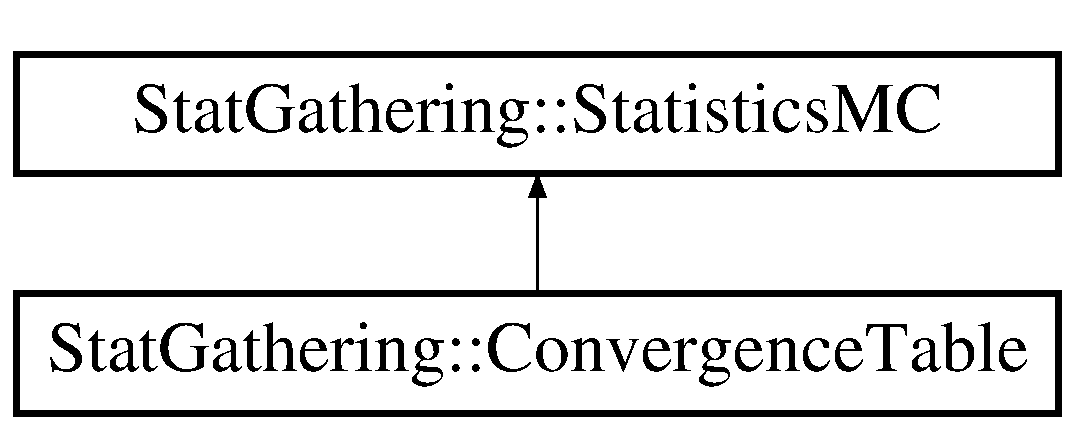
\includegraphics[height=2cm]{classStatGathering_1_1ConvergenceTable}
\end{center}
\end{figure}
\subsection*{Public Member Functions}
\begin{CompactItemize}
\item 
{\bf ConvergenceTable} (const {\bf Wrapper}$<$ {\bf StatisticsMC} $>$ \&Inner\_\-)
\item 
virtual {\bf StatisticsMC} $\ast$ {\bf clone} () const 
\begin{CompactList}\small\item\em clone method, to interface with the 'Wrapper' template \item\end{CompactList}\item 
virtual void {\bf AddOneResult} (double result)
\item 
virtual void {\bf AddOneSetOfResults} (long Number\_\-, std::vector$<$ std::vector$<$ double $>$ $>$ \&ResultsSoFar\_\-)
\begin{CompactList}\small\item\em Add in a set of results. \item\end{CompactList}\item 
virtual void {\bf Reset} ()
\begin{CompactList}\small\item\em Reset to an empty table. \item\end{CompactList}\item 
virtual void {\bf SetResultsSoFar} (long Number\_\-, std::vector$<$ std::vector$<$ double $>$ $>$ \&ResultsSoFar\_\-)
\begin{CompactList}\small\item\em Pass in the results of a simulation so far, one final set. \item\end{CompactList}\item 
virtual std::vector$<$ std::vector$<$ double $>$ $>$ {\bf GetResultsSoFar} () const 
\end{CompactItemize}
\subsection*{Private Member Functions}
\begin{CompactItemize}
\item 
void {\bf GetResultsFromInner} (std::vector$<$ std::vector$<$ double $>$ $>$ \&results\_\-) const 
\end{CompactItemize}
\subsection*{Private Attributes}
\begin{CompactItemize}
\item 
{\bf Wrapper}$<$ {\bf StatisticsMC} $>$ {\bf Inner}
\item 
std::vector$<$ std::vector$<$ double $>$ $>$ {\bf ResultsSoFar}
\item 
long {\bf StoppingPoint}
\begin{CompactList}\small\item\em The next point at which we need to ask for the results from the inner, and then store them. \item\end{CompactList}\item 
long {\bf PathsDone}
\begin{CompactList}\small\item\em Number of points evaluated so far (also stored in the 'Inner'). \item\end{CompactList}\item 
long {\bf Increment}
\begin{CompactList}\small\item\em The power at which we want to store results (eg at 2,4,8,16 ... or 10,100,1000 ...). \item\end{CompactList}\item 
long {\bf MaxSets}
\begin{CompactList}\small\item\em The maximum number of sets to record to file at the end. \item\end{CompactList}\end{CompactItemize}
\subsection*{Friends}
\begin{CompactItemize}
\item 
std::ostream \& {\bf operator$<$$<$} (std::ostream \&out, const {\bf ConvergenceTable} \&conTab)
\begin{CompactList}\small\item\em friend to $<$$<$ so that we can overload the $<$$<$ operator to output a \doxyref{ConvergenceTable}{p.}{classStatGathering_1_1ConvergenceTable} object \item\end{CompactList}\item 
std::istream \& {\bf operator$>$$>$} (std::istream \&in, {\bf ConvergenceTable} \&conTab)
\end{CompactItemize}


\subsection{Detailed Description}
An implementation of a statistics gatherer, that keeps track of the results given in powers of (Increment) It provides the final mean, standard deviation, and also the mean and sd at any power of (Increment) below the final result 

Definition at line 15 of file convergencetable.h.

\subsection{Constructor \& Destructor Documentation}
\index{StatGathering::ConvergenceTable@{StatGathering::ConvergenceTable}!ConvergenceTable@{ConvergenceTable}}
\index{ConvergenceTable@{ConvergenceTable}!StatGathering::ConvergenceTable@{StatGathering::ConvergenceTable}}
\subsubsection{\setlength{\rightskip}{0pt plus 5cm}StatGathering::ConvergenceTable::ConvergenceTable (const {\bf Wrapper}$<$ {\bf StatisticsMC} $>$ \& {\em Inner\_\-})}\label{classStatGathering_1_1ConvergenceTable_9e6e817e63d3f7aa6f9e8c15fd914337}




Definition at line 12 of file convergencetable.cpp.

References Increment, MaxSets, and StoppingPoint.

Referenced by clone().

\begin{Code}\begin{verbatim}13  : Inner( Inner_ ), PathsDone( 0 )
14 {
15   // Use a convenient set of defaults
16   Increment = 2;
17   StoppingPoint = Increment;
18   MaxSets = 20;
19 }
\end{verbatim}
\end{Code}




\subsection{Member Function Documentation}
\index{StatGathering::ConvergenceTable@{StatGathering::ConvergenceTable}!clone@{clone}}
\index{clone@{clone}!StatGathering::ConvergenceTable@{StatGathering::ConvergenceTable}}
\subsubsection{\setlength{\rightskip}{0pt plus 5cm}{\bf StatisticsMC} $\ast$ StatGathering::ConvergenceTable::clone () const\hspace{0.3cm}{\tt  [virtual]}}\label{classStatGathering_1_1ConvergenceTable_739be407fb8c781a3db471d28f25ba78}


clone method, to interface with the 'Wrapper' template 



Implements {\bf StatGathering::StatisticsMC} \doxyref{}{p.}{classStatGathering_1_1StatisticsMC_cfcf6abd6e973c00e5f31a79496233e0}.

Definition at line 21 of file convergencetable.cpp.

References ConvergenceTable().

\begin{Code}\begin{verbatim}22 {
23   return new ConvergenceTable( *this );
24 }
\end{verbatim}
\end{Code}


\index{StatGathering::ConvergenceTable@{StatGathering::ConvergenceTable}!AddOneResult@{AddOneResult}}
\index{AddOneResult@{AddOneResult}!StatGathering::ConvergenceTable@{StatGathering::ConvergenceTable}}
\subsubsection{\setlength{\rightskip}{0pt plus 5cm}void StatGathering::ConvergenceTable::AddOneResult (double {\em result})\hspace{0.3cm}{\tt  [virtual]}}\label{classStatGathering_1_1ConvergenceTable_8dfcddda38ea9657e1ae4aa6b917ff8b}


Add one result. Passes along that result to the inner, if we have hit 'StoppingPoint' then ask for the mean and sd from inner, and store in our array 

Implements {\bf StatGathering::StatisticsMC} \doxyref{}{p.}{classStatGathering_1_1StatisticsMC_aac13c0a41a374bec47c67afc59a0182}.

Definition at line 42 of file convergencetable.cpp.

References GetResultsFromInner(), Increment, Inner, PathsDone, ResultsSoFar, and StoppingPoint.

\begin{Code}\begin{verbatim}43 {
44   // Get the work done by the 'Inner' statistics gatherer
45   Inner->AddOneResult( result );
46   ++PathsDone;
47 
48   // If we have hit a power of Increment, we ask the 'Inner' for the results so far,
49   // and add it to our array (along with the number of points that contributed to that result)
50   if (PathsDone == StoppingPoint)
51   {
52     StoppingPoint *= Increment;
53     GetResultsFromInner( ResultsSoFar );
54   }
55 }
\end{verbatim}
\end{Code}


\index{StatGathering::ConvergenceTable@{StatGathering::ConvergenceTable}!AddOneSetOfResults@{AddOneSetOfResults}}
\index{AddOneSetOfResults@{AddOneSetOfResults}!StatGathering::ConvergenceTable@{StatGathering::ConvergenceTable}}
\subsubsection{\setlength{\rightskip}{0pt plus 5cm}void StatGathering::ConvergenceTable::AddOneSetOfResults (long {\em Number\_\-}, std::vector$<$ std::vector$<$ double $>$ $>$ \& {\em ResultsSoFar\_\-})\hspace{0.3cm}{\tt  [virtual]}}\label{classStatGathering_1_1ConvergenceTable_32d89dcbeedf1846f36319d9b36eafba}


Add in a set of results. 



Implements {\bf StatGathering::StatisticsMC} \doxyref{}{p.}{classStatGathering_1_1StatisticsMC_3f706f03424b931973415b8723127cad}.

Definition at line 58 of file convergencetable.cpp.

References SwUtils::\_\-FindNextPowerOfTwo(), GetResultsFromInner(), Increment, Inner, PathsDone, ResultsSoFar, and StoppingPoint.

\begin{Code}\begin{verbatim}60 {
61   // If this sends us past the next StoppingPoint, then store current results
62   // as long as we haven't just added the results, and we're not at zero
63   // (note: this is ResultsSoFar, not ResultsSoFar_)
64   if ( PathsDone + Number_ >= StoppingPoint && 
65        PathsDone*Increment != StoppingPoint && 
66        PathsDone != 0 )
67     GetResultsFromInner( ResultsSoFar );
68 
69   // Now, pass on this set to the inner statistics gatherer
70   Inner->AddOneSetOfResults( Number_, ResultsSoFar_ );
71   // Set our total number of points
72   PathsDone += Number_;
73   StoppingPoint = _FindNextPowerOfTwo( PathsDone );
74 
75   GetResultsFromInner( ResultsSoFar );
76 }
\end{verbatim}
\end{Code}


\index{StatGathering::ConvergenceTable@{StatGathering::ConvergenceTable}!Reset@{Reset}}
\index{Reset@{Reset}!StatGathering::ConvergenceTable@{StatGathering::ConvergenceTable}}
\subsubsection{\setlength{\rightskip}{0pt plus 5cm}void StatGathering::ConvergenceTable::Reset ()\hspace{0.3cm}{\tt  [virtual]}}\label{classStatGathering_1_1ConvergenceTable_7bb5a965ab53ca72d501e0d7f694d93b}


Reset to an empty table. 



Implements {\bf StatGathering::StatisticsMC} \doxyref{}{p.}{classStatGathering_1_1StatisticsMC_43259c270bbf6b23620252f11a155812}.

Definition at line 78 of file convergencetable.cpp.

References Increment, Inner, PathsDone, ResultsSoFar, and StoppingPoint.

\begin{Code}\begin{verbatim}79 {
80   // Pass on the order to the inner
81   Inner->Reset();
82   // Set our results to zero
83   PathsDone = 0;
84   StoppingPoint = Increment;
85   ResultsSoFar.clear();
86 }
\end{verbatim}
\end{Code}


\index{StatGathering::ConvergenceTable@{StatGathering::ConvergenceTable}!SetResultsSoFar@{SetResultsSoFar}}
\index{SetResultsSoFar@{SetResultsSoFar}!StatGathering::ConvergenceTable@{StatGathering::ConvergenceTable}}
\subsubsection{\setlength{\rightskip}{0pt plus 5cm}void StatGathering::ConvergenceTable::SetResultsSoFar (long {\em Number\_\-}, std::vector$<$ std::vector$<$ double $>$ $>$ \& {\em ResultsSoFar\_\-})\hspace{0.3cm}{\tt  [virtual]}}\label{classStatGathering_1_1ConvergenceTable_84375f0e4ec9925ae1c0575ac3d15075}


Pass in the results of a simulation so far, one final set. 



Implements {\bf StatGathering::StatisticsMC} \doxyref{}{p.}{classStatGathering_1_1StatisticsMC_b97a4292be61cff81425390f1fbed69c}.

Definition at line 88 of file convergencetable.cpp.

References SwUtils::\_\-FindNextPowerOfTwo(), GetResultsFromInner(), Inner, PathsDone, ResultsSoFar, and StoppingPoint.

\begin{Code}\begin{verbatim}90 {
91   // Pass on the results to the inner
92   Inner->SetResultsSoFar( Number_, ResultsSoFar_ );
93   // Set out total number of points
94   PathsDone = Number_;
95   // Set the next stopping point at which to record to the convergence table
96   StoppingPoint = _FindNextPowerOfTwo( PathsDone );
97   // Add this current point to our convergence table
98   GetResultsFromInner( ResultsSoFar );
99 }
\end{verbatim}
\end{Code}


\index{StatGathering::ConvergenceTable@{StatGathering::ConvergenceTable}!GetResultsSoFar@{GetResultsSoFar}}
\index{GetResultsSoFar@{GetResultsSoFar}!StatGathering::ConvergenceTable@{StatGathering::ConvergenceTable}}
\subsubsection{\setlength{\rightskip}{0pt plus 5cm}std::vector$<$ std::vector$<$ double $>$ $>$ StatGathering::ConvergenceTable::GetResultsSoFar () const\hspace{0.3cm}{\tt  [virtual]}}\label{classStatGathering_1_1ConvergenceTable_6cd7612fa109159ae022555ae84e5819}


Get a 2D vector of all our results so far \begin{Desc}
\item[Returns:]2D vector, formatted as for Inner, for all the powers of increment passed, and one for where we are now, in ascending order of number \end{Desc}


Implements {\bf StatGathering::StatisticsMC} \doxyref{}{p.}{classStatGathering_1_1StatisticsMC_ddb9cc20ac28892097e902286c5204bb}.

Definition at line 101 of file convergencetable.cpp.

References GetResultsFromInner(), Increment, PathsDone, ResultsSoFar, and StoppingPoint.

Referenced by StatGathering::operator$<$$<$().

\begin{Code}\begin{verbatim}102 {
103   // Start with the results given so far
104   std::vector<std::vector<double> > tmp( ResultsSoFar );
105 
106   // and now add in the current result from the inner object,
107   // If we have just hit a power of increment, the result now is identical
108   // with that in the last entry in ResultsSoFar, so we don't have
109   // to add this extra point.
110   if ( (PathsDone*Increment) != StoppingPoint )
111   {
112     GetResultsFromInner( tmp );
113   }
114   
115   // So now we have a vector of (mean, sd, number) for powers of increment, and the final total
116   return tmp;
117 }
\end{verbatim}
\end{Code}


\index{StatGathering::ConvergenceTable@{StatGathering::ConvergenceTable}!GetResultsFromInner@{GetResultsFromInner}}
\index{GetResultsFromInner@{GetResultsFromInner}!StatGathering::ConvergenceTable@{StatGathering::ConvergenceTable}}
\subsubsection{\setlength{\rightskip}{0pt plus 5cm}void StatGathering::ConvergenceTable::GetResultsFromInner (std::vector$<$ std::vector$<$ double $>$ $>$ \& {\em results\_\-}) const\hspace{0.3cm}{\tt  [private]}}\label{classStatGathering_1_1ConvergenceTable_be81ff228ef56cf0e81715385bd46527}


Ask the inner for a set of results, add it to the end of results\_\- 

Definition at line 26 of file convergencetable.cpp.

References Inner, and PathsDone.

Referenced by AddOneResult(), AddOneSetOfResults(), GetResultsSoFar(), and SetResultsSoFar().

\begin{Code}\begin{verbatim}27 {
28   // Get the 2D vector of results from the inner
29   // For a StatisticsMean, this is just a 1D vector, but allow for arbitrary
30   // 2D size
31   std::vector<std::vector<double> > thisResult( Inner->GetResultsSoFar() );
32 
33   // Iterate over all the rows of the returned result, store them in order
34   // at the end of the supplied table, along with the PathsDone
35   for (unsigned long i=0; i<thisResult.size(); i++)
36   {
37     thisResult[i].push_back(PathsDone);
38     results_.push_back(thisResult[i]);
39   }
40 }
\end{verbatim}
\end{Code}




\subsection{Friends And Related Function Documentation}
\index{StatGathering::ConvergenceTable@{StatGathering::ConvergenceTable}!operator<<@{operator$<$$<$}}
\index{operator<<@{operator$<$$<$}!StatGathering::ConvergenceTable@{StatGathering::ConvergenceTable}}
\subsubsection{\setlength{\rightskip}{0pt plus 5cm}std::ostream\& operator$<$$<$ (std::ostream \& {\em out}, const {\bf ConvergenceTable} \& {\em conTab})\hspace{0.3cm}{\tt  [friend]}}\label{classStatGathering_1_1ConvergenceTable_2d5efbc6918bef1b0bd6d83011daad1e}


friend to $<$$<$ so that we can overload the $<$$<$ operator to output a \doxyref{ConvergenceTable}{p.}{classStatGathering_1_1ConvergenceTable} object 

Outputs the table to the stream in the format: \char`\"{}Mean SD Number\char`\"{} for each of the powers of Increment passed so far, in reverse order (ie the final answer comes first, works down to smaller numbers) 

Definition at line 121 of file convergencetable.cpp.

\begin{Code}\begin{verbatim}122 {
123   // First, send the Inner to the stream
124   out << *( static_cast<const StatisticsMean*> ( conTab.Inner.GetConstPointer() ) );
125 
126   // Now, send the convergence table to the stream
127   // One entry of this will duplicate the current state of the inner.
128   // First, a separator
129   out << " ,";
130 
131   // Get all the results from the convergence table
132   std::vector<std::vector<double> > thisResult( conTab.GetResultsSoFar() );
133   // What is the length of the array of results?
134   long len = thisResult.size();
135   // How many results are we going to write to the file?
136   long imax; ( len > conTab.MaxSets ) ? imax = conTab.MaxSets : imax = len;
137   
138   // Now, print them to the stream
139   out << " " << imax;
140 
141   long jmax;
142   for ( long i=len-imax; i<len; ++i )
143   {
144     jmax = thisResult[i].size();
145     out << " " << jmax;
146     for ( long j=0; j<jmax; ++j )
147       out << " " << thisResult[i][j];
148   }
149 
150   return ( out );
151 }
\end{verbatim}
\end{Code}


\index{StatGathering::ConvergenceTable@{StatGathering::ConvergenceTable}!operator>>@{operator$>$$>$}}
\index{operator>>@{operator$>$$>$}!StatGathering::ConvergenceTable@{StatGathering::ConvergenceTable}}
\subsubsection{\setlength{\rightskip}{0pt plus 5cm}std::istream\& operator$>$$>$ (std::istream \& {\em in}, {\bf ConvergenceTable} \& {\em conTab})\hspace{0.3cm}{\tt  [friend]}}\label{classStatGathering_1_1ConvergenceTable_24b99d2e5129dc075e2488e32e250b92}




Definition at line 154 of file convergencetable.cpp.

\begin{Code}\begin{verbatim}155 {
156   // First, read in the Inner
157   in >> *( static_cast<StatisticsMean*> ( conTab.Inner.GetPointer() ) );
158 
159   // Now, restore the state of the convergence table
160   // First, the separator
161   std::string strTmp;
162   in >> strTmp;
163 
164   std::vector<std::vector<double> > theResults;
165   long len;
166 
167   // First, get the number of results that the convergence table is holding
168   in >> len;
169   theResults.resize( len );
170 
171   long jmax;
172   // Now, iterate through each set
173   for ( long i=0; i<len; ++i )
174   {
175     in >> jmax;
176     theResults[i].resize( jmax );
177     for ( long j=0; j<jmax; ++j )
178       in >> theResults[i][j];
179   }
180 
181   conTab.ResultsSoFar = theResults;
182 
183   return ( in );
184 }
\end{verbatim}
\end{Code}




\subsection{Member Data Documentation}
\index{StatGathering::ConvergenceTable@{StatGathering::ConvergenceTable}!Inner@{Inner}}
\index{Inner@{Inner}!StatGathering::ConvergenceTable@{StatGathering::ConvergenceTable}}
\subsubsection{\setlength{\rightskip}{0pt plus 5cm}{\bf Wrapper}$<${\bf StatisticsMC}$>$ {\bf StatGathering::ConvergenceTable::Inner}\hspace{0.3cm}{\tt  [private]}}\label{classStatGathering_1_1ConvergenceTable_b99be7bacbf89cba47df756ed0d812ed}


The 'Inner' does the calculating from point to point, then passes up the information to the convergence table when asked - in the function GetResultsFromInner 

Definition at line 51 of file convergencetable.h.

Referenced by AddOneResult(), AddOneSetOfResults(), GetResultsFromInner(), StatGathering::operator$<$$<$(), StatGathering::operator$>$$>$(), Reset(), and SetResultsSoFar().\index{StatGathering::ConvergenceTable@{StatGathering::ConvergenceTable}!ResultsSoFar@{ResultsSoFar}}
\index{ResultsSoFar@{ResultsSoFar}!StatGathering::ConvergenceTable@{StatGathering::ConvergenceTable}}
\subsubsection{\setlength{\rightskip}{0pt plus 5cm}std::vector$<$std::vector$<$double$>$ $>$ {\bf StatGathering::ConvergenceTable::ResultsSoFar}\hspace{0.3cm}{\tt  [private]}}\label{classStatGathering_1_1ConvergenceTable_dcdd069c71f99f821810c271b59f637d}


Our 2D vector of results so far for each power of increment that we have passed, where number is the number of points that contributed (ie increment$^\wedge$n). The specific format of this vector depends on the type of \doxyref{StatisticsMC}{p.}{classStatGathering_1_1StatisticsMC} used. 

Definition at line 56 of file convergencetable.h.

Referenced by AddOneResult(), AddOneSetOfResults(), GetResultsSoFar(), StatGathering::operator$>$$>$(), Reset(), and SetResultsSoFar().\index{StatGathering::ConvergenceTable@{StatGathering::ConvergenceTable}!StoppingPoint@{StoppingPoint}}
\index{StoppingPoint@{StoppingPoint}!StatGathering::ConvergenceTable@{StatGathering::ConvergenceTable}}
\subsubsection{\setlength{\rightskip}{0pt plus 5cm}long {\bf StatGathering::ConvergenceTable::StoppingPoint}\hspace{0.3cm}{\tt  [private]}}\label{classStatGathering_1_1ConvergenceTable_90012c27fa1734458e737f292600115a}


The next point at which we need to ask for the results from the inner, and then store them. 



Definition at line 58 of file convergencetable.h.

Referenced by AddOneResult(), AddOneSetOfResults(), ConvergenceTable(), GetResultsSoFar(), Reset(), and SetResultsSoFar().\index{StatGathering::ConvergenceTable@{StatGathering::ConvergenceTable}!PathsDone@{PathsDone}}
\index{PathsDone@{PathsDone}!StatGathering::ConvergenceTable@{StatGathering::ConvergenceTable}}
\subsubsection{\setlength{\rightskip}{0pt plus 5cm}long {\bf StatGathering::ConvergenceTable::PathsDone}\hspace{0.3cm}{\tt  [private]}}\label{classStatGathering_1_1ConvergenceTable_ecfb1eeb45ff9c726869a9de5547c4e8}


Number of points evaluated so far (also stored in the 'Inner'). 



Definition at line 60 of file convergencetable.h.

Referenced by AddOneResult(), AddOneSetOfResults(), GetResultsFromInner(), GetResultsSoFar(), Reset(), and SetResultsSoFar().\index{StatGathering::ConvergenceTable@{StatGathering::ConvergenceTable}!Increment@{Increment}}
\index{Increment@{Increment}!StatGathering::ConvergenceTable@{StatGathering::ConvergenceTable}}
\subsubsection{\setlength{\rightskip}{0pt plus 5cm}long {\bf StatGathering::ConvergenceTable::Increment}\hspace{0.3cm}{\tt  [private]}}\label{classStatGathering_1_1ConvergenceTable_49a83cf3a77bdcb17a2fa7cb46c58e41}


The power at which we want to store results (eg at 2,4,8,16 ... or 10,100,1000 ...). 



Definition at line 62 of file convergencetable.h.

Referenced by AddOneResult(), AddOneSetOfResults(), ConvergenceTable(), GetResultsSoFar(), and Reset().\index{StatGathering::ConvergenceTable@{StatGathering::ConvergenceTable}!MaxSets@{MaxSets}}
\index{MaxSets@{MaxSets}!StatGathering::ConvergenceTable@{StatGathering::ConvergenceTable}}
\subsubsection{\setlength{\rightskip}{0pt plus 5cm}long {\bf StatGathering::ConvergenceTable::MaxSets}\hspace{0.3cm}{\tt  [private]}}\label{classStatGathering_1_1ConvergenceTable_ef826049ffb2f090e32ce4fc9ef938d6}


The maximum number of sets to record to file at the end. 



Definition at line 64 of file convergencetable.h.

Referenced by ConvergenceTable(), and StatGathering::operator$<$$<$().

The documentation for this class was generated from the following files:\begin{CompactItemize}
\item 
Gyulassy/opacity3/src/store2d/{\bf convergencetable.h}\item 
Gyulassy/opacity3/src/store2d/{\bf convergencetable.cpp}\end{CompactItemize}

\section{Driver$<$ TcalcEngine, Tstore, numOfRandoms $>$ Class Template Reference}
\label{classDriver}\index{Driver@{Driver}}
{\tt \#include $<$driver.h$>$}

\subsection*{Public Member Functions}
\begin{CompactItemize}
\item 
{\bf Driver} ()
\item 
{\bf $\sim$Driver} ()
\item 
int {\bf Setup} (std::string resume, std::string inputFile)
\item 
void {\bf SetParameters} ({\bf Parameters} \&{\bf myParameters})
\begin{CompactList}\small\item\em Read any runtime parameters for the \doxyref{Driver}{p.}{classDriver} object from the \doxyref{Parameters}{p.}{classParameters} object. \item\end{CompactList}\item 
void {\bf RunOneIteration} ()
\begin{CompactList}\small\item\em Run a single iteration of the monte carlo simulation. \item\end{CompactList}\item 
void {\bf SaveResults} (std::string outputFile)
\begin{CompactList}\small\item\em Save the stored results to a file. \item\end{CompactList}\end{CompactItemize}
\subsection*{Private Attributes}
\begin{CompactItemize}
\item 
TcalcEngine {\bf calculator}
\begin{CompactList}\small\item\em Supplied template parameter type, to perform the calculation. \item\end{CompactList}\item 
Tstore {\bf storage}
\begin{CompactList}\small\item\em Supplied template parameter type, to store the results of the calculation. \item\end{CompactList}\item 
{\bf Parameters} {\bf myParameters}
\begin{CompactList}\small\item\em Object to read runtime parameters from file, supplied to calculation and storage. \item\end{CompactList}\item 
{\bf Wrapper}$<$ {\bf SwRandoms::RandomBase2} $>$ {\bf randomGenerator}
\begin{CompactList}\small\item\em Random number generator, on the interval [0,1). \item\end{CompactList}\end{CompactItemize}


\subsection{Detailed Description}
\subsubsection*{template$<$typename TcalcEngine, typename Tstore, std::size\_\-t numOfRandoms$>$ class Driver$<$ TcalcEngine, Tstore, numOfRandoms $>$}

\begin{Desc}
\item[Author:]Simon Wicks $<${\tt simonw@phys.columbia.edu}$>$ A generic driver for a Monte Carlo calculation At run time, different random number generator can be used: for example pseudorandoms such as standard drand48(); quasirandoms such as \doxyref{Sobol}{p.}{namespaceSobol} sequences (the latter can vastly increase the rate of convergence of Monte Carlo integration).\end{Desc}
Template parameters: TcalcEngine, Tstore, numOfRandoms TcalcEngine is an object that performs the calculation, with the interface .SetParameters( Parameters inParams ) .SetRandoms( boost::array$<$numOfRandoms$>$ randomNumbers ) .SetCoord( long coord, double value ) .GetAnswer( std::vector answers ) Tstore is an object in which to keep the results, with the interface .SetParameters( Parameters inParams ) .AddPoint( long dim1, long dim2, std::vector$<$double$>$ result ) .WriteToFile( std::string filename, bool appendToFile ) numOfRandoms is the number of random numbers to be used in the simulation

TODO: add the number of dimensions of the result as a template parameter, generalize the iteration over deterministic dimensions to be n-dimensional add this number of deterministic dimensions as a template parameter

TODO: add multithreading, so that multiple calculation engines can be run in parallel while adding into the same data store 

Definition at line 47 of file driver.h.

\subsection{Constructor \& Destructor Documentation}
\index{Driver@{Driver}!Driver@{Driver}}
\index{Driver@{Driver}!Driver@{Driver}}
\subsubsection{\setlength{\rightskip}{0pt plus 5cm}template$<$typename TcalcEngine, typename Tstore, std::size\_\-t numOfRandoms$>$ {\bf Driver}$<$ TcalcEngine, Tstore, numOfRandoms $>$::{\bf Driver} ()\hspace{0.3cm}{\tt  [inline]}}\label{classDriver_d18a1349226d25296a188e371debec56}




Definition at line 77 of file driver.h.

\begin{Code}\begin{verbatim}78   : myParameters( "Opacity3" )
79 {
80   // Nothing to do on creation, most setup done by the Setup() function
81   // so that errors on setup can be understood
82 
83   // The only thing is the constructor of myParameters,
84   // to tell it that the version of this program is Opacity version 3
85   // TODO: make the 'Opacity3' section describe all necessary parts of the program
86   // for a compatible read in / out
87 }
\end{verbatim}
\end{Code}


\index{Driver@{Driver}!~Driver@{$\sim$Driver}}
\index{~Driver@{$\sim$Driver}!Driver@{Driver}}
\subsubsection{\setlength{\rightskip}{0pt plus 5cm}template$<$typename TcalcEngine, typename Tstore, std::size\_\-t numOfRandoms$>$ {\bf Driver}$<$ TcalcEngine, Tstore, numOfRandoms $>$::$\sim${\bf Driver} ()\hspace{0.3cm}{\tt  [inline]}}\label{classDriver_322d8366a3a84a1539d1eb37fad8d3a8}




Definition at line 90 of file driver.h.

\begin{Code}\begin{verbatim}91 {
92   // Nothing to do in the destructor
93 }
\end{verbatim}
\end{Code}




\subsection{Member Function Documentation}
\index{Driver@{Driver}!Setup@{Setup}}
\index{Setup@{Setup}!Driver@{Driver}}
\subsubsection{\setlength{\rightskip}{0pt plus 5cm}template$<$typename TcalcEngine, typename Tstore, std::size\_\-t numOfRandoms$>$ int {\bf Driver}$<$ TcalcEngine, Tstore, numOfRandoms $>$::Setup (std::string {\em resume}, std::string {\em inputFile})\hspace{0.3cm}{\tt  [inline]}}\label{classDriver_ddb8501bd4ed2a87dfb62d8ed73015fa}


Setup routine - read in runtime parameters, set up all objects as necessary  =\char`\"{}y\char`\"{} to resume from a previous run, =\char`\"{}n\char`\"{} to start a new one  Filename of a) previous run file if resuming (including runtime parameters on the end), or b) runtime parameters file if not resuming 

Definition at line 96 of file driver.h.

References Driver$<$ TcalcEngine, Tstore, numOfRandoms $>$::calculator, Parameters::CheckForUnaccessedParameters(), Driver$<$ TcalcEngine, Tstore, numOfRandoms $>$::myParameters, Parameters::ParseInputFile(), Driver$<$ TcalcEngine, Tstore, numOfRandoms $>$::SetParameters(), and Driver$<$ TcalcEngine, Tstore, numOfRandoms $>$::storage.

\begin{Code}\begin{verbatim}97 {
98   // Function to do all necessary run time setup of objects
99   // TODO: give a meaningful return code, so if this fails the program quits
100 
101   // The runtime settings are read in from a file with a specific format
102   // This format is governed by the 'Parameters' object, see there for specifics
103 
104   // First, read in the file into the object
105   // If we are resuming from a previous run, the parameters have been written to the
106   // end of the file, and the Parameters objects can find them there
107   // All the tokens in the file are read into a 'map'
108   myParameters.ParseInputFile( inputFile );
109 
110   // Pass the parameters object to each object in turn
111   // First, this one, the driver
112   SetParameters( myParameters );
113   // Second, the storage object - eg for size of each dimensions, number of points etc 
114   storage.SetParameters( myParameters );
115   // Third, the calculation object - eg GLV specific params, mu, temperature etc
116   calculator.SetParameters( myParameters );
117 
118   // If we are resuming from a previous run, we also need to read in the statistics
119   // from that run into the data store
120   if ( resume == "y" )
121     storage.ReadFromFile( inputFile );
122 
123   // Finally, check that all the inputs from the parameters file were used at some point
124   // Otherwise, the user might think that some parameters are being set that really aren't
125   int allUsed = myParameters.CheckForUnaccessedParameters();
126   if ( allUsed != 0 )
127   {
128     std::cerr << "Driver::Setup - " << allUsed << " unused parameters from input file.\n";
129     return 1;
130   }
131   else
132   {
133     std::cout << "All parameters read successfully from " << inputFile << std::endl;
134   }
135 
136   // TODO: change this so that more errors are detected and so more possible to not
137   // return 0
138   return 0;
139 }
\end{verbatim}
\end{Code}


\index{Driver@{Driver}!SetParameters@{SetParameters}}
\index{SetParameters@{SetParameters}!Driver@{Driver}}
\subsubsection{\setlength{\rightskip}{0pt plus 5cm}template$<$typename TcalcEngine, typename Tstore, std::size\_\-t numOfRandoms$>$ void {\bf Driver}$<$ TcalcEngine, Tstore, numOfRandoms $>$::SetParameters ({\bf Parameters} \& {\em myParameters})\hspace{0.3cm}{\tt  [inline]}}\label{classDriver_366cc8aecd5b57886f9443a2cfedf0dc}


Read any runtime parameters for the \doxyref{Driver}{p.}{classDriver} object from the \doxyref{Parameters}{p.}{classParameters} object. 



Definition at line 142 of file driver.h.

References Parameters::GetParametersString(), and Driver$<$ TcalcEngine, Tstore, numOfRandoms $>$::randomGenerator.

Referenced by Driver$<$ TcalcEngine, Tstore, numOfRandoms $>$::Setup().

\begin{Code}\begin{verbatim}143 {
144   // Do specific setup for this driver object
145   // The only settings necessary are for the random number generator
146   // TODO: clean up the 'Parameters' object, so this doesn't look so convoluted
147 
148   std::list<std::string> ReturnedParamsString;
149   
150   // The type of random number generator
151   // Current options are 'Drand48' and 'Sobol'
152   ReturnedParamsString.empty();
153   ReturnedParamsString = MyParameters.GetParametersString( "@RandomNumberGenerator" );
154   
155   SwRandoms::RandDrand48 ranDrand48( numOfRandoms );
156   SwRandoms::RandSobol ranSobol( numOfRandoms );
157 
158   if ( ReturnedParamsString.front() == "Drand48" )
159     randomGenerator = ranDrand48;
160   else if ( ReturnedParamsString.front() == "Sobol" )
161     randomGenerator = ranSobol;
162   else
163   {
164     //return -1;
165   }
166 
167   // Now that we have set up the type of generator, we need a seed for the
168   // generator
169   // TODO: add this as an option to the Parameters object, including the time(NULL) option
170   //long seed = time(NULL);
171   long seed = 2;
172   randomGenerator->SetSeed( seed );
173 
174   //return 0;
175 }
\end{verbatim}
\end{Code}


\index{Driver@{Driver}!RunOneIteration@{RunOneIteration}}
\index{RunOneIteration@{RunOneIteration}!Driver@{Driver}}
\subsubsection{\setlength{\rightskip}{0pt plus 5cm}template$<$typename TcalcEngine, typename Tstore, std::size\_\-t numOfRandoms$>$ void {\bf Driver}$<$ TcalcEngine, Tstore, numOfRandoms $>$::RunOneIteration ()\hspace{0.3cm}{\tt  [inline]}}\label{classDriver_21ae3be3bfc08b9c7c41c4a7e46e7677}


Run a single iteration of the monte carlo simulation. 



Definition at line 178 of file driver.h.

References Driver$<$ TcalcEngine, Tstore, numOfRandoms $>$::calculator, Driver$<$ TcalcEngine, Tstore, numOfRandoms $>$::randomGenerator, and Driver$<$ TcalcEngine, Tstore, numOfRandoms $>$::storage.

\begin{Code}\begin{verbatim}179 {
180   // The guts of the Monte Carlo calculation
181   // For one iteration, we fetch in a set of random numbers,
182   // (these are supplied as a uniform distribution over [0,1)
183   // then pass this to the calculation object,
184   // (which will transform them to the required limits)
185   // then iterate over all the points in the deterministic dimensions,
186   // getting the calculation result for each point,
187   // and passing this result to the data store.
188   // TODO: generalize the iteration over deterministic dimensions to n-dimensions,
189   // with n chosen as a template parameter to the driver object
190 
191   // First, get the array of random numbers
192   // TODO: change the interface to the random number generator
193   // to ask / get a fixed size array using boost::array
194   // At the moment, the change from a boost::array to a std::vector (MyArray)
195   // is cumbersome / a hack
196   boost::array<double, numOfRandoms> randomNumbers;
197   SwArrays::MyArray randomNumbersTmp( numOfRandoms );
198   randomGenerator->GetUniforms( randomNumbersTmp );
199   for ( std::size_t i=0; i<numOfRandoms; ++i )
200     randomNumbers[i] = randomNumbersTmp[i];
201 
202   // Pass the random numbers to the calculator object
203   calculator.SetRandoms( randomNumbers );
204 
205   // Now iterate over the deterministic dimensions,
206   // setting the new coordinate for each point in each dimension,
207   // getting the answer and adding it to the data store
208   // TODO: improve, to have arbitrary number of dimensions
209   std::vector<double> tmp(1);
210   for (long dim1=0; dim1<storage.GetLengthDim1(); ++dim1)
211   {
212     calculator.SetCoord( 1, storage.GetCoordDim1( dim1 ) );
213 
214     for (long dim2=0; dim2<storage.GetLengthDim2(); ++dim2)
215     {
216       calculator.SetCoord( 2, storage.GetCoordDim2( dim2 ) );
217       calculator.GetAnswer( tmp );
218       storage.AddPoint( dim1, dim2, tmp );
219     }
220   }
221 }
\end{verbatim}
\end{Code}


\index{Driver@{Driver}!SaveResults@{SaveResults}}
\index{SaveResults@{SaveResults}!Driver@{Driver}}
\subsubsection{\setlength{\rightskip}{0pt plus 5cm}template$<$typename TcalcEngine, typename Tstore, std::size\_\-t numOfRandoms$>$ void {\bf Driver}$<$ TcalcEngine, Tstore, numOfRandoms $>$::SaveResults (std::string {\em outputFile})\hspace{0.3cm}{\tt  [inline]}}\label{classDriver_acef05750c91ea6786f9f1c9b711c765}


Save the stored results to a file. 



Definition at line 224 of file driver.h.

References Driver$<$ TcalcEngine, Tstore, numOfRandoms $>$::myParameters, Driver$<$ TcalcEngine, Tstore, numOfRandoms $>$::storage, and Parameters::WriteToFile().

\begin{Code}\begin{verbatim}225 {
226   // Save the results of our simulation to a permanent file
227   // We need to include the state of both the data store and
228   // the input runtime parameters
229 
230   // First, send the Store2D to file
231   // The false here => erase any current contents of the file
232   storage.WriteToFile( outputFile, false );
233 
234   // Now delegate to the params class to output the settings to the end of the file
235   // In this way, we have a record of what the inputs were, and a way to resume and
236   // add more statistics if wanted.
237   // The true here => append to file
238   myParameters.WriteToFile( outputFile, true );
239 }
\end{verbatim}
\end{Code}




\subsection{Member Data Documentation}
\index{Driver@{Driver}!calculator@{calculator}}
\index{calculator@{calculator}!Driver@{Driver}}
\subsubsection{\setlength{\rightskip}{0pt plus 5cm}template$<$typename TcalcEngine, typename Tstore, std::size\_\-t numOfRandoms$>$ TcalcEngine {\bf Driver}$<$ TcalcEngine, Tstore, numOfRandoms $>$::{\bf calculator}\hspace{0.3cm}{\tt  [private]}}\label{classDriver_b15978b3b6eedc1c9af063a970eb154a}


Supplied template parameter type, to perform the calculation. 



Definition at line 51 of file driver.h.

Referenced by Driver$<$ TcalcEngine, Tstore, numOfRandoms $>$::RunOneIteration(), and Driver$<$ TcalcEngine, Tstore, numOfRandoms $>$::Setup().\index{Driver@{Driver}!storage@{storage}}
\index{storage@{storage}!Driver@{Driver}}
\subsubsection{\setlength{\rightskip}{0pt plus 5cm}template$<$typename TcalcEngine, typename Tstore, std::size\_\-t numOfRandoms$>$ Tstore {\bf Driver}$<$ TcalcEngine, Tstore, numOfRandoms $>$::{\bf storage}\hspace{0.3cm}{\tt  [private]}}\label{classDriver_d52b9b085eb8b034d2548af7d7ea670e}


Supplied template parameter type, to store the results of the calculation. 



Definition at line 53 of file driver.h.

Referenced by Driver$<$ TcalcEngine, Tstore, numOfRandoms $>$::RunOneIteration(), Driver$<$ TcalcEngine, Tstore, numOfRandoms $>$::SaveResults(), and Driver$<$ TcalcEngine, Tstore, numOfRandoms $>$::Setup().\index{Driver@{Driver}!myParameters@{myParameters}}
\index{myParameters@{myParameters}!Driver@{Driver}}
\subsubsection{\setlength{\rightskip}{0pt plus 5cm}template$<$typename TcalcEngine, typename Tstore, std::size\_\-t numOfRandoms$>$ {\bf Parameters} {\bf Driver}$<$ TcalcEngine, Tstore, numOfRandoms $>$::{\bf myParameters}\hspace{0.3cm}{\tt  [private]}}\label{classDriver_c266e9eee42ebc4e2f39e16c94cec3ca}


Object to read runtime parameters from file, supplied to calculation and storage. 



Definition at line 55 of file driver.h.

Referenced by Driver$<$ TcalcEngine, Tstore, numOfRandoms $>$::SaveResults(), and Driver$<$ TcalcEngine, Tstore, numOfRandoms $>$::Setup().\index{Driver@{Driver}!randomGenerator@{randomGenerator}}
\index{randomGenerator@{randomGenerator}!Driver@{Driver}}
\subsubsection{\setlength{\rightskip}{0pt plus 5cm}template$<$typename TcalcEngine, typename Tstore, std::size\_\-t numOfRandoms$>$ {\bf Wrapper}$<${\bf SwRandoms::RandomBase2}$>$ {\bf Driver}$<$ TcalcEngine, Tstore, numOfRandoms $>$::{\bf randomGenerator}\hspace{0.3cm}{\tt  [private]}}\label{classDriver_4da27b778d9838012125868afd04c1ed}


Random number generator, on the interval [0,1). 



Definition at line 57 of file driver.h.

Referenced by Driver$<$ TcalcEngine, Tstore, numOfRandoms $>$::RunOneIteration(), and Driver$<$ TcalcEngine, Tstore, numOfRandoms $>$::SetParameters().

The documentation for this class was generated from the following file:\begin{CompactItemize}
\item 
Gyulassy/opacity3/src/{\bf driver.h}\end{CompactItemize}

\section{ExpDecayFunction Class Reference}
\label{classExpDecayFunction}\index{ExpDecayFunction@{ExpDecayFunction}}
{\tt \#include $<$Function.h$>$}

Inheritance diagram for ExpDecayFunction::\begin{figure}[H]
\begin{center}
\leavevmode
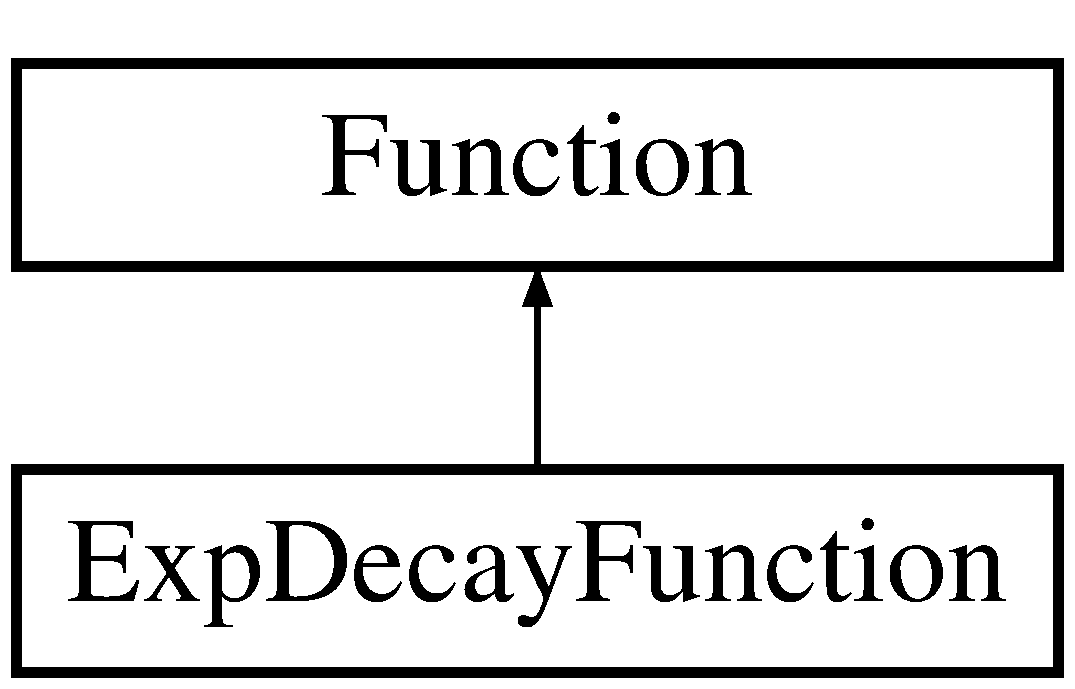
\includegraphics[height=2cm]{classExpDecayFunction}
\end{center}
\end{figure}
\subsection*{Public Member Functions}
\begin{CompactItemize}
\item 
{\bf ExpDecayFunction} (unsigned long Dimensionality)
\item 
virtual {\bf $\sim$ExpDecayFunction} ()
\item 
virtual {\bf Function} $\ast$ {\bf clone} () const 
\item 
virtual void {\bf function} (MyArray \&xs, MyArray \&res)
\item 
virtual void {\bf NormedIntegralInverse} (MyArray \&xs, MyArray \&res)
\item 
virtual void {\bf SetParams} (MyArray \&params\_\-)
\end{CompactItemize}
\subsection*{Private Attributes}
\begin{CompactItemize}
\item 
MyArray {\bf lambdas}
\end{CompactItemize}


\subsection{Detailed Description}


Definition at line 101 of file Function.h.

\subsection{Constructor \& Destructor Documentation}
\index{ExpDecayFunction@{ExpDecayFunction}!ExpDecayFunction@{ExpDecayFunction}}
\index{ExpDecayFunction@{ExpDecayFunction}!ExpDecayFunction@{ExpDecayFunction}}
\subsubsection{\setlength{\rightskip}{0pt plus 5cm}ExpDecayFunction::ExpDecayFunction (unsigned long {\em Dimensionality})}\label{classExpDecayFunction_4905fdca1777ecc6795372b6a4c88ef5}




Definition at line 144 of file Function.cpp.

Referenced by clone().

\begin{Code}\begin{verbatim}145   : Function( Dimensionality ), lambdas( Dimensionality )
146 {
147 
148 }
\end{verbatim}
\end{Code}


\index{ExpDecayFunction@{ExpDecayFunction}!~ExpDecayFunction@{$\sim$ExpDecayFunction}}
\index{~ExpDecayFunction@{$\sim$ExpDecayFunction}!ExpDecayFunction@{ExpDecayFunction}}
\subsubsection{\setlength{\rightskip}{0pt plus 5cm}ExpDecayFunction::$\sim$ExpDecayFunction ()\hspace{0.3cm}{\tt  [virtual]}}\label{classExpDecayFunction_8772fb3b5b7aeb29c294b78b32ffb88b}




Definition at line 150 of file Function.cpp.

\begin{Code}\begin{verbatim}151 {
152 
153 }
\end{verbatim}
\end{Code}




\subsection{Member Function Documentation}
\index{ExpDecayFunction@{ExpDecayFunction}!clone@{clone}}
\index{clone@{clone}!ExpDecayFunction@{ExpDecayFunction}}
\subsubsection{\setlength{\rightskip}{0pt plus 5cm}{\bf Function} $\ast$ ExpDecayFunction::clone () const\hspace{0.3cm}{\tt  [virtual]}}\label{classExpDecayFunction_8186f67946fc433087ac05d397d3a3ff}




Implements {\bf Function} \doxyref{}{p.}{classFunction_cae7bf3099d7e05b59814823dab252b2}.

Definition at line 155 of file Function.cpp.

References ExpDecayFunction().

\begin{Code}\begin{verbatim}156 {
157   return new ExpDecayFunction( *this );
158 }
\end{verbatim}
\end{Code}


\index{ExpDecayFunction@{ExpDecayFunction}!function@{function}}
\index{function@{function}!ExpDecayFunction@{ExpDecayFunction}}
\subsubsection{\setlength{\rightskip}{0pt plus 5cm}void ExpDecayFunction::function (MyArray \& {\em xs}, MyArray \& {\em res})\hspace{0.3cm}{\tt  [virtual]}}\label{classExpDecayFunction_0a6016e8146f03897300c728cd408347}




Implements {\bf Function} \doxyref{}{p.}{classFunction_a78440b1498d1b7e113b163dfc88274c}.

Definition at line 160 of file Function.cpp.

References Function::GetDimensionality(), Function::GetXmin(), and lambdas.

\begin{Code}\begin{verbatim}161 {
162   res[0] = 1. / lambdas[0] * exp( -((xs[0]-GetXmin(0)) / lambdas[0]) );
163   for (unsigned long i=1; i<GetDimensionality(); ++i)
164   {
165     res[i] = 1. / lambdas[i] * exp( -(xs[i] - xs[i-1]) / lambdas[i] );
166   }
167 }
\end{verbatim}
\end{Code}


\index{ExpDecayFunction@{ExpDecayFunction}!NormedIntegralInverse@{NormedIntegralInverse}}
\index{NormedIntegralInverse@{NormedIntegralInverse}!ExpDecayFunction@{ExpDecayFunction}}
\subsubsection{\setlength{\rightskip}{0pt plus 5cm}void ExpDecayFunction::NormedIntegralInverse (MyArray \& {\em xs}, MyArray \& {\em res})\hspace{0.3cm}{\tt  [virtual]}}\label{classExpDecayFunction_c9e70e87e699a4342869ab6c90aa5264}




Implements {\bf Function} \doxyref{}{p.}{classFunction_9e1a0a6468b4df5de365481db11df5d4}.

Definition at line 169 of file Function.cpp.

References Function::GetDimensionality(), Function::GetXmax(), Function::GetXmin(), and lambdas.

\begin{Code}\begin{verbatim}170 {
171   for (unsigned long i=0; i<GetDimensionality(); ++i)
172   {
173     xs[i] = (1.-uniforms[i])*exp(-GetXmin(i)/lambdas[i]) + uniforms[i]*exp(-GetXmax(i)/lambdas[i]);
174     xs[i] = -lambdas[i] * log( xs[i] );
175   }
176 }
\end{verbatim}
\end{Code}


\index{ExpDecayFunction@{ExpDecayFunction}!SetParams@{SetParams}}
\index{SetParams@{SetParams}!ExpDecayFunction@{ExpDecayFunction}}
\subsubsection{\setlength{\rightskip}{0pt plus 5cm}void ExpDecayFunction::SetParams (MyArray \& {\em params\_\-})\hspace{0.3cm}{\tt  [virtual]}}\label{classExpDecayFunction_d665a0ac0d156a9f058b1881d40f2f84}




Implements {\bf Function} \doxyref{}{p.}{classFunction_6944f24e3174d98fe7c61dc0652d3ae4}.

Definition at line 178 of file Function.cpp.

References lambdas.

Referenced by ZposGenerator::ZposGenerator().

\begin{Code}\begin{verbatim}179 {
180   lambdas = params_;
181 }
\end{verbatim}
\end{Code}




\subsection{Member Data Documentation}
\index{ExpDecayFunction@{ExpDecayFunction}!lambdas@{lambdas}}
\index{lambdas@{lambdas}!ExpDecayFunction@{ExpDecayFunction}}
\subsubsection{\setlength{\rightskip}{0pt plus 5cm}MyArray {\bf ExpDecayFunction::lambdas}\hspace{0.3cm}{\tt  [private]}}\label{classExpDecayFunction_9a6764a71c0ca67bd8f71f3af6017c40}




Definition at line 114 of file Function.h.

Referenced by function(), NormedIntegralInverse(), and SetParams().

The documentation for this class was generated from the following files:\begin{CompactItemize}
\item 
Gyulassy/opacity3/src/glv1/{\bf Function.h}\item 
Gyulassy/opacity3/src/glv1/{\bf Function.cpp}\end{CompactItemize}

\section{Function Class Reference}
\label{classFunction}\index{Function@{Function}}
{\tt \#include $<$Function.h$>$}

Inheritance diagram for Function::\begin{figure}[H]
\begin{center}
\leavevmode
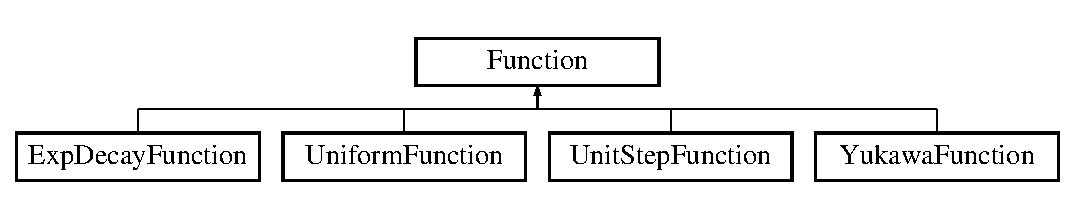
\includegraphics[height=2cm]{classFunction}
\end{center}
\end{figure}
\subsection*{Public Member Functions}
\begin{CompactItemize}
\item 
{\bf Function} (unsigned long Dimensionality)
\item 
virtual {\bf $\sim$Function} ()
\item 
virtual {\bf Function} $\ast$ {\bf clone} () const =0
\item 
virtual void {\bf function} (MyArray \&xs, MyArray \&res)=0
\item 
virtual void {\bf NormedIntegralInverse} (MyArray \&xs, MyArray \&res)=0
\item 
virtual void {\bf SetLimits} (MyArray \&xmins\_\-, MyArray \&xmaxs\_\-)
\item 
virtual void {\bf SetParams} (MyArray \&params\_\-)=0
\item 
unsigned long {\bf GetDimensionality} () const 
\item 
double {\bf GetXmin} (unsigned long i) const 
\item 
double {\bf GetXmax} (unsigned long i) const 
\item 
double {\bf GetRange} (unsigned long i) const 
\end{CompactItemize}
\subsection*{Private Attributes}
\begin{CompactItemize}
\item 
unsigned long {\bf dim}
\item 
MyArray {\bf xmins}
\item 
MyArray {\bf xmaxs}
\end{CompactItemize}


\subsection{Detailed Description}


Definition at line 8 of file Function.h.

\subsection{Constructor \& Destructor Documentation}
\index{Function@{Function}!Function@{Function}}
\index{Function@{Function}!Function@{Function}}
\subsubsection{\setlength{\rightskip}{0pt plus 5cm}Function::Function (unsigned long {\em Dimensionality})}\label{classFunction_0bc8fc78c9f9e9b2b646d6c3de75a9b1}




Definition at line 3 of file Function.cpp.

\begin{Code}\begin{verbatim}4   : dim( Dimensionality ), xmins( Dimensionality ), xmaxs( Dimensionality )
5 {
6 
7 }
\end{verbatim}
\end{Code}


\index{Function@{Function}!~Function@{$\sim$Function}}
\index{~Function@{$\sim$Function}!Function@{Function}}
\subsubsection{\setlength{\rightskip}{0pt plus 5cm}Function::$\sim$Function ()\hspace{0.3cm}{\tt  [virtual]}}\label{classFunction_3b03f7cf0b75d16edebdda1dee1db6fd}




Definition at line 9 of file Function.cpp.

\begin{Code}\begin{verbatim}10 {
11 
12 }
\end{verbatim}
\end{Code}




\subsection{Member Function Documentation}
\index{Function@{Function}!clone@{clone}}
\index{clone@{clone}!Function@{Function}}
\subsubsection{\setlength{\rightskip}{0pt plus 5cm}virtual {\bf Function}$\ast$ Function::clone () const\hspace{0.3cm}{\tt  [pure virtual]}}\label{classFunction_cae7bf3099d7e05b59814823dab252b2}




Implemented in {\bf YukawaFunction} \doxyref{}{p.}{classYukawaFunction_5f5caf1a5d9ccbbd111a72ce3961395e}, {\bf UniformFunction} \doxyref{}{p.}{classUniformFunction_9b57843688a438ac030f3abcfb4d07ac}, {\bf UnitStepFunction} \doxyref{}{p.}{classUnitStepFunction_c9575c66d4b1c47901fbb4d96065f93f}, and {\bf ExpDecayFunction} \doxyref{}{p.}{classExpDecayFunction_8186f67946fc433087ac05d397d3a3ff}.\index{Function@{Function}!function@{function}}
\index{function@{function}!Function@{Function}}
\subsubsection{\setlength{\rightskip}{0pt plus 5cm}virtual void Function::function (MyArray \& {\em xs}, MyArray \& {\em res})\hspace{0.3cm}{\tt  [pure virtual]}}\label{classFunction_a78440b1498d1b7e113b163dfc88274c}




Implemented in {\bf YukawaFunction} \doxyref{}{p.}{classYukawaFunction_e1cfdb6a1024fd9099c9d178bb25e30c}, {\bf UniformFunction} \doxyref{}{p.}{classUniformFunction_c7b39b7195838195e1796570e549e67f}, {\bf UnitStepFunction} \doxyref{}{p.}{classUnitStepFunction_2a0ff6cc70176563ceedfd044e6da9de}, and {\bf ExpDecayFunction} \doxyref{}{p.}{classExpDecayFunction_0a6016e8146f03897300c728cd408347}.\index{Function@{Function}!NormedIntegralInverse@{NormedIntegralInverse}}
\index{NormedIntegralInverse@{NormedIntegralInverse}!Function@{Function}}
\subsubsection{\setlength{\rightskip}{0pt plus 5cm}virtual void Function::NormedIntegralInverse (MyArray \& {\em xs}, MyArray \& {\em res})\hspace{0.3cm}{\tt  [pure virtual]}}\label{classFunction_9e1a0a6468b4df5de365481db11df5d4}




Implemented in {\bf YukawaFunction} \doxyref{}{p.}{classYukawaFunction_6946664b03976629db6fede4c250f363}, {\bf UniformFunction} \doxyref{}{p.}{classUniformFunction_db51f361d9802c90260b584bf590a1a1}, {\bf UnitStepFunction} \doxyref{}{p.}{classUnitStepFunction_c56d83c52d4e17781fb0a43d55051fcb}, and {\bf ExpDecayFunction} \doxyref{}{p.}{classExpDecayFunction_c9e70e87e699a4342869ab6c90aa5264}.\index{Function@{Function}!SetLimits@{SetLimits}}
\index{SetLimits@{SetLimits}!Function@{Function}}
\subsubsection{\setlength{\rightskip}{0pt plus 5cm}void Function::SetLimits (MyArray \& {\em xmins\_\-}, MyArray \& {\em xmaxs\_\-})\hspace{0.3cm}{\tt  [virtual]}}\label{classFunction_b15faddc7dbbbc25a0bcdc3bc3223684}




Definition at line 14 of file Function.cpp.

References xmaxs, and xmins.

Referenced by ZposGenerator::ZposGenerator().

\begin{Code}\begin{verbatim}15 {
16   xmins = xmins_;
17   xmaxs = xmaxs_;
18 }
\end{verbatim}
\end{Code}


\index{Function@{Function}!SetParams@{SetParams}}
\index{SetParams@{SetParams}!Function@{Function}}
\subsubsection{\setlength{\rightskip}{0pt plus 5cm}virtual void Function::SetParams (MyArray \& {\em params\_\-})\hspace{0.3cm}{\tt  [pure virtual]}}\label{classFunction_6944f24e3174d98fe7c61dc0652d3ae4}




Implemented in {\bf YukawaFunction} \doxyref{}{p.}{classYukawaFunction_15b63ca3d7be01c385940f57641fdfad}, {\bf UniformFunction} \doxyref{}{p.}{classUniformFunction_a4666e3a6e7420a5b4c9a15d3677d762}, {\bf UnitStepFunction} \doxyref{}{p.}{classUnitStepFunction_76fde5d7a6e4ff7958a927298ff0379f}, and {\bf ExpDecayFunction} \doxyref{}{p.}{classExpDecayFunction_d665a0ac0d156a9f058b1881d40f2f84}.\index{Function@{Function}!GetDimensionality@{GetDimensionality}}
\index{GetDimensionality@{GetDimensionality}!Function@{Function}}
\subsubsection{\setlength{\rightskip}{0pt plus 5cm}unsigned long Function::GetDimensionality () const\hspace{0.3cm}{\tt  [inline]}}\label{classFunction_f97b276352a58200c533ddb1b3542c2d}




Definition at line 33 of file Function.h.

References dim.

Referenced by ExpDecayFunction::function(), UnitStepFunction::function(), UniformFunction::function(), YukawaFunction::function(), ExpDecayFunction::NormedIntegralInverse(), UnitStepFunction::NormedIntegralInverse(), UniformFunction::NormedIntegralInverse(), and YukawaFunction::NormedIntegralInverse().

\begin{Code}\begin{verbatim}34 {
35   return dim;
36 }
\end{verbatim}
\end{Code}


\index{Function@{Function}!GetXmin@{GetXmin}}
\index{GetXmin@{GetXmin}!Function@{Function}}
\subsubsection{\setlength{\rightskip}{0pt plus 5cm}double Function::GetXmin (unsigned long {\em i}) const\hspace{0.3cm}{\tt  [inline]}}\label{classFunction_165315e9bf20842dc57425d3d04507cb}




Definition at line 38 of file Function.h.

References xmins.

Referenced by ExpDecayFunction::function(), UnitStepFunction::function(), ExpDecayFunction::NormedIntegralInverse(), UnitStepFunction::NormedIntegralInverse(), UniformFunction::NormedIntegralInverse(), and YukawaFunction::NormedIntegralInverse().

\begin{Code}\begin{verbatim}39 {
40   return xmins[i];
41 }
\end{verbatim}
\end{Code}


\index{Function@{Function}!GetXmax@{GetXmax}}
\index{GetXmax@{GetXmax}!Function@{Function}}
\subsubsection{\setlength{\rightskip}{0pt plus 5cm}double Function::GetXmax (unsigned long {\em i}) const\hspace{0.3cm}{\tt  [inline]}}\label{classFunction_44b5a0cafa8873fb26e4ce714325b56a}




Definition at line 43 of file Function.h.

References xmaxs.

Referenced by ExpDecayFunction::NormedIntegralInverse(), and YukawaFunction::NormedIntegralInverse().

\begin{Code}\begin{verbatim}44 {
45   return xmaxs[i];
46 }
\end{verbatim}
\end{Code}


\index{Function@{Function}!GetRange@{GetRange}}
\index{GetRange@{GetRange}!Function@{Function}}
\subsubsection{\setlength{\rightskip}{0pt plus 5cm}double Function::GetRange (unsigned long {\em i}) const\hspace{0.3cm}{\tt  [inline]}}\label{classFunction_8009360f13f8b2def90d7fbb30584b58}




Definition at line 48 of file Function.h.

References xmaxs, and xmins.

Referenced by UniformFunction::function(), and UniformFunction::NormedIntegralInverse().

\begin{Code}\begin{verbatim}49 {
50   return (xmaxs[i] - xmins[i]);
51 }
\end{verbatim}
\end{Code}




\subsection{Member Data Documentation}
\index{Function@{Function}!dim@{dim}}
\index{dim@{dim}!Function@{Function}}
\subsubsection{\setlength{\rightskip}{0pt plus 5cm}unsigned long {\bf Function::dim}\hspace{0.3cm}{\tt  [private]}}\label{classFunction_898df0a0fea5d9f32386b5c1527e7508}




Definition at line 27 of file Function.h.

Referenced by GetDimensionality().\index{Function@{Function}!xmins@{xmins}}
\index{xmins@{xmins}!Function@{Function}}
\subsubsection{\setlength{\rightskip}{0pt plus 5cm}MyArray {\bf Function::xmins}\hspace{0.3cm}{\tt  [private]}}\label{classFunction_804a0abd014760d47a12206f1e9715f2}




Definition at line 28 of file Function.h.

Referenced by GetRange(), GetXmin(), and SetLimits().\index{Function@{Function}!xmaxs@{xmaxs}}
\index{xmaxs@{xmaxs}!Function@{Function}}
\subsubsection{\setlength{\rightskip}{0pt plus 5cm}MyArray {\bf Function::xmaxs}\hspace{0.3cm}{\tt  [private]}}\label{classFunction_feaa4fbf9516f3a680ec032622586198}




Definition at line 29 of file Function.h.

Referenced by GetRange(), GetXmax(), and SetLimits().

The documentation for this class was generated from the following files:\begin{CompactItemize}
\item 
Gyulassy/opacity3/src/glv1/{\bf Function.h}\item 
Gyulassy/opacity3/src/glv1/{\bf Function.cpp}\end{CompactItemize}

\section{GlvRadiative3$<$ TqperpGenerate, TqperpCalculate, numOfRandoms $>$ Class Template Reference}
\label{classGlvRadiative3}\index{GlvRadiative3@{GlvRadiative3}}
{\tt \#include $<$glvradiative3.h$>$}

\subsection*{Public Member Functions}
\begin{CompactItemize}
\item 
{\bf GlvRadiative3} ()
\item 
void {\bf SetParameters} ({\bf Parameters} \&inParams)
\begin{CompactList}\small\item\em Getting all the parameters for GLV from the input file. \item\end{CompactList}\item 
void {\bf SetCoord} (long dimension, double value)
\item 
void {\bf SetRandoms} (boost::array$<$ double, numOfRandoms $>$ \&randomNumbers)
\item 
void {\bf GetAnswer} (std::vector$<$ double $>$ \&answers) const 
\end{CompactItemize}
\subsection*{Private Member Functions}
\begin{CompactItemize}
\item 
double {\bf GetKmax} () const 
\item 
double {\bf Interference} (long m, long zeroes) const 
\item 
double {\bf CdotB} (long m, long zeroes) const 
\begin{CompactList}\small\item\em The GLV CdotB. \item\end{CompactList}\item 
double {\bf Summation} (long mmin, long zeroes) const 
\item 
double {\bf GetdNdxdk} () const 
\end{CompactItemize}
\subsection*{Private Attributes}
\begin{CompactItemize}
\item 
TqperpGenerate {\bf qpgen}
\begin{CompactList}\small\item\em Takes given uniform random numbers [0,1), gives q\_\-perp vectors (polar coords). \item\end{CompactList}\item 
TqperpCalculate {\bf qpcalc}
\begin{CompactList}\small\item\em Takes q\_\-perp vectors, calculates sum q\_\-i.q\_\-j's as necessary. \item\end{CompactList}\item 
double {\bf \_\-mass2}
\item 
double {\bf \_\-mg2}
\item 
double {\bf \_\-en}
\item 
double {\bf \_\-overEn}
\item 
double {\bf \_\-length}
\item 
double {\bf \_\-cr}
\item 
double {\bf \_\-alphas}
\item 
double {\bf \_\-gluonlambda}
\item 
double {\bf \_\-temperature}
\item 
double {\bf \_\-mu}
\item 
double {\bf \_\-dglvBeta}
\item 
double {\bf \_\-inteferenceFrac}
\item 
double {\bf \_\-x}
\item 
double {\bf \_\-overx}
\item 
double {\bf \_\-k}
\item 
long {\bf \_\-switchkmax}
\item 
bool {\bf \_\-abovekmax}
\item 
bool {\bf \_\-diffexclude}
\end{CompactItemize}
\subsection*{Static Private Attributes}
\begin{CompactItemize}
\item 
static const long {\bf n} = numOfRandoms/2
\begin{CompactList}\small\item\em The order in opacity. \item\end{CompactList}\end{CompactItemize}


\subsection{Detailed Description}
\subsubsection*{template$<$typename TqperpGenerate, typename TqperpCalculate, std::size\_\-t numOfRandoms$>$ class GlvRadiative3$<$ TqperpGenerate, TqperpCalculate, numOfRandoms $>$}

\begin{Desc}
\item[Author:]Simon Wicks $<${\tt simonw@phys.columbia.edu}$>$ Radiative energy loss from Gyulassy-Levai-Vitev, to multiple orders in opacity This object fits into the interface of 'Driver'. It calculates the result for GLV multiple orders in opacity, with the restrictions: 1) fixed temperature medium 2) uncorrelated scattering, with exponential decay distribution between them\end{Desc}
In order to allow for testing different various different methods of calculating the necessary q\_\-perp vectors and their necessary dot products, this class is templatized to allow the dropping in at compile time of different classes to do these tasks.

Template parameters: TqperpGenerate: takes uniform random numbers supplied, converts them into numbers distributed from 0 to q\_\-max, with a 'weight' given to correspond to the Gyulassy-Wang collision distribution (or other). The produced randoms can be uniformly distributed from 0 to q\_\-max with Yukawa weights, or Yukawa weighted from 0 to q\_\-max with a weight of 1, or some other choice. This object has the interface: .SetParameters( temperature, jet energy, debye mu ) .GetQsThetas( boost::array$<$double, numOfRandoms$>$\& randoms, boost::array$<$double, n$>$\& Qs, boost::array$<$double, n$>$\& Thetas ) .GetQsEventWeight( long i )

TqperpCalculate: takes the 2D q\_\-perp vectors in polar coords, finds all necessary dot products needed for the GLV calculation. This has the interface: .SetK( double k ) .SetQsThetas( boost::array$<$double, n$>$\& Qs, boost::array$<$double, n$>$\& Thetas ) double .GetSumQskk( long k, long zeroes ) double .GetSumQs1k( long k, long zeroes )

numOfRandoms: the number of random numbers needed to produce the result (note that the order in opacity is not numOfRandoms, it's given by n - defined below) 

Definition at line 64 of file glvradiative3.h.

\subsection{Constructor \& Destructor Documentation}
\index{GlvRadiative3@{GlvRadiative3}!GlvRadiative3@{GlvRadiative3}}
\index{GlvRadiative3@{GlvRadiative3}!GlvRadiative3@{GlvRadiative3}}
\subsubsection{\setlength{\rightskip}{0pt plus 5cm}template$<$typename TqperpGenerate, typename TqperpCalculate, std::size\_\-t numOfRandoms$>$ {\bf GlvRadiative3}$<$ TqperpGenerate, TqperpCalculate, numOfRandoms $>$::{\bf GlvRadiative3} ()\hspace{0.3cm}{\tt  [inline]}}\label{classGlvRadiative3_ad9f095ab2cd3e6eae96af8f4a26fd2b}




Definition at line 145 of file glvradiative3.h.

\begin{Code}\begin{verbatim}146   : _x( 0. ), _k( 0. )
147 {
148 
149 }
\end{verbatim}
\end{Code}




\subsection{Member Function Documentation}
\index{GlvRadiative3@{GlvRadiative3}!GetKmax@{GetKmax}}
\index{GetKmax@{GetKmax}!GlvRadiative3@{GlvRadiative3}}
\subsubsection{\setlength{\rightskip}{0pt plus 5cm}template$<$typename TqperpGenerate, typename TqperpCalculate, std::size\_\-t numOfRandoms$>$ double {\bf GlvRadiative3}$<$ TqperpGenerate, TqperpCalculate, numOfRandoms $>$::GetKmax () const\hspace{0.3cm}{\tt  [inline, private]}}\label{classGlvRadiative3_301c98d47b7989549718874cf54c4cd8}


As the GLV calculation only strictly applies for x$<$$<$1 and collinear, eikonal radiation, a rough kinematic cutoff has to be applied to the k integration. The Monte Carlo might not know about this when supplying (x,k) pairs, so we need to simply return 0 for these. 

Definition at line 306 of file glvradiative3.h.

References GlvRadiative3$<$ TqperpGenerate, TqperpCalculate, numOfRandoms $>$::\_\-en, GlvRadiative3$<$ TqperpGenerate, TqperpCalculate, numOfRandoms $>$::\_\-switchkmax, and GlvRadiative3$<$ TqperpGenerate, TqperpCalculate, numOfRandoms $>$::\_\-x.

Referenced by GlvRadiative3$<$ TqperpGenerate, TqperpCalculate, numOfRandoms $>$::SetCoord().

\begin{Code}\begin{verbatim}307 {
308   double kmax;
309   switch (_switchkmax)
310   {
311     case 1:
312       // Ivan's first version of k_max
313       kmax = _x*_en;
314     break;
315 
316     case 2:
317       // Another version from Ivan's code
318       _x <= 0.5 ? kmax = _x*_en : kmax = (1.-_x)*_en;
319     break;
320 
321     case 3:
322       // Magdalena's favourite version of k_max
323       kmax = 2.*_x*(1.-_x)*_en;
324     break;
325 
326     default:
327       kmax = -1.;
328       break;
329   }
330   return kmax;
331 }
\end{verbatim}
\end{Code}


\index{GlvRadiative3@{GlvRadiative3}!Interference@{Interference}}
\index{Interference@{Interference}!GlvRadiative3@{GlvRadiative3}}
\subsubsection{\setlength{\rightskip}{0pt plus 5cm}template$<$typename TqperpGenerate, typename TqperpCalculate, std::size\_\-t numOfRandoms$>$ double {\bf GlvRadiative3}$<$ TqperpGenerate, TqperpCalculate, numOfRandoms $>$::Interference (long {\em m}, long {\em zeroes}) const\hspace{0.3cm}{\tt  [inline, private]}}\label{classGlvRadiative3_207048cfa0d9458af7d1547e5c7c25b7}


An interference term. In the correlated case, this is a bunch of cosines. But in this special case when the scatters are 'uncorrelated' and distributed exp(-L/lambda), this gives a simpler form. 

Definition at line 334 of file glvradiative3.h.

References GlvRadiative3$<$ TqperpGenerate, TqperpCalculate, numOfRandoms $>$::\_\-dglvBeta, GlvRadiative3$<$ TqperpGenerate, TqperpCalculate, numOfRandoms $>$::\_\-inteferenceFrac, GlvRadiative3$<$ TqperpGenerate, TqperpCalculate, numOfRandoms $>$::\_\-length, GlvRadiative3$<$ TqperpGenerate, TqperpCalculate, numOfRandoms $>$::n, and GlvRadiative3$<$ TqperpGenerate, TqperpCalculate, numOfRandoms $>$::qpcalc.

Referenced by GlvRadiative3$<$ TqperpGenerate, TqperpCalculate, numOfRandoms $>$::Summation().

\begin{Code}\begin{verbatim}335 {
336   const double modLen = _length / static_cast<double>(n+1) *_inteferenceFrac;
337 
338   double result1, result2;
339   double omknLen;
340   
341   std::complex<double> den = std::complex<double>(1.,0.);
342   double qpkk;
343 
344   for ( long k=2; k<=m; ++k ) 
345   {
346     qpkk = qpcalc.GetSumQskk( k, zeroes );
347     omknLen = (qpkk+_dglvBeta) * modLen;
348     den *= std::complex<double>( 1., omknLen );
349   }
350   
351   result1 = den.real() / ( pow(den.real(),2) + pow(den.imag(),2) );
352   
353   qpkk = qpcalc.GetSumQskk( 1, zeroes );
354   omknLen = (qpkk+_dglvBeta)* modLen;
355   den *= std::complex<double>( 1., omknLen );
356   
357   result2 = den.real() / ( pow(den.real(),2) + pow(den.imag(),2) );
358   
359   /*
360   double denreal = 1.; double denimag = 0.;
361   double qpkk;
362 
363   for ( long k=2; k<=m; ++k ) 
364   {
365     qpkk = qpcalc.GetSumQskk( k, zeroes );
366     omknLen = (qpkk+_dglvBeta) * modLen;
367     denreal -= denimag*omknLen; denimag += denreal*omknLen;
368   }  
369   result1 = denreal / ( denreal*denreal + denimag*denimag );
370   
371   qpkk = qpcalc.GetSumQskk( 1, zeroes );
372   omknLen = (qpkk+_dglvBeta)* modLen;
373   denreal -= denimag*omknLen; denimag += denreal*omknLen;  
374   result2 = denreal / ( denreal*denreal + denimag*denimag );
375   */
376   return ( result1 - result2 );
377 }
\end{verbatim}
\end{Code}


\index{GlvRadiative3@{GlvRadiative3}!CdotB@{CdotB}}
\index{CdotB@{CdotB}!GlvRadiative3@{GlvRadiative3}}
\subsubsection{\setlength{\rightskip}{0pt plus 5cm}template$<$typename TqperpGenerate, typename TqperpCalculate, std::size\_\-t numOfRandoms$>$ double {\bf GlvRadiative3}$<$ TqperpGenerate, TqperpCalculate, numOfRandoms $>$::CdotB (long {\em m}, long {\em zeroes}) const\hspace{0.3cm}{\tt  [inline, private]}}\label{classGlvRadiative3_df51b9aa368c70ca9bd499d3626dd915}


The GLV CdotB. 



Definition at line 380 of file glvradiative3.h.

References GlvRadiative3$<$ TqperpGenerate, TqperpCalculate, numOfRandoms $>$::\_\-dglvBeta, and GlvRadiative3$<$ TqperpGenerate, TqperpCalculate, numOfRandoms $>$::qpcalc.

Referenced by GlvRadiative3$<$ TqperpGenerate, TqperpCalculate, numOfRandoms $>$::Summation().

\begin{Code}\begin{verbatim}381 {
382   const double over_qs11 = 1./( _dglvBeta + qpcalc.GetSumQskk( 1, zeroes ) );
383   const double over_qsmp1mp1 = 1./( _dglvBeta + qpcalc.GetSumQskk( m+1, zeroes ) );
384   const double over_qsmm = 1./( _dglvBeta + qpcalc.GetSumQskk( m, zeroes ) );
385 
386   const double qs1m = qpcalc.GetSumQs1k( m, zeroes );
387   const double qs1mp1 = qpcalc.GetSumQs1k( m+1, zeroes );
388 
389   return ( qs1mp1*over_qsmp1mp1 - qs1m*over_qsmm ) * over_qs11;
390 }
\end{verbatim}
\end{Code}


\index{GlvRadiative3@{GlvRadiative3}!Summation@{Summation}}
\index{Summation@{Summation}!GlvRadiative3@{GlvRadiative3}}
\subsubsection{\setlength{\rightskip}{0pt plus 5cm}template$<$typename TqperpGenerate, typename TqperpCalculate, std::size\_\-t numOfRandoms$>$ double {\bf GlvRadiative3}$<$ TqperpGenerate, TqperpCalculate, numOfRandoms $>$::Summation (long {\em mmin}, long {\em zeroes}) const\hspace{0.3cm}{\tt  [inline, private]}}\label{classGlvRadiative3_ba2f10c5132695a0202bc7cf15bf5dd5}


Calls interference$\ast$cdotb multiple times, summing over all m values from mmin to n. The choice of mmin depends on whether we want to include the classical diffusion terms (which don't contribute to dN/dx, but do alter the shape of dN/dxdk). 

Definition at line 393 of file glvradiative3.h.

References GlvRadiative3$<$ TqperpGenerate, TqperpCalculate, numOfRandoms $>$::CdotB(), GlvRadiative3$<$ TqperpGenerate, TqperpCalculate, numOfRandoms $>$::Interference(), and GlvRadiative3$<$ TqperpGenerate, TqperpCalculate, numOfRandoms $>$::n.

Referenced by GlvRadiative3$<$ TqperpGenerate, TqperpCalculate, numOfRandoms $>$::GetdNdxdk().

\begin{Code}\begin{verbatim}394 {
395   double result = 0.;
396   for ( long m=mmin; m<=n; ++m )
397   {
398     result += Interference( m, zeroes ) * CdotB( m, zeroes );
399   }
400   return -2.*result;
401 }
\end{verbatim}
\end{Code}


\index{GlvRadiative3@{GlvRadiative3}!GetdNdxdk@{GetdNdxdk}}
\index{GetdNdxdk@{GetdNdxdk}!GlvRadiative3@{GlvRadiative3}}
\subsubsection{\setlength{\rightskip}{0pt plus 5cm}template$<$typename TqperpGenerate, typename TqperpCalculate, std::size\_\-t numOfRandoms$>$ double {\bf GlvRadiative3}$<$ TqperpGenerate, TqperpCalculate, numOfRandoms $>$::GetdNdxdk () const\hspace{0.3cm}{\tt  [inline, private]}}\label{classGlvRadiative3_b2cc7e384f21ea2a73e7d5d0da53ef5b}


The ultimate aim of this object - returning dN/dxdk Note that x and k are set in the 'SetCoord' function 

Definition at line 404 of file glvradiative3.h.

References GlvRadiative3$<$ TqperpGenerate, TqperpCalculate, numOfRandoms $>$::\_\-abovekmax, GlvRadiative3$<$ TqperpGenerate, TqperpCalculate, numOfRandoms $>$::\_\-alphas, GlvRadiative3$<$ TqperpGenerate, TqperpCalculate, numOfRandoms $>$::\_\-cr, GlvRadiative3$<$ TqperpGenerate, TqperpCalculate, numOfRandoms $>$::\_\-diffexclude, SwUtils::\_\-factorial(), GlvRadiative3$<$ TqperpGenerate, TqperpCalculate, numOfRandoms $>$::\_\-gluonlambda, GlvRadiative3$<$ TqperpGenerate, TqperpCalculate, numOfRandoms $>$::\_\-k, GlvRadiative3$<$ TqperpGenerate, TqperpCalculate, numOfRandoms $>$::\_\-length, GlvRadiative3$<$ TqperpGenerate, TqperpCalculate, numOfRandoms $>$::\_\-overx, GlvRadiative3$<$ TqperpGenerate, TqperpCalculate, numOfRandoms $>$::n, overpi, GlvRadiative3$<$ TqperpGenerate, TqperpCalculate, numOfRandoms $>$::qpgen, and GlvRadiative3$<$ TqperpGenerate, TqperpCalculate, numOfRandoms $>$::Summation().

Referenced by GlvRadiative3$<$ TqperpGenerate, TqperpCalculate, numOfRandoms $>$::GetAnswer().

\begin{Code}\begin{verbatim}405 {
406   // First, check whether k is over kmax
407   if ( _abovekmax )
408   {
409     return 0.;
410   }
411   
412   double result = 0.;
413   for ( long i=0; i<TPower<2,n>::value-1; ++i )
414   {
415     // If we want to only look at the quantum source term, exclude the classical
416     // diffusion terms, then we start at n. If we want all of it, then we start at 1.
417     unsigned long mmin;
418     _diffexclude ? mmin = n : mmin = 1;
419     result += Summation( mmin, i ) * qpgen.GetQsEventWeight( i );
420   }
421 
422   result *= _k * _overx * overpi  * _cr *_alphas * 2.;
423   result *= pow( _length / _gluonlambda, n ) * 1. / SwUtils::_factorial( n );
424 
425   return result;
426 }
\end{verbatim}
\end{Code}


\index{GlvRadiative3@{GlvRadiative3}!SetParameters@{SetParameters}}
\index{SetParameters@{SetParameters}!GlvRadiative3@{GlvRadiative3}}
\subsubsection{\setlength{\rightskip}{0pt plus 5cm}template$<$typename TqperpGenerate, typename TqperpCalculate, std::size\_\-t numOfRandoms$>$ void {\bf GlvRadiative3}$<$ TqperpGenerate, TqperpCalculate, numOfRandoms $>$::SetParameters ({\bf Parameters} \& {\em inParams})\hspace{0.3cm}{\tt  [inline]}}\label{classGlvRadiative3_4580df54010ce57c315d0b275b92cc49}


Getting all the parameters for GLV from the input file. 



Definition at line 152 of file glvradiative3.h.

References GlvRadiative3$<$ TqperpGenerate, TqperpCalculate, numOfRandoms $>$::\_\-alphas, GlvRadiative3$<$ TqperpGenerate, TqperpCalculate, numOfRandoms $>$::\_\-cr, GlvRadiative3$<$ TqperpGenerate, TqperpCalculate, numOfRandoms $>$::\_\-diffexclude, GlvRadiative3$<$ TqperpGenerate, TqperpCalculate, numOfRandoms $>$::\_\-en, GlvRadiative3$<$ TqperpGenerate, TqperpCalculate, numOfRandoms $>$::\_\-gluonlambda, GlvRadiative3$<$ TqperpGenerate, TqperpCalculate, numOfRandoms $>$::\_\-length, GlvRadiative3$<$ TqperpGenerate, TqperpCalculate, numOfRandoms $>$::\_\-mass2, GlvRadiative3$<$ TqperpGenerate, TqperpCalculate, numOfRandoms $>$::\_\-mg2, GlvRadiative3$<$ TqperpGenerate, TqperpCalculate, numOfRandoms $>$::\_\-mu, GlvRadiative3$<$ TqperpGenerate, TqperpCalculate, numOfRandoms $>$::\_\-overEn, GlvRadiative3$<$ TqperpGenerate, TqperpCalculate, numOfRandoms $>$::\_\-switchkmax, GlvRadiative3$<$ TqperpGenerate, TqperpCalculate, numOfRandoms $>$::\_\-temperature, Parameters::GetParametersDouble(), Parameters::GetParametersLong(), Parameters::GetParametersString(), and GlvRadiative3$<$ TqperpGenerate, TqperpCalculate, numOfRandoms $>$::n.

\begin{Code}\begin{verbatim}153 {
154   std::vector<double> ReturnedParamsDouble;
155   std::vector<long> ReturnedParamsLong;
156   std::list<std::string> ReturnedParamsString;
157   std::list<std::string>::iterator it;
158 
159   // Check that the opacity order in the input file matches
160   // that of our compiled executable. The opacity is not a runtime choice,
161   // it's a compile time choice - this just makes sure that it matches, and that
162   // the opacity is understood by the user
163   ReturnedParamsLong = inParams.GetParametersLong( "@opacityOrder" );
164   long opac = ReturnedParamsLong[0];
165   if ( opac != n )
166   {
167     // The opacity doesn't match!!
168     // Remember that n is defined as a static long above
169     std::cerr << "Radcalcer, run time opacity doesn't match that set at compile time.\n";
170     std::cerr << "For possible optimization purposes, opacity is chosen at compile time";
171     std::cerr << std::endl;
172     exit(0);
173   }
174 
175   // First, we get the parameters of the medium
176   // This is: 1st = mu, 2nd = temperature, 3rd = gluon mass, 4th = gluon mean free path
177   // Here, we only need the gluon mass
178   // the zDist will need the others
179   ReturnedParamsDouble = inParams.GetParametersDouble( "@mediumParams" );
180   _mg2 = ReturnedParamsDouble[2]*ReturnedParamsDouble[2];
181   _temperature = ReturnedParamsDouble[1];
182   _gluonlambda = ReturnedParamsDouble[3];
183   _mu = ReturnedParamsDouble[0];
184 
185   // Next, get the jet flavour
186   ReturnedParamsString = inParams.GetParametersString( "@jetFlavour" );
187   std::string jetFlavour = ReturnedParamsString.front();
188   if ( jetFlavour == "Gluon" )
189   {
190     _cr = 3.; _mass2 = _mg2;
191   }
192   else if ( jetFlavour == "Light" )
193   {
194     _cr = 4./3.; _mass2 = _mg2 / 2;
195   }
196   else if ( jetFlavour == "Charm" )
197   {
198     _cr = 4./3.; _mass2 = 1.2*1.2;
199   }
200   else if ( jetFlavour == "Bottom" )
201   {
202     _cr = 4./3.; _mass2 = 4.75*4.75;
203   }
204   else
205   {
206     std::cerr << "@jetFlavour not understood" << std::endl;
207     exit(0);
208   }
209 
210   // Now, check whether also specifying a jet mass
211   ReturnedParamsDouble = inParams.GetParametersDouble( "@jetMassDirect" );
212   if ( ReturnedParamsDouble.size() > 0 )
213     _mass2 = ReturnedParamsDouble[0]*ReturnedParamsDouble[0];
214   
215   // Now, the momentum, to give the jet energy
216   ReturnedParamsDouble = inParams.GetParametersDouble( "@jetMomentum" );
217   double jetMomentum = ReturnedParamsDouble[0];
218   // Now calculate and set energy, and mass
219   _en = sqrt( _mass2 + jetMomentum*jetMomentum );
220   _overEn = 1. / _en;
221 
222   // The jet path length in the medium
223   ReturnedParamsDouble = inParams.GetParametersDouble( "@pathLength" );
224   _length = ReturnedParamsDouble[0];
225 
226   // The setting on the k max
227   ReturnedParamsLong = inParams.GetParametersLong( "@limitSet" );
228   _switchkmax = ReturnedParamsLong[0];
229 
230   // The strong coupling, alpha_s
231   ReturnedParamsString = inParams.GetParametersString( "@alpha" );
232   it = ReturnedParamsString.begin();
233   if ( *it == "fixed" )
234   {
235     ++it;
236     _alphas = boost::lexical_cast<double>( *it );
237   }
238   else
239   {
240     std::cerr << "Radcalcer, @alpha not understood";
241     std::cerr << std::endl;
242     exit(0);
243   }
244 
245   ReturnedParamsString = inParams.GetParametersString( "@incClassicalDiffusion" );
246   if ( ReturnedParamsString.front() == "yes" )
247     _diffexclude = false;
248   else if ( ReturnedParamsString.front() == "no" )
249     _diffexclude = true;
250   else
251   {
252     std::cerr << "Radcalcer, @incClassicalDiffusion not understood as yes or no";
253     std::cerr << std::endl;
254     exit(0);
255   }
256 
257 }
\end{verbatim}
\end{Code}


\index{GlvRadiative3@{GlvRadiative3}!SetCoord@{SetCoord}}
\index{SetCoord@{SetCoord}!GlvRadiative3@{GlvRadiative3}}
\subsubsection{\setlength{\rightskip}{0pt plus 5cm}template$<$typename TqperpGenerate, typename TqperpCalculate, std::size\_\-t numOfRandoms$>$ void {\bf GlvRadiative3}$<$ TqperpGenerate, TqperpCalculate, numOfRandoms $>$::SetCoord (long {\em dimension}, double {\em value})\hspace{0.3cm}{\tt  [inline]}}\label{classGlvRadiative3_7bf0a167acbea5cd64c7070fb0714af5}


Setting x and k Note that setting x requires no recalculation of the q-vectors; setting k does need a little recalculation. Hence, iterating over x for fixed k will be more efficient than iterating over k for fixed x. 

Definition at line 260 of file glvradiative3.h.

References GlvRadiative3$<$ TqperpGenerate, TqperpCalculate, numOfRandoms $>$::\_\-abovekmax, GlvRadiative3$<$ TqperpGenerate, TqperpCalculate, numOfRandoms $>$::\_\-dglvBeta, GlvRadiative3$<$ TqperpGenerate, TqperpCalculate, numOfRandoms $>$::\_\-inteferenceFrac, GlvRadiative3$<$ TqperpGenerate, TqperpCalculate, numOfRandoms $>$::\_\-k, GlvRadiative3$<$ TqperpGenerate, TqperpCalculate, numOfRandoms $>$::\_\-mass2, GlvRadiative3$<$ TqperpGenerate, TqperpCalculate, numOfRandoms $>$::\_\-mg2, GlvRadiative3$<$ TqperpGenerate, TqperpCalculate, numOfRandoms $>$::\_\-overEn, GlvRadiative3$<$ TqperpGenerate, TqperpCalculate, numOfRandoms $>$::\_\-overx, GlvRadiative3$<$ TqperpGenerate, TqperpCalculate, numOfRandoms $>$::\_\-x, GlvRadiative3$<$ TqperpGenerate, TqperpCalculate, numOfRandoms $>$::GetKmax(), overhbarc, and GlvRadiative3$<$ TqperpGenerate, TqperpCalculate, numOfRandoms $>$::qpcalc.

\begin{Code}\begin{verbatim}261 {
262   // Dimension 1 = k
263   // Dimension 2 = x
264 
265   switch (dimension)
266   {
267     case 1:
268       _k = value;
269       qpcalc.SetK( _k );
270       break;
271 
272     case 2:
273       _x = value;
274       _overx = 1. / _x;
275       _dglvBeta = _mg2*(1.-_x) + _mass2*_x*_x;
276       _inteferenceFrac = 0.5*_overx*_overEn*overhbarc;
277       break;
278 
279     default:
280 
281       break;
282   }
283 
284   ( _k > GetKmax() ) ? _abovekmax = true : _abovekmax = false;
285 
286 }
\end{verbatim}
\end{Code}


\index{GlvRadiative3@{GlvRadiative3}!SetRandoms@{SetRandoms}}
\index{SetRandoms@{SetRandoms}!GlvRadiative3@{GlvRadiative3}}
\subsubsection{\setlength{\rightskip}{0pt plus 5cm}template$<$typename TqperpGenerate, typename TqperpCalculate, std::size\_\-t numOfRandoms$>$ void {\bf GlvRadiative3}$<$ TqperpGenerate, TqperpCalculate, numOfRandoms $>$::SetRandoms (boost::array$<$ double, numOfRandoms $>$ \& {\em randomNumbers})\hspace{0.3cm}{\tt  [inline]}}\label{classGlvRadiative3_e49ec4e38b4da202be6f1636c07503bd}


Pass in random number distributed from [0,1), use them to set Q and Theta as necessary. This uses the TqperpGenerator object to convert into [0,qmax), then uses TqperpCalculator to do all necessary calculation for this set of Qs and Thetas 

Definition at line 289 of file glvradiative3.h.

References GlvRadiative3$<$ TqperpGenerate, TqperpCalculate, numOfRandoms $>$::\_\-en, GlvRadiative3$<$ TqperpGenerate, TqperpCalculate, numOfRandoms $>$::\_\-mu, GlvRadiative3$<$ TqperpGenerate, TqperpCalculate, numOfRandoms $>$::\_\-temperature, GlvRadiative3$<$ TqperpGenerate, TqperpCalculate, numOfRandoms $>$::qpcalc, and GlvRadiative3$<$ TqperpGenerate, TqperpCalculate, numOfRandoms $>$::qpgen.

\begin{Code}\begin{verbatim}290 {
291   boost::array<double, n> Qs;
292   boost::array<double, n> Thetas;
293 
294   qpgen.SetParameters( _temperature, _en, _mu );
295   qpgen.GetQsThetas( randoms, Qs, Thetas );
296   qpcalc.SetQsThetas( Qs, Thetas );
297 }
\end{verbatim}
\end{Code}


\index{GlvRadiative3@{GlvRadiative3}!GetAnswer@{GetAnswer}}
\index{GetAnswer@{GetAnswer}!GlvRadiative3@{GlvRadiative3}}
\subsubsection{\setlength{\rightskip}{0pt plus 5cm}template$<$typename TqperpGenerate, typename TqperpCalculate, std::size\_\-t numOfRandoms$>$ void {\bf GlvRadiative3}$<$ TqperpGenerate, TqperpCalculate, numOfRandoms $>$::GetAnswer (std::vector$<$ double $>$ \& {\em answers}) const\hspace{0.3cm}{\tt  [inline]}}\label{classGlvRadiative3_ab8a7ddc9531d0336628fc6ba0ee42a4}


The \doxyref{Driver}{p.}{classDriver} calls GetAnswer, to fill a vector of results. Here, this just inlines to call the private function \doxyref{GetdNdxdk()}{p.}{classGlvRadiative3_b2cc7e384f21ea2a73e7d5d0da53ef5b} 

Definition at line 300 of file glvradiative3.h.

References GlvRadiative3$<$ TqperpGenerate, TqperpCalculate, numOfRandoms $>$::GetdNdxdk().

\begin{Code}\begin{verbatim}301 {
302   answers[0] = GetdNdxdk();
303 }
\end{verbatim}
\end{Code}




\subsection{Member Data Documentation}
\index{GlvRadiative3@{GlvRadiative3}!n@{n}}
\index{n@{n}!GlvRadiative3@{GlvRadiative3}}
\subsubsection{\setlength{\rightskip}{0pt plus 5cm}template$<$typename TqperpGenerate, typename TqperpCalculate, std::size\_\-t numOfRandoms$>$ const long {\bf GlvRadiative3}$<$ TqperpGenerate, TqperpCalculate, numOfRandoms $>$::{\bf n} = numOfRandoms/2\hspace{0.3cm}{\tt  [static, private]}}\label{classGlvRadiative3_57271411b03571187a3d52850c597daa}


The order in opacity. 



Definition at line 69 of file glvradiative3.h.

Referenced by GlvRadiative3$<$ TqperpGenerate, TqperpCalculate, numOfRandoms $>$::GetdNdxdk(), GlvRadiative3$<$ TqperpGenerate, TqperpCalculate, numOfRandoms $>$::Interference(), GlvRadiative3$<$ TqperpGenerate, TqperpCalculate, numOfRandoms $>$::SetParameters(), and GlvRadiative3$<$ TqperpGenerate, TqperpCalculate, numOfRandoms $>$::Summation().\index{GlvRadiative3@{GlvRadiative3}!qpgen@{qpgen}}
\index{qpgen@{qpgen}!GlvRadiative3@{GlvRadiative3}}
\subsubsection{\setlength{\rightskip}{0pt plus 5cm}template$<$typename TqperpGenerate, typename TqperpCalculate, std::size\_\-t numOfRandoms$>$ TqperpGenerate {\bf GlvRadiative3}$<$ TqperpGenerate, TqperpCalculate, numOfRandoms $>$::{\bf qpgen}\hspace{0.3cm}{\tt  [private]}}\label{classGlvRadiative3_672c234a19c28357551867189ba1b674}


Takes given uniform random numbers [0,1), gives q\_\-perp vectors (polar coords). 



Definition at line 72 of file glvradiative3.h.

Referenced by GlvRadiative3$<$ TqperpGenerate, TqperpCalculate, numOfRandoms $>$::GetdNdxdk(), and GlvRadiative3$<$ TqperpGenerate, TqperpCalculate, numOfRandoms $>$::SetRandoms().\index{GlvRadiative3@{GlvRadiative3}!qpcalc@{qpcalc}}
\index{qpcalc@{qpcalc}!GlvRadiative3@{GlvRadiative3}}
\subsubsection{\setlength{\rightskip}{0pt plus 5cm}template$<$typename TqperpGenerate, typename TqperpCalculate, std::size\_\-t numOfRandoms$>$ TqperpCalculate {\bf GlvRadiative3}$<$ TqperpGenerate, TqperpCalculate, numOfRandoms $>$::{\bf qpcalc}\hspace{0.3cm}{\tt  [private]}}\label{classGlvRadiative3_068b85dfeb1f4e5bdba73f715a5e92e0}


Takes q\_\-perp vectors, calculates sum q\_\-i.q\_\-j's as necessary. 



Definition at line 74 of file glvradiative3.h.

Referenced by GlvRadiative3$<$ TqperpGenerate, TqperpCalculate, numOfRandoms $>$::CdotB(), GlvRadiative3$<$ TqperpGenerate, TqperpCalculate, numOfRandoms $>$::Interference(), GlvRadiative3$<$ TqperpGenerate, TqperpCalculate, numOfRandoms $>$::SetCoord(), and GlvRadiative3$<$ TqperpGenerate, TqperpCalculate, numOfRandoms $>$::SetRandoms().\index{GlvRadiative3@{GlvRadiative3}!_mass2@{\_\-mass2}}
\index{_mass2@{\_\-mass2}!GlvRadiative3@{GlvRadiative3}}
\subsubsection{\setlength{\rightskip}{0pt plus 5cm}template$<$typename TqperpGenerate, typename TqperpCalculate, std::size\_\-t numOfRandoms$>$ double {\bf GlvRadiative3}$<$ TqperpGenerate, TqperpCalculate, numOfRandoms $>$::{\bf \_\-mass2}\hspace{0.3cm}{\tt  [private]}}\label{classGlvRadiative3_873d93a77c8fb9de27a565d66a5b3f72}




Definition at line 77 of file glvradiative3.h.

Referenced by GlvRadiative3$<$ TqperpGenerate, TqperpCalculate, numOfRandoms $>$::SetCoord(), and GlvRadiative3$<$ TqperpGenerate, TqperpCalculate, numOfRandoms $>$::SetParameters().\index{GlvRadiative3@{GlvRadiative3}!_mg2@{\_\-mg2}}
\index{_mg2@{\_\-mg2}!GlvRadiative3@{GlvRadiative3}}
\subsubsection{\setlength{\rightskip}{0pt plus 5cm}template$<$typename TqperpGenerate, typename TqperpCalculate, std::size\_\-t numOfRandoms$>$ double {\bf GlvRadiative3}$<$ TqperpGenerate, TqperpCalculate, numOfRandoms $>$::{\bf \_\-mg2}\hspace{0.3cm}{\tt  [private]}}\label{classGlvRadiative3_9170dfb3ff2aa463bd45f680b7a2f94a}




Definition at line 78 of file glvradiative3.h.

Referenced by GlvRadiative3$<$ TqperpGenerate, TqperpCalculate, numOfRandoms $>$::SetCoord(), and GlvRadiative3$<$ TqperpGenerate, TqperpCalculate, numOfRandoms $>$::SetParameters().\index{GlvRadiative3@{GlvRadiative3}!_en@{\_\-en}}
\index{_en@{\_\-en}!GlvRadiative3@{GlvRadiative3}}
\subsubsection{\setlength{\rightskip}{0pt plus 5cm}template$<$typename TqperpGenerate, typename TqperpCalculate, std::size\_\-t numOfRandoms$>$ double {\bf GlvRadiative3}$<$ TqperpGenerate, TqperpCalculate, numOfRandoms $>$::{\bf \_\-en}\hspace{0.3cm}{\tt  [private]}}\label{classGlvRadiative3_0ffb4c2344a9b8e0756eb270840e49c7}




Definition at line 79 of file glvradiative3.h.

Referenced by GlvRadiative3$<$ TqperpGenerate, TqperpCalculate, numOfRandoms $>$::GetKmax(), GlvRadiative3$<$ TqperpGenerate, TqperpCalculate, numOfRandoms $>$::SetParameters(), and GlvRadiative3$<$ TqperpGenerate, TqperpCalculate, numOfRandoms $>$::SetRandoms().\index{GlvRadiative3@{GlvRadiative3}!_overEn@{\_\-overEn}}
\index{_overEn@{\_\-overEn}!GlvRadiative3@{GlvRadiative3}}
\subsubsection{\setlength{\rightskip}{0pt plus 5cm}template$<$typename TqperpGenerate, typename TqperpCalculate, std::size\_\-t numOfRandoms$>$ double {\bf GlvRadiative3}$<$ TqperpGenerate, TqperpCalculate, numOfRandoms $>$::{\bf \_\-overEn}\hspace{0.3cm}{\tt  [private]}}\label{classGlvRadiative3_b7ef58300105bf2d68d55dda3f15adba}




Definition at line 80 of file glvradiative3.h.

Referenced by GlvRadiative3$<$ TqperpGenerate, TqperpCalculate, numOfRandoms $>$::SetCoord(), and GlvRadiative3$<$ TqperpGenerate, TqperpCalculate, numOfRandoms $>$::SetParameters().\index{GlvRadiative3@{GlvRadiative3}!_length@{\_\-length}}
\index{_length@{\_\-length}!GlvRadiative3@{GlvRadiative3}}
\subsubsection{\setlength{\rightskip}{0pt plus 5cm}template$<$typename TqperpGenerate, typename TqperpCalculate, std::size\_\-t numOfRandoms$>$ double {\bf GlvRadiative3}$<$ TqperpGenerate, TqperpCalculate, numOfRandoms $>$::{\bf \_\-length}\hspace{0.3cm}{\tt  [private]}}\label{classGlvRadiative3_b55f4fa5d6a1b8869576a2bd613f2a87}




Definition at line 81 of file glvradiative3.h.

Referenced by GlvRadiative3$<$ TqperpGenerate, TqperpCalculate, numOfRandoms $>$::GetdNdxdk(), GlvRadiative3$<$ TqperpGenerate, TqperpCalculate, numOfRandoms $>$::Interference(), and GlvRadiative3$<$ TqperpGenerate, TqperpCalculate, numOfRandoms $>$::SetParameters().\index{GlvRadiative3@{GlvRadiative3}!_cr@{\_\-cr}}
\index{_cr@{\_\-cr}!GlvRadiative3@{GlvRadiative3}}
\subsubsection{\setlength{\rightskip}{0pt plus 5cm}template$<$typename TqperpGenerate, typename TqperpCalculate, std::size\_\-t numOfRandoms$>$ double {\bf GlvRadiative3}$<$ TqperpGenerate, TqperpCalculate, numOfRandoms $>$::{\bf \_\-cr}\hspace{0.3cm}{\tt  [private]}}\label{classGlvRadiative3_2c868d312bf0863c677fff5af6e0ebcd}




Definition at line 82 of file glvradiative3.h.

Referenced by GlvRadiative3$<$ TqperpGenerate, TqperpCalculate, numOfRandoms $>$::GetdNdxdk(), and GlvRadiative3$<$ TqperpGenerate, TqperpCalculate, numOfRandoms $>$::SetParameters().\index{GlvRadiative3@{GlvRadiative3}!_alphas@{\_\-alphas}}
\index{_alphas@{\_\-alphas}!GlvRadiative3@{GlvRadiative3}}
\subsubsection{\setlength{\rightskip}{0pt plus 5cm}template$<$typename TqperpGenerate, typename TqperpCalculate, std::size\_\-t numOfRandoms$>$ double {\bf GlvRadiative3}$<$ TqperpGenerate, TqperpCalculate, numOfRandoms $>$::{\bf \_\-alphas}\hspace{0.3cm}{\tt  [private]}}\label{classGlvRadiative3_1bbde086c82e12ff3e6624018199d82b}




Definition at line 83 of file glvradiative3.h.

Referenced by GlvRadiative3$<$ TqperpGenerate, TqperpCalculate, numOfRandoms $>$::GetdNdxdk(), and GlvRadiative3$<$ TqperpGenerate, TqperpCalculate, numOfRandoms $>$::SetParameters().\index{GlvRadiative3@{GlvRadiative3}!_gluonlambda@{\_\-gluonlambda}}
\index{_gluonlambda@{\_\-gluonlambda}!GlvRadiative3@{GlvRadiative3}}
\subsubsection{\setlength{\rightskip}{0pt plus 5cm}template$<$typename TqperpGenerate, typename TqperpCalculate, std::size\_\-t numOfRandoms$>$ double {\bf GlvRadiative3}$<$ TqperpGenerate, TqperpCalculate, numOfRandoms $>$::{\bf \_\-gluonlambda}\hspace{0.3cm}{\tt  [private]}}\label{classGlvRadiative3_6f4a4b67f66a27c4ed1a60972186e16c}




Definition at line 84 of file glvradiative3.h.

Referenced by GlvRadiative3$<$ TqperpGenerate, TqperpCalculate, numOfRandoms $>$::GetdNdxdk(), and GlvRadiative3$<$ TqperpGenerate, TqperpCalculate, numOfRandoms $>$::SetParameters().\index{GlvRadiative3@{GlvRadiative3}!_temperature@{\_\-temperature}}
\index{_temperature@{\_\-temperature}!GlvRadiative3@{GlvRadiative3}}
\subsubsection{\setlength{\rightskip}{0pt plus 5cm}template$<$typename TqperpGenerate, typename TqperpCalculate, std::size\_\-t numOfRandoms$>$ double {\bf GlvRadiative3}$<$ TqperpGenerate, TqperpCalculate, numOfRandoms $>$::{\bf \_\-temperature}\hspace{0.3cm}{\tt  [private]}}\label{classGlvRadiative3_9ea62756fbb4b412cc3913b0064d7cb4}




Definition at line 85 of file glvradiative3.h.

Referenced by GlvRadiative3$<$ TqperpGenerate, TqperpCalculate, numOfRandoms $>$::SetParameters(), and GlvRadiative3$<$ TqperpGenerate, TqperpCalculate, numOfRandoms $>$::SetRandoms().\index{GlvRadiative3@{GlvRadiative3}!_mu@{\_\-mu}}
\index{_mu@{\_\-mu}!GlvRadiative3@{GlvRadiative3}}
\subsubsection{\setlength{\rightskip}{0pt plus 5cm}template$<$typename TqperpGenerate, typename TqperpCalculate, std::size\_\-t numOfRandoms$>$ double {\bf GlvRadiative3}$<$ TqperpGenerate, TqperpCalculate, numOfRandoms $>$::{\bf \_\-mu}\hspace{0.3cm}{\tt  [private]}}\label{classGlvRadiative3_820ab1ecbd362382185a8744a52be3cd}




Definition at line 86 of file glvradiative3.h.

Referenced by GlvRadiative3$<$ TqperpGenerate, TqperpCalculate, numOfRandoms $>$::SetParameters(), and GlvRadiative3$<$ TqperpGenerate, TqperpCalculate, numOfRandoms $>$::SetRandoms().\index{GlvRadiative3@{GlvRadiative3}!_dglvBeta@{\_\-dglvBeta}}
\index{_dglvBeta@{\_\-dglvBeta}!GlvRadiative3@{GlvRadiative3}}
\subsubsection{\setlength{\rightskip}{0pt plus 5cm}template$<$typename TqperpGenerate, typename TqperpCalculate, std::size\_\-t numOfRandoms$>$ double {\bf GlvRadiative3}$<$ TqperpGenerate, TqperpCalculate, numOfRandoms $>$::{\bf \_\-dglvBeta}\hspace{0.3cm}{\tt  [private]}}\label{classGlvRadiative3_79e59619d67184e9fe763fa1bc4947a9}




Definition at line 88 of file glvradiative3.h.

Referenced by GlvRadiative3$<$ TqperpGenerate, TqperpCalculate, numOfRandoms $>$::CdotB(), GlvRadiative3$<$ TqperpGenerate, TqperpCalculate, numOfRandoms $>$::Interference(), and GlvRadiative3$<$ TqperpGenerate, TqperpCalculate, numOfRandoms $>$::SetCoord().\index{GlvRadiative3@{GlvRadiative3}!_inteferenceFrac@{\_\-inteferenceFrac}}
\index{_inteferenceFrac@{\_\-inteferenceFrac}!GlvRadiative3@{GlvRadiative3}}
\subsubsection{\setlength{\rightskip}{0pt plus 5cm}template$<$typename TqperpGenerate, typename TqperpCalculate, std::size\_\-t numOfRandoms$>$ double {\bf GlvRadiative3}$<$ TqperpGenerate, TqperpCalculate, numOfRandoms $>$::{\bf \_\-inteferenceFrac}\hspace{0.3cm}{\tt  [private]}}\label{classGlvRadiative3_3363c3e9629bc2c1a59715c623e9b0e6}




Definition at line 89 of file glvradiative3.h.

Referenced by GlvRadiative3$<$ TqperpGenerate, TqperpCalculate, numOfRandoms $>$::Interference(), and GlvRadiative3$<$ TqperpGenerate, TqperpCalculate, numOfRandoms $>$::SetCoord().\index{GlvRadiative3@{GlvRadiative3}!_x@{\_\-x}}
\index{_x@{\_\-x}!GlvRadiative3@{GlvRadiative3}}
\subsubsection{\setlength{\rightskip}{0pt plus 5cm}template$<$typename TqperpGenerate, typename TqperpCalculate, std::size\_\-t numOfRandoms$>$ double {\bf GlvRadiative3}$<$ TqperpGenerate, TqperpCalculate, numOfRandoms $>$::{\bf \_\-x}\hspace{0.3cm}{\tt  [private]}}\label{classGlvRadiative3_216f62058f730c849d889bbbf730fe0c}




Definition at line 90 of file glvradiative3.h.

Referenced by GlvRadiative3$<$ TqperpGenerate, TqperpCalculate, numOfRandoms $>$::GetKmax(), and GlvRadiative3$<$ TqperpGenerate, TqperpCalculate, numOfRandoms $>$::SetCoord().\index{GlvRadiative3@{GlvRadiative3}!_overx@{\_\-overx}}
\index{_overx@{\_\-overx}!GlvRadiative3@{GlvRadiative3}}
\subsubsection{\setlength{\rightskip}{0pt plus 5cm}template$<$typename TqperpGenerate, typename TqperpCalculate, std::size\_\-t numOfRandoms$>$ double {\bf GlvRadiative3}$<$ TqperpGenerate, TqperpCalculate, numOfRandoms $>$::{\bf \_\-overx}\hspace{0.3cm}{\tt  [private]}}\label{classGlvRadiative3_1071160ec22c9104b5fa7b263ac28e0a}




Definition at line 91 of file glvradiative3.h.

Referenced by GlvRadiative3$<$ TqperpGenerate, TqperpCalculate, numOfRandoms $>$::GetdNdxdk(), and GlvRadiative3$<$ TqperpGenerate, TqperpCalculate, numOfRandoms $>$::SetCoord().\index{GlvRadiative3@{GlvRadiative3}!_k@{\_\-k}}
\index{_k@{\_\-k}!GlvRadiative3@{GlvRadiative3}}
\subsubsection{\setlength{\rightskip}{0pt plus 5cm}template$<$typename TqperpGenerate, typename TqperpCalculate, std::size\_\-t numOfRandoms$>$ double {\bf GlvRadiative3}$<$ TqperpGenerate, TqperpCalculate, numOfRandoms $>$::{\bf \_\-k}\hspace{0.3cm}{\tt  [private]}}\label{classGlvRadiative3_f157d00336d4e4fce5ec48e194a8da3e}




Definition at line 92 of file glvradiative3.h.

Referenced by GlvRadiative3$<$ TqperpGenerate, TqperpCalculate, numOfRandoms $>$::GetdNdxdk(), and GlvRadiative3$<$ TqperpGenerate, TqperpCalculate, numOfRandoms $>$::SetCoord().\index{GlvRadiative3@{GlvRadiative3}!_switchkmax@{\_\-switchkmax}}
\index{_switchkmax@{\_\-switchkmax}!GlvRadiative3@{GlvRadiative3}}
\subsubsection{\setlength{\rightskip}{0pt plus 5cm}template$<$typename TqperpGenerate, typename TqperpCalculate, std::size\_\-t numOfRandoms$>$ long {\bf GlvRadiative3}$<$ TqperpGenerate, TqperpCalculate, numOfRandoms $>$::{\bf \_\-switchkmax}\hspace{0.3cm}{\tt  [private]}}\label{classGlvRadiative3_7e07011efe2ae56f9967336f828adaa5}




Definition at line 94 of file glvradiative3.h.

Referenced by GlvRadiative3$<$ TqperpGenerate, TqperpCalculate, numOfRandoms $>$::GetKmax(), and GlvRadiative3$<$ TqperpGenerate, TqperpCalculate, numOfRandoms $>$::SetParameters().\index{GlvRadiative3@{GlvRadiative3}!_abovekmax@{\_\-abovekmax}}
\index{_abovekmax@{\_\-abovekmax}!GlvRadiative3@{GlvRadiative3}}
\subsubsection{\setlength{\rightskip}{0pt plus 5cm}template$<$typename TqperpGenerate, typename TqperpCalculate, std::size\_\-t numOfRandoms$>$ bool {\bf GlvRadiative3}$<$ TqperpGenerate, TqperpCalculate, numOfRandoms $>$::{\bf \_\-abovekmax}\hspace{0.3cm}{\tt  [private]}}\label{classGlvRadiative3_651b6ac387d5e6c45722f0a0a0a0b5f5}




Definition at line 95 of file glvradiative3.h.

Referenced by GlvRadiative3$<$ TqperpGenerate, TqperpCalculate, numOfRandoms $>$::GetdNdxdk(), and GlvRadiative3$<$ TqperpGenerate, TqperpCalculate, numOfRandoms $>$::SetCoord().\index{GlvRadiative3@{GlvRadiative3}!_diffexclude@{\_\-diffexclude}}
\index{_diffexclude@{\_\-diffexclude}!GlvRadiative3@{GlvRadiative3}}
\subsubsection{\setlength{\rightskip}{0pt plus 5cm}template$<$typename TqperpGenerate, typename TqperpCalculate, std::size\_\-t numOfRandoms$>$ bool {\bf GlvRadiative3}$<$ TqperpGenerate, TqperpCalculate, numOfRandoms $>$::{\bf \_\-diffexclude}\hspace{0.3cm}{\tt  [private]}}\label{classGlvRadiative3_71e7abf4abd302533ddfc5fb499c7772}




Definition at line 97 of file glvradiative3.h.

Referenced by GlvRadiative3$<$ TqperpGenerate, TqperpCalculate, numOfRandoms $>$::GetdNdxdk(), and GlvRadiative3$<$ TqperpGenerate, TqperpCalculate, numOfRandoms $>$::SetParameters().

The documentation for this class was generated from the following file:\begin{CompactItemize}
\item 
Gyulassy/opacity3/src/glv3/{\bf glvradiative3.h}\end{CompactItemize}

\section{Parameters Class Reference}
\label{classParameters}\index{Parameters@{Parameters}}
{\tt \#include $<$parameters.h$>$}

\subsection*{Public Member Functions}
\begin{CompactItemize}
\item 
{\bf Parameters} (std::string StringID\_\-)
\item 
int {\bf ParseInputFile} (std::string FileName)
\item 
int {\bf ParseSingleLine} (std::string LineString)
\begin{CompactList}\small\item\em Helper function for ParseInputFile - does one line supplied as LineString. \item\end{CompactList}\item 
std::list$<$ std::string $>$ {\bf GetParametersString} (std::string ParamID)
\begin{CompactList}\small\item\em Get a specific parameter in the map, identified by ParamID. \item\end{CompactList}\item 
std::vector$<$ double $>$ {\bf GetParametersDouble} (std::string ParamID)
\begin{CompactList}\small\item\em Get the parameter set, but then convert to a vector of doubles. \item\end{CompactList}\item 
std::vector$<$ long $>$ {\bf GetParametersLong} (std::string ParamID)
\begin{CompactList}\small\item\em Get the parameter set, but then convert to a vector of longs. \item\end{CompactList}\item 
int {\bf CheckForUnaccessedParameters} ()
\item 
int {\bf WriteToFile} (std::string FileName, bool append)
\end{CompactItemize}
\subsection*{Private Attributes}
\begin{CompactItemize}
\item 
std::string {\bf StringID}
\begin{CompactList}\small\item\em The unique ID to identify the settings section in the file. \item\end{CompactList}\item 
std::map$<$ std::string, std::list$<$ std::string $>$ $>$ {\bf TheParameters}
\begin{CompactList}\small\item\em The map in which to store ParamID, list of parameters. \item\end{CompactList}\item 
std::map$<$ std::string, bool $>$ {\bf AccessedList}
\begin{CompactList}\small\item\em The map in which to store whether ParamID has been accessed. \item\end{CompactList}\end{CompactItemize}


\subsection{Detailed Description}
\doxyref{Parameters}{p.}{classParameters}: reads a file, retrieves and stores the settings in a map structure When we want to retrieve that setting, a call to GetParameters with the relevant ParamID returns a list of strings containing the relevant parameters.

The file format: the file can contain anything. This object only looks at lines between \char`\"{}\# Begin settings for \char`\"{} + StringID, and \char`\"{}\# End settings for \char`\"{} + StringID where StringID was supplied to the constructor of the object. Between these lines, blank lines and lines beginning with \# (comment lines) are ignored. The rest are taken as \char`\"{}ParamID param1 param2 ...\char`\"{}, space separated values.

ParseInputFile returns an integer. If this is $>$ 0, then this specifies the number of settings lines that have been read. If $<$ 0, this gives an error code. = 0 is also an error - no settings read in.

TODO: extend so that multiple files can be read in, where subsequent files are specified by a line \char`\"{}+ ./furtherparams.txt\char`\"{} line. Must check for looping references. This would be useful for eg multiple jet energies and types, but where everything else is the same. One common settings file, one specialized.

\begin{Desc}
\item[Author:]Simon Wicks $<${\tt simon\_\-wicks@yahoo.com}$>$ \end{Desc}


Definition at line 31 of file parameters.h.

\subsection{Constructor \& Destructor Documentation}
\index{Parameters@{Parameters}!Parameters@{Parameters}}
\index{Parameters@{Parameters}!Parameters@{Parameters}}
\subsubsection{\setlength{\rightskip}{0pt plus 5cm}Parameters::Parameters (std::string {\em StringID\_\-})}\label{classParameters_bf65ea89957e2ca5f712a18aea658744}




\subsection{Member Function Documentation}
\index{Parameters@{Parameters}!ParseInputFile@{ParseInputFile}}
\index{ParseInputFile@{ParseInputFile}!Parameters@{Parameters}}
\subsubsection{\setlength{\rightskip}{0pt plus 5cm}int Parameters::ParseInputFile (std::string {\em FileName})}\label{classParameters_a96c497084795f0c0be65c37ff03f162}


Read in a file which contains all the settings for the run \begin{Desc}
\item[Parameters:]
\begin{description}
\item[{\em FileName}]The filename to process \end{description}
\end{Desc}
\begin{Desc}
\item[Returns:]Integer error code \end{Desc}


Referenced by Driver$<$ TcalcEngine, Tstore, numOfRandoms $>$::Setup().\index{Parameters@{Parameters}!ParseSingleLine@{ParseSingleLine}}
\index{ParseSingleLine@{ParseSingleLine}!Parameters@{Parameters}}
\subsubsection{\setlength{\rightskip}{0pt plus 5cm}int Parameters::ParseSingleLine (std::string {\em LineString})}\label{classParameters_a5cc611f199eccbc05b1908a3d72edd8}


Helper function for ParseInputFile - does one line supplied as LineString. 

\index{Parameters@{Parameters}!GetParametersString@{GetParametersString}}
\index{GetParametersString@{GetParametersString}!Parameters@{Parameters}}
\subsubsection{\setlength{\rightskip}{0pt plus 5cm}std::list$<$std::string$>$ Parameters::GetParametersString (std::string {\em ParamID})}\label{classParameters_aad6541e5440beed7c65ac9062109cfe}


Get a specific parameter in the map, identified by ParamID. 



Referenced by RadCalcer::RadCalcer(), GlvRadiative3$<$ TqperpGenerate, TqperpCalculate, numOfRandoms $>$::SetParameters(), and Driver$<$ TcalcEngine, Tstore, numOfRandoms $>$::SetParameters().\index{Parameters@{Parameters}!GetParametersDouble@{GetParametersDouble}}
\index{GetParametersDouble@{GetParametersDouble}!Parameters@{Parameters}}
\subsubsection{\setlength{\rightskip}{0pt plus 5cm}std::vector$<$double$>$ Parameters::GetParametersDouble (std::string {\em ParamID})}\label{classParameters_ff7eee6fabcdbdc7908b595814537f37}


Get the parameter set, but then convert to a vector of doubles. 



Referenced by RadCalcer::RadCalcer(), Store2D::SetParameters(), GlvRadiative3$<$ TqperpGenerate, TqperpCalculate, numOfRandoms $>$::SetParameters(), and ZposGenerator::ZposGenerator().\index{Parameters@{Parameters}!GetParametersLong@{GetParametersLong}}
\index{GetParametersLong@{GetParametersLong}!Parameters@{Parameters}}
\subsubsection{\setlength{\rightskip}{0pt plus 5cm}std::vector$<$long$>$ Parameters::GetParametersLong (std::string {\em ParamID})}\label{classParameters_840169a79f0cdd8217e29b3b25a6552d}


Get the parameter set, but then convert to a vector of longs. 



Referenced by RadCalcer::RadCalcer(), and GlvRadiative3$<$ TqperpGenerate, TqperpCalculate, numOfRandoms $>$::SetParameters().\index{Parameters@{Parameters}!CheckForUnaccessedParameters@{CheckForUnaccessedParameters}}
\index{CheckForUnaccessedParameters@{CheckForUnaccessedParameters}!Parameters@{Parameters}}
\subsubsection{\setlength{\rightskip}{0pt plus 5cm}int Parameters::CheckForUnaccessedParameters ()}\label{classParameters_dd8fd8d11a79eff3d3fa6dd6d088dd27}


See whether all the parameters read in from file have been accessed by the program \begin{Desc}
\item[Returns:]Gives 0 if all parameters used, otherwise gives the number of unaccessed parameters (ie $>$0) \end{Desc}


Definition at line 190 of file parameters.cpp.

References AccessedList.

Referenced by Driver$<$ TcalcEngine, Tstore, numOfRandoms $>$::Setup().

\begin{Code}\begin{verbatim}191 {
192   // How many unaccessed parameters have we found so far
193   int ReturnValue = 0;
194 
195   // Now iterate over all parameters in the map
196   // (the ParamIDs in AccessedList should be the same as in TheParameters)
197   for ( map<string, bool>::iterator i = AccessedList.begin();
198         i != AccessedList.end(); ++i )
199   {
200     if ( i->second != true )
201     {
202       ++ReturnValue;
203       cerr << "Unused parameter: " << i->first << "\n";
204     }
205   }
206 
207   return ReturnValue;
208 }
\end{verbatim}
\end{Code}


\index{Parameters@{Parameters}!WriteToFile@{WriteToFile}}
\index{WriteToFile@{WriteToFile}!Parameters@{Parameters}}
\subsubsection{\setlength{\rightskip}{0pt plus 5cm}int Parameters::WriteToFile (std::string {\em FileName}, bool {\em append})}\label{classParameters_b93e874ce1ee81e9586a2435b7d8a3de}


Write our parameters to file, for record and possible reopening later \begin{Desc}
\item[Parameters:]
\begin{description}
\item[{\em FileName}]The filename of the file to write to \item[{\em append}]A true / false flag on whether to erase the current contents of the file of to append to it. \end{description}
\end{Desc}
\begin{Desc}
\item[Returns:]Integer error code, 0 if ok \end{Desc}


Referenced by Driver$<$ TcalcEngine, Tstore, numOfRandoms $>$::SaveResults().

\subsection{Member Data Documentation}
\index{Parameters@{Parameters}!StringID@{StringID}}
\index{StringID@{StringID}!Parameters@{Parameters}}
\subsubsection{\setlength{\rightskip}{0pt plus 5cm}std::string {\bf Parameters::StringID}\hspace{0.3cm}{\tt  [private]}}\label{classParameters_5206e134bcec867289e40fbfac16d354}


The unique ID to identify the settings section in the file. 



Definition at line 65 of file parameters.h.\index{Parameters@{Parameters}!TheParameters@{TheParameters}}
\index{TheParameters@{TheParameters}!Parameters@{Parameters}}
\subsubsection{\setlength{\rightskip}{0pt plus 5cm}std::map$<$std::string, std::list$<$std::string$>$ $>$ {\bf Parameters::TheParameters}\hspace{0.3cm}{\tt  [private]}}\label{classParameters_8c15233ec44b657431d68b51f42861c4}


The map in which to store ParamID, list of parameters. 



Definition at line 67 of file parameters.h.\index{Parameters@{Parameters}!AccessedList@{AccessedList}}
\index{AccessedList@{AccessedList}!Parameters@{Parameters}}
\subsubsection{\setlength{\rightskip}{0pt plus 5cm}std::map$<$std::string, bool$>$ {\bf Parameters::AccessedList}\hspace{0.3cm}{\tt  [private]}}\label{classParameters_d0fc8c05690cdfd6939a7606786f40f5}


The map in which to store whether ParamID has been accessed. 



Definition at line 69 of file parameters.h.

Referenced by CheckForUnaccessedParameters().

The documentation for this class was generated from the following files:\begin{CompactItemize}
\item 
Gyulassy/opacity3/src/{\bf parameters.h}\item 
Gyulassy/opacity3/src/{\bf parameters.cpp}\end{CompactItemize}

\section{ProgressBar Class Reference}
\label{classProgressBar}\index{ProgressBar@{ProgressBar}}
{\tt \#include $<$progressbar.h$>$}

\subsection*{Public Member Functions}
\begin{CompactItemize}
\item 
void {\bf SetNow} (double iNow)
\item 
void {\bf PrintPreliminaries} ()
\item 
void {\bf PrintProgress} ()
\item 
void {\bf PrintSpinner} ()
\item 
void {\bf PrintFinal} ()
\item 
{\bf ProgressBar} (double iMin, double iMax)
\item 
{\bf $\sim$ProgressBar} ()
\end{CompactItemize}
\subsection*{Private Attributes}
\begin{CompactItemize}
\item 
double {\bf min}
\item 
double {\bf max}
\item 
double {\bf now}
\item 
int {\bf nowPercent}
\item 
int {\bf width}
\item 
bool {\bf update}
\end{CompactItemize}


\subsection{Detailed Description}
\begin{Desc}
\item[Author:]Simon Wicks $<$simon$>$ \end{Desc}


Definition at line 7 of file progressbar.h.

\subsection{Constructor \& Destructor Documentation}
\index{ProgressBar@{ProgressBar}!ProgressBar@{ProgressBar}}
\index{ProgressBar@{ProgressBar}!ProgressBar@{ProgressBar}}
\subsubsection{\setlength{\rightskip}{0pt plus 5cm}ProgressBar::ProgressBar (double {\em iMin}, double {\em iMax})}\label{classProgressBar_816453dc9f180edc84d7c51b73a14546}




Definition at line 7 of file progressbar.cpp.

References max, min, now, nowPercent, update, and width.

\begin{Code}\begin{verbatim}8 {
9   min = iMin;
10   max = iMax;
11   now = iMin;
12   nowPercent = 0;
13   
14   width = 45;
15   
16   update = true;
17 }
\end{verbatim}
\end{Code}


\index{ProgressBar@{ProgressBar}!~ProgressBar@{$\sim$ProgressBar}}
\index{~ProgressBar@{$\sim$ProgressBar}!ProgressBar@{ProgressBar}}
\subsubsection{\setlength{\rightskip}{0pt plus 5cm}ProgressBar::$\sim$ProgressBar ()}\label{classProgressBar_a0ced60c0ade467a4602c35443e7bc78}




Definition at line 20 of file progressbar.cpp.

\begin{Code}\begin{verbatim}21 {
22 }
\end{verbatim}
\end{Code}




\subsection{Member Function Documentation}
\index{ProgressBar@{ProgressBar}!SetNow@{SetNow}}
\index{SetNow@{SetNow}!ProgressBar@{ProgressBar}}
\subsubsection{\setlength{\rightskip}{0pt plus 5cm}void ProgressBar::SetNow (double {\em iNow})}\label{classProgressBar_b04618141efbac296b3403ea532fd94e}




Definition at line 24 of file progressbar.cpp.

References max, min, now, nowPercent, and update.

Referenced by main().

\begin{Code}\begin{verbatim}25 {
26   int nowPercentTmp;
27   
28   if (iNow >= min && iNow <= max)
29   {
30     now = iNow;
31     nowPercentTmp = int((now-min)/(max-min) * 100.);
32     if (nowPercentTmp != nowPercent)
33     {
34       nowPercent = nowPercentTmp;
35       update = true;
36     }
37   }
38   else
39   {
40     std::cerr << "ProgressBar: 'now' is out of range, " << iNow << endl;
41   }
42 }
\end{verbatim}
\end{Code}


\index{ProgressBar@{ProgressBar}!PrintPreliminaries@{PrintPreliminaries}}
\index{PrintPreliminaries@{PrintPreliminaries}!ProgressBar@{ProgressBar}}
\subsubsection{\setlength{\rightskip}{0pt plus 5cm}void ProgressBar::PrintPreliminaries ()}\label{classProgressBar_c8c63307694b7dda08c866f40120d3d8}




Definition at line 44 of file progressbar.cpp.

Referenced by main().

\begin{Code}\begin{verbatim}45 {
46   std::cerr << "Progress: [";
47 }
\end{verbatim}
\end{Code}


\index{ProgressBar@{ProgressBar}!PrintProgress@{PrintProgress}}
\index{PrintProgress@{PrintProgress}!ProgressBar@{ProgressBar}}
\subsubsection{\setlength{\rightskip}{0pt plus 5cm}void ProgressBar::PrintProgress ()}\label{classProgressBar_1b12b38d231af0f4274015ba3a792ac0}




Definition at line 49 of file progressbar.cpp.

References nowPercent, PrintSpinner(), update, and width.

Referenced by main().

\begin{Code}\begin{verbatim}50 {
51   if (update)
52   {  
53     int numDash = int(width*nowPercent/100.+0.5);
54   
55     cerr << "\rProgress: [";
56     
57     int i = 0;
58     for (i=1;i<=numDash;i++)
59       cerr << "|";
60   
61     if (numDash < width)
62      for (i=numDash+1; i<width; i++)
63         cerr << ".";
64   
65     cerr << "] ";
66     PrintSpinner();
67     cerr << " (" << int(nowPercent+0.5) << "%)";
68   
69     update = false;
70   }
71 }
\end{verbatim}
\end{Code}


\index{ProgressBar@{ProgressBar}!PrintSpinner@{PrintSpinner}}
\index{PrintSpinner@{PrintSpinner}!ProgressBar@{ProgressBar}}
\subsubsection{\setlength{\rightskip}{0pt plus 5cm}void ProgressBar::PrintSpinner ()}\label{classProgressBar_728e5c2abda4c45938032e399a62f9ee}




Definition at line 73 of file progressbar.cpp.

Referenced by PrintProgress().

\begin{Code}\begin{verbatim}74 {
75   static int num = 1;
76   switch (num)
77   {
78     case 1:
79       cerr << "|";
80       num++;
81       break;
82       
83     case 2:
84       cerr << "/";
85       num++;
86       break;
87       
88     case 3:
89       cerr << "-";
90       num++;
91       break;
92       
93     case 4:
94       cerr << "\\";
95       num = 1;
96       break;
97   }
98 }
\end{verbatim}
\end{Code}


\index{ProgressBar@{ProgressBar}!PrintFinal@{PrintFinal}}
\index{PrintFinal@{PrintFinal}!ProgressBar@{ProgressBar}}
\subsubsection{\setlength{\rightskip}{0pt plus 5cm}void ProgressBar::PrintFinal ()}\label{classProgressBar_5029c2f271c6d928da3d0146246b9847}




Definition at line 100 of file progressbar.cpp.

Referenced by main().

\begin{Code}\begin{verbatim}101 {
102   cerr << endl;
103 }
\end{verbatim}
\end{Code}




\subsection{Member Data Documentation}
\index{ProgressBar@{ProgressBar}!min@{min}}
\index{min@{min}!ProgressBar@{ProgressBar}}
\subsubsection{\setlength{\rightskip}{0pt plus 5cm}double {\bf ProgressBar::min}\hspace{0.3cm}{\tt  [private]}}\label{classProgressBar_044f47136c34c520d647c99d2b25c7c7}




Definition at line 9 of file progressbar.h.

Referenced by ProgressBar(), and SetNow().\index{ProgressBar@{ProgressBar}!max@{max}}
\index{max@{max}!ProgressBar@{ProgressBar}}
\subsubsection{\setlength{\rightskip}{0pt plus 5cm}double {\bf ProgressBar::max}\hspace{0.3cm}{\tt  [private]}}\label{classProgressBar_fd056430958e4ae958e3c064180ff208}




Definition at line 10 of file progressbar.h.

Referenced by ProgressBar(), and SetNow().\index{ProgressBar@{ProgressBar}!now@{now}}
\index{now@{now}!ProgressBar@{ProgressBar}}
\subsubsection{\setlength{\rightskip}{0pt plus 5cm}double {\bf ProgressBar::now}\hspace{0.3cm}{\tt  [private]}}\label{classProgressBar_176dbe3f61d798da0f9971f0f45db2bf}




Definition at line 11 of file progressbar.h.

Referenced by ProgressBar(), and SetNow().\index{ProgressBar@{ProgressBar}!nowPercent@{nowPercent}}
\index{nowPercent@{nowPercent}!ProgressBar@{ProgressBar}}
\subsubsection{\setlength{\rightskip}{0pt plus 5cm}int {\bf ProgressBar::nowPercent}\hspace{0.3cm}{\tt  [private]}}\label{classProgressBar_da00c88aa213354c1b9fc4d9d9feba74}




Definition at line 12 of file progressbar.h.

Referenced by PrintProgress(), ProgressBar(), and SetNow().\index{ProgressBar@{ProgressBar}!width@{width}}
\index{width@{width}!ProgressBar@{ProgressBar}}
\subsubsection{\setlength{\rightskip}{0pt plus 5cm}int {\bf ProgressBar::width}\hspace{0.3cm}{\tt  [private]}}\label{classProgressBar_49d68b4372aec9c7622b4f88764bc2ca}




Definition at line 14 of file progressbar.h.

Referenced by PrintProgress(), and ProgressBar().\index{ProgressBar@{ProgressBar}!update@{update}}
\index{update@{update}!ProgressBar@{ProgressBar}}
\subsubsection{\setlength{\rightskip}{0pt plus 5cm}bool {\bf ProgressBar::update}\hspace{0.3cm}{\tt  [private]}}\label{classProgressBar_aaf24bac272f65fcbefc354913d402da}




Definition at line 15 of file progressbar.h.

Referenced by PrintProgress(), ProgressBar(), and SetNow().

The documentation for this class was generated from the following files:\begin{CompactItemize}
\item 
Gyulassy/opacity3/src/{\bf progressbar.h}\item 
Gyulassy/opacity3/src/{\bf progressbar.cpp}\end{CompactItemize}

\section{QperpCalculator Class Reference}
\label{classQperpCalculator}\index{QperpCalculator@{QperpCalculator}}
{\tt \#include $<$qperparraynew.h$>$}

\subsection*{Public Member Functions}
\begin{CompactItemize}
\item 
{\bf QperpCalculator} (unsigned long n\_\-, bool correlated\_\-)
\item 
{\bf $\sim$QperpCalculator} ()
\item 
void {\bf SetQperps} (MyArray \&qs\_\-, MyArray \&ths\_\-)
\begin{CompactList}\small\item\em Set the input array of q-vectors, ths is relative to the fixed direction of k. \item\end{CompactList}\item 
void {\bf CalcQmatrices} ()
\begin{CompactList}\small\item\em Once the q-perps are set, calculate all the further matrices involving q\_\-i.q\_\-j. \item\end{CompactList}\item 
void {\bf CalcQmatrices2} ()
\item 
void {\bf CalcKhatMatrices} ()
\begin{CompactList}\small\item\em Once the q-perps are set, calculate all the further matrices involving khat.q\_\-i. \item\end{CompactList}\item 
void {\bf SetK} (double k\_\-)
\begin{CompactList}\small\item\em Set the magnitude of the k vector (direction is always in fixed direction). \item\end{CompactList}\item 
void {\bf SetZ} (unsigned long z\_\-)
\begin{CompactList}\small\item\em Set the z value - ie which 'zeroes' value we want. \item\end{CompactList}\item 
double {\bf GetQi} (unsigned long i) const 
\begin{CompactList}\small\item\em Retrieve a specific q-vector magnitude. \item\end{CompactList}\item 
double {\bf GetThi} (unsigned long i) const 
\begin{CompactList}\small\item\em Retrieve a specific q-vector polar angle. \item\end{CompactList}\item 
double {\bf GetSumQiQj} (unsigned long i, unsigned long j, unsigned long zeroes) const 
\begin{CompactList}\small\item\em Retrieve the result - sum of q\_\-i.q\_\-j from i to (n+1), j to (n+1) including k.q\_\-i. \item\end{CompactList}\item 
double {\bf GetSumQiQj} (unsigned long i\_\-, unsigned long j\_\-) const 
\begin{CompactList}\small\item\em Same as above, but use the value of zeroes already given by the SetZ function. \item\end{CompactList}\end{CompactItemize}
\subsection*{Protected Attributes}
\begin{CompactItemize}
\item 
long {\bf n}
\begin{CompactList}\small\item\em n = dimension, order in opacity, number of q's to calculate with \item\end{CompactList}\item 
long {\bf twotothen}
\begin{CompactList}\small\item\em There are 2$^\wedge$n different permutations of setting each q to zero, pre calculate this. \item\end{CompactList}\item 
bool {\bf correlated}
\begin{CompactList}\small\item\em Are we dealing with a correlated medium? 0 = no, 1 = yes. \item\end{CompactList}\item 
long {\bf zin}
\begin{CompactList}\small\item\em \doxyref{Store2D}{p.}{classStore2D} the z value, ie the zeroes. \item\end{CompactList}\item 
MyArray {\bf qs}
\begin{CompactList}\small\item\em The magnitudes of the q vectors. \item\end{CompactList}\item 
MyArray {\bf ths}
\begin{CompactList}\small\item\em The polar angles of the q vectors (this is q\_\-perp, ie effectively only 2D vector). \item\end{CompactList}\item 
array2D {\bf qiqj}
\begin{CompactList}\small\item\em Array of vector q\_\-i dot q\_\-j. \item\end{CompactList}\item 
array3D {\bf sumqiqj\_\-itonjton}
\begin{CompactList}\small\item\em Array of q\_\-i.q\_\-j summed from i to n and j to n. \item\end{CompactList}\item 
double {\bf k}
\begin{CompactList}\small\item\em k vector magnitude - the emitted gluon \item\end{CompactList}\item 
double {\bf thk}
\begin{CompactList}\small\item\em k vector polar angle \item\end{CompactList}\item 
array1D {\bf khatqi}
\begin{CompactList}\small\item\em Array of khat dot q\_\-i (ie khat is unit vector, independent of k magnitude). \item\end{CompactList}\item 
array2D {\bf sumkhatqi\_\-iton}
\begin{CompactList}\small\item\em Sum of khat.q\_\-i summed from i to n. \item\end{CompactList}\item 
array3D {\bf sumkhatqikhatqj\_\-itonjton}
\begin{CompactList}\small\item\em Sum of khat.q\_\-i summed from i to n and j to n. \item\end{CompactList}\item 
array3D {\bf sumkqikqj\_\-itonjton}
\begin{CompactList}\small\item\em Sum of k.q\_\-i summed from i to n and j to n - ie depdendent on k. \item\end{CompactList}\end{CompactItemize}


\subsection{Detailed Description}
A class to calculate the necessary sums and products of q and k vectors necessary to calculate an opacity expansion. This automates the expansion of the dot products inside the C's and B's in GLV for arbitrary order in opacity, rather than trying to calculate by hand. All sums of q's from i up to the length n are needed, dotted into a sum from j to n. Further, the result but with one or more of the q's set to zero (ie a delta function in the integral) is needed. \begin{Desc}
\item[Author:]Simon Wicks $<${\tt simon\_\-wicks@yahoo.com}$>$ \end{Desc}


Definition at line 19 of file qperparraynew.h.

\subsection{Constructor \& Destructor Documentation}
\index{QperpCalculator@{QperpCalculator}!QperpCalculator@{QperpCalculator}}
\index{QperpCalculator@{QperpCalculator}!QperpCalculator@{QperpCalculator}}
\subsubsection{\setlength{\rightskip}{0pt plus 5cm}QperpCalculator::QperpCalculator (unsigned long {\em n\_\-}, bool {\em correlated\_\-})}\label{classQperpCalculator_303da9d3465defdf4db40aa77ad6ecbb}


Constructor - takes the wanted dimension, number of collisions TODO?: templatize this, make n effectively known, thus making loops more efficient? and whether we're dealing with a correlated medium 

Definition at line 163 of file qperparraynew.cpp.

References correlated, n, SwUtils::power(), sumkhatqi\_\-iton, sumkhatqikhatqj\_\-itonjton, sumkqikqj\_\-itonjton, sumqiqj\_\-itonjton, and twotothen.

\begin{Code}\begin{verbatim}164   : n(n_), correlated(correlated_), 
165     qs( n_ ), ths( n_ ),
166     qiqj( boost::extents[n_][n_] ),
167     thk(pi),
168     khatqi( boost::extents[n_] )
169 {
170   twotothen = power(2,n);
171 
172   if ( correlated==0 )
173   {
174     sumqiqj_itonjton.resize( boost::extents[1][n+1][n+1] );
175     sumkhatqi_iton.resize( boost::extents[1][n] );
176     sumkhatqikhatqj_itonjton.resize( boost::extents[1][n+1][n+1] );
177     sumkqikqj_itonjton.resize( boost::extents[1][n+1][n+1] );
178   }
179   else
180   {
181     sumqiqj_itonjton.resize( boost::extents[twotothen][n+1][n+1] );
182     sumkhatqi_iton.resize( boost::extents[twotothen][n] );
183     sumkhatqikhatqj_itonjton.resize( boost::extents[twotothen][n+1][n+1] );
184     sumkqikqj_itonjton.resize( boost::extents[twotothen][n+1][n+1] );
185   }
186 }
\end{verbatim}
\end{Code}


\index{QperpCalculator@{QperpCalculator}!~QperpCalculator@{$\sim$QperpCalculator}}
\index{~QperpCalculator@{$\sim$QperpCalculator}!QperpCalculator@{QperpCalculator}}
\subsubsection{\setlength{\rightskip}{0pt plus 5cm}QperpCalculator::$\sim$QperpCalculator ()}\label{classQperpCalculator_e0d39a269d3ad4ac9511f21b2a6897d5}




Definition at line 188 of file qperparraynew.cpp.

\begin{Code}\begin{verbatim}189 {
190 
191 }
\end{verbatim}
\end{Code}




\subsection{Member Function Documentation}
\index{QperpCalculator@{QperpCalculator}!SetQperps@{SetQperps}}
\index{SetQperps@{SetQperps}!QperpCalculator@{QperpCalculator}}
\subsubsection{\setlength{\rightskip}{0pt plus 5cm}void QperpCalculator::SetQperps (MyArray \& {\em qs\_\-}, MyArray \& {\em ths\_\-})}\label{classQperpCalculator_5161016f7562736d9de2ddbd71d64c3e}


Set the input array of q-vectors, ths is relative to the fixed direction of k. 



Definition at line 238 of file qperparraynew.cpp.

References CalcQmatrices2(), qs, and ths.

Referenced by QperpGenerator::FindRandomQs(), and QperpCalculator1$<$ n $>$::SetQsThetas().

\begin{Code}\begin{verbatim}239 {
240   qs = qs_;
241   ths = ths_;
242 
243   CalcQmatrices2();
244 }
\end{verbatim}
\end{Code}


\index{QperpCalculator@{QperpCalculator}!CalcQmatrices@{CalcQmatrices}}
\index{CalcQmatrices@{CalcQmatrices}!QperpCalculator@{QperpCalculator}}
\subsubsection{\setlength{\rightskip}{0pt plus 5cm}void QperpCalculator::CalcQmatrices ()}\label{classQperpCalculator_91e6a17cf817e4b361d6bc3187ec2095}


Once the q-perps are set, calculate all the further matrices involving q\_\-i.q\_\-j. 



Definition at line 358 of file qperparraynew.cpp.

References \_\-Iterate1DForZeroes(), \_\-Iterate2DForZeroes(), \_\-OuterProduct0D1D(), \_\-OuterProduct1D1D(), correlated, khatqi, n, qiqj, qs, sumkhatqi\_\-iton, sumkhatqikhatqj\_\-itonjton, sumqiqj\_\-itonjton, thk, ths, and twotothen.

\begin{Code}\begin{verbatim}359 {
360   // Array of q_i.q_j summed from i to n
361   array2D sumqiqj_iton;
362   // Array of q_i.q_j summed from j to n
363   array2D sumqiqj_jton;
364 
365   sumqiqj_iton.resize( boost::extents[n][n] );
366   sumqiqj_jton.resize( boost::extents[n][n] );
367 
368   // Here, we pre-calculate all the necessary qi.qj elements and their useful sums
369 
370   // First, calculate all qi.qj elements and khat.qi
371   _OuterProduct1D1D( n, qs, ths, qs, ths, qiqj );
372   _OuterProduct0D1D( n, 1., thk, qs, ths, khatqi );
373   
374   // Now, calculate sumqiqj_jton[i][j] = Sum[ qiqj[i][jj], {jj, j, n} ];
375   // ie sumqiqj_jton[i][j] = sumqiqj_iton[i][j+1] + qiqj[i][j]
376   // sumqiqj_iton[i][j] = transpose sumqiqj_jton[i][j] = sumqiqj_jton[j][i]
377   for (index2D i=0; i!=n; ++i) 
378   {
379     sumqiqj_jton[i][n-1] = qiqj[i][n-1];
380     sumqiqj_iton[n-1][i] = sumqiqj_jton[i][n-1];
381     for (index2D j=(n-2); j>=0; --j)
382     {
383       sumqiqj_jton[i][j] = sumqiqj_jton[i][j+1] + qiqj[i][j];
384       sumqiqj_iton[j][i] = sumqiqj_jton[i][j];
385     }
386   }
387   
388   // Now we calculate the final product
389   
390   // sumqiqj_itonjton[i][j] = Sum[ sumqiq_jton[ii][j], {ii, i, n} ];
391   // ie sumqiqj_itonjton[i][j] = sumqiqj_itonjton[i+1][j] + sumqiqj_jton[i][j]
392   sumqiqj_itonjton[0][n][n] = 0.;
393   for (long j=0; j<n; ++j) 
394   {
395     sumqiqj_itonjton[0][n][j] = 0.;
396     sumqiqj_itonjton[0][n-1][j] = sumqiqj_jton[n-1][j];
397     for (long i=(n-2); i>=0; --i)
398     {
399       sumqiqj_itonjton[0][i][j] = sumqiqj_itonjton[0][i+1][j] + sumqiqj_jton[i][j];
400     }
401   }
402   
403   // Now throw in sumkhatqi_iton[i] = Sum[ khatqi[ii], {ii,i,n} ];
404   // ie sumkhatqi_iton[i] = sumkhatqi_iton[i+1] + khatqi[i]
405   sumkhatqi_iton[0][n-1] = khatqi[n-1];
406   for (long i=(n-2); i>=0; --i)
407   {
408     sumkhatqi_iton[0][i] = sumkhatqi_iton[0][i+1] + khatqi[i];
409   }
410 
411   if ( correlated )
412   {
413     // Now we go through all the possible combinations of zeroed columns and rows
414     _Iterate2DForZeroes( n, qiqj, sumqiqj_itonjton );
415     _Iterate1DForZeroes( n, khatqi, sumkhatqi_iton );
416   }
417 
418   // Now calc sumkhatqikhatqj_itonjton
419   long zmax; correlated ? zmax = twotothen-1 : zmax = 0;
420   for (long z=0; z<=zmax; ++z)
421   {
422     for (long i=0; i<n; ++i)
423     {
424       for (long j=0; j<n; ++j)
425       {
426         sumkhatqikhatqj_itonjton[z][i][j] = sumkhatqi_iton[z][i] + sumkhatqi_iton[z][j];
427       }
428       sumkhatqikhatqj_itonjton[z][i][n] = sumkhatqi_iton[z][i];
429     }
430     for (long j=0; j<n; ++j)
431     {
432       sumkhatqikhatqj_itonjton[z][n][j] = sumkhatqi_iton[z][j];
433     }
434     sumkhatqikhatqj_itonjton[z][n][n] = 0.;
435   }
436 }
\end{verbatim}
\end{Code}


\index{QperpCalculator@{QperpCalculator}!CalcQmatrices2@{CalcQmatrices2}}
\index{CalcQmatrices2@{CalcQmatrices2}!QperpCalculator@{QperpCalculator}}
\subsubsection{\setlength{\rightskip}{0pt plus 5cm}void QperpCalculator::CalcQmatrices2 ()}\label{classQperpCalculator_b8689c3b3d337993df82dbf0540812cd}




Definition at line 248 of file qperparraynew.cpp.

References \_\-DotProducts1D(), \_\-DotProducts2D(), \_\-Fill2DFrom1D(), \_\-FillAllRows1D(), \_\-FillAllRows2DSymmetric(), correlated, khatqi, n, qiqj, qs, sumkhatqi\_\-iton, sumkhatqikhatqj\_\-itonjton, sumqiqj\_\-itonjton, thk, ths, and twotothen.

Referenced by SetQperps().

\begin{Code}\begin{verbatim}249 {
250   // Here, we pre-calculate all the necessary qi.qj elements and their useful sums
251   // We'll also calculate the angular part of k.qi, but we'll keep the magnitude of k
252   // generic at the moment. This way, we can iterate over all possible k magnitudes
253   // for one set of qi.qj's.
254 
255   // First, calculate all qi.qj elements. This fills 2D matrix qiqj with qi.qj 
256   _DotProducts2D( n, qs, ths, qiqj );
257   // Now calculate k.qi elements for unit vector k. This fills khatqi.
258   _DotProducts1D( n, 1., thk, qs, ths, khatqi );
259 
260   // Will iterate over all sets of zeroed out q's, if we have a correlated medium
261   long zmax;
262   correlated ? zmax = twotothen-1 : zmax = 0;
263 
264   for (long z=0; z<=zmax; ++z)
265   {
266     // Now we want to fill the 2D matrix sumqiqj_itonjton.
267     _FillAllRows2DSymmetric( n, qiqj, sumqiqj_itonjton, z );
268     // Finally, filling sumkhatqi_iton matrix
269     _FillAllRows1D( n, khatqi, sumkhatqi_iton, z );
270     // Convert the 1D khatqi_iton into a 2D khatqikhatqj ready for adding to qiqj_itonjton
271     _Fill2DFrom1D( n, sumkhatqi_iton, sumkhatqikhatqj_itonjton, z );
272   }
273 }
\end{verbatim}
\end{Code}


\index{QperpCalculator@{QperpCalculator}!CalcKhatMatrices@{CalcKhatMatrices}}
\index{CalcKhatMatrices@{CalcKhatMatrices}!QperpCalculator@{QperpCalculator}}
\subsubsection{\setlength{\rightskip}{0pt plus 5cm}void QperpCalculator::CalcKhatMatrices ()}\label{classQperpCalculator_92a161cdac53f6242ee1d16245466dde}


Once the q-perps are set, calculate all the further matrices involving khat.q\_\-i. 

\index{QperpCalculator@{QperpCalculator}!SetK@{SetK}}
\index{SetK@{SetK}!QperpCalculator@{QperpCalculator}}
\subsubsection{\setlength{\rightskip}{0pt plus 5cm}void QperpCalculator::SetK (double {\em k\_\-})}\label{classQperpCalculator_83253dd333b2c68cfab6b403f1b59024}


Set the magnitude of the k vector (direction is always in fixed direction). 



Definition at line 219 of file qperparraynew.cpp.

References correlated, k, n, sumkhatqikhatqj\_\-itonjton, sumkqikqj\_\-itonjton, and twotothen.

Referenced by QperpCalculator1$<$ n $>$::SetK(), and QperpGenerator::SetK().

\begin{Code}\begin{verbatim}220 {
221   k = k_; double k2 = k*k;
222 
223   long zmax;
224   correlated ? zmax = twotothen-1 : zmax = 0;
225   
226   for( index3D z=0; z<=zmax; ++z )
227   {
228     for ( index3D i=0; i<n+1; ++i )
229     {
230       for ( index3D j=0; j<n+1; ++j )
231       {
232         sumkqikqj_itonjton[z][i][j] = sumkhatqikhatqj_itonjton[z][i][j] * k + k2;
233       }
234     }
235   }
236 }
\end{verbatim}
\end{Code}


\index{QperpCalculator@{QperpCalculator}!SetZ@{SetZ}}
\index{SetZ@{SetZ}!QperpCalculator@{QperpCalculator}}
\subsubsection{\setlength{\rightskip}{0pt plus 5cm}void QperpCalculator::SetZ (unsigned long {\em z\_\-})}\label{classQperpCalculator_0ec8c93039d650234ac1d2869e7ef5ec}


Set the z value - ie which 'zeroes' value we want. 



Definition at line 193 of file qperparraynew.cpp.

References correlated, and zin.

\begin{Code}\begin{verbatim}194 {
195   zin = z_;
196 
197   if ( correlated )
198   {
199 
200   }
201 
202 }
\end{verbatim}
\end{Code}


\index{QperpCalculator@{QperpCalculator}!GetQi@{GetQi}}
\index{GetQi@{GetQi}!QperpCalculator@{QperpCalculator}}
\subsubsection{\setlength{\rightskip}{0pt plus 5cm}double QperpCalculator::GetQi (unsigned long {\em i}) const\hspace{0.3cm}{\tt  [inline]}}\label{classQperpCalculator_9dad06b2c1b857059d848c7c3c6099ba}


Retrieve a specific q-vector magnitude. 



Definition at line 88 of file qperparraynew.h.

References qs.

\begin{Code}\begin{verbatim}89 {
90   return qs[i];
91 }
\end{verbatim}
\end{Code}


\index{QperpCalculator@{QperpCalculator}!GetThi@{GetThi}}
\index{GetThi@{GetThi}!QperpCalculator@{QperpCalculator}}
\subsubsection{\setlength{\rightskip}{0pt plus 5cm}double QperpCalculator::GetThi (unsigned long {\em i}) const\hspace{0.3cm}{\tt  [inline]}}\label{classQperpCalculator_265977b7518bbb896e074a0d54710b47}


Retrieve a specific q-vector polar angle. 



Definition at line 93 of file qperparraynew.h.

References ths.

\begin{Code}\begin{verbatim}94 {
95   return ths[i];
96 }
\end{verbatim}
\end{Code}


\index{QperpCalculator@{QperpCalculator}!GetSumQiQj@{GetSumQiQj}}
\index{GetSumQiQj@{GetSumQiQj}!QperpCalculator@{QperpCalculator}}
\subsubsection{\setlength{\rightskip}{0pt plus 5cm}double QperpCalculator::GetSumQiQj (unsigned long {\em i}, unsigned long {\em j}, unsigned long {\em zeroes}) const}\label{classQperpCalculator_dcc7f0c758be4911f5599b349d0fe9d1}


Retrieve the result - sum of q\_\-i.q\_\-j from i to (n+1), j to (n+1) including k.q\_\-i. 



Definition at line 204 of file qperparraynew.cpp.

References correlated, sumkqikqj\_\-itonjton, and sumqiqj\_\-itonjton.

Referenced by QperpGenerator::GetSumQiQj(), QperpCalculator1$<$ n $>$::GetSumQs1k(), and QperpCalculator1$<$ n $>$::GetSumQskk().

\begin{Code}\begin{verbatim}205 {
206   long i = i_-1; long j = j_-1; long z = z_;
207 
208   if ( !correlated )
209   {
210     if (i < z) i = z_;
211     if (j < z) j = z_;
212     z = 0;
213   }
214 
215   boost::array<array3D::index,3> idx = {{z,i,j}};
216   return ( sumqiqj_itonjton( idx ) + sumkqikqj_itonjton( idx ) );
217 }
\end{verbatim}
\end{Code}


\index{QperpCalculator@{QperpCalculator}!GetSumQiQj@{GetSumQiQj}}
\index{GetSumQiQj@{GetSumQiQj}!QperpCalculator@{QperpCalculator}}
\subsubsection{\setlength{\rightskip}{0pt plus 5cm}double QperpCalculator::GetSumQiQj (unsigned long {\em i\_\-}, unsigned long {\em j\_\-}) const}\label{classQperpCalculator_74bfd871c1fe2277315bd375a6a01dc9}


Same as above, but use the value of zeroes already given by the SetZ function. 



\subsection{Member Data Documentation}
\index{QperpCalculator@{QperpCalculator}!n@{n}}
\index{n@{n}!QperpCalculator@{QperpCalculator}}
\subsubsection{\setlength{\rightskip}{0pt plus 5cm}long {\bf QperpCalculator::n}\hspace{0.3cm}{\tt  [protected]}}\label{classQperpCalculator_450feb266be13364991fba2b883711f2}


n = dimension, order in opacity, number of q's to calculate with 



Definition at line 23 of file qperparraynew.h.

Referenced by CalcQmatrices(), CalcQmatrices2(), QperpCalculator(), and SetK().\index{QperpCalculator@{QperpCalculator}!twotothen@{twotothen}}
\index{twotothen@{twotothen}!QperpCalculator@{QperpCalculator}}
\subsubsection{\setlength{\rightskip}{0pt plus 5cm}long {\bf QperpCalculator::twotothen}\hspace{0.3cm}{\tt  [protected]}}\label{classQperpCalculator_495417f5f60bfda90c642d5f41dd36c0}


There are 2$^\wedge$n different permutations of setting each q to zero, pre calculate this. 



Definition at line 25 of file qperparraynew.h.

Referenced by CalcQmatrices(), CalcQmatrices2(), QperpCalculator(), and SetK().\index{QperpCalculator@{QperpCalculator}!correlated@{correlated}}
\index{correlated@{correlated}!QperpCalculator@{QperpCalculator}}
\subsubsection{\setlength{\rightskip}{0pt plus 5cm}bool {\bf QperpCalculator::correlated}\hspace{0.3cm}{\tt  [protected]}}\label{classQperpCalculator_280126db21bf9e1304eeef3f770aed71}


Are we dealing with a correlated medium? 0 = no, 1 = yes. 



Definition at line 28 of file qperparraynew.h.

Referenced by CalcQmatrices(), CalcQmatrices2(), GetSumQiQj(), QperpCalculator(), SetK(), and SetZ().\index{QperpCalculator@{QperpCalculator}!zin@{zin}}
\index{zin@{zin}!QperpCalculator@{QperpCalculator}}
\subsubsection{\setlength{\rightskip}{0pt plus 5cm}long {\bf QperpCalculator::zin}\hspace{0.3cm}{\tt  [protected]}}\label{classQperpCalculator_2eadd4a22a9ce50636a382b7e45e4de0}


\doxyref{Store2D}{p.}{classStore2D} the z value, ie the zeroes. 



Definition at line 31 of file qperparraynew.h.

Referenced by SetZ().\index{QperpCalculator@{QperpCalculator}!qs@{qs}}
\index{qs@{qs}!QperpCalculator@{QperpCalculator}}
\subsubsection{\setlength{\rightskip}{0pt plus 5cm}MyArray {\bf QperpCalculator::qs}\hspace{0.3cm}{\tt  [protected]}}\label{classQperpCalculator_a8eaec51683b81cf9ae2517b8adaff1b}


The magnitudes of the q vectors. 



Definition at line 34 of file qperparraynew.h.

Referenced by CalcQmatrices(), CalcQmatrices2(), GetQi(), and SetQperps().\index{QperpCalculator@{QperpCalculator}!ths@{ths}}
\index{ths@{ths}!QperpCalculator@{QperpCalculator}}
\subsubsection{\setlength{\rightskip}{0pt plus 5cm}MyArray {\bf QperpCalculator::ths}\hspace{0.3cm}{\tt  [protected]}}\label{classQperpCalculator_5b6c7450c187157952abdb77f16be332}


The polar angles of the q vectors (this is q\_\-perp, ie effectively only 2D vector). 



Definition at line 36 of file qperparraynew.h.

Referenced by CalcQmatrices(), CalcQmatrices2(), GetThi(), and SetQperps().\index{QperpCalculator@{QperpCalculator}!qiqj@{qiqj}}
\index{qiqj@{qiqj}!QperpCalculator@{QperpCalculator}}
\subsubsection{\setlength{\rightskip}{0pt plus 5cm}array2D {\bf QperpCalculator::qiqj}\hspace{0.3cm}{\tt  [protected]}}\label{classQperpCalculator_9e589b4cf203e6289b99e459de6ad665}


Array of vector q\_\-i dot q\_\-j. 



Definition at line 39 of file qperparraynew.h.

Referenced by CalcQmatrices(), and CalcQmatrices2().\index{QperpCalculator@{QperpCalculator}!sumqiqj_itonjton@{sumqiqj\_\-itonjton}}
\index{sumqiqj_itonjton@{sumqiqj\_\-itonjton}!QperpCalculator@{QperpCalculator}}
\subsubsection{\setlength{\rightskip}{0pt plus 5cm}array3D {\bf QperpCalculator::sumqiqj\_\-itonjton}\hspace{0.3cm}{\tt  [protected]}}\label{classQperpCalculator_2ff22225aa3702b089674292ddf63cf5}


Array of q\_\-i.q\_\-j summed from i to n and j to n. 



Definition at line 41 of file qperparraynew.h.

Referenced by CalcQmatrices(), CalcQmatrices2(), GetSumQiQj(), and QperpCalculator().\index{QperpCalculator@{QperpCalculator}!k@{k}}
\index{k@{k}!QperpCalculator@{QperpCalculator}}
\subsubsection{\setlength{\rightskip}{0pt plus 5cm}double {\bf QperpCalculator::k}\hspace{0.3cm}{\tt  [protected]}}\label{classQperpCalculator_c17016ee4dcd57344199ca4d8dd43eb2}


k vector magnitude - the emitted gluon 



Definition at line 44 of file qperparraynew.h.

Referenced by SetK().\index{QperpCalculator@{QperpCalculator}!thk@{thk}}
\index{thk@{thk}!QperpCalculator@{QperpCalculator}}
\subsubsection{\setlength{\rightskip}{0pt plus 5cm}double {\bf QperpCalculator::thk}\hspace{0.3cm}{\tt  [protected]}}\label{classQperpCalculator_0976c2203a868d6095fd4f7e8d5ce0ca}


k vector polar angle 



Definition at line 46 of file qperparraynew.h.

Referenced by CalcQmatrices(), and CalcQmatrices2().\index{QperpCalculator@{QperpCalculator}!khatqi@{khatqi}}
\index{khatqi@{khatqi}!QperpCalculator@{QperpCalculator}}
\subsubsection{\setlength{\rightskip}{0pt plus 5cm}array1D {\bf QperpCalculator::khatqi}\hspace{0.3cm}{\tt  [protected]}}\label{classQperpCalculator_eb7a7adbe702a6cd3a94e122fd09178c}


Array of khat dot q\_\-i (ie khat is unit vector, independent of k magnitude). 



Definition at line 48 of file qperparraynew.h.

Referenced by CalcQmatrices(), and CalcQmatrices2().\index{QperpCalculator@{QperpCalculator}!sumkhatqi_iton@{sumkhatqi\_\-iton}}
\index{sumkhatqi_iton@{sumkhatqi\_\-iton}!QperpCalculator@{QperpCalculator}}
\subsubsection{\setlength{\rightskip}{0pt plus 5cm}array2D {\bf QperpCalculator::sumkhatqi\_\-iton}\hspace{0.3cm}{\tt  [protected]}}\label{classQperpCalculator_266de6c0b02f77a34f328b4db867e794}


Sum of khat.q\_\-i summed from i to n. 



Definition at line 50 of file qperparraynew.h.

Referenced by CalcQmatrices(), CalcQmatrices2(), and QperpCalculator().\index{QperpCalculator@{QperpCalculator}!sumkhatqikhatqj_itonjton@{sumkhatqikhatqj\_\-itonjton}}
\index{sumkhatqikhatqj_itonjton@{sumkhatqikhatqj\_\-itonjton}!QperpCalculator@{QperpCalculator}}
\subsubsection{\setlength{\rightskip}{0pt plus 5cm}array3D {\bf QperpCalculator::sumkhatqikhatqj\_\-itonjton}\hspace{0.3cm}{\tt  [protected]}}\label{classQperpCalculator_7165df38a37208799ef9ec17680349bb}


Sum of khat.q\_\-i summed from i to n and j to n. 



Definition at line 52 of file qperparraynew.h.

Referenced by CalcQmatrices(), CalcQmatrices2(), QperpCalculator(), and SetK().\index{QperpCalculator@{QperpCalculator}!sumkqikqj_itonjton@{sumkqikqj\_\-itonjton}}
\index{sumkqikqj_itonjton@{sumkqikqj\_\-itonjton}!QperpCalculator@{QperpCalculator}}
\subsubsection{\setlength{\rightskip}{0pt plus 5cm}array3D {\bf QperpCalculator::sumkqikqj\_\-itonjton}\hspace{0.3cm}{\tt  [protected]}}\label{classQperpCalculator_ff93029d6851593b41ce57b9221a9113}


Sum of k.q\_\-i summed from i to n and j to n - ie depdendent on k. 



Definition at line 54 of file qperparraynew.h.

Referenced by GetSumQiQj(), QperpCalculator(), and SetK().

The documentation for this class was generated from the following files:\begin{CompactItemize}
\item 
Gyulassy/opacity3/src/glv1/{\bf qperparraynew.h}\item 
Gyulassy/opacity3/src/glv1/{\bf qperparraynew.cpp}\end{CompactItemize}

\section{QperpCalculator1$<$ n $>$ Class Template Reference}
\label{classQperpCalculator1}\index{QperpCalculator1@{QperpCalculator1}}
{\tt \#include $<$qperpcalculator1.h$>$}

\subsection*{Public Member Functions}
\begin{CompactItemize}
\item 
{\bf QperpCalculator1} ()
\item 
void {\bf SetK} (double k)
\item 
void {\bf SetQsThetas} (boost::array$<$ double, n $>$ \&Qs, boost::array$<$ double, n $>$ \&Thetas)
\item 
double {\bf GetSumQskk} (long m, long zeroes) const 
\item 
double {\bf GetSumQs1k} (long m, long zeroes) const 
\end{CompactItemize}
\subsection*{Private Attributes}
\begin{CompactItemize}
\item 
{\bf QperpCalculator} {\bf qperps}
\end{CompactItemize}


\subsection{Detailed Description}
\subsubsection*{template$<$std::size\_\-t n$>$ class QperpCalculator1$<$ n $>$}

\begin{Desc}
\item[Author:]Simon Wicks $<${\tt simonw@phys.columbia.edu}$>$ A wrapper around the \doxyref{QperpCalculator}{p.}{classQperpCalculator} from the old version, version1, to use in the newer \doxyref{GlvRadiative3}{p.}{classGlvRadiative3} template calcaluation The interface necessary for \doxyref{GlvRadiative3}{p.}{classGlvRadiative3} is converted into the relevant calls for the old code. In this way, the old, tested qperpcalculator can be used in the newer code, to compare to results for any newer versions. \end{Desc}


Definition at line 26 of file qperpcalculator1.h.

\subsection{Constructor \& Destructor Documentation}
\index{QperpCalculator1@{QperpCalculator1}!QperpCalculator1@{QperpCalculator1}}
\index{QperpCalculator1@{QperpCalculator1}!QperpCalculator1@{QperpCalculator1}}
\subsubsection{\setlength{\rightskip}{0pt plus 5cm}template$<$std::size\_\-t n$>$ {\bf QperpCalculator1}$<$ n $>$::{\bf QperpCalculator1} ()\hspace{0.3cm}{\tt  [inline]}}\label{classQperpCalculator1_62d4c288d896be6c8d6ee03f4b122665}




Definition at line 31 of file qperpcalculator1.h.

\begin{Code}\begin{verbatim}31                      : qperps( n, true )
32   {
33 
34   };
\end{verbatim}
\end{Code}




\subsection{Member Function Documentation}
\index{QperpCalculator1@{QperpCalculator1}!SetK@{SetK}}
\index{SetK@{SetK}!QperpCalculator1@{QperpCalculator1}}
\subsubsection{\setlength{\rightskip}{0pt plus 5cm}template$<$std::size\_\-t n$>$ void {\bf QperpCalculator1}$<$ n $>$::SetK (double {\em k})\hspace{0.3cm}{\tt  [inline]}}\label{classQperpCalculator1_07e6f5eb6dd5e344305c07f1255f4054}




Definition at line 36 of file qperpcalculator1.h.

References QperpCalculator1$<$ n $>$::qperps, and QperpCalculator::SetK().

Referenced by main().

\begin{Code}\begin{verbatim}37   {
38     qperps.SetK( k );
39   };
\end{verbatim}
\end{Code}


\index{QperpCalculator1@{QperpCalculator1}!SetQsThetas@{SetQsThetas}}
\index{SetQsThetas@{SetQsThetas}!QperpCalculator1@{QperpCalculator1}}
\subsubsection{\setlength{\rightskip}{0pt plus 5cm}template$<$std::size\_\-t n$>$ void {\bf QperpCalculator1}$<$ n $>$::SetQsThetas (boost::array$<$ double, n $>$ \& {\em Qs}, boost::array$<$ double, n $>$ \& {\em Thetas})\hspace{0.3cm}{\tt  [inline]}}\label{classQperpCalculator1_9684f8695883289e81e64987bdd0ee86}




Definition at line 41 of file qperpcalculator1.h.

References QperpCalculator1$<$ n $>$::qperps, and QperpCalculator::SetQperps().

Referenced by main().

\begin{Code}\begin{verbatim}43   {
44     SwArrays::MyArray qs1(n), thetas1(n);
45     for ( std::size_t i=0; i<n; ++i )
46     {
47       qs1[i] = Qs[i]; thetas1[i] = Thetas[i];
48     }
49     qperps.SetQperps( qs1, thetas1 );
50   };
\end{verbatim}
\end{Code}


\index{QperpCalculator1@{QperpCalculator1}!GetSumQskk@{GetSumQskk}}
\index{GetSumQskk@{GetSumQskk}!QperpCalculator1@{QperpCalculator1}}
\subsubsection{\setlength{\rightskip}{0pt plus 5cm}template$<$std::size\_\-t n$>$ double {\bf QperpCalculator1}$<$ n $>$::GetSumQskk (long {\em m}, long {\em zeroes}) const\hspace{0.3cm}{\tt  [inline]}}\label{classQperpCalculator1_a5f0139d8b09dc996ee4cd50e456e41d}




Definition at line 52 of file qperpcalculator1.h.

References QperpCalculator::GetSumQiQj(), and QperpCalculator1$<$ n $>$::qperps.

Referenced by main().

\begin{Code}\begin{verbatim}53   {
54     return qperps.GetSumQiQj( m, m, zeroes );
55   };
\end{verbatim}
\end{Code}


\index{QperpCalculator1@{QperpCalculator1}!GetSumQs1k@{GetSumQs1k}}
\index{GetSumQs1k@{GetSumQs1k}!QperpCalculator1@{QperpCalculator1}}
\subsubsection{\setlength{\rightskip}{0pt plus 5cm}template$<$std::size\_\-t n$>$ double {\bf QperpCalculator1}$<$ n $>$::GetSumQs1k (long {\em m}, long {\em zeroes}) const\hspace{0.3cm}{\tt  [inline]}}\label{classQperpCalculator1_3789dabfb5de70d79b7a1cdba1e24959}




Definition at line 57 of file qperpcalculator1.h.

References QperpCalculator::GetSumQiQj(), and QperpCalculator1$<$ n $>$::qperps.

Referenced by main().

\begin{Code}\begin{verbatim}58   {
59     return qperps.GetSumQiQj( 1, m, zeroes );
60   };
\end{verbatim}
\end{Code}




\subsection{Member Data Documentation}
\index{QperpCalculator1@{QperpCalculator1}!qperps@{qperps}}
\index{qperps@{qperps}!QperpCalculator1@{QperpCalculator1}}
\subsubsection{\setlength{\rightskip}{0pt plus 5cm}template$<$std::size\_\-t n$>$ {\bf QperpCalculator} {\bf QperpCalculator1}$<$ n $>$::{\bf qperps}\hspace{0.3cm}{\tt  [private]}}\label{classQperpCalculator1_5d184d6ef996ea0a07359ffd6680fead}




Definition at line 29 of file qperpcalculator1.h.

Referenced by QperpCalculator1$<$ n $>$::GetSumQs1k(), QperpCalculator1$<$ n $>$::GetSumQskk(), QperpCalculator1$<$ n $>$::SetK(), and QperpCalculator1$<$ n $>$::SetQsThetas().

The documentation for this class was generated from the following file:\begin{CompactItemize}
\item 
Gyulassy/opacity3/src/glv3/{\bf qperpcalculator1.h}\end{CompactItemize}

\section{QperpCalculator3$<$ n $>$ Class Template Reference}
\label{classQperpCalculator3}\index{QperpCalculator3@{QperpCalculator3}}
{\tt \#include $<$qperpcalculator3.h$>$}

\subsection*{Public Member Functions}
\begin{CompactItemize}
\item 
{\bf QperpCalculator3} ()
\item 
void {\bf SetK} (double k)
\item 
void {\bf SetQsThetas} (boost::array$<$ double, n $>$ Qs, boost::array$<$ double, n $>$ Thetas)
\item 
double {\bf GetSumQskk} (long m, long zeroes) const 
\item 
double {\bf GetSumQs1k} (long m, long zeroes) const 
\end{CompactItemize}
\subsection*{Private Attributes}
\begin{CompactItemize}
\item 
boost::array$<$ boost::array$<$ double, n $>$, {\bf TPower}$<$ 2, n $>$::value $>$ {\bf SumQs\_\-1i}
\begin{CompactList}\small\item\em Array of Sum\_\-(i=1 to n, j = k to n)\_\-Qi Dot Qj. \item\end{CompactList}\item 
boost::array$<$ boost::array$<$ double, n $>$, {\bf TPower}$<$ 2, n $>$::value $>$ {\bf SumQs\_\-ii}
\item 
boost::array$<$ boost::array$<$ double, n $>$, {\bf TPower}$<$ 2, n $>$::value $>$ {\bf SumKhatQ\_\-i}
\item 
boost::array$<$ boost::array$<$ double, n+1 $>$, {\bf TPower}$<$ 2, n $>$::value $>$ {\bf SumQsIncK\_\-1i}
\item 
boost::array$<$ boost::array$<$ double, n+1 $>$, {\bf TPower}$<$ 2, n $>$::value $>$ {\bf SumQsIncK\_\-ii}
\end{CompactItemize}


\subsection{Detailed Description}
\subsubsection*{template$<$std::size\_\-t n$>$ class QperpCalculator3$<$ n $>$}

\begin{Desc}
\item[Author:]\end{Desc}


Definition at line 34 of file qperpcalculator3.h.

\subsection{Constructor \& Destructor Documentation}
\index{QperpCalculator3@{QperpCalculator3}!QperpCalculator3@{QperpCalculator3}}
\index{QperpCalculator3@{QperpCalculator3}!QperpCalculator3@{QperpCalculator3}}
\subsubsection{\setlength{\rightskip}{0pt plus 5cm}template$<$std::size\_\-t n$>$ {\bf QperpCalculator3}$<$ n $>$::{\bf QperpCalculator3} ()\hspace{0.3cm}{\tt  [inline]}}\label{classQperpCalculator3_e093a25aa0ff255a5ec74cf1b4aac57a}




Definition at line 64 of file qperpcalculator3.h.

\begin{Code}\begin{verbatim}65 {
66 
67 }
\end{verbatim}
\end{Code}




\subsection{Member Function Documentation}
\index{QperpCalculator3@{QperpCalculator3}!SetK@{SetK}}
\index{SetK@{SetK}!QperpCalculator3@{QperpCalculator3}}
\subsubsection{\setlength{\rightskip}{0pt plus 5cm}template$<$std::size\_\-t n$>$ void {\bf QperpCalculator3}$<$ n $>$::SetK (double {\em k})\hspace{0.3cm}{\tt  [inline]}}\label{classQperpCalculator3_df6a2c2d75a811af517cfd68bd3be76a}




Definition at line 70 of file qperpcalculator3.h.

References QperpCalculator3$<$ n $>$::SumKhatQ\_\-i, QperpCalculator3$<$ n $>$::SumQs\_\-1i, QperpCalculator3$<$ n $>$::SumQs\_\-ii, QperpCalculator3$<$ n $>$::SumQsIncK\_\-1i, and QperpCalculator3$<$ n $>$::SumQsIncK\_\-ii.

Referenced by main().

\begin{Code}\begin{verbatim}71 {
72   const double k2 = k*k;
73   boost::array<double, n> sumkq_i;
74   for ( long z=0; z<TPower<2,n>::value; ++z )
75   {
76     for ( std::size_t i=0; i<n; ++i )
77     {
78       sumkq_i[i] = k * SumKhatQ_i[z][i];
79       SumQsIncK_1i[z][i] = SumQs_1i[z][i] + sumkq_i[0] + sumkq_i[i] + k2;
80       SumQsIncK_ii[z][i] = SumQs_ii[z][i] + 2.*sumkq_i[i] + k2;
81     }
82     SumQsIncK_1i[z][n] = sumkq_i[0] + k2;
83     SumQsIncK_ii[z][n] = k2;
84   }
85 }
\end{verbatim}
\end{Code}


\index{QperpCalculator3@{QperpCalculator3}!SetQsThetas@{SetQsThetas}}
\index{SetQsThetas@{SetQsThetas}!QperpCalculator3@{QperpCalculator3}}
\subsubsection{\setlength{\rightskip}{0pt plus 5cm}template$<$std::size\_\-t n$>$ void {\bf QperpCalculator3}$<$ n $>$::SetQsThetas (boost::array$<$ double, n $>$ {\em Qs}, boost::array$<$ double, n $>$ {\em Thetas})\hspace{0.3cm}{\tt  [inline]}}\label{classQperpCalculator3_43a309356a17d0afc9346e34dc217cfe}




Definition at line 88 of file qperpcalculator3.h.

References SwUtils::\_\-TestBitI(), QperpCalculator3$<$ n $>$::SumKhatQ\_\-i, QperpCalculator3$<$ n $>$::SumQs\_\-1i, and QperpCalculator3$<$ n $>$::SumQs\_\-ii.

Referenced by main().

\begin{Code}\begin{verbatim}90 {
91   boost::array<double, n> qxs, qys;
92   _Convert2DPolarToCartesian<n>( Qs, Thetas, qxs, qys );
93 
94   boost::array<double, n> sumqxs, sumqys;
95   bool notZeroed;
96 
97   for ( std::size_t z=0; z<TPower<2,n>::value; ++z )
98   {
99     notZeroed = !SwUtils::_TestBitI( z, 0 );
100     sumqxs[n-1] = notZeroed*qxs[n-1]; sumqys[n-1] = notZeroed*qys[n-1];
101     for ( std::size_t i=1; i<n; ++i )
102     {
103       std::size_t ind = n-1-i;
104       notZeroed = !SwUtils::_TestBitI( z, i );
105       sumqxs[ind] = sumqxs[ind+1] + notZeroed*qxs[ind];
106       sumqys[ind] = sumqys[ind+1] + notZeroed*qys[ind];
107     }
108 
109     for ( std::size_t i=0; i<n; ++i )
110     {
111       SumQs_1i[z][i] = sumqxs[0]*sumqxs[i] + sumqys[0]*sumqys[i];
112       SumQs_ii[z][i] = sumqxs[i]*sumqxs[i] + sumqys[i]*sumqys[i];
113       SumKhatQ_i[z][i] = -sumqxs[i];
114     }
115   }
116 }
\end{verbatim}
\end{Code}


\index{QperpCalculator3@{QperpCalculator3}!GetSumQskk@{GetSumQskk}}
\index{GetSumQskk@{GetSumQskk}!QperpCalculator3@{QperpCalculator3}}
\subsubsection{\setlength{\rightskip}{0pt plus 5cm}template$<$std::size\_\-t n$>$ double {\bf QperpCalculator3}$<$ n $>$::GetSumQskk (long {\em m}, long {\em zeroes}) const\hspace{0.3cm}{\tt  [inline]}}\label{classQperpCalculator3_f70b86cf138b434ce2be08ad219178ce}




Definition at line 51 of file qperpcalculator3.h.

References QperpCalculator3$<$ n $>$::SumQsIncK\_\-ii.

Referenced by main().

\begin{Code}\begin{verbatim}52   {
53     return ( SumQsIncK_ii[zeroes][m-1] );
54   };
\end{verbatim}
\end{Code}


\index{QperpCalculator3@{QperpCalculator3}!GetSumQs1k@{GetSumQs1k}}
\index{GetSumQs1k@{GetSumQs1k}!QperpCalculator3@{QperpCalculator3}}
\subsubsection{\setlength{\rightskip}{0pt plus 5cm}template$<$std::size\_\-t n$>$ double {\bf QperpCalculator3}$<$ n $>$::GetSumQs1k (long {\em m}, long {\em zeroes}) const\hspace{0.3cm}{\tt  [inline]}}\label{classQperpCalculator3_91c5081765b9951220aa17eeea8a01cb}




Definition at line 56 of file qperpcalculator3.h.

References QperpCalculator3$<$ n $>$::SumQsIncK\_\-1i.

Referenced by main().

\begin{Code}\begin{verbatim}57   {
58     return ( SumQsIncK_1i[zeroes][m-1] );
59   };
\end{verbatim}
\end{Code}




\subsection{Member Data Documentation}
\index{QperpCalculator3@{QperpCalculator3}!SumQs_1i@{SumQs\_\-1i}}
\index{SumQs_1i@{SumQs\_\-1i}!QperpCalculator3@{QperpCalculator3}}
\subsubsection{\setlength{\rightskip}{0pt plus 5cm}template$<$std::size\_\-t n$>$ boost::array$<$boost::array$<$double, n$>$, {\bf TPower}$<$2,n$>$::value$>$ {\bf QperpCalculator3}$<$ n $>$::{\bf SumQs\_\-1i}\hspace{0.3cm}{\tt  [private]}}\label{classQperpCalculator3_290cd6fd1b03b4518870a0dffbed6b47}


Array of Sum\_\-(i=1 to n, j = k to n)\_\-Qi Dot Qj. 



Definition at line 38 of file qperpcalculator3.h.

Referenced by QperpCalculator3$<$ n $>$::SetK(), and QperpCalculator3$<$ n $>$::SetQsThetas().\index{QperpCalculator3@{QperpCalculator3}!SumQs_ii@{SumQs\_\-ii}}
\index{SumQs_ii@{SumQs\_\-ii}!QperpCalculator3@{QperpCalculator3}}
\subsubsection{\setlength{\rightskip}{0pt plus 5cm}template$<$std::size\_\-t n$>$ boost::array$<$boost::array$<$double, n$>$, {\bf TPower}$<$2,n$>$::value$>$ {\bf QperpCalculator3}$<$ n $>$::{\bf SumQs\_\-ii}\hspace{0.3cm}{\tt  [private]}}\label{classQperpCalculator3_03d47d0fb44f6320ab012840fbacd64a}




Definition at line 39 of file qperpcalculator3.h.

Referenced by QperpCalculator3$<$ n $>$::SetK(), and QperpCalculator3$<$ n $>$::SetQsThetas().\index{QperpCalculator3@{QperpCalculator3}!SumKhatQ_i@{SumKhatQ\_\-i}}
\index{SumKhatQ_i@{SumKhatQ\_\-i}!QperpCalculator3@{QperpCalculator3}}
\subsubsection{\setlength{\rightskip}{0pt plus 5cm}template$<$std::size\_\-t n$>$ boost::array$<$boost::array$<$double, n$>$, {\bf TPower}$<$2,n$>$::value$>$ {\bf QperpCalculator3}$<$ n $>$::{\bf SumKhatQ\_\-i}\hspace{0.3cm}{\tt  [private]}}\label{classQperpCalculator3_986b83aeb3ebeff3a9deb94c0492151b}




Definition at line 40 of file qperpcalculator3.h.

Referenced by QperpCalculator3$<$ n $>$::SetK(), and QperpCalculator3$<$ n $>$::SetQsThetas().\index{QperpCalculator3@{QperpCalculator3}!SumQsIncK_1i@{SumQsIncK\_\-1i}}
\index{SumQsIncK_1i@{SumQsIncK\_\-1i}!QperpCalculator3@{QperpCalculator3}}
\subsubsection{\setlength{\rightskip}{0pt plus 5cm}template$<$std::size\_\-t n$>$ boost::array$<$boost::array$<$double, n+1$>$, {\bf TPower}$<$2,n$>$::value$>$ {\bf QperpCalculator3}$<$ n $>$::{\bf SumQsIncK\_\-1i}\hspace{0.3cm}{\tt  [private]}}\label{classQperpCalculator3_3a76e2e7e7b4479f085a0fb7d05155fb}




Definition at line 42 of file qperpcalculator3.h.

Referenced by QperpCalculator3$<$ n $>$::GetSumQs1k(), and QperpCalculator3$<$ n $>$::SetK().\index{QperpCalculator3@{QperpCalculator3}!SumQsIncK_ii@{SumQsIncK\_\-ii}}
\index{SumQsIncK_ii@{SumQsIncK\_\-ii}!QperpCalculator3@{QperpCalculator3}}
\subsubsection{\setlength{\rightskip}{0pt plus 5cm}template$<$std::size\_\-t n$>$ boost::array$<$boost::array$<$double, n+1$>$, {\bf TPower}$<$2,n$>$::value$>$ {\bf QperpCalculator3}$<$ n $>$::{\bf SumQsIncK\_\-ii}\hspace{0.3cm}{\tt  [private]}}\label{classQperpCalculator3_9beff8b0d7110b5050d1606028394beb}




Definition at line 43 of file qperpcalculator3.h.

Referenced by QperpCalculator3$<$ n $>$::GetSumQskk(), and QperpCalculator3$<$ n $>$::SetK().

The documentation for this class was generated from the following file:\begin{CompactItemize}
\item 
Gyulassy/opacity3/src/glv3/{\bf qperpcalculator3.h}\end{CompactItemize}

\section{QperpGenerator Class Reference}
\label{classQperpGenerator}\index{QperpGenerator@{QperpGenerator}}
{\tt \#include $<$qperpdist.h$>$}

\subsection*{Public Member Functions}
\begin{CompactItemize}
\item 
{\bf QperpGenerator} (unsigned long n\_\-, bool correlated\_\-)
\begin{CompactList}\small\item\em Constructor: feed in the number of dimensions, and whether the medium is correlated. \item\end{CompactList}\item 
{\bf $\sim$QperpGenerator} ()
\begin{CompactList}\small\item\em Destructor. \item\end{CompactList}\item 
void {\bf FindRandomQs} (MyArray \&inForQs, MyArray \&qmins, MyArray \&qmaxs, MyArray \&inForThs, MyArray \&thmins, MyArray \&thmaxs, MyArray \&mu2s)
\begin{CompactList}\small\item\em Supply random numbers in inForQs, inForThs, generates random qs between qmins and qmaxs, ths between thmins and thmaxs - using the Debye masses from mu2s. \item\end{CompactList}\item 
void {\bf SetZeroedQs} (unsigned long num)
\begin{CompactList}\small\item\em Set the combination of zeroed qs from an integer. \item\end{CompactList}\item 
void {\bf SetK} (double k)
\begin{CompactList}\small\item\em Set the k value. \item\end{CompactList}\item 
double {\bf GetSumQiQj} (unsigned long i, unsigned long j) const 
\begin{CompactList}\small\item\em Get out the SumQiQj - passed straight onto \doxyref{QperpCalculator}{p.}{classQperpCalculator} object. \item\end{CompactList}\item 
double {\bf GetQeventWeight} () const 
\begin{CompactList}\small\item\em Get the weight of the event, ie the ratio of the distribtutions from which the qs, ths are generated and the ones in the integrals. \item\end{CompactList}\item 
bool {\bf IsZeroed} (unsigned long i)
\begin{CompactList}\small\item\em Ask whether a specific q is zeroed. \item\end{CompactList}\end{CompactItemize}
\subsection*{Private Attributes}
\begin{CompactItemize}
\item 
const unsigned long {\bf \_\-dim}
\begin{CompactList}\small\item\em Number of dimensions of q, theta. \item\end{CompactList}\item 
{\bf QperpCalculator} {\bf qps}
\begin{CompactList}\small\item\em The class dealing with the details of the calculation, once filled with qs, thetas. \item\end{CompactList}\item 
MyArray {\bf \_\-weights}
\begin{CompactList}\small\item\em The weight of the event compared to the fixed Gyulassy-Wang distribution. \item\end{CompactList}\item 
double {\bf \_\-totWeight}
\begin{CompactList}\small\item\em The product of all the weights, ie the event weight. \item\end{CompactList}\item 
bool {\bf \_\-correlated}
\begin{CompactList}\small\item\em Whether the medium is correlated. \item\end{CompactList}\item 
unsigned long {\bf \_\-zeroSet}
\begin{CompactList}\small\item\em The code for which qs are zeroed - int converts to binary gives which qs are zeroed. \item\end{CompactList}\item 
unsigned long {\bf \_\-numZeroedQs}
\begin{CompactList}\small\item\em The total number of zeroed qs. \item\end{CompactList}\item 
std::vector$<$ bool $>$ {\bf \_\-isZeroed}
\begin{CompactList}\small\item\em The array of zeroed qs - ie zeroSet in binary form, with 0$<$-$>$1 inverted. \item\end{CompactList}\item 
bool {\bf \_\-evenZeroes}
\begin{CompactList}\small\item\em Whether we have an even number of zeroed qs (hence a -1 in the event weight). \item\end{CompactList}\item 
{\bf Wrapper}$<$ {\bf Function} $>$ {\bf qDistFn}
\begin{CompactList}\small\item\em The distribution function from which to choose the qs. \item\end{CompactList}\item 
{\bf Wrapper}$<$ {\bf Function} $>$ {\bf yukDistFn}
\begin{CompactList}\small\item\em The reference function in the integral - yukawa (ie Gyulassy-Wang). \item\end{CompactList}\item 
{\bf Wrapper}$<$ {\bf Function} $>$ {\bf thDistFn}
\begin{CompactList}\small\item\em The distribution function from which to choose the thetas. \item\end{CompactList}\item 
{\bf Wrapper}$<$ {\bf Function} $>$ {\bf uniDistFn}
\begin{CompactList}\small\item\em The reference function in the integral - uniform. \item\end{CompactList}\end{CompactItemize}


\subsection{Detailed Description}


Definition at line 18 of file qperpdist.h.

\subsection{Constructor \& Destructor Documentation}
\index{QperpGenerator@{QperpGenerator}!QperpGenerator@{QperpGenerator}}
\index{QperpGenerator@{QperpGenerator}!QperpGenerator@{QperpGenerator}}
\subsubsection{\setlength{\rightskip}{0pt plus 5cm}QperpGenerator::QperpGenerator (unsigned long {\em n\_\-}, bool {\em correlated\_\-})}\label{classQperpGenerator_00f91d421cea93fd0251ad4112a58662}


Constructor: feed in the number of dimensions, and whether the medium is correlated. 



Definition at line 10 of file qperpdist.cpp.

References \_\-correlated, \_\-dim, \_\-isZeroed, qDistFn, thDistFn, uniDistFn, and yukDistFn.

\begin{Code}\begin{verbatim}11   : _dim( n ), qps( n, correlated_ ), _weights( n ), _isZeroed( n+1 )
12 {
13   YukawaFunction yuk( _dim );
14   UniformFunction uni( _dim );
15   
16   qDistFn = yuk;
17   yukDistFn = yuk;
18   thDistFn = uni; 
19   uniDistFn = uni;
20 
21   _correlated = correlated_;
22 
23   // k is never zeroed
24   _isZeroed[n] = false;
25 }
\end{verbatim}
\end{Code}


\index{QperpGenerator@{QperpGenerator}!~QperpGenerator@{$\sim$QperpGenerator}}
\index{~QperpGenerator@{$\sim$QperpGenerator}!QperpGenerator@{QperpGenerator}}
\subsubsection{\setlength{\rightskip}{0pt plus 5cm}QperpGenerator::$\sim$QperpGenerator ()}\label{classQperpGenerator_fad2d91783826777f3b9d5c82804c61e}


Destructor. 



Definition at line 27 of file qperpdist.cpp.

\begin{Code}\begin{verbatim}28 {
29 
30 }
\end{verbatim}
\end{Code}




\subsection{Member Function Documentation}
\index{QperpGenerator@{QperpGenerator}!FindRandomQs@{FindRandomQs}}
\index{FindRandomQs@{FindRandomQs}!QperpGenerator@{QperpGenerator}}
\subsubsection{\setlength{\rightskip}{0pt plus 5cm}void QperpGenerator::FindRandomQs (MyArray \& {\em inForQs}, MyArray \& {\em qmins}, MyArray \& {\em qmaxs}, MyArray \& {\em inForThs}, MyArray \& {\em thmins}, MyArray \& {\em thmaxs}, MyArray \& {\em mu2s})}\label{classQperpGenerator_d40d18e64ee7f921f82d674818f42ec8}


Supply random numbers in inForQs, inForThs, generates random qs between qmins and qmaxs, ths between thmins and thmaxs - using the Debye masses from mu2s. 



Definition at line 59 of file qperpdist.cpp.

References \_\-dim, \_\-totWeight, \_\-weights, qDistFn, qps, QperpCalculator::SetQperps(), SetZeroedQs(), thDistFn, uniDistFn, and yukDistFn.

Referenced by RadCalcer::DistributeRandoms().

\begin{Code}\begin{verbatim}62 {
63   // We have inputs: inForQs, inForThs - randomly distributed numbers between 0,1
64   // We want to produce Qs, Ths distributed between qmins,qmaxs and thmins,thmaxs
65   MyArray _qs( _dim ), _ths( _dim );
66   SetZeroedQs( 0 );
67 
68   qDistFn->SetLimits( qmins, qmaxs );
69   yukDistFn->SetLimits( qmins, qmaxs );
70   thDistFn->SetLimits( thmins, thmaxs );
71   uniDistFn->SetLimits( thmins, thmaxs );
72 
73   qDistFn->SetParams( mu2s ); 
74   yukDistFn->SetParams( mu2s );
75 
76   qDistFn->NormedIntegralInverse( inForQs, _qs );
77   thDistFn->NormedIntegralInverse( inForThs, _ths );
78 
79   qps.SetQperps( _qs, _ths );
80 
81   MyArray tmp1( _dim ), tmp2( _dim ), tmp3( _dim ), tmp4( _dim );
82   qDistFn->function( _qs, tmp1 );
83   yukDistFn->function( _qs, tmp2 );
84   thDistFn->function( _ths, tmp3 );
85   uniDistFn->function( _ths, tmp4 );
86 
87   _totWeight = 1.;
88   for (unsigned long i=0; i<_dim; ++i)
89   {
90     _weights[i] = tmp2[i]/tmp1[i] * tmp4[i]/tmp3[i];
91     _totWeight *= _weights[i];
92   }
93 }
\end{verbatim}
\end{Code}


\index{QperpGenerator@{QperpGenerator}!SetZeroedQs@{SetZeroedQs}}
\index{SetZeroedQs@{SetZeroedQs}!QperpGenerator@{QperpGenerator}}
\subsubsection{\setlength{\rightskip}{0pt plus 5cm}void QperpGenerator::SetZeroedQs (unsigned long {\em num})}\label{classQperpGenerator_625dab8d6796160d279fb43d310593e2}


Set the combination of zeroed qs from an integer. 



Definition at line 32 of file qperpdist.cpp.

References \_\-correlated, \_\-dim, \_\-evenZeroes, \_\-isZeroed, SwUtils::\_\-NumberToBoolArray(), \_\-numZeroedQs, and \_\-zeroSet.

Referenced by FindRandomQs(), and RadCalcer::GetdNdk2dx().

\begin{Code}\begin{verbatim}33 {
34   _zeroSet = num;
35 
36   if ( _correlated )
37   {
38     _NumberToBoolArray( num, _isZeroed, _dim );
39 
40     _numZeroedQs = 0; _evenZeroes = true;
41     for (unsigned long i=0; i<_dim; ++i) 
42     {
43       if (_isZeroed[i])
44       {   ++_numZeroedQs; _evenZeroes = !_evenZeroes; }
45     }
46   }
47   else
48   {
49     for (unsigned long i=0; i<num; ++i)
50       _isZeroed[i] = 1;
51     for (unsigned long i=num; i<_dim; ++i)
52       _isZeroed[i] = 0;
53 
54     _numZeroedQs = num;
55     _evenZeroes = !(num % 2);
56   }
57 }
\end{verbatim}
\end{Code}


\index{QperpGenerator@{QperpGenerator}!SetK@{SetK}}
\index{SetK@{SetK}!QperpGenerator@{QperpGenerator}}
\subsubsection{\setlength{\rightskip}{0pt plus 5cm}void QperpGenerator::SetK (double {\em k})\hspace{0.3cm}{\tt  [inline]}}\label{classQperpGenerator_895774f8b53108c38336a31acc48f57f}


Set the k value. 



Definition at line 80 of file qperpdist.h.

References qps, and QperpCalculator::SetK().

Referenced by RadCalcer::SetKonly().

\begin{Code}\begin{verbatim}81 {
82   qps.SetK( k );
83 }
\end{verbatim}
\end{Code}


\index{QperpGenerator@{QperpGenerator}!GetSumQiQj@{GetSumQiQj}}
\index{GetSumQiQj@{GetSumQiQj}!QperpGenerator@{QperpGenerator}}
\subsubsection{\setlength{\rightskip}{0pt plus 5cm}double QperpGenerator::GetSumQiQj (unsigned long {\em i}, unsigned long {\em j}) const\hspace{0.3cm}{\tt  [inline]}}\label{classQperpGenerator_0ff4530994ec3cbb9ab9c4eb8813a8cd}


Get out the SumQiQj - passed straight onto \doxyref{QperpCalculator}{p.}{classQperpCalculator} object. 



Definition at line 85 of file qperpdist.h.

References \_\-zeroSet, QperpCalculator::GetSumQiQj(), and qps.

Referenced by RadCalcer::\_\-cdotb(), RadCalcer::\_\-interference(), and RadCalcer::\_\-interferenceExp().

\begin{Code}\begin{verbatim}86 {
87   return qps.GetSumQiQj( i, j, _zeroSet );
88 }
\end{verbatim}
\end{Code}


\index{QperpGenerator@{QperpGenerator}!GetQeventWeight@{GetQeventWeight}}
\index{GetQeventWeight@{GetQeventWeight}!QperpGenerator@{QperpGenerator}}
\subsubsection{\setlength{\rightskip}{0pt plus 5cm}double QperpGenerator::GetQeventWeight () const}\label{classQperpGenerator_f40e5cf376bc3e80397e2e15f5c499b7}


Get the weight of the event, ie the ratio of the distribtutions from which the qs, ths are generated and the ones in the integrals. 



Definition at line 95 of file qperpdist.cpp.

References \_\-dim, \_\-evenZeroes, \_\-isZeroed, and \_\-weights.

Referenced by RadCalcer::GetdNdk2dx().

\begin{Code}\begin{verbatim}96 {
97   double tmp = 1.;
98 
99   for (unsigned long i=0; i<_dim; i++)
100   {
101     if ( !_isZeroed[i] )
102       tmp *= _weights[i];
103   }
104   if ( !_evenZeroes ) tmp = -tmp;
105   return tmp;
106 }
\end{verbatim}
\end{Code}


\index{QperpGenerator@{QperpGenerator}!IsZeroed@{IsZeroed}}
\index{IsZeroed@{IsZeroed}!QperpGenerator@{QperpGenerator}}
\subsubsection{\setlength{\rightskip}{0pt plus 5cm}bool QperpGenerator::IsZeroed (unsigned long {\em i})\hspace{0.3cm}{\tt  [inline]}}\label{classQperpGenerator_8309ae1765318ca72e16a4b072a889be}


Ask whether a specific q is zeroed. 



Definition at line 75 of file qperpdist.h.

References \_\-isZeroed.

\begin{Code}\begin{verbatim}76 {
77   return _isZeroed[i];
78 }
\end{verbatim}
\end{Code}




\subsection{Member Data Documentation}
\index{QperpGenerator@{QperpGenerator}!_dim@{\_\-dim}}
\index{_dim@{\_\-dim}!QperpGenerator@{QperpGenerator}}
\subsubsection{\setlength{\rightskip}{0pt plus 5cm}const unsigned long {\bf QperpGenerator::\_\-dim}\hspace{0.3cm}{\tt  [private]}}\label{classQperpGenerator_01f27723035e78b7436c4899603787a0}


Number of dimensions of q, theta. 



Definition at line 22 of file qperpdist.h.

Referenced by FindRandomQs(), GetQeventWeight(), QperpGenerator(), and SetZeroedQs().\index{QperpGenerator@{QperpGenerator}!qps@{qps}}
\index{qps@{qps}!QperpGenerator@{QperpGenerator}}
\subsubsection{\setlength{\rightskip}{0pt plus 5cm}{\bf QperpCalculator} {\bf QperpGenerator::qps}\hspace{0.3cm}{\tt  [private]}}\label{classQperpGenerator_59c5be1eac3a7f43b01a24162eeb5ae0}


The class dealing with the details of the calculation, once filled with qs, thetas. 



Definition at line 24 of file qperpdist.h.

Referenced by FindRandomQs(), GetSumQiQj(), and SetK().\index{QperpGenerator@{QperpGenerator}!_weights@{\_\-weights}}
\index{_weights@{\_\-weights}!QperpGenerator@{QperpGenerator}}
\subsubsection{\setlength{\rightskip}{0pt plus 5cm}MyArray {\bf QperpGenerator::\_\-weights}\hspace{0.3cm}{\tt  [private]}}\label{classQperpGenerator_b0fda647da2e8ef295056f588a6bcdbe}


The weight of the event compared to the fixed Gyulassy-Wang distribution. 



Definition at line 26 of file qperpdist.h.

Referenced by FindRandomQs(), and GetQeventWeight().\index{QperpGenerator@{QperpGenerator}!_totWeight@{\_\-totWeight}}
\index{_totWeight@{\_\-totWeight}!QperpGenerator@{QperpGenerator}}
\subsubsection{\setlength{\rightskip}{0pt plus 5cm}double {\bf QperpGenerator::\_\-totWeight}\hspace{0.3cm}{\tt  [private]}}\label{classQperpGenerator_1d3977d3561dc95c11458737ecc2aa52}


The product of all the weights, ie the event weight. 



Definition at line 28 of file qperpdist.h.

Referenced by FindRandomQs().\index{QperpGenerator@{QperpGenerator}!_correlated@{\_\-correlated}}
\index{_correlated@{\_\-correlated}!QperpGenerator@{QperpGenerator}}
\subsubsection{\setlength{\rightskip}{0pt plus 5cm}bool {\bf QperpGenerator::\_\-correlated}\hspace{0.3cm}{\tt  [private]}}\label{classQperpGenerator_ef35e836797c13f96da1c986adfb3c7b}


Whether the medium is correlated. 



Definition at line 31 of file qperpdist.h.

Referenced by QperpGenerator(), and SetZeroedQs().\index{QperpGenerator@{QperpGenerator}!_zeroSet@{\_\-zeroSet}}
\index{_zeroSet@{\_\-zeroSet}!QperpGenerator@{QperpGenerator}}
\subsubsection{\setlength{\rightskip}{0pt plus 5cm}unsigned long {\bf QperpGenerator::\_\-zeroSet}\hspace{0.3cm}{\tt  [private]}}\label{classQperpGenerator_c34e541812a2f1aec7f1cf6fd540f007}


The code for which qs are zeroed - int converts to binary gives which qs are zeroed. 



Definition at line 34 of file qperpdist.h.

Referenced by GetSumQiQj(), and SetZeroedQs().\index{QperpGenerator@{QperpGenerator}!_numZeroedQs@{\_\-numZeroedQs}}
\index{_numZeroedQs@{\_\-numZeroedQs}!QperpGenerator@{QperpGenerator}}
\subsubsection{\setlength{\rightskip}{0pt plus 5cm}unsigned long {\bf QperpGenerator::\_\-numZeroedQs}\hspace{0.3cm}{\tt  [private]}}\label{classQperpGenerator_baeef4fe35a600a8ad4413dc0c40ee1b}


The total number of zeroed qs. 



Definition at line 36 of file qperpdist.h.

Referenced by SetZeroedQs().\index{QperpGenerator@{QperpGenerator}!_isZeroed@{\_\-isZeroed}}
\index{_isZeroed@{\_\-isZeroed}!QperpGenerator@{QperpGenerator}}
\subsubsection{\setlength{\rightskip}{0pt plus 5cm}std::vector$<$bool$>$ {\bf QperpGenerator::\_\-isZeroed}\hspace{0.3cm}{\tt  [private]}}\label{classQperpGenerator_22a673f1ed105b1c664e74d99d8679b1}


The array of zeroed qs - ie zeroSet in binary form, with 0$<$-$>$1 inverted. 



Definition at line 38 of file qperpdist.h.

Referenced by GetQeventWeight(), IsZeroed(), QperpGenerator(), and SetZeroedQs().\index{QperpGenerator@{QperpGenerator}!_evenZeroes@{\_\-evenZeroes}}
\index{_evenZeroes@{\_\-evenZeroes}!QperpGenerator@{QperpGenerator}}
\subsubsection{\setlength{\rightskip}{0pt plus 5cm}bool {\bf QperpGenerator::\_\-evenZeroes}\hspace{0.3cm}{\tt  [private]}}\label{classQperpGenerator_7f09257e99fb8f7487448763107c7343}


Whether we have an even number of zeroed qs (hence a -1 in the event weight). 



Definition at line 40 of file qperpdist.h.

Referenced by GetQeventWeight(), and SetZeroedQs().\index{QperpGenerator@{QperpGenerator}!qDistFn@{qDistFn}}
\index{qDistFn@{qDistFn}!QperpGenerator@{QperpGenerator}}
\subsubsection{\setlength{\rightskip}{0pt plus 5cm}{\bf Wrapper}$<${\bf Function}$>$ {\bf QperpGenerator::qDistFn}\hspace{0.3cm}{\tt  [private]}}\label{classQperpGenerator_f35c641a4871fe9270e5d7bcd42875d2}


The distribution function from which to choose the qs. 



Definition at line 43 of file qperpdist.h.

Referenced by FindRandomQs(), and QperpGenerator().\index{QperpGenerator@{QperpGenerator}!yukDistFn@{yukDistFn}}
\index{yukDistFn@{yukDistFn}!QperpGenerator@{QperpGenerator}}
\subsubsection{\setlength{\rightskip}{0pt plus 5cm}{\bf Wrapper}$<${\bf Function}$>$ {\bf QperpGenerator::yukDistFn}\hspace{0.3cm}{\tt  [private]}}\label{classQperpGenerator_75d08ac9dd8b2d84ced041397ac41b43}


The reference function in the integral - yukawa (ie Gyulassy-Wang). 



Definition at line 45 of file qperpdist.h.

Referenced by FindRandomQs(), and QperpGenerator().\index{QperpGenerator@{QperpGenerator}!thDistFn@{thDistFn}}
\index{thDistFn@{thDistFn}!QperpGenerator@{QperpGenerator}}
\subsubsection{\setlength{\rightskip}{0pt plus 5cm}{\bf Wrapper}$<${\bf Function}$>$ {\bf QperpGenerator::thDistFn}\hspace{0.3cm}{\tt  [private]}}\label{classQperpGenerator_8a155b4b8c59ea36bf1a54ee1c14a892}


The distribution function from which to choose the thetas. 



Definition at line 47 of file qperpdist.h.

Referenced by FindRandomQs(), and QperpGenerator().\index{QperpGenerator@{QperpGenerator}!uniDistFn@{uniDistFn}}
\index{uniDistFn@{uniDistFn}!QperpGenerator@{QperpGenerator}}
\subsubsection{\setlength{\rightskip}{0pt plus 5cm}{\bf Wrapper}$<${\bf Function}$>$ {\bf QperpGenerator::uniDistFn}\hspace{0.3cm}{\tt  [private]}}\label{classQperpGenerator_4e60857ecf52fc3574974de2350a5b01}


The reference function in the integral - uniform. 



Definition at line 49 of file qperpdist.h.

Referenced by FindRandomQs(), and QperpGenerator().

The documentation for this class was generated from the following files:\begin{CompactItemize}
\item 
Gyulassy/opacity3/src/glv1/{\bf qperpdist.h}\item 
Gyulassy/opacity3/src/glv1/{\bf qperpdist.cpp}\end{CompactItemize}

\section{QperpGenerator3$<$ n $>$ Class Template Reference}
\label{classQperpGenerator3}\index{QperpGenerator3@{QperpGenerator3}}
{\tt \#include $<$qperpgenerator3.h$>$}

\subsection*{Public Member Functions}
\begin{CompactItemize}
\item 
{\bf QperpGenerator3} ()
\item 
void {\bf SetParameters} (double temp, double energy, double mu)
\item 
void {\bf GetQsThetas} (boost::array$<$ double, 2 $\ast$n $>$ \&randoms, boost::array$<$ double, n $>$ \&Qs, boost::array$<$ double, n $>$ \&Thetas)
\item 
double {\bf GetQsEventWeight} (long zeroes) const 
\end{CompactItemize}
\subsection*{Private Attributes}
\begin{CompactItemize}
\item 
double {\bf qmax}
\item 
double {\bf mu2}
\item 
boost::array$<$ double, {\bf TPower}$<$ 2, n $>$::value $>$ {\bf weights}
\end{CompactItemize}


\subsection{Detailed Description}
\subsubsection*{template$<$std::size\_\-t n$>$ class QperpGenerator3$<$ n $>$}

\begin{Desc}
\item[Author:]\end{Desc}


Definition at line 31 of file qperpgenerator3.h.

\subsection{Constructor \& Destructor Documentation}
\index{QperpGenerator3@{QperpGenerator3}!QperpGenerator3@{QperpGenerator3}}
\index{QperpGenerator3@{QperpGenerator3}!QperpGenerator3@{QperpGenerator3}}
\subsubsection{\setlength{\rightskip}{0pt plus 5cm}template$<$std::size\_\-t n$>$ {\bf QperpGenerator3}$<$ n $>$::{\bf QperpGenerator3} ()\hspace{0.3cm}{\tt  [inline]}}\label{classQperpGenerator3_3aeef790166a41a08d7dc41ee1ec64d5}




Definition at line 47 of file qperpgenerator3.h.

\begin{Code}\begin{verbatim}48 {
49 
50 }
\end{verbatim}
\end{Code}




\subsection{Member Function Documentation}
\index{QperpGenerator3@{QperpGenerator3}!SetParameters@{SetParameters}}
\index{SetParameters@{SetParameters}!QperpGenerator3@{QperpGenerator3}}
\subsubsection{\setlength{\rightskip}{0pt plus 5cm}template$<$std::size\_\-t n$>$ void {\bf QperpGenerator3}$<$ n $>$::SetParameters (double {\em temp}, double {\em energy}, double {\em mu})\hspace{0.3cm}{\tt  [inline]}}\label{classQperpGenerator3_302275d11ca9e11bfbcde1d3e9167d1a}




Definition at line 53 of file qperpgenerator3.h.

References QperpGenerator3$<$ n $>$::mu2, and QperpGenerator3$<$ n $>$::qmax.

\begin{Code}\begin{verbatim}54 {
55   qmax = sqrt( 6. * temp * energy );
56   mu2 = mu*mu;
57 }
\end{verbatim}
\end{Code}


\index{QperpGenerator3@{QperpGenerator3}!GetQsThetas@{GetQsThetas}}
\index{GetQsThetas@{GetQsThetas}!QperpGenerator3@{QperpGenerator3}}
\subsubsection{\setlength{\rightskip}{0pt plus 5cm}template$<$std::size\_\-t n$>$ void {\bf QperpGenerator3}$<$ n $>$::GetQsThetas (boost::array$<$ double, 2 $\ast$n $>$ \& {\em randoms}, boost::array$<$ double, n $>$ \& {\em Qs}, boost::array$<$ double, n $>$ \& {\em Thetas})\hspace{0.3cm}{\tt  [inline]}}\label{classQperpGenerator3_0258a688d52a150065e00b0013373b6e}




Definition at line 61 of file qperpgenerator3.h.

References SwUtils::\_\-NumberToBoolArray(), QperpGenerator3$<$ n $>$::mu2, pi, QperpGenerator3$<$ n $>$::qmax, and QperpGenerator3$<$ n $>$::weights.

\begin{Code}\begin{verbatim}63 {
64   for ( std::size_t i=0; i<n; ++i )
65   {
66     //Qs[i] = randoms[n+i]*qmax;
67     //Thetas[i] = randoms[2*n+i]*2.*pi;
68     Qs[i] = randoms[i]*qmax;
69     Thetas[i] = randoms[n+i]*2.*pi;
70   }
71 
72   boost::array<double, n> qweights;
73   for ( std::size_t i=0; i<n; ++i )
74   {
75     qweights[i] = 2.*Qs[i] * mu2 / pow( Qs[i]*Qs[i] + mu2, 2 );
76     qweights[i] *= qmax;
77   }
78 
79   std::vector<bool> _isZeroed(n);
80   for ( long j=0; j< TPower<2,n>::value; ++j )
81   {
82     weights[j] = 1.;
83     SwUtils::_NumberToBoolArray( j, _isZeroed, n );
84     for ( std::size_t i=0; i<n; ++i )
85     {
86       if ( !_isZeroed[i] )
87         weights[j] *= qweights[i];
88       else
89         weights[j] *= -1.;
90     }
91   }
92 }
\end{verbatim}
\end{Code}


\index{QperpGenerator3@{QperpGenerator3}!GetQsEventWeight@{GetQsEventWeight}}
\index{GetQsEventWeight@{GetQsEventWeight}!QperpGenerator3@{QperpGenerator3}}
\subsubsection{\setlength{\rightskip}{0pt plus 5cm}template$<$std::size\_\-t n$>$ double {\bf QperpGenerator3}$<$ n $>$::GetQsEventWeight (long {\em zeroes}) const\hspace{0.3cm}{\tt  [inline]}}\label{classQperpGenerator3_fee76fe6543f1ca8f42179c52d990f76}




Definition at line 95 of file qperpgenerator3.h.

References QperpGenerator3$<$ n $>$::weights.

\begin{Code}\begin{verbatim}96 {
97   return weights[zeroes];
98 }
\end{verbatim}
\end{Code}




\subsection{Member Data Documentation}
\index{QperpGenerator3@{QperpGenerator3}!qmax@{qmax}}
\index{qmax@{qmax}!QperpGenerator3@{QperpGenerator3}}
\subsubsection{\setlength{\rightskip}{0pt plus 5cm}template$<$std::size\_\-t n$>$ double {\bf QperpGenerator3}$<$ n $>$::{\bf qmax}\hspace{0.3cm}{\tt  [private]}}\label{classQperpGenerator3_4a9d6c2d97c851d9d012fda899fb3f86}




Definition at line 34 of file qperpgenerator3.h.

Referenced by QperpGenerator3$<$ n $>$::GetQsThetas(), and QperpGenerator3$<$ n $>$::SetParameters().\index{QperpGenerator3@{QperpGenerator3}!mu2@{mu2}}
\index{mu2@{mu2}!QperpGenerator3@{QperpGenerator3}}
\subsubsection{\setlength{\rightskip}{0pt plus 5cm}template$<$std::size\_\-t n$>$ double {\bf QperpGenerator3}$<$ n $>$::{\bf mu2}\hspace{0.3cm}{\tt  [private]}}\label{classQperpGenerator3_f65e5abc92aea7d7b221160bb04953d7}




Definition at line 35 of file qperpgenerator3.h.

Referenced by QperpGenerator3$<$ n $>$::GetQsThetas(), and QperpGenerator3$<$ n $>$::SetParameters().\index{QperpGenerator3@{QperpGenerator3}!weights@{weights}}
\index{weights@{weights}!QperpGenerator3@{QperpGenerator3}}
\subsubsection{\setlength{\rightskip}{0pt plus 5cm}template$<$std::size\_\-t n$>$ boost::array$<$double, {\bf TPower}$<$2,n$>$::value$>$ {\bf QperpGenerator3}$<$ n $>$::{\bf weights}\hspace{0.3cm}{\tt  [private]}}\label{classQperpGenerator3_c915b1095818e4b5d05e890eb02b37e2}




Definition at line 36 of file qperpgenerator3.h.

Referenced by QperpGenerator3$<$ n $>$::GetQsEventWeight(), and QperpGenerator3$<$ n $>$::GetQsThetas().

The documentation for this class was generated from the following file:\begin{CompactItemize}
\item 
Gyulassy/opacity3/src/glv3/{\bf qperpgenerator3.h}\end{CompactItemize}

\section{QperpStore1 Class Reference}
\label{classQperpStore1}\index{QperpStore1@{QperpStore1}}
{\tt \#include $<$qperpstore1.h$>$}

\subsection*{Public Member Functions}
\begin{CompactItemize}
\item 
{\bf QperpStore1} (long sizeXY\_\-, long sizeZ\_\-)
\item 
{\bf $\sim$QperpStore1} ()
\item 
void {\bf SetZ} (long zin\_\-)
\item 
void {\bf SetVal1} (long x\_\-, long y\_\-, double val\_\-)
\item 
void {\bf SetVal2} (long x\_\-, long y\_\-, double val\_\-)
\end{CompactItemize}


\subsection{Detailed Description}
\begin{Desc}
\item[Author:]\end{Desc}


Definition at line 18 of file qperpstore1.h.

\subsection{Constructor \& Destructor Documentation}
\index{QperpStore1@{QperpStore1}!QperpStore1@{QperpStore1}}
\index{QperpStore1@{QperpStore1}!QperpStore1@{QperpStore1}}
\subsubsection{\setlength{\rightskip}{0pt plus 5cm}QperpStore1::QperpStore1 (long {\em sizeXY\_\-}, long {\em sizeZ\_\-})}\label{classQperpStore1_c9a22f6c039b059e62c87c35c85451dd}




Definition at line 45 of file qperpstore1.h.

\begin{Code}\begin{verbatim}46 {
47   sizeXY = sizeXY_; 
48   sizeXY2 = sizeXY*sizeXY;
49   sizeZ = sizeZ_;
50 
51   vals = 0;
52   long totSize = sizeZ * sizeXY2;
53   vals1 = new double( totSize );
54   vals2 = new double( totSize );
55   vals3 = new double( totSize );
56 
57   bookmarkZ = 0;
58 }
\end{verbatim}
\end{Code}


\index{QperpStore1@{QperpStore1}!~QperpStore1@{$\sim$QperpStore1}}
\index{~QperpStore1@{$\sim$QperpStore1}!QperpStore1@{QperpStore1}}
\subsubsection{\setlength{\rightskip}{0pt plus 5cm}QperpStore1::$\sim$QperpStore1 ()}\label{classQperpStore1_1822e487987fc77bf927898616ed6de0}




Definition at line 60 of file qperpstore1.h.

\begin{Code}\begin{verbatim}61 {
62   delete [] vals1;
63   vals1 = 0;
64   delete [] vals2;
65   vals2 = 0;
66   delete [] vals3;
67   vals3 = 0;
68 }
\end{verbatim}
\end{Code}




\subsection{Member Function Documentation}
\index{QperpStore1@{QperpStore1}!SetZ@{SetZ}}
\index{SetZ@{SetZ}!QperpStore1@{QperpStore1}}
\subsubsection{\setlength{\rightskip}{0pt plus 5cm}void QperpStore1::SetZ (long {\em zin\_\-})\hspace{0.3cm}{\tt  [inline]}}\label{classQperpStore1_da5a646b78bc7b47e6a426edf6c21d6f}


\index{QperpStore1@{QperpStore1}!SetVal1@{SetVal1}}
\index{SetVal1@{SetVal1}!QperpStore1@{QperpStore1}}
\subsubsection{\setlength{\rightskip}{0pt plus 5cm}void QperpStore1::SetVal1 (long {\em x\_\-}, long {\em y\_\-}, double {\em val\_\-})}\label{classQperpStore1_aece9acc309b76ba553094be8c81ddcf}


\index{QperpStore1@{QperpStore1}!SetVal2@{SetVal2}}
\index{SetVal2@{SetVal2}!QperpStore1@{QperpStore1}}
\subsubsection{\setlength{\rightskip}{0pt plus 5cm}void QperpStore1::SetVal2 (long {\em x\_\-}, long {\em y\_\-}, double {\em val\_\-})}\label{classQperpStore1_928bb91ea205cb788f13e7da94e202ef}




The documentation for this class was generated from the following file:\begin{CompactItemize}
\item 
Gyulassy/opacity3/src/glv1/{\bf qperpstore1.h}\end{CompactItemize}

\section{QperpStore2 Class Reference}
\label{classQperpStore2}\index{QperpStore2@{QperpStore2}}
{\tt \#include $<$qperpstore2.h$>$}

\subsection*{Public Member Functions}
\begin{CompactItemize}
\item 
{\bf QperpStore2} (long sizeXY\_\-, long sizeZ\_\-)
\item 
void {\bf SetZ} (long zin\_\-)
\item 
void {\bf SetVal} (long x\_\-, long y\_\-, double val\_\-)
\item 
double {\bf GetVal} (long x\_\-, long y\_\-)
\end{CompactItemize}
\subsection*{Private Attributes}
\begin{CompactItemize}
\item 
long {\bf setZ}
\item 
boost::multi\_\-array$<$ double, 3 $>$ {\bf vals}
\end{CompactItemize}


\subsection{Detailed Description}
\begin{Desc}
\item[Author:]\end{Desc}


Definition at line 10 of file qperpstore2.h.

\subsection{Constructor \& Destructor Documentation}
\index{QperpStore2@{QperpStore2}!QperpStore2@{QperpStore2}}
\index{QperpStore2@{QperpStore2}!QperpStore2@{QperpStore2}}
\subsubsection{\setlength{\rightskip}{0pt plus 5cm}QperpStore2::QperpStore2 (long {\em sizeXY\_\-}, long {\em sizeZ\_\-})}\label{classQperpStore2_77a508d8dad963a7e4d574e501e2f9b1}




Definition at line 24 of file qperpstore2.h.

\begin{Code}\begin{verbatim}25   : vals( boost::extents[sizeXY_][sizeXY_][sizeZ_] ), setZ( 0 )
26 {
27 
28 }
\end{verbatim}
\end{Code}




\subsection{Member Function Documentation}
\index{QperpStore2@{QperpStore2}!SetZ@{SetZ}}
\index{SetZ@{SetZ}!QperpStore2@{QperpStore2}}
\subsubsection{\setlength{\rightskip}{0pt plus 5cm}void QperpStore2::SetZ (long {\em zin\_\-})\hspace{0.3cm}{\tt  [inline]}}\label{classQperpStore2_ba8224f96c07dd83816fecad90070d29}


\index{QperpStore2@{QperpStore2}!SetVal@{SetVal}}
\index{SetVal@{SetVal}!QperpStore2@{QperpStore2}}
\subsubsection{\setlength{\rightskip}{0pt plus 5cm}void QperpStore2::SetVal (long {\em x\_\-}, long {\em y\_\-}, double {\em val\_\-})}\label{classQperpStore2_c0a299f6580dc44dd2025645e720a55c}


\index{QperpStore2@{QperpStore2}!GetVal@{GetVal}}
\index{GetVal@{GetVal}!QperpStore2@{QperpStore2}}
\subsubsection{\setlength{\rightskip}{0pt plus 5cm}double QperpStore2::GetVal (long {\em x\_\-}, long {\em y\_\-})}\label{classQperpStore2_afdbee7b4d126315bab26b1436e77db2}




\subsection{Member Data Documentation}
\index{QperpStore2@{QperpStore2}!setZ@{setZ}}
\index{setZ@{setZ}!QperpStore2@{QperpStore2}}
\subsubsection{\setlength{\rightskip}{0pt plus 5cm}long {\bf QperpStore2::setZ}\hspace{0.3cm}{\tt  [private]}}\label{classQperpStore2_1e56964ca66d38009dbf2dd386ed5f95}




Definition at line 20 of file qperpstore2.h.

Referenced by GetVal(), SetVal(), and SetZ().\index{QperpStore2@{QperpStore2}!vals@{vals}}
\index{vals@{vals}!QperpStore2@{QperpStore2}}
\subsubsection{\setlength{\rightskip}{0pt plus 5cm}boost::multi\_\-array$<$double, 3$>$ {\bf QperpStore2::vals}\hspace{0.3cm}{\tt  [private]}}\label{classQperpStore2_0fa093aaf1c87565a3741584eef5a35c}




Definition at line 21 of file qperpstore2.h.

Referenced by GetVal(), and SetVal().

The documentation for this class was generated from the following file:\begin{CompactItemize}
\item 
Gyulassy/opacity3/src/glv1/{\bf qperpstore2.h}\end{CompactItemize}

\section{RadCalcer Class Reference}
\label{classRadCalcer}\index{RadCalcer@{RadCalcer}}
{\tt \#include $<$radcalcer.h$>$}

\subsection*{Public Member Functions}
\begin{CompactItemize}
\item 
{\bf RadCalcer} ({\bf Parameters} \&params\_\-, long opacity\_\-, bool correlated\_\-)
\item 
{\bf $\sim$RadCalcer} ()
\item 
void {\bf DistributeRandoms} (MyArray \&Randoms)
\item 
void {\bf SetXonly} (double x)
\item 
void {\bf SetKonly} (double k)
\item 
double {\bf Getkmax} () const 
\item 
void {\bf GetdNdk2dx} (MyArray \&results)
\end{CompactItemize}
\subsection*{Private Member Functions}
\begin{CompactItemize}
\item 
double {\bf \_\-interference} (unsigned long m) const 
\item 
double {\bf \_\-interferenceExp} (unsigned long m) const 
\item 
double {\bf \_\-cdotb} (unsigned long m) const 
\end{CompactItemize}
\subsection*{Private Attributes}
\begin{CompactItemize}
\item 
{\bf ZposGenerator} {\bf zDist}
\item 
{\bf QperpGenerator} {\bf qperps}
\item 
const long {\bf n}
\item 
double {\bf \_\-x}
\item 
double {\bf \_\-overx}
\item 
double {\bf \_\-k}
\item 
double {\bf \_\-en}
\item 
double {\bf \_\-mass}
\item 
double {\bf \_\-cr}
\item 
double {\bf \_\-temp}
\item 
double {\bf \_\-mg}
\item 
double {\bf \_\-lambda}
\item 
double {\bf \_\-length}
\item 
double {\bf \_\-alphas}
\item 
unsigned long {\bf \_\-switchkmax}
\item 
double {\bf \_\-dglv}
\item 
double {\bf \_\-frac}
\item 
bool {\bf \_\-correlated}
\item 
bool {\bf \_\-diffexclude}
\end{CompactItemize}


\subsection{Detailed Description}


Definition at line 11 of file radcalcer.h.

\subsection{Constructor \& Destructor Documentation}
\index{RadCalcer@{RadCalcer}!RadCalcer@{RadCalcer}}
\index{RadCalcer@{RadCalcer}!RadCalcer@{RadCalcer}}
\subsubsection{\setlength{\rightskip}{0pt plus 5cm}RadCalcer::RadCalcer ({\bf Parameters} \& {\em params\_\-}, long {\em opacity\_\-}, bool {\em correlated\_\-})}\label{classRadCalcer_e287ad55adcf2d34ac95c6d339337e42}




Definition at line 11 of file radcalcer.cpp.

References \_\-alphas, \_\-correlated, \_\-cr, \_\-diffexclude, \_\-en, \_\-length, \_\-mass, \_\-mg, \_\-switchkmax, Parameters::GetParametersDouble(), Parameters::GetParametersLong(), and Parameters::GetParametersString().

\begin{Code}\begin{verbatim}12   : zDist( params_, opacity_ ), qperps( opacity_, correlated_ ), n( opacity_ )
13 {
14   std::vector<double> ReturnedParamsDouble;
15   std::vector<long> ReturnedParamsLong;
16   std::list<std::string> ReturnedParamsString;
17   std::list<std::string>::iterator it;
18 
19   // First, we get the parameters of the medium
20   // This is: 1st = mu, 2nd = temperature, 3rd = gluon mass, 4th = gluon mean free path
21   // Here, we only need the gluon mass
22   // the zDist will need the others
23   ReturnedParamsDouble = params_.GetParametersDouble( "@mediumParams" );
24   _mg = ReturnedParamsDouble[2];
25 
26   // Next, get the jet flavour
27   ReturnedParamsString = params_.GetParametersString( "@jetFlavour" );
28   std::string jetFlavour = ReturnedParamsString.front();
29   if ( jetFlavour == "Gluon" )
30   {
31     _cr = 3.; _mass = _mg;
32   }
33   else if ( jetFlavour == "Light" )
34   {
35     _cr = 4./3.; _mass = _mg / sqrt(2);
36   }
37   else if ( jetFlavour == "Charm" )
38   {
39     _cr = 4./3.; _mass = 1.2;
40   }
41   else if ( jetFlavour == "Bottom" )
42   {
43     _cr = 4./3.; _mass = 4.75;
44   }
45   else
46   {
47     std::cerr << "@jetFlavour not understood" << std::endl;
48     exit(0);
49   }
50 
51   // Now, check whether also specifying a jet mass
52   ReturnedParamsDouble = params_.GetParametersDouble( "@jetMassDirect" );
53   if ( ReturnedParamsDouble.size() > 0 )
54     _mass = ReturnedParamsDouble[0];
55   
56   // Now, the momentum, to give the jet energy
57   ReturnedParamsDouble = params_.GetParametersDouble( "@jetMomentum" );
58   double jetMomentum = ReturnedParamsDouble[0];
59   // Now calculate and set energy, and mass
60   _en = sqrt( _mass*_mass + jetMomentum*jetMomentum );
61 
62   // The jet path length in the medium
63   ReturnedParamsDouble = params_.GetParametersDouble( "@pathLength" );
64   _length = ReturnedParamsDouble[0];
65 
66   // The setting on the k max
67   ReturnedParamsLong = params_.GetParametersLong( "@limitSet" );
68   _switchkmax = ReturnedParamsLong[0];
69 
70   // The strong coupling, alpha_s
71   ReturnedParamsString = params_.GetParametersString( "@alpha" );
72   it = ReturnedParamsString.begin();
73   if ( *it == "fixed" )
74   {
75     ++it;
76     _alphas = boost::lexical_cast<double>( *it );
77   }
78   else
79   {
80     std::cerr << "Radcalcer, @alpha not understood";
81     std::cerr << std::endl;
82     exit(0);
83   }
84 
85   ReturnedParamsString = params_.GetParametersString( "@incClassicalDiffusion" );
86   if ( ReturnedParamsString.front() == "yes" )
87     _diffexclude = false;
88   else if ( ReturnedParamsString.front() == "no" )
89     _diffexclude = true;
90   else
91   {
92     std::cerr << "Radcalcer, @incClassicalDiffusion not understood as yes or no";
93     std::cerr << std::endl;
94     exit(0);
95   }
96 
97 
98   _correlated = correlated_;
99 }
\end{verbatim}
\end{Code}


\index{RadCalcer@{RadCalcer}!~RadCalcer@{$\sim$RadCalcer}}
\index{~RadCalcer@{$\sim$RadCalcer}!RadCalcer@{RadCalcer}}
\subsubsection{\setlength{\rightskip}{0pt plus 5cm}RadCalcer::$\sim$RadCalcer ()}\label{classRadCalcer_74df4f3bd387f06932e3b677ba2a84bb}




Definition at line 101 of file radcalcer.cpp.

\begin{Code}\begin{verbatim}102 {
103 
104 }
\end{verbatim}
\end{Code}




\subsection{Member Function Documentation}
\index{RadCalcer@{RadCalcer}!_interference@{\_\-interference}}
\index{_interference@{\_\-interference}!RadCalcer@{RadCalcer}}
\subsubsection{\setlength{\rightskip}{0pt plus 5cm}double RadCalcer::\_\-interference (unsigned long {\em m}) const\hspace{0.3cm}{\tt  [private]}}\label{classRadCalcer_bd6b5fab0ce714f55b1d11776c02ba4d}




Definition at line 148 of file radcalcer.cpp.

References \_\-dglv, \_\-frac, ZposGenerator::GetDeltaZi(), QperpGenerator::GetSumQiQj(), qperps, and zDist.

\begin{Code}\begin{verbatim}149 {
150   double term1 = 0.;
151   double term2 = 0.;
152 
153   for (unsigned long k=2; k<=m; k++)
154   {
155     term1 += (qperps.GetSumQiQj( k, k )+_dglv) * zDist.GetDeltaZi( k );
156   }
157   term2 = term1 + (qperps.GetSumQiQj( 1, 1 )+_dglv) * zDist.GetDeltaZi( 1 );
158 
159   double tmp = cos(term1*_frac) - cos(term2*_frac);
160 
161   return tmp;
162 }
\end{verbatim}
\end{Code}


\index{RadCalcer@{RadCalcer}!_interferenceExp@{\_\-interferenceExp}}
\index{_interferenceExp@{\_\-interferenceExp}!RadCalcer@{RadCalcer}}
\subsubsection{\setlength{\rightskip}{0pt plus 5cm}double RadCalcer::\_\-interferenceExp (unsigned long {\em m}) const\hspace{0.3cm}{\tt  [private]}}\label{classRadCalcer_6f89500579873100e9d69a79b5738c4b}




Definition at line 164 of file radcalcer.cpp.

References \_\-dglv, \_\-frac, \_\-length, QperpGenerator::GetSumQiQj(), n, and qperps.

Referenced by GetdNdk2dx().

\begin{Code}\begin{verbatim}165 {
166   double result1, result2;
167   double omknLen;
168 
169   //double realpart = 1.; double imagpart = 0.;
170 
171   /*for ( unsigned long k=2; k<=m; ++k )
172   {
173     omknLen = (qperps.GetSumQiQj( k, k )+_dglv)*_frac * _length / static_cast<double>(n+1);
174     realpart = realpart*1. - imagpart*omknLen;
175     imagpart = imagpart*1. + realpart*omknLen;
176   }
177 
178   result1 = realpart / (realpart*realpart + imagpart*imagpart);
179 
180   omknLen = (qperps.GetSumQiQj( 1, 1 )+_dglv)*_frac * _length / static_cast<double>(n+1);
181   realpart = realpart*1. - imagpart*omknLen;
182   imagpart = imagpart*1. + realpart*omknLen;
183 
184   result2 = realpart / (realpart*realpart + imagpart*imagpart);*/
185 
186   std::complex<double> den = std::complex<double>(1.,0.);
187   double qpkk;
188   for ( unsigned long k=2; k<=m; ++k ) 
189   {
190     qpkk = qperps.GetSumQiQj( k, k );
191     omknLen = (qpkk+_dglv)*_frac * _length / static_cast<double>(n+1);
192     den *= std::complex<double>( 1., omknLen );
193   }
194   
195   result1 = den.real() / ( pow(den.real(),2) + pow(den.imag(),2) );
196   
197   qpkk = qperps.GetSumQiQj( 1, 1 );
198   omknLen = (qpkk+_dglv)*_frac * _length / static_cast<double>(n+1);
199   den *= std::complex<double>( 1., omknLen );
200   
201   result2 = den.real() / ( pow(den.real(),2) + pow(den.imag(),2) );
202   
203   return ( result1 - result2 );
204 }
\end{verbatim}
\end{Code}


\index{RadCalcer@{RadCalcer}!_cdotb@{\_\-cdotb}}
\index{_cdotb@{\_\-cdotb}!RadCalcer@{RadCalcer}}
\subsubsection{\setlength{\rightskip}{0pt plus 5cm}double RadCalcer::\_\-cdotb (unsigned long {\em m}) const\hspace{0.3cm}{\tt  [private]}}\label{classRadCalcer_9d1b2bef2d32ed924de8a5bd0aaf748f}




Definition at line 206 of file radcalcer.cpp.

References \_\-dglv, QperpGenerator::GetSumQiQj(), and qperps.

Referenced by GetdNdk2dx().

\begin{Code}\begin{verbatim}207 {
208   double qs11 = qperps.GetSumQiQj( 1, 1 );
209   double qsmp1mp1 = qperps.GetSumQiQj( m+1, m+1 );
210   double qsmm = qperps.GetSumQiQj( m, m );
211 
212   double qs1m = qperps.GetSumQiQj( 1, m );
213   double qs1mp1 = qperps.GetSumQiQj( 1, m+1 );
214 
215   double tmp = ( qs1mp1/(qsmp1mp1+_dglv) - qs1m/(qsmm+_dglv) ) / (qs11+_dglv);
216   return tmp;
217 }
\end{verbatim}
\end{Code}


\index{RadCalcer@{RadCalcer}!DistributeRandoms@{DistributeRandoms}}
\index{DistributeRandoms@{DistributeRandoms}!RadCalcer@{RadCalcer}}
\subsubsection{\setlength{\rightskip}{0pt plus 5cm}void RadCalcer::DistributeRandoms (MyArray \& {\em Randoms})}\label{classRadCalcer_fbd62b63a05b0ee23a4a2fcb26b1ac6c}




Definition at line 106 of file radcalcer.cpp.

References \_\-en, ZposGenerator::FindRandomPositions(), QperpGenerator::FindRandomQs(), ZposGenerator::GetTempsMu2s(), n, pi, qperps, and zDist.

Referenced by RadCalcerWrapper$<$ numOfRandoms $>$::SetRandoms().

\begin{Code}\begin{verbatim}107 {
108   MyArray inZs( n );
109   MyArray inQs( n ), inThs( n ), temps( n ), mu2s( n );
110   MyArray qmins( 0., n ), qmaxs( n ), thmins( 0., n ), thmaxs( 2.*pi, n );
111 
112   // First, get an array of uniform random inputs for z positions
113   for (long i=0; i<n; ++i)
114     inZs[i] = Randoms[i];
115 
116   zDist.FindRandomPositions( inZs );
117   zDist.GetTempsMu2s( temps, mu2s );
118   
119   // Now get an array of uniform random inputs for qs,thetas
120   // and calculate qmaxs from medium params
121   for (long i=0; i<n; ++i)
122   {
123     inQs[i] = Randoms[i + n];
124     inThs[i] = Randoms[i + 2*n];
125     qmaxs[i] = sqrt(6.*temps[i]*_en);
126   }
127   
128   qperps.FindRandomQs( inQs, qmins, qmaxs, inThs, thmins, thmaxs, mu2s );
129 }
\end{verbatim}
\end{Code}


\index{RadCalcer@{RadCalcer}!SetXonly@{SetXonly}}
\index{SetXonly@{SetXonly}!RadCalcer@{RadCalcer}}
\subsubsection{\setlength{\rightskip}{0pt plus 5cm}void RadCalcer::SetXonly (double {\em x})}\label{classRadCalcer_19c0def50051ee0a52a2cb311d8a485a}




Definition at line 131 of file radcalcer.cpp.

References \_\-dglv, \_\-en, \_\-frac, \_\-mass, \_\-mg, \_\-overx, \_\-x, and SwUtils::hbarc.

Referenced by RadCalcerWrapper$<$ numOfRandoms $>$::SetCoord().

\begin{Code}\begin{verbatim}132 {
133   _x = x;
134   _overx = 1./x;
135 
136   _dglv = _mg*_mg*(1.-_x) + _mass*_mass*_x*_x;
137   // DeltaZi is in fm, _en is in GeV => need factor hbarc
138   _frac = 1. / (2. * _x * _en * hbarc);
139 }
\end{verbatim}
\end{Code}


\index{RadCalcer@{RadCalcer}!SetKonly@{SetKonly}}
\index{SetKonly@{SetKonly}!RadCalcer@{RadCalcer}}
\subsubsection{\setlength{\rightskip}{0pt plus 5cm}void RadCalcer::SetKonly (double {\em k})}\label{classRadCalcer_49aa8982cec3cc56a881c843a74954e7}




Definition at line 141 of file radcalcer.cpp.

References \_\-k, qperps, and QperpGenerator::SetK().

Referenced by RadCalcerWrapper$<$ numOfRandoms $>$::SetCoord().

\begin{Code}\begin{verbatim}142 {
143   //k = 1.2;
144   qperps.SetK( k );
145   _k = k;
146 }
\end{verbatim}
\end{Code}


\index{RadCalcer@{RadCalcer}!Getkmax@{Getkmax}}
\index{Getkmax@{Getkmax}!RadCalcer@{RadCalcer}}
\subsubsection{\setlength{\rightskip}{0pt plus 5cm}double RadCalcer::Getkmax () const\hspace{0.3cm}{\tt  [inline]}}\label{classRadCalcer_2491363d38e009c91908bd78998acfbb}




Definition at line 60 of file radcalcer.h.

References \_\-en, \_\-switchkmax, and \_\-x.

Referenced by GetdNdk2dx().

\begin{Code}\begin{verbatim}61 {
62   double kmax;
63   switch (_switchkmax)
64   {
65     case 1:
66       // Ivan's first version of k_max
67       kmax = _x*_en;
68     break;
69 
70     case 2:
71       // Another version from Ivan's code
72       _x <= 0.5 ? kmax = _x*_en : kmax = (1.-_x)*_en;
73     break;
74 
75     case 3:
76       // Magdalena's favourite version of k_max
77       kmax = 2.*_x*(1.-_x)*_en;
78     break;
79 
80     default:
81       kmax = -1.;
82       break;
83   }
84   return kmax;
85 }
\end{verbatim}
\end{Code}


\index{RadCalcer@{RadCalcer}!GetdNdk2dx@{GetdNdk2dx}}
\index{GetdNdk2dx@{GetdNdk2dx}!RadCalcer@{RadCalcer}}
\subsubsection{\setlength{\rightskip}{0pt plus 5cm}void RadCalcer::GetdNdk2dx (MyArray \& {\em results})}\label{classRadCalcer_ccc5f82826c691219a05e4cb277bcc45}




Definition at line 219 of file radcalcer.cpp.

References \_\-alphas, \_\-cdotb(), SwUtils::\_\-Combinatoric(), \_\-correlated, \_\-cr, \_\-diffexclude, \_\-interferenceExp(), \_\-k, \_\-overx, Getkmax(), QperpGenerator::GetQeventWeight(), ZposGenerator::GetZweight(), n, overpi, SwUtils::power(), qperps, QperpGenerator::SetZeroedQs(), and zDist.

Referenced by RadCalcerWrapper$<$ numOfRandoms $>$::GetAnswer().

\begin{Code}\begin{verbatim}220 {
221   // Ok, we're going to calculate dNdxdk, and fill the array 'results' with the answer
222   // results[n-1] = the full answer, the others are just intermediate stages
223 
224   // What recording scheme are we going by?
225   // If we set _maxOpac = n here, it will record the full summation, plus n subsets
226   // If we set _maxOpac = 2^n, it will record all possible subsets
227   //long _maxOpac = n;
228   //long _maxOpac = power(2,n);
229   long _maxOpac = 1;
230 
231   // If we are out of bounds of the k integral, we just return zero for all the whole result array
232   if ( _k >= Getkmax() )
233   {
234     for (long i=0; i<_maxOpac; ++i)
235       results[i] = 0.;
236     return;
237   }
238 
239   // Our intermediate stages, and our final result: result
240   double msum, qweight, zweight, coeff, result;
241   // Reset to zero, will add on terms to this
242   result = 0.;
243 
244   // If the medium is correlated, then we need to iterate over all the permutations
245   // of the delta functions under the integral.
246   // If the medium is uncorrelated, we only need to count the delta functions, not 
247   // evaluate separately from each. In this way, we save a whole lot of calculation
248   // for the uncorrelated medium.
249   // We go from 0<z<2^n to 0<z<n. Oooh, orders of magnitude performance enhancement!  
250 
251   if ( _correlated )
252   {
253     // Iterate over all terms in series from the products with the delta function subtracted off
254     // Method: count from 1 up to 2^n, the binary representation of that number - of length n -
255     // Gives a unique set of zeroed q's. If the binary digit = 1, then that q is zeroed out
256     long imin = 0;
257     long imax = power(2,n);
258     // opac is to do with what we're putting in the results matrix
259     // We will increase it as we go along. Wow, what an explanation.
260     // long opac = 1;
261 
262     // results[n-1] = 0.;
263     for (long i=imax-2; i>=imin; --i)
264     {
265       // Set the zeroed Qs for this term
266       qperps.SetZeroedQs( i );
267     
268       // Sum over all the c dot b terms
269       msum = 0.;
270       // What m value do we start at?
271       unsigned long mmin;
272       // If we want to only look at the quantum source term, exclude the classical
273       // diffusion terms, then we start at n. If we want all of it, then we start at 1.
274       _diffexclude ? mmin = n : mmin = 1;
275 
276       // This sum is defined in GLV II.
277       for (long m=mmin; m<=n; ++m)
278       {
279         // If we are in an uncorrelated medium, then we do the z integrals analytically
280         // and sum up the resulting Lorentzians. If not, then we have to do the full sum.
281 
282         //msum += -2.*_cdotb( m ) * _interference( m );
283         msum += -2.*_cdotb( m ) * _interferenceExp( m);
284       }
285 
286       // Get the q weight - we have generated random q values, but we allow
287       // for generating from a different distribution, and then moving a coefficient
288       // into the answer. See reweighted Monte-Carlo integration.
289       qweight = qperps.GetQeventWeight();
290       // Same for the z weight. Remember that we might not even be evaluating a z integral here.
291       zweight = zDist.GetZweight();
292 
293       // Now add what we have to what we had from the previous z values
294       result += qweight * zweight * msum;
295 
296       // If we are at a power of 2, put the result into our result matrix
297       //if ( i == imax-power(2,opac) )
298       //{
299       //  (n-opac)%2 == 0 ? results[opac-1] = result : results[opac-1] = -result;
300       //  ++opac;
301       //}
302     }
303     results[0] = result;
304     // We have left out a few coeffs that are the same for all evaluations.
305     // Now multiply through by them.
306     coeff = _k * _overx * overpi  *  _cr*_alphas*2.;
307     for (long i=0; i!=_maxOpac; ++i)
308     {
309       results[i] *= coeff;
310     }
311     // And we're done!
312   }
313   else
314   {
315     // We have a correlated medium. We have n separate contributions (as opposed to the 2^n for
316     // the correlated medium). In this case, z will represent how many zeroed q's we have.
317     long zmin = 0;
318     long zmax = n;
319     long combin;
320 
321     // Now iterate over the possible zeroed out q's
322     for (long z=zmax-1; z>=zmin; --z)
323     {
324       // The combinatoric factor. How many combinations? = n C z
325       combin = _Combinatoric( n, z );
326       
327       // Set the zeroed Qs for this term
328       qperps.SetZeroedQs( z );
329 
330       // Sum over all the c dot b terms
331       msum = 0.;
332       // What m value do we start at?
333       unsigned long mmin;
334       // If we want to only look at the quantum source term, exclude the classical
335       // diffusion terms, then we start at n. If we want all of it, then we start at 1.
336       _diffexclude ? mmin = n : mmin = 1;
337 
338       // This sum is defined in GLV II.
339       for (long m=mmin; m<=n; ++m)
340       {
341         // If we are in an uncorrelated medium, then we do the z integrals analytically
342         // and sum up the resulting Lorentzians. If not, then we have to do the full sum.
343 
344         //msum += -2.*_cdotb( m ) * _interference( m );
345         msum += -2.*_cdotb( m ) * _interferenceExp( m );
346       }
347 
348       // Get the q weight - we have generated random q values, but we allow
349       // for generating from a different distribution, and then moving a coefficient
350       // into the answer. See reweighted Monte-Carlo integration.
351       qweight = qperps.GetQeventWeight();
352       // Same for the z weight. Remember that we might not even be evaluating a z integral here.
353       zweight = zDist.GetZweight();
354 
355       // Now add what we have to what we had from the previous z values
356       result += qweight * zweight * msum;
357 
358       results[n-1-z] = result;
359     }
360     
361     // We have left out a few coeffs that are the same for all evaluations.
362     // Now multiply through by them.
363     coeff = _k * _overx * overpi  *  _cr*_alphas*2.;
364     for (long i=0; i!=_maxOpac; ++i)
365     {
366       results[i] *= coeff;
367     }
368     // And we're done!
369   }
370 }
\end{verbatim}
\end{Code}




\subsection{Member Data Documentation}
\index{RadCalcer@{RadCalcer}!zDist@{zDist}}
\index{zDist@{zDist}!RadCalcer@{RadCalcer}}
\subsubsection{\setlength{\rightskip}{0pt plus 5cm}{\bf ZposGenerator} {\bf RadCalcer::zDist}\hspace{0.3cm}{\tt  [private]}}\label{classRadCalcer_82e85452c812ca6fb30ed6dbddb8b31c}




Definition at line 14 of file radcalcer.h.

Referenced by \_\-interference(), DistributeRandoms(), and GetdNdk2dx().\index{RadCalcer@{RadCalcer}!qperps@{qperps}}
\index{qperps@{qperps}!RadCalcer@{RadCalcer}}
\subsubsection{\setlength{\rightskip}{0pt plus 5cm}{\bf QperpGenerator} {\bf RadCalcer::qperps}\hspace{0.3cm}{\tt  [private]}}\label{classRadCalcer_4bb0d69b33f9a4cf59c72a53419be16e}




Definition at line 15 of file radcalcer.h.

Referenced by \_\-cdotb(), \_\-interference(), \_\-interferenceExp(), DistributeRandoms(), GetdNdk2dx(), and SetKonly().\index{RadCalcer@{RadCalcer}!n@{n}}
\index{n@{n}!RadCalcer@{RadCalcer}}
\subsubsection{\setlength{\rightskip}{0pt plus 5cm}const long {\bf RadCalcer::n}\hspace{0.3cm}{\tt  [private]}}\label{classRadCalcer_2ef2f781f70d8bc4f21c6dfa8bf164bf}




Definition at line 17 of file radcalcer.h.

Referenced by \_\-interferenceExp(), DistributeRandoms(), and GetdNdk2dx().\index{RadCalcer@{RadCalcer}!_x@{\_\-x}}
\index{_x@{\_\-x}!RadCalcer@{RadCalcer}}
\subsubsection{\setlength{\rightskip}{0pt plus 5cm}double {\bf RadCalcer::\_\-x}\hspace{0.3cm}{\tt  [private]}}\label{classRadCalcer_5e9cb8adf3bdf67e854e101aea092a73}




Definition at line 19 of file radcalcer.h.

Referenced by Getkmax(), and SetXonly().\index{RadCalcer@{RadCalcer}!_overx@{\_\-overx}}
\index{_overx@{\_\-overx}!RadCalcer@{RadCalcer}}
\subsubsection{\setlength{\rightskip}{0pt plus 5cm}double {\bf RadCalcer::\_\-overx}\hspace{0.3cm}{\tt  [private]}}\label{classRadCalcer_e84a98b07e5919fe1591a86967a46bad}




Definition at line 20 of file radcalcer.h.

Referenced by GetdNdk2dx(), and SetXonly().\index{RadCalcer@{RadCalcer}!_k@{\_\-k}}
\index{_k@{\_\-k}!RadCalcer@{RadCalcer}}
\subsubsection{\setlength{\rightskip}{0pt plus 5cm}double {\bf RadCalcer::\_\-k}\hspace{0.3cm}{\tt  [private]}}\label{classRadCalcer_00c8fe44b15d733ae45a55fb3c5efbcb}




Definition at line 21 of file radcalcer.h.

Referenced by GetdNdk2dx(), and SetKonly().\index{RadCalcer@{RadCalcer}!_en@{\_\-en}}
\index{_en@{\_\-en}!RadCalcer@{RadCalcer}}
\subsubsection{\setlength{\rightskip}{0pt plus 5cm}double {\bf RadCalcer::\_\-en}\hspace{0.3cm}{\tt  [private]}}\label{classRadCalcer_d815420ad92951fce8c20a4f86d6c236}




Definition at line 23 of file radcalcer.h.

Referenced by DistributeRandoms(), Getkmax(), RadCalcer(), and SetXonly().\index{RadCalcer@{RadCalcer}!_mass@{\_\-mass}}
\index{_mass@{\_\-mass}!RadCalcer@{RadCalcer}}
\subsubsection{\setlength{\rightskip}{0pt plus 5cm}double {\bf RadCalcer::\_\-mass}\hspace{0.3cm}{\tt  [private]}}\label{classRadCalcer_8b21a8e4e8314996883334d9ce95d78b}




Definition at line 24 of file radcalcer.h.

Referenced by RadCalcer(), and SetXonly().\index{RadCalcer@{RadCalcer}!_cr@{\_\-cr}}
\index{_cr@{\_\-cr}!RadCalcer@{RadCalcer}}
\subsubsection{\setlength{\rightskip}{0pt plus 5cm}double {\bf RadCalcer::\_\-cr}\hspace{0.3cm}{\tt  [private]}}\label{classRadCalcer_2401e88eb63c0b7525ab0bb9b1dff389}




Definition at line 25 of file radcalcer.h.

Referenced by GetdNdk2dx(), and RadCalcer().\index{RadCalcer@{RadCalcer}!_temp@{\_\-temp}}
\index{_temp@{\_\-temp}!RadCalcer@{RadCalcer}}
\subsubsection{\setlength{\rightskip}{0pt plus 5cm}double {\bf RadCalcer::\_\-temp}\hspace{0.3cm}{\tt  [private]}}\label{classRadCalcer_9c8bc38ebea12dbb996071560b28f9eb}




Definition at line 27 of file radcalcer.h.\index{RadCalcer@{RadCalcer}!_mg@{\_\-mg}}
\index{_mg@{\_\-mg}!RadCalcer@{RadCalcer}}
\subsubsection{\setlength{\rightskip}{0pt plus 5cm}double {\bf RadCalcer::\_\-mg}\hspace{0.3cm}{\tt  [private]}}\label{classRadCalcer_8bbc6f788e02386e6799aa6658700ba1}




Definition at line 28 of file radcalcer.h.

Referenced by RadCalcer(), and SetXonly().\index{RadCalcer@{RadCalcer}!_lambda@{\_\-lambda}}
\index{_lambda@{\_\-lambda}!RadCalcer@{RadCalcer}}
\subsubsection{\setlength{\rightskip}{0pt plus 5cm}double {\bf RadCalcer::\_\-lambda}\hspace{0.3cm}{\tt  [private]}}\label{classRadCalcer_0b268abba738ac390e83f14cdc641e34}




Definition at line 29 of file radcalcer.h.\index{RadCalcer@{RadCalcer}!_length@{\_\-length}}
\index{_length@{\_\-length}!RadCalcer@{RadCalcer}}
\subsubsection{\setlength{\rightskip}{0pt plus 5cm}double {\bf RadCalcer::\_\-length}\hspace{0.3cm}{\tt  [private]}}\label{classRadCalcer_635c673009cc00a1dceaa5e24a48b90c}




Definition at line 30 of file radcalcer.h.

Referenced by \_\-interferenceExp(), and RadCalcer().\index{RadCalcer@{RadCalcer}!_alphas@{\_\-alphas}}
\index{_alphas@{\_\-alphas}!RadCalcer@{RadCalcer}}
\subsubsection{\setlength{\rightskip}{0pt plus 5cm}double {\bf RadCalcer::\_\-alphas}\hspace{0.3cm}{\tt  [private]}}\label{classRadCalcer_9f5300f48831979c9e3ded4590f436cd}




Definition at line 32 of file radcalcer.h.

Referenced by GetdNdk2dx(), and RadCalcer().\index{RadCalcer@{RadCalcer}!_switchkmax@{\_\-switchkmax}}
\index{_switchkmax@{\_\-switchkmax}!RadCalcer@{RadCalcer}}
\subsubsection{\setlength{\rightskip}{0pt plus 5cm}unsigned long {\bf RadCalcer::\_\-switchkmax}\hspace{0.3cm}{\tt  [private]}}\label{classRadCalcer_f1ff30d453eb9d66719563097494fdad}




Definition at line 34 of file radcalcer.h.

Referenced by Getkmax(), and RadCalcer().\index{RadCalcer@{RadCalcer}!_dglv@{\_\-dglv}}
\index{_dglv@{\_\-dglv}!RadCalcer@{RadCalcer}}
\subsubsection{\setlength{\rightskip}{0pt plus 5cm}double {\bf RadCalcer::\_\-dglv}\hspace{0.3cm}{\tt  [private]}}\label{classRadCalcer_2dcf1fb0c50fa384f6b59055feaa4113}




Definition at line 36 of file radcalcer.h.

Referenced by \_\-cdotb(), \_\-interference(), \_\-interferenceExp(), and SetXonly().\index{RadCalcer@{RadCalcer}!_frac@{\_\-frac}}
\index{_frac@{\_\-frac}!RadCalcer@{RadCalcer}}
\subsubsection{\setlength{\rightskip}{0pt plus 5cm}double {\bf RadCalcer::\_\-frac}\hspace{0.3cm}{\tt  [private]}}\label{classRadCalcer_3d123970055fd9730243b0d4a4295ab5}




Definition at line 37 of file radcalcer.h.

Referenced by \_\-interference(), \_\-interferenceExp(), and SetXonly().\index{RadCalcer@{RadCalcer}!_correlated@{\_\-correlated}}
\index{_correlated@{\_\-correlated}!RadCalcer@{RadCalcer}}
\subsubsection{\setlength{\rightskip}{0pt plus 5cm}bool {\bf RadCalcer::\_\-correlated}\hspace{0.3cm}{\tt  [private]}}\label{classRadCalcer_3a2345f90a0d88ee72e25ebb1b558167}




Definition at line 39 of file radcalcer.h.

Referenced by GetdNdk2dx(), and RadCalcer().\index{RadCalcer@{RadCalcer}!_diffexclude@{\_\-diffexclude}}
\index{_diffexclude@{\_\-diffexclude}!RadCalcer@{RadCalcer}}
\subsubsection{\setlength{\rightskip}{0pt plus 5cm}bool {\bf RadCalcer::\_\-diffexclude}\hspace{0.3cm}{\tt  [private]}}\label{classRadCalcer_8a346eab1c34a2283bbb3e94eea5ed23}




Definition at line 40 of file radcalcer.h.

Referenced by GetdNdk2dx(), and RadCalcer().

The documentation for this class was generated from the following files:\begin{CompactItemize}
\item 
Gyulassy/opacity3/src/glv1/{\bf radcalcer.h}\item 
Gyulassy/opacity3/src/glv1/{\bf radcalcer.cpp}\end{CompactItemize}

\section{RadCalcerWrapper$<$ numOfRandoms $>$ Class Template Reference}
\label{classRadCalcerWrapper}\index{RadCalcerWrapper@{RadCalcerWrapper}}
{\tt \#include $<$radcalcerwrapper.h$>$}

\subsection*{Public Member Functions}
\begin{CompactItemize}
\item 
{\bf RadCalcerWrapper} ()
\item 
{\bf $\sim$RadCalcerWrapper} ()
\item 
void {\bf SetParameters} ({\bf Parameters} \&inParams)
\item 
void {\bf SetCoord} (long dimension, double value)
\item 
void {\bf SetRandoms} ({\bf SwArrays::MyArray} \&randomNumbers)
\item 
void {\bf GetAnswer} ({\bf SwArrays::MyArray} \&answers)
\end{CompactItemize}
\subsection*{Private Attributes}
\begin{CompactItemize}
\item 
{\bf RadCalcer} $\ast$ {\bf radcalc}
\end{CompactItemize}


\subsection{Detailed Description}
\subsubsection*{template$<$std::size\_\-t numOfRandoms$>$ class RadCalcerWrapper$<$ numOfRandoms $>$}

\begin{Desc}
\item[Author:]\end{Desc}


Definition at line 25 of file radcalcerwrapper.h.

\subsection{Constructor \& Destructor Documentation}
\index{RadCalcerWrapper@{RadCalcerWrapper}!RadCalcerWrapper@{RadCalcerWrapper}}
\index{RadCalcerWrapper@{RadCalcerWrapper}!RadCalcerWrapper@{RadCalcerWrapper}}
\subsubsection{\setlength{\rightskip}{0pt plus 5cm}template$<$std::size\_\-t numOfRandoms$>$ {\bf RadCalcerWrapper}$<$ numOfRandoms $>$::{\bf RadCalcerWrapper} ()\hspace{0.3cm}{\tt  [inline]}}\label{classRadCalcerWrapper_529946c8f674506ae65fc3d5d7db7539}




Definition at line 31 of file radcalcerwrapper.h.

\begin{Code}\begin{verbatim}32   {
33 
34   };
\end{verbatim}
\end{Code}


\index{RadCalcerWrapper@{RadCalcerWrapper}!~RadCalcerWrapper@{$\sim$RadCalcerWrapper}}
\index{~RadCalcerWrapper@{$\sim$RadCalcerWrapper}!RadCalcerWrapper@{RadCalcerWrapper}}
\subsubsection{\setlength{\rightskip}{0pt plus 5cm}template$<$std::size\_\-t numOfRandoms$>$ {\bf RadCalcerWrapper}$<$ numOfRandoms $>$::$\sim${\bf RadCalcerWrapper} ()\hspace{0.3cm}{\tt  [inline]}}\label{classRadCalcerWrapper_ab7d609bfbe44c77f650df7d82e977ec}




Definition at line 36 of file radcalcerwrapper.h.

References RadCalcerWrapper$<$ numOfRandoms $>$::radcalc.

\begin{Code}\begin{verbatim}37   {
38     delete radcalc;
39   };
\end{verbatim}
\end{Code}




\subsection{Member Function Documentation}
\index{RadCalcerWrapper@{RadCalcerWrapper}!SetParameters@{SetParameters}}
\index{SetParameters@{SetParameters}!RadCalcerWrapper@{RadCalcerWrapper}}
\subsubsection{\setlength{\rightskip}{0pt plus 5cm}template$<$std::size\_\-t numOfRandoms$>$ void {\bf RadCalcerWrapper}$<$ numOfRandoms $>$::SetParameters ({\bf Parameters} \& {\em inParams})\hspace{0.3cm}{\tt  [inline]}}\label{classRadCalcerWrapper_9ab907c24f56fb67aefdfbe03550171c}




Definition at line 41 of file radcalcerwrapper.h.

References RadCalcerWrapper$<$ numOfRandoms $>$::radcalc.

\begin{Code}\begin{verbatim}42   {
43     long opacity = numOfRandoms / 3;
44     radcalc = new RadCalcer( inParams, opacity, true );
45   };
\end{verbatim}
\end{Code}


\index{RadCalcerWrapper@{RadCalcerWrapper}!SetCoord@{SetCoord}}
\index{SetCoord@{SetCoord}!RadCalcerWrapper@{RadCalcerWrapper}}
\subsubsection{\setlength{\rightskip}{0pt plus 5cm}template$<$std::size\_\-t numOfRandoms$>$ void {\bf RadCalcerWrapper}$<$ numOfRandoms $>$::SetCoord (long {\em dimension}, double {\em value})\hspace{0.3cm}{\tt  [inline]}}\label{classRadCalcerWrapper_0ef1a476bcef6bdf397fc6e5f11fe13f}




Definition at line 47 of file radcalcerwrapper.h.

References RadCalcerWrapper$<$ numOfRandoms $>$::radcalc, RadCalcer::SetKonly(), and RadCalcer::SetXonly().

\begin{Code}\begin{verbatim}48   {
49     // Dimension 1 = k
50     // Dimension 2 = x
51 
52     switch (dimension)
53     {
54       case 1:
55         radcalc->SetKonly( value );
56         break;
57 
58       case 2:
59         radcalc->SetXonly( value );
60         break;
61 
62       default:
63         break;
64     }
65   };
\end{verbatim}
\end{Code}


\index{RadCalcerWrapper@{RadCalcerWrapper}!SetRandoms@{SetRandoms}}
\index{SetRandoms@{SetRandoms}!RadCalcerWrapper@{RadCalcerWrapper}}
\subsubsection{\setlength{\rightskip}{0pt plus 5cm}template$<$std::size\_\-t numOfRandoms$>$ void {\bf RadCalcerWrapper}$<$ numOfRandoms $>$::SetRandoms ({\bf SwArrays::MyArray} \& {\em randomNumbers})\hspace{0.3cm}{\tt  [inline]}}\label{classRadCalcerWrapper_fef9ee4382b675b0e0d23d8db820ee72}




Definition at line 67 of file radcalcerwrapper.h.

References RadCalcer::DistributeRandoms(), and RadCalcerWrapper$<$ numOfRandoms $>$::radcalc.

\begin{Code}\begin{verbatim}68   {
69     radcalc->DistributeRandoms( randomNumbers );
70   };
\end{verbatim}
\end{Code}


\index{RadCalcerWrapper@{RadCalcerWrapper}!GetAnswer@{GetAnswer}}
\index{GetAnswer@{GetAnswer}!RadCalcerWrapper@{RadCalcerWrapper}}
\subsubsection{\setlength{\rightskip}{0pt plus 5cm}template$<$std::size\_\-t numOfRandoms$>$ void {\bf RadCalcerWrapper}$<$ numOfRandoms $>$::GetAnswer ({\bf SwArrays::MyArray} \& {\em answers})\hspace{0.3cm}{\tt  [inline]}}\label{classRadCalcerWrapper_c07c6df06199a7e65969f9a47ca5e813}




Definition at line 72 of file radcalcerwrapper.h.

References RadCalcer::GetdNdk2dx(), and RadCalcerWrapper$<$ numOfRandoms $>$::radcalc.

\begin{Code}\begin{verbatim}73   {
74     radcalc->GetdNdk2dx( answers );
75   };
\end{verbatim}
\end{Code}




\subsection{Member Data Documentation}
\index{RadCalcerWrapper@{RadCalcerWrapper}!radcalc@{radcalc}}
\index{radcalc@{radcalc}!RadCalcerWrapper@{RadCalcerWrapper}}
\subsubsection{\setlength{\rightskip}{0pt plus 5cm}template$<$std::size\_\-t numOfRandoms$>$ {\bf RadCalcer}$\ast$ {\bf RadCalcerWrapper}$<$ numOfRandoms $>$::{\bf radcalc}\hspace{0.3cm}{\tt  [private]}}\label{classRadCalcerWrapper_34c16c4a37e0d7c896be0a800d744e62}




Definition at line 28 of file radcalcerwrapper.h.

Referenced by RadCalcerWrapper$<$ numOfRandoms $>$::GetAnswer(), RadCalcerWrapper$<$ numOfRandoms $>$::SetCoord(), RadCalcerWrapper$<$ numOfRandoms $>$::SetParameters(), RadCalcerWrapper$<$ numOfRandoms $>$::SetRandoms(), and RadCalcerWrapper$<$ numOfRandoms $>$::$\sim$RadCalcerWrapper().

The documentation for this class was generated from the following file:\begin{CompactItemize}
\item 
Gyulassy/opacity3/src/glv1/{\bf radcalcerwrapper.h}\end{CompactItemize}

\section{SwRandoms::RandDrand48 Class Reference}
\label{classSwRandoms_1_1RandDrand48}\index{SwRandoms::RandDrand48@{SwRandoms::RandDrand48}}
{\tt \#include $<$RandDrand.h$>$}

Inheritance diagram for SwRandoms::RandDrand48::\begin{figure}[H]
\begin{center}
\leavevmode
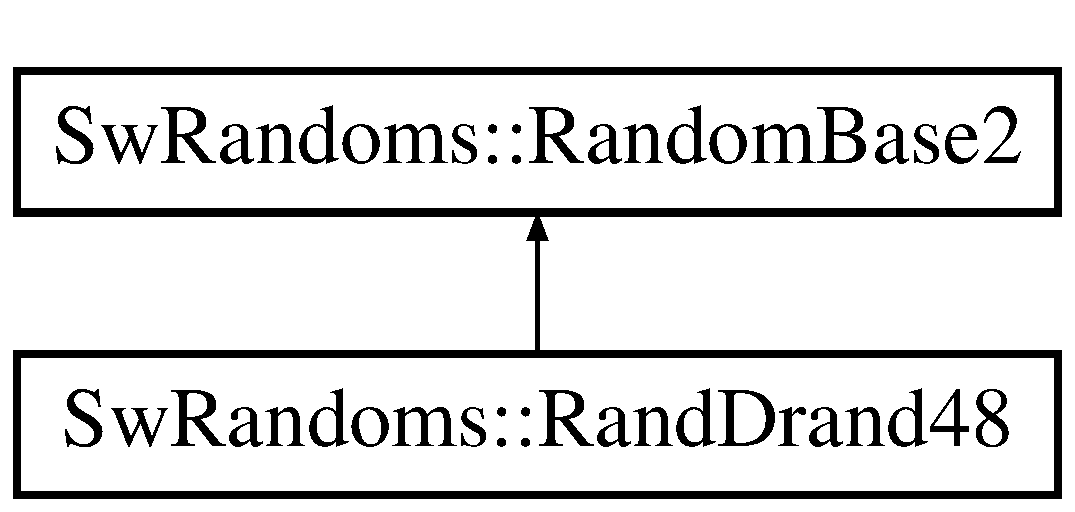
\includegraphics[height=2cm]{classSwRandoms_1_1RandDrand48}
\end{center}
\end{figure}
\subsection*{Public Member Functions}
\begin{CompactItemize}
\item 
{\bf RandDrand48} (unsigned long {\bf Dimensionality}, unsigned long Seed=1)
\item 
virtual {\bf RandomBase2} $\ast$ {\bf clone} () const 
\item 
virtual void {\bf GetUniforms} ({\bf SwArrays::MyArray} \&variates)
\item 
virtual void {\bf Skip} (unsigned long numberOfPaths)
\item 
virtual void {\bf SetSeed} (unsigned long Seed)
\item 
virtual void {\bf Reset} ()
\end{CompactItemize}
\subsection*{Private Attributes}
\begin{CompactItemize}
\item 
unsigned long {\bf InitialSeed}
\end{CompactItemize}


\subsection{Detailed Description}


Definition at line 9 of file RandDrand.h.

\subsection{Constructor \& Destructor Documentation}
\index{SwRandoms::RandDrand48@{SwRandoms::RandDrand48}!RandDrand48@{RandDrand48}}
\index{RandDrand48@{RandDrand48}!SwRandoms::RandDrand48@{SwRandoms::RandDrand48}}
\subsubsection{\setlength{\rightskip}{0pt plus 5cm}SwRandoms::RandDrand48::RandDrand48 (unsigned long {\em Dimensionality}, unsigned long {\em Seed} = {\tt 1})}\label{classSwRandoms_1_1RandDrand48_6200e7125a190ec6c31116ade72eeeea}




Definition at line 8 of file RandDrand.cpp.

Referenced by clone().

\begin{Code}\begin{verbatim}9   : RandomBase2(Dimensionality), InitialSeed( Seed )
10 {
11 
12 }
\end{verbatim}
\end{Code}




\subsection{Member Function Documentation}
\index{SwRandoms::RandDrand48@{SwRandoms::RandDrand48}!clone@{clone}}
\index{clone@{clone}!SwRandoms::RandDrand48@{SwRandoms::RandDrand48}}
\subsubsection{\setlength{\rightskip}{0pt plus 5cm}{\bf RandomBase2} $\ast$ SwRandoms::RandDrand48::clone () const\hspace{0.3cm}{\tt  [virtual]}}\label{classSwRandoms_1_1RandDrand48_835ce3d71b66d4610a60caa89fc7411c}




Implements {\bf SwRandoms::RandomBase2} \doxyref{}{p.}{classSwRandoms_1_1RandomBase2_633ab071ed2eded4784ea5c6faf4a9af}.

Definition at line 14 of file RandDrand.cpp.

References RandDrand48().

\begin{Code}\begin{verbatim}15 {
16   return new RandDrand48( *this );
17 }
\end{verbatim}
\end{Code}


\index{SwRandoms::RandDrand48@{SwRandoms::RandDrand48}!GetUniforms@{GetUniforms}}
\index{GetUniforms@{GetUniforms}!SwRandoms::RandDrand48@{SwRandoms::RandDrand48}}
\subsubsection{\setlength{\rightskip}{0pt plus 5cm}void SwRandoms::RandDrand48::GetUniforms ({\bf SwArrays::MyArray} \& {\em variates})\hspace{0.3cm}{\tt  [virtual]}}\label{classSwRandoms_1_1RandDrand48_9d63751f6824911ebbd943c9391db521}




Implements {\bf SwRandoms::RandomBase2} \doxyref{}{p.}{classSwRandoms_1_1RandomBase2_ee4b8f64be04c3cea35ea63cc4f9c6d6}.

Definition at line 19 of file RandDrand.cpp.

References SwRandoms::RandomBase2::GetDimensionality().

Referenced by Skip().

\begin{Code}\begin{verbatim}20 {
21   for (unsigned long j=0; j<GetDimensionality(); j++)
22     variates[j] = drand48();
23 }
\end{verbatim}
\end{Code}


\index{SwRandoms::RandDrand48@{SwRandoms::RandDrand48}!Skip@{Skip}}
\index{Skip@{Skip}!SwRandoms::RandDrand48@{SwRandoms::RandDrand48}}
\subsubsection{\setlength{\rightskip}{0pt plus 5cm}void SwRandoms::RandDrand48::Skip (unsigned long {\em numberOfPaths})\hspace{0.3cm}{\tt  [virtual]}}\label{classSwRandoms_1_1RandDrand48_332d6fbf16276b20465d973c2e89eb87}




Implements {\bf SwRandoms::RandomBase2} \doxyref{}{p.}{classSwRandoms_1_1RandomBase2_8a202b85b9c0f380700922331506f459}.

Definition at line 25 of file RandDrand.cpp.

References SwRandoms::RandomBase2::GetDimensionality(), and GetUniforms().

\begin{Code}\begin{verbatim}26 {
27   SwArrays::MyArray tmp( GetDimensionality() );
28   for (unsigned long j=0; j<numberOfPaths; j++)
29     GetUniforms(tmp);
30 }
\end{verbatim}
\end{Code}


\index{SwRandoms::RandDrand48@{SwRandoms::RandDrand48}!SetSeed@{SetSeed}}
\index{SetSeed@{SetSeed}!SwRandoms::RandDrand48@{SwRandoms::RandDrand48}}
\subsubsection{\setlength{\rightskip}{0pt plus 5cm}void SwRandoms::RandDrand48::SetSeed (unsigned long {\em Seed})\hspace{0.3cm}{\tt  [virtual]}}\label{classSwRandoms_1_1RandDrand48_9596b643d1915b3f8543bbdff6960105}




Implements {\bf SwRandoms::RandomBase2} \doxyref{}{p.}{classSwRandoms_1_1RandomBase2_ff006e42b1f514697427cc4578383b5e}.

Definition at line 32 of file RandDrand.cpp.

References InitialSeed.

\begin{Code}\begin{verbatim}33 {
34   InitialSeed = Seed;
35   srand48( Seed );
36 }
\end{verbatim}
\end{Code}


\index{SwRandoms::RandDrand48@{SwRandoms::RandDrand48}!Reset@{Reset}}
\index{Reset@{Reset}!SwRandoms::RandDrand48@{SwRandoms::RandDrand48}}
\subsubsection{\setlength{\rightskip}{0pt plus 5cm}void SwRandoms::RandDrand48::Reset ()\hspace{0.3cm}{\tt  [virtual]}}\label{classSwRandoms_1_1RandDrand48_d572e124c7bf89a406800ce07618b1bd}




Implements {\bf SwRandoms::RandomBase2} \doxyref{}{p.}{classSwRandoms_1_1RandomBase2_54a0497121db4d91e3ff6e2b4cdf380a}.

Definition at line 38 of file RandDrand.cpp.

References InitialSeed.

\begin{Code}\begin{verbatim}39 {
40   srand48( InitialSeed );
41 }
\end{verbatim}
\end{Code}




\subsection{Member Data Documentation}
\index{SwRandoms::RandDrand48@{SwRandoms::RandDrand48}!InitialSeed@{InitialSeed}}
\index{InitialSeed@{InitialSeed}!SwRandoms::RandDrand48@{SwRandoms::RandDrand48}}
\subsubsection{\setlength{\rightskip}{0pt plus 5cm}unsigned long {\bf SwRandoms::RandDrand48::InitialSeed}\hspace{0.3cm}{\tt  [private]}}\label{classSwRandoms_1_1RandDrand48_8447e5c4c6bdd0758f19d3df331960c5}




Definition at line 21 of file RandDrand.h.

Referenced by Reset(), and SetSeed().

The documentation for this class was generated from the following files:\begin{CompactItemize}
\item 
Gyulassy/opacity3/src/randoms/{\bf RandDrand.h}\item 
Gyulassy/opacity3/src/randoms/{\bf RandDrand.cpp}\end{CompactItemize}

\section{SwRandoms::RandomBase2 Class Reference}
\label{classSwRandoms_1_1RandomBase2}\index{SwRandoms::RandomBase2@{SwRandoms::RandomBase2}}
{\tt \#include $<$Random3.h$>$}

Inheritance diagram for SwRandoms::RandomBase2::\begin{figure}[H]
\begin{center}
\leavevmode
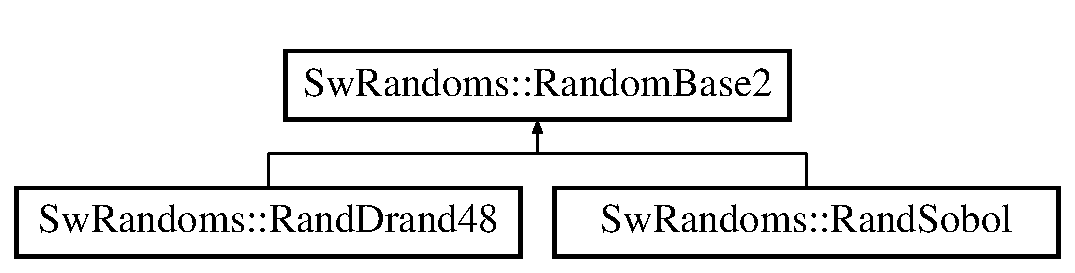
\includegraphics[height=2cm]{classSwRandoms_1_1RandomBase2}
\end{center}
\end{figure}
\subsection*{Public Member Functions}
\begin{CompactItemize}
\item 
{\bf RandomBase2} (unsigned long Dimensionality\_\-)
\item 
unsigned long {\bf GetDimensionality} () const 
\item 
virtual {\bf RandomBase2} $\ast$ {\bf clone} () const =0
\item 
virtual void {\bf GetUniforms} ({\bf SwArrays::MyArray} \&variates)=0
\item 
virtual void {\bf Skip} (unsigned long numberOfPaths)=0
\item 
virtual void {\bf SetSeed} (unsigned long Seed)=0
\item 
virtual void {\bf Reset} ()=0
\end{CompactItemize}
\subsection*{Private Attributes}
\begin{CompactItemize}
\item 
unsigned long {\bf Dimensionality}
\end{CompactItemize}


\subsection{Detailed Description}


Definition at line 9 of file Random3.h.

\subsection{Constructor \& Destructor Documentation}
\index{SwRandoms::RandomBase2@{SwRandoms::RandomBase2}!RandomBase2@{RandomBase2}}
\index{RandomBase2@{RandomBase2}!SwRandoms::RandomBase2@{SwRandoms::RandomBase2}}
\subsubsection{\setlength{\rightskip}{0pt plus 5cm}SwRandoms::RandomBase2::RandomBase2 (unsigned long {\em Dimensionality\_\-})\hspace{0.3cm}{\tt  [inline]}}\label{classSwRandoms_1_1RandomBase2_dd5e3fc4699b36e56970047463186e51}




Definition at line 12 of file Random3.h.

\begin{Code}\begin{verbatim}12 : Dimensionality( Dimensionality_ ) {};
\end{verbatim}
\end{Code}




\subsection{Member Function Documentation}
\index{SwRandoms::RandomBase2@{SwRandoms::RandomBase2}!GetDimensionality@{GetDimensionality}}
\index{GetDimensionality@{GetDimensionality}!SwRandoms::RandomBase2@{SwRandoms::RandomBase2}}
\subsubsection{\setlength{\rightskip}{0pt plus 5cm}unsigned long SwRandoms::RandomBase2::GetDimensionality () const\hspace{0.3cm}{\tt  [inline]}}\label{classSwRandoms_1_1RandomBase2_f5da6b70e2ff8646ab461b02db54548a}




Definition at line 26 of file Random3.h.

References Dimensionality.

Referenced by SwRandoms::RandSobol::GetUniforms(), SwRandoms::RandDrand48::GetUniforms(), SwRandoms::RandSobol::Skip(), and SwRandoms::RandDrand48::Skip().

\begin{Code}\begin{verbatim}27 {
28   return Dimensionality;
29 }
\end{verbatim}
\end{Code}


\index{SwRandoms::RandomBase2@{SwRandoms::RandomBase2}!clone@{clone}}
\index{clone@{clone}!SwRandoms::RandomBase2@{SwRandoms::RandomBase2}}
\subsubsection{\setlength{\rightskip}{0pt plus 5cm}virtual {\bf RandomBase2}$\ast$ SwRandoms::RandomBase2::clone () const\hspace{0.3cm}{\tt  [pure virtual]}}\label{classSwRandoms_1_1RandomBase2_633ab071ed2eded4784ea5c6faf4a9af}




Implemented in {\bf SwRandoms::RandDrand48} \doxyref{}{p.}{classSwRandoms_1_1RandDrand48_835ce3d71b66d4610a60caa89fc7411c}, and {\bf SwRandoms::RandSobol} \doxyref{}{p.}{classSwRandoms_1_1RandSobol_5abf4953d967d0aed2872a5cf2a2cdb7}.\index{SwRandoms::RandomBase2@{SwRandoms::RandomBase2}!GetUniforms@{GetUniforms}}
\index{GetUniforms@{GetUniforms}!SwRandoms::RandomBase2@{SwRandoms::RandomBase2}}
\subsubsection{\setlength{\rightskip}{0pt plus 5cm}virtual void SwRandoms::RandomBase2::GetUniforms ({\bf SwArrays::MyArray} \& {\em variates})\hspace{0.3cm}{\tt  [pure virtual]}}\label{classSwRandoms_1_1RandomBase2_ee4b8f64be04c3cea35ea63cc4f9c6d6}




Implemented in {\bf SwRandoms::RandDrand48} \doxyref{}{p.}{classSwRandoms_1_1RandDrand48_9d63751f6824911ebbd943c9391db521}, and {\bf SwRandoms::RandSobol} \doxyref{}{p.}{classSwRandoms_1_1RandSobol_8944be055bd402cc4d437d2b4357f79f}.\index{SwRandoms::RandomBase2@{SwRandoms::RandomBase2}!Skip@{Skip}}
\index{Skip@{Skip}!SwRandoms::RandomBase2@{SwRandoms::RandomBase2}}
\subsubsection{\setlength{\rightskip}{0pt plus 5cm}virtual void SwRandoms::RandomBase2::Skip (unsigned long {\em numberOfPaths})\hspace{0.3cm}{\tt  [pure virtual]}}\label{classSwRandoms_1_1RandomBase2_8a202b85b9c0f380700922331506f459}




Implemented in {\bf SwRandoms::RandDrand48} \doxyref{}{p.}{classSwRandoms_1_1RandDrand48_332d6fbf16276b20465d973c2e89eb87}, and {\bf SwRandoms::RandSobol} \doxyref{}{p.}{classSwRandoms_1_1RandSobol_68f45c07b374e627a58f84f7e2491167}.\index{SwRandoms::RandomBase2@{SwRandoms::RandomBase2}!SetSeed@{SetSeed}}
\index{SetSeed@{SetSeed}!SwRandoms::RandomBase2@{SwRandoms::RandomBase2}}
\subsubsection{\setlength{\rightskip}{0pt plus 5cm}virtual void SwRandoms::RandomBase2::SetSeed (unsigned long {\em Seed})\hspace{0.3cm}{\tt  [pure virtual]}}\label{classSwRandoms_1_1RandomBase2_ff006e42b1f514697427cc4578383b5e}




Implemented in {\bf SwRandoms::RandDrand48} \doxyref{}{p.}{classSwRandoms_1_1RandDrand48_9596b643d1915b3f8543bbdff6960105}, and {\bf SwRandoms::RandSobol} \doxyref{}{p.}{classSwRandoms_1_1RandSobol_cbab6c15df9c297d18fa585cfad1b11d}.\index{SwRandoms::RandomBase2@{SwRandoms::RandomBase2}!Reset@{Reset}}
\index{Reset@{Reset}!SwRandoms::RandomBase2@{SwRandoms::RandomBase2}}
\subsubsection{\setlength{\rightskip}{0pt plus 5cm}virtual void SwRandoms::RandomBase2::Reset ()\hspace{0.3cm}{\tt  [pure virtual]}}\label{classSwRandoms_1_1RandomBase2_54a0497121db4d91e3ff6e2b4cdf380a}




Implemented in {\bf SwRandoms::RandDrand48} \doxyref{}{p.}{classSwRandoms_1_1RandDrand48_d572e124c7bf89a406800ce07618b1bd}, and {\bf SwRandoms::RandSobol} \doxyref{}{p.}{classSwRandoms_1_1RandSobol_e3d1bfbb3fa3bc81a9775c8d9875f22f}.

\subsection{Member Data Documentation}
\index{SwRandoms::RandomBase2@{SwRandoms::RandomBase2}!Dimensionality@{Dimensionality}}
\index{Dimensionality@{Dimensionality}!SwRandoms::RandomBase2@{SwRandoms::RandomBase2}}
\subsubsection{\setlength{\rightskip}{0pt plus 5cm}unsigned long {\bf SwRandoms::RandomBase2::Dimensionality}\hspace{0.3cm}{\tt  [private]}}\label{classSwRandoms_1_1RandomBase2_e07e88e367896cf2eaab51b3f479d52d}




Definition at line 23 of file Random3.h.

Referenced by GetDimensionality().

The documentation for this class was generated from the following file:\begin{CompactItemize}
\item 
Gyulassy/opacity3/src/randoms/{\bf Random3.h}\end{CompactItemize}

\section{SwRandoms::RandSobol Class Reference}
\label{classSwRandoms_1_1RandSobol}\index{SwRandoms::RandSobol@{SwRandoms::RandSobol}}
{\tt \#include $<$RandSobol.h$>$}

Inheritance diagram for SwRandoms::RandSobol::\begin{figure}[H]
\begin{center}
\leavevmode
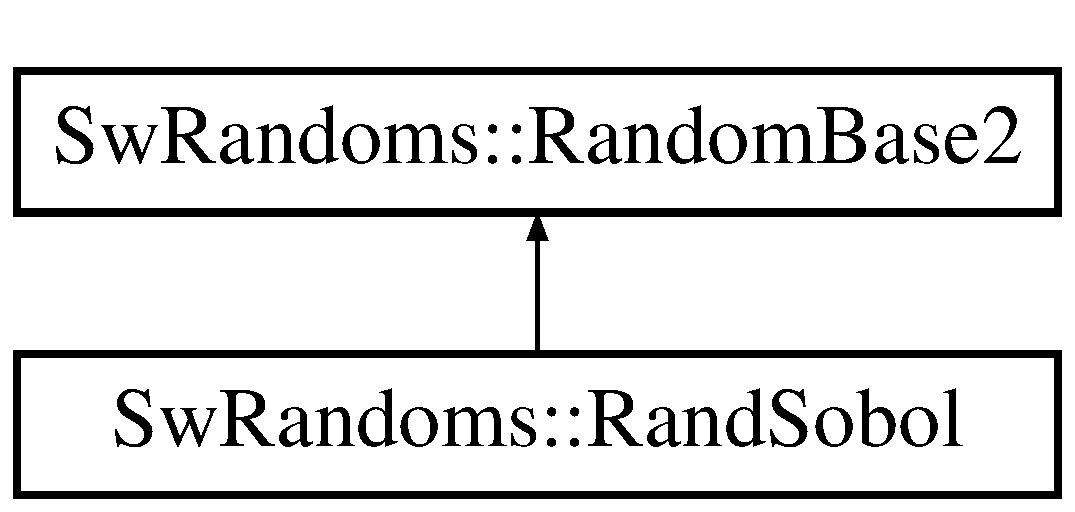
\includegraphics[height=2cm]{classSwRandoms_1_1RandSobol}
\end{center}
\end{figure}
\subsection*{Public Member Functions}
\begin{CompactItemize}
\item 
{\bf RandSobol} (unsigned long {\bf Dimensionality}, unsigned long Seed=1)
\item 
virtual {\bf RandomBase2} $\ast$ {\bf clone} () const 
\item 
virtual void {\bf GetUniforms} ({\bf SwArrays::MyArray} \&variates)
\item 
virtual void {\bf Skip} (unsigned long numberOfPaths)
\item 
virtual void {\bf SetSeed} (unsigned long Seed)
\item 
virtual void {\bf Reset} ()
\end{CompactItemize}
\subsection*{Private Attributes}
\begin{CompactItemize}
\item 
long long int {\bf InitialSeed}
\item 
long long int {\bf RunningSeed}
\end{CompactItemize}


\subsection{Detailed Description}


Definition at line 9 of file RandSobol.h.

\subsection{Constructor \& Destructor Documentation}
\index{SwRandoms::RandSobol@{SwRandoms::RandSobol}!RandSobol@{RandSobol}}
\index{RandSobol@{RandSobol}!SwRandoms::RandSobol@{SwRandoms::RandSobol}}
\subsubsection{\setlength{\rightskip}{0pt plus 5cm}SwRandoms::RandSobol::RandSobol (unsigned long {\em Dimensionality}, unsigned long {\em Seed} = {\tt 1})}\label{classSwRandoms_1_1RandSobol_2c07980724797f1e0b3dd24a071bb745}




Definition at line 9 of file RandSobol.cpp.

Referenced by clone().

\begin{Code}\begin{verbatim}10   : RandomBase2(Dimensionality), InitialSeed( Seed )
11 {
12 
13 }
\end{verbatim}
\end{Code}




\subsection{Member Function Documentation}
\index{SwRandoms::RandSobol@{SwRandoms::RandSobol}!clone@{clone}}
\index{clone@{clone}!SwRandoms::RandSobol@{SwRandoms::RandSobol}}
\subsubsection{\setlength{\rightskip}{0pt plus 5cm}{\bf RandomBase2} $\ast$ SwRandoms::RandSobol::clone () const\hspace{0.3cm}{\tt  [virtual]}}\label{classSwRandoms_1_1RandSobol_5abf4953d967d0aed2872a5cf2a2cdb7}




Implements {\bf SwRandoms::RandomBase2} \doxyref{}{p.}{classSwRandoms_1_1RandomBase2_633ab071ed2eded4784ea5c6faf4a9af}.

Definition at line 15 of file RandSobol.cpp.

References RandSobol().

\begin{Code}\begin{verbatim}16 {
17   return new RandSobol( *this );
18 }
\end{verbatim}
\end{Code}


\index{SwRandoms::RandSobol@{SwRandoms::RandSobol}!GetUniforms@{GetUniforms}}
\index{GetUniforms@{GetUniforms}!SwRandoms::RandSobol@{SwRandoms::RandSobol}}
\subsubsection{\setlength{\rightskip}{0pt plus 5cm}void SwRandoms::RandSobol::GetUniforms ({\bf SwArrays::MyArray} \& {\em variates})\hspace{0.3cm}{\tt  [virtual]}}\label{classSwRandoms_1_1RandSobol_8944be055bd402cc4d437d2b4357f79f}




Implements {\bf SwRandoms::RandomBase2} \doxyref{}{p.}{classSwRandoms_1_1RandomBase2_ee4b8f64be04c3cea35ea63cc4f9c6d6}.

Definition at line 20 of file RandSobol.cpp.

References SwRandoms::RandomBase2::GetDimensionality(), Sobol::i8\_\-sobol(), and RunningSeed.

Referenced by Skip().

\begin{Code}\begin{verbatim}21 {
22   unsigned long dim = GetDimensionality();
23   double* sobols = new double[dim];
24   
25   // Produces a vector of quasirandom numbers
26   // Updates RunningSeed
27   Sobol::i8_sobol( dim, &RunningSeed, sobols );
28 
29   // Move our array of floats into the vector
30   for (unsigned long j=0; j<dim; j++)
31     variates[j] = sobols[j];
32 
33   delete [] sobols;
34 }
\end{verbatim}
\end{Code}


\index{SwRandoms::RandSobol@{SwRandoms::RandSobol}!Skip@{Skip}}
\index{Skip@{Skip}!SwRandoms::RandSobol@{SwRandoms::RandSobol}}
\subsubsection{\setlength{\rightskip}{0pt plus 5cm}void SwRandoms::RandSobol::Skip (unsigned long {\em numberOfPaths})\hspace{0.3cm}{\tt  [virtual]}}\label{classSwRandoms_1_1RandSobol_68f45c07b374e627a58f84f7e2491167}




Implements {\bf SwRandoms::RandomBase2} \doxyref{}{p.}{classSwRandoms_1_1RandomBase2_8a202b85b9c0f380700922331506f459}.

Definition at line 36 of file RandSobol.cpp.

References SwRandoms::RandomBase2::GetDimensionality(), and GetUniforms().

\begin{Code}\begin{verbatim}37 {
38   SwArrays::MyArray tmp( GetDimensionality() );
39   for (unsigned long j=0; j<numberOfPaths; j++)
40     GetUniforms(tmp);
41 }
\end{verbatim}
\end{Code}


\index{SwRandoms::RandSobol@{SwRandoms::RandSobol}!SetSeed@{SetSeed}}
\index{SetSeed@{SetSeed}!SwRandoms::RandSobol@{SwRandoms::RandSobol}}
\subsubsection{\setlength{\rightskip}{0pt plus 5cm}void SwRandoms::RandSobol::SetSeed (unsigned long {\em Seed})\hspace{0.3cm}{\tt  [virtual]}}\label{classSwRandoms_1_1RandSobol_cbab6c15df9c297d18fa585cfad1b11d}




Implements {\bf SwRandoms::RandomBase2} \doxyref{}{p.}{classSwRandoms_1_1RandomBase2_ff006e42b1f514697427cc4578383b5e}.

Definition at line 43 of file RandSobol.cpp.

References InitialSeed, and RunningSeed.

\begin{Code}\begin{verbatim}44 {
45   //InitialSeed = Seed;
46   // Sobol sequence should start from 0
47   InitialSeed = 0;
48   RunningSeed = InitialSeed;
49   srand48( Seed );
50 }
\end{verbatim}
\end{Code}


\index{SwRandoms::RandSobol@{SwRandoms::RandSobol}!Reset@{Reset}}
\index{Reset@{Reset}!SwRandoms::RandSobol@{SwRandoms::RandSobol}}
\subsubsection{\setlength{\rightskip}{0pt plus 5cm}void SwRandoms::RandSobol::Reset ()\hspace{0.3cm}{\tt  [virtual]}}\label{classSwRandoms_1_1RandSobol_e3d1bfbb3fa3bc81a9775c8d9875f22f}




Implements {\bf SwRandoms::RandomBase2} \doxyref{}{p.}{classSwRandoms_1_1RandomBase2_54a0497121db4d91e3ff6e2b4cdf380a}.

Definition at line 52 of file RandSobol.cpp.

References InitialSeed.

\begin{Code}\begin{verbatim}53 {
54   srand48( InitialSeed );
55 }
\end{verbatim}
\end{Code}




\subsection{Member Data Documentation}
\index{SwRandoms::RandSobol@{SwRandoms::RandSobol}!InitialSeed@{InitialSeed}}
\index{InitialSeed@{InitialSeed}!SwRandoms::RandSobol@{SwRandoms::RandSobol}}
\subsubsection{\setlength{\rightskip}{0pt plus 5cm}long long int {\bf SwRandoms::RandSobol::InitialSeed}\hspace{0.3cm}{\tt  [private]}}\label{classSwRandoms_1_1RandSobol_d6d335a081b9961d7059c13b1869c57c}




Definition at line 21 of file RandSobol.h.

Referenced by Reset(), and SetSeed().\index{SwRandoms::RandSobol@{SwRandoms::RandSobol}!RunningSeed@{RunningSeed}}
\index{RunningSeed@{RunningSeed}!SwRandoms::RandSobol@{SwRandoms::RandSobol}}
\subsubsection{\setlength{\rightskip}{0pt plus 5cm}long long int {\bf SwRandoms::RandSobol::RunningSeed}\hspace{0.3cm}{\tt  [private]}}\label{classSwRandoms_1_1RandSobol_3e98e6cf26ba9528d885ebbf45d1a393}




Definition at line 22 of file RandSobol.h.

Referenced by GetUniforms(), and SetSeed().

The documentation for this class was generated from the following files:\begin{CompactItemize}
\item 
Gyulassy/opacity3/src/randoms/{\bf RandSobol.h}\item 
Gyulassy/opacity3/src/randoms/{\bf RandSobol.cpp}\end{CompactItemize}

\section{SimpleCalc3$<$ numOfRandoms $>$ Class Template Reference}
\label{classSimpleCalc3}\index{SimpleCalc3@{SimpleCalc3}}
{\tt \#include $<$simplecalc1.h$>$}

\subsection*{Public Member Functions}
\begin{CompactItemize}
\item 
{\bf SimpleCalc3} ()
\item 
void {\bf SetParameter} ({\bf Parameters} myParams)
\item 
void {\bf SetCoord} (long dimension, double value)
\item 
void {\bf SetRandoms} (boost::array$<$ double, numOfRandoms $>$ randoms)
\item 
void {\bf GetAnswer} ({\bf SwArrays::MyArray} \&answers)
\end{CompactItemize}


\subsection{Detailed Description}
\subsubsection*{template$<$std::size\_\-t numOfRandoms$>$ class SimpleCalc3$<$ numOfRandoms $>$}

\begin{Desc}
\item[Author:]Simon Wicks $<${\tt simonw@phys.columbia.edu}$>$ Example class to implement the necessary calculation interface to the driver class. Whatever the coordinates supplied in the deterministic dimensions it just returns the number of random numbers supplied.\end{Desc}
Implementation of other calculations can be based off this interface. 

Definition at line 23 of file simplecalc1.h.

\subsection{Constructor \& Destructor Documentation}
\index{SimpleCalc3@{SimpleCalc3}!SimpleCalc3@{SimpleCalc3}}
\index{SimpleCalc3@{SimpleCalc3}!SimpleCalc3@{SimpleCalc3}}
\subsubsection{\setlength{\rightskip}{0pt plus 5cm}template$<$std::size\_\-t numOfRandoms$>$ {\bf SimpleCalc3}$<$ numOfRandoms $>$::{\bf SimpleCalc3} ()\hspace{0.3cm}{\tt  [inline]}}\label{classSimpleCalc3_8df774903b7e610d93f05e7600c1a6ab}




Definition at line 37 of file simplecalc1.h.

\begin{Code}\begin{verbatim}38 {
39 
40 }
\end{verbatim}
\end{Code}




\subsection{Member Function Documentation}
\index{SimpleCalc3@{SimpleCalc3}!SetParameter@{SetParameter}}
\index{SetParameter@{SetParameter}!SimpleCalc3@{SimpleCalc3}}
\subsubsection{\setlength{\rightskip}{0pt plus 5cm}template$<$std::size\_\-t numOfRandoms$>$ void {\bf SimpleCalc3}$<$ numOfRandoms $>$::SetParameter ({\bf Parameters} {\em myParams})}\label{classSimpleCalc3_b9681ce02d9b6cd391a77d3c396c665e}


\index{SimpleCalc3@{SimpleCalc3}!SetCoord@{SetCoord}}
\index{SetCoord@{SetCoord}!SimpleCalc3@{SimpleCalc3}}
\subsubsection{\setlength{\rightskip}{0pt plus 5cm}template$<$std::size\_\-t numOfRandoms$>$ void {\bf SimpleCalc3}$<$ numOfRandoms $>$::SetCoord (long {\em dimension}, double {\em value})\hspace{0.3cm}{\tt  [inline]}}\label{classSimpleCalc3_7f612fa190cc836d859e5e8a408dafd1}




Definition at line 49 of file simplecalc1.h.

\begin{Code}\begin{verbatim}50 {
51   
52 }
\end{verbatim}
\end{Code}


\index{SimpleCalc3@{SimpleCalc3}!SetRandoms@{SetRandoms}}
\index{SetRandoms@{SetRandoms}!SimpleCalc3@{SimpleCalc3}}
\subsubsection{\setlength{\rightskip}{0pt plus 5cm}template$<$std::size\_\-t numOfRandoms$>$ void {\bf SimpleCalc3}$<$ numOfRandoms $>$::SetRandoms (boost::array$<$ double, numOfRandoms $>$ {\em randoms})\hspace{0.3cm}{\tt  [inline]}}\label{classSimpleCalc3_e87134efa498b50cb86ba2a0827f5e11}




Definition at line 55 of file simplecalc1.h.

\begin{Code}\begin{verbatim}56 {
57 
58 }
\end{verbatim}
\end{Code}


\index{SimpleCalc3@{SimpleCalc3}!GetAnswer@{GetAnswer}}
\index{GetAnswer@{GetAnswer}!SimpleCalc3@{SimpleCalc3}}
\subsubsection{\setlength{\rightskip}{0pt plus 5cm}template$<$std::size\_\-t numOfRandoms$>$ void {\bf SimpleCalc3}$<$ numOfRandoms $>$::GetAnswer ({\bf SwArrays::MyArray} \& {\em answers})\hspace{0.3cm}{\tt  [inline]}}\label{classSimpleCalc3_ca9193e3aef081ac6558d909adf16bb7}




Definition at line 61 of file simplecalc1.h.

\begin{Code}\begin{verbatim}62 {
63   answers[0] = static_cast<double>(numOfRandoms);
64 }
\end{verbatim}
\end{Code}




The documentation for this class was generated from the following file:\begin{CompactItemize}
\item 
Gyulassy/opacity3/src/{\bf simplecalc1.h}\end{CompactItemize}

\section{StatGathering::StatisticsMC Class Reference}
\label{classStatGathering_1_1StatisticsMC}\index{StatGathering::StatisticsMC@{StatGathering::StatisticsMC}}
{\tt \#include $<$statisticsmc.h$>$}

Inheritance diagram for StatGathering::StatisticsMC::\begin{figure}[H]
\begin{center}
\leavevmode
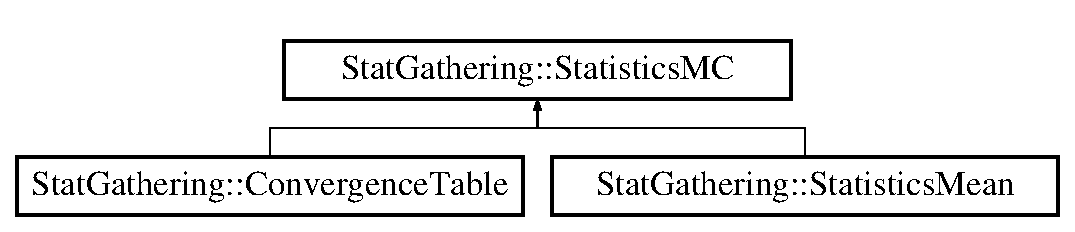
\includegraphics[height=2cm]{classStatGathering_1_1StatisticsMC}
\end{center}
\end{figure}
\subsection*{Public Member Functions}
\begin{CompactItemize}
\item 
{\bf StatisticsMC} ()
\item 
virtual {\bf $\sim$StatisticsMC} ()
\item 
virtual {\bf StatisticsMC} $\ast$ {\bf clone} () const =0
\begin{CompactList}\small\item\em clone method, to interface with the 'Wrapper' template \item\end{CompactList}\item 
virtual void {\bf AddOneResult} (double result)=0
\item 
virtual void {\bf AddOneSetOfResults} (long Number, std::vector$<$ std::vector$<$ double $>$ $>$ \&ResultsSoFar\_\-)=0
\item 
virtual void {\bf Reset} ()=0
\begin{CompactList}\small\item\em Reset all internal values, start again. \item\end{CompactList}\item 
virtual void {\bf SetResultsSoFar} (long Number\_\-, std::vector$<$ std::vector$<$ double $>$ $>$ \&ResultsSoFar\_\-)=0
\item 
virtual std::vector$<$ std::vector$<$ double $>$ $>$ {\bf GetResultsSoFar} () const =0
\end{CompactItemize}


\subsection{Detailed Description}
Base class for statistics gatherer for a Monte Carlo integrator based on code from Joshi 'C++ Design Patterns and Derivatives Pricing'

This base class is pure virtual, defines an interface to interact with the statistics gatherer This represents one 'point': each point is filled with a single double, but can return a 2D vector with information about its results. 

Definition at line 17 of file statisticsmc.h.

\subsection{Constructor \& Destructor Documentation}
\index{StatGathering::StatisticsMC@{StatGathering::StatisticsMC}!StatisticsMC@{StatisticsMC}}
\index{StatisticsMC@{StatisticsMC}!StatGathering::StatisticsMC@{StatGathering::StatisticsMC}}
\subsubsection{\setlength{\rightskip}{0pt plus 5cm}StatGathering::StatisticsMC::StatisticsMC ()\hspace{0.3cm}{\tt  [inline]}}\label{classStatGathering_1_1StatisticsMC_e5f00cda87f14f55cef6914e26b9ef67}




Definition at line 20 of file statisticsmc.h.

\begin{Code}\begin{verbatim}20 {}
\end{verbatim}
\end{Code}


\index{StatGathering::StatisticsMC@{StatGathering::StatisticsMC}!~StatisticsMC@{$\sim$StatisticsMC}}
\index{~StatisticsMC@{$\sim$StatisticsMC}!StatGathering::StatisticsMC@{StatGathering::StatisticsMC}}
\subsubsection{\setlength{\rightskip}{0pt plus 5cm}virtual StatGathering::StatisticsMC::$\sim$StatisticsMC ()\hspace{0.3cm}{\tt  [inline, virtual]}}\label{classStatGathering_1_1StatisticsMC_1bd9450c20d37ee3954207df031b3619}




Definition at line 21 of file statisticsmc.h.

\begin{Code}\begin{verbatim}21 {}
\end{verbatim}
\end{Code}




\subsection{Member Function Documentation}
\index{StatGathering::StatisticsMC@{StatGathering::StatisticsMC}!clone@{clone}}
\index{clone@{clone}!StatGathering::StatisticsMC@{StatGathering::StatisticsMC}}
\subsubsection{\setlength{\rightskip}{0pt plus 5cm}virtual {\bf StatisticsMC}$\ast$ StatGathering::StatisticsMC::clone () const\hspace{0.3cm}{\tt  [pure virtual]}}\label{classStatGathering_1_1StatisticsMC_cfcf6abd6e973c00e5f31a79496233e0}


clone method, to interface with the 'Wrapper' template 



Implemented in {\bf StatGathering::ConvergenceTable} \doxyref{}{p.}{classStatGathering_1_1ConvergenceTable_739be407fb8c781a3db471d28f25ba78}, and {\bf StatGathering::StatisticsMean} \doxyref{}{p.}{classStatGathering_1_1StatisticsMean_0afe279f79a7a68922f0ae9d52bb2957}.\index{StatGathering::StatisticsMC@{StatGathering::StatisticsMC}!AddOneResult@{AddOneResult}}
\index{AddOneResult@{AddOneResult}!StatGathering::StatisticsMC@{StatGathering::StatisticsMC}}
\subsubsection{\setlength{\rightskip}{0pt plus 5cm}virtual void StatGathering::StatisticsMC::AddOneResult (double {\em result})\hspace{0.3cm}{\tt  [pure virtual]}}\label{classStatGathering_1_1StatisticsMC_aac13c0a41a374bec47c67afc59a0182}


Add one result to the mix This is the standard way of adding in another result 

Implemented in {\bf StatGathering::ConvergenceTable} \doxyref{}{p.}{classStatGathering_1_1ConvergenceTable_8dfcddda38ea9657e1ae4aa6b917ff8b}, and {\bf StatGathering::StatisticsMean} \doxyref{}{p.}{classStatGathering_1_1StatisticsMean_a041fcd7d325906ecbc05b7dd60a8245}.\index{StatGathering::StatisticsMC@{StatGathering::StatisticsMC}!AddOneSetOfResults@{AddOneSetOfResults}}
\index{AddOneSetOfResults@{AddOneSetOfResults}!StatGathering::StatisticsMC@{StatGathering::StatisticsMC}}
\subsubsection{\setlength{\rightskip}{0pt plus 5cm}virtual void StatGathering::StatisticsMC::AddOneSetOfResults (long {\em Number}, std::vector$<$ std::vector$<$ double $>$ $>$ \& {\em ResultsSoFar\_\-})\hspace{0.3cm}{\tt  [pure virtual]}}\label{classStatGathering_1_1StatisticsMC_3f706f03424b931973415b8723127cad}


Add many results to the mix This might be from merging two sets of results or similar \begin{Desc}
\item[Parameters:]
\begin{description}
\item[{\em Number}]The total number of results to add in \item[{\em ResultsSoFar\_\-}]A 2D vector of doubles, which gives the relevant structure of the results (this structure is not specified in this base class) \end{description}
\end{Desc}


Implemented in {\bf StatGathering::ConvergenceTable} \doxyref{}{p.}{classStatGathering_1_1ConvergenceTable_32d89dcbeedf1846f36319d9b36eafba}, and {\bf StatGathering::StatisticsMean} \doxyref{}{p.}{classStatGathering_1_1StatisticsMean_a0089d1731c6b33a7749de1ec41e0a8f}.\index{StatGathering::StatisticsMC@{StatGathering::StatisticsMC}!Reset@{Reset}}
\index{Reset@{Reset}!StatGathering::StatisticsMC@{StatGathering::StatisticsMC}}
\subsubsection{\setlength{\rightskip}{0pt plus 5cm}virtual void StatGathering::StatisticsMC::Reset ()\hspace{0.3cm}{\tt  [pure virtual]}}\label{classStatGathering_1_1StatisticsMC_43259c270bbf6b23620252f11a155812}


Reset all internal values, start again. 



Implemented in {\bf StatGathering::ConvergenceTable} \doxyref{}{p.}{classStatGathering_1_1ConvergenceTable_7bb5a965ab53ca72d501e0d7f694d93b}, and {\bf StatGathering::StatisticsMean} \doxyref{}{p.}{classStatGathering_1_1StatisticsMean_41cc79ed93147ad208d83ae9d3b0c97d}.\index{StatGathering::StatisticsMC@{StatGathering::StatisticsMC}!SetResultsSoFar@{SetResultsSoFar}}
\index{SetResultsSoFar@{SetResultsSoFar}!StatGathering::StatisticsMC@{StatGathering::StatisticsMC}}
\subsubsection{\setlength{\rightskip}{0pt plus 5cm}virtual void StatGathering::StatisticsMC::SetResultsSoFar (long {\em Number\_\-}, std::vector$<$ std::vector$<$ double $>$ $>$ \& {\em ResultsSoFar\_\-})\hspace{0.3cm}{\tt  [pure virtual]}}\label{classStatGathering_1_1StatisticsMC_b97a4292be61cff81425390f1fbed69c}


Set the results as supplied \begin{Desc}
\item[Parameters:]
\begin{description}
\item[{\em Number}]The total number of results so far \item[{\em ResultsSoFar\_\-}]A 2D vector of doubles, which gives the relevant structure of the results (this structure is not specified in this base class) \end{description}
\end{Desc}


Implemented in {\bf StatGathering::ConvergenceTable} \doxyref{}{p.}{classStatGathering_1_1ConvergenceTable_84375f0e4ec9925ae1c0575ac3d15075}, and {\bf StatGathering::StatisticsMean} \doxyref{}{p.}{classStatGathering_1_1StatisticsMean_9b574a960041288be6bf2892133252e7}.\index{StatGathering::StatisticsMC@{StatGathering::StatisticsMC}!GetResultsSoFar@{GetResultsSoFar}}
\index{GetResultsSoFar@{GetResultsSoFar}!StatGathering::StatisticsMC@{StatGathering::StatisticsMC}}
\subsubsection{\setlength{\rightskip}{0pt plus 5cm}virtual std::vector$<$std::vector$<$double$>$ $>$ StatGathering::StatisticsMC::GetResultsSoFar () const\hspace{0.3cm}{\tt  [pure virtual]}}\label{classStatGathering_1_1StatisticsMC_ddb9cc20ac28892097e902286c5204bb}


Get a suitably structured 2D vector of the results so far This base class does not specify the structure to return 

Implemented in {\bf StatGathering::ConvergenceTable} \doxyref{}{p.}{classStatGathering_1_1ConvergenceTable_6cd7612fa109159ae022555ae84e5819}, and {\bf StatGathering::StatisticsMean} \doxyref{}{p.}{classStatGathering_1_1StatisticsMean_9345a3844d530b36af1e10a1e1310f1b}.

The documentation for this class was generated from the following file:\begin{CompactItemize}
\item 
Gyulassy/opacity3/src/store2d/{\bf statisticsmc.h}\end{CompactItemize}

\section{StatGathering::StatisticsMean Class Reference}
\label{classStatGathering_1_1StatisticsMean}\index{StatGathering::StatisticsMean@{StatGathering::StatisticsMean}}
{\tt \#include $<$statisticsmc.h$>$}

Inheritance diagram for StatGathering::StatisticsMean::\begin{figure}[H]
\begin{center}
\leavevmode
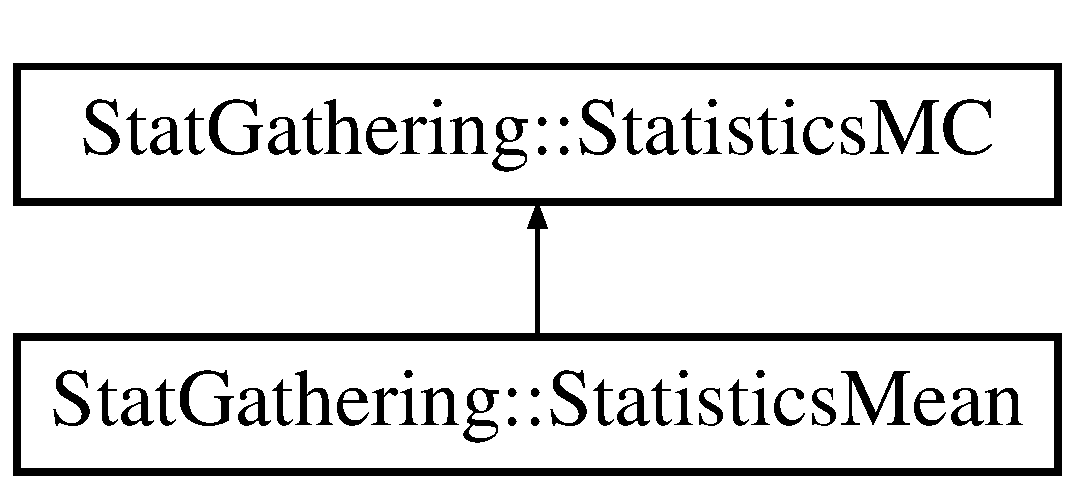
\includegraphics[height=2cm]{classStatGathering_1_1StatisticsMean}
\end{center}
\end{figure}
\subsection*{Public Member Functions}
\begin{CompactItemize}
\item 
{\bf StatisticsMean} ()
\item 
virtual {\bf StatisticsMC} $\ast$ {\bf clone} () const 
\begin{CompactList}\small\item\em clone method, to interface with the 'Wrapper' template \item\end{CompactList}\item 
virtual void {\bf AddOneResult} (double result)
\item 
virtual void {\bf AddOneSetOfResults} (long Number\_\-, std::vector$<$ std::vector$<$ double $>$ $>$ \&ResultsSoFar\_\-)
\item 
virtual void {\bf Reset} ()
\begin{CompactList}\small\item\em Reset all internal values to zero. \item\end{CompactList}\item 
virtual void {\bf SetResultsSoFar} (long Number\_\-, std::vector$<$ std::vector$<$ double $>$ $>$ \&ResultsSoFar\_\-)
\begin{CompactList}\small\item\em Set to a specific set of results. \item\end{CompactList}\item 
virtual std::vector$<$ std::vector$<$ double $>$ $>$ {\bf GetResultsSoFar} () const 
\end{CompactItemize}
\subsection*{Private Attributes}
\begin{CompactItemize}
\item 
double {\bf RunningSum}
\begin{CompactList}\small\item\em The sum of all the input results. \item\end{CompactList}\item 
double {\bf RunningSum2}
\begin{CompactList}\small\item\em The sum of all the squares of input results. \item\end{CompactList}\item 
unsigned long {\bf PathsDone}
\begin{CompactList}\small\item\em The total number of points input. \item\end{CompactList}\end{CompactItemize}
\subsection*{Friends}
\begin{CompactItemize}
\item 
std::ostream \& {\bf operator$<$$<$} (std::ostream \&out, const {\bf StatisticsMean} \&stats)
\begin{CompactList}\small\item\em friend to $<$$<$ so that we can overload the $<$$<$ operator to output a \doxyref{ConvergenceTable}{p.}{classStatGathering_1_1ConvergenceTable} object \item\end{CompactList}\item 
std::istream \& {\bf operator$>$$>$} (std::istream \&in, {\bf StatisticsMean} \&stats)
\end{CompactItemize}


\subsection{Detailed Description}
A simple implementation of a statistics gatherer Keeps a running tab on the total sum of results and the sum of results$^\wedge$2 The results: 1D vector - the mean, the standard deviation 

Definition at line 63 of file statisticsmc.h.

\subsection{Constructor \& Destructor Documentation}
\index{StatGathering::StatisticsMean@{StatGathering::StatisticsMean}!StatisticsMean@{StatisticsMean}}
\index{StatisticsMean@{StatisticsMean}!StatGathering::StatisticsMean@{StatGathering::StatisticsMean}}
\subsubsection{\setlength{\rightskip}{0pt plus 5cm}StatGathering::StatisticsMean::StatisticsMean ()}\label{classStatGathering_1_1StatisticsMean_b403f5b4e4850246d85b98ca9de55120}




Definition at line 8 of file statisticsmc.cpp.

Referenced by clone().

\begin{Code}\begin{verbatim}9   : RunningSum(0.), RunningSum2(0.), PathsDone(0)
10 {
11 
12 }
\end{verbatim}
\end{Code}




\subsection{Member Function Documentation}
\index{StatGathering::StatisticsMean@{StatGathering::StatisticsMean}!clone@{clone}}
\index{clone@{clone}!StatGathering::StatisticsMean@{StatGathering::StatisticsMean}}
\subsubsection{\setlength{\rightskip}{0pt plus 5cm}{\bf StatisticsMC} $\ast$ StatGathering::StatisticsMean::clone () const\hspace{0.3cm}{\tt  [virtual]}}\label{classStatGathering_1_1StatisticsMean_0afe279f79a7a68922f0ae9d52bb2957}


clone method, to interface with the 'Wrapper' template 



Implements {\bf StatGathering::StatisticsMC} \doxyref{}{p.}{classStatGathering_1_1StatisticsMC_cfcf6abd6e973c00e5f31a79496233e0}.

Definition at line 68 of file statisticsmc.cpp.

References StatisticsMean().

\begin{Code}\begin{verbatim}69 {
70   return new StatisticsMean(*this);
71 }
\end{verbatim}
\end{Code}


\index{StatGathering::StatisticsMean@{StatGathering::StatisticsMean}!AddOneResult@{AddOneResult}}
\index{AddOneResult@{AddOneResult}!StatGathering::StatisticsMean@{StatGathering::StatisticsMean}}
\subsubsection{\setlength{\rightskip}{0pt plus 5cm}void StatGathering::StatisticsMean::AddOneResult (double {\em result})\hspace{0.3cm}{\tt  [virtual]}}\label{classStatGathering_1_1StatisticsMean_a041fcd7d325906ecbc05b7dd60a8245}


Add one result to the mix This is the standard way of adding in another result 

Implements {\bf StatGathering::StatisticsMC} \doxyref{}{p.}{classStatGathering_1_1StatisticsMC_aac13c0a41a374bec47c67afc59a0182}.

Definition at line 14 of file statisticsmc.cpp.

References PathsDone, RunningSum, and RunningSum2.

\begin{Code}\begin{verbatim}15 {
16   // Adding in one result
17   // Hence, increment PathsDone by one, add the result to the running sum,
18   // add the squre to RunningSum2
19   PathsDone++;
20   RunningSum += result;
21   RunningSum2 += result*result;
22 }
\end{verbatim}
\end{Code}


\index{StatGathering::StatisticsMean@{StatGathering::StatisticsMean}!AddOneSetOfResults@{AddOneSetOfResults}}
\index{AddOneSetOfResults@{AddOneSetOfResults}!StatGathering::StatisticsMean@{StatGathering::StatisticsMean}}
\subsubsection{\setlength{\rightskip}{0pt plus 5cm}void StatGathering::StatisticsMean::AddOneSetOfResults (long {\em Number\_\-}, std::vector$<$ std::vector$<$ double $>$ $>$ \& {\em ResultsSoFar\_\-})\hspace{0.3cm}{\tt  [virtual]}}\label{classStatGathering_1_1StatisticsMean_a0089d1731c6b33a7749de1ec41e0a8f}


Add in a large set of results to what we already have \begin{Desc}
\item[Parameters:]
\begin{description}
\item[{\em Number\_\-}]The number of results to add in \item[{\em ResultsSoFar\_\-}]2D vector of results size (1,2) , with two elements, [0] = mean, [1] = standard deviation \end{description}
\end{Desc}


Implements {\bf StatGathering::StatisticsMC} \doxyref{}{p.}{classStatGathering_1_1StatisticsMC_3f706f03424b931973415b8723127cad}.

Definition at line 24 of file statisticsmc.cpp.

References PathsDone, RunningSum, and RunningSum2.

Referenced by SetResultsSoFar().

\begin{Code}\begin{verbatim}26 {
27   PathsDone += Number_;
28 
29   // ResultsSoFar_ is passed in as two elements: the mean and the standard deviation
30   double mean, sd, num;
31   num = static_cast<double>(Number_);
32   mean = ResultsSoFar_[0][0];
33   sd = ResultsSoFar_[0][1];
34 
35   // ... but we store internally as total total of squares
36   // now convert from mean, sd to total, total of squres
37   RunningSum += mean * num;
38   RunningSum2 += (sd*sd*num + mean*mean) * num;
39 }
\end{verbatim}
\end{Code}


\index{StatGathering::StatisticsMean@{StatGathering::StatisticsMean}!Reset@{Reset}}
\index{Reset@{Reset}!StatGathering::StatisticsMean@{StatGathering::StatisticsMean}}
\subsubsection{\setlength{\rightskip}{0pt plus 5cm}void StatGathering::StatisticsMean::Reset ()\hspace{0.3cm}{\tt  [virtual]}}\label{classStatGathering_1_1StatisticsMean_41cc79ed93147ad208d83ae9d3b0c97d}


Reset all internal values to zero. 



Implements {\bf StatGathering::StatisticsMC} \doxyref{}{p.}{classStatGathering_1_1StatisticsMC_43259c270bbf6b23620252f11a155812}.

Definition at line 41 of file statisticsmc.cpp.

References PathsDone, RunningSum, and RunningSum2.

Referenced by SetResultsSoFar().

\begin{Code}\begin{verbatim}42 {
43   PathsDone = 0;
44   RunningSum = 0.;
45   RunningSum2 = 0.;
46 }
\end{verbatim}
\end{Code}


\index{StatGathering::StatisticsMean@{StatGathering::StatisticsMean}!SetResultsSoFar@{SetResultsSoFar}}
\index{SetResultsSoFar@{SetResultsSoFar}!StatGathering::StatisticsMean@{StatGathering::StatisticsMean}}
\subsubsection{\setlength{\rightskip}{0pt plus 5cm}void StatGathering::StatisticsMean::SetResultsSoFar (long {\em Number\_\-}, std::vector$<$ std::vector$<$ double $>$ $>$ \& {\em ResultsSoFar\_\-})\hspace{0.3cm}{\tt  [virtual]}}\label{classStatGathering_1_1StatisticsMean_9b574a960041288be6bf2892133252e7}


Set to a specific set of results. 



Implements {\bf StatGathering::StatisticsMC} \doxyref{}{p.}{classStatGathering_1_1StatisticsMC_b97a4292be61cff81425390f1fbed69c}.

Definition at line 48 of file statisticsmc.cpp.

References AddOneSetOfResults(), and Reset().

Referenced by StatGathering::operator$>$$>$().

\begin{Code}\begin{verbatim}50 {
51   Reset();
52   AddOneSetOfResults( Number_, ResultsSoFar_ );
53 }
\end{verbatim}
\end{Code}


\index{StatGathering::StatisticsMean@{StatGathering::StatisticsMean}!GetResultsSoFar@{GetResultsSoFar}}
\index{GetResultsSoFar@{GetResultsSoFar}!StatGathering::StatisticsMean@{StatGathering::StatisticsMean}}
\subsubsection{\setlength{\rightskip}{0pt plus 5cm}std::vector$<$ std::vector$<$ double $>$ $>$ StatGathering::StatisticsMean::GetResultsSoFar () const\hspace{0.3cm}{\tt  [virtual]}}\label{classStatGathering_1_1StatisticsMean_9345a3844d530b36af1e10a1e1310f1b}


Get the results so far 2D vector of results: in this case, dimensions (1,2) The two elements are: mean, standard deviation \begin{Desc}
\item[Returns:]Return by value, a 2D vector of dimension (1,2) giving mean, standard deviation \end{Desc}


Implements {\bf StatGathering::StatisticsMC} \doxyref{}{p.}{classStatGathering_1_1StatisticsMC_ddb9cc20ac28892097e902286c5204bb}.

Definition at line 55 of file statisticsmc.cpp.

References PathsDone, RunningSum, and RunningSum2.

Referenced by StatGathering::operator$<$$<$().

\begin{Code}\begin{verbatim}56 {
57   // Construct our 2D vector
58   std::vector<std::vector<double> > Results(1);
59   Results[0].resize(2);
60 
61   // Calculate the mean and standard deviation
62   Results[0][0] = RunningSum / PathsDone;
63   Results[0][1] = sqrt( (RunningSum2 / PathsDone - Results[0][0]*Results[0][0]) / PathsDone );
64 
65   return Results;
66 }
\end{verbatim}
\end{Code}




\subsection{Friends And Related Function Documentation}
\index{StatGathering::StatisticsMean@{StatGathering::StatisticsMean}!operator<<@{operator$<$$<$}}
\index{operator<<@{operator$<$$<$}!StatGathering::StatisticsMean@{StatGathering::StatisticsMean}}
\subsubsection{\setlength{\rightskip}{0pt plus 5cm}std::ostream\& operator$<$$<$ (std::ostream \& {\em out}, const {\bf StatisticsMean} \& {\em stats})\hspace{0.3cm}{\tt  [friend]}}\label{classStatGathering_1_1StatisticsMean_4d264c059e867bdf5ca9c9fa11eb4b7d}


friend to $<$$<$ so that we can overload the $<$$<$ operator to output a \doxyref{ConvergenceTable}{p.}{classStatGathering_1_1ConvergenceTable} object 



Definition at line 73 of file statisticsmc.cpp.

\begin{Code}\begin{verbatim}74 {
75   std::vector<std::vector<double> > theResults = stats.GetResultsSoFar();
76   double mean = theResults[0][0];
77   double sd = theResults[0][1];
78 
79   out << mean << " " << sd << " " << stats.PathsDone;
80 
81   return ( out );
82 }
\end{verbatim}
\end{Code}


\index{StatGathering::StatisticsMean@{StatGathering::StatisticsMean}!operator>>@{operator$>$$>$}}
\index{operator>>@{operator$>$$>$}!StatGathering::StatisticsMean@{StatGathering::StatisticsMean}}
\subsubsection{\setlength{\rightskip}{0pt plus 5cm}std::istream\& operator$>$$>$ (std::istream \& {\em in}, {\bf StatisticsMean} \& {\em stats})\hspace{0.3cm}{\tt  [friend]}}\label{classStatGathering_1_1StatisticsMean_507a4dd865a4b8aa0d32f895e5fe847f}




Definition at line 84 of file statisticsmc.cpp.

\begin{Code}\begin{verbatim}85 {
86   std::vector<std::vector<double> > theResults( 1 );
87   theResults[0].resize(2);
88   unsigned long pathsDone;
89 
90   double mean;
91   double sd;
92 
93   in >> mean >> sd >> pathsDone;
94   theResults[0][0] = mean;
95   theResults[0][1] = sd;
96 
97   stats.SetResultsSoFar( pathsDone, theResults );
98  
99   return ( in );
100 }
\end{verbatim}
\end{Code}




\subsection{Member Data Documentation}
\index{StatGathering::StatisticsMean@{StatGathering::StatisticsMean}!RunningSum@{RunningSum}}
\index{RunningSum@{RunningSum}!StatGathering::StatisticsMean@{StatGathering::StatisticsMean}}
\subsubsection{\setlength{\rightskip}{0pt plus 5cm}double {\bf StatGathering::StatisticsMean::RunningSum}\hspace{0.3cm}{\tt  [private]}}\label{classStatGathering_1_1StatisticsMean_45df8cfa879d644ee6b97b7fc2512c01}


The sum of all the input results. 



Definition at line 99 of file statisticsmc.h.

Referenced by AddOneResult(), AddOneSetOfResults(), GetResultsSoFar(), and Reset().\index{StatGathering::StatisticsMean@{StatGathering::StatisticsMean}!RunningSum2@{RunningSum2}}
\index{RunningSum2@{RunningSum2}!StatGathering::StatisticsMean@{StatGathering::StatisticsMean}}
\subsubsection{\setlength{\rightskip}{0pt plus 5cm}double {\bf StatGathering::StatisticsMean::RunningSum2}\hspace{0.3cm}{\tt  [private]}}\label{classStatGathering_1_1StatisticsMean_5dc5bc0ddb6acfe5c19f1dd5f13c0166}


The sum of all the squares of input results. 



Definition at line 101 of file statisticsmc.h.

Referenced by AddOneResult(), AddOneSetOfResults(), GetResultsSoFar(), and Reset().\index{StatGathering::StatisticsMean@{StatGathering::StatisticsMean}!PathsDone@{PathsDone}}
\index{PathsDone@{PathsDone}!StatGathering::StatisticsMean@{StatGathering::StatisticsMean}}
\subsubsection{\setlength{\rightskip}{0pt plus 5cm}unsigned long {\bf StatGathering::StatisticsMean::PathsDone}\hspace{0.3cm}{\tt  [private]}}\label{classStatGathering_1_1StatisticsMean_dfb3e5a70ffbfd8cd7c9e7f1ccb28205}


The total number of points input. 



Definition at line 103 of file statisticsmc.h.

Referenced by AddOneResult(), AddOneSetOfResults(), GetResultsSoFar(), StatGathering::operator$<$$<$(), and Reset().

The documentation for this class was generated from the following files:\begin{CompactItemize}
\item 
Gyulassy/opacity3/src/store2d/{\bf statisticsmc.h}\item 
Gyulassy/opacity3/src/store2d/{\bf statisticsmc.cpp}\end{CompactItemize}

\section{Store2D Class Reference}
\label{classStore2D}\index{Store2D@{Store2D}}
{\tt \#include $<$store.h$>$}

\subsection*{Public Member Functions}
\begin{CompactItemize}
\item 
{\bf Store2D} ()
\item 
{\bf Store2D} (long SizeDim1\_\-, long SizeDim2\_\-, long SizePerPoint\_\-)
\begin{CompactList}\small\item\em Constructor, supplying the dimensions of the store grid. \item\end{CompactList}\item 
void {\bf SetParameters} ({\bf Parameters} \&inParams)
\item 
int {\bf ReadFromFile} (std::string FileName\_\-)
\item 
void {\bf WriteToFile} (std::string FileName\_\-, bool append)
\begin{CompactList}\small\item\em Write everything to file. \item\end{CompactList}\item 
int {\bf SetSize} (long Size1\_\-, long Size2\_\-, long SizePerPoint\_\-)
\begin{CompactList}\small\item\em Resize the store. \item\end{CompactList}\item 
void {\bf SetLimitsDim1} (double MinDim1\_\-, double MaxDim1\_\-)
\begin{CompactList}\small\item\em Set the limits in dimension 1. \item\end{CompactList}\item 
void {\bf SetLimitsDim2} (double MinDim2\_\-, double MaxDim2\_\-)
\begin{CompactList}\small\item\em Set the limits in dimension 2. \item\end{CompactList}\item 
void {\bf AddPoint} (long IndexDim1\_\-, long IndexDim2\_\-, MyArray \&Values\_\-)
\item 
double {\bf GetCoordDim1} (long IndexDim1\_\-) const 
\begin{CompactList}\small\item\em Get the coordinate in dimension 1 corresponding to the given index. \item\end{CompactList}\item 
double {\bf GetCoordDim2} (long IndexDim2\_\-) const 
\begin{CompactList}\small\item\em Get the coordinate in dimension 2 corresponding to the given index. \item\end{CompactList}\item 
void {\bf GetCoords} (long IndexDim1\_\-, long IndexDim2\_\-, double \&ValDim1, double \&ValDim2) const 
\begin{CompactList}\small\item\em Get the 2D coordinates corresponding to the given indices. \item\end{CompactList}\item 
long {\bf GetLengthDim1} () const 
\item 
long {\bf GetLengthDim2} () const 
\item 
long {\bf GetNumIterations} (long opac, long kth, long xth)
\end{CompactItemize}
\subsection*{Private Member Functions}
\begin{CompactItemize}
\item 
long {\bf GetIndex} (long IndexDim1, long IndexDim2) const 
\begin{CompactList}\small\item\em Helper function to turn (IndexDim1,IndexDim2) into a 1D index. \item\end{CompactList}\end{CompactItemize}
\subsection*{Private Attributes}
\begin{CompactItemize}
\item 
long {\bf SizeDim1}
\begin{CompactList}\small\item\em The number of points in dimension 1, excluding the starting point. \item\end{CompactList}\item 
double {\bf MinDim1}
\begin{CompactList}\small\item\em The Starting point of dimension 1. \item\end{CompactList}\item 
double {\bf MaxDim1}
\begin{CompactList}\small\item\em The finishing point of dimension 1. \item\end{CompactList}\item 
double {\bf StepDim1}
\item 
long {\bf SizeDim2}
\begin{CompactList}\small\item\em The number of points in dimension 2, excluding the starting point. \item\end{CompactList}\item 
double {\bf MinDim2}
\begin{CompactList}\small\item\em The Starting point of dimension 2. \item\end{CompactList}\item 
double {\bf MaxDim2}
\begin{CompactList}\small\item\em The finishing point of dimension 2. \item\end{CompactList}\item 
double {\bf StepDim2}
\item 
long {\bf SizePerPoint}
\begin{CompactList}\small\item\em The size of the array of information for each point. \item\end{CompactList}\item 
boost::multi\_\-array$<$ {\bf Wrapper}$<$ {\bf StatisticsMC} $>$, 2 $>$ {\bf stats}
\end{CompactItemize}
\subsection*{Friends}
\begin{CompactItemize}
\item 
std::ostream \& {\bf operator$<$$<$} (std::ostream \&out, const {\bf Store2D} \&store)
\begin{CompactList}\small\item\em friend to $<$$<$ so that we can overload it to output a \doxyref{Store2D}{p.}{classStore2D} object \item\end{CompactList}\item 
std::istream \& {\bf operator$>$$>$} (std::istream \&in, {\bf Store2D} \&store)
\end{CompactItemize}


\subsection{Detailed Description}
A two dimensional store of results, with an arbitrary length array of StatisticsMC derived objects for each point. Mechanisms for storage to file and resumption from file are provided. File format: section begins with '\# Begin \doxyref{Store2D}{p.}{classStore2D} data' and ends with '\# End \doxyref{Store2D}{p.}{classStore2D} data'. In between this are all the data point, the number corresponding to the \doxyref{Parameters}{p.}{classParameters} section in the same file (which has already been read). Blank lines and lines beginning with \# are ignored.

Dimension1 = k; Dimension2 = x;

TODO: generalise this class for an arbitrary dimension result. 

Definition at line 29 of file store.h.

\subsection{Constructor \& Destructor Documentation}
\index{Store2D@{Store2D}!Store2D@{Store2D}}
\index{Store2D@{Store2D}!Store2D@{Store2D}}
\subsubsection{\setlength{\rightskip}{0pt plus 5cm}Store2D::Store2D ()}\label{classStore2D_8f303cd8a1b95729ebb4bc98b7e39432}




Definition at line 13 of file store.cpp.

\begin{Code}\begin{verbatim}14 {
15 
16 }
\end{verbatim}
\end{Code}


\index{Store2D@{Store2D}!Store2D@{Store2D}}
\index{Store2D@{Store2D}!Store2D@{Store2D}}
\subsubsection{\setlength{\rightskip}{0pt plus 5cm}Store2D::Store2D (long {\em SizeDim1\_\-}, long {\em SizeDim2\_\-}, long {\em SizePerPoint\_\-})}\label{classStore2D_18d5d02a147c7a93d3df5bbe14a399ab}


Constructor, supplying the dimensions of the store grid. 



Definition at line 18 of file store.cpp.

References SetSize().

\begin{Code}\begin{verbatim}19 {
20   SetSize( SizeDim1_, SizeDim2_, SizePerPoint_ );
21 }
\end{verbatim}
\end{Code}




\subsection{Member Function Documentation}
\index{Store2D@{Store2D}!GetIndex@{GetIndex}}
\index{GetIndex@{GetIndex}!Store2D@{Store2D}}
\subsubsection{\setlength{\rightskip}{0pt plus 5cm}long Store2D::GetIndex (long {\em IndexDim1}, long {\em IndexDim2}) const\hspace{0.3cm}{\tt  [inline, private]}}\label{classStore2D_b44cd7020da6e04cf3b9d8e53fb57b3c}


Helper function to turn (IndexDim1,IndexDim2) into a 1D index. 



Definition at line 113 of file store.h.

References SizeDim2.

Referenced by AddPoint(), GetNumIterations(), operator$<$$<$(), and operator$>$$>$().

\begin{Code}\begin{verbatim}114 {
115   return ( IndexDim1_*(SizeDim2+1) + IndexDim2_ );
116 }
\end{verbatim}
\end{Code}


\index{Store2D@{Store2D}!SetParameters@{SetParameters}}
\index{SetParameters@{SetParameters}!Store2D@{Store2D}}
\subsubsection{\setlength{\rightskip}{0pt plus 5cm}void Store2D::SetParameters ({\bf Parameters} \& {\em inParams})}\label{classStore2D_d8d94d26d8090ef21221d3b45363b41a}




Definition at line 23 of file store.cpp.

References Parameters::GetParametersDouble(), SetLimitsDim1(), SetLimitsDim2(), and SetSize().

\begin{Code}\begin{verbatim}24 {
25   std::vector<double> ReturnedParamsDouble1, ReturnedParamsDouble2;
26   std::list<std::string> ReturnedParamsString;  
27 
28   // First, get the details from the parameters object
29   double min1, max1, min2, max2;
30   long size1, size2;
31   ReturnedParamsDouble1 = MyParameters.GetParametersDouble( "@storedim1" );
32   if ( ReturnedParamsDouble1.size() < 3 )
33     std::cerr << "Error with @storedim1" << std::endl;
34   ReturnedParamsDouble2 = MyParameters.GetParametersDouble( "@storedim2" );
35   if ( ReturnedParamsDouble2.size() < 3 )
36     std::cerr << "Error with @storedim2" << std::endl;
37   size1 = long(ReturnedParamsDouble1.at(2)+0.5);
38   size2 = long(ReturnedParamsDouble2[2]+0.5);
39   min1 = ReturnedParamsDouble1[0];
40   min2 = ReturnedParamsDouble2[0];
41   max1 = ReturnedParamsDouble1[1];
42   max2 = ReturnedParamsDouble2[1];
43 
44   SetSize( size1, size2, 1 );
45   SetLimitsDim1( ReturnedParamsDouble1[0], ReturnedParamsDouble1[1] );
46   SetLimitsDim2( ReturnedParamsDouble2[0], ReturnedParamsDouble2[1] );
47 }
\end{verbatim}
\end{Code}


\index{Store2D@{Store2D}!ReadFromFile@{ReadFromFile}}
\index{ReadFromFile@{ReadFromFile}!Store2D@{Store2D}}
\subsubsection{\setlength{\rightskip}{0pt plus 5cm}int Store2D::ReadFromFile (std::string {\em FileName\_\-})}\label{classStore2D_439adcb475b85255da8b9444a4d15fe0}


Get all the store data from a file, and resume from that point \begin{Desc}
\item[Returns:]Integer error code: either 0, or negative number indicating error \end{Desc}


Definition at line 101 of file store.cpp.

\begin{Code}\begin{verbatim}102 {
103   // Reading in a file, and putting it in the store
104   // The code here is very similar to that in the parameters.cpp for reading
105   // in the parameters from a file
106 
107   // First, we open the file and check that it exists
108   std::ifstream FileIn;
109   FileIn.open( FileName_.c_str(), std::ios::in );
110   if ( FileIn.fail() )
111   {
112     std::cerr << "Store2D, unable to open file " << FileName_;
113     std::cerr << " for reading." << std::endl;
114     return -20;
115   }
116 
117   // Each line, we'll read into LineReadIn
118   // Each line of settings will be counted in NumberOfLines
119   std::string LineReadIn;
120 
121   // Ok, we have an open file, we want to find the data section
122   // The string that identifies the beginning of the settings section
123   std::string BeginString = "# Begin Store2D data";
124   // The string that identifies the end of the settings section
125   std::string EndString = "# End Store2D data";
126 
127   // Indicator whether we have found the settings section yet
128   bool FoundStart;
129   // Run through the file until we find the settings section
130   do
131   {
132     if ( FileIn.eof() )
133     {
134       std::cerr << "Store2D, reached end of file at line before "; 
135       std::cerr << "finding data section" << std::endl;
136       return -21;
137     }
138     getline( FileIn, LineReadIn );
139     boost::trim( LineReadIn );
140     if ( LineReadIn == BeginString )
141       FoundStart = true;
142   }
143   while ( !FoundStart );
144 
145   // Now, pass off the logic to the >> operator
146   FileIn >> *this;
147 
148   // Now we're done, we close the file
149   FileIn.close();
150   
151   // Everything has worked fine. 
152   // Return a success code
153   return 0;
154 }
\end{verbatim}
\end{Code}


\index{Store2D@{Store2D}!WriteToFile@{WriteToFile}}
\index{WriteToFile@{WriteToFile}!Store2D@{Store2D}}
\subsubsection{\setlength{\rightskip}{0pt plus 5cm}void Store2D::WriteToFile (std::string {\em FileName\_\-}, bool {\em append})}\label{classStore2D_44ca03413f3add88b089d5ca5e2db146}


Write everything to file. 



Definition at line 156 of file store.cpp.

\begin{Code}\begin{verbatim}157 {
158   // First, open the file
159   std::ofstream FileOut;
160   if ( append )
161   {
162     FileOut.open( FileName_.c_str(), std::ios::app );
163   }
164   else
165   {
166     FileOut.open( FileName_.c_str(), std::ios::trunc );
167   }
168   
169   // Check for errors
170   if ( FileOut.fail() )
171   {
172     std::cerr << "Store2D, unable to open file " << FileName_;
173     std::cerr << " for writing." << std::endl;
174   }
175 
176   FileOut << "# Begin Store2D data" << std::endl;
177   FileOut << *this;
178   FileOut << "# End Store2D data" << std::endl;
179   FileOut.close();
180 }
\end{verbatim}
\end{Code}


\index{Store2D@{Store2D}!SetSize@{SetSize}}
\index{SetSize@{SetSize}!Store2D@{Store2D}}
\subsubsection{\setlength{\rightskip}{0pt plus 5cm}int Store2D::SetSize (long {\em Size1\_\-}, long {\em Size2\_\-}, long {\em SizePerPoint\_\-})}\label{classStore2D_603637865cf139ab0ba16d4209231db0}


Resize the store. 



Definition at line 49 of file store.cpp.

References SizeDim1, SizeDim2, SizePerPoint, and stats.

Referenced by SetParameters(), and Store2D().

\begin{Code}\begin{verbatim}50 {
51   SizeDim1 = Size1_;
52   SizeDim2 = Size2_;
53   SizePerPoint = SizePerPoint_;
54 
55   stats.resize( boost::extents[ (SizeDim1+1)*(SizeDim2+1) ][SizePerPoint] );
56 
57   // We want to set up all the StatisticsMC as pointers to
58   // ConvergenceTable objects containing StatisticsMean objects
59   StatisticsMean gatherer;
60   ConvergenceTable tab(gatherer);
61 
62   for (long i=0; i!=(SizeDim1+1)*(SizeDim2+1); ++i)
63     for (long opac=0; opac!=SizePerPoint; ++opac)
64       stats[i][opac] = tab;
65 
66   return 0;
67 }
\end{verbatim}
\end{Code}


\index{Store2D@{Store2D}!SetLimitsDim1@{SetLimitsDim1}}
\index{SetLimitsDim1@{SetLimitsDim1}!Store2D@{Store2D}}
\subsubsection{\setlength{\rightskip}{0pt plus 5cm}void Store2D::SetLimitsDim1 (double {\em MinDim1\_\-}, double {\em MaxDim1\_\-})}\label{classStore2D_f5e242a3890d45693b57c29604b95c6c}


Set the limits in dimension 1. 



Definition at line 69 of file store.cpp.

References MaxDim1, MinDim1, SizeDim1, and StepDim1.

Referenced by SetParameters().

\begin{Code}\begin{verbatim}70 {
71   MinDim1 = MinDim1_;
72   MaxDim1 = MaxDim1_;
73   // For convenience, we calculate the fixed step size and store it
74   StepDim1 = (MaxDim1-MinDim1)/double(SizeDim1);
75 }
\end{verbatim}
\end{Code}


\index{Store2D@{Store2D}!SetLimitsDim2@{SetLimitsDim2}}
\index{SetLimitsDim2@{SetLimitsDim2}!Store2D@{Store2D}}
\subsubsection{\setlength{\rightskip}{0pt plus 5cm}void Store2D::SetLimitsDim2 (double {\em MinDim2\_\-}, double {\em MaxDim2\_\-})}\label{classStore2D_3bfb842289b901099cb616887ae07d7f}


Set the limits in dimension 2. 



Definition at line 77 of file store.cpp.

References MaxDim2, MinDim2, SizeDim2, and StepDim2.

Referenced by SetParameters().

\begin{Code}\begin{verbatim}78 {
79   MinDim2 = MinDim2_;
80   MaxDim2 = MaxDim2_;
81   // For convenience, we calculate the fixed step size and store it
82   StepDim2 = (MaxDim2_-MinDim2_)/static_cast<double>(SizeDim2);
83 }
\end{verbatim}
\end{Code}


\index{Store2D@{Store2D}!AddPoint@{AddPoint}}
\index{AddPoint@{AddPoint}!Store2D@{Store2D}}
\subsubsection{\setlength{\rightskip}{0pt plus 5cm}void Store2D::AddPoint (long {\em IndexDim1\_\-}, long {\em IndexDim2\_\-}, MyArray \& {\em Values\_\-})}\label{classStore2D_ca7474c53986ddae6f781ed9d41301b0}


Add a new Monte Carlo point to our results - at (IndexDim1\_\-,IndexDim2\_\-) with an array of values given by Values\_\- 

Definition at line 85 of file store.cpp.

References GetIndex(), SizePerPoint, and stats.

\begin{Code}\begin{verbatim}86 {
87   for (long i=0; i<SizePerPoint; ++i)
88     stats[GetIndex( IndexDim1_, IndexDim2_ )][i]->AddOneResult( Values_[i] );
89 }
\end{verbatim}
\end{Code}


\index{Store2D@{Store2D}!GetCoordDim1@{GetCoordDim1}}
\index{GetCoordDim1@{GetCoordDim1}!Store2D@{Store2D}}
\subsubsection{\setlength{\rightskip}{0pt plus 5cm}double Store2D::GetCoordDim1 (long {\em IndexDim1\_\-}) const\hspace{0.3cm}{\tt  [inline]}}\label{classStore2D_6b39f08dc385f5a50c18e9d6cbe87050}


Get the coordinate in dimension 1 corresponding to the given index. 



Definition at line 118 of file store.h.

References MinDim1, and StepDim1.

Referenced by GetCoords(), and operator$<$$<$().

\begin{Code}\begin{verbatim}119 {
120   return ( MinDim1 + static_cast<double>(IndexDim1_) * StepDim1 );
121 }
\end{verbatim}
\end{Code}


\index{Store2D@{Store2D}!GetCoordDim2@{GetCoordDim2}}
\index{GetCoordDim2@{GetCoordDim2}!Store2D@{Store2D}}
\subsubsection{\setlength{\rightskip}{0pt plus 5cm}double Store2D::GetCoordDim2 (long {\em IndexDim2\_\-}) const\hspace{0.3cm}{\tt  [inline]}}\label{classStore2D_1b37ab846af3f6d9568a8e397e172ad1}


Get the coordinate in dimension 2 corresponding to the given index. 



Definition at line 123 of file store.h.

References MinDim2, and StepDim2.

Referenced by GetCoords(), and operator$<$$<$().

\begin{Code}\begin{verbatim}124 {
125   return ( MinDim2 + static_cast<double>(IndexDim2_) * StepDim2 );
126 }
\end{verbatim}
\end{Code}


\index{Store2D@{Store2D}!GetCoords@{GetCoords}}
\index{GetCoords@{GetCoords}!Store2D@{Store2D}}
\subsubsection{\setlength{\rightskip}{0pt plus 5cm}void Store2D::GetCoords (long {\em IndexDim1\_\-}, long {\em IndexDim2\_\-}, double \& {\em ValDim1}, double \& {\em ValDim2}) const\hspace{0.3cm}{\tt  [inline]}}\label{classStore2D_3592300d59dc260078f9812de27766c1}


Get the 2D coordinates corresponding to the given indices. 



Definition at line 128 of file store.h.

References GetCoordDim1(), and GetCoordDim2().

\begin{Code}\begin{verbatim}130 {
131   ValDim1 = GetCoordDim1( IndexDim1_ );
132   ValDim2 = GetCoordDim2( IndexDim2_ );
133 }
\end{verbatim}
\end{Code}


\index{Store2D@{Store2D}!GetLengthDim1@{GetLengthDim1}}
\index{GetLengthDim1@{GetLengthDim1}!Store2D@{Store2D}}
\subsubsection{\setlength{\rightskip}{0pt plus 5cm}long Store2D::GetLengthDim1 () const\hspace{0.3cm}{\tt  [inline]}}\label{classStore2D_f23f90b6e71e144d8943504932e54c63}




Definition at line 135 of file store.h.

References SizeDim1.

\begin{Code}\begin{verbatim}136 {
137   return SizeDim1;
138 }
\end{verbatim}
\end{Code}


\index{Store2D@{Store2D}!GetLengthDim2@{GetLengthDim2}}
\index{GetLengthDim2@{GetLengthDim2}!Store2D@{Store2D}}
\subsubsection{\setlength{\rightskip}{0pt plus 5cm}long Store2D::GetLengthDim2 () const\hspace{0.3cm}{\tt  [inline]}}\label{classStore2D_d0d940749b30d9cc8649712b62b8bd0b}




Definition at line 140 of file store.h.

References SizeDim2.

\begin{Code}\begin{verbatim}141 {
142   return SizeDim2;
143 }
\end{verbatim}
\end{Code}


\index{Store2D@{Store2D}!GetNumIterations@{GetNumIterations}}
\index{GetNumIterations@{GetNumIterations}!Store2D@{Store2D}}
\subsubsection{\setlength{\rightskip}{0pt plus 5cm}long Store2D::GetNumIterations (long {\em opac}, long {\em kth}, long {\em xth})}\label{classStore2D_8c7a34cb1e29698174d9d30ca2272ca5}




Definition at line 91 of file store.cpp.

References GetIndex(), and stats.

\begin{Code}\begin{verbatim}92 {
93   std::vector<std::vector<double> > res = 
94         stats[GetIndex( kth, xth )][opac]->GetResultsSoFar();
95   
96   std::vector<std::vector<double> >::iterator it;
97   it = res.end(); --it;
98   return static_cast<long>( it->at(2) );
99 }
\end{verbatim}
\end{Code}




\subsection{Friends And Related Function Documentation}
\index{Store2D@{Store2D}!operator<<@{operator$<$$<$}}
\index{operator<<@{operator$<$$<$}!Store2D@{Store2D}}
\subsubsection{\setlength{\rightskip}{0pt plus 5cm}std::ostream\& operator$<$$<$ (std::ostream \& {\em out}, const {\bf Store2D} \& {\em store})\hspace{0.3cm}{\tt  [friend]}}\label{classStore2D_9e796d51abbd87d71beadcf2eb5ec49c}


friend to $<$$<$ so that we can overload it to output a \doxyref{Store2D}{p.}{classStore2D} object 



Definition at line 182 of file store.cpp.

\begin{Code}\begin{verbatim}183 {
184   // Assume that all the preliminaries have been written
185   // All we have to do here is write the data to file / stream
186 
187   // Format: dim1 dim2 results....
188   // Incrementing dim1, then dim2
189   
190   // If there are multiple data sets per point, output one whole set then the next
191   // Hence, outer iteration is over data sets per point
192   for (long i=0; i<store.SizePerPoint; ++i)
193   {
194     // Inner iteration over all points
195     for (long dim2=0; dim2<store.SizeDim2; ++dim2)
196     {
197       for (long dim1=0; dim1<store.SizeDim1; ++dim1)
198       {
199         // First, write the k, x coords to file
200         // (for ease of reading either manually or by eg Mathematica)
201         out << store.GetCoordDim1( dim1 ) << " " << store.GetCoordDim2( dim2 ) << " ";
202         // Pass off the logic of writing to the ConvergenceTable object
203         const ConvergenceTable* conTab = static_cast<const ConvergenceTable*>
204                  ( store.stats[ store.GetIndex( dim1, dim2 ) ][i].GetConstPointer() );
205         out << *conTab;
206         out << std::endl;
207       }
208     }
209   }
210 
211   // We're done, all overloading of << has to return the supplied ostream
212   return ( out );
213 }
\end{verbatim}
\end{Code}


\index{Store2D@{Store2D}!operator>>@{operator$>$$>$}}
\index{operator>>@{operator$>$$>$}!Store2D@{Store2D}}
\subsubsection{\setlength{\rightskip}{0pt plus 5cm}std::istream\& operator$>$$>$ (std::istream \& {\em in}, {\bf Store2D} \& {\em store})\hspace{0.3cm}{\tt  [friend]}}\label{classStore2D_bf866377a8793ea9bde62133d1c1f153}




Definition at line 215 of file store.cpp.

\begin{Code}\begin{verbatim}216 {
217   // TODO: improve this to handle possible alterations to the file
218   // eg blank lines, comment lines etc, handle errors and bad files properly
219 
220   double coordDim1, coordDim2;
221   // Hence, outer iteration is over data sets per point
222   for (long i=0; i<store.SizePerPoint; ++i)
223   {
224     // Inner iteration over all points
225     for (long dim2=0; dim2<store.SizeDim2; ++dim2)
226     {
227       for (long dim1=0; dim1<store.SizeDim1; ++dim1)
228       {
229         // First, we have the coords in dim1 and dim2
230         in >> coordDim1 >> coordDim2;
231         // Pass off the logic of reading to the ConvergenceTable object
232         ConvergenceTable* conTab = static_cast<ConvergenceTable*>
233                  ( store.stats[ store.GetIndex( dim1, dim2 ) ][i].GetPointer() );
234         in >> *conTab;
235       }
236     }
237   }
238 
239   return ( in );
240 }
\end{verbatim}
\end{Code}




\subsection{Member Data Documentation}
\index{Store2D@{Store2D}!SizeDim1@{SizeDim1}}
\index{SizeDim1@{SizeDim1}!Store2D@{Store2D}}
\subsubsection{\setlength{\rightskip}{0pt plus 5cm}long {\bf Store2D::SizeDim1}\hspace{0.3cm}{\tt  [private]}}\label{classStore2D_57f24bc1891afc382d3f40f037d0aff1}


The number of points in dimension 1, excluding the starting point. 



Definition at line 37 of file store.h.

Referenced by GetLengthDim1(), operator$<$$<$(), operator$>$$>$(), SetLimitsDim1(), and SetSize().\index{Store2D@{Store2D}!MinDim1@{MinDim1}}
\index{MinDim1@{MinDim1}!Store2D@{Store2D}}
\subsubsection{\setlength{\rightskip}{0pt plus 5cm}double {\bf Store2D::MinDim1}\hspace{0.3cm}{\tt  [private]}}\label{classStore2D_933fc3e6ff97599e8f851c8441c52ef5}


The Starting point of dimension 1. 



Definition at line 39 of file store.h.

Referenced by GetCoordDim1(), and SetLimitsDim1().\index{Store2D@{Store2D}!MaxDim1@{MaxDim1}}
\index{MaxDim1@{MaxDim1}!Store2D@{Store2D}}
\subsubsection{\setlength{\rightskip}{0pt plus 5cm}double {\bf Store2D::MaxDim1}\hspace{0.3cm}{\tt  [private]}}\label{classStore2D_f14d43ff981525c89d154034154403b2}


The finishing point of dimension 1. 



Definition at line 41 of file store.h.

Referenced by SetLimitsDim1().\index{Store2D@{Store2D}!StepDim1@{StepDim1}}
\index{StepDim1@{StepDim1}!Store2D@{Store2D}}
\subsubsection{\setlength{\rightskip}{0pt plus 5cm}double {\bf Store2D::StepDim1}\hspace{0.3cm}{\tt  [private]}}\label{classStore2D_16c7e319b97eedbacddec716691a6141}


The step size (derived from Size,Min,Max) in dimension 1, MaxDim1 = MinDim1 + StepDim1 $\ast$ SizeDim1 

Definition at line 45 of file store.h.

Referenced by GetCoordDim1(), and SetLimitsDim1().\index{Store2D@{Store2D}!SizeDim2@{SizeDim2}}
\index{SizeDim2@{SizeDim2}!Store2D@{Store2D}}
\subsubsection{\setlength{\rightskip}{0pt plus 5cm}long {\bf Store2D::SizeDim2}\hspace{0.3cm}{\tt  [private]}}\label{classStore2D_1aa79281f9314909e1554aac58fe6904}


The number of points in dimension 2, excluding the starting point. 



Definition at line 48 of file store.h.

Referenced by GetIndex(), GetLengthDim2(), operator$<$$<$(), operator$>$$>$(), SetLimitsDim2(), and SetSize().\index{Store2D@{Store2D}!MinDim2@{MinDim2}}
\index{MinDim2@{MinDim2}!Store2D@{Store2D}}
\subsubsection{\setlength{\rightskip}{0pt plus 5cm}double {\bf Store2D::MinDim2}\hspace{0.3cm}{\tt  [private]}}\label{classStore2D_5fc0b0e1d2a7041be8d4d43e95166ee7}


The Starting point of dimension 2. 



Definition at line 50 of file store.h.

Referenced by GetCoordDim2(), and SetLimitsDim2().\index{Store2D@{Store2D}!MaxDim2@{MaxDim2}}
\index{MaxDim2@{MaxDim2}!Store2D@{Store2D}}
\subsubsection{\setlength{\rightskip}{0pt plus 5cm}double {\bf Store2D::MaxDim2}\hspace{0.3cm}{\tt  [private]}}\label{classStore2D_c64ee1837967c1c4c485f21d7f7b5f3f}


The finishing point of dimension 2. 



Definition at line 52 of file store.h.

Referenced by SetLimitsDim2().\index{Store2D@{Store2D}!StepDim2@{StepDim2}}
\index{StepDim2@{StepDim2}!Store2D@{Store2D}}
\subsubsection{\setlength{\rightskip}{0pt plus 5cm}double {\bf Store2D::StepDim2}\hspace{0.3cm}{\tt  [private]}}\label{classStore2D_0f00ac5b6b904b877aa15791e561adef}


The step size (derived from Size,Min,Max) in dimension 2, MaxDim2 = MinDim2 + StepDim2 $\ast$ SizeDim2 

Definition at line 56 of file store.h.

Referenced by GetCoordDim2(), and SetLimitsDim2().\index{Store2D@{Store2D}!SizePerPoint@{SizePerPoint}}
\index{SizePerPoint@{SizePerPoint}!Store2D@{Store2D}}
\subsubsection{\setlength{\rightskip}{0pt plus 5cm}long {\bf Store2D::SizePerPoint}\hspace{0.3cm}{\tt  [private]}}\label{classStore2D_25ad66b929c4e1f0dd45e0527d5396d0}


The size of the array of information for each point. 



Definition at line 59 of file store.h.

Referenced by AddPoint(), operator$<$$<$(), operator$>$$>$(), and SetSize().\index{Store2D@{Store2D}!stats@{stats}}
\index{stats@{stats}!Store2D@{Store2D}}
\subsubsection{\setlength{\rightskip}{0pt plus 5cm}boost::multi\_\-array$<${\bf Wrapper}$<${\bf StatisticsMC}$>$, 2 $>$ {\bf Store2D::stats}\hspace{0.3cm}{\tt  [private]}}\label{classStore2D_4f620513ddd183a5c7bf4cac44c9011f}


The array of pointers (wrappers) to Statistics gatherers The first dimension is the 2D store combined into 1 dimension The second dimension corresponds to a size of SizePerPoint 

Definition at line 64 of file store.h.

Referenced by AddPoint(), GetNumIterations(), operator$<$$<$(), operator$>$$>$(), and SetSize().

The documentation for this class was generated from the following files:\begin{CompactItemize}
\item 
Gyulassy/opacity3/src/store2d/{\bf store.h}\item 
Gyulassy/opacity3/src/store2d/{\bf store.cpp}\end{CompactItemize}

\section{Timer Class Reference}
\label{classTimer}\index{Timer@{Timer}}
{\tt \#include $<$timer.h$>$}

\subsection*{Public Member Functions}
\begin{CompactItemize}
\item 
void {\bf StartTimer} ()
\item 
void {\bf StopTimer} ()
\item 
void {\bf DisplayResult} (double div=1.)
\item 
double {\bf GetResult} ()
\item 
{\bf Timer} ()
\item 
{\bf $\sim$Timer} ()
\end{CompactItemize}
\subsection*{Private Attributes}
\begin{CompactItemize}
\item 
clockid\_\-t {\bf clock\_\-id}
\item 
struct timespec tstart {\bf tstop}
\item 
double {\bf \_\-totDiff}
\item 
double {\bf \_\-totDiffNanSecs}
\item 
clock\_\-t {\bf clock1}
\item 
clock\_\-t {\bf clock2}
\item 
double {\bf clockdiff}
\item 
unsigned long long int {\bf ia32Start}
\item 
unsigned long long int {\bf ia32Stop}
\item 
unsigned long long int {\bf ia32NanoSecs}
\end{CompactItemize}


\subsection{Detailed Description}
\begin{Desc}
\item[Author:]Simon Wicks $<${\tt simonw@phys.columbia.edu}$>$ A simple class to time events TODO: improve the implementation, make possible different implementations At the moment, there is code for a couple of different ways, but these are commented out or not. \end{Desc}


Definition at line 15 of file timer.h.

\subsection{Constructor \& Destructor Documentation}
\index{Timer@{Timer}!Timer@{Timer}}
\index{Timer@{Timer}!Timer@{Timer}}
\subsubsection{\setlength{\rightskip}{0pt plus 5cm}Timer::Timer ()}\label{classTimer_5f16e8da27d2a5a5242dead46de05d97}




Definition at line 19 of file timer.cpp.

References ia32Start, ia32Stop, and tstop.

\begin{Code}\begin{verbatim}20 {
21   // clock_id = CLOCK_REALTIME;
22       
23   tstart.tv_sec = 0;
24   tstart.tv_nsec = 0;
25   tstop.tv_sec = 0;
26   tstop.tv_nsec = 0;
27   
28   ia32Start = 0;
29   ia32Stop = 0;
30 }
\end{verbatim}
\end{Code}


\index{Timer@{Timer}!~Timer@{$\sim$Timer}}
\index{~Timer@{$\sim$Timer}!Timer@{Timer}}
\subsubsection{\setlength{\rightskip}{0pt plus 5cm}Timer::$\sim$Timer ()}\label{classTimer_14fa469c4c295c5fa6e66a4ad1092146}




Definition at line 33 of file timer.cpp.

\begin{Code}\begin{verbatim}34 {
35   
36 }
\end{verbatim}
\end{Code}




\subsection{Member Function Documentation}
\index{Timer@{Timer}!StartTimer@{StartTimer}}
\index{StartTimer@{StartTimer}!Timer@{Timer}}
\subsubsection{\setlength{\rightskip}{0pt plus 5cm}void Timer::StartTimer ()}\label{classTimer_49838bb0d401f745ce6756a7fc5882e3}




Definition at line 38 of file timer.cpp.

References clock1.

Referenced by main().

\begin{Code}\begin{verbatim}39 {
40   //clock_gettime(clock_id, &tstart);
41 
42   clock1 = clock();
43   
44   //ia32Start = nanotime_ia32();
45 }
\end{verbatim}
\end{Code}


\index{Timer@{Timer}!StopTimer@{StopTimer}}
\index{StopTimer@{StopTimer}!Timer@{Timer}}
\subsubsection{\setlength{\rightskip}{0pt plus 5cm}void Timer::StopTimer ()}\label{classTimer_8ebf0e6d027f40f1b419f83f7a1d218a}




Definition at line 47 of file timer.cpp.

References clock1, clock2, and clockdiff.

Referenced by main().

\begin{Code}\begin{verbatim}48 {
49   //clock_gettime(clock_id, &tstop);
50   //_totDiff = double(tstop.tv_sec-tstart.tv_sec) + double(tstop.tv_nsec-tstart.tv_nsec)/1.e9;
51   //_totDiffNanSecs = double(tstop.tv_sec-tstart.tv_sec)*1.e9 + double(tstop.tv_nsec-tstart.tv_nsec);
52 
53   clock2 = clock();
54   clockdiff = static_cast<double>(clock2-clock1)/CLOCKS_PER_SEC;
55   
56   //ia32Stop = nanotime_ia32();  
57   //ia32NanoSecs = int(double(ia32Stop - ia32Start)/cCpNs);
58 }
\end{verbatim}
\end{Code}


\index{Timer@{Timer}!DisplayResult@{DisplayResult}}
\index{DisplayResult@{DisplayResult}!Timer@{Timer}}
\subsubsection{\setlength{\rightskip}{0pt plus 5cm}void Timer::DisplayResult (double {\em div} = {\tt 1.})}\label{classTimer_9791ca9cebd4a28e657d7facecbdb603}




Definition at line 60 of file timer.cpp.

References clockdiff.

Referenced by main().

\begin{Code}\begin{verbatim}61 {
62   //std::cerr << "Total time: " << _totDiffNanSecs << std::endl;
63   std::cerr << "Total time: " << clockdiff / div << std::endl;
64   //std::cerr << "Total time: " << (ia32NanoSecs) << std::endl;
65 }
\end{verbatim}
\end{Code}


\index{Timer@{Timer}!GetResult@{GetResult}}
\index{GetResult@{GetResult}!Timer@{Timer}}
\subsubsection{\setlength{\rightskip}{0pt plus 5cm}double Timer::GetResult ()}\label{classTimer_4db34f21ca587602a5496e34e061501f}




Definition at line 67 of file timer.cpp.

References clockdiff.

Referenced by main().

\begin{Code}\begin{verbatim}68 {
69   return clockdiff;
70 }
\end{verbatim}
\end{Code}




\subsection{Member Data Documentation}
\index{Timer@{Timer}!clock_id@{clock\_\-id}}
\index{clock_id@{clock\_\-id}!Timer@{Timer}}
\subsubsection{\setlength{\rightskip}{0pt plus 5cm}clockid\_\-t {\bf Timer::clock\_\-id}\hspace{0.3cm}{\tt  [private]}}\label{classTimer_6d6f0e6b1f075669a0b03cbaa5e26fa6}




Definition at line 17 of file timer.h.\index{Timer@{Timer}!tstop@{tstop}}
\index{tstop@{tstop}!Timer@{Timer}}
\subsubsection{\setlength{\rightskip}{0pt plus 5cm}struct timespec tstart {\bf Timer::tstop}\hspace{0.3cm}{\tt  [read, private]}}\label{classTimer_bf54ab5847d8e97c930349d639a1cbee}




Definition at line 18 of file timer.h.

Referenced by Timer().\index{Timer@{Timer}!_totDiff@{\_\-totDiff}}
\index{_totDiff@{\_\-totDiff}!Timer@{Timer}}
\subsubsection{\setlength{\rightskip}{0pt plus 5cm}double {\bf Timer::\_\-totDiff}\hspace{0.3cm}{\tt  [private]}}\label{classTimer_ff38d0d636d6d1d70c26c81b1b22956b}




Definition at line 19 of file timer.h.\index{Timer@{Timer}!_totDiffNanSecs@{\_\-totDiffNanSecs}}
\index{_totDiffNanSecs@{\_\-totDiffNanSecs}!Timer@{Timer}}
\subsubsection{\setlength{\rightskip}{0pt plus 5cm}double {\bf Timer::\_\-totDiffNanSecs}\hspace{0.3cm}{\tt  [private]}}\label{classTimer_cf7b601e65a944a9fd46df722f445039}




Definition at line 20 of file timer.h.\index{Timer@{Timer}!clock1@{clock1}}
\index{clock1@{clock1}!Timer@{Timer}}
\subsubsection{\setlength{\rightskip}{0pt plus 5cm}clock\_\-t {\bf Timer::clock1}\hspace{0.3cm}{\tt  [private]}}\label{classTimer_3ae91f3d031faeb8401702ec8ceab51d}




Definition at line 22 of file timer.h.

Referenced by StartTimer(), and StopTimer().\index{Timer@{Timer}!clock2@{clock2}}
\index{clock2@{clock2}!Timer@{Timer}}
\subsubsection{\setlength{\rightskip}{0pt plus 5cm}clock\_\-t {\bf Timer::clock2}\hspace{0.3cm}{\tt  [private]}}\label{classTimer_d29500007a671be2a0dbd230249fa5a9}




Definition at line 22 of file timer.h.

Referenced by StopTimer().\index{Timer@{Timer}!clockdiff@{clockdiff}}
\index{clockdiff@{clockdiff}!Timer@{Timer}}
\subsubsection{\setlength{\rightskip}{0pt plus 5cm}double {\bf Timer::clockdiff}\hspace{0.3cm}{\tt  [private]}}\label{classTimer_5d5b55e5c6ac25294066d1493cba740b}




Definition at line 23 of file timer.h.

Referenced by DisplayResult(), GetResult(), and StopTimer().\index{Timer@{Timer}!ia32Start@{ia32Start}}
\index{ia32Start@{ia32Start}!Timer@{Timer}}
\subsubsection{\setlength{\rightskip}{0pt plus 5cm}unsigned long long int {\bf Timer::ia32Start}\hspace{0.3cm}{\tt  [private]}}\label{classTimer_01bbd5a781157f6531a4bc9b28756da9}




Definition at line 25 of file timer.h.

Referenced by Timer().\index{Timer@{Timer}!ia32Stop@{ia32Stop}}
\index{ia32Stop@{ia32Stop}!Timer@{Timer}}
\subsubsection{\setlength{\rightskip}{0pt plus 5cm}unsigned long long int {\bf Timer::ia32Stop}\hspace{0.3cm}{\tt  [private]}}\label{classTimer_894bd5ca4c19e1528a735cfcff05a25d}




Definition at line 26 of file timer.h.

Referenced by Timer().\index{Timer@{Timer}!ia32NanoSecs@{ia32NanoSecs}}
\index{ia32NanoSecs@{ia32NanoSecs}!Timer@{Timer}}
\subsubsection{\setlength{\rightskip}{0pt plus 5cm}unsigned long long int {\bf Timer::ia32NanoSecs}\hspace{0.3cm}{\tt  [private]}}\label{classTimer_ffbf82f944c5a2f58548d18f140fe0fc}




Definition at line 27 of file timer.h.

The documentation for this class was generated from the following files:\begin{CompactItemize}
\item 
Gyulassy/opacity3/src/{\bf timer.h}\item 
Gyulassy/opacity3/src/{\bf timer.cpp}\end{CompactItemize}

\section{TPower$<$ a, b $>$ Struct Template Reference}
\label{structTPower}\index{TPower@{TPower}}
{\tt \#include $<$sw\_\-templatemeta.h$>$}

\subsection*{Public Types}
\begin{CompactItemize}
\item 
enum \{ {\bf value} =  a$\ast$TPower$<$a, 
{\bf value} =  a$\ast$TPower$<$a
 \}
\end{CompactItemize}


\subsection{Detailed Description}
\subsubsection*{template$<$long a, long b$>$ struct TPower$<$ a, b $>$}



Definition at line 18 of file sw\_\-templatemeta.h.

\subsection{Member Enumeration Documentation}
\subsubsection{\setlength{\rightskip}{0pt plus 5cm}template$<$long a, long b$>$ anonymous enum}\label{structTPower_1348f3841022dd67390b6a7c9b47eab8}


\begin{Desc}
\item[Enumerator: ]\par
\begin{description}
\index{value@{value}!TPower@{TPower}}\index{TPower@{TPower}!value@{value}}\item[{\em 
value\label{structTPower_1348f3841022dd67390b6a7c9b47eab8642ed8a18afdf744129f8432f3ed37f8}
}]\index{value@{value}!TPower@{TPower}}\index{TPower@{TPower}!value@{value}}\item[{\em 
value\label{structTPower_1348f3841022dd67390b6a7c9b47eab8642ed8a18afdf744129f8432f3ed37f8}
}]\end{description}
\end{Desc}



Definition at line 20 of file sw\_\-templatemeta.h.

\begin{Code}\begin{verbatim}20 { value = a*TPower<a, b-1>::value };
\end{verbatim}
\end{Code}




The documentation for this struct was generated from the following file:\begin{CompactItemize}
\item 
Gyulassy/opacity3/src/{\bf sw\_\-templatemeta.h}\end{CompactItemize}

\section{TPower$<$ a, 0 $>$ Struct Template Reference}
\label{structTPower_3_01a_00_010_01_4}\index{TPower< a, 0 >@{TPower$<$ a, 0 $>$}}
{\tt \#include $<$sw\_\-templatemeta.h$>$}

\subsection*{Public Types}
\begin{CompactItemize}
\item 
enum \{ {\bf value} =  1
 \}
\end{CompactItemize}


\subsection{Detailed Description}
\subsubsection*{template$<$long a$>$ struct TPower$<$ a, 0 $>$}



Definition at line 24 of file sw\_\-templatemeta.h.

\subsection{Member Enumeration Documentation}
\subsubsection{\setlength{\rightskip}{0pt plus 5cm}template$<$long a$>$ anonymous enum}\label{structTPower_3_01a_00_010_01_4_484d0b579efc1b23ba2ea067c2932f93}


\begin{Desc}
\item[Enumerator: ]\par
\begin{description}
\index{value@{value}!TPower< a, 0 >@{TPower$<$ a, 0 $>$}}\index{TPower< a, 0 >@{TPower$<$ a, 0 $>$}!value@{value}}\item[{\em 
value\label{structTPower_3_01a_00_010_01_4_484d0b579efc1b23ba2ea067c2932f9381891824da2f2a168c8b115fa771ed88}
}]\end{description}
\end{Desc}



Definition at line 26 of file sw\_\-templatemeta.h.

\begin{Code}\begin{verbatim}26 { value = 1 };
\end{verbatim}
\end{Code}




The documentation for this struct was generated from the following file:\begin{CompactItemize}
\item 
Gyulassy/opacity3/src/{\bf sw\_\-templatemeta.h}\end{CompactItemize}

\section{UniformFunction Class Reference}
\label{classUniformFunction}\index{UniformFunction@{UniformFunction}}
{\tt \#include $<$Function.h$>$}

Inheritance diagram for UniformFunction::\begin{figure}[H]
\begin{center}
\leavevmode
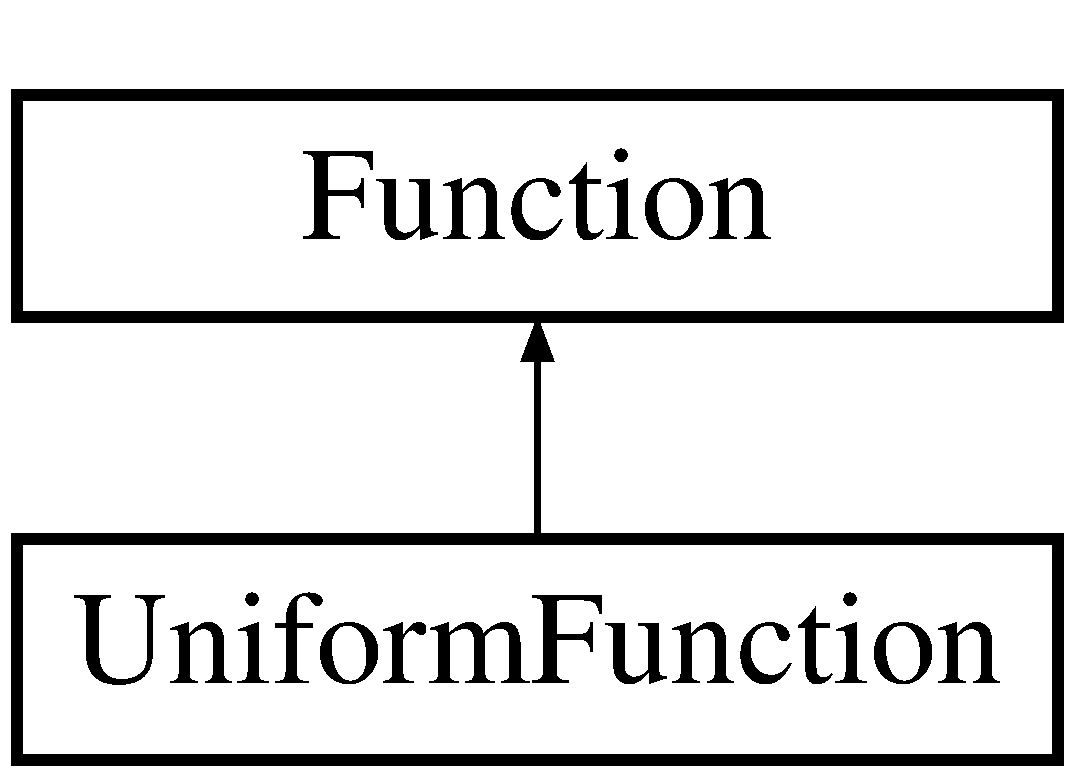
\includegraphics[height=2cm]{classUniformFunction}
\end{center}
\end{figure}
\subsection*{Public Member Functions}
\begin{CompactItemize}
\item 
{\bf UniformFunction} (unsigned long Dimensionality)
\item 
virtual {\bf $\sim$UniformFunction} ()
\item 
virtual {\bf Function} $\ast$ {\bf clone} () const 
\item 
virtual void {\bf function} (MyArray \&xs, MyArray \&res)
\item 
virtual void {\bf NormedIntegralInverse} (MyArray \&xs, MyArray \&res)
\item 
virtual void {\bf SetParams} (MyArray \&params\_\-)
\end{CompactItemize}


\subsection{Detailed Description}


Definition at line 69 of file Function.h.

\subsection{Constructor \& Destructor Documentation}
\index{UniformFunction@{UniformFunction}!UniformFunction@{UniformFunction}}
\index{UniformFunction@{UniformFunction}!UniformFunction@{UniformFunction}}
\subsubsection{\setlength{\rightskip}{0pt plus 5cm}UniformFunction::UniformFunction (unsigned long {\em Dimensionality})}\label{classUniformFunction_25d798ef7cb0a90ccfa50fcdcf9438a3}




Definition at line 64 of file Function.cpp.

Referenced by clone().

\begin{Code}\begin{verbatim}65   : Function( Dimensionality )
66 {
67 
68 }
\end{verbatim}
\end{Code}


\index{UniformFunction@{UniformFunction}!~UniformFunction@{$\sim$UniformFunction}}
\index{~UniformFunction@{$\sim$UniformFunction}!UniformFunction@{UniformFunction}}
\subsubsection{\setlength{\rightskip}{0pt plus 5cm}UniformFunction::$\sim$UniformFunction ()\hspace{0.3cm}{\tt  [virtual]}}\label{classUniformFunction_5498bd978cd9441cd3c4e195240f6347}




Definition at line 70 of file Function.cpp.

\begin{Code}\begin{verbatim}71 {
72 
73 }
\end{verbatim}
\end{Code}




\subsection{Member Function Documentation}
\index{UniformFunction@{UniformFunction}!clone@{clone}}
\index{clone@{clone}!UniformFunction@{UniformFunction}}
\subsubsection{\setlength{\rightskip}{0pt plus 5cm}{\bf Function} $\ast$ UniformFunction::clone () const\hspace{0.3cm}{\tt  [virtual]}}\label{classUniformFunction_9b57843688a438ac030f3abcfb4d07ac}




Implements {\bf Function} \doxyref{}{p.}{classFunction_cae7bf3099d7e05b59814823dab252b2}.

Definition at line 75 of file Function.cpp.

References UniformFunction().

\begin{Code}\begin{verbatim}76 {
77   return new UniformFunction(*this);
78 }
\end{verbatim}
\end{Code}


\index{UniformFunction@{UniformFunction}!function@{function}}
\index{function@{function}!UniformFunction@{UniformFunction}}
\subsubsection{\setlength{\rightskip}{0pt plus 5cm}void UniformFunction::function (MyArray \& {\em xs}, MyArray \& {\em res})\hspace{0.3cm}{\tt  [virtual]}}\label{classUniformFunction_c7b39b7195838195e1796570e549e67f}




Implements {\bf Function} \doxyref{}{p.}{classFunction_a78440b1498d1b7e113b163dfc88274c}.

Definition at line 80 of file Function.cpp.

References Function::GetDimensionality(), and Function::GetRange().

\begin{Code}\begin{verbatim}81 {
82   for (unsigned long i=0; i<GetDimensionality(); ++i)
83   {
84     res[i] = 1. / GetRange(i);
85   }
86 }
\end{verbatim}
\end{Code}


\index{UniformFunction@{UniformFunction}!NormedIntegralInverse@{NormedIntegralInverse}}
\index{NormedIntegralInverse@{NormedIntegralInverse}!UniformFunction@{UniformFunction}}
\subsubsection{\setlength{\rightskip}{0pt plus 5cm}void UniformFunction::NormedIntegralInverse (MyArray \& {\em xs}, MyArray \& {\em res})\hspace{0.3cm}{\tt  [virtual]}}\label{classUniformFunction_db51f361d9802c90260b584bf590a1a1}




Implements {\bf Function} \doxyref{}{p.}{classFunction_9e1a0a6468b4df5de365481db11df5d4}.

Definition at line 88 of file Function.cpp.

References Function::GetDimensionality(), Function::GetRange(), and Function::GetXmin().

\begin{Code}\begin{verbatim}89 {
90   for (unsigned long i=0; i<GetDimensionality(); ++i)
91   {
92     xs[i] = GetXmin(i) + uniforms[i]*GetRange(i);
93   }
94 }
\end{verbatim}
\end{Code}


\index{UniformFunction@{UniformFunction}!SetParams@{SetParams}}
\index{SetParams@{SetParams}!UniformFunction@{UniformFunction}}
\subsubsection{\setlength{\rightskip}{0pt plus 5cm}void UniformFunction::SetParams (MyArray \& {\em params\_\-})\hspace{0.3cm}{\tt  [virtual]}}\label{classUniformFunction_a4666e3a6e7420a5b4c9a15d3677d762}




Implements {\bf Function} \doxyref{}{p.}{classFunction_6944f24e3174d98fe7c61dc0652d3ae4}.

Definition at line 96 of file Function.cpp.

\begin{Code}\begin{verbatim}97 {
98 
99 }
\end{verbatim}
\end{Code}




The documentation for this class was generated from the following files:\begin{CompactItemize}
\item 
Gyulassy/opacity3/src/glv1/{\bf Function.h}\item 
Gyulassy/opacity3/src/glv1/{\bf Function.cpp}\end{CompactItemize}

\section{UnitStepFunction Class Reference}
\label{classUnitStepFunction}\index{UnitStepFunction@{UnitStepFunction}}
{\tt \#include $<$Function.h$>$}

Inheritance diagram for UnitStepFunction::\begin{figure}[H]
\begin{center}
\leavevmode
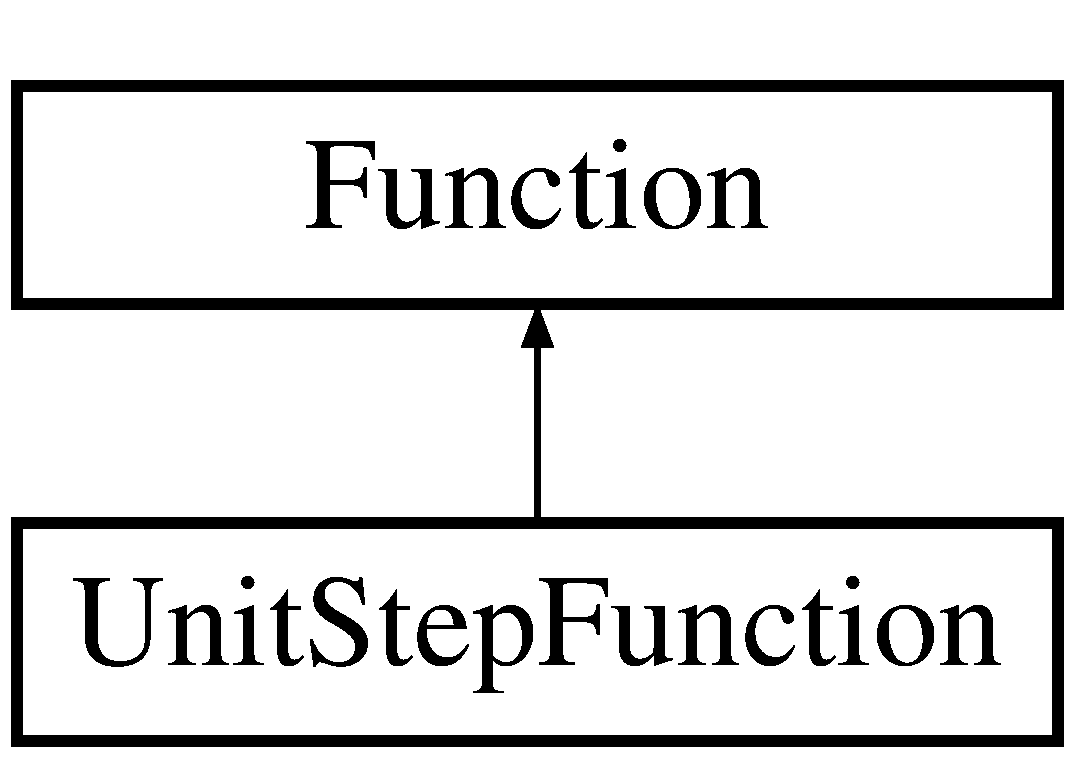
\includegraphics[height=2cm]{classUnitStepFunction}
\end{center}
\end{figure}
\subsection*{Public Member Functions}
\begin{CompactItemize}
\item 
{\bf UnitStepFunction} (unsigned long Dimensionality)
\item 
virtual {\bf $\sim$UnitStepFunction} ()
\item 
virtual {\bf Function} $\ast$ {\bf clone} () const 
\item 
virtual void {\bf function} (MyArray \&xs, MyArray \&res)
\item 
virtual void {\bf NormedIntegralInverse} (MyArray \&xs, MyArray \&res)
\item 
virtual void {\bf SetParams} (MyArray \&params\_\-)
\end{CompactItemize}
\subsection*{Private Attributes}
\begin{CompactItemize}
\item 
MyArray {\bf steps}
\end{CompactItemize}


\subsection{Detailed Description}


Definition at line 85 of file Function.h.

\subsection{Constructor \& Destructor Documentation}
\index{UnitStepFunction@{UnitStepFunction}!UnitStepFunction@{UnitStepFunction}}
\index{UnitStepFunction@{UnitStepFunction}!UnitStepFunction@{UnitStepFunction}}
\subsubsection{\setlength{\rightskip}{0pt plus 5cm}UnitStepFunction::UnitStepFunction (unsigned long {\em Dimensionality})}\label{classUnitStepFunction_272c40fc075f370eb8e20f0b50c11a4a}




Definition at line 104 of file Function.cpp.

Referenced by clone().

\begin{Code}\begin{verbatim}105   : Function( Dimensionality ), steps( Dimensionality )
106 {
107 
108 }
\end{verbatim}
\end{Code}


\index{UnitStepFunction@{UnitStepFunction}!~UnitStepFunction@{$\sim$UnitStepFunction}}
\index{~UnitStepFunction@{$\sim$UnitStepFunction}!UnitStepFunction@{UnitStepFunction}}
\subsubsection{\setlength{\rightskip}{0pt plus 5cm}UnitStepFunction::$\sim$UnitStepFunction ()\hspace{0.3cm}{\tt  [virtual]}}\label{classUnitStepFunction_1643ca85de9bda43d6a85a17dc2879a0}




Definition at line 110 of file Function.cpp.

\begin{Code}\begin{verbatim}111 {
112 
113 }
\end{verbatim}
\end{Code}




\subsection{Member Function Documentation}
\index{UnitStepFunction@{UnitStepFunction}!clone@{clone}}
\index{clone@{clone}!UnitStepFunction@{UnitStepFunction}}
\subsubsection{\setlength{\rightskip}{0pt plus 5cm}{\bf Function} $\ast$ UnitStepFunction::clone () const\hspace{0.3cm}{\tt  [virtual]}}\label{classUnitStepFunction_c9575c66d4b1c47901fbb4d96065f93f}




Implements {\bf Function} \doxyref{}{p.}{classFunction_cae7bf3099d7e05b59814823dab252b2}.

Definition at line 115 of file Function.cpp.

References UnitStepFunction().

\begin{Code}\begin{verbatim}116 {
117   return new UnitStepFunction(*this);
118 }
\end{verbatim}
\end{Code}


\index{UnitStepFunction@{UnitStepFunction}!function@{function}}
\index{function@{function}!UnitStepFunction@{UnitStepFunction}}
\subsubsection{\setlength{\rightskip}{0pt plus 5cm}void UnitStepFunction::function (MyArray \& {\em xs}, MyArray \& {\em res})\hspace{0.3cm}{\tt  [virtual]}}\label{classUnitStepFunction_2a0ff6cc70176563ceedfd044e6da9de}




Implements {\bf Function} \doxyref{}{p.}{classFunction_a78440b1498d1b7e113b163dfc88274c}.

Definition at line 120 of file Function.cpp.

References Function::GetDimensionality(), Function::GetXmin(), and steps.

\begin{Code}\begin{verbatim}121 {
122   for (unsigned long i=0; i<GetDimensionality(); ++i)
123   {
124     xs[i] < steps[i]  ? res[i] = 1. / (steps[i]-GetXmin(i))  : res[i] = 0.;
125   }
126 }
\end{verbatim}
\end{Code}


\index{UnitStepFunction@{UnitStepFunction}!NormedIntegralInverse@{NormedIntegralInverse}}
\index{NormedIntegralInverse@{NormedIntegralInverse}!UnitStepFunction@{UnitStepFunction}}
\subsubsection{\setlength{\rightskip}{0pt plus 5cm}void UnitStepFunction::NormedIntegralInverse (MyArray \& {\em xs}, MyArray \& {\em res})\hspace{0.3cm}{\tt  [virtual]}}\label{classUnitStepFunction_c56d83c52d4e17781fb0a43d55051fcb}




Implements {\bf Function} \doxyref{}{p.}{classFunction_9e1a0a6468b4df5de365481db11df5d4}.

Definition at line 128 of file Function.cpp.

References Function::GetDimensionality(), Function::GetXmin(), and steps.

\begin{Code}\begin{verbatim}129 {
130   for (unsigned long i=0; i<GetDimensionality(); ++i)
131   {
132     xs[i] = GetXmin(i) + uniforms[i]*steps[i];
133   }
134 }
\end{verbatim}
\end{Code}


\index{UnitStepFunction@{UnitStepFunction}!SetParams@{SetParams}}
\index{SetParams@{SetParams}!UnitStepFunction@{UnitStepFunction}}
\subsubsection{\setlength{\rightskip}{0pt plus 5cm}void UnitStepFunction::SetParams (MyArray \& {\em params\_\-})\hspace{0.3cm}{\tt  [virtual]}}\label{classUnitStepFunction_76fde5d7a6e4ff7958a927298ff0379f}




Implements {\bf Function} \doxyref{}{p.}{classFunction_6944f24e3174d98fe7c61dc0652d3ae4}.

Definition at line 136 of file Function.cpp.

References steps.

\begin{Code}\begin{verbatim}137 {
138   steps = steps_;
139 }
\end{verbatim}
\end{Code}




\subsection{Member Data Documentation}
\index{UnitStepFunction@{UnitStepFunction}!steps@{steps}}
\index{steps@{steps}!UnitStepFunction@{UnitStepFunction}}
\subsubsection{\setlength{\rightskip}{0pt plus 5cm}MyArray {\bf UnitStepFunction::steps}\hspace{0.3cm}{\tt  [private]}}\label{classUnitStepFunction_d36d3310bf79bd0de69718608b1ae6a0}




Definition at line 98 of file Function.h.

Referenced by function(), NormedIntegralInverse(), and SetParams().

The documentation for this class was generated from the following files:\begin{CompactItemize}
\item 
Gyulassy/opacity3/src/glv1/{\bf Function.h}\item 
Gyulassy/opacity3/src/glv1/{\bf Function.cpp}\end{CompactItemize}

\section{Wrapper$<$ T $>$ Class Template Reference}
\label{classWrapper}\index{Wrapper@{Wrapper}}
{\tt \#include $<$Wrapper.h$>$}

\subsection*{Public Member Functions}
\begin{CompactItemize}
\item 
{\bf Wrapper} ()
\begin{CompactList}\small\item\em Constructor with no parameters - start the pointer as null and zero. \item\end{CompactList}\item 
{\bf Wrapper} (const T \&inner)
\begin{CompactList}\small\item\em Copy constructor - create a copy of the other object, using the 'clone' function. \item\end{CompactList}\item 
{\bf $\sim$Wrapper} ()
\begin{CompactList}\small\item\em Destructor - if the pointer is non-null, then delete the object. \item\end{CompactList}\item 
{\bf Wrapper} (const {\bf Wrapper}$<$ T $>$ \&original)
\begin{CompactList}\small\item\em Constructor supplying a 'wrapped' object, clone the inner object. \item\end{CompactList}\item 
T $\ast$ {\bf GetPointer} ()
\item 
const T $\ast$const {\bf GetConstPointer} () const 
\item 
{\bf Wrapper} \& {\bf operator=} (const {\bf Wrapper}$<$ T $>$ \&original)
\item 
T \& {\bf operator $\ast$} ()
\item 
const T \& {\bf operator $\ast$} () const 
\item 
const T $\ast$const {\bf operator $\rightarrow$ } () const 
\item 
T $\ast$ {\bf operator $\rightarrow$ } ()
\end{CompactItemize}
\subsection*{Private Attributes}
\begin{CompactItemize}
\item 
T $\ast$ {\bf DataPtr}
\end{CompactItemize}


\subsection{Detailed Description}
\subsubsection*{template$<$class T$>$ class Wrapper$<$ T $>$}

\begin{Desc}
\item[Author:]Simon Wicks copying out from Joshi 'C++ Design Patterns and Derivatives Pricing' A wrapper class to enable easy construction and assignment of new objects, but without worrying about deleting them when they go out of scope Any classes to be in the 'wrapper' must implement the 'clone' function \end{Desc}


Definition at line 11 of file Wrapper.h.

\subsection{Constructor \& Destructor Documentation}
\index{Wrapper@{Wrapper}!Wrapper@{Wrapper}}
\index{Wrapper@{Wrapper}!Wrapper@{Wrapper}}
\subsubsection{\setlength{\rightskip}{0pt plus 5cm}template$<$class T$>$ {\bf Wrapper}$<$ T $>$::{\bf Wrapper} ()\hspace{0.3cm}{\tt  [inline]}}\label{classWrapper_747788c9b29a997f4d805ec60e6e16a2}


Constructor with no parameters - start the pointer as null and zero. 



Definition at line 15 of file Wrapper.h.

\begin{Code}\begin{verbatim}15 { DataPtr = 0; }
\end{verbatim}
\end{Code}


\index{Wrapper@{Wrapper}!Wrapper@{Wrapper}}
\index{Wrapper@{Wrapper}!Wrapper@{Wrapper}}
\subsubsection{\setlength{\rightskip}{0pt plus 5cm}template$<$class T$>$ {\bf Wrapper}$<$ T $>$::{\bf Wrapper} (const T \& {\em inner})\hspace{0.3cm}{\tt  [inline]}}\label{classWrapper_75fb68554d62529a071016d297018dea}


Copy constructor - create a copy of the other object, using the 'clone' function. 



Definition at line 18 of file Wrapper.h.

\begin{Code}\begin{verbatim}19   {
20     DataPtr = inner.clone();
21   }
\end{verbatim}
\end{Code}


\index{Wrapper@{Wrapper}!~Wrapper@{$\sim$Wrapper}}
\index{~Wrapper@{$\sim$Wrapper}!Wrapper@{Wrapper}}
\subsubsection{\setlength{\rightskip}{0pt plus 5cm}template$<$class T$>$ {\bf Wrapper}$<$ T $>$::$\sim${\bf Wrapper} ()\hspace{0.3cm}{\tt  [inline]}}\label{classWrapper_5396fe1ce47468f5ceeec85eb423695d}


Destructor - if the pointer is non-null, then delete the object. 



Definition at line 24 of file Wrapper.h.

\begin{Code}\begin{verbatim}25   {
26     if (DataPtr != 0)
27       delete DataPtr;
28   }
\end{verbatim}
\end{Code}


\index{Wrapper@{Wrapper}!Wrapper@{Wrapper}}
\index{Wrapper@{Wrapper}!Wrapper@{Wrapper}}
\subsubsection{\setlength{\rightskip}{0pt plus 5cm}template$<$class T$>$ {\bf Wrapper}$<$ T $>$::{\bf Wrapper} (const {\bf Wrapper}$<$ T $>$ \& {\em original})\hspace{0.3cm}{\tt  [inline]}}\label{classWrapper_61fbc2f8719cbbb237bab3c94aef6a53}


Constructor supplying a 'wrapped' object, clone the inner object. 



Definition at line 31 of file Wrapper.h.

\begin{Code}\begin{verbatim}32   {
33     if (original.DataPtr != 0)
34       DataPtr = original.DataPtr->clone();
35     else
36       DataPtr = 0;
37   }
\end{verbatim}
\end{Code}




\subsection{Member Function Documentation}
\index{Wrapper@{Wrapper}!GetPointer@{GetPointer}}
\index{GetPointer@{GetPointer}!Wrapper@{Wrapper}}
\subsubsection{\setlength{\rightskip}{0pt plus 5cm}template$<$class T$>$ T$\ast$ {\bf Wrapper}$<$ T $>$::GetPointer ()\hspace{0.3cm}{\tt  [inline]}}\label{classWrapper_954084dfe67131560f58d85cb1c4190e}




Definition at line 40 of file Wrapper.h.

\begin{Code}\begin{verbatim}41   { return DataPtr; }
\end{verbatim}
\end{Code}


\index{Wrapper@{Wrapper}!GetConstPointer@{GetConstPointer}}
\index{GetConstPointer@{GetConstPointer}!Wrapper@{Wrapper}}
\subsubsection{\setlength{\rightskip}{0pt plus 5cm}template$<$class T$>$ const T$\ast$ const {\bf Wrapper}$<$ T $>$::GetConstPointer () const\hspace{0.3cm}{\tt  [inline]}}\label{classWrapper_5e9f52d10a6098286c2a552cf19ac619}




Definition at line 43 of file Wrapper.h.

\begin{Code}\begin{verbatim}44   { return DataPtr; }
\end{verbatim}
\end{Code}


\index{Wrapper@{Wrapper}!operator=@{operator=}}
\index{operator=@{operator=}!Wrapper@{Wrapper}}
\subsubsection{\setlength{\rightskip}{0pt plus 5cm}template$<$class T$>$ {\bf Wrapper}\& {\bf Wrapper}$<$ T $>$::operator= (const {\bf Wrapper}$<$ T $>$ \& {\em original})\hspace{0.3cm}{\tt  [inline]}}\label{classWrapper_8c19573051f3bbe811393abb3691147c}




Definition at line 46 of file Wrapper.h.

\begin{Code}\begin{verbatim}47   {
48     if (this != &original)
49     {
50       if (DataPtr != 0)
51         delete DataPtr;
52         
53       DataPtr = (original.DataPtr !=0) ? original.DataPtr->clone() : 0;
54     }
55     
56     return *this;
57   }
\end{verbatim}
\end{Code}


\index{Wrapper@{Wrapper}!operator *@{operator $\ast$}}
\index{operator *@{operator $\ast$}!Wrapper@{Wrapper}}
\subsubsection{\setlength{\rightskip}{0pt plus 5cm}template$<$class T$>$ T\& {\bf Wrapper}$<$ T $>$::operator $\ast$ ()\hspace{0.3cm}{\tt  [inline]}}\label{classWrapper_9b083b2466e4e43c516bc8a3e2e47e56}




Definition at line 59 of file Wrapper.h.

\begin{Code}\begin{verbatim}60   {
61     return *DataPtr;
62   }
\end{verbatim}
\end{Code}


\index{Wrapper@{Wrapper}!operator *@{operator $\ast$}}
\index{operator *@{operator $\ast$}!Wrapper@{Wrapper}}
\subsubsection{\setlength{\rightskip}{0pt plus 5cm}template$<$class T$>$ const T\& {\bf Wrapper}$<$ T $>$::operator $\ast$ () const\hspace{0.3cm}{\tt  [inline]}}\label{classWrapper_4841ac8c58122f1d8479577616f6617a}




Definition at line 64 of file Wrapper.h.

\begin{Code}\begin{verbatim}65   {
66     return *DataPtr;
67   }
\end{verbatim}
\end{Code}


\index{Wrapper@{Wrapper}!operator->@{operator-$>$}}
\index{operator->@{operator-$>$}!Wrapper@{Wrapper}}
\subsubsection{\setlength{\rightskip}{0pt plus 5cm}template$<$class T$>$ const T$\ast$ const {\bf Wrapper}$<$ T $>$::operator $\rightarrow$  () const\hspace{0.3cm}{\tt  [inline]}}\label{classWrapper_da2ce054a40a86d0a03d9bc339152736}




Definition at line 69 of file Wrapper.h.

\begin{Code}\begin{verbatim}70   {
71     return DataPtr;
72   }
\end{verbatim}
\end{Code}


\index{Wrapper@{Wrapper}!operator->@{operator-$>$}}
\index{operator->@{operator-$>$}!Wrapper@{Wrapper}}
\subsubsection{\setlength{\rightskip}{0pt plus 5cm}template$<$class T$>$ T$\ast$ {\bf Wrapper}$<$ T $>$::operator $\rightarrow$  ()\hspace{0.3cm}{\tt  [inline]}}\label{classWrapper_44a92ec32cd70089debea7205b2cc0a8}




Definition at line 74 of file Wrapper.h.

\begin{Code}\begin{verbatim}75   {
76     return DataPtr;
77   }
\end{verbatim}
\end{Code}




\subsection{Member Data Documentation}
\index{Wrapper@{Wrapper}!DataPtr@{DataPtr}}
\index{DataPtr@{DataPtr}!Wrapper@{Wrapper}}
\subsubsection{\setlength{\rightskip}{0pt plus 5cm}template$<$class T$>$ T$\ast$ {\bf Wrapper}$<$ T $>$::{\bf DataPtr}\hspace{0.3cm}{\tt  [private]}}\label{classWrapper_fa8d2e17d834993a45bcc1811c5945d8}




Definition at line 80 of file Wrapper.h.

Referenced by Wrapper$<$ StatGathering::StatisticsMC $>$::GetConstPointer(), Wrapper$<$ StatGathering::StatisticsMC $>$::GetPointer(), Wrapper$<$ StatGathering::StatisticsMC $>$::operator $\ast$(), Wrapper$<$ StatGathering::StatisticsMC $>$::operator $\rightarrow$ (), Wrapper$<$ StatGathering::StatisticsMC $>$::operator=(), Wrapper$<$ StatGathering::StatisticsMC $>$::Wrapper(), and Wrapper$<$ StatGathering::StatisticsMC $>$::$\sim$Wrapper().

The documentation for this class was generated from the following file:\begin{CompactItemize}
\item 
Gyulassy/opacity3/src/{\bf Wrapper.h}\end{CompactItemize}

\section{YukawaFunction Class Reference}
\label{classYukawaFunction}\index{YukawaFunction@{YukawaFunction}}
{\tt \#include $<$Function.h$>$}

Inheritance diagram for YukawaFunction::\begin{figure}[H]
\begin{center}
\leavevmode
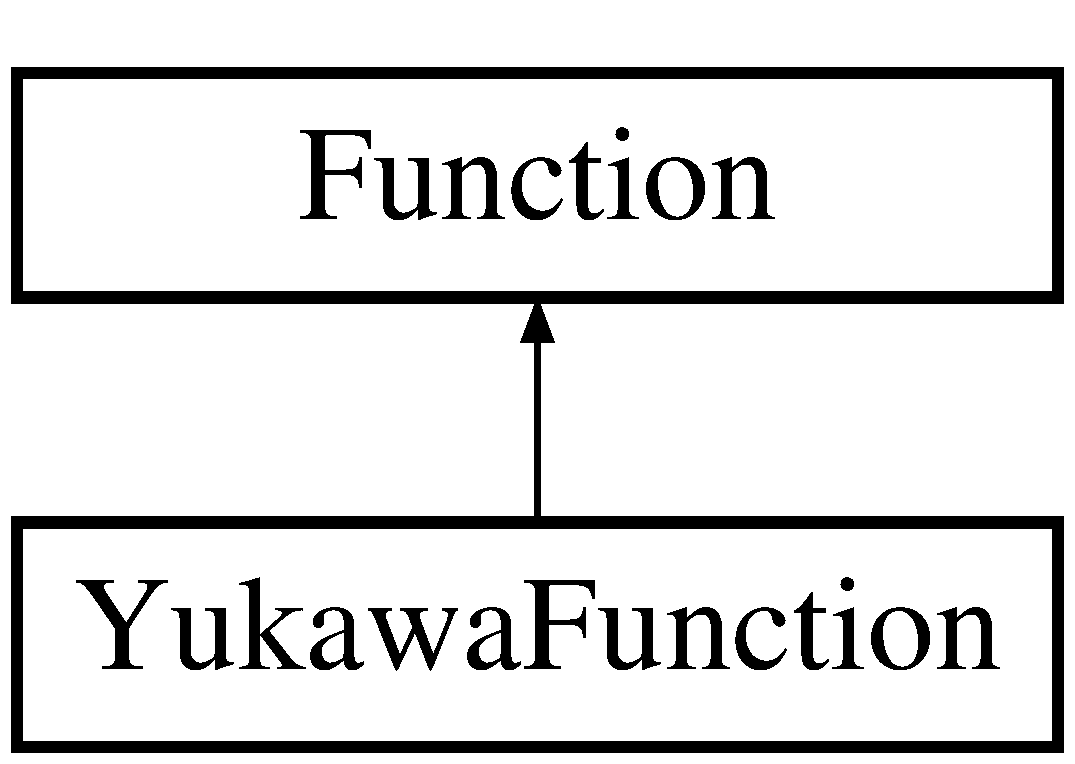
\includegraphics[height=2cm]{classYukawaFunction}
\end{center}
\end{figure}
\subsection*{Public Member Functions}
\begin{CompactItemize}
\item 
{\bf YukawaFunction} (unsigned long Dimensionality)
\item 
virtual {\bf $\sim$YukawaFunction} ()
\item 
virtual {\bf Function} $\ast$ {\bf clone} () const 
\item 
virtual void {\bf function} (MyArray \&xs, MyArray \&res)
\item 
virtual void {\bf NormedIntegralInverse} (MyArray \&xs, MyArray \&res)
\item 
virtual void {\bf SetParams} (MyArray \&params\_\-)
\end{CompactItemize}
\subsection*{Private Attributes}
\begin{CompactItemize}
\item 
MyArray {\bf mu2s}
\end{CompactItemize}


\subsection{Detailed Description}


Definition at line 53 of file Function.h.

\subsection{Constructor \& Destructor Documentation}
\index{YukawaFunction@{YukawaFunction}!YukawaFunction@{YukawaFunction}}
\index{YukawaFunction@{YukawaFunction}!YukawaFunction@{YukawaFunction}}
\subsubsection{\setlength{\rightskip}{0pt plus 5cm}YukawaFunction::YukawaFunction (unsigned long {\em Dimensionality})}\label{classYukawaFunction_092c7af1e8755547c5354c84d418be7c}




Definition at line 22 of file Function.cpp.

Referenced by clone().

\begin{Code}\begin{verbatim}23   : Function( Dimensionality ), mu2s( Dimensionality )
24 {
25 
26 }
\end{verbatim}
\end{Code}


\index{YukawaFunction@{YukawaFunction}!~YukawaFunction@{$\sim$YukawaFunction}}
\index{~YukawaFunction@{$\sim$YukawaFunction}!YukawaFunction@{YukawaFunction}}
\subsubsection{\setlength{\rightskip}{0pt plus 5cm}YukawaFunction::$\sim$YukawaFunction ()\hspace{0.3cm}{\tt  [virtual]}}\label{classYukawaFunction_1e07e5116228b911a3008940db1c4f9b}




Definition at line 28 of file Function.cpp.

\begin{Code}\begin{verbatim}29 {
30 
31 }
\end{verbatim}
\end{Code}




\subsection{Member Function Documentation}
\index{YukawaFunction@{YukawaFunction}!clone@{clone}}
\index{clone@{clone}!YukawaFunction@{YukawaFunction}}
\subsubsection{\setlength{\rightskip}{0pt plus 5cm}{\bf Function} $\ast$ YukawaFunction::clone () const\hspace{0.3cm}{\tt  [virtual]}}\label{classYukawaFunction_5f5caf1a5d9ccbbd111a72ce3961395e}




Implements {\bf Function} \doxyref{}{p.}{classFunction_cae7bf3099d7e05b59814823dab252b2}.

Definition at line 33 of file Function.cpp.

References YukawaFunction().

\begin{Code}\begin{verbatim}34 {
35   return new YukawaFunction( *this );
36 }
\end{verbatim}
\end{Code}


\index{YukawaFunction@{YukawaFunction}!function@{function}}
\index{function@{function}!YukawaFunction@{YukawaFunction}}
\subsubsection{\setlength{\rightskip}{0pt plus 5cm}void YukawaFunction::function (MyArray \& {\em xs}, MyArray \& {\em res})\hspace{0.3cm}{\tt  [virtual]}}\label{classYukawaFunction_e1cfdb6a1024fd9099c9d178bb25e30c}




Implements {\bf Function} \doxyref{}{p.}{classFunction_a78440b1498d1b7e113b163dfc88274c}.

Definition at line 38 of file Function.cpp.

References Function::GetDimensionality(), and mu2s.

\begin{Code}\begin{verbatim}39 {
40   for (unsigned long i=0; i<GetDimensionality(); ++i)
41   {
42     res[i] = 2.*xs[i]*mu2s[i] / pow( xs[i]*xs[i] + mu2s[i], 2 );
43   }
44 }
\end{verbatim}
\end{Code}


\index{YukawaFunction@{YukawaFunction}!NormedIntegralInverse@{NormedIntegralInverse}}
\index{NormedIntegralInverse@{NormedIntegralInverse}!YukawaFunction@{YukawaFunction}}
\subsubsection{\setlength{\rightskip}{0pt plus 5cm}void YukawaFunction::NormedIntegralInverse (MyArray \& {\em xs}, MyArray \& {\em res})\hspace{0.3cm}{\tt  [virtual]}}\label{classYukawaFunction_6946664b03976629db6fede4c250f363}




Implements {\bf Function} \doxyref{}{p.}{classFunction_9e1a0a6468b4df5de365481db11df5d4}.

Definition at line 46 of file Function.cpp.

References Function::GetDimensionality(), Function::GetXmax(), Function::GetXmin(), and mu2s.

\begin{Code}\begin{verbatim}47 {
48   for (unsigned long i=0; i<GetDimensionality(); ++i)
49   {
50     xs[i] = (pow(GetXmin(i),2) + mu2s[i]) * (pow(GetXmax(i),2) + mu2s[i]);
51     xs[i] /= mu2s[i] + pow(GetXmax(i),2) - (pow(GetXmax(i),2)-pow(GetXmin(i),2))*uniforms[i];
52     xs[i] -= mu2s[i];
53     xs[i] = sqrt(xs[i]);
54   }
55 }
\end{verbatim}
\end{Code}


\index{YukawaFunction@{YukawaFunction}!SetParams@{SetParams}}
\index{SetParams@{SetParams}!YukawaFunction@{YukawaFunction}}
\subsubsection{\setlength{\rightskip}{0pt plus 5cm}void YukawaFunction::SetParams (MyArray \& {\em params\_\-})\hspace{0.3cm}{\tt  [virtual]}}\label{classYukawaFunction_15b63ca3d7be01c385940f57641fdfad}




Implements {\bf Function} \doxyref{}{p.}{classFunction_6944f24e3174d98fe7c61dc0652d3ae4}.

Definition at line 57 of file Function.cpp.

References mu2s.

\begin{Code}\begin{verbatim}58 {
59   mu2s = mu2s_;
60 }
\end{verbatim}
\end{Code}




\subsection{Member Data Documentation}
\index{YukawaFunction@{YukawaFunction}!mu2s@{mu2s}}
\index{mu2s@{mu2s}!YukawaFunction@{YukawaFunction}}
\subsubsection{\setlength{\rightskip}{0pt plus 5cm}MyArray {\bf YukawaFunction::mu2s}\hspace{0.3cm}{\tt  [private]}}\label{classYukawaFunction_16023bd3790db880d3001b6430c173d0}




Definition at line 66 of file Function.h.

Referenced by function(), NormedIntegralInverse(), and SetParams().

The documentation for this class was generated from the following files:\begin{CompactItemize}
\item 
Gyulassy/opacity3/src/glv1/{\bf Function.h}\item 
Gyulassy/opacity3/src/glv1/{\bf Function.cpp}\end{CompactItemize}

\section{ZposGenerator Class Reference}
\label{classZposGenerator}\index{ZposGenerator@{ZposGenerator}}
{\tt \#include $<$zcolldist.h$>$}

\subsection*{Public Member Functions}
\begin{CompactItemize}
\item 
{\bf ZposGenerator} ({\bf Parameters} \&params\_\-, long opacity\_\-)
\item 
void {\bf FindRandomPositions} (MyArray \&Randoms)
\item 
void {\bf GetTempsMu2s} (MyArray \&temps, MyArray \&mu2s)
\item 
double {\bf GetDeltaZi} (int i) const 
\item 
double {\bf GetZweight} () const 
\end{CompactItemize}
\subsection*{Private Attributes}
\begin{CompactItemize}
\item 
const unsigned long {\bf mSize}
\item 
std::vector$<$ double $>$ {\bf mPositions}
\item 
double {\bf \_\-loverlambda}
\item 
double {\bf \_\-weight}
\item 
double {\bf \_\-mu}
\item 
double {\bf \_\-temp}
\item 
{\bf Wrapper}$<$ {\bf Function} $>$ {\bf refFn}
\item 
{\bf Wrapper}$<$ {\bf Function} $>$ {\bf sampleFn}
\end{CompactItemize}


\subsection{Detailed Description}
Generates the z positions, the positions of the collisions along the path length These z positions can be correlated with each other 

Definition at line 17 of file zcolldist.h.

\subsection{Constructor \& Destructor Documentation}
\index{ZposGenerator@{ZposGenerator}!ZposGenerator@{ZposGenerator}}
\index{ZposGenerator@{ZposGenerator}!ZposGenerator@{ZposGenerator}}
\subsubsection{\setlength{\rightskip}{0pt plus 5cm}ZposGenerator::ZposGenerator ({\bf Parameters} \& {\em params\_\-}, long {\em opacity\_\-})}\label{classZposGenerator_1e90862f06141844d8d663502b4c0cdc}




Definition at line 11 of file zcolldist.cpp.

References \_\-loverlambda, \_\-mu, \_\-temp, Parameters::GetParametersDouble(), mPositions, mSize, refFn, sampleFn, Function::SetLimits(), and ExpDecayFunction::SetParams().

\begin{Code}\begin{verbatim}12   : mSize( opacity_ ), mPositions( opacity_+1 )
13 {
14   std::vector<double> ReturnedParamsDouble;
15   std::vector<long> ReturnedParamsLong;
16   std::list<std::string> ReturnedParamsString;
17 
18   // First, we get the parameters of the medium
19   // This is: 1st = mu, 2nd = temperature, 3rd = gluon mass, 4th = gluon mean free path
20   // Here, we only need the gluon mass
21   // the zDist will need the others
22   ReturnedParamsDouble = params_.GetParametersDouble( "@mediumParams" );
23   _mu = ReturnedParamsDouble[0];
24   _temp = ReturnedParamsDouble[1];
25   double _gluonlambda = ReturnedParamsDouble[3];
26 
27   // The jet path length in the medium
28   ReturnedParamsDouble = params_.GetParametersDouble( "@pathLength" );
29   double _length = ReturnedParamsDouble[0];
30 
31   double _maxlen;
32   _maxlen = _length * 5.;
33   _loverlambda = _length / _gluonlambda;
34 
35   MyArray zmin(1), zmax(1), param(1);
36 
37   // Reference function => the function under the integral
38   // Sample function => the function from which to sample our Monte Carlo points
39 
40   // For uniform reference function
41 //  UniformFunction refFn1( 1 );
42 //  param[0] = 0.; zmin[0] = 0.; zmax[0] = _length;
43 //  refFn1.SetLimits( zmin, zmax); refFn1.SetParams( param );
44 
45   // For exponential decay reference function
46   ExpDecayFunction refFn1( 1 );
47   param[0] = _length / static_cast<double>(mSize+1); zmin[0] = 0.; zmax[0] = _maxlen;
48   refFn1.SetLimits( zmin, zmax ); refFn1.SetParams( param );
49 
50   // For uniform sample function
51 //  UniformFunction sampFn1( 1 );
52 //  param[0] = 0.; 
53 //  sampFn1.SetParams( param );
54 
55   // For exponential decay sample function
56   ExpDecayFunction sampFn1( 1 );
57   param[0] = _length / static_cast<double>(mSize+1);
58   sampFn1.SetParams( param );
59 
60 
61   refFn = refFn1;
62   sampleFn = sampFn1;
63 
64   mPositions[0] = 0.;
65 }
\end{verbatim}
\end{Code}




\subsection{Member Function Documentation}
\index{ZposGenerator@{ZposGenerator}!FindRandomPositions@{FindRandomPositions}}
\index{FindRandomPositions@{FindRandomPositions}!ZposGenerator@{ZposGenerator}}
\subsubsection{\setlength{\rightskip}{0pt plus 5cm}void ZposGenerator::FindRandomPositions (MyArray \& {\em Randoms})}\label{classZposGenerator_167471398a46f21d1013cf97e3606736}




Definition at line 67 of file zcolldist.cpp.

References SwUtils::\_\-factorial(), \_\-loverlambda, \_\-weight, mPositions, mSize, refFn, and sampleFn.

Referenced by RadCalcer::DistributeRandoms().

\begin{Code}\begin{verbatim}68 {
69   MyArray zmin(1), zmax(1), zIn(1), zOut(1), refOut(1), sampOut(1);
70   //_weight = _loverlambda;
71   _weight = 1. / _factorial( mSize );
72   for (unsigned long i=0; i<mSize; ++i)
73   {
74     //zmin[0] = mPositions[i]; zmax[0] = refFn->GetXmax(0);
75     zmin[0] = 0.; zmax[0] = refFn->GetXmax(0);
76     sampleFn->SetLimits( zmin, zmax );
77     zIn[0] = Randoms[i]; sampleFn->NormedIntegralInverse( zIn, zOut ); 
78     mPositions[i+1] = mPositions[i] + zOut[0]; //mPositions[i+1] = zOut[0];
79     refFn->function( zOut, refOut ); sampleFn->function( zOut, sampOut );
80     _weight *= _loverlambda;
81     _weight *= refOut[0] / sampOut[0];
82   }
83 
84 }
\end{verbatim}
\end{Code}


\index{ZposGenerator@{ZposGenerator}!GetTempsMu2s@{GetTempsMu2s}}
\index{GetTempsMu2s@{GetTempsMu2s}!ZposGenerator@{ZposGenerator}}
\subsubsection{\setlength{\rightskip}{0pt plus 5cm}void ZposGenerator::GetTempsMu2s (MyArray \& {\em temps}, MyArray \& {\em mu2s})}\label{classZposGenerator_cae2647a7b06e0bb71b69b3616bf8a53}




Definition at line 86 of file zcolldist.cpp.

References \_\-mu, \_\-temp, and mSize.

Referenced by RadCalcer::DistributeRandoms().

\begin{Code}\begin{verbatim}87 {
88   for (unsigned long i=0; i<mSize; ++i)
89   {
90     temps[i] = _temp; mu2s[i] = _mu*_mu;
91   }
92 }
\end{verbatim}
\end{Code}


\index{ZposGenerator@{ZposGenerator}!GetDeltaZi@{GetDeltaZi}}
\index{GetDeltaZi@{GetDeltaZi}!ZposGenerator@{ZposGenerator}}
\subsubsection{\setlength{\rightskip}{0pt plus 5cm}double ZposGenerator::GetDeltaZi (int {\em i}) const}\label{classZposGenerator_ff9cfd493e73f5d711f755c496c462f0}




Definition at line 94 of file zcolldist.cpp.

References mPositions.

Referenced by RadCalcer::\_\-interference().

\begin{Code}\begin{verbatim}95 {
96   double tmp;
97   tmp = mPositions[i] - mPositions[i-1];
98   
99   return tmp;
100 }
\end{verbatim}
\end{Code}


\index{ZposGenerator@{ZposGenerator}!GetZweight@{GetZweight}}
\index{GetZweight@{GetZweight}!ZposGenerator@{ZposGenerator}}
\subsubsection{\setlength{\rightskip}{0pt plus 5cm}double ZposGenerator::GetZweight () const}\label{classZposGenerator_4efcf84343b79a423e7dc356fd9d0261}




Definition at line 102 of file zcolldist.cpp.

References \_\-weight.

Referenced by RadCalcer::GetdNdk2dx().

\begin{Code}\begin{verbatim}103 {
104   return _weight;
105 }
\end{verbatim}
\end{Code}




\subsection{Member Data Documentation}
\index{ZposGenerator@{ZposGenerator}!mSize@{mSize}}
\index{mSize@{mSize}!ZposGenerator@{ZposGenerator}}
\subsubsection{\setlength{\rightskip}{0pt plus 5cm}const unsigned long {\bf ZposGenerator::mSize}\hspace{0.3cm}{\tt  [private]}}\label{classZposGenerator_d5447cbf01884d1309e5641863f928fd}




Definition at line 20 of file zcolldist.h.

Referenced by FindRandomPositions(), GetTempsMu2s(), and ZposGenerator().\index{ZposGenerator@{ZposGenerator}!mPositions@{mPositions}}
\index{mPositions@{mPositions}!ZposGenerator@{ZposGenerator}}
\subsubsection{\setlength{\rightskip}{0pt plus 5cm}std::vector$<$double$>$ {\bf ZposGenerator::mPositions}\hspace{0.3cm}{\tt  [private]}}\label{classZposGenerator_65b7ea3c519779af67e218dfd4b94e86}




Definition at line 22 of file zcolldist.h.

Referenced by FindRandomPositions(), GetDeltaZi(), and ZposGenerator().\index{ZposGenerator@{ZposGenerator}!_loverlambda@{\_\-loverlambda}}
\index{_loverlambda@{\_\-loverlambda}!ZposGenerator@{ZposGenerator}}
\subsubsection{\setlength{\rightskip}{0pt plus 5cm}double {\bf ZposGenerator::\_\-loverlambda}\hspace{0.3cm}{\tt  [private]}}\label{classZposGenerator_0c44c0025871a793c11a0459f0db343f}




Definition at line 24 of file zcolldist.h.

Referenced by FindRandomPositions(), and ZposGenerator().\index{ZposGenerator@{ZposGenerator}!_weight@{\_\-weight}}
\index{_weight@{\_\-weight}!ZposGenerator@{ZposGenerator}}
\subsubsection{\setlength{\rightskip}{0pt plus 5cm}double {\bf ZposGenerator::\_\-weight}\hspace{0.3cm}{\tt  [private]}}\label{classZposGenerator_13791204df3f02d883a309b880d11043}




Definition at line 25 of file zcolldist.h.

Referenced by FindRandomPositions(), and GetZweight().\index{ZposGenerator@{ZposGenerator}!_mu@{\_\-mu}}
\index{_mu@{\_\-mu}!ZposGenerator@{ZposGenerator}}
\subsubsection{\setlength{\rightskip}{0pt plus 5cm}double {\bf ZposGenerator::\_\-mu}\hspace{0.3cm}{\tt  [private]}}\label{classZposGenerator_fd43d806cc5d8ab6dd2a422ec40ea585}




Definition at line 27 of file zcolldist.h.

Referenced by GetTempsMu2s(), and ZposGenerator().\index{ZposGenerator@{ZposGenerator}!_temp@{\_\-temp}}
\index{_temp@{\_\-temp}!ZposGenerator@{ZposGenerator}}
\subsubsection{\setlength{\rightskip}{0pt plus 5cm}double {\bf ZposGenerator::\_\-temp}\hspace{0.3cm}{\tt  [private]}}\label{classZposGenerator_61581d2b91282a426764210e1ba8fad1}




Definition at line 28 of file zcolldist.h.

Referenced by GetTempsMu2s(), and ZposGenerator().\index{ZposGenerator@{ZposGenerator}!refFn@{refFn}}
\index{refFn@{refFn}!ZposGenerator@{ZposGenerator}}
\subsubsection{\setlength{\rightskip}{0pt plus 5cm}{\bf Wrapper}$<${\bf Function}$>$ {\bf ZposGenerator::refFn}\hspace{0.3cm}{\tt  [private]}}\label{classZposGenerator_f450ae3118a1d07d4983c0e50ad8ea96}




Definition at line 31 of file zcolldist.h.

Referenced by FindRandomPositions(), and ZposGenerator().\index{ZposGenerator@{ZposGenerator}!sampleFn@{sampleFn}}
\index{sampleFn@{sampleFn}!ZposGenerator@{ZposGenerator}}
\subsubsection{\setlength{\rightskip}{0pt plus 5cm}{\bf Wrapper}$<${\bf Function}$>$ {\bf ZposGenerator::sampleFn}\hspace{0.3cm}{\tt  [private]}}\label{classZposGenerator_850f0eb2564b3149d51898e28a9cbc22}




Definition at line 33 of file zcolldist.h.

Referenced by FindRandomPositions(), and ZposGenerator().

The documentation for this class was generated from the following files:\begin{CompactItemize}
\item 
Gyulassy/opacity3/src/glv1/{\bf zcolldist.h}\item 
Gyulassy/opacity3/src/glv1/{\bf zcolldist.cpp}\end{CompactItemize}

\chapter{opacity3 File Documentation}
\section{Gyulassy/opacity3/CMakeFiles/CompilerIdC/CMakeCCompilerId.c File Reference}
\label{CMakeCCompilerId_8c}\index{Gyulassy/opacity3/CMakeFiles/CompilerIdC/CMakeCCompilerId.c@{Gyulassy/opacity3/CMakeFiles/CompilerIdC/CMakeCCompilerId.c}}
\subsection*{Defines}
\begin{CompactItemize}
\item 
\#define {\bf COMPILER\_\-ID}~\char`\"{}\char`\"{}
\item 
\#define {\bf PLATFORM\_\-ID}~\char`\"{}\char`\"{}
\end{CompactItemize}
\subsection*{Functions}
\begin{CompactItemize}
\item 
int {\bf main} ()
\end{CompactItemize}
\subsection*{Variables}
\begin{CompactItemize}
\item 
char $\ast$ {\bf info\_\-compiler} = \char`\"{}INFO\char`\"{} \char`\"{}:\char`\"{} \char`\"{}compiler[\char`\"{} COMPILER\_\-ID \char`\"{}]\char`\"{}
\item 
char $\ast$ {\bf info\_\-platform} = \char`\"{}INFO\char`\"{} \char`\"{}:\char`\"{} \char`\"{}platform[\char`\"{} PLATFORM\_\-ID \char`\"{}]\char`\"{}
\end{CompactItemize}


\subsection{Define Documentation}
\index{CMakeCCompilerId.c@{CMakeCCompilerId.c}!COMPILER_ID@{COMPILER\_\-ID}}
\index{COMPILER_ID@{COMPILER\_\-ID}!CMakeCCompilerId.c@{CMakeCCompilerId.c}}
\subsubsection{\setlength{\rightskip}{0pt plus 5cm}\#define COMPILER\_\-ID~\char`\"{}\char`\"{}}\label{CMakeCCompilerId_8c_81dee0709ded976b2e0319239f72d174}




Definition at line 74 of file CMakeCCompilerId.c.\index{CMakeCCompilerId.c@{CMakeCCompilerId.c}!PLATFORM_ID@{PLATFORM\_\-ID}}
\index{PLATFORM_ID@{PLATFORM\_\-ID}!CMakeCCompilerId.c@{CMakeCCompilerId.c}}
\subsubsection{\setlength{\rightskip}{0pt plus 5cm}\#define PLATFORM\_\-ID~\char`\"{}\char`\"{}}\label{CMakeCCompilerId_8c_dbc5372f40838899018fadbc89bd588b}




Definition at line 158 of file CMakeCCompilerId.c.

\subsection{Function Documentation}
\index{CMakeCCompilerId.c@{CMakeCCompilerId.c}!main@{main}}
\index{main@{main}!CMakeCCompilerId.c@{CMakeCCompilerId.c}}
\subsubsection{\setlength{\rightskip}{0pt plus 5cm}int main (void)}\label{CMakeCCompilerId_8c_e66f6b31b5ad750f1fe042a706a4e3d4}




Definition at line 12 of file CMakeCCompilerId.c.

\begin{Code}\begin{verbatim}12 { return 0; }
\end{verbatim}
\end{Code}




\subsection{Variable Documentation}
\index{CMakeCCompilerId.c@{CMakeCCompilerId.c}!info_compiler@{info\_\-compiler}}
\index{info_compiler@{info\_\-compiler}!CMakeCCompilerId.c@{CMakeCCompilerId.c}}
\subsubsection{\setlength{\rightskip}{0pt plus 5cm}char$\ast$ {\bf info\_\-compiler} = \char`\"{}INFO\char`\"{} \char`\"{}:\char`\"{} \char`\"{}compiler[\char`\"{} COMPILER\_\-ID \char`\"{}]\char`\"{}}\label{CMakeCCompilerId_8c_ab4f0400f2b990cc0cfaa596066ed23a}




Definition at line 82 of file CMakeCCompilerId.c.\index{CMakeCCompilerId.c@{CMakeCCompilerId.c}!info_platform@{info\_\-platform}}
\index{info_platform@{info\_\-platform}!CMakeCCompilerId.c@{CMakeCCompilerId.c}}
\subsubsection{\setlength{\rightskip}{0pt plus 5cm}char$\ast$ {\bf info\_\-platform} = \char`\"{}INFO\char`\"{} \char`\"{}:\char`\"{} \char`\"{}platform[\char`\"{} PLATFORM\_\-ID \char`\"{}]\char`\"{}}\label{CMakeCCompilerId_8c_bfa30dab5bd89c85774e2aaaca5262d1}




Definition at line 166 of file CMakeCCompilerId.c.
\section{Gyulassy/opacity3/CMakeFiles/CompilerIdCXX/CMakeCXXCompilerId.cpp File Reference}
\label{CMakeCXXCompilerId_8cpp}\index{Gyulassy/opacity3/CMakeFiles/CompilerIdCXX/CMakeCXXCompilerId.cpp@{Gyulassy/opacity3/CMakeFiles/CompilerIdCXX/CMakeCXXCompilerId.cpp}}
\subsection*{Defines}
\begin{CompactItemize}
\item 
\#define {\bf COMPILER\_\-ID}~\char`\"{}\char`\"{}
\item 
\#define {\bf PLATFORM\_\-ID}~\char`\"{}\char`\"{}
\end{CompactItemize}
\subsection*{Functions}
\begin{CompactItemize}
\item 
int {\bf main} ()
\end{CompactItemize}
\subsection*{Variables}
\begin{CompactItemize}
\item 
char $\ast$ {\bf info\_\-compiler} = \char`\"{}INFO\char`\"{} \char`\"{}:\char`\"{} \char`\"{}compiler[\char`\"{} COMPILER\_\-ID \char`\"{}]\char`\"{}
\item 
char $\ast$ {\bf info\_\-platform} = \char`\"{}INFO\char`\"{} \char`\"{}:\char`\"{} \char`\"{}platform[\char`\"{} PLATFORM\_\-ID \char`\"{}]\char`\"{}
\end{CompactItemize}


\subsection{Define Documentation}
\index{CMakeCXXCompilerId.cpp@{CMakeCXXCompilerId.cpp}!COMPILER_ID@{COMPILER\_\-ID}}
\index{COMPILER_ID@{COMPILER\_\-ID}!CMakeCXXCompilerId.cpp@{CMakeCXXCompilerId.cpp}}
\subsubsection{\setlength{\rightskip}{0pt plus 5cm}\#define COMPILER\_\-ID~\char`\"{}\char`\"{}}\label{CMakeCXXCompilerId_8cpp_81dee0709ded976b2e0319239f72d174}




Definition at line 62 of file CMakeCXXCompilerId.cpp.\index{CMakeCXXCompilerId.cpp@{CMakeCXXCompilerId.cpp}!PLATFORM_ID@{PLATFORM\_\-ID}}
\index{PLATFORM_ID@{PLATFORM\_\-ID}!CMakeCXXCompilerId.cpp@{CMakeCXXCompilerId.cpp}}
\subsubsection{\setlength{\rightskip}{0pt plus 5cm}\#define PLATFORM\_\-ID~\char`\"{}\char`\"{}}\label{CMakeCXXCompilerId_8cpp_dbc5372f40838899018fadbc89bd588b}




Definition at line 146 of file CMakeCXXCompilerId.cpp.

\subsection{Function Documentation}
\index{CMakeCXXCompilerId.cpp@{CMakeCXXCompilerId.cpp}!main@{main}}
\index{main@{main}!CMakeCXXCompilerId.cpp@{CMakeCXXCompilerId.cpp}}
\subsubsection{\setlength{\rightskip}{0pt plus 5cm}int main (void)}\label{CMakeCXXCompilerId_8cpp_e66f6b31b5ad750f1fe042a706a4e3d4}




Definition at line 9 of file CMakeCXXCompilerId.cpp.

\begin{Code}\begin{verbatim}9 { return 0; }
\end{verbatim}
\end{Code}




\subsection{Variable Documentation}
\index{CMakeCXXCompilerId.cpp@{CMakeCXXCompilerId.cpp}!info_compiler@{info\_\-compiler}}
\index{info_compiler@{info\_\-compiler}!CMakeCXXCompilerId.cpp@{CMakeCXXCompilerId.cpp}}
\subsubsection{\setlength{\rightskip}{0pt plus 5cm}char$\ast$ {\bf info\_\-compiler} = \char`\"{}INFO\char`\"{} \char`\"{}:\char`\"{} \char`\"{}compiler[\char`\"{} COMPILER\_\-ID \char`\"{}]\char`\"{}}\label{CMakeCXXCompilerId_8cpp_ab4f0400f2b990cc0cfaa596066ed23a}




Definition at line 70 of file CMakeCXXCompilerId.cpp.\index{CMakeCXXCompilerId.cpp@{CMakeCXXCompilerId.cpp}!info_platform@{info\_\-platform}}
\index{info_platform@{info\_\-platform}!CMakeCXXCompilerId.cpp@{CMakeCXXCompilerId.cpp}}
\subsubsection{\setlength{\rightskip}{0pt plus 5cm}char$\ast$ {\bf info\_\-platform} = \char`\"{}INFO\char`\"{} \char`\"{}:\char`\"{} \char`\"{}platform[\char`\"{} PLATFORM\_\-ID \char`\"{}]\char`\"{}}\label{CMakeCXXCompilerId_8cpp_bfa30dab5bd89c85774e2aaaca5262d1}




Definition at line 154 of file CMakeCXXCompilerId.cpp.
\section{Gyulassy/opacity3/src/Arrays.h File Reference}
\label{Arrays_8h}\index{Gyulassy/opacity3/src/Arrays.h@{Gyulassy/opacity3/src/Arrays.h}}
{\tt \#include \char`\"{}boost/multi\_\-array.hpp\char`\"{}}\par
{\tt \#include $<$valarray$>$}\par
\subsection*{Namespaces}
\begin{CompactItemize}
\item 
namespace {\bf SwArrays}
\end{CompactItemize}
\subsection*{Typedefs}
\begin{CompactItemize}
\item 
typedef std::vector$<$ double $>$ {\bf SwArrays::MyArray}
\item 
typedef std::valarray$<$ std::valarray$<$ double $>$ $>$ {\bf SwArrays::MyArray2D}
\item 
typedef boost::multi\_\-array$<$ double, 1 $>$ {\bf SwArrays::array1D}
\item 
typedef array1D::index {\bf SwArrays::index1D}
\item 
typedef boost::multi\_\-array$<$ double, 2 $>$ {\bf SwArrays::array2D}
\item 
typedef array2D::index {\bf SwArrays::index2D}
\item 
typedef boost::multi\_\-array$<$ double, 3 $>$ {\bf SwArrays::array3D}
\item 
typedef array3D::index {\bf SwArrays::index3D}
\end{CompactItemize}

\section{Gyulassy/opacity3/src/constants.cpp File Reference}
\label{constants_8cpp}\index{Gyulassy/opacity3/src/constants.cpp@{Gyulassy/opacity3/src/constants.cpp}}
{\tt \#include $<$vector$>$}\par
{\tt \#include \char`\"{}constants.h\char`\"{}}\par
\subsection*{Namespaces}
\begin{CompactItemize}
\item 
namespace {\bf SwUtils}
\end{CompactItemize}
\subsection*{Functions}
\begin{CompactItemize}
\item 
long {\bf SwUtils::\_\-FindNextPowerOfTwo} (long value)
\item 
long {\bf SwUtils::\_\-Combinatoric} (long n, long r)
\end{CompactItemize}

\section{Gyulassy/opacity3/src/constants.h File Reference}
\label{constants_8h}\index{Gyulassy/opacity3/src/constants.h@{Gyulassy/opacity3/src/constants.h}}
{\tt \#include $<$vector$>$}\par
\subsection*{Namespaces}
\begin{CompactItemize}
\item 
namespace {\bf SwUtils}
\end{CompactItemize}
\subsection*{Functions}
\begin{CompactItemize}
\item 
long {\bf SwUtils::\_\-factorial} (long value, long endval=1)
\item 
long {\bf SwUtils::\_\-FindNextPowerOfTwo} (long value)
\item 
long {\bf SwUtils::\_\-Combinatoric} (long n, long r)
\item 
long {\bf SwUtils::power} (long num, long pow)
\item 
bool {\bf SwUtils::\_\-TestBitI} (unsigned long num, unsigned long i)
\item 
void {\bf SwUtils::\_\-NumberToBoolArray} (unsigned long num, std::vector$<$ bool $>$ \&boolarray, unsigned long length)
\item 
long {\bf SwUtils::\_\-CountNumZeroes} (unsigned long num, unsigned long length)
\item 
bool {\bf SwUtils::\_\-IsPowerOfTwo} (long value)
\end{CompactItemize}
\subsection*{Variables}
\begin{CompactItemize}
\item 
const double {\bf SwUtils::pi} = 3.141592653589793238
\item 
const double {\bf SwUtils::overpi} = 0.3183098861837906715
\item 
const double {\bf SwUtils::hbarc} = 0.197
\end{CompactItemize}

\section{Gyulassy/opacity3/src/driver.h File Reference}
\label{driver_8h}\index{Gyulassy/opacity3/src/driver.h@{Gyulassy/opacity3/src/driver.h}}
{\tt \#include $<$string$>$}\par
{\tt \#include $<$vector$>$}\par
{\tt \#include \char`\"{}Wrapper.h\char`\"{}}\par
{\tt \#include \char`\"{}randoms/Random3.h\char`\"{}}\par
{\tt \#include \char`\"{}randoms/RandDrand.h\char`\"{}}\par
{\tt \#include \char`\"{}randoms/RandSobol.h\char`\"{}}\par
{\tt \#include \char`\"{}Arrays.h\char`\"{}}\par
{\tt \#include \char`\"{}parameters.h\char`\"{}}\par
\subsection*{Classes}
\begin{CompactItemize}
\item 
class {\bf Driver$<$ TcalcEngine, Tstore, numOfRandoms $>$}
\end{CompactItemize}

\section{Gyulassy/opacity3/src/glv1/Function.cpp File Reference}
\label{Function_8cpp}\index{Gyulassy/opacity3/src/glv1/Function.cpp@{Gyulassy/opacity3/src/glv1/Function.cpp}}
{\tt \#include \char`\"{}Function.h\char`\"{}}\par

\section{Gyulassy/opacity3/src/glv1/Function.h File Reference}
\label{Function_8h}\index{Gyulassy/opacity3/src/glv1/Function.h@{Gyulassy/opacity3/src/glv1/Function.h}}
{\tt \#include \char`\"{}../Arrays.h\char`\"{}}\par
\subsection*{Classes}
\begin{CompactItemize}
\item 
class {\bf Function}
\item 
class {\bf YukawaFunction}
\item 
class {\bf UniformFunction}
\item 
class {\bf UnitStepFunction}
\item 
class {\bf ExpDecayFunction}
\end{CompactItemize}

\section{Gyulassy/opacity3/src/glv1/qperparraynew.cpp File Reference}
\label{qperparraynew_8cpp}\index{Gyulassy/opacity3/src/glv1/qperparraynew.cpp@{Gyulassy/opacity3/src/glv1/qperparraynew.cpp}}
{\tt \#include \char`\"{}qperparraynew.h\char`\"{}}\par
{\tt \#include \char`\"{}../constants.h\char`\"{}}\par
\subsection*{Functions}
\begin{CompactItemize}
\item 
void {\bf \_\-FillFirstRow} (unsigned long n, unsigned long z, std::vector$<$ bool $>$ zeroed, array2D \&qiqjs, array3D \&sumqiqjs)
\item 
void {\bf \_\-FillNextRow} (unsigned long n, unsigned long i, unsigned long z, std::vector$<$ bool $>$ zeroed, array2D \&qiqjs, array3D \&sumqiqjs)
\item 
void {\bf \_\-FillAllRows2DSymmetric} (unsigned long n, array2D \&qiqjs, array3D \&sumqiqjs, long z)
\item 
void {\bf \_\-FillAllRows1D} (unsigned long n, array1D \&khatqis, array2D \&sumkhatqis, long z)
\item 
void {\bf \_\-Fill2DFrom1D} (unsigned long n, array2D \&sumkhatqi\_\-iton, array3D \&sumkhatqikhatqj\_\-itonjton, long z)
\item 
void {\bf \_\-DotProducts2D} (unsigned long n, MyArray \&mags, MyArray \&ths, array2D \&res)
\item 
void {\bf \_\-DotProducts1D} (unsigned long n, double mag1, double th1, MyArray \&mags, MyArray \&ths, array1D \&res)
\item 
void {\bf \_\-OuterProduct1D1D} (unsigned long n, MyArray \&mags1, MyArray \&ths1, MyArray \&mags2, MyArray \&ths2, array2D \&res)
\item 
void {\bf \_\-OuterProduct0D1D} (unsigned long n, double mag1, double th1, MyArray \&mags2, MyArray \&ths2, array1D \&res)
\item 
void {\bf \_\-Iterate2DForZeroes} (unsigned long n, array2D \&qiqjs, array3D \&sumqiqjs)
\item 
void {\bf \_\-Iterate1DForZeroes} (unsigned long n, array1D \&khatqis, array2D \&sumkhatqis)
\end{CompactItemize}


\subsection{Function Documentation}
\index{qperparraynew.cpp@{qperparraynew.cpp}!_DotProducts1D@{\_\-DotProducts1D}}
\index{_DotProducts1D@{\_\-DotProducts1D}!qperparraynew.cpp@{qperparraynew.cpp}}
\subsubsection{\setlength{\rightskip}{0pt plus 5cm}void @8::\_\-DotProducts1D (unsigned long {\em n}, double {\em mag1}, double {\em th1}, MyArray \& {\em mags}, MyArray \& {\em ths}, array1D \& {\em res})\hspace{0.3cm}{\tt  [static]}}\label{qperparraynew_8cpp_aea824af3e9dc625dd755fe24f0492b2}




Definition at line 147 of file qperparraynew.cpp.

Referenced by QperpCalculator::CalcQmatrices2().

\begin{Code}\begin{verbatim}149 {
150   // TODO: put in asserts to check that the dimensions of mags, ths and res are correct
151 
152   // No need to pre-calculate the cosine this time, we'll just jump in
153   for (unsigned long i=0; i!=n; ++i)
154     res[i] = mag1 * mags[i] * cos( th1 - ths[i] );
155 
156   // And we're done!
157 }
\end{verbatim}
\end{Code}


\index{qperparraynew.cpp@{qperparraynew.cpp}!_DotProducts2D@{\_\-DotProducts2D}}
\index{_DotProducts2D@{\_\-DotProducts2D}!qperparraynew.cpp@{qperparraynew.cpp}}
\subsubsection{\setlength{\rightskip}{0pt plus 5cm}void @8::\_\-DotProducts2D (unsigned long {\em n}, MyArray \& {\em mags}, MyArray \& {\em ths}, array2D \& {\em res})\hspace{0.3cm}{\tt  [static]}}\label{qperparraynew_8cpp_3b87a5052e73e5de13161681e25cf1fa}




Definition at line 111 of file qperparraynew.cpp.

Referenced by QperpCalculator::CalcQmatrices2().

\begin{Code}\begin{verbatim}112 {
113   // TODO: put in asserts to check that the dimensions of mags, ths and res are correct
114 
115   // The operations sin and cos are numerically expensive
116   // For the dot products: will need cos( ths[i] - ths[j] )
117   // = cos(ths[i]) cos(ths[j]) + sin(ths[i]) sin(ths[j])
118   // Here: evaluate them 2n times, instead of possibly n^2 or 0.5*n(n+1)
119   MyArray sines(n), cosines(n);
120   for (unsigned long i=0; i!=n; ++i)
121   {
122     sines[i] = sin( ths[i] );
123     cosines[i] = cos( ths[i] );
124   }
125 
126   // Now, find the 2D matrix qi.qj
127   // We know that it is symmetric, so first we'll evaluate the off-diagonal on
128   // one side, then mirror it over to the other side
129   for (unsigned long i=0; i!=n; ++i)
130     for (unsigned long j=i+1; j!=n; ++j)
131     {
132       res[i][j] = mags[i] * mags[j] * ( cosines[i]*cosines[j] + sines[i]*sines[j] );
133       res[j][i] = res[i][j];
134     }
135 
136   // Now all that's left is the diagonal
137   for (unsigned long i=0; i!=n; ++i)
138     res[i][i] = mags[i] * mags[i];
139 
140   // And we're done!
141 }
\end{verbatim}
\end{Code}


\index{qperparraynew.cpp@{qperparraynew.cpp}!_Fill2DFrom1D@{\_\-Fill2DFrom1D}}
\index{_Fill2DFrom1D@{\_\-Fill2DFrom1D}!qperparraynew.cpp@{qperparraynew.cpp}}
\subsubsection{\setlength{\rightskip}{0pt plus 5cm}void @8::\_\-Fill2DFrom1D (unsigned long {\em n}, array2D \& {\em sumkhatqi\_\-iton}, array3D \& {\em sumkhatqikhatqj\_\-itonjton}, long {\em z})\hspace{0.3cm}{\tt  [static]}}\label{qperparraynew_8cpp_d834a8fc7dd96237188220f0ed214a38}




Definition at line 90 of file qperparraynew.cpp.

Referenced by QperpCalculator::CalcQmatrices2().

\begin{Code}\begin{verbatim}92 {
93   for (unsigned long i=0; i<n; ++i)
94   {
95     for (unsigned long j=0; j<n; ++j)
96     {
97       sumkhatqikhatqj_itonjton[z][i][j] = sumkhatqi_iton[z][i] + sumkhatqi_iton[z][j];
98     }
99     sumkhatqikhatqj_itonjton[z][i][n] = sumkhatqi_iton[z][i];
100   }
101   for (unsigned long j=0; j<n; ++j)
102   {
103     sumkhatqikhatqj_itonjton[z][n][j] = sumkhatqi_iton[z][j];
104   }
105   sumkhatqikhatqj_itonjton[z][n][n] = 0.;
106 }
\end{verbatim}
\end{Code}


\index{qperparraynew.cpp@{qperparraynew.cpp}!_FillAllRows1D@{\_\-FillAllRows1D}}
\index{_FillAllRows1D@{\_\-FillAllRows1D}!qperparraynew.cpp@{qperparraynew.cpp}}
\subsubsection{\setlength{\rightskip}{0pt plus 5cm}void @8::\_\-FillAllRows1D (unsigned long {\em n}, array1D \& {\em khatqis}, array2D \& {\em sumkhatqis}, long {\em z})\hspace{0.3cm}{\tt  [static]}}\label{qperparraynew_8cpp_6e28f19c83c2c6e49a2672873048fd10}




Definition at line 75 of file qperparraynew.cpp.

References SwUtils::\_\-NumberToBoolArray().

Referenced by QperpCalculator::CalcQmatrices2().

\begin{Code}\begin{verbatim}76 {
77   // We will be stepping through setting each qi to zero
78   // Create a vector of bools to indicate which qi is zero for this iteration
79   std::vector<bool> zeroed( n );
80 
81   // Convert number z to an array of bools, the ith element saying whether qi should be zero
82   _NumberToBoolArray( z, zeroed, n ); 
83   // Starting point for the iteration: (n-1)th has just one element, khat.q_{n-1}
84   sumkhatqis[z][n-1] = (!zeroed[n-1])*khatqis[n-1];
85   // Now iterate over the rest, adding one khatqi at each step
86   for (unsigned long i=2; i<(n+1); ++i)
87     sumkhatqis[z][n-i] = sumkhatqis[z][n-i+1] + (!zeroed[n-i])*khatqis[n-i];
88 }
\end{verbatim}
\end{Code}


\index{qperparraynew.cpp@{qperparraynew.cpp}!_FillAllRows2DSymmetric@{\_\-FillAllRows2DSymmetric}}
\index{_FillAllRows2DSymmetric@{\_\-FillAllRows2DSymmetric}!qperparraynew.cpp@{qperparraynew.cpp}}
\subsubsection{\setlength{\rightskip}{0pt plus 5cm}void @8::\_\-FillAllRows2DSymmetric (unsigned long {\em n}, array2D \& {\em qiqjs}, array3D \& {\em sumqiqjs}, long {\em z})\hspace{0.3cm}{\tt  [static]}}\label{qperparraynew_8cpp_e6e4ce05ca5129920fbf7d9ef0a1e88f}




Definition at line 66 of file qperparraynew.cpp.

References \_\-FillFirstRow(), \_\-FillNextRow(), and SwUtils::\_\-NumberToBoolArray().

Referenced by QperpCalculator::CalcQmatrices2().

\begin{Code}\begin{verbatim}67 {
68   std::vector<bool> zeroed( n );
69   _NumberToBoolArray( z, zeroed, n ); 
70   _FillFirstRow( n, z, zeroed, qiqjs, sumqiqjs );
71   for (unsigned long i=2; i<(n+1); ++i)
72     _FillNextRow( n, n-i, z, zeroed, qiqjs, sumqiqjs );
73 }
\end{verbatim}
\end{Code}


\index{qperparraynew.cpp@{qperparraynew.cpp}!_FillFirstRow@{\_\-FillFirstRow}}
\index{_FillFirstRow@{\_\-FillFirstRow}!qperparraynew.cpp@{qperparraynew.cpp}}
\subsubsection{\setlength{\rightskip}{0pt plus 5cm}void @8::\_\-FillFirstRow (unsigned long {\em n}, unsigned long {\em z}, std::vector$<$ bool $>$ {\em zeroed}, array2D \& {\em qiqjs}, array3D \& {\em sumqiqjs})\hspace{0.3cm}{\tt  [static]}}\label{qperparraynew_8cpp_2038a405262755765309ef166e170a95}




Definition at line 24 of file qperparraynew.cpp.

Referenced by \_\-FillAllRows2DSymmetric().

\begin{Code}\begin{verbatim}26 {
27   // If the (n-1)th row is zeroed, jump ahead to the answer
28   if (zeroed[n-1])
29   {
30     for (unsigned long i=0; i<n; ++i)
31     {
32       sumqiqjs[z][n-1][i] = 0.; sumqiqjs[z][i][n-1] = 0.;
33     }
34   }
35   else
36   {
37     // The bottom right hand corner of the matrix has just one contribution
38     sumqiqjs[z][n-1][n-1] = qiqjs[n-1][n-1];
39 
40     // Now fill in the lower row and the right most column
41     for (unsigned long i=2; i<(n+1); ++i)
42     {
43       sumqiqjs[z][n-1][n-i] = sumqiqjs[z][n-1][n-i+1] + (!zeroed[n-i])*qiqjs[n-1][n-i];
44       sumqiqjs[z][n-i][n-1] = sumqiqjs[z][n-1][n-i];
45     }
46   }
47 }
\end{verbatim}
\end{Code}


\index{qperparraynew.cpp@{qperparraynew.cpp}!_FillNextRow@{\_\-FillNextRow}}
\index{_FillNextRow@{\_\-FillNextRow}!qperparraynew.cpp@{qperparraynew.cpp}}
\subsubsection{\setlength{\rightskip}{0pt plus 5cm}void @8::\_\-FillNextRow (unsigned long {\em n}, unsigned long {\em i}, unsigned long {\em z}, std::vector$<$ bool $>$ {\em zeroed}, array2D \& {\em qiqjs}, array3D \& {\em sumqiqjs})\hspace{0.3cm}{\tt  [static]}}\label{qperparraynew_8cpp_fa7bacdc3db3da4a62517d2518826fbc}




Definition at line 51 of file qperparraynew.cpp.

Referenced by \_\-FillAllRows2DSymmetric().

\begin{Code}\begin{verbatim}53 {
54   for (unsigned long j=0; j<(i+1); ++j)
55     sumqiqjs[z][i][i-j] = sumqiqjs[z][i+1][i-j] 
56         + sumqiqjs[z][i][i-j+1] - sumqiqjs[z][i+1][i-j+1] 
57         + (!zeroed[i])*(!zeroed[i-j])*qiqjs[i][i-j];
58 
59   for (unsigned long j=1; j<(i+1); ++j)
60     sumqiqjs[z][i-j][i] = sumqiqjs[z][i][i-j];
61 }
\end{verbatim}
\end{Code}


\index{qperparraynew.cpp@{qperparraynew.cpp}!_Iterate1DForZeroes@{\_\-Iterate1DForZeroes}}
\index{_Iterate1DForZeroes@{\_\-Iterate1DForZeroes}!qperparraynew.cpp@{qperparraynew.cpp}}
\subsubsection{\setlength{\rightskip}{0pt plus 5cm}void @8::\_\-Iterate1DForZeroes (unsigned long {\em n}, array1D \& {\em khatqis}, array2D \& {\em sumkhatqis})\hspace{0.3cm}{\tt  [static]}}\label{qperparraynew_8cpp_9b9808a1bf16458a7ebdf81287337ec5}




Definition at line 331 of file qperparraynew.cpp.

References SwUtils::\_\-NumberToBoolArray().

Referenced by QperpCalculator::CalcQmatrices().

\begin{Code}\begin{verbatim}332 {
333   std::vector<bool> zeroed(n);
334   double tmp;
335   for (unsigned long z=1; z<pow(2,n); ++z)
336   {
337     // First, calculate the array of zeroed bools
338     _NumberToBoolArray( z, zeroed, n );
339     // Now, iterated over all the elements
340     for (unsigned long i=0; i<n; ++i) 
341     { 
342       // Now deal with k part
343       tmp = sumkhatqis[0][i];
344       for (unsigned long ii=i; ii<n; ++ii)
345       {
346         if ( zeroed[ii] )
347         {
348           tmp -= khatqis[ii];
349         }
350       }
351       sumkhatqis[z][i] = tmp;
352     }
353   }
354 }
\end{verbatim}
\end{Code}


\index{qperparraynew.cpp@{qperparraynew.cpp}!_Iterate2DForZeroes@{\_\-Iterate2DForZeroes}}
\index{_Iterate2DForZeroes@{\_\-Iterate2DForZeroes}!qperparraynew.cpp@{qperparraynew.cpp}}
\subsubsection{\setlength{\rightskip}{0pt plus 5cm}void @8::\_\-Iterate2DForZeroes (unsigned long {\em n}, array2D \& {\em qiqjs}, array3D \& {\em sumqiqjs})\hspace{0.3cm}{\tt  [static]}}\label{qperparraynew_8cpp_5e634626e89e347ac7105f3a34a7f065}




Definition at line 301 of file qperparraynew.cpp.

References SwUtils::\_\-NumberToBoolArray().

Referenced by QperpCalculator::CalcQmatrices().

\begin{Code}\begin{verbatim}302 {
303   // Now we go through all the possible combinations of zeroed columns and rows
304   std::vector<bool> zeroed( n );
305   double tmp;
306   for (unsigned long z=1; z<pow(2,n); ++z)
307   {
308     // First, calculate the array of zeroed bools
309     _NumberToBoolArray( z, zeroed, n );
310     // Now, iterated over all the elements
311     for (unsigned long i=0; i<n; ++i) 
312     { 
313       for (unsigned long j=0; j<n; ++j) 
314       {
315         // If either the row or column has been zeroed, subtract off from answer
316         tmp = sumqiqjs[0][i][j];
317         for (unsigned long ii=i; ii<n; ii++)
318         {
319           for (unsigned long jj=j; jj<n; jj++)
320           {
321             if ( zeroed[ii] || zeroed[jj] )
322               tmp -= qiqjs[ii][jj];
323           }
324         }
325         sumqiqjs[z][i][j] = tmp;
326       }
327     }
328   }
329 }
\end{verbatim}
\end{Code}


\index{qperparraynew.cpp@{qperparraynew.cpp}!_OuterProduct0D1D@{\_\-OuterProduct0D1D}}
\index{_OuterProduct0D1D@{\_\-OuterProduct0D1D}!qperparraynew.cpp@{qperparraynew.cpp}}
\subsubsection{\setlength{\rightskip}{0pt plus 5cm}void @8::\_\-OuterProduct0D1D (unsigned long {\em n}, double {\em mag1}, double {\em th1}, MyArray \& {\em mags2}, MyArray \& {\em ths2}, array1D \& {\em res})\hspace{0.3cm}{\tt  [static]}}\label{qperparraynew_8cpp_fc899dbd2fbe818860b4c384c52fb84f}




Definition at line 293 of file qperparraynew.cpp.

Referenced by QperpCalculator::CalcQmatrices().

\begin{Code}\begin{verbatim}294 {
295   for (unsigned long i=0; i!=n; ++i)
296     res[i] = mag1 * mags2[i] * cos( th1 - ths2[i] );
297 }
\end{verbatim}
\end{Code}


\index{qperparraynew.cpp@{qperparraynew.cpp}!_OuterProduct1D1D@{\_\-OuterProduct1D1D}}
\index{_OuterProduct1D1D@{\_\-OuterProduct1D1D}!qperparraynew.cpp@{qperparraynew.cpp}}
\subsubsection{\setlength{\rightskip}{0pt plus 5cm}void @8::\_\-OuterProduct1D1D (unsigned long {\em n}, MyArray \& {\em mags1}, MyArray \& {\em ths1}, MyArray \& {\em mags2}, MyArray \& {\em ths2}, array2D \& {\em res})\hspace{0.3cm}{\tt  [static]}}\label{qperparraynew_8cpp_7d756d821e729c3031739ae9168483e4}




Definition at line 280 of file qperparraynew.cpp.

Referenced by QperpCalculator::CalcQmatrices().

\begin{Code}\begin{verbatim}281 {
282   for (unsigned long i=0; i!=n; ++i)
283     for (unsigned long j=i+1; j!=n; ++j)
284     {
285       res[i][j] = mags1[i] * mags2[j] * cos( ths1[i] - ths2[j] );
286       res[j][i] = res[i][j];
287     }
288   
289   for (unsigned long i=0; i!=n; ++i)
290     res[i][i] = mags1[i] * mags2[i];
291 }
\end{verbatim}
\end{Code}



\section{Gyulassy/opacity3/src/glv1/qperparraynew.h File Reference}
\label{qperparraynew_8h}\index{Gyulassy/opacity3/src/glv1/qperparraynew.h@{Gyulassy/opacity3/src/glv1/qperparraynew.h}}
{\tt \#include \char`\"{}../Arrays.h\char`\"{}}\par
\subsection*{Classes}
\begin{CompactItemize}
\item 
class {\bf QperpCalculator}
\end{CompactItemize}

\section{Gyulassy/opacity3/src/glv1/qperpdist.cpp File Reference}
\label{qperpdist_8cpp}\index{Gyulassy/opacity3/src/glv1/qperpdist.cpp@{Gyulassy/opacity3/src/glv1/qperpdist.cpp}}
{\tt \#include $<$cmath$>$}\par
{\tt \#include $<$iostream$>$}\par
{\tt \#include \char`\"{}qperpdist.h\char`\"{}}\par
{\tt \#include \char`\"{}Function.h\char`\"{}}\par
{\tt \#include \char`\"{}../constants.h\char`\"{}}\par

\section{Gyulassy/opacity3/src/glv1/qperpdist.h File Reference}
\label{qperpdist_8h}\index{Gyulassy/opacity3/src/glv1/qperpdist.h@{Gyulassy/opacity3/src/glv1/qperpdist.h}}
{\tt \#include $<$vector$>$}\par
{\tt \#include $<$valarray$>$}\par
{\tt \#include \char`\"{}../Arrays.h\char`\"{}}\par
{\tt \#include \char`\"{}qperparraynew.h\char`\"{}}\par
{\tt \#include \char`\"{}Function.h\char`\"{}}\par
{\tt \#include \char`\"{}../Wrapper.h\char`\"{}}\par
\subsection*{Classes}
\begin{CompactItemize}
\item 
class {\bf QperpGenerator}
\end{CompactItemize}

\section{Gyulassy/opacity3/src/glv1/qperpstore1.h File Reference}
\label{qperpstore1_8h}\index{Gyulassy/opacity3/src/glv1/qperpstore1.h@{Gyulassy/opacity3/src/glv1/qperpstore1.h}}
\subsection*{Classes}
\begin{CompactItemize}
\item 
class {\bf QperpStore1}
\end{CompactItemize}
\subsection*{Functions}
\begin{CompactItemize}
\item 
void {\bf SetZ} (long zin\_\-)
\item 
void {\bf SetVal} (long x\_\-, long y\_\-, long val\_\-)
\item 
double {\bf GetVal} (long x\_\-, long y\_\-)
\item 
long {\bf XYtoIndex} (long x\_\-, long y\_\-)
\item 
void {\bf Reset} ()
\end{CompactItemize}


\subsection{Function Documentation}
\index{qperpstore1.h@{qperpstore1.h}!GetVal@{GetVal}}
\index{GetVal@{GetVal}!qperpstore1.h@{qperpstore1.h}}
\subsubsection{\setlength{\rightskip}{0pt plus 5cm}double GetVal (long {\em x\_\-}, long {\em y\_\-})}\label{qperpstore1_8h_be1f66be610bdae78fdcdf045421bd11}




Definition at line 80 of file qperpstore1.h.

References XYtoIndex().

\begin{Code}\begin{verbatim}81 {
82   return vals[ XYtoIndex( x_, y_ ) ];
83 }
\end{verbatim}
\end{Code}


\index{qperpstore1.h@{qperpstore1.h}!Reset@{Reset}}
\index{Reset@{Reset}!qperpstore1.h@{qperpstore1.h}}
\subsubsection{\setlength{\rightskip}{0pt plus 5cm}void Reset ()}\label{qperpstore1_8h_372de693ad40b3f42839c8ec6ac845f4}




Definition at line 90 of file qperpstore1.h.

\begin{Code}\begin{verbatim}91 {
92   long imax = sizeZ * sizeXY2;
93   
94   for (long i=0; i<imax; ++i)
95     vals[i] = 0.;
96 }
\end{verbatim}
\end{Code}


\index{qperpstore1.h@{qperpstore1.h}!SetVal@{SetVal}}
\index{SetVal@{SetVal}!qperpstore1.h@{qperpstore1.h}}
\subsubsection{\setlength{\rightskip}{0pt plus 5cm}void SetVal (long {\em x\_\-}, long {\em y\_\-}, long {\em val\_\-})}\label{qperpstore1_8h_b553105dc5e4c85d03275fed3d74b8d5}




Definition at line 75 of file qperpstore1.h.

References XYtoIndex().

\begin{Code}\begin{verbatim}76 {
77   vals[ XYtoIndex( x_, y_ ) ] = val_;
78 }
\end{verbatim}
\end{Code}


\index{qperpstore1.h@{qperpstore1.h}!SetZ@{SetZ}}
\index{SetZ@{SetZ}!qperpstore1.h@{qperpstore1.h}}
\subsubsection{\setlength{\rightskip}{0pt plus 5cm}void SetZ (long {\em zin\_\-})}\label{qperpstore1_8h_369d36f2cf516db573e5620b3cbe3a3c}




Definition at line 70 of file qperpstore1.h.

\begin{Code}\begin{verbatim}71 {
72   bookmarkZ = sizeXY2 * zin_;
73 }
\end{verbatim}
\end{Code}


\index{qperpstore1.h@{qperpstore1.h}!XYtoIndex@{XYtoIndex}}
\index{XYtoIndex@{XYtoIndex}!qperpstore1.h@{qperpstore1.h}}
\subsubsection{\setlength{\rightskip}{0pt plus 5cm}long XYtoIndex (long {\em x\_\-}, long {\em y\_\-})}\label{qperpstore1_8h_4bbf7878725b1e6aed6a1244db0dd50f}




Definition at line 85 of file qperpstore1.h.

Referenced by GetVal(), and SetVal().

\begin{Code}\begin{verbatim}86 {
87   return ( bookmarkZ + y_*sizeXY + x_ );
88 }
\end{verbatim}
\end{Code}



\section{Gyulassy/opacity3/src/glv1/qperpstore2.h File Reference}
\label{qperpstore2_8h}\index{Gyulassy/opacity3/src/glv1/qperpstore2.h@{Gyulassy/opacity3/src/glv1/qperpstore2.h}}
{\tt \#include \char`\"{}boost/multi\_\-array.hpp\char`\"{}}\par
\subsection*{Classes}
\begin{CompactItemize}
\item 
class {\bf QperpStore2}
\end{CompactItemize}
\subsection*{Functions}
\begin{CompactItemize}
\item 
void {\bf SetZ} (long zin\_\-)
\item 
void {\bf SetVal} (long x\_\-, long y\_\-, long val\_\-)
\item 
double {\bf GetVal} (long x\_\-, long y\_\-)
\end{CompactItemize}


\subsection{Function Documentation}
\index{qperpstore2.h@{qperpstore2.h}!GetVal@{GetVal}}
\index{GetVal@{GetVal}!qperpstore2.h@{qperpstore2.h}}
\subsubsection{\setlength{\rightskip}{0pt plus 5cm}double GetVal (long {\em x\_\-}, long {\em y\_\-})}\label{qperpstore2_8h_be1f66be610bdae78fdcdf045421bd11}




Definition at line 40 of file qperpstore2.h.

References QperpStore2::setZ, and QperpStore2::vals.

\begin{Code}\begin{verbatim}41 {
42   return vals[x_][y_][setZ];
43 }
\end{verbatim}
\end{Code}


\index{qperpstore2.h@{qperpstore2.h}!SetVal@{SetVal}}
\index{SetVal@{SetVal}!qperpstore2.h@{qperpstore2.h}}
\subsubsection{\setlength{\rightskip}{0pt plus 5cm}void SetVal (long {\em x\_\-}, long {\em y\_\-}, long {\em val\_\-})}\label{qperpstore2_8h_b553105dc5e4c85d03275fed3d74b8d5}




Definition at line 35 of file qperpstore2.h.

References QperpStore2::setZ, and QperpStore2::vals.

\begin{Code}\begin{verbatim}36 {
37   vals[x_][y_][setZ] = val_;
38 }
\end{verbatim}
\end{Code}


\index{qperpstore2.h@{qperpstore2.h}!SetZ@{SetZ}}
\index{SetZ@{SetZ}!qperpstore2.h@{qperpstore2.h}}
\subsubsection{\setlength{\rightskip}{0pt plus 5cm}void SetZ (long {\em zin\_\-})}\label{qperpstore2_8h_369d36f2cf516db573e5620b3cbe3a3c}




Definition at line 30 of file qperpstore2.h.

References QperpStore2::setZ.

\begin{Code}\begin{verbatim}31 {
32   setZ = zin_;
33 }
\end{verbatim}
\end{Code}



\section{Gyulassy/opacity3/src/glv1/radcalcer.cpp File Reference}
\label{radcalcer_8cpp}\index{Gyulassy/opacity3/src/glv1/radcalcer.cpp@{Gyulassy/opacity3/src/glv1/radcalcer.cpp}}
{\tt \#include $<$cmath$>$}\par
{\tt \#include $<$iostream$>$}\par
{\tt \#include $<$complex$>$}\par
{\tt \#include $<$boost/lexical\_\-cast.hpp$>$}\par
{\tt \#include \char`\"{}radcalcer.h\char`\"{}}\par
{\tt \#include \char`\"{}../constants.h\char`\"{}}\par

\section{Gyulassy/opacity3/src/glv1/radcalcer.h File Reference}
\label{radcalcer_8h}\index{Gyulassy/opacity3/src/glv1/radcalcer.h@{Gyulassy/opacity3/src/glv1/radcalcer.h}}
{\tt \#include \char`\"{}../Arrays.h\char`\"{}}\par
{\tt \#include \char`\"{}qperpdist.h\char`\"{}}\par
{\tt \#include \char`\"{}zcolldist.h\char`\"{}}\par
{\tt \#include \char`\"{}../parameters.h\char`\"{}}\par
\subsection*{Classes}
\begin{CompactItemize}
\item 
class {\bf RadCalcer}
\end{CompactItemize}

\section{Gyulassy/opacity3/src/glv1/radcalcerwrapper.h File Reference}
\label{radcalcerwrapper_8h}\index{Gyulassy/opacity3/src/glv1/radcalcerwrapper.h@{Gyulassy/opacity3/src/glv1/radcalcerwrapper.h}}
{\tt \#include \char`\"{}radcalcer.h\char`\"{}}\par
{\tt \#include \char`\"{}../Arrays.h\char`\"{}}\par
{\tt \#include \char`\"{}../parameters.h\char`\"{}}\par
\subsection*{Classes}
\begin{CompactItemize}
\item 
class {\bf RadCalcerWrapper$<$ numOfRandoms $>$}
\end{CompactItemize}

\section{Gyulassy/opacity3/src/glv1/zcolldist.cpp File Reference}
\label{zcolldist_8cpp}\index{Gyulassy/opacity3/src/glv1/zcolldist.cpp@{Gyulassy/opacity3/src/glv1/zcolldist.cpp}}
{\tt \#include $<$cmath$>$}\par
{\tt \#include $<$iostream$>$}\par
{\tt \#include $<$algorithm$>$}\par
{\tt \#include \char`\"{}zcolldist.h\char`\"{}}\par
{\tt \#include \char`\"{}../parameters.h\char`\"{}}\par
{\tt \#include \char`\"{}../constants.h\char`\"{}}\par

\section{Gyulassy/opacity3/src/glv1/zcolldist.h File Reference}
\label{zcolldist_8h}\index{Gyulassy/opacity3/src/glv1/zcolldist.h@{Gyulassy/opacity3/src/glv1/zcolldist.h}}
{\tt \#include $<$vector$>$}\par
{\tt \#include \char`\"{}../Arrays.h\char`\"{}}\par
{\tt \#include \char`\"{}Function.h\char`\"{}}\par
{\tt \#include \char`\"{}../Wrapper.h\char`\"{}}\par
\subsection*{Classes}
\begin{CompactItemize}
\item 
class {\bf ZposGenerator}
\end{CompactItemize}

\section{Gyulassy/opacity3/src/glv3/glvradiative3.h File Reference}
\label{glvradiative3_8h}\index{Gyulassy/opacity3/src/glv3/glvradiative3.h@{Gyulassy/opacity3/src/glv3/glvradiative3.h}}
{\tt \#include $<$vector$>$}\par
{\tt \#include $<$boost/array.hpp$>$}\par
{\tt \#include $<$boost/lexical\_\-cast.hpp$>$}\par
{\tt \#include $<$complex$>$}\par
{\tt \#include \char`\"{}../parameters.h\char`\"{}}\par
{\tt \#include \char`\"{}../sw\_\-templatemeta.h\char`\"{}}\par
{\tt \#include \char`\"{}../constants.h\char`\"{}}\par
\subsection*{Classes}
\begin{CompactItemize}
\item 
class {\bf GlvRadiative3$<$ TqperpGenerate, TqperpCalculate, numOfRandoms $>$}
\end{CompactItemize}
\subsection*{Variables}
\begin{CompactItemize}
\item 
const double {\bf overhbarc} = 5.076142131979695431
\item 
const double {\bf overpi} = 0.3183098861837906715
\end{CompactItemize}


\subsection{Variable Documentation}
\index{glvradiative3.h@{glvradiative3.h}!overhbarc@{overhbarc}}
\index{overhbarc@{overhbarc}!glvradiative3.h@{glvradiative3.h}}
\subsubsection{\setlength{\rightskip}{0pt plus 5cm}const double {\bf overhbarc} = 5.076142131979695431\hspace{0.3cm}{\tt  [static]}}\label{glvradiative3_8h_212b6393a6fc6ddd24cb0f65432e7292}




Definition at line 24 of file glvradiative3.h.

Referenced by GlvRadiative3$<$ TqperpGenerate, TqperpCalculate, numOfRandoms $>$::SetCoord().\index{glvradiative3.h@{glvradiative3.h}!overpi@{overpi}}
\index{overpi@{overpi}!glvradiative3.h@{glvradiative3.h}}
\subsubsection{\setlength{\rightskip}{0pt plus 5cm}const double {\bf overpi} = 0.3183098861837906715\hspace{0.3cm}{\tt  [static]}}\label{glvradiative3_8h_587fa85cc7ff0281ea1864c928c36cd5}




Definition at line 25 of file glvradiative3.h.

Referenced by RadCalcer::GetdNdk2dx(), and GlvRadiative3$<$ TqperpGenerate, TqperpCalculate, numOfRandoms $>$::GetdNdxdk().
\section{Gyulassy/opacity3/src/glv3/qperpcalculator1.h File Reference}
\label{qperpcalculator1_8h}\index{Gyulassy/opacity3/src/glv3/qperpcalculator1.h@{Gyulassy/opacity3/src/glv3/qperpcalculator1.h}}
{\tt \#include $<$boost/array.hpp$>$}\par
{\tt \#include \char`\"{}../sw\_\-templatemeta.h\char`\"{}}\par
{\tt \#include \char`\"{}../Arrays.h\char`\"{}}\par
{\tt \#include \char`\"{}../glv1/qperparraynew.h\char`\"{}}\par
\subsection*{Classes}
\begin{CompactItemize}
\item 
class {\bf QperpCalculator1$<$ n $>$}
\end{CompactItemize}

\section{Gyulassy/opacity3/src/glv3/qperpcalculator3.h File Reference}
\label{qperpcalculator3_8h}\index{Gyulassy/opacity3/src/glv3/qperpcalculator3.h@{Gyulassy/opacity3/src/glv3/qperpcalculator3.h}}
{\tt \#include \char`\"{}../sw\_\-templatemeta.h\char`\"{}}\par
{\tt \#include \char`\"{}../constants.h\char`\"{}}\par
{\tt \#include $<$boost/array.hpp$>$}\par
\subsection*{Classes}
\begin{CompactItemize}
\item 
class {\bf QperpCalculator3$<$ n $>$}
\end{CompactItemize}
\subsection*{Functions}
\begin{CompactItemize}
\item 
{\footnotesize template$<$std::size\_\-t n$>$ }\\void {\bf \_\-Convert2DPolarToCartesian} (boost::array$<$ double, n $>$ \&qs, boost::array$<$ double, n $>$ \&thetas, boost::array$<$ double, n $>$ \&qxs, boost::array$<$ double, n $>$ \&qys)
\end{CompactItemize}


\subsection{Function Documentation}
\index{qperpcalculator3.h@{qperpcalculator3.h}!_Convert2DPolarToCartesian@{\_\-Convert2DPolarToCartesian}}
\index{_Convert2DPolarToCartesian@{\_\-Convert2DPolarToCartesian}!qperpcalculator3.h@{qperpcalculator3.h}}
\subsubsection{\setlength{\rightskip}{0pt plus 5cm}template$<$std::size\_\-t n$>$ void \_\-Convert2DPolarToCartesian (boost::array$<$ double, n $>$ \& {\em qs}, boost::array$<$ double, n $>$ \& {\em thetas}, boost::array$<$ double, n $>$ \& {\em qxs}, boost::array$<$ double, n $>$ \& {\em qys})\hspace{0.3cm}{\tt  [inline]}}\label{qperpcalculator3_8h_38b5c4a624794a33b769d0bb04732f4b}




Definition at line 20 of file qperpcalculator3.h.

\begin{Code}\begin{verbatim}22 {
23   for ( std::size_t i=0; i<n; ++i )
24   {
25     qxs[i] = qs[i] * cos( thetas[i] );
26     qys[i] = qs[i] * sin( thetas[i] );
27   }
28 }
\end{verbatim}
\end{Code}



\section{Gyulassy/opacity3/src/glv3/qperpgenerator3.h File Reference}
\label{qperpgenerator3_8h}\index{Gyulassy/opacity3/src/glv3/qperpgenerator3.h@{Gyulassy/opacity3/src/glv3/qperpgenerator3.h}}
{\tt \#include $<$boost/array.hpp$>$}\par
{\tt \#include \char`\"{}../sw\_\-templatemeta.h\char`\"{}}\par
{\tt \#include \char`\"{}../constants.h\char`\"{}}\par
\subsection*{Classes}
\begin{CompactItemize}
\item 
class {\bf QperpGenerator3$<$ n $>$}
\end{CompactItemize}
\subsection*{Variables}
\begin{CompactItemize}
\item 
const double {\bf pi} = 3.141592653589793238
\end{CompactItemize}


\subsection{Variable Documentation}
\index{qperpgenerator3.h@{qperpgenerator3.h}!pi@{pi}}
\index{pi@{pi}!qperpgenerator3.h@{qperpgenerator3.h}}
\subsubsection{\setlength{\rightskip}{0pt plus 5cm}const double {\bf pi} = 3.141592653589793238\hspace{0.3cm}{\tt  [static]}}\label{qperpgenerator3_8h_43016d873124d39034edb8cd164794db}




Definition at line 23 of file qperpgenerator3.h.

Referenced by RadCalcer::DistributeRandoms(), and QperpGenerator3$<$ n $>$::GetQsThetas().
\section{Gyulassy/opacity3/src/main.cpp File Reference}
\label{main_8cpp}\index{Gyulassy/opacity3/src/main.cpp@{Gyulassy/opacity3/src/main.cpp}}
{\tt \#include $<$iostream$>$}\par
{\tt \#include $<$string$>$}\par
{\tt \#include \char`\"{}progressbar.h\char`\"{}}\par
{\tt \#include \char`\"{}timer.h\char`\"{}}\par
{\tt \#include \char`\"{}driver.h\char`\"{}}\par
{\tt \#include \char`\"{}glv1/radcalcerwrapper.h\char`\"{}}\par
{\tt \#include \char`\"{}glv3/glvradiative3.h\char`\"{}}\par
{\tt \#include \char`\"{}store2d/store.h\char`\"{}}\par
{\tt \#include \char`\"{}./glv3/qperpcalculator1.h\char`\"{}}\par
{\tt \#include \char`\"{}./glv3/qperpcalculator3.h\char`\"{}}\par
{\tt \#include \char`\"{}./glv3/qperpgenerator3.h\char`\"{}}\par
\subsection*{Defines}
\begin{CompactItemize}
\item 
\#define {\bf NO\_\-INPUT}
\end{CompactItemize}
\subsection*{Functions}
\begin{CompactItemize}
\item 
void {\bf GetInput} (std::string \&resume, std::string \&inputFile, std::string \&outputFile, long \&NumberOfIterations)
\item 
int {\bf main} (int argc, char $\ast$argv[$\,$])
\end{CompactItemize}


\subsection{Define Documentation}
\index{main.cpp@{main.cpp}!NO_INPUT@{NO\_\-INPUT}}
\index{NO_INPUT@{NO\_\-INPUT}!main.cpp@{main.cpp}}
\subsubsection{\setlength{\rightskip}{0pt plus 5cm}\#define NO\_\-INPUT}\label{main_8cpp_d62650a8615e3aa9191d667f58c439f0}




Definition at line 24 of file main.cpp.

\subsection{Function Documentation}
\index{main.cpp@{main.cpp}!GetInput@{GetInput}}
\index{GetInput@{GetInput}!main.cpp@{main.cpp}}
\subsubsection{\setlength{\rightskip}{0pt plus 5cm}void GetInput (std::string \& {\em resume}, std::string \& {\em inputFile}, std::string \& {\em outputFile}, long \& {\em NumberOfIterations})}\label{main_8cpp_255d3fd88277d4303927db8316098dc7}


Get input from the user in order to run a Glv calculation If we have define NO\_\-INPUT above then then the user isn't asked, it just runs with a default set of parameters 

Definition at line 168 of file main.cpp.

Referenced by main().

\begin{Code}\begin{verbatim}170 {
171   // Get required input for the Monte Carlo run
172   // First, ask whether we are resuming the Monte Carlo statistics from a previous run
173   do
174   {
175     std::cout << "Resume from a previous run? (y/n) ";
176 #ifdef NO_INPUT
177    resume = "n";
178    std::cout << resume;
179 #else
180     std::cin >> resume;
181 #endif
182     std::cout << "\n";
183   } 
184   while ( !( resume=="y" || resume=="n" ) );
185   
186   // Second, filenames
187   std::cout << "\nEnter input file and output file\n";
188   std::cout << "(no spaces in file names, separate two names with a space): ";
189 #ifdef NO_INPUT
190   inputFile = "./results/temp.params"; outputFile = "./results/temp.txt";
191   std::cout << std::endl << inputFile << " " << outputFile;
192 #else
193   std::cin >> inputFile >> outputFile;
194 #endif
195   std::cout << "\n";
196   
197   // Finally (thirdly), how many Monte Carlo iterations do we want?
198   std::cout << "How many Monte Carlo iterations? ";
199 #ifdef NO_INPUT
200   NumberOfIterations = 100000;
201   std::cout << NumberOfIterations;
202 #else
203   std::cin >> NumberOfIterations;
204 #endif
205   std::cout << std::endl << std::endl;
206 }
\end{verbatim}
\end{Code}


\index{main.cpp@{main.cpp}!main@{main}}
\index{main@{main}!main.cpp@{main.cpp}}
\subsubsection{\setlength{\rightskip}{0pt plus 5cm}int main (int {\em argc}, char $\ast$ {\em argv}[$\,$])}\label{main_8cpp_0ddf1224851353fc92bfbff6f499fa97}




Definition at line 64 of file main.cpp.

References GetInput(), Timer::GetResult(), ProgressBar::PrintFinal(), ProgressBar::PrintPreliminaries(), ProgressBar::PrintProgress(), ProgressBar::SetNow(), Timer::StartTimer(), and Timer::StopTimer().

\begin{Code}\begin{verbatim}65 {
66   // Sample program doing a Monte Carlo calculation
67   // We need to choose the dimensionality of the Monte Carlo at COMPILE time
68   // This is in the NUMRANDOMS macros above
69   // Note that the calculation engine (eg GLV) may use more than one random number
70   // per eg order in opacity, so NUMRANDOMS is a multiple of opacity
71 
72   std::cout << std::endl;
73   std::cout << "Monte Carlo: Opacity version 3 by Simon Wicks" << std::endl;
74   std::cout << "(using " << NUMRANDOMS << " random numbers)." << std::endl << std::endl;
75 
76   // The only input needed from the user is:
77   // 1) whether we are resuming from a previous run,
78   // 2) the filename of the parameters (+data if resuming) to read in
79   // 3) the filename to which to write our results
80   // 4) the number of iterations to do
81   long NumberOfIterations;
82   std::string resume = ""; std::string inputFile = ""; std::string outputFile = "";
83   GetInput( resume, inputFile, outputFile, NumberOfIterations );
84 
85   // The templatized nature of the Driver means that a number of different calculations
86   // can be done just by changing the code here in main.
87   // A number of examples are given below
88   // Just get rid of the /* */ around the block
89 
90   /*
91   // Glv calculation using most of the old code ('version 1'), but using a wrapper
92   // to put it into the new templatized Driver
93   // GlvCalcer only really does a dq dphi_q integration and throws away an extra
94   // random number per dimension, hence it uses 3 random number per order in opacity
95   // ie opacity = NUMRANDOMS/3
96   // TODO: change this to work again
97   //Driver<RadCalcerWrapper<9>, Store2D, 9> myDriver;
98   */
99 
100   /*
101   // Glv calculation, using the new ('version 3') calculation code (GlvRadiative3),
102   // but using a wrapper around the old ('version 1') QperpCalculator code (QperpCalculator1)
103   // (which is slower than the newer version, but is a good test to give the same answer)
104   // GlvRadiative3 does a dq dphi_q integration, hence opacity = NUMRANDOMS/2
105   Driver<GlvRadiative3
106     <QperpGenerator3<NUMRANDOMS/2>, QperpCalculator1<NUMRANDOMS/2>, NUMRANDOMS>, 
107     Store2D, NUMRANDOMS> myDriver;
108   */
109   
110   // Glv calculation using the new calculation code (GlvRadiative3) and the
111   // new qperpcalculator code (QperpCalculator3)
112   // GlvRadiative3 does a dq dphi_q integration, hence opacity = NUMRANDOMS/2
113   Driver<GlvRadiative3
114     <QperpGenerator3<NUMRANDOMS/2>, QperpCalculator3<NUMRANDOMS/2>, NUMRANDOMS>, 
115     Store2D, NUMRANDOMS> myDriver;
116 
117   /*
118   // TODO: write a GlvRadiative4 which includes the z integration
119   */
120 
121 
122   // End of different calculation examples
123 
124   // Call the driver to set up itself and all the other objects
125   // If ok, it'll return 0. If not, then it'll return something else.
126   int errCode = myDriver.Setup( resume, inputFile );
127   if ( errCode != 0 )
128   {
129     std::cerr << "Error on setting up, code = " << errCode << std::endl;
130     return EXIT_SUCCESS;
131   }
132 
133   // Everything is ready in the calculation, just set up the final
134   // bits for the user interface: timer and progress bar
135   // ProgressBar: The first number of the current point (start = 0),
136   // the second is the end point, the total number
137   Timer timer;
138   ProgressBar progBar(0,NumberOfIterations);
139   progBar.PrintPreliminaries();
140   
141   // And now we run the main loop
142   timer.StartTimer();
143   for (long i=0; i<NumberOfIterations; ++i)
144   {
145     progBar.SetNow(i);
146     progBar.PrintProgress();
147     myDriver.RunOneIteration();
148   }
149   progBar.SetNow(NumberOfIterations);
150   progBar.PrintProgress();
151   timer.StopTimer();
152   // And the main loop is done!
153 
154   // Tell the driver to save our results to file
155   myDriver.SaveResults( outputFile );
156  
157   // Print to screen a few details of the run
158   progBar.PrintFinal();
159   double totTime = timer.GetResult();
160   std::cout << "Total time = " << totTime << " seconds\n";
161   std::cout << "Time per iteration = " << totTime/static_cast<double>(NumberOfIterations);
162   std::cout << "\n";
163   std::cout << std::endl;
164 
165   return EXIT_SUCCESS;
166 }
\end{verbatim}
\end{Code}



\section{Gyulassy/opacity3/src/main\_\-qperptest.cpp File Reference}
\label{main__qperptest_8cpp}\index{Gyulassy/opacity3/src/main_qperptest.cpp@{Gyulassy/opacity3/src/main\_\-qperptest.cpp}}
{\tt \#include $<$iostream$>$}\par
{\tt \#include $<$string$>$}\par
{\tt \#include $<$boost/array.hpp$>$}\par
{\tt \#include \char`\"{}timer.h\char`\"{}}\par
{\tt \#include \char`\"{}./glv3/qperpcalculator1.h\char`\"{}}\par
{\tt \#include \char`\"{}./glv3/qperpcalculator3.h\char`\"{}}\par
\subsection*{Functions}
\begin{CompactItemize}
\item 
int {\bf main} (int argc, char $\ast$argv[$\,$])
\end{CompactItemize}


\subsection{Function Documentation}
\index{main_qperptest.cpp@{main\_\-qperptest.cpp}!main@{main}}
\index{main@{main}!main_qperptest.cpp@{main\_\-qperptest.cpp}}
\subsubsection{\setlength{\rightskip}{0pt plus 5cm}int main (int {\em argc}, char $\ast$ {\em argv}[$\,$])}\label{main__qperptest_8cpp_0ddf1224851353fc92bfbff6f499fa97}




Definition at line 15 of file main\_\-qperptest.cpp.

References Timer::DisplayResult(), QperpCalculator3$<$ n $>$::GetSumQs1k(), QperpCalculator1$<$ n $>$::GetSumQs1k(), QperpCalculator3$<$ n $>$::GetSumQskk(), QperpCalculator1$<$ n $>$::GetSumQskk(), QperpCalculator3$<$ n $>$::SetK(), QperpCalculator1$<$ n $>$::SetK(), QperpCalculator3$<$ n $>$::SetQsThetas(), QperpCalculator1$<$ n $>$::SetQsThetas(), Timer::StartTimer(), and Timer::StopTimer().

\begin{Code}\begin{verbatim}16 {
17   std::cout << "QperpTester" << std::endl;
18 
19   boost::array<double, 4> qs; qs[0] = 1; qs[1] = 2; qs[2] = 3; qs[3] = 4;
20   boost::array<double, 4> ths; ths[0] = 0; ths[1] = 0; ths[2] = 0; ths[3] = 0;
21 
22   QperpCalculator1<4> qp1; QperpCalculator3<4> qp2;
23   qp1.SetQsThetas( qs, ths ); qp2.SetQsThetas( qs, ths );
24   qp1.SetK( 1. ); qp2.SetK( 1. );
25 
26   for (long z=0; z<=7; ++z)
27   {
28     std::cout << "Qskk[" << z << "]" << std::endl;
29     for (long i=1; i<=5; ++i)
30     {
31       if ( qp1.GetSumQskk( i, z ) != qp2.GetSumQskk( i, z ) )
32       {
33         std::cout << "(i,z)=(" << i << "," << z << ") ";
34         std::cout << "1: " << qp1.GetSumQskk( i, z ) << ", 2: " << qp2.GetSumQskk( i, z ) << std::endl;
35       }
36     }
37     std::cout << std::endl;
38 
39     std::cout << "Qs1k[" << z << "]" << std::endl;
40     for (long i=1; i<=5; ++i)
41     {
42       if ( qp1.GetSumQs1k( i, z ) != qp2.GetSumQs1k( i, z ) )
43       {
44         std::cout << "(i,z)=(" << i << "," << z << ") ";
45         std::cout << "1: " << qp1.GetSumQs1k( i, z ) << ", 2: " << qp2.GetSumQs1k( i, z ) << std::endl;
46       }
47     }
48     std::cout << std::endl << std::endl;
49   }
50 
51 
52   QperpCalculator1<1> qp_v1_1; QperpCalculator3<1> qp_v2_1;
53   QperpCalculator1<10> qp_v1_10; QperpCalculator3<10> qp_v2_10;
54   Timer timer;
55   unsigned long num;
56 
57   boost::array<double, 1> qs1, ths1;
58   qs1[0] = 1.; ths1[0] = 0.23;
59   num = 500000;
60 
61   std::cout << "Version 1 (old): " << num << " at n=1: " << std::endl;
62   timer.StartTimer();
63   for (unsigned long i=0; i!=num; ++i)
64     qp_v1_1.SetQsThetas(qs1, ths1);
65   timer.StopTimer(); timer.DisplayResult(1); timer.DisplayResult(num);
66   std::cout << std::endl;
67 
68   std::cout << "Version 2 (new): " << num << " at n=1: " << std::endl;
69   timer.StartTimer();
70   for (unsigned long i=0; i!=num; ++i)
71     qp_v2_1.SetQsThetas(qs1, ths1);
72   timer.StopTimer(); timer.DisplayResult(1); timer.DisplayResult(num);
73   std::cout << std::endl;
74 
75   boost::array<double, 10> qs10, ths10;
76   for (long i=0; i<10; ++i)
77   {
78     qs10[i] = 2.; ths10[i] = 1.;
79   }
80   num = 100;
81 
82   std::cout << "Version 1 (old): " << num << " at n=10: " << std::endl;
83   timer.StartTimer();
84   for (unsigned long i=0; i!=num; ++i)
85     qp_v1_10.SetQsThetas(qs10, ths10);
86   timer.StopTimer(); timer.DisplayResult(1); timer.DisplayResult(num);
87   std::cout << std::endl;
88 
89   std::cout << "Version 2 (new): " << num << " at n=10: " << std::endl;
90   timer.StartTimer();
91   for (unsigned long i=0; i!=num; ++i)
92     qp_v2_10.SetQsThetas(qs10, ths10);
93   timer.StopTimer(); timer.DisplayResult(1); timer.DisplayResult(num);
94   std::cout << std::endl;
95 
96 /*
97 
98   long NumberOfIterations = 10000;
99   std::string resume("n");
100   std::string inputFile = "./temp.params";
101   std::string outputFile = "./temp.txt";
102   
103   Driver<GlvRadiative1<9>, Store2D, 9> myDriver;
104   //Driver<RadCalcerWrapper<9>, Store2D, 9> myDriver;
105   myDriver.Setup( resume, inputFile );
106 
107   Timer timer;
108 
109   // Set up a progress bar for feedback
110   // The first number of the current point (start = 0)
111   // The second is the end point, the total number
112   ProgressBar progBar(0,NumberOfIterations);
113   progBar.PrintPreliminaries();
114   
115   // And now we run the main loop
116   timer.StartTimer();
117   for (long i=0; i<NumberOfIterations; ++i)
118   {
119     progBar.SetNow(i);
120     progBar.PrintProgress();
121     myDriver.RunOneIteration();
122   }
123   progBar.SetNow(NumberOfIterations);
124   progBar.PrintProgress();
125   timer.StopTimer();
126   // And the main loop is done!
127 
128   myDriver.SaveResults( outputFile );
129  
130   // Print to screen a few details of the run
131   progBar.PrintFinal();
132   double totTime = timer.GetResult();
133   std::cout << "Total time = " << totTime << " seconds\n";
134   std::cout << "Time per iteration = " << totTime/static_cast<double>(NumberOfIterations);
135   std::cout << "\n";
136   std::cout << std::endl;
137 
138 */
139 
140   return EXIT_SUCCESS;
141 }
\end{verbatim}
\end{Code}



\section{Gyulassy/opacity3/src/parameters.cpp File Reference}
\label{parameters_8cpp}\index{Gyulassy/opacity3/src/parameters.cpp@{Gyulassy/opacity3/src/parameters.cpp}}
{\tt \#include $<$iostream$>$}\par
{\tt \#include $<$fstream$>$}\par
{\tt \#include $<$boost/algorithm/string.hpp$>$}\par
{\tt \#include $<$boost/lexical\_\-cast.hpp$>$}\par
{\tt \#include \char`\"{}parameters.h\char`\"{}}\par
\subsection*{Namespaces}
\begin{CompactItemize}
\item 
namespace {\bf std}
\end{CompactItemize}

\section{Gyulassy/opacity3/src/parameters.h File Reference}
\label{parameters_8h}\index{Gyulassy/opacity3/src/parameters.h@{Gyulassy/opacity3/src/parameters.h}}
{\tt \#include $<$map$>$}\par
{\tt \#include $<$string$>$}\par
{\tt \#include $<$vector$>$}\par
{\tt \#include $<$list$>$}\par
\subsection*{Classes}
\begin{CompactItemize}
\item 
class {\bf Parameters}
\end{CompactItemize}

\section{Gyulassy/opacity3/src/progressbar.cpp File Reference}
\label{progressbar_8cpp}\index{Gyulassy/opacity3/src/progressbar.cpp@{Gyulassy/opacity3/src/progressbar.cpp}}
{\tt \#include $<$iostream$>$}\par
{\tt \#include \char`\"{}progressbar.h\char`\"{}}\par

\section{Gyulassy/opacity3/src/progressbar.h File Reference}
\label{progressbar_8h}\index{Gyulassy/opacity3/src/progressbar.h@{Gyulassy/opacity3/src/progressbar.h}}
\subsection*{Classes}
\begin{CompactItemize}
\item 
class {\bf ProgressBar}
\end{CompactItemize}

\section{Gyulassy/opacity3/src/randoms/RandDrand.cpp File Reference}
\label{RandDrand_8cpp}\index{Gyulassy/opacity3/src/randoms/RandDrand.cpp@{Gyulassy/opacity3/src/randoms/RandDrand.cpp}}
{\tt \#include $<$cmath$>$}\par
{\tt \#include \char`\"{}RandDrand.h\char`\"{}}\par
\subsection*{Namespaces}
\begin{CompactItemize}
\item 
namespace {\bf SwRandoms}
\end{CompactItemize}

\section{Gyulassy/opacity3/src/randoms/RandDrand.h File Reference}
\label{RandDrand_8h}\index{Gyulassy/opacity3/src/randoms/RandDrand.h@{Gyulassy/opacity3/src/randoms/RandDrand.h}}
{\tt \#include \char`\"{}Random3.h\char`\"{}}\par
\subsection*{Namespaces}
\begin{CompactItemize}
\item 
namespace {\bf SwRandoms}
\end{CompactItemize}
\subsection*{Classes}
\begin{CompactItemize}
\item 
class {\bf SwRandoms::RandDrand48}
\end{CompactItemize}

\section{Gyulassy/opacity3/src/randoms/Random3.h File Reference}
\label{Random3_8h}\index{Gyulassy/opacity3/src/randoms/Random3.h@{Gyulassy/opacity3/src/randoms/Random3.h}}
{\tt \#include \char`\"{}../Arrays.h\char`\"{}}\par
\subsection*{Namespaces}
\begin{CompactItemize}
\item 
namespace {\bf SwRandoms}
\end{CompactItemize}
\subsection*{Classes}
\begin{CompactItemize}
\item 
class {\bf SwRandoms::RandomBase2}
\end{CompactItemize}

\section{Gyulassy/opacity3/src/randoms/RandSobol.cpp File Reference}
\label{RandSobol_8cpp}\index{Gyulassy/opacity3/src/randoms/RandSobol.cpp@{Gyulassy/opacity3/src/randoms/RandSobol.cpp}}
{\tt \#include $<$cmath$>$}\par
{\tt \#include \char`\"{}RandSobol.h\char`\"{}}\par
{\tt \#include \char`\"{}sobol.H\char`\"{}}\par
\subsection*{Namespaces}
\begin{CompactItemize}
\item 
namespace {\bf SwRandoms}
\end{CompactItemize}

\section{Gyulassy/opacity3/src/randoms/RandSobol.h File Reference}
\label{RandSobol_8h}\index{Gyulassy/opacity3/src/randoms/RandSobol.h@{Gyulassy/opacity3/src/randoms/RandSobol.h}}
{\tt \#include \char`\"{}Random3.h\char`\"{}}\par
\subsection*{Namespaces}
\begin{CompactItemize}
\item 
namespace {\bf SwRandoms}
\end{CompactItemize}
\subsection*{Classes}
\begin{CompactItemize}
\item 
class {\bf SwRandoms::RandSobol}
\end{CompactItemize}

\section{Gyulassy/opacity3/src/randoms/sobol.cpp File Reference}
\label{sobol_8cpp}\index{Gyulassy/opacity3/src/randoms/sobol.cpp@{Gyulassy/opacity3/src/randoms/sobol.cpp}}
{\tt \#include $<$cstdlib$>$}\par
{\tt \#include $<$iostream$>$}\par
{\tt \#include $<$iomanip$>$}\par
{\tt \#include $<$cmath$>$}\par
{\tt \#include $<$ctime$>$}\par
{\tt \#include \char`\"{}sobol.H\char`\"{}}\par
\subsection*{Namespaces}
\begin{CompactItemize}
\item 
namespace {\bf Sobol}
\end{CompactItemize}
\subsection*{Defines}
\begin{CompactItemize}
\item 
\#define {\bf DIM\_\-MAX2}~1111
\item 
\#define {\bf LOG\_\-MAX}~30
\item 
\#define {\bf DIM\_\-MAX}~40
\item 
\#define {\bf DIM\_\-MAX2}~1111
\item 
\#define {\bf LOG\_\-MAX}~62
\item 
\#define {\bf TIME\_\-SIZE}~40
\end{CompactItemize}
\subsection*{Functions}
\begin{CompactItemize}
\item 
int {\bf Sobol::i4\_\-bit\_\-hi1} (int n)
\item 
int {\bf Sobol::i4\_\-bit\_\-lo0} (int n)
\item 
int {\bf Sobol::i4\_\-max} (int i1, int i2)
\item 
int {\bf Sobol::i4\_\-min} (int i1, int i2)
\item 
void {\bf Sobol::i4\_\-sobol} (int dim\_\-num, int $\ast$seed, float quasi[$\,$])
\item 
int {\bf Sobol::i4\_\-uniform} (int a, int b, int $\ast$seed)
\item 
unsigned int {\bf Sobol::i4\_\-xor} (unsigned int i, unsigned int j)
\item 
int {\bf Sobol::i8\_\-bit\_\-hi1} (long long int n)
\item 
int {\bf Sobol::i8\_\-bit\_\-lo0} (long long int n)
\item 
void {\bf Sobol::i8\_\-sobol} (int dim\_\-num, long long int $\ast$seed, double quasi[$\,$])
\item 
long long int {\bf Sobol::i8\_\-max} (long long int i1, long long int i2)
\item 
long long int {\bf Sobol::i8\_\-min} (long long int i1, long long int i2)
\item 
long long int {\bf Sobol::i8\_\-uniform} (long long int a, long long int b, int $\ast$seed)
\item 
unsigned long long int {\bf Sobol::i8\_\-xor} (unsigned long long int i, unsigned long long int j)
\item 
float {\bf Sobol::r4\_\-abs} (float x)
\item 
int {\bf Sobol::r4\_\-nint} (float x)
\item 
float {\bf Sobol::r4\_\-uniform\_\-01} (int $\ast$seed)
\item 
double {\bf Sobol::r8\_\-abs} (double x)
\item 
int {\bf Sobol::r8\_\-nint} (double x)
\item 
double {\bf Sobol::r8\_\-uniform\_\-01} (int $\ast$seed)
\item 
void {\bf Sobol::timestamp} (void)
\end{CompactItemize}


\subsection{Define Documentation}
\index{sobol.cpp@{sobol.cpp}!DIM_MAX@{DIM\_\-MAX}}
\index{DIM_MAX@{DIM\_\-MAX}!sobol.cpp@{sobol.cpp}}
\subsubsection{\setlength{\rightskip}{0pt plus 5cm}\#define DIM\_\-MAX~40}\label{sobol_8cpp_4bf6f11165a23227af11f1d0d75798a4}




Referenced by test04(), and test08().\index{sobol.cpp@{sobol.cpp}!DIM_MAX2@{DIM\_\-MAX2}}
\index{DIM_MAX2@{DIM\_\-MAX2}!sobol.cpp@{sobol.cpp}}
\subsubsection{\setlength{\rightskip}{0pt plus 5cm}\#define DIM\_\-MAX2~1111}\label{sobol_8cpp_08477d6b4326959b1d01d9d5795cc8f3}


\index{sobol.cpp@{sobol.cpp}!DIM_MAX2@{DIM\_\-MAX2}}
\index{DIM_MAX2@{DIM\_\-MAX2}!sobol.cpp@{sobol.cpp}}
\subsubsection{\setlength{\rightskip}{0pt plus 5cm}\#define DIM\_\-MAX2~1111}\label{sobol_8cpp_08477d6b4326959b1d01d9d5795cc8f3}




Referenced by i4\_\-sobol(), and i8\_\-sobol().\index{sobol.cpp@{sobol.cpp}!LOG_MAX@{LOG\_\-MAX}}
\index{LOG_MAX@{LOG\_\-MAX}!sobol.cpp@{sobol.cpp}}
\subsubsection{\setlength{\rightskip}{0pt plus 5cm}\#define LOG\_\-MAX~62}\label{sobol_8cpp_c964c67ea194ec22067081ea9fd4870f}


\index{sobol.cpp@{sobol.cpp}!LOG_MAX@{LOG\_\-MAX}}
\index{LOG_MAX@{LOG\_\-MAX}!sobol.cpp@{sobol.cpp}}
\subsubsection{\setlength{\rightskip}{0pt plus 5cm}\#define LOG\_\-MAX~30}\label{sobol_8cpp_c964c67ea194ec22067081ea9fd4870f}




Referenced by i4\_\-sobol(), and i8\_\-sobol().\index{sobol.cpp@{sobol.cpp}!TIME_SIZE@{TIME\_\-SIZE}}
\index{TIME_SIZE@{TIME\_\-SIZE}!sobol.cpp@{sobol.cpp}}
\subsubsection{\setlength{\rightskip}{0pt plus 5cm}\#define TIME\_\-SIZE~40}\label{sobol_8cpp_c1c7bc76dbfd8378fc96541a6243afd1}




Referenced by timestamp().
\section{Gyulassy/opacity3/src/randoms/sobol.H File Reference}
\label{sobol_8H}\index{Gyulassy/opacity3/src/randoms/sobol.H@{Gyulassy/opacity3/src/randoms/sobol.H}}
\subsection*{Namespaces}
\begin{CompactItemize}
\item 
namespace {\bf Sobol}
\end{CompactItemize}
\subsection*{Functions}
\begin{CompactItemize}
\item 
int {\bf Sobol::i4\_\-bit\_\-hi1} (int n)
\item 
int {\bf Sobol::i4\_\-bit\_\-lo0} (int n)
\item 
int {\bf Sobol::i4\_\-max} (int i1, int i2)
\item 
int {\bf Sobol::i4\_\-min} (int i1, int i2)
\item 
void {\bf Sobol::i4\_\-sobol} (int dim\_\-num, int $\ast$seed, float quasi[$\,$])
\item 
int {\bf Sobol::i4\_\-uniform} (int a, int b, int $\ast$seed)
\item 
unsigned int {\bf Sobol::i4\_\-xor} (unsigned int i, unsigned int j)
\item 
int {\bf Sobol::i8\_\-bit\_\-hi1} (long long int n)
\item 
int {\bf Sobol::i8\_\-bit\_\-lo0} (long long int n)
\item 
long long int {\bf Sobol::i8\_\-max} (long long int i1, long long int i2)
\item 
long long int {\bf Sobol::i8\_\-min} (long long int i1, long long int i2)
\item 
void {\bf Sobol::i8\_\-sobol} (int dim\_\-num, long long int $\ast$seed, double quasi[$\,$])
\item 
long long int {\bf Sobol::i8\_\-uniform} (long long int a, long long int b, int $\ast$seed)
\item 
unsigned long long int {\bf Sobol::i8\_\-xor} (unsigned long long int i, unsigned long long int j)
\item 
float {\bf Sobol::r4\_\-abs} (float x)
\item 
int {\bf Sobol::r4\_\-nint} (float x)
\item 
float {\bf Sobol::r4\_\-uniform\_\-01} (int $\ast$seed)
\item 
double {\bf Sobol::r8\_\-abs} (double x)
\item 
int {\bf Sobol::r8\_\-nint} (double x)
\item 
double {\bf Sobol::r8\_\-uniform\_\-01} (int $\ast$seed)
\item 
void {\bf Sobol::timestamp} (void)
\end{CompactItemize}

\section{Gyulassy/opacity3/src/randoms/test/sobol.H File Reference}
\label{test_2sobol_8H}\index{Gyulassy/opacity3/src/randoms/test/sobol.H@{Gyulassy/opacity3/src/randoms/test/sobol.H}}
\subsection*{Functions}
\begin{CompactItemize}
\item 
int {\bf i4\_\-bit\_\-hi1} (int n)
\item 
int {\bf i4\_\-bit\_\-lo0} (int n)
\item 
int {\bf i4\_\-max} (int i1, int i2)
\item 
int {\bf i4\_\-min} (int i1, int i2)
\item 
void {\bf i4\_\-sobol} (int dim\_\-num, int $\ast$seed, float quasi[$\,$])
\item 
int {\bf i4\_\-uniform} (int b, int c, int $\ast$seed)
\item 
unsigned int {\bf i4\_\-xor} (unsigned int i, unsigned int j)
\item 
int {\bf i8\_\-bit\_\-hi1} (long long int n)
\item 
int {\bf i8\_\-bit\_\-lo0} (long long int n)
\item 
long long int {\bf i8\_\-max} (long long int i1, long long int i2)
\item 
long long int {\bf i8\_\-min} (long long int i1, long long int i2)
\item 
void {\bf i8\_\-sobol} (int dim\_\-num, long long int $\ast$seed, double quasi[$\,$])
\item 
long long int {\bf i8\_\-uniform} (long long int b, long long int c, int $\ast$seed)
\item 
unsigned long long int {\bf i8\_\-xor} (unsigned long long int i, unsigned long long int j)
\item 
float {\bf r4\_\-abs} (float x)
\item 
int {\bf r4\_\-nint} (float x)
\item 
float {\bf r4\_\-uniform\_\-01} (int $\ast$seed)
\item 
double {\bf r8\_\-abs} (double x)
\item 
int {\bf r8\_\-nint} (double x)
\item 
double {\bf r8\_\-uniform\_\-01} (int $\ast$seed)
\item 
void {\bf timestamp} (void)
\end{CompactItemize}


\subsection{Function Documentation}
\index{test/sobol.H@{test/sobol.H}!i4_bit_hi1@{i4\_\-bit\_\-hi1}}
\index{i4_bit_hi1@{i4\_\-bit\_\-hi1}!test/sobol.H@{test/sobol.H}}
\subsubsection{\setlength{\rightskip}{0pt plus 5cm}int i4\_\-bit\_\-hi1 (int {\em n})}\label{test_2sobol_8H_6fb065d7955723a90f53c5d4cc0f160d}




Definition at line 21 of file sobol.cpp.

\begin{Code}\begin{verbatim}25            :
26 //
27 //    I4_BIT_HI1 returns the position of the high 1 bit base 2 in an integer.
28 //
29 //  Example:
30 //
31 //       N    Binary    Hi 1
32 //    ----    --------  ----
33 //       0           0     0
34 //       1           1     1
35 //       2          10     2
36 //       3          11     2 
37 //       4         100     3
38 //       5         101     3
39 //       6         110     3
40 //       7         111     3
41 //       8        1000     4
42 //       9        1001     4
43 //      10        1010     4
44 //      11        1011     4
45 //      12        1100     4
46 //      13        1101     4
47 //      14        1110     4
48 //      15        1111     4
49 //      16       10000     5
50 //      17       10001     5
51 //    1023  1111111111    10
52 //    1024 10000000000    11
53 //    1025 10000000001    11
54 //
55 //  Licensing:
56 //
57 //    This code is distributed under the GNU LGPL license. 
58 //
59 //  Modified:
60 //
61 //    13 March 2003
62 //
63 //  Author:
64 //
65 //    John Burkardt
66 //
67 //  Parameters:
68 //
69 //    Input, int N, the integer to be measured.
70 //    N should be nonnegative.  If N is nonpositive, I4_BIT_HI1
71 //    will always be 0.
72 //
73 //    Output, int I4_BIT_HI1, the location of the high order bit.
74 //
75 {
76   int bit;
77 
78   bit = 0;
79 
80   while ( 0 < n )
81   {
82     bit = bit + 1;
83     n = n / 2;
84   }
85 
86   return bit;
87 }
//****************************************************************************80
\end{verbatim}
\end{Code}


\index{test/sobol.H@{test/sobol.H}!i4_bit_lo0@{i4\_\-bit\_\-lo0}}
\index{i4_bit_lo0@{i4\_\-bit\_\-lo0}!test/sobol.H@{test/sobol.H}}
\subsubsection{\setlength{\rightskip}{0pt plus 5cm}int i4\_\-bit\_\-lo0 (int {\em n})}\label{test_2sobol_8H_2f2ea13fe07e02ffc849fcd0c57c8220}




Definition at line 90 of file sobol.cpp.

\begin{Code}\begin{verbatim}94            :
95 //
96 //    I4_BIT_LO0 returns the position of the low 0 bit base 2 in an integer.
97 //
98 //  Example:
99 //
100 //       N    Binary    Lo 0
101 //    ----    --------  ----
102 //       0           0     1
103 //       1           1     2
104 //       2          10     1
105 //       3          11     3 
106 //       4         100     1
107 //       5         101     2
108 //       6         110     1
109 //       7         111     4
110 //       8        1000     1
111 //       9        1001     2
112 //      10        1010     1
113 //      11        1011     3
114 //      12        1100     1
115 //      13        1101     2
116 //      14        1110     1
117 //      15        1111     5
118 //      16       10000     1
119 //      17       10001     2
120 //    1023  1111111111     1
121 //    1024 10000000000     1
122 //    1025 10000000001     1
123 //
124 //  Licensing:
125 //
126 //    This code is distributed under the GNU LGPL license. 
127 //
128 //  Modified:
129 //
130 //    13 March 2003
131 //
132 //  Author:
133 //
134 //    John Burkardt
135 //
136 //  Parameters:
137 //
138 //    Input, int N, the integer to be measured.
139 //    N should be nonnegative.
140 //
141 //    Output, int I4_BIT_LO0, the position of the low 1 bit.
142 //
143 {
144   int bit;
145   int n2;
146 
147   bit = 0;
148 
149   while ( true )
150   {
151     bit = bit + 1;
152     n2 = n / 2;
153 
154     if ( n == 2 * n2 )
155     {
156       break;
157     }
158 
159     n = n2;
160 
161   }
162 
163   return bit;
164 }
//****************************************************************************80
\end{verbatim}
\end{Code}


\index{test/sobol.H@{test/sobol.H}!i4_max@{i4\_\-max}}
\index{i4_max@{i4\_\-max}!test/sobol.H@{test/sobol.H}}
\subsubsection{\setlength{\rightskip}{0pt plus 5cm}int i4\_\-max (int {\em i1}, int {\em i2})}\label{test_2sobol_8H_36f800e4593bdd258feaeb43cf42adf7}




Definition at line 167 of file sobol.cpp.

\begin{Code}\begin{verbatim}171            :
172 //
173 //    I4_MAX returns the maximum of two integers.
174 //
175 //  Licensing:
176 //
177 //    This code is distributed under the GNU LGPL license. 
178 //
179 //  Modified:
180 //
181 //    05 May 2003
182 //
183 //  Author:
184 //
185 //    John Burkardt
186 //
187 //  Parameters:
188 //
189 //    Input, int I1, I2, two integers to be compared.
190 //
191 //    Output, int I4_MAX, the larger of I1 and I2.
192 //
193 {
194   if ( i2 < i1 ) 
195   {
196     return i1;
197   }
198   else 
199   {
200     return i2;
201   }
202 
203 }
//****************************************************************************80
\end{verbatim}
\end{Code}


\index{test/sobol.H@{test/sobol.H}!i4_min@{i4\_\-min}}
\index{i4_min@{i4\_\-min}!test/sobol.H@{test/sobol.H}}
\subsubsection{\setlength{\rightskip}{0pt plus 5cm}int i4\_\-min (int {\em i1}, int {\em i2})}\label{test_2sobol_8H_e73c30e1658d722ce9ff2e671db331ca}




Definition at line 206 of file sobol.cpp.

\begin{Code}\begin{verbatim}210            :
211 //
212 //    I4_MIN returns the smaller of two integers.
213 //
214 //  Licensing:
215 //
216 //    This code is distributed under the GNU LGPL license. 
217 //
218 //  Modified:
219 //
220 //    05 May 2003
221 //
222 //  Author:
223 //
224 //    John Burkardt
225 //
226 //  Parameters:
227 //
228 //    Input, int I1, I2, two integers to be compared.
229 //
230 //    Output, int I4_MIN, the smaller of I1 and I2.
231 //
232 {
233   if ( i1 < i2 ) 
234   {
235     return i1;
236   }
237   else 
238   {
239     return i2;
240   }
241 
242 }
//****************************************************************************80
\end{verbatim}
\end{Code}


\index{test/sobol.H@{test/sobol.H}!i4_sobol@{i4\_\-sobol}}
\index{i4_sobol@{i4\_\-sobol}!test/sobol.H@{test/sobol.H}}
\subsubsection{\setlength{\rightskip}{0pt plus 5cm}void i4\_\-sobol (int {\em dim\_\-num}, int $\ast$ {\em seed}, float {\em quasi}[$\,$])}\label{test_2sobol_8H_48eef243aae5f2979b1f88a3867b34e0}




Definition at line 245 of file sobol.cpp.

References DIM\_\-MAX2, Sobol::i4\_\-bit\_\-hi1(), Sobol::i4\_\-bit\_\-lo0(), and LOG\_\-MAX.

\begin{Code}\begin{verbatim}249            :
250 //
251 //    I4_SOBOL generates a new quasirandom Sobol vector with each call.
252 //
253 //  Discussion:
254 //
255 //    The routine adapts the ideas of Antonov and Saleev.
256 //
257 //    This routine uses INT for integers and FLOAT for real values.
258 //
259 //    Thanks to Steffan Berridge for supplying (twice) the properly
260 //    formatted V data needed to extend the original routine's dimension
261 //    limit from 40 to 1111, 05 June 2007.
262 //
263 //  Licensing:
264 //
265 //    This code is distributed under the GNU LGPL license. 
266 //
267 //  Modified:
268 //
269 //    25 June 2008
270 //
271 //  Author:
272 //
273 //    FORTRAN77 original version by Bennett Fox.
274 //    C++ version by John Burkardt
275 //
276 //  Reference:
277 //
278 //    IA Antonov, VM Saleev,
279 //    An Economic Method of Computing LP Tau-Sequences,
280 //    USSR Computational Mathematics and Mathematical Physics,
281 //    Volume 19, 1980, pages 252 - 256.
282 //
283 //    Paul Bratley, Bennett Fox,
284 //    Algorithm 659:
285 //    Implementing Sobol's Quasirandom Sequence Generator,
286 //    ACM Transactions on Mathematical Software,
287 //    Volume 14, Number 1, pages 88-100, 1988.
288 //
289 //    Bennett Fox,
290 //    Algorithm 647:
291 //    Implementation and Relative Efficiency of Quasirandom 
292 //    Sequence Generators,
293 //    ACM Transactions on Mathematical Software,
294 //    Volume 12, Number 4, pages 362-376, 1986.
295 //
296 //    Stephen Joe, Frances Kuo
297 //    Remark on Algorithm 659:
298 //    Implementing Sobol's Quasirandom Sequence Generator,
299 //    ACM Transactions on Mathematical Software,
300 //    Volume 29, Number 1, pages 49-57, March 2003.
301 //
302 //    Ilya Sobol,
303 //    USSR Computational Mathematics and Mathematical Physics,
304 //    Volume 16, pages 236-242, 1977.
305 //
306 //    Ilya Sobol, YL Levitan, 
307 //    The Production of Points Uniformly Distributed in a Multidimensional 
308 //    Cube (in Russian),
309 //    Preprint IPM Akad. Nauk SSSR, 
310 //    Number 40, Moscow 1976.
311 //
312 //  Parameters:
313 //
314 //    Input, int DIM_NUM, the number of spatial dimensions.
315 //    DIM_NUM must satisfy 2 <= DIM_NUM <= 1111.
316 //
317 //    Input/output, int *SEED, the "seed" for the sequence.
318 //    This is essentially the index in the sequence of the quasirandom
319 //    value to be generated.  On output, SEED has been set to the
320 //    appropriate next value, usually simply SEED+1.
321 //    If SEED is less than 0 on input, it is treated as though it were 0.
322 //    An input value of 0 requests the first (0-th) element of the sequence.
323 //
324 //    Output, float QUASI[DIM_NUM], the next quasirandom vector.
325 //
326 {
327 # define DIM_MAX2 1111
328 # define LOG_MAX 30
329 
330   static int atmost;
331   static int dim_num_save = 0;
332   int i;
333   bool includ[LOG_MAX];
334   static bool initialized = false;
335   int j;
336   int j2;
337   int k;
338   int l = 1;
339   static int lastq[DIM_MAX2];
340   int m;
341   static int maxcol;
342   int newv;
343   static int poly[DIM_MAX2] =
344   {
345         1,    3,    7,   11,   13,   19,   25,   37,   59,   47,
346        61,   55,   41,   67,   97,   91,  109,  103,  115,  131,
347       193,  137,  145,  143,  241,  157,  185,  167,  229,  171,
348       213,  191,  253,  203,  211,  239,  247,  285,  369,  299,
349       301,  333,  351,  355,  357,  361,  391,  397,  425,  451,
350       463,  487,  501,  529,  539,  545,  557,  563,  601,  607,
351       617,  623,  631,  637,  647,  661,  675,  677,  687,  695, 
352       701,  719,  721,  731,  757,  761,  787,  789,  799,  803,
353       817,  827,  847,  859,  865,  875,  877,  883,  895,  901,
354       911,  949,  953,  967,  971,  973,  981,  985,  995, 1001,
355      1019, 1033, 1051, 1063, 1069, 1125, 1135, 1153, 1163, 1221,
356      1239, 1255, 1267, 1279, 1293, 1305, 1315, 1329, 1341, 1347,
357      1367, 1387, 1413, 1423, 1431, 1441, 1479, 1509, 1527, 1531,
358      1555, 1557, 1573, 1591, 1603, 1615, 1627, 1657, 1663, 1673, 
359      1717, 1729, 1747, 1759, 1789, 1815, 1821, 1825, 1849, 1863,
360      1869, 1877, 1881, 1891, 1917, 1933, 1939, 1969, 2011, 2035,
361      2041, 2053, 2071, 2091, 2093, 2119, 2147, 2149, 2161, 2171,
362      2189, 2197, 2207, 2217, 2225, 2255, 2257, 2273, 2279, 2283,
363      2293, 2317, 2323, 2341, 2345, 2363, 2365, 2373, 2377, 2385,
364      2395, 2419, 2421, 2431, 2435, 2447, 2475, 2477, 2489, 2503, 
365      2521, 2533, 2551, 2561, 2567, 2579, 2581, 2601, 2633, 2657,
366      2669, 2681, 2687, 2693, 2705, 2717, 2727, 2731, 2739, 2741,
367      2773, 2783, 2793, 2799, 2801, 2811, 2819, 2825, 2833, 2867,
368      2879, 2881, 2891, 2905, 2911, 2917, 2927, 2941, 2951, 2955,
369      2963, 2965, 2991, 2999, 3005, 3017, 3035, 3037, 3047, 3053,
370      3083, 3085, 3097, 3103, 3159, 3169, 3179, 3187, 3205, 3209,
371      3223, 3227, 3229, 3251, 3263, 3271, 3277, 3283, 3285, 3299,
372      3305, 3319, 3331, 3343, 3357, 3367, 3373, 3393, 3399, 3413,
373      3417, 3427, 3439, 3441, 3475, 3487, 3497, 3515, 3517, 3529,
374      3543, 3547, 3553, 3559, 3573, 3589, 3613, 3617, 3623, 3627,
375      3635, 3641, 3655, 3659, 3669, 3679, 3697, 3707, 3709, 3713,
376      3731, 3743, 3747, 3771, 3791, 3805, 3827, 3833, 3851, 3865,
377      3889, 3895, 3933, 3947, 3949, 3957, 3971, 3985, 3991, 3995,
378      4007, 4013, 4021, 4045, 4051, 4069, 4073, 4179, 4201, 4219,
379      4221, 4249, 4305, 4331, 4359, 4383, 4387, 4411, 4431, 4439,
380      4449, 4459, 4485, 4531, 4569, 4575, 4621, 4663, 4669, 4711,
381      4723, 4735, 4793, 4801, 4811, 4879, 4893, 4897, 4921, 4927,
382      4941, 4977, 5017, 5027, 5033, 5127, 5169, 5175, 5199, 5213,
383      5223, 5237, 5287, 5293, 5331, 5391, 5405, 5453, 5523, 5573,
384      5591, 5597, 5611, 5641, 5703, 5717, 5721, 5797, 5821, 5909,
385      5913, 5955, 5957, 6005, 6025, 6061, 6067, 6079, 6081, 6231,
386      6237, 6289, 6295, 6329, 6383, 6427, 6453, 6465, 6501, 6523,
387      6539, 6577, 6589, 6601, 6607, 6631, 6683, 6699, 6707, 6761,
388      6795, 6865, 6881, 6901, 6923, 6931, 6943, 6999, 7057, 7079,
389      7103, 7105, 7123, 7173, 7185, 7191, 7207, 7245, 7303, 7327, 
390      7333, 7355, 7365, 7369, 7375, 7411, 7431, 7459, 7491, 7505, 
391      7515, 7541, 7557, 7561, 7701, 7705, 7727, 7749, 7761, 7783,
392      7795, 7823, 7907, 7953, 7963, 7975, 8049, 8089, 8123, 8125,
393      8137, 8219, 8231, 8245, 8275, 8293, 8303, 8331, 8333, 8351,
394      8357, 8367, 8379, 8381, 8387, 8393, 8417, 8435, 8461, 8469,
395      8489, 8495, 8507, 8515, 8551, 8555, 8569, 8585, 8599, 8605,
396      8639, 8641, 8647, 8653, 8671, 8675, 8689, 8699, 8729, 8741,
397      8759, 8765, 8771, 8795, 8797, 8825, 8831, 8841, 8855, 8859,
398      8883, 8895, 8909, 8943, 8951, 8955, 8965, 8999, 9003, 9031,
399      9045, 9049, 9071, 9073, 9085, 9095, 9101, 9109, 9123, 9129,
400      9137, 9143, 9147, 9185, 9197, 9209, 9227, 9235, 9247, 9253,
401      9257, 9277, 9297, 9303, 9313, 9325, 9343, 9347, 9371, 9373,
402      9397, 9407, 9409, 9415, 9419, 9443, 9481, 9495, 9501, 9505,
403      9517, 9529, 9555, 9557, 9571, 9585, 9591, 9607, 9611, 9621,
404      9625, 9631, 9647, 9661, 9669, 9679, 9687, 9707, 9731, 9733,
405      9745, 9773, 9791, 9803, 9811, 9817, 9833, 9847, 9851, 9863,
406      9875, 9881, 9905, 9911, 9917, 9923, 9963, 9973,10003,10025,
407     10043,10063,10071,10077,10091,10099,10105,10115,10129,10145,
408     10169,10183,10187,10207,10223,10225,10247,10265,10271,10275,
409     10289,10299,10301,10309,10343,10357,10373,10411,10413,10431,
410     10445,10453,10463,10467,10473,10491,10505,10511,10513,10523,
411     10539,10549,10559,10561,10571,10581,10615,10621,10625,10643,
412     10655,10671,10679,10685,10691,10711,10739,10741,10755,10767,
413     10781,10785,10803,10805,10829,10857,10863,10865,10875,10877,
414     10917,10921,10929,10949,10967,10971,10987,10995,11009,11029,
415     11043,11045,11055,11063,11075,11081,11117,11135,11141,11159,
416     11163,11181,11187,11225,11237,11261,11279,11297,11307,11309,
417     11327,11329,11341,11377,11403,11405,11413,11427,11439,11453,
418     11461,11473,11479,11489,11495,11499,11533,11545,11561,11567,
419     11575,11579,11589,11611,11623,11637,11657,11663,11687,11691,
420     11701,11747,11761,11773,11783,11795,11797,11817,11849,11855,
421     11867,11869,11873,11883,11919,11921,11927,11933,11947,11955,
422     11961,11999,12027,12029,12037,12041,12049,12055,12095,12097,
423     12107,12109,12121,12127,12133,12137,12181,12197,12207,12209,
424     12239,12253,12263,12269,12277,12287,12295,12309,12313,12335,
425     12361,12367,12391,12409,12415,12433,12449,12469,12479,12481,
426     12499,12505,12517,12527,12549,12559,12597,12615,12621,12639,
427     12643,12657,12667,12707,12713,12727,12741,12745,12763,12769,
428     12779,12781,12787,12799,12809,12815,12829,12839,12857,12875,
429     12883,12889,12901,12929,12947,12953,12959,12969,12983,12987,
430     12995,13015,13019,13031,13063,13077,13103,13137,13149,13173,
431     13207,13211,13227,13241,13249,13255,13269,13283,13285,13303,
432     13307,13321,13339,13351,13377,13389,13407,13417,13431,13435,
433     13447,13459,13465,13477,13501,13513,13531,13543,13561,13581,
434     13599,13605,13617,13623,13637,13647,13661,13677,13683,13695,
435     13725,13729,13753,13773,13781,13785,13795,13801,13807,13825,
436     13835,13855,13861,13871,13883,13897,13905,13915,13939,13941,
437     13969,13979,13981,13997,14027,14035,14037,14051,14063,14085,
438     14095,14107,14113,14125,14137,14145,14151,14163,14193,14199,
439     14219,14229,14233,14243,14277,14287,14289,14295,14301,14305,
440     14323,14339,14341,14359,14365,14375,14387,14411,14425,14441,
441     14449,14499,14513,14523,14537,14543,14561,14579,14585,14593,
442     14599,14603,14611,14641,14671,14695,14701,14723,14725,14743,
443     14753,14759,14765,14795,14797,14803,14831,14839,14845,14855,
444     14889,14895,14909,14929,14941,14945,14951,14963,14965,14985,
445     15033,15039,15053,15059,15061,15071,15077,15081,15099,15121,
446     15147,15149,15157,15167,15187,15193,15203,15205,15215,15217,
447     15223,15243,15257,15269,15273,15287,15291,15313,15335,15347,
448     15359,15373,15379,15381,15391,15395,15397,15419,15439,15453,
449     15469,15491,15503,15517,15527,15531,15545,15559,15593,15611,
450     15613,15619,15639,15643,15649,15661,15667,15669,15681,15693,
451     15717,15721,15741,15745,15765,15793,15799,15811,15825,15835,
452     15847,15851,15865,15877,15881,15887,15899,15915,15935,15937,
453     15955,15973,15977,16011,16035,16061,16069,16087,16093,16097,
454     16121,16141,16153,16159,16165,16183,16189,16195,16197,16201,
455     16209,16215,16225,16259,16265,16273,16299,16309,16355,16375,
456     16381 };
457   static float recipd;
458   static int seed_save = - 1;
459   int seed_temp;
460   static int v[DIM_MAX2][LOG_MAX];
461 
462   if ( !initialized || dim_num != dim_num_save )
463   {
464     initialized = true;
465     for ( i = 0; i < DIM_MAX2; i++ )
466     {
467       for ( j = 0; j < LOG_MAX; j++ )
468       {
469         v[i][j] = 0;
470       }
471     }
472 //
473 //  Initialize (part of) V.
474 //
475     v[0][0] = 1;
476     v[1][0] = 1;
477     v[2][0] = 1;
478     v[3][0] = 1;
479     v[4][0] = 1;
480     v[5][0] = 1;
481     v[6][0] = 1;
482     v[7][0] = 1;
483     v[8][0] = 1;
484     v[9][0] = 1;
485     v[10][0] = 1;
486     v[11][0] = 1;
487     v[12][0] = 1;
488     v[13][0] = 1;
489     v[14][0] = 1;
490     v[15][0] = 1;
491     v[16][0] = 1;
492     v[17][0] = 1;
493     v[18][0] = 1;
494     v[19][0] = 1;
495     v[20][0] = 1;
496     v[21][0] = 1;
497     v[22][0] = 1;
498     v[23][0] = 1;
499     v[24][0] = 1;
500     v[25][0] = 1;
501     v[26][0] = 1;
502     v[27][0] = 1;
503     v[28][0] = 1;
504     v[29][0] = 1;
505     v[30][0] = 1;
506     v[31][0] = 1;
507     v[32][0] = 1;
508     v[33][0] = 1;
509     v[34][0] = 1;
510     v[35][0] = 1;
511     v[36][0] = 1;
512     v[37][0] = 1;
513     v[38][0] = 1;
514     v[39][0] = 1;
515     v[40][0] = 1;
516     v[41][0] = 1;
517     v[42][0] = 1;
518     v[43][0] = 1;
519     v[44][0] = 1;
520     v[45][0] = 1;
521     v[46][0] = 1;
522     v[47][0] = 1;
523     v[48][0] = 1;
524     v[49][0] = 1;
525     v[50][0] = 1;
526     v[51][0] = 1;
527     v[52][0] = 1;
528     v[53][0] = 1;
529     v[54][0] = 1;
530     v[55][0] = 1;
531     v[56][0] = 1;
532     v[57][0] = 1;
533     v[58][0] = 1;
534     v[59][0] = 1;
535     v[60][0] = 1;
536     v[61][0] = 1;
537     v[62][0] = 1;
538     v[63][0] = 1;
539     v[64][0] = 1;
540     v[65][0] = 1;
541     v[66][0] = 1;
542     v[67][0] = 1;
543     v[68][0] = 1;
544     v[69][0] = 1;
545     v[70][0] = 1;
546     v[71][0] = 1;
547     v[72][0] = 1;
548     v[73][0] = 1;
549     v[74][0] = 1;
550     v[75][0] = 1;
551     v[76][0] = 1;
552     v[77][0] = 1;
553     v[78][0] = 1;
554     v[79][0] = 1;
555     v[80][0] = 1;
556     v[81][0] = 1;
557     v[82][0] = 1;
558     v[83][0] = 1;
559     v[84][0] = 1;
560     v[85][0] = 1;
561     v[86][0] = 1;
562     v[87][0] = 1;
563     v[88][0] = 1;
564     v[89][0] = 1;
565     v[90][0] = 1;
566     v[91][0] = 1;
567     v[92][0] = 1;
568     v[93][0] = 1;
569     v[94][0] = 1;
570     v[95][0] = 1;
571     v[96][0] = 1;
572     v[97][0] = 1;
573     v[98][0] = 1;
574     v[99][0] = 1;
575     v[100][0] = 1;
576     v[101][0] = 1;
577     v[102][0] = 1;
578     v[103][0] = 1;
579     v[104][0] = 1;
580     v[105][0] = 1;
581     v[106][0] = 1;
582     v[107][0] = 1;
583     v[108][0] = 1;
584     v[109][0] = 1;
585     v[110][0] = 1;
586     v[111][0] = 1;
587     v[112][0] = 1;
588     v[113][0] = 1;
589     v[114][0] = 1;
590     v[115][0] = 1;
591     v[116][0] = 1;
592     v[117][0] = 1;
593     v[118][0] = 1;
594     v[119][0] = 1;
595     v[120][0] = 1;
596     v[121][0] = 1;
597     v[122][0] = 1;
598     v[123][0] = 1;
599     v[124][0] = 1;
600     v[125][0] = 1;
601     v[126][0] = 1;
602     v[127][0] = 1;
603     v[128][0] = 1;
604     v[129][0] = 1;
605     v[130][0] = 1;
606     v[131][0] = 1;
607     v[132][0] = 1;
608     v[133][0] = 1;
609     v[134][0] = 1;
610     v[135][0] = 1;
611     v[136][0] = 1;
612     v[137][0] = 1;
613     v[138][0] = 1;
614     v[139][0] = 1;
615     v[140][0] = 1;
616     v[141][0] = 1;
617     v[142][0] = 1;
618     v[143][0] = 1;
619     v[144][0] = 1;
620     v[145][0] = 1;
621     v[146][0] = 1;
622     v[147][0] = 1;
623     v[148][0] = 1;
624     v[149][0] = 1;
625     v[150][0] = 1;
626     v[151][0] = 1;
627     v[152][0] = 1;
628     v[153][0] = 1;
629     v[154][0] = 1;
630     v[155][0] = 1;
631     v[156][0] = 1;
632     v[157][0] = 1;
633     v[158][0] = 1;
634     v[159][0] = 1;
635     v[160][0] = 1;
636     v[161][0] = 1;
637     v[162][0] = 1;
638     v[163][0] = 1;
639     v[164][0] = 1;
640     v[165][0] = 1;
641     v[166][0] = 1;
642     v[167][0] = 1;
643     v[168][0] = 1;
644     v[169][0] = 1;
645     v[170][0] = 1;
646     v[171][0] = 1;
647     v[172][0] = 1;
648     v[173][0] = 1;
649     v[174][0] = 1;
650     v[175][0] = 1;
651     v[176][0] = 1;
652     v[177][0] = 1;
653     v[178][0] = 1;
654     v[179][0] = 1;
655     v[180][0] = 1;
656     v[181][0] = 1;
657     v[182][0] = 1;
658     v[183][0] = 1;
659     v[184][0] = 1;
660     v[185][0] = 1;
661     v[186][0] = 1;
662     v[187][0] = 1;
663     v[188][0] = 1;
664     v[189][0] = 1;
665     v[190][0] = 1;
666     v[191][0] = 1;
667     v[192][0] = 1;
668     v[193][0] = 1;
669     v[194][0] = 1;
670     v[195][0] = 1;
671     v[196][0] = 1;
672     v[197][0] = 1;
673     v[198][0] = 1;
674     v[199][0] = 1;
675     v[200][0] = 1;
676     v[201][0] = 1;
677     v[202][0] = 1;
678     v[203][0] = 1;
679     v[204][0] = 1;
680     v[205][0] = 1;
681     v[206][0] = 1;
682     v[207][0] = 1;
683     v[208][0] = 1;
684     v[209][0] = 1;
685     v[210][0] = 1;
686     v[211][0] = 1;
687     v[212][0] = 1;
688     v[213][0] = 1;
689     v[214][0] = 1;
690     v[215][0] = 1;
691     v[216][0] = 1;
692     v[217][0] = 1;
693     v[218][0] = 1;
694     v[219][0] = 1;
695     v[220][0] = 1;
696     v[221][0] = 1;
697     v[222][0] = 1;
698     v[223][0] = 1;
699     v[224][0] = 1;
700     v[225][0] = 1;
701     v[226][0] = 1;
702     v[227][0] = 1;
703     v[228][0] = 1;
704     v[229][0] = 1;
705     v[230][0] = 1;
706     v[231][0] = 1;
707     v[232][0] = 1;
708     v[233][0] = 1;
709     v[234][0] = 1;
710     v[235][0] = 1;
711     v[236][0] = 1;
712     v[237][0] = 1;
713     v[238][0] = 1;
714     v[239][0] = 1;
715     v[240][0] = 1;
716     v[241][0] = 1;
717     v[242][0] = 1;
718     v[243][0] = 1;
719     v[244][0] = 1;
720     v[245][0] = 1;
721     v[246][0] = 1;
722     v[247][0] = 1;
723     v[248][0] = 1;
724     v[249][0] = 1;
725     v[250][0] = 1;
726     v[251][0] = 1;
727     v[252][0] = 1;
728     v[253][0] = 1;
729     v[254][0] = 1;
730     v[255][0] = 1;
731     v[256][0] = 1;
732     v[257][0] = 1;
733     v[258][0] = 1;
734     v[259][0] = 1;
735     v[260][0] = 1;
736     v[261][0] = 1;
737     v[262][0] = 1;
738     v[263][0] = 1;
739     v[264][0] = 1;
740     v[265][0] = 1;
741     v[266][0] = 1;
742     v[267][0] = 1;
743     v[268][0] = 1;
744     v[269][0] = 1;
745     v[270][0] = 1;
746     v[271][0] = 1;
747     v[272][0] = 1;
748     v[273][0] = 1;
749     v[274][0] = 1;
750     v[275][0] = 1;
751     v[276][0] = 1;
752     v[277][0] = 1;
753     v[278][0] = 1;
754     v[279][0] = 1;
755     v[280][0] = 1;
756     v[281][0] = 1;
757     v[282][0] = 1;
758     v[283][0] = 1;
759     v[284][0] = 1;
760     v[285][0] = 1;
761     v[286][0] = 1;
762     v[287][0] = 1;
763     v[288][0] = 1;
764     v[289][0] = 1;
765     v[290][0] = 1;
766     v[291][0] = 1;
767     v[292][0] = 1;
768     v[293][0] = 1;
769     v[294][0] = 1;
770     v[295][0] = 1;
771     v[296][0] = 1;
772     v[297][0] = 1;
773     v[298][0] = 1;
774     v[299][0] = 1;
775     v[300][0] = 1;
776     v[301][0] = 1;
777     v[302][0] = 1;
778     v[303][0] = 1;
779     v[304][0] = 1;
780     v[305][0] = 1;
781     v[306][0] = 1;
782     v[307][0] = 1;
783     v[308][0] = 1;
784     v[309][0] = 1;
785     v[310][0] = 1;
786     v[311][0] = 1;
787     v[312][0] = 1;
788     v[313][0] = 1;
789     v[314][0] = 1;
790     v[315][0] = 1;
791     v[316][0] = 1;
792     v[317][0] = 1;
793     v[318][0] = 1;
794     v[319][0] = 1;
795     v[320][0] = 1;
796     v[321][0] = 1;
797     v[322][0] = 1;
798     v[323][0] = 1;
799     v[324][0] = 1;
800     v[325][0] = 1;
801     v[326][0] = 1;
802     v[327][0] = 1;
803     v[328][0] = 1;
804     v[329][0] = 1;
805     v[330][0] = 1;
806     v[331][0] = 1;
807     v[332][0] = 1;
808     v[333][0] = 1;
809     v[334][0] = 1;
810     v[335][0] = 1;
811     v[336][0] = 1;
812     v[337][0] = 1;
813     v[338][0] = 1;
814     v[339][0] = 1;
815     v[340][0] = 1;
816     v[341][0] = 1;
817     v[342][0] = 1;
818     v[343][0] = 1;
819     v[344][0] = 1;
820     v[345][0] = 1;
821     v[346][0] = 1;
822     v[347][0] = 1;
823     v[348][0] = 1;
824     v[349][0] = 1;
825     v[350][0] = 1;
826     v[351][0] = 1;
827     v[352][0] = 1;
828     v[353][0] = 1;
829     v[354][0] = 1;
830     v[355][0] = 1;
831     v[356][0] = 1;
832     v[357][0] = 1;
833     v[358][0] = 1;
834     v[359][0] = 1;
835     v[360][0] = 1;
836     v[361][0] = 1;
837     v[362][0] = 1;
838     v[363][0] = 1;
839     v[364][0] = 1;
840     v[365][0] = 1;
841     v[366][0] = 1;
842     v[367][0] = 1;
843     v[368][0] = 1;
844     v[369][0] = 1;
845     v[370][0] = 1;
846     v[371][0] = 1;
847     v[372][0] = 1;
848     v[373][0] = 1;
849     v[374][0] = 1;
850     v[375][0] = 1;
851     v[376][0] = 1;
852     v[377][0] = 1;
853     v[378][0] = 1;
854     v[379][0] = 1;
855     v[380][0] = 1;
856     v[381][0] = 1;
857     v[382][0] = 1;
858     v[383][0] = 1;
859     v[384][0] = 1;
860     v[385][0] = 1;
861     v[386][0] = 1;
862     v[387][0] = 1;
863     v[388][0] = 1;
864     v[389][0] = 1;
865     v[390][0] = 1;
866     v[391][0] = 1;
867     v[392][0] = 1;
868     v[393][0] = 1;
869     v[394][0] = 1;
870     v[395][0] = 1;
871     v[396][0] = 1;
872     v[397][0] = 1;
873     v[398][0] = 1;
874     v[399][0] = 1;
875     v[400][0] = 1;
876     v[401][0] = 1;
877     v[402][0] = 1;
878     v[403][0] = 1;
879     v[404][0] = 1;
880     v[405][0] = 1;
881     v[406][0] = 1;
882     v[407][0] = 1;
883     v[408][0] = 1;
884     v[409][0] = 1;
885     v[410][0] = 1;
886     v[411][0] = 1;
887     v[412][0] = 1;
888     v[413][0] = 1;
889     v[414][0] = 1;
890     v[415][0] = 1;
891     v[416][0] = 1;
892     v[417][0] = 1;
893     v[418][0] = 1;
894     v[419][0] = 1;
895     v[420][0] = 1;
896     v[421][0] = 1;
897     v[422][0] = 1;
898     v[423][0] = 1;
899     v[424][0] = 1;
900     v[425][0] = 1;
901     v[426][0] = 1;
902     v[427][0] = 1;
903     v[428][0] = 1;
904     v[429][0] = 1;
905     v[430][0] = 1;
906     v[431][0] = 1;
907     v[432][0] = 1;
908     v[433][0] = 1;
909     v[434][0] = 1;
910     v[435][0] = 1;
911     v[436][0] = 1;
912     v[437][0] = 1;
913     v[438][0] = 1;
914     v[439][0] = 1;
915     v[440][0] = 1;
916     v[441][0] = 1;
917     v[442][0] = 1;
918     v[443][0] = 1;
919     v[444][0] = 1;
920     v[445][0] = 1;
921     v[446][0] = 1;
922     v[447][0] = 1;
923     v[448][0] = 1;
924     v[449][0] = 1;
925     v[450][0] = 1;
926     v[451][0] = 1;
927     v[452][0] = 1;
928     v[453][0] = 1;
929     v[454][0] = 1;
930     v[455][0] = 1;
931     v[456][0] = 1;
932     v[457][0] = 1;
933     v[458][0] = 1;
934     v[459][0] = 1;
935     v[460][0] = 1;
936     v[461][0] = 1;
937     v[462][0] = 1;
938     v[463][0] = 1;
939     v[464][0] = 1;
940     v[465][0] = 1;
941     v[466][0] = 1;
942     v[467][0] = 1;
943     v[468][0] = 1;
944     v[469][0] = 1;
945     v[470][0] = 1;
946     v[471][0] = 1;
947     v[472][0] = 1;
948     v[473][0] = 1;
949     v[474][0] = 1;
950     v[475][0] = 1;
951     v[476][0] = 1;
952     v[477][0] = 1;
953     v[478][0] = 1;
954     v[479][0] = 1;
955     v[480][0] = 1;
956     v[481][0] = 1;
957     v[482][0] = 1;
958     v[483][0] = 1;
959     v[484][0] = 1;
960     v[485][0] = 1;
961     v[486][0] = 1;
962     v[487][0] = 1;
963     v[488][0] = 1;
964     v[489][0] = 1;
965     v[490][0] = 1;
966     v[491][0] = 1;
967     v[492][0] = 1;
968     v[493][0] = 1;
969     v[494][0] = 1;
970     v[495][0] = 1;
971     v[496][0] = 1;
972     v[497][0] = 1;
973     v[498][0] = 1;
974     v[499][0] = 1;
975     v[500][0] = 1;
976     v[501][0] = 1;
977     v[502][0] = 1;
978     v[503][0] = 1;
979     v[504][0] = 1;
980     v[505][0] = 1;
981     v[506][0] = 1;
982     v[507][0] = 1;
983     v[508][0] = 1;
984     v[509][0] = 1;
985     v[510][0] = 1;
986     v[511][0] = 1;
987     v[512][0] = 1;
988     v[513][0] = 1;
989     v[514][0] = 1;
990     v[515][0] = 1;
991     v[516][0] = 1;
992     v[517][0] = 1;
993     v[518][0] = 1;
994     v[519][0] = 1;
995     v[520][0] = 1;
996     v[521][0] = 1;
997     v[522][0] = 1;
998     v[523][0] = 1;
999     v[524][0] = 1;
1000     v[525][0] = 1;
1001     v[526][0] = 1;
1002     v[527][0] = 1;
1003     v[528][0] = 1;
1004     v[529][0] = 1;
1005     v[530][0] = 1;
1006     v[531][0] = 1;
1007     v[532][0] = 1;
1008     v[533][0] = 1;
1009     v[534][0] = 1;
1010     v[535][0] = 1;
1011     v[536][0] = 1;
1012     v[537][0] = 1;
1013     v[538][0] = 1;
1014     v[539][0] = 1;
1015     v[540][0] = 1;
1016     v[541][0] = 1;
1017     v[542][0] = 1;
1018     v[543][0] = 1;
1019     v[544][0] = 1;
1020     v[545][0] = 1;
1021     v[546][0] = 1;
1022     v[547][0] = 1;
1023     v[548][0] = 1;
1024     v[549][0] = 1;
1025     v[550][0] = 1;
1026     v[551][0] = 1;
1027     v[552][0] = 1;
1028     v[553][0] = 1;
1029     v[554][0] = 1;
1030     v[555][0] = 1;
1031     v[556][0] = 1;
1032     v[557][0] = 1;
1033     v[558][0] = 1;
1034     v[559][0] = 1;
1035     v[560][0] = 1;
1036     v[561][0] = 1;
1037     v[562][0] = 1;
1038     v[563][0] = 1;
1039     v[564][0] = 1;
1040     v[565][0] = 1;
1041     v[566][0] = 1;
1042     v[567][0] = 1;
1043     v[568][0] = 1;
1044     v[569][0] = 1;
1045     v[570][0] = 1;
1046     v[571][0] = 1;
1047     v[572][0] = 1;
1048     v[573][0] = 1;
1049     v[574][0] = 1;
1050     v[575][0] = 1;
1051     v[576][0] = 1;
1052     v[577][0] = 1;
1053     v[578][0] = 1;
1054     v[579][0] = 1;
1055     v[580][0] = 1;
1056     v[581][0] = 1;
1057     v[582][0] = 1;
1058     v[583][0] = 1;
1059     v[584][0] = 1;
1060     v[585][0] = 1;
1061     v[586][0] = 1;
1062     v[587][0] = 1;
1063     v[588][0] = 1;
1064     v[589][0] = 1;
1065     v[590][0] = 1;
1066     v[591][0] = 1;
1067     v[592][0] = 1;
1068     v[593][0] = 1;
1069     v[594][0] = 1;
1070     v[595][0] = 1;
1071     v[596][0] = 1;
1072     v[597][0] = 1;
1073     v[598][0] = 1;
1074     v[599][0] = 1;
1075     v[600][0] = 1;
1076     v[601][0] = 1;
1077     v[602][0] = 1;
1078     v[603][0] = 1;
1079     v[604][0] = 1;
1080     v[605][0] = 1;
1081     v[606][0] = 1;
1082     v[607][0] = 1;
1083     v[608][0] = 1;
1084     v[609][0] = 1;
1085     v[610][0] = 1;
1086     v[611][0] = 1;
1087     v[612][0] = 1;
1088     v[613][0] = 1;
1089     v[614][0] = 1;
1090     v[615][0] = 1;
1091     v[616][0] = 1;
1092     v[617][0] = 1;
1093     v[618][0] = 1;
1094     v[619][0] = 1;
1095     v[620][0] = 1;
1096     v[621][0] = 1;
1097     v[622][0] = 1;
1098     v[623][0] = 1;
1099     v[624][0] = 1;
1100     v[625][0] = 1;
1101     v[626][0] = 1;
1102     v[627][0] = 1;
1103     v[628][0] = 1;
1104     v[629][0] = 1;
1105     v[630][0] = 1;
1106     v[631][0] = 1;
1107     v[632][0] = 1;
1108     v[633][0] = 1;
1109     v[634][0] = 1;
1110     v[635][0] = 1;
1111     v[636][0] = 1;
1112     v[637][0] = 1;
1113     v[638][0] = 1;
1114     v[639][0] = 1;
1115     v[640][0] = 1;
1116     v[641][0] = 1;
1117     v[642][0] = 1;
1118     v[643][0] = 1;
1119     v[644][0] = 1;
1120     v[645][0] = 1;
1121     v[646][0] = 1;
1122     v[647][0] = 1;
1123     v[648][0] = 1;
1124     v[649][0] = 1;
1125     v[650][0] = 1;
1126     v[651][0] = 1;
1127     v[652][0] = 1;
1128     v[653][0] = 1;
1129     v[654][0] = 1;
1130     v[655][0] = 1;
1131     v[656][0] = 1;
1132     v[657][0] = 1;
1133     v[658][0] = 1;
1134     v[659][0] = 1;
1135     v[660][0] = 1;
1136     v[661][0] = 1;
1137     v[662][0] = 1;
1138     v[663][0] = 1;
1139     v[664][0] = 1;
1140     v[665][0] = 1;
1141     v[666][0] = 1;
1142     v[667][0] = 1;
1143     v[668][0] = 1;
1144     v[669][0] = 1;
1145     v[670][0] = 1;
1146     v[671][0] = 1;
1147     v[672][0] = 1;
1148     v[673][0] = 1;
1149     v[674][0] = 1;
1150     v[675][0] = 1;
1151     v[676][0] = 1;
1152     v[677][0] = 1;
1153     v[678][0] = 1;
1154     v[679][0] = 1;
1155     v[680][0] = 1;
1156     v[681][0] = 1;
1157     v[682][0] = 1;
1158     v[683][0] = 1;
1159     v[684][0] = 1;
1160     v[685][0] = 1;
1161     v[686][0] = 1;
1162     v[687][0] = 1;
1163     v[688][0] = 1;
1164     v[689][0] = 1;
1165     v[690][0] = 1;
1166     v[691][0] = 1;
1167     v[692][0] = 1;
1168     v[693][0] = 1;
1169     v[694][0] = 1;
1170     v[695][0] = 1;
1171     v[696][0] = 1;
1172     v[697][0] = 1;
1173     v[698][0] = 1;
1174     v[699][0] = 1;
1175     v[700][0] = 1;
1176     v[701][0] = 1;
1177     v[702][0] = 1;
1178     v[703][0] = 1;
1179     v[704][0] = 1;
1180     v[705][0] = 1;
1181     v[706][0] = 1;
1182     v[707][0] = 1;
1183     v[708][0] = 1;
1184     v[709][0] = 1;
1185     v[710][0] = 1;
1186     v[711][0] = 1;
1187     v[712][0] = 1;
1188     v[713][0] = 1;
1189     v[714][0] = 1;
1190     v[715][0] = 1;
1191     v[716][0] = 1;
1192     v[717][0] = 1;
1193     v[718][0] = 1;
1194     v[719][0] = 1;
1195     v[720][0] = 1;
1196     v[721][0] = 1;
1197     v[722][0] = 1;
1198     v[723][0] = 1;
1199     v[724][0] = 1;
1200     v[725][0] = 1;
1201     v[726][0] = 1;
1202     v[727][0] = 1;
1203     v[728][0] = 1;
1204     v[729][0] = 1;
1205     v[730][0] = 1;
1206     v[731][0] = 1;
1207     v[732][0] = 1;
1208     v[733][0] = 1;
1209     v[734][0] = 1;
1210     v[735][0] = 1;
1211     v[736][0] = 1;
1212     v[737][0] = 1;
1213     v[738][0] = 1;
1214     v[739][0] = 1;
1215     v[740][0] = 1;
1216     v[741][0] = 1;
1217     v[742][0] = 1;
1218     v[743][0] = 1;
1219     v[744][0] = 1;
1220     v[745][0] = 1;
1221     v[746][0] = 1;
1222     v[747][0] = 1;
1223     v[748][0] = 1;
1224     v[749][0] = 1;
1225     v[750][0] = 1;
1226     v[751][0] = 1;
1227     v[752][0] = 1;
1228     v[753][0] = 1;
1229     v[754][0] = 1;
1230     v[755][0] = 1;
1231     v[756][0] = 1;
1232     v[757][0] = 1;
1233     v[758][0] = 1;
1234     v[759][0] = 1;
1235     v[760][0] = 1;
1236     v[761][0] = 1;
1237     v[762][0] = 1;
1238     v[763][0] = 1;
1239     v[764][0] = 1;
1240     v[765][0] = 1;
1241     v[766][0] = 1;
1242     v[767][0] = 1;
1243     v[768][0] = 1;
1244     v[769][0] = 1;
1245     v[770][0] = 1;
1246     v[771][0] = 1;
1247     v[772][0] = 1;
1248     v[773][0] = 1;
1249     v[774][0] = 1;
1250     v[775][0] = 1;
1251     v[776][0] = 1;
1252     v[777][0] = 1;
1253     v[778][0] = 1;
1254     v[779][0] = 1;
1255     v[780][0] = 1;
1256     v[781][0] = 1;
1257     v[782][0] = 1;
1258     v[783][0] = 1;
1259     v[784][0] = 1;
1260     v[785][0] = 1;
1261     v[786][0] = 1;
1262     v[787][0] = 1;
1263     v[788][0] = 1;
1264     v[789][0] = 1;
1265     v[790][0] = 1;
1266     v[791][0] = 1;
1267     v[792][0] = 1;
1268     v[793][0] = 1;
1269     v[794][0] = 1;
1270     v[795][0] = 1;
1271     v[796][0] = 1;
1272     v[797][0] = 1;
1273     v[798][0] = 1;
1274     v[799][0] = 1;
1275     v[800][0] = 1;
1276     v[801][0] = 1;
1277     v[802][0] = 1;
1278     v[803][0] = 1;
1279     v[804][0] = 1;
1280     v[805][0] = 1;
1281     v[806][0] = 1;
1282     v[807][0] = 1;
1283     v[808][0] = 1;
1284     v[809][0] = 1;
1285     v[810][0] = 1;
1286     v[811][0] = 1;
1287     v[812][0] = 1;
1288     v[813][0] = 1;
1289     v[814][0] = 1;
1290     v[815][0] = 1;
1291     v[816][0] = 1;
1292     v[817][0] = 1;
1293     v[818][0] = 1;
1294     v[819][0] = 1;
1295     v[820][0] = 1;
1296     v[821][0] = 1;
1297     v[822][0] = 1;
1298     v[823][0] = 1;
1299     v[824][0] = 1;
1300     v[825][0] = 1;
1301     v[826][0] = 1;
1302     v[827][0] = 1;
1303     v[828][0] = 1;
1304     v[829][0] = 1;
1305     v[830][0] = 1;
1306     v[831][0] = 1;
1307     v[832][0] = 1;
1308     v[833][0] = 1;
1309     v[834][0] = 1;
1310     v[835][0] = 1;
1311     v[836][0] = 1;
1312     v[837][0] = 1;
1313     v[838][0] = 1;
1314     v[839][0] = 1;
1315     v[840][0] = 1;
1316     v[841][0] = 1;
1317     v[842][0] = 1;
1318     v[843][0] = 1;
1319     v[844][0] = 1;
1320     v[845][0] = 1;
1321     v[846][0] = 1;
1322     v[847][0] = 1;
1323     v[848][0] = 1;
1324     v[849][0] = 1;
1325     v[850][0] = 1;
1326     v[851][0] = 1;
1327     v[852][0] = 1;
1328     v[853][0] = 1;
1329     v[854][0] = 1;
1330     v[855][0] = 1;
1331     v[856][0] = 1;
1332     v[857][0] = 1;
1333     v[858][0] = 1;
1334     v[859][0] = 1;
1335     v[860][0] = 1;
1336     v[861][0] = 1;
1337     v[862][0] = 1;
1338     v[863][0] = 1;
1339     v[864][0] = 1;
1340     v[865][0] = 1;
1341     v[866][0] = 1;
1342     v[867][0] = 1;
1343     v[868][0] = 1;
1344     v[869][0] = 1;
1345     v[870][0] = 1;
1346     v[871][0] = 1;
1347     v[872][0] = 1;
1348     v[873][0] = 1;
1349     v[874][0] = 1;
1350     v[875][0] = 1;
1351     v[876][0] = 1;
1352     v[877][0] = 1;
1353     v[878][0] = 1;
1354     v[879][0] = 1;
1355     v[880][0] = 1;
1356     v[881][0] = 1;
1357     v[882][0] = 1;
1358     v[883][0] = 1;
1359     v[884][0] = 1;
1360     v[885][0] = 1;
1361     v[886][0] = 1;
1362     v[887][0] = 1;
1363     v[888][0] = 1;
1364     v[889][0] = 1;
1365     v[890][0] = 1;
1366     v[891][0] = 1;
1367     v[892][0] = 1;
1368     v[893][0] = 1;
1369     v[894][0] = 1;
1370     v[895][0] = 1;
1371     v[896][0] = 1;
1372     v[897][0] = 1;
1373     v[898][0] = 1;
1374     v[899][0] = 1;
1375     v[900][0] = 1;
1376     v[901][0] = 1;
1377     v[902][0] = 1;
1378     v[903][0] = 1;
1379     v[904][0] = 1;
1380     v[905][0] = 1;
1381     v[906][0] = 1;
1382     v[907][0] = 1;
1383     v[908][0] = 1;
1384     v[909][0] = 1;
1385     v[910][0] = 1;
1386     v[911][0] = 1;
1387     v[912][0] = 1;
1388     v[913][0] = 1;
1389     v[914][0] = 1;
1390     v[915][0] = 1;
1391     v[916][0] = 1;
1392     v[917][0] = 1;
1393     v[918][0] = 1;
1394     v[919][0] = 1;
1395     v[920][0] = 1;
1396     v[921][0] = 1;
1397     v[922][0] = 1;
1398     v[923][0] = 1;
1399     v[924][0] = 1;
1400     v[925][0] = 1;
1401     v[926][0] = 1;
1402     v[927][0] = 1;
1403     v[928][0] = 1;
1404     v[929][0] = 1;
1405     v[930][0] = 1;
1406     v[931][0] = 1;
1407     v[932][0] = 1;
1408     v[933][0] = 1;
1409     v[934][0] = 1;
1410     v[935][0] = 1;
1411     v[936][0] = 1;
1412     v[937][0] = 1;
1413     v[938][0] = 1;
1414     v[939][0] = 1;
1415     v[940][0] = 1;
1416     v[941][0] = 1;
1417     v[942][0] = 1;
1418     v[943][0] = 1;
1419     v[944][0] = 1;
1420     v[945][0] = 1;
1421     v[946][0] = 1;
1422     v[947][0] = 1;
1423     v[948][0] = 1;
1424     v[949][0] = 1;
1425     v[950][0] = 1;
1426     v[951][0] = 1;
1427     v[952][0] = 1;
1428     v[953][0] = 1;
1429     v[954][0] = 1;
1430     v[955][0] = 1;
1431     v[956][0] = 1;
1432     v[957][0] = 1;
1433     v[958][0] = 1;
1434     v[959][0] = 1;
1435     v[960][0] = 1;
1436     v[961][0] = 1;
1437     v[962][0] = 1;
1438     v[963][0] = 1;
1439     v[964][0] = 1;
1440     v[965][0] = 1;
1441     v[966][0] = 1;
1442     v[967][0] = 1;
1443     v[968][0] = 1;
1444     v[969][0] = 1;
1445     v[970][0] = 1;
1446     v[971][0] = 1;
1447     v[972][0] = 1;
1448     v[973][0] = 1;
1449     v[974][0] = 1;
1450     v[975][0] = 1;
1451     v[976][0] = 1;
1452     v[977][0] = 1;
1453     v[978][0] = 1;
1454     v[979][0] = 1;
1455     v[980][0] = 1;
1456     v[981][0] = 1;
1457     v[982][0] = 1;
1458     v[983][0] = 1;
1459     v[984][0] = 1;
1460     v[985][0] = 1;
1461     v[986][0] = 1;
1462     v[987][0] = 1;
1463     v[988][0] = 1;
1464     v[989][0] = 1;
1465     v[990][0] = 1;
1466     v[991][0] = 1;
1467     v[992][0] = 1;
1468     v[993][0] = 1;
1469     v[994][0] = 1;
1470     v[995][0] = 1;
1471     v[996][0] = 1;
1472     v[997][0] = 1;
1473     v[998][0] = 1;
1474     v[999][0] = 1;
1475     v[1000][0] = 1;
1476     v[1001][0] = 1;
1477     v[1002][0] = 1;
1478     v[1003][0] = 1;
1479     v[1004][0] = 1;
1480     v[1005][0] = 1;
1481     v[1006][0] = 1;
1482     v[1007][0] = 1;
1483     v[1008][0] = 1;
1484     v[1009][0] = 1;
1485     v[1010][0] = 1;
1486     v[1011][0] = 1;
1487     v[1012][0] = 1;
1488     v[1013][0] = 1;
1489     v[1014][0] = 1;
1490     v[1015][0] = 1;
1491     v[1016][0] = 1;
1492     v[1017][0] = 1;
1493     v[1018][0] = 1;
1494     v[1019][0] = 1;
1495     v[1020][0] = 1;
1496     v[1021][0] = 1;
1497     v[1022][0] = 1;
1498     v[1023][0] = 1;
1499     v[1024][0] = 1;
1500     v[1025][0] = 1;
1501     v[1026][0] = 1;
1502     v[1027][0] = 1;
1503     v[1028][0] = 1;
1504     v[1029][0] = 1;
1505     v[1030][0] = 1;
1506     v[1031][0] = 1;
1507     v[1032][0] = 1;
1508     v[1033][0] = 1;
1509     v[1034][0] = 1;
1510     v[1035][0] = 1;
1511     v[1036][0] = 1;
1512     v[1037][0] = 1;
1513     v[1038][0] = 1;
1514     v[1039][0] = 1;
1515     v[1040][0] = 1;
1516     v[1041][0] = 1;
1517     v[1042][0] = 1;
1518     v[1043][0] = 1;
1519     v[1044][0] = 1;
1520     v[1045][0] = 1;
1521     v[1046][0] = 1;
1522     v[1047][0] = 1;
1523     v[1048][0] = 1;
1524     v[1049][0] = 1;
1525     v[1050][0] = 1;
1526     v[1051][0] = 1;
1527     v[1052][0] = 1;
1528     v[1053][0] = 1;
1529     v[1054][0] = 1;
1530     v[1055][0] = 1;
1531     v[1056][0] = 1;
1532     v[1057][0] = 1;
1533     v[1058][0] = 1;
1534     v[1059][0] = 1;
1535     v[1060][0] = 1;
1536     v[1061][0] = 1;
1537     v[1062][0] = 1;
1538     v[1063][0] = 1;
1539     v[1064][0] = 1;
1540     v[1065][0] = 1;
1541     v[1066][0] = 1;
1542     v[1067][0] = 1;
1543     v[1068][0] = 1;
1544     v[1069][0] = 1;
1545     v[1070][0] = 1;
1546     v[1071][0] = 1;
1547     v[1072][0] = 1;
1548     v[1073][0] = 1;
1549     v[1074][0] = 1;
1550     v[1075][0] = 1;
1551     v[1076][0] = 1;
1552     v[1077][0] = 1;
1553     v[1078][0] = 1;
1554     v[1079][0] = 1;
1555     v[1080][0] = 1;
1556     v[1081][0] = 1;
1557     v[1082][0] = 1;
1558     v[1083][0] = 1;
1559     v[1084][0] = 1;
1560     v[1085][0] = 1;
1561     v[1086][0] = 1;
1562     v[1087][0] = 1;
1563     v[1088][0] = 1;
1564     v[1089][0] = 1;
1565     v[1090][0] = 1;
1566     v[1091][0] = 1;
1567     v[1092][0] = 1;
1568     v[1093][0] = 1;
1569     v[1094][0] = 1;
1570     v[1095][0] = 1;
1571     v[1096][0] = 1;
1572     v[1097][0] = 1;
1573     v[1098][0] = 1;
1574     v[1099][0] = 1;
1575     v[1100][0] = 1;
1576     v[1101][0] = 1;
1577     v[1102][0] = 1;
1578     v[1103][0] = 1;
1579     v[1104][0] = 1;
1580     v[1105][0] = 1;
1581     v[1106][0] = 1;
1582     v[1107][0] = 1;
1583     v[1108][0] = 1;
1584     v[1109][0] = 1;
1585     v[1110][0] = 1;
1586 
1587     v[2][1] = 1;
1588     v[3][1] = 3;
1589     v[4][1] = 1;
1590     v[5][1] = 3;
1591     v[6][1] = 1;
1592     v[7][1] = 3;
1593     v[8][1] = 3;
1594     v[9][1] = 1;
1595     v[10][1] = 3;
1596     v[11][1] = 1;
1597     v[12][1] = 3;
1598     v[13][1] = 1;
1599     v[14][1] = 3;
1600     v[15][1] = 1;
1601     v[16][1] = 1;
1602     v[17][1] = 3;
1603     v[18][1] = 1;
1604     v[19][1] = 3;
1605     v[20][1] = 1;
1606     v[21][1] = 3;
1607     v[22][1] = 1;
1608     v[23][1] = 3;
1609     v[24][1] = 3;
1610     v[25][1] = 1;
1611     v[26][1] = 1;
1612     v[27][1] = 1;
1613     v[28][1] = 3;
1614     v[29][1] = 1;
1615     v[30][1] = 3;
1616     v[31][1] = 1;
1617     v[32][1] = 3;
1618     v[33][1] = 3;
1619     v[34][1] = 1;
1620     v[35][1] = 3;
1621     v[36][1] = 1;
1622     v[37][1] = 1;
1623     v[38][1] = 1;
1624     v[39][1] = 3;
1625     v[40][1] = 1;
1626     v[41][1] = 3;
1627     v[42][1] = 1;
1628     v[43][1] = 1;
1629     v[44][1] = 1;
1630     v[45][1] = 3;
1631     v[46][1] = 3;
1632     v[47][1] = 1;
1633     v[48][1] = 3;
1634     v[49][1] = 3;
1635     v[50][1] = 1;
1636     v[51][1] = 1;
1637     v[52][1] = 3;
1638     v[53][1] = 3;
1639     v[54][1] = 1;
1640     v[55][1] = 3;
1641     v[56][1] = 3;
1642     v[57][1] = 3;
1643     v[58][1] = 1;
1644     v[59][1] = 3;
1645     v[60][1] = 1;
1646     v[61][1] = 3;
1647     v[62][1] = 1;
1648     v[63][1] = 1;
1649     v[64][1] = 3;
1650     v[65][1] = 3;
1651     v[66][1] = 1;
1652     v[67][1] = 1;
1653     v[68][1] = 1;
1654     v[69][1] = 1;
1655     v[70][1] = 3;
1656     v[71][1] = 1;
1657     v[72][1] = 1;
1658     v[73][1] = 3;
1659     v[74][1] = 1;
1660     v[75][1] = 1;
1661     v[76][1] = 1;
1662     v[77][1] = 3;
1663     v[78][1] = 3;
1664     v[79][1] = 1;
1665     v[80][1] = 3;
1666     v[81][1] = 3;
1667     v[82][1] = 1;
1668     v[83][1] = 3;
1669     v[84][1] = 3;
1670     v[85][1] = 3;
1671     v[86][1] = 1;
1672     v[87][1] = 3;
1673     v[88][1] = 3;
1674     v[89][1] = 3;
1675     v[90][1] = 1;
1676     v[91][1] = 3;
1677     v[92][1] = 3;
1678     v[93][1] = 1;
1679     v[94][1] = 3;
1680     v[95][1] = 3;
1681     v[96][1] = 3;
1682     v[97][1] = 1;
1683     v[98][1] = 3;
1684     v[99][1] = 1;
1685     v[100][1] = 3;
1686     v[101][1] = 1;
1687     v[102][1] = 1;
1688     v[103][1] = 3;
1689     v[104][1] = 3;
1690     v[105][1] = 1;
1691     v[106][1] = 3;
1692     v[107][1] = 3;
1693     v[108][1] = 1;
1694     v[109][1] = 1;
1695     v[110][1] = 1;
1696     v[111][1] = 3;
1697     v[112][1] = 3;
1698     v[113][1] = 1;
1699     v[114][1] = 3;
1700     v[115][1] = 3;
1701     v[116][1] = 1;
1702     v[117][1] = 3;
1703     v[118][1] = 1;
1704     v[119][1] = 1;
1705     v[120][1] = 3;
1706     v[121][1] = 3;
1707     v[122][1] = 3;
1708     v[123][1] = 1;
1709     v[124][1] = 1;
1710     v[125][1] = 1;
1711     v[126][1] = 3;
1712     v[127][1] = 1;
1713     v[128][1] = 1;
1714     v[129][1] = 3;
1715     v[130][1] = 1;
1716     v[131][1] = 1;
1717     v[132][1] = 3;
1718     v[133][1] = 3;
1719     v[134][1] = 1;
1720     v[135][1] = 3;
1721     v[136][1] = 1;
1722     v[137][1] = 3;
1723     v[138][1] = 3;
1724     v[139][1] = 3;
1725     v[140][1] = 3;
1726     v[141][1] = 1;
1727     v[142][1] = 1;
1728     v[143][1] = 1;
1729     v[144][1] = 3;
1730     v[145][1] = 3;
1731     v[146][1] = 1;
1732     v[147][1] = 1;
1733     v[148][1] = 3;
1734     v[149][1] = 1;
1735     v[150][1] = 1;
1736     v[151][1] = 1;
1737     v[152][1] = 1;
1738     v[153][1] = 1;
1739     v[154][1] = 1;
1740     v[155][1] = 3;
1741     v[156][1] = 1;
1742     v[157][1] = 3;
1743     v[158][1] = 1;
1744     v[159][1] = 1;
1745     v[160][1] = 1;
1746     v[161][1] = 3;
1747     v[162][1] = 1;
1748     v[163][1] = 3;
1749     v[164][1] = 1;
1750     v[165][1] = 3;
1751     v[166][1] = 3;
1752     v[167][1] = 3;
1753     v[168][1] = 1;
1754     v[169][1] = 1;
1755     v[170][1] = 3;
1756     v[171][1] = 3;
1757     v[172][1] = 1;
1758     v[173][1] = 3;
1759     v[174][1] = 1;
1760     v[175][1] = 3;
1761     v[176][1] = 1;
1762     v[177][1] = 1;
1763     v[178][1] = 3;
1764     v[179][1] = 1;
1765     v[180][1] = 3;
1766     v[181][1] = 1;
1767     v[182][1] = 3;
1768     v[183][1] = 1;
1769     v[184][1] = 3;
1770     v[185][1] = 1;
1771     v[186][1] = 1;
1772     v[187][1] = 1;
1773     v[188][1] = 3;
1774     v[189][1] = 3;
1775     v[190][1] = 1;
1776     v[191][1] = 3;
1777     v[192][1] = 3;
1778     v[193][1] = 1;
1779     v[194][1] = 3;
1780     v[195][1] = 1;
1781     v[196][1] = 1;
1782     v[197][1] = 1;
1783     v[198][1] = 3;
1784     v[199][1] = 1;
1785     v[200][1] = 3;
1786     v[201][1] = 1;
1787     v[202][1] = 1;
1788     v[203][1] = 3;
1789     v[204][1] = 1;
1790     v[205][1] = 1;
1791     v[206][1] = 3;
1792     v[207][1] = 3;
1793     v[208][1] = 1;
1794     v[209][1] = 1;
1795     v[210][1] = 3;
1796     v[211][1] = 3;
1797     v[212][1] = 3;
1798     v[213][1] = 1;
1799     v[214][1] = 3;
1800     v[215][1] = 3;
1801     v[216][1] = 3;
1802     v[217][1] = 1;
1803     v[218][1] = 3;
1804     v[219][1] = 1;
1805     v[220][1] = 3;
1806     v[221][1] = 1;
1807     v[222][1] = 1;
1808     v[223][1] = 1;
1809     v[224][1] = 3;
1810     v[225][1] = 1;
1811     v[226][1] = 1;
1812     v[227][1] = 1;
1813     v[228][1] = 3;
1814     v[229][1] = 1;
1815     v[230][1] = 1;
1816     v[231][1] = 1;
1817     v[232][1] = 1;
1818     v[233][1] = 1;
1819     v[234][1] = 3;
1820     v[235][1] = 3;
1821     v[236][1] = 3;
1822     v[237][1] = 1;
1823     v[238][1] = 1;
1824     v[239][1] = 1;
1825     v[240][1] = 1;
1826     v[241][1] = 3;
1827     v[242][1] = 3;
1828     v[243][1] = 3;
1829     v[244][1] = 1;
1830     v[245][1] = 3;
1831     v[246][1] = 3;
1832     v[247][1] = 1;
1833     v[248][1] = 1;
1834     v[249][1] = 1;
1835     v[250][1] = 1;
1836     v[251][1] = 3;
1837     v[252][1] = 1;
1838     v[253][1] = 1;
1839     v[254][1] = 3;
1840     v[255][1] = 1;
1841     v[256][1] = 3;
1842     v[257][1] = 3;
1843     v[258][1] = 1;
1844     v[259][1] = 1;
1845     v[260][1] = 3;
1846     v[261][1] = 3;
1847     v[262][1] = 1;
1848     v[263][1] = 1;
1849     v[264][1] = 1;
1850     v[265][1] = 1;
1851     v[266][1] = 3;
1852     v[267][1] = 1;
1853     v[268][1] = 3;
1854     v[269][1] = 3;
1855     v[270][1] = 1;
1856     v[271][1] = 3;
1857     v[272][1] = 3;
1858     v[273][1] = 1;
1859     v[274][1] = 1;
1860     v[275][1] = 1;
1861     v[276][1] = 3;
1862     v[277][1] = 3;
1863     v[278][1] = 3;
1864     v[279][1] = 1;
1865     v[280][1] = 3;
1866     v[281][1] = 3;
1867     v[282][1] = 1;
1868     v[283][1] = 3;
1869     v[284][1] = 3;
1870     v[285][1] = 1;
1871     v[286][1] = 3;
1872     v[287][1] = 1;
1873     v[288][1] = 3;
1874     v[289][1] = 3;
1875     v[290][1] = 3;
1876     v[291][1] = 1;
1877     v[292][1] = 3;
1878     v[293][1] = 1;
1879     v[294][1] = 1;
1880     v[295][1] = 3;
1881     v[296][1] = 1;
1882     v[297][1] = 3;
1883     v[298][1] = 1;
1884     v[299][1] = 1;
1885     v[300][1] = 1;
1886     v[301][1] = 3;
1887     v[302][1] = 3;
1888     v[303][1] = 3;
1889     v[304][1] = 1;
1890     v[305][1] = 1;
1891     v[306][1] = 3;
1892     v[307][1] = 1;
1893     v[308][1] = 3;
1894     v[309][1] = 1;
1895     v[310][1] = 1;
1896     v[311][1] = 1;
1897     v[312][1] = 1;
1898     v[313][1] = 1;
1899     v[314][1] = 1;
1900     v[315][1] = 3;
1901     v[316][1] = 1;
1902     v[317][1] = 1;
1903     v[318][1] = 3;
1904     v[319][1] = 1;
1905     v[320][1] = 3;
1906     v[321][1] = 3;
1907     v[322][1] = 1;
1908     v[323][1] = 1;
1909     v[324][1] = 1;
1910     v[325][1] = 1;
1911     v[326][1] = 3;
1912     v[327][1] = 1;
1913     v[328][1] = 3;
1914     v[329][1] = 1;
1915     v[330][1] = 3;
1916     v[331][1] = 1;
1917     v[332][1] = 1;
1918     v[333][1] = 1;
1919     v[334][1] = 1;
1920     v[335][1] = 3;
1921     v[336][1] = 3;
1922     v[337][1] = 1;
1923     v[338][1] = 1;
1924     v[339][1] = 1;
1925     v[340][1] = 1;
1926     v[341][1] = 1;
1927     v[342][1] = 3;
1928     v[343][1] = 3;
1929     v[344][1] = 3;
1930     v[345][1] = 1;
1931     v[346][1] = 1;
1932     v[347][1] = 3;
1933     v[348][1] = 3;
1934     v[349][1] = 3;
1935     v[350][1] = 3;
1936     v[351][1] = 3;
1937     v[352][1] = 1;
1938     v[353][1] = 3;
1939     v[354][1] = 3;
1940     v[355][1] = 1;
1941     v[356][1] = 3;
1942     v[357][1] = 3;
1943     v[358][1] = 3;
1944     v[359][1] = 3;
1945     v[360][1] = 1;
1946     v[361][1] = 1;
1947     v[362][1] = 1;
1948     v[363][1] = 1;
1949     v[364][1] = 1;
1950     v[365][1] = 1;
1951     v[366][1] = 3;
1952     v[367][1] = 1;
1953     v[368][1] = 1;
1954     v[369][1] = 3;
1955     v[370][1] = 1;
1956     v[371][1] = 1;
1957     v[372][1] = 1;
1958     v[373][1] = 3;
1959     v[374][1] = 1;
1960     v[375][1] = 1;
1961     v[376][1] = 1;
1962     v[377][1] = 3;
1963     v[378][1] = 3;
1964     v[379][1] = 3;
1965     v[380][1] = 1;
1966     v[381][1] = 3;
1967     v[382][1] = 1;
1968     v[383][1] = 1;
1969     v[384][1] = 3;
1970     v[385][1] = 3;
1971     v[386][1] = 3;
1972     v[387][1] = 1;
1973     v[388][1] = 3;
1974     v[389][1] = 3;
1975     v[390][1] = 1;
1976     v[391][1] = 3;
1977     v[392][1] = 1;
1978     v[393][1] = 3;
1979     v[394][1] = 3;
1980     v[395][1] = 1;
1981     v[396][1] = 3;
1982     v[397][1] = 3;
1983     v[398][1] = 3;
1984     v[399][1] = 1;
1985     v[400][1] = 1;
1986     v[401][1] = 3;
1987     v[402][1] = 3;
1988     v[403][1] = 1;
1989     v[404][1] = 3;
1990     v[405][1] = 1;
1991     v[406][1] = 3;
1992     v[407][1] = 1;
1993     v[408][1] = 1;
1994     v[409][1] = 1;
1995     v[410][1] = 3;
1996     v[411][1] = 3;
1997     v[412][1] = 3;
1998     v[413][1] = 3;
1999     v[414][1] = 1;
2000     v[415][1] = 3;
2001     v[416][1] = 1;
2002     v[417][1] = 1;
2003     v[418][1] = 3;
2004     v[419][1] = 1;
2005     v[420][1] = 3;
2006     v[421][1] = 1;
2007     v[422][1] = 1;
2008     v[423][1] = 1;
2009     v[424][1] = 3;
2010     v[425][1] = 1;
2011     v[426][1] = 3;
2012     v[427][1] = 1;
2013     v[428][1] = 3;
2014     v[429][1] = 1;
2015     v[430][1] = 3;
2016     v[431][1] = 3;
2017     v[432][1] = 3;
2018     v[433][1] = 3;
2019     v[434][1] = 3;
2020     v[435][1] = 3;
2021     v[436][1] = 3;
2022     v[437][1] = 3;
2023     v[438][1] = 1;
2024     v[439][1] = 3;
2025     v[440][1] = 3;
2026     v[441][1] = 3;
2027     v[442][1] = 3;
2028     v[443][1] = 3;
2029     v[444][1] = 1;
2030     v[445][1] = 3;
2031     v[446][1] = 1;
2032     v[447][1] = 3;
2033     v[448][1] = 3;
2034     v[449][1] = 3;
2035     v[450][1] = 1;
2036     v[451][1] = 3;
2037     v[452][1] = 1;
2038     v[453][1] = 3;
2039     v[454][1] = 1;
2040     v[455][1] = 3;
2041     v[456][1] = 3;
2042     v[457][1] = 1;
2043     v[458][1] = 3;
2044     v[459][1] = 3;
2045     v[460][1] = 3;
2046     v[461][1] = 3;
2047     v[462][1] = 3;
2048     v[463][1] = 3;
2049     v[464][1] = 3;
2050     v[465][1] = 3;
2051     v[466][1] = 3;
2052     v[467][1] = 1;
2053     v[468][1] = 1;
2054     v[469][1] = 1;
2055     v[470][1] = 1;
2056     v[471][1] = 1;
2057     v[472][1] = 1;
2058     v[473][1] = 3;
2059     v[474][1] = 3;
2060     v[475][1] = 1;
2061     v[476][1] = 1;
2062     v[477][1] = 3;
2063     v[478][1] = 3;
2064     v[479][1] = 1;
2065     v[480][1] = 1;
2066     v[481][1] = 1;
2067     v[482][1] = 3;
2068     v[483][1] = 3;
2069     v[484][1] = 1;
2070     v[485][1] = 1;
2071     v[486][1] = 3;
2072     v[487][1] = 3;
2073     v[488][1] = 3;
2074     v[489][1] = 3;
2075     v[490][1] = 1;
2076     v[491][1] = 1;
2077     v[492][1] = 3;
2078     v[493][1] = 1;
2079     v[494][1] = 3;
2080     v[495][1] = 3;
2081     v[496][1] = 1;
2082     v[497][1] = 3;
2083     v[498][1] = 3;
2084     v[499][1] = 1;
2085     v[500][1] = 1;
2086     v[501][1] = 1;
2087     v[502][1] = 3;
2088     v[503][1] = 3;
2089     v[504][1] = 3;
2090     v[505][1] = 1;
2091     v[506][1] = 1;
2092     v[507][1] = 3;
2093     v[508][1] = 3;
2094     v[509][1] = 3;
2095     v[510][1] = 3;
2096     v[511][1] = 3;
2097     v[512][1] = 1;
2098     v[513][1] = 1;
2099     v[514][1] = 1;
2100     v[515][1] = 3;
2101     v[516][1] = 1;
2102     v[517][1] = 3;
2103     v[518][1] = 3;
2104     v[519][1] = 1;
2105     v[520][1] = 3;
2106     v[521][1] = 3;
2107     v[522][1] = 3;
2108     v[523][1] = 3;
2109     v[524][1] = 1;
2110     v[525][1] = 1;
2111     v[526][1] = 3;
2112     v[527][1] = 1;
2113     v[528][1] = 1;
2114     v[529][1] = 3;
2115     v[530][1] = 1;
2116     v[531][1] = 3;
2117     v[532][1] = 1;
2118     v[533][1] = 3;
2119     v[534][1] = 1;
2120     v[535][1] = 3;
2121     v[536][1] = 3;
2122     v[537][1] = 1;
2123     v[538][1] = 1;
2124     v[539][1] = 3;
2125     v[540][1] = 3;
2126     v[541][1] = 1;
2127     v[542][1] = 3;
2128     v[543][1] = 3;
2129     v[544][1] = 1;
2130     v[545][1] = 3;
2131     v[546][1] = 3;
2132     v[547][1] = 1;
2133     v[548][1] = 1;
2134     v[549][1] = 3;
2135     v[550][1] = 1;
2136     v[551][1] = 3;
2137     v[552][1] = 3;
2138     v[553][1] = 1;
2139     v[554][1] = 1;
2140     v[555][1] = 3;
2141     v[556][1] = 1;
2142     v[557][1] = 3;
2143     v[558][1] = 1;
2144     v[559][1] = 3;
2145     v[560][1] = 1;
2146     v[561][1] = 1;
2147     v[562][1] = 3;
2148     v[563][1] = 3;
2149     v[564][1] = 1;
2150     v[565][1] = 1;
2151     v[566][1] = 1;
2152     v[567][1] = 3;
2153     v[568][1] = 3;
2154     v[569][1] = 1;
2155     v[570][1] = 3;
2156     v[571][1] = 1;
2157     v[572][1] = 1;
2158     v[573][1] = 3;
2159     v[574][1] = 3;
2160     v[575][1] = 1;
2161     v[576][1] = 1;
2162     v[577][1] = 3;
2163     v[578][1] = 1;
2164     v[579][1] = 3;
2165     v[580][1] = 1;
2166     v[581][1] = 1;
2167     v[582][1] = 1;
2168     v[583][1] = 1;
2169     v[584][1] = 1;
2170     v[585][1] = 3;
2171     v[586][1] = 1;
2172     v[587][1] = 1;
2173     v[588][1] = 1;
2174     v[589][1] = 1;
2175     v[590][1] = 3;
2176     v[591][1] = 1;
2177     v[592][1] = 3;
2178     v[593][1] = 1;
2179     v[594][1] = 1;
2180     v[595][1] = 3;
2181     v[596][1] = 3;
2182     v[597][1] = 1;
2183     v[598][1] = 1;
2184     v[599][1] = 3;
2185     v[600][1] = 1;
2186     v[601][1] = 3;
2187     v[602][1] = 1;
2188     v[603][1] = 3;
2189     v[604][1] = 3;
2190     v[605][1] = 3;
2191     v[606][1] = 1;
2192     v[607][1] = 3;
2193     v[608][1] = 3;
2194     v[609][1] = 3;
2195     v[610][1] = 1;
2196     v[611][1] = 1;
2197     v[612][1] = 3;
2198     v[613][1] = 3;
2199     v[614][1] = 3;
2200     v[615][1] = 1;
2201     v[616][1] = 1;
2202     v[617][1] = 1;
2203     v[618][1] = 1;
2204     v[619][1] = 3;
2205     v[620][1] = 1;
2206     v[621][1] = 3;
2207     v[622][1] = 1;
2208     v[623][1] = 3;
2209     v[624][1] = 1;
2210     v[625][1] = 1;
2211     v[626][1] = 3;
2212     v[627][1] = 3;
2213     v[628][1] = 1;
2214     v[629][1] = 1;
2215     v[630][1] = 1;
2216     v[631][1] = 3;
2217     v[632][1] = 3;
2218     v[633][1] = 1;
2219     v[634][1] = 3;
2220     v[635][1] = 1;
2221     v[636][1] = 3;
2222     v[637][1] = 1;
2223     v[638][1] = 1;
2224     v[639][1] = 1;
2225     v[640][1] = 1;
2226     v[641][1] = 1;
2227     v[642][1] = 1;
2228     v[643][1] = 3;
2229     v[644][1] = 1;
2230     v[645][1] = 3;
2231     v[646][1] = 3;
2232     v[647][1] = 1;
2233     v[648][1] = 3;
2234     v[649][1] = 3;
2235     v[650][1] = 3;
2236     v[651][1] = 1;
2237     v[652][1] = 3;
2238     v[653][1] = 1;
2239     v[654][1] = 1;
2240     v[655][1] = 3;
2241     v[656][1] = 3;
2242     v[657][1] = 1;
2243     v[658][1] = 1;
2244     v[659][1] = 3;
2245     v[660][1] = 3;
2246     v[661][1] = 1;
2247     v[662][1] = 1;
2248     v[663][1] = 1;
2249     v[664][1] = 3;
2250     v[665][1] = 1;
2251     v[666][1] = 3;
2252     v[667][1] = 3;
2253     v[668][1] = 1;
2254     v[669][1] = 1;
2255     v[670][1] = 3;
2256     v[671][1] = 1;
2257     v[672][1] = 1;
2258     v[673][1] = 3;
2259     v[674][1] = 1;
2260     v[675][1] = 3;
2261     v[676][1] = 1;
2262     v[677][1] = 1;
2263     v[678][1] = 1;
2264     v[679][1] = 3;
2265     v[680][1] = 3;
2266     v[681][1] = 3;
2267     v[682][1] = 3;
2268     v[683][1] = 1;
2269     v[684][1] = 1;
2270     v[685][1] = 3;
2271     v[686][1] = 3;
2272     v[687][1] = 1;
2273     v[688][1] = 1;
2274     v[689][1] = 1;
2275     v[690][1] = 1;
2276     v[691][1] = 3;
2277     v[692][1] = 1;
2278     v[693][1] = 1;
2279     v[694][1] = 3;
2280     v[695][1] = 3;
2281     v[696][1] = 3;
2282     v[697][1] = 1;
2283     v[698][1] = 1;
2284     v[699][1] = 3;
2285     v[700][1] = 3;
2286     v[701][1] = 1;
2287     v[702][1] = 3;
2288     v[703][1] = 3;
2289     v[704][1] = 1;
2290     v[705][1] = 1;
2291     v[706][1] = 3;
2292     v[707][1] = 3;
2293     v[708][1] = 3;
2294     v[709][1] = 3;
2295     v[710][1] = 3;
2296     v[711][1] = 3;
2297     v[712][1] = 3;
2298     v[713][1] = 1;
2299     v[714][1] = 3;
2300     v[715][1] = 3;
2301     v[716][1] = 1;
2302     v[717][1] = 3;
2303     v[718][1] = 1;
2304     v[719][1] = 3;
2305     v[720][1] = 1;
2306     v[721][1] = 1;
2307     v[722][1] = 3;
2308     v[723][1] = 3;
2309     v[724][1] = 1;
2310     v[725][1] = 1;
2311     v[726][1] = 1;
2312     v[727][1] = 3;
2313     v[728][1] = 1;
2314     v[729][1] = 3;
2315     v[730][1] = 3;
2316     v[731][1] = 1;
2317     v[732][1] = 3;
2318     v[733][1] = 3;
2319     v[734][1] = 1;
2320     v[735][1] = 3;
2321     v[736][1] = 1;
2322     v[737][1] = 1;
2323     v[738][1] = 3;
2324     v[739][1] = 3;
2325     v[740][1] = 3;
2326     v[741][1] = 1;
2327     v[742][1] = 1;
2328     v[743][1] = 1;
2329     v[744][1] = 3;
2330     v[745][1] = 1;
2331     v[746][1] = 1;
2332     v[747][1] = 1;
2333     v[748][1] = 3;
2334     v[749][1] = 3;
2335     v[750][1] = 3;
2336     v[751][1] = 1;
2337     v[752][1] = 3;
2338     v[753][1] = 3;
2339     v[754][1] = 1;
2340     v[755][1] = 3;
2341     v[756][1] = 1;
2342     v[757][1] = 1;
2343     v[758][1] = 3;
2344     v[759][1] = 3;
2345     v[760][1] = 3;
2346     v[761][1] = 1;
2347     v[762][1] = 3;
2348     v[763][1] = 3;
2349     v[764][1] = 1;
2350     v[765][1] = 1;
2351     v[766][1] = 1;
2352     v[767][1] = 3;
2353     v[768][1] = 1;
2354     v[769][1] = 3;
2355     v[770][1] = 3;
2356     v[771][1] = 3;
2357     v[772][1] = 3;
2358     v[773][1] = 3;
2359     v[774][1] = 3;
2360     v[775][1] = 3;
2361     v[776][1] = 3;
2362     v[777][1] = 1;
2363     v[778][1] = 3;
2364     v[779][1] = 3;
2365     v[780][1] = 1;
2366     v[781][1] = 3;
2367     v[782][1] = 1;
2368     v[783][1] = 1;
2369     v[784][1] = 3;
2370     v[785][1] = 3;
2371     v[786][1] = 3;
2372     v[787][1] = 1;
2373     v[788][1] = 3;
2374     v[789][1] = 3;
2375     v[790][1] = 3;
2376     v[791][1] = 3;
2377     v[792][1] = 3;
2378     v[793][1] = 1;
2379     v[794][1] = 3;
2380     v[795][1] = 3;
2381     v[796][1] = 3;
2382     v[797][1] = 1;
2383     v[798][1] = 1;
2384     v[799][1] = 1;
2385     v[800][1] = 3;
2386     v[801][1] = 3;
2387     v[802][1] = 1;
2388     v[803][1] = 3;
2389     v[804][1] = 3;
2390     v[805][1] = 1;
2391     v[806][1] = 3;
2392     v[807][1] = 1;
2393     v[808][1] = 3;
2394     v[809][1] = 1;
2395     v[810][1] = 3;
2396     v[811][1] = 1;
2397     v[812][1] = 3;
2398     v[813][1] = 3;
2399     v[814][1] = 3;
2400     v[815][1] = 3;
2401     v[816][1] = 3;
2402     v[817][1] = 3;
2403     v[818][1] = 1;
2404     v[819][1] = 1;
2405     v[820][1] = 3;
2406     v[821][1] = 1;
2407     v[822][1] = 3;
2408     v[823][1] = 1;
2409     v[824][1] = 1;
2410     v[825][1] = 1;
2411     v[826][1] = 1;
2412     v[827][1] = 1;
2413     v[828][1] = 3;
2414     v[829][1] = 1;
2415     v[830][1] = 1;
2416     v[831][1] = 1;
2417     v[832][1] = 3;
2418     v[833][1] = 1;
2419     v[834][1] = 3;
2420     v[835][1] = 1;
2421     v[836][1] = 1;
2422     v[837][1] = 3;
2423     v[838][1] = 3;
2424     v[839][1] = 3;
2425     v[840][1] = 1;
2426     v[841][1] = 3;
2427     v[842][1] = 1;
2428     v[843][1] = 3;
2429     v[844][1] = 1;
2430     v[845][1] = 1;
2431     v[846][1] = 3;
2432     v[847][1] = 1;
2433     v[848][1] = 3;
2434     v[849][1] = 3;
2435     v[850][1] = 1;
2436     v[851][1] = 3;
2437     v[852][1] = 1;
2438     v[853][1] = 3;
2439     v[854][1] = 3;
2440     v[855][1] = 1;
2441     v[856][1] = 3;
2442     v[857][1] = 3;
2443     v[858][1] = 1;
2444     v[859][1] = 3;
2445     v[860][1] = 3;
2446     v[861][1] = 3;
2447     v[862][1] = 3;
2448     v[863][1] = 3;
2449     v[864][1] = 3;
2450     v[865][1] = 1;
2451     v[866][1] = 3;
2452     v[867][1] = 1;
2453     v[868][1] = 1;
2454     v[869][1] = 3;
2455     v[870][1] = 3;
2456     v[871][1] = 3;
2457     v[872][1] = 1;
2458     v[873][1] = 1;
2459     v[874][1] = 3;
2460     v[875][1] = 3;
2461     v[876][1] = 3;
2462     v[877][1] = 3;
2463     v[878][1] = 3;
2464     v[879][1] = 3;
2465     v[880][1] = 3;
2466     v[881][1] = 1;
2467     v[882][1] = 3;
2468     v[883][1] = 3;
2469     v[884][1] = 3;
2470     v[885][1] = 3;
2471     v[886][1] = 1;
2472     v[887][1] = 3;
2473     v[888][1] = 1;
2474     v[889][1] = 3;
2475     v[890][1] = 3;
2476     v[891][1] = 3;
2477     v[892][1] = 1;
2478     v[893][1] = 3;
2479     v[894][1] = 1;
2480     v[895][1] = 3;
2481     v[896][1] = 1;
2482     v[897][1] = 1;
2483     v[898][1] = 1;
2484     v[899][1] = 3;
2485     v[900][1] = 3;
2486     v[901][1] = 1;
2487     v[902][1] = 3;
2488     v[903][1] = 1;
2489     v[904][1] = 1;
2490     v[905][1] = 3;
2491     v[906][1] = 3;
2492     v[907][1] = 1;
2493     v[908][1] = 3;
2494     v[909][1] = 1;
2495     v[910][1] = 1;
2496     v[911][1] = 1;
2497     v[912][1] = 1;
2498     v[913][1] = 3;
2499     v[914][1] = 1;
2500     v[915][1] = 3;
2501     v[916][1] = 1;
2502     v[917][1] = 1;
2503     v[918][1] = 3;
2504     v[919][1] = 1;
2505     v[920][1] = 3;
2506     v[921][1] = 1;
2507     v[922][1] = 3;
2508     v[923][1] = 3;
2509     v[924][1] = 3;
2510     v[925][1] = 3;
2511     v[926][1] = 3;
2512     v[927][1] = 3;
2513     v[928][1] = 1;
2514     v[929][1] = 3;
2515     v[930][1] = 3;
2516     v[931][1] = 3;
2517     v[932][1] = 3;
2518     v[933][1] = 1;
2519     v[934][1] = 3;
2520     v[935][1] = 3;
2521     v[936][1] = 1;
2522     v[937][1] = 3;
2523     v[938][1] = 3;
2524     v[939][1] = 3;
2525     v[940][1] = 3;
2526     v[941][1] = 3;
2527     v[942][1] = 1;
2528     v[943][1] = 1;
2529     v[944][1] = 1;
2530     v[945][1] = 1;
2531     v[946][1] = 3;
2532     v[947][1] = 3;
2533     v[948][1] = 3;
2534     v[949][1] = 1;
2535     v[950][1] = 3;
2536     v[951][1] = 3;
2537     v[952][1] = 1;
2538     v[953][1] = 1;
2539     v[954][1] = 3;
2540     v[955][1] = 3;
2541     v[956][1] = 1;
2542     v[957][1] = 1;
2543     v[958][1] = 3;
2544     v[959][1] = 3;
2545     v[960][1] = 1;
2546     v[961][1] = 3;
2547     v[962][1] = 1;
2548     v[963][1] = 1;
2549     v[964][1] = 3;
2550     v[965][1] = 1;
2551     v[966][1] = 3;
2552     v[967][1] = 3;
2553     v[968][1] = 3;
2554     v[969][1] = 3;
2555     v[970][1] = 3;
2556     v[971][1] = 1;
2557     v[972][1] = 3;
2558     v[973][1] = 1;
2559     v[974][1] = 1;
2560     v[975][1] = 3;
2561     v[976][1] = 3;
2562     v[977][1] = 3;
2563     v[978][1] = 3;
2564     v[979][1] = 1;
2565     v[980][1] = 3;
2566     v[981][1] = 1;
2567     v[982][1] = 1;
2568     v[983][1] = 3;
2569     v[984][1] = 3;
2570     v[985][1] = 3;
2571     v[986][1] = 3;
2572     v[987][1] = 3;
2573     v[988][1] = 3;
2574     v[989][1] = 1;
2575     v[990][1] = 1;
2576     v[991][1] = 3;
2577     v[992][1] = 1;
2578     v[993][1] = 3;
2579     v[994][1] = 1;
2580     v[995][1] = 1;
2581     v[996][1] = 3;
2582     v[997][1] = 1;
2583     v[998][1] = 1;
2584     v[999][1] = 1;
2585     v[1000][1] = 1;
2586     v[1001][1] = 3;
2587     v[1002][1] = 3;
2588     v[1003][1] = 1;
2589     v[1004][1] = 1;
2590     v[1005][1] = 3;
2591     v[1006][1] = 1;
2592     v[1007][1] = 1;
2593     v[1008][1] = 1;
2594     v[1009][1] = 3;
2595     v[1010][1] = 1;
2596     v[1011][1] = 3;
2597     v[1012][1] = 1;
2598     v[1013][1] = 1;
2599     v[1014][1] = 3;
2600     v[1015][1] = 3;
2601     v[1016][1] = 1;
2602     v[1017][1] = 3;
2603     v[1018][1] = 1;
2604     v[1019][1] = 1;
2605     v[1020][1] = 3;
2606     v[1021][1] = 3;
2607     v[1022][1] = 3;
2608     v[1023][1] = 3;
2609     v[1024][1] = 3;
2610     v[1025][1] = 1;
2611     v[1026][1] = 3;
2612     v[1027][1] = 1;
2613     v[1028][1] = 1;
2614     v[1029][1] = 1;
2615     v[1030][1] = 3;
2616     v[1031][1] = 1;
2617     v[1032][1] = 1;
2618     v[1033][1] = 1;
2619     v[1034][1] = 3;
2620     v[1035][1] = 1;
2621     v[1036][1] = 1;
2622     v[1037][1] = 3;
2623     v[1038][1] = 1;
2624     v[1039][1] = 3;
2625     v[1040][1] = 3;
2626     v[1041][1] = 3;
2627     v[1042][1] = 3;
2628     v[1043][1] = 3;
2629     v[1044][1] = 1;
2630     v[1045][1] = 1;
2631     v[1046][1] = 1;
2632     v[1047][1] = 3;
2633     v[1048][1] = 3;
2634     v[1049][1] = 3;
2635     v[1050][1] = 3;
2636     v[1051][1] = 1;
2637     v[1052][1] = 3;
2638     v[1053][1] = 3;
2639     v[1054][1] = 3;
2640     v[1055][1] = 3;
2641     v[1056][1] = 1;
2642     v[1057][1] = 1;
2643     v[1058][1] = 3;
2644     v[1059][1] = 3;
2645     v[1060][1] = 3;
2646     v[1061][1] = 1;
2647     v[1062][1] = 3;
2648     v[1063][1] = 1;
2649     v[1064][1] = 1;
2650     v[1065][1] = 3;
2651     v[1066][1] = 3;
2652     v[1067][1] = 1;
2653     v[1068][1] = 3;
2654     v[1069][1] = 3;
2655     v[1070][1] = 1;
2656     v[1071][1] = 1;
2657     v[1072][1] = 1;
2658     v[1073][1] = 1;
2659     v[1074][1] = 1;
2660     v[1075][1] = 3;
2661     v[1076][1] = 1;
2662     v[1077][1] = 1;
2663     v[1078][1] = 3;
2664     v[1079][1] = 3;
2665     v[1080][1] = 1;
2666     v[1081][1] = 1;
2667     v[1082][1] = 1;
2668     v[1083][1] = 3;
2669     v[1084][1] = 1;
2670     v[1085][1] = 1;
2671     v[1086][1] = 3;
2672     v[1087][1] = 3;
2673     v[1088][1] = 1;
2674     v[1089][1] = 3;
2675     v[1090][1] = 3;
2676     v[1091][1] = 3;
2677     v[1092][1] = 3;
2678     v[1093][1] = 3;
2679     v[1094][1] = 3;
2680     v[1095][1] = 3;
2681     v[1096][1] = 3;
2682     v[1097][1] = 1;
2683     v[1098][1] = 1;
2684     v[1099][1] = 3;
2685     v[1100][1] = 3;
2686     v[1101][1] = 1;
2687     v[1102][1] = 1;
2688     v[1103][1] = 3;
2689     v[1104][1] = 1;
2690     v[1105][1] = 3;
2691     v[1106][1] = 3;
2692     v[1107][1] = 3;
2693     v[1108][1] = 3;
2694     v[1109][1] = 3;
2695     v[1110][1] = 1;
2696 
2697     v[3][2] = 7;
2698     v[4][2] = 5;
2699     v[5][2] = 1;
2700     v[6][2] = 3;
2701     v[7][2] = 3;
2702     v[8][2] = 7;
2703     v[9][2] = 5;
2704     v[10][2] = 5;
2705     v[11][2] = 7;
2706     v[12][2] = 7;
2707     v[13][2] = 1;
2708     v[14][2] = 3;
2709     v[15][2] = 3;
2710     v[16][2] = 7;
2711     v[17][2] = 5;
2712     v[18][2] = 1;
2713     v[19][2] = 1;
2714     v[20][2] = 5;
2715     v[21][2] = 3;
2716     v[22][2] = 7;
2717     v[23][2] = 1;
2718     v[24][2] = 7;
2719     v[25][2] = 5;
2720     v[26][2] = 1;
2721     v[27][2] = 3;
2722     v[28][2] = 7;
2723     v[29][2] = 7;
2724     v[30][2] = 1;
2725     v[31][2] = 1;
2726     v[32][2] = 1;
2727     v[33][2] = 5;
2728     v[34][2] = 7;
2729     v[35][2] = 7;
2730     v[36][2] = 5;
2731     v[37][2] = 1;
2732     v[38][2] = 3;
2733     v[39][2] = 3;
2734     v[40][2] = 7;
2735     v[41][2] = 5;
2736     v[42][2] = 5;
2737     v[43][2] = 5;
2738     v[44][2] = 3;
2739     v[45][2] = 3;
2740     v[46][2] = 3;
2741     v[47][2] = 1;
2742     v[48][2] = 1;
2743     v[49][2] = 5;
2744     v[50][2] = 1;
2745     v[51][2] = 1;
2746     v[52][2] = 5;
2747     v[53][2] = 3;
2748     v[54][2] = 3;
2749     v[55][2] = 3;
2750     v[56][2] = 3;
2751     v[57][2] = 1;
2752     v[58][2] = 3;
2753     v[59][2] = 7;
2754     v[60][2] = 5;
2755     v[61][2] = 7;
2756     v[62][2] = 3;
2757     v[63][2] = 7;
2758     v[64][2] = 1;
2759     v[65][2] = 3;
2760     v[66][2] = 3;
2761     v[67][2] = 5;
2762     v[68][2] = 1;
2763     v[69][2] = 3;
2764     v[70][2] = 5;
2765     v[71][2] = 5;
2766     v[72][2] = 7;
2767     v[73][2] = 7;
2768     v[74][2] = 7;
2769     v[75][2] = 1;
2770     v[76][2] = 1;
2771     v[77][2] = 3;
2772     v[78][2] = 3;
2773     v[79][2] = 1;
2774     v[80][2] = 1;
2775     v[81][2] = 5;
2776     v[82][2] = 1;
2777     v[83][2] = 5;
2778     v[84][2] = 7;
2779     v[85][2] = 5;
2780     v[86][2] = 1;
2781     v[87][2] = 7;
2782     v[88][2] = 5;
2783     v[89][2] = 3;
2784     v[90][2] = 3;
2785     v[91][2] = 1;
2786     v[92][2] = 5;
2787     v[93][2] = 7;
2788     v[94][2] = 1;
2789     v[95][2] = 7;
2790     v[96][2] = 5;
2791     v[97][2] = 1;
2792     v[98][2] = 7;
2793     v[99][2] = 3;
2794     v[100][2] = 1;
2795     v[101][2] = 7;
2796     v[102][2] = 1;
2797     v[103][2] = 7;
2798     v[104][2] = 3;
2799     v[105][2] = 3;
2800     v[106][2] = 5;
2801     v[107][2] = 7;
2802     v[108][2] = 3;
2803     v[109][2] = 3;
2804     v[110][2] = 5;
2805     v[111][2] = 1;
2806     v[112][2] = 3;
2807     v[113][2] = 3;
2808     v[114][2] = 1;
2809     v[115][2] = 3;
2810     v[116][2] = 5;
2811     v[117][2] = 1;
2812     v[118][2] = 3;
2813     v[119][2] = 3;
2814     v[120][2] = 3;
2815     v[121][2] = 7;
2816     v[122][2] = 1;
2817     v[123][2] = 1;
2818     v[124][2] = 7;
2819     v[125][2] = 3;
2820     v[126][2] = 1;
2821     v[127][2] = 3;
2822     v[128][2] = 7;
2823     v[129][2] = 5;
2824     v[130][2] = 5;
2825     v[131][2] = 7;
2826     v[132][2] = 5;
2827     v[133][2] = 5;
2828     v[134][2] = 3;
2829     v[135][2] = 1;
2830     v[136][2] = 3;
2831     v[137][2] = 3;
2832     v[138][2] = 3;
2833     v[139][2] = 1;
2834     v[140][2] = 3;
2835     v[141][2] = 3;
2836     v[142][2] = 7;
2837     v[143][2] = 3;
2838     v[144][2] = 3;
2839     v[145][2] = 1;
2840     v[146][2] = 7;
2841     v[147][2] = 5;
2842     v[148][2] = 1;
2843     v[149][2] = 7;
2844     v[150][2] = 7;
2845     v[151][2] = 5;
2846     v[152][2] = 7;
2847     v[153][2] = 5;
2848     v[154][2] = 1;
2849     v[155][2] = 3;
2850     v[156][2] = 1;
2851     v[157][2] = 7;
2852     v[158][2] = 3;
2853     v[159][2] = 7;
2854     v[160][2] = 3;
2855     v[161][2] = 5;
2856     v[162][2] = 7;
2857     v[163][2] = 3;
2858     v[164][2] = 1;
2859     v[165][2] = 3;
2860     v[166][2] = 3;
2861     v[167][2] = 3;
2862     v[168][2] = 1;
2863     v[169][2] = 5;
2864     v[170][2] = 7;
2865     v[171][2] = 3;
2866     v[172][2] = 3;
2867     v[173][2] = 7;
2868     v[174][2] = 7;
2869     v[175][2] = 7;
2870     v[176][2] = 5;
2871     v[177][2] = 3;
2872     v[178][2] = 1;
2873     v[179][2] = 7;
2874     v[180][2] = 1;
2875     v[181][2] = 3;
2876     v[182][2] = 7;
2877     v[183][2] = 5;
2878     v[184][2] = 3;
2879     v[185][2] = 3;
2880     v[186][2] = 3;
2881     v[187][2] = 7;
2882     v[188][2] = 1;
2883     v[189][2] = 1;
2884     v[190][2] = 3;
2885     v[191][2] = 1;
2886     v[192][2] = 5;
2887     v[193][2] = 7;
2888     v[194][2] = 1;
2889     v[195][2] = 3;
2890     v[196][2] = 5;
2891     v[197][2] = 3;
2892     v[198][2] = 5;
2893     v[199][2] = 3;
2894     v[200][2] = 3;
2895     v[201][2] = 7;
2896     v[202][2] = 5;
2897     v[203][2] = 5;
2898     v[204][2] = 3;
2899     v[205][2] = 3;
2900     v[206][2] = 1;
2901     v[207][2] = 3;
2902     v[208][2] = 7;
2903     v[209][2] = 7;
2904     v[210][2] = 7;
2905     v[211][2] = 1;
2906     v[212][2] = 5;
2907     v[213][2] = 7;
2908     v[214][2] = 1;
2909     v[215][2] = 3;
2910     v[216][2] = 1;
2911     v[217][2] = 1;
2912     v[218][2] = 7;
2913     v[219][2] = 1;
2914     v[220][2] = 3;
2915     v[221][2] = 1;
2916     v[222][2] = 7;
2917     v[223][2] = 1;
2918     v[224][2] = 5;
2919     v[225][2] = 3;
2920     v[226][2] = 5;
2921     v[227][2] = 3;
2922     v[228][2] = 1;
2923     v[229][2] = 1;
2924     v[230][2] = 5;
2925     v[231][2] = 5;
2926     v[232][2] = 3;
2927     v[233][2] = 3;
2928     v[234][2] = 5;
2929     v[235][2] = 7;
2930     v[236][2] = 1;
2931     v[237][2] = 5;
2932     v[238][2] = 3;
2933     v[239][2] = 7;
2934     v[240][2] = 7;
2935     v[241][2] = 3;
2936     v[242][2] = 5;
2937     v[243][2] = 3;
2938     v[244][2] = 3;
2939     v[245][2] = 1;
2940     v[246][2] = 7;
2941     v[247][2] = 3;
2942     v[248][2] = 1;
2943     v[249][2] = 3;
2944     v[250][2] = 5;
2945     v[251][2] = 7;
2946     v[252][2] = 1;
2947     v[253][2] = 3;
2948     v[254][2] = 7;
2949     v[255][2] = 1;
2950     v[256][2] = 5;
2951     v[257][2] = 1;
2952     v[258][2] = 3;
2953     v[259][2] = 1;
2954     v[260][2] = 5;
2955     v[261][2] = 3;
2956     v[262][2] = 1;
2957     v[263][2] = 7;
2958     v[264][2] = 1;
2959     v[265][2] = 5;
2960     v[266][2] = 5;
2961     v[267][2] = 5;
2962     v[268][2] = 3;
2963     v[269][2] = 7;
2964     v[270][2] = 1;
2965     v[271][2] = 1;
2966     v[272][2] = 7;
2967     v[273][2] = 3;
2968     v[274][2] = 1;
2969     v[275][2] = 1;
2970     v[276][2] = 7;
2971     v[277][2] = 5;
2972     v[278][2] = 7;
2973     v[279][2] = 5;
2974     v[280][2] = 7;
2975     v[281][2] = 7;
2976     v[282][2] = 3;
2977     v[283][2] = 7;
2978     v[284][2] = 1;
2979     v[285][2] = 3;
2980     v[286][2] = 7;
2981     v[287][2] = 7;
2982     v[288][2] = 3;
2983     v[289][2] = 5;
2984     v[290][2] = 1;
2985     v[291][2] = 1;
2986     v[292][2] = 7;
2987     v[293][2] = 1;
2988     v[294][2] = 5;
2989     v[295][2] = 5;
2990     v[296][2] = 5;
2991     v[297][2] = 1;
2992     v[298][2] = 5;
2993     v[299][2] = 1;
2994     v[300][2] = 7;
2995     v[301][2] = 5;
2996     v[302][2] = 5;
2997     v[303][2] = 7;
2998     v[304][2] = 1;
2999     v[305][2] = 1;
3000     v[306][2] = 7;
3001     v[307][2] = 1;
3002     v[308][2] = 7;
3003     v[309][2] = 7;
3004     v[310][2] = 1;
3005     v[311][2] = 1;
3006     v[312][2] = 3;
3007     v[313][2] = 3;
3008     v[314][2] = 3;
3009     v[315][2] = 7;
3010     v[316][2] = 7;
3011     v[317][2] = 5;
3012     v[318][2] = 3;
3013     v[319][2] = 7;
3014     v[320][2] = 3;
3015     v[321][2] = 1;
3016     v[322][2] = 3;
3017     v[323][2] = 7;
3018     v[324][2] = 5;
3019     v[325][2] = 3;
3020     v[326][2] = 3;
3021     v[327][2] = 5;
3022     v[328][2] = 7;
3023     v[329][2] = 1;
3024     v[330][2] = 1;
3025     v[331][2] = 5;
3026     v[332][2] = 5;
3027     v[333][2] = 7;
3028     v[334][2] = 7;
3029     v[335][2] = 1;
3030     v[336][2] = 1;
3031     v[337][2] = 1;
3032     v[338][2] = 1;
3033     v[339][2] = 5;
3034     v[340][2] = 5;
3035     v[341][2] = 5;
3036     v[342][2] = 7;
3037     v[343][2] = 5;
3038     v[344][2] = 7;
3039     v[345][2] = 1;
3040     v[346][2] = 1;
3041     v[347][2] = 3;
3042     v[348][2] = 5;
3043     v[349][2] = 1;
3044     v[350][2] = 3;
3045     v[351][2] = 3;
3046     v[352][2] = 7;
3047     v[353][2] = 3;
3048     v[354][2] = 7;
3049     v[355][2] = 5;
3050     v[356][2] = 3;
3051     v[357][2] = 5;
3052     v[358][2] = 3;
3053     v[359][2] = 1;
3054     v[360][2] = 7;
3055     v[361][2] = 1;
3056     v[362][2] = 7;
3057     v[363][2] = 7;
3058     v[364][2] = 1;
3059     v[365][2] = 1;
3060     v[366][2] = 7;
3061     v[367][2] = 7;
3062     v[368][2] = 7;
3063     v[369][2] = 5;
3064     v[370][2] = 5;
3065     v[371][2] = 1;
3066     v[372][2] = 1;
3067     v[373][2] = 7;
3068     v[374][2] = 5;
3069     v[375][2] = 5;
3070     v[376][2] = 7;
3071     v[377][2] = 5;
3072     v[378][2] = 1;
3073     v[379][2] = 1;
3074     v[380][2] = 5;
3075     v[381][2] = 5;
3076     v[382][2] = 5;
3077     v[383][2] = 5;
3078     v[384][2] = 5;
3079     v[385][2] = 5;
3080     v[386][2] = 1;
3081     v[387][2] = 3;
3082     v[388][2] = 1;
3083     v[389][2] = 5;
3084     v[390][2] = 7;
3085     v[391][2] = 3;
3086     v[392][2] = 3;
3087     v[393][2] = 5;
3088     v[394][2] = 7;
3089     v[395][2] = 3;
3090     v[396][2] = 7;
3091     v[397][2] = 1;
3092     v[398][2] = 7;
3093     v[399][2] = 7;
3094     v[400][2] = 1;
3095     v[401][2] = 3;
3096     v[402][2] = 5;
3097     v[403][2] = 1;
3098     v[404][2] = 5;
3099     v[405][2] = 5;
3100     v[406][2] = 3;
3101     v[407][2] = 7;
3102     v[408][2] = 3;
3103     v[409][2] = 7;
3104     v[410][2] = 7;
3105     v[411][2] = 5;
3106     v[412][2] = 7;
3107     v[413][2] = 5;
3108     v[414][2] = 7;
3109     v[415][2] = 1;
3110     v[416][2] = 1;
3111     v[417][2] = 5;
3112     v[418][2] = 3;
3113     v[419][2] = 5;
3114     v[420][2] = 1;
3115     v[421][2] = 5;
3116     v[422][2] = 3;
3117     v[423][2] = 7;
3118     v[424][2] = 1;
3119     v[425][2] = 5;
3120     v[426][2] = 7;
3121     v[427][2] = 7;
3122     v[428][2] = 3;
3123     v[429][2] = 5;
3124     v[430][2] = 1;
3125     v[431][2] = 3;
3126     v[432][2] = 5;
3127     v[433][2] = 1;
3128     v[434][2] = 5;
3129     v[435][2] = 3;
3130     v[436][2] = 3;
3131     v[437][2] = 3;
3132     v[438][2] = 7;
3133     v[439][2] = 3;
3134     v[440][2] = 5;
3135     v[441][2] = 1;
3136     v[442][2] = 3;
3137     v[443][2] = 7;
3138     v[444][2] = 7;
3139     v[445][2] = 3;
3140     v[446][2] = 7;
3141     v[447][2] = 5;
3142     v[448][2] = 3;
3143     v[449][2] = 3;
3144     v[450][2] = 1;
3145     v[451][2] = 7;
3146     v[452][2] = 5;
3147     v[453][2] = 1;
3148     v[454][2] = 1;
3149     v[455][2] = 3;
3150     v[456][2] = 7;
3151     v[457][2] = 1;
3152     v[458][2] = 7;
3153     v[459][2] = 1;
3154     v[460][2] = 7;
3155     v[461][2] = 3;
3156     v[462][2] = 7;
3157     v[463][2] = 3;
3158     v[464][2] = 5;
3159     v[465][2] = 7;
3160     v[466][2] = 3;
3161     v[467][2] = 5;
3162     v[468][2] = 3;
3163     v[469][2] = 1;
3164     v[470][2] = 1;
3165     v[471][2] = 1;
3166     v[472][2] = 5;
3167     v[473][2] = 7;
3168     v[474][2] = 7;
3169     v[475][2] = 3;
3170     v[476][2] = 3;
3171     v[477][2] = 1;
3172     v[478][2] = 1;
3173     v[479][2] = 1;
3174     v[480][2] = 5;
3175     v[481][2] = 5;
3176     v[482][2] = 7;
3177     v[483][2] = 3;
3178     v[484][2] = 1;
3179     v[485][2] = 1;
3180     v[486][2] = 3;
3181     v[487][2] = 3;
3182     v[488][2] = 7;
3183     v[489][2] = 3;
3184     v[490][2] = 3;
3185     v[491][2] = 5;
3186     v[492][2] = 1;
3187     v[493][2] = 3;
3188     v[494][2] = 7;
3189     v[495][2] = 3;
3190     v[496][2] = 3;
3191     v[497][2] = 7;
3192     v[498][2] = 3;
3193     v[499][2] = 5;
3194     v[500][2] = 7;
3195     v[501][2] = 5;
3196     v[502][2] = 7;
3197     v[503][2] = 7;
3198     v[504][2] = 3;
3199     v[505][2] = 3;
3200     v[506][2] = 5;
3201     v[507][2] = 1;
3202     v[508][2] = 3;
3203     v[509][2] = 5;
3204     v[510][2] = 3;
3205     v[511][2] = 1;
3206     v[512][2] = 3;
3207     v[513][2] = 5;
3208     v[514][2] = 1;
3209     v[515][2] = 1;
3210     v[516][2] = 3;
3211     v[517][2] = 7;
3212     v[518][2] = 7;
3213     v[519][2] = 1;
3214     v[520][2] = 5;
3215     v[521][2] = 1;
3216     v[522][2] = 3;
3217     v[523][2] = 7;
3218     v[524][2] = 3;
3219     v[525][2] = 7;
3220     v[526][2] = 3;
3221     v[527][2] = 5;
3222     v[528][2] = 1;
3223     v[529][2] = 7;
3224     v[530][2] = 1;
3225     v[531][2] = 1;
3226     v[532][2] = 3;
3227     v[533][2] = 5;
3228     v[534][2] = 3;
3229     v[535][2] = 7;
3230     v[536][2] = 1;
3231     v[537][2] = 5;
3232     v[538][2] = 5;
3233     v[539][2] = 1;
3234     v[540][2] = 1;
3235     v[541][2] = 3;
3236     v[542][2] = 1;
3237     v[543][2] = 3;
3238     v[544][2] = 3;
3239     v[545][2] = 7;
3240     v[546][2] = 1;
3241     v[547][2] = 7;
3242     v[548][2] = 3;
3243     v[549][2] = 1;
3244     v[550][2] = 7;
3245     v[551][2] = 3;
3246     v[552][2] = 1;
3247     v[553][2] = 7;
3248     v[554][2] = 3;
3249     v[555][2] = 5;
3250     v[556][2] = 3;
3251     v[557][2] = 5;
3252     v[558][2] = 7;
3253     v[559][2] = 3;
3254     v[560][2] = 3;
3255     v[561][2] = 3;
3256     v[562][2] = 5;
3257     v[563][2] = 1;
3258     v[564][2] = 7;
3259     v[565][2] = 7;
3260     v[566][2] = 1;
3261     v[567][2] = 3;
3262     v[568][2] = 1;
3263     v[569][2] = 3;
3264     v[570][2] = 7;
3265     v[571][2] = 7;
3266     v[572][2] = 1;
3267     v[573][2] = 3;
3268     v[574][2] = 7;
3269     v[575][2] = 3;
3270     v[576][2] = 1;
3271     v[577][2] = 5;
3272     v[578][2] = 3;
3273     v[579][2] = 1;
3274     v[580][2] = 1;
3275     v[581][2] = 1;
3276     v[582][2] = 5;
3277     v[583][2] = 3;
3278     v[584][2] = 3;
3279     v[585][2] = 7;
3280     v[586][2] = 1;
3281     v[587][2] = 5;
3282     v[588][2] = 3;
3283     v[589][2] = 5;
3284     v[590][2] = 1;
3285     v[591][2] = 3;
3286     v[592][2] = 1;
3287     v[593][2] = 3;
3288     v[594][2] = 1;
3289     v[595][2] = 5;
3290     v[596][2] = 7;
3291     v[597][2] = 7;
3292     v[598][2] = 1;
3293     v[599][2] = 1;
3294     v[600][2] = 5;
3295     v[601][2] = 3;
3296     v[602][2] = 1;
3297     v[603][2] = 5;
3298     v[604][2] = 1;
3299     v[605][2] = 1;
3300     v[606][2] = 7;
3301     v[607][2] = 7;
3302     v[608][2] = 3;
3303     v[609][2] = 5;
3304     v[610][2] = 5;
3305     v[611][2] = 1;
3306     v[612][2] = 7;
3307     v[613][2] = 1;
3308     v[614][2] = 5;
3309     v[615][2] = 1;
3310     v[616][2] = 1;
3311     v[617][2] = 3;
3312     v[618][2] = 1;
3313     v[619][2] = 5;
3314     v[620][2] = 7;
3315     v[621][2] = 5;
3316     v[622][2] = 7;
3317     v[623][2] = 7;
3318     v[624][2] = 1;
3319     v[625][2] = 5;
3320     v[626][2] = 1;
3321     v[627][2] = 1;
3322     v[628][2] = 3;
3323     v[629][2] = 5;
3324     v[630][2] = 1;
3325     v[631][2] = 5;
3326     v[632][2] = 5;
3327     v[633][2] = 3;
3328     v[634][2] = 1;
3329     v[635][2] = 3;
3330     v[636][2] = 1;
3331     v[637][2] = 5;
3332     v[638][2] = 5;
3333     v[639][2] = 3;
3334     v[640][2] = 3;
3335     v[641][2] = 3;
3336     v[642][2] = 3;
3337     v[643][2] = 1;
3338     v[644][2] = 1;
3339     v[645][2] = 3;
3340     v[646][2] = 1;
3341     v[647][2] = 3;
3342     v[648][2] = 5;
3343     v[649][2] = 5;
3344     v[650][2] = 7;
3345     v[651][2] = 5;
3346     v[652][2] = 5;
3347     v[653][2] = 7;
3348     v[654][2] = 5;
3349     v[655][2] = 7;
3350     v[656][2] = 1;
3351     v[657][2] = 3;
3352     v[658][2] = 7;
3353     v[659][2] = 7;
3354     v[660][2] = 3;
3355     v[661][2] = 5;
3356     v[662][2] = 5;
3357     v[663][2] = 7;
3358     v[664][2] = 5;
3359     v[665][2] = 5;
3360     v[666][2] = 3;
3361     v[667][2] = 3;
3362     v[668][2] = 3;
3363     v[669][2] = 1;
3364     v[670][2] = 7;
3365     v[671][2] = 1;
3366     v[672][2] = 5;
3367     v[673][2] = 5;
3368     v[674][2] = 5;
3369     v[675][2] = 3;
3370     v[676][2] = 3;
3371     v[677][2] = 5;
3372     v[678][2] = 1;
3373     v[679][2] = 3;
3374     v[680][2] = 1;
3375     v[681][2] = 3;
3376     v[682][2] = 3;
3377     v[683][2] = 3;
3378     v[684][2] = 7;
3379     v[685][2] = 1;
3380     v[686][2] = 7;
3381     v[687][2] = 7;
3382     v[688][2] = 3;
3383     v[689][2] = 7;
3384     v[690][2] = 1;
3385     v[691][2] = 1;
3386     v[692][2] = 5;
3387     v[693][2] = 7;
3388     v[694][2] = 1;
3389     v[695][2] = 7;
3390     v[696][2] = 1;
3391     v[697][2] = 7;
3392     v[698][2] = 7;
3393     v[699][2] = 1;
3394     v[700][2] = 3;
3395     v[701][2] = 7;
3396     v[702][2] = 5;
3397     v[703][2] = 1;
3398     v[704][2] = 3;
3399     v[705][2] = 5;
3400     v[706][2] = 5;
3401     v[707][2] = 5;
3402     v[708][2] = 1;
3403     v[709][2] = 1;
3404     v[710][2] = 7;
3405     v[711][2] = 1;
3406     v[712][2] = 7;
3407     v[713][2] = 1;
3408     v[714][2] = 7;
3409     v[715][2] = 7;
3410     v[716][2] = 3;
3411     v[717][2] = 1;
3412     v[718][2] = 1;
3413     v[719][2] = 5;
3414     v[720][2] = 1;
3415     v[721][2] = 5;
3416     v[722][2] = 1;
3417     v[723][2] = 5;
3418     v[724][2] = 3;
3419     v[725][2] = 5;
3420     v[726][2] = 5;
3421     v[727][2] = 5;
3422     v[728][2] = 5;
3423     v[729][2] = 5;
3424     v[730][2] = 3;
3425     v[731][2] = 3;
3426     v[732][2] = 7;
3427     v[733][2] = 3;
3428     v[734][2] = 3;
3429     v[735][2] = 5;
3430     v[736][2] = 5;
3431     v[737][2] = 3;
3432     v[738][2] = 7;
3433     v[739][2] = 1;
3434     v[740][2] = 5;
3435     v[741][2] = 7;
3436     v[742][2] = 5;
3437     v[743][2] = 1;
3438     v[744][2] = 5;
3439     v[745][2] = 5;
3440     v[746][2] = 3;
3441     v[747][2] = 5;
3442     v[748][2] = 5;
3443     v[749][2] = 7;
3444     v[750][2] = 5;
3445     v[751][2] = 3;
3446     v[752][2] = 5;
3447     v[753][2] = 5;
3448     v[754][2] = 5;
3449     v[755][2] = 1;
3450     v[756][2] = 5;
3451     v[757][2] = 5;
3452     v[758][2] = 5;
3453     v[759][2] = 5;
3454     v[760][2] = 1;
3455     v[761][2] = 3;
3456     v[762][2] = 5;
3457     v[763][2] = 3;
3458     v[764][2] = 1;
3459     v[765][2] = 7;
3460     v[766][2] = 5;
3461     v[767][2] = 5;
3462     v[768][2] = 7;
3463     v[769][2] = 1;
3464     v[770][2] = 5;
3465     v[771][2] = 3;
3466     v[772][2] = 3;
3467     v[773][2] = 1;
3468     v[774][2] = 5;
3469     v[775][2] = 3;
3470     v[776][2] = 7;
3471     v[777][2] = 1;
3472     v[778][2] = 7;
3473     v[779][2] = 5;
3474     v[780][2] = 1;
3475     v[781][2] = 1;
3476     v[782][2] = 3;
3477     v[783][2] = 1;
3478     v[784][2] = 1;
3479     v[785][2] = 7;
3480     v[786][2] = 1;
3481     v[787][2] = 5;
3482     v[788][2] = 5;
3483     v[789][2] = 3;
3484     v[790][2] = 7;
3485     v[791][2] = 3;
3486     v[792][2] = 7;
3487     v[793][2] = 5;
3488     v[794][2] = 3;
3489     v[795][2] = 1;
3490     v[796][2] = 1;
3491     v[797][2] = 3;
3492     v[798][2] = 1;
3493     v[799][2] = 3;
3494     v[800][2] = 5;
3495     v[801][2] = 5;
3496     v[802][2] = 7;
3497     v[803][2] = 5;
3498     v[804][2] = 3;
3499     v[805][2] = 7;
3500     v[806][2] = 7;
3501     v[807][2] = 7;
3502     v[808][2] = 3;
3503     v[809][2] = 7;
3504     v[810][2] = 3;
3505     v[811][2] = 7;
3506     v[812][2] = 1;
3507     v[813][2] = 3;
3508     v[814][2] = 1;
3509     v[815][2] = 7;
3510     v[816][2] = 7;
3511     v[817][2] = 1;
3512     v[818][2] = 7;
3513     v[819][2] = 3;
3514     v[820][2] = 7;
3515     v[821][2] = 3;
3516     v[822][2] = 7;
3517     v[823][2] = 3;
3518     v[824][2] = 7;
3519     v[825][2] = 3;
3520     v[826][2] = 5;
3521     v[827][2] = 1;
3522     v[828][2] = 1;
3523     v[829][2] = 7;
3524     v[830][2] = 3;
3525     v[831][2] = 1;
3526     v[832][2] = 5;
3527     v[833][2] = 5;
3528     v[834][2] = 7;
3529     v[835][2] = 1;
3530     v[836][2] = 5;
3531     v[837][2] = 5;
3532     v[838][2] = 5;
3533     v[839][2] = 7;
3534     v[840][2] = 1;
3535     v[841][2] = 5;
3536     v[842][2] = 5;
3537     v[843][2] = 1;
3538     v[844][2] = 5;
3539     v[845][2] = 5;
3540     v[846][2] = 3;
3541     v[847][2] = 1;
3542     v[848][2] = 3;
3543     v[849][2] = 1;
3544     v[850][2] = 7;
3545     v[851][2] = 3;
3546     v[852][2] = 1;
3547     v[853][2] = 3;
3548     v[854][2] = 5;
3549     v[855][2] = 7;
3550     v[856][2] = 7;
3551     v[857][2] = 7;
3552     v[858][2] = 1;
3553     v[859][2] = 1;
3554     v[860][2] = 7;
3555     v[861][2] = 3;
3556     v[862][2] = 1;
3557     v[863][2] = 5;
3558     v[864][2] = 5;
3559     v[865][2] = 5;
3560     v[866][2] = 1;
3561     v[867][2] = 1;
3562     v[868][2] = 1;
3563     v[869][2] = 1;
3564     v[870][2] = 1;
3565     v[871][2] = 5;
3566     v[872][2] = 3;
3567     v[873][2] = 5;
3568     v[874][2] = 1;
3569     v[875][2] = 3;
3570     v[876][2] = 5;
3571     v[877][2] = 3;
3572     v[878][2] = 1;
3573     v[879][2] = 1;
3574     v[880][2] = 1;
3575     v[881][2] = 1;
3576     v[882][2] = 3;
3577     v[883][2] = 7;
3578     v[884][2] = 3;
3579     v[885][2] = 7;
3580     v[886][2] = 5;
3581     v[887][2] = 7;
3582     v[888][2] = 1;
3583     v[889][2] = 5;
3584     v[890][2] = 5;
3585     v[891][2] = 7;
3586     v[892][2] = 5;
3587     v[893][2] = 3;
3588     v[894][2] = 3;
3589     v[895][2] = 7;
3590     v[896][2] = 5;
3591     v[897][2] = 3;
3592     v[898][2] = 1;
3593     v[899][2] = 1;
3594     v[900][2] = 3;
3595     v[901][2] = 1;
3596     v[902][2] = 3;
3597     v[903][2] = 1;
3598     v[904][2] = 1;
3599     v[905][2] = 3;
3600     v[906][2] = 7;
3601     v[907][2] = 1;
3602     v[908][2] = 7;
3603     v[909][2] = 1;
3604     v[910][2] = 1;
3605     v[911][2] = 5;
3606     v[912][2] = 1;
3607     v[913][2] = 7;
3608     v[914][2] = 5;
3609     v[915][2] = 3;
3610     v[916][2] = 7;
3611     v[917][2] = 3;
3612     v[918][2] = 5;
3613     v[919][2] = 3;
3614     v[920][2] = 1;
3615     v[921][2] = 1;
3616     v[922][2] = 5;
3617     v[923][2] = 5;
3618     v[924][2] = 1;
3619     v[925][2] = 7;
3620     v[926][2] = 7;
3621     v[927][2] = 3;
3622     v[928][2] = 7;
3623     v[929][2] = 3;
3624     v[930][2] = 7;
3625     v[931][2] = 1;
3626     v[932][2] = 5;
3627     v[933][2] = 1;
3628     v[934][2] = 5;
3629     v[935][2] = 3;
3630     v[936][2] = 7;
3631     v[937][2] = 3;
3632     v[938][2] = 5;
3633     v[939][2] = 7;
3634     v[940][2] = 7;
3635     v[941][2] = 7;
3636     v[942][2] = 3;
3637     v[943][2] = 3;
3638     v[944][2] = 1;
3639     v[945][2] = 1;
3640     v[946][2] = 5;
3641     v[947][2] = 5;
3642     v[948][2] = 3;
3643     v[949][2] = 7;
3644     v[950][2] = 1;
3645     v[951][2] = 1;
3646     v[952][2] = 1;
3647     v[953][2] = 3;
3648     v[954][2] = 5;
3649     v[955][2] = 3;
3650     v[956][2] = 1;
3651     v[957][2] = 1;
3652     v[958][2] = 3;
3653     v[959][2] = 3;
3654     v[960][2] = 7;
3655     v[961][2] = 5;
3656     v[962][2] = 1;
3657     v[963][2] = 1;
3658     v[964][2] = 3;
3659     v[965][2] = 7;
3660     v[966][2] = 1;
3661     v[967][2] = 5;
3662     v[968][2] = 7;
3663     v[969][2] = 3;
3664     v[970][2] = 7;
3665     v[971][2] = 5;
3666     v[972][2] = 5;
3667     v[973][2] = 7;
3668     v[974][2] = 3;
3669     v[975][2] = 5;
3670     v[976][2] = 3;
3671     v[977][2] = 1;
3672     v[978][2] = 5;
3673     v[979][2] = 3;
3674     v[980][2] = 1;
3675     v[981][2] = 1;
3676     v[982][2] = 7;
3677     v[983][2] = 5;
3678     v[984][2] = 1;
3679     v[985][2] = 7;
3680     v[986][2] = 3;
3681     v[987][2] = 7;
3682     v[988][2] = 5;
3683     v[989][2] = 1;
3684     v[990][2] = 7;
3685     v[991][2] = 1;
3686     v[992][2] = 7;
3687     v[993][2] = 7;
3688     v[994][2] = 1;
3689     v[995][2] = 1;
3690     v[996][2] = 7;
3691     v[997][2] = 1;
3692     v[998][2] = 5;
3693     v[999][2] = 5;
3694     v[1000][2] = 1;
3695     v[1001][2] = 1;
3696     v[1002][2] = 7;
3697     v[1003][2] = 5;
3698     v[1004][2] = 7;
3699     v[1005][2] = 1;
3700     v[1006][2] = 5;
3701     v[1007][2] = 3;
3702     v[1008][2] = 5;
3703     v[1009][2] = 3;
3704     v[1010][2] = 3;
3705     v[1011][2] = 7;
3706     v[1012][2] = 1;
3707     v[1013][2] = 5;
3708     v[1014][2] = 1;
3709     v[1015][2] = 1;
3710     v[1016][2] = 5;
3711     v[1017][2] = 5;
3712     v[1018][2] = 3;
3713     v[1019][2] = 3;
3714     v[1020][2] = 7;
3715     v[1021][2] = 5;
3716     v[1022][2] = 5;
3717     v[1023][2] = 1;
3718     v[1024][2] = 1;
3719     v[1025][2] = 1;
3720     v[1026][2] = 3;
3721     v[1027][2] = 1;
3722     v[1028][2] = 5;
3723     v[1029][2] = 7;
3724     v[1030][2] = 7;
3725     v[1031][2] = 1;
3726     v[1032][2] = 7;
3727     v[1033][2] = 5;
3728     v[1034][2] = 7;
3729     v[1035][2] = 3;
3730     v[1036][2] = 7;
3731     v[1037][2] = 3;
3732     v[1038][2] = 1;
3733     v[1039][2] = 3;
3734     v[1040][2] = 7;
3735     v[1041][2] = 3;
3736     v[1042][2] = 1;
3737     v[1043][2] = 5;
3738     v[1044][2] = 5;
3739     v[1045][2] = 3;
3740     v[1046][2] = 5;
3741     v[1047][2] = 1;
3742     v[1048][2] = 3;
3743     v[1049][2] = 5;
3744     v[1050][2] = 5;
3745     v[1051][2] = 5;
3746     v[1052][2] = 1;
3747     v[1053][2] = 1;
3748     v[1054][2] = 7;
3749     v[1055][2] = 7;
3750     v[1056][2] = 1;
3751     v[1057][2] = 5;
3752     v[1058][2] = 5;
3753     v[1059][2] = 1;
3754     v[1060][2] = 3;
3755     v[1061][2] = 5;
3756     v[1062][2] = 1;
3757     v[1063][2] = 5;
3758     v[1064][2] = 3;
3759     v[1065][2] = 5;
3760     v[1066][2] = 3;
3761     v[1067][2] = 3;
3762     v[1068][2] = 7;
3763     v[1069][2] = 5;
3764     v[1070][2] = 7;
3765     v[1071][2] = 3;
3766     v[1072][2] = 7;
3767     v[1073][2] = 3;
3768     v[1074][2] = 1;
3769     v[1075][2] = 3;
3770     v[1076][2] = 7;
3771     v[1077][2] = 7;
3772     v[1078][2] = 3;
3773     v[1079][2] = 3;
3774     v[1080][2] = 1;
3775     v[1081][2] = 1;
3776     v[1082][2] = 3;
3777     v[1083][2] = 3;
3778     v[1084][2] = 3;
3779     v[1085][2] = 3;
3780     v[1086][2] = 3;
3781     v[1087][2] = 5;
3782     v[1088][2] = 5;
3783     v[1089][2] = 3;
3784     v[1090][2] = 3;
3785     v[1091][2] = 3;
3786     v[1092][2] = 1;
3787     v[1093][2] = 3;
3788     v[1094][2] = 5;
3789     v[1095][2] = 7;
3790     v[1096][2] = 7;
3791     v[1097][2] = 1;
3792     v[1098][2] = 5;
3793     v[1099][2] = 7;
3794     v[1100][2] = 3;
3795     v[1101][2] = 7;
3796     v[1102][2] = 1;
3797     v[1103][2] = 1;
3798     v[1104][2] = 3;
3799     v[1105][2] = 5;
3800     v[1106][2] = 7;
3801     v[1107][2] = 5;
3802     v[1108][2] = 3;
3803     v[1109][2] = 3;
3804     v[1110][2] = 3;
3805 
3806     v[5][3] = 1;
3807     v[6][3] = 7;
3808     v[7][3] = 9;
3809     v[8][3] = 13;
3810     v[9][3] = 11;
3811     v[10][3] = 1;
3812     v[11][3] = 3;
3813     v[12][3] = 7;
3814     v[13][3] = 9;
3815     v[14][3] = 5;
3816     v[15][3] = 13;
3817     v[16][3] = 13;
3818     v[17][3] = 11;
3819     v[18][3] = 3;
3820     v[19][3] = 15;
3821     v[20][3] = 5;
3822     v[21][3] = 3;
3823     v[22][3] = 15;
3824     v[23][3] = 7;
3825     v[24][3] = 9;
3826     v[25][3] = 13;
3827     v[26][3] = 9;
3828     v[27][3] = 1;
3829     v[28][3] = 11;
3830     v[29][3] = 7;
3831     v[30][3] = 5;
3832     v[31][3] = 15;
3833     v[32][3] = 1;
3834     v[33][3] = 15;
3835     v[34][3] = 11;
3836     v[35][3] = 5;
3837     v[36][3] = 11;
3838     v[37][3] = 1;
3839     v[38][3] = 7;
3840     v[39][3] = 9;
3841     v[40][3] = 7;
3842     v[41][3] = 7;
3843     v[42][3] = 1;
3844     v[43][3] = 15;
3845     v[44][3] = 15;
3846     v[45][3] = 15;
3847     v[46][3] = 13;
3848     v[47][3] = 3;
3849     v[48][3] = 3;
3850     v[49][3] = 15;
3851     v[50][3] = 5;
3852     v[51][3] = 9;
3853     v[52][3] = 7;
3854     v[53][3] = 13;
3855     v[54][3] = 3;
3856     v[55][3] = 7;
3857     v[56][3] = 5;
3858     v[57][3] = 11;
3859     v[58][3] = 9;
3860     v[59][3] = 1;
3861     v[60][3] = 9;
3862     v[61][3] = 1;
3863     v[62][3] = 5;
3864     v[63][3] = 7;
3865     v[64][3] = 13;
3866     v[65][3] = 9;
3867     v[66][3] = 9;
3868     v[67][3] = 1;
3869     v[68][3] = 7;
3870     v[69][3] = 3;
3871     v[70][3] = 5;
3872     v[71][3] = 1;
3873     v[72][3] = 11;
3874     v[73][3] = 11;
3875     v[74][3] = 13;
3876     v[75][3] = 7;
3877     v[76][3] = 7;
3878     v[77][3] = 9;
3879     v[78][3] = 9;
3880     v[79][3] = 1;
3881     v[80][3] = 1;
3882     v[81][3] = 3;
3883     v[82][3] = 9;
3884     v[83][3] = 15;
3885     v[84][3] = 1;
3886     v[85][3] = 5;
3887     v[86][3] = 13;
3888     v[87][3] = 1;
3889     v[88][3] = 9;
3890     v[89][3] = 9;
3891     v[90][3] = 9;
3892     v[91][3] = 9;
3893     v[92][3] = 9;
3894     v[93][3] = 13;
3895     v[94][3] = 11;
3896     v[95][3] = 3;
3897     v[96][3] = 5;
3898     v[97][3] = 11;
3899     v[98][3] = 11;
3900     v[99][3] = 13;
3901     v[100][3] = 5;
3902     v[101][3] = 3;
3903     v[102][3] = 15;
3904     v[103][3] = 1;
3905     v[104][3] = 11;
3906     v[105][3] = 11;
3907     v[106][3] = 7;
3908     v[107][3] = 13;
3909     v[108][3] = 15;
3910     v[109][3] = 11;
3911     v[110][3] = 13;
3912     v[111][3] = 9;
3913     v[112][3] = 11;
3914     v[113][3] = 15;
3915     v[114][3] = 15;
3916     v[115][3] = 13;
3917     v[116][3] = 3;
3918     v[117][3] = 15;
3919     v[118][3] = 7;
3920     v[119][3] = 9;
3921     v[120][3] = 11;
3922     v[121][3] = 13;
3923     v[122][3] = 11;
3924     v[123][3] = 9;
3925     v[124][3] = 9;
3926     v[125][3] = 5;
3927     v[126][3] = 13;
3928     v[127][3] = 9;
3929     v[128][3] = 1;
3930     v[129][3] = 13;
3931     v[130][3] = 7;
3932     v[131][3] = 7;
3933     v[132][3] = 7;
3934     v[133][3] = 7;
3935     v[134][3] = 7;
3936     v[135][3] = 5;
3937     v[136][3] = 9;
3938     v[137][3] = 7;
3939     v[138][3] = 13;
3940     v[139][3] = 11;
3941     v[140][3] = 9;
3942     v[141][3] = 11;
3943     v[142][3] = 15;
3944     v[143][3] = 3;
3945     v[144][3] = 13;
3946     v[145][3] = 11;
3947     v[146][3] = 1;
3948     v[147][3] = 11;
3949     v[148][3] = 3;
3950     v[149][3] = 3;
3951     v[150][3] = 9;
3952     v[151][3] = 11;
3953     v[152][3] = 1;
3954     v[153][3] = 7;
3955     v[154][3] = 1;
3956     v[155][3] = 15;
3957     v[156][3] = 15;
3958     v[157][3] = 3;
3959     v[158][3] = 1;
3960     v[159][3] = 9;
3961     v[160][3] = 1;
3962     v[161][3] = 7;
3963     v[162][3] = 13;
3964     v[163][3] = 11;
3965     v[164][3] = 3;
3966     v[165][3] = 13;
3967     v[166][3] = 11;
3968     v[167][3] = 7;
3969     v[168][3] = 3;
3970     v[169][3] = 3;
3971     v[170][3] = 5;
3972     v[171][3] = 13;
3973     v[172][3] = 11;
3974     v[173][3] = 5;
3975     v[174][3] = 11;
3976     v[175][3] = 1;
3977     v[176][3] = 3;
3978     v[177][3] = 9;
3979     v[178][3] = 7;
3980     v[179][3] = 15;
3981     v[180][3] = 7;
3982     v[181][3] = 5;
3983     v[182][3] = 13;
3984     v[183][3] = 7;
3985     v[184][3] = 9;
3986     v[185][3] = 13;
3987     v[186][3] = 15;
3988     v[187][3] = 13;
3989     v[188][3] = 9;
3990     v[189][3] = 7;
3991     v[190][3] = 15;
3992     v[191][3] = 7;
3993     v[192][3] = 9;
3994     v[193][3] = 5;
3995     v[194][3] = 11;
3996     v[195][3] = 11;
3997     v[196][3] = 13;
3998     v[197][3] = 13;
3999     v[198][3] = 9;
4000     v[199][3] = 3;
4001     v[200][3] = 5;
4002     v[201][3] = 13;
4003     v[202][3] = 9;
4004     v[203][3] = 11;
4005     v[204][3] = 15;
4006     v[205][3] = 11;
4007     v[206][3] = 7;
4008     v[207][3] = 1;
4009     v[208][3] = 7;
4010     v[209][3] = 13;
4011     v[210][3] = 3;
4012     v[211][3] = 13;
4013     v[212][3] = 3;
4014     v[213][3] = 13;
4015     v[214][3] = 9;
4016     v[215][3] = 15;
4017     v[216][3] = 7;
4018     v[217][3] = 13;
4019     v[218][3] = 13;
4020     v[219][3] = 3;
4021     v[220][3] = 13;
4022     v[221][3] = 15;
4023     v[222][3] = 15;
4024     v[223][3] = 11;
4025     v[224][3] = 9;
4026     v[225][3] = 13;
4027     v[226][3] = 9;
4028     v[227][3] = 15;
4029     v[228][3] = 1;
4030     v[229][3] = 1;
4031     v[230][3] = 15;
4032     v[231][3] = 11;
4033     v[232][3] = 11;
4034     v[233][3] = 7;
4035     v[234][3] = 1;
4036     v[235][3] = 11;
4037     v[236][3] = 13;
4038     v[237][3] = 9;
4039     v[238][3] = 13;
4040     v[239][3] = 3;
4041     v[240][3] = 5;
4042     v[241][3] = 11;
4043     v[242][3] = 13;
4044     v[243][3] = 9;
4045     v[244][3] = 9;
4046     v[245][3] = 13;
4047     v[246][3] = 1;
4048     v[247][3] = 11;
4049     v[248][3] = 15;
4050     v[249][3] = 13;
4051     v[250][3] = 3;
4052     v[251][3] = 13;
4053     v[252][3] = 7;
4054     v[253][3] = 15;
4055     v[254][3] = 1;
4056     v[255][3] = 15;
4057     v[256][3] = 3;
4058     v[257][3] = 3;
4059     v[258][3] = 11;
4060     v[259][3] = 7;
4061     v[260][3] = 13;
4062     v[261][3] = 7;
4063     v[262][3] = 7;
4064     v[263][3] = 9;
4065     v[264][3] = 7;
4066     v[265][3] = 5;
4067     v[266][3] = 15;
4068     v[267][3] = 9;
4069     v[268][3] = 5;
4070     v[269][3] = 5;
4071     v[270][3] = 7;
4072     v[271][3] = 15;
4073     v[272][3] = 13;
4074     v[273][3] = 15;
4075     v[274][3] = 5;
4076     v[275][3] = 15;
4077     v[276][3] = 5;
4078     v[277][3] = 3;
4079     v[278][3] = 1;
4080     v[279][3] = 11;
4081     v[280][3] = 7;
4082     v[281][3] = 1;
4083     v[282][3] = 5;
4084     v[283][3] = 7;
4085     v[284][3] = 9;
4086     v[285][3] = 3;
4087     v[286][3] = 11;
4088     v[287][3] = 1;
4089     v[288][3] = 15;
4090     v[289][3] = 1;
4091     v[290][3] = 3;
4092     v[291][3] = 15;
4093     v[292][3] = 11;
4094     v[293][3] = 13;
4095     v[294][3] = 5;
4096     v[295][3] = 13;
4097     v[296][3] = 1;
4098     v[297][3] = 7;
4099     v[298][3] = 1;
4100     v[299][3] = 15;
4101     v[300][3] = 7;
4102     v[301][3] = 5;
4103     v[302][3] = 1;
4104     v[303][3] = 1;
4105     v[304][3] = 15;
4106     v[305][3] = 13;
4107     v[306][3] = 11;
4108     v[307][3] = 11;
4109     v[308][3] = 13;
4110     v[309][3] = 5;
4111     v[310][3] = 11;
4112     v[311][3] = 7;
4113     v[312][3] = 9;
4114     v[313][3] = 7;
4115     v[314][3] = 1;
4116     v[315][3] = 5;
4117     v[316][3] = 3;
4118     v[317][3] = 9;
4119     v[318][3] = 5;
4120     v[319][3] = 5;
4121     v[320][3] = 11;
4122     v[321][3] = 5;
4123     v[322][3] = 1;
4124     v[323][3] = 7;
4125     v[324][3] = 1;
4126     v[325][3] = 11;
4127     v[326][3] = 7;
4128     v[327][3] = 9;
4129     v[328][3] = 13;
4130     v[329][3] = 15;
4131     v[330][3] = 13;
4132     v[331][3] = 3;
4133     v[332][3] = 1;
4134     v[333][3] = 11;
4135     v[334][3] = 13;
4136     v[335][3] = 15;
4137     v[336][3] = 1;
4138     v[337][3] = 1;
4139     v[338][3] = 11;
4140     v[339][3] = 9;
4141     v[340][3] = 13;
4142     v[341][3] = 3;
4143     v[342][3] = 13;
4144     v[343][3] = 11;
4145     v[344][3] = 15;
4146     v[345][3] = 13;
4147     v[346][3] = 9;
4148     v[347][3] = 9;
4149     v[348][3] = 9;
4150     v[349][3] = 5;
4151     v[350][3] = 5;
4152     v[351][3] = 5;
4153     v[352][3] = 5;
4154     v[353][3] = 1;
4155     v[354][3] = 15;
4156     v[355][3] = 5;
4157     v[356][3] = 9;
4158     v[357][3] = 11;
4159     v[358][3] = 7;
4160     v[359][3] = 15;
4161     v[360][3] = 5;
4162     v[361][3] = 3;
4163     v[362][3] = 13;
4164     v[363][3] = 5;
4165     v[364][3] = 3;
4166     v[365][3] = 11;
4167     v[366][3] = 5;
4168     v[367][3] = 1;
4169     v[368][3] = 11;
4170     v[369][3] = 13;
4171     v[370][3] = 9;
4172     v[371][3] = 11;
4173     v[372][3] = 3;
4174     v[373][3] = 7;
4175     v[374][3] = 13;
4176     v[375][3] = 15;
4177     v[376][3] = 1;
4178     v[377][3] = 7;
4179     v[378][3] = 11;
4180     v[379][3] = 1;
4181     v[380][3] = 13;
4182     v[381][3] = 1;
4183     v[382][3] = 15;
4184     v[383][3] = 1;
4185     v[384][3] = 9;
4186     v[385][3] = 7;
4187     v[386][3] = 3;
4188     v[387][3] = 9;
4189     v[388][3] = 11;
4190     v[389][3] = 1;
4191     v[390][3] = 9;
4192     v[391][3] = 13;
4193     v[392][3] = 13;
4194     v[393][3] = 3;
4195     v[394][3] = 11;
4196     v[395][3] = 7;
4197     v[396][3] = 9;
4198     v[397][3] = 1;
4199     v[398][3] = 7;
4200     v[399][3] = 15;
4201     v[400][3] = 9;
4202     v[401][3] = 1;
4203     v[402][3] = 5;
4204     v[403][3] = 13;
4205     v[404][3] = 5;
4206     v[405][3] = 11;
4207     v[406][3] = 3;
4208     v[407][3] = 9;
4209     v[408][3] = 15;
4210     v[409][3] = 11;
4211     v[410][3] = 13;
4212     v[411][3] = 5;
4213     v[412][3] = 1;
4214     v[413][3] = 7;
4215     v[414][3] = 7;
4216     v[415][3] = 5;
4217     v[416][3] = 13;
4218     v[417][3] = 7;
4219     v[418][3] = 7;
4220     v[419][3] = 9;
4221     v[420][3] = 5;
4222     v[421][3] = 11;
4223     v[422][3] = 11;
4224     v[423][3] = 1;
4225     v[424][3] = 1;
4226     v[425][3] = 15;
4227     v[426][3] = 3;
4228     v[427][3] = 13;
4229     v[428][3] = 9;
4230     v[429][3] = 13;
4231     v[430][3] = 9;
4232     v[431][3] = 9;
4233     v[432][3] = 11;
4234     v[433][3] = 5;
4235     v[434][3] = 5;
4236     v[435][3] = 13;
4237     v[436][3] = 15;
4238     v[437][3] = 3;
4239     v[438][3] = 9;
4240     v[439][3] = 15;
4241     v[440][3] = 3;
4242     v[441][3] = 11;
4243     v[442][3] = 11;
4244     v[443][3] = 15;
4245     v[444][3] = 15;
4246     v[445][3] = 3;
4247     v[446][3] = 11;
4248     v[447][3] = 15;
4249     v[448][3] = 15;
4250     v[449][3] = 3;
4251     v[450][3] = 1;
4252     v[451][3] = 3;
4253     v[452][3] = 1;
4254     v[453][3] = 3;
4255     v[454][3] = 3;
4256     v[455][3] = 1;
4257     v[456][3] = 3;
4258     v[457][3] = 13;
4259     v[458][3] = 1;
4260     v[459][3] = 11;
4261     v[460][3] = 5;
4262     v[461][3] = 15;
4263     v[462][3] = 7;
4264     v[463][3] = 15;
4265     v[464][3] = 9;
4266     v[465][3] = 1;
4267     v[466][3] = 7;
4268     v[467][3] = 1;
4269     v[468][3] = 9;
4270     v[469][3] = 11;
4271     v[470][3] = 15;
4272     v[471][3] = 1;
4273     v[472][3] = 13;
4274     v[473][3] = 9;
4275     v[474][3] = 13;
4276     v[475][3] = 11;
4277     v[476][3] = 7;
4278     v[477][3] = 3;
4279     v[478][3] = 7;
4280     v[479][3] = 3;
4281     v[480][3] = 13;
4282     v[481][3] = 7;
4283     v[482][3] = 9;
4284     v[483][3] = 7;
4285     v[484][3] = 7;
4286     v[485][3] = 3;
4287     v[486][3] = 3;
4288     v[487][3] = 9;
4289     v[488][3] = 9;
4290     v[489][3] = 7;
4291     v[490][3] = 5;
4292     v[491][3] = 11;
4293     v[492][3] = 13;
4294     v[493][3] = 13;
4295     v[494][3] = 7;
4296     v[495][3] = 7;
4297     v[496][3] = 15;
4298     v[497][3] = 9;
4299     v[498][3] = 5;
4300     v[499][3] = 5;
4301     v[500][3] = 3;
4302     v[501][3] = 3;
4303     v[502][3] = 13;
4304     v[503][3] = 3;
4305     v[504][3] = 9;
4306     v[505][3] = 3;
4307     v[506][3] = 1;
4308     v[507][3] = 11;
4309     v[508][3] = 1;
4310     v[509][3] = 3;
4311     v[510][3] = 11;
4312     v[511][3] = 15;
4313     v[512][3] = 11;
4314     v[513][3] = 11;
4315     v[514][3] = 11;
4316     v[515][3] = 9;
4317     v[516][3] = 13;
4318     v[517][3] = 7;
4319     v[518][3] = 9;
4320     v[519][3] = 15;
4321     v[520][3] = 9;
4322     v[521][3] = 11;
4323     v[522][3] = 1;
4324     v[523][3] = 3;
4325     v[524][3] = 3;
4326     v[525][3] = 9;
4327     v[526][3] = 7;
4328     v[527][3] = 15;
4329     v[528][3] = 13;
4330     v[529][3] = 13;
4331     v[530][3] = 7;
4332     v[531][3] = 15;
4333     v[532][3] = 9;
4334     v[533][3] = 13;
4335     v[534][3] = 9;
4336     v[535][3] = 15;
4337     v[536][3] = 13;
4338     v[537][3] = 15;
4339     v[538][3] = 9;
4340     v[539][3] = 13;
4341     v[540][3] = 1;
4342     v[541][3] = 11;
4343     v[542][3] = 7;
4344     v[543][3] = 11;
4345     v[544][3] = 3;
4346     v[545][3] = 13;
4347     v[546][3] = 5;
4348     v[547][3] = 1;
4349     v[548][3] = 7;
4350     v[549][3] = 15;
4351     v[550][3] = 3;
4352     v[551][3] = 13;
4353     v[552][3] = 7;
4354     v[553][3] = 13;
4355     v[554][3] = 13;
4356     v[555][3] = 11;
4357     v[556][3] = 3;
4358     v[557][3] = 5;
4359     v[558][3] = 3;
4360     v[559][3] = 13;
4361     v[560][3] = 11;
4362     v[561][3] = 9;
4363     v[562][3] = 9;
4364     v[563][3] = 3;
4365     v[564][3] = 11;
4366     v[565][3] = 11;
4367     v[566][3] = 7;
4368     v[567][3] = 9;
4369     v[568][3] = 13;
4370     v[569][3] = 11;
4371     v[570][3] = 7;
4372     v[571][3] = 15;
4373     v[572][3] = 13;
4374     v[573][3] = 7;
4375     v[574][3] = 5;
4376     v[575][3] = 3;
4377     v[576][3] = 1;
4378     v[577][3] = 5;
4379     v[578][3] = 15;
4380     v[579][3] = 15;
4381     v[580][3] = 3;
4382     v[581][3] = 11;
4383     v[582][3] = 1;
4384     v[583][3] = 7;
4385     v[584][3] = 3;
4386     v[585][3] = 15;
4387     v[586][3] = 11;
4388     v[587][3] = 5;
4389     v[588][3] = 5;
4390     v[589][3] = 3;
4391     v[590][3] = 5;
4392     v[591][3] = 5;
4393     v[592][3] = 1;
4394     v[593][3] = 15;
4395     v[594][3] = 5;
4396     v[595][3] = 1;
4397     v[596][3] = 5;
4398     v[597][3] = 3;
4399     v[598][3] = 7;
4400     v[599][3] = 5;
4401     v[600][3] = 11;
4402     v[601][3] = 3;
4403     v[602][3] = 13;
4404     v[603][3] = 9;
4405     v[604][3] = 13;
4406     v[605][3] = 15;
4407     v[606][3] = 5;
4408     v[607][3] = 3;
4409     v[608][3] = 5;
4410     v[609][3] = 9;
4411     v[610][3] = 5;
4412     v[611][3] = 3;
4413     v[612][3] = 11;
4414     v[613][3] = 1;
4415     v[614][3] = 13;
4416     v[615][3] = 9;
4417     v[616][3] = 15;
4418     v[617][3] = 3;
4419     v[618][3] = 5;
4420     v[619][3] = 11;
4421     v[620][3] = 9;
4422     v[621][3] = 1;
4423     v[622][3] = 3;
4424     v[623][3] = 15;
4425     v[624][3] = 9;
4426     v[625][3] = 9;
4427     v[626][3] = 9;
4428     v[627][3] = 11;
4429     v[628][3] = 7;
4430     v[629][3] = 5;
4431     v[630][3] = 13;
4432     v[631][3] = 1;
4433     v[632][3] = 15;
4434     v[633][3] = 3;
4435     v[634][3] = 13;
4436     v[635][3] = 9;
4437     v[636][3] = 13;
4438     v[637][3] = 5;
4439     v[638][3] = 1;
4440     v[639][3] = 5;
4441     v[640][3] = 1;
4442     v[641][3] = 13;
4443     v[642][3] = 13;
4444     v[643][3] = 7;
4445     v[644][3] = 7;
4446     v[645][3] = 1;
4447     v[646][3] = 9;
4448     v[647][3] = 5;
4449     v[648][3] = 11;
4450     v[649][3] = 9;
4451     v[650][3] = 11;
4452     v[651][3] = 13;
4453     v[652][3] = 3;
4454     v[653][3] = 15;
4455     v[654][3] = 15;
4456     v[655][3] = 13;
4457     v[656][3] = 15;
4458     v[657][3] = 7;
4459     v[658][3] = 5;
4460     v[659][3] = 7;
4461     v[660][3] = 9;
4462     v[661][3] = 7;
4463     v[662][3] = 9;
4464     v[663][3] = 9;
4465     v[664][3] = 9;
4466     v[665][3] = 11;
4467     v[666][3] = 9;
4468     v[667][3] = 3;
4469     v[668][3] = 11;
4470     v[669][3] = 15;
4471     v[670][3] = 13;
4472     v[671][3] = 13;
4473     v[672][3] = 5;
4474     v[673][3] = 9;
4475     v[674][3] = 15;
4476     v[675][3] = 1;
4477     v[676][3] = 1;
4478     v[677][3] = 9;
4479     v[678][3] = 5;
4480     v[679][3] = 13;
4481     v[680][3] = 3;
4482     v[681][3] = 13;
4483     v[682][3] = 15;
4484     v[683][3] = 3;
4485     v[684][3] = 1;
4486     v[685][3] = 3;
4487     v[686][3] = 11;
4488     v[687][3] = 13;
4489     v[688][3] = 1;
4490     v[689][3] = 15;
4491     v[690][3] = 9;
4492     v[691][3] = 9;
4493     v[692][3] = 3;
4494     v[693][3] = 1;
4495     v[694][3] = 9;
4496     v[695][3] = 1;
4497     v[696][3] = 9;
4498     v[697][3] = 1;
4499     v[698][3] = 13;
4500     v[699][3] = 11;
4501     v[700][3] = 15;
4502     v[701][3] = 7;
4503     v[702][3] = 11;
4504     v[703][3] = 15;
4505     v[704][3] = 13;
4506     v[705][3] = 15;
4507     v[706][3] = 1;
4508     v[707][3] = 9;
4509     v[708][3] = 9;
4510     v[709][3] = 7;
4511     v[710][3] = 3;
4512     v[711][3] = 5;
4513     v[712][3] = 11;
4514     v[713][3] = 7;
4515     v[714][3] = 3;
4516     v[715][3] = 9;
4517     v[716][3] = 5;
4518     v[717][3] = 15;
4519     v[718][3] = 7;
4520     v[719][3] = 5;
4521     v[720][3] = 3;
4522     v[721][3] = 13;
4523     v[722][3] = 7;
4524     v[723][3] = 1;
4525     v[724][3] = 1;
4526     v[725][3] = 9;
4527     v[726][3] = 15;
4528     v[727][3] = 15;
4529     v[728][3] = 15;
4530     v[729][3] = 11;
4531     v[730][3] = 3;
4532     v[731][3] = 5;
4533     v[732][3] = 15;
4534     v[733][3] = 13;
4535     v[734][3] = 7;
4536     v[735][3] = 15;
4537     v[736][3] = 15;
4538     v[737][3] = 11;
4539     v[738][3] = 11;
4540     v[739][3] = 9;
4541     v[740][3] = 5;
4542     v[741][3] = 15;
4543     v[742][3] = 9;
4544     v[743][3] = 7;
4545     v[744][3] = 3;
4546     v[745][3] = 13;
4547     v[746][3] = 1;
4548     v[747][3] = 1;
4549     v[748][3] = 5;
4550     v[749][3] = 1;
4551     v[750][3] = 3;
4552     v[751][3] = 1;
4553     v[752][3] = 7;
4554     v[753][3] = 1;
4555     v[754][3] = 1;
4556     v[755][3] = 5;
4557     v[756][3] = 1;
4558     v[757][3] = 11;
4559     v[758][3] = 11;
4560     v[759][3] = 9;
4561     v[760][3] = 9;
4562     v[761][3] = 5;
4563     v[762][3] = 13;
4564     v[763][3] = 7;
4565     v[764][3] = 7;
4566     v[765][3] = 7;
4567     v[766][3] = 1;
4568     v[767][3] = 1;
4569     v[768][3] = 9;
4570     v[769][3] = 9;
4571     v[770][3] = 11;
4572     v[771][3] = 11;
4573     v[772][3] = 15;
4574     v[773][3] = 7;
4575     v[774][3] = 5;
4576     v[775][3] = 5;
4577     v[776][3] = 3;
4578     v[777][3] = 11;
4579     v[778][3] = 1;
4580     v[779][3] = 3;
4581     v[780][3] = 7;
4582     v[781][3] = 13;
4583     v[782][3] = 7;
4584     v[783][3] = 7;
4585     v[784][3] = 7;
4586     v[785][3] = 3;
4587     v[786][3] = 15;
4588     v[787][3] = 15;
4589     v[788][3] = 11;
4590     v[789][3] = 9;
4591     v[790][3] = 3;
4592     v[791][3] = 9;
4593     v[792][3] = 3;
4594     v[793][3] = 15;
4595     v[794][3] = 13;
4596     v[795][3] = 5;
4597     v[796][3] = 3;
4598     v[797][3] = 3;
4599     v[798][3] = 3;
4600     v[799][3] = 5;
4601     v[800][3] = 9;
4602     v[801][3] = 15;
4603     v[802][3] = 9;
4604     v[803][3] = 9;
4605     v[804][3] = 1;
4606     v[805][3] = 5;
4607     v[806][3] = 9;
4608     v[807][3] = 9;
4609     v[808][3] = 15;
4610     v[809][3] = 5;
4611     v[810][3] = 15;
4612     v[811][3] = 7;
4613     v[812][3] = 9;
4614     v[813][3] = 1;
4615     v[814][3] = 9;
4616     v[815][3] = 9;
4617     v[816][3] = 5;
4618     v[817][3] = 11;
4619     v[818][3] = 5;
4620     v[819][3] = 15;
4621     v[820][3] = 15;
4622     v[821][3] = 11;
4623     v[822][3] = 7;
4624     v[823][3] = 7;
4625     v[824][3] = 7;
4626     v[825][3] = 1;
4627     v[826][3] = 1;
4628     v[827][3] = 11;
4629     v[828][3] = 11;
4630     v[829][3] = 13;
4631     v[830][3] = 15;
4632     v[831][3] = 3;
4633     v[832][3] = 13;
4634     v[833][3] = 5;
4635     v[834][3] = 1;
4636     v[835][3] = 7;
4637     v[836][3] = 1;
4638     v[837][3] = 11;
4639     v[838][3] = 3;
4640     v[839][3] = 13;
4641     v[840][3] = 15;
4642     v[841][3] = 3;
4643     v[842][3] = 5;
4644     v[843][3] = 3;
4645     v[844][3] = 5;
4646     v[845][3] = 7;
4647     v[846][3] = 3;
4648     v[847][3] = 9;
4649     v[848][3] = 9;
4650     v[849][3] = 5;
4651     v[850][3] = 1;
4652     v[851][3] = 7;
4653     v[852][3] = 11;
4654     v[853][3] = 9;
4655     v[854][3] = 3;
4656     v[855][3] = 5;
4657     v[856][3] = 11;
4658     v[857][3] = 13;
4659     v[858][3] = 13;
4660     v[859][3] = 13;
4661     v[860][3] = 9;
4662     v[861][3] = 15;
4663     v[862][3] = 5;
4664     v[863][3] = 7;
4665     v[864][3] = 1;
4666     v[865][3] = 15;
4667     v[866][3] = 11;
4668     v[867][3] = 9;
4669     v[868][3] = 15;
4670     v[869][3] = 15;
4671     v[870][3] = 13;
4672     v[871][3] = 13;
4673     v[872][3] = 13;
4674     v[873][3] = 1;
4675     v[874][3] = 11;
4676     v[875][3] = 9;
4677     v[876][3] = 15;
4678     v[877][3] = 9;
4679     v[878][3] = 5;
4680     v[879][3] = 15;
4681     v[880][3] = 5;
4682     v[881][3] = 7;
4683     v[882][3] = 3;
4684     v[883][3] = 11;
4685     v[884][3] = 3;
4686     v[885][3] = 15;
4687     v[886][3] = 7;
4688     v[887][3] = 13;
4689     v[888][3] = 11;
4690     v[889][3] = 7;
4691     v[890][3] = 3;
4692     v[891][3] = 7;
4693     v[892][3] = 13;
4694     v[893][3] = 5;
4695     v[894][3] = 13;
4696     v[895][3] = 15;
4697     v[896][3] = 5;
4698     v[897][3] = 13;
4699     v[898][3] = 9;
4700     v[899][3] = 1;
4701     v[900][3] = 15;
4702     v[901][3] = 11;
4703     v[902][3] = 5;
4704     v[903][3] = 5;
4705     v[904][3] = 1;
4706     v[905][3] = 11;
4707     v[906][3] = 3;
4708     v[907][3] = 3;
4709     v[908][3] = 7;
4710     v[909][3] = 1;
4711     v[910][3] = 9;
4712     v[911][3] = 7;
4713     v[912][3] = 15;
4714     v[913][3] = 9;
4715     v[914][3] = 9;
4716     v[915][3] = 3;
4717     v[916][3] = 11;
4718     v[917][3] = 15;
4719     v[918][3] = 7;
4720     v[919][3] = 1;
4721     v[920][3] = 3;
4722     v[921][3] = 1;
4723     v[922][3] = 1;
4724     v[923][3] = 1;
4725     v[924][3] = 9;
4726     v[925][3] = 1;
4727     v[926][3] = 5;
4728     v[927][3] = 15;
4729     v[928][3] = 15;
4730     v[929][3] = 7;
4731     v[930][3] = 5;
4732     v[931][3] = 5;
4733     v[932][3] = 7;
4734     v[933][3] = 9;
4735     v[934][3] = 7;
4736     v[935][3] = 15;
4737     v[936][3] = 13;
4738     v[937][3] = 13;
4739     v[938][3] = 11;
4740     v[939][3] = 1;
4741     v[940][3] = 9;
4742     v[941][3] = 11;
4743     v[942][3] = 1;
4744     v[943][3] = 13;
4745     v[944][3] = 1;
4746     v[945][3] = 7;
4747     v[946][3] = 15;
4748     v[947][3] = 15;
4749     v[948][3] = 5;
4750     v[949][3] = 5;
4751     v[950][3] = 1;
4752     v[951][3] = 11;
4753     v[952][3] = 3;
4754     v[953][3] = 9;
4755     v[954][3] = 11;
4756     v[955][3] = 9;
4757     v[956][3] = 9;
4758     v[957][3] = 9;
4759     v[958][3] = 1;
4760     v[959][3] = 9;
4761     v[960][3] = 3;
4762     v[961][3] = 5;
4763     v[962][3] = 15;
4764     v[963][3] = 1;
4765     v[964][3] = 1;
4766     v[965][3] = 9;
4767     v[966][3] = 7;
4768     v[967][3] = 3;
4769     v[968][3] = 3;
4770     v[969][3] = 1;
4771     v[970][3] = 9;
4772     v[971][3] = 9;
4773     v[972][3] = 11;
4774     v[973][3] = 9;
4775     v[974][3] = 9;
4776     v[975][3] = 13;
4777     v[976][3] = 13;
4778     v[977][3] = 3;
4779     v[978][3] = 13;
4780     v[979][3] = 11;
4781     v[980][3] = 13;
4782     v[981][3] = 5;
4783     v[982][3] = 1;
4784     v[983][3] = 5;
4785     v[984][3] = 5;
4786     v[985][3] = 9;
4787     v[986][3] = 9;
4788     v[987][3] = 3;
4789     v[988][3] = 13;
4790     v[989][3] = 13;
4791     v[990][3] = 9;
4792     v[991][3] = 15;
4793     v[992][3] = 9;
4794     v[993][3] = 11;
4795     v[994][3] = 7;
4796     v[995][3] = 11;
4797     v[996][3] = 9;
4798     v[997][3] = 13;
4799     v[998][3] = 9;
4800     v[999][3] = 1;
4801     v[1000][3] = 15;
4802     v[1001][3] = 9;
4803     v[1002][3] = 7;
4804     v[1003][3] = 7;
4805     v[1004][3] = 1;
4806     v[1005][3] = 7;
4807     v[1006][3] = 9;
4808     v[1007][3] = 9;
4809     v[1008][3] = 15;
4810     v[1009][3] = 1;
4811     v[1010][3] = 11;
4812     v[1011][3] = 1;
4813     v[1012][3] = 13;
4814     v[1013][3] = 13;
4815     v[1014][3] = 15;
4816     v[1015][3] = 9;
4817     v[1016][3] = 13;
4818     v[1017][3] = 7;
4819     v[1018][3] = 15;
4820     v[1019][3] = 3;
4821     v[1020][3] = 9;
4822     v[1021][3] = 3;
4823     v[1022][3] = 1;
4824     v[1023][3] = 13;
4825     v[1024][3] = 7;
4826     v[1025][3] = 5;
4827     v[1026][3] = 9;
4828     v[1027][3] = 3;
4829     v[1028][3] = 1;
4830     v[1029][3] = 7;
4831     v[1030][3] = 1;
4832     v[1031][3] = 1;
4833     v[1032][3] = 13;
4834     v[1033][3] = 3;
4835     v[1034][3] = 3;
4836     v[1035][3] = 11;
4837     v[1036][3] = 1;
4838     v[1037][3] = 7;
4839     v[1038][3] = 13;
4840     v[1039][3] = 15;
4841     v[1040][3] = 15;
4842     v[1041][3] = 5;
4843     v[1042][3] = 7;
4844     v[1043][3] = 13;
4845     v[1044][3] = 13;
4846     v[1045][3] = 15;
4847     v[1046][3] = 11;
4848     v[1047][3] = 13;
4849     v[1048][3] = 1;
4850     v[1049][3] = 13;
4851     v[1050][3] = 13;
4852     v[1051][3] = 3;
4853     v[1052][3] = 9;
4854     v[1053][3] = 15;
4855     v[1054][3] = 15;
4856     v[1055][3] = 11;
4857     v[1056][3] = 15;
4858     v[1057][3] = 9;
4859     v[1058][3] = 15;
4860     v[1059][3] = 1;
4861     v[1060][3] = 13;
4862     v[1061][3] = 15;
4863     v[1062][3] = 1;
4864     v[1063][3] = 1;
4865     v[1064][3] = 5;
4866     v[1065][3] = 11;
4867     v[1066][3] = 5;
4868     v[1067][3] = 1;
4869     v[1068][3] = 11;
4870     v[1069][3] = 11;
4871     v[1070][3] = 5;
4872     v[1071][3] = 3;
4873     v[1072][3] = 9;
4874     v[1073][3] = 1;
4875     v[1074][3] = 3;
4876     v[1075][3] = 5;
4877     v[1076][3] = 13;
4878     v[1077][3] = 9;
4879     v[1078][3] = 7;
4880     v[1079][3] = 7;
4881     v[1080][3] = 1;
4882     v[1081][3] = 9;
4883     v[1082][3] = 9;
4884     v[1083][3] = 15;
4885     v[1084][3] = 7;
4886     v[1085][3] = 5;
4887     v[1086][3] = 5;
4888     v[1087][3] = 15;
4889     v[1088][3] = 13;
4890     v[1089][3] = 9;
4891     v[1090][3] = 7;
4892     v[1091][3] = 13;
4893     v[1092][3] = 3;
4894     v[1093][3] = 13;
4895     v[1094][3] = 11;
4896     v[1095][3] = 13;
4897     v[1096][3] = 7;
4898     v[1097][3] = 9;
4899     v[1098][3] = 13;
4900     v[1099][3] = 13;
4901     v[1100][3] = 13;
4902     v[1101][3] = 15;
4903     v[1102][3] = 9;
4904     v[1103][3] = 5;
4905     v[1104][3] = 5;
4906     v[1105][3] = 3;
4907     v[1106][3] = 3;
4908     v[1107][3] = 3;
4909     v[1108][3] = 1;
4910     v[1109][3] = 3;
4911     v[1110][3] = 15;
4912 
4913     v[7][4] = 9;
4914     v[8][4] = 3;
4915     v[9][4] = 27;
4916     v[10][4] = 15;
4917     v[11][4] = 29;
4918     v[12][4] = 21;
4919     v[13][4] = 23;
4920     v[14][4] = 19;
4921     v[15][4] = 11;
4922     v[16][4] = 25;
4923     v[17][4] = 7;
4924     v[18][4] = 13;
4925     v[19][4] = 17;
4926     v[20][4] = 1;
4927     v[21][4] = 25;
4928     v[22][4] = 29;
4929     v[23][4] = 3;
4930     v[24][4] = 31;
4931     v[25][4] = 11;
4932     v[26][4] = 5;
4933     v[27][4] = 23;
4934     v[28][4] = 27;
4935     v[29][4] = 19;
4936     v[30][4] = 21;
4937     v[31][4] = 5;
4938     v[32][4] = 1;
4939     v[33][4] = 17;
4940     v[34][4] = 13;
4941     v[35][4] = 7;
4942     v[36][4] = 15;
4943     v[37][4] = 9;
4944     v[38][4] = 31;
4945     v[39][4] = 25;
4946     v[40][4] = 3;
4947     v[41][4] = 5;
4948     v[42][4] = 23;
4949     v[43][4] = 7;
4950     v[44][4] = 3;
4951     v[45][4] = 17;
4952     v[46][4] = 23;
4953     v[47][4] = 3;
4954     v[48][4] = 3;
4955     v[49][4] = 21;
4956     v[50][4] = 25;
4957     v[51][4] = 25;
4958     v[52][4] = 23;
4959     v[53][4] = 11;
4960     v[54][4] = 19;
4961     v[55][4] = 3;
4962     v[56][4] = 11;
4963     v[57][4] = 31;
4964     v[58][4] = 7;
4965     v[59][4] = 9;
4966     v[60][4] = 5;
4967     v[61][4] = 17;
4968     v[62][4] = 23;
4969     v[63][4] = 17;
4970     v[64][4] = 17;
4971     v[65][4] = 25;
4972     v[66][4] = 13;
4973     v[67][4] = 11;
4974     v[68][4] = 31;
4975     v[69][4] = 27;
4976     v[70][4] = 19;
4977     v[71][4] = 17;
4978     v[72][4] = 23;
4979     v[73][4] = 7;
4980     v[74][4] = 5;
4981     v[75][4] = 11;
4982     v[76][4] = 19;
4983     v[77][4] = 19;
4984     v[78][4] = 7;
4985     v[79][4] = 13;
4986     v[80][4] = 21;
4987     v[81][4] = 21;
4988     v[82][4] = 7;
4989     v[83][4] = 9;
4990     v[84][4] = 11;
4991     v[85][4] = 1;
4992     v[86][4] = 5;
4993     v[87][4] = 21;
4994     v[88][4] = 11;
4995     v[89][4] = 13;
4996     v[90][4] = 25;
4997     v[91][4] = 9;
4998     v[92][4] = 7;
4999     v[93][4] = 7;
5000     v[94][4] = 27;
5001     v[95][4] = 15;
5002     v[96][4] = 25;
5003     v[97][4] = 15;
5004     v[98][4] = 21;
5005     v[99][4] = 17;
5006     v[100][4] = 19;
5007     v[101][4] = 19;
5008     v[102][4] = 21;
5009     v[103][4] = 5;
5010     v[104][4] = 11;
5011     v[105][4] = 3;
5012     v[106][4] = 5;
5013     v[107][4] = 29;
5014     v[108][4] = 31;
5015     v[109][4] = 29;
5016     v[110][4] = 5;
5017     v[111][4] = 5;
5018     v[112][4] = 1;
5019     v[113][4] = 31;
5020     v[114][4] = 27;
5021     v[115][4] = 11;
5022     v[116][4] = 13;
5023     v[117][4] = 1;
5024     v[118][4] = 3;
5025     v[119][4] = 7;
5026     v[120][4] = 11;
5027     v[121][4] = 7;
5028     v[122][4] = 3;
5029     v[123][4] = 23;
5030     v[124][4] = 13;
5031     v[125][4] = 31;
5032     v[126][4] = 17;
5033     v[127][4] = 1;
5034     v[128][4] = 27;
5035     v[129][4] = 11;
5036     v[130][4] = 25;
5037     v[131][4] = 1;
5038     v[132][4] = 23;
5039     v[133][4] = 29;
5040     v[134][4] = 17;
5041     v[135][4] = 25;
5042     v[136][4] = 7;
5043     v[137][4] = 25;
5044     v[138][4] = 27;
5045     v[139][4] = 17;
5046     v[140][4] = 13;
5047     v[141][4] = 17;
5048     v[142][4] = 23;
5049     v[143][4] = 5;
5050     v[144][4] = 17;
5051     v[145][4] = 5;
5052     v[146][4] = 13;
5053     v[147][4] = 11;
5054     v[148][4] = 21;
5055     v[149][4] = 5;
5056     v[150][4] = 11;
5057     v[151][4] = 5;
5058     v[152][4] = 9;
5059     v[153][4] = 31;
5060     v[154][4] = 19;
5061     v[155][4] = 17;
5062     v[156][4] = 9;
5063     v[157][4] = 9;
5064     v[158][4] = 27;
5065     v[159][4] = 21;
5066     v[160][4] = 15;
5067     v[161][4] = 15;
5068     v[162][4] = 1;
5069     v[163][4] = 1;
5070     v[164][4] = 29;
5071     v[165][4] = 5;
5072     v[166][4] = 31;
5073     v[167][4] = 11;
5074     v[168][4] = 17;
5075     v[169][4] = 23;
5076     v[170][4] = 19;
5077     v[171][4] = 21;
5078     v[172][4] = 25;
5079     v[173][4] = 15;
5080     v[174][4] = 11;
5081     v[175][4] = 5;
5082     v[176][4] = 5;
5083     v[177][4] = 1;
5084     v[178][4] = 19;
5085     v[179][4] = 19;
5086     v[180][4] = 19;
5087     v[181][4] = 7;
5088     v[182][4] = 13;
5089     v[183][4] = 21;
5090     v[184][4] = 17;
5091     v[185][4] = 17;
5092     v[186][4] = 25;
5093     v[187][4] = 23;
5094     v[188][4] = 19;
5095     v[189][4] = 23;
5096     v[190][4] = 15;
5097     v[191][4] = 13;
5098     v[192][4] = 5;
5099     v[193][4] = 19;
5100     v[194][4] = 25;
5101     v[195][4] = 9;
5102     v[196][4] = 7;
5103     v[197][4] = 3;
5104     v[198][4] = 21;
5105     v[199][4] = 17;
5106     v[200][4] = 25;
5107     v[201][4] = 1;
5108     v[202][4] = 27;
5109     v[203][4] = 25;
5110     v[204][4] = 27;
5111     v[205][4] = 25;
5112     v[206][4] = 9;
5113     v[207][4] = 13;
5114     v[208][4] = 3;
5115     v[209][4] = 17;
5116     v[210][4] = 25;
5117     v[211][4] = 23;
5118     v[212][4] = 9;
5119     v[213][4] = 25;
5120     v[214][4] = 9;
5121     v[215][4] = 13;
5122     v[216][4] = 17;
5123     v[217][4] = 17;
5124     v[218][4] = 3;
5125     v[219][4] = 15;
5126     v[220][4] = 7;
5127     v[221][4] = 7;
5128     v[222][4] = 29;
5129     v[223][4] = 3;
5130     v[224][4] = 19;
5131     v[225][4] = 29;
5132     v[226][4] = 29;
5133     v[227][4] = 19;
5134     v[228][4] = 29;
5135     v[229][4] = 13;
5136     v[230][4] = 15;
5137     v[231][4] = 25;
5138     v[232][4] = 27;
5139     v[233][4] = 1;
5140     v[234][4] = 3;
5141     v[235][4] = 9;
5142     v[236][4] = 9;
5143     v[237][4] = 13;
5144     v[238][4] = 31;
5145     v[239][4] = 29;
5146     v[240][4] = 31;
5147     v[241][4] = 5;
5148     v[242][4] = 15;
5149     v[243][4] = 29;
5150     v[244][4] = 1;
5151     v[245][4] = 19;
5152     v[246][4] = 5;
5153     v[247][4] = 9;
5154     v[248][4] = 19;
5155     v[249][4] = 5;
5156     v[250][4] = 15;
5157     v[251][4] = 3;
5158     v[252][4] = 5;
5159     v[253][4] = 7;
5160     v[254][4] = 15;
5161     v[255][4] = 17;
5162     v[256][4] = 17;
5163     v[257][4] = 23;
5164     v[258][4] = 11;
5165     v[259][4] = 9;
5166     v[260][4] = 23;
5167     v[261][4] = 19;
5168     v[262][4] = 3;
5169     v[263][4] = 17;
5170     v[264][4] = 1;
5171     v[265][4] = 27;
5172     v[266][4] = 9;
5173     v[267][4] = 9;
5174     v[268][4] = 17;
5175     v[269][4] = 13;
5176     v[270][4] = 25;
5177     v[271][4] = 29;
5178     v[272][4] = 23;
5179     v[273][4] = 29;
5180     v[274][4] = 11;
5181     v[275][4] = 31;
5182     v[276][4] = 25;
5183     v[277][4] = 21;
5184     v[278][4] = 29;
5185     v[279][4] = 19;
5186     v[280][4] = 27;
5187     v[281][4] = 31;
5188     v[282][4] = 3;
5189     v[283][4] = 5;
5190     v[284][4] = 3;
5191     v[285][4] = 3;
5192     v[286][4] = 13;
5193     v[287][4] = 21;
5194     v[288][4] = 9;
5195     v[289][4] = 29;
5196     v[290][4] = 3;
5197     v[291][4] = 17;
5198     v[292][4] = 11;
5199     v[293][4] = 11;
5200     v[294][4] = 9;
5201     v[295][4] = 21;
5202     v[296][4] = 19;
5203     v[297][4] = 7;
5204     v[298][4] = 17;
5205     v[299][4] = 31;
5206     v[300][4] = 25;
5207     v[301][4] = 1;
5208     v[302][4] = 27;
5209     v[303][4] = 5;
5210     v[304][4] = 15;
5211     v[305][4] = 27;
5212     v[306][4] = 29;
5213     v[307][4] = 29;
5214     v[308][4] = 29;
5215     v[309][4] = 25;
5216     v[310][4] = 27;
5217     v[311][4] = 25;
5218     v[312][4] = 3;
5219     v[313][4] = 21;
5220     v[314][4] = 17;
5221     v[315][4] = 25;
5222     v[316][4] = 13;
5223     v[317][4] = 15;
5224     v[318][4] = 17;
5225     v[319][4] = 13;
5226     v[320][4] = 23;
5227     v[321][4] = 9;
5228     v[322][4] = 3;
5229     v[323][4] = 11;
5230     v[324][4] = 7;
5231     v[325][4] = 9;
5232     v[326][4] = 9;
5233     v[327][4] = 7;
5234     v[328][4] = 17;
5235     v[329][4] = 7;
5236     v[330][4] = 1;
5237     v[331][4] = 27;
5238     v[332][4] = 1;
5239     v[333][4] = 9;
5240     v[334][4] = 5;
5241     v[335][4] = 31;
5242     v[336][4] = 21;
5243     v[337][4] = 25;
5244     v[338][4] = 25;
5245     v[339][4] = 21;
5246     v[340][4] = 11;
5247     v[341][4] = 1;
5248     v[342][4] = 23;
5249     v[343][4] = 19;
5250     v[344][4] = 27;
5251     v[345][4] = 15;
5252     v[346][4] = 3;
5253     v[347][4] = 5;
5254     v[348][4] = 23;
5255     v[349][4] = 9;
5256     v[350][4] = 25;
5257     v[351][4] = 7;
5258     v[352][4] = 29;
5259     v[353][4] = 11;
5260     v[354][4] = 9;
5261     v[355][4] = 13;
5262     v[356][4] = 5;
5263     v[357][4] = 11;
5264     v[358][4] = 1;
5265     v[359][4] = 3;
5266     v[360][4] = 31;
5267     v[361][4] = 27;
5268     v[362][4] = 3;
5269     v[363][4] = 17;
5270     v[364][4] = 27;
5271     v[365][4] = 11;
5272     v[366][4] = 13;
5273     v[367][4] = 15;
5274     v[368][4] = 29;
5275     v[369][4] = 15;
5276     v[370][4] = 1;
5277     v[371][4] = 15;
5278     v[372][4] = 23;
5279     v[373][4] = 25;
5280     v[374][4] = 13;
5281     v[375][4] = 21;
5282     v[376][4] = 15;
5283     v[377][4] = 3;
5284     v[378][4] = 29;
5285     v[379][4] = 29;
5286     v[380][4] = 5;
5287     v[381][4] = 25;
5288     v[382][4] = 17;
5289     v[383][4] = 11;
5290     v[384][4] = 7;
5291     v[385][4] = 15;
5292     v[386][4] = 5;
5293     v[387][4] = 21;
5294     v[388][4] = 7;
5295     v[389][4] = 31;
5296     v[390][4] = 13;
5297     v[391][4] = 11;
5298     v[392][4] = 23;
5299     v[393][4] = 5;
5300     v[394][4] = 7;
5301     v[395][4] = 23;
5302     v[396][4] = 27;
5303     v[397][4] = 21;
5304     v[398][4] = 29;
5305     v[399][4] = 15;
5306     v[400][4] = 7;
5307     v[401][4] = 27;
5308     v[402][4] = 27;
5309     v[403][4] = 19;
5310     v[404][4] = 7;
5311     v[405][4] = 15;
5312     v[406][4] = 27;
5313     v[407][4] = 27;
5314     v[408][4] = 19;
5315     v[409][4] = 19;
5316     v[410][4] = 9;
5317     v[411][4] = 15;
5318     v[412][4] = 1;
5319     v[413][4] = 3;
5320     v[414][4] = 29;
5321     v[415][4] = 29;
5322     v[416][4] = 5;
5323     v[417][4] = 27;
5324     v[418][4] = 31;
5325     v[419][4] = 9;
5326     v[420][4] = 1;
5327     v[421][4] = 7;
5328     v[422][4] = 3;
5329     v[423][4] = 19;
5330     v[424][4] = 19;
5331     v[425][4] = 29;
5332     v[426][4] = 9;
5333     v[427][4] = 3;
5334     v[428][4] = 21;
5335     v[429][4] = 31;
5336     v[430][4] = 29;
5337     v[431][4] = 25;
5338     v[432][4] = 1;
5339     v[433][4] = 3;
5340     v[434][4] = 9;
5341     v[435][4] = 27;
5342     v[436][4] = 5;
5343     v[437][4] = 27;
5344     v[438][4] = 25;
5345     v[439][4] = 21;
5346     v[440][4] = 11;
5347     v[441][4] = 29;
5348     v[442][4] = 31;
5349     v[443][4] = 27;
5350     v[444][4] = 21;
5351     v[445][4] = 29;
5352     v[446][4] = 17;
5353     v[447][4] = 9;
5354     v[448][4] = 17;
5355     v[449][4] = 13;
5356     v[450][4] = 11;
5357     v[451][4] = 25;
5358     v[452][4] = 15;
5359     v[453][4] = 21;
5360     v[454][4] = 11;
5361     v[455][4] = 19;
5362     v[456][4] = 31;
5363     v[457][4] = 3;
5364     v[458][4] = 19;
5365     v[459][4] = 5;
5366     v[460][4] = 3;
5367     v[461][4] = 3;
5368     v[462][4] = 9;
5369     v[463][4] = 13;
5370     v[464][4] = 13;
5371     v[465][4] = 3;
5372     v[466][4] = 29;
5373     v[467][4] = 7;
5374     v[468][4] = 5;
5375     v[469][4] = 9;
5376     v[470][4] = 23;
5377     v[471][4] = 13;
5378     v[472][4] = 21;
5379     v[473][4] = 23;
5380     v[474][4] = 21;
5381     v[475][4] = 31;
5382     v[476][4] = 11;
5383     v[477][4] = 7;
5384     v[478][4] = 7;
5385     v[479][4] = 3;
5386     v[480][4] = 23;
5387     v[481][4] = 1;
5388     v[482][4] = 23;
5389     v[483][4] = 5;
5390     v[484][4] = 9;
5391     v[485][4] = 17;
5392     v[486][4] = 21;
5393     v[487][4] = 1;
5394     v[488][4] = 17;
5395     v[489][4] = 29;
5396     v[490][4] = 7;
5397     v[491][4] = 5;
5398     v[492][4] = 17;
5399     v[493][4] = 13;
5400     v[494][4] = 25;
5401     v[495][4] = 17;
5402     v[496][4] = 9;
5403     v[497][4] = 19;
5404     v[498][4] = 9;
5405     v[499][4] = 5;
5406     v[500][4] = 7;
5407     v[501][4] = 21;
5408     v[502][4] = 19;
5409     v[503][4] = 13;
5410     v[504][4] = 9;
5411     v[505][4] = 7;
5412     v[506][4] = 3;
5413     v[507][4] = 9;
5414     v[508][4] = 3;
5415     v[509][4] = 15;
5416     v[510][4] = 31;
5417     v[511][4] = 29;
5418     v[512][4] = 29;
5419     v[513][4] = 25;
5420     v[514][4] = 13;
5421     v[515][4] = 9;
5422     v[516][4] = 21;
5423     v[517][4] = 9;
5424     v[518][4] = 31;
5425     v[519][4] = 7;
5426     v[520][4] = 15;
5427     v[521][4] = 5;
5428     v[522][4] = 31;
5429     v[523][4] = 7;
5430     v[524][4] = 15;
5431     v[525][4] = 27;
5432     v[526][4] = 25;
5433     v[527][4] = 19;
5434     v[528][4] = 9;
5435     v[529][4] = 9;
5436     v[530][4] = 25;
5437     v[531][4] = 25;
5438     v[532][4] = 23;
5439     v[533][4] = 1;
5440     v[534][4] = 9;
5441     v[535][4] = 7;
5442     v[536][4] = 11;
5443     v[537][4] = 15;
5444     v[538][4] = 19;
5445     v[539][4] = 15;
5446     v[540][4] = 27;
5447     v[541][4] = 17;
5448     v[542][4] = 11;
5449     v[543][4] = 11;
5450     v[544][4] = 31;
5451     v[545][4] = 13;
5452     v[546][4] = 25;
5453     v[547][4] = 25;
5454     v[548][4] = 9;
5455     v[549][4] = 7;
5456     v[550][4] = 13;
5457     v[551][4] = 29;
5458     v[552][4] = 19;
5459     v[553][4] = 5;
5460     v[554][4] = 19;
5461     v[555][4] = 31;
5462     v[556][4] = 25;
5463     v[557][4] = 13;
5464     v[558][4] = 25;
5465     v[559][4] = 15;
5466     v[560][4] = 5;
5467     v[561][4] = 9;
5468     v[562][4] = 29;
5469     v[563][4] = 31;
5470     v[564][4] = 9;
5471     v[565][4] = 29;
5472     v[566][4] = 27;
5473     v[567][4] = 25;
5474     v[568][4] = 27;
5475     v[569][4] = 11;
5476     v[570][4] = 17;
5477     v[571][4] = 5;
5478     v[572][4] = 17;
5479     v[573][4] = 3;
5480     v[574][4] = 23;
5481     v[575][4] = 15;
5482     v[576][4] = 9;
5483     v[577][4] = 9;
5484     v[578][4] = 17;
5485     v[579][4] = 17;
5486     v[580][4] = 31;
5487     v[581][4] = 11;
5488     v[582][4] = 19;
5489     v[583][4] = 25;
5490     v[584][4] = 13;
5491     v[585][4] = 23;
5492     v[586][4] = 15;
5493     v[587][4] = 25;
5494     v[588][4] = 21;
5495     v[589][4] = 31;
5496     v[590][4] = 19;
5497     v[591][4] = 3;
5498     v[592][4] = 11;
5499     v[593][4] = 25;
5500     v[594][4] = 7;
5501     v[595][4] = 15;
5502     v[596][4] = 19;
5503     v[597][4] = 7;
5504     v[598][4] = 5;
5505     v[599][4] = 3;
5506     v[600][4] = 13;
5507     v[601][4] = 13;
5508     v[602][4] = 1;
5509     v[603][4] = 23;
5510     v[604][4] = 5;
5511     v[605][4] = 25;
5512     v[606][4] = 11;
5513     v[607][4] = 25;
5514     v[608][4] = 15;
5515     v[609][4] = 13;
5516     v[610][4] = 21;
5517     v[611][4] = 11;
5518     v[612][4] = 23;
5519     v[613][4] = 29;
5520     v[614][4] = 5;
5521     v[615][4] = 17;
5522     v[616][4] = 27;
5523     v[617][4] = 9;
5524     v[618][4] = 19;
5525     v[619][4] = 15;
5526     v[620][4] = 5;
5527     v[621][4] = 29;
5528     v[622][4] = 23;
5529     v[623][4] = 19;
5530     v[624][4] = 1;
5531     v[625][4] = 27;
5532     v[626][4] = 3;
5533     v[627][4] = 23;
5534     v[628][4] = 21;
5535     v[629][4] = 19;
5536     v[630][4] = 27;
5537     v[631][4] = 11;
5538     v[632][4] = 17;
5539     v[633][4] = 13;
5540     v[634][4] = 27;
5541     v[635][4] = 11;
5542     v[636][4] = 31;
5543     v[637][4] = 23;
5544     v[638][4] = 5;
5545     v[639][4] = 9;
5546     v[640][4] = 21;
5547     v[641][4] = 31;
5548     v[642][4] = 29;
5549     v[643][4] = 11;
5550     v[644][4] = 21;
5551     v[645][4] = 17;
5552     v[646][4] = 15;
5553     v[647][4] = 7;
5554     v[648][4] = 15;
5555     v[649][4] = 7;
5556     v[650][4] = 9;
5557     v[651][4] = 21;
5558     v[652][4] = 27;
5559     v[653][4] = 25;
5560     v[654][4] = 29;
5561     v[655][4] = 11;
5562     v[656][4] = 3;
5563     v[657][4] = 21;
5564     v[658][4] = 13;
5565     v[659][4] = 23;
5566     v[660][4] = 19;
5567     v[661][4] = 27;
5568     v[662][4] = 17;
5569     v[663][4] = 29;
5570     v[664][4] = 25;
5571     v[665][4] = 17;
5572     v[666][4] = 9;
5573     v[667][4] = 1;
5574     v[668][4] = 19;
5575     v[669][4] = 23;
5576     v[670][4] = 5;
5577     v[671][4] = 23;
5578     v[672][4] = 1;
5579     v[673][4] = 17;
5580     v[674][4] = 17;
5581     v[675][4] = 13;
5582     v[676][4] = 27;
5583     v[677][4] = 23;
5584     v[678][4] = 7;
5585     v[679][4] = 7;
5586     v[680][4] = 11;
5587     v[681][4] = 13;
5588     v[682][4] = 17;
5589     v[683][4] = 13;
5590     v[684][4] = 11;
5591     v[685][4] = 21;
5592     v[686][4] = 13;
5593     v[687][4] = 23;
5594     v[688][4] = 1;
5595     v[689][4] = 27;
5596     v[690][4] = 13;
5597     v[691][4] = 9;
5598     v[692][4] = 7;
5599     v[693][4] = 1;
5600     v[694][4] = 27;
5601     v[695][4] = 29;
5602     v[696][4] = 5;
5603     v[697][4] = 13;
5604     v[698][4] = 25;
5605     v[699][4] = 21;
5606     v[700][4] = 3;
5607     v[701][4] = 31;
5608     v[702][4] = 15;
5609     v[703][4] = 13;
5610     v[704][4] = 3;
5611     v[705][4] = 19;
5612     v[706][4] = 13;
5613     v[707][4] = 1;
5614     v[708][4] = 27;
5615     v[709][4] = 15;
5616     v[710][4] = 17;
5617     v[711][4] = 1;
5618     v[712][4] = 3;
5619     v[713][4] = 13;
5620     v[714][4] = 13;
5621     v[715][4] = 13;
5622     v[716][4] = 31;
5623     v[717][4] = 29;
5624     v[718][4] = 27;
5625     v[719][4] = 7;
5626     v[720][4] = 7;
5627     v[721][4] = 21;
5628     v[722][4] = 29;
5629     v[723][4] = 15;
5630     v[724][4] = 17;
5631     v[725][4] = 17;
5632     v[726][4] = 21;
5633     v[727][4] = 19;
5634     v[728][4] = 17;
5635     v[729][4] = 3;
5636     v[730][4] = 15;
5637     v[731][4] = 5;
5638     v[732][4] = 27;
5639     v[733][4] = 27;
5640     v[734][4] = 3;
5641     v[735][4] = 31;
5642     v[736][4] = 31;
5643     v[737][4] = 7;
5644     v[738][4] = 21;
5645     v[739][4] = 3;
5646     v[740][4] = 13;
5647     v[741][4] = 11;
5648     v[742][4] = 17;
5649     v[743][4] = 27;
5650     v[744][4] = 25;
5651     v[745][4] = 1;
5652     v[746][4] = 9;
5653     v[747][4] = 7;
5654     v[748][4] = 29;
5655     v[749][4] = 27;
5656     v[750][4] = 21;
5657     v[751][4] = 23;
5658     v[752][4] = 13;
5659     v[753][4] = 25;
5660     v[754][4] = 29;
5661     v[755][4] = 15;
5662     v[756][4] = 17;
5663     v[757][4] = 29;
5664     v[758][4] = 9;
5665     v[759][4] = 15;
5666     v[760][4] = 3;
5667     v[761][4] = 21;
5668     v[762][4] = 15;
5669     v[763][4] = 17;
5670     v[764][4] = 17;
5671     v[765][4] = 31;
5672     v[766][4] = 9;
5673     v[767][4] = 9;
5674     v[768][4] = 23;
5675     v[769][4] = 19;
5676     v[770][4] = 25;
5677     v[771][4] = 3;
5678     v[772][4] = 1;
5679     v[773][4] = 11;
5680     v[774][4] = 27;
5681     v[775][4] = 29;
5682     v[776][4] = 1;
5683     v[777][4] = 31;
5684     v[778][4] = 29;
5685     v[779][4] = 25;
5686     v[780][4] = 29;
5687     v[781][4] = 1;
5688     v[782][4] = 23;
5689     v[783][4] = 29;
5690     v[784][4] = 25;
5691     v[785][4] = 13;
5692     v[786][4] = 3;
5693     v[787][4] = 31;
5694     v[788][4] = 25;
5695     v[789][4] = 5;
5696     v[790][4] = 5;
5697     v[791][4] = 11;
5698     v[792][4] = 3;
5699     v[793][4] = 21;
5700     v[794][4] = 9;
5701     v[795][4] = 23;
5702     v[796][4] = 7;
5703     v[797][4] = 11;
5704     v[798][4] = 23;
5705     v[799][4] = 11;
5706     v[800][4] = 1;
5707     v[801][4] = 1;
5708     v[802][4] = 3;
5709     v[803][4] = 23;
5710     v[804][4] = 25;
5711     v[805][4] = 23;
5712     v[806][4] = 1;
5713     v[807][4] = 23;
5714     v[808][4] = 3;
5715     v[809][4] = 27;
5716     v[810][4] = 9;
5717     v[811][4] = 27;
5718     v[812][4] = 3;
5719     v[813][4] = 23;
5720     v[814][4] = 25;
5721     v[815][4] = 19;
5722     v[816][4] = 29;
5723     v[817][4] = 29;
5724     v[818][4] = 13;
5725     v[819][4] = 27;
5726     v[820][4] = 5;
5727     v[821][4] = 9;
5728     v[822][4] = 29;
5729     v[823][4] = 29;
5730     v[824][4] = 13;
5731     v[825][4] = 17;
5732     v[826][4] = 3;
5733     v[827][4] = 23;
5734     v[828][4] = 19;
5735     v[829][4] = 7;
5736     v[830][4] = 13;
5737     v[831][4] = 3;
5738     v[832][4] = 19;
5739     v[833][4] = 23;
5740     v[834][4] = 5;
5741     v[835][4] = 29;
5742     v[836][4] = 29;
5743     v[837][4] = 13;
5744     v[838][4] = 13;
5745     v[839][4] = 5;
5746     v[840][4] = 19;
5747     v[841][4] = 5;
5748     v[842][4] = 17;
5749     v[843][4] = 9;
5750     v[844][4] = 11;
5751     v[845][4] = 11;
5752     v[846][4] = 29;
5753     v[847][4] = 27;
5754     v[848][4] = 23;
5755     v[849][4] = 19;
5756     v[850][4] = 17;
5757     v[851][4] = 25;
5758     v[852][4] = 13;
5759     v[853][4] = 1;
5760     v[854][4] = 13;
5761     v[855][4] = 3;
5762     v[856][4] = 11;
5763     v[857][4] = 1;
5764     v[858][4] = 17;
5765     v[859][4] = 29;
5766     v[860][4] = 1;
5767     v[861][4] = 13;
5768     v[862][4] = 17;
5769     v[863][4] = 9;
5770     v[864][4] = 17;
5771     v[865][4] = 21;
5772     v[866][4] = 1;
5773     v[867][4] = 11;
5774     v[868][4] = 1;
5775     v[869][4] = 1;
5776     v[870][4] = 25;
5777     v[871][4] = 5;
5778     v[872][4] = 7;
5779     v[873][4] = 29;
5780     v[874][4] = 29;
5781     v[875][4] = 19;
5782     v[876][4] = 19;
5783     v[877][4] = 1;
5784     v[878][4] = 29;
5785     v[879][4] = 13;
5786     v[880][4] = 3;
5787     v[881][4] = 1;
5788     v[882][4] = 31;
5789     v[883][4] = 15;
5790     v[884][4] = 13;
5791     v[885][4] = 3;
5792     v[886][4] = 1;
5793     v[887][4] = 11;
5794     v[888][4] = 19;
5795     v[889][4] = 5;
5796     v[890][4] = 29;
5797     v[891][4] = 13;
5798     v[892][4] = 29;
5799     v[893][4] = 23;
5800     v[894][4] = 3;
5801     v[895][4] = 1;
5802     v[896][4] = 31;
5803     v[897][4] = 13;
5804     v[898][4] = 19;
5805     v[899][4] = 17;
5806     v[900][4] = 5;
5807     v[901][4] = 5;
5808     v[902][4] = 1;
5809     v[903][4] = 29;
5810     v[904][4] = 23;
5811     v[905][4] = 3;
5812     v[906][4] = 19;
5813     v[907][4] = 25;
5814     v[908][4] = 19;
5815     v[909][4] = 27;
5816     v[910][4] = 9;
5817     v[911][4] = 27;
5818     v[912][4] = 13;
5819     v[913][4] = 15;
5820     v[914][4] = 29;
5821     v[915][4] = 23;
5822     v[916][4] = 13;
5823     v[917][4] = 25;
5824     v[918][4] = 25;
5825     v[919][4] = 17;
5826     v[920][4] = 19;
5827     v[921][4] = 17;
5828     v[922][4] = 15;
5829     v[923][4] = 27;
5830     v[924][4] = 3;
5831     v[925][4] = 25;
5832     v[926][4] = 17;
5833     v[927][4] = 27;
5834     v[928][4] = 3;
5835     v[929][4] = 27;
5836     v[930][4] = 31;
5837     v[931][4] = 23;
5838     v[932][4] = 13;
5839     v[933][4] = 31;
5840     v[934][4] = 11;
5841     v[935][4] = 15;
5842     v[936][4] = 7;
5843     v[937][4] = 21;
5844     v[938][4] = 19;
5845     v[939][4] = 27;
5846     v[940][4] = 19;
5847     v[941][4] = 21;
5848     v[942][4] = 29;
5849     v[943][4] = 7;
5850     v[944][4] = 31;
5851     v[945][4] = 13;
5852     v[946][4] = 9;
5853     v[947][4] = 9;
5854     v[948][4] = 7;
5855     v[949][4] = 21;
5856     v[950][4] = 13;
5857     v[951][4] = 11;
5858     v[952][4] = 9;
5859     v[953][4] = 11;
5860     v[954][4] = 29;
5861     v[955][4] = 19;
5862     v[956][4] = 11;
5863     v[957][4] = 19;
5864     v[958][4] = 21;
5865     v[959][4] = 5;
5866     v[960][4] = 29;
5867     v[961][4] = 13;
5868     v[962][4] = 7;
5869     v[963][4] = 19;
5870     v[964][4] = 19;
5871     v[965][4] = 27;
5872     v[966][4] = 23;
5873     v[967][4] = 31;
5874     v[968][4] = 1;
5875     v[969][4] = 27;
5876     v[970][4] = 21;
5877     v[971][4] = 7;
5878     v[972][4] = 3;
5879     v[973][4] = 7;
5880     v[974][4] = 11;
5881     v[975][4] = 23;
5882     v[976][4] = 13;
5883     v[977][4] = 29;
5884     v[978][4] = 11;
5885     v[979][4] = 31;
5886     v[980][4] = 19;
5887     v[981][4] = 1;
5888     v[982][4] = 5;
5889     v[983][4] = 5;
5890     v[984][4] = 11;
5891     v[985][4] = 5;
5892     v[986][4] = 3;
5893     v[987][4] = 27;
5894     v[988][4] = 5;
5895     v[989][4] = 7;
5896     v[990][4] = 11;
5897     v[991][4] = 31;
5898     v[992][4] = 1;
5899     v[993][4] = 27;
5900     v[994][4] = 31;
5901     v[995][4] = 31;
5902     v[996][4] = 23;
5903     v[997][4] = 5;
5904     v[998][4] = 21;
5905     v[999][4] = 27;
5906     v[1000][4] = 9;
5907     v[1001][4] = 25;
5908     v[1002][4] = 3;
5909     v[1003][4] = 15;
5910     v[1004][4] = 19;
5911     v[1005][4] = 1;
5912     v[1006][4] = 19;
5913     v[1007][4] = 9;
5914     v[1008][4] = 5;
5915     v[1009][4] = 25;
5916     v[1010][4] = 21;
5917     v[1011][4] = 15;
5918     v[1012][4] = 25;
5919     v[1013][4] = 29;
5920     v[1014][4] = 15;
5921     v[1015][4] = 21;
5922     v[1016][4] = 11;
5923     v[1017][4] = 19;
5924     v[1018][4] = 15;
5925     v[1019][4] = 3;
5926     v[1020][4] = 7;
5927     v[1021][4] = 13;
5928     v[1022][4] = 11;
5929     v[1023][4] = 25;
5930     v[1024][4] = 17;
5931     v[1025][4] = 1;
5932     v[1026][4] = 5;
5933     v[1027][4] = 31;
5934     v[1028][4] = 13;
5935     v[1029][4] = 29;
5936     v[1030][4] = 23;
5937     v[1031][4] = 9;
5938     v[1032][4] = 5;
5939     v[1033][4] = 29;
5940     v[1034][4] = 7;
5941     v[1035][4] = 17;
5942     v[1036][4] = 27;
5943     v[1037][4] = 7;
5944     v[1038][4] = 17;
5945     v[1039][4] = 31;
5946     v[1040][4] = 9;
5947     v[1041][4] = 31;
5948     v[1042][4] = 9;
5949     v[1043][4] = 9;
5950     v[1044][4] = 7;
5951     v[1045][4] = 21;
5952     v[1046][4] = 3;
5953     v[1047][4] = 3;
5954     v[1048][4] = 3;
5955     v[1049][4] = 9;
5956     v[1050][4] = 11;
5957     v[1051][4] = 21;
5958     v[1052][4] = 11;
5959     v[1053][4] = 31;
5960     v[1054][4] = 9;
5961     v[1055][4] = 25;
5962     v[1056][4] = 5;
5963     v[1057][4] = 1;
5964     v[1058][4] = 31;
5965     v[1059][4] = 13;
5966     v[1060][4] = 29;
5967     v[1061][4] = 9;
5968     v[1062][4] = 29;
5969     v[1063][4] = 1;
5970     v[1064][4] = 11;
5971     v[1065][4] = 19;
5972     v[1066][4] = 7;
5973     v[1067][4] = 27;
5974     v[1068][4] = 13;
5975     v[1069][4] = 31;
5976     v[1070][4] = 7;
5977     v[1071][4] = 31;
5978     v[1072][4] = 7;
5979     v[1073][4] = 25;
5980     v[1074][4] = 23;
5981     v[1075][4] = 21;
5982     v[1076][4] = 29;
5983     v[1077][4] = 11;
5984     v[1078][4] = 11;
5985     v[1079][4] = 13;
5986     v[1080][4] = 11;
5987     v[1081][4] = 27;
5988     v[1082][4] = 1;
5989     v[1083][4] = 23;
5990     v[1084][4] = 31;
5991     v[1085][4] = 21;
5992     v[1086][4] = 23;
5993     v[1087][4] = 21;
5994     v[1088][4] = 19;
5995     v[1089][4] = 31;
5996     v[1090][4] = 5;
5997     v[1091][4] = 31;
5998     v[1092][4] = 25;
5999     v[1093][4] = 25;
6000     v[1094][4] = 19;
6001     v[1095][4] = 17;
6002     v[1096][4] = 11;
6003     v[1097][4] = 25;
6004     v[1098][4] = 7;
6005     v[1099][4] = 13;
6006     v[1100][4] = 1;
6007     v[1101][4] = 29;
6008     v[1102][4] = 17;
6009     v[1103][4] = 23;
6010     v[1104][4] = 15;
6011     v[1105][4] = 7;
6012     v[1106][4] = 29;
6013     v[1107][4] = 17;
6014     v[1108][4] = 13;
6015     v[1109][4] = 3;
6016     v[1110][4] = 17;
6017 
6018     v[13][5] = 37;
6019     v[14][5] = 33;
6020     v[15][5] = 7;
6021     v[16][5] = 5;
6022     v[17][5] = 11;
6023     v[18][5] = 39;
6024     v[19][5] = 63;
6025     v[20][5] = 59;
6026     v[21][5] = 17;
6027     v[22][5] = 15;
6028     v[23][5] = 23;
6029     v[24][5] = 29;
6030     v[25][5] = 3;
6031     v[26][5] = 21;
6032     v[27][5] = 13;
6033     v[28][5] = 31;
6034     v[29][5] = 25;
6035     v[30][5] = 9;
6036     v[31][5] = 49;
6037     v[32][5] = 33;
6038     v[33][5] = 19;
6039     v[34][5] = 29;
6040     v[35][5] = 11;
6041     v[36][5] = 19;
6042     v[37][5] = 27;
6043     v[38][5] = 15;
6044     v[39][5] = 25;
6045     v[40][5] = 63;
6046     v[41][5] = 55;
6047     v[42][5] = 17;
6048     v[43][5] = 63;
6049     v[44][5] = 49;
6050     v[45][5] = 19;
6051     v[46][5] = 41;
6052     v[47][5] = 59;
6053     v[48][5] = 3;
6054     v[49][5] = 57;
6055     v[50][5] = 33;
6056     v[51][5] = 49;
6057     v[52][5] = 53;
6058     v[53][5] = 57;
6059     v[54][5] = 57;
6060     v[55][5] = 39;
6061     v[56][5] = 21;
6062     v[57][5] = 7;
6063     v[58][5] = 53;
6064     v[59][5] = 9;
6065     v[60][5] = 55;
6066     v[61][5] = 15;
6067     v[62][5] = 59;
6068     v[63][5] = 19;
6069     v[64][5] = 49;
6070     v[65][5] = 31;
6071     v[66][5] = 3;
6072     v[67][5] = 39;
6073     v[68][5] = 5;
6074     v[69][5] = 5;
6075     v[70][5] = 41;
6076     v[71][5] = 9;
6077     v[72][5] = 19;
6078     v[73][5] = 9;
6079     v[74][5] = 57;
6080     v[75][5] = 25;
6081     v[76][5] = 1;
6082     v[77][5] = 15;
6083     v[78][5] = 51;
6084     v[79][5] = 11;
6085     v[80][5] = 19;
6086     v[81][5] = 61;
6087     v[82][5] = 53;
6088     v[83][5] = 29;
6089     v[84][5] = 19;
6090     v[85][5] = 11;
6091     v[86][5] = 9;
6092     v[87][5] = 21;
6093     v[88][5] = 19;
6094     v[89][5] = 43;
6095     v[90][5] = 13;
6096     v[91][5] = 13;
6097     v[92][5] = 41;
6098     v[93][5] = 25;
6099     v[94][5] = 31;
6100     v[95][5] = 9;
6101     v[96][5] = 11;
6102     v[97][5] = 19;
6103     v[98][5] = 5;
6104     v[99][5] = 53;
6105     v[100][5] = 37;
6106     v[101][5] = 7;
6107     v[102][5] = 51;
6108     v[103][5] = 45;
6109     v[104][5] = 7;
6110     v[105][5] = 7;
6111     v[106][5] = 61;
6112     v[107][5] = 23;
6113     v[108][5] = 45;
6114     v[109][5] = 7;
6115     v[110][5] = 59;
6116     v[111][5] = 41;
6117     v[112][5] = 1;
6118     v[113][5] = 29;
6119     v[114][5] = 61;
6120     v[115][5] = 37;
6121     v[116][5] = 27;
6122     v[117][5] = 47;
6123     v[118][5] = 15;
6124     v[119][5] = 31;
6125     v[120][5] = 35;
6126     v[121][5] = 31;
6127     v[122][5] = 17;
6128     v[123][5] = 51;
6129     v[124][5] = 13;
6130     v[125][5] = 25;
6131     v[126][5] = 45;
6132     v[127][5] = 5;
6133     v[128][5] = 5;
6134     v[129][5] = 33;
6135     v[130][5] = 39;
6136     v[131][5] = 5;
6137     v[132][5] = 47;
6138     v[133][5] = 29;
6139     v[134][5] = 35;
6140     v[135][5] = 47;
6141     v[136][5] = 63;
6142     v[137][5] = 45;
6143     v[138][5] = 37;
6144     v[139][5] = 47;
6145     v[140][5] = 59;
6146     v[141][5] = 21;
6147     v[142][5] = 59;
6148     v[143][5] = 33;
6149     v[144][5] = 51;
6150     v[145][5] = 9;
6151     v[146][5] = 27;
6152     v[147][5] = 13;
6153     v[148][5] = 25;
6154     v[149][5] = 43;
6155     v[150][5] = 3;
6156     v[151][5] = 17;
6157     v[152][5] = 21;
6158     v[153][5] = 59;
6159     v[154][5] = 61;
6160     v[155][5] = 27;
6161     v[156][5] = 47;
6162     v[157][5] = 57;
6163     v[158][5] = 11;
6164     v[159][5] = 17;
6165     v[160][5] = 39;
6166     v[161][5] = 1;
6167     v[162][5] = 63;
6168     v[163][5] = 21;
6169     v[164][5] = 59;
6170     v[165][5] = 17;
6171     v[166][5] = 13;
6172     v[167][5] = 31;
6173     v[168][5] = 3;
6174     v[169][5] = 31;
6175     v[170][5] = 7;
6176     v[171][5] = 9;
6177     v[172][5] = 27;
6178     v[173][5] = 37;
6179     v[174][5] = 23;
6180     v[175][5] = 31;
6181     v[176][5] = 9;
6182     v[177][5] = 45;
6183     v[178][5] = 43;
6184     v[179][5] = 31;
6185     v[180][5] = 63;
6186     v[181][5] = 21;
6187     v[182][5] = 39;
6188     v[183][5] = 51;
6189     v[184][5] = 27;
6190     v[185][5] = 7;
6191     v[186][5] = 53;
6192     v[187][5] = 11;
6193     v[188][5] = 1;
6194     v[189][5] = 59;
6195     v[190][5] = 39;
6196     v[191][5] = 23;
6197     v[192][5] = 49;
6198     v[193][5] = 23;
6199     v[194][5] = 7;
6200     v[195][5] = 55;
6201     v[196][5] = 59;
6202     v[197][5] = 3;
6203     v[198][5] = 19;
6204     v[199][5] = 35;
6205     v[200][5] = 13;
6206     v[201][5] = 9;
6207     v[202][5] = 13;
6208     v[203][5] = 15;
6209     v[204][5] = 23;
6210     v[205][5] = 9;
6211     v[206][5] = 7;
6212     v[207][5] = 43;
6213     v[208][5] = 55;
6214     v[209][5] = 3;
6215     v[210][5] = 19;
6216     v[211][5] = 9;
6217     v[212][5] = 27;
6218     v[213][5] = 33;
6219     v[214][5] = 27;
6220     v[215][5] = 49;
6221     v[216][5] = 23;
6222     v[217][5] = 47;
6223     v[218][5] = 19;
6224     v[219][5] = 7;
6225     v[220][5] = 11;
6226     v[221][5] = 55;
6227     v[222][5] = 27;
6228     v[223][5] = 35;
6229     v[224][5] = 5;
6230     v[225][5] = 5;
6231     v[226][5] = 55;
6232     v[227][5] = 35;
6233     v[228][5] = 37;
6234     v[229][5] = 9;
6235     v[230][5] = 33;
6236     v[231][5] = 29;
6237     v[232][5] = 47;
6238     v[233][5] = 25;
6239     v[234][5] = 11;
6240     v[235][5] = 47;
6241     v[236][5] = 53;
6242     v[237][5] = 61;
6243     v[238][5] = 59;
6244     v[239][5] = 3;
6245     v[240][5] = 53;
6246     v[241][5] = 47;
6247     v[242][5] = 5;
6248     v[243][5] = 19;
6249     v[244][5] = 59;
6250     v[245][5] = 5;
6251     v[246][5] = 47;
6252     v[247][5] = 23;
6253     v[248][5] = 45;
6254     v[249][5] = 53;
6255     v[250][5] = 3;
6256     v[251][5] = 49;
6257     v[252][5] = 61;
6258     v[253][5] = 47;
6259     v[254][5] = 39;
6260     v[255][5] = 29;
6261     v[256][5] = 17;
6262     v[257][5] = 57;
6263     v[258][5] = 5;
6264     v[259][5] = 17;
6265     v[260][5] = 31;
6266     v[261][5] = 23;
6267     v[262][5] = 41;
6268     v[263][5] = 39;
6269     v[264][5] = 5;
6270     v[265][5] = 27;
6271     v[266][5] = 7;
6272     v[267][5] = 29;
6273     v[268][5] = 29;
6274     v[269][5] = 33;
6275     v[270][5] = 31;
6276     v[271][5] = 41;
6277     v[272][5] = 31;
6278     v[273][5] = 29;
6279     v[274][5] = 17;
6280     v[275][5] = 29;
6281     v[276][5] = 29;
6282     v[277][5] = 9;
6283     v[278][5] = 9;
6284     v[279][5] = 31;
6285     v[280][5] = 27;
6286     v[281][5] = 53;
6287     v[282][5] = 35;
6288     v[283][5] = 5;
6289     v[284][5] = 61;
6290     v[285][5] = 1;
6291     v[286][5] = 49;
6292     v[287][5] = 13;
6293     v[288][5] = 57;
6294     v[289][5] = 29;
6295     v[290][5] = 5;
6296     v[291][5] = 21;
6297     v[292][5] = 43;
6298     v[293][5] = 25;
6299     v[294][5] = 57;
6300     v[295][5] = 49;
6301     v[296][5] = 37;
6302     v[297][5] = 27;
6303     v[298][5] = 11;
6304     v[299][5] = 61;
6305     v[300][5] = 37;
6306     v[301][5] = 49;
6307     v[302][5] = 5;
6308     v[303][5] = 63;
6309     v[304][5] = 63;
6310     v[305][5] = 3;
6311     v[306][5] = 45;
6312     v[307][5] = 37;
6313     v[308][5] = 63;
6314     v[309][5] = 21;
6315     v[310][5] = 21;
6316     v[311][5] = 19;
6317     v[312][5] = 27;
6318     v[313][5] = 59;
6319     v[314][5] = 21;
6320     v[315][5] = 45;
6321     v[316][5] = 23;
6322     v[317][5] = 13;
6323     v[318][5] = 15;
6324     v[319][5] = 3;
6325     v[320][5] = 43;
6326     v[321][5] = 63;
6327     v[322][5] = 39;
6328     v[323][5] = 19;
6329     v[324][5] = 63;
6330     v[325][5] = 31;
6331     v[326][5] = 41;
6332     v[327][5] = 41;
6333     v[328][5] = 15;
6334     v[329][5] = 43;
6335     v[330][5] = 63;
6336     v[331][5] = 53;
6337     v[332][5] = 1;
6338     v[333][5] = 63;
6339     v[334][5] = 31;
6340     v[335][5] = 7;
6341     v[336][5] = 17;
6342     v[337][5] = 11;
6343     v[338][5] = 61;
6344     v[339][5] = 31;
6345     v[340][5] = 51;
6346     v[341][5] = 37;
6347     v[342][5] = 29;
6348     v[343][5] = 59;
6349     v[344][5] = 25;
6350     v[345][5] = 63;
6351     v[346][5] = 59;
6352     v[347][5] = 47;
6353     v[348][5] = 15;
6354     v[349][5] = 27;
6355     v[350][5] = 19;
6356     v[351][5] = 29;
6357     v[352][5] = 45;
6358     v[353][5] = 35;
6359     v[354][5] = 55;
6360     v[355][5] = 39;
6361     v[356][5] = 19;
6362     v[357][5] = 43;
6363     v[358][5] = 21;
6364     v[359][5] = 19;
6365     v[360][5] = 13;
6366     v[361][5] = 17;
6367     v[362][5] = 51;
6368     v[363][5] = 37;
6369     v[364][5] = 5;
6370     v[365][5] = 33;
6371     v[366][5] = 35;
6372     v[367][5] = 49;
6373     v[368][5] = 25;
6374     v[369][5] = 45;
6375     v[370][5] = 1;
6376     v[371][5] = 63;
6377     v[372][5] = 47;
6378     v[373][5] = 9;
6379     v[374][5] = 63;
6380     v[375][5] = 15;
6381     v[376][5] = 25;
6382     v[377][5] = 25;
6383     v[378][5] = 15;
6384     v[379][5] = 41;
6385     v[380][5] = 13;
6386     v[381][5] = 3;
6387     v[382][5] = 19;
6388     v[383][5] = 51;
6389     v[384][5] = 49;
6390     v[385][5] = 37;
6391     v[386][5] = 25;
6392     v[387][5] = 49;
6393     v[388][5] = 13;
6394     v[389][5] = 53;
6395     v[390][5] = 47;
6396     v[391][5] = 23;
6397     v[392][5] = 35;
6398     v[393][5] = 29;
6399     v[394][5] = 33;
6400     v[395][5] = 21;
6401     v[396][5] = 35;
6402     v[397][5] = 23;
6403     v[398][5] = 3;
6404     v[399][5] = 43;
6405     v[400][5] = 31;
6406     v[401][5] = 63;
6407     v[402][5] = 9;
6408     v[403][5] = 1;
6409     v[404][5] = 61;
6410     v[405][5] = 43;
6411     v[406][5] = 3;
6412     v[407][5] = 11;
6413     v[408][5] = 55;
6414     v[409][5] = 11;
6415     v[410][5] = 35;
6416     v[411][5] = 1;
6417     v[412][5] = 63;
6418     v[413][5] = 35;
6419     v[414][5] = 49;
6420     v[415][5] = 19;
6421     v[416][5] = 45;
6422     v[417][5] = 9;
6423     v[418][5] = 57;
6424     v[419][5] = 51;
6425     v[420][5] = 1;
6426     v[421][5] = 47;
6427     v[422][5] = 41;
6428     v[423][5] = 9;
6429     v[424][5] = 11;
6430     v[425][5] = 37;
6431     v[426][5] = 19;
6432     v[427][5] = 55;
6433     v[428][5] = 23;
6434     v[429][5] = 55;
6435     v[430][5] = 55;
6436     v[431][5] = 13;
6437     v[432][5] = 7;
6438     v[433][5] = 47;
6439     v[434][5] = 37;
6440     v[435][5] = 11;
6441     v[436][5] = 43;
6442     v[437][5] = 17;
6443     v[438][5] = 3;
6444     v[439][5] = 25;
6445     v[440][5] = 19;
6446     v[441][5] = 55;
6447     v[442][5] = 59;
6448     v[443][5] = 37;
6449     v[444][5] = 33;
6450     v[445][5] = 43;
6451     v[446][5] = 1;
6452     v[447][5] = 5;
6453     v[448][5] = 21;
6454     v[449][5] = 5;
6455     v[450][5] = 63;
6456     v[451][5] = 49;
6457     v[452][5] = 61;
6458     v[453][5] = 21;
6459     v[454][5] = 51;
6460     v[455][5] = 15;
6461     v[456][5] = 19;
6462     v[457][5] = 43;
6463     v[458][5] = 47;
6464     v[459][5] = 17;
6465     v[460][5] = 9;
6466     v[461][5] = 53;
6467     v[462][5] = 45;
6468     v[463][5] = 11;
6469     v[464][5] = 51;
6470     v[465][5] = 25;
6471     v[466][5] = 11;
6472     v[467][5] = 25;
6473     v[468][5] = 47;
6474     v[469][5] = 47;
6475     v[470][5] = 1;
6476     v[471][5] = 43;
6477     v[472][5] = 29;
6478     v[473][5] = 17;
6479     v[474][5] = 31;
6480     v[475][5] = 15;
6481     v[476][5] = 59;
6482     v[477][5] = 27;
6483     v[478][5] = 63;
6484     v[479][5] = 11;
6485     v[480][5] = 41;
6486     v[481][5] = 51;
6487     v[482][5] = 29;
6488     v[483][5] = 7;
6489     v[484][5] = 27;
6490     v[485][5] = 63;
6491     v[486][5] = 31;
6492     v[487][5] = 43;
6493     v[488][5] = 3;
6494     v[489][5] = 29;
6495     v[490][5] = 39;
6496     v[491][5] = 3;
6497     v[492][5] = 59;
6498     v[493][5] = 59;
6499     v[494][5] = 1;
6500     v[495][5] = 53;
6501     v[496][5] = 63;
6502     v[497][5] = 23;
6503     v[498][5] = 63;
6504     v[499][5] = 47;
6505     v[500][5] = 51;
6506     v[501][5] = 23;
6507     v[502][5] = 61;
6508     v[503][5] = 39;
6509     v[504][5] = 47;
6510     v[505][5] = 21;
6511     v[506][5] = 39;
6512     v[507][5] = 15;
6513     v[508][5] = 3;
6514     v[509][5] = 9;
6515     v[510][5] = 57;
6516     v[511][5] = 61;
6517     v[512][5] = 39;
6518     v[513][5] = 37;
6519     v[514][5] = 21;
6520     v[515][5] = 51;
6521     v[516][5] = 1;
6522     v[517][5] = 23;
6523     v[518][5] = 43;
6524     v[519][5] = 27;
6525     v[520][5] = 25;
6526     v[521][5] = 11;
6527     v[522][5] = 13;
6528     v[523][5] = 21;
6529     v[524][5] = 43;
6530     v[525][5] = 7;
6531     v[526][5] = 11;
6532     v[527][5] = 33;
6533     v[528][5] = 55;
6534     v[529][5] = 1;
6535     v[530][5] = 37;
6536     v[531][5] = 35;
6537     v[532][5] = 27;
6538     v[533][5] = 61;
6539     v[534][5] = 39;
6540     v[535][5] = 5;
6541     v[536][5] = 19;
6542     v[537][5] = 61;
6543     v[538][5] = 61;
6544     v[539][5] = 57;
6545     v[540][5] = 59;
6546     v[541][5] = 21;
6547     v[542][5] = 59;
6548     v[543][5] = 61;
6549     v[544][5] = 57;
6550     v[545][5] = 25;
6551     v[546][5] = 55;
6552     v[547][5] = 27;
6553     v[548][5] = 31;
6554     v[549][5] = 41;
6555     v[550][5] = 33;
6556     v[551][5] = 63;
6557     v[552][5] = 19;
6558     v[553][5] = 57;
6559     v[554][5] = 35;
6560     v[555][5] = 13;
6561     v[556][5] = 63;
6562     v[557][5] = 35;
6563     v[558][5] = 17;
6564     v[559][5] = 11;
6565     v[560][5] = 11;
6566     v[561][5] = 49;
6567     v[562][5] = 41;
6568     v[563][5] = 55;
6569     v[564][5] = 5;
6570     v[565][5] = 45;
6571     v[566][5] = 17;
6572     v[567][5] = 35;
6573     v[568][5] = 5;
6574     v[569][5] = 31;
6575     v[570][5] = 31;
6576     v[571][5] = 37;
6577     v[572][5] = 17;
6578     v[573][5] = 45;
6579     v[574][5] = 51;
6580     v[575][5] = 1;
6581     v[576][5] = 39;
6582     v[577][5] = 49;
6583     v[578][5] = 55;
6584     v[579][5] = 19;
6585     v[580][5] = 41;
6586     v[581][5] = 13;
6587     v[582][5] = 5;
6588     v[583][5] = 51;
6589     v[584][5] = 5;
6590     v[585][5] = 49;
6591     v[586][5] = 1;
6592     v[587][5] = 21;
6593     v[588][5] = 13;
6594     v[589][5] = 17;
6595     v[590][5] = 59;
6596     v[591][5] = 51;
6597     v[592][5] = 11;
6598     v[593][5] = 3;
6599     v[594][5] = 61;
6600     v[595][5] = 1;
6601     v[596][5] = 33;
6602     v[597][5] = 37;
6603     v[598][5] = 33;
6604     v[599][5] = 61;
6605     v[600][5] = 25;
6606     v[601][5] = 27;
6607     v[602][5] = 59;
6608     v[603][5] = 7;
6609     v[604][5] = 49;
6610     v[605][5] = 13;
6611     v[606][5] = 63;
6612     v[607][5] = 3;
6613     v[608][5] = 33;
6614     v[609][5] = 3;
6615     v[610][5] = 15;
6616     v[611][5] = 9;
6617     v[612][5] = 13;
6618     v[613][5] = 35;
6619     v[614][5] = 39;
6620     v[615][5] = 11;
6621     v[616][5] = 59;
6622     v[617][5] = 59;
6623     v[618][5] = 1;
6624     v[619][5] = 57;
6625     v[620][5] = 11;
6626     v[621][5] = 5;
6627     v[622][5] = 57;
6628     v[623][5] = 13;
6629     v[624][5] = 31;
6630     v[625][5] = 13;
6631     v[626][5] = 11;
6632     v[627][5] = 55;
6633     v[628][5] = 45;
6634     v[629][5] = 9;
6635     v[630][5] = 55;
6636     v[631][5] = 55;
6637     v[632][5] = 19;
6638     v[633][5] = 25;
6639     v[634][5] = 41;
6640     v[635][5] = 23;
6641     v[636][5] = 45;
6642     v[637][5] = 29;
6643     v[638][5] = 63;
6644     v[639][5] = 59;
6645     v[640][5] = 27;
6646     v[641][5] = 39;
6647     v[642][5] = 21;
6648     v[643][5] = 37;
6649     v[644][5] = 7;
6650     v[645][5] = 61;
6651     v[646][5] = 49;
6652     v[647][5] = 35;
6653     v[648][5] = 39;
6654     v[649][5] = 9;
6655     v[650][5] = 29;
6656     v[651][5] = 7;
6657     v[652][5] = 25;
6658     v[653][5] = 23;
6659     v[654][5] = 57;
6660     v[655][5] = 5;
6661     v[656][5] = 19;
6662     v[657][5] = 15;
6663     v[658][5] = 33;
6664     v[659][5] = 49;
6665     v[660][5] = 37;
6666     v[661][5] = 25;
6667     v[662][5] = 17;
6668     v[663][5] = 45;
6669     v[664][5] = 29;
6670     v[665][5] = 15;
6671     v[666][5] = 25;
6672     v[667][5] = 3;
6673     v[668][5] = 3;
6674     v[669][5] = 49;
6675     v[670][5] = 11;
6676     v[671][5] = 39;
6677     v[672][5] = 15;
6678     v[673][5] = 19;
6679     v[674][5] = 57;
6680     v[675][5] = 39;
6681     v[676][5] = 15;
6682     v[677][5] = 11;
6683     v[678][5] = 3;
6684     v[679][5] = 57;
6685     v[680][5] = 31;
6686     v[681][5] = 55;
6687     v[682][5] = 61;
6688     v[683][5] = 19;
6689     v[684][5] = 5;
6690     v[685][5] = 41;
6691     v[686][5] = 35;
6692     v[687][5] = 59;
6693     v[688][5] = 61;
6694     v[689][5] = 39;
6695     v[690][5] = 41;
6696     v[691][5] = 53;
6697     v[692][5] = 53;
6698     v[693][5] = 63;
6699     v[694][5] = 31;
6700     v[695][5] = 9;
6701     v[696][5] = 59;
6702     v[697][5] = 13;
6703     v[698][5] = 35;
6704     v[699][5] = 55;
6705     v[700][5] = 41;
6706     v[701][5] = 49;
6707     v[702][5] = 5;
6708     v[703][5] = 41;
6709     v[704][5] = 25;
6710     v[705][5] = 27;
6711     v[706][5] = 43;
6712     v[707][5] = 5;
6713     v[708][5] = 5;
6714     v[709][5] = 43;
6715     v[710][5] = 5;
6716     v[711][5] = 5;
6717     v[712][5] = 17;
6718     v[713][5] = 5;
6719     v[714][5] = 15;
6720     v[715][5] = 27;
6721     v[716][5] = 29;
6722     v[717][5] = 17;
6723     v[718][5] = 9;
6724     v[719][5] = 3;
6725     v[720][5] = 55;
6726     v[721][5] = 31;
6727     v[722][5] = 1;
6728     v[723][5] = 45;
6729     v[724][5] = 45;
6730     v[725][5] = 13;
6731     v[726][5] = 57;
6732     v[727][5] = 17;
6733     v[728][5] = 3;
6734     v[729][5] = 61;
6735     v[730][5] = 15;
6736     v[731][5] = 49;
6737     v[732][5] = 15;
6738     v[733][5] = 47;
6739     v[734][5] = 9;
6740     v[735][5] = 37;
6741     v[736][5] = 45;
6742     v[737][5] = 9;
6743     v[738][5] = 51;
6744     v[739][5] = 61;
6745     v[740][5] = 21;
6746     v[741][5] = 33;
6747     v[742][5] = 11;
6748     v[743][5] = 21;
6749     v[744][5] = 63;
6750     v[745][5] = 63;
6751     v[746][5] = 47;
6752     v[747][5] = 57;
6753     v[748][5] = 61;
6754     v[749][5] = 49;
6755     v[750][5] = 9;
6756     v[751][5] = 59;
6757     v[752][5] = 19;
6758     v[753][5] = 29;
6759     v[754][5] = 21;
6760     v[755][5] = 23;
6761     v[756][5] = 55;
6762     v[757][5] = 23;
6763     v[758][5] = 43;
6764     v[759][5] = 41;
6765     v[760][5] = 57;
6766     v[761][5] = 9;
6767     v[762][5] = 39;
6768     v[763][5] = 27;
6769     v[764][5] = 41;
6770     v[765][5] = 35;
6771     v[766][5] = 61;
6772     v[767][5] = 29;
6773     v[768][5] = 57;
6774     v[769][5] = 63;
6775     v[770][5] = 21;
6776     v[771][5] = 31;
6777     v[772][5] = 59;
6778     v[773][5] = 35;
6779     v[774][5] = 49;
6780     v[775][5] = 3;
6781     v[776][5] = 49;
6782     v[777][5] = 47;
6783     v[778][5] = 49;
6784     v[779][5] = 33;
6785     v[780][5] = 21;
6786     v[781][5] = 19;
6787     v[782][5] = 21;
6788     v[783][5] = 35;
6789     v[784][5] = 11;
6790     v[785][5] = 17;
6791     v[786][5] = 37;
6792     v[787][5] = 23;
6793     v[788][5] = 59;
6794     v[789][5] = 13;
6795     v[790][5] = 37;
6796     v[791][5] = 35;
6797     v[792][5] = 55;
6798     v[793][5] = 57;
6799     v[794][5] = 1;
6800     v[795][5] = 29;
6801     v[796][5] = 45;
6802     v[797][5] = 11;
6803     v[798][5] = 1;
6804     v[799][5] = 15;
6805     v[800][5] = 9;
6806     v[801][5] = 33;
6807     v[802][5] = 19;
6808     v[803][5] = 53;
6809     v[804][5] = 43;
6810     v[805][5] = 39;
6811     v[806][5] = 23;
6812     v[807][5] = 7;
6813     v[808][5] = 13;
6814     v[809][5] = 13;
6815     v[810][5] = 1;
6816     v[811][5] = 19;
6817     v[812][5] = 41;
6818     v[813][5] = 55;
6819     v[814][5] = 1;
6820     v[815][5] = 13;
6821     v[816][5] = 15;
6822     v[817][5] = 59;
6823     v[818][5] = 55;
6824     v[819][5] = 15;
6825     v[820][5] = 3;
6826     v[821][5] = 57;
6827     v[822][5] = 37;
6828     v[823][5] = 31;
6829     v[824][5] = 17;
6830     v[825][5] = 1;
6831     v[826][5] = 3;
6832     v[827][5] = 21;
6833     v[828][5] = 29;
6834     v[829][5] = 25;
6835     v[830][5] = 55;
6836     v[831][5] = 9;
6837     v[832][5] = 37;
6838     v[833][5] = 33;
6839     v[834][5] = 53;
6840     v[835][5] = 41;
6841     v[836][5] = 51;
6842     v[837][5] = 19;
6843     v[838][5] = 57;
6844     v[839][5] = 13;
6845     v[840][5] = 63;
6846     v[841][5] = 43;
6847     v[842][5] = 19;
6848     v[843][5] = 7;
6849     v[844][5] = 13;
6850     v[845][5] = 37;
6851     v[846][5] = 33;
6852     v[847][5] = 19;
6853     v[848][5] = 15;
6854     v[849][5] = 63;
6855     v[850][5] = 51;
6856     v[851][5] = 11;
6857     v[852][5] = 49;
6858     v[853][5] = 23;
6859     v[854][5] = 57;
6860     v[855][5] = 47;
6861     v[856][5] = 51;
6862     v[857][5] = 15;
6863     v[858][5] = 53;
6864     v[859][5] = 41;
6865     v[860][5] = 1;
6866     v[861][5] = 15;
6867     v[862][5] = 37;
6868     v[863][5] = 61;
6869     v[864][5] = 11;
6870     v[865][5] = 35;
6871     v[866][5] = 29;
6872     v[867][5] = 33;
6873     v[868][5] = 23;
6874     v[869][5] = 55;
6875     v[870][5] = 11;
6876     v[871][5] = 59;
6877     v[872][5] = 19;
6878     v[873][5] = 61;
6879     v[874][5] = 61;
6880     v[875][5] = 45;
6881     v[876][5] = 13;
6882     v[877][5] = 49;
6883     v[878][5] = 13;
6884     v[879][5] = 63;
6885     v[880][5] = 5;
6886     v[881][5] = 61;
6887     v[882][5] = 5;
6888     v[883][5] = 31;
6889     v[884][5] = 17;
6890     v[885][5] = 61;
6891     v[886][5] = 63;
6892     v[887][5] = 13;
6893     v[888][5] = 27;
6894     v[889][5] = 57;
6895     v[890][5] = 1;
6896     v[891][5] = 21;
6897     v[892][5] = 5;
6898     v[893][5] = 11;
6899     v[894][5] = 39;
6900     v[895][5] = 57;
6901     v[896][5] = 51;
6902     v[897][5] = 53;
6903     v[898][5] = 39;
6904     v[899][5] = 25;
6905     v[900][5] = 41;
6906     v[901][5] = 39;
6907     v[902][5] = 37;
6908     v[903][5] = 23;
6909     v[904][5] = 31;
6910     v[905][5] = 25;
6911     v[906][5] = 33;
6912     v[907][5] = 17;
6913     v[908][5] = 57;
6914     v[909][5] = 29;
6915     v[910][5] = 27;
6916     v[911][5] = 23;
6917     v[912][5] = 47;
6918     v[913][5] = 41;
6919     v[914][5] = 29;
6920     v[915][5] = 19;
6921     v[916][5] = 47;
6922     v[917][5] = 41;
6923     v[918][5] = 25;
6924     v[919][5] = 5;
6925     v[920][5] = 51;
6926     v[921][5] = 43;
6927     v[922][5] = 39;
6928     v[923][5] = 29;
6929     v[924][5] = 7;
6930     v[925][5] = 31;
6931     v[926][5] = 45;
6932     v[927][5] = 51;
6933     v[928][5] = 49;
6934     v[929][5] = 55;
6935     v[930][5] = 17;
6936     v[931][5] = 43;
6937     v[932][5] = 49;
6938     v[933][5] = 45;
6939     v[934][5] = 9;
6940     v[935][5] = 29;
6941     v[936][5] = 3;
6942     v[937][5] = 5;
6943     v[938][5] = 47;
6944     v[939][5] = 9;
6945     v[940][5] = 15;
6946     v[941][5] = 19;
6947     v[942][5] = 51;
6948     v[943][5] = 45;
6949     v[944][5] = 57;
6950     v[945][5] = 63;
6951     v[946][5] = 9;
6952     v[947][5] = 21;
6953     v[948][5] = 59;
6954     v[949][5] = 3;
6955     v[950][5] = 9;
6956     v[951][5] = 13;
6957     v[952][5] = 45;
6958     v[953][5] = 23;
6959     v[954][5] = 15;
6960     v[955][5] = 31;
6961     v[956][5] = 21;
6962     v[957][5] = 15;
6963     v[958][5] = 51;
6964     v[959][5] = 35;
6965     v[960][5] = 9;
6966     v[961][5] = 11;
6967     v[962][5] = 61;
6968     v[963][5] = 23;
6969     v[964][5] = 53;
6970     v[965][5] = 29;
6971     v[966][5] = 51;
6972     v[967][5] = 45;
6973     v[968][5] = 31;
6974     v[969][5] = 29;
6975     v[970][5] = 5;
6976     v[971][5] = 35;
6977     v[972][5] = 29;
6978     v[973][5] = 53;
6979     v[974][5] = 35;
6980     v[975][5] = 17;
6981     v[976][5] = 59;
6982     v[977][5] = 55;
6983     v[978][5] = 27;
6984     v[979][5] = 51;
6985     v[980][5] = 59;
6986     v[981][5] = 27;
6987     v[982][5] = 47;
6988     v[983][5] = 15;
6989     v[984][5] = 29;
6990     v[985][5] = 37;
6991     v[986][5] = 7;
6992     v[987][5] = 49;
6993     v[988][5] = 55;
6994     v[989][5] = 5;
6995     v[990][5] = 19;
6996     v[991][5] = 45;
6997     v[992][5] = 29;
6998     v[993][5] = 19;
6999     v[994][5] = 57;
7000     v[995][5] = 33;
7001     v[996][5] = 53;
7002     v[997][5] = 45;
7003     v[998][5] = 21;
7004     v[999][5] = 9;
7005     v[1000][5] = 3;
7006     v[1001][5] = 35;
7007     v[1002][5] = 29;
7008     v[1003][5] = 43;
7009     v[1004][5] = 31;
7010     v[1005][5] = 39;
7011     v[1006][5] = 3;
7012     v[1007][5] = 45;
7013     v[1008][5] = 1;
7014     v[1009][5] = 41;
7015     v[1010][5] = 29;
7016     v[1011][5] = 5;
7017     v[1012][5] = 59;
7018     v[1013][5] = 41;
7019     v[1014][5] = 33;
7020     v[1015][5] = 35;
7021     v[1016][5] = 27;
7022     v[1017][5] = 19;
7023     v[1018][5] = 13;
7024     v[1019][5] = 25;
7025     v[1020][5] = 27;
7026     v[1021][5] = 43;
7027     v[1022][5] = 33;
7028     v[1023][5] = 35;
7029     v[1024][5] = 17;
7030     v[1025][5] = 17;
7031     v[1026][5] = 23;
7032     v[1027][5] = 7;
7033     v[1028][5] = 35;
7034     v[1029][5] = 15;
7035     v[1030][5] = 61;
7036     v[1031][5] = 61;
7037     v[1032][5] = 53;
7038     v[1033][5] = 5;
7039     v[1034][5] = 15;
7040     v[1035][5] = 23;
7041     v[1036][5] = 11;
7042     v[1037][5] = 13;
7043     v[1038][5] = 43;
7044     v[1039][5] = 55;
7045     v[1040][5] = 47;
7046     v[1041][5] = 25;
7047     v[1042][5] = 43;
7048     v[1043][5] = 15;
7049     v[1044][5] = 57;
7050     v[1045][5] = 45;
7051     v[1046][5] = 1;
7052     v[1047][5] = 49;
7053     v[1048][5] = 63;
7054     v[1049][5] = 57;
7055     v[1050][5] = 15;
7056     v[1051][5] = 31;
7057     v[1052][5] = 31;
7058     v[1053][5] = 7;
7059     v[1054][5] = 53;
7060     v[1055][5] = 27;
7061     v[1056][5] = 15;
7062     v[1057][5] = 47;
7063     v[1058][5] = 23;
7064     v[1059][5] = 7;
7065     v[1060][5] = 29;
7066     v[1061][5] = 53;
7067     v[1062][5] = 47;
7068     v[1063][5] = 9;
7069     v[1064][5] = 53;
7070     v[1065][5] = 3;
7071     v[1066][5] = 25;
7072     v[1067][5] = 55;
7073     v[1068][5] = 45;
7074     v[1069][5] = 63;
7075     v[1070][5] = 21;
7076     v[1071][5] = 17;
7077     v[1072][5] = 23;
7078     v[1073][5] = 31;
7079     v[1074][5] = 27;
7080     v[1075][5] = 27;
7081     v[1076][5] = 43;
7082     v[1077][5] = 63;
7083     v[1078][5] = 55;
7084     v[1079][5] = 63;
7085     v[1080][5] = 45;
7086     v[1081][5] = 51;
7087     v[1082][5] = 15;
7088     v[1083][5] = 27;
7089     v[1084][5] = 5;
7090     v[1085][5] = 37;
7091     v[1086][5] = 43;
7092     v[1087][5] = 11;
7093     v[1088][5] = 27;
7094     v[1089][5] = 5;
7095     v[1090][5] = 27;
7096     v[1091][5] = 59;
7097     v[1092][5] = 21;
7098     v[1093][5] = 7;
7099     v[1094][5] = 39;
7100     v[1095][5] = 27;
7101     v[1096][5] = 63;
7102     v[1097][5] = 35;
7103     v[1098][5] = 47;
7104     v[1099][5] = 55;
7105     v[1100][5] = 17;
7106     v[1101][5] = 17;
7107     v[1102][5] = 17;
7108     v[1103][5] = 3;
7109     v[1104][5] = 19;
7110     v[1105][5] = 21;
7111     v[1106][5] = 13;
7112     v[1107][5] = 49;
7113     v[1108][5] = 61;
7114     v[1109][5] = 39;
7115     v[1110][5] = 15;
7116 
7117     v[19][6] = 13;
7118     v[20][6] = 33;
7119     v[21][6] = 115;
7120     v[22][6] = 41;
7121     v[23][6] = 79;
7122     v[24][6] = 17;
7123     v[25][6] = 29;
7124     v[26][6] = 119;
7125     v[27][6] = 75;
7126     v[28][6] = 73;
7127     v[29][6] = 105;
7128     v[30][6] = 7;
7129     v[31][6] = 59;
7130     v[32][6] = 65;
7131     v[33][6] = 21;
7132     v[34][6] = 3;
7133     v[35][6] = 113;
7134     v[36][6] = 61;
7135     v[37][6] = 89;
7136     v[38][6] = 45;
7137     v[39][6] = 107;
7138     v[40][6] = 21;
7139     v[41][6] = 71;
7140     v[42][6] = 79;
7141     v[43][6] = 19;
7142     v[44][6] = 71;
7143     v[45][6] = 61;
7144     v[46][6] = 41;
7145     v[47][6] = 57;
7146     v[48][6] = 121;
7147     v[49][6] = 87;
7148     v[50][6] = 119;
7149     v[51][6] = 55;
7150     v[52][6] = 85;
7151     v[53][6] = 121;
7152     v[54][6] = 119;
7153     v[55][6] = 11;
7154     v[56][6] = 23;
7155     v[57][6] = 61;
7156     v[58][6] = 11;
7157     v[59][6] = 35;
7158     v[60][6] = 33;
7159     v[61][6] = 43;
7160     v[62][6] = 107;
7161     v[63][6] = 113;
7162     v[64][6] = 101;
7163     v[65][6] = 29;
7164     v[66][6] = 87;
7165     v[67][6] = 119;
7166     v[68][6] = 97;
7167     v[69][6] = 29;
7168     v[70][6] = 17;
7169     v[71][6] = 89;
7170     v[72][6] = 5;
7171     v[73][6] = 127;
7172     v[74][6] = 89;
7173     v[75][6] = 119;
7174     v[76][6] = 117;
7175     v[77][6] = 103;
7176     v[78][6] = 105;
7177     v[79][6] = 41;
7178     v[80][6] = 83;
7179     v[81][6] = 25;
7180     v[82][6] = 41;
7181     v[83][6] = 55;
7182     v[84][6] = 69;
7183     v[85][6] = 117;
7184     v[86][6] = 49;
7185     v[87][6] = 127;
7186     v[88][6] = 29;
7187     v[89][6] = 1;
7188     v[90][6] = 99;
7189     v[91][6] = 53;
7190     v[92][6] = 83;
7191     v[93][6] = 15;
7192     v[94][6] = 31;
7193     v[95][6] = 73;
7194     v[96][6] = 115;
7195     v[97][6] = 35;
7196     v[98][6] = 21;
7197     v[99][6] = 89;
7198     v[100][6] = 5;
7199     v[101][6] = 1;
7200     v[102][6] = 91;
7201     v[103][6] = 53;
7202     v[104][6] = 35;
7203     v[105][6] = 95;
7204     v[106][6] = 83;
7205     v[107][6] = 19;
7206     v[108][6] = 85;
7207     v[109][6] = 55;
7208     v[110][6] = 51;
7209     v[111][6] = 101;
7210     v[112][6] = 33;
7211     v[113][6] = 41;
7212     v[114][6] = 55;
7213     v[115][6] = 45;
7214     v[116][6] = 95;
7215     v[117][6] = 61;
7216     v[118][6] = 27;
7217     v[119][6] = 37;
7218     v[120][6] = 89;
7219     v[121][6] = 75;
7220     v[122][6] = 57;
7221     v[123][6] = 61;
7222     v[124][6] = 15;
7223     v[125][6] = 117;
7224     v[126][6] = 15;
7225     v[127][6] = 21;
7226     v[128][6] = 27;
7227     v[129][6] = 25;
7228     v[130][6] = 27;
7229     v[131][6] = 123;
7230     v[132][6] = 39;
7231     v[133][6] = 109;
7232     v[134][6] = 93;
7233     v[135][6] = 51;
7234     v[136][6] = 21;
7235     v[137][6] = 91;
7236     v[138][6] = 109;
7237     v[139][6] = 107;
7238     v[140][6] = 45;
7239     v[141][6] = 15;
7240     v[142][6] = 93;
7241     v[143][6] = 127;
7242     v[144][6] = 3;
7243     v[145][6] = 53;
7244     v[146][6] = 81;
7245     v[147][6] = 79;
7246     v[148][6] = 107;
7247     v[149][6] = 79;
7248     v[150][6] = 87;
7249     v[151][6] = 35;
7250     v[152][6] = 109;
7251     v[153][6] = 73;
7252     v[154][6] = 35;
7253     v[155][6] = 83;
7254     v[156][6] = 107;
7255     v[157][6] = 1;
7256     v[158][6] = 51;
7257     v[159][6] = 7;
7258     v[160][6] = 59;
7259     v[161][6] = 33;
7260     v[162][6] = 115;
7261     v[163][6] = 43;
7262     v[164][6] = 111;
7263     v[165][6] = 45;
7264     v[166][6] = 121;
7265     v[167][6] = 105;
7266     v[168][6] = 125;
7267     v[169][6] = 87;
7268     v[170][6] = 101;
7269     v[171][6] = 41;
7270     v[172][6] = 95;
7271     v[173][6] = 75;
7272     v[174][6] = 1;
7273     v[175][6] = 57;
7274     v[176][6] = 117;
7275     v[177][6] = 21;
7276     v[178][6] = 27;
7277     v[179][6] = 67;
7278     v[180][6] = 29;
7279     v[181][6] = 53;
7280     v[182][6] = 117;
7281     v[183][6] = 63;
7282     v[184][6] = 1;
7283     v[185][6] = 77;
7284     v[186][6] = 89;
7285     v[187][6] = 115;
7286     v[188][6] = 49;
7287     v[189][6] = 127;
7288     v[190][6] = 15;
7289     v[191][6] = 79;
7290     v[192][6] = 81;
7291     v[193][6] = 29;
7292     v[194][6] = 65;
7293     v[195][6] = 103;
7294     v[196][6] = 33;
7295     v[197][6] = 73;
7296     v[198][6] = 79;
7297     v[199][6] = 29;
7298     v[200][6] = 21;
7299     v[201][6] = 113;
7300     v[202][6] = 31;
7301     v[203][6] = 33;
7302     v[204][6] = 107;
7303     v[205][6] = 95;
7304     v[206][6] = 111;
7305     v[207][6] = 59;
7306     v[208][6] = 99;
7307     v[209][6] = 117;
7308     v[210][6] = 63;
7309     v[211][6] = 63;
7310     v[212][6] = 99;
7311     v[213][6] = 39;
7312     v[214][6] = 9;
7313     v[215][6] = 35;
7314     v[216][6] = 63;
7315     v[217][6] = 125;
7316     v[218][6] = 99;
7317     v[219][6] = 45;
7318     v[220][6] = 93;
7319     v[221][6] = 33;
7320     v[222][6] = 93;
7321     v[223][6] = 9;
7322     v[224][6] = 105;
7323     v[225][6] = 75;
7324     v[226][6] = 51;
7325     v[227][6] = 115;
7326     v[228][6] = 11;
7327     v[229][6] = 37;
7328     v[230][6] = 17;
7329     v[231][6] = 41;
7330     v[232][6] = 21;
7331     v[233][6] = 43;
7332     v[234][6] = 73;
7333     v[235][6] = 19;
7334     v[236][6] = 93;
7335     v[237][6] = 7;
7336     v[238][6] = 95;
7337     v[239][6] = 81;
7338     v[240][6] = 93;
7339     v[241][6] = 79;
7340     v[242][6] = 81;
7341     v[243][6] = 55;
7342     v[244][6] = 9;
7343     v[245][6] = 51;
7344     v[246][6] = 63;
7345     v[247][6] = 45;
7346     v[248][6] = 89;
7347     v[249][6] = 73;
7348     v[250][6] = 19;
7349     v[251][6] = 115;
7350     v[252][6] = 39;
7351     v[253][6] = 47;
7352     v[254][6] = 81;
7353     v[255][6] = 39;
7354     v[256][6] = 5;
7355     v[257][6] = 5;
7356     v[258][6] = 45;
7357     v[259][6] = 53;
7358     v[260][6] = 65;
7359     v[261][6] = 49;
7360     v[262][6] = 17;
7361     v[263][6] = 105;
7362     v[264][6] = 13;
7363     v[265][6] = 107;
7364     v[266][6] = 5;
7365     v[267][6] = 5;
7366     v[268][6] = 19;
7367     v[269][6] = 73;
7368     v[270][6] = 59;
7369     v[271][6] = 43;
7370     v[272][6] = 83;
7371     v[273][6] = 97;
7372     v[274][6] = 115;
7373     v[275][6] = 27;
7374     v[276][6] = 1;
7375     v[277][6] = 69;
7376     v[278][6] = 103;
7377     v[279][6] = 3;
7378     v[280][6] = 99;
7379     v[281][6] = 103;
7380     v[282][6] = 63;
7381     v[283][6] = 67;
7382     v[284][6] = 25;
7383     v[285][6] = 121;
7384     v[286][6] = 97;
7385     v[287][6] = 77;
7386     v[288][6] = 13;
7387     v[289][6] = 83;
7388     v[290][6] = 103;
7389     v[291][6] = 41;
7390     v[292][6] = 11;
7391     v[293][6] = 27;
7392     v[294][6] = 81;
7393     v[295][6] = 37;
7394     v[296][6] = 33;
7395     v[297][6] = 125;
7396     v[298][6] = 71;
7397     v[299][6] = 41;
7398     v[300][6] = 41;
7399     v[301][6] = 59;
7400     v[302][6] = 41;
7401     v[303][6] = 87;
7402     v[304][6] = 123;
7403     v[305][6] = 43;
7404     v[306][6] = 101;
7405     v[307][6] = 63;
7406     v[308][6] = 45;
7407     v[309][6] = 39;
7408     v[310][6] = 21;
7409     v[311][6] = 97;
7410     v[312][6] = 15;
7411     v[313][6] = 97;
7412     v[314][6] = 111;
7413     v[315][6] = 21;
7414     v[316][6] = 49;
7415     v[317][6] = 13;
7416     v[318][6] = 17;
7417     v[319][6] = 79;
7418     v[320][6] = 91;
7419     v[321][6] = 65;
7420     v[322][6] = 105;
7421     v[323][6] = 75;
7422     v[324][6] = 1;
7423     v[325][6] = 45;
7424     v[326][6] = 67;
7425     v[327][6] = 83;
7426     v[328][6] = 107;
7427     v[329][6] = 125;
7428     v[330][6] = 87;
7429     v[331][6] = 15;
7430     v[332][6] = 81;
7431     v[333][6] = 95;
7432     v[334][6] = 105;
7433     v[335][6] = 65;
7434     v[336][6] = 45;
7435     v[337][6] = 59;
7436     v[338][6] = 103;
7437     v[339][6] = 23;
7438     v[340][6] = 103;
7439     v[341][6] = 99;
7440     v[342][6] = 67;
7441     v[343][6] = 99;
7442     v[344][6] = 47;
7443     v[345][6] = 117;
7444     v[346][6] = 71;
7445     v[347][6] = 89;
7446     v[348][6] = 35;
7447     v[349][6] = 53;
7448     v[350][6] = 73;
7449     v[351][6] = 9;
7450     v[352][6] = 115;
7451     v[353][6] = 49;
7452     v[354][6] = 37;
7453     v[355][6] = 1;
7454     v[356][6] = 35;
7455     v[357][6] = 9;
7456     v[358][6] = 45;
7457     v[359][6] = 81;
7458     v[360][6] = 19;
7459     v[361][6] = 127;
7460     v[362][6] = 17;
7461     v[363][6] = 17;
7462     v[364][6] = 105;
7463     v[365][6] = 89;
7464     v[366][6] = 49;
7465     v[367][6] = 101;
7466     v[368][6] = 7;
7467     v[369][6] = 37;
7468     v[370][6] = 33;
7469     v[371][6] = 11;
7470     v[372][6] = 95;
7471     v[373][6] = 95;
7472     v[374][6] = 17;
7473     v[375][6] = 111;
7474     v[376][6] = 105;
7475     v[377][6] = 41;
7476     v[378][6] = 115;
7477     v[379][6] = 5;
7478     v[380][6] = 69;
7479     v[381][6] = 101;
7480     v[382][6] = 27;
7481     v[383][6] = 27;
7482     v[384][6] = 101;
7483     v[385][6] = 103;
7484     v[386][6] = 53;
7485     v[387][6] = 9;
7486     v[388][6] = 21;
7487     v[389][6] = 43;
7488     v[390][6] = 79;
7489     v[391][6] = 91;
7490     v[392][6] = 65;
7491     v[393][6] = 117;
7492     v[394][6] = 87;
7493     v[395][6] = 125;
7494     v[396][6] = 55;
7495     v[397][6] = 45;
7496     v[398][6] = 63;
7497     v[399][6] = 85;
7498     v[400][6] = 83;
7499     v[401][6] = 97;
7500     v[402][6] = 45;
7501     v[403][6] = 83;
7502     v[404][6] = 87;
7503     v[405][6] = 113;
7504     v[406][6] = 93;
7505     v[407][6] = 95;
7506     v[408][6] = 5;
7507     v[409][6] = 17;
7508     v[410][6] = 77;
7509     v[411][6] = 77;
7510     v[412][6] = 127;
7511     v[413][6] = 123;
7512     v[414][6] = 45;
7513     v[415][6] = 81;
7514     v[416][6] = 85;
7515     v[417][6] = 121;
7516     v[418][6] = 119;
7517     v[419][6] = 27;
7518     v[420][6] = 85;
7519     v[421][6] = 41;
7520     v[422][6] = 49;
7521     v[423][6] = 15;
7522     v[424][6] = 107;
7523     v[425][6] = 21;
7524     v[426][6] = 51;
7525     v[427][6] = 119;
7526     v[428][6] = 11;
7527     v[429][6] = 87;
7528     v[430][6] = 101;
7529     v[431][6] = 115;
7530     v[432][6] = 63;
7531     v[433][6] = 63;
7532     v[434][6] = 37;
7533     v[435][6] = 121;
7534     v[436][6] = 109;
7535     v[437][6] = 7;
7536     v[438][6] = 43;
7537     v[439][6] = 69;
7538     v[440][6] = 19;
7539     v[441][6] = 77;
7540     v[442][6] = 49;
7541     v[443][6] = 71;
7542     v[444][6] = 59;
7543     v[445][6] = 35;
7544     v[446][6] = 7;
7545     v[447][6] = 13;
7546     v[448][6] = 55;
7547     v[449][6] = 101;
7548     v[450][6] = 127;
7549     v[451][6] = 103;
7550     v[452][6] = 85;
7551     v[453][6] = 109;
7552     v[454][6] = 29;
7553     v[455][6] = 61;
7554     v[456][6] = 67;
7555     v[457][6] = 21;
7556     v[458][6] = 111;
7557     v[459][6] = 67;
7558     v[460][6] = 23;
7559     v[461][6] = 57;
7560     v[462][6] = 75;
7561     v[463][6] = 71;
7562     v[464][6] = 101;
7563     v[465][6] = 123;
7564     v[466][6] = 41;
7565     v[467][6] = 107;
7566     v[468][6] = 101;
7567     v[469][6] = 107;
7568     v[470][6] = 125;
7569     v[471][6] = 27;
7570     v[472][6] = 47;
7571     v[473][6] = 119;
7572     v[474][6] = 41;
7573     v[475][6] = 19;
7574     v[476][6] = 127;
7575     v[477][6] = 33;
7576     v[478][6] = 31;
7577     v[479][6] = 109;
7578     v[480][6] = 7;
7579     v[481][6] = 91;
7580     v[482][6] = 91;
7581     v[483][6] = 39;
7582     v[484][6] = 125;
7583     v[485][6] = 105;
7584     v[486][6] = 47;
7585     v[487][6] = 125;
7586     v[488][6] = 123;
7587     v[489][6] = 91;
7588     v[490][6] = 9;
7589     v[491][6] = 103;
7590     v[492][6] = 45;
7591     v[493][6] = 23;
7592     v[494][6] = 117;
7593     v[495][6] = 9;
7594     v[496][6] = 125;
7595     v[497][6] = 73;
7596     v[498][6] = 11;
7597     v[499][6] = 37;
7598     v[500][6] = 61;
7599     v[501][6] = 79;
7600     v[502][6] = 21;
7601     v[503][6] = 5;
7602     v[504][6] = 47;
7603     v[505][6] = 117;
7604     v[506][6] = 67;
7605     v[507][6] = 53;
7606     v[508][6] = 85;
7607     v[509][6] = 33;
7608     v[510][6] = 81;
7609     v[511][6] = 121;
7610     v[512][6] = 47;
7611     v[513][6] = 61;
7612     v[514][6] = 51;
7613     v[515][6] = 127;
7614     v[516][6] = 29;
7615     v[517][6] = 65;
7616     v[518][6] = 45;
7617     v[519][6] = 41;
7618     v[520][6] = 95;
7619     v[521][6] = 57;
7620     v[522][6] = 73;
7621     v[523][6] = 33;
7622     v[524][6] = 117;
7623     v[525][6] = 61;
7624     v[526][6] = 111;
7625     v[527][6] = 59;
7626     v[528][6] = 123;
7627     v[529][6] = 65;
7628     v[530][6] = 47;
7629     v[531][6] = 105;
7630     v[532][6] = 23;
7631     v[533][6] = 29;
7632     v[534][6] = 107;
7633     v[535][6] = 37;
7634     v[536][6] = 81;
7635     v[537][6] = 67;
7636     v[538][6] = 29;
7637     v[539][6] = 115;
7638     v[540][6] = 119;
7639     v[541][6] = 75;
7640     v[542][6] = 73;
7641     v[543][6] = 99;
7642     v[544][6] = 103;
7643     v[545][6] = 7;
7644     v[546][6] = 57;
7645     v[547][6] = 45;
7646     v[548][6] = 61;
7647     v[549][6] = 95;
7648     v[550][6] = 49;
7649     v[551][6] = 101;
7650     v[552][6] = 101;
7651     v[553][6] = 35;
7652     v[554][6] = 47;
7653     v[555][6] = 119;
7654     v[556][6] = 39;
7655     v[557][6] = 67;
7656     v[558][6] = 31;
7657     v[559][6] = 103;
7658     v[560][6] = 7;
7659     v[561][6] = 61;
7660     v[562][6] = 127;
7661     v[563][6] = 87;
7662     v[564][6] = 3;
7663     v[565][6] = 35;
7664     v[566][6] = 29;
7665     v[567][6] = 73;
7666     v[568][6] = 95;
7667     v[569][6] = 103;
7668     v[570][6] = 71;
7669     v[571][6] = 75;
7670     v[572][6] = 51;
7671     v[573][6] = 87;
7672     v[574][6] = 57;
7673     v[575][6] = 97;
7674     v[576][6] = 11;
7675     v[577][6] = 105;
7676     v[578][6] = 87;
7677     v[579][6] = 41;
7678     v[580][6] = 73;
7679     v[581][6] = 109;
7680     v[582][6] = 69;
7681     v[583][6] = 35;
7682     v[584][6] = 121;
7683     v[585][6] = 39;
7684     v[586][6] = 111;
7685     v[587][6] = 1;
7686     v[588][6] = 77;
7687     v[589][6] = 39;
7688     v[590][6] = 47;
7689     v[591][6] = 53;
7690     v[592][6] = 91;
7691     v[593][6] = 3;
7692     v[594][6] = 17;
7693     v[595][6] = 51;
7694     v[596][6] = 83;
7695     v[597][6] = 39;
7696     v[598][6] = 125;
7697     v[599][6] = 85;
7698     v[600][6] = 111;
7699     v[601][6] = 21;
7700     v[602][6] = 69;
7701     v[603][6] = 85;
7702     v[604][6] = 29;
7703     v[605][6] = 55;
7704     v[606][6] = 11;
7705     v[607][6] = 117;
7706     v[608][6] = 1;
7707     v[609][6] = 47;
7708     v[610][6] = 17;
7709     v[611][6] = 65;
7710     v[612][6] = 63;
7711     v[613][6] = 47;
7712     v[614][6] = 117;
7713     v[615][6] = 17;
7714     v[616][6] = 115;
7715     v[617][6] = 51;
7716     v[618][6] = 25;
7717     v[619][6] = 33;
7718     v[620][6] = 123;
7719     v[621][6] = 123;
7720     v[622][6] = 83;
7721     v[623][6] = 51;
7722     v[624][6] = 113;
7723     v[625][6] = 95;
7724     v[626][6] = 121;
7725     v[627][6] = 51;
7726     v[628][6] = 91;
7727     v[629][6] = 109;
7728     v[630][6] = 43;
7729     v[631][6] = 55;
7730     v[632][6] = 35;
7731     v[633][6] = 55;
7732     v[634][6] = 87;
7733     v[635][6] = 33;
7734     v[636][6] = 37;
7735     v[637][6] = 5;
7736     v[638][6] = 3;
7737     v[639][6] = 45;
7738     v[640][6] = 21;
7739     v[641][6] = 105;
7740     v[642][6] = 127;
7741     v[643][6] = 35;
7742     v[644][6] = 17;
7743     v[645][6] = 35;
7744     v[646][6] = 37;
7745     v[647][6] = 97;
7746     v[648][6] = 97;
7747     v[649][6] = 21;
7748     v[650][6] = 77;
7749     v[651][6] = 123;
7750     v[652][6] = 17;
7751     v[653][6] = 89;
7752     v[654][6] = 53;
7753     v[655][6] = 105;
7754     v[656][6] = 75;
7755     v[657][6] = 25;
7756     v[658][6] = 125;
7757     v[659][6] = 13;
7758     v[660][6] = 47;
7759     v[661][6] = 21;
7760     v[662][6] = 125;
7761     v[663][6] = 23;
7762     v[664][6] = 55;
7763     v[665][6] = 63;
7764     v[666][6] = 61;
7765     v[667][6] = 5;
7766     v[668][6] = 17;
7767     v[669][6] = 93;
7768     v[670][6] = 57;
7769     v[671][6] = 121;
7770     v[672][6] = 69;
7771     v[673][6] = 73;
7772     v[674][6] = 93;
7773     v[675][6] = 121;
7774     v[676][6] = 105;
7775     v[677][6] = 75;
7776     v[678][6] = 91;
7777     v[679][6] = 67;
7778     v[680][6] = 95;
7779     v[681][6] = 75;
7780     v[682][6] = 9;
7781     v[683][6] = 69;
7782     v[684][6] = 97;
7783     v[685][6] = 99;
7784     v[686][6] = 93;
7785     v[687][6] = 11;
7786     v[688][6] = 53;
7787     v[689][6] = 19;
7788     v[690][6] = 73;
7789     v[691][6] = 5;
7790     v[692][6] = 33;
7791     v[693][6] = 79;
7792     v[694][6] = 107;
7793     v[695][6] = 65;
7794     v[696][6] = 69;
7795     v[697][6] = 79;
7796     v[698][6] = 125;
7797     v[699][6] = 25;
7798     v[700][6] = 93;
7799     v[701][6] = 55;
7800     v[702][6] = 61;
7801     v[703][6] = 17;
7802     v[704][6] = 117;
7803     v[705][6] = 69;
7804     v[706][6] = 97;
7805     v[707][6] = 87;
7806     v[708][6] = 111;
7807     v[709][6] = 37;
7808     v[710][6] = 93;
7809     v[711][6] = 59;
7810     v[712][6] = 79;
7811     v[713][6] = 95;
7812     v[714][6] = 53;
7813     v[715][6] = 115;
7814     v[716][6] = 53;
7815     v[717][6] = 85;
7816     v[718][6] = 85;
7817     v[719][6] = 65;
7818     v[720][6] = 59;
7819     v[721][6] = 23;
7820     v[722][6] = 75;
7821     v[723][6] = 21;
7822     v[724][6] = 67;
7823     v[725][6] = 27;
7824     v[726][6] = 99;
7825     v[727][6] = 79;
7826     v[728][6] = 27;
7827     v[729][6] = 3;
7828     v[730][6] = 95;
7829     v[731][6] = 27;
7830     v[732][6] = 69;
7831     v[733][6] = 19;
7832     v[734][6] = 75;
7833     v[735][6] = 47;
7834     v[736][6] = 59;
7835     v[737][6] = 41;
7836     v[738][6] = 85;
7837     v[739][6] = 77;
7838     v[740][6] = 99;
7839     v[741][6] = 55;
7840     v[742][6] = 49;
7841     v[743][6] = 93;
7842     v[744][6] = 93;
7843     v[745][6] = 119;
7844     v[746][6] = 51;
7845     v[747][6] = 125;
7846     v[748][6] = 63;
7847     v[749][6] = 13;
7848     v[750][6] = 15;
7849     v[751][6] = 45;
7850     v[752][6] = 61;
7851     v[753][6] = 19;
7852     v[754][6] = 105;
7853     v[755][6] = 115;
7854     v[756][6] = 17;
7855     v[757][6] = 83;
7856     v[758][6] = 7;
7857     v[759][6] = 7;
7858     v[760][6] = 11;
7859     v[761][6] = 61;
7860     v[762][6] = 37;
7861     v[763][6] = 63;
7862     v[764][6] = 89;
7863     v[765][6] = 95;
7864     v[766][6] = 119;
7865     v[767][6] = 113;
7866     v[768][6] = 67;
7867     v[769][6] = 123;
7868     v[770][6] = 91;
7869     v[771][6] = 33;
7870     v[772][6] = 37;
7871     v[773][6] = 99;
7872     v[774][6] = 43;
7873     v[775][6] = 11;
7874     v[776][6] = 33;
7875     v[777][6] = 65;
7876     v[778][6] = 81;
7877     v[779][6] = 79;
7878     v[780][6] = 81;
7879     v[781][6] = 107;
7880     v[782][6] = 63;
7881     v[783][6] = 63;
7882     v[784][6] = 55;
7883     v[785][6] = 89;
7884     v[786][6] = 91;
7885     v[787][6] = 25;
7886     v[788][6] = 93;
7887     v[789][6] = 101;
7888     v[790][6] = 27;
7889     v[791][6] = 55;
7890     v[792][6] = 75;
7891     v[793][6] = 121;
7892     v[794][6] = 79;
7893     v[795][6] = 43;
7894     v[796][6] = 125;
7895     v[797][6] = 73;
7896     v[798][6] = 27;
7897     v[799][6] = 109;
7898     v[800][6] = 35;
7899     v[801][6] = 21;
7900     v[802][6] = 71;
7901     v[803][6] = 113;
7902     v[804][6] = 89;
7903     v[805][6] = 59;
7904     v[806][6] = 95;
7905     v[807][6] = 41;
7906     v[808][6] = 45;
7907     v[809][6] = 113;
7908     v[810][6] = 119;
7909     v[811][6] = 113;
7910     v[812][6] = 39;
7911     v[813][6] = 59;
7912     v[814][6] = 73;
7913     v[815][6] = 15;
7914     v[816][6] = 13;
7915     v[817][6] = 59;
7916     v[818][6] = 67;
7917     v[819][6] = 121;
7918     v[820][6] = 27;
7919     v[821][6] = 7;
7920     v[822][6] = 105;
7921     v[823][6] = 15;
7922     v[824][6] = 59;
7923     v[825][6] = 59;
7924     v[826][6] = 35;
7925     v[827][6] = 91;
7926     v[828][6] = 89;
7927     v[829][6] = 23;
7928     v[830][6] = 125;
7929     v[831][6] = 97;
7930     v[832][6] = 53;
7931     v[833][6] = 41;
7932     v[834][6] = 91;
7933     v[835][6] = 111;
7934     v[836][6] = 29;
7935     v[837][6] = 31;
7936     v[838][6] = 3;
7937     v[839][6] = 103;
7938     v[840][6] = 61;
7939     v[841][6] = 71;
7940     v[842][6] = 35;
7941     v[843][6] = 7;
7942     v[844][6] = 119;
7943     v[845][6] = 29;
7944     v[846][6] = 45;
7945     v[847][6] = 49;
7946     v[848][6] = 111;
7947     v[849][6] = 41;
7948     v[850][6] = 109;
7949     v[851][6] = 59;
7950     v[852][6] = 125;
7951     v[853][6] = 13;
7952     v[854][6] = 27;
7953     v[855][6] = 19;
7954     v[856][6] = 79;
7955     v[857][6] = 9;
7956     v[858][6] = 75;
7957     v[859][6] = 83;
7958     v[860][6] = 81;
7959     v[861][6] = 33;
7960     v[862][6] = 91;
7961     v[863][6] = 109;
7962     v[864][6] = 33;
7963     v[865][6] = 29;
7964     v[866][6] = 107;
7965     v[867][6] = 111;
7966     v[868][6] = 101;
7967     v[869][6] = 107;
7968     v[870][6] = 109;
7969     v[871][6] = 65;
7970     v[872][6] = 59;
7971     v[873][6] = 43;
7972     v[874][6] = 37;
7973     v[875][6] = 1;
7974     v[876][6] = 9;
7975     v[877][6] = 15;
7976     v[878][6] = 109;
7977     v[879][6] = 37;
7978     v[880][6] = 111;
7979     v[881][6] = 113;
7980     v[882][6] = 119;
7981     v[883][6] = 79;
7982     v[884][6] = 73;
7983     v[885][6] = 65;
7984     v[886][6] = 71;
7985     v[887][6] = 93;
7986     v[888][6] = 17;
7987     v[889][6] = 101;
7988     v[890][6] = 87;
7989     v[891][6] = 97;
7990     v[892][6] = 43;
7991     v[893][6] = 23;
7992     v[894][6] = 75;
7993     v[895][6] = 109;
7994     v[896][6] = 41;
7995     v[897][6] = 49;
7996     v[898][6] = 53;
7997     v[899][6] = 31;
7998     v[900][6] = 97;
7999     v[901][6] = 105;
8000     v[902][6] = 109;
8001     v[903][6] = 119;
8002     v[904][6] = 51;
8003     v[905][6] = 9;
8004     v[906][6] = 53;
8005     v[907][6] = 113;
8006     v[908][6] = 97;
8007     v[909][6] = 73;
8008     v[910][6] = 89;
8009     v[911][6] = 79;
8010     v[912][6] = 49;
8011     v[913][6] = 61;
8012     v[914][6] = 105;
8013     v[915][6] = 13;
8014     v[916][6] = 99;
8015     v[917][6] = 53;
8016     v[918][6] = 71;
8017     v[919][6] = 7;
8018     v[920][6] = 87;
8019     v[921][6] = 21;
8020     v[922][6] = 101;
8021     v[923][6] = 5;
8022     v[924][6] = 71;
8023     v[925][6] = 31;
8024     v[926][6] = 123;
8025     v[927][6] = 121;
8026     v[928][6] = 121;
8027     v[929][6] = 73;
8028     v[930][6] = 79;
8029     v[931][6] = 115;
8030     v[932][6] = 13;
8031     v[933][6] = 39;
8032     v[934][6] = 101;
8033     v[935][6] = 19;
8034     v[936][6] = 37;
8035     v[937][6] = 51;
8036     v[938][6] = 83;
8037     v[939][6] = 97;
8038     v[940][6] = 55;
8039     v[941][6] = 81;
8040     v[942][6] = 91;
8041     v[943][6] = 127;
8042     v[944][6] = 105;
8043     v[945][6] = 89;
8044     v[946][6] = 63;
8045     v[947][6] = 47;
8046     v[948][6] = 49;
8047     v[949][6] = 75;
8048     v[950][6] = 37;
8049     v[951][6] = 77;
8050     v[952][6] = 15;
8051     v[953][6] = 49;
8052     v[954][6] = 107;
8053     v[955][6] = 23;
8054     v[956][6] = 23;
8055     v[957][6] = 35;
8056     v[958][6] = 19;
8057     v[959][6] = 69;
8058     v[960][6] = 17;
8059     v[961][6] = 59;
8060     v[962][6] = 63;
8061     v[963][6] = 73;
8062     v[964][6] = 29;
8063     v[965][6] = 125;
8064     v[966][6] = 61;
8065     v[967][6] = 65;
8066     v[968][6] = 95;
8067     v[969][6] = 101;
8068     v[970][6] = 81;
8069     v[971][6] = 57;
8070     v[972][6] = 69;
8071     v[973][6] = 83;
8072     v[974][6] = 37;
8073     v[975][6] = 11;
8074     v[976][6] = 37;
8075     v[977][6] = 95;
8076     v[978][6] = 1;
8077     v[979][6] = 73;
8078     v[980][6] = 27;
8079     v[981][6] = 29;
8080     v[982][6] = 57;
8081     v[983][6] = 7;
8082     v[984][6] = 65;
8083     v[985][6] = 83;
8084     v[986][6] = 99;
8085     v[987][6] = 69;
8086     v[988][6] = 19;
8087     v[989][6] = 103;
8088     v[990][6] = 43;
8089     v[991][6] = 95;
8090     v[992][6] = 25;
8091     v[993][6] = 19;
8092     v[994][6] = 103;
8093     v[995][6] = 41;
8094     v[996][6] = 125;
8095     v[997][6] = 97;
8096     v[998][6] = 71;
8097     v[999][6] = 105;
8098     v[1000][6] = 83;
8099     v[1001][6] = 83;
8100     v[1002][6] = 61;
8101     v[1003][6] = 39;
8102     v[1004][6] = 9;
8103     v[1005][6] = 45;
8104     v[1006][6] = 117;
8105     v[1007][6] = 63;
8106     v[1008][6] = 31;
8107     v[1009][6] = 5;
8108     v[1010][6] = 117;
8109     v[1011][6] = 67;
8110     v[1012][6] = 125;
8111     v[1013][6] = 41;
8112     v[1014][6] = 117;
8113     v[1015][6] = 43;
8114     v[1016][6] = 77;
8115     v[1017][6] = 97;
8116     v[1018][6] = 15;
8117     v[1019][6] = 29;
8118     v[1020][6] = 5;
8119     v[1021][6] = 59;
8120     v[1022][6] = 25;
8121     v[1023][6] = 63;
8122     v[1024][6] = 87;
8123     v[1025][6] = 39;
8124     v[1026][6] = 39;
8125     v[1027][6] = 77;
8126     v[1028][6] = 85;
8127     v[1029][6] = 37;
8128     v[1030][6] = 81;
8129     v[1031][6] = 73;
8130     v[1032][6] = 89;
8131     v[1033][6] = 29;
8132     v[1034][6] = 125;
8133     v[1035][6] = 109;
8134     v[1036][6] = 21;
8135     v[1037][6] = 23;
8136     v[1038][6] = 119;
8137     v[1039][6] = 105;
8138     v[1040][6] = 43;
8139     v[1041][6] = 93;
8140     v[1042][6] = 97;
8141     v[1043][6] = 15;
8142     v[1044][6] = 125;
8143     v[1045][6] = 29;
8144     v[1046][6] = 51;
8145     v[1047][6] = 69;
8146     v[1048][6] = 37;
8147     v[1049][6] = 45;
8148     v[1050][6] = 31;
8149     v[1051][6] = 75;
8150     v[1052][6] = 109;
8151     v[1053][6] = 119;
8152     v[1054][6] = 53;
8153     v[1055][6] = 5;
8154     v[1056][6] = 101;
8155     v[1057][6] = 125;
8156     v[1058][6] = 121;
8157     v[1059][6] = 35;
8158     v[1060][6] = 29;
8159     v[1061][6] = 7;
8160     v[1062][6] = 63;
8161     v[1063][6] = 17;
8162     v[1064][6] = 63;
8163     v[1065][6] = 13;
8164     v[1066][6] = 69;
8165     v[1067][6] = 15;
8166     v[1068][6] = 105;
8167     v[1069][6] = 51;
8168     v[1070][6] = 127;
8169     v[1071][6] = 105;
8170     v[1072][6] = 9;
8171     v[1073][6] = 57;
8172     v[1074][6] = 95;
8173     v[1075][6] = 59;
8174     v[1076][6] = 109;
8175     v[1077][6] = 35;
8176     v[1078][6] = 49;
8177     v[1079][6] = 23;
8178     v[1080][6] = 33;
8179     v[1081][6] = 107;
8180     v[1082][6] = 55;
8181     v[1083][6] = 33;
8182     v[1084][6] = 57;
8183     v[1085][6] = 79;
8184     v[1086][6] = 73;
8185     v[1087][6] = 69;
8186     v[1088][6] = 59;
8187     v[1089][6] = 107;
8188     v[1090][6] = 55;
8189     v[1091][6] = 11;
8190     v[1092][6] = 63;
8191     v[1093][6] = 95;
8192     v[1094][6] = 103;
8193     v[1095][6] = 23;
8194     v[1096][6] = 125;
8195     v[1097][6] = 91;
8196     v[1098][6] = 31;
8197     v[1099][6] = 91;
8198     v[1100][6] = 51;
8199     v[1101][6] = 65;
8200     v[1102][6] = 61;
8201     v[1103][6] = 75;
8202     v[1104][6] = 69;
8203     v[1105][6] = 107;
8204     v[1106][6] = 65;
8205     v[1107][6] = 101;
8206     v[1108][6] = 59;
8207     v[1109][6] = 35;
8208     v[1110][6] = 15;
8209 
8210     v[37][7] = 7;
8211     v[38][7] = 23;
8212     v[39][7] = 39;
8213     v[40][7] = 217;
8214     v[41][7] = 141;
8215     v[42][7] = 27;
8216     v[43][7] = 53;
8217     v[44][7] = 181;
8218     v[45][7] = 169;
8219     v[46][7] = 35;
8220     v[47][7] = 15;
8221     v[48][7] = 207;
8222     v[49][7] = 45;
8223     v[50][7] = 247;
8224     v[51][7] = 185;
8225     v[52][7] = 117;
8226     v[53][7] = 41;
8227     v[54][7] = 81;
8228     v[55][7] = 223;
8229     v[56][7] = 151;
8230     v[57][7] = 81;
8231     v[58][7] = 189;
8232     v[59][7] = 61;
8233     v[60][7] = 95;
8234     v[61][7] = 185;
8235     v[62][7] = 23;
8236     v[63][7] = 73;
8237     v[64][7] = 113;
8238     v[65][7] = 239;
8239     v[66][7] = 85;
8240     v[67][7] = 9;
8241     v[68][7] = 201;
8242     v[69][7] = 83;
8243     v[70][7] = 53;
8244     v[71][7] = 183;
8245     v[72][7] = 203;
8246     v[73][7] = 91;
8247     v[74][7] = 149;
8248     v[75][7] = 101;
8249     v[76][7] = 13;
8250     v[77][7] = 111;
8251     v[78][7] = 239;
8252     v[79][7] = 3;
8253     v[80][7] = 205;
8254     v[81][7] = 253;
8255     v[82][7] = 247;
8256     v[83][7] = 121;
8257     v[84][7] = 189;
8258     v[85][7] = 169;
8259     v[86][7] = 179;
8260     v[87][7] = 197;
8261     v[88][7] = 175;
8262     v[89][7] = 217;
8263     v[90][7] = 249;
8264     v[91][7] = 195;
8265     v[92][7] = 95;
8266     v[93][7] = 63;
8267     v[94][7] = 19;
8268     v[95][7] = 7;
8269     v[96][7] = 5;
8270     v[97][7] = 75;
8271     v[98][7] = 217;
8272     v[99][7] = 245;
8273     v[100][7] = 111;
8274     v[101][7] = 189;
8275     v[102][7] = 165;
8276     v[103][7] = 169;
8277     v[104][7] = 141;
8278     v[105][7] = 221;
8279     v[106][7] = 249;
8280     v[107][7] = 159;
8281     v[108][7] = 253;
8282     v[109][7] = 207;
8283     v[110][7] = 249;
8284     v[111][7] = 219;
8285     v[112][7] = 23;
8286     v[113][7] = 49;
8287     v[114][7] = 127;
8288     v[115][7] = 237;
8289     v[116][7] = 5;
8290     v[117][7] = 25;
8291     v[118][7] = 177;
8292     v[119][7] = 37;
8293     v[120][7] = 103;
8294     v[121][7] = 65;
8295     v[122][7] = 167;
8296     v[123][7] = 81;
8297     v[124][7] = 87;
8298     v[125][7] = 119;
8299     v[126][7] = 45;
8300     v[127][7] = 79;
8301     v[128][7] = 143;
8302     v[129][7] = 57;
8303     v[130][7] = 79;
8304     v[131][7] = 187;
8305     v[132][7] = 143;
8306     v[133][7] = 183;
8307     v[134][7] = 75;
8308     v[135][7] = 97;
8309     v[136][7] = 211;
8310     v[137][7] = 149;
8311     v[138][7] = 175;
8312     v[139][7] = 37;
8313     v[140][7] = 135;
8314     v[141][7] = 189;
8315     v[142][7] = 225;
8316     v[143][7] = 241;
8317     v[144][7] = 63;
8318     v[145][7] = 33;
8319     v[146][7] = 43;
8320     v[147][7] = 13;
8321     v[148][7] = 73;
8322     v[149][7] = 213;
8323     v[150][7] = 57;
8324     v[151][7] = 239;
8325     v[152][7] = 183;
8326     v[153][7] = 117;
8327     v[154][7] = 21;
8328     v[155][7] = 29;
8329     v[156][7] = 115;
8330     v[157][7] = 43;
8331     v[158][7] = 205;
8332     v[159][7] = 223;
8333     v[160][7] = 15;
8334     v[161][7] = 3;
8335     v[162][7] = 159;
8336     v[163][7] = 51;
8337     v[164][7] = 101;
8338     v[165][7] = 127;
8339     v[166][7] = 99;
8340     v[167][7] = 239;
8341     v[168][7] = 171;
8342     v[169][7] = 113;
8343     v[170][7] = 171;
8344     v[171][7] = 119;
8345     v[172][7] = 189;
8346     v[173][7] = 245;
8347     v[174][7] = 201;
8348     v[175][7] = 27;
8349     v[176][7] = 185;
8350     v[177][7] = 229;
8351     v[178][7] = 105;
8352     v[179][7] = 153;
8353     v[180][7] = 189;
8354     v[181][7] = 33;
8355     v[182][7] = 35;
8356     v[183][7] = 137;
8357     v[184][7] = 77;
8358     v[185][7] = 97;
8359     v[186][7] = 17;
8360     v[187][7] = 181;
8361     v[188][7] = 55;
8362     v[189][7] = 197;
8363     v[190][7] = 201;
8364     v[191][7] = 155;
8365     v[192][7] = 37;
8366     v[193][7] = 197;
8367     v[194][7] = 137;
8368     v[195][7] = 223;
8369     v[196][7] = 25;
8370     v[197][7] = 179;
8371     v[198][7] = 91;
8372     v[199][7] = 23;
8373     v[200][7] = 235;
8374     v[201][7] = 53;
8375     v[202][7] = 253;
8376     v[203][7] = 49;
8377     v[204][7] = 181;
8378     v[205][7] = 249;
8379     v[206][7] = 53;
8380     v[207][7] = 173;
8381     v[208][7] = 97;
8382     v[209][7] = 247;
8383     v[210][7] = 67;
8384     v[211][7] = 115;
8385     v[212][7] = 103;
8386     v[213][7] = 159;
8387     v[214][7] = 239;
8388     v[215][7] = 69;
8389     v[216][7] = 173;
8390     v[217][7] = 217;
8391     v[218][7] = 95;
8392     v[219][7] = 221;
8393     v[220][7] = 247;
8394     v[221][7] = 97;
8395     v[222][7] = 91;
8396     v[223][7] = 123;
8397     v[224][7] = 223;
8398     v[225][7] = 213;
8399     v[226][7] = 129;
8400     v[227][7] = 181;
8401     v[228][7] = 87;
8402     v[229][7] = 239;
8403     v[230][7] = 85;
8404     v[231][7] = 89;
8405     v[232][7] = 249;
8406     v[233][7] = 141;
8407     v[234][7] = 39;
8408     v[235][7] = 57;
8409     v[236][7] = 249;
8410     v[237][7] = 71;
8411     v[238][7] = 101;
8412     v[239][7] = 159;
8413     v[240][7] = 33;
8414     v[241][7] = 137;
8415     v[242][7] = 189;
8416     v[243][7] = 71;
8417     v[244][7] = 253;
8418     v[245][7] = 205;
8419     v[246][7] = 171;
8420     v[247][7] = 13;
8421     v[248][7] = 249;
8422     v[249][7] = 109;
8423     v[250][7] = 131;
8424     v[251][7] = 199;
8425     v[252][7] = 189;
8426     v[253][7] = 179;
8427     v[254][7] = 31;
8428     v[255][7] = 99;
8429     v[256][7] = 113;
8430     v[257][7] = 41;
8431     v[258][7] = 173;
8432     v[259][7] = 23;
8433     v[260][7] = 189;
8434     v[261][7] = 197;
8435     v[262][7] = 3;
8436     v[263][7] = 135;
8437     v[264][7] = 9;
8438     v[265][7] = 95;
8439     v[266][7] = 195;
8440     v[267][7] = 27;
8441     v[268][7] = 183;
8442     v[269][7] = 1;
8443     v[270][7] = 123;
8444     v[271][7] = 73;
8445     v[272][7] = 53;
8446     v[273][7] = 99;
8447     v[274][7] = 197;
8448     v[275][7] = 59;
8449     v[276][7] = 27;
8450     v[277][7] = 101;
8451     v[278][7] = 55;
8452     v[279][7] = 193;
8453     v[280][7] = 31;
8454     v[281][7] = 61;
8455     v[282][7] = 119;
8456     v[283][7] = 11;
8457     v[284][7] = 7;
8458     v[285][7] = 255;
8459     v[286][7] = 233;
8460     v[287][7] = 53;
8461     v[288][7] = 157;
8462     v[289][7] = 193;
8463     v[290][7] = 97;
8464     v[291][7] = 83;
8465     v[292][7] = 65;
8466     v[293][7] = 81;
8467     v[294][7] = 239;
8468     v[295][7] = 167;
8469     v[296][7] = 69;
8470     v[297][7] = 71;
8471     v[298][7] = 109;
8472     v[299][7] = 97;
8473     v[300][7] = 137;
8474     v[301][7] = 71;
8475     v[302][7] = 193;
8476     v[303][7] = 189;
8477     v[304][7] = 115;
8478     v[305][7] = 79;
8479     v[306][7] = 205;
8480     v[307][7] = 37;
8481     v[308][7] = 227;
8482     v[309][7] = 53;
8483     v[310][7] = 33;
8484     v[311][7] = 91;
8485     v[312][7] = 229;
8486     v[313][7] = 245;
8487     v[314][7] = 105;
8488     v[315][7] = 77;
8489     v[316][7] = 229;
8490     v[317][7] = 161;
8491     v[318][7] = 103;
8492     v[319][7] = 93;
8493     v[320][7] = 13;
8494     v[321][7] = 161;
8495     v[322][7] = 229;
8496     v[323][7] = 223;
8497     v[324][7] = 69;
8498     v[325][7] = 15;
8499     v[326][7] = 25;
8500     v[327][7] = 23;
8501     v[328][7] = 233;
8502     v[329][7] = 93;
8503     v[330][7] = 25;
8504     v[331][7] = 217;
8505     v[332][7] = 247;
8506     v[333][7] = 61;
8507     v[334][7] = 75;
8508     v[335][7] = 27;
8509     v[336][7] = 9;
8510     v[337][7] = 223;
8511     v[338][7] = 213;
8512     v[339][7] = 55;
8513     v[340][7] = 197;
8514     v[341][7] = 145;
8515     v[342][7] = 89;
8516     v[343][7] = 199;
8517     v[344][7] = 41;
8518     v[345][7] = 201;
8519     v[346][7] = 5;
8520     v[347][7] = 149;
8521     v[348][7] = 35;
8522     v[349][7] = 119;
8523     v[350][7] = 183;
8524     v[351][7] = 53;
8525     v[352][7] = 11;
8526     v[353][7] = 13;
8527     v[354][7] = 3;
8528     v[355][7] = 179;
8529     v[356][7] = 229;
8530     v[357][7] = 43;
8531     v[358][7] = 55;
8532     v[359][7] = 187;
8533     v[360][7] = 233;
8534     v[361][7] = 47;
8535     v[362][7] = 133;
8536     v[363][7] = 91;
8537     v[364][7] = 47;
8538     v[365][7] = 71;
8539     v[366][7] = 93;
8540     v[367][7] = 105;
8541     v[368][7] = 145;
8542     v[369][7] = 45;
8543     v[370][7] = 255;
8544     v[371][7] = 221;
8545     v[372][7] = 115;
8546     v[373][7] = 175;
8547     v[374][7] = 19;
8548     v[375][7] = 129;
8549     v[376][7] = 5;
8550     v[377][7] = 209;
8551     v[378][7] = 197;
8552     v[379][7] = 57;
8553     v[380][7] = 177;
8554     v[381][7] = 115;
8555     v[382][7] = 187;
8556     v[383][7] = 119;
8557     v[384][7] = 77;
8558     v[385][7] = 211;
8559     v[386][7] = 111;
8560     v[387][7] = 33;
8561     v[388][7] = 113;
8562     v[389][7] = 23;
8563     v[390][7] = 87;
8564     v[391][7] = 137;
8565     v[392][7] = 41;
8566     v[393][7] = 7;
8567     v[394][7] = 83;
8568     v[395][7] = 43;
8569     v[396][7] = 121;
8570     v[397][7] = 145;
8571     v[398][7] = 5;
8572     v[399][7] = 219;
8573     v[400][7] = 27;
8574     v[401][7] = 11;
8575     v[402][7] = 111;
8576     v[403][7] = 207;
8577     v[404][7] = 55;
8578     v[405][7] = 97;
8579     v[406][7] = 63;
8580     v[407][7] = 229;
8581     v[408][7] = 53;
8582     v[409][7] = 33;
8583     v[410][7] = 149;
8584     v[411][7] = 23;
8585     v[412][7] = 187;
8586     v[413][7] = 153;
8587     v[414][7] = 91;
8588     v[415][7] = 193;
8589     v[416][7] = 183;
8590     v[417][7] = 59;
8591     v[418][7] = 211;
8592     v[419][7] = 93;
8593     v[420][7] = 139;
8594     v[421][7] = 59;
8595     v[422][7] = 179;
8596     v[423][7] = 163;
8597     v[424][7] = 209;
8598     v[425][7] = 77;
8599     v[426][7] = 39;
8600     v[427][7] = 111;
8601     v[428][7] = 79;
8602     v[429][7] = 229;
8603     v[430][7] = 85;
8604     v[431][7] = 237;
8605     v[432][7] = 199;
8606     v[433][7] = 137;
8607     v[434][7] = 147;
8608     v[435][7] = 25;
8609     v[436][7] = 73;
8610     v[437][7] = 121;
8611     v[438][7] = 129;
8612     v[439][7] = 83;
8613     v[440][7] = 87;
8614     v[441][7] = 93;
8615     v[442][7] = 205;
8616     v[443][7] = 167;
8617     v[444][7] = 53;
8618     v[445][7] = 107;
8619     v[446][7] = 229;
8620     v[447][7] = 213;
8621     v[448][7] = 95;
8622     v[449][7] = 219;
8623     v[450][7] = 109;
8624     v[451][7] = 175;
8625     v[452][7] = 13;
8626     v[453][7] = 209;
8627     v[454][7] = 97;
8628     v[455][7] = 61;
8629     v[456][7] = 147;
8630     v[457][7] = 19;
8631     v[458][7] = 13;
8632     v[459][7] = 123;
8633     v[460][7] = 73;
8634     v[461][7] = 35;
8635     v[462][7] = 141;
8636     v[463][7] = 81;
8637     v[464][7] = 19;
8638     v[465][7] = 171;
8639     v[466][7] = 255;
8640     v[467][7] = 111;
8641     v[468][7] = 107;
8642     v[469][7] = 233;
8643     v[470][7] = 113;
8644     v[471][7] = 133;
8645     v[472][7] = 89;
8646     v[473][7] = 9;
8647     v[474][7] = 231;
8648     v[475][7] = 95;
8649     v[476][7] = 69;
8650     v[477][7] = 33;
8651     v[478][7] = 1;
8652     v[479][7] = 253;
8653     v[480][7] = 219;
8654     v[481][7] = 253;
8655     v[482][7] = 247;
8656     v[483][7] = 129;
8657     v[484][7] = 11;
8658     v[485][7] = 251;
8659     v[486][7] = 221;
8660     v[487][7] = 153;
8661     v[488][7] = 35;
8662     v[489][7] = 103;
8663     v[490][7] = 239;
8664     v[491][7] = 7;
8665     v[492][7] = 27;
8666     v[493][7] = 235;
8667     v[494][7] = 181;
8668     v[495][7] = 5;
8669     v[496][7] = 207;
8670     v[497][7] = 53;
8671     v[498][7] = 149;
8672     v[499][7] = 155;
8673     v[500][7] = 225;
8674     v[501][7] = 165;
8675     v[502][7] = 137;
8676     v[503][7] = 155;
8677     v[504][7] = 201;
8678     v[505][7] = 97;
8679     v[506][7] = 245;
8680     v[507][7] = 203;
8681     v[508][7] = 47;
8682     v[509][7] = 39;
8683     v[510][7] = 35;
8684     v[511][7] = 105;
8685     v[512][7] = 239;
8686     v[513][7] = 49;
8687     v[514][7] = 15;
8688     v[515][7] = 253;
8689     v[516][7] = 7;
8690     v[517][7] = 237;
8691     v[518][7] = 213;
8692     v[519][7] = 55;
8693     v[520][7] = 87;
8694     v[521][7] = 199;
8695     v[522][7] = 27;
8696     v[523][7] = 175;
8697     v[524][7] = 49;
8698     v[525][7] = 41;
8699     v[526][7] = 229;
8700     v[527][7] = 85;
8701     v[528][7] = 3;
8702     v[529][7] = 149;
8703     v[530][7] = 179;
8704     v[531][7] = 129;
8705     v[532][7] = 185;
8706     v[533][7] = 249;
8707     v[534][7] = 197;
8708     v[535][7] = 15;
8709     v[536][7] = 97;
8710     v[537][7] = 197;
8711     v[538][7] = 139;
8712     v[539][7] = 203;
8713     v[540][7] = 63;
8714     v[541][7] = 33;
8715     v[542][7] = 251;
8716     v[543][7] = 217;
8717     v[544][7] = 199;
8718     v[545][7] = 199;
8719     v[546][7] = 99;
8720     v[547][7] = 249;
8721     v[548][7] = 33;
8722     v[549][7] = 229;
8723     v[550][7] = 177;
8724     v[551][7] = 13;
8725     v[552][7] = 209;
8726     v[553][7] = 147;
8727     v[554][7] = 97;
8728     v[555][7] = 31;
8729     v[556][7] = 125;
8730     v[557][7] = 177;
8731     v[558][7] = 137;
8732     v[559][7] = 187;
8733     v[560][7] = 11;
8734     v[561][7] = 91;
8735     v[562][7] = 223;
8736     v[563][7] = 29;
8737     v[564][7] = 169;
8738     v[565][7] = 231;
8739     v[566][7] = 59;
8740     v[567][7] = 31;
8741     v[568][7] = 163;
8742     v[569][7] = 41;
8743     v[570][7] = 57;
8744     v[571][7] = 87;
8745     v[572][7] = 247;
8746     v[573][7] = 25;
8747     v[574][7] = 127;
8748     v[575][7] = 101;
8749     v[576][7] = 207;
8750     v[577][7] = 187;
8751     v[578][7] = 73;
8752     v[579][7] = 61;
8753     v[580][7] = 105;
8754     v[581][7] = 27;
8755     v[582][7] = 91;
8756     v[583][7] = 171;
8757     v[584][7] = 243;
8758     v[585][7] = 33;
8759     v[586][7] = 3;
8760     v[587][7] = 1;
8761     v[588][7] = 21;
8762     v[589][7] = 229;
8763     v[590][7] = 93;
8764     v[591][7] = 71;
8765     v[592][7] = 61;
8766     v[593][7] = 37;
8767     v[594][7] = 183;
8768     v[595][7] = 65;
8769     v[596][7] = 211;
8770     v[597][7] = 53;
8771     v[598][7] = 11;
8772     v[599][7] = 151;
8773     v[600][7] = 165;
8774     v[601][7] = 47;
8775     v[602][7] = 5;
8776     v[603][7] = 129;
8777     v[604][7] = 79;
8778     v[605][7] = 101;
8779     v[606][7] = 147;
8780     v[607][7] = 169;
8781     v[608][7] = 181;
8782     v[609][7] = 19;
8783     v[610][7] = 95;
8784     v[611][7] = 77;
8785     v[612][7] = 139;
8786     v[613][7] = 197;
8787     v[614][7] = 219;
8788     v[615][7] = 97;
8789     v[616][7] = 239;
8790     v[617][7] = 183;
8791     v[618][7] = 143;
8792     v[619][7] = 9;
8793     v[620][7] = 13;
8794     v[621][7] = 209;
8795     v[622][7] = 23;
8796     v[623][7] = 215;
8797     v[624][7] = 53;
8798     v[625][7] = 137;
8799     v[626][7] = 203;
8800     v[627][7] = 19;
8801     v[628][7] = 151;
8802     v[629][7] = 171;
8803     v[630][7] = 133;
8804     v[631][7] = 219;
8805     v[632][7] = 231;
8806     v[633][7] = 3;
8807     v[634][7] = 15;
8808     v[635][7] = 253;
8809     v[636][7] = 225;
8810     v[637][7] = 33;
8811     v[638][7] = 111;
8812     v[639][7] = 183;
8813     v[640][7] = 213;
8814     v[641][7] = 169;
8815     v[642][7] = 119;
8816     v[643][7] = 111;
8817     v[644][7] = 15;
8818     v[645][7] = 201;
8819     v[646][7] = 123;
8820     v[647][7] = 121;
8821     v[648][7] = 225;
8822     v[649][7] = 113;
8823     v[650][7] = 113;
8824     v[651][7] = 225;
8825     v[652][7] = 161;
8826     v[653][7] = 165;
8827     v[654][7] = 1;
8828     v[655][7] = 139;
8829     v[656][7] = 55;
8830     v[657][7] = 3;
8831     v[658][7] = 93;
8832     v[659][7] = 217;
8833     v[660][7] = 193;
8834     v[661][7] = 97;
8835     v[662][7] = 29;
8836     v[663][7] = 69;
8837     v[664][7] = 231;
8838     v[665][7] = 161;
8839     v[666][7] = 93;
8840     v[667][7] = 69;
8841     v[668][7] = 143;
8842     v[669][7] = 137;
8843     v[670][7] = 9;
8844     v[671][7] = 87;
8845     v[672][7] = 183;
8846     v[673][7] = 113;
8847     v[674][7] = 183;
8848     v[675][7] = 73;
8849     v[676][7] = 215;
8850     v[677][7] = 137;
8851     v[678][7] = 89;
8852     v[679][7] = 251;
8853     v[680][7] = 163;
8854     v[681][7] = 41;
8855     v[682][7] = 227;
8856     v[683][7] = 145;
8857     v[684][7] = 57;
8858     v[685][7] = 81;
8859     v[686][7] = 57;
8860     v[687][7] = 11;
8861     v[688][7] = 135;
8862     v[689][7] = 145;
8863     v[690][7] = 161;
8864     v[691][7] = 175;
8865     v[692][7] = 159;
8866     v[693][7] = 25;
8867     v[694][7] = 55;
8868     v[695][7] = 167;
8869     v[696][7] = 157;
8870     v[697][7] = 211;
8871     v[698][7] = 97;
8872     v[699][7] = 247;
8873     v[700][7] = 249;
8874     v[701][7] = 23;
8875     v[702][7] = 129;
8876     v[703][7] = 159;
8877     v[704][7] = 71;
8878     v[705][7] = 197;
8879     v[706][7] = 127;
8880     v[707][7] = 141;
8881     v[708][7] = 219;
8882     v[709][7] = 5;
8883     v[710][7] = 233;
8884     v[711][7] = 131;
8885     v[712][7] = 217;
8886     v[713][7] = 101;
8887     v[714][7] = 131;
8888     v[715][7] = 33;
8889     v[716][7] = 157;
8890     v[717][7] = 173;
8891     v[718][7] = 69;
8892     v[719][7] = 207;
8893     v[720][7] = 239;
8894     v[721][7] = 81;
8895     v[722][7] = 205;
8896     v[723][7] = 11;
8897     v[724][7] = 41;
8898     v[725][7] = 169;
8899     v[726][7] = 65;
8900     v[727][7] = 193;
8901     v[728][7] = 77;
8902     v[729][7] = 201;
8903     v[730][7] = 173;
8904     v[731][7] = 1;
8905     v[732][7] = 221;
8906     v[733][7] = 157;
8907     v[734][7] = 1;
8908     v[735][7] = 15;
8909     v[736][7] = 113;
8910     v[737][7] = 147;
8911     v[738][7] = 137;
8912     v[739][7] = 205;
8913     v[740][7] = 225;
8914     v[741][7] = 73;
8915     v[742][7] = 45;
8916     v[743][7] = 49;
8917     v[744][7] = 149;
8918     v[745][7] = 113;
8919     v[746][7] = 253;
8920     v[747][7] = 99;
8921     v[748][7] = 17;
8922     v[749][7] = 119;
8923     v[750][7] = 105;
8924     v[751][7] = 117;
8925     v[752][7] = 129;
8926     v[753][7] = 243;
8927     v[754][7] = 75;
8928     v[755][7] = 203;
8929     v[756][7] = 53;
8930     v[757][7] = 29;
8931     v[758][7] = 247;
8932     v[759][7] = 35;
8933     v[760][7] = 247;
8934     v[761][7] = 171;
8935     v[762][7] = 31;
8936     v[763][7] = 199;
8937     v[764][7] = 213;
8938     v[765][7] = 29;
8939     v[766][7] = 251;
8940     v[767][7] = 7;
8941     v[768][7] = 251;
8942     v[769][7] = 187;
8943     v[770][7] = 91;
8944     v[771][7] = 11;
8945     v[772][7] = 149;
8946     v[773][7] = 13;
8947     v[774][7] = 205;
8948     v[775][7] = 37;
8949     v[776][7] = 249;
8950     v[777][7] = 137;
8951     v[778][7] = 139;
8952     v[779][7] = 9;
8953     v[780][7] = 7;
8954     v[781][7] = 113;
8955     v[782][7] = 183;
8956     v[783][7] = 205;
8957     v[784][7] = 187;
8958     v[785][7] = 39;
8959     v[786][7] = 3;
8960     v[787][7] = 79;
8961     v[788][7] = 155;
8962     v[789][7] = 227;
8963     v[790][7] = 89;
8964     v[791][7] = 185;
8965     v[792][7] = 51;
8966     v[793][7] = 127;
8967     v[794][7] = 63;
8968     v[795][7] = 83;
8969     v[796][7] = 41;
8970     v[797][7] = 133;
8971     v[798][7] = 183;
8972     v[799][7] = 181;
8973     v[800][7] = 127;
8974     v[801][7] = 19;
8975     v[802][7] = 255;
8976     v[803][7] = 219;
8977     v[804][7] = 59;
8978     v[805][7] = 251;
8979     v[806][7] = 3;
8980     v[807][7] = 187;
8981     v[808][7] = 57;
8982     v[809][7] = 217;
8983     v[810][7] = 115;
8984     v[811][7] = 217;
8985     v[812][7] = 229;
8986     v[813][7] = 181;
8987     v[814][7] = 185;
8988     v[815][7] = 149;
8989     v[816][7] = 83;
8990     v[817][7] = 115;
8991     v[818][7] = 11;
8992     v[819][7] = 123;
8993     v[820][7] = 19;
8994     v[821][7] = 109;
8995     v[822][7] = 165;
8996     v[823][7] = 103;
8997     v[824][7] = 123;
8998     v[825][7] = 219;
8999     v[826][7] = 129;
9000     v[827][7] = 155;
9001     v[828][7] = 207;
9002     v[829][7] = 177;
9003     v[830][7] = 9;
9004     v[831][7] = 49;
9005     v[832][7] = 181;
9006     v[833][7] = 231;
9007     v[834][7] = 33;
9008     v[835][7] = 233;
9009     v[836][7] = 67;
9010     v[837][7] = 155;
9011     v[838][7] = 41;
9012     v[839][7] = 9;
9013     v[840][7] = 95;
9014     v[841][7] = 123;
9015     v[842][7] = 65;
9016     v[843][7] = 117;
9017     v[844][7] = 249;
9018     v[845][7] = 85;
9019     v[846][7] = 169;
9020     v[847][7] = 129;
9021     v[848][7] = 241;
9022     v[849][7] = 173;
9023     v[850][7] = 251;
9024     v[851][7] = 225;
9025     v[852][7] = 147;
9026     v[853][7] = 165;
9027     v[854][7] = 69;
9028     v[855][7] = 81;
9029     v[856][7] = 239;
9030     v[857][7] = 95;
9031     v[858][7] = 23;
9032     v[859][7] = 83;
9033     v[860][7] = 227;
9034     v[861][7] = 249;
9035     v[862][7] = 143;
9036     v[863][7] = 171;
9037     v[864][7] = 193;
9038     v[865][7] = 9;
9039     v[866][7] = 21;
9040     v[867][7] = 57;
9041     v[868][7] = 73;
9042     v[869][7] = 97;
9043     v[870][7] = 57;
9044     v[871][7] = 29;
9045     v[872][7] = 239;
9046     v[873][7] = 151;
9047     v[874][7] = 159;
9048     v[875][7] = 191;
9049     v[876][7] = 47;
9050     v[877][7] = 51;
9051     v[878][7] = 1;
9052     v[879][7] = 223;
9053     v[880][7] = 251;
9054     v[881][7] = 251;
9055     v[882][7] = 151;
9056     v[883][7] = 41;
9057     v[884][7] = 119;
9058     v[885][7] = 127;
9059     v[886][7] = 131;
9060     v[887][7] = 33;
9061     v[888][7] = 209;
9062     v[889][7] = 123;
9063     v[890][7] = 53;
9064     v[891][7] = 241;
9065     v[892][7] = 25;
9066     v[893][7] = 31;
9067     v[894][7] = 183;
9068     v[895][7] = 107;
9069     v[896][7] = 25;
9070     v[897][7] = 115;
9071     v[898][7] = 39;
9072     v[899][7] = 11;
9073     v[900][7] = 213;
9074     v[901][7] = 239;
9075     v[902][7] = 219;
9076     v[903][7] = 109;
9077     v[904][7] = 185;
9078     v[905][7] = 35;
9079     v[906][7] = 133;
9080     v[907][7] = 123;
9081     v[908][7] = 185;
9082     v[909][7] = 27;
9083     v[910][7] = 55;
9084     v[911][7] = 245;
9085     v[912][7] = 61;
9086     v[913][7] = 75;
9087     v[914][7] = 205;
9088     v[915][7] = 213;
9089     v[916][7] = 169;
9090     v[917][7] = 163;
9091     v[918][7] = 63;
9092     v[919][7] = 55;
9093     v[920][7] = 49;
9094     v[921][7] = 83;
9095     v[922][7] = 195;
9096     v[923][7] = 51;
9097     v[924][7] = 31;
9098     v[925][7] = 41;
9099     v[926][7] = 15;
9100     v[927][7] = 203;
9101     v[928][7] = 41;
9102     v[929][7] = 63;
9103     v[930][7] = 127;
9104     v[931][7] = 161;
9105     v[932][7] = 5;
9106     v[933][7] = 143;
9107     v[934][7] = 7;
9108     v[935][7] = 199;
9109     v[936][7] = 251;
9110     v[937][7] = 95;
9111     v[938][7] = 75;
9112     v[939][7] = 101;
9113     v[940][7] = 15;
9114     v[941][7] = 43;
9115     v[942][7] = 237;
9116     v[943][7] = 197;
9117     v[944][7] = 117;
9118     v[945][7] = 167;
9119     v[946][7] = 155;
9120     v[947][7] = 21;
9121     v[948][7] = 83;
9122     v[949][7] = 205;
9123     v[950][7] = 255;
9124     v[951][7] = 49;
9125     v[952][7] = 101;
9126     v[953][7] = 213;
9127     v[954][7] = 237;
9128     v[955][7] = 135;
9129     v[956][7] = 135;
9130     v[957][7] = 21;
9131     v[958][7] = 73;
9132     v[959][7] = 93;
9133     v[960][7] = 115;
9134     v[961][7] = 7;
9135     v[962][7] = 85;
9136     v[963][7] = 223;
9137     v[964][7] = 237;
9138     v[965][7] = 79;
9139     v[966][7] = 89;
9140     v[967][7] = 5;
9141     v[968][7] = 57;
9142     v[969][7] = 239;
9143     v[970][7] = 67;
9144     v[971][7] = 65;
9145     v[972][7] = 201;
9146     v[973][7] = 155;
9147     v[974][7] = 71;
9148     v[975][7] = 85;
9149     v[976][7] = 195;
9150     v[977][7] = 89;
9151     v[978][7] = 181;
9152     v[979][7] = 119;
9153     v[980][7] = 135;
9154     v[981][7] = 147;
9155     v[982][7] = 237;
9156     v[983][7] = 173;
9157     v[984][7] = 41;
9158     v[985][7] = 155;
9159     v[986][7] = 67;
9160     v[987][7] = 113;
9161     v[988][7] = 111;
9162     v[989][7] = 21;
9163     v[990][7] = 183;
9164     v[991][7] = 23;
9165     v[992][7] = 103;
9166     v[993][7] = 207;
9167     v[994][7] = 253;
9168     v[995][7] = 69;
9169     v[996][7] = 219;
9170     v[997][7] = 205;
9171     v[998][7] = 195;
9172     v[999][7] = 43;
9173     v[1000][7] = 197;
9174     v[1001][7] = 229;
9175     v[1002][7] = 139;
9176     v[1003][7] = 177;
9177     v[1004][7] = 129;
9178     v[1005][7] = 69;
9179     v[1006][7] = 97;
9180     v[1007][7] = 201;
9181     v[1008][7] = 163;
9182     v[1009][7] = 189;
9183     v[1010][7] = 11;
9184     v[1011][7] = 99;
9185     v[1012][7] = 91;
9186     v[1013][7] = 253;
9187     v[1014][7] = 239;
9188     v[1015][7] = 91;
9189     v[1016][7] = 145;
9190     v[1017][7] = 19;
9191     v[1018][7] = 179;
9192     v[1019][7] = 231;
9193     v[1020][7] = 121;
9194     v[1021][7] = 7;
9195     v[1022][7] = 225;
9196     v[1023][7] = 237;
9197     v[1024][7] = 125;
9198     v[1025][7] = 191;
9199     v[1026][7] = 119;
9200     v[1027][7] = 59;
9201     v[1028][7] = 175;
9202     v[1029][7] = 237;
9203     v[1030][7] = 131;
9204     v[1031][7] = 79;
9205     v[1032][7] = 43;
9206     v[1033][7] = 45;
9207     v[1034][7] = 205;
9208     v[1035][7] = 199;
9209     v[1036][7] = 251;
9210     v[1037][7] = 153;
9211     v[1038][7] = 207;
9212     v[1039][7] = 37;
9213     v[1040][7] = 179;
9214     v[1041][7] = 113;
9215     v[1042][7] = 255;
9216     v[1043][7] = 107;
9217     v[1044][7] = 217;
9218     v[1045][7] = 61;
9219     v[1046][7] = 7;
9220     v[1047][7] = 181;
9221     v[1048][7] = 247;
9222     v[1049][7] = 31;
9223     v[1050][7] = 13;
9224     v[1051][7] = 113;
9225     v[1052][7] = 145;
9226     v[1053][7] = 107;
9227     v[1054][7] = 233;
9228     v[1055][7] = 233;
9229     v[1056][7] = 43;
9230     v[1057][7] = 79;
9231     v[1058][7] = 23;
9232     v[1059][7] = 169;
9233     v[1060][7] = 137;
9234     v[1061][7] = 129;
9235     v[1062][7] = 183;
9236     v[1063][7] = 53;
9237     v[1064][7] = 91;
9238     v[1065][7] = 55;
9239     v[1066][7] = 103;
9240     v[1067][7] = 223;
9241     v[1068][7] = 87;
9242     v[1069][7] = 177;
9243     v[1070][7] = 157;
9244     v[1071][7] = 79;
9245     v[1072][7] = 213;
9246     v[1073][7] = 139;
9247     v[1074][7] = 183;
9248     v[1075][7] = 231;
9249     v[1076][7] = 205;
9250     v[1077][7] = 143;
9251     v[1078][7] = 129;
9252     v[1079][7] = 243;
9253     v[1080][7] = 205;
9254     v[1081][7] = 93;
9255     v[1082][7] = 59;
9256     v[1083][7] = 15;
9257     v[1084][7] = 89;
9258     v[1085][7] = 9;
9259     v[1086][7] = 11;
9260     v[1087][7] = 47;
9261     v[1088][7] = 133;
9262     v[1089][7] = 227;
9263     v[1090][7] = 75;
9264     v[1091][7] = 9;
9265     v[1092][7] = 91;
9266     v[1093][7] = 19;
9267     v[1094][7] = 171;
9268     v[1095][7] = 163;
9269     v[1096][7] = 79;
9270     v[1097][7] = 7;
9271     v[1098][7] = 103;
9272     v[1099][7] = 5;
9273     v[1100][7] = 119;
9274     v[1101][7] = 155;
9275     v[1102][7] = 75;
9276     v[1103][7] = 11;
9277     v[1104][7] = 71;
9278     v[1105][7] = 95;
9279     v[1106][7] = 17;
9280     v[1107][7] = 13;
9281     v[1108][7] = 243;
9282     v[1109][7] = 207;
9283     v[1110][7] = 187;
9284 
9285     v[53][8] = 235;
9286     v[54][8] = 307;
9287     v[55][8] = 495;
9288     v[56][8] = 417;
9289     v[57][8] = 57;
9290     v[58][8] = 151;
9291     v[59][8] = 19;
9292     v[60][8] = 119;
9293     v[61][8] = 375;
9294     v[62][8] = 451;
9295     v[63][8] = 55;
9296     v[64][8] = 449;
9297     v[65][8] = 501;
9298     v[66][8] = 53;
9299     v[67][8] = 185;
9300     v[68][8] = 317;
9301     v[69][8] = 17;
9302     v[70][8] = 21;
9303     v[71][8] = 487;
9304     v[72][8] = 13;
9305     v[73][8] = 347;
9306     v[74][8] = 393;
9307     v[75][8] = 15;
9308     v[76][8] = 391;
9309     v[77][8] = 307;
9310     v[78][8] = 189;
9311     v[79][8] = 381;
9312     v[80][8] = 71;
9313     v[81][8] = 163;
9314     v[82][8] = 99;
9315     v[83][8] = 467;
9316     v[84][8] = 167;
9317     v[85][8] = 433;
9318     v[86][8] = 337;
9319     v[87][8] = 257;
9320     v[88][8] = 179;
9321     v[89][8] = 47;
9322     v[90][8] = 385;
9323     v[91][8] = 23;
9324     v[92][8] = 117;
9325     v[93][8] = 369;
9326     v[94][8] = 425;
9327     v[95][8] = 207;
9328     v[96][8] = 433;
9329     v[97][8] = 301;
9330     v[98][8] = 147;
9331     v[99][8] = 333;
9332     v[100][8] = 85;
9333     v[101][8] = 221;
9334     v[102][8] = 423;
9335     v[103][8] = 49;
9336     v[104][8] = 3;
9337     v[105][8] = 43;
9338     v[106][8] = 229;
9339     v[107][8] = 227;
9340     v[108][8] = 201;
9341     v[109][8] = 383;
9342     v[110][8] = 281;
9343     v[111][8] = 229;
9344     v[112][8] = 207;
9345     v[113][8] = 21;
9346     v[114][8] = 343;
9347     v[115][8] = 251;
9348     v[116][8] = 397;
9349     v[117][8] = 173;
9350     v[118][8] = 507;
9351     v[119][8] = 421;
9352     v[120][8] = 443;
9353     v[121][8] = 399;
9354     v[122][8] = 53;
9355     v[123][8] = 345;
9356     v[124][8] = 77;
9357     v[125][8] = 385;
9358     v[126][8] = 317;
9359     v[127][8] = 155;
9360     v[128][8] = 187;
9361     v[129][8] = 269;
9362     v[130][8] = 501;
9363     v[131][8] = 19;
9364     v[132][8] = 169;
9365     v[133][8] = 235;
9366     v[134][8] = 415;
9367     v[135][8] = 61;
9368     v[136][8] = 247;
9369     v[137][8] = 183;
9370     v[138][8] = 5;
9371     v[139][8] = 257;
9372     v[140][8] = 401;
9373     v[141][8] = 451;
9374     v[142][8] = 95;
9375     v[143][8] = 455;
9376     v[144][8] = 49;
9377     v[145][8] = 489;
9378     v[146][8] = 75;
9379     v[147][8] = 459;
9380     v[148][8] = 377;
9381     v[149][8] = 87;
9382     v[150][8] = 463;
9383     v[151][8] = 155;
9384     v[152][8] = 233;
9385     v[153][8] = 115;
9386     v[154][8] = 429;
9387     v[155][8] = 211;
9388     v[156][8] = 419;
9389     v[157][8] = 143;
9390     v[158][8] = 487;
9391     v[159][8] = 195;
9392     v[160][8] = 209;
9393     v[161][8] = 461;
9394     v[162][8] = 193;
9395     v[163][8] = 157;
9396     v[164][8] = 193;
9397     v[165][8] = 363;
9398     v[166][8] = 181;
9399     v[167][8] = 271;
9400     v[168][8] = 445;
9401     v[169][8] = 381;
9402     v[170][8] = 231;
9403     v[171][8] = 135;
9404     v[172][8] = 327;
9405     v[173][8] = 403;
9406     v[174][8] = 171;
9407     v[175][8] = 197;
9408     v[176][8] = 181;
9409     v[177][8] = 343;
9410     v[178][8] = 113;
9411     v[179][8] = 313;
9412     v[180][8] = 393;
9413     v[181][8] = 311;
9414     v[182][8] = 415;
9415     v[183][8] = 267;
9416     v[184][8] = 247;
9417     v[185][8] = 425;
9418     v[186][8] = 233;
9419     v[187][8] = 289;
9420     v[188][8] = 55;
9421     v[189][8] = 39;
9422     v[190][8] = 247;
9423     v[191][8] = 327;
9424     v[192][8] = 141;
9425     v[193][8] = 5;
9426     v[194][8] = 189;
9427     v[195][8] = 183;
9428     v[196][8] = 27;
9429     v[197][8] = 337;
9430     v[198][8] = 341;
9431     v[199][8] = 327;
9432     v[200][8] = 87;
9433     v[201][8] = 429;
9434     v[202][8] = 357;
9435     v[203][8] = 265;
9436     v[204][8] = 251;
9437     v[205][8] = 437;
9438     v[206][8] = 201;
9439     v[207][8] = 29;
9440     v[208][8] = 339;
9441     v[209][8] = 257;
9442     v[210][8] = 377;
9443     v[211][8] = 17;
9444     v[212][8] = 53;
9445     v[213][8] = 327;
9446     v[214][8] = 47;
9447     v[215][8] = 375;
9448     v[216][8] = 393;
9449     v[217][8] = 369;
9450     v[218][8] = 403;
9451     v[219][8] = 125;
9452     v[220][8] = 429;
9453     v[221][8] = 257;
9454     v[222][8] = 157;
9455     v[223][8] = 217;
9456     v[224][8] = 85;
9457     v[225][8] = 267;
9458     v[226][8] = 117;
9459     v[227][8] = 337;
9460     v[228][8] = 447;
9461     v[229][8] = 219;
9462     v[230][8] = 501;
9463     v[231][8] = 41;
9464     v[232][8] = 41;
9465     v[233][8] = 193;
9466     v[234][8] = 509;
9467     v[235][8] = 131;
9468     v[236][8] = 207;
9469     v[237][8] = 505;
9470     v[238][8] = 421;
9471     v[239][8] = 149;
9472     v[240][8] = 111;
9473     v[241][8] = 177;
9474     v[242][8] = 167;
9475     v[243][8] = 223;
9476     v[244][8] = 291;
9477     v[245][8] = 91;
9478     v[246][8] = 29;
9479     v[247][8] = 305;
9480     v[248][8] = 151;
9481     v[249][8] = 177;
9482     v[250][8] = 337;
9483     v[251][8] = 183;
9484     v[252][8] = 361;
9485     v[253][8] = 435;
9486     v[254][8] = 307;
9487     v[255][8] = 507;
9488     v[256][8] = 77;
9489     v[257][8] = 181;
9490     v[258][8] = 507;
9491     v[259][8] = 315;
9492     v[260][8] = 145;
9493     v[261][8] = 423;
9494     v[262][8] = 71;
9495     v[263][8] = 103;
9496     v[264][8] = 493;
9497     v[265][8] = 271;
9498     v[266][8] = 469;
9499     v[267][8] = 339;
9500     v[268][8] = 237;
9501     v[269][8] = 437;
9502     v[270][8] = 483;
9503     v[271][8] = 31;
9504     v[272][8] = 219;
9505     v[273][8] = 61;
9506     v[274][8] = 131;
9507     v[275][8] = 391;
9508     v[276][8] = 233;
9509     v[277][8] = 219;
9510     v[278][8] = 69;
9511     v[279][8] = 57;
9512     v[280][8] = 459;
9513     v[281][8] = 225;
9514     v[282][8] = 421;
9515     v[283][8] = 7;
9516     v[284][8] = 461;
9517     v[285][8] = 111;
9518     v[286][8] = 451;
9519     v[287][8] = 277;
9520     v[288][8] = 185;
9521     v[289][8] = 193;
9522     v[290][8] = 125;
9523     v[291][8] = 251;
9524     v[292][8] = 199;
9525     v[293][8] = 73;
9526     v[294][8] = 71;
9527     v[295][8] = 7;
9528     v[296][8] = 409;
9529     v[297][8] = 417;
9530     v[298][8] = 149;
9531     v[299][8] = 193;
9532     v[300][8] = 53;
9533     v[301][8] = 437;
9534     v[302][8] = 29;
9535     v[303][8] = 467;
9536     v[304][8] = 229;
9537     v[305][8] = 31;
9538     v[306][8] = 35;
9539     v[307][8] = 75;
9540     v[308][8] = 105;
9541     v[309][8] = 503;
9542     v[310][8] = 75;
9543     v[311][8] = 317;
9544     v[312][8] = 401;
9545     v[313][8] = 367;
9546     v[314][8] = 131;
9547     v[315][8] = 365;
9548     v[316][8] = 441;
9549     v[317][8] = 433;
9550     v[318][8] = 93;
9551     v[319][8] = 377;
9552     v[320][8] = 405;
9553     v[321][8] = 465;
9554     v[322][8] = 259;
9555     v[323][8] = 283;
9556     v[324][8] = 443;
9557     v[325][8] = 143;
9558     v[326][8] = 445;
9559     v[327][8] = 3;
9560     v[328][8] = 461;
9561     v[329][8] = 329;
9562     v[330][8] = 309;
9563     v[331][8] = 77;
9564     v[332][8] = 323;
9565     v[333][8] = 155;
9566     v[334][8] = 347;
9567     v[335][8] = 45;
9568     v[336][8] = 381;
9569     v[337][8] = 315;
9570     v[338][8] = 463;
9571     v[339][8] = 207;
9572     v[340][8] = 321;
9573     v[341][8] = 157;
9574     v[342][8] = 109;
9575     v[343][8] = 479;
9576     v[344][8] = 313;
9577     v[345][8] = 345;
9578     v[346][8] = 167;
9579     v[347][8] = 439;
9580     v[348][8] = 307;
9581     v[349][8] = 235;
9582     v[350][8] = 473;
9583     v[351][8] = 79;
9584     v[352][8] = 101;
9585     v[353][8] = 245;
9586     v[354][8] = 19;
9587     v[355][8] = 381;
9588     v[356][8] = 251;
9589     v[357][8] = 35;
9590     v[358][8] = 25;
9591     v[359][8] = 107;
9592     v[360][8] = 187;
9593     v[361][8] = 115;
9594     v[362][8] = 113;
9595     v[363][8] = 321;
9596     v[364][8] = 115;
9597     v[365][8] = 445;
9598     v[366][8] = 61;
9599     v[367][8] = 77;
9600     v[368][8] = 293;
9601     v[369][8] = 405;
9602     v[370][8] = 13;
9603     v[371][8] = 53;
9604     v[372][8] = 17;
9605     v[373][8] = 171;
9606     v[374][8] = 299;
9607     v[375][8] = 41;
9608     v[376][8] = 79;
9609     v[377][8] = 3;
9610     v[378][8] = 485;
9611     v[379][8] = 331;
9612     v[380][8] = 13;
9613     v[381][8] = 257;
9614     v[382][8] = 59;
9615     v[383][8] = 201;
9616     v[384][8] = 497;
9617     v[385][8] = 81;
9618     v[386][8] = 451;
9619     v[387][8] = 199;
9620     v[388][8] = 171;
9621     v[389][8] = 81;
9622     v[390][8] = 253;
9623     v[391][8] = 365;
9624     v[392][8] = 75;
9625     v[393][8] = 451;
9626     v[394][8] = 149;
9627     v[395][8] = 483;
9628     v[396][8] = 81;
9629     v[397][8] = 453;
9630     v[398][8] = 469;
9631     v[399][8] = 485;
9632     v[400][8] = 305;
9633     v[401][8] = 163;
9634     v[402][8] = 401;
9635     v[403][8] = 15;
9636     v[404][8] = 91;
9637     v[405][8] = 3;
9638     v[406][8] = 129;
9639     v[407][8] = 35;
9640     v[408][8] = 239;
9641     v[409][8] = 355;
9642     v[410][8] = 211;
9643     v[411][8] = 387;
9644     v[412][8] = 101;
9645     v[413][8] = 299;
9646     v[414][8] = 67;
9647     v[415][8] = 375;
9648     v[416][8] = 405;
9649     v[417][8] = 357;
9650     v[418][8] = 267;
9651     v[419][8] = 363;
9652     v[420][8] = 79;
9653     v[421][8] = 83;
9654     v[422][8] = 437;
9655     v[423][8] = 457;
9656     v[424][8] = 39;
9657     v[425][8] = 97;
9658     v[426][8] = 473;
9659     v[427][8] = 289;
9660     v[428][8] = 179;
9661     v[429][8] = 57;
9662     v[430][8] = 23;
9663     v[431][8] = 49;
9664     v[432][8] = 79;
9665     v[433][8] = 71;
9666     v[434][8] = 341;
9667     v[435][8] = 287;
9668     v[436][8] = 95;
9669     v[437][8] = 229;
9670     v[438][8] = 271;
9671     v[439][8] = 475;
9672     v[440][8] = 49;
9673     v[441][8] = 241;
9674     v[442][8] = 261;
9675     v[443][8] = 495;
9676     v[444][8] = 353;
9677     v[445][8] = 381;
9678     v[446][8] = 13;
9679     v[447][8] = 291;
9680     v[448][8] = 37;
9681     v[449][8] = 251;
9682     v[450][8] = 105;
9683     v[451][8] = 399;
9684     v[452][8] = 81;
9685     v[453][8] = 89;
9686     v[454][8] = 265;
9687     v[455][8] = 507;
9688     v[456][8] = 205;
9689     v[457][8] = 145;
9690     v[458][8] = 331;
9691     v[459][8] = 129;
9692     v[460][8] = 119;
9693     v[461][8] = 503;
9694     v[462][8] = 249;
9695     v[463][8] = 1;
9696     v[464][8] = 289;
9697     v[465][8] = 463;
9698     v[466][8] = 163;
9699     v[467][8] = 443;
9700     v[468][8] = 63;
9701     v[469][8] = 123;
9702     v[470][8] = 361;
9703     v[471][8] = 261;
9704     v[472][8] = 49;
9705     v[473][8] = 429;
9706     v[474][8] = 137;
9707     v[475][8] = 355;
9708     v[476][8] = 175;
9709     v[477][8] = 507;
9710     v[478][8] = 59;
9711     v[479][8] = 277;
9712     v[480][8] = 391;
9713     v[481][8] = 25;
9714     v[482][8] = 185;
9715     v[483][8] = 381;
9716     v[484][8] = 197;
9717     v[485][8] = 39;
9718     v[486][8] = 5;
9719     v[487][8] = 429;
9720     v[488][8] = 119;
9721     v[489][8] = 247;
9722     v[490][8] = 177;
9723     v[491][8] = 329;
9724     v[492][8] = 465;
9725     v[493][8] = 421;
9726     v[494][8] = 271;
9727     v[495][8] = 467;
9728     v[496][8] = 151;
9729     v[497][8] = 45;
9730     v[498][8] = 429;
9731     v[499][8] = 137;
9732     v[500][8] = 471;
9733     v[501][8] = 11;
9734     v[502][8] = 17;
9735     v[503][8] = 409;
9736     v[504][8] = 347;
9737     v[505][8] = 199;
9738     v[506][8] = 463;
9739     v[507][8] = 177;
9740     v[508][8] = 11;
9741     v[509][8] = 51;
9742     v[510][8] = 361;
9743     v[511][8] = 95;
9744     v[512][8] = 497;
9745     v[513][8] = 163;
9746     v[514][8] = 351;
9747     v[515][8] = 127;
9748     v[516][8] = 395;
9749     v[517][8] = 511;
9750     v[518][8] = 327;
9751     v[519][8] = 353;
9752     v[520][8] = 49;
9753     v[521][8] = 105;
9754     v[522][8] = 151;
9755     v[523][8] = 321;
9756     v[524][8] = 331;
9757     v[525][8] = 329;
9758     v[526][8] = 509;
9759     v[527][8] = 107;
9760     v[528][8] = 109;
9761     v[529][8] = 303;
9762     v[530][8] = 467;
9763     v[531][8] = 287;
9764     v[532][8] = 161;
9765     v[533][8] = 45;
9766     v[534][8] = 385;
9767     v[535][8] = 289;
9768     v[536][8] = 363;
9769     v[537][8] = 331;
9770     v[538][8] = 265;
9771     v[539][8] = 407;
9772     v[540][8] = 37;
9773     v[541][8] = 433;
9774     v[542][8] = 315;
9775     v[543][8] = 343;
9776     v[544][8] = 63;
9777     v[545][8] = 51;
9778     v[546][8] = 185;
9779     v[547][8] = 71;
9780     v[548][8] = 27;
9781     v[549][8] = 267;
9782     v[550][8] = 503;
9783     v[551][8] = 239;
9784     v[552][8] = 293;
9785     v[553][8] = 245;
9786     v[554][8] = 281;
9787     v[555][8] = 297;
9788     v[556][8] = 75;
9789     v[557][8] = 461;
9790     v[558][8] = 371;
9791     v[559][8] = 129;
9792     v[560][8] = 189;
9793     v[561][8] = 189;
9794     v[562][8] = 339;
9795     v[563][8] = 287;
9796     v[564][8] = 111;
9797     v[565][8] = 111;
9798     v[566][8] = 379;
9799     v[567][8] = 93;
9800     v[568][8] = 27;
9801     v[569][8] = 185;
9802     v[570][8] = 347;
9803     v[571][8] = 337;
9804     v[572][8] = 247;
9805     v[573][8] = 507;
9806     v[574][8] = 161;
9807     v[575][8] = 231;
9808     v[576][8] = 43;
9809     v[577][8] = 499;
9810     v[578][8] = 73;
9811     v[579][8] = 327;
9812     v[580][8] = 263;
9813     v[581][8] = 331;
9814     v[582][8] = 249;
9815     v[583][8] = 493;
9816     v[584][8] = 37;
9817     v[585][8] = 25;
9818     v[586][8] = 115;
9819     v[587][8] = 3;
9820     v[588][8] = 167;
9821     v[589][8] = 197;
9822     v[590][8] = 127;
9823     v[591][8] = 357;
9824     v[592][8] = 497;
9825     v[593][8] = 103;
9826     v[594][8] = 125;
9827     v[595][8] = 191;
9828     v[596][8] = 165;
9829     v[597][8] = 55;
9830     v[598][8] = 101;
9831     v[599][8] = 95;
9832     v[600][8] = 79;
9833     v[601][8] = 351;
9834     v[602][8] = 341;
9835     v[603][8] = 43;
9836     v[604][8] = 125;
9837     v[605][8] = 135;
9838     v[606][8] = 173;
9839     v[607][8] = 289;
9840     v[608][8] = 373;
9841     v[609][8] = 133;
9842     v[610][8] = 421;
9843     v[611][8] = 241;
9844     v[612][8] = 281;
9845     v[613][8] = 213;
9846     v[614][8] = 177;
9847     v[615][8] = 363;
9848     v[616][8] = 151;
9849     v[617][8] = 227;
9850     v[618][8] = 145;
9851     v[619][8] = 363;
9852     v[620][8] = 239;
9853     v[621][8] = 431;
9854     v[622][8] = 81;
9855     v[623][8] = 397;
9856     v[624][8] = 241;
9857     v[625][8] = 67;
9858     v[626][8] = 291;
9859     v[627][8] = 255;
9860     v[628][8] = 405;
9861     v[629][8] = 421;
9862     v[630][8] = 399;
9863     v[631][8] = 75;
9864     v[632][8] = 399;
9865     v[633][8] = 105;
9866     v[634][8] = 329;
9867     v[635][8] = 41;
9868     v[636][8] = 425;
9869     v[637][8] = 7;
9870     v[638][8] = 283;
9871     v[639][8] = 375;
9872     v[640][8] = 475;
9873     v[641][8] = 427;
9874     v[642][8] = 277;
9875     v[643][8] = 209;
9876     v[644][8] = 411;
9877     v[645][8] = 3;
9878     v[646][8] = 137;
9879     v[647][8] = 195;
9880     v[648][8] = 289;
9881     v[649][8] = 509;
9882     v[650][8] = 121;
9883     v[651][8] = 55;
9884     v[652][8] = 147;
9885     v[653][8] = 275;
9886     v[654][8] = 251;
9887     v[655][8] = 19;
9888     v[656][8] = 129;
9889     v[657][8] = 285;
9890     v[658][8] = 415;
9891     v[659][8] = 487;
9892     v[660][8] = 491;
9893     v[661][8] = 193;
9894     v[662][8] = 219;
9895     v[663][8] = 403;
9896     v[664][8] = 23;
9897     v[665][8] = 97;
9898     v[666][8] = 65;
9899     v[667][8] = 285;
9900     v[668][8] = 75;
9901     v[669][8] = 21;
9902     v[670][8] = 373;
9903     v[671][8] = 261;
9904     v[672][8] = 339;
9905     v[673][8] = 239;
9906     v[674][8] = 495;
9907     v[675][8] = 415;
9908     v[676][8] = 333;
9909     v[677][8] = 107;
9910     v[678][8] = 435;
9911     v[679][8] = 297;
9912     v[680][8] = 213;
9913     v[681][8] = 149;
9914     v[682][8] = 463;
9915     v[683][8] = 199;
9916     v[684][8] = 323;
9917     v[685][8] = 45;
9918     v[686][8] = 19;
9919     v[687][8] = 301;
9920     v[688][8] = 121;
9921     v[689][8] = 499;
9922     v[690][8] = 187;
9923     v[691][8] = 229;
9924     v[692][8] = 63;
9925     v[693][8] = 425;
9926     v[694][8] = 99;
9927     v[695][8] = 281;
9928     v[696][8] = 35;
9929     v[697][8] = 125;
9930     v[698][8] = 349;
9931     v[699][8] = 87;
9932     v[700][8] = 101;
9933     v[701][8] = 59;
9934     v[702][8] = 195;
9935     v[703][8] = 511;
9936     v[704][8] = 355;
9937     v[705][8] = 73;
9938     v[706][8] = 263;
9939     v[707][8] = 243;
9940     v[708][8] = 101;
9941     v[709][8] = 165;
9942     v[710][8] = 141;
9943     v[711][8] = 11;
9944     v[712][8] = 389;
9945     v[713][8] = 219;
9946     v[714][8] = 187;
9947     v[715][8] = 449;
9948     v[716][8] = 447;
9949     v[717][8] = 393;
9950     v[718][8] = 477;
9951     v[719][8] = 305;
9952     v[720][8] = 221;
9953     v[721][8] = 51;
9954     v[722][8] = 355;
9955     v[723][8] = 209;
9956     v[724][8] = 499;
9957     v[725][8] = 479;
9958     v[726][8] = 265;
9959     v[727][8] = 377;
9960     v[728][8] = 145;
9961     v[729][8] = 411;
9962     v[730][8] = 173;
9963     v[731][8] = 11;
9964     v[732][8] = 433;
9965     v[733][8] = 483;
9966     v[734][8] = 135;
9967     v[735][8] = 385;
9968     v[736][8] = 341;
9969     v[737][8] = 89;
9970     v[738][8] = 209;
9971     v[739][8] = 391;
9972     v[740][8] = 33;
9973     v[741][8] = 395;
9974     v[742][8] = 319;
9975     v[743][8] = 451;
9976     v[744][8] = 119;
9977     v[745][8] = 341;
9978     v[746][8] = 227;
9979     v[747][8] = 375;
9980     v[748][8] = 61;
9981     v[749][8] = 331;
9982     v[750][8] = 493;
9983     v[751][8] = 411;
9984     v[752][8] = 293;
9985     v[753][8] = 47;
9986     v[754][8] = 203;
9987     v[755][8] = 375;
9988     v[756][8] = 167;
9989     v[757][8] = 395;
9990     v[758][8] = 155;
9991     v[759][8] = 5;
9992     v[760][8] = 237;
9993     v[761][8] = 361;
9994     v[762][8] = 489;
9995     v[763][8] = 127;
9996     v[764][8] = 21;
9997     v[765][8] = 345;
9998     v[766][8] = 101;
9999     v[767][8] = 371;
10000     v[768][8] = 233;
10001     v[769][8] = 431;
10002     v[770][8] = 109;
10003     v[771][8] = 119;
10004     v[772][8] = 277;
10005     v[773][8] = 125;
10006     v[774][8] = 263;
10007     v[775][8] = 73;
10008     v[776][8] = 135;
10009     v[777][8] = 123;
10010     v[778][8] = 83;
10011     v[779][8] = 123;
10012     v[780][8] = 405;
10013     v[781][8] = 69;
10014     v[782][8] = 75;
10015     v[783][8] = 287;
10016     v[784][8] = 401;
10017     v[785][8] = 23;
10018     v[786][8] = 283;
10019     v[787][8] = 393;
10020     v[788][8] = 41;
10021     v[789][8] = 379;
10022     v[790][8] = 431;
10023     v[791][8] = 11;
10024     v[792][8] = 475;
10025     v[793][8] = 505;
10026     v[794][8] = 19;
10027     v[795][8] = 365;
10028     v[796][8] = 265;
10029     v[797][8] = 271;
10030     v[798][8] = 499;
10031     v[799][8] = 489;
10032     v[800][8] = 443;
10033     v[801][8] = 165;
10034     v[802][8] = 91;
10035     v[803][8] = 83;
10036     v[804][8] = 291;
10037     v[805][8] = 319;
10038     v[806][8] = 199;
10039     v[807][8] = 107;
10040     v[808][8] = 245;
10041     v[809][8] = 389;
10042     v[810][8] = 143;
10043     v[811][8] = 137;
10044     v[812][8] = 89;
10045     v[813][8] = 125;
10046     v[814][8] = 281;
10047     v[815][8] = 381;
10048     v[816][8] = 215;
10049     v[817][8] = 131;
10050     v[818][8] = 299;
10051     v[819][8] = 249;
10052     v[820][8] = 375;
10053     v[821][8] = 455;
10054     v[822][8] = 43;
10055     v[823][8] = 73;
10056     v[824][8] = 281;
10057     v[825][8] = 217;
10058     v[826][8] = 297;
10059     v[827][8] = 229;
10060     v[828][8] = 431;
10061     v[829][8] = 357;
10062     v[830][8] = 81;
10063     v[831][8] = 357;
10064     v[832][8] = 171;
10065     v[833][8] = 451;
10066     v[834][8] = 481;
10067     v[835][8] = 13;
10068     v[836][8] = 387;
10069     v[837][8] = 491;
10070     v[838][8] = 489;
10071     v[839][8] = 439;
10072     v[840][8] = 385;
10073     v[841][8] = 487;
10074     v[842][8] = 177;
10075     v[843][8] = 393;
10076     v[844][8] = 33;
10077     v[845][8] = 71;
10078     v[846][8] = 375;
10079     v[847][8] = 443;
10080     v[848][8] = 129;
10081     v[849][8] = 407;
10082     v[850][8] = 395;
10083     v[851][8] = 127;
10084     v[852][8] = 65;
10085     v[853][8] = 333;
10086     v[854][8] = 309;
10087     v[855][8] = 119;
10088     v[856][8] = 197;
10089     v[857][8] = 435;
10090     v[858][8] = 497;
10091     v[859][8] = 373;
10092     v[860][8] = 71;
10093     v[861][8] = 379;
10094     v[862][8] = 509;
10095     v[863][8] = 387;
10096     v[864][8] = 159;
10097     v[865][8] = 265;
10098     v[866][8] = 477;
10099     v[867][8] = 463;
10100     v[868][8] = 449;
10101     v[869][8] = 47;
10102     v[870][8] = 353;
10103     v[871][8] = 249;
10104     v[872][8] = 335;
10105     v[873][8] = 505;
10106     v[874][8] = 89;
10107     v[875][8] = 141;
10108     v[876][8] = 55;
10109     v[877][8] = 235;
10110     v[878][8] = 187;
10111     v[879][8] = 87;
10112     v[880][8] = 363;
10113     v[881][8] = 93;
10114     v[882][8] = 363;
10115     v[883][8] = 101;
10116     v[884][8] = 67;
10117     v[885][8] = 215;
10118     v[886][8] = 321;
10119     v[887][8] = 331;
10120     v[888][8] = 305;
10121     v[889][8] = 261;
10122     v[890][8] = 411;
10123     v[891][8] = 491;
10124     v[892][8] = 479;
10125     v[893][8] = 65;
10126     v[894][8] = 307;
10127     v[895][8] = 469;
10128     v[896][8] = 415;
10129     v[897][8] = 131;
10130     v[898][8] = 315;
10131     v[899][8] = 487;
10132     v[900][8] = 83;
10133     v[901][8] = 455;
10134     v[902][8] = 19;
10135     v[903][8] = 113;
10136     v[904][8] = 163;
10137     v[905][8] = 503;
10138     v[906][8] = 99;
10139     v[907][8] = 499;
10140     v[908][8] = 251;
10141     v[909][8] = 239;
10142     v[910][8] = 81;
10143     v[911][8] = 167;
10144     v[912][8] = 391;
10145     v[913][8] = 255;
10146     v[914][8] = 317;
10147     v[915][8] = 363;
10148     v[916][8] = 359;
10149     v[917][8] = 395;
10150     v[918][8] = 419;
10151     v[919][8] = 307;
10152     v[920][8] = 251;
10153     v[921][8] = 267;
10154     v[922][8] = 171;
10155     v[923][8] = 461;
10156     v[924][8] = 183;
10157     v[925][8] = 465;
10158     v[926][8] = 165;
10159     v[927][8] = 163;
10160     v[928][8] = 293;
10161     v[929][8] = 477;
10162     v[930][8] = 223;
10163     v[931][8] = 403;
10164     v[932][8] = 389;
10165     v[933][8] = 97;
10166     v[934][8] = 335;
10167     v[935][8] = 357;
10168     v[936][8] = 297;
10169     v[937][8] = 19;
10170     v[938][8] = 469;
10171     v[939][8] = 501;
10172     v[940][8] = 249;
10173     v[941][8] = 85;
10174     v[942][8] = 213;
10175     v[943][8] = 311;
10176     v[944][8] = 265;
10177     v[945][8] = 379;
10178     v[946][8] = 297;
10179     v[947][8] = 283;
10180     v[948][8] = 393;
10181     v[949][8] = 449;
10182     v[950][8] = 463;
10183     v[951][8] = 289;
10184     v[952][8] = 159;
10185     v[953][8] = 289;
10186     v[954][8] = 499;
10187     v[955][8] = 407;
10188     v[956][8] = 129;
10189     v[957][8] = 137;
10190     v[958][8] = 221;
10191     v[959][8] = 43;
10192     v[960][8] = 89;
10193     v[961][8] = 403;
10194     v[962][8] = 271;
10195     v[963][8] = 75;
10196     v[964][8] = 83;
10197     v[965][8] = 445;
10198     v[966][8] = 453;
10199     v[967][8] = 389;
10200     v[968][8] = 149;
10201     v[969][8] = 143;
10202     v[970][8] = 423;
10203     v[971][8] = 499;
10204     v[972][8] = 317;
10205     v[973][8] = 445;
10206     v[974][8] = 157;
10207     v[975][8] = 137;
10208     v[976][8] = 453;
10209     v[977][8] = 163;
10210     v[978][8] = 87;
10211     v[979][8] = 23;
10212     v[980][8] = 391;
10213     v[981][8] = 119;
10214     v[982][8] = 427;
10215     v[983][8] = 323;
10216     v[984][8] = 173;
10217     v[985][8] = 89;
10218     v[986][8] = 259;
10219     v[987][8] = 377;
10220     v[988][8] = 511;
10221     v[989][8] = 249;
10222     v[990][8] = 31;
10223     v[991][8] = 363;
10224     v[992][8] = 229;
10225     v[993][8] = 353;
10226     v[994][8] = 329;
10227     v[995][8] = 493;
10228     v[996][8] = 427;
10229     v[997][8] = 57;
10230     v[998][8] = 205;
10231     v[999][8] = 389;
10232     v[1000][8] = 91;
10233     v[1001][8] = 83;
10234     v[1002][8] = 13;
10235     v[1003][8] = 219;
10236     v[1004][8] = 439;
10237     v[1005][8] = 45;
10238     v[1006][8] = 35;
10239     v[1007][8] = 371;
10240     v[1008][8] = 441;
10241     v[1009][8] = 17;
10242     v[1010][8] = 267;
10243     v[1011][8] = 501;
10244     v[1012][8] = 53;
10245     v[1013][8] = 25;
10246     v[1014][8] = 333;
10247     v[1015][8] = 17;
10248     v[1016][8] = 201;
10249     v[1017][8] = 475;
10250     v[1018][8] = 257;
10251     v[1019][8] = 417;
10252     v[1020][8] = 345;
10253     v[1021][8] = 381;
10254     v[1022][8] = 377;
10255     v[1023][8] = 55;
10256     v[1024][8] = 403;
10257     v[1025][8] = 77;
10258     v[1026][8] = 389;
10259     v[1027][8] = 347;
10260     v[1028][8] = 363;
10261     v[1029][8] = 211;
10262     v[1030][8] = 413;
10263     v[1031][8] = 419;
10264     v[1032][8] = 5;
10265     v[1033][8] = 167;
10266     v[1034][8] = 219;
10267     v[1035][8] = 201;
10268     v[1036][8] = 285;
10269     v[1037][8] = 425;
10270     v[1038][8] = 11;
10271     v[1039][8] = 77;
10272     v[1040][8] = 269;
10273     v[1041][8] = 489;
10274     v[1042][8] = 281;
10275     v[1043][8] = 403;
10276     v[1044][8] = 79;
10277     v[1045][8] = 425;
10278     v[1046][8] = 125;
10279     v[1047][8] = 81;
10280     v[1048][8] = 331;
10281     v[1049][8] = 437;
10282     v[1050][8] = 271;
10283     v[1051][8] = 397;
10284     v[1052][8] = 299;
10285     v[1053][8] = 475;
10286     v[1054][8] = 271;
10287     v[1055][8] = 249;
10288     v[1056][8] = 413;
10289     v[1057][8] = 233;
10290     v[1058][8] = 261;
10291     v[1059][8] = 495;
10292     v[1060][8] = 171;
10293     v[1061][8] = 69;
10294     v[1062][8] = 27;
10295     v[1063][8] = 409;
10296     v[1064][8] = 21;
10297     v[1065][8] = 421;
10298     v[1066][8] = 367;
10299     v[1067][8] = 81;
10300     v[1068][8] = 483;
10301     v[1069][8] = 255;
10302     v[1070][8] = 15;
10303     v[1071][8] = 219;
10304     v[1072][8] = 365;
10305     v[1073][8] = 497;
10306     v[1074][8] = 181;
10307     v[1075][8] = 75;
10308     v[1076][8] = 431;
10309     v[1077][8] = 99;
10310     v[1078][8] = 325;
10311     v[1079][8] = 407;
10312     v[1080][8] = 229;
10313     v[1081][8] = 281;
10314     v[1082][8] = 63;
10315     v[1083][8] = 83;
10316     v[1084][8] = 493;
10317     v[1085][8] = 5;
10318     v[1086][8] = 113;
10319     v[1087][8] = 15;
10320     v[1088][8] = 271;
10321     v[1089][8] = 37;
10322     v[1090][8] = 87;
10323     v[1091][8] = 451;
10324     v[1092][8] = 299;
10325     v[1093][8] = 83;
10326     v[1094][8] = 451;
10327     v[1095][8] = 311;
10328     v[1096][8] = 441;
10329     v[1097][8] = 47;
10330     v[1098][8] = 455;
10331     v[1099][8] = 47;
10332     v[1100][8] = 253;
10333     v[1101][8] = 13;
10334     v[1102][8] = 109;
10335     v[1103][8] = 369;
10336     v[1104][8] = 347;
10337     v[1105][8] = 11;
10338     v[1106][8] = 409;
10339     v[1107][8] = 275;
10340     v[1108][8] = 63;
10341     v[1109][8] = 441;
10342     v[1110][8] = 15;
10343 
10344     v[101][9] = 519;
10345     v[102][9] = 307;
10346     v[103][9] = 931;
10347     v[104][9] = 1023;
10348     v[105][9] = 517;
10349     v[106][9] = 771;
10350     v[107][9] = 151;
10351     v[108][9] = 1023;
10352     v[109][9] = 539;
10353     v[110][9] = 725;
10354     v[111][9] = 45;
10355     v[112][9] = 927;
10356     v[113][9] = 707;
10357     v[114][9] = 29;
10358     v[115][9] = 125;
10359     v[116][9] = 371;
10360     v[117][9] = 275;
10361     v[118][9] = 279;
10362     v[119][9] = 817;
10363     v[120][9] = 389;
10364     v[121][9] = 453;
10365     v[122][9] = 989;
10366     v[123][9] = 1015;
10367     v[124][9] = 29;
10368     v[125][9] = 169;
10369     v[126][9] = 743;
10370     v[127][9] = 99;
10371     v[128][9] = 923;
10372     v[129][9] = 981;
10373     v[130][9] = 181;
10374     v[131][9] = 693;
10375     v[132][9] = 309;
10376     v[133][9] = 227;
10377     v[134][9] = 111;
10378     v[135][9] = 219;
10379     v[136][9] = 897;
10380     v[137][9] = 377;
10381     v[138][9] = 425;
10382     v[139][9] = 609;
10383     v[140][9] = 227;
10384     v[141][9] = 19;
10385     v[142][9] = 221;
10386     v[143][9] = 143;
10387     v[144][9] = 581;
10388     v[145][9] = 147;
10389     v[146][9] = 919;
10390     v[147][9] = 127;
10391     v[148][9] = 725;
10392     v[149][9] = 793;
10393     v[150][9] = 289;
10394     v[151][9] = 411;
10395     v[152][9] = 835;
10396     v[153][9] = 921;
10397     v[154][9] = 957;
10398     v[155][9] = 443;
10399     v[156][9] = 349;
10400     v[157][9] = 813;
10401     v[158][9] = 5;
10402     v[159][9] = 105;
10403     v[160][9] = 457;
10404     v[161][9] = 393;
10405     v[162][9] = 539;
10406     v[163][9] = 101;
10407     v[164][9] = 197;
10408     v[165][9] = 697;
10409     v[166][9] = 27;
10410     v[167][9] = 343;
10411     v[168][9] = 515;
10412     v[169][9] = 69;
10413     v[170][9] = 485;
10414     v[171][9] = 383;
10415     v[172][9] = 855;
10416     v[173][9] = 693;
10417     v[174][9] = 133;
10418     v[175][9] = 87;
10419     v[176][9] = 743;
10420     v[177][9] = 747;
10421     v[178][9] = 475;
10422     v[179][9] = 87;
10423     v[180][9] = 469;
10424     v[181][9] = 763;
10425     v[182][9] = 721;
10426     v[183][9] = 345;
10427     v[184][9] = 479;
10428     v[185][9] = 965;
10429     v[186][9] = 527;
10430     v[187][9] = 121;
10431     v[188][9] = 271;
10432     v[189][9] = 353;
10433     v[190][9] = 467;
10434     v[191][9] = 177;
10435     v[192][9] = 245;
10436     v[193][9] = 627;
10437     v[194][9] = 113;
10438     v[195][9] = 357;
10439     v[196][9] = 7;
10440     v[197][9] = 691;
10441     v[198][9] = 725;
10442     v[199][9] = 355;
10443     v[200][9] = 889;
10444     v[201][9] = 635;
10445     v[202][9] = 737;
10446     v[203][9] = 429;
10447     v[204][9] = 545;
10448     v[205][9] = 925;
10449     v[206][9] = 357;
10450     v[207][9] = 873;
10451     v[208][9] = 187;
10452     v[209][9] = 351;
10453     v[210][9] = 677;
10454     v[211][9] = 999;
10455     v[212][9] = 921;
10456     v[213][9] = 477;
10457     v[214][9] = 233;
10458     v[215][9] = 765;
10459     v[216][9] = 495;
10460     v[217][9] = 81;
10461     v[218][9] = 953;
10462     v[219][9] = 479;
10463     v[220][9] = 89;
10464     v[221][9] = 173;
10465     v[222][9] = 473;
10466     v[223][9] = 131;
10467     v[224][9] = 961;
10468     v[225][9] = 411;
10469     v[226][9] = 291;
10470     v[227][9] = 967;
10471     v[228][9] = 65;
10472     v[229][9] = 511;
10473     v[230][9] = 13;
10474     v[231][9] = 805;
10475     v[232][9] = 945;
10476     v[233][9] = 369;
10477     v[234][9] = 827;
10478     v[235][9] = 295;
10479     v[236][9] = 163;
10480     v[237][9] = 835;
10481     v[238][9] = 259;
10482     v[239][9] = 207;
10483     v[240][9] = 331;
10484     v[241][9] = 29;
10485     v[242][9] = 315;
10486     v[243][9] = 999;
10487     v[244][9] = 133;
10488     v[245][9] = 967;
10489     v[246][9] = 41;
10490     v[247][9] = 117;
10491     v[248][9] = 677;
10492     v[249][9] = 471;
10493     v[250][9] = 717;
10494     v[251][9] = 881;
10495     v[252][9] = 755;
10496     v[253][9] = 351;
10497     v[254][9] = 723;
10498     v[255][9] = 259;
10499     v[256][9] = 879;
10500     v[257][9] = 455;
10501     v[258][9] = 721;
10502     v[259][9] = 289;
10503     v[260][9] = 149;
10504     v[261][9] = 199;
10505     v[262][9] = 805;
10506     v[263][9] = 987;
10507     v[264][9] = 851;
10508     v[265][9] = 423;
10509     v[266][9] = 597;
10510     v[267][9] = 129;
10511     v[268][9] = 11;
10512     v[269][9] = 733;
10513     v[270][9] = 549;
10514     v[271][9] = 153;
10515     v[272][9] = 285;
10516     v[273][9] = 451;
10517     v[274][9] = 559;
10518     v[275][9] = 377;
10519     v[276][9] = 109;
10520     v[277][9] = 357;
10521     v[278][9] = 143;
10522     v[279][9] = 693;
10523     v[280][9] = 615;
10524     v[281][9] = 677;
10525     v[282][9] = 701;
10526     v[283][9] = 475;
10527     v[284][9] = 767;
10528     v[285][9] = 85;
10529     v[286][9] = 229;
10530     v[287][9] = 509;
10531     v[288][9] = 547;
10532     v[289][9] = 151;
10533     v[290][9] = 389;
10534     v[291][9] = 711;
10535     v[292][9] = 785;
10536     v[293][9] = 657;
10537     v[294][9] = 319;
10538     v[295][9] = 509;
10539     v[296][9] = 99;
10540     v[297][9] = 1007;
10541     v[298][9] = 775;
10542     v[299][9] = 359;
10543     v[300][9] = 697;
10544     v[301][9] = 677;
10545     v[302][9] = 85;
10546     v[303][9] = 497;
10547     v[304][9] = 105;
10548     v[305][9] = 615;
10549     v[306][9] = 891;
10550     v[307][9] = 71;
10551     v[308][9] = 449;
10552     v[309][9] = 835;
10553     v[310][9] = 609;
10554     v[311][9] = 377;
10555     v[312][9] = 693;
10556     v[313][9] = 665;
10557     v[314][9] = 627;
10558     v[315][9] = 215;
10559     v[316][9] = 911;
10560     v[317][9] = 503;
10561     v[318][9] = 729;
10562     v[319][9] = 131;
10563     v[320][9] = 19;
10564     v[321][9] = 895;
10565     v[322][9] = 199;
10566     v[323][9] = 161;
10567     v[324][9] = 239;
10568     v[325][9] = 633;
10569     v[326][9] = 1013;
10570     v[327][9] = 537;
10571     v[328][9] = 255;
10572     v[329][9] = 23;
10573     v[330][9] = 149;
10574     v[331][9] = 679;
10575     v[332][9] = 1021;
10576     v[333][9] = 595;
10577     v[334][9] = 199;
10578     v[335][9] = 557;
10579     v[336][9] = 659;
10580     v[337][9] = 251;
10581     v[338][9] = 829;
10582     v[339][9] = 727;
10583     v[340][9] = 439;
10584     v[341][9] = 495;
10585     v[342][9] = 647;
10586     v[343][9] = 223;
10587     v[344][9] = 949;
10588     v[345][9] = 625;
10589     v[346][9] = 87;
10590     v[347][9] = 481;
10591     v[348][9] = 85;
10592     v[349][9] = 799;
10593     v[350][9] = 917;
10594     v[351][9] = 769;
10595     v[352][9] = 949;
10596     v[353][9] = 739;
10597     v[354][9] = 115;
10598     v[355][9] = 499;
10599     v[356][9] = 945;
10600     v[357][9] = 547;
10601     v[358][9] = 225;
10602     v[359][9] = 1015;
10603     v[360][9] = 469;
10604     v[361][9] = 737;
10605     v[362][9] = 495;
10606     v[363][9] = 353;
10607     v[364][9] = 103;
10608     v[365][9] = 17;
10609     v[366][9] = 665;
10610     v[367][9] = 639;
10611     v[368][9] = 525;
10612     v[369][9] = 75;
10613     v[370][9] = 447;
10614     v[371][9] = 185;
10615     v[372][9] = 43;
10616     v[373][9] = 729;
10617     v[374][9] = 577;
10618     v[375][9] = 863;
10619     v[376][9] = 735;
10620     v[377][9] = 317;
10621     v[378][9] = 99;
10622     v[379][9] = 17;
10623     v[380][9] = 477;
10624     v[381][9] = 893;
10625     v[382][9] = 537;
10626     v[383][9] = 519;
10627     v[384][9] = 1017;
10628     v[385][9] = 375;
10629     v[386][9] = 297;
10630     v[387][9] = 325;
10631     v[388][9] = 999;
10632     v[389][9] = 353;
10633     v[390][9] = 343;
10634     v[391][9] = 729;
10635     v[392][9] = 135;
10636     v[393][9] = 489;
10637     v[394][9] = 859;
10638     v[395][9] = 267;
10639     v[396][9] = 141;
10640     v[397][9] = 831;
10641     v[398][9] = 141;
10642     v[399][9] = 893;
10643     v[400][9] = 249;
10644     v[401][9] = 807;
10645     v[402][9] = 53;
10646     v[403][9] = 613;
10647     v[404][9] = 131;
10648     v[405][9] = 547;
10649     v[406][9] = 977;
10650     v[407][9] = 131;
10651     v[408][9] = 999;
10652     v[409][9] = 175;
10653     v[410][9] = 31;
10654     v[411][9] = 341;
10655     v[412][9] = 739;
10656     v[413][9] = 467;
10657     v[414][9] = 675;
10658     v[415][9] = 241;
10659     v[416][9] = 645;
10660     v[417][9] = 247;
10661     v[418][9] = 391;
10662     v[419][9] = 583;
10663     v[420][9] = 183;
10664     v[421][9] = 973;
10665     v[422][9] = 433;
10666     v[423][9] = 367;
10667     v[424][9] = 131;
10668     v[425][9] = 467;
10669     v[426][9] = 571;
10670     v[427][9] = 309;
10671     v[428][9] = 385;
10672     v[429][9] = 977;
10673     v[430][9] = 111;
10674     v[431][9] = 917;
10675     v[432][9] = 935;
10676     v[433][9] = 473;
10677     v[434][9] = 345;
10678     v[435][9] = 411;
10679     v[436][9] = 313;
10680     v[437][9] = 97;
10681     v[438][9] = 149;
10682     v[439][9] = 959;
10683     v[440][9] = 841;
10684     v[441][9] = 839;
10685     v[442][9] = 669;
10686     v[443][9] = 431;
10687     v[444][9] = 51;
10688     v[445][9] = 41;
10689     v[446][9] = 301;
10690     v[447][9] = 247;
10691     v[448][9] = 1015;
10692     v[449][9] = 377;
10693     v[450][9] = 329;
10694     v[451][9] = 945;
10695     v[452][9] = 269;
10696     v[453][9] = 67;
10697     v[454][9] = 979;
10698     v[455][9] = 581;
10699     v[456][9] = 643;
10700     v[457][9] = 823;
10701     v[458][9] = 557;
10702     v[459][9] = 91;
10703     v[460][9] = 405;
10704     v[461][9] = 117;
10705     v[462][9] = 801;
10706     v[463][9] = 509;
10707     v[464][9] = 347;
10708     v[465][9] = 893;
10709     v[466][9] = 303;
10710     v[467][9] = 227;
10711     v[468][9] = 783;
10712     v[469][9] = 555;
10713     v[470][9] = 867;
10714     v[471][9] = 99;
10715     v[472][9] = 703;
10716     v[473][9] = 111;
10717     v[474][9] = 797;
10718     v[475][9] = 873;
10719     v[476][9] = 541;
10720     v[477][9] = 919;
10721     v[478][9] = 513;
10722     v[479][9] = 343;
10723     v[480][9] = 319;
10724     v[481][9] = 517;
10725     v[482][9] = 135;
10726     v[483][9] = 871;
10727     v[484][9] = 917;
10728     v[485][9] = 285;
10729     v[486][9] = 663;
10730     v[487][9] = 301;
10731     v[488][9] = 15;
10732     v[489][9] = 763;
10733     v[490][9] = 89;
10734     v[491][9] = 323;
10735     v[492][9] = 757;
10736     v[493][9] = 317;
10737     v[494][9] = 807;
10738     v[495][9] = 309;
10739     v[496][9] = 1013;
10740     v[497][9] = 345;
10741     v[498][9] = 499;
10742     v[499][9] = 279;
10743     v[500][9] = 711;
10744     v[501][9] = 915;
10745     v[502][9] = 411;
10746     v[503][9] = 281;
10747     v[504][9] = 193;
10748     v[505][9] = 739;
10749     v[506][9] = 365;
10750     v[507][9] = 315;
10751     v[508][9] = 375;
10752     v[509][9] = 809;
10753     v[510][9] = 469;
10754     v[511][9] = 487;
10755     v[512][9] = 621;
10756     v[513][9] = 857;
10757     v[514][9] = 975;
10758     v[515][9] = 537;
10759     v[516][9] = 939;
10760     v[517][9] = 585;
10761     v[518][9] = 129;
10762     v[519][9] = 625;
10763     v[520][9] = 447;
10764     v[521][9] = 129;
10765     v[522][9] = 1017;
10766     v[523][9] = 133;
10767     v[524][9] = 83;
10768     v[525][9] = 3;
10769     v[526][9] = 415;
10770     v[527][9] = 661;
10771     v[528][9] = 53;
10772     v[529][9] = 115;
10773     v[530][9] = 903;
10774     v[531][9] = 49;
10775     v[532][9] = 79;
10776     v[533][9] = 55;
10777     v[534][9] = 385;
10778     v[535][9] = 261;
10779     v[536][9] = 345;
10780     v[537][9] = 297;
10781     v[538][9] = 199;
10782     v[539][9] = 385;
10783     v[540][9] = 617;
10784     v[541][9] = 25;
10785     v[542][9] = 515;
10786     v[543][9] = 275;
10787     v[544][9] = 849;
10788     v[545][9] = 401;
10789     v[546][9] = 471;
10790     v[547][9] = 377;
10791     v[548][9] = 661;
10792     v[549][9] = 535;
10793     v[550][9] = 505;
10794     v[551][9] = 939;
10795     v[552][9] = 465;
10796     v[553][9] = 225;
10797     v[554][9] = 929;
10798     v[555][9] = 219;
10799     v[556][9] = 955;
10800     v[557][9] = 659;
10801     v[558][9] = 441;
10802     v[559][9] = 117;
10803     v[560][9] = 527;
10804     v[561][9] = 427;
10805     v[562][9] = 515;
10806     v[563][9] = 287;
10807     v[564][9] = 191;
10808     v[565][9] = 33;
10809     v[566][9] = 389;
10810     v[567][9] = 197;
10811     v[568][9] = 825;
10812     v[569][9] = 63;
10813     v[570][9] = 417;
10814     v[571][9] = 949;
10815     v[572][9] = 35;
10816     v[573][9] = 571;
10817     v[574][9] = 9;
10818     v[575][9] = 131;
10819     v[576][9] = 609;
10820     v[577][9] = 439;
10821     v[578][9] = 95;
10822     v[579][9] = 19;
10823     v[580][9] = 569;
10824     v[581][9] = 893;
10825     v[582][9] = 451;
10826     v[583][9] = 397;
10827     v[584][9] = 971;
10828     v[585][9] = 801;
10829     v[586][9] = 125;
10830     v[587][9] = 471;
10831     v[588][9] = 187;
10832     v[589][9] = 257;
10833     v[590][9] = 67;
10834     v[591][9] = 949;
10835     v[592][9] = 621;
10836     v[593][9] = 453;
10837     v[594][9] = 411;
10838     v[595][9] = 621;
10839     v[596][9] = 955;
10840     v[597][9] = 309;
10841     v[598][9] = 783;
10842     v[599][9] = 893;
10843     v[600][9] = 597;
10844     v[601][9] = 377;
10845     v[602][9] = 753;
10846     v[603][9] = 145;
10847     v[604][9] = 637;
10848     v[605][9] = 941;
10849     v[606][9] = 593;
10850     v[607][9] = 317;
10851     v[608][9] = 555;
10852     v[609][9] = 375;
10853     v[610][9] = 575;
10854     v[611][9] = 175;
10855     v[612][9] = 403;
10856     v[613][9] = 571;
10857     v[614][9] = 555;
10858     v[615][9] = 109;
10859     v[616][9] = 377;
10860     v[617][9] = 931;
10861     v[618][9] = 499;
10862     v[619][9] = 649;
10863     v[620][9] = 653;
10864     v[621][9] = 329;
10865     v[622][9] = 279;
10866     v[623][9] = 271;
10867     v[624][9] = 647;
10868     v[625][9] = 721;
10869     v[626][9] = 665;
10870     v[627][9] = 429;
10871     v[628][9] = 957;
10872     v[629][9] = 803;
10873     v[630][9] = 767;
10874     v[631][9] = 425;
10875     v[632][9] = 477;
10876     v[633][9] = 995;
10877     v[634][9] = 105;
10878     v[635][9] = 495;
10879     v[636][9] = 575;
10880     v[637][9] = 687;
10881     v[638][9] = 385;
10882     v[639][9] = 227;
10883     v[640][9] = 923;
10884     v[641][9] = 563;
10885     v[642][9] = 723;
10886     v[643][9] = 481;
10887     v[644][9] = 717;
10888     v[645][9] = 111;
10889     v[646][9] = 633;
10890     v[647][9] = 113;
10891     v[648][9] = 369;
10892     v[649][9] = 955;
10893     v[650][9] = 253;
10894     v[651][9] = 321;
10895     v[652][9] = 409;
10896     v[653][9] = 909;
10897     v[654][9] = 367;
10898     v[655][9] = 33;
10899     v[656][9] = 967;
10900     v[657][9] = 453;
10901     v[658][9] = 863;
10902     v[659][9] = 449;
10903     v[660][9] = 539;
10904     v[661][9] = 781;
10905     v[662][9] = 911;
10906     v[663][9] = 113;
10907     v[664][9] = 7;
10908     v[665][9] = 219;
10909     v[666][9] = 725;
10910     v[667][9] = 1015;
10911     v[668][9] = 971;
10912     v[669][9] = 1021;
10913     v[670][9] = 525;
10914     v[671][9] = 785;
10915     v[672][9] = 873;
10916     v[673][9] = 191;
10917     v[674][9] = 893;
10918     v[675][9] = 297;
10919     v[676][9] = 507;
10920     v[677][9] = 215;
10921     v[678][9] = 21;
10922     v[679][9] = 153;
10923     v[680][9] = 645;
10924     v[681][9] = 913;
10925     v[682][9] = 755;
10926     v[683][9] = 371;
10927     v[684][9] = 881;
10928     v[685][9] = 113;
10929     v[686][9] = 903;
10930     v[687][9] = 225;
10931     v[688][9] = 49;
10932     v[689][9] = 587;
10933     v[690][9] = 201;
10934     v[691][9] = 927;
10935     v[692][9] = 429;
10936     v[693][9] = 599;
10937     v[694][9] = 513;
10938     v[695][9] = 97;
10939     v[696][9] = 319;
10940     v[697][9] = 331;
10941     v[698][9] = 833;
10942     v[699][9] = 325;
10943     v[700][9] = 887;
10944     v[701][9] = 139;
10945     v[702][9] = 927;
10946     v[703][9] = 399;
10947     v[704][9] = 163;
10948     v[705][9] = 307;
10949     v[706][9] = 803;
10950     v[707][9] = 169;
10951     v[708][9] = 1019;
10952     v[709][9] = 869;
10953     v[710][9] = 537;
10954     v[711][9] = 907;
10955     v[712][9] = 479;
10956     v[713][9] = 335;
10957     v[714][9] = 697;
10958     v[715][9] = 479;
10959     v[716][9] = 353;
10960     v[717][9] = 769;
10961     v[718][9] = 787;
10962     v[719][9] = 1023;
10963     v[720][9] = 855;
10964     v[721][9] = 493;
10965     v[722][9] = 883;
10966     v[723][9] = 521;
10967     v[724][9] = 735;
10968     v[725][9] = 297;
10969     v[726][9] = 1011;
10970     v[727][9] = 991;
10971     v[728][9] = 879;
10972     v[729][9] = 855;
10973     v[730][9] = 591;
10974     v[731][9] = 415;
10975     v[732][9] = 917;
10976     v[733][9] = 375;
10977     v[734][9] = 453;
10978     v[735][9] = 553;
10979     v[736][9] = 189;
10980     v[737][9] = 841;
10981     v[738][9] = 339;
10982     v[739][9] = 211;
10983     v[740][9] = 601;
10984     v[741][9] = 57;
10985     v[742][9] = 765;
10986     v[743][9] = 745;
10987     v[744][9] = 621;
10988     v[745][9] = 209;
10989     v[746][9] = 875;
10990     v[747][9] = 639;
10991     v[748][9] = 7;
10992     v[749][9] = 595;
10993     v[750][9] = 971;
10994     v[751][9] = 263;
10995     v[752][9] = 1009;
10996     v[753][9] = 201;
10997     v[754][9] = 23;
10998     v[755][9] = 77;
10999     v[756][9] = 621;
11000     v[757][9] = 33;
11001     v[758][9] = 535;
11002     v[759][9] = 963;
11003     v[760][9] = 661;
11004     v[761][9] = 523;
11005     v[762][9] = 263;
11006     v[763][9] = 917;
11007     v[764][9] = 103;
11008     v[765][9] = 623;
11009     v[766][9] = 231;
11010     v[767][9] = 47;
11011     v[768][9] = 301;
11012     v[769][9] = 549;
11013     v[770][9] = 337;
11014     v[771][9] = 675;
11015     v[772][9] = 189;
11016     v[773][9] = 357;
11017     v[774][9] = 1005;
11018     v[775][9] = 789;
11019     v[776][9] = 189;
11020     v[777][9] = 319;
11021     v[778][9] = 721;
11022     v[779][9] = 1005;
11023     v[780][9] = 525;
11024     v[781][9] = 675;
11025     v[782][9] = 539;
11026     v[783][9] = 191;
11027     v[784][9] = 813;
11028     v[785][9] = 917;
11029     v[786][9] = 51;
11030     v[787][9] = 167;
11031     v[788][9] = 415;
11032     v[789][9] = 579;
11033     v[790][9] = 755;
11034     v[791][9] = 605;
11035     v[792][9] = 721;
11036     v[793][9] = 837;
11037     v[794][9] = 529;
11038     v[795][9] = 31;
11039     v[796][9] = 327;
11040     v[797][9] = 799;
11041     v[798][9] = 961;
11042     v[799][9] = 279;
11043     v[800][9] = 409;
11044     v[801][9] = 847;
11045     v[802][9] = 649;
11046     v[803][9] = 241;
11047     v[804][9] = 285;
11048     v[805][9] = 545;
11049     v[806][9] = 407;
11050     v[807][9] = 161;
11051     v[808][9] = 591;
11052     v[809][9] = 73;
11053     v[810][9] = 313;
11054     v[811][9] = 811;
11055     v[812][9] = 17;
11056     v[813][9] = 663;
11057     v[814][9] = 269;
11058     v[815][9] = 261;
11059     v[816][9] = 37;
11060     v[817][9] = 783;
11061     v[818][9] = 127;
11062     v[819][9] = 917;
11063     v[820][9] = 231;
11064     v[821][9] = 577;
11065     v[822][9] = 975;
11066     v[823][9] = 793;
11067     v[824][9] = 921;
11068     v[825][9] = 343;
11069     v[826][9] = 751;
11070     v[827][9] = 139;
11071     v[828][9] = 221;
11072     v[829][9] = 79;
11073     v[830][9] = 817;
11074     v[831][9] = 393;
11075     v[832][9] = 545;
11076     v[833][9] = 11;
11077     v[834][9] = 781;
11078     v[835][9] = 71;
11079     v[836][9] = 1;
11080     v[837][9] = 699;
11081     v[838][9] = 767;
11082     v[839][9] = 917;
11083     v[840][9] = 9;
11084     v[841][9] = 107;
11085     v[842][9] = 341;
11086     v[843][9] = 587;
11087     v[844][9] = 903;
11088     v[845][9] = 965;
11089     v[846][9] = 599;
11090     v[847][9] = 507;
11091     v[848][9] = 843;
11092     v[849][9] = 739;
11093     v[850][9] = 579;
11094     v[851][9] = 397;
11095     v[852][9] = 397;
11096     v[853][9] = 325;
11097     v[854][9] = 775;
11098     v[855][9] = 565;
11099     v[856][9] = 925;
11100     v[857][9] = 75;
11101     v[858][9] = 55;
11102     v[859][9] = 979;
11103     v[860][9] = 931;
11104     v[861][9] = 93;
11105     v[862][9] = 957;
11106     v[863][9] = 857;
11107     v[864][9] = 753;
11108     v[865][9] = 965;
11109     v[866][9] = 795;
11110     v[867][9] = 67;
11111     v[868][9] = 5;
11112     v[869][9] = 87;
11113     v[870][9] = 909;
11114     v[871][9] = 97;
11115     v[872][9] = 995;
11116     v[873][9] = 271;
11117     v[874][9] = 875;
11118     v[875][9] = 671;
11119     v[876][9] = 613;
11120     v[877][9] = 33;
11121     v[878][9] = 351;
11122     v[879][9] = 69;
11123     v[880][9] = 811;
11124     v[881][9] = 669;
11125     v[882][9] = 729;
11126     v[883][9] = 401;
11127     v[884][9] = 647;
11128     v[885][9] = 241;
11129     v[886][9] = 435;
11130     v[887][9] = 447;
11131     v[888][9] = 721;
11132     v[889][9] = 271;
11133     v[890][9] = 745;
11134     v[891][9] = 53;
11135     v[892][9] = 775;
11136     v[893][9] = 99;
11137     v[894][9] = 343;
11138     v[895][9] = 451;
11139     v[896][9] = 427;
11140     v[897][9] = 593;
11141     v[898][9] = 339;
11142     v[899][9] = 845;
11143     v[900][9] = 243;
11144     v[901][9] = 345;
11145     v[902][9] = 17;
11146     v[903][9] = 573;
11147     v[904][9] = 421;
11148     v[905][9] = 517;
11149     v[906][9] = 971;
11150     v[907][9] = 499;
11151     v[908][9] = 435;
11152     v[909][9] = 769;
11153     v[910][9] = 75;
11154     v[911][9] = 203;
11155     v[912][9] = 793;
11156     v[913][9] = 985;
11157     v[914][9] = 343;
11158     v[915][9] = 955;
11159     v[916][9] = 735;
11160     v[917][9] = 523;
11161     v[918][9] = 659;
11162     v[919][9] = 703;
11163     v[920][9] = 303;
11164     v[921][9] = 421;
11165     v[922][9] = 951;
11166     v[923][9] = 405;
11167     v[924][9] = 631;
11168     v[925][9] = 825;
11169     v[926][9] = 735;
11170     v[927][9] = 433;
11171     v[928][9] = 841;
11172     v[929][9] = 485;
11173     v[930][9] = 49;
11174     v[931][9] = 749;
11175     v[932][9] = 107;
11176     v[933][9] = 669;
11177     v[934][9] = 211;
11178     v[935][9] = 497;
11179     v[936][9] = 143;
11180     v[937][9] = 99;
11181     v[938][9] = 57;
11182     v[939][9] = 277;
11183     v[940][9] = 969;
11184     v[941][9] = 107;
11185     v[942][9] = 397;
11186     v[943][9] = 563;
11187     v[944][9] = 551;
11188     v[945][9] = 447;
11189     v[946][9] = 381;
11190     v[947][9] = 187;
11191     v[948][9] = 57;
11192     v[949][9] = 405;
11193     v[950][9] = 731;
11194     v[951][9] = 769;
11195     v[952][9] = 923;
11196     v[953][9] = 955;
11197     v[954][9] = 915;
11198     v[955][9] = 737;
11199     v[956][9] = 595;
11200     v[957][9] = 341;
11201     v[958][9] = 253;
11202     v[959][9] = 823;
11203     v[960][9] = 197;
11204     v[961][9] = 321;
11205     v[962][9] = 315;
11206     v[963][9] = 181;
11207     v[964][9] = 885;
11208     v[965][9] = 497;
11209     v[966][9] = 159;
11210     v[967][9] = 571;
11211     v[968][9] = 981;
11212     v[969][9] = 899;
11213     v[970][9] = 785;
11214     v[971][9] = 947;
11215     v[972][9] = 217;
11216     v[973][9] = 217;
11217     v[974][9] = 135;
11218     v[975][9] = 753;
11219     v[976][9] = 623;
11220     v[977][9] = 565;
11221     v[978][9] = 717;
11222     v[979][9] = 903;
11223     v[980][9] = 581;
11224     v[981][9] = 955;
11225     v[982][9] = 621;
11226     v[983][9] = 361;
11227     v[984][9] = 869;
11228     v[985][9] = 87;
11229     v[986][9] = 943;
11230     v[987][9] = 907;
11231     v[988][9] = 853;
11232     v[989][9] = 353;
11233     v[990][9] = 335;
11234     v[991][9] = 197;
11235     v[992][9] = 771;
11236     v[993][9] = 433;
11237     v[994][9] = 743;
11238     v[995][9] = 195;
11239     v[996][9] = 91;
11240     v[997][9] = 1023;
11241     v[998][9] = 63;
11242     v[999][9] = 301;
11243     v[1000][9] = 647;
11244     v[1001][9] = 205;
11245     v[1002][9] = 485;
11246     v[1003][9] = 927;
11247     v[1004][9] = 1003;
11248     v[1005][9] = 987;
11249     v[1006][9] = 359;
11250     v[1007][9] = 577;
11251     v[1008][9] = 147;
11252     v[1009][9] = 141;
11253     v[1010][9] = 1017;
11254     v[1011][9] = 701;
11255     v[1012][9] = 273;
11256     v[1013][9] = 89;
11257     v[1014][9] = 589;
11258     v[1015][9] = 487;
11259     v[1016][9] = 859;
11260     v[1017][9] = 343;
11261     v[1018][9] = 91;
11262     v[1019][9] = 847;
11263     v[1020][9] = 341;
11264     v[1021][9] = 173;
11265     v[1022][9] = 287;
11266     v[1023][9] = 1003;
11267     v[1024][9] = 289;
11268     v[1025][9] = 639;
11269     v[1026][9] = 983;
11270     v[1027][9] = 685;
11271     v[1028][9] = 697;
11272     v[1029][9] = 35;
11273     v[1030][9] = 701;
11274     v[1031][9] = 645;
11275     v[1032][9] = 911;
11276     v[1033][9] = 501;
11277     v[1034][9] = 705;
11278     v[1035][9] = 873;
11279     v[1036][9] = 763;
11280     v[1037][9] = 745;
11281     v[1038][9] = 657;
11282     v[1039][9] = 559;
11283     v[1040][9] = 699;
11284     v[1041][9] = 315;
11285     v[1042][9] = 347;
11286     v[1043][9] = 429;
11287     v[1044][9] = 197;
11288     v[1045][9] = 165;
11289     v[1046][9] = 955;
11290     v[1047][9] = 859;
11291     v[1048][9] = 167;
11292     v[1049][9] = 303;
11293     v[1050][9] = 833;
11294     v[1051][9] = 531;
11295     v[1052][9] = 473;
11296     v[1053][9] = 635;
11297     v[1054][9] = 641;
11298     v[1055][9] = 195;
11299     v[1056][9] = 589;
11300     v[1057][9] = 821;
11301     v[1058][9] = 205;
11302     v[1059][9] = 3;
11303     v[1060][9] = 635;
11304     v[1061][9] = 371;
11305     v[1062][9] = 891;
11306     v[1063][9] = 249;
11307     v[1064][9] = 123;
11308     v[1065][9] = 77;
11309     v[1066][9] = 623;
11310     v[1067][9] = 993;
11311     v[1068][9] = 401;
11312     v[1069][9] = 525;
11313     v[1070][9] = 427;
11314     v[1071][9] = 71;
11315     v[1072][9] = 655;
11316     v[1073][9] = 951;
11317     v[1074][9] = 357;
11318     v[1075][9] = 851;
11319     v[1076][9] = 899;
11320     v[1077][9] = 535;
11321     v[1078][9] = 493;
11322     v[1079][9] = 323;
11323     v[1080][9] = 1003;
11324     v[1081][9] = 343;
11325     v[1082][9] = 515;
11326     v[1083][9] = 859;
11327     v[1084][9] = 1017;
11328     v[1085][9] = 5;
11329     v[1086][9] = 423;
11330     v[1087][9] = 315;
11331     v[1088][9] = 1011;
11332     v[1089][9] = 703;
11333     v[1090][9] = 41;
11334     v[1091][9] = 777;
11335     v[1092][9] = 163;
11336     v[1093][9] = 95;
11337     v[1094][9] = 831;
11338     v[1095][9] = 79;
11339     v[1096][9] = 975;
11340     v[1097][9] = 235;
11341     v[1098][9] = 633;
11342     v[1099][9] = 723;
11343     v[1100][9] = 297;
11344     v[1101][9] = 589;
11345     v[1102][9] = 317;
11346     v[1103][9] = 679;
11347     v[1104][9] = 981;
11348     v[1105][9] = 195;
11349     v[1106][9] = 399;
11350     v[1107][9] = 1003;
11351     v[1108][9] = 121;
11352     v[1109][9] = 501;
11353     v[1110][9] = 155;
11354 
11355     v[161][10] = 7;
11356     v[162][10] = 2011;
11357     v[163][10] = 1001;
11358     v[164][10] = 49;
11359     v[165][10] = 825;
11360     v[166][10] = 415;
11361     v[167][10] = 1441;
11362     v[168][10] = 383;
11363     v[169][10] = 1581;
11364     v[170][10] = 623;
11365     v[171][10] = 1621;
11366     v[172][10] = 1319;
11367     v[173][10] = 1387;
11368     v[174][10] = 619;
11369     v[175][10] = 839;
11370     v[176][10] = 217;
11371     v[177][10] = 75;
11372     v[178][10] = 1955;
11373     v[179][10] = 505;
11374     v[180][10] = 281;
11375     v[181][10] = 1629;
11376     v[182][10] = 1379;
11377     v[183][10] = 53;
11378     v[184][10] = 1111;
11379     v[185][10] = 1399;
11380     v[186][10] = 301;
11381     v[187][10] = 209;
11382     v[188][10] = 49;
11383     v[189][10] = 155;
11384     v[190][10] = 1647;
11385     v[191][10] = 631;
11386     v[192][10] = 129;
11387     v[193][10] = 1569;
11388     v[194][10] = 335;
11389     v[195][10] = 67;
11390     v[196][10] = 1955;
11391     v[197][10] = 1611;
11392     v[198][10] = 2021;
11393     v[199][10] = 1305;
11394     v[200][10] = 121;
11395     v[201][10] = 37;
11396     v[202][10] = 877;
11397     v[203][10] = 835;
11398     v[204][10] = 1457;
11399     v[205][10] = 669;
11400     v[206][10] = 1405;
11401     v[207][10] = 935;
11402     v[208][10] = 1735;
11403     v[209][10] = 665;
11404     v[210][10] = 551;
11405     v[211][10] = 789;
11406     v[212][10] = 1543;
11407     v[213][10] = 1267;
11408     v[214][10] = 1027;
11409     v[215][10] = 1;
11410     v[216][10] = 1911;
11411     v[217][10] = 163;
11412     v[218][10] = 1929;
11413     v[219][10] = 67;
11414     v[220][10] = 1975;
11415     v[221][10] = 1681;
11416     v[222][10] = 1413;
11417     v[223][10] = 191;
11418     v[224][10] = 1711;
11419     v[225][10] = 1307;
11420     v[226][10] = 401;
11421     v[227][10] = 725;
11422     v[228][10] = 1229;
11423     v[229][10] = 1403;
11424     v[230][10] = 1609;
11425     v[231][10] = 2035;
11426     v[232][10] = 917;
11427     v[233][10] = 921;
11428     v[234][10] = 1789;
11429     v[235][10] = 41;
11430     v[236][10] = 2003;
11431     v[237][10] = 187;
11432     v[238][10] = 67;
11433     v[239][10] = 1635;
11434     v[240][10] = 717;
11435     v[241][10] = 1449;
11436     v[242][10] = 277;
11437     v[243][10] = 1903;
11438     v[244][10] = 1179;
11439     v[245][10] = 363;
11440     v[246][10] = 1211;
11441     v[247][10] = 1231;
11442     v[248][10] = 647;
11443     v[249][10] = 1261;
11444     v[250][10] = 1029;
11445     v[251][10] = 1485;
11446     v[252][10] = 1309;
11447     v[253][10] = 1149;
11448     v[254][10] = 317;
11449     v[255][10] = 1335;
11450     v[256][10] = 171;
11451     v[257][10] = 243;
11452     v[258][10] = 271;
11453     v[259][10] = 1055;
11454     v[260][10] = 1601;
11455     v[261][10] = 1129;
11456     v[262][10] = 1653;
11457     v[263][10] = 205;
11458     v[264][10] = 1463;
11459     v[265][10] = 1681;
11460     v[266][10] = 1621;
11461     v[267][10] = 197;
11462     v[268][10] = 951;
11463     v[269][10] = 573;
11464     v[270][10] = 1697;
11465     v[271][10] = 1265;
11466     v[272][10] = 1321;
11467     v[273][10] = 1805;
11468     v[274][10] = 1235;
11469     v[275][10] = 1853;
11470     v[276][10] = 1307;
11471     v[277][10] = 945;
11472     v[278][10] = 1197;
11473     v[279][10] = 1411;
11474     v[280][10] = 833;
11475     v[281][10] = 273;
11476     v[282][10] = 1517;
11477     v[283][10] = 1747;
11478     v[284][10] = 1095;
11479     v[285][10] = 1345;
11480     v[286][10] = 869;
11481     v[287][10] = 57;
11482     v[288][10] = 1383;
11483     v[289][10] = 221;
11484     v[290][10] = 1713;
11485     v[291][10] = 335;
11486     v[292][10] = 1751;
11487     v[293][10] = 1141;
11488     v[294][10] = 839;
11489     v[295][10] = 523;
11490     v[296][10] = 1861;
11491     v[297][10] = 1105;
11492     v[298][10] = 389;
11493     v[299][10] = 1177;
11494     v[300][10] = 1877;
11495     v[301][10] = 805;
11496     v[302][10] = 93;
11497     v[303][10] = 1591;
11498     v[304][10] = 423;
11499     v[305][10] = 1835;
11500     v[306][10] = 99;
11501     v[307][10] = 1781;
11502     v[308][10] = 1515;
11503     v[309][10] = 1909;
11504     v[310][10] = 1011;
11505     v[311][10] = 303;
11506     v[312][10] = 385;
11507     v[313][10] = 1635;
11508     v[314][10] = 357;
11509     v[315][10] = 973;
11510     v[316][10] = 1781;
11511     v[317][10] = 1707;
11512     v[318][10] = 1363;
11513     v[319][10] = 1053;
11514     v[320][10] = 649;
11515     v[321][10] = 1469;
11516     v[322][10] = 623;
11517     v[323][10] = 1429;
11518     v[324][10] = 1241;
11519     v[325][10] = 1151;
11520     v[326][10] = 1055;
11521     v[327][10] = 503;
11522     v[328][10] = 921;
11523     v[329][10] = 3;
11524     v[330][10] = 349;
11525     v[331][10] = 1149;
11526     v[332][10] = 293;
11527     v[333][10] = 45;
11528     v[334][10] = 303;
11529     v[335][10] = 877;
11530     v[336][10] = 1565;
11531     v[337][10] = 1583;
11532     v[338][10] = 1001;
11533     v[339][10] = 663;
11534     v[340][10] = 1535;
11535     v[341][10] = 395;
11536     v[342][10] = 1141;
11537     v[343][10] = 1481;
11538     v[344][10] = 1797;
11539     v[345][10] = 643;
11540     v[346][10] = 1507;
11541     v[347][10] = 465;
11542     v[348][10] = 2027;
11543     v[349][10] = 1695;
11544     v[350][10] = 367;
11545     v[351][10] = 937;
11546     v[352][10] = 719;
11547     v[353][10] = 545;
11548     v[354][10] = 1991;
11549     v[355][10] = 83;
11550     v[356][10] = 819;
11551     v[357][10] = 239;
11552     v[358][10] = 1791;
11553     v[359][10] = 1461;
11554     v[360][10] = 1647;
11555     v[361][10] = 1501;
11556     v[362][10] = 1161;
11557     v[363][10] = 1629;
11558     v[364][10] = 139;
11559     v[365][10] = 1595;
11560     v[366][10] = 1921;
11561     v[367][10] = 1267;
11562     v[368][10] = 1415;
11563     v[369][10] = 509;
11564     v[370][10] = 347;
11565     v[371][10] = 777;
11566     v[372][10] = 1083;
11567     v[373][10] = 363;
11568     v[374][10] = 269;
11569     v[375][10] = 1015;
11570     v[376][10] = 1809;
11571     v[377][10] = 1105;
11572     v[378][10] = 1429;
11573     v[379][10] = 1471;
11574     v[380][10] = 2019;
11575     v[381][10] = 381;
11576     v[382][10] = 2025;
11577     v[383][10] = 1223;
11578     v[384][10] = 827;
11579     v[385][10] = 1733;
11580     v[386][10] = 887;
11581     v[387][10] = 1321;
11582     v[388][10] = 803;
11583     v[389][10] = 1951;
11584     v[390][10] = 1297;
11585     v[391][10] = 1995;
11586     v[392][10] = 833;
11587     v[393][10] = 1107;
11588     v[394][10] = 1135;
11589     v[395][10] = 1181;
11590     v[396][10] = 1251;
11591     v[397][10] = 983;
11592     v[398][10] = 1389;
11593     v[399][10] = 1565;
11594     v[400][10] = 273;
11595     v[401][10] = 137;
11596     v[402][10] = 71;
11597     v[403][10] = 735;
11598     v[404][10] = 1005;
11599     v[405][10] = 933;
11600     v[406][10] = 67;
11601     v[407][10] = 1471;
11602     v[408][10] = 551;
11603     v[409][10] = 457;
11604     v[410][10] = 1667;
11605     v[411][10] = 1729;
11606     v[412][10] = 919;
11607     v[413][10] = 285;
11608     v[414][10] = 1629;
11609     v[415][10] = 1815;
11610     v[416][10] = 653;
11611     v[417][10] = 1919;
11612     v[418][10] = 1039;
11613     v[419][10] = 531;
11614     v[420][10] = 393;
11615     v[421][10] = 1411;
11616     v[422][10] = 359;
11617     v[423][10] = 221;
11618     v[424][10] = 699;
11619     v[425][10] = 1485;
11620     v[426][10] = 471;
11621     v[427][10] = 1357;
11622     v[428][10] = 1715;
11623     v[429][10] = 595;
11624     v[430][10] = 1677;
11625     v[431][10] = 153;
11626     v[432][10] = 1903;
11627     v[433][10] = 1281;
11628     v[434][10] = 215;
11629     v[435][10] = 781;
11630     v[436][10] = 543;
11631     v[437][10] = 293;
11632     v[438][10] = 1807;
11633     v[439][10] = 965;
11634     v[440][10] = 1695;
11635     v[441][10] = 443;
11636     v[442][10] = 1985;
11637     v[443][10] = 321;
11638     v[444][10] = 879;
11639     v[445][10] = 1227;
11640     v[446][10] = 1915;
11641     v[447][10] = 839;
11642     v[448][10] = 1945;
11643     v[449][10] = 1993;
11644     v[450][10] = 1165;
11645     v[451][10] = 51;
11646     v[452][10] = 557;
11647     v[453][10] = 723;
11648     v[454][10] = 1491;
11649     v[455][10] = 817;
11650     v[456][10] = 1237;
11651     v[457][10] = 947;
11652     v[458][10] = 1215;
11653     v[459][10] = 1911;
11654     v[460][10] = 1225;
11655     v[461][10] = 1965;
11656     v[462][10] = 1889;
11657     v[463][10] = 1503;
11658     v[464][10] = 1177;
11659     v[465][10] = 73;
11660     v[466][10] = 1767;
11661     v[467][10] = 303;
11662     v[468][10] = 177;
11663     v[469][10] = 1897;
11664     v[470][10] = 1401;
11665     v[471][10] = 321;
11666     v[472][10] = 921;
11667     v[473][10] = 217;
11668     v[474][10] = 1779;
11669     v[475][10] = 327;
11670     v[476][10] = 1889;
11671     v[477][10] = 333;
11672     v[478][10] = 615;
11673     v[479][10] = 1665;
11674     v[480][10] = 1825;
11675     v[481][10] = 1639;
11676     v[482][10] = 237;
11677     v[483][10] = 1205;
11678     v[484][10] = 361;
11679     v[485][10] = 129;
11680     v[486][10] = 1655;
11681     v[487][10] = 983;
11682     v[488][10] = 1089;
11683     v[489][10] = 1171;
11684     v[490][10] = 401;
11685     v[491][10] = 677;
11686     v[492][10] = 643;
11687     v[493][10] = 749;
11688     v[494][10] = 303;
11689     v[495][10] = 1407;
11690     v[496][10] = 1873;
11691     v[497][10] = 1579;
11692     v[498][10] = 1491;
11693     v[499][10] = 1393;
11694     v[500][10] = 1247;
11695     v[501][10] = 789;
11696     v[502][10] = 763;
11697     v[503][10] = 49;
11698     v[504][10] = 5;
11699     v[505][10] = 1607;
11700     v[506][10] = 1891;
11701     v[507][10] = 735;
11702     v[508][10] = 1557;
11703     v[509][10] = 1909;
11704     v[510][10] = 1765;
11705     v[511][10] = 1777;
11706     v[512][10] = 1127;
11707     v[513][10] = 813;
11708     v[514][10] = 695;
11709     v[515][10] = 97;
11710     v[516][10] = 731;
11711     v[517][10] = 1503;
11712     v[518][10] = 1751;
11713     v[519][10] = 333;
11714     v[520][10] = 769;
11715     v[521][10] = 865;
11716     v[522][10] = 693;
11717     v[523][10] = 377;
11718     v[524][10] = 1919;
11719     v[525][10] = 957;
11720     v[526][10] = 1359;
11721     v[527][10] = 1627;
11722     v[528][10] = 1039;
11723     v[529][10] = 1783;
11724     v[530][10] = 1065;
11725     v[531][10] = 1665;
11726     v[532][10] = 1917;
11727     v[533][10] = 1947;
11728     v[534][10] = 991;
11729     v[535][10] = 1997;
11730     v[536][10] = 841;
11731     v[537][10] = 459;
11732     v[538][10] = 221;
11733     v[539][10] = 327;
11734     v[540][10] = 1595;
11735     v[541][10] = 1881;
11736     v[542][10] = 1269;
11737     v[543][10] = 1007;
11738     v[544][10] = 129;
11739     v[545][10] = 1413;
11740     v[546][10] = 475;
11741     v[547][10] = 1105;
11742     v[548][10] = 791;
11743     v[549][10] = 1983;
11744     v[550][10] = 1359;
11745     v[551][10] = 503;
11746     v[552][10] = 691;
11747     v[553][10] = 659;
11748     v[554][10] = 691;
11749     v[555][10] = 343;
11750     v[556][10] = 1375;
11751     v[557][10] = 1919;
11752     v[558][10] = 263;
11753     v[559][10] = 1373;
11754     v[560][10] = 603;
11755     v[561][10] = 1383;
11756     v[562][10] = 297;
11757     v[563][10] = 781;
11758     v[564][10] = 145;
11759     v[565][10] = 285;
11760     v[566][10] = 767;
11761     v[567][10] = 1739;
11762     v[568][10] = 1715;
11763     v[569][10] = 715;
11764     v[570][10] = 317;
11765     v[571][10] = 1333;
11766     v[572][10] = 85;
11767     v[573][10] = 831;
11768     v[574][10] = 1615;
11769     v[575][10] = 81;
11770     v[576][10] = 1667;
11771     v[577][10] = 1467;
11772     v[578][10] = 1457;
11773     v[579][10] = 1453;
11774     v[580][10] = 1825;
11775     v[581][10] = 109;
11776     v[582][10] = 387;
11777     v[583][10] = 1207;
11778     v[584][10] = 2039;
11779     v[585][10] = 213;
11780     v[586][10] = 1351;
11781     v[587][10] = 1329;
11782     v[588][10] = 1173;
11783     v[589][10] = 57;
11784     v[590][10] = 1769;
11785     v[591][10] = 951;
11786     v[592][10] = 183;
11787     v[593][10] = 23;
11788     v[594][10] = 451;
11789     v[595][10] = 1155;
11790     v[596][10] = 1551;
11791     v[597][10] = 2037;
11792     v[598][10] = 811;
11793     v[599][10] = 635;
11794     v[600][10] = 1671;
11795     v[601][10] = 1451;
11796     v[602][10] = 863;
11797     v[603][10] = 1499;
11798     v[604][10] = 1673;
11799     v[605][10] = 363;
11800     v[606][10] = 1029;
11801     v[607][10] = 1077;
11802     v[608][10] = 1525;
11803     v[609][10] = 277;
11804     v[610][10] = 1023;
11805     v[611][10] = 655;
11806     v[612][10] = 665;
11807     v[613][10] = 1869;
11808     v[614][10] = 1255;
11809     v[615][10] = 965;
11810     v[616][10] = 277;
11811     v[617][10] = 1601;
11812     v[618][10] = 329;
11813     v[619][10] = 1603;
11814     v[620][10] = 1901;
11815     v[621][10] = 395;
11816     v[622][10] = 65;
11817     v[623][10] = 1307;
11818     v[624][10] = 2029;
11819     v[625][10] = 21;
11820     v[626][10] = 1321;
11821     v[627][10] = 543;
11822     v[628][10] = 1569;
11823     v[629][10] = 1185;
11824     v[630][10] = 1905;
11825     v[631][10] = 1701;
11826     v[632][10] = 413;
11827     v[633][10] = 2041;
11828     v[634][10] = 1697;
11829     v[635][10] = 725;
11830     v[636][10] = 1417;
11831     v[637][10] = 1847;
11832     v[638][10] = 411;
11833     v[639][10] = 211;
11834     v[640][10] = 915;
11835     v[641][10] = 1891;
11836     v[642][10] = 17;
11837     v[643][10] = 1877;
11838     v[644][10] = 1699;
11839     v[645][10] = 687;
11840     v[646][10] = 1089;
11841     v[647][10] = 1973;
11842     v[648][10] = 1809;
11843     v[649][10] = 851;
11844     v[650][10] = 1495;
11845     v[651][10] = 1257;
11846     v[652][10] = 63;
11847     v[653][10] = 1323;
11848     v[654][10] = 1307;
11849     v[655][10] = 609;
11850     v[656][10] = 881;
11851     v[657][10] = 1543;
11852     v[658][10] = 177;
11853     v[659][10] = 617;
11854     v[660][10] = 1505;
11855     v[661][10] = 1747;
11856     v[662][10] = 1537;
11857     v[663][10] = 925;
11858     v[664][10] = 183;
11859     v[665][10] = 77;
11860     v[666][10] = 1723;
11861     v[667][10] = 1877;
11862     v[668][10] = 1703;
11863     v[669][10] = 397;
11864     v[670][10] = 459;
11865     v[671][10] = 521;
11866     v[672][10] = 257;
11867     v[673][10] = 1177;
11868     v[674][10] = 389;
11869     v[675][10] = 1947;
11870     v[676][10] = 1553;
11871     v[677][10] = 1583;
11872     v[678][10] = 1831;
11873     v[679][10] = 261;
11874     v[680][10] = 485;
11875     v[681][10] = 289;
11876     v[682][10] = 1281;
11877     v[683][10] = 1543;
11878     v[684][10] = 1591;
11879     v[685][10] = 1123;
11880     v[686][10] = 573;
11881     v[687][10] = 821;
11882     v[688][10] = 1065;
11883     v[689][10] = 1933;
11884     v[690][10] = 1373;
11885     v[691][10] = 2005;
11886     v[692][10] = 905;
11887     v[693][10] = 207;
11888     v[694][10] = 173;
11889     v[695][10] = 1573;
11890     v[696][10] = 1597;
11891     v[697][10] = 573;
11892     v[698][10] = 1883;
11893     v[699][10] = 1795;
11894     v[700][10] = 1499;
11895     v[701][10] = 1743;
11896     v[702][10] = 553;
11897     v[703][10] = 335;
11898     v[704][10] = 333;
11899     v[705][10] = 1645;
11900     v[706][10] = 791;
11901     v[707][10] = 871;
11902     v[708][10] = 1157;
11903     v[709][10] = 969;
11904     v[710][10] = 557;
11905     v[711][10] = 141;
11906     v[712][10] = 223;
11907     v[713][10] = 1129;
11908     v[714][10] = 1685;
11909     v[715][10] = 423;
11910     v[716][10] = 1069;
11911     v[717][10] = 391;
11912     v[718][10] = 99;
11913     v[719][10] = 95;
11914     v[720][10] = 1847;
11915     v[721][10] = 531;
11916     v[722][10] = 1859;
11917     v[723][10] = 1833;
11918     v[724][10] = 1833;
11919     v[725][10] = 341;
11920     v[726][10] = 237;
11921     v[727][10] = 1997;
11922     v[728][10] = 1799;
11923     v[729][10] = 409;
11924     v[730][10] = 431;
11925     v[731][10] = 1917;
11926     v[732][10] = 363;
11927     v[733][10] = 335;
11928     v[734][10] = 1039;
11929     v[735][10] = 1085;
11930     v[736][10] = 1657;
11931     v[737][10] = 1975;
11932     v[738][10] = 1527;
11933     v[739][10] = 1111;
11934     v[740][10] = 659;
11935     v[741][10] = 389;
11936     v[742][10] = 899;
11937     v[743][10] = 595;
11938     v[744][10] = 1439;
11939     v[745][10] = 1861;
11940     v[746][10] = 1979;
11941     v[747][10] = 1569;
11942     v[748][10] = 1087;
11943     v[749][10] = 1009;
11944     v[750][10] = 165;
11945     v[751][10] = 1895;
11946     v[752][10] = 1481;
11947     v[753][10] = 1583;
11948     v[754][10] = 29;
11949     v[755][10] = 1193;
11950     v[756][10] = 1673;
11951     v[757][10] = 1075;
11952     v[758][10] = 301;
11953     v[759][10] = 1081;
11954     v[760][10] = 1377;
11955     v[761][10] = 1747;
11956     v[762][10] = 1497;
11957     v[763][10] = 1103;
11958     v[764][10] = 1789;
11959     v[765][10] = 887;
11960     v[766][10] = 739;
11961     v[767][10] = 1577;
11962     v[768][10] = 313;
11963     v[769][10] = 1367;
11964     v[770][10] = 1299;
11965     v[771][10] = 1801;
11966     v[772][10] = 1131;
11967     v[773][10] = 1837;
11968     v[774][10] = 73;
11969     v[775][10] = 1865;
11970     v[776][10] = 1065;
11971     v[777][10] = 843;
11972     v[778][10] = 635;
11973     v[779][10] = 55;
11974     v[780][10] = 1655;
11975     v[781][10] = 913;
11976     v[782][10] = 1037;
11977     v[783][10] = 223;
11978     v[784][10] = 1871;
11979     v[785][10] = 1161;
11980     v[786][10] = 461;
11981     v[787][10] = 479;
11982     v[788][10] = 511;
11983     v[789][10] = 1721;
11984     v[790][10] = 1107;
11985     v[791][10] = 389;
11986     v[792][10] = 151;
11987     v[793][10] = 35;
11988     v[794][10] = 375;
11989     v[795][10] = 1099;
11990     v[796][10] = 937;
11991     v[797][10] = 1185;
11992     v[798][10] = 1701;
11993     v[799][10] = 769;
11994     v[800][10] = 639;
11995     v[801][10] = 1633;
11996     v[802][10] = 1609;
11997     v[803][10] = 379;
11998     v[804][10] = 1613;
11999     v[805][10] = 2031;
12000     v[806][10] = 685;
12001     v[807][10] = 289;
12002     v[808][10] = 975;
12003     v[809][10] = 671;
12004     v[810][10] = 1599;
12005     v[811][10] = 1447;
12006     v[812][10] = 871;
12007     v[813][10] = 647;
12008     v[814][10] = 99;
12009     v[815][10] = 139;
12010     v[816][10] = 1427;
12011     v[817][10] = 959;
12012     v[818][10] = 89;
12013     v[819][10] = 117;
12014     v[820][10] = 841;
12015     v[821][10] = 891;
12016     v[822][10] = 1959;
12017     v[823][10] = 223;
12018     v[824][10] = 1697;
12019     v[825][10] = 1145;
12020     v[826][10] = 499;
12021     v[827][10] = 1435;
12022     v[828][10] = 1809;
12023     v[829][10] = 1413;
12024     v[830][10] = 1445;
12025     v[831][10] = 1675;
12026     v[832][10] = 171;
12027     v[833][10] = 1073;
12028     v[834][10] = 1349;
12029     v[835][10] = 1545;
12030     v[836][10] = 2039;
12031     v[837][10] = 1027;
12032     v[838][10] = 1563;
12033     v[839][10] = 859;
12034     v[840][10] = 215;
12035     v[841][10] = 1673;
12036     v[842][10] = 1919;
12037     v[843][10] = 1633;
12038     v[844][10] = 779;
12039     v[845][10] = 411;
12040     v[846][10] = 1845;
12041     v[847][10] = 1477;
12042     v[848][10] = 1489;
12043     v[849][10] = 447;
12044     v[850][10] = 1545;
12045     v[851][10] = 351;
12046     v[852][10] = 1989;
12047     v[853][10] = 495;
12048     v[854][10] = 183;
12049     v[855][10] = 1639;
12050     v[856][10] = 1385;
12051     v[857][10] = 1805;
12052     v[858][10] = 1097;
12053     v[859][10] = 1249;
12054     v[860][10] = 1431;
12055     v[861][10] = 1571;
12056     v[862][10] = 591;
12057     v[863][10] = 697;
12058     v[864][10] = 1509;
12059     v[865][10] = 709;
12060     v[866][10] = 31;
12061     v[867][10] = 1563;
12062     v[868][10] = 165;
12063     v[869][10] = 513;
12064     v[870][10] = 1425;
12065     v[871][10] = 1299;
12066     v[872][10] = 1081;
12067     v[873][10] = 145;
12068     v[874][10] = 1841;
12069     v[875][10] = 1211;
12070     v[876][10] = 941;
12071     v[877][10] = 609;
12072     v[878][10] = 845;
12073     v[879][10] = 1169;
12074     v[880][10] = 1865;
12075     v[881][10] = 1593;
12076     v[882][10] = 347;
12077     v[883][10] = 293;
12078     v[884][10] = 1277;
12079     v[885][10] = 157;
12080     v[886][10] = 211;
12081     v[887][10] = 93;
12082     v[888][10] = 1679;
12083     v[889][10] = 1799;
12084     v[890][10] = 527;
12085     v[891][10] = 41;
12086     v[892][10] = 473;
12087     v[893][10] = 563;
12088     v[894][10] = 187;
12089     v[895][10] = 1525;
12090     v[896][10] = 575;
12091     v[897][10] = 1579;
12092     v[898][10] = 857;
12093     v[899][10] = 703;
12094     v[900][10] = 1211;
12095     v[901][10] = 647;
12096     v[902][10] = 709;
12097     v[903][10] = 981;
12098     v[904][10] = 285;
12099     v[905][10] = 697;
12100     v[906][10] = 163;
12101     v[907][10] = 981;
12102     v[908][10] = 153;
12103     v[909][10] = 1515;
12104     v[910][10] = 47;
12105     v[911][10] = 1553;
12106     v[912][10] = 599;
12107     v[913][10] = 225;
12108     v[914][10] = 1147;
12109     v[915][10] = 381;
12110     v[916][10] = 135;
12111     v[917][10] = 821;
12112     v[918][10] = 1965;
12113     v[919][10] = 609;
12114     v[920][10] = 1033;
12115     v[921][10] = 983;
12116     v[922][10] = 503;
12117     v[923][10] = 1117;
12118     v[924][10] = 327;
12119     v[925][10] = 453;
12120     v[926][10] = 2005;
12121     v[927][10] = 1257;
12122     v[928][10] = 343;
12123     v[929][10] = 1649;
12124     v[930][10] = 1199;
12125     v[931][10] = 599;
12126     v[932][10] = 1877;
12127     v[933][10] = 569;
12128     v[934][10] = 695;
12129     v[935][10] = 1587;
12130     v[936][10] = 1475;
12131     v[937][10] = 187;
12132     v[938][10] = 973;
12133     v[939][10] = 233;
12134     v[940][10] = 511;
12135     v[941][10] = 51;
12136     v[942][10] = 1083;
12137     v[943][10] = 665;
12138     v[944][10] = 1321;
12139     v[945][10] = 531;
12140     v[946][10] = 1875;
12141     v[947][10] = 1939;
12142     v[948][10] = 859;
12143     v[949][10] = 1507;
12144     v[950][10] = 1979;
12145     v[951][10] = 1203;
12146     v[952][10] = 1965;
12147     v[953][10] = 737;
12148     v[954][10] = 921;
12149     v[955][10] = 1565;
12150     v[956][10] = 1943;
12151     v[957][10] = 819;
12152     v[958][10] = 223;
12153     v[959][10] = 365;
12154     v[960][10] = 167;
12155     v[961][10] = 1705;
12156     v[962][10] = 413;
12157     v[963][10] = 1577;
12158     v[964][10] = 745;
12159     v[965][10] = 1573;
12160     v[966][10] = 655;
12161     v[967][10] = 1633;
12162     v[968][10] = 1003;
12163     v[969][10] = 91;
12164     v[970][10] = 1123;
12165     v[971][10] = 477;
12166     v[972][10] = 1741;
12167     v[973][10] = 1663;
12168     v[974][10] = 35;
12169     v[975][10] = 715;
12170     v[976][10] = 37;
12171     v[977][10] = 1513;
12172     v[978][10] = 815;
12173     v[979][10] = 941;
12174     v[980][10] = 1379;
12175     v[981][10] = 263;
12176     v[982][10] = 1831;
12177     v[983][10] = 1735;
12178     v[984][10] = 1111;
12179     v[985][10] = 1449;
12180     v[986][10] = 353;
12181     v[987][10] = 1941;
12182     v[988][10] = 1655;
12183     v[989][10] = 1349;
12184     v[990][10] = 877;
12185     v[991][10] = 285;
12186     v[992][10] = 1723;
12187     v[993][10] = 125;
12188     v[994][10] = 1753;
12189     v[995][10] = 985;
12190     v[996][10] = 723;
12191     v[997][10] = 175;
12192     v[998][10] = 439;
12193     v[999][10] = 791;
12194     v[1000][10] = 1051;
12195     v[1001][10] = 1261;
12196     v[1002][10] = 717;
12197     v[1003][10] = 1555;
12198     v[1004][10] = 1757;
12199     v[1005][10] = 1777;
12200     v[1006][10] = 577;
12201     v[1007][10] = 1583;
12202     v[1008][10] = 1957;
12203     v[1009][10] = 873;
12204     v[1010][10] = 331;
12205     v[1011][10] = 1163;
12206     v[1012][10] = 313;
12207     v[1013][10] = 1;
12208     v[1014][10] = 1963;
12209     v[1015][10] = 963;
12210     v[1016][10] = 1905;
12211     v[1017][10] = 821;
12212     v[1018][10] = 1677;
12213     v[1019][10] = 185;
12214     v[1020][10] = 709;
12215     v[1021][10] = 545;
12216     v[1022][10] = 1723;
12217     v[1023][10] = 215;
12218     v[1024][10] = 1885;
12219     v[1025][10] = 1249;
12220     v[1026][10] = 583;
12221     v[1027][10] = 1803;
12222     v[1028][10] = 839;
12223     v[1029][10] = 885;
12224     v[1030][10] = 485;
12225     v[1031][10] = 413;
12226     v[1032][10] = 1767;
12227     v[1033][10] = 425;
12228     v[1034][10] = 129;
12229     v[1035][10] = 1035;
12230     v[1036][10] = 329;
12231     v[1037][10] = 1263;
12232     v[1038][10] = 1881;
12233     v[1039][10] = 1779;
12234     v[1040][10] = 1565;
12235     v[1041][10] = 359;
12236     v[1042][10] = 367;
12237     v[1043][10] = 453;
12238     v[1044][10] = 707;
12239     v[1045][10] = 1419;
12240     v[1046][10] = 831;
12241     v[1047][10] = 1889;
12242     v[1048][10] = 887;
12243     v[1049][10] = 1871;
12244     v[1050][10] = 1869;
12245     v[1051][10] = 747;
12246     v[1052][10] = 223;
12247     v[1053][10] = 1547;
12248     v[1054][10] = 1799;
12249     v[1055][10] = 433;
12250     v[1056][10] = 1441;
12251     v[1057][10] = 553;
12252     v[1058][10] = 2021;
12253     v[1059][10] = 1303;
12254     v[1060][10] = 1505;
12255     v[1061][10] = 1735;
12256     v[1062][10] = 1619;
12257     v[1063][10] = 1065;
12258     v[1064][10] = 1161;
12259     v[1065][10] = 2047;
12260     v[1066][10] = 347;
12261     v[1067][10] = 867;
12262     v[1068][10] = 881;
12263     v[1069][10] = 1447;
12264     v[1070][10] = 329;
12265     v[1071][10] = 781;
12266     v[1072][10] = 1065;
12267     v[1073][10] = 219;
12268     v[1074][10] = 589;
12269     v[1075][10] = 645;
12270     v[1076][10] = 1257;
12271     v[1077][10] = 1833;
12272     v[1078][10] = 749;
12273     v[1079][10] = 1841;
12274     v[1080][10] = 1733;
12275     v[1081][10] = 1179;
12276     v[1082][10] = 1191;
12277     v[1083][10] = 1025;
12278     v[1084][10] = 1639;
12279     v[1085][10] = 1955;
12280     v[1086][10] = 1423;
12281     v[1087][10] = 1685;
12282     v[1088][10] = 1711;
12283     v[1089][10] = 493;
12284     v[1090][10] = 549;
12285     v[1091][10] = 783;
12286     v[1092][10] = 1653;
12287     v[1093][10] = 397;
12288     v[1094][10] = 895;
12289     v[1095][10] = 233;
12290     v[1096][10] = 759;
12291     v[1097][10] = 1505;
12292     v[1098][10] = 677;
12293     v[1099][10] = 1449;
12294     v[1100][10] = 1573;
12295     v[1101][10] = 1297;
12296     v[1102][10] = 1821;
12297     v[1103][10] = 1691;
12298     v[1104][10] = 791;
12299     v[1105][10] = 289;
12300     v[1106][10] = 1187;
12301     v[1107][10] = 867;
12302     v[1108][10] = 1535;
12303     v[1109][10] = 575;
12304     v[1110][10] = 183;
12305 
12306     v[337][11] = 3915;
12307     v[338][11] = 97;
12308     v[339][11] = 3047;
12309     v[340][11] = 937;
12310     v[341][11] = 2897;
12311     v[342][11] = 953;
12312     v[343][11] = 127;
12313     v[344][11] = 1201;
12314     v[345][11] = 3819;
12315     v[346][11] = 193;
12316     v[347][11] = 2053;
12317     v[348][11] = 3061;
12318     v[349][11] = 3759;
12319     v[350][11] = 1553;
12320     v[351][11] = 2007;
12321     v[352][11] = 2493;
12322     v[353][11] = 603;
12323     v[354][11] = 3343;
12324     v[355][11] = 3751;
12325     v[356][11] = 1059;
12326     v[357][11] = 783;
12327     v[358][11] = 1789;
12328     v[359][11] = 1589;
12329     v[360][11] = 283;
12330     v[361][11] = 1093;
12331     v[362][11] = 3919;
12332     v[363][11] = 2747;
12333     v[364][11] = 277;
12334     v[365][11] = 2605;
12335     v[366][11] = 2169;
12336     v[367][11] = 2905;
12337     v[368][11] = 721;
12338     v[369][11] = 4069;
12339     v[370][11] = 233;
12340     v[371][11] = 261;
12341     v[372][11] = 1137;
12342     v[373][11] = 3993;
12343     v[374][11] = 3619;
12344     v[375][11] = 2881;
12345     v[376][11] = 1275;
12346     v[377][11] = 3865;
12347     v[378][11] = 1299;
12348     v[379][11] = 3757;
12349     v[380][11] = 1193;
12350     v[381][11] = 733;
12351     v[382][11] = 993;
12352     v[383][11] = 1153;
12353     v[384][11] = 2945;
12354     v[385][11] = 3163;
12355     v[386][11] = 3179;
12356     v[387][11] = 437;
12357     v[388][11] = 271;
12358     v[389][11] = 3493;
12359     v[390][11] = 3971;
12360     v[391][11] = 1005;
12361     v[392][11] = 2615;
12362     v[393][11] = 2253;
12363     v[394][11] = 1131;
12364     v[395][11] = 585;
12365     v[396][11] = 2775;
12366     v[397][11] = 2171;
12367     v[398][11] = 2383;
12368     v[399][11] = 2937;
12369     v[400][11] = 2447;
12370     v[401][11] = 1745;
12371     v[402][11] = 663;
12372     v[403][11] = 1515;
12373     v[404][11] = 3767;
12374     v[405][11] = 2709;
12375     v[406][11] = 1767;
12376     v[407][11] = 3185;
12377     v[408][11] = 3017;
12378     v[409][11] = 2815;
12379     v[410][11] = 1829;
12380     v[411][11] = 87;
12381     v[412][11] = 3341;
12382     v[413][11] = 793;
12383     v[414][11] = 2627;
12384     v[415][11] = 2169;
12385     v[416][11] = 1875;
12386     v[417][11] = 3745;
12387     v[418][11] = 367;
12388     v[419][11] = 3783;
12389     v[420][11] = 783;
12390     v[421][11] = 827;
12391     v[422][11] = 3253;
12392     v[423][11] = 2639;
12393     v[424][11] = 2955;
12394     v[425][11] = 3539;
12395     v[426][11] = 1579;
12396     v[427][11] = 2109;
12397     v[428][11] = 379;
12398     v[429][11] = 2939;
12399     v[430][11] = 3019;
12400     v[431][11] = 1999;
12401     v[432][11] = 2253;
12402     v[433][11] = 2911;
12403     v[434][11] = 3733;
12404     v[435][11] = 481;
12405     v[436][11] = 1767;
12406     v[437][11] = 1055;
12407     v[438][11] = 4019;
12408     v[439][11] = 4085;
12409     v[440][11] = 105;
12410     v[441][11] = 1829;
12411     v[442][11] = 2097;
12412     v[443][11] = 2379;
12413     v[444][11] = 1567;
12414     v[445][11] = 2713;
12415     v[446][11] = 737;
12416     v[447][11] = 3423;
12417     v[448][11] = 3941;
12418     v[449][11] = 2659;
12419     v[450][11] = 3961;
12420     v[451][11] = 1755;
12421     v[452][11] = 3613;
12422     v[453][11] = 1937;
12423     v[454][11] = 1559;
12424     v[455][11] = 2287;
12425     v[456][11] = 2743;
12426     v[457][11] = 67;
12427     v[458][11] = 2859;
12428     v[459][11] = 325;
12429     v[460][11] = 2601;
12430     v[461][11] = 1149;
12431     v[462][11] = 3259;
12432     v[463][11] = 2403;
12433     v[464][11] = 3947;
12434     v[465][11] = 2011;
12435     v[466][11] = 175;
12436     v[467][11] = 3389;
12437     v[468][11] = 3915;
12438     v[469][11] = 1315;
12439     v[470][11] = 2447;
12440     v[471][11] = 141;
12441     v[472][11] = 359;
12442     v[473][11] = 3609;
12443     v[474][11] = 3933;
12444     v[475][11] = 729;
12445     v[476][11] = 2051;
12446     v[477][11] = 1755;
12447     v[478][11] = 2149;
12448     v[479][11] = 2107;
12449     v[480][11] = 1741;
12450     v[481][11] = 1051;
12451     v[482][11] = 3681;
12452     v[483][11] = 471;
12453     v[484][11] = 1055;
12454     v[485][11] = 845;
12455     v[486][11] = 257;
12456     v[487][11] = 1559;
12457     v[488][11] = 1061;
12458     v[489][11] = 2803;
12459     v[490][11] = 2219;
12460     v[491][11] = 1315;
12461     v[492][11] = 1369;
12462     v[493][11] = 3211;
12463     v[494][11] = 4027;
12464     v[495][11] = 105;
12465     v[496][11] = 11;
12466     v[497][11] = 1077;
12467     v[498][11] = 2857;
12468     v[499][11] = 337;
12469     v[500][11] = 3553;
12470     v[501][11] = 3503;
12471     v[502][11] = 3917;
12472     v[503][11] = 2665;
12473     v[504][11] = 3823;
12474     v[505][11] = 3403;
12475     v[506][11] = 3711;
12476     v[507][11] = 2085;
12477     v[508][11] = 1103;
12478     v[509][11] = 1641;
12479     v[510][11] = 701;
12480     v[511][11] = 4095;
12481     v[512][11] = 2883;
12482     v[513][11] = 1435;
12483     v[514][11] = 653;
12484     v[515][11] = 2363;
12485     v[516][11] = 1597;
12486     v[517][11] = 767;
12487     v[518][11] = 869;
12488     v[519][11] = 1825;
12489     v[520][11] = 1117;
12490     v[521][11] = 1297;
12491     v[522][11] = 501;
12492     v[523][11] = 505;
12493     v[524][11] = 149;
12494     v[525][11] = 873;
12495     v[526][11] = 2673;
12496     v[527][11] = 551;
12497     v[528][11] = 1499;
12498     v[529][11] = 2793;
12499     v[530][11] = 3277;
12500     v[531][11] = 2143;
12501     v[532][11] = 3663;
12502     v[533][11] = 533;
12503     v[534][11] = 3991;
12504     v[535][11] = 575;
12505     v[536][11] = 1877;
12506     v[537][11] = 1009;
12507     v[538][11] = 3929;
12508     v[539][11] = 473;
12509     v[540][11] = 3009;
12510     v[541][11] = 2595;
12511     v[542][11] = 3249;
12512     v[543][11] = 675;
12513     v[544][11] = 3593;
12514     v[545][11] = 2453;
12515     v[546][11] = 1567;
12516     v[547][11] = 973;
12517     v[548][11] = 595;
12518     v[549][11] = 1335;
12519     v[550][11] = 1715;
12520     v[551][11] = 589;
12521     v[552][11] = 85;
12522     v[553][11] = 2265;
12523     v[554][11] = 3069;
12524     v[555][11] = 461;
12525     v[556][11] = 1659;
12526     v[557][11] = 2627;
12527     v[558][11] = 1307;
12528     v[559][11] = 1731;
12529     v[560][11] = 1501;
12530     v[561][11] = 1699;
12531     v[562][11] = 3545;
12532     v[563][11] = 3803;
12533     v[564][11] = 2157;
12534     v[565][11] = 453;
12535     v[566][11] = 2813;
12536     v[567][11] = 2047;
12537     v[568][11] = 2999;
12538     v[569][11] = 3841;
12539     v[570][11] = 2361;
12540     v[571][11] = 1079;
12541     v[572][11] = 573;
12542     v[573][11] = 69;
12543     v[574][11] = 1363;
12544     v[575][11] = 1597;
12545     v[576][11] = 3427;
12546     v[577][11] = 2899;
12547     v[578][11] = 2771;
12548     v[579][11] = 1327;
12549     v[580][11] = 1117;
12550     v[581][11] = 1523;
12551     v[582][11] = 3521;
12552     v[583][11] = 2393;
12553     v[584][11] = 2537;
12554     v[585][11] = 1979;
12555     v[586][11] = 3179;
12556     v[587][11] = 683;
12557     v[588][11] = 2453;
12558     v[589][11] = 453;
12559     v[590][11] = 1227;
12560     v[591][11] = 779;
12561     v[592][11] = 671;
12562     v[593][11] = 3483;
12563     v[594][11] = 2135;
12564     v[595][11] = 3139;
12565     v[596][11] = 3381;
12566     v[597][11] = 3945;
12567     v[598][11] = 57;
12568     v[599][11] = 1541;
12569     v[600][11] = 3405;
12570     v[601][11] = 3381;
12571     v[602][11] = 2371;
12572     v[603][11] = 2879;
12573     v[604][11] = 1985;
12574     v[605][11] = 987;
12575     v[606][11] = 3017;
12576     v[607][11] = 3031;
12577     v[608][11] = 3839;
12578     v[609][11] = 1401;
12579     v[610][11] = 3749;
12580     v[611][11] = 2977;
12581     v[612][11] = 681;
12582     v[613][11] = 1175;
12583     v[614][11] = 1519;
12584     v[615][11] = 3355;
12585     v[616][11] = 907;
12586     v[617][11] = 117;
12587     v[618][11] = 771;
12588     v[619][11] = 3741;
12589     v[620][11] = 3337;
12590     v[621][11] = 1743;
12591     v[622][11] = 1227;
12592     v[623][11] = 3335;
12593     v[624][11] = 2755;
12594     v[625][11] = 1909;
12595     v[626][11] = 3603;
12596     v[627][11] = 2397;
12597     v[628][11] = 653;
12598     v[629][11] = 87;
12599     v[630][11] = 2025;
12600     v[631][11] = 2617;
12601     v[632][11] = 3257;
12602     v[633][11] = 287;
12603     v[634][11] = 3051;
12604     v[635][11] = 3809;
12605     v[636][11] = 897;
12606     v[637][11] = 2215;
12607     v[638][11] = 63;
12608     v[639][11] = 2043;
12609     v[640][11] = 1757;
12610     v[641][11] = 3671;
12611     v[642][11] = 297;
12612     v[643][11] = 3131;
12613     v[644][11] = 1305;
12614     v[645][11] = 293;
12615     v[646][11] = 3865;
12616     v[647][11] = 3173;
12617     v[648][11] = 3397;
12618     v[649][11] = 2269;
12619     v[650][11] = 3673;
12620     v[651][11] = 717;
12621     v[652][11] = 3041;
12622     v[653][11] = 3341;
12623     v[654][11] = 3595;
12624     v[655][11] = 3819;
12625     v[656][11] = 2871;
12626     v[657][11] = 3973;
12627     v[658][11] = 1129;
12628     v[659][11] = 513;
12629     v[660][11] = 871;
12630     v[661][11] = 1485;
12631     v[662][11] = 3977;
12632     v[663][11] = 2473;
12633     v[664][11] = 1171;
12634     v[665][11] = 1143;
12635     v[666][11] = 3063;
12636     v[667][11] = 3547;
12637     v[668][11] = 2183;
12638     v[669][11] = 3993;
12639     v[670][11] = 133;
12640     v[671][11] = 2529;
12641     v[672][11] = 2699;
12642     v[673][11] = 233;
12643     v[674][11] = 2355;
12644     v[675][11] = 231;
12645     v[676][11] = 3241;
12646     v[677][11] = 611;
12647     v[678][11] = 1309;
12648     v[679][11] = 3829;
12649     v[680][11] = 1839;
12650     v[681][11] = 1495;
12651     v[682][11] = 301;
12652     v[683][11] = 1169;
12653     v[684][11] = 1613;
12654     v[685][11] = 2673;
12655     v[686][11] = 243;
12656     v[687][11] = 3601;
12657     v[688][11] = 3669;
12658     v[689][11] = 2813;
12659     v[690][11] = 2671;
12660     v[691][11] = 2679;
12661     v[692][11] = 3463;
12662     v[693][11] = 2477;
12663     v[694][11] = 1795;
12664     v[695][11] = 617;
12665     v[696][11] = 2317;
12666     v[697][11] = 1855;
12667     v[698][11] = 1057;
12668     v[699][11] = 1703;
12669     v[700][11] = 1761;
12670     v[701][11] = 2515;
12671     v[702][11] = 801;
12672     v[703][11] = 1205;
12673     v[704][11] = 1311;
12674     v[705][11] = 473;
12675     v[706][11] = 3963;
12676     v[707][11] = 697;
12677     v[708][11] = 1221;
12678     v[709][11] = 251;
12679     v[710][11] = 381;
12680     v[711][11] = 3887;
12681     v[712][11] = 1761;
12682     v[713][11] = 3093;
12683     v[714][11] = 3721;
12684     v[715][11] = 2079;
12685     v[716][11] = 4085;
12686     v[717][11] = 379;
12687     v[718][11] = 3601;
12688     v[719][11] = 3845;
12689     v[720][11] = 433;
12690     v[721][11] = 1781;
12691     v[722][11] = 29;
12692     v[723][11] = 1897;
12693     v[724][11] = 1599;
12694     v[725][11] = 2163;
12695     v[726][11] = 75;
12696     v[727][11] = 3475;
12697     v[728][11] = 3957;
12698     v[729][11] = 1641;
12699     v[730][11] = 3911;
12700     v[731][11] = 2959;
12701     v[732][11] = 2833;
12702     v[733][11] = 1279;
12703     v[734][11] = 1099;
12704     v[735][11] = 403;
12705     v[736][11] = 799;
12706     v[737][11] = 2183;
12707     v[738][11] = 2699;
12708     v[739][11] = 1711;
12709     v[740][11] = 2037;
12710     v[741][11] = 727;
12711     v[742][11] = 289;
12712     v[743][11] = 1785;
12713     v[744][11] = 1575;
12714     v[745][11] = 3633;
12715     v[746][11] = 2367;
12716     v[747][11] = 1261;
12717     v[748][11] = 3953;
12718     v[749][11] = 1735;
12719     v[750][11] = 171;
12720     v[751][11] = 1959;
12721     v[752][11] = 2867;
12722     v[753][11] = 859;
12723     v[754][11] = 2951;
12724     v[755][11] = 3211;
12725     v[756][11] = 15;
12726     v[757][11] = 1279;
12727     v[758][11] = 1323;
12728     v[759][11] = 599;
12729     v[760][11] = 1651;
12730     v[761][11] = 3951;
12731     v[762][11] = 1011;
12732     v[763][11] = 315;
12733     v[764][11] = 3513;
12734     v[765][11] = 3351;
12735     v[766][11] = 1725;
12736     v[767][11] = 3793;
12737     v[768][11] = 2399;
12738     v[769][11] = 287;
12739     v[770][11] = 4017;
12740     v[771][11] = 3571;
12741     v[772][11] = 1007;
12742     v[773][11] = 541;
12743     v[774][11] = 3115;
12744     v[775][11] = 429;
12745     v[776][11] = 1585;
12746     v[777][11] = 1285;
12747     v[778][11] = 755;
12748     v[779][11] = 1211;
12749     v[780][11] = 3047;
12750     v[781][11] = 915;
12751     v[782][11] = 3611;
12752     v[783][11] = 2697;
12753     v[784][11] = 2129;
12754     v[785][11] = 3669;
12755     v[786][11] = 81;
12756     v[787][11] = 3939;
12757     v[788][11] = 2437;
12758     v[789][11] = 915;
12759     v[790][11] = 779;
12760     v[791][11] = 3567;
12761     v[792][11] = 3701;
12762     v[793][11] = 2479;
12763     v[794][11] = 3807;
12764     v[795][11] = 1893;
12765     v[796][11] = 3927;
12766     v[797][11] = 2619;
12767     v[798][11] = 2543;
12768     v[799][11] = 3633;
12769     v[800][11] = 2007;
12770     v[801][11] = 3857;
12771     v[802][11] = 3837;
12772     v[803][11] = 487;
12773     v[804][11] = 1769;
12774     v[805][11] = 3759;
12775     v[806][11] = 3105;
12776     v[807][11] = 2727;
12777     v[808][11] = 3155;
12778     v[809][11] = 2479;
12779     v[810][11] = 1341;
12780     v[811][11] = 1657;
12781     v[812][11] = 2767;
12782     v[813][11] = 2541;
12783     v[814][11] = 577;
12784     v[815][11] = 2105;
12785     v[816][11] = 799;
12786     v[817][11] = 17;
12787     v[818][11] = 2871;
12788     v[819][11] = 3637;
12789     v[820][11] = 953;
12790     v[821][11] = 65;
12791     v[822][11] = 69;
12792     v[823][11] = 2897;
12793     v[824][11] = 3841;
12794     v[825][11] = 3559;
12795     v[826][11] = 4067;
12796     v[827][11] = 2335;
12797     v[828][11] = 3409;
12798     v[829][11] = 1087;
12799     v[830][11] = 425;
12800     v[831][11] = 2813;
12801     v[832][11] = 1705;
12802     v[833][11] = 1701;
12803     v[834][11] = 1237;
12804     v[835][11] = 821;
12805     v[836][11] = 1375;
12806     v[837][11] = 3673;
12807     v[838][11] = 2693;
12808     v[839][11] = 3925;
12809     v[840][11] = 1541;
12810     v[841][11] = 1871;
12811     v[842][11] = 2285;
12812     v[843][11] = 847;
12813     v[844][11] = 4035;
12814     v[845][11] = 1101;
12815     v[846][11] = 2029;
12816     v[847][11] = 855;
12817     v[848][11] = 2733;
12818     v[849][11] = 2503;
12819     v[850][11] = 121;
12820     v[851][11] = 2855;
12821     v[852][11] = 1069;
12822     v[853][11] = 3463;
12823     v[854][11] = 3505;
12824     v[855][11] = 1539;
12825     v[856][11] = 607;
12826     v[857][11] = 1349;
12827     v[858][11] = 575;
12828     v[859][11] = 2301;
12829     v[860][11] = 2321;
12830     v[861][11] = 1101;
12831     v[862][11] = 333;
12832     v[863][11] = 291;
12833     v[864][11] = 2171;
12834     v[865][11] = 4085;
12835     v[866][11] = 2173;
12836     v[867][11] = 2541;
12837     v[868][11] = 1195;
12838     v[869][11] = 925;
12839     v[870][11] = 4039;
12840     v[871][11] = 1379;
12841     v[872][11] = 699;
12842     v[873][11] = 1979;
12843     v[874][11] = 275;
12844     v[875][11] = 953;
12845     v[876][11] = 1755;
12846     v[877][11] = 1643;
12847     v[878][11] = 325;
12848     v[879][11] = 101;
12849     v[880][11] = 2263;
12850     v[881][11] = 3329;
12851     v[882][11] = 3673;
12852     v[883][11] = 3413;
12853     v[884][11] = 1977;
12854     v[885][11] = 2727;
12855     v[886][11] = 2313;
12856     v[887][11] = 1419;
12857     v[888][11] = 887;
12858     v[889][11] = 609;
12859     v[890][11] = 2475;
12860     v[891][11] = 591;
12861     v[892][11] = 2613;
12862     v[893][11] = 2081;
12863     v[894][11] = 3805;
12864     v[895][11] = 3435;
12865     v[896][11] = 2409;
12866     v[897][11] = 111;
12867     v[898][11] = 3557;
12868     v[899][11] = 3607;
12869     v[900][11] = 903;
12870     v[901][11] = 231;
12871     v[902][11] = 3059;
12872     v[903][11] = 473;
12873     v[904][11] = 2959;
12874     v[905][11] = 2925;
12875     v[906][11] = 3861;
12876     v[907][11] = 2043;
12877     v[908][11] = 3887;
12878     v[909][11] = 351;
12879     v[910][11] = 2865;
12880     v[911][11] = 369;
12881     v[912][11] = 1377;
12882     v[913][11] = 2639;
12883     v[914][11] = 1261;
12884     v[915][11] = 3625;
12885     v[916][11] = 3279;
12886     v[917][11] = 2201;
12887     v[918][11] = 2949;
12888     v[919][11] = 3049;
12889     v[920][11] = 449;
12890     v[921][11] = 1297;
12891     v[922][11] = 897;
12892     v[923][11] = 1891;
12893     v[924][11] = 411;
12894     v[925][11] = 2773;
12895     v[926][11] = 749;
12896     v[927][11] = 2753;
12897     v[928][11] = 1825;
12898     v[929][11] = 853;
12899     v[930][11] = 2775;
12900     v[931][11] = 3547;
12901     v[932][11] = 3923;
12902     v[933][11] = 3923;
12903     v[934][11] = 987;
12904     v[935][11] = 3723;
12905     v[936][11] = 2189;
12906     v[937][11] = 3877;
12907     v[938][11] = 3577;
12908     v[939][11] = 297;
12909     v[940][11] = 2763;
12910     v[941][11] = 1845;
12911     v[942][11] = 3083;
12912     v[943][11] = 2951;
12913     v[944][11] = 483;
12914     v[945][11] = 2169;
12915     v[946][11] = 3985;
12916     v[947][11] = 245;
12917     v[948][11] = 3655;
12918     v[949][11] = 3441;
12919     v[950][11] = 1023;
12920     v[951][11] = 235;
12921     v[952][11] = 835;
12922     v[953][11] = 3693;
12923     v[954][11] = 3585;
12924     v[955][11] = 327;
12925     v[956][11] = 1003;
12926     v[957][11] = 543;
12927     v[958][11] = 3059;
12928     v[959][11] = 2637;
12929     v[960][11] = 2923;
12930     v[961][11] = 87;
12931     v[962][11] = 3617;
12932     v[963][11] = 1031;
12933     v[964][11] = 1043;
12934     v[965][11] = 903;
12935     v[966][11] = 2913;
12936     v[967][11] = 2177;
12937     v[968][11] = 2641;
12938     v[969][11] = 3279;
12939     v[970][11] = 389;
12940     v[971][11] = 2009;
12941     v[972][11] = 525;
12942     v[973][11] = 4085;
12943     v[974][11] = 3299;
12944     v[975][11] = 987;
12945     v[976][11] = 2409;
12946     v[977][11] = 813;
12947     v[978][11] = 2683;
12948     v[979][11] = 373;
12949     v[980][11] = 2695;
12950     v[981][11] = 3775;
12951     v[982][11] = 2375;
12952     v[983][11] = 1119;
12953     v[984][11] = 2791;
12954     v[985][11] = 223;
12955     v[986][11] = 325;
12956     v[987][11] = 587;
12957     v[988][11] = 1379;
12958     v[989][11] = 2877;
12959     v[990][11] = 2867;
12960     v[991][11] = 3793;
12961     v[992][11] = 655;
12962     v[993][11] = 831;
12963     v[994][11] = 3425;
12964     v[995][11] = 1663;
12965     v[996][11] = 1681;
12966     v[997][11] = 2657;
12967     v[998][11] = 1865;
12968     v[999][11] = 3943;
12969     v[1000][11] = 2977;
12970     v[1001][11] = 1979;
12971     v[1002][11] = 2271;
12972     v[1003][11] = 3247;
12973     v[1004][11] = 1267;
12974     v[1005][11] = 1747;
12975     v[1006][11] = 811;
12976     v[1007][11] = 159;
12977     v[1008][11] = 429;
12978     v[1009][11] = 2001;
12979     v[1010][11] = 1195;
12980     v[1011][11] = 3065;
12981     v[1012][11] = 553;
12982     v[1013][11] = 1499;
12983     v[1014][11] = 3529;
12984     v[1015][11] = 1081;
12985     v[1016][11] = 2877;
12986     v[1017][11] = 3077;
12987     v[1018][11] = 845;
12988     v[1019][11] = 1793;
12989     v[1020][11] = 2409;
12990     v[1021][11] = 3995;
12991     v[1022][11] = 2559;
12992     v[1023][11] = 4081;
12993     v[1024][11] = 1195;
12994     v[1025][11] = 2955;
12995     v[1026][11] = 1117;
12996     v[1027][11] = 1409;
12997     v[1028][11] = 785;
12998     v[1029][11] = 287;
12999     v[1030][11] = 1521;
13000     v[1031][11] = 1607;
13001     v[1032][11] = 85;
13002     v[1033][11] = 3055;
13003     v[1034][11] = 3123;
13004     v[1035][11] = 2533;
13005     v[1036][11] = 2329;
13006     v[1037][11] = 3477;
13007     v[1038][11] = 799;
13008     v[1039][11] = 3683;
13009     v[1040][11] = 3715;
13010     v[1041][11] = 337;
13011     v[1042][11] = 3139;
13012     v[1043][11] = 3311;
13013     v[1044][11] = 431;
13014     v[1045][11] = 3511;
13015     v[1046][11] = 2299;
13016     v[1047][11] = 365;
13017     v[1048][11] = 2941;
13018     v[1049][11] = 3067;
13019     v[1050][11] = 1331;
13020     v[1051][11] = 1081;
13021     v[1052][11] = 1097;
13022     v[1053][11] = 2853;
13023     v[1054][11] = 2299;
13024     v[1055][11] = 495;
13025     v[1056][11] = 1745;
13026     v[1057][11] = 749;
13027     v[1058][11] = 3819;
13028     v[1059][11] = 619;
13029     v[1060][11] = 1059;
13030     v[1061][11] = 3559;
13031     v[1062][11] = 183;
13032     v[1063][11] = 3743;
13033     v[1064][11] = 723;
13034     v[1065][11] = 949;
13035     v[1066][11] = 3501;
13036     v[1067][11] = 733;
13037     v[1068][11] = 2599;
13038     v[1069][11] = 3983;
13039     v[1070][11] = 3961;
13040     v[1071][11] = 911;
13041     v[1072][11] = 1899;
13042     v[1073][11] = 985;
13043     v[1074][11] = 2493;
13044     v[1075][11] = 1795;
13045     v[1076][11] = 653;
13046     v[1077][11] = 157;
13047     v[1078][11] = 433;
13048     v[1079][11] = 2361;
13049     v[1080][11] = 3093;
13050     v[1081][11] = 3119;
13051     v[1082][11] = 3679;
13052     v[1083][11] = 2367;
13053     v[1084][11] = 1701;
13054     v[1085][11] = 1445;
13055     v[1086][11] = 1321;
13056     v[1087][11] = 2397;
13057     v[1088][11] = 1241;
13058     v[1089][11] = 3305;
13059     v[1090][11] = 3985;
13060     v[1091][11] = 2349;
13061     v[1092][11] = 4067;
13062     v[1093][11] = 3805;
13063     v[1094][11] = 3073;
13064     v[1095][11] = 2837;
13065     v[1096][11] = 1567;
13066     v[1097][11] = 3783;
13067     v[1098][11] = 451;
13068     v[1099][11] = 2441;
13069     v[1100][11] = 1181;
13070     v[1101][11] = 487;
13071     v[1102][11] = 543;
13072     v[1103][11] = 1201;
13073     v[1104][11] = 3735;
13074     v[1105][11] = 2517;
13075     v[1106][11] = 733;
13076     v[1107][11] = 1535;
13077     v[1108][11] = 2175;
13078     v[1109][11] = 3613;
13079     v[1110][11] = 3019;
13080 
13081     v[481][12] = 2319;
13082     v[482][12] = 653;
13083     v[483][12] = 1379;
13084     v[484][12] = 1675;
13085     v[485][12] = 1951;
13086     v[486][12] = 7075;
13087     v[487][12] = 2087;
13088     v[488][12] = 7147;
13089     v[489][12] = 1427;
13090     v[490][12] = 893;
13091     v[491][12] = 171;
13092     v[492][12] = 2019;
13093     v[493][12] = 7235;
13094     v[494][12] = 5697;
13095     v[495][12] = 3615;
13096     v[496][12] = 1961;
13097     v[497][12] = 7517;
13098     v[498][12] = 6849;
13099     v[499][12] = 2893;
13100     v[500][12] = 1883;
13101     v[501][12] = 2863;
13102     v[502][12] = 2173;
13103     v[503][12] = 4543;
13104     v[504][12] = 73;
13105     v[505][12] = 381;
13106     v[506][12] = 3893;
13107     v[507][12] = 6045;
13108     v[508][12] = 1643;
13109     v[509][12] = 7669;
13110     v[510][12] = 1027;
13111     v[511][12] = 1549;
13112     v[512][12] = 3983;
13113     v[513][12] = 1985;
13114     v[514][12] = 6589;
13115     v[515][12] = 7497;
13116     v[516][12] = 2745;
13117     v[517][12] = 2375;
13118     v[518][12] = 7047;
13119     v[519][12] = 1117;
13120     v[520][12] = 1171;
13121     v[521][12] = 1975;
13122     v[522][12] = 5199;
13123     v[523][12] = 3915;
13124     v[524][12] = 3695;
13125     v[525][12] = 8113;
13126     v[526][12] = 4303;
13127     v[527][12] = 3773;
13128     v[528][12] = 7705;
13129     v[529][12] = 6855;
13130     v[530][12] = 1675;
13131     v[531][12] = 2245;
13132     v[532][12] = 2817;
13133     v[533][12] = 1719;
13134     v[534][12] = 569;
13135     v[535][12] = 1021;
13136     v[536][12] = 2077;
13137     v[537][12] = 5945;
13138     v[538][12] = 1833;
13139     v[539][12] = 2631;
13140     v[540][12] = 4851;
13141     v[541][12] = 6371;
13142     v[542][12] = 833;
13143     v[543][12] = 7987;
13144     v[544][12] = 331;
13145     v[545][12] = 1899;
13146     v[546][12] = 8093;
13147     v[547][12] = 6719;
13148     v[548][12] = 6903;
13149     v[549][12] = 5903;
13150     v[550][12] = 5657;
13151     v[551][12] = 5007;
13152     v[552][12] = 2689;
13153     v[553][12] = 6637;
13154     v[554][12] = 2675;
13155     v[555][12] = 1645;
13156     v[556][12] = 1819;
13157     v[557][12] = 689;
13158     v[558][12] = 6709;
13159     v[559][12] = 7717;
13160     v[560][12] = 6295;
13161     v[561][12] = 7013;
13162     v[562][12] = 7695;
13163     v[563][12] = 3705;
13164     v[564][12] = 7069;
13165     v[565][12] = 2621;
13166     v[566][12] = 3631;
13167     v[567][12] = 6571;
13168     v[568][12] = 6259;
13169     v[569][12] = 7261;
13170     v[570][12] = 3397;
13171     v[571][12] = 7645;
13172     v[572][12] = 1115;
13173     v[573][12] = 4753;
13174     v[574][12] = 2047;
13175     v[575][12] = 7579;
13176     v[576][12] = 2271;
13177     v[577][12] = 5403;
13178     v[578][12] = 4911;
13179     v[579][12] = 7629;
13180     v[580][12] = 4225;
13181     v[581][12] = 1209;
13182     v[582][12] = 6955;
13183     v[583][12] = 6951;
13184     v[584][12] = 1829;
13185     v[585][12] = 5579;
13186     v[586][12] = 5231;
13187     v[587][12] = 1783;
13188     v[588][12] = 4285;
13189     v[589][12] = 7425;
13190     v[590][12] = 599;
13191     v[591][12] = 5785;
13192     v[592][12] = 3275;
13193     v[593][12] = 5643;
13194     v[594][12] = 2263;
13195     v[595][12] = 657;
13196     v[596][12] = 6769;
13197     v[597][12] = 6261;
13198     v[598][12] = 1251;
13199     v[599][12] = 3249;
13200     v[600][12] = 4447;
13201     v[601][12] = 4111;
13202     v[602][12] = 3991;
13203     v[603][12] = 1215;
13204     v[604][12] = 131;
13205     v[605][12] = 4397;
13206     v[606][12] = 3487;
13207     v[607][12] = 7585;
13208     v[608][12] = 5565;
13209     v[609][12] = 7199;
13210     v[610][12] = 3573;
13211     v[611][12] = 7105;
13212     v[612][12] = 7409;
13213     v[613][12] = 1671;
13214     v[614][12] = 949;
13215     v[615][12] = 3889;
13216     v[616][12] = 5971;
13217     v[617][12] = 3333;
13218     v[618][12] = 225;
13219     v[619][12] = 3647;
13220     v[620][12] = 5403;
13221     v[621][12] = 3409;
13222     v[622][12] = 7459;
13223     v[623][12] = 6879;
13224     v[624][12] = 5789;
13225     v[625][12] = 6567;
13226     v[626][12] = 5581;
13227     v[627][12] = 4919;
13228     v[628][12] = 1927;
13229     v[629][12] = 4407;
13230     v[630][12] = 8085;
13231     v[631][12] = 4691;
13232     v[632][12] = 611;
13233     v[633][12] = 3005;
13234     v[634][12] = 591;
13235     v[635][12] = 753;
13236     v[636][12] = 589;
13237     v[637][12] = 171;
13238     v[638][12] = 5729;
13239     v[639][12] = 5891;
13240     v[640][12] = 1033;
13241     v[641][12] = 3049;
13242     v[642][12] = 6567;
13243     v[643][12] = 5257;
13244     v[644][12] = 8003;
13245     v[645][12] = 1757;
13246     v[646][12] = 4489;
13247     v[647][12] = 4923;
13248     v[648][12] = 6379;
13249     v[649][12] = 5171;
13250     v[650][12] = 1757;
13251     v[651][12] = 689;
13252     v[652][12] = 3081;
13253     v[653][12] = 1389;
13254     v[654][12] = 4113;
13255     v[655][12] = 455;
13256     v[656][12] = 2761;
13257     v[657][12] = 847;
13258     v[658][12] = 7575;
13259     v[659][12] = 5829;
13260     v[660][12] = 633;
13261     v[661][12] = 6629;
13262     v[662][12] = 1103;
13263     v[663][12] = 7635;
13264     v[664][12] = 803;
13265     v[665][12] = 6175;
13266     v[666][12] = 6587;
13267     v[667][12] = 2711;
13268     v[668][12] = 3879;
13269     v[669][12] = 67;
13270     v[670][12] = 1179;
13271     v[671][12] = 4761;
13272     v[672][12] = 7281;
13273     v[673][12] = 1557;
13274     v[674][12] = 3379;
13275     v[675][12] = 2459;
13276     v[676][12] = 4273;
13277     v[677][12] = 4127;
13278     v[678][12] = 7147;
13279     v[679][12] = 35;
13280     v[680][12] = 3549;
13281     v[681][12] = 395;
13282     v[682][12] = 3735;
13283     v[683][12] = 5787;
13284     v[684][12] = 4179;
13285     v[685][12] = 5889;
13286     v[686][12] = 5057;
13287     v[687][12] = 7473;
13288     v[688][12] = 4713;
13289     v[689][12] = 2133;
13290     v[690][12] = 2897;
13291     v[691][12] = 1841;
13292     v[692][12] = 2125;
13293     v[693][12] = 1029;
13294     v[694][12] = 1695;
13295     v[695][12] = 6523;
13296     v[696][12] = 1143;
13297     v[697][12] = 5105;
13298     v[698][12] = 7133;
13299     v[699][12] = 3351;
13300     v[700][12] = 2775;
13301     v[701][12] = 3971;
13302     v[702][12] = 4503;
13303     v[703][12] = 7589;
13304     v[704][12] = 5155;
13305     v[705][12] = 4305;
13306     v[706][12] = 1641;
13307     v[707][12] = 4717;
13308     v[708][12] = 2427;
13309     v[709][12] = 5617;
13310     v[710][12] = 1267;
13311     v[711][12] = 399;
13312     v[712][12] = 5831;
13313     v[713][12] = 4305;
13314     v[714][12] = 4241;
13315     v[715][12] = 3395;
13316     v[716][12] = 3045;
13317     v[717][12] = 4899;
13318     v[718][12] = 1713;
13319     v[719][12] = 171;
13320     v[720][12] = 411;
13321     v[721][12] = 7099;
13322     v[722][12] = 5473;
13323     v[723][12] = 5209;
13324     v[724][12] = 1195;
13325     v[725][12] = 1077;
13326     v[726][12] = 1309;
13327     v[727][12] = 2953;
13328     v[728][12] = 7343;
13329     v[729][12] = 4887;
13330     v[730][12] = 3229;
13331     v[731][12] = 6759;
13332     v[732][12] = 6721;
13333     v[733][12] = 6775;
13334     v[734][12] = 675;
13335     v[735][12] = 4039;
13336     v[736][12] = 2493;
13337     v[737][12] = 7511;
13338     v[738][12] = 3269;
13339     v[739][12] = 4199;
13340     v[740][12] = 6625;
13341     v[741][12] = 7943;
13342     v[742][12] = 2013;
13343     v[743][12] = 4145;
13344     v[744][12] = 667;
13345     v[745][12] = 513;
13346     v[746][12] = 2303;
13347     v[747][12] = 4591;
13348     v[748][12] = 7941;
13349     v[749][12] = 2741;
13350     v[750][12] = 987;
13351     v[751][12] = 8061;
13352     v[752][12] = 3161;
13353     v[753][12] = 5951;
13354     v[754][12] = 1431;
13355     v[755][12] = 831;
13356     v[756][12] = 5559;
13357     v[757][12] = 7405;
13358     v[758][12] = 1357;
13359     v[759][12] = 4319;
13360     v[760][12] = 4235;
13361     v[761][12] = 5421;
13362     v[762][12] = 2559;
13363     v[763][12] = 4415;
13364     v[764][12] = 2439;
13365     v[765][12] = 823;
13366     v[766][12] = 1725;
13367     v[767][12] = 6219;
13368     v[768][12] = 4903;
13369     v[769][12] = 6699;
13370     v[770][12] = 5451;
13371     v[771][12] = 349;
13372     v[772][12] = 7703;
13373     v[773][12] = 2927;
13374     v[774][12] = 7809;
13375     v[775][12] = 6179;
13376     v[776][12] = 1417;
13377     v[777][12] = 5987;
13378     v[778][12] = 3017;
13379     v[779][12] = 4983;
13380     v[780][12] = 3479;
13381     v[781][12] = 4525;
13382     v[782][12] = 4643;
13383     v[783][12] = 4911;
13384     v[784][12] = 227;
13385     v[785][12] = 5475;
13386     v[786][12] = 2287;
13387     v[787][12] = 5581;
13388     v[788][12] = 6817;
13389     v[789][12] = 1937;
13390     v[790][12] = 1421;
13391     v[791][12] = 4415;
13392     v[792][12] = 7977;
13393     v[793][12] = 1789;
13394     v[794][12] = 3907;
13395     v[795][12] = 6815;
13396     v[796][12] = 6789;
13397     v[797][12] = 6003;
13398     v[798][12] = 5609;
13399     v[799][12] = 4507;
13400     v[800][12] = 337;
13401     v[801][12] = 7427;
13402     v[802][12] = 7943;
13403     v[803][12] = 3075;
13404     v[804][12] = 6427;
13405     v[805][12] = 1019;
13406     v[806][12] = 7121;
13407     v[807][12] = 4763;
13408     v[808][12] = 81;
13409     v[809][12] = 3587;
13410     v[810][12] = 2929;
13411     v[811][12] = 1795;
13412     v[812][12] = 8067;
13413     v[813][12] = 2415;
13414     v[814][12] = 1265;
13415     v[815][12] = 4025;
13416     v[816][12] = 5599;
13417     v[817][12] = 4771;
13418     v[818][12] = 3025;
13419     v[819][12] = 2313;
13420     v[820][12] = 6129;
13421     v[821][12] = 7611;
13422     v[822][12] = 6881;
13423     v[823][12] = 5253;
13424     v[824][12] = 4413;
13425     v[825][12] = 7869;
13426     v[826][12] = 105;
13427     v[827][12] = 3173;
13428     v[828][12] = 1629;
13429     v[829][12] = 2537;
13430     v[830][12] = 1023;
13431     v[831][12] = 4409;
13432     v[832][12] = 7209;
13433     v[833][12] = 4413;
13434     v[834][12] = 7107;
13435     v[835][12] = 7469;
13436     v[836][12] = 33;
13437     v[837][12] = 1955;
13438     v[838][12] = 2881;
13439     v[839][12] = 5167;
13440     v[840][12] = 6451;
13441     v[841][12] = 4211;
13442     v[842][12] = 179;
13443     v[843][12] = 5573;
13444     v[844][12] = 7879;
13445     v[845][12] = 3387;
13446     v[846][12] = 7759;
13447     v[847][12] = 5455;
13448     v[848][12] = 7157;
13449     v[849][12] = 1891;
13450     v[850][12] = 5683;
13451     v[851][12] = 5689;
13452     v[852][12] = 6535;
13453     v[853][12] = 3109;
13454     v[854][12] = 6555;
13455     v[855][12] = 6873;
13456     v[856][12] = 1249;
13457     v[857][12] = 4251;
13458     v[858][12] = 6437;
13459     v[859][12] = 49;
13460     v[860][12] = 2745;
13461     v[861][12] = 1201;
13462     v[862][12] = 7327;
13463     v[863][12] = 4179;
13464     v[864][12] = 6783;
13465     v[865][12] = 623;
13466     v[866][12] = 2779;
13467     v[867][12] = 5963;
13468     v[868][12] = 2585;
13469     v[869][12] = 6927;
13470     v[870][12] = 5333;
13471     v[871][12] = 4033;
13472     v[872][12] = 285;
13473     v[873][12] = 7467;
13474     v[874][12] = 4443;
13475     v[875][12] = 4917;
13476     v[876][12] = 3;
13477     v[877][12] = 4319;
13478     v[878][12] = 5517;
13479     v[879][12] = 3449;
13480     v[880][12] = 813;
13481     v[881][12] = 5499;
13482     v[882][12] = 2515;
13483     v[883][12] = 5771;
13484     v[884][12] = 3357;
13485     v[885][12] = 2073;
13486     v[886][12] = 4395;
13487     v[887][12] = 4925;
13488     v[888][12] = 2643;
13489     v[889][12] = 7215;
13490     v[890][12] = 5817;
13491     v[891][12] = 1199;
13492     v[892][12] = 1597;
13493     v[893][12] = 1619;
13494     v[894][12] = 7535;
13495     v[895][12] = 4833;
13496     v[896][12] = 609;
13497     v[897][12] = 4797;
13498     v[898][12] = 8171;
13499     v[899][12] = 6847;
13500     v[900][12] = 793;
13501     v[901][12] = 6757;
13502     v[902][12] = 8165;
13503     v[903][12] = 3371;
13504     v[904][12] = 2431;
13505     v[905][12] = 5235;
13506     v[906][12] = 4739;
13507     v[907][12] = 7703;
13508     v[908][12] = 7223;
13509     v[909][12] = 6525;
13510     v[910][12] = 5891;
13511     v[911][12] = 5605;
13512     v[912][12] = 4433;
13513     v[913][12] = 3533;
13514     v[914][12] = 5267;
13515     v[915][12] = 5125;
13516     v[916][12] = 5037;
13517     v[917][12] = 225;
13518     v[918][12] = 6717;
13519     v[919][12] = 1121;
13520     v[920][12] = 5741;
13521     v[921][12] = 2013;
13522     v[922][12] = 4327;
13523     v[923][12] = 4839;
13524     v[924][12] = 569;
13525     v[925][12] = 5227;
13526     v[926][12] = 7677;
13527     v[927][12] = 4315;
13528     v[928][12] = 2391;
13529     v[929][12] = 5551;
13530     v[930][12] = 859;
13531     v[931][12] = 3627;
13532     v[932][12] = 6377;
13533     v[933][12] = 3903;
13534     v[934][12] = 4311;
13535     v[935][12] = 6527;
13536     v[936][12] = 7573;
13537     v[937][12] = 4905;
13538     v[938][12] = 7731;
13539     v[939][12] = 1909;
13540     v[940][12] = 1555;
13541     v[941][12] = 3279;
13542     v[942][12] = 1949;
13543     v[943][12] = 1887;
13544     v[944][12] = 6675;
13545     v[945][12] = 5509;
13546     v[946][12] = 2033;
13547     v[947][12] = 5473;
13548     v[948][12] = 3539;
13549     v[949][12] = 5033;
13550     v[950][12] = 5935;
13551     v[951][12] = 6095;
13552     v[952][12] = 4761;
13553     v[953][12] = 1771;
13554     v[954][12] = 1271;
13555     v[955][12] = 1717;
13556     v[956][12] = 4415;
13557     v[957][12] = 5083;
13558     v[958][12] = 6277;
13559     v[959][12] = 3147;
13560     v[960][12] = 7695;
13561     v[961][12] = 2461;
13562     v[962][12] = 4783;
13563     v[963][12] = 4539;
13564     v[964][12] = 5833;
13565     v[965][12] = 5583;
13566     v[966][12] = 651;
13567     v[967][12] = 1419;
13568     v[968][12] = 2605;
13569     v[969][12] = 5511;
13570     v[970][12] = 3913;
13571     v[971][12] = 5795;
13572     v[972][12] = 2333;
13573     v[973][12] = 2329;
13574     v[974][12] = 4431;
13575     v[975][12] = 3725;
13576     v[976][12] = 6069;
13577     v[977][12] = 2699;
13578     v[978][12] = 7055;
13579     v[979][12] = 6879;
13580     v[980][12] = 1017;
13581     v[981][12] = 3121;
13582     v[982][12] = 2547;
13583     v[983][12] = 4603;
13584     v[984][12] = 2385;
13585     v[985][12] = 6915;
13586     v[986][12] = 6103;
13587     v[987][12] = 5669;
13588     v[988][12] = 7833;
13589     v[989][12] = 2001;
13590     v[990][12] = 4287;
13591     v[991][12] = 6619;
13592     v[992][12] = 955;
13593     v[993][12] = 2761;
13594     v[994][12] = 5711;
13595     v[995][12] = 6291;
13596     v[996][12] = 3415;
13597     v[997][12] = 3909;
13598     v[998][12] = 2841;
13599     v[999][12] = 5627;
13600     v[1000][12] = 4939;
13601     v[1001][12] = 7671;
13602     v[1002][12] = 6059;
13603     v[1003][12] = 6275;
13604     v[1004][12] = 6517;
13605     v[1005][12] = 1931;
13606     v[1006][12] = 4583;
13607     v[1007][12] = 7301;
13608     v[1008][12] = 1267;
13609     v[1009][12] = 7509;
13610     v[1010][12] = 1435;
13611     v[1011][12] = 2169;
13612     v[1012][12] = 6939;
13613     v[1013][12] = 3515;
13614     v[1014][12] = 2985;
13615     v[1015][12] = 2787;
13616     v[1016][12] = 2123;
13617     v[1017][12] = 1969;
13618     v[1018][12] = 3307;
13619     v[1019][12] = 353;
13620     v[1020][12] = 4359;
13621     v[1021][12] = 7059;
13622     v[1022][12] = 5273;
13623     v[1023][12] = 5873;
13624     v[1024][12] = 6657;
13625     v[1025][12] = 6765;
13626     v[1026][12] = 6229;
13627     v[1027][12] = 3179;
13628     v[1028][12] = 1583;
13629     v[1029][12] = 6237;
13630     v[1030][12] = 2155;
13631     v[1031][12] = 371;
13632     v[1032][12] = 273;
13633     v[1033][12] = 7491;
13634     v[1034][12] = 3309;
13635     v[1035][12] = 6805;
13636     v[1036][12] = 3015;
13637     v[1037][12] = 6831;
13638     v[1038][12] = 7819;
13639     v[1039][12] = 713;
13640     v[1040][12] = 4747;
13641     v[1041][12] = 3935;
13642     v[1042][12] = 4109;
13643     v[1043][12] = 1311;
13644     v[1044][12] = 709;
13645     v[1045][12] = 3089;
13646     v[1046][12] = 7059;
13647     v[1047][12] = 4247;
13648     v[1048][12] = 2989;
13649     v[1049][12] = 1509;
13650     v[1050][12] = 4919;
13651     v[1051][12] = 1841;
13652     v[1052][12] = 3045;
13653     v[1053][12] = 3821;
13654     v[1054][12] = 6929;
13655     v[1055][12] = 4655;
13656     v[1056][12] = 1333;
13657     v[1057][12] = 6429;
13658     v[1058][12] = 6649;
13659     v[1059][12] = 2131;
13660     v[1060][12] = 5265;
13661     v[1061][12] = 1051;
13662     v[1062][12] = 261;
13663     v[1063][12] = 8057;
13664     v[1064][12] = 3379;
13665     v[1065][12] = 2179;
13666     v[1066][12] = 1993;
13667     v[1067][12] = 5655;
13668     v[1068][12] = 3063;
13669     v[1069][12] = 6381;
13670     v[1070][12] = 3587;
13671     v[1071][12] = 7417;
13672     v[1072][12] = 1579;
13673     v[1073][12] = 1541;
13674     v[1074][12] = 2107;
13675     v[1075][12] = 5085;
13676     v[1076][12] = 2873;
13677     v[1077][12] = 6141;
13678     v[1078][12] = 955;
13679     v[1079][12] = 3537;
13680     v[1080][12] = 2157;
13681     v[1081][12] = 841;
13682     v[1082][12] = 1999;
13683     v[1083][12] = 1465;
13684     v[1084][12] = 5171;
13685     v[1085][12] = 5651;
13686     v[1086][12] = 1535;
13687     v[1087][12] = 7235;
13688     v[1088][12] = 4349;
13689     v[1089][12] = 1263;
13690     v[1090][12] = 1453;
13691     v[1091][12] = 1005;
13692     v[1092][12] = 6893;
13693     v[1093][12] = 2919;
13694     v[1094][12] = 1947;
13695     v[1095][12] = 1635;
13696     v[1096][12] = 3963;
13697     v[1097][12] = 397;
13698     v[1098][12] = 969;
13699     v[1099][12] = 4569;
13700     v[1100][12] = 655;
13701     v[1101][12] = 6737;
13702     v[1102][12] = 2995;
13703     v[1103][12] = 7235;
13704     v[1104][12] = 7713;
13705     v[1105][12] = 973;
13706     v[1106][12] = 4821;
13707     v[1107][12] = 2377;
13708     v[1108][12] = 1673;
13709     v[1109][12] = 1;
13710     v[1110][12] = 6541;
13711 //
13712 //  Check parameters.
13713 //
13714     if ( dim_num < 2 || DIM_MAX2 < dim_num )
13715     {
13716       cout << "\n";
13717       cout << "I4_SOBOL - Fatal error!\n";
13718       cout << "  The spatial dimension DIM_NUM should satisfy:\n";
13719       cout << "    2 <= DIM_NUM <= " << DIM_MAX2 << "\n";
13720       cout << "  But this input value is DIM_NUM = " << dim_num << "\n";
13721       exit ( 1 );
13722     }
13723 
13724     dim_num_save = dim_num;
13725 //
13726 //  Set ATMOST = 2^LOG_MAX - 1.
13727 //
13728     atmost = 0;
13729     for ( i = 1; i <= LOG_MAX; i++ )
13730     {
13731       atmost = 2 * atmost + 1;
13732     }
13733 //
13734 //  Find the highest 1 bit in ATMOST (should be LOG_MAX).
13735 //
13736     maxcol = i4_bit_hi1 ( atmost );
13737 //
13738 //  Initialize row 1 of V.
13739 //
13740     for ( j = 0; j < maxcol; j++ )
13741     {
13742       v[0][j] = 1;
13743     }
13744 //
13745 //  Initialize the remaining rows of V.
13746 //
13747     for ( i = 1; i < dim_num; i++ )
13748     {
13749 //
13750 //  The bit pattern of the integer POLY(I) gives the form
13751 //  of polynomial I.
13752 //
13753 //  Find the degree of polynomial I from binary encoding.
13754 //
13755       j = poly[i];
13756       m = 0;
13757 
13758       while ( true )
13759       {
13760         j = j / 2;
13761         if ( j <= 0 )
13762         {
13763           break;
13764         }
13765         m = m + 1;
13766       }
13767 //
13768 //  We expand this bit pattern to separate components
13769 //  of the logical array INCLUD.
13770 //
13771       j = poly[i];
13772       for ( k = m-1; 0 <= k; k-- )
13773       {
13774         j2 = j / 2;
13775         includ[k] = ( j != ( 2 * j2 ) );
13776         j = j2;
13777       }
13778 //
13779 //  Calculate the remaining elements of row I as explained
13780 //  in Bratley and Fox, section 2.
13781 //
13782 //  Some tricky indexing here.  Did I change it correctly?
13783 //
13784       for ( j = m; j < maxcol; j++ )
13785       {
13786         newv = v[i][j-m];
13787         l = 1;
13788 
13789         for ( k = 0; k < m; k++ )
13790         {
13791           l = 2 * l;
13792 
13793           if ( includ[k] )
13794           {
13795             newv = ( newv ^ ( l * v[i][j-k-1] ) );
13796           }
13797         }
13798         v[i][j] = newv;
13799       }
13800     }
13801 //
13802 //  Multiply columns of V by appropriate power of 2.
13803 //
13804     l = 1;
13805     for ( j = maxcol-2; 0 <= j; j-- )
13806     {
13807       l = 2 * l;
13808       for ( i = 0; i < dim_num; i++ )
13809       {
13810         v[i][j] = v[i][j] * l;
13811       }
13812     }
13813 //
13814 //  RECIPD is 1/(common denominator of the elements in V).
13815 //
13816     recipd = 1.0E+00 / ( ( float ) ( 2 * l ) );
13817   }
13818 
13819   if ( *seed < 0 )
13820   {
13821     *seed = 0;
13822   }
13823 
13824   if ( *seed == 0 )
13825   {
13826     l = 1;
13827     for ( i = 0; i < dim_num; i++ )
13828     {
13829       lastq[i] = 0;
13830     }
13831   }
13832   else if ( *seed == seed_save + 1 )
13833   {
13834     l = i4_bit_lo0 ( *seed );
13835   }
13836   else if ( *seed <= seed_save )
13837   {
13838     seed_save = 0;
13839     l = 1;
13840     for ( i = 0; i < dim_num; i++ )
13841     {
13842       lastq[i] = 0;
13843     }
13844 
13845     for ( seed_temp = seed_save; seed_temp <= (*seed)-1; seed_temp++ )
13846     {
13847 
13848       l = i4_bit_lo0 ( seed_temp );
13849 
13850       for ( i = 0; i < dim_num; i++ )
13851       {
13852         lastq[i] = ( lastq[i] ^ v[i][l-1] );
13853       }
13854     }
13855     l = i4_bit_lo0 ( *seed );
13856   }
13857   else if ( seed_save+1 < *seed )
13858   {
13859     for ( seed_temp = seed_save+1; seed_temp <= (*seed)-1; seed_temp++ )
13860     {
13861 
13862       l = i4_bit_lo0 ( seed_temp );
13863 
13864       for ( i = 0; i < dim_num; i++ )
13865       {
13866         lastq[i] = ( lastq[i] ^ v[i][l-1] );
13867       }
13868     }
13869     l = i4_bit_lo0 ( *seed );
13870   }
13871   cout << "  *SEED = " << *seed << "  L = " << l << "\n";
13872 //
13873 //  Check that the user is not calling too many times!
13874 //
13875   if ( maxcol < l )
13876   {
13877     cout << "\n";
13878     cout << "I4_SOBOL - Fatal error!\n";
13879     cout << "  The value of SEED seems to be too large!\n";
13880     cout << "  SEED =   " << *seed  << "\n";
13881     cout << "  MAXCOL = " << maxcol << "\n";
13882     cout << "  L =      " << l << "\n";
13883     exit ( 2 );
13884   }
13885 //
13886 //  Calculate the new components of QUASI.
13887 //  The caret indicates the bitwise exclusive OR.
13888 //
13889   for ( i = 0; i < dim_num; i++ )
13890   {
13891     quasi[i] = ( ( float ) lastq[i] ) * recipd;
13892 
13893     lastq[i] = ( lastq[i] ^ v[i][l-1] );
13894   }
13895 
13896   seed_save = *seed;
13897   *seed = *seed + 1;
13898 
13899   return;
13900 # undef DIM_MAX2
13901 # undef LOG_MAX
13902 }
//****************************************************************************80
\end{verbatim}
\end{Code}


\index{test/sobol.H@{test/sobol.H}!i4_uniform@{i4\_\-uniform}}
\index{i4_uniform@{i4\_\-uniform}!test/sobol.H@{test/sobol.H}}
\subsubsection{\setlength{\rightskip}{0pt plus 5cm}int i4\_\-uniform (int {\em b}, int {\em c}, int $\ast$ {\em seed})}\label{test_2sobol_8H_102057147e64a1a2cc4a9d1d535d820e}




Definition at line 13905 of file sobol.cpp.

References Sobol::i4\_\-max(), Sobol::i4\_\-min(), and Sobol::r4\_\-nint().

\begin{Code}\begin{verbatim}13909            :
13910 //
13911 //    I4_UNIFORM returns a scaled pseudorandom I4.
13912 //
13913 //  Discussion:
13914 //
13915 //    The pseudorandom number should be uniformly distributed
13916 //    between A and B.
13917 //
13918 //  Licensing:
13919 //
13920 //    This code is distributed under the GNU LGPL license. 
13921 //
13922 //  Modified:
13923 //
13924 //    12 November 2006
13925 //
13926 //  Author:
13927 //
13928 //    John Burkardt
13929 //
13930 //  Reference:
13931 //
13932 //    Paul Bratley, Bennett Fox, Linus Schrage,
13933 //    A Guide to Simulation,
13934 //    Springer Verlag, pages 201-202, 1983.
13935 //
13936 //    Pierre L'Ecuyer,
13937 //    Random Number Generation,
13938 //    in Handbook of Simulation,
13939 //    edited by Jerry Banks,
13940 //    Wiley Interscience, page 95, 1998.
13941 //
13942 //    Bennett Fox,
13943 //    Algorithm 647:
13944 //    Implementation and Relative Efficiency of Quasirandom
13945 //    Sequence Generators,
13946 //    ACM Transactions on Mathematical Software,
13947 //    Volume 12, Number 4, pages 362-376, 1986.
13948 //
13949 //    Peter Lewis, Allen Goodman, James Miller
13950 //    A Pseudo-Random Number Generator for the System/360,
13951 //    IBM Systems Journal,
13952 //    Volume 8, pages 136-143, 1969.
13953 //
13954 //  Parameters:
13955 //
13956 //    Input, int A, B, the limits of the interval.
13957 //
13958 //    Input/output, int *SEED, the "seed" value, which should NOT be 0.
13959 //    On output, SEED has been updated.
13960 //
13961 //    Output, int I4_UNIFORM, a number between A and B.
13962 //
13963 {
13964   int k;
13965   float r;
13966   int value;
13967 
13968   if ( *seed == 0 )
13969   {
13970     cerr << "\n";
13971     cerr << "I4_UNIFORM - Fatal error!\n";
13972     cerr << "  Input value of SEED = 0.\n";
13973     exit ( 1 );
13974   }
13975 
13976   k = *seed / 127773;
13977 
13978   *seed = 16807 * ( *seed - k * 127773 ) - k * 2836;
13979 
13980   if ( *seed < 0 )
13981   {
13982     *seed = *seed + 2147483647;
13983   }
13984 
13985   r = ( float ) ( *seed ) * 4.656612875E-10;
13986 //
13987 //  Scale R to lie between A-0.5 and B+0.5.
13988 //
13989   r = ( 1.0 - r ) * ( ( float ) ( i4_min ( a, b ) ) - 0.5 ) 
13990     +         r   * ( ( float ) ( i4_max ( a, b ) ) + 0.5 );
13991 //
13992 //  Use rounding to convert R to an integer between A and B.
13993 //
13994   value = r4_nint ( r );
13995 
13996   value = i4_max ( value, i4_min ( a, b ) );
13997   value = i4_min ( value, i4_max ( a, b ) );
13998 
13999   return value;
14000 }
//****************************************************************************80
\end{verbatim}
\end{Code}


\index{test/sobol.H@{test/sobol.H}!i4_xor@{i4\_\-xor}}
\index{i4_xor@{i4\_\-xor}!test/sobol.H@{test/sobol.H}}
\subsubsection{\setlength{\rightskip}{0pt plus 5cm}unsigned int i4\_\-xor (unsigned int {\em i}, unsigned int {\em j})}\label{test_2sobol_8H_47754bd5dbeb5ef03d29ff9ced0f9982}




Definition at line 14003 of file sobol.cpp.

\begin{Code}\begin{verbatim}14007            :
14008 //
14009 //    I4_XOR calculates the exclusive OR of two integers.
14010 //
14011 //  Licensing:
14012 //
14013 //    This code is distributed under the GNU LGPL license. 
14014 //
14015 //  Modified:
14016 //
14017 //    16 February 2005
14018 //
14019 //  Author:
14020 //
14021 //   John Burkardt
14022 //
14023 //  Parameters:
14024 //
14025 //    Input, unsigned int I, J, two values whose exclusive OR is needed.
14026 //
14027 //    Output, unsigned int I4_XOR, the exclusive OR of I and J.
14028 //
14029 {
14030   unsigned int i2;
14031   unsigned int j2;
14032   unsigned int k;
14033   unsigned int l;
14034 
14035   k = 0;
14036   l = 1;
14037 
14038   while ( i != 0 || j != 0 )
14039   {
14040     i2 = i / 2;
14041     j2 = j / 2;
14042 
14043     if ( 
14044       ( ( i == 2 * i2 ) && ( j != 2 * j2 ) ) ||
14045       ( ( i != 2 * i2 ) && ( j == 2 * j2 ) ) )
14046     {
14047       k = k + l;
14048     }
14049 
14050     i = i2;
14051     j = j2;
14052     l = 2 * l;
14053   }
14054 
14055   return k;
14056 }
//****************************************************************************80
\end{verbatim}
\end{Code}


\index{test/sobol.H@{test/sobol.H}!i8_bit_hi1@{i8\_\-bit\_\-hi1}}
\index{i8_bit_hi1@{i8\_\-bit\_\-hi1}!test/sobol.H@{test/sobol.H}}
\subsubsection{\setlength{\rightskip}{0pt plus 5cm}int i8\_\-bit\_\-hi1 (long long int {\em n})}\label{test_2sobol_8H_0408258878e3de2ac2afd7943cf56c7c}




Definition at line 14059 of file sobol.cpp.

\begin{Code}\begin{verbatim}14063            :
14064 //
14065 //    I8_BIT_HI1 returns the position of the high 1 bit base 2 in an integer.
14066 //
14067 //  Example:
14068 //
14069 //       N    Binary    Hi 1
14070 //    ----    --------  ----
14071 //       0           0     0
14072 //       1           1     1
14073 //       2          10     2
14074 //       3          11     2 
14075 //       4         100     3
14076 //       5         101     3
14077 //       6         110     3
14078 //       7         111     3
14079 //       8        1000     4
14080 //       9        1001     4
14081 //      10        1010     4
14082 //      11        1011     4
14083 //      12        1100     4
14084 //      13        1101     4
14085 //      14        1110     4
14086 //      15        1111     4
14087 //      16       10000     5
14088 //      17       10001     5
14089 //    1023  1111111111    10
14090 //    1024 10000000000    11
14091 //    1025 10000000001    11
14092 //
14093 //  Licensing:
14094 //
14095 //    This code is distributed under the GNU LGPL license. 
14096 //
14097 //  Modified:
14098 //
14099 //    12 May 2007
14100 //
14101 //  Author:
14102 //
14103 //    John Burkardt
14104 //
14105 //  Parameters:
14106 //
14107 //    Input, long long int N, the integer to be measured.
14108 //    N should be nonnegative.  If N is nonpositive, I8_BIT_HI1
14109 //    will always be 0.
14110 //
14111 //    Output, int I8_BIT_HI1, the number of bits base 2.
14112 //
14113 {
14114   int bit;
14115 
14116   bit = 0;
14117 
14118   while ( 0 < n )
14119   {
14120     bit = bit + 1;
14121     n = n / 2;
14122   }
14123 
14124   return bit;
14125 }
//****************************************************************************80
\end{verbatim}
\end{Code}


\index{test/sobol.H@{test/sobol.H}!i8_bit_lo0@{i8\_\-bit\_\-lo0}}
\index{i8_bit_lo0@{i8\_\-bit\_\-lo0}!test/sobol.H@{test/sobol.H}}
\subsubsection{\setlength{\rightskip}{0pt plus 5cm}int i8\_\-bit\_\-lo0 (long long int {\em n})}\label{test_2sobol_8H_6f15ee288a7be154bf55768d59ac8124}




Definition at line 14128 of file sobol.cpp.

\begin{Code}\begin{verbatim}14132            :
14133 //
14134 //    I8_BIT_LO0 returns the position of the low 0 bit base 2 in an integer.
14135 //
14136 //  Example:
14137 //
14138 //       N    Binary    Lo 0
14139 //    ----    --------  ----
14140 //       0           0     1
14141 //       1           1     2
14142 //       2          10     1
14143 //       3          11     3 
14144 //       4         100     1
14145 //       5         101     2
14146 //       6         110     1
14147 //       7         111     4
14148 //       8        1000     1
14149 //       9        1001     2
14150 //      10        1010     1
14151 //      11        1011     3
14152 //      12        1100     1
14153 //      13        1101     2
14154 //      14        1110     1
14155 //      15        1111     5
14156 //      16       10000     1
14157 //      17       10001     2
14158 //    1023  1111111111     1
14159 //    1024 10000000000     1
14160 //    1025 10000000001     1
14161 //
14162 //  Licensing:
14163 //
14164 //    This code is distributed under the GNU LGPL license. 
14165 //
14166 //  Modified:
14167 //
14168 //    12 May 2007
14169 //
14170 //  Author:
14171 //
14172 //    John Burkardt
14173 //
14174 //  Parameters:
14175 //
14176 //    Input, long long int N, the integer to be measured.
14177 //    N should be nonnegative.
14178 //
14179 //    Output, int I8_BIT_LO0, the position of the low 1 bit.
14180 //
14181 {
14182   int bit;
14183   long long int n2;
14184 
14185   bit = 0;
14186 
14187   while ( true )
14188   {
14189     bit = bit + 1;
14190     n2 = n / 2;
14191 
14192     if ( n == 2 * n2 )
14193     {
14194       break;
14195     }
14196 
14197     n = n2;
14198 
14199   }
14200 
14201   return bit;
14202 }
//****************************************************************************80
\end{verbatim}
\end{Code}


\index{test/sobol.H@{test/sobol.H}!i8_max@{i8\_\-max}}
\index{i8_max@{i8\_\-max}!test/sobol.H@{test/sobol.H}}
\subsubsection{\setlength{\rightskip}{0pt plus 5cm}long long int i8\_\-max (long long int {\em i1}, long long int {\em i2})}\label{test_2sobol_8H_b74fd7151bdaca24b5e38cacad5b250a}




Definition at line 27874 of file sobol.cpp.

\begin{Code}\begin{verbatim}27878            :
27879 //
27880 //    I8_MAX returns the maximum of two I8's.
27881 //
27882 //  Licensing:
27883 //
27884 //    This code is distributed under the GNU LGPL license. 
27885 //
27886 //  Modified:
27887 //
27888 //    12 May 2007
27889 //
27890 //  Author:
27891 //
27892 //    John Burkardt
27893 //
27894 //  Parameters:
27895 //
27896 //    Input, long long int I1, I2, two integers to be compared.
27897 //
27898 //    Output, long long int I8_MAX, the larger of I1 and I2.
27899 //
27900 {
27901   if ( i2 < i1 ) 
27902   {
27903     return i1;
27904   }
27905   else 
27906   {
27907     return i2;
27908   }
27909 
27910 }
//****************************************************************************80
\end{verbatim}
\end{Code}


\index{test/sobol.H@{test/sobol.H}!i8_min@{i8\_\-min}}
\index{i8_min@{i8\_\-min}!test/sobol.H@{test/sobol.H}}
\subsubsection{\setlength{\rightskip}{0pt plus 5cm}long long int i8\_\-min (long long int {\em i1}, long long int {\em i2})}\label{test_2sobol_8H_b36e8d4b0bc7da5afae73987d8649e06}




Definition at line 27913 of file sobol.cpp.

\begin{Code}\begin{verbatim}27917            :
27918 //
27919 //    I8_MIN returns the smaller of two I8's.
27920 //
27921 //  Licensing:
27922 //
27923 //    This code is distributed under the GNU LGPL license. 
27924 //
27925 //  Modified:
27926 //
27927 //    12 May 2007
27928 //
27929 //  Author:
27930 //
27931 //    John Burkardt
27932 //
27933 //  Parameters:
27934 //
27935 //    Input, long long int I1, I2, two integers to be compared.
27936 //
27937 //    Output, long long int I8_MIN, the smaller of I1 and I2.
27938 //
27939 {
27940   if ( i1 < i2 ) 
27941   {
27942     return i1;
27943   }
27944   else 
27945   {
27946     return i2;
27947   }
27948 
27949 }
//****************************************************************************80
\end{verbatim}
\end{Code}


\index{test/sobol.H@{test/sobol.H}!i8_sobol@{i8\_\-sobol}}
\index{i8_sobol@{i8\_\-sobol}!test/sobol.H@{test/sobol.H}}
\subsubsection{\setlength{\rightskip}{0pt plus 5cm}void i8\_\-sobol (int {\em dim\_\-num}, long long int $\ast$ {\em seed}, double {\em quasi}[$\,$])}\label{test_2sobol_8H_687d6bd2ce71be51a560e949d4ec371a}




Definition at line 14205 of file sobol.cpp.

References DIM\_\-MAX2, Sobol::i8\_\-bit\_\-lo0(), and LOG\_\-MAX.

\begin{Code}\begin{verbatim}14209            :
14210 //
14211 //    I8_SOBOL generates a new quasirandom Sobol vector with each call.
14212 //
14213 //  Discussion:
14214 //
14215 //    The routine adapts the ideas of Antonov and Saleev.
14216 //
14217 //    This routine uses LONG LONG INT for integers and DOUBLE for real values.
14218 //
14219 //    Thanks to Steffan Berridge for supplying (twice) the properly
14220 //    formatted V data needed to extend the original routine's dimension
14221 //    limit from 40 to 1111, 05 June 2007.
14222 //
14223 //  Licensing:
14224 //
14225 //    This code is distributed under the GNU LGPL license. 
14226 //
14227 //  Modified:
14228 //
14229 //    25 June 2008
14230 //
14231 //  Author:
14232 //
14233 //    FORTRAN77 original version by Bennett Fox.
14234 //    C++ version by John Burkardt
14235 //
14236 //  Reference:
14237 //
14238 //    IA Antonov, VM Saleev,
14239 //    An Economic Method of Computing LP Tau-Sequences,
14240 //    USSR Computational Mathematics and Mathematical Physics,
14241 //    Volume 19, 1980, pages 252 - 256.
14242 //
14243 //    Paul Bratley, Bennett Fox,
14244 //    Algorithm 659:
14245 //    Implementing Sobol's Quasirandom Sequence Generator,
14246 //    ACM Transactions on Mathematical Software,
14247 //    Volume 14, Number 1, pages 88-100, 1988.
14248 //
14249 //    Bennett Fox,
14250 //    Algorithm 647:
14251 //    Implementation and Relative Efficiency of Quasirandom 
14252 //    Sequence Generators,
14253 //    ACM Transactions on Mathematical Software,
14254 //    Volume 12, Number 4, pages 362-376, 1986.
14255 //
14256 //    Stephen Joe, Frances Kuo
14257 //    Remark on Algorithm 659:
14258 //    Implementing Sobol's Quasirandom Sequence Generator,
14259 //    ACM Transactions on Mathematical Software,
14260 //    Volume 29, Number 1, pages 49-57, March 2003.
14261 //
14262 //    Ilya Sobol,
14263 //    USSR Computational Mathematics and Mathematical Physics,
14264 //    Volume 16, pages 236-242, 1977.
14265 //
14266 //    Ilya Sobol, YL Levitan, 
14267 //    The Production of Points Uniformly Distributed in a Multidimensional 
14268 //    Cube (in Russian),
14269 //    Preprint IPM Akad. Nauk SSSR, 
14270 //    Number 40, Moscow 1976.
14271 //
14272 //  Parameters:
14273 //
14274 //    Input, int DIM_NUM, the number of spatial dimensions.
14275 //    DIM_NUM must satisfy 2 <= DIM_NUM <= 1111.
14276 //
14277 //    Input/output, long long int *SEED, the "seed" for the sequence.
14278 //    This is essentially the index in the sequence of the quasirandom
14279 //    value to be generated.  On output, SEED has been set to the
14280 //    appropriate next value, usually simply SEED+1.
14281 //    If SEED is less than 0 on input, it is treated as though it were 0.
14282 //    An input value of 0 requests the first (0-th) element of the sequence.
14283 //
14284 //    Output, double QUASI[DIM_NUM], the next quasirandom vector.
14285 //
14286 {
14287 # define DIM_MAX 40
14288 # define DIM_MAX2 1111
14289 # define LOG_MAX 62
14290 //
14291 //  Here, we have commented out the definition of ATMOST, because
14292 //  in some cases, a compiler was complaining that the value of ATMOST could not
14293 //  seem to be properly stored.  We only need ATMOST in order to specify MAXCOL,
14294 //  so as long as we set MAXCOL (below) to what we expect it should be, we
14295 //  may be able to get around this difficulty.
14296 //  JVB, 24 January 2006.
14297 //
14298 //static long long int atmost = 4611686018427387903;
14299 //
14300   static int dim_num_save = 0;
14301   long long int i;
14302   bool includ[LOG_MAX];
14303   static bool initialized = false;
14304   long long int j;
14305   long long int j2;
14306   long long int k;
14307   long long int l = 1;
14308   static long long int lastq[DIM_MAX2];
14309   long long int m;
14310   static long long int maxcol;
14311   long long int newv;
14312   static long long int poly[DIM_MAX2] =
14313   {
14314         1,    3,    7,   11,   13,   19,   25,   37,   59,   47,
14315        61,   55,   41,   67,   97,   91,  109,  103,  115,  131,
14316       193,  137,  145,  143,  241,  157,  185,  167,  229,  171,
14317       213,  191,  253,  203,  211,  239,  247,  285,  369,  299,
14318       301,  333,  351,  355,  357,  361,  391,  397,  425,  451,
14319       463,  487,  501,  529,  539,  545,  557,  563,  601,  607,
14320       617,  623,  631,  637,  647,  661,  675,  677,  687,  695, 
14321       701,  719,  721,  731,  757,  761,  787,  789,  799,  803,
14322       817,  827,  847,  859,  865,  875,  877,  883,  895,  901,
14323       911,  949,  953,  967,  971,  973,  981,  985,  995, 1001,
14324      1019, 1033, 1051, 1063, 1069, 1125, 1135, 1153, 1163, 1221,
14325      1239, 1255, 1267, 1279, 1293, 1305, 1315, 1329, 1341, 1347,
14326      1367, 1387, 1413, 1423, 1431, 1441, 1479, 1509, 1527, 1531,
14327      1555, 1557, 1573, 1591, 1603, 1615, 1627, 1657, 1663, 1673, 
14328      1717, 1729, 1747, 1759, 1789, 1815, 1821, 1825, 1849, 1863,
14329      1869, 1877, 1881, 1891, 1917, 1933, 1939, 1969, 2011, 2035,
14330      2041, 2053, 2071, 2091, 2093, 2119, 2147, 2149, 2161, 2171,
14331      2189, 2197, 2207, 2217, 2225, 2255, 2257, 2273, 2279, 2283,
14332      2293, 2317, 2323, 2341, 2345, 2363, 2365, 2373, 2377, 2385,
14333      2395, 2419, 2421, 2431, 2435, 2447, 2475, 2477, 2489, 2503, 
14334      2521, 2533, 2551, 2561, 2567, 2579, 2581, 2601, 2633, 2657,
14335      2669, 2681, 2687, 2693, 2705, 2717, 2727, 2731, 2739, 2741,
14336      2773, 2783, 2793, 2799, 2801, 2811, 2819, 2825, 2833, 2867,
14337      2879, 2881, 2891, 2905, 2911, 2917, 2927, 2941, 2951, 2955,
14338      2963, 2965, 2991, 2999, 3005, 3017, 3035, 3037, 3047, 3053,
14339      3083, 3085, 3097, 3103, 3159, 3169, 3179, 3187, 3205, 3209,
14340      3223, 3227, 3229, 3251, 3263, 3271, 3277, 3283, 3285, 3299,
14341      3305, 3319, 3331, 3343, 3357, 3367, 3373, 3393, 3399, 3413,
14342      3417, 3427, 3439, 3441, 3475, 3487, 3497, 3515, 3517, 3529,
14343      3543, 3547, 3553, 3559, 3573, 3589, 3613, 3617, 3623, 3627,
14344      3635, 3641, 3655, 3659, 3669, 3679, 3697, 3707, 3709, 3713,
14345      3731, 3743, 3747, 3771, 3791, 3805, 3827, 3833, 3851, 3865,
14346      3889, 3895, 3933, 3947, 3949, 3957, 3971, 3985, 3991, 3995,
14347      4007, 4013, 4021, 4045, 4051, 4069, 4073, 4179, 4201, 4219,
14348      4221, 4249, 4305, 4331, 4359, 4383, 4387, 4411, 4431, 4439,
14349      4449, 4459, 4485, 4531, 4569, 4575, 4621, 4663, 4669, 4711,
14350      4723, 4735, 4793, 4801, 4811, 4879, 4893, 4897, 4921, 4927,
14351      4941, 4977, 5017, 5027, 5033, 5127, 5169, 5175, 5199, 5213,
14352      5223, 5237, 5287, 5293, 5331, 5391, 5405, 5453, 5523, 5573,
14353      5591, 5597, 5611, 5641, 5703, 5717, 5721, 5797, 5821, 5909,
14354      5913, 5955, 5957, 6005, 6025, 6061, 6067, 6079, 6081, 6231,
14355      6237, 6289, 6295, 6329, 6383, 6427, 6453, 6465, 6501, 6523,
14356      6539, 6577, 6589, 6601, 6607, 6631, 6683, 6699, 6707, 6761,
14357      6795, 6865, 6881, 6901, 6923, 6931, 6943, 6999, 7057, 7079,
14358      7103, 7105, 7123, 7173, 7185, 7191, 7207, 7245, 7303, 7327, 
14359      7333, 7355, 7365, 7369, 7375, 7411, 7431, 7459, 7491, 7505, 
14360      7515, 7541, 7557, 7561, 7701, 7705, 7727, 7749, 7761, 7783,
14361      7795, 7823, 7907, 7953, 7963, 7975, 8049, 8089, 8123, 8125,
14362      8137, 8219, 8231, 8245, 8275, 8293, 8303, 8331, 8333, 8351,
14363      8357, 8367, 8379, 8381, 8387, 8393, 8417, 8435, 8461, 8469,
14364      8489, 8495, 8507, 8515, 8551, 8555, 8569, 8585, 8599, 8605,
14365      8639, 8641, 8647, 8653, 8671, 8675, 8689, 8699, 8729, 8741,
14366      8759, 8765, 8771, 8795, 8797, 8825, 8831, 8841, 8855, 8859,
14367      8883, 8895, 8909, 8943, 8951, 8955, 8965, 8999, 9003, 9031,
14368      9045, 9049, 9071, 9073, 9085, 9095, 9101, 9109, 9123, 9129,
14369      9137, 9143, 9147, 9185, 9197, 9209, 9227, 9235, 9247, 9253,
14370      9257, 9277, 9297, 9303, 9313, 9325, 9343, 9347, 9371, 9373,
14371      9397, 9407, 9409, 9415, 9419, 9443, 9481, 9495, 9501, 9505,
14372      9517, 9529, 9555, 9557, 9571, 9585, 9591, 9607, 9611, 9621,
14373      9625, 9631, 9647, 9661, 9669, 9679, 9687, 9707, 9731, 9733,
14374      9745, 9773, 9791, 9803, 9811, 9817, 9833, 9847, 9851, 9863,
14375      9875, 9881, 9905, 9911, 9917, 9923, 9963, 9973,10003,10025,
14376     10043,10063,10071,10077,10091,10099,10105,10115,10129,10145,
14377     10169,10183,10187,10207,10223,10225,10247,10265,10271,10275,
14378     10289,10299,10301,10309,10343,10357,10373,10411,10413,10431,
14379     10445,10453,10463,10467,10473,10491,10505,10511,10513,10523,
14380     10539,10549,10559,10561,10571,10581,10615,10621,10625,10643,
14381     10655,10671,10679,10685,10691,10711,10739,10741,10755,10767,
14382     10781,10785,10803,10805,10829,10857,10863,10865,10875,10877,
14383     10917,10921,10929,10949,10967,10971,10987,10995,11009,11029,
14384     11043,11045,11055,11063,11075,11081,11117,11135,11141,11159,
14385     11163,11181,11187,11225,11237,11261,11279,11297,11307,11309,
14386     11327,11329,11341,11377,11403,11405,11413,11427,11439,11453,
14387     11461,11473,11479,11489,11495,11499,11533,11545,11561,11567,
14388     11575,11579,11589,11611,11623,11637,11657,11663,11687,11691,
14389     11701,11747,11761,11773,11783,11795,11797,11817,11849,11855,
14390     11867,11869,11873,11883,11919,11921,11927,11933,11947,11955,
14391     11961,11999,12027,12029,12037,12041,12049,12055,12095,12097,
14392     12107,12109,12121,12127,12133,12137,12181,12197,12207,12209,
14393     12239,12253,12263,12269,12277,12287,12295,12309,12313,12335,
14394     12361,12367,12391,12409,12415,12433,12449,12469,12479,12481,
14395     12499,12505,12517,12527,12549,12559,12597,12615,12621,12639,
14396     12643,12657,12667,12707,12713,12727,12741,12745,12763,12769,
14397     12779,12781,12787,12799,12809,12815,12829,12839,12857,12875,
14398     12883,12889,12901,12929,12947,12953,12959,12969,12983,12987,
14399     12995,13015,13019,13031,13063,13077,13103,13137,13149,13173,
14400     13207,13211,13227,13241,13249,13255,13269,13283,13285,13303,
14401     13307,13321,13339,13351,13377,13389,13407,13417,13431,13435,
14402     13447,13459,13465,13477,13501,13513,13531,13543,13561,13581,
14403     13599,13605,13617,13623,13637,13647,13661,13677,13683,13695,
14404     13725,13729,13753,13773,13781,13785,13795,13801,13807,13825,
14405     13835,13855,13861,13871,13883,13897,13905,13915,13939,13941,
14406     13969,13979,13981,13997,14027,14035,14037,14051,14063,14085,
14407     14095,14107,14113,14125,14137,14145,14151,14163,14193,14199,
14408     14219,14229,14233,14243,14277,14287,14289,14295,14301,14305,
14409     14323,14339,14341,14359,14365,14375,14387,14411,14425,14441,
14410     14449,14499,14513,14523,14537,14543,14561,14579,14585,14593,
14411     14599,14603,14611,14641,14671,14695,14701,14723,14725,14743,
14412     14753,14759,14765,14795,14797,14803,14831,14839,14845,14855,
14413     14889,14895,14909,14929,14941,14945,14951,14963,14965,14985,
14414     15033,15039,15053,15059,15061,15071,15077,15081,15099,15121,
14415     15147,15149,15157,15167,15187,15193,15203,15205,15215,15217,
14416     15223,15243,15257,15269,15273,15287,15291,15313,15335,15347,
14417     15359,15373,15379,15381,15391,15395,15397,15419,15439,15453,
14418     15469,15491,15503,15517,15527,15531,15545,15559,15593,15611,
14419     15613,15619,15639,15643,15649,15661,15667,15669,15681,15693,
14420     15717,15721,15741,15745,15765,15793,15799,15811,15825,15835,
14421     15847,15851,15865,15877,15881,15887,15899,15915,15935,15937,
14422     15955,15973,15977,16011,16035,16061,16069,16087,16093,16097,
14423     16121,16141,16153,16159,16165,16183,16189,16195,16197,16201,
14424     16209,16215,16225,16259,16265,16273,16299,16309,16355,16375,
14425     16381 };
14426   static double recipd;
14427   static long long int seed_save = - 1;
14428   long long int seed_temp;
14429   static long long int v[DIM_MAX2][LOG_MAX];
14430 
14431   if ( !initialized || dim_num != dim_num_save )
14432   {
14433     initialized = true;
14434     for ( i = 0; i < DIM_MAX2; i++ )
14435     {
14436       for ( j = 0; j < LOG_MAX; j++ )
14437       {
14438         v[i][j] = 0;
14439       }
14440     }
14441 //
14442 //  Initialize (part of) V.
14443 //
14444     v[0][0] = 1;
14445     v[1][0] = 1;
14446     v[2][0] = 1;
14447     v[3][0] = 1;
14448     v[4][0] = 1;
14449     v[5][0] = 1;
14450     v[6][0] = 1;
14451     v[7][0] = 1;
14452     v[8][0] = 1;
14453     v[9][0] = 1;
14454     v[10][0] = 1;
14455     v[11][0] = 1;
14456     v[12][0] = 1;
14457     v[13][0] = 1;
14458     v[14][0] = 1;
14459     v[15][0] = 1;
14460     v[16][0] = 1;
14461     v[17][0] = 1;
14462     v[18][0] = 1;
14463     v[19][0] = 1;
14464     v[20][0] = 1;
14465     v[21][0] = 1;
14466     v[22][0] = 1;
14467     v[23][0] = 1;
14468     v[24][0] = 1;
14469     v[25][0] = 1;
14470     v[26][0] = 1;
14471     v[27][0] = 1;
14472     v[28][0] = 1;
14473     v[29][0] = 1;
14474     v[30][0] = 1;
14475     v[31][0] = 1;
14476     v[32][0] = 1;
14477     v[33][0] = 1;
14478     v[34][0] = 1;
14479     v[35][0] = 1;
14480     v[36][0] = 1;
14481     v[37][0] = 1;
14482     v[38][0] = 1;
14483     v[39][0] = 1;
14484     v[40][0] = 1;
14485     v[41][0] = 1;
14486     v[42][0] = 1;
14487     v[43][0] = 1;
14488     v[44][0] = 1;
14489     v[45][0] = 1;
14490     v[46][0] = 1;
14491     v[47][0] = 1;
14492     v[48][0] = 1;
14493     v[49][0] = 1;
14494     v[50][0] = 1;
14495     v[51][0] = 1;
14496     v[52][0] = 1;
14497     v[53][0] = 1;
14498     v[54][0] = 1;
14499     v[55][0] = 1;
14500     v[56][0] = 1;
14501     v[57][0] = 1;
14502     v[58][0] = 1;
14503     v[59][0] = 1;
14504     v[60][0] = 1;
14505     v[61][0] = 1;
14506     v[62][0] = 1;
14507     v[63][0] = 1;
14508     v[64][0] = 1;
14509     v[65][0] = 1;
14510     v[66][0] = 1;
14511     v[67][0] = 1;
14512     v[68][0] = 1;
14513     v[69][0] = 1;
14514     v[70][0] = 1;
14515     v[71][0] = 1;
14516     v[72][0] = 1;
14517     v[73][0] = 1;
14518     v[74][0] = 1;
14519     v[75][0] = 1;
14520     v[76][0] = 1;
14521     v[77][0] = 1;
14522     v[78][0] = 1;
14523     v[79][0] = 1;
14524     v[80][0] = 1;
14525     v[81][0] = 1;
14526     v[82][0] = 1;
14527     v[83][0] = 1;
14528     v[84][0] = 1;
14529     v[85][0] = 1;
14530     v[86][0] = 1;
14531     v[87][0] = 1;
14532     v[88][0] = 1;
14533     v[89][0] = 1;
14534     v[90][0] = 1;
14535     v[91][0] = 1;
14536     v[92][0] = 1;
14537     v[93][0] = 1;
14538     v[94][0] = 1;
14539     v[95][0] = 1;
14540     v[96][0] = 1;
14541     v[97][0] = 1;
14542     v[98][0] = 1;
14543     v[99][0] = 1;
14544     v[100][0] = 1;
14545     v[101][0] = 1;
14546     v[102][0] = 1;
14547     v[103][0] = 1;
14548     v[104][0] = 1;
14549     v[105][0] = 1;
14550     v[106][0] = 1;
14551     v[107][0] = 1;
14552     v[108][0] = 1;
14553     v[109][0] = 1;
14554     v[110][0] = 1;
14555     v[111][0] = 1;
14556     v[112][0] = 1;
14557     v[113][0] = 1;
14558     v[114][0] = 1;
14559     v[115][0] = 1;
14560     v[116][0] = 1;
14561     v[117][0] = 1;
14562     v[118][0] = 1;
14563     v[119][0] = 1;
14564     v[120][0] = 1;
14565     v[121][0] = 1;
14566     v[122][0] = 1;
14567     v[123][0] = 1;
14568     v[124][0] = 1;
14569     v[125][0] = 1;
14570     v[126][0] = 1;
14571     v[127][0] = 1;
14572     v[128][0] = 1;
14573     v[129][0] = 1;
14574     v[130][0] = 1;
14575     v[131][0] = 1;
14576     v[132][0] = 1;
14577     v[133][0] = 1;
14578     v[134][0] = 1;
14579     v[135][0] = 1;
14580     v[136][0] = 1;
14581     v[137][0] = 1;
14582     v[138][0] = 1;
14583     v[139][0] = 1;
14584     v[140][0] = 1;
14585     v[141][0] = 1;
14586     v[142][0] = 1;
14587     v[143][0] = 1;
14588     v[144][0] = 1;
14589     v[145][0] = 1;
14590     v[146][0] = 1;
14591     v[147][0] = 1;
14592     v[148][0] = 1;
14593     v[149][0] = 1;
14594     v[150][0] = 1;
14595     v[151][0] = 1;
14596     v[152][0] = 1;
14597     v[153][0] = 1;
14598     v[154][0] = 1;
14599     v[155][0] = 1;
14600     v[156][0] = 1;
14601     v[157][0] = 1;
14602     v[158][0] = 1;
14603     v[159][0] = 1;
14604     v[160][0] = 1;
14605     v[161][0] = 1;
14606     v[162][0] = 1;
14607     v[163][0] = 1;
14608     v[164][0] = 1;
14609     v[165][0] = 1;
14610     v[166][0] = 1;
14611     v[167][0] = 1;
14612     v[168][0] = 1;
14613     v[169][0] = 1;
14614     v[170][0] = 1;
14615     v[171][0] = 1;
14616     v[172][0] = 1;
14617     v[173][0] = 1;
14618     v[174][0] = 1;
14619     v[175][0] = 1;
14620     v[176][0] = 1;
14621     v[177][0] = 1;
14622     v[178][0] = 1;
14623     v[179][0] = 1;
14624     v[180][0] = 1;
14625     v[181][0] = 1;
14626     v[182][0] = 1;
14627     v[183][0] = 1;
14628     v[184][0] = 1;
14629     v[185][0] = 1;
14630     v[186][0] = 1;
14631     v[187][0] = 1;
14632     v[188][0] = 1;
14633     v[189][0] = 1;
14634     v[190][0] = 1;
14635     v[191][0] = 1;
14636     v[192][0] = 1;
14637     v[193][0] = 1;
14638     v[194][0] = 1;
14639     v[195][0] = 1;
14640     v[196][0] = 1;
14641     v[197][0] = 1;
14642     v[198][0] = 1;
14643     v[199][0] = 1;
14644     v[200][0] = 1;
14645     v[201][0] = 1;
14646     v[202][0] = 1;
14647     v[203][0] = 1;
14648     v[204][0] = 1;
14649     v[205][0] = 1;
14650     v[206][0] = 1;
14651     v[207][0] = 1;
14652     v[208][0] = 1;
14653     v[209][0] = 1;
14654     v[210][0] = 1;
14655     v[211][0] = 1;
14656     v[212][0] = 1;
14657     v[213][0] = 1;
14658     v[214][0] = 1;
14659     v[215][0] = 1;
14660     v[216][0] = 1;
14661     v[217][0] = 1;
14662     v[218][0] = 1;
14663     v[219][0] = 1;
14664     v[220][0] = 1;
14665     v[221][0] = 1;
14666     v[222][0] = 1;
14667     v[223][0] = 1;
14668     v[224][0] = 1;
14669     v[225][0] = 1;
14670     v[226][0] = 1;
14671     v[227][0] = 1;
14672     v[228][0] = 1;
14673     v[229][0] = 1;
14674     v[230][0] = 1;
14675     v[231][0] = 1;
14676     v[232][0] = 1;
14677     v[233][0] = 1;
14678     v[234][0] = 1;
14679     v[235][0] = 1;
14680     v[236][0] = 1;
14681     v[237][0] = 1;
14682     v[238][0] = 1;
14683     v[239][0] = 1;
14684     v[240][0] = 1;
14685     v[241][0] = 1;
14686     v[242][0] = 1;
14687     v[243][0] = 1;
14688     v[244][0] = 1;
14689     v[245][0] = 1;
14690     v[246][0] = 1;
14691     v[247][0] = 1;
14692     v[248][0] = 1;
14693     v[249][0] = 1;
14694     v[250][0] = 1;
14695     v[251][0] = 1;
14696     v[252][0] = 1;
14697     v[253][0] = 1;
14698     v[254][0] = 1;
14699     v[255][0] = 1;
14700     v[256][0] = 1;
14701     v[257][0] = 1;
14702     v[258][0] = 1;
14703     v[259][0] = 1;
14704     v[260][0] = 1;
14705     v[261][0] = 1;
14706     v[262][0] = 1;
14707     v[263][0] = 1;
14708     v[264][0] = 1;
14709     v[265][0] = 1;
14710     v[266][0] = 1;
14711     v[267][0] = 1;
14712     v[268][0] = 1;
14713     v[269][0] = 1;
14714     v[270][0] = 1;
14715     v[271][0] = 1;
14716     v[272][0] = 1;
14717     v[273][0] = 1;
14718     v[274][0] = 1;
14719     v[275][0] = 1;
14720     v[276][0] = 1;
14721     v[277][0] = 1;
14722     v[278][0] = 1;
14723     v[279][0] = 1;
14724     v[280][0] = 1;
14725     v[281][0] = 1;
14726     v[282][0] = 1;
14727     v[283][0] = 1;
14728     v[284][0] = 1;
14729     v[285][0] = 1;
14730     v[286][0] = 1;
14731     v[287][0] = 1;
14732     v[288][0] = 1;
14733     v[289][0] = 1;
14734     v[290][0] = 1;
14735     v[291][0] = 1;
14736     v[292][0] = 1;
14737     v[293][0] = 1;
14738     v[294][0] = 1;
14739     v[295][0] = 1;
14740     v[296][0] = 1;
14741     v[297][0] = 1;
14742     v[298][0] = 1;
14743     v[299][0] = 1;
14744     v[300][0] = 1;
14745     v[301][0] = 1;
14746     v[302][0] = 1;
14747     v[303][0] = 1;
14748     v[304][0] = 1;
14749     v[305][0] = 1;
14750     v[306][0] = 1;
14751     v[307][0] = 1;
14752     v[308][0] = 1;
14753     v[309][0] = 1;
14754     v[310][0] = 1;
14755     v[311][0] = 1;
14756     v[312][0] = 1;
14757     v[313][0] = 1;
14758     v[314][0] = 1;
14759     v[315][0] = 1;
14760     v[316][0] = 1;
14761     v[317][0] = 1;
14762     v[318][0] = 1;
14763     v[319][0] = 1;
14764     v[320][0] = 1;
14765     v[321][0] = 1;
14766     v[322][0] = 1;
14767     v[323][0] = 1;
14768     v[324][0] = 1;
14769     v[325][0] = 1;
14770     v[326][0] = 1;
14771     v[327][0] = 1;
14772     v[328][0] = 1;
14773     v[329][0] = 1;
14774     v[330][0] = 1;
14775     v[331][0] = 1;
14776     v[332][0] = 1;
14777     v[333][0] = 1;
14778     v[334][0] = 1;
14779     v[335][0] = 1;
14780     v[336][0] = 1;
14781     v[337][0] = 1;
14782     v[338][0] = 1;
14783     v[339][0] = 1;
14784     v[340][0] = 1;
14785     v[341][0] = 1;
14786     v[342][0] = 1;
14787     v[343][0] = 1;
14788     v[344][0] = 1;
14789     v[345][0] = 1;
14790     v[346][0] = 1;
14791     v[347][0] = 1;
14792     v[348][0] = 1;
14793     v[349][0] = 1;
14794     v[350][0] = 1;
14795     v[351][0] = 1;
14796     v[352][0] = 1;
14797     v[353][0] = 1;
14798     v[354][0] = 1;
14799     v[355][0] = 1;
14800     v[356][0] = 1;
14801     v[357][0] = 1;
14802     v[358][0] = 1;
14803     v[359][0] = 1;
14804     v[360][0] = 1;
14805     v[361][0] = 1;
14806     v[362][0] = 1;
14807     v[363][0] = 1;
14808     v[364][0] = 1;
14809     v[365][0] = 1;
14810     v[366][0] = 1;
14811     v[367][0] = 1;
14812     v[368][0] = 1;
14813     v[369][0] = 1;
14814     v[370][0] = 1;
14815     v[371][0] = 1;
14816     v[372][0] = 1;
14817     v[373][0] = 1;
14818     v[374][0] = 1;
14819     v[375][0] = 1;
14820     v[376][0] = 1;
14821     v[377][0] = 1;
14822     v[378][0] = 1;
14823     v[379][0] = 1;
14824     v[380][0] = 1;
14825     v[381][0] = 1;
14826     v[382][0] = 1;
14827     v[383][0] = 1;
14828     v[384][0] = 1;
14829     v[385][0] = 1;
14830     v[386][0] = 1;
14831     v[387][0] = 1;
14832     v[388][0] = 1;
14833     v[389][0] = 1;
14834     v[390][0] = 1;
14835     v[391][0] = 1;
14836     v[392][0] = 1;
14837     v[393][0] = 1;
14838     v[394][0] = 1;
14839     v[395][0] = 1;
14840     v[396][0] = 1;
14841     v[397][0] = 1;
14842     v[398][0] = 1;
14843     v[399][0] = 1;
14844     v[400][0] = 1;
14845     v[401][0] = 1;
14846     v[402][0] = 1;
14847     v[403][0] = 1;
14848     v[404][0] = 1;
14849     v[405][0] = 1;
14850     v[406][0] = 1;
14851     v[407][0] = 1;
14852     v[408][0] = 1;
14853     v[409][0] = 1;
14854     v[410][0] = 1;
14855     v[411][0] = 1;
14856     v[412][0] = 1;
14857     v[413][0] = 1;
14858     v[414][0] = 1;
14859     v[415][0] = 1;
14860     v[416][0] = 1;
14861     v[417][0] = 1;
14862     v[418][0] = 1;
14863     v[419][0] = 1;
14864     v[420][0] = 1;
14865     v[421][0] = 1;
14866     v[422][0] = 1;
14867     v[423][0] = 1;
14868     v[424][0] = 1;
14869     v[425][0] = 1;
14870     v[426][0] = 1;
14871     v[427][0] = 1;
14872     v[428][0] = 1;
14873     v[429][0] = 1;
14874     v[430][0] = 1;
14875     v[431][0] = 1;
14876     v[432][0] = 1;
14877     v[433][0] = 1;
14878     v[434][0] = 1;
14879     v[435][0] = 1;
14880     v[436][0] = 1;
14881     v[437][0] = 1;
14882     v[438][0] = 1;
14883     v[439][0] = 1;
14884     v[440][0] = 1;
14885     v[441][0] = 1;
14886     v[442][0] = 1;
14887     v[443][0] = 1;
14888     v[444][0] = 1;
14889     v[445][0] = 1;
14890     v[446][0] = 1;
14891     v[447][0] = 1;
14892     v[448][0] = 1;
14893     v[449][0] = 1;
14894     v[450][0] = 1;
14895     v[451][0] = 1;
14896     v[452][0] = 1;
14897     v[453][0] = 1;
14898     v[454][0] = 1;
14899     v[455][0] = 1;
14900     v[456][0] = 1;
14901     v[457][0] = 1;
14902     v[458][0] = 1;
14903     v[459][0] = 1;
14904     v[460][0] = 1;
14905     v[461][0] = 1;
14906     v[462][0] = 1;
14907     v[463][0] = 1;
14908     v[464][0] = 1;
14909     v[465][0] = 1;
14910     v[466][0] = 1;
14911     v[467][0] = 1;
14912     v[468][0] = 1;
14913     v[469][0] = 1;
14914     v[470][0] = 1;
14915     v[471][0] = 1;
14916     v[472][0] = 1;
14917     v[473][0] = 1;
14918     v[474][0] = 1;
14919     v[475][0] = 1;
14920     v[476][0] = 1;
14921     v[477][0] = 1;
14922     v[478][0] = 1;
14923     v[479][0] = 1;
14924     v[480][0] = 1;
14925     v[481][0] = 1;
14926     v[482][0] = 1;
14927     v[483][0] = 1;
14928     v[484][0] = 1;
14929     v[485][0] = 1;
14930     v[486][0] = 1;
14931     v[487][0] = 1;
14932     v[488][0] = 1;
14933     v[489][0] = 1;
14934     v[490][0] = 1;
14935     v[491][0] = 1;
14936     v[492][0] = 1;
14937     v[493][0] = 1;
14938     v[494][0] = 1;
14939     v[495][0] = 1;
14940     v[496][0] = 1;
14941     v[497][0] = 1;
14942     v[498][0] = 1;
14943     v[499][0] = 1;
14944     v[500][0] = 1;
14945     v[501][0] = 1;
14946     v[502][0] = 1;
14947     v[503][0] = 1;
14948     v[504][0] = 1;
14949     v[505][0] = 1;
14950     v[506][0] = 1;
14951     v[507][0] = 1;
14952     v[508][0] = 1;
14953     v[509][0] = 1;
14954     v[510][0] = 1;
14955     v[511][0] = 1;
14956     v[512][0] = 1;
14957     v[513][0] = 1;
14958     v[514][0] = 1;
14959     v[515][0] = 1;
14960     v[516][0] = 1;
14961     v[517][0] = 1;
14962     v[518][0] = 1;
14963     v[519][0] = 1;
14964     v[520][0] = 1;
14965     v[521][0] = 1;
14966     v[522][0] = 1;
14967     v[523][0] = 1;
14968     v[524][0] = 1;
14969     v[525][0] = 1;
14970     v[526][0] = 1;
14971     v[527][0] = 1;
14972     v[528][0] = 1;
14973     v[529][0] = 1;
14974     v[530][0] = 1;
14975     v[531][0] = 1;
14976     v[532][0] = 1;
14977     v[533][0] = 1;
14978     v[534][0] = 1;
14979     v[535][0] = 1;
14980     v[536][0] = 1;
14981     v[537][0] = 1;
14982     v[538][0] = 1;
14983     v[539][0] = 1;
14984     v[540][0] = 1;
14985     v[541][0] = 1;
14986     v[542][0] = 1;
14987     v[543][0] = 1;
14988     v[544][0] = 1;
14989     v[545][0] = 1;
14990     v[546][0] = 1;
14991     v[547][0] = 1;
14992     v[548][0] = 1;
14993     v[549][0] = 1;
14994     v[550][0] = 1;
14995     v[551][0] = 1;
14996     v[552][0] = 1;
14997     v[553][0] = 1;
14998     v[554][0] = 1;
14999     v[555][0] = 1;
15000     v[556][0] = 1;
15001     v[557][0] = 1;
15002     v[558][0] = 1;
15003     v[559][0] = 1;
15004     v[560][0] = 1;
15005     v[561][0] = 1;
15006     v[562][0] = 1;
15007     v[563][0] = 1;
15008     v[564][0] = 1;
15009     v[565][0] = 1;
15010     v[566][0] = 1;
15011     v[567][0] = 1;
15012     v[568][0] = 1;
15013     v[569][0] = 1;
15014     v[570][0] = 1;
15015     v[571][0] = 1;
15016     v[572][0] = 1;
15017     v[573][0] = 1;
15018     v[574][0] = 1;
15019     v[575][0] = 1;
15020     v[576][0] = 1;
15021     v[577][0] = 1;
15022     v[578][0] = 1;
15023     v[579][0] = 1;
15024     v[580][0] = 1;
15025     v[581][0] = 1;
15026     v[582][0] = 1;
15027     v[583][0] = 1;
15028     v[584][0] = 1;
15029     v[585][0] = 1;
15030     v[586][0] = 1;
15031     v[587][0] = 1;
15032     v[588][0] = 1;
15033     v[589][0] = 1;
15034     v[590][0] = 1;
15035     v[591][0] = 1;
15036     v[592][0] = 1;
15037     v[593][0] = 1;
15038     v[594][0] = 1;
15039     v[595][0] = 1;
15040     v[596][0] = 1;
15041     v[597][0] = 1;
15042     v[598][0] = 1;
15043     v[599][0] = 1;
15044     v[600][0] = 1;
15045     v[601][0] = 1;
15046     v[602][0] = 1;
15047     v[603][0] = 1;
15048     v[604][0] = 1;
15049     v[605][0] = 1;
15050     v[606][0] = 1;
15051     v[607][0] = 1;
15052     v[608][0] = 1;
15053     v[609][0] = 1;
15054     v[610][0] = 1;
15055     v[611][0] = 1;
15056     v[612][0] = 1;
15057     v[613][0] = 1;
15058     v[614][0] = 1;
15059     v[615][0] = 1;
15060     v[616][0] = 1;
15061     v[617][0] = 1;
15062     v[618][0] = 1;
15063     v[619][0] = 1;
15064     v[620][0] = 1;
15065     v[621][0] = 1;
15066     v[622][0] = 1;
15067     v[623][0] = 1;
15068     v[624][0] = 1;
15069     v[625][0] = 1;
15070     v[626][0] = 1;
15071     v[627][0] = 1;
15072     v[628][0] = 1;
15073     v[629][0] = 1;
15074     v[630][0] = 1;
15075     v[631][0] = 1;
15076     v[632][0] = 1;
15077     v[633][0] = 1;
15078     v[634][0] = 1;
15079     v[635][0] = 1;
15080     v[636][0] = 1;
15081     v[637][0] = 1;
15082     v[638][0] = 1;
15083     v[639][0] = 1;
15084     v[640][0] = 1;
15085     v[641][0] = 1;
15086     v[642][0] = 1;
15087     v[643][0] = 1;
15088     v[644][0] = 1;
15089     v[645][0] = 1;
15090     v[646][0] = 1;
15091     v[647][0] = 1;
15092     v[648][0] = 1;
15093     v[649][0] = 1;
15094     v[650][0] = 1;
15095     v[651][0] = 1;
15096     v[652][0] = 1;
15097     v[653][0] = 1;
15098     v[654][0] = 1;
15099     v[655][0] = 1;
15100     v[656][0] = 1;
15101     v[657][0] = 1;
15102     v[658][0] = 1;
15103     v[659][0] = 1;
15104     v[660][0] = 1;
15105     v[661][0] = 1;
15106     v[662][0] = 1;
15107     v[663][0] = 1;
15108     v[664][0] = 1;
15109     v[665][0] = 1;
15110     v[666][0] = 1;
15111     v[667][0] = 1;
15112     v[668][0] = 1;
15113     v[669][0] = 1;
15114     v[670][0] = 1;
15115     v[671][0] = 1;
15116     v[672][0] = 1;
15117     v[673][0] = 1;
15118     v[674][0] = 1;
15119     v[675][0] = 1;
15120     v[676][0] = 1;
15121     v[677][0] = 1;
15122     v[678][0] = 1;
15123     v[679][0] = 1;
15124     v[680][0] = 1;
15125     v[681][0] = 1;
15126     v[682][0] = 1;
15127     v[683][0] = 1;
15128     v[684][0] = 1;
15129     v[685][0] = 1;
15130     v[686][0] = 1;
15131     v[687][0] = 1;
15132     v[688][0] = 1;
15133     v[689][0] = 1;
15134     v[690][0] = 1;
15135     v[691][0] = 1;
15136     v[692][0] = 1;
15137     v[693][0] = 1;
15138     v[694][0] = 1;
15139     v[695][0] = 1;
15140     v[696][0] = 1;
15141     v[697][0] = 1;
15142     v[698][0] = 1;
15143     v[699][0] = 1;
15144     v[700][0] = 1;
15145     v[701][0] = 1;
15146     v[702][0] = 1;
15147     v[703][0] = 1;
15148     v[704][0] = 1;
15149     v[705][0] = 1;
15150     v[706][0] = 1;
15151     v[707][0] = 1;
15152     v[708][0] = 1;
15153     v[709][0] = 1;
15154     v[710][0] = 1;
15155     v[711][0] = 1;
15156     v[712][0] = 1;
15157     v[713][0] = 1;
15158     v[714][0] = 1;
15159     v[715][0] = 1;
15160     v[716][0] = 1;
15161     v[717][0] = 1;
15162     v[718][0] = 1;
15163     v[719][0] = 1;
15164     v[720][0] = 1;
15165     v[721][0] = 1;
15166     v[722][0] = 1;
15167     v[723][0] = 1;
15168     v[724][0] = 1;
15169     v[725][0] = 1;
15170     v[726][0] = 1;
15171     v[727][0] = 1;
15172     v[728][0] = 1;
15173     v[729][0] = 1;
15174     v[730][0] = 1;
15175     v[731][0] = 1;
15176     v[732][0] = 1;
15177     v[733][0] = 1;
15178     v[734][0] = 1;
15179     v[735][0] = 1;
15180     v[736][0] = 1;
15181     v[737][0] = 1;
15182     v[738][0] = 1;
15183     v[739][0] = 1;
15184     v[740][0] = 1;
15185     v[741][0] = 1;
15186     v[742][0] = 1;
15187     v[743][0] = 1;
15188     v[744][0] = 1;
15189     v[745][0] = 1;
15190     v[746][0] = 1;
15191     v[747][0] = 1;
15192     v[748][0] = 1;
15193     v[749][0] = 1;
15194     v[750][0] = 1;
15195     v[751][0] = 1;
15196     v[752][0] = 1;
15197     v[753][0] = 1;
15198     v[754][0] = 1;
15199     v[755][0] = 1;
15200     v[756][0] = 1;
15201     v[757][0] = 1;
15202     v[758][0] = 1;
15203     v[759][0] = 1;
15204     v[760][0] = 1;
15205     v[761][0] = 1;
15206     v[762][0] = 1;
15207     v[763][0] = 1;
15208     v[764][0] = 1;
15209     v[765][0] = 1;
15210     v[766][0] = 1;
15211     v[767][0] = 1;
15212     v[768][0] = 1;
15213     v[769][0] = 1;
15214     v[770][0] = 1;
15215     v[771][0] = 1;
15216     v[772][0] = 1;
15217     v[773][0] = 1;
15218     v[774][0] = 1;
15219     v[775][0] = 1;
15220     v[776][0] = 1;
15221     v[777][0] = 1;
15222     v[778][0] = 1;
15223     v[779][0] = 1;
15224     v[780][0] = 1;
15225     v[781][0] = 1;
15226     v[782][0] = 1;
15227     v[783][0] = 1;
15228     v[784][0] = 1;
15229     v[785][0] = 1;
15230     v[786][0] = 1;
15231     v[787][0] = 1;
15232     v[788][0] = 1;
15233     v[789][0] = 1;
15234     v[790][0] = 1;
15235     v[791][0] = 1;
15236     v[792][0] = 1;
15237     v[793][0] = 1;
15238     v[794][0] = 1;
15239     v[795][0] = 1;
15240     v[796][0] = 1;
15241     v[797][0] = 1;
15242     v[798][0] = 1;
15243     v[799][0] = 1;
15244     v[800][0] = 1;
15245     v[801][0] = 1;
15246     v[802][0] = 1;
15247     v[803][0] = 1;
15248     v[804][0] = 1;
15249     v[805][0] = 1;
15250     v[806][0] = 1;
15251     v[807][0] = 1;
15252     v[808][0] = 1;
15253     v[809][0] = 1;
15254     v[810][0] = 1;
15255     v[811][0] = 1;
15256     v[812][0] = 1;
15257     v[813][0] = 1;
15258     v[814][0] = 1;
15259     v[815][0] = 1;
15260     v[816][0] = 1;
15261     v[817][0] = 1;
15262     v[818][0] = 1;
15263     v[819][0] = 1;
15264     v[820][0] = 1;
15265     v[821][0] = 1;
15266     v[822][0] = 1;
15267     v[823][0] = 1;
15268     v[824][0] = 1;
15269     v[825][0] = 1;
15270     v[826][0] = 1;
15271     v[827][0] = 1;
15272     v[828][0] = 1;
15273     v[829][0] = 1;
15274     v[830][0] = 1;
15275     v[831][0] = 1;
15276     v[832][0] = 1;
15277     v[833][0] = 1;
15278     v[834][0] = 1;
15279     v[835][0] = 1;
15280     v[836][0] = 1;
15281     v[837][0] = 1;
15282     v[838][0] = 1;
15283     v[839][0] = 1;
15284     v[840][0] = 1;
15285     v[841][0] = 1;
15286     v[842][0] = 1;
15287     v[843][0] = 1;
15288     v[844][0] = 1;
15289     v[845][0] = 1;
15290     v[846][0] = 1;
15291     v[847][0] = 1;
15292     v[848][0] = 1;
15293     v[849][0] = 1;
15294     v[850][0] = 1;
15295     v[851][0] = 1;
15296     v[852][0] = 1;
15297     v[853][0] = 1;
15298     v[854][0] = 1;
15299     v[855][0] = 1;
15300     v[856][0] = 1;
15301     v[857][0] = 1;
15302     v[858][0] = 1;
15303     v[859][0] = 1;
15304     v[860][0] = 1;
15305     v[861][0] = 1;
15306     v[862][0] = 1;
15307     v[863][0] = 1;
15308     v[864][0] = 1;
15309     v[865][0] = 1;
15310     v[866][0] = 1;
15311     v[867][0] = 1;
15312     v[868][0] = 1;
15313     v[869][0] = 1;
15314     v[870][0] = 1;
15315     v[871][0] = 1;
15316     v[872][0] = 1;
15317     v[873][0] = 1;
15318     v[874][0] = 1;
15319     v[875][0] = 1;
15320     v[876][0] = 1;
15321     v[877][0] = 1;
15322     v[878][0] = 1;
15323     v[879][0] = 1;
15324     v[880][0] = 1;
15325     v[881][0] = 1;
15326     v[882][0] = 1;
15327     v[883][0] = 1;
15328     v[884][0] = 1;
15329     v[885][0] = 1;
15330     v[886][0] = 1;
15331     v[887][0] = 1;
15332     v[888][0] = 1;
15333     v[889][0] = 1;
15334     v[890][0] = 1;
15335     v[891][0] = 1;
15336     v[892][0] = 1;
15337     v[893][0] = 1;
15338     v[894][0] = 1;
15339     v[895][0] = 1;
15340     v[896][0] = 1;
15341     v[897][0] = 1;
15342     v[898][0] = 1;
15343     v[899][0] = 1;
15344     v[900][0] = 1;
15345     v[901][0] = 1;
15346     v[902][0] = 1;
15347     v[903][0] = 1;
15348     v[904][0] = 1;
15349     v[905][0] = 1;
15350     v[906][0] = 1;
15351     v[907][0] = 1;
15352     v[908][0] = 1;
15353     v[909][0] = 1;
15354     v[910][0] = 1;
15355     v[911][0] = 1;
15356     v[912][0] = 1;
15357     v[913][0] = 1;
15358     v[914][0] = 1;
15359     v[915][0] = 1;
15360     v[916][0] = 1;
15361     v[917][0] = 1;
15362     v[918][0] = 1;
15363     v[919][0] = 1;
15364     v[920][0] = 1;
15365     v[921][0] = 1;
15366     v[922][0] = 1;
15367     v[923][0] = 1;
15368     v[924][0] = 1;
15369     v[925][0] = 1;
15370     v[926][0] = 1;
15371     v[927][0] = 1;
15372     v[928][0] = 1;
15373     v[929][0] = 1;
15374     v[930][0] = 1;
15375     v[931][0] = 1;
15376     v[932][0] = 1;
15377     v[933][0] = 1;
15378     v[934][0] = 1;
15379     v[935][0] = 1;
15380     v[936][0] = 1;
15381     v[937][0] = 1;
15382     v[938][0] = 1;
15383     v[939][0] = 1;
15384     v[940][0] = 1;
15385     v[941][0] = 1;
15386     v[942][0] = 1;
15387     v[943][0] = 1;
15388     v[944][0] = 1;
15389     v[945][0] = 1;
15390     v[946][0] = 1;
15391     v[947][0] = 1;
15392     v[948][0] = 1;
15393     v[949][0] = 1;
15394     v[950][0] = 1;
15395     v[951][0] = 1;
15396     v[952][0] = 1;
15397     v[953][0] = 1;
15398     v[954][0] = 1;
15399     v[955][0] = 1;
15400     v[956][0] = 1;
15401     v[957][0] = 1;
15402     v[958][0] = 1;
15403     v[959][0] = 1;
15404     v[960][0] = 1;
15405     v[961][0] = 1;
15406     v[962][0] = 1;
15407     v[963][0] = 1;
15408     v[964][0] = 1;
15409     v[965][0] = 1;
15410     v[966][0] = 1;
15411     v[967][0] = 1;
15412     v[968][0] = 1;
15413     v[969][0] = 1;
15414     v[970][0] = 1;
15415     v[971][0] = 1;
15416     v[972][0] = 1;
15417     v[973][0] = 1;
15418     v[974][0] = 1;
15419     v[975][0] = 1;
15420     v[976][0] = 1;
15421     v[977][0] = 1;
15422     v[978][0] = 1;
15423     v[979][0] = 1;
15424     v[980][0] = 1;
15425     v[981][0] = 1;
15426     v[982][0] = 1;
15427     v[983][0] = 1;
15428     v[984][0] = 1;
15429     v[985][0] = 1;
15430     v[986][0] = 1;
15431     v[987][0] = 1;
15432     v[988][0] = 1;
15433     v[989][0] = 1;
15434     v[990][0] = 1;
15435     v[991][0] = 1;
15436     v[992][0] = 1;
15437     v[993][0] = 1;
15438     v[994][0] = 1;
15439     v[995][0] = 1;
15440     v[996][0] = 1;
15441     v[997][0] = 1;
15442     v[998][0] = 1;
15443     v[999][0] = 1;
15444     v[1000][0] = 1;
15445     v[1001][0] = 1;
15446     v[1002][0] = 1;
15447     v[1003][0] = 1;
15448     v[1004][0] = 1;
15449     v[1005][0] = 1;
15450     v[1006][0] = 1;
15451     v[1007][0] = 1;
15452     v[1008][0] = 1;
15453     v[1009][0] = 1;
15454     v[1010][0] = 1;
15455     v[1011][0] = 1;
15456     v[1012][0] = 1;
15457     v[1013][0] = 1;
15458     v[1014][0] = 1;
15459     v[1015][0] = 1;
15460     v[1016][0] = 1;
15461     v[1017][0] = 1;
15462     v[1018][0] = 1;
15463     v[1019][0] = 1;
15464     v[1020][0] = 1;
15465     v[1021][0] = 1;
15466     v[1022][0] = 1;
15467     v[1023][0] = 1;
15468     v[1024][0] = 1;
15469     v[1025][0] = 1;
15470     v[1026][0] = 1;
15471     v[1027][0] = 1;
15472     v[1028][0] = 1;
15473     v[1029][0] = 1;
15474     v[1030][0] = 1;
15475     v[1031][0] = 1;
15476     v[1032][0] = 1;
15477     v[1033][0] = 1;
15478     v[1034][0] = 1;
15479     v[1035][0] = 1;
15480     v[1036][0] = 1;
15481     v[1037][0] = 1;
15482     v[1038][0] = 1;
15483     v[1039][0] = 1;
15484     v[1040][0] = 1;
15485     v[1041][0] = 1;
15486     v[1042][0] = 1;
15487     v[1043][0] = 1;
15488     v[1044][0] = 1;
15489     v[1045][0] = 1;
15490     v[1046][0] = 1;
15491     v[1047][0] = 1;
15492     v[1048][0] = 1;
15493     v[1049][0] = 1;
15494     v[1050][0] = 1;
15495     v[1051][0] = 1;
15496     v[1052][0] = 1;
15497     v[1053][0] = 1;
15498     v[1054][0] = 1;
15499     v[1055][0] = 1;
15500     v[1056][0] = 1;
15501     v[1057][0] = 1;
15502     v[1058][0] = 1;
15503     v[1059][0] = 1;
15504     v[1060][0] = 1;
15505     v[1061][0] = 1;
15506     v[1062][0] = 1;
15507     v[1063][0] = 1;
15508     v[1064][0] = 1;
15509     v[1065][0] = 1;
15510     v[1066][0] = 1;
15511     v[1067][0] = 1;
15512     v[1068][0] = 1;
15513     v[1069][0] = 1;
15514     v[1070][0] = 1;
15515     v[1071][0] = 1;
15516     v[1072][0] = 1;
15517     v[1073][0] = 1;
15518     v[1074][0] = 1;
15519     v[1075][0] = 1;
15520     v[1076][0] = 1;
15521     v[1077][0] = 1;
15522     v[1078][0] = 1;
15523     v[1079][0] = 1;
15524     v[1080][0] = 1;
15525     v[1081][0] = 1;
15526     v[1082][0] = 1;
15527     v[1083][0] = 1;
15528     v[1084][0] = 1;
15529     v[1085][0] = 1;
15530     v[1086][0] = 1;
15531     v[1087][0] = 1;
15532     v[1088][0] = 1;
15533     v[1089][0] = 1;
15534     v[1090][0] = 1;
15535     v[1091][0] = 1;
15536     v[1092][0] = 1;
15537     v[1093][0] = 1;
15538     v[1094][0] = 1;
15539     v[1095][0] = 1;
15540     v[1096][0] = 1;
15541     v[1097][0] = 1;
15542     v[1098][0] = 1;
15543     v[1099][0] = 1;
15544     v[1100][0] = 1;
15545     v[1101][0] = 1;
15546     v[1102][0] = 1;
15547     v[1103][0] = 1;
15548     v[1104][0] = 1;
15549     v[1105][0] = 1;
15550     v[1106][0] = 1;
15551     v[1107][0] = 1;
15552     v[1108][0] = 1;
15553     v[1109][0] = 1;
15554     v[1110][0] = 1;
15555 
15556     v[2][1] = 1;
15557     v[3][1] = 3;
15558     v[4][1] = 1;
15559     v[5][1] = 3;
15560     v[6][1] = 1;
15561     v[7][1] = 3;
15562     v[8][1] = 3;
15563     v[9][1] = 1;
15564     v[10][1] = 3;
15565     v[11][1] = 1;
15566     v[12][1] = 3;
15567     v[13][1] = 1;
15568     v[14][1] = 3;
15569     v[15][1] = 1;
15570     v[16][1] = 1;
15571     v[17][1] = 3;
15572     v[18][1] = 1;
15573     v[19][1] = 3;
15574     v[20][1] = 1;
15575     v[21][1] = 3;
15576     v[22][1] = 1;
15577     v[23][1] = 3;
15578     v[24][1] = 3;
15579     v[25][1] = 1;
15580     v[26][1] = 1;
15581     v[27][1] = 1;
15582     v[28][1] = 3;
15583     v[29][1] = 1;
15584     v[30][1] = 3;
15585     v[31][1] = 1;
15586     v[32][1] = 3;
15587     v[33][1] = 3;
15588     v[34][1] = 1;
15589     v[35][1] = 3;
15590     v[36][1] = 1;
15591     v[37][1] = 1;
15592     v[38][1] = 1;
15593     v[39][1] = 3;
15594     v[40][1] = 1;
15595     v[41][1] = 3;
15596     v[42][1] = 1;
15597     v[43][1] = 1;
15598     v[44][1] = 1;
15599     v[45][1] = 3;
15600     v[46][1] = 3;
15601     v[47][1] = 1;
15602     v[48][1] = 3;
15603     v[49][1] = 3;
15604     v[50][1] = 1;
15605     v[51][1] = 1;
15606     v[52][1] = 3;
15607     v[53][1] = 3;
15608     v[54][1] = 1;
15609     v[55][1] = 3;
15610     v[56][1] = 3;
15611     v[57][1] = 3;
15612     v[58][1] = 1;
15613     v[59][1] = 3;
15614     v[60][1] = 1;
15615     v[61][1] = 3;
15616     v[62][1] = 1;
15617     v[63][1] = 1;
15618     v[64][1] = 3;
15619     v[65][1] = 3;
15620     v[66][1] = 1;
15621     v[67][1] = 1;
15622     v[68][1] = 1;
15623     v[69][1] = 1;
15624     v[70][1] = 3;
15625     v[71][1] = 1;
15626     v[72][1] = 1;
15627     v[73][1] = 3;
15628     v[74][1] = 1;
15629     v[75][1] = 1;
15630     v[76][1] = 1;
15631     v[77][1] = 3;
15632     v[78][1] = 3;
15633     v[79][1] = 1;
15634     v[80][1] = 3;
15635     v[81][1] = 3;
15636     v[82][1] = 1;
15637     v[83][1] = 3;
15638     v[84][1] = 3;
15639     v[85][1] = 3;
15640     v[86][1] = 1;
15641     v[87][1] = 3;
15642     v[88][1] = 3;
15643     v[89][1] = 3;
15644     v[90][1] = 1;
15645     v[91][1] = 3;
15646     v[92][1] = 3;
15647     v[93][1] = 1;
15648     v[94][1] = 3;
15649     v[95][1] = 3;
15650     v[96][1] = 3;
15651     v[97][1] = 1;
15652     v[98][1] = 3;
15653     v[99][1] = 1;
15654     v[100][1] = 3;
15655     v[101][1] = 1;
15656     v[102][1] = 1;
15657     v[103][1] = 3;
15658     v[104][1] = 3;
15659     v[105][1] = 1;
15660     v[106][1] = 3;
15661     v[107][1] = 3;
15662     v[108][1] = 1;
15663     v[109][1] = 1;
15664     v[110][1] = 1;
15665     v[111][1] = 3;
15666     v[112][1] = 3;
15667     v[113][1] = 1;
15668     v[114][1] = 3;
15669     v[115][1] = 3;
15670     v[116][1] = 1;
15671     v[117][1] = 3;
15672     v[118][1] = 1;
15673     v[119][1] = 1;
15674     v[120][1] = 3;
15675     v[121][1] = 3;
15676     v[122][1] = 3;
15677     v[123][1] = 1;
15678     v[124][1] = 1;
15679     v[125][1] = 1;
15680     v[126][1] = 3;
15681     v[127][1] = 1;
15682     v[128][1] = 1;
15683     v[129][1] = 3;
15684     v[130][1] = 1;
15685     v[131][1] = 1;
15686     v[132][1] = 3;
15687     v[133][1] = 3;
15688     v[134][1] = 1;
15689     v[135][1] = 3;
15690     v[136][1] = 1;
15691     v[137][1] = 3;
15692     v[138][1] = 3;
15693     v[139][1] = 3;
15694     v[140][1] = 3;
15695     v[141][1] = 1;
15696     v[142][1] = 1;
15697     v[143][1] = 1;
15698     v[144][1] = 3;
15699     v[145][1] = 3;
15700     v[146][1] = 1;
15701     v[147][1] = 1;
15702     v[148][1] = 3;
15703     v[149][1] = 1;
15704     v[150][1] = 1;
15705     v[151][1] = 1;
15706     v[152][1] = 1;
15707     v[153][1] = 1;
15708     v[154][1] = 1;
15709     v[155][1] = 3;
15710     v[156][1] = 1;
15711     v[157][1] = 3;
15712     v[158][1] = 1;
15713     v[159][1] = 1;
15714     v[160][1] = 1;
15715     v[161][1] = 3;
15716     v[162][1] = 1;
15717     v[163][1] = 3;
15718     v[164][1] = 1;
15719     v[165][1] = 3;
15720     v[166][1] = 3;
15721     v[167][1] = 3;
15722     v[168][1] = 1;
15723     v[169][1] = 1;
15724     v[170][1] = 3;
15725     v[171][1] = 3;
15726     v[172][1] = 1;
15727     v[173][1] = 3;
15728     v[174][1] = 1;
15729     v[175][1] = 3;
15730     v[176][1] = 1;
15731     v[177][1] = 1;
15732     v[178][1] = 3;
15733     v[179][1] = 1;
15734     v[180][1] = 3;
15735     v[181][1] = 1;
15736     v[182][1] = 3;
15737     v[183][1] = 1;
15738     v[184][1] = 3;
15739     v[185][1] = 1;
15740     v[186][1] = 1;
15741     v[187][1] = 1;
15742     v[188][1] = 3;
15743     v[189][1] = 3;
15744     v[190][1] = 1;
15745     v[191][1] = 3;
15746     v[192][1] = 3;
15747     v[193][1] = 1;
15748     v[194][1] = 3;
15749     v[195][1] = 1;
15750     v[196][1] = 1;
15751     v[197][1] = 1;
15752     v[198][1] = 3;
15753     v[199][1] = 1;
15754     v[200][1] = 3;
15755     v[201][1] = 1;
15756     v[202][1] = 1;
15757     v[203][1] = 3;
15758     v[204][1] = 1;
15759     v[205][1] = 1;
15760     v[206][1] = 3;
15761     v[207][1] = 3;
15762     v[208][1] = 1;
15763     v[209][1] = 1;
15764     v[210][1] = 3;
15765     v[211][1] = 3;
15766     v[212][1] = 3;
15767     v[213][1] = 1;
15768     v[214][1] = 3;
15769     v[215][1] = 3;
15770     v[216][1] = 3;
15771     v[217][1] = 1;
15772     v[218][1] = 3;
15773     v[219][1] = 1;
15774     v[220][1] = 3;
15775     v[221][1] = 1;
15776     v[222][1] = 1;
15777     v[223][1] = 1;
15778     v[224][1] = 3;
15779     v[225][1] = 1;
15780     v[226][1] = 1;
15781     v[227][1] = 1;
15782     v[228][1] = 3;
15783     v[229][1] = 1;
15784     v[230][1] = 1;
15785     v[231][1] = 1;
15786     v[232][1] = 1;
15787     v[233][1] = 1;
15788     v[234][1] = 3;
15789     v[235][1] = 3;
15790     v[236][1] = 3;
15791     v[237][1] = 1;
15792     v[238][1] = 1;
15793     v[239][1] = 1;
15794     v[240][1] = 1;
15795     v[241][1] = 3;
15796     v[242][1] = 3;
15797     v[243][1] = 3;
15798     v[244][1] = 1;
15799     v[245][1] = 3;
15800     v[246][1] = 3;
15801     v[247][1] = 1;
15802     v[248][1] = 1;
15803     v[249][1] = 1;
15804     v[250][1] = 1;
15805     v[251][1] = 3;
15806     v[252][1] = 1;
15807     v[253][1] = 1;
15808     v[254][1] = 3;
15809     v[255][1] = 1;
15810     v[256][1] = 3;
15811     v[257][1] = 3;
15812     v[258][1] = 1;
15813     v[259][1] = 1;
15814     v[260][1] = 3;
15815     v[261][1] = 3;
15816     v[262][1] = 1;
15817     v[263][1] = 1;
15818     v[264][1] = 1;
15819     v[265][1] = 1;
15820     v[266][1] = 3;
15821     v[267][1] = 1;
15822     v[268][1] = 3;
15823     v[269][1] = 3;
15824     v[270][1] = 1;
15825     v[271][1] = 3;
15826     v[272][1] = 3;
15827     v[273][1] = 1;
15828     v[274][1] = 1;
15829     v[275][1] = 1;
15830     v[276][1] = 3;
15831     v[277][1] = 3;
15832     v[278][1] = 3;
15833     v[279][1] = 1;
15834     v[280][1] = 3;
15835     v[281][1] = 3;
15836     v[282][1] = 1;
15837     v[283][1] = 3;
15838     v[284][1] = 3;
15839     v[285][1] = 1;
15840     v[286][1] = 3;
15841     v[287][1] = 1;
15842     v[288][1] = 3;
15843     v[289][1] = 3;
15844     v[290][1] = 3;
15845     v[291][1] = 1;
15846     v[292][1] = 3;
15847     v[293][1] = 1;
15848     v[294][1] = 1;
15849     v[295][1] = 3;
15850     v[296][1] = 1;
15851     v[297][1] = 3;
15852     v[298][1] = 1;
15853     v[299][1] = 1;
15854     v[300][1] = 1;
15855     v[301][1] = 3;
15856     v[302][1] = 3;
15857     v[303][1] = 3;
15858     v[304][1] = 1;
15859     v[305][1] = 1;
15860     v[306][1] = 3;
15861     v[307][1] = 1;
15862     v[308][1] = 3;
15863     v[309][1] = 1;
15864     v[310][1] = 1;
15865     v[311][1] = 1;
15866     v[312][1] = 1;
15867     v[313][1] = 1;
15868     v[314][1] = 1;
15869     v[315][1] = 3;
15870     v[316][1] = 1;
15871     v[317][1] = 1;
15872     v[318][1] = 3;
15873     v[319][1] = 1;
15874     v[320][1] = 3;
15875     v[321][1] = 3;
15876     v[322][1] = 1;
15877     v[323][1] = 1;
15878     v[324][1] = 1;
15879     v[325][1] = 1;
15880     v[326][1] = 3;
15881     v[327][1] = 1;
15882     v[328][1] = 3;
15883     v[329][1] = 1;
15884     v[330][1] = 3;
15885     v[331][1] = 1;
15886     v[332][1] = 1;
15887     v[333][1] = 1;
15888     v[334][1] = 1;
15889     v[335][1] = 3;
15890     v[336][1] = 3;
15891     v[337][1] = 1;
15892     v[338][1] = 1;
15893     v[339][1] = 1;
15894     v[340][1] = 1;
15895     v[341][1] = 1;
15896     v[342][1] = 3;
15897     v[343][1] = 3;
15898     v[344][1] = 3;
15899     v[345][1] = 1;
15900     v[346][1] = 1;
15901     v[347][1] = 3;
15902     v[348][1] = 3;
15903     v[349][1] = 3;
15904     v[350][1] = 3;
15905     v[351][1] = 3;
15906     v[352][1] = 1;
15907     v[353][1] = 3;
15908     v[354][1] = 3;
15909     v[355][1] = 1;
15910     v[356][1] = 3;
15911     v[357][1] = 3;
15912     v[358][1] = 3;
15913     v[359][1] = 3;
15914     v[360][1] = 1;
15915     v[361][1] = 1;
15916     v[362][1] = 1;
15917     v[363][1] = 1;
15918     v[364][1] = 1;
15919     v[365][1] = 1;
15920     v[366][1] = 3;
15921     v[367][1] = 1;
15922     v[368][1] = 1;
15923     v[369][1] = 3;
15924     v[370][1] = 1;
15925     v[371][1] = 1;
15926     v[372][1] = 1;
15927     v[373][1] = 3;
15928     v[374][1] = 1;
15929     v[375][1] = 1;
15930     v[376][1] = 1;
15931     v[377][1] = 3;
15932     v[378][1] = 3;
15933     v[379][1] = 3;
15934     v[380][1] = 1;
15935     v[381][1] = 3;
15936     v[382][1] = 1;
15937     v[383][1] = 1;
15938     v[384][1] = 3;
15939     v[385][1] = 3;
15940     v[386][1] = 3;
15941     v[387][1] = 1;
15942     v[388][1] = 3;
15943     v[389][1] = 3;
15944     v[390][1] = 1;
15945     v[391][1] = 3;
15946     v[392][1] = 1;
15947     v[393][1] = 3;
15948     v[394][1] = 3;
15949     v[395][1] = 1;
15950     v[396][1] = 3;
15951     v[397][1] = 3;
15952     v[398][1] = 3;
15953     v[399][1] = 1;
15954     v[400][1] = 1;
15955     v[401][1] = 3;
15956     v[402][1] = 3;
15957     v[403][1] = 1;
15958     v[404][1] = 3;
15959     v[405][1] = 1;
15960     v[406][1] = 3;
15961     v[407][1] = 1;
15962     v[408][1] = 1;
15963     v[409][1] = 1;
15964     v[410][1] = 3;
15965     v[411][1] = 3;
15966     v[412][1] = 3;
15967     v[413][1] = 3;
15968     v[414][1] = 1;
15969     v[415][1] = 3;
15970     v[416][1] = 1;
15971     v[417][1] = 1;
15972     v[418][1] = 3;
15973     v[419][1] = 1;
15974     v[420][1] = 3;
15975     v[421][1] = 1;
15976     v[422][1] = 1;
15977     v[423][1] = 1;
15978     v[424][1] = 3;
15979     v[425][1] = 1;
15980     v[426][1] = 3;
15981     v[427][1] = 1;
15982     v[428][1] = 3;
15983     v[429][1] = 1;
15984     v[430][1] = 3;
15985     v[431][1] = 3;
15986     v[432][1] = 3;
15987     v[433][1] = 3;
15988     v[434][1] = 3;
15989     v[435][1] = 3;
15990     v[436][1] = 3;
15991     v[437][1] = 3;
15992     v[438][1] = 1;
15993     v[439][1] = 3;
15994     v[440][1] = 3;
15995     v[441][1] = 3;
15996     v[442][1] = 3;
15997     v[443][1] = 3;
15998     v[444][1] = 1;
15999     v[445][1] = 3;
16000     v[446][1] = 1;
16001     v[447][1] = 3;
16002     v[448][1] = 3;
16003     v[449][1] = 3;
16004     v[450][1] = 1;
16005     v[451][1] = 3;
16006     v[452][1] = 1;
16007     v[453][1] = 3;
16008     v[454][1] = 1;
16009     v[455][1] = 3;
16010     v[456][1] = 3;
16011     v[457][1] = 1;
16012     v[458][1] = 3;
16013     v[459][1] = 3;
16014     v[460][1] = 3;
16015     v[461][1] = 3;
16016     v[462][1] = 3;
16017     v[463][1] = 3;
16018     v[464][1] = 3;
16019     v[465][1] = 3;
16020     v[466][1] = 3;
16021     v[467][1] = 1;
16022     v[468][1] = 1;
16023     v[469][1] = 1;
16024     v[470][1] = 1;
16025     v[471][1] = 1;
16026     v[472][1] = 1;
16027     v[473][1] = 3;
16028     v[474][1] = 3;
16029     v[475][1] = 1;
16030     v[476][1] = 1;
16031     v[477][1] = 3;
16032     v[478][1] = 3;
16033     v[479][1] = 1;
16034     v[480][1] = 1;
16035     v[481][1] = 1;
16036     v[482][1] = 3;
16037     v[483][1] = 3;
16038     v[484][1] = 1;
16039     v[485][1] = 1;
16040     v[486][1] = 3;
16041     v[487][1] = 3;
16042     v[488][1] = 3;
16043     v[489][1] = 3;
16044     v[490][1] = 1;
16045     v[491][1] = 1;
16046     v[492][1] = 3;
16047     v[493][1] = 1;
16048     v[494][1] = 3;
16049     v[495][1] = 3;
16050     v[496][1] = 1;
16051     v[497][1] = 3;
16052     v[498][1] = 3;
16053     v[499][1] = 1;
16054     v[500][1] = 1;
16055     v[501][1] = 1;
16056     v[502][1] = 3;
16057     v[503][1] = 3;
16058     v[504][1] = 3;
16059     v[505][1] = 1;
16060     v[506][1] = 1;
16061     v[507][1] = 3;
16062     v[508][1] = 3;
16063     v[509][1] = 3;
16064     v[510][1] = 3;
16065     v[511][1] = 3;
16066     v[512][1] = 1;
16067     v[513][1] = 1;
16068     v[514][1] = 1;
16069     v[515][1] = 3;
16070     v[516][1] = 1;
16071     v[517][1] = 3;
16072     v[518][1] = 3;
16073     v[519][1] = 1;
16074     v[520][1] = 3;
16075     v[521][1] = 3;
16076     v[522][1] = 3;
16077     v[523][1] = 3;
16078     v[524][1] = 1;
16079     v[525][1] = 1;
16080     v[526][1] = 3;
16081     v[527][1] = 1;
16082     v[528][1] = 1;
16083     v[529][1] = 3;
16084     v[530][1] = 1;
16085     v[531][1] = 3;
16086     v[532][1] = 1;
16087     v[533][1] = 3;
16088     v[534][1] = 1;
16089     v[535][1] = 3;
16090     v[536][1] = 3;
16091     v[537][1] = 1;
16092     v[538][1] = 1;
16093     v[539][1] = 3;
16094     v[540][1] = 3;
16095     v[541][1] = 1;
16096     v[542][1] = 3;
16097     v[543][1] = 3;
16098     v[544][1] = 1;
16099     v[545][1] = 3;
16100     v[546][1] = 3;
16101     v[547][1] = 1;
16102     v[548][1] = 1;
16103     v[549][1] = 3;
16104     v[550][1] = 1;
16105     v[551][1] = 3;
16106     v[552][1] = 3;
16107     v[553][1] = 1;
16108     v[554][1] = 1;
16109     v[555][1] = 3;
16110     v[556][1] = 1;
16111     v[557][1] = 3;
16112     v[558][1] = 1;
16113     v[559][1] = 3;
16114     v[560][1] = 1;
16115     v[561][1] = 1;
16116     v[562][1] = 3;
16117     v[563][1] = 3;
16118     v[564][1] = 1;
16119     v[565][1] = 1;
16120     v[566][1] = 1;
16121     v[567][1] = 3;
16122     v[568][1] = 3;
16123     v[569][1] = 1;
16124     v[570][1] = 3;
16125     v[571][1] = 1;
16126     v[572][1] = 1;
16127     v[573][1] = 3;
16128     v[574][1] = 3;
16129     v[575][1] = 1;
16130     v[576][1] = 1;
16131     v[577][1] = 3;
16132     v[578][1] = 1;
16133     v[579][1] = 3;
16134     v[580][1] = 1;
16135     v[581][1] = 1;
16136     v[582][1] = 1;
16137     v[583][1] = 1;
16138     v[584][1] = 1;
16139     v[585][1] = 3;
16140     v[586][1] = 1;
16141     v[587][1] = 1;
16142     v[588][1] = 1;
16143     v[589][1] = 1;
16144     v[590][1] = 3;
16145     v[591][1] = 1;
16146     v[592][1] = 3;
16147     v[593][1] = 1;
16148     v[594][1] = 1;
16149     v[595][1] = 3;
16150     v[596][1] = 3;
16151     v[597][1] = 1;
16152     v[598][1] = 1;
16153     v[599][1] = 3;
16154     v[600][1] = 1;
16155     v[601][1] = 3;
16156     v[602][1] = 1;
16157     v[603][1] = 3;
16158     v[604][1] = 3;
16159     v[605][1] = 3;
16160     v[606][1] = 1;
16161     v[607][1] = 3;
16162     v[608][1] = 3;
16163     v[609][1] = 3;
16164     v[610][1] = 1;
16165     v[611][1] = 1;
16166     v[612][1] = 3;
16167     v[613][1] = 3;
16168     v[614][1] = 3;
16169     v[615][1] = 1;
16170     v[616][1] = 1;
16171     v[617][1] = 1;
16172     v[618][1] = 1;
16173     v[619][1] = 3;
16174     v[620][1] = 1;
16175     v[621][1] = 3;
16176     v[622][1] = 1;
16177     v[623][1] = 3;
16178     v[624][1] = 1;
16179     v[625][1] = 1;
16180     v[626][1] = 3;
16181     v[627][1] = 3;
16182     v[628][1] = 1;
16183     v[629][1] = 1;
16184     v[630][1] = 1;
16185     v[631][1] = 3;
16186     v[632][1] = 3;
16187     v[633][1] = 1;
16188     v[634][1] = 3;
16189     v[635][1] = 1;
16190     v[636][1] = 3;
16191     v[637][1] = 1;
16192     v[638][1] = 1;
16193     v[639][1] = 1;
16194     v[640][1] = 1;
16195     v[641][1] = 1;
16196     v[642][1] = 1;
16197     v[643][1] = 3;
16198     v[644][1] = 1;
16199     v[645][1] = 3;
16200     v[646][1] = 3;
16201     v[647][1] = 1;
16202     v[648][1] = 3;
16203     v[649][1] = 3;
16204     v[650][1] = 3;
16205     v[651][1] = 1;
16206     v[652][1] = 3;
16207     v[653][1] = 1;
16208     v[654][1] = 1;
16209     v[655][1] = 3;
16210     v[656][1] = 3;
16211     v[657][1] = 1;
16212     v[658][1] = 1;
16213     v[659][1] = 3;
16214     v[660][1] = 3;
16215     v[661][1] = 1;
16216     v[662][1] = 1;
16217     v[663][1] = 1;
16218     v[664][1] = 3;
16219     v[665][1] = 1;
16220     v[666][1] = 3;
16221     v[667][1] = 3;
16222     v[668][1] = 1;
16223     v[669][1] = 1;
16224     v[670][1] = 3;
16225     v[671][1] = 1;
16226     v[672][1] = 1;
16227     v[673][1] = 3;
16228     v[674][1] = 1;
16229     v[675][1] = 3;
16230     v[676][1] = 1;
16231     v[677][1] = 1;
16232     v[678][1] = 1;
16233     v[679][1] = 3;
16234     v[680][1] = 3;
16235     v[681][1] = 3;
16236     v[682][1] = 3;
16237     v[683][1] = 1;
16238     v[684][1] = 1;
16239     v[685][1] = 3;
16240     v[686][1] = 3;
16241     v[687][1] = 1;
16242     v[688][1] = 1;
16243     v[689][1] = 1;
16244     v[690][1] = 1;
16245     v[691][1] = 3;
16246     v[692][1] = 1;
16247     v[693][1] = 1;
16248     v[694][1] = 3;
16249     v[695][1] = 3;
16250     v[696][1] = 3;
16251     v[697][1] = 1;
16252     v[698][1] = 1;
16253     v[699][1] = 3;
16254     v[700][1] = 3;
16255     v[701][1] = 1;
16256     v[702][1] = 3;
16257     v[703][1] = 3;
16258     v[704][1] = 1;
16259     v[705][1] = 1;
16260     v[706][1] = 3;
16261     v[707][1] = 3;
16262     v[708][1] = 3;
16263     v[709][1] = 3;
16264     v[710][1] = 3;
16265     v[711][1] = 3;
16266     v[712][1] = 3;
16267     v[713][1] = 1;
16268     v[714][1] = 3;
16269     v[715][1] = 3;
16270     v[716][1] = 1;
16271     v[717][1] = 3;
16272     v[718][1] = 1;
16273     v[719][1] = 3;
16274     v[720][1] = 1;
16275     v[721][1] = 1;
16276     v[722][1] = 3;
16277     v[723][1] = 3;
16278     v[724][1] = 1;
16279     v[725][1] = 1;
16280     v[726][1] = 1;
16281     v[727][1] = 3;
16282     v[728][1] = 1;
16283     v[729][1] = 3;
16284     v[730][1] = 3;
16285     v[731][1] = 1;
16286     v[732][1] = 3;
16287     v[733][1] = 3;
16288     v[734][1] = 1;
16289     v[735][1] = 3;
16290     v[736][1] = 1;
16291     v[737][1] = 1;
16292     v[738][1] = 3;
16293     v[739][1] = 3;
16294     v[740][1] = 3;
16295     v[741][1] = 1;
16296     v[742][1] = 1;
16297     v[743][1] = 1;
16298     v[744][1] = 3;
16299     v[745][1] = 1;
16300     v[746][1] = 1;
16301     v[747][1] = 1;
16302     v[748][1] = 3;
16303     v[749][1] = 3;
16304     v[750][1] = 3;
16305     v[751][1] = 1;
16306     v[752][1] = 3;
16307     v[753][1] = 3;
16308     v[754][1] = 1;
16309     v[755][1] = 3;
16310     v[756][1] = 1;
16311     v[757][1] = 1;
16312     v[758][1] = 3;
16313     v[759][1] = 3;
16314     v[760][1] = 3;
16315     v[761][1] = 1;
16316     v[762][1] = 3;
16317     v[763][1] = 3;
16318     v[764][1] = 1;
16319     v[765][1] = 1;
16320     v[766][1] = 1;
16321     v[767][1] = 3;
16322     v[768][1] = 1;
16323     v[769][1] = 3;
16324     v[770][1] = 3;
16325     v[771][1] = 3;
16326     v[772][1] = 3;
16327     v[773][1] = 3;
16328     v[774][1] = 3;
16329     v[775][1] = 3;
16330     v[776][1] = 3;
16331     v[777][1] = 1;
16332     v[778][1] = 3;
16333     v[779][1] = 3;
16334     v[780][1] = 1;
16335     v[781][1] = 3;
16336     v[782][1] = 1;
16337     v[783][1] = 1;
16338     v[784][1] = 3;
16339     v[785][1] = 3;
16340     v[786][1] = 3;
16341     v[787][1] = 1;
16342     v[788][1] = 3;
16343     v[789][1] = 3;
16344     v[790][1] = 3;
16345     v[791][1] = 3;
16346     v[792][1] = 3;
16347     v[793][1] = 1;
16348     v[794][1] = 3;
16349     v[795][1] = 3;
16350     v[796][1] = 3;
16351     v[797][1] = 1;
16352     v[798][1] = 1;
16353     v[799][1] = 1;
16354     v[800][1] = 3;
16355     v[801][1] = 3;
16356     v[802][1] = 1;
16357     v[803][1] = 3;
16358     v[804][1] = 3;
16359     v[805][1] = 1;
16360     v[806][1] = 3;
16361     v[807][1] = 1;
16362     v[808][1] = 3;
16363     v[809][1] = 1;
16364     v[810][1] = 3;
16365     v[811][1] = 1;
16366     v[812][1] = 3;
16367     v[813][1] = 3;
16368     v[814][1] = 3;
16369     v[815][1] = 3;
16370     v[816][1] = 3;
16371     v[817][1] = 3;
16372     v[818][1] = 1;
16373     v[819][1] = 1;
16374     v[820][1] = 3;
16375     v[821][1] = 1;
16376     v[822][1] = 3;
16377     v[823][1] = 1;
16378     v[824][1] = 1;
16379     v[825][1] = 1;
16380     v[826][1] = 1;
16381     v[827][1] = 1;
16382     v[828][1] = 3;
16383     v[829][1] = 1;
16384     v[830][1] = 1;
16385     v[831][1] = 1;
16386     v[832][1] = 3;
16387     v[833][1] = 1;
16388     v[834][1] = 3;
16389     v[835][1] = 1;
16390     v[836][1] = 1;
16391     v[837][1] = 3;
16392     v[838][1] = 3;
16393     v[839][1] = 3;
16394     v[840][1] = 1;
16395     v[841][1] = 3;
16396     v[842][1] = 1;
16397     v[843][1] = 3;
16398     v[844][1] = 1;
16399     v[845][1] = 1;
16400     v[846][1] = 3;
16401     v[847][1] = 1;
16402     v[848][1] = 3;
16403     v[849][1] = 3;
16404     v[850][1] = 1;
16405     v[851][1] = 3;
16406     v[852][1] = 1;
16407     v[853][1] = 3;
16408     v[854][1] = 3;
16409     v[855][1] = 1;
16410     v[856][1] = 3;
16411     v[857][1] = 3;
16412     v[858][1] = 1;
16413     v[859][1] = 3;
16414     v[860][1] = 3;
16415     v[861][1] = 3;
16416     v[862][1] = 3;
16417     v[863][1] = 3;
16418     v[864][1] = 3;
16419     v[865][1] = 1;
16420     v[866][1] = 3;
16421     v[867][1] = 1;
16422     v[868][1] = 1;
16423     v[869][1] = 3;
16424     v[870][1] = 3;
16425     v[871][1] = 3;
16426     v[872][1] = 1;
16427     v[873][1] = 1;
16428     v[874][1] = 3;
16429     v[875][1] = 3;
16430     v[876][1] = 3;
16431     v[877][1] = 3;
16432     v[878][1] = 3;
16433     v[879][1] = 3;
16434     v[880][1] = 3;
16435     v[881][1] = 1;
16436     v[882][1] = 3;
16437     v[883][1] = 3;
16438     v[884][1] = 3;
16439     v[885][1] = 3;
16440     v[886][1] = 1;
16441     v[887][1] = 3;
16442     v[888][1] = 1;
16443     v[889][1] = 3;
16444     v[890][1] = 3;
16445     v[891][1] = 3;
16446     v[892][1] = 1;
16447     v[893][1] = 3;
16448     v[894][1] = 1;
16449     v[895][1] = 3;
16450     v[896][1] = 1;
16451     v[897][1] = 1;
16452     v[898][1] = 1;
16453     v[899][1] = 3;
16454     v[900][1] = 3;
16455     v[901][1] = 1;
16456     v[902][1] = 3;
16457     v[903][1] = 1;
16458     v[904][1] = 1;
16459     v[905][1] = 3;
16460     v[906][1] = 3;
16461     v[907][1] = 1;
16462     v[908][1] = 3;
16463     v[909][1] = 1;
16464     v[910][1] = 1;
16465     v[911][1] = 1;
16466     v[912][1] = 1;
16467     v[913][1] = 3;
16468     v[914][1] = 1;
16469     v[915][1] = 3;
16470     v[916][1] = 1;
16471     v[917][1] = 1;
16472     v[918][1] = 3;
16473     v[919][1] = 1;
16474     v[920][1] = 3;
16475     v[921][1] = 1;
16476     v[922][1] = 3;
16477     v[923][1] = 3;
16478     v[924][1] = 3;
16479     v[925][1] = 3;
16480     v[926][1] = 3;
16481     v[927][1] = 3;
16482     v[928][1] = 1;
16483     v[929][1] = 3;
16484     v[930][1] = 3;
16485     v[931][1] = 3;
16486     v[932][1] = 3;
16487     v[933][1] = 1;
16488     v[934][1] = 3;
16489     v[935][1] = 3;
16490     v[936][1] = 1;
16491     v[937][1] = 3;
16492     v[938][1] = 3;
16493     v[939][1] = 3;
16494     v[940][1] = 3;
16495     v[941][1] = 3;
16496     v[942][1] = 1;
16497     v[943][1] = 1;
16498     v[944][1] = 1;
16499     v[945][1] = 1;
16500     v[946][1] = 3;
16501     v[947][1] = 3;
16502     v[948][1] = 3;
16503     v[949][1] = 1;
16504     v[950][1] = 3;
16505     v[951][1] = 3;
16506     v[952][1] = 1;
16507     v[953][1] = 1;
16508     v[954][1] = 3;
16509     v[955][1] = 3;
16510     v[956][1] = 1;
16511     v[957][1] = 1;
16512     v[958][1] = 3;
16513     v[959][1] = 3;
16514     v[960][1] = 1;
16515     v[961][1] = 3;
16516     v[962][1] = 1;
16517     v[963][1] = 1;
16518     v[964][1] = 3;
16519     v[965][1] = 1;
16520     v[966][1] = 3;
16521     v[967][1] = 3;
16522     v[968][1] = 3;
16523     v[969][1] = 3;
16524     v[970][1] = 3;
16525     v[971][1] = 1;
16526     v[972][1] = 3;
16527     v[973][1] = 1;
16528     v[974][1] = 1;
16529     v[975][1] = 3;
16530     v[976][1] = 3;
16531     v[977][1] = 3;
16532     v[978][1] = 3;
16533     v[979][1] = 1;
16534     v[980][1] = 3;
16535     v[981][1] = 1;
16536     v[982][1] = 1;
16537     v[983][1] = 3;
16538     v[984][1] = 3;
16539     v[985][1] = 3;
16540     v[986][1] = 3;
16541     v[987][1] = 3;
16542     v[988][1] = 3;
16543     v[989][1] = 1;
16544     v[990][1] = 1;
16545     v[991][1] = 3;
16546     v[992][1] = 1;
16547     v[993][1] = 3;
16548     v[994][1] = 1;
16549     v[995][1] = 1;
16550     v[996][1] = 3;
16551     v[997][1] = 1;
16552     v[998][1] = 1;
16553     v[999][1] = 1;
16554     v[1000][1] = 1;
16555     v[1001][1] = 3;
16556     v[1002][1] = 3;
16557     v[1003][1] = 1;
16558     v[1004][1] = 1;
16559     v[1005][1] = 3;
16560     v[1006][1] = 1;
16561     v[1007][1] = 1;
16562     v[1008][1] = 1;
16563     v[1009][1] = 3;
16564     v[1010][1] = 1;
16565     v[1011][1] = 3;
16566     v[1012][1] = 1;
16567     v[1013][1] = 1;
16568     v[1014][1] = 3;
16569     v[1015][1] = 3;
16570     v[1016][1] = 1;
16571     v[1017][1] = 3;
16572     v[1018][1] = 1;
16573     v[1019][1] = 1;
16574     v[1020][1] = 3;
16575     v[1021][1] = 3;
16576     v[1022][1] = 3;
16577     v[1023][1] = 3;
16578     v[1024][1] = 3;
16579     v[1025][1] = 1;
16580     v[1026][1] = 3;
16581     v[1027][1] = 1;
16582     v[1028][1] = 1;
16583     v[1029][1] = 1;
16584     v[1030][1] = 3;
16585     v[1031][1] = 1;
16586     v[1032][1] = 1;
16587     v[1033][1] = 1;
16588     v[1034][1] = 3;
16589     v[1035][1] = 1;
16590     v[1036][1] = 1;
16591     v[1037][1] = 3;
16592     v[1038][1] = 1;
16593     v[1039][1] = 3;
16594     v[1040][1] = 3;
16595     v[1041][1] = 3;
16596     v[1042][1] = 3;
16597     v[1043][1] = 3;
16598     v[1044][1] = 1;
16599     v[1045][1] = 1;
16600     v[1046][1] = 1;
16601     v[1047][1] = 3;
16602     v[1048][1] = 3;
16603     v[1049][1] = 3;
16604     v[1050][1] = 3;
16605     v[1051][1] = 1;
16606     v[1052][1] = 3;
16607     v[1053][1] = 3;
16608     v[1054][1] = 3;
16609     v[1055][1] = 3;
16610     v[1056][1] = 1;
16611     v[1057][1] = 1;
16612     v[1058][1] = 3;
16613     v[1059][1] = 3;
16614     v[1060][1] = 3;
16615     v[1061][1] = 1;
16616     v[1062][1] = 3;
16617     v[1063][1] = 1;
16618     v[1064][1] = 1;
16619     v[1065][1] = 3;
16620     v[1066][1] = 3;
16621     v[1067][1] = 1;
16622     v[1068][1] = 3;
16623     v[1069][1] = 3;
16624     v[1070][1] = 1;
16625     v[1071][1] = 1;
16626     v[1072][1] = 1;
16627     v[1073][1] = 1;
16628     v[1074][1] = 1;
16629     v[1075][1] = 3;
16630     v[1076][1] = 1;
16631     v[1077][1] = 1;
16632     v[1078][1] = 3;
16633     v[1079][1] = 3;
16634     v[1080][1] = 1;
16635     v[1081][1] = 1;
16636     v[1082][1] = 1;
16637     v[1083][1] = 3;
16638     v[1084][1] = 1;
16639     v[1085][1] = 1;
16640     v[1086][1] = 3;
16641     v[1087][1] = 3;
16642     v[1088][1] = 1;
16643     v[1089][1] = 3;
16644     v[1090][1] = 3;
16645     v[1091][1] = 3;
16646     v[1092][1] = 3;
16647     v[1093][1] = 3;
16648     v[1094][1] = 3;
16649     v[1095][1] = 3;
16650     v[1096][1] = 3;
16651     v[1097][1] = 1;
16652     v[1098][1] = 1;
16653     v[1099][1] = 3;
16654     v[1100][1] = 3;
16655     v[1101][1] = 1;
16656     v[1102][1] = 1;
16657     v[1103][1] = 3;
16658     v[1104][1] = 1;
16659     v[1105][1] = 3;
16660     v[1106][1] = 3;
16661     v[1107][1] = 3;
16662     v[1108][1] = 3;
16663     v[1109][1] = 3;
16664     v[1110][1] = 1;
16665 
16666     v[3][2] = 7;
16667     v[4][2] = 5;
16668     v[5][2] = 1;
16669     v[6][2] = 3;
16670     v[7][2] = 3;
16671     v[8][2] = 7;
16672     v[9][2] = 5;
16673     v[10][2] = 5;
16674     v[11][2] = 7;
16675     v[12][2] = 7;
16676     v[13][2] = 1;
16677     v[14][2] = 3;
16678     v[15][2] = 3;
16679     v[16][2] = 7;
16680     v[17][2] = 5;
16681     v[18][2] = 1;
16682     v[19][2] = 1;
16683     v[20][2] = 5;
16684     v[21][2] = 3;
16685     v[22][2] = 7;
16686     v[23][2] = 1;
16687     v[24][2] = 7;
16688     v[25][2] = 5;
16689     v[26][2] = 1;
16690     v[27][2] = 3;
16691     v[28][2] = 7;
16692     v[29][2] = 7;
16693     v[30][2] = 1;
16694     v[31][2] = 1;
16695     v[32][2] = 1;
16696     v[33][2] = 5;
16697     v[34][2] = 7;
16698     v[35][2] = 7;
16699     v[36][2] = 5;
16700     v[37][2] = 1;
16701     v[38][2] = 3;
16702     v[39][2] = 3;
16703     v[40][2] = 7;
16704     v[41][2] = 5;
16705     v[42][2] = 5;
16706     v[43][2] = 5;
16707     v[44][2] = 3;
16708     v[45][2] = 3;
16709     v[46][2] = 3;
16710     v[47][2] = 1;
16711     v[48][2] = 1;
16712     v[49][2] = 5;
16713     v[50][2] = 1;
16714     v[51][2] = 1;
16715     v[52][2] = 5;
16716     v[53][2] = 3;
16717     v[54][2] = 3;
16718     v[55][2] = 3;
16719     v[56][2] = 3;
16720     v[57][2] = 1;
16721     v[58][2] = 3;
16722     v[59][2] = 7;
16723     v[60][2] = 5;
16724     v[61][2] = 7;
16725     v[62][2] = 3;
16726     v[63][2] = 7;
16727     v[64][2] = 1;
16728     v[65][2] = 3;
16729     v[66][2] = 3;
16730     v[67][2] = 5;
16731     v[68][2] = 1;
16732     v[69][2] = 3;
16733     v[70][2] = 5;
16734     v[71][2] = 5;
16735     v[72][2] = 7;
16736     v[73][2] = 7;
16737     v[74][2] = 7;
16738     v[75][2] = 1;
16739     v[76][2] = 1;
16740     v[77][2] = 3;
16741     v[78][2] = 3;
16742     v[79][2] = 1;
16743     v[80][2] = 1;
16744     v[81][2] = 5;
16745     v[82][2] = 1;
16746     v[83][2] = 5;
16747     v[84][2] = 7;
16748     v[85][2] = 5;
16749     v[86][2] = 1;
16750     v[87][2] = 7;
16751     v[88][2] = 5;
16752     v[89][2] = 3;
16753     v[90][2] = 3;
16754     v[91][2] = 1;
16755     v[92][2] = 5;
16756     v[93][2] = 7;
16757     v[94][2] = 1;
16758     v[95][2] = 7;
16759     v[96][2] = 5;
16760     v[97][2] = 1;
16761     v[98][2] = 7;
16762     v[99][2] = 3;
16763     v[100][2] = 1;
16764     v[101][2] = 7;
16765     v[102][2] = 1;
16766     v[103][2] = 7;
16767     v[104][2] = 3;
16768     v[105][2] = 3;
16769     v[106][2] = 5;
16770     v[107][2] = 7;
16771     v[108][2] = 3;
16772     v[109][2] = 3;
16773     v[110][2] = 5;
16774     v[111][2] = 1;
16775     v[112][2] = 3;
16776     v[113][2] = 3;
16777     v[114][2] = 1;
16778     v[115][2] = 3;
16779     v[116][2] = 5;
16780     v[117][2] = 1;
16781     v[118][2] = 3;
16782     v[119][2] = 3;
16783     v[120][2] = 3;
16784     v[121][2] = 7;
16785     v[122][2] = 1;
16786     v[123][2] = 1;
16787     v[124][2] = 7;
16788     v[125][2] = 3;
16789     v[126][2] = 1;
16790     v[127][2] = 3;
16791     v[128][2] = 7;
16792     v[129][2] = 5;
16793     v[130][2] = 5;
16794     v[131][2] = 7;
16795     v[132][2] = 5;
16796     v[133][2] = 5;
16797     v[134][2] = 3;
16798     v[135][2] = 1;
16799     v[136][2] = 3;
16800     v[137][2] = 3;
16801     v[138][2] = 3;
16802     v[139][2] = 1;
16803     v[140][2] = 3;
16804     v[141][2] = 3;
16805     v[142][2] = 7;
16806     v[143][2] = 3;
16807     v[144][2] = 3;
16808     v[145][2] = 1;
16809     v[146][2] = 7;
16810     v[147][2] = 5;
16811     v[148][2] = 1;
16812     v[149][2] = 7;
16813     v[150][2] = 7;
16814     v[151][2] = 5;
16815     v[152][2] = 7;
16816     v[153][2] = 5;
16817     v[154][2] = 1;
16818     v[155][2] = 3;
16819     v[156][2] = 1;
16820     v[157][2] = 7;
16821     v[158][2] = 3;
16822     v[159][2] = 7;
16823     v[160][2] = 3;
16824     v[161][2] = 5;
16825     v[162][2] = 7;
16826     v[163][2] = 3;
16827     v[164][2] = 1;
16828     v[165][2] = 3;
16829     v[166][2] = 3;
16830     v[167][2] = 3;
16831     v[168][2] = 1;
16832     v[169][2] = 5;
16833     v[170][2] = 7;
16834     v[171][2] = 3;
16835     v[172][2] = 3;
16836     v[173][2] = 7;
16837     v[174][2] = 7;
16838     v[175][2] = 7;
16839     v[176][2] = 5;
16840     v[177][2] = 3;
16841     v[178][2] = 1;
16842     v[179][2] = 7;
16843     v[180][2] = 1;
16844     v[181][2] = 3;
16845     v[182][2] = 7;
16846     v[183][2] = 5;
16847     v[184][2] = 3;
16848     v[185][2] = 3;
16849     v[186][2] = 3;
16850     v[187][2] = 7;
16851     v[188][2] = 1;
16852     v[189][2] = 1;
16853     v[190][2] = 3;
16854     v[191][2] = 1;
16855     v[192][2] = 5;
16856     v[193][2] = 7;
16857     v[194][2] = 1;
16858     v[195][2] = 3;
16859     v[196][2] = 5;
16860     v[197][2] = 3;
16861     v[198][2] = 5;
16862     v[199][2] = 3;
16863     v[200][2] = 3;
16864     v[201][2] = 7;
16865     v[202][2] = 5;
16866     v[203][2] = 5;
16867     v[204][2] = 3;
16868     v[205][2] = 3;
16869     v[206][2] = 1;
16870     v[207][2] = 3;
16871     v[208][2] = 7;
16872     v[209][2] = 7;
16873     v[210][2] = 7;
16874     v[211][2] = 1;
16875     v[212][2] = 5;
16876     v[213][2] = 7;
16877     v[214][2] = 1;
16878     v[215][2] = 3;
16879     v[216][2] = 1;
16880     v[217][2] = 1;
16881     v[218][2] = 7;
16882     v[219][2] = 1;
16883     v[220][2] = 3;
16884     v[221][2] = 1;
16885     v[222][2] = 7;
16886     v[223][2] = 1;
16887     v[224][2] = 5;
16888     v[225][2] = 3;
16889     v[226][2] = 5;
16890     v[227][2] = 3;
16891     v[228][2] = 1;
16892     v[229][2] = 1;
16893     v[230][2] = 5;
16894     v[231][2] = 5;
16895     v[232][2] = 3;
16896     v[233][2] = 3;
16897     v[234][2] = 5;
16898     v[235][2] = 7;
16899     v[236][2] = 1;
16900     v[237][2] = 5;
16901     v[238][2] = 3;
16902     v[239][2] = 7;
16903     v[240][2] = 7;
16904     v[241][2] = 3;
16905     v[242][2] = 5;
16906     v[243][2] = 3;
16907     v[244][2] = 3;
16908     v[245][2] = 1;
16909     v[246][2] = 7;
16910     v[247][2] = 3;
16911     v[248][2] = 1;
16912     v[249][2] = 3;
16913     v[250][2] = 5;
16914     v[251][2] = 7;
16915     v[252][2] = 1;
16916     v[253][2] = 3;
16917     v[254][2] = 7;
16918     v[255][2] = 1;
16919     v[256][2] = 5;
16920     v[257][2] = 1;
16921     v[258][2] = 3;
16922     v[259][2] = 1;
16923     v[260][2] = 5;
16924     v[261][2] = 3;
16925     v[262][2] = 1;
16926     v[263][2] = 7;
16927     v[264][2] = 1;
16928     v[265][2] = 5;
16929     v[266][2] = 5;
16930     v[267][2] = 5;
16931     v[268][2] = 3;
16932     v[269][2] = 7;
16933     v[270][2] = 1;
16934     v[271][2] = 1;
16935     v[272][2] = 7;
16936     v[273][2] = 3;
16937     v[274][2] = 1;
16938     v[275][2] = 1;
16939     v[276][2] = 7;
16940     v[277][2] = 5;
16941     v[278][2] = 7;
16942     v[279][2] = 5;
16943     v[280][2] = 7;
16944     v[281][2] = 7;
16945     v[282][2] = 3;
16946     v[283][2] = 7;
16947     v[284][2] = 1;
16948     v[285][2] = 3;
16949     v[286][2] = 7;
16950     v[287][2] = 7;
16951     v[288][2] = 3;
16952     v[289][2] = 5;
16953     v[290][2] = 1;
16954     v[291][2] = 1;
16955     v[292][2] = 7;
16956     v[293][2] = 1;
16957     v[294][2] = 5;
16958     v[295][2] = 5;
16959     v[296][2] = 5;
16960     v[297][2] = 1;
16961     v[298][2] = 5;
16962     v[299][2] = 1;
16963     v[300][2] = 7;
16964     v[301][2] = 5;
16965     v[302][2] = 5;
16966     v[303][2] = 7;
16967     v[304][2] = 1;
16968     v[305][2] = 1;
16969     v[306][2] = 7;
16970     v[307][2] = 1;
16971     v[308][2] = 7;
16972     v[309][2] = 7;
16973     v[310][2] = 1;
16974     v[311][2] = 1;
16975     v[312][2] = 3;
16976     v[313][2] = 3;
16977     v[314][2] = 3;
16978     v[315][2] = 7;
16979     v[316][2] = 7;
16980     v[317][2] = 5;
16981     v[318][2] = 3;
16982     v[319][2] = 7;
16983     v[320][2] = 3;
16984     v[321][2] = 1;
16985     v[322][2] = 3;
16986     v[323][2] = 7;
16987     v[324][2] = 5;
16988     v[325][2] = 3;
16989     v[326][2] = 3;
16990     v[327][2] = 5;
16991     v[328][2] = 7;
16992     v[329][2] = 1;
16993     v[330][2] = 1;
16994     v[331][2] = 5;
16995     v[332][2] = 5;
16996     v[333][2] = 7;
16997     v[334][2] = 7;
16998     v[335][2] = 1;
16999     v[336][2] = 1;
17000     v[337][2] = 1;
17001     v[338][2] = 1;
17002     v[339][2] = 5;
17003     v[340][2] = 5;
17004     v[341][2] = 5;
17005     v[342][2] = 7;
17006     v[343][2] = 5;
17007     v[344][2] = 7;
17008     v[345][2] = 1;
17009     v[346][2] = 1;
17010     v[347][2] = 3;
17011     v[348][2] = 5;
17012     v[349][2] = 1;
17013     v[350][2] = 3;
17014     v[351][2] = 3;
17015     v[352][2] = 7;
17016     v[353][2] = 3;
17017     v[354][2] = 7;
17018     v[355][2] = 5;
17019     v[356][2] = 3;
17020     v[357][2] = 5;
17021     v[358][2] = 3;
17022     v[359][2] = 1;
17023     v[360][2] = 7;
17024     v[361][2] = 1;
17025     v[362][2] = 7;
17026     v[363][2] = 7;
17027     v[364][2] = 1;
17028     v[365][2] = 1;
17029     v[366][2] = 7;
17030     v[367][2] = 7;
17031     v[368][2] = 7;
17032     v[369][2] = 5;
17033     v[370][2] = 5;
17034     v[371][2] = 1;
17035     v[372][2] = 1;
17036     v[373][2] = 7;
17037     v[374][2] = 5;
17038     v[375][2] = 5;
17039     v[376][2] = 7;
17040     v[377][2] = 5;
17041     v[378][2] = 1;
17042     v[379][2] = 1;
17043     v[380][2] = 5;
17044     v[381][2] = 5;
17045     v[382][2] = 5;
17046     v[383][2] = 5;
17047     v[384][2] = 5;
17048     v[385][2] = 5;
17049     v[386][2] = 1;
17050     v[387][2] = 3;
17051     v[388][2] = 1;
17052     v[389][2] = 5;
17053     v[390][2] = 7;
17054     v[391][2] = 3;
17055     v[392][2] = 3;
17056     v[393][2] = 5;
17057     v[394][2] = 7;
17058     v[395][2] = 3;
17059     v[396][2] = 7;
17060     v[397][2] = 1;
17061     v[398][2] = 7;
17062     v[399][2] = 7;
17063     v[400][2] = 1;
17064     v[401][2] = 3;
17065     v[402][2] = 5;
17066     v[403][2] = 1;
17067     v[404][2] = 5;
17068     v[405][2] = 5;
17069     v[406][2] = 3;
17070     v[407][2] = 7;
17071     v[408][2] = 3;
17072     v[409][2] = 7;
17073     v[410][2] = 7;
17074     v[411][2] = 5;
17075     v[412][2] = 7;
17076     v[413][2] = 5;
17077     v[414][2] = 7;
17078     v[415][2] = 1;
17079     v[416][2] = 1;
17080     v[417][2] = 5;
17081     v[418][2] = 3;
17082     v[419][2] = 5;
17083     v[420][2] = 1;
17084     v[421][2] = 5;
17085     v[422][2] = 3;
17086     v[423][2] = 7;
17087     v[424][2] = 1;
17088     v[425][2] = 5;
17089     v[426][2] = 7;
17090     v[427][2] = 7;
17091     v[428][2] = 3;
17092     v[429][2] = 5;
17093     v[430][2] = 1;
17094     v[431][2] = 3;
17095     v[432][2] = 5;
17096     v[433][2] = 1;
17097     v[434][2] = 5;
17098     v[435][2] = 3;
17099     v[436][2] = 3;
17100     v[437][2] = 3;
17101     v[438][2] = 7;
17102     v[439][2] = 3;
17103     v[440][2] = 5;
17104     v[441][2] = 1;
17105     v[442][2] = 3;
17106     v[443][2] = 7;
17107     v[444][2] = 7;
17108     v[445][2] = 3;
17109     v[446][2] = 7;
17110     v[447][2] = 5;
17111     v[448][2] = 3;
17112     v[449][2] = 3;
17113     v[450][2] = 1;
17114     v[451][2] = 7;
17115     v[452][2] = 5;
17116     v[453][2] = 1;
17117     v[454][2] = 1;
17118     v[455][2] = 3;
17119     v[456][2] = 7;
17120     v[457][2] = 1;
17121     v[458][2] = 7;
17122     v[459][2] = 1;
17123     v[460][2] = 7;
17124     v[461][2] = 3;
17125     v[462][2] = 7;
17126     v[463][2] = 3;
17127     v[464][2] = 5;
17128     v[465][2] = 7;
17129     v[466][2] = 3;
17130     v[467][2] = 5;
17131     v[468][2] = 3;
17132     v[469][2] = 1;
17133     v[470][2] = 1;
17134     v[471][2] = 1;
17135     v[472][2] = 5;
17136     v[473][2] = 7;
17137     v[474][2] = 7;
17138     v[475][2] = 3;
17139     v[476][2] = 3;
17140     v[477][2] = 1;
17141     v[478][2] = 1;
17142     v[479][2] = 1;
17143     v[480][2] = 5;
17144     v[481][2] = 5;
17145     v[482][2] = 7;
17146     v[483][2] = 3;
17147     v[484][2] = 1;
17148     v[485][2] = 1;
17149     v[486][2] = 3;
17150     v[487][2] = 3;
17151     v[488][2] = 7;
17152     v[489][2] = 3;
17153     v[490][2] = 3;
17154     v[491][2] = 5;
17155     v[492][2] = 1;
17156     v[493][2] = 3;
17157     v[494][2] = 7;
17158     v[495][2] = 3;
17159     v[496][2] = 3;
17160     v[497][2] = 7;
17161     v[498][2] = 3;
17162     v[499][2] = 5;
17163     v[500][2] = 7;
17164     v[501][2] = 5;
17165     v[502][2] = 7;
17166     v[503][2] = 7;
17167     v[504][2] = 3;
17168     v[505][2] = 3;
17169     v[506][2] = 5;
17170     v[507][2] = 1;
17171     v[508][2] = 3;
17172     v[509][2] = 5;
17173     v[510][2] = 3;
17174     v[511][2] = 1;
17175     v[512][2] = 3;
17176     v[513][2] = 5;
17177     v[514][2] = 1;
17178     v[515][2] = 1;
17179     v[516][2] = 3;
17180     v[517][2] = 7;
17181     v[518][2] = 7;
17182     v[519][2] = 1;
17183     v[520][2] = 5;
17184     v[521][2] = 1;
17185     v[522][2] = 3;
17186     v[523][2] = 7;
17187     v[524][2] = 3;
17188     v[525][2] = 7;
17189     v[526][2] = 3;
17190     v[527][2] = 5;
17191     v[528][2] = 1;
17192     v[529][2] = 7;
17193     v[530][2] = 1;
17194     v[531][2] = 1;
17195     v[532][2] = 3;
17196     v[533][2] = 5;
17197     v[534][2] = 3;
17198     v[535][2] = 7;
17199     v[536][2] = 1;
17200     v[537][2] = 5;
17201     v[538][2] = 5;
17202     v[539][2] = 1;
17203     v[540][2] = 1;
17204     v[541][2] = 3;
17205     v[542][2] = 1;
17206     v[543][2] = 3;
17207     v[544][2] = 3;
17208     v[545][2] = 7;
17209     v[546][2] = 1;
17210     v[547][2] = 7;
17211     v[548][2] = 3;
17212     v[549][2] = 1;
17213     v[550][2] = 7;
17214     v[551][2] = 3;
17215     v[552][2] = 1;
17216     v[553][2] = 7;
17217     v[554][2] = 3;
17218     v[555][2] = 5;
17219     v[556][2] = 3;
17220     v[557][2] = 5;
17221     v[558][2] = 7;
17222     v[559][2] = 3;
17223     v[560][2] = 3;
17224     v[561][2] = 3;
17225     v[562][2] = 5;
17226     v[563][2] = 1;
17227     v[564][2] = 7;
17228     v[565][2] = 7;
17229     v[566][2] = 1;
17230     v[567][2] = 3;
17231     v[568][2] = 1;
17232     v[569][2] = 3;
17233     v[570][2] = 7;
17234     v[571][2] = 7;
17235     v[572][2] = 1;
17236     v[573][2] = 3;
17237     v[574][2] = 7;
17238     v[575][2] = 3;
17239     v[576][2] = 1;
17240     v[577][2] = 5;
17241     v[578][2] = 3;
17242     v[579][2] = 1;
17243     v[580][2] = 1;
17244     v[581][2] = 1;
17245     v[582][2] = 5;
17246     v[583][2] = 3;
17247     v[584][2] = 3;
17248     v[585][2] = 7;
17249     v[586][2] = 1;
17250     v[587][2] = 5;
17251     v[588][2] = 3;
17252     v[589][2] = 5;
17253     v[590][2] = 1;
17254     v[591][2] = 3;
17255     v[592][2] = 1;
17256     v[593][2] = 3;
17257     v[594][2] = 1;
17258     v[595][2] = 5;
17259     v[596][2] = 7;
17260     v[597][2] = 7;
17261     v[598][2] = 1;
17262     v[599][2] = 1;
17263     v[600][2] = 5;
17264     v[601][2] = 3;
17265     v[602][2] = 1;
17266     v[603][2] = 5;
17267     v[604][2] = 1;
17268     v[605][2] = 1;
17269     v[606][2] = 7;
17270     v[607][2] = 7;
17271     v[608][2] = 3;
17272     v[609][2] = 5;
17273     v[610][2] = 5;
17274     v[611][2] = 1;
17275     v[612][2] = 7;
17276     v[613][2] = 1;
17277     v[614][2] = 5;
17278     v[615][2] = 1;
17279     v[616][2] = 1;
17280     v[617][2] = 3;
17281     v[618][2] = 1;
17282     v[619][2] = 5;
17283     v[620][2] = 7;
17284     v[621][2] = 5;
17285     v[622][2] = 7;
17286     v[623][2] = 7;
17287     v[624][2] = 1;
17288     v[625][2] = 5;
17289     v[626][2] = 1;
17290     v[627][2] = 1;
17291     v[628][2] = 3;
17292     v[629][2] = 5;
17293     v[630][2] = 1;
17294     v[631][2] = 5;
17295     v[632][2] = 5;
17296     v[633][2] = 3;
17297     v[634][2] = 1;
17298     v[635][2] = 3;
17299     v[636][2] = 1;
17300     v[637][2] = 5;
17301     v[638][2] = 5;
17302     v[639][2] = 3;
17303     v[640][2] = 3;
17304     v[641][2] = 3;
17305     v[642][2] = 3;
17306     v[643][2] = 1;
17307     v[644][2] = 1;
17308     v[645][2] = 3;
17309     v[646][2] = 1;
17310     v[647][2] = 3;
17311     v[648][2] = 5;
17312     v[649][2] = 5;
17313     v[650][2] = 7;
17314     v[651][2] = 5;
17315     v[652][2] = 5;
17316     v[653][2] = 7;
17317     v[654][2] = 5;
17318     v[655][2] = 7;
17319     v[656][2] = 1;
17320     v[657][2] = 3;
17321     v[658][2] = 7;
17322     v[659][2] = 7;
17323     v[660][2] = 3;
17324     v[661][2] = 5;
17325     v[662][2] = 5;
17326     v[663][2] = 7;
17327     v[664][2] = 5;
17328     v[665][2] = 5;
17329     v[666][2] = 3;
17330     v[667][2] = 3;
17331     v[668][2] = 3;
17332     v[669][2] = 1;
17333     v[670][2] = 7;
17334     v[671][2] = 1;
17335     v[672][2] = 5;
17336     v[673][2] = 5;
17337     v[674][2] = 5;
17338     v[675][2] = 3;
17339     v[676][2] = 3;
17340     v[677][2] = 5;
17341     v[678][2] = 1;
17342     v[679][2] = 3;
17343     v[680][2] = 1;
17344     v[681][2] = 3;
17345     v[682][2] = 3;
17346     v[683][2] = 3;
17347     v[684][2] = 7;
17348     v[685][2] = 1;
17349     v[686][2] = 7;
17350     v[687][2] = 7;
17351     v[688][2] = 3;
17352     v[689][2] = 7;
17353     v[690][2] = 1;
17354     v[691][2] = 1;
17355     v[692][2] = 5;
17356     v[693][2] = 7;
17357     v[694][2] = 1;
17358     v[695][2] = 7;
17359     v[696][2] = 1;
17360     v[697][2] = 7;
17361     v[698][2] = 7;
17362     v[699][2] = 1;
17363     v[700][2] = 3;
17364     v[701][2] = 7;
17365     v[702][2] = 5;
17366     v[703][2] = 1;
17367     v[704][2] = 3;
17368     v[705][2] = 5;
17369     v[706][2] = 5;
17370     v[707][2] = 5;
17371     v[708][2] = 1;
17372     v[709][2] = 1;
17373     v[710][2] = 7;
17374     v[711][2] = 1;
17375     v[712][2] = 7;
17376     v[713][2] = 1;
17377     v[714][2] = 7;
17378     v[715][2] = 7;
17379     v[716][2] = 3;
17380     v[717][2] = 1;
17381     v[718][2] = 1;
17382     v[719][2] = 5;
17383     v[720][2] = 1;
17384     v[721][2] = 5;
17385     v[722][2] = 1;
17386     v[723][2] = 5;
17387     v[724][2] = 3;
17388     v[725][2] = 5;
17389     v[726][2] = 5;
17390     v[727][2] = 5;
17391     v[728][2] = 5;
17392     v[729][2] = 5;
17393     v[730][2] = 3;
17394     v[731][2] = 3;
17395     v[732][2] = 7;
17396     v[733][2] = 3;
17397     v[734][2] = 3;
17398     v[735][2] = 5;
17399     v[736][2] = 5;
17400     v[737][2] = 3;
17401     v[738][2] = 7;
17402     v[739][2] = 1;
17403     v[740][2] = 5;
17404     v[741][2] = 7;
17405     v[742][2] = 5;
17406     v[743][2] = 1;
17407     v[744][2] = 5;
17408     v[745][2] = 5;
17409     v[746][2] = 3;
17410     v[747][2] = 5;
17411     v[748][2] = 5;
17412     v[749][2] = 7;
17413     v[750][2] = 5;
17414     v[751][2] = 3;
17415     v[752][2] = 5;
17416     v[753][2] = 5;
17417     v[754][2] = 5;
17418     v[755][2] = 1;
17419     v[756][2] = 5;
17420     v[757][2] = 5;
17421     v[758][2] = 5;
17422     v[759][2] = 5;
17423     v[760][2] = 1;
17424     v[761][2] = 3;
17425     v[762][2] = 5;
17426     v[763][2] = 3;
17427     v[764][2] = 1;
17428     v[765][2] = 7;
17429     v[766][2] = 5;
17430     v[767][2] = 5;
17431     v[768][2] = 7;
17432     v[769][2] = 1;
17433     v[770][2] = 5;
17434     v[771][2] = 3;
17435     v[772][2] = 3;
17436     v[773][2] = 1;
17437     v[774][2] = 5;
17438     v[775][2] = 3;
17439     v[776][2] = 7;
17440     v[777][2] = 1;
17441     v[778][2] = 7;
17442     v[779][2] = 5;
17443     v[780][2] = 1;
17444     v[781][2] = 1;
17445     v[782][2] = 3;
17446     v[783][2] = 1;
17447     v[784][2] = 1;
17448     v[785][2] = 7;
17449     v[786][2] = 1;
17450     v[787][2] = 5;
17451     v[788][2] = 5;
17452     v[789][2] = 3;
17453     v[790][2] = 7;
17454     v[791][2] = 3;
17455     v[792][2] = 7;
17456     v[793][2] = 5;
17457     v[794][2] = 3;
17458     v[795][2] = 1;
17459     v[796][2] = 1;
17460     v[797][2] = 3;
17461     v[798][2] = 1;
17462     v[799][2] = 3;
17463     v[800][2] = 5;
17464     v[801][2] = 5;
17465     v[802][2] = 7;
17466     v[803][2] = 5;
17467     v[804][2] = 3;
17468     v[805][2] = 7;
17469     v[806][2] = 7;
17470     v[807][2] = 7;
17471     v[808][2] = 3;
17472     v[809][2] = 7;
17473     v[810][2] = 3;
17474     v[811][2] = 7;
17475     v[812][2] = 1;
17476     v[813][2] = 3;
17477     v[814][2] = 1;
17478     v[815][2] = 7;
17479     v[816][2] = 7;
17480     v[817][2] = 1;
17481     v[818][2] = 7;
17482     v[819][2] = 3;
17483     v[820][2] = 7;
17484     v[821][2] = 3;
17485     v[822][2] = 7;
17486     v[823][2] = 3;
17487     v[824][2] = 7;
17488     v[825][2] = 3;
17489     v[826][2] = 5;
17490     v[827][2] = 1;
17491     v[828][2] = 1;
17492     v[829][2] = 7;
17493     v[830][2] = 3;
17494     v[831][2] = 1;
17495     v[832][2] = 5;
17496     v[833][2] = 5;
17497     v[834][2] = 7;
17498     v[835][2] = 1;
17499     v[836][2] = 5;
17500     v[837][2] = 5;
17501     v[838][2] = 5;
17502     v[839][2] = 7;
17503     v[840][2] = 1;
17504     v[841][2] = 5;
17505     v[842][2] = 5;
17506     v[843][2] = 1;
17507     v[844][2] = 5;
17508     v[845][2] = 5;
17509     v[846][2] = 3;
17510     v[847][2] = 1;
17511     v[848][2] = 3;
17512     v[849][2] = 1;
17513     v[850][2] = 7;
17514     v[851][2] = 3;
17515     v[852][2] = 1;
17516     v[853][2] = 3;
17517     v[854][2] = 5;
17518     v[855][2] = 7;
17519     v[856][2] = 7;
17520     v[857][2] = 7;
17521     v[858][2] = 1;
17522     v[859][2] = 1;
17523     v[860][2] = 7;
17524     v[861][2] = 3;
17525     v[862][2] = 1;
17526     v[863][2] = 5;
17527     v[864][2] = 5;
17528     v[865][2] = 5;
17529     v[866][2] = 1;
17530     v[867][2] = 1;
17531     v[868][2] = 1;
17532     v[869][2] = 1;
17533     v[870][2] = 1;
17534     v[871][2] = 5;
17535     v[872][2] = 3;
17536     v[873][2] = 5;
17537     v[874][2] = 1;
17538     v[875][2] = 3;
17539     v[876][2] = 5;
17540     v[877][2] = 3;
17541     v[878][2] = 1;
17542     v[879][2] = 1;
17543     v[880][2] = 1;
17544     v[881][2] = 1;
17545     v[882][2] = 3;
17546     v[883][2] = 7;
17547     v[884][2] = 3;
17548     v[885][2] = 7;
17549     v[886][2] = 5;
17550     v[887][2] = 7;
17551     v[888][2] = 1;
17552     v[889][2] = 5;
17553     v[890][2] = 5;
17554     v[891][2] = 7;
17555     v[892][2] = 5;
17556     v[893][2] = 3;
17557     v[894][2] = 3;
17558     v[895][2] = 7;
17559     v[896][2] = 5;
17560     v[897][2] = 3;
17561     v[898][2] = 1;
17562     v[899][2] = 1;
17563     v[900][2] = 3;
17564     v[901][2] = 1;
17565     v[902][2] = 3;
17566     v[903][2] = 1;
17567     v[904][2] = 1;
17568     v[905][2] = 3;
17569     v[906][2] = 7;
17570     v[907][2] = 1;
17571     v[908][2] = 7;
17572     v[909][2] = 1;
17573     v[910][2] = 1;
17574     v[911][2] = 5;
17575     v[912][2] = 1;
17576     v[913][2] = 7;
17577     v[914][2] = 5;
17578     v[915][2] = 3;
17579     v[916][2] = 7;
17580     v[917][2] = 3;
17581     v[918][2] = 5;
17582     v[919][2] = 3;
17583     v[920][2] = 1;
17584     v[921][2] = 1;
17585     v[922][2] = 5;
17586     v[923][2] = 5;
17587     v[924][2] = 1;
17588     v[925][2] = 7;
17589     v[926][2] = 7;
17590     v[927][2] = 3;
17591     v[928][2] = 7;
17592     v[929][2] = 3;
17593     v[930][2] = 7;
17594     v[931][2] = 1;
17595     v[932][2] = 5;
17596     v[933][2] = 1;
17597     v[934][2] = 5;
17598     v[935][2] = 3;
17599     v[936][2] = 7;
17600     v[937][2] = 3;
17601     v[938][2] = 5;
17602     v[939][2] = 7;
17603     v[940][2] = 7;
17604     v[941][2] = 7;
17605     v[942][2] = 3;
17606     v[943][2] = 3;
17607     v[944][2] = 1;
17608     v[945][2] = 1;
17609     v[946][2] = 5;
17610     v[947][2] = 5;
17611     v[948][2] = 3;
17612     v[949][2] = 7;
17613     v[950][2] = 1;
17614     v[951][2] = 1;
17615     v[952][2] = 1;
17616     v[953][2] = 3;
17617     v[954][2] = 5;
17618     v[955][2] = 3;
17619     v[956][2] = 1;
17620     v[957][2] = 1;
17621     v[958][2] = 3;
17622     v[959][2] = 3;
17623     v[960][2] = 7;
17624     v[961][2] = 5;
17625     v[962][2] = 1;
17626     v[963][2] = 1;
17627     v[964][2] = 3;
17628     v[965][2] = 7;
17629     v[966][2] = 1;
17630     v[967][2] = 5;
17631     v[968][2] = 7;
17632     v[969][2] = 3;
17633     v[970][2] = 7;
17634     v[971][2] = 5;
17635     v[972][2] = 5;
17636     v[973][2] = 7;
17637     v[974][2] = 3;
17638     v[975][2] = 5;
17639     v[976][2] = 3;
17640     v[977][2] = 1;
17641     v[978][2] = 5;
17642     v[979][2] = 3;
17643     v[980][2] = 1;
17644     v[981][2] = 1;
17645     v[982][2] = 7;
17646     v[983][2] = 5;
17647     v[984][2] = 1;
17648     v[985][2] = 7;
17649     v[986][2] = 3;
17650     v[987][2] = 7;
17651     v[988][2] = 5;
17652     v[989][2] = 1;
17653     v[990][2] = 7;
17654     v[991][2] = 1;
17655     v[992][2] = 7;
17656     v[993][2] = 7;
17657     v[994][2] = 1;
17658     v[995][2] = 1;
17659     v[996][2] = 7;
17660     v[997][2] = 1;
17661     v[998][2] = 5;
17662     v[999][2] = 5;
17663     v[1000][2] = 1;
17664     v[1001][2] = 1;
17665     v[1002][2] = 7;
17666     v[1003][2] = 5;
17667     v[1004][2] = 7;
17668     v[1005][2] = 1;
17669     v[1006][2] = 5;
17670     v[1007][2] = 3;
17671     v[1008][2] = 5;
17672     v[1009][2] = 3;
17673     v[1010][2] = 3;
17674     v[1011][2] = 7;
17675     v[1012][2] = 1;
17676     v[1013][2] = 5;
17677     v[1014][2] = 1;
17678     v[1015][2] = 1;
17679     v[1016][2] = 5;
17680     v[1017][2] = 5;
17681     v[1018][2] = 3;
17682     v[1019][2] = 3;
17683     v[1020][2] = 7;
17684     v[1021][2] = 5;
17685     v[1022][2] = 5;
17686     v[1023][2] = 1;
17687     v[1024][2] = 1;
17688     v[1025][2] = 1;
17689     v[1026][2] = 3;
17690     v[1027][2] = 1;
17691     v[1028][2] = 5;
17692     v[1029][2] = 7;
17693     v[1030][2] = 7;
17694     v[1031][2] = 1;
17695     v[1032][2] = 7;
17696     v[1033][2] = 5;
17697     v[1034][2] = 7;
17698     v[1035][2] = 3;
17699     v[1036][2] = 7;
17700     v[1037][2] = 3;
17701     v[1038][2] = 1;
17702     v[1039][2] = 3;
17703     v[1040][2] = 7;
17704     v[1041][2] = 3;
17705     v[1042][2] = 1;
17706     v[1043][2] = 5;
17707     v[1044][2] = 5;
17708     v[1045][2] = 3;
17709     v[1046][2] = 5;
17710     v[1047][2] = 1;
17711     v[1048][2] = 3;
17712     v[1049][2] = 5;
17713     v[1050][2] = 5;
17714     v[1051][2] = 5;
17715     v[1052][2] = 1;
17716     v[1053][2] = 1;
17717     v[1054][2] = 7;
17718     v[1055][2] = 7;
17719     v[1056][2] = 1;
17720     v[1057][2] = 5;
17721     v[1058][2] = 5;
17722     v[1059][2] = 1;
17723     v[1060][2] = 3;
17724     v[1061][2] = 5;
17725     v[1062][2] = 1;
17726     v[1063][2] = 5;
17727     v[1064][2] = 3;
17728     v[1065][2] = 5;
17729     v[1066][2] = 3;
17730     v[1067][2] = 3;
17731     v[1068][2] = 7;
17732     v[1069][2] = 5;
17733     v[1070][2] = 7;
17734     v[1071][2] = 3;
17735     v[1072][2] = 7;
17736     v[1073][2] = 3;
17737     v[1074][2] = 1;
17738     v[1075][2] = 3;
17739     v[1076][2] = 7;
17740     v[1077][2] = 7;
17741     v[1078][2] = 3;
17742     v[1079][2] = 3;
17743     v[1080][2] = 1;
17744     v[1081][2] = 1;
17745     v[1082][2] = 3;
17746     v[1083][2] = 3;
17747     v[1084][2] = 3;
17748     v[1085][2] = 3;
17749     v[1086][2] = 3;
17750     v[1087][2] = 5;
17751     v[1088][2] = 5;
17752     v[1089][2] = 3;
17753     v[1090][2] = 3;
17754     v[1091][2] = 3;
17755     v[1092][2] = 1;
17756     v[1093][2] = 3;
17757     v[1094][2] = 5;
17758     v[1095][2] = 7;
17759     v[1096][2] = 7;
17760     v[1097][2] = 1;
17761     v[1098][2] = 5;
17762     v[1099][2] = 7;
17763     v[1100][2] = 3;
17764     v[1101][2] = 7;
17765     v[1102][2] = 1;
17766     v[1103][2] = 1;
17767     v[1104][2] = 3;
17768     v[1105][2] = 5;
17769     v[1106][2] = 7;
17770     v[1107][2] = 5;
17771     v[1108][2] = 3;
17772     v[1109][2] = 3;
17773     v[1110][2] = 3;
17774 
17775     v[5][3] = 1;
17776     v[6][3] = 7;
17777     v[7][3] = 9;
17778     v[8][3] = 13;
17779     v[9][3] = 11;
17780     v[10][3] = 1;
17781     v[11][3] = 3;
17782     v[12][3] = 7;
17783     v[13][3] = 9;
17784     v[14][3] = 5;
17785     v[15][3] = 13;
17786     v[16][3] = 13;
17787     v[17][3] = 11;
17788     v[18][3] = 3;
17789     v[19][3] = 15;
17790     v[20][3] = 5;
17791     v[21][3] = 3;
17792     v[22][3] = 15;
17793     v[23][3] = 7;
17794     v[24][3] = 9;
17795     v[25][3] = 13;
17796     v[26][3] = 9;
17797     v[27][3] = 1;
17798     v[28][3] = 11;
17799     v[29][3] = 7;
17800     v[30][3] = 5;
17801     v[31][3] = 15;
17802     v[32][3] = 1;
17803     v[33][3] = 15;
17804     v[34][3] = 11;
17805     v[35][3] = 5;
17806     v[36][3] = 11;
17807     v[37][3] = 1;
17808     v[38][3] = 7;
17809     v[39][3] = 9;
17810     v[40][3] = 7;
17811     v[41][3] = 7;
17812     v[42][3] = 1;
17813     v[43][3] = 15;
17814     v[44][3] = 15;
17815     v[45][3] = 15;
17816     v[46][3] = 13;
17817     v[47][3] = 3;
17818     v[48][3] = 3;
17819     v[49][3] = 15;
17820     v[50][3] = 5;
17821     v[51][3] = 9;
17822     v[52][3] = 7;
17823     v[53][3] = 13;
17824     v[54][3] = 3;
17825     v[55][3] = 7;
17826     v[56][3] = 5;
17827     v[57][3] = 11;
17828     v[58][3] = 9;
17829     v[59][3] = 1;
17830     v[60][3] = 9;
17831     v[61][3] = 1;
17832     v[62][3] = 5;
17833     v[63][3] = 7;
17834     v[64][3] = 13;
17835     v[65][3] = 9;
17836     v[66][3] = 9;
17837     v[67][3] = 1;
17838     v[68][3] = 7;
17839     v[69][3] = 3;
17840     v[70][3] = 5;
17841     v[71][3] = 1;
17842     v[72][3] = 11;
17843     v[73][3] = 11;
17844     v[74][3] = 13;
17845     v[75][3] = 7;
17846     v[76][3] = 7;
17847     v[77][3] = 9;
17848     v[78][3] = 9;
17849     v[79][3] = 1;
17850     v[80][3] = 1;
17851     v[81][3] = 3;
17852     v[82][3] = 9;
17853     v[83][3] = 15;
17854     v[84][3] = 1;
17855     v[85][3] = 5;
17856     v[86][3] = 13;
17857     v[87][3] = 1;
17858     v[88][3] = 9;
17859     v[89][3] = 9;
17860     v[90][3] = 9;
17861     v[91][3] = 9;
17862     v[92][3] = 9;
17863     v[93][3] = 13;
17864     v[94][3] = 11;
17865     v[95][3] = 3;
17866     v[96][3] = 5;
17867     v[97][3] = 11;
17868     v[98][3] = 11;
17869     v[99][3] = 13;
17870     v[100][3] = 5;
17871     v[101][3] = 3;
17872     v[102][3] = 15;
17873     v[103][3] = 1;
17874     v[104][3] = 11;
17875     v[105][3] = 11;
17876     v[106][3] = 7;
17877     v[107][3] = 13;
17878     v[108][3] = 15;
17879     v[109][3] = 11;
17880     v[110][3] = 13;
17881     v[111][3] = 9;
17882     v[112][3] = 11;
17883     v[113][3] = 15;
17884     v[114][3] = 15;
17885     v[115][3] = 13;
17886     v[116][3] = 3;
17887     v[117][3] = 15;
17888     v[118][3] = 7;
17889     v[119][3] = 9;
17890     v[120][3] = 11;
17891     v[121][3] = 13;
17892     v[122][3] = 11;
17893     v[123][3] = 9;
17894     v[124][3] = 9;
17895     v[125][3] = 5;
17896     v[126][3] = 13;
17897     v[127][3] = 9;
17898     v[128][3] = 1;
17899     v[129][3] = 13;
17900     v[130][3] = 7;
17901     v[131][3] = 7;
17902     v[132][3] = 7;
17903     v[133][3] = 7;
17904     v[134][3] = 7;
17905     v[135][3] = 5;
17906     v[136][3] = 9;
17907     v[137][3] = 7;
17908     v[138][3] = 13;
17909     v[139][3] = 11;
17910     v[140][3] = 9;
17911     v[141][3] = 11;
17912     v[142][3] = 15;
17913     v[143][3] = 3;
17914     v[144][3] = 13;
17915     v[145][3] = 11;
17916     v[146][3] = 1;
17917     v[147][3] = 11;
17918     v[148][3] = 3;
17919     v[149][3] = 3;
17920     v[150][3] = 9;
17921     v[151][3] = 11;
17922     v[152][3] = 1;
17923     v[153][3] = 7;
17924     v[154][3] = 1;
17925     v[155][3] = 15;
17926     v[156][3] = 15;
17927     v[157][3] = 3;
17928     v[158][3] = 1;
17929     v[159][3] = 9;
17930     v[160][3] = 1;
17931     v[161][3] = 7;
17932     v[162][3] = 13;
17933     v[163][3] = 11;
17934     v[164][3] = 3;
17935     v[165][3] = 13;
17936     v[166][3] = 11;
17937     v[167][3] = 7;
17938     v[168][3] = 3;
17939     v[169][3] = 3;
17940     v[170][3] = 5;
17941     v[171][3] = 13;
17942     v[172][3] = 11;
17943     v[173][3] = 5;
17944     v[174][3] = 11;
17945     v[175][3] = 1;
17946     v[176][3] = 3;
17947     v[177][3] = 9;
17948     v[178][3] = 7;
17949     v[179][3] = 15;
17950     v[180][3] = 7;
17951     v[181][3] = 5;
17952     v[182][3] = 13;
17953     v[183][3] = 7;
17954     v[184][3] = 9;
17955     v[185][3] = 13;
17956     v[186][3] = 15;
17957     v[187][3] = 13;
17958     v[188][3] = 9;
17959     v[189][3] = 7;
17960     v[190][3] = 15;
17961     v[191][3] = 7;
17962     v[192][3] = 9;
17963     v[193][3] = 5;
17964     v[194][3] = 11;
17965     v[195][3] = 11;
17966     v[196][3] = 13;
17967     v[197][3] = 13;
17968     v[198][3] = 9;
17969     v[199][3] = 3;
17970     v[200][3] = 5;
17971     v[201][3] = 13;
17972     v[202][3] = 9;
17973     v[203][3] = 11;
17974     v[204][3] = 15;
17975     v[205][3] = 11;
17976     v[206][3] = 7;
17977     v[207][3] = 1;
17978     v[208][3] = 7;
17979     v[209][3] = 13;
17980     v[210][3] = 3;
17981     v[211][3] = 13;
17982     v[212][3] = 3;
17983     v[213][3] = 13;
17984     v[214][3] = 9;
17985     v[215][3] = 15;
17986     v[216][3] = 7;
17987     v[217][3] = 13;
17988     v[218][3] = 13;
17989     v[219][3] = 3;
17990     v[220][3] = 13;
17991     v[221][3] = 15;
17992     v[222][3] = 15;
17993     v[223][3] = 11;
17994     v[224][3] = 9;
17995     v[225][3] = 13;
17996     v[226][3] = 9;
17997     v[227][3] = 15;
17998     v[228][3] = 1;
17999     v[229][3] = 1;
18000     v[230][3] = 15;
18001     v[231][3] = 11;
18002     v[232][3] = 11;
18003     v[233][3] = 7;
18004     v[234][3] = 1;
18005     v[235][3] = 11;
18006     v[236][3] = 13;
18007     v[237][3] = 9;
18008     v[238][3] = 13;
18009     v[239][3] = 3;
18010     v[240][3] = 5;
18011     v[241][3] = 11;
18012     v[242][3] = 13;
18013     v[243][3] = 9;
18014     v[244][3] = 9;
18015     v[245][3] = 13;
18016     v[246][3] = 1;
18017     v[247][3] = 11;
18018     v[248][3] = 15;
18019     v[249][3] = 13;
18020     v[250][3] = 3;
18021     v[251][3] = 13;
18022     v[252][3] = 7;
18023     v[253][3] = 15;
18024     v[254][3] = 1;
18025     v[255][3] = 15;
18026     v[256][3] = 3;
18027     v[257][3] = 3;
18028     v[258][3] = 11;
18029     v[259][3] = 7;
18030     v[260][3] = 13;
18031     v[261][3] = 7;
18032     v[262][3] = 7;
18033     v[263][3] = 9;
18034     v[264][3] = 7;
18035     v[265][3] = 5;
18036     v[266][3] = 15;
18037     v[267][3] = 9;
18038     v[268][3] = 5;
18039     v[269][3] = 5;
18040     v[270][3] = 7;
18041     v[271][3] = 15;
18042     v[272][3] = 13;
18043     v[273][3] = 15;
18044     v[274][3] = 5;
18045     v[275][3] = 15;
18046     v[276][3] = 5;
18047     v[277][3] = 3;
18048     v[278][3] = 1;
18049     v[279][3] = 11;
18050     v[280][3] = 7;
18051     v[281][3] = 1;
18052     v[282][3] = 5;
18053     v[283][3] = 7;
18054     v[284][3] = 9;
18055     v[285][3] = 3;
18056     v[286][3] = 11;
18057     v[287][3] = 1;
18058     v[288][3] = 15;
18059     v[289][3] = 1;
18060     v[290][3] = 3;
18061     v[291][3] = 15;
18062     v[292][3] = 11;
18063     v[293][3] = 13;
18064     v[294][3] = 5;
18065     v[295][3] = 13;
18066     v[296][3] = 1;
18067     v[297][3] = 7;
18068     v[298][3] = 1;
18069     v[299][3] = 15;
18070     v[300][3] = 7;
18071     v[301][3] = 5;
18072     v[302][3] = 1;
18073     v[303][3] = 1;
18074     v[304][3] = 15;
18075     v[305][3] = 13;
18076     v[306][3] = 11;
18077     v[307][3] = 11;
18078     v[308][3] = 13;
18079     v[309][3] = 5;
18080     v[310][3] = 11;
18081     v[311][3] = 7;
18082     v[312][3] = 9;
18083     v[313][3] = 7;
18084     v[314][3] = 1;
18085     v[315][3] = 5;
18086     v[316][3] = 3;
18087     v[317][3] = 9;
18088     v[318][3] = 5;
18089     v[319][3] = 5;
18090     v[320][3] = 11;
18091     v[321][3] = 5;
18092     v[322][3] = 1;
18093     v[323][3] = 7;
18094     v[324][3] = 1;
18095     v[325][3] = 11;
18096     v[326][3] = 7;
18097     v[327][3] = 9;
18098     v[328][3] = 13;
18099     v[329][3] = 15;
18100     v[330][3] = 13;
18101     v[331][3] = 3;
18102     v[332][3] = 1;
18103     v[333][3] = 11;
18104     v[334][3] = 13;
18105     v[335][3] = 15;
18106     v[336][3] = 1;
18107     v[337][3] = 1;
18108     v[338][3] = 11;
18109     v[339][3] = 9;
18110     v[340][3] = 13;
18111     v[341][3] = 3;
18112     v[342][3] = 13;
18113     v[343][3] = 11;
18114     v[344][3] = 15;
18115     v[345][3] = 13;
18116     v[346][3] = 9;
18117     v[347][3] = 9;
18118     v[348][3] = 9;
18119     v[349][3] = 5;
18120     v[350][3] = 5;
18121     v[351][3] = 5;
18122     v[352][3] = 5;
18123     v[353][3] = 1;
18124     v[354][3] = 15;
18125     v[355][3] = 5;
18126     v[356][3] = 9;
18127     v[357][3] = 11;
18128     v[358][3] = 7;
18129     v[359][3] = 15;
18130     v[360][3] = 5;
18131     v[361][3] = 3;
18132     v[362][3] = 13;
18133     v[363][3] = 5;
18134     v[364][3] = 3;
18135     v[365][3] = 11;
18136     v[366][3] = 5;
18137     v[367][3] = 1;
18138     v[368][3] = 11;
18139     v[369][3] = 13;
18140     v[370][3] = 9;
18141     v[371][3] = 11;
18142     v[372][3] = 3;
18143     v[373][3] = 7;
18144     v[374][3] = 13;
18145     v[375][3] = 15;
18146     v[376][3] = 1;
18147     v[377][3] = 7;
18148     v[378][3] = 11;
18149     v[379][3] = 1;
18150     v[380][3] = 13;
18151     v[381][3] = 1;
18152     v[382][3] = 15;
18153     v[383][3] = 1;
18154     v[384][3] = 9;
18155     v[385][3] = 7;
18156     v[386][3] = 3;
18157     v[387][3] = 9;
18158     v[388][3] = 11;
18159     v[389][3] = 1;
18160     v[390][3] = 9;
18161     v[391][3] = 13;
18162     v[392][3] = 13;
18163     v[393][3] = 3;
18164     v[394][3] = 11;
18165     v[395][3] = 7;
18166     v[396][3] = 9;
18167     v[397][3] = 1;
18168     v[398][3] = 7;
18169     v[399][3] = 15;
18170     v[400][3] = 9;
18171     v[401][3] = 1;
18172     v[402][3] = 5;
18173     v[403][3] = 13;
18174     v[404][3] = 5;
18175     v[405][3] = 11;
18176     v[406][3] = 3;
18177     v[407][3] = 9;
18178     v[408][3] = 15;
18179     v[409][3] = 11;
18180     v[410][3] = 13;
18181     v[411][3] = 5;
18182     v[412][3] = 1;
18183     v[413][3] = 7;
18184     v[414][3] = 7;
18185     v[415][3] = 5;
18186     v[416][3] = 13;
18187     v[417][3] = 7;
18188     v[418][3] = 7;
18189     v[419][3] = 9;
18190     v[420][3] = 5;
18191     v[421][3] = 11;
18192     v[422][3] = 11;
18193     v[423][3] = 1;
18194     v[424][3] = 1;
18195     v[425][3] = 15;
18196     v[426][3] = 3;
18197     v[427][3] = 13;
18198     v[428][3] = 9;
18199     v[429][3] = 13;
18200     v[430][3] = 9;
18201     v[431][3] = 9;
18202     v[432][3] = 11;
18203     v[433][3] = 5;
18204     v[434][3] = 5;
18205     v[435][3] = 13;
18206     v[436][3] = 15;
18207     v[437][3] = 3;
18208     v[438][3] = 9;
18209     v[439][3] = 15;
18210     v[440][3] = 3;
18211     v[441][3] = 11;
18212     v[442][3] = 11;
18213     v[443][3] = 15;
18214     v[444][3] = 15;
18215     v[445][3] = 3;
18216     v[446][3] = 11;
18217     v[447][3] = 15;
18218     v[448][3] = 15;
18219     v[449][3] = 3;
18220     v[450][3] = 1;
18221     v[451][3] = 3;
18222     v[452][3] = 1;
18223     v[453][3] = 3;
18224     v[454][3] = 3;
18225     v[455][3] = 1;
18226     v[456][3] = 3;
18227     v[457][3] = 13;
18228     v[458][3] = 1;
18229     v[459][3] = 11;
18230     v[460][3] = 5;
18231     v[461][3] = 15;
18232     v[462][3] = 7;
18233     v[463][3] = 15;
18234     v[464][3] = 9;
18235     v[465][3] = 1;
18236     v[466][3] = 7;
18237     v[467][3] = 1;
18238     v[468][3] = 9;
18239     v[469][3] = 11;
18240     v[470][3] = 15;
18241     v[471][3] = 1;
18242     v[472][3] = 13;
18243     v[473][3] = 9;
18244     v[474][3] = 13;
18245     v[475][3] = 11;
18246     v[476][3] = 7;
18247     v[477][3] = 3;
18248     v[478][3] = 7;
18249     v[479][3] = 3;
18250     v[480][3] = 13;
18251     v[481][3] = 7;
18252     v[482][3] = 9;
18253     v[483][3] = 7;
18254     v[484][3] = 7;
18255     v[485][3] = 3;
18256     v[486][3] = 3;
18257     v[487][3] = 9;
18258     v[488][3] = 9;
18259     v[489][3] = 7;
18260     v[490][3] = 5;
18261     v[491][3] = 11;
18262     v[492][3] = 13;
18263     v[493][3] = 13;
18264     v[494][3] = 7;
18265     v[495][3] = 7;
18266     v[496][3] = 15;
18267     v[497][3] = 9;
18268     v[498][3] = 5;
18269     v[499][3] = 5;
18270     v[500][3] = 3;
18271     v[501][3] = 3;
18272     v[502][3] = 13;
18273     v[503][3] = 3;
18274     v[504][3] = 9;
18275     v[505][3] = 3;
18276     v[506][3] = 1;
18277     v[507][3] = 11;
18278     v[508][3] = 1;
18279     v[509][3] = 3;
18280     v[510][3] = 11;
18281     v[511][3] = 15;
18282     v[512][3] = 11;
18283     v[513][3] = 11;
18284     v[514][3] = 11;
18285     v[515][3] = 9;
18286     v[516][3] = 13;
18287     v[517][3] = 7;
18288     v[518][3] = 9;
18289     v[519][3] = 15;
18290     v[520][3] = 9;
18291     v[521][3] = 11;
18292     v[522][3] = 1;
18293     v[523][3] = 3;
18294     v[524][3] = 3;
18295     v[525][3] = 9;
18296     v[526][3] = 7;
18297     v[527][3] = 15;
18298     v[528][3] = 13;
18299     v[529][3] = 13;
18300     v[530][3] = 7;
18301     v[531][3] = 15;
18302     v[532][3] = 9;
18303     v[533][3] = 13;
18304     v[534][3] = 9;
18305     v[535][3] = 15;
18306     v[536][3] = 13;
18307     v[537][3] = 15;
18308     v[538][3] = 9;
18309     v[539][3] = 13;
18310     v[540][3] = 1;
18311     v[541][3] = 11;
18312     v[542][3] = 7;
18313     v[543][3] = 11;
18314     v[544][3] = 3;
18315     v[545][3] = 13;
18316     v[546][3] = 5;
18317     v[547][3] = 1;
18318     v[548][3] = 7;
18319     v[549][3] = 15;
18320     v[550][3] = 3;
18321     v[551][3] = 13;
18322     v[552][3] = 7;
18323     v[553][3] = 13;
18324     v[554][3] = 13;
18325     v[555][3] = 11;
18326     v[556][3] = 3;
18327     v[557][3] = 5;
18328     v[558][3] = 3;
18329     v[559][3] = 13;
18330     v[560][3] = 11;
18331     v[561][3] = 9;
18332     v[562][3] = 9;
18333     v[563][3] = 3;
18334     v[564][3] = 11;
18335     v[565][3] = 11;
18336     v[566][3] = 7;
18337     v[567][3] = 9;
18338     v[568][3] = 13;
18339     v[569][3] = 11;
18340     v[570][3] = 7;
18341     v[571][3] = 15;
18342     v[572][3] = 13;
18343     v[573][3] = 7;
18344     v[574][3] = 5;
18345     v[575][3] = 3;
18346     v[576][3] = 1;
18347     v[577][3] = 5;
18348     v[578][3] = 15;
18349     v[579][3] = 15;
18350     v[580][3] = 3;
18351     v[581][3] = 11;
18352     v[582][3] = 1;
18353     v[583][3] = 7;
18354     v[584][3] = 3;
18355     v[585][3] = 15;
18356     v[586][3] = 11;
18357     v[587][3] = 5;
18358     v[588][3] = 5;
18359     v[589][3] = 3;
18360     v[590][3] = 5;
18361     v[591][3] = 5;
18362     v[592][3] = 1;
18363     v[593][3] = 15;
18364     v[594][3] = 5;
18365     v[595][3] = 1;
18366     v[596][3] = 5;
18367     v[597][3] = 3;
18368     v[598][3] = 7;
18369     v[599][3] = 5;
18370     v[600][3] = 11;
18371     v[601][3] = 3;
18372     v[602][3] = 13;
18373     v[603][3] = 9;
18374     v[604][3] = 13;
18375     v[605][3] = 15;
18376     v[606][3] = 5;
18377     v[607][3] = 3;
18378     v[608][3] = 5;
18379     v[609][3] = 9;
18380     v[610][3] = 5;
18381     v[611][3] = 3;
18382     v[612][3] = 11;
18383     v[613][3] = 1;
18384     v[614][3] = 13;
18385     v[615][3] = 9;
18386     v[616][3] = 15;
18387     v[617][3] = 3;
18388     v[618][3] = 5;
18389     v[619][3] = 11;
18390     v[620][3] = 9;
18391     v[621][3] = 1;
18392     v[622][3] = 3;
18393     v[623][3] = 15;
18394     v[624][3] = 9;
18395     v[625][3] = 9;
18396     v[626][3] = 9;
18397     v[627][3] = 11;
18398     v[628][3] = 7;
18399     v[629][3] = 5;
18400     v[630][3] = 13;
18401     v[631][3] = 1;
18402     v[632][3] = 15;
18403     v[633][3] = 3;
18404     v[634][3] = 13;
18405     v[635][3] = 9;
18406     v[636][3] = 13;
18407     v[637][3] = 5;
18408     v[638][3] = 1;
18409     v[639][3] = 5;
18410     v[640][3] = 1;
18411     v[641][3] = 13;
18412     v[642][3] = 13;
18413     v[643][3] = 7;
18414     v[644][3] = 7;
18415     v[645][3] = 1;
18416     v[646][3] = 9;
18417     v[647][3] = 5;
18418     v[648][3] = 11;
18419     v[649][3] = 9;
18420     v[650][3] = 11;
18421     v[651][3] = 13;
18422     v[652][3] = 3;
18423     v[653][3] = 15;
18424     v[654][3] = 15;
18425     v[655][3] = 13;
18426     v[656][3] = 15;
18427     v[657][3] = 7;
18428     v[658][3] = 5;
18429     v[659][3] = 7;
18430     v[660][3] = 9;
18431     v[661][3] = 7;
18432     v[662][3] = 9;
18433     v[663][3] = 9;
18434     v[664][3] = 9;
18435     v[665][3] = 11;
18436     v[666][3] = 9;
18437     v[667][3] = 3;
18438     v[668][3] = 11;
18439     v[669][3] = 15;
18440     v[670][3] = 13;
18441     v[671][3] = 13;
18442     v[672][3] = 5;
18443     v[673][3] = 9;
18444     v[674][3] = 15;
18445     v[675][3] = 1;
18446     v[676][3] = 1;
18447     v[677][3] = 9;
18448     v[678][3] = 5;
18449     v[679][3] = 13;
18450     v[680][3] = 3;
18451     v[681][3] = 13;
18452     v[682][3] = 15;
18453     v[683][3] = 3;
18454     v[684][3] = 1;
18455     v[685][3] = 3;
18456     v[686][3] = 11;
18457     v[687][3] = 13;
18458     v[688][3] = 1;
18459     v[689][3] = 15;
18460     v[690][3] = 9;
18461     v[691][3] = 9;
18462     v[692][3] = 3;
18463     v[693][3] = 1;
18464     v[694][3] = 9;
18465     v[695][3] = 1;
18466     v[696][3] = 9;
18467     v[697][3] = 1;
18468     v[698][3] = 13;
18469     v[699][3] = 11;
18470     v[700][3] = 15;
18471     v[701][3] = 7;
18472     v[702][3] = 11;
18473     v[703][3] = 15;
18474     v[704][3] = 13;
18475     v[705][3] = 15;
18476     v[706][3] = 1;
18477     v[707][3] = 9;
18478     v[708][3] = 9;
18479     v[709][3] = 7;
18480     v[710][3] = 3;
18481     v[711][3] = 5;
18482     v[712][3] = 11;
18483     v[713][3] = 7;
18484     v[714][3] = 3;
18485     v[715][3] = 9;
18486     v[716][3] = 5;
18487     v[717][3] = 15;
18488     v[718][3] = 7;
18489     v[719][3] = 5;
18490     v[720][3] = 3;
18491     v[721][3] = 13;
18492     v[722][3] = 7;
18493     v[723][3] = 1;
18494     v[724][3] = 1;
18495     v[725][3] = 9;
18496     v[726][3] = 15;
18497     v[727][3] = 15;
18498     v[728][3] = 15;
18499     v[729][3] = 11;
18500     v[730][3] = 3;
18501     v[731][3] = 5;
18502     v[732][3] = 15;
18503     v[733][3] = 13;
18504     v[734][3] = 7;
18505     v[735][3] = 15;
18506     v[736][3] = 15;
18507     v[737][3] = 11;
18508     v[738][3] = 11;
18509     v[739][3] = 9;
18510     v[740][3] = 5;
18511     v[741][3] = 15;
18512     v[742][3] = 9;
18513     v[743][3] = 7;
18514     v[744][3] = 3;
18515     v[745][3] = 13;
18516     v[746][3] = 1;
18517     v[747][3] = 1;
18518     v[748][3] = 5;
18519     v[749][3] = 1;
18520     v[750][3] = 3;
18521     v[751][3] = 1;
18522     v[752][3] = 7;
18523     v[753][3] = 1;
18524     v[754][3] = 1;
18525     v[755][3] = 5;
18526     v[756][3] = 1;
18527     v[757][3] = 11;
18528     v[758][3] = 11;
18529     v[759][3] = 9;
18530     v[760][3] = 9;
18531     v[761][3] = 5;
18532     v[762][3] = 13;
18533     v[763][3] = 7;
18534     v[764][3] = 7;
18535     v[765][3] = 7;
18536     v[766][3] = 1;
18537     v[767][3] = 1;
18538     v[768][3] = 9;
18539     v[769][3] = 9;
18540     v[770][3] = 11;
18541     v[771][3] = 11;
18542     v[772][3] = 15;
18543     v[773][3] = 7;
18544     v[774][3] = 5;
18545     v[775][3] = 5;
18546     v[776][3] = 3;
18547     v[777][3] = 11;
18548     v[778][3] = 1;
18549     v[779][3] = 3;
18550     v[780][3] = 7;
18551     v[781][3] = 13;
18552     v[782][3] = 7;
18553     v[783][3] = 7;
18554     v[784][3] = 7;
18555     v[785][3] = 3;
18556     v[786][3] = 15;
18557     v[787][3] = 15;
18558     v[788][3] = 11;
18559     v[789][3] = 9;
18560     v[790][3] = 3;
18561     v[791][3] = 9;
18562     v[792][3] = 3;
18563     v[793][3] = 15;
18564     v[794][3] = 13;
18565     v[795][3] = 5;
18566     v[796][3] = 3;
18567     v[797][3] = 3;
18568     v[798][3] = 3;
18569     v[799][3] = 5;
18570     v[800][3] = 9;
18571     v[801][3] = 15;
18572     v[802][3] = 9;
18573     v[803][3] = 9;
18574     v[804][3] = 1;
18575     v[805][3] = 5;
18576     v[806][3] = 9;
18577     v[807][3] = 9;
18578     v[808][3] = 15;
18579     v[809][3] = 5;
18580     v[810][3] = 15;
18581     v[811][3] = 7;
18582     v[812][3] = 9;
18583     v[813][3] = 1;
18584     v[814][3] = 9;
18585     v[815][3] = 9;
18586     v[816][3] = 5;
18587     v[817][3] = 11;
18588     v[818][3] = 5;
18589     v[819][3] = 15;
18590     v[820][3] = 15;
18591     v[821][3] = 11;
18592     v[822][3] = 7;
18593     v[823][3] = 7;
18594     v[824][3] = 7;
18595     v[825][3] = 1;
18596     v[826][3] = 1;
18597     v[827][3] = 11;
18598     v[828][3] = 11;
18599     v[829][3] = 13;
18600     v[830][3] = 15;
18601     v[831][3] = 3;
18602     v[832][3] = 13;
18603     v[833][3] = 5;
18604     v[834][3] = 1;
18605     v[835][3] = 7;
18606     v[836][3] = 1;
18607     v[837][3] = 11;
18608     v[838][3] = 3;
18609     v[839][3] = 13;
18610     v[840][3] = 15;
18611     v[841][3] = 3;
18612     v[842][3] = 5;
18613     v[843][3] = 3;
18614     v[844][3] = 5;
18615     v[845][3] = 7;
18616     v[846][3] = 3;
18617     v[847][3] = 9;
18618     v[848][3] = 9;
18619     v[849][3] = 5;
18620     v[850][3] = 1;
18621     v[851][3] = 7;
18622     v[852][3] = 11;
18623     v[853][3] = 9;
18624     v[854][3] = 3;
18625     v[855][3] = 5;
18626     v[856][3] = 11;
18627     v[857][3] = 13;
18628     v[858][3] = 13;
18629     v[859][3] = 13;
18630     v[860][3] = 9;
18631     v[861][3] = 15;
18632     v[862][3] = 5;
18633     v[863][3] = 7;
18634     v[864][3] = 1;
18635     v[865][3] = 15;
18636     v[866][3] = 11;
18637     v[867][3] = 9;
18638     v[868][3] = 15;
18639     v[869][3] = 15;
18640     v[870][3] = 13;
18641     v[871][3] = 13;
18642     v[872][3] = 13;
18643     v[873][3] = 1;
18644     v[874][3] = 11;
18645     v[875][3] = 9;
18646     v[876][3] = 15;
18647     v[877][3] = 9;
18648     v[878][3] = 5;
18649     v[879][3] = 15;
18650     v[880][3] = 5;
18651     v[881][3] = 7;
18652     v[882][3] = 3;
18653     v[883][3] = 11;
18654     v[884][3] = 3;
18655     v[885][3] = 15;
18656     v[886][3] = 7;
18657     v[887][3] = 13;
18658     v[888][3] = 11;
18659     v[889][3] = 7;
18660     v[890][3] = 3;
18661     v[891][3] = 7;
18662     v[892][3] = 13;
18663     v[893][3] = 5;
18664     v[894][3] = 13;
18665     v[895][3] = 15;
18666     v[896][3] = 5;
18667     v[897][3] = 13;
18668     v[898][3] = 9;
18669     v[899][3] = 1;
18670     v[900][3] = 15;
18671     v[901][3] = 11;
18672     v[902][3] = 5;
18673     v[903][3] = 5;
18674     v[904][3] = 1;
18675     v[905][3] = 11;
18676     v[906][3] = 3;
18677     v[907][3] = 3;
18678     v[908][3] = 7;
18679     v[909][3] = 1;
18680     v[910][3] = 9;
18681     v[911][3] = 7;
18682     v[912][3] = 15;
18683     v[913][3] = 9;
18684     v[914][3] = 9;
18685     v[915][3] = 3;
18686     v[916][3] = 11;
18687     v[917][3] = 15;
18688     v[918][3] = 7;
18689     v[919][3] = 1;
18690     v[920][3] = 3;
18691     v[921][3] = 1;
18692     v[922][3] = 1;
18693     v[923][3] = 1;
18694     v[924][3] = 9;
18695     v[925][3] = 1;
18696     v[926][3] = 5;
18697     v[927][3] = 15;
18698     v[928][3] = 15;
18699     v[929][3] = 7;
18700     v[930][3] = 5;
18701     v[931][3] = 5;
18702     v[932][3] = 7;
18703     v[933][3] = 9;
18704     v[934][3] = 7;
18705     v[935][3] = 15;
18706     v[936][3] = 13;
18707     v[937][3] = 13;
18708     v[938][3] = 11;
18709     v[939][3] = 1;
18710     v[940][3] = 9;
18711     v[941][3] = 11;
18712     v[942][3] = 1;
18713     v[943][3] = 13;
18714     v[944][3] = 1;
18715     v[945][3] = 7;
18716     v[946][3] = 15;
18717     v[947][3] = 15;
18718     v[948][3] = 5;
18719     v[949][3] = 5;
18720     v[950][3] = 1;
18721     v[951][3] = 11;
18722     v[952][3] = 3;
18723     v[953][3] = 9;
18724     v[954][3] = 11;
18725     v[955][3] = 9;
18726     v[956][3] = 9;
18727     v[957][3] = 9;
18728     v[958][3] = 1;
18729     v[959][3] = 9;
18730     v[960][3] = 3;
18731     v[961][3] = 5;
18732     v[962][3] = 15;
18733     v[963][3] = 1;
18734     v[964][3] = 1;
18735     v[965][3] = 9;
18736     v[966][3] = 7;
18737     v[967][3] = 3;
18738     v[968][3] = 3;
18739     v[969][3] = 1;
18740     v[970][3] = 9;
18741     v[971][3] = 9;
18742     v[972][3] = 11;
18743     v[973][3] = 9;
18744     v[974][3] = 9;
18745     v[975][3] = 13;
18746     v[976][3] = 13;
18747     v[977][3] = 3;
18748     v[978][3] = 13;
18749     v[979][3] = 11;
18750     v[980][3] = 13;
18751     v[981][3] = 5;
18752     v[982][3] = 1;
18753     v[983][3] = 5;
18754     v[984][3] = 5;
18755     v[985][3] = 9;
18756     v[986][3] = 9;
18757     v[987][3] = 3;
18758     v[988][3] = 13;
18759     v[989][3] = 13;
18760     v[990][3] = 9;
18761     v[991][3] = 15;
18762     v[992][3] = 9;
18763     v[993][3] = 11;
18764     v[994][3] = 7;
18765     v[995][3] = 11;
18766     v[996][3] = 9;
18767     v[997][3] = 13;
18768     v[998][3] = 9;
18769     v[999][3] = 1;
18770     v[1000][3] = 15;
18771     v[1001][3] = 9;
18772     v[1002][3] = 7;
18773     v[1003][3] = 7;
18774     v[1004][3] = 1;
18775     v[1005][3] = 7;
18776     v[1006][3] = 9;
18777     v[1007][3] = 9;
18778     v[1008][3] = 15;
18779     v[1009][3] = 1;
18780     v[1010][3] = 11;
18781     v[1011][3] = 1;
18782     v[1012][3] = 13;
18783     v[1013][3] = 13;
18784     v[1014][3] = 15;
18785     v[1015][3] = 9;
18786     v[1016][3] = 13;
18787     v[1017][3] = 7;
18788     v[1018][3] = 15;
18789     v[1019][3] = 3;
18790     v[1020][3] = 9;
18791     v[1021][3] = 3;
18792     v[1022][3] = 1;
18793     v[1023][3] = 13;
18794     v[1024][3] = 7;
18795     v[1025][3] = 5;
18796     v[1026][3] = 9;
18797     v[1027][3] = 3;
18798     v[1028][3] = 1;
18799     v[1029][3] = 7;
18800     v[1030][3] = 1;
18801     v[1031][3] = 1;
18802     v[1032][3] = 13;
18803     v[1033][3] = 3;
18804     v[1034][3] = 3;
18805     v[1035][3] = 11;
18806     v[1036][3] = 1;
18807     v[1037][3] = 7;
18808     v[1038][3] = 13;
18809     v[1039][3] = 15;
18810     v[1040][3] = 15;
18811     v[1041][3] = 5;
18812     v[1042][3] = 7;
18813     v[1043][3] = 13;
18814     v[1044][3] = 13;
18815     v[1045][3] = 15;
18816     v[1046][3] = 11;
18817     v[1047][3] = 13;
18818     v[1048][3] = 1;
18819     v[1049][3] = 13;
18820     v[1050][3] = 13;
18821     v[1051][3] = 3;
18822     v[1052][3] = 9;
18823     v[1053][3] = 15;
18824     v[1054][3] = 15;
18825     v[1055][3] = 11;
18826     v[1056][3] = 15;
18827     v[1057][3] = 9;
18828     v[1058][3] = 15;
18829     v[1059][3] = 1;
18830     v[1060][3] = 13;
18831     v[1061][3] = 15;
18832     v[1062][3] = 1;
18833     v[1063][3] = 1;
18834     v[1064][3] = 5;
18835     v[1065][3] = 11;
18836     v[1066][3] = 5;
18837     v[1067][3] = 1;
18838     v[1068][3] = 11;
18839     v[1069][3] = 11;
18840     v[1070][3] = 5;
18841     v[1071][3] = 3;
18842     v[1072][3] = 9;
18843     v[1073][3] = 1;
18844     v[1074][3] = 3;
18845     v[1075][3] = 5;
18846     v[1076][3] = 13;
18847     v[1077][3] = 9;
18848     v[1078][3] = 7;
18849     v[1079][3] = 7;
18850     v[1080][3] = 1;
18851     v[1081][3] = 9;
18852     v[1082][3] = 9;
18853     v[1083][3] = 15;
18854     v[1084][3] = 7;
18855     v[1085][3] = 5;
18856     v[1086][3] = 5;
18857     v[1087][3] = 15;
18858     v[1088][3] = 13;
18859     v[1089][3] = 9;
18860     v[1090][3] = 7;
18861     v[1091][3] = 13;
18862     v[1092][3] = 3;
18863     v[1093][3] = 13;
18864     v[1094][3] = 11;
18865     v[1095][3] = 13;
18866     v[1096][3] = 7;
18867     v[1097][3] = 9;
18868     v[1098][3] = 13;
18869     v[1099][3] = 13;
18870     v[1100][3] = 13;
18871     v[1101][3] = 15;
18872     v[1102][3] = 9;
18873     v[1103][3] = 5;
18874     v[1104][3] = 5;
18875     v[1105][3] = 3;
18876     v[1106][3] = 3;
18877     v[1107][3] = 3;
18878     v[1108][3] = 1;
18879     v[1109][3] = 3;
18880     v[1110][3] = 15;
18881 
18882     v[7][4] = 9;
18883     v[8][4] = 3;
18884     v[9][4] = 27;
18885     v[10][4] = 15;
18886     v[11][4] = 29;
18887     v[12][4] = 21;
18888     v[13][4] = 23;
18889     v[14][4] = 19;
18890     v[15][4] = 11;
18891     v[16][4] = 25;
18892     v[17][4] = 7;
18893     v[18][4] = 13;
18894     v[19][4] = 17;
18895     v[20][4] = 1;
18896     v[21][4] = 25;
18897     v[22][4] = 29;
18898     v[23][4] = 3;
18899     v[24][4] = 31;
18900     v[25][4] = 11;
18901     v[26][4] = 5;
18902     v[27][4] = 23;
18903     v[28][4] = 27;
18904     v[29][4] = 19;
18905     v[30][4] = 21;
18906     v[31][4] = 5;
18907     v[32][4] = 1;
18908     v[33][4] = 17;
18909     v[34][4] = 13;
18910     v[35][4] = 7;
18911     v[36][4] = 15;
18912     v[37][4] = 9;
18913     v[38][4] = 31;
18914     v[39][4] = 25;
18915     v[40][4] = 3;
18916     v[41][4] = 5;
18917     v[42][4] = 23;
18918     v[43][4] = 7;
18919     v[44][4] = 3;
18920     v[45][4] = 17;
18921     v[46][4] = 23;
18922     v[47][4] = 3;
18923     v[48][4] = 3;
18924     v[49][4] = 21;
18925     v[50][4] = 25;
18926     v[51][4] = 25;
18927     v[52][4] = 23;
18928     v[53][4] = 11;
18929     v[54][4] = 19;
18930     v[55][4] = 3;
18931     v[56][4] = 11;
18932     v[57][4] = 31;
18933     v[58][4] = 7;
18934     v[59][4] = 9;
18935     v[60][4] = 5;
18936     v[61][4] = 17;
18937     v[62][4] = 23;
18938     v[63][4] = 17;
18939     v[64][4] = 17;
18940     v[65][4] = 25;
18941     v[66][4] = 13;
18942     v[67][4] = 11;
18943     v[68][4] = 31;
18944     v[69][4] = 27;
18945     v[70][4] = 19;
18946     v[71][4] = 17;
18947     v[72][4] = 23;
18948     v[73][4] = 7;
18949     v[74][4] = 5;
18950     v[75][4] = 11;
18951     v[76][4] = 19;
18952     v[77][4] = 19;
18953     v[78][4] = 7;
18954     v[79][4] = 13;
18955     v[80][4] = 21;
18956     v[81][4] = 21;
18957     v[82][4] = 7;
18958     v[83][4] = 9;
18959     v[84][4] = 11;
18960     v[85][4] = 1;
18961     v[86][4] = 5;
18962     v[87][4] = 21;
18963     v[88][4] = 11;
18964     v[89][4] = 13;
18965     v[90][4] = 25;
18966     v[91][4] = 9;
18967     v[92][4] = 7;
18968     v[93][4] = 7;
18969     v[94][4] = 27;
18970     v[95][4] = 15;
18971     v[96][4] = 25;
18972     v[97][4] = 15;
18973     v[98][4] = 21;
18974     v[99][4] = 17;
18975     v[100][4] = 19;
18976     v[101][4] = 19;
18977     v[102][4] = 21;
18978     v[103][4] = 5;
18979     v[104][4] = 11;
18980     v[105][4] = 3;
18981     v[106][4] = 5;
18982     v[107][4] = 29;
18983     v[108][4] = 31;
18984     v[109][4] = 29;
18985     v[110][4] = 5;
18986     v[111][4] = 5;
18987     v[112][4] = 1;
18988     v[113][4] = 31;
18989     v[114][4] = 27;
18990     v[115][4] = 11;
18991     v[116][4] = 13;
18992     v[117][4] = 1;
18993     v[118][4] = 3;
18994     v[119][4] = 7;
18995     v[120][4] = 11;
18996     v[121][4] = 7;
18997     v[122][4] = 3;
18998     v[123][4] = 23;
18999     v[124][4] = 13;
19000     v[125][4] = 31;
19001     v[126][4] = 17;
19002     v[127][4] = 1;
19003     v[128][4] = 27;
19004     v[129][4] = 11;
19005     v[130][4] = 25;
19006     v[131][4] = 1;
19007     v[132][4] = 23;
19008     v[133][4] = 29;
19009     v[134][4] = 17;
19010     v[135][4] = 25;
19011     v[136][4] = 7;
19012     v[137][4] = 25;
19013     v[138][4] = 27;
19014     v[139][4] = 17;
19015     v[140][4] = 13;
19016     v[141][4] = 17;
19017     v[142][4] = 23;
19018     v[143][4] = 5;
19019     v[144][4] = 17;
19020     v[145][4] = 5;
19021     v[146][4] = 13;
19022     v[147][4] = 11;
19023     v[148][4] = 21;
19024     v[149][4] = 5;
19025     v[150][4] = 11;
19026     v[151][4] = 5;
19027     v[152][4] = 9;
19028     v[153][4] = 31;
19029     v[154][4] = 19;
19030     v[155][4] = 17;
19031     v[156][4] = 9;
19032     v[157][4] = 9;
19033     v[158][4] = 27;
19034     v[159][4] = 21;
19035     v[160][4] = 15;
19036     v[161][4] = 15;
19037     v[162][4] = 1;
19038     v[163][4] = 1;
19039     v[164][4] = 29;
19040     v[165][4] = 5;
19041     v[166][4] = 31;
19042     v[167][4] = 11;
19043     v[168][4] = 17;
19044     v[169][4] = 23;
19045     v[170][4] = 19;
19046     v[171][4] = 21;
19047     v[172][4] = 25;
19048     v[173][4] = 15;
19049     v[174][4] = 11;
19050     v[175][4] = 5;
19051     v[176][4] = 5;
19052     v[177][4] = 1;
19053     v[178][4] = 19;
19054     v[179][4] = 19;
19055     v[180][4] = 19;
19056     v[181][4] = 7;
19057     v[182][4] = 13;
19058     v[183][4] = 21;
19059     v[184][4] = 17;
19060     v[185][4] = 17;
19061     v[186][4] = 25;
19062     v[187][4] = 23;
19063     v[188][4] = 19;
19064     v[189][4] = 23;
19065     v[190][4] = 15;
19066     v[191][4] = 13;
19067     v[192][4] = 5;
19068     v[193][4] = 19;
19069     v[194][4] = 25;
19070     v[195][4] = 9;
19071     v[196][4] = 7;
19072     v[197][4] = 3;
19073     v[198][4] = 21;
19074     v[199][4] = 17;
19075     v[200][4] = 25;
19076     v[201][4] = 1;
19077     v[202][4] = 27;
19078     v[203][4] = 25;
19079     v[204][4] = 27;
19080     v[205][4] = 25;
19081     v[206][4] = 9;
19082     v[207][4] = 13;
19083     v[208][4] = 3;
19084     v[209][4] = 17;
19085     v[210][4] = 25;
19086     v[211][4] = 23;
19087     v[212][4] = 9;
19088     v[213][4] = 25;
19089     v[214][4] = 9;
19090     v[215][4] = 13;
19091     v[216][4] = 17;
19092     v[217][4] = 17;
19093     v[218][4] = 3;
19094     v[219][4] = 15;
19095     v[220][4] = 7;
19096     v[221][4] = 7;
19097     v[222][4] = 29;
19098     v[223][4] = 3;
19099     v[224][4] = 19;
19100     v[225][4] = 29;
19101     v[226][4] = 29;
19102     v[227][4] = 19;
19103     v[228][4] = 29;
19104     v[229][4] = 13;
19105     v[230][4] = 15;
19106     v[231][4] = 25;
19107     v[232][4] = 27;
19108     v[233][4] = 1;
19109     v[234][4] = 3;
19110     v[235][4] = 9;
19111     v[236][4] = 9;
19112     v[237][4] = 13;
19113     v[238][4] = 31;
19114     v[239][4] = 29;
19115     v[240][4] = 31;
19116     v[241][4] = 5;
19117     v[242][4] = 15;
19118     v[243][4] = 29;
19119     v[244][4] = 1;
19120     v[245][4] = 19;
19121     v[246][4] = 5;
19122     v[247][4] = 9;
19123     v[248][4] = 19;
19124     v[249][4] = 5;
19125     v[250][4] = 15;
19126     v[251][4] = 3;
19127     v[252][4] = 5;
19128     v[253][4] = 7;
19129     v[254][4] = 15;
19130     v[255][4] = 17;
19131     v[256][4] = 17;
19132     v[257][4] = 23;
19133     v[258][4] = 11;
19134     v[259][4] = 9;
19135     v[260][4] = 23;
19136     v[261][4] = 19;
19137     v[262][4] = 3;
19138     v[263][4] = 17;
19139     v[264][4] = 1;
19140     v[265][4] = 27;
19141     v[266][4] = 9;
19142     v[267][4] = 9;
19143     v[268][4] = 17;
19144     v[269][4] = 13;
19145     v[270][4] = 25;
19146     v[271][4] = 29;
19147     v[272][4] = 23;
19148     v[273][4] = 29;
19149     v[274][4] = 11;
19150     v[275][4] = 31;
19151     v[276][4] = 25;
19152     v[277][4] = 21;
19153     v[278][4] = 29;
19154     v[279][4] = 19;
19155     v[280][4] = 27;
19156     v[281][4] = 31;
19157     v[282][4] = 3;
19158     v[283][4] = 5;
19159     v[284][4] = 3;
19160     v[285][4] = 3;
19161     v[286][4] = 13;
19162     v[287][4] = 21;
19163     v[288][4] = 9;
19164     v[289][4] = 29;
19165     v[290][4] = 3;
19166     v[291][4] = 17;
19167     v[292][4] = 11;
19168     v[293][4] = 11;
19169     v[294][4] = 9;
19170     v[295][4] = 21;
19171     v[296][4] = 19;
19172     v[297][4] = 7;
19173     v[298][4] = 17;
19174     v[299][4] = 31;
19175     v[300][4] = 25;
19176     v[301][4] = 1;
19177     v[302][4] = 27;
19178     v[303][4] = 5;
19179     v[304][4] = 15;
19180     v[305][4] = 27;
19181     v[306][4] = 29;
19182     v[307][4] = 29;
19183     v[308][4] = 29;
19184     v[309][4] = 25;
19185     v[310][4] = 27;
19186     v[311][4] = 25;
19187     v[312][4] = 3;
19188     v[313][4] = 21;
19189     v[314][4] = 17;
19190     v[315][4] = 25;
19191     v[316][4] = 13;
19192     v[317][4] = 15;
19193     v[318][4] = 17;
19194     v[319][4] = 13;
19195     v[320][4] = 23;
19196     v[321][4] = 9;
19197     v[322][4] = 3;
19198     v[323][4] = 11;
19199     v[324][4] = 7;
19200     v[325][4] = 9;
19201     v[326][4] = 9;
19202     v[327][4] = 7;
19203     v[328][4] = 17;
19204     v[329][4] = 7;
19205     v[330][4] = 1;
19206     v[331][4] = 27;
19207     v[332][4] = 1;
19208     v[333][4] = 9;
19209     v[334][4] = 5;
19210     v[335][4] = 31;
19211     v[336][4] = 21;
19212     v[337][4] = 25;
19213     v[338][4] = 25;
19214     v[339][4] = 21;
19215     v[340][4] = 11;
19216     v[341][4] = 1;
19217     v[342][4] = 23;
19218     v[343][4] = 19;
19219     v[344][4] = 27;
19220     v[345][4] = 15;
19221     v[346][4] = 3;
19222     v[347][4] = 5;
19223     v[348][4] = 23;
19224     v[349][4] = 9;
19225     v[350][4] = 25;
19226     v[351][4] = 7;
19227     v[352][4] = 29;
19228     v[353][4] = 11;
19229     v[354][4] = 9;
19230     v[355][4] = 13;
19231     v[356][4] = 5;
19232     v[357][4] = 11;
19233     v[358][4] = 1;
19234     v[359][4] = 3;
19235     v[360][4] = 31;
19236     v[361][4] = 27;
19237     v[362][4] = 3;
19238     v[363][4] = 17;
19239     v[364][4] = 27;
19240     v[365][4] = 11;
19241     v[366][4] = 13;
19242     v[367][4] = 15;
19243     v[368][4] = 29;
19244     v[369][4] = 15;
19245     v[370][4] = 1;
19246     v[371][4] = 15;
19247     v[372][4] = 23;
19248     v[373][4] = 25;
19249     v[374][4] = 13;
19250     v[375][4] = 21;
19251     v[376][4] = 15;
19252     v[377][4] = 3;
19253     v[378][4] = 29;
19254     v[379][4] = 29;
19255     v[380][4] = 5;
19256     v[381][4] = 25;
19257     v[382][4] = 17;
19258     v[383][4] = 11;
19259     v[384][4] = 7;
19260     v[385][4] = 15;
19261     v[386][4] = 5;
19262     v[387][4] = 21;
19263     v[388][4] = 7;
19264     v[389][4] = 31;
19265     v[390][4] = 13;
19266     v[391][4] = 11;
19267     v[392][4] = 23;
19268     v[393][4] = 5;
19269     v[394][4] = 7;
19270     v[395][4] = 23;
19271     v[396][4] = 27;
19272     v[397][4] = 21;
19273     v[398][4] = 29;
19274     v[399][4] = 15;
19275     v[400][4] = 7;
19276     v[401][4] = 27;
19277     v[402][4] = 27;
19278     v[403][4] = 19;
19279     v[404][4] = 7;
19280     v[405][4] = 15;
19281     v[406][4] = 27;
19282     v[407][4] = 27;
19283     v[408][4] = 19;
19284     v[409][4] = 19;
19285     v[410][4] = 9;
19286     v[411][4] = 15;
19287     v[412][4] = 1;
19288     v[413][4] = 3;
19289     v[414][4] = 29;
19290     v[415][4] = 29;
19291     v[416][4] = 5;
19292     v[417][4] = 27;
19293     v[418][4] = 31;
19294     v[419][4] = 9;
19295     v[420][4] = 1;
19296     v[421][4] = 7;
19297     v[422][4] = 3;
19298     v[423][4] = 19;
19299     v[424][4] = 19;
19300     v[425][4] = 29;
19301     v[426][4] = 9;
19302     v[427][4] = 3;
19303     v[428][4] = 21;
19304     v[429][4] = 31;
19305     v[430][4] = 29;
19306     v[431][4] = 25;
19307     v[432][4] = 1;
19308     v[433][4] = 3;
19309     v[434][4] = 9;
19310     v[435][4] = 27;
19311     v[436][4] = 5;
19312     v[437][4] = 27;
19313     v[438][4] = 25;
19314     v[439][4] = 21;
19315     v[440][4] = 11;
19316     v[441][4] = 29;
19317     v[442][4] = 31;
19318     v[443][4] = 27;
19319     v[444][4] = 21;
19320     v[445][4] = 29;
19321     v[446][4] = 17;
19322     v[447][4] = 9;
19323     v[448][4] = 17;
19324     v[449][4] = 13;
19325     v[450][4] = 11;
19326     v[451][4] = 25;
19327     v[452][4] = 15;
19328     v[453][4] = 21;
19329     v[454][4] = 11;
19330     v[455][4] = 19;
19331     v[456][4] = 31;
19332     v[457][4] = 3;
19333     v[458][4] = 19;
19334     v[459][4] = 5;
19335     v[460][4] = 3;
19336     v[461][4] = 3;
19337     v[462][4] = 9;
19338     v[463][4] = 13;
19339     v[464][4] = 13;
19340     v[465][4] = 3;
19341     v[466][4] = 29;
19342     v[467][4] = 7;
19343     v[468][4] = 5;
19344     v[469][4] = 9;
19345     v[470][4] = 23;
19346     v[471][4] = 13;
19347     v[472][4] = 21;
19348     v[473][4] = 23;
19349     v[474][4] = 21;
19350     v[475][4] = 31;
19351     v[476][4] = 11;
19352     v[477][4] = 7;
19353     v[478][4] = 7;
19354     v[479][4] = 3;
19355     v[480][4] = 23;
19356     v[481][4] = 1;
19357     v[482][4] = 23;
19358     v[483][4] = 5;
19359     v[484][4] = 9;
19360     v[485][4] = 17;
19361     v[486][4] = 21;
19362     v[487][4] = 1;
19363     v[488][4] = 17;
19364     v[489][4] = 29;
19365     v[490][4] = 7;
19366     v[491][4] = 5;
19367     v[492][4] = 17;
19368     v[493][4] = 13;
19369     v[494][4] = 25;
19370     v[495][4] = 17;
19371     v[496][4] = 9;
19372     v[497][4] = 19;
19373     v[498][4] = 9;
19374     v[499][4] = 5;
19375     v[500][4] = 7;
19376     v[501][4] = 21;
19377     v[502][4] = 19;
19378     v[503][4] = 13;
19379     v[504][4] = 9;
19380     v[505][4] = 7;
19381     v[506][4] = 3;
19382     v[507][4] = 9;
19383     v[508][4] = 3;
19384     v[509][4] = 15;
19385     v[510][4] = 31;
19386     v[511][4] = 29;
19387     v[512][4] = 29;
19388     v[513][4] = 25;
19389     v[514][4] = 13;
19390     v[515][4] = 9;
19391     v[516][4] = 21;
19392     v[517][4] = 9;
19393     v[518][4] = 31;
19394     v[519][4] = 7;
19395     v[520][4] = 15;
19396     v[521][4] = 5;
19397     v[522][4] = 31;
19398     v[523][4] = 7;
19399     v[524][4] = 15;
19400     v[525][4] = 27;
19401     v[526][4] = 25;
19402     v[527][4] = 19;
19403     v[528][4] = 9;
19404     v[529][4] = 9;
19405     v[530][4] = 25;
19406     v[531][4] = 25;
19407     v[532][4] = 23;
19408     v[533][4] = 1;
19409     v[534][4] = 9;
19410     v[535][4] = 7;
19411     v[536][4] = 11;
19412     v[537][4] = 15;
19413     v[538][4] = 19;
19414     v[539][4] = 15;
19415     v[540][4] = 27;
19416     v[541][4] = 17;
19417     v[542][4] = 11;
19418     v[543][4] = 11;
19419     v[544][4] = 31;
19420     v[545][4] = 13;
19421     v[546][4] = 25;
19422     v[547][4] = 25;
19423     v[548][4] = 9;
19424     v[549][4] = 7;
19425     v[550][4] = 13;
19426     v[551][4] = 29;
19427     v[552][4] = 19;
19428     v[553][4] = 5;
19429     v[554][4] = 19;
19430     v[555][4] = 31;
19431     v[556][4] = 25;
19432     v[557][4] = 13;
19433     v[558][4] = 25;
19434     v[559][4] = 15;
19435     v[560][4] = 5;
19436     v[561][4] = 9;
19437     v[562][4] = 29;
19438     v[563][4] = 31;
19439     v[564][4] = 9;
19440     v[565][4] = 29;
19441     v[566][4] = 27;
19442     v[567][4] = 25;
19443     v[568][4] = 27;
19444     v[569][4] = 11;
19445     v[570][4] = 17;
19446     v[571][4] = 5;
19447     v[572][4] = 17;
19448     v[573][4] = 3;
19449     v[574][4] = 23;
19450     v[575][4] = 15;
19451     v[576][4] = 9;
19452     v[577][4] = 9;
19453     v[578][4] = 17;
19454     v[579][4] = 17;
19455     v[580][4] = 31;
19456     v[581][4] = 11;
19457     v[582][4] = 19;
19458     v[583][4] = 25;
19459     v[584][4] = 13;
19460     v[585][4] = 23;
19461     v[586][4] = 15;
19462     v[587][4] = 25;
19463     v[588][4] = 21;
19464     v[589][4] = 31;
19465     v[590][4] = 19;
19466     v[591][4] = 3;
19467     v[592][4] = 11;
19468     v[593][4] = 25;
19469     v[594][4] = 7;
19470     v[595][4] = 15;
19471     v[596][4] = 19;
19472     v[597][4] = 7;
19473     v[598][4] = 5;
19474     v[599][4] = 3;
19475     v[600][4] = 13;
19476     v[601][4] = 13;
19477     v[602][4] = 1;
19478     v[603][4] = 23;
19479     v[604][4] = 5;
19480     v[605][4] = 25;
19481     v[606][4] = 11;
19482     v[607][4] = 25;
19483     v[608][4] = 15;
19484     v[609][4] = 13;
19485     v[610][4] = 21;
19486     v[611][4] = 11;
19487     v[612][4] = 23;
19488     v[613][4] = 29;
19489     v[614][4] = 5;
19490     v[615][4] = 17;
19491     v[616][4] = 27;
19492     v[617][4] = 9;
19493     v[618][4] = 19;
19494     v[619][4] = 15;
19495     v[620][4] = 5;
19496     v[621][4] = 29;
19497     v[622][4] = 23;
19498     v[623][4] = 19;
19499     v[624][4] = 1;
19500     v[625][4] = 27;
19501     v[626][4] = 3;
19502     v[627][4] = 23;
19503     v[628][4] = 21;
19504     v[629][4] = 19;
19505     v[630][4] = 27;
19506     v[631][4] = 11;
19507     v[632][4] = 17;
19508     v[633][4] = 13;
19509     v[634][4] = 27;
19510     v[635][4] = 11;
19511     v[636][4] = 31;
19512     v[637][4] = 23;
19513     v[638][4] = 5;
19514     v[639][4] = 9;
19515     v[640][4] = 21;
19516     v[641][4] = 31;
19517     v[642][4] = 29;
19518     v[643][4] = 11;
19519     v[644][4] = 21;
19520     v[645][4] = 17;
19521     v[646][4] = 15;
19522     v[647][4] = 7;
19523     v[648][4] = 15;
19524     v[649][4] = 7;
19525     v[650][4] = 9;
19526     v[651][4] = 21;
19527     v[652][4] = 27;
19528     v[653][4] = 25;
19529     v[654][4] = 29;
19530     v[655][4] = 11;
19531     v[656][4] = 3;
19532     v[657][4] = 21;
19533     v[658][4] = 13;
19534     v[659][4] = 23;
19535     v[660][4] = 19;
19536     v[661][4] = 27;
19537     v[662][4] = 17;
19538     v[663][4] = 29;
19539     v[664][4] = 25;
19540     v[665][4] = 17;
19541     v[666][4] = 9;
19542     v[667][4] = 1;
19543     v[668][4] = 19;
19544     v[669][4] = 23;
19545     v[670][4] = 5;
19546     v[671][4] = 23;
19547     v[672][4] = 1;
19548     v[673][4] = 17;
19549     v[674][4] = 17;
19550     v[675][4] = 13;
19551     v[676][4] = 27;
19552     v[677][4] = 23;
19553     v[678][4] = 7;
19554     v[679][4] = 7;
19555     v[680][4] = 11;
19556     v[681][4] = 13;
19557     v[682][4] = 17;
19558     v[683][4] = 13;
19559     v[684][4] = 11;
19560     v[685][4] = 21;
19561     v[686][4] = 13;
19562     v[687][4] = 23;
19563     v[688][4] = 1;
19564     v[689][4] = 27;
19565     v[690][4] = 13;
19566     v[691][4] = 9;
19567     v[692][4] = 7;
19568     v[693][4] = 1;
19569     v[694][4] = 27;
19570     v[695][4] = 29;
19571     v[696][4] = 5;
19572     v[697][4] = 13;
19573     v[698][4] = 25;
19574     v[699][4] = 21;
19575     v[700][4] = 3;
19576     v[701][4] = 31;
19577     v[702][4] = 15;
19578     v[703][4] = 13;
19579     v[704][4] = 3;
19580     v[705][4] = 19;
19581     v[706][4] = 13;
19582     v[707][4] = 1;
19583     v[708][4] = 27;
19584     v[709][4] = 15;
19585     v[710][4] = 17;
19586     v[711][4] = 1;
19587     v[712][4] = 3;
19588     v[713][4] = 13;
19589     v[714][4] = 13;
19590     v[715][4] = 13;
19591     v[716][4] = 31;
19592     v[717][4] = 29;
19593     v[718][4] = 27;
19594     v[719][4] = 7;
19595     v[720][4] = 7;
19596     v[721][4] = 21;
19597     v[722][4] = 29;
19598     v[723][4] = 15;
19599     v[724][4] = 17;
19600     v[725][4] = 17;
19601     v[726][4] = 21;
19602     v[727][4] = 19;
19603     v[728][4] = 17;
19604     v[729][4] = 3;
19605     v[730][4] = 15;
19606     v[731][4] = 5;
19607     v[732][4] = 27;
19608     v[733][4] = 27;
19609     v[734][4] = 3;
19610     v[735][4] = 31;
19611     v[736][4] = 31;
19612     v[737][4] = 7;
19613     v[738][4] = 21;
19614     v[739][4] = 3;
19615     v[740][4] = 13;
19616     v[741][4] = 11;
19617     v[742][4] = 17;
19618     v[743][4] = 27;
19619     v[744][4] = 25;
19620     v[745][4] = 1;
19621     v[746][4] = 9;
19622     v[747][4] = 7;
19623     v[748][4] = 29;
19624     v[749][4] = 27;
19625     v[750][4] = 21;
19626     v[751][4] = 23;
19627     v[752][4] = 13;
19628     v[753][4] = 25;
19629     v[754][4] = 29;
19630     v[755][4] = 15;
19631     v[756][4] = 17;
19632     v[757][4] = 29;
19633     v[758][4] = 9;
19634     v[759][4] = 15;
19635     v[760][4] = 3;
19636     v[761][4] = 21;
19637     v[762][4] = 15;
19638     v[763][4] = 17;
19639     v[764][4] = 17;
19640     v[765][4] = 31;
19641     v[766][4] = 9;
19642     v[767][4] = 9;
19643     v[768][4] = 23;
19644     v[769][4] = 19;
19645     v[770][4] = 25;
19646     v[771][4] = 3;
19647     v[772][4] = 1;
19648     v[773][4] = 11;
19649     v[774][4] = 27;
19650     v[775][4] = 29;
19651     v[776][4] = 1;
19652     v[777][4] = 31;
19653     v[778][4] = 29;
19654     v[779][4] = 25;
19655     v[780][4] = 29;
19656     v[781][4] = 1;
19657     v[782][4] = 23;
19658     v[783][4] = 29;
19659     v[784][4] = 25;
19660     v[785][4] = 13;
19661     v[786][4] = 3;
19662     v[787][4] = 31;
19663     v[788][4] = 25;
19664     v[789][4] = 5;
19665     v[790][4] = 5;
19666     v[791][4] = 11;
19667     v[792][4] = 3;
19668     v[793][4] = 21;
19669     v[794][4] = 9;
19670     v[795][4] = 23;
19671     v[796][4] = 7;
19672     v[797][4] = 11;
19673     v[798][4] = 23;
19674     v[799][4] = 11;
19675     v[800][4] = 1;
19676     v[801][4] = 1;
19677     v[802][4] = 3;
19678     v[803][4] = 23;
19679     v[804][4] = 25;
19680     v[805][4] = 23;
19681     v[806][4] = 1;
19682     v[807][4] = 23;
19683     v[808][4] = 3;
19684     v[809][4] = 27;
19685     v[810][4] = 9;
19686     v[811][4] = 27;
19687     v[812][4] = 3;
19688     v[813][4] = 23;
19689     v[814][4] = 25;
19690     v[815][4] = 19;
19691     v[816][4] = 29;
19692     v[817][4] = 29;
19693     v[818][4] = 13;
19694     v[819][4] = 27;
19695     v[820][4] = 5;
19696     v[821][4] = 9;
19697     v[822][4] = 29;
19698     v[823][4] = 29;
19699     v[824][4] = 13;
19700     v[825][4] = 17;
19701     v[826][4] = 3;
19702     v[827][4] = 23;
19703     v[828][4] = 19;
19704     v[829][4] = 7;
19705     v[830][4] = 13;
19706     v[831][4] = 3;
19707     v[832][4] = 19;
19708     v[833][4] = 23;
19709     v[834][4] = 5;
19710     v[835][4] = 29;
19711     v[836][4] = 29;
19712     v[837][4] = 13;
19713     v[838][4] = 13;
19714     v[839][4] = 5;
19715     v[840][4] = 19;
19716     v[841][4] = 5;
19717     v[842][4] = 17;
19718     v[843][4] = 9;
19719     v[844][4] = 11;
19720     v[845][4] = 11;
19721     v[846][4] = 29;
19722     v[847][4] = 27;
19723     v[848][4] = 23;
19724     v[849][4] = 19;
19725     v[850][4] = 17;
19726     v[851][4] = 25;
19727     v[852][4] = 13;
19728     v[853][4] = 1;
19729     v[854][4] = 13;
19730     v[855][4] = 3;
19731     v[856][4] = 11;
19732     v[857][4] = 1;
19733     v[858][4] = 17;
19734     v[859][4] = 29;
19735     v[860][4] = 1;
19736     v[861][4] = 13;
19737     v[862][4] = 17;
19738     v[863][4] = 9;
19739     v[864][4] = 17;
19740     v[865][4] = 21;
19741     v[866][4] = 1;
19742     v[867][4] = 11;
19743     v[868][4] = 1;
19744     v[869][4] = 1;
19745     v[870][4] = 25;
19746     v[871][4] = 5;
19747     v[872][4] = 7;
19748     v[873][4] = 29;
19749     v[874][4] = 29;
19750     v[875][4] = 19;
19751     v[876][4] = 19;
19752     v[877][4] = 1;
19753     v[878][4] = 29;
19754     v[879][4] = 13;
19755     v[880][4] = 3;
19756     v[881][4] = 1;
19757     v[882][4] = 31;
19758     v[883][4] = 15;
19759     v[884][4] = 13;
19760     v[885][4] = 3;
19761     v[886][4] = 1;
19762     v[887][4] = 11;
19763     v[888][4] = 19;
19764     v[889][4] = 5;
19765     v[890][4] = 29;
19766     v[891][4] = 13;
19767     v[892][4] = 29;
19768     v[893][4] = 23;
19769     v[894][4] = 3;
19770     v[895][4] = 1;
19771     v[896][4] = 31;
19772     v[897][4] = 13;
19773     v[898][4] = 19;
19774     v[899][4] = 17;
19775     v[900][4] = 5;
19776     v[901][4] = 5;
19777     v[902][4] = 1;
19778     v[903][4] = 29;
19779     v[904][4] = 23;
19780     v[905][4] = 3;
19781     v[906][4] = 19;
19782     v[907][4] = 25;
19783     v[908][4] = 19;
19784     v[909][4] = 27;
19785     v[910][4] = 9;
19786     v[911][4] = 27;
19787     v[912][4] = 13;
19788     v[913][4] = 15;
19789     v[914][4] = 29;
19790     v[915][4] = 23;
19791     v[916][4] = 13;
19792     v[917][4] = 25;
19793     v[918][4] = 25;
19794     v[919][4] = 17;
19795     v[920][4] = 19;
19796     v[921][4] = 17;
19797     v[922][4] = 15;
19798     v[923][4] = 27;
19799     v[924][4] = 3;
19800     v[925][4] = 25;
19801     v[926][4] = 17;
19802     v[927][4] = 27;
19803     v[928][4] = 3;
19804     v[929][4] = 27;
19805     v[930][4] = 31;
19806     v[931][4] = 23;
19807     v[932][4] = 13;
19808     v[933][4] = 31;
19809     v[934][4] = 11;
19810     v[935][4] = 15;
19811     v[936][4] = 7;
19812     v[937][4] = 21;
19813     v[938][4] = 19;
19814     v[939][4] = 27;
19815     v[940][4] = 19;
19816     v[941][4] = 21;
19817     v[942][4] = 29;
19818     v[943][4] = 7;
19819     v[944][4] = 31;
19820     v[945][4] = 13;
19821     v[946][4] = 9;
19822     v[947][4] = 9;
19823     v[948][4] = 7;
19824     v[949][4] = 21;
19825     v[950][4] = 13;
19826     v[951][4] = 11;
19827     v[952][4] = 9;
19828     v[953][4] = 11;
19829     v[954][4] = 29;
19830     v[955][4] = 19;
19831     v[956][4] = 11;
19832     v[957][4] = 19;
19833     v[958][4] = 21;
19834     v[959][4] = 5;
19835     v[960][4] = 29;
19836     v[961][4] = 13;
19837     v[962][4] = 7;
19838     v[963][4] = 19;
19839     v[964][4] = 19;
19840     v[965][4] = 27;
19841     v[966][4] = 23;
19842     v[967][4] = 31;
19843     v[968][4] = 1;
19844     v[969][4] = 27;
19845     v[970][4] = 21;
19846     v[971][4] = 7;
19847     v[972][4] = 3;
19848     v[973][4] = 7;
19849     v[974][4] = 11;
19850     v[975][4] = 23;
19851     v[976][4] = 13;
19852     v[977][4] = 29;
19853     v[978][4] = 11;
19854     v[979][4] = 31;
19855     v[980][4] = 19;
19856     v[981][4] = 1;
19857     v[982][4] = 5;
19858     v[983][4] = 5;
19859     v[984][4] = 11;
19860     v[985][4] = 5;
19861     v[986][4] = 3;
19862     v[987][4] = 27;
19863     v[988][4] = 5;
19864     v[989][4] = 7;
19865     v[990][4] = 11;
19866     v[991][4] = 31;
19867     v[992][4] = 1;
19868     v[993][4] = 27;
19869     v[994][4] = 31;
19870     v[995][4] = 31;
19871     v[996][4] = 23;
19872     v[997][4] = 5;
19873     v[998][4] = 21;
19874     v[999][4] = 27;
19875     v[1000][4] = 9;
19876     v[1001][4] = 25;
19877     v[1002][4] = 3;
19878     v[1003][4] = 15;
19879     v[1004][4] = 19;
19880     v[1005][4] = 1;
19881     v[1006][4] = 19;
19882     v[1007][4] = 9;
19883     v[1008][4] = 5;
19884     v[1009][4] = 25;
19885     v[1010][4] = 21;
19886     v[1011][4] = 15;
19887     v[1012][4] = 25;
19888     v[1013][4] = 29;
19889     v[1014][4] = 15;
19890     v[1015][4] = 21;
19891     v[1016][4] = 11;
19892     v[1017][4] = 19;
19893     v[1018][4] = 15;
19894     v[1019][4] = 3;
19895     v[1020][4] = 7;
19896     v[1021][4] = 13;
19897     v[1022][4] = 11;
19898     v[1023][4] = 25;
19899     v[1024][4] = 17;
19900     v[1025][4] = 1;
19901     v[1026][4] = 5;
19902     v[1027][4] = 31;
19903     v[1028][4] = 13;
19904     v[1029][4] = 29;
19905     v[1030][4] = 23;
19906     v[1031][4] = 9;
19907     v[1032][4] = 5;
19908     v[1033][4] = 29;
19909     v[1034][4] = 7;
19910     v[1035][4] = 17;
19911     v[1036][4] = 27;
19912     v[1037][4] = 7;
19913     v[1038][4] = 17;
19914     v[1039][4] = 31;
19915     v[1040][4] = 9;
19916     v[1041][4] = 31;
19917     v[1042][4] = 9;
19918     v[1043][4] = 9;
19919     v[1044][4] = 7;
19920     v[1045][4] = 21;
19921     v[1046][4] = 3;
19922     v[1047][4] = 3;
19923     v[1048][4] = 3;
19924     v[1049][4] = 9;
19925     v[1050][4] = 11;
19926     v[1051][4] = 21;
19927     v[1052][4] = 11;
19928     v[1053][4] = 31;
19929     v[1054][4] = 9;
19930     v[1055][4] = 25;
19931     v[1056][4] = 5;
19932     v[1057][4] = 1;
19933     v[1058][4] = 31;
19934     v[1059][4] = 13;
19935     v[1060][4] = 29;
19936     v[1061][4] = 9;
19937     v[1062][4] = 29;
19938     v[1063][4] = 1;
19939     v[1064][4] = 11;
19940     v[1065][4] = 19;
19941     v[1066][4] = 7;
19942     v[1067][4] = 27;
19943     v[1068][4] = 13;
19944     v[1069][4] = 31;
19945     v[1070][4] = 7;
19946     v[1071][4] = 31;
19947     v[1072][4] = 7;
19948     v[1073][4] = 25;
19949     v[1074][4] = 23;
19950     v[1075][4] = 21;
19951     v[1076][4] = 29;
19952     v[1077][4] = 11;
19953     v[1078][4] = 11;
19954     v[1079][4] = 13;
19955     v[1080][4] = 11;
19956     v[1081][4] = 27;
19957     v[1082][4] = 1;
19958     v[1083][4] = 23;
19959     v[1084][4] = 31;
19960     v[1085][4] = 21;
19961     v[1086][4] = 23;
19962     v[1087][4] = 21;
19963     v[1088][4] = 19;
19964     v[1089][4] = 31;
19965     v[1090][4] = 5;
19966     v[1091][4] = 31;
19967     v[1092][4] = 25;
19968     v[1093][4] = 25;
19969     v[1094][4] = 19;
19970     v[1095][4] = 17;
19971     v[1096][4] = 11;
19972     v[1097][4] = 25;
19973     v[1098][4] = 7;
19974     v[1099][4] = 13;
19975     v[1100][4] = 1;
19976     v[1101][4] = 29;
19977     v[1102][4] = 17;
19978     v[1103][4] = 23;
19979     v[1104][4] = 15;
19980     v[1105][4] = 7;
19981     v[1106][4] = 29;
19982     v[1107][4] = 17;
19983     v[1108][4] = 13;
19984     v[1109][4] = 3;
19985     v[1110][4] = 17;
19986 
19987     v[13][5] = 37;
19988     v[14][5] = 33;
19989     v[15][5] = 7;
19990     v[16][5] = 5;
19991     v[17][5] = 11;
19992     v[18][5] = 39;
19993     v[19][5] = 63;
19994     v[20][5] = 59;
19995     v[21][5] = 17;
19996     v[22][5] = 15;
19997     v[23][5] = 23;
19998     v[24][5] = 29;
19999     v[25][5] = 3;
20000     v[26][5] = 21;
20001     v[27][5] = 13;
20002     v[28][5] = 31;
20003     v[29][5] = 25;
20004     v[30][5] = 9;
20005     v[31][5] = 49;
20006     v[32][5] = 33;
20007     v[33][5] = 19;
20008     v[34][5] = 29;
20009     v[35][5] = 11;
20010     v[36][5] = 19;
20011     v[37][5] = 27;
20012     v[38][5] = 15;
20013     v[39][5] = 25;
20014     v[40][5] = 63;
20015     v[41][5] = 55;
20016     v[42][5] = 17;
20017     v[43][5] = 63;
20018     v[44][5] = 49;
20019     v[45][5] = 19;
20020     v[46][5] = 41;
20021     v[47][5] = 59;
20022     v[48][5] = 3;
20023     v[49][5] = 57;
20024     v[50][5] = 33;
20025     v[51][5] = 49;
20026     v[52][5] = 53;
20027     v[53][5] = 57;
20028     v[54][5] = 57;
20029     v[55][5] = 39;
20030     v[56][5] = 21;
20031     v[57][5] = 7;
20032     v[58][5] = 53;
20033     v[59][5] = 9;
20034     v[60][5] = 55;
20035     v[61][5] = 15;
20036     v[62][5] = 59;
20037     v[63][5] = 19;
20038     v[64][5] = 49;
20039     v[65][5] = 31;
20040     v[66][5] = 3;
20041     v[67][5] = 39;
20042     v[68][5] = 5;
20043     v[69][5] = 5;
20044     v[70][5] = 41;
20045     v[71][5] = 9;
20046     v[72][5] = 19;
20047     v[73][5] = 9;
20048     v[74][5] = 57;
20049     v[75][5] = 25;
20050     v[76][5] = 1;
20051     v[77][5] = 15;
20052     v[78][5] = 51;
20053     v[79][5] = 11;
20054     v[80][5] = 19;
20055     v[81][5] = 61;
20056     v[82][5] = 53;
20057     v[83][5] = 29;
20058     v[84][5] = 19;
20059     v[85][5] = 11;
20060     v[86][5] = 9;
20061     v[87][5] = 21;
20062     v[88][5] = 19;
20063     v[89][5] = 43;
20064     v[90][5] = 13;
20065     v[91][5] = 13;
20066     v[92][5] = 41;
20067     v[93][5] = 25;
20068     v[94][5] = 31;
20069     v[95][5] = 9;
20070     v[96][5] = 11;
20071     v[97][5] = 19;
20072     v[98][5] = 5;
20073     v[99][5] = 53;
20074     v[100][5] = 37;
20075     v[101][5] = 7;
20076     v[102][5] = 51;
20077     v[103][5] = 45;
20078     v[104][5] = 7;
20079     v[105][5] = 7;
20080     v[106][5] = 61;
20081     v[107][5] = 23;
20082     v[108][5] = 45;
20083     v[109][5] = 7;
20084     v[110][5] = 59;
20085     v[111][5] = 41;
20086     v[112][5] = 1;
20087     v[113][5] = 29;
20088     v[114][5] = 61;
20089     v[115][5] = 37;
20090     v[116][5] = 27;
20091     v[117][5] = 47;
20092     v[118][5] = 15;
20093     v[119][5] = 31;
20094     v[120][5] = 35;
20095     v[121][5] = 31;
20096     v[122][5] = 17;
20097     v[123][5] = 51;
20098     v[124][5] = 13;
20099     v[125][5] = 25;
20100     v[126][5] = 45;
20101     v[127][5] = 5;
20102     v[128][5] = 5;
20103     v[129][5] = 33;
20104     v[130][5] = 39;
20105     v[131][5] = 5;
20106     v[132][5] = 47;
20107     v[133][5] = 29;
20108     v[134][5] = 35;
20109     v[135][5] = 47;
20110     v[136][5] = 63;
20111     v[137][5] = 45;
20112     v[138][5] = 37;
20113     v[139][5] = 47;
20114     v[140][5] = 59;
20115     v[141][5] = 21;
20116     v[142][5] = 59;
20117     v[143][5] = 33;
20118     v[144][5] = 51;
20119     v[145][5] = 9;
20120     v[146][5] = 27;
20121     v[147][5] = 13;
20122     v[148][5] = 25;
20123     v[149][5] = 43;
20124     v[150][5] = 3;
20125     v[151][5] = 17;
20126     v[152][5] = 21;
20127     v[153][5] = 59;
20128     v[154][5] = 61;
20129     v[155][5] = 27;
20130     v[156][5] = 47;
20131     v[157][5] = 57;
20132     v[158][5] = 11;
20133     v[159][5] = 17;
20134     v[160][5] = 39;
20135     v[161][5] = 1;
20136     v[162][5] = 63;
20137     v[163][5] = 21;
20138     v[164][5] = 59;
20139     v[165][5] = 17;
20140     v[166][5] = 13;
20141     v[167][5] = 31;
20142     v[168][5] = 3;
20143     v[169][5] = 31;
20144     v[170][5] = 7;
20145     v[171][5] = 9;
20146     v[172][5] = 27;
20147     v[173][5] = 37;
20148     v[174][5] = 23;
20149     v[175][5] = 31;
20150     v[176][5] = 9;
20151     v[177][5] = 45;
20152     v[178][5] = 43;
20153     v[179][5] = 31;
20154     v[180][5] = 63;
20155     v[181][5] = 21;
20156     v[182][5] = 39;
20157     v[183][5] = 51;
20158     v[184][5] = 27;
20159     v[185][5] = 7;
20160     v[186][5] = 53;
20161     v[187][5] = 11;
20162     v[188][5] = 1;
20163     v[189][5] = 59;
20164     v[190][5] = 39;
20165     v[191][5] = 23;
20166     v[192][5] = 49;
20167     v[193][5] = 23;
20168     v[194][5] = 7;
20169     v[195][5] = 55;
20170     v[196][5] = 59;
20171     v[197][5] = 3;
20172     v[198][5] = 19;
20173     v[199][5] = 35;
20174     v[200][5] = 13;
20175     v[201][5] = 9;
20176     v[202][5] = 13;
20177     v[203][5] = 15;
20178     v[204][5] = 23;
20179     v[205][5] = 9;
20180     v[206][5] = 7;
20181     v[207][5] = 43;
20182     v[208][5] = 55;
20183     v[209][5] = 3;
20184     v[210][5] = 19;
20185     v[211][5] = 9;
20186     v[212][5] = 27;
20187     v[213][5] = 33;
20188     v[214][5] = 27;
20189     v[215][5] = 49;
20190     v[216][5] = 23;
20191     v[217][5] = 47;
20192     v[218][5] = 19;
20193     v[219][5] = 7;
20194     v[220][5] = 11;
20195     v[221][5] = 55;
20196     v[222][5] = 27;
20197     v[223][5] = 35;
20198     v[224][5] = 5;
20199     v[225][5] = 5;
20200     v[226][5] = 55;
20201     v[227][5] = 35;
20202     v[228][5] = 37;
20203     v[229][5] = 9;
20204     v[230][5] = 33;
20205     v[231][5] = 29;
20206     v[232][5] = 47;
20207     v[233][5] = 25;
20208     v[234][5] = 11;
20209     v[235][5] = 47;
20210     v[236][5] = 53;
20211     v[237][5] = 61;
20212     v[238][5] = 59;
20213     v[239][5] = 3;
20214     v[240][5] = 53;
20215     v[241][5] = 47;
20216     v[242][5] = 5;
20217     v[243][5] = 19;
20218     v[244][5] = 59;
20219     v[245][5] = 5;
20220     v[246][5] = 47;
20221     v[247][5] = 23;
20222     v[248][5] = 45;
20223     v[249][5] = 53;
20224     v[250][5] = 3;
20225     v[251][5] = 49;
20226     v[252][5] = 61;
20227     v[253][5] = 47;
20228     v[254][5] = 39;
20229     v[255][5] = 29;
20230     v[256][5] = 17;
20231     v[257][5] = 57;
20232     v[258][5] = 5;
20233     v[259][5] = 17;
20234     v[260][5] = 31;
20235     v[261][5] = 23;
20236     v[262][5] = 41;
20237     v[263][5] = 39;
20238     v[264][5] = 5;
20239     v[265][5] = 27;
20240     v[266][5] = 7;
20241     v[267][5] = 29;
20242     v[268][5] = 29;
20243     v[269][5] = 33;
20244     v[270][5] = 31;
20245     v[271][5] = 41;
20246     v[272][5] = 31;
20247     v[273][5] = 29;
20248     v[274][5] = 17;
20249     v[275][5] = 29;
20250     v[276][5] = 29;
20251     v[277][5] = 9;
20252     v[278][5] = 9;
20253     v[279][5] = 31;
20254     v[280][5] = 27;
20255     v[281][5] = 53;
20256     v[282][5] = 35;
20257     v[283][5] = 5;
20258     v[284][5] = 61;
20259     v[285][5] = 1;
20260     v[286][5] = 49;
20261     v[287][5] = 13;
20262     v[288][5] = 57;
20263     v[289][5] = 29;
20264     v[290][5] = 5;
20265     v[291][5] = 21;
20266     v[292][5] = 43;
20267     v[293][5] = 25;
20268     v[294][5] = 57;
20269     v[295][5] = 49;
20270     v[296][5] = 37;
20271     v[297][5] = 27;
20272     v[298][5] = 11;
20273     v[299][5] = 61;
20274     v[300][5] = 37;
20275     v[301][5] = 49;
20276     v[302][5] = 5;
20277     v[303][5] = 63;
20278     v[304][5] = 63;
20279     v[305][5] = 3;
20280     v[306][5] = 45;
20281     v[307][5] = 37;
20282     v[308][5] = 63;
20283     v[309][5] = 21;
20284     v[310][5] = 21;
20285     v[311][5] = 19;
20286     v[312][5] = 27;
20287     v[313][5] = 59;
20288     v[314][5] = 21;
20289     v[315][5] = 45;
20290     v[316][5] = 23;
20291     v[317][5] = 13;
20292     v[318][5] = 15;
20293     v[319][5] = 3;
20294     v[320][5] = 43;
20295     v[321][5] = 63;
20296     v[322][5] = 39;
20297     v[323][5] = 19;
20298     v[324][5] = 63;
20299     v[325][5] = 31;
20300     v[326][5] = 41;
20301     v[327][5] = 41;
20302     v[328][5] = 15;
20303     v[329][5] = 43;
20304     v[330][5] = 63;
20305     v[331][5] = 53;
20306     v[332][5] = 1;
20307     v[333][5] = 63;
20308     v[334][5] = 31;
20309     v[335][5] = 7;
20310     v[336][5] = 17;
20311     v[337][5] = 11;
20312     v[338][5] = 61;
20313     v[339][5] = 31;
20314     v[340][5] = 51;
20315     v[341][5] = 37;
20316     v[342][5] = 29;
20317     v[343][5] = 59;
20318     v[344][5] = 25;
20319     v[345][5] = 63;
20320     v[346][5] = 59;
20321     v[347][5] = 47;
20322     v[348][5] = 15;
20323     v[349][5] = 27;
20324     v[350][5] = 19;
20325     v[351][5] = 29;
20326     v[352][5] = 45;
20327     v[353][5] = 35;
20328     v[354][5] = 55;
20329     v[355][5] = 39;
20330     v[356][5] = 19;
20331     v[357][5] = 43;
20332     v[358][5] = 21;
20333     v[359][5] = 19;
20334     v[360][5] = 13;
20335     v[361][5] = 17;
20336     v[362][5] = 51;
20337     v[363][5] = 37;
20338     v[364][5] = 5;
20339     v[365][5] = 33;
20340     v[366][5] = 35;
20341     v[367][5] = 49;
20342     v[368][5] = 25;
20343     v[369][5] = 45;
20344     v[370][5] = 1;
20345     v[371][5] = 63;
20346     v[372][5] = 47;
20347     v[373][5] = 9;
20348     v[374][5] = 63;
20349     v[375][5] = 15;
20350     v[376][5] = 25;
20351     v[377][5] = 25;
20352     v[378][5] = 15;
20353     v[379][5] = 41;
20354     v[380][5] = 13;
20355     v[381][5] = 3;
20356     v[382][5] = 19;
20357     v[383][5] = 51;
20358     v[384][5] = 49;
20359     v[385][5] = 37;
20360     v[386][5] = 25;
20361     v[387][5] = 49;
20362     v[388][5] = 13;
20363     v[389][5] = 53;
20364     v[390][5] = 47;
20365     v[391][5] = 23;
20366     v[392][5] = 35;
20367     v[393][5] = 29;
20368     v[394][5] = 33;
20369     v[395][5] = 21;
20370     v[396][5] = 35;
20371     v[397][5] = 23;
20372     v[398][5] = 3;
20373     v[399][5] = 43;
20374     v[400][5] = 31;
20375     v[401][5] = 63;
20376     v[402][5] = 9;
20377     v[403][5] = 1;
20378     v[404][5] = 61;
20379     v[405][5] = 43;
20380     v[406][5] = 3;
20381     v[407][5] = 11;
20382     v[408][5] = 55;
20383     v[409][5] = 11;
20384     v[410][5] = 35;
20385     v[411][5] = 1;
20386     v[412][5] = 63;
20387     v[413][5] = 35;
20388     v[414][5] = 49;
20389     v[415][5] = 19;
20390     v[416][5] = 45;
20391     v[417][5] = 9;
20392     v[418][5] = 57;
20393     v[419][5] = 51;
20394     v[420][5] = 1;
20395     v[421][5] = 47;
20396     v[422][5] = 41;
20397     v[423][5] = 9;
20398     v[424][5] = 11;
20399     v[425][5] = 37;
20400     v[426][5] = 19;
20401     v[427][5] = 55;
20402     v[428][5] = 23;
20403     v[429][5] = 55;
20404     v[430][5] = 55;
20405     v[431][5] = 13;
20406     v[432][5] = 7;
20407     v[433][5] = 47;
20408     v[434][5] = 37;
20409     v[435][5] = 11;
20410     v[436][5] = 43;
20411     v[437][5] = 17;
20412     v[438][5] = 3;
20413     v[439][5] = 25;
20414     v[440][5] = 19;
20415     v[441][5] = 55;
20416     v[442][5] = 59;
20417     v[443][5] = 37;
20418     v[444][5] = 33;
20419     v[445][5] = 43;
20420     v[446][5] = 1;
20421     v[447][5] = 5;
20422     v[448][5] = 21;
20423     v[449][5] = 5;
20424     v[450][5] = 63;
20425     v[451][5] = 49;
20426     v[452][5] = 61;
20427     v[453][5] = 21;
20428     v[454][5] = 51;
20429     v[455][5] = 15;
20430     v[456][5] = 19;
20431     v[457][5] = 43;
20432     v[458][5] = 47;
20433     v[459][5] = 17;
20434     v[460][5] = 9;
20435     v[461][5] = 53;
20436     v[462][5] = 45;
20437     v[463][5] = 11;
20438     v[464][5] = 51;
20439     v[465][5] = 25;
20440     v[466][5] = 11;
20441     v[467][5] = 25;
20442     v[468][5] = 47;
20443     v[469][5] = 47;
20444     v[470][5] = 1;
20445     v[471][5] = 43;
20446     v[472][5] = 29;
20447     v[473][5] = 17;
20448     v[474][5] = 31;
20449     v[475][5] = 15;
20450     v[476][5] = 59;
20451     v[477][5] = 27;
20452     v[478][5] = 63;
20453     v[479][5] = 11;
20454     v[480][5] = 41;
20455     v[481][5] = 51;
20456     v[482][5] = 29;
20457     v[483][5] = 7;
20458     v[484][5] = 27;
20459     v[485][5] = 63;
20460     v[486][5] = 31;
20461     v[487][5] = 43;
20462     v[488][5] = 3;
20463     v[489][5] = 29;
20464     v[490][5] = 39;
20465     v[491][5] = 3;
20466     v[492][5] = 59;
20467     v[493][5] = 59;
20468     v[494][5] = 1;
20469     v[495][5] = 53;
20470     v[496][5] = 63;
20471     v[497][5] = 23;
20472     v[498][5] = 63;
20473     v[499][5] = 47;
20474     v[500][5] = 51;
20475     v[501][5] = 23;
20476     v[502][5] = 61;
20477     v[503][5] = 39;
20478     v[504][5] = 47;
20479     v[505][5] = 21;
20480     v[506][5] = 39;
20481     v[507][5] = 15;
20482     v[508][5] = 3;
20483     v[509][5] = 9;
20484     v[510][5] = 57;
20485     v[511][5] = 61;
20486     v[512][5] = 39;
20487     v[513][5] = 37;
20488     v[514][5] = 21;
20489     v[515][5] = 51;
20490     v[516][5] = 1;
20491     v[517][5] = 23;
20492     v[518][5] = 43;
20493     v[519][5] = 27;
20494     v[520][5] = 25;
20495     v[521][5] = 11;
20496     v[522][5] = 13;
20497     v[523][5] = 21;
20498     v[524][5] = 43;
20499     v[525][5] = 7;
20500     v[526][5] = 11;
20501     v[527][5] = 33;
20502     v[528][5] = 55;
20503     v[529][5] = 1;
20504     v[530][5] = 37;
20505     v[531][5] = 35;
20506     v[532][5] = 27;
20507     v[533][5] = 61;
20508     v[534][5] = 39;
20509     v[535][5] = 5;
20510     v[536][5] = 19;
20511     v[537][5] = 61;
20512     v[538][5] = 61;
20513     v[539][5] = 57;
20514     v[540][5] = 59;
20515     v[541][5] = 21;
20516     v[542][5] = 59;
20517     v[543][5] = 61;
20518     v[544][5] = 57;
20519     v[545][5] = 25;
20520     v[546][5] = 55;
20521     v[547][5] = 27;
20522     v[548][5] = 31;
20523     v[549][5] = 41;
20524     v[550][5] = 33;
20525     v[551][5] = 63;
20526     v[552][5] = 19;
20527     v[553][5] = 57;
20528     v[554][5] = 35;
20529     v[555][5] = 13;
20530     v[556][5] = 63;
20531     v[557][5] = 35;
20532     v[558][5] = 17;
20533     v[559][5] = 11;
20534     v[560][5] = 11;
20535     v[561][5] = 49;
20536     v[562][5] = 41;
20537     v[563][5] = 55;
20538     v[564][5] = 5;
20539     v[565][5] = 45;
20540     v[566][5] = 17;
20541     v[567][5] = 35;
20542     v[568][5] = 5;
20543     v[569][5] = 31;
20544     v[570][5] = 31;
20545     v[571][5] = 37;
20546     v[572][5] = 17;
20547     v[573][5] = 45;
20548     v[574][5] = 51;
20549     v[575][5] = 1;
20550     v[576][5] = 39;
20551     v[577][5] = 49;
20552     v[578][5] = 55;
20553     v[579][5] = 19;
20554     v[580][5] = 41;
20555     v[581][5] = 13;
20556     v[582][5] = 5;
20557     v[583][5] = 51;
20558     v[584][5] = 5;
20559     v[585][5] = 49;
20560     v[586][5] = 1;
20561     v[587][5] = 21;
20562     v[588][5] = 13;
20563     v[589][5] = 17;
20564     v[590][5] = 59;
20565     v[591][5] = 51;
20566     v[592][5] = 11;
20567     v[593][5] = 3;
20568     v[594][5] = 61;
20569     v[595][5] = 1;
20570     v[596][5] = 33;
20571     v[597][5] = 37;
20572     v[598][5] = 33;
20573     v[599][5] = 61;
20574     v[600][5] = 25;
20575     v[601][5] = 27;
20576     v[602][5] = 59;
20577     v[603][5] = 7;
20578     v[604][5] = 49;
20579     v[605][5] = 13;
20580     v[606][5] = 63;
20581     v[607][5] = 3;
20582     v[608][5] = 33;
20583     v[609][5] = 3;
20584     v[610][5] = 15;
20585     v[611][5] = 9;
20586     v[612][5] = 13;
20587     v[613][5] = 35;
20588     v[614][5] = 39;
20589     v[615][5] = 11;
20590     v[616][5] = 59;
20591     v[617][5] = 59;
20592     v[618][5] = 1;
20593     v[619][5] = 57;
20594     v[620][5] = 11;
20595     v[621][5] = 5;
20596     v[622][5] = 57;
20597     v[623][5] = 13;
20598     v[624][5] = 31;
20599     v[625][5] = 13;
20600     v[626][5] = 11;
20601     v[627][5] = 55;
20602     v[628][5] = 45;
20603     v[629][5] = 9;
20604     v[630][5] = 55;
20605     v[631][5] = 55;
20606     v[632][5] = 19;
20607     v[633][5] = 25;
20608     v[634][5] = 41;
20609     v[635][5] = 23;
20610     v[636][5] = 45;
20611     v[637][5] = 29;
20612     v[638][5] = 63;
20613     v[639][5] = 59;
20614     v[640][5] = 27;
20615     v[641][5] = 39;
20616     v[642][5] = 21;
20617     v[643][5] = 37;
20618     v[644][5] = 7;
20619     v[645][5] = 61;
20620     v[646][5] = 49;
20621     v[647][5] = 35;
20622     v[648][5] = 39;
20623     v[649][5] = 9;
20624     v[650][5] = 29;
20625     v[651][5] = 7;
20626     v[652][5] = 25;
20627     v[653][5] = 23;
20628     v[654][5] = 57;
20629     v[655][5] = 5;
20630     v[656][5] = 19;
20631     v[657][5] = 15;
20632     v[658][5] = 33;
20633     v[659][5] = 49;
20634     v[660][5] = 37;
20635     v[661][5] = 25;
20636     v[662][5] = 17;
20637     v[663][5] = 45;
20638     v[664][5] = 29;
20639     v[665][5] = 15;
20640     v[666][5] = 25;
20641     v[667][5] = 3;
20642     v[668][5] = 3;
20643     v[669][5] = 49;
20644     v[670][5] = 11;
20645     v[671][5] = 39;
20646     v[672][5] = 15;
20647     v[673][5] = 19;
20648     v[674][5] = 57;
20649     v[675][5] = 39;
20650     v[676][5] = 15;
20651     v[677][5] = 11;
20652     v[678][5] = 3;
20653     v[679][5] = 57;
20654     v[680][5] = 31;
20655     v[681][5] = 55;
20656     v[682][5] = 61;
20657     v[683][5] = 19;
20658     v[684][5] = 5;
20659     v[685][5] = 41;
20660     v[686][5] = 35;
20661     v[687][5] = 59;
20662     v[688][5] = 61;
20663     v[689][5] = 39;
20664     v[690][5] = 41;
20665     v[691][5] = 53;
20666     v[692][5] = 53;
20667     v[693][5] = 63;
20668     v[694][5] = 31;
20669     v[695][5] = 9;
20670     v[696][5] = 59;
20671     v[697][5] = 13;
20672     v[698][5] = 35;
20673     v[699][5] = 55;
20674     v[700][5] = 41;
20675     v[701][5] = 49;
20676     v[702][5] = 5;
20677     v[703][5] = 41;
20678     v[704][5] = 25;
20679     v[705][5] = 27;
20680     v[706][5] = 43;
20681     v[707][5] = 5;
20682     v[708][5] = 5;
20683     v[709][5] = 43;
20684     v[710][5] = 5;
20685     v[711][5] = 5;
20686     v[712][5] = 17;
20687     v[713][5] = 5;
20688     v[714][5] = 15;
20689     v[715][5] = 27;
20690     v[716][5] = 29;
20691     v[717][5] = 17;
20692     v[718][5] = 9;
20693     v[719][5] = 3;
20694     v[720][5] = 55;
20695     v[721][5] = 31;
20696     v[722][5] = 1;
20697     v[723][5] = 45;
20698     v[724][5] = 45;
20699     v[725][5] = 13;
20700     v[726][5] = 57;
20701     v[727][5] = 17;
20702     v[728][5] = 3;
20703     v[729][5] = 61;
20704     v[730][5] = 15;
20705     v[731][5] = 49;
20706     v[732][5] = 15;
20707     v[733][5] = 47;
20708     v[734][5] = 9;
20709     v[735][5] = 37;
20710     v[736][5] = 45;
20711     v[737][5] = 9;
20712     v[738][5] = 51;
20713     v[739][5] = 61;
20714     v[740][5] = 21;
20715     v[741][5] = 33;
20716     v[742][5] = 11;
20717     v[743][5] = 21;
20718     v[744][5] = 63;
20719     v[745][5] = 63;
20720     v[746][5] = 47;
20721     v[747][5] = 57;
20722     v[748][5] = 61;
20723     v[749][5] = 49;
20724     v[750][5] = 9;
20725     v[751][5] = 59;
20726     v[752][5] = 19;
20727     v[753][5] = 29;
20728     v[754][5] = 21;
20729     v[755][5] = 23;
20730     v[756][5] = 55;
20731     v[757][5] = 23;
20732     v[758][5] = 43;
20733     v[759][5] = 41;
20734     v[760][5] = 57;
20735     v[761][5] = 9;
20736     v[762][5] = 39;
20737     v[763][5] = 27;
20738     v[764][5] = 41;
20739     v[765][5] = 35;
20740     v[766][5] = 61;
20741     v[767][5] = 29;
20742     v[768][5] = 57;
20743     v[769][5] = 63;
20744     v[770][5] = 21;
20745     v[771][5] = 31;
20746     v[772][5] = 59;
20747     v[773][5] = 35;
20748     v[774][5] = 49;
20749     v[775][5] = 3;
20750     v[776][5] = 49;
20751     v[777][5] = 47;
20752     v[778][5] = 49;
20753     v[779][5] = 33;
20754     v[780][5] = 21;
20755     v[781][5] = 19;
20756     v[782][5] = 21;
20757     v[783][5] = 35;
20758     v[784][5] = 11;
20759     v[785][5] = 17;
20760     v[786][5] = 37;
20761     v[787][5] = 23;
20762     v[788][5] = 59;
20763     v[789][5] = 13;
20764     v[790][5] = 37;
20765     v[791][5] = 35;
20766     v[792][5] = 55;
20767     v[793][5] = 57;
20768     v[794][5] = 1;
20769     v[795][5] = 29;
20770     v[796][5] = 45;
20771     v[797][5] = 11;
20772     v[798][5] = 1;
20773     v[799][5] = 15;
20774     v[800][5] = 9;
20775     v[801][5] = 33;
20776     v[802][5] = 19;
20777     v[803][5] = 53;
20778     v[804][5] = 43;
20779     v[805][5] = 39;
20780     v[806][5] = 23;
20781     v[807][5] = 7;
20782     v[808][5] = 13;
20783     v[809][5] = 13;
20784     v[810][5] = 1;
20785     v[811][5] = 19;
20786     v[812][5] = 41;
20787     v[813][5] = 55;
20788     v[814][5] = 1;
20789     v[815][5] = 13;
20790     v[816][5] = 15;
20791     v[817][5] = 59;
20792     v[818][5] = 55;
20793     v[819][5] = 15;
20794     v[820][5] = 3;
20795     v[821][5] = 57;
20796     v[822][5] = 37;
20797     v[823][5] = 31;
20798     v[824][5] = 17;
20799     v[825][5] = 1;
20800     v[826][5] = 3;
20801     v[827][5] = 21;
20802     v[828][5] = 29;
20803     v[829][5] = 25;
20804     v[830][5] = 55;
20805     v[831][5] = 9;
20806     v[832][5] = 37;
20807     v[833][5] = 33;
20808     v[834][5] = 53;
20809     v[835][5] = 41;
20810     v[836][5] = 51;
20811     v[837][5] = 19;
20812     v[838][5] = 57;
20813     v[839][5] = 13;
20814     v[840][5] = 63;
20815     v[841][5] = 43;
20816     v[842][5] = 19;
20817     v[843][5] = 7;
20818     v[844][5] = 13;
20819     v[845][5] = 37;
20820     v[846][5] = 33;
20821     v[847][5] = 19;
20822     v[848][5] = 15;
20823     v[849][5] = 63;
20824     v[850][5] = 51;
20825     v[851][5] = 11;
20826     v[852][5] = 49;
20827     v[853][5] = 23;
20828     v[854][5] = 57;
20829     v[855][5] = 47;
20830     v[856][5] = 51;
20831     v[857][5] = 15;
20832     v[858][5] = 53;
20833     v[859][5] = 41;
20834     v[860][5] = 1;
20835     v[861][5] = 15;
20836     v[862][5] = 37;
20837     v[863][5] = 61;
20838     v[864][5] = 11;
20839     v[865][5] = 35;
20840     v[866][5] = 29;
20841     v[867][5] = 33;
20842     v[868][5] = 23;
20843     v[869][5] = 55;
20844     v[870][5] = 11;
20845     v[871][5] = 59;
20846     v[872][5] = 19;
20847     v[873][5] = 61;
20848     v[874][5] = 61;
20849     v[875][5] = 45;
20850     v[876][5] = 13;
20851     v[877][5] = 49;
20852     v[878][5] = 13;
20853     v[879][5] = 63;
20854     v[880][5] = 5;
20855     v[881][5] = 61;
20856     v[882][5] = 5;
20857     v[883][5] = 31;
20858     v[884][5] = 17;
20859     v[885][5] = 61;
20860     v[886][5] = 63;
20861     v[887][5] = 13;
20862     v[888][5] = 27;
20863     v[889][5] = 57;
20864     v[890][5] = 1;
20865     v[891][5] = 21;
20866     v[892][5] = 5;
20867     v[893][5] = 11;
20868     v[894][5] = 39;
20869     v[895][5] = 57;
20870     v[896][5] = 51;
20871     v[897][5] = 53;
20872     v[898][5] = 39;
20873     v[899][5] = 25;
20874     v[900][5] = 41;
20875     v[901][5] = 39;
20876     v[902][5] = 37;
20877     v[903][5] = 23;
20878     v[904][5] = 31;
20879     v[905][5] = 25;
20880     v[906][5] = 33;
20881     v[907][5] = 17;
20882     v[908][5] = 57;
20883     v[909][5] = 29;
20884     v[910][5] = 27;
20885     v[911][5] = 23;
20886     v[912][5] = 47;
20887     v[913][5] = 41;
20888     v[914][5] = 29;
20889     v[915][5] = 19;
20890     v[916][5] = 47;
20891     v[917][5] = 41;
20892     v[918][5] = 25;
20893     v[919][5] = 5;
20894     v[920][5] = 51;
20895     v[921][5] = 43;
20896     v[922][5] = 39;
20897     v[923][5] = 29;
20898     v[924][5] = 7;
20899     v[925][5] = 31;
20900     v[926][5] = 45;
20901     v[927][5] = 51;
20902     v[928][5] = 49;
20903     v[929][5] = 55;
20904     v[930][5] = 17;
20905     v[931][5] = 43;
20906     v[932][5] = 49;
20907     v[933][5] = 45;
20908     v[934][5] = 9;
20909     v[935][5] = 29;
20910     v[936][5] = 3;
20911     v[937][5] = 5;
20912     v[938][5] = 47;
20913     v[939][5] = 9;
20914     v[940][5] = 15;
20915     v[941][5] = 19;
20916     v[942][5] = 51;
20917     v[943][5] = 45;
20918     v[944][5] = 57;
20919     v[945][5] = 63;
20920     v[946][5] = 9;
20921     v[947][5] = 21;
20922     v[948][5] = 59;
20923     v[949][5] = 3;
20924     v[950][5] = 9;
20925     v[951][5] = 13;
20926     v[952][5] = 45;
20927     v[953][5] = 23;
20928     v[954][5] = 15;
20929     v[955][5] = 31;
20930     v[956][5] = 21;
20931     v[957][5] = 15;
20932     v[958][5] = 51;
20933     v[959][5] = 35;
20934     v[960][5] = 9;
20935     v[961][5] = 11;
20936     v[962][5] = 61;
20937     v[963][5] = 23;
20938     v[964][5] = 53;
20939     v[965][5] = 29;
20940     v[966][5] = 51;
20941     v[967][5] = 45;
20942     v[968][5] = 31;
20943     v[969][5] = 29;
20944     v[970][5] = 5;
20945     v[971][5] = 35;
20946     v[972][5] = 29;
20947     v[973][5] = 53;
20948     v[974][5] = 35;
20949     v[975][5] = 17;
20950     v[976][5] = 59;
20951     v[977][5] = 55;
20952     v[978][5] = 27;
20953     v[979][5] = 51;
20954     v[980][5] = 59;
20955     v[981][5] = 27;
20956     v[982][5] = 47;
20957     v[983][5] = 15;
20958     v[984][5] = 29;
20959     v[985][5] = 37;
20960     v[986][5] = 7;
20961     v[987][5] = 49;
20962     v[988][5] = 55;
20963     v[989][5] = 5;
20964     v[990][5] = 19;
20965     v[991][5] = 45;
20966     v[992][5] = 29;
20967     v[993][5] = 19;
20968     v[994][5] = 57;
20969     v[995][5] = 33;
20970     v[996][5] = 53;
20971     v[997][5] = 45;
20972     v[998][5] = 21;
20973     v[999][5] = 9;
20974     v[1000][5] = 3;
20975     v[1001][5] = 35;
20976     v[1002][5] = 29;
20977     v[1003][5] = 43;
20978     v[1004][5] = 31;
20979     v[1005][5] = 39;
20980     v[1006][5] = 3;
20981     v[1007][5] = 45;
20982     v[1008][5] = 1;
20983     v[1009][5] = 41;
20984     v[1010][5] = 29;
20985     v[1011][5] = 5;
20986     v[1012][5] = 59;
20987     v[1013][5] = 41;
20988     v[1014][5] = 33;
20989     v[1015][5] = 35;
20990     v[1016][5] = 27;
20991     v[1017][5] = 19;
20992     v[1018][5] = 13;
20993     v[1019][5] = 25;
20994     v[1020][5] = 27;
20995     v[1021][5] = 43;
20996     v[1022][5] = 33;
20997     v[1023][5] = 35;
20998     v[1024][5] = 17;
20999     v[1025][5] = 17;
21000     v[1026][5] = 23;
21001     v[1027][5] = 7;
21002     v[1028][5] = 35;
21003     v[1029][5] = 15;
21004     v[1030][5] = 61;
21005     v[1031][5] = 61;
21006     v[1032][5] = 53;
21007     v[1033][5] = 5;
21008     v[1034][5] = 15;
21009     v[1035][5] = 23;
21010     v[1036][5] = 11;
21011     v[1037][5] = 13;
21012     v[1038][5] = 43;
21013     v[1039][5] = 55;
21014     v[1040][5] = 47;
21015     v[1041][5] = 25;
21016     v[1042][5] = 43;
21017     v[1043][5] = 15;
21018     v[1044][5] = 57;
21019     v[1045][5] = 45;
21020     v[1046][5] = 1;
21021     v[1047][5] = 49;
21022     v[1048][5] = 63;
21023     v[1049][5] = 57;
21024     v[1050][5] = 15;
21025     v[1051][5] = 31;
21026     v[1052][5] = 31;
21027     v[1053][5] = 7;
21028     v[1054][5] = 53;
21029     v[1055][5] = 27;
21030     v[1056][5] = 15;
21031     v[1057][5] = 47;
21032     v[1058][5] = 23;
21033     v[1059][5] = 7;
21034     v[1060][5] = 29;
21035     v[1061][5] = 53;
21036     v[1062][5] = 47;
21037     v[1063][5] = 9;
21038     v[1064][5] = 53;
21039     v[1065][5] = 3;
21040     v[1066][5] = 25;
21041     v[1067][5] = 55;
21042     v[1068][5] = 45;
21043     v[1069][5] = 63;
21044     v[1070][5] = 21;
21045     v[1071][5] = 17;
21046     v[1072][5] = 23;
21047     v[1073][5] = 31;
21048     v[1074][5] = 27;
21049     v[1075][5] = 27;
21050     v[1076][5] = 43;
21051     v[1077][5] = 63;
21052     v[1078][5] = 55;
21053     v[1079][5] = 63;
21054     v[1080][5] = 45;
21055     v[1081][5] = 51;
21056     v[1082][5] = 15;
21057     v[1083][5] = 27;
21058     v[1084][5] = 5;
21059     v[1085][5] = 37;
21060     v[1086][5] = 43;
21061     v[1087][5] = 11;
21062     v[1088][5] = 27;
21063     v[1089][5] = 5;
21064     v[1090][5] = 27;
21065     v[1091][5] = 59;
21066     v[1092][5] = 21;
21067     v[1093][5] = 7;
21068     v[1094][5] = 39;
21069     v[1095][5] = 27;
21070     v[1096][5] = 63;
21071     v[1097][5] = 35;
21072     v[1098][5] = 47;
21073     v[1099][5] = 55;
21074     v[1100][5] = 17;
21075     v[1101][5] = 17;
21076     v[1102][5] = 17;
21077     v[1103][5] = 3;
21078     v[1104][5] = 19;
21079     v[1105][5] = 21;
21080     v[1106][5] = 13;
21081     v[1107][5] = 49;
21082     v[1108][5] = 61;
21083     v[1109][5] = 39;
21084     v[1110][5] = 15;
21085 
21086     v[19][6] = 13;
21087     v[20][6] = 33;
21088     v[21][6] = 115;
21089     v[22][6] = 41;
21090     v[23][6] = 79;
21091     v[24][6] = 17;
21092     v[25][6] = 29;
21093     v[26][6] = 119;
21094     v[27][6] = 75;
21095     v[28][6] = 73;
21096     v[29][6] = 105;
21097     v[30][6] = 7;
21098     v[31][6] = 59;
21099     v[32][6] = 65;
21100     v[33][6] = 21;
21101     v[34][6] = 3;
21102     v[35][6] = 113;
21103     v[36][6] = 61;
21104     v[37][6] = 89;
21105     v[38][6] = 45;
21106     v[39][6] = 107;
21107     v[40][6] = 21;
21108     v[41][6] = 71;
21109     v[42][6] = 79;
21110     v[43][6] = 19;
21111     v[44][6] = 71;
21112     v[45][6] = 61;
21113     v[46][6] = 41;
21114     v[47][6] = 57;
21115     v[48][6] = 121;
21116     v[49][6] = 87;
21117     v[50][6] = 119;
21118     v[51][6] = 55;
21119     v[52][6] = 85;
21120     v[53][6] = 121;
21121     v[54][6] = 119;
21122     v[55][6] = 11;
21123     v[56][6] = 23;
21124     v[57][6] = 61;
21125     v[58][6] = 11;
21126     v[59][6] = 35;
21127     v[60][6] = 33;
21128     v[61][6] = 43;
21129     v[62][6] = 107;
21130     v[63][6] = 113;
21131     v[64][6] = 101;
21132     v[65][6] = 29;
21133     v[66][6] = 87;
21134     v[67][6] = 119;
21135     v[68][6] = 97;
21136     v[69][6] = 29;
21137     v[70][6] = 17;
21138     v[71][6] = 89;
21139     v[72][6] = 5;
21140     v[73][6] = 127;
21141     v[74][6] = 89;
21142     v[75][6] = 119;
21143     v[76][6] = 117;
21144     v[77][6] = 103;
21145     v[78][6] = 105;
21146     v[79][6] = 41;
21147     v[80][6] = 83;
21148     v[81][6] = 25;
21149     v[82][6] = 41;
21150     v[83][6] = 55;
21151     v[84][6] = 69;
21152     v[85][6] = 117;
21153     v[86][6] = 49;
21154     v[87][6] = 127;
21155     v[88][6] = 29;
21156     v[89][6] = 1;
21157     v[90][6] = 99;
21158     v[91][6] = 53;
21159     v[92][6] = 83;
21160     v[93][6] = 15;
21161     v[94][6] = 31;
21162     v[95][6] = 73;
21163     v[96][6] = 115;
21164     v[97][6] = 35;
21165     v[98][6] = 21;
21166     v[99][6] = 89;
21167     v[100][6] = 5;
21168     v[101][6] = 1;
21169     v[102][6] = 91;
21170     v[103][6] = 53;
21171     v[104][6] = 35;
21172     v[105][6] = 95;
21173     v[106][6] = 83;
21174     v[107][6] = 19;
21175     v[108][6] = 85;
21176     v[109][6] = 55;
21177     v[110][6] = 51;
21178     v[111][6] = 101;
21179     v[112][6] = 33;
21180     v[113][6] = 41;
21181     v[114][6] = 55;
21182     v[115][6] = 45;
21183     v[116][6] = 95;
21184     v[117][6] = 61;
21185     v[118][6] = 27;
21186     v[119][6] = 37;
21187     v[120][6] = 89;
21188     v[121][6] = 75;
21189     v[122][6] = 57;
21190     v[123][6] = 61;
21191     v[124][6] = 15;
21192     v[125][6] = 117;
21193     v[126][6] = 15;
21194     v[127][6] = 21;
21195     v[128][6] = 27;
21196     v[129][6] = 25;
21197     v[130][6] = 27;
21198     v[131][6] = 123;
21199     v[132][6] = 39;
21200     v[133][6] = 109;
21201     v[134][6] = 93;
21202     v[135][6] = 51;
21203     v[136][6] = 21;
21204     v[137][6] = 91;
21205     v[138][6] = 109;
21206     v[139][6] = 107;
21207     v[140][6] = 45;
21208     v[141][6] = 15;
21209     v[142][6] = 93;
21210     v[143][6] = 127;
21211     v[144][6] = 3;
21212     v[145][6] = 53;
21213     v[146][6] = 81;
21214     v[147][6] = 79;
21215     v[148][6] = 107;
21216     v[149][6] = 79;
21217     v[150][6] = 87;
21218     v[151][6] = 35;
21219     v[152][6] = 109;
21220     v[153][6] = 73;
21221     v[154][6] = 35;
21222     v[155][6] = 83;
21223     v[156][6] = 107;
21224     v[157][6] = 1;
21225     v[158][6] = 51;
21226     v[159][6] = 7;
21227     v[160][6] = 59;
21228     v[161][6] = 33;
21229     v[162][6] = 115;
21230     v[163][6] = 43;
21231     v[164][6] = 111;
21232     v[165][6] = 45;
21233     v[166][6] = 121;
21234     v[167][6] = 105;
21235     v[168][6] = 125;
21236     v[169][6] = 87;
21237     v[170][6] = 101;
21238     v[171][6] = 41;
21239     v[172][6] = 95;
21240     v[173][6] = 75;
21241     v[174][6] = 1;
21242     v[175][6] = 57;
21243     v[176][6] = 117;
21244     v[177][6] = 21;
21245     v[178][6] = 27;
21246     v[179][6] = 67;
21247     v[180][6] = 29;
21248     v[181][6] = 53;
21249     v[182][6] = 117;
21250     v[183][6] = 63;
21251     v[184][6] = 1;
21252     v[185][6] = 77;
21253     v[186][6] = 89;
21254     v[187][6] = 115;
21255     v[188][6] = 49;
21256     v[189][6] = 127;
21257     v[190][6] = 15;
21258     v[191][6] = 79;
21259     v[192][6] = 81;
21260     v[193][6] = 29;
21261     v[194][6] = 65;
21262     v[195][6] = 103;
21263     v[196][6] = 33;
21264     v[197][6] = 73;
21265     v[198][6] = 79;
21266     v[199][6] = 29;
21267     v[200][6] = 21;
21268     v[201][6] = 113;
21269     v[202][6] = 31;
21270     v[203][6] = 33;
21271     v[204][6] = 107;
21272     v[205][6] = 95;
21273     v[206][6] = 111;
21274     v[207][6] = 59;
21275     v[208][6] = 99;
21276     v[209][6] = 117;
21277     v[210][6] = 63;
21278     v[211][6] = 63;
21279     v[212][6] = 99;
21280     v[213][6] = 39;
21281     v[214][6] = 9;
21282     v[215][6] = 35;
21283     v[216][6] = 63;
21284     v[217][6] = 125;
21285     v[218][6] = 99;
21286     v[219][6] = 45;
21287     v[220][6] = 93;
21288     v[221][6] = 33;
21289     v[222][6] = 93;
21290     v[223][6] = 9;
21291     v[224][6] = 105;
21292     v[225][6] = 75;
21293     v[226][6] = 51;
21294     v[227][6] = 115;
21295     v[228][6] = 11;
21296     v[229][6] = 37;
21297     v[230][6] = 17;
21298     v[231][6] = 41;
21299     v[232][6] = 21;
21300     v[233][6] = 43;
21301     v[234][6] = 73;
21302     v[235][6] = 19;
21303     v[236][6] = 93;
21304     v[237][6] = 7;
21305     v[238][6] = 95;
21306     v[239][6] = 81;
21307     v[240][6] = 93;
21308     v[241][6] = 79;
21309     v[242][6] = 81;
21310     v[243][6] = 55;
21311     v[244][6] = 9;
21312     v[245][6] = 51;
21313     v[246][6] = 63;
21314     v[247][6] = 45;
21315     v[248][6] = 89;
21316     v[249][6] = 73;
21317     v[250][6] = 19;
21318     v[251][6] = 115;
21319     v[252][6] = 39;
21320     v[253][6] = 47;
21321     v[254][6] = 81;
21322     v[255][6] = 39;
21323     v[256][6] = 5;
21324     v[257][6] = 5;
21325     v[258][6] = 45;
21326     v[259][6] = 53;
21327     v[260][6] = 65;
21328     v[261][6] = 49;
21329     v[262][6] = 17;
21330     v[263][6] = 105;
21331     v[264][6] = 13;
21332     v[265][6] = 107;
21333     v[266][6] = 5;
21334     v[267][6] = 5;
21335     v[268][6] = 19;
21336     v[269][6] = 73;
21337     v[270][6] = 59;
21338     v[271][6] = 43;
21339     v[272][6] = 83;
21340     v[273][6] = 97;
21341     v[274][6] = 115;
21342     v[275][6] = 27;
21343     v[276][6] = 1;
21344     v[277][6] = 69;
21345     v[278][6] = 103;
21346     v[279][6] = 3;
21347     v[280][6] = 99;
21348     v[281][6] = 103;
21349     v[282][6] = 63;
21350     v[283][6] = 67;
21351     v[284][6] = 25;
21352     v[285][6] = 121;
21353     v[286][6] = 97;
21354     v[287][6] = 77;
21355     v[288][6] = 13;
21356     v[289][6] = 83;
21357     v[290][6] = 103;
21358     v[291][6] = 41;
21359     v[292][6] = 11;
21360     v[293][6] = 27;
21361     v[294][6] = 81;
21362     v[295][6] = 37;
21363     v[296][6] = 33;
21364     v[297][6] = 125;
21365     v[298][6] = 71;
21366     v[299][6] = 41;
21367     v[300][6] = 41;
21368     v[301][6] = 59;
21369     v[302][6] = 41;
21370     v[303][6] = 87;
21371     v[304][6] = 123;
21372     v[305][6] = 43;
21373     v[306][6] = 101;
21374     v[307][6] = 63;
21375     v[308][6] = 45;
21376     v[309][6] = 39;
21377     v[310][6] = 21;
21378     v[311][6] = 97;
21379     v[312][6] = 15;
21380     v[313][6] = 97;
21381     v[314][6] = 111;
21382     v[315][6] = 21;
21383     v[316][6] = 49;
21384     v[317][6] = 13;
21385     v[318][6] = 17;
21386     v[319][6] = 79;
21387     v[320][6] = 91;
21388     v[321][6] = 65;
21389     v[322][6] = 105;
21390     v[323][6] = 75;
21391     v[324][6] = 1;
21392     v[325][6] = 45;
21393     v[326][6] = 67;
21394     v[327][6] = 83;
21395     v[328][6] = 107;
21396     v[329][6] = 125;
21397     v[330][6] = 87;
21398     v[331][6] = 15;
21399     v[332][6] = 81;
21400     v[333][6] = 95;
21401     v[334][6] = 105;
21402     v[335][6] = 65;
21403     v[336][6] = 45;
21404     v[337][6] = 59;
21405     v[338][6] = 103;
21406     v[339][6] = 23;
21407     v[340][6] = 103;
21408     v[341][6] = 99;
21409     v[342][6] = 67;
21410     v[343][6] = 99;
21411     v[344][6] = 47;
21412     v[345][6] = 117;
21413     v[346][6] = 71;
21414     v[347][6] = 89;
21415     v[348][6] = 35;
21416     v[349][6] = 53;
21417     v[350][6] = 73;
21418     v[351][6] = 9;
21419     v[352][6] = 115;
21420     v[353][6] = 49;
21421     v[354][6] = 37;
21422     v[355][6] = 1;
21423     v[356][6] = 35;
21424     v[357][6] = 9;
21425     v[358][6] = 45;
21426     v[359][6] = 81;
21427     v[360][6] = 19;
21428     v[361][6] = 127;
21429     v[362][6] = 17;
21430     v[363][6] = 17;
21431     v[364][6] = 105;
21432     v[365][6] = 89;
21433     v[366][6] = 49;
21434     v[367][6] = 101;
21435     v[368][6] = 7;
21436     v[369][6] = 37;
21437     v[370][6] = 33;
21438     v[371][6] = 11;
21439     v[372][6] = 95;
21440     v[373][6] = 95;
21441     v[374][6] = 17;
21442     v[375][6] = 111;
21443     v[376][6] = 105;
21444     v[377][6] = 41;
21445     v[378][6] = 115;
21446     v[379][6] = 5;
21447     v[380][6] = 69;
21448     v[381][6] = 101;
21449     v[382][6] = 27;
21450     v[383][6] = 27;
21451     v[384][6] = 101;
21452     v[385][6] = 103;
21453     v[386][6] = 53;
21454     v[387][6] = 9;
21455     v[388][6] = 21;
21456     v[389][6] = 43;
21457     v[390][6] = 79;
21458     v[391][6] = 91;
21459     v[392][6] = 65;
21460     v[393][6] = 117;
21461     v[394][6] = 87;
21462     v[395][6] = 125;
21463     v[396][6] = 55;
21464     v[397][6] = 45;
21465     v[398][6] = 63;
21466     v[399][6] = 85;
21467     v[400][6] = 83;
21468     v[401][6] = 97;
21469     v[402][6] = 45;
21470     v[403][6] = 83;
21471     v[404][6] = 87;
21472     v[405][6] = 113;
21473     v[406][6] = 93;
21474     v[407][6] = 95;
21475     v[408][6] = 5;
21476     v[409][6] = 17;
21477     v[410][6] = 77;
21478     v[411][6] = 77;
21479     v[412][6] = 127;
21480     v[413][6] = 123;
21481     v[414][6] = 45;
21482     v[415][6] = 81;
21483     v[416][6] = 85;
21484     v[417][6] = 121;
21485     v[418][6] = 119;
21486     v[419][6] = 27;
21487     v[420][6] = 85;
21488     v[421][6] = 41;
21489     v[422][6] = 49;
21490     v[423][6] = 15;
21491     v[424][6] = 107;
21492     v[425][6] = 21;
21493     v[426][6] = 51;
21494     v[427][6] = 119;
21495     v[428][6] = 11;
21496     v[429][6] = 87;
21497     v[430][6] = 101;
21498     v[431][6] = 115;
21499     v[432][6] = 63;
21500     v[433][6] = 63;
21501     v[434][6] = 37;
21502     v[435][6] = 121;
21503     v[436][6] = 109;
21504     v[437][6] = 7;
21505     v[438][6] = 43;
21506     v[439][6] = 69;
21507     v[440][6] = 19;
21508     v[441][6] = 77;
21509     v[442][6] = 49;
21510     v[443][6] = 71;
21511     v[444][6] = 59;
21512     v[445][6] = 35;
21513     v[446][6] = 7;
21514     v[447][6] = 13;
21515     v[448][6] = 55;
21516     v[449][6] = 101;
21517     v[450][6] = 127;
21518     v[451][6] = 103;
21519     v[452][6] = 85;
21520     v[453][6] = 109;
21521     v[454][6] = 29;
21522     v[455][6] = 61;
21523     v[456][6] = 67;
21524     v[457][6] = 21;
21525     v[458][6] = 111;
21526     v[459][6] = 67;
21527     v[460][6] = 23;
21528     v[461][6] = 57;
21529     v[462][6] = 75;
21530     v[463][6] = 71;
21531     v[464][6] = 101;
21532     v[465][6] = 123;
21533     v[466][6] = 41;
21534     v[467][6] = 107;
21535     v[468][6] = 101;
21536     v[469][6] = 107;
21537     v[470][6] = 125;
21538     v[471][6] = 27;
21539     v[472][6] = 47;
21540     v[473][6] = 119;
21541     v[474][6] = 41;
21542     v[475][6] = 19;
21543     v[476][6] = 127;
21544     v[477][6] = 33;
21545     v[478][6] = 31;
21546     v[479][6] = 109;
21547     v[480][6] = 7;
21548     v[481][6] = 91;
21549     v[482][6] = 91;
21550     v[483][6] = 39;
21551     v[484][6] = 125;
21552     v[485][6] = 105;
21553     v[486][6] = 47;
21554     v[487][6] = 125;
21555     v[488][6] = 123;
21556     v[489][6] = 91;
21557     v[490][6] = 9;
21558     v[491][6] = 103;
21559     v[492][6] = 45;
21560     v[493][6] = 23;
21561     v[494][6] = 117;
21562     v[495][6] = 9;
21563     v[496][6] = 125;
21564     v[497][6] = 73;
21565     v[498][6] = 11;
21566     v[499][6] = 37;
21567     v[500][6] = 61;
21568     v[501][6] = 79;
21569     v[502][6] = 21;
21570     v[503][6] = 5;
21571     v[504][6] = 47;
21572     v[505][6] = 117;
21573     v[506][6] = 67;
21574     v[507][6] = 53;
21575     v[508][6] = 85;
21576     v[509][6] = 33;
21577     v[510][6] = 81;
21578     v[511][6] = 121;
21579     v[512][6] = 47;
21580     v[513][6] = 61;
21581     v[514][6] = 51;
21582     v[515][6] = 127;
21583     v[516][6] = 29;
21584     v[517][6] = 65;
21585     v[518][6] = 45;
21586     v[519][6] = 41;
21587     v[520][6] = 95;
21588     v[521][6] = 57;
21589     v[522][6] = 73;
21590     v[523][6] = 33;
21591     v[524][6] = 117;
21592     v[525][6] = 61;
21593     v[526][6] = 111;
21594     v[527][6] = 59;
21595     v[528][6] = 123;
21596     v[529][6] = 65;
21597     v[530][6] = 47;
21598     v[531][6] = 105;
21599     v[532][6] = 23;
21600     v[533][6] = 29;
21601     v[534][6] = 107;
21602     v[535][6] = 37;
21603     v[536][6] = 81;
21604     v[537][6] = 67;
21605     v[538][6] = 29;
21606     v[539][6] = 115;
21607     v[540][6] = 119;
21608     v[541][6] = 75;
21609     v[542][6] = 73;
21610     v[543][6] = 99;
21611     v[544][6] = 103;
21612     v[545][6] = 7;
21613     v[546][6] = 57;
21614     v[547][6] = 45;
21615     v[548][6] = 61;
21616     v[549][6] = 95;
21617     v[550][6] = 49;
21618     v[551][6] = 101;
21619     v[552][6] = 101;
21620     v[553][6] = 35;
21621     v[554][6] = 47;
21622     v[555][6] = 119;
21623     v[556][6] = 39;
21624     v[557][6] = 67;
21625     v[558][6] = 31;
21626     v[559][6] = 103;
21627     v[560][6] = 7;
21628     v[561][6] = 61;
21629     v[562][6] = 127;
21630     v[563][6] = 87;
21631     v[564][6] = 3;
21632     v[565][6] = 35;
21633     v[566][6] = 29;
21634     v[567][6] = 73;
21635     v[568][6] = 95;
21636     v[569][6] = 103;
21637     v[570][6] = 71;
21638     v[571][6] = 75;
21639     v[572][6] = 51;
21640     v[573][6] = 87;
21641     v[574][6] = 57;
21642     v[575][6] = 97;
21643     v[576][6] = 11;
21644     v[577][6] = 105;
21645     v[578][6] = 87;
21646     v[579][6] = 41;
21647     v[580][6] = 73;
21648     v[581][6] = 109;
21649     v[582][6] = 69;
21650     v[583][6] = 35;
21651     v[584][6] = 121;
21652     v[585][6] = 39;
21653     v[586][6] = 111;
21654     v[587][6] = 1;
21655     v[588][6] = 77;
21656     v[589][6] = 39;
21657     v[590][6] = 47;
21658     v[591][6] = 53;
21659     v[592][6] = 91;
21660     v[593][6] = 3;
21661     v[594][6] = 17;
21662     v[595][6] = 51;
21663     v[596][6] = 83;
21664     v[597][6] = 39;
21665     v[598][6] = 125;
21666     v[599][6] = 85;
21667     v[600][6] = 111;
21668     v[601][6] = 21;
21669     v[602][6] = 69;
21670     v[603][6] = 85;
21671     v[604][6] = 29;
21672     v[605][6] = 55;
21673     v[606][6] = 11;
21674     v[607][6] = 117;
21675     v[608][6] = 1;
21676     v[609][6] = 47;
21677     v[610][6] = 17;
21678     v[611][6] = 65;
21679     v[612][6] = 63;
21680     v[613][6] = 47;
21681     v[614][6] = 117;
21682     v[615][6] = 17;
21683     v[616][6] = 115;
21684     v[617][6] = 51;
21685     v[618][6] = 25;
21686     v[619][6] = 33;
21687     v[620][6] = 123;
21688     v[621][6] = 123;
21689     v[622][6] = 83;
21690     v[623][6] = 51;
21691     v[624][6] = 113;
21692     v[625][6] = 95;
21693     v[626][6] = 121;
21694     v[627][6] = 51;
21695     v[628][6] = 91;
21696     v[629][6] = 109;
21697     v[630][6] = 43;
21698     v[631][6] = 55;
21699     v[632][6] = 35;
21700     v[633][6] = 55;
21701     v[634][6] = 87;
21702     v[635][6] = 33;
21703     v[636][6] = 37;
21704     v[637][6] = 5;
21705     v[638][6] = 3;
21706     v[639][6] = 45;
21707     v[640][6] = 21;
21708     v[641][6] = 105;
21709     v[642][6] = 127;
21710     v[643][6] = 35;
21711     v[644][6] = 17;
21712     v[645][6] = 35;
21713     v[646][6] = 37;
21714     v[647][6] = 97;
21715     v[648][6] = 97;
21716     v[649][6] = 21;
21717     v[650][6] = 77;
21718     v[651][6] = 123;
21719     v[652][6] = 17;
21720     v[653][6] = 89;
21721     v[654][6] = 53;
21722     v[655][6] = 105;
21723     v[656][6] = 75;
21724     v[657][6] = 25;
21725     v[658][6] = 125;
21726     v[659][6] = 13;
21727     v[660][6] = 47;
21728     v[661][6] = 21;
21729     v[662][6] = 125;
21730     v[663][6] = 23;
21731     v[664][6] = 55;
21732     v[665][6] = 63;
21733     v[666][6] = 61;
21734     v[667][6] = 5;
21735     v[668][6] = 17;
21736     v[669][6] = 93;
21737     v[670][6] = 57;
21738     v[671][6] = 121;
21739     v[672][6] = 69;
21740     v[673][6] = 73;
21741     v[674][6] = 93;
21742     v[675][6] = 121;
21743     v[676][6] = 105;
21744     v[677][6] = 75;
21745     v[678][6] = 91;
21746     v[679][6] = 67;
21747     v[680][6] = 95;
21748     v[681][6] = 75;
21749     v[682][6] = 9;
21750     v[683][6] = 69;
21751     v[684][6] = 97;
21752     v[685][6] = 99;
21753     v[686][6] = 93;
21754     v[687][6] = 11;
21755     v[688][6] = 53;
21756     v[689][6] = 19;
21757     v[690][6] = 73;
21758     v[691][6] = 5;
21759     v[692][6] = 33;
21760     v[693][6] = 79;
21761     v[694][6] = 107;
21762     v[695][6] = 65;
21763     v[696][6] = 69;
21764     v[697][6] = 79;
21765     v[698][6] = 125;
21766     v[699][6] = 25;
21767     v[700][6] = 93;
21768     v[701][6] = 55;
21769     v[702][6] = 61;
21770     v[703][6] = 17;
21771     v[704][6] = 117;
21772     v[705][6] = 69;
21773     v[706][6] = 97;
21774     v[707][6] = 87;
21775     v[708][6] = 111;
21776     v[709][6] = 37;
21777     v[710][6] = 93;
21778     v[711][6] = 59;
21779     v[712][6] = 79;
21780     v[713][6] = 95;
21781     v[714][6] = 53;
21782     v[715][6] = 115;
21783     v[716][6] = 53;
21784     v[717][6] = 85;
21785     v[718][6] = 85;
21786     v[719][6] = 65;
21787     v[720][6] = 59;
21788     v[721][6] = 23;
21789     v[722][6] = 75;
21790     v[723][6] = 21;
21791     v[724][6] = 67;
21792     v[725][6] = 27;
21793     v[726][6] = 99;
21794     v[727][6] = 79;
21795     v[728][6] = 27;
21796     v[729][6] = 3;
21797     v[730][6] = 95;
21798     v[731][6] = 27;
21799     v[732][6] = 69;
21800     v[733][6] = 19;
21801     v[734][6] = 75;
21802     v[735][6] = 47;
21803     v[736][6] = 59;
21804     v[737][6] = 41;
21805     v[738][6] = 85;
21806     v[739][6] = 77;
21807     v[740][6] = 99;
21808     v[741][6] = 55;
21809     v[742][6] = 49;
21810     v[743][6] = 93;
21811     v[744][6] = 93;
21812     v[745][6] = 119;
21813     v[746][6] = 51;
21814     v[747][6] = 125;
21815     v[748][6] = 63;
21816     v[749][6] = 13;
21817     v[750][6] = 15;
21818     v[751][6] = 45;
21819     v[752][6] = 61;
21820     v[753][6] = 19;
21821     v[754][6] = 105;
21822     v[755][6] = 115;
21823     v[756][6] = 17;
21824     v[757][6] = 83;
21825     v[758][6] = 7;
21826     v[759][6] = 7;
21827     v[760][6] = 11;
21828     v[761][6] = 61;
21829     v[762][6] = 37;
21830     v[763][6] = 63;
21831     v[764][6] = 89;
21832     v[765][6] = 95;
21833     v[766][6] = 119;
21834     v[767][6] = 113;
21835     v[768][6] = 67;
21836     v[769][6] = 123;
21837     v[770][6] = 91;
21838     v[771][6] = 33;
21839     v[772][6] = 37;
21840     v[773][6] = 99;
21841     v[774][6] = 43;
21842     v[775][6] = 11;
21843     v[776][6] = 33;
21844     v[777][6] = 65;
21845     v[778][6] = 81;
21846     v[779][6] = 79;
21847     v[780][6] = 81;
21848     v[781][6] = 107;
21849     v[782][6] = 63;
21850     v[783][6] = 63;
21851     v[784][6] = 55;
21852     v[785][6] = 89;
21853     v[786][6] = 91;
21854     v[787][6] = 25;
21855     v[788][6] = 93;
21856     v[789][6] = 101;
21857     v[790][6] = 27;
21858     v[791][6] = 55;
21859     v[792][6] = 75;
21860     v[793][6] = 121;
21861     v[794][6] = 79;
21862     v[795][6] = 43;
21863     v[796][6] = 125;
21864     v[797][6] = 73;
21865     v[798][6] = 27;
21866     v[799][6] = 109;
21867     v[800][6] = 35;
21868     v[801][6] = 21;
21869     v[802][6] = 71;
21870     v[803][6] = 113;
21871     v[804][6] = 89;
21872     v[805][6] = 59;
21873     v[806][6] = 95;
21874     v[807][6] = 41;
21875     v[808][6] = 45;
21876     v[809][6] = 113;
21877     v[810][6] = 119;
21878     v[811][6] = 113;
21879     v[812][6] = 39;
21880     v[813][6] = 59;
21881     v[814][6] = 73;
21882     v[815][6] = 15;
21883     v[816][6] = 13;
21884     v[817][6] = 59;
21885     v[818][6] = 67;
21886     v[819][6] = 121;
21887     v[820][6] = 27;
21888     v[821][6] = 7;
21889     v[822][6] = 105;
21890     v[823][6] = 15;
21891     v[824][6] = 59;
21892     v[825][6] = 59;
21893     v[826][6] = 35;
21894     v[827][6] = 91;
21895     v[828][6] = 89;
21896     v[829][6] = 23;
21897     v[830][6] = 125;
21898     v[831][6] = 97;
21899     v[832][6] = 53;
21900     v[833][6] = 41;
21901     v[834][6] = 91;
21902     v[835][6] = 111;
21903     v[836][6] = 29;
21904     v[837][6] = 31;
21905     v[838][6] = 3;
21906     v[839][6] = 103;
21907     v[840][6] = 61;
21908     v[841][6] = 71;
21909     v[842][6] = 35;
21910     v[843][6] = 7;
21911     v[844][6] = 119;
21912     v[845][6] = 29;
21913     v[846][6] = 45;
21914     v[847][6] = 49;
21915     v[848][6] = 111;
21916     v[849][6] = 41;
21917     v[850][6] = 109;
21918     v[851][6] = 59;
21919     v[852][6] = 125;
21920     v[853][6] = 13;
21921     v[854][6] = 27;
21922     v[855][6] = 19;
21923     v[856][6] = 79;
21924     v[857][6] = 9;
21925     v[858][6] = 75;
21926     v[859][6] = 83;
21927     v[860][6] = 81;
21928     v[861][6] = 33;
21929     v[862][6] = 91;
21930     v[863][6] = 109;
21931     v[864][6] = 33;
21932     v[865][6] = 29;
21933     v[866][6] = 107;
21934     v[867][6] = 111;
21935     v[868][6] = 101;
21936     v[869][6] = 107;
21937     v[870][6] = 109;
21938     v[871][6] = 65;
21939     v[872][6] = 59;
21940     v[873][6] = 43;
21941     v[874][6] = 37;
21942     v[875][6] = 1;
21943     v[876][6] = 9;
21944     v[877][6] = 15;
21945     v[878][6] = 109;
21946     v[879][6] = 37;
21947     v[880][6] = 111;
21948     v[881][6] = 113;
21949     v[882][6] = 119;
21950     v[883][6] = 79;
21951     v[884][6] = 73;
21952     v[885][6] = 65;
21953     v[886][6] = 71;
21954     v[887][6] = 93;
21955     v[888][6] = 17;
21956     v[889][6] = 101;
21957     v[890][6] = 87;
21958     v[891][6] = 97;
21959     v[892][6] = 43;
21960     v[893][6] = 23;
21961     v[894][6] = 75;
21962     v[895][6] = 109;
21963     v[896][6] = 41;
21964     v[897][6] = 49;
21965     v[898][6] = 53;
21966     v[899][6] = 31;
21967     v[900][6] = 97;
21968     v[901][6] = 105;
21969     v[902][6] = 109;
21970     v[903][6] = 119;
21971     v[904][6] = 51;
21972     v[905][6] = 9;
21973     v[906][6] = 53;
21974     v[907][6] = 113;
21975     v[908][6] = 97;
21976     v[909][6] = 73;
21977     v[910][6] = 89;
21978     v[911][6] = 79;
21979     v[912][6] = 49;
21980     v[913][6] = 61;
21981     v[914][6] = 105;
21982     v[915][6] = 13;
21983     v[916][6] = 99;
21984     v[917][6] = 53;
21985     v[918][6] = 71;
21986     v[919][6] = 7;
21987     v[920][6] = 87;
21988     v[921][6] = 21;
21989     v[922][6] = 101;
21990     v[923][6] = 5;
21991     v[924][6] = 71;
21992     v[925][6] = 31;
21993     v[926][6] = 123;
21994     v[927][6] = 121;
21995     v[928][6] = 121;
21996     v[929][6] = 73;
21997     v[930][6] = 79;
21998     v[931][6] = 115;
21999     v[932][6] = 13;
22000     v[933][6] = 39;
22001     v[934][6] = 101;
22002     v[935][6] = 19;
22003     v[936][6] = 37;
22004     v[937][6] = 51;
22005     v[938][6] = 83;
22006     v[939][6] = 97;
22007     v[940][6] = 55;
22008     v[941][6] = 81;
22009     v[942][6] = 91;
22010     v[943][6] = 127;
22011     v[944][6] = 105;
22012     v[945][6] = 89;
22013     v[946][6] = 63;
22014     v[947][6] = 47;
22015     v[948][6] = 49;
22016     v[949][6] = 75;
22017     v[950][6] = 37;
22018     v[951][6] = 77;
22019     v[952][6] = 15;
22020     v[953][6] = 49;
22021     v[954][6] = 107;
22022     v[955][6] = 23;
22023     v[956][6] = 23;
22024     v[957][6] = 35;
22025     v[958][6] = 19;
22026     v[959][6] = 69;
22027     v[960][6] = 17;
22028     v[961][6] = 59;
22029     v[962][6] = 63;
22030     v[963][6] = 73;
22031     v[964][6] = 29;
22032     v[965][6] = 125;
22033     v[966][6] = 61;
22034     v[967][6] = 65;
22035     v[968][6] = 95;
22036     v[969][6] = 101;
22037     v[970][6] = 81;
22038     v[971][6] = 57;
22039     v[972][6] = 69;
22040     v[973][6] = 83;
22041     v[974][6] = 37;
22042     v[975][6] = 11;
22043     v[976][6] = 37;
22044     v[977][6] = 95;
22045     v[978][6] = 1;
22046     v[979][6] = 73;
22047     v[980][6] = 27;
22048     v[981][6] = 29;
22049     v[982][6] = 57;
22050     v[983][6] = 7;
22051     v[984][6] = 65;
22052     v[985][6] = 83;
22053     v[986][6] = 99;
22054     v[987][6] = 69;
22055     v[988][6] = 19;
22056     v[989][6] = 103;
22057     v[990][6] = 43;
22058     v[991][6] = 95;
22059     v[992][6] = 25;
22060     v[993][6] = 19;
22061     v[994][6] = 103;
22062     v[995][6] = 41;
22063     v[996][6] = 125;
22064     v[997][6] = 97;
22065     v[998][6] = 71;
22066     v[999][6] = 105;
22067     v[1000][6] = 83;
22068     v[1001][6] = 83;
22069     v[1002][6] = 61;
22070     v[1003][6] = 39;
22071     v[1004][6] = 9;
22072     v[1005][6] = 45;
22073     v[1006][6] = 117;
22074     v[1007][6] = 63;
22075     v[1008][6] = 31;
22076     v[1009][6] = 5;
22077     v[1010][6] = 117;
22078     v[1011][6] = 67;
22079     v[1012][6] = 125;
22080     v[1013][6] = 41;
22081     v[1014][6] = 117;
22082     v[1015][6] = 43;
22083     v[1016][6] = 77;
22084     v[1017][6] = 97;
22085     v[1018][6] = 15;
22086     v[1019][6] = 29;
22087     v[1020][6] = 5;
22088     v[1021][6] = 59;
22089     v[1022][6] = 25;
22090     v[1023][6] = 63;
22091     v[1024][6] = 87;
22092     v[1025][6] = 39;
22093     v[1026][6] = 39;
22094     v[1027][6] = 77;
22095     v[1028][6] = 85;
22096     v[1029][6] = 37;
22097     v[1030][6] = 81;
22098     v[1031][6] = 73;
22099     v[1032][6] = 89;
22100     v[1033][6] = 29;
22101     v[1034][6] = 125;
22102     v[1035][6] = 109;
22103     v[1036][6] = 21;
22104     v[1037][6] = 23;
22105     v[1038][6] = 119;
22106     v[1039][6] = 105;
22107     v[1040][6] = 43;
22108     v[1041][6] = 93;
22109     v[1042][6] = 97;
22110     v[1043][6] = 15;
22111     v[1044][6] = 125;
22112     v[1045][6] = 29;
22113     v[1046][6] = 51;
22114     v[1047][6] = 69;
22115     v[1048][6] = 37;
22116     v[1049][6] = 45;
22117     v[1050][6] = 31;
22118     v[1051][6] = 75;
22119     v[1052][6] = 109;
22120     v[1053][6] = 119;
22121     v[1054][6] = 53;
22122     v[1055][6] = 5;
22123     v[1056][6] = 101;
22124     v[1057][6] = 125;
22125     v[1058][6] = 121;
22126     v[1059][6] = 35;
22127     v[1060][6] = 29;
22128     v[1061][6] = 7;
22129     v[1062][6] = 63;
22130     v[1063][6] = 17;
22131     v[1064][6] = 63;
22132     v[1065][6] = 13;
22133     v[1066][6] = 69;
22134     v[1067][6] = 15;
22135     v[1068][6] = 105;
22136     v[1069][6] = 51;
22137     v[1070][6] = 127;
22138     v[1071][6] = 105;
22139     v[1072][6] = 9;
22140     v[1073][6] = 57;
22141     v[1074][6] = 95;
22142     v[1075][6] = 59;
22143     v[1076][6] = 109;
22144     v[1077][6] = 35;
22145     v[1078][6] = 49;
22146     v[1079][6] = 23;
22147     v[1080][6] = 33;
22148     v[1081][6] = 107;
22149     v[1082][6] = 55;
22150     v[1083][6] = 33;
22151     v[1084][6] = 57;
22152     v[1085][6] = 79;
22153     v[1086][6] = 73;
22154     v[1087][6] = 69;
22155     v[1088][6] = 59;
22156     v[1089][6] = 107;
22157     v[1090][6] = 55;
22158     v[1091][6] = 11;
22159     v[1092][6] = 63;
22160     v[1093][6] = 95;
22161     v[1094][6] = 103;
22162     v[1095][6] = 23;
22163     v[1096][6] = 125;
22164     v[1097][6] = 91;
22165     v[1098][6] = 31;
22166     v[1099][6] = 91;
22167     v[1100][6] = 51;
22168     v[1101][6] = 65;
22169     v[1102][6] = 61;
22170     v[1103][6] = 75;
22171     v[1104][6] = 69;
22172     v[1105][6] = 107;
22173     v[1106][6] = 65;
22174     v[1107][6] = 101;
22175     v[1108][6] = 59;
22176     v[1109][6] = 35;
22177     v[1110][6] = 15;
22178 
22179     v[37][7] = 7;
22180     v[38][7] = 23;
22181     v[39][7] = 39;
22182     v[40][7] = 217;
22183     v[41][7] = 141;
22184     v[42][7] = 27;
22185     v[43][7] = 53;
22186     v[44][7] = 181;
22187     v[45][7] = 169;
22188     v[46][7] = 35;
22189     v[47][7] = 15;
22190     v[48][7] = 207;
22191     v[49][7] = 45;
22192     v[50][7] = 247;
22193     v[51][7] = 185;
22194     v[52][7] = 117;
22195     v[53][7] = 41;
22196     v[54][7] = 81;
22197     v[55][7] = 223;
22198     v[56][7] = 151;
22199     v[57][7] = 81;
22200     v[58][7] = 189;
22201     v[59][7] = 61;
22202     v[60][7] = 95;
22203     v[61][7] = 185;
22204     v[62][7] = 23;
22205     v[63][7] = 73;
22206     v[64][7] = 113;
22207     v[65][7] = 239;
22208     v[66][7] = 85;
22209     v[67][7] = 9;
22210     v[68][7] = 201;
22211     v[69][7] = 83;
22212     v[70][7] = 53;
22213     v[71][7] = 183;
22214     v[72][7] = 203;
22215     v[73][7] = 91;
22216     v[74][7] = 149;
22217     v[75][7] = 101;
22218     v[76][7] = 13;
22219     v[77][7] = 111;
22220     v[78][7] = 239;
22221     v[79][7] = 3;
22222     v[80][7] = 205;
22223     v[81][7] = 253;
22224     v[82][7] = 247;
22225     v[83][7] = 121;
22226     v[84][7] = 189;
22227     v[85][7] = 169;
22228     v[86][7] = 179;
22229     v[87][7] = 197;
22230     v[88][7] = 175;
22231     v[89][7] = 217;
22232     v[90][7] = 249;
22233     v[91][7] = 195;
22234     v[92][7] = 95;
22235     v[93][7] = 63;
22236     v[94][7] = 19;
22237     v[95][7] = 7;
22238     v[96][7] = 5;
22239     v[97][7] = 75;
22240     v[98][7] = 217;
22241     v[99][7] = 245;
22242     v[100][7] = 111;
22243     v[101][7] = 189;
22244     v[102][7] = 165;
22245     v[103][7] = 169;
22246     v[104][7] = 141;
22247     v[105][7] = 221;
22248     v[106][7] = 249;
22249     v[107][7] = 159;
22250     v[108][7] = 253;
22251     v[109][7] = 207;
22252     v[110][7] = 249;
22253     v[111][7] = 219;
22254     v[112][7] = 23;
22255     v[113][7] = 49;
22256     v[114][7] = 127;
22257     v[115][7] = 237;
22258     v[116][7] = 5;
22259     v[117][7] = 25;
22260     v[118][7] = 177;
22261     v[119][7] = 37;
22262     v[120][7] = 103;
22263     v[121][7] = 65;
22264     v[122][7] = 167;
22265     v[123][7] = 81;
22266     v[124][7] = 87;
22267     v[125][7] = 119;
22268     v[126][7] = 45;
22269     v[127][7] = 79;
22270     v[128][7] = 143;
22271     v[129][7] = 57;
22272     v[130][7] = 79;
22273     v[131][7] = 187;
22274     v[132][7] = 143;
22275     v[133][7] = 183;
22276     v[134][7] = 75;
22277     v[135][7] = 97;
22278     v[136][7] = 211;
22279     v[137][7] = 149;
22280     v[138][7] = 175;
22281     v[139][7] = 37;
22282     v[140][7] = 135;
22283     v[141][7] = 189;
22284     v[142][7] = 225;
22285     v[143][7] = 241;
22286     v[144][7] = 63;
22287     v[145][7] = 33;
22288     v[146][7] = 43;
22289     v[147][7] = 13;
22290     v[148][7] = 73;
22291     v[149][7] = 213;
22292     v[150][7] = 57;
22293     v[151][7] = 239;
22294     v[152][7] = 183;
22295     v[153][7] = 117;
22296     v[154][7] = 21;
22297     v[155][7] = 29;
22298     v[156][7] = 115;
22299     v[157][7] = 43;
22300     v[158][7] = 205;
22301     v[159][7] = 223;
22302     v[160][7] = 15;
22303     v[161][7] = 3;
22304     v[162][7] = 159;
22305     v[163][7] = 51;
22306     v[164][7] = 101;
22307     v[165][7] = 127;
22308     v[166][7] = 99;
22309     v[167][7] = 239;
22310     v[168][7] = 171;
22311     v[169][7] = 113;
22312     v[170][7] = 171;
22313     v[171][7] = 119;
22314     v[172][7] = 189;
22315     v[173][7] = 245;
22316     v[174][7] = 201;
22317     v[175][7] = 27;
22318     v[176][7] = 185;
22319     v[177][7] = 229;
22320     v[178][7] = 105;
22321     v[179][7] = 153;
22322     v[180][7] = 189;
22323     v[181][7] = 33;
22324     v[182][7] = 35;
22325     v[183][7] = 137;
22326     v[184][7] = 77;
22327     v[185][7] = 97;
22328     v[186][7] = 17;
22329     v[187][7] = 181;
22330     v[188][7] = 55;
22331     v[189][7] = 197;
22332     v[190][7] = 201;
22333     v[191][7] = 155;
22334     v[192][7] = 37;
22335     v[193][7] = 197;
22336     v[194][7] = 137;
22337     v[195][7] = 223;
22338     v[196][7] = 25;
22339     v[197][7] = 179;
22340     v[198][7] = 91;
22341     v[199][7] = 23;
22342     v[200][7] = 235;
22343     v[201][7] = 53;
22344     v[202][7] = 253;
22345     v[203][7] = 49;
22346     v[204][7] = 181;
22347     v[205][7] = 249;
22348     v[206][7] = 53;
22349     v[207][7] = 173;
22350     v[208][7] = 97;
22351     v[209][7] = 247;
22352     v[210][7] = 67;
22353     v[211][7] = 115;
22354     v[212][7] = 103;
22355     v[213][7] = 159;
22356     v[214][7] = 239;
22357     v[215][7] = 69;
22358     v[216][7] = 173;
22359     v[217][7] = 217;
22360     v[218][7] = 95;
22361     v[219][7] = 221;
22362     v[220][7] = 247;
22363     v[221][7] = 97;
22364     v[222][7] = 91;
22365     v[223][7] = 123;
22366     v[224][7] = 223;
22367     v[225][7] = 213;
22368     v[226][7] = 129;
22369     v[227][7] = 181;
22370     v[228][7] = 87;
22371     v[229][7] = 239;
22372     v[230][7] = 85;
22373     v[231][7] = 89;
22374     v[232][7] = 249;
22375     v[233][7] = 141;
22376     v[234][7] = 39;
22377     v[235][7] = 57;
22378     v[236][7] = 249;
22379     v[237][7] = 71;
22380     v[238][7] = 101;
22381     v[239][7] = 159;
22382     v[240][7] = 33;
22383     v[241][7] = 137;
22384     v[242][7] = 189;
22385     v[243][7] = 71;
22386     v[244][7] = 253;
22387     v[245][7] = 205;
22388     v[246][7] = 171;
22389     v[247][7] = 13;
22390     v[248][7] = 249;
22391     v[249][7] = 109;
22392     v[250][7] = 131;
22393     v[251][7] = 199;
22394     v[252][7] = 189;
22395     v[253][7] = 179;
22396     v[254][7] = 31;
22397     v[255][7] = 99;
22398     v[256][7] = 113;
22399     v[257][7] = 41;
22400     v[258][7] = 173;
22401     v[259][7] = 23;
22402     v[260][7] = 189;
22403     v[261][7] = 197;
22404     v[262][7] = 3;
22405     v[263][7] = 135;
22406     v[264][7] = 9;
22407     v[265][7] = 95;
22408     v[266][7] = 195;
22409     v[267][7] = 27;
22410     v[268][7] = 183;
22411     v[269][7] = 1;
22412     v[270][7] = 123;
22413     v[271][7] = 73;
22414     v[272][7] = 53;
22415     v[273][7] = 99;
22416     v[274][7] = 197;
22417     v[275][7] = 59;
22418     v[276][7] = 27;
22419     v[277][7] = 101;
22420     v[278][7] = 55;
22421     v[279][7] = 193;
22422     v[280][7] = 31;
22423     v[281][7] = 61;
22424     v[282][7] = 119;
22425     v[283][7] = 11;
22426     v[284][7] = 7;
22427     v[285][7] = 255;
22428     v[286][7] = 233;
22429     v[287][7] = 53;
22430     v[288][7] = 157;
22431     v[289][7] = 193;
22432     v[290][7] = 97;
22433     v[291][7] = 83;
22434     v[292][7] = 65;
22435     v[293][7] = 81;
22436     v[294][7] = 239;
22437     v[295][7] = 167;
22438     v[296][7] = 69;
22439     v[297][7] = 71;
22440     v[298][7] = 109;
22441     v[299][7] = 97;
22442     v[300][7] = 137;
22443     v[301][7] = 71;
22444     v[302][7] = 193;
22445     v[303][7] = 189;
22446     v[304][7] = 115;
22447     v[305][7] = 79;
22448     v[306][7] = 205;
22449     v[307][7] = 37;
22450     v[308][7] = 227;
22451     v[309][7] = 53;
22452     v[310][7] = 33;
22453     v[311][7] = 91;
22454     v[312][7] = 229;
22455     v[313][7] = 245;
22456     v[314][7] = 105;
22457     v[315][7] = 77;
22458     v[316][7] = 229;
22459     v[317][7] = 161;
22460     v[318][7] = 103;
22461     v[319][7] = 93;
22462     v[320][7] = 13;
22463     v[321][7] = 161;
22464     v[322][7] = 229;
22465     v[323][7] = 223;
22466     v[324][7] = 69;
22467     v[325][7] = 15;
22468     v[326][7] = 25;
22469     v[327][7] = 23;
22470     v[328][7] = 233;
22471     v[329][7] = 93;
22472     v[330][7] = 25;
22473     v[331][7] = 217;
22474     v[332][7] = 247;
22475     v[333][7] = 61;
22476     v[334][7] = 75;
22477     v[335][7] = 27;
22478     v[336][7] = 9;
22479     v[337][7] = 223;
22480     v[338][7] = 213;
22481     v[339][7] = 55;
22482     v[340][7] = 197;
22483     v[341][7] = 145;
22484     v[342][7] = 89;
22485     v[343][7] = 199;
22486     v[344][7] = 41;
22487     v[345][7] = 201;
22488     v[346][7] = 5;
22489     v[347][7] = 149;
22490     v[348][7] = 35;
22491     v[349][7] = 119;
22492     v[350][7] = 183;
22493     v[351][7] = 53;
22494     v[352][7] = 11;
22495     v[353][7] = 13;
22496     v[354][7] = 3;
22497     v[355][7] = 179;
22498     v[356][7] = 229;
22499     v[357][7] = 43;
22500     v[358][7] = 55;
22501     v[359][7] = 187;
22502     v[360][7] = 233;
22503     v[361][7] = 47;
22504     v[362][7] = 133;
22505     v[363][7] = 91;
22506     v[364][7] = 47;
22507     v[365][7] = 71;
22508     v[366][7] = 93;
22509     v[367][7] = 105;
22510     v[368][7] = 145;
22511     v[369][7] = 45;
22512     v[370][7] = 255;
22513     v[371][7] = 221;
22514     v[372][7] = 115;
22515     v[373][7] = 175;
22516     v[374][7] = 19;
22517     v[375][7] = 129;
22518     v[376][7] = 5;
22519     v[377][7] = 209;
22520     v[378][7] = 197;
22521     v[379][7] = 57;
22522     v[380][7] = 177;
22523     v[381][7] = 115;
22524     v[382][7] = 187;
22525     v[383][7] = 119;
22526     v[384][7] = 77;
22527     v[385][7] = 211;
22528     v[386][7] = 111;
22529     v[387][7] = 33;
22530     v[388][7] = 113;
22531     v[389][7] = 23;
22532     v[390][7] = 87;
22533     v[391][7] = 137;
22534     v[392][7] = 41;
22535     v[393][7] = 7;
22536     v[394][7] = 83;
22537     v[395][7] = 43;
22538     v[396][7] = 121;
22539     v[397][7] = 145;
22540     v[398][7] = 5;
22541     v[399][7] = 219;
22542     v[400][7] = 27;
22543     v[401][7] = 11;
22544     v[402][7] = 111;
22545     v[403][7] = 207;
22546     v[404][7] = 55;
22547     v[405][7] = 97;
22548     v[406][7] = 63;
22549     v[407][7] = 229;
22550     v[408][7] = 53;
22551     v[409][7] = 33;
22552     v[410][7] = 149;
22553     v[411][7] = 23;
22554     v[412][7] = 187;
22555     v[413][7] = 153;
22556     v[414][7] = 91;
22557     v[415][7] = 193;
22558     v[416][7] = 183;
22559     v[417][7] = 59;
22560     v[418][7] = 211;
22561     v[419][7] = 93;
22562     v[420][7] = 139;
22563     v[421][7] = 59;
22564     v[422][7] = 179;
22565     v[423][7] = 163;
22566     v[424][7] = 209;
22567     v[425][7] = 77;
22568     v[426][7] = 39;
22569     v[427][7] = 111;
22570     v[428][7] = 79;
22571     v[429][7] = 229;
22572     v[430][7] = 85;
22573     v[431][7] = 237;
22574     v[432][7] = 199;
22575     v[433][7] = 137;
22576     v[434][7] = 147;
22577     v[435][7] = 25;
22578     v[436][7] = 73;
22579     v[437][7] = 121;
22580     v[438][7] = 129;
22581     v[439][7] = 83;
22582     v[440][7] = 87;
22583     v[441][7] = 93;
22584     v[442][7] = 205;
22585     v[443][7] = 167;
22586     v[444][7] = 53;
22587     v[445][7] = 107;
22588     v[446][7] = 229;
22589     v[447][7] = 213;
22590     v[448][7] = 95;
22591     v[449][7] = 219;
22592     v[450][7] = 109;
22593     v[451][7] = 175;
22594     v[452][7] = 13;
22595     v[453][7] = 209;
22596     v[454][7] = 97;
22597     v[455][7] = 61;
22598     v[456][7] = 147;
22599     v[457][7] = 19;
22600     v[458][7] = 13;
22601     v[459][7] = 123;
22602     v[460][7] = 73;
22603     v[461][7] = 35;
22604     v[462][7] = 141;
22605     v[463][7] = 81;
22606     v[464][7] = 19;
22607     v[465][7] = 171;
22608     v[466][7] = 255;
22609     v[467][7] = 111;
22610     v[468][7] = 107;
22611     v[469][7] = 233;
22612     v[470][7] = 113;
22613     v[471][7] = 133;
22614     v[472][7] = 89;
22615     v[473][7] = 9;
22616     v[474][7] = 231;
22617     v[475][7] = 95;
22618     v[476][7] = 69;
22619     v[477][7] = 33;
22620     v[478][7] = 1;
22621     v[479][7] = 253;
22622     v[480][7] = 219;
22623     v[481][7] = 253;
22624     v[482][7] = 247;
22625     v[483][7] = 129;
22626     v[484][7] = 11;
22627     v[485][7] = 251;
22628     v[486][7] = 221;
22629     v[487][7] = 153;
22630     v[488][7] = 35;
22631     v[489][7] = 103;
22632     v[490][7] = 239;
22633     v[491][7] = 7;
22634     v[492][7] = 27;
22635     v[493][7] = 235;
22636     v[494][7] = 181;
22637     v[495][7] = 5;
22638     v[496][7] = 207;
22639     v[497][7] = 53;
22640     v[498][7] = 149;
22641     v[499][7] = 155;
22642     v[500][7] = 225;
22643     v[501][7] = 165;
22644     v[502][7] = 137;
22645     v[503][7] = 155;
22646     v[504][7] = 201;
22647     v[505][7] = 97;
22648     v[506][7] = 245;
22649     v[507][7] = 203;
22650     v[508][7] = 47;
22651     v[509][7] = 39;
22652     v[510][7] = 35;
22653     v[511][7] = 105;
22654     v[512][7] = 239;
22655     v[513][7] = 49;
22656     v[514][7] = 15;
22657     v[515][7] = 253;
22658     v[516][7] = 7;
22659     v[517][7] = 237;
22660     v[518][7] = 213;
22661     v[519][7] = 55;
22662     v[520][7] = 87;
22663     v[521][7] = 199;
22664     v[522][7] = 27;
22665     v[523][7] = 175;
22666     v[524][7] = 49;
22667     v[525][7] = 41;
22668     v[526][7] = 229;
22669     v[527][7] = 85;
22670     v[528][7] = 3;
22671     v[529][7] = 149;
22672     v[530][7] = 179;
22673     v[531][7] = 129;
22674     v[532][7] = 185;
22675     v[533][7] = 249;
22676     v[534][7] = 197;
22677     v[535][7] = 15;
22678     v[536][7] = 97;
22679     v[537][7] = 197;
22680     v[538][7] = 139;
22681     v[539][7] = 203;
22682     v[540][7] = 63;
22683     v[541][7] = 33;
22684     v[542][7] = 251;
22685     v[543][7] = 217;
22686     v[544][7] = 199;
22687     v[545][7] = 199;
22688     v[546][7] = 99;
22689     v[547][7] = 249;
22690     v[548][7] = 33;
22691     v[549][7] = 229;
22692     v[550][7] = 177;
22693     v[551][7] = 13;
22694     v[552][7] = 209;
22695     v[553][7] = 147;
22696     v[554][7] = 97;
22697     v[555][7] = 31;
22698     v[556][7] = 125;
22699     v[557][7] = 177;
22700     v[558][7] = 137;
22701     v[559][7] = 187;
22702     v[560][7] = 11;
22703     v[561][7] = 91;
22704     v[562][7] = 223;
22705     v[563][7] = 29;
22706     v[564][7] = 169;
22707     v[565][7] = 231;
22708     v[566][7] = 59;
22709     v[567][7] = 31;
22710     v[568][7] = 163;
22711     v[569][7] = 41;
22712     v[570][7] = 57;
22713     v[571][7] = 87;
22714     v[572][7] = 247;
22715     v[573][7] = 25;
22716     v[574][7] = 127;
22717     v[575][7] = 101;
22718     v[576][7] = 207;
22719     v[577][7] = 187;
22720     v[578][7] = 73;
22721     v[579][7] = 61;
22722     v[580][7] = 105;
22723     v[581][7] = 27;
22724     v[582][7] = 91;
22725     v[583][7] = 171;
22726     v[584][7] = 243;
22727     v[585][7] = 33;
22728     v[586][7] = 3;
22729     v[587][7] = 1;
22730     v[588][7] = 21;
22731     v[589][7] = 229;
22732     v[590][7] = 93;
22733     v[591][7] = 71;
22734     v[592][7] = 61;
22735     v[593][7] = 37;
22736     v[594][7] = 183;
22737     v[595][7] = 65;
22738     v[596][7] = 211;
22739     v[597][7] = 53;
22740     v[598][7] = 11;
22741     v[599][7] = 151;
22742     v[600][7] = 165;
22743     v[601][7] = 47;
22744     v[602][7] = 5;
22745     v[603][7] = 129;
22746     v[604][7] = 79;
22747     v[605][7] = 101;
22748     v[606][7] = 147;
22749     v[607][7] = 169;
22750     v[608][7] = 181;
22751     v[609][7] = 19;
22752     v[610][7] = 95;
22753     v[611][7] = 77;
22754     v[612][7] = 139;
22755     v[613][7] = 197;
22756     v[614][7] = 219;
22757     v[615][7] = 97;
22758     v[616][7] = 239;
22759     v[617][7] = 183;
22760     v[618][7] = 143;
22761     v[619][7] = 9;
22762     v[620][7] = 13;
22763     v[621][7] = 209;
22764     v[622][7] = 23;
22765     v[623][7] = 215;
22766     v[624][7] = 53;
22767     v[625][7] = 137;
22768     v[626][7] = 203;
22769     v[627][7] = 19;
22770     v[628][7] = 151;
22771     v[629][7] = 171;
22772     v[630][7] = 133;
22773     v[631][7] = 219;
22774     v[632][7] = 231;
22775     v[633][7] = 3;
22776     v[634][7] = 15;
22777     v[635][7] = 253;
22778     v[636][7] = 225;
22779     v[637][7] = 33;
22780     v[638][7] = 111;
22781     v[639][7] = 183;
22782     v[640][7] = 213;
22783     v[641][7] = 169;
22784     v[642][7] = 119;
22785     v[643][7] = 111;
22786     v[644][7] = 15;
22787     v[645][7] = 201;
22788     v[646][7] = 123;
22789     v[647][7] = 121;
22790     v[648][7] = 225;
22791     v[649][7] = 113;
22792     v[650][7] = 113;
22793     v[651][7] = 225;
22794     v[652][7] = 161;
22795     v[653][7] = 165;
22796     v[654][7] = 1;
22797     v[655][7] = 139;
22798     v[656][7] = 55;
22799     v[657][7] = 3;
22800     v[658][7] = 93;
22801     v[659][7] = 217;
22802     v[660][7] = 193;
22803     v[661][7] = 97;
22804     v[662][7] = 29;
22805     v[663][7] = 69;
22806     v[664][7] = 231;
22807     v[665][7] = 161;
22808     v[666][7] = 93;
22809     v[667][7] = 69;
22810     v[668][7] = 143;
22811     v[669][7] = 137;
22812     v[670][7] = 9;
22813     v[671][7] = 87;
22814     v[672][7] = 183;
22815     v[673][7] = 113;
22816     v[674][7] = 183;
22817     v[675][7] = 73;
22818     v[676][7] = 215;
22819     v[677][7] = 137;
22820     v[678][7] = 89;
22821     v[679][7] = 251;
22822     v[680][7] = 163;
22823     v[681][7] = 41;
22824     v[682][7] = 227;
22825     v[683][7] = 145;
22826     v[684][7] = 57;
22827     v[685][7] = 81;
22828     v[686][7] = 57;
22829     v[687][7] = 11;
22830     v[688][7] = 135;
22831     v[689][7] = 145;
22832     v[690][7] = 161;
22833     v[691][7] = 175;
22834     v[692][7] = 159;
22835     v[693][7] = 25;
22836     v[694][7] = 55;
22837     v[695][7] = 167;
22838     v[696][7] = 157;
22839     v[697][7] = 211;
22840     v[698][7] = 97;
22841     v[699][7] = 247;
22842     v[700][7] = 249;
22843     v[701][7] = 23;
22844     v[702][7] = 129;
22845     v[703][7] = 159;
22846     v[704][7] = 71;
22847     v[705][7] = 197;
22848     v[706][7] = 127;
22849     v[707][7] = 141;
22850     v[708][7] = 219;
22851     v[709][7] = 5;
22852     v[710][7] = 233;
22853     v[711][7] = 131;
22854     v[712][7] = 217;
22855     v[713][7] = 101;
22856     v[714][7] = 131;
22857     v[715][7] = 33;
22858     v[716][7] = 157;
22859     v[717][7] = 173;
22860     v[718][7] = 69;
22861     v[719][7] = 207;
22862     v[720][7] = 239;
22863     v[721][7] = 81;
22864     v[722][7] = 205;
22865     v[723][7] = 11;
22866     v[724][7] = 41;
22867     v[725][7] = 169;
22868     v[726][7] = 65;
22869     v[727][7] = 193;
22870     v[728][7] = 77;
22871     v[729][7] = 201;
22872     v[730][7] = 173;
22873     v[731][7] = 1;
22874     v[732][7] = 221;
22875     v[733][7] = 157;
22876     v[734][7] = 1;
22877     v[735][7] = 15;
22878     v[736][7] = 113;
22879     v[737][7] = 147;
22880     v[738][7] = 137;
22881     v[739][7] = 205;
22882     v[740][7] = 225;
22883     v[741][7] = 73;
22884     v[742][7] = 45;
22885     v[743][7] = 49;
22886     v[744][7] = 149;
22887     v[745][7] = 113;
22888     v[746][7] = 253;
22889     v[747][7] = 99;
22890     v[748][7] = 17;
22891     v[749][7] = 119;
22892     v[750][7] = 105;
22893     v[751][7] = 117;
22894     v[752][7] = 129;
22895     v[753][7] = 243;
22896     v[754][7] = 75;
22897     v[755][7] = 203;
22898     v[756][7] = 53;
22899     v[757][7] = 29;
22900     v[758][7] = 247;
22901     v[759][7] = 35;
22902     v[760][7] = 247;
22903     v[761][7] = 171;
22904     v[762][7] = 31;
22905     v[763][7] = 199;
22906     v[764][7] = 213;
22907     v[765][7] = 29;
22908     v[766][7] = 251;
22909     v[767][7] = 7;
22910     v[768][7] = 251;
22911     v[769][7] = 187;
22912     v[770][7] = 91;
22913     v[771][7] = 11;
22914     v[772][7] = 149;
22915     v[773][7] = 13;
22916     v[774][7] = 205;
22917     v[775][7] = 37;
22918     v[776][7] = 249;
22919     v[777][7] = 137;
22920     v[778][7] = 139;
22921     v[779][7] = 9;
22922     v[780][7] = 7;
22923     v[781][7] = 113;
22924     v[782][7] = 183;
22925     v[783][7] = 205;
22926     v[784][7] = 187;
22927     v[785][7] = 39;
22928     v[786][7] = 3;
22929     v[787][7] = 79;
22930     v[788][7] = 155;
22931     v[789][7] = 227;
22932     v[790][7] = 89;
22933     v[791][7] = 185;
22934     v[792][7] = 51;
22935     v[793][7] = 127;
22936     v[794][7] = 63;
22937     v[795][7] = 83;
22938     v[796][7] = 41;
22939     v[797][7] = 133;
22940     v[798][7] = 183;
22941     v[799][7] = 181;
22942     v[800][7] = 127;
22943     v[801][7] = 19;
22944     v[802][7] = 255;
22945     v[803][7] = 219;
22946     v[804][7] = 59;
22947     v[805][7] = 251;
22948     v[806][7] = 3;
22949     v[807][7] = 187;
22950     v[808][7] = 57;
22951     v[809][7] = 217;
22952     v[810][7] = 115;
22953     v[811][7] = 217;
22954     v[812][7] = 229;
22955     v[813][7] = 181;
22956     v[814][7] = 185;
22957     v[815][7] = 149;
22958     v[816][7] = 83;
22959     v[817][7] = 115;
22960     v[818][7] = 11;
22961     v[819][7] = 123;
22962     v[820][7] = 19;
22963     v[821][7] = 109;
22964     v[822][7] = 165;
22965     v[823][7] = 103;
22966     v[824][7] = 123;
22967     v[825][7] = 219;
22968     v[826][7] = 129;
22969     v[827][7] = 155;
22970     v[828][7] = 207;
22971     v[829][7] = 177;
22972     v[830][7] = 9;
22973     v[831][7] = 49;
22974     v[832][7] = 181;
22975     v[833][7] = 231;
22976     v[834][7] = 33;
22977     v[835][7] = 233;
22978     v[836][7] = 67;
22979     v[837][7] = 155;
22980     v[838][7] = 41;
22981     v[839][7] = 9;
22982     v[840][7] = 95;
22983     v[841][7] = 123;
22984     v[842][7] = 65;
22985     v[843][7] = 117;
22986     v[844][7] = 249;
22987     v[845][7] = 85;
22988     v[846][7] = 169;
22989     v[847][7] = 129;
22990     v[848][7] = 241;
22991     v[849][7] = 173;
22992     v[850][7] = 251;
22993     v[851][7] = 225;
22994     v[852][7] = 147;
22995     v[853][7] = 165;
22996     v[854][7] = 69;
22997     v[855][7] = 81;
22998     v[856][7] = 239;
22999     v[857][7] = 95;
23000     v[858][7] = 23;
23001     v[859][7] = 83;
23002     v[860][7] = 227;
23003     v[861][7] = 249;
23004     v[862][7] = 143;
23005     v[863][7] = 171;
23006     v[864][7] = 193;
23007     v[865][7] = 9;
23008     v[866][7] = 21;
23009     v[867][7] = 57;
23010     v[868][7] = 73;
23011     v[869][7] = 97;
23012     v[870][7] = 57;
23013     v[871][7] = 29;
23014     v[872][7] = 239;
23015     v[873][7] = 151;
23016     v[874][7] = 159;
23017     v[875][7] = 191;
23018     v[876][7] = 47;
23019     v[877][7] = 51;
23020     v[878][7] = 1;
23021     v[879][7] = 223;
23022     v[880][7] = 251;
23023     v[881][7] = 251;
23024     v[882][7] = 151;
23025     v[883][7] = 41;
23026     v[884][7] = 119;
23027     v[885][7] = 127;
23028     v[886][7] = 131;
23029     v[887][7] = 33;
23030     v[888][7] = 209;
23031     v[889][7] = 123;
23032     v[890][7] = 53;
23033     v[891][7] = 241;
23034     v[892][7] = 25;
23035     v[893][7] = 31;
23036     v[894][7] = 183;
23037     v[895][7] = 107;
23038     v[896][7] = 25;
23039     v[897][7] = 115;
23040     v[898][7] = 39;
23041     v[899][7] = 11;
23042     v[900][7] = 213;
23043     v[901][7] = 239;
23044     v[902][7] = 219;
23045     v[903][7] = 109;
23046     v[904][7] = 185;
23047     v[905][7] = 35;
23048     v[906][7] = 133;
23049     v[907][7] = 123;
23050     v[908][7] = 185;
23051     v[909][7] = 27;
23052     v[910][7] = 55;
23053     v[911][7] = 245;
23054     v[912][7] = 61;
23055     v[913][7] = 75;
23056     v[914][7] = 205;
23057     v[915][7] = 213;
23058     v[916][7] = 169;
23059     v[917][7] = 163;
23060     v[918][7] = 63;
23061     v[919][7] = 55;
23062     v[920][7] = 49;
23063     v[921][7] = 83;
23064     v[922][7] = 195;
23065     v[923][7] = 51;
23066     v[924][7] = 31;
23067     v[925][7] = 41;
23068     v[926][7] = 15;
23069     v[927][7] = 203;
23070     v[928][7] = 41;
23071     v[929][7] = 63;
23072     v[930][7] = 127;
23073     v[931][7] = 161;
23074     v[932][7] = 5;
23075     v[933][7] = 143;
23076     v[934][7] = 7;
23077     v[935][7] = 199;
23078     v[936][7] = 251;
23079     v[937][7] = 95;
23080     v[938][7] = 75;
23081     v[939][7] = 101;
23082     v[940][7] = 15;
23083     v[941][7] = 43;
23084     v[942][7] = 237;
23085     v[943][7] = 197;
23086     v[944][7] = 117;
23087     v[945][7] = 167;
23088     v[946][7] = 155;
23089     v[947][7] = 21;
23090     v[948][7] = 83;
23091     v[949][7] = 205;
23092     v[950][7] = 255;
23093     v[951][7] = 49;
23094     v[952][7] = 101;
23095     v[953][7] = 213;
23096     v[954][7] = 237;
23097     v[955][7] = 135;
23098     v[956][7] = 135;
23099     v[957][7] = 21;
23100     v[958][7] = 73;
23101     v[959][7] = 93;
23102     v[960][7] = 115;
23103     v[961][7] = 7;
23104     v[962][7] = 85;
23105     v[963][7] = 223;
23106     v[964][7] = 237;
23107     v[965][7] = 79;
23108     v[966][7] = 89;
23109     v[967][7] = 5;
23110     v[968][7] = 57;
23111     v[969][7] = 239;
23112     v[970][7] = 67;
23113     v[971][7] = 65;
23114     v[972][7] = 201;
23115     v[973][7] = 155;
23116     v[974][7] = 71;
23117     v[975][7] = 85;
23118     v[976][7] = 195;
23119     v[977][7] = 89;
23120     v[978][7] = 181;
23121     v[979][7] = 119;
23122     v[980][7] = 135;
23123     v[981][7] = 147;
23124     v[982][7] = 237;
23125     v[983][7] = 173;
23126     v[984][7] = 41;
23127     v[985][7] = 155;
23128     v[986][7] = 67;
23129     v[987][7] = 113;
23130     v[988][7] = 111;
23131     v[989][7] = 21;
23132     v[990][7] = 183;
23133     v[991][7] = 23;
23134     v[992][7] = 103;
23135     v[993][7] = 207;
23136     v[994][7] = 253;
23137     v[995][7] = 69;
23138     v[996][7] = 219;
23139     v[997][7] = 205;
23140     v[998][7] = 195;
23141     v[999][7] = 43;
23142     v[1000][7] = 197;
23143     v[1001][7] = 229;
23144     v[1002][7] = 139;
23145     v[1003][7] = 177;
23146     v[1004][7] = 129;
23147     v[1005][7] = 69;
23148     v[1006][7] = 97;
23149     v[1007][7] = 201;
23150     v[1008][7] = 163;
23151     v[1009][7] = 189;
23152     v[1010][7] = 11;
23153     v[1011][7] = 99;
23154     v[1012][7] = 91;
23155     v[1013][7] = 253;
23156     v[1014][7] = 239;
23157     v[1015][7] = 91;
23158     v[1016][7] = 145;
23159     v[1017][7] = 19;
23160     v[1018][7] = 179;
23161     v[1019][7] = 231;
23162     v[1020][7] = 121;
23163     v[1021][7] = 7;
23164     v[1022][7] = 225;
23165     v[1023][7] = 237;
23166     v[1024][7] = 125;
23167     v[1025][7] = 191;
23168     v[1026][7] = 119;
23169     v[1027][7] = 59;
23170     v[1028][7] = 175;
23171     v[1029][7] = 237;
23172     v[1030][7] = 131;
23173     v[1031][7] = 79;
23174     v[1032][7] = 43;
23175     v[1033][7] = 45;
23176     v[1034][7] = 205;
23177     v[1035][7] = 199;
23178     v[1036][7] = 251;
23179     v[1037][7] = 153;
23180     v[1038][7] = 207;
23181     v[1039][7] = 37;
23182     v[1040][7] = 179;
23183     v[1041][7] = 113;
23184     v[1042][7] = 255;
23185     v[1043][7] = 107;
23186     v[1044][7] = 217;
23187     v[1045][7] = 61;
23188     v[1046][7] = 7;
23189     v[1047][7] = 181;
23190     v[1048][7] = 247;
23191     v[1049][7] = 31;
23192     v[1050][7] = 13;
23193     v[1051][7] = 113;
23194     v[1052][7] = 145;
23195     v[1053][7] = 107;
23196     v[1054][7] = 233;
23197     v[1055][7] = 233;
23198     v[1056][7] = 43;
23199     v[1057][7] = 79;
23200     v[1058][7] = 23;
23201     v[1059][7] = 169;
23202     v[1060][7] = 137;
23203     v[1061][7] = 129;
23204     v[1062][7] = 183;
23205     v[1063][7] = 53;
23206     v[1064][7] = 91;
23207     v[1065][7] = 55;
23208     v[1066][7] = 103;
23209     v[1067][7] = 223;
23210     v[1068][7] = 87;
23211     v[1069][7] = 177;
23212     v[1070][7] = 157;
23213     v[1071][7] = 79;
23214     v[1072][7] = 213;
23215     v[1073][7] = 139;
23216     v[1074][7] = 183;
23217     v[1075][7] = 231;
23218     v[1076][7] = 205;
23219     v[1077][7] = 143;
23220     v[1078][7] = 129;
23221     v[1079][7] = 243;
23222     v[1080][7] = 205;
23223     v[1081][7] = 93;
23224     v[1082][7] = 59;
23225     v[1083][7] = 15;
23226     v[1084][7] = 89;
23227     v[1085][7] = 9;
23228     v[1086][7] = 11;
23229     v[1087][7] = 47;
23230     v[1088][7] = 133;
23231     v[1089][7] = 227;
23232     v[1090][7] = 75;
23233     v[1091][7] = 9;
23234     v[1092][7] = 91;
23235     v[1093][7] = 19;
23236     v[1094][7] = 171;
23237     v[1095][7] = 163;
23238     v[1096][7] = 79;
23239     v[1097][7] = 7;
23240     v[1098][7] = 103;
23241     v[1099][7] = 5;
23242     v[1100][7] = 119;
23243     v[1101][7] = 155;
23244     v[1102][7] = 75;
23245     v[1103][7] = 11;
23246     v[1104][7] = 71;
23247     v[1105][7] = 95;
23248     v[1106][7] = 17;
23249     v[1107][7] = 13;
23250     v[1108][7] = 243;
23251     v[1109][7] = 207;
23252     v[1110][7] = 187;
23253 
23254     v[53][8] = 235;
23255     v[54][8] = 307;
23256     v[55][8] = 495;
23257     v[56][8] = 417;
23258     v[57][8] = 57;
23259     v[58][8] = 151;
23260     v[59][8] = 19;
23261     v[60][8] = 119;
23262     v[61][8] = 375;
23263     v[62][8] = 451;
23264     v[63][8] = 55;
23265     v[64][8] = 449;
23266     v[65][8] = 501;
23267     v[66][8] = 53;
23268     v[67][8] = 185;
23269     v[68][8] = 317;
23270     v[69][8] = 17;
23271     v[70][8] = 21;
23272     v[71][8] = 487;
23273     v[72][8] = 13;
23274     v[73][8] = 347;
23275     v[74][8] = 393;
23276     v[75][8] = 15;
23277     v[76][8] = 391;
23278     v[77][8] = 307;
23279     v[78][8] = 189;
23280     v[79][8] = 381;
23281     v[80][8] = 71;
23282     v[81][8] = 163;
23283     v[82][8] = 99;
23284     v[83][8] = 467;
23285     v[84][8] = 167;
23286     v[85][8] = 433;
23287     v[86][8] = 337;
23288     v[87][8] = 257;
23289     v[88][8] = 179;
23290     v[89][8] = 47;
23291     v[90][8] = 385;
23292     v[91][8] = 23;
23293     v[92][8] = 117;
23294     v[93][8] = 369;
23295     v[94][8] = 425;
23296     v[95][8] = 207;
23297     v[96][8] = 433;
23298     v[97][8] = 301;
23299     v[98][8] = 147;
23300     v[99][8] = 333;
23301     v[100][8] = 85;
23302     v[101][8] = 221;
23303     v[102][8] = 423;
23304     v[103][8] = 49;
23305     v[104][8] = 3;
23306     v[105][8] = 43;
23307     v[106][8] = 229;
23308     v[107][8] = 227;
23309     v[108][8] = 201;
23310     v[109][8] = 383;
23311     v[110][8] = 281;
23312     v[111][8] = 229;
23313     v[112][8] = 207;
23314     v[113][8] = 21;
23315     v[114][8] = 343;
23316     v[115][8] = 251;
23317     v[116][8] = 397;
23318     v[117][8] = 173;
23319     v[118][8] = 507;
23320     v[119][8] = 421;
23321     v[120][8] = 443;
23322     v[121][8] = 399;
23323     v[122][8] = 53;
23324     v[123][8] = 345;
23325     v[124][8] = 77;
23326     v[125][8] = 385;
23327     v[126][8] = 317;
23328     v[127][8] = 155;
23329     v[128][8] = 187;
23330     v[129][8] = 269;
23331     v[130][8] = 501;
23332     v[131][8] = 19;
23333     v[132][8] = 169;
23334     v[133][8] = 235;
23335     v[134][8] = 415;
23336     v[135][8] = 61;
23337     v[136][8] = 247;
23338     v[137][8] = 183;
23339     v[138][8] = 5;
23340     v[139][8] = 257;
23341     v[140][8] = 401;
23342     v[141][8] = 451;
23343     v[142][8] = 95;
23344     v[143][8] = 455;
23345     v[144][8] = 49;
23346     v[145][8] = 489;
23347     v[146][8] = 75;
23348     v[147][8] = 459;
23349     v[148][8] = 377;
23350     v[149][8] = 87;
23351     v[150][8] = 463;
23352     v[151][8] = 155;
23353     v[152][8] = 233;
23354     v[153][8] = 115;
23355     v[154][8] = 429;
23356     v[155][8] = 211;
23357     v[156][8] = 419;
23358     v[157][8] = 143;
23359     v[158][8] = 487;
23360     v[159][8] = 195;
23361     v[160][8] = 209;
23362     v[161][8] = 461;
23363     v[162][8] = 193;
23364     v[163][8] = 157;
23365     v[164][8] = 193;
23366     v[165][8] = 363;
23367     v[166][8] = 181;
23368     v[167][8] = 271;
23369     v[168][8] = 445;
23370     v[169][8] = 381;
23371     v[170][8] = 231;
23372     v[171][8] = 135;
23373     v[172][8] = 327;
23374     v[173][8] = 403;
23375     v[174][8] = 171;
23376     v[175][8] = 197;
23377     v[176][8] = 181;
23378     v[177][8] = 343;
23379     v[178][8] = 113;
23380     v[179][8] = 313;
23381     v[180][8] = 393;
23382     v[181][8] = 311;
23383     v[182][8] = 415;
23384     v[183][8] = 267;
23385     v[184][8] = 247;
23386     v[185][8] = 425;
23387     v[186][8] = 233;
23388     v[187][8] = 289;
23389     v[188][8] = 55;
23390     v[189][8] = 39;
23391     v[190][8] = 247;
23392     v[191][8] = 327;
23393     v[192][8] = 141;
23394     v[193][8] = 5;
23395     v[194][8] = 189;
23396     v[195][8] = 183;
23397     v[196][8] = 27;
23398     v[197][8] = 337;
23399     v[198][8] = 341;
23400     v[199][8] = 327;
23401     v[200][8] = 87;
23402     v[201][8] = 429;
23403     v[202][8] = 357;
23404     v[203][8] = 265;
23405     v[204][8] = 251;
23406     v[205][8] = 437;
23407     v[206][8] = 201;
23408     v[207][8] = 29;
23409     v[208][8] = 339;
23410     v[209][8] = 257;
23411     v[210][8] = 377;
23412     v[211][8] = 17;
23413     v[212][8] = 53;
23414     v[213][8] = 327;
23415     v[214][8] = 47;
23416     v[215][8] = 375;
23417     v[216][8] = 393;
23418     v[217][8] = 369;
23419     v[218][8] = 403;
23420     v[219][8] = 125;
23421     v[220][8] = 429;
23422     v[221][8] = 257;
23423     v[222][8] = 157;
23424     v[223][8] = 217;
23425     v[224][8] = 85;
23426     v[225][8] = 267;
23427     v[226][8] = 117;
23428     v[227][8] = 337;
23429     v[228][8] = 447;
23430     v[229][8] = 219;
23431     v[230][8] = 501;
23432     v[231][8] = 41;
23433     v[232][8] = 41;
23434     v[233][8] = 193;
23435     v[234][8] = 509;
23436     v[235][8] = 131;
23437     v[236][8] = 207;
23438     v[237][8] = 505;
23439     v[238][8] = 421;
23440     v[239][8] = 149;
23441     v[240][8] = 111;
23442     v[241][8] = 177;
23443     v[242][8] = 167;
23444     v[243][8] = 223;
23445     v[244][8] = 291;
23446     v[245][8] = 91;
23447     v[246][8] = 29;
23448     v[247][8] = 305;
23449     v[248][8] = 151;
23450     v[249][8] = 177;
23451     v[250][8] = 337;
23452     v[251][8] = 183;
23453     v[252][8] = 361;
23454     v[253][8] = 435;
23455     v[254][8] = 307;
23456     v[255][8] = 507;
23457     v[256][8] = 77;
23458     v[257][8] = 181;
23459     v[258][8] = 507;
23460     v[259][8] = 315;
23461     v[260][8] = 145;
23462     v[261][8] = 423;
23463     v[262][8] = 71;
23464     v[263][8] = 103;
23465     v[264][8] = 493;
23466     v[265][8] = 271;
23467     v[266][8] = 469;
23468     v[267][8] = 339;
23469     v[268][8] = 237;
23470     v[269][8] = 437;
23471     v[270][8] = 483;
23472     v[271][8] = 31;
23473     v[272][8] = 219;
23474     v[273][8] = 61;
23475     v[274][8] = 131;
23476     v[275][8] = 391;
23477     v[276][8] = 233;
23478     v[277][8] = 219;
23479     v[278][8] = 69;
23480     v[279][8] = 57;
23481     v[280][8] = 459;
23482     v[281][8] = 225;
23483     v[282][8] = 421;
23484     v[283][8] = 7;
23485     v[284][8] = 461;
23486     v[285][8] = 111;
23487     v[286][8] = 451;
23488     v[287][8] = 277;
23489     v[288][8] = 185;
23490     v[289][8] = 193;
23491     v[290][8] = 125;
23492     v[291][8] = 251;
23493     v[292][8] = 199;
23494     v[293][8] = 73;
23495     v[294][8] = 71;
23496     v[295][8] = 7;
23497     v[296][8] = 409;
23498     v[297][8] = 417;
23499     v[298][8] = 149;
23500     v[299][8] = 193;
23501     v[300][8] = 53;
23502     v[301][8] = 437;
23503     v[302][8] = 29;
23504     v[303][8] = 467;
23505     v[304][8] = 229;
23506     v[305][8] = 31;
23507     v[306][8] = 35;
23508     v[307][8] = 75;
23509     v[308][8] = 105;
23510     v[309][8] = 503;
23511     v[310][8] = 75;
23512     v[311][8] = 317;
23513     v[312][8] = 401;
23514     v[313][8] = 367;
23515     v[314][8] = 131;
23516     v[315][8] = 365;
23517     v[316][8] = 441;
23518     v[317][8] = 433;
23519     v[318][8] = 93;
23520     v[319][8] = 377;
23521     v[320][8] = 405;
23522     v[321][8] = 465;
23523     v[322][8] = 259;
23524     v[323][8] = 283;
23525     v[324][8] = 443;
23526     v[325][8] = 143;
23527     v[326][8] = 445;
23528     v[327][8] = 3;
23529     v[328][8] = 461;
23530     v[329][8] = 329;
23531     v[330][8] = 309;
23532     v[331][8] = 77;
23533     v[332][8] = 323;
23534     v[333][8] = 155;
23535     v[334][8] = 347;
23536     v[335][8] = 45;
23537     v[336][8] = 381;
23538     v[337][8] = 315;
23539     v[338][8] = 463;
23540     v[339][8] = 207;
23541     v[340][8] = 321;
23542     v[341][8] = 157;
23543     v[342][8] = 109;
23544     v[343][8] = 479;
23545     v[344][8] = 313;
23546     v[345][8] = 345;
23547     v[346][8] = 167;
23548     v[347][8] = 439;
23549     v[348][8] = 307;
23550     v[349][8] = 235;
23551     v[350][8] = 473;
23552     v[351][8] = 79;
23553     v[352][8] = 101;
23554     v[353][8] = 245;
23555     v[354][8] = 19;
23556     v[355][8] = 381;
23557     v[356][8] = 251;
23558     v[357][8] = 35;
23559     v[358][8] = 25;
23560     v[359][8] = 107;
23561     v[360][8] = 187;
23562     v[361][8] = 115;
23563     v[362][8] = 113;
23564     v[363][8] = 321;
23565     v[364][8] = 115;
23566     v[365][8] = 445;
23567     v[366][8] = 61;
23568     v[367][8] = 77;
23569     v[368][8] = 293;
23570     v[369][8] = 405;
23571     v[370][8] = 13;
23572     v[371][8] = 53;
23573     v[372][8] = 17;
23574     v[373][8] = 171;
23575     v[374][8] = 299;
23576     v[375][8] = 41;
23577     v[376][8] = 79;
23578     v[377][8] = 3;
23579     v[378][8] = 485;
23580     v[379][8] = 331;
23581     v[380][8] = 13;
23582     v[381][8] = 257;
23583     v[382][8] = 59;
23584     v[383][8] = 201;
23585     v[384][8] = 497;
23586     v[385][8] = 81;
23587     v[386][8] = 451;
23588     v[387][8] = 199;
23589     v[388][8] = 171;
23590     v[389][8] = 81;
23591     v[390][8] = 253;
23592     v[391][8] = 365;
23593     v[392][8] = 75;
23594     v[393][8] = 451;
23595     v[394][8] = 149;
23596     v[395][8] = 483;
23597     v[396][8] = 81;
23598     v[397][8] = 453;
23599     v[398][8] = 469;
23600     v[399][8] = 485;
23601     v[400][8] = 305;
23602     v[401][8] = 163;
23603     v[402][8] = 401;
23604     v[403][8] = 15;
23605     v[404][8] = 91;
23606     v[405][8] = 3;
23607     v[406][8] = 129;
23608     v[407][8] = 35;
23609     v[408][8] = 239;
23610     v[409][8] = 355;
23611     v[410][8] = 211;
23612     v[411][8] = 387;
23613     v[412][8] = 101;
23614     v[413][8] = 299;
23615     v[414][8] = 67;
23616     v[415][8] = 375;
23617     v[416][8] = 405;
23618     v[417][8] = 357;
23619     v[418][8] = 267;
23620     v[419][8] = 363;
23621     v[420][8] = 79;
23622     v[421][8] = 83;
23623     v[422][8] = 437;
23624     v[423][8] = 457;
23625     v[424][8] = 39;
23626     v[425][8] = 97;
23627     v[426][8] = 473;
23628     v[427][8] = 289;
23629     v[428][8] = 179;
23630     v[429][8] = 57;
23631     v[430][8] = 23;
23632     v[431][8] = 49;
23633     v[432][8] = 79;
23634     v[433][8] = 71;
23635     v[434][8] = 341;
23636     v[435][8] = 287;
23637     v[436][8] = 95;
23638     v[437][8] = 229;
23639     v[438][8] = 271;
23640     v[439][8] = 475;
23641     v[440][8] = 49;
23642     v[441][8] = 241;
23643     v[442][8] = 261;
23644     v[443][8] = 495;
23645     v[444][8] = 353;
23646     v[445][8] = 381;
23647     v[446][8] = 13;
23648     v[447][8] = 291;
23649     v[448][8] = 37;
23650     v[449][8] = 251;
23651     v[450][8] = 105;
23652     v[451][8] = 399;
23653     v[452][8] = 81;
23654     v[453][8] = 89;
23655     v[454][8] = 265;
23656     v[455][8] = 507;
23657     v[456][8] = 205;
23658     v[457][8] = 145;
23659     v[458][8] = 331;
23660     v[459][8] = 129;
23661     v[460][8] = 119;
23662     v[461][8] = 503;
23663     v[462][8] = 249;
23664     v[463][8] = 1;
23665     v[464][8] = 289;
23666     v[465][8] = 463;
23667     v[466][8] = 163;
23668     v[467][8] = 443;
23669     v[468][8] = 63;
23670     v[469][8] = 123;
23671     v[470][8] = 361;
23672     v[471][8] = 261;
23673     v[472][8] = 49;
23674     v[473][8] = 429;
23675     v[474][8] = 137;
23676     v[475][8] = 355;
23677     v[476][8] = 175;
23678     v[477][8] = 507;
23679     v[478][8] = 59;
23680     v[479][8] = 277;
23681     v[480][8] = 391;
23682     v[481][8] = 25;
23683     v[482][8] = 185;
23684     v[483][8] = 381;
23685     v[484][8] = 197;
23686     v[485][8] = 39;
23687     v[486][8] = 5;
23688     v[487][8] = 429;
23689     v[488][8] = 119;
23690     v[489][8] = 247;
23691     v[490][8] = 177;
23692     v[491][8] = 329;
23693     v[492][8] = 465;
23694     v[493][8] = 421;
23695     v[494][8] = 271;
23696     v[495][8] = 467;
23697     v[496][8] = 151;
23698     v[497][8] = 45;
23699     v[498][8] = 429;
23700     v[499][8] = 137;
23701     v[500][8] = 471;
23702     v[501][8] = 11;
23703     v[502][8] = 17;
23704     v[503][8] = 409;
23705     v[504][8] = 347;
23706     v[505][8] = 199;
23707     v[506][8] = 463;
23708     v[507][8] = 177;
23709     v[508][8] = 11;
23710     v[509][8] = 51;
23711     v[510][8] = 361;
23712     v[511][8] = 95;
23713     v[512][8] = 497;
23714     v[513][8] = 163;
23715     v[514][8] = 351;
23716     v[515][8] = 127;
23717     v[516][8] = 395;
23718     v[517][8] = 511;
23719     v[518][8] = 327;
23720     v[519][8] = 353;
23721     v[520][8] = 49;
23722     v[521][8] = 105;
23723     v[522][8] = 151;
23724     v[523][8] = 321;
23725     v[524][8] = 331;
23726     v[525][8] = 329;
23727     v[526][8] = 509;
23728     v[527][8] = 107;
23729     v[528][8] = 109;
23730     v[529][8] = 303;
23731     v[530][8] = 467;
23732     v[531][8] = 287;
23733     v[532][8] = 161;
23734     v[533][8] = 45;
23735     v[534][8] = 385;
23736     v[535][8] = 289;
23737     v[536][8] = 363;
23738     v[537][8] = 331;
23739     v[538][8] = 265;
23740     v[539][8] = 407;
23741     v[540][8] = 37;
23742     v[541][8] = 433;
23743     v[542][8] = 315;
23744     v[543][8] = 343;
23745     v[544][8] = 63;
23746     v[545][8] = 51;
23747     v[546][8] = 185;
23748     v[547][8] = 71;
23749     v[548][8] = 27;
23750     v[549][8] = 267;
23751     v[550][8] = 503;
23752     v[551][8] = 239;
23753     v[552][8] = 293;
23754     v[553][8] = 245;
23755     v[554][8] = 281;
23756     v[555][8] = 297;
23757     v[556][8] = 75;
23758     v[557][8] = 461;
23759     v[558][8] = 371;
23760     v[559][8] = 129;
23761     v[560][8] = 189;
23762     v[561][8] = 189;
23763     v[562][8] = 339;
23764     v[563][8] = 287;
23765     v[564][8] = 111;
23766     v[565][8] = 111;
23767     v[566][8] = 379;
23768     v[567][8] = 93;
23769     v[568][8] = 27;
23770     v[569][8] = 185;
23771     v[570][8] = 347;
23772     v[571][8] = 337;
23773     v[572][8] = 247;
23774     v[573][8] = 507;
23775     v[574][8] = 161;
23776     v[575][8] = 231;
23777     v[576][8] = 43;
23778     v[577][8] = 499;
23779     v[578][8] = 73;
23780     v[579][8] = 327;
23781     v[580][8] = 263;
23782     v[581][8] = 331;
23783     v[582][8] = 249;
23784     v[583][8] = 493;
23785     v[584][8] = 37;
23786     v[585][8] = 25;
23787     v[586][8] = 115;
23788     v[587][8] = 3;
23789     v[588][8] = 167;
23790     v[589][8] = 197;
23791     v[590][8] = 127;
23792     v[591][8] = 357;
23793     v[592][8] = 497;
23794     v[593][8] = 103;
23795     v[594][8] = 125;
23796     v[595][8] = 191;
23797     v[596][8] = 165;
23798     v[597][8] = 55;
23799     v[598][8] = 101;
23800     v[599][8] = 95;
23801     v[600][8] = 79;
23802     v[601][8] = 351;
23803     v[602][8] = 341;
23804     v[603][8] = 43;
23805     v[604][8] = 125;
23806     v[605][8] = 135;
23807     v[606][8] = 173;
23808     v[607][8] = 289;
23809     v[608][8] = 373;
23810     v[609][8] = 133;
23811     v[610][8] = 421;
23812     v[611][8] = 241;
23813     v[612][8] = 281;
23814     v[613][8] = 213;
23815     v[614][8] = 177;
23816     v[615][8] = 363;
23817     v[616][8] = 151;
23818     v[617][8] = 227;
23819     v[618][8] = 145;
23820     v[619][8] = 363;
23821     v[620][8] = 239;
23822     v[621][8] = 431;
23823     v[622][8] = 81;
23824     v[623][8] = 397;
23825     v[624][8] = 241;
23826     v[625][8] = 67;
23827     v[626][8] = 291;
23828     v[627][8] = 255;
23829     v[628][8] = 405;
23830     v[629][8] = 421;
23831     v[630][8] = 399;
23832     v[631][8] = 75;
23833     v[632][8] = 399;
23834     v[633][8] = 105;
23835     v[634][8] = 329;
23836     v[635][8] = 41;
23837     v[636][8] = 425;
23838     v[637][8] = 7;
23839     v[638][8] = 283;
23840     v[639][8] = 375;
23841     v[640][8] = 475;
23842     v[641][8] = 427;
23843     v[642][8] = 277;
23844     v[643][8] = 209;
23845     v[644][8] = 411;
23846     v[645][8] = 3;
23847     v[646][8] = 137;
23848     v[647][8] = 195;
23849     v[648][8] = 289;
23850     v[649][8] = 509;
23851     v[650][8] = 121;
23852     v[651][8] = 55;
23853     v[652][8] = 147;
23854     v[653][8] = 275;
23855     v[654][8] = 251;
23856     v[655][8] = 19;
23857     v[656][8] = 129;
23858     v[657][8] = 285;
23859     v[658][8] = 415;
23860     v[659][8] = 487;
23861     v[660][8] = 491;
23862     v[661][8] = 193;
23863     v[662][8] = 219;
23864     v[663][8] = 403;
23865     v[664][8] = 23;
23866     v[665][8] = 97;
23867     v[666][8] = 65;
23868     v[667][8] = 285;
23869     v[668][8] = 75;
23870     v[669][8] = 21;
23871     v[670][8] = 373;
23872     v[671][8] = 261;
23873     v[672][8] = 339;
23874     v[673][8] = 239;
23875     v[674][8] = 495;
23876     v[675][8] = 415;
23877     v[676][8] = 333;
23878     v[677][8] = 107;
23879     v[678][8] = 435;
23880     v[679][8] = 297;
23881     v[680][8] = 213;
23882     v[681][8] = 149;
23883     v[682][8] = 463;
23884     v[683][8] = 199;
23885     v[684][8] = 323;
23886     v[685][8] = 45;
23887     v[686][8] = 19;
23888     v[687][8] = 301;
23889     v[688][8] = 121;
23890     v[689][8] = 499;
23891     v[690][8] = 187;
23892     v[691][8] = 229;
23893     v[692][8] = 63;
23894     v[693][8] = 425;
23895     v[694][8] = 99;
23896     v[695][8] = 281;
23897     v[696][8] = 35;
23898     v[697][8] = 125;
23899     v[698][8] = 349;
23900     v[699][8] = 87;
23901     v[700][8] = 101;
23902     v[701][8] = 59;
23903     v[702][8] = 195;
23904     v[703][8] = 511;
23905     v[704][8] = 355;
23906     v[705][8] = 73;
23907     v[706][8] = 263;
23908     v[707][8] = 243;
23909     v[708][8] = 101;
23910     v[709][8] = 165;
23911     v[710][8] = 141;
23912     v[711][8] = 11;
23913     v[712][8] = 389;
23914     v[713][8] = 219;
23915     v[714][8] = 187;
23916     v[715][8] = 449;
23917     v[716][8] = 447;
23918     v[717][8] = 393;
23919     v[718][8] = 477;
23920     v[719][8] = 305;
23921     v[720][8] = 221;
23922     v[721][8] = 51;
23923     v[722][8] = 355;
23924     v[723][8] = 209;
23925     v[724][8] = 499;
23926     v[725][8] = 479;
23927     v[726][8] = 265;
23928     v[727][8] = 377;
23929     v[728][8] = 145;
23930     v[729][8] = 411;
23931     v[730][8] = 173;
23932     v[731][8] = 11;
23933     v[732][8] = 433;
23934     v[733][8] = 483;
23935     v[734][8] = 135;
23936     v[735][8] = 385;
23937     v[736][8] = 341;
23938     v[737][8] = 89;
23939     v[738][8] = 209;
23940     v[739][8] = 391;
23941     v[740][8] = 33;
23942     v[741][8] = 395;
23943     v[742][8] = 319;
23944     v[743][8] = 451;
23945     v[744][8] = 119;
23946     v[745][8] = 341;
23947     v[746][8] = 227;
23948     v[747][8] = 375;
23949     v[748][8] = 61;
23950     v[749][8] = 331;
23951     v[750][8] = 493;
23952     v[751][8] = 411;
23953     v[752][8] = 293;
23954     v[753][8] = 47;
23955     v[754][8] = 203;
23956     v[755][8] = 375;
23957     v[756][8] = 167;
23958     v[757][8] = 395;
23959     v[758][8] = 155;
23960     v[759][8] = 5;
23961     v[760][8] = 237;
23962     v[761][8] = 361;
23963     v[762][8] = 489;
23964     v[763][8] = 127;
23965     v[764][8] = 21;
23966     v[765][8] = 345;
23967     v[766][8] = 101;
23968     v[767][8] = 371;
23969     v[768][8] = 233;
23970     v[769][8] = 431;
23971     v[770][8] = 109;
23972     v[771][8] = 119;
23973     v[772][8] = 277;
23974     v[773][8] = 125;
23975     v[774][8] = 263;
23976     v[775][8] = 73;
23977     v[776][8] = 135;
23978     v[777][8] = 123;
23979     v[778][8] = 83;
23980     v[779][8] = 123;
23981     v[780][8] = 405;
23982     v[781][8] = 69;
23983     v[782][8] = 75;
23984     v[783][8] = 287;
23985     v[784][8] = 401;
23986     v[785][8] = 23;
23987     v[786][8] = 283;
23988     v[787][8] = 393;
23989     v[788][8] = 41;
23990     v[789][8] = 379;
23991     v[790][8] = 431;
23992     v[791][8] = 11;
23993     v[792][8] = 475;
23994     v[793][8] = 505;
23995     v[794][8] = 19;
23996     v[795][8] = 365;
23997     v[796][8] = 265;
23998     v[797][8] = 271;
23999     v[798][8] = 499;
24000     v[799][8] = 489;
24001     v[800][8] = 443;
24002     v[801][8] = 165;
24003     v[802][8] = 91;
24004     v[803][8] = 83;
24005     v[804][8] = 291;
24006     v[805][8] = 319;
24007     v[806][8] = 199;
24008     v[807][8] = 107;
24009     v[808][8] = 245;
24010     v[809][8] = 389;
24011     v[810][8] = 143;
24012     v[811][8] = 137;
24013     v[812][8] = 89;
24014     v[813][8] = 125;
24015     v[814][8] = 281;
24016     v[815][8] = 381;
24017     v[816][8] = 215;
24018     v[817][8] = 131;
24019     v[818][8] = 299;
24020     v[819][8] = 249;
24021     v[820][8] = 375;
24022     v[821][8] = 455;
24023     v[822][8] = 43;
24024     v[823][8] = 73;
24025     v[824][8] = 281;
24026     v[825][8] = 217;
24027     v[826][8] = 297;
24028     v[827][8] = 229;
24029     v[828][8] = 431;
24030     v[829][8] = 357;
24031     v[830][8] = 81;
24032     v[831][8] = 357;
24033     v[832][8] = 171;
24034     v[833][8] = 451;
24035     v[834][8] = 481;
24036     v[835][8] = 13;
24037     v[836][8] = 387;
24038     v[837][8] = 491;
24039     v[838][8] = 489;
24040     v[839][8] = 439;
24041     v[840][8] = 385;
24042     v[841][8] = 487;
24043     v[842][8] = 177;
24044     v[843][8] = 393;
24045     v[844][8] = 33;
24046     v[845][8] = 71;
24047     v[846][8] = 375;
24048     v[847][8] = 443;
24049     v[848][8] = 129;
24050     v[849][8] = 407;
24051     v[850][8] = 395;
24052     v[851][8] = 127;
24053     v[852][8] = 65;
24054     v[853][8] = 333;
24055     v[854][8] = 309;
24056     v[855][8] = 119;
24057     v[856][8] = 197;
24058     v[857][8] = 435;
24059     v[858][8] = 497;
24060     v[859][8] = 373;
24061     v[860][8] = 71;
24062     v[861][8] = 379;
24063     v[862][8] = 509;
24064     v[863][8] = 387;
24065     v[864][8] = 159;
24066     v[865][8] = 265;
24067     v[866][8] = 477;
24068     v[867][8] = 463;
24069     v[868][8] = 449;
24070     v[869][8] = 47;
24071     v[870][8] = 353;
24072     v[871][8] = 249;
24073     v[872][8] = 335;
24074     v[873][8] = 505;
24075     v[874][8] = 89;
24076     v[875][8] = 141;
24077     v[876][8] = 55;
24078     v[877][8] = 235;
24079     v[878][8] = 187;
24080     v[879][8] = 87;
24081     v[880][8] = 363;
24082     v[881][8] = 93;
24083     v[882][8] = 363;
24084     v[883][8] = 101;
24085     v[884][8] = 67;
24086     v[885][8] = 215;
24087     v[886][8] = 321;
24088     v[887][8] = 331;
24089     v[888][8] = 305;
24090     v[889][8] = 261;
24091     v[890][8] = 411;
24092     v[891][8] = 491;
24093     v[892][8] = 479;
24094     v[893][8] = 65;
24095     v[894][8] = 307;
24096     v[895][8] = 469;
24097     v[896][8] = 415;
24098     v[897][8] = 131;
24099     v[898][8] = 315;
24100     v[899][8] = 487;
24101     v[900][8] = 83;
24102     v[901][8] = 455;
24103     v[902][8] = 19;
24104     v[903][8] = 113;
24105     v[904][8] = 163;
24106     v[905][8] = 503;
24107     v[906][8] = 99;
24108     v[907][8] = 499;
24109     v[908][8] = 251;
24110     v[909][8] = 239;
24111     v[910][8] = 81;
24112     v[911][8] = 167;
24113     v[912][8] = 391;
24114     v[913][8] = 255;
24115     v[914][8] = 317;
24116     v[915][8] = 363;
24117     v[916][8] = 359;
24118     v[917][8] = 395;
24119     v[918][8] = 419;
24120     v[919][8] = 307;
24121     v[920][8] = 251;
24122     v[921][8] = 267;
24123     v[922][8] = 171;
24124     v[923][8] = 461;
24125     v[924][8] = 183;
24126     v[925][8] = 465;
24127     v[926][8] = 165;
24128     v[927][8] = 163;
24129     v[928][8] = 293;
24130     v[929][8] = 477;
24131     v[930][8] = 223;
24132     v[931][8] = 403;
24133     v[932][8] = 389;
24134     v[933][8] = 97;
24135     v[934][8] = 335;
24136     v[935][8] = 357;
24137     v[936][8] = 297;
24138     v[937][8] = 19;
24139     v[938][8] = 469;
24140     v[939][8] = 501;
24141     v[940][8] = 249;
24142     v[941][8] = 85;
24143     v[942][8] = 213;
24144     v[943][8] = 311;
24145     v[944][8] = 265;
24146     v[945][8] = 379;
24147     v[946][8] = 297;
24148     v[947][8] = 283;
24149     v[948][8] = 393;
24150     v[949][8] = 449;
24151     v[950][8] = 463;
24152     v[951][8] = 289;
24153     v[952][8] = 159;
24154     v[953][8] = 289;
24155     v[954][8] = 499;
24156     v[955][8] = 407;
24157     v[956][8] = 129;
24158     v[957][8] = 137;
24159     v[958][8] = 221;
24160     v[959][8] = 43;
24161     v[960][8] = 89;
24162     v[961][8] = 403;
24163     v[962][8] = 271;
24164     v[963][8] = 75;
24165     v[964][8] = 83;
24166     v[965][8] = 445;
24167     v[966][8] = 453;
24168     v[967][8] = 389;
24169     v[968][8] = 149;
24170     v[969][8] = 143;
24171     v[970][8] = 423;
24172     v[971][8] = 499;
24173     v[972][8] = 317;
24174     v[973][8] = 445;
24175     v[974][8] = 157;
24176     v[975][8] = 137;
24177     v[976][8] = 453;
24178     v[977][8] = 163;
24179     v[978][8] = 87;
24180     v[979][8] = 23;
24181     v[980][8] = 391;
24182     v[981][8] = 119;
24183     v[982][8] = 427;
24184     v[983][8] = 323;
24185     v[984][8] = 173;
24186     v[985][8] = 89;
24187     v[986][8] = 259;
24188     v[987][8] = 377;
24189     v[988][8] = 511;
24190     v[989][8] = 249;
24191     v[990][8] = 31;
24192     v[991][8] = 363;
24193     v[992][8] = 229;
24194     v[993][8] = 353;
24195     v[994][8] = 329;
24196     v[995][8] = 493;
24197     v[996][8] = 427;
24198     v[997][8] = 57;
24199     v[998][8] = 205;
24200     v[999][8] = 389;
24201     v[1000][8] = 91;
24202     v[1001][8] = 83;
24203     v[1002][8] = 13;
24204     v[1003][8] = 219;
24205     v[1004][8] = 439;
24206     v[1005][8] = 45;
24207     v[1006][8] = 35;
24208     v[1007][8] = 371;
24209     v[1008][8] = 441;
24210     v[1009][8] = 17;
24211     v[1010][8] = 267;
24212     v[1011][8] = 501;
24213     v[1012][8] = 53;
24214     v[1013][8] = 25;
24215     v[1014][8] = 333;
24216     v[1015][8] = 17;
24217     v[1016][8] = 201;
24218     v[1017][8] = 475;
24219     v[1018][8] = 257;
24220     v[1019][8] = 417;
24221     v[1020][8] = 345;
24222     v[1021][8] = 381;
24223     v[1022][8] = 377;
24224     v[1023][8] = 55;
24225     v[1024][8] = 403;
24226     v[1025][8] = 77;
24227     v[1026][8] = 389;
24228     v[1027][8] = 347;
24229     v[1028][8] = 363;
24230     v[1029][8] = 211;
24231     v[1030][8] = 413;
24232     v[1031][8] = 419;
24233     v[1032][8] = 5;
24234     v[1033][8] = 167;
24235     v[1034][8] = 219;
24236     v[1035][8] = 201;
24237     v[1036][8] = 285;
24238     v[1037][8] = 425;
24239     v[1038][8] = 11;
24240     v[1039][8] = 77;
24241     v[1040][8] = 269;
24242     v[1041][8] = 489;
24243     v[1042][8] = 281;
24244     v[1043][8] = 403;
24245     v[1044][8] = 79;
24246     v[1045][8] = 425;
24247     v[1046][8] = 125;
24248     v[1047][8] = 81;
24249     v[1048][8] = 331;
24250     v[1049][8] = 437;
24251     v[1050][8] = 271;
24252     v[1051][8] = 397;
24253     v[1052][8] = 299;
24254     v[1053][8] = 475;
24255     v[1054][8] = 271;
24256     v[1055][8] = 249;
24257     v[1056][8] = 413;
24258     v[1057][8] = 233;
24259     v[1058][8] = 261;
24260     v[1059][8] = 495;
24261     v[1060][8] = 171;
24262     v[1061][8] = 69;
24263     v[1062][8] = 27;
24264     v[1063][8] = 409;
24265     v[1064][8] = 21;
24266     v[1065][8] = 421;
24267     v[1066][8] = 367;
24268     v[1067][8] = 81;
24269     v[1068][8] = 483;
24270     v[1069][8] = 255;
24271     v[1070][8] = 15;
24272     v[1071][8] = 219;
24273     v[1072][8] = 365;
24274     v[1073][8] = 497;
24275     v[1074][8] = 181;
24276     v[1075][8] = 75;
24277     v[1076][8] = 431;
24278     v[1077][8] = 99;
24279     v[1078][8] = 325;
24280     v[1079][8] = 407;
24281     v[1080][8] = 229;
24282     v[1081][8] = 281;
24283     v[1082][8] = 63;
24284     v[1083][8] = 83;
24285     v[1084][8] = 493;
24286     v[1085][8] = 5;
24287     v[1086][8] = 113;
24288     v[1087][8] = 15;
24289     v[1088][8] = 271;
24290     v[1089][8] = 37;
24291     v[1090][8] = 87;
24292     v[1091][8] = 451;
24293     v[1092][8] = 299;
24294     v[1093][8] = 83;
24295     v[1094][8] = 451;
24296     v[1095][8] = 311;
24297     v[1096][8] = 441;
24298     v[1097][8] = 47;
24299     v[1098][8] = 455;
24300     v[1099][8] = 47;
24301     v[1100][8] = 253;
24302     v[1101][8] = 13;
24303     v[1102][8] = 109;
24304     v[1103][8] = 369;
24305     v[1104][8] = 347;
24306     v[1105][8] = 11;
24307     v[1106][8] = 409;
24308     v[1107][8] = 275;
24309     v[1108][8] = 63;
24310     v[1109][8] = 441;
24311     v[1110][8] = 15;
24312 
24313     v[101][9] = 519;
24314     v[102][9] = 307;
24315     v[103][9] = 931;
24316     v[104][9] = 1023;
24317     v[105][9] = 517;
24318     v[106][9] = 771;
24319     v[107][9] = 151;
24320     v[108][9] = 1023;
24321     v[109][9] = 539;
24322     v[110][9] = 725;
24323     v[111][9] = 45;
24324     v[112][9] = 927;
24325     v[113][9] = 707;
24326     v[114][9] = 29;
24327     v[115][9] = 125;
24328     v[116][9] = 371;
24329     v[117][9] = 275;
24330     v[118][9] = 279;
24331     v[119][9] = 817;
24332     v[120][9] = 389;
24333     v[121][9] = 453;
24334     v[122][9] = 989;
24335     v[123][9] = 1015;
24336     v[124][9] = 29;
24337     v[125][9] = 169;
24338     v[126][9] = 743;
24339     v[127][9] = 99;
24340     v[128][9] = 923;
24341     v[129][9] = 981;
24342     v[130][9] = 181;
24343     v[131][9] = 693;
24344     v[132][9] = 309;
24345     v[133][9] = 227;
24346     v[134][9] = 111;
24347     v[135][9] = 219;
24348     v[136][9] = 897;
24349     v[137][9] = 377;
24350     v[138][9] = 425;
24351     v[139][9] = 609;
24352     v[140][9] = 227;
24353     v[141][9] = 19;
24354     v[142][9] = 221;
24355     v[143][9] = 143;
24356     v[144][9] = 581;
24357     v[145][9] = 147;
24358     v[146][9] = 919;
24359     v[147][9] = 127;
24360     v[148][9] = 725;
24361     v[149][9] = 793;
24362     v[150][9] = 289;
24363     v[151][9] = 411;
24364     v[152][9] = 835;
24365     v[153][9] = 921;
24366     v[154][9] = 957;
24367     v[155][9] = 443;
24368     v[156][9] = 349;
24369     v[157][9] = 813;
24370     v[158][9] = 5;
24371     v[159][9] = 105;
24372     v[160][9] = 457;
24373     v[161][9] = 393;
24374     v[162][9] = 539;
24375     v[163][9] = 101;
24376     v[164][9] = 197;
24377     v[165][9] = 697;
24378     v[166][9] = 27;
24379     v[167][9] = 343;
24380     v[168][9] = 515;
24381     v[169][9] = 69;
24382     v[170][9] = 485;
24383     v[171][9] = 383;
24384     v[172][9] = 855;
24385     v[173][9] = 693;
24386     v[174][9] = 133;
24387     v[175][9] = 87;
24388     v[176][9] = 743;
24389     v[177][9] = 747;
24390     v[178][9] = 475;
24391     v[179][9] = 87;
24392     v[180][9] = 469;
24393     v[181][9] = 763;
24394     v[182][9] = 721;
24395     v[183][9] = 345;
24396     v[184][9] = 479;
24397     v[185][9] = 965;
24398     v[186][9] = 527;
24399     v[187][9] = 121;
24400     v[188][9] = 271;
24401     v[189][9] = 353;
24402     v[190][9] = 467;
24403     v[191][9] = 177;
24404     v[192][9] = 245;
24405     v[193][9] = 627;
24406     v[194][9] = 113;
24407     v[195][9] = 357;
24408     v[196][9] = 7;
24409     v[197][9] = 691;
24410     v[198][9] = 725;
24411     v[199][9] = 355;
24412     v[200][9] = 889;
24413     v[201][9] = 635;
24414     v[202][9] = 737;
24415     v[203][9] = 429;
24416     v[204][9] = 545;
24417     v[205][9] = 925;
24418     v[206][9] = 357;
24419     v[207][9] = 873;
24420     v[208][9] = 187;
24421     v[209][9] = 351;
24422     v[210][9] = 677;
24423     v[211][9] = 999;
24424     v[212][9] = 921;
24425     v[213][9] = 477;
24426     v[214][9] = 233;
24427     v[215][9] = 765;
24428     v[216][9] = 495;
24429     v[217][9] = 81;
24430     v[218][9] = 953;
24431     v[219][9] = 479;
24432     v[220][9] = 89;
24433     v[221][9] = 173;
24434     v[222][9] = 473;
24435     v[223][9] = 131;
24436     v[224][9] = 961;
24437     v[225][9] = 411;
24438     v[226][9] = 291;
24439     v[227][9] = 967;
24440     v[228][9] = 65;
24441     v[229][9] = 511;
24442     v[230][9] = 13;
24443     v[231][9] = 805;
24444     v[232][9] = 945;
24445     v[233][9] = 369;
24446     v[234][9] = 827;
24447     v[235][9] = 295;
24448     v[236][9] = 163;
24449     v[237][9] = 835;
24450     v[238][9] = 259;
24451     v[239][9] = 207;
24452     v[240][9] = 331;
24453     v[241][9] = 29;
24454     v[242][9] = 315;
24455     v[243][9] = 999;
24456     v[244][9] = 133;
24457     v[245][9] = 967;
24458     v[246][9] = 41;
24459     v[247][9] = 117;
24460     v[248][9] = 677;
24461     v[249][9] = 471;
24462     v[250][9] = 717;
24463     v[251][9] = 881;
24464     v[252][9] = 755;
24465     v[253][9] = 351;
24466     v[254][9] = 723;
24467     v[255][9] = 259;
24468     v[256][9] = 879;
24469     v[257][9] = 455;
24470     v[258][9] = 721;
24471     v[259][9] = 289;
24472     v[260][9] = 149;
24473     v[261][9] = 199;
24474     v[262][9] = 805;
24475     v[263][9] = 987;
24476     v[264][9] = 851;
24477     v[265][9] = 423;
24478     v[266][9] = 597;
24479     v[267][9] = 129;
24480     v[268][9] = 11;
24481     v[269][9] = 733;
24482     v[270][9] = 549;
24483     v[271][9] = 153;
24484     v[272][9] = 285;
24485     v[273][9] = 451;
24486     v[274][9] = 559;
24487     v[275][9] = 377;
24488     v[276][9] = 109;
24489     v[277][9] = 357;
24490     v[278][9] = 143;
24491     v[279][9] = 693;
24492     v[280][9] = 615;
24493     v[281][9] = 677;
24494     v[282][9] = 701;
24495     v[283][9] = 475;
24496     v[284][9] = 767;
24497     v[285][9] = 85;
24498     v[286][9] = 229;
24499     v[287][9] = 509;
24500     v[288][9] = 547;
24501     v[289][9] = 151;
24502     v[290][9] = 389;
24503     v[291][9] = 711;
24504     v[292][9] = 785;
24505     v[293][9] = 657;
24506     v[294][9] = 319;
24507     v[295][9] = 509;
24508     v[296][9] = 99;
24509     v[297][9] = 1007;
24510     v[298][9] = 775;
24511     v[299][9] = 359;
24512     v[300][9] = 697;
24513     v[301][9] = 677;
24514     v[302][9] = 85;
24515     v[303][9] = 497;
24516     v[304][9] = 105;
24517     v[305][9] = 615;
24518     v[306][9] = 891;
24519     v[307][9] = 71;
24520     v[308][9] = 449;
24521     v[309][9] = 835;
24522     v[310][9] = 609;
24523     v[311][9] = 377;
24524     v[312][9] = 693;
24525     v[313][9] = 665;
24526     v[314][9] = 627;
24527     v[315][9] = 215;
24528     v[316][9] = 911;
24529     v[317][9] = 503;
24530     v[318][9] = 729;
24531     v[319][9] = 131;
24532     v[320][9] = 19;
24533     v[321][9] = 895;
24534     v[322][9] = 199;
24535     v[323][9] = 161;
24536     v[324][9] = 239;
24537     v[325][9] = 633;
24538     v[326][9] = 1013;
24539     v[327][9] = 537;
24540     v[328][9] = 255;
24541     v[329][9] = 23;
24542     v[330][9] = 149;
24543     v[331][9] = 679;
24544     v[332][9] = 1021;
24545     v[333][9] = 595;
24546     v[334][9] = 199;
24547     v[335][9] = 557;
24548     v[336][9] = 659;
24549     v[337][9] = 251;
24550     v[338][9] = 829;
24551     v[339][9] = 727;
24552     v[340][9] = 439;
24553     v[341][9] = 495;
24554     v[342][9] = 647;
24555     v[343][9] = 223;
24556     v[344][9] = 949;
24557     v[345][9] = 625;
24558     v[346][9] = 87;
24559     v[347][9] = 481;
24560     v[348][9] = 85;
24561     v[349][9] = 799;
24562     v[350][9] = 917;
24563     v[351][9] = 769;
24564     v[352][9] = 949;
24565     v[353][9] = 739;
24566     v[354][9] = 115;
24567     v[355][9] = 499;
24568     v[356][9] = 945;
24569     v[357][9] = 547;
24570     v[358][9] = 225;
24571     v[359][9] = 1015;
24572     v[360][9] = 469;
24573     v[361][9] = 737;
24574     v[362][9] = 495;
24575     v[363][9] = 353;
24576     v[364][9] = 103;
24577     v[365][9] = 17;
24578     v[366][9] = 665;
24579     v[367][9] = 639;
24580     v[368][9] = 525;
24581     v[369][9] = 75;
24582     v[370][9] = 447;
24583     v[371][9] = 185;
24584     v[372][9] = 43;
24585     v[373][9] = 729;
24586     v[374][9] = 577;
24587     v[375][9] = 863;
24588     v[376][9] = 735;
24589     v[377][9] = 317;
24590     v[378][9] = 99;
24591     v[379][9] = 17;
24592     v[380][9] = 477;
24593     v[381][9] = 893;
24594     v[382][9] = 537;
24595     v[383][9] = 519;
24596     v[384][9] = 1017;
24597     v[385][9] = 375;
24598     v[386][9] = 297;
24599     v[387][9] = 325;
24600     v[388][9] = 999;
24601     v[389][9] = 353;
24602     v[390][9] = 343;
24603     v[391][9] = 729;
24604     v[392][9] = 135;
24605     v[393][9] = 489;
24606     v[394][9] = 859;
24607     v[395][9] = 267;
24608     v[396][9] = 141;
24609     v[397][9] = 831;
24610     v[398][9] = 141;
24611     v[399][9] = 893;
24612     v[400][9] = 249;
24613     v[401][9] = 807;
24614     v[402][9] = 53;
24615     v[403][9] = 613;
24616     v[404][9] = 131;
24617     v[405][9] = 547;
24618     v[406][9] = 977;
24619     v[407][9] = 131;
24620     v[408][9] = 999;
24621     v[409][9] = 175;
24622     v[410][9] = 31;
24623     v[411][9] = 341;
24624     v[412][9] = 739;
24625     v[413][9] = 467;
24626     v[414][9] = 675;
24627     v[415][9] = 241;
24628     v[416][9] = 645;
24629     v[417][9] = 247;
24630     v[418][9] = 391;
24631     v[419][9] = 583;
24632     v[420][9] = 183;
24633     v[421][9] = 973;
24634     v[422][9] = 433;
24635     v[423][9] = 367;
24636     v[424][9] = 131;
24637     v[425][9] = 467;
24638     v[426][9] = 571;
24639     v[427][9] = 309;
24640     v[428][9] = 385;
24641     v[429][9] = 977;
24642     v[430][9] = 111;
24643     v[431][9] = 917;
24644     v[432][9] = 935;
24645     v[433][9] = 473;
24646     v[434][9] = 345;
24647     v[435][9] = 411;
24648     v[436][9] = 313;
24649     v[437][9] = 97;
24650     v[438][9] = 149;
24651     v[439][9] = 959;
24652     v[440][9] = 841;
24653     v[441][9] = 839;
24654     v[442][9] = 669;
24655     v[443][9] = 431;
24656     v[444][9] = 51;
24657     v[445][9] = 41;
24658     v[446][9] = 301;
24659     v[447][9] = 247;
24660     v[448][9] = 1015;
24661     v[449][9] = 377;
24662     v[450][9] = 329;
24663     v[451][9] = 945;
24664     v[452][9] = 269;
24665     v[453][9] = 67;
24666     v[454][9] = 979;
24667     v[455][9] = 581;
24668     v[456][9] = 643;
24669     v[457][9] = 823;
24670     v[458][9] = 557;
24671     v[459][9] = 91;
24672     v[460][9] = 405;
24673     v[461][9] = 117;
24674     v[462][9] = 801;
24675     v[463][9] = 509;
24676     v[464][9] = 347;
24677     v[465][9] = 893;
24678     v[466][9] = 303;
24679     v[467][9] = 227;
24680     v[468][9] = 783;
24681     v[469][9] = 555;
24682     v[470][9] = 867;
24683     v[471][9] = 99;
24684     v[472][9] = 703;
24685     v[473][9] = 111;
24686     v[474][9] = 797;
24687     v[475][9] = 873;
24688     v[476][9] = 541;
24689     v[477][9] = 919;
24690     v[478][9] = 513;
24691     v[479][9] = 343;
24692     v[480][9] = 319;
24693     v[481][9] = 517;
24694     v[482][9] = 135;
24695     v[483][9] = 871;
24696     v[484][9] = 917;
24697     v[485][9] = 285;
24698     v[486][9] = 663;
24699     v[487][9] = 301;
24700     v[488][9] = 15;
24701     v[489][9] = 763;
24702     v[490][9] = 89;
24703     v[491][9] = 323;
24704     v[492][9] = 757;
24705     v[493][9] = 317;
24706     v[494][9] = 807;
24707     v[495][9] = 309;
24708     v[496][9] = 1013;
24709     v[497][9] = 345;
24710     v[498][9] = 499;
24711     v[499][9] = 279;
24712     v[500][9] = 711;
24713     v[501][9] = 915;
24714     v[502][9] = 411;
24715     v[503][9] = 281;
24716     v[504][9] = 193;
24717     v[505][9] = 739;
24718     v[506][9] = 365;
24719     v[507][9] = 315;
24720     v[508][9] = 375;
24721     v[509][9] = 809;
24722     v[510][9] = 469;
24723     v[511][9] = 487;
24724     v[512][9] = 621;
24725     v[513][9] = 857;
24726     v[514][9] = 975;
24727     v[515][9] = 537;
24728     v[516][9] = 939;
24729     v[517][9] = 585;
24730     v[518][9] = 129;
24731     v[519][9] = 625;
24732     v[520][9] = 447;
24733     v[521][9] = 129;
24734     v[522][9] = 1017;
24735     v[523][9] = 133;
24736     v[524][9] = 83;
24737     v[525][9] = 3;
24738     v[526][9] = 415;
24739     v[527][9] = 661;
24740     v[528][9] = 53;
24741     v[529][9] = 115;
24742     v[530][9] = 903;
24743     v[531][9] = 49;
24744     v[532][9] = 79;
24745     v[533][9] = 55;
24746     v[534][9] = 385;
24747     v[535][9] = 261;
24748     v[536][9] = 345;
24749     v[537][9] = 297;
24750     v[538][9] = 199;
24751     v[539][9] = 385;
24752     v[540][9] = 617;
24753     v[541][9] = 25;
24754     v[542][9] = 515;
24755     v[543][9] = 275;
24756     v[544][9] = 849;
24757     v[545][9] = 401;
24758     v[546][9] = 471;
24759     v[547][9] = 377;
24760     v[548][9] = 661;
24761     v[549][9] = 535;
24762     v[550][9] = 505;
24763     v[551][9] = 939;
24764     v[552][9] = 465;
24765     v[553][9] = 225;
24766     v[554][9] = 929;
24767     v[555][9] = 219;
24768     v[556][9] = 955;
24769     v[557][9] = 659;
24770     v[558][9] = 441;
24771     v[559][9] = 117;
24772     v[560][9] = 527;
24773     v[561][9] = 427;
24774     v[562][9] = 515;
24775     v[563][9] = 287;
24776     v[564][9] = 191;
24777     v[565][9] = 33;
24778     v[566][9] = 389;
24779     v[567][9] = 197;
24780     v[568][9] = 825;
24781     v[569][9] = 63;
24782     v[570][9] = 417;
24783     v[571][9] = 949;
24784     v[572][9] = 35;
24785     v[573][9] = 571;
24786     v[574][9] = 9;
24787     v[575][9] = 131;
24788     v[576][9] = 609;
24789     v[577][9] = 439;
24790     v[578][9] = 95;
24791     v[579][9] = 19;
24792     v[580][9] = 569;
24793     v[581][9] = 893;
24794     v[582][9] = 451;
24795     v[583][9] = 397;
24796     v[584][9] = 971;
24797     v[585][9] = 801;
24798     v[586][9] = 125;
24799     v[587][9] = 471;
24800     v[588][9] = 187;
24801     v[589][9] = 257;
24802     v[590][9] = 67;
24803     v[591][9] = 949;
24804     v[592][9] = 621;
24805     v[593][9] = 453;
24806     v[594][9] = 411;
24807     v[595][9] = 621;
24808     v[596][9] = 955;
24809     v[597][9] = 309;
24810     v[598][9] = 783;
24811     v[599][9] = 893;
24812     v[600][9] = 597;
24813     v[601][9] = 377;
24814     v[602][9] = 753;
24815     v[603][9] = 145;
24816     v[604][9] = 637;
24817     v[605][9] = 941;
24818     v[606][9] = 593;
24819     v[607][9] = 317;
24820     v[608][9] = 555;
24821     v[609][9] = 375;
24822     v[610][9] = 575;
24823     v[611][9] = 175;
24824     v[612][9] = 403;
24825     v[613][9] = 571;
24826     v[614][9] = 555;
24827     v[615][9] = 109;
24828     v[616][9] = 377;
24829     v[617][9] = 931;
24830     v[618][9] = 499;
24831     v[619][9] = 649;
24832     v[620][9] = 653;
24833     v[621][9] = 329;
24834     v[622][9] = 279;
24835     v[623][9] = 271;
24836     v[624][9] = 647;
24837     v[625][9] = 721;
24838     v[626][9] = 665;
24839     v[627][9] = 429;
24840     v[628][9] = 957;
24841     v[629][9] = 803;
24842     v[630][9] = 767;
24843     v[631][9] = 425;
24844     v[632][9] = 477;
24845     v[633][9] = 995;
24846     v[634][9] = 105;
24847     v[635][9] = 495;
24848     v[636][9] = 575;
24849     v[637][9] = 687;
24850     v[638][9] = 385;
24851     v[639][9] = 227;
24852     v[640][9] = 923;
24853     v[641][9] = 563;
24854     v[642][9] = 723;
24855     v[643][9] = 481;
24856     v[644][9] = 717;
24857     v[645][9] = 111;
24858     v[646][9] = 633;
24859     v[647][9] = 113;
24860     v[648][9] = 369;
24861     v[649][9] = 955;
24862     v[650][9] = 253;
24863     v[651][9] = 321;
24864     v[652][9] = 409;
24865     v[653][9] = 909;
24866     v[654][9] = 367;
24867     v[655][9] = 33;
24868     v[656][9] = 967;
24869     v[657][9] = 453;
24870     v[658][9] = 863;
24871     v[659][9] = 449;
24872     v[660][9] = 539;
24873     v[661][9] = 781;
24874     v[662][9] = 911;
24875     v[663][9] = 113;
24876     v[664][9] = 7;
24877     v[665][9] = 219;
24878     v[666][9] = 725;
24879     v[667][9] = 1015;
24880     v[668][9] = 971;
24881     v[669][9] = 1021;
24882     v[670][9] = 525;
24883     v[671][9] = 785;
24884     v[672][9] = 873;
24885     v[673][9] = 191;
24886     v[674][9] = 893;
24887     v[675][9] = 297;
24888     v[676][9] = 507;
24889     v[677][9] = 215;
24890     v[678][9] = 21;
24891     v[679][9] = 153;
24892     v[680][9] = 645;
24893     v[681][9] = 913;
24894     v[682][9] = 755;
24895     v[683][9] = 371;
24896     v[684][9] = 881;
24897     v[685][9] = 113;
24898     v[686][9] = 903;
24899     v[687][9] = 225;
24900     v[688][9] = 49;
24901     v[689][9] = 587;
24902     v[690][9] = 201;
24903     v[691][9] = 927;
24904     v[692][9] = 429;
24905     v[693][9] = 599;
24906     v[694][9] = 513;
24907     v[695][9] = 97;
24908     v[696][9] = 319;
24909     v[697][9] = 331;
24910     v[698][9] = 833;
24911     v[699][9] = 325;
24912     v[700][9] = 887;
24913     v[701][9] = 139;
24914     v[702][9] = 927;
24915     v[703][9] = 399;
24916     v[704][9] = 163;
24917     v[705][9] = 307;
24918     v[706][9] = 803;
24919     v[707][9] = 169;
24920     v[708][9] = 1019;
24921     v[709][9] = 869;
24922     v[710][9] = 537;
24923     v[711][9] = 907;
24924     v[712][9] = 479;
24925     v[713][9] = 335;
24926     v[714][9] = 697;
24927     v[715][9] = 479;
24928     v[716][9] = 353;
24929     v[717][9] = 769;
24930     v[718][9] = 787;
24931     v[719][9] = 1023;
24932     v[720][9] = 855;
24933     v[721][9] = 493;
24934     v[722][9] = 883;
24935     v[723][9] = 521;
24936     v[724][9] = 735;
24937     v[725][9] = 297;
24938     v[726][9] = 1011;
24939     v[727][9] = 991;
24940     v[728][9] = 879;
24941     v[729][9] = 855;
24942     v[730][9] = 591;
24943     v[731][9] = 415;
24944     v[732][9] = 917;
24945     v[733][9] = 375;
24946     v[734][9] = 453;
24947     v[735][9] = 553;
24948     v[736][9] = 189;
24949     v[737][9] = 841;
24950     v[738][9] = 339;
24951     v[739][9] = 211;
24952     v[740][9] = 601;
24953     v[741][9] = 57;
24954     v[742][9] = 765;
24955     v[743][9] = 745;
24956     v[744][9] = 621;
24957     v[745][9] = 209;
24958     v[746][9] = 875;
24959     v[747][9] = 639;
24960     v[748][9] = 7;
24961     v[749][9] = 595;
24962     v[750][9] = 971;
24963     v[751][9] = 263;
24964     v[752][9] = 1009;
24965     v[753][9] = 201;
24966     v[754][9] = 23;
24967     v[755][9] = 77;
24968     v[756][9] = 621;
24969     v[757][9] = 33;
24970     v[758][9] = 535;
24971     v[759][9] = 963;
24972     v[760][9] = 661;
24973     v[761][9] = 523;
24974     v[762][9] = 263;
24975     v[763][9] = 917;
24976     v[764][9] = 103;
24977     v[765][9] = 623;
24978     v[766][9] = 231;
24979     v[767][9] = 47;
24980     v[768][9] = 301;
24981     v[769][9] = 549;
24982     v[770][9] = 337;
24983     v[771][9] = 675;
24984     v[772][9] = 189;
24985     v[773][9] = 357;
24986     v[774][9] = 1005;
24987     v[775][9] = 789;
24988     v[776][9] = 189;
24989     v[777][9] = 319;
24990     v[778][9] = 721;
24991     v[779][9] = 1005;
24992     v[780][9] = 525;
24993     v[781][9] = 675;
24994     v[782][9] = 539;
24995     v[783][9] = 191;
24996     v[784][9] = 813;
24997     v[785][9] = 917;
24998     v[786][9] = 51;
24999     v[787][9] = 167;
25000     v[788][9] = 415;
25001     v[789][9] = 579;
25002     v[790][9] = 755;
25003     v[791][9] = 605;
25004     v[792][9] = 721;
25005     v[793][9] = 837;
25006     v[794][9] = 529;
25007     v[795][9] = 31;
25008     v[796][9] = 327;
25009     v[797][9] = 799;
25010     v[798][9] = 961;
25011     v[799][9] = 279;
25012     v[800][9] = 409;
25013     v[801][9] = 847;
25014     v[802][9] = 649;
25015     v[803][9] = 241;
25016     v[804][9] = 285;
25017     v[805][9] = 545;
25018     v[806][9] = 407;
25019     v[807][9] = 161;
25020     v[808][9] = 591;
25021     v[809][9] = 73;
25022     v[810][9] = 313;
25023     v[811][9] = 811;
25024     v[812][9] = 17;
25025     v[813][9] = 663;
25026     v[814][9] = 269;
25027     v[815][9] = 261;
25028     v[816][9] = 37;
25029     v[817][9] = 783;
25030     v[818][9] = 127;
25031     v[819][9] = 917;
25032     v[820][9] = 231;
25033     v[821][9] = 577;
25034     v[822][9] = 975;
25035     v[823][9] = 793;
25036     v[824][9] = 921;
25037     v[825][9] = 343;
25038     v[826][9] = 751;
25039     v[827][9] = 139;
25040     v[828][9] = 221;
25041     v[829][9] = 79;
25042     v[830][9] = 817;
25043     v[831][9] = 393;
25044     v[832][9] = 545;
25045     v[833][9] = 11;
25046     v[834][9] = 781;
25047     v[835][9] = 71;
25048     v[836][9] = 1;
25049     v[837][9] = 699;
25050     v[838][9] = 767;
25051     v[839][9] = 917;
25052     v[840][9] = 9;
25053     v[841][9] = 107;
25054     v[842][9] = 341;
25055     v[843][9] = 587;
25056     v[844][9] = 903;
25057     v[845][9] = 965;
25058     v[846][9] = 599;
25059     v[847][9] = 507;
25060     v[848][9] = 843;
25061     v[849][9] = 739;
25062     v[850][9] = 579;
25063     v[851][9] = 397;
25064     v[852][9] = 397;
25065     v[853][9] = 325;
25066     v[854][9] = 775;
25067     v[855][9] = 565;
25068     v[856][9] = 925;
25069     v[857][9] = 75;
25070     v[858][9] = 55;
25071     v[859][9] = 979;
25072     v[860][9] = 931;
25073     v[861][9] = 93;
25074     v[862][9] = 957;
25075     v[863][9] = 857;
25076     v[864][9] = 753;
25077     v[865][9] = 965;
25078     v[866][9] = 795;
25079     v[867][9] = 67;
25080     v[868][9] = 5;
25081     v[869][9] = 87;
25082     v[870][9] = 909;
25083     v[871][9] = 97;
25084     v[872][9] = 995;
25085     v[873][9] = 271;
25086     v[874][9] = 875;
25087     v[875][9] = 671;
25088     v[876][9] = 613;
25089     v[877][9] = 33;
25090     v[878][9] = 351;
25091     v[879][9] = 69;
25092     v[880][9] = 811;
25093     v[881][9] = 669;
25094     v[882][9] = 729;
25095     v[883][9] = 401;
25096     v[884][9] = 647;
25097     v[885][9] = 241;
25098     v[886][9] = 435;
25099     v[887][9] = 447;
25100     v[888][9] = 721;
25101     v[889][9] = 271;
25102     v[890][9] = 745;
25103     v[891][9] = 53;
25104     v[892][9] = 775;
25105     v[893][9] = 99;
25106     v[894][9] = 343;
25107     v[895][9] = 451;
25108     v[896][9] = 427;
25109     v[897][9] = 593;
25110     v[898][9] = 339;
25111     v[899][9] = 845;
25112     v[900][9] = 243;
25113     v[901][9] = 345;
25114     v[902][9] = 17;
25115     v[903][9] = 573;
25116     v[904][9] = 421;
25117     v[905][9] = 517;
25118     v[906][9] = 971;
25119     v[907][9] = 499;
25120     v[908][9] = 435;
25121     v[909][9] = 769;
25122     v[910][9] = 75;
25123     v[911][9] = 203;
25124     v[912][9] = 793;
25125     v[913][9] = 985;
25126     v[914][9] = 343;
25127     v[915][9] = 955;
25128     v[916][9] = 735;
25129     v[917][9] = 523;
25130     v[918][9] = 659;
25131     v[919][9] = 703;
25132     v[920][9] = 303;
25133     v[921][9] = 421;
25134     v[922][9] = 951;
25135     v[923][9] = 405;
25136     v[924][9] = 631;
25137     v[925][9] = 825;
25138     v[926][9] = 735;
25139     v[927][9] = 433;
25140     v[928][9] = 841;
25141     v[929][9] = 485;
25142     v[930][9] = 49;
25143     v[931][9] = 749;
25144     v[932][9] = 107;
25145     v[933][9] = 669;
25146     v[934][9] = 211;
25147     v[935][9] = 497;
25148     v[936][9] = 143;
25149     v[937][9] = 99;
25150     v[938][9] = 57;
25151     v[939][9] = 277;
25152     v[940][9] = 969;
25153     v[941][9] = 107;
25154     v[942][9] = 397;
25155     v[943][9] = 563;
25156     v[944][9] = 551;
25157     v[945][9] = 447;
25158     v[946][9] = 381;
25159     v[947][9] = 187;
25160     v[948][9] = 57;
25161     v[949][9] = 405;
25162     v[950][9] = 731;
25163     v[951][9] = 769;
25164     v[952][9] = 923;
25165     v[953][9] = 955;
25166     v[954][9] = 915;
25167     v[955][9] = 737;
25168     v[956][9] = 595;
25169     v[957][9] = 341;
25170     v[958][9] = 253;
25171     v[959][9] = 823;
25172     v[960][9] = 197;
25173     v[961][9] = 321;
25174     v[962][9] = 315;
25175     v[963][9] = 181;
25176     v[964][9] = 885;
25177     v[965][9] = 497;
25178     v[966][9] = 159;
25179     v[967][9] = 571;
25180     v[968][9] = 981;
25181     v[969][9] = 899;
25182     v[970][9] = 785;
25183     v[971][9] = 947;
25184     v[972][9] = 217;
25185     v[973][9] = 217;
25186     v[974][9] = 135;
25187     v[975][9] = 753;
25188     v[976][9] = 623;
25189     v[977][9] = 565;
25190     v[978][9] = 717;
25191     v[979][9] = 903;
25192     v[980][9] = 581;
25193     v[981][9] = 955;
25194     v[982][9] = 621;
25195     v[983][9] = 361;
25196     v[984][9] = 869;
25197     v[985][9] = 87;
25198     v[986][9] = 943;
25199     v[987][9] = 907;
25200     v[988][9] = 853;
25201     v[989][9] = 353;
25202     v[990][9] = 335;
25203     v[991][9] = 197;
25204     v[992][9] = 771;
25205     v[993][9] = 433;
25206     v[994][9] = 743;
25207     v[995][9] = 195;
25208     v[996][9] = 91;
25209     v[997][9] = 1023;
25210     v[998][9] = 63;
25211     v[999][9] = 301;
25212     v[1000][9] = 647;
25213     v[1001][9] = 205;
25214     v[1002][9] = 485;
25215     v[1003][9] = 927;
25216     v[1004][9] = 1003;
25217     v[1005][9] = 987;
25218     v[1006][9] = 359;
25219     v[1007][9] = 577;
25220     v[1008][9] = 147;
25221     v[1009][9] = 141;
25222     v[1010][9] = 1017;
25223     v[1011][9] = 701;
25224     v[1012][9] = 273;
25225     v[1013][9] = 89;
25226     v[1014][9] = 589;
25227     v[1015][9] = 487;
25228     v[1016][9] = 859;
25229     v[1017][9] = 343;
25230     v[1018][9] = 91;
25231     v[1019][9] = 847;
25232     v[1020][9] = 341;
25233     v[1021][9] = 173;
25234     v[1022][9] = 287;
25235     v[1023][9] = 1003;
25236     v[1024][9] = 289;
25237     v[1025][9] = 639;
25238     v[1026][9] = 983;
25239     v[1027][9] = 685;
25240     v[1028][9] = 697;
25241     v[1029][9] = 35;
25242     v[1030][9] = 701;
25243     v[1031][9] = 645;
25244     v[1032][9] = 911;
25245     v[1033][9] = 501;
25246     v[1034][9] = 705;
25247     v[1035][9] = 873;
25248     v[1036][9] = 763;
25249     v[1037][9] = 745;
25250     v[1038][9] = 657;
25251     v[1039][9] = 559;
25252     v[1040][9] = 699;
25253     v[1041][9] = 315;
25254     v[1042][9] = 347;
25255     v[1043][9] = 429;
25256     v[1044][9] = 197;
25257     v[1045][9] = 165;
25258     v[1046][9] = 955;
25259     v[1047][9] = 859;
25260     v[1048][9] = 167;
25261     v[1049][9] = 303;
25262     v[1050][9] = 833;
25263     v[1051][9] = 531;
25264     v[1052][9] = 473;
25265     v[1053][9] = 635;
25266     v[1054][9] = 641;
25267     v[1055][9] = 195;
25268     v[1056][9] = 589;
25269     v[1057][9] = 821;
25270     v[1058][9] = 205;
25271     v[1059][9] = 3;
25272     v[1060][9] = 635;
25273     v[1061][9] = 371;
25274     v[1062][9] = 891;
25275     v[1063][9] = 249;
25276     v[1064][9] = 123;
25277     v[1065][9] = 77;
25278     v[1066][9] = 623;
25279     v[1067][9] = 993;
25280     v[1068][9] = 401;
25281     v[1069][9] = 525;
25282     v[1070][9] = 427;
25283     v[1071][9] = 71;
25284     v[1072][9] = 655;
25285     v[1073][9] = 951;
25286     v[1074][9] = 357;
25287     v[1075][9] = 851;
25288     v[1076][9] = 899;
25289     v[1077][9] = 535;
25290     v[1078][9] = 493;
25291     v[1079][9] = 323;
25292     v[1080][9] = 1003;
25293     v[1081][9] = 343;
25294     v[1082][9] = 515;
25295     v[1083][9] = 859;
25296     v[1084][9] = 1017;
25297     v[1085][9] = 5;
25298     v[1086][9] = 423;
25299     v[1087][9] = 315;
25300     v[1088][9] = 1011;
25301     v[1089][9] = 703;
25302     v[1090][9] = 41;
25303     v[1091][9] = 777;
25304     v[1092][9] = 163;
25305     v[1093][9] = 95;
25306     v[1094][9] = 831;
25307     v[1095][9] = 79;
25308     v[1096][9] = 975;
25309     v[1097][9] = 235;
25310     v[1098][9] = 633;
25311     v[1099][9] = 723;
25312     v[1100][9] = 297;
25313     v[1101][9] = 589;
25314     v[1102][9] = 317;
25315     v[1103][9] = 679;
25316     v[1104][9] = 981;
25317     v[1105][9] = 195;
25318     v[1106][9] = 399;
25319     v[1107][9] = 1003;
25320     v[1108][9] = 121;
25321     v[1109][9] = 501;
25322     v[1110][9] = 155;
25323 
25324     v[161][10] = 7;
25325     v[162][10] = 2011;
25326     v[163][10] = 1001;
25327     v[164][10] = 49;
25328     v[165][10] = 825;
25329     v[166][10] = 415;
25330     v[167][10] = 1441;
25331     v[168][10] = 383;
25332     v[169][10] = 1581;
25333     v[170][10] = 623;
25334     v[171][10] = 1621;
25335     v[172][10] = 1319;
25336     v[173][10] = 1387;
25337     v[174][10] = 619;
25338     v[175][10] = 839;
25339     v[176][10] = 217;
25340     v[177][10] = 75;
25341     v[178][10] = 1955;
25342     v[179][10] = 505;
25343     v[180][10] = 281;
25344     v[181][10] = 1629;
25345     v[182][10] = 1379;
25346     v[183][10] = 53;
25347     v[184][10] = 1111;
25348     v[185][10] = 1399;
25349     v[186][10] = 301;
25350     v[187][10] = 209;
25351     v[188][10] = 49;
25352     v[189][10] = 155;
25353     v[190][10] = 1647;
25354     v[191][10] = 631;
25355     v[192][10] = 129;
25356     v[193][10] = 1569;
25357     v[194][10] = 335;
25358     v[195][10] = 67;
25359     v[196][10] = 1955;
25360     v[197][10] = 1611;
25361     v[198][10] = 2021;
25362     v[199][10] = 1305;
25363     v[200][10] = 121;
25364     v[201][10] = 37;
25365     v[202][10] = 877;
25366     v[203][10] = 835;
25367     v[204][10] = 1457;
25368     v[205][10] = 669;
25369     v[206][10] = 1405;
25370     v[207][10] = 935;
25371     v[208][10] = 1735;
25372     v[209][10] = 665;
25373     v[210][10] = 551;
25374     v[211][10] = 789;
25375     v[212][10] = 1543;
25376     v[213][10] = 1267;
25377     v[214][10] = 1027;
25378     v[215][10] = 1;
25379     v[216][10] = 1911;
25380     v[217][10] = 163;
25381     v[218][10] = 1929;
25382     v[219][10] = 67;
25383     v[220][10] = 1975;
25384     v[221][10] = 1681;
25385     v[222][10] = 1413;
25386     v[223][10] = 191;
25387     v[224][10] = 1711;
25388     v[225][10] = 1307;
25389     v[226][10] = 401;
25390     v[227][10] = 725;
25391     v[228][10] = 1229;
25392     v[229][10] = 1403;
25393     v[230][10] = 1609;
25394     v[231][10] = 2035;
25395     v[232][10] = 917;
25396     v[233][10] = 921;
25397     v[234][10] = 1789;
25398     v[235][10] = 41;
25399     v[236][10] = 2003;
25400     v[237][10] = 187;
25401     v[238][10] = 67;
25402     v[239][10] = 1635;
25403     v[240][10] = 717;
25404     v[241][10] = 1449;
25405     v[242][10] = 277;
25406     v[243][10] = 1903;
25407     v[244][10] = 1179;
25408     v[245][10] = 363;
25409     v[246][10] = 1211;
25410     v[247][10] = 1231;
25411     v[248][10] = 647;
25412     v[249][10] = 1261;
25413     v[250][10] = 1029;
25414     v[251][10] = 1485;
25415     v[252][10] = 1309;
25416     v[253][10] = 1149;
25417     v[254][10] = 317;
25418     v[255][10] = 1335;
25419     v[256][10] = 171;
25420     v[257][10] = 243;
25421     v[258][10] = 271;
25422     v[259][10] = 1055;
25423     v[260][10] = 1601;
25424     v[261][10] = 1129;
25425     v[262][10] = 1653;
25426     v[263][10] = 205;
25427     v[264][10] = 1463;
25428     v[265][10] = 1681;
25429     v[266][10] = 1621;
25430     v[267][10] = 197;
25431     v[268][10] = 951;
25432     v[269][10] = 573;
25433     v[270][10] = 1697;
25434     v[271][10] = 1265;
25435     v[272][10] = 1321;
25436     v[273][10] = 1805;
25437     v[274][10] = 1235;
25438     v[275][10] = 1853;
25439     v[276][10] = 1307;
25440     v[277][10] = 945;
25441     v[278][10] = 1197;
25442     v[279][10] = 1411;
25443     v[280][10] = 833;
25444     v[281][10] = 273;
25445     v[282][10] = 1517;
25446     v[283][10] = 1747;
25447     v[284][10] = 1095;
25448     v[285][10] = 1345;
25449     v[286][10] = 869;
25450     v[287][10] = 57;
25451     v[288][10] = 1383;
25452     v[289][10] = 221;
25453     v[290][10] = 1713;
25454     v[291][10] = 335;
25455     v[292][10] = 1751;
25456     v[293][10] = 1141;
25457     v[294][10] = 839;
25458     v[295][10] = 523;
25459     v[296][10] = 1861;
25460     v[297][10] = 1105;
25461     v[298][10] = 389;
25462     v[299][10] = 1177;
25463     v[300][10] = 1877;
25464     v[301][10] = 805;
25465     v[302][10] = 93;
25466     v[303][10] = 1591;
25467     v[304][10] = 423;
25468     v[305][10] = 1835;
25469     v[306][10] = 99;
25470     v[307][10] = 1781;
25471     v[308][10] = 1515;
25472     v[309][10] = 1909;
25473     v[310][10] = 1011;
25474     v[311][10] = 303;
25475     v[312][10] = 385;
25476     v[313][10] = 1635;
25477     v[314][10] = 357;
25478     v[315][10] = 973;
25479     v[316][10] = 1781;
25480     v[317][10] = 1707;
25481     v[318][10] = 1363;
25482     v[319][10] = 1053;
25483     v[320][10] = 649;
25484     v[321][10] = 1469;
25485     v[322][10] = 623;
25486     v[323][10] = 1429;
25487     v[324][10] = 1241;
25488     v[325][10] = 1151;
25489     v[326][10] = 1055;
25490     v[327][10] = 503;
25491     v[328][10] = 921;
25492     v[329][10] = 3;
25493     v[330][10] = 349;
25494     v[331][10] = 1149;
25495     v[332][10] = 293;
25496     v[333][10] = 45;
25497     v[334][10] = 303;
25498     v[335][10] = 877;
25499     v[336][10] = 1565;
25500     v[337][10] = 1583;
25501     v[338][10] = 1001;
25502     v[339][10] = 663;
25503     v[340][10] = 1535;
25504     v[341][10] = 395;
25505     v[342][10] = 1141;
25506     v[343][10] = 1481;
25507     v[344][10] = 1797;
25508     v[345][10] = 643;
25509     v[346][10] = 1507;
25510     v[347][10] = 465;
25511     v[348][10] = 2027;
25512     v[349][10] = 1695;
25513     v[350][10] = 367;
25514     v[351][10] = 937;
25515     v[352][10] = 719;
25516     v[353][10] = 545;
25517     v[354][10] = 1991;
25518     v[355][10] = 83;
25519     v[356][10] = 819;
25520     v[357][10] = 239;
25521     v[358][10] = 1791;
25522     v[359][10] = 1461;
25523     v[360][10] = 1647;
25524     v[361][10] = 1501;
25525     v[362][10] = 1161;
25526     v[363][10] = 1629;
25527     v[364][10] = 139;
25528     v[365][10] = 1595;
25529     v[366][10] = 1921;
25530     v[367][10] = 1267;
25531     v[368][10] = 1415;
25532     v[369][10] = 509;
25533     v[370][10] = 347;
25534     v[371][10] = 777;
25535     v[372][10] = 1083;
25536     v[373][10] = 363;
25537     v[374][10] = 269;
25538     v[375][10] = 1015;
25539     v[376][10] = 1809;
25540     v[377][10] = 1105;
25541     v[378][10] = 1429;
25542     v[379][10] = 1471;
25543     v[380][10] = 2019;
25544     v[381][10] = 381;
25545     v[382][10] = 2025;
25546     v[383][10] = 1223;
25547     v[384][10] = 827;
25548     v[385][10] = 1733;
25549     v[386][10] = 887;
25550     v[387][10] = 1321;
25551     v[388][10] = 803;
25552     v[389][10] = 1951;
25553     v[390][10] = 1297;
25554     v[391][10] = 1995;
25555     v[392][10] = 833;
25556     v[393][10] = 1107;
25557     v[394][10] = 1135;
25558     v[395][10] = 1181;
25559     v[396][10] = 1251;
25560     v[397][10] = 983;
25561     v[398][10] = 1389;
25562     v[399][10] = 1565;
25563     v[400][10] = 273;
25564     v[401][10] = 137;
25565     v[402][10] = 71;
25566     v[403][10] = 735;
25567     v[404][10] = 1005;
25568     v[405][10] = 933;
25569     v[406][10] = 67;
25570     v[407][10] = 1471;
25571     v[408][10] = 551;
25572     v[409][10] = 457;
25573     v[410][10] = 1667;
25574     v[411][10] = 1729;
25575     v[412][10] = 919;
25576     v[413][10] = 285;
25577     v[414][10] = 1629;
25578     v[415][10] = 1815;
25579     v[416][10] = 653;
25580     v[417][10] = 1919;
25581     v[418][10] = 1039;
25582     v[419][10] = 531;
25583     v[420][10] = 393;
25584     v[421][10] = 1411;
25585     v[422][10] = 359;
25586     v[423][10] = 221;
25587     v[424][10] = 699;
25588     v[425][10] = 1485;
25589     v[426][10] = 471;
25590     v[427][10] = 1357;
25591     v[428][10] = 1715;
25592     v[429][10] = 595;
25593     v[430][10] = 1677;
25594     v[431][10] = 153;
25595     v[432][10] = 1903;
25596     v[433][10] = 1281;
25597     v[434][10] = 215;
25598     v[435][10] = 781;
25599     v[436][10] = 543;
25600     v[437][10] = 293;
25601     v[438][10] = 1807;
25602     v[439][10] = 965;
25603     v[440][10] = 1695;
25604     v[441][10] = 443;
25605     v[442][10] = 1985;
25606     v[443][10] = 321;
25607     v[444][10] = 879;
25608     v[445][10] = 1227;
25609     v[446][10] = 1915;
25610     v[447][10] = 839;
25611     v[448][10] = 1945;
25612     v[449][10] = 1993;
25613     v[450][10] = 1165;
25614     v[451][10] = 51;
25615     v[452][10] = 557;
25616     v[453][10] = 723;
25617     v[454][10] = 1491;
25618     v[455][10] = 817;
25619     v[456][10] = 1237;
25620     v[457][10] = 947;
25621     v[458][10] = 1215;
25622     v[459][10] = 1911;
25623     v[460][10] = 1225;
25624     v[461][10] = 1965;
25625     v[462][10] = 1889;
25626     v[463][10] = 1503;
25627     v[464][10] = 1177;
25628     v[465][10] = 73;
25629     v[466][10] = 1767;
25630     v[467][10] = 303;
25631     v[468][10] = 177;
25632     v[469][10] = 1897;
25633     v[470][10] = 1401;
25634     v[471][10] = 321;
25635     v[472][10] = 921;
25636     v[473][10] = 217;
25637     v[474][10] = 1779;
25638     v[475][10] = 327;
25639     v[476][10] = 1889;
25640     v[477][10] = 333;
25641     v[478][10] = 615;
25642     v[479][10] = 1665;
25643     v[480][10] = 1825;
25644     v[481][10] = 1639;
25645     v[482][10] = 237;
25646     v[483][10] = 1205;
25647     v[484][10] = 361;
25648     v[485][10] = 129;
25649     v[486][10] = 1655;
25650     v[487][10] = 983;
25651     v[488][10] = 1089;
25652     v[489][10] = 1171;
25653     v[490][10] = 401;
25654     v[491][10] = 677;
25655     v[492][10] = 643;
25656     v[493][10] = 749;
25657     v[494][10] = 303;
25658     v[495][10] = 1407;
25659     v[496][10] = 1873;
25660     v[497][10] = 1579;
25661     v[498][10] = 1491;
25662     v[499][10] = 1393;
25663     v[500][10] = 1247;
25664     v[501][10] = 789;
25665     v[502][10] = 763;
25666     v[503][10] = 49;
25667     v[504][10] = 5;
25668     v[505][10] = 1607;
25669     v[506][10] = 1891;
25670     v[507][10] = 735;
25671     v[508][10] = 1557;
25672     v[509][10] = 1909;
25673     v[510][10] = 1765;
25674     v[511][10] = 1777;
25675     v[512][10] = 1127;
25676     v[513][10] = 813;
25677     v[514][10] = 695;
25678     v[515][10] = 97;
25679     v[516][10] = 731;
25680     v[517][10] = 1503;
25681     v[518][10] = 1751;
25682     v[519][10] = 333;
25683     v[520][10] = 769;
25684     v[521][10] = 865;
25685     v[522][10] = 693;
25686     v[523][10] = 377;
25687     v[524][10] = 1919;
25688     v[525][10] = 957;
25689     v[526][10] = 1359;
25690     v[527][10] = 1627;
25691     v[528][10] = 1039;
25692     v[529][10] = 1783;
25693     v[530][10] = 1065;
25694     v[531][10] = 1665;
25695     v[532][10] = 1917;
25696     v[533][10] = 1947;
25697     v[534][10] = 991;
25698     v[535][10] = 1997;
25699     v[536][10] = 841;
25700     v[537][10] = 459;
25701     v[538][10] = 221;
25702     v[539][10] = 327;
25703     v[540][10] = 1595;
25704     v[541][10] = 1881;
25705     v[542][10] = 1269;
25706     v[543][10] = 1007;
25707     v[544][10] = 129;
25708     v[545][10] = 1413;
25709     v[546][10] = 475;
25710     v[547][10] = 1105;
25711     v[548][10] = 791;
25712     v[549][10] = 1983;
25713     v[550][10] = 1359;
25714     v[551][10] = 503;
25715     v[552][10] = 691;
25716     v[553][10] = 659;
25717     v[554][10] = 691;
25718     v[555][10] = 343;
25719     v[556][10] = 1375;
25720     v[557][10] = 1919;
25721     v[558][10] = 263;
25722     v[559][10] = 1373;
25723     v[560][10] = 603;
25724     v[561][10] = 1383;
25725     v[562][10] = 297;
25726     v[563][10] = 781;
25727     v[564][10] = 145;
25728     v[565][10] = 285;
25729     v[566][10] = 767;
25730     v[567][10] = 1739;
25731     v[568][10] = 1715;
25732     v[569][10] = 715;
25733     v[570][10] = 317;
25734     v[571][10] = 1333;
25735     v[572][10] = 85;
25736     v[573][10] = 831;
25737     v[574][10] = 1615;
25738     v[575][10] = 81;
25739     v[576][10] = 1667;
25740     v[577][10] = 1467;
25741     v[578][10] = 1457;
25742     v[579][10] = 1453;
25743     v[580][10] = 1825;
25744     v[581][10] = 109;
25745     v[582][10] = 387;
25746     v[583][10] = 1207;
25747     v[584][10] = 2039;
25748     v[585][10] = 213;
25749     v[586][10] = 1351;
25750     v[587][10] = 1329;
25751     v[588][10] = 1173;
25752     v[589][10] = 57;
25753     v[590][10] = 1769;
25754     v[591][10] = 951;
25755     v[592][10] = 183;
25756     v[593][10] = 23;
25757     v[594][10] = 451;
25758     v[595][10] = 1155;
25759     v[596][10] = 1551;
25760     v[597][10] = 2037;
25761     v[598][10] = 811;
25762     v[599][10] = 635;
25763     v[600][10] = 1671;
25764     v[601][10] = 1451;
25765     v[602][10] = 863;
25766     v[603][10] = 1499;
25767     v[604][10] = 1673;
25768     v[605][10] = 363;
25769     v[606][10] = 1029;
25770     v[607][10] = 1077;
25771     v[608][10] = 1525;
25772     v[609][10] = 277;
25773     v[610][10] = 1023;
25774     v[611][10] = 655;
25775     v[612][10] = 665;
25776     v[613][10] = 1869;
25777     v[614][10] = 1255;
25778     v[615][10] = 965;
25779     v[616][10] = 277;
25780     v[617][10] = 1601;
25781     v[618][10] = 329;
25782     v[619][10] = 1603;
25783     v[620][10] = 1901;
25784     v[621][10] = 395;
25785     v[622][10] = 65;
25786     v[623][10] = 1307;
25787     v[624][10] = 2029;
25788     v[625][10] = 21;
25789     v[626][10] = 1321;
25790     v[627][10] = 543;
25791     v[628][10] = 1569;
25792     v[629][10] = 1185;
25793     v[630][10] = 1905;
25794     v[631][10] = 1701;
25795     v[632][10] = 413;
25796     v[633][10] = 2041;
25797     v[634][10] = 1697;
25798     v[635][10] = 725;
25799     v[636][10] = 1417;
25800     v[637][10] = 1847;
25801     v[638][10] = 411;
25802     v[639][10] = 211;
25803     v[640][10] = 915;
25804     v[641][10] = 1891;
25805     v[642][10] = 17;
25806     v[643][10] = 1877;
25807     v[644][10] = 1699;
25808     v[645][10] = 687;
25809     v[646][10] = 1089;
25810     v[647][10] = 1973;
25811     v[648][10] = 1809;
25812     v[649][10] = 851;
25813     v[650][10] = 1495;
25814     v[651][10] = 1257;
25815     v[652][10] = 63;
25816     v[653][10] = 1323;
25817     v[654][10] = 1307;
25818     v[655][10] = 609;
25819     v[656][10] = 881;
25820     v[657][10] = 1543;
25821     v[658][10] = 177;
25822     v[659][10] = 617;
25823     v[660][10] = 1505;
25824     v[661][10] = 1747;
25825     v[662][10] = 1537;
25826     v[663][10] = 925;
25827     v[664][10] = 183;
25828     v[665][10] = 77;
25829     v[666][10] = 1723;
25830     v[667][10] = 1877;
25831     v[668][10] = 1703;
25832     v[669][10] = 397;
25833     v[670][10] = 459;
25834     v[671][10] = 521;
25835     v[672][10] = 257;
25836     v[673][10] = 1177;
25837     v[674][10] = 389;
25838     v[675][10] = 1947;
25839     v[676][10] = 1553;
25840     v[677][10] = 1583;
25841     v[678][10] = 1831;
25842     v[679][10] = 261;
25843     v[680][10] = 485;
25844     v[681][10] = 289;
25845     v[682][10] = 1281;
25846     v[683][10] = 1543;
25847     v[684][10] = 1591;
25848     v[685][10] = 1123;
25849     v[686][10] = 573;
25850     v[687][10] = 821;
25851     v[688][10] = 1065;
25852     v[689][10] = 1933;
25853     v[690][10] = 1373;
25854     v[691][10] = 2005;
25855     v[692][10] = 905;
25856     v[693][10] = 207;
25857     v[694][10] = 173;
25858     v[695][10] = 1573;
25859     v[696][10] = 1597;
25860     v[697][10] = 573;
25861     v[698][10] = 1883;
25862     v[699][10] = 1795;
25863     v[700][10] = 1499;
25864     v[701][10] = 1743;
25865     v[702][10] = 553;
25866     v[703][10] = 335;
25867     v[704][10] = 333;
25868     v[705][10] = 1645;
25869     v[706][10] = 791;
25870     v[707][10] = 871;
25871     v[708][10] = 1157;
25872     v[709][10] = 969;
25873     v[710][10] = 557;
25874     v[711][10] = 141;
25875     v[712][10] = 223;
25876     v[713][10] = 1129;
25877     v[714][10] = 1685;
25878     v[715][10] = 423;
25879     v[716][10] = 1069;
25880     v[717][10] = 391;
25881     v[718][10] = 99;
25882     v[719][10] = 95;
25883     v[720][10] = 1847;
25884     v[721][10] = 531;
25885     v[722][10] = 1859;
25886     v[723][10] = 1833;
25887     v[724][10] = 1833;
25888     v[725][10] = 341;
25889     v[726][10] = 237;
25890     v[727][10] = 1997;
25891     v[728][10] = 1799;
25892     v[729][10] = 409;
25893     v[730][10] = 431;
25894     v[731][10] = 1917;
25895     v[732][10] = 363;
25896     v[733][10] = 335;
25897     v[734][10] = 1039;
25898     v[735][10] = 1085;
25899     v[736][10] = 1657;
25900     v[737][10] = 1975;
25901     v[738][10] = 1527;
25902     v[739][10] = 1111;
25903     v[740][10] = 659;
25904     v[741][10] = 389;
25905     v[742][10] = 899;
25906     v[743][10] = 595;
25907     v[744][10] = 1439;
25908     v[745][10] = 1861;
25909     v[746][10] = 1979;
25910     v[747][10] = 1569;
25911     v[748][10] = 1087;
25912     v[749][10] = 1009;
25913     v[750][10] = 165;
25914     v[751][10] = 1895;
25915     v[752][10] = 1481;
25916     v[753][10] = 1583;
25917     v[754][10] = 29;
25918     v[755][10] = 1193;
25919     v[756][10] = 1673;
25920     v[757][10] = 1075;
25921     v[758][10] = 301;
25922     v[759][10] = 1081;
25923     v[760][10] = 1377;
25924     v[761][10] = 1747;
25925     v[762][10] = 1497;
25926     v[763][10] = 1103;
25927     v[764][10] = 1789;
25928     v[765][10] = 887;
25929     v[766][10] = 739;
25930     v[767][10] = 1577;
25931     v[768][10] = 313;
25932     v[769][10] = 1367;
25933     v[770][10] = 1299;
25934     v[771][10] = 1801;
25935     v[772][10] = 1131;
25936     v[773][10] = 1837;
25937     v[774][10] = 73;
25938     v[775][10] = 1865;
25939     v[776][10] = 1065;
25940     v[777][10] = 843;
25941     v[778][10] = 635;
25942     v[779][10] = 55;
25943     v[780][10] = 1655;
25944     v[781][10] = 913;
25945     v[782][10] = 1037;
25946     v[783][10] = 223;
25947     v[784][10] = 1871;
25948     v[785][10] = 1161;
25949     v[786][10] = 461;
25950     v[787][10] = 479;
25951     v[788][10] = 511;
25952     v[789][10] = 1721;
25953     v[790][10] = 1107;
25954     v[791][10] = 389;
25955     v[792][10] = 151;
25956     v[793][10] = 35;
25957     v[794][10] = 375;
25958     v[795][10] = 1099;
25959     v[796][10] = 937;
25960     v[797][10] = 1185;
25961     v[798][10] = 1701;
25962     v[799][10] = 769;
25963     v[800][10] = 639;
25964     v[801][10] = 1633;
25965     v[802][10] = 1609;
25966     v[803][10] = 379;
25967     v[804][10] = 1613;
25968     v[805][10] = 2031;
25969     v[806][10] = 685;
25970     v[807][10] = 289;
25971     v[808][10] = 975;
25972     v[809][10] = 671;
25973     v[810][10] = 1599;
25974     v[811][10] = 1447;
25975     v[812][10] = 871;
25976     v[813][10] = 647;
25977     v[814][10] = 99;
25978     v[815][10] = 139;
25979     v[816][10] = 1427;
25980     v[817][10] = 959;
25981     v[818][10] = 89;
25982     v[819][10] = 117;
25983     v[820][10] = 841;
25984     v[821][10] = 891;
25985     v[822][10] = 1959;
25986     v[823][10] = 223;
25987     v[824][10] = 1697;
25988     v[825][10] = 1145;
25989     v[826][10] = 499;
25990     v[827][10] = 1435;
25991     v[828][10] = 1809;
25992     v[829][10] = 1413;
25993     v[830][10] = 1445;
25994     v[831][10] = 1675;
25995     v[832][10] = 171;
25996     v[833][10] = 1073;
25997     v[834][10] = 1349;
25998     v[835][10] = 1545;
25999     v[836][10] = 2039;
26000     v[837][10] = 1027;
26001     v[838][10] = 1563;
26002     v[839][10] = 859;
26003     v[840][10] = 215;
26004     v[841][10] = 1673;
26005     v[842][10] = 1919;
26006     v[843][10] = 1633;
26007     v[844][10] = 779;
26008     v[845][10] = 411;
26009     v[846][10] = 1845;
26010     v[847][10] = 1477;
26011     v[848][10] = 1489;
26012     v[849][10] = 447;
26013     v[850][10] = 1545;
26014     v[851][10] = 351;
26015     v[852][10] = 1989;
26016     v[853][10] = 495;
26017     v[854][10] = 183;
26018     v[855][10] = 1639;
26019     v[856][10] = 1385;
26020     v[857][10] = 1805;
26021     v[858][10] = 1097;
26022     v[859][10] = 1249;
26023     v[860][10] = 1431;
26024     v[861][10] = 1571;
26025     v[862][10] = 591;
26026     v[863][10] = 697;
26027     v[864][10] = 1509;
26028     v[865][10] = 709;
26029     v[866][10] = 31;
26030     v[867][10] = 1563;
26031     v[868][10] = 165;
26032     v[869][10] = 513;
26033     v[870][10] = 1425;
26034     v[871][10] = 1299;
26035     v[872][10] = 1081;
26036     v[873][10] = 145;
26037     v[874][10] = 1841;
26038     v[875][10] = 1211;
26039     v[876][10] = 941;
26040     v[877][10] = 609;
26041     v[878][10] = 845;
26042     v[879][10] = 1169;
26043     v[880][10] = 1865;
26044     v[881][10] = 1593;
26045     v[882][10] = 347;
26046     v[883][10] = 293;
26047     v[884][10] = 1277;
26048     v[885][10] = 157;
26049     v[886][10] = 211;
26050     v[887][10] = 93;
26051     v[888][10] = 1679;
26052     v[889][10] = 1799;
26053     v[890][10] = 527;
26054     v[891][10] = 41;
26055     v[892][10] = 473;
26056     v[893][10] = 563;
26057     v[894][10] = 187;
26058     v[895][10] = 1525;
26059     v[896][10] = 575;
26060     v[897][10] = 1579;
26061     v[898][10] = 857;
26062     v[899][10] = 703;
26063     v[900][10] = 1211;
26064     v[901][10] = 647;
26065     v[902][10] = 709;
26066     v[903][10] = 981;
26067     v[904][10] = 285;
26068     v[905][10] = 697;
26069     v[906][10] = 163;
26070     v[907][10] = 981;
26071     v[908][10] = 153;
26072     v[909][10] = 1515;
26073     v[910][10] = 47;
26074     v[911][10] = 1553;
26075     v[912][10] = 599;
26076     v[913][10] = 225;
26077     v[914][10] = 1147;
26078     v[915][10] = 381;
26079     v[916][10] = 135;
26080     v[917][10] = 821;
26081     v[918][10] = 1965;
26082     v[919][10] = 609;
26083     v[920][10] = 1033;
26084     v[921][10] = 983;
26085     v[922][10] = 503;
26086     v[923][10] = 1117;
26087     v[924][10] = 327;
26088     v[925][10] = 453;
26089     v[926][10] = 2005;
26090     v[927][10] = 1257;
26091     v[928][10] = 343;
26092     v[929][10] = 1649;
26093     v[930][10] = 1199;
26094     v[931][10] = 599;
26095     v[932][10] = 1877;
26096     v[933][10] = 569;
26097     v[934][10] = 695;
26098     v[935][10] = 1587;
26099     v[936][10] = 1475;
26100     v[937][10] = 187;
26101     v[938][10] = 973;
26102     v[939][10] = 233;
26103     v[940][10] = 511;
26104     v[941][10] = 51;
26105     v[942][10] = 1083;
26106     v[943][10] = 665;
26107     v[944][10] = 1321;
26108     v[945][10] = 531;
26109     v[946][10] = 1875;
26110     v[947][10] = 1939;
26111     v[948][10] = 859;
26112     v[949][10] = 1507;
26113     v[950][10] = 1979;
26114     v[951][10] = 1203;
26115     v[952][10] = 1965;
26116     v[953][10] = 737;
26117     v[954][10] = 921;
26118     v[955][10] = 1565;
26119     v[956][10] = 1943;
26120     v[957][10] = 819;
26121     v[958][10] = 223;
26122     v[959][10] = 365;
26123     v[960][10] = 167;
26124     v[961][10] = 1705;
26125     v[962][10] = 413;
26126     v[963][10] = 1577;
26127     v[964][10] = 745;
26128     v[965][10] = 1573;
26129     v[966][10] = 655;
26130     v[967][10] = 1633;
26131     v[968][10] = 1003;
26132     v[969][10] = 91;
26133     v[970][10] = 1123;
26134     v[971][10] = 477;
26135     v[972][10] = 1741;
26136     v[973][10] = 1663;
26137     v[974][10] = 35;
26138     v[975][10] = 715;
26139     v[976][10] = 37;
26140     v[977][10] = 1513;
26141     v[978][10] = 815;
26142     v[979][10] = 941;
26143     v[980][10] = 1379;
26144     v[981][10] = 263;
26145     v[982][10] = 1831;
26146     v[983][10] = 1735;
26147     v[984][10] = 1111;
26148     v[985][10] = 1449;
26149     v[986][10] = 353;
26150     v[987][10] = 1941;
26151     v[988][10] = 1655;
26152     v[989][10] = 1349;
26153     v[990][10] = 877;
26154     v[991][10] = 285;
26155     v[992][10] = 1723;
26156     v[993][10] = 125;
26157     v[994][10] = 1753;
26158     v[995][10] = 985;
26159     v[996][10] = 723;
26160     v[997][10] = 175;
26161     v[998][10] = 439;
26162     v[999][10] = 791;
26163     v[1000][10] = 1051;
26164     v[1001][10] = 1261;
26165     v[1002][10] = 717;
26166     v[1003][10] = 1555;
26167     v[1004][10] = 1757;
26168     v[1005][10] = 1777;
26169     v[1006][10] = 577;
26170     v[1007][10] = 1583;
26171     v[1008][10] = 1957;
26172     v[1009][10] = 873;
26173     v[1010][10] = 331;
26174     v[1011][10] = 1163;
26175     v[1012][10] = 313;
26176     v[1013][10] = 1;
26177     v[1014][10] = 1963;
26178     v[1015][10] = 963;
26179     v[1016][10] = 1905;
26180     v[1017][10] = 821;
26181     v[1018][10] = 1677;
26182     v[1019][10] = 185;
26183     v[1020][10] = 709;
26184     v[1021][10] = 545;
26185     v[1022][10] = 1723;
26186     v[1023][10] = 215;
26187     v[1024][10] = 1885;
26188     v[1025][10] = 1249;
26189     v[1026][10] = 583;
26190     v[1027][10] = 1803;
26191     v[1028][10] = 839;
26192     v[1029][10] = 885;
26193     v[1030][10] = 485;
26194     v[1031][10] = 413;
26195     v[1032][10] = 1767;
26196     v[1033][10] = 425;
26197     v[1034][10] = 129;
26198     v[1035][10] = 1035;
26199     v[1036][10] = 329;
26200     v[1037][10] = 1263;
26201     v[1038][10] = 1881;
26202     v[1039][10] = 1779;
26203     v[1040][10] = 1565;
26204     v[1041][10] = 359;
26205     v[1042][10] = 367;
26206     v[1043][10] = 453;
26207     v[1044][10] = 707;
26208     v[1045][10] = 1419;
26209     v[1046][10] = 831;
26210     v[1047][10] = 1889;
26211     v[1048][10] = 887;
26212     v[1049][10] = 1871;
26213     v[1050][10] = 1869;
26214     v[1051][10] = 747;
26215     v[1052][10] = 223;
26216     v[1053][10] = 1547;
26217     v[1054][10] = 1799;
26218     v[1055][10] = 433;
26219     v[1056][10] = 1441;
26220     v[1057][10] = 553;
26221     v[1058][10] = 2021;
26222     v[1059][10] = 1303;
26223     v[1060][10] = 1505;
26224     v[1061][10] = 1735;
26225     v[1062][10] = 1619;
26226     v[1063][10] = 1065;
26227     v[1064][10] = 1161;
26228     v[1065][10] = 2047;
26229     v[1066][10] = 347;
26230     v[1067][10] = 867;
26231     v[1068][10] = 881;
26232     v[1069][10] = 1447;
26233     v[1070][10] = 329;
26234     v[1071][10] = 781;
26235     v[1072][10] = 1065;
26236     v[1073][10] = 219;
26237     v[1074][10] = 589;
26238     v[1075][10] = 645;
26239     v[1076][10] = 1257;
26240     v[1077][10] = 1833;
26241     v[1078][10] = 749;
26242     v[1079][10] = 1841;
26243     v[1080][10] = 1733;
26244     v[1081][10] = 1179;
26245     v[1082][10] = 1191;
26246     v[1083][10] = 1025;
26247     v[1084][10] = 1639;
26248     v[1085][10] = 1955;
26249     v[1086][10] = 1423;
26250     v[1087][10] = 1685;
26251     v[1088][10] = 1711;
26252     v[1089][10] = 493;
26253     v[1090][10] = 549;
26254     v[1091][10] = 783;
26255     v[1092][10] = 1653;
26256     v[1093][10] = 397;
26257     v[1094][10] = 895;
26258     v[1095][10] = 233;
26259     v[1096][10] = 759;
26260     v[1097][10] = 1505;
26261     v[1098][10] = 677;
26262     v[1099][10] = 1449;
26263     v[1100][10] = 1573;
26264     v[1101][10] = 1297;
26265     v[1102][10] = 1821;
26266     v[1103][10] = 1691;
26267     v[1104][10] = 791;
26268     v[1105][10] = 289;
26269     v[1106][10] = 1187;
26270     v[1107][10] = 867;
26271     v[1108][10] = 1535;
26272     v[1109][10] = 575;
26273     v[1110][10] = 183;
26274 
26275     v[337][11] = 3915;
26276     v[338][11] = 97;
26277     v[339][11] = 3047;
26278     v[340][11] = 937;
26279     v[341][11] = 2897;
26280     v[342][11] = 953;
26281     v[343][11] = 127;
26282     v[344][11] = 1201;
26283     v[345][11] = 3819;
26284     v[346][11] = 193;
26285     v[347][11] = 2053;
26286     v[348][11] = 3061;
26287     v[349][11] = 3759;
26288     v[350][11] = 1553;
26289     v[351][11] = 2007;
26290     v[352][11] = 2493;
26291     v[353][11] = 603;
26292     v[354][11] = 3343;
26293     v[355][11] = 3751;
26294     v[356][11] = 1059;
26295     v[357][11] = 783;
26296     v[358][11] = 1789;
26297     v[359][11] = 1589;
26298     v[360][11] = 283;
26299     v[361][11] = 1093;
26300     v[362][11] = 3919;
26301     v[363][11] = 2747;
26302     v[364][11] = 277;
26303     v[365][11] = 2605;
26304     v[366][11] = 2169;
26305     v[367][11] = 2905;
26306     v[368][11] = 721;
26307     v[369][11] = 4069;
26308     v[370][11] = 233;
26309     v[371][11] = 261;
26310     v[372][11] = 1137;
26311     v[373][11] = 3993;
26312     v[374][11] = 3619;
26313     v[375][11] = 2881;
26314     v[376][11] = 1275;
26315     v[377][11] = 3865;
26316     v[378][11] = 1299;
26317     v[379][11] = 3757;
26318     v[380][11] = 1193;
26319     v[381][11] = 733;
26320     v[382][11] = 993;
26321     v[383][11] = 1153;
26322     v[384][11] = 2945;
26323     v[385][11] = 3163;
26324     v[386][11] = 3179;
26325     v[387][11] = 437;
26326     v[388][11] = 271;
26327     v[389][11] = 3493;
26328     v[390][11] = 3971;
26329     v[391][11] = 1005;
26330     v[392][11] = 2615;
26331     v[393][11] = 2253;
26332     v[394][11] = 1131;
26333     v[395][11] = 585;
26334     v[396][11] = 2775;
26335     v[397][11] = 2171;
26336     v[398][11] = 2383;
26337     v[399][11] = 2937;
26338     v[400][11] = 2447;
26339     v[401][11] = 1745;
26340     v[402][11] = 663;
26341     v[403][11] = 1515;
26342     v[404][11] = 3767;
26343     v[405][11] = 2709;
26344     v[406][11] = 1767;
26345     v[407][11] = 3185;
26346     v[408][11] = 3017;
26347     v[409][11] = 2815;
26348     v[410][11] = 1829;
26349     v[411][11] = 87;
26350     v[412][11] = 3341;
26351     v[413][11] = 793;
26352     v[414][11] = 2627;
26353     v[415][11] = 2169;
26354     v[416][11] = 1875;
26355     v[417][11] = 3745;
26356     v[418][11] = 367;
26357     v[419][11] = 3783;
26358     v[420][11] = 783;
26359     v[421][11] = 827;
26360     v[422][11] = 3253;
26361     v[423][11] = 2639;
26362     v[424][11] = 2955;
26363     v[425][11] = 3539;
26364     v[426][11] = 1579;
26365     v[427][11] = 2109;
26366     v[428][11] = 379;
26367     v[429][11] = 2939;
26368     v[430][11] = 3019;
26369     v[431][11] = 1999;
26370     v[432][11] = 2253;
26371     v[433][11] = 2911;
26372     v[434][11] = 3733;
26373     v[435][11] = 481;
26374     v[436][11] = 1767;
26375     v[437][11] = 1055;
26376     v[438][11] = 4019;
26377     v[439][11] = 4085;
26378     v[440][11] = 105;
26379     v[441][11] = 1829;
26380     v[442][11] = 2097;
26381     v[443][11] = 2379;
26382     v[444][11] = 1567;
26383     v[445][11] = 2713;
26384     v[446][11] = 737;
26385     v[447][11] = 3423;
26386     v[448][11] = 3941;
26387     v[449][11] = 2659;
26388     v[450][11] = 3961;
26389     v[451][11] = 1755;
26390     v[452][11] = 3613;
26391     v[453][11] = 1937;
26392     v[454][11] = 1559;
26393     v[455][11] = 2287;
26394     v[456][11] = 2743;
26395     v[457][11] = 67;
26396     v[458][11] = 2859;
26397     v[459][11] = 325;
26398     v[460][11] = 2601;
26399     v[461][11] = 1149;
26400     v[462][11] = 3259;
26401     v[463][11] = 2403;
26402     v[464][11] = 3947;
26403     v[465][11] = 2011;
26404     v[466][11] = 175;
26405     v[467][11] = 3389;
26406     v[468][11] = 3915;
26407     v[469][11] = 1315;
26408     v[470][11] = 2447;
26409     v[471][11] = 141;
26410     v[472][11] = 359;
26411     v[473][11] = 3609;
26412     v[474][11] = 3933;
26413     v[475][11] = 729;
26414     v[476][11] = 2051;
26415     v[477][11] = 1755;
26416     v[478][11] = 2149;
26417     v[479][11] = 2107;
26418     v[480][11] = 1741;
26419     v[481][11] = 1051;
26420     v[482][11] = 3681;
26421     v[483][11] = 471;
26422     v[484][11] = 1055;
26423     v[485][11] = 845;
26424     v[486][11] = 257;
26425     v[487][11] = 1559;
26426     v[488][11] = 1061;
26427     v[489][11] = 2803;
26428     v[490][11] = 2219;
26429     v[491][11] = 1315;
26430     v[492][11] = 1369;
26431     v[493][11] = 3211;
26432     v[494][11] = 4027;
26433     v[495][11] = 105;
26434     v[496][11] = 11;
26435     v[497][11] = 1077;
26436     v[498][11] = 2857;
26437     v[499][11] = 337;
26438     v[500][11] = 3553;
26439     v[501][11] = 3503;
26440     v[502][11] = 3917;
26441     v[503][11] = 2665;
26442     v[504][11] = 3823;
26443     v[505][11] = 3403;
26444     v[506][11] = 3711;
26445     v[507][11] = 2085;
26446     v[508][11] = 1103;
26447     v[509][11] = 1641;
26448     v[510][11] = 701;
26449     v[511][11] = 4095;
26450     v[512][11] = 2883;
26451     v[513][11] = 1435;
26452     v[514][11] = 653;
26453     v[515][11] = 2363;
26454     v[516][11] = 1597;
26455     v[517][11] = 767;
26456     v[518][11] = 869;
26457     v[519][11] = 1825;
26458     v[520][11] = 1117;
26459     v[521][11] = 1297;
26460     v[522][11] = 501;
26461     v[523][11] = 505;
26462     v[524][11] = 149;
26463     v[525][11] = 873;
26464     v[526][11] = 2673;
26465     v[527][11] = 551;
26466     v[528][11] = 1499;
26467     v[529][11] = 2793;
26468     v[530][11] = 3277;
26469     v[531][11] = 2143;
26470     v[532][11] = 3663;
26471     v[533][11] = 533;
26472     v[534][11] = 3991;
26473     v[535][11] = 575;
26474     v[536][11] = 1877;
26475     v[537][11] = 1009;
26476     v[538][11] = 3929;
26477     v[539][11] = 473;
26478     v[540][11] = 3009;
26479     v[541][11] = 2595;
26480     v[542][11] = 3249;
26481     v[543][11] = 675;
26482     v[544][11] = 3593;
26483     v[545][11] = 2453;
26484     v[546][11] = 1567;
26485     v[547][11] = 973;
26486     v[548][11] = 595;
26487     v[549][11] = 1335;
26488     v[550][11] = 1715;
26489     v[551][11] = 589;
26490     v[552][11] = 85;
26491     v[553][11] = 2265;
26492     v[554][11] = 3069;
26493     v[555][11] = 461;
26494     v[556][11] = 1659;
26495     v[557][11] = 2627;
26496     v[558][11] = 1307;
26497     v[559][11] = 1731;
26498     v[560][11] = 1501;
26499     v[561][11] = 1699;
26500     v[562][11] = 3545;
26501     v[563][11] = 3803;
26502     v[564][11] = 2157;
26503     v[565][11] = 453;
26504     v[566][11] = 2813;
26505     v[567][11] = 2047;
26506     v[568][11] = 2999;
26507     v[569][11] = 3841;
26508     v[570][11] = 2361;
26509     v[571][11] = 1079;
26510     v[572][11] = 573;
26511     v[573][11] = 69;
26512     v[574][11] = 1363;
26513     v[575][11] = 1597;
26514     v[576][11] = 3427;
26515     v[577][11] = 2899;
26516     v[578][11] = 2771;
26517     v[579][11] = 1327;
26518     v[580][11] = 1117;
26519     v[581][11] = 1523;
26520     v[582][11] = 3521;
26521     v[583][11] = 2393;
26522     v[584][11] = 2537;
26523     v[585][11] = 1979;
26524     v[586][11] = 3179;
26525     v[587][11] = 683;
26526     v[588][11] = 2453;
26527     v[589][11] = 453;
26528     v[590][11] = 1227;
26529     v[591][11] = 779;
26530     v[592][11] = 671;
26531     v[593][11] = 3483;
26532     v[594][11] = 2135;
26533     v[595][11] = 3139;
26534     v[596][11] = 3381;
26535     v[597][11] = 3945;
26536     v[598][11] = 57;
26537     v[599][11] = 1541;
26538     v[600][11] = 3405;
26539     v[601][11] = 3381;
26540     v[602][11] = 2371;
26541     v[603][11] = 2879;
26542     v[604][11] = 1985;
26543     v[605][11] = 987;
26544     v[606][11] = 3017;
26545     v[607][11] = 3031;
26546     v[608][11] = 3839;
26547     v[609][11] = 1401;
26548     v[610][11] = 3749;
26549     v[611][11] = 2977;
26550     v[612][11] = 681;
26551     v[613][11] = 1175;
26552     v[614][11] = 1519;
26553     v[615][11] = 3355;
26554     v[616][11] = 907;
26555     v[617][11] = 117;
26556     v[618][11] = 771;
26557     v[619][11] = 3741;
26558     v[620][11] = 3337;
26559     v[621][11] = 1743;
26560     v[622][11] = 1227;
26561     v[623][11] = 3335;
26562     v[624][11] = 2755;
26563     v[625][11] = 1909;
26564     v[626][11] = 3603;
26565     v[627][11] = 2397;
26566     v[628][11] = 653;
26567     v[629][11] = 87;
26568     v[630][11] = 2025;
26569     v[631][11] = 2617;
26570     v[632][11] = 3257;
26571     v[633][11] = 287;
26572     v[634][11] = 3051;
26573     v[635][11] = 3809;
26574     v[636][11] = 897;
26575     v[637][11] = 2215;
26576     v[638][11] = 63;
26577     v[639][11] = 2043;
26578     v[640][11] = 1757;
26579     v[641][11] = 3671;
26580     v[642][11] = 297;
26581     v[643][11] = 3131;
26582     v[644][11] = 1305;
26583     v[645][11] = 293;
26584     v[646][11] = 3865;
26585     v[647][11] = 3173;
26586     v[648][11] = 3397;
26587     v[649][11] = 2269;
26588     v[650][11] = 3673;
26589     v[651][11] = 717;
26590     v[652][11] = 3041;
26591     v[653][11] = 3341;
26592     v[654][11] = 3595;
26593     v[655][11] = 3819;
26594     v[656][11] = 2871;
26595     v[657][11] = 3973;
26596     v[658][11] = 1129;
26597     v[659][11] = 513;
26598     v[660][11] = 871;
26599     v[661][11] = 1485;
26600     v[662][11] = 3977;
26601     v[663][11] = 2473;
26602     v[664][11] = 1171;
26603     v[665][11] = 1143;
26604     v[666][11] = 3063;
26605     v[667][11] = 3547;
26606     v[668][11] = 2183;
26607     v[669][11] = 3993;
26608     v[670][11] = 133;
26609     v[671][11] = 2529;
26610     v[672][11] = 2699;
26611     v[673][11] = 233;
26612     v[674][11] = 2355;
26613     v[675][11] = 231;
26614     v[676][11] = 3241;
26615     v[677][11] = 611;
26616     v[678][11] = 1309;
26617     v[679][11] = 3829;
26618     v[680][11] = 1839;
26619     v[681][11] = 1495;
26620     v[682][11] = 301;
26621     v[683][11] = 1169;
26622     v[684][11] = 1613;
26623     v[685][11] = 2673;
26624     v[686][11] = 243;
26625     v[687][11] = 3601;
26626     v[688][11] = 3669;
26627     v[689][11] = 2813;
26628     v[690][11] = 2671;
26629     v[691][11] = 2679;
26630     v[692][11] = 3463;
26631     v[693][11] = 2477;
26632     v[694][11] = 1795;
26633     v[695][11] = 617;
26634     v[696][11] = 2317;
26635     v[697][11] = 1855;
26636     v[698][11] = 1057;
26637     v[699][11] = 1703;
26638     v[700][11] = 1761;
26639     v[701][11] = 2515;
26640     v[702][11] = 801;
26641     v[703][11] = 1205;
26642     v[704][11] = 1311;
26643     v[705][11] = 473;
26644     v[706][11] = 3963;
26645     v[707][11] = 697;
26646     v[708][11] = 1221;
26647     v[709][11] = 251;
26648     v[710][11] = 381;
26649     v[711][11] = 3887;
26650     v[712][11] = 1761;
26651     v[713][11] = 3093;
26652     v[714][11] = 3721;
26653     v[715][11] = 2079;
26654     v[716][11] = 4085;
26655     v[717][11] = 379;
26656     v[718][11] = 3601;
26657     v[719][11] = 3845;
26658     v[720][11] = 433;
26659     v[721][11] = 1781;
26660     v[722][11] = 29;
26661     v[723][11] = 1897;
26662     v[724][11] = 1599;
26663     v[725][11] = 2163;
26664     v[726][11] = 75;
26665     v[727][11] = 3475;
26666     v[728][11] = 3957;
26667     v[729][11] = 1641;
26668     v[730][11] = 3911;
26669     v[731][11] = 2959;
26670     v[732][11] = 2833;
26671     v[733][11] = 1279;
26672     v[734][11] = 1099;
26673     v[735][11] = 403;
26674     v[736][11] = 799;
26675     v[737][11] = 2183;
26676     v[738][11] = 2699;
26677     v[739][11] = 1711;
26678     v[740][11] = 2037;
26679     v[741][11] = 727;
26680     v[742][11] = 289;
26681     v[743][11] = 1785;
26682     v[744][11] = 1575;
26683     v[745][11] = 3633;
26684     v[746][11] = 2367;
26685     v[747][11] = 1261;
26686     v[748][11] = 3953;
26687     v[749][11] = 1735;
26688     v[750][11] = 171;
26689     v[751][11] = 1959;
26690     v[752][11] = 2867;
26691     v[753][11] = 859;
26692     v[754][11] = 2951;
26693     v[755][11] = 3211;
26694     v[756][11] = 15;
26695     v[757][11] = 1279;
26696     v[758][11] = 1323;
26697     v[759][11] = 599;
26698     v[760][11] = 1651;
26699     v[761][11] = 3951;
26700     v[762][11] = 1011;
26701     v[763][11] = 315;
26702     v[764][11] = 3513;
26703     v[765][11] = 3351;
26704     v[766][11] = 1725;
26705     v[767][11] = 3793;
26706     v[768][11] = 2399;
26707     v[769][11] = 287;
26708     v[770][11] = 4017;
26709     v[771][11] = 3571;
26710     v[772][11] = 1007;
26711     v[773][11] = 541;
26712     v[774][11] = 3115;
26713     v[775][11] = 429;
26714     v[776][11] = 1585;
26715     v[777][11] = 1285;
26716     v[778][11] = 755;
26717     v[779][11] = 1211;
26718     v[780][11] = 3047;
26719     v[781][11] = 915;
26720     v[782][11] = 3611;
26721     v[783][11] = 2697;
26722     v[784][11] = 2129;
26723     v[785][11] = 3669;
26724     v[786][11] = 81;
26725     v[787][11] = 3939;
26726     v[788][11] = 2437;
26727     v[789][11] = 915;
26728     v[790][11] = 779;
26729     v[791][11] = 3567;
26730     v[792][11] = 3701;
26731     v[793][11] = 2479;
26732     v[794][11] = 3807;
26733     v[795][11] = 1893;
26734     v[796][11] = 3927;
26735     v[797][11] = 2619;
26736     v[798][11] = 2543;
26737     v[799][11] = 3633;
26738     v[800][11] = 2007;
26739     v[801][11] = 3857;
26740     v[802][11] = 3837;
26741     v[803][11] = 487;
26742     v[804][11] = 1769;
26743     v[805][11] = 3759;
26744     v[806][11] = 3105;
26745     v[807][11] = 2727;
26746     v[808][11] = 3155;
26747     v[809][11] = 2479;
26748     v[810][11] = 1341;
26749     v[811][11] = 1657;
26750     v[812][11] = 2767;
26751     v[813][11] = 2541;
26752     v[814][11] = 577;
26753     v[815][11] = 2105;
26754     v[816][11] = 799;
26755     v[817][11] = 17;
26756     v[818][11] = 2871;
26757     v[819][11] = 3637;
26758     v[820][11] = 953;
26759     v[821][11] = 65;
26760     v[822][11] = 69;
26761     v[823][11] = 2897;
26762     v[824][11] = 3841;
26763     v[825][11] = 3559;
26764     v[826][11] = 4067;
26765     v[827][11] = 2335;
26766     v[828][11] = 3409;
26767     v[829][11] = 1087;
26768     v[830][11] = 425;
26769     v[831][11] = 2813;
26770     v[832][11] = 1705;
26771     v[833][11] = 1701;
26772     v[834][11] = 1237;
26773     v[835][11] = 821;
26774     v[836][11] = 1375;
26775     v[837][11] = 3673;
26776     v[838][11] = 2693;
26777     v[839][11] = 3925;
26778     v[840][11] = 1541;
26779     v[841][11] = 1871;
26780     v[842][11] = 2285;
26781     v[843][11] = 847;
26782     v[844][11] = 4035;
26783     v[845][11] = 1101;
26784     v[846][11] = 2029;
26785     v[847][11] = 855;
26786     v[848][11] = 2733;
26787     v[849][11] = 2503;
26788     v[850][11] = 121;
26789     v[851][11] = 2855;
26790     v[852][11] = 1069;
26791     v[853][11] = 3463;
26792     v[854][11] = 3505;
26793     v[855][11] = 1539;
26794     v[856][11] = 607;
26795     v[857][11] = 1349;
26796     v[858][11] = 575;
26797     v[859][11] = 2301;
26798     v[860][11] = 2321;
26799     v[861][11] = 1101;
26800     v[862][11] = 333;
26801     v[863][11] = 291;
26802     v[864][11] = 2171;
26803     v[865][11] = 4085;
26804     v[866][11] = 2173;
26805     v[867][11] = 2541;
26806     v[868][11] = 1195;
26807     v[869][11] = 925;
26808     v[870][11] = 4039;
26809     v[871][11] = 1379;
26810     v[872][11] = 699;
26811     v[873][11] = 1979;
26812     v[874][11] = 275;
26813     v[875][11] = 953;
26814     v[876][11] = 1755;
26815     v[877][11] = 1643;
26816     v[878][11] = 325;
26817     v[879][11] = 101;
26818     v[880][11] = 2263;
26819     v[881][11] = 3329;
26820     v[882][11] = 3673;
26821     v[883][11] = 3413;
26822     v[884][11] = 1977;
26823     v[885][11] = 2727;
26824     v[886][11] = 2313;
26825     v[887][11] = 1419;
26826     v[888][11] = 887;
26827     v[889][11] = 609;
26828     v[890][11] = 2475;
26829     v[891][11] = 591;
26830     v[892][11] = 2613;
26831     v[893][11] = 2081;
26832     v[894][11] = 3805;
26833     v[895][11] = 3435;
26834     v[896][11] = 2409;
26835     v[897][11] = 111;
26836     v[898][11] = 3557;
26837     v[899][11] = 3607;
26838     v[900][11] = 903;
26839     v[901][11] = 231;
26840     v[902][11] = 3059;
26841     v[903][11] = 473;
26842     v[904][11] = 2959;
26843     v[905][11] = 2925;
26844     v[906][11] = 3861;
26845     v[907][11] = 2043;
26846     v[908][11] = 3887;
26847     v[909][11] = 351;
26848     v[910][11] = 2865;
26849     v[911][11] = 369;
26850     v[912][11] = 1377;
26851     v[913][11] = 2639;
26852     v[914][11] = 1261;
26853     v[915][11] = 3625;
26854     v[916][11] = 3279;
26855     v[917][11] = 2201;
26856     v[918][11] = 2949;
26857     v[919][11] = 3049;
26858     v[920][11] = 449;
26859     v[921][11] = 1297;
26860     v[922][11] = 897;
26861     v[923][11] = 1891;
26862     v[924][11] = 411;
26863     v[925][11] = 2773;
26864     v[926][11] = 749;
26865     v[927][11] = 2753;
26866     v[928][11] = 1825;
26867     v[929][11] = 853;
26868     v[930][11] = 2775;
26869     v[931][11] = 3547;
26870     v[932][11] = 3923;
26871     v[933][11] = 3923;
26872     v[934][11] = 987;
26873     v[935][11] = 3723;
26874     v[936][11] = 2189;
26875     v[937][11] = 3877;
26876     v[938][11] = 3577;
26877     v[939][11] = 297;
26878     v[940][11] = 2763;
26879     v[941][11] = 1845;
26880     v[942][11] = 3083;
26881     v[943][11] = 2951;
26882     v[944][11] = 483;
26883     v[945][11] = 2169;
26884     v[946][11] = 3985;
26885     v[947][11] = 245;
26886     v[948][11] = 3655;
26887     v[949][11] = 3441;
26888     v[950][11] = 1023;
26889     v[951][11] = 235;
26890     v[952][11] = 835;
26891     v[953][11] = 3693;
26892     v[954][11] = 3585;
26893     v[955][11] = 327;
26894     v[956][11] = 1003;
26895     v[957][11] = 543;
26896     v[958][11] = 3059;
26897     v[959][11] = 2637;
26898     v[960][11] = 2923;
26899     v[961][11] = 87;
26900     v[962][11] = 3617;
26901     v[963][11] = 1031;
26902     v[964][11] = 1043;
26903     v[965][11] = 903;
26904     v[966][11] = 2913;
26905     v[967][11] = 2177;
26906     v[968][11] = 2641;
26907     v[969][11] = 3279;
26908     v[970][11] = 389;
26909     v[971][11] = 2009;
26910     v[972][11] = 525;
26911     v[973][11] = 4085;
26912     v[974][11] = 3299;
26913     v[975][11] = 987;
26914     v[976][11] = 2409;
26915     v[977][11] = 813;
26916     v[978][11] = 2683;
26917     v[979][11] = 373;
26918     v[980][11] = 2695;
26919     v[981][11] = 3775;
26920     v[982][11] = 2375;
26921     v[983][11] = 1119;
26922     v[984][11] = 2791;
26923     v[985][11] = 223;
26924     v[986][11] = 325;
26925     v[987][11] = 587;
26926     v[988][11] = 1379;
26927     v[989][11] = 2877;
26928     v[990][11] = 2867;
26929     v[991][11] = 3793;
26930     v[992][11] = 655;
26931     v[993][11] = 831;
26932     v[994][11] = 3425;
26933     v[995][11] = 1663;
26934     v[996][11] = 1681;
26935     v[997][11] = 2657;
26936     v[998][11] = 1865;
26937     v[999][11] = 3943;
26938     v[1000][11] = 2977;
26939     v[1001][11] = 1979;
26940     v[1002][11] = 2271;
26941     v[1003][11] = 3247;
26942     v[1004][11] = 1267;
26943     v[1005][11] = 1747;
26944     v[1006][11] = 811;
26945     v[1007][11] = 159;
26946     v[1008][11] = 429;
26947     v[1009][11] = 2001;
26948     v[1010][11] = 1195;
26949     v[1011][11] = 3065;
26950     v[1012][11] = 553;
26951     v[1013][11] = 1499;
26952     v[1014][11] = 3529;
26953     v[1015][11] = 1081;
26954     v[1016][11] = 2877;
26955     v[1017][11] = 3077;
26956     v[1018][11] = 845;
26957     v[1019][11] = 1793;
26958     v[1020][11] = 2409;
26959     v[1021][11] = 3995;
26960     v[1022][11] = 2559;
26961     v[1023][11] = 4081;
26962     v[1024][11] = 1195;
26963     v[1025][11] = 2955;
26964     v[1026][11] = 1117;
26965     v[1027][11] = 1409;
26966     v[1028][11] = 785;
26967     v[1029][11] = 287;
26968     v[1030][11] = 1521;
26969     v[1031][11] = 1607;
26970     v[1032][11] = 85;
26971     v[1033][11] = 3055;
26972     v[1034][11] = 3123;
26973     v[1035][11] = 2533;
26974     v[1036][11] = 2329;
26975     v[1037][11] = 3477;
26976     v[1038][11] = 799;
26977     v[1039][11] = 3683;
26978     v[1040][11] = 3715;
26979     v[1041][11] = 337;
26980     v[1042][11] = 3139;
26981     v[1043][11] = 3311;
26982     v[1044][11] = 431;
26983     v[1045][11] = 3511;
26984     v[1046][11] = 2299;
26985     v[1047][11] = 365;
26986     v[1048][11] = 2941;
26987     v[1049][11] = 3067;
26988     v[1050][11] = 1331;
26989     v[1051][11] = 1081;
26990     v[1052][11] = 1097;
26991     v[1053][11] = 2853;
26992     v[1054][11] = 2299;
26993     v[1055][11] = 495;
26994     v[1056][11] = 1745;
26995     v[1057][11] = 749;
26996     v[1058][11] = 3819;
26997     v[1059][11] = 619;
26998     v[1060][11] = 1059;
26999     v[1061][11] = 3559;
27000     v[1062][11] = 183;
27001     v[1063][11] = 3743;
27002     v[1064][11] = 723;
27003     v[1065][11] = 949;
27004     v[1066][11] = 3501;
27005     v[1067][11] = 733;
27006     v[1068][11] = 2599;
27007     v[1069][11] = 3983;
27008     v[1070][11] = 3961;
27009     v[1071][11] = 911;
27010     v[1072][11] = 1899;
27011     v[1073][11] = 985;
27012     v[1074][11] = 2493;
27013     v[1075][11] = 1795;
27014     v[1076][11] = 653;
27015     v[1077][11] = 157;
27016     v[1078][11] = 433;
27017     v[1079][11] = 2361;
27018     v[1080][11] = 3093;
27019     v[1081][11] = 3119;
27020     v[1082][11] = 3679;
27021     v[1083][11] = 2367;
27022     v[1084][11] = 1701;
27023     v[1085][11] = 1445;
27024     v[1086][11] = 1321;
27025     v[1087][11] = 2397;
27026     v[1088][11] = 1241;
27027     v[1089][11] = 3305;
27028     v[1090][11] = 3985;
27029     v[1091][11] = 2349;
27030     v[1092][11] = 4067;
27031     v[1093][11] = 3805;
27032     v[1094][11] = 3073;
27033     v[1095][11] = 2837;
27034     v[1096][11] = 1567;
27035     v[1097][11] = 3783;
27036     v[1098][11] = 451;
27037     v[1099][11] = 2441;
27038     v[1100][11] = 1181;
27039     v[1101][11] = 487;
27040     v[1102][11] = 543;
27041     v[1103][11] = 1201;
27042     v[1104][11] = 3735;
27043     v[1105][11] = 2517;
27044     v[1106][11] = 733;
27045     v[1107][11] = 1535;
27046     v[1108][11] = 2175;
27047     v[1109][11] = 3613;
27048     v[1110][11] = 3019;
27049 
27050     v[481][12] = 2319;
27051     v[482][12] = 653;
27052     v[483][12] = 1379;
27053     v[484][12] = 1675;
27054     v[485][12] = 1951;
27055     v[486][12] = 7075;
27056     v[487][12] = 2087;
27057     v[488][12] = 7147;
27058     v[489][12] = 1427;
27059     v[490][12] = 893;
27060     v[491][12] = 171;
27061     v[492][12] = 2019;
27062     v[493][12] = 7235;
27063     v[494][12] = 5697;
27064     v[495][12] = 3615;
27065     v[496][12] = 1961;
27066     v[497][12] = 7517;
27067     v[498][12] = 6849;
27068     v[499][12] = 2893;
27069     v[500][12] = 1883;
27070     v[501][12] = 2863;
27071     v[502][12] = 2173;
27072     v[503][12] = 4543;
27073     v[504][12] = 73;
27074     v[505][12] = 381;
27075     v[506][12] = 3893;
27076     v[507][12] = 6045;
27077     v[508][12] = 1643;
27078     v[509][12] = 7669;
27079     v[510][12] = 1027;
27080     v[511][12] = 1549;
27081     v[512][12] = 3983;
27082     v[513][12] = 1985;
27083     v[514][12] = 6589;
27084     v[515][12] = 7497;
27085     v[516][12] = 2745;
27086     v[517][12] = 2375;
27087     v[518][12] = 7047;
27088     v[519][12] = 1117;
27089     v[520][12] = 1171;
27090     v[521][12] = 1975;
27091     v[522][12] = 5199;
27092     v[523][12] = 3915;
27093     v[524][12] = 3695;
27094     v[525][12] = 8113;
27095     v[526][12] = 4303;
27096     v[527][12] = 3773;
27097     v[528][12] = 7705;
27098     v[529][12] = 6855;
27099     v[530][12] = 1675;
27100     v[531][12] = 2245;
27101     v[532][12] = 2817;
27102     v[533][12] = 1719;
27103     v[534][12] = 569;
27104     v[535][12] = 1021;
27105     v[536][12] = 2077;
27106     v[537][12] = 5945;
27107     v[538][12] = 1833;
27108     v[539][12] = 2631;
27109     v[540][12] = 4851;
27110     v[541][12] = 6371;
27111     v[542][12] = 833;
27112     v[543][12] = 7987;
27113     v[544][12] = 331;
27114     v[545][12] = 1899;
27115     v[546][12] = 8093;
27116     v[547][12] = 6719;
27117     v[548][12] = 6903;
27118     v[549][12] = 5903;
27119     v[550][12] = 5657;
27120     v[551][12] = 5007;
27121     v[552][12] = 2689;
27122     v[553][12] = 6637;
27123     v[554][12] = 2675;
27124     v[555][12] = 1645;
27125     v[556][12] = 1819;
27126     v[557][12] = 689;
27127     v[558][12] = 6709;
27128     v[559][12] = 7717;
27129     v[560][12] = 6295;
27130     v[561][12] = 7013;
27131     v[562][12] = 7695;
27132     v[563][12] = 3705;
27133     v[564][12] = 7069;
27134     v[565][12] = 2621;
27135     v[566][12] = 3631;
27136     v[567][12] = 6571;
27137     v[568][12] = 6259;
27138     v[569][12] = 7261;
27139     v[570][12] = 3397;
27140     v[571][12] = 7645;
27141     v[572][12] = 1115;
27142     v[573][12] = 4753;
27143     v[574][12] = 2047;
27144     v[575][12] = 7579;
27145     v[576][12] = 2271;
27146     v[577][12] = 5403;
27147     v[578][12] = 4911;
27148     v[579][12] = 7629;
27149     v[580][12] = 4225;
27150     v[581][12] = 1209;
27151     v[582][12] = 6955;
27152     v[583][12] = 6951;
27153     v[584][12] = 1829;
27154     v[585][12] = 5579;
27155     v[586][12] = 5231;
27156     v[587][12] = 1783;
27157     v[588][12] = 4285;
27158     v[589][12] = 7425;
27159     v[590][12] = 599;
27160     v[591][12] = 5785;
27161     v[592][12] = 3275;
27162     v[593][12] = 5643;
27163     v[594][12] = 2263;
27164     v[595][12] = 657;
27165     v[596][12] = 6769;
27166     v[597][12] = 6261;
27167     v[598][12] = 1251;
27168     v[599][12] = 3249;
27169     v[600][12] = 4447;
27170     v[601][12] = 4111;
27171     v[602][12] = 3991;
27172     v[603][12] = 1215;
27173     v[604][12] = 131;
27174     v[605][12] = 4397;
27175     v[606][12] = 3487;
27176     v[607][12] = 7585;
27177     v[608][12] = 5565;
27178     v[609][12] = 7199;
27179     v[610][12] = 3573;
27180     v[611][12] = 7105;
27181     v[612][12] = 7409;
27182     v[613][12] = 1671;
27183     v[614][12] = 949;
27184     v[615][12] = 3889;
27185     v[616][12] = 5971;
27186     v[617][12] = 3333;
27187     v[618][12] = 225;
27188     v[619][12] = 3647;
27189     v[620][12] = 5403;
27190     v[621][12] = 3409;
27191     v[622][12] = 7459;
27192     v[623][12] = 6879;
27193     v[624][12] = 5789;
27194     v[625][12] = 6567;
27195     v[626][12] = 5581;
27196     v[627][12] = 4919;
27197     v[628][12] = 1927;
27198     v[629][12] = 4407;
27199     v[630][12] = 8085;
27200     v[631][12] = 4691;
27201     v[632][12] = 611;
27202     v[633][12] = 3005;
27203     v[634][12] = 591;
27204     v[635][12] = 753;
27205     v[636][12] = 589;
27206     v[637][12] = 171;
27207     v[638][12] = 5729;
27208     v[639][12] = 5891;
27209     v[640][12] = 1033;
27210     v[641][12] = 3049;
27211     v[642][12] = 6567;
27212     v[643][12] = 5257;
27213     v[644][12] = 8003;
27214     v[645][12] = 1757;
27215     v[646][12] = 4489;
27216     v[647][12] = 4923;
27217     v[648][12] = 6379;
27218     v[649][12] = 5171;
27219     v[650][12] = 1757;
27220     v[651][12] = 689;
27221     v[652][12] = 3081;
27222     v[653][12] = 1389;
27223     v[654][12] = 4113;
27224     v[655][12] = 455;
27225     v[656][12] = 2761;
27226     v[657][12] = 847;
27227     v[658][12] = 7575;
27228     v[659][12] = 5829;
27229     v[660][12] = 633;
27230     v[661][12] = 6629;
27231     v[662][12] = 1103;
27232     v[663][12] = 7635;
27233     v[664][12] = 803;
27234     v[665][12] = 6175;
27235     v[666][12] = 6587;
27236     v[667][12] = 2711;
27237     v[668][12] = 3879;
27238     v[669][12] = 67;
27239     v[670][12] = 1179;
27240     v[671][12] = 4761;
27241     v[672][12] = 7281;
27242     v[673][12] = 1557;
27243     v[674][12] = 3379;
27244     v[675][12] = 2459;
27245     v[676][12] = 4273;
27246     v[677][12] = 4127;
27247     v[678][12] = 7147;
27248     v[679][12] = 35;
27249     v[680][12] = 3549;
27250     v[681][12] = 395;
27251     v[682][12] = 3735;
27252     v[683][12] = 5787;
27253     v[684][12] = 4179;
27254     v[685][12] = 5889;
27255     v[686][12] = 5057;
27256     v[687][12] = 7473;
27257     v[688][12] = 4713;
27258     v[689][12] = 2133;
27259     v[690][12] = 2897;
27260     v[691][12] = 1841;
27261     v[692][12] = 2125;
27262     v[693][12] = 1029;
27263     v[694][12] = 1695;
27264     v[695][12] = 6523;
27265     v[696][12] = 1143;
27266     v[697][12] = 5105;
27267     v[698][12] = 7133;
27268     v[699][12] = 3351;
27269     v[700][12] = 2775;
27270     v[701][12] = 3971;
27271     v[702][12] = 4503;
27272     v[703][12] = 7589;
27273     v[704][12] = 5155;
27274     v[705][12] = 4305;
27275     v[706][12] = 1641;
27276     v[707][12] = 4717;
27277     v[708][12] = 2427;
27278     v[709][12] = 5617;
27279     v[710][12] = 1267;
27280     v[711][12] = 399;
27281     v[712][12] = 5831;
27282     v[713][12] = 4305;
27283     v[714][12] = 4241;
27284     v[715][12] = 3395;
27285     v[716][12] = 3045;
27286     v[717][12] = 4899;
27287     v[718][12] = 1713;
27288     v[719][12] = 171;
27289     v[720][12] = 411;
27290     v[721][12] = 7099;
27291     v[722][12] = 5473;
27292     v[723][12] = 5209;
27293     v[724][12] = 1195;
27294     v[725][12] = 1077;
27295     v[726][12] = 1309;
27296     v[727][12] = 2953;
27297     v[728][12] = 7343;
27298     v[729][12] = 4887;
27299     v[730][12] = 3229;
27300     v[731][12] = 6759;
27301     v[732][12] = 6721;
27302     v[733][12] = 6775;
27303     v[734][12] = 675;
27304     v[735][12] = 4039;
27305     v[736][12] = 2493;
27306     v[737][12] = 7511;
27307     v[738][12] = 3269;
27308     v[739][12] = 4199;
27309     v[740][12] = 6625;
27310     v[741][12] = 7943;
27311     v[742][12] = 2013;
27312     v[743][12] = 4145;
27313     v[744][12] = 667;
27314     v[745][12] = 513;
27315     v[746][12] = 2303;
27316     v[747][12] = 4591;
27317     v[748][12] = 7941;
27318     v[749][12] = 2741;
27319     v[750][12] = 987;
27320     v[751][12] = 8061;
27321     v[752][12] = 3161;
27322     v[753][12] = 5951;
27323     v[754][12] = 1431;
27324     v[755][12] = 831;
27325     v[756][12] = 5559;
27326     v[757][12] = 7405;
27327     v[758][12] = 1357;
27328     v[759][12] = 4319;
27329     v[760][12] = 4235;
27330     v[761][12] = 5421;
27331     v[762][12] = 2559;
27332     v[763][12] = 4415;
27333     v[764][12] = 2439;
27334     v[765][12] = 823;
27335     v[766][12] = 1725;
27336     v[767][12] = 6219;
27337     v[768][12] = 4903;
27338     v[769][12] = 6699;
27339     v[770][12] = 5451;
27340     v[771][12] = 349;
27341     v[772][12] = 7703;
27342     v[773][12] = 2927;
27343     v[774][12] = 7809;
27344     v[775][12] = 6179;
27345     v[776][12] = 1417;
27346     v[777][12] = 5987;
27347     v[778][12] = 3017;
27348     v[779][12] = 4983;
27349     v[780][12] = 3479;
27350     v[781][12] = 4525;
27351     v[782][12] = 4643;
27352     v[783][12] = 4911;
27353     v[784][12] = 227;
27354     v[785][12] = 5475;
27355     v[786][12] = 2287;
27356     v[787][12] = 5581;
27357     v[788][12] = 6817;
27358     v[789][12] = 1937;
27359     v[790][12] = 1421;
27360     v[791][12] = 4415;
27361     v[792][12] = 7977;
27362     v[793][12] = 1789;
27363     v[794][12] = 3907;
27364     v[795][12] = 6815;
27365     v[796][12] = 6789;
27366     v[797][12] = 6003;
27367     v[798][12] = 5609;
27368     v[799][12] = 4507;
27369     v[800][12] = 337;
27370     v[801][12] = 7427;
27371     v[802][12] = 7943;
27372     v[803][12] = 3075;
27373     v[804][12] = 6427;
27374     v[805][12] = 1019;
27375     v[806][12] = 7121;
27376     v[807][12] = 4763;
27377     v[808][12] = 81;
27378     v[809][12] = 3587;
27379     v[810][12] = 2929;
27380     v[811][12] = 1795;
27381     v[812][12] = 8067;
27382     v[813][12] = 2415;
27383     v[814][12] = 1265;
27384     v[815][12] = 4025;
27385     v[816][12] = 5599;
27386     v[817][12] = 4771;
27387     v[818][12] = 3025;
27388     v[819][12] = 2313;
27389     v[820][12] = 6129;
27390     v[821][12] = 7611;
27391     v[822][12] = 6881;
27392     v[823][12] = 5253;
27393     v[824][12] = 4413;
27394     v[825][12] = 7869;
27395     v[826][12] = 105;
27396     v[827][12] = 3173;
27397     v[828][12] = 1629;
27398     v[829][12] = 2537;
27399     v[830][12] = 1023;
27400     v[831][12] = 4409;
27401     v[832][12] = 7209;
27402     v[833][12] = 4413;
27403     v[834][12] = 7107;
27404     v[835][12] = 7469;
27405     v[836][12] = 33;
27406     v[837][12] = 1955;
27407     v[838][12] = 2881;
27408     v[839][12] = 5167;
27409     v[840][12] = 6451;
27410     v[841][12] = 4211;
27411     v[842][12] = 179;
27412     v[843][12] = 5573;
27413     v[844][12] = 7879;
27414     v[845][12] = 3387;
27415     v[846][12] = 7759;
27416     v[847][12] = 5455;
27417     v[848][12] = 7157;
27418     v[849][12] = 1891;
27419     v[850][12] = 5683;
27420     v[851][12] = 5689;
27421     v[852][12] = 6535;
27422     v[853][12] = 3109;
27423     v[854][12] = 6555;
27424     v[855][12] = 6873;
27425     v[856][12] = 1249;
27426     v[857][12] = 4251;
27427     v[858][12] = 6437;
27428     v[859][12] = 49;
27429     v[860][12] = 2745;
27430     v[861][12] = 1201;
27431     v[862][12] = 7327;
27432     v[863][12] = 4179;
27433     v[864][12] = 6783;
27434     v[865][12] = 623;
27435     v[866][12] = 2779;
27436     v[867][12] = 5963;
27437     v[868][12] = 2585;
27438     v[869][12] = 6927;
27439     v[870][12] = 5333;
27440     v[871][12] = 4033;
27441     v[872][12] = 285;
27442     v[873][12] = 7467;
27443     v[874][12] = 4443;
27444     v[875][12] = 4917;
27445     v[876][12] = 3;
27446     v[877][12] = 4319;
27447     v[878][12] = 5517;
27448     v[879][12] = 3449;
27449     v[880][12] = 813;
27450     v[881][12] = 5499;
27451     v[882][12] = 2515;
27452     v[883][12] = 5771;
27453     v[884][12] = 3357;
27454     v[885][12] = 2073;
27455     v[886][12] = 4395;
27456     v[887][12] = 4925;
27457     v[888][12] = 2643;
27458     v[889][12] = 7215;
27459     v[890][12] = 5817;
27460     v[891][12] = 1199;
27461     v[892][12] = 1597;
27462     v[893][12] = 1619;
27463     v[894][12] = 7535;
27464     v[895][12] = 4833;
27465     v[896][12] = 609;
27466     v[897][12] = 4797;
27467     v[898][12] = 8171;
27468     v[899][12] = 6847;
27469     v[900][12] = 793;
27470     v[901][12] = 6757;
27471     v[902][12] = 8165;
27472     v[903][12] = 3371;
27473     v[904][12] = 2431;
27474     v[905][12] = 5235;
27475     v[906][12] = 4739;
27476     v[907][12] = 7703;
27477     v[908][12] = 7223;
27478     v[909][12] = 6525;
27479     v[910][12] = 5891;
27480     v[911][12] = 5605;
27481     v[912][12] = 4433;
27482     v[913][12] = 3533;
27483     v[914][12] = 5267;
27484     v[915][12] = 5125;
27485     v[916][12] = 5037;
27486     v[917][12] = 225;
27487     v[918][12] = 6717;
27488     v[919][12] = 1121;
27489     v[920][12] = 5741;
27490     v[921][12] = 2013;
27491     v[922][12] = 4327;
27492     v[923][12] = 4839;
27493     v[924][12] = 569;
27494     v[925][12] = 5227;
27495     v[926][12] = 7677;
27496     v[927][12] = 4315;
27497     v[928][12] = 2391;
27498     v[929][12] = 5551;
27499     v[930][12] = 859;
27500     v[931][12] = 3627;
27501     v[932][12] = 6377;
27502     v[933][12] = 3903;
27503     v[934][12] = 4311;
27504     v[935][12] = 6527;
27505     v[936][12] = 7573;
27506     v[937][12] = 4905;
27507     v[938][12] = 7731;
27508     v[939][12] = 1909;
27509     v[940][12] = 1555;
27510     v[941][12] = 3279;
27511     v[942][12] = 1949;
27512     v[943][12] = 1887;
27513     v[944][12] = 6675;
27514     v[945][12] = 5509;
27515     v[946][12] = 2033;
27516     v[947][12] = 5473;
27517     v[948][12] = 3539;
27518     v[949][12] = 5033;
27519     v[950][12] = 5935;
27520     v[951][12] = 6095;
27521     v[952][12] = 4761;
27522     v[953][12] = 1771;
27523     v[954][12] = 1271;
27524     v[955][12] = 1717;
27525     v[956][12] = 4415;
27526     v[957][12] = 5083;
27527     v[958][12] = 6277;
27528     v[959][12] = 3147;
27529     v[960][12] = 7695;
27530     v[961][12] = 2461;
27531     v[962][12] = 4783;
27532     v[963][12] = 4539;
27533     v[964][12] = 5833;
27534     v[965][12] = 5583;
27535     v[966][12] = 651;
27536     v[967][12] = 1419;
27537     v[968][12] = 2605;
27538     v[969][12] = 5511;
27539     v[970][12] = 3913;
27540     v[971][12] = 5795;
27541     v[972][12] = 2333;
27542     v[973][12] = 2329;
27543     v[974][12] = 4431;
27544     v[975][12] = 3725;
27545     v[976][12] = 6069;
27546     v[977][12] = 2699;
27547     v[978][12] = 7055;
27548     v[979][12] = 6879;
27549     v[980][12] = 1017;
27550     v[981][12] = 3121;
27551     v[982][12] = 2547;
27552     v[983][12] = 4603;
27553     v[984][12] = 2385;
27554     v[985][12] = 6915;
27555     v[986][12] = 6103;
27556     v[987][12] = 5669;
27557     v[988][12] = 7833;
27558     v[989][12] = 2001;
27559     v[990][12] = 4287;
27560     v[991][12] = 6619;
27561     v[992][12] = 955;
27562     v[993][12] = 2761;
27563     v[994][12] = 5711;
27564     v[995][12] = 6291;
27565     v[996][12] = 3415;
27566     v[997][12] = 3909;
27567     v[998][12] = 2841;
27568     v[999][12] = 5627;
27569     v[1000][12] = 4939;
27570     v[1001][12] = 7671;
27571     v[1002][12] = 6059;
27572     v[1003][12] = 6275;
27573     v[1004][12] = 6517;
27574     v[1005][12] = 1931;
27575     v[1006][12] = 4583;
27576     v[1007][12] = 7301;
27577     v[1008][12] = 1267;
27578     v[1009][12] = 7509;
27579     v[1010][12] = 1435;
27580     v[1011][12] = 2169;
27581     v[1012][12] = 6939;
27582     v[1013][12] = 3515;
27583     v[1014][12] = 2985;
27584     v[1015][12] = 2787;
27585     v[1016][12] = 2123;
27586     v[1017][12] = 1969;
27587     v[1018][12] = 3307;
27588     v[1019][12] = 353;
27589     v[1020][12] = 4359;
27590     v[1021][12] = 7059;
27591     v[1022][12] = 5273;
27592     v[1023][12] = 5873;
27593     v[1024][12] = 6657;
27594     v[1025][12] = 6765;
27595     v[1026][12] = 6229;
27596     v[1027][12] = 3179;
27597     v[1028][12] = 1583;
27598     v[1029][12] = 6237;
27599     v[1030][12] = 2155;
27600     v[1031][12] = 371;
27601     v[1032][12] = 273;
27602     v[1033][12] = 7491;
27603     v[1034][12] = 3309;
27604     v[1035][12] = 6805;
27605     v[1036][12] = 3015;
27606     v[1037][12] = 6831;
27607     v[1038][12] = 7819;
27608     v[1039][12] = 713;
27609     v[1040][12] = 4747;
27610     v[1041][12] = 3935;
27611     v[1042][12] = 4109;
27612     v[1043][12] = 1311;
27613     v[1044][12] = 709;
27614     v[1045][12] = 3089;
27615     v[1046][12] = 7059;
27616     v[1047][12] = 4247;
27617     v[1048][12] = 2989;
27618     v[1049][12] = 1509;
27619     v[1050][12] = 4919;
27620     v[1051][12] = 1841;
27621     v[1052][12] = 3045;
27622     v[1053][12] = 3821;
27623     v[1054][12] = 6929;
27624     v[1055][12] = 4655;
27625     v[1056][12] = 1333;
27626     v[1057][12] = 6429;
27627     v[1058][12] = 6649;
27628     v[1059][12] = 2131;
27629     v[1060][12] = 5265;
27630     v[1061][12] = 1051;
27631     v[1062][12] = 261;
27632     v[1063][12] = 8057;
27633     v[1064][12] = 3379;
27634     v[1065][12] = 2179;
27635     v[1066][12] = 1993;
27636     v[1067][12] = 5655;
27637     v[1068][12] = 3063;
27638     v[1069][12] = 6381;
27639     v[1070][12] = 3587;
27640     v[1071][12] = 7417;
27641     v[1072][12] = 1579;
27642     v[1073][12] = 1541;
27643     v[1074][12] = 2107;
27644     v[1075][12] = 5085;
27645     v[1076][12] = 2873;
27646     v[1077][12] = 6141;
27647     v[1078][12] = 955;
27648     v[1079][12] = 3537;
27649     v[1080][12] = 2157;
27650     v[1081][12] = 841;
27651     v[1082][12] = 1999;
27652     v[1083][12] = 1465;
27653     v[1084][12] = 5171;
27654     v[1085][12] = 5651;
27655     v[1086][12] = 1535;
27656     v[1087][12] = 7235;
27657     v[1088][12] = 4349;
27658     v[1089][12] = 1263;
27659     v[1090][12] = 1453;
27660     v[1091][12] = 1005;
27661     v[1092][12] = 6893;
27662     v[1093][12] = 2919;
27663     v[1094][12] = 1947;
27664     v[1095][12] = 1635;
27665     v[1096][12] = 3963;
27666     v[1097][12] = 397;
27667     v[1098][12] = 969;
27668     v[1099][12] = 4569;
27669     v[1100][12] = 655;
27670     v[1101][12] = 6737;
27671     v[1102][12] = 2995;
27672     v[1103][12] = 7235;
27673     v[1104][12] = 7713;
27674     v[1105][12] = 973;
27675     v[1106][12] = 4821;
27676     v[1107][12] = 2377;
27677     v[1108][12] = 1673;
27678     v[1109][12] = 1;
27679     v[1110][12] = 6541;
27680 //
27681 //  Check parameters.
27682 //
27683     if ( dim_num < 2 || DIM_MAX2 < dim_num )
27684     {
27685       cout << "\n";
27686       cout << "I8_SOBOL - Fatal error!\n";
27687       cout << "  The spatial dimension DIM_NUM should satisfy:\n";
27688       cout << "    2 <= DIM_NUM <= " << DIM_MAX2 << "\n";
27689       cout << "  But this input value is DIM_NUM = " << dim_num << "\n";
27690       exit ( 1 );
27691     }
27692 
27693     dim_num_save = dim_num;
27694 //
27695 //  Find the number of bits in ATMOST.
27696 //
27697 //  Here, we have short-circuited the computation of MAXCOL from ATMOST, because
27698 //  in some cases, a compiler was complaining that the value of ATMOST could not
27699 //  seem to be properly stored.  We only need ATMOST in order to specify MAXCOL,
27700 //  so if we know what the answer should be we can try to get it this way!
27701 //  JVB, 24 January 2006.
27702 //
27703 //  maxcol = i8_bit_hi1 ( atmost );
27704 //
27705     maxcol = 62;
27706 //
27707 //  Initialize row 1 of V.
27708 //
27709     for ( j = 0; j < maxcol; j++ )
27710     {
27711       v[0][j] = 1;
27712     }
27713 //
27714 //  Initialize the remaining rows of V.
27715 //
27716     for ( i = 1; i < dim_num; i++ )
27717     {
27718 //
27719 //  The bit pattern of the integer POLY(I) gives the form
27720 //  of polynomial I.
27721 //
27722 //  Find the degree of polynomial I from binary encoding.
27723 //
27724       j = poly[i];
27725       m = 0;
27726 
27727       while ( true )
27728       {
27729         j = j / 2;
27730         if ( j <= 0 )
27731         {
27732           break;
27733         }
27734         m = m + 1;
27735       }
27736 //
27737 //  We expand this bit pattern to separate components
27738 //  of the logical array INCLUD.
27739 //
27740       j = poly[i];
27741       for ( k = m-1; 0 <= k; k-- )
27742       {
27743         j2 = j / 2;
27744         includ[k] = ( j != ( 2 * j2 ) );
27745         j = j2;
27746       }
27747 //
27748 //  Calculate the remaining elements of row I as explained
27749 //  in Bratley and Fox, section 2.
27750 //
27751 //  Some tricky indexing here.  Did I change it correctly?
27752 //
27753       for ( j = m; j < maxcol; j++ )
27754       {
27755         newv = v[i][j-m];
27756         l = 1;
27757 
27758         for ( k = 0; k < m; k++ )
27759         {
27760           l = 2 * l;
27761 
27762           if ( includ[k] )
27763           {
27764             newv = ( newv ^ ( l * v[i][j-k-1] ) );
27765           }
27766         }
27767         v[i][j] = newv;
27768       }
27769     }
27770 //
27771 //  Multiply columns of V by appropriate power of 2.
27772 //
27773     l = 1;
27774     for ( j = maxcol - 2; 0 <= j; j-- )
27775     {
27776       l = 2 * l;
27777       for ( i = 0; i < dim_num; i++ )
27778       {
27779         v[i][j] = v[i][j] * l;
27780       }
27781     }
27782 //
27783 //  RECIPD is 1/(common denominator of the elements in V).
27784 //
27785     recipd = 1.0E+00 / ( ( double ) ( 2 * l ) );
27786   }
27787 
27788   if ( *seed < 0 )
27789   {
27790     *seed = 0;
27791   }
27792 
27793   if ( *seed == 0 )
27794   {
27795     l = 1;
27796     for ( i = 0; i < dim_num; i++ )
27797     {
27798       lastq[i] = 0;
27799     }
27800   }
27801   else if ( *seed == seed_save + 1 )
27802   {
27803     l = i8_bit_lo0 ( *seed );
27804   }
27805   else if ( *seed <= seed_save )
27806   {
27807     seed_save = 0;
27808     l = 1;
27809     for ( i = 0; i < dim_num; i++ )
27810     {
27811       lastq[i] = 0;
27812     }
27813 
27814     for ( seed_temp = seed_save; seed_temp <= (*seed)-1; seed_temp++ )
27815     {
27816 
27817       l = i8_bit_lo0 ( seed_temp );
27818 
27819       for ( i = 0; i < dim_num; i++ )
27820       {
27821         lastq[i] = ( lastq[i] ^ v[i][l-1] );
27822       }
27823     }
27824     l = i8_bit_lo0 ( *seed );
27825   }
27826   else if ( seed_save+1 < *seed )
27827   {
27828     for ( seed_temp = seed_save+1; seed_temp <= (*seed)-1; seed_temp++ )
27829     {
27830 
27831       l = i8_bit_lo0 ( seed_temp );
27832 
27833       for ( i = 0; i < dim_num; i++ )
27834       {
27835         lastq[i] = ( lastq[i] ^ v[i][l-1] );
27836       }
27837     }
27838     l = i8_bit_lo0 ( *seed );
27839   }
27840 //
27841 //  Check that the user is not calling too many times!
27842 //
27843   if ( maxcol < l )
27844   {
27845     cout << "\n";
27846     cout << "I8_SOBOL - Fatal error!\n";
27847     cout << "  The value of SEED seems to be too large!\n";
27848     cout << "  SEED =   " << *seed  << "\n";
27849     cout << "  MAXCOL = " << maxcol << "\n";
27850     cout << "  L =      " << l << "\n";
27851     exit ( 2 );
27852   }
27853 //
27854 //  Calculate the new components of QUASI.
27855 //  The caret indicates the bitwise exclusive OR.
27856 //
27857   for ( i = 0; i < dim_num; i++ )
27858   {
27859     quasi[i] = ( ( double ) lastq[i] ) * recipd;
27860 
27861     lastq[i] = ( lastq[i] ^ v[i][l-1] );
27862   }
27863 
27864   seed_save = *seed;
27865   *seed = *seed + 1;
27866 
27867   return;
27868 # undef DIM_MAX
27869 # undef DIM_MAX2
27870 # undef LOG_MAX
27871 }
//****************************************************************************80
\end{verbatim}
\end{Code}


\index{test/sobol.H@{test/sobol.H}!i8_uniform@{i8\_\-uniform}}
\index{i8_uniform@{i8\_\-uniform}!test/sobol.H@{test/sobol.H}}
\subsubsection{\setlength{\rightskip}{0pt plus 5cm}long long int i8\_\-uniform (long long int {\em b}, long long int {\em c}, int $\ast$ {\em seed})}\label{test_2sobol_8H_038950bacc0ae51128de8764951eb95a}




Definition at line 27952 of file sobol.cpp.

References Sobol::i8\_\-max(), Sobol::i8\_\-min(), and Sobol::r8\_\-nint().

\begin{Code}\begin{verbatim}27956            :
27957 //
27958 //    I8_UNIFORM returns a scaled pseudorandom I8.
27959 //
27960 //  Discussion:
27961 //
27962 //    The pseudorandom number should be uniformly distributed
27963 //    between A and B.
27964 //
27965 //  Licensing:
27966 //
27967 //    This code is distributed under the GNU LGPL license. 
27968 //
27969 //  Modified:
27970 //
27971 //    12 May 2007
27972 //
27973 //  Author:
27974 //
27975 //    John Burkardt
27976 //
27977 //  Reference:
27978 //
27979 //    Paul Bratley, Bennett Fox, Linus Schrage,
27980 //    A Guide to Simulation,
27981 //    Springer Verlag, pages 201-202, 1983.
27982 //
27983 //    Pierre L'Ecuyer,
27984 //    Random Number Generation,
27985 //    in Handbook of Simulation,
27986 //    edited by Jerry Banks,
27987 //    Wiley Interscience, page 95, 1998.
27988 //
27989 //    Bennett Fox,
27990 //    Algorithm 647:
27991 //    Implementation and Relative Efficiency of Quasirandom
27992 //    Sequence Generators,
27993 //    ACM Transactions on Mathematical Software,
27994 //    Volume 12, Number 4, pages 362-376, 1986.
27995 //
27996 //    Peter Lewis, Allen Goodman, James Miller
27997 //    A Pseudo-Random Number Generator for the System/360,
27998 //    IBM Systems Journal,
27999 //    Volume 8, pages 136-143, 1969.
28000 //
28001 //  Parameters:
28002 //
28003 //    Input, long long int A, B, the limits of the interval.
28004 //
28005 //    Input/output, int *SEED, the "seed" value, which should NOT be 0.
28006 //    On output, SEED has been updated.
28007 //
28008 //    Output, long long int I8_UNIFORM, a number between A and B.
28009 //
28010 {
28011   long long int k;
28012   double r;
28013   long long int value;
28014 
28015   if ( *seed == 0 )
28016   {
28017     cerr << "\n";
28018     cerr << "I8_UNIFORM - Fatal error!\n";
28019     cerr << "  Input value of SEED = 0.\n";
28020     exit ( 1 );
28021   }
28022 
28023   k = *seed / 127773;
28024 
28025   *seed = 16807 * ( *seed - k * 127773 ) - k * 2836;
28026 
28027   if ( *seed < 0 )
28028   {
28029     *seed = *seed + 2147483647;
28030   }
28031 
28032   r = ( double ) ( *seed ) * 4.656612875E-10;
28033 //
28034 //  Scale R to lie between A-0.5 and B+0.5.
28035 //
28036   r = ( 1.0 - r ) * ( ( double ) ( i8_min ( a, b ) ) - 0.5 ) 
28037     +         r   * ( ( double ) ( i8_max ( a, b ) ) + 0.5 );
28038 //
28039 //  Use rounding to convert R to an integer between A and B.
28040 //
28041   value = r8_nint ( r );
28042 
28043   value = i8_max ( value, i8_min ( a, b ) );
28044   value = i8_min ( value, i8_max ( a, b ) );
28045 
28046   return value;
28047 }
//****************************************************************************80
\end{verbatim}
\end{Code}


\index{test/sobol.H@{test/sobol.H}!i8_xor@{i8\_\-xor}}
\index{i8_xor@{i8\_\-xor}!test/sobol.H@{test/sobol.H}}
\subsubsection{\setlength{\rightskip}{0pt plus 5cm}unsigned long long int i8\_\-xor (unsigned long long int {\em i}, unsigned long long int {\em j})}\label{test_2sobol_8H_fdd081f172ecb01ebb6ab7dbdb23be95}




Definition at line 28050 of file sobol.cpp.

\begin{Code}\begin{verbatim}28055            :
28056 //
28057 //    I8_XOR calculates the exclusive OR of two I8's.
28058 //
28059 //  Licensing:
28060 //
28061 //    This code is distributed under the GNU LGPL license. 
28062 //
28063 //  Modified:
28064 //
28065 //    12 May 2007
28066 //
28067 //  Author:
28068 //
28069 //   John Burkardt
28070 //
28071 //  Parameters:
28072 //
28073 //    Input, unsigned long long int I, J, two values to be exclusive OR-ed.
28074 //
28075 //    Output, unsigned long long int I8_XOR, the exclusive OR of I and J.
28076 //
28077 {
28078   unsigned long long int i2;
28079   unsigned long long int j2;
28080   unsigned long long int k;
28081   unsigned long long int l;
28082 
28083   k = 0;
28084   l = 1;
28085 
28086   while ( i != 0 || j != 0 )
28087   {
28088     i2 = i / 2;
28089     j2 = j / 2;
28090 
28091     if ( 
28092       ( ( i == 2 * i2 ) && ( j != 2 * j2 ) ) ||
28093       ( ( i != 2 * i2 ) && ( j == 2 * j2 ) ) )
28094     {
28095       k = k + l;
28096     }
28097 
28098     i = i2;
28099     j = j2;
28100     l = 2 * l;
28101   }
28102 
28103   return k;
28104 }
//****************************************************************************80
\end{verbatim}
\end{Code}


\index{test/sobol.H@{test/sobol.H}!r4_abs@{r4\_\-abs}}
\index{r4_abs@{r4\_\-abs}!test/sobol.H@{test/sobol.H}}
\subsubsection{\setlength{\rightskip}{0pt plus 5cm}float r4\_\-abs (float {\em x})}\label{test_2sobol_8H_5c1bb00b7d83fa1723180a27a5d252e8}




Definition at line 28107 of file sobol.cpp.

\begin{Code}\begin{verbatim}28111            :
28112 //
28113 //    R4_ABS returns the absolute value of an R4.
28114 //
28115 //  Licensing:
28116 //
28117 //    This code is distributed under the GNU LGPL license. 
28118 //
28119 //  Modified:
28120 //
28121 //    01 December 2006
28122 //
28123 //  Author:
28124 //
28125 //    John Burkardt
28126 //
28127 //  Parameters:
28128 //
28129 //    Input, float X, the quantity whose absolute value is desired.
28130 //
28131 //    Output, float R4_ABS, the absolute value of X.
28132 //
28133 {
28134   float value;
28135 
28136   if ( 0.0 <= x )
28137   {
28138     value = x;
28139   } 
28140   else
28141   {
28142     value = -x;
28143   }
28144   return value;
28145 }
//****************************************************************************80
\end{verbatim}
\end{Code}


\index{test/sobol.H@{test/sobol.H}!r4_nint@{r4\_\-nint}}
\index{r4_nint@{r4\_\-nint}!test/sobol.H@{test/sobol.H}}
\subsubsection{\setlength{\rightskip}{0pt plus 5cm}int r4\_\-nint (float {\em x})}\label{test_2sobol_8H_da0ad8c792693b55cc52dfc079b131b3}




Definition at line 28148 of file sobol.cpp.

References Sobol::r4\_\-abs().

\begin{Code}\begin{verbatim}28152            :
28153 //
28154 //    R4_NINT returns the nearest integer to an R4.
28155 //
28156 //  Example:
28157 //
28158 //        X         R4_NINT
28159 //
28160 //      1.3         1
28161 //      1.4         1
28162 //      1.5         1 or 2
28163 //      1.6         2
28164 //      0.0         0
28165 //     -0.7        -1
28166 //     -1.1        -1
28167 //     -1.6        -2
28168 //
28169 //  Licensing:
28170 //
28171 //    This code is distributed under the GNU LGPL license. 
28172 //
28173 //  Modified:
28174 //
28175 //    14 November 2006
28176 //
28177 //  Author:
28178 //
28179 //    John Burkardt
28180 //
28181 //  Parameters:
28182 //
28183 //    Input, float X, the value.
28184 //
28185 //    Output, int R4_NINT, the nearest integer to X.
28186 //
28187 {
28188   int value;
28189 
28190   if ( x < 0.0 )
28191   {
28192     value = - ( int ) ( r4_abs ( x ) + 0.5 );
28193   }
28194   else
28195   {
28196     value =   ( int ) ( r4_abs ( x ) + 0.5 );
28197   }
28198 
28199   return value;
28200 }
//****************************************************************************80
\end{verbatim}
\end{Code}


\index{test/sobol.H@{test/sobol.H}!r4_uniform_01@{r4\_\-uniform\_\-01}}
\index{r4_uniform_01@{r4\_\-uniform\_\-01}!test/sobol.H@{test/sobol.H}}
\subsubsection{\setlength{\rightskip}{0pt plus 5cm}float r4\_\-uniform\_\-01 (int $\ast$ {\em seed})}\label{test_2sobol_8H_c7a3edc3054464fd79ad79a022b701e8}




Definition at line 28203 of file sobol.cpp.

\begin{Code}\begin{verbatim}28207            :
28208 //
28209 //    R4_UNIFORM_01 returns a unit pseudorandom R4.
28210 //
28211 //  Discussion:
28212 //
28213 //    This routine implements the recursion
28214 //
28215 //      seed = 16807 * seed mod ( 2**31 - 1 )
28216 //      r4_uniform_01 = seed / ( 2**31 - 1 )
28217 //
28218 //    The integer arithmetic never requires more than 32 bits,
28219 //    including a sign bit.
28220 //
28221 //    If the initial seed is 12345, then the first three computations are
28222 //
28223 //      Input     Output      R4_UNIFORM_01
28224 //      SEED      SEED
28225 //
28226 //         12345   207482415  0.096616
28227 //     207482415  1790989824  0.833995
28228 //    1790989824  2035175616  0.947702
28229 //
28230 //  Licensing:
28231 //
28232 //    This code is distributed under the GNU LGPL license. 
28233 //
28234 //  Modified:
28235 //
28236 //    16 November 2004
28237 //
28238 //  Author:
28239 //
28240 //    John Burkardt
28241 //
28242 //  Reference:
28243 //
28244 //    Paul Bratley, Bennett Fox, Linus Schrage,
28245 //    A Guide to Simulation,
28246 //    Springer Verlag, pages 201-202, 1983.
28247 //
28248 //    Pierre L'Ecuyer,
28249 //    Random Number Generation,
28250 //    in Handbook of Simulation
28251 //    edited by Jerry Banks,
28252 //    Wiley Interscience, page 95, 1998.
28253 //
28254 //    Bennett Fox,
28255 //    Algorithm 647:
28256 //    Implementation and Relative Efficiency of Quasirandom
28257 //    Sequence Generators,
28258 //    ACM Transactions on Mathematical Software,
28259 //    Volume 12, Number 4, pages 362-376, 1986.
28260 //
28261 //    Peter Lewis, Allen Goodman, James Miller,
28262 //    A Pseudo-Random Number Generator for the System/360,
28263 //    IBM Systems Journal,
28264 //    Volume 8, pages 136-143, 1969.
28265 //
28266 //  Parameters:
28267 //
28268 //    Input/output, int *SEED, the "seed" value.  Normally, this
28269 //    value should not be 0.  On output, SEED has been updated.
28270 //
28271 //    Output, float R4_UNIFORM_01, a new pseudorandom variate, strictly between
28272 //    0 and 1.
28273 //
28274 {
28275   int k;
28276   float r;
28277 
28278   if ( *seed == 0 )
28279   {
28280     cerr << "\n";
28281     cerr << "R4_UNIFORM_01 - Fatal error!\n";
28282     cerr << "  Input value of SEED = 0.\n";
28283     exit ( 1 );
28284   }
28285 
28286   k = *seed / 127773;
28287 
28288   *seed = 16807 * ( *seed - k * 127773 ) - k * 2836;
28289 
28290   if ( *seed < 0 )
28291   {
28292     *seed = *seed + 2147483647;
28293   }
28294 //
28295 //  Although SEED can be represented exactly as a 32 bit integer,
28296 //  it generally cannot be represented exactly as a 32 bit real number!
28297 //
28298   r = ( float ) ( *seed ) * 4.656612875E-10;
28299 
28300   return r;
28301 }
//****************************************************************************80
\end{verbatim}
\end{Code}


\index{test/sobol.H@{test/sobol.H}!r8_abs@{r8\_\-abs}}
\index{r8_abs@{r8\_\-abs}!test/sobol.H@{test/sobol.H}}
\subsubsection{\setlength{\rightskip}{0pt plus 5cm}double r8\_\-abs (double {\em x})}\label{test_2sobol_8H_764d529be849adbbb2865d6c886710dc}




Definition at line 28304 of file sobol.cpp.

\begin{Code}\begin{verbatim}28308            :
28309 //
28310 //    R8_ABS returns the absolute value of an R8.
28311 //
28312 //  Licensing:
28313 //
28314 //    This code is distributed under the GNU LGPL license. 
28315 //
28316 //  Modified:
28317 //
28318 //    01 December 2006
28319 //
28320 //  Author:
28321 //
28322 //    John Burkardt
28323 //
28324 //  Parameters:
28325 //
28326 //    Input, double X, the quantity whose absolute value is desired.
28327 //
28328 //    Output, double R8_ABS, the absolute value of X.
28329 //
28330 {
28331   double value;
28332 
28333   if ( 0.0 <= x )
28334   {
28335     value = x;
28336   } 
28337   else
28338   {
28339     value = -x;
28340   }
28341   return value;
28342 }
//****************************************************************************80
\end{verbatim}
\end{Code}


\index{test/sobol.H@{test/sobol.H}!r8_nint@{r8\_\-nint}}
\index{r8_nint@{r8\_\-nint}!test/sobol.H@{test/sobol.H}}
\subsubsection{\setlength{\rightskip}{0pt plus 5cm}int r8\_\-nint (double {\em x})}\label{test_2sobol_8H_7e0d15a4d0accb8c91928f44aa302394}




Definition at line 28345 of file sobol.cpp.

References Sobol::r8\_\-abs().

\begin{Code}\begin{verbatim}28349            :
28350 //
28351 //    R8_NINT returns the nearest integer to an R8.
28352 //
28353 //  Examples:
28354 //
28355 //        X         R8_NINT
28356 //
28357 //      1.3         1
28358 //      1.4         1
28359 //      1.5         1 or 2
28360 //      1.6         2
28361 //      0.0         0
28362 //     -0.7        -1
28363 //     -1.1        -1
28364 //     -1.6        -2
28365 //
28366 //  Licensing:
28367 //
28368 //    This code is distributed under the GNU LGPL license. 
28369 //
28370 //  Modified:
28371 //
28372 //    14 November 2006
28373 //
28374 //  Author:
28375 //
28376 //    John Burkardt
28377 //
28378 //  Parameters:
28379 //
28380 //    Input, double X, the value.
28381 //
28382 //    Output, int R8_NINT, the nearest integer to X.
28383 //
28384 {
28385   int value;
28386 
28387   if ( x < 0.0 )
28388   {
28389     value = - ( int ) ( r8_abs ( x ) + 0.5 );
28390   }
28391   else
28392   {
28393     value =   ( int ) ( r8_abs ( x ) + 0.5 );
28394   }
28395 
28396   return value;
28397 }
//****************************************************************************80
\end{verbatim}
\end{Code}


\index{test/sobol.H@{test/sobol.H}!r8_uniform_01@{r8\_\-uniform\_\-01}}
\index{r8_uniform_01@{r8\_\-uniform\_\-01}!test/sobol.H@{test/sobol.H}}
\subsubsection{\setlength{\rightskip}{0pt plus 5cm}double r8\_\-uniform\_\-01 (int $\ast$ {\em seed})}\label{test_2sobol_8H_3d16b58f491227d91093012f40694e0f}




Definition at line 28400 of file sobol.cpp.

\begin{Code}\begin{verbatim}28404            :
28405 //
28406 //    R8_UNIFORM_01 returns a unit pseudorandom R8.
28407 //
28408 //  Discussion:
28409 //
28410 //    This routine implements the recursion
28411 //
28412 //      seed = 16807 * seed mod ( 2**31 - 1 )
28413 //      r8_uniform_01 = seed / ( 2**31 - 1 )
28414 //
28415 //    The integer arithmetic never requires more than 32 bits,
28416 //    including a sign bit.
28417 //
28418 //    If the initial seed is 12345, then the first three computations are
28419 //
28420 //      Input     Output      R8_UNIFORM_01
28421 //      SEED      SEED
28422 //
28423 //         12345   207482415  0.096616
28424 //     207482415  1790989824  0.833995
28425 //    1790989824  2035175616  0.947702
28426 //
28427 //  Licensing:
28428 //
28429 //    This code is distributed under the GNU LGPL license. 
28430 //
28431 //  Modified:
28432 //
28433 //    11 August 2004
28434 //
28435 //  Author:
28436 //
28437 //    John Burkardt
28438 //
28439 //  Reference:
28440 //
28441 //    Paul Bratley, Bennett Fox, Linus Schrage,
28442 //    A Guide to Simulation,
28443 //    Springer Verlag, pages 201-202, 1983.
28444 //
28445 //    Pierre L'Ecuyer,
28446 //    Random Number Generation,
28447 //    in Handbook of Simulation
28448 //    edited by Jerry Banks,
28449 //    Wiley Interscience, page 95, 1998.
28450 //
28451 //    Bennett Fox,
28452 //    Algorithm 647:
28453 //    Implementation and Relative Efficiency of Quasirandom
28454 //    Sequence Generators,
28455 //    ACM Transactions on Mathematical Software,
28456 //    Volume 12, Number 4, pages 362-376, 1986.
28457 //
28458 //    Peter Lewis, Allen Goodman, James Miller,
28459 //    A Pseudo-Random Number Generator for the System/360,
28460 //    IBM Systems Journal,
28461 //    Volume 8, pages 136-143, 1969.
28462 //
28463 //  Parameters:
28464 //
28465 //    Input/output, int *SEED, the "seed" value.  Normally, this
28466 //    value should not be 0.  On output, SEED has been updated.
28467 //
28468 //    Output, double R8_UNIFORM_01, a new pseudorandom variate, 
28469 //    strictly between 0 and 1.
28470 //
28471 {
28472   int k;
28473   double r;
28474 
28475   if ( *seed == 0 )
28476   {
28477     cerr << "\n";
28478     cerr << "R8_UNIFORM_01 - Fatal error!\n";
28479     cerr << "  Input value of SEED = 0.\n";
28480     exit ( 1 );
28481   }
28482 
28483   k = *seed / 127773;
28484 
28485   *seed = 16807 * ( *seed - k * 127773 ) - k * 2836;
28486 
28487   if ( *seed < 0 )
28488   {
28489     *seed = *seed + 2147483647;
28490   }
28491 //
28492 //  Although SEED can be represented exactly as a 32 bit integer,
28493 //  it generally cannot be represented exactly as a 32 bit real number!
28494 //
28495   r = ( double ) ( *seed ) * 4.656612875E-10;
28496 
28497   return r;
28498 }
//****************************************************************************80
\end{verbatim}
\end{Code}


\index{test/sobol.H@{test/sobol.H}!timestamp@{timestamp}}
\index{timestamp@{timestamp}!test/sobol.H@{test/sobol.H}}
\subsubsection{\setlength{\rightskip}{0pt plus 5cm}void timestamp (void)}\label{test_2sobol_8H_02d8f81e512334c1e2e5be025c41afa8}




Definition at line 28501 of file sobol.cpp.

References TIME\_\-SIZE.

\begin{Code}\begin{verbatim}28505            :
28506 //
28507 //    TIMESTAMP prints the current YMDHMS date as a time stamp.
28508 //
28509 //  Example:
28510 //
28511 //    May 31 2001 09:45:54 AM
28512 //
28513 //  Licensing:
28514 //
28515 //    This code is distributed under the GNU LGPL license. 
28516 //
28517 //  Modified:
28518 //
28519 //    04 October 2003
28520 //
28521 //  Author:
28522 //
28523 //    John Burkardt
28524 //
28525 //  Parameters:
28526 //
28527 //    None
28528 //
28529 {
28530 # define TIME_SIZE 40
28531 
28532   static char time_buffer[TIME_SIZE];
28533   const struct tm *tm;
28534   size_t len;
28535   time_t now;
28536 
28537   now = time ( NULL );
28538   tm = localtime ( &now );
28539 
28540   len = strftime ( time_buffer, TIME_SIZE, "%d %B %Y %I:%M:%S %p", tm );
28541 
28542   cout << time_buffer << "\n";
28543 
28544   return;
28545 # undef TIME_SIZE
28546 }

\end{verbatim}
\end{Code}



\section{Gyulassy/opacity3/src/randoms/test/sobol.C File Reference}
\label{sobol_8C}\index{Gyulassy/opacity3/src/randoms/test/sobol.C@{Gyulassy/opacity3/src/randoms/test/sobol.C}}
{\tt \#include $<$cstdlib$>$}\par
{\tt \#include $<$iostream$>$}\par
{\tt \#include $<$iomanip$>$}\par
{\tt \#include $<$cmath$>$}\par
{\tt \#include $<$ctime$>$}\par
{\tt \#include \char`\"{}sobol.H\char`\"{}}\par
\subsection*{Defines}
\begin{CompactItemize}
\item 
\#define {\bf DIM\_\-MAX2}~1111
\item 
\#define {\bf LOG\_\-MAX}~30
\item 
\#define {\bf DIM\_\-MAX}~40
\item 
\#define {\bf DIM\_\-MAX2}~1111
\item 
\#define {\bf LOG\_\-MAX}~62
\item 
\#define {\bf TIME\_\-SIZE}~40
\end{CompactItemize}
\subsection*{Functions}
\begin{CompactItemize}
\item 
int {\bf i4\_\-bit\_\-hi1} (int n)
\item 
int {\bf i4\_\-bit\_\-lo0} (int n)
\item 
int {\bf i4\_\-max} (int i1, int i2)
\item 
int {\bf i4\_\-min} (int i1, int i2)
\item 
void {\bf i4\_\-sobol} (int dim\_\-num, int $\ast$seed, float quasi[$\,$])
\item 
int {\bf i4\_\-uniform} (int a, int b, int $\ast$seed)
\item 
unsigned int {\bf i4\_\-xor} (unsigned int i, unsigned int j)
\item 
int {\bf i8\_\-bit\_\-hi1} (long long int n)
\item 
int {\bf i8\_\-bit\_\-lo0} (long long int n)
\item 
void {\bf i8\_\-sobol} (int dim\_\-num, long long int $\ast$seed, double quasi[$\,$])
\item 
long long int {\bf i8\_\-max} (long long int i1, long long int i2)
\item 
long long int {\bf i8\_\-min} (long long int i1, long long int i2)
\item 
long long int {\bf i8\_\-uniform} (long long int a, long long int b, int $\ast$seed)
\item 
unsigned long long int {\bf i8\_\-xor} (unsigned long long int i, unsigned long long int j)
\item 
float {\bf r4\_\-abs} (float x)
\item 
int {\bf r4\_\-nint} (float x)
\item 
float {\bf r4\_\-uniform\_\-01} (int $\ast$seed)
\item 
double {\bf r8\_\-abs} (double x)
\item 
int {\bf r8\_\-nint} (double x)
\item 
double {\bf r8\_\-uniform\_\-01} (int $\ast$seed)
\item 
void {\bf timestamp} (void)
\end{CompactItemize}


\subsection{Define Documentation}
\index{sobol.C@{sobol.C}!DIM_MAX@{DIM\_\-MAX}}
\index{DIM_MAX@{DIM\_\-MAX}!sobol.C@{sobol.C}}
\subsubsection{\setlength{\rightskip}{0pt plus 5cm}\#define DIM\_\-MAX~40}\label{sobol_8C_4bf6f11165a23227af11f1d0d75798a4}


\index{sobol.C@{sobol.C}!DIM_MAX2@{DIM\_\-MAX2}}
\index{DIM_MAX2@{DIM\_\-MAX2}!sobol.C@{sobol.C}}
\subsubsection{\setlength{\rightskip}{0pt plus 5cm}\#define DIM\_\-MAX2~1111}\label{sobol_8C_08477d6b4326959b1d01d9d5795cc8f3}


\index{sobol.C@{sobol.C}!DIM_MAX2@{DIM\_\-MAX2}}
\index{DIM_MAX2@{DIM\_\-MAX2}!sobol.C@{sobol.C}}
\subsubsection{\setlength{\rightskip}{0pt plus 5cm}\#define DIM\_\-MAX2~1111}\label{sobol_8C_08477d6b4326959b1d01d9d5795cc8f3}


\index{sobol.C@{sobol.C}!LOG_MAX@{LOG\_\-MAX}}
\index{LOG_MAX@{LOG\_\-MAX}!sobol.C@{sobol.C}}
\subsubsection{\setlength{\rightskip}{0pt plus 5cm}\#define LOG\_\-MAX~62}\label{sobol_8C_c964c67ea194ec22067081ea9fd4870f}


\index{sobol.C@{sobol.C}!LOG_MAX@{LOG\_\-MAX}}
\index{LOG_MAX@{LOG\_\-MAX}!sobol.C@{sobol.C}}
\subsubsection{\setlength{\rightskip}{0pt plus 5cm}\#define LOG\_\-MAX~30}\label{sobol_8C_c964c67ea194ec22067081ea9fd4870f}


\index{sobol.C@{sobol.C}!TIME_SIZE@{TIME\_\-SIZE}}
\index{TIME_SIZE@{TIME\_\-SIZE}!sobol.C@{sobol.C}}
\subsubsection{\setlength{\rightskip}{0pt plus 5cm}\#define TIME\_\-SIZE~40}\label{sobol_8C_c1c7bc76dbfd8378fc96541a6243afd1}




\subsection{Function Documentation}
\index{sobol.C@{sobol.C}!i4_bit_hi1@{i4\_\-bit\_\-hi1}}
\index{i4_bit_hi1@{i4\_\-bit\_\-hi1}!sobol.C@{sobol.C}}
\subsubsection{\setlength{\rightskip}{0pt plus 5cm}int i4\_\-bit\_\-hi1 (int {\em n})}\label{sobol_8C_6fb065d7955723a90f53c5d4cc0f160d}




Definition at line 18 of file sobol.C.

Referenced by i4\_\-sobol(), and test02().

\begin{Code}\begin{verbatim}22            :
23 //
24 //    I4_BIT_HI1 returns the position of the high 1 bit base 2 in an integer.
25 //
26 //  Example:
27 //
28 //       N    Binary    Hi 1
29 //    ----    --------  ----
30 //       0           0     0
31 //       1           1     1
32 //       2          10     2
33 //       3          11     2 
34 //       4         100     3
35 //       5         101     3
36 //       6         110     3
37 //       7         111     3
38 //       8        1000     4
39 //       9        1001     4
40 //      10        1010     4
41 //      11        1011     4
42 //      12        1100     4
43 //      13        1101     4
44 //      14        1110     4
45 //      15        1111     4
46 //      16       10000     5
47 //      17       10001     5
48 //    1023  1111111111    10
49 //    1024 10000000000    11
50 //    1025 10000000001    11
51 //
52 //  Licensing:
53 //
54 //    This code is distributed under the GNU LGPL license. 
55 //
56 //  Modified:
57 //
58 //    13 March 2003
59 //
60 //  Author:
61 //
62 //    John Burkardt
63 //
64 //  Parameters:
65 //
66 //    Input, int N, the integer to be measured.
67 //    N should be nonnegative.  If N is nonpositive, I4_BIT_HI1
68 //    will always be 0.
69 //
70 //    Output, int I4_BIT_HI1, the location of the high order bit.
71 //
72 {
73   int bit;
74 
75   bit = 0;
76 
77   while ( 0 < n )
78   {
79     bit = bit + 1;
80     n = n / 2;
81   }
82 
83   return bit;
84 }
//****************************************************************************80
\end{verbatim}
\end{Code}


\index{sobol.C@{sobol.C}!i4_bit_lo0@{i4\_\-bit\_\-lo0}}
\index{i4_bit_lo0@{i4\_\-bit\_\-lo0}!sobol.C@{sobol.C}}
\subsubsection{\setlength{\rightskip}{0pt plus 5cm}int i4\_\-bit\_\-lo0 (int {\em n})}\label{sobol_8C_2f2ea13fe07e02ffc849fcd0c57c8220}




Definition at line 87 of file sobol.C.

Referenced by i4\_\-sobol(), and test03().

\begin{Code}\begin{verbatim}91            :
92 //
93 //    I4_BIT_LO0 returns the position of the low 0 bit base 2 in an integer.
94 //
95 //  Example:
96 //
97 //       N    Binary    Lo 0
98 //    ----    --------  ----
99 //       0           0     1
100 //       1           1     2
101 //       2          10     1
102 //       3          11     3 
103 //       4         100     1
104 //       5         101     2
105 //       6         110     1
106 //       7         111     4
107 //       8        1000     1
108 //       9        1001     2
109 //      10        1010     1
110 //      11        1011     3
111 //      12        1100     1
112 //      13        1101     2
113 //      14        1110     1
114 //      15        1111     5
115 //      16       10000     1
116 //      17       10001     2
117 //    1023  1111111111     1
118 //    1024 10000000000     1
119 //    1025 10000000001     1
120 //
121 //  Licensing:
122 //
123 //    This code is distributed under the GNU LGPL license. 
124 //
125 //  Modified:
126 //
127 //    13 March 2003
128 //
129 //  Author:
130 //
131 //    John Burkardt
132 //
133 //  Parameters:
134 //
135 //    Input, int N, the integer to be measured.
136 //    N should be nonnegative.
137 //
138 //    Output, int I4_BIT_LO0, the position of the low 1 bit.
139 //
140 {
141   int bit;
142   int n2;
143 
144   bit = 0;
145 
146   while ( true )
147   {
148     bit = bit + 1;
149     n2 = n / 2;
150 
151     if ( n == 2 * n2 )
152     {
153       break;
154     }
155 
156     n = n2;
157 
158   }
159 
160   return bit;
161 }
//****************************************************************************80
\end{verbatim}
\end{Code}


\index{sobol.C@{sobol.C}!i4_max@{i4\_\-max}}
\index{i4_max@{i4\_\-max}!sobol.C@{sobol.C}}
\subsubsection{\setlength{\rightskip}{0pt plus 5cm}int i4\_\-max (int {\em i1}, int {\em i2})}\label{sobol_8C_36f800e4593bdd258feaeb43cf42adf7}




Definition at line 164 of file sobol.C.

Referenced by i4\_\-uniform().

\begin{Code}\begin{verbatim}168            :
169 //
170 //    I4_MAX returns the maximum of two integers.
171 //
172 //  Licensing:
173 //
174 //    This code is distributed under the GNU LGPL license. 
175 //
176 //  Modified:
177 //
178 //    05 May 2003
179 //
180 //  Author:
181 //
182 //    John Burkardt
183 //
184 //  Parameters:
185 //
186 //    Input, int I1, I2, two integers to be compared.
187 //
188 //    Output, int I4_MAX, the larger of I1 and I2.
189 //
190 {
191   if ( i2 < i1 ) 
192   {
193     return i1;
194   }
195   else 
196   {
197     return i2;
198   }
199 
200 }
//****************************************************************************80
\end{verbatim}
\end{Code}


\index{sobol.C@{sobol.C}!i4_min@{i4\_\-min}}
\index{i4_min@{i4\_\-min}!sobol.C@{sobol.C}}
\subsubsection{\setlength{\rightskip}{0pt plus 5cm}int i4\_\-min (int {\em i1}, int {\em i2})}\label{sobol_8C_e73c30e1658d722ce9ff2e671db331ca}




Definition at line 203 of file sobol.C.

Referenced by i4\_\-uniform().

\begin{Code}\begin{verbatim}207            :
208 //
209 //    I4_MIN returns the smaller of two integers.
210 //
211 //  Licensing:
212 //
213 //    This code is distributed under the GNU LGPL license. 
214 //
215 //  Modified:
216 //
217 //    05 May 2003
218 //
219 //  Author:
220 //
221 //    John Burkardt
222 //
223 //  Parameters:
224 //
225 //    Input, int I1, I2, two integers to be compared.
226 //
227 //    Output, int I4_MIN, the smaller of I1 and I2.
228 //
229 {
230   if ( i1 < i2 ) 
231   {
232     return i1;
233   }
234   else 
235   {
236     return i2;
237   }
238 
239 }
//****************************************************************************80
\end{verbatim}
\end{Code}


\index{sobol.C@{sobol.C}!i4_sobol@{i4\_\-sobol}}
\index{i4_sobol@{i4\_\-sobol}!sobol.C@{sobol.C}}
\subsubsection{\setlength{\rightskip}{0pt plus 5cm}void i4\_\-sobol (int {\em dim\_\-num}, int $\ast$ {\em seed}, float {\em quasi}[$\,$])}\label{sobol_8C_48eef243aae5f2979b1f88a3867b34e0}




Definition at line 242 of file sobol.C.

References DIM\_\-MAX2, i4\_\-bit\_\-hi1(), i4\_\-bit\_\-lo0(), and LOG\_\-MAX.

Referenced by test04(), and test05().

\begin{Code}\begin{verbatim}246            :
247 //
248 //    I4_SOBOL generates a new quasirandom Sobol vector with each call.
249 //
250 //  Discussion:
251 //
252 //    The routine adapts the ideas of Antonov and Saleev.
253 //
254 //    This routine uses INT for integers and FLOAT for real values.
255 //
256 //    Thanks to Steffan Berridge for supplying (twice) the properly
257 //    formatted V data needed to extend the original routine's dimension
258 //    limit from 40 to 1111, 05 June 2007.
259 //
260 //  Licensing:
261 //
262 //    This code is distributed under the GNU LGPL license. 
263 //
264 //  Modified:
265 //
266 //    25 June 2008
267 //
268 //  Author:
269 //
270 //    FORTRAN77 original version by Bennett Fox.
271 //    C++ version by John Burkardt
272 //
273 //  Reference:
274 //
275 //    IA Antonov, VM Saleev,
276 //    An Economic Method of Computing LP Tau-Sequences,
277 //    USSR Computational Mathematics and Mathematical Physics,
278 //    Volume 19, 1980, pages 252 - 256.
279 //
280 //    Paul Bratley, Bennett Fox,
281 //    Algorithm 659:
282 //    Implementing Sobol's Quasirandom Sequence Generator,
283 //    ACM Transactions on Mathematical Software,
284 //    Volume 14, Number 1, pages 88-100, 1988.
285 //
286 //    Bennett Fox,
287 //    Algorithm 647:
288 //    Implementation and Relative Efficiency of Quasirandom 
289 //    Sequence Generators,
290 //    ACM Transactions on Mathematical Software,
291 //    Volume 12, Number 4, pages 362-376, 1986.
292 //
293 //    Stephen Joe, Frances Kuo
294 //    Remark on Algorithm 659:
295 //    Implementing Sobol's Quasirandom Sequence Generator,
296 //    ACM Transactions on Mathematical Software,
297 //    Volume 29, Number 1, pages 49-57, March 2003.
298 //
299 //    Ilya Sobol,
300 //    USSR Computational Mathematics and Mathematical Physics,
301 //    Volume 16, pages 236-242, 1977.
302 //
303 //    Ilya Sobol, YL Levitan, 
304 //    The Production of Points Uniformly Distributed in a Multidimensional 
305 //    Cube (in Russian),
306 //    Preprint IPM Akad. Nauk SSSR, 
307 //    Number 40, Moscow 1976.
308 //
309 //  Parameters:
310 //
311 //    Input, int DIM_NUM, the number of spatial dimensions.
312 //    DIM_NUM must satisfy 2 <= DIM_NUM <= 1111.
313 //
314 //    Input/output, int *SEED, the "seed" for the sequence.
315 //    This is essentially the index in the sequence of the quasirandom
316 //    value to be generated.  On output, SEED has been set to the
317 //    appropriate next value, usually simply SEED+1.
318 //    If SEED is less than 0 on input, it is treated as though it were 0.
319 //    An input value of 0 requests the first (0-th) element of the sequence.
320 //
321 //    Output, float QUASI[DIM_NUM], the next quasirandom vector.
322 //
323 {
324 # define DIM_MAX2 1111
325 # define LOG_MAX 30
326 
327   static int atmost;
328   static int dim_num_save = 0;
329   int i;
330   bool includ[LOG_MAX];
331   static bool initialized = false;
332   int j;
333   int j2;
334   int k;
335   int l = 1;
336   static int lastq[DIM_MAX2];
337   int m;
338   static int maxcol;
339   int newv;
340   static int poly[DIM_MAX2] =
341   {
342         1,    3,    7,   11,   13,   19,   25,   37,   59,   47,
343        61,   55,   41,   67,   97,   91,  109,  103,  115,  131,
344       193,  137,  145,  143,  241,  157,  185,  167,  229,  171,
345       213,  191,  253,  203,  211,  239,  247,  285,  369,  299,
346       301,  333,  351,  355,  357,  361,  391,  397,  425,  451,
347       463,  487,  501,  529,  539,  545,  557,  563,  601,  607,
348       617,  623,  631,  637,  647,  661,  675,  677,  687,  695, 
349       701,  719,  721,  731,  757,  761,  787,  789,  799,  803,
350       817,  827,  847,  859,  865,  875,  877,  883,  895,  901,
351       911,  949,  953,  967,  971,  973,  981,  985,  995, 1001,
352      1019, 1033, 1051, 1063, 1069, 1125, 1135, 1153, 1163, 1221,
353      1239, 1255, 1267, 1279, 1293, 1305, 1315, 1329, 1341, 1347,
354      1367, 1387, 1413, 1423, 1431, 1441, 1479, 1509, 1527, 1531,
355      1555, 1557, 1573, 1591, 1603, 1615, 1627, 1657, 1663, 1673, 
356      1717, 1729, 1747, 1759, 1789, 1815, 1821, 1825, 1849, 1863,
357      1869, 1877, 1881, 1891, 1917, 1933, 1939, 1969, 2011, 2035,
358      2041, 2053, 2071, 2091, 2093, 2119, 2147, 2149, 2161, 2171,
359      2189, 2197, 2207, 2217, 2225, 2255, 2257, 2273, 2279, 2283,
360      2293, 2317, 2323, 2341, 2345, 2363, 2365, 2373, 2377, 2385,
361      2395, 2419, 2421, 2431, 2435, 2447, 2475, 2477, 2489, 2503, 
362      2521, 2533, 2551, 2561, 2567, 2579, 2581, 2601, 2633, 2657,
363      2669, 2681, 2687, 2693, 2705, 2717, 2727, 2731, 2739, 2741,
364      2773, 2783, 2793, 2799, 2801, 2811, 2819, 2825, 2833, 2867,
365      2879, 2881, 2891, 2905, 2911, 2917, 2927, 2941, 2951, 2955,
366      2963, 2965, 2991, 2999, 3005, 3017, 3035, 3037, 3047, 3053,
367      3083, 3085, 3097, 3103, 3159, 3169, 3179, 3187, 3205, 3209,
368      3223, 3227, 3229, 3251, 3263, 3271, 3277, 3283, 3285, 3299,
369      3305, 3319, 3331, 3343, 3357, 3367, 3373, 3393, 3399, 3413,
370      3417, 3427, 3439, 3441, 3475, 3487, 3497, 3515, 3517, 3529,
371      3543, 3547, 3553, 3559, 3573, 3589, 3613, 3617, 3623, 3627,
372      3635, 3641, 3655, 3659, 3669, 3679, 3697, 3707, 3709, 3713,
373      3731, 3743, 3747, 3771, 3791, 3805, 3827, 3833, 3851, 3865,
374      3889, 3895, 3933, 3947, 3949, 3957, 3971, 3985, 3991, 3995,
375      4007, 4013, 4021, 4045, 4051, 4069, 4073, 4179, 4201, 4219,
376      4221, 4249, 4305, 4331, 4359, 4383, 4387, 4411, 4431, 4439,
377      4449, 4459, 4485, 4531, 4569, 4575, 4621, 4663, 4669, 4711,
378      4723, 4735, 4793, 4801, 4811, 4879, 4893, 4897, 4921, 4927,
379      4941, 4977, 5017, 5027, 5033, 5127, 5169, 5175, 5199, 5213,
380      5223, 5237, 5287, 5293, 5331, 5391, 5405, 5453, 5523, 5573,
381      5591, 5597, 5611, 5641, 5703, 5717, 5721, 5797, 5821, 5909,
382      5913, 5955, 5957, 6005, 6025, 6061, 6067, 6079, 6081, 6231,
383      6237, 6289, 6295, 6329, 6383, 6427, 6453, 6465, 6501, 6523,
384      6539, 6577, 6589, 6601, 6607, 6631, 6683, 6699, 6707, 6761,
385      6795, 6865, 6881, 6901, 6923, 6931, 6943, 6999, 7057, 7079,
386      7103, 7105, 7123, 7173, 7185, 7191, 7207, 7245, 7303, 7327, 
387      7333, 7355, 7365, 7369, 7375, 7411, 7431, 7459, 7491, 7505, 
388      7515, 7541, 7557, 7561, 7701, 7705, 7727, 7749, 7761, 7783,
389      7795, 7823, 7907, 7953, 7963, 7975, 8049, 8089, 8123, 8125,
390      8137, 8219, 8231, 8245, 8275, 8293, 8303, 8331, 8333, 8351,
391      8357, 8367, 8379, 8381, 8387, 8393, 8417, 8435, 8461, 8469,
392      8489, 8495, 8507, 8515, 8551, 8555, 8569, 8585, 8599, 8605,
393      8639, 8641, 8647, 8653, 8671, 8675, 8689, 8699, 8729, 8741,
394      8759, 8765, 8771, 8795, 8797, 8825, 8831, 8841, 8855, 8859,
395      8883, 8895, 8909, 8943, 8951, 8955, 8965, 8999, 9003, 9031,
396      9045, 9049, 9071, 9073, 9085, 9095, 9101, 9109, 9123, 9129,
397      9137, 9143, 9147, 9185, 9197, 9209, 9227, 9235, 9247, 9253,
398      9257, 9277, 9297, 9303, 9313, 9325, 9343, 9347, 9371, 9373,
399      9397, 9407, 9409, 9415, 9419, 9443, 9481, 9495, 9501, 9505,
400      9517, 9529, 9555, 9557, 9571, 9585, 9591, 9607, 9611, 9621,
401      9625, 9631, 9647, 9661, 9669, 9679, 9687, 9707, 9731, 9733,
402      9745, 9773, 9791, 9803, 9811, 9817, 9833, 9847, 9851, 9863,
403      9875, 9881, 9905, 9911, 9917, 9923, 9963, 9973,10003,10025,
404     10043,10063,10071,10077,10091,10099,10105,10115,10129,10145,
405     10169,10183,10187,10207,10223,10225,10247,10265,10271,10275,
406     10289,10299,10301,10309,10343,10357,10373,10411,10413,10431,
407     10445,10453,10463,10467,10473,10491,10505,10511,10513,10523,
408     10539,10549,10559,10561,10571,10581,10615,10621,10625,10643,
409     10655,10671,10679,10685,10691,10711,10739,10741,10755,10767,
410     10781,10785,10803,10805,10829,10857,10863,10865,10875,10877,
411     10917,10921,10929,10949,10967,10971,10987,10995,11009,11029,
412     11043,11045,11055,11063,11075,11081,11117,11135,11141,11159,
413     11163,11181,11187,11225,11237,11261,11279,11297,11307,11309,
414     11327,11329,11341,11377,11403,11405,11413,11427,11439,11453,
415     11461,11473,11479,11489,11495,11499,11533,11545,11561,11567,
416     11575,11579,11589,11611,11623,11637,11657,11663,11687,11691,
417     11701,11747,11761,11773,11783,11795,11797,11817,11849,11855,
418     11867,11869,11873,11883,11919,11921,11927,11933,11947,11955,
419     11961,11999,12027,12029,12037,12041,12049,12055,12095,12097,
420     12107,12109,12121,12127,12133,12137,12181,12197,12207,12209,
421     12239,12253,12263,12269,12277,12287,12295,12309,12313,12335,
422     12361,12367,12391,12409,12415,12433,12449,12469,12479,12481,
423     12499,12505,12517,12527,12549,12559,12597,12615,12621,12639,
424     12643,12657,12667,12707,12713,12727,12741,12745,12763,12769,
425     12779,12781,12787,12799,12809,12815,12829,12839,12857,12875,
426     12883,12889,12901,12929,12947,12953,12959,12969,12983,12987,
427     12995,13015,13019,13031,13063,13077,13103,13137,13149,13173,
428     13207,13211,13227,13241,13249,13255,13269,13283,13285,13303,
429     13307,13321,13339,13351,13377,13389,13407,13417,13431,13435,
430     13447,13459,13465,13477,13501,13513,13531,13543,13561,13581,
431     13599,13605,13617,13623,13637,13647,13661,13677,13683,13695,
432     13725,13729,13753,13773,13781,13785,13795,13801,13807,13825,
433     13835,13855,13861,13871,13883,13897,13905,13915,13939,13941,
434     13969,13979,13981,13997,14027,14035,14037,14051,14063,14085,
435     14095,14107,14113,14125,14137,14145,14151,14163,14193,14199,
436     14219,14229,14233,14243,14277,14287,14289,14295,14301,14305,
437     14323,14339,14341,14359,14365,14375,14387,14411,14425,14441,
438     14449,14499,14513,14523,14537,14543,14561,14579,14585,14593,
439     14599,14603,14611,14641,14671,14695,14701,14723,14725,14743,
440     14753,14759,14765,14795,14797,14803,14831,14839,14845,14855,
441     14889,14895,14909,14929,14941,14945,14951,14963,14965,14985,
442     15033,15039,15053,15059,15061,15071,15077,15081,15099,15121,
443     15147,15149,15157,15167,15187,15193,15203,15205,15215,15217,
444     15223,15243,15257,15269,15273,15287,15291,15313,15335,15347,
445     15359,15373,15379,15381,15391,15395,15397,15419,15439,15453,
446     15469,15491,15503,15517,15527,15531,15545,15559,15593,15611,
447     15613,15619,15639,15643,15649,15661,15667,15669,15681,15693,
448     15717,15721,15741,15745,15765,15793,15799,15811,15825,15835,
449     15847,15851,15865,15877,15881,15887,15899,15915,15935,15937,
450     15955,15973,15977,16011,16035,16061,16069,16087,16093,16097,
451     16121,16141,16153,16159,16165,16183,16189,16195,16197,16201,
452     16209,16215,16225,16259,16265,16273,16299,16309,16355,16375,
453     16381 };
454   static float recipd;
455   static int seed_save = - 1;
456   int seed_temp;
457   static int v[DIM_MAX2][LOG_MAX];
458 
459   if ( !initialized || dim_num != dim_num_save )
460   {
461     initialized = true;
462     for ( i = 0; i < DIM_MAX2; i++ )
463     {
464       for ( j = 0; j < LOG_MAX; j++ )
465       {
466         v[i][j] = 0;
467       }
468     }
469 //
470 //  Initialize (part of) V.
471 //
472     v[0][0] = 1;
473     v[1][0] = 1;
474     v[2][0] = 1;
475     v[3][0] = 1;
476     v[4][0] = 1;
477     v[5][0] = 1;
478     v[6][0] = 1;
479     v[7][0] = 1;
480     v[8][0] = 1;
481     v[9][0] = 1;
482     v[10][0] = 1;
483     v[11][0] = 1;
484     v[12][0] = 1;
485     v[13][0] = 1;
486     v[14][0] = 1;
487     v[15][0] = 1;
488     v[16][0] = 1;
489     v[17][0] = 1;
490     v[18][0] = 1;
491     v[19][0] = 1;
492     v[20][0] = 1;
493     v[21][0] = 1;
494     v[22][0] = 1;
495     v[23][0] = 1;
496     v[24][0] = 1;
497     v[25][0] = 1;
498     v[26][0] = 1;
499     v[27][0] = 1;
500     v[28][0] = 1;
501     v[29][0] = 1;
502     v[30][0] = 1;
503     v[31][0] = 1;
504     v[32][0] = 1;
505     v[33][0] = 1;
506     v[34][0] = 1;
507     v[35][0] = 1;
508     v[36][0] = 1;
509     v[37][0] = 1;
510     v[38][0] = 1;
511     v[39][0] = 1;
512     v[40][0] = 1;
513     v[41][0] = 1;
514     v[42][0] = 1;
515     v[43][0] = 1;
516     v[44][0] = 1;
517     v[45][0] = 1;
518     v[46][0] = 1;
519     v[47][0] = 1;
520     v[48][0] = 1;
521     v[49][0] = 1;
522     v[50][0] = 1;
523     v[51][0] = 1;
524     v[52][0] = 1;
525     v[53][0] = 1;
526     v[54][0] = 1;
527     v[55][0] = 1;
528     v[56][0] = 1;
529     v[57][0] = 1;
530     v[58][0] = 1;
531     v[59][0] = 1;
532     v[60][0] = 1;
533     v[61][0] = 1;
534     v[62][0] = 1;
535     v[63][0] = 1;
536     v[64][0] = 1;
537     v[65][0] = 1;
538     v[66][0] = 1;
539     v[67][0] = 1;
540     v[68][0] = 1;
541     v[69][0] = 1;
542     v[70][0] = 1;
543     v[71][0] = 1;
544     v[72][0] = 1;
545     v[73][0] = 1;
546     v[74][0] = 1;
547     v[75][0] = 1;
548     v[76][0] = 1;
549     v[77][0] = 1;
550     v[78][0] = 1;
551     v[79][0] = 1;
552     v[80][0] = 1;
553     v[81][0] = 1;
554     v[82][0] = 1;
555     v[83][0] = 1;
556     v[84][0] = 1;
557     v[85][0] = 1;
558     v[86][0] = 1;
559     v[87][0] = 1;
560     v[88][0] = 1;
561     v[89][0] = 1;
562     v[90][0] = 1;
563     v[91][0] = 1;
564     v[92][0] = 1;
565     v[93][0] = 1;
566     v[94][0] = 1;
567     v[95][0] = 1;
568     v[96][0] = 1;
569     v[97][0] = 1;
570     v[98][0] = 1;
571     v[99][0] = 1;
572     v[100][0] = 1;
573     v[101][0] = 1;
574     v[102][0] = 1;
575     v[103][0] = 1;
576     v[104][0] = 1;
577     v[105][0] = 1;
578     v[106][0] = 1;
579     v[107][0] = 1;
580     v[108][0] = 1;
581     v[109][0] = 1;
582     v[110][0] = 1;
583     v[111][0] = 1;
584     v[112][0] = 1;
585     v[113][0] = 1;
586     v[114][0] = 1;
587     v[115][0] = 1;
588     v[116][0] = 1;
589     v[117][0] = 1;
590     v[118][0] = 1;
591     v[119][0] = 1;
592     v[120][0] = 1;
593     v[121][0] = 1;
594     v[122][0] = 1;
595     v[123][0] = 1;
596     v[124][0] = 1;
597     v[125][0] = 1;
598     v[126][0] = 1;
599     v[127][0] = 1;
600     v[128][0] = 1;
601     v[129][0] = 1;
602     v[130][0] = 1;
603     v[131][0] = 1;
604     v[132][0] = 1;
605     v[133][0] = 1;
606     v[134][0] = 1;
607     v[135][0] = 1;
608     v[136][0] = 1;
609     v[137][0] = 1;
610     v[138][0] = 1;
611     v[139][0] = 1;
612     v[140][0] = 1;
613     v[141][0] = 1;
614     v[142][0] = 1;
615     v[143][0] = 1;
616     v[144][0] = 1;
617     v[145][0] = 1;
618     v[146][0] = 1;
619     v[147][0] = 1;
620     v[148][0] = 1;
621     v[149][0] = 1;
622     v[150][0] = 1;
623     v[151][0] = 1;
624     v[152][0] = 1;
625     v[153][0] = 1;
626     v[154][0] = 1;
627     v[155][0] = 1;
628     v[156][0] = 1;
629     v[157][0] = 1;
630     v[158][0] = 1;
631     v[159][0] = 1;
632     v[160][0] = 1;
633     v[161][0] = 1;
634     v[162][0] = 1;
635     v[163][0] = 1;
636     v[164][0] = 1;
637     v[165][0] = 1;
638     v[166][0] = 1;
639     v[167][0] = 1;
640     v[168][0] = 1;
641     v[169][0] = 1;
642     v[170][0] = 1;
643     v[171][0] = 1;
644     v[172][0] = 1;
645     v[173][0] = 1;
646     v[174][0] = 1;
647     v[175][0] = 1;
648     v[176][0] = 1;
649     v[177][0] = 1;
650     v[178][0] = 1;
651     v[179][0] = 1;
652     v[180][0] = 1;
653     v[181][0] = 1;
654     v[182][0] = 1;
655     v[183][0] = 1;
656     v[184][0] = 1;
657     v[185][0] = 1;
658     v[186][0] = 1;
659     v[187][0] = 1;
660     v[188][0] = 1;
661     v[189][0] = 1;
662     v[190][0] = 1;
663     v[191][0] = 1;
664     v[192][0] = 1;
665     v[193][0] = 1;
666     v[194][0] = 1;
667     v[195][0] = 1;
668     v[196][0] = 1;
669     v[197][0] = 1;
670     v[198][0] = 1;
671     v[199][0] = 1;
672     v[200][0] = 1;
673     v[201][0] = 1;
674     v[202][0] = 1;
675     v[203][0] = 1;
676     v[204][0] = 1;
677     v[205][0] = 1;
678     v[206][0] = 1;
679     v[207][0] = 1;
680     v[208][0] = 1;
681     v[209][0] = 1;
682     v[210][0] = 1;
683     v[211][0] = 1;
684     v[212][0] = 1;
685     v[213][0] = 1;
686     v[214][0] = 1;
687     v[215][0] = 1;
688     v[216][0] = 1;
689     v[217][0] = 1;
690     v[218][0] = 1;
691     v[219][0] = 1;
692     v[220][0] = 1;
693     v[221][0] = 1;
694     v[222][0] = 1;
695     v[223][0] = 1;
696     v[224][0] = 1;
697     v[225][0] = 1;
698     v[226][0] = 1;
699     v[227][0] = 1;
700     v[228][0] = 1;
701     v[229][0] = 1;
702     v[230][0] = 1;
703     v[231][0] = 1;
704     v[232][0] = 1;
705     v[233][0] = 1;
706     v[234][0] = 1;
707     v[235][0] = 1;
708     v[236][0] = 1;
709     v[237][0] = 1;
710     v[238][0] = 1;
711     v[239][0] = 1;
712     v[240][0] = 1;
713     v[241][0] = 1;
714     v[242][0] = 1;
715     v[243][0] = 1;
716     v[244][0] = 1;
717     v[245][0] = 1;
718     v[246][0] = 1;
719     v[247][0] = 1;
720     v[248][0] = 1;
721     v[249][0] = 1;
722     v[250][0] = 1;
723     v[251][0] = 1;
724     v[252][0] = 1;
725     v[253][0] = 1;
726     v[254][0] = 1;
727     v[255][0] = 1;
728     v[256][0] = 1;
729     v[257][0] = 1;
730     v[258][0] = 1;
731     v[259][0] = 1;
732     v[260][0] = 1;
733     v[261][0] = 1;
734     v[262][0] = 1;
735     v[263][0] = 1;
736     v[264][0] = 1;
737     v[265][0] = 1;
738     v[266][0] = 1;
739     v[267][0] = 1;
740     v[268][0] = 1;
741     v[269][0] = 1;
742     v[270][0] = 1;
743     v[271][0] = 1;
744     v[272][0] = 1;
745     v[273][0] = 1;
746     v[274][0] = 1;
747     v[275][0] = 1;
748     v[276][0] = 1;
749     v[277][0] = 1;
750     v[278][0] = 1;
751     v[279][0] = 1;
752     v[280][0] = 1;
753     v[281][0] = 1;
754     v[282][0] = 1;
755     v[283][0] = 1;
756     v[284][0] = 1;
757     v[285][0] = 1;
758     v[286][0] = 1;
759     v[287][0] = 1;
760     v[288][0] = 1;
761     v[289][0] = 1;
762     v[290][0] = 1;
763     v[291][0] = 1;
764     v[292][0] = 1;
765     v[293][0] = 1;
766     v[294][0] = 1;
767     v[295][0] = 1;
768     v[296][0] = 1;
769     v[297][0] = 1;
770     v[298][0] = 1;
771     v[299][0] = 1;
772     v[300][0] = 1;
773     v[301][0] = 1;
774     v[302][0] = 1;
775     v[303][0] = 1;
776     v[304][0] = 1;
777     v[305][0] = 1;
778     v[306][0] = 1;
779     v[307][0] = 1;
780     v[308][0] = 1;
781     v[309][0] = 1;
782     v[310][0] = 1;
783     v[311][0] = 1;
784     v[312][0] = 1;
785     v[313][0] = 1;
786     v[314][0] = 1;
787     v[315][0] = 1;
788     v[316][0] = 1;
789     v[317][0] = 1;
790     v[318][0] = 1;
791     v[319][0] = 1;
792     v[320][0] = 1;
793     v[321][0] = 1;
794     v[322][0] = 1;
795     v[323][0] = 1;
796     v[324][0] = 1;
797     v[325][0] = 1;
798     v[326][0] = 1;
799     v[327][0] = 1;
800     v[328][0] = 1;
801     v[329][0] = 1;
802     v[330][0] = 1;
803     v[331][0] = 1;
804     v[332][0] = 1;
805     v[333][0] = 1;
806     v[334][0] = 1;
807     v[335][0] = 1;
808     v[336][0] = 1;
809     v[337][0] = 1;
810     v[338][0] = 1;
811     v[339][0] = 1;
812     v[340][0] = 1;
813     v[341][0] = 1;
814     v[342][0] = 1;
815     v[343][0] = 1;
816     v[344][0] = 1;
817     v[345][0] = 1;
818     v[346][0] = 1;
819     v[347][0] = 1;
820     v[348][0] = 1;
821     v[349][0] = 1;
822     v[350][0] = 1;
823     v[351][0] = 1;
824     v[352][0] = 1;
825     v[353][0] = 1;
826     v[354][0] = 1;
827     v[355][0] = 1;
828     v[356][0] = 1;
829     v[357][0] = 1;
830     v[358][0] = 1;
831     v[359][0] = 1;
832     v[360][0] = 1;
833     v[361][0] = 1;
834     v[362][0] = 1;
835     v[363][0] = 1;
836     v[364][0] = 1;
837     v[365][0] = 1;
838     v[366][0] = 1;
839     v[367][0] = 1;
840     v[368][0] = 1;
841     v[369][0] = 1;
842     v[370][0] = 1;
843     v[371][0] = 1;
844     v[372][0] = 1;
845     v[373][0] = 1;
846     v[374][0] = 1;
847     v[375][0] = 1;
848     v[376][0] = 1;
849     v[377][0] = 1;
850     v[378][0] = 1;
851     v[379][0] = 1;
852     v[380][0] = 1;
853     v[381][0] = 1;
854     v[382][0] = 1;
855     v[383][0] = 1;
856     v[384][0] = 1;
857     v[385][0] = 1;
858     v[386][0] = 1;
859     v[387][0] = 1;
860     v[388][0] = 1;
861     v[389][0] = 1;
862     v[390][0] = 1;
863     v[391][0] = 1;
864     v[392][0] = 1;
865     v[393][0] = 1;
866     v[394][0] = 1;
867     v[395][0] = 1;
868     v[396][0] = 1;
869     v[397][0] = 1;
870     v[398][0] = 1;
871     v[399][0] = 1;
872     v[400][0] = 1;
873     v[401][0] = 1;
874     v[402][0] = 1;
875     v[403][0] = 1;
876     v[404][0] = 1;
877     v[405][0] = 1;
878     v[406][0] = 1;
879     v[407][0] = 1;
880     v[408][0] = 1;
881     v[409][0] = 1;
882     v[410][0] = 1;
883     v[411][0] = 1;
884     v[412][0] = 1;
885     v[413][0] = 1;
886     v[414][0] = 1;
887     v[415][0] = 1;
888     v[416][0] = 1;
889     v[417][0] = 1;
890     v[418][0] = 1;
891     v[419][0] = 1;
892     v[420][0] = 1;
893     v[421][0] = 1;
894     v[422][0] = 1;
895     v[423][0] = 1;
896     v[424][0] = 1;
897     v[425][0] = 1;
898     v[426][0] = 1;
899     v[427][0] = 1;
900     v[428][0] = 1;
901     v[429][0] = 1;
902     v[430][0] = 1;
903     v[431][0] = 1;
904     v[432][0] = 1;
905     v[433][0] = 1;
906     v[434][0] = 1;
907     v[435][0] = 1;
908     v[436][0] = 1;
909     v[437][0] = 1;
910     v[438][0] = 1;
911     v[439][0] = 1;
912     v[440][0] = 1;
913     v[441][0] = 1;
914     v[442][0] = 1;
915     v[443][0] = 1;
916     v[444][0] = 1;
917     v[445][0] = 1;
918     v[446][0] = 1;
919     v[447][0] = 1;
920     v[448][0] = 1;
921     v[449][0] = 1;
922     v[450][0] = 1;
923     v[451][0] = 1;
924     v[452][0] = 1;
925     v[453][0] = 1;
926     v[454][0] = 1;
927     v[455][0] = 1;
928     v[456][0] = 1;
929     v[457][0] = 1;
930     v[458][0] = 1;
931     v[459][0] = 1;
932     v[460][0] = 1;
933     v[461][0] = 1;
934     v[462][0] = 1;
935     v[463][0] = 1;
936     v[464][0] = 1;
937     v[465][0] = 1;
938     v[466][0] = 1;
939     v[467][0] = 1;
940     v[468][0] = 1;
941     v[469][0] = 1;
942     v[470][0] = 1;
943     v[471][0] = 1;
944     v[472][0] = 1;
945     v[473][0] = 1;
946     v[474][0] = 1;
947     v[475][0] = 1;
948     v[476][0] = 1;
949     v[477][0] = 1;
950     v[478][0] = 1;
951     v[479][0] = 1;
952     v[480][0] = 1;
953     v[481][0] = 1;
954     v[482][0] = 1;
955     v[483][0] = 1;
956     v[484][0] = 1;
957     v[485][0] = 1;
958     v[486][0] = 1;
959     v[487][0] = 1;
960     v[488][0] = 1;
961     v[489][0] = 1;
962     v[490][0] = 1;
963     v[491][0] = 1;
964     v[492][0] = 1;
965     v[493][0] = 1;
966     v[494][0] = 1;
967     v[495][0] = 1;
968     v[496][0] = 1;
969     v[497][0] = 1;
970     v[498][0] = 1;
971     v[499][0] = 1;
972     v[500][0] = 1;
973     v[501][0] = 1;
974     v[502][0] = 1;
975     v[503][0] = 1;
976     v[504][0] = 1;
977     v[505][0] = 1;
978     v[506][0] = 1;
979     v[507][0] = 1;
980     v[508][0] = 1;
981     v[509][0] = 1;
982     v[510][0] = 1;
983     v[511][0] = 1;
984     v[512][0] = 1;
985     v[513][0] = 1;
986     v[514][0] = 1;
987     v[515][0] = 1;
988     v[516][0] = 1;
989     v[517][0] = 1;
990     v[518][0] = 1;
991     v[519][0] = 1;
992     v[520][0] = 1;
993     v[521][0] = 1;
994     v[522][0] = 1;
995     v[523][0] = 1;
996     v[524][0] = 1;
997     v[525][0] = 1;
998     v[526][0] = 1;
999     v[527][0] = 1;
1000     v[528][0] = 1;
1001     v[529][0] = 1;
1002     v[530][0] = 1;
1003     v[531][0] = 1;
1004     v[532][0] = 1;
1005     v[533][0] = 1;
1006     v[534][0] = 1;
1007     v[535][0] = 1;
1008     v[536][0] = 1;
1009     v[537][0] = 1;
1010     v[538][0] = 1;
1011     v[539][0] = 1;
1012     v[540][0] = 1;
1013     v[541][0] = 1;
1014     v[542][0] = 1;
1015     v[543][0] = 1;
1016     v[544][0] = 1;
1017     v[545][0] = 1;
1018     v[546][0] = 1;
1019     v[547][0] = 1;
1020     v[548][0] = 1;
1021     v[549][0] = 1;
1022     v[550][0] = 1;
1023     v[551][0] = 1;
1024     v[552][0] = 1;
1025     v[553][0] = 1;
1026     v[554][0] = 1;
1027     v[555][0] = 1;
1028     v[556][0] = 1;
1029     v[557][0] = 1;
1030     v[558][0] = 1;
1031     v[559][0] = 1;
1032     v[560][0] = 1;
1033     v[561][0] = 1;
1034     v[562][0] = 1;
1035     v[563][0] = 1;
1036     v[564][0] = 1;
1037     v[565][0] = 1;
1038     v[566][0] = 1;
1039     v[567][0] = 1;
1040     v[568][0] = 1;
1041     v[569][0] = 1;
1042     v[570][0] = 1;
1043     v[571][0] = 1;
1044     v[572][0] = 1;
1045     v[573][0] = 1;
1046     v[574][0] = 1;
1047     v[575][0] = 1;
1048     v[576][0] = 1;
1049     v[577][0] = 1;
1050     v[578][0] = 1;
1051     v[579][0] = 1;
1052     v[580][0] = 1;
1053     v[581][0] = 1;
1054     v[582][0] = 1;
1055     v[583][0] = 1;
1056     v[584][0] = 1;
1057     v[585][0] = 1;
1058     v[586][0] = 1;
1059     v[587][0] = 1;
1060     v[588][0] = 1;
1061     v[589][0] = 1;
1062     v[590][0] = 1;
1063     v[591][0] = 1;
1064     v[592][0] = 1;
1065     v[593][0] = 1;
1066     v[594][0] = 1;
1067     v[595][0] = 1;
1068     v[596][0] = 1;
1069     v[597][0] = 1;
1070     v[598][0] = 1;
1071     v[599][0] = 1;
1072     v[600][0] = 1;
1073     v[601][0] = 1;
1074     v[602][0] = 1;
1075     v[603][0] = 1;
1076     v[604][0] = 1;
1077     v[605][0] = 1;
1078     v[606][0] = 1;
1079     v[607][0] = 1;
1080     v[608][0] = 1;
1081     v[609][0] = 1;
1082     v[610][0] = 1;
1083     v[611][0] = 1;
1084     v[612][0] = 1;
1085     v[613][0] = 1;
1086     v[614][0] = 1;
1087     v[615][0] = 1;
1088     v[616][0] = 1;
1089     v[617][0] = 1;
1090     v[618][0] = 1;
1091     v[619][0] = 1;
1092     v[620][0] = 1;
1093     v[621][0] = 1;
1094     v[622][0] = 1;
1095     v[623][0] = 1;
1096     v[624][0] = 1;
1097     v[625][0] = 1;
1098     v[626][0] = 1;
1099     v[627][0] = 1;
1100     v[628][0] = 1;
1101     v[629][0] = 1;
1102     v[630][0] = 1;
1103     v[631][0] = 1;
1104     v[632][0] = 1;
1105     v[633][0] = 1;
1106     v[634][0] = 1;
1107     v[635][0] = 1;
1108     v[636][0] = 1;
1109     v[637][0] = 1;
1110     v[638][0] = 1;
1111     v[639][0] = 1;
1112     v[640][0] = 1;
1113     v[641][0] = 1;
1114     v[642][0] = 1;
1115     v[643][0] = 1;
1116     v[644][0] = 1;
1117     v[645][0] = 1;
1118     v[646][0] = 1;
1119     v[647][0] = 1;
1120     v[648][0] = 1;
1121     v[649][0] = 1;
1122     v[650][0] = 1;
1123     v[651][0] = 1;
1124     v[652][0] = 1;
1125     v[653][0] = 1;
1126     v[654][0] = 1;
1127     v[655][0] = 1;
1128     v[656][0] = 1;
1129     v[657][0] = 1;
1130     v[658][0] = 1;
1131     v[659][0] = 1;
1132     v[660][0] = 1;
1133     v[661][0] = 1;
1134     v[662][0] = 1;
1135     v[663][0] = 1;
1136     v[664][0] = 1;
1137     v[665][0] = 1;
1138     v[666][0] = 1;
1139     v[667][0] = 1;
1140     v[668][0] = 1;
1141     v[669][0] = 1;
1142     v[670][0] = 1;
1143     v[671][0] = 1;
1144     v[672][0] = 1;
1145     v[673][0] = 1;
1146     v[674][0] = 1;
1147     v[675][0] = 1;
1148     v[676][0] = 1;
1149     v[677][0] = 1;
1150     v[678][0] = 1;
1151     v[679][0] = 1;
1152     v[680][0] = 1;
1153     v[681][0] = 1;
1154     v[682][0] = 1;
1155     v[683][0] = 1;
1156     v[684][0] = 1;
1157     v[685][0] = 1;
1158     v[686][0] = 1;
1159     v[687][0] = 1;
1160     v[688][0] = 1;
1161     v[689][0] = 1;
1162     v[690][0] = 1;
1163     v[691][0] = 1;
1164     v[692][0] = 1;
1165     v[693][0] = 1;
1166     v[694][0] = 1;
1167     v[695][0] = 1;
1168     v[696][0] = 1;
1169     v[697][0] = 1;
1170     v[698][0] = 1;
1171     v[699][0] = 1;
1172     v[700][0] = 1;
1173     v[701][0] = 1;
1174     v[702][0] = 1;
1175     v[703][0] = 1;
1176     v[704][0] = 1;
1177     v[705][0] = 1;
1178     v[706][0] = 1;
1179     v[707][0] = 1;
1180     v[708][0] = 1;
1181     v[709][0] = 1;
1182     v[710][0] = 1;
1183     v[711][0] = 1;
1184     v[712][0] = 1;
1185     v[713][0] = 1;
1186     v[714][0] = 1;
1187     v[715][0] = 1;
1188     v[716][0] = 1;
1189     v[717][0] = 1;
1190     v[718][0] = 1;
1191     v[719][0] = 1;
1192     v[720][0] = 1;
1193     v[721][0] = 1;
1194     v[722][0] = 1;
1195     v[723][0] = 1;
1196     v[724][0] = 1;
1197     v[725][0] = 1;
1198     v[726][0] = 1;
1199     v[727][0] = 1;
1200     v[728][0] = 1;
1201     v[729][0] = 1;
1202     v[730][0] = 1;
1203     v[731][0] = 1;
1204     v[732][0] = 1;
1205     v[733][0] = 1;
1206     v[734][0] = 1;
1207     v[735][0] = 1;
1208     v[736][0] = 1;
1209     v[737][0] = 1;
1210     v[738][0] = 1;
1211     v[739][0] = 1;
1212     v[740][0] = 1;
1213     v[741][0] = 1;
1214     v[742][0] = 1;
1215     v[743][0] = 1;
1216     v[744][0] = 1;
1217     v[745][0] = 1;
1218     v[746][0] = 1;
1219     v[747][0] = 1;
1220     v[748][0] = 1;
1221     v[749][0] = 1;
1222     v[750][0] = 1;
1223     v[751][0] = 1;
1224     v[752][0] = 1;
1225     v[753][0] = 1;
1226     v[754][0] = 1;
1227     v[755][0] = 1;
1228     v[756][0] = 1;
1229     v[757][0] = 1;
1230     v[758][0] = 1;
1231     v[759][0] = 1;
1232     v[760][0] = 1;
1233     v[761][0] = 1;
1234     v[762][0] = 1;
1235     v[763][0] = 1;
1236     v[764][0] = 1;
1237     v[765][0] = 1;
1238     v[766][0] = 1;
1239     v[767][0] = 1;
1240     v[768][0] = 1;
1241     v[769][0] = 1;
1242     v[770][0] = 1;
1243     v[771][0] = 1;
1244     v[772][0] = 1;
1245     v[773][0] = 1;
1246     v[774][0] = 1;
1247     v[775][0] = 1;
1248     v[776][0] = 1;
1249     v[777][0] = 1;
1250     v[778][0] = 1;
1251     v[779][0] = 1;
1252     v[780][0] = 1;
1253     v[781][0] = 1;
1254     v[782][0] = 1;
1255     v[783][0] = 1;
1256     v[784][0] = 1;
1257     v[785][0] = 1;
1258     v[786][0] = 1;
1259     v[787][0] = 1;
1260     v[788][0] = 1;
1261     v[789][0] = 1;
1262     v[790][0] = 1;
1263     v[791][0] = 1;
1264     v[792][0] = 1;
1265     v[793][0] = 1;
1266     v[794][0] = 1;
1267     v[795][0] = 1;
1268     v[796][0] = 1;
1269     v[797][0] = 1;
1270     v[798][0] = 1;
1271     v[799][0] = 1;
1272     v[800][0] = 1;
1273     v[801][0] = 1;
1274     v[802][0] = 1;
1275     v[803][0] = 1;
1276     v[804][0] = 1;
1277     v[805][0] = 1;
1278     v[806][0] = 1;
1279     v[807][0] = 1;
1280     v[808][0] = 1;
1281     v[809][0] = 1;
1282     v[810][0] = 1;
1283     v[811][0] = 1;
1284     v[812][0] = 1;
1285     v[813][0] = 1;
1286     v[814][0] = 1;
1287     v[815][0] = 1;
1288     v[816][0] = 1;
1289     v[817][0] = 1;
1290     v[818][0] = 1;
1291     v[819][0] = 1;
1292     v[820][0] = 1;
1293     v[821][0] = 1;
1294     v[822][0] = 1;
1295     v[823][0] = 1;
1296     v[824][0] = 1;
1297     v[825][0] = 1;
1298     v[826][0] = 1;
1299     v[827][0] = 1;
1300     v[828][0] = 1;
1301     v[829][0] = 1;
1302     v[830][0] = 1;
1303     v[831][0] = 1;
1304     v[832][0] = 1;
1305     v[833][0] = 1;
1306     v[834][0] = 1;
1307     v[835][0] = 1;
1308     v[836][0] = 1;
1309     v[837][0] = 1;
1310     v[838][0] = 1;
1311     v[839][0] = 1;
1312     v[840][0] = 1;
1313     v[841][0] = 1;
1314     v[842][0] = 1;
1315     v[843][0] = 1;
1316     v[844][0] = 1;
1317     v[845][0] = 1;
1318     v[846][0] = 1;
1319     v[847][0] = 1;
1320     v[848][0] = 1;
1321     v[849][0] = 1;
1322     v[850][0] = 1;
1323     v[851][0] = 1;
1324     v[852][0] = 1;
1325     v[853][0] = 1;
1326     v[854][0] = 1;
1327     v[855][0] = 1;
1328     v[856][0] = 1;
1329     v[857][0] = 1;
1330     v[858][0] = 1;
1331     v[859][0] = 1;
1332     v[860][0] = 1;
1333     v[861][0] = 1;
1334     v[862][0] = 1;
1335     v[863][0] = 1;
1336     v[864][0] = 1;
1337     v[865][0] = 1;
1338     v[866][0] = 1;
1339     v[867][0] = 1;
1340     v[868][0] = 1;
1341     v[869][0] = 1;
1342     v[870][0] = 1;
1343     v[871][0] = 1;
1344     v[872][0] = 1;
1345     v[873][0] = 1;
1346     v[874][0] = 1;
1347     v[875][0] = 1;
1348     v[876][0] = 1;
1349     v[877][0] = 1;
1350     v[878][0] = 1;
1351     v[879][0] = 1;
1352     v[880][0] = 1;
1353     v[881][0] = 1;
1354     v[882][0] = 1;
1355     v[883][0] = 1;
1356     v[884][0] = 1;
1357     v[885][0] = 1;
1358     v[886][0] = 1;
1359     v[887][0] = 1;
1360     v[888][0] = 1;
1361     v[889][0] = 1;
1362     v[890][0] = 1;
1363     v[891][0] = 1;
1364     v[892][0] = 1;
1365     v[893][0] = 1;
1366     v[894][0] = 1;
1367     v[895][0] = 1;
1368     v[896][0] = 1;
1369     v[897][0] = 1;
1370     v[898][0] = 1;
1371     v[899][0] = 1;
1372     v[900][0] = 1;
1373     v[901][0] = 1;
1374     v[902][0] = 1;
1375     v[903][0] = 1;
1376     v[904][0] = 1;
1377     v[905][0] = 1;
1378     v[906][0] = 1;
1379     v[907][0] = 1;
1380     v[908][0] = 1;
1381     v[909][0] = 1;
1382     v[910][0] = 1;
1383     v[911][0] = 1;
1384     v[912][0] = 1;
1385     v[913][0] = 1;
1386     v[914][0] = 1;
1387     v[915][0] = 1;
1388     v[916][0] = 1;
1389     v[917][0] = 1;
1390     v[918][0] = 1;
1391     v[919][0] = 1;
1392     v[920][0] = 1;
1393     v[921][0] = 1;
1394     v[922][0] = 1;
1395     v[923][0] = 1;
1396     v[924][0] = 1;
1397     v[925][0] = 1;
1398     v[926][0] = 1;
1399     v[927][0] = 1;
1400     v[928][0] = 1;
1401     v[929][0] = 1;
1402     v[930][0] = 1;
1403     v[931][0] = 1;
1404     v[932][0] = 1;
1405     v[933][0] = 1;
1406     v[934][0] = 1;
1407     v[935][0] = 1;
1408     v[936][0] = 1;
1409     v[937][0] = 1;
1410     v[938][0] = 1;
1411     v[939][0] = 1;
1412     v[940][0] = 1;
1413     v[941][0] = 1;
1414     v[942][0] = 1;
1415     v[943][0] = 1;
1416     v[944][0] = 1;
1417     v[945][0] = 1;
1418     v[946][0] = 1;
1419     v[947][0] = 1;
1420     v[948][0] = 1;
1421     v[949][0] = 1;
1422     v[950][0] = 1;
1423     v[951][0] = 1;
1424     v[952][0] = 1;
1425     v[953][0] = 1;
1426     v[954][0] = 1;
1427     v[955][0] = 1;
1428     v[956][0] = 1;
1429     v[957][0] = 1;
1430     v[958][0] = 1;
1431     v[959][0] = 1;
1432     v[960][0] = 1;
1433     v[961][0] = 1;
1434     v[962][0] = 1;
1435     v[963][0] = 1;
1436     v[964][0] = 1;
1437     v[965][0] = 1;
1438     v[966][0] = 1;
1439     v[967][0] = 1;
1440     v[968][0] = 1;
1441     v[969][0] = 1;
1442     v[970][0] = 1;
1443     v[971][0] = 1;
1444     v[972][0] = 1;
1445     v[973][0] = 1;
1446     v[974][0] = 1;
1447     v[975][0] = 1;
1448     v[976][0] = 1;
1449     v[977][0] = 1;
1450     v[978][0] = 1;
1451     v[979][0] = 1;
1452     v[980][0] = 1;
1453     v[981][0] = 1;
1454     v[982][0] = 1;
1455     v[983][0] = 1;
1456     v[984][0] = 1;
1457     v[985][0] = 1;
1458     v[986][0] = 1;
1459     v[987][0] = 1;
1460     v[988][0] = 1;
1461     v[989][0] = 1;
1462     v[990][0] = 1;
1463     v[991][0] = 1;
1464     v[992][0] = 1;
1465     v[993][0] = 1;
1466     v[994][0] = 1;
1467     v[995][0] = 1;
1468     v[996][0] = 1;
1469     v[997][0] = 1;
1470     v[998][0] = 1;
1471     v[999][0] = 1;
1472     v[1000][0] = 1;
1473     v[1001][0] = 1;
1474     v[1002][0] = 1;
1475     v[1003][0] = 1;
1476     v[1004][0] = 1;
1477     v[1005][0] = 1;
1478     v[1006][0] = 1;
1479     v[1007][0] = 1;
1480     v[1008][0] = 1;
1481     v[1009][0] = 1;
1482     v[1010][0] = 1;
1483     v[1011][0] = 1;
1484     v[1012][0] = 1;
1485     v[1013][0] = 1;
1486     v[1014][0] = 1;
1487     v[1015][0] = 1;
1488     v[1016][0] = 1;
1489     v[1017][0] = 1;
1490     v[1018][0] = 1;
1491     v[1019][0] = 1;
1492     v[1020][0] = 1;
1493     v[1021][0] = 1;
1494     v[1022][0] = 1;
1495     v[1023][0] = 1;
1496     v[1024][0] = 1;
1497     v[1025][0] = 1;
1498     v[1026][0] = 1;
1499     v[1027][0] = 1;
1500     v[1028][0] = 1;
1501     v[1029][0] = 1;
1502     v[1030][0] = 1;
1503     v[1031][0] = 1;
1504     v[1032][0] = 1;
1505     v[1033][0] = 1;
1506     v[1034][0] = 1;
1507     v[1035][0] = 1;
1508     v[1036][0] = 1;
1509     v[1037][0] = 1;
1510     v[1038][0] = 1;
1511     v[1039][0] = 1;
1512     v[1040][0] = 1;
1513     v[1041][0] = 1;
1514     v[1042][0] = 1;
1515     v[1043][0] = 1;
1516     v[1044][0] = 1;
1517     v[1045][0] = 1;
1518     v[1046][0] = 1;
1519     v[1047][0] = 1;
1520     v[1048][0] = 1;
1521     v[1049][0] = 1;
1522     v[1050][0] = 1;
1523     v[1051][0] = 1;
1524     v[1052][0] = 1;
1525     v[1053][0] = 1;
1526     v[1054][0] = 1;
1527     v[1055][0] = 1;
1528     v[1056][0] = 1;
1529     v[1057][0] = 1;
1530     v[1058][0] = 1;
1531     v[1059][0] = 1;
1532     v[1060][0] = 1;
1533     v[1061][0] = 1;
1534     v[1062][0] = 1;
1535     v[1063][0] = 1;
1536     v[1064][0] = 1;
1537     v[1065][0] = 1;
1538     v[1066][0] = 1;
1539     v[1067][0] = 1;
1540     v[1068][0] = 1;
1541     v[1069][0] = 1;
1542     v[1070][0] = 1;
1543     v[1071][0] = 1;
1544     v[1072][0] = 1;
1545     v[1073][0] = 1;
1546     v[1074][0] = 1;
1547     v[1075][0] = 1;
1548     v[1076][0] = 1;
1549     v[1077][0] = 1;
1550     v[1078][0] = 1;
1551     v[1079][0] = 1;
1552     v[1080][0] = 1;
1553     v[1081][0] = 1;
1554     v[1082][0] = 1;
1555     v[1083][0] = 1;
1556     v[1084][0] = 1;
1557     v[1085][0] = 1;
1558     v[1086][0] = 1;
1559     v[1087][0] = 1;
1560     v[1088][0] = 1;
1561     v[1089][0] = 1;
1562     v[1090][0] = 1;
1563     v[1091][0] = 1;
1564     v[1092][0] = 1;
1565     v[1093][0] = 1;
1566     v[1094][0] = 1;
1567     v[1095][0] = 1;
1568     v[1096][0] = 1;
1569     v[1097][0] = 1;
1570     v[1098][0] = 1;
1571     v[1099][0] = 1;
1572     v[1100][0] = 1;
1573     v[1101][0] = 1;
1574     v[1102][0] = 1;
1575     v[1103][0] = 1;
1576     v[1104][0] = 1;
1577     v[1105][0] = 1;
1578     v[1106][0] = 1;
1579     v[1107][0] = 1;
1580     v[1108][0] = 1;
1581     v[1109][0] = 1;
1582     v[1110][0] = 1;
1583 
1584     v[2][1] = 1;
1585     v[3][1] = 3;
1586     v[4][1] = 1;
1587     v[5][1] = 3;
1588     v[6][1] = 1;
1589     v[7][1] = 3;
1590     v[8][1] = 3;
1591     v[9][1] = 1;
1592     v[10][1] = 3;
1593     v[11][1] = 1;
1594     v[12][1] = 3;
1595     v[13][1] = 1;
1596     v[14][1] = 3;
1597     v[15][1] = 1;
1598     v[16][1] = 1;
1599     v[17][1] = 3;
1600     v[18][1] = 1;
1601     v[19][1] = 3;
1602     v[20][1] = 1;
1603     v[21][1] = 3;
1604     v[22][1] = 1;
1605     v[23][1] = 3;
1606     v[24][1] = 3;
1607     v[25][1] = 1;
1608     v[26][1] = 1;
1609     v[27][1] = 1;
1610     v[28][1] = 3;
1611     v[29][1] = 1;
1612     v[30][1] = 3;
1613     v[31][1] = 1;
1614     v[32][1] = 3;
1615     v[33][1] = 3;
1616     v[34][1] = 1;
1617     v[35][1] = 3;
1618     v[36][1] = 1;
1619     v[37][1] = 1;
1620     v[38][1] = 1;
1621     v[39][1] = 3;
1622     v[40][1] = 1;
1623     v[41][1] = 3;
1624     v[42][1] = 1;
1625     v[43][1] = 1;
1626     v[44][1] = 1;
1627     v[45][1] = 3;
1628     v[46][1] = 3;
1629     v[47][1] = 1;
1630     v[48][1] = 3;
1631     v[49][1] = 3;
1632     v[50][1] = 1;
1633     v[51][1] = 1;
1634     v[52][1] = 3;
1635     v[53][1] = 3;
1636     v[54][1] = 1;
1637     v[55][1] = 3;
1638     v[56][1] = 3;
1639     v[57][1] = 3;
1640     v[58][1] = 1;
1641     v[59][1] = 3;
1642     v[60][1] = 1;
1643     v[61][1] = 3;
1644     v[62][1] = 1;
1645     v[63][1] = 1;
1646     v[64][1] = 3;
1647     v[65][1] = 3;
1648     v[66][1] = 1;
1649     v[67][1] = 1;
1650     v[68][1] = 1;
1651     v[69][1] = 1;
1652     v[70][1] = 3;
1653     v[71][1] = 1;
1654     v[72][1] = 1;
1655     v[73][1] = 3;
1656     v[74][1] = 1;
1657     v[75][1] = 1;
1658     v[76][1] = 1;
1659     v[77][1] = 3;
1660     v[78][1] = 3;
1661     v[79][1] = 1;
1662     v[80][1] = 3;
1663     v[81][1] = 3;
1664     v[82][1] = 1;
1665     v[83][1] = 3;
1666     v[84][1] = 3;
1667     v[85][1] = 3;
1668     v[86][1] = 1;
1669     v[87][1] = 3;
1670     v[88][1] = 3;
1671     v[89][1] = 3;
1672     v[90][1] = 1;
1673     v[91][1] = 3;
1674     v[92][1] = 3;
1675     v[93][1] = 1;
1676     v[94][1] = 3;
1677     v[95][1] = 3;
1678     v[96][1] = 3;
1679     v[97][1] = 1;
1680     v[98][1] = 3;
1681     v[99][1] = 1;
1682     v[100][1] = 3;
1683     v[101][1] = 1;
1684     v[102][1] = 1;
1685     v[103][1] = 3;
1686     v[104][1] = 3;
1687     v[105][1] = 1;
1688     v[106][1] = 3;
1689     v[107][1] = 3;
1690     v[108][1] = 1;
1691     v[109][1] = 1;
1692     v[110][1] = 1;
1693     v[111][1] = 3;
1694     v[112][1] = 3;
1695     v[113][1] = 1;
1696     v[114][1] = 3;
1697     v[115][1] = 3;
1698     v[116][1] = 1;
1699     v[117][1] = 3;
1700     v[118][1] = 1;
1701     v[119][1] = 1;
1702     v[120][1] = 3;
1703     v[121][1] = 3;
1704     v[122][1] = 3;
1705     v[123][1] = 1;
1706     v[124][1] = 1;
1707     v[125][1] = 1;
1708     v[126][1] = 3;
1709     v[127][1] = 1;
1710     v[128][1] = 1;
1711     v[129][1] = 3;
1712     v[130][1] = 1;
1713     v[131][1] = 1;
1714     v[132][1] = 3;
1715     v[133][1] = 3;
1716     v[134][1] = 1;
1717     v[135][1] = 3;
1718     v[136][1] = 1;
1719     v[137][1] = 3;
1720     v[138][1] = 3;
1721     v[139][1] = 3;
1722     v[140][1] = 3;
1723     v[141][1] = 1;
1724     v[142][1] = 1;
1725     v[143][1] = 1;
1726     v[144][1] = 3;
1727     v[145][1] = 3;
1728     v[146][1] = 1;
1729     v[147][1] = 1;
1730     v[148][1] = 3;
1731     v[149][1] = 1;
1732     v[150][1] = 1;
1733     v[151][1] = 1;
1734     v[152][1] = 1;
1735     v[153][1] = 1;
1736     v[154][1] = 1;
1737     v[155][1] = 3;
1738     v[156][1] = 1;
1739     v[157][1] = 3;
1740     v[158][1] = 1;
1741     v[159][1] = 1;
1742     v[160][1] = 1;
1743     v[161][1] = 3;
1744     v[162][1] = 1;
1745     v[163][1] = 3;
1746     v[164][1] = 1;
1747     v[165][1] = 3;
1748     v[166][1] = 3;
1749     v[167][1] = 3;
1750     v[168][1] = 1;
1751     v[169][1] = 1;
1752     v[170][1] = 3;
1753     v[171][1] = 3;
1754     v[172][1] = 1;
1755     v[173][1] = 3;
1756     v[174][1] = 1;
1757     v[175][1] = 3;
1758     v[176][1] = 1;
1759     v[177][1] = 1;
1760     v[178][1] = 3;
1761     v[179][1] = 1;
1762     v[180][1] = 3;
1763     v[181][1] = 1;
1764     v[182][1] = 3;
1765     v[183][1] = 1;
1766     v[184][1] = 3;
1767     v[185][1] = 1;
1768     v[186][1] = 1;
1769     v[187][1] = 1;
1770     v[188][1] = 3;
1771     v[189][1] = 3;
1772     v[190][1] = 1;
1773     v[191][1] = 3;
1774     v[192][1] = 3;
1775     v[193][1] = 1;
1776     v[194][1] = 3;
1777     v[195][1] = 1;
1778     v[196][1] = 1;
1779     v[197][1] = 1;
1780     v[198][1] = 3;
1781     v[199][1] = 1;
1782     v[200][1] = 3;
1783     v[201][1] = 1;
1784     v[202][1] = 1;
1785     v[203][1] = 3;
1786     v[204][1] = 1;
1787     v[205][1] = 1;
1788     v[206][1] = 3;
1789     v[207][1] = 3;
1790     v[208][1] = 1;
1791     v[209][1] = 1;
1792     v[210][1] = 3;
1793     v[211][1] = 3;
1794     v[212][1] = 3;
1795     v[213][1] = 1;
1796     v[214][1] = 3;
1797     v[215][1] = 3;
1798     v[216][1] = 3;
1799     v[217][1] = 1;
1800     v[218][1] = 3;
1801     v[219][1] = 1;
1802     v[220][1] = 3;
1803     v[221][1] = 1;
1804     v[222][1] = 1;
1805     v[223][1] = 1;
1806     v[224][1] = 3;
1807     v[225][1] = 1;
1808     v[226][1] = 1;
1809     v[227][1] = 1;
1810     v[228][1] = 3;
1811     v[229][1] = 1;
1812     v[230][1] = 1;
1813     v[231][1] = 1;
1814     v[232][1] = 1;
1815     v[233][1] = 1;
1816     v[234][1] = 3;
1817     v[235][1] = 3;
1818     v[236][1] = 3;
1819     v[237][1] = 1;
1820     v[238][1] = 1;
1821     v[239][1] = 1;
1822     v[240][1] = 1;
1823     v[241][1] = 3;
1824     v[242][1] = 3;
1825     v[243][1] = 3;
1826     v[244][1] = 1;
1827     v[245][1] = 3;
1828     v[246][1] = 3;
1829     v[247][1] = 1;
1830     v[248][1] = 1;
1831     v[249][1] = 1;
1832     v[250][1] = 1;
1833     v[251][1] = 3;
1834     v[252][1] = 1;
1835     v[253][1] = 1;
1836     v[254][1] = 3;
1837     v[255][1] = 1;
1838     v[256][1] = 3;
1839     v[257][1] = 3;
1840     v[258][1] = 1;
1841     v[259][1] = 1;
1842     v[260][1] = 3;
1843     v[261][1] = 3;
1844     v[262][1] = 1;
1845     v[263][1] = 1;
1846     v[264][1] = 1;
1847     v[265][1] = 1;
1848     v[266][1] = 3;
1849     v[267][1] = 1;
1850     v[268][1] = 3;
1851     v[269][1] = 3;
1852     v[270][1] = 1;
1853     v[271][1] = 3;
1854     v[272][1] = 3;
1855     v[273][1] = 1;
1856     v[274][1] = 1;
1857     v[275][1] = 1;
1858     v[276][1] = 3;
1859     v[277][1] = 3;
1860     v[278][1] = 3;
1861     v[279][1] = 1;
1862     v[280][1] = 3;
1863     v[281][1] = 3;
1864     v[282][1] = 1;
1865     v[283][1] = 3;
1866     v[284][1] = 3;
1867     v[285][1] = 1;
1868     v[286][1] = 3;
1869     v[287][1] = 1;
1870     v[288][1] = 3;
1871     v[289][1] = 3;
1872     v[290][1] = 3;
1873     v[291][1] = 1;
1874     v[292][1] = 3;
1875     v[293][1] = 1;
1876     v[294][1] = 1;
1877     v[295][1] = 3;
1878     v[296][1] = 1;
1879     v[297][1] = 3;
1880     v[298][1] = 1;
1881     v[299][1] = 1;
1882     v[300][1] = 1;
1883     v[301][1] = 3;
1884     v[302][1] = 3;
1885     v[303][1] = 3;
1886     v[304][1] = 1;
1887     v[305][1] = 1;
1888     v[306][1] = 3;
1889     v[307][1] = 1;
1890     v[308][1] = 3;
1891     v[309][1] = 1;
1892     v[310][1] = 1;
1893     v[311][1] = 1;
1894     v[312][1] = 1;
1895     v[313][1] = 1;
1896     v[314][1] = 1;
1897     v[315][1] = 3;
1898     v[316][1] = 1;
1899     v[317][1] = 1;
1900     v[318][1] = 3;
1901     v[319][1] = 1;
1902     v[320][1] = 3;
1903     v[321][1] = 3;
1904     v[322][1] = 1;
1905     v[323][1] = 1;
1906     v[324][1] = 1;
1907     v[325][1] = 1;
1908     v[326][1] = 3;
1909     v[327][1] = 1;
1910     v[328][1] = 3;
1911     v[329][1] = 1;
1912     v[330][1] = 3;
1913     v[331][1] = 1;
1914     v[332][1] = 1;
1915     v[333][1] = 1;
1916     v[334][1] = 1;
1917     v[335][1] = 3;
1918     v[336][1] = 3;
1919     v[337][1] = 1;
1920     v[338][1] = 1;
1921     v[339][1] = 1;
1922     v[340][1] = 1;
1923     v[341][1] = 1;
1924     v[342][1] = 3;
1925     v[343][1] = 3;
1926     v[344][1] = 3;
1927     v[345][1] = 1;
1928     v[346][1] = 1;
1929     v[347][1] = 3;
1930     v[348][1] = 3;
1931     v[349][1] = 3;
1932     v[350][1] = 3;
1933     v[351][1] = 3;
1934     v[352][1] = 1;
1935     v[353][1] = 3;
1936     v[354][1] = 3;
1937     v[355][1] = 1;
1938     v[356][1] = 3;
1939     v[357][1] = 3;
1940     v[358][1] = 3;
1941     v[359][1] = 3;
1942     v[360][1] = 1;
1943     v[361][1] = 1;
1944     v[362][1] = 1;
1945     v[363][1] = 1;
1946     v[364][1] = 1;
1947     v[365][1] = 1;
1948     v[366][1] = 3;
1949     v[367][1] = 1;
1950     v[368][1] = 1;
1951     v[369][1] = 3;
1952     v[370][1] = 1;
1953     v[371][1] = 1;
1954     v[372][1] = 1;
1955     v[373][1] = 3;
1956     v[374][1] = 1;
1957     v[375][1] = 1;
1958     v[376][1] = 1;
1959     v[377][1] = 3;
1960     v[378][1] = 3;
1961     v[379][1] = 3;
1962     v[380][1] = 1;
1963     v[381][1] = 3;
1964     v[382][1] = 1;
1965     v[383][1] = 1;
1966     v[384][1] = 3;
1967     v[385][1] = 3;
1968     v[386][1] = 3;
1969     v[387][1] = 1;
1970     v[388][1] = 3;
1971     v[389][1] = 3;
1972     v[390][1] = 1;
1973     v[391][1] = 3;
1974     v[392][1] = 1;
1975     v[393][1] = 3;
1976     v[394][1] = 3;
1977     v[395][1] = 1;
1978     v[396][1] = 3;
1979     v[397][1] = 3;
1980     v[398][1] = 3;
1981     v[399][1] = 1;
1982     v[400][1] = 1;
1983     v[401][1] = 3;
1984     v[402][1] = 3;
1985     v[403][1] = 1;
1986     v[404][1] = 3;
1987     v[405][1] = 1;
1988     v[406][1] = 3;
1989     v[407][1] = 1;
1990     v[408][1] = 1;
1991     v[409][1] = 1;
1992     v[410][1] = 3;
1993     v[411][1] = 3;
1994     v[412][1] = 3;
1995     v[413][1] = 3;
1996     v[414][1] = 1;
1997     v[415][1] = 3;
1998     v[416][1] = 1;
1999     v[417][1] = 1;
2000     v[418][1] = 3;
2001     v[419][1] = 1;
2002     v[420][1] = 3;
2003     v[421][1] = 1;
2004     v[422][1] = 1;
2005     v[423][1] = 1;
2006     v[424][1] = 3;
2007     v[425][1] = 1;
2008     v[426][1] = 3;
2009     v[427][1] = 1;
2010     v[428][1] = 3;
2011     v[429][1] = 1;
2012     v[430][1] = 3;
2013     v[431][1] = 3;
2014     v[432][1] = 3;
2015     v[433][1] = 3;
2016     v[434][1] = 3;
2017     v[435][1] = 3;
2018     v[436][1] = 3;
2019     v[437][1] = 3;
2020     v[438][1] = 1;
2021     v[439][1] = 3;
2022     v[440][1] = 3;
2023     v[441][1] = 3;
2024     v[442][1] = 3;
2025     v[443][1] = 3;
2026     v[444][1] = 1;
2027     v[445][1] = 3;
2028     v[446][1] = 1;
2029     v[447][1] = 3;
2030     v[448][1] = 3;
2031     v[449][1] = 3;
2032     v[450][1] = 1;
2033     v[451][1] = 3;
2034     v[452][1] = 1;
2035     v[453][1] = 3;
2036     v[454][1] = 1;
2037     v[455][1] = 3;
2038     v[456][1] = 3;
2039     v[457][1] = 1;
2040     v[458][1] = 3;
2041     v[459][1] = 3;
2042     v[460][1] = 3;
2043     v[461][1] = 3;
2044     v[462][1] = 3;
2045     v[463][1] = 3;
2046     v[464][1] = 3;
2047     v[465][1] = 3;
2048     v[466][1] = 3;
2049     v[467][1] = 1;
2050     v[468][1] = 1;
2051     v[469][1] = 1;
2052     v[470][1] = 1;
2053     v[471][1] = 1;
2054     v[472][1] = 1;
2055     v[473][1] = 3;
2056     v[474][1] = 3;
2057     v[475][1] = 1;
2058     v[476][1] = 1;
2059     v[477][1] = 3;
2060     v[478][1] = 3;
2061     v[479][1] = 1;
2062     v[480][1] = 1;
2063     v[481][1] = 1;
2064     v[482][1] = 3;
2065     v[483][1] = 3;
2066     v[484][1] = 1;
2067     v[485][1] = 1;
2068     v[486][1] = 3;
2069     v[487][1] = 3;
2070     v[488][1] = 3;
2071     v[489][1] = 3;
2072     v[490][1] = 1;
2073     v[491][1] = 1;
2074     v[492][1] = 3;
2075     v[493][1] = 1;
2076     v[494][1] = 3;
2077     v[495][1] = 3;
2078     v[496][1] = 1;
2079     v[497][1] = 3;
2080     v[498][1] = 3;
2081     v[499][1] = 1;
2082     v[500][1] = 1;
2083     v[501][1] = 1;
2084     v[502][1] = 3;
2085     v[503][1] = 3;
2086     v[504][1] = 3;
2087     v[505][1] = 1;
2088     v[506][1] = 1;
2089     v[507][1] = 3;
2090     v[508][1] = 3;
2091     v[509][1] = 3;
2092     v[510][1] = 3;
2093     v[511][1] = 3;
2094     v[512][1] = 1;
2095     v[513][1] = 1;
2096     v[514][1] = 1;
2097     v[515][1] = 3;
2098     v[516][1] = 1;
2099     v[517][1] = 3;
2100     v[518][1] = 3;
2101     v[519][1] = 1;
2102     v[520][1] = 3;
2103     v[521][1] = 3;
2104     v[522][1] = 3;
2105     v[523][1] = 3;
2106     v[524][1] = 1;
2107     v[525][1] = 1;
2108     v[526][1] = 3;
2109     v[527][1] = 1;
2110     v[528][1] = 1;
2111     v[529][1] = 3;
2112     v[530][1] = 1;
2113     v[531][1] = 3;
2114     v[532][1] = 1;
2115     v[533][1] = 3;
2116     v[534][1] = 1;
2117     v[535][1] = 3;
2118     v[536][1] = 3;
2119     v[537][1] = 1;
2120     v[538][1] = 1;
2121     v[539][1] = 3;
2122     v[540][1] = 3;
2123     v[541][1] = 1;
2124     v[542][1] = 3;
2125     v[543][1] = 3;
2126     v[544][1] = 1;
2127     v[545][1] = 3;
2128     v[546][1] = 3;
2129     v[547][1] = 1;
2130     v[548][1] = 1;
2131     v[549][1] = 3;
2132     v[550][1] = 1;
2133     v[551][1] = 3;
2134     v[552][1] = 3;
2135     v[553][1] = 1;
2136     v[554][1] = 1;
2137     v[555][1] = 3;
2138     v[556][1] = 1;
2139     v[557][1] = 3;
2140     v[558][1] = 1;
2141     v[559][1] = 3;
2142     v[560][1] = 1;
2143     v[561][1] = 1;
2144     v[562][1] = 3;
2145     v[563][1] = 3;
2146     v[564][1] = 1;
2147     v[565][1] = 1;
2148     v[566][1] = 1;
2149     v[567][1] = 3;
2150     v[568][1] = 3;
2151     v[569][1] = 1;
2152     v[570][1] = 3;
2153     v[571][1] = 1;
2154     v[572][1] = 1;
2155     v[573][1] = 3;
2156     v[574][1] = 3;
2157     v[575][1] = 1;
2158     v[576][1] = 1;
2159     v[577][1] = 3;
2160     v[578][1] = 1;
2161     v[579][1] = 3;
2162     v[580][1] = 1;
2163     v[581][1] = 1;
2164     v[582][1] = 1;
2165     v[583][1] = 1;
2166     v[584][1] = 1;
2167     v[585][1] = 3;
2168     v[586][1] = 1;
2169     v[587][1] = 1;
2170     v[588][1] = 1;
2171     v[589][1] = 1;
2172     v[590][1] = 3;
2173     v[591][1] = 1;
2174     v[592][1] = 3;
2175     v[593][1] = 1;
2176     v[594][1] = 1;
2177     v[595][1] = 3;
2178     v[596][1] = 3;
2179     v[597][1] = 1;
2180     v[598][1] = 1;
2181     v[599][1] = 3;
2182     v[600][1] = 1;
2183     v[601][1] = 3;
2184     v[602][1] = 1;
2185     v[603][1] = 3;
2186     v[604][1] = 3;
2187     v[605][1] = 3;
2188     v[606][1] = 1;
2189     v[607][1] = 3;
2190     v[608][1] = 3;
2191     v[609][1] = 3;
2192     v[610][1] = 1;
2193     v[611][1] = 1;
2194     v[612][1] = 3;
2195     v[613][1] = 3;
2196     v[614][1] = 3;
2197     v[615][1] = 1;
2198     v[616][1] = 1;
2199     v[617][1] = 1;
2200     v[618][1] = 1;
2201     v[619][1] = 3;
2202     v[620][1] = 1;
2203     v[621][1] = 3;
2204     v[622][1] = 1;
2205     v[623][1] = 3;
2206     v[624][1] = 1;
2207     v[625][1] = 1;
2208     v[626][1] = 3;
2209     v[627][1] = 3;
2210     v[628][1] = 1;
2211     v[629][1] = 1;
2212     v[630][1] = 1;
2213     v[631][1] = 3;
2214     v[632][1] = 3;
2215     v[633][1] = 1;
2216     v[634][1] = 3;
2217     v[635][1] = 1;
2218     v[636][1] = 3;
2219     v[637][1] = 1;
2220     v[638][1] = 1;
2221     v[639][1] = 1;
2222     v[640][1] = 1;
2223     v[641][1] = 1;
2224     v[642][1] = 1;
2225     v[643][1] = 3;
2226     v[644][1] = 1;
2227     v[645][1] = 3;
2228     v[646][1] = 3;
2229     v[647][1] = 1;
2230     v[648][1] = 3;
2231     v[649][1] = 3;
2232     v[650][1] = 3;
2233     v[651][1] = 1;
2234     v[652][1] = 3;
2235     v[653][1] = 1;
2236     v[654][1] = 1;
2237     v[655][1] = 3;
2238     v[656][1] = 3;
2239     v[657][1] = 1;
2240     v[658][1] = 1;
2241     v[659][1] = 3;
2242     v[660][1] = 3;
2243     v[661][1] = 1;
2244     v[662][1] = 1;
2245     v[663][1] = 1;
2246     v[664][1] = 3;
2247     v[665][1] = 1;
2248     v[666][1] = 3;
2249     v[667][1] = 3;
2250     v[668][1] = 1;
2251     v[669][1] = 1;
2252     v[670][1] = 3;
2253     v[671][1] = 1;
2254     v[672][1] = 1;
2255     v[673][1] = 3;
2256     v[674][1] = 1;
2257     v[675][1] = 3;
2258     v[676][1] = 1;
2259     v[677][1] = 1;
2260     v[678][1] = 1;
2261     v[679][1] = 3;
2262     v[680][1] = 3;
2263     v[681][1] = 3;
2264     v[682][1] = 3;
2265     v[683][1] = 1;
2266     v[684][1] = 1;
2267     v[685][1] = 3;
2268     v[686][1] = 3;
2269     v[687][1] = 1;
2270     v[688][1] = 1;
2271     v[689][1] = 1;
2272     v[690][1] = 1;
2273     v[691][1] = 3;
2274     v[692][1] = 1;
2275     v[693][1] = 1;
2276     v[694][1] = 3;
2277     v[695][1] = 3;
2278     v[696][1] = 3;
2279     v[697][1] = 1;
2280     v[698][1] = 1;
2281     v[699][1] = 3;
2282     v[700][1] = 3;
2283     v[701][1] = 1;
2284     v[702][1] = 3;
2285     v[703][1] = 3;
2286     v[704][1] = 1;
2287     v[705][1] = 1;
2288     v[706][1] = 3;
2289     v[707][1] = 3;
2290     v[708][1] = 3;
2291     v[709][1] = 3;
2292     v[710][1] = 3;
2293     v[711][1] = 3;
2294     v[712][1] = 3;
2295     v[713][1] = 1;
2296     v[714][1] = 3;
2297     v[715][1] = 3;
2298     v[716][1] = 1;
2299     v[717][1] = 3;
2300     v[718][1] = 1;
2301     v[719][1] = 3;
2302     v[720][1] = 1;
2303     v[721][1] = 1;
2304     v[722][1] = 3;
2305     v[723][1] = 3;
2306     v[724][1] = 1;
2307     v[725][1] = 1;
2308     v[726][1] = 1;
2309     v[727][1] = 3;
2310     v[728][1] = 1;
2311     v[729][1] = 3;
2312     v[730][1] = 3;
2313     v[731][1] = 1;
2314     v[732][1] = 3;
2315     v[733][1] = 3;
2316     v[734][1] = 1;
2317     v[735][1] = 3;
2318     v[736][1] = 1;
2319     v[737][1] = 1;
2320     v[738][1] = 3;
2321     v[739][1] = 3;
2322     v[740][1] = 3;
2323     v[741][1] = 1;
2324     v[742][1] = 1;
2325     v[743][1] = 1;
2326     v[744][1] = 3;
2327     v[745][1] = 1;
2328     v[746][1] = 1;
2329     v[747][1] = 1;
2330     v[748][1] = 3;
2331     v[749][1] = 3;
2332     v[750][1] = 3;
2333     v[751][1] = 1;
2334     v[752][1] = 3;
2335     v[753][1] = 3;
2336     v[754][1] = 1;
2337     v[755][1] = 3;
2338     v[756][1] = 1;
2339     v[757][1] = 1;
2340     v[758][1] = 3;
2341     v[759][1] = 3;
2342     v[760][1] = 3;
2343     v[761][1] = 1;
2344     v[762][1] = 3;
2345     v[763][1] = 3;
2346     v[764][1] = 1;
2347     v[765][1] = 1;
2348     v[766][1] = 1;
2349     v[767][1] = 3;
2350     v[768][1] = 1;
2351     v[769][1] = 3;
2352     v[770][1] = 3;
2353     v[771][1] = 3;
2354     v[772][1] = 3;
2355     v[773][1] = 3;
2356     v[774][1] = 3;
2357     v[775][1] = 3;
2358     v[776][1] = 3;
2359     v[777][1] = 1;
2360     v[778][1] = 3;
2361     v[779][1] = 3;
2362     v[780][1] = 1;
2363     v[781][1] = 3;
2364     v[782][1] = 1;
2365     v[783][1] = 1;
2366     v[784][1] = 3;
2367     v[785][1] = 3;
2368     v[786][1] = 3;
2369     v[787][1] = 1;
2370     v[788][1] = 3;
2371     v[789][1] = 3;
2372     v[790][1] = 3;
2373     v[791][1] = 3;
2374     v[792][1] = 3;
2375     v[793][1] = 1;
2376     v[794][1] = 3;
2377     v[795][1] = 3;
2378     v[796][1] = 3;
2379     v[797][1] = 1;
2380     v[798][1] = 1;
2381     v[799][1] = 1;
2382     v[800][1] = 3;
2383     v[801][1] = 3;
2384     v[802][1] = 1;
2385     v[803][1] = 3;
2386     v[804][1] = 3;
2387     v[805][1] = 1;
2388     v[806][1] = 3;
2389     v[807][1] = 1;
2390     v[808][1] = 3;
2391     v[809][1] = 1;
2392     v[810][1] = 3;
2393     v[811][1] = 1;
2394     v[812][1] = 3;
2395     v[813][1] = 3;
2396     v[814][1] = 3;
2397     v[815][1] = 3;
2398     v[816][1] = 3;
2399     v[817][1] = 3;
2400     v[818][1] = 1;
2401     v[819][1] = 1;
2402     v[820][1] = 3;
2403     v[821][1] = 1;
2404     v[822][1] = 3;
2405     v[823][1] = 1;
2406     v[824][1] = 1;
2407     v[825][1] = 1;
2408     v[826][1] = 1;
2409     v[827][1] = 1;
2410     v[828][1] = 3;
2411     v[829][1] = 1;
2412     v[830][1] = 1;
2413     v[831][1] = 1;
2414     v[832][1] = 3;
2415     v[833][1] = 1;
2416     v[834][1] = 3;
2417     v[835][1] = 1;
2418     v[836][1] = 1;
2419     v[837][1] = 3;
2420     v[838][1] = 3;
2421     v[839][1] = 3;
2422     v[840][1] = 1;
2423     v[841][1] = 3;
2424     v[842][1] = 1;
2425     v[843][1] = 3;
2426     v[844][1] = 1;
2427     v[845][1] = 1;
2428     v[846][1] = 3;
2429     v[847][1] = 1;
2430     v[848][1] = 3;
2431     v[849][1] = 3;
2432     v[850][1] = 1;
2433     v[851][1] = 3;
2434     v[852][1] = 1;
2435     v[853][1] = 3;
2436     v[854][1] = 3;
2437     v[855][1] = 1;
2438     v[856][1] = 3;
2439     v[857][1] = 3;
2440     v[858][1] = 1;
2441     v[859][1] = 3;
2442     v[860][1] = 3;
2443     v[861][1] = 3;
2444     v[862][1] = 3;
2445     v[863][1] = 3;
2446     v[864][1] = 3;
2447     v[865][1] = 1;
2448     v[866][1] = 3;
2449     v[867][1] = 1;
2450     v[868][1] = 1;
2451     v[869][1] = 3;
2452     v[870][1] = 3;
2453     v[871][1] = 3;
2454     v[872][1] = 1;
2455     v[873][1] = 1;
2456     v[874][1] = 3;
2457     v[875][1] = 3;
2458     v[876][1] = 3;
2459     v[877][1] = 3;
2460     v[878][1] = 3;
2461     v[879][1] = 3;
2462     v[880][1] = 3;
2463     v[881][1] = 1;
2464     v[882][1] = 3;
2465     v[883][1] = 3;
2466     v[884][1] = 3;
2467     v[885][1] = 3;
2468     v[886][1] = 1;
2469     v[887][1] = 3;
2470     v[888][1] = 1;
2471     v[889][1] = 3;
2472     v[890][1] = 3;
2473     v[891][1] = 3;
2474     v[892][1] = 1;
2475     v[893][1] = 3;
2476     v[894][1] = 1;
2477     v[895][1] = 3;
2478     v[896][1] = 1;
2479     v[897][1] = 1;
2480     v[898][1] = 1;
2481     v[899][1] = 3;
2482     v[900][1] = 3;
2483     v[901][1] = 1;
2484     v[902][1] = 3;
2485     v[903][1] = 1;
2486     v[904][1] = 1;
2487     v[905][1] = 3;
2488     v[906][1] = 3;
2489     v[907][1] = 1;
2490     v[908][1] = 3;
2491     v[909][1] = 1;
2492     v[910][1] = 1;
2493     v[911][1] = 1;
2494     v[912][1] = 1;
2495     v[913][1] = 3;
2496     v[914][1] = 1;
2497     v[915][1] = 3;
2498     v[916][1] = 1;
2499     v[917][1] = 1;
2500     v[918][1] = 3;
2501     v[919][1] = 1;
2502     v[920][1] = 3;
2503     v[921][1] = 1;
2504     v[922][1] = 3;
2505     v[923][1] = 3;
2506     v[924][1] = 3;
2507     v[925][1] = 3;
2508     v[926][1] = 3;
2509     v[927][1] = 3;
2510     v[928][1] = 1;
2511     v[929][1] = 3;
2512     v[930][1] = 3;
2513     v[931][1] = 3;
2514     v[932][1] = 3;
2515     v[933][1] = 1;
2516     v[934][1] = 3;
2517     v[935][1] = 3;
2518     v[936][1] = 1;
2519     v[937][1] = 3;
2520     v[938][1] = 3;
2521     v[939][1] = 3;
2522     v[940][1] = 3;
2523     v[941][1] = 3;
2524     v[942][1] = 1;
2525     v[943][1] = 1;
2526     v[944][1] = 1;
2527     v[945][1] = 1;
2528     v[946][1] = 3;
2529     v[947][1] = 3;
2530     v[948][1] = 3;
2531     v[949][1] = 1;
2532     v[950][1] = 3;
2533     v[951][1] = 3;
2534     v[952][1] = 1;
2535     v[953][1] = 1;
2536     v[954][1] = 3;
2537     v[955][1] = 3;
2538     v[956][1] = 1;
2539     v[957][1] = 1;
2540     v[958][1] = 3;
2541     v[959][1] = 3;
2542     v[960][1] = 1;
2543     v[961][1] = 3;
2544     v[962][1] = 1;
2545     v[963][1] = 1;
2546     v[964][1] = 3;
2547     v[965][1] = 1;
2548     v[966][1] = 3;
2549     v[967][1] = 3;
2550     v[968][1] = 3;
2551     v[969][1] = 3;
2552     v[970][1] = 3;
2553     v[971][1] = 1;
2554     v[972][1] = 3;
2555     v[973][1] = 1;
2556     v[974][1] = 1;
2557     v[975][1] = 3;
2558     v[976][1] = 3;
2559     v[977][1] = 3;
2560     v[978][1] = 3;
2561     v[979][1] = 1;
2562     v[980][1] = 3;
2563     v[981][1] = 1;
2564     v[982][1] = 1;
2565     v[983][1] = 3;
2566     v[984][1] = 3;
2567     v[985][1] = 3;
2568     v[986][1] = 3;
2569     v[987][1] = 3;
2570     v[988][1] = 3;
2571     v[989][1] = 1;
2572     v[990][1] = 1;
2573     v[991][1] = 3;
2574     v[992][1] = 1;
2575     v[993][1] = 3;
2576     v[994][1] = 1;
2577     v[995][1] = 1;
2578     v[996][1] = 3;
2579     v[997][1] = 1;
2580     v[998][1] = 1;
2581     v[999][1] = 1;
2582     v[1000][1] = 1;
2583     v[1001][1] = 3;
2584     v[1002][1] = 3;
2585     v[1003][1] = 1;
2586     v[1004][1] = 1;
2587     v[1005][1] = 3;
2588     v[1006][1] = 1;
2589     v[1007][1] = 1;
2590     v[1008][1] = 1;
2591     v[1009][1] = 3;
2592     v[1010][1] = 1;
2593     v[1011][1] = 3;
2594     v[1012][1] = 1;
2595     v[1013][1] = 1;
2596     v[1014][1] = 3;
2597     v[1015][1] = 3;
2598     v[1016][1] = 1;
2599     v[1017][1] = 3;
2600     v[1018][1] = 1;
2601     v[1019][1] = 1;
2602     v[1020][1] = 3;
2603     v[1021][1] = 3;
2604     v[1022][1] = 3;
2605     v[1023][1] = 3;
2606     v[1024][1] = 3;
2607     v[1025][1] = 1;
2608     v[1026][1] = 3;
2609     v[1027][1] = 1;
2610     v[1028][1] = 1;
2611     v[1029][1] = 1;
2612     v[1030][1] = 3;
2613     v[1031][1] = 1;
2614     v[1032][1] = 1;
2615     v[1033][1] = 1;
2616     v[1034][1] = 3;
2617     v[1035][1] = 1;
2618     v[1036][1] = 1;
2619     v[1037][1] = 3;
2620     v[1038][1] = 1;
2621     v[1039][1] = 3;
2622     v[1040][1] = 3;
2623     v[1041][1] = 3;
2624     v[1042][1] = 3;
2625     v[1043][1] = 3;
2626     v[1044][1] = 1;
2627     v[1045][1] = 1;
2628     v[1046][1] = 1;
2629     v[1047][1] = 3;
2630     v[1048][1] = 3;
2631     v[1049][1] = 3;
2632     v[1050][1] = 3;
2633     v[1051][1] = 1;
2634     v[1052][1] = 3;
2635     v[1053][1] = 3;
2636     v[1054][1] = 3;
2637     v[1055][1] = 3;
2638     v[1056][1] = 1;
2639     v[1057][1] = 1;
2640     v[1058][1] = 3;
2641     v[1059][1] = 3;
2642     v[1060][1] = 3;
2643     v[1061][1] = 1;
2644     v[1062][1] = 3;
2645     v[1063][1] = 1;
2646     v[1064][1] = 1;
2647     v[1065][1] = 3;
2648     v[1066][1] = 3;
2649     v[1067][1] = 1;
2650     v[1068][1] = 3;
2651     v[1069][1] = 3;
2652     v[1070][1] = 1;
2653     v[1071][1] = 1;
2654     v[1072][1] = 1;
2655     v[1073][1] = 1;
2656     v[1074][1] = 1;
2657     v[1075][1] = 3;
2658     v[1076][1] = 1;
2659     v[1077][1] = 1;
2660     v[1078][1] = 3;
2661     v[1079][1] = 3;
2662     v[1080][1] = 1;
2663     v[1081][1] = 1;
2664     v[1082][1] = 1;
2665     v[1083][1] = 3;
2666     v[1084][1] = 1;
2667     v[1085][1] = 1;
2668     v[1086][1] = 3;
2669     v[1087][1] = 3;
2670     v[1088][1] = 1;
2671     v[1089][1] = 3;
2672     v[1090][1] = 3;
2673     v[1091][1] = 3;
2674     v[1092][1] = 3;
2675     v[1093][1] = 3;
2676     v[1094][1] = 3;
2677     v[1095][1] = 3;
2678     v[1096][1] = 3;
2679     v[1097][1] = 1;
2680     v[1098][1] = 1;
2681     v[1099][1] = 3;
2682     v[1100][1] = 3;
2683     v[1101][1] = 1;
2684     v[1102][1] = 1;
2685     v[1103][1] = 3;
2686     v[1104][1] = 1;
2687     v[1105][1] = 3;
2688     v[1106][1] = 3;
2689     v[1107][1] = 3;
2690     v[1108][1] = 3;
2691     v[1109][1] = 3;
2692     v[1110][1] = 1;
2693 
2694     v[3][2] = 7;
2695     v[4][2] = 5;
2696     v[5][2] = 1;
2697     v[6][2] = 3;
2698     v[7][2] = 3;
2699     v[8][2] = 7;
2700     v[9][2] = 5;
2701     v[10][2] = 5;
2702     v[11][2] = 7;
2703     v[12][2] = 7;
2704     v[13][2] = 1;
2705     v[14][2] = 3;
2706     v[15][2] = 3;
2707     v[16][2] = 7;
2708     v[17][2] = 5;
2709     v[18][2] = 1;
2710     v[19][2] = 1;
2711     v[20][2] = 5;
2712     v[21][2] = 3;
2713     v[22][2] = 7;
2714     v[23][2] = 1;
2715     v[24][2] = 7;
2716     v[25][2] = 5;
2717     v[26][2] = 1;
2718     v[27][2] = 3;
2719     v[28][2] = 7;
2720     v[29][2] = 7;
2721     v[30][2] = 1;
2722     v[31][2] = 1;
2723     v[32][2] = 1;
2724     v[33][2] = 5;
2725     v[34][2] = 7;
2726     v[35][2] = 7;
2727     v[36][2] = 5;
2728     v[37][2] = 1;
2729     v[38][2] = 3;
2730     v[39][2] = 3;
2731     v[40][2] = 7;
2732     v[41][2] = 5;
2733     v[42][2] = 5;
2734     v[43][2] = 5;
2735     v[44][2] = 3;
2736     v[45][2] = 3;
2737     v[46][2] = 3;
2738     v[47][2] = 1;
2739     v[48][2] = 1;
2740     v[49][2] = 5;
2741     v[50][2] = 1;
2742     v[51][2] = 1;
2743     v[52][2] = 5;
2744     v[53][2] = 3;
2745     v[54][2] = 3;
2746     v[55][2] = 3;
2747     v[56][2] = 3;
2748     v[57][2] = 1;
2749     v[58][2] = 3;
2750     v[59][2] = 7;
2751     v[60][2] = 5;
2752     v[61][2] = 7;
2753     v[62][2] = 3;
2754     v[63][2] = 7;
2755     v[64][2] = 1;
2756     v[65][2] = 3;
2757     v[66][2] = 3;
2758     v[67][2] = 5;
2759     v[68][2] = 1;
2760     v[69][2] = 3;
2761     v[70][2] = 5;
2762     v[71][2] = 5;
2763     v[72][2] = 7;
2764     v[73][2] = 7;
2765     v[74][2] = 7;
2766     v[75][2] = 1;
2767     v[76][2] = 1;
2768     v[77][2] = 3;
2769     v[78][2] = 3;
2770     v[79][2] = 1;
2771     v[80][2] = 1;
2772     v[81][2] = 5;
2773     v[82][2] = 1;
2774     v[83][2] = 5;
2775     v[84][2] = 7;
2776     v[85][2] = 5;
2777     v[86][2] = 1;
2778     v[87][2] = 7;
2779     v[88][2] = 5;
2780     v[89][2] = 3;
2781     v[90][2] = 3;
2782     v[91][2] = 1;
2783     v[92][2] = 5;
2784     v[93][2] = 7;
2785     v[94][2] = 1;
2786     v[95][2] = 7;
2787     v[96][2] = 5;
2788     v[97][2] = 1;
2789     v[98][2] = 7;
2790     v[99][2] = 3;
2791     v[100][2] = 1;
2792     v[101][2] = 7;
2793     v[102][2] = 1;
2794     v[103][2] = 7;
2795     v[104][2] = 3;
2796     v[105][2] = 3;
2797     v[106][2] = 5;
2798     v[107][2] = 7;
2799     v[108][2] = 3;
2800     v[109][2] = 3;
2801     v[110][2] = 5;
2802     v[111][2] = 1;
2803     v[112][2] = 3;
2804     v[113][2] = 3;
2805     v[114][2] = 1;
2806     v[115][2] = 3;
2807     v[116][2] = 5;
2808     v[117][2] = 1;
2809     v[118][2] = 3;
2810     v[119][2] = 3;
2811     v[120][2] = 3;
2812     v[121][2] = 7;
2813     v[122][2] = 1;
2814     v[123][2] = 1;
2815     v[124][2] = 7;
2816     v[125][2] = 3;
2817     v[126][2] = 1;
2818     v[127][2] = 3;
2819     v[128][2] = 7;
2820     v[129][2] = 5;
2821     v[130][2] = 5;
2822     v[131][2] = 7;
2823     v[132][2] = 5;
2824     v[133][2] = 5;
2825     v[134][2] = 3;
2826     v[135][2] = 1;
2827     v[136][2] = 3;
2828     v[137][2] = 3;
2829     v[138][2] = 3;
2830     v[139][2] = 1;
2831     v[140][2] = 3;
2832     v[141][2] = 3;
2833     v[142][2] = 7;
2834     v[143][2] = 3;
2835     v[144][2] = 3;
2836     v[145][2] = 1;
2837     v[146][2] = 7;
2838     v[147][2] = 5;
2839     v[148][2] = 1;
2840     v[149][2] = 7;
2841     v[150][2] = 7;
2842     v[151][2] = 5;
2843     v[152][2] = 7;
2844     v[153][2] = 5;
2845     v[154][2] = 1;
2846     v[155][2] = 3;
2847     v[156][2] = 1;
2848     v[157][2] = 7;
2849     v[158][2] = 3;
2850     v[159][2] = 7;
2851     v[160][2] = 3;
2852     v[161][2] = 5;
2853     v[162][2] = 7;
2854     v[163][2] = 3;
2855     v[164][2] = 1;
2856     v[165][2] = 3;
2857     v[166][2] = 3;
2858     v[167][2] = 3;
2859     v[168][2] = 1;
2860     v[169][2] = 5;
2861     v[170][2] = 7;
2862     v[171][2] = 3;
2863     v[172][2] = 3;
2864     v[173][2] = 7;
2865     v[174][2] = 7;
2866     v[175][2] = 7;
2867     v[176][2] = 5;
2868     v[177][2] = 3;
2869     v[178][2] = 1;
2870     v[179][2] = 7;
2871     v[180][2] = 1;
2872     v[181][2] = 3;
2873     v[182][2] = 7;
2874     v[183][2] = 5;
2875     v[184][2] = 3;
2876     v[185][2] = 3;
2877     v[186][2] = 3;
2878     v[187][2] = 7;
2879     v[188][2] = 1;
2880     v[189][2] = 1;
2881     v[190][2] = 3;
2882     v[191][2] = 1;
2883     v[192][2] = 5;
2884     v[193][2] = 7;
2885     v[194][2] = 1;
2886     v[195][2] = 3;
2887     v[196][2] = 5;
2888     v[197][2] = 3;
2889     v[198][2] = 5;
2890     v[199][2] = 3;
2891     v[200][2] = 3;
2892     v[201][2] = 7;
2893     v[202][2] = 5;
2894     v[203][2] = 5;
2895     v[204][2] = 3;
2896     v[205][2] = 3;
2897     v[206][2] = 1;
2898     v[207][2] = 3;
2899     v[208][2] = 7;
2900     v[209][2] = 7;
2901     v[210][2] = 7;
2902     v[211][2] = 1;
2903     v[212][2] = 5;
2904     v[213][2] = 7;
2905     v[214][2] = 1;
2906     v[215][2] = 3;
2907     v[216][2] = 1;
2908     v[217][2] = 1;
2909     v[218][2] = 7;
2910     v[219][2] = 1;
2911     v[220][2] = 3;
2912     v[221][2] = 1;
2913     v[222][2] = 7;
2914     v[223][2] = 1;
2915     v[224][2] = 5;
2916     v[225][2] = 3;
2917     v[226][2] = 5;
2918     v[227][2] = 3;
2919     v[228][2] = 1;
2920     v[229][2] = 1;
2921     v[230][2] = 5;
2922     v[231][2] = 5;
2923     v[232][2] = 3;
2924     v[233][2] = 3;
2925     v[234][2] = 5;
2926     v[235][2] = 7;
2927     v[236][2] = 1;
2928     v[237][2] = 5;
2929     v[238][2] = 3;
2930     v[239][2] = 7;
2931     v[240][2] = 7;
2932     v[241][2] = 3;
2933     v[242][2] = 5;
2934     v[243][2] = 3;
2935     v[244][2] = 3;
2936     v[245][2] = 1;
2937     v[246][2] = 7;
2938     v[247][2] = 3;
2939     v[248][2] = 1;
2940     v[249][2] = 3;
2941     v[250][2] = 5;
2942     v[251][2] = 7;
2943     v[252][2] = 1;
2944     v[253][2] = 3;
2945     v[254][2] = 7;
2946     v[255][2] = 1;
2947     v[256][2] = 5;
2948     v[257][2] = 1;
2949     v[258][2] = 3;
2950     v[259][2] = 1;
2951     v[260][2] = 5;
2952     v[261][2] = 3;
2953     v[262][2] = 1;
2954     v[263][2] = 7;
2955     v[264][2] = 1;
2956     v[265][2] = 5;
2957     v[266][2] = 5;
2958     v[267][2] = 5;
2959     v[268][2] = 3;
2960     v[269][2] = 7;
2961     v[270][2] = 1;
2962     v[271][2] = 1;
2963     v[272][2] = 7;
2964     v[273][2] = 3;
2965     v[274][2] = 1;
2966     v[275][2] = 1;
2967     v[276][2] = 7;
2968     v[277][2] = 5;
2969     v[278][2] = 7;
2970     v[279][2] = 5;
2971     v[280][2] = 7;
2972     v[281][2] = 7;
2973     v[282][2] = 3;
2974     v[283][2] = 7;
2975     v[284][2] = 1;
2976     v[285][2] = 3;
2977     v[286][2] = 7;
2978     v[287][2] = 7;
2979     v[288][2] = 3;
2980     v[289][2] = 5;
2981     v[290][2] = 1;
2982     v[291][2] = 1;
2983     v[292][2] = 7;
2984     v[293][2] = 1;
2985     v[294][2] = 5;
2986     v[295][2] = 5;
2987     v[296][2] = 5;
2988     v[297][2] = 1;
2989     v[298][2] = 5;
2990     v[299][2] = 1;
2991     v[300][2] = 7;
2992     v[301][2] = 5;
2993     v[302][2] = 5;
2994     v[303][2] = 7;
2995     v[304][2] = 1;
2996     v[305][2] = 1;
2997     v[306][2] = 7;
2998     v[307][2] = 1;
2999     v[308][2] = 7;
3000     v[309][2] = 7;
3001     v[310][2] = 1;
3002     v[311][2] = 1;
3003     v[312][2] = 3;
3004     v[313][2] = 3;
3005     v[314][2] = 3;
3006     v[315][2] = 7;
3007     v[316][2] = 7;
3008     v[317][2] = 5;
3009     v[318][2] = 3;
3010     v[319][2] = 7;
3011     v[320][2] = 3;
3012     v[321][2] = 1;
3013     v[322][2] = 3;
3014     v[323][2] = 7;
3015     v[324][2] = 5;
3016     v[325][2] = 3;
3017     v[326][2] = 3;
3018     v[327][2] = 5;
3019     v[328][2] = 7;
3020     v[329][2] = 1;
3021     v[330][2] = 1;
3022     v[331][2] = 5;
3023     v[332][2] = 5;
3024     v[333][2] = 7;
3025     v[334][2] = 7;
3026     v[335][2] = 1;
3027     v[336][2] = 1;
3028     v[337][2] = 1;
3029     v[338][2] = 1;
3030     v[339][2] = 5;
3031     v[340][2] = 5;
3032     v[341][2] = 5;
3033     v[342][2] = 7;
3034     v[343][2] = 5;
3035     v[344][2] = 7;
3036     v[345][2] = 1;
3037     v[346][2] = 1;
3038     v[347][2] = 3;
3039     v[348][2] = 5;
3040     v[349][2] = 1;
3041     v[350][2] = 3;
3042     v[351][2] = 3;
3043     v[352][2] = 7;
3044     v[353][2] = 3;
3045     v[354][2] = 7;
3046     v[355][2] = 5;
3047     v[356][2] = 3;
3048     v[357][2] = 5;
3049     v[358][2] = 3;
3050     v[359][2] = 1;
3051     v[360][2] = 7;
3052     v[361][2] = 1;
3053     v[362][2] = 7;
3054     v[363][2] = 7;
3055     v[364][2] = 1;
3056     v[365][2] = 1;
3057     v[366][2] = 7;
3058     v[367][2] = 7;
3059     v[368][2] = 7;
3060     v[369][2] = 5;
3061     v[370][2] = 5;
3062     v[371][2] = 1;
3063     v[372][2] = 1;
3064     v[373][2] = 7;
3065     v[374][2] = 5;
3066     v[375][2] = 5;
3067     v[376][2] = 7;
3068     v[377][2] = 5;
3069     v[378][2] = 1;
3070     v[379][2] = 1;
3071     v[380][2] = 5;
3072     v[381][2] = 5;
3073     v[382][2] = 5;
3074     v[383][2] = 5;
3075     v[384][2] = 5;
3076     v[385][2] = 5;
3077     v[386][2] = 1;
3078     v[387][2] = 3;
3079     v[388][2] = 1;
3080     v[389][2] = 5;
3081     v[390][2] = 7;
3082     v[391][2] = 3;
3083     v[392][2] = 3;
3084     v[393][2] = 5;
3085     v[394][2] = 7;
3086     v[395][2] = 3;
3087     v[396][2] = 7;
3088     v[397][2] = 1;
3089     v[398][2] = 7;
3090     v[399][2] = 7;
3091     v[400][2] = 1;
3092     v[401][2] = 3;
3093     v[402][2] = 5;
3094     v[403][2] = 1;
3095     v[404][2] = 5;
3096     v[405][2] = 5;
3097     v[406][2] = 3;
3098     v[407][2] = 7;
3099     v[408][2] = 3;
3100     v[409][2] = 7;
3101     v[410][2] = 7;
3102     v[411][2] = 5;
3103     v[412][2] = 7;
3104     v[413][2] = 5;
3105     v[414][2] = 7;
3106     v[415][2] = 1;
3107     v[416][2] = 1;
3108     v[417][2] = 5;
3109     v[418][2] = 3;
3110     v[419][2] = 5;
3111     v[420][2] = 1;
3112     v[421][2] = 5;
3113     v[422][2] = 3;
3114     v[423][2] = 7;
3115     v[424][2] = 1;
3116     v[425][2] = 5;
3117     v[426][2] = 7;
3118     v[427][2] = 7;
3119     v[428][2] = 3;
3120     v[429][2] = 5;
3121     v[430][2] = 1;
3122     v[431][2] = 3;
3123     v[432][2] = 5;
3124     v[433][2] = 1;
3125     v[434][2] = 5;
3126     v[435][2] = 3;
3127     v[436][2] = 3;
3128     v[437][2] = 3;
3129     v[438][2] = 7;
3130     v[439][2] = 3;
3131     v[440][2] = 5;
3132     v[441][2] = 1;
3133     v[442][2] = 3;
3134     v[443][2] = 7;
3135     v[444][2] = 7;
3136     v[445][2] = 3;
3137     v[446][2] = 7;
3138     v[447][2] = 5;
3139     v[448][2] = 3;
3140     v[449][2] = 3;
3141     v[450][2] = 1;
3142     v[451][2] = 7;
3143     v[452][2] = 5;
3144     v[453][2] = 1;
3145     v[454][2] = 1;
3146     v[455][2] = 3;
3147     v[456][2] = 7;
3148     v[457][2] = 1;
3149     v[458][2] = 7;
3150     v[459][2] = 1;
3151     v[460][2] = 7;
3152     v[461][2] = 3;
3153     v[462][2] = 7;
3154     v[463][2] = 3;
3155     v[464][2] = 5;
3156     v[465][2] = 7;
3157     v[466][2] = 3;
3158     v[467][2] = 5;
3159     v[468][2] = 3;
3160     v[469][2] = 1;
3161     v[470][2] = 1;
3162     v[471][2] = 1;
3163     v[472][2] = 5;
3164     v[473][2] = 7;
3165     v[474][2] = 7;
3166     v[475][2] = 3;
3167     v[476][2] = 3;
3168     v[477][2] = 1;
3169     v[478][2] = 1;
3170     v[479][2] = 1;
3171     v[480][2] = 5;
3172     v[481][2] = 5;
3173     v[482][2] = 7;
3174     v[483][2] = 3;
3175     v[484][2] = 1;
3176     v[485][2] = 1;
3177     v[486][2] = 3;
3178     v[487][2] = 3;
3179     v[488][2] = 7;
3180     v[489][2] = 3;
3181     v[490][2] = 3;
3182     v[491][2] = 5;
3183     v[492][2] = 1;
3184     v[493][2] = 3;
3185     v[494][2] = 7;
3186     v[495][2] = 3;
3187     v[496][2] = 3;
3188     v[497][2] = 7;
3189     v[498][2] = 3;
3190     v[499][2] = 5;
3191     v[500][2] = 7;
3192     v[501][2] = 5;
3193     v[502][2] = 7;
3194     v[503][2] = 7;
3195     v[504][2] = 3;
3196     v[505][2] = 3;
3197     v[506][2] = 5;
3198     v[507][2] = 1;
3199     v[508][2] = 3;
3200     v[509][2] = 5;
3201     v[510][2] = 3;
3202     v[511][2] = 1;
3203     v[512][2] = 3;
3204     v[513][2] = 5;
3205     v[514][2] = 1;
3206     v[515][2] = 1;
3207     v[516][2] = 3;
3208     v[517][2] = 7;
3209     v[518][2] = 7;
3210     v[519][2] = 1;
3211     v[520][2] = 5;
3212     v[521][2] = 1;
3213     v[522][2] = 3;
3214     v[523][2] = 7;
3215     v[524][2] = 3;
3216     v[525][2] = 7;
3217     v[526][2] = 3;
3218     v[527][2] = 5;
3219     v[528][2] = 1;
3220     v[529][2] = 7;
3221     v[530][2] = 1;
3222     v[531][2] = 1;
3223     v[532][2] = 3;
3224     v[533][2] = 5;
3225     v[534][2] = 3;
3226     v[535][2] = 7;
3227     v[536][2] = 1;
3228     v[537][2] = 5;
3229     v[538][2] = 5;
3230     v[539][2] = 1;
3231     v[540][2] = 1;
3232     v[541][2] = 3;
3233     v[542][2] = 1;
3234     v[543][2] = 3;
3235     v[544][2] = 3;
3236     v[545][2] = 7;
3237     v[546][2] = 1;
3238     v[547][2] = 7;
3239     v[548][2] = 3;
3240     v[549][2] = 1;
3241     v[550][2] = 7;
3242     v[551][2] = 3;
3243     v[552][2] = 1;
3244     v[553][2] = 7;
3245     v[554][2] = 3;
3246     v[555][2] = 5;
3247     v[556][2] = 3;
3248     v[557][2] = 5;
3249     v[558][2] = 7;
3250     v[559][2] = 3;
3251     v[560][2] = 3;
3252     v[561][2] = 3;
3253     v[562][2] = 5;
3254     v[563][2] = 1;
3255     v[564][2] = 7;
3256     v[565][2] = 7;
3257     v[566][2] = 1;
3258     v[567][2] = 3;
3259     v[568][2] = 1;
3260     v[569][2] = 3;
3261     v[570][2] = 7;
3262     v[571][2] = 7;
3263     v[572][2] = 1;
3264     v[573][2] = 3;
3265     v[574][2] = 7;
3266     v[575][2] = 3;
3267     v[576][2] = 1;
3268     v[577][2] = 5;
3269     v[578][2] = 3;
3270     v[579][2] = 1;
3271     v[580][2] = 1;
3272     v[581][2] = 1;
3273     v[582][2] = 5;
3274     v[583][2] = 3;
3275     v[584][2] = 3;
3276     v[585][2] = 7;
3277     v[586][2] = 1;
3278     v[587][2] = 5;
3279     v[588][2] = 3;
3280     v[589][2] = 5;
3281     v[590][2] = 1;
3282     v[591][2] = 3;
3283     v[592][2] = 1;
3284     v[593][2] = 3;
3285     v[594][2] = 1;
3286     v[595][2] = 5;
3287     v[596][2] = 7;
3288     v[597][2] = 7;
3289     v[598][2] = 1;
3290     v[599][2] = 1;
3291     v[600][2] = 5;
3292     v[601][2] = 3;
3293     v[602][2] = 1;
3294     v[603][2] = 5;
3295     v[604][2] = 1;
3296     v[605][2] = 1;
3297     v[606][2] = 7;
3298     v[607][2] = 7;
3299     v[608][2] = 3;
3300     v[609][2] = 5;
3301     v[610][2] = 5;
3302     v[611][2] = 1;
3303     v[612][2] = 7;
3304     v[613][2] = 1;
3305     v[614][2] = 5;
3306     v[615][2] = 1;
3307     v[616][2] = 1;
3308     v[617][2] = 3;
3309     v[618][2] = 1;
3310     v[619][2] = 5;
3311     v[620][2] = 7;
3312     v[621][2] = 5;
3313     v[622][2] = 7;
3314     v[623][2] = 7;
3315     v[624][2] = 1;
3316     v[625][2] = 5;
3317     v[626][2] = 1;
3318     v[627][2] = 1;
3319     v[628][2] = 3;
3320     v[629][2] = 5;
3321     v[630][2] = 1;
3322     v[631][2] = 5;
3323     v[632][2] = 5;
3324     v[633][2] = 3;
3325     v[634][2] = 1;
3326     v[635][2] = 3;
3327     v[636][2] = 1;
3328     v[637][2] = 5;
3329     v[638][2] = 5;
3330     v[639][2] = 3;
3331     v[640][2] = 3;
3332     v[641][2] = 3;
3333     v[642][2] = 3;
3334     v[643][2] = 1;
3335     v[644][2] = 1;
3336     v[645][2] = 3;
3337     v[646][2] = 1;
3338     v[647][2] = 3;
3339     v[648][2] = 5;
3340     v[649][2] = 5;
3341     v[650][2] = 7;
3342     v[651][2] = 5;
3343     v[652][2] = 5;
3344     v[653][2] = 7;
3345     v[654][2] = 5;
3346     v[655][2] = 7;
3347     v[656][2] = 1;
3348     v[657][2] = 3;
3349     v[658][2] = 7;
3350     v[659][2] = 7;
3351     v[660][2] = 3;
3352     v[661][2] = 5;
3353     v[662][2] = 5;
3354     v[663][2] = 7;
3355     v[664][2] = 5;
3356     v[665][2] = 5;
3357     v[666][2] = 3;
3358     v[667][2] = 3;
3359     v[668][2] = 3;
3360     v[669][2] = 1;
3361     v[670][2] = 7;
3362     v[671][2] = 1;
3363     v[672][2] = 5;
3364     v[673][2] = 5;
3365     v[674][2] = 5;
3366     v[675][2] = 3;
3367     v[676][2] = 3;
3368     v[677][2] = 5;
3369     v[678][2] = 1;
3370     v[679][2] = 3;
3371     v[680][2] = 1;
3372     v[681][2] = 3;
3373     v[682][2] = 3;
3374     v[683][2] = 3;
3375     v[684][2] = 7;
3376     v[685][2] = 1;
3377     v[686][2] = 7;
3378     v[687][2] = 7;
3379     v[688][2] = 3;
3380     v[689][2] = 7;
3381     v[690][2] = 1;
3382     v[691][2] = 1;
3383     v[692][2] = 5;
3384     v[693][2] = 7;
3385     v[694][2] = 1;
3386     v[695][2] = 7;
3387     v[696][2] = 1;
3388     v[697][2] = 7;
3389     v[698][2] = 7;
3390     v[699][2] = 1;
3391     v[700][2] = 3;
3392     v[701][2] = 7;
3393     v[702][2] = 5;
3394     v[703][2] = 1;
3395     v[704][2] = 3;
3396     v[705][2] = 5;
3397     v[706][2] = 5;
3398     v[707][2] = 5;
3399     v[708][2] = 1;
3400     v[709][2] = 1;
3401     v[710][2] = 7;
3402     v[711][2] = 1;
3403     v[712][2] = 7;
3404     v[713][2] = 1;
3405     v[714][2] = 7;
3406     v[715][2] = 7;
3407     v[716][2] = 3;
3408     v[717][2] = 1;
3409     v[718][2] = 1;
3410     v[719][2] = 5;
3411     v[720][2] = 1;
3412     v[721][2] = 5;
3413     v[722][2] = 1;
3414     v[723][2] = 5;
3415     v[724][2] = 3;
3416     v[725][2] = 5;
3417     v[726][2] = 5;
3418     v[727][2] = 5;
3419     v[728][2] = 5;
3420     v[729][2] = 5;
3421     v[730][2] = 3;
3422     v[731][2] = 3;
3423     v[732][2] = 7;
3424     v[733][2] = 3;
3425     v[734][2] = 3;
3426     v[735][2] = 5;
3427     v[736][2] = 5;
3428     v[737][2] = 3;
3429     v[738][2] = 7;
3430     v[739][2] = 1;
3431     v[740][2] = 5;
3432     v[741][2] = 7;
3433     v[742][2] = 5;
3434     v[743][2] = 1;
3435     v[744][2] = 5;
3436     v[745][2] = 5;
3437     v[746][2] = 3;
3438     v[747][2] = 5;
3439     v[748][2] = 5;
3440     v[749][2] = 7;
3441     v[750][2] = 5;
3442     v[751][2] = 3;
3443     v[752][2] = 5;
3444     v[753][2] = 5;
3445     v[754][2] = 5;
3446     v[755][2] = 1;
3447     v[756][2] = 5;
3448     v[757][2] = 5;
3449     v[758][2] = 5;
3450     v[759][2] = 5;
3451     v[760][2] = 1;
3452     v[761][2] = 3;
3453     v[762][2] = 5;
3454     v[763][2] = 3;
3455     v[764][2] = 1;
3456     v[765][2] = 7;
3457     v[766][2] = 5;
3458     v[767][2] = 5;
3459     v[768][2] = 7;
3460     v[769][2] = 1;
3461     v[770][2] = 5;
3462     v[771][2] = 3;
3463     v[772][2] = 3;
3464     v[773][2] = 1;
3465     v[774][2] = 5;
3466     v[775][2] = 3;
3467     v[776][2] = 7;
3468     v[777][2] = 1;
3469     v[778][2] = 7;
3470     v[779][2] = 5;
3471     v[780][2] = 1;
3472     v[781][2] = 1;
3473     v[782][2] = 3;
3474     v[783][2] = 1;
3475     v[784][2] = 1;
3476     v[785][2] = 7;
3477     v[786][2] = 1;
3478     v[787][2] = 5;
3479     v[788][2] = 5;
3480     v[789][2] = 3;
3481     v[790][2] = 7;
3482     v[791][2] = 3;
3483     v[792][2] = 7;
3484     v[793][2] = 5;
3485     v[794][2] = 3;
3486     v[795][2] = 1;
3487     v[796][2] = 1;
3488     v[797][2] = 3;
3489     v[798][2] = 1;
3490     v[799][2] = 3;
3491     v[800][2] = 5;
3492     v[801][2] = 5;
3493     v[802][2] = 7;
3494     v[803][2] = 5;
3495     v[804][2] = 3;
3496     v[805][2] = 7;
3497     v[806][2] = 7;
3498     v[807][2] = 7;
3499     v[808][2] = 3;
3500     v[809][2] = 7;
3501     v[810][2] = 3;
3502     v[811][2] = 7;
3503     v[812][2] = 1;
3504     v[813][2] = 3;
3505     v[814][2] = 1;
3506     v[815][2] = 7;
3507     v[816][2] = 7;
3508     v[817][2] = 1;
3509     v[818][2] = 7;
3510     v[819][2] = 3;
3511     v[820][2] = 7;
3512     v[821][2] = 3;
3513     v[822][2] = 7;
3514     v[823][2] = 3;
3515     v[824][2] = 7;
3516     v[825][2] = 3;
3517     v[826][2] = 5;
3518     v[827][2] = 1;
3519     v[828][2] = 1;
3520     v[829][2] = 7;
3521     v[830][2] = 3;
3522     v[831][2] = 1;
3523     v[832][2] = 5;
3524     v[833][2] = 5;
3525     v[834][2] = 7;
3526     v[835][2] = 1;
3527     v[836][2] = 5;
3528     v[837][2] = 5;
3529     v[838][2] = 5;
3530     v[839][2] = 7;
3531     v[840][2] = 1;
3532     v[841][2] = 5;
3533     v[842][2] = 5;
3534     v[843][2] = 1;
3535     v[844][2] = 5;
3536     v[845][2] = 5;
3537     v[846][2] = 3;
3538     v[847][2] = 1;
3539     v[848][2] = 3;
3540     v[849][2] = 1;
3541     v[850][2] = 7;
3542     v[851][2] = 3;
3543     v[852][2] = 1;
3544     v[853][2] = 3;
3545     v[854][2] = 5;
3546     v[855][2] = 7;
3547     v[856][2] = 7;
3548     v[857][2] = 7;
3549     v[858][2] = 1;
3550     v[859][2] = 1;
3551     v[860][2] = 7;
3552     v[861][2] = 3;
3553     v[862][2] = 1;
3554     v[863][2] = 5;
3555     v[864][2] = 5;
3556     v[865][2] = 5;
3557     v[866][2] = 1;
3558     v[867][2] = 1;
3559     v[868][2] = 1;
3560     v[869][2] = 1;
3561     v[870][2] = 1;
3562     v[871][2] = 5;
3563     v[872][2] = 3;
3564     v[873][2] = 5;
3565     v[874][2] = 1;
3566     v[875][2] = 3;
3567     v[876][2] = 5;
3568     v[877][2] = 3;
3569     v[878][2] = 1;
3570     v[879][2] = 1;
3571     v[880][2] = 1;
3572     v[881][2] = 1;
3573     v[882][2] = 3;
3574     v[883][2] = 7;
3575     v[884][2] = 3;
3576     v[885][2] = 7;
3577     v[886][2] = 5;
3578     v[887][2] = 7;
3579     v[888][2] = 1;
3580     v[889][2] = 5;
3581     v[890][2] = 5;
3582     v[891][2] = 7;
3583     v[892][2] = 5;
3584     v[893][2] = 3;
3585     v[894][2] = 3;
3586     v[895][2] = 7;
3587     v[896][2] = 5;
3588     v[897][2] = 3;
3589     v[898][2] = 1;
3590     v[899][2] = 1;
3591     v[900][2] = 3;
3592     v[901][2] = 1;
3593     v[902][2] = 3;
3594     v[903][2] = 1;
3595     v[904][2] = 1;
3596     v[905][2] = 3;
3597     v[906][2] = 7;
3598     v[907][2] = 1;
3599     v[908][2] = 7;
3600     v[909][2] = 1;
3601     v[910][2] = 1;
3602     v[911][2] = 5;
3603     v[912][2] = 1;
3604     v[913][2] = 7;
3605     v[914][2] = 5;
3606     v[915][2] = 3;
3607     v[916][2] = 7;
3608     v[917][2] = 3;
3609     v[918][2] = 5;
3610     v[919][2] = 3;
3611     v[920][2] = 1;
3612     v[921][2] = 1;
3613     v[922][2] = 5;
3614     v[923][2] = 5;
3615     v[924][2] = 1;
3616     v[925][2] = 7;
3617     v[926][2] = 7;
3618     v[927][2] = 3;
3619     v[928][2] = 7;
3620     v[929][2] = 3;
3621     v[930][2] = 7;
3622     v[931][2] = 1;
3623     v[932][2] = 5;
3624     v[933][2] = 1;
3625     v[934][2] = 5;
3626     v[935][2] = 3;
3627     v[936][2] = 7;
3628     v[937][2] = 3;
3629     v[938][2] = 5;
3630     v[939][2] = 7;
3631     v[940][2] = 7;
3632     v[941][2] = 7;
3633     v[942][2] = 3;
3634     v[943][2] = 3;
3635     v[944][2] = 1;
3636     v[945][2] = 1;
3637     v[946][2] = 5;
3638     v[947][2] = 5;
3639     v[948][2] = 3;
3640     v[949][2] = 7;
3641     v[950][2] = 1;
3642     v[951][2] = 1;
3643     v[952][2] = 1;
3644     v[953][2] = 3;
3645     v[954][2] = 5;
3646     v[955][2] = 3;
3647     v[956][2] = 1;
3648     v[957][2] = 1;
3649     v[958][2] = 3;
3650     v[959][2] = 3;
3651     v[960][2] = 7;
3652     v[961][2] = 5;
3653     v[962][2] = 1;
3654     v[963][2] = 1;
3655     v[964][2] = 3;
3656     v[965][2] = 7;
3657     v[966][2] = 1;
3658     v[967][2] = 5;
3659     v[968][2] = 7;
3660     v[969][2] = 3;
3661     v[970][2] = 7;
3662     v[971][2] = 5;
3663     v[972][2] = 5;
3664     v[973][2] = 7;
3665     v[974][2] = 3;
3666     v[975][2] = 5;
3667     v[976][2] = 3;
3668     v[977][2] = 1;
3669     v[978][2] = 5;
3670     v[979][2] = 3;
3671     v[980][2] = 1;
3672     v[981][2] = 1;
3673     v[982][2] = 7;
3674     v[983][2] = 5;
3675     v[984][2] = 1;
3676     v[985][2] = 7;
3677     v[986][2] = 3;
3678     v[987][2] = 7;
3679     v[988][2] = 5;
3680     v[989][2] = 1;
3681     v[990][2] = 7;
3682     v[991][2] = 1;
3683     v[992][2] = 7;
3684     v[993][2] = 7;
3685     v[994][2] = 1;
3686     v[995][2] = 1;
3687     v[996][2] = 7;
3688     v[997][2] = 1;
3689     v[998][2] = 5;
3690     v[999][2] = 5;
3691     v[1000][2] = 1;
3692     v[1001][2] = 1;
3693     v[1002][2] = 7;
3694     v[1003][2] = 5;
3695     v[1004][2] = 7;
3696     v[1005][2] = 1;
3697     v[1006][2] = 5;
3698     v[1007][2] = 3;
3699     v[1008][2] = 5;
3700     v[1009][2] = 3;
3701     v[1010][2] = 3;
3702     v[1011][2] = 7;
3703     v[1012][2] = 1;
3704     v[1013][2] = 5;
3705     v[1014][2] = 1;
3706     v[1015][2] = 1;
3707     v[1016][2] = 5;
3708     v[1017][2] = 5;
3709     v[1018][2] = 3;
3710     v[1019][2] = 3;
3711     v[1020][2] = 7;
3712     v[1021][2] = 5;
3713     v[1022][2] = 5;
3714     v[1023][2] = 1;
3715     v[1024][2] = 1;
3716     v[1025][2] = 1;
3717     v[1026][2] = 3;
3718     v[1027][2] = 1;
3719     v[1028][2] = 5;
3720     v[1029][2] = 7;
3721     v[1030][2] = 7;
3722     v[1031][2] = 1;
3723     v[1032][2] = 7;
3724     v[1033][2] = 5;
3725     v[1034][2] = 7;
3726     v[1035][2] = 3;
3727     v[1036][2] = 7;
3728     v[1037][2] = 3;
3729     v[1038][2] = 1;
3730     v[1039][2] = 3;
3731     v[1040][2] = 7;
3732     v[1041][2] = 3;
3733     v[1042][2] = 1;
3734     v[1043][2] = 5;
3735     v[1044][2] = 5;
3736     v[1045][2] = 3;
3737     v[1046][2] = 5;
3738     v[1047][2] = 1;
3739     v[1048][2] = 3;
3740     v[1049][2] = 5;
3741     v[1050][2] = 5;
3742     v[1051][2] = 5;
3743     v[1052][2] = 1;
3744     v[1053][2] = 1;
3745     v[1054][2] = 7;
3746     v[1055][2] = 7;
3747     v[1056][2] = 1;
3748     v[1057][2] = 5;
3749     v[1058][2] = 5;
3750     v[1059][2] = 1;
3751     v[1060][2] = 3;
3752     v[1061][2] = 5;
3753     v[1062][2] = 1;
3754     v[1063][2] = 5;
3755     v[1064][2] = 3;
3756     v[1065][2] = 5;
3757     v[1066][2] = 3;
3758     v[1067][2] = 3;
3759     v[1068][2] = 7;
3760     v[1069][2] = 5;
3761     v[1070][2] = 7;
3762     v[1071][2] = 3;
3763     v[1072][2] = 7;
3764     v[1073][2] = 3;
3765     v[1074][2] = 1;
3766     v[1075][2] = 3;
3767     v[1076][2] = 7;
3768     v[1077][2] = 7;
3769     v[1078][2] = 3;
3770     v[1079][2] = 3;
3771     v[1080][2] = 1;
3772     v[1081][2] = 1;
3773     v[1082][2] = 3;
3774     v[1083][2] = 3;
3775     v[1084][2] = 3;
3776     v[1085][2] = 3;
3777     v[1086][2] = 3;
3778     v[1087][2] = 5;
3779     v[1088][2] = 5;
3780     v[1089][2] = 3;
3781     v[1090][2] = 3;
3782     v[1091][2] = 3;
3783     v[1092][2] = 1;
3784     v[1093][2] = 3;
3785     v[1094][2] = 5;
3786     v[1095][2] = 7;
3787     v[1096][2] = 7;
3788     v[1097][2] = 1;
3789     v[1098][2] = 5;
3790     v[1099][2] = 7;
3791     v[1100][2] = 3;
3792     v[1101][2] = 7;
3793     v[1102][2] = 1;
3794     v[1103][2] = 1;
3795     v[1104][2] = 3;
3796     v[1105][2] = 5;
3797     v[1106][2] = 7;
3798     v[1107][2] = 5;
3799     v[1108][2] = 3;
3800     v[1109][2] = 3;
3801     v[1110][2] = 3;
3802 
3803     v[5][3] = 1;
3804     v[6][3] = 7;
3805     v[7][3] = 9;
3806     v[8][3] = 13;
3807     v[9][3] = 11;
3808     v[10][3] = 1;
3809     v[11][3] = 3;
3810     v[12][3] = 7;
3811     v[13][3] = 9;
3812     v[14][3] = 5;
3813     v[15][3] = 13;
3814     v[16][3] = 13;
3815     v[17][3] = 11;
3816     v[18][3] = 3;
3817     v[19][3] = 15;
3818     v[20][3] = 5;
3819     v[21][3] = 3;
3820     v[22][3] = 15;
3821     v[23][3] = 7;
3822     v[24][3] = 9;
3823     v[25][3] = 13;
3824     v[26][3] = 9;
3825     v[27][3] = 1;
3826     v[28][3] = 11;
3827     v[29][3] = 7;
3828     v[30][3] = 5;
3829     v[31][3] = 15;
3830     v[32][3] = 1;
3831     v[33][3] = 15;
3832     v[34][3] = 11;
3833     v[35][3] = 5;
3834     v[36][3] = 11;
3835     v[37][3] = 1;
3836     v[38][3] = 7;
3837     v[39][3] = 9;
3838     v[40][3] = 7;
3839     v[41][3] = 7;
3840     v[42][3] = 1;
3841     v[43][3] = 15;
3842     v[44][3] = 15;
3843     v[45][3] = 15;
3844     v[46][3] = 13;
3845     v[47][3] = 3;
3846     v[48][3] = 3;
3847     v[49][3] = 15;
3848     v[50][3] = 5;
3849     v[51][3] = 9;
3850     v[52][3] = 7;
3851     v[53][3] = 13;
3852     v[54][3] = 3;
3853     v[55][3] = 7;
3854     v[56][3] = 5;
3855     v[57][3] = 11;
3856     v[58][3] = 9;
3857     v[59][3] = 1;
3858     v[60][3] = 9;
3859     v[61][3] = 1;
3860     v[62][3] = 5;
3861     v[63][3] = 7;
3862     v[64][3] = 13;
3863     v[65][3] = 9;
3864     v[66][3] = 9;
3865     v[67][3] = 1;
3866     v[68][3] = 7;
3867     v[69][3] = 3;
3868     v[70][3] = 5;
3869     v[71][3] = 1;
3870     v[72][3] = 11;
3871     v[73][3] = 11;
3872     v[74][3] = 13;
3873     v[75][3] = 7;
3874     v[76][3] = 7;
3875     v[77][3] = 9;
3876     v[78][3] = 9;
3877     v[79][3] = 1;
3878     v[80][3] = 1;
3879     v[81][3] = 3;
3880     v[82][3] = 9;
3881     v[83][3] = 15;
3882     v[84][3] = 1;
3883     v[85][3] = 5;
3884     v[86][3] = 13;
3885     v[87][3] = 1;
3886     v[88][3] = 9;
3887     v[89][3] = 9;
3888     v[90][3] = 9;
3889     v[91][3] = 9;
3890     v[92][3] = 9;
3891     v[93][3] = 13;
3892     v[94][3] = 11;
3893     v[95][3] = 3;
3894     v[96][3] = 5;
3895     v[97][3] = 11;
3896     v[98][3] = 11;
3897     v[99][3] = 13;
3898     v[100][3] = 5;
3899     v[101][3] = 3;
3900     v[102][3] = 15;
3901     v[103][3] = 1;
3902     v[104][3] = 11;
3903     v[105][3] = 11;
3904     v[106][3] = 7;
3905     v[107][3] = 13;
3906     v[108][3] = 15;
3907     v[109][3] = 11;
3908     v[110][3] = 13;
3909     v[111][3] = 9;
3910     v[112][3] = 11;
3911     v[113][3] = 15;
3912     v[114][3] = 15;
3913     v[115][3] = 13;
3914     v[116][3] = 3;
3915     v[117][3] = 15;
3916     v[118][3] = 7;
3917     v[119][3] = 9;
3918     v[120][3] = 11;
3919     v[121][3] = 13;
3920     v[122][3] = 11;
3921     v[123][3] = 9;
3922     v[124][3] = 9;
3923     v[125][3] = 5;
3924     v[126][3] = 13;
3925     v[127][3] = 9;
3926     v[128][3] = 1;
3927     v[129][3] = 13;
3928     v[130][3] = 7;
3929     v[131][3] = 7;
3930     v[132][3] = 7;
3931     v[133][3] = 7;
3932     v[134][3] = 7;
3933     v[135][3] = 5;
3934     v[136][3] = 9;
3935     v[137][3] = 7;
3936     v[138][3] = 13;
3937     v[139][3] = 11;
3938     v[140][3] = 9;
3939     v[141][3] = 11;
3940     v[142][3] = 15;
3941     v[143][3] = 3;
3942     v[144][3] = 13;
3943     v[145][3] = 11;
3944     v[146][3] = 1;
3945     v[147][3] = 11;
3946     v[148][3] = 3;
3947     v[149][3] = 3;
3948     v[150][3] = 9;
3949     v[151][3] = 11;
3950     v[152][3] = 1;
3951     v[153][3] = 7;
3952     v[154][3] = 1;
3953     v[155][3] = 15;
3954     v[156][3] = 15;
3955     v[157][3] = 3;
3956     v[158][3] = 1;
3957     v[159][3] = 9;
3958     v[160][3] = 1;
3959     v[161][3] = 7;
3960     v[162][3] = 13;
3961     v[163][3] = 11;
3962     v[164][3] = 3;
3963     v[165][3] = 13;
3964     v[166][3] = 11;
3965     v[167][3] = 7;
3966     v[168][3] = 3;
3967     v[169][3] = 3;
3968     v[170][3] = 5;
3969     v[171][3] = 13;
3970     v[172][3] = 11;
3971     v[173][3] = 5;
3972     v[174][3] = 11;
3973     v[175][3] = 1;
3974     v[176][3] = 3;
3975     v[177][3] = 9;
3976     v[178][3] = 7;
3977     v[179][3] = 15;
3978     v[180][3] = 7;
3979     v[181][3] = 5;
3980     v[182][3] = 13;
3981     v[183][3] = 7;
3982     v[184][3] = 9;
3983     v[185][3] = 13;
3984     v[186][3] = 15;
3985     v[187][3] = 13;
3986     v[188][3] = 9;
3987     v[189][3] = 7;
3988     v[190][3] = 15;
3989     v[191][3] = 7;
3990     v[192][3] = 9;
3991     v[193][3] = 5;
3992     v[194][3] = 11;
3993     v[195][3] = 11;
3994     v[196][3] = 13;
3995     v[197][3] = 13;
3996     v[198][3] = 9;
3997     v[199][3] = 3;
3998     v[200][3] = 5;
3999     v[201][3] = 13;
4000     v[202][3] = 9;
4001     v[203][3] = 11;
4002     v[204][3] = 15;
4003     v[205][3] = 11;
4004     v[206][3] = 7;
4005     v[207][3] = 1;
4006     v[208][3] = 7;
4007     v[209][3] = 13;
4008     v[210][3] = 3;
4009     v[211][3] = 13;
4010     v[212][3] = 3;
4011     v[213][3] = 13;
4012     v[214][3] = 9;
4013     v[215][3] = 15;
4014     v[216][3] = 7;
4015     v[217][3] = 13;
4016     v[218][3] = 13;
4017     v[219][3] = 3;
4018     v[220][3] = 13;
4019     v[221][3] = 15;
4020     v[222][3] = 15;
4021     v[223][3] = 11;
4022     v[224][3] = 9;
4023     v[225][3] = 13;
4024     v[226][3] = 9;
4025     v[227][3] = 15;
4026     v[228][3] = 1;
4027     v[229][3] = 1;
4028     v[230][3] = 15;
4029     v[231][3] = 11;
4030     v[232][3] = 11;
4031     v[233][3] = 7;
4032     v[234][3] = 1;
4033     v[235][3] = 11;
4034     v[236][3] = 13;
4035     v[237][3] = 9;
4036     v[238][3] = 13;
4037     v[239][3] = 3;
4038     v[240][3] = 5;
4039     v[241][3] = 11;
4040     v[242][3] = 13;
4041     v[243][3] = 9;
4042     v[244][3] = 9;
4043     v[245][3] = 13;
4044     v[246][3] = 1;
4045     v[247][3] = 11;
4046     v[248][3] = 15;
4047     v[249][3] = 13;
4048     v[250][3] = 3;
4049     v[251][3] = 13;
4050     v[252][3] = 7;
4051     v[253][3] = 15;
4052     v[254][3] = 1;
4053     v[255][3] = 15;
4054     v[256][3] = 3;
4055     v[257][3] = 3;
4056     v[258][3] = 11;
4057     v[259][3] = 7;
4058     v[260][3] = 13;
4059     v[261][3] = 7;
4060     v[262][3] = 7;
4061     v[263][3] = 9;
4062     v[264][3] = 7;
4063     v[265][3] = 5;
4064     v[266][3] = 15;
4065     v[267][3] = 9;
4066     v[268][3] = 5;
4067     v[269][3] = 5;
4068     v[270][3] = 7;
4069     v[271][3] = 15;
4070     v[272][3] = 13;
4071     v[273][3] = 15;
4072     v[274][3] = 5;
4073     v[275][3] = 15;
4074     v[276][3] = 5;
4075     v[277][3] = 3;
4076     v[278][3] = 1;
4077     v[279][3] = 11;
4078     v[280][3] = 7;
4079     v[281][3] = 1;
4080     v[282][3] = 5;
4081     v[283][3] = 7;
4082     v[284][3] = 9;
4083     v[285][3] = 3;
4084     v[286][3] = 11;
4085     v[287][3] = 1;
4086     v[288][3] = 15;
4087     v[289][3] = 1;
4088     v[290][3] = 3;
4089     v[291][3] = 15;
4090     v[292][3] = 11;
4091     v[293][3] = 13;
4092     v[294][3] = 5;
4093     v[295][3] = 13;
4094     v[296][3] = 1;
4095     v[297][3] = 7;
4096     v[298][3] = 1;
4097     v[299][3] = 15;
4098     v[300][3] = 7;
4099     v[301][3] = 5;
4100     v[302][3] = 1;
4101     v[303][3] = 1;
4102     v[304][3] = 15;
4103     v[305][3] = 13;
4104     v[306][3] = 11;
4105     v[307][3] = 11;
4106     v[308][3] = 13;
4107     v[309][3] = 5;
4108     v[310][3] = 11;
4109     v[311][3] = 7;
4110     v[312][3] = 9;
4111     v[313][3] = 7;
4112     v[314][3] = 1;
4113     v[315][3] = 5;
4114     v[316][3] = 3;
4115     v[317][3] = 9;
4116     v[318][3] = 5;
4117     v[319][3] = 5;
4118     v[320][3] = 11;
4119     v[321][3] = 5;
4120     v[322][3] = 1;
4121     v[323][3] = 7;
4122     v[324][3] = 1;
4123     v[325][3] = 11;
4124     v[326][3] = 7;
4125     v[327][3] = 9;
4126     v[328][3] = 13;
4127     v[329][3] = 15;
4128     v[330][3] = 13;
4129     v[331][3] = 3;
4130     v[332][3] = 1;
4131     v[333][3] = 11;
4132     v[334][3] = 13;
4133     v[335][3] = 15;
4134     v[336][3] = 1;
4135     v[337][3] = 1;
4136     v[338][3] = 11;
4137     v[339][3] = 9;
4138     v[340][3] = 13;
4139     v[341][3] = 3;
4140     v[342][3] = 13;
4141     v[343][3] = 11;
4142     v[344][3] = 15;
4143     v[345][3] = 13;
4144     v[346][3] = 9;
4145     v[347][3] = 9;
4146     v[348][3] = 9;
4147     v[349][3] = 5;
4148     v[350][3] = 5;
4149     v[351][3] = 5;
4150     v[352][3] = 5;
4151     v[353][3] = 1;
4152     v[354][3] = 15;
4153     v[355][3] = 5;
4154     v[356][3] = 9;
4155     v[357][3] = 11;
4156     v[358][3] = 7;
4157     v[359][3] = 15;
4158     v[360][3] = 5;
4159     v[361][3] = 3;
4160     v[362][3] = 13;
4161     v[363][3] = 5;
4162     v[364][3] = 3;
4163     v[365][3] = 11;
4164     v[366][3] = 5;
4165     v[367][3] = 1;
4166     v[368][3] = 11;
4167     v[369][3] = 13;
4168     v[370][3] = 9;
4169     v[371][3] = 11;
4170     v[372][3] = 3;
4171     v[373][3] = 7;
4172     v[374][3] = 13;
4173     v[375][3] = 15;
4174     v[376][3] = 1;
4175     v[377][3] = 7;
4176     v[378][3] = 11;
4177     v[379][3] = 1;
4178     v[380][3] = 13;
4179     v[381][3] = 1;
4180     v[382][3] = 15;
4181     v[383][3] = 1;
4182     v[384][3] = 9;
4183     v[385][3] = 7;
4184     v[386][3] = 3;
4185     v[387][3] = 9;
4186     v[388][3] = 11;
4187     v[389][3] = 1;
4188     v[390][3] = 9;
4189     v[391][3] = 13;
4190     v[392][3] = 13;
4191     v[393][3] = 3;
4192     v[394][3] = 11;
4193     v[395][3] = 7;
4194     v[396][3] = 9;
4195     v[397][3] = 1;
4196     v[398][3] = 7;
4197     v[399][3] = 15;
4198     v[400][3] = 9;
4199     v[401][3] = 1;
4200     v[402][3] = 5;
4201     v[403][3] = 13;
4202     v[404][3] = 5;
4203     v[405][3] = 11;
4204     v[406][3] = 3;
4205     v[407][3] = 9;
4206     v[408][3] = 15;
4207     v[409][3] = 11;
4208     v[410][3] = 13;
4209     v[411][3] = 5;
4210     v[412][3] = 1;
4211     v[413][3] = 7;
4212     v[414][3] = 7;
4213     v[415][3] = 5;
4214     v[416][3] = 13;
4215     v[417][3] = 7;
4216     v[418][3] = 7;
4217     v[419][3] = 9;
4218     v[420][3] = 5;
4219     v[421][3] = 11;
4220     v[422][3] = 11;
4221     v[423][3] = 1;
4222     v[424][3] = 1;
4223     v[425][3] = 15;
4224     v[426][3] = 3;
4225     v[427][3] = 13;
4226     v[428][3] = 9;
4227     v[429][3] = 13;
4228     v[430][3] = 9;
4229     v[431][3] = 9;
4230     v[432][3] = 11;
4231     v[433][3] = 5;
4232     v[434][3] = 5;
4233     v[435][3] = 13;
4234     v[436][3] = 15;
4235     v[437][3] = 3;
4236     v[438][3] = 9;
4237     v[439][3] = 15;
4238     v[440][3] = 3;
4239     v[441][3] = 11;
4240     v[442][3] = 11;
4241     v[443][3] = 15;
4242     v[444][3] = 15;
4243     v[445][3] = 3;
4244     v[446][3] = 11;
4245     v[447][3] = 15;
4246     v[448][3] = 15;
4247     v[449][3] = 3;
4248     v[450][3] = 1;
4249     v[451][3] = 3;
4250     v[452][3] = 1;
4251     v[453][3] = 3;
4252     v[454][3] = 3;
4253     v[455][3] = 1;
4254     v[456][3] = 3;
4255     v[457][3] = 13;
4256     v[458][3] = 1;
4257     v[459][3] = 11;
4258     v[460][3] = 5;
4259     v[461][3] = 15;
4260     v[462][3] = 7;
4261     v[463][3] = 15;
4262     v[464][3] = 9;
4263     v[465][3] = 1;
4264     v[466][3] = 7;
4265     v[467][3] = 1;
4266     v[468][3] = 9;
4267     v[469][3] = 11;
4268     v[470][3] = 15;
4269     v[471][3] = 1;
4270     v[472][3] = 13;
4271     v[473][3] = 9;
4272     v[474][3] = 13;
4273     v[475][3] = 11;
4274     v[476][3] = 7;
4275     v[477][3] = 3;
4276     v[478][3] = 7;
4277     v[479][3] = 3;
4278     v[480][3] = 13;
4279     v[481][3] = 7;
4280     v[482][3] = 9;
4281     v[483][3] = 7;
4282     v[484][3] = 7;
4283     v[485][3] = 3;
4284     v[486][3] = 3;
4285     v[487][3] = 9;
4286     v[488][3] = 9;
4287     v[489][3] = 7;
4288     v[490][3] = 5;
4289     v[491][3] = 11;
4290     v[492][3] = 13;
4291     v[493][3] = 13;
4292     v[494][3] = 7;
4293     v[495][3] = 7;
4294     v[496][3] = 15;
4295     v[497][3] = 9;
4296     v[498][3] = 5;
4297     v[499][3] = 5;
4298     v[500][3] = 3;
4299     v[501][3] = 3;
4300     v[502][3] = 13;
4301     v[503][3] = 3;
4302     v[504][3] = 9;
4303     v[505][3] = 3;
4304     v[506][3] = 1;
4305     v[507][3] = 11;
4306     v[508][3] = 1;
4307     v[509][3] = 3;
4308     v[510][3] = 11;
4309     v[511][3] = 15;
4310     v[512][3] = 11;
4311     v[513][3] = 11;
4312     v[514][3] = 11;
4313     v[515][3] = 9;
4314     v[516][3] = 13;
4315     v[517][3] = 7;
4316     v[518][3] = 9;
4317     v[519][3] = 15;
4318     v[520][3] = 9;
4319     v[521][3] = 11;
4320     v[522][3] = 1;
4321     v[523][3] = 3;
4322     v[524][3] = 3;
4323     v[525][3] = 9;
4324     v[526][3] = 7;
4325     v[527][3] = 15;
4326     v[528][3] = 13;
4327     v[529][3] = 13;
4328     v[530][3] = 7;
4329     v[531][3] = 15;
4330     v[532][3] = 9;
4331     v[533][3] = 13;
4332     v[534][3] = 9;
4333     v[535][3] = 15;
4334     v[536][3] = 13;
4335     v[537][3] = 15;
4336     v[538][3] = 9;
4337     v[539][3] = 13;
4338     v[540][3] = 1;
4339     v[541][3] = 11;
4340     v[542][3] = 7;
4341     v[543][3] = 11;
4342     v[544][3] = 3;
4343     v[545][3] = 13;
4344     v[546][3] = 5;
4345     v[547][3] = 1;
4346     v[548][3] = 7;
4347     v[549][3] = 15;
4348     v[550][3] = 3;
4349     v[551][3] = 13;
4350     v[552][3] = 7;
4351     v[553][3] = 13;
4352     v[554][3] = 13;
4353     v[555][3] = 11;
4354     v[556][3] = 3;
4355     v[557][3] = 5;
4356     v[558][3] = 3;
4357     v[559][3] = 13;
4358     v[560][3] = 11;
4359     v[561][3] = 9;
4360     v[562][3] = 9;
4361     v[563][3] = 3;
4362     v[564][3] = 11;
4363     v[565][3] = 11;
4364     v[566][3] = 7;
4365     v[567][3] = 9;
4366     v[568][3] = 13;
4367     v[569][3] = 11;
4368     v[570][3] = 7;
4369     v[571][3] = 15;
4370     v[572][3] = 13;
4371     v[573][3] = 7;
4372     v[574][3] = 5;
4373     v[575][3] = 3;
4374     v[576][3] = 1;
4375     v[577][3] = 5;
4376     v[578][3] = 15;
4377     v[579][3] = 15;
4378     v[580][3] = 3;
4379     v[581][3] = 11;
4380     v[582][3] = 1;
4381     v[583][3] = 7;
4382     v[584][3] = 3;
4383     v[585][3] = 15;
4384     v[586][3] = 11;
4385     v[587][3] = 5;
4386     v[588][3] = 5;
4387     v[589][3] = 3;
4388     v[590][3] = 5;
4389     v[591][3] = 5;
4390     v[592][3] = 1;
4391     v[593][3] = 15;
4392     v[594][3] = 5;
4393     v[595][3] = 1;
4394     v[596][3] = 5;
4395     v[597][3] = 3;
4396     v[598][3] = 7;
4397     v[599][3] = 5;
4398     v[600][3] = 11;
4399     v[601][3] = 3;
4400     v[602][3] = 13;
4401     v[603][3] = 9;
4402     v[604][3] = 13;
4403     v[605][3] = 15;
4404     v[606][3] = 5;
4405     v[607][3] = 3;
4406     v[608][3] = 5;
4407     v[609][3] = 9;
4408     v[610][3] = 5;
4409     v[611][3] = 3;
4410     v[612][3] = 11;
4411     v[613][3] = 1;
4412     v[614][3] = 13;
4413     v[615][3] = 9;
4414     v[616][3] = 15;
4415     v[617][3] = 3;
4416     v[618][3] = 5;
4417     v[619][3] = 11;
4418     v[620][3] = 9;
4419     v[621][3] = 1;
4420     v[622][3] = 3;
4421     v[623][3] = 15;
4422     v[624][3] = 9;
4423     v[625][3] = 9;
4424     v[626][3] = 9;
4425     v[627][3] = 11;
4426     v[628][3] = 7;
4427     v[629][3] = 5;
4428     v[630][3] = 13;
4429     v[631][3] = 1;
4430     v[632][3] = 15;
4431     v[633][3] = 3;
4432     v[634][3] = 13;
4433     v[635][3] = 9;
4434     v[636][3] = 13;
4435     v[637][3] = 5;
4436     v[638][3] = 1;
4437     v[639][3] = 5;
4438     v[640][3] = 1;
4439     v[641][3] = 13;
4440     v[642][3] = 13;
4441     v[643][3] = 7;
4442     v[644][3] = 7;
4443     v[645][3] = 1;
4444     v[646][3] = 9;
4445     v[647][3] = 5;
4446     v[648][3] = 11;
4447     v[649][3] = 9;
4448     v[650][3] = 11;
4449     v[651][3] = 13;
4450     v[652][3] = 3;
4451     v[653][3] = 15;
4452     v[654][3] = 15;
4453     v[655][3] = 13;
4454     v[656][3] = 15;
4455     v[657][3] = 7;
4456     v[658][3] = 5;
4457     v[659][3] = 7;
4458     v[660][3] = 9;
4459     v[661][3] = 7;
4460     v[662][3] = 9;
4461     v[663][3] = 9;
4462     v[664][3] = 9;
4463     v[665][3] = 11;
4464     v[666][3] = 9;
4465     v[667][3] = 3;
4466     v[668][3] = 11;
4467     v[669][3] = 15;
4468     v[670][3] = 13;
4469     v[671][3] = 13;
4470     v[672][3] = 5;
4471     v[673][3] = 9;
4472     v[674][3] = 15;
4473     v[675][3] = 1;
4474     v[676][3] = 1;
4475     v[677][3] = 9;
4476     v[678][3] = 5;
4477     v[679][3] = 13;
4478     v[680][3] = 3;
4479     v[681][3] = 13;
4480     v[682][3] = 15;
4481     v[683][3] = 3;
4482     v[684][3] = 1;
4483     v[685][3] = 3;
4484     v[686][3] = 11;
4485     v[687][3] = 13;
4486     v[688][3] = 1;
4487     v[689][3] = 15;
4488     v[690][3] = 9;
4489     v[691][3] = 9;
4490     v[692][3] = 3;
4491     v[693][3] = 1;
4492     v[694][3] = 9;
4493     v[695][3] = 1;
4494     v[696][3] = 9;
4495     v[697][3] = 1;
4496     v[698][3] = 13;
4497     v[699][3] = 11;
4498     v[700][3] = 15;
4499     v[701][3] = 7;
4500     v[702][3] = 11;
4501     v[703][3] = 15;
4502     v[704][3] = 13;
4503     v[705][3] = 15;
4504     v[706][3] = 1;
4505     v[707][3] = 9;
4506     v[708][3] = 9;
4507     v[709][3] = 7;
4508     v[710][3] = 3;
4509     v[711][3] = 5;
4510     v[712][3] = 11;
4511     v[713][3] = 7;
4512     v[714][3] = 3;
4513     v[715][3] = 9;
4514     v[716][3] = 5;
4515     v[717][3] = 15;
4516     v[718][3] = 7;
4517     v[719][3] = 5;
4518     v[720][3] = 3;
4519     v[721][3] = 13;
4520     v[722][3] = 7;
4521     v[723][3] = 1;
4522     v[724][3] = 1;
4523     v[725][3] = 9;
4524     v[726][3] = 15;
4525     v[727][3] = 15;
4526     v[728][3] = 15;
4527     v[729][3] = 11;
4528     v[730][3] = 3;
4529     v[731][3] = 5;
4530     v[732][3] = 15;
4531     v[733][3] = 13;
4532     v[734][3] = 7;
4533     v[735][3] = 15;
4534     v[736][3] = 15;
4535     v[737][3] = 11;
4536     v[738][3] = 11;
4537     v[739][3] = 9;
4538     v[740][3] = 5;
4539     v[741][3] = 15;
4540     v[742][3] = 9;
4541     v[743][3] = 7;
4542     v[744][3] = 3;
4543     v[745][3] = 13;
4544     v[746][3] = 1;
4545     v[747][3] = 1;
4546     v[748][3] = 5;
4547     v[749][3] = 1;
4548     v[750][3] = 3;
4549     v[751][3] = 1;
4550     v[752][3] = 7;
4551     v[753][3] = 1;
4552     v[754][3] = 1;
4553     v[755][3] = 5;
4554     v[756][3] = 1;
4555     v[757][3] = 11;
4556     v[758][3] = 11;
4557     v[759][3] = 9;
4558     v[760][3] = 9;
4559     v[761][3] = 5;
4560     v[762][3] = 13;
4561     v[763][3] = 7;
4562     v[764][3] = 7;
4563     v[765][3] = 7;
4564     v[766][3] = 1;
4565     v[767][3] = 1;
4566     v[768][3] = 9;
4567     v[769][3] = 9;
4568     v[770][3] = 11;
4569     v[771][3] = 11;
4570     v[772][3] = 15;
4571     v[773][3] = 7;
4572     v[774][3] = 5;
4573     v[775][3] = 5;
4574     v[776][3] = 3;
4575     v[777][3] = 11;
4576     v[778][3] = 1;
4577     v[779][3] = 3;
4578     v[780][3] = 7;
4579     v[781][3] = 13;
4580     v[782][3] = 7;
4581     v[783][3] = 7;
4582     v[784][3] = 7;
4583     v[785][3] = 3;
4584     v[786][3] = 15;
4585     v[787][3] = 15;
4586     v[788][3] = 11;
4587     v[789][3] = 9;
4588     v[790][3] = 3;
4589     v[791][3] = 9;
4590     v[792][3] = 3;
4591     v[793][3] = 15;
4592     v[794][3] = 13;
4593     v[795][3] = 5;
4594     v[796][3] = 3;
4595     v[797][3] = 3;
4596     v[798][3] = 3;
4597     v[799][3] = 5;
4598     v[800][3] = 9;
4599     v[801][3] = 15;
4600     v[802][3] = 9;
4601     v[803][3] = 9;
4602     v[804][3] = 1;
4603     v[805][3] = 5;
4604     v[806][3] = 9;
4605     v[807][3] = 9;
4606     v[808][3] = 15;
4607     v[809][3] = 5;
4608     v[810][3] = 15;
4609     v[811][3] = 7;
4610     v[812][3] = 9;
4611     v[813][3] = 1;
4612     v[814][3] = 9;
4613     v[815][3] = 9;
4614     v[816][3] = 5;
4615     v[817][3] = 11;
4616     v[818][3] = 5;
4617     v[819][3] = 15;
4618     v[820][3] = 15;
4619     v[821][3] = 11;
4620     v[822][3] = 7;
4621     v[823][3] = 7;
4622     v[824][3] = 7;
4623     v[825][3] = 1;
4624     v[826][3] = 1;
4625     v[827][3] = 11;
4626     v[828][3] = 11;
4627     v[829][3] = 13;
4628     v[830][3] = 15;
4629     v[831][3] = 3;
4630     v[832][3] = 13;
4631     v[833][3] = 5;
4632     v[834][3] = 1;
4633     v[835][3] = 7;
4634     v[836][3] = 1;
4635     v[837][3] = 11;
4636     v[838][3] = 3;
4637     v[839][3] = 13;
4638     v[840][3] = 15;
4639     v[841][3] = 3;
4640     v[842][3] = 5;
4641     v[843][3] = 3;
4642     v[844][3] = 5;
4643     v[845][3] = 7;
4644     v[846][3] = 3;
4645     v[847][3] = 9;
4646     v[848][3] = 9;
4647     v[849][3] = 5;
4648     v[850][3] = 1;
4649     v[851][3] = 7;
4650     v[852][3] = 11;
4651     v[853][3] = 9;
4652     v[854][3] = 3;
4653     v[855][3] = 5;
4654     v[856][3] = 11;
4655     v[857][3] = 13;
4656     v[858][3] = 13;
4657     v[859][3] = 13;
4658     v[860][3] = 9;
4659     v[861][3] = 15;
4660     v[862][3] = 5;
4661     v[863][3] = 7;
4662     v[864][3] = 1;
4663     v[865][3] = 15;
4664     v[866][3] = 11;
4665     v[867][3] = 9;
4666     v[868][3] = 15;
4667     v[869][3] = 15;
4668     v[870][3] = 13;
4669     v[871][3] = 13;
4670     v[872][3] = 13;
4671     v[873][3] = 1;
4672     v[874][3] = 11;
4673     v[875][3] = 9;
4674     v[876][3] = 15;
4675     v[877][3] = 9;
4676     v[878][3] = 5;
4677     v[879][3] = 15;
4678     v[880][3] = 5;
4679     v[881][3] = 7;
4680     v[882][3] = 3;
4681     v[883][3] = 11;
4682     v[884][3] = 3;
4683     v[885][3] = 15;
4684     v[886][3] = 7;
4685     v[887][3] = 13;
4686     v[888][3] = 11;
4687     v[889][3] = 7;
4688     v[890][3] = 3;
4689     v[891][3] = 7;
4690     v[892][3] = 13;
4691     v[893][3] = 5;
4692     v[894][3] = 13;
4693     v[895][3] = 15;
4694     v[896][3] = 5;
4695     v[897][3] = 13;
4696     v[898][3] = 9;
4697     v[899][3] = 1;
4698     v[900][3] = 15;
4699     v[901][3] = 11;
4700     v[902][3] = 5;
4701     v[903][3] = 5;
4702     v[904][3] = 1;
4703     v[905][3] = 11;
4704     v[906][3] = 3;
4705     v[907][3] = 3;
4706     v[908][3] = 7;
4707     v[909][3] = 1;
4708     v[910][3] = 9;
4709     v[911][3] = 7;
4710     v[912][3] = 15;
4711     v[913][3] = 9;
4712     v[914][3] = 9;
4713     v[915][3] = 3;
4714     v[916][3] = 11;
4715     v[917][3] = 15;
4716     v[918][3] = 7;
4717     v[919][3] = 1;
4718     v[920][3] = 3;
4719     v[921][3] = 1;
4720     v[922][3] = 1;
4721     v[923][3] = 1;
4722     v[924][3] = 9;
4723     v[925][3] = 1;
4724     v[926][3] = 5;
4725     v[927][3] = 15;
4726     v[928][3] = 15;
4727     v[929][3] = 7;
4728     v[930][3] = 5;
4729     v[931][3] = 5;
4730     v[932][3] = 7;
4731     v[933][3] = 9;
4732     v[934][3] = 7;
4733     v[935][3] = 15;
4734     v[936][3] = 13;
4735     v[937][3] = 13;
4736     v[938][3] = 11;
4737     v[939][3] = 1;
4738     v[940][3] = 9;
4739     v[941][3] = 11;
4740     v[942][3] = 1;
4741     v[943][3] = 13;
4742     v[944][3] = 1;
4743     v[945][3] = 7;
4744     v[946][3] = 15;
4745     v[947][3] = 15;
4746     v[948][3] = 5;
4747     v[949][3] = 5;
4748     v[950][3] = 1;
4749     v[951][3] = 11;
4750     v[952][3] = 3;
4751     v[953][3] = 9;
4752     v[954][3] = 11;
4753     v[955][3] = 9;
4754     v[956][3] = 9;
4755     v[957][3] = 9;
4756     v[958][3] = 1;
4757     v[959][3] = 9;
4758     v[960][3] = 3;
4759     v[961][3] = 5;
4760     v[962][3] = 15;
4761     v[963][3] = 1;
4762     v[964][3] = 1;
4763     v[965][3] = 9;
4764     v[966][3] = 7;
4765     v[967][3] = 3;
4766     v[968][3] = 3;
4767     v[969][3] = 1;
4768     v[970][3] = 9;
4769     v[971][3] = 9;
4770     v[972][3] = 11;
4771     v[973][3] = 9;
4772     v[974][3] = 9;
4773     v[975][3] = 13;
4774     v[976][3] = 13;
4775     v[977][3] = 3;
4776     v[978][3] = 13;
4777     v[979][3] = 11;
4778     v[980][3] = 13;
4779     v[981][3] = 5;
4780     v[982][3] = 1;
4781     v[983][3] = 5;
4782     v[984][3] = 5;
4783     v[985][3] = 9;
4784     v[986][3] = 9;
4785     v[987][3] = 3;
4786     v[988][3] = 13;
4787     v[989][3] = 13;
4788     v[990][3] = 9;
4789     v[991][3] = 15;
4790     v[992][3] = 9;
4791     v[993][3] = 11;
4792     v[994][3] = 7;
4793     v[995][3] = 11;
4794     v[996][3] = 9;
4795     v[997][3] = 13;
4796     v[998][3] = 9;
4797     v[999][3] = 1;
4798     v[1000][3] = 15;
4799     v[1001][3] = 9;
4800     v[1002][3] = 7;
4801     v[1003][3] = 7;
4802     v[1004][3] = 1;
4803     v[1005][3] = 7;
4804     v[1006][3] = 9;
4805     v[1007][3] = 9;
4806     v[1008][3] = 15;
4807     v[1009][3] = 1;
4808     v[1010][3] = 11;
4809     v[1011][3] = 1;
4810     v[1012][3] = 13;
4811     v[1013][3] = 13;
4812     v[1014][3] = 15;
4813     v[1015][3] = 9;
4814     v[1016][3] = 13;
4815     v[1017][3] = 7;
4816     v[1018][3] = 15;
4817     v[1019][3] = 3;
4818     v[1020][3] = 9;
4819     v[1021][3] = 3;
4820     v[1022][3] = 1;
4821     v[1023][3] = 13;
4822     v[1024][3] = 7;
4823     v[1025][3] = 5;
4824     v[1026][3] = 9;
4825     v[1027][3] = 3;
4826     v[1028][3] = 1;
4827     v[1029][3] = 7;
4828     v[1030][3] = 1;
4829     v[1031][3] = 1;
4830     v[1032][3] = 13;
4831     v[1033][3] = 3;
4832     v[1034][3] = 3;
4833     v[1035][3] = 11;
4834     v[1036][3] = 1;
4835     v[1037][3] = 7;
4836     v[1038][3] = 13;
4837     v[1039][3] = 15;
4838     v[1040][3] = 15;
4839     v[1041][3] = 5;
4840     v[1042][3] = 7;
4841     v[1043][3] = 13;
4842     v[1044][3] = 13;
4843     v[1045][3] = 15;
4844     v[1046][3] = 11;
4845     v[1047][3] = 13;
4846     v[1048][3] = 1;
4847     v[1049][3] = 13;
4848     v[1050][3] = 13;
4849     v[1051][3] = 3;
4850     v[1052][3] = 9;
4851     v[1053][3] = 15;
4852     v[1054][3] = 15;
4853     v[1055][3] = 11;
4854     v[1056][3] = 15;
4855     v[1057][3] = 9;
4856     v[1058][3] = 15;
4857     v[1059][3] = 1;
4858     v[1060][3] = 13;
4859     v[1061][3] = 15;
4860     v[1062][3] = 1;
4861     v[1063][3] = 1;
4862     v[1064][3] = 5;
4863     v[1065][3] = 11;
4864     v[1066][3] = 5;
4865     v[1067][3] = 1;
4866     v[1068][3] = 11;
4867     v[1069][3] = 11;
4868     v[1070][3] = 5;
4869     v[1071][3] = 3;
4870     v[1072][3] = 9;
4871     v[1073][3] = 1;
4872     v[1074][3] = 3;
4873     v[1075][3] = 5;
4874     v[1076][3] = 13;
4875     v[1077][3] = 9;
4876     v[1078][3] = 7;
4877     v[1079][3] = 7;
4878     v[1080][3] = 1;
4879     v[1081][3] = 9;
4880     v[1082][3] = 9;
4881     v[1083][3] = 15;
4882     v[1084][3] = 7;
4883     v[1085][3] = 5;
4884     v[1086][3] = 5;
4885     v[1087][3] = 15;
4886     v[1088][3] = 13;
4887     v[1089][3] = 9;
4888     v[1090][3] = 7;
4889     v[1091][3] = 13;
4890     v[1092][3] = 3;
4891     v[1093][3] = 13;
4892     v[1094][3] = 11;
4893     v[1095][3] = 13;
4894     v[1096][3] = 7;
4895     v[1097][3] = 9;
4896     v[1098][3] = 13;
4897     v[1099][3] = 13;
4898     v[1100][3] = 13;
4899     v[1101][3] = 15;
4900     v[1102][3] = 9;
4901     v[1103][3] = 5;
4902     v[1104][3] = 5;
4903     v[1105][3] = 3;
4904     v[1106][3] = 3;
4905     v[1107][3] = 3;
4906     v[1108][3] = 1;
4907     v[1109][3] = 3;
4908     v[1110][3] = 15;
4909 
4910     v[7][4] = 9;
4911     v[8][4] = 3;
4912     v[9][4] = 27;
4913     v[10][4] = 15;
4914     v[11][4] = 29;
4915     v[12][4] = 21;
4916     v[13][4] = 23;
4917     v[14][4] = 19;
4918     v[15][4] = 11;
4919     v[16][4] = 25;
4920     v[17][4] = 7;
4921     v[18][4] = 13;
4922     v[19][4] = 17;
4923     v[20][4] = 1;
4924     v[21][4] = 25;
4925     v[22][4] = 29;
4926     v[23][4] = 3;
4927     v[24][4] = 31;
4928     v[25][4] = 11;
4929     v[26][4] = 5;
4930     v[27][4] = 23;
4931     v[28][4] = 27;
4932     v[29][4] = 19;
4933     v[30][4] = 21;
4934     v[31][4] = 5;
4935     v[32][4] = 1;
4936     v[33][4] = 17;
4937     v[34][4] = 13;
4938     v[35][4] = 7;
4939     v[36][4] = 15;
4940     v[37][4] = 9;
4941     v[38][4] = 31;
4942     v[39][4] = 25;
4943     v[40][4] = 3;
4944     v[41][4] = 5;
4945     v[42][4] = 23;
4946     v[43][4] = 7;
4947     v[44][4] = 3;
4948     v[45][4] = 17;
4949     v[46][4] = 23;
4950     v[47][4] = 3;
4951     v[48][4] = 3;
4952     v[49][4] = 21;
4953     v[50][4] = 25;
4954     v[51][4] = 25;
4955     v[52][4] = 23;
4956     v[53][4] = 11;
4957     v[54][4] = 19;
4958     v[55][4] = 3;
4959     v[56][4] = 11;
4960     v[57][4] = 31;
4961     v[58][4] = 7;
4962     v[59][4] = 9;
4963     v[60][4] = 5;
4964     v[61][4] = 17;
4965     v[62][4] = 23;
4966     v[63][4] = 17;
4967     v[64][4] = 17;
4968     v[65][4] = 25;
4969     v[66][4] = 13;
4970     v[67][4] = 11;
4971     v[68][4] = 31;
4972     v[69][4] = 27;
4973     v[70][4] = 19;
4974     v[71][4] = 17;
4975     v[72][4] = 23;
4976     v[73][4] = 7;
4977     v[74][4] = 5;
4978     v[75][4] = 11;
4979     v[76][4] = 19;
4980     v[77][4] = 19;
4981     v[78][4] = 7;
4982     v[79][4] = 13;
4983     v[80][4] = 21;
4984     v[81][4] = 21;
4985     v[82][4] = 7;
4986     v[83][4] = 9;
4987     v[84][4] = 11;
4988     v[85][4] = 1;
4989     v[86][4] = 5;
4990     v[87][4] = 21;
4991     v[88][4] = 11;
4992     v[89][4] = 13;
4993     v[90][4] = 25;
4994     v[91][4] = 9;
4995     v[92][4] = 7;
4996     v[93][4] = 7;
4997     v[94][4] = 27;
4998     v[95][4] = 15;
4999     v[96][4] = 25;
5000     v[97][4] = 15;
5001     v[98][4] = 21;
5002     v[99][4] = 17;
5003     v[100][4] = 19;
5004     v[101][4] = 19;
5005     v[102][4] = 21;
5006     v[103][4] = 5;
5007     v[104][4] = 11;
5008     v[105][4] = 3;
5009     v[106][4] = 5;
5010     v[107][4] = 29;
5011     v[108][4] = 31;
5012     v[109][4] = 29;
5013     v[110][4] = 5;
5014     v[111][4] = 5;
5015     v[112][4] = 1;
5016     v[113][4] = 31;
5017     v[114][4] = 27;
5018     v[115][4] = 11;
5019     v[116][4] = 13;
5020     v[117][4] = 1;
5021     v[118][4] = 3;
5022     v[119][4] = 7;
5023     v[120][4] = 11;
5024     v[121][4] = 7;
5025     v[122][4] = 3;
5026     v[123][4] = 23;
5027     v[124][4] = 13;
5028     v[125][4] = 31;
5029     v[126][4] = 17;
5030     v[127][4] = 1;
5031     v[128][4] = 27;
5032     v[129][4] = 11;
5033     v[130][4] = 25;
5034     v[131][4] = 1;
5035     v[132][4] = 23;
5036     v[133][4] = 29;
5037     v[134][4] = 17;
5038     v[135][4] = 25;
5039     v[136][4] = 7;
5040     v[137][4] = 25;
5041     v[138][4] = 27;
5042     v[139][4] = 17;
5043     v[140][4] = 13;
5044     v[141][4] = 17;
5045     v[142][4] = 23;
5046     v[143][4] = 5;
5047     v[144][4] = 17;
5048     v[145][4] = 5;
5049     v[146][4] = 13;
5050     v[147][4] = 11;
5051     v[148][4] = 21;
5052     v[149][4] = 5;
5053     v[150][4] = 11;
5054     v[151][4] = 5;
5055     v[152][4] = 9;
5056     v[153][4] = 31;
5057     v[154][4] = 19;
5058     v[155][4] = 17;
5059     v[156][4] = 9;
5060     v[157][4] = 9;
5061     v[158][4] = 27;
5062     v[159][4] = 21;
5063     v[160][4] = 15;
5064     v[161][4] = 15;
5065     v[162][4] = 1;
5066     v[163][4] = 1;
5067     v[164][4] = 29;
5068     v[165][4] = 5;
5069     v[166][4] = 31;
5070     v[167][4] = 11;
5071     v[168][4] = 17;
5072     v[169][4] = 23;
5073     v[170][4] = 19;
5074     v[171][4] = 21;
5075     v[172][4] = 25;
5076     v[173][4] = 15;
5077     v[174][4] = 11;
5078     v[175][4] = 5;
5079     v[176][4] = 5;
5080     v[177][4] = 1;
5081     v[178][4] = 19;
5082     v[179][4] = 19;
5083     v[180][4] = 19;
5084     v[181][4] = 7;
5085     v[182][4] = 13;
5086     v[183][4] = 21;
5087     v[184][4] = 17;
5088     v[185][4] = 17;
5089     v[186][4] = 25;
5090     v[187][4] = 23;
5091     v[188][4] = 19;
5092     v[189][4] = 23;
5093     v[190][4] = 15;
5094     v[191][4] = 13;
5095     v[192][4] = 5;
5096     v[193][4] = 19;
5097     v[194][4] = 25;
5098     v[195][4] = 9;
5099     v[196][4] = 7;
5100     v[197][4] = 3;
5101     v[198][4] = 21;
5102     v[199][4] = 17;
5103     v[200][4] = 25;
5104     v[201][4] = 1;
5105     v[202][4] = 27;
5106     v[203][4] = 25;
5107     v[204][4] = 27;
5108     v[205][4] = 25;
5109     v[206][4] = 9;
5110     v[207][4] = 13;
5111     v[208][4] = 3;
5112     v[209][4] = 17;
5113     v[210][4] = 25;
5114     v[211][4] = 23;
5115     v[212][4] = 9;
5116     v[213][4] = 25;
5117     v[214][4] = 9;
5118     v[215][4] = 13;
5119     v[216][4] = 17;
5120     v[217][4] = 17;
5121     v[218][4] = 3;
5122     v[219][4] = 15;
5123     v[220][4] = 7;
5124     v[221][4] = 7;
5125     v[222][4] = 29;
5126     v[223][4] = 3;
5127     v[224][4] = 19;
5128     v[225][4] = 29;
5129     v[226][4] = 29;
5130     v[227][4] = 19;
5131     v[228][4] = 29;
5132     v[229][4] = 13;
5133     v[230][4] = 15;
5134     v[231][4] = 25;
5135     v[232][4] = 27;
5136     v[233][4] = 1;
5137     v[234][4] = 3;
5138     v[235][4] = 9;
5139     v[236][4] = 9;
5140     v[237][4] = 13;
5141     v[238][4] = 31;
5142     v[239][4] = 29;
5143     v[240][4] = 31;
5144     v[241][4] = 5;
5145     v[242][4] = 15;
5146     v[243][4] = 29;
5147     v[244][4] = 1;
5148     v[245][4] = 19;
5149     v[246][4] = 5;
5150     v[247][4] = 9;
5151     v[248][4] = 19;
5152     v[249][4] = 5;
5153     v[250][4] = 15;
5154     v[251][4] = 3;
5155     v[252][4] = 5;
5156     v[253][4] = 7;
5157     v[254][4] = 15;
5158     v[255][4] = 17;
5159     v[256][4] = 17;
5160     v[257][4] = 23;
5161     v[258][4] = 11;
5162     v[259][4] = 9;
5163     v[260][4] = 23;
5164     v[261][4] = 19;
5165     v[262][4] = 3;
5166     v[263][4] = 17;
5167     v[264][4] = 1;
5168     v[265][4] = 27;
5169     v[266][4] = 9;
5170     v[267][4] = 9;
5171     v[268][4] = 17;
5172     v[269][4] = 13;
5173     v[270][4] = 25;
5174     v[271][4] = 29;
5175     v[272][4] = 23;
5176     v[273][4] = 29;
5177     v[274][4] = 11;
5178     v[275][4] = 31;
5179     v[276][4] = 25;
5180     v[277][4] = 21;
5181     v[278][4] = 29;
5182     v[279][4] = 19;
5183     v[280][4] = 27;
5184     v[281][4] = 31;
5185     v[282][4] = 3;
5186     v[283][4] = 5;
5187     v[284][4] = 3;
5188     v[285][4] = 3;
5189     v[286][4] = 13;
5190     v[287][4] = 21;
5191     v[288][4] = 9;
5192     v[289][4] = 29;
5193     v[290][4] = 3;
5194     v[291][4] = 17;
5195     v[292][4] = 11;
5196     v[293][4] = 11;
5197     v[294][4] = 9;
5198     v[295][4] = 21;
5199     v[296][4] = 19;
5200     v[297][4] = 7;
5201     v[298][4] = 17;
5202     v[299][4] = 31;
5203     v[300][4] = 25;
5204     v[301][4] = 1;
5205     v[302][4] = 27;
5206     v[303][4] = 5;
5207     v[304][4] = 15;
5208     v[305][4] = 27;
5209     v[306][4] = 29;
5210     v[307][4] = 29;
5211     v[308][4] = 29;
5212     v[309][4] = 25;
5213     v[310][4] = 27;
5214     v[311][4] = 25;
5215     v[312][4] = 3;
5216     v[313][4] = 21;
5217     v[314][4] = 17;
5218     v[315][4] = 25;
5219     v[316][4] = 13;
5220     v[317][4] = 15;
5221     v[318][4] = 17;
5222     v[319][4] = 13;
5223     v[320][4] = 23;
5224     v[321][4] = 9;
5225     v[322][4] = 3;
5226     v[323][4] = 11;
5227     v[324][4] = 7;
5228     v[325][4] = 9;
5229     v[326][4] = 9;
5230     v[327][4] = 7;
5231     v[328][4] = 17;
5232     v[329][4] = 7;
5233     v[330][4] = 1;
5234     v[331][4] = 27;
5235     v[332][4] = 1;
5236     v[333][4] = 9;
5237     v[334][4] = 5;
5238     v[335][4] = 31;
5239     v[336][4] = 21;
5240     v[337][4] = 25;
5241     v[338][4] = 25;
5242     v[339][4] = 21;
5243     v[340][4] = 11;
5244     v[341][4] = 1;
5245     v[342][4] = 23;
5246     v[343][4] = 19;
5247     v[344][4] = 27;
5248     v[345][4] = 15;
5249     v[346][4] = 3;
5250     v[347][4] = 5;
5251     v[348][4] = 23;
5252     v[349][4] = 9;
5253     v[350][4] = 25;
5254     v[351][4] = 7;
5255     v[352][4] = 29;
5256     v[353][4] = 11;
5257     v[354][4] = 9;
5258     v[355][4] = 13;
5259     v[356][4] = 5;
5260     v[357][4] = 11;
5261     v[358][4] = 1;
5262     v[359][4] = 3;
5263     v[360][4] = 31;
5264     v[361][4] = 27;
5265     v[362][4] = 3;
5266     v[363][4] = 17;
5267     v[364][4] = 27;
5268     v[365][4] = 11;
5269     v[366][4] = 13;
5270     v[367][4] = 15;
5271     v[368][4] = 29;
5272     v[369][4] = 15;
5273     v[370][4] = 1;
5274     v[371][4] = 15;
5275     v[372][4] = 23;
5276     v[373][4] = 25;
5277     v[374][4] = 13;
5278     v[375][4] = 21;
5279     v[376][4] = 15;
5280     v[377][4] = 3;
5281     v[378][4] = 29;
5282     v[379][4] = 29;
5283     v[380][4] = 5;
5284     v[381][4] = 25;
5285     v[382][4] = 17;
5286     v[383][4] = 11;
5287     v[384][4] = 7;
5288     v[385][4] = 15;
5289     v[386][4] = 5;
5290     v[387][4] = 21;
5291     v[388][4] = 7;
5292     v[389][4] = 31;
5293     v[390][4] = 13;
5294     v[391][4] = 11;
5295     v[392][4] = 23;
5296     v[393][4] = 5;
5297     v[394][4] = 7;
5298     v[395][4] = 23;
5299     v[396][4] = 27;
5300     v[397][4] = 21;
5301     v[398][4] = 29;
5302     v[399][4] = 15;
5303     v[400][4] = 7;
5304     v[401][4] = 27;
5305     v[402][4] = 27;
5306     v[403][4] = 19;
5307     v[404][4] = 7;
5308     v[405][4] = 15;
5309     v[406][4] = 27;
5310     v[407][4] = 27;
5311     v[408][4] = 19;
5312     v[409][4] = 19;
5313     v[410][4] = 9;
5314     v[411][4] = 15;
5315     v[412][4] = 1;
5316     v[413][4] = 3;
5317     v[414][4] = 29;
5318     v[415][4] = 29;
5319     v[416][4] = 5;
5320     v[417][4] = 27;
5321     v[418][4] = 31;
5322     v[419][4] = 9;
5323     v[420][4] = 1;
5324     v[421][4] = 7;
5325     v[422][4] = 3;
5326     v[423][4] = 19;
5327     v[424][4] = 19;
5328     v[425][4] = 29;
5329     v[426][4] = 9;
5330     v[427][4] = 3;
5331     v[428][4] = 21;
5332     v[429][4] = 31;
5333     v[430][4] = 29;
5334     v[431][4] = 25;
5335     v[432][4] = 1;
5336     v[433][4] = 3;
5337     v[434][4] = 9;
5338     v[435][4] = 27;
5339     v[436][4] = 5;
5340     v[437][4] = 27;
5341     v[438][4] = 25;
5342     v[439][4] = 21;
5343     v[440][4] = 11;
5344     v[441][4] = 29;
5345     v[442][4] = 31;
5346     v[443][4] = 27;
5347     v[444][4] = 21;
5348     v[445][4] = 29;
5349     v[446][4] = 17;
5350     v[447][4] = 9;
5351     v[448][4] = 17;
5352     v[449][4] = 13;
5353     v[450][4] = 11;
5354     v[451][4] = 25;
5355     v[452][4] = 15;
5356     v[453][4] = 21;
5357     v[454][4] = 11;
5358     v[455][4] = 19;
5359     v[456][4] = 31;
5360     v[457][4] = 3;
5361     v[458][4] = 19;
5362     v[459][4] = 5;
5363     v[460][4] = 3;
5364     v[461][4] = 3;
5365     v[462][4] = 9;
5366     v[463][4] = 13;
5367     v[464][4] = 13;
5368     v[465][4] = 3;
5369     v[466][4] = 29;
5370     v[467][4] = 7;
5371     v[468][4] = 5;
5372     v[469][4] = 9;
5373     v[470][4] = 23;
5374     v[471][4] = 13;
5375     v[472][4] = 21;
5376     v[473][4] = 23;
5377     v[474][4] = 21;
5378     v[475][4] = 31;
5379     v[476][4] = 11;
5380     v[477][4] = 7;
5381     v[478][4] = 7;
5382     v[479][4] = 3;
5383     v[480][4] = 23;
5384     v[481][4] = 1;
5385     v[482][4] = 23;
5386     v[483][4] = 5;
5387     v[484][4] = 9;
5388     v[485][4] = 17;
5389     v[486][4] = 21;
5390     v[487][4] = 1;
5391     v[488][4] = 17;
5392     v[489][4] = 29;
5393     v[490][4] = 7;
5394     v[491][4] = 5;
5395     v[492][4] = 17;
5396     v[493][4] = 13;
5397     v[494][4] = 25;
5398     v[495][4] = 17;
5399     v[496][4] = 9;
5400     v[497][4] = 19;
5401     v[498][4] = 9;
5402     v[499][4] = 5;
5403     v[500][4] = 7;
5404     v[501][4] = 21;
5405     v[502][4] = 19;
5406     v[503][4] = 13;
5407     v[504][4] = 9;
5408     v[505][4] = 7;
5409     v[506][4] = 3;
5410     v[507][4] = 9;
5411     v[508][4] = 3;
5412     v[509][4] = 15;
5413     v[510][4] = 31;
5414     v[511][4] = 29;
5415     v[512][4] = 29;
5416     v[513][4] = 25;
5417     v[514][4] = 13;
5418     v[515][4] = 9;
5419     v[516][4] = 21;
5420     v[517][4] = 9;
5421     v[518][4] = 31;
5422     v[519][4] = 7;
5423     v[520][4] = 15;
5424     v[521][4] = 5;
5425     v[522][4] = 31;
5426     v[523][4] = 7;
5427     v[524][4] = 15;
5428     v[525][4] = 27;
5429     v[526][4] = 25;
5430     v[527][4] = 19;
5431     v[528][4] = 9;
5432     v[529][4] = 9;
5433     v[530][4] = 25;
5434     v[531][4] = 25;
5435     v[532][4] = 23;
5436     v[533][4] = 1;
5437     v[534][4] = 9;
5438     v[535][4] = 7;
5439     v[536][4] = 11;
5440     v[537][4] = 15;
5441     v[538][4] = 19;
5442     v[539][4] = 15;
5443     v[540][4] = 27;
5444     v[541][4] = 17;
5445     v[542][4] = 11;
5446     v[543][4] = 11;
5447     v[544][4] = 31;
5448     v[545][4] = 13;
5449     v[546][4] = 25;
5450     v[547][4] = 25;
5451     v[548][4] = 9;
5452     v[549][4] = 7;
5453     v[550][4] = 13;
5454     v[551][4] = 29;
5455     v[552][4] = 19;
5456     v[553][4] = 5;
5457     v[554][4] = 19;
5458     v[555][4] = 31;
5459     v[556][4] = 25;
5460     v[557][4] = 13;
5461     v[558][4] = 25;
5462     v[559][4] = 15;
5463     v[560][4] = 5;
5464     v[561][4] = 9;
5465     v[562][4] = 29;
5466     v[563][4] = 31;
5467     v[564][4] = 9;
5468     v[565][4] = 29;
5469     v[566][4] = 27;
5470     v[567][4] = 25;
5471     v[568][4] = 27;
5472     v[569][4] = 11;
5473     v[570][4] = 17;
5474     v[571][4] = 5;
5475     v[572][4] = 17;
5476     v[573][4] = 3;
5477     v[574][4] = 23;
5478     v[575][4] = 15;
5479     v[576][4] = 9;
5480     v[577][4] = 9;
5481     v[578][4] = 17;
5482     v[579][4] = 17;
5483     v[580][4] = 31;
5484     v[581][4] = 11;
5485     v[582][4] = 19;
5486     v[583][4] = 25;
5487     v[584][4] = 13;
5488     v[585][4] = 23;
5489     v[586][4] = 15;
5490     v[587][4] = 25;
5491     v[588][4] = 21;
5492     v[589][4] = 31;
5493     v[590][4] = 19;
5494     v[591][4] = 3;
5495     v[592][4] = 11;
5496     v[593][4] = 25;
5497     v[594][4] = 7;
5498     v[595][4] = 15;
5499     v[596][4] = 19;
5500     v[597][4] = 7;
5501     v[598][4] = 5;
5502     v[599][4] = 3;
5503     v[600][4] = 13;
5504     v[601][4] = 13;
5505     v[602][4] = 1;
5506     v[603][4] = 23;
5507     v[604][4] = 5;
5508     v[605][4] = 25;
5509     v[606][4] = 11;
5510     v[607][4] = 25;
5511     v[608][4] = 15;
5512     v[609][4] = 13;
5513     v[610][4] = 21;
5514     v[611][4] = 11;
5515     v[612][4] = 23;
5516     v[613][4] = 29;
5517     v[614][4] = 5;
5518     v[615][4] = 17;
5519     v[616][4] = 27;
5520     v[617][4] = 9;
5521     v[618][4] = 19;
5522     v[619][4] = 15;
5523     v[620][4] = 5;
5524     v[621][4] = 29;
5525     v[622][4] = 23;
5526     v[623][4] = 19;
5527     v[624][4] = 1;
5528     v[625][4] = 27;
5529     v[626][4] = 3;
5530     v[627][4] = 23;
5531     v[628][4] = 21;
5532     v[629][4] = 19;
5533     v[630][4] = 27;
5534     v[631][4] = 11;
5535     v[632][4] = 17;
5536     v[633][4] = 13;
5537     v[634][4] = 27;
5538     v[635][4] = 11;
5539     v[636][4] = 31;
5540     v[637][4] = 23;
5541     v[638][4] = 5;
5542     v[639][4] = 9;
5543     v[640][4] = 21;
5544     v[641][4] = 31;
5545     v[642][4] = 29;
5546     v[643][4] = 11;
5547     v[644][4] = 21;
5548     v[645][4] = 17;
5549     v[646][4] = 15;
5550     v[647][4] = 7;
5551     v[648][4] = 15;
5552     v[649][4] = 7;
5553     v[650][4] = 9;
5554     v[651][4] = 21;
5555     v[652][4] = 27;
5556     v[653][4] = 25;
5557     v[654][4] = 29;
5558     v[655][4] = 11;
5559     v[656][4] = 3;
5560     v[657][4] = 21;
5561     v[658][4] = 13;
5562     v[659][4] = 23;
5563     v[660][4] = 19;
5564     v[661][4] = 27;
5565     v[662][4] = 17;
5566     v[663][4] = 29;
5567     v[664][4] = 25;
5568     v[665][4] = 17;
5569     v[666][4] = 9;
5570     v[667][4] = 1;
5571     v[668][4] = 19;
5572     v[669][4] = 23;
5573     v[670][4] = 5;
5574     v[671][4] = 23;
5575     v[672][4] = 1;
5576     v[673][4] = 17;
5577     v[674][4] = 17;
5578     v[675][4] = 13;
5579     v[676][4] = 27;
5580     v[677][4] = 23;
5581     v[678][4] = 7;
5582     v[679][4] = 7;
5583     v[680][4] = 11;
5584     v[681][4] = 13;
5585     v[682][4] = 17;
5586     v[683][4] = 13;
5587     v[684][4] = 11;
5588     v[685][4] = 21;
5589     v[686][4] = 13;
5590     v[687][4] = 23;
5591     v[688][4] = 1;
5592     v[689][4] = 27;
5593     v[690][4] = 13;
5594     v[691][4] = 9;
5595     v[692][4] = 7;
5596     v[693][4] = 1;
5597     v[694][4] = 27;
5598     v[695][4] = 29;
5599     v[696][4] = 5;
5600     v[697][4] = 13;
5601     v[698][4] = 25;
5602     v[699][4] = 21;
5603     v[700][4] = 3;
5604     v[701][4] = 31;
5605     v[702][4] = 15;
5606     v[703][4] = 13;
5607     v[704][4] = 3;
5608     v[705][4] = 19;
5609     v[706][4] = 13;
5610     v[707][4] = 1;
5611     v[708][4] = 27;
5612     v[709][4] = 15;
5613     v[710][4] = 17;
5614     v[711][4] = 1;
5615     v[712][4] = 3;
5616     v[713][4] = 13;
5617     v[714][4] = 13;
5618     v[715][4] = 13;
5619     v[716][4] = 31;
5620     v[717][4] = 29;
5621     v[718][4] = 27;
5622     v[719][4] = 7;
5623     v[720][4] = 7;
5624     v[721][4] = 21;
5625     v[722][4] = 29;
5626     v[723][4] = 15;
5627     v[724][4] = 17;
5628     v[725][4] = 17;
5629     v[726][4] = 21;
5630     v[727][4] = 19;
5631     v[728][4] = 17;
5632     v[729][4] = 3;
5633     v[730][4] = 15;
5634     v[731][4] = 5;
5635     v[732][4] = 27;
5636     v[733][4] = 27;
5637     v[734][4] = 3;
5638     v[735][4] = 31;
5639     v[736][4] = 31;
5640     v[737][4] = 7;
5641     v[738][4] = 21;
5642     v[739][4] = 3;
5643     v[740][4] = 13;
5644     v[741][4] = 11;
5645     v[742][4] = 17;
5646     v[743][4] = 27;
5647     v[744][4] = 25;
5648     v[745][4] = 1;
5649     v[746][4] = 9;
5650     v[747][4] = 7;
5651     v[748][4] = 29;
5652     v[749][4] = 27;
5653     v[750][4] = 21;
5654     v[751][4] = 23;
5655     v[752][4] = 13;
5656     v[753][4] = 25;
5657     v[754][4] = 29;
5658     v[755][4] = 15;
5659     v[756][4] = 17;
5660     v[757][4] = 29;
5661     v[758][4] = 9;
5662     v[759][4] = 15;
5663     v[760][4] = 3;
5664     v[761][4] = 21;
5665     v[762][4] = 15;
5666     v[763][4] = 17;
5667     v[764][4] = 17;
5668     v[765][4] = 31;
5669     v[766][4] = 9;
5670     v[767][4] = 9;
5671     v[768][4] = 23;
5672     v[769][4] = 19;
5673     v[770][4] = 25;
5674     v[771][4] = 3;
5675     v[772][4] = 1;
5676     v[773][4] = 11;
5677     v[774][4] = 27;
5678     v[775][4] = 29;
5679     v[776][4] = 1;
5680     v[777][4] = 31;
5681     v[778][4] = 29;
5682     v[779][4] = 25;
5683     v[780][4] = 29;
5684     v[781][4] = 1;
5685     v[782][4] = 23;
5686     v[783][4] = 29;
5687     v[784][4] = 25;
5688     v[785][4] = 13;
5689     v[786][4] = 3;
5690     v[787][4] = 31;
5691     v[788][4] = 25;
5692     v[789][4] = 5;
5693     v[790][4] = 5;
5694     v[791][4] = 11;
5695     v[792][4] = 3;
5696     v[793][4] = 21;
5697     v[794][4] = 9;
5698     v[795][4] = 23;
5699     v[796][4] = 7;
5700     v[797][4] = 11;
5701     v[798][4] = 23;
5702     v[799][4] = 11;
5703     v[800][4] = 1;
5704     v[801][4] = 1;
5705     v[802][4] = 3;
5706     v[803][4] = 23;
5707     v[804][4] = 25;
5708     v[805][4] = 23;
5709     v[806][4] = 1;
5710     v[807][4] = 23;
5711     v[808][4] = 3;
5712     v[809][4] = 27;
5713     v[810][4] = 9;
5714     v[811][4] = 27;
5715     v[812][4] = 3;
5716     v[813][4] = 23;
5717     v[814][4] = 25;
5718     v[815][4] = 19;
5719     v[816][4] = 29;
5720     v[817][4] = 29;
5721     v[818][4] = 13;
5722     v[819][4] = 27;
5723     v[820][4] = 5;
5724     v[821][4] = 9;
5725     v[822][4] = 29;
5726     v[823][4] = 29;
5727     v[824][4] = 13;
5728     v[825][4] = 17;
5729     v[826][4] = 3;
5730     v[827][4] = 23;
5731     v[828][4] = 19;
5732     v[829][4] = 7;
5733     v[830][4] = 13;
5734     v[831][4] = 3;
5735     v[832][4] = 19;
5736     v[833][4] = 23;
5737     v[834][4] = 5;
5738     v[835][4] = 29;
5739     v[836][4] = 29;
5740     v[837][4] = 13;
5741     v[838][4] = 13;
5742     v[839][4] = 5;
5743     v[840][4] = 19;
5744     v[841][4] = 5;
5745     v[842][4] = 17;
5746     v[843][4] = 9;
5747     v[844][4] = 11;
5748     v[845][4] = 11;
5749     v[846][4] = 29;
5750     v[847][4] = 27;
5751     v[848][4] = 23;
5752     v[849][4] = 19;
5753     v[850][4] = 17;
5754     v[851][4] = 25;
5755     v[852][4] = 13;
5756     v[853][4] = 1;
5757     v[854][4] = 13;
5758     v[855][4] = 3;
5759     v[856][4] = 11;
5760     v[857][4] = 1;
5761     v[858][4] = 17;
5762     v[859][4] = 29;
5763     v[860][4] = 1;
5764     v[861][4] = 13;
5765     v[862][4] = 17;
5766     v[863][4] = 9;
5767     v[864][4] = 17;
5768     v[865][4] = 21;
5769     v[866][4] = 1;
5770     v[867][4] = 11;
5771     v[868][4] = 1;
5772     v[869][4] = 1;
5773     v[870][4] = 25;
5774     v[871][4] = 5;
5775     v[872][4] = 7;
5776     v[873][4] = 29;
5777     v[874][4] = 29;
5778     v[875][4] = 19;
5779     v[876][4] = 19;
5780     v[877][4] = 1;
5781     v[878][4] = 29;
5782     v[879][4] = 13;
5783     v[880][4] = 3;
5784     v[881][4] = 1;
5785     v[882][4] = 31;
5786     v[883][4] = 15;
5787     v[884][4] = 13;
5788     v[885][4] = 3;
5789     v[886][4] = 1;
5790     v[887][4] = 11;
5791     v[888][4] = 19;
5792     v[889][4] = 5;
5793     v[890][4] = 29;
5794     v[891][4] = 13;
5795     v[892][4] = 29;
5796     v[893][4] = 23;
5797     v[894][4] = 3;
5798     v[895][4] = 1;
5799     v[896][4] = 31;
5800     v[897][4] = 13;
5801     v[898][4] = 19;
5802     v[899][4] = 17;
5803     v[900][4] = 5;
5804     v[901][4] = 5;
5805     v[902][4] = 1;
5806     v[903][4] = 29;
5807     v[904][4] = 23;
5808     v[905][4] = 3;
5809     v[906][4] = 19;
5810     v[907][4] = 25;
5811     v[908][4] = 19;
5812     v[909][4] = 27;
5813     v[910][4] = 9;
5814     v[911][4] = 27;
5815     v[912][4] = 13;
5816     v[913][4] = 15;
5817     v[914][4] = 29;
5818     v[915][4] = 23;
5819     v[916][4] = 13;
5820     v[917][4] = 25;
5821     v[918][4] = 25;
5822     v[919][4] = 17;
5823     v[920][4] = 19;
5824     v[921][4] = 17;
5825     v[922][4] = 15;
5826     v[923][4] = 27;
5827     v[924][4] = 3;
5828     v[925][4] = 25;
5829     v[926][4] = 17;
5830     v[927][4] = 27;
5831     v[928][4] = 3;
5832     v[929][4] = 27;
5833     v[930][4] = 31;
5834     v[931][4] = 23;
5835     v[932][4] = 13;
5836     v[933][4] = 31;
5837     v[934][4] = 11;
5838     v[935][4] = 15;
5839     v[936][4] = 7;
5840     v[937][4] = 21;
5841     v[938][4] = 19;
5842     v[939][4] = 27;
5843     v[940][4] = 19;
5844     v[941][4] = 21;
5845     v[942][4] = 29;
5846     v[943][4] = 7;
5847     v[944][4] = 31;
5848     v[945][4] = 13;
5849     v[946][4] = 9;
5850     v[947][4] = 9;
5851     v[948][4] = 7;
5852     v[949][4] = 21;
5853     v[950][4] = 13;
5854     v[951][4] = 11;
5855     v[952][4] = 9;
5856     v[953][4] = 11;
5857     v[954][4] = 29;
5858     v[955][4] = 19;
5859     v[956][4] = 11;
5860     v[957][4] = 19;
5861     v[958][4] = 21;
5862     v[959][4] = 5;
5863     v[960][4] = 29;
5864     v[961][4] = 13;
5865     v[962][4] = 7;
5866     v[963][4] = 19;
5867     v[964][4] = 19;
5868     v[965][4] = 27;
5869     v[966][4] = 23;
5870     v[967][4] = 31;
5871     v[968][4] = 1;
5872     v[969][4] = 27;
5873     v[970][4] = 21;
5874     v[971][4] = 7;
5875     v[972][4] = 3;
5876     v[973][4] = 7;
5877     v[974][4] = 11;
5878     v[975][4] = 23;
5879     v[976][4] = 13;
5880     v[977][4] = 29;
5881     v[978][4] = 11;
5882     v[979][4] = 31;
5883     v[980][4] = 19;
5884     v[981][4] = 1;
5885     v[982][4] = 5;
5886     v[983][4] = 5;
5887     v[984][4] = 11;
5888     v[985][4] = 5;
5889     v[986][4] = 3;
5890     v[987][4] = 27;
5891     v[988][4] = 5;
5892     v[989][4] = 7;
5893     v[990][4] = 11;
5894     v[991][4] = 31;
5895     v[992][4] = 1;
5896     v[993][4] = 27;
5897     v[994][4] = 31;
5898     v[995][4] = 31;
5899     v[996][4] = 23;
5900     v[997][4] = 5;
5901     v[998][4] = 21;
5902     v[999][4] = 27;
5903     v[1000][4] = 9;
5904     v[1001][4] = 25;
5905     v[1002][4] = 3;
5906     v[1003][4] = 15;
5907     v[1004][4] = 19;
5908     v[1005][4] = 1;
5909     v[1006][4] = 19;
5910     v[1007][4] = 9;
5911     v[1008][4] = 5;
5912     v[1009][4] = 25;
5913     v[1010][4] = 21;
5914     v[1011][4] = 15;
5915     v[1012][4] = 25;
5916     v[1013][4] = 29;
5917     v[1014][4] = 15;
5918     v[1015][4] = 21;
5919     v[1016][4] = 11;
5920     v[1017][4] = 19;
5921     v[1018][4] = 15;
5922     v[1019][4] = 3;
5923     v[1020][4] = 7;
5924     v[1021][4] = 13;
5925     v[1022][4] = 11;
5926     v[1023][4] = 25;
5927     v[1024][4] = 17;
5928     v[1025][4] = 1;
5929     v[1026][4] = 5;
5930     v[1027][4] = 31;
5931     v[1028][4] = 13;
5932     v[1029][4] = 29;
5933     v[1030][4] = 23;
5934     v[1031][4] = 9;
5935     v[1032][4] = 5;
5936     v[1033][4] = 29;
5937     v[1034][4] = 7;
5938     v[1035][4] = 17;
5939     v[1036][4] = 27;
5940     v[1037][4] = 7;
5941     v[1038][4] = 17;
5942     v[1039][4] = 31;
5943     v[1040][4] = 9;
5944     v[1041][4] = 31;
5945     v[1042][4] = 9;
5946     v[1043][4] = 9;
5947     v[1044][4] = 7;
5948     v[1045][4] = 21;
5949     v[1046][4] = 3;
5950     v[1047][4] = 3;
5951     v[1048][4] = 3;
5952     v[1049][4] = 9;
5953     v[1050][4] = 11;
5954     v[1051][4] = 21;
5955     v[1052][4] = 11;
5956     v[1053][4] = 31;
5957     v[1054][4] = 9;
5958     v[1055][4] = 25;
5959     v[1056][4] = 5;
5960     v[1057][4] = 1;
5961     v[1058][4] = 31;
5962     v[1059][4] = 13;
5963     v[1060][4] = 29;
5964     v[1061][4] = 9;
5965     v[1062][4] = 29;
5966     v[1063][4] = 1;
5967     v[1064][4] = 11;
5968     v[1065][4] = 19;
5969     v[1066][4] = 7;
5970     v[1067][4] = 27;
5971     v[1068][4] = 13;
5972     v[1069][4] = 31;
5973     v[1070][4] = 7;
5974     v[1071][4] = 31;
5975     v[1072][4] = 7;
5976     v[1073][4] = 25;
5977     v[1074][4] = 23;
5978     v[1075][4] = 21;
5979     v[1076][4] = 29;
5980     v[1077][4] = 11;
5981     v[1078][4] = 11;
5982     v[1079][4] = 13;
5983     v[1080][4] = 11;
5984     v[1081][4] = 27;
5985     v[1082][4] = 1;
5986     v[1083][4] = 23;
5987     v[1084][4] = 31;
5988     v[1085][4] = 21;
5989     v[1086][4] = 23;
5990     v[1087][4] = 21;
5991     v[1088][4] = 19;
5992     v[1089][4] = 31;
5993     v[1090][4] = 5;
5994     v[1091][4] = 31;
5995     v[1092][4] = 25;
5996     v[1093][4] = 25;
5997     v[1094][4] = 19;
5998     v[1095][4] = 17;
5999     v[1096][4] = 11;
6000     v[1097][4] = 25;
6001     v[1098][4] = 7;
6002     v[1099][4] = 13;
6003     v[1100][4] = 1;
6004     v[1101][4] = 29;
6005     v[1102][4] = 17;
6006     v[1103][4] = 23;
6007     v[1104][4] = 15;
6008     v[1105][4] = 7;
6009     v[1106][4] = 29;
6010     v[1107][4] = 17;
6011     v[1108][4] = 13;
6012     v[1109][4] = 3;
6013     v[1110][4] = 17;
6014 
6015     v[13][5] = 37;
6016     v[14][5] = 33;
6017     v[15][5] = 7;
6018     v[16][5] = 5;
6019     v[17][5] = 11;
6020     v[18][5] = 39;
6021     v[19][5] = 63;
6022     v[20][5] = 59;
6023     v[21][5] = 17;
6024     v[22][5] = 15;
6025     v[23][5] = 23;
6026     v[24][5] = 29;
6027     v[25][5] = 3;
6028     v[26][5] = 21;
6029     v[27][5] = 13;
6030     v[28][5] = 31;
6031     v[29][5] = 25;
6032     v[30][5] = 9;
6033     v[31][5] = 49;
6034     v[32][5] = 33;
6035     v[33][5] = 19;
6036     v[34][5] = 29;
6037     v[35][5] = 11;
6038     v[36][5] = 19;
6039     v[37][5] = 27;
6040     v[38][5] = 15;
6041     v[39][5] = 25;
6042     v[40][5] = 63;
6043     v[41][5] = 55;
6044     v[42][5] = 17;
6045     v[43][5] = 63;
6046     v[44][5] = 49;
6047     v[45][5] = 19;
6048     v[46][5] = 41;
6049     v[47][5] = 59;
6050     v[48][5] = 3;
6051     v[49][5] = 57;
6052     v[50][5] = 33;
6053     v[51][5] = 49;
6054     v[52][5] = 53;
6055     v[53][5] = 57;
6056     v[54][5] = 57;
6057     v[55][5] = 39;
6058     v[56][5] = 21;
6059     v[57][5] = 7;
6060     v[58][5] = 53;
6061     v[59][5] = 9;
6062     v[60][5] = 55;
6063     v[61][5] = 15;
6064     v[62][5] = 59;
6065     v[63][5] = 19;
6066     v[64][5] = 49;
6067     v[65][5] = 31;
6068     v[66][5] = 3;
6069     v[67][5] = 39;
6070     v[68][5] = 5;
6071     v[69][5] = 5;
6072     v[70][5] = 41;
6073     v[71][5] = 9;
6074     v[72][5] = 19;
6075     v[73][5] = 9;
6076     v[74][5] = 57;
6077     v[75][5] = 25;
6078     v[76][5] = 1;
6079     v[77][5] = 15;
6080     v[78][5] = 51;
6081     v[79][5] = 11;
6082     v[80][5] = 19;
6083     v[81][5] = 61;
6084     v[82][5] = 53;
6085     v[83][5] = 29;
6086     v[84][5] = 19;
6087     v[85][5] = 11;
6088     v[86][5] = 9;
6089     v[87][5] = 21;
6090     v[88][5] = 19;
6091     v[89][5] = 43;
6092     v[90][5] = 13;
6093     v[91][5] = 13;
6094     v[92][5] = 41;
6095     v[93][5] = 25;
6096     v[94][5] = 31;
6097     v[95][5] = 9;
6098     v[96][5] = 11;
6099     v[97][5] = 19;
6100     v[98][5] = 5;
6101     v[99][5] = 53;
6102     v[100][5] = 37;
6103     v[101][5] = 7;
6104     v[102][5] = 51;
6105     v[103][5] = 45;
6106     v[104][5] = 7;
6107     v[105][5] = 7;
6108     v[106][5] = 61;
6109     v[107][5] = 23;
6110     v[108][5] = 45;
6111     v[109][5] = 7;
6112     v[110][5] = 59;
6113     v[111][5] = 41;
6114     v[112][5] = 1;
6115     v[113][5] = 29;
6116     v[114][5] = 61;
6117     v[115][5] = 37;
6118     v[116][5] = 27;
6119     v[117][5] = 47;
6120     v[118][5] = 15;
6121     v[119][5] = 31;
6122     v[120][5] = 35;
6123     v[121][5] = 31;
6124     v[122][5] = 17;
6125     v[123][5] = 51;
6126     v[124][5] = 13;
6127     v[125][5] = 25;
6128     v[126][5] = 45;
6129     v[127][5] = 5;
6130     v[128][5] = 5;
6131     v[129][5] = 33;
6132     v[130][5] = 39;
6133     v[131][5] = 5;
6134     v[132][5] = 47;
6135     v[133][5] = 29;
6136     v[134][5] = 35;
6137     v[135][5] = 47;
6138     v[136][5] = 63;
6139     v[137][5] = 45;
6140     v[138][5] = 37;
6141     v[139][5] = 47;
6142     v[140][5] = 59;
6143     v[141][5] = 21;
6144     v[142][5] = 59;
6145     v[143][5] = 33;
6146     v[144][5] = 51;
6147     v[145][5] = 9;
6148     v[146][5] = 27;
6149     v[147][5] = 13;
6150     v[148][5] = 25;
6151     v[149][5] = 43;
6152     v[150][5] = 3;
6153     v[151][5] = 17;
6154     v[152][5] = 21;
6155     v[153][5] = 59;
6156     v[154][5] = 61;
6157     v[155][5] = 27;
6158     v[156][5] = 47;
6159     v[157][5] = 57;
6160     v[158][5] = 11;
6161     v[159][5] = 17;
6162     v[160][5] = 39;
6163     v[161][5] = 1;
6164     v[162][5] = 63;
6165     v[163][5] = 21;
6166     v[164][5] = 59;
6167     v[165][5] = 17;
6168     v[166][5] = 13;
6169     v[167][5] = 31;
6170     v[168][5] = 3;
6171     v[169][5] = 31;
6172     v[170][5] = 7;
6173     v[171][5] = 9;
6174     v[172][5] = 27;
6175     v[173][5] = 37;
6176     v[174][5] = 23;
6177     v[175][5] = 31;
6178     v[176][5] = 9;
6179     v[177][5] = 45;
6180     v[178][5] = 43;
6181     v[179][5] = 31;
6182     v[180][5] = 63;
6183     v[181][5] = 21;
6184     v[182][5] = 39;
6185     v[183][5] = 51;
6186     v[184][5] = 27;
6187     v[185][5] = 7;
6188     v[186][5] = 53;
6189     v[187][5] = 11;
6190     v[188][5] = 1;
6191     v[189][5] = 59;
6192     v[190][5] = 39;
6193     v[191][5] = 23;
6194     v[192][5] = 49;
6195     v[193][5] = 23;
6196     v[194][5] = 7;
6197     v[195][5] = 55;
6198     v[196][5] = 59;
6199     v[197][5] = 3;
6200     v[198][5] = 19;
6201     v[199][5] = 35;
6202     v[200][5] = 13;
6203     v[201][5] = 9;
6204     v[202][5] = 13;
6205     v[203][5] = 15;
6206     v[204][5] = 23;
6207     v[205][5] = 9;
6208     v[206][5] = 7;
6209     v[207][5] = 43;
6210     v[208][5] = 55;
6211     v[209][5] = 3;
6212     v[210][5] = 19;
6213     v[211][5] = 9;
6214     v[212][5] = 27;
6215     v[213][5] = 33;
6216     v[214][5] = 27;
6217     v[215][5] = 49;
6218     v[216][5] = 23;
6219     v[217][5] = 47;
6220     v[218][5] = 19;
6221     v[219][5] = 7;
6222     v[220][5] = 11;
6223     v[221][5] = 55;
6224     v[222][5] = 27;
6225     v[223][5] = 35;
6226     v[224][5] = 5;
6227     v[225][5] = 5;
6228     v[226][5] = 55;
6229     v[227][5] = 35;
6230     v[228][5] = 37;
6231     v[229][5] = 9;
6232     v[230][5] = 33;
6233     v[231][5] = 29;
6234     v[232][5] = 47;
6235     v[233][5] = 25;
6236     v[234][5] = 11;
6237     v[235][5] = 47;
6238     v[236][5] = 53;
6239     v[237][5] = 61;
6240     v[238][5] = 59;
6241     v[239][5] = 3;
6242     v[240][5] = 53;
6243     v[241][5] = 47;
6244     v[242][5] = 5;
6245     v[243][5] = 19;
6246     v[244][5] = 59;
6247     v[245][5] = 5;
6248     v[246][5] = 47;
6249     v[247][5] = 23;
6250     v[248][5] = 45;
6251     v[249][5] = 53;
6252     v[250][5] = 3;
6253     v[251][5] = 49;
6254     v[252][5] = 61;
6255     v[253][5] = 47;
6256     v[254][5] = 39;
6257     v[255][5] = 29;
6258     v[256][5] = 17;
6259     v[257][5] = 57;
6260     v[258][5] = 5;
6261     v[259][5] = 17;
6262     v[260][5] = 31;
6263     v[261][5] = 23;
6264     v[262][5] = 41;
6265     v[263][5] = 39;
6266     v[264][5] = 5;
6267     v[265][5] = 27;
6268     v[266][5] = 7;
6269     v[267][5] = 29;
6270     v[268][5] = 29;
6271     v[269][5] = 33;
6272     v[270][5] = 31;
6273     v[271][5] = 41;
6274     v[272][5] = 31;
6275     v[273][5] = 29;
6276     v[274][5] = 17;
6277     v[275][5] = 29;
6278     v[276][5] = 29;
6279     v[277][5] = 9;
6280     v[278][5] = 9;
6281     v[279][5] = 31;
6282     v[280][5] = 27;
6283     v[281][5] = 53;
6284     v[282][5] = 35;
6285     v[283][5] = 5;
6286     v[284][5] = 61;
6287     v[285][5] = 1;
6288     v[286][5] = 49;
6289     v[287][5] = 13;
6290     v[288][5] = 57;
6291     v[289][5] = 29;
6292     v[290][5] = 5;
6293     v[291][5] = 21;
6294     v[292][5] = 43;
6295     v[293][5] = 25;
6296     v[294][5] = 57;
6297     v[295][5] = 49;
6298     v[296][5] = 37;
6299     v[297][5] = 27;
6300     v[298][5] = 11;
6301     v[299][5] = 61;
6302     v[300][5] = 37;
6303     v[301][5] = 49;
6304     v[302][5] = 5;
6305     v[303][5] = 63;
6306     v[304][5] = 63;
6307     v[305][5] = 3;
6308     v[306][5] = 45;
6309     v[307][5] = 37;
6310     v[308][5] = 63;
6311     v[309][5] = 21;
6312     v[310][5] = 21;
6313     v[311][5] = 19;
6314     v[312][5] = 27;
6315     v[313][5] = 59;
6316     v[314][5] = 21;
6317     v[315][5] = 45;
6318     v[316][5] = 23;
6319     v[317][5] = 13;
6320     v[318][5] = 15;
6321     v[319][5] = 3;
6322     v[320][5] = 43;
6323     v[321][5] = 63;
6324     v[322][5] = 39;
6325     v[323][5] = 19;
6326     v[324][5] = 63;
6327     v[325][5] = 31;
6328     v[326][5] = 41;
6329     v[327][5] = 41;
6330     v[328][5] = 15;
6331     v[329][5] = 43;
6332     v[330][5] = 63;
6333     v[331][5] = 53;
6334     v[332][5] = 1;
6335     v[333][5] = 63;
6336     v[334][5] = 31;
6337     v[335][5] = 7;
6338     v[336][5] = 17;
6339     v[337][5] = 11;
6340     v[338][5] = 61;
6341     v[339][5] = 31;
6342     v[340][5] = 51;
6343     v[341][5] = 37;
6344     v[342][5] = 29;
6345     v[343][5] = 59;
6346     v[344][5] = 25;
6347     v[345][5] = 63;
6348     v[346][5] = 59;
6349     v[347][5] = 47;
6350     v[348][5] = 15;
6351     v[349][5] = 27;
6352     v[350][5] = 19;
6353     v[351][5] = 29;
6354     v[352][5] = 45;
6355     v[353][5] = 35;
6356     v[354][5] = 55;
6357     v[355][5] = 39;
6358     v[356][5] = 19;
6359     v[357][5] = 43;
6360     v[358][5] = 21;
6361     v[359][5] = 19;
6362     v[360][5] = 13;
6363     v[361][5] = 17;
6364     v[362][5] = 51;
6365     v[363][5] = 37;
6366     v[364][5] = 5;
6367     v[365][5] = 33;
6368     v[366][5] = 35;
6369     v[367][5] = 49;
6370     v[368][5] = 25;
6371     v[369][5] = 45;
6372     v[370][5] = 1;
6373     v[371][5] = 63;
6374     v[372][5] = 47;
6375     v[373][5] = 9;
6376     v[374][5] = 63;
6377     v[375][5] = 15;
6378     v[376][5] = 25;
6379     v[377][5] = 25;
6380     v[378][5] = 15;
6381     v[379][5] = 41;
6382     v[380][5] = 13;
6383     v[381][5] = 3;
6384     v[382][5] = 19;
6385     v[383][5] = 51;
6386     v[384][5] = 49;
6387     v[385][5] = 37;
6388     v[386][5] = 25;
6389     v[387][5] = 49;
6390     v[388][5] = 13;
6391     v[389][5] = 53;
6392     v[390][5] = 47;
6393     v[391][5] = 23;
6394     v[392][5] = 35;
6395     v[393][5] = 29;
6396     v[394][5] = 33;
6397     v[395][5] = 21;
6398     v[396][5] = 35;
6399     v[397][5] = 23;
6400     v[398][5] = 3;
6401     v[399][5] = 43;
6402     v[400][5] = 31;
6403     v[401][5] = 63;
6404     v[402][5] = 9;
6405     v[403][5] = 1;
6406     v[404][5] = 61;
6407     v[405][5] = 43;
6408     v[406][5] = 3;
6409     v[407][5] = 11;
6410     v[408][5] = 55;
6411     v[409][5] = 11;
6412     v[410][5] = 35;
6413     v[411][5] = 1;
6414     v[412][5] = 63;
6415     v[413][5] = 35;
6416     v[414][5] = 49;
6417     v[415][5] = 19;
6418     v[416][5] = 45;
6419     v[417][5] = 9;
6420     v[418][5] = 57;
6421     v[419][5] = 51;
6422     v[420][5] = 1;
6423     v[421][5] = 47;
6424     v[422][5] = 41;
6425     v[423][5] = 9;
6426     v[424][5] = 11;
6427     v[425][5] = 37;
6428     v[426][5] = 19;
6429     v[427][5] = 55;
6430     v[428][5] = 23;
6431     v[429][5] = 55;
6432     v[430][5] = 55;
6433     v[431][5] = 13;
6434     v[432][5] = 7;
6435     v[433][5] = 47;
6436     v[434][5] = 37;
6437     v[435][5] = 11;
6438     v[436][5] = 43;
6439     v[437][5] = 17;
6440     v[438][5] = 3;
6441     v[439][5] = 25;
6442     v[440][5] = 19;
6443     v[441][5] = 55;
6444     v[442][5] = 59;
6445     v[443][5] = 37;
6446     v[444][5] = 33;
6447     v[445][5] = 43;
6448     v[446][5] = 1;
6449     v[447][5] = 5;
6450     v[448][5] = 21;
6451     v[449][5] = 5;
6452     v[450][5] = 63;
6453     v[451][5] = 49;
6454     v[452][5] = 61;
6455     v[453][5] = 21;
6456     v[454][5] = 51;
6457     v[455][5] = 15;
6458     v[456][5] = 19;
6459     v[457][5] = 43;
6460     v[458][5] = 47;
6461     v[459][5] = 17;
6462     v[460][5] = 9;
6463     v[461][5] = 53;
6464     v[462][5] = 45;
6465     v[463][5] = 11;
6466     v[464][5] = 51;
6467     v[465][5] = 25;
6468     v[466][5] = 11;
6469     v[467][5] = 25;
6470     v[468][5] = 47;
6471     v[469][5] = 47;
6472     v[470][5] = 1;
6473     v[471][5] = 43;
6474     v[472][5] = 29;
6475     v[473][5] = 17;
6476     v[474][5] = 31;
6477     v[475][5] = 15;
6478     v[476][5] = 59;
6479     v[477][5] = 27;
6480     v[478][5] = 63;
6481     v[479][5] = 11;
6482     v[480][5] = 41;
6483     v[481][5] = 51;
6484     v[482][5] = 29;
6485     v[483][5] = 7;
6486     v[484][5] = 27;
6487     v[485][5] = 63;
6488     v[486][5] = 31;
6489     v[487][5] = 43;
6490     v[488][5] = 3;
6491     v[489][5] = 29;
6492     v[490][5] = 39;
6493     v[491][5] = 3;
6494     v[492][5] = 59;
6495     v[493][5] = 59;
6496     v[494][5] = 1;
6497     v[495][5] = 53;
6498     v[496][5] = 63;
6499     v[497][5] = 23;
6500     v[498][5] = 63;
6501     v[499][5] = 47;
6502     v[500][5] = 51;
6503     v[501][5] = 23;
6504     v[502][5] = 61;
6505     v[503][5] = 39;
6506     v[504][5] = 47;
6507     v[505][5] = 21;
6508     v[506][5] = 39;
6509     v[507][5] = 15;
6510     v[508][5] = 3;
6511     v[509][5] = 9;
6512     v[510][5] = 57;
6513     v[511][5] = 61;
6514     v[512][5] = 39;
6515     v[513][5] = 37;
6516     v[514][5] = 21;
6517     v[515][5] = 51;
6518     v[516][5] = 1;
6519     v[517][5] = 23;
6520     v[518][5] = 43;
6521     v[519][5] = 27;
6522     v[520][5] = 25;
6523     v[521][5] = 11;
6524     v[522][5] = 13;
6525     v[523][5] = 21;
6526     v[524][5] = 43;
6527     v[525][5] = 7;
6528     v[526][5] = 11;
6529     v[527][5] = 33;
6530     v[528][5] = 55;
6531     v[529][5] = 1;
6532     v[530][5] = 37;
6533     v[531][5] = 35;
6534     v[532][5] = 27;
6535     v[533][5] = 61;
6536     v[534][5] = 39;
6537     v[535][5] = 5;
6538     v[536][5] = 19;
6539     v[537][5] = 61;
6540     v[538][5] = 61;
6541     v[539][5] = 57;
6542     v[540][5] = 59;
6543     v[541][5] = 21;
6544     v[542][5] = 59;
6545     v[543][5] = 61;
6546     v[544][5] = 57;
6547     v[545][5] = 25;
6548     v[546][5] = 55;
6549     v[547][5] = 27;
6550     v[548][5] = 31;
6551     v[549][5] = 41;
6552     v[550][5] = 33;
6553     v[551][5] = 63;
6554     v[552][5] = 19;
6555     v[553][5] = 57;
6556     v[554][5] = 35;
6557     v[555][5] = 13;
6558     v[556][5] = 63;
6559     v[557][5] = 35;
6560     v[558][5] = 17;
6561     v[559][5] = 11;
6562     v[560][5] = 11;
6563     v[561][5] = 49;
6564     v[562][5] = 41;
6565     v[563][5] = 55;
6566     v[564][5] = 5;
6567     v[565][5] = 45;
6568     v[566][5] = 17;
6569     v[567][5] = 35;
6570     v[568][5] = 5;
6571     v[569][5] = 31;
6572     v[570][5] = 31;
6573     v[571][5] = 37;
6574     v[572][5] = 17;
6575     v[573][5] = 45;
6576     v[574][5] = 51;
6577     v[575][5] = 1;
6578     v[576][5] = 39;
6579     v[577][5] = 49;
6580     v[578][5] = 55;
6581     v[579][5] = 19;
6582     v[580][5] = 41;
6583     v[581][5] = 13;
6584     v[582][5] = 5;
6585     v[583][5] = 51;
6586     v[584][5] = 5;
6587     v[585][5] = 49;
6588     v[586][5] = 1;
6589     v[587][5] = 21;
6590     v[588][5] = 13;
6591     v[589][5] = 17;
6592     v[590][5] = 59;
6593     v[591][5] = 51;
6594     v[592][5] = 11;
6595     v[593][5] = 3;
6596     v[594][5] = 61;
6597     v[595][5] = 1;
6598     v[596][5] = 33;
6599     v[597][5] = 37;
6600     v[598][5] = 33;
6601     v[599][5] = 61;
6602     v[600][5] = 25;
6603     v[601][5] = 27;
6604     v[602][5] = 59;
6605     v[603][5] = 7;
6606     v[604][5] = 49;
6607     v[605][5] = 13;
6608     v[606][5] = 63;
6609     v[607][5] = 3;
6610     v[608][5] = 33;
6611     v[609][5] = 3;
6612     v[610][5] = 15;
6613     v[611][5] = 9;
6614     v[612][5] = 13;
6615     v[613][5] = 35;
6616     v[614][5] = 39;
6617     v[615][5] = 11;
6618     v[616][5] = 59;
6619     v[617][5] = 59;
6620     v[618][5] = 1;
6621     v[619][5] = 57;
6622     v[620][5] = 11;
6623     v[621][5] = 5;
6624     v[622][5] = 57;
6625     v[623][5] = 13;
6626     v[624][5] = 31;
6627     v[625][5] = 13;
6628     v[626][5] = 11;
6629     v[627][5] = 55;
6630     v[628][5] = 45;
6631     v[629][5] = 9;
6632     v[630][5] = 55;
6633     v[631][5] = 55;
6634     v[632][5] = 19;
6635     v[633][5] = 25;
6636     v[634][5] = 41;
6637     v[635][5] = 23;
6638     v[636][5] = 45;
6639     v[637][5] = 29;
6640     v[638][5] = 63;
6641     v[639][5] = 59;
6642     v[640][5] = 27;
6643     v[641][5] = 39;
6644     v[642][5] = 21;
6645     v[643][5] = 37;
6646     v[644][5] = 7;
6647     v[645][5] = 61;
6648     v[646][5] = 49;
6649     v[647][5] = 35;
6650     v[648][5] = 39;
6651     v[649][5] = 9;
6652     v[650][5] = 29;
6653     v[651][5] = 7;
6654     v[652][5] = 25;
6655     v[653][5] = 23;
6656     v[654][5] = 57;
6657     v[655][5] = 5;
6658     v[656][5] = 19;
6659     v[657][5] = 15;
6660     v[658][5] = 33;
6661     v[659][5] = 49;
6662     v[660][5] = 37;
6663     v[661][5] = 25;
6664     v[662][5] = 17;
6665     v[663][5] = 45;
6666     v[664][5] = 29;
6667     v[665][5] = 15;
6668     v[666][5] = 25;
6669     v[667][5] = 3;
6670     v[668][5] = 3;
6671     v[669][5] = 49;
6672     v[670][5] = 11;
6673     v[671][5] = 39;
6674     v[672][5] = 15;
6675     v[673][5] = 19;
6676     v[674][5] = 57;
6677     v[675][5] = 39;
6678     v[676][5] = 15;
6679     v[677][5] = 11;
6680     v[678][5] = 3;
6681     v[679][5] = 57;
6682     v[680][5] = 31;
6683     v[681][5] = 55;
6684     v[682][5] = 61;
6685     v[683][5] = 19;
6686     v[684][5] = 5;
6687     v[685][5] = 41;
6688     v[686][5] = 35;
6689     v[687][5] = 59;
6690     v[688][5] = 61;
6691     v[689][5] = 39;
6692     v[690][5] = 41;
6693     v[691][5] = 53;
6694     v[692][5] = 53;
6695     v[693][5] = 63;
6696     v[694][5] = 31;
6697     v[695][5] = 9;
6698     v[696][5] = 59;
6699     v[697][5] = 13;
6700     v[698][5] = 35;
6701     v[699][5] = 55;
6702     v[700][5] = 41;
6703     v[701][5] = 49;
6704     v[702][5] = 5;
6705     v[703][5] = 41;
6706     v[704][5] = 25;
6707     v[705][5] = 27;
6708     v[706][5] = 43;
6709     v[707][5] = 5;
6710     v[708][5] = 5;
6711     v[709][5] = 43;
6712     v[710][5] = 5;
6713     v[711][5] = 5;
6714     v[712][5] = 17;
6715     v[713][5] = 5;
6716     v[714][5] = 15;
6717     v[715][5] = 27;
6718     v[716][5] = 29;
6719     v[717][5] = 17;
6720     v[718][5] = 9;
6721     v[719][5] = 3;
6722     v[720][5] = 55;
6723     v[721][5] = 31;
6724     v[722][5] = 1;
6725     v[723][5] = 45;
6726     v[724][5] = 45;
6727     v[725][5] = 13;
6728     v[726][5] = 57;
6729     v[727][5] = 17;
6730     v[728][5] = 3;
6731     v[729][5] = 61;
6732     v[730][5] = 15;
6733     v[731][5] = 49;
6734     v[732][5] = 15;
6735     v[733][5] = 47;
6736     v[734][5] = 9;
6737     v[735][5] = 37;
6738     v[736][5] = 45;
6739     v[737][5] = 9;
6740     v[738][5] = 51;
6741     v[739][5] = 61;
6742     v[740][5] = 21;
6743     v[741][5] = 33;
6744     v[742][5] = 11;
6745     v[743][5] = 21;
6746     v[744][5] = 63;
6747     v[745][5] = 63;
6748     v[746][5] = 47;
6749     v[747][5] = 57;
6750     v[748][5] = 61;
6751     v[749][5] = 49;
6752     v[750][5] = 9;
6753     v[751][5] = 59;
6754     v[752][5] = 19;
6755     v[753][5] = 29;
6756     v[754][5] = 21;
6757     v[755][5] = 23;
6758     v[756][5] = 55;
6759     v[757][5] = 23;
6760     v[758][5] = 43;
6761     v[759][5] = 41;
6762     v[760][5] = 57;
6763     v[761][5] = 9;
6764     v[762][5] = 39;
6765     v[763][5] = 27;
6766     v[764][5] = 41;
6767     v[765][5] = 35;
6768     v[766][5] = 61;
6769     v[767][5] = 29;
6770     v[768][5] = 57;
6771     v[769][5] = 63;
6772     v[770][5] = 21;
6773     v[771][5] = 31;
6774     v[772][5] = 59;
6775     v[773][5] = 35;
6776     v[774][5] = 49;
6777     v[775][5] = 3;
6778     v[776][5] = 49;
6779     v[777][5] = 47;
6780     v[778][5] = 49;
6781     v[779][5] = 33;
6782     v[780][5] = 21;
6783     v[781][5] = 19;
6784     v[782][5] = 21;
6785     v[783][5] = 35;
6786     v[784][5] = 11;
6787     v[785][5] = 17;
6788     v[786][5] = 37;
6789     v[787][5] = 23;
6790     v[788][5] = 59;
6791     v[789][5] = 13;
6792     v[790][5] = 37;
6793     v[791][5] = 35;
6794     v[792][5] = 55;
6795     v[793][5] = 57;
6796     v[794][5] = 1;
6797     v[795][5] = 29;
6798     v[796][5] = 45;
6799     v[797][5] = 11;
6800     v[798][5] = 1;
6801     v[799][5] = 15;
6802     v[800][5] = 9;
6803     v[801][5] = 33;
6804     v[802][5] = 19;
6805     v[803][5] = 53;
6806     v[804][5] = 43;
6807     v[805][5] = 39;
6808     v[806][5] = 23;
6809     v[807][5] = 7;
6810     v[808][5] = 13;
6811     v[809][5] = 13;
6812     v[810][5] = 1;
6813     v[811][5] = 19;
6814     v[812][5] = 41;
6815     v[813][5] = 55;
6816     v[814][5] = 1;
6817     v[815][5] = 13;
6818     v[816][5] = 15;
6819     v[817][5] = 59;
6820     v[818][5] = 55;
6821     v[819][5] = 15;
6822     v[820][5] = 3;
6823     v[821][5] = 57;
6824     v[822][5] = 37;
6825     v[823][5] = 31;
6826     v[824][5] = 17;
6827     v[825][5] = 1;
6828     v[826][5] = 3;
6829     v[827][5] = 21;
6830     v[828][5] = 29;
6831     v[829][5] = 25;
6832     v[830][5] = 55;
6833     v[831][5] = 9;
6834     v[832][5] = 37;
6835     v[833][5] = 33;
6836     v[834][5] = 53;
6837     v[835][5] = 41;
6838     v[836][5] = 51;
6839     v[837][5] = 19;
6840     v[838][5] = 57;
6841     v[839][5] = 13;
6842     v[840][5] = 63;
6843     v[841][5] = 43;
6844     v[842][5] = 19;
6845     v[843][5] = 7;
6846     v[844][5] = 13;
6847     v[845][5] = 37;
6848     v[846][5] = 33;
6849     v[847][5] = 19;
6850     v[848][5] = 15;
6851     v[849][5] = 63;
6852     v[850][5] = 51;
6853     v[851][5] = 11;
6854     v[852][5] = 49;
6855     v[853][5] = 23;
6856     v[854][5] = 57;
6857     v[855][5] = 47;
6858     v[856][5] = 51;
6859     v[857][5] = 15;
6860     v[858][5] = 53;
6861     v[859][5] = 41;
6862     v[860][5] = 1;
6863     v[861][5] = 15;
6864     v[862][5] = 37;
6865     v[863][5] = 61;
6866     v[864][5] = 11;
6867     v[865][5] = 35;
6868     v[866][5] = 29;
6869     v[867][5] = 33;
6870     v[868][5] = 23;
6871     v[869][5] = 55;
6872     v[870][5] = 11;
6873     v[871][5] = 59;
6874     v[872][5] = 19;
6875     v[873][5] = 61;
6876     v[874][5] = 61;
6877     v[875][5] = 45;
6878     v[876][5] = 13;
6879     v[877][5] = 49;
6880     v[878][5] = 13;
6881     v[879][5] = 63;
6882     v[880][5] = 5;
6883     v[881][5] = 61;
6884     v[882][5] = 5;
6885     v[883][5] = 31;
6886     v[884][5] = 17;
6887     v[885][5] = 61;
6888     v[886][5] = 63;
6889     v[887][5] = 13;
6890     v[888][5] = 27;
6891     v[889][5] = 57;
6892     v[890][5] = 1;
6893     v[891][5] = 21;
6894     v[892][5] = 5;
6895     v[893][5] = 11;
6896     v[894][5] = 39;
6897     v[895][5] = 57;
6898     v[896][5] = 51;
6899     v[897][5] = 53;
6900     v[898][5] = 39;
6901     v[899][5] = 25;
6902     v[900][5] = 41;
6903     v[901][5] = 39;
6904     v[902][5] = 37;
6905     v[903][5] = 23;
6906     v[904][5] = 31;
6907     v[905][5] = 25;
6908     v[906][5] = 33;
6909     v[907][5] = 17;
6910     v[908][5] = 57;
6911     v[909][5] = 29;
6912     v[910][5] = 27;
6913     v[911][5] = 23;
6914     v[912][5] = 47;
6915     v[913][5] = 41;
6916     v[914][5] = 29;
6917     v[915][5] = 19;
6918     v[916][5] = 47;
6919     v[917][5] = 41;
6920     v[918][5] = 25;
6921     v[919][5] = 5;
6922     v[920][5] = 51;
6923     v[921][5] = 43;
6924     v[922][5] = 39;
6925     v[923][5] = 29;
6926     v[924][5] = 7;
6927     v[925][5] = 31;
6928     v[926][5] = 45;
6929     v[927][5] = 51;
6930     v[928][5] = 49;
6931     v[929][5] = 55;
6932     v[930][5] = 17;
6933     v[931][5] = 43;
6934     v[932][5] = 49;
6935     v[933][5] = 45;
6936     v[934][5] = 9;
6937     v[935][5] = 29;
6938     v[936][5] = 3;
6939     v[937][5] = 5;
6940     v[938][5] = 47;
6941     v[939][5] = 9;
6942     v[940][5] = 15;
6943     v[941][5] = 19;
6944     v[942][5] = 51;
6945     v[943][5] = 45;
6946     v[944][5] = 57;
6947     v[945][5] = 63;
6948     v[946][5] = 9;
6949     v[947][5] = 21;
6950     v[948][5] = 59;
6951     v[949][5] = 3;
6952     v[950][5] = 9;
6953     v[951][5] = 13;
6954     v[952][5] = 45;
6955     v[953][5] = 23;
6956     v[954][5] = 15;
6957     v[955][5] = 31;
6958     v[956][5] = 21;
6959     v[957][5] = 15;
6960     v[958][5] = 51;
6961     v[959][5] = 35;
6962     v[960][5] = 9;
6963     v[961][5] = 11;
6964     v[962][5] = 61;
6965     v[963][5] = 23;
6966     v[964][5] = 53;
6967     v[965][5] = 29;
6968     v[966][5] = 51;
6969     v[967][5] = 45;
6970     v[968][5] = 31;
6971     v[969][5] = 29;
6972     v[970][5] = 5;
6973     v[971][5] = 35;
6974     v[972][5] = 29;
6975     v[973][5] = 53;
6976     v[974][5] = 35;
6977     v[975][5] = 17;
6978     v[976][5] = 59;
6979     v[977][5] = 55;
6980     v[978][5] = 27;
6981     v[979][5] = 51;
6982     v[980][5] = 59;
6983     v[981][5] = 27;
6984     v[982][5] = 47;
6985     v[983][5] = 15;
6986     v[984][5] = 29;
6987     v[985][5] = 37;
6988     v[986][5] = 7;
6989     v[987][5] = 49;
6990     v[988][5] = 55;
6991     v[989][5] = 5;
6992     v[990][5] = 19;
6993     v[991][5] = 45;
6994     v[992][5] = 29;
6995     v[993][5] = 19;
6996     v[994][5] = 57;
6997     v[995][5] = 33;
6998     v[996][5] = 53;
6999     v[997][5] = 45;
7000     v[998][5] = 21;
7001     v[999][5] = 9;
7002     v[1000][5] = 3;
7003     v[1001][5] = 35;
7004     v[1002][5] = 29;
7005     v[1003][5] = 43;
7006     v[1004][5] = 31;
7007     v[1005][5] = 39;
7008     v[1006][5] = 3;
7009     v[1007][5] = 45;
7010     v[1008][5] = 1;
7011     v[1009][5] = 41;
7012     v[1010][5] = 29;
7013     v[1011][5] = 5;
7014     v[1012][5] = 59;
7015     v[1013][5] = 41;
7016     v[1014][5] = 33;
7017     v[1015][5] = 35;
7018     v[1016][5] = 27;
7019     v[1017][5] = 19;
7020     v[1018][5] = 13;
7021     v[1019][5] = 25;
7022     v[1020][5] = 27;
7023     v[1021][5] = 43;
7024     v[1022][5] = 33;
7025     v[1023][5] = 35;
7026     v[1024][5] = 17;
7027     v[1025][5] = 17;
7028     v[1026][5] = 23;
7029     v[1027][5] = 7;
7030     v[1028][5] = 35;
7031     v[1029][5] = 15;
7032     v[1030][5] = 61;
7033     v[1031][5] = 61;
7034     v[1032][5] = 53;
7035     v[1033][5] = 5;
7036     v[1034][5] = 15;
7037     v[1035][5] = 23;
7038     v[1036][5] = 11;
7039     v[1037][5] = 13;
7040     v[1038][5] = 43;
7041     v[1039][5] = 55;
7042     v[1040][5] = 47;
7043     v[1041][5] = 25;
7044     v[1042][5] = 43;
7045     v[1043][5] = 15;
7046     v[1044][5] = 57;
7047     v[1045][5] = 45;
7048     v[1046][5] = 1;
7049     v[1047][5] = 49;
7050     v[1048][5] = 63;
7051     v[1049][5] = 57;
7052     v[1050][5] = 15;
7053     v[1051][5] = 31;
7054     v[1052][5] = 31;
7055     v[1053][5] = 7;
7056     v[1054][5] = 53;
7057     v[1055][5] = 27;
7058     v[1056][5] = 15;
7059     v[1057][5] = 47;
7060     v[1058][5] = 23;
7061     v[1059][5] = 7;
7062     v[1060][5] = 29;
7063     v[1061][5] = 53;
7064     v[1062][5] = 47;
7065     v[1063][5] = 9;
7066     v[1064][5] = 53;
7067     v[1065][5] = 3;
7068     v[1066][5] = 25;
7069     v[1067][5] = 55;
7070     v[1068][5] = 45;
7071     v[1069][5] = 63;
7072     v[1070][5] = 21;
7073     v[1071][5] = 17;
7074     v[1072][5] = 23;
7075     v[1073][5] = 31;
7076     v[1074][5] = 27;
7077     v[1075][5] = 27;
7078     v[1076][5] = 43;
7079     v[1077][5] = 63;
7080     v[1078][5] = 55;
7081     v[1079][5] = 63;
7082     v[1080][5] = 45;
7083     v[1081][5] = 51;
7084     v[1082][5] = 15;
7085     v[1083][5] = 27;
7086     v[1084][5] = 5;
7087     v[1085][5] = 37;
7088     v[1086][5] = 43;
7089     v[1087][5] = 11;
7090     v[1088][5] = 27;
7091     v[1089][5] = 5;
7092     v[1090][5] = 27;
7093     v[1091][5] = 59;
7094     v[1092][5] = 21;
7095     v[1093][5] = 7;
7096     v[1094][5] = 39;
7097     v[1095][5] = 27;
7098     v[1096][5] = 63;
7099     v[1097][5] = 35;
7100     v[1098][5] = 47;
7101     v[1099][5] = 55;
7102     v[1100][5] = 17;
7103     v[1101][5] = 17;
7104     v[1102][5] = 17;
7105     v[1103][5] = 3;
7106     v[1104][5] = 19;
7107     v[1105][5] = 21;
7108     v[1106][5] = 13;
7109     v[1107][5] = 49;
7110     v[1108][5] = 61;
7111     v[1109][5] = 39;
7112     v[1110][5] = 15;
7113 
7114     v[19][6] = 13;
7115     v[20][6] = 33;
7116     v[21][6] = 115;
7117     v[22][6] = 41;
7118     v[23][6] = 79;
7119     v[24][6] = 17;
7120     v[25][6] = 29;
7121     v[26][6] = 119;
7122     v[27][6] = 75;
7123     v[28][6] = 73;
7124     v[29][6] = 105;
7125     v[30][6] = 7;
7126     v[31][6] = 59;
7127     v[32][6] = 65;
7128     v[33][6] = 21;
7129     v[34][6] = 3;
7130     v[35][6] = 113;
7131     v[36][6] = 61;
7132     v[37][6] = 89;
7133     v[38][6] = 45;
7134     v[39][6] = 107;
7135     v[40][6] = 21;
7136     v[41][6] = 71;
7137     v[42][6] = 79;
7138     v[43][6] = 19;
7139     v[44][6] = 71;
7140     v[45][6] = 61;
7141     v[46][6] = 41;
7142     v[47][6] = 57;
7143     v[48][6] = 121;
7144     v[49][6] = 87;
7145     v[50][6] = 119;
7146     v[51][6] = 55;
7147     v[52][6] = 85;
7148     v[53][6] = 121;
7149     v[54][6] = 119;
7150     v[55][6] = 11;
7151     v[56][6] = 23;
7152     v[57][6] = 61;
7153     v[58][6] = 11;
7154     v[59][6] = 35;
7155     v[60][6] = 33;
7156     v[61][6] = 43;
7157     v[62][6] = 107;
7158     v[63][6] = 113;
7159     v[64][6] = 101;
7160     v[65][6] = 29;
7161     v[66][6] = 87;
7162     v[67][6] = 119;
7163     v[68][6] = 97;
7164     v[69][6] = 29;
7165     v[70][6] = 17;
7166     v[71][6] = 89;
7167     v[72][6] = 5;
7168     v[73][6] = 127;
7169     v[74][6] = 89;
7170     v[75][6] = 119;
7171     v[76][6] = 117;
7172     v[77][6] = 103;
7173     v[78][6] = 105;
7174     v[79][6] = 41;
7175     v[80][6] = 83;
7176     v[81][6] = 25;
7177     v[82][6] = 41;
7178     v[83][6] = 55;
7179     v[84][6] = 69;
7180     v[85][6] = 117;
7181     v[86][6] = 49;
7182     v[87][6] = 127;
7183     v[88][6] = 29;
7184     v[89][6] = 1;
7185     v[90][6] = 99;
7186     v[91][6] = 53;
7187     v[92][6] = 83;
7188     v[93][6] = 15;
7189     v[94][6] = 31;
7190     v[95][6] = 73;
7191     v[96][6] = 115;
7192     v[97][6] = 35;
7193     v[98][6] = 21;
7194     v[99][6] = 89;
7195     v[100][6] = 5;
7196     v[101][6] = 1;
7197     v[102][6] = 91;
7198     v[103][6] = 53;
7199     v[104][6] = 35;
7200     v[105][6] = 95;
7201     v[106][6] = 83;
7202     v[107][6] = 19;
7203     v[108][6] = 85;
7204     v[109][6] = 55;
7205     v[110][6] = 51;
7206     v[111][6] = 101;
7207     v[112][6] = 33;
7208     v[113][6] = 41;
7209     v[114][6] = 55;
7210     v[115][6] = 45;
7211     v[116][6] = 95;
7212     v[117][6] = 61;
7213     v[118][6] = 27;
7214     v[119][6] = 37;
7215     v[120][6] = 89;
7216     v[121][6] = 75;
7217     v[122][6] = 57;
7218     v[123][6] = 61;
7219     v[124][6] = 15;
7220     v[125][6] = 117;
7221     v[126][6] = 15;
7222     v[127][6] = 21;
7223     v[128][6] = 27;
7224     v[129][6] = 25;
7225     v[130][6] = 27;
7226     v[131][6] = 123;
7227     v[132][6] = 39;
7228     v[133][6] = 109;
7229     v[134][6] = 93;
7230     v[135][6] = 51;
7231     v[136][6] = 21;
7232     v[137][6] = 91;
7233     v[138][6] = 109;
7234     v[139][6] = 107;
7235     v[140][6] = 45;
7236     v[141][6] = 15;
7237     v[142][6] = 93;
7238     v[143][6] = 127;
7239     v[144][6] = 3;
7240     v[145][6] = 53;
7241     v[146][6] = 81;
7242     v[147][6] = 79;
7243     v[148][6] = 107;
7244     v[149][6] = 79;
7245     v[150][6] = 87;
7246     v[151][6] = 35;
7247     v[152][6] = 109;
7248     v[153][6] = 73;
7249     v[154][6] = 35;
7250     v[155][6] = 83;
7251     v[156][6] = 107;
7252     v[157][6] = 1;
7253     v[158][6] = 51;
7254     v[159][6] = 7;
7255     v[160][6] = 59;
7256     v[161][6] = 33;
7257     v[162][6] = 115;
7258     v[163][6] = 43;
7259     v[164][6] = 111;
7260     v[165][6] = 45;
7261     v[166][6] = 121;
7262     v[167][6] = 105;
7263     v[168][6] = 125;
7264     v[169][6] = 87;
7265     v[170][6] = 101;
7266     v[171][6] = 41;
7267     v[172][6] = 95;
7268     v[173][6] = 75;
7269     v[174][6] = 1;
7270     v[175][6] = 57;
7271     v[176][6] = 117;
7272     v[177][6] = 21;
7273     v[178][6] = 27;
7274     v[179][6] = 67;
7275     v[180][6] = 29;
7276     v[181][6] = 53;
7277     v[182][6] = 117;
7278     v[183][6] = 63;
7279     v[184][6] = 1;
7280     v[185][6] = 77;
7281     v[186][6] = 89;
7282     v[187][6] = 115;
7283     v[188][6] = 49;
7284     v[189][6] = 127;
7285     v[190][6] = 15;
7286     v[191][6] = 79;
7287     v[192][6] = 81;
7288     v[193][6] = 29;
7289     v[194][6] = 65;
7290     v[195][6] = 103;
7291     v[196][6] = 33;
7292     v[197][6] = 73;
7293     v[198][6] = 79;
7294     v[199][6] = 29;
7295     v[200][6] = 21;
7296     v[201][6] = 113;
7297     v[202][6] = 31;
7298     v[203][6] = 33;
7299     v[204][6] = 107;
7300     v[205][6] = 95;
7301     v[206][6] = 111;
7302     v[207][6] = 59;
7303     v[208][6] = 99;
7304     v[209][6] = 117;
7305     v[210][6] = 63;
7306     v[211][6] = 63;
7307     v[212][6] = 99;
7308     v[213][6] = 39;
7309     v[214][6] = 9;
7310     v[215][6] = 35;
7311     v[216][6] = 63;
7312     v[217][6] = 125;
7313     v[218][6] = 99;
7314     v[219][6] = 45;
7315     v[220][6] = 93;
7316     v[221][6] = 33;
7317     v[222][6] = 93;
7318     v[223][6] = 9;
7319     v[224][6] = 105;
7320     v[225][6] = 75;
7321     v[226][6] = 51;
7322     v[227][6] = 115;
7323     v[228][6] = 11;
7324     v[229][6] = 37;
7325     v[230][6] = 17;
7326     v[231][6] = 41;
7327     v[232][6] = 21;
7328     v[233][6] = 43;
7329     v[234][6] = 73;
7330     v[235][6] = 19;
7331     v[236][6] = 93;
7332     v[237][6] = 7;
7333     v[238][6] = 95;
7334     v[239][6] = 81;
7335     v[240][6] = 93;
7336     v[241][6] = 79;
7337     v[242][6] = 81;
7338     v[243][6] = 55;
7339     v[244][6] = 9;
7340     v[245][6] = 51;
7341     v[246][6] = 63;
7342     v[247][6] = 45;
7343     v[248][6] = 89;
7344     v[249][6] = 73;
7345     v[250][6] = 19;
7346     v[251][6] = 115;
7347     v[252][6] = 39;
7348     v[253][6] = 47;
7349     v[254][6] = 81;
7350     v[255][6] = 39;
7351     v[256][6] = 5;
7352     v[257][6] = 5;
7353     v[258][6] = 45;
7354     v[259][6] = 53;
7355     v[260][6] = 65;
7356     v[261][6] = 49;
7357     v[262][6] = 17;
7358     v[263][6] = 105;
7359     v[264][6] = 13;
7360     v[265][6] = 107;
7361     v[266][6] = 5;
7362     v[267][6] = 5;
7363     v[268][6] = 19;
7364     v[269][6] = 73;
7365     v[270][6] = 59;
7366     v[271][6] = 43;
7367     v[272][6] = 83;
7368     v[273][6] = 97;
7369     v[274][6] = 115;
7370     v[275][6] = 27;
7371     v[276][6] = 1;
7372     v[277][6] = 69;
7373     v[278][6] = 103;
7374     v[279][6] = 3;
7375     v[280][6] = 99;
7376     v[281][6] = 103;
7377     v[282][6] = 63;
7378     v[283][6] = 67;
7379     v[284][6] = 25;
7380     v[285][6] = 121;
7381     v[286][6] = 97;
7382     v[287][6] = 77;
7383     v[288][6] = 13;
7384     v[289][6] = 83;
7385     v[290][6] = 103;
7386     v[291][6] = 41;
7387     v[292][6] = 11;
7388     v[293][6] = 27;
7389     v[294][6] = 81;
7390     v[295][6] = 37;
7391     v[296][6] = 33;
7392     v[297][6] = 125;
7393     v[298][6] = 71;
7394     v[299][6] = 41;
7395     v[300][6] = 41;
7396     v[301][6] = 59;
7397     v[302][6] = 41;
7398     v[303][6] = 87;
7399     v[304][6] = 123;
7400     v[305][6] = 43;
7401     v[306][6] = 101;
7402     v[307][6] = 63;
7403     v[308][6] = 45;
7404     v[309][6] = 39;
7405     v[310][6] = 21;
7406     v[311][6] = 97;
7407     v[312][6] = 15;
7408     v[313][6] = 97;
7409     v[314][6] = 111;
7410     v[315][6] = 21;
7411     v[316][6] = 49;
7412     v[317][6] = 13;
7413     v[318][6] = 17;
7414     v[319][6] = 79;
7415     v[320][6] = 91;
7416     v[321][6] = 65;
7417     v[322][6] = 105;
7418     v[323][6] = 75;
7419     v[324][6] = 1;
7420     v[325][6] = 45;
7421     v[326][6] = 67;
7422     v[327][6] = 83;
7423     v[328][6] = 107;
7424     v[329][6] = 125;
7425     v[330][6] = 87;
7426     v[331][6] = 15;
7427     v[332][6] = 81;
7428     v[333][6] = 95;
7429     v[334][6] = 105;
7430     v[335][6] = 65;
7431     v[336][6] = 45;
7432     v[337][6] = 59;
7433     v[338][6] = 103;
7434     v[339][6] = 23;
7435     v[340][6] = 103;
7436     v[341][6] = 99;
7437     v[342][6] = 67;
7438     v[343][6] = 99;
7439     v[344][6] = 47;
7440     v[345][6] = 117;
7441     v[346][6] = 71;
7442     v[347][6] = 89;
7443     v[348][6] = 35;
7444     v[349][6] = 53;
7445     v[350][6] = 73;
7446     v[351][6] = 9;
7447     v[352][6] = 115;
7448     v[353][6] = 49;
7449     v[354][6] = 37;
7450     v[355][6] = 1;
7451     v[356][6] = 35;
7452     v[357][6] = 9;
7453     v[358][6] = 45;
7454     v[359][6] = 81;
7455     v[360][6] = 19;
7456     v[361][6] = 127;
7457     v[362][6] = 17;
7458     v[363][6] = 17;
7459     v[364][6] = 105;
7460     v[365][6] = 89;
7461     v[366][6] = 49;
7462     v[367][6] = 101;
7463     v[368][6] = 7;
7464     v[369][6] = 37;
7465     v[370][6] = 33;
7466     v[371][6] = 11;
7467     v[372][6] = 95;
7468     v[373][6] = 95;
7469     v[374][6] = 17;
7470     v[375][6] = 111;
7471     v[376][6] = 105;
7472     v[377][6] = 41;
7473     v[378][6] = 115;
7474     v[379][6] = 5;
7475     v[380][6] = 69;
7476     v[381][6] = 101;
7477     v[382][6] = 27;
7478     v[383][6] = 27;
7479     v[384][6] = 101;
7480     v[385][6] = 103;
7481     v[386][6] = 53;
7482     v[387][6] = 9;
7483     v[388][6] = 21;
7484     v[389][6] = 43;
7485     v[390][6] = 79;
7486     v[391][6] = 91;
7487     v[392][6] = 65;
7488     v[393][6] = 117;
7489     v[394][6] = 87;
7490     v[395][6] = 125;
7491     v[396][6] = 55;
7492     v[397][6] = 45;
7493     v[398][6] = 63;
7494     v[399][6] = 85;
7495     v[400][6] = 83;
7496     v[401][6] = 97;
7497     v[402][6] = 45;
7498     v[403][6] = 83;
7499     v[404][6] = 87;
7500     v[405][6] = 113;
7501     v[406][6] = 93;
7502     v[407][6] = 95;
7503     v[408][6] = 5;
7504     v[409][6] = 17;
7505     v[410][6] = 77;
7506     v[411][6] = 77;
7507     v[412][6] = 127;
7508     v[413][6] = 123;
7509     v[414][6] = 45;
7510     v[415][6] = 81;
7511     v[416][6] = 85;
7512     v[417][6] = 121;
7513     v[418][6] = 119;
7514     v[419][6] = 27;
7515     v[420][6] = 85;
7516     v[421][6] = 41;
7517     v[422][6] = 49;
7518     v[423][6] = 15;
7519     v[424][6] = 107;
7520     v[425][6] = 21;
7521     v[426][6] = 51;
7522     v[427][6] = 119;
7523     v[428][6] = 11;
7524     v[429][6] = 87;
7525     v[430][6] = 101;
7526     v[431][6] = 115;
7527     v[432][6] = 63;
7528     v[433][6] = 63;
7529     v[434][6] = 37;
7530     v[435][6] = 121;
7531     v[436][6] = 109;
7532     v[437][6] = 7;
7533     v[438][6] = 43;
7534     v[439][6] = 69;
7535     v[440][6] = 19;
7536     v[441][6] = 77;
7537     v[442][6] = 49;
7538     v[443][6] = 71;
7539     v[444][6] = 59;
7540     v[445][6] = 35;
7541     v[446][6] = 7;
7542     v[447][6] = 13;
7543     v[448][6] = 55;
7544     v[449][6] = 101;
7545     v[450][6] = 127;
7546     v[451][6] = 103;
7547     v[452][6] = 85;
7548     v[453][6] = 109;
7549     v[454][6] = 29;
7550     v[455][6] = 61;
7551     v[456][6] = 67;
7552     v[457][6] = 21;
7553     v[458][6] = 111;
7554     v[459][6] = 67;
7555     v[460][6] = 23;
7556     v[461][6] = 57;
7557     v[462][6] = 75;
7558     v[463][6] = 71;
7559     v[464][6] = 101;
7560     v[465][6] = 123;
7561     v[466][6] = 41;
7562     v[467][6] = 107;
7563     v[468][6] = 101;
7564     v[469][6] = 107;
7565     v[470][6] = 125;
7566     v[471][6] = 27;
7567     v[472][6] = 47;
7568     v[473][6] = 119;
7569     v[474][6] = 41;
7570     v[475][6] = 19;
7571     v[476][6] = 127;
7572     v[477][6] = 33;
7573     v[478][6] = 31;
7574     v[479][6] = 109;
7575     v[480][6] = 7;
7576     v[481][6] = 91;
7577     v[482][6] = 91;
7578     v[483][6] = 39;
7579     v[484][6] = 125;
7580     v[485][6] = 105;
7581     v[486][6] = 47;
7582     v[487][6] = 125;
7583     v[488][6] = 123;
7584     v[489][6] = 91;
7585     v[490][6] = 9;
7586     v[491][6] = 103;
7587     v[492][6] = 45;
7588     v[493][6] = 23;
7589     v[494][6] = 117;
7590     v[495][6] = 9;
7591     v[496][6] = 125;
7592     v[497][6] = 73;
7593     v[498][6] = 11;
7594     v[499][6] = 37;
7595     v[500][6] = 61;
7596     v[501][6] = 79;
7597     v[502][6] = 21;
7598     v[503][6] = 5;
7599     v[504][6] = 47;
7600     v[505][6] = 117;
7601     v[506][6] = 67;
7602     v[507][6] = 53;
7603     v[508][6] = 85;
7604     v[509][6] = 33;
7605     v[510][6] = 81;
7606     v[511][6] = 121;
7607     v[512][6] = 47;
7608     v[513][6] = 61;
7609     v[514][6] = 51;
7610     v[515][6] = 127;
7611     v[516][6] = 29;
7612     v[517][6] = 65;
7613     v[518][6] = 45;
7614     v[519][6] = 41;
7615     v[520][6] = 95;
7616     v[521][6] = 57;
7617     v[522][6] = 73;
7618     v[523][6] = 33;
7619     v[524][6] = 117;
7620     v[525][6] = 61;
7621     v[526][6] = 111;
7622     v[527][6] = 59;
7623     v[528][6] = 123;
7624     v[529][6] = 65;
7625     v[530][6] = 47;
7626     v[531][6] = 105;
7627     v[532][6] = 23;
7628     v[533][6] = 29;
7629     v[534][6] = 107;
7630     v[535][6] = 37;
7631     v[536][6] = 81;
7632     v[537][6] = 67;
7633     v[538][6] = 29;
7634     v[539][6] = 115;
7635     v[540][6] = 119;
7636     v[541][6] = 75;
7637     v[542][6] = 73;
7638     v[543][6] = 99;
7639     v[544][6] = 103;
7640     v[545][6] = 7;
7641     v[546][6] = 57;
7642     v[547][6] = 45;
7643     v[548][6] = 61;
7644     v[549][6] = 95;
7645     v[550][6] = 49;
7646     v[551][6] = 101;
7647     v[552][6] = 101;
7648     v[553][6] = 35;
7649     v[554][6] = 47;
7650     v[555][6] = 119;
7651     v[556][6] = 39;
7652     v[557][6] = 67;
7653     v[558][6] = 31;
7654     v[559][6] = 103;
7655     v[560][6] = 7;
7656     v[561][6] = 61;
7657     v[562][6] = 127;
7658     v[563][6] = 87;
7659     v[564][6] = 3;
7660     v[565][6] = 35;
7661     v[566][6] = 29;
7662     v[567][6] = 73;
7663     v[568][6] = 95;
7664     v[569][6] = 103;
7665     v[570][6] = 71;
7666     v[571][6] = 75;
7667     v[572][6] = 51;
7668     v[573][6] = 87;
7669     v[574][6] = 57;
7670     v[575][6] = 97;
7671     v[576][6] = 11;
7672     v[577][6] = 105;
7673     v[578][6] = 87;
7674     v[579][6] = 41;
7675     v[580][6] = 73;
7676     v[581][6] = 109;
7677     v[582][6] = 69;
7678     v[583][6] = 35;
7679     v[584][6] = 121;
7680     v[585][6] = 39;
7681     v[586][6] = 111;
7682     v[587][6] = 1;
7683     v[588][6] = 77;
7684     v[589][6] = 39;
7685     v[590][6] = 47;
7686     v[591][6] = 53;
7687     v[592][6] = 91;
7688     v[593][6] = 3;
7689     v[594][6] = 17;
7690     v[595][6] = 51;
7691     v[596][6] = 83;
7692     v[597][6] = 39;
7693     v[598][6] = 125;
7694     v[599][6] = 85;
7695     v[600][6] = 111;
7696     v[601][6] = 21;
7697     v[602][6] = 69;
7698     v[603][6] = 85;
7699     v[604][6] = 29;
7700     v[605][6] = 55;
7701     v[606][6] = 11;
7702     v[607][6] = 117;
7703     v[608][6] = 1;
7704     v[609][6] = 47;
7705     v[610][6] = 17;
7706     v[611][6] = 65;
7707     v[612][6] = 63;
7708     v[613][6] = 47;
7709     v[614][6] = 117;
7710     v[615][6] = 17;
7711     v[616][6] = 115;
7712     v[617][6] = 51;
7713     v[618][6] = 25;
7714     v[619][6] = 33;
7715     v[620][6] = 123;
7716     v[621][6] = 123;
7717     v[622][6] = 83;
7718     v[623][6] = 51;
7719     v[624][6] = 113;
7720     v[625][6] = 95;
7721     v[626][6] = 121;
7722     v[627][6] = 51;
7723     v[628][6] = 91;
7724     v[629][6] = 109;
7725     v[630][6] = 43;
7726     v[631][6] = 55;
7727     v[632][6] = 35;
7728     v[633][6] = 55;
7729     v[634][6] = 87;
7730     v[635][6] = 33;
7731     v[636][6] = 37;
7732     v[637][6] = 5;
7733     v[638][6] = 3;
7734     v[639][6] = 45;
7735     v[640][6] = 21;
7736     v[641][6] = 105;
7737     v[642][6] = 127;
7738     v[643][6] = 35;
7739     v[644][6] = 17;
7740     v[645][6] = 35;
7741     v[646][6] = 37;
7742     v[647][6] = 97;
7743     v[648][6] = 97;
7744     v[649][6] = 21;
7745     v[650][6] = 77;
7746     v[651][6] = 123;
7747     v[652][6] = 17;
7748     v[653][6] = 89;
7749     v[654][6] = 53;
7750     v[655][6] = 105;
7751     v[656][6] = 75;
7752     v[657][6] = 25;
7753     v[658][6] = 125;
7754     v[659][6] = 13;
7755     v[660][6] = 47;
7756     v[661][6] = 21;
7757     v[662][6] = 125;
7758     v[663][6] = 23;
7759     v[664][6] = 55;
7760     v[665][6] = 63;
7761     v[666][6] = 61;
7762     v[667][6] = 5;
7763     v[668][6] = 17;
7764     v[669][6] = 93;
7765     v[670][6] = 57;
7766     v[671][6] = 121;
7767     v[672][6] = 69;
7768     v[673][6] = 73;
7769     v[674][6] = 93;
7770     v[675][6] = 121;
7771     v[676][6] = 105;
7772     v[677][6] = 75;
7773     v[678][6] = 91;
7774     v[679][6] = 67;
7775     v[680][6] = 95;
7776     v[681][6] = 75;
7777     v[682][6] = 9;
7778     v[683][6] = 69;
7779     v[684][6] = 97;
7780     v[685][6] = 99;
7781     v[686][6] = 93;
7782     v[687][6] = 11;
7783     v[688][6] = 53;
7784     v[689][6] = 19;
7785     v[690][6] = 73;
7786     v[691][6] = 5;
7787     v[692][6] = 33;
7788     v[693][6] = 79;
7789     v[694][6] = 107;
7790     v[695][6] = 65;
7791     v[696][6] = 69;
7792     v[697][6] = 79;
7793     v[698][6] = 125;
7794     v[699][6] = 25;
7795     v[700][6] = 93;
7796     v[701][6] = 55;
7797     v[702][6] = 61;
7798     v[703][6] = 17;
7799     v[704][6] = 117;
7800     v[705][6] = 69;
7801     v[706][6] = 97;
7802     v[707][6] = 87;
7803     v[708][6] = 111;
7804     v[709][6] = 37;
7805     v[710][6] = 93;
7806     v[711][6] = 59;
7807     v[712][6] = 79;
7808     v[713][6] = 95;
7809     v[714][6] = 53;
7810     v[715][6] = 115;
7811     v[716][6] = 53;
7812     v[717][6] = 85;
7813     v[718][6] = 85;
7814     v[719][6] = 65;
7815     v[720][6] = 59;
7816     v[721][6] = 23;
7817     v[722][6] = 75;
7818     v[723][6] = 21;
7819     v[724][6] = 67;
7820     v[725][6] = 27;
7821     v[726][6] = 99;
7822     v[727][6] = 79;
7823     v[728][6] = 27;
7824     v[729][6] = 3;
7825     v[730][6] = 95;
7826     v[731][6] = 27;
7827     v[732][6] = 69;
7828     v[733][6] = 19;
7829     v[734][6] = 75;
7830     v[735][6] = 47;
7831     v[736][6] = 59;
7832     v[737][6] = 41;
7833     v[738][6] = 85;
7834     v[739][6] = 77;
7835     v[740][6] = 99;
7836     v[741][6] = 55;
7837     v[742][6] = 49;
7838     v[743][6] = 93;
7839     v[744][6] = 93;
7840     v[745][6] = 119;
7841     v[746][6] = 51;
7842     v[747][6] = 125;
7843     v[748][6] = 63;
7844     v[749][6] = 13;
7845     v[750][6] = 15;
7846     v[751][6] = 45;
7847     v[752][6] = 61;
7848     v[753][6] = 19;
7849     v[754][6] = 105;
7850     v[755][6] = 115;
7851     v[756][6] = 17;
7852     v[757][6] = 83;
7853     v[758][6] = 7;
7854     v[759][6] = 7;
7855     v[760][6] = 11;
7856     v[761][6] = 61;
7857     v[762][6] = 37;
7858     v[763][6] = 63;
7859     v[764][6] = 89;
7860     v[765][6] = 95;
7861     v[766][6] = 119;
7862     v[767][6] = 113;
7863     v[768][6] = 67;
7864     v[769][6] = 123;
7865     v[770][6] = 91;
7866     v[771][6] = 33;
7867     v[772][6] = 37;
7868     v[773][6] = 99;
7869     v[774][6] = 43;
7870     v[775][6] = 11;
7871     v[776][6] = 33;
7872     v[777][6] = 65;
7873     v[778][6] = 81;
7874     v[779][6] = 79;
7875     v[780][6] = 81;
7876     v[781][6] = 107;
7877     v[782][6] = 63;
7878     v[783][6] = 63;
7879     v[784][6] = 55;
7880     v[785][6] = 89;
7881     v[786][6] = 91;
7882     v[787][6] = 25;
7883     v[788][6] = 93;
7884     v[789][6] = 101;
7885     v[790][6] = 27;
7886     v[791][6] = 55;
7887     v[792][6] = 75;
7888     v[793][6] = 121;
7889     v[794][6] = 79;
7890     v[795][6] = 43;
7891     v[796][6] = 125;
7892     v[797][6] = 73;
7893     v[798][6] = 27;
7894     v[799][6] = 109;
7895     v[800][6] = 35;
7896     v[801][6] = 21;
7897     v[802][6] = 71;
7898     v[803][6] = 113;
7899     v[804][6] = 89;
7900     v[805][6] = 59;
7901     v[806][6] = 95;
7902     v[807][6] = 41;
7903     v[808][6] = 45;
7904     v[809][6] = 113;
7905     v[810][6] = 119;
7906     v[811][6] = 113;
7907     v[812][6] = 39;
7908     v[813][6] = 59;
7909     v[814][6] = 73;
7910     v[815][6] = 15;
7911     v[816][6] = 13;
7912     v[817][6] = 59;
7913     v[818][6] = 67;
7914     v[819][6] = 121;
7915     v[820][6] = 27;
7916     v[821][6] = 7;
7917     v[822][6] = 105;
7918     v[823][6] = 15;
7919     v[824][6] = 59;
7920     v[825][6] = 59;
7921     v[826][6] = 35;
7922     v[827][6] = 91;
7923     v[828][6] = 89;
7924     v[829][6] = 23;
7925     v[830][6] = 125;
7926     v[831][6] = 97;
7927     v[832][6] = 53;
7928     v[833][6] = 41;
7929     v[834][6] = 91;
7930     v[835][6] = 111;
7931     v[836][6] = 29;
7932     v[837][6] = 31;
7933     v[838][6] = 3;
7934     v[839][6] = 103;
7935     v[840][6] = 61;
7936     v[841][6] = 71;
7937     v[842][6] = 35;
7938     v[843][6] = 7;
7939     v[844][6] = 119;
7940     v[845][6] = 29;
7941     v[846][6] = 45;
7942     v[847][6] = 49;
7943     v[848][6] = 111;
7944     v[849][6] = 41;
7945     v[850][6] = 109;
7946     v[851][6] = 59;
7947     v[852][6] = 125;
7948     v[853][6] = 13;
7949     v[854][6] = 27;
7950     v[855][6] = 19;
7951     v[856][6] = 79;
7952     v[857][6] = 9;
7953     v[858][6] = 75;
7954     v[859][6] = 83;
7955     v[860][6] = 81;
7956     v[861][6] = 33;
7957     v[862][6] = 91;
7958     v[863][6] = 109;
7959     v[864][6] = 33;
7960     v[865][6] = 29;
7961     v[866][6] = 107;
7962     v[867][6] = 111;
7963     v[868][6] = 101;
7964     v[869][6] = 107;
7965     v[870][6] = 109;
7966     v[871][6] = 65;
7967     v[872][6] = 59;
7968     v[873][6] = 43;
7969     v[874][6] = 37;
7970     v[875][6] = 1;
7971     v[876][6] = 9;
7972     v[877][6] = 15;
7973     v[878][6] = 109;
7974     v[879][6] = 37;
7975     v[880][6] = 111;
7976     v[881][6] = 113;
7977     v[882][6] = 119;
7978     v[883][6] = 79;
7979     v[884][6] = 73;
7980     v[885][6] = 65;
7981     v[886][6] = 71;
7982     v[887][6] = 93;
7983     v[888][6] = 17;
7984     v[889][6] = 101;
7985     v[890][6] = 87;
7986     v[891][6] = 97;
7987     v[892][6] = 43;
7988     v[893][6] = 23;
7989     v[894][6] = 75;
7990     v[895][6] = 109;
7991     v[896][6] = 41;
7992     v[897][6] = 49;
7993     v[898][6] = 53;
7994     v[899][6] = 31;
7995     v[900][6] = 97;
7996     v[901][6] = 105;
7997     v[902][6] = 109;
7998     v[903][6] = 119;
7999     v[904][6] = 51;
8000     v[905][6] = 9;
8001     v[906][6] = 53;
8002     v[907][6] = 113;
8003     v[908][6] = 97;
8004     v[909][6] = 73;
8005     v[910][6] = 89;
8006     v[911][6] = 79;
8007     v[912][6] = 49;
8008     v[913][6] = 61;
8009     v[914][6] = 105;
8010     v[915][6] = 13;
8011     v[916][6] = 99;
8012     v[917][6] = 53;
8013     v[918][6] = 71;
8014     v[919][6] = 7;
8015     v[920][6] = 87;
8016     v[921][6] = 21;
8017     v[922][6] = 101;
8018     v[923][6] = 5;
8019     v[924][6] = 71;
8020     v[925][6] = 31;
8021     v[926][6] = 123;
8022     v[927][6] = 121;
8023     v[928][6] = 121;
8024     v[929][6] = 73;
8025     v[930][6] = 79;
8026     v[931][6] = 115;
8027     v[932][6] = 13;
8028     v[933][6] = 39;
8029     v[934][6] = 101;
8030     v[935][6] = 19;
8031     v[936][6] = 37;
8032     v[937][6] = 51;
8033     v[938][6] = 83;
8034     v[939][6] = 97;
8035     v[940][6] = 55;
8036     v[941][6] = 81;
8037     v[942][6] = 91;
8038     v[943][6] = 127;
8039     v[944][6] = 105;
8040     v[945][6] = 89;
8041     v[946][6] = 63;
8042     v[947][6] = 47;
8043     v[948][6] = 49;
8044     v[949][6] = 75;
8045     v[950][6] = 37;
8046     v[951][6] = 77;
8047     v[952][6] = 15;
8048     v[953][6] = 49;
8049     v[954][6] = 107;
8050     v[955][6] = 23;
8051     v[956][6] = 23;
8052     v[957][6] = 35;
8053     v[958][6] = 19;
8054     v[959][6] = 69;
8055     v[960][6] = 17;
8056     v[961][6] = 59;
8057     v[962][6] = 63;
8058     v[963][6] = 73;
8059     v[964][6] = 29;
8060     v[965][6] = 125;
8061     v[966][6] = 61;
8062     v[967][6] = 65;
8063     v[968][6] = 95;
8064     v[969][6] = 101;
8065     v[970][6] = 81;
8066     v[971][6] = 57;
8067     v[972][6] = 69;
8068     v[973][6] = 83;
8069     v[974][6] = 37;
8070     v[975][6] = 11;
8071     v[976][6] = 37;
8072     v[977][6] = 95;
8073     v[978][6] = 1;
8074     v[979][6] = 73;
8075     v[980][6] = 27;
8076     v[981][6] = 29;
8077     v[982][6] = 57;
8078     v[983][6] = 7;
8079     v[984][6] = 65;
8080     v[985][6] = 83;
8081     v[986][6] = 99;
8082     v[987][6] = 69;
8083     v[988][6] = 19;
8084     v[989][6] = 103;
8085     v[990][6] = 43;
8086     v[991][6] = 95;
8087     v[992][6] = 25;
8088     v[993][6] = 19;
8089     v[994][6] = 103;
8090     v[995][6] = 41;
8091     v[996][6] = 125;
8092     v[997][6] = 97;
8093     v[998][6] = 71;
8094     v[999][6] = 105;
8095     v[1000][6] = 83;
8096     v[1001][6] = 83;
8097     v[1002][6] = 61;
8098     v[1003][6] = 39;
8099     v[1004][6] = 9;
8100     v[1005][6] = 45;
8101     v[1006][6] = 117;
8102     v[1007][6] = 63;
8103     v[1008][6] = 31;
8104     v[1009][6] = 5;
8105     v[1010][6] = 117;
8106     v[1011][6] = 67;
8107     v[1012][6] = 125;
8108     v[1013][6] = 41;
8109     v[1014][6] = 117;
8110     v[1015][6] = 43;
8111     v[1016][6] = 77;
8112     v[1017][6] = 97;
8113     v[1018][6] = 15;
8114     v[1019][6] = 29;
8115     v[1020][6] = 5;
8116     v[1021][6] = 59;
8117     v[1022][6] = 25;
8118     v[1023][6] = 63;
8119     v[1024][6] = 87;
8120     v[1025][6] = 39;
8121     v[1026][6] = 39;
8122     v[1027][6] = 77;
8123     v[1028][6] = 85;
8124     v[1029][6] = 37;
8125     v[1030][6] = 81;
8126     v[1031][6] = 73;
8127     v[1032][6] = 89;
8128     v[1033][6] = 29;
8129     v[1034][6] = 125;
8130     v[1035][6] = 109;
8131     v[1036][6] = 21;
8132     v[1037][6] = 23;
8133     v[1038][6] = 119;
8134     v[1039][6] = 105;
8135     v[1040][6] = 43;
8136     v[1041][6] = 93;
8137     v[1042][6] = 97;
8138     v[1043][6] = 15;
8139     v[1044][6] = 125;
8140     v[1045][6] = 29;
8141     v[1046][6] = 51;
8142     v[1047][6] = 69;
8143     v[1048][6] = 37;
8144     v[1049][6] = 45;
8145     v[1050][6] = 31;
8146     v[1051][6] = 75;
8147     v[1052][6] = 109;
8148     v[1053][6] = 119;
8149     v[1054][6] = 53;
8150     v[1055][6] = 5;
8151     v[1056][6] = 101;
8152     v[1057][6] = 125;
8153     v[1058][6] = 121;
8154     v[1059][6] = 35;
8155     v[1060][6] = 29;
8156     v[1061][6] = 7;
8157     v[1062][6] = 63;
8158     v[1063][6] = 17;
8159     v[1064][6] = 63;
8160     v[1065][6] = 13;
8161     v[1066][6] = 69;
8162     v[1067][6] = 15;
8163     v[1068][6] = 105;
8164     v[1069][6] = 51;
8165     v[1070][6] = 127;
8166     v[1071][6] = 105;
8167     v[1072][6] = 9;
8168     v[1073][6] = 57;
8169     v[1074][6] = 95;
8170     v[1075][6] = 59;
8171     v[1076][6] = 109;
8172     v[1077][6] = 35;
8173     v[1078][6] = 49;
8174     v[1079][6] = 23;
8175     v[1080][6] = 33;
8176     v[1081][6] = 107;
8177     v[1082][6] = 55;
8178     v[1083][6] = 33;
8179     v[1084][6] = 57;
8180     v[1085][6] = 79;
8181     v[1086][6] = 73;
8182     v[1087][6] = 69;
8183     v[1088][6] = 59;
8184     v[1089][6] = 107;
8185     v[1090][6] = 55;
8186     v[1091][6] = 11;
8187     v[1092][6] = 63;
8188     v[1093][6] = 95;
8189     v[1094][6] = 103;
8190     v[1095][6] = 23;
8191     v[1096][6] = 125;
8192     v[1097][6] = 91;
8193     v[1098][6] = 31;
8194     v[1099][6] = 91;
8195     v[1100][6] = 51;
8196     v[1101][6] = 65;
8197     v[1102][6] = 61;
8198     v[1103][6] = 75;
8199     v[1104][6] = 69;
8200     v[1105][6] = 107;
8201     v[1106][6] = 65;
8202     v[1107][6] = 101;
8203     v[1108][6] = 59;
8204     v[1109][6] = 35;
8205     v[1110][6] = 15;
8206 
8207     v[37][7] = 7;
8208     v[38][7] = 23;
8209     v[39][7] = 39;
8210     v[40][7] = 217;
8211     v[41][7] = 141;
8212     v[42][7] = 27;
8213     v[43][7] = 53;
8214     v[44][7] = 181;
8215     v[45][7] = 169;
8216     v[46][7] = 35;
8217     v[47][7] = 15;
8218     v[48][7] = 207;
8219     v[49][7] = 45;
8220     v[50][7] = 247;
8221     v[51][7] = 185;
8222     v[52][7] = 117;
8223     v[53][7] = 41;
8224     v[54][7] = 81;
8225     v[55][7] = 223;
8226     v[56][7] = 151;
8227     v[57][7] = 81;
8228     v[58][7] = 189;
8229     v[59][7] = 61;
8230     v[60][7] = 95;
8231     v[61][7] = 185;
8232     v[62][7] = 23;
8233     v[63][7] = 73;
8234     v[64][7] = 113;
8235     v[65][7] = 239;
8236     v[66][7] = 85;
8237     v[67][7] = 9;
8238     v[68][7] = 201;
8239     v[69][7] = 83;
8240     v[70][7] = 53;
8241     v[71][7] = 183;
8242     v[72][7] = 203;
8243     v[73][7] = 91;
8244     v[74][7] = 149;
8245     v[75][7] = 101;
8246     v[76][7] = 13;
8247     v[77][7] = 111;
8248     v[78][7] = 239;
8249     v[79][7] = 3;
8250     v[80][7] = 205;
8251     v[81][7] = 253;
8252     v[82][7] = 247;
8253     v[83][7] = 121;
8254     v[84][7] = 189;
8255     v[85][7] = 169;
8256     v[86][7] = 179;
8257     v[87][7] = 197;
8258     v[88][7] = 175;
8259     v[89][7] = 217;
8260     v[90][7] = 249;
8261     v[91][7] = 195;
8262     v[92][7] = 95;
8263     v[93][7] = 63;
8264     v[94][7] = 19;
8265     v[95][7] = 7;
8266     v[96][7] = 5;
8267     v[97][7] = 75;
8268     v[98][7] = 217;
8269     v[99][7] = 245;
8270     v[100][7] = 111;
8271     v[101][7] = 189;
8272     v[102][7] = 165;
8273     v[103][7] = 169;
8274     v[104][7] = 141;
8275     v[105][7] = 221;
8276     v[106][7] = 249;
8277     v[107][7] = 159;
8278     v[108][7] = 253;
8279     v[109][7] = 207;
8280     v[110][7] = 249;
8281     v[111][7] = 219;
8282     v[112][7] = 23;
8283     v[113][7] = 49;
8284     v[114][7] = 127;
8285     v[115][7] = 237;
8286     v[116][7] = 5;
8287     v[117][7] = 25;
8288     v[118][7] = 177;
8289     v[119][7] = 37;
8290     v[120][7] = 103;
8291     v[121][7] = 65;
8292     v[122][7] = 167;
8293     v[123][7] = 81;
8294     v[124][7] = 87;
8295     v[125][7] = 119;
8296     v[126][7] = 45;
8297     v[127][7] = 79;
8298     v[128][7] = 143;
8299     v[129][7] = 57;
8300     v[130][7] = 79;
8301     v[131][7] = 187;
8302     v[132][7] = 143;
8303     v[133][7] = 183;
8304     v[134][7] = 75;
8305     v[135][7] = 97;
8306     v[136][7] = 211;
8307     v[137][7] = 149;
8308     v[138][7] = 175;
8309     v[139][7] = 37;
8310     v[140][7] = 135;
8311     v[141][7] = 189;
8312     v[142][7] = 225;
8313     v[143][7] = 241;
8314     v[144][7] = 63;
8315     v[145][7] = 33;
8316     v[146][7] = 43;
8317     v[147][7] = 13;
8318     v[148][7] = 73;
8319     v[149][7] = 213;
8320     v[150][7] = 57;
8321     v[151][7] = 239;
8322     v[152][7] = 183;
8323     v[153][7] = 117;
8324     v[154][7] = 21;
8325     v[155][7] = 29;
8326     v[156][7] = 115;
8327     v[157][7] = 43;
8328     v[158][7] = 205;
8329     v[159][7] = 223;
8330     v[160][7] = 15;
8331     v[161][7] = 3;
8332     v[162][7] = 159;
8333     v[163][7] = 51;
8334     v[164][7] = 101;
8335     v[165][7] = 127;
8336     v[166][7] = 99;
8337     v[167][7] = 239;
8338     v[168][7] = 171;
8339     v[169][7] = 113;
8340     v[170][7] = 171;
8341     v[171][7] = 119;
8342     v[172][7] = 189;
8343     v[173][7] = 245;
8344     v[174][7] = 201;
8345     v[175][7] = 27;
8346     v[176][7] = 185;
8347     v[177][7] = 229;
8348     v[178][7] = 105;
8349     v[179][7] = 153;
8350     v[180][7] = 189;
8351     v[181][7] = 33;
8352     v[182][7] = 35;
8353     v[183][7] = 137;
8354     v[184][7] = 77;
8355     v[185][7] = 97;
8356     v[186][7] = 17;
8357     v[187][7] = 181;
8358     v[188][7] = 55;
8359     v[189][7] = 197;
8360     v[190][7] = 201;
8361     v[191][7] = 155;
8362     v[192][7] = 37;
8363     v[193][7] = 197;
8364     v[194][7] = 137;
8365     v[195][7] = 223;
8366     v[196][7] = 25;
8367     v[197][7] = 179;
8368     v[198][7] = 91;
8369     v[199][7] = 23;
8370     v[200][7] = 235;
8371     v[201][7] = 53;
8372     v[202][7] = 253;
8373     v[203][7] = 49;
8374     v[204][7] = 181;
8375     v[205][7] = 249;
8376     v[206][7] = 53;
8377     v[207][7] = 173;
8378     v[208][7] = 97;
8379     v[209][7] = 247;
8380     v[210][7] = 67;
8381     v[211][7] = 115;
8382     v[212][7] = 103;
8383     v[213][7] = 159;
8384     v[214][7] = 239;
8385     v[215][7] = 69;
8386     v[216][7] = 173;
8387     v[217][7] = 217;
8388     v[218][7] = 95;
8389     v[219][7] = 221;
8390     v[220][7] = 247;
8391     v[221][7] = 97;
8392     v[222][7] = 91;
8393     v[223][7] = 123;
8394     v[224][7] = 223;
8395     v[225][7] = 213;
8396     v[226][7] = 129;
8397     v[227][7] = 181;
8398     v[228][7] = 87;
8399     v[229][7] = 239;
8400     v[230][7] = 85;
8401     v[231][7] = 89;
8402     v[232][7] = 249;
8403     v[233][7] = 141;
8404     v[234][7] = 39;
8405     v[235][7] = 57;
8406     v[236][7] = 249;
8407     v[237][7] = 71;
8408     v[238][7] = 101;
8409     v[239][7] = 159;
8410     v[240][7] = 33;
8411     v[241][7] = 137;
8412     v[242][7] = 189;
8413     v[243][7] = 71;
8414     v[244][7] = 253;
8415     v[245][7] = 205;
8416     v[246][7] = 171;
8417     v[247][7] = 13;
8418     v[248][7] = 249;
8419     v[249][7] = 109;
8420     v[250][7] = 131;
8421     v[251][7] = 199;
8422     v[252][7] = 189;
8423     v[253][7] = 179;
8424     v[254][7] = 31;
8425     v[255][7] = 99;
8426     v[256][7] = 113;
8427     v[257][7] = 41;
8428     v[258][7] = 173;
8429     v[259][7] = 23;
8430     v[260][7] = 189;
8431     v[261][7] = 197;
8432     v[262][7] = 3;
8433     v[263][7] = 135;
8434     v[264][7] = 9;
8435     v[265][7] = 95;
8436     v[266][7] = 195;
8437     v[267][7] = 27;
8438     v[268][7] = 183;
8439     v[269][7] = 1;
8440     v[270][7] = 123;
8441     v[271][7] = 73;
8442     v[272][7] = 53;
8443     v[273][7] = 99;
8444     v[274][7] = 197;
8445     v[275][7] = 59;
8446     v[276][7] = 27;
8447     v[277][7] = 101;
8448     v[278][7] = 55;
8449     v[279][7] = 193;
8450     v[280][7] = 31;
8451     v[281][7] = 61;
8452     v[282][7] = 119;
8453     v[283][7] = 11;
8454     v[284][7] = 7;
8455     v[285][7] = 255;
8456     v[286][7] = 233;
8457     v[287][7] = 53;
8458     v[288][7] = 157;
8459     v[289][7] = 193;
8460     v[290][7] = 97;
8461     v[291][7] = 83;
8462     v[292][7] = 65;
8463     v[293][7] = 81;
8464     v[294][7] = 239;
8465     v[295][7] = 167;
8466     v[296][7] = 69;
8467     v[297][7] = 71;
8468     v[298][7] = 109;
8469     v[299][7] = 97;
8470     v[300][7] = 137;
8471     v[301][7] = 71;
8472     v[302][7] = 193;
8473     v[303][7] = 189;
8474     v[304][7] = 115;
8475     v[305][7] = 79;
8476     v[306][7] = 205;
8477     v[307][7] = 37;
8478     v[308][7] = 227;
8479     v[309][7] = 53;
8480     v[310][7] = 33;
8481     v[311][7] = 91;
8482     v[312][7] = 229;
8483     v[313][7] = 245;
8484     v[314][7] = 105;
8485     v[315][7] = 77;
8486     v[316][7] = 229;
8487     v[317][7] = 161;
8488     v[318][7] = 103;
8489     v[319][7] = 93;
8490     v[320][7] = 13;
8491     v[321][7] = 161;
8492     v[322][7] = 229;
8493     v[323][7] = 223;
8494     v[324][7] = 69;
8495     v[325][7] = 15;
8496     v[326][7] = 25;
8497     v[327][7] = 23;
8498     v[328][7] = 233;
8499     v[329][7] = 93;
8500     v[330][7] = 25;
8501     v[331][7] = 217;
8502     v[332][7] = 247;
8503     v[333][7] = 61;
8504     v[334][7] = 75;
8505     v[335][7] = 27;
8506     v[336][7] = 9;
8507     v[337][7] = 223;
8508     v[338][7] = 213;
8509     v[339][7] = 55;
8510     v[340][7] = 197;
8511     v[341][7] = 145;
8512     v[342][7] = 89;
8513     v[343][7] = 199;
8514     v[344][7] = 41;
8515     v[345][7] = 201;
8516     v[346][7] = 5;
8517     v[347][7] = 149;
8518     v[348][7] = 35;
8519     v[349][7] = 119;
8520     v[350][7] = 183;
8521     v[351][7] = 53;
8522     v[352][7] = 11;
8523     v[353][7] = 13;
8524     v[354][7] = 3;
8525     v[355][7] = 179;
8526     v[356][7] = 229;
8527     v[357][7] = 43;
8528     v[358][7] = 55;
8529     v[359][7] = 187;
8530     v[360][7] = 233;
8531     v[361][7] = 47;
8532     v[362][7] = 133;
8533     v[363][7] = 91;
8534     v[364][7] = 47;
8535     v[365][7] = 71;
8536     v[366][7] = 93;
8537     v[367][7] = 105;
8538     v[368][7] = 145;
8539     v[369][7] = 45;
8540     v[370][7] = 255;
8541     v[371][7] = 221;
8542     v[372][7] = 115;
8543     v[373][7] = 175;
8544     v[374][7] = 19;
8545     v[375][7] = 129;
8546     v[376][7] = 5;
8547     v[377][7] = 209;
8548     v[378][7] = 197;
8549     v[379][7] = 57;
8550     v[380][7] = 177;
8551     v[381][7] = 115;
8552     v[382][7] = 187;
8553     v[383][7] = 119;
8554     v[384][7] = 77;
8555     v[385][7] = 211;
8556     v[386][7] = 111;
8557     v[387][7] = 33;
8558     v[388][7] = 113;
8559     v[389][7] = 23;
8560     v[390][7] = 87;
8561     v[391][7] = 137;
8562     v[392][7] = 41;
8563     v[393][7] = 7;
8564     v[394][7] = 83;
8565     v[395][7] = 43;
8566     v[396][7] = 121;
8567     v[397][7] = 145;
8568     v[398][7] = 5;
8569     v[399][7] = 219;
8570     v[400][7] = 27;
8571     v[401][7] = 11;
8572     v[402][7] = 111;
8573     v[403][7] = 207;
8574     v[404][7] = 55;
8575     v[405][7] = 97;
8576     v[406][7] = 63;
8577     v[407][7] = 229;
8578     v[408][7] = 53;
8579     v[409][7] = 33;
8580     v[410][7] = 149;
8581     v[411][7] = 23;
8582     v[412][7] = 187;
8583     v[413][7] = 153;
8584     v[414][7] = 91;
8585     v[415][7] = 193;
8586     v[416][7] = 183;
8587     v[417][7] = 59;
8588     v[418][7] = 211;
8589     v[419][7] = 93;
8590     v[420][7] = 139;
8591     v[421][7] = 59;
8592     v[422][7] = 179;
8593     v[423][7] = 163;
8594     v[424][7] = 209;
8595     v[425][7] = 77;
8596     v[426][7] = 39;
8597     v[427][7] = 111;
8598     v[428][7] = 79;
8599     v[429][7] = 229;
8600     v[430][7] = 85;
8601     v[431][7] = 237;
8602     v[432][7] = 199;
8603     v[433][7] = 137;
8604     v[434][7] = 147;
8605     v[435][7] = 25;
8606     v[436][7] = 73;
8607     v[437][7] = 121;
8608     v[438][7] = 129;
8609     v[439][7] = 83;
8610     v[440][7] = 87;
8611     v[441][7] = 93;
8612     v[442][7] = 205;
8613     v[443][7] = 167;
8614     v[444][7] = 53;
8615     v[445][7] = 107;
8616     v[446][7] = 229;
8617     v[447][7] = 213;
8618     v[448][7] = 95;
8619     v[449][7] = 219;
8620     v[450][7] = 109;
8621     v[451][7] = 175;
8622     v[452][7] = 13;
8623     v[453][7] = 209;
8624     v[454][7] = 97;
8625     v[455][7] = 61;
8626     v[456][7] = 147;
8627     v[457][7] = 19;
8628     v[458][7] = 13;
8629     v[459][7] = 123;
8630     v[460][7] = 73;
8631     v[461][7] = 35;
8632     v[462][7] = 141;
8633     v[463][7] = 81;
8634     v[464][7] = 19;
8635     v[465][7] = 171;
8636     v[466][7] = 255;
8637     v[467][7] = 111;
8638     v[468][7] = 107;
8639     v[469][7] = 233;
8640     v[470][7] = 113;
8641     v[471][7] = 133;
8642     v[472][7] = 89;
8643     v[473][7] = 9;
8644     v[474][7] = 231;
8645     v[475][7] = 95;
8646     v[476][7] = 69;
8647     v[477][7] = 33;
8648     v[478][7] = 1;
8649     v[479][7] = 253;
8650     v[480][7] = 219;
8651     v[481][7] = 253;
8652     v[482][7] = 247;
8653     v[483][7] = 129;
8654     v[484][7] = 11;
8655     v[485][7] = 251;
8656     v[486][7] = 221;
8657     v[487][7] = 153;
8658     v[488][7] = 35;
8659     v[489][7] = 103;
8660     v[490][7] = 239;
8661     v[491][7] = 7;
8662     v[492][7] = 27;
8663     v[493][7] = 235;
8664     v[494][7] = 181;
8665     v[495][7] = 5;
8666     v[496][7] = 207;
8667     v[497][7] = 53;
8668     v[498][7] = 149;
8669     v[499][7] = 155;
8670     v[500][7] = 225;
8671     v[501][7] = 165;
8672     v[502][7] = 137;
8673     v[503][7] = 155;
8674     v[504][7] = 201;
8675     v[505][7] = 97;
8676     v[506][7] = 245;
8677     v[507][7] = 203;
8678     v[508][7] = 47;
8679     v[509][7] = 39;
8680     v[510][7] = 35;
8681     v[511][7] = 105;
8682     v[512][7] = 239;
8683     v[513][7] = 49;
8684     v[514][7] = 15;
8685     v[515][7] = 253;
8686     v[516][7] = 7;
8687     v[517][7] = 237;
8688     v[518][7] = 213;
8689     v[519][7] = 55;
8690     v[520][7] = 87;
8691     v[521][7] = 199;
8692     v[522][7] = 27;
8693     v[523][7] = 175;
8694     v[524][7] = 49;
8695     v[525][7] = 41;
8696     v[526][7] = 229;
8697     v[527][7] = 85;
8698     v[528][7] = 3;
8699     v[529][7] = 149;
8700     v[530][7] = 179;
8701     v[531][7] = 129;
8702     v[532][7] = 185;
8703     v[533][7] = 249;
8704     v[534][7] = 197;
8705     v[535][7] = 15;
8706     v[536][7] = 97;
8707     v[537][7] = 197;
8708     v[538][7] = 139;
8709     v[539][7] = 203;
8710     v[540][7] = 63;
8711     v[541][7] = 33;
8712     v[542][7] = 251;
8713     v[543][7] = 217;
8714     v[544][7] = 199;
8715     v[545][7] = 199;
8716     v[546][7] = 99;
8717     v[547][7] = 249;
8718     v[548][7] = 33;
8719     v[549][7] = 229;
8720     v[550][7] = 177;
8721     v[551][7] = 13;
8722     v[552][7] = 209;
8723     v[553][7] = 147;
8724     v[554][7] = 97;
8725     v[555][7] = 31;
8726     v[556][7] = 125;
8727     v[557][7] = 177;
8728     v[558][7] = 137;
8729     v[559][7] = 187;
8730     v[560][7] = 11;
8731     v[561][7] = 91;
8732     v[562][7] = 223;
8733     v[563][7] = 29;
8734     v[564][7] = 169;
8735     v[565][7] = 231;
8736     v[566][7] = 59;
8737     v[567][7] = 31;
8738     v[568][7] = 163;
8739     v[569][7] = 41;
8740     v[570][7] = 57;
8741     v[571][7] = 87;
8742     v[572][7] = 247;
8743     v[573][7] = 25;
8744     v[574][7] = 127;
8745     v[575][7] = 101;
8746     v[576][7] = 207;
8747     v[577][7] = 187;
8748     v[578][7] = 73;
8749     v[579][7] = 61;
8750     v[580][7] = 105;
8751     v[581][7] = 27;
8752     v[582][7] = 91;
8753     v[583][7] = 171;
8754     v[584][7] = 243;
8755     v[585][7] = 33;
8756     v[586][7] = 3;
8757     v[587][7] = 1;
8758     v[588][7] = 21;
8759     v[589][7] = 229;
8760     v[590][7] = 93;
8761     v[591][7] = 71;
8762     v[592][7] = 61;
8763     v[593][7] = 37;
8764     v[594][7] = 183;
8765     v[595][7] = 65;
8766     v[596][7] = 211;
8767     v[597][7] = 53;
8768     v[598][7] = 11;
8769     v[599][7] = 151;
8770     v[600][7] = 165;
8771     v[601][7] = 47;
8772     v[602][7] = 5;
8773     v[603][7] = 129;
8774     v[604][7] = 79;
8775     v[605][7] = 101;
8776     v[606][7] = 147;
8777     v[607][7] = 169;
8778     v[608][7] = 181;
8779     v[609][7] = 19;
8780     v[610][7] = 95;
8781     v[611][7] = 77;
8782     v[612][7] = 139;
8783     v[613][7] = 197;
8784     v[614][7] = 219;
8785     v[615][7] = 97;
8786     v[616][7] = 239;
8787     v[617][7] = 183;
8788     v[618][7] = 143;
8789     v[619][7] = 9;
8790     v[620][7] = 13;
8791     v[621][7] = 209;
8792     v[622][7] = 23;
8793     v[623][7] = 215;
8794     v[624][7] = 53;
8795     v[625][7] = 137;
8796     v[626][7] = 203;
8797     v[627][7] = 19;
8798     v[628][7] = 151;
8799     v[629][7] = 171;
8800     v[630][7] = 133;
8801     v[631][7] = 219;
8802     v[632][7] = 231;
8803     v[633][7] = 3;
8804     v[634][7] = 15;
8805     v[635][7] = 253;
8806     v[636][7] = 225;
8807     v[637][7] = 33;
8808     v[638][7] = 111;
8809     v[639][7] = 183;
8810     v[640][7] = 213;
8811     v[641][7] = 169;
8812     v[642][7] = 119;
8813     v[643][7] = 111;
8814     v[644][7] = 15;
8815     v[645][7] = 201;
8816     v[646][7] = 123;
8817     v[647][7] = 121;
8818     v[648][7] = 225;
8819     v[649][7] = 113;
8820     v[650][7] = 113;
8821     v[651][7] = 225;
8822     v[652][7] = 161;
8823     v[653][7] = 165;
8824     v[654][7] = 1;
8825     v[655][7] = 139;
8826     v[656][7] = 55;
8827     v[657][7] = 3;
8828     v[658][7] = 93;
8829     v[659][7] = 217;
8830     v[660][7] = 193;
8831     v[661][7] = 97;
8832     v[662][7] = 29;
8833     v[663][7] = 69;
8834     v[664][7] = 231;
8835     v[665][7] = 161;
8836     v[666][7] = 93;
8837     v[667][7] = 69;
8838     v[668][7] = 143;
8839     v[669][7] = 137;
8840     v[670][7] = 9;
8841     v[671][7] = 87;
8842     v[672][7] = 183;
8843     v[673][7] = 113;
8844     v[674][7] = 183;
8845     v[675][7] = 73;
8846     v[676][7] = 215;
8847     v[677][7] = 137;
8848     v[678][7] = 89;
8849     v[679][7] = 251;
8850     v[680][7] = 163;
8851     v[681][7] = 41;
8852     v[682][7] = 227;
8853     v[683][7] = 145;
8854     v[684][7] = 57;
8855     v[685][7] = 81;
8856     v[686][7] = 57;
8857     v[687][7] = 11;
8858     v[688][7] = 135;
8859     v[689][7] = 145;
8860     v[690][7] = 161;
8861     v[691][7] = 175;
8862     v[692][7] = 159;
8863     v[693][7] = 25;
8864     v[694][7] = 55;
8865     v[695][7] = 167;
8866     v[696][7] = 157;
8867     v[697][7] = 211;
8868     v[698][7] = 97;
8869     v[699][7] = 247;
8870     v[700][7] = 249;
8871     v[701][7] = 23;
8872     v[702][7] = 129;
8873     v[703][7] = 159;
8874     v[704][7] = 71;
8875     v[705][7] = 197;
8876     v[706][7] = 127;
8877     v[707][7] = 141;
8878     v[708][7] = 219;
8879     v[709][7] = 5;
8880     v[710][7] = 233;
8881     v[711][7] = 131;
8882     v[712][7] = 217;
8883     v[713][7] = 101;
8884     v[714][7] = 131;
8885     v[715][7] = 33;
8886     v[716][7] = 157;
8887     v[717][7] = 173;
8888     v[718][7] = 69;
8889     v[719][7] = 207;
8890     v[720][7] = 239;
8891     v[721][7] = 81;
8892     v[722][7] = 205;
8893     v[723][7] = 11;
8894     v[724][7] = 41;
8895     v[725][7] = 169;
8896     v[726][7] = 65;
8897     v[727][7] = 193;
8898     v[728][7] = 77;
8899     v[729][7] = 201;
8900     v[730][7] = 173;
8901     v[731][7] = 1;
8902     v[732][7] = 221;
8903     v[733][7] = 157;
8904     v[734][7] = 1;
8905     v[735][7] = 15;
8906     v[736][7] = 113;
8907     v[737][7] = 147;
8908     v[738][7] = 137;
8909     v[739][7] = 205;
8910     v[740][7] = 225;
8911     v[741][7] = 73;
8912     v[742][7] = 45;
8913     v[743][7] = 49;
8914     v[744][7] = 149;
8915     v[745][7] = 113;
8916     v[746][7] = 253;
8917     v[747][7] = 99;
8918     v[748][7] = 17;
8919     v[749][7] = 119;
8920     v[750][7] = 105;
8921     v[751][7] = 117;
8922     v[752][7] = 129;
8923     v[753][7] = 243;
8924     v[754][7] = 75;
8925     v[755][7] = 203;
8926     v[756][7] = 53;
8927     v[757][7] = 29;
8928     v[758][7] = 247;
8929     v[759][7] = 35;
8930     v[760][7] = 247;
8931     v[761][7] = 171;
8932     v[762][7] = 31;
8933     v[763][7] = 199;
8934     v[764][7] = 213;
8935     v[765][7] = 29;
8936     v[766][7] = 251;
8937     v[767][7] = 7;
8938     v[768][7] = 251;
8939     v[769][7] = 187;
8940     v[770][7] = 91;
8941     v[771][7] = 11;
8942     v[772][7] = 149;
8943     v[773][7] = 13;
8944     v[774][7] = 205;
8945     v[775][7] = 37;
8946     v[776][7] = 249;
8947     v[777][7] = 137;
8948     v[778][7] = 139;
8949     v[779][7] = 9;
8950     v[780][7] = 7;
8951     v[781][7] = 113;
8952     v[782][7] = 183;
8953     v[783][7] = 205;
8954     v[784][7] = 187;
8955     v[785][7] = 39;
8956     v[786][7] = 3;
8957     v[787][7] = 79;
8958     v[788][7] = 155;
8959     v[789][7] = 227;
8960     v[790][7] = 89;
8961     v[791][7] = 185;
8962     v[792][7] = 51;
8963     v[793][7] = 127;
8964     v[794][7] = 63;
8965     v[795][7] = 83;
8966     v[796][7] = 41;
8967     v[797][7] = 133;
8968     v[798][7] = 183;
8969     v[799][7] = 181;
8970     v[800][7] = 127;
8971     v[801][7] = 19;
8972     v[802][7] = 255;
8973     v[803][7] = 219;
8974     v[804][7] = 59;
8975     v[805][7] = 251;
8976     v[806][7] = 3;
8977     v[807][7] = 187;
8978     v[808][7] = 57;
8979     v[809][7] = 217;
8980     v[810][7] = 115;
8981     v[811][7] = 217;
8982     v[812][7] = 229;
8983     v[813][7] = 181;
8984     v[814][7] = 185;
8985     v[815][7] = 149;
8986     v[816][7] = 83;
8987     v[817][7] = 115;
8988     v[818][7] = 11;
8989     v[819][7] = 123;
8990     v[820][7] = 19;
8991     v[821][7] = 109;
8992     v[822][7] = 165;
8993     v[823][7] = 103;
8994     v[824][7] = 123;
8995     v[825][7] = 219;
8996     v[826][7] = 129;
8997     v[827][7] = 155;
8998     v[828][7] = 207;
8999     v[829][7] = 177;
9000     v[830][7] = 9;
9001     v[831][7] = 49;
9002     v[832][7] = 181;
9003     v[833][7] = 231;
9004     v[834][7] = 33;
9005     v[835][7] = 233;
9006     v[836][7] = 67;
9007     v[837][7] = 155;
9008     v[838][7] = 41;
9009     v[839][7] = 9;
9010     v[840][7] = 95;
9011     v[841][7] = 123;
9012     v[842][7] = 65;
9013     v[843][7] = 117;
9014     v[844][7] = 249;
9015     v[845][7] = 85;
9016     v[846][7] = 169;
9017     v[847][7] = 129;
9018     v[848][7] = 241;
9019     v[849][7] = 173;
9020     v[850][7] = 251;
9021     v[851][7] = 225;
9022     v[852][7] = 147;
9023     v[853][7] = 165;
9024     v[854][7] = 69;
9025     v[855][7] = 81;
9026     v[856][7] = 239;
9027     v[857][7] = 95;
9028     v[858][7] = 23;
9029     v[859][7] = 83;
9030     v[860][7] = 227;
9031     v[861][7] = 249;
9032     v[862][7] = 143;
9033     v[863][7] = 171;
9034     v[864][7] = 193;
9035     v[865][7] = 9;
9036     v[866][7] = 21;
9037     v[867][7] = 57;
9038     v[868][7] = 73;
9039     v[869][7] = 97;
9040     v[870][7] = 57;
9041     v[871][7] = 29;
9042     v[872][7] = 239;
9043     v[873][7] = 151;
9044     v[874][7] = 159;
9045     v[875][7] = 191;
9046     v[876][7] = 47;
9047     v[877][7] = 51;
9048     v[878][7] = 1;
9049     v[879][7] = 223;
9050     v[880][7] = 251;
9051     v[881][7] = 251;
9052     v[882][7] = 151;
9053     v[883][7] = 41;
9054     v[884][7] = 119;
9055     v[885][7] = 127;
9056     v[886][7] = 131;
9057     v[887][7] = 33;
9058     v[888][7] = 209;
9059     v[889][7] = 123;
9060     v[890][7] = 53;
9061     v[891][7] = 241;
9062     v[892][7] = 25;
9063     v[893][7] = 31;
9064     v[894][7] = 183;
9065     v[895][7] = 107;
9066     v[896][7] = 25;
9067     v[897][7] = 115;
9068     v[898][7] = 39;
9069     v[899][7] = 11;
9070     v[900][7] = 213;
9071     v[901][7] = 239;
9072     v[902][7] = 219;
9073     v[903][7] = 109;
9074     v[904][7] = 185;
9075     v[905][7] = 35;
9076     v[906][7] = 133;
9077     v[907][7] = 123;
9078     v[908][7] = 185;
9079     v[909][7] = 27;
9080     v[910][7] = 55;
9081     v[911][7] = 245;
9082     v[912][7] = 61;
9083     v[913][7] = 75;
9084     v[914][7] = 205;
9085     v[915][7] = 213;
9086     v[916][7] = 169;
9087     v[917][7] = 163;
9088     v[918][7] = 63;
9089     v[919][7] = 55;
9090     v[920][7] = 49;
9091     v[921][7] = 83;
9092     v[922][7] = 195;
9093     v[923][7] = 51;
9094     v[924][7] = 31;
9095     v[925][7] = 41;
9096     v[926][7] = 15;
9097     v[927][7] = 203;
9098     v[928][7] = 41;
9099     v[929][7] = 63;
9100     v[930][7] = 127;
9101     v[931][7] = 161;
9102     v[932][7] = 5;
9103     v[933][7] = 143;
9104     v[934][7] = 7;
9105     v[935][7] = 199;
9106     v[936][7] = 251;
9107     v[937][7] = 95;
9108     v[938][7] = 75;
9109     v[939][7] = 101;
9110     v[940][7] = 15;
9111     v[941][7] = 43;
9112     v[942][7] = 237;
9113     v[943][7] = 197;
9114     v[944][7] = 117;
9115     v[945][7] = 167;
9116     v[946][7] = 155;
9117     v[947][7] = 21;
9118     v[948][7] = 83;
9119     v[949][7] = 205;
9120     v[950][7] = 255;
9121     v[951][7] = 49;
9122     v[952][7] = 101;
9123     v[953][7] = 213;
9124     v[954][7] = 237;
9125     v[955][7] = 135;
9126     v[956][7] = 135;
9127     v[957][7] = 21;
9128     v[958][7] = 73;
9129     v[959][7] = 93;
9130     v[960][7] = 115;
9131     v[961][7] = 7;
9132     v[962][7] = 85;
9133     v[963][7] = 223;
9134     v[964][7] = 237;
9135     v[965][7] = 79;
9136     v[966][7] = 89;
9137     v[967][7] = 5;
9138     v[968][7] = 57;
9139     v[969][7] = 239;
9140     v[970][7] = 67;
9141     v[971][7] = 65;
9142     v[972][7] = 201;
9143     v[973][7] = 155;
9144     v[974][7] = 71;
9145     v[975][7] = 85;
9146     v[976][7] = 195;
9147     v[977][7] = 89;
9148     v[978][7] = 181;
9149     v[979][7] = 119;
9150     v[980][7] = 135;
9151     v[981][7] = 147;
9152     v[982][7] = 237;
9153     v[983][7] = 173;
9154     v[984][7] = 41;
9155     v[985][7] = 155;
9156     v[986][7] = 67;
9157     v[987][7] = 113;
9158     v[988][7] = 111;
9159     v[989][7] = 21;
9160     v[990][7] = 183;
9161     v[991][7] = 23;
9162     v[992][7] = 103;
9163     v[993][7] = 207;
9164     v[994][7] = 253;
9165     v[995][7] = 69;
9166     v[996][7] = 219;
9167     v[997][7] = 205;
9168     v[998][7] = 195;
9169     v[999][7] = 43;
9170     v[1000][7] = 197;
9171     v[1001][7] = 229;
9172     v[1002][7] = 139;
9173     v[1003][7] = 177;
9174     v[1004][7] = 129;
9175     v[1005][7] = 69;
9176     v[1006][7] = 97;
9177     v[1007][7] = 201;
9178     v[1008][7] = 163;
9179     v[1009][7] = 189;
9180     v[1010][7] = 11;
9181     v[1011][7] = 99;
9182     v[1012][7] = 91;
9183     v[1013][7] = 253;
9184     v[1014][7] = 239;
9185     v[1015][7] = 91;
9186     v[1016][7] = 145;
9187     v[1017][7] = 19;
9188     v[1018][7] = 179;
9189     v[1019][7] = 231;
9190     v[1020][7] = 121;
9191     v[1021][7] = 7;
9192     v[1022][7] = 225;
9193     v[1023][7] = 237;
9194     v[1024][7] = 125;
9195     v[1025][7] = 191;
9196     v[1026][7] = 119;
9197     v[1027][7] = 59;
9198     v[1028][7] = 175;
9199     v[1029][7] = 237;
9200     v[1030][7] = 131;
9201     v[1031][7] = 79;
9202     v[1032][7] = 43;
9203     v[1033][7] = 45;
9204     v[1034][7] = 205;
9205     v[1035][7] = 199;
9206     v[1036][7] = 251;
9207     v[1037][7] = 153;
9208     v[1038][7] = 207;
9209     v[1039][7] = 37;
9210     v[1040][7] = 179;
9211     v[1041][7] = 113;
9212     v[1042][7] = 255;
9213     v[1043][7] = 107;
9214     v[1044][7] = 217;
9215     v[1045][7] = 61;
9216     v[1046][7] = 7;
9217     v[1047][7] = 181;
9218     v[1048][7] = 247;
9219     v[1049][7] = 31;
9220     v[1050][7] = 13;
9221     v[1051][7] = 113;
9222     v[1052][7] = 145;
9223     v[1053][7] = 107;
9224     v[1054][7] = 233;
9225     v[1055][7] = 233;
9226     v[1056][7] = 43;
9227     v[1057][7] = 79;
9228     v[1058][7] = 23;
9229     v[1059][7] = 169;
9230     v[1060][7] = 137;
9231     v[1061][7] = 129;
9232     v[1062][7] = 183;
9233     v[1063][7] = 53;
9234     v[1064][7] = 91;
9235     v[1065][7] = 55;
9236     v[1066][7] = 103;
9237     v[1067][7] = 223;
9238     v[1068][7] = 87;
9239     v[1069][7] = 177;
9240     v[1070][7] = 157;
9241     v[1071][7] = 79;
9242     v[1072][7] = 213;
9243     v[1073][7] = 139;
9244     v[1074][7] = 183;
9245     v[1075][7] = 231;
9246     v[1076][7] = 205;
9247     v[1077][7] = 143;
9248     v[1078][7] = 129;
9249     v[1079][7] = 243;
9250     v[1080][7] = 205;
9251     v[1081][7] = 93;
9252     v[1082][7] = 59;
9253     v[1083][7] = 15;
9254     v[1084][7] = 89;
9255     v[1085][7] = 9;
9256     v[1086][7] = 11;
9257     v[1087][7] = 47;
9258     v[1088][7] = 133;
9259     v[1089][7] = 227;
9260     v[1090][7] = 75;
9261     v[1091][7] = 9;
9262     v[1092][7] = 91;
9263     v[1093][7] = 19;
9264     v[1094][7] = 171;
9265     v[1095][7] = 163;
9266     v[1096][7] = 79;
9267     v[1097][7] = 7;
9268     v[1098][7] = 103;
9269     v[1099][7] = 5;
9270     v[1100][7] = 119;
9271     v[1101][7] = 155;
9272     v[1102][7] = 75;
9273     v[1103][7] = 11;
9274     v[1104][7] = 71;
9275     v[1105][7] = 95;
9276     v[1106][7] = 17;
9277     v[1107][7] = 13;
9278     v[1108][7] = 243;
9279     v[1109][7] = 207;
9280     v[1110][7] = 187;
9281 
9282     v[53][8] = 235;
9283     v[54][8] = 307;
9284     v[55][8] = 495;
9285     v[56][8] = 417;
9286     v[57][8] = 57;
9287     v[58][8] = 151;
9288     v[59][8] = 19;
9289     v[60][8] = 119;
9290     v[61][8] = 375;
9291     v[62][8] = 451;
9292     v[63][8] = 55;
9293     v[64][8] = 449;
9294     v[65][8] = 501;
9295     v[66][8] = 53;
9296     v[67][8] = 185;
9297     v[68][8] = 317;
9298     v[69][8] = 17;
9299     v[70][8] = 21;
9300     v[71][8] = 487;
9301     v[72][8] = 13;
9302     v[73][8] = 347;
9303     v[74][8] = 393;
9304     v[75][8] = 15;
9305     v[76][8] = 391;
9306     v[77][8] = 307;
9307     v[78][8] = 189;
9308     v[79][8] = 381;
9309     v[80][8] = 71;
9310     v[81][8] = 163;
9311     v[82][8] = 99;
9312     v[83][8] = 467;
9313     v[84][8] = 167;
9314     v[85][8] = 433;
9315     v[86][8] = 337;
9316     v[87][8] = 257;
9317     v[88][8] = 179;
9318     v[89][8] = 47;
9319     v[90][8] = 385;
9320     v[91][8] = 23;
9321     v[92][8] = 117;
9322     v[93][8] = 369;
9323     v[94][8] = 425;
9324     v[95][8] = 207;
9325     v[96][8] = 433;
9326     v[97][8] = 301;
9327     v[98][8] = 147;
9328     v[99][8] = 333;
9329     v[100][8] = 85;
9330     v[101][8] = 221;
9331     v[102][8] = 423;
9332     v[103][8] = 49;
9333     v[104][8] = 3;
9334     v[105][8] = 43;
9335     v[106][8] = 229;
9336     v[107][8] = 227;
9337     v[108][8] = 201;
9338     v[109][8] = 383;
9339     v[110][8] = 281;
9340     v[111][8] = 229;
9341     v[112][8] = 207;
9342     v[113][8] = 21;
9343     v[114][8] = 343;
9344     v[115][8] = 251;
9345     v[116][8] = 397;
9346     v[117][8] = 173;
9347     v[118][8] = 507;
9348     v[119][8] = 421;
9349     v[120][8] = 443;
9350     v[121][8] = 399;
9351     v[122][8] = 53;
9352     v[123][8] = 345;
9353     v[124][8] = 77;
9354     v[125][8] = 385;
9355     v[126][8] = 317;
9356     v[127][8] = 155;
9357     v[128][8] = 187;
9358     v[129][8] = 269;
9359     v[130][8] = 501;
9360     v[131][8] = 19;
9361     v[132][8] = 169;
9362     v[133][8] = 235;
9363     v[134][8] = 415;
9364     v[135][8] = 61;
9365     v[136][8] = 247;
9366     v[137][8] = 183;
9367     v[138][8] = 5;
9368     v[139][8] = 257;
9369     v[140][8] = 401;
9370     v[141][8] = 451;
9371     v[142][8] = 95;
9372     v[143][8] = 455;
9373     v[144][8] = 49;
9374     v[145][8] = 489;
9375     v[146][8] = 75;
9376     v[147][8] = 459;
9377     v[148][8] = 377;
9378     v[149][8] = 87;
9379     v[150][8] = 463;
9380     v[151][8] = 155;
9381     v[152][8] = 233;
9382     v[153][8] = 115;
9383     v[154][8] = 429;
9384     v[155][8] = 211;
9385     v[156][8] = 419;
9386     v[157][8] = 143;
9387     v[158][8] = 487;
9388     v[159][8] = 195;
9389     v[160][8] = 209;
9390     v[161][8] = 461;
9391     v[162][8] = 193;
9392     v[163][8] = 157;
9393     v[164][8] = 193;
9394     v[165][8] = 363;
9395     v[166][8] = 181;
9396     v[167][8] = 271;
9397     v[168][8] = 445;
9398     v[169][8] = 381;
9399     v[170][8] = 231;
9400     v[171][8] = 135;
9401     v[172][8] = 327;
9402     v[173][8] = 403;
9403     v[174][8] = 171;
9404     v[175][8] = 197;
9405     v[176][8] = 181;
9406     v[177][8] = 343;
9407     v[178][8] = 113;
9408     v[179][8] = 313;
9409     v[180][8] = 393;
9410     v[181][8] = 311;
9411     v[182][8] = 415;
9412     v[183][8] = 267;
9413     v[184][8] = 247;
9414     v[185][8] = 425;
9415     v[186][8] = 233;
9416     v[187][8] = 289;
9417     v[188][8] = 55;
9418     v[189][8] = 39;
9419     v[190][8] = 247;
9420     v[191][8] = 327;
9421     v[192][8] = 141;
9422     v[193][8] = 5;
9423     v[194][8] = 189;
9424     v[195][8] = 183;
9425     v[196][8] = 27;
9426     v[197][8] = 337;
9427     v[198][8] = 341;
9428     v[199][8] = 327;
9429     v[200][8] = 87;
9430     v[201][8] = 429;
9431     v[202][8] = 357;
9432     v[203][8] = 265;
9433     v[204][8] = 251;
9434     v[205][8] = 437;
9435     v[206][8] = 201;
9436     v[207][8] = 29;
9437     v[208][8] = 339;
9438     v[209][8] = 257;
9439     v[210][8] = 377;
9440     v[211][8] = 17;
9441     v[212][8] = 53;
9442     v[213][8] = 327;
9443     v[214][8] = 47;
9444     v[215][8] = 375;
9445     v[216][8] = 393;
9446     v[217][8] = 369;
9447     v[218][8] = 403;
9448     v[219][8] = 125;
9449     v[220][8] = 429;
9450     v[221][8] = 257;
9451     v[222][8] = 157;
9452     v[223][8] = 217;
9453     v[224][8] = 85;
9454     v[225][8] = 267;
9455     v[226][8] = 117;
9456     v[227][8] = 337;
9457     v[228][8] = 447;
9458     v[229][8] = 219;
9459     v[230][8] = 501;
9460     v[231][8] = 41;
9461     v[232][8] = 41;
9462     v[233][8] = 193;
9463     v[234][8] = 509;
9464     v[235][8] = 131;
9465     v[236][8] = 207;
9466     v[237][8] = 505;
9467     v[238][8] = 421;
9468     v[239][8] = 149;
9469     v[240][8] = 111;
9470     v[241][8] = 177;
9471     v[242][8] = 167;
9472     v[243][8] = 223;
9473     v[244][8] = 291;
9474     v[245][8] = 91;
9475     v[246][8] = 29;
9476     v[247][8] = 305;
9477     v[248][8] = 151;
9478     v[249][8] = 177;
9479     v[250][8] = 337;
9480     v[251][8] = 183;
9481     v[252][8] = 361;
9482     v[253][8] = 435;
9483     v[254][8] = 307;
9484     v[255][8] = 507;
9485     v[256][8] = 77;
9486     v[257][8] = 181;
9487     v[258][8] = 507;
9488     v[259][8] = 315;
9489     v[260][8] = 145;
9490     v[261][8] = 423;
9491     v[262][8] = 71;
9492     v[263][8] = 103;
9493     v[264][8] = 493;
9494     v[265][8] = 271;
9495     v[266][8] = 469;
9496     v[267][8] = 339;
9497     v[268][8] = 237;
9498     v[269][8] = 437;
9499     v[270][8] = 483;
9500     v[271][8] = 31;
9501     v[272][8] = 219;
9502     v[273][8] = 61;
9503     v[274][8] = 131;
9504     v[275][8] = 391;
9505     v[276][8] = 233;
9506     v[277][8] = 219;
9507     v[278][8] = 69;
9508     v[279][8] = 57;
9509     v[280][8] = 459;
9510     v[281][8] = 225;
9511     v[282][8] = 421;
9512     v[283][8] = 7;
9513     v[284][8] = 461;
9514     v[285][8] = 111;
9515     v[286][8] = 451;
9516     v[287][8] = 277;
9517     v[288][8] = 185;
9518     v[289][8] = 193;
9519     v[290][8] = 125;
9520     v[291][8] = 251;
9521     v[292][8] = 199;
9522     v[293][8] = 73;
9523     v[294][8] = 71;
9524     v[295][8] = 7;
9525     v[296][8] = 409;
9526     v[297][8] = 417;
9527     v[298][8] = 149;
9528     v[299][8] = 193;
9529     v[300][8] = 53;
9530     v[301][8] = 437;
9531     v[302][8] = 29;
9532     v[303][8] = 467;
9533     v[304][8] = 229;
9534     v[305][8] = 31;
9535     v[306][8] = 35;
9536     v[307][8] = 75;
9537     v[308][8] = 105;
9538     v[309][8] = 503;
9539     v[310][8] = 75;
9540     v[311][8] = 317;
9541     v[312][8] = 401;
9542     v[313][8] = 367;
9543     v[314][8] = 131;
9544     v[315][8] = 365;
9545     v[316][8] = 441;
9546     v[317][8] = 433;
9547     v[318][8] = 93;
9548     v[319][8] = 377;
9549     v[320][8] = 405;
9550     v[321][8] = 465;
9551     v[322][8] = 259;
9552     v[323][8] = 283;
9553     v[324][8] = 443;
9554     v[325][8] = 143;
9555     v[326][8] = 445;
9556     v[327][8] = 3;
9557     v[328][8] = 461;
9558     v[329][8] = 329;
9559     v[330][8] = 309;
9560     v[331][8] = 77;
9561     v[332][8] = 323;
9562     v[333][8] = 155;
9563     v[334][8] = 347;
9564     v[335][8] = 45;
9565     v[336][8] = 381;
9566     v[337][8] = 315;
9567     v[338][8] = 463;
9568     v[339][8] = 207;
9569     v[340][8] = 321;
9570     v[341][8] = 157;
9571     v[342][8] = 109;
9572     v[343][8] = 479;
9573     v[344][8] = 313;
9574     v[345][8] = 345;
9575     v[346][8] = 167;
9576     v[347][8] = 439;
9577     v[348][8] = 307;
9578     v[349][8] = 235;
9579     v[350][8] = 473;
9580     v[351][8] = 79;
9581     v[352][8] = 101;
9582     v[353][8] = 245;
9583     v[354][8] = 19;
9584     v[355][8] = 381;
9585     v[356][8] = 251;
9586     v[357][8] = 35;
9587     v[358][8] = 25;
9588     v[359][8] = 107;
9589     v[360][8] = 187;
9590     v[361][8] = 115;
9591     v[362][8] = 113;
9592     v[363][8] = 321;
9593     v[364][8] = 115;
9594     v[365][8] = 445;
9595     v[366][8] = 61;
9596     v[367][8] = 77;
9597     v[368][8] = 293;
9598     v[369][8] = 405;
9599     v[370][8] = 13;
9600     v[371][8] = 53;
9601     v[372][8] = 17;
9602     v[373][8] = 171;
9603     v[374][8] = 299;
9604     v[375][8] = 41;
9605     v[376][8] = 79;
9606     v[377][8] = 3;
9607     v[378][8] = 485;
9608     v[379][8] = 331;
9609     v[380][8] = 13;
9610     v[381][8] = 257;
9611     v[382][8] = 59;
9612     v[383][8] = 201;
9613     v[384][8] = 497;
9614     v[385][8] = 81;
9615     v[386][8] = 451;
9616     v[387][8] = 199;
9617     v[388][8] = 171;
9618     v[389][8] = 81;
9619     v[390][8] = 253;
9620     v[391][8] = 365;
9621     v[392][8] = 75;
9622     v[393][8] = 451;
9623     v[394][8] = 149;
9624     v[395][8] = 483;
9625     v[396][8] = 81;
9626     v[397][8] = 453;
9627     v[398][8] = 469;
9628     v[399][8] = 485;
9629     v[400][8] = 305;
9630     v[401][8] = 163;
9631     v[402][8] = 401;
9632     v[403][8] = 15;
9633     v[404][8] = 91;
9634     v[405][8] = 3;
9635     v[406][8] = 129;
9636     v[407][8] = 35;
9637     v[408][8] = 239;
9638     v[409][8] = 355;
9639     v[410][8] = 211;
9640     v[411][8] = 387;
9641     v[412][8] = 101;
9642     v[413][8] = 299;
9643     v[414][8] = 67;
9644     v[415][8] = 375;
9645     v[416][8] = 405;
9646     v[417][8] = 357;
9647     v[418][8] = 267;
9648     v[419][8] = 363;
9649     v[420][8] = 79;
9650     v[421][8] = 83;
9651     v[422][8] = 437;
9652     v[423][8] = 457;
9653     v[424][8] = 39;
9654     v[425][8] = 97;
9655     v[426][8] = 473;
9656     v[427][8] = 289;
9657     v[428][8] = 179;
9658     v[429][8] = 57;
9659     v[430][8] = 23;
9660     v[431][8] = 49;
9661     v[432][8] = 79;
9662     v[433][8] = 71;
9663     v[434][8] = 341;
9664     v[435][8] = 287;
9665     v[436][8] = 95;
9666     v[437][8] = 229;
9667     v[438][8] = 271;
9668     v[439][8] = 475;
9669     v[440][8] = 49;
9670     v[441][8] = 241;
9671     v[442][8] = 261;
9672     v[443][8] = 495;
9673     v[444][8] = 353;
9674     v[445][8] = 381;
9675     v[446][8] = 13;
9676     v[447][8] = 291;
9677     v[448][8] = 37;
9678     v[449][8] = 251;
9679     v[450][8] = 105;
9680     v[451][8] = 399;
9681     v[452][8] = 81;
9682     v[453][8] = 89;
9683     v[454][8] = 265;
9684     v[455][8] = 507;
9685     v[456][8] = 205;
9686     v[457][8] = 145;
9687     v[458][8] = 331;
9688     v[459][8] = 129;
9689     v[460][8] = 119;
9690     v[461][8] = 503;
9691     v[462][8] = 249;
9692     v[463][8] = 1;
9693     v[464][8] = 289;
9694     v[465][8] = 463;
9695     v[466][8] = 163;
9696     v[467][8] = 443;
9697     v[468][8] = 63;
9698     v[469][8] = 123;
9699     v[470][8] = 361;
9700     v[471][8] = 261;
9701     v[472][8] = 49;
9702     v[473][8] = 429;
9703     v[474][8] = 137;
9704     v[475][8] = 355;
9705     v[476][8] = 175;
9706     v[477][8] = 507;
9707     v[478][8] = 59;
9708     v[479][8] = 277;
9709     v[480][8] = 391;
9710     v[481][8] = 25;
9711     v[482][8] = 185;
9712     v[483][8] = 381;
9713     v[484][8] = 197;
9714     v[485][8] = 39;
9715     v[486][8] = 5;
9716     v[487][8] = 429;
9717     v[488][8] = 119;
9718     v[489][8] = 247;
9719     v[490][8] = 177;
9720     v[491][8] = 329;
9721     v[492][8] = 465;
9722     v[493][8] = 421;
9723     v[494][8] = 271;
9724     v[495][8] = 467;
9725     v[496][8] = 151;
9726     v[497][8] = 45;
9727     v[498][8] = 429;
9728     v[499][8] = 137;
9729     v[500][8] = 471;
9730     v[501][8] = 11;
9731     v[502][8] = 17;
9732     v[503][8] = 409;
9733     v[504][8] = 347;
9734     v[505][8] = 199;
9735     v[506][8] = 463;
9736     v[507][8] = 177;
9737     v[508][8] = 11;
9738     v[509][8] = 51;
9739     v[510][8] = 361;
9740     v[511][8] = 95;
9741     v[512][8] = 497;
9742     v[513][8] = 163;
9743     v[514][8] = 351;
9744     v[515][8] = 127;
9745     v[516][8] = 395;
9746     v[517][8] = 511;
9747     v[518][8] = 327;
9748     v[519][8] = 353;
9749     v[520][8] = 49;
9750     v[521][8] = 105;
9751     v[522][8] = 151;
9752     v[523][8] = 321;
9753     v[524][8] = 331;
9754     v[525][8] = 329;
9755     v[526][8] = 509;
9756     v[527][8] = 107;
9757     v[528][8] = 109;
9758     v[529][8] = 303;
9759     v[530][8] = 467;
9760     v[531][8] = 287;
9761     v[532][8] = 161;
9762     v[533][8] = 45;
9763     v[534][8] = 385;
9764     v[535][8] = 289;
9765     v[536][8] = 363;
9766     v[537][8] = 331;
9767     v[538][8] = 265;
9768     v[539][8] = 407;
9769     v[540][8] = 37;
9770     v[541][8] = 433;
9771     v[542][8] = 315;
9772     v[543][8] = 343;
9773     v[544][8] = 63;
9774     v[545][8] = 51;
9775     v[546][8] = 185;
9776     v[547][8] = 71;
9777     v[548][8] = 27;
9778     v[549][8] = 267;
9779     v[550][8] = 503;
9780     v[551][8] = 239;
9781     v[552][8] = 293;
9782     v[553][8] = 245;
9783     v[554][8] = 281;
9784     v[555][8] = 297;
9785     v[556][8] = 75;
9786     v[557][8] = 461;
9787     v[558][8] = 371;
9788     v[559][8] = 129;
9789     v[560][8] = 189;
9790     v[561][8] = 189;
9791     v[562][8] = 339;
9792     v[563][8] = 287;
9793     v[564][8] = 111;
9794     v[565][8] = 111;
9795     v[566][8] = 379;
9796     v[567][8] = 93;
9797     v[568][8] = 27;
9798     v[569][8] = 185;
9799     v[570][8] = 347;
9800     v[571][8] = 337;
9801     v[572][8] = 247;
9802     v[573][8] = 507;
9803     v[574][8] = 161;
9804     v[575][8] = 231;
9805     v[576][8] = 43;
9806     v[577][8] = 499;
9807     v[578][8] = 73;
9808     v[579][8] = 327;
9809     v[580][8] = 263;
9810     v[581][8] = 331;
9811     v[582][8] = 249;
9812     v[583][8] = 493;
9813     v[584][8] = 37;
9814     v[585][8] = 25;
9815     v[586][8] = 115;
9816     v[587][8] = 3;
9817     v[588][8] = 167;
9818     v[589][8] = 197;
9819     v[590][8] = 127;
9820     v[591][8] = 357;
9821     v[592][8] = 497;
9822     v[593][8] = 103;
9823     v[594][8] = 125;
9824     v[595][8] = 191;
9825     v[596][8] = 165;
9826     v[597][8] = 55;
9827     v[598][8] = 101;
9828     v[599][8] = 95;
9829     v[600][8] = 79;
9830     v[601][8] = 351;
9831     v[602][8] = 341;
9832     v[603][8] = 43;
9833     v[604][8] = 125;
9834     v[605][8] = 135;
9835     v[606][8] = 173;
9836     v[607][8] = 289;
9837     v[608][8] = 373;
9838     v[609][8] = 133;
9839     v[610][8] = 421;
9840     v[611][8] = 241;
9841     v[612][8] = 281;
9842     v[613][8] = 213;
9843     v[614][8] = 177;
9844     v[615][8] = 363;
9845     v[616][8] = 151;
9846     v[617][8] = 227;
9847     v[618][8] = 145;
9848     v[619][8] = 363;
9849     v[620][8] = 239;
9850     v[621][8] = 431;
9851     v[622][8] = 81;
9852     v[623][8] = 397;
9853     v[624][8] = 241;
9854     v[625][8] = 67;
9855     v[626][8] = 291;
9856     v[627][8] = 255;
9857     v[628][8] = 405;
9858     v[629][8] = 421;
9859     v[630][8] = 399;
9860     v[631][8] = 75;
9861     v[632][8] = 399;
9862     v[633][8] = 105;
9863     v[634][8] = 329;
9864     v[635][8] = 41;
9865     v[636][8] = 425;
9866     v[637][8] = 7;
9867     v[638][8] = 283;
9868     v[639][8] = 375;
9869     v[640][8] = 475;
9870     v[641][8] = 427;
9871     v[642][8] = 277;
9872     v[643][8] = 209;
9873     v[644][8] = 411;
9874     v[645][8] = 3;
9875     v[646][8] = 137;
9876     v[647][8] = 195;
9877     v[648][8] = 289;
9878     v[649][8] = 509;
9879     v[650][8] = 121;
9880     v[651][8] = 55;
9881     v[652][8] = 147;
9882     v[653][8] = 275;
9883     v[654][8] = 251;
9884     v[655][8] = 19;
9885     v[656][8] = 129;
9886     v[657][8] = 285;
9887     v[658][8] = 415;
9888     v[659][8] = 487;
9889     v[660][8] = 491;
9890     v[661][8] = 193;
9891     v[662][8] = 219;
9892     v[663][8] = 403;
9893     v[664][8] = 23;
9894     v[665][8] = 97;
9895     v[666][8] = 65;
9896     v[667][8] = 285;
9897     v[668][8] = 75;
9898     v[669][8] = 21;
9899     v[670][8] = 373;
9900     v[671][8] = 261;
9901     v[672][8] = 339;
9902     v[673][8] = 239;
9903     v[674][8] = 495;
9904     v[675][8] = 415;
9905     v[676][8] = 333;
9906     v[677][8] = 107;
9907     v[678][8] = 435;
9908     v[679][8] = 297;
9909     v[680][8] = 213;
9910     v[681][8] = 149;
9911     v[682][8] = 463;
9912     v[683][8] = 199;
9913     v[684][8] = 323;
9914     v[685][8] = 45;
9915     v[686][8] = 19;
9916     v[687][8] = 301;
9917     v[688][8] = 121;
9918     v[689][8] = 499;
9919     v[690][8] = 187;
9920     v[691][8] = 229;
9921     v[692][8] = 63;
9922     v[693][8] = 425;
9923     v[694][8] = 99;
9924     v[695][8] = 281;
9925     v[696][8] = 35;
9926     v[697][8] = 125;
9927     v[698][8] = 349;
9928     v[699][8] = 87;
9929     v[700][8] = 101;
9930     v[701][8] = 59;
9931     v[702][8] = 195;
9932     v[703][8] = 511;
9933     v[704][8] = 355;
9934     v[705][8] = 73;
9935     v[706][8] = 263;
9936     v[707][8] = 243;
9937     v[708][8] = 101;
9938     v[709][8] = 165;
9939     v[710][8] = 141;
9940     v[711][8] = 11;
9941     v[712][8] = 389;
9942     v[713][8] = 219;
9943     v[714][8] = 187;
9944     v[715][8] = 449;
9945     v[716][8] = 447;
9946     v[717][8] = 393;
9947     v[718][8] = 477;
9948     v[719][8] = 305;
9949     v[720][8] = 221;
9950     v[721][8] = 51;
9951     v[722][8] = 355;
9952     v[723][8] = 209;
9953     v[724][8] = 499;
9954     v[725][8] = 479;
9955     v[726][8] = 265;
9956     v[727][8] = 377;
9957     v[728][8] = 145;
9958     v[729][8] = 411;
9959     v[730][8] = 173;
9960     v[731][8] = 11;
9961     v[732][8] = 433;
9962     v[733][8] = 483;
9963     v[734][8] = 135;
9964     v[735][8] = 385;
9965     v[736][8] = 341;
9966     v[737][8] = 89;
9967     v[738][8] = 209;
9968     v[739][8] = 391;
9969     v[740][8] = 33;
9970     v[741][8] = 395;
9971     v[742][8] = 319;
9972     v[743][8] = 451;
9973     v[744][8] = 119;
9974     v[745][8] = 341;
9975     v[746][8] = 227;
9976     v[747][8] = 375;
9977     v[748][8] = 61;
9978     v[749][8] = 331;
9979     v[750][8] = 493;
9980     v[751][8] = 411;
9981     v[752][8] = 293;
9982     v[753][8] = 47;
9983     v[754][8] = 203;
9984     v[755][8] = 375;
9985     v[756][8] = 167;
9986     v[757][8] = 395;
9987     v[758][8] = 155;
9988     v[759][8] = 5;
9989     v[760][8] = 237;
9990     v[761][8] = 361;
9991     v[762][8] = 489;
9992     v[763][8] = 127;
9993     v[764][8] = 21;
9994     v[765][8] = 345;
9995     v[766][8] = 101;
9996     v[767][8] = 371;
9997     v[768][8] = 233;
9998     v[769][8] = 431;
9999     v[770][8] = 109;
10000     v[771][8] = 119;
10001     v[772][8] = 277;
10002     v[773][8] = 125;
10003     v[774][8] = 263;
10004     v[775][8] = 73;
10005     v[776][8] = 135;
10006     v[777][8] = 123;
10007     v[778][8] = 83;
10008     v[779][8] = 123;
10009     v[780][8] = 405;
10010     v[781][8] = 69;
10011     v[782][8] = 75;
10012     v[783][8] = 287;
10013     v[784][8] = 401;
10014     v[785][8] = 23;
10015     v[786][8] = 283;
10016     v[787][8] = 393;
10017     v[788][8] = 41;
10018     v[789][8] = 379;
10019     v[790][8] = 431;
10020     v[791][8] = 11;
10021     v[792][8] = 475;
10022     v[793][8] = 505;
10023     v[794][8] = 19;
10024     v[795][8] = 365;
10025     v[796][8] = 265;
10026     v[797][8] = 271;
10027     v[798][8] = 499;
10028     v[799][8] = 489;
10029     v[800][8] = 443;
10030     v[801][8] = 165;
10031     v[802][8] = 91;
10032     v[803][8] = 83;
10033     v[804][8] = 291;
10034     v[805][8] = 319;
10035     v[806][8] = 199;
10036     v[807][8] = 107;
10037     v[808][8] = 245;
10038     v[809][8] = 389;
10039     v[810][8] = 143;
10040     v[811][8] = 137;
10041     v[812][8] = 89;
10042     v[813][8] = 125;
10043     v[814][8] = 281;
10044     v[815][8] = 381;
10045     v[816][8] = 215;
10046     v[817][8] = 131;
10047     v[818][8] = 299;
10048     v[819][8] = 249;
10049     v[820][8] = 375;
10050     v[821][8] = 455;
10051     v[822][8] = 43;
10052     v[823][8] = 73;
10053     v[824][8] = 281;
10054     v[825][8] = 217;
10055     v[826][8] = 297;
10056     v[827][8] = 229;
10057     v[828][8] = 431;
10058     v[829][8] = 357;
10059     v[830][8] = 81;
10060     v[831][8] = 357;
10061     v[832][8] = 171;
10062     v[833][8] = 451;
10063     v[834][8] = 481;
10064     v[835][8] = 13;
10065     v[836][8] = 387;
10066     v[837][8] = 491;
10067     v[838][8] = 489;
10068     v[839][8] = 439;
10069     v[840][8] = 385;
10070     v[841][8] = 487;
10071     v[842][8] = 177;
10072     v[843][8] = 393;
10073     v[844][8] = 33;
10074     v[845][8] = 71;
10075     v[846][8] = 375;
10076     v[847][8] = 443;
10077     v[848][8] = 129;
10078     v[849][8] = 407;
10079     v[850][8] = 395;
10080     v[851][8] = 127;
10081     v[852][8] = 65;
10082     v[853][8] = 333;
10083     v[854][8] = 309;
10084     v[855][8] = 119;
10085     v[856][8] = 197;
10086     v[857][8] = 435;
10087     v[858][8] = 497;
10088     v[859][8] = 373;
10089     v[860][8] = 71;
10090     v[861][8] = 379;
10091     v[862][8] = 509;
10092     v[863][8] = 387;
10093     v[864][8] = 159;
10094     v[865][8] = 265;
10095     v[866][8] = 477;
10096     v[867][8] = 463;
10097     v[868][8] = 449;
10098     v[869][8] = 47;
10099     v[870][8] = 353;
10100     v[871][8] = 249;
10101     v[872][8] = 335;
10102     v[873][8] = 505;
10103     v[874][8] = 89;
10104     v[875][8] = 141;
10105     v[876][8] = 55;
10106     v[877][8] = 235;
10107     v[878][8] = 187;
10108     v[879][8] = 87;
10109     v[880][8] = 363;
10110     v[881][8] = 93;
10111     v[882][8] = 363;
10112     v[883][8] = 101;
10113     v[884][8] = 67;
10114     v[885][8] = 215;
10115     v[886][8] = 321;
10116     v[887][8] = 331;
10117     v[888][8] = 305;
10118     v[889][8] = 261;
10119     v[890][8] = 411;
10120     v[891][8] = 491;
10121     v[892][8] = 479;
10122     v[893][8] = 65;
10123     v[894][8] = 307;
10124     v[895][8] = 469;
10125     v[896][8] = 415;
10126     v[897][8] = 131;
10127     v[898][8] = 315;
10128     v[899][8] = 487;
10129     v[900][8] = 83;
10130     v[901][8] = 455;
10131     v[902][8] = 19;
10132     v[903][8] = 113;
10133     v[904][8] = 163;
10134     v[905][8] = 503;
10135     v[906][8] = 99;
10136     v[907][8] = 499;
10137     v[908][8] = 251;
10138     v[909][8] = 239;
10139     v[910][8] = 81;
10140     v[911][8] = 167;
10141     v[912][8] = 391;
10142     v[913][8] = 255;
10143     v[914][8] = 317;
10144     v[915][8] = 363;
10145     v[916][8] = 359;
10146     v[917][8] = 395;
10147     v[918][8] = 419;
10148     v[919][8] = 307;
10149     v[920][8] = 251;
10150     v[921][8] = 267;
10151     v[922][8] = 171;
10152     v[923][8] = 461;
10153     v[924][8] = 183;
10154     v[925][8] = 465;
10155     v[926][8] = 165;
10156     v[927][8] = 163;
10157     v[928][8] = 293;
10158     v[929][8] = 477;
10159     v[930][8] = 223;
10160     v[931][8] = 403;
10161     v[932][8] = 389;
10162     v[933][8] = 97;
10163     v[934][8] = 335;
10164     v[935][8] = 357;
10165     v[936][8] = 297;
10166     v[937][8] = 19;
10167     v[938][8] = 469;
10168     v[939][8] = 501;
10169     v[940][8] = 249;
10170     v[941][8] = 85;
10171     v[942][8] = 213;
10172     v[943][8] = 311;
10173     v[944][8] = 265;
10174     v[945][8] = 379;
10175     v[946][8] = 297;
10176     v[947][8] = 283;
10177     v[948][8] = 393;
10178     v[949][8] = 449;
10179     v[950][8] = 463;
10180     v[951][8] = 289;
10181     v[952][8] = 159;
10182     v[953][8] = 289;
10183     v[954][8] = 499;
10184     v[955][8] = 407;
10185     v[956][8] = 129;
10186     v[957][8] = 137;
10187     v[958][8] = 221;
10188     v[959][8] = 43;
10189     v[960][8] = 89;
10190     v[961][8] = 403;
10191     v[962][8] = 271;
10192     v[963][8] = 75;
10193     v[964][8] = 83;
10194     v[965][8] = 445;
10195     v[966][8] = 453;
10196     v[967][8] = 389;
10197     v[968][8] = 149;
10198     v[969][8] = 143;
10199     v[970][8] = 423;
10200     v[971][8] = 499;
10201     v[972][8] = 317;
10202     v[973][8] = 445;
10203     v[974][8] = 157;
10204     v[975][8] = 137;
10205     v[976][8] = 453;
10206     v[977][8] = 163;
10207     v[978][8] = 87;
10208     v[979][8] = 23;
10209     v[980][8] = 391;
10210     v[981][8] = 119;
10211     v[982][8] = 427;
10212     v[983][8] = 323;
10213     v[984][8] = 173;
10214     v[985][8] = 89;
10215     v[986][8] = 259;
10216     v[987][8] = 377;
10217     v[988][8] = 511;
10218     v[989][8] = 249;
10219     v[990][8] = 31;
10220     v[991][8] = 363;
10221     v[992][8] = 229;
10222     v[993][8] = 353;
10223     v[994][8] = 329;
10224     v[995][8] = 493;
10225     v[996][8] = 427;
10226     v[997][8] = 57;
10227     v[998][8] = 205;
10228     v[999][8] = 389;
10229     v[1000][8] = 91;
10230     v[1001][8] = 83;
10231     v[1002][8] = 13;
10232     v[1003][8] = 219;
10233     v[1004][8] = 439;
10234     v[1005][8] = 45;
10235     v[1006][8] = 35;
10236     v[1007][8] = 371;
10237     v[1008][8] = 441;
10238     v[1009][8] = 17;
10239     v[1010][8] = 267;
10240     v[1011][8] = 501;
10241     v[1012][8] = 53;
10242     v[1013][8] = 25;
10243     v[1014][8] = 333;
10244     v[1015][8] = 17;
10245     v[1016][8] = 201;
10246     v[1017][8] = 475;
10247     v[1018][8] = 257;
10248     v[1019][8] = 417;
10249     v[1020][8] = 345;
10250     v[1021][8] = 381;
10251     v[1022][8] = 377;
10252     v[1023][8] = 55;
10253     v[1024][8] = 403;
10254     v[1025][8] = 77;
10255     v[1026][8] = 389;
10256     v[1027][8] = 347;
10257     v[1028][8] = 363;
10258     v[1029][8] = 211;
10259     v[1030][8] = 413;
10260     v[1031][8] = 419;
10261     v[1032][8] = 5;
10262     v[1033][8] = 167;
10263     v[1034][8] = 219;
10264     v[1035][8] = 201;
10265     v[1036][8] = 285;
10266     v[1037][8] = 425;
10267     v[1038][8] = 11;
10268     v[1039][8] = 77;
10269     v[1040][8] = 269;
10270     v[1041][8] = 489;
10271     v[1042][8] = 281;
10272     v[1043][8] = 403;
10273     v[1044][8] = 79;
10274     v[1045][8] = 425;
10275     v[1046][8] = 125;
10276     v[1047][8] = 81;
10277     v[1048][8] = 331;
10278     v[1049][8] = 437;
10279     v[1050][8] = 271;
10280     v[1051][8] = 397;
10281     v[1052][8] = 299;
10282     v[1053][8] = 475;
10283     v[1054][8] = 271;
10284     v[1055][8] = 249;
10285     v[1056][8] = 413;
10286     v[1057][8] = 233;
10287     v[1058][8] = 261;
10288     v[1059][8] = 495;
10289     v[1060][8] = 171;
10290     v[1061][8] = 69;
10291     v[1062][8] = 27;
10292     v[1063][8] = 409;
10293     v[1064][8] = 21;
10294     v[1065][8] = 421;
10295     v[1066][8] = 367;
10296     v[1067][8] = 81;
10297     v[1068][8] = 483;
10298     v[1069][8] = 255;
10299     v[1070][8] = 15;
10300     v[1071][8] = 219;
10301     v[1072][8] = 365;
10302     v[1073][8] = 497;
10303     v[1074][8] = 181;
10304     v[1075][8] = 75;
10305     v[1076][8] = 431;
10306     v[1077][8] = 99;
10307     v[1078][8] = 325;
10308     v[1079][8] = 407;
10309     v[1080][8] = 229;
10310     v[1081][8] = 281;
10311     v[1082][8] = 63;
10312     v[1083][8] = 83;
10313     v[1084][8] = 493;
10314     v[1085][8] = 5;
10315     v[1086][8] = 113;
10316     v[1087][8] = 15;
10317     v[1088][8] = 271;
10318     v[1089][8] = 37;
10319     v[1090][8] = 87;
10320     v[1091][8] = 451;
10321     v[1092][8] = 299;
10322     v[1093][8] = 83;
10323     v[1094][8] = 451;
10324     v[1095][8] = 311;
10325     v[1096][8] = 441;
10326     v[1097][8] = 47;
10327     v[1098][8] = 455;
10328     v[1099][8] = 47;
10329     v[1100][8] = 253;
10330     v[1101][8] = 13;
10331     v[1102][8] = 109;
10332     v[1103][8] = 369;
10333     v[1104][8] = 347;
10334     v[1105][8] = 11;
10335     v[1106][8] = 409;
10336     v[1107][8] = 275;
10337     v[1108][8] = 63;
10338     v[1109][8] = 441;
10339     v[1110][8] = 15;
10340 
10341     v[101][9] = 519;
10342     v[102][9] = 307;
10343     v[103][9] = 931;
10344     v[104][9] = 1023;
10345     v[105][9] = 517;
10346     v[106][9] = 771;
10347     v[107][9] = 151;
10348     v[108][9] = 1023;
10349     v[109][9] = 539;
10350     v[110][9] = 725;
10351     v[111][9] = 45;
10352     v[112][9] = 927;
10353     v[113][9] = 707;
10354     v[114][9] = 29;
10355     v[115][9] = 125;
10356     v[116][9] = 371;
10357     v[117][9] = 275;
10358     v[118][9] = 279;
10359     v[119][9] = 817;
10360     v[120][9] = 389;
10361     v[121][9] = 453;
10362     v[122][9] = 989;
10363     v[123][9] = 1015;
10364     v[124][9] = 29;
10365     v[125][9] = 169;
10366     v[126][9] = 743;
10367     v[127][9] = 99;
10368     v[128][9] = 923;
10369     v[129][9] = 981;
10370     v[130][9] = 181;
10371     v[131][9] = 693;
10372     v[132][9] = 309;
10373     v[133][9] = 227;
10374     v[134][9] = 111;
10375     v[135][9] = 219;
10376     v[136][9] = 897;
10377     v[137][9] = 377;
10378     v[138][9] = 425;
10379     v[139][9] = 609;
10380     v[140][9] = 227;
10381     v[141][9] = 19;
10382     v[142][9] = 221;
10383     v[143][9] = 143;
10384     v[144][9] = 581;
10385     v[145][9] = 147;
10386     v[146][9] = 919;
10387     v[147][9] = 127;
10388     v[148][9] = 725;
10389     v[149][9] = 793;
10390     v[150][9] = 289;
10391     v[151][9] = 411;
10392     v[152][9] = 835;
10393     v[153][9] = 921;
10394     v[154][9] = 957;
10395     v[155][9] = 443;
10396     v[156][9] = 349;
10397     v[157][9] = 813;
10398     v[158][9] = 5;
10399     v[159][9] = 105;
10400     v[160][9] = 457;
10401     v[161][9] = 393;
10402     v[162][9] = 539;
10403     v[163][9] = 101;
10404     v[164][9] = 197;
10405     v[165][9] = 697;
10406     v[166][9] = 27;
10407     v[167][9] = 343;
10408     v[168][9] = 515;
10409     v[169][9] = 69;
10410     v[170][9] = 485;
10411     v[171][9] = 383;
10412     v[172][9] = 855;
10413     v[173][9] = 693;
10414     v[174][9] = 133;
10415     v[175][9] = 87;
10416     v[176][9] = 743;
10417     v[177][9] = 747;
10418     v[178][9] = 475;
10419     v[179][9] = 87;
10420     v[180][9] = 469;
10421     v[181][9] = 763;
10422     v[182][9] = 721;
10423     v[183][9] = 345;
10424     v[184][9] = 479;
10425     v[185][9] = 965;
10426     v[186][9] = 527;
10427     v[187][9] = 121;
10428     v[188][9] = 271;
10429     v[189][9] = 353;
10430     v[190][9] = 467;
10431     v[191][9] = 177;
10432     v[192][9] = 245;
10433     v[193][9] = 627;
10434     v[194][9] = 113;
10435     v[195][9] = 357;
10436     v[196][9] = 7;
10437     v[197][9] = 691;
10438     v[198][9] = 725;
10439     v[199][9] = 355;
10440     v[200][9] = 889;
10441     v[201][9] = 635;
10442     v[202][9] = 737;
10443     v[203][9] = 429;
10444     v[204][9] = 545;
10445     v[205][9] = 925;
10446     v[206][9] = 357;
10447     v[207][9] = 873;
10448     v[208][9] = 187;
10449     v[209][9] = 351;
10450     v[210][9] = 677;
10451     v[211][9] = 999;
10452     v[212][9] = 921;
10453     v[213][9] = 477;
10454     v[214][9] = 233;
10455     v[215][9] = 765;
10456     v[216][9] = 495;
10457     v[217][9] = 81;
10458     v[218][9] = 953;
10459     v[219][9] = 479;
10460     v[220][9] = 89;
10461     v[221][9] = 173;
10462     v[222][9] = 473;
10463     v[223][9] = 131;
10464     v[224][9] = 961;
10465     v[225][9] = 411;
10466     v[226][9] = 291;
10467     v[227][9] = 967;
10468     v[228][9] = 65;
10469     v[229][9] = 511;
10470     v[230][9] = 13;
10471     v[231][9] = 805;
10472     v[232][9] = 945;
10473     v[233][9] = 369;
10474     v[234][9] = 827;
10475     v[235][9] = 295;
10476     v[236][9] = 163;
10477     v[237][9] = 835;
10478     v[238][9] = 259;
10479     v[239][9] = 207;
10480     v[240][9] = 331;
10481     v[241][9] = 29;
10482     v[242][9] = 315;
10483     v[243][9] = 999;
10484     v[244][9] = 133;
10485     v[245][9] = 967;
10486     v[246][9] = 41;
10487     v[247][9] = 117;
10488     v[248][9] = 677;
10489     v[249][9] = 471;
10490     v[250][9] = 717;
10491     v[251][9] = 881;
10492     v[252][9] = 755;
10493     v[253][9] = 351;
10494     v[254][9] = 723;
10495     v[255][9] = 259;
10496     v[256][9] = 879;
10497     v[257][9] = 455;
10498     v[258][9] = 721;
10499     v[259][9] = 289;
10500     v[260][9] = 149;
10501     v[261][9] = 199;
10502     v[262][9] = 805;
10503     v[263][9] = 987;
10504     v[264][9] = 851;
10505     v[265][9] = 423;
10506     v[266][9] = 597;
10507     v[267][9] = 129;
10508     v[268][9] = 11;
10509     v[269][9] = 733;
10510     v[270][9] = 549;
10511     v[271][9] = 153;
10512     v[272][9] = 285;
10513     v[273][9] = 451;
10514     v[274][9] = 559;
10515     v[275][9] = 377;
10516     v[276][9] = 109;
10517     v[277][9] = 357;
10518     v[278][9] = 143;
10519     v[279][9] = 693;
10520     v[280][9] = 615;
10521     v[281][9] = 677;
10522     v[282][9] = 701;
10523     v[283][9] = 475;
10524     v[284][9] = 767;
10525     v[285][9] = 85;
10526     v[286][9] = 229;
10527     v[287][9] = 509;
10528     v[288][9] = 547;
10529     v[289][9] = 151;
10530     v[290][9] = 389;
10531     v[291][9] = 711;
10532     v[292][9] = 785;
10533     v[293][9] = 657;
10534     v[294][9] = 319;
10535     v[295][9] = 509;
10536     v[296][9] = 99;
10537     v[297][9] = 1007;
10538     v[298][9] = 775;
10539     v[299][9] = 359;
10540     v[300][9] = 697;
10541     v[301][9] = 677;
10542     v[302][9] = 85;
10543     v[303][9] = 497;
10544     v[304][9] = 105;
10545     v[305][9] = 615;
10546     v[306][9] = 891;
10547     v[307][9] = 71;
10548     v[308][9] = 449;
10549     v[309][9] = 835;
10550     v[310][9] = 609;
10551     v[311][9] = 377;
10552     v[312][9] = 693;
10553     v[313][9] = 665;
10554     v[314][9] = 627;
10555     v[315][9] = 215;
10556     v[316][9] = 911;
10557     v[317][9] = 503;
10558     v[318][9] = 729;
10559     v[319][9] = 131;
10560     v[320][9] = 19;
10561     v[321][9] = 895;
10562     v[322][9] = 199;
10563     v[323][9] = 161;
10564     v[324][9] = 239;
10565     v[325][9] = 633;
10566     v[326][9] = 1013;
10567     v[327][9] = 537;
10568     v[328][9] = 255;
10569     v[329][9] = 23;
10570     v[330][9] = 149;
10571     v[331][9] = 679;
10572     v[332][9] = 1021;
10573     v[333][9] = 595;
10574     v[334][9] = 199;
10575     v[335][9] = 557;
10576     v[336][9] = 659;
10577     v[337][9] = 251;
10578     v[338][9] = 829;
10579     v[339][9] = 727;
10580     v[340][9] = 439;
10581     v[341][9] = 495;
10582     v[342][9] = 647;
10583     v[343][9] = 223;
10584     v[344][9] = 949;
10585     v[345][9] = 625;
10586     v[346][9] = 87;
10587     v[347][9] = 481;
10588     v[348][9] = 85;
10589     v[349][9] = 799;
10590     v[350][9] = 917;
10591     v[351][9] = 769;
10592     v[352][9] = 949;
10593     v[353][9] = 739;
10594     v[354][9] = 115;
10595     v[355][9] = 499;
10596     v[356][9] = 945;
10597     v[357][9] = 547;
10598     v[358][9] = 225;
10599     v[359][9] = 1015;
10600     v[360][9] = 469;
10601     v[361][9] = 737;
10602     v[362][9] = 495;
10603     v[363][9] = 353;
10604     v[364][9] = 103;
10605     v[365][9] = 17;
10606     v[366][9] = 665;
10607     v[367][9] = 639;
10608     v[368][9] = 525;
10609     v[369][9] = 75;
10610     v[370][9] = 447;
10611     v[371][9] = 185;
10612     v[372][9] = 43;
10613     v[373][9] = 729;
10614     v[374][9] = 577;
10615     v[375][9] = 863;
10616     v[376][9] = 735;
10617     v[377][9] = 317;
10618     v[378][9] = 99;
10619     v[379][9] = 17;
10620     v[380][9] = 477;
10621     v[381][9] = 893;
10622     v[382][9] = 537;
10623     v[383][9] = 519;
10624     v[384][9] = 1017;
10625     v[385][9] = 375;
10626     v[386][9] = 297;
10627     v[387][9] = 325;
10628     v[388][9] = 999;
10629     v[389][9] = 353;
10630     v[390][9] = 343;
10631     v[391][9] = 729;
10632     v[392][9] = 135;
10633     v[393][9] = 489;
10634     v[394][9] = 859;
10635     v[395][9] = 267;
10636     v[396][9] = 141;
10637     v[397][9] = 831;
10638     v[398][9] = 141;
10639     v[399][9] = 893;
10640     v[400][9] = 249;
10641     v[401][9] = 807;
10642     v[402][9] = 53;
10643     v[403][9] = 613;
10644     v[404][9] = 131;
10645     v[405][9] = 547;
10646     v[406][9] = 977;
10647     v[407][9] = 131;
10648     v[408][9] = 999;
10649     v[409][9] = 175;
10650     v[410][9] = 31;
10651     v[411][9] = 341;
10652     v[412][9] = 739;
10653     v[413][9] = 467;
10654     v[414][9] = 675;
10655     v[415][9] = 241;
10656     v[416][9] = 645;
10657     v[417][9] = 247;
10658     v[418][9] = 391;
10659     v[419][9] = 583;
10660     v[420][9] = 183;
10661     v[421][9] = 973;
10662     v[422][9] = 433;
10663     v[423][9] = 367;
10664     v[424][9] = 131;
10665     v[425][9] = 467;
10666     v[426][9] = 571;
10667     v[427][9] = 309;
10668     v[428][9] = 385;
10669     v[429][9] = 977;
10670     v[430][9] = 111;
10671     v[431][9] = 917;
10672     v[432][9] = 935;
10673     v[433][9] = 473;
10674     v[434][9] = 345;
10675     v[435][9] = 411;
10676     v[436][9] = 313;
10677     v[437][9] = 97;
10678     v[438][9] = 149;
10679     v[439][9] = 959;
10680     v[440][9] = 841;
10681     v[441][9] = 839;
10682     v[442][9] = 669;
10683     v[443][9] = 431;
10684     v[444][9] = 51;
10685     v[445][9] = 41;
10686     v[446][9] = 301;
10687     v[447][9] = 247;
10688     v[448][9] = 1015;
10689     v[449][9] = 377;
10690     v[450][9] = 329;
10691     v[451][9] = 945;
10692     v[452][9] = 269;
10693     v[453][9] = 67;
10694     v[454][9] = 979;
10695     v[455][9] = 581;
10696     v[456][9] = 643;
10697     v[457][9] = 823;
10698     v[458][9] = 557;
10699     v[459][9] = 91;
10700     v[460][9] = 405;
10701     v[461][9] = 117;
10702     v[462][9] = 801;
10703     v[463][9] = 509;
10704     v[464][9] = 347;
10705     v[465][9] = 893;
10706     v[466][9] = 303;
10707     v[467][9] = 227;
10708     v[468][9] = 783;
10709     v[469][9] = 555;
10710     v[470][9] = 867;
10711     v[471][9] = 99;
10712     v[472][9] = 703;
10713     v[473][9] = 111;
10714     v[474][9] = 797;
10715     v[475][9] = 873;
10716     v[476][9] = 541;
10717     v[477][9] = 919;
10718     v[478][9] = 513;
10719     v[479][9] = 343;
10720     v[480][9] = 319;
10721     v[481][9] = 517;
10722     v[482][9] = 135;
10723     v[483][9] = 871;
10724     v[484][9] = 917;
10725     v[485][9] = 285;
10726     v[486][9] = 663;
10727     v[487][9] = 301;
10728     v[488][9] = 15;
10729     v[489][9] = 763;
10730     v[490][9] = 89;
10731     v[491][9] = 323;
10732     v[492][9] = 757;
10733     v[493][9] = 317;
10734     v[494][9] = 807;
10735     v[495][9] = 309;
10736     v[496][9] = 1013;
10737     v[497][9] = 345;
10738     v[498][9] = 499;
10739     v[499][9] = 279;
10740     v[500][9] = 711;
10741     v[501][9] = 915;
10742     v[502][9] = 411;
10743     v[503][9] = 281;
10744     v[504][9] = 193;
10745     v[505][9] = 739;
10746     v[506][9] = 365;
10747     v[507][9] = 315;
10748     v[508][9] = 375;
10749     v[509][9] = 809;
10750     v[510][9] = 469;
10751     v[511][9] = 487;
10752     v[512][9] = 621;
10753     v[513][9] = 857;
10754     v[514][9] = 975;
10755     v[515][9] = 537;
10756     v[516][9] = 939;
10757     v[517][9] = 585;
10758     v[518][9] = 129;
10759     v[519][9] = 625;
10760     v[520][9] = 447;
10761     v[521][9] = 129;
10762     v[522][9] = 1017;
10763     v[523][9] = 133;
10764     v[524][9] = 83;
10765     v[525][9] = 3;
10766     v[526][9] = 415;
10767     v[527][9] = 661;
10768     v[528][9] = 53;
10769     v[529][9] = 115;
10770     v[530][9] = 903;
10771     v[531][9] = 49;
10772     v[532][9] = 79;
10773     v[533][9] = 55;
10774     v[534][9] = 385;
10775     v[535][9] = 261;
10776     v[536][9] = 345;
10777     v[537][9] = 297;
10778     v[538][9] = 199;
10779     v[539][9] = 385;
10780     v[540][9] = 617;
10781     v[541][9] = 25;
10782     v[542][9] = 515;
10783     v[543][9] = 275;
10784     v[544][9] = 849;
10785     v[545][9] = 401;
10786     v[546][9] = 471;
10787     v[547][9] = 377;
10788     v[548][9] = 661;
10789     v[549][9] = 535;
10790     v[550][9] = 505;
10791     v[551][9] = 939;
10792     v[552][9] = 465;
10793     v[553][9] = 225;
10794     v[554][9] = 929;
10795     v[555][9] = 219;
10796     v[556][9] = 955;
10797     v[557][9] = 659;
10798     v[558][9] = 441;
10799     v[559][9] = 117;
10800     v[560][9] = 527;
10801     v[561][9] = 427;
10802     v[562][9] = 515;
10803     v[563][9] = 287;
10804     v[564][9] = 191;
10805     v[565][9] = 33;
10806     v[566][9] = 389;
10807     v[567][9] = 197;
10808     v[568][9] = 825;
10809     v[569][9] = 63;
10810     v[570][9] = 417;
10811     v[571][9] = 949;
10812     v[572][9] = 35;
10813     v[573][9] = 571;
10814     v[574][9] = 9;
10815     v[575][9] = 131;
10816     v[576][9] = 609;
10817     v[577][9] = 439;
10818     v[578][9] = 95;
10819     v[579][9] = 19;
10820     v[580][9] = 569;
10821     v[581][9] = 893;
10822     v[582][9] = 451;
10823     v[583][9] = 397;
10824     v[584][9] = 971;
10825     v[585][9] = 801;
10826     v[586][9] = 125;
10827     v[587][9] = 471;
10828     v[588][9] = 187;
10829     v[589][9] = 257;
10830     v[590][9] = 67;
10831     v[591][9] = 949;
10832     v[592][9] = 621;
10833     v[593][9] = 453;
10834     v[594][9] = 411;
10835     v[595][9] = 621;
10836     v[596][9] = 955;
10837     v[597][9] = 309;
10838     v[598][9] = 783;
10839     v[599][9] = 893;
10840     v[600][9] = 597;
10841     v[601][9] = 377;
10842     v[602][9] = 753;
10843     v[603][9] = 145;
10844     v[604][9] = 637;
10845     v[605][9] = 941;
10846     v[606][9] = 593;
10847     v[607][9] = 317;
10848     v[608][9] = 555;
10849     v[609][9] = 375;
10850     v[610][9] = 575;
10851     v[611][9] = 175;
10852     v[612][9] = 403;
10853     v[613][9] = 571;
10854     v[614][9] = 555;
10855     v[615][9] = 109;
10856     v[616][9] = 377;
10857     v[617][9] = 931;
10858     v[618][9] = 499;
10859     v[619][9] = 649;
10860     v[620][9] = 653;
10861     v[621][9] = 329;
10862     v[622][9] = 279;
10863     v[623][9] = 271;
10864     v[624][9] = 647;
10865     v[625][9] = 721;
10866     v[626][9] = 665;
10867     v[627][9] = 429;
10868     v[628][9] = 957;
10869     v[629][9] = 803;
10870     v[630][9] = 767;
10871     v[631][9] = 425;
10872     v[632][9] = 477;
10873     v[633][9] = 995;
10874     v[634][9] = 105;
10875     v[635][9] = 495;
10876     v[636][9] = 575;
10877     v[637][9] = 687;
10878     v[638][9] = 385;
10879     v[639][9] = 227;
10880     v[640][9] = 923;
10881     v[641][9] = 563;
10882     v[642][9] = 723;
10883     v[643][9] = 481;
10884     v[644][9] = 717;
10885     v[645][9] = 111;
10886     v[646][9] = 633;
10887     v[647][9] = 113;
10888     v[648][9] = 369;
10889     v[649][9] = 955;
10890     v[650][9] = 253;
10891     v[651][9] = 321;
10892     v[652][9] = 409;
10893     v[653][9] = 909;
10894     v[654][9] = 367;
10895     v[655][9] = 33;
10896     v[656][9] = 967;
10897     v[657][9] = 453;
10898     v[658][9] = 863;
10899     v[659][9] = 449;
10900     v[660][9] = 539;
10901     v[661][9] = 781;
10902     v[662][9] = 911;
10903     v[663][9] = 113;
10904     v[664][9] = 7;
10905     v[665][9] = 219;
10906     v[666][9] = 725;
10907     v[667][9] = 1015;
10908     v[668][9] = 971;
10909     v[669][9] = 1021;
10910     v[670][9] = 525;
10911     v[671][9] = 785;
10912     v[672][9] = 873;
10913     v[673][9] = 191;
10914     v[674][9] = 893;
10915     v[675][9] = 297;
10916     v[676][9] = 507;
10917     v[677][9] = 215;
10918     v[678][9] = 21;
10919     v[679][9] = 153;
10920     v[680][9] = 645;
10921     v[681][9] = 913;
10922     v[682][9] = 755;
10923     v[683][9] = 371;
10924     v[684][9] = 881;
10925     v[685][9] = 113;
10926     v[686][9] = 903;
10927     v[687][9] = 225;
10928     v[688][9] = 49;
10929     v[689][9] = 587;
10930     v[690][9] = 201;
10931     v[691][9] = 927;
10932     v[692][9] = 429;
10933     v[693][9] = 599;
10934     v[694][9] = 513;
10935     v[695][9] = 97;
10936     v[696][9] = 319;
10937     v[697][9] = 331;
10938     v[698][9] = 833;
10939     v[699][9] = 325;
10940     v[700][9] = 887;
10941     v[701][9] = 139;
10942     v[702][9] = 927;
10943     v[703][9] = 399;
10944     v[704][9] = 163;
10945     v[705][9] = 307;
10946     v[706][9] = 803;
10947     v[707][9] = 169;
10948     v[708][9] = 1019;
10949     v[709][9] = 869;
10950     v[710][9] = 537;
10951     v[711][9] = 907;
10952     v[712][9] = 479;
10953     v[713][9] = 335;
10954     v[714][9] = 697;
10955     v[715][9] = 479;
10956     v[716][9] = 353;
10957     v[717][9] = 769;
10958     v[718][9] = 787;
10959     v[719][9] = 1023;
10960     v[720][9] = 855;
10961     v[721][9] = 493;
10962     v[722][9] = 883;
10963     v[723][9] = 521;
10964     v[724][9] = 735;
10965     v[725][9] = 297;
10966     v[726][9] = 1011;
10967     v[727][9] = 991;
10968     v[728][9] = 879;
10969     v[729][9] = 855;
10970     v[730][9] = 591;
10971     v[731][9] = 415;
10972     v[732][9] = 917;
10973     v[733][9] = 375;
10974     v[734][9] = 453;
10975     v[735][9] = 553;
10976     v[736][9] = 189;
10977     v[737][9] = 841;
10978     v[738][9] = 339;
10979     v[739][9] = 211;
10980     v[740][9] = 601;
10981     v[741][9] = 57;
10982     v[742][9] = 765;
10983     v[743][9] = 745;
10984     v[744][9] = 621;
10985     v[745][9] = 209;
10986     v[746][9] = 875;
10987     v[747][9] = 639;
10988     v[748][9] = 7;
10989     v[749][9] = 595;
10990     v[750][9] = 971;
10991     v[751][9] = 263;
10992     v[752][9] = 1009;
10993     v[753][9] = 201;
10994     v[754][9] = 23;
10995     v[755][9] = 77;
10996     v[756][9] = 621;
10997     v[757][9] = 33;
10998     v[758][9] = 535;
10999     v[759][9] = 963;
11000     v[760][9] = 661;
11001     v[761][9] = 523;
11002     v[762][9] = 263;
11003     v[763][9] = 917;
11004     v[764][9] = 103;
11005     v[765][9] = 623;
11006     v[766][9] = 231;
11007     v[767][9] = 47;
11008     v[768][9] = 301;
11009     v[769][9] = 549;
11010     v[770][9] = 337;
11011     v[771][9] = 675;
11012     v[772][9] = 189;
11013     v[773][9] = 357;
11014     v[774][9] = 1005;
11015     v[775][9] = 789;
11016     v[776][9] = 189;
11017     v[777][9] = 319;
11018     v[778][9] = 721;
11019     v[779][9] = 1005;
11020     v[780][9] = 525;
11021     v[781][9] = 675;
11022     v[782][9] = 539;
11023     v[783][9] = 191;
11024     v[784][9] = 813;
11025     v[785][9] = 917;
11026     v[786][9] = 51;
11027     v[787][9] = 167;
11028     v[788][9] = 415;
11029     v[789][9] = 579;
11030     v[790][9] = 755;
11031     v[791][9] = 605;
11032     v[792][9] = 721;
11033     v[793][9] = 837;
11034     v[794][9] = 529;
11035     v[795][9] = 31;
11036     v[796][9] = 327;
11037     v[797][9] = 799;
11038     v[798][9] = 961;
11039     v[799][9] = 279;
11040     v[800][9] = 409;
11041     v[801][9] = 847;
11042     v[802][9] = 649;
11043     v[803][9] = 241;
11044     v[804][9] = 285;
11045     v[805][9] = 545;
11046     v[806][9] = 407;
11047     v[807][9] = 161;
11048     v[808][9] = 591;
11049     v[809][9] = 73;
11050     v[810][9] = 313;
11051     v[811][9] = 811;
11052     v[812][9] = 17;
11053     v[813][9] = 663;
11054     v[814][9] = 269;
11055     v[815][9] = 261;
11056     v[816][9] = 37;
11057     v[817][9] = 783;
11058     v[818][9] = 127;
11059     v[819][9] = 917;
11060     v[820][9] = 231;
11061     v[821][9] = 577;
11062     v[822][9] = 975;
11063     v[823][9] = 793;
11064     v[824][9] = 921;
11065     v[825][9] = 343;
11066     v[826][9] = 751;
11067     v[827][9] = 139;
11068     v[828][9] = 221;
11069     v[829][9] = 79;
11070     v[830][9] = 817;
11071     v[831][9] = 393;
11072     v[832][9] = 545;
11073     v[833][9] = 11;
11074     v[834][9] = 781;
11075     v[835][9] = 71;
11076     v[836][9] = 1;
11077     v[837][9] = 699;
11078     v[838][9] = 767;
11079     v[839][9] = 917;
11080     v[840][9] = 9;
11081     v[841][9] = 107;
11082     v[842][9] = 341;
11083     v[843][9] = 587;
11084     v[844][9] = 903;
11085     v[845][9] = 965;
11086     v[846][9] = 599;
11087     v[847][9] = 507;
11088     v[848][9] = 843;
11089     v[849][9] = 739;
11090     v[850][9] = 579;
11091     v[851][9] = 397;
11092     v[852][9] = 397;
11093     v[853][9] = 325;
11094     v[854][9] = 775;
11095     v[855][9] = 565;
11096     v[856][9] = 925;
11097     v[857][9] = 75;
11098     v[858][9] = 55;
11099     v[859][9] = 979;
11100     v[860][9] = 931;
11101     v[861][9] = 93;
11102     v[862][9] = 957;
11103     v[863][9] = 857;
11104     v[864][9] = 753;
11105     v[865][9] = 965;
11106     v[866][9] = 795;
11107     v[867][9] = 67;
11108     v[868][9] = 5;
11109     v[869][9] = 87;
11110     v[870][9] = 909;
11111     v[871][9] = 97;
11112     v[872][9] = 995;
11113     v[873][9] = 271;
11114     v[874][9] = 875;
11115     v[875][9] = 671;
11116     v[876][9] = 613;
11117     v[877][9] = 33;
11118     v[878][9] = 351;
11119     v[879][9] = 69;
11120     v[880][9] = 811;
11121     v[881][9] = 669;
11122     v[882][9] = 729;
11123     v[883][9] = 401;
11124     v[884][9] = 647;
11125     v[885][9] = 241;
11126     v[886][9] = 435;
11127     v[887][9] = 447;
11128     v[888][9] = 721;
11129     v[889][9] = 271;
11130     v[890][9] = 745;
11131     v[891][9] = 53;
11132     v[892][9] = 775;
11133     v[893][9] = 99;
11134     v[894][9] = 343;
11135     v[895][9] = 451;
11136     v[896][9] = 427;
11137     v[897][9] = 593;
11138     v[898][9] = 339;
11139     v[899][9] = 845;
11140     v[900][9] = 243;
11141     v[901][9] = 345;
11142     v[902][9] = 17;
11143     v[903][9] = 573;
11144     v[904][9] = 421;
11145     v[905][9] = 517;
11146     v[906][9] = 971;
11147     v[907][9] = 499;
11148     v[908][9] = 435;
11149     v[909][9] = 769;
11150     v[910][9] = 75;
11151     v[911][9] = 203;
11152     v[912][9] = 793;
11153     v[913][9] = 985;
11154     v[914][9] = 343;
11155     v[915][9] = 955;
11156     v[916][9] = 735;
11157     v[917][9] = 523;
11158     v[918][9] = 659;
11159     v[919][9] = 703;
11160     v[920][9] = 303;
11161     v[921][9] = 421;
11162     v[922][9] = 951;
11163     v[923][9] = 405;
11164     v[924][9] = 631;
11165     v[925][9] = 825;
11166     v[926][9] = 735;
11167     v[927][9] = 433;
11168     v[928][9] = 841;
11169     v[929][9] = 485;
11170     v[930][9] = 49;
11171     v[931][9] = 749;
11172     v[932][9] = 107;
11173     v[933][9] = 669;
11174     v[934][9] = 211;
11175     v[935][9] = 497;
11176     v[936][9] = 143;
11177     v[937][9] = 99;
11178     v[938][9] = 57;
11179     v[939][9] = 277;
11180     v[940][9] = 969;
11181     v[941][9] = 107;
11182     v[942][9] = 397;
11183     v[943][9] = 563;
11184     v[944][9] = 551;
11185     v[945][9] = 447;
11186     v[946][9] = 381;
11187     v[947][9] = 187;
11188     v[948][9] = 57;
11189     v[949][9] = 405;
11190     v[950][9] = 731;
11191     v[951][9] = 769;
11192     v[952][9] = 923;
11193     v[953][9] = 955;
11194     v[954][9] = 915;
11195     v[955][9] = 737;
11196     v[956][9] = 595;
11197     v[957][9] = 341;
11198     v[958][9] = 253;
11199     v[959][9] = 823;
11200     v[960][9] = 197;
11201     v[961][9] = 321;
11202     v[962][9] = 315;
11203     v[963][9] = 181;
11204     v[964][9] = 885;
11205     v[965][9] = 497;
11206     v[966][9] = 159;
11207     v[967][9] = 571;
11208     v[968][9] = 981;
11209     v[969][9] = 899;
11210     v[970][9] = 785;
11211     v[971][9] = 947;
11212     v[972][9] = 217;
11213     v[973][9] = 217;
11214     v[974][9] = 135;
11215     v[975][9] = 753;
11216     v[976][9] = 623;
11217     v[977][9] = 565;
11218     v[978][9] = 717;
11219     v[979][9] = 903;
11220     v[980][9] = 581;
11221     v[981][9] = 955;
11222     v[982][9] = 621;
11223     v[983][9] = 361;
11224     v[984][9] = 869;
11225     v[985][9] = 87;
11226     v[986][9] = 943;
11227     v[987][9] = 907;
11228     v[988][9] = 853;
11229     v[989][9] = 353;
11230     v[990][9] = 335;
11231     v[991][9] = 197;
11232     v[992][9] = 771;
11233     v[993][9] = 433;
11234     v[994][9] = 743;
11235     v[995][9] = 195;
11236     v[996][9] = 91;
11237     v[997][9] = 1023;
11238     v[998][9] = 63;
11239     v[999][9] = 301;
11240     v[1000][9] = 647;
11241     v[1001][9] = 205;
11242     v[1002][9] = 485;
11243     v[1003][9] = 927;
11244     v[1004][9] = 1003;
11245     v[1005][9] = 987;
11246     v[1006][9] = 359;
11247     v[1007][9] = 577;
11248     v[1008][9] = 147;
11249     v[1009][9] = 141;
11250     v[1010][9] = 1017;
11251     v[1011][9] = 701;
11252     v[1012][9] = 273;
11253     v[1013][9] = 89;
11254     v[1014][9] = 589;
11255     v[1015][9] = 487;
11256     v[1016][9] = 859;
11257     v[1017][9] = 343;
11258     v[1018][9] = 91;
11259     v[1019][9] = 847;
11260     v[1020][9] = 341;
11261     v[1021][9] = 173;
11262     v[1022][9] = 287;
11263     v[1023][9] = 1003;
11264     v[1024][9] = 289;
11265     v[1025][9] = 639;
11266     v[1026][9] = 983;
11267     v[1027][9] = 685;
11268     v[1028][9] = 697;
11269     v[1029][9] = 35;
11270     v[1030][9] = 701;
11271     v[1031][9] = 645;
11272     v[1032][9] = 911;
11273     v[1033][9] = 501;
11274     v[1034][9] = 705;
11275     v[1035][9] = 873;
11276     v[1036][9] = 763;
11277     v[1037][9] = 745;
11278     v[1038][9] = 657;
11279     v[1039][9] = 559;
11280     v[1040][9] = 699;
11281     v[1041][9] = 315;
11282     v[1042][9] = 347;
11283     v[1043][9] = 429;
11284     v[1044][9] = 197;
11285     v[1045][9] = 165;
11286     v[1046][9] = 955;
11287     v[1047][9] = 859;
11288     v[1048][9] = 167;
11289     v[1049][9] = 303;
11290     v[1050][9] = 833;
11291     v[1051][9] = 531;
11292     v[1052][9] = 473;
11293     v[1053][9] = 635;
11294     v[1054][9] = 641;
11295     v[1055][9] = 195;
11296     v[1056][9] = 589;
11297     v[1057][9] = 821;
11298     v[1058][9] = 205;
11299     v[1059][9] = 3;
11300     v[1060][9] = 635;
11301     v[1061][9] = 371;
11302     v[1062][9] = 891;
11303     v[1063][9] = 249;
11304     v[1064][9] = 123;
11305     v[1065][9] = 77;
11306     v[1066][9] = 623;
11307     v[1067][9] = 993;
11308     v[1068][9] = 401;
11309     v[1069][9] = 525;
11310     v[1070][9] = 427;
11311     v[1071][9] = 71;
11312     v[1072][9] = 655;
11313     v[1073][9] = 951;
11314     v[1074][9] = 357;
11315     v[1075][9] = 851;
11316     v[1076][9] = 899;
11317     v[1077][9] = 535;
11318     v[1078][9] = 493;
11319     v[1079][9] = 323;
11320     v[1080][9] = 1003;
11321     v[1081][9] = 343;
11322     v[1082][9] = 515;
11323     v[1083][9] = 859;
11324     v[1084][9] = 1017;
11325     v[1085][9] = 5;
11326     v[1086][9] = 423;
11327     v[1087][9] = 315;
11328     v[1088][9] = 1011;
11329     v[1089][9] = 703;
11330     v[1090][9] = 41;
11331     v[1091][9] = 777;
11332     v[1092][9] = 163;
11333     v[1093][9] = 95;
11334     v[1094][9] = 831;
11335     v[1095][9] = 79;
11336     v[1096][9] = 975;
11337     v[1097][9] = 235;
11338     v[1098][9] = 633;
11339     v[1099][9] = 723;
11340     v[1100][9] = 297;
11341     v[1101][9] = 589;
11342     v[1102][9] = 317;
11343     v[1103][9] = 679;
11344     v[1104][9] = 981;
11345     v[1105][9] = 195;
11346     v[1106][9] = 399;
11347     v[1107][9] = 1003;
11348     v[1108][9] = 121;
11349     v[1109][9] = 501;
11350     v[1110][9] = 155;
11351 
11352     v[161][10] = 7;
11353     v[162][10] = 2011;
11354     v[163][10] = 1001;
11355     v[164][10] = 49;
11356     v[165][10] = 825;
11357     v[166][10] = 415;
11358     v[167][10] = 1441;
11359     v[168][10] = 383;
11360     v[169][10] = 1581;
11361     v[170][10] = 623;
11362     v[171][10] = 1621;
11363     v[172][10] = 1319;
11364     v[173][10] = 1387;
11365     v[174][10] = 619;
11366     v[175][10] = 839;
11367     v[176][10] = 217;
11368     v[177][10] = 75;
11369     v[178][10] = 1955;
11370     v[179][10] = 505;
11371     v[180][10] = 281;
11372     v[181][10] = 1629;
11373     v[182][10] = 1379;
11374     v[183][10] = 53;
11375     v[184][10] = 1111;
11376     v[185][10] = 1399;
11377     v[186][10] = 301;
11378     v[187][10] = 209;
11379     v[188][10] = 49;
11380     v[189][10] = 155;
11381     v[190][10] = 1647;
11382     v[191][10] = 631;
11383     v[192][10] = 129;
11384     v[193][10] = 1569;
11385     v[194][10] = 335;
11386     v[195][10] = 67;
11387     v[196][10] = 1955;
11388     v[197][10] = 1611;
11389     v[198][10] = 2021;
11390     v[199][10] = 1305;
11391     v[200][10] = 121;
11392     v[201][10] = 37;
11393     v[202][10] = 877;
11394     v[203][10] = 835;
11395     v[204][10] = 1457;
11396     v[205][10] = 669;
11397     v[206][10] = 1405;
11398     v[207][10] = 935;
11399     v[208][10] = 1735;
11400     v[209][10] = 665;
11401     v[210][10] = 551;
11402     v[211][10] = 789;
11403     v[212][10] = 1543;
11404     v[213][10] = 1267;
11405     v[214][10] = 1027;
11406     v[215][10] = 1;
11407     v[216][10] = 1911;
11408     v[217][10] = 163;
11409     v[218][10] = 1929;
11410     v[219][10] = 67;
11411     v[220][10] = 1975;
11412     v[221][10] = 1681;
11413     v[222][10] = 1413;
11414     v[223][10] = 191;
11415     v[224][10] = 1711;
11416     v[225][10] = 1307;
11417     v[226][10] = 401;
11418     v[227][10] = 725;
11419     v[228][10] = 1229;
11420     v[229][10] = 1403;
11421     v[230][10] = 1609;
11422     v[231][10] = 2035;
11423     v[232][10] = 917;
11424     v[233][10] = 921;
11425     v[234][10] = 1789;
11426     v[235][10] = 41;
11427     v[236][10] = 2003;
11428     v[237][10] = 187;
11429     v[238][10] = 67;
11430     v[239][10] = 1635;
11431     v[240][10] = 717;
11432     v[241][10] = 1449;
11433     v[242][10] = 277;
11434     v[243][10] = 1903;
11435     v[244][10] = 1179;
11436     v[245][10] = 363;
11437     v[246][10] = 1211;
11438     v[247][10] = 1231;
11439     v[248][10] = 647;
11440     v[249][10] = 1261;
11441     v[250][10] = 1029;
11442     v[251][10] = 1485;
11443     v[252][10] = 1309;
11444     v[253][10] = 1149;
11445     v[254][10] = 317;
11446     v[255][10] = 1335;
11447     v[256][10] = 171;
11448     v[257][10] = 243;
11449     v[258][10] = 271;
11450     v[259][10] = 1055;
11451     v[260][10] = 1601;
11452     v[261][10] = 1129;
11453     v[262][10] = 1653;
11454     v[263][10] = 205;
11455     v[264][10] = 1463;
11456     v[265][10] = 1681;
11457     v[266][10] = 1621;
11458     v[267][10] = 197;
11459     v[268][10] = 951;
11460     v[269][10] = 573;
11461     v[270][10] = 1697;
11462     v[271][10] = 1265;
11463     v[272][10] = 1321;
11464     v[273][10] = 1805;
11465     v[274][10] = 1235;
11466     v[275][10] = 1853;
11467     v[276][10] = 1307;
11468     v[277][10] = 945;
11469     v[278][10] = 1197;
11470     v[279][10] = 1411;
11471     v[280][10] = 833;
11472     v[281][10] = 273;
11473     v[282][10] = 1517;
11474     v[283][10] = 1747;
11475     v[284][10] = 1095;
11476     v[285][10] = 1345;
11477     v[286][10] = 869;
11478     v[287][10] = 57;
11479     v[288][10] = 1383;
11480     v[289][10] = 221;
11481     v[290][10] = 1713;
11482     v[291][10] = 335;
11483     v[292][10] = 1751;
11484     v[293][10] = 1141;
11485     v[294][10] = 839;
11486     v[295][10] = 523;
11487     v[296][10] = 1861;
11488     v[297][10] = 1105;
11489     v[298][10] = 389;
11490     v[299][10] = 1177;
11491     v[300][10] = 1877;
11492     v[301][10] = 805;
11493     v[302][10] = 93;
11494     v[303][10] = 1591;
11495     v[304][10] = 423;
11496     v[305][10] = 1835;
11497     v[306][10] = 99;
11498     v[307][10] = 1781;
11499     v[308][10] = 1515;
11500     v[309][10] = 1909;
11501     v[310][10] = 1011;
11502     v[311][10] = 303;
11503     v[312][10] = 385;
11504     v[313][10] = 1635;
11505     v[314][10] = 357;
11506     v[315][10] = 973;
11507     v[316][10] = 1781;
11508     v[317][10] = 1707;
11509     v[318][10] = 1363;
11510     v[319][10] = 1053;
11511     v[320][10] = 649;
11512     v[321][10] = 1469;
11513     v[322][10] = 623;
11514     v[323][10] = 1429;
11515     v[324][10] = 1241;
11516     v[325][10] = 1151;
11517     v[326][10] = 1055;
11518     v[327][10] = 503;
11519     v[328][10] = 921;
11520     v[329][10] = 3;
11521     v[330][10] = 349;
11522     v[331][10] = 1149;
11523     v[332][10] = 293;
11524     v[333][10] = 45;
11525     v[334][10] = 303;
11526     v[335][10] = 877;
11527     v[336][10] = 1565;
11528     v[337][10] = 1583;
11529     v[338][10] = 1001;
11530     v[339][10] = 663;
11531     v[340][10] = 1535;
11532     v[341][10] = 395;
11533     v[342][10] = 1141;
11534     v[343][10] = 1481;
11535     v[344][10] = 1797;
11536     v[345][10] = 643;
11537     v[346][10] = 1507;
11538     v[347][10] = 465;
11539     v[348][10] = 2027;
11540     v[349][10] = 1695;
11541     v[350][10] = 367;
11542     v[351][10] = 937;
11543     v[352][10] = 719;
11544     v[353][10] = 545;
11545     v[354][10] = 1991;
11546     v[355][10] = 83;
11547     v[356][10] = 819;
11548     v[357][10] = 239;
11549     v[358][10] = 1791;
11550     v[359][10] = 1461;
11551     v[360][10] = 1647;
11552     v[361][10] = 1501;
11553     v[362][10] = 1161;
11554     v[363][10] = 1629;
11555     v[364][10] = 139;
11556     v[365][10] = 1595;
11557     v[366][10] = 1921;
11558     v[367][10] = 1267;
11559     v[368][10] = 1415;
11560     v[369][10] = 509;
11561     v[370][10] = 347;
11562     v[371][10] = 777;
11563     v[372][10] = 1083;
11564     v[373][10] = 363;
11565     v[374][10] = 269;
11566     v[375][10] = 1015;
11567     v[376][10] = 1809;
11568     v[377][10] = 1105;
11569     v[378][10] = 1429;
11570     v[379][10] = 1471;
11571     v[380][10] = 2019;
11572     v[381][10] = 381;
11573     v[382][10] = 2025;
11574     v[383][10] = 1223;
11575     v[384][10] = 827;
11576     v[385][10] = 1733;
11577     v[386][10] = 887;
11578     v[387][10] = 1321;
11579     v[388][10] = 803;
11580     v[389][10] = 1951;
11581     v[390][10] = 1297;
11582     v[391][10] = 1995;
11583     v[392][10] = 833;
11584     v[393][10] = 1107;
11585     v[394][10] = 1135;
11586     v[395][10] = 1181;
11587     v[396][10] = 1251;
11588     v[397][10] = 983;
11589     v[398][10] = 1389;
11590     v[399][10] = 1565;
11591     v[400][10] = 273;
11592     v[401][10] = 137;
11593     v[402][10] = 71;
11594     v[403][10] = 735;
11595     v[404][10] = 1005;
11596     v[405][10] = 933;
11597     v[406][10] = 67;
11598     v[407][10] = 1471;
11599     v[408][10] = 551;
11600     v[409][10] = 457;
11601     v[410][10] = 1667;
11602     v[411][10] = 1729;
11603     v[412][10] = 919;
11604     v[413][10] = 285;
11605     v[414][10] = 1629;
11606     v[415][10] = 1815;
11607     v[416][10] = 653;
11608     v[417][10] = 1919;
11609     v[418][10] = 1039;
11610     v[419][10] = 531;
11611     v[420][10] = 393;
11612     v[421][10] = 1411;
11613     v[422][10] = 359;
11614     v[423][10] = 221;
11615     v[424][10] = 699;
11616     v[425][10] = 1485;
11617     v[426][10] = 471;
11618     v[427][10] = 1357;
11619     v[428][10] = 1715;
11620     v[429][10] = 595;
11621     v[430][10] = 1677;
11622     v[431][10] = 153;
11623     v[432][10] = 1903;
11624     v[433][10] = 1281;
11625     v[434][10] = 215;
11626     v[435][10] = 781;
11627     v[436][10] = 543;
11628     v[437][10] = 293;
11629     v[438][10] = 1807;
11630     v[439][10] = 965;
11631     v[440][10] = 1695;
11632     v[441][10] = 443;
11633     v[442][10] = 1985;
11634     v[443][10] = 321;
11635     v[444][10] = 879;
11636     v[445][10] = 1227;
11637     v[446][10] = 1915;
11638     v[447][10] = 839;
11639     v[448][10] = 1945;
11640     v[449][10] = 1993;
11641     v[450][10] = 1165;
11642     v[451][10] = 51;
11643     v[452][10] = 557;
11644     v[453][10] = 723;
11645     v[454][10] = 1491;
11646     v[455][10] = 817;
11647     v[456][10] = 1237;
11648     v[457][10] = 947;
11649     v[458][10] = 1215;
11650     v[459][10] = 1911;
11651     v[460][10] = 1225;
11652     v[461][10] = 1965;
11653     v[462][10] = 1889;
11654     v[463][10] = 1503;
11655     v[464][10] = 1177;
11656     v[465][10] = 73;
11657     v[466][10] = 1767;
11658     v[467][10] = 303;
11659     v[468][10] = 177;
11660     v[469][10] = 1897;
11661     v[470][10] = 1401;
11662     v[471][10] = 321;
11663     v[472][10] = 921;
11664     v[473][10] = 217;
11665     v[474][10] = 1779;
11666     v[475][10] = 327;
11667     v[476][10] = 1889;
11668     v[477][10] = 333;
11669     v[478][10] = 615;
11670     v[479][10] = 1665;
11671     v[480][10] = 1825;
11672     v[481][10] = 1639;
11673     v[482][10] = 237;
11674     v[483][10] = 1205;
11675     v[484][10] = 361;
11676     v[485][10] = 129;
11677     v[486][10] = 1655;
11678     v[487][10] = 983;
11679     v[488][10] = 1089;
11680     v[489][10] = 1171;
11681     v[490][10] = 401;
11682     v[491][10] = 677;
11683     v[492][10] = 643;
11684     v[493][10] = 749;
11685     v[494][10] = 303;
11686     v[495][10] = 1407;
11687     v[496][10] = 1873;
11688     v[497][10] = 1579;
11689     v[498][10] = 1491;
11690     v[499][10] = 1393;
11691     v[500][10] = 1247;
11692     v[501][10] = 789;
11693     v[502][10] = 763;
11694     v[503][10] = 49;
11695     v[504][10] = 5;
11696     v[505][10] = 1607;
11697     v[506][10] = 1891;
11698     v[507][10] = 735;
11699     v[508][10] = 1557;
11700     v[509][10] = 1909;
11701     v[510][10] = 1765;
11702     v[511][10] = 1777;
11703     v[512][10] = 1127;
11704     v[513][10] = 813;
11705     v[514][10] = 695;
11706     v[515][10] = 97;
11707     v[516][10] = 731;
11708     v[517][10] = 1503;
11709     v[518][10] = 1751;
11710     v[519][10] = 333;
11711     v[520][10] = 769;
11712     v[521][10] = 865;
11713     v[522][10] = 693;
11714     v[523][10] = 377;
11715     v[524][10] = 1919;
11716     v[525][10] = 957;
11717     v[526][10] = 1359;
11718     v[527][10] = 1627;
11719     v[528][10] = 1039;
11720     v[529][10] = 1783;
11721     v[530][10] = 1065;
11722     v[531][10] = 1665;
11723     v[532][10] = 1917;
11724     v[533][10] = 1947;
11725     v[534][10] = 991;
11726     v[535][10] = 1997;
11727     v[536][10] = 841;
11728     v[537][10] = 459;
11729     v[538][10] = 221;
11730     v[539][10] = 327;
11731     v[540][10] = 1595;
11732     v[541][10] = 1881;
11733     v[542][10] = 1269;
11734     v[543][10] = 1007;
11735     v[544][10] = 129;
11736     v[545][10] = 1413;
11737     v[546][10] = 475;
11738     v[547][10] = 1105;
11739     v[548][10] = 791;
11740     v[549][10] = 1983;
11741     v[550][10] = 1359;
11742     v[551][10] = 503;
11743     v[552][10] = 691;
11744     v[553][10] = 659;
11745     v[554][10] = 691;
11746     v[555][10] = 343;
11747     v[556][10] = 1375;
11748     v[557][10] = 1919;
11749     v[558][10] = 263;
11750     v[559][10] = 1373;
11751     v[560][10] = 603;
11752     v[561][10] = 1383;
11753     v[562][10] = 297;
11754     v[563][10] = 781;
11755     v[564][10] = 145;
11756     v[565][10] = 285;
11757     v[566][10] = 767;
11758     v[567][10] = 1739;
11759     v[568][10] = 1715;
11760     v[569][10] = 715;
11761     v[570][10] = 317;
11762     v[571][10] = 1333;
11763     v[572][10] = 85;
11764     v[573][10] = 831;
11765     v[574][10] = 1615;
11766     v[575][10] = 81;
11767     v[576][10] = 1667;
11768     v[577][10] = 1467;
11769     v[578][10] = 1457;
11770     v[579][10] = 1453;
11771     v[580][10] = 1825;
11772     v[581][10] = 109;
11773     v[582][10] = 387;
11774     v[583][10] = 1207;
11775     v[584][10] = 2039;
11776     v[585][10] = 213;
11777     v[586][10] = 1351;
11778     v[587][10] = 1329;
11779     v[588][10] = 1173;
11780     v[589][10] = 57;
11781     v[590][10] = 1769;
11782     v[591][10] = 951;
11783     v[592][10] = 183;
11784     v[593][10] = 23;
11785     v[594][10] = 451;
11786     v[595][10] = 1155;
11787     v[596][10] = 1551;
11788     v[597][10] = 2037;
11789     v[598][10] = 811;
11790     v[599][10] = 635;
11791     v[600][10] = 1671;
11792     v[601][10] = 1451;
11793     v[602][10] = 863;
11794     v[603][10] = 1499;
11795     v[604][10] = 1673;
11796     v[605][10] = 363;
11797     v[606][10] = 1029;
11798     v[607][10] = 1077;
11799     v[608][10] = 1525;
11800     v[609][10] = 277;
11801     v[610][10] = 1023;
11802     v[611][10] = 655;
11803     v[612][10] = 665;
11804     v[613][10] = 1869;
11805     v[614][10] = 1255;
11806     v[615][10] = 965;
11807     v[616][10] = 277;
11808     v[617][10] = 1601;
11809     v[618][10] = 329;
11810     v[619][10] = 1603;
11811     v[620][10] = 1901;
11812     v[621][10] = 395;
11813     v[622][10] = 65;
11814     v[623][10] = 1307;
11815     v[624][10] = 2029;
11816     v[625][10] = 21;
11817     v[626][10] = 1321;
11818     v[627][10] = 543;
11819     v[628][10] = 1569;
11820     v[629][10] = 1185;
11821     v[630][10] = 1905;
11822     v[631][10] = 1701;
11823     v[632][10] = 413;
11824     v[633][10] = 2041;
11825     v[634][10] = 1697;
11826     v[635][10] = 725;
11827     v[636][10] = 1417;
11828     v[637][10] = 1847;
11829     v[638][10] = 411;
11830     v[639][10] = 211;
11831     v[640][10] = 915;
11832     v[641][10] = 1891;
11833     v[642][10] = 17;
11834     v[643][10] = 1877;
11835     v[644][10] = 1699;
11836     v[645][10] = 687;
11837     v[646][10] = 1089;
11838     v[647][10] = 1973;
11839     v[648][10] = 1809;
11840     v[649][10] = 851;
11841     v[650][10] = 1495;
11842     v[651][10] = 1257;
11843     v[652][10] = 63;
11844     v[653][10] = 1323;
11845     v[654][10] = 1307;
11846     v[655][10] = 609;
11847     v[656][10] = 881;
11848     v[657][10] = 1543;
11849     v[658][10] = 177;
11850     v[659][10] = 617;
11851     v[660][10] = 1505;
11852     v[661][10] = 1747;
11853     v[662][10] = 1537;
11854     v[663][10] = 925;
11855     v[664][10] = 183;
11856     v[665][10] = 77;
11857     v[666][10] = 1723;
11858     v[667][10] = 1877;
11859     v[668][10] = 1703;
11860     v[669][10] = 397;
11861     v[670][10] = 459;
11862     v[671][10] = 521;
11863     v[672][10] = 257;
11864     v[673][10] = 1177;
11865     v[674][10] = 389;
11866     v[675][10] = 1947;
11867     v[676][10] = 1553;
11868     v[677][10] = 1583;
11869     v[678][10] = 1831;
11870     v[679][10] = 261;
11871     v[680][10] = 485;
11872     v[681][10] = 289;
11873     v[682][10] = 1281;
11874     v[683][10] = 1543;
11875     v[684][10] = 1591;
11876     v[685][10] = 1123;
11877     v[686][10] = 573;
11878     v[687][10] = 821;
11879     v[688][10] = 1065;
11880     v[689][10] = 1933;
11881     v[690][10] = 1373;
11882     v[691][10] = 2005;
11883     v[692][10] = 905;
11884     v[693][10] = 207;
11885     v[694][10] = 173;
11886     v[695][10] = 1573;
11887     v[696][10] = 1597;
11888     v[697][10] = 573;
11889     v[698][10] = 1883;
11890     v[699][10] = 1795;
11891     v[700][10] = 1499;
11892     v[701][10] = 1743;
11893     v[702][10] = 553;
11894     v[703][10] = 335;
11895     v[704][10] = 333;
11896     v[705][10] = 1645;
11897     v[706][10] = 791;
11898     v[707][10] = 871;
11899     v[708][10] = 1157;
11900     v[709][10] = 969;
11901     v[710][10] = 557;
11902     v[711][10] = 141;
11903     v[712][10] = 223;
11904     v[713][10] = 1129;
11905     v[714][10] = 1685;
11906     v[715][10] = 423;
11907     v[716][10] = 1069;
11908     v[717][10] = 391;
11909     v[718][10] = 99;
11910     v[719][10] = 95;
11911     v[720][10] = 1847;
11912     v[721][10] = 531;
11913     v[722][10] = 1859;
11914     v[723][10] = 1833;
11915     v[724][10] = 1833;
11916     v[725][10] = 341;
11917     v[726][10] = 237;
11918     v[727][10] = 1997;
11919     v[728][10] = 1799;
11920     v[729][10] = 409;
11921     v[730][10] = 431;
11922     v[731][10] = 1917;
11923     v[732][10] = 363;
11924     v[733][10] = 335;
11925     v[734][10] = 1039;
11926     v[735][10] = 1085;
11927     v[736][10] = 1657;
11928     v[737][10] = 1975;
11929     v[738][10] = 1527;
11930     v[739][10] = 1111;
11931     v[740][10] = 659;
11932     v[741][10] = 389;
11933     v[742][10] = 899;
11934     v[743][10] = 595;
11935     v[744][10] = 1439;
11936     v[745][10] = 1861;
11937     v[746][10] = 1979;
11938     v[747][10] = 1569;
11939     v[748][10] = 1087;
11940     v[749][10] = 1009;
11941     v[750][10] = 165;
11942     v[751][10] = 1895;
11943     v[752][10] = 1481;
11944     v[753][10] = 1583;
11945     v[754][10] = 29;
11946     v[755][10] = 1193;
11947     v[756][10] = 1673;
11948     v[757][10] = 1075;
11949     v[758][10] = 301;
11950     v[759][10] = 1081;
11951     v[760][10] = 1377;
11952     v[761][10] = 1747;
11953     v[762][10] = 1497;
11954     v[763][10] = 1103;
11955     v[764][10] = 1789;
11956     v[765][10] = 887;
11957     v[766][10] = 739;
11958     v[767][10] = 1577;
11959     v[768][10] = 313;
11960     v[769][10] = 1367;
11961     v[770][10] = 1299;
11962     v[771][10] = 1801;
11963     v[772][10] = 1131;
11964     v[773][10] = 1837;
11965     v[774][10] = 73;
11966     v[775][10] = 1865;
11967     v[776][10] = 1065;
11968     v[777][10] = 843;
11969     v[778][10] = 635;
11970     v[779][10] = 55;
11971     v[780][10] = 1655;
11972     v[781][10] = 913;
11973     v[782][10] = 1037;
11974     v[783][10] = 223;
11975     v[784][10] = 1871;
11976     v[785][10] = 1161;
11977     v[786][10] = 461;
11978     v[787][10] = 479;
11979     v[788][10] = 511;
11980     v[789][10] = 1721;
11981     v[790][10] = 1107;
11982     v[791][10] = 389;
11983     v[792][10] = 151;
11984     v[793][10] = 35;
11985     v[794][10] = 375;
11986     v[795][10] = 1099;
11987     v[796][10] = 937;
11988     v[797][10] = 1185;
11989     v[798][10] = 1701;
11990     v[799][10] = 769;
11991     v[800][10] = 639;
11992     v[801][10] = 1633;
11993     v[802][10] = 1609;
11994     v[803][10] = 379;
11995     v[804][10] = 1613;
11996     v[805][10] = 2031;
11997     v[806][10] = 685;
11998     v[807][10] = 289;
11999     v[808][10] = 975;
12000     v[809][10] = 671;
12001     v[810][10] = 1599;
12002     v[811][10] = 1447;
12003     v[812][10] = 871;
12004     v[813][10] = 647;
12005     v[814][10] = 99;
12006     v[815][10] = 139;
12007     v[816][10] = 1427;
12008     v[817][10] = 959;
12009     v[818][10] = 89;
12010     v[819][10] = 117;
12011     v[820][10] = 841;
12012     v[821][10] = 891;
12013     v[822][10] = 1959;
12014     v[823][10] = 223;
12015     v[824][10] = 1697;
12016     v[825][10] = 1145;
12017     v[826][10] = 499;
12018     v[827][10] = 1435;
12019     v[828][10] = 1809;
12020     v[829][10] = 1413;
12021     v[830][10] = 1445;
12022     v[831][10] = 1675;
12023     v[832][10] = 171;
12024     v[833][10] = 1073;
12025     v[834][10] = 1349;
12026     v[835][10] = 1545;
12027     v[836][10] = 2039;
12028     v[837][10] = 1027;
12029     v[838][10] = 1563;
12030     v[839][10] = 859;
12031     v[840][10] = 215;
12032     v[841][10] = 1673;
12033     v[842][10] = 1919;
12034     v[843][10] = 1633;
12035     v[844][10] = 779;
12036     v[845][10] = 411;
12037     v[846][10] = 1845;
12038     v[847][10] = 1477;
12039     v[848][10] = 1489;
12040     v[849][10] = 447;
12041     v[850][10] = 1545;
12042     v[851][10] = 351;
12043     v[852][10] = 1989;
12044     v[853][10] = 495;
12045     v[854][10] = 183;
12046     v[855][10] = 1639;
12047     v[856][10] = 1385;
12048     v[857][10] = 1805;
12049     v[858][10] = 1097;
12050     v[859][10] = 1249;
12051     v[860][10] = 1431;
12052     v[861][10] = 1571;
12053     v[862][10] = 591;
12054     v[863][10] = 697;
12055     v[864][10] = 1509;
12056     v[865][10] = 709;
12057     v[866][10] = 31;
12058     v[867][10] = 1563;
12059     v[868][10] = 165;
12060     v[869][10] = 513;
12061     v[870][10] = 1425;
12062     v[871][10] = 1299;
12063     v[872][10] = 1081;
12064     v[873][10] = 145;
12065     v[874][10] = 1841;
12066     v[875][10] = 1211;
12067     v[876][10] = 941;
12068     v[877][10] = 609;
12069     v[878][10] = 845;
12070     v[879][10] = 1169;
12071     v[880][10] = 1865;
12072     v[881][10] = 1593;
12073     v[882][10] = 347;
12074     v[883][10] = 293;
12075     v[884][10] = 1277;
12076     v[885][10] = 157;
12077     v[886][10] = 211;
12078     v[887][10] = 93;
12079     v[888][10] = 1679;
12080     v[889][10] = 1799;
12081     v[890][10] = 527;
12082     v[891][10] = 41;
12083     v[892][10] = 473;
12084     v[893][10] = 563;
12085     v[894][10] = 187;
12086     v[895][10] = 1525;
12087     v[896][10] = 575;
12088     v[897][10] = 1579;
12089     v[898][10] = 857;
12090     v[899][10] = 703;
12091     v[900][10] = 1211;
12092     v[901][10] = 647;
12093     v[902][10] = 709;
12094     v[903][10] = 981;
12095     v[904][10] = 285;
12096     v[905][10] = 697;
12097     v[906][10] = 163;
12098     v[907][10] = 981;
12099     v[908][10] = 153;
12100     v[909][10] = 1515;
12101     v[910][10] = 47;
12102     v[911][10] = 1553;
12103     v[912][10] = 599;
12104     v[913][10] = 225;
12105     v[914][10] = 1147;
12106     v[915][10] = 381;
12107     v[916][10] = 135;
12108     v[917][10] = 821;
12109     v[918][10] = 1965;
12110     v[919][10] = 609;
12111     v[920][10] = 1033;
12112     v[921][10] = 983;
12113     v[922][10] = 503;
12114     v[923][10] = 1117;
12115     v[924][10] = 327;
12116     v[925][10] = 453;
12117     v[926][10] = 2005;
12118     v[927][10] = 1257;
12119     v[928][10] = 343;
12120     v[929][10] = 1649;
12121     v[930][10] = 1199;
12122     v[931][10] = 599;
12123     v[932][10] = 1877;
12124     v[933][10] = 569;
12125     v[934][10] = 695;
12126     v[935][10] = 1587;
12127     v[936][10] = 1475;
12128     v[937][10] = 187;
12129     v[938][10] = 973;
12130     v[939][10] = 233;
12131     v[940][10] = 511;
12132     v[941][10] = 51;
12133     v[942][10] = 1083;
12134     v[943][10] = 665;
12135     v[944][10] = 1321;
12136     v[945][10] = 531;
12137     v[946][10] = 1875;
12138     v[947][10] = 1939;
12139     v[948][10] = 859;
12140     v[949][10] = 1507;
12141     v[950][10] = 1979;
12142     v[951][10] = 1203;
12143     v[952][10] = 1965;
12144     v[953][10] = 737;
12145     v[954][10] = 921;
12146     v[955][10] = 1565;
12147     v[956][10] = 1943;
12148     v[957][10] = 819;
12149     v[958][10] = 223;
12150     v[959][10] = 365;
12151     v[960][10] = 167;
12152     v[961][10] = 1705;
12153     v[962][10] = 413;
12154     v[963][10] = 1577;
12155     v[964][10] = 745;
12156     v[965][10] = 1573;
12157     v[966][10] = 655;
12158     v[967][10] = 1633;
12159     v[968][10] = 1003;
12160     v[969][10] = 91;
12161     v[970][10] = 1123;
12162     v[971][10] = 477;
12163     v[972][10] = 1741;
12164     v[973][10] = 1663;
12165     v[974][10] = 35;
12166     v[975][10] = 715;
12167     v[976][10] = 37;
12168     v[977][10] = 1513;
12169     v[978][10] = 815;
12170     v[979][10] = 941;
12171     v[980][10] = 1379;
12172     v[981][10] = 263;
12173     v[982][10] = 1831;
12174     v[983][10] = 1735;
12175     v[984][10] = 1111;
12176     v[985][10] = 1449;
12177     v[986][10] = 353;
12178     v[987][10] = 1941;
12179     v[988][10] = 1655;
12180     v[989][10] = 1349;
12181     v[990][10] = 877;
12182     v[991][10] = 285;
12183     v[992][10] = 1723;
12184     v[993][10] = 125;
12185     v[994][10] = 1753;
12186     v[995][10] = 985;
12187     v[996][10] = 723;
12188     v[997][10] = 175;
12189     v[998][10] = 439;
12190     v[999][10] = 791;
12191     v[1000][10] = 1051;
12192     v[1001][10] = 1261;
12193     v[1002][10] = 717;
12194     v[1003][10] = 1555;
12195     v[1004][10] = 1757;
12196     v[1005][10] = 1777;
12197     v[1006][10] = 577;
12198     v[1007][10] = 1583;
12199     v[1008][10] = 1957;
12200     v[1009][10] = 873;
12201     v[1010][10] = 331;
12202     v[1011][10] = 1163;
12203     v[1012][10] = 313;
12204     v[1013][10] = 1;
12205     v[1014][10] = 1963;
12206     v[1015][10] = 963;
12207     v[1016][10] = 1905;
12208     v[1017][10] = 821;
12209     v[1018][10] = 1677;
12210     v[1019][10] = 185;
12211     v[1020][10] = 709;
12212     v[1021][10] = 545;
12213     v[1022][10] = 1723;
12214     v[1023][10] = 215;
12215     v[1024][10] = 1885;
12216     v[1025][10] = 1249;
12217     v[1026][10] = 583;
12218     v[1027][10] = 1803;
12219     v[1028][10] = 839;
12220     v[1029][10] = 885;
12221     v[1030][10] = 485;
12222     v[1031][10] = 413;
12223     v[1032][10] = 1767;
12224     v[1033][10] = 425;
12225     v[1034][10] = 129;
12226     v[1035][10] = 1035;
12227     v[1036][10] = 329;
12228     v[1037][10] = 1263;
12229     v[1038][10] = 1881;
12230     v[1039][10] = 1779;
12231     v[1040][10] = 1565;
12232     v[1041][10] = 359;
12233     v[1042][10] = 367;
12234     v[1043][10] = 453;
12235     v[1044][10] = 707;
12236     v[1045][10] = 1419;
12237     v[1046][10] = 831;
12238     v[1047][10] = 1889;
12239     v[1048][10] = 887;
12240     v[1049][10] = 1871;
12241     v[1050][10] = 1869;
12242     v[1051][10] = 747;
12243     v[1052][10] = 223;
12244     v[1053][10] = 1547;
12245     v[1054][10] = 1799;
12246     v[1055][10] = 433;
12247     v[1056][10] = 1441;
12248     v[1057][10] = 553;
12249     v[1058][10] = 2021;
12250     v[1059][10] = 1303;
12251     v[1060][10] = 1505;
12252     v[1061][10] = 1735;
12253     v[1062][10] = 1619;
12254     v[1063][10] = 1065;
12255     v[1064][10] = 1161;
12256     v[1065][10] = 2047;
12257     v[1066][10] = 347;
12258     v[1067][10] = 867;
12259     v[1068][10] = 881;
12260     v[1069][10] = 1447;
12261     v[1070][10] = 329;
12262     v[1071][10] = 781;
12263     v[1072][10] = 1065;
12264     v[1073][10] = 219;
12265     v[1074][10] = 589;
12266     v[1075][10] = 645;
12267     v[1076][10] = 1257;
12268     v[1077][10] = 1833;
12269     v[1078][10] = 749;
12270     v[1079][10] = 1841;
12271     v[1080][10] = 1733;
12272     v[1081][10] = 1179;
12273     v[1082][10] = 1191;
12274     v[1083][10] = 1025;
12275     v[1084][10] = 1639;
12276     v[1085][10] = 1955;
12277     v[1086][10] = 1423;
12278     v[1087][10] = 1685;
12279     v[1088][10] = 1711;
12280     v[1089][10] = 493;
12281     v[1090][10] = 549;
12282     v[1091][10] = 783;
12283     v[1092][10] = 1653;
12284     v[1093][10] = 397;
12285     v[1094][10] = 895;
12286     v[1095][10] = 233;
12287     v[1096][10] = 759;
12288     v[1097][10] = 1505;
12289     v[1098][10] = 677;
12290     v[1099][10] = 1449;
12291     v[1100][10] = 1573;
12292     v[1101][10] = 1297;
12293     v[1102][10] = 1821;
12294     v[1103][10] = 1691;
12295     v[1104][10] = 791;
12296     v[1105][10] = 289;
12297     v[1106][10] = 1187;
12298     v[1107][10] = 867;
12299     v[1108][10] = 1535;
12300     v[1109][10] = 575;
12301     v[1110][10] = 183;
12302 
12303     v[337][11] = 3915;
12304     v[338][11] = 97;
12305     v[339][11] = 3047;
12306     v[340][11] = 937;
12307     v[341][11] = 2897;
12308     v[342][11] = 953;
12309     v[343][11] = 127;
12310     v[344][11] = 1201;
12311     v[345][11] = 3819;
12312     v[346][11] = 193;
12313     v[347][11] = 2053;
12314     v[348][11] = 3061;
12315     v[349][11] = 3759;
12316     v[350][11] = 1553;
12317     v[351][11] = 2007;
12318     v[352][11] = 2493;
12319     v[353][11] = 603;
12320     v[354][11] = 3343;
12321     v[355][11] = 3751;
12322     v[356][11] = 1059;
12323     v[357][11] = 783;
12324     v[358][11] = 1789;
12325     v[359][11] = 1589;
12326     v[360][11] = 283;
12327     v[361][11] = 1093;
12328     v[362][11] = 3919;
12329     v[363][11] = 2747;
12330     v[364][11] = 277;
12331     v[365][11] = 2605;
12332     v[366][11] = 2169;
12333     v[367][11] = 2905;
12334     v[368][11] = 721;
12335     v[369][11] = 4069;
12336     v[370][11] = 233;
12337     v[371][11] = 261;
12338     v[372][11] = 1137;
12339     v[373][11] = 3993;
12340     v[374][11] = 3619;
12341     v[375][11] = 2881;
12342     v[376][11] = 1275;
12343     v[377][11] = 3865;
12344     v[378][11] = 1299;
12345     v[379][11] = 3757;
12346     v[380][11] = 1193;
12347     v[381][11] = 733;
12348     v[382][11] = 993;
12349     v[383][11] = 1153;
12350     v[384][11] = 2945;
12351     v[385][11] = 3163;
12352     v[386][11] = 3179;
12353     v[387][11] = 437;
12354     v[388][11] = 271;
12355     v[389][11] = 3493;
12356     v[390][11] = 3971;
12357     v[391][11] = 1005;
12358     v[392][11] = 2615;
12359     v[393][11] = 2253;
12360     v[394][11] = 1131;
12361     v[395][11] = 585;
12362     v[396][11] = 2775;
12363     v[397][11] = 2171;
12364     v[398][11] = 2383;
12365     v[399][11] = 2937;
12366     v[400][11] = 2447;
12367     v[401][11] = 1745;
12368     v[402][11] = 663;
12369     v[403][11] = 1515;
12370     v[404][11] = 3767;
12371     v[405][11] = 2709;
12372     v[406][11] = 1767;
12373     v[407][11] = 3185;
12374     v[408][11] = 3017;
12375     v[409][11] = 2815;
12376     v[410][11] = 1829;
12377     v[411][11] = 87;
12378     v[412][11] = 3341;
12379     v[413][11] = 793;
12380     v[414][11] = 2627;
12381     v[415][11] = 2169;
12382     v[416][11] = 1875;
12383     v[417][11] = 3745;
12384     v[418][11] = 367;
12385     v[419][11] = 3783;
12386     v[420][11] = 783;
12387     v[421][11] = 827;
12388     v[422][11] = 3253;
12389     v[423][11] = 2639;
12390     v[424][11] = 2955;
12391     v[425][11] = 3539;
12392     v[426][11] = 1579;
12393     v[427][11] = 2109;
12394     v[428][11] = 379;
12395     v[429][11] = 2939;
12396     v[430][11] = 3019;
12397     v[431][11] = 1999;
12398     v[432][11] = 2253;
12399     v[433][11] = 2911;
12400     v[434][11] = 3733;
12401     v[435][11] = 481;
12402     v[436][11] = 1767;
12403     v[437][11] = 1055;
12404     v[438][11] = 4019;
12405     v[439][11] = 4085;
12406     v[440][11] = 105;
12407     v[441][11] = 1829;
12408     v[442][11] = 2097;
12409     v[443][11] = 2379;
12410     v[444][11] = 1567;
12411     v[445][11] = 2713;
12412     v[446][11] = 737;
12413     v[447][11] = 3423;
12414     v[448][11] = 3941;
12415     v[449][11] = 2659;
12416     v[450][11] = 3961;
12417     v[451][11] = 1755;
12418     v[452][11] = 3613;
12419     v[453][11] = 1937;
12420     v[454][11] = 1559;
12421     v[455][11] = 2287;
12422     v[456][11] = 2743;
12423     v[457][11] = 67;
12424     v[458][11] = 2859;
12425     v[459][11] = 325;
12426     v[460][11] = 2601;
12427     v[461][11] = 1149;
12428     v[462][11] = 3259;
12429     v[463][11] = 2403;
12430     v[464][11] = 3947;
12431     v[465][11] = 2011;
12432     v[466][11] = 175;
12433     v[467][11] = 3389;
12434     v[468][11] = 3915;
12435     v[469][11] = 1315;
12436     v[470][11] = 2447;
12437     v[471][11] = 141;
12438     v[472][11] = 359;
12439     v[473][11] = 3609;
12440     v[474][11] = 3933;
12441     v[475][11] = 729;
12442     v[476][11] = 2051;
12443     v[477][11] = 1755;
12444     v[478][11] = 2149;
12445     v[479][11] = 2107;
12446     v[480][11] = 1741;
12447     v[481][11] = 1051;
12448     v[482][11] = 3681;
12449     v[483][11] = 471;
12450     v[484][11] = 1055;
12451     v[485][11] = 845;
12452     v[486][11] = 257;
12453     v[487][11] = 1559;
12454     v[488][11] = 1061;
12455     v[489][11] = 2803;
12456     v[490][11] = 2219;
12457     v[491][11] = 1315;
12458     v[492][11] = 1369;
12459     v[493][11] = 3211;
12460     v[494][11] = 4027;
12461     v[495][11] = 105;
12462     v[496][11] = 11;
12463     v[497][11] = 1077;
12464     v[498][11] = 2857;
12465     v[499][11] = 337;
12466     v[500][11] = 3553;
12467     v[501][11] = 3503;
12468     v[502][11] = 3917;
12469     v[503][11] = 2665;
12470     v[504][11] = 3823;
12471     v[505][11] = 3403;
12472     v[506][11] = 3711;
12473     v[507][11] = 2085;
12474     v[508][11] = 1103;
12475     v[509][11] = 1641;
12476     v[510][11] = 701;
12477     v[511][11] = 4095;
12478     v[512][11] = 2883;
12479     v[513][11] = 1435;
12480     v[514][11] = 653;
12481     v[515][11] = 2363;
12482     v[516][11] = 1597;
12483     v[517][11] = 767;
12484     v[518][11] = 869;
12485     v[519][11] = 1825;
12486     v[520][11] = 1117;
12487     v[521][11] = 1297;
12488     v[522][11] = 501;
12489     v[523][11] = 505;
12490     v[524][11] = 149;
12491     v[525][11] = 873;
12492     v[526][11] = 2673;
12493     v[527][11] = 551;
12494     v[528][11] = 1499;
12495     v[529][11] = 2793;
12496     v[530][11] = 3277;
12497     v[531][11] = 2143;
12498     v[532][11] = 3663;
12499     v[533][11] = 533;
12500     v[534][11] = 3991;
12501     v[535][11] = 575;
12502     v[536][11] = 1877;
12503     v[537][11] = 1009;
12504     v[538][11] = 3929;
12505     v[539][11] = 473;
12506     v[540][11] = 3009;
12507     v[541][11] = 2595;
12508     v[542][11] = 3249;
12509     v[543][11] = 675;
12510     v[544][11] = 3593;
12511     v[545][11] = 2453;
12512     v[546][11] = 1567;
12513     v[547][11] = 973;
12514     v[548][11] = 595;
12515     v[549][11] = 1335;
12516     v[550][11] = 1715;
12517     v[551][11] = 589;
12518     v[552][11] = 85;
12519     v[553][11] = 2265;
12520     v[554][11] = 3069;
12521     v[555][11] = 461;
12522     v[556][11] = 1659;
12523     v[557][11] = 2627;
12524     v[558][11] = 1307;
12525     v[559][11] = 1731;
12526     v[560][11] = 1501;
12527     v[561][11] = 1699;
12528     v[562][11] = 3545;
12529     v[563][11] = 3803;
12530     v[564][11] = 2157;
12531     v[565][11] = 453;
12532     v[566][11] = 2813;
12533     v[567][11] = 2047;
12534     v[568][11] = 2999;
12535     v[569][11] = 3841;
12536     v[570][11] = 2361;
12537     v[571][11] = 1079;
12538     v[572][11] = 573;
12539     v[573][11] = 69;
12540     v[574][11] = 1363;
12541     v[575][11] = 1597;
12542     v[576][11] = 3427;
12543     v[577][11] = 2899;
12544     v[578][11] = 2771;
12545     v[579][11] = 1327;
12546     v[580][11] = 1117;
12547     v[581][11] = 1523;
12548     v[582][11] = 3521;
12549     v[583][11] = 2393;
12550     v[584][11] = 2537;
12551     v[585][11] = 1979;
12552     v[586][11] = 3179;
12553     v[587][11] = 683;
12554     v[588][11] = 2453;
12555     v[589][11] = 453;
12556     v[590][11] = 1227;
12557     v[591][11] = 779;
12558     v[592][11] = 671;
12559     v[593][11] = 3483;
12560     v[594][11] = 2135;
12561     v[595][11] = 3139;
12562     v[596][11] = 3381;
12563     v[597][11] = 3945;
12564     v[598][11] = 57;
12565     v[599][11] = 1541;
12566     v[600][11] = 3405;
12567     v[601][11] = 3381;
12568     v[602][11] = 2371;
12569     v[603][11] = 2879;
12570     v[604][11] = 1985;
12571     v[605][11] = 987;
12572     v[606][11] = 3017;
12573     v[607][11] = 3031;
12574     v[608][11] = 3839;
12575     v[609][11] = 1401;
12576     v[610][11] = 3749;
12577     v[611][11] = 2977;
12578     v[612][11] = 681;
12579     v[613][11] = 1175;
12580     v[614][11] = 1519;
12581     v[615][11] = 3355;
12582     v[616][11] = 907;
12583     v[617][11] = 117;
12584     v[618][11] = 771;
12585     v[619][11] = 3741;
12586     v[620][11] = 3337;
12587     v[621][11] = 1743;
12588     v[622][11] = 1227;
12589     v[623][11] = 3335;
12590     v[624][11] = 2755;
12591     v[625][11] = 1909;
12592     v[626][11] = 3603;
12593     v[627][11] = 2397;
12594     v[628][11] = 653;
12595     v[629][11] = 87;
12596     v[630][11] = 2025;
12597     v[631][11] = 2617;
12598     v[632][11] = 3257;
12599     v[633][11] = 287;
12600     v[634][11] = 3051;
12601     v[635][11] = 3809;
12602     v[636][11] = 897;
12603     v[637][11] = 2215;
12604     v[638][11] = 63;
12605     v[639][11] = 2043;
12606     v[640][11] = 1757;
12607     v[641][11] = 3671;
12608     v[642][11] = 297;
12609     v[643][11] = 3131;
12610     v[644][11] = 1305;
12611     v[645][11] = 293;
12612     v[646][11] = 3865;
12613     v[647][11] = 3173;
12614     v[648][11] = 3397;
12615     v[649][11] = 2269;
12616     v[650][11] = 3673;
12617     v[651][11] = 717;
12618     v[652][11] = 3041;
12619     v[653][11] = 3341;
12620     v[654][11] = 3595;
12621     v[655][11] = 3819;
12622     v[656][11] = 2871;
12623     v[657][11] = 3973;
12624     v[658][11] = 1129;
12625     v[659][11] = 513;
12626     v[660][11] = 871;
12627     v[661][11] = 1485;
12628     v[662][11] = 3977;
12629     v[663][11] = 2473;
12630     v[664][11] = 1171;
12631     v[665][11] = 1143;
12632     v[666][11] = 3063;
12633     v[667][11] = 3547;
12634     v[668][11] = 2183;
12635     v[669][11] = 3993;
12636     v[670][11] = 133;
12637     v[671][11] = 2529;
12638     v[672][11] = 2699;
12639     v[673][11] = 233;
12640     v[674][11] = 2355;
12641     v[675][11] = 231;
12642     v[676][11] = 3241;
12643     v[677][11] = 611;
12644     v[678][11] = 1309;
12645     v[679][11] = 3829;
12646     v[680][11] = 1839;
12647     v[681][11] = 1495;
12648     v[682][11] = 301;
12649     v[683][11] = 1169;
12650     v[684][11] = 1613;
12651     v[685][11] = 2673;
12652     v[686][11] = 243;
12653     v[687][11] = 3601;
12654     v[688][11] = 3669;
12655     v[689][11] = 2813;
12656     v[690][11] = 2671;
12657     v[691][11] = 2679;
12658     v[692][11] = 3463;
12659     v[693][11] = 2477;
12660     v[694][11] = 1795;
12661     v[695][11] = 617;
12662     v[696][11] = 2317;
12663     v[697][11] = 1855;
12664     v[698][11] = 1057;
12665     v[699][11] = 1703;
12666     v[700][11] = 1761;
12667     v[701][11] = 2515;
12668     v[702][11] = 801;
12669     v[703][11] = 1205;
12670     v[704][11] = 1311;
12671     v[705][11] = 473;
12672     v[706][11] = 3963;
12673     v[707][11] = 697;
12674     v[708][11] = 1221;
12675     v[709][11] = 251;
12676     v[710][11] = 381;
12677     v[711][11] = 3887;
12678     v[712][11] = 1761;
12679     v[713][11] = 3093;
12680     v[714][11] = 3721;
12681     v[715][11] = 2079;
12682     v[716][11] = 4085;
12683     v[717][11] = 379;
12684     v[718][11] = 3601;
12685     v[719][11] = 3845;
12686     v[720][11] = 433;
12687     v[721][11] = 1781;
12688     v[722][11] = 29;
12689     v[723][11] = 1897;
12690     v[724][11] = 1599;
12691     v[725][11] = 2163;
12692     v[726][11] = 75;
12693     v[727][11] = 3475;
12694     v[728][11] = 3957;
12695     v[729][11] = 1641;
12696     v[730][11] = 3911;
12697     v[731][11] = 2959;
12698     v[732][11] = 2833;
12699     v[733][11] = 1279;
12700     v[734][11] = 1099;
12701     v[735][11] = 403;
12702     v[736][11] = 799;
12703     v[737][11] = 2183;
12704     v[738][11] = 2699;
12705     v[739][11] = 1711;
12706     v[740][11] = 2037;
12707     v[741][11] = 727;
12708     v[742][11] = 289;
12709     v[743][11] = 1785;
12710     v[744][11] = 1575;
12711     v[745][11] = 3633;
12712     v[746][11] = 2367;
12713     v[747][11] = 1261;
12714     v[748][11] = 3953;
12715     v[749][11] = 1735;
12716     v[750][11] = 171;
12717     v[751][11] = 1959;
12718     v[752][11] = 2867;
12719     v[753][11] = 859;
12720     v[754][11] = 2951;
12721     v[755][11] = 3211;
12722     v[756][11] = 15;
12723     v[757][11] = 1279;
12724     v[758][11] = 1323;
12725     v[759][11] = 599;
12726     v[760][11] = 1651;
12727     v[761][11] = 3951;
12728     v[762][11] = 1011;
12729     v[763][11] = 315;
12730     v[764][11] = 3513;
12731     v[765][11] = 3351;
12732     v[766][11] = 1725;
12733     v[767][11] = 3793;
12734     v[768][11] = 2399;
12735     v[769][11] = 287;
12736     v[770][11] = 4017;
12737     v[771][11] = 3571;
12738     v[772][11] = 1007;
12739     v[773][11] = 541;
12740     v[774][11] = 3115;
12741     v[775][11] = 429;
12742     v[776][11] = 1585;
12743     v[777][11] = 1285;
12744     v[778][11] = 755;
12745     v[779][11] = 1211;
12746     v[780][11] = 3047;
12747     v[781][11] = 915;
12748     v[782][11] = 3611;
12749     v[783][11] = 2697;
12750     v[784][11] = 2129;
12751     v[785][11] = 3669;
12752     v[786][11] = 81;
12753     v[787][11] = 3939;
12754     v[788][11] = 2437;
12755     v[789][11] = 915;
12756     v[790][11] = 779;
12757     v[791][11] = 3567;
12758     v[792][11] = 3701;
12759     v[793][11] = 2479;
12760     v[794][11] = 3807;
12761     v[795][11] = 1893;
12762     v[796][11] = 3927;
12763     v[797][11] = 2619;
12764     v[798][11] = 2543;
12765     v[799][11] = 3633;
12766     v[800][11] = 2007;
12767     v[801][11] = 3857;
12768     v[802][11] = 3837;
12769     v[803][11] = 487;
12770     v[804][11] = 1769;
12771     v[805][11] = 3759;
12772     v[806][11] = 3105;
12773     v[807][11] = 2727;
12774     v[808][11] = 3155;
12775     v[809][11] = 2479;
12776     v[810][11] = 1341;
12777     v[811][11] = 1657;
12778     v[812][11] = 2767;
12779     v[813][11] = 2541;
12780     v[814][11] = 577;
12781     v[815][11] = 2105;
12782     v[816][11] = 799;
12783     v[817][11] = 17;
12784     v[818][11] = 2871;
12785     v[819][11] = 3637;
12786     v[820][11] = 953;
12787     v[821][11] = 65;
12788     v[822][11] = 69;
12789     v[823][11] = 2897;
12790     v[824][11] = 3841;
12791     v[825][11] = 3559;
12792     v[826][11] = 4067;
12793     v[827][11] = 2335;
12794     v[828][11] = 3409;
12795     v[829][11] = 1087;
12796     v[830][11] = 425;
12797     v[831][11] = 2813;
12798     v[832][11] = 1705;
12799     v[833][11] = 1701;
12800     v[834][11] = 1237;
12801     v[835][11] = 821;
12802     v[836][11] = 1375;
12803     v[837][11] = 3673;
12804     v[838][11] = 2693;
12805     v[839][11] = 3925;
12806     v[840][11] = 1541;
12807     v[841][11] = 1871;
12808     v[842][11] = 2285;
12809     v[843][11] = 847;
12810     v[844][11] = 4035;
12811     v[845][11] = 1101;
12812     v[846][11] = 2029;
12813     v[847][11] = 855;
12814     v[848][11] = 2733;
12815     v[849][11] = 2503;
12816     v[850][11] = 121;
12817     v[851][11] = 2855;
12818     v[852][11] = 1069;
12819     v[853][11] = 3463;
12820     v[854][11] = 3505;
12821     v[855][11] = 1539;
12822     v[856][11] = 607;
12823     v[857][11] = 1349;
12824     v[858][11] = 575;
12825     v[859][11] = 2301;
12826     v[860][11] = 2321;
12827     v[861][11] = 1101;
12828     v[862][11] = 333;
12829     v[863][11] = 291;
12830     v[864][11] = 2171;
12831     v[865][11] = 4085;
12832     v[866][11] = 2173;
12833     v[867][11] = 2541;
12834     v[868][11] = 1195;
12835     v[869][11] = 925;
12836     v[870][11] = 4039;
12837     v[871][11] = 1379;
12838     v[872][11] = 699;
12839     v[873][11] = 1979;
12840     v[874][11] = 275;
12841     v[875][11] = 953;
12842     v[876][11] = 1755;
12843     v[877][11] = 1643;
12844     v[878][11] = 325;
12845     v[879][11] = 101;
12846     v[880][11] = 2263;
12847     v[881][11] = 3329;
12848     v[882][11] = 3673;
12849     v[883][11] = 3413;
12850     v[884][11] = 1977;
12851     v[885][11] = 2727;
12852     v[886][11] = 2313;
12853     v[887][11] = 1419;
12854     v[888][11] = 887;
12855     v[889][11] = 609;
12856     v[890][11] = 2475;
12857     v[891][11] = 591;
12858     v[892][11] = 2613;
12859     v[893][11] = 2081;
12860     v[894][11] = 3805;
12861     v[895][11] = 3435;
12862     v[896][11] = 2409;
12863     v[897][11] = 111;
12864     v[898][11] = 3557;
12865     v[899][11] = 3607;
12866     v[900][11] = 903;
12867     v[901][11] = 231;
12868     v[902][11] = 3059;
12869     v[903][11] = 473;
12870     v[904][11] = 2959;
12871     v[905][11] = 2925;
12872     v[906][11] = 3861;
12873     v[907][11] = 2043;
12874     v[908][11] = 3887;
12875     v[909][11] = 351;
12876     v[910][11] = 2865;
12877     v[911][11] = 369;
12878     v[912][11] = 1377;
12879     v[913][11] = 2639;
12880     v[914][11] = 1261;
12881     v[915][11] = 3625;
12882     v[916][11] = 3279;
12883     v[917][11] = 2201;
12884     v[918][11] = 2949;
12885     v[919][11] = 3049;
12886     v[920][11] = 449;
12887     v[921][11] = 1297;
12888     v[922][11] = 897;
12889     v[923][11] = 1891;
12890     v[924][11] = 411;
12891     v[925][11] = 2773;
12892     v[926][11] = 749;
12893     v[927][11] = 2753;
12894     v[928][11] = 1825;
12895     v[929][11] = 853;
12896     v[930][11] = 2775;
12897     v[931][11] = 3547;
12898     v[932][11] = 3923;
12899     v[933][11] = 3923;
12900     v[934][11] = 987;
12901     v[935][11] = 3723;
12902     v[936][11] = 2189;
12903     v[937][11] = 3877;
12904     v[938][11] = 3577;
12905     v[939][11] = 297;
12906     v[940][11] = 2763;
12907     v[941][11] = 1845;
12908     v[942][11] = 3083;
12909     v[943][11] = 2951;
12910     v[944][11] = 483;
12911     v[945][11] = 2169;
12912     v[946][11] = 3985;
12913     v[947][11] = 245;
12914     v[948][11] = 3655;
12915     v[949][11] = 3441;
12916     v[950][11] = 1023;
12917     v[951][11] = 235;
12918     v[952][11] = 835;
12919     v[953][11] = 3693;
12920     v[954][11] = 3585;
12921     v[955][11] = 327;
12922     v[956][11] = 1003;
12923     v[957][11] = 543;
12924     v[958][11] = 3059;
12925     v[959][11] = 2637;
12926     v[960][11] = 2923;
12927     v[961][11] = 87;
12928     v[962][11] = 3617;
12929     v[963][11] = 1031;
12930     v[964][11] = 1043;
12931     v[965][11] = 903;
12932     v[966][11] = 2913;
12933     v[967][11] = 2177;
12934     v[968][11] = 2641;
12935     v[969][11] = 3279;
12936     v[970][11] = 389;
12937     v[971][11] = 2009;
12938     v[972][11] = 525;
12939     v[973][11] = 4085;
12940     v[974][11] = 3299;
12941     v[975][11] = 987;
12942     v[976][11] = 2409;
12943     v[977][11] = 813;
12944     v[978][11] = 2683;
12945     v[979][11] = 373;
12946     v[980][11] = 2695;
12947     v[981][11] = 3775;
12948     v[982][11] = 2375;
12949     v[983][11] = 1119;
12950     v[984][11] = 2791;
12951     v[985][11] = 223;
12952     v[986][11] = 325;
12953     v[987][11] = 587;
12954     v[988][11] = 1379;
12955     v[989][11] = 2877;
12956     v[990][11] = 2867;
12957     v[991][11] = 3793;
12958     v[992][11] = 655;
12959     v[993][11] = 831;
12960     v[994][11] = 3425;
12961     v[995][11] = 1663;
12962     v[996][11] = 1681;
12963     v[997][11] = 2657;
12964     v[998][11] = 1865;
12965     v[999][11] = 3943;
12966     v[1000][11] = 2977;
12967     v[1001][11] = 1979;
12968     v[1002][11] = 2271;
12969     v[1003][11] = 3247;
12970     v[1004][11] = 1267;
12971     v[1005][11] = 1747;
12972     v[1006][11] = 811;
12973     v[1007][11] = 159;
12974     v[1008][11] = 429;
12975     v[1009][11] = 2001;
12976     v[1010][11] = 1195;
12977     v[1011][11] = 3065;
12978     v[1012][11] = 553;
12979     v[1013][11] = 1499;
12980     v[1014][11] = 3529;
12981     v[1015][11] = 1081;
12982     v[1016][11] = 2877;
12983     v[1017][11] = 3077;
12984     v[1018][11] = 845;
12985     v[1019][11] = 1793;
12986     v[1020][11] = 2409;
12987     v[1021][11] = 3995;
12988     v[1022][11] = 2559;
12989     v[1023][11] = 4081;
12990     v[1024][11] = 1195;
12991     v[1025][11] = 2955;
12992     v[1026][11] = 1117;
12993     v[1027][11] = 1409;
12994     v[1028][11] = 785;
12995     v[1029][11] = 287;
12996     v[1030][11] = 1521;
12997     v[1031][11] = 1607;
12998     v[1032][11] = 85;
12999     v[1033][11] = 3055;
13000     v[1034][11] = 3123;
13001     v[1035][11] = 2533;
13002     v[1036][11] = 2329;
13003     v[1037][11] = 3477;
13004     v[1038][11] = 799;
13005     v[1039][11] = 3683;
13006     v[1040][11] = 3715;
13007     v[1041][11] = 337;
13008     v[1042][11] = 3139;
13009     v[1043][11] = 3311;
13010     v[1044][11] = 431;
13011     v[1045][11] = 3511;
13012     v[1046][11] = 2299;
13013     v[1047][11] = 365;
13014     v[1048][11] = 2941;
13015     v[1049][11] = 3067;
13016     v[1050][11] = 1331;
13017     v[1051][11] = 1081;
13018     v[1052][11] = 1097;
13019     v[1053][11] = 2853;
13020     v[1054][11] = 2299;
13021     v[1055][11] = 495;
13022     v[1056][11] = 1745;
13023     v[1057][11] = 749;
13024     v[1058][11] = 3819;
13025     v[1059][11] = 619;
13026     v[1060][11] = 1059;
13027     v[1061][11] = 3559;
13028     v[1062][11] = 183;
13029     v[1063][11] = 3743;
13030     v[1064][11] = 723;
13031     v[1065][11] = 949;
13032     v[1066][11] = 3501;
13033     v[1067][11] = 733;
13034     v[1068][11] = 2599;
13035     v[1069][11] = 3983;
13036     v[1070][11] = 3961;
13037     v[1071][11] = 911;
13038     v[1072][11] = 1899;
13039     v[1073][11] = 985;
13040     v[1074][11] = 2493;
13041     v[1075][11] = 1795;
13042     v[1076][11] = 653;
13043     v[1077][11] = 157;
13044     v[1078][11] = 433;
13045     v[1079][11] = 2361;
13046     v[1080][11] = 3093;
13047     v[1081][11] = 3119;
13048     v[1082][11] = 3679;
13049     v[1083][11] = 2367;
13050     v[1084][11] = 1701;
13051     v[1085][11] = 1445;
13052     v[1086][11] = 1321;
13053     v[1087][11] = 2397;
13054     v[1088][11] = 1241;
13055     v[1089][11] = 3305;
13056     v[1090][11] = 3985;
13057     v[1091][11] = 2349;
13058     v[1092][11] = 4067;
13059     v[1093][11] = 3805;
13060     v[1094][11] = 3073;
13061     v[1095][11] = 2837;
13062     v[1096][11] = 1567;
13063     v[1097][11] = 3783;
13064     v[1098][11] = 451;
13065     v[1099][11] = 2441;
13066     v[1100][11] = 1181;
13067     v[1101][11] = 487;
13068     v[1102][11] = 543;
13069     v[1103][11] = 1201;
13070     v[1104][11] = 3735;
13071     v[1105][11] = 2517;
13072     v[1106][11] = 733;
13073     v[1107][11] = 1535;
13074     v[1108][11] = 2175;
13075     v[1109][11] = 3613;
13076     v[1110][11] = 3019;
13077 
13078     v[481][12] = 2319;
13079     v[482][12] = 653;
13080     v[483][12] = 1379;
13081     v[484][12] = 1675;
13082     v[485][12] = 1951;
13083     v[486][12] = 7075;
13084     v[487][12] = 2087;
13085     v[488][12] = 7147;
13086     v[489][12] = 1427;
13087     v[490][12] = 893;
13088     v[491][12] = 171;
13089     v[492][12] = 2019;
13090     v[493][12] = 7235;
13091     v[494][12] = 5697;
13092     v[495][12] = 3615;
13093     v[496][12] = 1961;
13094     v[497][12] = 7517;
13095     v[498][12] = 6849;
13096     v[499][12] = 2893;
13097     v[500][12] = 1883;
13098     v[501][12] = 2863;
13099     v[502][12] = 2173;
13100     v[503][12] = 4543;
13101     v[504][12] = 73;
13102     v[505][12] = 381;
13103     v[506][12] = 3893;
13104     v[507][12] = 6045;
13105     v[508][12] = 1643;
13106     v[509][12] = 7669;
13107     v[510][12] = 1027;
13108     v[511][12] = 1549;
13109     v[512][12] = 3983;
13110     v[513][12] = 1985;
13111     v[514][12] = 6589;
13112     v[515][12] = 7497;
13113     v[516][12] = 2745;
13114     v[517][12] = 2375;
13115     v[518][12] = 7047;
13116     v[519][12] = 1117;
13117     v[520][12] = 1171;
13118     v[521][12] = 1975;
13119     v[522][12] = 5199;
13120     v[523][12] = 3915;
13121     v[524][12] = 3695;
13122     v[525][12] = 8113;
13123     v[526][12] = 4303;
13124     v[527][12] = 3773;
13125     v[528][12] = 7705;
13126     v[529][12] = 6855;
13127     v[530][12] = 1675;
13128     v[531][12] = 2245;
13129     v[532][12] = 2817;
13130     v[533][12] = 1719;
13131     v[534][12] = 569;
13132     v[535][12] = 1021;
13133     v[536][12] = 2077;
13134     v[537][12] = 5945;
13135     v[538][12] = 1833;
13136     v[539][12] = 2631;
13137     v[540][12] = 4851;
13138     v[541][12] = 6371;
13139     v[542][12] = 833;
13140     v[543][12] = 7987;
13141     v[544][12] = 331;
13142     v[545][12] = 1899;
13143     v[546][12] = 8093;
13144     v[547][12] = 6719;
13145     v[548][12] = 6903;
13146     v[549][12] = 5903;
13147     v[550][12] = 5657;
13148     v[551][12] = 5007;
13149     v[552][12] = 2689;
13150     v[553][12] = 6637;
13151     v[554][12] = 2675;
13152     v[555][12] = 1645;
13153     v[556][12] = 1819;
13154     v[557][12] = 689;
13155     v[558][12] = 6709;
13156     v[559][12] = 7717;
13157     v[560][12] = 6295;
13158     v[561][12] = 7013;
13159     v[562][12] = 7695;
13160     v[563][12] = 3705;
13161     v[564][12] = 7069;
13162     v[565][12] = 2621;
13163     v[566][12] = 3631;
13164     v[567][12] = 6571;
13165     v[568][12] = 6259;
13166     v[569][12] = 7261;
13167     v[570][12] = 3397;
13168     v[571][12] = 7645;
13169     v[572][12] = 1115;
13170     v[573][12] = 4753;
13171     v[574][12] = 2047;
13172     v[575][12] = 7579;
13173     v[576][12] = 2271;
13174     v[577][12] = 5403;
13175     v[578][12] = 4911;
13176     v[579][12] = 7629;
13177     v[580][12] = 4225;
13178     v[581][12] = 1209;
13179     v[582][12] = 6955;
13180     v[583][12] = 6951;
13181     v[584][12] = 1829;
13182     v[585][12] = 5579;
13183     v[586][12] = 5231;
13184     v[587][12] = 1783;
13185     v[588][12] = 4285;
13186     v[589][12] = 7425;
13187     v[590][12] = 599;
13188     v[591][12] = 5785;
13189     v[592][12] = 3275;
13190     v[593][12] = 5643;
13191     v[594][12] = 2263;
13192     v[595][12] = 657;
13193     v[596][12] = 6769;
13194     v[597][12] = 6261;
13195     v[598][12] = 1251;
13196     v[599][12] = 3249;
13197     v[600][12] = 4447;
13198     v[601][12] = 4111;
13199     v[602][12] = 3991;
13200     v[603][12] = 1215;
13201     v[604][12] = 131;
13202     v[605][12] = 4397;
13203     v[606][12] = 3487;
13204     v[607][12] = 7585;
13205     v[608][12] = 5565;
13206     v[609][12] = 7199;
13207     v[610][12] = 3573;
13208     v[611][12] = 7105;
13209     v[612][12] = 7409;
13210     v[613][12] = 1671;
13211     v[614][12] = 949;
13212     v[615][12] = 3889;
13213     v[616][12] = 5971;
13214     v[617][12] = 3333;
13215     v[618][12] = 225;
13216     v[619][12] = 3647;
13217     v[620][12] = 5403;
13218     v[621][12] = 3409;
13219     v[622][12] = 7459;
13220     v[623][12] = 6879;
13221     v[624][12] = 5789;
13222     v[625][12] = 6567;
13223     v[626][12] = 5581;
13224     v[627][12] = 4919;
13225     v[628][12] = 1927;
13226     v[629][12] = 4407;
13227     v[630][12] = 8085;
13228     v[631][12] = 4691;
13229     v[632][12] = 611;
13230     v[633][12] = 3005;
13231     v[634][12] = 591;
13232     v[635][12] = 753;
13233     v[636][12] = 589;
13234     v[637][12] = 171;
13235     v[638][12] = 5729;
13236     v[639][12] = 5891;
13237     v[640][12] = 1033;
13238     v[641][12] = 3049;
13239     v[642][12] = 6567;
13240     v[643][12] = 5257;
13241     v[644][12] = 8003;
13242     v[645][12] = 1757;
13243     v[646][12] = 4489;
13244     v[647][12] = 4923;
13245     v[648][12] = 6379;
13246     v[649][12] = 5171;
13247     v[650][12] = 1757;
13248     v[651][12] = 689;
13249     v[652][12] = 3081;
13250     v[653][12] = 1389;
13251     v[654][12] = 4113;
13252     v[655][12] = 455;
13253     v[656][12] = 2761;
13254     v[657][12] = 847;
13255     v[658][12] = 7575;
13256     v[659][12] = 5829;
13257     v[660][12] = 633;
13258     v[661][12] = 6629;
13259     v[662][12] = 1103;
13260     v[663][12] = 7635;
13261     v[664][12] = 803;
13262     v[665][12] = 6175;
13263     v[666][12] = 6587;
13264     v[667][12] = 2711;
13265     v[668][12] = 3879;
13266     v[669][12] = 67;
13267     v[670][12] = 1179;
13268     v[671][12] = 4761;
13269     v[672][12] = 7281;
13270     v[673][12] = 1557;
13271     v[674][12] = 3379;
13272     v[675][12] = 2459;
13273     v[676][12] = 4273;
13274     v[677][12] = 4127;
13275     v[678][12] = 7147;
13276     v[679][12] = 35;
13277     v[680][12] = 3549;
13278     v[681][12] = 395;
13279     v[682][12] = 3735;
13280     v[683][12] = 5787;
13281     v[684][12] = 4179;
13282     v[685][12] = 5889;
13283     v[686][12] = 5057;
13284     v[687][12] = 7473;
13285     v[688][12] = 4713;
13286     v[689][12] = 2133;
13287     v[690][12] = 2897;
13288     v[691][12] = 1841;
13289     v[692][12] = 2125;
13290     v[693][12] = 1029;
13291     v[694][12] = 1695;
13292     v[695][12] = 6523;
13293     v[696][12] = 1143;
13294     v[697][12] = 5105;
13295     v[698][12] = 7133;
13296     v[699][12] = 3351;
13297     v[700][12] = 2775;
13298     v[701][12] = 3971;
13299     v[702][12] = 4503;
13300     v[703][12] = 7589;
13301     v[704][12] = 5155;
13302     v[705][12] = 4305;
13303     v[706][12] = 1641;
13304     v[707][12] = 4717;
13305     v[708][12] = 2427;
13306     v[709][12] = 5617;
13307     v[710][12] = 1267;
13308     v[711][12] = 399;
13309     v[712][12] = 5831;
13310     v[713][12] = 4305;
13311     v[714][12] = 4241;
13312     v[715][12] = 3395;
13313     v[716][12] = 3045;
13314     v[717][12] = 4899;
13315     v[718][12] = 1713;
13316     v[719][12] = 171;
13317     v[720][12] = 411;
13318     v[721][12] = 7099;
13319     v[722][12] = 5473;
13320     v[723][12] = 5209;
13321     v[724][12] = 1195;
13322     v[725][12] = 1077;
13323     v[726][12] = 1309;
13324     v[727][12] = 2953;
13325     v[728][12] = 7343;
13326     v[729][12] = 4887;
13327     v[730][12] = 3229;
13328     v[731][12] = 6759;
13329     v[732][12] = 6721;
13330     v[733][12] = 6775;
13331     v[734][12] = 675;
13332     v[735][12] = 4039;
13333     v[736][12] = 2493;
13334     v[737][12] = 7511;
13335     v[738][12] = 3269;
13336     v[739][12] = 4199;
13337     v[740][12] = 6625;
13338     v[741][12] = 7943;
13339     v[742][12] = 2013;
13340     v[743][12] = 4145;
13341     v[744][12] = 667;
13342     v[745][12] = 513;
13343     v[746][12] = 2303;
13344     v[747][12] = 4591;
13345     v[748][12] = 7941;
13346     v[749][12] = 2741;
13347     v[750][12] = 987;
13348     v[751][12] = 8061;
13349     v[752][12] = 3161;
13350     v[753][12] = 5951;
13351     v[754][12] = 1431;
13352     v[755][12] = 831;
13353     v[756][12] = 5559;
13354     v[757][12] = 7405;
13355     v[758][12] = 1357;
13356     v[759][12] = 4319;
13357     v[760][12] = 4235;
13358     v[761][12] = 5421;
13359     v[762][12] = 2559;
13360     v[763][12] = 4415;
13361     v[764][12] = 2439;
13362     v[765][12] = 823;
13363     v[766][12] = 1725;
13364     v[767][12] = 6219;
13365     v[768][12] = 4903;
13366     v[769][12] = 6699;
13367     v[770][12] = 5451;
13368     v[771][12] = 349;
13369     v[772][12] = 7703;
13370     v[773][12] = 2927;
13371     v[774][12] = 7809;
13372     v[775][12] = 6179;
13373     v[776][12] = 1417;
13374     v[777][12] = 5987;
13375     v[778][12] = 3017;
13376     v[779][12] = 4983;
13377     v[780][12] = 3479;
13378     v[781][12] = 4525;
13379     v[782][12] = 4643;
13380     v[783][12] = 4911;
13381     v[784][12] = 227;
13382     v[785][12] = 5475;
13383     v[786][12] = 2287;
13384     v[787][12] = 5581;
13385     v[788][12] = 6817;
13386     v[789][12] = 1937;
13387     v[790][12] = 1421;
13388     v[791][12] = 4415;
13389     v[792][12] = 7977;
13390     v[793][12] = 1789;
13391     v[794][12] = 3907;
13392     v[795][12] = 6815;
13393     v[796][12] = 6789;
13394     v[797][12] = 6003;
13395     v[798][12] = 5609;
13396     v[799][12] = 4507;
13397     v[800][12] = 337;
13398     v[801][12] = 7427;
13399     v[802][12] = 7943;
13400     v[803][12] = 3075;
13401     v[804][12] = 6427;
13402     v[805][12] = 1019;
13403     v[806][12] = 7121;
13404     v[807][12] = 4763;
13405     v[808][12] = 81;
13406     v[809][12] = 3587;
13407     v[810][12] = 2929;
13408     v[811][12] = 1795;
13409     v[812][12] = 8067;
13410     v[813][12] = 2415;
13411     v[814][12] = 1265;
13412     v[815][12] = 4025;
13413     v[816][12] = 5599;
13414     v[817][12] = 4771;
13415     v[818][12] = 3025;
13416     v[819][12] = 2313;
13417     v[820][12] = 6129;
13418     v[821][12] = 7611;
13419     v[822][12] = 6881;
13420     v[823][12] = 5253;
13421     v[824][12] = 4413;
13422     v[825][12] = 7869;
13423     v[826][12] = 105;
13424     v[827][12] = 3173;
13425     v[828][12] = 1629;
13426     v[829][12] = 2537;
13427     v[830][12] = 1023;
13428     v[831][12] = 4409;
13429     v[832][12] = 7209;
13430     v[833][12] = 4413;
13431     v[834][12] = 7107;
13432     v[835][12] = 7469;
13433     v[836][12] = 33;
13434     v[837][12] = 1955;
13435     v[838][12] = 2881;
13436     v[839][12] = 5167;
13437     v[840][12] = 6451;
13438     v[841][12] = 4211;
13439     v[842][12] = 179;
13440     v[843][12] = 5573;
13441     v[844][12] = 7879;
13442     v[845][12] = 3387;
13443     v[846][12] = 7759;
13444     v[847][12] = 5455;
13445     v[848][12] = 7157;
13446     v[849][12] = 1891;
13447     v[850][12] = 5683;
13448     v[851][12] = 5689;
13449     v[852][12] = 6535;
13450     v[853][12] = 3109;
13451     v[854][12] = 6555;
13452     v[855][12] = 6873;
13453     v[856][12] = 1249;
13454     v[857][12] = 4251;
13455     v[858][12] = 6437;
13456     v[859][12] = 49;
13457     v[860][12] = 2745;
13458     v[861][12] = 1201;
13459     v[862][12] = 7327;
13460     v[863][12] = 4179;
13461     v[864][12] = 6783;
13462     v[865][12] = 623;
13463     v[866][12] = 2779;
13464     v[867][12] = 5963;
13465     v[868][12] = 2585;
13466     v[869][12] = 6927;
13467     v[870][12] = 5333;
13468     v[871][12] = 4033;
13469     v[872][12] = 285;
13470     v[873][12] = 7467;
13471     v[874][12] = 4443;
13472     v[875][12] = 4917;
13473     v[876][12] = 3;
13474     v[877][12] = 4319;
13475     v[878][12] = 5517;
13476     v[879][12] = 3449;
13477     v[880][12] = 813;
13478     v[881][12] = 5499;
13479     v[882][12] = 2515;
13480     v[883][12] = 5771;
13481     v[884][12] = 3357;
13482     v[885][12] = 2073;
13483     v[886][12] = 4395;
13484     v[887][12] = 4925;
13485     v[888][12] = 2643;
13486     v[889][12] = 7215;
13487     v[890][12] = 5817;
13488     v[891][12] = 1199;
13489     v[892][12] = 1597;
13490     v[893][12] = 1619;
13491     v[894][12] = 7535;
13492     v[895][12] = 4833;
13493     v[896][12] = 609;
13494     v[897][12] = 4797;
13495     v[898][12] = 8171;
13496     v[899][12] = 6847;
13497     v[900][12] = 793;
13498     v[901][12] = 6757;
13499     v[902][12] = 8165;
13500     v[903][12] = 3371;
13501     v[904][12] = 2431;
13502     v[905][12] = 5235;
13503     v[906][12] = 4739;
13504     v[907][12] = 7703;
13505     v[908][12] = 7223;
13506     v[909][12] = 6525;
13507     v[910][12] = 5891;
13508     v[911][12] = 5605;
13509     v[912][12] = 4433;
13510     v[913][12] = 3533;
13511     v[914][12] = 5267;
13512     v[915][12] = 5125;
13513     v[916][12] = 5037;
13514     v[917][12] = 225;
13515     v[918][12] = 6717;
13516     v[919][12] = 1121;
13517     v[920][12] = 5741;
13518     v[921][12] = 2013;
13519     v[922][12] = 4327;
13520     v[923][12] = 4839;
13521     v[924][12] = 569;
13522     v[925][12] = 5227;
13523     v[926][12] = 7677;
13524     v[927][12] = 4315;
13525     v[928][12] = 2391;
13526     v[929][12] = 5551;
13527     v[930][12] = 859;
13528     v[931][12] = 3627;
13529     v[932][12] = 6377;
13530     v[933][12] = 3903;
13531     v[934][12] = 4311;
13532     v[935][12] = 6527;
13533     v[936][12] = 7573;
13534     v[937][12] = 4905;
13535     v[938][12] = 7731;
13536     v[939][12] = 1909;
13537     v[940][12] = 1555;
13538     v[941][12] = 3279;
13539     v[942][12] = 1949;
13540     v[943][12] = 1887;
13541     v[944][12] = 6675;
13542     v[945][12] = 5509;
13543     v[946][12] = 2033;
13544     v[947][12] = 5473;
13545     v[948][12] = 3539;
13546     v[949][12] = 5033;
13547     v[950][12] = 5935;
13548     v[951][12] = 6095;
13549     v[952][12] = 4761;
13550     v[953][12] = 1771;
13551     v[954][12] = 1271;
13552     v[955][12] = 1717;
13553     v[956][12] = 4415;
13554     v[957][12] = 5083;
13555     v[958][12] = 6277;
13556     v[959][12] = 3147;
13557     v[960][12] = 7695;
13558     v[961][12] = 2461;
13559     v[962][12] = 4783;
13560     v[963][12] = 4539;
13561     v[964][12] = 5833;
13562     v[965][12] = 5583;
13563     v[966][12] = 651;
13564     v[967][12] = 1419;
13565     v[968][12] = 2605;
13566     v[969][12] = 5511;
13567     v[970][12] = 3913;
13568     v[971][12] = 5795;
13569     v[972][12] = 2333;
13570     v[973][12] = 2329;
13571     v[974][12] = 4431;
13572     v[975][12] = 3725;
13573     v[976][12] = 6069;
13574     v[977][12] = 2699;
13575     v[978][12] = 7055;
13576     v[979][12] = 6879;
13577     v[980][12] = 1017;
13578     v[981][12] = 3121;
13579     v[982][12] = 2547;
13580     v[983][12] = 4603;
13581     v[984][12] = 2385;
13582     v[985][12] = 6915;
13583     v[986][12] = 6103;
13584     v[987][12] = 5669;
13585     v[988][12] = 7833;
13586     v[989][12] = 2001;
13587     v[990][12] = 4287;
13588     v[991][12] = 6619;
13589     v[992][12] = 955;
13590     v[993][12] = 2761;
13591     v[994][12] = 5711;
13592     v[995][12] = 6291;
13593     v[996][12] = 3415;
13594     v[997][12] = 3909;
13595     v[998][12] = 2841;
13596     v[999][12] = 5627;
13597     v[1000][12] = 4939;
13598     v[1001][12] = 7671;
13599     v[1002][12] = 6059;
13600     v[1003][12] = 6275;
13601     v[1004][12] = 6517;
13602     v[1005][12] = 1931;
13603     v[1006][12] = 4583;
13604     v[1007][12] = 7301;
13605     v[1008][12] = 1267;
13606     v[1009][12] = 7509;
13607     v[1010][12] = 1435;
13608     v[1011][12] = 2169;
13609     v[1012][12] = 6939;
13610     v[1013][12] = 3515;
13611     v[1014][12] = 2985;
13612     v[1015][12] = 2787;
13613     v[1016][12] = 2123;
13614     v[1017][12] = 1969;
13615     v[1018][12] = 3307;
13616     v[1019][12] = 353;
13617     v[1020][12] = 4359;
13618     v[1021][12] = 7059;
13619     v[1022][12] = 5273;
13620     v[1023][12] = 5873;
13621     v[1024][12] = 6657;
13622     v[1025][12] = 6765;
13623     v[1026][12] = 6229;
13624     v[1027][12] = 3179;
13625     v[1028][12] = 1583;
13626     v[1029][12] = 6237;
13627     v[1030][12] = 2155;
13628     v[1031][12] = 371;
13629     v[1032][12] = 273;
13630     v[1033][12] = 7491;
13631     v[1034][12] = 3309;
13632     v[1035][12] = 6805;
13633     v[1036][12] = 3015;
13634     v[1037][12] = 6831;
13635     v[1038][12] = 7819;
13636     v[1039][12] = 713;
13637     v[1040][12] = 4747;
13638     v[1041][12] = 3935;
13639     v[1042][12] = 4109;
13640     v[1043][12] = 1311;
13641     v[1044][12] = 709;
13642     v[1045][12] = 3089;
13643     v[1046][12] = 7059;
13644     v[1047][12] = 4247;
13645     v[1048][12] = 2989;
13646     v[1049][12] = 1509;
13647     v[1050][12] = 4919;
13648     v[1051][12] = 1841;
13649     v[1052][12] = 3045;
13650     v[1053][12] = 3821;
13651     v[1054][12] = 6929;
13652     v[1055][12] = 4655;
13653     v[1056][12] = 1333;
13654     v[1057][12] = 6429;
13655     v[1058][12] = 6649;
13656     v[1059][12] = 2131;
13657     v[1060][12] = 5265;
13658     v[1061][12] = 1051;
13659     v[1062][12] = 261;
13660     v[1063][12] = 8057;
13661     v[1064][12] = 3379;
13662     v[1065][12] = 2179;
13663     v[1066][12] = 1993;
13664     v[1067][12] = 5655;
13665     v[1068][12] = 3063;
13666     v[1069][12] = 6381;
13667     v[1070][12] = 3587;
13668     v[1071][12] = 7417;
13669     v[1072][12] = 1579;
13670     v[1073][12] = 1541;
13671     v[1074][12] = 2107;
13672     v[1075][12] = 5085;
13673     v[1076][12] = 2873;
13674     v[1077][12] = 6141;
13675     v[1078][12] = 955;
13676     v[1079][12] = 3537;
13677     v[1080][12] = 2157;
13678     v[1081][12] = 841;
13679     v[1082][12] = 1999;
13680     v[1083][12] = 1465;
13681     v[1084][12] = 5171;
13682     v[1085][12] = 5651;
13683     v[1086][12] = 1535;
13684     v[1087][12] = 7235;
13685     v[1088][12] = 4349;
13686     v[1089][12] = 1263;
13687     v[1090][12] = 1453;
13688     v[1091][12] = 1005;
13689     v[1092][12] = 6893;
13690     v[1093][12] = 2919;
13691     v[1094][12] = 1947;
13692     v[1095][12] = 1635;
13693     v[1096][12] = 3963;
13694     v[1097][12] = 397;
13695     v[1098][12] = 969;
13696     v[1099][12] = 4569;
13697     v[1100][12] = 655;
13698     v[1101][12] = 6737;
13699     v[1102][12] = 2995;
13700     v[1103][12] = 7235;
13701     v[1104][12] = 7713;
13702     v[1105][12] = 973;
13703     v[1106][12] = 4821;
13704     v[1107][12] = 2377;
13705     v[1108][12] = 1673;
13706     v[1109][12] = 1;
13707     v[1110][12] = 6541;
13708 //
13709 //  Check parameters.
13710 //
13711     if ( dim_num < 2 || DIM_MAX2 < dim_num )
13712     {
13713       cout << "\n";
13714       cout << "I4_SOBOL - Fatal error!\n";
13715       cout << "  The spatial dimension DIM_NUM should satisfy:\n";
13716       cout << "    2 <= DIM_NUM <= " << DIM_MAX2 << "\n";
13717       cout << "  But this input value is DIM_NUM = " << dim_num << "\n";
13718       exit ( 1 );
13719     }
13720 
13721     dim_num_save = dim_num;
13722 //
13723 //  Set ATMOST = 2^LOG_MAX - 1.
13724 //
13725     atmost = 0;
13726     for ( i = 1; i <= LOG_MAX; i++ )
13727     {
13728       atmost = 2 * atmost + 1;
13729     }
13730 //
13731 //  Find the highest 1 bit in ATMOST (should be LOG_MAX).
13732 //
13733     maxcol = i4_bit_hi1 ( atmost );
13734 //
13735 //  Initialize row 1 of V.
13736 //
13737     for ( j = 0; j < maxcol; j++ )
13738     {
13739       v[0][j] = 1;
13740     }
13741 //
13742 //  Initialize the remaining rows of V.
13743 //
13744     for ( i = 1; i < dim_num; i++ )
13745     {
13746 //
13747 //  The bit pattern of the integer POLY(I) gives the form
13748 //  of polynomial I.
13749 //
13750 //  Find the degree of polynomial I from binary encoding.
13751 //
13752       j = poly[i];
13753       m = 0;
13754 
13755       while ( true )
13756       {
13757         j = j / 2;
13758         if ( j <= 0 )
13759         {
13760           break;
13761         }
13762         m = m + 1;
13763       }
13764 //
13765 //  We expand this bit pattern to separate components
13766 //  of the logical array INCLUD.
13767 //
13768       j = poly[i];
13769       for ( k = m-1; 0 <= k; k-- )
13770       {
13771         j2 = j / 2;
13772         includ[k] = ( j != ( 2 * j2 ) );
13773         j = j2;
13774       }
13775 //
13776 //  Calculate the remaining elements of row I as explained
13777 //  in Bratley and Fox, section 2.
13778 //
13779 //  Some tricky indexing here.  Did I change it correctly?
13780 //
13781       for ( j = m; j < maxcol; j++ )
13782       {
13783         newv = v[i][j-m];
13784         l = 1;
13785 
13786         for ( k = 0; k < m; k++ )
13787         {
13788           l = 2 * l;
13789 
13790           if ( includ[k] )
13791           {
13792             newv = ( newv ^ ( l * v[i][j-k-1] ) );
13793           }
13794         }
13795         v[i][j] = newv;
13796       }
13797     }
13798 //
13799 //  Multiply columns of V by appropriate power of 2.
13800 //
13801     l = 1;
13802     for ( j = maxcol-2; 0 <= j; j-- )
13803     {
13804       l = 2 * l;
13805       for ( i = 0; i < dim_num; i++ )
13806       {
13807         v[i][j] = v[i][j] * l;
13808       }
13809     }
13810 //
13811 //  RECIPD is 1/(common denominator of the elements in V).
13812 //
13813     recipd = 1.0E+00 / ( ( float ) ( 2 * l ) );
13814   }
13815 
13816   if ( *seed < 0 )
13817   {
13818     *seed = 0;
13819   }
13820 
13821   if ( *seed == 0 )
13822   {
13823     l = 1;
13824     for ( i = 0; i < dim_num; i++ )
13825     {
13826       lastq[i] = 0;
13827     }
13828   }
13829   else if ( *seed == seed_save + 1 )
13830   {
13831     l = i4_bit_lo0 ( *seed );
13832   }
13833   else if ( *seed <= seed_save )
13834   {
13835     seed_save = 0;
13836     l = 1;
13837     for ( i = 0; i < dim_num; i++ )
13838     {
13839       lastq[i] = 0;
13840     }
13841 
13842     for ( seed_temp = seed_save; seed_temp <= (*seed)-1; seed_temp++ )
13843     {
13844 
13845       l = i4_bit_lo0 ( seed_temp );
13846 
13847       for ( i = 0; i < dim_num; i++ )
13848       {
13849         lastq[i] = ( lastq[i] ^ v[i][l-1] );
13850       }
13851     }
13852     l = i4_bit_lo0 ( *seed );
13853   }
13854   else if ( seed_save+1 < *seed )
13855   {
13856     for ( seed_temp = seed_save+1; seed_temp <= (*seed)-1; seed_temp++ )
13857     {
13858 
13859       l = i4_bit_lo0 ( seed_temp );
13860 
13861       for ( i = 0; i < dim_num; i++ )
13862       {
13863         lastq[i] = ( lastq[i] ^ v[i][l-1] );
13864       }
13865     }
13866     l = i4_bit_lo0 ( *seed );
13867   }
13868   cout << "  *SEED = " << *seed << "  L = " << l << "\n";
13869 //
13870 //  Check that the user is not calling too many times!
13871 //
13872   if ( maxcol < l )
13873   {
13874     cout << "\n";
13875     cout << "I4_SOBOL - Fatal error!\n";
13876     cout << "  The value of SEED seems to be too large!\n";
13877     cout << "  SEED =   " << *seed  << "\n";
13878     cout << "  MAXCOL = " << maxcol << "\n";
13879     cout << "  L =      " << l << "\n";
13880     exit ( 2 );
13881   }
13882 //
13883 //  Calculate the new components of QUASI.
13884 //  The caret indicates the bitwise exclusive OR.
13885 //
13886   for ( i = 0; i < dim_num; i++ )
13887   {
13888     quasi[i] = ( ( float ) lastq[i] ) * recipd;
13889 
13890     lastq[i] = ( lastq[i] ^ v[i][l-1] );
13891   }
13892 
13893   seed_save = *seed;
13894   *seed = *seed + 1;
13895 
13896   return;
13897 # undef DIM_MAX2
13898 # undef LOG_MAX
13899 }
//****************************************************************************80
\end{verbatim}
\end{Code}


\index{sobol.C@{sobol.C}!i4_uniform@{i4\_\-uniform}}
\index{i4_uniform@{i4\_\-uniform}!sobol.C@{sobol.C}}
\subsubsection{\setlength{\rightskip}{0pt plus 5cm}int i4\_\-uniform (int {\em a}, int {\em b}, int $\ast$ {\em seed})}\label{sobol_8C_df8800cde51ac6dd92918dc735ad2252}




Definition at line 13902 of file sobol.C.

References i4\_\-max(), i4\_\-min(), and r4\_\-nint().

Referenced by test01(), test02(), test03(), test055(), test06(), and test07().

\begin{Code}\begin{verbatim}13906            :
13907 //
13908 //    I4_UNIFORM returns a scaled pseudorandom I4.
13909 //
13910 //  Discussion:
13911 //
13912 //    The pseudorandom number should be uniformly distributed
13913 //    between A and B.
13914 //
13915 //  Licensing:
13916 //
13917 //    This code is distributed under the GNU LGPL license. 
13918 //
13919 //  Modified:
13920 //
13921 //    12 November 2006
13922 //
13923 //  Author:
13924 //
13925 //    John Burkardt
13926 //
13927 //  Reference:
13928 //
13929 //    Paul Bratley, Bennett Fox, Linus Schrage,
13930 //    A Guide to Simulation,
13931 //    Springer Verlag, pages 201-202, 1983.
13932 //
13933 //    Pierre L'Ecuyer,
13934 //    Random Number Generation,
13935 //    in Handbook of Simulation,
13936 //    edited by Jerry Banks,
13937 //    Wiley Interscience, page 95, 1998.
13938 //
13939 //    Bennett Fox,
13940 //    Algorithm 647:
13941 //    Implementation and Relative Efficiency of Quasirandom
13942 //    Sequence Generators,
13943 //    ACM Transactions on Mathematical Software,
13944 //    Volume 12, Number 4, pages 362-376, 1986.
13945 //
13946 //    Peter Lewis, Allen Goodman, James Miller
13947 //    A Pseudo-Random Number Generator for the System/360,
13948 //    IBM Systems Journal,
13949 //    Volume 8, pages 136-143, 1969.
13950 //
13951 //  Parameters:
13952 //
13953 //    Input, int A, B, the limits of the interval.
13954 //
13955 //    Input/output, int *SEED, the "seed" value, which should NOT be 0.
13956 //    On output, SEED has been updated.
13957 //
13958 //    Output, int I4_UNIFORM, a number between A and B.
13959 //
13960 {
13961   int k;
13962   float r;
13963   int value;
13964 
13965   if ( *seed == 0 )
13966   {
13967     cerr << "\n";
13968     cerr << "I4_UNIFORM - Fatal error!\n";
13969     cerr << "  Input value of SEED = 0.\n";
13970     exit ( 1 );
13971   }
13972 
13973   k = *seed / 127773;
13974 
13975   *seed = 16807 * ( *seed - k * 127773 ) - k * 2836;
13976 
13977   if ( *seed < 0 )
13978   {
13979     *seed = *seed + 2147483647;
13980   }
13981 
13982   r = ( float ) ( *seed ) * 4.656612875E-10;
13983 //
13984 //  Scale R to lie between A-0.5 and B+0.5.
13985 //
13986   r = ( 1.0 - r ) * ( ( float ) ( i4_min ( a, b ) ) - 0.5 ) 
13987     +         r   * ( ( float ) ( i4_max ( a, b ) ) + 0.5 );
13988 //
13989 //  Use rounding to convert R to an integer between A and B.
13990 //
13991   value = r4_nint ( r );
13992 
13993   value = i4_max ( value, i4_min ( a, b ) );
13994   value = i4_min ( value, i4_max ( a, b ) );
13995 
13996   return value;
13997 }
//****************************************************************************80
\end{verbatim}
\end{Code}


\index{sobol.C@{sobol.C}!i4_xor@{i4\_\-xor}}
\index{i4_xor@{i4\_\-xor}!sobol.C@{sobol.C}}
\subsubsection{\setlength{\rightskip}{0pt plus 5cm}unsigned int i4\_\-xor (unsigned int {\em i}, unsigned int {\em j})}\label{sobol_8C_47754bd5dbeb5ef03d29ff9ced0f9982}




Definition at line 14000 of file sobol.C.

\begin{Code}\begin{verbatim}14004            :
14005 //
14006 //    I4_XOR calculates the exclusive OR of two integers.
14007 //
14008 //  Licensing:
14009 //
14010 //    This code is distributed under the GNU LGPL license. 
14011 //
14012 //  Modified:
14013 //
14014 //    16 February 2005
14015 //
14016 //  Author:
14017 //
14018 //   John Burkardt
14019 //
14020 //  Parameters:
14021 //
14022 //    Input, unsigned int I, J, two values whose exclusive OR is needed.
14023 //
14024 //    Output, unsigned int I4_XOR, the exclusive OR of I and J.
14025 //
14026 {
14027   unsigned int i2;
14028   unsigned int j2;
14029   unsigned int k;
14030   unsigned int l;
14031 
14032   k = 0;
14033   l = 1;
14034 
14035   while ( i != 0 || j != 0 )
14036   {
14037     i2 = i / 2;
14038     j2 = j / 2;
14039 
14040     if ( 
14041       ( ( i == 2 * i2 ) && ( j != 2 * j2 ) ) ||
14042       ( ( i != 2 * i2 ) && ( j == 2 * j2 ) ) )
14043     {
14044       k = k + l;
14045     }
14046 
14047     i = i2;
14048     j = j2;
14049     l = 2 * l;
14050   }
14051 
14052   return k;
14053 }
//****************************************************************************80
\end{verbatim}
\end{Code}


\index{sobol.C@{sobol.C}!i8_bit_hi1@{i8\_\-bit\_\-hi1}}
\index{i8_bit_hi1@{i8\_\-bit\_\-hi1}!sobol.C@{sobol.C}}
\subsubsection{\setlength{\rightskip}{0pt plus 5cm}int i8\_\-bit\_\-hi1 (long long int {\em n})}\label{sobol_8C_0408258878e3de2ac2afd7943cf56c7c}




Definition at line 14056 of file sobol.C.

Referenced by test06().

\begin{Code}\begin{verbatim}14060            :
14061 //
14062 //    I8_BIT_HI1 returns the position of the high 1 bit base 2 in an integer.
14063 //
14064 //  Example:
14065 //
14066 //       N    Binary    Hi 1
14067 //    ----    --------  ----
14068 //       0           0     0
14069 //       1           1     1
14070 //       2          10     2
14071 //       3          11     2 
14072 //       4         100     3
14073 //       5         101     3
14074 //       6         110     3
14075 //       7         111     3
14076 //       8        1000     4
14077 //       9        1001     4
14078 //      10        1010     4
14079 //      11        1011     4
14080 //      12        1100     4
14081 //      13        1101     4
14082 //      14        1110     4
14083 //      15        1111     4
14084 //      16       10000     5
14085 //      17       10001     5
14086 //    1023  1111111111    10
14087 //    1024 10000000000    11
14088 //    1025 10000000001    11
14089 //
14090 //  Licensing:
14091 //
14092 //    This code is distributed under the GNU LGPL license. 
14093 //
14094 //  Modified:
14095 //
14096 //    12 May 2007
14097 //
14098 //  Author:
14099 //
14100 //    John Burkardt
14101 //
14102 //  Parameters:
14103 //
14104 //    Input, long long int N, the integer to be measured.
14105 //    N should be nonnegative.  If N is nonpositive, I8_BIT_HI1
14106 //    will always be 0.
14107 //
14108 //    Output, int I8_BIT_HI1, the number of bits base 2.
14109 //
14110 {
14111   int bit;
14112 
14113   bit = 0;
14114 
14115   while ( 0 < n )
14116   {
14117     bit = bit + 1;
14118     n = n / 2;
14119   }
14120 
14121   return bit;
14122 }
//****************************************************************************80
\end{verbatim}
\end{Code}


\index{sobol.C@{sobol.C}!i8_bit_lo0@{i8\_\-bit\_\-lo0}}
\index{i8_bit_lo0@{i8\_\-bit\_\-lo0}!sobol.C@{sobol.C}}
\subsubsection{\setlength{\rightskip}{0pt plus 5cm}int i8\_\-bit\_\-lo0 (long long int {\em n})}\label{sobol_8C_6f15ee288a7be154bf55768d59ac8124}




Definition at line 14125 of file sobol.C.

Referenced by i8\_\-sobol(), and test07().

\begin{Code}\begin{verbatim}14129            :
14130 //
14131 //    I8_BIT_LO0 returns the position of the low 0 bit base 2 in an integer.
14132 //
14133 //  Example:
14134 //
14135 //       N    Binary    Lo 0
14136 //    ----    --------  ----
14137 //       0           0     1
14138 //       1           1     2
14139 //       2          10     1
14140 //       3          11     3 
14141 //       4         100     1
14142 //       5         101     2
14143 //       6         110     1
14144 //       7         111     4
14145 //       8        1000     1
14146 //       9        1001     2
14147 //      10        1010     1
14148 //      11        1011     3
14149 //      12        1100     1
14150 //      13        1101     2
14151 //      14        1110     1
14152 //      15        1111     5
14153 //      16       10000     1
14154 //      17       10001     2
14155 //    1023  1111111111     1
14156 //    1024 10000000000     1
14157 //    1025 10000000001     1
14158 //
14159 //  Licensing:
14160 //
14161 //    This code is distributed under the GNU LGPL license. 
14162 //
14163 //  Modified:
14164 //
14165 //    12 May 2007
14166 //
14167 //  Author:
14168 //
14169 //    John Burkardt
14170 //
14171 //  Parameters:
14172 //
14173 //    Input, long long int N, the integer to be measured.
14174 //    N should be nonnegative.
14175 //
14176 //    Output, int I8_BIT_LO0, the position of the low 1 bit.
14177 //
14178 {
14179   int bit;
14180   long long int n2;
14181 
14182   bit = 0;
14183 
14184   while ( true )
14185   {
14186     bit = bit + 1;
14187     n2 = n / 2;
14188 
14189     if ( n == 2 * n2 )
14190     {
14191       break;
14192     }
14193 
14194     n = n2;
14195 
14196   }
14197 
14198   return bit;
14199 }
//****************************************************************************80
\end{verbatim}
\end{Code}


\index{sobol.C@{sobol.C}!i8_max@{i8\_\-max}}
\index{i8_max@{i8\_\-max}!sobol.C@{sobol.C}}
\subsubsection{\setlength{\rightskip}{0pt plus 5cm}long long int i8\_\-max (long long int {\em i1}, long long int {\em i2})}\label{sobol_8C_b74fd7151bdaca24b5e38cacad5b250a}




Definition at line 27871 of file sobol.C.

Referenced by i8\_\-uniform().

\begin{Code}\begin{verbatim}27875            :
27876 //
27877 //    I8_MAX returns the maximum of two I8's.
27878 //
27879 //  Licensing:
27880 //
27881 //    This code is distributed under the GNU LGPL license. 
27882 //
27883 //  Modified:
27884 //
27885 //    12 May 2007
27886 //
27887 //  Author:
27888 //
27889 //    John Burkardt
27890 //
27891 //  Parameters:
27892 //
27893 //    Input, long long int I1, I2, two integers to be compared.
27894 //
27895 //    Output, long long int I8_MAX, the larger of I1 and I2.
27896 //
27897 {
27898   if ( i2 < i1 ) 
27899   {
27900     return i1;
27901   }
27902   else 
27903   {
27904     return i2;
27905   }
27906 
27907 }
//****************************************************************************80
\end{verbatim}
\end{Code}


\index{sobol.C@{sobol.C}!i8_min@{i8\_\-min}}
\index{i8_min@{i8\_\-min}!sobol.C@{sobol.C}}
\subsubsection{\setlength{\rightskip}{0pt plus 5cm}long long int i8\_\-min (long long int {\em i1}, long long int {\em i2})}\label{sobol_8C_b36e8d4b0bc7da5afae73987d8649e06}




Definition at line 27910 of file sobol.C.

Referenced by i8\_\-uniform().

\begin{Code}\begin{verbatim}27914            :
27915 //
27916 //    I8_MIN returns the smaller of two I8's.
27917 //
27918 //  Licensing:
27919 //
27920 //    This code is distributed under the GNU LGPL license. 
27921 //
27922 //  Modified:
27923 //
27924 //    12 May 2007
27925 //
27926 //  Author:
27927 //
27928 //    John Burkardt
27929 //
27930 //  Parameters:
27931 //
27932 //    Input, long long int I1, I2, two integers to be compared.
27933 //
27934 //    Output, long long int I8_MIN, the smaller of I1 and I2.
27935 //
27936 {
27937   if ( i1 < i2 ) 
27938   {
27939     return i1;
27940   }
27941   else 
27942   {
27943     return i2;
27944   }
27945 
27946 }
//****************************************************************************80
\end{verbatim}
\end{Code}


\index{sobol.C@{sobol.C}!i8_sobol@{i8\_\-sobol}}
\index{i8_sobol@{i8\_\-sobol}!sobol.C@{sobol.C}}
\subsubsection{\setlength{\rightskip}{0pt plus 5cm}void i8\_\-sobol (int {\em dim\_\-num}, long long int $\ast$ {\em seed}, double {\em quasi}[$\,$])}\label{sobol_8C_687d6bd2ce71be51a560e949d4ec371a}




Definition at line 14202 of file sobol.C.

References DIM\_\-MAX2, i8\_\-bit\_\-lo0(), and LOG\_\-MAX.

Referenced by test08(), and test09().

\begin{Code}\begin{verbatim}14206            :
14207 //
14208 //    I8_SOBOL generates a new quasirandom Sobol vector with each call.
14209 //
14210 //  Discussion:
14211 //
14212 //    The routine adapts the ideas of Antonov and Saleev.
14213 //
14214 //    This routine uses LONG LONG INT for integers and DOUBLE for real values.
14215 //
14216 //    Thanks to Steffan Berridge for supplying (twice) the properly
14217 //    formatted V data needed to extend the original routine's dimension
14218 //    limit from 40 to 1111, 05 June 2007.
14219 //
14220 //  Licensing:
14221 //
14222 //    This code is distributed under the GNU LGPL license. 
14223 //
14224 //  Modified:
14225 //
14226 //    25 June 2008
14227 //
14228 //  Author:
14229 //
14230 //    FORTRAN77 original version by Bennett Fox.
14231 //    C++ version by John Burkardt
14232 //
14233 //  Reference:
14234 //
14235 //    IA Antonov, VM Saleev,
14236 //    An Economic Method of Computing LP Tau-Sequences,
14237 //    USSR Computational Mathematics and Mathematical Physics,
14238 //    Volume 19, 1980, pages 252 - 256.
14239 //
14240 //    Paul Bratley, Bennett Fox,
14241 //    Algorithm 659:
14242 //    Implementing Sobol's Quasirandom Sequence Generator,
14243 //    ACM Transactions on Mathematical Software,
14244 //    Volume 14, Number 1, pages 88-100, 1988.
14245 //
14246 //    Bennett Fox,
14247 //    Algorithm 647:
14248 //    Implementation and Relative Efficiency of Quasirandom 
14249 //    Sequence Generators,
14250 //    ACM Transactions on Mathematical Software,
14251 //    Volume 12, Number 4, pages 362-376, 1986.
14252 //
14253 //    Stephen Joe, Frances Kuo
14254 //    Remark on Algorithm 659:
14255 //    Implementing Sobol's Quasirandom Sequence Generator,
14256 //    ACM Transactions on Mathematical Software,
14257 //    Volume 29, Number 1, pages 49-57, March 2003.
14258 //
14259 //    Ilya Sobol,
14260 //    USSR Computational Mathematics and Mathematical Physics,
14261 //    Volume 16, pages 236-242, 1977.
14262 //
14263 //    Ilya Sobol, YL Levitan, 
14264 //    The Production of Points Uniformly Distributed in a Multidimensional 
14265 //    Cube (in Russian),
14266 //    Preprint IPM Akad. Nauk SSSR, 
14267 //    Number 40, Moscow 1976.
14268 //
14269 //  Parameters:
14270 //
14271 //    Input, int DIM_NUM, the number of spatial dimensions.
14272 //    DIM_NUM must satisfy 2 <= DIM_NUM <= 1111.
14273 //
14274 //    Input/output, long long int *SEED, the "seed" for the sequence.
14275 //    This is essentially the index in the sequence of the quasirandom
14276 //    value to be generated.  On output, SEED has been set to the
14277 //    appropriate next value, usually simply SEED+1.
14278 //    If SEED is less than 0 on input, it is treated as though it were 0.
14279 //    An input value of 0 requests the first (0-th) element of the sequence.
14280 //
14281 //    Output, double QUASI[DIM_NUM], the next quasirandom vector.
14282 //
14283 {
14284 # define DIM_MAX 40
14285 # define DIM_MAX2 1111
14286 # define LOG_MAX 62
14287 //
14288 //  Here, we have commented out the definition of ATMOST, because
14289 //  in some cases, a compiler was complaining that the value of ATMOST could not
14290 //  seem to be properly stored.  We only need ATMOST in order to specify MAXCOL,
14291 //  so as long as we set MAXCOL (below) to what we expect it should be, we
14292 //  may be able to get around this difficulty.
14293 //  JVB, 24 January 2006.
14294 //
14295 //static long long int atmost = 4611686018427387903;
14296 //
14297   static int dim_num_save = 0;
14298   long long int i;
14299   bool includ[LOG_MAX];
14300   static bool initialized = false;
14301   long long int j;
14302   long long int j2;
14303   long long int k;
14304   long long int l = 1;
14305   static long long int lastq[DIM_MAX2];
14306   long long int m;
14307   static long long int maxcol;
14308   long long int newv;
14309   static long long int poly[DIM_MAX2] =
14310   {
14311         1,    3,    7,   11,   13,   19,   25,   37,   59,   47,
14312        61,   55,   41,   67,   97,   91,  109,  103,  115,  131,
14313       193,  137,  145,  143,  241,  157,  185,  167,  229,  171,
14314       213,  191,  253,  203,  211,  239,  247,  285,  369,  299,
14315       301,  333,  351,  355,  357,  361,  391,  397,  425,  451,
14316       463,  487,  501,  529,  539,  545,  557,  563,  601,  607,
14317       617,  623,  631,  637,  647,  661,  675,  677,  687,  695, 
14318       701,  719,  721,  731,  757,  761,  787,  789,  799,  803,
14319       817,  827,  847,  859,  865,  875,  877,  883,  895,  901,
14320       911,  949,  953,  967,  971,  973,  981,  985,  995, 1001,
14321      1019, 1033, 1051, 1063, 1069, 1125, 1135, 1153, 1163, 1221,
14322      1239, 1255, 1267, 1279, 1293, 1305, 1315, 1329, 1341, 1347,
14323      1367, 1387, 1413, 1423, 1431, 1441, 1479, 1509, 1527, 1531,
14324      1555, 1557, 1573, 1591, 1603, 1615, 1627, 1657, 1663, 1673, 
14325      1717, 1729, 1747, 1759, 1789, 1815, 1821, 1825, 1849, 1863,
14326      1869, 1877, 1881, 1891, 1917, 1933, 1939, 1969, 2011, 2035,
14327      2041, 2053, 2071, 2091, 2093, 2119, 2147, 2149, 2161, 2171,
14328      2189, 2197, 2207, 2217, 2225, 2255, 2257, 2273, 2279, 2283,
14329      2293, 2317, 2323, 2341, 2345, 2363, 2365, 2373, 2377, 2385,
14330      2395, 2419, 2421, 2431, 2435, 2447, 2475, 2477, 2489, 2503, 
14331      2521, 2533, 2551, 2561, 2567, 2579, 2581, 2601, 2633, 2657,
14332      2669, 2681, 2687, 2693, 2705, 2717, 2727, 2731, 2739, 2741,
14333      2773, 2783, 2793, 2799, 2801, 2811, 2819, 2825, 2833, 2867,
14334      2879, 2881, 2891, 2905, 2911, 2917, 2927, 2941, 2951, 2955,
14335      2963, 2965, 2991, 2999, 3005, 3017, 3035, 3037, 3047, 3053,
14336      3083, 3085, 3097, 3103, 3159, 3169, 3179, 3187, 3205, 3209,
14337      3223, 3227, 3229, 3251, 3263, 3271, 3277, 3283, 3285, 3299,
14338      3305, 3319, 3331, 3343, 3357, 3367, 3373, 3393, 3399, 3413,
14339      3417, 3427, 3439, 3441, 3475, 3487, 3497, 3515, 3517, 3529,
14340      3543, 3547, 3553, 3559, 3573, 3589, 3613, 3617, 3623, 3627,
14341      3635, 3641, 3655, 3659, 3669, 3679, 3697, 3707, 3709, 3713,
14342      3731, 3743, 3747, 3771, 3791, 3805, 3827, 3833, 3851, 3865,
14343      3889, 3895, 3933, 3947, 3949, 3957, 3971, 3985, 3991, 3995,
14344      4007, 4013, 4021, 4045, 4051, 4069, 4073, 4179, 4201, 4219,
14345      4221, 4249, 4305, 4331, 4359, 4383, 4387, 4411, 4431, 4439,
14346      4449, 4459, 4485, 4531, 4569, 4575, 4621, 4663, 4669, 4711,
14347      4723, 4735, 4793, 4801, 4811, 4879, 4893, 4897, 4921, 4927,
14348      4941, 4977, 5017, 5027, 5033, 5127, 5169, 5175, 5199, 5213,
14349      5223, 5237, 5287, 5293, 5331, 5391, 5405, 5453, 5523, 5573,
14350      5591, 5597, 5611, 5641, 5703, 5717, 5721, 5797, 5821, 5909,
14351      5913, 5955, 5957, 6005, 6025, 6061, 6067, 6079, 6081, 6231,
14352      6237, 6289, 6295, 6329, 6383, 6427, 6453, 6465, 6501, 6523,
14353      6539, 6577, 6589, 6601, 6607, 6631, 6683, 6699, 6707, 6761,
14354      6795, 6865, 6881, 6901, 6923, 6931, 6943, 6999, 7057, 7079,
14355      7103, 7105, 7123, 7173, 7185, 7191, 7207, 7245, 7303, 7327, 
14356      7333, 7355, 7365, 7369, 7375, 7411, 7431, 7459, 7491, 7505, 
14357      7515, 7541, 7557, 7561, 7701, 7705, 7727, 7749, 7761, 7783,
14358      7795, 7823, 7907, 7953, 7963, 7975, 8049, 8089, 8123, 8125,
14359      8137, 8219, 8231, 8245, 8275, 8293, 8303, 8331, 8333, 8351,
14360      8357, 8367, 8379, 8381, 8387, 8393, 8417, 8435, 8461, 8469,
14361      8489, 8495, 8507, 8515, 8551, 8555, 8569, 8585, 8599, 8605,
14362      8639, 8641, 8647, 8653, 8671, 8675, 8689, 8699, 8729, 8741,
14363      8759, 8765, 8771, 8795, 8797, 8825, 8831, 8841, 8855, 8859,
14364      8883, 8895, 8909, 8943, 8951, 8955, 8965, 8999, 9003, 9031,
14365      9045, 9049, 9071, 9073, 9085, 9095, 9101, 9109, 9123, 9129,
14366      9137, 9143, 9147, 9185, 9197, 9209, 9227, 9235, 9247, 9253,
14367      9257, 9277, 9297, 9303, 9313, 9325, 9343, 9347, 9371, 9373,
14368      9397, 9407, 9409, 9415, 9419, 9443, 9481, 9495, 9501, 9505,
14369      9517, 9529, 9555, 9557, 9571, 9585, 9591, 9607, 9611, 9621,
14370      9625, 9631, 9647, 9661, 9669, 9679, 9687, 9707, 9731, 9733,
14371      9745, 9773, 9791, 9803, 9811, 9817, 9833, 9847, 9851, 9863,
14372      9875, 9881, 9905, 9911, 9917, 9923, 9963, 9973,10003,10025,
14373     10043,10063,10071,10077,10091,10099,10105,10115,10129,10145,
14374     10169,10183,10187,10207,10223,10225,10247,10265,10271,10275,
14375     10289,10299,10301,10309,10343,10357,10373,10411,10413,10431,
14376     10445,10453,10463,10467,10473,10491,10505,10511,10513,10523,
14377     10539,10549,10559,10561,10571,10581,10615,10621,10625,10643,
14378     10655,10671,10679,10685,10691,10711,10739,10741,10755,10767,
14379     10781,10785,10803,10805,10829,10857,10863,10865,10875,10877,
14380     10917,10921,10929,10949,10967,10971,10987,10995,11009,11029,
14381     11043,11045,11055,11063,11075,11081,11117,11135,11141,11159,
14382     11163,11181,11187,11225,11237,11261,11279,11297,11307,11309,
14383     11327,11329,11341,11377,11403,11405,11413,11427,11439,11453,
14384     11461,11473,11479,11489,11495,11499,11533,11545,11561,11567,
14385     11575,11579,11589,11611,11623,11637,11657,11663,11687,11691,
14386     11701,11747,11761,11773,11783,11795,11797,11817,11849,11855,
14387     11867,11869,11873,11883,11919,11921,11927,11933,11947,11955,
14388     11961,11999,12027,12029,12037,12041,12049,12055,12095,12097,
14389     12107,12109,12121,12127,12133,12137,12181,12197,12207,12209,
14390     12239,12253,12263,12269,12277,12287,12295,12309,12313,12335,
14391     12361,12367,12391,12409,12415,12433,12449,12469,12479,12481,
14392     12499,12505,12517,12527,12549,12559,12597,12615,12621,12639,
14393     12643,12657,12667,12707,12713,12727,12741,12745,12763,12769,
14394     12779,12781,12787,12799,12809,12815,12829,12839,12857,12875,
14395     12883,12889,12901,12929,12947,12953,12959,12969,12983,12987,
14396     12995,13015,13019,13031,13063,13077,13103,13137,13149,13173,
14397     13207,13211,13227,13241,13249,13255,13269,13283,13285,13303,
14398     13307,13321,13339,13351,13377,13389,13407,13417,13431,13435,
14399     13447,13459,13465,13477,13501,13513,13531,13543,13561,13581,
14400     13599,13605,13617,13623,13637,13647,13661,13677,13683,13695,
14401     13725,13729,13753,13773,13781,13785,13795,13801,13807,13825,
14402     13835,13855,13861,13871,13883,13897,13905,13915,13939,13941,
14403     13969,13979,13981,13997,14027,14035,14037,14051,14063,14085,
14404     14095,14107,14113,14125,14137,14145,14151,14163,14193,14199,
14405     14219,14229,14233,14243,14277,14287,14289,14295,14301,14305,
14406     14323,14339,14341,14359,14365,14375,14387,14411,14425,14441,
14407     14449,14499,14513,14523,14537,14543,14561,14579,14585,14593,
14408     14599,14603,14611,14641,14671,14695,14701,14723,14725,14743,
14409     14753,14759,14765,14795,14797,14803,14831,14839,14845,14855,
14410     14889,14895,14909,14929,14941,14945,14951,14963,14965,14985,
14411     15033,15039,15053,15059,15061,15071,15077,15081,15099,15121,
14412     15147,15149,15157,15167,15187,15193,15203,15205,15215,15217,
14413     15223,15243,15257,15269,15273,15287,15291,15313,15335,15347,
14414     15359,15373,15379,15381,15391,15395,15397,15419,15439,15453,
14415     15469,15491,15503,15517,15527,15531,15545,15559,15593,15611,
14416     15613,15619,15639,15643,15649,15661,15667,15669,15681,15693,
14417     15717,15721,15741,15745,15765,15793,15799,15811,15825,15835,
14418     15847,15851,15865,15877,15881,15887,15899,15915,15935,15937,
14419     15955,15973,15977,16011,16035,16061,16069,16087,16093,16097,
14420     16121,16141,16153,16159,16165,16183,16189,16195,16197,16201,
14421     16209,16215,16225,16259,16265,16273,16299,16309,16355,16375,
14422     16381 };
14423   static double recipd;
14424   static long long int seed_save = - 1;
14425   long long int seed_temp;
14426   static long long int v[DIM_MAX2][LOG_MAX];
14427 
14428   if ( !initialized || dim_num != dim_num_save )
14429   {
14430     initialized = true;
14431     for ( i = 0; i < DIM_MAX2; i++ )
14432     {
14433       for ( j = 0; j < LOG_MAX; j++ )
14434       {
14435         v[i][j] = 0;
14436       }
14437     }
14438 //
14439 //  Initialize (part of) V.
14440 //
14441     v[0][0] = 1;
14442     v[1][0] = 1;
14443     v[2][0] = 1;
14444     v[3][0] = 1;
14445     v[4][0] = 1;
14446     v[5][0] = 1;
14447     v[6][0] = 1;
14448     v[7][0] = 1;
14449     v[8][0] = 1;
14450     v[9][0] = 1;
14451     v[10][0] = 1;
14452     v[11][0] = 1;
14453     v[12][0] = 1;
14454     v[13][0] = 1;
14455     v[14][0] = 1;
14456     v[15][0] = 1;
14457     v[16][0] = 1;
14458     v[17][0] = 1;
14459     v[18][0] = 1;
14460     v[19][0] = 1;
14461     v[20][0] = 1;
14462     v[21][0] = 1;
14463     v[22][0] = 1;
14464     v[23][0] = 1;
14465     v[24][0] = 1;
14466     v[25][0] = 1;
14467     v[26][0] = 1;
14468     v[27][0] = 1;
14469     v[28][0] = 1;
14470     v[29][0] = 1;
14471     v[30][0] = 1;
14472     v[31][0] = 1;
14473     v[32][0] = 1;
14474     v[33][0] = 1;
14475     v[34][0] = 1;
14476     v[35][0] = 1;
14477     v[36][0] = 1;
14478     v[37][0] = 1;
14479     v[38][0] = 1;
14480     v[39][0] = 1;
14481     v[40][0] = 1;
14482     v[41][0] = 1;
14483     v[42][0] = 1;
14484     v[43][0] = 1;
14485     v[44][0] = 1;
14486     v[45][0] = 1;
14487     v[46][0] = 1;
14488     v[47][0] = 1;
14489     v[48][0] = 1;
14490     v[49][0] = 1;
14491     v[50][0] = 1;
14492     v[51][0] = 1;
14493     v[52][0] = 1;
14494     v[53][0] = 1;
14495     v[54][0] = 1;
14496     v[55][0] = 1;
14497     v[56][0] = 1;
14498     v[57][0] = 1;
14499     v[58][0] = 1;
14500     v[59][0] = 1;
14501     v[60][0] = 1;
14502     v[61][0] = 1;
14503     v[62][0] = 1;
14504     v[63][0] = 1;
14505     v[64][0] = 1;
14506     v[65][0] = 1;
14507     v[66][0] = 1;
14508     v[67][0] = 1;
14509     v[68][0] = 1;
14510     v[69][0] = 1;
14511     v[70][0] = 1;
14512     v[71][0] = 1;
14513     v[72][0] = 1;
14514     v[73][0] = 1;
14515     v[74][0] = 1;
14516     v[75][0] = 1;
14517     v[76][0] = 1;
14518     v[77][0] = 1;
14519     v[78][0] = 1;
14520     v[79][0] = 1;
14521     v[80][0] = 1;
14522     v[81][0] = 1;
14523     v[82][0] = 1;
14524     v[83][0] = 1;
14525     v[84][0] = 1;
14526     v[85][0] = 1;
14527     v[86][0] = 1;
14528     v[87][0] = 1;
14529     v[88][0] = 1;
14530     v[89][0] = 1;
14531     v[90][0] = 1;
14532     v[91][0] = 1;
14533     v[92][0] = 1;
14534     v[93][0] = 1;
14535     v[94][0] = 1;
14536     v[95][0] = 1;
14537     v[96][0] = 1;
14538     v[97][0] = 1;
14539     v[98][0] = 1;
14540     v[99][0] = 1;
14541     v[100][0] = 1;
14542     v[101][0] = 1;
14543     v[102][0] = 1;
14544     v[103][0] = 1;
14545     v[104][0] = 1;
14546     v[105][0] = 1;
14547     v[106][0] = 1;
14548     v[107][0] = 1;
14549     v[108][0] = 1;
14550     v[109][0] = 1;
14551     v[110][0] = 1;
14552     v[111][0] = 1;
14553     v[112][0] = 1;
14554     v[113][0] = 1;
14555     v[114][0] = 1;
14556     v[115][0] = 1;
14557     v[116][0] = 1;
14558     v[117][0] = 1;
14559     v[118][0] = 1;
14560     v[119][0] = 1;
14561     v[120][0] = 1;
14562     v[121][0] = 1;
14563     v[122][0] = 1;
14564     v[123][0] = 1;
14565     v[124][0] = 1;
14566     v[125][0] = 1;
14567     v[126][0] = 1;
14568     v[127][0] = 1;
14569     v[128][0] = 1;
14570     v[129][0] = 1;
14571     v[130][0] = 1;
14572     v[131][0] = 1;
14573     v[132][0] = 1;
14574     v[133][0] = 1;
14575     v[134][0] = 1;
14576     v[135][0] = 1;
14577     v[136][0] = 1;
14578     v[137][0] = 1;
14579     v[138][0] = 1;
14580     v[139][0] = 1;
14581     v[140][0] = 1;
14582     v[141][0] = 1;
14583     v[142][0] = 1;
14584     v[143][0] = 1;
14585     v[144][0] = 1;
14586     v[145][0] = 1;
14587     v[146][0] = 1;
14588     v[147][0] = 1;
14589     v[148][0] = 1;
14590     v[149][0] = 1;
14591     v[150][0] = 1;
14592     v[151][0] = 1;
14593     v[152][0] = 1;
14594     v[153][0] = 1;
14595     v[154][0] = 1;
14596     v[155][0] = 1;
14597     v[156][0] = 1;
14598     v[157][0] = 1;
14599     v[158][0] = 1;
14600     v[159][0] = 1;
14601     v[160][0] = 1;
14602     v[161][0] = 1;
14603     v[162][0] = 1;
14604     v[163][0] = 1;
14605     v[164][0] = 1;
14606     v[165][0] = 1;
14607     v[166][0] = 1;
14608     v[167][0] = 1;
14609     v[168][0] = 1;
14610     v[169][0] = 1;
14611     v[170][0] = 1;
14612     v[171][0] = 1;
14613     v[172][0] = 1;
14614     v[173][0] = 1;
14615     v[174][0] = 1;
14616     v[175][0] = 1;
14617     v[176][0] = 1;
14618     v[177][0] = 1;
14619     v[178][0] = 1;
14620     v[179][0] = 1;
14621     v[180][0] = 1;
14622     v[181][0] = 1;
14623     v[182][0] = 1;
14624     v[183][0] = 1;
14625     v[184][0] = 1;
14626     v[185][0] = 1;
14627     v[186][0] = 1;
14628     v[187][0] = 1;
14629     v[188][0] = 1;
14630     v[189][0] = 1;
14631     v[190][0] = 1;
14632     v[191][0] = 1;
14633     v[192][0] = 1;
14634     v[193][0] = 1;
14635     v[194][0] = 1;
14636     v[195][0] = 1;
14637     v[196][0] = 1;
14638     v[197][0] = 1;
14639     v[198][0] = 1;
14640     v[199][0] = 1;
14641     v[200][0] = 1;
14642     v[201][0] = 1;
14643     v[202][0] = 1;
14644     v[203][0] = 1;
14645     v[204][0] = 1;
14646     v[205][0] = 1;
14647     v[206][0] = 1;
14648     v[207][0] = 1;
14649     v[208][0] = 1;
14650     v[209][0] = 1;
14651     v[210][0] = 1;
14652     v[211][0] = 1;
14653     v[212][0] = 1;
14654     v[213][0] = 1;
14655     v[214][0] = 1;
14656     v[215][0] = 1;
14657     v[216][0] = 1;
14658     v[217][0] = 1;
14659     v[218][0] = 1;
14660     v[219][0] = 1;
14661     v[220][0] = 1;
14662     v[221][0] = 1;
14663     v[222][0] = 1;
14664     v[223][0] = 1;
14665     v[224][0] = 1;
14666     v[225][0] = 1;
14667     v[226][0] = 1;
14668     v[227][0] = 1;
14669     v[228][0] = 1;
14670     v[229][0] = 1;
14671     v[230][0] = 1;
14672     v[231][0] = 1;
14673     v[232][0] = 1;
14674     v[233][0] = 1;
14675     v[234][0] = 1;
14676     v[235][0] = 1;
14677     v[236][0] = 1;
14678     v[237][0] = 1;
14679     v[238][0] = 1;
14680     v[239][0] = 1;
14681     v[240][0] = 1;
14682     v[241][0] = 1;
14683     v[242][0] = 1;
14684     v[243][0] = 1;
14685     v[244][0] = 1;
14686     v[245][0] = 1;
14687     v[246][0] = 1;
14688     v[247][0] = 1;
14689     v[248][0] = 1;
14690     v[249][0] = 1;
14691     v[250][0] = 1;
14692     v[251][0] = 1;
14693     v[252][0] = 1;
14694     v[253][0] = 1;
14695     v[254][0] = 1;
14696     v[255][0] = 1;
14697     v[256][0] = 1;
14698     v[257][0] = 1;
14699     v[258][0] = 1;
14700     v[259][0] = 1;
14701     v[260][0] = 1;
14702     v[261][0] = 1;
14703     v[262][0] = 1;
14704     v[263][0] = 1;
14705     v[264][0] = 1;
14706     v[265][0] = 1;
14707     v[266][0] = 1;
14708     v[267][0] = 1;
14709     v[268][0] = 1;
14710     v[269][0] = 1;
14711     v[270][0] = 1;
14712     v[271][0] = 1;
14713     v[272][0] = 1;
14714     v[273][0] = 1;
14715     v[274][0] = 1;
14716     v[275][0] = 1;
14717     v[276][0] = 1;
14718     v[277][0] = 1;
14719     v[278][0] = 1;
14720     v[279][0] = 1;
14721     v[280][0] = 1;
14722     v[281][0] = 1;
14723     v[282][0] = 1;
14724     v[283][0] = 1;
14725     v[284][0] = 1;
14726     v[285][0] = 1;
14727     v[286][0] = 1;
14728     v[287][0] = 1;
14729     v[288][0] = 1;
14730     v[289][0] = 1;
14731     v[290][0] = 1;
14732     v[291][0] = 1;
14733     v[292][0] = 1;
14734     v[293][0] = 1;
14735     v[294][0] = 1;
14736     v[295][0] = 1;
14737     v[296][0] = 1;
14738     v[297][0] = 1;
14739     v[298][0] = 1;
14740     v[299][0] = 1;
14741     v[300][0] = 1;
14742     v[301][0] = 1;
14743     v[302][0] = 1;
14744     v[303][0] = 1;
14745     v[304][0] = 1;
14746     v[305][0] = 1;
14747     v[306][0] = 1;
14748     v[307][0] = 1;
14749     v[308][0] = 1;
14750     v[309][0] = 1;
14751     v[310][0] = 1;
14752     v[311][0] = 1;
14753     v[312][0] = 1;
14754     v[313][0] = 1;
14755     v[314][0] = 1;
14756     v[315][0] = 1;
14757     v[316][0] = 1;
14758     v[317][0] = 1;
14759     v[318][0] = 1;
14760     v[319][0] = 1;
14761     v[320][0] = 1;
14762     v[321][0] = 1;
14763     v[322][0] = 1;
14764     v[323][0] = 1;
14765     v[324][0] = 1;
14766     v[325][0] = 1;
14767     v[326][0] = 1;
14768     v[327][0] = 1;
14769     v[328][0] = 1;
14770     v[329][0] = 1;
14771     v[330][0] = 1;
14772     v[331][0] = 1;
14773     v[332][0] = 1;
14774     v[333][0] = 1;
14775     v[334][0] = 1;
14776     v[335][0] = 1;
14777     v[336][0] = 1;
14778     v[337][0] = 1;
14779     v[338][0] = 1;
14780     v[339][0] = 1;
14781     v[340][0] = 1;
14782     v[341][0] = 1;
14783     v[342][0] = 1;
14784     v[343][0] = 1;
14785     v[344][0] = 1;
14786     v[345][0] = 1;
14787     v[346][0] = 1;
14788     v[347][0] = 1;
14789     v[348][0] = 1;
14790     v[349][0] = 1;
14791     v[350][0] = 1;
14792     v[351][0] = 1;
14793     v[352][0] = 1;
14794     v[353][0] = 1;
14795     v[354][0] = 1;
14796     v[355][0] = 1;
14797     v[356][0] = 1;
14798     v[357][0] = 1;
14799     v[358][0] = 1;
14800     v[359][0] = 1;
14801     v[360][0] = 1;
14802     v[361][0] = 1;
14803     v[362][0] = 1;
14804     v[363][0] = 1;
14805     v[364][0] = 1;
14806     v[365][0] = 1;
14807     v[366][0] = 1;
14808     v[367][0] = 1;
14809     v[368][0] = 1;
14810     v[369][0] = 1;
14811     v[370][0] = 1;
14812     v[371][0] = 1;
14813     v[372][0] = 1;
14814     v[373][0] = 1;
14815     v[374][0] = 1;
14816     v[375][0] = 1;
14817     v[376][0] = 1;
14818     v[377][0] = 1;
14819     v[378][0] = 1;
14820     v[379][0] = 1;
14821     v[380][0] = 1;
14822     v[381][0] = 1;
14823     v[382][0] = 1;
14824     v[383][0] = 1;
14825     v[384][0] = 1;
14826     v[385][0] = 1;
14827     v[386][0] = 1;
14828     v[387][0] = 1;
14829     v[388][0] = 1;
14830     v[389][0] = 1;
14831     v[390][0] = 1;
14832     v[391][0] = 1;
14833     v[392][0] = 1;
14834     v[393][0] = 1;
14835     v[394][0] = 1;
14836     v[395][0] = 1;
14837     v[396][0] = 1;
14838     v[397][0] = 1;
14839     v[398][0] = 1;
14840     v[399][0] = 1;
14841     v[400][0] = 1;
14842     v[401][0] = 1;
14843     v[402][0] = 1;
14844     v[403][0] = 1;
14845     v[404][0] = 1;
14846     v[405][0] = 1;
14847     v[406][0] = 1;
14848     v[407][0] = 1;
14849     v[408][0] = 1;
14850     v[409][0] = 1;
14851     v[410][0] = 1;
14852     v[411][0] = 1;
14853     v[412][0] = 1;
14854     v[413][0] = 1;
14855     v[414][0] = 1;
14856     v[415][0] = 1;
14857     v[416][0] = 1;
14858     v[417][0] = 1;
14859     v[418][0] = 1;
14860     v[419][0] = 1;
14861     v[420][0] = 1;
14862     v[421][0] = 1;
14863     v[422][0] = 1;
14864     v[423][0] = 1;
14865     v[424][0] = 1;
14866     v[425][0] = 1;
14867     v[426][0] = 1;
14868     v[427][0] = 1;
14869     v[428][0] = 1;
14870     v[429][0] = 1;
14871     v[430][0] = 1;
14872     v[431][0] = 1;
14873     v[432][0] = 1;
14874     v[433][0] = 1;
14875     v[434][0] = 1;
14876     v[435][0] = 1;
14877     v[436][0] = 1;
14878     v[437][0] = 1;
14879     v[438][0] = 1;
14880     v[439][0] = 1;
14881     v[440][0] = 1;
14882     v[441][0] = 1;
14883     v[442][0] = 1;
14884     v[443][0] = 1;
14885     v[444][0] = 1;
14886     v[445][0] = 1;
14887     v[446][0] = 1;
14888     v[447][0] = 1;
14889     v[448][0] = 1;
14890     v[449][0] = 1;
14891     v[450][0] = 1;
14892     v[451][0] = 1;
14893     v[452][0] = 1;
14894     v[453][0] = 1;
14895     v[454][0] = 1;
14896     v[455][0] = 1;
14897     v[456][0] = 1;
14898     v[457][0] = 1;
14899     v[458][0] = 1;
14900     v[459][0] = 1;
14901     v[460][0] = 1;
14902     v[461][0] = 1;
14903     v[462][0] = 1;
14904     v[463][0] = 1;
14905     v[464][0] = 1;
14906     v[465][0] = 1;
14907     v[466][0] = 1;
14908     v[467][0] = 1;
14909     v[468][0] = 1;
14910     v[469][0] = 1;
14911     v[470][0] = 1;
14912     v[471][0] = 1;
14913     v[472][0] = 1;
14914     v[473][0] = 1;
14915     v[474][0] = 1;
14916     v[475][0] = 1;
14917     v[476][0] = 1;
14918     v[477][0] = 1;
14919     v[478][0] = 1;
14920     v[479][0] = 1;
14921     v[480][0] = 1;
14922     v[481][0] = 1;
14923     v[482][0] = 1;
14924     v[483][0] = 1;
14925     v[484][0] = 1;
14926     v[485][0] = 1;
14927     v[486][0] = 1;
14928     v[487][0] = 1;
14929     v[488][0] = 1;
14930     v[489][0] = 1;
14931     v[490][0] = 1;
14932     v[491][0] = 1;
14933     v[492][0] = 1;
14934     v[493][0] = 1;
14935     v[494][0] = 1;
14936     v[495][0] = 1;
14937     v[496][0] = 1;
14938     v[497][0] = 1;
14939     v[498][0] = 1;
14940     v[499][0] = 1;
14941     v[500][0] = 1;
14942     v[501][0] = 1;
14943     v[502][0] = 1;
14944     v[503][0] = 1;
14945     v[504][0] = 1;
14946     v[505][0] = 1;
14947     v[506][0] = 1;
14948     v[507][0] = 1;
14949     v[508][0] = 1;
14950     v[509][0] = 1;
14951     v[510][0] = 1;
14952     v[511][0] = 1;
14953     v[512][0] = 1;
14954     v[513][0] = 1;
14955     v[514][0] = 1;
14956     v[515][0] = 1;
14957     v[516][0] = 1;
14958     v[517][0] = 1;
14959     v[518][0] = 1;
14960     v[519][0] = 1;
14961     v[520][0] = 1;
14962     v[521][0] = 1;
14963     v[522][0] = 1;
14964     v[523][0] = 1;
14965     v[524][0] = 1;
14966     v[525][0] = 1;
14967     v[526][0] = 1;
14968     v[527][0] = 1;
14969     v[528][0] = 1;
14970     v[529][0] = 1;
14971     v[530][0] = 1;
14972     v[531][0] = 1;
14973     v[532][0] = 1;
14974     v[533][0] = 1;
14975     v[534][0] = 1;
14976     v[535][0] = 1;
14977     v[536][0] = 1;
14978     v[537][0] = 1;
14979     v[538][0] = 1;
14980     v[539][0] = 1;
14981     v[540][0] = 1;
14982     v[541][0] = 1;
14983     v[542][0] = 1;
14984     v[543][0] = 1;
14985     v[544][0] = 1;
14986     v[545][0] = 1;
14987     v[546][0] = 1;
14988     v[547][0] = 1;
14989     v[548][0] = 1;
14990     v[549][0] = 1;
14991     v[550][0] = 1;
14992     v[551][0] = 1;
14993     v[552][0] = 1;
14994     v[553][0] = 1;
14995     v[554][0] = 1;
14996     v[555][0] = 1;
14997     v[556][0] = 1;
14998     v[557][0] = 1;
14999     v[558][0] = 1;
15000     v[559][0] = 1;
15001     v[560][0] = 1;
15002     v[561][0] = 1;
15003     v[562][0] = 1;
15004     v[563][0] = 1;
15005     v[564][0] = 1;
15006     v[565][0] = 1;
15007     v[566][0] = 1;
15008     v[567][0] = 1;
15009     v[568][0] = 1;
15010     v[569][0] = 1;
15011     v[570][0] = 1;
15012     v[571][0] = 1;
15013     v[572][0] = 1;
15014     v[573][0] = 1;
15015     v[574][0] = 1;
15016     v[575][0] = 1;
15017     v[576][0] = 1;
15018     v[577][0] = 1;
15019     v[578][0] = 1;
15020     v[579][0] = 1;
15021     v[580][0] = 1;
15022     v[581][0] = 1;
15023     v[582][0] = 1;
15024     v[583][0] = 1;
15025     v[584][0] = 1;
15026     v[585][0] = 1;
15027     v[586][0] = 1;
15028     v[587][0] = 1;
15029     v[588][0] = 1;
15030     v[589][0] = 1;
15031     v[590][0] = 1;
15032     v[591][0] = 1;
15033     v[592][0] = 1;
15034     v[593][0] = 1;
15035     v[594][0] = 1;
15036     v[595][0] = 1;
15037     v[596][0] = 1;
15038     v[597][0] = 1;
15039     v[598][0] = 1;
15040     v[599][0] = 1;
15041     v[600][0] = 1;
15042     v[601][0] = 1;
15043     v[602][0] = 1;
15044     v[603][0] = 1;
15045     v[604][0] = 1;
15046     v[605][0] = 1;
15047     v[606][0] = 1;
15048     v[607][0] = 1;
15049     v[608][0] = 1;
15050     v[609][0] = 1;
15051     v[610][0] = 1;
15052     v[611][0] = 1;
15053     v[612][0] = 1;
15054     v[613][0] = 1;
15055     v[614][0] = 1;
15056     v[615][0] = 1;
15057     v[616][0] = 1;
15058     v[617][0] = 1;
15059     v[618][0] = 1;
15060     v[619][0] = 1;
15061     v[620][0] = 1;
15062     v[621][0] = 1;
15063     v[622][0] = 1;
15064     v[623][0] = 1;
15065     v[624][0] = 1;
15066     v[625][0] = 1;
15067     v[626][0] = 1;
15068     v[627][0] = 1;
15069     v[628][0] = 1;
15070     v[629][0] = 1;
15071     v[630][0] = 1;
15072     v[631][0] = 1;
15073     v[632][0] = 1;
15074     v[633][0] = 1;
15075     v[634][0] = 1;
15076     v[635][0] = 1;
15077     v[636][0] = 1;
15078     v[637][0] = 1;
15079     v[638][0] = 1;
15080     v[639][0] = 1;
15081     v[640][0] = 1;
15082     v[641][0] = 1;
15083     v[642][0] = 1;
15084     v[643][0] = 1;
15085     v[644][0] = 1;
15086     v[645][0] = 1;
15087     v[646][0] = 1;
15088     v[647][0] = 1;
15089     v[648][0] = 1;
15090     v[649][0] = 1;
15091     v[650][0] = 1;
15092     v[651][0] = 1;
15093     v[652][0] = 1;
15094     v[653][0] = 1;
15095     v[654][0] = 1;
15096     v[655][0] = 1;
15097     v[656][0] = 1;
15098     v[657][0] = 1;
15099     v[658][0] = 1;
15100     v[659][0] = 1;
15101     v[660][0] = 1;
15102     v[661][0] = 1;
15103     v[662][0] = 1;
15104     v[663][0] = 1;
15105     v[664][0] = 1;
15106     v[665][0] = 1;
15107     v[666][0] = 1;
15108     v[667][0] = 1;
15109     v[668][0] = 1;
15110     v[669][0] = 1;
15111     v[670][0] = 1;
15112     v[671][0] = 1;
15113     v[672][0] = 1;
15114     v[673][0] = 1;
15115     v[674][0] = 1;
15116     v[675][0] = 1;
15117     v[676][0] = 1;
15118     v[677][0] = 1;
15119     v[678][0] = 1;
15120     v[679][0] = 1;
15121     v[680][0] = 1;
15122     v[681][0] = 1;
15123     v[682][0] = 1;
15124     v[683][0] = 1;
15125     v[684][0] = 1;
15126     v[685][0] = 1;
15127     v[686][0] = 1;
15128     v[687][0] = 1;
15129     v[688][0] = 1;
15130     v[689][0] = 1;
15131     v[690][0] = 1;
15132     v[691][0] = 1;
15133     v[692][0] = 1;
15134     v[693][0] = 1;
15135     v[694][0] = 1;
15136     v[695][0] = 1;
15137     v[696][0] = 1;
15138     v[697][0] = 1;
15139     v[698][0] = 1;
15140     v[699][0] = 1;
15141     v[700][0] = 1;
15142     v[701][0] = 1;
15143     v[702][0] = 1;
15144     v[703][0] = 1;
15145     v[704][0] = 1;
15146     v[705][0] = 1;
15147     v[706][0] = 1;
15148     v[707][0] = 1;
15149     v[708][0] = 1;
15150     v[709][0] = 1;
15151     v[710][0] = 1;
15152     v[711][0] = 1;
15153     v[712][0] = 1;
15154     v[713][0] = 1;
15155     v[714][0] = 1;
15156     v[715][0] = 1;
15157     v[716][0] = 1;
15158     v[717][0] = 1;
15159     v[718][0] = 1;
15160     v[719][0] = 1;
15161     v[720][0] = 1;
15162     v[721][0] = 1;
15163     v[722][0] = 1;
15164     v[723][0] = 1;
15165     v[724][0] = 1;
15166     v[725][0] = 1;
15167     v[726][0] = 1;
15168     v[727][0] = 1;
15169     v[728][0] = 1;
15170     v[729][0] = 1;
15171     v[730][0] = 1;
15172     v[731][0] = 1;
15173     v[732][0] = 1;
15174     v[733][0] = 1;
15175     v[734][0] = 1;
15176     v[735][0] = 1;
15177     v[736][0] = 1;
15178     v[737][0] = 1;
15179     v[738][0] = 1;
15180     v[739][0] = 1;
15181     v[740][0] = 1;
15182     v[741][0] = 1;
15183     v[742][0] = 1;
15184     v[743][0] = 1;
15185     v[744][0] = 1;
15186     v[745][0] = 1;
15187     v[746][0] = 1;
15188     v[747][0] = 1;
15189     v[748][0] = 1;
15190     v[749][0] = 1;
15191     v[750][0] = 1;
15192     v[751][0] = 1;
15193     v[752][0] = 1;
15194     v[753][0] = 1;
15195     v[754][0] = 1;
15196     v[755][0] = 1;
15197     v[756][0] = 1;
15198     v[757][0] = 1;
15199     v[758][0] = 1;
15200     v[759][0] = 1;
15201     v[760][0] = 1;
15202     v[761][0] = 1;
15203     v[762][0] = 1;
15204     v[763][0] = 1;
15205     v[764][0] = 1;
15206     v[765][0] = 1;
15207     v[766][0] = 1;
15208     v[767][0] = 1;
15209     v[768][0] = 1;
15210     v[769][0] = 1;
15211     v[770][0] = 1;
15212     v[771][0] = 1;
15213     v[772][0] = 1;
15214     v[773][0] = 1;
15215     v[774][0] = 1;
15216     v[775][0] = 1;
15217     v[776][0] = 1;
15218     v[777][0] = 1;
15219     v[778][0] = 1;
15220     v[779][0] = 1;
15221     v[780][0] = 1;
15222     v[781][0] = 1;
15223     v[782][0] = 1;
15224     v[783][0] = 1;
15225     v[784][0] = 1;
15226     v[785][0] = 1;
15227     v[786][0] = 1;
15228     v[787][0] = 1;
15229     v[788][0] = 1;
15230     v[789][0] = 1;
15231     v[790][0] = 1;
15232     v[791][0] = 1;
15233     v[792][0] = 1;
15234     v[793][0] = 1;
15235     v[794][0] = 1;
15236     v[795][0] = 1;
15237     v[796][0] = 1;
15238     v[797][0] = 1;
15239     v[798][0] = 1;
15240     v[799][0] = 1;
15241     v[800][0] = 1;
15242     v[801][0] = 1;
15243     v[802][0] = 1;
15244     v[803][0] = 1;
15245     v[804][0] = 1;
15246     v[805][0] = 1;
15247     v[806][0] = 1;
15248     v[807][0] = 1;
15249     v[808][0] = 1;
15250     v[809][0] = 1;
15251     v[810][0] = 1;
15252     v[811][0] = 1;
15253     v[812][0] = 1;
15254     v[813][0] = 1;
15255     v[814][0] = 1;
15256     v[815][0] = 1;
15257     v[816][0] = 1;
15258     v[817][0] = 1;
15259     v[818][0] = 1;
15260     v[819][0] = 1;
15261     v[820][0] = 1;
15262     v[821][0] = 1;
15263     v[822][0] = 1;
15264     v[823][0] = 1;
15265     v[824][0] = 1;
15266     v[825][0] = 1;
15267     v[826][0] = 1;
15268     v[827][0] = 1;
15269     v[828][0] = 1;
15270     v[829][0] = 1;
15271     v[830][0] = 1;
15272     v[831][0] = 1;
15273     v[832][0] = 1;
15274     v[833][0] = 1;
15275     v[834][0] = 1;
15276     v[835][0] = 1;
15277     v[836][0] = 1;
15278     v[837][0] = 1;
15279     v[838][0] = 1;
15280     v[839][0] = 1;
15281     v[840][0] = 1;
15282     v[841][0] = 1;
15283     v[842][0] = 1;
15284     v[843][0] = 1;
15285     v[844][0] = 1;
15286     v[845][0] = 1;
15287     v[846][0] = 1;
15288     v[847][0] = 1;
15289     v[848][0] = 1;
15290     v[849][0] = 1;
15291     v[850][0] = 1;
15292     v[851][0] = 1;
15293     v[852][0] = 1;
15294     v[853][0] = 1;
15295     v[854][0] = 1;
15296     v[855][0] = 1;
15297     v[856][0] = 1;
15298     v[857][0] = 1;
15299     v[858][0] = 1;
15300     v[859][0] = 1;
15301     v[860][0] = 1;
15302     v[861][0] = 1;
15303     v[862][0] = 1;
15304     v[863][0] = 1;
15305     v[864][0] = 1;
15306     v[865][0] = 1;
15307     v[866][0] = 1;
15308     v[867][0] = 1;
15309     v[868][0] = 1;
15310     v[869][0] = 1;
15311     v[870][0] = 1;
15312     v[871][0] = 1;
15313     v[872][0] = 1;
15314     v[873][0] = 1;
15315     v[874][0] = 1;
15316     v[875][0] = 1;
15317     v[876][0] = 1;
15318     v[877][0] = 1;
15319     v[878][0] = 1;
15320     v[879][0] = 1;
15321     v[880][0] = 1;
15322     v[881][0] = 1;
15323     v[882][0] = 1;
15324     v[883][0] = 1;
15325     v[884][0] = 1;
15326     v[885][0] = 1;
15327     v[886][0] = 1;
15328     v[887][0] = 1;
15329     v[888][0] = 1;
15330     v[889][0] = 1;
15331     v[890][0] = 1;
15332     v[891][0] = 1;
15333     v[892][0] = 1;
15334     v[893][0] = 1;
15335     v[894][0] = 1;
15336     v[895][0] = 1;
15337     v[896][0] = 1;
15338     v[897][0] = 1;
15339     v[898][0] = 1;
15340     v[899][0] = 1;
15341     v[900][0] = 1;
15342     v[901][0] = 1;
15343     v[902][0] = 1;
15344     v[903][0] = 1;
15345     v[904][0] = 1;
15346     v[905][0] = 1;
15347     v[906][0] = 1;
15348     v[907][0] = 1;
15349     v[908][0] = 1;
15350     v[909][0] = 1;
15351     v[910][0] = 1;
15352     v[911][0] = 1;
15353     v[912][0] = 1;
15354     v[913][0] = 1;
15355     v[914][0] = 1;
15356     v[915][0] = 1;
15357     v[916][0] = 1;
15358     v[917][0] = 1;
15359     v[918][0] = 1;
15360     v[919][0] = 1;
15361     v[920][0] = 1;
15362     v[921][0] = 1;
15363     v[922][0] = 1;
15364     v[923][0] = 1;
15365     v[924][0] = 1;
15366     v[925][0] = 1;
15367     v[926][0] = 1;
15368     v[927][0] = 1;
15369     v[928][0] = 1;
15370     v[929][0] = 1;
15371     v[930][0] = 1;
15372     v[931][0] = 1;
15373     v[932][0] = 1;
15374     v[933][0] = 1;
15375     v[934][0] = 1;
15376     v[935][0] = 1;
15377     v[936][0] = 1;
15378     v[937][0] = 1;
15379     v[938][0] = 1;
15380     v[939][0] = 1;
15381     v[940][0] = 1;
15382     v[941][0] = 1;
15383     v[942][0] = 1;
15384     v[943][0] = 1;
15385     v[944][0] = 1;
15386     v[945][0] = 1;
15387     v[946][0] = 1;
15388     v[947][0] = 1;
15389     v[948][0] = 1;
15390     v[949][0] = 1;
15391     v[950][0] = 1;
15392     v[951][0] = 1;
15393     v[952][0] = 1;
15394     v[953][0] = 1;
15395     v[954][0] = 1;
15396     v[955][0] = 1;
15397     v[956][0] = 1;
15398     v[957][0] = 1;
15399     v[958][0] = 1;
15400     v[959][0] = 1;
15401     v[960][0] = 1;
15402     v[961][0] = 1;
15403     v[962][0] = 1;
15404     v[963][0] = 1;
15405     v[964][0] = 1;
15406     v[965][0] = 1;
15407     v[966][0] = 1;
15408     v[967][0] = 1;
15409     v[968][0] = 1;
15410     v[969][0] = 1;
15411     v[970][0] = 1;
15412     v[971][0] = 1;
15413     v[972][0] = 1;
15414     v[973][0] = 1;
15415     v[974][0] = 1;
15416     v[975][0] = 1;
15417     v[976][0] = 1;
15418     v[977][0] = 1;
15419     v[978][0] = 1;
15420     v[979][0] = 1;
15421     v[980][0] = 1;
15422     v[981][0] = 1;
15423     v[982][0] = 1;
15424     v[983][0] = 1;
15425     v[984][0] = 1;
15426     v[985][0] = 1;
15427     v[986][0] = 1;
15428     v[987][0] = 1;
15429     v[988][0] = 1;
15430     v[989][0] = 1;
15431     v[990][0] = 1;
15432     v[991][0] = 1;
15433     v[992][0] = 1;
15434     v[993][0] = 1;
15435     v[994][0] = 1;
15436     v[995][0] = 1;
15437     v[996][0] = 1;
15438     v[997][0] = 1;
15439     v[998][0] = 1;
15440     v[999][0] = 1;
15441     v[1000][0] = 1;
15442     v[1001][0] = 1;
15443     v[1002][0] = 1;
15444     v[1003][0] = 1;
15445     v[1004][0] = 1;
15446     v[1005][0] = 1;
15447     v[1006][0] = 1;
15448     v[1007][0] = 1;
15449     v[1008][0] = 1;
15450     v[1009][0] = 1;
15451     v[1010][0] = 1;
15452     v[1011][0] = 1;
15453     v[1012][0] = 1;
15454     v[1013][0] = 1;
15455     v[1014][0] = 1;
15456     v[1015][0] = 1;
15457     v[1016][0] = 1;
15458     v[1017][0] = 1;
15459     v[1018][0] = 1;
15460     v[1019][0] = 1;
15461     v[1020][0] = 1;
15462     v[1021][0] = 1;
15463     v[1022][0] = 1;
15464     v[1023][0] = 1;
15465     v[1024][0] = 1;
15466     v[1025][0] = 1;
15467     v[1026][0] = 1;
15468     v[1027][0] = 1;
15469     v[1028][0] = 1;
15470     v[1029][0] = 1;
15471     v[1030][0] = 1;
15472     v[1031][0] = 1;
15473     v[1032][0] = 1;
15474     v[1033][0] = 1;
15475     v[1034][0] = 1;
15476     v[1035][0] = 1;
15477     v[1036][0] = 1;
15478     v[1037][0] = 1;
15479     v[1038][0] = 1;
15480     v[1039][0] = 1;
15481     v[1040][0] = 1;
15482     v[1041][0] = 1;
15483     v[1042][0] = 1;
15484     v[1043][0] = 1;
15485     v[1044][0] = 1;
15486     v[1045][0] = 1;
15487     v[1046][0] = 1;
15488     v[1047][0] = 1;
15489     v[1048][0] = 1;
15490     v[1049][0] = 1;
15491     v[1050][0] = 1;
15492     v[1051][0] = 1;
15493     v[1052][0] = 1;
15494     v[1053][0] = 1;
15495     v[1054][0] = 1;
15496     v[1055][0] = 1;
15497     v[1056][0] = 1;
15498     v[1057][0] = 1;
15499     v[1058][0] = 1;
15500     v[1059][0] = 1;
15501     v[1060][0] = 1;
15502     v[1061][0] = 1;
15503     v[1062][0] = 1;
15504     v[1063][0] = 1;
15505     v[1064][0] = 1;
15506     v[1065][0] = 1;
15507     v[1066][0] = 1;
15508     v[1067][0] = 1;
15509     v[1068][0] = 1;
15510     v[1069][0] = 1;
15511     v[1070][0] = 1;
15512     v[1071][0] = 1;
15513     v[1072][0] = 1;
15514     v[1073][0] = 1;
15515     v[1074][0] = 1;
15516     v[1075][0] = 1;
15517     v[1076][0] = 1;
15518     v[1077][0] = 1;
15519     v[1078][0] = 1;
15520     v[1079][0] = 1;
15521     v[1080][0] = 1;
15522     v[1081][0] = 1;
15523     v[1082][0] = 1;
15524     v[1083][0] = 1;
15525     v[1084][0] = 1;
15526     v[1085][0] = 1;
15527     v[1086][0] = 1;
15528     v[1087][0] = 1;
15529     v[1088][0] = 1;
15530     v[1089][0] = 1;
15531     v[1090][0] = 1;
15532     v[1091][0] = 1;
15533     v[1092][0] = 1;
15534     v[1093][0] = 1;
15535     v[1094][0] = 1;
15536     v[1095][0] = 1;
15537     v[1096][0] = 1;
15538     v[1097][0] = 1;
15539     v[1098][0] = 1;
15540     v[1099][0] = 1;
15541     v[1100][0] = 1;
15542     v[1101][0] = 1;
15543     v[1102][0] = 1;
15544     v[1103][0] = 1;
15545     v[1104][0] = 1;
15546     v[1105][0] = 1;
15547     v[1106][0] = 1;
15548     v[1107][0] = 1;
15549     v[1108][0] = 1;
15550     v[1109][0] = 1;
15551     v[1110][0] = 1;
15552 
15553     v[2][1] = 1;
15554     v[3][1] = 3;
15555     v[4][1] = 1;
15556     v[5][1] = 3;
15557     v[6][1] = 1;
15558     v[7][1] = 3;
15559     v[8][1] = 3;
15560     v[9][1] = 1;
15561     v[10][1] = 3;
15562     v[11][1] = 1;
15563     v[12][1] = 3;
15564     v[13][1] = 1;
15565     v[14][1] = 3;
15566     v[15][1] = 1;
15567     v[16][1] = 1;
15568     v[17][1] = 3;
15569     v[18][1] = 1;
15570     v[19][1] = 3;
15571     v[20][1] = 1;
15572     v[21][1] = 3;
15573     v[22][1] = 1;
15574     v[23][1] = 3;
15575     v[24][1] = 3;
15576     v[25][1] = 1;
15577     v[26][1] = 1;
15578     v[27][1] = 1;
15579     v[28][1] = 3;
15580     v[29][1] = 1;
15581     v[30][1] = 3;
15582     v[31][1] = 1;
15583     v[32][1] = 3;
15584     v[33][1] = 3;
15585     v[34][1] = 1;
15586     v[35][1] = 3;
15587     v[36][1] = 1;
15588     v[37][1] = 1;
15589     v[38][1] = 1;
15590     v[39][1] = 3;
15591     v[40][1] = 1;
15592     v[41][1] = 3;
15593     v[42][1] = 1;
15594     v[43][1] = 1;
15595     v[44][1] = 1;
15596     v[45][1] = 3;
15597     v[46][1] = 3;
15598     v[47][1] = 1;
15599     v[48][1] = 3;
15600     v[49][1] = 3;
15601     v[50][1] = 1;
15602     v[51][1] = 1;
15603     v[52][1] = 3;
15604     v[53][1] = 3;
15605     v[54][1] = 1;
15606     v[55][1] = 3;
15607     v[56][1] = 3;
15608     v[57][1] = 3;
15609     v[58][1] = 1;
15610     v[59][1] = 3;
15611     v[60][1] = 1;
15612     v[61][1] = 3;
15613     v[62][1] = 1;
15614     v[63][1] = 1;
15615     v[64][1] = 3;
15616     v[65][1] = 3;
15617     v[66][1] = 1;
15618     v[67][1] = 1;
15619     v[68][1] = 1;
15620     v[69][1] = 1;
15621     v[70][1] = 3;
15622     v[71][1] = 1;
15623     v[72][1] = 1;
15624     v[73][1] = 3;
15625     v[74][1] = 1;
15626     v[75][1] = 1;
15627     v[76][1] = 1;
15628     v[77][1] = 3;
15629     v[78][1] = 3;
15630     v[79][1] = 1;
15631     v[80][1] = 3;
15632     v[81][1] = 3;
15633     v[82][1] = 1;
15634     v[83][1] = 3;
15635     v[84][1] = 3;
15636     v[85][1] = 3;
15637     v[86][1] = 1;
15638     v[87][1] = 3;
15639     v[88][1] = 3;
15640     v[89][1] = 3;
15641     v[90][1] = 1;
15642     v[91][1] = 3;
15643     v[92][1] = 3;
15644     v[93][1] = 1;
15645     v[94][1] = 3;
15646     v[95][1] = 3;
15647     v[96][1] = 3;
15648     v[97][1] = 1;
15649     v[98][1] = 3;
15650     v[99][1] = 1;
15651     v[100][1] = 3;
15652     v[101][1] = 1;
15653     v[102][1] = 1;
15654     v[103][1] = 3;
15655     v[104][1] = 3;
15656     v[105][1] = 1;
15657     v[106][1] = 3;
15658     v[107][1] = 3;
15659     v[108][1] = 1;
15660     v[109][1] = 1;
15661     v[110][1] = 1;
15662     v[111][1] = 3;
15663     v[112][1] = 3;
15664     v[113][1] = 1;
15665     v[114][1] = 3;
15666     v[115][1] = 3;
15667     v[116][1] = 1;
15668     v[117][1] = 3;
15669     v[118][1] = 1;
15670     v[119][1] = 1;
15671     v[120][1] = 3;
15672     v[121][1] = 3;
15673     v[122][1] = 3;
15674     v[123][1] = 1;
15675     v[124][1] = 1;
15676     v[125][1] = 1;
15677     v[126][1] = 3;
15678     v[127][1] = 1;
15679     v[128][1] = 1;
15680     v[129][1] = 3;
15681     v[130][1] = 1;
15682     v[131][1] = 1;
15683     v[132][1] = 3;
15684     v[133][1] = 3;
15685     v[134][1] = 1;
15686     v[135][1] = 3;
15687     v[136][1] = 1;
15688     v[137][1] = 3;
15689     v[138][1] = 3;
15690     v[139][1] = 3;
15691     v[140][1] = 3;
15692     v[141][1] = 1;
15693     v[142][1] = 1;
15694     v[143][1] = 1;
15695     v[144][1] = 3;
15696     v[145][1] = 3;
15697     v[146][1] = 1;
15698     v[147][1] = 1;
15699     v[148][1] = 3;
15700     v[149][1] = 1;
15701     v[150][1] = 1;
15702     v[151][1] = 1;
15703     v[152][1] = 1;
15704     v[153][1] = 1;
15705     v[154][1] = 1;
15706     v[155][1] = 3;
15707     v[156][1] = 1;
15708     v[157][1] = 3;
15709     v[158][1] = 1;
15710     v[159][1] = 1;
15711     v[160][1] = 1;
15712     v[161][1] = 3;
15713     v[162][1] = 1;
15714     v[163][1] = 3;
15715     v[164][1] = 1;
15716     v[165][1] = 3;
15717     v[166][1] = 3;
15718     v[167][1] = 3;
15719     v[168][1] = 1;
15720     v[169][1] = 1;
15721     v[170][1] = 3;
15722     v[171][1] = 3;
15723     v[172][1] = 1;
15724     v[173][1] = 3;
15725     v[174][1] = 1;
15726     v[175][1] = 3;
15727     v[176][1] = 1;
15728     v[177][1] = 1;
15729     v[178][1] = 3;
15730     v[179][1] = 1;
15731     v[180][1] = 3;
15732     v[181][1] = 1;
15733     v[182][1] = 3;
15734     v[183][1] = 1;
15735     v[184][1] = 3;
15736     v[185][1] = 1;
15737     v[186][1] = 1;
15738     v[187][1] = 1;
15739     v[188][1] = 3;
15740     v[189][1] = 3;
15741     v[190][1] = 1;
15742     v[191][1] = 3;
15743     v[192][1] = 3;
15744     v[193][1] = 1;
15745     v[194][1] = 3;
15746     v[195][1] = 1;
15747     v[196][1] = 1;
15748     v[197][1] = 1;
15749     v[198][1] = 3;
15750     v[199][1] = 1;
15751     v[200][1] = 3;
15752     v[201][1] = 1;
15753     v[202][1] = 1;
15754     v[203][1] = 3;
15755     v[204][1] = 1;
15756     v[205][1] = 1;
15757     v[206][1] = 3;
15758     v[207][1] = 3;
15759     v[208][1] = 1;
15760     v[209][1] = 1;
15761     v[210][1] = 3;
15762     v[211][1] = 3;
15763     v[212][1] = 3;
15764     v[213][1] = 1;
15765     v[214][1] = 3;
15766     v[215][1] = 3;
15767     v[216][1] = 3;
15768     v[217][1] = 1;
15769     v[218][1] = 3;
15770     v[219][1] = 1;
15771     v[220][1] = 3;
15772     v[221][1] = 1;
15773     v[222][1] = 1;
15774     v[223][1] = 1;
15775     v[224][1] = 3;
15776     v[225][1] = 1;
15777     v[226][1] = 1;
15778     v[227][1] = 1;
15779     v[228][1] = 3;
15780     v[229][1] = 1;
15781     v[230][1] = 1;
15782     v[231][1] = 1;
15783     v[232][1] = 1;
15784     v[233][1] = 1;
15785     v[234][1] = 3;
15786     v[235][1] = 3;
15787     v[236][1] = 3;
15788     v[237][1] = 1;
15789     v[238][1] = 1;
15790     v[239][1] = 1;
15791     v[240][1] = 1;
15792     v[241][1] = 3;
15793     v[242][1] = 3;
15794     v[243][1] = 3;
15795     v[244][1] = 1;
15796     v[245][1] = 3;
15797     v[246][1] = 3;
15798     v[247][1] = 1;
15799     v[248][1] = 1;
15800     v[249][1] = 1;
15801     v[250][1] = 1;
15802     v[251][1] = 3;
15803     v[252][1] = 1;
15804     v[253][1] = 1;
15805     v[254][1] = 3;
15806     v[255][1] = 1;
15807     v[256][1] = 3;
15808     v[257][1] = 3;
15809     v[258][1] = 1;
15810     v[259][1] = 1;
15811     v[260][1] = 3;
15812     v[261][1] = 3;
15813     v[262][1] = 1;
15814     v[263][1] = 1;
15815     v[264][1] = 1;
15816     v[265][1] = 1;
15817     v[266][1] = 3;
15818     v[267][1] = 1;
15819     v[268][1] = 3;
15820     v[269][1] = 3;
15821     v[270][1] = 1;
15822     v[271][1] = 3;
15823     v[272][1] = 3;
15824     v[273][1] = 1;
15825     v[274][1] = 1;
15826     v[275][1] = 1;
15827     v[276][1] = 3;
15828     v[277][1] = 3;
15829     v[278][1] = 3;
15830     v[279][1] = 1;
15831     v[280][1] = 3;
15832     v[281][1] = 3;
15833     v[282][1] = 1;
15834     v[283][1] = 3;
15835     v[284][1] = 3;
15836     v[285][1] = 1;
15837     v[286][1] = 3;
15838     v[287][1] = 1;
15839     v[288][1] = 3;
15840     v[289][1] = 3;
15841     v[290][1] = 3;
15842     v[291][1] = 1;
15843     v[292][1] = 3;
15844     v[293][1] = 1;
15845     v[294][1] = 1;
15846     v[295][1] = 3;
15847     v[296][1] = 1;
15848     v[297][1] = 3;
15849     v[298][1] = 1;
15850     v[299][1] = 1;
15851     v[300][1] = 1;
15852     v[301][1] = 3;
15853     v[302][1] = 3;
15854     v[303][1] = 3;
15855     v[304][1] = 1;
15856     v[305][1] = 1;
15857     v[306][1] = 3;
15858     v[307][1] = 1;
15859     v[308][1] = 3;
15860     v[309][1] = 1;
15861     v[310][1] = 1;
15862     v[311][1] = 1;
15863     v[312][1] = 1;
15864     v[313][1] = 1;
15865     v[314][1] = 1;
15866     v[315][1] = 3;
15867     v[316][1] = 1;
15868     v[317][1] = 1;
15869     v[318][1] = 3;
15870     v[319][1] = 1;
15871     v[320][1] = 3;
15872     v[321][1] = 3;
15873     v[322][1] = 1;
15874     v[323][1] = 1;
15875     v[324][1] = 1;
15876     v[325][1] = 1;
15877     v[326][1] = 3;
15878     v[327][1] = 1;
15879     v[328][1] = 3;
15880     v[329][1] = 1;
15881     v[330][1] = 3;
15882     v[331][1] = 1;
15883     v[332][1] = 1;
15884     v[333][1] = 1;
15885     v[334][1] = 1;
15886     v[335][1] = 3;
15887     v[336][1] = 3;
15888     v[337][1] = 1;
15889     v[338][1] = 1;
15890     v[339][1] = 1;
15891     v[340][1] = 1;
15892     v[341][1] = 1;
15893     v[342][1] = 3;
15894     v[343][1] = 3;
15895     v[344][1] = 3;
15896     v[345][1] = 1;
15897     v[346][1] = 1;
15898     v[347][1] = 3;
15899     v[348][1] = 3;
15900     v[349][1] = 3;
15901     v[350][1] = 3;
15902     v[351][1] = 3;
15903     v[352][1] = 1;
15904     v[353][1] = 3;
15905     v[354][1] = 3;
15906     v[355][1] = 1;
15907     v[356][1] = 3;
15908     v[357][1] = 3;
15909     v[358][1] = 3;
15910     v[359][1] = 3;
15911     v[360][1] = 1;
15912     v[361][1] = 1;
15913     v[362][1] = 1;
15914     v[363][1] = 1;
15915     v[364][1] = 1;
15916     v[365][1] = 1;
15917     v[366][1] = 3;
15918     v[367][1] = 1;
15919     v[368][1] = 1;
15920     v[369][1] = 3;
15921     v[370][1] = 1;
15922     v[371][1] = 1;
15923     v[372][1] = 1;
15924     v[373][1] = 3;
15925     v[374][1] = 1;
15926     v[375][1] = 1;
15927     v[376][1] = 1;
15928     v[377][1] = 3;
15929     v[378][1] = 3;
15930     v[379][1] = 3;
15931     v[380][1] = 1;
15932     v[381][1] = 3;
15933     v[382][1] = 1;
15934     v[383][1] = 1;
15935     v[384][1] = 3;
15936     v[385][1] = 3;
15937     v[386][1] = 3;
15938     v[387][1] = 1;
15939     v[388][1] = 3;
15940     v[389][1] = 3;
15941     v[390][1] = 1;
15942     v[391][1] = 3;
15943     v[392][1] = 1;
15944     v[393][1] = 3;
15945     v[394][1] = 3;
15946     v[395][1] = 1;
15947     v[396][1] = 3;
15948     v[397][1] = 3;
15949     v[398][1] = 3;
15950     v[399][1] = 1;
15951     v[400][1] = 1;
15952     v[401][1] = 3;
15953     v[402][1] = 3;
15954     v[403][1] = 1;
15955     v[404][1] = 3;
15956     v[405][1] = 1;
15957     v[406][1] = 3;
15958     v[407][1] = 1;
15959     v[408][1] = 1;
15960     v[409][1] = 1;
15961     v[410][1] = 3;
15962     v[411][1] = 3;
15963     v[412][1] = 3;
15964     v[413][1] = 3;
15965     v[414][1] = 1;
15966     v[415][1] = 3;
15967     v[416][1] = 1;
15968     v[417][1] = 1;
15969     v[418][1] = 3;
15970     v[419][1] = 1;
15971     v[420][1] = 3;
15972     v[421][1] = 1;
15973     v[422][1] = 1;
15974     v[423][1] = 1;
15975     v[424][1] = 3;
15976     v[425][1] = 1;
15977     v[426][1] = 3;
15978     v[427][1] = 1;
15979     v[428][1] = 3;
15980     v[429][1] = 1;
15981     v[430][1] = 3;
15982     v[431][1] = 3;
15983     v[432][1] = 3;
15984     v[433][1] = 3;
15985     v[434][1] = 3;
15986     v[435][1] = 3;
15987     v[436][1] = 3;
15988     v[437][1] = 3;
15989     v[438][1] = 1;
15990     v[439][1] = 3;
15991     v[440][1] = 3;
15992     v[441][1] = 3;
15993     v[442][1] = 3;
15994     v[443][1] = 3;
15995     v[444][1] = 1;
15996     v[445][1] = 3;
15997     v[446][1] = 1;
15998     v[447][1] = 3;
15999     v[448][1] = 3;
16000     v[449][1] = 3;
16001     v[450][1] = 1;
16002     v[451][1] = 3;
16003     v[452][1] = 1;
16004     v[453][1] = 3;
16005     v[454][1] = 1;
16006     v[455][1] = 3;
16007     v[456][1] = 3;
16008     v[457][1] = 1;
16009     v[458][1] = 3;
16010     v[459][1] = 3;
16011     v[460][1] = 3;
16012     v[461][1] = 3;
16013     v[462][1] = 3;
16014     v[463][1] = 3;
16015     v[464][1] = 3;
16016     v[465][1] = 3;
16017     v[466][1] = 3;
16018     v[467][1] = 1;
16019     v[468][1] = 1;
16020     v[469][1] = 1;
16021     v[470][1] = 1;
16022     v[471][1] = 1;
16023     v[472][1] = 1;
16024     v[473][1] = 3;
16025     v[474][1] = 3;
16026     v[475][1] = 1;
16027     v[476][1] = 1;
16028     v[477][1] = 3;
16029     v[478][1] = 3;
16030     v[479][1] = 1;
16031     v[480][1] = 1;
16032     v[481][1] = 1;
16033     v[482][1] = 3;
16034     v[483][1] = 3;
16035     v[484][1] = 1;
16036     v[485][1] = 1;
16037     v[486][1] = 3;
16038     v[487][1] = 3;
16039     v[488][1] = 3;
16040     v[489][1] = 3;
16041     v[490][1] = 1;
16042     v[491][1] = 1;
16043     v[492][1] = 3;
16044     v[493][1] = 1;
16045     v[494][1] = 3;
16046     v[495][1] = 3;
16047     v[496][1] = 1;
16048     v[497][1] = 3;
16049     v[498][1] = 3;
16050     v[499][1] = 1;
16051     v[500][1] = 1;
16052     v[501][1] = 1;
16053     v[502][1] = 3;
16054     v[503][1] = 3;
16055     v[504][1] = 3;
16056     v[505][1] = 1;
16057     v[506][1] = 1;
16058     v[507][1] = 3;
16059     v[508][1] = 3;
16060     v[509][1] = 3;
16061     v[510][1] = 3;
16062     v[511][1] = 3;
16063     v[512][1] = 1;
16064     v[513][1] = 1;
16065     v[514][1] = 1;
16066     v[515][1] = 3;
16067     v[516][1] = 1;
16068     v[517][1] = 3;
16069     v[518][1] = 3;
16070     v[519][1] = 1;
16071     v[520][1] = 3;
16072     v[521][1] = 3;
16073     v[522][1] = 3;
16074     v[523][1] = 3;
16075     v[524][1] = 1;
16076     v[525][1] = 1;
16077     v[526][1] = 3;
16078     v[527][1] = 1;
16079     v[528][1] = 1;
16080     v[529][1] = 3;
16081     v[530][1] = 1;
16082     v[531][1] = 3;
16083     v[532][1] = 1;
16084     v[533][1] = 3;
16085     v[534][1] = 1;
16086     v[535][1] = 3;
16087     v[536][1] = 3;
16088     v[537][1] = 1;
16089     v[538][1] = 1;
16090     v[539][1] = 3;
16091     v[540][1] = 3;
16092     v[541][1] = 1;
16093     v[542][1] = 3;
16094     v[543][1] = 3;
16095     v[544][1] = 1;
16096     v[545][1] = 3;
16097     v[546][1] = 3;
16098     v[547][1] = 1;
16099     v[548][1] = 1;
16100     v[549][1] = 3;
16101     v[550][1] = 1;
16102     v[551][1] = 3;
16103     v[552][1] = 3;
16104     v[553][1] = 1;
16105     v[554][1] = 1;
16106     v[555][1] = 3;
16107     v[556][1] = 1;
16108     v[557][1] = 3;
16109     v[558][1] = 1;
16110     v[559][1] = 3;
16111     v[560][1] = 1;
16112     v[561][1] = 1;
16113     v[562][1] = 3;
16114     v[563][1] = 3;
16115     v[564][1] = 1;
16116     v[565][1] = 1;
16117     v[566][1] = 1;
16118     v[567][1] = 3;
16119     v[568][1] = 3;
16120     v[569][1] = 1;
16121     v[570][1] = 3;
16122     v[571][1] = 1;
16123     v[572][1] = 1;
16124     v[573][1] = 3;
16125     v[574][1] = 3;
16126     v[575][1] = 1;
16127     v[576][1] = 1;
16128     v[577][1] = 3;
16129     v[578][1] = 1;
16130     v[579][1] = 3;
16131     v[580][1] = 1;
16132     v[581][1] = 1;
16133     v[582][1] = 1;
16134     v[583][1] = 1;
16135     v[584][1] = 1;
16136     v[585][1] = 3;
16137     v[586][1] = 1;
16138     v[587][1] = 1;
16139     v[588][1] = 1;
16140     v[589][1] = 1;
16141     v[590][1] = 3;
16142     v[591][1] = 1;
16143     v[592][1] = 3;
16144     v[593][1] = 1;
16145     v[594][1] = 1;
16146     v[595][1] = 3;
16147     v[596][1] = 3;
16148     v[597][1] = 1;
16149     v[598][1] = 1;
16150     v[599][1] = 3;
16151     v[600][1] = 1;
16152     v[601][1] = 3;
16153     v[602][1] = 1;
16154     v[603][1] = 3;
16155     v[604][1] = 3;
16156     v[605][1] = 3;
16157     v[606][1] = 1;
16158     v[607][1] = 3;
16159     v[608][1] = 3;
16160     v[609][1] = 3;
16161     v[610][1] = 1;
16162     v[611][1] = 1;
16163     v[612][1] = 3;
16164     v[613][1] = 3;
16165     v[614][1] = 3;
16166     v[615][1] = 1;
16167     v[616][1] = 1;
16168     v[617][1] = 1;
16169     v[618][1] = 1;
16170     v[619][1] = 3;
16171     v[620][1] = 1;
16172     v[621][1] = 3;
16173     v[622][1] = 1;
16174     v[623][1] = 3;
16175     v[624][1] = 1;
16176     v[625][1] = 1;
16177     v[626][1] = 3;
16178     v[627][1] = 3;
16179     v[628][1] = 1;
16180     v[629][1] = 1;
16181     v[630][1] = 1;
16182     v[631][1] = 3;
16183     v[632][1] = 3;
16184     v[633][1] = 1;
16185     v[634][1] = 3;
16186     v[635][1] = 1;
16187     v[636][1] = 3;
16188     v[637][1] = 1;
16189     v[638][1] = 1;
16190     v[639][1] = 1;
16191     v[640][1] = 1;
16192     v[641][1] = 1;
16193     v[642][1] = 1;
16194     v[643][1] = 3;
16195     v[644][1] = 1;
16196     v[645][1] = 3;
16197     v[646][1] = 3;
16198     v[647][1] = 1;
16199     v[648][1] = 3;
16200     v[649][1] = 3;
16201     v[650][1] = 3;
16202     v[651][1] = 1;
16203     v[652][1] = 3;
16204     v[653][1] = 1;
16205     v[654][1] = 1;
16206     v[655][1] = 3;
16207     v[656][1] = 3;
16208     v[657][1] = 1;
16209     v[658][1] = 1;
16210     v[659][1] = 3;
16211     v[660][1] = 3;
16212     v[661][1] = 1;
16213     v[662][1] = 1;
16214     v[663][1] = 1;
16215     v[664][1] = 3;
16216     v[665][1] = 1;
16217     v[666][1] = 3;
16218     v[667][1] = 3;
16219     v[668][1] = 1;
16220     v[669][1] = 1;
16221     v[670][1] = 3;
16222     v[671][1] = 1;
16223     v[672][1] = 1;
16224     v[673][1] = 3;
16225     v[674][1] = 1;
16226     v[675][1] = 3;
16227     v[676][1] = 1;
16228     v[677][1] = 1;
16229     v[678][1] = 1;
16230     v[679][1] = 3;
16231     v[680][1] = 3;
16232     v[681][1] = 3;
16233     v[682][1] = 3;
16234     v[683][1] = 1;
16235     v[684][1] = 1;
16236     v[685][1] = 3;
16237     v[686][1] = 3;
16238     v[687][1] = 1;
16239     v[688][1] = 1;
16240     v[689][1] = 1;
16241     v[690][1] = 1;
16242     v[691][1] = 3;
16243     v[692][1] = 1;
16244     v[693][1] = 1;
16245     v[694][1] = 3;
16246     v[695][1] = 3;
16247     v[696][1] = 3;
16248     v[697][1] = 1;
16249     v[698][1] = 1;
16250     v[699][1] = 3;
16251     v[700][1] = 3;
16252     v[701][1] = 1;
16253     v[702][1] = 3;
16254     v[703][1] = 3;
16255     v[704][1] = 1;
16256     v[705][1] = 1;
16257     v[706][1] = 3;
16258     v[707][1] = 3;
16259     v[708][1] = 3;
16260     v[709][1] = 3;
16261     v[710][1] = 3;
16262     v[711][1] = 3;
16263     v[712][1] = 3;
16264     v[713][1] = 1;
16265     v[714][1] = 3;
16266     v[715][1] = 3;
16267     v[716][1] = 1;
16268     v[717][1] = 3;
16269     v[718][1] = 1;
16270     v[719][1] = 3;
16271     v[720][1] = 1;
16272     v[721][1] = 1;
16273     v[722][1] = 3;
16274     v[723][1] = 3;
16275     v[724][1] = 1;
16276     v[725][1] = 1;
16277     v[726][1] = 1;
16278     v[727][1] = 3;
16279     v[728][1] = 1;
16280     v[729][1] = 3;
16281     v[730][1] = 3;
16282     v[731][1] = 1;
16283     v[732][1] = 3;
16284     v[733][1] = 3;
16285     v[734][1] = 1;
16286     v[735][1] = 3;
16287     v[736][1] = 1;
16288     v[737][1] = 1;
16289     v[738][1] = 3;
16290     v[739][1] = 3;
16291     v[740][1] = 3;
16292     v[741][1] = 1;
16293     v[742][1] = 1;
16294     v[743][1] = 1;
16295     v[744][1] = 3;
16296     v[745][1] = 1;
16297     v[746][1] = 1;
16298     v[747][1] = 1;
16299     v[748][1] = 3;
16300     v[749][1] = 3;
16301     v[750][1] = 3;
16302     v[751][1] = 1;
16303     v[752][1] = 3;
16304     v[753][1] = 3;
16305     v[754][1] = 1;
16306     v[755][1] = 3;
16307     v[756][1] = 1;
16308     v[757][1] = 1;
16309     v[758][1] = 3;
16310     v[759][1] = 3;
16311     v[760][1] = 3;
16312     v[761][1] = 1;
16313     v[762][1] = 3;
16314     v[763][1] = 3;
16315     v[764][1] = 1;
16316     v[765][1] = 1;
16317     v[766][1] = 1;
16318     v[767][1] = 3;
16319     v[768][1] = 1;
16320     v[769][1] = 3;
16321     v[770][1] = 3;
16322     v[771][1] = 3;
16323     v[772][1] = 3;
16324     v[773][1] = 3;
16325     v[774][1] = 3;
16326     v[775][1] = 3;
16327     v[776][1] = 3;
16328     v[777][1] = 1;
16329     v[778][1] = 3;
16330     v[779][1] = 3;
16331     v[780][1] = 1;
16332     v[781][1] = 3;
16333     v[782][1] = 1;
16334     v[783][1] = 1;
16335     v[784][1] = 3;
16336     v[785][1] = 3;
16337     v[786][1] = 3;
16338     v[787][1] = 1;
16339     v[788][1] = 3;
16340     v[789][1] = 3;
16341     v[790][1] = 3;
16342     v[791][1] = 3;
16343     v[792][1] = 3;
16344     v[793][1] = 1;
16345     v[794][1] = 3;
16346     v[795][1] = 3;
16347     v[796][1] = 3;
16348     v[797][1] = 1;
16349     v[798][1] = 1;
16350     v[799][1] = 1;
16351     v[800][1] = 3;
16352     v[801][1] = 3;
16353     v[802][1] = 1;
16354     v[803][1] = 3;
16355     v[804][1] = 3;
16356     v[805][1] = 1;
16357     v[806][1] = 3;
16358     v[807][1] = 1;
16359     v[808][1] = 3;
16360     v[809][1] = 1;
16361     v[810][1] = 3;
16362     v[811][1] = 1;
16363     v[812][1] = 3;
16364     v[813][1] = 3;
16365     v[814][1] = 3;
16366     v[815][1] = 3;
16367     v[816][1] = 3;
16368     v[817][1] = 3;
16369     v[818][1] = 1;
16370     v[819][1] = 1;
16371     v[820][1] = 3;
16372     v[821][1] = 1;
16373     v[822][1] = 3;
16374     v[823][1] = 1;
16375     v[824][1] = 1;
16376     v[825][1] = 1;
16377     v[826][1] = 1;
16378     v[827][1] = 1;
16379     v[828][1] = 3;
16380     v[829][1] = 1;
16381     v[830][1] = 1;
16382     v[831][1] = 1;
16383     v[832][1] = 3;
16384     v[833][1] = 1;
16385     v[834][1] = 3;
16386     v[835][1] = 1;
16387     v[836][1] = 1;
16388     v[837][1] = 3;
16389     v[838][1] = 3;
16390     v[839][1] = 3;
16391     v[840][1] = 1;
16392     v[841][1] = 3;
16393     v[842][1] = 1;
16394     v[843][1] = 3;
16395     v[844][1] = 1;
16396     v[845][1] = 1;
16397     v[846][1] = 3;
16398     v[847][1] = 1;
16399     v[848][1] = 3;
16400     v[849][1] = 3;
16401     v[850][1] = 1;
16402     v[851][1] = 3;
16403     v[852][1] = 1;
16404     v[853][1] = 3;
16405     v[854][1] = 3;
16406     v[855][1] = 1;
16407     v[856][1] = 3;
16408     v[857][1] = 3;
16409     v[858][1] = 1;
16410     v[859][1] = 3;
16411     v[860][1] = 3;
16412     v[861][1] = 3;
16413     v[862][1] = 3;
16414     v[863][1] = 3;
16415     v[864][1] = 3;
16416     v[865][1] = 1;
16417     v[866][1] = 3;
16418     v[867][1] = 1;
16419     v[868][1] = 1;
16420     v[869][1] = 3;
16421     v[870][1] = 3;
16422     v[871][1] = 3;
16423     v[872][1] = 1;
16424     v[873][1] = 1;
16425     v[874][1] = 3;
16426     v[875][1] = 3;
16427     v[876][1] = 3;
16428     v[877][1] = 3;
16429     v[878][1] = 3;
16430     v[879][1] = 3;
16431     v[880][1] = 3;
16432     v[881][1] = 1;
16433     v[882][1] = 3;
16434     v[883][1] = 3;
16435     v[884][1] = 3;
16436     v[885][1] = 3;
16437     v[886][1] = 1;
16438     v[887][1] = 3;
16439     v[888][1] = 1;
16440     v[889][1] = 3;
16441     v[890][1] = 3;
16442     v[891][1] = 3;
16443     v[892][1] = 1;
16444     v[893][1] = 3;
16445     v[894][1] = 1;
16446     v[895][1] = 3;
16447     v[896][1] = 1;
16448     v[897][1] = 1;
16449     v[898][1] = 1;
16450     v[899][1] = 3;
16451     v[900][1] = 3;
16452     v[901][1] = 1;
16453     v[902][1] = 3;
16454     v[903][1] = 1;
16455     v[904][1] = 1;
16456     v[905][1] = 3;
16457     v[906][1] = 3;
16458     v[907][1] = 1;
16459     v[908][1] = 3;
16460     v[909][1] = 1;
16461     v[910][1] = 1;
16462     v[911][1] = 1;
16463     v[912][1] = 1;
16464     v[913][1] = 3;
16465     v[914][1] = 1;
16466     v[915][1] = 3;
16467     v[916][1] = 1;
16468     v[917][1] = 1;
16469     v[918][1] = 3;
16470     v[919][1] = 1;
16471     v[920][1] = 3;
16472     v[921][1] = 1;
16473     v[922][1] = 3;
16474     v[923][1] = 3;
16475     v[924][1] = 3;
16476     v[925][1] = 3;
16477     v[926][1] = 3;
16478     v[927][1] = 3;
16479     v[928][1] = 1;
16480     v[929][1] = 3;
16481     v[930][1] = 3;
16482     v[931][1] = 3;
16483     v[932][1] = 3;
16484     v[933][1] = 1;
16485     v[934][1] = 3;
16486     v[935][1] = 3;
16487     v[936][1] = 1;
16488     v[937][1] = 3;
16489     v[938][1] = 3;
16490     v[939][1] = 3;
16491     v[940][1] = 3;
16492     v[941][1] = 3;
16493     v[942][1] = 1;
16494     v[943][1] = 1;
16495     v[944][1] = 1;
16496     v[945][1] = 1;
16497     v[946][1] = 3;
16498     v[947][1] = 3;
16499     v[948][1] = 3;
16500     v[949][1] = 1;
16501     v[950][1] = 3;
16502     v[951][1] = 3;
16503     v[952][1] = 1;
16504     v[953][1] = 1;
16505     v[954][1] = 3;
16506     v[955][1] = 3;
16507     v[956][1] = 1;
16508     v[957][1] = 1;
16509     v[958][1] = 3;
16510     v[959][1] = 3;
16511     v[960][1] = 1;
16512     v[961][1] = 3;
16513     v[962][1] = 1;
16514     v[963][1] = 1;
16515     v[964][1] = 3;
16516     v[965][1] = 1;
16517     v[966][1] = 3;
16518     v[967][1] = 3;
16519     v[968][1] = 3;
16520     v[969][1] = 3;
16521     v[970][1] = 3;
16522     v[971][1] = 1;
16523     v[972][1] = 3;
16524     v[973][1] = 1;
16525     v[974][1] = 1;
16526     v[975][1] = 3;
16527     v[976][1] = 3;
16528     v[977][1] = 3;
16529     v[978][1] = 3;
16530     v[979][1] = 1;
16531     v[980][1] = 3;
16532     v[981][1] = 1;
16533     v[982][1] = 1;
16534     v[983][1] = 3;
16535     v[984][1] = 3;
16536     v[985][1] = 3;
16537     v[986][1] = 3;
16538     v[987][1] = 3;
16539     v[988][1] = 3;
16540     v[989][1] = 1;
16541     v[990][1] = 1;
16542     v[991][1] = 3;
16543     v[992][1] = 1;
16544     v[993][1] = 3;
16545     v[994][1] = 1;
16546     v[995][1] = 1;
16547     v[996][1] = 3;
16548     v[997][1] = 1;
16549     v[998][1] = 1;
16550     v[999][1] = 1;
16551     v[1000][1] = 1;
16552     v[1001][1] = 3;
16553     v[1002][1] = 3;
16554     v[1003][1] = 1;
16555     v[1004][1] = 1;
16556     v[1005][1] = 3;
16557     v[1006][1] = 1;
16558     v[1007][1] = 1;
16559     v[1008][1] = 1;
16560     v[1009][1] = 3;
16561     v[1010][1] = 1;
16562     v[1011][1] = 3;
16563     v[1012][1] = 1;
16564     v[1013][1] = 1;
16565     v[1014][1] = 3;
16566     v[1015][1] = 3;
16567     v[1016][1] = 1;
16568     v[1017][1] = 3;
16569     v[1018][1] = 1;
16570     v[1019][1] = 1;
16571     v[1020][1] = 3;
16572     v[1021][1] = 3;
16573     v[1022][1] = 3;
16574     v[1023][1] = 3;
16575     v[1024][1] = 3;
16576     v[1025][1] = 1;
16577     v[1026][1] = 3;
16578     v[1027][1] = 1;
16579     v[1028][1] = 1;
16580     v[1029][1] = 1;
16581     v[1030][1] = 3;
16582     v[1031][1] = 1;
16583     v[1032][1] = 1;
16584     v[1033][1] = 1;
16585     v[1034][1] = 3;
16586     v[1035][1] = 1;
16587     v[1036][1] = 1;
16588     v[1037][1] = 3;
16589     v[1038][1] = 1;
16590     v[1039][1] = 3;
16591     v[1040][1] = 3;
16592     v[1041][1] = 3;
16593     v[1042][1] = 3;
16594     v[1043][1] = 3;
16595     v[1044][1] = 1;
16596     v[1045][1] = 1;
16597     v[1046][1] = 1;
16598     v[1047][1] = 3;
16599     v[1048][1] = 3;
16600     v[1049][1] = 3;
16601     v[1050][1] = 3;
16602     v[1051][1] = 1;
16603     v[1052][1] = 3;
16604     v[1053][1] = 3;
16605     v[1054][1] = 3;
16606     v[1055][1] = 3;
16607     v[1056][1] = 1;
16608     v[1057][1] = 1;
16609     v[1058][1] = 3;
16610     v[1059][1] = 3;
16611     v[1060][1] = 3;
16612     v[1061][1] = 1;
16613     v[1062][1] = 3;
16614     v[1063][1] = 1;
16615     v[1064][1] = 1;
16616     v[1065][1] = 3;
16617     v[1066][1] = 3;
16618     v[1067][1] = 1;
16619     v[1068][1] = 3;
16620     v[1069][1] = 3;
16621     v[1070][1] = 1;
16622     v[1071][1] = 1;
16623     v[1072][1] = 1;
16624     v[1073][1] = 1;
16625     v[1074][1] = 1;
16626     v[1075][1] = 3;
16627     v[1076][1] = 1;
16628     v[1077][1] = 1;
16629     v[1078][1] = 3;
16630     v[1079][1] = 3;
16631     v[1080][1] = 1;
16632     v[1081][1] = 1;
16633     v[1082][1] = 1;
16634     v[1083][1] = 3;
16635     v[1084][1] = 1;
16636     v[1085][1] = 1;
16637     v[1086][1] = 3;
16638     v[1087][1] = 3;
16639     v[1088][1] = 1;
16640     v[1089][1] = 3;
16641     v[1090][1] = 3;
16642     v[1091][1] = 3;
16643     v[1092][1] = 3;
16644     v[1093][1] = 3;
16645     v[1094][1] = 3;
16646     v[1095][1] = 3;
16647     v[1096][1] = 3;
16648     v[1097][1] = 1;
16649     v[1098][1] = 1;
16650     v[1099][1] = 3;
16651     v[1100][1] = 3;
16652     v[1101][1] = 1;
16653     v[1102][1] = 1;
16654     v[1103][1] = 3;
16655     v[1104][1] = 1;
16656     v[1105][1] = 3;
16657     v[1106][1] = 3;
16658     v[1107][1] = 3;
16659     v[1108][1] = 3;
16660     v[1109][1] = 3;
16661     v[1110][1] = 1;
16662 
16663     v[3][2] = 7;
16664     v[4][2] = 5;
16665     v[5][2] = 1;
16666     v[6][2] = 3;
16667     v[7][2] = 3;
16668     v[8][2] = 7;
16669     v[9][2] = 5;
16670     v[10][2] = 5;
16671     v[11][2] = 7;
16672     v[12][2] = 7;
16673     v[13][2] = 1;
16674     v[14][2] = 3;
16675     v[15][2] = 3;
16676     v[16][2] = 7;
16677     v[17][2] = 5;
16678     v[18][2] = 1;
16679     v[19][2] = 1;
16680     v[20][2] = 5;
16681     v[21][2] = 3;
16682     v[22][2] = 7;
16683     v[23][2] = 1;
16684     v[24][2] = 7;
16685     v[25][2] = 5;
16686     v[26][2] = 1;
16687     v[27][2] = 3;
16688     v[28][2] = 7;
16689     v[29][2] = 7;
16690     v[30][2] = 1;
16691     v[31][2] = 1;
16692     v[32][2] = 1;
16693     v[33][2] = 5;
16694     v[34][2] = 7;
16695     v[35][2] = 7;
16696     v[36][2] = 5;
16697     v[37][2] = 1;
16698     v[38][2] = 3;
16699     v[39][2] = 3;
16700     v[40][2] = 7;
16701     v[41][2] = 5;
16702     v[42][2] = 5;
16703     v[43][2] = 5;
16704     v[44][2] = 3;
16705     v[45][2] = 3;
16706     v[46][2] = 3;
16707     v[47][2] = 1;
16708     v[48][2] = 1;
16709     v[49][2] = 5;
16710     v[50][2] = 1;
16711     v[51][2] = 1;
16712     v[52][2] = 5;
16713     v[53][2] = 3;
16714     v[54][2] = 3;
16715     v[55][2] = 3;
16716     v[56][2] = 3;
16717     v[57][2] = 1;
16718     v[58][2] = 3;
16719     v[59][2] = 7;
16720     v[60][2] = 5;
16721     v[61][2] = 7;
16722     v[62][2] = 3;
16723     v[63][2] = 7;
16724     v[64][2] = 1;
16725     v[65][2] = 3;
16726     v[66][2] = 3;
16727     v[67][2] = 5;
16728     v[68][2] = 1;
16729     v[69][2] = 3;
16730     v[70][2] = 5;
16731     v[71][2] = 5;
16732     v[72][2] = 7;
16733     v[73][2] = 7;
16734     v[74][2] = 7;
16735     v[75][2] = 1;
16736     v[76][2] = 1;
16737     v[77][2] = 3;
16738     v[78][2] = 3;
16739     v[79][2] = 1;
16740     v[80][2] = 1;
16741     v[81][2] = 5;
16742     v[82][2] = 1;
16743     v[83][2] = 5;
16744     v[84][2] = 7;
16745     v[85][2] = 5;
16746     v[86][2] = 1;
16747     v[87][2] = 7;
16748     v[88][2] = 5;
16749     v[89][2] = 3;
16750     v[90][2] = 3;
16751     v[91][2] = 1;
16752     v[92][2] = 5;
16753     v[93][2] = 7;
16754     v[94][2] = 1;
16755     v[95][2] = 7;
16756     v[96][2] = 5;
16757     v[97][2] = 1;
16758     v[98][2] = 7;
16759     v[99][2] = 3;
16760     v[100][2] = 1;
16761     v[101][2] = 7;
16762     v[102][2] = 1;
16763     v[103][2] = 7;
16764     v[104][2] = 3;
16765     v[105][2] = 3;
16766     v[106][2] = 5;
16767     v[107][2] = 7;
16768     v[108][2] = 3;
16769     v[109][2] = 3;
16770     v[110][2] = 5;
16771     v[111][2] = 1;
16772     v[112][2] = 3;
16773     v[113][2] = 3;
16774     v[114][2] = 1;
16775     v[115][2] = 3;
16776     v[116][2] = 5;
16777     v[117][2] = 1;
16778     v[118][2] = 3;
16779     v[119][2] = 3;
16780     v[120][2] = 3;
16781     v[121][2] = 7;
16782     v[122][2] = 1;
16783     v[123][2] = 1;
16784     v[124][2] = 7;
16785     v[125][2] = 3;
16786     v[126][2] = 1;
16787     v[127][2] = 3;
16788     v[128][2] = 7;
16789     v[129][2] = 5;
16790     v[130][2] = 5;
16791     v[131][2] = 7;
16792     v[132][2] = 5;
16793     v[133][2] = 5;
16794     v[134][2] = 3;
16795     v[135][2] = 1;
16796     v[136][2] = 3;
16797     v[137][2] = 3;
16798     v[138][2] = 3;
16799     v[139][2] = 1;
16800     v[140][2] = 3;
16801     v[141][2] = 3;
16802     v[142][2] = 7;
16803     v[143][2] = 3;
16804     v[144][2] = 3;
16805     v[145][2] = 1;
16806     v[146][2] = 7;
16807     v[147][2] = 5;
16808     v[148][2] = 1;
16809     v[149][2] = 7;
16810     v[150][2] = 7;
16811     v[151][2] = 5;
16812     v[152][2] = 7;
16813     v[153][2] = 5;
16814     v[154][2] = 1;
16815     v[155][2] = 3;
16816     v[156][2] = 1;
16817     v[157][2] = 7;
16818     v[158][2] = 3;
16819     v[159][2] = 7;
16820     v[160][2] = 3;
16821     v[161][2] = 5;
16822     v[162][2] = 7;
16823     v[163][2] = 3;
16824     v[164][2] = 1;
16825     v[165][2] = 3;
16826     v[166][2] = 3;
16827     v[167][2] = 3;
16828     v[168][2] = 1;
16829     v[169][2] = 5;
16830     v[170][2] = 7;
16831     v[171][2] = 3;
16832     v[172][2] = 3;
16833     v[173][2] = 7;
16834     v[174][2] = 7;
16835     v[175][2] = 7;
16836     v[176][2] = 5;
16837     v[177][2] = 3;
16838     v[178][2] = 1;
16839     v[179][2] = 7;
16840     v[180][2] = 1;
16841     v[181][2] = 3;
16842     v[182][2] = 7;
16843     v[183][2] = 5;
16844     v[184][2] = 3;
16845     v[185][2] = 3;
16846     v[186][2] = 3;
16847     v[187][2] = 7;
16848     v[188][2] = 1;
16849     v[189][2] = 1;
16850     v[190][2] = 3;
16851     v[191][2] = 1;
16852     v[192][2] = 5;
16853     v[193][2] = 7;
16854     v[194][2] = 1;
16855     v[195][2] = 3;
16856     v[196][2] = 5;
16857     v[197][2] = 3;
16858     v[198][2] = 5;
16859     v[199][2] = 3;
16860     v[200][2] = 3;
16861     v[201][2] = 7;
16862     v[202][2] = 5;
16863     v[203][2] = 5;
16864     v[204][2] = 3;
16865     v[205][2] = 3;
16866     v[206][2] = 1;
16867     v[207][2] = 3;
16868     v[208][2] = 7;
16869     v[209][2] = 7;
16870     v[210][2] = 7;
16871     v[211][2] = 1;
16872     v[212][2] = 5;
16873     v[213][2] = 7;
16874     v[214][2] = 1;
16875     v[215][2] = 3;
16876     v[216][2] = 1;
16877     v[217][2] = 1;
16878     v[218][2] = 7;
16879     v[219][2] = 1;
16880     v[220][2] = 3;
16881     v[221][2] = 1;
16882     v[222][2] = 7;
16883     v[223][2] = 1;
16884     v[224][2] = 5;
16885     v[225][2] = 3;
16886     v[226][2] = 5;
16887     v[227][2] = 3;
16888     v[228][2] = 1;
16889     v[229][2] = 1;
16890     v[230][2] = 5;
16891     v[231][2] = 5;
16892     v[232][2] = 3;
16893     v[233][2] = 3;
16894     v[234][2] = 5;
16895     v[235][2] = 7;
16896     v[236][2] = 1;
16897     v[237][2] = 5;
16898     v[238][2] = 3;
16899     v[239][2] = 7;
16900     v[240][2] = 7;
16901     v[241][2] = 3;
16902     v[242][2] = 5;
16903     v[243][2] = 3;
16904     v[244][2] = 3;
16905     v[245][2] = 1;
16906     v[246][2] = 7;
16907     v[247][2] = 3;
16908     v[248][2] = 1;
16909     v[249][2] = 3;
16910     v[250][2] = 5;
16911     v[251][2] = 7;
16912     v[252][2] = 1;
16913     v[253][2] = 3;
16914     v[254][2] = 7;
16915     v[255][2] = 1;
16916     v[256][2] = 5;
16917     v[257][2] = 1;
16918     v[258][2] = 3;
16919     v[259][2] = 1;
16920     v[260][2] = 5;
16921     v[261][2] = 3;
16922     v[262][2] = 1;
16923     v[263][2] = 7;
16924     v[264][2] = 1;
16925     v[265][2] = 5;
16926     v[266][2] = 5;
16927     v[267][2] = 5;
16928     v[268][2] = 3;
16929     v[269][2] = 7;
16930     v[270][2] = 1;
16931     v[271][2] = 1;
16932     v[272][2] = 7;
16933     v[273][2] = 3;
16934     v[274][2] = 1;
16935     v[275][2] = 1;
16936     v[276][2] = 7;
16937     v[277][2] = 5;
16938     v[278][2] = 7;
16939     v[279][2] = 5;
16940     v[280][2] = 7;
16941     v[281][2] = 7;
16942     v[282][2] = 3;
16943     v[283][2] = 7;
16944     v[284][2] = 1;
16945     v[285][2] = 3;
16946     v[286][2] = 7;
16947     v[287][2] = 7;
16948     v[288][2] = 3;
16949     v[289][2] = 5;
16950     v[290][2] = 1;
16951     v[291][2] = 1;
16952     v[292][2] = 7;
16953     v[293][2] = 1;
16954     v[294][2] = 5;
16955     v[295][2] = 5;
16956     v[296][2] = 5;
16957     v[297][2] = 1;
16958     v[298][2] = 5;
16959     v[299][2] = 1;
16960     v[300][2] = 7;
16961     v[301][2] = 5;
16962     v[302][2] = 5;
16963     v[303][2] = 7;
16964     v[304][2] = 1;
16965     v[305][2] = 1;
16966     v[306][2] = 7;
16967     v[307][2] = 1;
16968     v[308][2] = 7;
16969     v[309][2] = 7;
16970     v[310][2] = 1;
16971     v[311][2] = 1;
16972     v[312][2] = 3;
16973     v[313][2] = 3;
16974     v[314][2] = 3;
16975     v[315][2] = 7;
16976     v[316][2] = 7;
16977     v[317][2] = 5;
16978     v[318][2] = 3;
16979     v[319][2] = 7;
16980     v[320][2] = 3;
16981     v[321][2] = 1;
16982     v[322][2] = 3;
16983     v[323][2] = 7;
16984     v[324][2] = 5;
16985     v[325][2] = 3;
16986     v[326][2] = 3;
16987     v[327][2] = 5;
16988     v[328][2] = 7;
16989     v[329][2] = 1;
16990     v[330][2] = 1;
16991     v[331][2] = 5;
16992     v[332][2] = 5;
16993     v[333][2] = 7;
16994     v[334][2] = 7;
16995     v[335][2] = 1;
16996     v[336][2] = 1;
16997     v[337][2] = 1;
16998     v[338][2] = 1;
16999     v[339][2] = 5;
17000     v[340][2] = 5;
17001     v[341][2] = 5;
17002     v[342][2] = 7;
17003     v[343][2] = 5;
17004     v[344][2] = 7;
17005     v[345][2] = 1;
17006     v[346][2] = 1;
17007     v[347][2] = 3;
17008     v[348][2] = 5;
17009     v[349][2] = 1;
17010     v[350][2] = 3;
17011     v[351][2] = 3;
17012     v[352][2] = 7;
17013     v[353][2] = 3;
17014     v[354][2] = 7;
17015     v[355][2] = 5;
17016     v[356][2] = 3;
17017     v[357][2] = 5;
17018     v[358][2] = 3;
17019     v[359][2] = 1;
17020     v[360][2] = 7;
17021     v[361][2] = 1;
17022     v[362][2] = 7;
17023     v[363][2] = 7;
17024     v[364][2] = 1;
17025     v[365][2] = 1;
17026     v[366][2] = 7;
17027     v[367][2] = 7;
17028     v[368][2] = 7;
17029     v[369][2] = 5;
17030     v[370][2] = 5;
17031     v[371][2] = 1;
17032     v[372][2] = 1;
17033     v[373][2] = 7;
17034     v[374][2] = 5;
17035     v[375][2] = 5;
17036     v[376][2] = 7;
17037     v[377][2] = 5;
17038     v[378][2] = 1;
17039     v[379][2] = 1;
17040     v[380][2] = 5;
17041     v[381][2] = 5;
17042     v[382][2] = 5;
17043     v[383][2] = 5;
17044     v[384][2] = 5;
17045     v[385][2] = 5;
17046     v[386][2] = 1;
17047     v[387][2] = 3;
17048     v[388][2] = 1;
17049     v[389][2] = 5;
17050     v[390][2] = 7;
17051     v[391][2] = 3;
17052     v[392][2] = 3;
17053     v[393][2] = 5;
17054     v[394][2] = 7;
17055     v[395][2] = 3;
17056     v[396][2] = 7;
17057     v[397][2] = 1;
17058     v[398][2] = 7;
17059     v[399][2] = 7;
17060     v[400][2] = 1;
17061     v[401][2] = 3;
17062     v[402][2] = 5;
17063     v[403][2] = 1;
17064     v[404][2] = 5;
17065     v[405][2] = 5;
17066     v[406][2] = 3;
17067     v[407][2] = 7;
17068     v[408][2] = 3;
17069     v[409][2] = 7;
17070     v[410][2] = 7;
17071     v[411][2] = 5;
17072     v[412][2] = 7;
17073     v[413][2] = 5;
17074     v[414][2] = 7;
17075     v[415][2] = 1;
17076     v[416][2] = 1;
17077     v[417][2] = 5;
17078     v[418][2] = 3;
17079     v[419][2] = 5;
17080     v[420][2] = 1;
17081     v[421][2] = 5;
17082     v[422][2] = 3;
17083     v[423][2] = 7;
17084     v[424][2] = 1;
17085     v[425][2] = 5;
17086     v[426][2] = 7;
17087     v[427][2] = 7;
17088     v[428][2] = 3;
17089     v[429][2] = 5;
17090     v[430][2] = 1;
17091     v[431][2] = 3;
17092     v[432][2] = 5;
17093     v[433][2] = 1;
17094     v[434][2] = 5;
17095     v[435][2] = 3;
17096     v[436][2] = 3;
17097     v[437][2] = 3;
17098     v[438][2] = 7;
17099     v[439][2] = 3;
17100     v[440][2] = 5;
17101     v[441][2] = 1;
17102     v[442][2] = 3;
17103     v[443][2] = 7;
17104     v[444][2] = 7;
17105     v[445][2] = 3;
17106     v[446][2] = 7;
17107     v[447][2] = 5;
17108     v[448][2] = 3;
17109     v[449][2] = 3;
17110     v[450][2] = 1;
17111     v[451][2] = 7;
17112     v[452][2] = 5;
17113     v[453][2] = 1;
17114     v[454][2] = 1;
17115     v[455][2] = 3;
17116     v[456][2] = 7;
17117     v[457][2] = 1;
17118     v[458][2] = 7;
17119     v[459][2] = 1;
17120     v[460][2] = 7;
17121     v[461][2] = 3;
17122     v[462][2] = 7;
17123     v[463][2] = 3;
17124     v[464][2] = 5;
17125     v[465][2] = 7;
17126     v[466][2] = 3;
17127     v[467][2] = 5;
17128     v[468][2] = 3;
17129     v[469][2] = 1;
17130     v[470][2] = 1;
17131     v[471][2] = 1;
17132     v[472][2] = 5;
17133     v[473][2] = 7;
17134     v[474][2] = 7;
17135     v[475][2] = 3;
17136     v[476][2] = 3;
17137     v[477][2] = 1;
17138     v[478][2] = 1;
17139     v[479][2] = 1;
17140     v[480][2] = 5;
17141     v[481][2] = 5;
17142     v[482][2] = 7;
17143     v[483][2] = 3;
17144     v[484][2] = 1;
17145     v[485][2] = 1;
17146     v[486][2] = 3;
17147     v[487][2] = 3;
17148     v[488][2] = 7;
17149     v[489][2] = 3;
17150     v[490][2] = 3;
17151     v[491][2] = 5;
17152     v[492][2] = 1;
17153     v[493][2] = 3;
17154     v[494][2] = 7;
17155     v[495][2] = 3;
17156     v[496][2] = 3;
17157     v[497][2] = 7;
17158     v[498][2] = 3;
17159     v[499][2] = 5;
17160     v[500][2] = 7;
17161     v[501][2] = 5;
17162     v[502][2] = 7;
17163     v[503][2] = 7;
17164     v[504][2] = 3;
17165     v[505][2] = 3;
17166     v[506][2] = 5;
17167     v[507][2] = 1;
17168     v[508][2] = 3;
17169     v[509][2] = 5;
17170     v[510][2] = 3;
17171     v[511][2] = 1;
17172     v[512][2] = 3;
17173     v[513][2] = 5;
17174     v[514][2] = 1;
17175     v[515][2] = 1;
17176     v[516][2] = 3;
17177     v[517][2] = 7;
17178     v[518][2] = 7;
17179     v[519][2] = 1;
17180     v[520][2] = 5;
17181     v[521][2] = 1;
17182     v[522][2] = 3;
17183     v[523][2] = 7;
17184     v[524][2] = 3;
17185     v[525][2] = 7;
17186     v[526][2] = 3;
17187     v[527][2] = 5;
17188     v[528][2] = 1;
17189     v[529][2] = 7;
17190     v[530][2] = 1;
17191     v[531][2] = 1;
17192     v[532][2] = 3;
17193     v[533][2] = 5;
17194     v[534][2] = 3;
17195     v[535][2] = 7;
17196     v[536][2] = 1;
17197     v[537][2] = 5;
17198     v[538][2] = 5;
17199     v[539][2] = 1;
17200     v[540][2] = 1;
17201     v[541][2] = 3;
17202     v[542][2] = 1;
17203     v[543][2] = 3;
17204     v[544][2] = 3;
17205     v[545][2] = 7;
17206     v[546][2] = 1;
17207     v[547][2] = 7;
17208     v[548][2] = 3;
17209     v[549][2] = 1;
17210     v[550][2] = 7;
17211     v[551][2] = 3;
17212     v[552][2] = 1;
17213     v[553][2] = 7;
17214     v[554][2] = 3;
17215     v[555][2] = 5;
17216     v[556][2] = 3;
17217     v[557][2] = 5;
17218     v[558][2] = 7;
17219     v[559][2] = 3;
17220     v[560][2] = 3;
17221     v[561][2] = 3;
17222     v[562][2] = 5;
17223     v[563][2] = 1;
17224     v[564][2] = 7;
17225     v[565][2] = 7;
17226     v[566][2] = 1;
17227     v[567][2] = 3;
17228     v[568][2] = 1;
17229     v[569][2] = 3;
17230     v[570][2] = 7;
17231     v[571][2] = 7;
17232     v[572][2] = 1;
17233     v[573][2] = 3;
17234     v[574][2] = 7;
17235     v[575][2] = 3;
17236     v[576][2] = 1;
17237     v[577][2] = 5;
17238     v[578][2] = 3;
17239     v[579][2] = 1;
17240     v[580][2] = 1;
17241     v[581][2] = 1;
17242     v[582][2] = 5;
17243     v[583][2] = 3;
17244     v[584][2] = 3;
17245     v[585][2] = 7;
17246     v[586][2] = 1;
17247     v[587][2] = 5;
17248     v[588][2] = 3;
17249     v[589][2] = 5;
17250     v[590][2] = 1;
17251     v[591][2] = 3;
17252     v[592][2] = 1;
17253     v[593][2] = 3;
17254     v[594][2] = 1;
17255     v[595][2] = 5;
17256     v[596][2] = 7;
17257     v[597][2] = 7;
17258     v[598][2] = 1;
17259     v[599][2] = 1;
17260     v[600][2] = 5;
17261     v[601][2] = 3;
17262     v[602][2] = 1;
17263     v[603][2] = 5;
17264     v[604][2] = 1;
17265     v[605][2] = 1;
17266     v[606][2] = 7;
17267     v[607][2] = 7;
17268     v[608][2] = 3;
17269     v[609][2] = 5;
17270     v[610][2] = 5;
17271     v[611][2] = 1;
17272     v[612][2] = 7;
17273     v[613][2] = 1;
17274     v[614][2] = 5;
17275     v[615][2] = 1;
17276     v[616][2] = 1;
17277     v[617][2] = 3;
17278     v[618][2] = 1;
17279     v[619][2] = 5;
17280     v[620][2] = 7;
17281     v[621][2] = 5;
17282     v[622][2] = 7;
17283     v[623][2] = 7;
17284     v[624][2] = 1;
17285     v[625][2] = 5;
17286     v[626][2] = 1;
17287     v[627][2] = 1;
17288     v[628][2] = 3;
17289     v[629][2] = 5;
17290     v[630][2] = 1;
17291     v[631][2] = 5;
17292     v[632][2] = 5;
17293     v[633][2] = 3;
17294     v[634][2] = 1;
17295     v[635][2] = 3;
17296     v[636][2] = 1;
17297     v[637][2] = 5;
17298     v[638][2] = 5;
17299     v[639][2] = 3;
17300     v[640][2] = 3;
17301     v[641][2] = 3;
17302     v[642][2] = 3;
17303     v[643][2] = 1;
17304     v[644][2] = 1;
17305     v[645][2] = 3;
17306     v[646][2] = 1;
17307     v[647][2] = 3;
17308     v[648][2] = 5;
17309     v[649][2] = 5;
17310     v[650][2] = 7;
17311     v[651][2] = 5;
17312     v[652][2] = 5;
17313     v[653][2] = 7;
17314     v[654][2] = 5;
17315     v[655][2] = 7;
17316     v[656][2] = 1;
17317     v[657][2] = 3;
17318     v[658][2] = 7;
17319     v[659][2] = 7;
17320     v[660][2] = 3;
17321     v[661][2] = 5;
17322     v[662][2] = 5;
17323     v[663][2] = 7;
17324     v[664][2] = 5;
17325     v[665][2] = 5;
17326     v[666][2] = 3;
17327     v[667][2] = 3;
17328     v[668][2] = 3;
17329     v[669][2] = 1;
17330     v[670][2] = 7;
17331     v[671][2] = 1;
17332     v[672][2] = 5;
17333     v[673][2] = 5;
17334     v[674][2] = 5;
17335     v[675][2] = 3;
17336     v[676][2] = 3;
17337     v[677][2] = 5;
17338     v[678][2] = 1;
17339     v[679][2] = 3;
17340     v[680][2] = 1;
17341     v[681][2] = 3;
17342     v[682][2] = 3;
17343     v[683][2] = 3;
17344     v[684][2] = 7;
17345     v[685][2] = 1;
17346     v[686][2] = 7;
17347     v[687][2] = 7;
17348     v[688][2] = 3;
17349     v[689][2] = 7;
17350     v[690][2] = 1;
17351     v[691][2] = 1;
17352     v[692][2] = 5;
17353     v[693][2] = 7;
17354     v[694][2] = 1;
17355     v[695][2] = 7;
17356     v[696][2] = 1;
17357     v[697][2] = 7;
17358     v[698][2] = 7;
17359     v[699][2] = 1;
17360     v[700][2] = 3;
17361     v[701][2] = 7;
17362     v[702][2] = 5;
17363     v[703][2] = 1;
17364     v[704][2] = 3;
17365     v[705][2] = 5;
17366     v[706][2] = 5;
17367     v[707][2] = 5;
17368     v[708][2] = 1;
17369     v[709][2] = 1;
17370     v[710][2] = 7;
17371     v[711][2] = 1;
17372     v[712][2] = 7;
17373     v[713][2] = 1;
17374     v[714][2] = 7;
17375     v[715][2] = 7;
17376     v[716][2] = 3;
17377     v[717][2] = 1;
17378     v[718][2] = 1;
17379     v[719][2] = 5;
17380     v[720][2] = 1;
17381     v[721][2] = 5;
17382     v[722][2] = 1;
17383     v[723][2] = 5;
17384     v[724][2] = 3;
17385     v[725][2] = 5;
17386     v[726][2] = 5;
17387     v[727][2] = 5;
17388     v[728][2] = 5;
17389     v[729][2] = 5;
17390     v[730][2] = 3;
17391     v[731][2] = 3;
17392     v[732][2] = 7;
17393     v[733][2] = 3;
17394     v[734][2] = 3;
17395     v[735][2] = 5;
17396     v[736][2] = 5;
17397     v[737][2] = 3;
17398     v[738][2] = 7;
17399     v[739][2] = 1;
17400     v[740][2] = 5;
17401     v[741][2] = 7;
17402     v[742][2] = 5;
17403     v[743][2] = 1;
17404     v[744][2] = 5;
17405     v[745][2] = 5;
17406     v[746][2] = 3;
17407     v[747][2] = 5;
17408     v[748][2] = 5;
17409     v[749][2] = 7;
17410     v[750][2] = 5;
17411     v[751][2] = 3;
17412     v[752][2] = 5;
17413     v[753][2] = 5;
17414     v[754][2] = 5;
17415     v[755][2] = 1;
17416     v[756][2] = 5;
17417     v[757][2] = 5;
17418     v[758][2] = 5;
17419     v[759][2] = 5;
17420     v[760][2] = 1;
17421     v[761][2] = 3;
17422     v[762][2] = 5;
17423     v[763][2] = 3;
17424     v[764][2] = 1;
17425     v[765][2] = 7;
17426     v[766][2] = 5;
17427     v[767][2] = 5;
17428     v[768][2] = 7;
17429     v[769][2] = 1;
17430     v[770][2] = 5;
17431     v[771][2] = 3;
17432     v[772][2] = 3;
17433     v[773][2] = 1;
17434     v[774][2] = 5;
17435     v[775][2] = 3;
17436     v[776][2] = 7;
17437     v[777][2] = 1;
17438     v[778][2] = 7;
17439     v[779][2] = 5;
17440     v[780][2] = 1;
17441     v[781][2] = 1;
17442     v[782][2] = 3;
17443     v[783][2] = 1;
17444     v[784][2] = 1;
17445     v[785][2] = 7;
17446     v[786][2] = 1;
17447     v[787][2] = 5;
17448     v[788][2] = 5;
17449     v[789][2] = 3;
17450     v[790][2] = 7;
17451     v[791][2] = 3;
17452     v[792][2] = 7;
17453     v[793][2] = 5;
17454     v[794][2] = 3;
17455     v[795][2] = 1;
17456     v[796][2] = 1;
17457     v[797][2] = 3;
17458     v[798][2] = 1;
17459     v[799][2] = 3;
17460     v[800][2] = 5;
17461     v[801][2] = 5;
17462     v[802][2] = 7;
17463     v[803][2] = 5;
17464     v[804][2] = 3;
17465     v[805][2] = 7;
17466     v[806][2] = 7;
17467     v[807][2] = 7;
17468     v[808][2] = 3;
17469     v[809][2] = 7;
17470     v[810][2] = 3;
17471     v[811][2] = 7;
17472     v[812][2] = 1;
17473     v[813][2] = 3;
17474     v[814][2] = 1;
17475     v[815][2] = 7;
17476     v[816][2] = 7;
17477     v[817][2] = 1;
17478     v[818][2] = 7;
17479     v[819][2] = 3;
17480     v[820][2] = 7;
17481     v[821][2] = 3;
17482     v[822][2] = 7;
17483     v[823][2] = 3;
17484     v[824][2] = 7;
17485     v[825][2] = 3;
17486     v[826][2] = 5;
17487     v[827][2] = 1;
17488     v[828][2] = 1;
17489     v[829][2] = 7;
17490     v[830][2] = 3;
17491     v[831][2] = 1;
17492     v[832][2] = 5;
17493     v[833][2] = 5;
17494     v[834][2] = 7;
17495     v[835][2] = 1;
17496     v[836][2] = 5;
17497     v[837][2] = 5;
17498     v[838][2] = 5;
17499     v[839][2] = 7;
17500     v[840][2] = 1;
17501     v[841][2] = 5;
17502     v[842][2] = 5;
17503     v[843][2] = 1;
17504     v[844][2] = 5;
17505     v[845][2] = 5;
17506     v[846][2] = 3;
17507     v[847][2] = 1;
17508     v[848][2] = 3;
17509     v[849][2] = 1;
17510     v[850][2] = 7;
17511     v[851][2] = 3;
17512     v[852][2] = 1;
17513     v[853][2] = 3;
17514     v[854][2] = 5;
17515     v[855][2] = 7;
17516     v[856][2] = 7;
17517     v[857][2] = 7;
17518     v[858][2] = 1;
17519     v[859][2] = 1;
17520     v[860][2] = 7;
17521     v[861][2] = 3;
17522     v[862][2] = 1;
17523     v[863][2] = 5;
17524     v[864][2] = 5;
17525     v[865][2] = 5;
17526     v[866][2] = 1;
17527     v[867][2] = 1;
17528     v[868][2] = 1;
17529     v[869][2] = 1;
17530     v[870][2] = 1;
17531     v[871][2] = 5;
17532     v[872][2] = 3;
17533     v[873][2] = 5;
17534     v[874][2] = 1;
17535     v[875][2] = 3;
17536     v[876][2] = 5;
17537     v[877][2] = 3;
17538     v[878][2] = 1;
17539     v[879][2] = 1;
17540     v[880][2] = 1;
17541     v[881][2] = 1;
17542     v[882][2] = 3;
17543     v[883][2] = 7;
17544     v[884][2] = 3;
17545     v[885][2] = 7;
17546     v[886][2] = 5;
17547     v[887][2] = 7;
17548     v[888][2] = 1;
17549     v[889][2] = 5;
17550     v[890][2] = 5;
17551     v[891][2] = 7;
17552     v[892][2] = 5;
17553     v[893][2] = 3;
17554     v[894][2] = 3;
17555     v[895][2] = 7;
17556     v[896][2] = 5;
17557     v[897][2] = 3;
17558     v[898][2] = 1;
17559     v[899][2] = 1;
17560     v[900][2] = 3;
17561     v[901][2] = 1;
17562     v[902][2] = 3;
17563     v[903][2] = 1;
17564     v[904][2] = 1;
17565     v[905][2] = 3;
17566     v[906][2] = 7;
17567     v[907][2] = 1;
17568     v[908][2] = 7;
17569     v[909][2] = 1;
17570     v[910][2] = 1;
17571     v[911][2] = 5;
17572     v[912][2] = 1;
17573     v[913][2] = 7;
17574     v[914][2] = 5;
17575     v[915][2] = 3;
17576     v[916][2] = 7;
17577     v[917][2] = 3;
17578     v[918][2] = 5;
17579     v[919][2] = 3;
17580     v[920][2] = 1;
17581     v[921][2] = 1;
17582     v[922][2] = 5;
17583     v[923][2] = 5;
17584     v[924][2] = 1;
17585     v[925][2] = 7;
17586     v[926][2] = 7;
17587     v[927][2] = 3;
17588     v[928][2] = 7;
17589     v[929][2] = 3;
17590     v[930][2] = 7;
17591     v[931][2] = 1;
17592     v[932][2] = 5;
17593     v[933][2] = 1;
17594     v[934][2] = 5;
17595     v[935][2] = 3;
17596     v[936][2] = 7;
17597     v[937][2] = 3;
17598     v[938][2] = 5;
17599     v[939][2] = 7;
17600     v[940][2] = 7;
17601     v[941][2] = 7;
17602     v[942][2] = 3;
17603     v[943][2] = 3;
17604     v[944][2] = 1;
17605     v[945][2] = 1;
17606     v[946][2] = 5;
17607     v[947][2] = 5;
17608     v[948][2] = 3;
17609     v[949][2] = 7;
17610     v[950][2] = 1;
17611     v[951][2] = 1;
17612     v[952][2] = 1;
17613     v[953][2] = 3;
17614     v[954][2] = 5;
17615     v[955][2] = 3;
17616     v[956][2] = 1;
17617     v[957][2] = 1;
17618     v[958][2] = 3;
17619     v[959][2] = 3;
17620     v[960][2] = 7;
17621     v[961][2] = 5;
17622     v[962][2] = 1;
17623     v[963][2] = 1;
17624     v[964][2] = 3;
17625     v[965][2] = 7;
17626     v[966][2] = 1;
17627     v[967][2] = 5;
17628     v[968][2] = 7;
17629     v[969][2] = 3;
17630     v[970][2] = 7;
17631     v[971][2] = 5;
17632     v[972][2] = 5;
17633     v[973][2] = 7;
17634     v[974][2] = 3;
17635     v[975][2] = 5;
17636     v[976][2] = 3;
17637     v[977][2] = 1;
17638     v[978][2] = 5;
17639     v[979][2] = 3;
17640     v[980][2] = 1;
17641     v[981][2] = 1;
17642     v[982][2] = 7;
17643     v[983][2] = 5;
17644     v[984][2] = 1;
17645     v[985][2] = 7;
17646     v[986][2] = 3;
17647     v[987][2] = 7;
17648     v[988][2] = 5;
17649     v[989][2] = 1;
17650     v[990][2] = 7;
17651     v[991][2] = 1;
17652     v[992][2] = 7;
17653     v[993][2] = 7;
17654     v[994][2] = 1;
17655     v[995][2] = 1;
17656     v[996][2] = 7;
17657     v[997][2] = 1;
17658     v[998][2] = 5;
17659     v[999][2] = 5;
17660     v[1000][2] = 1;
17661     v[1001][2] = 1;
17662     v[1002][2] = 7;
17663     v[1003][2] = 5;
17664     v[1004][2] = 7;
17665     v[1005][2] = 1;
17666     v[1006][2] = 5;
17667     v[1007][2] = 3;
17668     v[1008][2] = 5;
17669     v[1009][2] = 3;
17670     v[1010][2] = 3;
17671     v[1011][2] = 7;
17672     v[1012][2] = 1;
17673     v[1013][2] = 5;
17674     v[1014][2] = 1;
17675     v[1015][2] = 1;
17676     v[1016][2] = 5;
17677     v[1017][2] = 5;
17678     v[1018][2] = 3;
17679     v[1019][2] = 3;
17680     v[1020][2] = 7;
17681     v[1021][2] = 5;
17682     v[1022][2] = 5;
17683     v[1023][2] = 1;
17684     v[1024][2] = 1;
17685     v[1025][2] = 1;
17686     v[1026][2] = 3;
17687     v[1027][2] = 1;
17688     v[1028][2] = 5;
17689     v[1029][2] = 7;
17690     v[1030][2] = 7;
17691     v[1031][2] = 1;
17692     v[1032][2] = 7;
17693     v[1033][2] = 5;
17694     v[1034][2] = 7;
17695     v[1035][2] = 3;
17696     v[1036][2] = 7;
17697     v[1037][2] = 3;
17698     v[1038][2] = 1;
17699     v[1039][2] = 3;
17700     v[1040][2] = 7;
17701     v[1041][2] = 3;
17702     v[1042][2] = 1;
17703     v[1043][2] = 5;
17704     v[1044][2] = 5;
17705     v[1045][2] = 3;
17706     v[1046][2] = 5;
17707     v[1047][2] = 1;
17708     v[1048][2] = 3;
17709     v[1049][2] = 5;
17710     v[1050][2] = 5;
17711     v[1051][2] = 5;
17712     v[1052][2] = 1;
17713     v[1053][2] = 1;
17714     v[1054][2] = 7;
17715     v[1055][2] = 7;
17716     v[1056][2] = 1;
17717     v[1057][2] = 5;
17718     v[1058][2] = 5;
17719     v[1059][2] = 1;
17720     v[1060][2] = 3;
17721     v[1061][2] = 5;
17722     v[1062][2] = 1;
17723     v[1063][2] = 5;
17724     v[1064][2] = 3;
17725     v[1065][2] = 5;
17726     v[1066][2] = 3;
17727     v[1067][2] = 3;
17728     v[1068][2] = 7;
17729     v[1069][2] = 5;
17730     v[1070][2] = 7;
17731     v[1071][2] = 3;
17732     v[1072][2] = 7;
17733     v[1073][2] = 3;
17734     v[1074][2] = 1;
17735     v[1075][2] = 3;
17736     v[1076][2] = 7;
17737     v[1077][2] = 7;
17738     v[1078][2] = 3;
17739     v[1079][2] = 3;
17740     v[1080][2] = 1;
17741     v[1081][2] = 1;
17742     v[1082][2] = 3;
17743     v[1083][2] = 3;
17744     v[1084][2] = 3;
17745     v[1085][2] = 3;
17746     v[1086][2] = 3;
17747     v[1087][2] = 5;
17748     v[1088][2] = 5;
17749     v[1089][2] = 3;
17750     v[1090][2] = 3;
17751     v[1091][2] = 3;
17752     v[1092][2] = 1;
17753     v[1093][2] = 3;
17754     v[1094][2] = 5;
17755     v[1095][2] = 7;
17756     v[1096][2] = 7;
17757     v[1097][2] = 1;
17758     v[1098][2] = 5;
17759     v[1099][2] = 7;
17760     v[1100][2] = 3;
17761     v[1101][2] = 7;
17762     v[1102][2] = 1;
17763     v[1103][2] = 1;
17764     v[1104][2] = 3;
17765     v[1105][2] = 5;
17766     v[1106][2] = 7;
17767     v[1107][2] = 5;
17768     v[1108][2] = 3;
17769     v[1109][2] = 3;
17770     v[1110][2] = 3;
17771 
17772     v[5][3] = 1;
17773     v[6][3] = 7;
17774     v[7][3] = 9;
17775     v[8][3] = 13;
17776     v[9][3] = 11;
17777     v[10][3] = 1;
17778     v[11][3] = 3;
17779     v[12][3] = 7;
17780     v[13][3] = 9;
17781     v[14][3] = 5;
17782     v[15][3] = 13;
17783     v[16][3] = 13;
17784     v[17][3] = 11;
17785     v[18][3] = 3;
17786     v[19][3] = 15;
17787     v[20][3] = 5;
17788     v[21][3] = 3;
17789     v[22][3] = 15;
17790     v[23][3] = 7;
17791     v[24][3] = 9;
17792     v[25][3] = 13;
17793     v[26][3] = 9;
17794     v[27][3] = 1;
17795     v[28][3] = 11;
17796     v[29][3] = 7;
17797     v[30][3] = 5;
17798     v[31][3] = 15;
17799     v[32][3] = 1;
17800     v[33][3] = 15;
17801     v[34][3] = 11;
17802     v[35][3] = 5;
17803     v[36][3] = 11;
17804     v[37][3] = 1;
17805     v[38][3] = 7;
17806     v[39][3] = 9;
17807     v[40][3] = 7;
17808     v[41][3] = 7;
17809     v[42][3] = 1;
17810     v[43][3] = 15;
17811     v[44][3] = 15;
17812     v[45][3] = 15;
17813     v[46][3] = 13;
17814     v[47][3] = 3;
17815     v[48][3] = 3;
17816     v[49][3] = 15;
17817     v[50][3] = 5;
17818     v[51][3] = 9;
17819     v[52][3] = 7;
17820     v[53][3] = 13;
17821     v[54][3] = 3;
17822     v[55][3] = 7;
17823     v[56][3] = 5;
17824     v[57][3] = 11;
17825     v[58][3] = 9;
17826     v[59][3] = 1;
17827     v[60][3] = 9;
17828     v[61][3] = 1;
17829     v[62][3] = 5;
17830     v[63][3] = 7;
17831     v[64][3] = 13;
17832     v[65][3] = 9;
17833     v[66][3] = 9;
17834     v[67][3] = 1;
17835     v[68][3] = 7;
17836     v[69][3] = 3;
17837     v[70][3] = 5;
17838     v[71][3] = 1;
17839     v[72][3] = 11;
17840     v[73][3] = 11;
17841     v[74][3] = 13;
17842     v[75][3] = 7;
17843     v[76][3] = 7;
17844     v[77][3] = 9;
17845     v[78][3] = 9;
17846     v[79][3] = 1;
17847     v[80][3] = 1;
17848     v[81][3] = 3;
17849     v[82][3] = 9;
17850     v[83][3] = 15;
17851     v[84][3] = 1;
17852     v[85][3] = 5;
17853     v[86][3] = 13;
17854     v[87][3] = 1;
17855     v[88][3] = 9;
17856     v[89][3] = 9;
17857     v[90][3] = 9;
17858     v[91][3] = 9;
17859     v[92][3] = 9;
17860     v[93][3] = 13;
17861     v[94][3] = 11;
17862     v[95][3] = 3;
17863     v[96][3] = 5;
17864     v[97][3] = 11;
17865     v[98][3] = 11;
17866     v[99][3] = 13;
17867     v[100][3] = 5;
17868     v[101][3] = 3;
17869     v[102][3] = 15;
17870     v[103][3] = 1;
17871     v[104][3] = 11;
17872     v[105][3] = 11;
17873     v[106][3] = 7;
17874     v[107][3] = 13;
17875     v[108][3] = 15;
17876     v[109][3] = 11;
17877     v[110][3] = 13;
17878     v[111][3] = 9;
17879     v[112][3] = 11;
17880     v[113][3] = 15;
17881     v[114][3] = 15;
17882     v[115][3] = 13;
17883     v[116][3] = 3;
17884     v[117][3] = 15;
17885     v[118][3] = 7;
17886     v[119][3] = 9;
17887     v[120][3] = 11;
17888     v[121][3] = 13;
17889     v[122][3] = 11;
17890     v[123][3] = 9;
17891     v[124][3] = 9;
17892     v[125][3] = 5;
17893     v[126][3] = 13;
17894     v[127][3] = 9;
17895     v[128][3] = 1;
17896     v[129][3] = 13;
17897     v[130][3] = 7;
17898     v[131][3] = 7;
17899     v[132][3] = 7;
17900     v[133][3] = 7;
17901     v[134][3] = 7;
17902     v[135][3] = 5;
17903     v[136][3] = 9;
17904     v[137][3] = 7;
17905     v[138][3] = 13;
17906     v[139][3] = 11;
17907     v[140][3] = 9;
17908     v[141][3] = 11;
17909     v[142][3] = 15;
17910     v[143][3] = 3;
17911     v[144][3] = 13;
17912     v[145][3] = 11;
17913     v[146][3] = 1;
17914     v[147][3] = 11;
17915     v[148][3] = 3;
17916     v[149][3] = 3;
17917     v[150][3] = 9;
17918     v[151][3] = 11;
17919     v[152][3] = 1;
17920     v[153][3] = 7;
17921     v[154][3] = 1;
17922     v[155][3] = 15;
17923     v[156][3] = 15;
17924     v[157][3] = 3;
17925     v[158][3] = 1;
17926     v[159][3] = 9;
17927     v[160][3] = 1;
17928     v[161][3] = 7;
17929     v[162][3] = 13;
17930     v[163][3] = 11;
17931     v[164][3] = 3;
17932     v[165][3] = 13;
17933     v[166][3] = 11;
17934     v[167][3] = 7;
17935     v[168][3] = 3;
17936     v[169][3] = 3;
17937     v[170][3] = 5;
17938     v[171][3] = 13;
17939     v[172][3] = 11;
17940     v[173][3] = 5;
17941     v[174][3] = 11;
17942     v[175][3] = 1;
17943     v[176][3] = 3;
17944     v[177][3] = 9;
17945     v[178][3] = 7;
17946     v[179][3] = 15;
17947     v[180][3] = 7;
17948     v[181][3] = 5;
17949     v[182][3] = 13;
17950     v[183][3] = 7;
17951     v[184][3] = 9;
17952     v[185][3] = 13;
17953     v[186][3] = 15;
17954     v[187][3] = 13;
17955     v[188][3] = 9;
17956     v[189][3] = 7;
17957     v[190][3] = 15;
17958     v[191][3] = 7;
17959     v[192][3] = 9;
17960     v[193][3] = 5;
17961     v[194][3] = 11;
17962     v[195][3] = 11;
17963     v[196][3] = 13;
17964     v[197][3] = 13;
17965     v[198][3] = 9;
17966     v[199][3] = 3;
17967     v[200][3] = 5;
17968     v[201][3] = 13;
17969     v[202][3] = 9;
17970     v[203][3] = 11;
17971     v[204][3] = 15;
17972     v[205][3] = 11;
17973     v[206][3] = 7;
17974     v[207][3] = 1;
17975     v[208][3] = 7;
17976     v[209][3] = 13;
17977     v[210][3] = 3;
17978     v[211][3] = 13;
17979     v[212][3] = 3;
17980     v[213][3] = 13;
17981     v[214][3] = 9;
17982     v[215][3] = 15;
17983     v[216][3] = 7;
17984     v[217][3] = 13;
17985     v[218][3] = 13;
17986     v[219][3] = 3;
17987     v[220][3] = 13;
17988     v[221][3] = 15;
17989     v[222][3] = 15;
17990     v[223][3] = 11;
17991     v[224][3] = 9;
17992     v[225][3] = 13;
17993     v[226][3] = 9;
17994     v[227][3] = 15;
17995     v[228][3] = 1;
17996     v[229][3] = 1;
17997     v[230][3] = 15;
17998     v[231][3] = 11;
17999     v[232][3] = 11;
18000     v[233][3] = 7;
18001     v[234][3] = 1;
18002     v[235][3] = 11;
18003     v[236][3] = 13;
18004     v[237][3] = 9;
18005     v[238][3] = 13;
18006     v[239][3] = 3;
18007     v[240][3] = 5;
18008     v[241][3] = 11;
18009     v[242][3] = 13;
18010     v[243][3] = 9;
18011     v[244][3] = 9;
18012     v[245][3] = 13;
18013     v[246][3] = 1;
18014     v[247][3] = 11;
18015     v[248][3] = 15;
18016     v[249][3] = 13;
18017     v[250][3] = 3;
18018     v[251][3] = 13;
18019     v[252][3] = 7;
18020     v[253][3] = 15;
18021     v[254][3] = 1;
18022     v[255][3] = 15;
18023     v[256][3] = 3;
18024     v[257][3] = 3;
18025     v[258][3] = 11;
18026     v[259][3] = 7;
18027     v[260][3] = 13;
18028     v[261][3] = 7;
18029     v[262][3] = 7;
18030     v[263][3] = 9;
18031     v[264][3] = 7;
18032     v[265][3] = 5;
18033     v[266][3] = 15;
18034     v[267][3] = 9;
18035     v[268][3] = 5;
18036     v[269][3] = 5;
18037     v[270][3] = 7;
18038     v[271][3] = 15;
18039     v[272][3] = 13;
18040     v[273][3] = 15;
18041     v[274][3] = 5;
18042     v[275][3] = 15;
18043     v[276][3] = 5;
18044     v[277][3] = 3;
18045     v[278][3] = 1;
18046     v[279][3] = 11;
18047     v[280][3] = 7;
18048     v[281][3] = 1;
18049     v[282][3] = 5;
18050     v[283][3] = 7;
18051     v[284][3] = 9;
18052     v[285][3] = 3;
18053     v[286][3] = 11;
18054     v[287][3] = 1;
18055     v[288][3] = 15;
18056     v[289][3] = 1;
18057     v[290][3] = 3;
18058     v[291][3] = 15;
18059     v[292][3] = 11;
18060     v[293][3] = 13;
18061     v[294][3] = 5;
18062     v[295][3] = 13;
18063     v[296][3] = 1;
18064     v[297][3] = 7;
18065     v[298][3] = 1;
18066     v[299][3] = 15;
18067     v[300][3] = 7;
18068     v[301][3] = 5;
18069     v[302][3] = 1;
18070     v[303][3] = 1;
18071     v[304][3] = 15;
18072     v[305][3] = 13;
18073     v[306][3] = 11;
18074     v[307][3] = 11;
18075     v[308][3] = 13;
18076     v[309][3] = 5;
18077     v[310][3] = 11;
18078     v[311][3] = 7;
18079     v[312][3] = 9;
18080     v[313][3] = 7;
18081     v[314][3] = 1;
18082     v[315][3] = 5;
18083     v[316][3] = 3;
18084     v[317][3] = 9;
18085     v[318][3] = 5;
18086     v[319][3] = 5;
18087     v[320][3] = 11;
18088     v[321][3] = 5;
18089     v[322][3] = 1;
18090     v[323][3] = 7;
18091     v[324][3] = 1;
18092     v[325][3] = 11;
18093     v[326][3] = 7;
18094     v[327][3] = 9;
18095     v[328][3] = 13;
18096     v[329][3] = 15;
18097     v[330][3] = 13;
18098     v[331][3] = 3;
18099     v[332][3] = 1;
18100     v[333][3] = 11;
18101     v[334][3] = 13;
18102     v[335][3] = 15;
18103     v[336][3] = 1;
18104     v[337][3] = 1;
18105     v[338][3] = 11;
18106     v[339][3] = 9;
18107     v[340][3] = 13;
18108     v[341][3] = 3;
18109     v[342][3] = 13;
18110     v[343][3] = 11;
18111     v[344][3] = 15;
18112     v[345][3] = 13;
18113     v[346][3] = 9;
18114     v[347][3] = 9;
18115     v[348][3] = 9;
18116     v[349][3] = 5;
18117     v[350][3] = 5;
18118     v[351][3] = 5;
18119     v[352][3] = 5;
18120     v[353][3] = 1;
18121     v[354][3] = 15;
18122     v[355][3] = 5;
18123     v[356][3] = 9;
18124     v[357][3] = 11;
18125     v[358][3] = 7;
18126     v[359][3] = 15;
18127     v[360][3] = 5;
18128     v[361][3] = 3;
18129     v[362][3] = 13;
18130     v[363][3] = 5;
18131     v[364][3] = 3;
18132     v[365][3] = 11;
18133     v[366][3] = 5;
18134     v[367][3] = 1;
18135     v[368][3] = 11;
18136     v[369][3] = 13;
18137     v[370][3] = 9;
18138     v[371][3] = 11;
18139     v[372][3] = 3;
18140     v[373][3] = 7;
18141     v[374][3] = 13;
18142     v[375][3] = 15;
18143     v[376][3] = 1;
18144     v[377][3] = 7;
18145     v[378][3] = 11;
18146     v[379][3] = 1;
18147     v[380][3] = 13;
18148     v[381][3] = 1;
18149     v[382][3] = 15;
18150     v[383][3] = 1;
18151     v[384][3] = 9;
18152     v[385][3] = 7;
18153     v[386][3] = 3;
18154     v[387][3] = 9;
18155     v[388][3] = 11;
18156     v[389][3] = 1;
18157     v[390][3] = 9;
18158     v[391][3] = 13;
18159     v[392][3] = 13;
18160     v[393][3] = 3;
18161     v[394][3] = 11;
18162     v[395][3] = 7;
18163     v[396][3] = 9;
18164     v[397][3] = 1;
18165     v[398][3] = 7;
18166     v[399][3] = 15;
18167     v[400][3] = 9;
18168     v[401][3] = 1;
18169     v[402][3] = 5;
18170     v[403][3] = 13;
18171     v[404][3] = 5;
18172     v[405][3] = 11;
18173     v[406][3] = 3;
18174     v[407][3] = 9;
18175     v[408][3] = 15;
18176     v[409][3] = 11;
18177     v[410][3] = 13;
18178     v[411][3] = 5;
18179     v[412][3] = 1;
18180     v[413][3] = 7;
18181     v[414][3] = 7;
18182     v[415][3] = 5;
18183     v[416][3] = 13;
18184     v[417][3] = 7;
18185     v[418][3] = 7;
18186     v[419][3] = 9;
18187     v[420][3] = 5;
18188     v[421][3] = 11;
18189     v[422][3] = 11;
18190     v[423][3] = 1;
18191     v[424][3] = 1;
18192     v[425][3] = 15;
18193     v[426][3] = 3;
18194     v[427][3] = 13;
18195     v[428][3] = 9;
18196     v[429][3] = 13;
18197     v[430][3] = 9;
18198     v[431][3] = 9;
18199     v[432][3] = 11;
18200     v[433][3] = 5;
18201     v[434][3] = 5;
18202     v[435][3] = 13;
18203     v[436][3] = 15;
18204     v[437][3] = 3;
18205     v[438][3] = 9;
18206     v[439][3] = 15;
18207     v[440][3] = 3;
18208     v[441][3] = 11;
18209     v[442][3] = 11;
18210     v[443][3] = 15;
18211     v[444][3] = 15;
18212     v[445][3] = 3;
18213     v[446][3] = 11;
18214     v[447][3] = 15;
18215     v[448][3] = 15;
18216     v[449][3] = 3;
18217     v[450][3] = 1;
18218     v[451][3] = 3;
18219     v[452][3] = 1;
18220     v[453][3] = 3;
18221     v[454][3] = 3;
18222     v[455][3] = 1;
18223     v[456][3] = 3;
18224     v[457][3] = 13;
18225     v[458][3] = 1;
18226     v[459][3] = 11;
18227     v[460][3] = 5;
18228     v[461][3] = 15;
18229     v[462][3] = 7;
18230     v[463][3] = 15;
18231     v[464][3] = 9;
18232     v[465][3] = 1;
18233     v[466][3] = 7;
18234     v[467][3] = 1;
18235     v[468][3] = 9;
18236     v[469][3] = 11;
18237     v[470][3] = 15;
18238     v[471][3] = 1;
18239     v[472][3] = 13;
18240     v[473][3] = 9;
18241     v[474][3] = 13;
18242     v[475][3] = 11;
18243     v[476][3] = 7;
18244     v[477][3] = 3;
18245     v[478][3] = 7;
18246     v[479][3] = 3;
18247     v[480][3] = 13;
18248     v[481][3] = 7;
18249     v[482][3] = 9;
18250     v[483][3] = 7;
18251     v[484][3] = 7;
18252     v[485][3] = 3;
18253     v[486][3] = 3;
18254     v[487][3] = 9;
18255     v[488][3] = 9;
18256     v[489][3] = 7;
18257     v[490][3] = 5;
18258     v[491][3] = 11;
18259     v[492][3] = 13;
18260     v[493][3] = 13;
18261     v[494][3] = 7;
18262     v[495][3] = 7;
18263     v[496][3] = 15;
18264     v[497][3] = 9;
18265     v[498][3] = 5;
18266     v[499][3] = 5;
18267     v[500][3] = 3;
18268     v[501][3] = 3;
18269     v[502][3] = 13;
18270     v[503][3] = 3;
18271     v[504][3] = 9;
18272     v[505][3] = 3;
18273     v[506][3] = 1;
18274     v[507][3] = 11;
18275     v[508][3] = 1;
18276     v[509][3] = 3;
18277     v[510][3] = 11;
18278     v[511][3] = 15;
18279     v[512][3] = 11;
18280     v[513][3] = 11;
18281     v[514][3] = 11;
18282     v[515][3] = 9;
18283     v[516][3] = 13;
18284     v[517][3] = 7;
18285     v[518][3] = 9;
18286     v[519][3] = 15;
18287     v[520][3] = 9;
18288     v[521][3] = 11;
18289     v[522][3] = 1;
18290     v[523][3] = 3;
18291     v[524][3] = 3;
18292     v[525][3] = 9;
18293     v[526][3] = 7;
18294     v[527][3] = 15;
18295     v[528][3] = 13;
18296     v[529][3] = 13;
18297     v[530][3] = 7;
18298     v[531][3] = 15;
18299     v[532][3] = 9;
18300     v[533][3] = 13;
18301     v[534][3] = 9;
18302     v[535][3] = 15;
18303     v[536][3] = 13;
18304     v[537][3] = 15;
18305     v[538][3] = 9;
18306     v[539][3] = 13;
18307     v[540][3] = 1;
18308     v[541][3] = 11;
18309     v[542][3] = 7;
18310     v[543][3] = 11;
18311     v[544][3] = 3;
18312     v[545][3] = 13;
18313     v[546][3] = 5;
18314     v[547][3] = 1;
18315     v[548][3] = 7;
18316     v[549][3] = 15;
18317     v[550][3] = 3;
18318     v[551][3] = 13;
18319     v[552][3] = 7;
18320     v[553][3] = 13;
18321     v[554][3] = 13;
18322     v[555][3] = 11;
18323     v[556][3] = 3;
18324     v[557][3] = 5;
18325     v[558][3] = 3;
18326     v[559][3] = 13;
18327     v[560][3] = 11;
18328     v[561][3] = 9;
18329     v[562][3] = 9;
18330     v[563][3] = 3;
18331     v[564][3] = 11;
18332     v[565][3] = 11;
18333     v[566][3] = 7;
18334     v[567][3] = 9;
18335     v[568][3] = 13;
18336     v[569][3] = 11;
18337     v[570][3] = 7;
18338     v[571][3] = 15;
18339     v[572][3] = 13;
18340     v[573][3] = 7;
18341     v[574][3] = 5;
18342     v[575][3] = 3;
18343     v[576][3] = 1;
18344     v[577][3] = 5;
18345     v[578][3] = 15;
18346     v[579][3] = 15;
18347     v[580][3] = 3;
18348     v[581][3] = 11;
18349     v[582][3] = 1;
18350     v[583][3] = 7;
18351     v[584][3] = 3;
18352     v[585][3] = 15;
18353     v[586][3] = 11;
18354     v[587][3] = 5;
18355     v[588][3] = 5;
18356     v[589][3] = 3;
18357     v[590][3] = 5;
18358     v[591][3] = 5;
18359     v[592][3] = 1;
18360     v[593][3] = 15;
18361     v[594][3] = 5;
18362     v[595][3] = 1;
18363     v[596][3] = 5;
18364     v[597][3] = 3;
18365     v[598][3] = 7;
18366     v[599][3] = 5;
18367     v[600][3] = 11;
18368     v[601][3] = 3;
18369     v[602][3] = 13;
18370     v[603][3] = 9;
18371     v[604][3] = 13;
18372     v[605][3] = 15;
18373     v[606][3] = 5;
18374     v[607][3] = 3;
18375     v[608][3] = 5;
18376     v[609][3] = 9;
18377     v[610][3] = 5;
18378     v[611][3] = 3;
18379     v[612][3] = 11;
18380     v[613][3] = 1;
18381     v[614][3] = 13;
18382     v[615][3] = 9;
18383     v[616][3] = 15;
18384     v[617][3] = 3;
18385     v[618][3] = 5;
18386     v[619][3] = 11;
18387     v[620][3] = 9;
18388     v[621][3] = 1;
18389     v[622][3] = 3;
18390     v[623][3] = 15;
18391     v[624][3] = 9;
18392     v[625][3] = 9;
18393     v[626][3] = 9;
18394     v[627][3] = 11;
18395     v[628][3] = 7;
18396     v[629][3] = 5;
18397     v[630][3] = 13;
18398     v[631][3] = 1;
18399     v[632][3] = 15;
18400     v[633][3] = 3;
18401     v[634][3] = 13;
18402     v[635][3] = 9;
18403     v[636][3] = 13;
18404     v[637][3] = 5;
18405     v[638][3] = 1;
18406     v[639][3] = 5;
18407     v[640][3] = 1;
18408     v[641][3] = 13;
18409     v[642][3] = 13;
18410     v[643][3] = 7;
18411     v[644][3] = 7;
18412     v[645][3] = 1;
18413     v[646][3] = 9;
18414     v[647][3] = 5;
18415     v[648][3] = 11;
18416     v[649][3] = 9;
18417     v[650][3] = 11;
18418     v[651][3] = 13;
18419     v[652][3] = 3;
18420     v[653][3] = 15;
18421     v[654][3] = 15;
18422     v[655][3] = 13;
18423     v[656][3] = 15;
18424     v[657][3] = 7;
18425     v[658][3] = 5;
18426     v[659][3] = 7;
18427     v[660][3] = 9;
18428     v[661][3] = 7;
18429     v[662][3] = 9;
18430     v[663][3] = 9;
18431     v[664][3] = 9;
18432     v[665][3] = 11;
18433     v[666][3] = 9;
18434     v[667][3] = 3;
18435     v[668][3] = 11;
18436     v[669][3] = 15;
18437     v[670][3] = 13;
18438     v[671][3] = 13;
18439     v[672][3] = 5;
18440     v[673][3] = 9;
18441     v[674][3] = 15;
18442     v[675][3] = 1;
18443     v[676][3] = 1;
18444     v[677][3] = 9;
18445     v[678][3] = 5;
18446     v[679][3] = 13;
18447     v[680][3] = 3;
18448     v[681][3] = 13;
18449     v[682][3] = 15;
18450     v[683][3] = 3;
18451     v[684][3] = 1;
18452     v[685][3] = 3;
18453     v[686][3] = 11;
18454     v[687][3] = 13;
18455     v[688][3] = 1;
18456     v[689][3] = 15;
18457     v[690][3] = 9;
18458     v[691][3] = 9;
18459     v[692][3] = 3;
18460     v[693][3] = 1;
18461     v[694][3] = 9;
18462     v[695][3] = 1;
18463     v[696][3] = 9;
18464     v[697][3] = 1;
18465     v[698][3] = 13;
18466     v[699][3] = 11;
18467     v[700][3] = 15;
18468     v[701][3] = 7;
18469     v[702][3] = 11;
18470     v[703][3] = 15;
18471     v[704][3] = 13;
18472     v[705][3] = 15;
18473     v[706][3] = 1;
18474     v[707][3] = 9;
18475     v[708][3] = 9;
18476     v[709][3] = 7;
18477     v[710][3] = 3;
18478     v[711][3] = 5;
18479     v[712][3] = 11;
18480     v[713][3] = 7;
18481     v[714][3] = 3;
18482     v[715][3] = 9;
18483     v[716][3] = 5;
18484     v[717][3] = 15;
18485     v[718][3] = 7;
18486     v[719][3] = 5;
18487     v[720][3] = 3;
18488     v[721][3] = 13;
18489     v[722][3] = 7;
18490     v[723][3] = 1;
18491     v[724][3] = 1;
18492     v[725][3] = 9;
18493     v[726][3] = 15;
18494     v[727][3] = 15;
18495     v[728][3] = 15;
18496     v[729][3] = 11;
18497     v[730][3] = 3;
18498     v[731][3] = 5;
18499     v[732][3] = 15;
18500     v[733][3] = 13;
18501     v[734][3] = 7;
18502     v[735][3] = 15;
18503     v[736][3] = 15;
18504     v[737][3] = 11;
18505     v[738][3] = 11;
18506     v[739][3] = 9;
18507     v[740][3] = 5;
18508     v[741][3] = 15;
18509     v[742][3] = 9;
18510     v[743][3] = 7;
18511     v[744][3] = 3;
18512     v[745][3] = 13;
18513     v[746][3] = 1;
18514     v[747][3] = 1;
18515     v[748][3] = 5;
18516     v[749][3] = 1;
18517     v[750][3] = 3;
18518     v[751][3] = 1;
18519     v[752][3] = 7;
18520     v[753][3] = 1;
18521     v[754][3] = 1;
18522     v[755][3] = 5;
18523     v[756][3] = 1;
18524     v[757][3] = 11;
18525     v[758][3] = 11;
18526     v[759][3] = 9;
18527     v[760][3] = 9;
18528     v[761][3] = 5;
18529     v[762][3] = 13;
18530     v[763][3] = 7;
18531     v[764][3] = 7;
18532     v[765][3] = 7;
18533     v[766][3] = 1;
18534     v[767][3] = 1;
18535     v[768][3] = 9;
18536     v[769][3] = 9;
18537     v[770][3] = 11;
18538     v[771][3] = 11;
18539     v[772][3] = 15;
18540     v[773][3] = 7;
18541     v[774][3] = 5;
18542     v[775][3] = 5;
18543     v[776][3] = 3;
18544     v[777][3] = 11;
18545     v[778][3] = 1;
18546     v[779][3] = 3;
18547     v[780][3] = 7;
18548     v[781][3] = 13;
18549     v[782][3] = 7;
18550     v[783][3] = 7;
18551     v[784][3] = 7;
18552     v[785][3] = 3;
18553     v[786][3] = 15;
18554     v[787][3] = 15;
18555     v[788][3] = 11;
18556     v[789][3] = 9;
18557     v[790][3] = 3;
18558     v[791][3] = 9;
18559     v[792][3] = 3;
18560     v[793][3] = 15;
18561     v[794][3] = 13;
18562     v[795][3] = 5;
18563     v[796][3] = 3;
18564     v[797][3] = 3;
18565     v[798][3] = 3;
18566     v[799][3] = 5;
18567     v[800][3] = 9;
18568     v[801][3] = 15;
18569     v[802][3] = 9;
18570     v[803][3] = 9;
18571     v[804][3] = 1;
18572     v[805][3] = 5;
18573     v[806][3] = 9;
18574     v[807][3] = 9;
18575     v[808][3] = 15;
18576     v[809][3] = 5;
18577     v[810][3] = 15;
18578     v[811][3] = 7;
18579     v[812][3] = 9;
18580     v[813][3] = 1;
18581     v[814][3] = 9;
18582     v[815][3] = 9;
18583     v[816][3] = 5;
18584     v[817][3] = 11;
18585     v[818][3] = 5;
18586     v[819][3] = 15;
18587     v[820][3] = 15;
18588     v[821][3] = 11;
18589     v[822][3] = 7;
18590     v[823][3] = 7;
18591     v[824][3] = 7;
18592     v[825][3] = 1;
18593     v[826][3] = 1;
18594     v[827][3] = 11;
18595     v[828][3] = 11;
18596     v[829][3] = 13;
18597     v[830][3] = 15;
18598     v[831][3] = 3;
18599     v[832][3] = 13;
18600     v[833][3] = 5;
18601     v[834][3] = 1;
18602     v[835][3] = 7;
18603     v[836][3] = 1;
18604     v[837][3] = 11;
18605     v[838][3] = 3;
18606     v[839][3] = 13;
18607     v[840][3] = 15;
18608     v[841][3] = 3;
18609     v[842][3] = 5;
18610     v[843][3] = 3;
18611     v[844][3] = 5;
18612     v[845][3] = 7;
18613     v[846][3] = 3;
18614     v[847][3] = 9;
18615     v[848][3] = 9;
18616     v[849][3] = 5;
18617     v[850][3] = 1;
18618     v[851][3] = 7;
18619     v[852][3] = 11;
18620     v[853][3] = 9;
18621     v[854][3] = 3;
18622     v[855][3] = 5;
18623     v[856][3] = 11;
18624     v[857][3] = 13;
18625     v[858][3] = 13;
18626     v[859][3] = 13;
18627     v[860][3] = 9;
18628     v[861][3] = 15;
18629     v[862][3] = 5;
18630     v[863][3] = 7;
18631     v[864][3] = 1;
18632     v[865][3] = 15;
18633     v[866][3] = 11;
18634     v[867][3] = 9;
18635     v[868][3] = 15;
18636     v[869][3] = 15;
18637     v[870][3] = 13;
18638     v[871][3] = 13;
18639     v[872][3] = 13;
18640     v[873][3] = 1;
18641     v[874][3] = 11;
18642     v[875][3] = 9;
18643     v[876][3] = 15;
18644     v[877][3] = 9;
18645     v[878][3] = 5;
18646     v[879][3] = 15;
18647     v[880][3] = 5;
18648     v[881][3] = 7;
18649     v[882][3] = 3;
18650     v[883][3] = 11;
18651     v[884][3] = 3;
18652     v[885][3] = 15;
18653     v[886][3] = 7;
18654     v[887][3] = 13;
18655     v[888][3] = 11;
18656     v[889][3] = 7;
18657     v[890][3] = 3;
18658     v[891][3] = 7;
18659     v[892][3] = 13;
18660     v[893][3] = 5;
18661     v[894][3] = 13;
18662     v[895][3] = 15;
18663     v[896][3] = 5;
18664     v[897][3] = 13;
18665     v[898][3] = 9;
18666     v[899][3] = 1;
18667     v[900][3] = 15;
18668     v[901][3] = 11;
18669     v[902][3] = 5;
18670     v[903][3] = 5;
18671     v[904][3] = 1;
18672     v[905][3] = 11;
18673     v[906][3] = 3;
18674     v[907][3] = 3;
18675     v[908][3] = 7;
18676     v[909][3] = 1;
18677     v[910][3] = 9;
18678     v[911][3] = 7;
18679     v[912][3] = 15;
18680     v[913][3] = 9;
18681     v[914][3] = 9;
18682     v[915][3] = 3;
18683     v[916][3] = 11;
18684     v[917][3] = 15;
18685     v[918][3] = 7;
18686     v[919][3] = 1;
18687     v[920][3] = 3;
18688     v[921][3] = 1;
18689     v[922][3] = 1;
18690     v[923][3] = 1;
18691     v[924][3] = 9;
18692     v[925][3] = 1;
18693     v[926][3] = 5;
18694     v[927][3] = 15;
18695     v[928][3] = 15;
18696     v[929][3] = 7;
18697     v[930][3] = 5;
18698     v[931][3] = 5;
18699     v[932][3] = 7;
18700     v[933][3] = 9;
18701     v[934][3] = 7;
18702     v[935][3] = 15;
18703     v[936][3] = 13;
18704     v[937][3] = 13;
18705     v[938][3] = 11;
18706     v[939][3] = 1;
18707     v[940][3] = 9;
18708     v[941][3] = 11;
18709     v[942][3] = 1;
18710     v[943][3] = 13;
18711     v[944][3] = 1;
18712     v[945][3] = 7;
18713     v[946][3] = 15;
18714     v[947][3] = 15;
18715     v[948][3] = 5;
18716     v[949][3] = 5;
18717     v[950][3] = 1;
18718     v[951][3] = 11;
18719     v[952][3] = 3;
18720     v[953][3] = 9;
18721     v[954][3] = 11;
18722     v[955][3] = 9;
18723     v[956][3] = 9;
18724     v[957][3] = 9;
18725     v[958][3] = 1;
18726     v[959][3] = 9;
18727     v[960][3] = 3;
18728     v[961][3] = 5;
18729     v[962][3] = 15;
18730     v[963][3] = 1;
18731     v[964][3] = 1;
18732     v[965][3] = 9;
18733     v[966][3] = 7;
18734     v[967][3] = 3;
18735     v[968][3] = 3;
18736     v[969][3] = 1;
18737     v[970][3] = 9;
18738     v[971][3] = 9;
18739     v[972][3] = 11;
18740     v[973][3] = 9;
18741     v[974][3] = 9;
18742     v[975][3] = 13;
18743     v[976][3] = 13;
18744     v[977][3] = 3;
18745     v[978][3] = 13;
18746     v[979][3] = 11;
18747     v[980][3] = 13;
18748     v[981][3] = 5;
18749     v[982][3] = 1;
18750     v[983][3] = 5;
18751     v[984][3] = 5;
18752     v[985][3] = 9;
18753     v[986][3] = 9;
18754     v[987][3] = 3;
18755     v[988][3] = 13;
18756     v[989][3] = 13;
18757     v[990][3] = 9;
18758     v[991][3] = 15;
18759     v[992][3] = 9;
18760     v[993][3] = 11;
18761     v[994][3] = 7;
18762     v[995][3] = 11;
18763     v[996][3] = 9;
18764     v[997][3] = 13;
18765     v[998][3] = 9;
18766     v[999][3] = 1;
18767     v[1000][3] = 15;
18768     v[1001][3] = 9;
18769     v[1002][3] = 7;
18770     v[1003][3] = 7;
18771     v[1004][3] = 1;
18772     v[1005][3] = 7;
18773     v[1006][3] = 9;
18774     v[1007][3] = 9;
18775     v[1008][3] = 15;
18776     v[1009][3] = 1;
18777     v[1010][3] = 11;
18778     v[1011][3] = 1;
18779     v[1012][3] = 13;
18780     v[1013][3] = 13;
18781     v[1014][3] = 15;
18782     v[1015][3] = 9;
18783     v[1016][3] = 13;
18784     v[1017][3] = 7;
18785     v[1018][3] = 15;
18786     v[1019][3] = 3;
18787     v[1020][3] = 9;
18788     v[1021][3] = 3;
18789     v[1022][3] = 1;
18790     v[1023][3] = 13;
18791     v[1024][3] = 7;
18792     v[1025][3] = 5;
18793     v[1026][3] = 9;
18794     v[1027][3] = 3;
18795     v[1028][3] = 1;
18796     v[1029][3] = 7;
18797     v[1030][3] = 1;
18798     v[1031][3] = 1;
18799     v[1032][3] = 13;
18800     v[1033][3] = 3;
18801     v[1034][3] = 3;
18802     v[1035][3] = 11;
18803     v[1036][3] = 1;
18804     v[1037][3] = 7;
18805     v[1038][3] = 13;
18806     v[1039][3] = 15;
18807     v[1040][3] = 15;
18808     v[1041][3] = 5;
18809     v[1042][3] = 7;
18810     v[1043][3] = 13;
18811     v[1044][3] = 13;
18812     v[1045][3] = 15;
18813     v[1046][3] = 11;
18814     v[1047][3] = 13;
18815     v[1048][3] = 1;
18816     v[1049][3] = 13;
18817     v[1050][3] = 13;
18818     v[1051][3] = 3;
18819     v[1052][3] = 9;
18820     v[1053][3] = 15;
18821     v[1054][3] = 15;
18822     v[1055][3] = 11;
18823     v[1056][3] = 15;
18824     v[1057][3] = 9;
18825     v[1058][3] = 15;
18826     v[1059][3] = 1;
18827     v[1060][3] = 13;
18828     v[1061][3] = 15;
18829     v[1062][3] = 1;
18830     v[1063][3] = 1;
18831     v[1064][3] = 5;
18832     v[1065][3] = 11;
18833     v[1066][3] = 5;
18834     v[1067][3] = 1;
18835     v[1068][3] = 11;
18836     v[1069][3] = 11;
18837     v[1070][3] = 5;
18838     v[1071][3] = 3;
18839     v[1072][3] = 9;
18840     v[1073][3] = 1;
18841     v[1074][3] = 3;
18842     v[1075][3] = 5;
18843     v[1076][3] = 13;
18844     v[1077][3] = 9;
18845     v[1078][3] = 7;
18846     v[1079][3] = 7;
18847     v[1080][3] = 1;
18848     v[1081][3] = 9;
18849     v[1082][3] = 9;
18850     v[1083][3] = 15;
18851     v[1084][3] = 7;
18852     v[1085][3] = 5;
18853     v[1086][3] = 5;
18854     v[1087][3] = 15;
18855     v[1088][3] = 13;
18856     v[1089][3] = 9;
18857     v[1090][3] = 7;
18858     v[1091][3] = 13;
18859     v[1092][3] = 3;
18860     v[1093][3] = 13;
18861     v[1094][3] = 11;
18862     v[1095][3] = 13;
18863     v[1096][3] = 7;
18864     v[1097][3] = 9;
18865     v[1098][3] = 13;
18866     v[1099][3] = 13;
18867     v[1100][3] = 13;
18868     v[1101][3] = 15;
18869     v[1102][3] = 9;
18870     v[1103][3] = 5;
18871     v[1104][3] = 5;
18872     v[1105][3] = 3;
18873     v[1106][3] = 3;
18874     v[1107][3] = 3;
18875     v[1108][3] = 1;
18876     v[1109][3] = 3;
18877     v[1110][3] = 15;
18878 
18879     v[7][4] = 9;
18880     v[8][4] = 3;
18881     v[9][4] = 27;
18882     v[10][4] = 15;
18883     v[11][4] = 29;
18884     v[12][4] = 21;
18885     v[13][4] = 23;
18886     v[14][4] = 19;
18887     v[15][4] = 11;
18888     v[16][4] = 25;
18889     v[17][4] = 7;
18890     v[18][4] = 13;
18891     v[19][4] = 17;
18892     v[20][4] = 1;
18893     v[21][4] = 25;
18894     v[22][4] = 29;
18895     v[23][4] = 3;
18896     v[24][4] = 31;
18897     v[25][4] = 11;
18898     v[26][4] = 5;
18899     v[27][4] = 23;
18900     v[28][4] = 27;
18901     v[29][4] = 19;
18902     v[30][4] = 21;
18903     v[31][4] = 5;
18904     v[32][4] = 1;
18905     v[33][4] = 17;
18906     v[34][4] = 13;
18907     v[35][4] = 7;
18908     v[36][4] = 15;
18909     v[37][4] = 9;
18910     v[38][4] = 31;
18911     v[39][4] = 25;
18912     v[40][4] = 3;
18913     v[41][4] = 5;
18914     v[42][4] = 23;
18915     v[43][4] = 7;
18916     v[44][4] = 3;
18917     v[45][4] = 17;
18918     v[46][4] = 23;
18919     v[47][4] = 3;
18920     v[48][4] = 3;
18921     v[49][4] = 21;
18922     v[50][4] = 25;
18923     v[51][4] = 25;
18924     v[52][4] = 23;
18925     v[53][4] = 11;
18926     v[54][4] = 19;
18927     v[55][4] = 3;
18928     v[56][4] = 11;
18929     v[57][4] = 31;
18930     v[58][4] = 7;
18931     v[59][4] = 9;
18932     v[60][4] = 5;
18933     v[61][4] = 17;
18934     v[62][4] = 23;
18935     v[63][4] = 17;
18936     v[64][4] = 17;
18937     v[65][4] = 25;
18938     v[66][4] = 13;
18939     v[67][4] = 11;
18940     v[68][4] = 31;
18941     v[69][4] = 27;
18942     v[70][4] = 19;
18943     v[71][4] = 17;
18944     v[72][4] = 23;
18945     v[73][4] = 7;
18946     v[74][4] = 5;
18947     v[75][4] = 11;
18948     v[76][4] = 19;
18949     v[77][4] = 19;
18950     v[78][4] = 7;
18951     v[79][4] = 13;
18952     v[80][4] = 21;
18953     v[81][4] = 21;
18954     v[82][4] = 7;
18955     v[83][4] = 9;
18956     v[84][4] = 11;
18957     v[85][4] = 1;
18958     v[86][4] = 5;
18959     v[87][4] = 21;
18960     v[88][4] = 11;
18961     v[89][4] = 13;
18962     v[90][4] = 25;
18963     v[91][4] = 9;
18964     v[92][4] = 7;
18965     v[93][4] = 7;
18966     v[94][4] = 27;
18967     v[95][4] = 15;
18968     v[96][4] = 25;
18969     v[97][4] = 15;
18970     v[98][4] = 21;
18971     v[99][4] = 17;
18972     v[100][4] = 19;
18973     v[101][4] = 19;
18974     v[102][4] = 21;
18975     v[103][4] = 5;
18976     v[104][4] = 11;
18977     v[105][4] = 3;
18978     v[106][4] = 5;
18979     v[107][4] = 29;
18980     v[108][4] = 31;
18981     v[109][4] = 29;
18982     v[110][4] = 5;
18983     v[111][4] = 5;
18984     v[112][4] = 1;
18985     v[113][4] = 31;
18986     v[114][4] = 27;
18987     v[115][4] = 11;
18988     v[116][4] = 13;
18989     v[117][4] = 1;
18990     v[118][4] = 3;
18991     v[119][4] = 7;
18992     v[120][4] = 11;
18993     v[121][4] = 7;
18994     v[122][4] = 3;
18995     v[123][4] = 23;
18996     v[124][4] = 13;
18997     v[125][4] = 31;
18998     v[126][4] = 17;
18999     v[127][4] = 1;
19000     v[128][4] = 27;
19001     v[129][4] = 11;
19002     v[130][4] = 25;
19003     v[131][4] = 1;
19004     v[132][4] = 23;
19005     v[133][4] = 29;
19006     v[134][4] = 17;
19007     v[135][4] = 25;
19008     v[136][4] = 7;
19009     v[137][4] = 25;
19010     v[138][4] = 27;
19011     v[139][4] = 17;
19012     v[140][4] = 13;
19013     v[141][4] = 17;
19014     v[142][4] = 23;
19015     v[143][4] = 5;
19016     v[144][4] = 17;
19017     v[145][4] = 5;
19018     v[146][4] = 13;
19019     v[147][4] = 11;
19020     v[148][4] = 21;
19021     v[149][4] = 5;
19022     v[150][4] = 11;
19023     v[151][4] = 5;
19024     v[152][4] = 9;
19025     v[153][4] = 31;
19026     v[154][4] = 19;
19027     v[155][4] = 17;
19028     v[156][4] = 9;
19029     v[157][4] = 9;
19030     v[158][4] = 27;
19031     v[159][4] = 21;
19032     v[160][4] = 15;
19033     v[161][4] = 15;
19034     v[162][4] = 1;
19035     v[163][4] = 1;
19036     v[164][4] = 29;
19037     v[165][4] = 5;
19038     v[166][4] = 31;
19039     v[167][4] = 11;
19040     v[168][4] = 17;
19041     v[169][4] = 23;
19042     v[170][4] = 19;
19043     v[171][4] = 21;
19044     v[172][4] = 25;
19045     v[173][4] = 15;
19046     v[174][4] = 11;
19047     v[175][4] = 5;
19048     v[176][4] = 5;
19049     v[177][4] = 1;
19050     v[178][4] = 19;
19051     v[179][4] = 19;
19052     v[180][4] = 19;
19053     v[181][4] = 7;
19054     v[182][4] = 13;
19055     v[183][4] = 21;
19056     v[184][4] = 17;
19057     v[185][4] = 17;
19058     v[186][4] = 25;
19059     v[187][4] = 23;
19060     v[188][4] = 19;
19061     v[189][4] = 23;
19062     v[190][4] = 15;
19063     v[191][4] = 13;
19064     v[192][4] = 5;
19065     v[193][4] = 19;
19066     v[194][4] = 25;
19067     v[195][4] = 9;
19068     v[196][4] = 7;
19069     v[197][4] = 3;
19070     v[198][4] = 21;
19071     v[199][4] = 17;
19072     v[200][4] = 25;
19073     v[201][4] = 1;
19074     v[202][4] = 27;
19075     v[203][4] = 25;
19076     v[204][4] = 27;
19077     v[205][4] = 25;
19078     v[206][4] = 9;
19079     v[207][4] = 13;
19080     v[208][4] = 3;
19081     v[209][4] = 17;
19082     v[210][4] = 25;
19083     v[211][4] = 23;
19084     v[212][4] = 9;
19085     v[213][4] = 25;
19086     v[214][4] = 9;
19087     v[215][4] = 13;
19088     v[216][4] = 17;
19089     v[217][4] = 17;
19090     v[218][4] = 3;
19091     v[219][4] = 15;
19092     v[220][4] = 7;
19093     v[221][4] = 7;
19094     v[222][4] = 29;
19095     v[223][4] = 3;
19096     v[224][4] = 19;
19097     v[225][4] = 29;
19098     v[226][4] = 29;
19099     v[227][4] = 19;
19100     v[228][4] = 29;
19101     v[229][4] = 13;
19102     v[230][4] = 15;
19103     v[231][4] = 25;
19104     v[232][4] = 27;
19105     v[233][4] = 1;
19106     v[234][4] = 3;
19107     v[235][4] = 9;
19108     v[236][4] = 9;
19109     v[237][4] = 13;
19110     v[238][4] = 31;
19111     v[239][4] = 29;
19112     v[240][4] = 31;
19113     v[241][4] = 5;
19114     v[242][4] = 15;
19115     v[243][4] = 29;
19116     v[244][4] = 1;
19117     v[245][4] = 19;
19118     v[246][4] = 5;
19119     v[247][4] = 9;
19120     v[248][4] = 19;
19121     v[249][4] = 5;
19122     v[250][4] = 15;
19123     v[251][4] = 3;
19124     v[252][4] = 5;
19125     v[253][4] = 7;
19126     v[254][4] = 15;
19127     v[255][4] = 17;
19128     v[256][4] = 17;
19129     v[257][4] = 23;
19130     v[258][4] = 11;
19131     v[259][4] = 9;
19132     v[260][4] = 23;
19133     v[261][4] = 19;
19134     v[262][4] = 3;
19135     v[263][4] = 17;
19136     v[264][4] = 1;
19137     v[265][4] = 27;
19138     v[266][4] = 9;
19139     v[267][4] = 9;
19140     v[268][4] = 17;
19141     v[269][4] = 13;
19142     v[270][4] = 25;
19143     v[271][4] = 29;
19144     v[272][4] = 23;
19145     v[273][4] = 29;
19146     v[274][4] = 11;
19147     v[275][4] = 31;
19148     v[276][4] = 25;
19149     v[277][4] = 21;
19150     v[278][4] = 29;
19151     v[279][4] = 19;
19152     v[280][4] = 27;
19153     v[281][4] = 31;
19154     v[282][4] = 3;
19155     v[283][4] = 5;
19156     v[284][4] = 3;
19157     v[285][4] = 3;
19158     v[286][4] = 13;
19159     v[287][4] = 21;
19160     v[288][4] = 9;
19161     v[289][4] = 29;
19162     v[290][4] = 3;
19163     v[291][4] = 17;
19164     v[292][4] = 11;
19165     v[293][4] = 11;
19166     v[294][4] = 9;
19167     v[295][4] = 21;
19168     v[296][4] = 19;
19169     v[297][4] = 7;
19170     v[298][4] = 17;
19171     v[299][4] = 31;
19172     v[300][4] = 25;
19173     v[301][4] = 1;
19174     v[302][4] = 27;
19175     v[303][4] = 5;
19176     v[304][4] = 15;
19177     v[305][4] = 27;
19178     v[306][4] = 29;
19179     v[307][4] = 29;
19180     v[308][4] = 29;
19181     v[309][4] = 25;
19182     v[310][4] = 27;
19183     v[311][4] = 25;
19184     v[312][4] = 3;
19185     v[313][4] = 21;
19186     v[314][4] = 17;
19187     v[315][4] = 25;
19188     v[316][4] = 13;
19189     v[317][4] = 15;
19190     v[318][4] = 17;
19191     v[319][4] = 13;
19192     v[320][4] = 23;
19193     v[321][4] = 9;
19194     v[322][4] = 3;
19195     v[323][4] = 11;
19196     v[324][4] = 7;
19197     v[325][4] = 9;
19198     v[326][4] = 9;
19199     v[327][4] = 7;
19200     v[328][4] = 17;
19201     v[329][4] = 7;
19202     v[330][4] = 1;
19203     v[331][4] = 27;
19204     v[332][4] = 1;
19205     v[333][4] = 9;
19206     v[334][4] = 5;
19207     v[335][4] = 31;
19208     v[336][4] = 21;
19209     v[337][4] = 25;
19210     v[338][4] = 25;
19211     v[339][4] = 21;
19212     v[340][4] = 11;
19213     v[341][4] = 1;
19214     v[342][4] = 23;
19215     v[343][4] = 19;
19216     v[344][4] = 27;
19217     v[345][4] = 15;
19218     v[346][4] = 3;
19219     v[347][4] = 5;
19220     v[348][4] = 23;
19221     v[349][4] = 9;
19222     v[350][4] = 25;
19223     v[351][4] = 7;
19224     v[352][4] = 29;
19225     v[353][4] = 11;
19226     v[354][4] = 9;
19227     v[355][4] = 13;
19228     v[356][4] = 5;
19229     v[357][4] = 11;
19230     v[358][4] = 1;
19231     v[359][4] = 3;
19232     v[360][4] = 31;
19233     v[361][4] = 27;
19234     v[362][4] = 3;
19235     v[363][4] = 17;
19236     v[364][4] = 27;
19237     v[365][4] = 11;
19238     v[366][4] = 13;
19239     v[367][4] = 15;
19240     v[368][4] = 29;
19241     v[369][4] = 15;
19242     v[370][4] = 1;
19243     v[371][4] = 15;
19244     v[372][4] = 23;
19245     v[373][4] = 25;
19246     v[374][4] = 13;
19247     v[375][4] = 21;
19248     v[376][4] = 15;
19249     v[377][4] = 3;
19250     v[378][4] = 29;
19251     v[379][4] = 29;
19252     v[380][4] = 5;
19253     v[381][4] = 25;
19254     v[382][4] = 17;
19255     v[383][4] = 11;
19256     v[384][4] = 7;
19257     v[385][4] = 15;
19258     v[386][4] = 5;
19259     v[387][4] = 21;
19260     v[388][4] = 7;
19261     v[389][4] = 31;
19262     v[390][4] = 13;
19263     v[391][4] = 11;
19264     v[392][4] = 23;
19265     v[393][4] = 5;
19266     v[394][4] = 7;
19267     v[395][4] = 23;
19268     v[396][4] = 27;
19269     v[397][4] = 21;
19270     v[398][4] = 29;
19271     v[399][4] = 15;
19272     v[400][4] = 7;
19273     v[401][4] = 27;
19274     v[402][4] = 27;
19275     v[403][4] = 19;
19276     v[404][4] = 7;
19277     v[405][4] = 15;
19278     v[406][4] = 27;
19279     v[407][4] = 27;
19280     v[408][4] = 19;
19281     v[409][4] = 19;
19282     v[410][4] = 9;
19283     v[411][4] = 15;
19284     v[412][4] = 1;
19285     v[413][4] = 3;
19286     v[414][4] = 29;
19287     v[415][4] = 29;
19288     v[416][4] = 5;
19289     v[417][4] = 27;
19290     v[418][4] = 31;
19291     v[419][4] = 9;
19292     v[420][4] = 1;
19293     v[421][4] = 7;
19294     v[422][4] = 3;
19295     v[423][4] = 19;
19296     v[424][4] = 19;
19297     v[425][4] = 29;
19298     v[426][4] = 9;
19299     v[427][4] = 3;
19300     v[428][4] = 21;
19301     v[429][4] = 31;
19302     v[430][4] = 29;
19303     v[431][4] = 25;
19304     v[432][4] = 1;
19305     v[433][4] = 3;
19306     v[434][4] = 9;
19307     v[435][4] = 27;
19308     v[436][4] = 5;
19309     v[437][4] = 27;
19310     v[438][4] = 25;
19311     v[439][4] = 21;
19312     v[440][4] = 11;
19313     v[441][4] = 29;
19314     v[442][4] = 31;
19315     v[443][4] = 27;
19316     v[444][4] = 21;
19317     v[445][4] = 29;
19318     v[446][4] = 17;
19319     v[447][4] = 9;
19320     v[448][4] = 17;
19321     v[449][4] = 13;
19322     v[450][4] = 11;
19323     v[451][4] = 25;
19324     v[452][4] = 15;
19325     v[453][4] = 21;
19326     v[454][4] = 11;
19327     v[455][4] = 19;
19328     v[456][4] = 31;
19329     v[457][4] = 3;
19330     v[458][4] = 19;
19331     v[459][4] = 5;
19332     v[460][4] = 3;
19333     v[461][4] = 3;
19334     v[462][4] = 9;
19335     v[463][4] = 13;
19336     v[464][4] = 13;
19337     v[465][4] = 3;
19338     v[466][4] = 29;
19339     v[467][4] = 7;
19340     v[468][4] = 5;
19341     v[469][4] = 9;
19342     v[470][4] = 23;
19343     v[471][4] = 13;
19344     v[472][4] = 21;
19345     v[473][4] = 23;
19346     v[474][4] = 21;
19347     v[475][4] = 31;
19348     v[476][4] = 11;
19349     v[477][4] = 7;
19350     v[478][4] = 7;
19351     v[479][4] = 3;
19352     v[480][4] = 23;
19353     v[481][4] = 1;
19354     v[482][4] = 23;
19355     v[483][4] = 5;
19356     v[484][4] = 9;
19357     v[485][4] = 17;
19358     v[486][4] = 21;
19359     v[487][4] = 1;
19360     v[488][4] = 17;
19361     v[489][4] = 29;
19362     v[490][4] = 7;
19363     v[491][4] = 5;
19364     v[492][4] = 17;
19365     v[493][4] = 13;
19366     v[494][4] = 25;
19367     v[495][4] = 17;
19368     v[496][4] = 9;
19369     v[497][4] = 19;
19370     v[498][4] = 9;
19371     v[499][4] = 5;
19372     v[500][4] = 7;
19373     v[501][4] = 21;
19374     v[502][4] = 19;
19375     v[503][4] = 13;
19376     v[504][4] = 9;
19377     v[505][4] = 7;
19378     v[506][4] = 3;
19379     v[507][4] = 9;
19380     v[508][4] = 3;
19381     v[509][4] = 15;
19382     v[510][4] = 31;
19383     v[511][4] = 29;
19384     v[512][4] = 29;
19385     v[513][4] = 25;
19386     v[514][4] = 13;
19387     v[515][4] = 9;
19388     v[516][4] = 21;
19389     v[517][4] = 9;
19390     v[518][4] = 31;
19391     v[519][4] = 7;
19392     v[520][4] = 15;
19393     v[521][4] = 5;
19394     v[522][4] = 31;
19395     v[523][4] = 7;
19396     v[524][4] = 15;
19397     v[525][4] = 27;
19398     v[526][4] = 25;
19399     v[527][4] = 19;
19400     v[528][4] = 9;
19401     v[529][4] = 9;
19402     v[530][4] = 25;
19403     v[531][4] = 25;
19404     v[532][4] = 23;
19405     v[533][4] = 1;
19406     v[534][4] = 9;
19407     v[535][4] = 7;
19408     v[536][4] = 11;
19409     v[537][4] = 15;
19410     v[538][4] = 19;
19411     v[539][4] = 15;
19412     v[540][4] = 27;
19413     v[541][4] = 17;
19414     v[542][4] = 11;
19415     v[543][4] = 11;
19416     v[544][4] = 31;
19417     v[545][4] = 13;
19418     v[546][4] = 25;
19419     v[547][4] = 25;
19420     v[548][4] = 9;
19421     v[549][4] = 7;
19422     v[550][4] = 13;
19423     v[551][4] = 29;
19424     v[552][4] = 19;
19425     v[553][4] = 5;
19426     v[554][4] = 19;
19427     v[555][4] = 31;
19428     v[556][4] = 25;
19429     v[557][4] = 13;
19430     v[558][4] = 25;
19431     v[559][4] = 15;
19432     v[560][4] = 5;
19433     v[561][4] = 9;
19434     v[562][4] = 29;
19435     v[563][4] = 31;
19436     v[564][4] = 9;
19437     v[565][4] = 29;
19438     v[566][4] = 27;
19439     v[567][4] = 25;
19440     v[568][4] = 27;
19441     v[569][4] = 11;
19442     v[570][4] = 17;
19443     v[571][4] = 5;
19444     v[572][4] = 17;
19445     v[573][4] = 3;
19446     v[574][4] = 23;
19447     v[575][4] = 15;
19448     v[576][4] = 9;
19449     v[577][4] = 9;
19450     v[578][4] = 17;
19451     v[579][4] = 17;
19452     v[580][4] = 31;
19453     v[581][4] = 11;
19454     v[582][4] = 19;
19455     v[583][4] = 25;
19456     v[584][4] = 13;
19457     v[585][4] = 23;
19458     v[586][4] = 15;
19459     v[587][4] = 25;
19460     v[588][4] = 21;
19461     v[589][4] = 31;
19462     v[590][4] = 19;
19463     v[591][4] = 3;
19464     v[592][4] = 11;
19465     v[593][4] = 25;
19466     v[594][4] = 7;
19467     v[595][4] = 15;
19468     v[596][4] = 19;
19469     v[597][4] = 7;
19470     v[598][4] = 5;
19471     v[599][4] = 3;
19472     v[600][4] = 13;
19473     v[601][4] = 13;
19474     v[602][4] = 1;
19475     v[603][4] = 23;
19476     v[604][4] = 5;
19477     v[605][4] = 25;
19478     v[606][4] = 11;
19479     v[607][4] = 25;
19480     v[608][4] = 15;
19481     v[609][4] = 13;
19482     v[610][4] = 21;
19483     v[611][4] = 11;
19484     v[612][4] = 23;
19485     v[613][4] = 29;
19486     v[614][4] = 5;
19487     v[615][4] = 17;
19488     v[616][4] = 27;
19489     v[617][4] = 9;
19490     v[618][4] = 19;
19491     v[619][4] = 15;
19492     v[620][4] = 5;
19493     v[621][4] = 29;
19494     v[622][4] = 23;
19495     v[623][4] = 19;
19496     v[624][4] = 1;
19497     v[625][4] = 27;
19498     v[626][4] = 3;
19499     v[627][4] = 23;
19500     v[628][4] = 21;
19501     v[629][4] = 19;
19502     v[630][4] = 27;
19503     v[631][4] = 11;
19504     v[632][4] = 17;
19505     v[633][4] = 13;
19506     v[634][4] = 27;
19507     v[635][4] = 11;
19508     v[636][4] = 31;
19509     v[637][4] = 23;
19510     v[638][4] = 5;
19511     v[639][4] = 9;
19512     v[640][4] = 21;
19513     v[641][4] = 31;
19514     v[642][4] = 29;
19515     v[643][4] = 11;
19516     v[644][4] = 21;
19517     v[645][4] = 17;
19518     v[646][4] = 15;
19519     v[647][4] = 7;
19520     v[648][4] = 15;
19521     v[649][4] = 7;
19522     v[650][4] = 9;
19523     v[651][4] = 21;
19524     v[652][4] = 27;
19525     v[653][4] = 25;
19526     v[654][4] = 29;
19527     v[655][4] = 11;
19528     v[656][4] = 3;
19529     v[657][4] = 21;
19530     v[658][4] = 13;
19531     v[659][4] = 23;
19532     v[660][4] = 19;
19533     v[661][4] = 27;
19534     v[662][4] = 17;
19535     v[663][4] = 29;
19536     v[664][4] = 25;
19537     v[665][4] = 17;
19538     v[666][4] = 9;
19539     v[667][4] = 1;
19540     v[668][4] = 19;
19541     v[669][4] = 23;
19542     v[670][4] = 5;
19543     v[671][4] = 23;
19544     v[672][4] = 1;
19545     v[673][4] = 17;
19546     v[674][4] = 17;
19547     v[675][4] = 13;
19548     v[676][4] = 27;
19549     v[677][4] = 23;
19550     v[678][4] = 7;
19551     v[679][4] = 7;
19552     v[680][4] = 11;
19553     v[681][4] = 13;
19554     v[682][4] = 17;
19555     v[683][4] = 13;
19556     v[684][4] = 11;
19557     v[685][4] = 21;
19558     v[686][4] = 13;
19559     v[687][4] = 23;
19560     v[688][4] = 1;
19561     v[689][4] = 27;
19562     v[690][4] = 13;
19563     v[691][4] = 9;
19564     v[692][4] = 7;
19565     v[693][4] = 1;
19566     v[694][4] = 27;
19567     v[695][4] = 29;
19568     v[696][4] = 5;
19569     v[697][4] = 13;
19570     v[698][4] = 25;
19571     v[699][4] = 21;
19572     v[700][4] = 3;
19573     v[701][4] = 31;
19574     v[702][4] = 15;
19575     v[703][4] = 13;
19576     v[704][4] = 3;
19577     v[705][4] = 19;
19578     v[706][4] = 13;
19579     v[707][4] = 1;
19580     v[708][4] = 27;
19581     v[709][4] = 15;
19582     v[710][4] = 17;
19583     v[711][4] = 1;
19584     v[712][4] = 3;
19585     v[713][4] = 13;
19586     v[714][4] = 13;
19587     v[715][4] = 13;
19588     v[716][4] = 31;
19589     v[717][4] = 29;
19590     v[718][4] = 27;
19591     v[719][4] = 7;
19592     v[720][4] = 7;
19593     v[721][4] = 21;
19594     v[722][4] = 29;
19595     v[723][4] = 15;
19596     v[724][4] = 17;
19597     v[725][4] = 17;
19598     v[726][4] = 21;
19599     v[727][4] = 19;
19600     v[728][4] = 17;
19601     v[729][4] = 3;
19602     v[730][4] = 15;
19603     v[731][4] = 5;
19604     v[732][4] = 27;
19605     v[733][4] = 27;
19606     v[734][4] = 3;
19607     v[735][4] = 31;
19608     v[736][4] = 31;
19609     v[737][4] = 7;
19610     v[738][4] = 21;
19611     v[739][4] = 3;
19612     v[740][4] = 13;
19613     v[741][4] = 11;
19614     v[742][4] = 17;
19615     v[743][4] = 27;
19616     v[744][4] = 25;
19617     v[745][4] = 1;
19618     v[746][4] = 9;
19619     v[747][4] = 7;
19620     v[748][4] = 29;
19621     v[749][4] = 27;
19622     v[750][4] = 21;
19623     v[751][4] = 23;
19624     v[752][4] = 13;
19625     v[753][4] = 25;
19626     v[754][4] = 29;
19627     v[755][4] = 15;
19628     v[756][4] = 17;
19629     v[757][4] = 29;
19630     v[758][4] = 9;
19631     v[759][4] = 15;
19632     v[760][4] = 3;
19633     v[761][4] = 21;
19634     v[762][4] = 15;
19635     v[763][4] = 17;
19636     v[764][4] = 17;
19637     v[765][4] = 31;
19638     v[766][4] = 9;
19639     v[767][4] = 9;
19640     v[768][4] = 23;
19641     v[769][4] = 19;
19642     v[770][4] = 25;
19643     v[771][4] = 3;
19644     v[772][4] = 1;
19645     v[773][4] = 11;
19646     v[774][4] = 27;
19647     v[775][4] = 29;
19648     v[776][4] = 1;
19649     v[777][4] = 31;
19650     v[778][4] = 29;
19651     v[779][4] = 25;
19652     v[780][4] = 29;
19653     v[781][4] = 1;
19654     v[782][4] = 23;
19655     v[783][4] = 29;
19656     v[784][4] = 25;
19657     v[785][4] = 13;
19658     v[786][4] = 3;
19659     v[787][4] = 31;
19660     v[788][4] = 25;
19661     v[789][4] = 5;
19662     v[790][4] = 5;
19663     v[791][4] = 11;
19664     v[792][4] = 3;
19665     v[793][4] = 21;
19666     v[794][4] = 9;
19667     v[795][4] = 23;
19668     v[796][4] = 7;
19669     v[797][4] = 11;
19670     v[798][4] = 23;
19671     v[799][4] = 11;
19672     v[800][4] = 1;
19673     v[801][4] = 1;
19674     v[802][4] = 3;
19675     v[803][4] = 23;
19676     v[804][4] = 25;
19677     v[805][4] = 23;
19678     v[806][4] = 1;
19679     v[807][4] = 23;
19680     v[808][4] = 3;
19681     v[809][4] = 27;
19682     v[810][4] = 9;
19683     v[811][4] = 27;
19684     v[812][4] = 3;
19685     v[813][4] = 23;
19686     v[814][4] = 25;
19687     v[815][4] = 19;
19688     v[816][4] = 29;
19689     v[817][4] = 29;
19690     v[818][4] = 13;
19691     v[819][4] = 27;
19692     v[820][4] = 5;
19693     v[821][4] = 9;
19694     v[822][4] = 29;
19695     v[823][4] = 29;
19696     v[824][4] = 13;
19697     v[825][4] = 17;
19698     v[826][4] = 3;
19699     v[827][4] = 23;
19700     v[828][4] = 19;
19701     v[829][4] = 7;
19702     v[830][4] = 13;
19703     v[831][4] = 3;
19704     v[832][4] = 19;
19705     v[833][4] = 23;
19706     v[834][4] = 5;
19707     v[835][4] = 29;
19708     v[836][4] = 29;
19709     v[837][4] = 13;
19710     v[838][4] = 13;
19711     v[839][4] = 5;
19712     v[840][4] = 19;
19713     v[841][4] = 5;
19714     v[842][4] = 17;
19715     v[843][4] = 9;
19716     v[844][4] = 11;
19717     v[845][4] = 11;
19718     v[846][4] = 29;
19719     v[847][4] = 27;
19720     v[848][4] = 23;
19721     v[849][4] = 19;
19722     v[850][4] = 17;
19723     v[851][4] = 25;
19724     v[852][4] = 13;
19725     v[853][4] = 1;
19726     v[854][4] = 13;
19727     v[855][4] = 3;
19728     v[856][4] = 11;
19729     v[857][4] = 1;
19730     v[858][4] = 17;
19731     v[859][4] = 29;
19732     v[860][4] = 1;
19733     v[861][4] = 13;
19734     v[862][4] = 17;
19735     v[863][4] = 9;
19736     v[864][4] = 17;
19737     v[865][4] = 21;
19738     v[866][4] = 1;
19739     v[867][4] = 11;
19740     v[868][4] = 1;
19741     v[869][4] = 1;
19742     v[870][4] = 25;
19743     v[871][4] = 5;
19744     v[872][4] = 7;
19745     v[873][4] = 29;
19746     v[874][4] = 29;
19747     v[875][4] = 19;
19748     v[876][4] = 19;
19749     v[877][4] = 1;
19750     v[878][4] = 29;
19751     v[879][4] = 13;
19752     v[880][4] = 3;
19753     v[881][4] = 1;
19754     v[882][4] = 31;
19755     v[883][4] = 15;
19756     v[884][4] = 13;
19757     v[885][4] = 3;
19758     v[886][4] = 1;
19759     v[887][4] = 11;
19760     v[888][4] = 19;
19761     v[889][4] = 5;
19762     v[890][4] = 29;
19763     v[891][4] = 13;
19764     v[892][4] = 29;
19765     v[893][4] = 23;
19766     v[894][4] = 3;
19767     v[895][4] = 1;
19768     v[896][4] = 31;
19769     v[897][4] = 13;
19770     v[898][4] = 19;
19771     v[899][4] = 17;
19772     v[900][4] = 5;
19773     v[901][4] = 5;
19774     v[902][4] = 1;
19775     v[903][4] = 29;
19776     v[904][4] = 23;
19777     v[905][4] = 3;
19778     v[906][4] = 19;
19779     v[907][4] = 25;
19780     v[908][4] = 19;
19781     v[909][4] = 27;
19782     v[910][4] = 9;
19783     v[911][4] = 27;
19784     v[912][4] = 13;
19785     v[913][4] = 15;
19786     v[914][4] = 29;
19787     v[915][4] = 23;
19788     v[916][4] = 13;
19789     v[917][4] = 25;
19790     v[918][4] = 25;
19791     v[919][4] = 17;
19792     v[920][4] = 19;
19793     v[921][4] = 17;
19794     v[922][4] = 15;
19795     v[923][4] = 27;
19796     v[924][4] = 3;
19797     v[925][4] = 25;
19798     v[926][4] = 17;
19799     v[927][4] = 27;
19800     v[928][4] = 3;
19801     v[929][4] = 27;
19802     v[930][4] = 31;
19803     v[931][4] = 23;
19804     v[932][4] = 13;
19805     v[933][4] = 31;
19806     v[934][4] = 11;
19807     v[935][4] = 15;
19808     v[936][4] = 7;
19809     v[937][4] = 21;
19810     v[938][4] = 19;
19811     v[939][4] = 27;
19812     v[940][4] = 19;
19813     v[941][4] = 21;
19814     v[942][4] = 29;
19815     v[943][4] = 7;
19816     v[944][4] = 31;
19817     v[945][4] = 13;
19818     v[946][4] = 9;
19819     v[947][4] = 9;
19820     v[948][4] = 7;
19821     v[949][4] = 21;
19822     v[950][4] = 13;
19823     v[951][4] = 11;
19824     v[952][4] = 9;
19825     v[953][4] = 11;
19826     v[954][4] = 29;
19827     v[955][4] = 19;
19828     v[956][4] = 11;
19829     v[957][4] = 19;
19830     v[958][4] = 21;
19831     v[959][4] = 5;
19832     v[960][4] = 29;
19833     v[961][4] = 13;
19834     v[962][4] = 7;
19835     v[963][4] = 19;
19836     v[964][4] = 19;
19837     v[965][4] = 27;
19838     v[966][4] = 23;
19839     v[967][4] = 31;
19840     v[968][4] = 1;
19841     v[969][4] = 27;
19842     v[970][4] = 21;
19843     v[971][4] = 7;
19844     v[972][4] = 3;
19845     v[973][4] = 7;
19846     v[974][4] = 11;
19847     v[975][4] = 23;
19848     v[976][4] = 13;
19849     v[977][4] = 29;
19850     v[978][4] = 11;
19851     v[979][4] = 31;
19852     v[980][4] = 19;
19853     v[981][4] = 1;
19854     v[982][4] = 5;
19855     v[983][4] = 5;
19856     v[984][4] = 11;
19857     v[985][4] = 5;
19858     v[986][4] = 3;
19859     v[987][4] = 27;
19860     v[988][4] = 5;
19861     v[989][4] = 7;
19862     v[990][4] = 11;
19863     v[991][4] = 31;
19864     v[992][4] = 1;
19865     v[993][4] = 27;
19866     v[994][4] = 31;
19867     v[995][4] = 31;
19868     v[996][4] = 23;
19869     v[997][4] = 5;
19870     v[998][4] = 21;
19871     v[999][4] = 27;
19872     v[1000][4] = 9;
19873     v[1001][4] = 25;
19874     v[1002][4] = 3;
19875     v[1003][4] = 15;
19876     v[1004][4] = 19;
19877     v[1005][4] = 1;
19878     v[1006][4] = 19;
19879     v[1007][4] = 9;
19880     v[1008][4] = 5;
19881     v[1009][4] = 25;
19882     v[1010][4] = 21;
19883     v[1011][4] = 15;
19884     v[1012][4] = 25;
19885     v[1013][4] = 29;
19886     v[1014][4] = 15;
19887     v[1015][4] = 21;
19888     v[1016][4] = 11;
19889     v[1017][4] = 19;
19890     v[1018][4] = 15;
19891     v[1019][4] = 3;
19892     v[1020][4] = 7;
19893     v[1021][4] = 13;
19894     v[1022][4] = 11;
19895     v[1023][4] = 25;
19896     v[1024][4] = 17;
19897     v[1025][4] = 1;
19898     v[1026][4] = 5;
19899     v[1027][4] = 31;
19900     v[1028][4] = 13;
19901     v[1029][4] = 29;
19902     v[1030][4] = 23;
19903     v[1031][4] = 9;
19904     v[1032][4] = 5;
19905     v[1033][4] = 29;
19906     v[1034][4] = 7;
19907     v[1035][4] = 17;
19908     v[1036][4] = 27;
19909     v[1037][4] = 7;
19910     v[1038][4] = 17;
19911     v[1039][4] = 31;
19912     v[1040][4] = 9;
19913     v[1041][4] = 31;
19914     v[1042][4] = 9;
19915     v[1043][4] = 9;
19916     v[1044][4] = 7;
19917     v[1045][4] = 21;
19918     v[1046][4] = 3;
19919     v[1047][4] = 3;
19920     v[1048][4] = 3;
19921     v[1049][4] = 9;
19922     v[1050][4] = 11;
19923     v[1051][4] = 21;
19924     v[1052][4] = 11;
19925     v[1053][4] = 31;
19926     v[1054][4] = 9;
19927     v[1055][4] = 25;
19928     v[1056][4] = 5;
19929     v[1057][4] = 1;
19930     v[1058][4] = 31;
19931     v[1059][4] = 13;
19932     v[1060][4] = 29;
19933     v[1061][4] = 9;
19934     v[1062][4] = 29;
19935     v[1063][4] = 1;
19936     v[1064][4] = 11;
19937     v[1065][4] = 19;
19938     v[1066][4] = 7;
19939     v[1067][4] = 27;
19940     v[1068][4] = 13;
19941     v[1069][4] = 31;
19942     v[1070][4] = 7;
19943     v[1071][4] = 31;
19944     v[1072][4] = 7;
19945     v[1073][4] = 25;
19946     v[1074][4] = 23;
19947     v[1075][4] = 21;
19948     v[1076][4] = 29;
19949     v[1077][4] = 11;
19950     v[1078][4] = 11;
19951     v[1079][4] = 13;
19952     v[1080][4] = 11;
19953     v[1081][4] = 27;
19954     v[1082][4] = 1;
19955     v[1083][4] = 23;
19956     v[1084][4] = 31;
19957     v[1085][4] = 21;
19958     v[1086][4] = 23;
19959     v[1087][4] = 21;
19960     v[1088][4] = 19;
19961     v[1089][4] = 31;
19962     v[1090][4] = 5;
19963     v[1091][4] = 31;
19964     v[1092][4] = 25;
19965     v[1093][4] = 25;
19966     v[1094][4] = 19;
19967     v[1095][4] = 17;
19968     v[1096][4] = 11;
19969     v[1097][4] = 25;
19970     v[1098][4] = 7;
19971     v[1099][4] = 13;
19972     v[1100][4] = 1;
19973     v[1101][4] = 29;
19974     v[1102][4] = 17;
19975     v[1103][4] = 23;
19976     v[1104][4] = 15;
19977     v[1105][4] = 7;
19978     v[1106][4] = 29;
19979     v[1107][4] = 17;
19980     v[1108][4] = 13;
19981     v[1109][4] = 3;
19982     v[1110][4] = 17;
19983 
19984     v[13][5] = 37;
19985     v[14][5] = 33;
19986     v[15][5] = 7;
19987     v[16][5] = 5;
19988     v[17][5] = 11;
19989     v[18][5] = 39;
19990     v[19][5] = 63;
19991     v[20][5] = 59;
19992     v[21][5] = 17;
19993     v[22][5] = 15;
19994     v[23][5] = 23;
19995     v[24][5] = 29;
19996     v[25][5] = 3;
19997     v[26][5] = 21;
19998     v[27][5] = 13;
19999     v[28][5] = 31;
20000     v[29][5] = 25;
20001     v[30][5] = 9;
20002     v[31][5] = 49;
20003     v[32][5] = 33;
20004     v[33][5] = 19;
20005     v[34][5] = 29;
20006     v[35][5] = 11;
20007     v[36][5] = 19;
20008     v[37][5] = 27;
20009     v[38][5] = 15;
20010     v[39][5] = 25;
20011     v[40][5] = 63;
20012     v[41][5] = 55;
20013     v[42][5] = 17;
20014     v[43][5] = 63;
20015     v[44][5] = 49;
20016     v[45][5] = 19;
20017     v[46][5] = 41;
20018     v[47][5] = 59;
20019     v[48][5] = 3;
20020     v[49][5] = 57;
20021     v[50][5] = 33;
20022     v[51][5] = 49;
20023     v[52][5] = 53;
20024     v[53][5] = 57;
20025     v[54][5] = 57;
20026     v[55][5] = 39;
20027     v[56][5] = 21;
20028     v[57][5] = 7;
20029     v[58][5] = 53;
20030     v[59][5] = 9;
20031     v[60][5] = 55;
20032     v[61][5] = 15;
20033     v[62][5] = 59;
20034     v[63][5] = 19;
20035     v[64][5] = 49;
20036     v[65][5] = 31;
20037     v[66][5] = 3;
20038     v[67][5] = 39;
20039     v[68][5] = 5;
20040     v[69][5] = 5;
20041     v[70][5] = 41;
20042     v[71][5] = 9;
20043     v[72][5] = 19;
20044     v[73][5] = 9;
20045     v[74][5] = 57;
20046     v[75][5] = 25;
20047     v[76][5] = 1;
20048     v[77][5] = 15;
20049     v[78][5] = 51;
20050     v[79][5] = 11;
20051     v[80][5] = 19;
20052     v[81][5] = 61;
20053     v[82][5] = 53;
20054     v[83][5] = 29;
20055     v[84][5] = 19;
20056     v[85][5] = 11;
20057     v[86][5] = 9;
20058     v[87][5] = 21;
20059     v[88][5] = 19;
20060     v[89][5] = 43;
20061     v[90][5] = 13;
20062     v[91][5] = 13;
20063     v[92][5] = 41;
20064     v[93][5] = 25;
20065     v[94][5] = 31;
20066     v[95][5] = 9;
20067     v[96][5] = 11;
20068     v[97][5] = 19;
20069     v[98][5] = 5;
20070     v[99][5] = 53;
20071     v[100][5] = 37;
20072     v[101][5] = 7;
20073     v[102][5] = 51;
20074     v[103][5] = 45;
20075     v[104][5] = 7;
20076     v[105][5] = 7;
20077     v[106][5] = 61;
20078     v[107][5] = 23;
20079     v[108][5] = 45;
20080     v[109][5] = 7;
20081     v[110][5] = 59;
20082     v[111][5] = 41;
20083     v[112][5] = 1;
20084     v[113][5] = 29;
20085     v[114][5] = 61;
20086     v[115][5] = 37;
20087     v[116][5] = 27;
20088     v[117][5] = 47;
20089     v[118][5] = 15;
20090     v[119][5] = 31;
20091     v[120][5] = 35;
20092     v[121][5] = 31;
20093     v[122][5] = 17;
20094     v[123][5] = 51;
20095     v[124][5] = 13;
20096     v[125][5] = 25;
20097     v[126][5] = 45;
20098     v[127][5] = 5;
20099     v[128][5] = 5;
20100     v[129][5] = 33;
20101     v[130][5] = 39;
20102     v[131][5] = 5;
20103     v[132][5] = 47;
20104     v[133][5] = 29;
20105     v[134][5] = 35;
20106     v[135][5] = 47;
20107     v[136][5] = 63;
20108     v[137][5] = 45;
20109     v[138][5] = 37;
20110     v[139][5] = 47;
20111     v[140][5] = 59;
20112     v[141][5] = 21;
20113     v[142][5] = 59;
20114     v[143][5] = 33;
20115     v[144][5] = 51;
20116     v[145][5] = 9;
20117     v[146][5] = 27;
20118     v[147][5] = 13;
20119     v[148][5] = 25;
20120     v[149][5] = 43;
20121     v[150][5] = 3;
20122     v[151][5] = 17;
20123     v[152][5] = 21;
20124     v[153][5] = 59;
20125     v[154][5] = 61;
20126     v[155][5] = 27;
20127     v[156][5] = 47;
20128     v[157][5] = 57;
20129     v[158][5] = 11;
20130     v[159][5] = 17;
20131     v[160][5] = 39;
20132     v[161][5] = 1;
20133     v[162][5] = 63;
20134     v[163][5] = 21;
20135     v[164][5] = 59;
20136     v[165][5] = 17;
20137     v[166][5] = 13;
20138     v[167][5] = 31;
20139     v[168][5] = 3;
20140     v[169][5] = 31;
20141     v[170][5] = 7;
20142     v[171][5] = 9;
20143     v[172][5] = 27;
20144     v[173][5] = 37;
20145     v[174][5] = 23;
20146     v[175][5] = 31;
20147     v[176][5] = 9;
20148     v[177][5] = 45;
20149     v[178][5] = 43;
20150     v[179][5] = 31;
20151     v[180][5] = 63;
20152     v[181][5] = 21;
20153     v[182][5] = 39;
20154     v[183][5] = 51;
20155     v[184][5] = 27;
20156     v[185][5] = 7;
20157     v[186][5] = 53;
20158     v[187][5] = 11;
20159     v[188][5] = 1;
20160     v[189][5] = 59;
20161     v[190][5] = 39;
20162     v[191][5] = 23;
20163     v[192][5] = 49;
20164     v[193][5] = 23;
20165     v[194][5] = 7;
20166     v[195][5] = 55;
20167     v[196][5] = 59;
20168     v[197][5] = 3;
20169     v[198][5] = 19;
20170     v[199][5] = 35;
20171     v[200][5] = 13;
20172     v[201][5] = 9;
20173     v[202][5] = 13;
20174     v[203][5] = 15;
20175     v[204][5] = 23;
20176     v[205][5] = 9;
20177     v[206][5] = 7;
20178     v[207][5] = 43;
20179     v[208][5] = 55;
20180     v[209][5] = 3;
20181     v[210][5] = 19;
20182     v[211][5] = 9;
20183     v[212][5] = 27;
20184     v[213][5] = 33;
20185     v[214][5] = 27;
20186     v[215][5] = 49;
20187     v[216][5] = 23;
20188     v[217][5] = 47;
20189     v[218][5] = 19;
20190     v[219][5] = 7;
20191     v[220][5] = 11;
20192     v[221][5] = 55;
20193     v[222][5] = 27;
20194     v[223][5] = 35;
20195     v[224][5] = 5;
20196     v[225][5] = 5;
20197     v[226][5] = 55;
20198     v[227][5] = 35;
20199     v[228][5] = 37;
20200     v[229][5] = 9;
20201     v[230][5] = 33;
20202     v[231][5] = 29;
20203     v[232][5] = 47;
20204     v[233][5] = 25;
20205     v[234][5] = 11;
20206     v[235][5] = 47;
20207     v[236][5] = 53;
20208     v[237][5] = 61;
20209     v[238][5] = 59;
20210     v[239][5] = 3;
20211     v[240][5] = 53;
20212     v[241][5] = 47;
20213     v[242][5] = 5;
20214     v[243][5] = 19;
20215     v[244][5] = 59;
20216     v[245][5] = 5;
20217     v[246][5] = 47;
20218     v[247][5] = 23;
20219     v[248][5] = 45;
20220     v[249][5] = 53;
20221     v[250][5] = 3;
20222     v[251][5] = 49;
20223     v[252][5] = 61;
20224     v[253][5] = 47;
20225     v[254][5] = 39;
20226     v[255][5] = 29;
20227     v[256][5] = 17;
20228     v[257][5] = 57;
20229     v[258][5] = 5;
20230     v[259][5] = 17;
20231     v[260][5] = 31;
20232     v[261][5] = 23;
20233     v[262][5] = 41;
20234     v[263][5] = 39;
20235     v[264][5] = 5;
20236     v[265][5] = 27;
20237     v[266][5] = 7;
20238     v[267][5] = 29;
20239     v[268][5] = 29;
20240     v[269][5] = 33;
20241     v[270][5] = 31;
20242     v[271][5] = 41;
20243     v[272][5] = 31;
20244     v[273][5] = 29;
20245     v[274][5] = 17;
20246     v[275][5] = 29;
20247     v[276][5] = 29;
20248     v[277][5] = 9;
20249     v[278][5] = 9;
20250     v[279][5] = 31;
20251     v[280][5] = 27;
20252     v[281][5] = 53;
20253     v[282][5] = 35;
20254     v[283][5] = 5;
20255     v[284][5] = 61;
20256     v[285][5] = 1;
20257     v[286][5] = 49;
20258     v[287][5] = 13;
20259     v[288][5] = 57;
20260     v[289][5] = 29;
20261     v[290][5] = 5;
20262     v[291][5] = 21;
20263     v[292][5] = 43;
20264     v[293][5] = 25;
20265     v[294][5] = 57;
20266     v[295][5] = 49;
20267     v[296][5] = 37;
20268     v[297][5] = 27;
20269     v[298][5] = 11;
20270     v[299][5] = 61;
20271     v[300][5] = 37;
20272     v[301][5] = 49;
20273     v[302][5] = 5;
20274     v[303][5] = 63;
20275     v[304][5] = 63;
20276     v[305][5] = 3;
20277     v[306][5] = 45;
20278     v[307][5] = 37;
20279     v[308][5] = 63;
20280     v[309][5] = 21;
20281     v[310][5] = 21;
20282     v[311][5] = 19;
20283     v[312][5] = 27;
20284     v[313][5] = 59;
20285     v[314][5] = 21;
20286     v[315][5] = 45;
20287     v[316][5] = 23;
20288     v[317][5] = 13;
20289     v[318][5] = 15;
20290     v[319][5] = 3;
20291     v[320][5] = 43;
20292     v[321][5] = 63;
20293     v[322][5] = 39;
20294     v[323][5] = 19;
20295     v[324][5] = 63;
20296     v[325][5] = 31;
20297     v[326][5] = 41;
20298     v[327][5] = 41;
20299     v[328][5] = 15;
20300     v[329][5] = 43;
20301     v[330][5] = 63;
20302     v[331][5] = 53;
20303     v[332][5] = 1;
20304     v[333][5] = 63;
20305     v[334][5] = 31;
20306     v[335][5] = 7;
20307     v[336][5] = 17;
20308     v[337][5] = 11;
20309     v[338][5] = 61;
20310     v[339][5] = 31;
20311     v[340][5] = 51;
20312     v[341][5] = 37;
20313     v[342][5] = 29;
20314     v[343][5] = 59;
20315     v[344][5] = 25;
20316     v[345][5] = 63;
20317     v[346][5] = 59;
20318     v[347][5] = 47;
20319     v[348][5] = 15;
20320     v[349][5] = 27;
20321     v[350][5] = 19;
20322     v[351][5] = 29;
20323     v[352][5] = 45;
20324     v[353][5] = 35;
20325     v[354][5] = 55;
20326     v[355][5] = 39;
20327     v[356][5] = 19;
20328     v[357][5] = 43;
20329     v[358][5] = 21;
20330     v[359][5] = 19;
20331     v[360][5] = 13;
20332     v[361][5] = 17;
20333     v[362][5] = 51;
20334     v[363][5] = 37;
20335     v[364][5] = 5;
20336     v[365][5] = 33;
20337     v[366][5] = 35;
20338     v[367][5] = 49;
20339     v[368][5] = 25;
20340     v[369][5] = 45;
20341     v[370][5] = 1;
20342     v[371][5] = 63;
20343     v[372][5] = 47;
20344     v[373][5] = 9;
20345     v[374][5] = 63;
20346     v[375][5] = 15;
20347     v[376][5] = 25;
20348     v[377][5] = 25;
20349     v[378][5] = 15;
20350     v[379][5] = 41;
20351     v[380][5] = 13;
20352     v[381][5] = 3;
20353     v[382][5] = 19;
20354     v[383][5] = 51;
20355     v[384][5] = 49;
20356     v[385][5] = 37;
20357     v[386][5] = 25;
20358     v[387][5] = 49;
20359     v[388][5] = 13;
20360     v[389][5] = 53;
20361     v[390][5] = 47;
20362     v[391][5] = 23;
20363     v[392][5] = 35;
20364     v[393][5] = 29;
20365     v[394][5] = 33;
20366     v[395][5] = 21;
20367     v[396][5] = 35;
20368     v[397][5] = 23;
20369     v[398][5] = 3;
20370     v[399][5] = 43;
20371     v[400][5] = 31;
20372     v[401][5] = 63;
20373     v[402][5] = 9;
20374     v[403][5] = 1;
20375     v[404][5] = 61;
20376     v[405][5] = 43;
20377     v[406][5] = 3;
20378     v[407][5] = 11;
20379     v[408][5] = 55;
20380     v[409][5] = 11;
20381     v[410][5] = 35;
20382     v[411][5] = 1;
20383     v[412][5] = 63;
20384     v[413][5] = 35;
20385     v[414][5] = 49;
20386     v[415][5] = 19;
20387     v[416][5] = 45;
20388     v[417][5] = 9;
20389     v[418][5] = 57;
20390     v[419][5] = 51;
20391     v[420][5] = 1;
20392     v[421][5] = 47;
20393     v[422][5] = 41;
20394     v[423][5] = 9;
20395     v[424][5] = 11;
20396     v[425][5] = 37;
20397     v[426][5] = 19;
20398     v[427][5] = 55;
20399     v[428][5] = 23;
20400     v[429][5] = 55;
20401     v[430][5] = 55;
20402     v[431][5] = 13;
20403     v[432][5] = 7;
20404     v[433][5] = 47;
20405     v[434][5] = 37;
20406     v[435][5] = 11;
20407     v[436][5] = 43;
20408     v[437][5] = 17;
20409     v[438][5] = 3;
20410     v[439][5] = 25;
20411     v[440][5] = 19;
20412     v[441][5] = 55;
20413     v[442][5] = 59;
20414     v[443][5] = 37;
20415     v[444][5] = 33;
20416     v[445][5] = 43;
20417     v[446][5] = 1;
20418     v[447][5] = 5;
20419     v[448][5] = 21;
20420     v[449][5] = 5;
20421     v[450][5] = 63;
20422     v[451][5] = 49;
20423     v[452][5] = 61;
20424     v[453][5] = 21;
20425     v[454][5] = 51;
20426     v[455][5] = 15;
20427     v[456][5] = 19;
20428     v[457][5] = 43;
20429     v[458][5] = 47;
20430     v[459][5] = 17;
20431     v[460][5] = 9;
20432     v[461][5] = 53;
20433     v[462][5] = 45;
20434     v[463][5] = 11;
20435     v[464][5] = 51;
20436     v[465][5] = 25;
20437     v[466][5] = 11;
20438     v[467][5] = 25;
20439     v[468][5] = 47;
20440     v[469][5] = 47;
20441     v[470][5] = 1;
20442     v[471][5] = 43;
20443     v[472][5] = 29;
20444     v[473][5] = 17;
20445     v[474][5] = 31;
20446     v[475][5] = 15;
20447     v[476][5] = 59;
20448     v[477][5] = 27;
20449     v[478][5] = 63;
20450     v[479][5] = 11;
20451     v[480][5] = 41;
20452     v[481][5] = 51;
20453     v[482][5] = 29;
20454     v[483][5] = 7;
20455     v[484][5] = 27;
20456     v[485][5] = 63;
20457     v[486][5] = 31;
20458     v[487][5] = 43;
20459     v[488][5] = 3;
20460     v[489][5] = 29;
20461     v[490][5] = 39;
20462     v[491][5] = 3;
20463     v[492][5] = 59;
20464     v[493][5] = 59;
20465     v[494][5] = 1;
20466     v[495][5] = 53;
20467     v[496][5] = 63;
20468     v[497][5] = 23;
20469     v[498][5] = 63;
20470     v[499][5] = 47;
20471     v[500][5] = 51;
20472     v[501][5] = 23;
20473     v[502][5] = 61;
20474     v[503][5] = 39;
20475     v[504][5] = 47;
20476     v[505][5] = 21;
20477     v[506][5] = 39;
20478     v[507][5] = 15;
20479     v[508][5] = 3;
20480     v[509][5] = 9;
20481     v[510][5] = 57;
20482     v[511][5] = 61;
20483     v[512][5] = 39;
20484     v[513][5] = 37;
20485     v[514][5] = 21;
20486     v[515][5] = 51;
20487     v[516][5] = 1;
20488     v[517][5] = 23;
20489     v[518][5] = 43;
20490     v[519][5] = 27;
20491     v[520][5] = 25;
20492     v[521][5] = 11;
20493     v[522][5] = 13;
20494     v[523][5] = 21;
20495     v[524][5] = 43;
20496     v[525][5] = 7;
20497     v[526][5] = 11;
20498     v[527][5] = 33;
20499     v[528][5] = 55;
20500     v[529][5] = 1;
20501     v[530][5] = 37;
20502     v[531][5] = 35;
20503     v[532][5] = 27;
20504     v[533][5] = 61;
20505     v[534][5] = 39;
20506     v[535][5] = 5;
20507     v[536][5] = 19;
20508     v[537][5] = 61;
20509     v[538][5] = 61;
20510     v[539][5] = 57;
20511     v[540][5] = 59;
20512     v[541][5] = 21;
20513     v[542][5] = 59;
20514     v[543][5] = 61;
20515     v[544][5] = 57;
20516     v[545][5] = 25;
20517     v[546][5] = 55;
20518     v[547][5] = 27;
20519     v[548][5] = 31;
20520     v[549][5] = 41;
20521     v[550][5] = 33;
20522     v[551][5] = 63;
20523     v[552][5] = 19;
20524     v[553][5] = 57;
20525     v[554][5] = 35;
20526     v[555][5] = 13;
20527     v[556][5] = 63;
20528     v[557][5] = 35;
20529     v[558][5] = 17;
20530     v[559][5] = 11;
20531     v[560][5] = 11;
20532     v[561][5] = 49;
20533     v[562][5] = 41;
20534     v[563][5] = 55;
20535     v[564][5] = 5;
20536     v[565][5] = 45;
20537     v[566][5] = 17;
20538     v[567][5] = 35;
20539     v[568][5] = 5;
20540     v[569][5] = 31;
20541     v[570][5] = 31;
20542     v[571][5] = 37;
20543     v[572][5] = 17;
20544     v[573][5] = 45;
20545     v[574][5] = 51;
20546     v[575][5] = 1;
20547     v[576][5] = 39;
20548     v[577][5] = 49;
20549     v[578][5] = 55;
20550     v[579][5] = 19;
20551     v[580][5] = 41;
20552     v[581][5] = 13;
20553     v[582][5] = 5;
20554     v[583][5] = 51;
20555     v[584][5] = 5;
20556     v[585][5] = 49;
20557     v[586][5] = 1;
20558     v[587][5] = 21;
20559     v[588][5] = 13;
20560     v[589][5] = 17;
20561     v[590][5] = 59;
20562     v[591][5] = 51;
20563     v[592][5] = 11;
20564     v[593][5] = 3;
20565     v[594][5] = 61;
20566     v[595][5] = 1;
20567     v[596][5] = 33;
20568     v[597][5] = 37;
20569     v[598][5] = 33;
20570     v[599][5] = 61;
20571     v[600][5] = 25;
20572     v[601][5] = 27;
20573     v[602][5] = 59;
20574     v[603][5] = 7;
20575     v[604][5] = 49;
20576     v[605][5] = 13;
20577     v[606][5] = 63;
20578     v[607][5] = 3;
20579     v[608][5] = 33;
20580     v[609][5] = 3;
20581     v[610][5] = 15;
20582     v[611][5] = 9;
20583     v[612][5] = 13;
20584     v[613][5] = 35;
20585     v[614][5] = 39;
20586     v[615][5] = 11;
20587     v[616][5] = 59;
20588     v[617][5] = 59;
20589     v[618][5] = 1;
20590     v[619][5] = 57;
20591     v[620][5] = 11;
20592     v[621][5] = 5;
20593     v[622][5] = 57;
20594     v[623][5] = 13;
20595     v[624][5] = 31;
20596     v[625][5] = 13;
20597     v[626][5] = 11;
20598     v[627][5] = 55;
20599     v[628][5] = 45;
20600     v[629][5] = 9;
20601     v[630][5] = 55;
20602     v[631][5] = 55;
20603     v[632][5] = 19;
20604     v[633][5] = 25;
20605     v[634][5] = 41;
20606     v[635][5] = 23;
20607     v[636][5] = 45;
20608     v[637][5] = 29;
20609     v[638][5] = 63;
20610     v[639][5] = 59;
20611     v[640][5] = 27;
20612     v[641][5] = 39;
20613     v[642][5] = 21;
20614     v[643][5] = 37;
20615     v[644][5] = 7;
20616     v[645][5] = 61;
20617     v[646][5] = 49;
20618     v[647][5] = 35;
20619     v[648][5] = 39;
20620     v[649][5] = 9;
20621     v[650][5] = 29;
20622     v[651][5] = 7;
20623     v[652][5] = 25;
20624     v[653][5] = 23;
20625     v[654][5] = 57;
20626     v[655][5] = 5;
20627     v[656][5] = 19;
20628     v[657][5] = 15;
20629     v[658][5] = 33;
20630     v[659][5] = 49;
20631     v[660][5] = 37;
20632     v[661][5] = 25;
20633     v[662][5] = 17;
20634     v[663][5] = 45;
20635     v[664][5] = 29;
20636     v[665][5] = 15;
20637     v[666][5] = 25;
20638     v[667][5] = 3;
20639     v[668][5] = 3;
20640     v[669][5] = 49;
20641     v[670][5] = 11;
20642     v[671][5] = 39;
20643     v[672][5] = 15;
20644     v[673][5] = 19;
20645     v[674][5] = 57;
20646     v[675][5] = 39;
20647     v[676][5] = 15;
20648     v[677][5] = 11;
20649     v[678][5] = 3;
20650     v[679][5] = 57;
20651     v[680][5] = 31;
20652     v[681][5] = 55;
20653     v[682][5] = 61;
20654     v[683][5] = 19;
20655     v[684][5] = 5;
20656     v[685][5] = 41;
20657     v[686][5] = 35;
20658     v[687][5] = 59;
20659     v[688][5] = 61;
20660     v[689][5] = 39;
20661     v[690][5] = 41;
20662     v[691][5] = 53;
20663     v[692][5] = 53;
20664     v[693][5] = 63;
20665     v[694][5] = 31;
20666     v[695][5] = 9;
20667     v[696][5] = 59;
20668     v[697][5] = 13;
20669     v[698][5] = 35;
20670     v[699][5] = 55;
20671     v[700][5] = 41;
20672     v[701][5] = 49;
20673     v[702][5] = 5;
20674     v[703][5] = 41;
20675     v[704][5] = 25;
20676     v[705][5] = 27;
20677     v[706][5] = 43;
20678     v[707][5] = 5;
20679     v[708][5] = 5;
20680     v[709][5] = 43;
20681     v[710][5] = 5;
20682     v[711][5] = 5;
20683     v[712][5] = 17;
20684     v[713][5] = 5;
20685     v[714][5] = 15;
20686     v[715][5] = 27;
20687     v[716][5] = 29;
20688     v[717][5] = 17;
20689     v[718][5] = 9;
20690     v[719][5] = 3;
20691     v[720][5] = 55;
20692     v[721][5] = 31;
20693     v[722][5] = 1;
20694     v[723][5] = 45;
20695     v[724][5] = 45;
20696     v[725][5] = 13;
20697     v[726][5] = 57;
20698     v[727][5] = 17;
20699     v[728][5] = 3;
20700     v[729][5] = 61;
20701     v[730][5] = 15;
20702     v[731][5] = 49;
20703     v[732][5] = 15;
20704     v[733][5] = 47;
20705     v[734][5] = 9;
20706     v[735][5] = 37;
20707     v[736][5] = 45;
20708     v[737][5] = 9;
20709     v[738][5] = 51;
20710     v[739][5] = 61;
20711     v[740][5] = 21;
20712     v[741][5] = 33;
20713     v[742][5] = 11;
20714     v[743][5] = 21;
20715     v[744][5] = 63;
20716     v[745][5] = 63;
20717     v[746][5] = 47;
20718     v[747][5] = 57;
20719     v[748][5] = 61;
20720     v[749][5] = 49;
20721     v[750][5] = 9;
20722     v[751][5] = 59;
20723     v[752][5] = 19;
20724     v[753][5] = 29;
20725     v[754][5] = 21;
20726     v[755][5] = 23;
20727     v[756][5] = 55;
20728     v[757][5] = 23;
20729     v[758][5] = 43;
20730     v[759][5] = 41;
20731     v[760][5] = 57;
20732     v[761][5] = 9;
20733     v[762][5] = 39;
20734     v[763][5] = 27;
20735     v[764][5] = 41;
20736     v[765][5] = 35;
20737     v[766][5] = 61;
20738     v[767][5] = 29;
20739     v[768][5] = 57;
20740     v[769][5] = 63;
20741     v[770][5] = 21;
20742     v[771][5] = 31;
20743     v[772][5] = 59;
20744     v[773][5] = 35;
20745     v[774][5] = 49;
20746     v[775][5] = 3;
20747     v[776][5] = 49;
20748     v[777][5] = 47;
20749     v[778][5] = 49;
20750     v[779][5] = 33;
20751     v[780][5] = 21;
20752     v[781][5] = 19;
20753     v[782][5] = 21;
20754     v[783][5] = 35;
20755     v[784][5] = 11;
20756     v[785][5] = 17;
20757     v[786][5] = 37;
20758     v[787][5] = 23;
20759     v[788][5] = 59;
20760     v[789][5] = 13;
20761     v[790][5] = 37;
20762     v[791][5] = 35;
20763     v[792][5] = 55;
20764     v[793][5] = 57;
20765     v[794][5] = 1;
20766     v[795][5] = 29;
20767     v[796][5] = 45;
20768     v[797][5] = 11;
20769     v[798][5] = 1;
20770     v[799][5] = 15;
20771     v[800][5] = 9;
20772     v[801][5] = 33;
20773     v[802][5] = 19;
20774     v[803][5] = 53;
20775     v[804][5] = 43;
20776     v[805][5] = 39;
20777     v[806][5] = 23;
20778     v[807][5] = 7;
20779     v[808][5] = 13;
20780     v[809][5] = 13;
20781     v[810][5] = 1;
20782     v[811][5] = 19;
20783     v[812][5] = 41;
20784     v[813][5] = 55;
20785     v[814][5] = 1;
20786     v[815][5] = 13;
20787     v[816][5] = 15;
20788     v[817][5] = 59;
20789     v[818][5] = 55;
20790     v[819][5] = 15;
20791     v[820][5] = 3;
20792     v[821][5] = 57;
20793     v[822][5] = 37;
20794     v[823][5] = 31;
20795     v[824][5] = 17;
20796     v[825][5] = 1;
20797     v[826][5] = 3;
20798     v[827][5] = 21;
20799     v[828][5] = 29;
20800     v[829][5] = 25;
20801     v[830][5] = 55;
20802     v[831][5] = 9;
20803     v[832][5] = 37;
20804     v[833][5] = 33;
20805     v[834][5] = 53;
20806     v[835][5] = 41;
20807     v[836][5] = 51;
20808     v[837][5] = 19;
20809     v[838][5] = 57;
20810     v[839][5] = 13;
20811     v[840][5] = 63;
20812     v[841][5] = 43;
20813     v[842][5] = 19;
20814     v[843][5] = 7;
20815     v[844][5] = 13;
20816     v[845][5] = 37;
20817     v[846][5] = 33;
20818     v[847][5] = 19;
20819     v[848][5] = 15;
20820     v[849][5] = 63;
20821     v[850][5] = 51;
20822     v[851][5] = 11;
20823     v[852][5] = 49;
20824     v[853][5] = 23;
20825     v[854][5] = 57;
20826     v[855][5] = 47;
20827     v[856][5] = 51;
20828     v[857][5] = 15;
20829     v[858][5] = 53;
20830     v[859][5] = 41;
20831     v[860][5] = 1;
20832     v[861][5] = 15;
20833     v[862][5] = 37;
20834     v[863][5] = 61;
20835     v[864][5] = 11;
20836     v[865][5] = 35;
20837     v[866][5] = 29;
20838     v[867][5] = 33;
20839     v[868][5] = 23;
20840     v[869][5] = 55;
20841     v[870][5] = 11;
20842     v[871][5] = 59;
20843     v[872][5] = 19;
20844     v[873][5] = 61;
20845     v[874][5] = 61;
20846     v[875][5] = 45;
20847     v[876][5] = 13;
20848     v[877][5] = 49;
20849     v[878][5] = 13;
20850     v[879][5] = 63;
20851     v[880][5] = 5;
20852     v[881][5] = 61;
20853     v[882][5] = 5;
20854     v[883][5] = 31;
20855     v[884][5] = 17;
20856     v[885][5] = 61;
20857     v[886][5] = 63;
20858     v[887][5] = 13;
20859     v[888][5] = 27;
20860     v[889][5] = 57;
20861     v[890][5] = 1;
20862     v[891][5] = 21;
20863     v[892][5] = 5;
20864     v[893][5] = 11;
20865     v[894][5] = 39;
20866     v[895][5] = 57;
20867     v[896][5] = 51;
20868     v[897][5] = 53;
20869     v[898][5] = 39;
20870     v[899][5] = 25;
20871     v[900][5] = 41;
20872     v[901][5] = 39;
20873     v[902][5] = 37;
20874     v[903][5] = 23;
20875     v[904][5] = 31;
20876     v[905][5] = 25;
20877     v[906][5] = 33;
20878     v[907][5] = 17;
20879     v[908][5] = 57;
20880     v[909][5] = 29;
20881     v[910][5] = 27;
20882     v[911][5] = 23;
20883     v[912][5] = 47;
20884     v[913][5] = 41;
20885     v[914][5] = 29;
20886     v[915][5] = 19;
20887     v[916][5] = 47;
20888     v[917][5] = 41;
20889     v[918][5] = 25;
20890     v[919][5] = 5;
20891     v[920][5] = 51;
20892     v[921][5] = 43;
20893     v[922][5] = 39;
20894     v[923][5] = 29;
20895     v[924][5] = 7;
20896     v[925][5] = 31;
20897     v[926][5] = 45;
20898     v[927][5] = 51;
20899     v[928][5] = 49;
20900     v[929][5] = 55;
20901     v[930][5] = 17;
20902     v[931][5] = 43;
20903     v[932][5] = 49;
20904     v[933][5] = 45;
20905     v[934][5] = 9;
20906     v[935][5] = 29;
20907     v[936][5] = 3;
20908     v[937][5] = 5;
20909     v[938][5] = 47;
20910     v[939][5] = 9;
20911     v[940][5] = 15;
20912     v[941][5] = 19;
20913     v[942][5] = 51;
20914     v[943][5] = 45;
20915     v[944][5] = 57;
20916     v[945][5] = 63;
20917     v[946][5] = 9;
20918     v[947][5] = 21;
20919     v[948][5] = 59;
20920     v[949][5] = 3;
20921     v[950][5] = 9;
20922     v[951][5] = 13;
20923     v[952][5] = 45;
20924     v[953][5] = 23;
20925     v[954][5] = 15;
20926     v[955][5] = 31;
20927     v[956][5] = 21;
20928     v[957][5] = 15;
20929     v[958][5] = 51;
20930     v[959][5] = 35;
20931     v[960][5] = 9;
20932     v[961][5] = 11;
20933     v[962][5] = 61;
20934     v[963][5] = 23;
20935     v[964][5] = 53;
20936     v[965][5] = 29;
20937     v[966][5] = 51;
20938     v[967][5] = 45;
20939     v[968][5] = 31;
20940     v[969][5] = 29;
20941     v[970][5] = 5;
20942     v[971][5] = 35;
20943     v[972][5] = 29;
20944     v[973][5] = 53;
20945     v[974][5] = 35;
20946     v[975][5] = 17;
20947     v[976][5] = 59;
20948     v[977][5] = 55;
20949     v[978][5] = 27;
20950     v[979][5] = 51;
20951     v[980][5] = 59;
20952     v[981][5] = 27;
20953     v[982][5] = 47;
20954     v[983][5] = 15;
20955     v[984][5] = 29;
20956     v[985][5] = 37;
20957     v[986][5] = 7;
20958     v[987][5] = 49;
20959     v[988][5] = 55;
20960     v[989][5] = 5;
20961     v[990][5] = 19;
20962     v[991][5] = 45;
20963     v[992][5] = 29;
20964     v[993][5] = 19;
20965     v[994][5] = 57;
20966     v[995][5] = 33;
20967     v[996][5] = 53;
20968     v[997][5] = 45;
20969     v[998][5] = 21;
20970     v[999][5] = 9;
20971     v[1000][5] = 3;
20972     v[1001][5] = 35;
20973     v[1002][5] = 29;
20974     v[1003][5] = 43;
20975     v[1004][5] = 31;
20976     v[1005][5] = 39;
20977     v[1006][5] = 3;
20978     v[1007][5] = 45;
20979     v[1008][5] = 1;
20980     v[1009][5] = 41;
20981     v[1010][5] = 29;
20982     v[1011][5] = 5;
20983     v[1012][5] = 59;
20984     v[1013][5] = 41;
20985     v[1014][5] = 33;
20986     v[1015][5] = 35;
20987     v[1016][5] = 27;
20988     v[1017][5] = 19;
20989     v[1018][5] = 13;
20990     v[1019][5] = 25;
20991     v[1020][5] = 27;
20992     v[1021][5] = 43;
20993     v[1022][5] = 33;
20994     v[1023][5] = 35;
20995     v[1024][5] = 17;
20996     v[1025][5] = 17;
20997     v[1026][5] = 23;
20998     v[1027][5] = 7;
20999     v[1028][5] = 35;
21000     v[1029][5] = 15;
21001     v[1030][5] = 61;
21002     v[1031][5] = 61;
21003     v[1032][5] = 53;
21004     v[1033][5] = 5;
21005     v[1034][5] = 15;
21006     v[1035][5] = 23;
21007     v[1036][5] = 11;
21008     v[1037][5] = 13;
21009     v[1038][5] = 43;
21010     v[1039][5] = 55;
21011     v[1040][5] = 47;
21012     v[1041][5] = 25;
21013     v[1042][5] = 43;
21014     v[1043][5] = 15;
21015     v[1044][5] = 57;
21016     v[1045][5] = 45;
21017     v[1046][5] = 1;
21018     v[1047][5] = 49;
21019     v[1048][5] = 63;
21020     v[1049][5] = 57;
21021     v[1050][5] = 15;
21022     v[1051][5] = 31;
21023     v[1052][5] = 31;
21024     v[1053][5] = 7;
21025     v[1054][5] = 53;
21026     v[1055][5] = 27;
21027     v[1056][5] = 15;
21028     v[1057][5] = 47;
21029     v[1058][5] = 23;
21030     v[1059][5] = 7;
21031     v[1060][5] = 29;
21032     v[1061][5] = 53;
21033     v[1062][5] = 47;
21034     v[1063][5] = 9;
21035     v[1064][5] = 53;
21036     v[1065][5] = 3;
21037     v[1066][5] = 25;
21038     v[1067][5] = 55;
21039     v[1068][5] = 45;
21040     v[1069][5] = 63;
21041     v[1070][5] = 21;
21042     v[1071][5] = 17;
21043     v[1072][5] = 23;
21044     v[1073][5] = 31;
21045     v[1074][5] = 27;
21046     v[1075][5] = 27;
21047     v[1076][5] = 43;
21048     v[1077][5] = 63;
21049     v[1078][5] = 55;
21050     v[1079][5] = 63;
21051     v[1080][5] = 45;
21052     v[1081][5] = 51;
21053     v[1082][5] = 15;
21054     v[1083][5] = 27;
21055     v[1084][5] = 5;
21056     v[1085][5] = 37;
21057     v[1086][5] = 43;
21058     v[1087][5] = 11;
21059     v[1088][5] = 27;
21060     v[1089][5] = 5;
21061     v[1090][5] = 27;
21062     v[1091][5] = 59;
21063     v[1092][5] = 21;
21064     v[1093][5] = 7;
21065     v[1094][5] = 39;
21066     v[1095][5] = 27;
21067     v[1096][5] = 63;
21068     v[1097][5] = 35;
21069     v[1098][5] = 47;
21070     v[1099][5] = 55;
21071     v[1100][5] = 17;
21072     v[1101][5] = 17;
21073     v[1102][5] = 17;
21074     v[1103][5] = 3;
21075     v[1104][5] = 19;
21076     v[1105][5] = 21;
21077     v[1106][5] = 13;
21078     v[1107][5] = 49;
21079     v[1108][5] = 61;
21080     v[1109][5] = 39;
21081     v[1110][5] = 15;
21082 
21083     v[19][6] = 13;
21084     v[20][6] = 33;
21085     v[21][6] = 115;
21086     v[22][6] = 41;
21087     v[23][6] = 79;
21088     v[24][6] = 17;
21089     v[25][6] = 29;
21090     v[26][6] = 119;
21091     v[27][6] = 75;
21092     v[28][6] = 73;
21093     v[29][6] = 105;
21094     v[30][6] = 7;
21095     v[31][6] = 59;
21096     v[32][6] = 65;
21097     v[33][6] = 21;
21098     v[34][6] = 3;
21099     v[35][6] = 113;
21100     v[36][6] = 61;
21101     v[37][6] = 89;
21102     v[38][6] = 45;
21103     v[39][6] = 107;
21104     v[40][6] = 21;
21105     v[41][6] = 71;
21106     v[42][6] = 79;
21107     v[43][6] = 19;
21108     v[44][6] = 71;
21109     v[45][6] = 61;
21110     v[46][6] = 41;
21111     v[47][6] = 57;
21112     v[48][6] = 121;
21113     v[49][6] = 87;
21114     v[50][6] = 119;
21115     v[51][6] = 55;
21116     v[52][6] = 85;
21117     v[53][6] = 121;
21118     v[54][6] = 119;
21119     v[55][6] = 11;
21120     v[56][6] = 23;
21121     v[57][6] = 61;
21122     v[58][6] = 11;
21123     v[59][6] = 35;
21124     v[60][6] = 33;
21125     v[61][6] = 43;
21126     v[62][6] = 107;
21127     v[63][6] = 113;
21128     v[64][6] = 101;
21129     v[65][6] = 29;
21130     v[66][6] = 87;
21131     v[67][6] = 119;
21132     v[68][6] = 97;
21133     v[69][6] = 29;
21134     v[70][6] = 17;
21135     v[71][6] = 89;
21136     v[72][6] = 5;
21137     v[73][6] = 127;
21138     v[74][6] = 89;
21139     v[75][6] = 119;
21140     v[76][6] = 117;
21141     v[77][6] = 103;
21142     v[78][6] = 105;
21143     v[79][6] = 41;
21144     v[80][6] = 83;
21145     v[81][6] = 25;
21146     v[82][6] = 41;
21147     v[83][6] = 55;
21148     v[84][6] = 69;
21149     v[85][6] = 117;
21150     v[86][6] = 49;
21151     v[87][6] = 127;
21152     v[88][6] = 29;
21153     v[89][6] = 1;
21154     v[90][6] = 99;
21155     v[91][6] = 53;
21156     v[92][6] = 83;
21157     v[93][6] = 15;
21158     v[94][6] = 31;
21159     v[95][6] = 73;
21160     v[96][6] = 115;
21161     v[97][6] = 35;
21162     v[98][6] = 21;
21163     v[99][6] = 89;
21164     v[100][6] = 5;
21165     v[101][6] = 1;
21166     v[102][6] = 91;
21167     v[103][6] = 53;
21168     v[104][6] = 35;
21169     v[105][6] = 95;
21170     v[106][6] = 83;
21171     v[107][6] = 19;
21172     v[108][6] = 85;
21173     v[109][6] = 55;
21174     v[110][6] = 51;
21175     v[111][6] = 101;
21176     v[112][6] = 33;
21177     v[113][6] = 41;
21178     v[114][6] = 55;
21179     v[115][6] = 45;
21180     v[116][6] = 95;
21181     v[117][6] = 61;
21182     v[118][6] = 27;
21183     v[119][6] = 37;
21184     v[120][6] = 89;
21185     v[121][6] = 75;
21186     v[122][6] = 57;
21187     v[123][6] = 61;
21188     v[124][6] = 15;
21189     v[125][6] = 117;
21190     v[126][6] = 15;
21191     v[127][6] = 21;
21192     v[128][6] = 27;
21193     v[129][6] = 25;
21194     v[130][6] = 27;
21195     v[131][6] = 123;
21196     v[132][6] = 39;
21197     v[133][6] = 109;
21198     v[134][6] = 93;
21199     v[135][6] = 51;
21200     v[136][6] = 21;
21201     v[137][6] = 91;
21202     v[138][6] = 109;
21203     v[139][6] = 107;
21204     v[140][6] = 45;
21205     v[141][6] = 15;
21206     v[142][6] = 93;
21207     v[143][6] = 127;
21208     v[144][6] = 3;
21209     v[145][6] = 53;
21210     v[146][6] = 81;
21211     v[147][6] = 79;
21212     v[148][6] = 107;
21213     v[149][6] = 79;
21214     v[150][6] = 87;
21215     v[151][6] = 35;
21216     v[152][6] = 109;
21217     v[153][6] = 73;
21218     v[154][6] = 35;
21219     v[155][6] = 83;
21220     v[156][6] = 107;
21221     v[157][6] = 1;
21222     v[158][6] = 51;
21223     v[159][6] = 7;
21224     v[160][6] = 59;
21225     v[161][6] = 33;
21226     v[162][6] = 115;
21227     v[163][6] = 43;
21228     v[164][6] = 111;
21229     v[165][6] = 45;
21230     v[166][6] = 121;
21231     v[167][6] = 105;
21232     v[168][6] = 125;
21233     v[169][6] = 87;
21234     v[170][6] = 101;
21235     v[171][6] = 41;
21236     v[172][6] = 95;
21237     v[173][6] = 75;
21238     v[174][6] = 1;
21239     v[175][6] = 57;
21240     v[176][6] = 117;
21241     v[177][6] = 21;
21242     v[178][6] = 27;
21243     v[179][6] = 67;
21244     v[180][6] = 29;
21245     v[181][6] = 53;
21246     v[182][6] = 117;
21247     v[183][6] = 63;
21248     v[184][6] = 1;
21249     v[185][6] = 77;
21250     v[186][6] = 89;
21251     v[187][6] = 115;
21252     v[188][6] = 49;
21253     v[189][6] = 127;
21254     v[190][6] = 15;
21255     v[191][6] = 79;
21256     v[192][6] = 81;
21257     v[193][6] = 29;
21258     v[194][6] = 65;
21259     v[195][6] = 103;
21260     v[196][6] = 33;
21261     v[197][6] = 73;
21262     v[198][6] = 79;
21263     v[199][6] = 29;
21264     v[200][6] = 21;
21265     v[201][6] = 113;
21266     v[202][6] = 31;
21267     v[203][6] = 33;
21268     v[204][6] = 107;
21269     v[205][6] = 95;
21270     v[206][6] = 111;
21271     v[207][6] = 59;
21272     v[208][6] = 99;
21273     v[209][6] = 117;
21274     v[210][6] = 63;
21275     v[211][6] = 63;
21276     v[212][6] = 99;
21277     v[213][6] = 39;
21278     v[214][6] = 9;
21279     v[215][6] = 35;
21280     v[216][6] = 63;
21281     v[217][6] = 125;
21282     v[218][6] = 99;
21283     v[219][6] = 45;
21284     v[220][6] = 93;
21285     v[221][6] = 33;
21286     v[222][6] = 93;
21287     v[223][6] = 9;
21288     v[224][6] = 105;
21289     v[225][6] = 75;
21290     v[226][6] = 51;
21291     v[227][6] = 115;
21292     v[228][6] = 11;
21293     v[229][6] = 37;
21294     v[230][6] = 17;
21295     v[231][6] = 41;
21296     v[232][6] = 21;
21297     v[233][6] = 43;
21298     v[234][6] = 73;
21299     v[235][6] = 19;
21300     v[236][6] = 93;
21301     v[237][6] = 7;
21302     v[238][6] = 95;
21303     v[239][6] = 81;
21304     v[240][6] = 93;
21305     v[241][6] = 79;
21306     v[242][6] = 81;
21307     v[243][6] = 55;
21308     v[244][6] = 9;
21309     v[245][6] = 51;
21310     v[246][6] = 63;
21311     v[247][6] = 45;
21312     v[248][6] = 89;
21313     v[249][6] = 73;
21314     v[250][6] = 19;
21315     v[251][6] = 115;
21316     v[252][6] = 39;
21317     v[253][6] = 47;
21318     v[254][6] = 81;
21319     v[255][6] = 39;
21320     v[256][6] = 5;
21321     v[257][6] = 5;
21322     v[258][6] = 45;
21323     v[259][6] = 53;
21324     v[260][6] = 65;
21325     v[261][6] = 49;
21326     v[262][6] = 17;
21327     v[263][6] = 105;
21328     v[264][6] = 13;
21329     v[265][6] = 107;
21330     v[266][6] = 5;
21331     v[267][6] = 5;
21332     v[268][6] = 19;
21333     v[269][6] = 73;
21334     v[270][6] = 59;
21335     v[271][6] = 43;
21336     v[272][6] = 83;
21337     v[273][6] = 97;
21338     v[274][6] = 115;
21339     v[275][6] = 27;
21340     v[276][6] = 1;
21341     v[277][6] = 69;
21342     v[278][6] = 103;
21343     v[279][6] = 3;
21344     v[280][6] = 99;
21345     v[281][6] = 103;
21346     v[282][6] = 63;
21347     v[283][6] = 67;
21348     v[284][6] = 25;
21349     v[285][6] = 121;
21350     v[286][6] = 97;
21351     v[287][6] = 77;
21352     v[288][6] = 13;
21353     v[289][6] = 83;
21354     v[290][6] = 103;
21355     v[291][6] = 41;
21356     v[292][6] = 11;
21357     v[293][6] = 27;
21358     v[294][6] = 81;
21359     v[295][6] = 37;
21360     v[296][6] = 33;
21361     v[297][6] = 125;
21362     v[298][6] = 71;
21363     v[299][6] = 41;
21364     v[300][6] = 41;
21365     v[301][6] = 59;
21366     v[302][6] = 41;
21367     v[303][6] = 87;
21368     v[304][6] = 123;
21369     v[305][6] = 43;
21370     v[306][6] = 101;
21371     v[307][6] = 63;
21372     v[308][6] = 45;
21373     v[309][6] = 39;
21374     v[310][6] = 21;
21375     v[311][6] = 97;
21376     v[312][6] = 15;
21377     v[313][6] = 97;
21378     v[314][6] = 111;
21379     v[315][6] = 21;
21380     v[316][6] = 49;
21381     v[317][6] = 13;
21382     v[318][6] = 17;
21383     v[319][6] = 79;
21384     v[320][6] = 91;
21385     v[321][6] = 65;
21386     v[322][6] = 105;
21387     v[323][6] = 75;
21388     v[324][6] = 1;
21389     v[325][6] = 45;
21390     v[326][6] = 67;
21391     v[327][6] = 83;
21392     v[328][6] = 107;
21393     v[329][6] = 125;
21394     v[330][6] = 87;
21395     v[331][6] = 15;
21396     v[332][6] = 81;
21397     v[333][6] = 95;
21398     v[334][6] = 105;
21399     v[335][6] = 65;
21400     v[336][6] = 45;
21401     v[337][6] = 59;
21402     v[338][6] = 103;
21403     v[339][6] = 23;
21404     v[340][6] = 103;
21405     v[341][6] = 99;
21406     v[342][6] = 67;
21407     v[343][6] = 99;
21408     v[344][6] = 47;
21409     v[345][6] = 117;
21410     v[346][6] = 71;
21411     v[347][6] = 89;
21412     v[348][6] = 35;
21413     v[349][6] = 53;
21414     v[350][6] = 73;
21415     v[351][6] = 9;
21416     v[352][6] = 115;
21417     v[353][6] = 49;
21418     v[354][6] = 37;
21419     v[355][6] = 1;
21420     v[356][6] = 35;
21421     v[357][6] = 9;
21422     v[358][6] = 45;
21423     v[359][6] = 81;
21424     v[360][6] = 19;
21425     v[361][6] = 127;
21426     v[362][6] = 17;
21427     v[363][6] = 17;
21428     v[364][6] = 105;
21429     v[365][6] = 89;
21430     v[366][6] = 49;
21431     v[367][6] = 101;
21432     v[368][6] = 7;
21433     v[369][6] = 37;
21434     v[370][6] = 33;
21435     v[371][6] = 11;
21436     v[372][6] = 95;
21437     v[373][6] = 95;
21438     v[374][6] = 17;
21439     v[375][6] = 111;
21440     v[376][6] = 105;
21441     v[377][6] = 41;
21442     v[378][6] = 115;
21443     v[379][6] = 5;
21444     v[380][6] = 69;
21445     v[381][6] = 101;
21446     v[382][6] = 27;
21447     v[383][6] = 27;
21448     v[384][6] = 101;
21449     v[385][6] = 103;
21450     v[386][6] = 53;
21451     v[387][6] = 9;
21452     v[388][6] = 21;
21453     v[389][6] = 43;
21454     v[390][6] = 79;
21455     v[391][6] = 91;
21456     v[392][6] = 65;
21457     v[393][6] = 117;
21458     v[394][6] = 87;
21459     v[395][6] = 125;
21460     v[396][6] = 55;
21461     v[397][6] = 45;
21462     v[398][6] = 63;
21463     v[399][6] = 85;
21464     v[400][6] = 83;
21465     v[401][6] = 97;
21466     v[402][6] = 45;
21467     v[403][6] = 83;
21468     v[404][6] = 87;
21469     v[405][6] = 113;
21470     v[406][6] = 93;
21471     v[407][6] = 95;
21472     v[408][6] = 5;
21473     v[409][6] = 17;
21474     v[410][6] = 77;
21475     v[411][6] = 77;
21476     v[412][6] = 127;
21477     v[413][6] = 123;
21478     v[414][6] = 45;
21479     v[415][6] = 81;
21480     v[416][6] = 85;
21481     v[417][6] = 121;
21482     v[418][6] = 119;
21483     v[419][6] = 27;
21484     v[420][6] = 85;
21485     v[421][6] = 41;
21486     v[422][6] = 49;
21487     v[423][6] = 15;
21488     v[424][6] = 107;
21489     v[425][6] = 21;
21490     v[426][6] = 51;
21491     v[427][6] = 119;
21492     v[428][6] = 11;
21493     v[429][6] = 87;
21494     v[430][6] = 101;
21495     v[431][6] = 115;
21496     v[432][6] = 63;
21497     v[433][6] = 63;
21498     v[434][6] = 37;
21499     v[435][6] = 121;
21500     v[436][6] = 109;
21501     v[437][6] = 7;
21502     v[438][6] = 43;
21503     v[439][6] = 69;
21504     v[440][6] = 19;
21505     v[441][6] = 77;
21506     v[442][6] = 49;
21507     v[443][6] = 71;
21508     v[444][6] = 59;
21509     v[445][6] = 35;
21510     v[446][6] = 7;
21511     v[447][6] = 13;
21512     v[448][6] = 55;
21513     v[449][6] = 101;
21514     v[450][6] = 127;
21515     v[451][6] = 103;
21516     v[452][6] = 85;
21517     v[453][6] = 109;
21518     v[454][6] = 29;
21519     v[455][6] = 61;
21520     v[456][6] = 67;
21521     v[457][6] = 21;
21522     v[458][6] = 111;
21523     v[459][6] = 67;
21524     v[460][6] = 23;
21525     v[461][6] = 57;
21526     v[462][6] = 75;
21527     v[463][6] = 71;
21528     v[464][6] = 101;
21529     v[465][6] = 123;
21530     v[466][6] = 41;
21531     v[467][6] = 107;
21532     v[468][6] = 101;
21533     v[469][6] = 107;
21534     v[470][6] = 125;
21535     v[471][6] = 27;
21536     v[472][6] = 47;
21537     v[473][6] = 119;
21538     v[474][6] = 41;
21539     v[475][6] = 19;
21540     v[476][6] = 127;
21541     v[477][6] = 33;
21542     v[478][6] = 31;
21543     v[479][6] = 109;
21544     v[480][6] = 7;
21545     v[481][6] = 91;
21546     v[482][6] = 91;
21547     v[483][6] = 39;
21548     v[484][6] = 125;
21549     v[485][6] = 105;
21550     v[486][6] = 47;
21551     v[487][6] = 125;
21552     v[488][6] = 123;
21553     v[489][6] = 91;
21554     v[490][6] = 9;
21555     v[491][6] = 103;
21556     v[492][6] = 45;
21557     v[493][6] = 23;
21558     v[494][6] = 117;
21559     v[495][6] = 9;
21560     v[496][6] = 125;
21561     v[497][6] = 73;
21562     v[498][6] = 11;
21563     v[499][6] = 37;
21564     v[500][6] = 61;
21565     v[501][6] = 79;
21566     v[502][6] = 21;
21567     v[503][6] = 5;
21568     v[504][6] = 47;
21569     v[505][6] = 117;
21570     v[506][6] = 67;
21571     v[507][6] = 53;
21572     v[508][6] = 85;
21573     v[509][6] = 33;
21574     v[510][6] = 81;
21575     v[511][6] = 121;
21576     v[512][6] = 47;
21577     v[513][6] = 61;
21578     v[514][6] = 51;
21579     v[515][6] = 127;
21580     v[516][6] = 29;
21581     v[517][6] = 65;
21582     v[518][6] = 45;
21583     v[519][6] = 41;
21584     v[520][6] = 95;
21585     v[521][6] = 57;
21586     v[522][6] = 73;
21587     v[523][6] = 33;
21588     v[524][6] = 117;
21589     v[525][6] = 61;
21590     v[526][6] = 111;
21591     v[527][6] = 59;
21592     v[528][6] = 123;
21593     v[529][6] = 65;
21594     v[530][6] = 47;
21595     v[531][6] = 105;
21596     v[532][6] = 23;
21597     v[533][6] = 29;
21598     v[534][6] = 107;
21599     v[535][6] = 37;
21600     v[536][6] = 81;
21601     v[537][6] = 67;
21602     v[538][6] = 29;
21603     v[539][6] = 115;
21604     v[540][6] = 119;
21605     v[541][6] = 75;
21606     v[542][6] = 73;
21607     v[543][6] = 99;
21608     v[544][6] = 103;
21609     v[545][6] = 7;
21610     v[546][6] = 57;
21611     v[547][6] = 45;
21612     v[548][6] = 61;
21613     v[549][6] = 95;
21614     v[550][6] = 49;
21615     v[551][6] = 101;
21616     v[552][6] = 101;
21617     v[553][6] = 35;
21618     v[554][6] = 47;
21619     v[555][6] = 119;
21620     v[556][6] = 39;
21621     v[557][6] = 67;
21622     v[558][6] = 31;
21623     v[559][6] = 103;
21624     v[560][6] = 7;
21625     v[561][6] = 61;
21626     v[562][6] = 127;
21627     v[563][6] = 87;
21628     v[564][6] = 3;
21629     v[565][6] = 35;
21630     v[566][6] = 29;
21631     v[567][6] = 73;
21632     v[568][6] = 95;
21633     v[569][6] = 103;
21634     v[570][6] = 71;
21635     v[571][6] = 75;
21636     v[572][6] = 51;
21637     v[573][6] = 87;
21638     v[574][6] = 57;
21639     v[575][6] = 97;
21640     v[576][6] = 11;
21641     v[577][6] = 105;
21642     v[578][6] = 87;
21643     v[579][6] = 41;
21644     v[580][6] = 73;
21645     v[581][6] = 109;
21646     v[582][6] = 69;
21647     v[583][6] = 35;
21648     v[584][6] = 121;
21649     v[585][6] = 39;
21650     v[586][6] = 111;
21651     v[587][6] = 1;
21652     v[588][6] = 77;
21653     v[589][6] = 39;
21654     v[590][6] = 47;
21655     v[591][6] = 53;
21656     v[592][6] = 91;
21657     v[593][6] = 3;
21658     v[594][6] = 17;
21659     v[595][6] = 51;
21660     v[596][6] = 83;
21661     v[597][6] = 39;
21662     v[598][6] = 125;
21663     v[599][6] = 85;
21664     v[600][6] = 111;
21665     v[601][6] = 21;
21666     v[602][6] = 69;
21667     v[603][6] = 85;
21668     v[604][6] = 29;
21669     v[605][6] = 55;
21670     v[606][6] = 11;
21671     v[607][6] = 117;
21672     v[608][6] = 1;
21673     v[609][6] = 47;
21674     v[610][6] = 17;
21675     v[611][6] = 65;
21676     v[612][6] = 63;
21677     v[613][6] = 47;
21678     v[614][6] = 117;
21679     v[615][6] = 17;
21680     v[616][6] = 115;
21681     v[617][6] = 51;
21682     v[618][6] = 25;
21683     v[619][6] = 33;
21684     v[620][6] = 123;
21685     v[621][6] = 123;
21686     v[622][6] = 83;
21687     v[623][6] = 51;
21688     v[624][6] = 113;
21689     v[625][6] = 95;
21690     v[626][6] = 121;
21691     v[627][6] = 51;
21692     v[628][6] = 91;
21693     v[629][6] = 109;
21694     v[630][6] = 43;
21695     v[631][6] = 55;
21696     v[632][6] = 35;
21697     v[633][6] = 55;
21698     v[634][6] = 87;
21699     v[635][6] = 33;
21700     v[636][6] = 37;
21701     v[637][6] = 5;
21702     v[638][6] = 3;
21703     v[639][6] = 45;
21704     v[640][6] = 21;
21705     v[641][6] = 105;
21706     v[642][6] = 127;
21707     v[643][6] = 35;
21708     v[644][6] = 17;
21709     v[645][6] = 35;
21710     v[646][6] = 37;
21711     v[647][6] = 97;
21712     v[648][6] = 97;
21713     v[649][6] = 21;
21714     v[650][6] = 77;
21715     v[651][6] = 123;
21716     v[652][6] = 17;
21717     v[653][6] = 89;
21718     v[654][6] = 53;
21719     v[655][6] = 105;
21720     v[656][6] = 75;
21721     v[657][6] = 25;
21722     v[658][6] = 125;
21723     v[659][6] = 13;
21724     v[660][6] = 47;
21725     v[661][6] = 21;
21726     v[662][6] = 125;
21727     v[663][6] = 23;
21728     v[664][6] = 55;
21729     v[665][6] = 63;
21730     v[666][6] = 61;
21731     v[667][6] = 5;
21732     v[668][6] = 17;
21733     v[669][6] = 93;
21734     v[670][6] = 57;
21735     v[671][6] = 121;
21736     v[672][6] = 69;
21737     v[673][6] = 73;
21738     v[674][6] = 93;
21739     v[675][6] = 121;
21740     v[676][6] = 105;
21741     v[677][6] = 75;
21742     v[678][6] = 91;
21743     v[679][6] = 67;
21744     v[680][6] = 95;
21745     v[681][6] = 75;
21746     v[682][6] = 9;
21747     v[683][6] = 69;
21748     v[684][6] = 97;
21749     v[685][6] = 99;
21750     v[686][6] = 93;
21751     v[687][6] = 11;
21752     v[688][6] = 53;
21753     v[689][6] = 19;
21754     v[690][6] = 73;
21755     v[691][6] = 5;
21756     v[692][6] = 33;
21757     v[693][6] = 79;
21758     v[694][6] = 107;
21759     v[695][6] = 65;
21760     v[696][6] = 69;
21761     v[697][6] = 79;
21762     v[698][6] = 125;
21763     v[699][6] = 25;
21764     v[700][6] = 93;
21765     v[701][6] = 55;
21766     v[702][6] = 61;
21767     v[703][6] = 17;
21768     v[704][6] = 117;
21769     v[705][6] = 69;
21770     v[706][6] = 97;
21771     v[707][6] = 87;
21772     v[708][6] = 111;
21773     v[709][6] = 37;
21774     v[710][6] = 93;
21775     v[711][6] = 59;
21776     v[712][6] = 79;
21777     v[713][6] = 95;
21778     v[714][6] = 53;
21779     v[715][6] = 115;
21780     v[716][6] = 53;
21781     v[717][6] = 85;
21782     v[718][6] = 85;
21783     v[719][6] = 65;
21784     v[720][6] = 59;
21785     v[721][6] = 23;
21786     v[722][6] = 75;
21787     v[723][6] = 21;
21788     v[724][6] = 67;
21789     v[725][6] = 27;
21790     v[726][6] = 99;
21791     v[727][6] = 79;
21792     v[728][6] = 27;
21793     v[729][6] = 3;
21794     v[730][6] = 95;
21795     v[731][6] = 27;
21796     v[732][6] = 69;
21797     v[733][6] = 19;
21798     v[734][6] = 75;
21799     v[735][6] = 47;
21800     v[736][6] = 59;
21801     v[737][6] = 41;
21802     v[738][6] = 85;
21803     v[739][6] = 77;
21804     v[740][6] = 99;
21805     v[741][6] = 55;
21806     v[742][6] = 49;
21807     v[743][6] = 93;
21808     v[744][6] = 93;
21809     v[745][6] = 119;
21810     v[746][6] = 51;
21811     v[747][6] = 125;
21812     v[748][6] = 63;
21813     v[749][6] = 13;
21814     v[750][6] = 15;
21815     v[751][6] = 45;
21816     v[752][6] = 61;
21817     v[753][6] = 19;
21818     v[754][6] = 105;
21819     v[755][6] = 115;
21820     v[756][6] = 17;
21821     v[757][6] = 83;
21822     v[758][6] = 7;
21823     v[759][6] = 7;
21824     v[760][6] = 11;
21825     v[761][6] = 61;
21826     v[762][6] = 37;
21827     v[763][6] = 63;
21828     v[764][6] = 89;
21829     v[765][6] = 95;
21830     v[766][6] = 119;
21831     v[767][6] = 113;
21832     v[768][6] = 67;
21833     v[769][6] = 123;
21834     v[770][6] = 91;
21835     v[771][6] = 33;
21836     v[772][6] = 37;
21837     v[773][6] = 99;
21838     v[774][6] = 43;
21839     v[775][6] = 11;
21840     v[776][6] = 33;
21841     v[777][6] = 65;
21842     v[778][6] = 81;
21843     v[779][6] = 79;
21844     v[780][6] = 81;
21845     v[781][6] = 107;
21846     v[782][6] = 63;
21847     v[783][6] = 63;
21848     v[784][6] = 55;
21849     v[785][6] = 89;
21850     v[786][6] = 91;
21851     v[787][6] = 25;
21852     v[788][6] = 93;
21853     v[789][6] = 101;
21854     v[790][6] = 27;
21855     v[791][6] = 55;
21856     v[792][6] = 75;
21857     v[793][6] = 121;
21858     v[794][6] = 79;
21859     v[795][6] = 43;
21860     v[796][6] = 125;
21861     v[797][6] = 73;
21862     v[798][6] = 27;
21863     v[799][6] = 109;
21864     v[800][6] = 35;
21865     v[801][6] = 21;
21866     v[802][6] = 71;
21867     v[803][6] = 113;
21868     v[804][6] = 89;
21869     v[805][6] = 59;
21870     v[806][6] = 95;
21871     v[807][6] = 41;
21872     v[808][6] = 45;
21873     v[809][6] = 113;
21874     v[810][6] = 119;
21875     v[811][6] = 113;
21876     v[812][6] = 39;
21877     v[813][6] = 59;
21878     v[814][6] = 73;
21879     v[815][6] = 15;
21880     v[816][6] = 13;
21881     v[817][6] = 59;
21882     v[818][6] = 67;
21883     v[819][6] = 121;
21884     v[820][6] = 27;
21885     v[821][6] = 7;
21886     v[822][6] = 105;
21887     v[823][6] = 15;
21888     v[824][6] = 59;
21889     v[825][6] = 59;
21890     v[826][6] = 35;
21891     v[827][6] = 91;
21892     v[828][6] = 89;
21893     v[829][6] = 23;
21894     v[830][6] = 125;
21895     v[831][6] = 97;
21896     v[832][6] = 53;
21897     v[833][6] = 41;
21898     v[834][6] = 91;
21899     v[835][6] = 111;
21900     v[836][6] = 29;
21901     v[837][6] = 31;
21902     v[838][6] = 3;
21903     v[839][6] = 103;
21904     v[840][6] = 61;
21905     v[841][6] = 71;
21906     v[842][6] = 35;
21907     v[843][6] = 7;
21908     v[844][6] = 119;
21909     v[845][6] = 29;
21910     v[846][6] = 45;
21911     v[847][6] = 49;
21912     v[848][6] = 111;
21913     v[849][6] = 41;
21914     v[850][6] = 109;
21915     v[851][6] = 59;
21916     v[852][6] = 125;
21917     v[853][6] = 13;
21918     v[854][6] = 27;
21919     v[855][6] = 19;
21920     v[856][6] = 79;
21921     v[857][6] = 9;
21922     v[858][6] = 75;
21923     v[859][6] = 83;
21924     v[860][6] = 81;
21925     v[861][6] = 33;
21926     v[862][6] = 91;
21927     v[863][6] = 109;
21928     v[864][6] = 33;
21929     v[865][6] = 29;
21930     v[866][6] = 107;
21931     v[867][6] = 111;
21932     v[868][6] = 101;
21933     v[869][6] = 107;
21934     v[870][6] = 109;
21935     v[871][6] = 65;
21936     v[872][6] = 59;
21937     v[873][6] = 43;
21938     v[874][6] = 37;
21939     v[875][6] = 1;
21940     v[876][6] = 9;
21941     v[877][6] = 15;
21942     v[878][6] = 109;
21943     v[879][6] = 37;
21944     v[880][6] = 111;
21945     v[881][6] = 113;
21946     v[882][6] = 119;
21947     v[883][6] = 79;
21948     v[884][6] = 73;
21949     v[885][6] = 65;
21950     v[886][6] = 71;
21951     v[887][6] = 93;
21952     v[888][6] = 17;
21953     v[889][6] = 101;
21954     v[890][6] = 87;
21955     v[891][6] = 97;
21956     v[892][6] = 43;
21957     v[893][6] = 23;
21958     v[894][6] = 75;
21959     v[895][6] = 109;
21960     v[896][6] = 41;
21961     v[897][6] = 49;
21962     v[898][6] = 53;
21963     v[899][6] = 31;
21964     v[900][6] = 97;
21965     v[901][6] = 105;
21966     v[902][6] = 109;
21967     v[903][6] = 119;
21968     v[904][6] = 51;
21969     v[905][6] = 9;
21970     v[906][6] = 53;
21971     v[907][6] = 113;
21972     v[908][6] = 97;
21973     v[909][6] = 73;
21974     v[910][6] = 89;
21975     v[911][6] = 79;
21976     v[912][6] = 49;
21977     v[913][6] = 61;
21978     v[914][6] = 105;
21979     v[915][6] = 13;
21980     v[916][6] = 99;
21981     v[917][6] = 53;
21982     v[918][6] = 71;
21983     v[919][6] = 7;
21984     v[920][6] = 87;
21985     v[921][6] = 21;
21986     v[922][6] = 101;
21987     v[923][6] = 5;
21988     v[924][6] = 71;
21989     v[925][6] = 31;
21990     v[926][6] = 123;
21991     v[927][6] = 121;
21992     v[928][6] = 121;
21993     v[929][6] = 73;
21994     v[930][6] = 79;
21995     v[931][6] = 115;
21996     v[932][6] = 13;
21997     v[933][6] = 39;
21998     v[934][6] = 101;
21999     v[935][6] = 19;
22000     v[936][6] = 37;
22001     v[937][6] = 51;
22002     v[938][6] = 83;
22003     v[939][6] = 97;
22004     v[940][6] = 55;
22005     v[941][6] = 81;
22006     v[942][6] = 91;
22007     v[943][6] = 127;
22008     v[944][6] = 105;
22009     v[945][6] = 89;
22010     v[946][6] = 63;
22011     v[947][6] = 47;
22012     v[948][6] = 49;
22013     v[949][6] = 75;
22014     v[950][6] = 37;
22015     v[951][6] = 77;
22016     v[952][6] = 15;
22017     v[953][6] = 49;
22018     v[954][6] = 107;
22019     v[955][6] = 23;
22020     v[956][6] = 23;
22021     v[957][6] = 35;
22022     v[958][6] = 19;
22023     v[959][6] = 69;
22024     v[960][6] = 17;
22025     v[961][6] = 59;
22026     v[962][6] = 63;
22027     v[963][6] = 73;
22028     v[964][6] = 29;
22029     v[965][6] = 125;
22030     v[966][6] = 61;
22031     v[967][6] = 65;
22032     v[968][6] = 95;
22033     v[969][6] = 101;
22034     v[970][6] = 81;
22035     v[971][6] = 57;
22036     v[972][6] = 69;
22037     v[973][6] = 83;
22038     v[974][6] = 37;
22039     v[975][6] = 11;
22040     v[976][6] = 37;
22041     v[977][6] = 95;
22042     v[978][6] = 1;
22043     v[979][6] = 73;
22044     v[980][6] = 27;
22045     v[981][6] = 29;
22046     v[982][6] = 57;
22047     v[983][6] = 7;
22048     v[984][6] = 65;
22049     v[985][6] = 83;
22050     v[986][6] = 99;
22051     v[987][6] = 69;
22052     v[988][6] = 19;
22053     v[989][6] = 103;
22054     v[990][6] = 43;
22055     v[991][6] = 95;
22056     v[992][6] = 25;
22057     v[993][6] = 19;
22058     v[994][6] = 103;
22059     v[995][6] = 41;
22060     v[996][6] = 125;
22061     v[997][6] = 97;
22062     v[998][6] = 71;
22063     v[999][6] = 105;
22064     v[1000][6] = 83;
22065     v[1001][6] = 83;
22066     v[1002][6] = 61;
22067     v[1003][6] = 39;
22068     v[1004][6] = 9;
22069     v[1005][6] = 45;
22070     v[1006][6] = 117;
22071     v[1007][6] = 63;
22072     v[1008][6] = 31;
22073     v[1009][6] = 5;
22074     v[1010][6] = 117;
22075     v[1011][6] = 67;
22076     v[1012][6] = 125;
22077     v[1013][6] = 41;
22078     v[1014][6] = 117;
22079     v[1015][6] = 43;
22080     v[1016][6] = 77;
22081     v[1017][6] = 97;
22082     v[1018][6] = 15;
22083     v[1019][6] = 29;
22084     v[1020][6] = 5;
22085     v[1021][6] = 59;
22086     v[1022][6] = 25;
22087     v[1023][6] = 63;
22088     v[1024][6] = 87;
22089     v[1025][6] = 39;
22090     v[1026][6] = 39;
22091     v[1027][6] = 77;
22092     v[1028][6] = 85;
22093     v[1029][6] = 37;
22094     v[1030][6] = 81;
22095     v[1031][6] = 73;
22096     v[1032][6] = 89;
22097     v[1033][6] = 29;
22098     v[1034][6] = 125;
22099     v[1035][6] = 109;
22100     v[1036][6] = 21;
22101     v[1037][6] = 23;
22102     v[1038][6] = 119;
22103     v[1039][6] = 105;
22104     v[1040][6] = 43;
22105     v[1041][6] = 93;
22106     v[1042][6] = 97;
22107     v[1043][6] = 15;
22108     v[1044][6] = 125;
22109     v[1045][6] = 29;
22110     v[1046][6] = 51;
22111     v[1047][6] = 69;
22112     v[1048][6] = 37;
22113     v[1049][6] = 45;
22114     v[1050][6] = 31;
22115     v[1051][6] = 75;
22116     v[1052][6] = 109;
22117     v[1053][6] = 119;
22118     v[1054][6] = 53;
22119     v[1055][6] = 5;
22120     v[1056][6] = 101;
22121     v[1057][6] = 125;
22122     v[1058][6] = 121;
22123     v[1059][6] = 35;
22124     v[1060][6] = 29;
22125     v[1061][6] = 7;
22126     v[1062][6] = 63;
22127     v[1063][6] = 17;
22128     v[1064][6] = 63;
22129     v[1065][6] = 13;
22130     v[1066][6] = 69;
22131     v[1067][6] = 15;
22132     v[1068][6] = 105;
22133     v[1069][6] = 51;
22134     v[1070][6] = 127;
22135     v[1071][6] = 105;
22136     v[1072][6] = 9;
22137     v[1073][6] = 57;
22138     v[1074][6] = 95;
22139     v[1075][6] = 59;
22140     v[1076][6] = 109;
22141     v[1077][6] = 35;
22142     v[1078][6] = 49;
22143     v[1079][6] = 23;
22144     v[1080][6] = 33;
22145     v[1081][6] = 107;
22146     v[1082][6] = 55;
22147     v[1083][6] = 33;
22148     v[1084][6] = 57;
22149     v[1085][6] = 79;
22150     v[1086][6] = 73;
22151     v[1087][6] = 69;
22152     v[1088][6] = 59;
22153     v[1089][6] = 107;
22154     v[1090][6] = 55;
22155     v[1091][6] = 11;
22156     v[1092][6] = 63;
22157     v[1093][6] = 95;
22158     v[1094][6] = 103;
22159     v[1095][6] = 23;
22160     v[1096][6] = 125;
22161     v[1097][6] = 91;
22162     v[1098][6] = 31;
22163     v[1099][6] = 91;
22164     v[1100][6] = 51;
22165     v[1101][6] = 65;
22166     v[1102][6] = 61;
22167     v[1103][6] = 75;
22168     v[1104][6] = 69;
22169     v[1105][6] = 107;
22170     v[1106][6] = 65;
22171     v[1107][6] = 101;
22172     v[1108][6] = 59;
22173     v[1109][6] = 35;
22174     v[1110][6] = 15;
22175 
22176     v[37][7] = 7;
22177     v[38][7] = 23;
22178     v[39][7] = 39;
22179     v[40][7] = 217;
22180     v[41][7] = 141;
22181     v[42][7] = 27;
22182     v[43][7] = 53;
22183     v[44][7] = 181;
22184     v[45][7] = 169;
22185     v[46][7] = 35;
22186     v[47][7] = 15;
22187     v[48][7] = 207;
22188     v[49][7] = 45;
22189     v[50][7] = 247;
22190     v[51][7] = 185;
22191     v[52][7] = 117;
22192     v[53][7] = 41;
22193     v[54][7] = 81;
22194     v[55][7] = 223;
22195     v[56][7] = 151;
22196     v[57][7] = 81;
22197     v[58][7] = 189;
22198     v[59][7] = 61;
22199     v[60][7] = 95;
22200     v[61][7] = 185;
22201     v[62][7] = 23;
22202     v[63][7] = 73;
22203     v[64][7] = 113;
22204     v[65][7] = 239;
22205     v[66][7] = 85;
22206     v[67][7] = 9;
22207     v[68][7] = 201;
22208     v[69][7] = 83;
22209     v[70][7] = 53;
22210     v[71][7] = 183;
22211     v[72][7] = 203;
22212     v[73][7] = 91;
22213     v[74][7] = 149;
22214     v[75][7] = 101;
22215     v[76][7] = 13;
22216     v[77][7] = 111;
22217     v[78][7] = 239;
22218     v[79][7] = 3;
22219     v[80][7] = 205;
22220     v[81][7] = 253;
22221     v[82][7] = 247;
22222     v[83][7] = 121;
22223     v[84][7] = 189;
22224     v[85][7] = 169;
22225     v[86][7] = 179;
22226     v[87][7] = 197;
22227     v[88][7] = 175;
22228     v[89][7] = 217;
22229     v[90][7] = 249;
22230     v[91][7] = 195;
22231     v[92][7] = 95;
22232     v[93][7] = 63;
22233     v[94][7] = 19;
22234     v[95][7] = 7;
22235     v[96][7] = 5;
22236     v[97][7] = 75;
22237     v[98][7] = 217;
22238     v[99][7] = 245;
22239     v[100][7] = 111;
22240     v[101][7] = 189;
22241     v[102][7] = 165;
22242     v[103][7] = 169;
22243     v[104][7] = 141;
22244     v[105][7] = 221;
22245     v[106][7] = 249;
22246     v[107][7] = 159;
22247     v[108][7] = 253;
22248     v[109][7] = 207;
22249     v[110][7] = 249;
22250     v[111][7] = 219;
22251     v[112][7] = 23;
22252     v[113][7] = 49;
22253     v[114][7] = 127;
22254     v[115][7] = 237;
22255     v[116][7] = 5;
22256     v[117][7] = 25;
22257     v[118][7] = 177;
22258     v[119][7] = 37;
22259     v[120][7] = 103;
22260     v[121][7] = 65;
22261     v[122][7] = 167;
22262     v[123][7] = 81;
22263     v[124][7] = 87;
22264     v[125][7] = 119;
22265     v[126][7] = 45;
22266     v[127][7] = 79;
22267     v[128][7] = 143;
22268     v[129][7] = 57;
22269     v[130][7] = 79;
22270     v[131][7] = 187;
22271     v[132][7] = 143;
22272     v[133][7] = 183;
22273     v[134][7] = 75;
22274     v[135][7] = 97;
22275     v[136][7] = 211;
22276     v[137][7] = 149;
22277     v[138][7] = 175;
22278     v[139][7] = 37;
22279     v[140][7] = 135;
22280     v[141][7] = 189;
22281     v[142][7] = 225;
22282     v[143][7] = 241;
22283     v[144][7] = 63;
22284     v[145][7] = 33;
22285     v[146][7] = 43;
22286     v[147][7] = 13;
22287     v[148][7] = 73;
22288     v[149][7] = 213;
22289     v[150][7] = 57;
22290     v[151][7] = 239;
22291     v[152][7] = 183;
22292     v[153][7] = 117;
22293     v[154][7] = 21;
22294     v[155][7] = 29;
22295     v[156][7] = 115;
22296     v[157][7] = 43;
22297     v[158][7] = 205;
22298     v[159][7] = 223;
22299     v[160][7] = 15;
22300     v[161][7] = 3;
22301     v[162][7] = 159;
22302     v[163][7] = 51;
22303     v[164][7] = 101;
22304     v[165][7] = 127;
22305     v[166][7] = 99;
22306     v[167][7] = 239;
22307     v[168][7] = 171;
22308     v[169][7] = 113;
22309     v[170][7] = 171;
22310     v[171][7] = 119;
22311     v[172][7] = 189;
22312     v[173][7] = 245;
22313     v[174][7] = 201;
22314     v[175][7] = 27;
22315     v[176][7] = 185;
22316     v[177][7] = 229;
22317     v[178][7] = 105;
22318     v[179][7] = 153;
22319     v[180][7] = 189;
22320     v[181][7] = 33;
22321     v[182][7] = 35;
22322     v[183][7] = 137;
22323     v[184][7] = 77;
22324     v[185][7] = 97;
22325     v[186][7] = 17;
22326     v[187][7] = 181;
22327     v[188][7] = 55;
22328     v[189][7] = 197;
22329     v[190][7] = 201;
22330     v[191][7] = 155;
22331     v[192][7] = 37;
22332     v[193][7] = 197;
22333     v[194][7] = 137;
22334     v[195][7] = 223;
22335     v[196][7] = 25;
22336     v[197][7] = 179;
22337     v[198][7] = 91;
22338     v[199][7] = 23;
22339     v[200][7] = 235;
22340     v[201][7] = 53;
22341     v[202][7] = 253;
22342     v[203][7] = 49;
22343     v[204][7] = 181;
22344     v[205][7] = 249;
22345     v[206][7] = 53;
22346     v[207][7] = 173;
22347     v[208][7] = 97;
22348     v[209][7] = 247;
22349     v[210][7] = 67;
22350     v[211][7] = 115;
22351     v[212][7] = 103;
22352     v[213][7] = 159;
22353     v[214][7] = 239;
22354     v[215][7] = 69;
22355     v[216][7] = 173;
22356     v[217][7] = 217;
22357     v[218][7] = 95;
22358     v[219][7] = 221;
22359     v[220][7] = 247;
22360     v[221][7] = 97;
22361     v[222][7] = 91;
22362     v[223][7] = 123;
22363     v[224][7] = 223;
22364     v[225][7] = 213;
22365     v[226][7] = 129;
22366     v[227][7] = 181;
22367     v[228][7] = 87;
22368     v[229][7] = 239;
22369     v[230][7] = 85;
22370     v[231][7] = 89;
22371     v[232][7] = 249;
22372     v[233][7] = 141;
22373     v[234][7] = 39;
22374     v[235][7] = 57;
22375     v[236][7] = 249;
22376     v[237][7] = 71;
22377     v[238][7] = 101;
22378     v[239][7] = 159;
22379     v[240][7] = 33;
22380     v[241][7] = 137;
22381     v[242][7] = 189;
22382     v[243][7] = 71;
22383     v[244][7] = 253;
22384     v[245][7] = 205;
22385     v[246][7] = 171;
22386     v[247][7] = 13;
22387     v[248][7] = 249;
22388     v[249][7] = 109;
22389     v[250][7] = 131;
22390     v[251][7] = 199;
22391     v[252][7] = 189;
22392     v[253][7] = 179;
22393     v[254][7] = 31;
22394     v[255][7] = 99;
22395     v[256][7] = 113;
22396     v[257][7] = 41;
22397     v[258][7] = 173;
22398     v[259][7] = 23;
22399     v[260][7] = 189;
22400     v[261][7] = 197;
22401     v[262][7] = 3;
22402     v[263][7] = 135;
22403     v[264][7] = 9;
22404     v[265][7] = 95;
22405     v[266][7] = 195;
22406     v[267][7] = 27;
22407     v[268][7] = 183;
22408     v[269][7] = 1;
22409     v[270][7] = 123;
22410     v[271][7] = 73;
22411     v[272][7] = 53;
22412     v[273][7] = 99;
22413     v[274][7] = 197;
22414     v[275][7] = 59;
22415     v[276][7] = 27;
22416     v[277][7] = 101;
22417     v[278][7] = 55;
22418     v[279][7] = 193;
22419     v[280][7] = 31;
22420     v[281][7] = 61;
22421     v[282][7] = 119;
22422     v[283][7] = 11;
22423     v[284][7] = 7;
22424     v[285][7] = 255;
22425     v[286][7] = 233;
22426     v[287][7] = 53;
22427     v[288][7] = 157;
22428     v[289][7] = 193;
22429     v[290][7] = 97;
22430     v[291][7] = 83;
22431     v[292][7] = 65;
22432     v[293][7] = 81;
22433     v[294][7] = 239;
22434     v[295][7] = 167;
22435     v[296][7] = 69;
22436     v[297][7] = 71;
22437     v[298][7] = 109;
22438     v[299][7] = 97;
22439     v[300][7] = 137;
22440     v[301][7] = 71;
22441     v[302][7] = 193;
22442     v[303][7] = 189;
22443     v[304][7] = 115;
22444     v[305][7] = 79;
22445     v[306][7] = 205;
22446     v[307][7] = 37;
22447     v[308][7] = 227;
22448     v[309][7] = 53;
22449     v[310][7] = 33;
22450     v[311][7] = 91;
22451     v[312][7] = 229;
22452     v[313][7] = 245;
22453     v[314][7] = 105;
22454     v[315][7] = 77;
22455     v[316][7] = 229;
22456     v[317][7] = 161;
22457     v[318][7] = 103;
22458     v[319][7] = 93;
22459     v[320][7] = 13;
22460     v[321][7] = 161;
22461     v[322][7] = 229;
22462     v[323][7] = 223;
22463     v[324][7] = 69;
22464     v[325][7] = 15;
22465     v[326][7] = 25;
22466     v[327][7] = 23;
22467     v[328][7] = 233;
22468     v[329][7] = 93;
22469     v[330][7] = 25;
22470     v[331][7] = 217;
22471     v[332][7] = 247;
22472     v[333][7] = 61;
22473     v[334][7] = 75;
22474     v[335][7] = 27;
22475     v[336][7] = 9;
22476     v[337][7] = 223;
22477     v[338][7] = 213;
22478     v[339][7] = 55;
22479     v[340][7] = 197;
22480     v[341][7] = 145;
22481     v[342][7] = 89;
22482     v[343][7] = 199;
22483     v[344][7] = 41;
22484     v[345][7] = 201;
22485     v[346][7] = 5;
22486     v[347][7] = 149;
22487     v[348][7] = 35;
22488     v[349][7] = 119;
22489     v[350][7] = 183;
22490     v[351][7] = 53;
22491     v[352][7] = 11;
22492     v[353][7] = 13;
22493     v[354][7] = 3;
22494     v[355][7] = 179;
22495     v[356][7] = 229;
22496     v[357][7] = 43;
22497     v[358][7] = 55;
22498     v[359][7] = 187;
22499     v[360][7] = 233;
22500     v[361][7] = 47;
22501     v[362][7] = 133;
22502     v[363][7] = 91;
22503     v[364][7] = 47;
22504     v[365][7] = 71;
22505     v[366][7] = 93;
22506     v[367][7] = 105;
22507     v[368][7] = 145;
22508     v[369][7] = 45;
22509     v[370][7] = 255;
22510     v[371][7] = 221;
22511     v[372][7] = 115;
22512     v[373][7] = 175;
22513     v[374][7] = 19;
22514     v[375][7] = 129;
22515     v[376][7] = 5;
22516     v[377][7] = 209;
22517     v[378][7] = 197;
22518     v[379][7] = 57;
22519     v[380][7] = 177;
22520     v[381][7] = 115;
22521     v[382][7] = 187;
22522     v[383][7] = 119;
22523     v[384][7] = 77;
22524     v[385][7] = 211;
22525     v[386][7] = 111;
22526     v[387][7] = 33;
22527     v[388][7] = 113;
22528     v[389][7] = 23;
22529     v[390][7] = 87;
22530     v[391][7] = 137;
22531     v[392][7] = 41;
22532     v[393][7] = 7;
22533     v[394][7] = 83;
22534     v[395][7] = 43;
22535     v[396][7] = 121;
22536     v[397][7] = 145;
22537     v[398][7] = 5;
22538     v[399][7] = 219;
22539     v[400][7] = 27;
22540     v[401][7] = 11;
22541     v[402][7] = 111;
22542     v[403][7] = 207;
22543     v[404][7] = 55;
22544     v[405][7] = 97;
22545     v[406][7] = 63;
22546     v[407][7] = 229;
22547     v[408][7] = 53;
22548     v[409][7] = 33;
22549     v[410][7] = 149;
22550     v[411][7] = 23;
22551     v[412][7] = 187;
22552     v[413][7] = 153;
22553     v[414][7] = 91;
22554     v[415][7] = 193;
22555     v[416][7] = 183;
22556     v[417][7] = 59;
22557     v[418][7] = 211;
22558     v[419][7] = 93;
22559     v[420][7] = 139;
22560     v[421][7] = 59;
22561     v[422][7] = 179;
22562     v[423][7] = 163;
22563     v[424][7] = 209;
22564     v[425][7] = 77;
22565     v[426][7] = 39;
22566     v[427][7] = 111;
22567     v[428][7] = 79;
22568     v[429][7] = 229;
22569     v[430][7] = 85;
22570     v[431][7] = 237;
22571     v[432][7] = 199;
22572     v[433][7] = 137;
22573     v[434][7] = 147;
22574     v[435][7] = 25;
22575     v[436][7] = 73;
22576     v[437][7] = 121;
22577     v[438][7] = 129;
22578     v[439][7] = 83;
22579     v[440][7] = 87;
22580     v[441][7] = 93;
22581     v[442][7] = 205;
22582     v[443][7] = 167;
22583     v[444][7] = 53;
22584     v[445][7] = 107;
22585     v[446][7] = 229;
22586     v[447][7] = 213;
22587     v[448][7] = 95;
22588     v[449][7] = 219;
22589     v[450][7] = 109;
22590     v[451][7] = 175;
22591     v[452][7] = 13;
22592     v[453][7] = 209;
22593     v[454][7] = 97;
22594     v[455][7] = 61;
22595     v[456][7] = 147;
22596     v[457][7] = 19;
22597     v[458][7] = 13;
22598     v[459][7] = 123;
22599     v[460][7] = 73;
22600     v[461][7] = 35;
22601     v[462][7] = 141;
22602     v[463][7] = 81;
22603     v[464][7] = 19;
22604     v[465][7] = 171;
22605     v[466][7] = 255;
22606     v[467][7] = 111;
22607     v[468][7] = 107;
22608     v[469][7] = 233;
22609     v[470][7] = 113;
22610     v[471][7] = 133;
22611     v[472][7] = 89;
22612     v[473][7] = 9;
22613     v[474][7] = 231;
22614     v[475][7] = 95;
22615     v[476][7] = 69;
22616     v[477][7] = 33;
22617     v[478][7] = 1;
22618     v[479][7] = 253;
22619     v[480][7] = 219;
22620     v[481][7] = 253;
22621     v[482][7] = 247;
22622     v[483][7] = 129;
22623     v[484][7] = 11;
22624     v[485][7] = 251;
22625     v[486][7] = 221;
22626     v[487][7] = 153;
22627     v[488][7] = 35;
22628     v[489][7] = 103;
22629     v[490][7] = 239;
22630     v[491][7] = 7;
22631     v[492][7] = 27;
22632     v[493][7] = 235;
22633     v[494][7] = 181;
22634     v[495][7] = 5;
22635     v[496][7] = 207;
22636     v[497][7] = 53;
22637     v[498][7] = 149;
22638     v[499][7] = 155;
22639     v[500][7] = 225;
22640     v[501][7] = 165;
22641     v[502][7] = 137;
22642     v[503][7] = 155;
22643     v[504][7] = 201;
22644     v[505][7] = 97;
22645     v[506][7] = 245;
22646     v[507][7] = 203;
22647     v[508][7] = 47;
22648     v[509][7] = 39;
22649     v[510][7] = 35;
22650     v[511][7] = 105;
22651     v[512][7] = 239;
22652     v[513][7] = 49;
22653     v[514][7] = 15;
22654     v[515][7] = 253;
22655     v[516][7] = 7;
22656     v[517][7] = 237;
22657     v[518][7] = 213;
22658     v[519][7] = 55;
22659     v[520][7] = 87;
22660     v[521][7] = 199;
22661     v[522][7] = 27;
22662     v[523][7] = 175;
22663     v[524][7] = 49;
22664     v[525][7] = 41;
22665     v[526][7] = 229;
22666     v[527][7] = 85;
22667     v[528][7] = 3;
22668     v[529][7] = 149;
22669     v[530][7] = 179;
22670     v[531][7] = 129;
22671     v[532][7] = 185;
22672     v[533][7] = 249;
22673     v[534][7] = 197;
22674     v[535][7] = 15;
22675     v[536][7] = 97;
22676     v[537][7] = 197;
22677     v[538][7] = 139;
22678     v[539][7] = 203;
22679     v[540][7] = 63;
22680     v[541][7] = 33;
22681     v[542][7] = 251;
22682     v[543][7] = 217;
22683     v[544][7] = 199;
22684     v[545][7] = 199;
22685     v[546][7] = 99;
22686     v[547][7] = 249;
22687     v[548][7] = 33;
22688     v[549][7] = 229;
22689     v[550][7] = 177;
22690     v[551][7] = 13;
22691     v[552][7] = 209;
22692     v[553][7] = 147;
22693     v[554][7] = 97;
22694     v[555][7] = 31;
22695     v[556][7] = 125;
22696     v[557][7] = 177;
22697     v[558][7] = 137;
22698     v[559][7] = 187;
22699     v[560][7] = 11;
22700     v[561][7] = 91;
22701     v[562][7] = 223;
22702     v[563][7] = 29;
22703     v[564][7] = 169;
22704     v[565][7] = 231;
22705     v[566][7] = 59;
22706     v[567][7] = 31;
22707     v[568][7] = 163;
22708     v[569][7] = 41;
22709     v[570][7] = 57;
22710     v[571][7] = 87;
22711     v[572][7] = 247;
22712     v[573][7] = 25;
22713     v[574][7] = 127;
22714     v[575][7] = 101;
22715     v[576][7] = 207;
22716     v[577][7] = 187;
22717     v[578][7] = 73;
22718     v[579][7] = 61;
22719     v[580][7] = 105;
22720     v[581][7] = 27;
22721     v[582][7] = 91;
22722     v[583][7] = 171;
22723     v[584][7] = 243;
22724     v[585][7] = 33;
22725     v[586][7] = 3;
22726     v[587][7] = 1;
22727     v[588][7] = 21;
22728     v[589][7] = 229;
22729     v[590][7] = 93;
22730     v[591][7] = 71;
22731     v[592][7] = 61;
22732     v[593][7] = 37;
22733     v[594][7] = 183;
22734     v[595][7] = 65;
22735     v[596][7] = 211;
22736     v[597][7] = 53;
22737     v[598][7] = 11;
22738     v[599][7] = 151;
22739     v[600][7] = 165;
22740     v[601][7] = 47;
22741     v[602][7] = 5;
22742     v[603][7] = 129;
22743     v[604][7] = 79;
22744     v[605][7] = 101;
22745     v[606][7] = 147;
22746     v[607][7] = 169;
22747     v[608][7] = 181;
22748     v[609][7] = 19;
22749     v[610][7] = 95;
22750     v[611][7] = 77;
22751     v[612][7] = 139;
22752     v[613][7] = 197;
22753     v[614][7] = 219;
22754     v[615][7] = 97;
22755     v[616][7] = 239;
22756     v[617][7] = 183;
22757     v[618][7] = 143;
22758     v[619][7] = 9;
22759     v[620][7] = 13;
22760     v[621][7] = 209;
22761     v[622][7] = 23;
22762     v[623][7] = 215;
22763     v[624][7] = 53;
22764     v[625][7] = 137;
22765     v[626][7] = 203;
22766     v[627][7] = 19;
22767     v[628][7] = 151;
22768     v[629][7] = 171;
22769     v[630][7] = 133;
22770     v[631][7] = 219;
22771     v[632][7] = 231;
22772     v[633][7] = 3;
22773     v[634][7] = 15;
22774     v[635][7] = 253;
22775     v[636][7] = 225;
22776     v[637][7] = 33;
22777     v[638][7] = 111;
22778     v[639][7] = 183;
22779     v[640][7] = 213;
22780     v[641][7] = 169;
22781     v[642][7] = 119;
22782     v[643][7] = 111;
22783     v[644][7] = 15;
22784     v[645][7] = 201;
22785     v[646][7] = 123;
22786     v[647][7] = 121;
22787     v[648][7] = 225;
22788     v[649][7] = 113;
22789     v[650][7] = 113;
22790     v[651][7] = 225;
22791     v[652][7] = 161;
22792     v[653][7] = 165;
22793     v[654][7] = 1;
22794     v[655][7] = 139;
22795     v[656][7] = 55;
22796     v[657][7] = 3;
22797     v[658][7] = 93;
22798     v[659][7] = 217;
22799     v[660][7] = 193;
22800     v[661][7] = 97;
22801     v[662][7] = 29;
22802     v[663][7] = 69;
22803     v[664][7] = 231;
22804     v[665][7] = 161;
22805     v[666][7] = 93;
22806     v[667][7] = 69;
22807     v[668][7] = 143;
22808     v[669][7] = 137;
22809     v[670][7] = 9;
22810     v[671][7] = 87;
22811     v[672][7] = 183;
22812     v[673][7] = 113;
22813     v[674][7] = 183;
22814     v[675][7] = 73;
22815     v[676][7] = 215;
22816     v[677][7] = 137;
22817     v[678][7] = 89;
22818     v[679][7] = 251;
22819     v[680][7] = 163;
22820     v[681][7] = 41;
22821     v[682][7] = 227;
22822     v[683][7] = 145;
22823     v[684][7] = 57;
22824     v[685][7] = 81;
22825     v[686][7] = 57;
22826     v[687][7] = 11;
22827     v[688][7] = 135;
22828     v[689][7] = 145;
22829     v[690][7] = 161;
22830     v[691][7] = 175;
22831     v[692][7] = 159;
22832     v[693][7] = 25;
22833     v[694][7] = 55;
22834     v[695][7] = 167;
22835     v[696][7] = 157;
22836     v[697][7] = 211;
22837     v[698][7] = 97;
22838     v[699][7] = 247;
22839     v[700][7] = 249;
22840     v[701][7] = 23;
22841     v[702][7] = 129;
22842     v[703][7] = 159;
22843     v[704][7] = 71;
22844     v[705][7] = 197;
22845     v[706][7] = 127;
22846     v[707][7] = 141;
22847     v[708][7] = 219;
22848     v[709][7] = 5;
22849     v[710][7] = 233;
22850     v[711][7] = 131;
22851     v[712][7] = 217;
22852     v[713][7] = 101;
22853     v[714][7] = 131;
22854     v[715][7] = 33;
22855     v[716][7] = 157;
22856     v[717][7] = 173;
22857     v[718][7] = 69;
22858     v[719][7] = 207;
22859     v[720][7] = 239;
22860     v[721][7] = 81;
22861     v[722][7] = 205;
22862     v[723][7] = 11;
22863     v[724][7] = 41;
22864     v[725][7] = 169;
22865     v[726][7] = 65;
22866     v[727][7] = 193;
22867     v[728][7] = 77;
22868     v[729][7] = 201;
22869     v[730][7] = 173;
22870     v[731][7] = 1;
22871     v[732][7] = 221;
22872     v[733][7] = 157;
22873     v[734][7] = 1;
22874     v[735][7] = 15;
22875     v[736][7] = 113;
22876     v[737][7] = 147;
22877     v[738][7] = 137;
22878     v[739][7] = 205;
22879     v[740][7] = 225;
22880     v[741][7] = 73;
22881     v[742][7] = 45;
22882     v[743][7] = 49;
22883     v[744][7] = 149;
22884     v[745][7] = 113;
22885     v[746][7] = 253;
22886     v[747][7] = 99;
22887     v[748][7] = 17;
22888     v[749][7] = 119;
22889     v[750][7] = 105;
22890     v[751][7] = 117;
22891     v[752][7] = 129;
22892     v[753][7] = 243;
22893     v[754][7] = 75;
22894     v[755][7] = 203;
22895     v[756][7] = 53;
22896     v[757][7] = 29;
22897     v[758][7] = 247;
22898     v[759][7] = 35;
22899     v[760][7] = 247;
22900     v[761][7] = 171;
22901     v[762][7] = 31;
22902     v[763][7] = 199;
22903     v[764][7] = 213;
22904     v[765][7] = 29;
22905     v[766][7] = 251;
22906     v[767][7] = 7;
22907     v[768][7] = 251;
22908     v[769][7] = 187;
22909     v[770][7] = 91;
22910     v[771][7] = 11;
22911     v[772][7] = 149;
22912     v[773][7] = 13;
22913     v[774][7] = 205;
22914     v[775][7] = 37;
22915     v[776][7] = 249;
22916     v[777][7] = 137;
22917     v[778][7] = 139;
22918     v[779][7] = 9;
22919     v[780][7] = 7;
22920     v[781][7] = 113;
22921     v[782][7] = 183;
22922     v[783][7] = 205;
22923     v[784][7] = 187;
22924     v[785][7] = 39;
22925     v[786][7] = 3;
22926     v[787][7] = 79;
22927     v[788][7] = 155;
22928     v[789][7] = 227;
22929     v[790][7] = 89;
22930     v[791][7] = 185;
22931     v[792][7] = 51;
22932     v[793][7] = 127;
22933     v[794][7] = 63;
22934     v[795][7] = 83;
22935     v[796][7] = 41;
22936     v[797][7] = 133;
22937     v[798][7] = 183;
22938     v[799][7] = 181;
22939     v[800][7] = 127;
22940     v[801][7] = 19;
22941     v[802][7] = 255;
22942     v[803][7] = 219;
22943     v[804][7] = 59;
22944     v[805][7] = 251;
22945     v[806][7] = 3;
22946     v[807][7] = 187;
22947     v[808][7] = 57;
22948     v[809][7] = 217;
22949     v[810][7] = 115;
22950     v[811][7] = 217;
22951     v[812][7] = 229;
22952     v[813][7] = 181;
22953     v[814][7] = 185;
22954     v[815][7] = 149;
22955     v[816][7] = 83;
22956     v[817][7] = 115;
22957     v[818][7] = 11;
22958     v[819][7] = 123;
22959     v[820][7] = 19;
22960     v[821][7] = 109;
22961     v[822][7] = 165;
22962     v[823][7] = 103;
22963     v[824][7] = 123;
22964     v[825][7] = 219;
22965     v[826][7] = 129;
22966     v[827][7] = 155;
22967     v[828][7] = 207;
22968     v[829][7] = 177;
22969     v[830][7] = 9;
22970     v[831][7] = 49;
22971     v[832][7] = 181;
22972     v[833][7] = 231;
22973     v[834][7] = 33;
22974     v[835][7] = 233;
22975     v[836][7] = 67;
22976     v[837][7] = 155;
22977     v[838][7] = 41;
22978     v[839][7] = 9;
22979     v[840][7] = 95;
22980     v[841][7] = 123;
22981     v[842][7] = 65;
22982     v[843][7] = 117;
22983     v[844][7] = 249;
22984     v[845][7] = 85;
22985     v[846][7] = 169;
22986     v[847][7] = 129;
22987     v[848][7] = 241;
22988     v[849][7] = 173;
22989     v[850][7] = 251;
22990     v[851][7] = 225;
22991     v[852][7] = 147;
22992     v[853][7] = 165;
22993     v[854][7] = 69;
22994     v[855][7] = 81;
22995     v[856][7] = 239;
22996     v[857][7] = 95;
22997     v[858][7] = 23;
22998     v[859][7] = 83;
22999     v[860][7] = 227;
23000     v[861][7] = 249;
23001     v[862][7] = 143;
23002     v[863][7] = 171;
23003     v[864][7] = 193;
23004     v[865][7] = 9;
23005     v[866][7] = 21;
23006     v[867][7] = 57;
23007     v[868][7] = 73;
23008     v[869][7] = 97;
23009     v[870][7] = 57;
23010     v[871][7] = 29;
23011     v[872][7] = 239;
23012     v[873][7] = 151;
23013     v[874][7] = 159;
23014     v[875][7] = 191;
23015     v[876][7] = 47;
23016     v[877][7] = 51;
23017     v[878][7] = 1;
23018     v[879][7] = 223;
23019     v[880][7] = 251;
23020     v[881][7] = 251;
23021     v[882][7] = 151;
23022     v[883][7] = 41;
23023     v[884][7] = 119;
23024     v[885][7] = 127;
23025     v[886][7] = 131;
23026     v[887][7] = 33;
23027     v[888][7] = 209;
23028     v[889][7] = 123;
23029     v[890][7] = 53;
23030     v[891][7] = 241;
23031     v[892][7] = 25;
23032     v[893][7] = 31;
23033     v[894][7] = 183;
23034     v[895][7] = 107;
23035     v[896][7] = 25;
23036     v[897][7] = 115;
23037     v[898][7] = 39;
23038     v[899][7] = 11;
23039     v[900][7] = 213;
23040     v[901][7] = 239;
23041     v[902][7] = 219;
23042     v[903][7] = 109;
23043     v[904][7] = 185;
23044     v[905][7] = 35;
23045     v[906][7] = 133;
23046     v[907][7] = 123;
23047     v[908][7] = 185;
23048     v[909][7] = 27;
23049     v[910][7] = 55;
23050     v[911][7] = 245;
23051     v[912][7] = 61;
23052     v[913][7] = 75;
23053     v[914][7] = 205;
23054     v[915][7] = 213;
23055     v[916][7] = 169;
23056     v[917][7] = 163;
23057     v[918][7] = 63;
23058     v[919][7] = 55;
23059     v[920][7] = 49;
23060     v[921][7] = 83;
23061     v[922][7] = 195;
23062     v[923][7] = 51;
23063     v[924][7] = 31;
23064     v[925][7] = 41;
23065     v[926][7] = 15;
23066     v[927][7] = 203;
23067     v[928][7] = 41;
23068     v[929][7] = 63;
23069     v[930][7] = 127;
23070     v[931][7] = 161;
23071     v[932][7] = 5;
23072     v[933][7] = 143;
23073     v[934][7] = 7;
23074     v[935][7] = 199;
23075     v[936][7] = 251;
23076     v[937][7] = 95;
23077     v[938][7] = 75;
23078     v[939][7] = 101;
23079     v[940][7] = 15;
23080     v[941][7] = 43;
23081     v[942][7] = 237;
23082     v[943][7] = 197;
23083     v[944][7] = 117;
23084     v[945][7] = 167;
23085     v[946][7] = 155;
23086     v[947][7] = 21;
23087     v[948][7] = 83;
23088     v[949][7] = 205;
23089     v[950][7] = 255;
23090     v[951][7] = 49;
23091     v[952][7] = 101;
23092     v[953][7] = 213;
23093     v[954][7] = 237;
23094     v[955][7] = 135;
23095     v[956][7] = 135;
23096     v[957][7] = 21;
23097     v[958][7] = 73;
23098     v[959][7] = 93;
23099     v[960][7] = 115;
23100     v[961][7] = 7;
23101     v[962][7] = 85;
23102     v[963][7] = 223;
23103     v[964][7] = 237;
23104     v[965][7] = 79;
23105     v[966][7] = 89;
23106     v[967][7] = 5;
23107     v[968][7] = 57;
23108     v[969][7] = 239;
23109     v[970][7] = 67;
23110     v[971][7] = 65;
23111     v[972][7] = 201;
23112     v[973][7] = 155;
23113     v[974][7] = 71;
23114     v[975][7] = 85;
23115     v[976][7] = 195;
23116     v[977][7] = 89;
23117     v[978][7] = 181;
23118     v[979][7] = 119;
23119     v[980][7] = 135;
23120     v[981][7] = 147;
23121     v[982][7] = 237;
23122     v[983][7] = 173;
23123     v[984][7] = 41;
23124     v[985][7] = 155;
23125     v[986][7] = 67;
23126     v[987][7] = 113;
23127     v[988][7] = 111;
23128     v[989][7] = 21;
23129     v[990][7] = 183;
23130     v[991][7] = 23;
23131     v[992][7] = 103;
23132     v[993][7] = 207;
23133     v[994][7] = 253;
23134     v[995][7] = 69;
23135     v[996][7] = 219;
23136     v[997][7] = 205;
23137     v[998][7] = 195;
23138     v[999][7] = 43;
23139     v[1000][7] = 197;
23140     v[1001][7] = 229;
23141     v[1002][7] = 139;
23142     v[1003][7] = 177;
23143     v[1004][7] = 129;
23144     v[1005][7] = 69;
23145     v[1006][7] = 97;
23146     v[1007][7] = 201;
23147     v[1008][7] = 163;
23148     v[1009][7] = 189;
23149     v[1010][7] = 11;
23150     v[1011][7] = 99;
23151     v[1012][7] = 91;
23152     v[1013][7] = 253;
23153     v[1014][7] = 239;
23154     v[1015][7] = 91;
23155     v[1016][7] = 145;
23156     v[1017][7] = 19;
23157     v[1018][7] = 179;
23158     v[1019][7] = 231;
23159     v[1020][7] = 121;
23160     v[1021][7] = 7;
23161     v[1022][7] = 225;
23162     v[1023][7] = 237;
23163     v[1024][7] = 125;
23164     v[1025][7] = 191;
23165     v[1026][7] = 119;
23166     v[1027][7] = 59;
23167     v[1028][7] = 175;
23168     v[1029][7] = 237;
23169     v[1030][7] = 131;
23170     v[1031][7] = 79;
23171     v[1032][7] = 43;
23172     v[1033][7] = 45;
23173     v[1034][7] = 205;
23174     v[1035][7] = 199;
23175     v[1036][7] = 251;
23176     v[1037][7] = 153;
23177     v[1038][7] = 207;
23178     v[1039][7] = 37;
23179     v[1040][7] = 179;
23180     v[1041][7] = 113;
23181     v[1042][7] = 255;
23182     v[1043][7] = 107;
23183     v[1044][7] = 217;
23184     v[1045][7] = 61;
23185     v[1046][7] = 7;
23186     v[1047][7] = 181;
23187     v[1048][7] = 247;
23188     v[1049][7] = 31;
23189     v[1050][7] = 13;
23190     v[1051][7] = 113;
23191     v[1052][7] = 145;
23192     v[1053][7] = 107;
23193     v[1054][7] = 233;
23194     v[1055][7] = 233;
23195     v[1056][7] = 43;
23196     v[1057][7] = 79;
23197     v[1058][7] = 23;
23198     v[1059][7] = 169;
23199     v[1060][7] = 137;
23200     v[1061][7] = 129;
23201     v[1062][7] = 183;
23202     v[1063][7] = 53;
23203     v[1064][7] = 91;
23204     v[1065][7] = 55;
23205     v[1066][7] = 103;
23206     v[1067][7] = 223;
23207     v[1068][7] = 87;
23208     v[1069][7] = 177;
23209     v[1070][7] = 157;
23210     v[1071][7] = 79;
23211     v[1072][7] = 213;
23212     v[1073][7] = 139;
23213     v[1074][7] = 183;
23214     v[1075][7] = 231;
23215     v[1076][7] = 205;
23216     v[1077][7] = 143;
23217     v[1078][7] = 129;
23218     v[1079][7] = 243;
23219     v[1080][7] = 205;
23220     v[1081][7] = 93;
23221     v[1082][7] = 59;
23222     v[1083][7] = 15;
23223     v[1084][7] = 89;
23224     v[1085][7] = 9;
23225     v[1086][7] = 11;
23226     v[1087][7] = 47;
23227     v[1088][7] = 133;
23228     v[1089][7] = 227;
23229     v[1090][7] = 75;
23230     v[1091][7] = 9;
23231     v[1092][7] = 91;
23232     v[1093][7] = 19;
23233     v[1094][7] = 171;
23234     v[1095][7] = 163;
23235     v[1096][7] = 79;
23236     v[1097][7] = 7;
23237     v[1098][7] = 103;
23238     v[1099][7] = 5;
23239     v[1100][7] = 119;
23240     v[1101][7] = 155;
23241     v[1102][7] = 75;
23242     v[1103][7] = 11;
23243     v[1104][7] = 71;
23244     v[1105][7] = 95;
23245     v[1106][7] = 17;
23246     v[1107][7] = 13;
23247     v[1108][7] = 243;
23248     v[1109][7] = 207;
23249     v[1110][7] = 187;
23250 
23251     v[53][8] = 235;
23252     v[54][8] = 307;
23253     v[55][8] = 495;
23254     v[56][8] = 417;
23255     v[57][8] = 57;
23256     v[58][8] = 151;
23257     v[59][8] = 19;
23258     v[60][8] = 119;
23259     v[61][8] = 375;
23260     v[62][8] = 451;
23261     v[63][8] = 55;
23262     v[64][8] = 449;
23263     v[65][8] = 501;
23264     v[66][8] = 53;
23265     v[67][8] = 185;
23266     v[68][8] = 317;
23267     v[69][8] = 17;
23268     v[70][8] = 21;
23269     v[71][8] = 487;
23270     v[72][8] = 13;
23271     v[73][8] = 347;
23272     v[74][8] = 393;
23273     v[75][8] = 15;
23274     v[76][8] = 391;
23275     v[77][8] = 307;
23276     v[78][8] = 189;
23277     v[79][8] = 381;
23278     v[80][8] = 71;
23279     v[81][8] = 163;
23280     v[82][8] = 99;
23281     v[83][8] = 467;
23282     v[84][8] = 167;
23283     v[85][8] = 433;
23284     v[86][8] = 337;
23285     v[87][8] = 257;
23286     v[88][8] = 179;
23287     v[89][8] = 47;
23288     v[90][8] = 385;
23289     v[91][8] = 23;
23290     v[92][8] = 117;
23291     v[93][8] = 369;
23292     v[94][8] = 425;
23293     v[95][8] = 207;
23294     v[96][8] = 433;
23295     v[97][8] = 301;
23296     v[98][8] = 147;
23297     v[99][8] = 333;
23298     v[100][8] = 85;
23299     v[101][8] = 221;
23300     v[102][8] = 423;
23301     v[103][8] = 49;
23302     v[104][8] = 3;
23303     v[105][8] = 43;
23304     v[106][8] = 229;
23305     v[107][8] = 227;
23306     v[108][8] = 201;
23307     v[109][8] = 383;
23308     v[110][8] = 281;
23309     v[111][8] = 229;
23310     v[112][8] = 207;
23311     v[113][8] = 21;
23312     v[114][8] = 343;
23313     v[115][8] = 251;
23314     v[116][8] = 397;
23315     v[117][8] = 173;
23316     v[118][8] = 507;
23317     v[119][8] = 421;
23318     v[120][8] = 443;
23319     v[121][8] = 399;
23320     v[122][8] = 53;
23321     v[123][8] = 345;
23322     v[124][8] = 77;
23323     v[125][8] = 385;
23324     v[126][8] = 317;
23325     v[127][8] = 155;
23326     v[128][8] = 187;
23327     v[129][8] = 269;
23328     v[130][8] = 501;
23329     v[131][8] = 19;
23330     v[132][8] = 169;
23331     v[133][8] = 235;
23332     v[134][8] = 415;
23333     v[135][8] = 61;
23334     v[136][8] = 247;
23335     v[137][8] = 183;
23336     v[138][8] = 5;
23337     v[139][8] = 257;
23338     v[140][8] = 401;
23339     v[141][8] = 451;
23340     v[142][8] = 95;
23341     v[143][8] = 455;
23342     v[144][8] = 49;
23343     v[145][8] = 489;
23344     v[146][8] = 75;
23345     v[147][8] = 459;
23346     v[148][8] = 377;
23347     v[149][8] = 87;
23348     v[150][8] = 463;
23349     v[151][8] = 155;
23350     v[152][8] = 233;
23351     v[153][8] = 115;
23352     v[154][8] = 429;
23353     v[155][8] = 211;
23354     v[156][8] = 419;
23355     v[157][8] = 143;
23356     v[158][8] = 487;
23357     v[159][8] = 195;
23358     v[160][8] = 209;
23359     v[161][8] = 461;
23360     v[162][8] = 193;
23361     v[163][8] = 157;
23362     v[164][8] = 193;
23363     v[165][8] = 363;
23364     v[166][8] = 181;
23365     v[167][8] = 271;
23366     v[168][8] = 445;
23367     v[169][8] = 381;
23368     v[170][8] = 231;
23369     v[171][8] = 135;
23370     v[172][8] = 327;
23371     v[173][8] = 403;
23372     v[174][8] = 171;
23373     v[175][8] = 197;
23374     v[176][8] = 181;
23375     v[177][8] = 343;
23376     v[178][8] = 113;
23377     v[179][8] = 313;
23378     v[180][8] = 393;
23379     v[181][8] = 311;
23380     v[182][8] = 415;
23381     v[183][8] = 267;
23382     v[184][8] = 247;
23383     v[185][8] = 425;
23384     v[186][8] = 233;
23385     v[187][8] = 289;
23386     v[188][8] = 55;
23387     v[189][8] = 39;
23388     v[190][8] = 247;
23389     v[191][8] = 327;
23390     v[192][8] = 141;
23391     v[193][8] = 5;
23392     v[194][8] = 189;
23393     v[195][8] = 183;
23394     v[196][8] = 27;
23395     v[197][8] = 337;
23396     v[198][8] = 341;
23397     v[199][8] = 327;
23398     v[200][8] = 87;
23399     v[201][8] = 429;
23400     v[202][8] = 357;
23401     v[203][8] = 265;
23402     v[204][8] = 251;
23403     v[205][8] = 437;
23404     v[206][8] = 201;
23405     v[207][8] = 29;
23406     v[208][8] = 339;
23407     v[209][8] = 257;
23408     v[210][8] = 377;
23409     v[211][8] = 17;
23410     v[212][8] = 53;
23411     v[213][8] = 327;
23412     v[214][8] = 47;
23413     v[215][8] = 375;
23414     v[216][8] = 393;
23415     v[217][8] = 369;
23416     v[218][8] = 403;
23417     v[219][8] = 125;
23418     v[220][8] = 429;
23419     v[221][8] = 257;
23420     v[222][8] = 157;
23421     v[223][8] = 217;
23422     v[224][8] = 85;
23423     v[225][8] = 267;
23424     v[226][8] = 117;
23425     v[227][8] = 337;
23426     v[228][8] = 447;
23427     v[229][8] = 219;
23428     v[230][8] = 501;
23429     v[231][8] = 41;
23430     v[232][8] = 41;
23431     v[233][8] = 193;
23432     v[234][8] = 509;
23433     v[235][8] = 131;
23434     v[236][8] = 207;
23435     v[237][8] = 505;
23436     v[238][8] = 421;
23437     v[239][8] = 149;
23438     v[240][8] = 111;
23439     v[241][8] = 177;
23440     v[242][8] = 167;
23441     v[243][8] = 223;
23442     v[244][8] = 291;
23443     v[245][8] = 91;
23444     v[246][8] = 29;
23445     v[247][8] = 305;
23446     v[248][8] = 151;
23447     v[249][8] = 177;
23448     v[250][8] = 337;
23449     v[251][8] = 183;
23450     v[252][8] = 361;
23451     v[253][8] = 435;
23452     v[254][8] = 307;
23453     v[255][8] = 507;
23454     v[256][8] = 77;
23455     v[257][8] = 181;
23456     v[258][8] = 507;
23457     v[259][8] = 315;
23458     v[260][8] = 145;
23459     v[261][8] = 423;
23460     v[262][8] = 71;
23461     v[263][8] = 103;
23462     v[264][8] = 493;
23463     v[265][8] = 271;
23464     v[266][8] = 469;
23465     v[267][8] = 339;
23466     v[268][8] = 237;
23467     v[269][8] = 437;
23468     v[270][8] = 483;
23469     v[271][8] = 31;
23470     v[272][8] = 219;
23471     v[273][8] = 61;
23472     v[274][8] = 131;
23473     v[275][8] = 391;
23474     v[276][8] = 233;
23475     v[277][8] = 219;
23476     v[278][8] = 69;
23477     v[279][8] = 57;
23478     v[280][8] = 459;
23479     v[281][8] = 225;
23480     v[282][8] = 421;
23481     v[283][8] = 7;
23482     v[284][8] = 461;
23483     v[285][8] = 111;
23484     v[286][8] = 451;
23485     v[287][8] = 277;
23486     v[288][8] = 185;
23487     v[289][8] = 193;
23488     v[290][8] = 125;
23489     v[291][8] = 251;
23490     v[292][8] = 199;
23491     v[293][8] = 73;
23492     v[294][8] = 71;
23493     v[295][8] = 7;
23494     v[296][8] = 409;
23495     v[297][8] = 417;
23496     v[298][8] = 149;
23497     v[299][8] = 193;
23498     v[300][8] = 53;
23499     v[301][8] = 437;
23500     v[302][8] = 29;
23501     v[303][8] = 467;
23502     v[304][8] = 229;
23503     v[305][8] = 31;
23504     v[306][8] = 35;
23505     v[307][8] = 75;
23506     v[308][8] = 105;
23507     v[309][8] = 503;
23508     v[310][8] = 75;
23509     v[311][8] = 317;
23510     v[312][8] = 401;
23511     v[313][8] = 367;
23512     v[314][8] = 131;
23513     v[315][8] = 365;
23514     v[316][8] = 441;
23515     v[317][8] = 433;
23516     v[318][8] = 93;
23517     v[319][8] = 377;
23518     v[320][8] = 405;
23519     v[321][8] = 465;
23520     v[322][8] = 259;
23521     v[323][8] = 283;
23522     v[324][8] = 443;
23523     v[325][8] = 143;
23524     v[326][8] = 445;
23525     v[327][8] = 3;
23526     v[328][8] = 461;
23527     v[329][8] = 329;
23528     v[330][8] = 309;
23529     v[331][8] = 77;
23530     v[332][8] = 323;
23531     v[333][8] = 155;
23532     v[334][8] = 347;
23533     v[335][8] = 45;
23534     v[336][8] = 381;
23535     v[337][8] = 315;
23536     v[338][8] = 463;
23537     v[339][8] = 207;
23538     v[340][8] = 321;
23539     v[341][8] = 157;
23540     v[342][8] = 109;
23541     v[343][8] = 479;
23542     v[344][8] = 313;
23543     v[345][8] = 345;
23544     v[346][8] = 167;
23545     v[347][8] = 439;
23546     v[348][8] = 307;
23547     v[349][8] = 235;
23548     v[350][8] = 473;
23549     v[351][8] = 79;
23550     v[352][8] = 101;
23551     v[353][8] = 245;
23552     v[354][8] = 19;
23553     v[355][8] = 381;
23554     v[356][8] = 251;
23555     v[357][8] = 35;
23556     v[358][8] = 25;
23557     v[359][8] = 107;
23558     v[360][8] = 187;
23559     v[361][8] = 115;
23560     v[362][8] = 113;
23561     v[363][8] = 321;
23562     v[364][8] = 115;
23563     v[365][8] = 445;
23564     v[366][8] = 61;
23565     v[367][8] = 77;
23566     v[368][8] = 293;
23567     v[369][8] = 405;
23568     v[370][8] = 13;
23569     v[371][8] = 53;
23570     v[372][8] = 17;
23571     v[373][8] = 171;
23572     v[374][8] = 299;
23573     v[375][8] = 41;
23574     v[376][8] = 79;
23575     v[377][8] = 3;
23576     v[378][8] = 485;
23577     v[379][8] = 331;
23578     v[380][8] = 13;
23579     v[381][8] = 257;
23580     v[382][8] = 59;
23581     v[383][8] = 201;
23582     v[384][8] = 497;
23583     v[385][8] = 81;
23584     v[386][8] = 451;
23585     v[387][8] = 199;
23586     v[388][8] = 171;
23587     v[389][8] = 81;
23588     v[390][8] = 253;
23589     v[391][8] = 365;
23590     v[392][8] = 75;
23591     v[393][8] = 451;
23592     v[394][8] = 149;
23593     v[395][8] = 483;
23594     v[396][8] = 81;
23595     v[397][8] = 453;
23596     v[398][8] = 469;
23597     v[399][8] = 485;
23598     v[400][8] = 305;
23599     v[401][8] = 163;
23600     v[402][8] = 401;
23601     v[403][8] = 15;
23602     v[404][8] = 91;
23603     v[405][8] = 3;
23604     v[406][8] = 129;
23605     v[407][8] = 35;
23606     v[408][8] = 239;
23607     v[409][8] = 355;
23608     v[410][8] = 211;
23609     v[411][8] = 387;
23610     v[412][8] = 101;
23611     v[413][8] = 299;
23612     v[414][8] = 67;
23613     v[415][8] = 375;
23614     v[416][8] = 405;
23615     v[417][8] = 357;
23616     v[418][8] = 267;
23617     v[419][8] = 363;
23618     v[420][8] = 79;
23619     v[421][8] = 83;
23620     v[422][8] = 437;
23621     v[423][8] = 457;
23622     v[424][8] = 39;
23623     v[425][8] = 97;
23624     v[426][8] = 473;
23625     v[427][8] = 289;
23626     v[428][8] = 179;
23627     v[429][8] = 57;
23628     v[430][8] = 23;
23629     v[431][8] = 49;
23630     v[432][8] = 79;
23631     v[433][8] = 71;
23632     v[434][8] = 341;
23633     v[435][8] = 287;
23634     v[436][8] = 95;
23635     v[437][8] = 229;
23636     v[438][8] = 271;
23637     v[439][8] = 475;
23638     v[440][8] = 49;
23639     v[441][8] = 241;
23640     v[442][8] = 261;
23641     v[443][8] = 495;
23642     v[444][8] = 353;
23643     v[445][8] = 381;
23644     v[446][8] = 13;
23645     v[447][8] = 291;
23646     v[448][8] = 37;
23647     v[449][8] = 251;
23648     v[450][8] = 105;
23649     v[451][8] = 399;
23650     v[452][8] = 81;
23651     v[453][8] = 89;
23652     v[454][8] = 265;
23653     v[455][8] = 507;
23654     v[456][8] = 205;
23655     v[457][8] = 145;
23656     v[458][8] = 331;
23657     v[459][8] = 129;
23658     v[460][8] = 119;
23659     v[461][8] = 503;
23660     v[462][8] = 249;
23661     v[463][8] = 1;
23662     v[464][8] = 289;
23663     v[465][8] = 463;
23664     v[466][8] = 163;
23665     v[467][8] = 443;
23666     v[468][8] = 63;
23667     v[469][8] = 123;
23668     v[470][8] = 361;
23669     v[471][8] = 261;
23670     v[472][8] = 49;
23671     v[473][8] = 429;
23672     v[474][8] = 137;
23673     v[475][8] = 355;
23674     v[476][8] = 175;
23675     v[477][8] = 507;
23676     v[478][8] = 59;
23677     v[479][8] = 277;
23678     v[480][8] = 391;
23679     v[481][8] = 25;
23680     v[482][8] = 185;
23681     v[483][8] = 381;
23682     v[484][8] = 197;
23683     v[485][8] = 39;
23684     v[486][8] = 5;
23685     v[487][8] = 429;
23686     v[488][8] = 119;
23687     v[489][8] = 247;
23688     v[490][8] = 177;
23689     v[491][8] = 329;
23690     v[492][8] = 465;
23691     v[493][8] = 421;
23692     v[494][8] = 271;
23693     v[495][8] = 467;
23694     v[496][8] = 151;
23695     v[497][8] = 45;
23696     v[498][8] = 429;
23697     v[499][8] = 137;
23698     v[500][8] = 471;
23699     v[501][8] = 11;
23700     v[502][8] = 17;
23701     v[503][8] = 409;
23702     v[504][8] = 347;
23703     v[505][8] = 199;
23704     v[506][8] = 463;
23705     v[507][8] = 177;
23706     v[508][8] = 11;
23707     v[509][8] = 51;
23708     v[510][8] = 361;
23709     v[511][8] = 95;
23710     v[512][8] = 497;
23711     v[513][8] = 163;
23712     v[514][8] = 351;
23713     v[515][8] = 127;
23714     v[516][8] = 395;
23715     v[517][8] = 511;
23716     v[518][8] = 327;
23717     v[519][8] = 353;
23718     v[520][8] = 49;
23719     v[521][8] = 105;
23720     v[522][8] = 151;
23721     v[523][8] = 321;
23722     v[524][8] = 331;
23723     v[525][8] = 329;
23724     v[526][8] = 509;
23725     v[527][8] = 107;
23726     v[528][8] = 109;
23727     v[529][8] = 303;
23728     v[530][8] = 467;
23729     v[531][8] = 287;
23730     v[532][8] = 161;
23731     v[533][8] = 45;
23732     v[534][8] = 385;
23733     v[535][8] = 289;
23734     v[536][8] = 363;
23735     v[537][8] = 331;
23736     v[538][8] = 265;
23737     v[539][8] = 407;
23738     v[540][8] = 37;
23739     v[541][8] = 433;
23740     v[542][8] = 315;
23741     v[543][8] = 343;
23742     v[544][8] = 63;
23743     v[545][8] = 51;
23744     v[546][8] = 185;
23745     v[547][8] = 71;
23746     v[548][8] = 27;
23747     v[549][8] = 267;
23748     v[550][8] = 503;
23749     v[551][8] = 239;
23750     v[552][8] = 293;
23751     v[553][8] = 245;
23752     v[554][8] = 281;
23753     v[555][8] = 297;
23754     v[556][8] = 75;
23755     v[557][8] = 461;
23756     v[558][8] = 371;
23757     v[559][8] = 129;
23758     v[560][8] = 189;
23759     v[561][8] = 189;
23760     v[562][8] = 339;
23761     v[563][8] = 287;
23762     v[564][8] = 111;
23763     v[565][8] = 111;
23764     v[566][8] = 379;
23765     v[567][8] = 93;
23766     v[568][8] = 27;
23767     v[569][8] = 185;
23768     v[570][8] = 347;
23769     v[571][8] = 337;
23770     v[572][8] = 247;
23771     v[573][8] = 507;
23772     v[574][8] = 161;
23773     v[575][8] = 231;
23774     v[576][8] = 43;
23775     v[577][8] = 499;
23776     v[578][8] = 73;
23777     v[579][8] = 327;
23778     v[580][8] = 263;
23779     v[581][8] = 331;
23780     v[582][8] = 249;
23781     v[583][8] = 493;
23782     v[584][8] = 37;
23783     v[585][8] = 25;
23784     v[586][8] = 115;
23785     v[587][8] = 3;
23786     v[588][8] = 167;
23787     v[589][8] = 197;
23788     v[590][8] = 127;
23789     v[591][8] = 357;
23790     v[592][8] = 497;
23791     v[593][8] = 103;
23792     v[594][8] = 125;
23793     v[595][8] = 191;
23794     v[596][8] = 165;
23795     v[597][8] = 55;
23796     v[598][8] = 101;
23797     v[599][8] = 95;
23798     v[600][8] = 79;
23799     v[601][8] = 351;
23800     v[602][8] = 341;
23801     v[603][8] = 43;
23802     v[604][8] = 125;
23803     v[605][8] = 135;
23804     v[606][8] = 173;
23805     v[607][8] = 289;
23806     v[608][8] = 373;
23807     v[609][8] = 133;
23808     v[610][8] = 421;
23809     v[611][8] = 241;
23810     v[612][8] = 281;
23811     v[613][8] = 213;
23812     v[614][8] = 177;
23813     v[615][8] = 363;
23814     v[616][8] = 151;
23815     v[617][8] = 227;
23816     v[618][8] = 145;
23817     v[619][8] = 363;
23818     v[620][8] = 239;
23819     v[621][8] = 431;
23820     v[622][8] = 81;
23821     v[623][8] = 397;
23822     v[624][8] = 241;
23823     v[625][8] = 67;
23824     v[626][8] = 291;
23825     v[627][8] = 255;
23826     v[628][8] = 405;
23827     v[629][8] = 421;
23828     v[630][8] = 399;
23829     v[631][8] = 75;
23830     v[632][8] = 399;
23831     v[633][8] = 105;
23832     v[634][8] = 329;
23833     v[635][8] = 41;
23834     v[636][8] = 425;
23835     v[637][8] = 7;
23836     v[638][8] = 283;
23837     v[639][8] = 375;
23838     v[640][8] = 475;
23839     v[641][8] = 427;
23840     v[642][8] = 277;
23841     v[643][8] = 209;
23842     v[644][8] = 411;
23843     v[645][8] = 3;
23844     v[646][8] = 137;
23845     v[647][8] = 195;
23846     v[648][8] = 289;
23847     v[649][8] = 509;
23848     v[650][8] = 121;
23849     v[651][8] = 55;
23850     v[652][8] = 147;
23851     v[653][8] = 275;
23852     v[654][8] = 251;
23853     v[655][8] = 19;
23854     v[656][8] = 129;
23855     v[657][8] = 285;
23856     v[658][8] = 415;
23857     v[659][8] = 487;
23858     v[660][8] = 491;
23859     v[661][8] = 193;
23860     v[662][8] = 219;
23861     v[663][8] = 403;
23862     v[664][8] = 23;
23863     v[665][8] = 97;
23864     v[666][8] = 65;
23865     v[667][8] = 285;
23866     v[668][8] = 75;
23867     v[669][8] = 21;
23868     v[670][8] = 373;
23869     v[671][8] = 261;
23870     v[672][8] = 339;
23871     v[673][8] = 239;
23872     v[674][8] = 495;
23873     v[675][8] = 415;
23874     v[676][8] = 333;
23875     v[677][8] = 107;
23876     v[678][8] = 435;
23877     v[679][8] = 297;
23878     v[680][8] = 213;
23879     v[681][8] = 149;
23880     v[682][8] = 463;
23881     v[683][8] = 199;
23882     v[684][8] = 323;
23883     v[685][8] = 45;
23884     v[686][8] = 19;
23885     v[687][8] = 301;
23886     v[688][8] = 121;
23887     v[689][8] = 499;
23888     v[690][8] = 187;
23889     v[691][8] = 229;
23890     v[692][8] = 63;
23891     v[693][8] = 425;
23892     v[694][8] = 99;
23893     v[695][8] = 281;
23894     v[696][8] = 35;
23895     v[697][8] = 125;
23896     v[698][8] = 349;
23897     v[699][8] = 87;
23898     v[700][8] = 101;
23899     v[701][8] = 59;
23900     v[702][8] = 195;
23901     v[703][8] = 511;
23902     v[704][8] = 355;
23903     v[705][8] = 73;
23904     v[706][8] = 263;
23905     v[707][8] = 243;
23906     v[708][8] = 101;
23907     v[709][8] = 165;
23908     v[710][8] = 141;
23909     v[711][8] = 11;
23910     v[712][8] = 389;
23911     v[713][8] = 219;
23912     v[714][8] = 187;
23913     v[715][8] = 449;
23914     v[716][8] = 447;
23915     v[717][8] = 393;
23916     v[718][8] = 477;
23917     v[719][8] = 305;
23918     v[720][8] = 221;
23919     v[721][8] = 51;
23920     v[722][8] = 355;
23921     v[723][8] = 209;
23922     v[724][8] = 499;
23923     v[725][8] = 479;
23924     v[726][8] = 265;
23925     v[727][8] = 377;
23926     v[728][8] = 145;
23927     v[729][8] = 411;
23928     v[730][8] = 173;
23929     v[731][8] = 11;
23930     v[732][8] = 433;
23931     v[733][8] = 483;
23932     v[734][8] = 135;
23933     v[735][8] = 385;
23934     v[736][8] = 341;
23935     v[737][8] = 89;
23936     v[738][8] = 209;
23937     v[739][8] = 391;
23938     v[740][8] = 33;
23939     v[741][8] = 395;
23940     v[742][8] = 319;
23941     v[743][8] = 451;
23942     v[744][8] = 119;
23943     v[745][8] = 341;
23944     v[746][8] = 227;
23945     v[747][8] = 375;
23946     v[748][8] = 61;
23947     v[749][8] = 331;
23948     v[750][8] = 493;
23949     v[751][8] = 411;
23950     v[752][8] = 293;
23951     v[753][8] = 47;
23952     v[754][8] = 203;
23953     v[755][8] = 375;
23954     v[756][8] = 167;
23955     v[757][8] = 395;
23956     v[758][8] = 155;
23957     v[759][8] = 5;
23958     v[760][8] = 237;
23959     v[761][8] = 361;
23960     v[762][8] = 489;
23961     v[763][8] = 127;
23962     v[764][8] = 21;
23963     v[765][8] = 345;
23964     v[766][8] = 101;
23965     v[767][8] = 371;
23966     v[768][8] = 233;
23967     v[769][8] = 431;
23968     v[770][8] = 109;
23969     v[771][8] = 119;
23970     v[772][8] = 277;
23971     v[773][8] = 125;
23972     v[774][8] = 263;
23973     v[775][8] = 73;
23974     v[776][8] = 135;
23975     v[777][8] = 123;
23976     v[778][8] = 83;
23977     v[779][8] = 123;
23978     v[780][8] = 405;
23979     v[781][8] = 69;
23980     v[782][8] = 75;
23981     v[783][8] = 287;
23982     v[784][8] = 401;
23983     v[785][8] = 23;
23984     v[786][8] = 283;
23985     v[787][8] = 393;
23986     v[788][8] = 41;
23987     v[789][8] = 379;
23988     v[790][8] = 431;
23989     v[791][8] = 11;
23990     v[792][8] = 475;
23991     v[793][8] = 505;
23992     v[794][8] = 19;
23993     v[795][8] = 365;
23994     v[796][8] = 265;
23995     v[797][8] = 271;
23996     v[798][8] = 499;
23997     v[799][8] = 489;
23998     v[800][8] = 443;
23999     v[801][8] = 165;
24000     v[802][8] = 91;
24001     v[803][8] = 83;
24002     v[804][8] = 291;
24003     v[805][8] = 319;
24004     v[806][8] = 199;
24005     v[807][8] = 107;
24006     v[808][8] = 245;
24007     v[809][8] = 389;
24008     v[810][8] = 143;
24009     v[811][8] = 137;
24010     v[812][8] = 89;
24011     v[813][8] = 125;
24012     v[814][8] = 281;
24013     v[815][8] = 381;
24014     v[816][8] = 215;
24015     v[817][8] = 131;
24016     v[818][8] = 299;
24017     v[819][8] = 249;
24018     v[820][8] = 375;
24019     v[821][8] = 455;
24020     v[822][8] = 43;
24021     v[823][8] = 73;
24022     v[824][8] = 281;
24023     v[825][8] = 217;
24024     v[826][8] = 297;
24025     v[827][8] = 229;
24026     v[828][8] = 431;
24027     v[829][8] = 357;
24028     v[830][8] = 81;
24029     v[831][8] = 357;
24030     v[832][8] = 171;
24031     v[833][8] = 451;
24032     v[834][8] = 481;
24033     v[835][8] = 13;
24034     v[836][8] = 387;
24035     v[837][8] = 491;
24036     v[838][8] = 489;
24037     v[839][8] = 439;
24038     v[840][8] = 385;
24039     v[841][8] = 487;
24040     v[842][8] = 177;
24041     v[843][8] = 393;
24042     v[844][8] = 33;
24043     v[845][8] = 71;
24044     v[846][8] = 375;
24045     v[847][8] = 443;
24046     v[848][8] = 129;
24047     v[849][8] = 407;
24048     v[850][8] = 395;
24049     v[851][8] = 127;
24050     v[852][8] = 65;
24051     v[853][8] = 333;
24052     v[854][8] = 309;
24053     v[855][8] = 119;
24054     v[856][8] = 197;
24055     v[857][8] = 435;
24056     v[858][8] = 497;
24057     v[859][8] = 373;
24058     v[860][8] = 71;
24059     v[861][8] = 379;
24060     v[862][8] = 509;
24061     v[863][8] = 387;
24062     v[864][8] = 159;
24063     v[865][8] = 265;
24064     v[866][8] = 477;
24065     v[867][8] = 463;
24066     v[868][8] = 449;
24067     v[869][8] = 47;
24068     v[870][8] = 353;
24069     v[871][8] = 249;
24070     v[872][8] = 335;
24071     v[873][8] = 505;
24072     v[874][8] = 89;
24073     v[875][8] = 141;
24074     v[876][8] = 55;
24075     v[877][8] = 235;
24076     v[878][8] = 187;
24077     v[879][8] = 87;
24078     v[880][8] = 363;
24079     v[881][8] = 93;
24080     v[882][8] = 363;
24081     v[883][8] = 101;
24082     v[884][8] = 67;
24083     v[885][8] = 215;
24084     v[886][8] = 321;
24085     v[887][8] = 331;
24086     v[888][8] = 305;
24087     v[889][8] = 261;
24088     v[890][8] = 411;
24089     v[891][8] = 491;
24090     v[892][8] = 479;
24091     v[893][8] = 65;
24092     v[894][8] = 307;
24093     v[895][8] = 469;
24094     v[896][8] = 415;
24095     v[897][8] = 131;
24096     v[898][8] = 315;
24097     v[899][8] = 487;
24098     v[900][8] = 83;
24099     v[901][8] = 455;
24100     v[902][8] = 19;
24101     v[903][8] = 113;
24102     v[904][8] = 163;
24103     v[905][8] = 503;
24104     v[906][8] = 99;
24105     v[907][8] = 499;
24106     v[908][8] = 251;
24107     v[909][8] = 239;
24108     v[910][8] = 81;
24109     v[911][8] = 167;
24110     v[912][8] = 391;
24111     v[913][8] = 255;
24112     v[914][8] = 317;
24113     v[915][8] = 363;
24114     v[916][8] = 359;
24115     v[917][8] = 395;
24116     v[918][8] = 419;
24117     v[919][8] = 307;
24118     v[920][8] = 251;
24119     v[921][8] = 267;
24120     v[922][8] = 171;
24121     v[923][8] = 461;
24122     v[924][8] = 183;
24123     v[925][8] = 465;
24124     v[926][8] = 165;
24125     v[927][8] = 163;
24126     v[928][8] = 293;
24127     v[929][8] = 477;
24128     v[930][8] = 223;
24129     v[931][8] = 403;
24130     v[932][8] = 389;
24131     v[933][8] = 97;
24132     v[934][8] = 335;
24133     v[935][8] = 357;
24134     v[936][8] = 297;
24135     v[937][8] = 19;
24136     v[938][8] = 469;
24137     v[939][8] = 501;
24138     v[940][8] = 249;
24139     v[941][8] = 85;
24140     v[942][8] = 213;
24141     v[943][8] = 311;
24142     v[944][8] = 265;
24143     v[945][8] = 379;
24144     v[946][8] = 297;
24145     v[947][8] = 283;
24146     v[948][8] = 393;
24147     v[949][8] = 449;
24148     v[950][8] = 463;
24149     v[951][8] = 289;
24150     v[952][8] = 159;
24151     v[953][8] = 289;
24152     v[954][8] = 499;
24153     v[955][8] = 407;
24154     v[956][8] = 129;
24155     v[957][8] = 137;
24156     v[958][8] = 221;
24157     v[959][8] = 43;
24158     v[960][8] = 89;
24159     v[961][8] = 403;
24160     v[962][8] = 271;
24161     v[963][8] = 75;
24162     v[964][8] = 83;
24163     v[965][8] = 445;
24164     v[966][8] = 453;
24165     v[967][8] = 389;
24166     v[968][8] = 149;
24167     v[969][8] = 143;
24168     v[970][8] = 423;
24169     v[971][8] = 499;
24170     v[972][8] = 317;
24171     v[973][8] = 445;
24172     v[974][8] = 157;
24173     v[975][8] = 137;
24174     v[976][8] = 453;
24175     v[977][8] = 163;
24176     v[978][8] = 87;
24177     v[979][8] = 23;
24178     v[980][8] = 391;
24179     v[981][8] = 119;
24180     v[982][8] = 427;
24181     v[983][8] = 323;
24182     v[984][8] = 173;
24183     v[985][8] = 89;
24184     v[986][8] = 259;
24185     v[987][8] = 377;
24186     v[988][8] = 511;
24187     v[989][8] = 249;
24188     v[990][8] = 31;
24189     v[991][8] = 363;
24190     v[992][8] = 229;
24191     v[993][8] = 353;
24192     v[994][8] = 329;
24193     v[995][8] = 493;
24194     v[996][8] = 427;
24195     v[997][8] = 57;
24196     v[998][8] = 205;
24197     v[999][8] = 389;
24198     v[1000][8] = 91;
24199     v[1001][8] = 83;
24200     v[1002][8] = 13;
24201     v[1003][8] = 219;
24202     v[1004][8] = 439;
24203     v[1005][8] = 45;
24204     v[1006][8] = 35;
24205     v[1007][8] = 371;
24206     v[1008][8] = 441;
24207     v[1009][8] = 17;
24208     v[1010][8] = 267;
24209     v[1011][8] = 501;
24210     v[1012][8] = 53;
24211     v[1013][8] = 25;
24212     v[1014][8] = 333;
24213     v[1015][8] = 17;
24214     v[1016][8] = 201;
24215     v[1017][8] = 475;
24216     v[1018][8] = 257;
24217     v[1019][8] = 417;
24218     v[1020][8] = 345;
24219     v[1021][8] = 381;
24220     v[1022][8] = 377;
24221     v[1023][8] = 55;
24222     v[1024][8] = 403;
24223     v[1025][8] = 77;
24224     v[1026][8] = 389;
24225     v[1027][8] = 347;
24226     v[1028][8] = 363;
24227     v[1029][8] = 211;
24228     v[1030][8] = 413;
24229     v[1031][8] = 419;
24230     v[1032][8] = 5;
24231     v[1033][8] = 167;
24232     v[1034][8] = 219;
24233     v[1035][8] = 201;
24234     v[1036][8] = 285;
24235     v[1037][8] = 425;
24236     v[1038][8] = 11;
24237     v[1039][8] = 77;
24238     v[1040][8] = 269;
24239     v[1041][8] = 489;
24240     v[1042][8] = 281;
24241     v[1043][8] = 403;
24242     v[1044][8] = 79;
24243     v[1045][8] = 425;
24244     v[1046][8] = 125;
24245     v[1047][8] = 81;
24246     v[1048][8] = 331;
24247     v[1049][8] = 437;
24248     v[1050][8] = 271;
24249     v[1051][8] = 397;
24250     v[1052][8] = 299;
24251     v[1053][8] = 475;
24252     v[1054][8] = 271;
24253     v[1055][8] = 249;
24254     v[1056][8] = 413;
24255     v[1057][8] = 233;
24256     v[1058][8] = 261;
24257     v[1059][8] = 495;
24258     v[1060][8] = 171;
24259     v[1061][8] = 69;
24260     v[1062][8] = 27;
24261     v[1063][8] = 409;
24262     v[1064][8] = 21;
24263     v[1065][8] = 421;
24264     v[1066][8] = 367;
24265     v[1067][8] = 81;
24266     v[1068][8] = 483;
24267     v[1069][8] = 255;
24268     v[1070][8] = 15;
24269     v[1071][8] = 219;
24270     v[1072][8] = 365;
24271     v[1073][8] = 497;
24272     v[1074][8] = 181;
24273     v[1075][8] = 75;
24274     v[1076][8] = 431;
24275     v[1077][8] = 99;
24276     v[1078][8] = 325;
24277     v[1079][8] = 407;
24278     v[1080][8] = 229;
24279     v[1081][8] = 281;
24280     v[1082][8] = 63;
24281     v[1083][8] = 83;
24282     v[1084][8] = 493;
24283     v[1085][8] = 5;
24284     v[1086][8] = 113;
24285     v[1087][8] = 15;
24286     v[1088][8] = 271;
24287     v[1089][8] = 37;
24288     v[1090][8] = 87;
24289     v[1091][8] = 451;
24290     v[1092][8] = 299;
24291     v[1093][8] = 83;
24292     v[1094][8] = 451;
24293     v[1095][8] = 311;
24294     v[1096][8] = 441;
24295     v[1097][8] = 47;
24296     v[1098][8] = 455;
24297     v[1099][8] = 47;
24298     v[1100][8] = 253;
24299     v[1101][8] = 13;
24300     v[1102][8] = 109;
24301     v[1103][8] = 369;
24302     v[1104][8] = 347;
24303     v[1105][8] = 11;
24304     v[1106][8] = 409;
24305     v[1107][8] = 275;
24306     v[1108][8] = 63;
24307     v[1109][8] = 441;
24308     v[1110][8] = 15;
24309 
24310     v[101][9] = 519;
24311     v[102][9] = 307;
24312     v[103][9] = 931;
24313     v[104][9] = 1023;
24314     v[105][9] = 517;
24315     v[106][9] = 771;
24316     v[107][9] = 151;
24317     v[108][9] = 1023;
24318     v[109][9] = 539;
24319     v[110][9] = 725;
24320     v[111][9] = 45;
24321     v[112][9] = 927;
24322     v[113][9] = 707;
24323     v[114][9] = 29;
24324     v[115][9] = 125;
24325     v[116][9] = 371;
24326     v[117][9] = 275;
24327     v[118][9] = 279;
24328     v[119][9] = 817;
24329     v[120][9] = 389;
24330     v[121][9] = 453;
24331     v[122][9] = 989;
24332     v[123][9] = 1015;
24333     v[124][9] = 29;
24334     v[125][9] = 169;
24335     v[126][9] = 743;
24336     v[127][9] = 99;
24337     v[128][9] = 923;
24338     v[129][9] = 981;
24339     v[130][9] = 181;
24340     v[131][9] = 693;
24341     v[132][9] = 309;
24342     v[133][9] = 227;
24343     v[134][9] = 111;
24344     v[135][9] = 219;
24345     v[136][9] = 897;
24346     v[137][9] = 377;
24347     v[138][9] = 425;
24348     v[139][9] = 609;
24349     v[140][9] = 227;
24350     v[141][9] = 19;
24351     v[142][9] = 221;
24352     v[143][9] = 143;
24353     v[144][9] = 581;
24354     v[145][9] = 147;
24355     v[146][9] = 919;
24356     v[147][9] = 127;
24357     v[148][9] = 725;
24358     v[149][9] = 793;
24359     v[150][9] = 289;
24360     v[151][9] = 411;
24361     v[152][9] = 835;
24362     v[153][9] = 921;
24363     v[154][9] = 957;
24364     v[155][9] = 443;
24365     v[156][9] = 349;
24366     v[157][9] = 813;
24367     v[158][9] = 5;
24368     v[159][9] = 105;
24369     v[160][9] = 457;
24370     v[161][9] = 393;
24371     v[162][9] = 539;
24372     v[163][9] = 101;
24373     v[164][9] = 197;
24374     v[165][9] = 697;
24375     v[166][9] = 27;
24376     v[167][9] = 343;
24377     v[168][9] = 515;
24378     v[169][9] = 69;
24379     v[170][9] = 485;
24380     v[171][9] = 383;
24381     v[172][9] = 855;
24382     v[173][9] = 693;
24383     v[174][9] = 133;
24384     v[175][9] = 87;
24385     v[176][9] = 743;
24386     v[177][9] = 747;
24387     v[178][9] = 475;
24388     v[179][9] = 87;
24389     v[180][9] = 469;
24390     v[181][9] = 763;
24391     v[182][9] = 721;
24392     v[183][9] = 345;
24393     v[184][9] = 479;
24394     v[185][9] = 965;
24395     v[186][9] = 527;
24396     v[187][9] = 121;
24397     v[188][9] = 271;
24398     v[189][9] = 353;
24399     v[190][9] = 467;
24400     v[191][9] = 177;
24401     v[192][9] = 245;
24402     v[193][9] = 627;
24403     v[194][9] = 113;
24404     v[195][9] = 357;
24405     v[196][9] = 7;
24406     v[197][9] = 691;
24407     v[198][9] = 725;
24408     v[199][9] = 355;
24409     v[200][9] = 889;
24410     v[201][9] = 635;
24411     v[202][9] = 737;
24412     v[203][9] = 429;
24413     v[204][9] = 545;
24414     v[205][9] = 925;
24415     v[206][9] = 357;
24416     v[207][9] = 873;
24417     v[208][9] = 187;
24418     v[209][9] = 351;
24419     v[210][9] = 677;
24420     v[211][9] = 999;
24421     v[212][9] = 921;
24422     v[213][9] = 477;
24423     v[214][9] = 233;
24424     v[215][9] = 765;
24425     v[216][9] = 495;
24426     v[217][9] = 81;
24427     v[218][9] = 953;
24428     v[219][9] = 479;
24429     v[220][9] = 89;
24430     v[221][9] = 173;
24431     v[222][9] = 473;
24432     v[223][9] = 131;
24433     v[224][9] = 961;
24434     v[225][9] = 411;
24435     v[226][9] = 291;
24436     v[227][9] = 967;
24437     v[228][9] = 65;
24438     v[229][9] = 511;
24439     v[230][9] = 13;
24440     v[231][9] = 805;
24441     v[232][9] = 945;
24442     v[233][9] = 369;
24443     v[234][9] = 827;
24444     v[235][9] = 295;
24445     v[236][9] = 163;
24446     v[237][9] = 835;
24447     v[238][9] = 259;
24448     v[239][9] = 207;
24449     v[240][9] = 331;
24450     v[241][9] = 29;
24451     v[242][9] = 315;
24452     v[243][9] = 999;
24453     v[244][9] = 133;
24454     v[245][9] = 967;
24455     v[246][9] = 41;
24456     v[247][9] = 117;
24457     v[248][9] = 677;
24458     v[249][9] = 471;
24459     v[250][9] = 717;
24460     v[251][9] = 881;
24461     v[252][9] = 755;
24462     v[253][9] = 351;
24463     v[254][9] = 723;
24464     v[255][9] = 259;
24465     v[256][9] = 879;
24466     v[257][9] = 455;
24467     v[258][9] = 721;
24468     v[259][9] = 289;
24469     v[260][9] = 149;
24470     v[261][9] = 199;
24471     v[262][9] = 805;
24472     v[263][9] = 987;
24473     v[264][9] = 851;
24474     v[265][9] = 423;
24475     v[266][9] = 597;
24476     v[267][9] = 129;
24477     v[268][9] = 11;
24478     v[269][9] = 733;
24479     v[270][9] = 549;
24480     v[271][9] = 153;
24481     v[272][9] = 285;
24482     v[273][9] = 451;
24483     v[274][9] = 559;
24484     v[275][9] = 377;
24485     v[276][9] = 109;
24486     v[277][9] = 357;
24487     v[278][9] = 143;
24488     v[279][9] = 693;
24489     v[280][9] = 615;
24490     v[281][9] = 677;
24491     v[282][9] = 701;
24492     v[283][9] = 475;
24493     v[284][9] = 767;
24494     v[285][9] = 85;
24495     v[286][9] = 229;
24496     v[287][9] = 509;
24497     v[288][9] = 547;
24498     v[289][9] = 151;
24499     v[290][9] = 389;
24500     v[291][9] = 711;
24501     v[292][9] = 785;
24502     v[293][9] = 657;
24503     v[294][9] = 319;
24504     v[295][9] = 509;
24505     v[296][9] = 99;
24506     v[297][9] = 1007;
24507     v[298][9] = 775;
24508     v[299][9] = 359;
24509     v[300][9] = 697;
24510     v[301][9] = 677;
24511     v[302][9] = 85;
24512     v[303][9] = 497;
24513     v[304][9] = 105;
24514     v[305][9] = 615;
24515     v[306][9] = 891;
24516     v[307][9] = 71;
24517     v[308][9] = 449;
24518     v[309][9] = 835;
24519     v[310][9] = 609;
24520     v[311][9] = 377;
24521     v[312][9] = 693;
24522     v[313][9] = 665;
24523     v[314][9] = 627;
24524     v[315][9] = 215;
24525     v[316][9] = 911;
24526     v[317][9] = 503;
24527     v[318][9] = 729;
24528     v[319][9] = 131;
24529     v[320][9] = 19;
24530     v[321][9] = 895;
24531     v[322][9] = 199;
24532     v[323][9] = 161;
24533     v[324][9] = 239;
24534     v[325][9] = 633;
24535     v[326][9] = 1013;
24536     v[327][9] = 537;
24537     v[328][9] = 255;
24538     v[329][9] = 23;
24539     v[330][9] = 149;
24540     v[331][9] = 679;
24541     v[332][9] = 1021;
24542     v[333][9] = 595;
24543     v[334][9] = 199;
24544     v[335][9] = 557;
24545     v[336][9] = 659;
24546     v[337][9] = 251;
24547     v[338][9] = 829;
24548     v[339][9] = 727;
24549     v[340][9] = 439;
24550     v[341][9] = 495;
24551     v[342][9] = 647;
24552     v[343][9] = 223;
24553     v[344][9] = 949;
24554     v[345][9] = 625;
24555     v[346][9] = 87;
24556     v[347][9] = 481;
24557     v[348][9] = 85;
24558     v[349][9] = 799;
24559     v[350][9] = 917;
24560     v[351][9] = 769;
24561     v[352][9] = 949;
24562     v[353][9] = 739;
24563     v[354][9] = 115;
24564     v[355][9] = 499;
24565     v[356][9] = 945;
24566     v[357][9] = 547;
24567     v[358][9] = 225;
24568     v[359][9] = 1015;
24569     v[360][9] = 469;
24570     v[361][9] = 737;
24571     v[362][9] = 495;
24572     v[363][9] = 353;
24573     v[364][9] = 103;
24574     v[365][9] = 17;
24575     v[366][9] = 665;
24576     v[367][9] = 639;
24577     v[368][9] = 525;
24578     v[369][9] = 75;
24579     v[370][9] = 447;
24580     v[371][9] = 185;
24581     v[372][9] = 43;
24582     v[373][9] = 729;
24583     v[374][9] = 577;
24584     v[375][9] = 863;
24585     v[376][9] = 735;
24586     v[377][9] = 317;
24587     v[378][9] = 99;
24588     v[379][9] = 17;
24589     v[380][9] = 477;
24590     v[381][9] = 893;
24591     v[382][9] = 537;
24592     v[383][9] = 519;
24593     v[384][9] = 1017;
24594     v[385][9] = 375;
24595     v[386][9] = 297;
24596     v[387][9] = 325;
24597     v[388][9] = 999;
24598     v[389][9] = 353;
24599     v[390][9] = 343;
24600     v[391][9] = 729;
24601     v[392][9] = 135;
24602     v[393][9] = 489;
24603     v[394][9] = 859;
24604     v[395][9] = 267;
24605     v[396][9] = 141;
24606     v[397][9] = 831;
24607     v[398][9] = 141;
24608     v[399][9] = 893;
24609     v[400][9] = 249;
24610     v[401][9] = 807;
24611     v[402][9] = 53;
24612     v[403][9] = 613;
24613     v[404][9] = 131;
24614     v[405][9] = 547;
24615     v[406][9] = 977;
24616     v[407][9] = 131;
24617     v[408][9] = 999;
24618     v[409][9] = 175;
24619     v[410][9] = 31;
24620     v[411][9] = 341;
24621     v[412][9] = 739;
24622     v[413][9] = 467;
24623     v[414][9] = 675;
24624     v[415][9] = 241;
24625     v[416][9] = 645;
24626     v[417][9] = 247;
24627     v[418][9] = 391;
24628     v[419][9] = 583;
24629     v[420][9] = 183;
24630     v[421][9] = 973;
24631     v[422][9] = 433;
24632     v[423][9] = 367;
24633     v[424][9] = 131;
24634     v[425][9] = 467;
24635     v[426][9] = 571;
24636     v[427][9] = 309;
24637     v[428][9] = 385;
24638     v[429][9] = 977;
24639     v[430][9] = 111;
24640     v[431][9] = 917;
24641     v[432][9] = 935;
24642     v[433][9] = 473;
24643     v[434][9] = 345;
24644     v[435][9] = 411;
24645     v[436][9] = 313;
24646     v[437][9] = 97;
24647     v[438][9] = 149;
24648     v[439][9] = 959;
24649     v[440][9] = 841;
24650     v[441][9] = 839;
24651     v[442][9] = 669;
24652     v[443][9] = 431;
24653     v[444][9] = 51;
24654     v[445][9] = 41;
24655     v[446][9] = 301;
24656     v[447][9] = 247;
24657     v[448][9] = 1015;
24658     v[449][9] = 377;
24659     v[450][9] = 329;
24660     v[451][9] = 945;
24661     v[452][9] = 269;
24662     v[453][9] = 67;
24663     v[454][9] = 979;
24664     v[455][9] = 581;
24665     v[456][9] = 643;
24666     v[457][9] = 823;
24667     v[458][9] = 557;
24668     v[459][9] = 91;
24669     v[460][9] = 405;
24670     v[461][9] = 117;
24671     v[462][9] = 801;
24672     v[463][9] = 509;
24673     v[464][9] = 347;
24674     v[465][9] = 893;
24675     v[466][9] = 303;
24676     v[467][9] = 227;
24677     v[468][9] = 783;
24678     v[469][9] = 555;
24679     v[470][9] = 867;
24680     v[471][9] = 99;
24681     v[472][9] = 703;
24682     v[473][9] = 111;
24683     v[474][9] = 797;
24684     v[475][9] = 873;
24685     v[476][9] = 541;
24686     v[477][9] = 919;
24687     v[478][9] = 513;
24688     v[479][9] = 343;
24689     v[480][9] = 319;
24690     v[481][9] = 517;
24691     v[482][9] = 135;
24692     v[483][9] = 871;
24693     v[484][9] = 917;
24694     v[485][9] = 285;
24695     v[486][9] = 663;
24696     v[487][9] = 301;
24697     v[488][9] = 15;
24698     v[489][9] = 763;
24699     v[490][9] = 89;
24700     v[491][9] = 323;
24701     v[492][9] = 757;
24702     v[493][9] = 317;
24703     v[494][9] = 807;
24704     v[495][9] = 309;
24705     v[496][9] = 1013;
24706     v[497][9] = 345;
24707     v[498][9] = 499;
24708     v[499][9] = 279;
24709     v[500][9] = 711;
24710     v[501][9] = 915;
24711     v[502][9] = 411;
24712     v[503][9] = 281;
24713     v[504][9] = 193;
24714     v[505][9] = 739;
24715     v[506][9] = 365;
24716     v[507][9] = 315;
24717     v[508][9] = 375;
24718     v[509][9] = 809;
24719     v[510][9] = 469;
24720     v[511][9] = 487;
24721     v[512][9] = 621;
24722     v[513][9] = 857;
24723     v[514][9] = 975;
24724     v[515][9] = 537;
24725     v[516][9] = 939;
24726     v[517][9] = 585;
24727     v[518][9] = 129;
24728     v[519][9] = 625;
24729     v[520][9] = 447;
24730     v[521][9] = 129;
24731     v[522][9] = 1017;
24732     v[523][9] = 133;
24733     v[524][9] = 83;
24734     v[525][9] = 3;
24735     v[526][9] = 415;
24736     v[527][9] = 661;
24737     v[528][9] = 53;
24738     v[529][9] = 115;
24739     v[530][9] = 903;
24740     v[531][9] = 49;
24741     v[532][9] = 79;
24742     v[533][9] = 55;
24743     v[534][9] = 385;
24744     v[535][9] = 261;
24745     v[536][9] = 345;
24746     v[537][9] = 297;
24747     v[538][9] = 199;
24748     v[539][9] = 385;
24749     v[540][9] = 617;
24750     v[541][9] = 25;
24751     v[542][9] = 515;
24752     v[543][9] = 275;
24753     v[544][9] = 849;
24754     v[545][9] = 401;
24755     v[546][9] = 471;
24756     v[547][9] = 377;
24757     v[548][9] = 661;
24758     v[549][9] = 535;
24759     v[550][9] = 505;
24760     v[551][9] = 939;
24761     v[552][9] = 465;
24762     v[553][9] = 225;
24763     v[554][9] = 929;
24764     v[555][9] = 219;
24765     v[556][9] = 955;
24766     v[557][9] = 659;
24767     v[558][9] = 441;
24768     v[559][9] = 117;
24769     v[560][9] = 527;
24770     v[561][9] = 427;
24771     v[562][9] = 515;
24772     v[563][9] = 287;
24773     v[564][9] = 191;
24774     v[565][9] = 33;
24775     v[566][9] = 389;
24776     v[567][9] = 197;
24777     v[568][9] = 825;
24778     v[569][9] = 63;
24779     v[570][9] = 417;
24780     v[571][9] = 949;
24781     v[572][9] = 35;
24782     v[573][9] = 571;
24783     v[574][9] = 9;
24784     v[575][9] = 131;
24785     v[576][9] = 609;
24786     v[577][9] = 439;
24787     v[578][9] = 95;
24788     v[579][9] = 19;
24789     v[580][9] = 569;
24790     v[581][9] = 893;
24791     v[582][9] = 451;
24792     v[583][9] = 397;
24793     v[584][9] = 971;
24794     v[585][9] = 801;
24795     v[586][9] = 125;
24796     v[587][9] = 471;
24797     v[588][9] = 187;
24798     v[589][9] = 257;
24799     v[590][9] = 67;
24800     v[591][9] = 949;
24801     v[592][9] = 621;
24802     v[593][9] = 453;
24803     v[594][9] = 411;
24804     v[595][9] = 621;
24805     v[596][9] = 955;
24806     v[597][9] = 309;
24807     v[598][9] = 783;
24808     v[599][9] = 893;
24809     v[600][9] = 597;
24810     v[601][9] = 377;
24811     v[602][9] = 753;
24812     v[603][9] = 145;
24813     v[604][9] = 637;
24814     v[605][9] = 941;
24815     v[606][9] = 593;
24816     v[607][9] = 317;
24817     v[608][9] = 555;
24818     v[609][9] = 375;
24819     v[610][9] = 575;
24820     v[611][9] = 175;
24821     v[612][9] = 403;
24822     v[613][9] = 571;
24823     v[614][9] = 555;
24824     v[615][9] = 109;
24825     v[616][9] = 377;
24826     v[617][9] = 931;
24827     v[618][9] = 499;
24828     v[619][9] = 649;
24829     v[620][9] = 653;
24830     v[621][9] = 329;
24831     v[622][9] = 279;
24832     v[623][9] = 271;
24833     v[624][9] = 647;
24834     v[625][9] = 721;
24835     v[626][9] = 665;
24836     v[627][9] = 429;
24837     v[628][9] = 957;
24838     v[629][9] = 803;
24839     v[630][9] = 767;
24840     v[631][9] = 425;
24841     v[632][9] = 477;
24842     v[633][9] = 995;
24843     v[634][9] = 105;
24844     v[635][9] = 495;
24845     v[636][9] = 575;
24846     v[637][9] = 687;
24847     v[638][9] = 385;
24848     v[639][9] = 227;
24849     v[640][9] = 923;
24850     v[641][9] = 563;
24851     v[642][9] = 723;
24852     v[643][9] = 481;
24853     v[644][9] = 717;
24854     v[645][9] = 111;
24855     v[646][9] = 633;
24856     v[647][9] = 113;
24857     v[648][9] = 369;
24858     v[649][9] = 955;
24859     v[650][9] = 253;
24860     v[651][9] = 321;
24861     v[652][9] = 409;
24862     v[653][9] = 909;
24863     v[654][9] = 367;
24864     v[655][9] = 33;
24865     v[656][9] = 967;
24866     v[657][9] = 453;
24867     v[658][9] = 863;
24868     v[659][9] = 449;
24869     v[660][9] = 539;
24870     v[661][9] = 781;
24871     v[662][9] = 911;
24872     v[663][9] = 113;
24873     v[664][9] = 7;
24874     v[665][9] = 219;
24875     v[666][9] = 725;
24876     v[667][9] = 1015;
24877     v[668][9] = 971;
24878     v[669][9] = 1021;
24879     v[670][9] = 525;
24880     v[671][9] = 785;
24881     v[672][9] = 873;
24882     v[673][9] = 191;
24883     v[674][9] = 893;
24884     v[675][9] = 297;
24885     v[676][9] = 507;
24886     v[677][9] = 215;
24887     v[678][9] = 21;
24888     v[679][9] = 153;
24889     v[680][9] = 645;
24890     v[681][9] = 913;
24891     v[682][9] = 755;
24892     v[683][9] = 371;
24893     v[684][9] = 881;
24894     v[685][9] = 113;
24895     v[686][9] = 903;
24896     v[687][9] = 225;
24897     v[688][9] = 49;
24898     v[689][9] = 587;
24899     v[690][9] = 201;
24900     v[691][9] = 927;
24901     v[692][9] = 429;
24902     v[693][9] = 599;
24903     v[694][9] = 513;
24904     v[695][9] = 97;
24905     v[696][9] = 319;
24906     v[697][9] = 331;
24907     v[698][9] = 833;
24908     v[699][9] = 325;
24909     v[700][9] = 887;
24910     v[701][9] = 139;
24911     v[702][9] = 927;
24912     v[703][9] = 399;
24913     v[704][9] = 163;
24914     v[705][9] = 307;
24915     v[706][9] = 803;
24916     v[707][9] = 169;
24917     v[708][9] = 1019;
24918     v[709][9] = 869;
24919     v[710][9] = 537;
24920     v[711][9] = 907;
24921     v[712][9] = 479;
24922     v[713][9] = 335;
24923     v[714][9] = 697;
24924     v[715][9] = 479;
24925     v[716][9] = 353;
24926     v[717][9] = 769;
24927     v[718][9] = 787;
24928     v[719][9] = 1023;
24929     v[720][9] = 855;
24930     v[721][9] = 493;
24931     v[722][9] = 883;
24932     v[723][9] = 521;
24933     v[724][9] = 735;
24934     v[725][9] = 297;
24935     v[726][9] = 1011;
24936     v[727][9] = 991;
24937     v[728][9] = 879;
24938     v[729][9] = 855;
24939     v[730][9] = 591;
24940     v[731][9] = 415;
24941     v[732][9] = 917;
24942     v[733][9] = 375;
24943     v[734][9] = 453;
24944     v[735][9] = 553;
24945     v[736][9] = 189;
24946     v[737][9] = 841;
24947     v[738][9] = 339;
24948     v[739][9] = 211;
24949     v[740][9] = 601;
24950     v[741][9] = 57;
24951     v[742][9] = 765;
24952     v[743][9] = 745;
24953     v[744][9] = 621;
24954     v[745][9] = 209;
24955     v[746][9] = 875;
24956     v[747][9] = 639;
24957     v[748][9] = 7;
24958     v[749][9] = 595;
24959     v[750][9] = 971;
24960     v[751][9] = 263;
24961     v[752][9] = 1009;
24962     v[753][9] = 201;
24963     v[754][9] = 23;
24964     v[755][9] = 77;
24965     v[756][9] = 621;
24966     v[757][9] = 33;
24967     v[758][9] = 535;
24968     v[759][9] = 963;
24969     v[760][9] = 661;
24970     v[761][9] = 523;
24971     v[762][9] = 263;
24972     v[763][9] = 917;
24973     v[764][9] = 103;
24974     v[765][9] = 623;
24975     v[766][9] = 231;
24976     v[767][9] = 47;
24977     v[768][9] = 301;
24978     v[769][9] = 549;
24979     v[770][9] = 337;
24980     v[771][9] = 675;
24981     v[772][9] = 189;
24982     v[773][9] = 357;
24983     v[774][9] = 1005;
24984     v[775][9] = 789;
24985     v[776][9] = 189;
24986     v[777][9] = 319;
24987     v[778][9] = 721;
24988     v[779][9] = 1005;
24989     v[780][9] = 525;
24990     v[781][9] = 675;
24991     v[782][9] = 539;
24992     v[783][9] = 191;
24993     v[784][9] = 813;
24994     v[785][9] = 917;
24995     v[786][9] = 51;
24996     v[787][9] = 167;
24997     v[788][9] = 415;
24998     v[789][9] = 579;
24999     v[790][9] = 755;
25000     v[791][9] = 605;
25001     v[792][9] = 721;
25002     v[793][9] = 837;
25003     v[794][9] = 529;
25004     v[795][9] = 31;
25005     v[796][9] = 327;
25006     v[797][9] = 799;
25007     v[798][9] = 961;
25008     v[799][9] = 279;
25009     v[800][9] = 409;
25010     v[801][9] = 847;
25011     v[802][9] = 649;
25012     v[803][9] = 241;
25013     v[804][9] = 285;
25014     v[805][9] = 545;
25015     v[806][9] = 407;
25016     v[807][9] = 161;
25017     v[808][9] = 591;
25018     v[809][9] = 73;
25019     v[810][9] = 313;
25020     v[811][9] = 811;
25021     v[812][9] = 17;
25022     v[813][9] = 663;
25023     v[814][9] = 269;
25024     v[815][9] = 261;
25025     v[816][9] = 37;
25026     v[817][9] = 783;
25027     v[818][9] = 127;
25028     v[819][9] = 917;
25029     v[820][9] = 231;
25030     v[821][9] = 577;
25031     v[822][9] = 975;
25032     v[823][9] = 793;
25033     v[824][9] = 921;
25034     v[825][9] = 343;
25035     v[826][9] = 751;
25036     v[827][9] = 139;
25037     v[828][9] = 221;
25038     v[829][9] = 79;
25039     v[830][9] = 817;
25040     v[831][9] = 393;
25041     v[832][9] = 545;
25042     v[833][9] = 11;
25043     v[834][9] = 781;
25044     v[835][9] = 71;
25045     v[836][9] = 1;
25046     v[837][9] = 699;
25047     v[838][9] = 767;
25048     v[839][9] = 917;
25049     v[840][9] = 9;
25050     v[841][9] = 107;
25051     v[842][9] = 341;
25052     v[843][9] = 587;
25053     v[844][9] = 903;
25054     v[845][9] = 965;
25055     v[846][9] = 599;
25056     v[847][9] = 507;
25057     v[848][9] = 843;
25058     v[849][9] = 739;
25059     v[850][9] = 579;
25060     v[851][9] = 397;
25061     v[852][9] = 397;
25062     v[853][9] = 325;
25063     v[854][9] = 775;
25064     v[855][9] = 565;
25065     v[856][9] = 925;
25066     v[857][9] = 75;
25067     v[858][9] = 55;
25068     v[859][9] = 979;
25069     v[860][9] = 931;
25070     v[861][9] = 93;
25071     v[862][9] = 957;
25072     v[863][9] = 857;
25073     v[864][9] = 753;
25074     v[865][9] = 965;
25075     v[866][9] = 795;
25076     v[867][9] = 67;
25077     v[868][9] = 5;
25078     v[869][9] = 87;
25079     v[870][9] = 909;
25080     v[871][9] = 97;
25081     v[872][9] = 995;
25082     v[873][9] = 271;
25083     v[874][9] = 875;
25084     v[875][9] = 671;
25085     v[876][9] = 613;
25086     v[877][9] = 33;
25087     v[878][9] = 351;
25088     v[879][9] = 69;
25089     v[880][9] = 811;
25090     v[881][9] = 669;
25091     v[882][9] = 729;
25092     v[883][9] = 401;
25093     v[884][9] = 647;
25094     v[885][9] = 241;
25095     v[886][9] = 435;
25096     v[887][9] = 447;
25097     v[888][9] = 721;
25098     v[889][9] = 271;
25099     v[890][9] = 745;
25100     v[891][9] = 53;
25101     v[892][9] = 775;
25102     v[893][9] = 99;
25103     v[894][9] = 343;
25104     v[895][9] = 451;
25105     v[896][9] = 427;
25106     v[897][9] = 593;
25107     v[898][9] = 339;
25108     v[899][9] = 845;
25109     v[900][9] = 243;
25110     v[901][9] = 345;
25111     v[902][9] = 17;
25112     v[903][9] = 573;
25113     v[904][9] = 421;
25114     v[905][9] = 517;
25115     v[906][9] = 971;
25116     v[907][9] = 499;
25117     v[908][9] = 435;
25118     v[909][9] = 769;
25119     v[910][9] = 75;
25120     v[911][9] = 203;
25121     v[912][9] = 793;
25122     v[913][9] = 985;
25123     v[914][9] = 343;
25124     v[915][9] = 955;
25125     v[916][9] = 735;
25126     v[917][9] = 523;
25127     v[918][9] = 659;
25128     v[919][9] = 703;
25129     v[920][9] = 303;
25130     v[921][9] = 421;
25131     v[922][9] = 951;
25132     v[923][9] = 405;
25133     v[924][9] = 631;
25134     v[925][9] = 825;
25135     v[926][9] = 735;
25136     v[927][9] = 433;
25137     v[928][9] = 841;
25138     v[929][9] = 485;
25139     v[930][9] = 49;
25140     v[931][9] = 749;
25141     v[932][9] = 107;
25142     v[933][9] = 669;
25143     v[934][9] = 211;
25144     v[935][9] = 497;
25145     v[936][9] = 143;
25146     v[937][9] = 99;
25147     v[938][9] = 57;
25148     v[939][9] = 277;
25149     v[940][9] = 969;
25150     v[941][9] = 107;
25151     v[942][9] = 397;
25152     v[943][9] = 563;
25153     v[944][9] = 551;
25154     v[945][9] = 447;
25155     v[946][9] = 381;
25156     v[947][9] = 187;
25157     v[948][9] = 57;
25158     v[949][9] = 405;
25159     v[950][9] = 731;
25160     v[951][9] = 769;
25161     v[952][9] = 923;
25162     v[953][9] = 955;
25163     v[954][9] = 915;
25164     v[955][9] = 737;
25165     v[956][9] = 595;
25166     v[957][9] = 341;
25167     v[958][9] = 253;
25168     v[959][9] = 823;
25169     v[960][9] = 197;
25170     v[961][9] = 321;
25171     v[962][9] = 315;
25172     v[963][9] = 181;
25173     v[964][9] = 885;
25174     v[965][9] = 497;
25175     v[966][9] = 159;
25176     v[967][9] = 571;
25177     v[968][9] = 981;
25178     v[969][9] = 899;
25179     v[970][9] = 785;
25180     v[971][9] = 947;
25181     v[972][9] = 217;
25182     v[973][9] = 217;
25183     v[974][9] = 135;
25184     v[975][9] = 753;
25185     v[976][9] = 623;
25186     v[977][9] = 565;
25187     v[978][9] = 717;
25188     v[979][9] = 903;
25189     v[980][9] = 581;
25190     v[981][9] = 955;
25191     v[982][9] = 621;
25192     v[983][9] = 361;
25193     v[984][9] = 869;
25194     v[985][9] = 87;
25195     v[986][9] = 943;
25196     v[987][9] = 907;
25197     v[988][9] = 853;
25198     v[989][9] = 353;
25199     v[990][9] = 335;
25200     v[991][9] = 197;
25201     v[992][9] = 771;
25202     v[993][9] = 433;
25203     v[994][9] = 743;
25204     v[995][9] = 195;
25205     v[996][9] = 91;
25206     v[997][9] = 1023;
25207     v[998][9] = 63;
25208     v[999][9] = 301;
25209     v[1000][9] = 647;
25210     v[1001][9] = 205;
25211     v[1002][9] = 485;
25212     v[1003][9] = 927;
25213     v[1004][9] = 1003;
25214     v[1005][9] = 987;
25215     v[1006][9] = 359;
25216     v[1007][9] = 577;
25217     v[1008][9] = 147;
25218     v[1009][9] = 141;
25219     v[1010][9] = 1017;
25220     v[1011][9] = 701;
25221     v[1012][9] = 273;
25222     v[1013][9] = 89;
25223     v[1014][9] = 589;
25224     v[1015][9] = 487;
25225     v[1016][9] = 859;
25226     v[1017][9] = 343;
25227     v[1018][9] = 91;
25228     v[1019][9] = 847;
25229     v[1020][9] = 341;
25230     v[1021][9] = 173;
25231     v[1022][9] = 287;
25232     v[1023][9] = 1003;
25233     v[1024][9] = 289;
25234     v[1025][9] = 639;
25235     v[1026][9] = 983;
25236     v[1027][9] = 685;
25237     v[1028][9] = 697;
25238     v[1029][9] = 35;
25239     v[1030][9] = 701;
25240     v[1031][9] = 645;
25241     v[1032][9] = 911;
25242     v[1033][9] = 501;
25243     v[1034][9] = 705;
25244     v[1035][9] = 873;
25245     v[1036][9] = 763;
25246     v[1037][9] = 745;
25247     v[1038][9] = 657;
25248     v[1039][9] = 559;
25249     v[1040][9] = 699;
25250     v[1041][9] = 315;
25251     v[1042][9] = 347;
25252     v[1043][9] = 429;
25253     v[1044][9] = 197;
25254     v[1045][9] = 165;
25255     v[1046][9] = 955;
25256     v[1047][9] = 859;
25257     v[1048][9] = 167;
25258     v[1049][9] = 303;
25259     v[1050][9] = 833;
25260     v[1051][9] = 531;
25261     v[1052][9] = 473;
25262     v[1053][9] = 635;
25263     v[1054][9] = 641;
25264     v[1055][9] = 195;
25265     v[1056][9] = 589;
25266     v[1057][9] = 821;
25267     v[1058][9] = 205;
25268     v[1059][9] = 3;
25269     v[1060][9] = 635;
25270     v[1061][9] = 371;
25271     v[1062][9] = 891;
25272     v[1063][9] = 249;
25273     v[1064][9] = 123;
25274     v[1065][9] = 77;
25275     v[1066][9] = 623;
25276     v[1067][9] = 993;
25277     v[1068][9] = 401;
25278     v[1069][9] = 525;
25279     v[1070][9] = 427;
25280     v[1071][9] = 71;
25281     v[1072][9] = 655;
25282     v[1073][9] = 951;
25283     v[1074][9] = 357;
25284     v[1075][9] = 851;
25285     v[1076][9] = 899;
25286     v[1077][9] = 535;
25287     v[1078][9] = 493;
25288     v[1079][9] = 323;
25289     v[1080][9] = 1003;
25290     v[1081][9] = 343;
25291     v[1082][9] = 515;
25292     v[1083][9] = 859;
25293     v[1084][9] = 1017;
25294     v[1085][9] = 5;
25295     v[1086][9] = 423;
25296     v[1087][9] = 315;
25297     v[1088][9] = 1011;
25298     v[1089][9] = 703;
25299     v[1090][9] = 41;
25300     v[1091][9] = 777;
25301     v[1092][9] = 163;
25302     v[1093][9] = 95;
25303     v[1094][9] = 831;
25304     v[1095][9] = 79;
25305     v[1096][9] = 975;
25306     v[1097][9] = 235;
25307     v[1098][9] = 633;
25308     v[1099][9] = 723;
25309     v[1100][9] = 297;
25310     v[1101][9] = 589;
25311     v[1102][9] = 317;
25312     v[1103][9] = 679;
25313     v[1104][9] = 981;
25314     v[1105][9] = 195;
25315     v[1106][9] = 399;
25316     v[1107][9] = 1003;
25317     v[1108][9] = 121;
25318     v[1109][9] = 501;
25319     v[1110][9] = 155;
25320 
25321     v[161][10] = 7;
25322     v[162][10] = 2011;
25323     v[163][10] = 1001;
25324     v[164][10] = 49;
25325     v[165][10] = 825;
25326     v[166][10] = 415;
25327     v[167][10] = 1441;
25328     v[168][10] = 383;
25329     v[169][10] = 1581;
25330     v[170][10] = 623;
25331     v[171][10] = 1621;
25332     v[172][10] = 1319;
25333     v[173][10] = 1387;
25334     v[174][10] = 619;
25335     v[175][10] = 839;
25336     v[176][10] = 217;
25337     v[177][10] = 75;
25338     v[178][10] = 1955;
25339     v[179][10] = 505;
25340     v[180][10] = 281;
25341     v[181][10] = 1629;
25342     v[182][10] = 1379;
25343     v[183][10] = 53;
25344     v[184][10] = 1111;
25345     v[185][10] = 1399;
25346     v[186][10] = 301;
25347     v[187][10] = 209;
25348     v[188][10] = 49;
25349     v[189][10] = 155;
25350     v[190][10] = 1647;
25351     v[191][10] = 631;
25352     v[192][10] = 129;
25353     v[193][10] = 1569;
25354     v[194][10] = 335;
25355     v[195][10] = 67;
25356     v[196][10] = 1955;
25357     v[197][10] = 1611;
25358     v[198][10] = 2021;
25359     v[199][10] = 1305;
25360     v[200][10] = 121;
25361     v[201][10] = 37;
25362     v[202][10] = 877;
25363     v[203][10] = 835;
25364     v[204][10] = 1457;
25365     v[205][10] = 669;
25366     v[206][10] = 1405;
25367     v[207][10] = 935;
25368     v[208][10] = 1735;
25369     v[209][10] = 665;
25370     v[210][10] = 551;
25371     v[211][10] = 789;
25372     v[212][10] = 1543;
25373     v[213][10] = 1267;
25374     v[214][10] = 1027;
25375     v[215][10] = 1;
25376     v[216][10] = 1911;
25377     v[217][10] = 163;
25378     v[218][10] = 1929;
25379     v[219][10] = 67;
25380     v[220][10] = 1975;
25381     v[221][10] = 1681;
25382     v[222][10] = 1413;
25383     v[223][10] = 191;
25384     v[224][10] = 1711;
25385     v[225][10] = 1307;
25386     v[226][10] = 401;
25387     v[227][10] = 725;
25388     v[228][10] = 1229;
25389     v[229][10] = 1403;
25390     v[230][10] = 1609;
25391     v[231][10] = 2035;
25392     v[232][10] = 917;
25393     v[233][10] = 921;
25394     v[234][10] = 1789;
25395     v[235][10] = 41;
25396     v[236][10] = 2003;
25397     v[237][10] = 187;
25398     v[238][10] = 67;
25399     v[239][10] = 1635;
25400     v[240][10] = 717;
25401     v[241][10] = 1449;
25402     v[242][10] = 277;
25403     v[243][10] = 1903;
25404     v[244][10] = 1179;
25405     v[245][10] = 363;
25406     v[246][10] = 1211;
25407     v[247][10] = 1231;
25408     v[248][10] = 647;
25409     v[249][10] = 1261;
25410     v[250][10] = 1029;
25411     v[251][10] = 1485;
25412     v[252][10] = 1309;
25413     v[253][10] = 1149;
25414     v[254][10] = 317;
25415     v[255][10] = 1335;
25416     v[256][10] = 171;
25417     v[257][10] = 243;
25418     v[258][10] = 271;
25419     v[259][10] = 1055;
25420     v[260][10] = 1601;
25421     v[261][10] = 1129;
25422     v[262][10] = 1653;
25423     v[263][10] = 205;
25424     v[264][10] = 1463;
25425     v[265][10] = 1681;
25426     v[266][10] = 1621;
25427     v[267][10] = 197;
25428     v[268][10] = 951;
25429     v[269][10] = 573;
25430     v[270][10] = 1697;
25431     v[271][10] = 1265;
25432     v[272][10] = 1321;
25433     v[273][10] = 1805;
25434     v[274][10] = 1235;
25435     v[275][10] = 1853;
25436     v[276][10] = 1307;
25437     v[277][10] = 945;
25438     v[278][10] = 1197;
25439     v[279][10] = 1411;
25440     v[280][10] = 833;
25441     v[281][10] = 273;
25442     v[282][10] = 1517;
25443     v[283][10] = 1747;
25444     v[284][10] = 1095;
25445     v[285][10] = 1345;
25446     v[286][10] = 869;
25447     v[287][10] = 57;
25448     v[288][10] = 1383;
25449     v[289][10] = 221;
25450     v[290][10] = 1713;
25451     v[291][10] = 335;
25452     v[292][10] = 1751;
25453     v[293][10] = 1141;
25454     v[294][10] = 839;
25455     v[295][10] = 523;
25456     v[296][10] = 1861;
25457     v[297][10] = 1105;
25458     v[298][10] = 389;
25459     v[299][10] = 1177;
25460     v[300][10] = 1877;
25461     v[301][10] = 805;
25462     v[302][10] = 93;
25463     v[303][10] = 1591;
25464     v[304][10] = 423;
25465     v[305][10] = 1835;
25466     v[306][10] = 99;
25467     v[307][10] = 1781;
25468     v[308][10] = 1515;
25469     v[309][10] = 1909;
25470     v[310][10] = 1011;
25471     v[311][10] = 303;
25472     v[312][10] = 385;
25473     v[313][10] = 1635;
25474     v[314][10] = 357;
25475     v[315][10] = 973;
25476     v[316][10] = 1781;
25477     v[317][10] = 1707;
25478     v[318][10] = 1363;
25479     v[319][10] = 1053;
25480     v[320][10] = 649;
25481     v[321][10] = 1469;
25482     v[322][10] = 623;
25483     v[323][10] = 1429;
25484     v[324][10] = 1241;
25485     v[325][10] = 1151;
25486     v[326][10] = 1055;
25487     v[327][10] = 503;
25488     v[328][10] = 921;
25489     v[329][10] = 3;
25490     v[330][10] = 349;
25491     v[331][10] = 1149;
25492     v[332][10] = 293;
25493     v[333][10] = 45;
25494     v[334][10] = 303;
25495     v[335][10] = 877;
25496     v[336][10] = 1565;
25497     v[337][10] = 1583;
25498     v[338][10] = 1001;
25499     v[339][10] = 663;
25500     v[340][10] = 1535;
25501     v[341][10] = 395;
25502     v[342][10] = 1141;
25503     v[343][10] = 1481;
25504     v[344][10] = 1797;
25505     v[345][10] = 643;
25506     v[346][10] = 1507;
25507     v[347][10] = 465;
25508     v[348][10] = 2027;
25509     v[349][10] = 1695;
25510     v[350][10] = 367;
25511     v[351][10] = 937;
25512     v[352][10] = 719;
25513     v[353][10] = 545;
25514     v[354][10] = 1991;
25515     v[355][10] = 83;
25516     v[356][10] = 819;
25517     v[357][10] = 239;
25518     v[358][10] = 1791;
25519     v[359][10] = 1461;
25520     v[360][10] = 1647;
25521     v[361][10] = 1501;
25522     v[362][10] = 1161;
25523     v[363][10] = 1629;
25524     v[364][10] = 139;
25525     v[365][10] = 1595;
25526     v[366][10] = 1921;
25527     v[367][10] = 1267;
25528     v[368][10] = 1415;
25529     v[369][10] = 509;
25530     v[370][10] = 347;
25531     v[371][10] = 777;
25532     v[372][10] = 1083;
25533     v[373][10] = 363;
25534     v[374][10] = 269;
25535     v[375][10] = 1015;
25536     v[376][10] = 1809;
25537     v[377][10] = 1105;
25538     v[378][10] = 1429;
25539     v[379][10] = 1471;
25540     v[380][10] = 2019;
25541     v[381][10] = 381;
25542     v[382][10] = 2025;
25543     v[383][10] = 1223;
25544     v[384][10] = 827;
25545     v[385][10] = 1733;
25546     v[386][10] = 887;
25547     v[387][10] = 1321;
25548     v[388][10] = 803;
25549     v[389][10] = 1951;
25550     v[390][10] = 1297;
25551     v[391][10] = 1995;
25552     v[392][10] = 833;
25553     v[393][10] = 1107;
25554     v[394][10] = 1135;
25555     v[395][10] = 1181;
25556     v[396][10] = 1251;
25557     v[397][10] = 983;
25558     v[398][10] = 1389;
25559     v[399][10] = 1565;
25560     v[400][10] = 273;
25561     v[401][10] = 137;
25562     v[402][10] = 71;
25563     v[403][10] = 735;
25564     v[404][10] = 1005;
25565     v[405][10] = 933;
25566     v[406][10] = 67;
25567     v[407][10] = 1471;
25568     v[408][10] = 551;
25569     v[409][10] = 457;
25570     v[410][10] = 1667;
25571     v[411][10] = 1729;
25572     v[412][10] = 919;
25573     v[413][10] = 285;
25574     v[414][10] = 1629;
25575     v[415][10] = 1815;
25576     v[416][10] = 653;
25577     v[417][10] = 1919;
25578     v[418][10] = 1039;
25579     v[419][10] = 531;
25580     v[420][10] = 393;
25581     v[421][10] = 1411;
25582     v[422][10] = 359;
25583     v[423][10] = 221;
25584     v[424][10] = 699;
25585     v[425][10] = 1485;
25586     v[426][10] = 471;
25587     v[427][10] = 1357;
25588     v[428][10] = 1715;
25589     v[429][10] = 595;
25590     v[430][10] = 1677;
25591     v[431][10] = 153;
25592     v[432][10] = 1903;
25593     v[433][10] = 1281;
25594     v[434][10] = 215;
25595     v[435][10] = 781;
25596     v[436][10] = 543;
25597     v[437][10] = 293;
25598     v[438][10] = 1807;
25599     v[439][10] = 965;
25600     v[440][10] = 1695;
25601     v[441][10] = 443;
25602     v[442][10] = 1985;
25603     v[443][10] = 321;
25604     v[444][10] = 879;
25605     v[445][10] = 1227;
25606     v[446][10] = 1915;
25607     v[447][10] = 839;
25608     v[448][10] = 1945;
25609     v[449][10] = 1993;
25610     v[450][10] = 1165;
25611     v[451][10] = 51;
25612     v[452][10] = 557;
25613     v[453][10] = 723;
25614     v[454][10] = 1491;
25615     v[455][10] = 817;
25616     v[456][10] = 1237;
25617     v[457][10] = 947;
25618     v[458][10] = 1215;
25619     v[459][10] = 1911;
25620     v[460][10] = 1225;
25621     v[461][10] = 1965;
25622     v[462][10] = 1889;
25623     v[463][10] = 1503;
25624     v[464][10] = 1177;
25625     v[465][10] = 73;
25626     v[466][10] = 1767;
25627     v[467][10] = 303;
25628     v[468][10] = 177;
25629     v[469][10] = 1897;
25630     v[470][10] = 1401;
25631     v[471][10] = 321;
25632     v[472][10] = 921;
25633     v[473][10] = 217;
25634     v[474][10] = 1779;
25635     v[475][10] = 327;
25636     v[476][10] = 1889;
25637     v[477][10] = 333;
25638     v[478][10] = 615;
25639     v[479][10] = 1665;
25640     v[480][10] = 1825;
25641     v[481][10] = 1639;
25642     v[482][10] = 237;
25643     v[483][10] = 1205;
25644     v[484][10] = 361;
25645     v[485][10] = 129;
25646     v[486][10] = 1655;
25647     v[487][10] = 983;
25648     v[488][10] = 1089;
25649     v[489][10] = 1171;
25650     v[490][10] = 401;
25651     v[491][10] = 677;
25652     v[492][10] = 643;
25653     v[493][10] = 749;
25654     v[494][10] = 303;
25655     v[495][10] = 1407;
25656     v[496][10] = 1873;
25657     v[497][10] = 1579;
25658     v[498][10] = 1491;
25659     v[499][10] = 1393;
25660     v[500][10] = 1247;
25661     v[501][10] = 789;
25662     v[502][10] = 763;
25663     v[503][10] = 49;
25664     v[504][10] = 5;
25665     v[505][10] = 1607;
25666     v[506][10] = 1891;
25667     v[507][10] = 735;
25668     v[508][10] = 1557;
25669     v[509][10] = 1909;
25670     v[510][10] = 1765;
25671     v[511][10] = 1777;
25672     v[512][10] = 1127;
25673     v[513][10] = 813;
25674     v[514][10] = 695;
25675     v[515][10] = 97;
25676     v[516][10] = 731;
25677     v[517][10] = 1503;
25678     v[518][10] = 1751;
25679     v[519][10] = 333;
25680     v[520][10] = 769;
25681     v[521][10] = 865;
25682     v[522][10] = 693;
25683     v[523][10] = 377;
25684     v[524][10] = 1919;
25685     v[525][10] = 957;
25686     v[526][10] = 1359;
25687     v[527][10] = 1627;
25688     v[528][10] = 1039;
25689     v[529][10] = 1783;
25690     v[530][10] = 1065;
25691     v[531][10] = 1665;
25692     v[532][10] = 1917;
25693     v[533][10] = 1947;
25694     v[534][10] = 991;
25695     v[535][10] = 1997;
25696     v[536][10] = 841;
25697     v[537][10] = 459;
25698     v[538][10] = 221;
25699     v[539][10] = 327;
25700     v[540][10] = 1595;
25701     v[541][10] = 1881;
25702     v[542][10] = 1269;
25703     v[543][10] = 1007;
25704     v[544][10] = 129;
25705     v[545][10] = 1413;
25706     v[546][10] = 475;
25707     v[547][10] = 1105;
25708     v[548][10] = 791;
25709     v[549][10] = 1983;
25710     v[550][10] = 1359;
25711     v[551][10] = 503;
25712     v[552][10] = 691;
25713     v[553][10] = 659;
25714     v[554][10] = 691;
25715     v[555][10] = 343;
25716     v[556][10] = 1375;
25717     v[557][10] = 1919;
25718     v[558][10] = 263;
25719     v[559][10] = 1373;
25720     v[560][10] = 603;
25721     v[561][10] = 1383;
25722     v[562][10] = 297;
25723     v[563][10] = 781;
25724     v[564][10] = 145;
25725     v[565][10] = 285;
25726     v[566][10] = 767;
25727     v[567][10] = 1739;
25728     v[568][10] = 1715;
25729     v[569][10] = 715;
25730     v[570][10] = 317;
25731     v[571][10] = 1333;
25732     v[572][10] = 85;
25733     v[573][10] = 831;
25734     v[574][10] = 1615;
25735     v[575][10] = 81;
25736     v[576][10] = 1667;
25737     v[577][10] = 1467;
25738     v[578][10] = 1457;
25739     v[579][10] = 1453;
25740     v[580][10] = 1825;
25741     v[581][10] = 109;
25742     v[582][10] = 387;
25743     v[583][10] = 1207;
25744     v[584][10] = 2039;
25745     v[585][10] = 213;
25746     v[586][10] = 1351;
25747     v[587][10] = 1329;
25748     v[588][10] = 1173;
25749     v[589][10] = 57;
25750     v[590][10] = 1769;
25751     v[591][10] = 951;
25752     v[592][10] = 183;
25753     v[593][10] = 23;
25754     v[594][10] = 451;
25755     v[595][10] = 1155;
25756     v[596][10] = 1551;
25757     v[597][10] = 2037;
25758     v[598][10] = 811;
25759     v[599][10] = 635;
25760     v[600][10] = 1671;
25761     v[601][10] = 1451;
25762     v[602][10] = 863;
25763     v[603][10] = 1499;
25764     v[604][10] = 1673;
25765     v[605][10] = 363;
25766     v[606][10] = 1029;
25767     v[607][10] = 1077;
25768     v[608][10] = 1525;
25769     v[609][10] = 277;
25770     v[610][10] = 1023;
25771     v[611][10] = 655;
25772     v[612][10] = 665;
25773     v[613][10] = 1869;
25774     v[614][10] = 1255;
25775     v[615][10] = 965;
25776     v[616][10] = 277;
25777     v[617][10] = 1601;
25778     v[618][10] = 329;
25779     v[619][10] = 1603;
25780     v[620][10] = 1901;
25781     v[621][10] = 395;
25782     v[622][10] = 65;
25783     v[623][10] = 1307;
25784     v[624][10] = 2029;
25785     v[625][10] = 21;
25786     v[626][10] = 1321;
25787     v[627][10] = 543;
25788     v[628][10] = 1569;
25789     v[629][10] = 1185;
25790     v[630][10] = 1905;
25791     v[631][10] = 1701;
25792     v[632][10] = 413;
25793     v[633][10] = 2041;
25794     v[634][10] = 1697;
25795     v[635][10] = 725;
25796     v[636][10] = 1417;
25797     v[637][10] = 1847;
25798     v[638][10] = 411;
25799     v[639][10] = 211;
25800     v[640][10] = 915;
25801     v[641][10] = 1891;
25802     v[642][10] = 17;
25803     v[643][10] = 1877;
25804     v[644][10] = 1699;
25805     v[645][10] = 687;
25806     v[646][10] = 1089;
25807     v[647][10] = 1973;
25808     v[648][10] = 1809;
25809     v[649][10] = 851;
25810     v[650][10] = 1495;
25811     v[651][10] = 1257;
25812     v[652][10] = 63;
25813     v[653][10] = 1323;
25814     v[654][10] = 1307;
25815     v[655][10] = 609;
25816     v[656][10] = 881;
25817     v[657][10] = 1543;
25818     v[658][10] = 177;
25819     v[659][10] = 617;
25820     v[660][10] = 1505;
25821     v[661][10] = 1747;
25822     v[662][10] = 1537;
25823     v[663][10] = 925;
25824     v[664][10] = 183;
25825     v[665][10] = 77;
25826     v[666][10] = 1723;
25827     v[667][10] = 1877;
25828     v[668][10] = 1703;
25829     v[669][10] = 397;
25830     v[670][10] = 459;
25831     v[671][10] = 521;
25832     v[672][10] = 257;
25833     v[673][10] = 1177;
25834     v[674][10] = 389;
25835     v[675][10] = 1947;
25836     v[676][10] = 1553;
25837     v[677][10] = 1583;
25838     v[678][10] = 1831;
25839     v[679][10] = 261;
25840     v[680][10] = 485;
25841     v[681][10] = 289;
25842     v[682][10] = 1281;
25843     v[683][10] = 1543;
25844     v[684][10] = 1591;
25845     v[685][10] = 1123;
25846     v[686][10] = 573;
25847     v[687][10] = 821;
25848     v[688][10] = 1065;
25849     v[689][10] = 1933;
25850     v[690][10] = 1373;
25851     v[691][10] = 2005;
25852     v[692][10] = 905;
25853     v[693][10] = 207;
25854     v[694][10] = 173;
25855     v[695][10] = 1573;
25856     v[696][10] = 1597;
25857     v[697][10] = 573;
25858     v[698][10] = 1883;
25859     v[699][10] = 1795;
25860     v[700][10] = 1499;
25861     v[701][10] = 1743;
25862     v[702][10] = 553;
25863     v[703][10] = 335;
25864     v[704][10] = 333;
25865     v[705][10] = 1645;
25866     v[706][10] = 791;
25867     v[707][10] = 871;
25868     v[708][10] = 1157;
25869     v[709][10] = 969;
25870     v[710][10] = 557;
25871     v[711][10] = 141;
25872     v[712][10] = 223;
25873     v[713][10] = 1129;
25874     v[714][10] = 1685;
25875     v[715][10] = 423;
25876     v[716][10] = 1069;
25877     v[717][10] = 391;
25878     v[718][10] = 99;
25879     v[719][10] = 95;
25880     v[720][10] = 1847;
25881     v[721][10] = 531;
25882     v[722][10] = 1859;
25883     v[723][10] = 1833;
25884     v[724][10] = 1833;
25885     v[725][10] = 341;
25886     v[726][10] = 237;
25887     v[727][10] = 1997;
25888     v[728][10] = 1799;
25889     v[729][10] = 409;
25890     v[730][10] = 431;
25891     v[731][10] = 1917;
25892     v[732][10] = 363;
25893     v[733][10] = 335;
25894     v[734][10] = 1039;
25895     v[735][10] = 1085;
25896     v[736][10] = 1657;
25897     v[737][10] = 1975;
25898     v[738][10] = 1527;
25899     v[739][10] = 1111;
25900     v[740][10] = 659;
25901     v[741][10] = 389;
25902     v[742][10] = 899;
25903     v[743][10] = 595;
25904     v[744][10] = 1439;
25905     v[745][10] = 1861;
25906     v[746][10] = 1979;
25907     v[747][10] = 1569;
25908     v[748][10] = 1087;
25909     v[749][10] = 1009;
25910     v[750][10] = 165;
25911     v[751][10] = 1895;
25912     v[752][10] = 1481;
25913     v[753][10] = 1583;
25914     v[754][10] = 29;
25915     v[755][10] = 1193;
25916     v[756][10] = 1673;
25917     v[757][10] = 1075;
25918     v[758][10] = 301;
25919     v[759][10] = 1081;
25920     v[760][10] = 1377;
25921     v[761][10] = 1747;
25922     v[762][10] = 1497;
25923     v[763][10] = 1103;
25924     v[764][10] = 1789;
25925     v[765][10] = 887;
25926     v[766][10] = 739;
25927     v[767][10] = 1577;
25928     v[768][10] = 313;
25929     v[769][10] = 1367;
25930     v[770][10] = 1299;
25931     v[771][10] = 1801;
25932     v[772][10] = 1131;
25933     v[773][10] = 1837;
25934     v[774][10] = 73;
25935     v[775][10] = 1865;
25936     v[776][10] = 1065;
25937     v[777][10] = 843;
25938     v[778][10] = 635;
25939     v[779][10] = 55;
25940     v[780][10] = 1655;
25941     v[781][10] = 913;
25942     v[782][10] = 1037;
25943     v[783][10] = 223;
25944     v[784][10] = 1871;
25945     v[785][10] = 1161;
25946     v[786][10] = 461;
25947     v[787][10] = 479;
25948     v[788][10] = 511;
25949     v[789][10] = 1721;
25950     v[790][10] = 1107;
25951     v[791][10] = 389;
25952     v[792][10] = 151;
25953     v[793][10] = 35;
25954     v[794][10] = 375;
25955     v[795][10] = 1099;
25956     v[796][10] = 937;
25957     v[797][10] = 1185;
25958     v[798][10] = 1701;
25959     v[799][10] = 769;
25960     v[800][10] = 639;
25961     v[801][10] = 1633;
25962     v[802][10] = 1609;
25963     v[803][10] = 379;
25964     v[804][10] = 1613;
25965     v[805][10] = 2031;
25966     v[806][10] = 685;
25967     v[807][10] = 289;
25968     v[808][10] = 975;
25969     v[809][10] = 671;
25970     v[810][10] = 1599;
25971     v[811][10] = 1447;
25972     v[812][10] = 871;
25973     v[813][10] = 647;
25974     v[814][10] = 99;
25975     v[815][10] = 139;
25976     v[816][10] = 1427;
25977     v[817][10] = 959;
25978     v[818][10] = 89;
25979     v[819][10] = 117;
25980     v[820][10] = 841;
25981     v[821][10] = 891;
25982     v[822][10] = 1959;
25983     v[823][10] = 223;
25984     v[824][10] = 1697;
25985     v[825][10] = 1145;
25986     v[826][10] = 499;
25987     v[827][10] = 1435;
25988     v[828][10] = 1809;
25989     v[829][10] = 1413;
25990     v[830][10] = 1445;
25991     v[831][10] = 1675;
25992     v[832][10] = 171;
25993     v[833][10] = 1073;
25994     v[834][10] = 1349;
25995     v[835][10] = 1545;
25996     v[836][10] = 2039;
25997     v[837][10] = 1027;
25998     v[838][10] = 1563;
25999     v[839][10] = 859;
26000     v[840][10] = 215;
26001     v[841][10] = 1673;
26002     v[842][10] = 1919;
26003     v[843][10] = 1633;
26004     v[844][10] = 779;
26005     v[845][10] = 411;
26006     v[846][10] = 1845;
26007     v[847][10] = 1477;
26008     v[848][10] = 1489;
26009     v[849][10] = 447;
26010     v[850][10] = 1545;
26011     v[851][10] = 351;
26012     v[852][10] = 1989;
26013     v[853][10] = 495;
26014     v[854][10] = 183;
26015     v[855][10] = 1639;
26016     v[856][10] = 1385;
26017     v[857][10] = 1805;
26018     v[858][10] = 1097;
26019     v[859][10] = 1249;
26020     v[860][10] = 1431;
26021     v[861][10] = 1571;
26022     v[862][10] = 591;
26023     v[863][10] = 697;
26024     v[864][10] = 1509;
26025     v[865][10] = 709;
26026     v[866][10] = 31;
26027     v[867][10] = 1563;
26028     v[868][10] = 165;
26029     v[869][10] = 513;
26030     v[870][10] = 1425;
26031     v[871][10] = 1299;
26032     v[872][10] = 1081;
26033     v[873][10] = 145;
26034     v[874][10] = 1841;
26035     v[875][10] = 1211;
26036     v[876][10] = 941;
26037     v[877][10] = 609;
26038     v[878][10] = 845;
26039     v[879][10] = 1169;
26040     v[880][10] = 1865;
26041     v[881][10] = 1593;
26042     v[882][10] = 347;
26043     v[883][10] = 293;
26044     v[884][10] = 1277;
26045     v[885][10] = 157;
26046     v[886][10] = 211;
26047     v[887][10] = 93;
26048     v[888][10] = 1679;
26049     v[889][10] = 1799;
26050     v[890][10] = 527;
26051     v[891][10] = 41;
26052     v[892][10] = 473;
26053     v[893][10] = 563;
26054     v[894][10] = 187;
26055     v[895][10] = 1525;
26056     v[896][10] = 575;
26057     v[897][10] = 1579;
26058     v[898][10] = 857;
26059     v[899][10] = 703;
26060     v[900][10] = 1211;
26061     v[901][10] = 647;
26062     v[902][10] = 709;
26063     v[903][10] = 981;
26064     v[904][10] = 285;
26065     v[905][10] = 697;
26066     v[906][10] = 163;
26067     v[907][10] = 981;
26068     v[908][10] = 153;
26069     v[909][10] = 1515;
26070     v[910][10] = 47;
26071     v[911][10] = 1553;
26072     v[912][10] = 599;
26073     v[913][10] = 225;
26074     v[914][10] = 1147;
26075     v[915][10] = 381;
26076     v[916][10] = 135;
26077     v[917][10] = 821;
26078     v[918][10] = 1965;
26079     v[919][10] = 609;
26080     v[920][10] = 1033;
26081     v[921][10] = 983;
26082     v[922][10] = 503;
26083     v[923][10] = 1117;
26084     v[924][10] = 327;
26085     v[925][10] = 453;
26086     v[926][10] = 2005;
26087     v[927][10] = 1257;
26088     v[928][10] = 343;
26089     v[929][10] = 1649;
26090     v[930][10] = 1199;
26091     v[931][10] = 599;
26092     v[932][10] = 1877;
26093     v[933][10] = 569;
26094     v[934][10] = 695;
26095     v[935][10] = 1587;
26096     v[936][10] = 1475;
26097     v[937][10] = 187;
26098     v[938][10] = 973;
26099     v[939][10] = 233;
26100     v[940][10] = 511;
26101     v[941][10] = 51;
26102     v[942][10] = 1083;
26103     v[943][10] = 665;
26104     v[944][10] = 1321;
26105     v[945][10] = 531;
26106     v[946][10] = 1875;
26107     v[947][10] = 1939;
26108     v[948][10] = 859;
26109     v[949][10] = 1507;
26110     v[950][10] = 1979;
26111     v[951][10] = 1203;
26112     v[952][10] = 1965;
26113     v[953][10] = 737;
26114     v[954][10] = 921;
26115     v[955][10] = 1565;
26116     v[956][10] = 1943;
26117     v[957][10] = 819;
26118     v[958][10] = 223;
26119     v[959][10] = 365;
26120     v[960][10] = 167;
26121     v[961][10] = 1705;
26122     v[962][10] = 413;
26123     v[963][10] = 1577;
26124     v[964][10] = 745;
26125     v[965][10] = 1573;
26126     v[966][10] = 655;
26127     v[967][10] = 1633;
26128     v[968][10] = 1003;
26129     v[969][10] = 91;
26130     v[970][10] = 1123;
26131     v[971][10] = 477;
26132     v[972][10] = 1741;
26133     v[973][10] = 1663;
26134     v[974][10] = 35;
26135     v[975][10] = 715;
26136     v[976][10] = 37;
26137     v[977][10] = 1513;
26138     v[978][10] = 815;
26139     v[979][10] = 941;
26140     v[980][10] = 1379;
26141     v[981][10] = 263;
26142     v[982][10] = 1831;
26143     v[983][10] = 1735;
26144     v[984][10] = 1111;
26145     v[985][10] = 1449;
26146     v[986][10] = 353;
26147     v[987][10] = 1941;
26148     v[988][10] = 1655;
26149     v[989][10] = 1349;
26150     v[990][10] = 877;
26151     v[991][10] = 285;
26152     v[992][10] = 1723;
26153     v[993][10] = 125;
26154     v[994][10] = 1753;
26155     v[995][10] = 985;
26156     v[996][10] = 723;
26157     v[997][10] = 175;
26158     v[998][10] = 439;
26159     v[999][10] = 791;
26160     v[1000][10] = 1051;
26161     v[1001][10] = 1261;
26162     v[1002][10] = 717;
26163     v[1003][10] = 1555;
26164     v[1004][10] = 1757;
26165     v[1005][10] = 1777;
26166     v[1006][10] = 577;
26167     v[1007][10] = 1583;
26168     v[1008][10] = 1957;
26169     v[1009][10] = 873;
26170     v[1010][10] = 331;
26171     v[1011][10] = 1163;
26172     v[1012][10] = 313;
26173     v[1013][10] = 1;
26174     v[1014][10] = 1963;
26175     v[1015][10] = 963;
26176     v[1016][10] = 1905;
26177     v[1017][10] = 821;
26178     v[1018][10] = 1677;
26179     v[1019][10] = 185;
26180     v[1020][10] = 709;
26181     v[1021][10] = 545;
26182     v[1022][10] = 1723;
26183     v[1023][10] = 215;
26184     v[1024][10] = 1885;
26185     v[1025][10] = 1249;
26186     v[1026][10] = 583;
26187     v[1027][10] = 1803;
26188     v[1028][10] = 839;
26189     v[1029][10] = 885;
26190     v[1030][10] = 485;
26191     v[1031][10] = 413;
26192     v[1032][10] = 1767;
26193     v[1033][10] = 425;
26194     v[1034][10] = 129;
26195     v[1035][10] = 1035;
26196     v[1036][10] = 329;
26197     v[1037][10] = 1263;
26198     v[1038][10] = 1881;
26199     v[1039][10] = 1779;
26200     v[1040][10] = 1565;
26201     v[1041][10] = 359;
26202     v[1042][10] = 367;
26203     v[1043][10] = 453;
26204     v[1044][10] = 707;
26205     v[1045][10] = 1419;
26206     v[1046][10] = 831;
26207     v[1047][10] = 1889;
26208     v[1048][10] = 887;
26209     v[1049][10] = 1871;
26210     v[1050][10] = 1869;
26211     v[1051][10] = 747;
26212     v[1052][10] = 223;
26213     v[1053][10] = 1547;
26214     v[1054][10] = 1799;
26215     v[1055][10] = 433;
26216     v[1056][10] = 1441;
26217     v[1057][10] = 553;
26218     v[1058][10] = 2021;
26219     v[1059][10] = 1303;
26220     v[1060][10] = 1505;
26221     v[1061][10] = 1735;
26222     v[1062][10] = 1619;
26223     v[1063][10] = 1065;
26224     v[1064][10] = 1161;
26225     v[1065][10] = 2047;
26226     v[1066][10] = 347;
26227     v[1067][10] = 867;
26228     v[1068][10] = 881;
26229     v[1069][10] = 1447;
26230     v[1070][10] = 329;
26231     v[1071][10] = 781;
26232     v[1072][10] = 1065;
26233     v[1073][10] = 219;
26234     v[1074][10] = 589;
26235     v[1075][10] = 645;
26236     v[1076][10] = 1257;
26237     v[1077][10] = 1833;
26238     v[1078][10] = 749;
26239     v[1079][10] = 1841;
26240     v[1080][10] = 1733;
26241     v[1081][10] = 1179;
26242     v[1082][10] = 1191;
26243     v[1083][10] = 1025;
26244     v[1084][10] = 1639;
26245     v[1085][10] = 1955;
26246     v[1086][10] = 1423;
26247     v[1087][10] = 1685;
26248     v[1088][10] = 1711;
26249     v[1089][10] = 493;
26250     v[1090][10] = 549;
26251     v[1091][10] = 783;
26252     v[1092][10] = 1653;
26253     v[1093][10] = 397;
26254     v[1094][10] = 895;
26255     v[1095][10] = 233;
26256     v[1096][10] = 759;
26257     v[1097][10] = 1505;
26258     v[1098][10] = 677;
26259     v[1099][10] = 1449;
26260     v[1100][10] = 1573;
26261     v[1101][10] = 1297;
26262     v[1102][10] = 1821;
26263     v[1103][10] = 1691;
26264     v[1104][10] = 791;
26265     v[1105][10] = 289;
26266     v[1106][10] = 1187;
26267     v[1107][10] = 867;
26268     v[1108][10] = 1535;
26269     v[1109][10] = 575;
26270     v[1110][10] = 183;
26271 
26272     v[337][11] = 3915;
26273     v[338][11] = 97;
26274     v[339][11] = 3047;
26275     v[340][11] = 937;
26276     v[341][11] = 2897;
26277     v[342][11] = 953;
26278     v[343][11] = 127;
26279     v[344][11] = 1201;
26280     v[345][11] = 3819;
26281     v[346][11] = 193;
26282     v[347][11] = 2053;
26283     v[348][11] = 3061;
26284     v[349][11] = 3759;
26285     v[350][11] = 1553;
26286     v[351][11] = 2007;
26287     v[352][11] = 2493;
26288     v[353][11] = 603;
26289     v[354][11] = 3343;
26290     v[355][11] = 3751;
26291     v[356][11] = 1059;
26292     v[357][11] = 783;
26293     v[358][11] = 1789;
26294     v[359][11] = 1589;
26295     v[360][11] = 283;
26296     v[361][11] = 1093;
26297     v[362][11] = 3919;
26298     v[363][11] = 2747;
26299     v[364][11] = 277;
26300     v[365][11] = 2605;
26301     v[366][11] = 2169;
26302     v[367][11] = 2905;
26303     v[368][11] = 721;
26304     v[369][11] = 4069;
26305     v[370][11] = 233;
26306     v[371][11] = 261;
26307     v[372][11] = 1137;
26308     v[373][11] = 3993;
26309     v[374][11] = 3619;
26310     v[375][11] = 2881;
26311     v[376][11] = 1275;
26312     v[377][11] = 3865;
26313     v[378][11] = 1299;
26314     v[379][11] = 3757;
26315     v[380][11] = 1193;
26316     v[381][11] = 733;
26317     v[382][11] = 993;
26318     v[383][11] = 1153;
26319     v[384][11] = 2945;
26320     v[385][11] = 3163;
26321     v[386][11] = 3179;
26322     v[387][11] = 437;
26323     v[388][11] = 271;
26324     v[389][11] = 3493;
26325     v[390][11] = 3971;
26326     v[391][11] = 1005;
26327     v[392][11] = 2615;
26328     v[393][11] = 2253;
26329     v[394][11] = 1131;
26330     v[395][11] = 585;
26331     v[396][11] = 2775;
26332     v[397][11] = 2171;
26333     v[398][11] = 2383;
26334     v[399][11] = 2937;
26335     v[400][11] = 2447;
26336     v[401][11] = 1745;
26337     v[402][11] = 663;
26338     v[403][11] = 1515;
26339     v[404][11] = 3767;
26340     v[405][11] = 2709;
26341     v[406][11] = 1767;
26342     v[407][11] = 3185;
26343     v[408][11] = 3017;
26344     v[409][11] = 2815;
26345     v[410][11] = 1829;
26346     v[411][11] = 87;
26347     v[412][11] = 3341;
26348     v[413][11] = 793;
26349     v[414][11] = 2627;
26350     v[415][11] = 2169;
26351     v[416][11] = 1875;
26352     v[417][11] = 3745;
26353     v[418][11] = 367;
26354     v[419][11] = 3783;
26355     v[420][11] = 783;
26356     v[421][11] = 827;
26357     v[422][11] = 3253;
26358     v[423][11] = 2639;
26359     v[424][11] = 2955;
26360     v[425][11] = 3539;
26361     v[426][11] = 1579;
26362     v[427][11] = 2109;
26363     v[428][11] = 379;
26364     v[429][11] = 2939;
26365     v[430][11] = 3019;
26366     v[431][11] = 1999;
26367     v[432][11] = 2253;
26368     v[433][11] = 2911;
26369     v[434][11] = 3733;
26370     v[435][11] = 481;
26371     v[436][11] = 1767;
26372     v[437][11] = 1055;
26373     v[438][11] = 4019;
26374     v[439][11] = 4085;
26375     v[440][11] = 105;
26376     v[441][11] = 1829;
26377     v[442][11] = 2097;
26378     v[443][11] = 2379;
26379     v[444][11] = 1567;
26380     v[445][11] = 2713;
26381     v[446][11] = 737;
26382     v[447][11] = 3423;
26383     v[448][11] = 3941;
26384     v[449][11] = 2659;
26385     v[450][11] = 3961;
26386     v[451][11] = 1755;
26387     v[452][11] = 3613;
26388     v[453][11] = 1937;
26389     v[454][11] = 1559;
26390     v[455][11] = 2287;
26391     v[456][11] = 2743;
26392     v[457][11] = 67;
26393     v[458][11] = 2859;
26394     v[459][11] = 325;
26395     v[460][11] = 2601;
26396     v[461][11] = 1149;
26397     v[462][11] = 3259;
26398     v[463][11] = 2403;
26399     v[464][11] = 3947;
26400     v[465][11] = 2011;
26401     v[466][11] = 175;
26402     v[467][11] = 3389;
26403     v[468][11] = 3915;
26404     v[469][11] = 1315;
26405     v[470][11] = 2447;
26406     v[471][11] = 141;
26407     v[472][11] = 359;
26408     v[473][11] = 3609;
26409     v[474][11] = 3933;
26410     v[475][11] = 729;
26411     v[476][11] = 2051;
26412     v[477][11] = 1755;
26413     v[478][11] = 2149;
26414     v[479][11] = 2107;
26415     v[480][11] = 1741;
26416     v[481][11] = 1051;
26417     v[482][11] = 3681;
26418     v[483][11] = 471;
26419     v[484][11] = 1055;
26420     v[485][11] = 845;
26421     v[486][11] = 257;
26422     v[487][11] = 1559;
26423     v[488][11] = 1061;
26424     v[489][11] = 2803;
26425     v[490][11] = 2219;
26426     v[491][11] = 1315;
26427     v[492][11] = 1369;
26428     v[493][11] = 3211;
26429     v[494][11] = 4027;
26430     v[495][11] = 105;
26431     v[496][11] = 11;
26432     v[497][11] = 1077;
26433     v[498][11] = 2857;
26434     v[499][11] = 337;
26435     v[500][11] = 3553;
26436     v[501][11] = 3503;
26437     v[502][11] = 3917;
26438     v[503][11] = 2665;
26439     v[504][11] = 3823;
26440     v[505][11] = 3403;
26441     v[506][11] = 3711;
26442     v[507][11] = 2085;
26443     v[508][11] = 1103;
26444     v[509][11] = 1641;
26445     v[510][11] = 701;
26446     v[511][11] = 4095;
26447     v[512][11] = 2883;
26448     v[513][11] = 1435;
26449     v[514][11] = 653;
26450     v[515][11] = 2363;
26451     v[516][11] = 1597;
26452     v[517][11] = 767;
26453     v[518][11] = 869;
26454     v[519][11] = 1825;
26455     v[520][11] = 1117;
26456     v[521][11] = 1297;
26457     v[522][11] = 501;
26458     v[523][11] = 505;
26459     v[524][11] = 149;
26460     v[525][11] = 873;
26461     v[526][11] = 2673;
26462     v[527][11] = 551;
26463     v[528][11] = 1499;
26464     v[529][11] = 2793;
26465     v[530][11] = 3277;
26466     v[531][11] = 2143;
26467     v[532][11] = 3663;
26468     v[533][11] = 533;
26469     v[534][11] = 3991;
26470     v[535][11] = 575;
26471     v[536][11] = 1877;
26472     v[537][11] = 1009;
26473     v[538][11] = 3929;
26474     v[539][11] = 473;
26475     v[540][11] = 3009;
26476     v[541][11] = 2595;
26477     v[542][11] = 3249;
26478     v[543][11] = 675;
26479     v[544][11] = 3593;
26480     v[545][11] = 2453;
26481     v[546][11] = 1567;
26482     v[547][11] = 973;
26483     v[548][11] = 595;
26484     v[549][11] = 1335;
26485     v[550][11] = 1715;
26486     v[551][11] = 589;
26487     v[552][11] = 85;
26488     v[553][11] = 2265;
26489     v[554][11] = 3069;
26490     v[555][11] = 461;
26491     v[556][11] = 1659;
26492     v[557][11] = 2627;
26493     v[558][11] = 1307;
26494     v[559][11] = 1731;
26495     v[560][11] = 1501;
26496     v[561][11] = 1699;
26497     v[562][11] = 3545;
26498     v[563][11] = 3803;
26499     v[564][11] = 2157;
26500     v[565][11] = 453;
26501     v[566][11] = 2813;
26502     v[567][11] = 2047;
26503     v[568][11] = 2999;
26504     v[569][11] = 3841;
26505     v[570][11] = 2361;
26506     v[571][11] = 1079;
26507     v[572][11] = 573;
26508     v[573][11] = 69;
26509     v[574][11] = 1363;
26510     v[575][11] = 1597;
26511     v[576][11] = 3427;
26512     v[577][11] = 2899;
26513     v[578][11] = 2771;
26514     v[579][11] = 1327;
26515     v[580][11] = 1117;
26516     v[581][11] = 1523;
26517     v[582][11] = 3521;
26518     v[583][11] = 2393;
26519     v[584][11] = 2537;
26520     v[585][11] = 1979;
26521     v[586][11] = 3179;
26522     v[587][11] = 683;
26523     v[588][11] = 2453;
26524     v[589][11] = 453;
26525     v[590][11] = 1227;
26526     v[591][11] = 779;
26527     v[592][11] = 671;
26528     v[593][11] = 3483;
26529     v[594][11] = 2135;
26530     v[595][11] = 3139;
26531     v[596][11] = 3381;
26532     v[597][11] = 3945;
26533     v[598][11] = 57;
26534     v[599][11] = 1541;
26535     v[600][11] = 3405;
26536     v[601][11] = 3381;
26537     v[602][11] = 2371;
26538     v[603][11] = 2879;
26539     v[604][11] = 1985;
26540     v[605][11] = 987;
26541     v[606][11] = 3017;
26542     v[607][11] = 3031;
26543     v[608][11] = 3839;
26544     v[609][11] = 1401;
26545     v[610][11] = 3749;
26546     v[611][11] = 2977;
26547     v[612][11] = 681;
26548     v[613][11] = 1175;
26549     v[614][11] = 1519;
26550     v[615][11] = 3355;
26551     v[616][11] = 907;
26552     v[617][11] = 117;
26553     v[618][11] = 771;
26554     v[619][11] = 3741;
26555     v[620][11] = 3337;
26556     v[621][11] = 1743;
26557     v[622][11] = 1227;
26558     v[623][11] = 3335;
26559     v[624][11] = 2755;
26560     v[625][11] = 1909;
26561     v[626][11] = 3603;
26562     v[627][11] = 2397;
26563     v[628][11] = 653;
26564     v[629][11] = 87;
26565     v[630][11] = 2025;
26566     v[631][11] = 2617;
26567     v[632][11] = 3257;
26568     v[633][11] = 287;
26569     v[634][11] = 3051;
26570     v[635][11] = 3809;
26571     v[636][11] = 897;
26572     v[637][11] = 2215;
26573     v[638][11] = 63;
26574     v[639][11] = 2043;
26575     v[640][11] = 1757;
26576     v[641][11] = 3671;
26577     v[642][11] = 297;
26578     v[643][11] = 3131;
26579     v[644][11] = 1305;
26580     v[645][11] = 293;
26581     v[646][11] = 3865;
26582     v[647][11] = 3173;
26583     v[648][11] = 3397;
26584     v[649][11] = 2269;
26585     v[650][11] = 3673;
26586     v[651][11] = 717;
26587     v[652][11] = 3041;
26588     v[653][11] = 3341;
26589     v[654][11] = 3595;
26590     v[655][11] = 3819;
26591     v[656][11] = 2871;
26592     v[657][11] = 3973;
26593     v[658][11] = 1129;
26594     v[659][11] = 513;
26595     v[660][11] = 871;
26596     v[661][11] = 1485;
26597     v[662][11] = 3977;
26598     v[663][11] = 2473;
26599     v[664][11] = 1171;
26600     v[665][11] = 1143;
26601     v[666][11] = 3063;
26602     v[667][11] = 3547;
26603     v[668][11] = 2183;
26604     v[669][11] = 3993;
26605     v[670][11] = 133;
26606     v[671][11] = 2529;
26607     v[672][11] = 2699;
26608     v[673][11] = 233;
26609     v[674][11] = 2355;
26610     v[675][11] = 231;
26611     v[676][11] = 3241;
26612     v[677][11] = 611;
26613     v[678][11] = 1309;
26614     v[679][11] = 3829;
26615     v[680][11] = 1839;
26616     v[681][11] = 1495;
26617     v[682][11] = 301;
26618     v[683][11] = 1169;
26619     v[684][11] = 1613;
26620     v[685][11] = 2673;
26621     v[686][11] = 243;
26622     v[687][11] = 3601;
26623     v[688][11] = 3669;
26624     v[689][11] = 2813;
26625     v[690][11] = 2671;
26626     v[691][11] = 2679;
26627     v[692][11] = 3463;
26628     v[693][11] = 2477;
26629     v[694][11] = 1795;
26630     v[695][11] = 617;
26631     v[696][11] = 2317;
26632     v[697][11] = 1855;
26633     v[698][11] = 1057;
26634     v[699][11] = 1703;
26635     v[700][11] = 1761;
26636     v[701][11] = 2515;
26637     v[702][11] = 801;
26638     v[703][11] = 1205;
26639     v[704][11] = 1311;
26640     v[705][11] = 473;
26641     v[706][11] = 3963;
26642     v[707][11] = 697;
26643     v[708][11] = 1221;
26644     v[709][11] = 251;
26645     v[710][11] = 381;
26646     v[711][11] = 3887;
26647     v[712][11] = 1761;
26648     v[713][11] = 3093;
26649     v[714][11] = 3721;
26650     v[715][11] = 2079;
26651     v[716][11] = 4085;
26652     v[717][11] = 379;
26653     v[718][11] = 3601;
26654     v[719][11] = 3845;
26655     v[720][11] = 433;
26656     v[721][11] = 1781;
26657     v[722][11] = 29;
26658     v[723][11] = 1897;
26659     v[724][11] = 1599;
26660     v[725][11] = 2163;
26661     v[726][11] = 75;
26662     v[727][11] = 3475;
26663     v[728][11] = 3957;
26664     v[729][11] = 1641;
26665     v[730][11] = 3911;
26666     v[731][11] = 2959;
26667     v[732][11] = 2833;
26668     v[733][11] = 1279;
26669     v[734][11] = 1099;
26670     v[735][11] = 403;
26671     v[736][11] = 799;
26672     v[737][11] = 2183;
26673     v[738][11] = 2699;
26674     v[739][11] = 1711;
26675     v[740][11] = 2037;
26676     v[741][11] = 727;
26677     v[742][11] = 289;
26678     v[743][11] = 1785;
26679     v[744][11] = 1575;
26680     v[745][11] = 3633;
26681     v[746][11] = 2367;
26682     v[747][11] = 1261;
26683     v[748][11] = 3953;
26684     v[749][11] = 1735;
26685     v[750][11] = 171;
26686     v[751][11] = 1959;
26687     v[752][11] = 2867;
26688     v[753][11] = 859;
26689     v[754][11] = 2951;
26690     v[755][11] = 3211;
26691     v[756][11] = 15;
26692     v[757][11] = 1279;
26693     v[758][11] = 1323;
26694     v[759][11] = 599;
26695     v[760][11] = 1651;
26696     v[761][11] = 3951;
26697     v[762][11] = 1011;
26698     v[763][11] = 315;
26699     v[764][11] = 3513;
26700     v[765][11] = 3351;
26701     v[766][11] = 1725;
26702     v[767][11] = 3793;
26703     v[768][11] = 2399;
26704     v[769][11] = 287;
26705     v[770][11] = 4017;
26706     v[771][11] = 3571;
26707     v[772][11] = 1007;
26708     v[773][11] = 541;
26709     v[774][11] = 3115;
26710     v[775][11] = 429;
26711     v[776][11] = 1585;
26712     v[777][11] = 1285;
26713     v[778][11] = 755;
26714     v[779][11] = 1211;
26715     v[780][11] = 3047;
26716     v[781][11] = 915;
26717     v[782][11] = 3611;
26718     v[783][11] = 2697;
26719     v[784][11] = 2129;
26720     v[785][11] = 3669;
26721     v[786][11] = 81;
26722     v[787][11] = 3939;
26723     v[788][11] = 2437;
26724     v[789][11] = 915;
26725     v[790][11] = 779;
26726     v[791][11] = 3567;
26727     v[792][11] = 3701;
26728     v[793][11] = 2479;
26729     v[794][11] = 3807;
26730     v[795][11] = 1893;
26731     v[796][11] = 3927;
26732     v[797][11] = 2619;
26733     v[798][11] = 2543;
26734     v[799][11] = 3633;
26735     v[800][11] = 2007;
26736     v[801][11] = 3857;
26737     v[802][11] = 3837;
26738     v[803][11] = 487;
26739     v[804][11] = 1769;
26740     v[805][11] = 3759;
26741     v[806][11] = 3105;
26742     v[807][11] = 2727;
26743     v[808][11] = 3155;
26744     v[809][11] = 2479;
26745     v[810][11] = 1341;
26746     v[811][11] = 1657;
26747     v[812][11] = 2767;
26748     v[813][11] = 2541;
26749     v[814][11] = 577;
26750     v[815][11] = 2105;
26751     v[816][11] = 799;
26752     v[817][11] = 17;
26753     v[818][11] = 2871;
26754     v[819][11] = 3637;
26755     v[820][11] = 953;
26756     v[821][11] = 65;
26757     v[822][11] = 69;
26758     v[823][11] = 2897;
26759     v[824][11] = 3841;
26760     v[825][11] = 3559;
26761     v[826][11] = 4067;
26762     v[827][11] = 2335;
26763     v[828][11] = 3409;
26764     v[829][11] = 1087;
26765     v[830][11] = 425;
26766     v[831][11] = 2813;
26767     v[832][11] = 1705;
26768     v[833][11] = 1701;
26769     v[834][11] = 1237;
26770     v[835][11] = 821;
26771     v[836][11] = 1375;
26772     v[837][11] = 3673;
26773     v[838][11] = 2693;
26774     v[839][11] = 3925;
26775     v[840][11] = 1541;
26776     v[841][11] = 1871;
26777     v[842][11] = 2285;
26778     v[843][11] = 847;
26779     v[844][11] = 4035;
26780     v[845][11] = 1101;
26781     v[846][11] = 2029;
26782     v[847][11] = 855;
26783     v[848][11] = 2733;
26784     v[849][11] = 2503;
26785     v[850][11] = 121;
26786     v[851][11] = 2855;
26787     v[852][11] = 1069;
26788     v[853][11] = 3463;
26789     v[854][11] = 3505;
26790     v[855][11] = 1539;
26791     v[856][11] = 607;
26792     v[857][11] = 1349;
26793     v[858][11] = 575;
26794     v[859][11] = 2301;
26795     v[860][11] = 2321;
26796     v[861][11] = 1101;
26797     v[862][11] = 333;
26798     v[863][11] = 291;
26799     v[864][11] = 2171;
26800     v[865][11] = 4085;
26801     v[866][11] = 2173;
26802     v[867][11] = 2541;
26803     v[868][11] = 1195;
26804     v[869][11] = 925;
26805     v[870][11] = 4039;
26806     v[871][11] = 1379;
26807     v[872][11] = 699;
26808     v[873][11] = 1979;
26809     v[874][11] = 275;
26810     v[875][11] = 953;
26811     v[876][11] = 1755;
26812     v[877][11] = 1643;
26813     v[878][11] = 325;
26814     v[879][11] = 101;
26815     v[880][11] = 2263;
26816     v[881][11] = 3329;
26817     v[882][11] = 3673;
26818     v[883][11] = 3413;
26819     v[884][11] = 1977;
26820     v[885][11] = 2727;
26821     v[886][11] = 2313;
26822     v[887][11] = 1419;
26823     v[888][11] = 887;
26824     v[889][11] = 609;
26825     v[890][11] = 2475;
26826     v[891][11] = 591;
26827     v[892][11] = 2613;
26828     v[893][11] = 2081;
26829     v[894][11] = 3805;
26830     v[895][11] = 3435;
26831     v[896][11] = 2409;
26832     v[897][11] = 111;
26833     v[898][11] = 3557;
26834     v[899][11] = 3607;
26835     v[900][11] = 903;
26836     v[901][11] = 231;
26837     v[902][11] = 3059;
26838     v[903][11] = 473;
26839     v[904][11] = 2959;
26840     v[905][11] = 2925;
26841     v[906][11] = 3861;
26842     v[907][11] = 2043;
26843     v[908][11] = 3887;
26844     v[909][11] = 351;
26845     v[910][11] = 2865;
26846     v[911][11] = 369;
26847     v[912][11] = 1377;
26848     v[913][11] = 2639;
26849     v[914][11] = 1261;
26850     v[915][11] = 3625;
26851     v[916][11] = 3279;
26852     v[917][11] = 2201;
26853     v[918][11] = 2949;
26854     v[919][11] = 3049;
26855     v[920][11] = 449;
26856     v[921][11] = 1297;
26857     v[922][11] = 897;
26858     v[923][11] = 1891;
26859     v[924][11] = 411;
26860     v[925][11] = 2773;
26861     v[926][11] = 749;
26862     v[927][11] = 2753;
26863     v[928][11] = 1825;
26864     v[929][11] = 853;
26865     v[930][11] = 2775;
26866     v[931][11] = 3547;
26867     v[932][11] = 3923;
26868     v[933][11] = 3923;
26869     v[934][11] = 987;
26870     v[935][11] = 3723;
26871     v[936][11] = 2189;
26872     v[937][11] = 3877;
26873     v[938][11] = 3577;
26874     v[939][11] = 297;
26875     v[940][11] = 2763;
26876     v[941][11] = 1845;
26877     v[942][11] = 3083;
26878     v[943][11] = 2951;
26879     v[944][11] = 483;
26880     v[945][11] = 2169;
26881     v[946][11] = 3985;
26882     v[947][11] = 245;
26883     v[948][11] = 3655;
26884     v[949][11] = 3441;
26885     v[950][11] = 1023;
26886     v[951][11] = 235;
26887     v[952][11] = 835;
26888     v[953][11] = 3693;
26889     v[954][11] = 3585;
26890     v[955][11] = 327;
26891     v[956][11] = 1003;
26892     v[957][11] = 543;
26893     v[958][11] = 3059;
26894     v[959][11] = 2637;
26895     v[960][11] = 2923;
26896     v[961][11] = 87;
26897     v[962][11] = 3617;
26898     v[963][11] = 1031;
26899     v[964][11] = 1043;
26900     v[965][11] = 903;
26901     v[966][11] = 2913;
26902     v[967][11] = 2177;
26903     v[968][11] = 2641;
26904     v[969][11] = 3279;
26905     v[970][11] = 389;
26906     v[971][11] = 2009;
26907     v[972][11] = 525;
26908     v[973][11] = 4085;
26909     v[974][11] = 3299;
26910     v[975][11] = 987;
26911     v[976][11] = 2409;
26912     v[977][11] = 813;
26913     v[978][11] = 2683;
26914     v[979][11] = 373;
26915     v[980][11] = 2695;
26916     v[981][11] = 3775;
26917     v[982][11] = 2375;
26918     v[983][11] = 1119;
26919     v[984][11] = 2791;
26920     v[985][11] = 223;
26921     v[986][11] = 325;
26922     v[987][11] = 587;
26923     v[988][11] = 1379;
26924     v[989][11] = 2877;
26925     v[990][11] = 2867;
26926     v[991][11] = 3793;
26927     v[992][11] = 655;
26928     v[993][11] = 831;
26929     v[994][11] = 3425;
26930     v[995][11] = 1663;
26931     v[996][11] = 1681;
26932     v[997][11] = 2657;
26933     v[998][11] = 1865;
26934     v[999][11] = 3943;
26935     v[1000][11] = 2977;
26936     v[1001][11] = 1979;
26937     v[1002][11] = 2271;
26938     v[1003][11] = 3247;
26939     v[1004][11] = 1267;
26940     v[1005][11] = 1747;
26941     v[1006][11] = 811;
26942     v[1007][11] = 159;
26943     v[1008][11] = 429;
26944     v[1009][11] = 2001;
26945     v[1010][11] = 1195;
26946     v[1011][11] = 3065;
26947     v[1012][11] = 553;
26948     v[1013][11] = 1499;
26949     v[1014][11] = 3529;
26950     v[1015][11] = 1081;
26951     v[1016][11] = 2877;
26952     v[1017][11] = 3077;
26953     v[1018][11] = 845;
26954     v[1019][11] = 1793;
26955     v[1020][11] = 2409;
26956     v[1021][11] = 3995;
26957     v[1022][11] = 2559;
26958     v[1023][11] = 4081;
26959     v[1024][11] = 1195;
26960     v[1025][11] = 2955;
26961     v[1026][11] = 1117;
26962     v[1027][11] = 1409;
26963     v[1028][11] = 785;
26964     v[1029][11] = 287;
26965     v[1030][11] = 1521;
26966     v[1031][11] = 1607;
26967     v[1032][11] = 85;
26968     v[1033][11] = 3055;
26969     v[1034][11] = 3123;
26970     v[1035][11] = 2533;
26971     v[1036][11] = 2329;
26972     v[1037][11] = 3477;
26973     v[1038][11] = 799;
26974     v[1039][11] = 3683;
26975     v[1040][11] = 3715;
26976     v[1041][11] = 337;
26977     v[1042][11] = 3139;
26978     v[1043][11] = 3311;
26979     v[1044][11] = 431;
26980     v[1045][11] = 3511;
26981     v[1046][11] = 2299;
26982     v[1047][11] = 365;
26983     v[1048][11] = 2941;
26984     v[1049][11] = 3067;
26985     v[1050][11] = 1331;
26986     v[1051][11] = 1081;
26987     v[1052][11] = 1097;
26988     v[1053][11] = 2853;
26989     v[1054][11] = 2299;
26990     v[1055][11] = 495;
26991     v[1056][11] = 1745;
26992     v[1057][11] = 749;
26993     v[1058][11] = 3819;
26994     v[1059][11] = 619;
26995     v[1060][11] = 1059;
26996     v[1061][11] = 3559;
26997     v[1062][11] = 183;
26998     v[1063][11] = 3743;
26999     v[1064][11] = 723;
27000     v[1065][11] = 949;
27001     v[1066][11] = 3501;
27002     v[1067][11] = 733;
27003     v[1068][11] = 2599;
27004     v[1069][11] = 3983;
27005     v[1070][11] = 3961;
27006     v[1071][11] = 911;
27007     v[1072][11] = 1899;
27008     v[1073][11] = 985;
27009     v[1074][11] = 2493;
27010     v[1075][11] = 1795;
27011     v[1076][11] = 653;
27012     v[1077][11] = 157;
27013     v[1078][11] = 433;
27014     v[1079][11] = 2361;
27015     v[1080][11] = 3093;
27016     v[1081][11] = 3119;
27017     v[1082][11] = 3679;
27018     v[1083][11] = 2367;
27019     v[1084][11] = 1701;
27020     v[1085][11] = 1445;
27021     v[1086][11] = 1321;
27022     v[1087][11] = 2397;
27023     v[1088][11] = 1241;
27024     v[1089][11] = 3305;
27025     v[1090][11] = 3985;
27026     v[1091][11] = 2349;
27027     v[1092][11] = 4067;
27028     v[1093][11] = 3805;
27029     v[1094][11] = 3073;
27030     v[1095][11] = 2837;
27031     v[1096][11] = 1567;
27032     v[1097][11] = 3783;
27033     v[1098][11] = 451;
27034     v[1099][11] = 2441;
27035     v[1100][11] = 1181;
27036     v[1101][11] = 487;
27037     v[1102][11] = 543;
27038     v[1103][11] = 1201;
27039     v[1104][11] = 3735;
27040     v[1105][11] = 2517;
27041     v[1106][11] = 733;
27042     v[1107][11] = 1535;
27043     v[1108][11] = 2175;
27044     v[1109][11] = 3613;
27045     v[1110][11] = 3019;
27046 
27047     v[481][12] = 2319;
27048     v[482][12] = 653;
27049     v[483][12] = 1379;
27050     v[484][12] = 1675;
27051     v[485][12] = 1951;
27052     v[486][12] = 7075;
27053     v[487][12] = 2087;
27054     v[488][12] = 7147;
27055     v[489][12] = 1427;
27056     v[490][12] = 893;
27057     v[491][12] = 171;
27058     v[492][12] = 2019;
27059     v[493][12] = 7235;
27060     v[494][12] = 5697;
27061     v[495][12] = 3615;
27062     v[496][12] = 1961;
27063     v[497][12] = 7517;
27064     v[498][12] = 6849;
27065     v[499][12] = 2893;
27066     v[500][12] = 1883;
27067     v[501][12] = 2863;
27068     v[502][12] = 2173;
27069     v[503][12] = 4543;
27070     v[504][12] = 73;
27071     v[505][12] = 381;
27072     v[506][12] = 3893;
27073     v[507][12] = 6045;
27074     v[508][12] = 1643;
27075     v[509][12] = 7669;
27076     v[510][12] = 1027;
27077     v[511][12] = 1549;
27078     v[512][12] = 3983;
27079     v[513][12] = 1985;
27080     v[514][12] = 6589;
27081     v[515][12] = 7497;
27082     v[516][12] = 2745;
27083     v[517][12] = 2375;
27084     v[518][12] = 7047;
27085     v[519][12] = 1117;
27086     v[520][12] = 1171;
27087     v[521][12] = 1975;
27088     v[522][12] = 5199;
27089     v[523][12] = 3915;
27090     v[524][12] = 3695;
27091     v[525][12] = 8113;
27092     v[526][12] = 4303;
27093     v[527][12] = 3773;
27094     v[528][12] = 7705;
27095     v[529][12] = 6855;
27096     v[530][12] = 1675;
27097     v[531][12] = 2245;
27098     v[532][12] = 2817;
27099     v[533][12] = 1719;
27100     v[534][12] = 569;
27101     v[535][12] = 1021;
27102     v[536][12] = 2077;
27103     v[537][12] = 5945;
27104     v[538][12] = 1833;
27105     v[539][12] = 2631;
27106     v[540][12] = 4851;
27107     v[541][12] = 6371;
27108     v[542][12] = 833;
27109     v[543][12] = 7987;
27110     v[544][12] = 331;
27111     v[545][12] = 1899;
27112     v[546][12] = 8093;
27113     v[547][12] = 6719;
27114     v[548][12] = 6903;
27115     v[549][12] = 5903;
27116     v[550][12] = 5657;
27117     v[551][12] = 5007;
27118     v[552][12] = 2689;
27119     v[553][12] = 6637;
27120     v[554][12] = 2675;
27121     v[555][12] = 1645;
27122     v[556][12] = 1819;
27123     v[557][12] = 689;
27124     v[558][12] = 6709;
27125     v[559][12] = 7717;
27126     v[560][12] = 6295;
27127     v[561][12] = 7013;
27128     v[562][12] = 7695;
27129     v[563][12] = 3705;
27130     v[564][12] = 7069;
27131     v[565][12] = 2621;
27132     v[566][12] = 3631;
27133     v[567][12] = 6571;
27134     v[568][12] = 6259;
27135     v[569][12] = 7261;
27136     v[570][12] = 3397;
27137     v[571][12] = 7645;
27138     v[572][12] = 1115;
27139     v[573][12] = 4753;
27140     v[574][12] = 2047;
27141     v[575][12] = 7579;
27142     v[576][12] = 2271;
27143     v[577][12] = 5403;
27144     v[578][12] = 4911;
27145     v[579][12] = 7629;
27146     v[580][12] = 4225;
27147     v[581][12] = 1209;
27148     v[582][12] = 6955;
27149     v[583][12] = 6951;
27150     v[584][12] = 1829;
27151     v[585][12] = 5579;
27152     v[586][12] = 5231;
27153     v[587][12] = 1783;
27154     v[588][12] = 4285;
27155     v[589][12] = 7425;
27156     v[590][12] = 599;
27157     v[591][12] = 5785;
27158     v[592][12] = 3275;
27159     v[593][12] = 5643;
27160     v[594][12] = 2263;
27161     v[595][12] = 657;
27162     v[596][12] = 6769;
27163     v[597][12] = 6261;
27164     v[598][12] = 1251;
27165     v[599][12] = 3249;
27166     v[600][12] = 4447;
27167     v[601][12] = 4111;
27168     v[602][12] = 3991;
27169     v[603][12] = 1215;
27170     v[604][12] = 131;
27171     v[605][12] = 4397;
27172     v[606][12] = 3487;
27173     v[607][12] = 7585;
27174     v[608][12] = 5565;
27175     v[609][12] = 7199;
27176     v[610][12] = 3573;
27177     v[611][12] = 7105;
27178     v[612][12] = 7409;
27179     v[613][12] = 1671;
27180     v[614][12] = 949;
27181     v[615][12] = 3889;
27182     v[616][12] = 5971;
27183     v[617][12] = 3333;
27184     v[618][12] = 225;
27185     v[619][12] = 3647;
27186     v[620][12] = 5403;
27187     v[621][12] = 3409;
27188     v[622][12] = 7459;
27189     v[623][12] = 6879;
27190     v[624][12] = 5789;
27191     v[625][12] = 6567;
27192     v[626][12] = 5581;
27193     v[627][12] = 4919;
27194     v[628][12] = 1927;
27195     v[629][12] = 4407;
27196     v[630][12] = 8085;
27197     v[631][12] = 4691;
27198     v[632][12] = 611;
27199     v[633][12] = 3005;
27200     v[634][12] = 591;
27201     v[635][12] = 753;
27202     v[636][12] = 589;
27203     v[637][12] = 171;
27204     v[638][12] = 5729;
27205     v[639][12] = 5891;
27206     v[640][12] = 1033;
27207     v[641][12] = 3049;
27208     v[642][12] = 6567;
27209     v[643][12] = 5257;
27210     v[644][12] = 8003;
27211     v[645][12] = 1757;
27212     v[646][12] = 4489;
27213     v[647][12] = 4923;
27214     v[648][12] = 6379;
27215     v[649][12] = 5171;
27216     v[650][12] = 1757;
27217     v[651][12] = 689;
27218     v[652][12] = 3081;
27219     v[653][12] = 1389;
27220     v[654][12] = 4113;
27221     v[655][12] = 455;
27222     v[656][12] = 2761;
27223     v[657][12] = 847;
27224     v[658][12] = 7575;
27225     v[659][12] = 5829;
27226     v[660][12] = 633;
27227     v[661][12] = 6629;
27228     v[662][12] = 1103;
27229     v[663][12] = 7635;
27230     v[664][12] = 803;
27231     v[665][12] = 6175;
27232     v[666][12] = 6587;
27233     v[667][12] = 2711;
27234     v[668][12] = 3879;
27235     v[669][12] = 67;
27236     v[670][12] = 1179;
27237     v[671][12] = 4761;
27238     v[672][12] = 7281;
27239     v[673][12] = 1557;
27240     v[674][12] = 3379;
27241     v[675][12] = 2459;
27242     v[676][12] = 4273;
27243     v[677][12] = 4127;
27244     v[678][12] = 7147;
27245     v[679][12] = 35;
27246     v[680][12] = 3549;
27247     v[681][12] = 395;
27248     v[682][12] = 3735;
27249     v[683][12] = 5787;
27250     v[684][12] = 4179;
27251     v[685][12] = 5889;
27252     v[686][12] = 5057;
27253     v[687][12] = 7473;
27254     v[688][12] = 4713;
27255     v[689][12] = 2133;
27256     v[690][12] = 2897;
27257     v[691][12] = 1841;
27258     v[692][12] = 2125;
27259     v[693][12] = 1029;
27260     v[694][12] = 1695;
27261     v[695][12] = 6523;
27262     v[696][12] = 1143;
27263     v[697][12] = 5105;
27264     v[698][12] = 7133;
27265     v[699][12] = 3351;
27266     v[700][12] = 2775;
27267     v[701][12] = 3971;
27268     v[702][12] = 4503;
27269     v[703][12] = 7589;
27270     v[704][12] = 5155;
27271     v[705][12] = 4305;
27272     v[706][12] = 1641;
27273     v[707][12] = 4717;
27274     v[708][12] = 2427;
27275     v[709][12] = 5617;
27276     v[710][12] = 1267;
27277     v[711][12] = 399;
27278     v[712][12] = 5831;
27279     v[713][12] = 4305;
27280     v[714][12] = 4241;
27281     v[715][12] = 3395;
27282     v[716][12] = 3045;
27283     v[717][12] = 4899;
27284     v[718][12] = 1713;
27285     v[719][12] = 171;
27286     v[720][12] = 411;
27287     v[721][12] = 7099;
27288     v[722][12] = 5473;
27289     v[723][12] = 5209;
27290     v[724][12] = 1195;
27291     v[725][12] = 1077;
27292     v[726][12] = 1309;
27293     v[727][12] = 2953;
27294     v[728][12] = 7343;
27295     v[729][12] = 4887;
27296     v[730][12] = 3229;
27297     v[731][12] = 6759;
27298     v[732][12] = 6721;
27299     v[733][12] = 6775;
27300     v[734][12] = 675;
27301     v[735][12] = 4039;
27302     v[736][12] = 2493;
27303     v[737][12] = 7511;
27304     v[738][12] = 3269;
27305     v[739][12] = 4199;
27306     v[740][12] = 6625;
27307     v[741][12] = 7943;
27308     v[742][12] = 2013;
27309     v[743][12] = 4145;
27310     v[744][12] = 667;
27311     v[745][12] = 513;
27312     v[746][12] = 2303;
27313     v[747][12] = 4591;
27314     v[748][12] = 7941;
27315     v[749][12] = 2741;
27316     v[750][12] = 987;
27317     v[751][12] = 8061;
27318     v[752][12] = 3161;
27319     v[753][12] = 5951;
27320     v[754][12] = 1431;
27321     v[755][12] = 831;
27322     v[756][12] = 5559;
27323     v[757][12] = 7405;
27324     v[758][12] = 1357;
27325     v[759][12] = 4319;
27326     v[760][12] = 4235;
27327     v[761][12] = 5421;
27328     v[762][12] = 2559;
27329     v[763][12] = 4415;
27330     v[764][12] = 2439;
27331     v[765][12] = 823;
27332     v[766][12] = 1725;
27333     v[767][12] = 6219;
27334     v[768][12] = 4903;
27335     v[769][12] = 6699;
27336     v[770][12] = 5451;
27337     v[771][12] = 349;
27338     v[772][12] = 7703;
27339     v[773][12] = 2927;
27340     v[774][12] = 7809;
27341     v[775][12] = 6179;
27342     v[776][12] = 1417;
27343     v[777][12] = 5987;
27344     v[778][12] = 3017;
27345     v[779][12] = 4983;
27346     v[780][12] = 3479;
27347     v[781][12] = 4525;
27348     v[782][12] = 4643;
27349     v[783][12] = 4911;
27350     v[784][12] = 227;
27351     v[785][12] = 5475;
27352     v[786][12] = 2287;
27353     v[787][12] = 5581;
27354     v[788][12] = 6817;
27355     v[789][12] = 1937;
27356     v[790][12] = 1421;
27357     v[791][12] = 4415;
27358     v[792][12] = 7977;
27359     v[793][12] = 1789;
27360     v[794][12] = 3907;
27361     v[795][12] = 6815;
27362     v[796][12] = 6789;
27363     v[797][12] = 6003;
27364     v[798][12] = 5609;
27365     v[799][12] = 4507;
27366     v[800][12] = 337;
27367     v[801][12] = 7427;
27368     v[802][12] = 7943;
27369     v[803][12] = 3075;
27370     v[804][12] = 6427;
27371     v[805][12] = 1019;
27372     v[806][12] = 7121;
27373     v[807][12] = 4763;
27374     v[808][12] = 81;
27375     v[809][12] = 3587;
27376     v[810][12] = 2929;
27377     v[811][12] = 1795;
27378     v[812][12] = 8067;
27379     v[813][12] = 2415;
27380     v[814][12] = 1265;
27381     v[815][12] = 4025;
27382     v[816][12] = 5599;
27383     v[817][12] = 4771;
27384     v[818][12] = 3025;
27385     v[819][12] = 2313;
27386     v[820][12] = 6129;
27387     v[821][12] = 7611;
27388     v[822][12] = 6881;
27389     v[823][12] = 5253;
27390     v[824][12] = 4413;
27391     v[825][12] = 7869;
27392     v[826][12] = 105;
27393     v[827][12] = 3173;
27394     v[828][12] = 1629;
27395     v[829][12] = 2537;
27396     v[830][12] = 1023;
27397     v[831][12] = 4409;
27398     v[832][12] = 7209;
27399     v[833][12] = 4413;
27400     v[834][12] = 7107;
27401     v[835][12] = 7469;
27402     v[836][12] = 33;
27403     v[837][12] = 1955;
27404     v[838][12] = 2881;
27405     v[839][12] = 5167;
27406     v[840][12] = 6451;
27407     v[841][12] = 4211;
27408     v[842][12] = 179;
27409     v[843][12] = 5573;
27410     v[844][12] = 7879;
27411     v[845][12] = 3387;
27412     v[846][12] = 7759;
27413     v[847][12] = 5455;
27414     v[848][12] = 7157;
27415     v[849][12] = 1891;
27416     v[850][12] = 5683;
27417     v[851][12] = 5689;
27418     v[852][12] = 6535;
27419     v[853][12] = 3109;
27420     v[854][12] = 6555;
27421     v[855][12] = 6873;
27422     v[856][12] = 1249;
27423     v[857][12] = 4251;
27424     v[858][12] = 6437;
27425     v[859][12] = 49;
27426     v[860][12] = 2745;
27427     v[861][12] = 1201;
27428     v[862][12] = 7327;
27429     v[863][12] = 4179;
27430     v[864][12] = 6783;
27431     v[865][12] = 623;
27432     v[866][12] = 2779;
27433     v[867][12] = 5963;
27434     v[868][12] = 2585;
27435     v[869][12] = 6927;
27436     v[870][12] = 5333;
27437     v[871][12] = 4033;
27438     v[872][12] = 285;
27439     v[873][12] = 7467;
27440     v[874][12] = 4443;
27441     v[875][12] = 4917;
27442     v[876][12] = 3;
27443     v[877][12] = 4319;
27444     v[878][12] = 5517;
27445     v[879][12] = 3449;
27446     v[880][12] = 813;
27447     v[881][12] = 5499;
27448     v[882][12] = 2515;
27449     v[883][12] = 5771;
27450     v[884][12] = 3357;
27451     v[885][12] = 2073;
27452     v[886][12] = 4395;
27453     v[887][12] = 4925;
27454     v[888][12] = 2643;
27455     v[889][12] = 7215;
27456     v[890][12] = 5817;
27457     v[891][12] = 1199;
27458     v[892][12] = 1597;
27459     v[893][12] = 1619;
27460     v[894][12] = 7535;
27461     v[895][12] = 4833;
27462     v[896][12] = 609;
27463     v[897][12] = 4797;
27464     v[898][12] = 8171;
27465     v[899][12] = 6847;
27466     v[900][12] = 793;
27467     v[901][12] = 6757;
27468     v[902][12] = 8165;
27469     v[903][12] = 3371;
27470     v[904][12] = 2431;
27471     v[905][12] = 5235;
27472     v[906][12] = 4739;
27473     v[907][12] = 7703;
27474     v[908][12] = 7223;
27475     v[909][12] = 6525;
27476     v[910][12] = 5891;
27477     v[911][12] = 5605;
27478     v[912][12] = 4433;
27479     v[913][12] = 3533;
27480     v[914][12] = 5267;
27481     v[915][12] = 5125;
27482     v[916][12] = 5037;
27483     v[917][12] = 225;
27484     v[918][12] = 6717;
27485     v[919][12] = 1121;
27486     v[920][12] = 5741;
27487     v[921][12] = 2013;
27488     v[922][12] = 4327;
27489     v[923][12] = 4839;
27490     v[924][12] = 569;
27491     v[925][12] = 5227;
27492     v[926][12] = 7677;
27493     v[927][12] = 4315;
27494     v[928][12] = 2391;
27495     v[929][12] = 5551;
27496     v[930][12] = 859;
27497     v[931][12] = 3627;
27498     v[932][12] = 6377;
27499     v[933][12] = 3903;
27500     v[934][12] = 4311;
27501     v[935][12] = 6527;
27502     v[936][12] = 7573;
27503     v[937][12] = 4905;
27504     v[938][12] = 7731;
27505     v[939][12] = 1909;
27506     v[940][12] = 1555;
27507     v[941][12] = 3279;
27508     v[942][12] = 1949;
27509     v[943][12] = 1887;
27510     v[944][12] = 6675;
27511     v[945][12] = 5509;
27512     v[946][12] = 2033;
27513     v[947][12] = 5473;
27514     v[948][12] = 3539;
27515     v[949][12] = 5033;
27516     v[950][12] = 5935;
27517     v[951][12] = 6095;
27518     v[952][12] = 4761;
27519     v[953][12] = 1771;
27520     v[954][12] = 1271;
27521     v[955][12] = 1717;
27522     v[956][12] = 4415;
27523     v[957][12] = 5083;
27524     v[958][12] = 6277;
27525     v[959][12] = 3147;
27526     v[960][12] = 7695;
27527     v[961][12] = 2461;
27528     v[962][12] = 4783;
27529     v[963][12] = 4539;
27530     v[964][12] = 5833;
27531     v[965][12] = 5583;
27532     v[966][12] = 651;
27533     v[967][12] = 1419;
27534     v[968][12] = 2605;
27535     v[969][12] = 5511;
27536     v[970][12] = 3913;
27537     v[971][12] = 5795;
27538     v[972][12] = 2333;
27539     v[973][12] = 2329;
27540     v[974][12] = 4431;
27541     v[975][12] = 3725;
27542     v[976][12] = 6069;
27543     v[977][12] = 2699;
27544     v[978][12] = 7055;
27545     v[979][12] = 6879;
27546     v[980][12] = 1017;
27547     v[981][12] = 3121;
27548     v[982][12] = 2547;
27549     v[983][12] = 4603;
27550     v[984][12] = 2385;
27551     v[985][12] = 6915;
27552     v[986][12] = 6103;
27553     v[987][12] = 5669;
27554     v[988][12] = 7833;
27555     v[989][12] = 2001;
27556     v[990][12] = 4287;
27557     v[991][12] = 6619;
27558     v[992][12] = 955;
27559     v[993][12] = 2761;
27560     v[994][12] = 5711;
27561     v[995][12] = 6291;
27562     v[996][12] = 3415;
27563     v[997][12] = 3909;
27564     v[998][12] = 2841;
27565     v[999][12] = 5627;
27566     v[1000][12] = 4939;
27567     v[1001][12] = 7671;
27568     v[1002][12] = 6059;
27569     v[1003][12] = 6275;
27570     v[1004][12] = 6517;
27571     v[1005][12] = 1931;
27572     v[1006][12] = 4583;
27573     v[1007][12] = 7301;
27574     v[1008][12] = 1267;
27575     v[1009][12] = 7509;
27576     v[1010][12] = 1435;
27577     v[1011][12] = 2169;
27578     v[1012][12] = 6939;
27579     v[1013][12] = 3515;
27580     v[1014][12] = 2985;
27581     v[1015][12] = 2787;
27582     v[1016][12] = 2123;
27583     v[1017][12] = 1969;
27584     v[1018][12] = 3307;
27585     v[1019][12] = 353;
27586     v[1020][12] = 4359;
27587     v[1021][12] = 7059;
27588     v[1022][12] = 5273;
27589     v[1023][12] = 5873;
27590     v[1024][12] = 6657;
27591     v[1025][12] = 6765;
27592     v[1026][12] = 6229;
27593     v[1027][12] = 3179;
27594     v[1028][12] = 1583;
27595     v[1029][12] = 6237;
27596     v[1030][12] = 2155;
27597     v[1031][12] = 371;
27598     v[1032][12] = 273;
27599     v[1033][12] = 7491;
27600     v[1034][12] = 3309;
27601     v[1035][12] = 6805;
27602     v[1036][12] = 3015;
27603     v[1037][12] = 6831;
27604     v[1038][12] = 7819;
27605     v[1039][12] = 713;
27606     v[1040][12] = 4747;
27607     v[1041][12] = 3935;
27608     v[1042][12] = 4109;
27609     v[1043][12] = 1311;
27610     v[1044][12] = 709;
27611     v[1045][12] = 3089;
27612     v[1046][12] = 7059;
27613     v[1047][12] = 4247;
27614     v[1048][12] = 2989;
27615     v[1049][12] = 1509;
27616     v[1050][12] = 4919;
27617     v[1051][12] = 1841;
27618     v[1052][12] = 3045;
27619     v[1053][12] = 3821;
27620     v[1054][12] = 6929;
27621     v[1055][12] = 4655;
27622     v[1056][12] = 1333;
27623     v[1057][12] = 6429;
27624     v[1058][12] = 6649;
27625     v[1059][12] = 2131;
27626     v[1060][12] = 5265;
27627     v[1061][12] = 1051;
27628     v[1062][12] = 261;
27629     v[1063][12] = 8057;
27630     v[1064][12] = 3379;
27631     v[1065][12] = 2179;
27632     v[1066][12] = 1993;
27633     v[1067][12] = 5655;
27634     v[1068][12] = 3063;
27635     v[1069][12] = 6381;
27636     v[1070][12] = 3587;
27637     v[1071][12] = 7417;
27638     v[1072][12] = 1579;
27639     v[1073][12] = 1541;
27640     v[1074][12] = 2107;
27641     v[1075][12] = 5085;
27642     v[1076][12] = 2873;
27643     v[1077][12] = 6141;
27644     v[1078][12] = 955;
27645     v[1079][12] = 3537;
27646     v[1080][12] = 2157;
27647     v[1081][12] = 841;
27648     v[1082][12] = 1999;
27649     v[1083][12] = 1465;
27650     v[1084][12] = 5171;
27651     v[1085][12] = 5651;
27652     v[1086][12] = 1535;
27653     v[1087][12] = 7235;
27654     v[1088][12] = 4349;
27655     v[1089][12] = 1263;
27656     v[1090][12] = 1453;
27657     v[1091][12] = 1005;
27658     v[1092][12] = 6893;
27659     v[1093][12] = 2919;
27660     v[1094][12] = 1947;
27661     v[1095][12] = 1635;
27662     v[1096][12] = 3963;
27663     v[1097][12] = 397;
27664     v[1098][12] = 969;
27665     v[1099][12] = 4569;
27666     v[1100][12] = 655;
27667     v[1101][12] = 6737;
27668     v[1102][12] = 2995;
27669     v[1103][12] = 7235;
27670     v[1104][12] = 7713;
27671     v[1105][12] = 973;
27672     v[1106][12] = 4821;
27673     v[1107][12] = 2377;
27674     v[1108][12] = 1673;
27675     v[1109][12] = 1;
27676     v[1110][12] = 6541;
27677 //
27678 //  Check parameters.
27679 //
27680     if ( dim_num < 2 || DIM_MAX2 < dim_num )
27681     {
27682       cout << "\n";
27683       cout << "I8_SOBOL - Fatal error!\n";
27684       cout << "  The spatial dimension DIM_NUM should satisfy:\n";
27685       cout << "    2 <= DIM_NUM <= " << DIM_MAX2 << "\n";
27686       cout << "  But this input value is DIM_NUM = " << dim_num << "\n";
27687       exit ( 1 );
27688     }
27689 
27690     dim_num_save = dim_num;
27691 //
27692 //  Find the number of bits in ATMOST.
27693 //
27694 //  Here, we have short-circuited the computation of MAXCOL from ATMOST, because
27695 //  in some cases, a compiler was complaining that the value of ATMOST could not
27696 //  seem to be properly stored.  We only need ATMOST in order to specify MAXCOL,
27697 //  so if we know what the answer should be we can try to get it this way!
27698 //  JVB, 24 January 2006.
27699 //
27700 //  maxcol = i8_bit_hi1 ( atmost );
27701 //
27702     maxcol = 62;
27703 //
27704 //  Initialize row 1 of V.
27705 //
27706     for ( j = 0; j < maxcol; j++ )
27707     {
27708       v[0][j] = 1;
27709     }
27710 //
27711 //  Initialize the remaining rows of V.
27712 //
27713     for ( i = 1; i < dim_num; i++ )
27714     {
27715 //
27716 //  The bit pattern of the integer POLY(I) gives the form
27717 //  of polynomial I.
27718 //
27719 //  Find the degree of polynomial I from binary encoding.
27720 //
27721       j = poly[i];
27722       m = 0;
27723 
27724       while ( true )
27725       {
27726         j = j / 2;
27727         if ( j <= 0 )
27728         {
27729           break;
27730         }
27731         m = m + 1;
27732       }
27733 //
27734 //  We expand this bit pattern to separate components
27735 //  of the logical array INCLUD.
27736 //
27737       j = poly[i];
27738       for ( k = m-1; 0 <= k; k-- )
27739       {
27740         j2 = j / 2;
27741         includ[k] = ( j != ( 2 * j2 ) );
27742         j = j2;
27743       }
27744 //
27745 //  Calculate the remaining elements of row I as explained
27746 //  in Bratley and Fox, section 2.
27747 //
27748 //  Some tricky indexing here.  Did I change it correctly?
27749 //
27750       for ( j = m; j < maxcol; j++ )
27751       {
27752         newv = v[i][j-m];
27753         l = 1;
27754 
27755         for ( k = 0; k < m; k++ )
27756         {
27757           l = 2 * l;
27758 
27759           if ( includ[k] )
27760           {
27761             newv = ( newv ^ ( l * v[i][j-k-1] ) );
27762           }
27763         }
27764         v[i][j] = newv;
27765       }
27766     }
27767 //
27768 //  Multiply columns of V by appropriate power of 2.
27769 //
27770     l = 1;
27771     for ( j = maxcol - 2; 0 <= j; j-- )
27772     {
27773       l = 2 * l;
27774       for ( i = 0; i < dim_num; i++ )
27775       {
27776         v[i][j] = v[i][j] * l;
27777       }
27778     }
27779 //
27780 //  RECIPD is 1/(common denominator of the elements in V).
27781 //
27782     recipd = 1.0E+00 / ( ( double ) ( 2 * l ) );
27783   }
27784 
27785   if ( *seed < 0 )
27786   {
27787     *seed = 0;
27788   }
27789 
27790   if ( *seed == 0 )
27791   {
27792     l = 1;
27793     for ( i = 0; i < dim_num; i++ )
27794     {
27795       lastq[i] = 0;
27796     }
27797   }
27798   else if ( *seed == seed_save + 1 )
27799   {
27800     l = i8_bit_lo0 ( *seed );
27801   }
27802   else if ( *seed <= seed_save )
27803   {
27804     seed_save = 0;
27805     l = 1;
27806     for ( i = 0; i < dim_num; i++ )
27807     {
27808       lastq[i] = 0;
27809     }
27810 
27811     for ( seed_temp = seed_save; seed_temp <= (*seed)-1; seed_temp++ )
27812     {
27813 
27814       l = i8_bit_lo0 ( seed_temp );
27815 
27816       for ( i = 0; i < dim_num; i++ )
27817       {
27818         lastq[i] = ( lastq[i] ^ v[i][l-1] );
27819       }
27820     }
27821     l = i8_bit_lo0 ( *seed );
27822   }
27823   else if ( seed_save+1 < *seed )
27824   {
27825     for ( seed_temp = seed_save+1; seed_temp <= (*seed)-1; seed_temp++ )
27826     {
27827 
27828       l = i8_bit_lo0 ( seed_temp );
27829 
27830       for ( i = 0; i < dim_num; i++ )
27831       {
27832         lastq[i] = ( lastq[i] ^ v[i][l-1] );
27833       }
27834     }
27835     l = i8_bit_lo0 ( *seed );
27836   }
27837 //
27838 //  Check that the user is not calling too many times!
27839 //
27840   if ( maxcol < l )
27841   {
27842     cout << "\n";
27843     cout << "I8_SOBOL - Fatal error!\n";
27844     cout << "  The value of SEED seems to be too large!\n";
27845     cout << "  SEED =   " << *seed  << "\n";
27846     cout << "  MAXCOL = " << maxcol << "\n";
27847     cout << "  L =      " << l << "\n";
27848     exit ( 2 );
27849   }
27850 //
27851 //  Calculate the new components of QUASI.
27852 //  The caret indicates the bitwise exclusive OR.
27853 //
27854   for ( i = 0; i < dim_num; i++ )
27855   {
27856     quasi[i] = ( ( double ) lastq[i] ) * recipd;
27857 
27858     lastq[i] = ( lastq[i] ^ v[i][l-1] );
27859   }
27860 
27861   seed_save = *seed;
27862   *seed = *seed + 1;
27863 
27864   return;
27865 # undef DIM_MAX
27866 # undef DIM_MAX2
27867 # undef LOG_MAX
27868 }
//****************************************************************************80
\end{verbatim}
\end{Code}


\index{sobol.C@{sobol.C}!i8_uniform@{i8\_\-uniform}}
\index{i8_uniform@{i8\_\-uniform}!sobol.C@{sobol.C}}
\subsubsection{\setlength{\rightskip}{0pt plus 5cm}long long int i8\_\-uniform (long long int {\em a}, long long int {\em b}, int $\ast$ {\em seed})}\label{sobol_8C_47d7930d7233254f5504d2b226562df5}




Definition at line 27949 of file sobol.C.

References i8\_\-max(), i8\_\-min(), and r8\_\-nint().

\begin{Code}\begin{verbatim}27953            :
27954 //
27955 //    I8_UNIFORM returns a scaled pseudorandom I8.
27956 //
27957 //  Discussion:
27958 //
27959 //    The pseudorandom number should be uniformly distributed
27960 //    between A and B.
27961 //
27962 //  Licensing:
27963 //
27964 //    This code is distributed under the GNU LGPL license. 
27965 //
27966 //  Modified:
27967 //
27968 //    12 May 2007
27969 //
27970 //  Author:
27971 //
27972 //    John Burkardt
27973 //
27974 //  Reference:
27975 //
27976 //    Paul Bratley, Bennett Fox, Linus Schrage,
27977 //    A Guide to Simulation,
27978 //    Springer Verlag, pages 201-202, 1983.
27979 //
27980 //    Pierre L'Ecuyer,
27981 //    Random Number Generation,
27982 //    in Handbook of Simulation,
27983 //    edited by Jerry Banks,
27984 //    Wiley Interscience, page 95, 1998.
27985 //
27986 //    Bennett Fox,
27987 //    Algorithm 647:
27988 //    Implementation and Relative Efficiency of Quasirandom
27989 //    Sequence Generators,
27990 //    ACM Transactions on Mathematical Software,
27991 //    Volume 12, Number 4, pages 362-376, 1986.
27992 //
27993 //    Peter Lewis, Allen Goodman, James Miller
27994 //    A Pseudo-Random Number Generator for the System/360,
27995 //    IBM Systems Journal,
27996 //    Volume 8, pages 136-143, 1969.
27997 //
27998 //  Parameters:
27999 //
28000 //    Input, long long int A, B, the limits of the interval.
28001 //
28002 //    Input/output, int *SEED, the "seed" value, which should NOT be 0.
28003 //    On output, SEED has been updated.
28004 //
28005 //    Output, long long int I8_UNIFORM, a number between A and B.
28006 //
28007 {
28008   long long int k;
28009   double r;
28010   long long int value;
28011 
28012   if ( *seed == 0 )
28013   {
28014     cerr << "\n";
28015     cerr << "I8_UNIFORM - Fatal error!\n";
28016     cerr << "  Input value of SEED = 0.\n";
28017     exit ( 1 );
28018   }
28019 
28020   k = *seed / 127773;
28021 
28022   *seed = 16807 * ( *seed - k * 127773 ) - k * 2836;
28023 
28024   if ( *seed < 0 )
28025   {
28026     *seed = *seed + 2147483647;
28027   }
28028 
28029   r = ( double ) ( *seed ) * 4.656612875E-10;
28030 //
28031 //  Scale R to lie between A-0.5 and B+0.5.
28032 //
28033   r = ( 1.0 - r ) * ( ( double ) ( i8_min ( a, b ) ) - 0.5 ) 
28034     +         r   * ( ( double ) ( i8_max ( a, b ) ) + 0.5 );
28035 //
28036 //  Use rounding to convert R to an integer between A and B.
28037 //
28038   value = r8_nint ( r );
28039 
28040   value = i8_max ( value, i8_min ( a, b ) );
28041   value = i8_min ( value, i8_max ( a, b ) );
28042 
28043   return value;
28044 }
//****************************************************************************80
\end{verbatim}
\end{Code}


\index{sobol.C@{sobol.C}!i8_xor@{i8\_\-xor}}
\index{i8_xor@{i8\_\-xor}!sobol.C@{sobol.C}}
\subsubsection{\setlength{\rightskip}{0pt plus 5cm}unsigned long long int i8\_\-xor (unsigned long long int {\em i}, unsigned long long int {\em j})}\label{sobol_8C_fdd081f172ecb01ebb6ab7dbdb23be95}




Definition at line 28047 of file sobol.C.

\begin{Code}\begin{verbatim}28052            :
28053 //
28054 //    I8_XOR calculates the exclusive OR of two I8's.
28055 //
28056 //  Licensing:
28057 //
28058 //    This code is distributed under the GNU LGPL license. 
28059 //
28060 //  Modified:
28061 //
28062 //    12 May 2007
28063 //
28064 //  Author:
28065 //
28066 //   John Burkardt
28067 //
28068 //  Parameters:
28069 //
28070 //    Input, unsigned long long int I, J, two values to be exclusive OR-ed.
28071 //
28072 //    Output, unsigned long long int I8_XOR, the exclusive OR of I and J.
28073 //
28074 {
28075   unsigned long long int i2;
28076   unsigned long long int j2;
28077   unsigned long long int k;
28078   unsigned long long int l;
28079 
28080   k = 0;
28081   l = 1;
28082 
28083   while ( i != 0 || j != 0 )
28084   {
28085     i2 = i / 2;
28086     j2 = j / 2;
28087 
28088     if ( 
28089       ( ( i == 2 * i2 ) && ( j != 2 * j2 ) ) ||
28090       ( ( i != 2 * i2 ) && ( j == 2 * j2 ) ) )
28091     {
28092       k = k + l;
28093     }
28094 
28095     i = i2;
28096     j = j2;
28097     l = 2 * l;
28098   }
28099 
28100   return k;
28101 }
//****************************************************************************80
\end{verbatim}
\end{Code}


\index{sobol.C@{sobol.C}!r4_abs@{r4\_\-abs}}
\index{r4_abs@{r4\_\-abs}!sobol.C@{sobol.C}}
\subsubsection{\setlength{\rightskip}{0pt plus 5cm}float r4\_\-abs (float {\em x})}\label{sobol_8C_5c1bb00b7d83fa1723180a27a5d252e8}




Definition at line 28104 of file sobol.C.

Referenced by r4\_\-nint().

\begin{Code}\begin{verbatim}28108            :
28109 //
28110 //    R4_ABS returns the absolute value of an R4.
28111 //
28112 //  Licensing:
28113 //
28114 //    This code is distributed under the GNU LGPL license. 
28115 //
28116 //  Modified:
28117 //
28118 //    01 December 2006
28119 //
28120 //  Author:
28121 //
28122 //    John Burkardt
28123 //
28124 //  Parameters:
28125 //
28126 //    Input, float X, the quantity whose absolute value is desired.
28127 //
28128 //    Output, float R4_ABS, the absolute value of X.
28129 //
28130 {
28131   float value;
28132 
28133   if ( 0.0 <= x )
28134   {
28135     value = x;
28136   } 
28137   else
28138   {
28139     value = -x;
28140   }
28141   return value;
28142 }
//****************************************************************************80
\end{verbatim}
\end{Code}


\index{sobol.C@{sobol.C}!r4_nint@{r4\_\-nint}}
\index{r4_nint@{r4\_\-nint}!sobol.C@{sobol.C}}
\subsubsection{\setlength{\rightskip}{0pt plus 5cm}int r4\_\-nint (float {\em x})}\label{sobol_8C_da0ad8c792693b55cc52dfc079b131b3}




Definition at line 28145 of file sobol.C.

References r4\_\-abs().

Referenced by i4\_\-uniform().

\begin{Code}\begin{verbatim}28149            :
28150 //
28151 //    R4_NINT returns the nearest integer to an R4.
28152 //
28153 //  Example:
28154 //
28155 //        X         R4_NINT
28156 //
28157 //      1.3         1
28158 //      1.4         1
28159 //      1.5         1 or 2
28160 //      1.6         2
28161 //      0.0         0
28162 //     -0.7        -1
28163 //     -1.1        -1
28164 //     -1.6        -2
28165 //
28166 //  Licensing:
28167 //
28168 //    This code is distributed under the GNU LGPL license. 
28169 //
28170 //  Modified:
28171 //
28172 //    14 November 2006
28173 //
28174 //  Author:
28175 //
28176 //    John Burkardt
28177 //
28178 //  Parameters:
28179 //
28180 //    Input, float X, the value.
28181 //
28182 //    Output, int R4_NINT, the nearest integer to X.
28183 //
28184 {
28185   int value;
28186 
28187   if ( x < 0.0 )
28188   {
28189     value = - ( int ) ( r4_abs ( x ) + 0.5 );
28190   }
28191   else
28192   {
28193     value =   ( int ) ( r4_abs ( x ) + 0.5 );
28194   }
28195 
28196   return value;
28197 }
//****************************************************************************80
\end{verbatim}
\end{Code}


\index{sobol.C@{sobol.C}!r4_uniform_01@{r4\_\-uniform\_\-01}}
\index{r4_uniform_01@{r4\_\-uniform\_\-01}!sobol.C@{sobol.C}}
\subsubsection{\setlength{\rightskip}{0pt plus 5cm}float r4\_\-uniform\_\-01 (int $\ast$ {\em seed})}\label{sobol_8C_c7a3edc3054464fd79ad79a022b701e8}




Definition at line 28200 of file sobol.C.

\begin{Code}\begin{verbatim}28204            :
28205 //
28206 //    R4_UNIFORM_01 returns a unit pseudorandom R4.
28207 //
28208 //  Discussion:
28209 //
28210 //    This routine implements the recursion
28211 //
28212 //      seed = 16807 * seed mod ( 2**31 - 1 )
28213 //      r4_uniform_01 = seed / ( 2**31 - 1 )
28214 //
28215 //    The integer arithmetic never requires more than 32 bits,
28216 //    including a sign bit.
28217 //
28218 //    If the initial seed is 12345, then the first three computations are
28219 //
28220 //      Input     Output      R4_UNIFORM_01
28221 //      SEED      SEED
28222 //
28223 //         12345   207482415  0.096616
28224 //     207482415  1790989824  0.833995
28225 //    1790989824  2035175616  0.947702
28226 //
28227 //  Licensing:
28228 //
28229 //    This code is distributed under the GNU LGPL license. 
28230 //
28231 //  Modified:
28232 //
28233 //    16 November 2004
28234 //
28235 //  Author:
28236 //
28237 //    John Burkardt
28238 //
28239 //  Reference:
28240 //
28241 //    Paul Bratley, Bennett Fox, Linus Schrage,
28242 //    A Guide to Simulation,
28243 //    Springer Verlag, pages 201-202, 1983.
28244 //
28245 //    Pierre L'Ecuyer,
28246 //    Random Number Generation,
28247 //    in Handbook of Simulation
28248 //    edited by Jerry Banks,
28249 //    Wiley Interscience, page 95, 1998.
28250 //
28251 //    Bennett Fox,
28252 //    Algorithm 647:
28253 //    Implementation and Relative Efficiency of Quasirandom
28254 //    Sequence Generators,
28255 //    ACM Transactions on Mathematical Software,
28256 //    Volume 12, Number 4, pages 362-376, 1986.
28257 //
28258 //    Peter Lewis, Allen Goodman, James Miller,
28259 //    A Pseudo-Random Number Generator for the System/360,
28260 //    IBM Systems Journal,
28261 //    Volume 8, pages 136-143, 1969.
28262 //
28263 //  Parameters:
28264 //
28265 //    Input/output, int *SEED, the "seed" value.  Normally, this
28266 //    value should not be 0.  On output, SEED has been updated.
28267 //
28268 //    Output, float R4_UNIFORM_01, a new pseudorandom variate, strictly between
28269 //    0 and 1.
28270 //
28271 {
28272   int k;
28273   float r;
28274 
28275   if ( *seed == 0 )
28276   {
28277     cerr << "\n";
28278     cerr << "R4_UNIFORM_01 - Fatal error!\n";
28279     cerr << "  Input value of SEED = 0.\n";
28280     exit ( 1 );
28281   }
28282 
28283   k = *seed / 127773;
28284 
28285   *seed = 16807 * ( *seed - k * 127773 ) - k * 2836;
28286 
28287   if ( *seed < 0 )
28288   {
28289     *seed = *seed + 2147483647;
28290   }
28291 //
28292 //  Although SEED can be represented exactly as a 32 bit integer,
28293 //  it generally cannot be represented exactly as a 32 bit real number!
28294 //
28295   r = ( float ) ( *seed ) * 4.656612875E-10;
28296 
28297   return r;
28298 }
//****************************************************************************80
\end{verbatim}
\end{Code}


\index{sobol.C@{sobol.C}!r8_abs@{r8\_\-abs}}
\index{r8_abs@{r8\_\-abs}!sobol.C@{sobol.C}}
\subsubsection{\setlength{\rightskip}{0pt plus 5cm}double r8\_\-abs (double {\em x})}\label{sobol_8C_764d529be849adbbb2865d6c886710dc}




Definition at line 28301 of file sobol.C.

Referenced by r8\_\-nint().

\begin{Code}\begin{verbatim}28305            :
28306 //
28307 //    R8_ABS returns the absolute value of an R8.
28308 //
28309 //  Licensing:
28310 //
28311 //    This code is distributed under the GNU LGPL license. 
28312 //
28313 //  Modified:
28314 //
28315 //    01 December 2006
28316 //
28317 //  Author:
28318 //
28319 //    John Burkardt
28320 //
28321 //  Parameters:
28322 //
28323 //    Input, double X, the quantity whose absolute value is desired.
28324 //
28325 //    Output, double R8_ABS, the absolute value of X.
28326 //
28327 {
28328   double value;
28329 
28330   if ( 0.0 <= x )
28331   {
28332     value = x;
28333   } 
28334   else
28335   {
28336     value = -x;
28337   }
28338   return value;
28339 }
//****************************************************************************80
\end{verbatim}
\end{Code}


\index{sobol.C@{sobol.C}!r8_nint@{r8\_\-nint}}
\index{r8_nint@{r8\_\-nint}!sobol.C@{sobol.C}}
\subsubsection{\setlength{\rightskip}{0pt plus 5cm}int r8\_\-nint (double {\em x})}\label{sobol_8C_7e0d15a4d0accb8c91928f44aa302394}




Definition at line 28342 of file sobol.C.

References r8\_\-abs().

Referenced by i8\_\-uniform().

\begin{Code}\begin{verbatim}28346            :
28347 //
28348 //    R8_NINT returns the nearest integer to an R8.
28349 //
28350 //  Examples:
28351 //
28352 //        X         R8_NINT
28353 //
28354 //      1.3         1
28355 //      1.4         1
28356 //      1.5         1 or 2
28357 //      1.6         2
28358 //      0.0         0
28359 //     -0.7        -1
28360 //     -1.1        -1
28361 //     -1.6        -2
28362 //
28363 //  Licensing:
28364 //
28365 //    This code is distributed under the GNU LGPL license. 
28366 //
28367 //  Modified:
28368 //
28369 //    14 November 2006
28370 //
28371 //  Author:
28372 //
28373 //    John Burkardt
28374 //
28375 //  Parameters:
28376 //
28377 //    Input, double X, the value.
28378 //
28379 //    Output, int R8_NINT, the nearest integer to X.
28380 //
28381 {
28382   int value;
28383 
28384   if ( x < 0.0 )
28385   {
28386     value = - ( int ) ( r8_abs ( x ) + 0.5 );
28387   }
28388   else
28389   {
28390     value =   ( int ) ( r8_abs ( x ) + 0.5 );
28391   }
28392 
28393   return value;
28394 }
//****************************************************************************80
\end{verbatim}
\end{Code}


\index{sobol.C@{sobol.C}!r8_uniform_01@{r8\_\-uniform\_\-01}}
\index{r8_uniform_01@{r8\_\-uniform\_\-01}!sobol.C@{sobol.C}}
\subsubsection{\setlength{\rightskip}{0pt plus 5cm}double r8\_\-uniform\_\-01 (int $\ast$ {\em seed})}\label{sobol_8C_3d16b58f491227d91093012f40694e0f}




Definition at line 28397 of file sobol.C.

\begin{Code}\begin{verbatim}28401            :
28402 //
28403 //    R8_UNIFORM_01 returns a unit pseudorandom R8.
28404 //
28405 //  Discussion:
28406 //
28407 //    This routine implements the recursion
28408 //
28409 //      seed = 16807 * seed mod ( 2**31 - 1 )
28410 //      r8_uniform_01 = seed / ( 2**31 - 1 )
28411 //
28412 //    The integer arithmetic never requires more than 32 bits,
28413 //    including a sign bit.
28414 //
28415 //    If the initial seed is 12345, then the first three computations are
28416 //
28417 //      Input     Output      R8_UNIFORM_01
28418 //      SEED      SEED
28419 //
28420 //         12345   207482415  0.096616
28421 //     207482415  1790989824  0.833995
28422 //    1790989824  2035175616  0.947702
28423 //
28424 //  Licensing:
28425 //
28426 //    This code is distributed under the GNU LGPL license. 
28427 //
28428 //  Modified:
28429 //
28430 //    11 August 2004
28431 //
28432 //  Author:
28433 //
28434 //    John Burkardt
28435 //
28436 //  Reference:
28437 //
28438 //    Paul Bratley, Bennett Fox, Linus Schrage,
28439 //    A Guide to Simulation,
28440 //    Springer Verlag, pages 201-202, 1983.
28441 //
28442 //    Pierre L'Ecuyer,
28443 //    Random Number Generation,
28444 //    in Handbook of Simulation
28445 //    edited by Jerry Banks,
28446 //    Wiley Interscience, page 95, 1998.
28447 //
28448 //    Bennett Fox,
28449 //    Algorithm 647:
28450 //    Implementation and Relative Efficiency of Quasirandom
28451 //    Sequence Generators,
28452 //    ACM Transactions on Mathematical Software,
28453 //    Volume 12, Number 4, pages 362-376, 1986.
28454 //
28455 //    Peter Lewis, Allen Goodman, James Miller,
28456 //    A Pseudo-Random Number Generator for the System/360,
28457 //    IBM Systems Journal,
28458 //    Volume 8, pages 136-143, 1969.
28459 //
28460 //  Parameters:
28461 //
28462 //    Input/output, int *SEED, the "seed" value.  Normally, this
28463 //    value should not be 0.  On output, SEED has been updated.
28464 //
28465 //    Output, double R8_UNIFORM_01, a new pseudorandom variate, 
28466 //    strictly between 0 and 1.
28467 //
28468 {
28469   int k;
28470   double r;
28471 
28472   if ( *seed == 0 )
28473   {
28474     cerr << "\n";
28475     cerr << "R8_UNIFORM_01 - Fatal error!\n";
28476     cerr << "  Input value of SEED = 0.\n";
28477     exit ( 1 );
28478   }
28479 
28480   k = *seed / 127773;
28481 
28482   *seed = 16807 * ( *seed - k * 127773 ) - k * 2836;
28483 
28484   if ( *seed < 0 )
28485   {
28486     *seed = *seed + 2147483647;
28487   }
28488 //
28489 //  Although SEED can be represented exactly as a 32 bit integer,
28490 //  it generally cannot be represented exactly as a 32 bit real number!
28491 //
28492   r = ( double ) ( *seed ) * 4.656612875E-10;
28493 
28494   return r;
28495 }
//****************************************************************************80
\end{verbatim}
\end{Code}


\index{sobol.C@{sobol.C}!timestamp@{timestamp}}
\index{timestamp@{timestamp}!sobol.C@{sobol.C}}
\subsubsection{\setlength{\rightskip}{0pt plus 5cm}void timestamp (void)}\label{sobol_8C_02d8f81e512334c1e2e5be025c41afa8}




Definition at line 28498 of file sobol.C.

References TIME\_\-SIZE.

\begin{Code}\begin{verbatim}28502            :
28503 //
28504 //    TIMESTAMP prints the current YMDHMS date as a time stamp.
28505 //
28506 //  Example:
28507 //
28508 //    May 31 2001 09:45:54 AM
28509 //
28510 //  Licensing:
28511 //
28512 //    This code is distributed under the GNU LGPL license. 
28513 //
28514 //  Modified:
28515 //
28516 //    04 October 2003
28517 //
28518 //  Author:
28519 //
28520 //    John Burkardt
28521 //
28522 //  Parameters:
28523 //
28524 //    None
28525 //
28526 {
28527 # define TIME_SIZE 40
28528 
28529   static char time_buffer[TIME_SIZE];
28530   const struct tm *tm;
28531   size_t len;
28532   time_t now;
28533 
28534   now = time ( NULL );
28535   tm = localtime ( &now );
28536 
28537   len = strftime ( time_buffer, TIME_SIZE, "%d %B %Y %I:%M:%S %p", tm );
28538 
28539   cout << time_buffer << "\n";
28540 
28541   return;
28542 # undef TIME_SIZE
28543 }
}
\end{verbatim}
\end{Code}



\section{Gyulassy/opacity3/src/randoms/test/sobol\_\-prb.C File Reference}
\label{sobol__prb_8C}\index{Gyulassy/opacity3/src/randoms/test/sobol_prb.C@{Gyulassy/opacity3/src/randoms/test/sobol\_\-prb.C}}
{\tt \#include $<$cstdlib$>$}\par
{\tt \#include $<$iostream$>$}\par
{\tt \#include $<$iomanip$>$}\par
{\tt \#include $<$cmath$>$}\par
{\tt \#include \char`\"{}sobol.H\char`\"{}}\par
\subsection*{Defines}
\begin{CompactItemize}
\item 
\#define {\bf DIM\_\-MAX}~4
\item 
\#define {\bf DIM\_\-NUM}~3
\item 
\#define {\bf DIM\_\-MAX}~4
\item 
\#define {\bf DIM\_\-NUM}~3
\end{CompactItemize}
\subsection*{Functions}
\begin{CompactItemize}
\item 
int {\bf main} (void)
\item 
void {\bf test01} (void)
\item 
void {\bf test02} (void)
\item 
void {\bf test03} (void)
\item 
void {\bf test04} (void)
\item 
void {\bf test05} (void)
\item 
void {\bf test055} (void)
\item 
void {\bf test06} (void)
\item 
void {\bf test07} (void)
\item 
void {\bf test08} (void)
\item 
void {\bf test09} (void)
\end{CompactItemize}


\subsection{Define Documentation}
\index{sobol_prb.C@{sobol\_\-prb.C}!DIM_MAX@{DIM\_\-MAX}}
\index{DIM_MAX@{DIM\_\-MAX}!sobol_prb.C@{sobol\_\-prb.C}}
\subsubsection{\setlength{\rightskip}{0pt plus 5cm}\#define DIM\_\-MAX~4}\label{sobol__prb_8C_4bf6f11165a23227af11f1d0d75798a4}


\index{sobol_prb.C@{sobol\_\-prb.C}!DIM_MAX@{DIM\_\-MAX}}
\index{DIM_MAX@{DIM\_\-MAX}!sobol_prb.C@{sobol\_\-prb.C}}
\subsubsection{\setlength{\rightskip}{0pt plus 5cm}\#define DIM\_\-MAX~4}\label{sobol__prb_8C_4bf6f11165a23227af11f1d0d75798a4}


\index{sobol_prb.C@{sobol\_\-prb.C}!DIM_NUM@{DIM\_\-NUM}}
\index{DIM_NUM@{DIM\_\-NUM}!sobol_prb.C@{sobol\_\-prb.C}}
\subsubsection{\setlength{\rightskip}{0pt plus 5cm}\#define DIM\_\-NUM~3}\label{sobol__prb_8C_7e02749e4493cd5d2665d3d959fa1c84}


\index{sobol_prb.C@{sobol\_\-prb.C}!DIM_NUM@{DIM\_\-NUM}}
\index{DIM_NUM@{DIM\_\-NUM}!sobol_prb.C@{sobol\_\-prb.C}}
\subsubsection{\setlength{\rightskip}{0pt plus 5cm}\#define DIM\_\-NUM~3}\label{sobol__prb_8C_7e02749e4493cd5d2665d3d959fa1c84}




Referenced by test05(), and test09().

\subsection{Function Documentation}
\index{sobol_prb.C@{sobol\_\-prb.C}!main@{main}}
\index{main@{main}!sobol_prb.C@{sobol\_\-prb.C}}
\subsubsection{\setlength{\rightskip}{0pt plus 5cm}int main (void)}\label{sobol__prb_8C_840291bc02cba5474a4cb46a9b9566fe}




Definition at line 12 of file CMakeCCompilerId.c.

\begin{Code}\begin{verbatim}12 { return 0; }
\end{verbatim}
\end{Code}


\index{sobol_prb.C@{sobol\_\-prb.C}!test01@{test01}}
\index{test01@{test01}!sobol_prb.C@{sobol\_\-prb.C}}
\subsubsection{\setlength{\rightskip}{0pt plus 5cm}void test01 (void)}\label{sobol__prb_8C_849bf42660b0ed0bdce06b482cd61847}




Definition at line 71 of file sobol\_\-prb.C.

References i4\_\-uniform().

\begin{Code}\begin{verbatim}75            :
76 //
77 //    TEST01 tests OR.
78 //
79 //  Modified:
80 //
81 //    23 January 2007
82 //
83 //  Author:
84 //
85 //    John Burkardt
86 //
87 {
88   int i;
89   int j;
90   int k;
91   int seed;
92   int test;
93 
94   seed = 123456789;
95 
96   cout << "\n";
97   cout << "TEST01\n";
98   cout << "  The C++ function ^ computes the bitwise exclusive OR\n";
99   cout << "  of two integers.\n";
100   cout << "\n";
101   cout << "       I       J     I^J\n";
102   cout << "\n";
103 
104   for ( test = 1; test <= 10; test++ )
105   {
106     i = i4_uniform ( 0, 100, &seed );
107     j = i4_uniform ( 0, 100, &seed );
108     k = i ^ j;
109 
110     cout << "  "
111          << setw(6) << i << "  "
112          << setw(6) << j << "  "
113          << setw(6) << k << "\n";
114   }
115 
116   return;
117 }
//****************************************************************************80
\end{verbatim}
\end{Code}


\index{sobol_prb.C@{sobol\_\-prb.C}!test02@{test02}}
\index{test02@{test02}!sobol_prb.C@{sobol\_\-prb.C}}
\subsubsection{\setlength{\rightskip}{0pt plus 5cm}void test02 (void)}\label{sobol__prb_8C_e58824136dadefa1c95b4e510e87ce64}




Definition at line 120 of file sobol\_\-prb.C.

References i4\_\-bit\_\-hi1(), and i4\_\-uniform().

\begin{Code}\begin{verbatim}124            :
125 //
126 //    TEST02 tests I4_BIT_HI1.
127 //
128 //  Modified:
129 //
130 //    23 January 2007
131 //
132 //  Author:
133 //
134 //    John Burkardt
135 //
136 {
137   int i;
138   int j;
139   int k;
140   int seed;
141   int test;
142 
143   seed = 123456789;
144 
145   cout << "\n";
146   cout << "TEST02\n";
147   cout << "  I4_BIT_HI1 returns the location of the high bit in an integer.\n";
148   cout << "\n";
149   cout << "       I  I4_BIT_HI1(I)\n";
150   cout << "\n";
151 
152   for ( test = 1; test <= 10; test++ )
153   {
154     i = i4_uniform ( 0, 100, &seed );
155     j = i4_bit_hi1 ( i );
156 
157     cout << "  "
158          << setw(6) << i << "  "
159          << setw(6) << j << "\n";
160   }
161 
162   return;
163 }
//****************************************************************************80
\end{verbatim}
\end{Code}


\index{sobol_prb.C@{sobol\_\-prb.C}!test03@{test03}}
\index{test03@{test03}!sobol_prb.C@{sobol\_\-prb.C}}
\subsubsection{\setlength{\rightskip}{0pt plus 5cm}void test03 (void)}\label{sobol__prb_8C_c57be81a46227b9cf3e314f243ac8115}




Definition at line 166 of file sobol\_\-prb.C.

References i4\_\-bit\_\-lo0(), and i4\_\-uniform().

\begin{Code}\begin{verbatim}170            :
171 //
172 //    TEST03 tests I4_BIT_LO0.
173 //
174 //  Modified:
175 //
176 //    23 January 2007
177 //
178 //  Author:
179 //
180 //    John Burkardt
181 //
182 {
183   int i;
184   int j;
185   int k;
186   int seed;
187   int test;
188 
189   seed = 123456789;
190 
191   cout << "\n";
192   cout << "TEST03\n";
193   cout << "  I4_BIT_LO0 returns the location of the low 0 bit in an integer.\n";
194   cout << "\n";
195   cout << "       I  I4_BIT_LO0(I)\n";
196   cout << "\n";
197 
198   for ( test = 1; test <= 10; test++ )
199   {
200     i = i4_uniform ( 0, 100, &seed );
201     j = i4_bit_lo0 ( i );
202 
203     cout << "  "
204          << setw(6) << i << "  "
205          << setw(6) << j << "\n";
206   }
207 
208   return;
209 }
//****************************************************************************80
\end{verbatim}
\end{Code}


\index{sobol_prb.C@{sobol\_\-prb.C}!test04@{test04}}
\index{test04@{test04}!sobol_prb.C@{sobol\_\-prb.C}}
\subsubsection{\setlength{\rightskip}{0pt plus 5cm}void test04 (void)}\label{sobol__prb_8C_4cf4862bad5a8714cb83b7c1d4623d11}




Definition at line 212 of file sobol\_\-prb.C.

References DIM\_\-MAX, and i4\_\-sobol().

\begin{Code}\begin{verbatim}216            :
217 //
218 //    TEST04 tests I4_SOBOL.
219 //
220 //  Modified:
221 //
222 //    23 January 2007
223 //
224 //  Author:
225 //
226 //    John Burkardt
227 //
228 {
229 # define DIM_MAX 4
230 
231   int dim_num;
232   int i;
233   int j;
234   float r[DIM_MAX];
235   int seed;
236   int seed_in;
237   int seed_out;
238 
239   cout << "\n";
240   cout << "TEST04\n";
241   cout << "  I4_SOBOL computes the next element of a Sobol sequence.\n";
242   cout << "\n";
243   cout << "  In this test, we call I4_SOBOL repeatedly.\n";
244 
245   for ( dim_num = 2; dim_num <= DIM_MAX; dim_num++ )
246   {
247 
248     seed = 0;
249 
250     cout << "\n";
251     cout << "  Using dimension DIM_NUM =   " << dim_num << "\n";
252     cout << "\n";
253     cout << "  Seed  Seed   I4_SOBOL\n";
254     cout << "  In    Out\n";
255     cout << "\n";
256 
257     for ( i = 0; i <= 110; i++ )
258     {
259       seed_in = seed;
260       i4_sobol ( dim_num, &seed, r );
261       seed_out = seed;
262 
263       if ( i <= 11 || 95 <= i )
264       {
265         cout << setw(6) << seed_in << "  "
266              << setw(6) << seed_out << "  ";
267         for ( j = 0; j < dim_num; j++ )
268         {
269           cout << setw(14) << r[j] << "  ";
270         }
271         cout << "\n";
272       }
273       else if ( i == 12 )
274       {
275         cout << "....................\n";
276       }
277     }
278 
279   }
280 
281   return;
282 # undef DIM_MAX
283 }
//****************************************************************************80
\end{verbatim}
\end{Code}


\index{sobol_prb.C@{sobol\_\-prb.C}!test05@{test05}}
\index{test05@{test05}!sobol_prb.C@{sobol\_\-prb.C}}
\subsubsection{\setlength{\rightskip}{0pt plus 5cm}void test05 (void)}\label{sobol__prb_8C_148dff40987bc494cc2f4aee07fd5bad}




Definition at line 286 of file sobol\_\-prb.C.

References DIM\_\-NUM, and i4\_\-sobol().

\begin{Code}\begin{verbatim}290            :
291 //
292 //    TEST05 tests I4_SOBOL.
293 //
294 //  Modified:
295 //
296 //    23 January 2007
297 //
298 //  Author:
299 //
300 //    John Burkardt
301 //
302 {
303 # define DIM_NUM 3
304 
305   int i;
306   int j;
307   float r[DIM_NUM];
308   int seed;
309   int seed_in;
310   int seed_out;
311 
312   cout << "\n";
313   cout << "TEST05\n";
314   cout << "  I4_SOBOL computes the next element of a Sobol sequence.\n";
315   cout << "\n";
316   cout << "  In this test, we demonstrate how the SEED can be\n";
317   cout << "  manipulated to skip ahead in the sequence, or\n";
318   cout << "  to come back to any part of the sequence.\n";
319   cout << "\n";
320   cout << "  Using dimension DIM_NUM =   " << DIM_NUM << "\n";
321 
322   seed = 0;
323 
324   cout << "\n";
325   cout << "  Seed  Seed   I4_SOBOL\n";
326   cout << "  In    Out\n";
327   cout << "\n";
328 
329   for ( i = 1; i <= 11; i++ )
330   {
331     seed_in = seed;
332     i4_sobol ( DIM_NUM, &seed, r );
333     seed_out = seed;
334     cout << setw(6) << seed_in << "  "
335          << setw(6) << seed_out << "  ";
336     for ( j = 0; j < DIM_NUM; j++ )
337     {
338       cout << setw(14) << r[j] << "  ";
339     }
340     cout << "\n";
341   }
342 
343   cout << "\n";
344   cout << "  Jump ahead by increasing SEED:\n";
345 
346   seed = 100;
347 
348   cout << "\n";
349   cout << "  Seed  Seed   I4_SOBOL\n";
350   cout << "  In    Out\n";
351   cout << "\n";
352 
353   for ( i = 1; i <= 5; i++ )
354   {
355     seed_in = seed;
356     i4_sobol ( DIM_NUM, &seed, r );
357     seed_out = seed;
358     cout << setw(6) << seed_in << "  "
359          << setw(6) << seed_out << "  ";
360     for ( j = 0; j < DIM_NUM; j++ )
361     {
362       cout << setw(14) << r[j] << "  ";
363     }
364     cout << "\n";
365   }
366 
367   cout << "\n";
368   cout << "  Jump back by decreasing SEED:\n";
369 
370   seed = 3;
371 
372   cout << "\n";
373   cout << "  Seed  Seed   I4_SOBOL\n";
374   cout << "  In    Out\n";
375   cout << "\n";
376 
377   for ( i = 1; i <= 11; i++ )
378   {
379     seed_in = seed;
380     i4_sobol ( DIM_NUM, &seed, r );
381     seed_out = seed;
382     cout << setw(6) << seed_in << "  "
383          << setw(6) << seed_out << "  ";
384     for ( j = 0; j < DIM_NUM; j++ )
385     {
386       cout << setw(14) << r[j] << "  ";
387     }
388     cout << "\n";
389   }
390 
391   cout << "\n";
392   cout << "  Jump ahead by increasing SEED:\n";
393 
394   seed = 98;
395 
396   cout << "\n";
397   cout << "  Seed  Seed   I4_SOBOL\n";
398   cout << "  In    Out\n";
399   cout << "\n";
400 
401   for ( i = 1; i <= 5; i++ )
402   {
403     seed_in = seed;
404     i4_sobol ( DIM_NUM, &seed, r );
405     seed_out = seed;
406     cout << setw(6) << seed_in << "  "
407          << setw(6) << seed_out << "  ";
408     for ( j = 0; j < DIM_NUM; j++ )
409     {
410       cout << setw(14) << r[j] << "  ";
411     }
412     cout << "\n";
413   }
414   return;
415 # undef DIM_NUM
416 }
//****************************************************************************80
\end{verbatim}
\end{Code}


\index{sobol_prb.C@{sobol\_\-prb.C}!test055@{test055}}
\index{test055@{test055}!sobol_prb.C@{sobol\_\-prb.C}}
\subsubsection{\setlength{\rightskip}{0pt plus 5cm}void test055 (void)}\label{sobol__prb_8C_b7b4ea27c42b764b7a146c2c1e61b6e4}




Definition at line 419 of file sobol\_\-prb.C.

References i4\_\-uniform().

\begin{Code}\begin{verbatim}423            :
424 //
425 //    TEST055 tests OR on long long ints.
426 //
427 //  Modified:
428 //
429 //    12 May 2007
430 //
431 //  Author:
432 //
433 //    John Burkardt
434 //
435 {
436   long long int i;
437   long long int j;
438   long long int k;
439   int seed;
440   int test;
441 
442   seed = 123456789;
443 
444   cout << "\n";
445   cout << "TEST055\n";
446   cout << "  The C++ function ^ computes the bitwise exclusive OR\n";
447   cout << "  of two LONG LONG INT's.\n";
448   cout << "\n";
449   cout << "       I       J     I^J\n";
450   cout << "\n";
451 
452   for ( test = 1; test <= 10; test++ )
453   {
454     i = ( long long int ) i4_uniform ( 0, 100, &seed );
455     j = ( long long int ) i4_uniform ( 0, 100, &seed );
456     k = i ^ j;
457 
458     cout << "  "
459          << setw(6) << i << "  "
460          << setw(6) << j << "  "
461          << setw(6) << k << "\n";
462   }
463 
464   return;
465 }
//****************************************************************************80
\end{verbatim}
\end{Code}


\index{sobol_prb.C@{sobol\_\-prb.C}!test06@{test06}}
\index{test06@{test06}!sobol_prb.C@{sobol\_\-prb.C}}
\subsubsection{\setlength{\rightskip}{0pt plus 5cm}void test06 (void)}\label{sobol__prb_8C_23a600ccf24c6346dd35868e3b42450a}




Definition at line 468 of file sobol\_\-prb.C.

References i4\_\-uniform(), and i8\_\-bit\_\-hi1().

\begin{Code}\begin{verbatim}472            :
473 //
474 //    TEST06 tests I8_BIT_HI1.
475 //
476 //  Modified:
477 //
478 //    12 May 2007
479 //
480 //  Author:
481 //
482 //    John Burkardt
483 //
484 {
485   long long int i;
486   int j;
487   int seed;
488   int test;
489 
490   seed = 123456789;
491 
492   cout << "\n";
493   cout << "TEST06\n";
494   cout << "  I8_BIT_HI1 returns the location of the high bit in an integer.\n";
495   cout << "\n";
496   cout << "       I  I8_BIT_HI1(I)\n";
497   cout << "\n";
498 
499   for ( test = 1; test <= 10; test++ )
500   {
501     i = ( long long int ) i4_uniform ( 0, 100, &seed );
502     j = i8_bit_hi1 ( i );
503 
504     cout << "  "
505          << setw(6) << i << "  "
506          << setw(6) << j << "\n";
507   }
508 
509   return;
510 }
//****************************************************************************80
\end{verbatim}
\end{Code}


\index{sobol_prb.C@{sobol\_\-prb.C}!test07@{test07}}
\index{test07@{test07}!sobol_prb.C@{sobol\_\-prb.C}}
\subsubsection{\setlength{\rightskip}{0pt plus 5cm}void test07 (void)}\label{sobol__prb_8C_3909542e3ee8d3c6674db055cd586904}




Definition at line 513 of file sobol\_\-prb.C.

References i4\_\-uniform(), and i8\_\-bit\_\-lo0().

\begin{Code}\begin{verbatim}517            :
518 //
519 //    TEST07 tests I8_BIT_LO0.
520 //
521 //  Modified:
522 //
523 //    12 May 2007
524 //
525 //  Author:
526 //
527 //    John Burkardt
528 //
529 {
530   long long int i;
531   int j;
532   int k;
533   int seed;
534   int test;
535 
536   seed = 123456789;
537 
538   cout << "\n";
539   cout << "TEST07\n";
540   cout << "  I8_BIT_LO0 returns the location of the low zero bit\n";
541   cout << "  in an integer.\n";
542   cout << "\n";
543   cout << "       I  I8_BIT_LO0(I)\n";
544   cout << "\n";
545 
546   for ( test = 1; test <= 10; test++ )
547   {
548     i = ( long long int ) i4_uniform ( 0, 100, &seed );
549     j = i8_bit_lo0 ( i );
550 
551     cout << "  "
552          << setw(6) << i << "  "
553          << setw(6) << j << "\n";
554   }
555 
556   return;
557 }
//****************************************************************************80
\end{verbatim}
\end{Code}


\index{sobol_prb.C@{sobol\_\-prb.C}!test08@{test08}}
\index{test08@{test08}!sobol_prb.C@{sobol\_\-prb.C}}
\subsubsection{\setlength{\rightskip}{0pt plus 5cm}void test08 (void)}\label{sobol__prb_8C_32017d74053b26ec7a261902632c6c08}




Definition at line 560 of file sobol\_\-prb.C.

References DIM\_\-MAX, and i8\_\-sobol().

\begin{Code}\begin{verbatim}564            :
565 //
566 //    TEST08 tests I8_SOBOL.
567 //
568 //  Modified:
569 //
570 //    12 May 2007
571 //
572 //  Author:
573 //
574 //    John Burkardt
575 //
576 {
577 # define DIM_MAX 4
578 
579   int dim_num;
580   int i;
581   int j;
582   double r[DIM_MAX];
583   long long int seed;
584   long long int seed_in;
585   long long int seed_out;
586 
587   cout << "\n";
588   cout << "TEST08\n";
589   cout << "  I8_SOBOL computes the next element of a Sobol sequence.\n";
590   cout << "\n";
591   cout << "  In this test, we call I8_SOBOL repeatedly.\n";
592 
593   for ( dim_num = 2; dim_num <= DIM_MAX; dim_num++ )
594   {
595 
596     seed = 0;
597 
598     cout << "\n";
599     cout << "  Using dimension DIM_NUM =   " << dim_num << "\n";
600     cout << "\n";
601     cout << "  Seed  Seed   I8_SOBOL\n";
602     cout << "  In    Out\n";
603     cout << "\n";
604 
605     for ( i = 0; i <= 110; i++ )
606     {
607       seed_in = seed;
608       i8_sobol ( dim_num, &seed, r );
609       seed_out = seed;
610 
611       if ( i <= 11 || 95 <= i )
612       {
613         cout << setw(6) << seed_in << "  "
614              << setw(6) << seed_out << "  ";
615         for ( j = 0; j < dim_num; j++ )
616         {
617           cout << setw(14) << r[j] << "  ";
618         }
619         cout << "\n";
620       }
621       else if ( i == 12 )
622       {
623         cout << "....................\n";
624       }
625     }
626 
627   }
628 
629   return;
630 # undef DIM_MAX
631 }
//****************************************************************************80
\end{verbatim}
\end{Code}


\index{sobol_prb.C@{sobol\_\-prb.C}!test09@{test09}}
\index{test09@{test09}!sobol_prb.C@{sobol\_\-prb.C}}
\subsubsection{\setlength{\rightskip}{0pt plus 5cm}void test09 (void)}\label{sobol__prb_8C_0cb5ceb9c965f16407f20b72abff57a9}




Definition at line 634 of file sobol\_\-prb.C.

References DIM\_\-NUM, and i8\_\-sobol().

\begin{Code}\begin{verbatim}638            :
639 //
640 //    TEST09 tests I8_SOBOL.
641 //
642 //  Modified:
643 //
644 //    12 May 2007
645 //
646 //  Author:
647 //
648 //    John Burkardt
649 //
650 {
651 # define DIM_NUM 3
652 
653   int i;
654   int j;
655   double r[DIM_NUM];
656   long long int seed;
657   long long int seed_in;
658   long long int seed_out;
659 
660   cout << "\n";
661   cout << "TEST09\n";
662   cout << "  I8_SOBOL computes the next element of a Sobol sequence.\n";
663   cout << "\n";
664   cout << "  In this test, we demonstrate how the SEED can be\n";
665   cout << "  manipulated to skip ahead in the sequence, or\n";
666   cout << "  to come back to any part of the sequence.\n";
667   cout << "\n";
668   cout << "  Using dimension DIM_NUM =   " << DIM_NUM << "\n";
669 
670   seed = 0;
671 
672   cout << "\n";
673   cout << "  Seed  Seed   I8_SOBOL\n";
674   cout << "  In    Out\n";
675   cout << "\n";
676 
677   for ( i = 1; i <= 11; i++ )
678   {
679     seed_in = seed;
680     i8_sobol ( DIM_NUM, &seed, r );
681     seed_out = seed;
682     cout << setw(6) << seed_in << "  "
683          << setw(6) << seed_out << "  ";
684     for ( j = 0; j < DIM_NUM; j++ )
685     {
686       cout << setw(14) << r[j] << "  ";
687     }
688     cout << "\n";
689   }
690 
691   cout << "\n";
692   cout << "  Jump ahead by increasing SEED:\n";
693 
694   seed = 100;
695 
696   cout << "\n";
697   cout << "  Seed  Seed   I8_SOBOL\n";
698   cout << "  In    Out\n";
699   cout << "\n";
700 
701   for ( i = 1; i <= 5; i++ )
702   {
703     seed_in = seed;
704     i8_sobol ( DIM_NUM, &seed, r );
705     seed_out = seed;
706     cout << setw(6) << seed_in << "  "
707          << setw(6) << seed_out << "  ";
708     for ( j = 0; j < DIM_NUM; j++ )
709     {
710       cout << setw(14) << r[j] << "  ";
711     }
712     cout << "\n";
713   }
714 
715   cout << "\n";
716   cout << "  Jump back by decreasing SEED:\n";
717 
718   seed = 3;
719 
720   cout << "\n";
721   cout << "  Seed  Seed   I8_SOBOL\n";
722   cout << "  In    Out\n";
723   cout << "\n";
724 
725   for ( i = 1; i <= 11; i++ )
726   {
727     seed_in = seed;
728     i8_sobol ( DIM_NUM, &seed, r );
729     seed_out = seed;
730     cout << setw(6) << seed_in << "  "
731          << setw(6) << seed_out << "  ";
732     for ( j = 0; j < DIM_NUM; j++ )
733     {
734       cout << setw(14) << r[j] << "  ";
735     }
736     cout << "\n";
737   }
738 
739   cout << "\n";
740   cout << "  Jump ahead by increasing SEED:\n";
741 
742   seed = 98;
743 
744   cout << "\n";
745   cout << "  Seed  Seed   I8_SOBOL\n";
746   cout << "  In    Out\n";
747   cout << "\n";
748 
749   for ( i = 1; i <= 5; i++ )
750   {
751     seed_in = seed;
752     i8_sobol ( DIM_NUM, &seed, r );
753     seed_out = seed;
754     cout << setw(6) << seed_in << "  "
755          << setw(6) << seed_out << "  ";
756     for ( j = 0; j < DIM_NUM; j++ )
757     {
758       cout << setw(14) << r[j] << "  ";
759     }
760     cout << "\n";
761   }
762   return;
763 # undef DIM_NUM
764 }
}
\end{verbatim}
\end{Code}



\section{Gyulassy/opacity3/src/simplecalc1.h File Reference}
\label{simplecalc1_8h}\index{Gyulassy/opacity3/src/simplecalc1.h@{Gyulassy/opacity3/src/simplecalc1.h}}
{\tt \#include $<$boost/array.hpp$>$}\par
{\tt \#include \char`\"{}parameters.h\char`\"{}}\par
\subsection*{Classes}
\begin{CompactItemize}
\item 
class {\bf SimpleCalc3$<$ numOfRandoms $>$}
\end{CompactItemize}

\section{Gyulassy/opacity3/src/store2d/convergencetable.cpp File Reference}
\label{convergencetable_8cpp}\index{Gyulassy/opacity3/src/store2d/convergencetable.cpp@{Gyulassy/opacity3/src/store2d/convergencetable.cpp}}
{\tt \#include $<$iostream$>$}\par
{\tt \#include $<$cmath$>$}\par
{\tt \#include \char`\"{}convergencetable.h\char`\"{}}\par
{\tt \#include \char`\"{}../constants.h\char`\"{}}\par
\subsection*{Namespaces}
\begin{CompactItemize}
\item 
namespace {\bf StatGathering}
\end{CompactItemize}
\subsection*{Functions}
\begin{CompactItemize}
\item 
std::ostream \& {\bf StatGathering::operator$<$$<$} (std::ostream \&out, const ConvergenceTable \&conTab)
\item 
std::istream \& {\bf StatGathering::operator$>$$>$} (std::istream \&in, ConvergenceTable \&conTab)
\end{CompactItemize}

\section{Gyulassy/opacity3/src/store2d/convergencetable.h File Reference}
\label{convergencetable_8h}\index{Gyulassy/opacity3/src/store2d/convergencetable.h@{Gyulassy/opacity3/src/store2d/convergencetable.h}}
{\tt \#include \char`\"{}statisticsmc.h\char`\"{}}\par
{\tt \#include \char`\"{}../Wrapper.h\char`\"{}}\par
\subsection*{Namespaces}
\begin{CompactItemize}
\item 
namespace {\bf StatGathering}
\end{CompactItemize}
\subsection*{Classes}
\begin{CompactItemize}
\item 
class {\bf StatGathering::ConvergenceTable}
\end{CompactItemize}
\subsection*{Functions}
\begin{CompactItemize}
\item 
std::ostream \& {\bf StatGathering::operator$<$$<$} (std::ostream \&out, const ConvergenceTable \&conTab)
\item 
std::istream \& {\bf StatGathering::operator$>$$>$} (std::istream \&in, const ConvergenceTable \&conTab)
\end{CompactItemize}

\section{Gyulassy/opacity3/src/store2d/statisticsmc.cpp File Reference}
\label{statisticsmc_8cpp}\index{Gyulassy/opacity3/src/store2d/statisticsmc.cpp@{Gyulassy/opacity3/src/store2d/statisticsmc.cpp}}
{\tt \#include $<$iostream$>$}\par
{\tt \#include $<$cmath$>$}\par
{\tt \#include \char`\"{}statisticsmc.h\char`\"{}}\par
\subsection*{Namespaces}
\begin{CompactItemize}
\item 
namespace {\bf StatGathering}
\end{CompactItemize}
\subsection*{Functions}
\begin{CompactItemize}
\item 
std::ostream \& {\bf StatGathering::operator$<$$<$} (std::ostream \&out, const StatisticsMean \&stats)
\item 
std::istream \& {\bf StatGathering::operator$>$$>$} (std::istream \&in, StatisticsMean \&stats)
\end{CompactItemize}

\section{Gyulassy/opacity3/src/store2d/statisticsmc.h File Reference}
\label{statisticsmc_8h}\index{Gyulassy/opacity3/src/store2d/statisticsmc.h@{Gyulassy/opacity3/src/store2d/statisticsmc.h}}
{\tt \#include $<$vector$>$}\par
\subsection*{Namespaces}
\begin{CompactItemize}
\item 
namespace {\bf StatGathering}
\end{CompactItemize}
\subsection*{Classes}
\begin{CompactItemize}
\item 
class {\bf StatGathering::StatisticsMC}
\item 
class {\bf StatGathering::StatisticsMean}
\end{CompactItemize}

\section{Gyulassy/opacity3/src/store2d/store.cpp File Reference}
\label{store_8cpp}\index{Gyulassy/opacity3/src/store2d/store.cpp@{Gyulassy/opacity3/src/store2d/store.cpp}}
{\tt \#include $<$cmath$>$}\par
{\tt \#include $<$iostream$>$}\par
{\tt \#include $<$fstream$>$}\par
{\tt \#include $<$sstream$>$}\par
{\tt \#include $<$boost/algorithm/string.hpp$>$}\par
{\tt \#include \char`\"{}store.h\char`\"{}}\par
{\tt \#include \char`\"{}convergencetable.h\char`\"{}}\par
{\tt \#include \char`\"{}statisticsmc.h\char`\"{}}\par
{\tt \#include \char`\"{}../parameters.h\char`\"{}}\par
{\tt \#include \char`\"{}../constants.h\char`\"{}}\par
\subsection*{Functions}
\begin{CompactItemize}
\item 
std::ostream \& {\bf operator$<$$<$} (std::ostream \&out, const {\bf Store2D} \&store)
\item 
std::istream \& {\bf operator$>$$>$} (std::istream \&in, {\bf Store2D} \&store)
\end{CompactItemize}


\subsection{Function Documentation}
\index{store.cpp@{store.cpp}!operator<<@{operator$<$$<$}}
\index{operator<<@{operator$<$$<$}!store.cpp@{store.cpp}}
\subsubsection{\setlength{\rightskip}{0pt plus 5cm}std::ostream\& operator$<$$<$ (std::ostream \& {\em out}, const {\bf Store2D} \& {\em store})}\label{store_8cpp_9e796d51abbd87d71beadcf2eb5ec49c}




Definition at line 182 of file store.cpp.

References Store2D::GetCoordDim1(), Store2D::GetCoordDim2(), Store2D::GetIndex(), Store2D::SizeDim1, Store2D::SizeDim2, Store2D::SizePerPoint, and Store2D::stats.

\begin{Code}\begin{verbatim}183 {
184   // Assume that all the preliminaries have been written
185   // All we have to do here is write the data to file / stream
186 
187   // Format: dim1 dim2 results....
188   // Incrementing dim1, then dim2
189   
190   // If there are multiple data sets per point, output one whole set then the next
191   // Hence, outer iteration is over data sets per point
192   for (long i=0; i<store.SizePerPoint; ++i)
193   {
194     // Inner iteration over all points
195     for (long dim2=0; dim2<store.SizeDim2; ++dim2)
196     {
197       for (long dim1=0; dim1<store.SizeDim1; ++dim1)
198       {
199         // First, write the k, x coords to file
200         // (for ease of reading either manually or by eg Mathematica)
201         out << store.GetCoordDim1( dim1 ) << " " << store.GetCoordDim2( dim2 ) << " ";
202         // Pass off the logic of writing to the ConvergenceTable object
203         const ConvergenceTable* conTab = static_cast<const ConvergenceTable*>
204                  ( store.stats[ store.GetIndex( dim1, dim2 ) ][i].GetConstPointer() );
205         out << *conTab;
206         out << std::endl;
207       }
208     }
209   }
210 
211   // We're done, all overloading of << has to return the supplied ostream
212   return ( out );
213 }
\end{verbatim}
\end{Code}


\index{store.cpp@{store.cpp}!operator>>@{operator$>$$>$}}
\index{operator>>@{operator$>$$>$}!store.cpp@{store.cpp}}
\subsubsection{\setlength{\rightskip}{0pt plus 5cm}std::istream\& operator$>$$>$ (std::istream \& {\em in}, {\bf Store2D} \& {\em store})}\label{store_8cpp_bf866377a8793ea9bde62133d1c1f153}




Definition at line 215 of file store.cpp.

References Store2D::GetIndex(), Store2D::SizeDim1, Store2D::SizeDim2, Store2D::SizePerPoint, and Store2D::stats.

\begin{Code}\begin{verbatim}216 {
217   // TODO: improve this to handle possible alterations to the file
218   // eg blank lines, comment lines etc, handle errors and bad files properly
219 
220   double coordDim1, coordDim2;
221   // Hence, outer iteration is over data sets per point
222   for (long i=0; i<store.SizePerPoint; ++i)
223   {
224     // Inner iteration over all points
225     for (long dim2=0; dim2<store.SizeDim2; ++dim2)
226     {
227       for (long dim1=0; dim1<store.SizeDim1; ++dim1)
228       {
229         // First, we have the coords in dim1 and dim2
230         in >> coordDim1 >> coordDim2;
231         // Pass off the logic of reading to the ConvergenceTable object
232         ConvergenceTable* conTab = static_cast<ConvergenceTable*>
233                  ( store.stats[ store.GetIndex( dim1, dim2 ) ][i].GetPointer() );
234         in >> *conTab;
235       }
236     }
237   }
238 
239   return ( in );
240 }
\end{verbatim}
\end{Code}



\section{Gyulassy/opacity3/src/store2d/store.h File Reference}
\label{store_8h}\index{Gyulassy/opacity3/src/store2d/store.h@{Gyulassy/opacity3/src/store2d/store.h}}
{\tt \#include $<$vector$>$}\par
{\tt \#include \char`\"{}../Arrays.h\char`\"{}}\par
{\tt \#include \char`\"{}boost/multi\_\-array.hpp\char`\"{}}\par
{\tt \#include \char`\"{}statisticsmc.h\char`\"{}}\par
{\tt \#include \char`\"{}../Wrapper.h\char`\"{}}\par
\subsection*{Classes}
\begin{CompactItemize}
\item 
class {\bf Store2D}
\end{CompactItemize}

\section{Gyulassy/opacity3/src/sw\_\-templatemeta.h File Reference}
\label{sw__templatemeta_8h}\index{Gyulassy/opacity3/src/sw_templatemeta.h@{Gyulassy/opacity3/src/sw\_\-templatemeta.h}}
\subsection*{Classes}
\begin{CompactItemize}
\item 
struct {\bf TPower$<$ a, b $>$}
\item 
struct {\bf TPower$<$ a, 0 $>$}
\end{CompactItemize}

\section{Gyulassy/opacity3/src/timer.cpp File Reference}
\label{timer_8cpp}\index{Gyulassy/opacity3/src/timer.cpp@{Gyulassy/opacity3/src/timer.cpp}}
{\tt \#include $<$iostream$>$}\par
{\tt \#include $<$cstdlib$>$}\par
{\tt \#include $<$ctime$>$}\par
{\tt \#include \char`\"{}timer.h\char`\"{}}\par
\subsection*{Functions}
\begin{CompactItemize}
\item 
unsigned long long int {\bf nanotime\_\-ia32} (void)
\end{CompactItemize}
\subsection*{Variables}
\begin{CompactItemize}
\item 
const double {\bf cCpNs} = 1.5
\end{CompactItemize}


\subsection{Function Documentation}
\index{timer.cpp@{timer.cpp}!nanotime_ia32@{nanotime\_\-ia32}}
\index{nanotime_ia32@{nanotime\_\-ia32}!timer.cpp@{timer.cpp}}
\subsubsection{\setlength{\rightskip}{0pt plus 5cm}unsigned long long int nanotime\_\-ia32 (void)}\label{timer_8cpp_eca4efb69b4ffbab549132be3a837a8f}




Definition at line 12 of file timer.cpp.

\begin{Code}\begin{verbatim}13 {
14      unsigned long long int val;
15     __asm__ __volatile__("rdtsc" : "=A" (val) : );
16      return(val);
17 }
\end{verbatim}
\end{Code}




\subsection{Variable Documentation}
\index{timer.cpp@{timer.cpp}!cCpNs@{cCpNs}}
\index{cCpNs@{cCpNs}!timer.cpp@{timer.cpp}}
\subsubsection{\setlength{\rightskip}{0pt plus 5cm}const double {\bf cCpNs} = 1.5\hspace{0.3cm}{\tt  [static]}}\label{timer_8cpp_34aff3bb2874be0f0c92d7e17b7105eb}




Definition at line 9 of file timer.cpp.
\section{Gyulassy/opacity3/src/timer.h File Reference}
\label{timer_8h}\index{Gyulassy/opacity3/src/timer.h@{Gyulassy/opacity3/src/timer.h}}
{\tt \#include $<$ctime$>$}\par
\subsection*{Classes}
\begin{CompactItemize}
\item 
class {\bf Timer}
\end{CompactItemize}

\section{Gyulassy/opacity3/src/Wrapper.h File Reference}
\label{Wrapper_8h}\index{Gyulassy/opacity3/src/Wrapper.h@{Gyulassy/opacity3/src/Wrapper.h}}
\subsection*{Classes}
\begin{CompactItemize}
\item 
class {\bf Wrapper$<$ T $>$}
\end{CompactItemize}

\printindex
\end{document}
